\documentclass[11pt]{article}
% The English reader of La Longue Marche (translation_en_20261112/scripts/build.py); preamble and macros: the transcription's check wrapper answers/fixed/build/wrap.tex
\usepackage[a4paper,margin=25mm,marginparwidth=20mm]{geometry}
\usepackage{fontspec}
\usepackage{amsmath,amssymb,mathtools}
\usepackage{unicode-math}
\usepackage[normalem]{ulem}
\usepackage{graphicx,xcolor,tikz,tikz-cd}
\usetikzlibrary{calc,decorations.pathmorphing,decorations.pathreplacing,arrows.meta,shapes.geometric}
\newcommand{\scanpage}[1]{\par\medskip\noindent{\footnotesize\textcolor{gray}{[scan #1]}}\par}
\newcommand{\mspage}[1]{{\footnotesize\textcolor{gray}{[p.~#1]}}\ }
\newcommand{\unsure}[1]{{\color{blue}#1}}
\newcommand{\illegible}[1]{\textcolor{red}{[illeg.~#1]}}
\newcommand{\deleted}[1]{{\color{gray}#1}}
\newcommand{\inserted}[1]{{\color{teal}#1}}
\newcommand{\margin}[1]{\ifinner{\footnotesize[#1]}\else\marginpar{\footnotesize #1}\fi}
\newcommand{\diagram}[1]{\ifmmode\vcenter{\hbox{#1}}\else\ifinner #1\else\par\begin{center}#1\end{center}\par\fi\fi}
\let\figure\relax\newcommand{\figure}[1]{\ifmmode\vcenter{\hbox{#1}}\else\ifinner #1\else\par\begin{center}#1\end{center}\par\fi\fi}
\usepackage[hidelinks]{hyperref}
\setcounter{tocdepth}{2}
\raggedbottom
\usepackage{newunicodechar}
\newfontfamily\cyrfont{DejaVu Serif}[Scale=MatchLowercase]
\newunicodechar{А}{{\cyrfont\char"0410}}
\newunicodechar{Б}{{\cyrfont\char"0411}}
\newunicodechar{В}{{\cyrfont\char"0412}}
\newunicodechar{Г}{{\cyrfont\char"0413}}
\newunicodechar{Д}{{\cyrfont\char"0414}}
\newunicodechar{Е}{{\cyrfont\char"0415}}
\newunicodechar{Ж}{{\cyrfont\char"0416}}
\newunicodechar{З}{{\cyrfont\char"0417}}
\newunicodechar{И}{{\cyrfont\char"0418}}
\newunicodechar{Й}{{\cyrfont\char"0419}}
\newunicodechar{К}{{\cyrfont\char"041A}}
\newunicodechar{Л}{{\cyrfont\char"041B}}
\newunicodechar{М}{{\cyrfont\char"041C}}
\newunicodechar{Н}{{\cyrfont\char"041D}}
\newunicodechar{О}{{\cyrfont\char"041E}}
\newunicodechar{П}{{\cyrfont\char"041F}}
\newunicodechar{Р}{{\cyrfont\char"0420}}
\newunicodechar{С}{{\cyrfont\char"0421}}
\newunicodechar{Т}{{\cyrfont\char"0422}}
\newunicodechar{У}{{\cyrfont\char"0423}}
\newunicodechar{Ф}{{\cyrfont\char"0424}}
\newunicodechar{Х}{{\cyrfont\char"0425}}
\newunicodechar{Ц}{{\cyrfont\char"0426}}
\newunicodechar{Ч}{{\cyrfont\char"0427}}
\newunicodechar{Ш}{{\cyrfont\char"0428}}
\newunicodechar{Щ}{{\cyrfont\char"0429}}
\newunicodechar{Ъ}{{\cyrfont\char"042A}}
\newunicodechar{Ы}{{\cyrfont\char"042B}}
\newunicodechar{Ь}{{\cyrfont\char"042C}}
\newunicodechar{Э}{{\cyrfont\char"042D}}
\newunicodechar{Ю}{{\cyrfont\char"042E}}
\newunicodechar{Я}{{\cyrfont\char"042F}}
\newunicodechar{а}{{\cyrfont\char"0430}}
\newunicodechar{б}{{\cyrfont\char"0431}}
\newunicodechar{в}{{\cyrfont\char"0432}}
\newunicodechar{г}{{\cyrfont\char"0433}}
\newunicodechar{д}{{\cyrfont\char"0434}}
\newunicodechar{е}{{\cyrfont\char"0435}}
\newunicodechar{ж}{{\cyrfont\char"0436}}
\newunicodechar{з}{{\cyrfont\char"0437}}
\newunicodechar{и}{{\cyrfont\char"0438}}
\newunicodechar{й}{{\cyrfont\char"0439}}
\newunicodechar{к}{{\cyrfont\char"043A}}
\newunicodechar{л}{{\cyrfont\char"043B}}
\newunicodechar{м}{{\cyrfont\char"043C}}
\newunicodechar{н}{{\cyrfont\char"043D}}
\newunicodechar{о}{{\cyrfont\char"043E}}
\newunicodechar{п}{{\cyrfont\char"043F}}
\newunicodechar{р}{{\cyrfont\char"0440}}
\newunicodechar{с}{{\cyrfont\char"0441}}
\newunicodechar{т}{{\cyrfont\char"0442}}
\newunicodechar{у}{{\cyrfont\char"0443}}
\newunicodechar{ф}{{\cyrfont\char"0444}}
\newunicodechar{х}{{\cyrfont\char"0445}}
\newunicodechar{ц}{{\cyrfont\char"0446}}
\newunicodechar{ч}{{\cyrfont\char"0447}}
\newunicodechar{ш}{{\cyrfont\char"0448}}
\newunicodechar{щ}{{\cyrfont\char"0449}}
\newunicodechar{ъ}{{\cyrfont\char"044A}}
\newunicodechar{ы}{{\cyrfont\char"044B}}
\newunicodechar{ь}{{\cyrfont\char"044C}}
\newunicodechar{э}{{\cyrfont\char"044D}}
\newunicodechar{ю}{{\cyrfont\char"044E}}
\newunicodechar{я}{{\cyrfont\char"044F}}
\newunicodechar{≃}{\ensuremath{\simeq}}
\setmathfont{Latin Modern Math}
\setmathfont{STIX Two Math}[range={"27CB,"27CD}]
\begin{document}
\begin{titlepage}
\centering
{\Large Alexander Grothendieck\par}
\vspace{1.5em}
{\huge La Longue Marche à travers la théorie de Galois\par}
\vspace{0.8em}
{\large (1981)\par}
\vspace{2.5em}
{\LARGE English translation\par}
\vspace{1.5em}
{\large AI-translated by GPT-6.1 Sol (OpenAI, effort max)\\ from the AI-transcribed text checked by Claude Opus 5.5 (Anthropic)\par}
\vspace{2.5em}
{\large Cotes 140-1 to 140-4 of the Grothendieck archive, Université de Montpellier\\ 1,588 scans\par}
\vfill
{\large Translation of 12 November 2026\par}
\end{titlepage}
\tableofcontents
\clearpage
\section*{A note on this text}
\addcontentsline{toc}{section}{A note on this text}

These are Alexander Grothendieck's research notes \emph{La Longue Marche à travers la théorie de Galois}, written in
1981, kept in the Grothendieck archive of the Université de Montpellier as cotes 140-1 (37 scans), 140-2 (575), 140-3
(696) and 140-4 (280). This book is an English translation of our diplomatic LaTeX transcription of the manuscript:
what he wrote, as he wrote it, with his deletions, insertions, marginal notes, underlining and the transcriber's
marks of doubt. Nothing has been completed, corrected or smoothed.

\subsection*{How to read it}
\begin{itemize}
\item {\footnotesize\textcolor{gray}{[scan $n$]}} marks the start of scan $n$ of the cote;
  {\footnotesize\textcolor{gray}{[p.~$n$]}} is his own page number.
\item Words he struck out are in {\color{gray}grey}; words he added between the lines are in {\color{teal}teal};
  readings the transcriber is not sure of are in {\color{blue}blue}, and where two readings are possible they are
  separated by a bar, A|B; {\textcolor{red}{[illeg.~$n$]}} stands for $n$ words that could not be read. Notes he wrote
  in the margin are set in the margin (in square brackets where they stand inside a formula or a box). His
  underlining is kept.
\item The formulas are the transcription's, character for character: his notation, including his own forms (Sl, Gl,
  Autext, the doubled $\Gamma$), is not normalized, and readings of a symbol that the scans do not settle are given as
  two readings.
\item His abbreviations (hom., isom., ss-groupe, tt, ssi, ext.\ \dots) are written out; his shorthand for
  ``même'', an m with a bar, is written out as ``same'', ``even'' or ``itself''. The comment lines of the LaTeX
  source (the transcriber's notes on where a passage stands on the sheet) are not printed.
\item Terms follow one glossary for the whole manuscript, built on Grothendieck's own English (\emph{Pursuing Stacks})
  and on the English \emph{Sketch of a Programme}: groupe à lacets is ``group with loops'' (not ``loop group''),
  action extérieure ``outer action'', multiplicité modulaire ``modular multiplicity'', topos ``topoi'' in the plural;
  spelling is American, as in his English.
\end{itemize}

\subsection*{How it was made}
\begin{itemize}
\item Transcription, first pass: GPT-6 Astra (OpenAI, ChatGPT Pro mode), one package of scans at a time, from
  contrast-enhanced images; one package (cote 140-2, scans 561--570) through the OpenAI API (GPT-6 Astra).
\item Transcription, second pass: Claude Opus 5.5 (Anthropic), every line checked against the archive images at full
  resolution and collated with the earlier transcriptions listed below where they cover the text.
\item Translation: GPT-6.1 Sol (OpenAI), reasoning effort max, through the OpenAI API, in units of a few scans, with
  the glossary's terms in every request.
\item Checks, by script, of every unit against its French: the formulas identical, the scan and page anchors in
  order, the marks of the transcription the same on every scan, every paragraph present and of comparable length, no
  French left, the glossary's terms used. Claude Opus 5.5 (Anthropic) wrote the prompts and the checks, made the fixes
  and built this book.
\end{itemize}

\subsection*{Sources and earlier work}
The scans: Université de Montpellier, Institut Montpelliérain Alexander Grothendieck, archives Grothendieck,
\texttt{https://grothendieck.umontpellier.fr/archives-grothendieck/}. Earlier transcriptions, consulted in the second
pass of the transcription as witnesses and not reproduced here: Mateo Carmona's edition of the first part, transcribed
from the typescript, and the typeset text deciphered and transcribed by Mateo Carmona with the collaboration of
Matthias Künzer (\texttt{agrothendieck.github.io}); the draft edition of the Centre for Grothendieckian Studies
(Grothendieck Institute, Mondovì), February 2026; the table of contents compiled by Grothendieck himself, as published
by the Grothendieck Circle.

\subsection*{Rights}
The rights in the original work belong to its author or the author's representatives or heirs. Where we hold rights,
in the AI-produced transcription, translation, corrections and typesetting, they are dedicated to the public domain
under CC0 1.0. This edition is published for educational, non-profit purposes, and we claim no rights we do not hold.
If you hold rights in this work and object to its publication here, please open a GitHub issue and we will take it
down.
\clearpage
\clearpage
\section*{Cote 140-1}
\addcontentsline{toc}{section}{Cote 140-1 (37 scans)}
\subsection*{Scans 1--19}
\addcontentsline{toc}{subsection}{Scans 1--19}
% package LM_C1-001-019
\scanpage{1}
% not manuscript: couverture de l'Université de Montpellier / IMAG, « La "Longue Marche" à travers la théorie de Galois », cote n° 140-1, 36 pages.

\scanpage{2}
% S002-E01: upper right heading.
\margin{\uline{``Long March''}}
% S002-E02: upper left, cancelled beginning and equation.
\[
\deleted{\underline{u}\unsure{\Rightarrow|=}}\unsure{\,\cdot\,|\,;\,}
\qquad \alpha=\underline{u}a^{-1}
\]
% S002-E03: detached expression under the heading.
\[
-\unsure{v|\nu}d^2+wcd+c^2
\]
% S002-E04: upper left.
\[
\underline{u}=\alpha\underline{a}
\]
% S002-E05: upper right.
\[
\det\bigl(d\rho+\unsure{c}\bigr)
=d^2\det\rho+cd\,\uline{\operatorname{Tr}\rho}+c^2
\]
% S002-E06: upper left matrix, without a label in the original.
\[
\begin{pmatrix}a&b\\c&d\end{pmatrix}
\]
% S002-E07: upper right matrix.
\[
\rho=\begin{pmatrix}0&\unsure{v_1|\nu_1}\\\unsure{v|\nu}&w\end{pmatrix}
\]
% S002-E08: left.
\[
a=\alpha^{-1}u
\]
% S002-E09: right.
\[
d_0\rho+c_0=
\begin{pmatrix}
c_0&d_0\unsure{v_1|\nu_1}\\
d_0\unsure{v|\nu}&d_0w+c_0
\end{pmatrix}
\]
% S002-E10: middle. The final matrix is left unfinished in the scan.
\[
\begin{pmatrix}a&b\\c&d\end{pmatrix}
\begin{pmatrix}c&d\\d\unsure{v|\nu}&dw+c\end{pmatrix}
=\left(\begin{array}{cc}ac+bd\unsure{v|\nu}&\\&\end{array}\right.
\]
% S002-E11: middle, overwritten top entries in the second factor.
\[
\underline{a}=\alpha^{-1}u
=\frac{1}{\delta_\alpha}
\begin{pmatrix}d&-b\\-c&a\end{pmatrix}
\begin{pmatrix}
\deleted{\unsure{A|B}}\inserted{\unsure{\mu}}&
\deleted{\unsure{B}}\inserted{\unsure{\lambda}}\\
0&1
\end{pmatrix}
\]
% S002-E12: continuation across the fold.
\[
=\frac{1}{\delta_\alpha}
\begin{pmatrix}
\deleted{\unsure{d|\delta}}\inserted{d}\mu&d\lambda-b\\
-c\mu&-c\lambda+a
\end{pmatrix}
=d_0\rho+\unsure{c_0|d_0}
\]
% S002-E13: lower middle.
\[
c_0=d\mu\unsure{/|\ne}\delta_\alpha
=\frac{-d\unsure{v|\nu}}{-\unsure{v^2|\nu^2}+wcd+\unsure{c^2}}
\]
% S002-E14: cancelled line; no closing parenthesis is written.
\[
\deleted{
d_0=\frac{1}{\delta_\alpha}(d\lambda-b)
=\frac{1}{\delta_\alpha}
\left(-\unsure{v|\nu}bd^2+\unsure{v_1|\nu_1}acd+w bcd\right.
}
\]
% S002-E15: immediately below the cancellation.
\[
d_0\unsure{v|\nu}=\frac{-c\mu}{\delta_\alpha}
\]
% S002-E16: abandoned beginning at left.
\[
d_0=-
\]
% S002-E17: lower right.
\[
c_0=\frac{d\mu}{\delta_\alpha}
\]
% S002-E18: lower right.
\[
d_0=\frac{-c\mu}{\delta_\alpha\unsure{v|\nu}}
\]
% S002-E19: cancelled calculation to the left of the box.
\[
\deleted{\det\underline{a}=\det\unsure{\,\cdot\,}}
\qquad
\deleted{\frac{\unsure{u|\mu}}{\unsure{\delta_\alpha|\delta}}}
\]
% S002-E20: cancelled mark beside the box.
\margin{\(\deleted{\unsure{\underline{a}}}\)}
% S002-E21: boxed expression, including the ambiguous sign after the parenthesis.
\[
\boxed{\underline{a}=\frac{\mu}{\delta_\alpha}
\left(\unsure{-|=}\frac{c}{\unsure{v|\nu}}\rho+d\right)}
\]
% S002-E22: lower left; the question mark is written above the equals sign.
\[
\det a\overset{?}{=}\delta_\alpha^{-1}\mu
\]
% S002-E23: bottom right. The terminal dots are present in the scan.
\[
\det\underline{a}=\left(\frac{\mu}{\delta_\alpha}\right)^2
\left[\frac{c^2}{\unsure{v^2|\nu^2}}
\bigl(-\unsure{vv_1|\nu\nu_1}\bigr)
\unsure{-|+}\frac{dc}{\unsure{v|\nu}}w+d^2\right]\ldots
\]
% S002-E24: lower-left pencil foliation.
\margin{1}

\scanpage{3}
% not manuscript: circulaire dactylographiée de l'Université des Sciences et Techniques du Languedoc, 18 septembre 1978, « Rentrée universitaire 1978-1979 », adressée au professeur Grothendieck; feuille à l'envers dans le scan.

\scanpage{4}
\mspage{1}

\[
\unsure{\widetilde{\Pi}_n^{\circ D}|\widetilde{\Pi}_n^D}
\unsure{\simeq|=}
\deleted{\unsure{\{}}
\{\tilde\rho,\tilde\sigma\mid\tilde\rho^n=\tilde\sigma^2\}
\qquad
\boxed{\tilde\rho^n=\tilde\sigma^2=\tilde\omega_0}
\quad\text{central \unsure{element}}
\]

\diagram{\begin{tikzcd}[ampersand replacement=\&,column sep=small]
1\arrow[r]\&\mathbb Z\arrow[r]\&
\unsure{\widetilde{\Pi}_n^{\circ D}|\widetilde{\Pi}_n^D}\arrow[r,no head]\&
\Pi_n^D\arrow[r,no head]\&1
\end{tikzcd}}
central extension

Let us put
\[
\begin{aligned}
\boxed{\tilde\rho_0=\tilde\sigma\tilde\rho\tilde\sigma^{-1}\tilde\rho}
&=\tilde\sigma(\tilde\rho)\tilde\rho\\
&=(\tilde\sigma\tilde\rho)^2\tilde\omega_0^{-1}
\end{aligned}
\qquad
\boxed{\tilde\rho_i=\tilde\rho^{\unsure{i}}(\tilde\rho_0)}
\]
\margin{\deleted{$\unsure{+}$} $\tilde\rho_i$ lifts $\rho_i$}

We have
\[
\begin{aligned}
\tilde\rho_{n-1}\tilde\rho_{n-2}\cdots\tilde\rho_0
&=\underbrace{\tilde\rho^{n-1}\tilde\rho_0\tilde\rho^{-(n-1)}}
\underbrace{\tilde\rho^{n-2}\tilde\rho_0\tilde\rho^{-(n-2)}}
\cdots(\tilde\rho\tilde\rho_0\tilde\rho^{-1})\tilde\rho_0\\
&=\tilde\rho^{n-1}\tilde\rho_0\tilde\rho^{-1}\tilde\rho_0\tilde\rho^{-1}
\cdots\tilde\rho^{-1}\deleted{\unsure{{}_0}}\tilde\rho_0\tilde\rho^{-1}\tilde\rho_0
\qquad\begin{gathered}(n\ \text{\unsure{factors}}\\\tilde\rho_0\end{gathered}\\
&=\tilde\rho^n\underbrace{(\tilde\rho^{-1}\tilde\rho_0)\cdots(\tilde\rho^{-1}\tilde\rho_0)}_{n\ \text{factors}}
=\underbrace{\tilde\rho^n}_{\tilde\omega_0}(\tilde\rho^{-1}\tilde\rho_0)^n
\end{aligned}
\]

now
\[
\tilde\rho^{-1}\tilde\rho_0
=\tilde\rho^{-1}\tilde\sigma\tilde\rho\tilde\sigma^{-1}\tilde\rho
=(\tilde\rho^{-1}\tilde\sigma)(\tilde\rho)
\]
. \unsure{therefore}
\[
(\tilde\rho^{-1}\tilde\rho_0)^n
=(\tilde\rho^{-1}\tilde\sigma)(\tilde\rho^n)
=(\tilde\rho^{-1}\tilde\sigma)(\tilde\omega_0)
=\tilde\omega_0
\]
whence
\[
\boxed{\tilde\rho_{n-1}\tilde\rho_{n-2}\cdots\tilde\rho_0=\tilde\omega_0^2}
\]

Let $\widetilde\Pi_n$ be
\deleted{the \unsure{subgroup} of $\unsure{\widetilde\Pi_n^D|\Pi_n^D}$ \unsure{generated}}
\inserted{the inverse image of $\Pi_n\subset\Pi_n^D$ in $\widetilde\Pi_n^D$}
\deleted{by the $\tilde\rho_i$, it is \unsure{invariant} under $\rho$, and also under $\sigma$}
\margin{\deleted{$\unsure{\widetilde\Pi_n^D}\ \unsure{\neq}\ \tilde\rho_{n-1}\tilde\rho_{n-2}$}}

\diagram{\begin{tikzcd}[ampersand replacement=\&,column sep=small,row sep=small]
1\arrow[r,no head]\&\mathbb Z\arrow[r]\&\widetilde\Pi_n\arrow[r,no head]\arrow[d,equal]\&\Pi_n\arrow[r,no head]\&1\\
\&\&\left\{\tilde\rho_0,\ldots,\tilde\rho_{n-1},\tilde\omega_0\ \middle|\ 
\begin{array}{l}\tilde\omega_0\ \text{central},\\
\tilde\rho_{n-1}\tilde\rho_{n-2}\cdots\tilde\rho_0=\tilde\omega_0^2
\end{array}\right\}
\end{tikzcd}}

Let
\margin{$\unsure{\tilde\rho|\rho}$}
\[
\widetilde\Pi_n^\circ=
\left\{\tilde\rho_0,\ldots,\tilde\rho_{n-1}\ \middle|\ 
\begin{array}{l}
\tilde\rho_{n-1}\tilde\rho_{n-2}\cdots\tilde\rho_0\ \text{central}\quad\text{i.e.}\\
\tilde\rho_{n-1}\tilde\rho_{n-2}\cdots\tilde\rho_0
=\tilde\rho_{n-2}\tilde\rho_{n-3}\cdots\tilde\rho_0\tilde\rho_{n-1}=\cdots
\end{array}\right\}
\]

Then
\diagram{\begin{tikzcd}[ampersand replacement=\&,column sep=small]
1\arrow[r,no head]\&\mathbb Z\arrow[r,no head]\&\widetilde\Pi_n^\circ\arrow[r,no head]\&
\overset{\deleted{\unsure{\mathrm{can}}}}{\Pi_n}\arrow[r,no head]\&1
\end{tikzcd}}
\unsure{generated} by
\[
\bar\omega=\tilde\rho_{n-1}\tilde\rho_{n-2}\cdots\tilde\rho_0
\]
\[
\widetilde\Pi_n^{\deleted{\unsure{\circ}}}
\unsure{\simeq|\subset}
\widetilde\Pi_n^\circ\mathop{\wedge}_{\mathbb Z\bar\omega}\mathbb Z\omega
\]
\diagram{\begin{tikzcd}[ampersand replacement=\&,column sep=small]
\bar\omega_0\arrow[r]\&\omega_0^2
\end{tikzcd}}
\margin{3}

\scanpage{5}
% not manuscript: sujet d'examen imprimé, session de Juin 1978, C4 Math. Pures et Approfondies, option de M. Petrich; question sur les classes de conjugaison et l'icosaèdre.

\scanpage{6}
\mspage{2}

$\widetilde\Pi_n^\circ$ normal in $\widetilde\Pi_n$
(\unsure{subgroup} of index 2)
\margin{\unsure{subgroup} \unsure{generated} by the $\tilde\rho_i$}

is it normal in $\widetilde\Pi_n^D$?
\unsure{Invariant|Invariance} under $\tilde\rho$
\unsure{it is} clear --- hence normal in $\widetilde\Pi_n^{D+}$.
\unsure{Invariant|Invariance} under $\tilde\sigma$?

in $\Pi_n^D$
\[
\begin{aligned}
\sigma^{\unsure{\ast|-1}}(\rho_0)&=\rho_1,\quad
\sigma^{\unsure{\ast|-1}}(\rho_1)=\rho_0,\quad
\sigma^{\unsure{\ast|-1}}(\rho_2)=\rho_0(\rho_{n-1}),\quad\cdots\\
\sigma^{\unsure{\ast|-1}}(\rho_i)&=\rho_n\cdots\rho_{n+2-i}(\rho_{n+1-i})\cdots
\end{aligned}
\]
in $\widetilde\Pi_n^D$
\[
\begin{aligned}
\tilde\sigma^{\unsure{\ast|-1}}(\tilde\rho_0)&=\tilde\rho_1\tilde z_0,\quad
\tilde\sigma^{\unsure{\ast|-1}}(\tilde\rho_1)=\tilde\rho_0\tilde z_1\quad\cdots\\
\tilde\sigma^{\unsure{\ast|-1}}(\tilde\rho_i)&=
(\tilde\rho_n\cdots\tilde\rho_{\unsure{n+2-i}})(\tilde\rho_{n+1-i})\unsure{\tilde z_i|\hat z_i}
\end{aligned}
\]
\[
z_{n-1}z_{n-2}\cdots z_0=1
\]
in $(\widetilde\Pi_n^D)_{\mathrm{ab}}$
\[
\begin{aligned}
\tilde\sigma^{\unsure{\ast|-1}}
\bigl(\overset{\inserted{\unsure{\zeta}}}{\unsure{\tilde\rho}}_0\bigr)
&=\unsure{\zeta_1|\gamma_1}+\deleted{\unsure{\tilde\rho}}z_0,\\
\tilde\sigma^{\unsure{\ast|-1}}(\unsure{\zeta_1|\gamma_1})
&=\unsure{\zeta_0|\gamma_0}+z_1,\quad\cdots\\
\tilde\sigma^{\unsure{\ast|-1}}(\unsure{\zeta_i|\rho_i})
&=\unsure{\zeta_{n+1-i}|\gamma_{n+1-i}}+z_i
\end{aligned}
\]

$z_i=\tilde\omega_0^{\unsure{\nu_i|\gamma_i}}$
the condition for \unsure{invariance} of $\unsure{\widetilde\Pi_n^\circ|\Pi_n^\circ}$ is
that the $\unsure{\nu_i|\gamma_i}\equiv0\ (2)$.
We are going to \unsure{try} to \deleted{\unsure{them}} \unsure{calculate} at least $z_0,z_1$.

\margin{$\tilde\rho_0=\tilde\sigma\tilde\rho\tilde\sigma^{-1}\tilde\rho$}
\[
\tilde\sigma(\tilde\rho_0)
=\tilde\sigma^{\unsure{\ast|-1}}(\tilde\rho_0)
=\tilde\rho\tilde\sigma^{-1}\tilde\rho\tilde\sigma
\]
\[
\tilde\rho_1=\tilde\rho\tilde\sigma\tilde\rho\tilde\sigma^{-1}
\]
\[
\begin{aligned}
\tilde\rho_1^{-1}\tilde\sigma^{-1}(\tilde\rho_0)
&=\tilde\sigma\tilde\rho^{-1}
\underbrace{\underbrace{\tilde\sigma^{-1}
\underbrace{\tilde\rho^{-1}\tilde\rho}\tilde\sigma^{-1}}_{
\tilde\sigma^{-2}=\tilde\rho^{-n}}}_{\tilde\rho^{-n}}
\tilde\rho\tilde\sigma\\
&=\tilde\sigma\underbrace{\tilde\rho^{-n}}_{
\unsure{\tilde\omega_0^{-1}|\tilde\omega_1^{-1}}}\tilde\sigma
=\deleted{\unsure{z_0}}\tilde\omega_0^{-1}\underbrace{\tilde\sigma^2}_{\tilde\omega_0}=1
\end{aligned}
\]
\margin{\deleted{$\unsure{\tilde\rho}$}}

\deleted{$\tilde\sigma(\tilde\rho_1)$}
\[
\tilde\sigma^{\unsure{\ast|-1}}(\tilde\rho_1)
=\tilde\sigma^{-1}(\tilde\rho_1)
=\tilde\sigma^{-1}\tilde\rho\tilde\sigma\tilde\rho
\]
\[
\tilde\rho_0^{-1}\tilde\sigma(\tilde\rho_1)
=\unsure{\tilde\rho^{-1}}
\underbrace{\tilde\sigma^{\unsure{\ast|-1}}
\underbrace{\tilde\rho^{-1}
\underbrace{\unsure{\tilde\sigma^{-1}}\tilde\sigma^{-1}}_{
\omega_0^{-2}}\tilde\rho}_{\omega_0^{\unsure{-2|-1}}}
\tilde\sigma}_{1}\tilde\rho=1
\]

\deleted{$\unsure{\sigma|\rho}$}
\[
\tilde\rho_i=\tilde\rho^i\tilde\sigma\tilde\rho\tilde\sigma^{-1}\tilde\rho^{1-i}
\]
\[
\tilde\sigma(\tilde\rho_i)
=\tilde\sigma\tilde\rho^i\tilde\sigma\tilde\rho\tilde\sigma^{-1}\tilde\rho^{1-i}\tilde\sigma^{-1}
\]
\[
\tilde\rho_n\cdots\tilde\rho_{\unsure{n+2-i|n-2-i}}\tilde\rho_{n+1-i}\tilde\rho_{n+2-i}^{-1}
\]
\margin{5}

\scanpage{7}
% not manuscript: autre exemplaire du sujet d'examen imprimé, session de Juin 1978, C4 Math. Pures et Approfondies, option de M. Petrich; feuille à l'envers dans le scan.

\scanpage{8}
\mspage{3}

\diagram{\begin{tikzcd}[ampersand replacement=\&,column sep=small,row sep=large]
\phantom{1}\&\phantom{\mathbb Z\omega^2}\&\widetilde\Pi_{0,3}^{\circ}
\arrow[dr,"\mathbb Z/2\mathbb Z"']\&\&
\widetilde{\unsure{\mathrm{Sl}|\mathrm{SL}}}(2,\mathbb Z)
\arrow[dr,"\mathbb Z/2\mathbb Z"',very thick]
\arrow[dr,shift right=1pt]\&\phantom{\widetilde{\mathrm{Gl}}(2,\mathbb Z)}\\
1\arrow[r,"\mathbb Z"]\&\mathbb Z\omega^2
\arrow[ur,"{\Pi_{0,3}}"]\arrow[dr,"\mathbb Z/2\mathbb Z"']\&\&
\widetilde\Pi_{0,3}\arrow[ur,"\mathbb D_3"]\arrow[dr,"\mathbb Z/2\mathbb Z"']
\&\&\widetilde{\unsure{\mathrm{Gl}|\mathrm{GL}}}(\unsure{2|n},\mathbb Z)\\
\&\&\mathbb Z\omega\arrow[ur,"{\Pi_{0,3}}",very thick]\&\&
\widetilde\Pi_{0,3}^{\tau}\arrow[ur,"\mathbb D_3"']\&
\arrow[from=1-3,to=1-5,no head,decorate,decoration={brace,amplitude=4pt},
shift left=14pt,"\mathbb D'_3"{yshift=7pt}]
\arrow[from=1-2,to=1-5,no head,decorate,decoration={brace,amplitude=5pt},
shift left=42pt,"{\unsure{\mathrm{Sl}|\mathrm{SL}}(2,\mathbb Z)}"{yshift=8pt}]
\arrow[from=1-2,to=1-6,no head,decorate,decoration={brace,amplitude=6pt},
shift left=66pt,"{\unsure{\mathrm{Gl}|\mathrm{GL}}(2,\mathbb Z)}"{yshift=9pt}]
\end{tikzcd}}

\[
\mathbb D'_3=\left\{\rho,\sigma\ \middle|\ 
\begin{array}{l}
\rho^3=\sigma^2,\ \sigma^4=1\ (=\rho^6),\\
\sigma(\rho)=\rho^{-1}
\end{array}\right\},
\]

\margin{N.B. this \unsure{extension} is \uline{not} split
(the \unsure{2} $\unsure{\rho_{\mathbb D'_3}|\sigma_{\mathbb D'_3}}$
\inserted{which \unsure{lift} $\unsure{\rho_{\mathbb D_3}|\sigma_{\mathbb D_3}}$}
are of order \unsure{6}, not \unsure{3})
\unsure{unlike} :
\diagram{\begin{tikzcd}[ampersand replacement=\&,column sep=small]
\mathbb D_6\arrow[r]\&\mathbb D_3
\end{tikzcd}}}

\diagram{\begin{tikzcd}[ampersand replacement=\&,column sep=small]
1\arrow[r]\&\unsure{\mathbb Z}/2\mathbb Z\arrow[r,no head]\&
\mathbb D'_3\arrow[r,no head]\&\mathbb D_3\arrow[r]\&1
\end{tikzcd}}

\diagram{\begin{tikzcd}[ampersand replacement=\&,column sep=small,row sep=large]
1\arrow[r]\&\mathbb Z/2\mathbb Z\times\Pi_{0,3}\arrow[r]\arrow[d,equal]\&
\unsure{\mathrm{Sl}|\mathrm{Gl}}(2,\mathbb Z)\arrow[r]\arrow[d,hook]\&
\mathbb D_3\arrow[r]\arrow[d,hook]\&1\\
1\arrow[r]\&\mathbb Z/2\mathbb Z\times\Pi_{0,3}\arrow[r,no head]\&
\unsure{\mathrm{Gl}|\mathrm{GL}}(2,\mathbb Z)\arrow[r,no head]\&
\mathbb D_3\times\{1,\tau\}\arrow[r,no head]\&1
\end{tikzcd}}

\diagram{\begin{tikzcd}[ampersand replacement=\&,column sep=small,row sep=large]
\&\&\mathbb Z/2\mathbb Z\arrow[d]\&\&\\
1\arrow[r]\&\Pi_{0,3}\arrow[r]\arrow[d,equal]\&
\unsure{\mathrm{Gl}|\mathrm{GL}}(2,\mathbb Z)\arrow[r]\arrow[d,"2"]\&
\mathbb D'_3\times\{1,\tau\}\arrow[r]\arrow[d,"2"]\&1\\
1\arrow[r]\&\Pi_{0,3}\arrow[r]\&
\unsure{\mathrm{Gl}|\mathrm{GL}}(2,\mathbb Z)'\arrow[r]
\arrow[d,phantom,"\unsure{\simeq}"{rotate=90}]\&
\mathbb D_3\times\unsure{\{1,\tau\}|\{\pm1\}}\arrow[r]\&1\\
\&\&\Pi_1\bigl(\unsure{U_{0,3}|M_{0,3}},
\unsure{\mathbb D_3}\times\{\unsure{1},\unsure{\tau|\gamma}\};P_+\bigr)\&\&
\end{tikzcd}}
\margin{7}

\scanpage{9}
% not manuscript: page 4 d'un compte rendu administratif, composition d'une commission et « III. AVIS SUR LA VACANCE D'UNE CHAIRE LIBEREE EN PHYSIQUE ».

\scanpage{10}
\diagram{
\begin{tikzcd}[ampersand replacement=\&,column sep=1.2em,row sep=1.7em]
\Pi_{0,3}^{D} \arrow[r] \arrow[ddrr]
\& \Pi_{0,3}^{D}/\uline{\Pi'_{0,3}} \arrow[r,"\sim"]
\& \overbrace{\mathbb Z/6\mathbb Z\times_{\mathbb Z/2\mathbb Z}\mathbb D_3}^{18}
  \arrow[rr,"{\simeq(\mathbb F_3\times\mathbb F_3)\unsure{\rtimes|\cdot}\{1,\sigma\}}"]
  \arrow[dd]
\& \& \mathbb Z/6\mathbb Z \arrow[r]
\& \mathbb Z/2\mathbb Z
\\
\mathrm S\ell(2,\mathbb Z) \arrow[u] \arrow[rrr]
  \arrow[ddrrr]
\& \begin{gathered}\text{subgroup}\\
   \text{of index }3\text{ in }\Pi_{0,3}\\
   \text{obtained by}\\
   \text{setting }\rho_0=\unsure{\rho_1}(=\rho_\infty)\\
   \rho_0^3=1\end{gathered}
\& \& \begin{gathered}\deleted{\unsure{\mathrm S\ell(2,\mathbb Z)/\varepsilon}}\quad\mathcal E^{36}\\
\simeq\mathrm S\ell(2,\mathbb Z/6\mathbb Z)/\bigl(\text{subgroup of order }2\bigr)\\
\text{to be determined}\end{gathered}
\arrow[ul] \arrow[dd] \arrow[r]
\& \deleted{\unsure{\mathbb Z/2\mathbb Z}}\ \mathbb Z/12\mathbb Z
  \arrow[u] \arrow[ur] \arrow[r,no head]
\& \mathbb Z/4\mathbb Z \arrow[u]
\\
\& \widetilde{\mathrm S\ell}(2,\mathbb Z) \arrow[ul] \arrow[rrrr]
\& {}^{6}\mathbb D_3 \arrow[ur,no head]
\& \& \& \mathbb Z \arrow[ul,bend left=16]
\\
\& \& \& \underset{12}{\mathbb D'_3\ \unsure{\sim}}
  \arrow[ul] \arrow[uurr]
\& \&
% five squares carry the word Cart (cartesien) written inside them, not on an arrow
\arrow[from=2-2,to=1-3,phantom,"\mathrm{Cart}"{description}]
\arrow[from=2-4,to=1-5,phantom,"\mathrm{Cart}"{description}]
\arrow[from=2-5,to=1-6,phantom,"\mathrm{Cart}"{description}]
\arrow[from=2-4,to=3-3,phantom,"\mathrm{Cart}"{description}]
\arrow[from=2-2,to=3-3,phantom,"\mathrm{Cart}"{description}]
\end{tikzcd}}

\[
\Pi_{0,3}^{D}=\{\rho,\sigma\mid\rho^3=\sigma^2=1\}
\]
\[
\mathrm S\ell(2,\mathbb Z)
=\{\rho,\sigma\mid\underbrace{\rho^3=\sigma^2}_{\omega},\
\rho^6=1\deleted{\unsure{\omega}}\ (=\sigma^4)\}
\]
\diagram{\begin{tikzcd}[ampersand replacement=\&,column sep=3em,row sep=2em]
\begin{gathered}
\Pi_{0,3}^{D}/\Pi'_{0,3}\simeq
\{\rho,\sigma\mid\rho^3=\sigma^2=(\sigma\rho)^6=1,\
(\sigma\rho)^2\deleted{\text{central}}\inserted{=(\rho\sigma)^2}\}
\qquad18
\end{gathered}
\arrow[d,"{\substack{\rho\mapsto4\ \mathrm{mod}\ 6\\\sigma\mapsto3\ \mathrm{mod}\ 6}}"]
\arrow[dr,"{\substack{\rho\mapsto\rho\\\sigma\mapsto\sigma}}"]
\& \\
\mathbb Z/6\mathbb Z
\& \begin{gathered}\mathbb D_3=\{\rho,\sigma\mid\rho^3=\sigma^{2}\deleted{\unsure{2}}=1,\
\sigma(\rho)=\rho^{-1}\}\!\\
\inserted{\text{i.e. }(\sigma\rho)^2=1}
\end{gathered}
\end{tikzcd}}

\[
\mathcal E=\left\{\rho,\sigma\ \middle|\
\underbrace{\rho^3=\sigma^2}_{\omega},\ \rho^6=1\ (=\sigma^4),\
\deleted{\unsure{\rho}}\underbrace{(\sigma\rho)^2\omega}_{\rho_0=\sigma\rho\sigma^{-1}\rho\;\deleted{\unsure{\omega}}}
\ \deleted{\unsure{\text{is}}}\text{invariant}\
\unsure{\text{under}}\rho\text{ and of order}\mid3\right\}
\qquad36
\]
\[
\text{i.e. }(\sigma\rho)^6=\omega,\qquad
(\sigma\rho)^2=(\rho\sigma)^2
\]
\diagram{\begin{tikzcd}[ampersand replacement=\&,row sep=1.5em,column sep=3em]
{} \arrow[d] \&
\left\{\begin{array}{rcl}
\rho&\mapsto&\unsure{10|14}\ \mathrm{mod}\ 12\\
\sigma&\mapsto&3\ \mathrm{mod}\ 12\\
\omega&\mapsto&6\ \mathrm{mod}\ 12
\end{array}\right.
\\
\unsure{\leftrightarrows}\ \mathbb Z/12\mathbb Z
\simeq(\mathrm S\ell(2,\mathbb Z))_{\mathrm{ab}} \&
\end{tikzcd}}
\[
\begin{gathered}
\sigma\rho=\varepsilon_0\longmapsto1\ \mathrm{mod}\ 12\\
\deleted{\unsure{(\sigma\rho)^2\omega=\rho_0}}\\
(\sigma\rho)^2\omega=\rho_0\longmapsto8\ \mathrm{mod}\ 12\\
\deleted{\unsure{\mathbb Z/3\mathbb Z}}
\end{gathered}
\]

\[
\mathbb D'_3=
\left\{\rho,\sigma\mid\rho,\sigma\mid
\underbrace{\rho^3=\sigma^2}_{\omega}\inserted{=(\sigma\rho)^2},\
\rho^6=1\ (=\sigma^4)\right\}
\quad\deleted{\unsure{(\sigma\rho)^2\omega}}
\]
\[
\underset{\substack{\Vert\\(\sigma\rho)^2\omega.}}{\rho_0}
\longmapsto(2\ \mathrm{mod}\ 6,1)
\]
\diagram{\begin{tikzcd}[ampersand replacement=\&,column sep=1.7em,row sep=1.5em,
execute at end picture={\draw ([xshift=0.4em,yshift=2em]current bounding box.south west)--([xshift=5em,yshift=-6em]current bounding box.north west);}]
\& \& \& \& \& 0 \arrow[dl]
\\
\& \& \deleted{\unsure{(\sigma\rho)^2\omega}}
\& \& \unsure{\mathbb Z/3\mathbb Z}\times_{\mathbb Z/2\mathbb Z}\{0\}
\arrow[d,no head,"\simeq"] \arrow[ddll]
\& 0 \arrow[dl]
\\
\& \& \& \& \mathbb Z/3\mathbb Z \arrow[ddll] \&
\\
\& \begin{array}{|l}\unsure{(\mathbb F_3\times\mathbb F_3)\rtimes\{1,\sigma\}}\simeq\\\sigma\end{array}
\& \mathbb Z/6\mathbb Z\times_{\mathbb Z/2\mathbb Z}\mathbb D_3
\arrow[uu] \arrow[rr,"\mathrm{pr}_1"] \arrow[ddl]
\& \& \mathbb Z/6\mathbb Z \&
\\
\& \& \mathcal E \arrow[u] \arrow[rr] \arrow[ddl]
\& \& \mathbb Z/12\mathbb Z \arrow[u,"\unsure{Can}"'] \&
\\
\& \mathbb D_3 \arrow[dl] \& \mathbb Z/2\mathbb Z \arrow[u] \& \& \&
\\
0 \& \mathbb D'_3 \arrow[u] \arrow[dl]
\& 0 \arrow[u] \& \& \&
\\
0 \& \& \& \& \&
\end{tikzcd}}
\margin{9}

\scanpage{11}
% not manuscript: page 4 d'un règlement administratif, « ARTICLE 3.- Mode d'élection. » et « ARTICLE 4.- Fonctionnement. », relatif aux Commissions de spécialistes élargies.

\scanpage{12}
\mspage{4}
\margin{
($n$ odd)

\uline{Proposition} There exist liftings $\widetilde\rho,\widetilde\sigma$ of
$\rho,\sigma$ such that we have $\widetilde\rho^{n}=\widetilde\sigma^{2}$
\deleted{\unsure{$\rho$}}, and the two \unsure{sides} are then of the form
$\widetilde\omega^{\nu}$,
\inserted{\unsure{one of the}}
\deleted{\unsure{for all}},
$\nu$ \unsure{\uline{well-defined quantity}|\deleted{well-defined quantity}}
\unsure{modulo} $2n$ (\unsure{independently} of the choices of the liftings
$\widetilde\rho,\widetilde\sigma$)
and $\nu\equiv\dfrac{\unsure{n^2+1}}{2}$
\deleted{\unsure{$\mathbb Z$}}, \unsure{or} :
\[
\nu\ \mathrm{mod}\ 2n\ \in
\left\{\unsure{(}-\frac{n-1}{2},\frac{n+1}{2}\unsure{)}\right\}
\]
and $\nu$ is odd.
Which implies that there exists \unsure{a} $\nu_0$ \unsure{unique} in
$\left\{-\dfrac{n-1}{2},\dfrac{n+1}{2}\right\}$ that is
$\equiv\nu\ (2n)$.
For $\nu$ fixed, $\widetilde\rho,\widetilde\sigma$ are \unsure{uniquely} \unsure{determined}.
\unsure{Thus we find|This provides} \unsure{presentation}
\[
\widetilde\Pi_n^D=
\left\{\widetilde\rho,\widetilde\sigma,\widetilde\omega\ \middle|\
\widetilde\omega\text{ central},\
\widetilde\rho^n=\widetilde\sigma^2=\widetilde\omega^{\unsure{\nu_0|\nu}}\right\}.
\]
}

\diagram{\begin{tikzcd}[ampersand replacement=\&,row sep=1.5em,column sep=4em]
1 \arrow[d] \& \& 0 \arrow[d]
\\
\mathbb Z\widetilde\omega \arrow[d]
\& \widetilde\omega=(1,2n)
\& \mathbb Z \arrow[d,"2n"]
\\
\widetilde\Pi_n^D \arrow[d] \arrow[rr] \& \& \mathbb Z \arrow[d]
\\
\Pi_n^D=\{\rho,\sigma\mid\rho^n=\sigma^2=1\}
\arrow[d] \arrow[rr,Rightarrow]
\& \& (\Pi_n^D)_{\mathrm{ab}}\simeq\mathbb Z/2n\mathbb Z
\\
1 \& \&
\begin{gathered}
\rho\longmapsto(n+1\ \mathrm{mod}\ 2n)=(1-n\ \mathrm{mod}\ 2n)\\
\sigma\longmapsto n\ \mathrm{mod}\ 2n
\end{gathered}
\end{tikzcd}}

\[
\begin{aligned}
\widetilde\rho_0&=(\rho,n+1)\\
\widetilde\sigma_0&=(\sigma,n)
\end{aligned}
\qquad
\begin{aligned}
\widetilde\rho_0^n&=(\overbrace{\rho^n}^{1},n(n+1))
 =\deleted{\unsure{\widetilde\omega^{n+1}}}\\
\widetilde\sigma_0^2&=(\underbrace{\sigma^2}_{1},2n)
\end{aligned}
\]
\[
\widetilde\rho_0^n/\widetilde\sigma_0^2
=(1,n(n-1))=\widetilde\omega^{\alpha}
\]
\[
\alpha=\frac{n-1}{2}\qquad
(\alpha=1\text{ if }n=3\unsure{!|?})
\]
\[
\bigl(\widetilde\rho_0\widetilde\omega^{\unsure{\beta}}\bigr)^n
=\bigl(\widetilde\sigma_0\widetilde\omega^{\gamma}\bigr)^2
\qquad\text{i.e.}\quad
\widetilde\rho_0^n\widetilde\sigma_0^{-2}
=\widetilde\omega^{\deleted{\unsure{n\beta-2\gamma}}\inserted{2\gamma-n\beta}}
\]
\[
\alpha+1
\]
\[
\deleted{\unsure{n}}\qquad
2\gamma-n\beta=\alpha=\frac{n-1}{2}
\]
\[
\deleted{4\gamma-2n\beta=}
\]
\[
\widetilde\rho\overset{\text{definition}}=
\widetilde\rho_0\widetilde\omega^{\overbrace{\unsure{\beta}}^{\alpha}}
=\left(\rho,n+1+
\underbrace{2n\overbrace{\frac{n-1}{2}}^{\beta=\alpha}}_{n(n-1)}\right)
=(\rho,n^2+1)
\]
\[
\widetilde\sigma\overset{\text{definition}}=
\widetilde\sigma_0\widetilde\omega^{\gamma}
=\left(\sigma,
\underbrace{
\deleted{\unsure{4}}n+
\underbrace{2n\underbrace{\gamma}_{\frac{(n-1)(n+1)}{4}=\frac{n^2-1}{4}}}
_{\frac{n^3-n}{2}}}_{\frac{n^3+n}{2}}
\right)
=\left(\sigma,\deleted{\unsure{\frac{n^3-n}{2}}}\inserted{\frac{n^3+n}{2}}\right)
\]
\[
\begin{array}{|l}
(\alpha+1).2-1.n=1\\
\underbrace{\alpha(\alpha+1)}_{\gamma}.2-
\underbrace{\alpha}_{\beta}.n=\alpha
\end{array}
\qquad\gamma=
\]
\margin{
\[
\begin{array}{|l}
\widetilde\rho=\widetilde\rho_0\widetilde\omega^{2x}\\
\widetilde\sigma=\widetilde\sigma_0\widetilde\omega^{nx}\\[1em]
x=
\end{array}
\]
}
\[
\begin{aligned}
\widetilde\rho_0^n&=(1,n^3+n)=
\widetilde\omega^{\overbrace{\frac{n^2+1}{2}}^{\nu}}\\
\widetilde\sigma_0^2&=(1,n^3+n)=\widetilde\omega^{\frac{n^2+1}{2}}
\end{aligned}
\]
\margin{11}

\scanpage{13}
% not manuscript: fin d'une lettre manuscrite signée Escofier, au sujet du recrutement en Statistiques et Analyse des données; écriture distincte de celle des calculs.

\scanpage{14}
\mspage{4bis}
\[
\begin{aligned}
\widetilde\rho^{\unsure{*|n}}&=(\rho,n^2+1)\\
\widetilde\sigma^{\unsure{2|*}}&=\left(\sigma,\frac{n^3+n}{2}\right)
\end{aligned}
\qquad
\bigl(\widetilde\rho\widetilde\omega^{\beta}\bigr)^n
=\bigl(\widetilde\sigma\widetilde\omega^{\gamma}\bigr)^2
\]
\[
\widetilde\rho^n\simeq\widetilde\sigma^{\unsure{2|n}}
=\widetilde\omega^{\frac{n^2+1}{2}}
\qquad
\begin{gathered}
\Updownarrow\\
\widetilde\omega^\nu\widetilde\omega^{\beta n}
=\widetilde\omega^\nu\widetilde\omega^{\gamma2}
\end{gathered}
\]
\[
\beta n=2\gamma
\]
\[
n^2-n\qquad\frac{n-1}{2}\qquad\deleted{\unsure{\beta=}}
\]
\diagram{\begin{tikzcd}[ampersand replacement=\&,row sep=0.5em,column sep=2em]
\mathbb Z^2\arrow[r]\&\mathbb Z\\
(\beta,\gamma)\&
\end{tikzcd}}
\[
\begin{aligned}
\beta&=2x\\
\gamma&=nx
\end{aligned}
\qquad
\beta n=2\gamma=(2n)x
\]
\[
\nu+\uline{2nx}
\]
\[
\frac{n^2+1}{2}\ \mathrm{mod}\ 2n
\qquad\qquad
\frac{n^2+1}{2}.\ \mathrm{mod}\ 2n
\]
\[
13\ \mathrm{mod}\ 10\ /\ 3
\qquad\qquad
\unsure{n=3}\quad5\ \mathrm{mod}\ 6=
\]
\[
n=2\alpha+1
\]
\[
\frac{n^2+1}{2}
=\frac{4\alpha^2+4\alpha+2}{2}
=\underbrace{2\alpha^2+2\alpha+1}_{
\begin{array}{ll}
(4\alpha+2)\dfrac{\alpha}{2}+\alpha+1&\text{if }\alpha\text{ even}\\
\underbrace{(4\alpha+2)\dfrac{\alpha+1}{2}}_{2\alpha^2+3\alpha+1}
\unsure{-}\alpha&\text{if }\alpha\text{ odd}
\end{array}}
\quad\mathrm{mod}\quad4\alpha+2
\]
\[
\frac{n^2+1}{2}\equiv\alpha+1=\frac{n+1}{2}
\quad(2n)\qquad\text{if }\alpha\text{ even}
\]
\[
\frac{n^2+1}{2}\equiv-\alpha=\frac{1-n}{2}
\quad(2n)\qquad\text{if }\alpha\text{ odd}
\]
\[
\rho^n=\widetilde\sigma^2=\widetilde\omega^{\frac{n+1}{2}}
\quad\text{if }\frac{n+1}{2}\text{ is odd i.e. }\alpha=\frac{n-1}{2}\text{ even}
\]
\[
\widetilde\rho^{\unsure{n}}=\widetilde\sigma^2
=\widetilde\omega^{-\frac{n-1}{2}}
\quad\text{if }\frac{n-1}{2}\text{ is odd}
\]
so we \unsure{find} \unsure{a}
\[
\widetilde\rho^{\unsure{n}}=\widetilde\sigma^2=\widetilde\omega^\nu
\]
where
\[
\nu\in\left\{-\frac{n-1}{2},\deleted{\unsure{2}}\frac{n+1}{2}\right\},
\quad\nu\text{ odd}
\]
which suffices to \unsure{characterize} $\unsure{\nu}$.
\margin{13}

\scanpage{15}
\deleted{
\diagram{\begin{tikzcd}[ampersand replacement=\&,column sep=2em]
\Pi_{03}^{D}\arrow[r]
\&\underbrace{\mathbb Z/6\mathbb Z\mathbin{\times}_{\mathbb Z/2\mathbb Z}\mathbb D_3}_{18}
=\left\{\nu,\unsure{g''|g'}\in\mathbb Z/6\mathbb Z\times\mathbb D_3\ \middle|\
\unsure{\mathrm{sg}^{+}|\mathrm{sg}^{t}}(g)\equiv\nu\ (2)\right\}
\end{tikzcd}}

\[
\overset{\deleted{\unsure{\mathrm{ext}}}}{\Pi_{0,3\,\mathrm{ab}}}
\simeq\mathbb Z^3/\mathbb Z
\]
\[
\Pi_{0,3\,\mathrm{ab}}\otimes_{\mathbb Z}\mathbb F_3
=\mathbb F_3^3/\mathbb F_3
\supset\deleted{\unsure{V}}
\bigl(\mathbb F_3^{3\,\unsure{0|1}}\bigr)/\mathbb F_3
\]
\[
\rho_0\quad\rho_1\quad\rho_\infty\quad
\left\{\begin{array}{l}
\rho_0\rho_1^{-1},\quad\rho_1\rho_\infty^{-1},\quad
\rho_\infty\rho_0^{-1},\quad\rho_0^3\\
\deleted{[\rho_0,\rho_1]}\quad
\deleted{[\rho_1,\rho_\infty]}\quad
\deleted{[\rho_\infty,\rho_0]}
\end{array}\right.
\]

\[
\underbrace{\mathrm S\ell(2,\mathbb Z/6\mathbb Z)/\{\pm1\}}
_{\substack{\deleted{\text{of order}}\\72}}
\simeq
\bigl(\underbrace{\mathrm S\ell(2,\unsure{\mathbb Z/2\mathbb Z})}_{6}
\times\underbrace{\mathrm S\ell(2,\mathbb Z/3\mathbb Z)}_{24}\bigr)/_{\pm1}
\]
\[
p(p-1)(p+1)
\]
\[
\left\{\rho,\sigma\ \middle|\
\rho^3=\sigma^2=\deleted{\unsure{\omega\rho_0}}(\sigma\rho)^6=1,\quad
\overset{\inserted{(\sigma\rho)^2=\rho\bigl((\sigma\rho)^2\bigr)}}
{\sigma\rho\sigma\rho=\rho\sigma\rho\sigma}
\right\}
\]

\[
\begin{aligned}
\rho_0&=\sigma\rho\sigma\rho\\
\rho_1&=\rho\sigma\rho\sigma
\end{aligned}
\]
\deleted{\[
\begin{aligned}
\relax[\rho_0,\rho_1]
&=\sigma\rho\sigma\rho\rho\sigma\rho\sigma\rho^{-1}\sigma
\underbrace{\rho^{\unsure{-1}}\deleted{\sigma}\deleted{\sigma}\rho^{\unsure{-1}}}_{\rho^{-2}}
\sigma\rho^{\unsure{-1}}\\
&=\sigma\rho\sigma\rho^2\sigma\rho\sigma\rho^{-1}\sigma\rho^{-2}\sigma\rho^{-1}
\end{aligned}
\]}
\[
\sigma\rho\sigma\rho\sigma\rho^{-1}\sigma\rho^{-1}
\]
\[
\varepsilon_0=\sigma\rho
\]
}

\margin{\[
\sigma\rho\sigma\rho=1
\]
\[
\unsure{.}\,2\quad4
\]
\diagram{\begin{tikzcd}[ampersand replacement=\&,column sep=1.7em,row sep=1.4em]
\rho\arrow[r,mapsto]\&\begin{gathered}2\ \mathrm{mod}\ 6\\4\ \mathrm{mod}\ 6\end{gathered}\\
\unsure{\sigma}\arrow[r,no head]\&3\ \mathrm{mod}\ 6
\end{tikzcd}}}

\[
% the last glyph is inverted: it stands in the orientation of the printed text, not of the handwriting
\rho_0\qquad\rho_1\qquad\rho_\infty\qquad\unsure{5|\varepsilon}
\]
\[
\rho_0=\deleted{\unsure{\rho\sigma}}\sigma\rho\sigma^{-1}\rho
=(\sigma\rho)^2\omega
\]
\margin{14}

% Printed non-manuscript administrative substrate, upside down relative to
% the mathematical handwriting; transcribed here in its own reading order.
principle and the procedures for these subdivisions are left to the initiative of the
Committees. However, the proportions fixed in article 2 will have to be respected
in a subcommittee.

\uline{ARTICLE 5.-}

Under the chairmanship of the President of the U.S.T.L., a committee composed
of all the Vice-Presidents and of the Vice-President of the Scientific Council, is
in particular charged with determining the number of seats to be filled in each
of the expanded Committees of specialists, and, in general,with
giving its opinion on all the problems that might arise in connection
with their establishment and their operation.

\uline{ARTICLE 6.-}

All provisions of the internal regulations contrary to the present text
are repealed.

\scanpage{16}
\mspage{5}

$M_{1,1}\simeq (U_{0,3},\mathbb D'_3)$, where $\mathbb D'_3$ is defined as the fiber product

\diagram{\begin{tikzcd}[ampersand replacement=\&,row sep=large,column sep=large]
\mathbb D_3=\unsure{\mathfrak S_3|\mathfrak G_3} \arrow[r,"\mathrm{can}"] \& \mathbb Z/2\mathbb Z \\
\mathbb D'_3 \arrow[u] \arrow[r] \& \mathbb Z/4\mathbb Z \arrow[u,"\mathrm{can}"']
\end{tikzcd}}

\margin{\uuline{to be checked}\quad\uline{OK}}

so $\mathbb D'_3$ is an extension (\unsure{nontrivial|quite trivial}) of $\mathbb D_3$ by $\mathbb Z/2\mathbb Z$ ; \deleted{\unsure{when}} we let $\mathbb D'_3$ act on $U_{0,3}$ via $\mathbb D_3$, so \unsure{with triviality} of the element $\omega$ of order $2$ of the \unsure{kernel} of $\unsure{\mathbb D'_2|\mathbb D'_3}\to\unsure{\mathbb D_2|\mathbb D_3}$.

We thus have

\diagram{\begin{tikzcd}[ampersand replacement=\&,column sep=small,row sep=small]
\mathcal T_{11} \arrow[r,phantom,"\simeq"] \arrow[d,phantom,"\simeq"{sloped}] \& \Pi_1\overbrace{(U_{0,3},\mathbb D'_3;P_+)}^{\Pi_{0,3}^{\mathbb D'_3}} \\
\mathrm S\ell(2,\mathbb Z) \&
\end{tikzcd}}

\margin{depends on the choice of a point of the Poincaré half-plane \unsure{above} $P_+$, \unsure{we will take|or take} $\zeta=\exp(2i\pi/6)$\quad$\uline{\unsure{a}}$}

and thus

\margin{$\unsure{\Pi_\rho|\Pi_0}\qquad\unsure{\Pi_{0,3}}$}

\figure{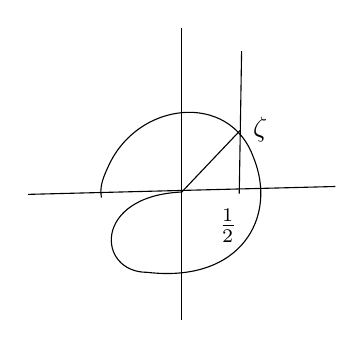
\begin{tikzpicture}[x=1cm,y=1cm]
\draw (-1.95,-.03)--(1.95,.07);
\draw (0,-1.62)--(0,2.08);
\draw (0,0) .. controls (-1.14,-.05) and (-1.08,-1.02) .. (-.44,-1.02) .. controls (.76,-1.16) and (1.22,-.31) .. (.91,.44) .. controls (.61,1.28) and (-.57,1.16) .. (-.94,.31) .. controls (-1.02,.14) and (-1.04,.04) .. (-1.02,-.07);
\draw (.73,-.02)--(.76,1.79);
\draw (0,0)--(.74,.78);
\node[right] at (.79,.79) {$\zeta$};
\node[below] at (.59,-.09) {$\frac12$};
\end{tikzpicture}}

\diagram{\begin{tikzcd}[ampersand replacement=\&,row sep=large,column sep=large]
\Pi_{0,3}^{\mathbb D'} \arrow[r] \arrow[d] \& \Pi_{0,3}^{\mathbb D}=\{\rho,\sigma\mid\rho^3=\sigma^2=1\} \arrow[d,Rightarrow] \\
\deleted{\unsure{\mathbb Z/4\mathbb Z}}\,\inserted{\unsure{\mathbb D'_3}} \arrow[r] \arrow[d] \arrow[ur,phantom,"\unsure{\mathrm{cart}}"{description}] \& \deleted{\unsure{\mathbb Z/2\mathbb Z}}\,\inserted{\unsure{\mathbb D_3}} \arrow[d] \\
\mathbb Z/4\mathbb Z \arrow[r,no head] \arrow[ur,phantom,"\unsure{\mathrm{cart}}"{description}] \& \mathbb Z/2\mathbb Z
\end{tikzcd}}

\margin{$\deleted{\rho\mapsto0,\quad\sigma\mapsto1}$\par
$\rho\mapsto0$\par
$\sigma\mapsto1$}

\margin{\unsure{We lift} $\rho,\sigma$ to $\deleted{\unsure{\rho,\sigma}}\ \rho',\sigma'$\par
$\rho'=(\rho,2),\quad\sigma'=(\sigma,\deleted{\unsure{2}}\inserted{3})$\par
\unsure{we have}
$\rho'^{\,6}=\sigma'^{\,4}=1,$\par
$\rho'^{\,3}=\sigma'^{\,2}=(\underbrace{1,2\bmod4}_{\omega})$.}

\margin{We then easily verify that\par
$\mathrm S\ell(2,\mathbb Z)\simeq\{\rho',\sigma'\mid \unsure{\rho'^{\,6}=\sigma'^{\,4}=1},\ \unsure{\rho'^{\,3}=\sigma'^{\,2}}\}$.}

\margin{\figure{\begin{tikzpicture}[x=1cm,y=1cm]
\draw[->] (2.92,3.25) .. controls (2.82,2.34) and (1.35,2.38) .. (1.05,1.46) .. controls (.92,1.12) and (.86,.77) .. (.71,.58);
\draw (0.05,2.24) .. controls (.42,1.64) and (.29,1.03) .. (.21,.96) .. controls (.12,.88) and (.24,.73) .. (.35,.68);
\draw (.59,.98) .. controls (.43,.46) and (.48,.12) .. (.35,-.02) .. controls (.62,.12) and (.63,-.29) .. (.67,-.72);
\end{tikzpicture}}}

Thus $\Pi_{0,3}^{\mathbb D'}\simeq\mathrm S\ell(2,\mathbb Z)$ \unsure{appears} as an extension of $\Pi_{0,3}^{\mathbb D}$ by $\mathbb Z/2\mathbb Z$, inverse image \deleted{\unsure{of}} the extension \inserted{$\mathbb D'_3$} of $\mathbb D_3$ by $\mathbb Z/2\mathbb Z$, or of the extension $\mathbb Z/4\mathbb Z$ of $\mathbb Z/2\mathbb Z$ by $\mathbb Z/2\mathbb Z$, via $\Pi_{0,3}^{\mathbb D}\to\mathbb D_3$ \unsure{resp.} composite $\Pi_{0,3}^{\mathbb D}\to\deleted{\unsure{\mathbb D_3}}\mathbb Z/2\mathbb Z$. \unsure{It is} an extension of $\mathbb D'_3$ by a \unsure{group} $\simeq\Pi_{0,3}$, \unsure{with basis} $\rho_0,\rho_1,\rho_\infty$ \unsure{---}

\margin{15}

\scanpage{17}

\deleted{\diagram{\begin{tikzcd}[ampersand replacement=\&,column sep=small,row sep=large]
\& \vec S(\unsure{X_0|X_\bullet})\simeq G_0 \arrow[dl] \arrow[d] \arrow[dr] \& \\
S(X_0)\simeq G_0/H_S \& A(X_0)\simeq G_0/H_A, \& F(X_0)\simeq G_0/H_F
\end{tikzcd}}}

\deleted{\[
H_S\cap H_A=e,\qquad H_A\cap H_F=e,\qquad H_S\cap H_F=e
\]}

\deleted{\unsure{i.e.|among others}
\[
G_0\hookrightarrow G_0/H_S\times G_0/H_A,\qquad
G_0\hookrightarrow G_0/H_A\times G_0/H_F,\qquad
G_0\unsure{\hookrightarrow|\subset}\deleted{\unsure{G_0|H_S}}/H_A\times G_0/H_F
\]}

\deleted{\figure{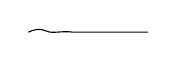
\begin{tikzpicture}[x=1cm,y=1cm]
\draw (0,0).. controls (.1,.04) and (.14,.05) .. (.24,.01).. controls (.31,-.02) and (.43,.02) .. (.57,0)--(1.52,0);
\end{tikzpicture}}}

\margin{\uline{\unsure{Unoriented case}}}

\deleted{Let us consider the category of polyhedra (unoriented) of given type; there are functors}

\deleted{\[
\begin{array}{l}
S\\
\vec A\\
F\\
\deleted{\unsure{A|R}}
\end{array}
\]}

\deleted{\diagram{\(\begin{array}{lll}
A_1 & \text{incidence relation between }S\text{ and }A & \text{(}\unsure{\text{oriented edges}}\text{ in sense }1\text{)}\\
A_2 & \rule{3.2cm}{0.25pt}\ A\text{ and }F & (\rule{2.8cm}{0.25pt}\ 2)\\
A_3 & \text{incidence relation between }\unsure{S|B}\text{ and }F &
\end{array}\)}}

\deleted{\[
R=\deleted{\unsure{A_3}}\unsure{\simeq|=}A_1\times_A A_2
\]
\deleted{\unsure{relation} of incidence between $S$ and $F$}
\inserted{\unsure{triples or flags|triples of flags} $(s,a,f)$\quad$s\unsure{\leq|<}a<f$.}}

\deleted{\diagram{\begin{tikzcd}[ampersand replacement=\&,row sep=small,column sep=small]
\& R \arrow[dl] \arrow[d] \arrow[dr] \& \\
S\&A\&F
\end{tikzcd}}}

\deleted{\[
\begin{aligned}
A_1&=\operatorname{Im}(R\to S\times A)\\
A_2&=\operatorname{Im}(R\to A\times F)\\
A_3&=\operatorname{Im}(R\to S\times F)
\end{aligned}
\]}

\deleted{$\Omega$ set of orientations}

\deleted{\[
{A_1}_{\Omega}\simeq\unsure{{A_2}_{\Omega}}\simeq{A_3}_{\Omega}\qquad(
\]}

\[
\mathrm{Pol}_{\unsure{\tau|t}}\qquad
\mathrm{Pol}_{\tau}^{\unsure{\mathrm{or}}}\simeq
\mathrm{Pol}_{\tau}\deleted{\unsure{/\Omega}}\inserted{{}_{/\Omega}}
\]

\margin{16}

\scanpage{18}
\mspage{6}

$S\mathcal T_{1,1}\simeq$ \unsure{inverse image} of $\mathrm S\ell(2,\mathbb Z)$ in $\unsure{\deleted{\mathrm G\ell}\mathrm S\ell(2,\mathbb R)^{\sim}|\mathrm G\ell(2,\mathbb R)^{\sim}}$
\[
\simeq\{\rho,\sigma\mid\rho^3=\sigma^2\ (=\omega)\}
\]
\margin{\unsure{(}central \unsure{elem\textsuperscript{ent}|el\textsuperscript{ement}}}

\[
\mathcal T_{11}=S\mathcal T_{11}/\langle\omega^2\rangle
\]

\[
\begin{array}{ll}
(\mathcal T_{11})_{\mathrm{ab}}\simeq\mathbb Z & (\mathcal T_{11})_{\mathrm{ab}}\simeq\mathbb Z/12\mathbb Z\\[4pt]
\deleted{(\rho,\sigma)} & \\
\rho\longmapsto2 & \rho\longmapsto2\bmod12\\
\sigma\longmapsto3 & \sigma\longmapsto3\bmod12\\
\omega\longmapsto\unsure{6|8} &
\end{array}
\]

\diagram{\begin{tikzcd}[ampersand replacement=\&,row sep=large,column sep=small]
\& 1 \& \& 1 \\
\& \mathcal T_{11} \arrow[u] \arrow[r] \& \deleted{\unsure{\mathcal T_{\mathrm{ab}}}} \arrow[r] \& \mathbb Z/12\mathbb Z \arrow[u] \\
\unsure{\widetilde\omega|\bar\omega}=\omega^{2\deleted{\unsure{4}}} \& S\mathcal T_{11} \arrow[u] \arrow[rr] \arrow[ur,phantom,"\deleted{\text{cartesian}}"{description}] \& \& \mathbb Z \arrow[u] \\
\uline{1} \arrow[u] \& \mathbb Z \arrow[u] \arrow[rr,"\mathrm{id}"] \& \& \mathbb Z \arrow[u,"12"] \\
\& 1 \arrow[u] \& \& 1 \arrow[u]
\end{tikzcd}}

\margin{so $S\mathcal T_{11}$ is obtained from $\mathcal T_{11}$ by inverse image of the canonical extension of $\mathbb Z/12\mathbb Z$ by $\mathbb Z$, via $\mathcal T_{11}\to\mathbb Z/12\mathbb Z$.}

\deleted{a normalization of $(K,\unsure{K_0|N|k_0})$, \unsure{then} it is \unsure{special} : the category of étale coverings in $\unsure{K'_fN|K'_{fN}}$ -- \deleted{\illegible{1}} $\Delta$ \unsure{covering|i.e.} $\Delta$ topological \unsure{has} a unique normalization for which the projection \unsure{is|be} a \unsure{morphism} of \unsure{normalized} $\Delta$-complexes. [But beware, \unsure{it works} \uline{\unsure{not}} for \unsure{strict normalizations} \unsure{even|necessarily}\ldots]}

\deleted{\unsure{8.|$\beta$.} \unsure{Fundamental|Fundamental} \unsure{groups|group} and groupoids. We \unsure{shall show|show} the relation between topological construction and algebraic construction.}

\margin{17}

\scanpage{19}

% pencil numeral at the top right corner; no other foliation numeral is visible on this sheet
\margin{8v}

\figure{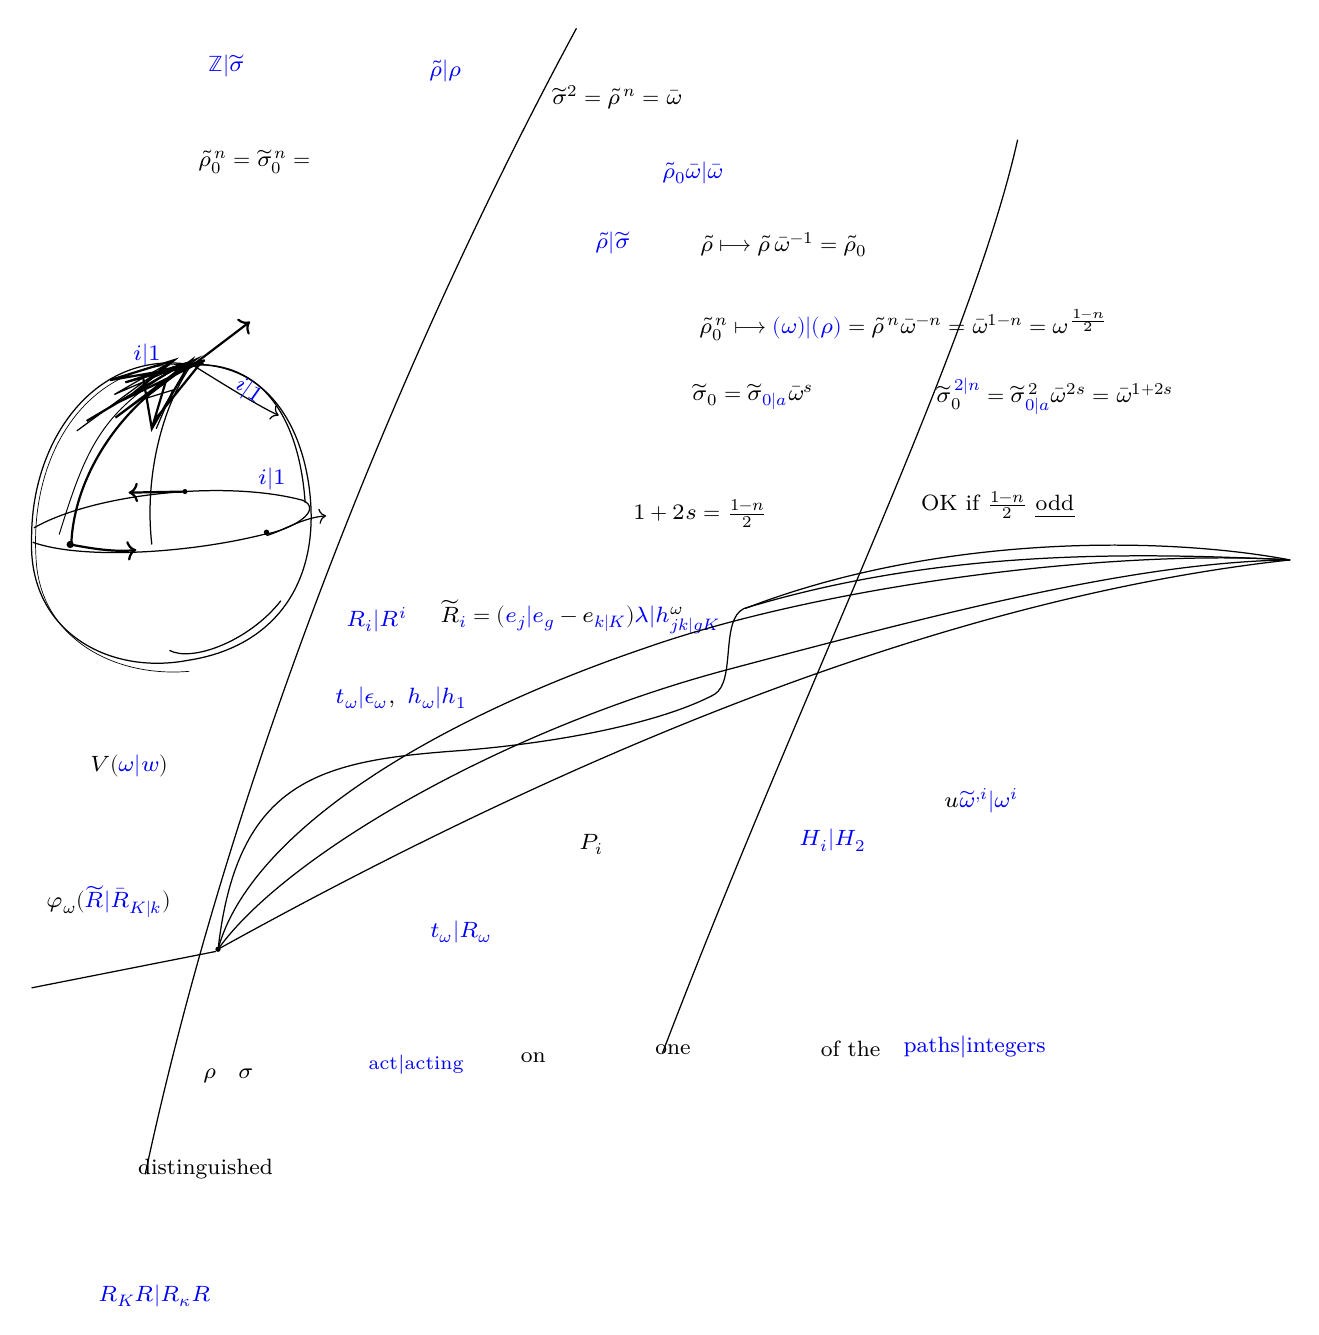
\begin{tikzpicture}[x=.014cm,y=-.014cm,every node/.style={font=\footnotesize,inner sep=0pt},line width=.45pt]
\node[anchor=west] at (385,80) {$\deleted{\unsure{\mathbb Z|\widetilde\sigma}}$};
\node[anchor=west] at (585,85) {$\deleted{\unsure{\widetilde\rho|\rho}}$};
\node[anchor=west] at (376,167) {$\widetilde\rho_0^{\,n}=\widetilde\sigma_0^{\,n}=$};
\node[anchor=west] at (697,109) {$\widetilde\sigma^2=\widetilde\rho^{\,n}=\bar\omega$};
\node[anchor=west] at (796,177) {$\deleted{\unsure{\widetilde\rho_0\bar\omega|\bar\omega}}$};
\node[anchor=west] at (736,241) {$\deleted{\unsure{\widetilde\rho|\widetilde\sigma}}$};
\node[anchor=west] at (831,242) {$\widetilde\rho\longmapsto\widetilde\rho\,\bar\omega^{-1}=\widetilde\rho_0$};
\node[anchor=west] at (830,315) {$\widetilde\rho_0^{\,n}\longmapsto\deleted{\unsure{(\omega)|(\rho)}}=\widetilde\rho^{\,n}\bar\omega^{-n}=\bar\omega^{1-n}=\omega^{\frac{1-n}{2}}$};
\node[anchor=west] at (824,380) {$\widetilde\sigma_0=\widetilde\sigma_{\unsure{0|a}}\bar\omega^s$};
\node[anchor=west] at (1045,380) {$\widetilde\sigma_0^{\,\unsure{2|n}}=\widetilde\sigma_{\unsure{0|a}}^{\,2}\bar\omega^{2s}=\bar\omega^{1+2s}$};
\node[anchor=west] at (770,486) {$1+2s=\frac{1-n}{2}$};
\node[anchor=west] at (1031,478) {OK if $\frac{1-n}{2}$ \uline{odd}};

\draw (328,1085) .. controls (405,726) and (557,346) .. (719,46);
\draw (797,975) .. controls (925,640) and (1077,335) .. (1119,147);

\draw (370,351) .. controls (284,337) and (224,418) .. (225,510) .. controls (222,592) and (294,633) .. (367,619) .. controls (445,607) and (487,549) .. (477,465) .. controls (469,399) and (433,349) .. (370,351);
\draw[line width=.25pt] (371,351) .. controls (277,345) and (223,430) .. (229,526) .. controls (232,599) and (300,635) .. (368,629);
\draw (350,610) .. controls (370,621) and (422,602) .. (451,565);
\draw (227,499) .. controls (281,468) and (401,455) .. (471,474) .. controls (490,483) and (461,501) .. (435,505) .. controls (367,522) and (271,528) .. (226,512);
\draw[line width=.8pt,->] (260,514) .. controls (281,518) and (301,521) .. (320,519);
\draw[line width=.8pt,->] (366,466)--(313,467);
\draw[->] (438,506) .. controls (454,501) and (470,490) .. (492,488);
\fill (260,514) circle[radius=3.3];
\fill (438,503) circle[radius=2.5];
\fill (364,466) circle[radius=2.3];
\draw (334,514) .. controls (327,454) and (343,389) .. (370,351);
\draw[line width=.8pt] (261,514) .. controls (263,455) and (303,388) .. (370,351);
\draw[line width=.35pt] (250,505) .. controls (274,428) and (288,390) .. (365,350);
\draw[line width=.8pt,->] (369,353)--(423,312);
\draw[->] (372,352) .. controls (398,368) and (428,387) .. (449,397);
\draw (377,351) .. controls (437,351) and (468,403) .. (473,476);
\node at (330,342) {$\unsure{i|1}$};
\node[rotate=-35] at (422,375) {$\unsure{i|1}$};
\node at (443,455) {$\unsure{i|1}$};
\draw[line width=.8pt] (275,402)--(361,351)--(310,367)--(382,347)--(312,381)--(354,347)--(296,365)--(377,351)--(336,402)--(347,365)--(301,399)--(370,347)--(334,409)--(326,362)--(381,350);
\draw (266,411)--(352,348)--(300,378)--(376,345)--(327,382)--(353,374)--(338,409);

\node[anchor=west] at (510,582) {$\unsure{R_i|R^i}$};
\node[anchor=west] at (595,580) {$\widetilde R_{\unsure{i}}=(\unsure{e_j|e_g}-e_{\unsure{k|K}})\unsure{\lambda|h}^{\omega}_{\unsure{jk|gK}}$};
\node[anchor=west] at (500,653) {$\unsure{t_\omega|\epsilon_\omega},\ \unsure{h_\omega|h_1}$};
\node[anchor=west] at (278,715) {$V(\unsure{\omega|w})$};
\node[anchor=west] at (238,838) {$\varphi_\omega(\unsure{\widetilde R|\bar R}_{\unsure{K|k}})$};
\node[anchor=west] at (721,786) {$P_i$};
\node[anchor=west] at (586,865) {$\deleted{\unsure{t_\omega|R_\omega}}$};
\node[anchor=west] at (921,782) {$\deleted{\unsure{H_i|H_2}}$};
\node[anchor=west] at (1052,746) {$u\unsure{\widetilde\omega^{,i}|\omega^i}$};

\draw (225,916)--(392,883);
\fill (394,881) circle[radius=2.4];
\draw (394,882) .. controls (411,727) and (487,710) .. (612,701) .. controls (702,694) and (795,676) .. (844,650) .. controls (864,638) and (849,582) .. (871,572) .. controls (1039,521) and (1205,520) .. (1366,528);
\draw (394,881) .. controls (422,778) and (581,676) .. (781,608) .. controls (949,549) and (1211,518) .. (1366,528);
\draw (394,881) .. controls (454,797) and (649,683) .. (854,628) .. controls (1057,574) and (1228,530) .. (1366,528);
\draw (394,881) .. controls (721,700) and (1056,562) .. (1366,528);
\draw (872,572) .. controls (1045,505) and (1249,506) .. (1366,528);

\node[anchor=west] at (380,996) {$\rho\quad\sigma$};
\node[anchor=west,font=\scriptsize] at (530,986) {\unsure{act|acting}};
\node[anchor=west] at (668,979) {on};
\node[anchor=west] at (790,972) {one};
\node[anchor=west] at (940,971) {of the};
\node[anchor=west] at (1015,970) {\unsure{paths|integers}};
\node[anchor=west] at (321,1080) {distinguished};
\node[anchor=west] at (285,1195) {$\deleted{\unsure{R_KR|R_\kappa R}}$};
\end{tikzpicture}}

\subsection*{Scans 20--37}
\addcontentsline{toc}{subsection}{Scans 20--37}
% package LM_C1-020-037
\scanpage{20}
\figure{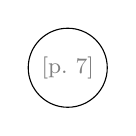
\begin{tikzpicture}
\node[draw,circle,inner sep=3pt] {\mspage{7}};
\end{tikzpicture}}

\diagram{\begin{tikzcd}[ampersand replacement=\&,column sep=1.6em,row sep=2.8em]
\&\&
\begin{gathered}
\widetilde\rho=(\rho_0,2)=(\rho,2)\\
\widetilde\sigma=(\sigma_0,3)=(\sigma,3)
\end{gathered}
\arrow[d, bend right=20]
\&
\begin{gathered}
\deleted{\unsure{\Pi_{0,3}^{D}}}\\[-2pt]
\inserted{\text{\uline{\unsure{identified with}}}}\\[-2pt]
\inserted{\unsure{S\mathcal T_{11}\times_{\Pi_{0,3}^{D}}\mathbb Z/12\mathbb Z}}
\end{gathered}
\arrow[d]
\&
\begin{gathered}
\rho_0=(\rho,\dot 2)\\[-2pt]
\unsure{\Pi_{0,3}}\\[-2pt]
\sigma_0=(\sigma,\dot 3)=(\sigma,-1)
\end{gathered}
\arrow[d]
\&\\
\unsure{0|1}\arrow[r,dash]\&
\mathbb Z\arrow[r,dash,"1\unsure{-|\mapsto}\overline\omega=\omega^2"]\arrow[dd,equal]\&
S\mathcal T_{11}\arrow[r,Rightarrow]\arrow[dd,"\substack{\widetilde\rho\mapsto\deleted{\unsure{4}}2\\\widetilde\sigma\mapsto3}"']
\arrow[ddr,phantom,"\text{Cartesian}"]\&
\mathcal T_{11}\arrow[r,Rightarrow]\arrow[dr,leftrightarrow]\arrow[dd,"\substack{\rho_0\mapsto\dot 2\\\sigma_0\mapsto\dot 3}"']
\&\Pi_{0,3}^{\prime D}\arrow[dr,"\text{canonical}"]\arrow[dd,"\substack{\rho\mapsto2\\\sigma\mapsto3}"{pos=.25,xshift=2pt}]
\arrow[dl,phantom,"\text{cartesian}" description]\&\\
\&\&\&{}\&
|[xshift=-3em]|\mathbb D'_3\arrow[r,"\text{cartesian}"{pos=.75}]\arrow[dd]
\&\mathbb D_3\arrow[dd,"\text{canonical}"]\\
1\arrow[r,dash]\&\mathbb Z\arrow[r,"12"]\&\mathbb Z\arrow[r,"\text{canonical}"]\&
\mathbb Z/12\mathbb Z\arrow[r,"\text{canonical}"]\arrow[dr,"\text{canonical}"']
\&\mathbb Z/6\mathbb Z\arrow[dr,"\text{canonical}"]
\arrow[d,phantom,"\text{\uline{Cartesian}}"'{pos=.25,xshift=-3em}]
\arrow[dr,phantom,"\text{\uline{cartesian}}"{description,xshift=-1.5em,yshift=.5em}]\&\\
\&\&\&\&\mathbb Z/4\mathbb Z\arrow[r,leftrightarrow,"\text{canonical}"]\&\mathbb Z/2\mathbb Z
\end{tikzcd}}

\margin{\unsure{for} $\mathcal T_{11}$ \unsure{identified with}
$\Pi_{0,3}^{D}\times_{\mathbb Z/2\mathbb Z}\mathbb Z/4\mathbb Z$}

\unsure{Have we} \unsure{indeed}\quad
$\bigm|\quad S\mathcal T_{11}\simeq S\Pi_{0,3}^{D}$ ??

it would rather seem, however
\[
\deleted{\unsure{\mathcal T_{11}}}\quad
PM_{11}\simeq
\left(\underbrace{T^*U_{0,3}}_{\substack{\text{bundle}\\\text{\uline{tangent}}}},\mathfrak S_3\right)
\]
\inserted{(and \uline{not} $\unsure{PU_{0,3}}$ !!)}

\[
\text{thus}\quad \mathcal T_{11}\simeq\pi_1(T^*U_{0,3},\mathfrak S_3)\ \ldots
\]
\margin{19}

\scanpage{21}
% Trois longs traits obliques au crayon, terminés chacun en crochet, traversent tout le feuillet : rature d'ensemble.
% Les ratures à l'encre (ligne « Op. ext. … », « compatible avec l'op. ext. », E corrigé en F, 1 et π_1 de la dernière suite) restent marquées à l'intérieur.
\deleted{
\[
\pi\qquad l_1\ \cdots\ l_n
\]

\diagram{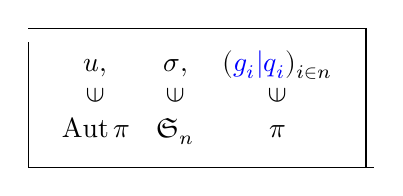
\begin{tikzpicture}
\node[inner sep=7pt] (p) {$\begin{array}{ccc}
u,&\sigma,&(\unsure{g_i|q_i})_{i\in n}\\
\rotatebox{90}{$\in$}&\rotatebox{90}{$\in$}&\rotatebox{90}{$\in$}\\
\operatorname{Aut}\pi&\mathfrak S_n&\pi
\end{array}$};
\draw (p.north west) -- (p.north east) -- (p.south east);
\draw ([yshift=-5pt]p.north west) -- (p.south west) -- ([xshift=3pt]p.south east);
\end{tikzpicture}}
\diagram{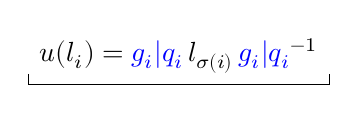
\begin{tikzpicture}
\node[inner sep=4pt] (u) {$u(l_i)=\unsure{g_i|q_i}\,l_{\sigma(i)}\,\unsure{g_i|q_i}^{-1}$};
\draw ([yshift=4pt]u.south west) -- (u.south west) -- (u.south east) -- ([yshift=4pt]u.south east);
\end{tikzpicture}}

\diagram{\begin{tikzcd}[ampersand replacement=\&,column sep=1.5em]
1\arrow[r,dash]\&\pi_1(\operatorname{Aut}(X)\arrow[r]\&\mathbb Z^n\arrow[r]\&S\mathcal T\arrow[r]\&\mathcal T\arrow[r,dash]\&\mathfrak S_n\arrow[r,dash]\&1
\end{tikzcd}}

\diagram{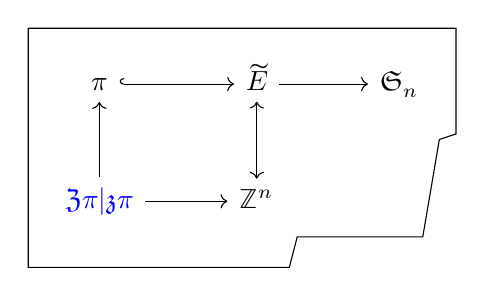
\begin{tikzpicture}
\node[inner sep=9pt] (b) {\begin{tikzcd}[ampersand replacement=\&,column sep=3em,row sep=2.5em]
\pi\arrow[r,hook]\&\widetilde E\arrow[r]\arrow[d,leftrightarrow]\&\mathfrak S_n\\
\unsure{\mathfrak Z\pi|\mathfrak z\pi}\arrow[u]\arrow[r]\&\mathbb Z^n\&{}
\end{tikzcd}};
\draw (b.north west) -- (b.north east) -- ([yshift=2pt]b.east) -- ([xshift=-6pt]b.east)
 -- ([xshift=-12pt,yshift=5pt]b.south east) -- ([xshift=0.7cm,yshift=5pt]b.south)
 -- ([xshift=0.6cm,yshift=-6pt]b.south) -- ([yshift=-6pt]b.south west) -- (b.north west);
\end{tikzpicture}}

\diagram{\begin{tikzcd}[ampersand replacement=\&,column sep=2.3em,row sep=1.8em]
\&\&1\&\&\\
1\arrow[r]\&\underbrace{S\operatorname{Aut}^{+}(X)}\arrow[r]\arrow[d,"\simeq"]\&
\operatorname{Aut}^{+}(X)\arrow[u]\arrow[r,dash]\&\operatorname{Aut}^{+}(\partial X)\arrow[r,dash]\&1\\
\&\uline{S\mathcal T}\&\operatorname{Aut}^{+}_{!}(\widetilde X)\arrow[u]\&\uline{\mathfrak S_n\cdot\mathbb T^n}\arrow[u,"\simeq"]\&\\
\&\&\pi\arrow[u]\&\&\\
\&\&1\arrow[u]\&\&
\end{tikzcd}}

\diagram{\begin{tikzcd}[ampersand replacement=\&,column sep=1.6em]
1\arrow[r,dash]\&\underbrace{\pi_1\operatorname{Aut}^{+}(X)}_{0\ \text{or}\ \mathbb Z}\arrow[r,Rightarrow]\&\mathbb Z^n\arrow[r,dash]\&S\mathcal T\arrow[r,dash]\&\mathcal T\arrow[r,dash]\&\mathfrak S_n\arrow[r,dash]\&1
\end{tikzcd}}

\diagram{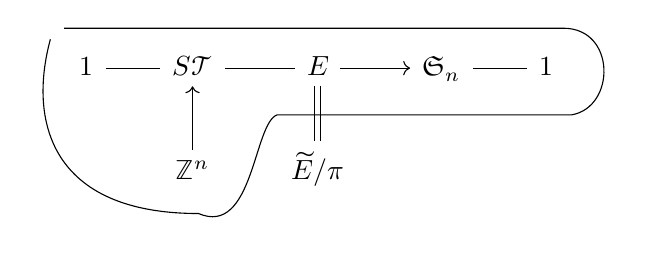
\begin{tikzpicture}
\node[inner sep=6pt] (e) {\begin{tikzcd}[ampersand replacement=\&,column sep=2em,row sep=1.8em]
1\arrow[r,dash]\&S\mathcal T\arrow[r,dash]\&E\arrow[r]\arrow[d,equal]\&\mathfrak S_n\arrow[r,dash]\&1\\
\&\mathbb Z^n\arrow[u]\&\widetilde E/\pi\&\&{}
\end{tikzcd}};
\draw ([xshift=5pt]e.north west) -- ([xshift=-7pt]e.north east)
 .. controls ([xshift=12pt]e.north east) and ([xshift=12pt,yshift=-1cm]e.north east) .. ([xshift=-4pt,yshift=-1.1cm]e.north east)
 -- ([xshift=-0.5cm,yshift=-1.1cm]e.north)
 .. controls ([xshift=-0.8cm,yshift=-1.2cm]e.north) and ([xshift=-0.8cm,yshift=-0.3cm]e.south) .. ([xshift=-1.5cm]e.south)
 .. controls (e.south west) and ([xshift=-8pt]e.west) .. ([yshift=-4pt]e.north west);
\end{tikzpicture}}

\diagram{\begin{tikzcd}[ampersand replacement=\&,column sep=2.4em,row sep=2em]
1\arrow[r,dash]\&\unsure{\widetilde F|\widehat F}\arrow[r,dash]\arrow[d]\&\widetilde A\arrow[r,dash]\arrow[d]\&\widetilde G\arrow[d]\&\\
1\arrow[r,dash]\&\substack{\deleted{\unsure{E}}\inserted{F}\\\text{discrete}}\arrow[r]\&A\arrow[r]\&G\arrow[dr]\&
\bigl(=\mathfrak S_n\unsure{\ast|\cdot}\mathbb T^n\bigr)\\
\&\&\&\&1
\end{tikzcd}}

\deleted{\unsure{Operation} by outer automorphisms of $\pi_0$ on $F$}

\diagram{\begin{tikzcd}[ampersand replacement=\&,column sep=3.8em,row sep=2.3em]
\pi_1(G)=\pi_1\arrow[r]\arrow[dr,bend right=20,"\substack{\text{\unsure{compatible}}\\\text{with }\pi_0}"']\&F\arrow[d,phantom,"\cup" description]\\
\&\unsure{\mathfrak Z(F)|\mathfrak z(F)}
\end{tikzcd}}
\inserted{\unsure{central}}

$\pi_0(G)=\pi_0$ operates \unsure{by outer automorphisms} on $F$
\quad hence operates on $\unsure{\mathfrak Z(F)|\mathfrak z(F)}$

\diagram{$\begin{array}{cc}
\pi_0&\pi_1\\
\multicolumn{2}{c}{\text{operation}}
\end{array}$}
\deleted{\unsure{compatible} with the outer operation}

\diagram{\begin{tikzcd}[ampersand replacement=\&,column sep=2.4em,row sep=1.7em]
1\arrow[r,dash]\&F\arrow[r]\&E\arrow[r]\arrow[d,equal]\&\pi_0\arrow[r,dash]\&1\\
\&\&\pi_0(\widetilde A)\&\&{}
\end{tikzcd}}
\figure{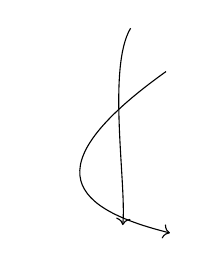
\begin{tikzpicture}[x=1cm,y=1cm]
\draw[->] (0.3,2.5) .. controls (0.0,2.0) and (0.25,0.5) .. (0.2,0);
\draw[->] (0.75,1.95) .. controls (-1.0,0.7) and (-0.4,0.2) .. (0.8,-0.1);
\end{tikzpicture}}

\diagram{\begin{tikzcd}[ampersand replacement=\&,column sep=1.6em]
1\arrow[r,dash]\&\pi_1(A)\arrow[r,dash]\&\pi_1\arrow[r]\&\unsure{F}\arrow[r]\&\underbrace{\pi_0(A)}\arrow[r]\&\substack{\unsure{\pi_0|\pi_\infty}\\ /}\arrow[r,dash]\&1
\end{tikzcd}}

\diagram{\begin{tikzcd}[ampersand replacement=\&,column sep=1.7em,row sep=1.5em]
\deleted{\unsure{1}}\arrow[r,dash]\&\deleted{\unsure{\pi_1}}\arrow[r,dash]\&F\arrow[r,dash]\&\pi_0(\widetilde A)\arrow[r]\arrow[d,equal]\&\pi_0\arrow[r]\&1\\
\&\&\&E\&\&{}
\end{tikzcd}}
}
\margin{20}

\scanpage{22}
% blank
\margin{21}

\scanpage{23}
A)\quad \uline{Lemma}\quad
$S$ \deleted{\unsure{satisfying|strictly}}
regular integral scheme such that $\operatorname{Pic}(S)=0$,
characteristic of the generic point $\ne2$ Then \deleted{$\unsure{H^1}$}
\[
H^1(U_{0,3},\mathfrak S_3;\mathbb G_m]\simeq\mathbb Z/6\mathbb Z
\]
(\deleted{\unsure{residual}}\inserted{\unsure{generic point|if generic}} is $2$, we find $\mathbb Z/3\mathbb Z$)

\margin{\uline{\unsure{Proof}}\quad we use exact sequence
\diagram{\begin{tikzcd}[ampersand replacement=\&,column sep=1.3em,row sep=2em]
0\arrow[r]\&H^1(\mathfrak S_3,H^0(U_{0,3},\mathbb G_m)\arrow[r]\&H^1(\text{mixed})\arrow[dll]\&{}\\
H^0\bigl(\mathfrak S_3,\underbrace{H^1(U_{0,3};\mathbb G_m)}_{0}\bigr)\&\&\&{}
\end{tikzcd}}
and
\diagram{\begin{tikzcd}[ampersand replacement=\&,column sep=1.3em]
0\arrow[r]\&H^0(S,\mathbb G_m)\arrow[r]\&H^0(U_{0,3},\mathbb G_m)\arrow[r]\&\unsure{h_1(V(J))|h^1(V(J))}\arrow[r]\&0
\end{tikzcd}}}

\unsure{I} say that if \inserted{the scheme}
$\deleted{\unsure{U_{0,3}}}\inserted{\Sigma_J}$ is defined as $\mathbb P(V_J)$, \unsure{i.e.}
\diagram{\begin{tikzcd}[ampersand replacement=\&,column sep=2.8em]
0\arrow[r,dash]\&V_J\arrow[r]\&\mathcal O^J\arrow[r]\&\mathcal O\arrow[r,dash]\&0
\end{tikzcd}}
then the \unsure{principal} bundle
\[
P\Sigma_J=\check V(\mathcal O_{\Sigma_J}(1))^{*}
\]
is a generator of the
$H^1(\deleted{\unsure{U_{0,3}}}\inserted{\Sigma_J^*},
\deleted{\unsure{\mathfrak S_3}}\inserted{\mathfrak S_J};\mathbb G_m)$.

I will first \unsure{find} a trivialization of
\[
\uline{\mathcal O}(1)^{\otimes6}=\mathcal O(6)\simeq
\unsure{\mathcal T^{\otimes3}(\omega)|\mathcal J^{\otimes3}(\omega)},
\]
\deleted{thus} \inserted{in fact} a section of $\mathcal O(6)$
\inserted{over $\overline\Sigma$ \unsure{in its entirety}}
(which \deleted{\unsure{vanishes only}}
\inserted{\unsure{is}, \unsure{invertible}} on $\Sigma^*$.
We \deleted{\unsure{taking}} have
\[
\Gamma(\Sigma_J,\mathcal O(6))\simeq\operatorname{Sym}^{6}V_J
\]
and we will take
\[
\begin{gathered}
\unsure{\varphi|\Delta}\in\Gamma(\Sigma_J,\mathcal O(6)),\qquad
\unsure{\varphi|\Delta}
=\deleted{\unsure{\sum_{i\in J}}}
-\prod_{\substack{i,j\in J\\i\ne j}}(e_i-e_j)\\
=\prod_{i\in J}\underbrace{(e_j-e_h)}_{J=\{i,j,h\}}^{2}.
\end{gathered}
\]
Thus, over $\deleted{\unsure{U_J}}\inserted{\Sigma_J^{*}}$, the \unsure{structure|structure} group
\deleted{\unsure{of}}
$\mathbb G_m$ of $P\Sigma_J^{*}$ is reduced \unsure{to|:} $\mu_6$.

\uline{N.B.}\quad Unless I am mistaken, we have
\[
\deleted{\unsure{\operatorname{Sym}}}\quad
\operatorname{Sym}^{*}(V_J)^{\mathfrak S_3}\simeq
\mathcal O\bigl(\unsure{\gamma_2|\varphi_2},\unsure{\gamma_3|\varphi_3}\bigr)
/(2\gamma_3^2-\gamma_2^3)
\]
\[
\left\{\begin{aligned}
\gamma_2&=\sum_{i\in J}(e_j-e_h)^2\\
\gamma_3&=\prod_{i\in J}(e_j\unsure{-|+}e_h-2e_i)
\end{aligned}\right.
\qquad\text{and}\quad\Delta=\gamma_2^3
\]
\margin{22}

\scanpage{24}
% not manuscript: tract imprimé « Parler Femmes à propos de “PLURIELLES” », avec une longue rature diagonale.
\margin{23}

\scanpage{25}
B)

\deleted{\unsure{If} $2$ \unsure{invertible}, we \unsure{will have} \unsure{therefore}}
\[
\deleted{\operatorname{Sym}^{*}(\unsure{V_J|W_J})^{\mathfrak S_{\unsure{J|3}}}\simeq\mathcal O[}
\]
\deleted{\unsure{Remark}}

Since $\gamma_2$ vanishes at \deleted{\unsure{the}} $P_\omega$,
$\gamma_3$ at the $Q_i$, it follows that there is no invariant section
of an $\mathcal O(n)^*$ \deleted{\unsure{for}} over
$\Sigma_J^{*}$ \deleted{\unsure{in degree} $<$}
for $n\le6$, hence that the order of
$\operatorname{cl}(\mathcal O(1))$ in
$H^1(\Sigma_J,\mathfrak S_J;\mathbb G_m)$ is indeed $6$,
which \unsure{proves} that $\mathcal O(1)$ is a generator of the
mixed $\unsure{H^1}$.
\margin{24}
\scanpage{26}
% not manuscript: feuillet dactylographié « Sciences de l’homme », « Energie », « Mécanique et industries de transformation », « Recherches sur les milieux tropicaux et sub-tropicaux » ; pagination imprimée « - 4 - ».
\margin{25}

\scanpage{27}
% Étiquette imprimée, oblique et à l'envers sur le feuillet.
\begin{flushleft}
MISTER PROFESSOR GROTHENDIECK ALEXANDER\\
MATHEMATICS\hfill 5
\end{flushleft}

\diagram{\begin{tikzcd}[ampersand replacement=\&,column sep=huge]
\mathbb D'_3 \arrow[r] \& \mathbb D_3
\end{tikzcd}}

\margin{\figure{\begin{tikzpicture}[x=1cm,y=1cm]
\draw (0,0) .. controls (.1,.14) and (.25,.13) .. (.48,.03);
\end{tikzpicture}}}

\diagram{\begin{tikzcd}[ampersand replacement=\&,column sep=large,row sep=large]
PM_{11}(2^{\sim})\overset{?}{\simeq}PU_{0,3}
  \arrow[r,very thick] \arrow[d,leftrightarrow]
\& PM_{11}(2)\simeq TU_{0,3} \arrow[d]\\
U_{0,3}\simeq M_{11}(\unsure{\widetilde{2}^{\sim}|2^{\sim}})
  \arrow[r,very thick]
\& \begin{gathered}(U_{0,3},\{1,\omega\})\\[-2pt]{}\simeq M_{11}(\unsure{2})\end{gathered}
\arrow[ul,phantom,"\mathrm{cart}" description]
\end{tikzcd}}

\[
\deleted{\unsure{x}\longrightarrow\unsure{x^2\wedge\omega_0}}
\]
\[
\unsure{H^1}(TU_{03},\mathbb D_3;\mu_2)
\]

\diagram{\begin{tikzcd}[ampersand replacement=\&,column sep=small,row sep=large]
M_{11}(2^{\sim}) \arrow[rr]
  \arrow[dr,"{\deleted{\unsure{\mathcal D/\Pi_{0,3}|\mathbb Z/2\,\Pi_{0,3}}}}"']
\& \& M_{11}(2)\unsure{-|'} \arrow[dl] \arrow[d,leftrightarrow] \& \phantom{M}\\
\& M_{11} \arrow[d] \& M_{11}(2)' \arrow[dl] \& \\
\phantom{M}\arrow[rrruu,dashed,no head,shorten <=-10pt,shorten >=-10pt]
\& M'_{11} \& \&
\end{tikzcd}}

\diagram{\begin{tikzcd}[ampersand replacement=\&,column sep=small,row sep=large]
U_{03} \arrow[rr,"{\{1,\omega\}}"] \arrow[dr,"{\mathbb D'_3}"']
\& \& (U_{0,3},\{1,\omega\}) \arrow[dl,"{\mathbb D_3}"'] \arrow[d,"{\unsure{\mathrm{gerbe}}}"] \& \phantom{U}\\
\& (U_{0,3},\mathbb D'_3) \arrow[d,"{\unsure{\mathrm{gerbe}}}"']
\& (U_{03}) \arrow[dl,"{\mathbb D_3}"] \& \\
\phantom{U}\arrow[rrruu,dashed,no head,shorten <=-12pt,shorten >=-12pt]
\& (U_{0,3},\mathbb D_3) \& \&
\end{tikzcd}}

\diagram{\begin{tikzcd}[ampersand replacement=\&,column sep=small,row sep=large]
\begin{gathered}(\mathcal D,\Pi_{03})\\[-2pt]{}\simeq\mathcal D/\Pi_{03}\end{gathered}
 \arrow[rr,very thick,"{\mathrm{gal}}","{\{1,\omega\}}"']
 \arrow[dr,"{\begin{gathered}\mathrm{gal}\\\mathbb D'_3\end{gathered}}"']
\& \& (\mathcal D,\Pi_{03}\times\{1,\omega\})
 \arrow[dl,"{\begin{gathered}\mathrm{gal}\\\mathbb D_3\ \deleted{\unsure{\{1,\omega\}}}\end{gathered}}"']
 \arrow[d,"{\unsure{2\text{-}\uline{\mathrm{gerbe}}}}"] \& \phantom{D}\\
\& (\mathcal D,\unsure{\mathrm{Sl}(2,\mathbb Z)})
 \arrow[d,"{\unsure{2\text{-}\mathrm{gerbe}}}"']
\& (\mathcal D,\Pi_{03}) \arrow[dl,"{\begin{gathered}\mathrm{gal}\\\mathbb D_3\end{gathered}}"] \& \\
\phantom{D}\arrow[rrruu,dashed,no head,shorten <=-12pt,shorten >=-12pt]
\& (\mathcal D,\unsure{\mathrm{Sl}(2,\mathbb Z)}') \& \&
\end{tikzcd}}

\margin{26}

\scanpage{28}
% not manuscript: avis dactylographié, à l’envers, de soutenance d’une thèse de doctorat de 3ème cycle, « Algèbres de Rees », YOON Suk-Im, Montpellier, le 26 février 1982 ; soutenance prévue le 4 MARS 1982 à 15h.
\margin{27}

\scanpage{29}

\deleted{\diagram{\begin{tikzcd}[ampersand replacement=\&,column sep=small,row sep=large]
\& \& {}\arrow[r,"{\unsure{''|1}}"]
\& \mathrm{Sl}(2,\mathbb Z)\arrow[r]\arrow[d]
\& \Pi_{0,3}^{D}\arrow[d] \& \\
\& \unsure{\widetilde\varepsilon|\widetilde E}\arrow[rr]
  \arrow[ddl]\arrow[dr,dashed]
\& \& \mathbb D_3\mathop{\times}\limits_{\mathbb Z/2\mathbb Z}
       \mathbb Z/\unsure{12}\mathbb Z
       \simeq\mathbb D'_3\mathop{\times}\limits_{\mathbb Z/\unsure{2}\mathbb Z}
       \mathbb Z/6\mathbb Z
       \arrow[r]\arrow[dd,very thick]\arrow[d,dashed]
\& \mathbb D_3\mathop{\times}\limits_{\mathbb Z/2\mathbb Z}
       \mathbb Z/6\mathbb Z=\unsure{\varepsilon|E}
       \arrow[dd]\arrow[dr] \& \\
\& \& \mathbb Z\arrow[r,no head]\arrow[ddl,dashed,leftrightarrow,very thick]
\& \mathbb Z/12\mathbb Z\arrow[rr,dashed,"{\mathrm{can}}"]
       \arrow[dd,dashed,"{\mathrm{can}}"'{pos=.2}]
\& \& \mathbb Z/6\mathbb Z\arrow[ddl,"{\mathrm{can}}"]\\
\unsure{\widetilde{\mathbb D}_3^{*}|\widetilde{\mathbb D}'_3}
 \arrow[rrr,very thick]\arrow[dr]
\& \& \& \mathbb D'_3\arrow[r,very thick]\arrow[d,very thick]
\& \mathbb D_3\arrow[d,"{\mathrm{can}}"] \& \\
\& \mathbb Z\arrow[rr] \& \& \mathbb Z/4\mathbb Z\arrow[r,"{\mathrm{can}}"]
\& \mathbb Z/2\mathbb Z \&
\end{tikzcd}}}

\figure{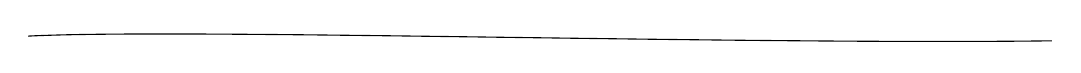
\begin{tikzpicture}[x=1cm,y=1cm]
\draw (0,.06) .. controls (2,.16) and (9,-.05) .. (13,0);
\end{tikzpicture}}

\diagram{\begin{tikzcd}[ampersand replacement=\&,column sep=small,row sep=large]
\unsure{\mathbb Z_{(\omega/2)}}\arrow[r]\arrow[d,very thick]
\& \widetilde\Pi_{0,3}^{\unsure{\circ}}
   \deleted{\unsure{\widetilde\Pi_{0,3}}}\arrow[rr,very thick]\arrow[d]
\& \& \Pi_{0,3}\arrow[d,leftrightarrow,bend left=12]
\& \& \& \\
\mathbb Z_{(\omega)}\arrow[r,very thick]\arrow[d,equal]
\& \widetilde\Pi_{0,3}^{\unsure{'}}\arrow[rr]\arrow[d,very thick]
\& \& \Pi'_{0,3}=\Pi_{0,3}\times\{1,\omega\}
   \arrow[rr]\arrow[d,bend right=12]
\& \& \Pi_{03}\arrow[d,bend right=18] \& \\
\mathbb Z\arrow[r,very thick]\arrow[d,equal]
\& \widetilde{\mathrm{Sl}}(2,\mathbb Z)=\widetilde\Pi_{0,3}^{D}
   \arrow[rr]\arrow[d]
\& \& \mathrm{Sl}(2,\mathbb Z)\arrow[rr]\arrow[d,very thick]\arrow[ddr]
\& \& \Pi_{0,3}^{D}\arrow[d]\arrow[ddr] \& \\
\mathbb Z\arrow[r]\arrow[dd,equal]
\& \widetilde{\mathbb D}_3\arrow[rr]\arrow[dd]
\& \& \begin{gathered}\mathbb D'''_3\\\margin{3}\end{gathered}\arrow[rr,"2"]\arrow[dr,"3"']\arrow[dd,"3"']
\& \& \begin{gathered}\mathbb D''_3\\\margin{\unsure{12|10}}\end{gathered}\arrow[dr,"3"]\arrow[dd,"3"'{pos=.72}] \& \\
\& \& \& \& \mathbb D'_3\arrow[rr,"2"{pos=.75}]\arrow[dd,"3"{pos=.77}]
\& \& \mathbb D_3\arrow[dd,"3"]\\
\mathbb Z\arrow[r,"12"]
\& \mathbb Z\arrow[rr]
\& \& \mathbb Z/12\mathbb Z\arrow[rr,leftrightarrow,"2"]\arrow[dr,"3"']
\& \& \mathbb Z/6\mathbb Z\arrow[dr,"3"] \& \\
\& \& \& \& \mathbb Z/4\mathbb Z\arrow[rr,"2"] \& \& \mathbb Z/2\mathbb Z
\end{tikzcd}}
\margin{\unsure{bottom|good}}

\diagram{\begin{tikzcd}[ampersand replacement=\&,column sep=large,row sep=large]
1\arrow[r,no head]
\& \mathbb Z\arrow[r,no head]\arrow[d,very thick,"{\begin{gathered}4\\\unsure{4}\end{gathered}}"]
\& \widetilde\Pi_{0,3}^{D}\arrow[r,no head]\arrow[d,no head]
\& \Pi_{0,3}^{D}\arrow[r]\arrow[d,no head]
\& 1\\
1\arrow[r,no head]
\& \mathbb Z\arrow[r,no head]
\& \widetilde\Pi_{0,3}^{D}(4)\arrow[r]
\& \Pi_{0,3}^{D}\arrow[r,very thick]
\& 1
\end{tikzcd}}

\figure{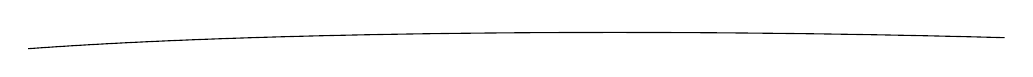
\begin{tikzpicture}[x=1cm,y=1cm]
\draw (0,0) .. controls (3,.22) and (8,.26) .. (12.4,.14);
\end{tikzpicture}}

\diagram{\begin{tikzcd}[ampersand replacement=\&,column sep=large,row sep=large]
\& \& \widetilde\Pi_{0,3}^{D}
\& \Pi_{0,3}^{D}\arrow[r,no head] \& 1\\
1\arrow[r]
\& \overset{\omega}{\mathbb Z}\arrow[r]
\& \widetilde\Pi_{0,3}^{D}(4)\arrow[r]
\& \Pi_{0,3}^{D}\times\mathbb Z/4\mathbb Z\arrow[u]\arrow[r,no head]
\& 1\\
1\arrow[r,no head]
\& \mathbb Z\arrow[r]
\& ?\arrow[r]
\& \unsure{\mathrm{Sl}(2,\mathbb Z)}\arrow[u]\arrow[r,no head]
\& 1
\end{tikzcd}}

\margin{28}

\scanpage{30}
% Secteur supérieur : un long trait courbe au crayon, terminé en crochet, descend de « par les e_i-e_j » vers le bas à gauche ;
% il traverse les trois premières lignes, la suite Z — Π̃_03 — Π_03 → 1 et la formule V(ω) ≃ V, barrées ici en bloc.
\deleted{
$V_J\deleted{\unsure{\simeq}}\inserted{=\unsure{\Gamma(X,\uline{\mathcal O}(1))}}
\deleted{e_i-e_j}$ \unsure{generated} by the $e_i-e_j$

\deleted{$\unsure{\Pi(e_i-e_j)|P(e_i-e_j)}$}
\unsure{how} \unsure{are} these \unsure{sections}
\unsure{permuted} among themselves
}

\figure{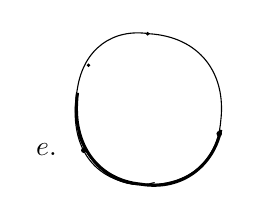
\begin{tikzpicture}[x=1cm,y=1cm]
\draw (0,.95) .. controls (.64,.91) and (.98,.45) .. (.91,-.15)
 .. controls (.86,-.78) and (.36,-1.04) .. (-.25,-.95)
 .. controls (-.83,-.83) and (-1.02,-.33) .. (-.91,.26)
 .. controls (-.83,.76) and (-.46,1.02) .. (0,.95);
\draw[line width=1.1pt] (-.91,.2) .. controls (-1,-.48) and (-.63,-.91) .. (-.11,-.96)
 .. controls (.43,-1.05) and (.82,-.71) .. (.91,-.27);
\draw (-.9,-.33) .. controls (-.72,-.82) and (-.31,-1.05) .. (.07,-.94);
\fill (-.02,.95) circle (.025);
\fill (-.77,.55) circle (.024);
\fill (-.83,-.53) circle (.035);
\fill (.89,-.32) circle (.035);
\node[left] at (-1.04,-.52) {$e.$};
\end{tikzpicture}}

\[
\deleted{e_i-e_j\qquad\unsure{\mathcal O(6)|\mathcal O(1)}}
\qquad e_i-e_j=
\]
\[
\unsure{\xi_i}.
\]

\diagram{\begin{tikzcd}[ampersand replacement=\&,column sep=small,row sep=small]
\unsure{\uline{\mathcal O}_x(1)|\uline{\mathcal O}_a(1)}\arrow[d,phantom,"{\unsure{\in}}"{description,rotate=90}]
 \& {}\ni\xi_{ij}(x)\\
\lambda \& \lambda^6=\displaystyle\prod_{i,j}\xi_{ij}(x)
\end{tikzcd}}

\deleted{\diagram{\begin{tikzcd}[ampersand replacement=\&,column sep=large]
\mathbb Z\arrow[r,no head]
\& \widetilde\Pi_{\unsure{03}}\arrow[r]
\& \Pi_{03}^{\unsure{\sharp|\ast}}\arrow[r,very thick]
\& 1
\end{tikzcd}}}

\[
(e_i-e_j)(\uline{\unsure{Q_n|Q_k}})
\qquad\deleted{\unsure{e_i-e_j}}
\]

\[
\deleted{\mathbf V(\omega)\overset{!!}{\simeq}\mathbf V}
\qquad \varphi\in V
\qquad e_i-e_j(\deleted{\unsure{Q_k}}\,
\]
\[
e_i-e_j\bmod L_{Q_k}
\]

\diagram{\(\begin{array}{ccc}
\frac12 & \frac12 & 1\\
-\frac12 & -\frac12 & -1
\end{array}\)}
\[
\left(\frac12\right)^4\qquad\sqrt[3]{\frac12}
\]

% Secteur inférieur, écrit à l'envers par rapport au secteur précédent.
\deleted{
We have seen that an orientation of a combinatorial
\inserted{\unsure{cellular|cellulation}} \deleted{\unsure{surface}}\inserted{\unsure{map}} $A$
\unsure{gives} rise \unsure{to|:} two \unsure{operators|operations}
$\vec\rho_s,\vec\rho_f$ on $\vec A$, \unsure{satisfying}
\[
\vec\rho_s^{-1}\vec\rho_f=\sigma
\]

If we take the opposite orientation, \unsure{what|what} are the
\unsure{corresponding|corresponding} \unsure{operators|operations}
$\vec\rho'_s,\vec\rho'_f$ ?
If $\vec a\in\vec A$ \unsure{comes} from $a\in A^L_+$,
it \unsure{comes} from $\sigma_na\in A^L_-$, and we have
\[
\rho_s(\sigma_na)
 =\sigma_n
   (\underbrace{\sigma_n\rho_s\sigma_n}
     _{\sigma_n\varepsilon=\rho_s^{-1}}a)
 =\sigma_n(\rho_s^{-1}a)\,-
\]
\unsure{thus} the class in $\vec A\simeq A^L/\sigma_n$
is that of $\rho_s^{-1}a$,
i.e. $\vec\rho_s^{-1}\vec a$.
\deleted{\unsure{A}}nd we therefore have
\[
\deleted{\rho_f(\sigma_na)
 =\sigma_n
  (\underbrace{\sigma_n\rho_f\sigma_n}
   _{\sigma_n\varepsilon\sigma}a)}
\]
\[
\vec\rho'_s=\vec\rho_s^{-1}
\]
hence
\[
\vec\rho'_f=\vec\rho'_s\sigma
 =\vec\rho_s^{-1}\sigma
 =\sigma\vec\rho_f^{-1}\sigma
 =\mathrm{int}(\sigma)\vec\rho_f^{-1}
\]
(This is not so \unsure{pleasant}.)
}

\margin{
% Notes perpendiculaires dans la marge droite du secteur inférieur redressé.
\[
\unsure{\widetilde Q_m|\widetilde R_m}
 -\unsure{\widetilde Q_j|\widetilde R_j}
\]
\[
\deleted{\unsure{\xi}}\quad\unsure{\gamma_h\ i\gamma_h}
\]
\[
e_j-e_i\quad -(e_i-e_h)
\]
}

\margin{29}

\scanpage{31}

\deleted{\diagram{\begin{tikzcd}[ampersand replacement=\&,column sep=large,row sep=large]
1\arrow[r,hook]
\& \mathbb Z\arrow[r,no head]
\& \widetilde\Pi\arrow[r]
\& \Pi\arrow[r,no head]\arrow[d]
\& 1\\
\& \& \& \deleted{\unsure{D''_3}} \&
\end{tikzcd}}}

\diagram{\begin{tikzcd}[ampersand replacement=\&,column sep=small,row sep=large]
\& \& \Pi_0\arrow[rr,equal]\arrow[dr]
\& \& \Pi_0\unsure{.}\arrow[dr] \& \& \\
\mathbb Z\arrow[r]\arrow[d,equal]
\& \widetilde\Pi\arrow[rr]\arrow[d]
\& \& \Pi'\arrow[rr]\arrow[d]\arrow[ddr]
\& \& \Pi\arrow[d]\arrow[ddr] \& \\
\mathbb Z\arrow[r]\arrow[dd,equal]
\& \widetilde D_{\unsure{3|0}}\arrow[rr,no head]\arrow[dd]
\& \& D'''_3\arrow[rr]\arrow[dr,no head]\arrow[dd]
\& \& D''_3\arrow[dr,very thick]\arrow[dd] \& \\
\& \& \& \& D'_3\arrow[rr,very thick]\arrow[dd,no head]
\& \& D_3\arrow[dd]\\
\mathbb Z\arrow[r,no head,"12"]
\& \mathbb Z\arrow[rr]
\& \& \mathbb Z/12\mathbb Z\arrow[rr]\arrow[dr,no head]
\& \& \mathbb Z/6\mathbb Z\arrow[dr,very thick] \& \\
\& \& \& \& \mathbb Z/4\mathbb Z\arrow[rr,no head]
\& \& \mathbb Z/2\mathbb Z
\end{tikzcd}}

\diagram{\begin{tikzcd}[ampersand replacement=\&,column sep=large,row sep=large]
\& \& \& \Pi_0\arrow[dd] \& \& \\
\& \& \deleted{\unsure{\widetilde\Pi}}\ \mathbb Z\arrow[r,very thick]
\& {} \& \& \\
1\arrow[r]
\& \mathbb Z\arrow[r]
\& \widetilde\Pi(4)\arrow[r]
\& \Pi\times\mathbb Z/4\mathbb Z\arrow[r,no head]\arrow[ddr,bend left=12]
  \arrow[dd]
\& 1 \& \\
\& \& \& \& \& \\
\& \& \& \deleted{\unsure{D_3}\times\mathbb Z/4\mathbb Z}\arrow[d]
\& D_3\times\mathbb Z/4\mathbb Z \& \\
\& \& \& 1
\& D'_3\arrow[u,phantom,"{\subset}"{description,rotate=90}] \&
\end{tikzcd}}

\diagram{\begin{tikzcd}[ampersand replacement=\&,column sep=large,row sep=large]
1\arrow[r,no head]
\& \Pi_0\arrow[r]
\& \Pi\times\mathbb Z/4\mathbb Z\arrow[r]
\& D_3\times\mathbb Z/4\mathbb Z\arrow[r]
\& 1\\
1\arrow[r,no head]
\& \Pi_0\arrow[u,equal]\arrow[r]
\& \Pi'\arrow[u,hook,very thick]\arrow[r,very thick]
\& D'_3\arrow[u,hook]\arrow[r,no head]
\& 1
\end{tikzcd}}

\[
\Pi'\subset\joinrel\relbar\joinrel\relbar\ \Pi
\]
\[
\deleted{\unsure{\widetilde\Pi}\times\unsure{\mathbb Z/4|\mathbb Z/4\mathbb Z}}
\]
\diagram{\begin{tikzcd}[ampersand replacement=\&,column sep=large]
\widetilde\Pi(4)\arrow[r]
\& \Pi\times\mathbb Z/4\mathbb Z
\end{tikzcd}}

\margin{30}
\scanpage{32}
\margin{31}
% Une longue barre oblique traverse le corps du feuillet.
\deleted{
\uline{Case} a) The construction \inserted{\unsure{is not}} \unsure{able to} continue \unsure{indefinitely}
i.e. we end up having $\sigma a_n\notin A'$, we then \unsure{set}
$\sigma a_n=\rho a_0$.

\uline{Case} b) The construction continues \unsure{indefinitely}.

(\deleted{\unsure{whether} \unsure{we} \inserted{\unsure{therefore}} \unsure{have a finite cycle}}, \unsure{or an}
\unsure{infinite} cycle). We do not \unsure{define} $\rho\unsure{\widehat a|a}$ \unsure{then}.

\margin{\figure{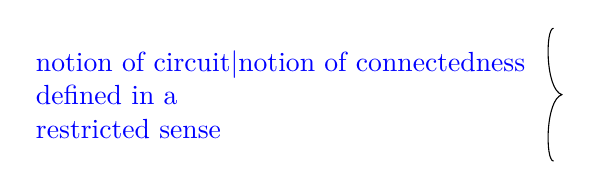
\begin{tikzpicture}
\node[align=left,inner sep=3pt] (m) {\unsure{notion of circuit|notion of connectedness}\\\unsure{defined in a}\\\unsure{restricted sense}};
\draw ([xshift=7pt,yshift=5pt]m.north east)
 .. controls ([xshift=4pt,yshift=5pt]m.north east) and ([xshift=4pt,yshift=2pt]m.east) .. ([xshift=10pt]m.east)
 .. controls ([xshift=4pt,yshift=-2pt]m.east) and ([xshift=4pt,yshift=-5pt]m.south east) .. ([xshift=7pt,yshift=-5pt]m.south east);
\end{tikzpicture}}}
We suppose henceforth that $\rho$ is \deleted{\unsure{defined}} \inserted{\unsure{extended}} on \unsure{all of} $A$
and that \unsure{$=$} for the \unsure{opposite} orientation (these are
\unsure{combinatorial} properties of $(A,\sigma,A',\rho)$).
Then $\rho$ on $A$ is an \uline{\unsure{automorphism}}. Let $\unsure{\overline S}=A/\rho\supset S$,
$\widehat S\unsure{\subset|=}\overline S$ the subset of $\overline S$ corresponding to the finite orbits.
We can \unsure{compactify} \unsure{partially} $X$ to \inserted{$\widehat X$}\deleted{\unsure{$\overline X$}}
\unsure{adding} the points of $\widehat S-S$ (as well
as : $\unsure{K^\circ}$\inserted{\unsure{$\simeq\Pi_{0,3}$}}), the inverse image \inserted{$\widehat A'$} of
$\widehat S$ in $A$ \inserted{\unsure{contains $A'$ and}}
is \unsure{stable} \unsure{$\forall$} under $\rho$ and $\sigma$
but \deleted{\unsure{is not|this is not} necessarily equal \unsure{to|with} $A'$.}
\inserted{: $A$ \unsure{in its entirety|is entire}.}

\margin{\figure{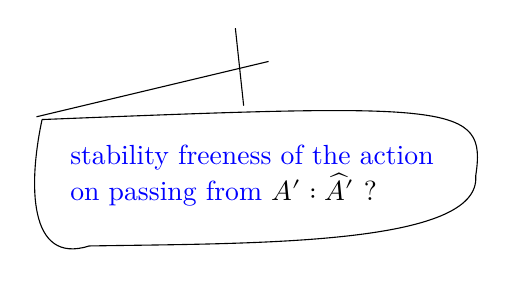
\begin{tikzpicture}
\node[align=left,inner sep=5pt] (m) {\unsure{stability freeness of the action}\\\unsure{on passing from} $A':\widehat A'$ ?};
\draw ([xshift=-5pt,yshift=4pt]m.north west)
 .. controls ([xshift=-10pt,yshift=-3pt]m.west) and ([xshift=-10pt,yshift=-16pt]m.south west) .. ([xshift=12pt,yshift=-9pt]m.south west)
 .. controls ([yshift=-8pt]m.south) and ([xshift=12pt,yshift=-9pt]m.south east) .. ([xshift=10pt]m.east)
 .. controls ([xshift=14pt,yshift=10pt]m.north east) and ([xshift=3pt,yshift=10pt]m.north east) .. ([xshift=-5pt,yshift=4pt]m.north west);
\draw ([xshift=-7pt,yshift=5pt]m.north west) -- ([xshift=6pt,yshift=25pt]m.north);
\draw ([xshift=-3pt,yshift=9pt]m.north) -- ([xshift=-6pt,yshift=37pt]m.north);
\end{tikzpicture}}}

The quadruples $(A,\sigma,A',\rho)$ \unsure{satisfying} the
axioms, \unsure{must} \inserted{and such that $A'=\widehat A'$}
\unsure{be identified|are identified} with the \deleted{\unsure{triples}} triples
$(A,\sigma,\rho)$ of a set \uline{\unsure{whatsoever}} with an automorphism
$\sigma$ of order $2$ \uline{without a fixed point}, and an automorphism $\rho$
\uline{whatsoever}. We \unsure{recover} $A'$ as the set of
elements of $A$ with finite orbit under $\rho$ --- but we
suppose that $A'\cup\sigma A'=A$.
}

\scanpage{33}
\diagram{\begin{tikzcd}[ampersand replacement=\&,column sep=large,row sep=large]
 0\arrow[r] \& \overset{\omega}{\mathbb Z}\arrow[r,"p"]\arrow[d,"q"'] \& \overset{\widetilde\Pi_0}{\overset{\Vert}{\mathbb Z}}\arrow[r,"\alpha\varphi_p",very thick]\arrow[d] \& \overset{\Pi_0}{\overset{\Vert}{\mathbb Z/p\mathbb Z}}\arrow[r]\arrow[d,equal] \& 0\\
 0\arrow[r,no head,"\overline\omega"'] \& \mathbb Z\arrow[r] \& \widetilde\Pi_0(q)\arrow[r]\arrow[d,"{\substack{\text{\unsure{zero on }}\widetilde\Pi_0,\\\text{\unsure{canonical on }}\mathbb Z\overline\omega}}"] \& \mathbb Z/p\mathbb Z\arrow[r,no head] \& 0\\
 \&\& \mathbb Z/q\mathbb Z \&\&
\end{tikzcd}}
\margin{$\varphi_p:\mathbb Z\longrightarrow\mathbb Z/p\mathbb Z$ canonical homomorphism\\
$\alpha\in(\mathbb Z/p\mathbb Z)^*$\\
\deleted{$\unsure{\beta}\in(\mathbb Z/q\mathbb Z)^*$}}

\diagram{\begin{tikzcd}[ampersand replacement=\&,column sep=large,row sep=large]
 \&\& \overset{\omega}{\mathbb Z}\arrow[r]\arrow[dl,equal] \& \widetilde\Pi_0\arrow[r]\arrow[dl] \& (\mathbb Z/p\mathbb Z\times0)\arrow[dl]\\
 0\arrow[r,no head] \& \overset{\omega}{\mathbb Z}\arrow[r]\arrow[dr,shift right=.6ex] \& \widetilde\Pi_0(q)\arrow[r] \& \mathbb Z/p\mathbb Z\times\mathbb Z/q\mathbb Z\arrow[r,no head] \& 0\\
 \&\& \underset{\omega}{\mathbb Z}\arrow[ul,"q"'{pos=.55},shift right=.6ex]\arrow[r,"\unsure{q}"] \& \underset{\overline\omega}{\mathbb Z}\arrow[ul]\arrow[r,no head] \& 0\times\mathbb Z/q\mathbb Z\arrow[ul]
\end{tikzcd}}
\margin{$\alpha\eta_p$}

\diagram{\begin{tikzcd}[ampersand replacement=\&,column sep=large,row sep=large]
 0\arrow[r,no head] \& \mathbb Z\arrow[r]\arrow[d,equal] \& \widetilde\Pi_0(q)\arrow[r,no head] \& \mathbb Z/p\mathbb Z\times\mathbb Z/q\mathbb Z\arrow[r,no head] \& 0\\
 0\arrow[r,no head] \& \mathbb Z\arrow[r,no head] \& \widetilde\Pi'_0\arrow[r]\arrow[u] \& \mathbb Z/\mu\mathbb Z\arrow[r,no head]\arrow[u,"\delta",very thick] \& 0
\end{tikzcd}}

\deleted{\unsure{The extension is} \illegible{1} :}
\[
 \unsure{\zeta'|\xi'}\deleted{\unsure{\zeta|\xi}}=
 \mathrm{cl}(\widetilde\Pi'_0)\in
 \operatorname{Ext}^{\unsure{1}}_{\deleted{\unsure{\mathbb Z}}}
 (\mathbb Z/\mu\mathbb Z,\mathbb Z)\simeq\mathbb Z/\mu\mathbb Z
\]
\[
 \deleted{\unsure{=}}\quad
 \unsure{\zeta'|\xi'}=
 \delta^*\!\left(
 \underbrace{\mathrm{cl}(\widetilde\Pi_0\unsure{(q)|q})}_{\unsure{\zeta|\xi}\,\in\,\operatorname{Ext}^1(\mathbb Z/p\mathbb Z\times\mathbb Z/q\mathbb Z,\mathbb Z)}
 \right)\unsure{'}
\]
\[
 \unsure{\zeta|\xi}=
 \mathrm{pr}_1^*\!\left(\underbrace{\mathrm{cl}(\widetilde\Pi_0)}_{\alpha\eta_p}\right)
 +\mathrm{pr}_2^*\!\left(\underbrace{\mathrm{cl}(\mathbb Z)}_{\eta_q}\right)
\]
\[
\begin{array}{ll}
 \delta_p:\mathbb Z/\mu\mathbb Z\mathrel{\overset{\mathrm{can}}{-}}\mathbb Z/p\mathbb Z
 &\unsure{\zeta'|\xi'}=\deleted{q'\eta_\mu+p'\eta_\mu}\\[1ex]
 \delta_q:\mathbb Z/\mu\mathbb Z\mathrel{\overset{\mathrm{can}}{-}}\mathbb Z/q\mathbb Z&\\[1ex]
 \delta_p^*(\eta_p)=q'\eta_\mu & \delta_p^{\unsure{*|' }}(\alpha\eta_p)=q'\alpha\eta_\mu\\[1ex]
 \delta_q^{\unsure{*|'}}(\eta_q)=p'\eta_\mu &
\end{array}
\]
\margin{32}

\scanpage{34}
\deleted{$\unsure{4)}\ \unsure{\widetilde{\mathrm{Sl}}}(2,\mathbb Z)\simeq
\unsure{\mathcal T_{1,1}}\,\unsure{\mathrm{SL}}\,\unsure{\Pi}$}

1)
\[
\begin{gathered}
 S\mathcal T_{11}\simeq\widetilde{\mathrm{Sl}}(2,\mathbb Z)
 \simeq\{\rho,\sigma\mid\underbrace{\rho^3=\sigma^2}_{\omega}\}
 \simeq
 \underset{\substack{\Vert\\\{\rho,\sigma\mid\rho^3=\sigma^2=1\}}}{\Pi_{0,3}^D}
 \times_{\unsure{\mathbb Z/6\mathbb Z}}\mathbb Z\\
 \simeq S\Pi_{0,3}^D
\end{gathered}
\]
\inserted{\deleted{$\unsure{\alpha}$}
\diagram{\begin{tikzcd}[ampersand replacement=\&,row sep=small]
 \rho\arrow[r,mapsto]\&2\\
 \sigma\arrow[r]\&3
\end{tikzcd}}}

% Le bloc suivant est écrit tête-bêche par rapport à la ligne précédente.
\diagram{\begin{tikzcd}[ampersand replacement=\&,column sep=large,row sep=large]
 \widetilde\Pi\arrow[r,no head]\arrow[dd,no head]\&\unsure{\Pi}\arrow[r,no head]\arrow[d]\&\Pi'\arrow[r]\arrow[dd,Rightarrow]\&\Pi\arrow[dd]\\
 \&\mathbb D_3''\arrow[dd]\&\&\\
 \mathbb Z\arrow[rr]\&\&\mathbb Z/12\mathbb Z\arrow[r]\arrow[d]\&\mathbb Z/6\mathbb Z\arrow[d]\\
 \&\unsure{\mathbb Z/}\&\mathbb Z/4\mathbb Z\arrow[r]\&\mathbb Z/2\mathbb Z
\end{tikzcd}}
\margin{$\Pi_0=\mathbb Z/6\mathbb Z$}
\margin{$\Pi_0\times\unsure{7|1}$}
\diagram{\begin{tikzcd}[ampersand replacement=\&,column sep=large,row sep=large]
 \mathbb Z\arrow[r,no head]\&\widetilde\Pi(4)\arrow[r]\&\Pi\times\mathbb Z/4\mathbb Z\arrow[r,no head]\arrow[d]\&1\\
 \&\widetilde\Pi\arrow[u,"?"']\arrow[r,"\uline{\unsure{cart}}"]\&\Pi'\&
\end{tikzcd}}

% Billet préexistant, à lire après une rotation de 90 degrés.
\margin{27-11-81}
Mr. Grothendieck

To be filled out urgently

Thank you

\uline{R. \unsure{Boucher}}
\margin{33}

\scanpage{35}
\[
 (p'+q'\alpha)\eta_\mu
\]
\[
 p=6,\ q=4\qquad(\alpha=-1\ ?)
\]
\[
 \deleted{\unsure{p}}\ \mu=12\qquad p'=3,\ q'=2
\]
\[
 \deleted{\unsure{p'+}}\ (3-2)\eta_\mu\ !
\]
\figure{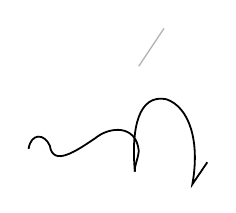
\begin{tikzpicture}[x=1cm,y=1cm]
 \draw[line width=.5pt,opacity=.3] (1.4,1.7)--(1.72,2.18);
 \draw[line width=.65pt] (0,.65) .. controls (.03,.85) and (.2,.85) .. (.27,.69)
 .. controls (.31,.42) and (.6,.62) .. (.84,.78)
 .. controls (1.03,.94) and (1.37,.96) .. (1.4,.62)
 .. controls (1.38,.48) and (1.34,.43) .. (1.35,.36);
 \draw[line width=.65pt] (1.35,.36) .. controls (1.3,.92) and (1.4,1.35) .. (1.75,1.28)
 .. controls (2.04,1.18) and (2.18,.75) .. (2.08,.2)
 --(2.27,.48);
\end{tikzpicture}}

$\cdot$
\diagram{\begin{tikzcd}[ampersand replacement=\&,column sep=large,row sep=small]
 \Pi_{0,3}^D\arrow[r,"{-\alpha}"{draw,circle,inner sep=1pt},very thick]\&\mathbb Z/6\mathbb Z\\
 \rho\arrow[r,mapsto]\&-2\ \mathrm{mod}\ 6\\
 \sigma\arrow[r,mapsto]\&3\ \mathrm{mod}\ 6\\[1ex]
 \varepsilon_0=\sigma\rho\arrow[r,mapsto,very thick]\&1\ \mathrm{mod}\ 6\\
 \rho_0=\varepsilon_0^2\arrow[r,mapsto]\&2\ \mathrm{mod}\ 6
\end{tikzcd}}
\deleted{$\unsure{\varphi}$}
% Marques très pâles à droite des résidus; possible transparence du verso.
\margin{$\unsure{\Gamma|\sqrt{\phantom{x}}}$\\$\unsure{\xi_0\prime|\xi_0}$\\$\unsure{t\prime r|t\prime h}$}

\margin{defined directly by the action of $\Pi_{0,3}^D$ on the
principal \unsure{cover}\deleted{\unsure{ing}} of $(U_{0,3},\mathfrak S_3)$
with group $\mathbb Z/6\mathbb Z$, defined by
the \inserted{canonical} \unsure{multisection|multiplication} of
\deleted{$\unsure{\mathcal O(1)}$}$\mathcal O_{U_{0,3}}(1)^*$
$=PU_{0,3}$}

\[
 \widetilde\Pi_{0,3}^D
\]
\deleted{$\mathcal O\unsure{(1)}$}
\diagram{\begin{tikzcd}[ampersand replacement=\&,column sep=small,row sep=large]
 U'_{0,3}\arrow[rr,phantom,"\subset"]\arrow[dr,no head,"{\mu_6\text{-}\unsure{\mathrm{rev}^{\mathrm t}}}"']\&\&PU_{0,3}\arrow[dl,no head]\&\unsure{+}\\
 \&U_{0,3}\&\&
\end{tikzcd}}
\deleted{$\unsure{\longrightarrow}$}

\diagram{\begin{tikzcd}[ampersand replacement=\&,column sep=large,row sep=large]
 \&\Pi_{0,3}^D\arrow[r,"{\alpha'}"{draw,circle,inner sep=1pt},very thick]\&\mathbb Z/6\mathbb Z\\
 \pi_1(PU_{0,3},\mathfrak S_3)\arrow[r,equal]\&\widetilde\Pi_{0,3}^D\arrow[u]\arrow[r]\&\mathbb Z\arrow[u]\\
 \&\omega'\in\mathbb Z\arrow[u]\arrow[r,"\unsure{=}"]\&\mathbb Z\arrow[u,"6"]
\end{tikzcd}}

\diagram{\begin{tikzcd}[ampersand replacement=\&,column sep=large,row sep=large]
 1\arrow[r]\&\mathbb Z\arrow[r]\arrow[d,equal]\&
 \underset{\substack{\Vert\\\pi_1(PU_{0,3},\mathfrak S_3\times\mu_4)}}{\widetilde\Pi_{0,3}^D(4)}\arrow[r,very thick]\&
 \Pi_{0,3}^D\times\mathbb Z/4\mathbb Z\arrow[r]\&1\\
 1\arrow[r,no head]\&\mathbb Z\arrow[r]\&\widetilde{\mathcal T}_{11}\arrow[u,bend left=20]\arrow[r,Rightarrow]\&
 \mathcal T_{1,1}=\Pi_{0,3}^D\times_{\mathbb Z/2\mathbb Z}\mathbb Z/4\mathbb Z\arrow[u,hook]\&
\end{tikzcd}}

\deleted{$\unsure{\widetilde\Pi_{0,3}^D}\,\unsure{\mathbb Z/4\mathbb Z}\longrightarrow$}
\[
\begin{array}{ll}
 \widetilde\Pi_{0,3}^D\ni\widetilde\rho^{\unsure{\sharp|'}}=(\rho,-2)
 &\widetilde\rho^{\unsure{\sharp}3}=\widetilde\sigma^{\unsure{\sharp}2}=\omega'\\
 \hfill\widetilde\sigma^{\unsure{\sharp|'}}=(\sigma,-3)&
\end{array}
\]
\diagram{\begin{tikzcd}[ampersand replacement=\&,column sep=small,row sep=small]
 \widetilde\rho,\arrow[d]\&\widetilde\sigma\arrow[d]\&
 \in\widetilde\Pi_{0,3}^D=
 \left\{\widetilde\rho,\widetilde\sigma\mid
 \underbrace{\widetilde\rho^3=\widetilde\sigma^2}_{\unsure{\omega'^{-1}|\widetilde\omega^{-1}}=\unsure{\omega|\infty}}
 \deleted{\unsure{\omega\in\mathbb Z}}\right\}\\
 \rho\&\sigma\&\simeq\widetilde{\mathcal T}_{11}
\end{tikzcd}}
\margin{34}

\scanpage{36}
\diagram{\begin{tikzcd}[ampersand replacement=\&,column sep=large,row sep=large]
 \&\&\left\{\rho,\sigma\mid\underbrace{\rho^3=\sigma^2}_{\omega'^{-1}=\omega}\right\}\deleted{\unsure{\omega|\infty}}\arrow[d,equal]\&\&\\
 1\arrow[r,no head]\&\overset{\omega'=\unsure{\omega^{-1}|\overline\omega'}}{\mathbb Z}\arrow[r]\arrow[d,equal]\&S\Pi_{0,3}^D\arrow[r]\arrow[d]\&\Pi_{0,3}^D\arrow[r,no head]\arrow[d]\&1\\
 1\arrow[r,no head]\&\mathbb Z\arrow[r]\&S\Pi_{0,3}^D(4)\arrow[r]\&\Pi_{0,3}^D\times\mathbb Z/4\mathbb Z\arrow[r,no head]\&1\\[4em]
 1\arrow[r]\&\underset{\omega^2}{\mathbb Z}\arrow[r]\arrow[u,very thick]\&S\mathcal T_{11}\arrow[r]\arrow[u,very thick,"{\underbrace{\begin{gathered}\rho\mapsto\rho\overline\omega^2\\\sigma\mapsto\sigma\overline\omega^3\\\omega\longrightarrow\overline\omega^2\\\omega^2\longrightarrow\overline\omega^4=\omega'\end{gathered}}}"]\&\mathcal T_{11}\arrow[u,hook,"{\substack{\rho\mapsto(\rho,2)\\\sigma\mapsto(\sigma,3)}}"]\&\omega\longrightarrow(1,2)
\end{tikzcd}}
\margin{$S\Pi_{0,3}^D(4)=\left\{\rho,\sigma,\overline\omega\mid\begin{gathered}\rho^3=\sigma^2=\overline\omega^{-4}\\\overline\omega\ \text{central}\end{gathered}\right\}$\\
N.B. $\unsure{\dot{\overline\omega}|\overline\omega}^{4}=\unsure{\omega^{-1}}$\\
$=\omega'\deleted{\unsure{\omega}}$}

% Groupe et flèche au pied du feuillet, écrits tête-bêche.
\diagram{\begin{tikzcd}[ampersand replacement=\&,column sep=large]
 \overbrace{S\Pi_{0,3}^D(4)}^{\pi_1(U_{0,3},\mathfrak S_3\times\mu_4)}\arrow[r]\&\Pi_{0,3}^D
\end{tikzcd}}
\margin{35}

\scanpage{37}
% not manuscript: formulaire vierge « ANNEXE II », renseignements à fournir par le candidat devant soutenir une thèse de doctorat d'État, Université des Sciences et Techniques du Languedoc, imprimé tête-bêche.
\margin{36}

\clearpage
\section*{Cote 140-2}
\addcontentsline{toc}{section}{Cote 140-2 (575 scans)}
\subsection*{Scans 1--10}
\addcontentsline{toc}{subsection}{Scans 1--10}
% package LM_P01
\scanpage{1}
% not manuscript: page de titre imprimée de l'Université de Montpellier / IMAG.

\scanpage{2}
% not manuscript: couverture portant « Pages 1-292 + table des matières ».

\scanpage{3}
\margin{I}

The ``long march'' through Galois theory...

1. Multi-Galois topoi \hfill 1

2. Applications to coverings of topoi \hfill 4

3. Pro-multi-Galois variants \hfill 6

4. Complements remorse

\figure{[Brace on the right joining entries 3 and 4.]}

\uuline{5.} Introduction of the arithmetic context
Fundamental ``anabelian conjecture'' \hfill \(7'\)

6. Local analysis of \((X,S)\) at an \(s\in S\). \hfill \(10'\)

7. ``Messy'' reformulation of the conjecture
(the necessary purgatory...) \hfill 12

\deleted{\unsure{6.}}
8. Taxonomic reflection (distinction \unsure{of the|of}
cases, \unsure{where} purgatory gets fitted out a little...) \hfill \(25'\)

\deleted{\unsure{7.}}
9. Tangential structure at the \(s\in S\)
(Sections of extensions ``of the second type'' \hfill 34

10. \unsure{Adjustment} of the hypotheses, (remorse) \hfill 38

11. Conditions on the systems of groupoids obtained from
geometric situations \hfill 39

12. The topological analogy. (Where we also convince ourselves that the groupoidal
mess can be expressed completely, in the anabelian cases,
by the outer groups with loops... \hfill \unsure{41|43}

13. Return to the arithmetic case: ``Galois'' formulations \hfill 53

13\textsuperscript{bis}. Return to the notion of a group with loops \hfill 56

14. Cohomological digression (on ``plugging holes'') \hfill 58

\uuline{15.} Return to the topological case: critical orbits
\unsure{around} splittings of extensions
Application to finite subgroups of
\(\mathrm{Autext}_{\mathrm{lac}}(\pi)\) (discrete case)
(cf. also \(\S 18\)) \hfill \(67'\)

16. Plugging and drilling holes: general topological preliminaries
\hfill \(79'\)

17. Complements to \(\S 15\), on \unsure{operations|groups} of finite groups
on surfaces \hfill 89

\scanpage{4}
\uuline{18.} Drilling holes. Application to finite
subgroups of \(\mathrm{Autext}_{\mathrm{lac}}(\pi)\)
(discrete case) \hfill 91

\uuline{19.} Teichmüller tower \hfill 102

20. Digression: 2-isotopic description
of the category of topological \unsure{2-spheres} \hfill \(116'\)

21. Teichmüller spaces \hfill 125

\margin{missing \(\S 22\)!}

23. Return to surfaces with (finite) groups of operators
(``putting into equations'' the problem) \hfill 133

24. Attempt to determine the \unsure{\(A^{\circ\Gamma}\)}. Link with the relations
\(\Pi_{g,(\nu,\nu+n-1)}^{\Gamma}\) \(=(1)\),
program of \deleted{\illegible{1}}\inserted{work} \hfill 142

25. ``\uline{Special}'' Teichmüller groups \hfill 148

25\textsuperscript{bis}. ``Case of the two groups'' of operators. Return to the notation.
\hfill \(153'\)

\uuline{25.} Profinite Teichmüller groups. \hfill 161

Discretifications and \unsure{prediscretifications|prodiscretifications}. Link with modular
Teichmüller topos. Hasty conjecture. \hfill 167

27. Change of type \((g,\nu)\): a) plugging holes
(and \unsure{remarkable diagrams|remarkable diagram} page 174) \hfill 172

28. change of type \((g,\nu)\): b) passage to a finite covering
(the hasty conjecture creaks...) \hfill 177

29. Critique of the preceding approach. (We readjust
the notions and the conjectures...) \hfill 186

30. Properties of the \(N_{g,\nu},\Gamma_{g,\nu}\): a)
\unsure{Properties related} to finite Teichmüller subgroups.
\hfill 192

31. Digression on liftings of an outer action of a finite
group on a profinite group with loops \hfill 198

\uuline{32.} Return to the arithmetic aspects of plugging holes:
relations between \(\Gamma_{g,\nu}\) and \(\Gamma_{g,\nu-1}\).
(Where we reconstruct, without saying so, \uline{the whole étale topos} of a
\inserted{complete} algebraic curve, from the \(\pi_1\) of an
anabelian open...) \hfill 200

\uuline{33.} Topological digression: anti-involutions of compact
oriented surfaces (leaving aside at first the case ``with holes'')
\hfill 221

\uuline{\unsure{35.}} The injectivity of
\(\Gamma_{\mathbb Q}\longrightarrow
\mathrm{Autext}_{\mathrm{lac}}(\widehat{\Pi}_{0,3})\)
\hfill 249

\unsure{36.} The isomorphism
\(\Gamma_{\mathbb Q}\simeq\Gamma_{1,1}\),
and the injectivity of
\(\Gamma_{\mathbb Q}\longrightarrow
\mathrm{Autext}(\widehat{\unsure{\Gamma|T}}_{1,1}^{+})
=\mathrm{Autext}(\mathrm{SL}(2,\mathbb Z)^{\wedge})\)
\hfill 257

\unsure{37.} Moduli of elliptic curves via Legendre, or
\unsure{\(M_{1,1}[2]'\simeq U_{0,3}\ne M_{0,4}^{!}\)} \hfill 272

33. Relations between \(N_{g,\nu},\Gamma_{g,\nu}\) for variable \(g\)
(study of finite coverings) \hfill 239

34. Heuristic profinite description of the category of algebraic curves
defined over finite \deleted{\unsure{extensions}}
subextensions of \(\mathbb Q_0/\mathbb Q\)
\hfill 245

\figure{[To the left of the last two entries, brace extended
upward by an arrow pointing to the entry
``The injectivity of \(\Gamma_{\mathbb Q}\)''.]}

\scanpage{5}
\margin{\unsure{814|714}\par\unsure{752|252}\par 832}

\scanpage{6}
\mspage{1}
\margin{\unsure{W|VI}}

1. Multi-Galois topoi.

\uline{Proposition} 1.1. Let \(\mathcal E\) be a category.
Equivalent conditions:

a) \(\mathcal E\) is a topos, and every object of \(\mathcal E\)
is local\textsuperscript{ly} constant.

b) \(\mathcal E\) is equivalent to a category \(\widehat C\),
where \(C\) is a groupoid.

\margin{N.B. We shall see (below) \unsure{that we can choose}
\unsure{\(C\)} \uline{canonically}}

b') \(\exists\) a family \((G_i)_{i\in I}\) of groups
and an equivalence of categories
\[
\mathcal E\approxeq\prod\mathrm{Ens}(G_i)
\]

c) Ad-hoc exactness conditions, of the type of those given in SGA 1...

Proof. \(b\Longleftrightarrow b'\Longrightarrow a\) immediate.
For \(a)\Longrightarrow b)\), I am less sure, perhaps one has to
assume that \(\mathcal E\) is locally connected, and that it has sufficiently
many fiber functors i.e. sufficiently many points.

\uline{Definition 1.2.} If the equivalent conditions b) b') above
are satisfied, one says that \(C\)
is \unsure{a|a} multi-Galois \deleted{category} \inserted{topos}
(or a multi-Galois \uline{category}).

\margin{\uline{Proposition 1.3}
a) If \(\mathcal E\) is multi-Galois, every induced \unsure{topos}
\(\mathcal E_{/S}\) too.
\par
b) every sum of multi-Galois topoi (i.e. \deleted{\illegible{1}}
product of multi-Galois categories) \unsure{is so|is} too.}

\scanpage{7}
\uline{Proposition 1.4} \unsure{Let|Let} \(\mathcal E\) be a topos,
\(C\) the category of points of \(\mathcal E\) (opposite to the
category of fiber functors on \(\mathcal E\)). The canonical
functor
\[
\mathcal E\times C^o\longrightarrow(\mathrm{Ens})
\]
induces a canonical functor
\[
\mathcal E\longrightarrow\mathrm{Hom}(C^o,(\mathrm{Ens}))
\overset{\mathrm{déf}}{=}\widehat C
\]

This being so: (\(\mathcal E\) being multi-Galois)

a) \(C\) is a groupoid (called the ``fundamental groupoid'' of the
multi-Galois topos \(\mathcal E\), and often denoted
\(\Pi_1(\mathcal E)\)).

b) \(\mathcal E\longrightarrow\widehat C\) is an equivalence
of categories.

An object \inserted{\(S\)} of a topos \inserted{\(\mathcal E\)}
is said to be 0-connected if it is \(\ne\varnothing_{\mathcal E}\)
(\unsure{it|i.e.} is not an initial object) and if it is connected
(i.e. \(S\simeq S'\amalg S''\) implies
\(S'\) or \(S''\simeq\varnothing_{\mathcal E}\)) --- this also means
that the induced topos \(\mathcal E_{/S}\) is 0-connected
i.e. is not the initial topos (``empty topos'', i.e.
\inserted{equivalent to the} terminal category) and that it is connected,
i.e. ... One says that \(S\) is 1-connected

\scanpage{8}
\mspage{2}

(or ``simply connected'') if it is 0-connected, and if every
\deleted{\unsure{covering of \(S\) is}}
\inserted{object \(S'\) of \(\mathcal E_{/S}\)
\deleted{\illegible{1}}}
locally constant \unsure{is} is \unsure{\deleted{constant}|constant}
--- which depends \inserted{again} only on the induced topos
\(\mathcal E_{/S}\), which will then be said to be 1-connected.

\uline{Proposition} 1.5. Let \(\mathcal E\) be a multi-Galois topos,
and let \(S\) be an object of \(\mathcal E\). Equivalent conditions

a) \(S\) is 1-connected

b) \(S\) \unsure{(is)|is} 0-connected and projective

c) the covariant functor represented by \(S\)
\[
T\longmapsto\mathrm{Hom}_{\mathcal E}(S,T)
\]
is a fiber functor, or again
as it is already left exact) it commutes with
arbitrary \(\underset{\longrightarrow}{\lim}\)

\inserted{N.B.} (it suffices that it commute with sums and with passage
to the quotient...)

d) \(\mathcal E_{/S}\) is equivalent to the point topos

e) (If \(\mathcal E=\widehat C\), \(C\) a groupoid) the functor
\(S\) on \(C\) is \inserted{representable}

\scanpage{9}
\uline{Definition 1.6} One then says, sometimes, that \(S\) (or better, the topos
\(\mathcal E_{/S}\)) is a \uline{universal} \uline{covering} of the
\inserted{multi-Galois} topos \(\mathcal E\).

\uline{Proposition 1.7}
\deleted{\unsure{Taking} \illegible{1} object}
\inserted{Let \(\mathcal E_0\) be} the full subcategory of
\(\mathcal E\) formed by the 1-connected objects
(of the multi-Galois category \(\mathcal E\)),
\deleted{Then \unsure{the functor}} \inserted{and \(\Pi_1(\mathcal E)\)
the fundamental groupoid} of \(\mathcal E\).
We have \inserted{\unsure{by} 1.5} a canonical functor
\[
\mathcal E_0\longrightarrow
\Pi_1(C)
\]

(associating: \(\forall\) \(S\in\mathrm{Ob}\,\mathcal E_0\)
the fiber functor it represents, or rather the corresponding ``point''
of \(C\)), which is
(not only fully faithful, but even) an equivalence of
categories: every fiber functor on \(\mathcal E\) is representable
(by an essentially unique (1-connected) object, as is only right...).

\scanpage{10}
\mspage{3}
\deleted{\unsure{Definition 1.8} \illegible{1} \unsure{The object}}

\uline{Corollary 1.8.} Let \(P\) be a ``point'' of \(\mathcal E\)
\inserted{(associated with a fiber functor \(F_P\))}.
There exists a 1-connected object \(S\) of \(\mathcal E\) and a lifting
\(P\xrightarrow{\alpha}\mathcal E_{/S}\)
(i.e. an \(\alpha\in F(S)\)),

\diagram{[Under \(P\xrightarrow{\alpha}\mathcal E_{/S}\),
\(\mathcal E\) is placed at bottom center. Two dotted arrows
go respectively from \(P\) and from \(\mathcal E_{/S}\) to
\(\mathcal E\). Between them, a rightward arrow with
\(\sim\) above it, \unsure{double-lined|single-lined}.
Two side brackets enclose this lower part of the diagram.]}

and this determines \((S,\alpha)\) up to unique isomorphism.

In fact, \(S\) is the unique \unsure{object|\deleted{object}}
of \(\mathcal E\) that represents \(F_P\)...

\uline{Definition 1.9.} One says that \(S\)
\inserted{(or \(\mathcal E_{/S}\))} is the
\uline{universal covering pointed over \(P\)} determined
by the point \(P\).

\uline{Scholium 1.10} Giving oneself a ``point'' of the \unsure{:}
\inserted{multi-Galois} topos \(\mathcal E\), or giving oneself a
universal covering, amounts essentially to the
same: each determines the other...

\subsection*{Scans 11--20}
\addcontentsline{toc}{subsection}{Scans 11--20}
% package LM_P02
\scanpage{11}

\uline{Proposition \unsure{1.11|1.10}.} Let $\mathcal E,\mathcal E'$ be two multi-Galois topoi, $\Pi_1(\mathcal E),\Pi_1(\mathcal E')$ their fundamental groupoids. The obvious functor
\[
\underline{\mathrm{Hom}}_{\mathrm{top}}(\mathcal E,\mathcal E')
\longrightarrow
\underline{\mathrm{Hom}}\bigl(
\underset{C}{\underline{\Pi_1(\mathcal E)}},
\underset{C'}{\underline{\Pi_1(\mathcal E')}}\bigr)
\]
is an equivalence of categories, one finds a quasi-inverse equivalence by composing
\[
\underline{\mathrm{Hom}}(\deleted{\illegible{1}}C,C')
\longrightarrow
\begin{array}[t]{c}
\underline{\mathrm{Hom}}_{\mathrm{top}}(\widehat C,\widehat {C'})\\
\cap\\
\underline{\mathrm{Hom}}(\widehat {C'},\widehat C)
\end{array}
\simeq
\underline{\mathrm{Hom}}_{\mathrm{top}}(\mathcal E,\mathcal E').
\]
\inserted{(\unsure{or|for} $\widehat C\simeq\mathcal E$, $\widehat {C'}\simeq\mathcal E'$)}

\deleted{\illegible{1}}
\uline{1.12} Making explicit the case where $\mathcal E\ \mathcal E'$ are $0$-connected and pointed, hence given as $\mathcal E\simeq\mathrm{Ens}(G)$, $\mathcal E'\simeq\mathrm{Ens}(G')$

\dots

\margin{10}

\scanpage{12}
\mspage{4}

2. \unsure{Application|Applications} to coverings of topoi.

\uline{Theorem 2.1.} Let $\mathcal E$ be a locally connected topos (i.e. every object of which is a sum of $0$-connected objects) and locally simply connected (i.e. admitting a system of generators \unsure{which} are $1$-connected).
\margin{perhaps one must \unsure{suppose|supposed} that $\mathcal E$ has ``enough points'' i.e. enough fiber functors\dots}
\deleted{\illegible{6}}\inserted{Then the category $\mathcal E_{lc}$} of local\textsuperscript{ly} constant objects of $\mathcal E$ is \inserted{a topos} multi-Galois\deleted{\unsure{ne}}, and the inclusion
\[
(2.1.1.)\qquad \mathcal E_{lc}\hookrightarrow\mathcal E
\]
commutes with finite $\varprojlim$ (N.B. in fact, without hypotheses on the topos $\mathcal E$, $\mathcal E_{lc}$ is stable under finite $\varprojlim$) \uuline{and} with arbitrary $\varinjlim$.

\uline{Definition 2.2} We denote this topos by $\mathcal E_{[1]}$, call it the multi-Galois envelope of $\mathcal E$, and the morphism of topoi transposed from the inclusion (2.1.1):

\margin{11}

\scanpage{13}

\[
\mathcal E\longrightarrow\mathcal E_{[1]}
\]
is given the name \uline{canonical morphism}.

\uline{N.B.} This is the equivalent in topos theory of the operation of ``killing the $\Pi_i$ for $i\geq 2$''. One can also define \inserted{an} \deleted{\unsure{$\mathcal E_\infty$}} $\mathcal E_{[0]}$ and a sequence
\[
\mathcal E\unsure{\longrightarrow|-}\mathcal E_{[1]}\unsure{\longrightarrow|-}\mathcal E_{[0]}
\]
[$\mathcal E_0$ is the \uline{discrete} topos defined by $\Pi_0(\mathcal E)$, which has a satisfactory meaning as soon as $\mathcal E$ locally connected\dots]. With suitable hypotheses on $\mathcal E$ (of the type ``local contractibility''), one should be able to define the $\mathcal E_{[i]}$ for $\forall\ i\in\mathbb N$, and canonical morphisms
\[
\mathcal E\longrightarrow\cdots\quad
\mathcal E_{[i]}\unsure{\longrightarrow|-}\mathcal E_{[i-1]}\longrightarrow\cdots\quad
\mathcal E_{[1]}\longrightarrow\mathcal E_0.
\]

\margin{12}

\scanpage{14}
\mspage{5}

2.3. The \uline{fundamental groupoid} of $\mathcal E$ is defined as having for objects the points of $\mathcal E$ (which induce points of $\mathcal E_{[1]}$ thanks to $\mathcal E_{[1]}\longrightarrow\mathcal E$), and for morphisms the \deleted{\unsure{points}} morphisms \uline{of points of} $\mathcal E_{[1]}$. We thus have canonical functors
\[
\underline{\mathrm{Pt}}(\mathcal E)
\xrightarrow{\alpha}\Pi_1(\mathcal E)
\overset{\beta}{\overset{\approx}{\longrightarrow}}
\mathrm{Pt}(\mathcal E_{[1]})
\overset{\text{definition}}{=}\Pi_1(\mathcal E_{[1]})
\]
where $\beta$ is an equivalence (but not surjective on objects), and where of course $\alpha$ is not necessarily an equivalence, nor even fully faithful, or merely faithful. For example if $\mathcal E$ is $1$-connected i.e. $\Pi_1(\mathcal E)$ equivalent to the one-point category, it does not necessarily follow that the Hom \unsure{in|of} $\mathrm{Pt}(\mathcal E)$ are all of cardinality $\leq 1$!

\margin{13}

\scanpage{15}

Since a poin\textsuperscript{t} $P$ of $\mathcal E$ defines a poin\textsuperscript{t} (still denoted $P$ by abuse) of $\mathcal E_{[1]}$, one can therefore define the \uline{universal covering of $\mathcal E$} based at this point, as an object \inserted{$S$} $1$-connected in $\mathcal E_{[1]}$ -- it is characterized \inserted{in $\mathcal E$} by being locally constant, $1$-connected, and endowed with a lifting
\[
P\longrightarrow\mathcal E_{/S}.
\]

But since $\alpha$ is not an equivalence of categories (although it is \deleted{\illegible{1}} \unsure{essentially} surjective if \unsure{one} assumes that $\mathcal E$ has enough points\dots) one can \uline{not} say that $\forall$ universal covering of $\mathcal E$ is defined by a poin\textsuperscript{t} of $\mathcal E$, defined up to unique isomorphism\dots

\margin{14}

\scanpage{16}
\mspage{6}

3. ``pro-multi-Galois'' variants, resp. profinite (restricting ourselves, to simplify, to the case of locally connected topoi\dots).

4. Supplement-remorse on multi-Galois categories, which makes precise the intention that for a topos $\mathcal E$, the datum of an object $S\in\mathcal E$ defines an induced topos $\mathcal E_{/S}\longrightarrow\mathcal E$, and that $S$ is reconstructed up to unique isomorphism from knowledge of the induced topos as a topos \uline{over} $\mathcal E$. Here, \deleted{\illegible{1} $\mathcal E_{/S}$ \unsure{is}} \inserted{$\mathcal E$ being} multi-Galois, $\mathcal E_{/S}$ too -- and the question arises when a morphism of \inserted{\unsure{multi-Galois|multi-Galois}} topoi $\mathcal E'\longrightarrow\mathcal E$ can be regarded as

\margin{15}

\scanpage{17}

an induction morphism. Now if $C=\Pi_1(\mathcal E)$, $C'=\Pi_1(\mathcal E')$, the datum of $\mathcal E'\unsure{\longrightarrow|-}\mathcal E\deleted{\unsure{'}}$ is equivalent to the datum of a functor $C'\longrightarrow C\deleted{'}$. One finds that $\mathcal E'\unsure{\longrightarrow|-}\mathcal E\deleted{\unsure{'}}$ is an induction morphism \unsure{iff} $C'\longrightarrow C\deleted{'}$ is \uline{faithful}. Thus, one finds an equivalence between the category \inserted{$\mathcal E$} (of objects $S$ of the multi-Galois category $\mathcal E\simeq\widehat C$, \deleted{\illegible{1}} where $C$ is a groupoid, \uline{arbitrary if one insists})
\margin{a bit hasty!}
and the category whose objects are the ``groupoids $C'$ over $C$'', with a \uline{faithful} structural functor $C'\longrightarrow C$, the morphisms from $C'_1$ to $C'_2$ being the \inserted{\uuline{isomorphism classes \unsure{of a|of a}}} \deleted{\illegible{1}} pairs $(f,\alpha)$ of a functor $f:C'_1\unsure{\longrightarrow|-}C'_2$ and an

\margin{16}

\scanpage{18}
\mspage{7}

isomorphism of functors $\alpha:p_2f\simeq p_1$
\diagram{%
\begin{tikzcd}[ampersand replacement=\&]
C'_1 \arrow[rr,no head,"f"] \arrow[dr,"p_1"',""{name=pone}]
  \& \& C'_2 \arrow[dl,"p_2",""{name=ptwo}] \\
  \& C \&
\arrow[from=pone,to=ptwo,bend left=25,"\overset{\alpha}{\sim}"]
\end{tikzcd}}
\margin{Specify the isomorphisms between pairs $(f,\alpha)$ and \deleted{\unsure{pairs}} $(g,\beta)$\dots}

In the case where for example $C$ is the category reduced to a single object, an automorphism group $G$, this description of the category $\mathcal E=\mathrm{Ens}(G)$ is obviously a bit cumbersome, but it fits well into certain contexts below.

Thus, if $k$ is a base field, the \deleted{\unsure{$\mathcal E$}} category $\mathcal E$ of étale schemes over $k$ is described, in terms of a separable closure \unsure{$k$|the} $k_s$ of $k$ and of the profinite group $\Gamma=\mathrm{Gal}(k_s/k)$, as the \inserted{profinite} groupoids over the profinite groupoid $(\mathrm{pt},\Gamma)$\dots We want to insert this description into a ``Galois'' ``description'' \unsure{of the|of} \inserted{[certain]} schemes [smooth \inserted{quasi-}projective of dimension $\leq 1$] over $k$, at least if $k$ a field of finite type over $\mathbb Q$.

\margin{17}

\scanpage{19}

5. Let $K$ be an extension, of finite type over $\mathbb Q$, and let us choose an algebraic closure $\overline K$ of $K$.
\margin{We set $\Gamma=\mathrm{Gal}(\overline K/K)$}
\inserted{5.1} We consider pairs $(X,S)$, where: \deleted{\unsure{$X$}}

a) $X$ is a projective and smooth scheme over $K$, of dimension $\leq 1$;

b) $S$ is a finite \inserted{reduced} subscheme of $X$, \inserted{(then \illegible{1} \unsure{étale} over $K$)}, contained \deleted{\illegible{2}} \inserted{(in)} \inserted{the union} \unsure{of the} irreducible components of dimension $1$ of $X$.
\margin{(thus finite étale over $\unsure{k|K}$)}

The morphisms $(X',S')\unsure{\longrightarrow|-}(X,S)$ will by definition be the morphisms of schemes
\[
f:X'\longrightarrow X
\]
such that
\[
S'=f^{-1}(S)_{\mathrm{red}}
\]
i.e. such that $\mathrm{supp}\,S'=f^{-1}(\mathrm{supp}\,S)$.

We are looking for a ``Galois description'' of this category, or at least of a full \inserted{sub-}category \inserted{$\mathcal V_K$} which we are going to

\margin{18}

\scanpage{20}
\mspage{8}

define now.

\uline{Lemma} 5.2. Let $\Omega$ be an algebraically closed field, $X$ a \deleted{scheme} \inserted{smooth} projective algebraic curve, connected over $\Omega$, $S$ a finite subset of $X(\Omega)$, \inserted{$g$ the genus of $X$, $n=\mathrm{card}\,S$.} $\deleted{\unsure{X_0}}\inserted{U}=X\setminus S$, Equivalent conditions

a) $\Pi_1(U)$ nonabelian

b) $\mathrm{Aut}(U)$ finite

c) For $\forall$ \inserted{connected \deleted{of finite type}} reduced scheme $X$ \inserted{of finite type} over $\Omega$, the set of \uline{nonconstant} morphisms from $X$ to $U$ is finite

d) We are \deleted{\unsure{$X$}} in one of the following three cases: $1^\circ)$ \deleted{genus} $g\geq 2$ \quad $2^\circ)$ $g=1$, $n\geq 1$ \quad $3^\circ)$ $g=0$, $n\geq 3$.

\margin{e) (if $\Omega\unsure{\in|\subset}\mathbb C$) The universal covering of $X(\mathbb C)\setminus S(\mathbb C)$ is isomorphic to the half-plane \uline{of} Poincaré.}
\margin{\unsure{?!|??} f) (if $\Omega=\overline{\mathbb Q}$ \unsure{$S\neq\emptyset$}) The universal covering of $X\setminus S=U$ is isomorphic to that of $\mathbb P^1_\Omega\setminus\{0,\unsure{1},\infty\}$.}

\uline{Definition 5.3.} We then say that $(X,S)$ is anabelian. \deleted{If $X$ is a scheme}

As this condition is (by d) for example) invariant under extension of the algebraically closed base field, we extend this definition to the case of a pair $(X,S)$, with $(X,S)$ \deleted{projective smooth of dimension} \inserted{as in (5.1)} (\uline{N.B.} we look separately at the connected components of $X_{\overline K}$\dots).

\margin{19}

\subsection*{Scans 21--30}
\addcontentsline{toc}{subsection}{Scans 21--30}
% package LM_P03
\scanpage{21}

From now on, in (5.1) we are going to confine ourselves to the case of
anabelian pairs $(X,S)$.

\deleted{To such a}

5.4. To a pair $(X,S)$ (not necessarily \unsure{anabelian}) --- more generally to
$\forall$ scheme $X$ locally of finite type over \unsure{$S$|$\xi$}, we associate an
object ``of a Galois nature'', namely the fundamental groupoid
\inserted{(profinite)} $\Pi_1(X)$ of $X$ (formed if we like of the universal
coverings of $X$), \uline{equipped} with the canonical \deleted{\unsure{functor}}
\inserted{\unsure{homomorphism}}
\diagram{
\begin{tikzcd}[ampersand replacement=\&]
\Pi_1(X) \arrow[r] \& \Pi_1(K) \arrow[d, "\simeq"'] \\
\& {[\operatorname{Tors}(\Gamma)]}
\end{tikzcd}
}

A morphism of $K$-schemes
\[
X' \xrightarrow{f} X
\]
defines a functor
\[
\Pi_1(X') \xrightarrow{\Pi_1(f)} \Pi_1(X)
\]
and a commutation isomorphism $\alpha$

\margin{20}

\scanpage{22}
\mspage{9}

\diagram{
\begin{tikzcd}[ampersand replacement=\&,column sep=small]
\Pi_1(X') \arrow[rr, "\Pi_1(f)"]
  \arrow[dr, ""{name=L, below}] \&\&
\Pi_1(X) \arrow[dl, ""{name=R, below}] \\
\& \Pi_1(K)
\arrow[from=L, to=R, bend left=25, "\alpha", "\simeq"'] \&
\end{tikzcd}
}

We thus find a functor, from the category of schemes
$X$ locally of finite type over $K$, into the ``category of profinite groupoids over
$\Pi_1(K)$'', defined as in n\textsuperscript{o}\,4.

When we pass to the category of connected $K$-schemes locally of finite type,
\deleted{\unsure{and}} \uline{equipped with a geometric point,
over} $\overline K/K$ (i.e. with an $x\in X$,
\deleted{and} a separable closure $\overline{k(x)}$ of $k(x)$ and a
$K$-morphism $\overline K\hookrightarrow\overline{k(x)}$), this corresponds
to a functor from $K$-schemes locally of finite type and connected, pointed over
$\overline K/K$ (in the preceding sense) to the category of
\deleted{\unsure{extensions}} profinite groups \deleted{\illegible{1}} $\pi$
equipped with a homomorphism (of profinite groups)
\[
\pi\longrightarrow\Gamma
\]

\margin{it is better to say: equipped with a universal covering ....}
\margin{21}

\scanpage{23}

(whose \deleted{\unsure{a}}image will moreover necessarily be open hence
of finite index, for objects coming from $X$ as above).

\uline{Conjecture} 5.5. The restriction of the preceding functor
\inserted{$X\longmapsto(\Pi_1(X)\text{ over }\Pi_1(K))$}
to smooth projective schemes of dimension $\leq 1$ and anabelian
(i.e. such that $(X,S)$ is anabelian, where $S$ is the union of the
components of dimension $0$) is fully faithful.

\margin{This is a bit false \quad cf. \S\,9}

It comes to the same thing to say this:

\deleted{The functor}

\uline{Conjecture 5.5 bis} The functor which, to any $X$
\deleted{connected} as in 5.5. and moreover \uline{connected},
(of dimension $0$ or $1$), equipped with a geometric point $\xi$ over
$\overline K$, associates \deleted{\unsure{the profinite extension}} profinite
group \unsure{$\pi_1(X,\xi)$} over
\unsure{$\Gamma=\pi_1(K,\xi)$}), is a

\margin{\unsure{ditto}}
\margin{22}

\scanpage{24}
\mspage{10}

fully faithful functor.

We must all the same make explicit the
morphisms $(X,\xi)\longrightarrow(X',\xi')$ in the source category:
morphisms of $K$-schemes $X\xrightarrow{f}X'$, equipped with a morphism
\inserted{of $\Pi_1(X')$} (\unsure{or|in} class of paths)
\deleted{\unsure{of}} $f(\xi)\simeq\xi'$.

These conjectures reduce to Galois theory, for $X$ of
dimension $0$. For $X$ of dimension $1$, they concern only $X$ such
that the connected components of $X_{\overline K}$ are of genus $\geq 2$
(or, what comes to the same thing, introducing
the finite extension $K'=H^0(X,\underline{O}_X)$ of $K$, so that $X$ is
geometrically connected over $K'$, \unsure{such that} $X$ as
an algebraic \deleted{\unsure{$K'$-scheme}} \inserted{curve}
\uline{over $K'$} is of genus $\geq 2$. We see easily
(\unsure{taking} $X'=\operatorname{Spec}(K)$,
$X$ \deleted{\illegible{1} \unsure{geometric}} $=$
\unsure{$\mathbf P^1_K$|$\mathbb P^1_K$} or an elliptic curve over $K$)
that they become false otherwise ---

\margin{23}

\scanpage{25}

this is why it was necessary to introduce $S$,
\inserted{plus the anabelian hypothesis on $(X,S)$,}
in order to associate to $(X,S)$ a richer structure than $\Pi_1(X)$ over
$\Pi_1(K)$. We shall find conjectures \inserted{\unsure{(for example)}}
for $X$ \deleted{geometric} a geometrically connected curve over $K$ of genus
\deleted{\unsure{$0$}}$1$ (resp. \deleted{\unsure{$1$}}$0$),
\uline{provided} that $S$
\deleted{\unsure{restriction} \unsure{of} $S$ :}
\inserted{is of degree $\geq 1$ (resp. $\geq 3$)}.

6. \uline{Local analysis of} $(X,S)$ \uline{at an} $s\in S$.

We are interested in the case where $\dim_s(X)=1$, i.e. where $s$ is not an
isolated point of $X$.

Let $O_s$ be the henselization (\inserted{or the} completion, if we insist)
of $\underline{O}_{X,s}$, $K_s$ its field of fractions,
\unsure{$D_s^*$}$=\operatorname{Spec}(K_s)$, --- we identify $s$ with
$\operatorname{Spec} k(s)$ ($k(s)$ is the residue field of
the gauge ring $O_s$). Let us consider
$D_s=\operatorname{Spec}(O_s)$, ---
(``arithmetic disk relative \unsure{to|:} $k(s)$''), thus
$D_s^*$ \inserted{$=D_s\setminus\{s\}=$}
(``punctured disk'') $\longrightarrow D_s$,

\margin{24}

\scanpage{26}
\mspage{11}

we have

(6.1)
\diagram{
\begin{tikzcd}[ampersand replacement=\&,column sep=large, row sep=large]
\Pi_1(D_s^*)
 \arrow[r, "{\substack{\text{surjective on Hom}\\i_s}}"]
 \arrow[rr, bend left=32, "{\text{\unsure{$p_s$|$\rho_s$}}}"]
 \arrow[dr, dashed, "{\text{\deleted{\unsure{$p_s$|$\rho_s$}}}}", "\sigma_s"']
\& \Pi_1(D_s) \arrow[r, "{\substack{\text{faithful}\\q_s}}"]
\& \Pi_1(K) \\
\& \Pi_1(\text{\deleted{\illegible{1}}}s)
 \arrow[u, "\simeq"]
 \arrow[ur, "j_s"'] \&
\end{tikzcd}
}
,

for the choice of a geometric point $\xi_s$ of $D_s^*$
\inserted{over $\overline K/K$} (i.e. of an algebraic closure
$\overline K_s$ of $K_s$ and of a \inserted{$K$-}injection
\unsure{$\overline K\hookrightarrow\overline K_s$|$\overline K\subset\overline K_s$}),
this diagram of groupoids is reflected in a homomorphism of groups

(6.2)
\diagram{
\begin{tikzcd}[ampersand replacement=\&,column sep=large]
\pi_1(D_s^*\text{\deleted{\unsure{$\xi$}}},\xi_s) \arrow[r, "\text{surjective}"]
 \arrow[d, phantom, "\wr" description]
\& \pi_1(k(s),\xi_s) \arrow[r, hook, "\text{injective}"]
 \arrow[d, phantom, "\wr" description]
\& \Gamma\text{\deleted{\illegible{1}}} \\
\operatorname{Gal}(\overline K_s/K_s)
\& \operatorname{Gal}(\overline{k(s)}/k(s)) \&
\end{tikzcd}
}

\margin{\uline{N.B.} the choice of $\overline K_s$ implies a choice of
$\overline k_s$ --- this is the dotted arrow in (6.1)}

whose kernel, as we know from Kummer, is canonically isomorphic to
\unsure{$T_s(\overline{k_s})$|$T_\varepsilon(\overline{k_s})$}
$\simeq T(\overline K_s)$ $[\simeq T(\overline K)]$.
We want to express the datum of this privileged isomorphism as an additional
structure on (6.1) --- \deleted{\unsure{groupoid}}
i.e.; on the groupoid $\Pi_1(D_s^*)$ over $\Pi_1(s)$
(\unsure{i.e.|or} over $\Pi_1(K)$) ---.

We can say it as follows: \deleted{\unsure{In}} If to every
\deleted{\unsure{$\xi$}} $\xi\in\Pi_1(D_s^*)$, we associate the

\margin{25}

\scanpage{27}

kernel of
\[
\operatorname{Aut}(\xi)\longrightarrow\operatorname{Aut}(i(\xi))
\]
(which is also the kernel of the composite
\[
\operatorname{Aut}(\xi)\longrightarrow\operatorname{Aut}(i(\xi))
\longrightarrow
\operatorname{Aut}(\text{\unsure{$p_s$|$\rho_s$}}(\xi)\,
\text{\deleted{\illegible{1}}}=q_s(i_s(\xi)))
\]
we find an \uline{abelian} group, which depends (up to canonical isomorphism)
only \deleted{and forms} on $i(\xi)=\xi'$
[this, \inserted{and the rest of the sentence,}
works whenever we have
\margin{[black right-angle mark, $\urcorner$ or 7]}
a functor
\deleted{\unsure{is surjective}} of \inserted{connected} groupoids,
with abelian kernels \inserted{and surjective on Hom}],
\deleted{\unsure{where}}
and for varying $\xi'$ forms a local system on $\Pi_1(D_s)$,
\deleted{That said, we have}
\inserted{\unsure{can call the} \deleted{\unsure{$\pi_1$}}
\uline{relative} $\pi_1$}
of the groupoid $\Pi_1(D_s^*)$ over \unsure{the the} groupoid
$\Pi_1(D_s)$. That said, we have an isomorphism of local systems of groups
\[
\pi_1\bigl(\Pi_1(D_s^*)\text{ over }\Pi_1(D_s)\bigr)
\simeq q_s^*(\mathcal T_K)
\]
where $\mathcal T_K$ is the Tate local system on $K$.

\margin{\unsure{11|''}}
\margin{26}

\scanpage{28}
\mspage{12}

Let us now set
\[
D_S=\coprod_{s\in S}D_s
\qquad\text{(``\inserted{\unsure{arithmetic}} multidisk at $S$'')}
\]
\[
D_S^*=\coprod_{s\in S}D_s^*
\qquad\text{(``\inserted{\unsure{arithmetic}} multiannulus at $S$'')}
\]

We have a homomorphism of groupoids
\[
\Pi_1(D_S^*)
\xrightarrow{\text{\deleted{\illegible{1}}}\,\sigma_S}
\Pi_1(S)
\quad\bigl(\xrightarrow{j_S}\Pi_1(K)\bigr)
\]
and a canonical isomorphism
\[
\pi_1\bigl(\Pi_1(D_S)/\Pi_1(S)\bigr)
\simeq
j_S^*(\mathcal T(K))
\]

With this set up, we also have a morphism
\[
D_S^*\xrightarrow{\rho_S}\text{\unsure{$X\setminus S$}}
\]
inducing
\[
\Pi_1(D_S^*)\xrightarrow{\rho_S}\Pi_1(X\setminus S).
\]

7. Thus, to $(X,S)$ as in 5.1, we associate:

\deleted{
$1^\circ)$ A (profinite) groupoid
$\Pi_U=\Pi_1(\overbrace{X\setminus S}^{\text{\inserted{$U$}}})$
over $\Pi_e=\Pi_1(K)$ $(\simeq\operatorname{Tors}(\Gamma))$.
}

\margin{\diagram{
\begin{tikzcd}[ampersand replacement=\&]
\Pi_U\arrow[r,"\varphi"]\&\Pi_0
\end{tikzcd}
}}
\margin{This groupoid \unsure{$\Pi_0$|$\Pi_1$} \illegible{5} of the connected
components \unsure{which are those} of $X\setminus S$, \unsure{or again}
of $X$}
\margin{27}

\scanpage{29}

\deleted{
$2^\circ)$ A (profinite) groupoid $\Pi_D=\Pi_1(S)$ over $\Pi_0$,
such that $\Pi_D$ has only a finite number of connected components
(\unsure{corresponding} to the points of $S$) and that the functor
$\Pi_D\longrightarrow\Pi_0$ is faithful
}

\margin{\diagram{
\begin{tikzcd}[ampersand replacement=\&]
\Pi_D\arrow[r,"\psi"]\&\Pi_0
\end{tikzcd}
}}

\deleted{
$3^\circ)$ A (profinite) groupoid $\Pi_{D^*}=\Pi_1(D_S^*)$,
\deleted{above, over $\Pi_D$, i.e. equipped with a functor}
\deleted{\unsure{$\Pi_D$}}
}

\deleted{
$4^\circ)$ Two functors
\diagram{
\begin{tikzcd}[ampersand replacement=\&,column sep=small]
\& \Pi_{D^*}\arrow[dl,"\rho"']\arrow[dr,"\sigma"] \& \\
\text{\unsure{$\Pi_U$}} \& \text{//} \& \Pi_D
\end{tikzcd}
}
where $\sigma$ is faithful, $\rho$ surjective on Hom and with abelian kernel
}

\deleted{
$5^\circ)$ A commutation isomorphism $\alpha$
\diagram{[Diamond: at the top, $\Pi_{D^*}$; on the left,
\unsure{$\Pi_U$|$\Pi_D$}; on the right,
\unsure{$\Pi_U$|$\Pi_D$}; at the bottom, $\Pi_e$.
Arrow from the top to the left, $\rho$; from the top to the right,
\unsure{$\sigma$|$\rho$}, overwritten; from the left to the bottom,
$\varphi$; from the right to the bottom, $\psi$, with
\deleted{\illegible{1}}. In the center, curved arrow to the right,
bearing $\alpha$ and $\simeq$.]}
}

\margin{28}

\scanpage{30}
\mspage{13}

\unsure{\deleted{$6^\circ)$ A}|\uline{$6^\circ)$ A}}

$1^\circ)$ Three (profinite) groupoids $\Pi_U$, $\Pi_D$, $\Pi_{D^*}$
(in addition to $\Pi_e=\Pi_1(\operatorname{Spec}(K))$
$(\simeq\operatorname{Tors}(\Gamma))$)

$2^\circ)$ \deleted{Two} \inserted{Four} functors
(of profinite groupoids)
\diagram{
\begin{tikzcd}[ampersand replacement=\&,column sep=small]
\& \Pi_{D^*}\arrow[dl,"\rho"']\arrow[dr,"\sigma"] \& \\
\Pi_U\arrow[dr,"\varphi"'] \&\& \Pi_D\arrow[dl,"\psi"] \\
\& \Pi_e \&
\end{tikzcd}
}

$3^\circ)$ A commutation isomorphism
\[
\alpha:\varphi\rho\simeq\psi\sigma
\]
(which is even the identity in the case of the system coming from $(X,S)$,
but \deleted{\illegible{1}} it is better to forget that this is so).

These data satisfy the \deleted{\illegible{1}}
preliminary conditions

a) $\sigma$ induces an isomorphism on the $\pi_0$, and epimorphisms on Hom,
and it has abelian kernel.

b) $\psi$ is faithful

[ c) $\rho$ is faithful ...

d) $\varphi$ is epimorphic modulo finite groups on Aut ... ]

\margin{29}

\subsection*{Scans 31--40}
\addcontentsline{toc}{subsection}{Scans 31--40}
% package LM_P04
\scanpage{31}

The condition a) already allows us to define the
relative $\pi_1$
\[
\pi_1(\sigma)
 = \pi_1(\Pi_{D^*}/\Pi_D),
\]
which is a local system of \unsure{profinite|profinite} abelian groups on $\Pi_D$
\inserted{\unsure{i.e.} a functor
$(\Pi_D)^{\mathrm{o}}\to\mathrm{Ens}$,}
and the last datum: \deleted{is a}

$4^\circ)$ A Kummerian isomorphism
\[
\deleted{\illegible{1}}\,k:\quad
\pi_1(\sigma)\simeq
\psi^*(\mathcal T)
\]

If we have two systems of this nature
\[
\Pi=(\Pi_U,\Pi_D,\Pi_{D^*},\varphi,\psi,\rho,\sigma,\alpha,k)
\]
and $\Pi'=(\Pi'_U,\Pi'_D,\ldots)$, a \uline{morphism}
from $\Pi'$ to $\Pi$ is a system of $3$ functors
\[
\begin{gathered}
f_U:\Pi'_U\to\Pi_U\\
f_D:\Pi'_D\to\Pi_D\\
\deleted{\illegible{1}}f_{D^*}:\Pi'_{D^*}\to\Pi_{D^*}
\end{gathered}
\]
and of \inserted{four}\deleted{\illegible{1}}
commutation isomorphisms
$\unsure{\alpha_{D^*D^*}|\alpha_{D^*D}},\alpha_{D^*U},\alpha_{Ue},\alpha_{De}$
for the four faces of the prism
\diagram{
\begin{tikzcd}[ampersand replacement=\&,row sep=large,column sep=large]
 \& \Pi'_{D^*}\arrow[rr,"\sigma'"]\arrow[dd,"\unsure{\rho'|\varphi'}"]
   \arrow[dl,"f_{D^*}"'] \&\&
   \Pi'_D\arrow[dd,"\psi'"]\arrow[dl,"f_D"']\\
 \Pi_{D^*}\arrow[rr,"\sigma",near start]\arrow[dd,"\rho"'] \&\&
 \Pi_D\arrow[dd,"\psi",near end]\\
 \& \Pi'_U\arrow[rr,"\varphi'"]\arrow[dl,"f_U"'] \&\&
 \Pi_e\arrow[dl,"="']\\
 \Pi_U\arrow[rr,"\varphi"'] \&\& \Pi_e
\end{tikzcd}
}
\deleted{\illegible{2}}

\scanpage{32}
\mspage{14}

satisfying an \inserted{equation} of compatibility with $\alpha,\alpha'$ which I do not write down
--- meaning that the \uline{two}
\deleted{\illegible{1}} isomorphisms \inserted{$u,v$} of functors
\diagram{[Two parallel arrows from $\Pi'_{D^*}$ to $\Pi_e$.
The upper arrow is labeled $\varphi\circ\rho\circ f_{D^*}$;
the lower arrow is labeled $\unsure{\mathrm{id}}\circ\psi'\circ\sigma'$.
Between the two, two downward arrows, labeled $u$ and $v$.]}
obtained respectively, $u$ by using successively
$\alpha,\alpha_{D^*D},\alpha_{De}$, \deleted{\unsure{and}} $v$ by
using successively $\alpha_{D^*U},\alpha_{Ue},\alpha'$, are equal.
[This compatibility could be expressed by interpreting the datum
of $\Pi$ as that of a fibered
category \inserted{$\Pi$} over the \deleted{\unsure{of diagram in the shape}}
\inserted{``category} square''
\[
Q:
\]
\diagram{[Diamond with vertices $D^*$ at the top, $\unsure{U}$ on the left,
$D$ on the right, $e$ at the bottom. The side $D^*\to U$ is labeled $\rho_0$;
the other three sides are labeled $\sigma_0$ between $D^*$ and $D$,
$\varphi_0$ between $U$ and $e$, $\psi_0$ between $D$ and $e$.
The arrowheads of these three lines are not clearly discernible.]}
where $\varphi_0\rho_0=\psi_0\sigma_0$.

with restriction to $\{e\}$ prescribed, and taking
\inserted{cartesian} functors between fibered categories\ldots].
Moreover, we require another compatibility, namely that

\scanpage{33}

\deleted{the homomorphism} the homomorphism of local systems of abelian groups on $\Pi'_D$
\[
(f_D)^*\bigl(\pi_1(\sigma)\bigr)
\longleftarrow \pi_1(\sigma')
\]
defined with the help of: $f_{D^*},f_D,\alpha_{D^*D}$
make the following diagram
of \deleted{\illegible{1}}isomorphisms \inserted{of}
\deleted{functors} local systems on $\Pi'_D$ commutative
\diagram{
\begin{tikzcd}[ampersand replacement=\&,row sep=large,column sep=large]
(f_{D^*})^*\bigl(\pi_1(\sigma)\bigr)
 \& \pi_1(\sigma')\arrow[l]\\
(f_{D^*})^*\bigl(\psi^*(\mathcal T)\bigr)
 \arrow[u,"(f_{D^*})^*(k)","\sim"']
 \arrow[d,"\mathrm{can}","\sim"']
 \& \psi'^*(\mathcal T)
 \arrow[u,"k'","\sim"']\arrow[dl,"\sim"']\\
(\psi f_D)^*(\mathcal T) \&
\end{tikzcd}
}
deduced from $\alpha_{De}:\psi'\simeq\psi\circ f_D$
\deleted{\illegible{1}}

\margin{\uline{no}, \unsure{that|this} only works for the
cases of étale morphisms, otherwise we must bring in
multiplication by
``degrees of ramification'' $d_{i'}$ $(i'\in\pi_0(\Pi'_{D^*}))$.}

For $\Pi,\unsure{\Pi^*|\Pi'}$ fixed, the systems
\[
(f,\alpha):=(f_U,f_D,f_{D^*},\alpha_{D^*D},\alpha_{D^*U},
\alpha_{U,e},\alpha_{D,e})
\]
above form a category in a natural \unsure{way}
--- in fact a groupoid --- by taking as morphisms
\inserted{$\mu$} from $(f',\alpha')$ to $(f,\alpha)$
the triples of morphisms
(profinite functors)
\[
f'_U\xrightarrow{\mu_U}\unsure{f_U},\qquad
f'_D\xrightarrow{\mu_D}f_D,\qquad
f'_{D^*}\xrightarrow{\mu_{D^*}}f_D
\]

\scanpage{34}
\mspage{15}

satisfying \deleted{some} four compatibility conditions with
$\alpha_{D^*D}$ and $\alpha'_{D^*D}$, with $\alpha_{D^*U}$ and
$\alpha'_{D^*U}$, with $\alpha_{Ue}$ and $\alpha'_{U,e}$, with
$\alpha_{D,e}$ and $\alpha'_{D,e}$ respectively.
(i.e. we are working in a full subcategory of the
\unsure{$2$}-category of the \uline{$\mathrm{Hom}$} between fibered
categories over $Q$, with fiber at $e$ fixed\ldots).
I have the impression that this groupoid
\uline{$\mathrm{Hom}$}$((f',\alpha'),(f,\alpha))$ is
always \uline{rigid}, i.e.
$\mathrm{Aut}(f,\alpha)$ is always reduced to the trivial group
--- I'm too lazy to check --- hence that if $(f',\alpha')$ and
$(f,\alpha)$ are isomorphic, the isomorphism in question is unique.
At any rate, we shall put

$\mathrm{Hom}((f',\alpha'),(f,\alpha))=\pi_0$
\uline{$\mathrm{Hom}$}$((f',\alpha'),(f,\alpha))$

Whence a \uline{category} of
\deleted{pairs \unsure{$(X,S)$}} systems
$(\Pi_U,\Pi_D,\Pi_{D^*},\varphi,\psi,\rho,\sigma,\alpha,
\deleted{\illegible{1}}k)$

\scanpage{35}

We have a functor from pairs $(X,S)$
(\unsure{i.e.|where} $X$ a scheme \inserted{locally} of finite type over $K$,
$S$ a \deleted{subset}\inserted{subscheme}
\inserted{closed \deleted{\illegible{1}}} \deleted{\unsure{discrete|discrete}} of $X$
\inserted{étale over $K$} (\unsure{such|such} that $\forall s\in S$, $X$
is smooth of relative dimension $1$ at $s$)
to this messy category $\mathcal B$.

\margin{\unsure{Morphisms|The morphisms} $(X',S')\to(X,S)$ are the
morphisms $f:X'\to X$ such that $f^{-1}(S)_{\text{reduced}}=S'$.}

\uline{Messy conjecture 7.1.}
When we restrict ourselves to the $(X,S)$ such that $X$ smooth projective of dimension
$\leq 1$, and which moreover are anabelian, then the
preceding functor is fully faithful.

\margin{\uline{N.B.} Faithfulness is easy\ldots}

Description of the messy category in terms of group theory:

Let $I=\pi_0(\Pi_{D^*})\simeq\pi_0(\Pi_D)$.
Let us choose an \unsure{element|element} \inserted{$D_i^*$} in each component of
$\Pi_{D^*}$, and let $D_i=\sigma(D_i^*)$.
For every $i$, let us choose an isomorphism
\[
\boxed{\psi(D_i)\xrightarrow[\simeq]{\unsure{\partial_{D_i}|\lambda_{D_i}}}
\mathrm{Spec}(\overline K)}.
\]
\deleted{\unsure{whence} \illegible{3}}
Up to replacing the object by an isomorphic ``subobject'',

\scanpage{36}
\mspage{16}

we may assume that $\Pi_{D^*}$ is the category sum of the categories
$[\mathcal E_i]$ defined by the
$\mathcal E_i=\mathrm{Aut}(D_i^*)$, $\Pi_D$
\deleted{is} \deleted{\illegible{1}}\inserted{the category}
sum of categories $[\Gamma_i]$ defined by the
$\Gamma_i=\mathrm{Aut}(D_i)$, the functor $\sigma$ being expressed
by a system of homomorphisms
\[
\sigma_i:\mathcal E_i\to\Gamma_i\qquad(i\in I)
\]
which are surjective with abelian kernels,
\inserted{the functor $\psi$ by a system of \uline{inclusions}
$\psi_i:\Gamma_i\subset\Gamma$}
and the datum of $k$ is in fact equivalent to isomorphisms
\[
k_i:\mathrm{Ker}\,\sigma_i\simeq T(\overline K)
\]
compatible with the operations of $\Gamma_i$ and $\Gamma$ on the two
\unsure{sides|sides} respectively and the inclusions $\psi_i$.

\margin{$^*$Again N.B. Two different bases \unsure{define}
different splittings!}

We can say that the datum of $(\sigma,\psi,k)$ is expressed
the datum of the system $(\mathcal E_i)_{i\in I}$, of a system
\unsure{of} \deleted{homomorphisms} exact sequences
\deleted{$p_i:\mathcal E_i\to\Gamma$}
\deleted{\illegible{5} and isomorphisms \illegible{1}}
\[
\boxed{1\to T(\overline K)\xrightarrow{k_i}\mathcal E_i
\xrightarrow{p_i}\Gamma}
\]
such that the $\Sigma_i
=\mathrm{Im}\,p_i$ are open, and that $k_i$ is compatible
with the operations of $\Sigma_i\simeq\mathrm{Coker}\,k_i$
(i.e. of $\mathcal E_i$ and $\Gamma$ on the two terms respectively).

\margin{\uline{N.B.} The extensions of the $\Gamma_i$ by
$T(\overline K)$ obtained from geometric situations
split --- \illegible{1} the choice of a uniformizer at $s_i$
defines a splitting, \unsure{and even} \illegible{1} the choice
of a basis of the tangent space at $s$\ldots}

\scanpage{37}

Assuming on the other hand (to simplify)
\deleted{\unsure{$X$}}\inserted{$\Pi_U$} connected,
\deleted{\unsure{i.e.} $U=X\setminus S$ connected, and}
and choosing an element $\widetilde U$ of $\Pi_U$ and an isomorphism
\deleted{between $\varphi(\widetilde U)$ and $\mathrm{Spec}\,K$}
\[
\varphi(\widetilde U)\xrightarrow{\unsure{\partial_U|\lambda_U}}
\mathrm{Spec}(\overline K)
\]
thus (up to replacing $\Pi_U$ by an equivalent groupoid)
we may assume $\Pi_U$ reduced to $\widetilde U$, and $\Pi_U$ is then given by
a group $\mathcal E$, and $\varphi$ by a group homomorphism
\[
\boxed{\mathcal E
\xrightarrow{\deleted{\illegible{1}}\,\unsure{\varphi_{\widetilde U,\partial_U}|\varphi_{\widetilde U,\lambda_U}}}
\Gamma}
\]
\inserted{(or $p$)}
whose image $\Sigma\subset\Gamma$ is thus an open subgroup
of $\Gamma$, and the kernel \unsure{will be denoted} $\unsure{\pi|\Pi}$
\[
\boxed{1\to\unsure{\pi|\Pi}\xrightarrow{\unsure{\kappa|\iota}}\mathcal E
\xrightarrow{\unsure{\varphi|p}}\Sigma_{\unsure{0}}\to1}
\]
\diagram{[Below $\Sigma_{\unsure{0}}$, a vertical inclusion sign toward $\Gamma$.]}

\margin{\unsure{Well noted} In geometric situations
\uline{N.B.} (This extension of group kernels splits, i.e.
$\exists$ an \unsure{open} subgroup $\Sigma_0$ \unsure{in} $\Gamma$,
\deleted{\unsure{of index} \illegible{1}} \inserted{and a} lifting
$\Sigma_0\to\mathcal E$\ldots}

[Having replaced the initial $\Pi_U$ by a smaller full subcategory,
we shall be obliged to modify $\rho$ up to isomorphism,
in practice by choosing for each $i\in I$ an isomorphism
\[
\rho(D_i)\xrightarrow{\mu_i}\widetilde U].
\]
\deleted{\illegible{1}}

\scanpage{38}
\mspage{17}

whereupon $\rho$ is made explicit simply by
group homomorphisms
\[
\boxed{\rho_i:\mathcal E_i\longrightarrow\mathcal E}
\]
It remains to make explicit the commutation isomorphism
\[
\alpha:\varphi\rho\to\psi\sigma
\]
which is defined by a system of elements
\[
\boxed{\gamma_i\in\Gamma\qquad(i\in I)}
\]
such that
\[
\unsure{(\alpha)|(*)}\qquad
\varphi\circ\rho_i=\mathrm{int}(\gamma_i)\circ p_i.
\]
which incidentally implies that $\rho_i$ \deleted{\illegible{1}}
maps $\mathrm{Ker}\,p_i$ into $\mathrm{Ker}\,p$, i.e. induces
a homomorphism of exact sequences
\diagram{
\begin{tikzcd}[ampersand replacement=\&,row sep=large,column sep=large]
1\arrow[r] \& T(\overline K)\arrow[r]\arrow[d] \&
\mathcal E_i\arrow[r]\arrow[d,"\rho_i"] \&
\deleted{\unsure{\mathcal E_i}}\inserted{\Sigma_i}
\arrow[r]\arrow[d,hook] \& 1\\
1\arrow[r] \& \unsure{\pi|\Pi}\arrow[r] \& \mathcal E\arrow[r] \&
\deleted{\unsure{\mathcal E_0}}\inserted{\Sigma_0}
\arrow[r] \& 1
\end{tikzcd}
[To the right of $\Sigma_i$, as a superscript, $\subset\Gamma$; below $\Sigma_0$, an inclusion sign and $\Gamma$.]
}
with an induced injective homomorphism $\Gamma_i\to\Gamma_0$
--- and this being posited, the compatibility relation
\unsure{$(\alpha)$|$(*)$} becomes a relation on
group monomorphisms
\diagram{
\begin{tikzcd}[ampersand replacement=\&]
\Gamma_i\arrow[rr,hook]\arrow[dr] \& \& \Gamma\\
 \& \Gamma_0\arrow[r,hook] \& \Gamma
\end{tikzcd}
}

\scanpage{39}

\deleted{\uline{N.B.} When $I$ is empty i.e. $\Pi_{D^*},\Pi_D$
empty, then the ``messy'' systems \unsure{arising}
from geometric situations correspond to: $\unsure{\pi|\Pi}=\{1\}$, and
$\mathcal E$ reduces to a \unsure{subgroup}}

Thus, we have a relatively simple description of the
``reduced'' messy systems (i.e. where in the groupoids
$\Pi_U,\Pi_{D^*},\Pi_D$, each connected component has exactly
one object, and where \inserted{moreover} we force in some sense
$\unsure{\Pi_1(K)|\Pi_e(K)}$ to have only the object
$\mathrm{Spec}(\overline K)$.
But we are found again \unsure{on turning}
\unsure{for|by} the determination of the \uline{morphisms} of the systems
\[
\mathcal G=(\inserted{I,}G_i,p_i,k_i,\mathcal E,\varphi,\rho_i,
\gamma_i)
\quad\hbox{and}\quad
\mathcal G'=(I',G'_{i'},\ldots),
\]
\inserted{(or $p$?)}
\deleted{\illegible{2}} say in the \inserted{direction}
\[
f:\mathcal G'\to\mathcal G.
\]
We therefore need \inserted{(for $f_{D^*}$)} a map
\[
\boxed{\deleted{\illegible{1}}\,\unsure{\tau=\tau_f}:I'\to I},
\]
and $\forall\unsure{i'|i}$ a homomorphism
\[
\boxed{G'_{i'}\xrightarrow{f_{i'}}G_{\tau i'}},
\]
\deleted{inducing \unsure{by} \illegible{1}}
\inserted{(taking $f_D$ into account)}
inducing \inserted{\unsure{by passage to the}} quotient homomorphisms
\[
\Gamma'_{i'}\xrightarrow{g_{i'}}\Gamma_{\tau i'}
\]
\deleted{\unsure{but}}

\margin{The ``simplified messy objects'' are thus the
systems of homomorphisms of exact sequences
\diagram{
\begin{tikzcd}[ampersand replacement=\&,row sep=large,column sep=large]
1\arrow[r] \& T(\overline K)\arrow[r,"k_i"]
\arrow[d,"\unsure{\rho_i^0}"] \&
\mathcal E_i\arrow[r,"p_i"]\arrow[d,"\rho_i"] \&
\Gamma\arrow[d,"\mathrm{int}(\gamma_i)"]\\
1\arrow[r] \& \unsure{\pi|\Pi}\arrow[r,"\unsure{\kappa}"] \&
\mathcal E\arrow[r,"p"] \& \Gamma
\end{tikzcd}
}}

\scanpage{40}
\mspage{18}

of open subgroups of $\Gamma$,
and the datum \inserted{$f_{D^*},f_D,$}
$\alpha_{D^*,D},\alpha_{D,e}$ is then equivalent
to the datum of elements $\alpha_i$
$(\unsure{i\in I|i'\in I'})$ of $\Gamma$,
\inserted{$\boxed{\alpha_{i'}\in\Gamma}
\quad(i'\in I')$}
such that
\deleted{$\forall i\in I$, $g\in\Gamma_i$, \illegible{2}}
\[
g_{i'}(\gamma')=\mathrm{int}(\alpha_{i'})(\gamma')
\qquad\forall i'\in I',\quad\gamma'\in\Gamma'_{i'}.
\]
The datum of $f_U$ is equivalent to the datum of a group homomorphism
\[
\boxed{f_{\mathcal E}:\mathcal E'\to\mathcal E}
\]
that of $\alpha_{D,e}$ is equivalent to the datum of
\[
\boxed{\alpha\in\Gamma}
\]
such that
\[
\unsure{(\alpha)|(*)}\qquad
\varphi f_{\mathcal E}=\mathrm{int}(\alpha)\varphi
\]
so that $f_{\mathcal E}$ induces a homomorphism of exact sequences
\diagram{
\begin{tikzcd}[ampersand replacement=\&,row sep=large,column sep=large]
1\arrow[r] \& \unsure{\pi|\Pi}'\arrow[r]\arrow[d] \&
\mathcal E'\arrow[r]\arrow[d,"f_{\mathcal E}"] \&
\Gamma'_0\arrow[r]\arrow[d,"\unsure{f_{\Gamma_0}|f_{\Sigma_0}}"] \& 1\\
1\arrow[r] \& \unsure{\pi|\Pi}\arrow[r] \& \mathcal E\arrow[r] \&
\Gamma_0\arrow[r] \& 1
\end{tikzcd}
[Above $\Gamma'_0$, $\Gamma$ with a vertical inclusion
sign; below $\Gamma_0$, an inclusion sign and $\Gamma$.]
}
and with this, the condition called \unsure{$(\alpha)$|$(*)$}
\deleted{is}\inserted{becomes} a condition on
\inserted{inclusions of} subgroups of $\Gamma$:
\[
f_{\Gamma_0}(\gamma')=\mathrm{int}(\alpha)\gamma'
\quad\hbox{if}\quad\gamma'\in\Gamma'_0.
\]
We must still make explicit (in addition to the
$f_{D^*},f_D,f_U,\alpha_{D^*D},\alpha_{De},\alpha_{Ue}$
already made explicit) the

\subsection*{Scans 41--50}
\addcontentsline{toc}{subsection}{Scans 41--50}
% package LM_P05
\scanpage{41}

datum of the commutativities $\alpha_{D^*U}$, and write the compatibility conditions with $\alpha,\alpha'$ and $k,k'$. The datum of $\alpha_{D^*,U}$ is equivalent to that of systems of elements
\[
\boxed{\beta_{i'}\in\mathcal E'}\qquad(i'\in I')
\]
\deleted{\illegible{1}}\inserted{such that} one has, in the diagrams
\diagram{\begin{tikzcd}[ampersand replacement=\&]
G'_{i'} \arrow[r,"\rho'_{i'}"] \arrow[d,"f_{i'}"'] \& \mathcal E' \arrow[d,"f_{\mathcal E}"] \\
G_{\tau i'} \arrow[r,"\rho_{\tau i'}"'] \& \mathcal E
\end{tikzcd}}
the relation
\[
f_{\mathcal E}\rho'_{i'}=\operatorname{int}(\beta_{i'})\rho_{\tau i'}\circ f_{i'}.
\]

It remains to express the \inserted{two} compatibilities \deleted{with} of
$(\unsure{f_{D^*}},f_D,f_U,\unsure{\alpha_{D^*D}},\alpha_{De},\alpha_{D^*U},\alpha_{Ue})$ with
itself and with $K$ --- the second compatibility is simply the compatibility of the $f_{i'}$ with the $k'_{i'},k_i$, i.e.
\[
f_{i'}\circ k'_{i'}=k_i\qquad(i=\tau i')
\]
and the first \uline{unless I am mistaken} is expressed by the ``commutativity''
\[
\deleted{\unsure{\rho(\beta_{i'})|p(\beta_{i'})}}\alpha\gamma'_{i'}
 =\inserted{\unsure{\rho(\beta_{i'})|p(\beta_{i'})}}\gamma_i\alpha_{i'}
 \qquad\forall i'\in I'
\]
\[
\boxed{\alpha_{i'}=\gamma_i^{-1}\unsure{\rho|p}(\beta_{i'}^{-1})\alpha\gamma'_{i'}}
\]
\margin{40}

\scanpage{42}
\mspage{19}

In summary, the \unsure{homomorphisms}, into a \inserted{system of} \deleted{\illegible{1}} commutative diagrams
\diagram{\begin{tikzcd}[ampersand replacement=\&, column sep=small]
1 \arrow[r] \& T(\bar K) \arrow[r,"k_i"] \arrow[dr] \& \mathcal E_i \arrow[r,"p_i"] \arrow[dr,"\rho_i"] \& \Gamma \arrow[dr,"\operatorname{int}(\gamma_i)"] \& \\
\& 1 \arrow[r] \& \pi \arrow[r] \& \mathcal E \arrow[r,"p"'] \& \Gamma
\end{tikzcd}\qquad$(i\in I)$}
from an analogous system, relative to a set of indices $I'$, is given by a map
\[
\tau:I'\longrightarrow I
\]
and for every $i'\in I'$, setting $i=\tau(i')$, of a system of vertical arrows $f_{i'}\inserted{{}:\mathcal E'_{i'}\longrightarrow\mathcal E_i}$, and of a \inserted{vertical} arrow $f_{\mathcal E}:\mathcal E'\longrightarrow\mathcal E$, finally \deleted{of systems} \deleted{$\alpha\in\Gamma$ and} of a system of elements $\beta_{i'}\in\mathcal E$ and of an $\alpha\in\Gamma$, \deleted{satisfying} fitting into the system of diagrams
\diagram{\begin{tikzcd}[ampersand replacement=\&,column sep=1.3em,row sep=2.2em]
1\arrow[rr] \& \& T(\bar K)\arrow[rr,"k'_{i'}"]\arrow[dr,"\varepsilon'_{i'}"']\arrow[dd,"d_{i'}"'] \& \& \mathcal E'_{i'}\arrow[rr,"p'_{i'}"]\arrow[dr,hook,"\rho'_{i'}"]\arrow[dd,"f_{i'}"' near start] \& \& \Gamma\arrow[dr,"\operatorname{int}(\gamma'_{i'})"]\arrow[dd,"\operatorname{int}(\alpha_{i'})"' near start] \& \\
\& 1\arrow[rr] \& \& \pi'\arrow[rr]\arrow[dd] \& \& \mathcal E'\arrow[rr,"p'"]\arrow[dd,"f_{\mathcal E}" near start] \& \& \Gamma\arrow[dd,"\operatorname{int}(\alpha)"] \\
1\arrow[rr] \& \& T(\bar K)\arrow[rr,"k_i"]\arrow[dr,"\varepsilon_i"'] \& \& \mathcal E_i\arrow[rr,"p_i"]\arrow[dr,hook,"\rho_i"'] \& \& \Gamma\arrow[dr,"\operatorname{int}(\gamma_i)"] \& \\
\& 1\arrow[rr] \& \& \pi\arrow[rr] \& \& \mathcal E\arrow[rr,"p"'] \& \& \Gamma
\end{tikzcd}
[Prism: the second and fourth rows are shifted to the right. The vertical arrow $d_{i'}$ between the two $T(\bar K)$ is drawn with a double stroke; $\pi'\longrightarrow\pi$ without a label. Below the arrow $p_i$, near the tip of $\rho_i$, $\unsure{\beta_{i'}}$ overwritten; farther along the same arrow, near the tip toward $\Gamma$, an overwritten sign \illegible{1}.]}

\margin{\uline{N.B.} Since the $\mathcal E_i\hookrightarrow\mathcal E$ are injective, \deleted{the} $f_{i'}$ is known when one knows $f_{\mathcal E}$ and $\beta_{i'}$ (the existence \unsure{of|of the} $f_{i'}$ is therefore a condition on the pairs $f_{\mathcal E},\beta_{i'}$ \illegible{1} \unsure{namely} that $\operatorname{int}(\beta_{i'})^{-1}f_{\mathcal E}\rho'_{i'}$ \unsure{$\mathcal E'_{i'}$} into $\unsure{\rho_i(\mathcal E_i)|p_i(\mathcal E_i)}$)}

\margin{\uline{N.B.} We may assume the $\gamma'_{i'},\gamma_i$ equal to $1$ (by choosing the image of $\unsure{\psi|\varphi}\sigma(D_i^*)$ \unsure{over} $\operatorname{Spec}(\bar K)$ via the isomorphism of $\varphi(\rho(D_i^*))\simeq\varphi(\unsure{\widetilde U|\widetilde U_i})$ \unsure{with} $\operatorname{Spec}\bar K$}

\unsure{where we have} set
\[
(*)\quad\alpha_{i'}=\gamma_i^{-1}p(\beta_{i'}^{-1})\alpha\gamma'_{i'}
\qquad\text{i.e.}\quad\deleted{\illegible{1}}\ \alpha\gamma'_{i'}=p(\beta_{i'})\gamma_i\alpha_{i'}
\]
and \unsure{i.e.|where} the rear \inserted{vertical} face of the prisms is commutative (two conditions, on two squares), the front \inserted{vertical} face too (this is \uline{one} condition, on the right-hand square, the other square
\margin{41}

\scanpage{43}

being commutative follows from this by definition of $\pi'\longrightarrow\pi$ as induced by $f_{\mathcal E}\ldots$), the left vertical face of the right-hand cube being commutative modulo the commutativity isomorphism $\operatorname{int}(\beta_{i'})$, and the right vertical face being \deleted{\unsure{cont}}commutative (not only, by the preceding condition, on
\[
\unsure{\Gamma'_{i'}}=\operatorname{Im}(\mathcal E'_{i'}\xrightarrow{p'_{i'}}\Gamma),
\]
but on the whole of $\Gamma$) by virtue of the more precise relation $(*)$.

\figure{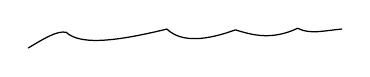
\begin{tikzpicture}[x=1cm,y=1cm,line cap=round,line join=round]
\draw[line width=0.45pt] (0,0) .. controls (0.20,0.12) and (0.36,0.22) .. (0.48,0.20)
.. controls (0.67,0.02) and (1.18,0.10) .. (1.76,0.24)
.. controls (1.95,0.06) and (2.27,0.10) .. (2.63,0.23)
.. controls (2.83,0.17) and (3.08,0.09) .. (3.42,0.25)
.. controls (3.58,0.17) and (3.75,0.22) .. (3.98,0.24);
\end{tikzpicture}}

Messy category made precise (corresponding to a $\Pi_U$ that is \uline{connected}):

These objects are the \deleted{pairs $(I$, \unsure{systems}}\inserted{homomorphisms of groups} that are profinite \deleted{(\unsure{indexed} by a finite set $I$) of the homomorphism}
\[
\mathcal E\xrightarrow{p}\Gamma
\]
(giving rise to an exact sequence:
\[
1\longrightarrow\pi\xrightarrow{\unsure{k|\kappa}}\mathcal E\xrightarrow{p}\Gamma
\]
)
and a \inserted{finite} set of subgroups (indexed by a set $I$ of indices)
\[
\mathcal E_i\overset{\rho_i}{\lhook\joinrel\longrightarrow}\mathcal E,
\]
and of isomorphisms
\[
\mathcal E_i\cap\pi\overset{k_i}{\simeq}T(\bar K)
\]
\margin{42}

\scanpage{44}
\mspage{20}

A homomorphism from a system
$(\mathcal E',p',(\mathcal E'_{i'})_{i'\in I'},(k'_{i'})_{i'\in I'})$
into a system
$(\mathcal E,p,(\mathcal E_i)_{i\in I},(k_i)_{i\in I})$
is given by by a homomorphism
\[
f:\mathcal E'\longrightarrow\mathcal E
\]
\[
\beta_{i'}\in\mathcal E\quad(i'\in I'),\qquad\alpha\in\Gamma,
\]
such that one has the conditions:

\figure{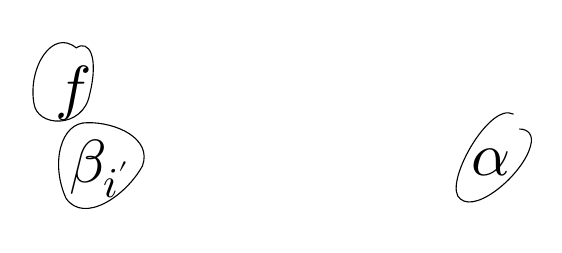
\begin{tikzpicture}[x=1cm,y=1cm,line cap=round,line join=round]
\begin{scope}[yshift=-0.35cm]
\node[font=\fontsize{22}{24}\selectfont] at (0,1.30) {$f$};
\draw (0.08,1.88) .. controls (-0.22,2.13) and (-0.53,1.64) .. (-0.46,1.19)
.. controls (-0.43,0.86) and (0.17,0.85) .. (0.25,1.29)
.. controls (0.37,1.77) and (0.24,1.99) .. (0.08,1.88);
\end{scope}
\node[font=\fontsize{22}{24}\selectfont] at (0.40,0) {$\beta_{i'}$};
\draw (0.22,0.58) .. controls (-0.12,0.59) and (-0.25,0.06) .. (-0.05,-0.38)
.. controls (0.18,-0.71) and (0.71,-0.35) .. (0.92,0.03)
.. controls (1.05,0.38) and (0.58,0.59) .. (0.22,0.58);
\node[font=\fontsize{22}{24}\selectfont] at (5.35,0.08) {$\alpha$};
\draw (5.63,0.69) .. controls (5.32,0.85) and (4.72,-0.23) .. (4.96,-0.39)
.. controls (5.18,-0.57) and (5.77,-0.05) .. (5.85,0.29)
.. controls (5.89,0.42) and (5.82,0.50) .. (5.71,0.50);
\end{tikzpicture}}

\margin{The $\beta_{i'}$ not unique (if $\beta_{i'}$ works, also $\gamma\beta_{i'}$, with $\unsure{\gamma|\gamma_i}\in\operatorname{Im}k_i$). But $\alpha$ unique \unsure{?!|??}}

$1^\circ)$\quad $p\circ f_{\mathcal E}=\operatorname{int}(\alpha)\,p'$

$2^\circ)$\quad $\forall i'\in I',\quad\exists i\in I$ (unique!) such that
\[
\operatorname{int}(\beta_{i'}^{-1})f(\mathcal E'_{i'})\subset\mathcal E_i
\]
and an integer $d_{i'}\in\mathbb N^*$ such that
\[
\operatorname{int}(\beta_{i'}^{-1})f\,k'_{i'}
 =k_i\circ(d_{i'}\cdot\operatorname{id}_{T(\bar K)})
\]

\margin{N.B.: $d_{i'}$ is also unique\ldots}

\margin{[thus $\operatorname{int}(\beta_{i'}^{-1})\overbrace{\unsure{\operatorname{Im}(fk'_{i'})|\operatorname{Im}k'_{i'}}}^{L'_{i'}}\subset\underbrace{\operatorname{Im}k_i}_{L_i}$ and \unsure{even} \deleted{\unsure{this} image} $\operatorname{int}(\beta_{i'}^{-1})\unsure{L'_{i'}}=d_{i'}L_i$.]}

\figure{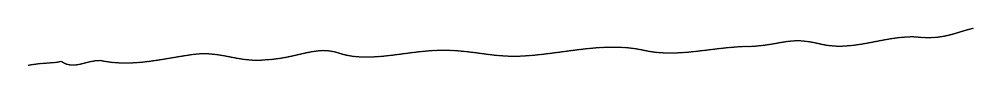
\begin{tikzpicture}[x=1cm,y=1cm,line cap=round,line join=round]
\draw[line width=0.45pt] (0,0) .. controls (0.22,0.04) and (0.30,0.02) .. (0.42,0.05)
.. controls (0.58,-0.07) and (0.73,0.07) .. (0.92,0.06)
.. controls (1.30,-0.02) and (1.64,0.07) .. (2.04,0.13)
.. controls (2.44,0.20) and (2.64,0.03) .. (3.02,0.07)
.. controls (3.43,0.09) and (3.66,0.26) .. (3.96,0.15)
.. controls (4.37,0.02) and (4.86,0.21) .. (5.35,0.19)
.. controls (5.79,0.17) and (5.95,0.08) .. (6.44,0.13)
.. controls (6.94,0.18) and (7.37,0.29) .. (7.82,0.19)
.. controls (8.26,0.09) and (8.70,0.24) .. (9.18,0.24)
.. controls (9.58,0.26) and (9.66,0.37) .. (10.06,0.27)
.. controls (10.48,0.17) and (10.87,0.38) .. (11.28,0.36)
.. controls (11.62,0.32) and (11.78,0.42) .. (12.00,0.47);
\end{tikzpicture}}

I realize that it is better to replace the $\beta_{i'}$ by the $\beta_{i'}^{-1}$, i.e. to take the commutation isomorphism rather in the direction
\[
f_{\mathcal E}\rho'_{i'}\xrightarrow{\beta_{i'}}\rho_i f_{i'}
\]
than in the opposite direction. Moreover, conceptually the diagram
\diagram{\begin{tikzcd}[ampersand replacement=\&]
\& \Pi_{D^*}\arrow[dl,"\rho"']\arrow[dr,"\sigma"] \& \\
\Pi_U\arrow[dr,"\varphi"',""{name=L,inner sep=0pt}] \& \& \Pi_D\arrow[dl,"\psi",""{name=R,inner sep=0pt}]\\
\&\Pi_e\&
\arrow[from=L,to=R,bend left=25,"\alpha"]
\end{tikzcd}}
is too complicated, it suffices to give oneself
\[
\boxed{\Pi_{D^*}\xrightarrow{\rho}\Pi_U\xrightarrow{\varphi}\Pi_e}
\]
and to deduce $\Pi_D$ by canonical factorization
\margin{43}

\scanpage{45}

of the homomorphism of groupoids $\Pi_{D^*}\longrightarrow\Pi_e$ into a homomorphism which induces an isomorphism on $\pi_0$ and an epimorphism on the $\pi_1$, followed by a homomorphism which is (an epimorphism on $\pi_0$, and for good reason!, and which is) \uline{faithful}. Then the $1$-morphisms from
\[
\Pi'_{D^*}\xrightarrow{\rho'}\Pi'_U\xrightarrow{\varphi'}\Pi_e
\]
\deleted{to}
to
\[
\Pi_{D^*}\xrightarrow{\rho}\Pi_U\xrightarrow{\varphi}\Pi_e
\]
are the \deleted{\unsure{pairs}}\inserted{quintuples} of $2$ functors \inserted{and $3$ isomorphisms of functors}
$(f_{D^*},f_U,\alpha_{D^*U},\alpha_{Ue},K$
giving a diagram with commutation data
\diagram{\begin{tikzcd}[ampersand replacement=\&,column sep=1.05em,row sep=0.75em]
\Pi'_{D^*}\arrow[rrr,"\rho'"]\arrow[ddd,"f_{D^*}"'] \& \& \& \Pi'_U\arrow[rrr,"\varphi'"]\arrow[ddd,"f_U"'] \& \& \& \Pi_e\arrow[ddd,equal] \\
\& \& {} \& \& \& {} \& \\
\& {}\arrow[ur,bend left=25,"\alpha_{D^*U}"] \& \& \& {}\arrow[ur,bend left=25,"\alpha_{Ue}"] \& \& \\
\Pi_{D^*}\arrow[rrr,"\rho"'] \& \& \& \Pi_U\arrow[rrr,"\varphi"'] \& \& \& \Pi_e
\end{tikzcd}},

\margin{moreover, \deleted{\illegible{1}} $\pi_1(\varphi\rho)=\pi_1(\Pi_{D^*}/\Pi_e)$ can be defined as a local system \inserted{of groups (\unsure{commutative|abelian})} on $\Pi_{D^*}$, and we can then \unsure{define|write}
$\boxed{\unsure{\bar k|k}:(\varphi\rho)^*\unsure{T_K|\mathcal T_K}\simeq\pi_1(\varphi\rho)}$.}

\margin{with \uline{one} condition on the induced morphism
$\pi_1(\varphi'\rho')\unsure{\simeq|\longrightarrow}\unsure{f_{D^*}^{\,*}}(\pi_1(\varphi\rho))$,
which modulo the Kummer isomorphisms must be multiplication by a $d$ \unsure{ramification index} (which is a map $\pi_0(\Pi'_{D^*})\longrightarrow\mathbb N^*$). [N.B. multiplication by an \uline{\unsure{integer}} that is \unsure{positive} \illegible{5} constant\ldots]}

if we have two such $1$-morphisms
\[
f=(f_{D^*},f_U,\alpha_{D^*U},\alpha_{Ue})
\quad\text{and}\quad
g=(g_{D^*},g_U,\beta_{D^*U},\beta_{Ue})
\]
a \unsure{$0$-morphism|homomorphism} from $f$ to $g$ is formed of a pair of $\mu_{D^*},\mu_U$ of isomorphisms of functors
\[
\mu_{D^*}:f_{D^*}\simeq g_{D^*},\qquad
\mu_U:f_U\longrightarrow g_U
\]
compatible with $\alpha_{D^*U},\inserted{\beta_{D^*U},}$ and with $\alpha_{Ue},\inserted{\beta_{Ue},}$ \deleted{and with}
\margin{44}

\scanpage{46}
\mspage{21}

\deleted{$k,k'$ modulo multiplication by a ramification index} (two compatibility conditions on the two squares).

If we \deleted{assume} restrict ourselves to connected $\Pi_U,\Pi'_U$, we find by choosing as above an object \inserted{$\widetilde U$} of $\Pi_U$ and an isomorphism
\[
\boxed{\varphi(\widetilde U)\overset{\lambda}{\simeq}\Omega}
\]
(where $\Omega=\operatorname{Spec}(\bar K)$ is the reference object of $\Pi_e\ldots$), a group $\mathcal E$ and a homomorphism
\[
\mathcal E\xrightarrow{\varphi}\Gamma
\]
(which is changed by an inner automorphism if we change $\lambda$, and $\mathcal E$ itself replaced by an isomorphic group, \unsure{with isomorphism} defined \unsure{modulo} inner isomorphisms, if we change the reference object $\widetilde U$). Likewise, choosing a $\widetilde U_i$ in each component $i\in\pi_0(\Pi_{D^*})$, and isomorphisms
\[
\lambda_i:\rho(\widetilde U_i)\simeq\widetilde U,
\]
we find groups $\mathcal E_i$ and homomorphisms
\[
\mathcal E_i\xrightarrow{\rho_i}\mathcal E.
\]
If we change $\lambda_i$, $\rho_i$ is changed by an inner automorphism of $\mathcal E$. If we change $\widetilde U_i$, $\mathcal E_i$ is replaced by an isomorphic group, \inserted{the isomorphism} defined up to an inner automorphism.
\margin{45}

\scanpage{47}

Let us consider the composites
\diagram{\begin{tikzcd}[ampersand replacement=\&]
\mathcal E_i\arrow[r]\arrow[rr,bend left=30,"p_i"]\&\mathcal E\arrow[r,"p"']\&\Gamma
\end{tikzcd}}
whence kernel, \deleted{\illegible{1}} $\unsure{K|k}$ is defined by a system of isomorphisms
\[
T(\bar K)\overset{k_i}{\simeq}\operatorname{Ker}p_i\qquad(i\in I)
\]
fitting into a family of exact sequences
\[
1\longrightarrow T(\bar K)\xrightarrow{k_i}\mathcal E_i\xrightarrow{p_i}\Gamma
\]
(N.B. the image of $p_i$ is an open subgroup)
$k_i$ being compatible with the actions of $\mathcal E_i$, when we let $\mathcal E_i$ act on $T(\bar K)$ through the action of $\Gamma$ on $T(\bar K)$, and on itself by inner automorphisms. Introducing also $\pi=\operatorname{Ker}p$, we thus find homomorphisms of exact sequences
\diagram{$(D)$\quad\begin{tikzcd}[ampersand replacement=\&]
1\arrow[r]\&T(\bar K)\arrow[r,"k_i"]\arrow[d,"\varepsilon_i\,\deleted{\illegible{1}}"']\&\mathcal E_i\arrow[r,"p_i"]\arrow[d,"\rho_i"]\&\Gamma\arrow[d,equal]\\
1\arrow[r]\&\pi\arrow[r,"\unsure{k|\kappa}"']\&\mathcal E\arrow[r,"p"']\&\Gamma
\end{tikzcd}\qquad$i\in I$}

\deleted{Let us consider}
We can say that $\Pi_U$ defines an ``outer group'' $[\mathcal E]$, and $\Pi_U\longrightarrow\Pi_e$ a homomorphism of outer groups
\[
[\mathcal E]\longrightarrow[\Gamma],
\]
likewise $\Pi_{D^*}$ defines a system of ``outer groups'' $[\mathcal E_i]$, and \deleted{\unsure{of the homomorphism}} $\Pi_{D^*}\longrightarrow\Pi_U$
\margin{46}

\scanpage{48}
\mspage{22}

a system of outer homomorphisms
\[
[\mathcal E_i]\longrightarrow[\mathcal E],
\]
\deleted{finally} but how in terms of outer groups to express the Kummer data $k_i$?

Returning to the \inserted{system of} diagram $D$ (relative to an index set $I$.) and to an analogous $D'$ (with index set $I'$)
\diagram{$D'$\quad\begin{tikzcd}[ampersand replacement=\&]
1\arrow[r]\&T(\bar K)\arrow[r,"k'_{i'}"]\arrow[d,"\varepsilon'_{i'}"']\&\mathcal E'_{i'}\arrow[r,"p'_{i'}"]\arrow[d,"\rho'_{i'}"]\&\Gamma\arrow[d,equal]\\
1\arrow[r]\&\unsure{\pi|\pi'}\arrow[r,"\unsure{k'|\kappa'}"']\&\mathcal E'\arrow[r,"p'"']\&\Gamma
\end{tikzcd}\qquad$i'\in\unsure{I|I'}$}
a $1$-morphism \inserted{$f$} from $D'$ to $D$ is made explicit by

$a)$ A homomorphism
\[
\boxed{\boxed{f_{\mathcal E}:\mathcal E'\longrightarrow\mathcal E}}
\]
\margin{describes the \deleted{\unsure{corresponding}} functor $f_U$}
[\deleted{\unsure{depends}}\inserted{is made explicit} in terms of the choice of an isomorphism
\[
\nu:f(\widetilde U')\simeq\widetilde U
\]
[another choice modifies $f_{\mathcal E}$ by an $\operatorname{int}(\beta)$, $\beta\in\mathcal E$)]

$b)$ A \deleted{homomorphism} map $\tau:I'\longrightarrow I$, and for every $i'\in I'$, putting $i=\tau(i')$, a \deleted{map}\inserted{group homomorphism}
\[
\boxed{\mathcal E'_{i'}\xrightarrow{f_{i'}}\mathcal E_i}
\]
\margin{describes the functor $f_{D^*}$}
\margin{47}

\scanpage{49}

[is made explicit in terms of the choice of an isomorphism
\[
f_{D^*}(\widetilde U'_{i'})\overset{\nu_{i'}}{\simeq}\widetilde U_i,
\]
and modified by $\operatorname{int}(\beta_{i'})$, $\beta_{i'}\in\mathcal E_i$, if we change $\nu_{i'}$]

$c)$ A commutation datum for
\diagram{\begin{tikzcd}[ampersand replacement=\&,column sep=0.9em,row sep=0.7em]
\mathcal E'\arrow[rrr,"p'"]\arrow[ddd,"f_{\mathcal E}"'] \& \& \& \unsure{\Gamma|\Gamma'}\arrow[ddd,equal] \\
\& \& {} \& \\
\& {}\arrow[ur,bend left=25,"{\deleted{\unsure{\beta}}\alpha}"] \& \& \\
\mathcal E\arrow[rrr,"p"'] \& \& \& \Gamma
\end{tikzcd}\quad$\boxed{\boxed{\deleted{\unsure{\beta}}\alpha\in\Gamma}}$}
\margin{$\alpha$ describes $\alpha_{Ue}$}
i.e.
\[
\deleted{f_{\mathcal E}p'=\operatorname{int}(\unsure{\beta})p}
\qquad\boxed{pf_{\mathcal E}=\operatorname{int}(\alpha)p'}
\]

$d)$ $\forall i'[\in\unsure{I|I'}]$ a commutation datum for
\diagram{\begin{tikzcd}[ampersand replacement=\&,column sep=0.9em,row sep=0.7em]
\mathcal E'_{i'}\arrow[rrr,"\rho'_{i'}"]\arrow[ddd,"f_{i'}"'] \& \& \& \mathcal E'\arrow[ddd,"f_{\mathcal E}"] \\
\& \& {} \& \\
\& {}\arrow[ur,bend left=25,"\alpha_{i'}"] \& \& \\
\mathcal E_i\arrow[rrr,"\rho_i"'] \& \& \& \mathcal E
\end{tikzcd}\quad$\boxed{\alpha_{i'}\in\mathcal E}\quad(i'\in I')$}
\margin{$(\alpha_{i'})$ describes $\alpha_{D^*U}$}
i.e.:
\[
\boxed{\rho_i f_{i'}=\operatorname{int}(\alpha_{i'})f_{\mathcal E}\rho'_{i'}}
\]

Let us note that $c,d$ together define a commutation datum
\diagram{\begin{tikzcd}[ampersand replacement=\&,column sep=0.9em,row sep=0.7em]
\mathcal E'_{i'}\arrow[rrr,"p'_{i'}"]\arrow[ddd,"f_{i'}"'] \& \& \& \Gamma\arrow[ddd,equal,"{\deleted{\operatorname{int}(\unsure{\gamma})}}"] \\
\& \& {} \& \\
\& {}\arrow[ur,bend left=25,"{\operatorname{int}(\beta_{i'})}"] \& \& \\
\mathcal E_i\arrow[rrr,"p_i"'] \& \& \& \Gamma
\end{tikzcd}}
with $\beta_{i'}=p(\alpha_{i'})\alpha$
i.e.
\[
p_i f_{i'}=\operatorname{int}(\beta_{i'})p'_{i'}
\]
\margin{48}

\scanpage{50}
\mspage{23}

i.e. we have commutativity in
\diagram{\begin{tikzcd}[ampersand replacement=\&]
\mathcal E'_{i'}\arrow[r,"p'_{i'}"]\arrow[d,"f_{i'}"']\&\Gamma\arrow[d,"\operatorname{int}(\beta_{i'})"]\\
\mathcal E_i\arrow[r,"p_i"']\&\Gamma
\end{tikzcd}}
so $f_{i'}$ induces a homomorphism of exact sequences
\diagram{\begin{tikzcd}[ampersand replacement=\&]
1\arrow[r]\&T(\bar K)\arrow[r,"k'_{i'}"]\arrow[d,"f^0_{i'}"']\&\mathcal E'_{i'}\arrow[r,"\unsure{p'_{i'}|f'_{i'}}"]\arrow[d,"f_{i'}"]\&\Gamma\arrow[d,"\operatorname{int}(\beta_{i'})"]\\
1\arrow[r]\&T(\bar K)\arrow[r,"k_i"']\&\mathcal E_i\arrow[r,"p_i"']\&\Gamma
\end{tikzcd}}
\margin{795}
and we must express the compatibility of $f^0_{i'}$ with the ramification index $d_{i'}\in\mathbb N$, we find
\[
\boxed{f^0_{i'}=d_{i'}\chi(\beta_{i'})\operatorname{id}_{T(\bar K)}}
\]
where
\[
\chi:\Gamma\longrightarrow\widehat{\mathbb Z}^{\,*}
\]
is the canonical character.

This being so, let us determine, for a $1$-morphism
\[
f=(f_{\mathcal E},\inserted{\tau,}(f_{i'}),\alpha,(\unsure{\alpha_{i'}|\alpha_i}))
\]
and another
\[
f'=(f'_{\mathcal E},\tau',(f'_{i'}),\alpha',(\unsure{\alpha'_{i'}|\alpha'_i})),
\]
the $0$-morphisms from one to the other.
\margin{49}

\subsection*{Scans 51--60}
\addcontentsline{toc}{subsection}{Scans 51--60}
% package LM_P06
\scanpage{51}

\unsure{corresponding|correspond} to systems of isomorphisms.
\[
\mu_{\mathcal D^*}:f_{\mathcal D^*}\longrightarrow f'_{\mathcal D^*},\qquad
\unsure{\mu_{U^*}}\;f_U\longrightarrow g_U.
\]
This corresponds \uline{conditions} $\tau'=\tau$, $d'_{i'}=d_{i'}$ $\forall i'\in I'$ and \unsure{to} the datum of
\inserted{this follows from the other conditions\unsure{\ldots}}
\margin{\unsure{let us express} the \uline{existence} of an isomorphism $\mu_{\mathcal D^*}$}

\margin{describes $\mu_U$}
a) $\boxed{\boxed{\mu\in\mathcal E}}$, defining an isomorphism between
\[
f_{\mathcal E}:\mathcal E'\longrightarrow\mathcal E
\quad\text{and}\quad
f'_{\mathcal E}:\mathcal E'\longrightarrow\mathcal E
\]
i.e. \deleted{\unsure{making}} such that
\[
\boxed{f'_{\mathcal E}=\operatorname{int}(\mu)f_{\mathcal E}}\,)
\]

b) $\boxed{\boxed{\mu_{i'}\in\mathcal E_i}}$ $(i'\in I',\ i=\tau(i'))$
\margin{describes $\mu_{\mathcal D^*}$}
satisfying
\[
\boxed{f'_{i'}=\operatorname{int}(\mu_{i'})f_{i'}}\,),
\]
\margin{this already implies $d_{i'}=d'_{i'}$}
the $\underset{\substack{\in\\\mathcal E}}{\mu},\ \underset{\substack{\in\\\mathcal E_i}}{\mu_{i'}}$ being related to the $\underset{\substack{\unsure{\in|\notin}\\\mathcal E}}{\alpha},\alpha'$ \unsure{\deleted{in}|in} $(\in\mathcal E)$
to the $\alpha_{i'},\alpha'_{i'}$ $(\in\Gamma)$ in the following way
\[
\boxed{\alpha'=p(\mu)\alpha}
\]
\[
\boxed{\alpha'_{i'}=\rho_i(\mu_{i'})\alpha_{i'}}\qquad\forall i'\in I'
\]
or again
\[
\boxed{\begin{cases}
p(\mu)=\alpha'\alpha^{-1}\\
\rho_i(\mu_{i'})=\alpha'_{i'}\alpha_{i'}^{-1}
\end{cases}}
\]
\margin{50}
\scanpage{52}
\mspage{24}

Note that, since $\rho_i$ is injective, the second relations, giving the $\rho_i(\mu_{i'})$, determine the $\mu_{i'}$ in a \uline{unique way}, the existence of these $\mu_{i'}$ is equivalent to the relations
\[
\boxed{\alpha'_{i'}\alpha_{i'}^{-1}\in\rho_i(\mathcal E_i)}\qquad i'\in I'.
\]

As for the relation $p(\mu)=\alpha'\alpha^{-1}$, it determines $\mu$ modulo multiplication \inserted{(on the right, say)} by a \deleted{\illegible{1}} $\mu_0\in\operatorname{Ker}p=\pi$, but which must be such that we still have
\[
f'_{\mathcal E}=\operatorname{int}(\deleted{\mu_0}\mu\mu_0)f_{\mathcal E}
\]
(in addition to $f'_{\mathcal E}=\operatorname{int}(\mu)f_{\mathcal E}$) which means \deleted{requires} that
\[
\operatorname{int}(\mu_0)f_{\mathcal E}=\unsure{f_{\mathcal E}|f'_{\mathcal E}}
\]
i.e.
\[
\boxed{\mu_0\in\operatorname{Centr}_{\unsure{\pi}}\deleted{\operatorname{Im}}f_{\mathcal E}(\mathcal E')}
\]

So that is the exact indeterminacy in the choice of a $0$-morphism \unsure{the|of the} $1$-morphisms \deleted{between} $f$ and $f'$ from $\mathcal D'$ to $\mathcal D$.
If for example we are under the conditions where
$\pi'\longrightarrow\pi$ induced by $f_{\mathcal E}:\mathcal E'\longrightarrow\mathcal E$ \deleted{is} has an image of finite index (open image)
--- case of a ``nonconstant morphism''! ---
then $\mu_0$ must centralize an open subgroup of
\margin{51}
\scanpage{53}

$\pi$ --- unless I am mistaken this too implies $\mu_0=1$, so it does seem that \deleted{\illegible{1}} (in the cases corresponding to dominant homomorphisms of algebraic curves) a \deleted{homomorphism} $0$-morphism from an $f$ \unsure{to} an $f'$ (if it exists) is unique, i.e. \uline{$\operatorname{Hom}$} $(\mathcal D',\mathcal D^*)$ is a \uline{discrete} category.

We can interpret $\mathcal D$ as $\mathcal E$ equipped with subgroups $\mathcal E_i\subset\mathcal E$, and with $p:\mathcal E\longrightarrow\unsure{\Gamma_*|\Gamma}$ (kernel $\pi$) finally with isomorphisms
\[
k_i:\mathrm T(\overline K)\xrightarrow{\sim}\mathcal E_i\cap\pi=L_i
\]
(commuting with the action of $\mathcal E_i$).
If we have \unsure{a|a} different system
\[
(\mathcal E',\ (\mathcal E'_{i'})_{i'\in I'},\ p':\mathcal E'\longrightarrow\Gamma',\ (k'_{i'})_{i'\in I'}),
\]
\inserted{$\mathcal E'_{i'}\subset\mathcal E'$}
a morphism from the first to the second is \uline{defined} by a
\[
f:\mathcal E'\longrightarrow\mathcal E
\]
satisfying the following conditions

\inserted{b) $pf$ is a conjugate of $f'$ [let $\alpha\in\Gamma$ be such that $pf=\operatorname{int}(\alpha)p'$]}

a) $\forall i'\in I',\quad\exists i\in I$ such that $f(\mathcal E'_{i'})$ is contained in a conjugate of $\mathcal E_i$
[let $\alpha_{i'}\in\mathcal E$ be such that
$f(\mathcal E'_{i'})\unsure{\subset|=}\operatorname{int}(\alpha_{i'}^{-1})(\mathcal E_i)$]
\inserted{i.e. $\operatorname{int}(\alpha_{i'})f(\mathcal E'_{i'})\subset\mathcal E_i$}
\margin{52}
\scanpage{54}
\mspage{25}

\uline{N.B.} The $i\in I$ corresponding to $i'\in I'$ is unique, whence $\tau:I'\longrightarrow I$.
If the $\alpha_{i'}$ are chosen, we deduce \deleted{\unsure{$\forall i'$}} induced homomorphisms
$f_{i'}:\mathcal E'_{i'}\longrightarrow\mathcal E_i$,
\[
f_{i'}=(\operatorname{int}(\alpha_{i'})\circ f)|\mathcal E'_{i'},
\]
which then induces, via the $k'_{i'},k_i$, an endomorphism
\[
f^0_{i'}:\mathrm T(\overline K)\longrightarrow\mathrm T(\overline K).
\]
\margin{\uline{N.B.} A priori $f^0_{i'}$ is \unsure{multiplication by} $\chi_{i'}\in\unsure{\widehat{\mathbb Z}^{\,*}|\widehat{\mathbb Z}}$. The centralizer in $\Gamma$ of an open subgroup is reduced to the identity.}
We require that $\alpha\in\Gamma$ (which conjugates $\unsure{f_{\mathcal E}}$ to $\unsure{f'_{\mathcal E}}$\}, and is \unsure{probably} uniquely determined by this condition) and $\alpha_{i'}$ (which is probably determined modulo \deleted{\unsure{conjugation}} composition on the left with an element \unsure{of the normalizers|of the normalizer} of $\mathcal E_i$ (at least of the transporters \inserted{of the $\mathcal E_i$} of an open subgroup of $\mathcal E_i$ --- it is the same if $f$ is an isomorphism) can be chosen in such a way that, putting
\[
\beta_{i'}=p(\alpha_{i'})\alpha,
\]
we have
\[
f^0_{i'}=(d_{i'}\chi(\beta_{i'}))\operatorname{id}_{\mathrm T(\overline K)}
\]
\inserted{i.e. $\chi_{i'}=d_{i'}\chi(\beta_{i'})$}
\margin{This condition on the systems of the $\alpha_{i'}$ does not change ($\alpha$ remaining fixed) if we change $\alpha_{i'}$ to $\mu_{i'}\alpha_{i'}$, where $\mu_{i'}\in\mathcal E_i$.}
$d_{i'}\in\mathbb N^*$ is a natural integer obviously uniquely determined \unsure{\}} when $\alpha$ and the $\alpha_{i'}$ are chosen).

\deleted{Let us replace $\alpha$ by $\alpha'=\alpha_0\alpha$.}
\margin{53}
\scanpage{55}

8, \uline{Taxonomic reflection.}

The case $\dim X=0$ translates in the paradigm of the system
$(\mathrm T(\overline K)\xrightarrow{k_i}\mathcal E_i\overset{\rho_i}{\hookrightarrow}\mathcal E\xrightarrow{p}\Gamma)$
\deleted{\illegible{2}} into the condition \deleted{$\unsure{\pi|I}=\varnothing$} $p$ injective, \deleted{thus \unsure{is|of}}
\inserted{and thus $I=\varnothing$ --- so this case is}
described \deleted{\illegible{1}}
simply by giving an open \uline{subgroup} $\mathcal E\subset\Gamma$, i.e. a finite subextension $\unsure{L}$ of $\overline K/K$
(N.B. of course we will have $X'=\operatorname{Spec}\unsure{L'|L}$, and the choices \inserted{made} on $X$ \inserted{--- i.e. on $\underset{=\varnothing}{\Pi_{\mathcal D^*}}\longrightarrow\Pi_U\longrightarrow\Pi_e$ ---} \unsure{leading|lead} to this description --- amount here to the choice of such a \inserted{$K$-}embedding of $L\deleted{\unsure{K'}}=\mathrm H^0(X,\mathcal O_X)$ into $\overline K/K$)

The case $\dim X=1$ translates into the fact that $\mathcal E\longrightarrow\Gamma$ is not injective --- as for $I$, it may be empty or not in this case.
If it is empty, the description is thus simply in terms of a homomorphism of profinite groups $\mathcal E\xrightarrow{p}\Gamma$ (where $\Gamma$ given in advance $=\operatorname{Gal}(\overline K/K)$ \unsure{\}} $=\operatorname{Aut}_{\Pi_e}(\Omega)$).

Suppose now given both
\[
\mathcal D=(\mathcal E,p,I,(\rho_i:\mathcal E_i\hookrightarrow\mathcal E),(k_i:\mathrm T(\overline K)\longrightarrow\mathcal E_i))
\]
and
\[
\mathcal D'\unsure{=} (\mathcal E',\unsure{p'},I',(\rho'_{i'}:\ ),(k'_{i'}:\ )),
\]
and let us return to the question of the description of the morphisms from $\mathcal D'$ to $\mathcal D$.
We are going to distinguish four cases, according to the two values
\margin{54}
\scanpage{56}
\mspage{26}

$0,1$ possible for $n=\dim\mathcal D$ and $n'=\dim\mathcal D'$ respectively.

I) $n=0,n'=0$, \deleted{\unsure{then|thus}} $I=I'=\varnothing$ and the data reduce to open subgroups
$\mathcal E\overset{p}{\hookrightarrow}\Gamma$, $\mathcal E'\overset{p'}{\hookrightarrow}\Gamma$.
In the cumbersome description above, \deleted{all} the considerations relating to $I,I'$ drop out and \uline{the}\margin{(a)} morphism $\mathcal D'\longrightarrow\mathcal D$ amounts to a class of \deleted{\unsure{homomorphisms}} pairs $(f,\alpha)$, where
$f:\mathcal E'\longrightarrow\mathcal E$ and $\alpha\in\Gamma$, such that we have
\[
pf=\operatorname{int}(\alpha)f
\]
--- which implies that $f$ is already determined by $\alpha$, being induced by $\operatorname{int}(\alpha)$
\inserted{[$\alpha$ subject to $\alpha\in\operatorname{Trans}_{\Gamma}(\mathcal E',\mathcal E)$ \unsure{$=$} $\operatorname{Trans}_{\Gamma}(L,L')$]}
\deleted{\diagram{\begin{tikzcd}[ampersand replacement=\&,column sep=1.5em,row sep=2em]
\unsure{\mathcal E'}\arrow[rr,"f"]\arrow[dr,"p'"'] \& \& \mathcal E\arrow[dl,"p"] \\
\& \Gamma \&
\end{tikzcd}}}
\diagram{\begin{tikzcd}[ampersand replacement=\&]
\mathcal E' \arrow[r,"f"] \arrow[d,"p'"'] \& \mathcal E \arrow[d,"p"] \\
\Gamma \arrow[r,"\operatorname{int}(\alpha)","\sim"'] \& \Gamma
\end{tikzcd}}
[which induces \unsure{thus|indeed} a homomorphism from $\unsure{L^*|L}\subset\overline K$ to $L'\subset\overline K$, hence a homomorphism $\operatorname{Spec}(L')\longrightarrow\operatorname{Spec}(L)$ in the opposite direction].

The condition that $\alpha,\alpha'\in\Gamma$ define the same morphism $\mathcal D'\longrightarrow\mathcal D$ (or again $\operatorname{Spec}\unsure{L'}\longrightarrow\operatorname{Spec}L$) is described by the existence of a $\mu\in\mathcal E$ \deleted{(= stabilizer of} such that $\alpha'=\mu\alpha$.
The fact that we give a $1$-$1$ correspondence between
\[
\operatorname{Hom}_{K}(X',X)\simeq\unsure{\operatorname{Hom}}_{K}(\unsure{L},L')
\]
with $\operatorname{Hom}(\mathcal D',\mathcal D)$ made explicit too, is clear.
\margin{55}
\scanpage{57}

II) $n'=1,n=0$.
\inserted{Here $n=0$ already implies $I=\varnothing$.}
\deleted{Here} For $\operatorname{Hom}(X',X)\ne\varnothing$, we must have $I'=\varnothing$
[by the condition $f^{-1}(S)=S'$ which implies $S'=\varnothing$, if $f:(X',S')\longrightarrow(X,S)$]
\inserted{$f^{-1}(\varnothing)=\varnothing$}
--- \deleted{in} in the description of the morphisms $\mathcal D'\longrightarrow\mathcal D$, this corresponds to the fact that we can have a map $\tau:I'\longrightarrow I(=\varnothing)$ only if $I'=\varnothing$.
\margin{this we cannot}
\deleted{\illegible{1}}
Restricting ourselves therefore to the case $I'=\varnothing$ (otherwise $\operatorname{Hom}(X',X)=\operatorname{Hom}(\mathcal D',\mathcal D)=\varnothing$ and we are happy), we thus find that $\mathcal D$ amounts to giving $\mathcal E\overset{p}{\hookrightarrow}\Gamma$ an open subgroup, and $\mathcal D'$ to giving a homomorphism of profinite groups $p':\mathcal E'\longrightarrow\Gamma$, whose image will be an open subgroup of $\Gamma$, say $\Gamma'_0\subset\Gamma$, corresponding to a \inserted{finite} subextension $L'$ of $\overline K/K$.
\margin{Restricting ourselves therefore to the case}

The choices made concerning $X'$ imply \unsure{precisely|that we have} a fixed isomorphism $L'\simeq\mathrm H^0(X',\mathcal O_{X'})$.
That said, a $K$-morphism \inserted{from $(X',\varnothing)$ to $(X,\varnothing)$ i.e. from} $X'\longrightarrow X$ amounts \inserted{(since $X$ affine)} to giving a $K$-morphism $\operatorname{Spec}L'\longrightarrow X\ (\simeq\operatorname{Spec}L)$ from the affine envelope, i.e. a \inserted{$K$-}homomorphism $L\longrightarrow L'$.
(which depends only on $L,L'$, or again \unsure{on the} \deleted{\illegible{1}} subgroups $\mathcal E\subset\Gamma$ and $\Gamma_0\subset\Gamma$
\margin{56}
\scanpage{58}
\mspage{27}

of $\Gamma$).
On the other hand the description in terms of the diagrams $\mathcal D,\mathcal D'$ amounts to saying that a morphism is determined by a pair $(f,\alpha)$, $f:\mathcal E'\longrightarrow\mathcal E$ and $\alpha\in\Gamma$, such that we again have commutativity
\diagram{\begin{tikzcd}[ampersand replacement=\&]
\mathcal E' \arrow[r,"f"] \arrow[d,"p'"'] \& \mathcal E \arrow[d,hook,"p"] \\
\Gamma \arrow[r,"\operatorname{int}(\alpha)"] \& \Gamma
\end{tikzcd}}
\[
pf=\operatorname{int}(\alpha)p'
\]
which again implies that $f$ is determined by $\alpha$ (namely, induced by $\operatorname{int}(\alpha)$), and $\alpha$ being subject to the sole condition
\[
\alpha\in\operatorname{Transp}_{\Gamma}(\Gamma'_0,\mathcal E)
\]
--- and $\alpha,\alpha'$ \unsure{describing|describe} the $=$ homomorphism \unsure{iff}
\[
\exists\mu\in\mathcal E\quad\text{such that}\qquad\unsure{\Longleftarrow|\Longleftrightarrow}
\]
\[
\alpha'=\mu\alpha
\]
so we again have
\[
\begin{aligned}
\operatorname{Hom}(\mathcal D',\mathcal D)
&\simeq\mathcal E\backslash\operatorname{Transp}_{\Gamma}(\Gamma'_0,\Gamma)\ \deleted{\illegible{1}}\\
&\simeq\operatorname{Transp}_{\Gamma}(L,L')/\operatorname{Fix}_{\Gamma}(L)\\
&\simeq\operatorname{Hom}_{\unsure{K\text{-}\mathrm{ext}|K\text{-}\mathrm{cat}}}(L,L')
\end{aligned}
\]
so we again find in this case \unsure{the|the} full faithfulness.

In fact, we could have treated together
\margin{57}
\scanpage{59}

the two cases $(n'=0,n'=1)$ where $n=0$, and the description of the $\operatorname{Hom}(X,X')$ \inserted{in terms of $\mathcal D,\mathcal D'$} is valid moreover, without \deleted{assuming that} making draconian hypotheses (projective, smooth, $\dim\leq1$, anabelian) on $X'$.
\deleted{It suffices that $X'$ be a connected quasi-compact quasi-separated scheme over $K$, \unsure{thus|in} the morphisms $X'\longrightarrow X=\operatorname{Spec}(L)$ correspond to the morphisms $\operatorname{Spec}A'\longrightarrow X$ from the affine envelope of $X'$ to $X$, defined as the Spectrum of $A'=\mathrm H^0(X',\mathcal O_{X'})$, i.e. to the \unsure{$K$-homomorphisms} of $K$-algebras
\[
L\longrightarrow A'.
\]}

Indeed, since $X$ is \inserted{finite} étale over $K$, its inverse image \inserted{$X_{X'}=$} \deleted{\illegible{1}} $X'\times_K\unsure{X}$ over $X'$ is \inserted{finite} étale over $X'$, and
\[
\operatorname{Hom}_K(X,X')\simeq\deleted{\operatorname{Hom}\unsure{(}}\operatorname{Sections}(X_{X'}/X')
\]
can be described in terms of the category $\widehat{\Pi_1(X')}$ $(=\Pi_U)$ of finite local systems on $X'$ i.e. of finite local systems on $\Pi_U$.
Following this description, we arrive at the
\margin{58}
\scanpage{60}
\mspage{28}

common description given in I, II, without any other hypothesis on $X$ than \deleted{connectedness} $0$-connectedness (to be able to describe $\Pi_U=\Pi_{X'}$ over $\Pi_e$ in terms of a group homomorphism $p':\mathcal E'\longrightarrow\Gamma\ldots$).

When we are given $(X',S')$, with $S'$ not necessarily empty, $X'$ $0$-connected (and \deleted{dimension} $X'$ smooth of dimension $1$ at the points of $S'$ (it would suffice $=$ that $S'$ \unsure{not} \unsure{disconnect|disconnect} locally \inserted{(étale)} $X'$, $\ldots$),
\inserted{thus $X'-S'$ $0$-connected}
then the \deleted{part} datum
$\Pi_1(X'-S')\longrightarrow\Pi_1(e_K)$ is described \deleted{\illegible{1}} by $\mathcal E'\xrightarrow{p'}\Gamma$ (independently of the consideration of the $\mathcal E_i$ etc) and hence $\operatorname{Hom}_K(X'-S',X)$ is described as we just said.
But we have (with the normality hypotheses on $X'$ at the points of $S'$)
\[
\operatorname{Hom}_K(X'-S',X)=\operatorname{Hom}_K(X',X).
\]

This encourages modifying the definition of morphisms $(X',S')\longrightarrow(X,S)$ given \unsure{at the|by} beginning, via $f:X'\longrightarrow X$ with $f^{-1}(S)_{\mathrm{r\acute ed}}=S'$, by requiring this \inserted{not for $f$, but} \unsure{only} for the restriction of $f$ \unsure{to} the union of the irreducible components of $X'$
\margin{59}

\subsection*{Scans 61--70}
\addcontentsline{toc}{subsection}{Scans 61--70}
% package LM_P07
\scanpage{61}

\deleted{on which $f$ is not ``\unsure{constant|constant}''}
which are sent into irreducible components of $X$ \deleted{\illegible{1}} that are non-discrete i.e. not reduced to a point.
In the corresponding description $\mathcal D'\to\mathcal D$, we specified that one requires the datum of a map $I'\to I$ (and of the corresponding data $f_{i'},\alpha_{i'}$) \uline{only} if \deleted{\unsure{$I\ne\varnothing$}} $n\ne0$ i.e. \unsure{$p_{si}$|$p_X$}$:\mathcal E\to\Gamma$ not injective, --- in the contrary case (implying $I=\varnothing$) \inserted{if by chance $I'\ne\varnothing$,} one drops the knowledge of $I'$ and of the corresponding structure elements.

\uline{$\overline{\mathrm{III}}$}) $n'=0$, $n=1$. Here one thus has $I'=\varnothing$, $p':\mathcal E'\hookrightarrow\Gamma$ i.e. $\mathcal D'$ reduces to the datum of an open subgroup $\mathcal E'\hookrightarrow\Gamma$ of $\Gamma$.
On the side of $(X',S'=\varnothing)$ and $(X,S)$, the condition $f^{-1}(S)_{\mathrm{r\acute ed}}=S'=\varnothing$ on \inserted{the $K$-morphism} $f:X'\to X$ implies that $f$ factors through $X'\Longrightarrow\operatorname{Spec}(L')\longrightarrow X\setminus S$, regardless of whether $S=\varnothing$ or not, i.e. whether $I=\varnothing$ or not. Thus it is a matter of describing $\operatorname{Hom}_{K\text{-sch}}(X',X\setminus S)$, in terms of $\begin{gathered}\text{\inserted{$\Pi_{U'}$}}\\[-2pt]\rotatebox{90}{$=$}\\[-2pt]\Pi_1(X')\end{gathered}\to\Pi_e=\Pi_1(e_K)$

\margin{60}

\scanpage{62}
\mspage{29}

and of $\begin{gathered}\text{\inserted{$\Pi_U$}}\\[-2pt]\rotatebox{90}{$=$}\\[-2pt]\Pi_1(X\setminus S)\end{gathered}\to\Pi_e$.
Here the possible additional data relating to $I$ do not serve explicitly in the description, in terms of diagrams \inserted{(of groupoids)}.
Unless I am mistaken, an easy reduction \inserted{(Galois descent)} brings us back to the case where $X'=\operatorname{Spec}K$ i.e. $\mathcal E'\Leftrightarrow\Gamma$. The description \unsure{of the|in} homomorphisms $\mathcal D'\to\mathcal D$ is then \inserted{still} in terms of pairs $(f,\alpha)$, where $f:\mathcal E'=\Gamma\to\mathcal E$ and where $\alpha\in\Gamma$, with the everlasting condition $pf=\operatorname{int}(\alpha)p'$, which becomes (as $p'=\operatorname{id}$)
\[
 pf=\operatorname{int}(\alpha).
\]

\deleted{\unsure{$\alpha$ and $\alpha'$}}
Here of course $\alpha$ no longer describes $f$ (but the converse is \deleted{probably} true, here knowledge of $f$ hence of $pf\in\operatorname{Aut}(\Gamma)$ implies that of $\alpha$, i.e. $\operatorname{Cent}(\Gamma)=\{1\}$ \ldots).
The pairs $(f,\alpha)$ and $(f',\alpha')$ define the $=$ morphism of diagrams, iff $\exists\mu\in\mathcal E$ such that $f'=\operatorname{int}(\mu)\circ f$, $\alpha'=p(\mu)\alpha$.
As (if $\exists(f,\alpha)$) $p$ is surjective,

\margin{61}

\scanpage{63}

one \unsure{sees|wants} that, on choosing $\mu$ over \deleted{\illegible{1}} $\alpha^{-1}$, and replacing $(f,\alpha)$ by $(f',\alpha')=(\operatorname{int}(\mu)f,p(\mu)\alpha)$, one can always describe a morphism $\mathcal D'\to\mathcal D$ by $(f,\alpha)$ with $\alpha=1$ hence by a \uline{section} $f$ of the homomorphism $\mathcal E\to\Gamma$, and two sections $f,f'$ (corresponding to $(f,1),(f',1)$) define the $=$ homomorphism from \unsure{$\mathcal D'$} to $\mathcal D$, iff $\exists\mu\in\mathcal E$ such that $p(\mu)=1$ i.e. $\mu\in\pi=\operatorname{Ker}(p)$, and such that $f'=\operatorname{int}(\mu)\circ f$.

Thus, the morphisms from $\mathcal D'$ (corresponding to $X'=\operatorname{Spec}K$) to $\mathcal D$ correspond exactly to the classes of splittings of $\mathcal E\xrightarrow{p}\Gamma$, modulo inner automorphisms by $\mu\in\pi=\operatorname{Ker}p$. The ``messy conjecture'' in case \uline{$\overline{\mathrm{III}}$} is thus equivalent to this:
\margin{\figure{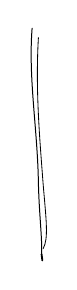
\begin{tikzpicture}[x=1cm,y=1cm,line cap=round]
\draw[line width=.36pt] (0,0) .. controls (-.05,-.64) and (.07,-1.29) .. (.08,-1.97)
 .. controls (.09,-2.38) and (.13,-2.67) .. (.12,-2.87);
\draw[line width=.30pt] (.08,-.12) .. controls (.04,-.79) and (.10,-1.44) .. (.14,-1.98)
 .. controls (.18,-2.45) and (.21,-2.67) .. (.14,-2.80);
\draw[line width=.65pt] (.12,-2.87) -- (.13,-2.95);
\end{tikzpicture}}}
\deleted{\unsure{$\operatorname{Hom}(K$}}
\[
 \Gamma((X,S)/K)\longrightarrow
 \begin{gathered}
 \text{$\pi$-conjugacy classes of}\\
 \text{sections of }\mathcal E\to\Gamma\text{ i.e.}\\
 \text{of sections of }\Pi_1(X)\to\Pi_1(e_K)
 \end{gathered}
\]

\margin{62}

\scanpage{64}
\mspage{30}

is bijective (if $(X,S)$ is an allowed ``anabelian'' pair).
\margin{false as it stands, cf. number 9 below --- one needs additional conditions on the $f$ \ldots\ \uline{Perhaps} \unsure{true if} $I=\varnothing$}

I know in any case that this map is \uline{injective} --- this holds whenever one has a scheme $U$ over $K$ (here $X\setminus S$) which embeds in an \inserted{algebraic group $G$} extension of an abelian variety by a torus, and then follows from the ``absolute'' Mordell-Weil theorem: $G(K)$ is a finitely generated $\mathbb Z$-module.
In fact, it suffices to know the splitting class of the extension $\mathcal E^{\natural}$ of $\Gamma$ by
\[
 \pi_{\mathrm{ab}}=\pi/\overline{[\pi,\pi]}\simeq H_1(\unsure{\mathrm{Alb}|U}),
\]
\deleted{\unsure{to deduce from it}} \inserted{corresponding} to a point of $U$ rational/$K$, to know this point. Thus the \inserted{result of} faithfulness is obtained, with less draconian hypotheses on $X$ than the anabelian hypothesis (with the notation of lemma 5.2, this means that $g=0\Rightarrow\unsure{n|\nu}\ge2$ i.e. that there is no irreducible component of \unsure{$X_{\overline K}$|$U_{\overline K}$} which is isomorphic to \unsure{$\mathbb P^1_{\overline K}$} or $\mathbb E^1_{\overline K}$ \ldots).

\margin{63}

\scanpage{65}

\uline{N.B.} This suggests an approach to the Mordell conjecture, via a better knowledge of extensions of $\Gamma$ by $\pi$: the fact that there is (for $g\ge2$) only a finite number of $\pi$-conjugacy classes of splittings of such an extension \ldots.
Likewise for an approach to Fermat's theorem, via \deleted{\illegible{1}} a good knowledge of an extension of $\Gamma$ by $\pi=\pi_1(\unsure{\mathbb P^1_{\overline{\mathbb Q}}\setminus\{0,1,\infty\}})$ \ldots.

\uline{Case $\overline{\mathrm{IV}}$} $n=1,n'=1$ i.e. $X,X'$ of dimension 1.

a) If $I=I'=\varnothing$, I have nothing to add to the description of morphisms $f:X\to X'$ in terms of morphisms of diagrams of groupoids. Here \deleted{\illegible{1}} the condition $f^{-1}(S)_{\mathrm{r\acute ed}}=S'$ is not a restriction on $f$ --- \deleted{which} one therefore does not exclude constant maps. These (thanks to
\margin{(thanks to \ldots)}
\deleted{If \unsure{$I'\ne\varnothing$} \illegible{5} \unsure{only} $I'=\varnothing$ \inserted{\unsure{i.e. $S'=\varnothing$}} \illegible{7} \unsure{$S'$ is} \unsure{empty}), \unsure{therefore} the condition}

\margin{64}

\scanpage{66}
\mspage{31}

the study \unsure{of the|of the} case \uline{$\overline{\mathrm{II}}$}) are moreover described in a ``fully faithful'' way by homomorphisms of diagrams --- They correspond to the cases $f:\mathcal E'\to\mathcal E$ which are zero on $\pi'$.

b) The case $I'=\varnothing$, $I\ne\varnothing$ (i.e. $S'=\varnothing$, $S\ne\varnothing$) means, for the condition $f^{-1}(S)_{\mathrm{r\acute ed}}=S'$ i.e. $f^{-1}(S)=\varnothing$, that $f$ must map $X'$ into $X\setminus S$, \deleted{One therefore expects} therefore that the $f$ corresponding to a morphism from $(X',\varnothing)$ to $(X,S)$ are constant.
The messy conjecture in this case therefore expresses \deleted{that} essentially that at the level of the homomorphisms $\mathcal E'\xrightarrow{p'}\Gamma$ and $\mathcal E\xrightarrow{p}\Gamma$, every group homomorphism $\mathcal E'\xrightarrow{f}\mathcal E$ such that $pf=\operatorname{int}(\alpha)p'$ for $\alpha\in\Gamma$ [one is reduced to the case where $\alpha=1$, \inserted{$p,p'$ surjective} i.e. to homomorphisms of extensions of $\Gamma$ by \unsure{the|some} groups \unsure{$\pi=\pi_1(\overline{X\setminus S})$} and $\pi'=\pi_1(\overline X')$)] is trivial on $\pi'$ [i.e. ``is'' a section]. One should try to verify this point directly, which (modulo case \uline{$\overline{\mathrm{III}}$}) would establish the ``messy conjecture'' in that case.

\margin{65}

\scanpage{67}

c) The case $I'\ne\varnothing$, $I=\varnothing$ implies that $\operatorname{Hom}((X,S),(X',S'))=\varnothing$ (since $f^{-1}(S)=f^{-1}(\varnothing)=\varnothing\ne S'$ !), which does indeed correspond \deleted{to the case} to $\operatorname{Hom}(\mathcal D',\mathcal D)=\varnothing$ since $\nexists\tau:I'\to I$.

d) In the case $I'\ne\varnothing$, $I\ne\varnothing$, the condition $f^{-1}(S)_{\mathrm{r\acute ed}}=S'$ implies that $f$ is not constant (otherwise one would have $f^{-1}(S)_{\mathrm{r\acute ed}}=\varnothing$ or $X'$), hence $f$ is dominant and finite, generically étale. [Thus, such $f$ \deleted{\unsure{are allowed} \illegible{1}} can occur only if $I$ and $I'$ are either both $\varnothing$ (case a)), or both $\ne\varnothing$ (present case d)). The fact that in these cases, the diagrammatic Galois description is \uline{faithful} (perhaps not fully) follows easily from the analogous result in case \uline{$\overline{\mathrm{III}}$}.
Full faithfulness on the other hand is a mysterious thing, $=$ if the result corresponding \deleted{\unsure{in}} \deleted{\illegible{1}} to case \uline{$\overline{\mathrm{III}}$} were established (\unsure{and from it we}

\margin{66}

\scanpage{68}
\mspage{32}

seem far, $=$ if $K$ finite over $\mathbb Q$ \ldots)

\uline{Elementary} \uline{reductions} To prove the ``messy conjecture'', one is reduced (by finite extensions of the fields $K$) to the case where $\mathcal E\to\deleted{\unsure{K}}\Gamma$ (and, if one insists, also $\mathcal E'\to\Gamma$) is an epimorphism. Unless I am mistaken, knowledge of case \uline{$\overline{\mathrm{III}}$} for finitely generated extensions of $K$, implies the general case for $K$ (with enough technical sweat \ldots).

Returning however to the general case when $\mathcal E\to\Gamma$ is surjective, in every equivalence class of systems $(f:\mathcal E'\to\mathcal E,\alpha\in\Gamma,$ \deleted{\unsure{$f_i$,}} $\tau:I'\to I,$ \deleted{\unsure{$f_{i'}:\mathcal E'_{i'}$}} $(\alpha_{i'}\in\mathcal E_{\unsure{\tau(i')=i}})_{i'\in I'})$, one can find a system with $\alpha=1$, so that $f:\mathcal E'\to\mathcal E$ is compatible with the homomorphisms to $\Gamma$ (i.e. the extension structures).
When one restricts oneself to such systems, \unsure{the|their} equivalence by conjugation is effected by a system \unsure{$(\mu,(\mu_{i'})_{i'\in I'})$} with \uline{$\mu\in\pi$} $(=\operatorname{Ker}p)$, and

\margin{67}

\scanpage{69}

the $\mu_{i'}\in\mathcal E_{i=\tau(i')}$ as before. Thus, $f:\mathcal E'\to\mathcal E$ is \deleted{defined by some} \inserted{a} homomorphism of extensions, defined modulo inner automorphisms by an element of $\pi=\operatorname{Ker}(\mathcal E\to\Gamma)$, and satisfying conditions made explicit elsewhere.
It could be (as we have already remarked) that knowledge of the \deleted{\illegible{1}} $\pi$-conjugacy class of $f$ suffices to determine the ``messy morphism'' into which $f$ fits (if $I,I'\ne\varnothing$).

[This is linked to the question of whether the \deleted{\illegible{1}} \deleted{\unsure{tran}} $\forall d\in\mathbb N^*,\ \operatorname{Trans}_{\mathcal E}(L_i^d,L_i)$ is reduced to $\mathcal E_i$ (where $L_i=\operatorname{Ker}(p_i:\mathcal E_i\to\Gamma)=\operatorname{Im}(\kappa_i:T(\overline K)\to\mathcal E_i)$).
\margin{\deleted{It would suffice that $\operatorname{Transp}(L_i^d,L_i)\cap\operatorname{Transp}(\unsure{\mathcal E}$}}
In that case, $\mathcal E_i$ would be known in terms of $L_i\subset\pi$, and $=$ in terms of the \unsure{rays|kernels} of subgroups that it defines in $\pi$, and a fortiori in terms of the \unsure{rays|kernels} of homomorphisms \unsure{defined} by $\kappa_i:T(\overline K)\to\pi$ \ldots.

\margin{68}

\scanpage{70}
\mspage{33}

\uline{Case where} \inserted{the} $\mathcal E_i\to\Gamma$ \deleted{is} \uline{surjective} (i.e. \inserted{the} \unsure{$k(s_i)=K$} i.e. $s_i$ rational over $K$).
Then, if $(f,$ \deleted{\unsure{$\alpha$,}} $\tau,$ \deleted{\illegible{1}} $(\alpha_{i'}))$ is a homomorphism from $\mathcal D'$ to $\mathcal D$, \deleted{\unsure{for} \illegible{1}} after \deleted{\unsure{modifying}} \inserted{correcting} by $\mu_i\in\mathcal E_i$ having the $=$ image as the $\alpha_{i'}$ in $\Gamma$, \unsure{one may assume} $\alpha_{i'}\in\pi$, in addition to \unsure{$\alpha=1$} (obtained by correcting by a suitable $\mu$).
Thus one describes the homomorphism \inserted{$\mathcal D'\to\mathcal D$} by $(f,1,\tau,(\alpha_{i'}))$, the $\alpha_{i'}\in\pi$. The \deleted{\unsure{systems}} \inserted{condition} \deleted{\illegible{1}} here is that $f:\inserted{\mathcal E'\to\mathcal E}$ be a group homomorphism over $\Gamma$, that \deleted{\unsure{$\operatorname{int}(\alpha_{i'}^{-1})$}} $f(\mathcal E'_{i'})\subset\text{\inserted{$\operatorname{int}(\alpha_{i'}^{-1})$}}(\mathcal E_{\tau(i')=i})$, and that the homomorphism induced \inserted{$\mathcal E'_{i'}\to\mathcal E_i$} by \deleted{\unsure{$f_i=$}} \unsure{$\operatorname{int}(\alpha_{i'})f$|$\operatorname{int}(\alpha_{i'}^{-1})f$} \deleted{\unsure{of $\mathcal E_i$ of}} induces on $T(\overline K)$ (\uline{via} $\kappa_{i'},\kappa_i$) \uline{the homomorphism of multiplication by $d_i$} and nothing more --- how beautiful!
Two systems $(f,\tau,(\alpha_{i'}))$ and $(f',\tau',(\alpha'_{i'}))$ define the $=$ morphism, iff \inserted{$\tau=\tau'$ and if there} exists
\[
 \boxed{\mu\in\pi,\quad\mu_{i'}\in\begin{gathered}L_{i=\tau(i')}\\[-2pt]\rotatebox{90}{$=$}\\[-2pt]\text{\inserted{$\kappa_i(T(\overline K))$}}\end{gathered}}
\]
such that
\[
 f'=\operatorname{int}(\mu)f
\]
\[
 \alpha'_{i'}=\mu_{i'}\alpha_{i'}.
\]

\deleted{\illegible{1}} Let us note that a priori, for $(f,\tau)$ fixed, the $\alpha_{i'}$ are determined modulo right multiplication by elements of $\operatorname{Transp}_{\pi}(\deleted{\unsure{\pi}}(\unsure{L_i^{d_{i'}}},L_i)$,

\margin{69}

\subsection*{Scans 71--80}
\addcontentsline{toc}{subsection}{Scans 71--80}
% package LM_P08
\scanpage{71}

which is probably $=L_i=\operatorname{Ker}(p_i:\mathcal{E}_i\to\Gamma)=$ \unsure{1|the} $\operatorname{Im}(\kappa_i:T(\overline{K})\to\mathcal{E}_i\cap\pi)$.
Thus we find that \deleted{\unsure{$f$}} the \deleted{homomorphism} $\pi$-conjugacy class of groups over $\Gamma$ of $f:\mathcal{E}'\to\mathcal{E}$ suffices to determine the homomorphism $\mathcal{D}'\to\mathcal{D}$ in the messy category.
I presume that a little sweat would make it possible to prove that this still works in the general case (without assuming the $\Gamma_i=\operatorname{Im}(\unsure{\mathcal{E}_i}\to\Gamma)$ equal to $\Gamma$).
This means (in the present case) that the essential structure which describes $(X,S)$ is that of an \deleted{\illegible{1}} ``\uline{outer extension}'' of $\Gamma$ by a group $\pi$ [surjective outer homomorphism from a group, with kernel a $\pi$], with $\pi$ equipped with a \uline{loop structure} i.e. \deleted{conjugacy class} \inserted{of homomorphisms} \uline{outer}
\[
\kappa_i:T\,\unsure{\text{\deleted{\illegible{1}}}|\mu}\,(=T(\overline{K})\,\unsure{\text{\deleted{)}}}\,\overset{\text{noncanonically}^{t}}{\simeq}\,\widehat{\mathbf{Z}})\to\pi
\]
(satisfying certain conditions), the

\margin{70}

\scanpage{72}
\mspage{34}

homomorphisms \inserted{from} $\mathcal{E}'\to\Gamma$ (kernel $\pi'$) into $\mathcal{E}\to\Gamma$ (kernel $\pi$) being the $\pi$-conjugacy classes of homomorphisms $\mathcal{E}'\to\mathcal{E}$ of groups over $\Gamma$, inducing homomorphisms $\pi'\to\pi$ compatible with the loop structure.

9. Tangential structure at the $s\in S$.
\margin{[The sections of extensions ``of the second type'']}

Returning to the \inserted{``intrinsic''} description of the $(X,S)$ by
$\Pi_{D^*}\to\Pi_U\to\Pi_e$, an $s_i\in S$ thus corresponds to a connected component \inserted{$\Pi_{D_i^*}$} of $\Pi_{D^*}$, or \inserted{a $\Pi_{D_i}$} of its quotient $\Pi_D$ --- consider
\[
\Pi_{D_i^*}\xrightarrow{\unsure{\sigma_i=\Pi_{f_{D_i^*D_i}}|\sigma_i=\sigma_{D_i^*D_i}}}\Pi_{D_i}.
\]
We are going to describe certain sections (up to isomorphism) of this \deleted{\unsure{functor}} \inserted{morphism} of groupoids, i.e. \inserted{pairs $(\gamma,\lambda)$} functors
$\Pi_{D_i}\xrightarrow{\gamma}\Pi_{D_i^*}$ and an isomorphism $\sigma_i\circ\gamma\overset{\lambda}{\simeq}\operatorname{id}$.
If we choose a $\widetilde{D}_i^*\in\operatorname{Ob}\Pi_{D_i^*}$ (universal covering of $D_i^*$), whence a \inserted{surjective} homomorphism
\[
\mathcal{E}_i=\operatorname{Aut}(\widetilde{D}_i^*)\to\Gamma_i
=\operatorname{Aut}(\sigma_i(\widetilde{D}_i^*)=\widetilde{D}_i),
\]
\unsure{the} \deleted{datum} datum of $(\gamma,\unsure{\lambda_i|\lambda})$, \inserted{and of an isomorphism $\gamma(\widetilde{D}_i)\simeq\widetilde{D}_i^*$ giving the identity isomorphism on applying the $\sigma_i$,} amounts to that of a homomorphism $\Gamma_i\to\mathcal{E}_i$.
--- and the isomorphism classes of the pairs $(\gamma,\lambda)$ correspond to the \inserted{$L_i$}-conjugacy classes

\margin{71}

\scanpage{73}

($L_i=\operatorname{Ker}(\text{\deleted{\illegible{1}}\inserted{$\mathcal{E}$}}_i\to\Gamma_i)$) of \deleted{morphisms} \inserted{sections} of the extension $\mathcal{E}_i$ of $\Gamma_i$ by $L_i$.

This being so, \unsure{we have}
\[
\Gamma_i=\operatorname{Gal}(\overline{K}_i/K_i).
\]
where $K_i=k(s_i)$, $\overline{K}_i$ is the algebraic closure of $K_i$ defined by $\widetilde{D}_i$ (a priori, it is not \unsure{canonical\textsuperscript{ly}} isomorphic to $\overline{K}$ over $K$\ldots), and the classes of \deleted{\unsure{extensions}} \inserted{splittings} of extensions form a \uline{torsor} \inserted{$\Sigma_i$} (if there are any, and we know that there are\ldots) under $H^1(\Gamma_i,L_i)$, or again, since $\kappa_i:L_i\xleftarrow{\sim}T(\overline{K}_i)$, under
\[
H^1(\operatorname{Gal}(\overline{K}_i/K_i),T(\overline{K}_i))
\simeq H^1(K_i,\unsure{T_e|T_\ell}(G_m))
\simeq\varprojlim_n H^1(K_i,\mu_n).
\]
Now the Kummer exact sequence gives
\diagram{\begin{tikzcd}[ampersand replacement=\&,column sep=small]
0 \arrow[r] \& H^0(K_i,\text{\deleted{\unsure{$\overline{K}$}}}\,G_m)_n \arrow[r] \arrow[d,equal] \& H^1(K_i,\mu_n) \arrow[r] \& {}_nH^1(K_i,G_m) \arrow[r] \arrow[d,equal] \& 0 \\
\& (K_i^*)_n \&\& 0 \&
\end{tikzcd}}
i.e. $H^1(K_i,\mu_n)\simeq(K_i^*)_n$, hence
\[
H^1(K_i,T(G_m))\simeq\varprojlim_n(K_i^*)_n
\]

\margin{72}

\scanpage{74}
\mspage{35}

Note that we have a Kummer homomorphism
\[
K_i^*\to\underbrace{H^1(K_i,T(G_m))}_{\mathcal{H}_i}
\simeq\varprojlim(K_i^*{}_n)
\]
whose kernel consists of the $\unsure{x}\in K_i^*$ such that for $\forall\ n\in\mathbf{N}$, we have $x\in K_i^{*n}$.
Since $K_i$ is of finite type over $\mathbf{Q}$, this homomorphism is injective, i.e. $K_i^*$ is identified with a subgroup of $\mathcal{H}_i$.

This being so, \unsure{we are going to} define, in the torsor $\Sigma_i$ under $\mathcal{H}_i$ of splittings of $D_i^*$ over $D_i$, a sub-\inserted{$K_i^*$}-torsor (i.e. an element of $\Sigma_i/K_i^*$).
For this,

\deleted{note that $\mathcal{O}_{s_i}=\widehat{\mathcal{O}}_{X,s_i}$ canonically contains the subfield $K_i$ (for example as the integral closure of $K$ in $\mathcal{O}_{s_i}$), and that the choice of a uniformizer $t$ of $\mathcal{O}_{s_i}$ defines a \deleted{subfield} \inserted{$K_i$-}\deleted{$K[[t$} isomorphism $\mathcal{O}_{s_i}\simeq K_i[[T]]$, (by the condition $T\mapsto t$). Note that we have}

\margin{73}

\scanpage{75}

\deleted{(with $\widetilde{D}_i^*$) an algebraic closure \inserted{$\overline{K}_s$} of $K_s$ (fraction field of $\mathcal{O}_s$), defining \deleted{\unsure{just} \illegible{1}} \inserted{an} algebraic closure $\unsure{\overline{K}_i}$ of $K_i=k(s)$, \unsure{which is} precisely $\overline{K}_i$. \deleted{This being so, in $\overline{K}_s$ the subfield}}
\margin{make a general local argument, dropping the index \unsure{$i$}.}

Let us consider more generally the case of a field $k$ $(=K_i)$ of characteristic $0$, and of a \deleted{\illegible{1}} $k$-algebra $\mathcal{O}$ which is a henselian \inserted{gauge} with residue field $k$.
\inserted{let $L$ be the fraction field of $\mathcal{O}$}
We are going, for \unsure{ever\textsuperscript{y}} uniformizer $t$ of $\mathcal{O}$, to define a section $(\gamma,\lambda)$ \unsure{of the|of the} \deleted{\unsure{$\Pi_K$}} \deleted{\unsure{the category}} \unsure{groupoid|groupoids} of algebraic closures of $L$, to that of universal coverings of $\unsure{\operatorname{Spec}(\mathcal{O})|\operatorname{f\acute{e}t}(\mathcal{O})}$ or, what amounts to the same thing, of algebraic closures of $k$. For this,

let
\[
\mathcal{O}(n,\unsure{t|s})=\mathcal{O}[T_n]/(T_n^n-s),\quad\text{and}
\]
\[
\mathcal{O}(\infty,t)=\varinjlim_n\mathcal{O}(n,t),\quad
\text{by }T_{n\,\unsure{t|s}}\mapsto T_{mn\,\unsure{t|s}}^{\,m}.
\]
\deleted{then $\mathcal{O}(\infty,t)$ is \unsure{again a} henselian gauge}
\deleted{\unsure{Put}}
$L(n,t)=\mathcal{O}(n,t)\otimes_{\mathcal{O}}K=$ fraction field of $\mathcal{O}(n,t)$, $L(\infty,t)=\varinjlim_n L(n,t)$ the fraction field of $\mathcal{O}(\infty,t)$. This is

\margin{74}

\scanpage{76}
\mspage{36}

an algebraic extension of $L$, and for \unsure{ever\textsuperscript{y}} \deleted{algebraic closure $\overline{k}$ of $k$, \illegible{1} $L\otimes_k\overline{k}$ is algebraically closed} \inserted{finite, or ind-finite extension} $k'$ of $k$, putting $\mathcal{O}'=\mathcal{O}\otimes_k k'$ (which is also a henselian gauge over $k'$ with residue field $k'$, with fraction field $L'\simeq L\otimes_k k'$), we have \inserted{canonical isomorphisms} \deleted{\illegible{1}}
\[
\mathcal{O}(\unsure{n|\infty},t)\otimes_{\mathcal{O}}\mathcal{O}'\simeq\mathcal{O}'(\unsure{n|\infty},t)
\]
\[
\mathcal{O}(\infty,t)\otimes_{\mathcal{O}}\mathcal{O}'\simeq\mathcal{O}'(\infty,t)
\]
whence
\[
L(\unsure{n|\infty},t)\otimes_k\unsure{\overline{k}'|k'}\simeq L'(\unsure{n|\infty},t)
\]
\[
L(\infty,t)\otimes_k k'\simeq L'(\infty,t)
\]
Now if $\unsure{k'|\overline{k}'}$ is algebraically closed, \deleted{we know that} $\mathcal{O}'$ strictly henselian, we know that $L'(\infty,t)$ is then algebraically closed.
Besides \deleted{\illegible{1}} since $\unsure{\overline{k}'|k'}\subset\mathcal{O}'(\infty,t)\subset L'(\infty,t)$, in this case \unsure{$k$} $k'$ \deleted{\illegible{1}} is identified with the algebraic closure \inserted{$\overline{k}$} of $k$ in $L'(\infty,t)=\overline{L}$.
So we have indeed found a section of $\Pi_{D^*}$ over $\Pi_D$.

But if we replace $s$ by $s'=su^n$, with $u\in\mathcal{O}^*$, we find isomorphisms
\diagram{$\unsure{\lambda(n,u)}:\quad$\begin{tikzcd}[ampersand replacement=\&,column sep=large]
\mathcal{O}(n,s) \arrow[r] \arrow[d,equal] \& \mathcal{O}(n,s') \arrow[d,equal] \\
\mathcal{O}[T_n]/(T_n^n-s) \& \mathcal{O}[T_n]/(T_n^n-s')
\end{tikzcd}}
by $T_n\to uT_n$
whence by passing to the limit
\[
\lambda(\infty,\unsure{u|n}):\mathcal{O}(\infty,s)\unsure{\longrightarrow}\mathcal{O}(\infty,s')
\]
inducing $L(\infty,s)\xrightarrow{\sim}L(\infty,s')$ an isomorphism of extensions \inserted{of $L$}

\margin{75}

\scanpage{77}

whence an isomorphism between the corresponding sections of the $\Pi_{L}$ over $\Pi_k$.
This implies that if $s,s'$ differ by a $\unsure{u|v}\in\mathcal{O}^*$ such that its image in $k$ is $1$ \deleted{(so $\unsure{u|v}\in$ \illegible{2}} \inserted{i.e. $\unsure{u|v}\in1+m$} (which is a divisible subgroup of $\mathcal{O}^*$] then $s,s'$ define isomorphic sections.
Thus we find a canonical map
\[
\begin{array}{ccl}
(m/m^2)^* & \to &
\begin{gathered}
\text{isomorphism classes of sections of}\\
\Pi_L\text{ over }\Pi_k\quad\text{i.e. of}\\
\operatorname{Gal}(\overline{K}/L)\to\operatorname{Gal}(\overline{k}/k)
\end{gathered}
\\[1ex]
\begin{gathered}
\deleted{\unsure{\text{(and}}}\text{(set of}\\
\text{bases of }m/m^2\text{)}\\
\text{which is a}\\
\text{torsor under}\\ k^*
\end{gathered}
&&
\begin{gathered}
\text{(which is a torsor under}\\
H^1(\operatorname{Gal}(\overline{k}/k),T(\overline{k}))\\
\text{i.e. under }H^1(k,T(G_m))\ldots)
\end{gathered}
\end{array}
\]

We see at once that this map is compatible with the homomorphism
\[
\Theta:k^*\to H^1(k,T(G_m))
\]
on the groups acting on these torsors.
In the case where this homomorphism is injective (for example $k$ \deleted{we thus find an \unsure{embedding}} of finite type over $\mathbf{Q}$) we thus find an embedding of $m/m^2$ as a sub $\Theta(k^*)$-torsor of the $H^1(k,T(G_m))$-torsor

\margin{76}

\scanpage{78}
\mspage{37}

of splittings of $\Pi_{D^*}$ \inserted{($\simeq$ groupoid of algebraic closures of $L$)} over $\Pi_D$ ($\simeq$ groupoid of algebraic closures of $\unsure{k}$).

Returning to the case of the \deleted{\illegible{1}} $\Pi_{D^*}\to\Pi_U\to\Pi_e$ $\unsure{\kappa|K}\ldots$, and of the \deleted{\illegible{1}}
\[
\mathcal{D}:T(\overline{K}^*)\xrightarrow{\kappa_i}\mathcal{E}_i\hookrightarrow\mathcal{E}\xrightarrow{p}\Gamma
\]
which make them explicit, we thus find an additional structure on $\mathcal{E}$ or $\mathcal{D}$ via \deleted{\unsure{on}} the extensions $\mathcal{E}_i$ of $\Gamma_i\subset\Gamma$ by $T(\overline{K}^*)$, namely \deleted{\unsure{some}} \inserted{$\forall i\in I$} sub-$K_i^*$-torsor\unsure{s} in the torsor under
$H^1(K_i,T(G_m))\simeq\varprojlim(K_i^*)_n$ of \inserted{classes of} splittings of $\mathcal{E}_i$.
We ought to make explicit the behavior of this additional structure with respect to morphisms (coming from geometric situations) and the relation with the norm of differential $1$-forms --- I'm too lazy to make it explicit at length and in detail!

The new thing I retain above all is that for $I\ne\varnothing$ and the $\mathcal{E}_i\to\Gamma$ surjective (to simplify), we find \inserted{$\forall i$} \unsure{a|some} ``\unsure{transcendental|transcendental} \unsure{family|families}'' of splittings of $\mathcal{E}\to\Gamma$ (via splittings of $\mathcal{E}_i$ over $\Gamma$) --- \unsure{essential\textsuperscript{ly}} \unsure{indexed}

\margin{77}

\scanpage{79}

by $H^1(\unsure{K_i|K},T(G_m))\simeq\varprojlim(K^*)_n$ (more precisely, by a torsor under the aforesaid)

--- in this family, a subfamily of splittings which one can call ``geometric'', indexed by $K^*$ (more precisely, a subtorsor\ldots).
We check that the \inserted{classes of $\pi$-}splittings obtained \unsure{for|by} distinct indices $i,i'$ are distinct, even on reducing to the corresponding \unsure{$\pi$-}splittings of the extension of $\Gamma$ by $\pi_{\mathrm{ab}}$ deduced from the extension $\mathcal{E}$ of $\Gamma$ by $\pi$ (I am not going into the details of the verifications, via Mordell-Weil\ldots) and distinct from the splittings associated with the rational points$/K$ of $X\backslash S$.

\margin{\figure{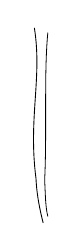
\begin{tikzpicture}[x=1cm,y=1cm,line cap=round]
\draw[line width=.32pt] (0,0) .. controls (.10,-.64) and (-.08,-1.14) .. (.02,-1.91)
 .. controls (.03,-2.14) and (.08,-2.35) .. (.11,-2.47);
\draw[line width=.29pt] (.17,-.06) .. controls (.12,-.59) and (.16,-1.31) .. (.13,-1.93)
 .. controls (.14,-2.13) and (.14,-2.27) .. (.17,-2.39);
\end{tikzpicture}}}
We ought to correct the messy conjecture in the case (\uline{$\overline{\mathrm{III}}$}), by stating (with all reservations, again!) that there are (perhaps) no other splittings of the extension $\mathcal{E}$ of $\Gamma$ by $\pi$ than those ....

\margin{78}

\scanpage{80}
\mspage{38}

10. Adjustment of the hypotheses (remorse).

I realize that in the definition of the morphisms $(X',S')\xrightarrow{f}(X,S)$, the hypothesis $f^{-1}(S)_{\mathrm{red}}=S'$ is too narrow --- we must take \uline{arbitrary} morphisms $f:X'\backslash S'\to X\backslash S$ (extending of course to $\widehat{f}:X'\to X$).
We will thus have $S'\supset\widehat{f}^{-1}(S)_{\mathrm{red}}$, but $S'$ may be strictly larger than $\widehat{f}^{-1}(S)_{\mathrm{red}}$.
We must then adjust the description of the ``messy category'' accordingly --- the objects remain the diagrams of groupoids
\[
\mathcal{D}:\Pi_{D^*}\to\Pi_U\to\Pi_e
\]
(plus Kummer datum) but a morphism $f$ from a $\mathcal{D}'$ into a $\mathcal{D}$ no longer necessarily defines a $\Pi'_{D^*}\to\Pi_{D^*}$ (in addition to $\Pi'_U\to\Pi_U$) one must specify a subset $I'_f$ of $I'=\pi_0(\Pi'_{D^*})$, and specify only
\[
\Pi'_{D^*,I'_f}\xrightarrow{f_{D^*}}\Pi_{D^*}
\]
(with commutation datum \inserted{$\unsure{\alpha_{D^*U}}$} relative to the square with $f_U$).
Of course, in the description in terms of $\mathcal{E}',\mathcal{E}$ etc., we require that for $i'\in I'\backslash I'_f$, $f_{\mathcal{E}}:\mathcal{E}'\to\mathcal{E}$ is trivial on $\mathcal{E}'_{i'}\subset\mathcal{E}'$ --- and $\tau$ is defined as $I'_f\to I$ ; \unsure{some|the} data relating to the $i'\in$

\margin{79}

\subsection*{Scans 81--90}
\addcontentsline{toc}{subsection}{Scans 81--90}
% package LM_P09
\scanpage{81}

\(I'_{f'}\quad (f_{i'}:\mathcal E_{i'}\longrightarrow
\mathcal E_{i=\tau(i')},\ \text{the }\alpha_{i'}\in\mathcal E)\)
are the same as in the case considered previously.

\uline{N.B.} This means in fact that we begin \unsure{to} ``plug the holes'' \deleted{of}
(of \(X'\)) corresponding to the \(i'\in I'\setminus I'_{f'}\), by replacing
\(\mathcal E'\) by the \deleted{\unsure{sub-}}quotient group of \(\mathcal E'\)
by the invariant subgroup generated by the
\(L_{i'}=\kappa_{i'}(T(\overline K))\)
\((i'\in I'\setminus I'_{f'})\), and \deleted{the} \unsure{\(\mathcal E_{i'}\)}
\((i'\in I'_{f'})\) by their images in the said quotient group, and forgetting
\deleted{the} \(I'\setminus I'_{f'}\), i.e. replacing \(I'\) by \(I'_{f'}\).

[To do things properly, we would have to express these operations also at the level of diagrams
of groupoids
\diagram{\begin{tikzcd}[ampersand replacement=\&]
\Pi'_{\unsure{D^*}} \arrow[r,dash] \& \Pi'_U \arrow[r] \& \unsure{\Pi'_e|\Pi_e}
\end{tikzcd}}
\(\ldots\)].

\margin{\deleted{\illegible{2} we would still have to \unsure{spell out}
\illegible{2} \unsure{some|the} points of \illegible{1}}}

This means then that in fact, we have brought ourselves back to the situation considered at the beginning,
where \(S'=\widehat f^{-1}(S)\)\ldots\ So in the end
the difference between the two points of view is not enormous, and
\deleted{\illegible{1}}\inserted{the one} adopted at the beginning has the advantage of
greater simplicity (everything is relative!)

\margin{80}

\scanpage{82}
\mspage{39}

11. Conditions on the systems of \deleted{\unsure{diagrams}}\inserted{groupoids}
obtained from geometric situations.

We have already mentioned some in passing, for example that the kernel groups of
\(\Pi_{D^*}-\Pi_e\) are abelian (with the Kummer isomorphism \(\kappa\))
and that the images are open subgroups, and the \(=\) for
the image of the \deleted{\illegible{1}} \(\pi_1\) in \(\Pi_U-\Pi_e\).
We are going to spell out again \inserted{and make precise} this in the framework of the interpretation
in terms of
\diagram{\begin{tikzcd}[ampersand replacement=\&]
T(\overline K) \arrow[r,"\kappa_i"] \& \mathcal E_i \arrow[r,hook,"\rho_i"] \&
\mathcal E \arrow[r,"p"] \& \Gamma
\end{tikzcd}}
(the ``dimension 1'' case --- we do not exclude the case \(I=\varnothing\) ---
the ``dimension 0'' case being trivial\ldots)

a) The image \inserted{\(\Sigma\)} of \(p\) is open, more precisely exists
open subgroup \(\Gamma'\subset\Gamma\) over which
\(\mathcal E\) has a section [and even an ``admissible section'' in a sense to be
defined later --- so as to exclude the ``trivial'' sections coming
from the \(\mathcal E_i\)\ldots].

b) The image \(\Sigma_i\) of \(\mathcal E_i\) in \(\Gamma\) is open, and
the extension \(\mathcal E_i\) of \(\Sigma_i\) by \(L_i\)
\((\simeq T(\overline K))\) is trivial. [In fact, we have a
\inserted{\uline{privileged}} class of splittings, called ``algebraic'', forming a
torsor under
\(K_i^*\,\unsure{\hookrightarrow}\,\varprojlim\unsure{(K_i^{*n})_n|(K_i^{*})_n}\),
cf. number 9 \unsure{]|?} --- but

\margin{81}

\scanpage{83}

we are not going to consider \inserted{for the moment} this additional piece of
structure\ldots)

\deleted{c) We must}

The rest of the \deleted{hypotheses}\inserted{conditions} essentially concerns
the structure of the groups \(\pi=\operatorname{Ker}(p:\mathcal E\to\Gamma)\) with
its \inserted{conjugacy classes of} \uline{subgroups}
\unsure{(or rather} the outer homomorphisms
\(\kappa_i:\deleted{\unsure{\widehat{\mathbb Z}(1)}}T\ (=T(\unsure{\overline K^*}))\longrightarrow\pi\),
and the way \(\Sigma\) operates by outer automorphisms on \(\pi\).
These conditions are expressed in a particularly simple way when the
\(\Sigma_i\subset\Gamma\) are \(=\Gamma\)
(``the points of \(S\) \inserted{\unsure{all}} rational over \(K\)'') i.e.
\(\mathcal E_i\to\Gamma\) surjective, a fortiori \(\Sigma=\Gamma\) i.e.
\(\mathcal E\to\Gamma\) surjective. We are going to restrict ourselves to this case. The general case follows
by a finite extension of the base field
[\unsure{over which} \deleted{we the}\inserted{each} points of
\(S\) not rational over \(K\)
\inserted{i.e. each \(\Sigma_i\ne\Gamma\)}
\deleted{\unsure{split up}\illegible{1}}\inserted{\unsure{gives|give} rise}
to \(n_i\) points, \deleted{\unsure{equal}}
\(n_i=[\Gamma:\Sigma_i]\) \unsure{\(\}\)} --- and \(X_{K'}\)
\deleted{\illegible{1}} \unsure{split|splits} into \(n=(\Gamma:\Sigma)\) connected components
which are geometrically connected] --- but I am too lazy to spell out as I should,
in the context of groupoids or of \deleted{\unsure{extensions}} homomorphisms of profinite
groups, the operation of extension of base fields\ldots\ It is understood that

\margin{82}

\scanpage{84}
\mspage{40}

the conditions I am going to describe will be invariant under extension \unsure{of the|of the} base field.

\deleted{c) There exists \(\unsure{\xi|\zeta}\in T\)
\((=\unsure{T(\overline K^*)})\) and conjugates}

c) \(\forall i\)\deleted{\illegible{1}}, the outer homomorphism
\[
\kappa_i:T\longrightarrow\pi
\]
is compatible with the outer action of \(\Gamma\) (operating on \(T\) by the
cyclotomic character \(\chi\), and on \(\pi\) thanks to the extension \(\mathcal E\)
of \(\Gamma\) by \(\pi\)). In other words, for \(\forall g\in\mathcal E\),
exists an \uline{\(\alpha\in\pi\)} (\uline{N.B.} not just
\(\alpha\in\mathcal E\)!) such that we have,
\[
\operatorname{int}(g)\kappa_i(\unsure{\xi|\zeta})
=\operatorname{int}(\alpha)\kappa_i(\chi(p(g))\unsure{\xi|\zeta})
\]
i.e.
\[
\operatorname{int}(\alpha^{-1}g)\kappa_i(\unsure{\xi|\zeta})
=\kappa_i(\chi(p(g))\unsure{\xi|\zeta})
\]
This means then that 1°) \(\alpha^{-1}g\) normalizes \(L_i=\kappa_i(T)\).
[and this means \(=\), probably, that \(\alpha^{-1}g\in\mathcal E_i\)
--- and that we can find such an \(\alpha\in\pi\)
\inserted{such that \(\alpha^{-1}g\in\mathcal E_i\)} comes from the hypothesis
\(\mathcal E_i\to\Gamma\) surjective --- we take a \(\beta\in\mathcal E_i\)
\inserted{\(\unsure{=}\alpha^{-1}g\)} having the \(=\) image as \(g\) in \(\Gamma\)
and we take \(\alpha=g\beta^{-1}\)] and that 2°) the \inserted{inner} action of
\(\beta=\alpha^{-1}g\) on \(T\) is nothing other than by multiplication
by \(\chi(g)=\chi(\beta)\) --- which (for \(\beta\in\mathcal E_i\)) is nothing other than the

\margin{83}

\scanpage{85}

condition already spelled out that the group homomorphism \(\kappa_i:T\to\mathcal E_i\)
is compatible with the action of \(\mathcal E_i\), operating on \(T\) via
\(\chi\circ p\mid\mathcal E_i\), and on itself by inner automorphisms.

So condition c) is not really new --- I spell it out again in
slightly different terms, because of its importance. It implies that the operation
\margin{\figure{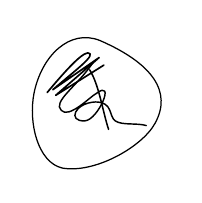
\begin{tikzpicture}[x=.012cm,y=-.012cm,line cap=round,line join=round]
\draw[line width=.45pt] (105,61) .. controls (73,48) and (43,77) .. (35,117)
 .. controls (29,148) and (39,190) .. (65,196)
 .. controls (99,202) and (149,174) .. (163,149)
 .. controls (182,115) and (160,85) .. (105,61);
\draw[line width=.52pt] (97,85) .. controls (81,109) and (54,126) .. (64,135)
 .. controls (72,144) and (95,120) .. (101,117)
 .. controls (122,101) and (103,145) .. (89,146)
 .. controls (70,147) and (78,127) .. (100,126)
 .. controls (119,126) and (114,141) .. (121,146)
 .. controls (128,151) and (144,148) .. (154,151);
\draw[line width=.55pt] (94,92) .. controls (104,108) and (108,137) .. (114,155);
\draw[line width=.60pt] (49,116) .. controls (65,97) and (84,75) .. (92,74)
 .. controls (103,75) and (78,93) .. (55,113)
 -- (104,79) -- (58,119) -- (109,87);
\end{tikzpicture}}}
of \(\Gamma\) on \(\pi\) is \uline{very} nontrivial (since
\(\chi:\Gamma\to\widehat{\mathbb Z}^{*}\) has an open image!)
--- it \unsure{was} not \(=\) obvious a priori
\inserted{(without deep arithmetic reasons!)} --- in view of the structure
of \(\pi\) that we are going to give --- that there exist such operations of \(\Gamma\)
on a \(\pi\)!

This condition \unsure{will be} supplemented by a nontriviality condition in the style of Weil.

d) \(\exists\eta\in T^*\)\unsure{.} (a basis of \(T\)), and
\(\alpha_i\in\pi\) (in order to conjugate \(\kappa_i\) into
\(\kappa'_i=\operatorname{int}(\alpha_i)\circ\kappa_i\))
\unsure{finally} an integer \(g\geq0\) and elements
\(\unsure{x_i,y_i}\in\pi\) \((1\leq i\leq g)\), such that we have

\margin{84}

\scanpage{86}
\mspage{41}

1°) the \(\kappa'_i(\eta)\), \deleted{\illegible{1}} and the
\(\unsure{x_i,y_i|x_j,y_j}\) generate the profinite group \(\pi\)

2°) They satisfy the relation
\[
\boxed{[x_1,y_1].[x_2,y_2]\ldots[x_g,y_g]\,
\kappa'_1(\eta)\kappa'_2(\eta)\ldots\kappa'_{\unsure{\nu|n}}(\eta)=1}
\]

3°) This relation, with the generators considered describes \(\pi\)
\inserted{(as a profinite group)} by generators and relations\ldots

\uline{N.B.} We know that under these conditions, \(g\) is uniquely determined,
for example by the fact that
\(\pi_{ab}/\deleted{\text{images of the}}\sum\kappa_i(T)\)
is a free \(\widehat{\mathbb Z}\)-module of rank \(2g\) --- \(\pi_{ab}\)
being free of rank \(2g+\nu-1\) where \(\nu=\operatorname{card}(I)\).

For the choice of \(\eta\), we know that if \(\eta\) works, then
\(\forall\ \chi(\alpha)\eta\) too (where \(\alpha\in\Gamma\)) --- up to taking
conjugates. So the \(\eta\) that work \deleted{form} contain
a subtorsor\inserted{of \(T^*\)} (under the open subgroup
\(\chi(\Gamma)\) of \(\widehat{\mathbb Z}^{*}\).

\deleted{Suppose for simplicity that \(g=0\):
We see then that if the system of the \(\kappa'_i(\eta)\) is a privileged system of generators
(in the sense of d) above) then the
\(\operatorname{int}(g)\kappa'_i(\eta)\) too for \(\forall g\in\mathcal E\),
[\unsure{\(=\)} \(\operatorname{int}(\alpha)\kappa'_i(\chi(g)\eta)\)
for suitable \(\alpha\in\pi\)]}

\margin{85}

\scanpage{87}
\mspage{42}

\margin{(\unsure{therefore|in} \(\chi:\Gamma\to\widehat{\mathbb Z}^{*}\) \unsure{epimorphism})}

\deleted{hence also the \(\kappa'_i(\chi(g)\eta)\). \unsure{Taking}
\(K=\mathbb Q\), we thus find by arithmetic means:

\uline{Proposition} Let \(\pi\) be the free \unsure{\(P\)}-group
\inserted{on \unsure{\(\nu-1\)|\(\nu\) generators}} \unsure{(}\uline{generated} by generators
\(\ell_1,\ldots,\ell_\nu\) satisfying the defining relation
\(\prod\ell_i=1\). Then for every \(\alpha\in\widehat{\mathbb Z}^{*}\),
we still have \(\prod\ell_i^\alpha=1\), and the \(\ell'_i=\ell_i^\alpha\)
with this relation describe the profinite group \(\pi\).}
In fact, since the structure of the group \(\pi\) is independent of \(K\),
taking \(K=\mathbb Q\) (and admitting that there exists a smooth projective
geometrically connected curve of genus \(g\) over \(\mathbb Q\), having \(\nu\) rational points over \(\mathbb Q\)!),
we find that if the \(\ell_i\), \deleted{\(\unsure{x_j,y_j}\)}
\((1\leq i\leq\nu\deleted{,\ \unsure{1\leq j\leq g}})\)
\deleted{work, then the} fit into a privileged system of generators
(with some \(\unsure{x_\alpha,y_\alpha}\)) then for
\(\forall\rho\in\widehat{\mathbb Z}^{*}\), we can find conjugates
\(\ell'_i\) of the \(\ell_i^\rho\) which fit in the \(=\) way.
Even for \(\rho=-1\) this is not entirely trivial\ldots

\deleted{\illegible{2}} Finally, \unsure{we are going to} state a draconian condition
of nontriviality of the operation of \(\Gamma\) on \(\pi\).
Let \(\mathcal E'\) be a subgroup \inserted{\uline{open} (hence}
of finite index) of \(\mathcal E\),
\inserted{\(\pi'=\pi\cap\mathcal E'=\operatorname{Ker}(\mathcal E'\to\Gamma')\)}
\deleted{\illegible{1} its image in \unsure{\(\mathcal E\)|\(\Gamma\)}
(which is open in \(\Sigma\)) so that}

\margin{86}

\scanpage{88}

\(\Gamma'\) the image of \(\mathcal E'\) in \(\Gamma\). We thus get an
extension of \(\Gamma'\) \((=\operatorname{Gal}(\overline K'/K'))\) over \(\pi'\),
hence also by \(\unsure{(\pi'_{ab})_{(\ell)}}\)
(\(\ell\) being a prime number), which is (we know this by d)) a
free \(\mathbb Z_\ell\)-module of finite type,
\inserted{on which \(\Gamma'\) operates}

[With a little work, we should be able to put on
\(\mathcal E'\to\Gamma\) a ``loop structure'' i.e. some
\(\mathcal E'_{i'}\), as for \(\mathcal E\), and describe in
\(\unsure{(\pi'_{ab})_{(\ell)}}\)
\inserted{the sum} of the images of the \deleted{\illegible{1}} \(L'_{i'}\),
on which \(\Gamma'\) operates \inserted{therefore} via the character \(\chi\).

\margin{This is done very elegantly in the setting
\diagram{\begin{tikzcd}[ampersand replacement=\&]
\Pi_{D^*} \arrow[r] \& \Pi_U \arrow[r] \& \Pi_e
\end{tikzcd}}}

We are interested in the quotient of \(\unsure{(\pi'_{ab})_{(\ell)}}\) by
\unsure{this submodule|these submodules} which is relatively trivial (the ``abelian variety'' part of the
\(\ell\)-adic module under consideration). This being said

\textcircled{e} we require that the representation of \(\Gamma'\) on this be
``pure of weight 1'' --- \deleted{\unsure{i.e.} we have} and that the characteristic polynomials
of the Frobenius elements (which have coefficients \(\in\mathbb Z\), not just
\(\in\mathbb Z_\ell\)) be \uuline{independent} of \(\ell\).

\margin{\figure{\begin{tikzpicture}[x=1cm,y=1cm,line cap=round]
\draw[line width=.34pt] (.04,.30) .. controls (-.30,.35) and (-.42,.13) .. (-.40,-.08)
 .. controls (-.39,-.36) and (-.14,-.39) .. (.08,-.23)
 .. controls (.36,-.01) and (.28,.27) .. (.04,.30);
\node[inner sep=0pt] at (-.08,-.02) {$e$};
\draw[line width=.29pt] (-.06,-.71) .. controls (.01,-1.68) and (-.08,-2.52) .. (.02,-3.52)
 .. controls (.09,-4.37) and (.08,-5.24) .. (.15,-5.98)
 -- (.07,-6.30);
\end{tikzpicture}}}
\margin{87}

\scanpage{89}
\mspage{43}

12. \uline{The topological analogy}

Let \(X\) be a compact
orientable (topological) \deleted{manifold}\inserted{surface}, \(S\) a finite subset of \(X\). If \(X\) is connected, we consider
the set \inserted{\unsure{\(\omega\)}} \unsure{of the|its} two orientations,
we use it to twist the group \(\mathbb Z\), whence a group \unsure{\(T\)}
\[
T=\mathbb Z\mathop{\wedge}\limits_{\pm1}\unsure{\{\omega\}|\omega}.
\]
isomorphic (noncanonically) to \(\mathbb Z\). More generally, suppose
given such a group \(T\),
\inserted{i.e. an \(\omega\in\unsure{\operatorname{Ob}}\mathrm{Ens}_2\)}
--- a \(T\)-orientation of \(X\) will by definition be an \unsure{element}
of the set \(\operatorname{Or}(X)\mathop{\wedge}\limits_{\{\pm1\}}\omega\).

[in the preceding case, \(X\) will thus be canonically \(T\)-oriented\ldots]

Let us consider the fundamental groupoid of \(X\setminus S=U\), say \(\Pi_U\),
and the fundamental groupoid \inserted{\(\Pi_{D^*}\)} of germs
of spaces of \(X\) around \(S\), \uline{deprived} of \(S\)
\inserted{\deleted{\unsure{of the}} groupoids \unsure{?}}
(of germs of universal coverings of \(X\setminus S\) in a neighborhood of \(S\)).
We thus have a canonical functor
\diagram{\begin{tikzcd}[ampersand replacement=\&]
\unsure{\Pi_{D^*}} \arrow[r,dash] \& \Pi_U
\end{tikzcd}}
and on the other hand, \deleted{\illegible{2}} if \(X\) is \(T\)-oriented, we have an
additional structure

\margin{88}

\scanpage{90}

of interest on \inserted{the groupoid} \(\Pi_{D^*}\): the local system of
its \(\pi_1\) is canonically isomorphic to \(T\).

Associating to every \(X\) which is \(T\)-oriented the system
\[
\Pi_{D^*}\longrightarrow\Pi_{\unsure{X|U}},\qquad
\kappa:T_{(\Pi_{D^*})}\simeq\pi_1(\Pi_{D^*}/e),
\]
we find a 2-equivalence between the topological 2 category of
\deleted{\unsure{manifolds}} pairs \((X,S)\) of a
\inserted{(for homeomorphisms up to isotopy\ldots)}
\unsure{compact \(T\)-oriented manifold}, and of the 2-category of the preceding
systems \inserted{(for equivalences)}, \unsure{(}which satisfy the conditions

a) \(\pi_0(\Pi_{D^*})\), \deleted{\unsure{and}} \(\pi_0(\Pi_X)\) finite

b) For \unsure{every|\(\forall\)} connected component of \(\Pi_U\), say
\(\Pi_{U_0}\), and the part \(\unsure{\Pi_{D_0^*}}\) above it, spelling out the
\unsure{groupoid} situation by \unsure{a|a}
\inserted{group \(\pi\) and a} family of homomorphisms
\(T\xrightarrow{\kappa_i}\pi\), we have (\uline{N.B.} the whole thing \unsure{depends|depending} on choices,
but \(\pi\) is intrinsic as an outer group, and the \(\kappa_i\)
\unsure{as homomorphisms} that are outer --- \unsure{define|defining} a ``\(T\)-loop structure
on \(\unsure{S}\) ---) we have the following.

\margin{89}

\subsection*{Scans 91--100}
\addcontentsline{toc}{subsection}{Scans 91--100}
% package LM_P10
\scanpage{91}
\mspage{44}

$\exists$ generator $g\in T$ (i.e. $g\in T^*$) and an order \inserted{$i_1$--$i_\nu$}
on the set $I$, \deleted{\illegible{2}} conjugates
$\unsure{l_i'|l_{i_\alpha}'}$ of the $\kappa_{i_\alpha}(g)$, and $g\in\mathbb N$ and $x_\alpha,y_\alpha\in\pi$
$(1\leq\alpha\leq g)$ such that we have
\[
\left(\prod_1^g[x_\alpha,y_\alpha]\right)\prod_1^{\nu}l_i=1
\]
and that this be a defining relation
of $\pi$.

There is \inserted{however} a grain of salt for $I=\varnothing$
(in which case $T$ serves no purpose \inserted{apparently} (in the
groupoid description of $(X,S)$ \unsure{$\simeq$|$=$} $(X,\varnothing)=X$)
one must then, \unsure{\deleted{in}} place of the
``Kummerian'' data \inserted{$\kappa$}, give oneself
\[
H^2(\pi,\mathbb Z)\overset{\kappa}{\simeq}T
\]
\margin{One must introduce \inserted{\unsure{therefore}} \unsure{this} as an additional datum,
in the definition of groups with loops the exclusion of the cases $X_0\simeq S^2$ (in the case of empty $S$) is \unsure{then} particularly \unsure{convincing}.}

Finally, one must \deleted{\illegible{1}}
(\unsure{even|$=$} with this grain of salt) exclude the case $X=S^2$, $S=\varnothing$
(as a connected component) --- i.e.
on the groups side, the case of a \inserted{component of $\Pi_U$ where}
$\pi=(1)$ \deleted{\illegible{2} $I=\varnothing$} and $I=\varnothing$.
[If I remember correctly, there is no reason
to exclude $(S^2,\mathrm{pt})$ (i.e. $X\setminus S=U\simeq\mathbb R^2\simeq\mathbb E^1_{\unsure{\mathbb C|e}}$)
\margin{90}

\scanpage{92}

where nevertheless \unsure{we have} $\pi=0$. But except in these
two cases, \deleted{the homomorphisms $\kappa_i:$} (corresponding
to the case $g=0$, $\nu=1$) the homomorphism $\kappa_i:T\longrightarrow\pi$
is injective. If $T=\mathbb Z$ the datum of the $\kappa_i$
is equivalent to that of elements $l_i\in\pi$, and we
recover the usual definition of
loop structures.

This is made explicit in the thesis of
Yves Ladegaillerie --- what is missing there, is
(among other things) the consideration of arrows
between $(X,S)$ other than homeomorphisms
(modulo isotopies)\,; for example maps \deleted{étale}
\deleted{\illegible{3}} $X'\xrightarrow{f}X$ such that $S'=f^{-1}(S)$
[and that $X'$ be étale over $X\setminus S$, if one insists\unsure{!}],
which reduces to the preceding case
--- the \inserted{more} general case where one assumes only
that $X'$ is a ramified covering
of $X$ (possibly ramified also
outside $S'$) and $S'\supset f^{-1}(S)$ (but $S'$
possibly larger) would call for
\margin{91}

\scanpage{93}
\mspage{45}

a careful study, with an
ad-hoc notion of isotopy ....

Another important direction (notably
for the study \unsure{of the|of the} unoriented,
nonorientable case) is the introduction of
finite groups of homeomorphisms, not
necessarily respecting the orientation.
To treat the case of a change of orientation,
note that in the groupoid description
$(\Pi_{D^*}\longrightarrow\Pi_U,\kappa)$ of a $(X,S)$ that is $T$-oriented,
the passage to the opposite orientation is expressed by
keeping $\Pi_{D^*}\longrightarrow\Pi_U$ as is, and
replacing $\kappa$ by $\bar\kappa=\kappa^{-1}$
\[
\bar\kappa(\unsure{\zeta|\xi})=\kappa(-\unsure{\zeta|\xi})=\kappa(\unsure{\zeta|\xi})^{-1}
\]
(If \inserted{$T=\mathbb Z$, on} the system $(\pi,(l_i))$, this amounts to
replacing the $l_i$ by the $l_i^{-1}$ ...)
\margin{and ditto (if $I=\varnothing$) for $\kappa:T\simeq H^2(\pi,\mathbb Z)$
\unsure{replaced} by $-\kappa$.}

Let then $\Gamma$ be a group (a priori
\unsure{not} necessarily finite) which operates on $(X,S)$, hence
on $U=X\setminus S$ \inserted{and on $\Pi_U$, $\Pi_{D^*}$.} We then find
mixed \inserted{fundamental} groupoids \deleted{\illegible{1}} by the well-known construction
\margin{92}

\scanpage{94}

\diagram{\begin{tikzcd}[ampersand replacement=\&]
\Pi_{D^*,\Gamma} \arrow[r] \& \Pi_{U,\Gamma} \arrow[r] \& \Pi_{e,\Gamma}
\end{tikzcd}}
category of $\Gamma$-torsors
i.e. of $1$-connected objects
in $\Gamma$-Sets

corresponding to the functors in the opposite direction

\diagram{\begin{tikzcd}[ampersand replacement=\&]
\text{\unsure{étale|étale} $\Gamma$-coverings of $D^*$} \& \text{\unsure{étale|étale} $\Gamma$-coverings of $U$} \arrow[l] \& \text{$\Gamma$-Sets} \arrow[l]
\end{tikzcd}}

The connected components of $\Pi_{D^*,\Gamma}$ correspond
to the \uline{orbits of $\Gamma$ in $S$} \deleted{\illegible{1}} $\simeq\pi_0(\Pi_{D^*})$,
likewise for those of $\Pi_{U,\Gamma}$. The \deleted{\unsure{topological}}
connected $\Pi_{U,\Gamma}$ \inserted{i.e. the connected topos $\widehat\Pi_{U,\Gamma}$,}
is the one \unsure{where|with} $\Gamma$ transitive
on $\pi_0(U)\simeq\pi_0(X)$ --- at the cost of replacing
$X$ by a connected component $X_0$, and $\Gamma$
by the \unsure{subgroup|subgroup} $\Sigma\subset\Gamma$ that stabilizes it,
we would be reduced (for the study of the
topoi $\widehat\Pi_{U,\Gamma}$ and of morphisms of topoi
\diagram{\begin{tikzcd}[ampersand replacement=\&]
\widehat\Pi_{D^*,\Gamma} \arrow[r,dash] \& \widehat\Pi_{U,\Gamma} \arrow[r] \& (\unsure{\widehat\Pi_{e,\Sigma}} \arrow[r] \& )\widehat\Pi_{e,\Gamma}
\end{tikzcd}}
to the case of $(X_0,S_0,\Sigma)$. But \unsure{the analogy|the analogue}
\margin{93}

\scanpage{95}
\mspage{46}

that I have in mind with the ``arithmetic'' case
makes this reduction inopportune in the
general case (for in the arithmetic \unsure{\deleted{case}},
we do not restrict ourselves either to the case where
$\Sigma=\Gamma$ i.e. $\mathcal E\longrightarrow\Gamma$ surjective, i.e. \inserted{the connected component}
$X$ \uline{geometric-}
\uline{ally} connected over $K$). Note \inserted{here} that
$(X,S,\Gamma)$ is recovered from the
$(X_0,S_0,\Gamma_0=\Sigma)$ as an amalgamated sum
\[
X=X_0\,\unsure{\wedge|\widehat\times}_{\Sigma}\Gamma\quad ....
\]

When we express (for $\Pi_{\unsure{U|X},\Gamma}$ connected)
the situation in terms of group theory,
we therefore find \deleted{\illegible{1}} a mixed
fundamental group \deleted{$\mathcal E_X$}
\[
\mathcal E_{\unsure{U|X},\Gamma}=\pi_1(U,\Gamma)
\]
and a homomorphism
\[
\mathcal E_{U,\Gamma}\longrightarrow\Gamma
\]
--- (Surjective iff \deleted{$\Gamma$ transitive on $\pi_0(U)=\unsure{\Gamma/\Sigma}$}
\inserted{$U$ connected (we have $\Gamma/\Sigma\simeq\pi_0(U)$)})
\inserted{finally a set of indices}
\deleted{corresponding to \illegible{1} $\pi_0(U)/\Gamma$}
$I$ ($\simeq\unsure{S}/\Gamma\simeq\pi_0(\Pi_{D^*,\Gamma})$) and
mixed fundamental groups
\margin{94}

\scanpage{96}

\[
\mathcal E_i\xrightarrow{\sim}\unsure{\pi_1|\Pi_1}(D_i^*,\Gamma)
\simeq\pi_1(D_{i_0}^*,\unsure{\Sigma_{i_0}|\Gamma_{i_0}})
\]
where $D_{i_0}^*$ is a connected component of the
punctured multidisk $D_i^*$ \inserted{(corresponding to the choice of an $\unsure{s_i}\in S$)}, and where $\unsure{\Sigma_{i_0}|\Gamma_{i_0}}\subset\Gamma$ is
its stabilizer (i.e. the stabilizer of
$s_i$ in $\Gamma$), which is \deleted{\unsure{a group}} (if $\Gamma_i$ \inserted{is finite and} operates
faithfully in a neighborhood of $s_i$) a cyclic
or dihedral group ... We therefore find, if $X$ is
$T$ \unsure{oriented|oriented}, an extension of $\Gamma_{i_0}$ by $T$,
the homomorphism $\mathcal E_i\longrightarrow\unsure{\Sigma_{i_0}|\Gamma_{i_0}}\subset\unsure{\Gamma|\Gamma_i}$ being induced
of course via $\mathcal E_{U,\Gamma}\longrightarrow\Gamma$ and $\mathcal E_i\longrightarrow\mathcal E_{U,\Gamma}$.

One must \inserted{also} link the action of $\Gamma$ on $X$ to
the orientation of $X$ --- for this we suppose
given a character
\[
\chi:\Gamma\longrightarrow\mathbb Z^*=\{\pm1\}
\]
and require that for $g\in\Gamma$, $g_X$ \unsure{preserve}
the orientation if $\chi(g)=1$, reverse it if $\chi(g)=-1$.
This implies that \deleted{\unsure{the}}\inserted{\unsure{we have an|the homomorphism or}} isomorphism
\[
\pi_1(\Pi_{D^*,\Gamma}/\Pi_{\unsure{e},\Gamma})
\overset{\kappa_\Gamma}{\xleftarrow{\sim}}T
\]
\margin{local system of the kernels of the
$\pi_1(\xi)\longrightarrow\pi_1(\varphi p(\xi))$
for $\xi\in\operatorname{Ob}\Pi_{D^*,\Gamma}$.}
\margin{95}

\scanpage{97}
\mspage{47}

$T$ being regarded as a local system
on $\Pi_{\Gamma,e}$ \deleted{\illegible{1}} i.e. as a $\Gamma$-group, thanks to the action
of $\Gamma$ via the character $\chi$. It amounts to the
same to say that \inserted{$\forall i\in I$} the map
\deleted{The datum}
\[
\kappa_i:T\xrightarrow{\sim}L_i=\operatorname{Ker}(\mathcal E_i\longrightarrow\Gamma)
\]
as a homomorphism from $T$ to $\mathcal E_i$ is
compatible with the action of $\mathcal E_i$ (operating
on $T$ via $\chi p_i$ ($p_i:\mathcal E_i\longrightarrow\Gamma$)), \illegible{1} and on
itself by inner automorphism\unsure{s} ...

If we exclude the case where $(X_0,\unsure{S_0})$
is $\simeq(S^2,\varnothing)$ or $(S^2,1\ \mathrm{pt})$ (i.e.
the case $\pi=0$), the $\kappa_i:T\longrightarrow\pi$ are injective,
hence also the $\mathcal E_i\longrightarrow\mathcal E_{U,\Gamma}$, hence the
$\mathcal E_i$ can be regarded as
\uline{subgroups} of $\mathcal E_{U,\Gamma}$.

\unsure{\S} Here it \deleted{\illegible{1}} would be particularly
inadvisable (\unsure{even|$=$} if we assume $\Sigma=\Gamma$ i.e.
$X=X_0$ i.e. $X$ connected) to suppose that
the $\Gamma_i$ \unsure{be|are} $=\Gamma$ i.e. that the $s\in S$ are fixed
by $\Gamma$ !
\margin{96}

\scanpage{98}

Since the center of $\pi$ is \deleted{\illegible{1}}reduced to $1$
(if we except \deleted{\unsure{resp.}} the case $(X_0,S_0)\simeq(S^2,\text{two points})$
i.e. $U_0\simeq\mathbb C^*$ \inserted{--- case of the annulus ---}), the datum of an extension
of $\Sigma$ ($\subset\Gamma$) by $\pi$ amounts (up to a unique \unsure{isomorphism})
to the datum of a homomorphism
\[
\unsure{\Sigma|\Gamma}\longrightarrow\mathrm{Aut\,ext}(\pi)\quad\deleted{\text{loop structure}}
\]
\deleted{from $\Sigma$ into the ``Teichmüller group''
relative to $\pi$ ($\simeq\pi_1(X_0)$)} --- $\mathcal E$ is reconstructed
as the inverse image of the extension
\diagram{\begin{tikzcd}[ampersand replacement=\&]
1 \arrow[r] \& \pi \arrow[r] \& \mathrm{Aut}(\pi) \arrow[r] \& \mathrm{Autext}\,\pi \arrow[r] \& 1
\end{tikzcd}}.

But here the outer \unsure{automorphisms} relative
to the $\alpha\in\Sigma$ \deleted{considered are} \uline{respect the loop structure}
\deleted{\illegible{1}} of $\pi$, modulo the
sign $\chi(\alpha)$ --- i.e. for $g\in\mathcal E$, and $s\in S$
$\exists\ \alpha\in\pi$ \inserted{and $s'\in S$ ($s'$ unique !)} such that
\[
\deleted{\unsure{\varphi|g}}\quad
\operatorname{int}(g)\kappa_s(\unsure{\zeta|\xi})
=\operatorname{int}(\alpha)\kappa_{s'}(\chi(p(g))\unsure{\zeta|\xi})
\]
$\forall\unsure{\zeta|\xi}\in\unsure{T|\mathbb Z}$, i.e.
\[
\operatorname{int}(\alpha^{-1}g)\kappa_s(\unsure{\zeta|\xi})
=\deleted{\unsure{\chi}}\unsure{\kappa_i|\kappa_{s'}}(\chi(p(g))\unsure{\zeta|\xi})
\]
\deleted{which implies that $\alpha^{-1}g$ normalizes $L_s=\kappa_s(T)$}
\margin{97}

\scanpage{99}
\mspage{48}

\deleted{(so probably $\alpha^{-1}g\in\mathcal E_s$ ?), and
operates on it \illegible{2}}
Thus, the operation of
$\Sigma$ on $S_0$ (hence of $\Gamma$ on $S=S_0\wedge_{\Sigma}\Gamma$)
is known, from the outer operation of $\Sigma\subset\Gamma$ on
$\pi$ endowed with its ``$T$-loop'' structure \deleted{\illegible{1}}
(i.e. the outer homomorphisms
$\kappa_s:T\longrightarrow\pi$) --- hence also $I=S_0/\Sigma\simeq S/\Gamma$.

Can we reconstruct $\mathcal E_i$ \inserted{($i\in I$)} from the
\deleted{\unsure{if} $i=s\bmod\Sigma$}
extension structure? We see, \deleted{that}
\deleted{$\mathcal E_{i_0}\subset\operatorname{Norm}_{\mathcal E}(L_s)$}
by virtue of the choices made,
that if $i\in I$ (hence $i$ an orbit of
$\Sigma$ in $S_0$) $\exists\ s\in i$ such that $\operatorname{Ker}(\mathcal E_i\longrightarrow\Gamma)$
is none other than $L_s=\kappa_s(T)$, and we
therefore have $\mathcal E_i\subset\operatorname{Norm}_{\mathcal E}(L_s)$, But
we have
\[
\operatorname{Norm}_{\mathcal E}(L_s)\cap\pi
=\operatorname{Norm}_{\pi}(L_s)=L_s
\]
$\unsure{=|\ne}\mathcal E_i\cap\pi$, and on the other hand the image of
$\operatorname{Norm}_{\mathcal E}(L_s)$ in $\Sigma\subset\Gamma$ is not \deleted{other than} \inserted{$\subset$}
$\Sigma_s=$ stabilizer \deleted{of} \inserted{$s$ in} $\Sigma$
$=$ Image of $\mathcal E_i$ in $\Sigma$,
\unsure{and|hence} in summary
\[
\mathcal E_i=\operatorname{Norm}_{\mathcal E}(L_s)
\]
\margin{98}

\scanpage{100}

Conversely, the datum of $\mathcal E\longrightarrow\Gamma$
and of the $\mathcal E_i$, $\kappa_i:T\longrightarrow\mathcal E_i$ gives back the
loop structure of $\pi$, by taking
the $\kappa_i$ and all their \inserted{distinct} outer
conjugates by the $\alpha\in\Sigma$ (modified by $\chi(\alpha)$ ...).
Thus the \inserted{datum of the} situation $\mathcal E\xrightarrow{p}\Gamma$, $\mathcal E_i\subset\mathcal E$
\deleted{equivalent} (family of subgroups, each
\unsure{defined} modulo conjugation \uline{in $\mathcal E$}) is equivalent
to the datum of

a) $\pi=\operatorname{Ker}p$, with its \inserted{$T$-}loop structure
(\deleted{finite family of \unsure{conjugacy classes}}\inserted{finite set of outer homomorphisms from}
$T$ to $\pi$)

b) A \unsure{sub-}\deleted{group} group $\Sigma\subset\Gamma$, and
a homomorphism
\[
\Sigma\longrightarrow\text{extended Teichmüller of }\pi
\]
(outer automorphisms of $\pi$,
respecting the loop structure
modulo sign
compatible with the character $\chi|\Sigma$ and
the ``sign'' character on extended Teichmüller.
In fact, $(X,S,\Gamma)$, or $(U,\Gamma)$, defines
$\pi$ only as an outer group \inserted{with $T$-loops} on which
$\Gamma$ operates in a way compatible with $\chi$.
\margin{99}

\subsection*{Scans 101--110}
\addcontentsline{toc}{subsection}{Scans 101--110}
% package LM_P011
\scanpage{101}
\mspage{49}
% Main text, approximately lines 1--2.
In summary, we have a \deleted{\illegible{1}}\inserted{canonical} functor
% Approximately lines 3--10; the source of the vertical functor.
Isotopic category of \((X,S,\Gamma)\), \(X\) compact surface \deleted{\illegible{1}},
\(T\) oriented, \(S\) discrete subset, \(\Gamma\) operating by \unsure{\(\chi\)-automorphisms}
(\inserted{\(\sigma\in\Gamma\)}\unsure{preserving|preserves} the orientation if \(\chi(\sigma)=+1\), reversing it
if \(\chi(g)=-1\)), \(\Gamma\) transitive on \(\Pi_0(X)\),
\deleted{\illegible{1}} and if \((X_0,S_0)\) is a connected component
of \((X,S)\), we want that \deleted{\((X_0,S_0)\) \illegible{2}}\inserted{if \(X_0\simeq S^2\), we}
have \(\operatorname{card} S_{\unsure{0}}\geq 3\) \deleted{\illegible{3}}.
% Under "ait card S ≥ 3" a smaller line of text is struck through by one long stroke;
% "ait" itself is neither underlined nor struck.
\deleted{\illegible{1} \unsure{isomorphism}}
\margin{arrows: isotopy \unsure{classes} of homeomorphisms respecting all the structures.}

\diagram{\begin{tikzcd}[row sep=2.5em]
{} \arrow[d] \\
{}
\end{tikzcd}}

% Approximately lines 11--18.
Category of outer groups with \inserted{\(T\)-}loops \(\pi\),
\inserted{\(\pi\) noncommutative (i.e. \(\pi\neq 0,\mathbb Z\));}
on which a subgroup \(\Sigma\subset\Gamma\) of \(\Gamma\) \inserted{operates}
(this description being
equivalent: a description in terms
of systems of groupoids
\[
\Pi_{\unsure{D^*},\Gamma}\longrightarrow\Pi_{U,\Gamma}
\longrightarrow\Pi_{e,\Gamma}\quad\text{and }\kappa\ldots,
\]
more conceptual in certain contexts\ldots).
% Long oblique note in the left margin beside the target category.
\margin{Beware \unsure{of the} case \(S=\varnothing\) in the definition of the structures: \unsure{the} \illegible{1} (datum of
\(H^2(\pi,\mathbb Z)\overset{\kappa}{\simeq}T\)); we must of course take into account \unsure{during} the action of \(\Sigma\) on
\(H^2(\pi,\mathbb Z)\) \deleted{\unsure{and on \(T\)}}
(via its outer action on \(\pi\)) and on \(T\) (via \(\chi\)) and \unsure{require the} compatibility.}

% Approximately lines 19--25; the sentence continues on scan 102.
\deleted{\unsure{For definition}} I presume that the proof
\unsure{of the} fact that this functor is fully faithful
presents no essential difficulties,
% Oblique note in the lower-left margin, tied by a double bar and an arrow to the three preceding lines.
\margin{It would really be worth doing it very carefully\ldots}
using what is known for
\(\Gamma=1\). But the fact that, \unsure{for|\deleted{for}} \(\Gamma\) a given finite
group, \deleted{\unsure{that it is an isomorphism}}\inserted{it is \unsure{essential\textsuperscript{ly}} surjective}
% Lower-left handwritten pagination; attribution of this numbering is uncertain.
\margin{100}

\scanpage{102}
% Approximately lines 1--7; continuation from scan 101.
is an open problem on which
people are stumped. Of course we may assume \(\Sigma=\Gamma\),
\inserted{and \(\Gamma\subset\) extended Teichmüller}
and the question is whether every finite subgroup
of the extended Teichmüller is
realized as a group operating on \((X_0,S_0)\) \illegible{1}
in an essentially unique way. More
precisely, if \deleted{\illegible{1}} \(A=\) group of \deleted{\unsure{diffe}}homeomorphisms
% Approximately lines 8--16.
(or diffeomorphisms, if \(X_0\) is
differentiable) of \(X_0\), \(A^0\) its connected compo\unsure{nent|of}
(\uline{N.B.} \(A^0\) is contractible, \deleted{\unsure{)}}\inserted{in}
the anabelian cases) hence \(A/A^0=\mathcal T_{g,\nu}\)
(Teichmüller group for genus \(g\) and \(\nu\)
holes), the question comes down to: \unsure{this} whether for every
homomorphism from a finite group \(\Sigma\) into \deleted{\illegible{1}} \(\mathcal T_{g,\nu}\),
(we may assume \(\Sigma\subset\mathcal T_{g,\nu}\)), it lifts
to a homomorphism into \(A\), and whether two such
liftings are conjugate by an \(a\in A^0\)
(isotopy \inserted{in the strict sense} of two liftings \unsure{\(\sim\)}).

% Approximately lines 17--21; continuation on scan 103.
Having arrived at such a simple \deleted{description}\inserted{\unsure{reinterpretation|interpretation}}
of the 1-category (``1-isotopic'') deduced
from the 2-category of systems
\((\Pi_{D^*,\Gamma}\longrightarrow\Pi_{U,\Gamma}\longrightarrow\Pi_{e,\Gamma},\kappa)\), in terms
% Lower-left additional handwritten pagination; hand/status uncertain.
\margin{101}

\scanpage{103}
\mspage{50}
% Approximately lines 1--7; continuation from scan 102.
% The light round stroke before the square bracket may be the insertion mark for π.
of outer groups with loops (\inserted{\(\pi\)}[equipped
with a set of outer homomorphisms \(\kappa_i:T\longrightarrow\pi\), and
failing that with a \(\kappa:T\longrightarrow H^2(\pi,\mathbb Z)\))
(to do it properly, one should write
\(T^{(\otimes-1)}\simeq H^2(\pi,\mathbb Z)\), but here we have a canonical
isomorphism \(T^{\otimes-1}\simeq T\) i.e. \(T^{\otimes 2}\simeq\mathbb Z\ldots\))],
% Approximately lines 8--14.
the question arises \unsure{of how to recover},
(up to an equivalence defined up to unique isomorphism)
this diagram, in terms of \(\kappa\); everything
comes down to the \deleted{definition} description of the
categories \(\Pi_{D^*,\unsure{\Gamma}}\) and \(\Pi_{U,\Gamma}\), and the two
functors \(\Pi_{D^*,\Gamma}\longrightarrow\Pi_{U,\Gamma}\), \(\Pi_{U,\Gamma}\longrightarrow\Pi_{e,\Gamma}\);
\inserted{or what amounts to the \(=\), of the corresponding (multi-Galois) topoi and morphisms of topoi.}

% Approximately line 15.
a) \uline{Description} of \(\Pi_{U,\Gamma}\) and of \(\Pi_{U,\Gamma}\longrightarrow\Pi_{e,\Gamma}\).

% Approximately lines 16--22; continuation on scan 104.
Let more generally \(\pi\) be an \inserted{outer} group, \deleted{\unsure{such that}} \unsure{whose}
\uline{center} \uline{is trivial} (this corresponds to the
anabelian hypothesis!), let us show how we
associate with it a classifying topos
\(B_\pi\), which (as a category of sheaves) will be
% "(pour Iso)" is written under "faisceaux) sera" and tied by a curve to the place after "fonctorielle".
\(\operatorname{Ens}(\pi)\)) in a ``functorial'' way \inserted{(for \unsure{Isomorphisms|isomorphisms})}. Everything
comes down to seeing how, to a \uline{conjugacy}
% Lower-left additional handwritten pagination; hand/status uncertain.
\margin{102}

\scanpage{104}
% Approximately lines 1--7; continuation from scan 103.
\uline{class} \inserted{\(\Theta\)} of isomorphisms
\[
\pi'\xrightarrow{u}\pi,
\]
we associate an ``inverse image'' functor
\(\operatorname{Ens}(\pi)\longrightarrow\operatorname{Ens}(\pi')\), defined up to unique
isomorphism. Let us consider for every \(u\) in the class
\(\Theta\), the functor ``\(u\)-restriction of operations''
\[
\operatorname{Ens}(\pi)\xrightarrow{u^*}\operatorname{Ens}(\pi')
\]
% Approximately lines 8--11, including interlinear corrections.
% "définit," stands above the struck "est"; "avec ... ," stands above the line and is tied by a curve to the place after "donc,".
[which \deleted{\unsure{is}}\inserted{defines,} therefore, \inserted{with \(\unsure{u_*=}(u^{-1})^*\),}
an \deleted{\unsure{isomorphism}}\inserted{equivalence} of the Topoi
\[
B_{\pi'}\xrightarrow{\substack{u_\bullet\\ \sim}} B_\pi
\]
]
We shall, between these \deleted{functors}\inserted{equivalences}, \inserted{for \(u\in\Theta\),} define a
transitive system of isomorphisms (which therefore lets us
identify them with each other!).

% Approximately lines 12--20.
\unsure{Let|Let} \(u,u'\in\Theta\), whence \(u^*,u'^*\); we have by hypothesis
\deleted{definition} a \(g\in\pi\) such that \(u'=\operatorname{int}(g)\circ u\),
furthermore \(g\) is determined modulo an
element of \(\operatorname{Centr}_\pi u(\pi')=\operatorname{Centr}(\pi)=1\);
so here \(g\) is unique. But \(g\)
can be used to define a functorial
isomorphism \deleted{between \(u^*\) and \(u'^*\)}\inserted{between}
\[
i_{u',u}:u^*\xrightarrow{\sim}u'^*
\]
by taking, for \(E\in\operatorname{Ob}\operatorname{Ens}(\pi)\),
\[
i_{u',u}(E):
\underset{\substack{\unsure{\Vert}\\E}}{u^*(E)}
\longrightarrow
\underset{\substack{\unsure{\Vert}\\E}}{u'^*(E)},
\qquad i_{u',u}(E)=g_E.
\]
% Lower-left additional handwritten pagination; hand/status uncertain.
\margin{103}

\scanpage{105}
\mspage{51}
% Approximately lines 1--6.
\uline{N.B.} The argument works for every conjugacy
class of homomorphisms \inserted{of groups} \(\pi'\longrightarrow\pi\) (i.e. every outer
homomorphism) whose centralizer in \(\pi\) is
reduced to 1 (which for an epimorphism
\unsure{reduces to the} hypothesis \(\operatorname{Centr}(\pi)=1\)).
% Oblique note in the left margin. The word read "anabéliens" carries a double rule through
% or under it; deletion or emphasis is not settled.
\margin{works for \unsure{anabelian loops|anabelian groups with loops}, and the homomorphisms of such
whose image is of finite index\ldots{} (for the centralizer in such a group \(\pi\)
of a subgroup of finite \unsure{index} is still \unsure{reduced to e|reduced to 1}).}

% Approximately lines 7--14.
If now a group \(\Sigma\) operates
on the outer group \inserted{\(\pi\)}, then by the
preceding result we can say that it
also operates on the topos \(B_\pi\), \inserted{whence a topos \(B_{\pi,\Gamma}\),} (we can
also say that \deleted{\illegible{1}} Since
\(\operatorname{Centr}(\pi)=1\)) the operation of \deleted{\(\unsure{\pi}\)}\(\Sigma\) on \(\pi\)
defines an extension \(\mathcal E\) of \(\Sigma\) by \(\pi\),
% "On récupère" stands above the struck word; a curve runs from it over "bien" to the end of the line.
whence a topos \(B_{\pi,\Gamma}=B_{\mathcal E}\), \deleted{\unsure{and}} \inserted{We recover} \unsure{of}
course also \(B_{\pi,\Gamma}\longrightarrow B_{\Gamma}\). To reassure
% Approximately lines 15--22; continuation on scan 106.
ourselves, we should make sure that
if we have a homomorphism of outer groups
\(\pi'\xrightarrow{\Theta}\pi\) commuting with the action of a
\(\Sigma\), with \(\operatorname{Centr}_\pi(\Theta)=(1)\), then there exists
a \(\Theta_{\Gamma}:B_{\pi',\Gamma}\longrightarrow B_{\pi,\Gamma}\) defined up to canonical
isomorphism. Now every \(u\in\Theta\) defines a
homomorphism of extensions \inserted{\(u_{\Gamma}\) (of \(\Sigma\) by \(\pi'\) resp. \(\pi\))}
\(\mathcal E'\longrightarrow\mathcal E\) \unsure{above|below}
\(u\), and if we pass from \(u\) to \(u'=\operatorname{int}(g)\circ u\), we will have
% Lower-left additional handwritten pagination; hand/status uncertain.
\margin{104}

\scanpage{106}
% Approximately lines 1--2; continuation from scan 105.
\(u'_{\Gamma}=\operatorname{int}_{\mathcal E}(g)\circ u_{\Gamma}\), and we finish as
above, with uniqueness of \(g\).

% Approximately lines 3--8.
Now take an \inserted{\uline{injective}} outer homomorphism
\[
\deleted{\unsure{\lambda}}\Lambda=[\kappa]:T\longrightarrow\pi
\qquad (T\text{ commutative}),
\]
% Written directly under the letter Λ.
\margin{(initial of ``loops'')}
% Oblique note in the upper-left margin, tied by a curve to "injectif".
\margin{Injectivity in the case we are interested in follows from the anabelian hypothesis.}
% "supposons" stands at the start of the line, with an arrow to "que".
suppose that (for \(\kappa\in[\kappa]\))
\[
\operatorname{Centr}_\pi\kappa=\kappa(T)
\]
(which does not depend \unsure{on the|on the} choice of \(\kappa\) in
\([\kappa]\)). I will then define a
% Approximately lines 9--17.
\deleted{category} connected abelian groupoid \inserted{\(\Pi_\Lambda\)}, and an
\unsure{isomorphism} of its \(\pi_{\unsure{1}}\) with \(T\) \deleted{An object}
(hence a topos, which plays the role of
\(\widehat{\Pi}_{\unsure{D|D^*}}\)). An object will be a \(\kappa\in[\kappa]\).
A homomorphism from \(\kappa\) to \(\kappa'\) will be an
element \(g\in\operatorname{Transp}_\pi(\kappa,\kappa')\). \deleted{Let \(g\)}
The composition of homomorphisms obvious. We
do indeed get a connected groupoid, in
which \(\operatorname{Aut}(\kappa)=\operatorname{Centr}_\pi(\kappa)\overset{\inserted{\text{by hypothesis}}}{=}\kappa(T)\unsure{\xleftarrow[\sim]{\kappa}}T\).

% Approximately lines 18--21; continuation on scan 107.
% The words from "sur les topos" to "B_Λ → B_π" are squeezed between two lines.
OK. Of course, we have a homomorphism
\(\Pi_\Lambda\longrightarrow\deleted{\unsure{\pi}}\) one-point groupoid, hence
\unsure{on} the \unsure{classifying|classifying} topoi \inserted{defined by \(\pi\)} \inserted{\(B_\Lambda\longrightarrow B_\pi\)}.
We have to see the behavior of this
% Lower-left additional handwritten pagination; hand/status uncertain.
\margin{105}

\scanpage{107}
\mspage{52}
% Approximately lines 1--7; continuation from scan 106.
construction under outer homomorphisms. So let
\[
\Theta=f_\pi\deleted{\unsure{\Theta}}=[u]:\pi'\longrightarrow\pi
\]
be an outer homomorphism such that \(\operatorname{Centr}_\pi(\Theta)=1\),
and \(\Lambda':T\longrightarrow\pi'\) an injective outer homomorphism
such that \(\kappa'\in\Lambda'\Rightarrow\operatorname{Centr}_{\pi'}(\kappa')=\operatorname{Im}\kappa'\)
and let us consider the composite
\[
\deleted{\unsure{\Lambda=}}f_\pi\circ\Lambda':T\longrightarrow\pi.
\]
% Approximately lines 8--12.
Let \(d\in\mathbb Z\) and consider
\[
\Lambda=f_\pi\circ\Lambda'\circ(d.\operatorname{id}_T)
\]
\inserted{suppose that \(\kappa\in\Lambda\Rightarrow\operatorname{Centr}_\pi\kappa=\operatorname{Im}\kappa\)}
We are going to define a homomorphism from \(\Pi_{\Lambda'}\) to \(\Pi_\Lambda\),
hence a morphism of Topoi \(B_{\Lambda'}\longrightarrow B_\Lambda\),
and a commutation datum \inserted{\(\alpha\)} for the
\diagram{\begin{tikzcd}[ampersand replacement=\&,column sep=4em,row sep=3.8em]
\& B_{\Lambda'} \arrow[r,"f_D"] \arrow[d] \& B_\Lambda \arrow[d] \\
(*) \& \unsure{(B,\pi')} \arrow[r,"{\begin{gathered}\deleted{\unsure{B(f_\pi)}}\\[-2pt]\inserted{B(f_\pi)\ \text{defined above}}\end{gathered}}"']
\arrow[ur,bend left=32,shorten <=2.1em,shorten >=2.1em,"\alpha"']
\& \unsure{(B,\pi)}
\end{tikzcd}}
\margin{\illegible{2} \unsure{obviously} \illegible{5} \deleted{\unsure{of Topoi}} \illegible{2}.}
\deleted{\illegible{2} \unsure{to the} hypotheses \illegible{1} on \(\Lambda',\Theta,d\)}

% Approximately lines 13--19; continuation on scan 108.
\deleted{Let} \(\kappa':T\longrightarrow\pi'\) an object of \(\Pi_{\Lambda'}\),
we want to define (up to unique isomorphism) an
object \(\kappa\) of \(\Pi_\Lambda\). For every \(u\in f_\pi=\Theta\),
% The κ in the next formula carries no prime in the ink.
we consider \(u\circ\kappa\circ(d.\operatorname{id}_T)\), there is between them
a transitive system of isomorphisms for \(u\) varying
in \(\Theta\), we can identify them with one another.
% Lower-left additional handwritten pagination; hand/status uncertain.
\margin{106}

\scanpage{108}
% Approximately lines 1--7.
The functoriality of this object with respect to
varying \(\kappa'\) is obvious: [we can say that
\(u\in\Theta\) defines a homomorphism of groupoids
\[
u_\Lambda:\Pi_\Lambda\longrightarrow\Pi_{\Lambda'},
\]
and between these
there is a transitive system of isomorphisms \unsure{\}}. In fact,
for fixed \(u\) we have a \deleted{system} commutative
diagram of homomorphisms of groupoids
\diagram{\begin{tikzcd}[ampersand replacement=\&]
\Pi_{\Lambda'} \arrow[r,"u_\Lambda"] \arrow[d] \& \Pi_{\unsure{\Lambda|\Lambda e}} \arrow[d] \\
(e,\pi') \arrow[r,"u"] \& (e,\pi)
\end{tikzcd}}
% Approximately lines 8--11.
\deleted{Hence a}
and between these diagrams there is a
transitive system of isomorphisms, hence
the diagram \((*)\) and the commutation
datum \(\alpha\).

% Approximately lines 12--19; the final note continues on scan 109.
\deleted{The link with}
When we have a \inserted{family \(\Lambda'\) (\unsure{or a set})} \deleted{\illegible{1}} of outer
homomorphisms \(\Lambda'_{i'}\ (i'\in I'):T\longrightarrow\pi'\), and a
family \(\Lambda\unsure{=}(\Lambda_i)_{i\in I}\) of outer homomorphisms \(T\longrightarrow\pi\), and some
\(\tau:I'\longrightarrow I\), \deleted{\illegible{1}}\inserted{and \((d_{i'})_{i'\in I'}\)}
\inserted{\unsure{the|some} \(d_{i'}\in\mathbb Z\), such that}
(for \(\Theta:\pi'\longrightarrow\pi\) a given outer homomorphism)
\(\forall i'\in I'\), setting \(i=\tau(i')\), we have
% The second Λ carries no prime of its own; the prime is on the index.
\[
\Lambda_i=\Lambda_{i'}\circ\Theta\circ(d_{i'}.\operatorname{id}).
\]
[\uline{N.B.} if \(I\longrightarrow\operatorname{Homext}(T,\pi)\) injective, these conditions
show that \(\tau\) is determined by \(\Theta\), and if
% Lower-left additional handwritten pagination; hand/status uncertain.
\margin{107}

\scanpage{109}
\mspage{53}
% Approximately lines 1--6; continuation from scan 108.
in addition \(\mathbb Z\) operates faithfully on \(T\), for example
if \(T\simeq\mathbb Z\), then \((d_{i'})\) is also unique \(\ldots\)]
then we construct \deleted{\unsure{B}}
% "groupoïde" stands above the struck "Produit des", "somme des" below it.
\[
\Pi_{D^*,\Lambda'}=
\deleted{\text{Product of the}}\inserted{\text{groupoid}}\ \inserted{\text{sum of the}}\ \Pi_{\Lambda'_{i'}}
\]
and the \(=\) for \(\Pi_{D^*,\Lambda}\), and we get an
\inserted{\unsure{essentially |iso}}commutative diagram of topoi
\diagram{\begin{tikzcd}[ampersand replacement=\&]
B_{D^*,\Lambda'} \arrow[r] \arrow[d] \& B_{D^*,\Lambda} \arrow[d] \\
B_{\pi'} \arrow[r] \& B_\pi
\end{tikzcd}}

% Approximately lines 7--10.
Suppose now (whew!) that
\(\Sigma\) operates on outer groups with loops \(\ldots\)
I give up --- it is obvious that
everything works fine!

% Approximately lines 11--17.
B. \uline{Return to the arithmetic case}, if we
want to describe in ``Galoisian'' terms
pairs \((X,S)\) \deleted{\unsure{connected}} anabelian \inserted{connected} over a field
\(K\) of finite type over \(\mathbb Q\). [\uline{N.B.} if we take
a \(K\) of finite type over \(\mathbb F_p\), we would have to
restrict ourselves to the fundamental groups ``prime to
\(p\)'', apart from \unsure{that|that} our developments could
be \uline{carried out} all the \(=\) \(\ldots\)]
% Lower-left additional handwritten pagination; hand/status uncertain.
\margin{108}

\scanpage{110}
% Approximately lines 1--7.
It has become clear that in terms of an
algebraic closure \(\overline K\) of \(K\), and of the
\inserted{profinite} Galois group \(\Gamma=\operatorname{Gal}(\overline K/\unsure{K|k})\), the
simplest description is in
terms of outer groups with loops, and
of outer actions of \inserted{open} subgroups \(\Sigma\subset\Gamma\)
on them. To be precise, \deleted{let} we
% Approximately lines 8--14.
choose a connected component
\(\overline X_0\) of \(\overline X\) (or what amounts to the \(=\),
\(\overline U_0\) of \(\overline U=(X\setminus S)_{\overline K}\)), let \(\Sigma\) be its
stabilizer in \(\Gamma\) (it is replaced
by a conjugate, when we change
\(\overline U_0\)). Then \(\Sigma\) operates on the scheme
\(\unsure{\overline U_0|\overline X_0}\), hence operates by outer automorphisms on its
\(\pi_1\) (considered as an outer group).
% Approximately lines 15--18.
Now on this there is a \inserted{\(T(\overline K)\)-}loop
structure, \deleted{defined by the}\inserted{\unsure{with} as} index set
\diagram{\begin{tikzcd}[ampersand replacement=\&,row sep=0.15em,column sep=0.4em]
I=S_0(\overline K)\subset \& S(\overline K) \& \qquad[\text{empty \unsure{if|iff} }S=\varnothing] \\
\& \rotatebox{90}{$\simeq$} \& \\
\& S_0(\overline K)\wedge_\Sigma\Gamma \&
\end{tikzcd}}
% Lower-left additional handwritten pagination; hand/status uncertain.
\margin{109}

\subsection*{Scans 111--120}
\addcontentsline{toc}{subsection}{Scans 111--120}
% package LM_P012
\scanpage{111}
\mspage{54}

\deleted{on which $\Sigma$ operates} \inserted{and the operation of $\Sigma$} \deleted{\unsure{on it}} on $\pi$ is
compatible with this loop structure,
and the cyclotomic character $\chi:\Gamma\to\widehat{\mathbb Z}^{*}$
(\unsure{rather}, $\chi\mid\Sigma$). Thus the operation of
$\Sigma$ on $\pi$ implies its action on $I$, whence
$S(\overline K)\simeq\unsure{I_0|\overline S_0}\wedge_{\Sigma}\Gamma$ as a $\Sigma$-set
--- we thus recover the étale $K$-scheme $S$.

But better, we recover the whole
diagram
\diagram{\begin{tikzcd}[ampersand replacement=\&]
\Pi_{\overline D_0^{*}} \arrow[r] \& {[\Pi_{\overline U_0}\unsure{\to|-}]}\,\Pi_{\overline U} \arrow[r] \& \Pi_e
\end{tikzcd}}
and the operation of $\Sigma$ on it, whence the
diagram of topoi \unsure{of coverings}\inserted{\deleted{``\unsure{classifying|étale}'' \illegible{1}}} --- or if
we prefer, the diagram
\diagram{\begin{tikzcd}[ampersand replacement=\&]
\Pi_{D^{*}} \arrow[r] \& \Pi_U \arrow[r] \& \Pi_e
\end{tikzcd}}
(with the notation from the beginning of these notes,
which here would become $\Pi_{D^{*},\Gamma}\to\Pi_{U,\Gamma}\to\Pi_{e,\Gamma}$),
plus of course $K$\dots

The morphisms $(X',S')\xrightarrow{f}(X,S)$
[$S'\supset f^{-1}(S)$, $f$ dominant] \deleted{\unsure{correspond}} \inserted{are described}
\deleted{\unsure{simply to the}} \inserted{simply} (via the choice of an $\overline X'_0$
over an $\overline X_0$) \deleted{to the} \inserted{by} outer homomorphisms

\margin{\uline{\unsure{(159)}}}
\margin{110}

\scanpage{112}

$\pi'\deleted{\unsure{\illegible{1}}}\ (=\pi_1(\overline X'_0))\longrightarrow\pi\ (=\pi_1(\overline X_0))$, compatible
with the actions of $\Sigma'\ (\subset\Sigma)$ and of $\Sigma$,
and with the anabelian loop structures
(which is expressed \deleted{by} \inserted{with the aid of} a map
$\tau:I'\subset\overline S'_0\deleted{\illegible{1}}\longrightarrow I=\overline S_0$ compatible with
$\Sigma'$, and a system of natural numbers
$(d_i)_{i\in I'}$).
\margin{\uline{N.B.} $I'=\overline S'_0\cap f^{-1}(\overline S_0)$}

We must however complete, \deleted{\illegible{1}} for
$I=\varnothing$ i.e. $S=\varnothing$, the definition of the
loop structure, by the datum of an
isomorphism
\[
\kappa:T^{\otimes-1}\simeq H^2(\pi,\widehat{\mathbb Z})
\]
[N.B., in characteristic $p\geq0$, we must restrict ourselves
to the $l$-adic components with $l\ne p$]
i.e.
\[
\widehat{\mathbb Z}\simeq H^2(\pi,T)
\]
compatible with the action of $\Sigma$
--- and we must require, in the
``Galoisian'' interpretation of $f:(X',S')\unsure{\to}(X,S)$, when $S=S'=\varnothing$
that the homomorphism $\pi\to\pi'$ induces a
commutative diagram

\margin{111}

\scanpage{113}
\mspage{55}

\diagram{\begin{tikzcd}[ampersand replacement=\&]
\widehat{\mathbb Z} \arrow[r, no head, "\unsure{\kappa^{*}|\kappa}", "\sim"'] \arrow[d, "d"'] \& H^2(\unsure{\pi},T) \arrow[d, "f^{*}"] \\
\widehat{\mathbb Z} \arrow[r, "\kappa'", "\sim"'] \& H^2(\pi',T)
\end{tikzcd}},
where $d$\inserted{$(\in\mathbb N)$} is the \uline{degree} (defined \deleted{\unsure{in terms}} \inserted{uniquely}
by this condition,
\deleted{Galoisian} \unsure{as|or also} \inserted{\unsure{but}} the order of $\operatorname{Coker}f^{*}$). \deleted{\illegible{1}}

\deleted{a priori we would thus have} \inserted{When $\unsure{S^{*}|S}=\varnothing$, $\unsure{S'|S'_0}\ne\varnothing$, there should be}
still be a compatibility
for the Kummerian data (of
\unsure{different natures|a different nature} on $\pi'$, where there really are
``loops'', and on $\pi$, where it is
purely cohomological\unsure{)|s}. \unsure{\S} The question
is probably equivalent to that of describing
a ``cohomological'' Kummerian structure
on the group $\widetilde\pi'$, obtained from a $\pi'$ with
loops (with $I'\ne\varnothing$) by dividing by
the said loops. The question is the
same, it seems, in the topological setting,
or the arithmetic setting, I shall have to
come back to it. It would be necessary that for \unsure{every}

\margin{paradigm of the passage from $(X,S)$ to $X$ : ``plugging the holes''\dots}
\margin{112}

\scanpage{114}

homomorphism \inserted{$\pi'\to\pi$} of groups with $T$-loops, the corresponding homomorphism
$\unsure{\widehat\pi'|\widetilde\pi'}\to\widetilde\pi$ also respect (for
a suitable degree) the loop structure.

When we are interested \deleted{in the} anabelian systems
$(\overline X,\overline S)$ defined directly \uline{over $\overline K$}, with $\overline X$
connected say, this is expressed
by an outer group with $T$-loops,
endowed with an action (not of $\Gamma$ but
of the) profinite group \uline{kernel} defined by $\Gamma$.
If we consider the \deleted{\illegible{1}} ``$\Gamma$-automorphisms'' of
such an object (formed of a $\gamma\in\Gamma$ and
an \inserted{outer} automorphism $f$ of $\pi$ respecting the
loop structure, $f$ and $\gamma$ being compatible
in an obvious sense\dots), we find
a group \inserted{\deleted{profinite} (pro-finite ???)} $G$ and a homomorphism \inserted{(``discrete'' ???)} $G\to\Gamma$
with image an open subgroup of $\Gamma$, and
with kernel \inserted{$G_0$} the group of \unsure{Galois|outer} loop automorphisms of $\pi$ which commute with the action \unsure{of the|of the}
\inserted{``kernel''}\deleted{\illegible{1}} \deleted{\unsure{typical}} (which $G_0$ is conjecturally by the
``messy conjecture'', isomorphic to \inserted{to the finite group} $\operatorname{Aut}_{\overline K}(\overline X,\overline S)$\dots).

\margin{113}

\scanpage{115}
\mspage{56}

In terms of this exact sequence
\[
1\unsure{\longrightarrow|-}G_0\longrightarrow G\unsure{\longrightarrow|-}\Gamma
\]
the ``restriction of $(\overline X,\overline S)$ to the field $K$'' is
therefore expressed (we hope, in a fully faithful way,
if the messy conjecture is valid) by
a splitting $\Gamma\to G$ of $G\to\Gamma$\dots

$13^{\mathrm{bis}}$. \uline{Return to the notion of group with loops}

Let $\pi$ be a group, $([L_i])_{i\in I}$ a family
of conjugacy classes of subgroups of
$\pi$. We say that this defines a \deleted{\unsure{some}}
``loop structure'' on $\pi$ \inserted{[of type $(g,\nu)$]}, if $\exists\,g\in\mathbb N$,
\unsure{\deleted{$\forall i\in I$}|$\forall i\in I$} an $L_i\in[L_i]$, a generator
$l_i\in L_i$, elements $\unsure{x_\alpha},y_\alpha\in\pi$ $(1\le\alpha\le g)$
finally an order $i_1\dots i_\nu$ on $I$ (\deleted{of} \inserted{$\nu=$} cardinality$(I)$),
such that (putting $l_\alpha=l_{i_\alpha}$ for simplicity)
\[
[x_1,y_1][x_2,y_2]\dots[x_g,y_g]l_1\dots l_\nu=0
\]
\unsure{is|are} a presentation of the \uline{group} $\pi$. We
do not exclude a priori either the case $g=0$, or the case $\nu=0$,
i.e. $I$ empty.

We deduce from this:

a) If $\nu\ne0$, $\pi$ is free (on $2g+\nu-1$ generators) ---
hence free \uline{nonabelian} unless $g=0$, $\nu\le2$ \deleted{\illegible{1}}.

\margin{114}

\scanpage{116}

b) If $\nu=0$, the only case where $\pi$ abelian is the one
$g\le1$. [Thus $\pi\simeq\pi_{g,\nu}$ is abelian iff
$g=0$, $\nu\le3$ or $g=1$, $\nu\unsure{\le|=}0\deleted{\unsure{\text{or }1}}$]
\margin{\unsure{To say that|Although} \deleted{\illegible{1}} $\pi=0$ \deleted{\illegible{1}}) \deleted{\illegible{2}} $g=0$, $\nu=0,1$, \unsure{and outside these cases} the $L_i$ \unsure{are} $\simeq\mathbb Z$.}

In any case, we have a canonical exact sequence
of free $\mathbb Z$-modules of finite type
\[
0\unsure{\longrightarrow|-}T_\pi\longrightarrow\prod_{i\in I}L_i
\xrightarrow{i}\pi_{\mathrm{ab}}\unsure{\longrightarrow|-}\widetilde\pi_{\mathrm{ab}}\longrightarrow0
\]
\margin{\uline{N.B.} Unless $\pi=0$, i.e. $g=0$, $\nu=0,1$, the $L_i$ are $\simeq\mathbb Z$.}
where, \inserted{for $I\ne\varnothing$, $\pi\ne0$} $T_\pi$ is $\simeq\mathbb Z$ (defined as $\operatorname{Ker}i$), and where
the projections
\[
T_\pi\longrightarrow L_i
\]
are isomorphisms. In the case $I\ne\varnothing$, we
call $T_\pi$ the \uline{$\mathbb Z$-module of orientations of}
$\pi$ (endowed with the family of $(L_i)$) ---
we define, \deleted{more \illegible{1} $T_\pi$ \unsure{if} $I$ \illegible{2}} \inserted{if $I=\varnothing$, $(\nu=0)$, but $g\ne0$}
(so $\pi\ne1$ --- the only case $\pi=1$ is that where
$g=0$, $\nu=0$ or $1$) by the condition
\[
T_\pi=\underbrace{H^2(\pi,\mathbb Z)}_{\substack{\mathbb Z\text{-module}\\\text{free of rank }1}}{}^{\otimes-1}
\]
[we shall establish below a relation between the
two definitions of $T_\pi$]. Thus $\pi_{\mathrm{ab}}$
is \inserted{free} of rank $2g+\nu-1$ if $\nu\ne0$, $2g$ if $\nu=0$.
(so $g$ is uniquely determined by $\pi$ and $\nu=\operatorname{card}I$.
\deleted{the family of $([L_i])$.}

\margin{115}

\scanpage{117}
\mspage{57}

Note that [if $\nu\ne0$, \inserted{and]} except for the ``abelian''
cases $g=0$, $\nu=1,2$, the conjugacy classes
of the $L_i$ $(i\in I)$ are distinct, so the
loop structure of $\pi$ can be described
as the datum of a set of $\nu$ conjugacy
classes of subgroups of $\pi$. Moreover,
\deleted{(from the fact that $L_i\to\pi_{\mathrm{ab}}$ injective}
we see that $\forall\,g\in\pi$ which normalizes
an $\unsure{L_i}$ centralizes it (this is obvious
in any case for $\nu\ge2$, for then
$L_i\to\pi_{\mathrm{ab}}$ is injective), which implies
that the $\{L_i\}$ of one and the same class $[L_i]$
are canonically isomorphic to one another
\deleted{(\illegible{1} \unsure{isomorphic} :}
which gives an intrinsic meaning to the
term $\prod L_i$ in the exact sequence
above, and to the canonical isomorphism $T_\pi\to L_i$\dots
\margin{see separately the case $\nu=1$ : normalizer of the subgroup generated by $\prod[x_\alpha,y_\alpha]$, in the free group generated by the generators $x_\alpha,y_\alpha$\dots}

If a group $\Sigma$ operates on the loop
structure $(\pi,([L_i]))$ it operates on the
invertible $\mathbb Z$-module $T_\pi$, whence a
character
\[
\chi:\Sigma\longrightarrow\mathbb Z^{*}=\{\pm1\}
\]
---
\margin{We assume from now on that we are in the anabelian case, or at least, we exclude $g=0$, $\nu\le2$}

\margin{116}

\scanpage{118}

conversely, if we have a character \inserted{$\chi$ on $\Sigma$} given in advance,
we shall speak of an \deleted{\illegible{1}}action of $\Sigma$ on $(\pi,([L_i]))$
\uline{compatible} with $\chi$. If we are given an
invertible $\mathbb Z$-module $T$, a $T$-loop structure
on a group with loops $\pi$ (with $\pi\ne0$), endowed
with an isomorphism $T\simeq T_\pi$, \deleted{and if $\Sigma$ operates on
$T$ (\illegible{3} $\chi$), we shall say that an action
is compatible}

We have profinite variants
(or prime-to-$p$ profinite ones, if $p$ is a given
prime\dots) --- but already now there are
two points to note, to be checked in
this case:
\[
\left\{
\begin{array}{l}
\operatorname{Norm}_{\pi}(L_i)=\operatorname{Centr}_{\pi}(L_i)=L_i
\ \inserted{\text{in the}}\ \text{case }\nu=1,\ \inserted{\text{otherwise no problem}}\\[4pt]
\operatorname{Centr}(\pi)=(1)\quad(\text{anabelian case})
\end{array}
\right.
\]
more generally, the centralizer
of \unsure{every} open subgroup of $\pi$
is reduced to $1$\dots
\margin{This is not \uline{proved} for the moment in \uline{any} profinite anabelian case!}

\figure{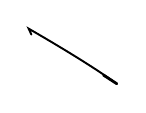
\begin{tikzpicture}[x=1cm,y=1cm,line cap=round]
\draw[line width=0.7pt] (0.035,-0.075) -- (0,0) .. controls (0.33,-0.19) and (0.80,-0.47) .. (1.12,-0.70);
\draw[line width=1.0pt] (0.95,-0.59) -- (1.12,-0.70);
\end{tikzpicture}}
\margin{117}

\scanpage{119}
\mspage{58}

14. Cohomological digression (on \unsure{the|the} ``plugging the
holes).

Let $X$ be a locally noetherian \uline{regular} scheme of
\unsure{dimension} $1$, $S$ a closed subscheme \inserted{reduced discrete} such that
$\forall s\in S$, $\dim_s S=1$ (so $S$ defined by a
closed discrete subset of $X$), $U=X\setminus S$.
\margin{It might perhaps be better to start with \unsure{the purely topological case|the purely topological cases} of a surface\dots{} and make the link with \uline{discrete} groups.}

We want to make explicit by Galoisian means the
étale sheaves \inserted{of sets} \inserted{constructible} on $X$ such that $F\mid U$ is
locally constant. By the \unsure{topos|carpet} of Artin \inserted{on the opens of the topos}, they
correspond to triples
\[
(F_U,F_S,\varphi)
\]
where $F_U$ is a \inserted{constructible} locally constant sheaf on $U$,
$F_S$ a sheaf (\unsure{necessarily|necessarily} locally constant)
and $\varphi$ a morphism
\[
F_S\xrightarrow{\varphi}j^{*}i_{*}(F_U)
\]
(where $i:U\unsure{\hookrightarrow|\to}X$ and $j:S\to X$ are the inclusions).
Any constructibility condition being set
aside, an étale sheaf $F$ on $X$ corresponds
to such a triple --- we restrict ourselves here to the
$F$ such that $F_U$ \deleted{\unsure{comes}} comes from the
fundamental topos $B_{\unsure{\Pi_1(U)|\pi_1(U)}}$ of $U$ \deleted{\illegible{1}}\dots
(There is no need to assume $F_U$ has finite fibers,

\margin{118}

\scanpage{120}

for what follows). \deleted{We are going to}

Let $\forall s\in S$ $\underline{O}_s$ be a henselization of $\underline{O}_{X,s}$,
$D_s=\operatorname{Spec}\underline{O}_s$ \inserted{(``disk at $s$'')}, $D_s^{*}=D_s-\{s\}$ \inserted{$=\operatorname{Spec}K_s$ ($K_s$ field of fractions of $\underline{O}_s$)} (``pointed disk'' at
$s$) $D=\coprod_{s\in S}D_s$, $\unsure{D_s^{*}|D^{*}}=\coprod_{s\in S}D_s^{*}$. We have
a commutative diagram
\diagram{\begin{tikzcd}[ampersand replacement=\&]
\& D^{*} \arrow[dl, "\rho"'] \arrow[dr, "\sigma"] \& \& \\
U \arrow[dr, "i"'] \& \& D \arrow[dl, "\unsure{k|\kappa}"] \& S \arrow[l, dashed, "j_0"'] \arrow[dll, dashed, "j"] \\
\& X \& \&
\end{tikzcd}
[The dotted branch $S\xrightarrow{j_0}D$ is placed in parentheses.]}
and we see \inserted{(by Artin)} that this diagram \deleted{\unsure{makes of}} \inserted{allows us to express}
\inserted{the sheaves} \deleted{topoi} étale on $X$ \deleted{\unsure{as amalgamated}}
\deleted{of the étale topoi of $U,D$ over $D^{*}$}
\deleted{\diagram{\begin{tikzcd}[ampersand replacement=\&,column sep=2.5em,row sep=2em]
\& \deleted{\unsure{D^*_{\mathrm{\acute et}}}} \arrow[dl] \arrow[dr] \& \\
\deleted{U_{\mathrm{\acute et}}} \& \& \deleted{D_{\mathrm{\acute et}}}
\end{tikzcd}}}
as systems \deleted{of sheaves} \inserted{$(F_U,F_D,\varphi)$}
with $F_U$ an étale sheaf on $U$, $F_D$ an étale
sheaf ``essential\textsuperscript{ly} locally constant'' on $D$ [N.B. the
inclusion $S\to D$ defines an equivalence
between the category of these sheaves on $D$, and
that of étale sheaves on $S$] and
a morphism of sheaves $F_D\to\sigma_{*}\rho^{*}F_U$ or again

\margin{119}

\subsection*{Scans 121--130}
\addcontentsline{toc}{subsection}{Scans 121--130}
% package LM_P013
\scanpage{121}
\mspage{59}
% L01
\[
\boxed{\sigma^{*}(F_D)\xrightarrow{\varphi}\rho^{*}(F_U)}
\]
% L02
Now, \deleted{\unsure{this datum if $F_U$ is a}} \inserted{if we restrict ourselves to the} $F_U$ such that $F_U$ is
% L03
itself essentially$^{t}$ locally$^{t}$ constant, then the data
% L04
$F_U,F_D,\varphi$ involve only
% L05
essentially$^{t}$ locally constant sheaves, i.e.
% L06
fundamental topoi (multi-Galois)
% L07
associated with the schemes under consideration, \deleted{\unsure{namely}} thus
% L08
are described entirely in terms of the
% L09
diagrams
\diagram{\begin{tikzcd}[ampersand replacement=\&]
 \& B_{\pi_1,D^{*}} \arrow[dl,"{\deleted{\illegible{1}}\,\rho}"'] \arrow[dr,no head,"\sigma"] \& \\
 B_{\pi_1,U} \& \& B_{\pi_1,D}
\end{tikzcd}}
\margin{(*)}
% L10
-- moreover the case where $\varphi$ is an \uline{isomorphism} corresponds
% L11
precisely to the case of locally essentially
% L12
constant sheaves on $X$, i.e. of sheaves on
% L13
$B_{\pi_1,X}$ -- which fundamental topos
% L14
thus appears as the amalgamated
% L15
sum of the preceding diagram of topoi,
% L16
fitting into the square
\diagram{\begin{tikzcd}[ampersand replacement=\&]
 \& B_{\pi_1,D^{*}} \arrow[dl] \arrow[dr] \& \\
 B_{\pi_1,U} \arrow[dr] \& \& B_{\pi_1,D} \arrow[dl] \\
 \& B_{\pi_1,X} \&
\end{tikzcd}}

\scanpage{122}
% L01
Suppose for simplicity $U$ connected,
% L02
let us choose a universal covering \inserted{$\widetilde U$} of $U$, and a
% L03
universal covering \inserted{$\widetilde D_i^{*}$} of each $D_i^{*}$ -- whence a
% L04
universal covering \inserted{$\widetilde D_i$} of $D_i$ -- and isomorphisms
% L05
(= ``classes of paths'') between $\rho_{!}(\widetilde D_i^{*})$ and $\widetilde U$
% L06
-- thus the diagram of topoi \unsure{(*)},
% L07
-- or of fundamental groupoids --
% L08
is made explicit in terms of a diagram
% L09
\diagram{\begin{tikzcd}[ampersand replacement=\&,column sep=large]
 \& {\begin{gathered}
 (\operatorname{Gal}(\overline K_i/K_i))\\[-2pt]
 \Vert\\[-2pt]
 \mathcal E_i
 \end{gathered}} \arrow[dl,"\unsure{\rho_i|\varphi_i}"'] \arrow[dr,"\sigma_i"] \& \\
 {\begin{gathered}
 \mathcal E\\[-2pt]
 \Vert\\[-2pt]
 (\pi_1(U,\widetilde U)=\operatorname{Aut}_U(\widetilde U))
 \end{gathered}} \& \&
 {\begin{gathered}
 \Gamma_i\;\illegible{1}\\[-2pt]
 \Vert\\[-2pt]
 (\operatorname{Gal}(\overline{k(s)}/k(s)))
 \end{gathered}}
\end{tikzcd}}
% L10
and the datum of an $F$ as considered on
% L11
$X$ amounts to the datum of a system
% L12
$(E_U,(E_i)_{i\in I},(\varphi_i)_{i\in I})$, where $E_U$ is an $\mathcal E$-set,
% L13
$E_i$ a $\Gamma_i$-set, $(\forall i\in I)$, and $\varphi_i$ an
% L14
$\mathcal E_i$-homomorphism from $E_i$ to $E_U$ (i.e. a
% L15
a $\Gamma_i$-homomorphism
\[
\varphi_i:\ E_i\longrightarrow E_U^{\Pi_i},
\]

\scanpage{123}
\mspage{60}
% L01
where \deleted{\unsure{$\Pi_i$ is}} $\Pi_i=\unsure{\operatorname{Ker}(\sigma_i)}$ fits into the exact sequence
% L02
\[
1\longrightarrow\Pi_i\longrightarrow\mathcal E_i\longrightarrow\Gamma_i\longrightarrow1
\]

% L03
The case where the $E_i\longrightarrow E_U$ are isomorphisms,
% L04
i.e. the $E_i$ \unsure{are identified|being identified} \deleted{\illegible{1}} all with $E_U$,
% L05
with trivial action \unsure{of|of the} $\Pi_i$ on $E_U$, corresponds
% L06
to the case where $F$ is essentially locally \unsure{constant|constant} on $X$,
% L07
whence at once
% L08
\[
\pi_1(X)=\mathcal E=\pi_1(U)\ \big/\
\substack{\text{\unsure{normal} subgroup generated}\\
\text{by the }\rho_i(\Pi_i)}.
\]

% L09
Our aim is that of a Galois-theoretic calculation
% L10
(if possible) of the cohomology of $X$ for
% L11
the $F$ under consideration.
% L12
Let $B_{X,U}$ be the topos \inserted{whose sheaves are} triples
% L13
$(F_U,F_D,\varphi)$ as above, which thus maps
% L14
to the topos $B_{\pi_1,X}$, corresponding
% L15
to the pairs for which $\varphi$ is an isomorphism,
% L16
and receives the topos $X_{\mathrm{ét}}$ :

\scanpage{124}
% L01
\diagram{\begin{tikzcd}[ampersand replacement=\&]
X_{\mathrm{ét}} \arrow[r,"f"] \& B_{X,U} \arrow[r,"g"] \& B_{\pi_1,X}
\end{tikzcd}}
% L02
We ask ourselves the question

% L03
a) ``Explicit'' calculation, in terms of the cohomology
% L04
of profinite groups, of cohomology
% L05
in the abracadabra topos $B_{X,U}$. (N.B.
% L06
\deleted{\unsure{b) the calculation of}} the cohomology \deleted{\illegible{1}} of
% L07
$B_{\pi_1,X}$ is none other than the profinite
% L08
Galois cohomology of $\pi_1(X)=\mathcal E/\ldots$
% L09
calculated above\ldots).

% L10
b) Check whether for a torsion
% L11
sheaf $F$ on $B_{X,U}$ the canonical homomorphism
% L12
\[
H^{*}(B_{X,U},F)\longrightarrow
H^{*}(X_{\mathrm{ét}},f^{*}F)
\]
% L13
is an isomorphism.

% L14
N.B. Up to now, the hypothesis
% L15
$\dim X=1$ has not been used, nor the noetherian hypothesis
% L16
-- only the fact that $S$ is a closed discrete
% L17
subset, $X$ connected\ldots. For the calculations which

\scanpage{125}
\mspage{61}
% L01
follow, corresponding to the \deleted{\illegible{1}} case where the
% L02
$\unsure{D_s|O_s}$ are \unsure{gauges} with residue field $k(s)$
% L03
of characteristic $0$, we are going to suppose that
% L04
\[
\Pi_i\simeq\widehat{\mathbb Z}\qquad\text{(not canonically)}
\]
% L05
-- in fact, by Kummer theory we
% L06
have a system of Tate local systems
% L07
$\unsure{T_{\mathcal E}}$ \inserted{(on $\mathcal E$)}, $T_i$ \inserted{(on $\Gamma_i$)}, and \inserted{$\mathcal E_i$-}isomorphisms $T_{\mathcal E}\simeq T_i$, \deleted{and \illegible{1}}
% L08
(i.e. a $T_X$ on which $\unsure{\widetilde{\mathcal E}|\overline{\mathcal E}}=\mathcal E/\ldots$ operates)
% L09
and we shall have a canonical Kummer isomorphism
% L10
\[
T_i\xrightarrow[\sim]{\unsure{\kappa_i|k_i}}\Pi_i.
\]

% L11
We would like to be able to paraphrase,
% L12
on $B_{X,U}$, the well-known exact
% L13
cohomology sequence
% L14
\[
\longrightarrow H^i(X,F)\longrightarrow H^i(U,F)
\longrightarrow H^{i+1}_S(X,F)\longrightarrow\cdots
\]
% L15
relative to the open $U$ of the topos $X$, and its
% L16
closed ``complement'' $S$. Now, \deleted{\illegible{2}} \inserted{just as}
% L17
$X$ fits into a diagram of topoi
% L18
\diagram{\begin{tikzcd}[ampersand replacement=\&]
 \& D^{*}_{\mathrm{ét}} \arrow[dl] \arrow[dr] \& \& \\
 U_{\mathrm{ét}} \arrow[dr,no head] \& \& D_{\mathrm{ét}} \arrow[dl] \& S_{\mathrm{ét}} \arrow[l,"\unsure{\xi}"'] \\
 \& X_{\mathrm{ét}} \& \&
\end{tikzcd}},

\scanpage{126}
% L01
likewise $B_{X,U}$ fits into
% L02
\diagram{\begin{tikzcd}[ampersand replacement=\&]
 \& B_{\pi_1,D^{*}} \arrow[dl] \arrow[dr] \& \& \\
 B_{\pi_1,U} \arrow[dr] \& \& B_{\pi_1,D} \arrow[dl] \& B_{\pi_1,S} \arrow[l,"\approx","\unsure{\xi_{\mathrm{ét}}}"'] \\
 \& B_{X,U} \& \&
\end{tikzcd}}

% L03
[\uline{N.B.} the finite $\varprojlim$ and arbitrary $\varinjlim$
% L04
in $B_{X,U}$ i.e. for the $(F_U,F_D,\varphi)$, are
% L05
calculated ``term by term''] I say
% L06
that $B_{\pi_1,U}\longrightarrow B_{X,U}$ is identified with an
% L07
induction morphism, relative to the
% L08
object \deleted{\illegible{1}} \unsure{(again denoted} $U$ by abuse of notation)
% L09
of $B_{X,U}$ defined by
% L10
$F_U={}$final sheaf $e_U$, $F_D={}$initial sheaf $\varnothing_D$
% L11
(and $\varphi$ \unsure{is|being} then fixed !). Indeed, the
% L12
objects \inserted{of $B_{X,U}$} over $U$ are identified with the
% L13
$(F_U,F_D,\varphi)$ with $F_D=\varnothing_D$ (which $\varphi$ fixes !) so
% L14
they form a category equivalent to that of the
% L15
$F_U$, i.e. to $B_{\pi_1,U}$. We see that the residual
% L16
topos (being identified \deleted{with the} \inserted{with the category of} $F\deleted{_{\unsure{U}},\unsure{E|e}_{\unsure{i}}}=(F_U,F_D,\varphi)$ such

\scanpage{127}
\mspage{62}
% L01
that $F_U=e_U$ final sheaf, is likewise identified with the
% L02
category \inserted{$B_{\pi_1,D}$} of the $F_D$ \deleted{\illegible{2}} -- the
% L03
canonical functor ``inverse image on $B_{\pi_1,D}$ of the direct
% L04
image of $F$ on $B_{\pi_1,U}$'' being none other
% L05
$\sigma_*\rho^*$, so that we recover the description
% L06
\deleted{\illegible{1}} typical of Artin of a topos obtained
% L07
by ``gluing'' an \deleted{\unsure{object}} open and the
% L08
complementary closed.
% L09
We thus find an exact sequence
% L10
\[
\longrightarrow H^i(B_{X,U},F)\longrightarrow
H^i(B_{\pi_1,U},F_U)\longrightarrow
H^{i+1}_{S(\text{or }D)}(B_{X,U},F)\longrightarrow\cdots
\]
% L11
mapping into the analogous exact sequence
% L12
relative to $X_{\mathrm{ét}},U_{\mathrm{ét}},S_{\mathrm{ét}}$. \deleted{\unsure{For} \illegible{2}} \inserted{(We have}
% L13
still not used any special hypothesis on $S$\ldots).

% L14
To check that we have isomorphisms
% L15
at the level of the $H^i(B_{X,U},F)\longrightarrow H^i(X_{\mathrm{ét}},F)$,
% L16
it suffices by the five lemma to
% L17
prove it at the level of the
% L18
$H^i(B_{\pi_1,U},F)\longrightarrow H^i(U_{\mathrm{ét}},F)$ [i.e. \unsure{check|let us check} that the
% L19
cohomology of $U_{\mathrm{ét}}$ ``is calculated Galois-theoretically'']
% L20
\uline{and} at the level of the $H^i_S$. \deleted{\unsure{Now}} Let us look,

\scanpage{128}
% L01
first at the latter -- we have
% L02
$H^0_S(B_{X,U},E)={}$ set of sections of $F$ [i.e. of
% L03
pairs of a section of $F_U$ and
% L04
one of $F_D$, corresponding to each other
% L05
under $\varphi$, i.e. of an element \inserted{$x$} of
% L06
$E_U$ invariant under $\mathcal E$, and of
% L07
$x_i\in E_i$ invariant under the $\Gamma_i$,
% L08
such that $x=\varphi_i(x_i)\quad\forall i$]
% L09
such that $x=0$ \deleted{\unsure{of the|in} \unsure{systems}}
% L10
\[
=\prod_i(\operatorname{Ker}(E_i\longrightarrow E_U)
\]
% L11
we observe that this functor factors
% L12
through the functor $H^0_S$ relative to the ``inclusion''
% L13
\deleted{\unsure{$D^{*}\subset D$} \unsure{or} $B_{\pi_1,D^{*}}\longrightarrow B_{\pi_1,D}$}
% L14
analogous \deleted{\illegible{1} $B_{\pi_1,U}$ \illegible{2}}
% L15
\[
B_{\underbrace{\pi_1,\unsure{D^{*}|D_{*}}}_{\text{replacing }\pi_1,U}}\longrightarrow B_{D,D^{*}}\quad\ldots
\]
% L16
and the $H^i_S$ on $D_{X,U}$ are calculated like
% L17
\deleted{\unsure{which is none other than}}
% L18
those in the local situation $B_{D\deleted{\illegible{1}},D^{*}\deleted{\illegible{1}}}$ --
% L19
where we find the usual calculation in
% L20
terms of the group homomorphism $\mathcal E_i\longrightarrow\Gamma_i$.
\margin{which I have forgotten a bit !}

% L21
But in the present case, the hypothesis $\dim_s X=1$
% L22
at the points of $s\in S$, \deleted{and $X$ \unsure{regular}} implies that
% L23
the localized situation \inserted{of topoi} $D^{*}_{\unsure{a|\mathrm{ét}}}\hookrightarrow D_{\unsure{a|\mathrm{ét}}}$ is already entirely
% L24
defined in terms of the fundamental topoi \unsure{of the}

\scanpage{129}
\mspage{63}
% L01
\deleted{\unsure{of the terms of}}
% L02
i.e. the topos $B_{D,D^{*}}$ is equivalent to
% L03
$D_{\mathrm{ét}}$ -- now the $H^i_S(X_{\mathrm{ét}},F)$ are indeed calculated
% L04
on $D_{\mathrm{ét}}$\ldots We thus find

% L05
\uline{Proposition.} The homomorphism of exact cohomology
% L06
sequences under consideration is an isomorphism,
% L07
provided we know that the homomorphism
% L08
$H^i(\mathcal E,F_{\mathcal E})\xrightarrow{\sim}H^i(U_{\mathrm{ét}},F_U)$ is an isomorphism
% L09
for $\forall i$ ($F_U$ an \unsure{étale|étale local} sheaf on $U_{\mathrm{ét}}$
% L10
defined by a group $F_{\mathcal E}$ on which $\mathcal E=\pi_1(U)$
% L11
operates).

% L12
\uline{Example} : \inserted{OK} If $U$ is an affine curve
% L13
over algebraically closed $k$ \inserted{$F$ \deleted{\illegible{1}} prime to characteristic} (since OK for $i=0,1$, and
% L14
for $i=2$, the two \unsure{sides} are zero
% L15
(the Galois \unsure{cohomology|cohomology}, since the fundamental group
% L16
\inserted{prime to $p$} is \deleted{pro} free\ldots) -- whence we deduce the
% L17
analogous case for $\unsure{U|X}$ affine over arbitrary $k$,
% L18
then even if $U$ is not affine but
% L19
simply quasi-projective ? \deleted{\illegible{1}}
\margin{\uline{Corollary.} In this case, the cohomology of $X$ with coefficients in a locally constant $F_X$ \unsure{is} also calculated Galois-theoretically ? No, because of genus $0$ !!! In the case of smooth projective curves of genus $\ne0$ a special argument is needed.}

% L20
We are now interested in the
% L21
case where $X$ projective \inserted{(connected)} over algebraically closed $k$, \unsure{we thus see|we thus know}

\scanpage{130}
% L01
that : \deleted{the $H^i_!(U,F$}
% L02
a) If $S=\varnothing$ i.e. $X=U$, the cohomology of $U$
% L03
with (coefficients in local systems) is that
% L04
of $\pi$. Thus\ldots a canonical isomorphism
% L05
\[
H^2(\pi,T)\simeq H^2(X,T)\quad(\simeq\widehat{\mathbb Z})
\]
\margin{with \unsure{grain|grains} of salt in characteristic $p>0$}
% L06
\deleted{b) If $S=$}

% L07
b) If $S\ne\varnothing$, the $H^i_!(U,-)$ are \unsure{determined|described}
% L08
and calculated by Galois-theoretic means, in terms
% L09
of the \deleted{\unsure{systems}} \inserted{groups} with loops, making it possible to reconstruct
% L10
the situation
% L11
\diagram{\begin{tikzcd}[ampersand replacement=\&,column sep=large]
 \& B_{\pi_1,D^{*}} \arrow[dl] \arrow[dr] \& \\
 B_{\pi_1,U} \arrow[dr,dotted,no head] \& \&
 {\begin{gathered}
 B_{\pi_1,D}\ (={\text{discrete topos defined}}\\
 {\text{by }}S=I)
 \end{gathered}} \arrow[dl,dashed] \\
 \& B_{U,X} \&
\end{tikzcd}}
% L12
by postulating that the component $B_{\pi_1,D_i^{*}}$
% L13
is none other than $B_{L_i}$ (with the
% L14
\unsure{notations} of the preceding \unsure{number$^{o}$|case}). We
% L15
then find canonical isomorphisms (by local calculations)
% L16
\[
H^2_{\unsure{S_i|s_i}}(B_{U,X},\unsure{L_i})\simeq\widehat{\mathbb Z}
\quad\text{i.e.}\quad
H^2_{\unsure{S_i|s_i}}(B_{U,X},\widehat{\mathbb Z})\simeq L_i^{\otimes-1}
\]
% L17
(if $g\ne0$)
\[
H^2_{\unsure{S_i|s_i}}(B_{U,X},\widehat{\mathbb Z})
\xrightarrow{\sim}H^2(X,\widehat{\mathbb Z})
\simeq H^2(\pi,\widehat{\mathbb Z})
\]
% L18
whence \unsure{in} \deleted{\unsure{summary}} putting together, canonical
% L19
isomorphisms
\[
\deleted{\unsure{H}}\quad L_i\simeq H^2(\pi,\widehat{\mathbb Z})^{\otimes-1}.
\]
\margin{But in all cases (even if $g=0$, so long \unsure{as we} do not have $\nu=0$) \deleted{\illegible{1}} we find $H^{2}_{!}(B_{\pi_1,U},\widehat{\mathbb Z})\simeq\unsure{\widehat T_{\pi}^{\otimes-1}|T_{\pi}^{\otimes-1}}$ canonically, whence a \unsure{cohomological} description of the \unsure{orientation modules}, common to the \unsure{case without holes and with} holes\ldots}

\subsection*{Scans 131--140}
\addcontentsline{toc}{subsection}{Scans 131--140}
% package LM_P014
\scanpage{131}
\mspage{64}

We find that the composites
\[
T_\pi \xrightarrow{\sim} L_i \longrightarrow
H^2(\pi,\widehat{\mathbb Z})^{\otimes-1}
\]
do not depend on the choice of $i$, so that the orientation module $T_\pi$ of the group \inserted{profinite $\pi$} with loops $\pi$ is identified with the \uline{dual} of $H^2(\pi,\widehat{\mathbb Z})$ (if $g\ne0$).

Let us now consider a homomorphism of groups with loops
\[
\begin{gathered}
\pi'\xrightarrow{f}\pi\\
I'_0\xrightarrow{\tau}I
\end{gathered}
\]
associated with an isomorphism $T_{\pi'}\simeq T_\pi$ and a degree map
$d:I'_0\longrightarrow\mathbb N$
\deleted{(\unsure{integers} \illegible{3}}
(N.B. $i'\in I'\setminus I'_0\longrightarrow f(L'_{i'})=(1)$.

We would like to deduce from this a diagram of morphisms of topoi
\diagram{\begin{tikzcd}[ampersand replacement=\&]
B_{\Pi_1 U'} \arrow[r,dash] \arrow[d] \& B_{\deleted{\unsure{\Pi_1}}X',U'} \arrow[r,dash] \arrow[d] \& B_{\Pi_1 X'} \arrow[d] \\
B_{\Pi_1 U} \arrow[r,dash] \& B_{\deleted{\unsure{\Pi_1}}X,U} \arrow[r,dash] \& B_{\Pi_1 X}
\end{tikzcd}}
and a homomorphism \uline{trace} on the cohomology with proper supports of $U',U$ (defined in terms of cohomology on $B_{X',U'}, B_{X,U}$ relatively)
\deleted{\unsure{which an isomorphism}} \unsure{inducing} \deleted{\unsure{for}} an \uline{isomorphism}
\[
H^2_!(U',\widehat{\mathbb Z})\longrightarrow
H^2_!(U,\widehat{\mathbb Z})
\]

\scanpage{132}

which is precisely \inserted{(\unsure{contragredient|contragredient} of)} (the isomorphism of orientation modules associated with $f$....

14. Where we return to \uline{mixed} morphisms (corresponding, in the topological setting, to the case of
$f:(X',S')\longrightarrow(X,S)$ such that we have
$[f(X'\setminus S')\subset X\setminus S$, i.e.\ \inserted{$S'\supset f^{-1}(S)$,} \inserted{but}$]$
\deleted{\illegible{1}} ($S'\ne f^{-1}(S)$, i.e.\ there are points of $\unsure{S'|S}$ that are sent into $U=X\setminus S$.
\margin{$X,X'$ $T$-oriented}

In the topossic and groupoidal \deleted{language} \inserted{paradigm}, $(X,S)$ is \deleted{defined} \inserted{described} by a diagram of groupoids
\[
\Pi_{D^*}\longrightarrow\Pi_U
\qquad
(\text{and }k:T_{\Pi_{D^*}}\simeq
\text{ local system of the }\pi_1\text{ on }\Pi_{D^*})
\]
\deleted{\illegible{1}}
or of topoi
\[
B_{D^*}\longrightarrow B_U
\]
and \deleted{\unsure{an}} isomorphism \inserted{$k$} of the local system of the $\pi_1$ on $B_{D^*}$, into the \inserted{locally} constant system $T$,
\deleted{\illegible{4} $(\deleted{\unsure{X}},U')$}
\inserted{which allows us to define $B_D\;(=B_{\unsure{\pi_0 D_*}})$ (the discrete topos)}
and the topos $B_{X,U}$, fitting into the diagram \deleted{$\unsure{B_{\Pi_1 D^*}}$} of topoi

\scanpage{133}
\mspage{65}

\diagram{\begin{tikzcd}[ampersand replacement=\&,column sep=large]
\& B_{D^*}\arrow[dl,"\rho"']\arrow[dr,"\sigma"] \& \\
B_U\arrow[dr,"\varphi"'] \&\& B_D\; (\text{discrete topos }\xleftarrow{\sim} B_S)\arrow[dl,"\psi"] \\
\& B_{X,U} \&
\end{tikzcd}}
where $\varphi,\psi$ are morphisms of \unsure{inclusion|induction} of subtopoi, $\varphi$ open $\psi$ closed, complementary to one another, and likewise for $(X',S')$, described by an analogous diagram
\diagram{\begin{tikzcd}[ampersand replacement=\&]
\& B_{D'^*}\arrow[dl]\arrow[dr] \& \\
B_{U'}\arrow[dr] \&\& B_{D'}\simeq\unsure{B_{S'}|B_S}\arrow[dl] \\
\& B_{X',U'} \&
\end{tikzcd}}

That said, we absolutely want, in a description of
$f:(X',S')\longrightarrow(X,S)$, for it to allow us to recover not only $B_{U'}\longrightarrow B_U$ (which will be secured by giving an $f_\pi:\pi'\longrightarrow\pi$), but also
\[
B_{X',U'}\longrightarrow B_{X,U}\qquad\unsure{g|q}.
\]
We will have \deleted{\unsure{$S$}}
\[
S'=\underset{\substack{\Vert\\f^{-1}(S)}}{S'_0}\amalg S'_1,
\quad\text{hence}\quad D'=D'_0\amalg D'_1,
\]

\scanpage{134}
\mspage{66}

and in fact $f$ induces $S'_1\xrightarrow{f}U$ (and not $S'_1\longrightarrow S$) which must be made explicit, at the level \deleted{\illegible{2}} of multi-Galois topoi, by a morphism
\diagram{\begin{tikzcd}[ampersand replacement=\&]
B_{D'_1}\arrow[r] \& B_U \\
B_{S'_1}\arrow[u,"\simeq",draw=none] \&
\end{tikzcd}}
i.e.\ by giving a family of universal coverings of $U$, parameterized by $S'_1=I'_1$, or (\unsure{if such a} universal covering is chosen, $U$ being connected, hence a $\pi=\operatorname{Aut}(\widetilde U)$) by a family of torsors under \deleted{\unsure{the}} $\pi$, $(P_{i'})_{i'\in I'_1}$.
This being \deleted{\unsure{defined}} \inserted{laid down} we \unsure{will be able to} describe, in terms of
\diagram{\begin{tikzcd}[ampersand replacement=\&,column sep=3.5em,row sep=3em]
B_{D_0'{}^*} \arrow[r,no head] \arrow[d] \& B_{U'} \arrow[d] \\
B_{D^*} \arrow[r,no head]
\arrow[ur,bend left=30,shorten <=1.5em,shorten >=1.5em,"\sim"'] \& B_U
\end{tikzcd}}
and of
\[
B_{D_1'^*}\longrightarrow B_{D'_1}\longrightarrow B_U
\]
\deleted{\unsure{a}} the morphism of topoi $B_{X',U'}\longrightarrow B_{X,U}$
% a small double tick stands before $B_{X',U'}$ (below $B_{D'_1}$ of the display above): probably the call of the marginal note
--- I pass over the details of the description
\margin{It seems that we are entitled to give the description of the morphisms of topoi $B_{X',U'}\longrightarrow B_{X,U}$ that induce $U'\longrightarrow U$ and that on $D_1'^*$ \unsure{$(=D'^*\vert U$} \deleted{\illegible{2}}, factor through $D_1'^*\longrightarrow D'_1$...}

\scanpage{135}

When we give ourselves a group of operators \deleted{$\Sigma$}$\Gamma$ on the situation $(X',S')\longrightarrow(X,S)$ hence on the groupoidal or topossic situation, we must take this into account in the description above.
Thus $I'_0$ and $I'_1$ are stable under $\Gamma$, and the morphism \deleted{\illegible{1}} $B_{\unsure{D'_1}}\longrightarrow B_U$ must be stable under $\Gamma$.
\deleted{So we have a \unsure{nice} set $\unsure{E_f=\bigcup E_i}$ ---}
\deleted{In terms of a universal covering $\widetilde U$ of $U$, let us consider the \deleted{\illegible{1}} sets $\unsure{\operatorname{Hom}}(f_*(\unsure{s'_{i'}}),\widetilde U)$}
Which also means, probably, that we have a morphism of topoi from
$B_{D'_1,\Sigma}=B_{I'_1,\unsure{\Sigma|\Gamma}}$
into $B_{U,\deleted{\Sigma}\Gamma}$.
Choosing for every orbit of $\Gamma$ in $I'_1$ a representative $s'\in I'_1$, and considering its stabilizer $\Gamma_{s'}\subset\Gamma$, we must therefore for every such orbit i.e.\ \deleted{\unsure{every}} every $i'$ give ourselves a $\Gamma_{s'}$-object of the category of universal coverings of $(U,\Gamma)$.
\unsure{Simultaneously|Equivalently} \deleted{therefore} Describing $(U,\Gamma)$ in terms

\scanpage{136}
\mspage{67}

of an extension $\mathcal E$ of $\Sigma\subset\Gamma$ by $\pi$ (by choosing a universal covering $\widetilde U$ of $U$), the datum of $B_{\Gamma_{s'}}\longrightarrow B_{X,U}$ compatible with everything amounts unless I am mistaken to the datum of a right torsor $P$ under $\pi$ (allowing us to twist the \unsure{reference} universal covering $\widetilde U$ of $\unsure{U^\Gamma|U,}$ with $P$ \deleted{and} \inserted{hence also to twist $\mathcal E$ by $P$}), and of a splitting of $\mathcal E^P\longrightarrow\Gamma$ over $\Gamma_{s'}$.
[The isomorphism class of such an object $\longrightarrow$ a $\pi$-conjugacy class of splittings of $\mathcal E\longrightarrow\Gamma$ over $\Gamma_{s'}$... ).

An automorphism of such a pair \deleted{corresponds} $P,\ \Gamma_{s'}\xrightarrow{q}\mathcal E^P$ corresponds to an $\alpha\in\pi$ that \uline{centralizes} $\Gamma_{s'}$, \inserted{i.e.\ that is fixed by $\Gamma_{s'}$ operating on $\pi$.} (If the $\Gamma_{s'}$ operate strongly enough on $\pi$ for us to know that $\pi^{\Gamma_{s'}}=(1)$, the object $(P,q:\Gamma_{s'}\longrightarrow\mathcal E^P)$ is defined up to \uline{unique isomorphism} by the isomorphism class \deleted{\unsure{of it}} (class of splittings of $\mathcal E$ over $\Gamma_{s'}$).
\margin{\unsure{!!!|[three vertical strokes]}}
It seems probable to me that this is always the case in the \uline{arithmetic} case, where $\Gamma_{s'}$ is an open subgroup of the Galois group $\Gamma_{\unsure{k|K}}$ (whose outer operation is \inserted{draconian !}).

\scanpage{137}

This goes in the direction of the conjecture that a splitting class of $\mathcal E$ over $\Gamma$ is ``as good'' as a rational point of $U$ over $K$ --- and allows us to paradigm what such a rational point would allow us to obtain....

\textcircled{15} \uline{Return to the topological case} Let $\Gamma$ be a finite group operating on a group with loops $\pi$ --- let us suppose that this comes from a topological situation, $\Gamma$ operating on $(X,S)$. There are points to check (\uline{\unsure{anabelian|anabelian}} cases)
\margin{Structure of the critical $\Gamma$-orbits in terms of extension...}

\[
\text{a) Operation of }\Gamma\text{ trivial}
\quad\Longleftrightarrow\quad
\underset{\text{trivial}}{\Gamma\longrightarrow\operatorname{Autext}(\pi)}
\]
in other words : an automorphism of finite order of $(X,S)$ can be isotopic to the identity (or even \inserted{merely} homotopic, it comes to the same thing anyway) only if it is trivial.

This is even known in ``abstract'' Algebraic Geometry, once we admit that $u$ \unsure{preserves|preserves} a \deleted{\unsure{complex}} \inserted{complex} structure, \deleted{\unsure{conformal}} \inserted{\unsure{this is precisely}}

\scanpage{138}
\mspage{68}

so if we \deleted{suppose} \inserted{admit} that there is no wildness.... Probably every action of a finite group $\Gamma$ leaves conformal structure invariant, \deleted{\illegible{1}} hence its restriction to
\[
\Gamma^0=\operatorname{Ker}(\Gamma\xrightarrow{\chi}\{\pm1\})
\]
leaves complex structure invariant.

Let us suppose from now on that $\Gamma$ operates faithfully, \inserted{$\Gamma\ne1$,} \deleted{\illegible{1}} The choice of a complex structure on $Y=X/\Gamma^0$ \inserted{defines one on $X$;} (N.B.: \deleted{\illegible{1}} $\Gamma/\Gamma^0$ still operates \inserted{on $X/\Gamma^0$} in fact \deleted{$X/\Gamma^0$} \unsure{if} $\Gamma\ne\Gamma^0$ i.e.\ $\Gamma/\Gamma^0\simeq\{\pm1\}$, $X/\Gamma^0$ is endowed with a ``structure of a \deleted{\illegible{2}} real algebraic curve \inserted{conformal structure}''... ) stable under $\Gamma^0$ --- and (stable under $\Gamma$ if we choose that of $Y$ \deleted{\unsure{invariant}} \inserted{left invariant} under \unsure{the element|the element} nontrivial in $\Gamma/\Gamma^0$ (if there is one).).
\margin{\unsure{works|as} every time we have a ramified covering of conformal surfaces}

\deleted{Now} Every $x\in U^\Gamma$ defines a class \deleted{\illegible{1}} \inserted{\deleted{\unsure{class}} of $\pi$-conjugacy of} splittings of the extension $\mathcal E$ of $\Gamma$ by $\pi$, as we see by taking $x$ as base point. ! Note that $U^\Gamma$ is a finite set \inserted{if $\Gamma^0\ne1$, [i.e.\ $\Gamma$ not reduced to an \deleted{\illegible{1}} \unsure{anti-involution} \illegible{1})}.
\margin{\uline{N.B.} $U^\Gamma\ne\varnothing$ implies that $\Gamma^0$ is cyclic...}
We find \deleted{therefore} a map
\[
U^\Gamma\longrightarrow\text{set of classes of }\pi\text{-conjugacy of splittings of }\mathcal E\longrightarrow\Gamma,
\]

\scanpage{139}
\mspage{69}

i.e.\ \unsure{set|to the} of liftings of $\Gamma\longrightarrow\operatorname{Autext}\pi$ \inserted{to} $\Gamma\longrightarrow\operatorname{Aut}(\pi)$, modulo $\pi$-conjugation.

\uline{Question} \inserted{(If $\Gamma^0\ne(1)$)} Is this map bijective ??

[If $\Gamma^0=\{1\}$, $\Gamma/\Gamma^0\simeq\{\pm1\}$, then $X^\Gamma$ is the set of real points of a real algebraic curve and $U^\Gamma=X^\Gamma-S^\Gamma$ is the complement of a finite subset in it, we have
\[
\pi_0(X^\Gamma-S^\Gamma)\longrightarrow
\pi\text{-classes of splittings of }\mathcal E\text{ over }\Gamma
\]
and the \deleted{\illegible{1}} \uline{analogous} question of bijectivity arises, for extensions of $\pm1$ by $\pi$... ]

For the injectivity of the map in the case $\Gamma^0\ne(1)$, we may suppose $\Gamma=\unsure{\Gamma^0_a|\Gamma^0}\simeq\mathbb Z/p\mathbb Z$, with $p$ prime, i.e.\ $\Gamma$ generated by a complex automorphism \inserted{$\unsure{\gamma|y}$} of order $p$, which defines (if $x,y\in U^\Gamma$, $x\ne y$) an automorphism of order $p$ of $\pi_1(U,x)$, \deleted{\unsure{say}} $u_x$, \unsure{that is} \deleted{a} (hence $\pi$-conjugacy class of automorphisms of $\pi$ of order $p$), and another $u_y$.
We have to prove that $u_x,u_y$ are not conjugate under $\pi$

\scanpage{140}

\uline{Theorem} Let $\unsure{U|X}$ be \deleted{\unsure{a surface}} a connected topological \inserted{space} \inserted{(\deleted{\illegible{2}}, by paths)}, $\Gamma$ a finite group operating \deleted{faithfully} on $U$, $\widetilde U$ a universal covering of $U$, hence \deleted{operating} an extension group
\[
1\longrightarrow\pi\xrightarrow{i}\mathcal E\xrightarrow{p}\Gamma\longrightarrow1
\]
operating faithfully on $\widetilde U$ ($\pi=\operatorname{Aut}_U(\widetilde U)\simeq\pi_1(U)$... ).
For every fixed point $x\in U^\Gamma$, $\Gamma$ operates on the universal covering \unsure{punctured|pointed} over $x$, say \deleted{\illegible{1}} $\unsure{R_x|\mathcal R_x}$, leaving fixed the point \inserted{marked} $\widetilde x$ of $\unsure{R_x}$ over $x$, hence a splitting of the extension relative to $\unsure{R_x}$
\diagram{\begin{tikzcd}[ampersand replacement=\&]
1\arrow[r] \& \pi_x\arrow[r,"i_x"] \& \mathcal E_x\arrow[r,"p_x"] \& \Gamma\arrow[r]\arrow[l,bend left=40,"\sigma_x"] \& 1
\end{tikzcd}}
and for every \deleted{choice of path} \inserted{isomorphism} $\ell$ \inserted{(``path'')} $\unsure{R_x}\simeq\widetilde U$, inducing an isomorphism of extensions $\mathcal E_x\xrightarrow{\sim}\mathcal E$ (defined \unsure{of|in} modulo composition with an inner automorphism induced by an $\alpha\in\pi$... ) we find \uline{by transport} of structure a splitting $\sigma_{x,\ell}$ of $\mathcal E\xrightarrow{p}\Gamma$, (which, for varying $\ell$, is defined up to an inner automorphism by an $\alpha\in\pi$).
We thus find a map
\[
(*)\quad U^\Gamma\longrightarrow
\begin{gathered}
\text{classes of }\pi\text{-conjugacy of splittings}\\
\text{of the extension }\mathcal E\text{ of }\Gamma\text{ by }\pi\\
=\text{classes of }\pi\text{-conjugacy of subgroups }\inserted{\unsure{sections}}\ \Gamma'\text{ of }\mathcal E
\end{gathered}
\]

\subsection*{Scans 141--150}
\addcontentsline{toc}{subsection}{Scans 141--150}
% package LM_P015
\scanpage{141}
\mspage{70}

The image of this map thus consists of the \inserted{$\pi$-conjugacy classes of the} section subgroups $\Gamma'\subset\mathcal E$ such that $\widetilde U^{\Gamma'}\ne\varnothing$, and for such a $\Gamma'$, the set of \unsure{$x\in U^\Gamma$} which \deleted{\unsure{to it}} give as image this conjugacy class is the image of $U^{\Gamma'}$ in $U$. Finally, if $x$ is in this image, the set \inserted{$\widetilde U^{\Gamma'}_x$} of the $\widetilde x\in\widetilde U^{\Gamma'}$ over $x$ (\deleted{\unsure{$\ne\varnothing$}} hypothesis on \unsure{a|x}) is a torsor under $\pi^{\Gamma'}$ i.e. if $\widetilde x\in(\widetilde U^{\Gamma'})_x$, \deleted{\unsure{of}} and if $\alpha\in\pi$, then
\[
\alpha.\widetilde x\in\widetilde U^{\Gamma'}\quad\Longleftrightarrow\quad\alpha\in\pi^{\Gamma'}
\]
(Trivial verification, as for that matter all the preceding assertions). Thus, the following conditions are equivalent:

\margin{N.B. \unsure{$\widetilde U_x$} being identified with \unsure{$\operatorname{Isom}_U(R_x,\widetilde U)$}, $\widetilde U_x^{\Gamma'}$ is identified with \unsure{$\operatorname{Isom}_{U,\Gamma}(R_x,\widetilde U_{\Gamma'})$} \unsure{of the two isomorphisms that commute|of covering isomorphisms commuting} with the action of $\Gamma$ and $\pi^\Gamma=(1)$ means that this isomorphism is unique \unsure{i.e.} \deleted{\illegible{3}} \unsure{the conjugacy class of the sections} \illegible{2}.}

 a) $(*)$ is a bijection, and $\forall$ subgroup $\Gamma'$ of $\mathcal E$ a section of the extension, \deleted{\illegible{1}} we have $\pi^{\Gamma'}=\{1\}$.

 b) $\forall\,\Gamma'$ as in a), $\Gamma'$ operating on $\widetilde U$ has a fixed poin\textsuperscript{t} and only one.

This being so, let us prove the

\uline{Fundamental lemma} Let $\Gamma$ be a \inserted{finite} finite group, operating faithfully on \inserted{a space} \unsure{$D$}\,$\simeq\mathbb R^2$, let \deleted{We assume $\Gamma=$} $\Gamma^\circ$ be the subgroup of $\Gamma$

\mspage{140}

\scanpage{142}

(of index $0$ or $1$) consisting of the $g\in\Gamma$ such that $g_D$ preserves the orientation, and suppose $\Gamma^\circ\ne\{1\}$ (i.e. $\Gamma$ is reduced neither to the trivial group, nor to the group \deleted{\illegible{1}} $\{1,\sigma\}$, where $\sigma$ is an anti-involution of $D$. Then

 a) $\Gamma$ has a fixed poin\textsuperscript{t} and only one in $D$ i.e. $\operatorname{card}D^\Gamma=1$

 b) \deleted{\unsure{And}} $\Gamma^\circ$ is cyclic, and if $\Gamma\ne\Gamma^\circ$, $\Gamma$ is a \inserted{dihedral} group.

More precisely, there exists a homeomorphism
\[
D\simeq\mathbb C
\]
such that \deleted{$\Gamma$ operates by automorphisms} \inserted{\unsure{on $\mathbb C$ by the group}} \deleted{\illegible{1}} of homeomorphisms of $\mathbb C$ transformed from \deleted{complex and anti-complex of $\mathbb C$} \deleted{\unsure{fixing}} $\Gamma$ is either the group of homotheties by $\mu_n(\mathbb C)$ (if $\Gamma=\Gamma^\circ$ of order $n$), or the associated dihedral group \unsure{$z\longrightarrow\zeta\tau^\varepsilon(z)$} ($\zeta\in\mu_n(\mathbb C)$, $\varepsilon=\pm1$) where \unsure{$\sigma$} \deleted{\illegible{1}} is complex conjugation.

\uline{Proof of the fundamental lemma.}

\deleted{Suppose first $\Gamma=\Gamma^\circ$, i.e. $\Gamma$ preserves the orientation. \deleted{If $\Gamma$ operated \unsure{without a poin\textsuperscript{t}}} We proceed}

\mspage{141}

\scanpage{143}
\mspage{71}

\deleted{By induction on the order of $\Gamma$.}

\deleted{\unsure{a)} \unsure{$D^\Gamma\ne\varnothing$}}

\deleted{a) Case $\Gamma$ of prime order}

 a) Suppose first that one can find a $C^2$ structure on $D$ invariant under $\Gamma$ --- then a standard argument shows that there exists a conformal structure invariant under $\Gamma$, now the fundamental theorem of conformal mapping shows that then
\[
\begin{aligned}
&\text{either }D\simeq\text{interior}\ \inserted{\Delta}\ \text{of the unit disk }\Delta\ \inserted{\text{or of the Poincaré half-plane}}\\
&\text{or }D\simeq\mathbb C\qquad\text{(conformal isomorphisms).}
\end{aligned}
\]
In the first case, the group of conformal automorphisms \deleted{maps} is
\[
\simeq\unsure{\operatorname{Sl}(2,\mathbb R)^\sim\,|\,\operatorname{Gl}(2,\mathbb R)^\sim}
=\{u\in\operatorname{Gl}(2,\mathbb R)\mid\det u=\pm1\}
\]
(\deleted{operating by} $u=\left(\begin{smallmatrix}a&b\\c&d\end{smallmatrix}\right)$ operating on \deleted{\illegible{1} Poincaré} \inserted{$\widehat{\mathbb C}$} by \deleted{\unsure{$z\longmapsto\dfrac{az+b}{cz+d}$}} $\Theta_u\circ\tau^{\det u}$, where $\tau$ is complex conjugation and $\Theta_u(z)=\dfrac{az+b}{cz+d}$, and leaving the Poincaré half-plane stable), and every compact subgroup is \inserted{contained in a} conjugate of the maximal compact \uline{subgroup}, which (on passing back to the unit disk \inserted{$\Delta$}) is identified with the group $O(2,\mathbb R)$ of

\mspage{142}

\scanpage{144}

transformations of the unit disk of the form
\[
z\longrightarrow\zeta\tau^\varepsilon(z)\qquad
\begin{gathered}
\zeta\in\mathbb U=\{\zeta\in\mathbb C\mid |\zeta|=1\}\\
\varepsilon\in\{\pm1\}\\
\tau\ \text{complex conjugation}
\end{gathered}
\]
Every finite subgroup of this group is of one of the types made explicit above --- we win, by using a \unsure{homeomorphism} $[0,1[\longrightarrow[0,+\infty[$ to define a homeomorphism \deleted{\illegible{1}} $\Delta\simeq\mathbb C$ commuting with the action of $G=\deleted{\unsure{S}}O(2,\mathbb R)$.

In the case $D\simeq\mathbb C$, we see that \deleted{\unsure{is}} the group of conformal automorphisms of $\mathbb C$ is the group of transformations $az+b$ or $a\overline z+b$, in which a maximal compact subgroup is the same group $\deleted{\unsure{S}}O(2,\mathbb R)$ as just now --- and every compact subgroup (a fortiori, every finite subgroup) is contained in a conjugate of this one. We win again.

The rest of the work consists \inserted{essential\textsuperscript{ly}} in \deleted{eliminating} showing that the hypothesis of non-wildness

\mspage{143}

\scanpage{145}
\mspage{72}

is always satisfied, \inserted{at least for $\Gamma^\circ$. Suppose first $\Gamma=\Gamma^\circ$.} \deleted{We assume} \inserted{We assume} that all is proved for \deleted{the groups} \inserted{the orders} $<\operatorname{card}(\Gamma)$. \deleted{Suppose}

 b) $\Gamma$ has a fixed poin\textsuperscript{t} \inserted{\unsure{$o$|$0$}}, i.e. $D^\Gamma\ne\varnothing$.

Otherwise, the stabilizer subgroups \inserted{$\Gamma_x$} of the $x\in D$ being of order $<$ \deleted{\illegible{1}} $\operatorname{card}\Gamma$, by the induction hypothesis, the $\Gamma_x$ have the structure stated in the theorem, hence \unsure{$D^\Gamma=U$|$D/\Gamma=U$} is a topological surface and \unsure{$D\longrightarrow U$|$D\longrightarrow D^\Gamma$} is a ramified covering, let us choose a \deleted{complex conformal} \inserted{conformal} structure on $U$ \deleted{N.B. $U$ is oriented}; there is a unique conformal structure on $D$ such that $D\longrightarrow U$ is \deleted{\unsure{conformal|holomorphic}} \inserted{``conformal''} (holomorphic or anti-holomorphic), this is invariant under $\Gamma$, and by a) $\Gamma$ has a fixed poin\textsuperscript{t}, contradiction.

 c) $\Gamma$ has no fixed poin\textsuperscript{t} other than \unsure{$o$|$0$}. We let $\Gamma$ operate \inserted{\unsure{faithful\textsuperscript{ly}}} on \unsure{$D^*=D\setminus\{o\}$|$D^*=D\setminus\{0\}$}, and we have to prove that $D^{*\Gamma}=\varnothing$.

\mspage{144}

\scanpage{146}

Let then $x\in D^{*\Gamma}$ --- we are going to reach a contradiction. Consider the universal covering $\widetilde D^*$ of $D^*$ pointed at $x$, \deleted{We may assume} so $\Gamma$ operates on $\widetilde D^*$ \unsure{with} a fixed poin\textsuperscript{t} $\widetilde x$ over $x$. Here $\pi=\pi_1(D^*)\simeq\mathbb Z$, and $\Gamma$ operates on it \unsure{trivial\textsuperscript{ly}} (since $\Gamma=\Gamma^\circ$) so $\Gamma\times\mathbb Z$ operates on $\widetilde D^*$. We may assume $D=\mathbb C$, \unsure{$o=0$|$0=0$}, $x=1$, $D^*=\mathbb C^*$, $\widetilde D^*=\mathbb C$, $\widetilde x=0$, $\widetilde D^*\longrightarrow\widetilde D$ given by $\exp 2i\pi z$, \deleted{\unsure{so}} and $\mathbb Z$ operating on $\mathbb C$ by $\Theta_nz=z+n$ ($n\in\mathbb Z$).

\deleted{Lemma} It remains to prove that if a \inserted{finite group} $\Gamma$ operates on $\mathbb C$ commuting \deleted{\unsure{with}} with the action of $\mathbb Z$ on $\mathbb C$, and leaving \deleted{a poin\textsuperscript{t}} fixed the poin\textsuperscript{t} \unsure{$o$|$0$}, then $\Gamma$ operates trivially (which contradicts the hypothesis of faithfulness of the operation).

\deleted{So} We are reduced to the.

\uline{Lemma} Let $u$ be a homeomorphism \inserted{of finite order} of $\mathbb C$,

\mspage{145}

\scanpage{147}
\mspage{73}

commuting with $z\longmapsto z+1$, and leaving the origin invariant. Then $u=\operatorname{id}$

We may assume \deleted{$u$ of prime order} $\exists$ prime number $p$ such that $u^p=\operatorname{id}$, i.e. that $u$ corresponds to an operation of $\Gamma=\mathbb Z/p\mathbb Z$ on $\mathbb C$. \inserted{All the poin\textsuperscript{ts} of $\mathbb Z\subset\mathbb C$ are fixed by $\Gamma$.} Passing to $\widehat{\mathbb C}\simeq S^2$, we find that $\infty$ is an accumulation poin\textsuperscript{t} of the fixed poin\textsuperscript{ts} under $\Gamma$ --- if $\Gamma$ did not operate trivially, this would be decidedly very wild! We ought to be able to finish by the Adams spectral sequence... I am not going into these mazes...

 d) The purely topological part being \unsure{admitted|thus} \unsure{assumed|assumed} \unsure{proved|proved}, we thus conclude from this, if $\Gamma\ne\Gamma^\circ$, $\Gamma^\circ\ne(1)$, \deleted{that the unique} \inserted{as} \deleted{fixed poin\textsuperscript{t} of} \inserted{$D^{\Gamma^\circ}$} is invariant under $\Gamma$, \deleted{that} \inserted{as} $D^{\Gamma^\circ}$ is reduced to a poin\textsuperscript{t}, this one is invariant under all of $\Gamma$, not just $\Gamma^\circ$. On the other hand, We know enough now to know that if $\Gamma$ finite group operates on a surface \deleted{Hausdorff} \inserted{paracompact $U$}, the $\Gamma_x$ ($x\in U$) respecting the orientation, then \unsure{$U/\Gamma=V$}

\mspage{146}

\scanpage{148}

is a surface --- \inserted{and $U\longrightarrow V=U/\Gamma$ is a ramified covering} and choosing a conformal structure on this one, we find by inverse image a conformal structure on $U$ invariant under $\Gamma$, \deleted{and} \inserted{For the case $U=D$} we finish by a), \deleted{but} for the complement to the fundamental lemma. [But to do things properly, one would have to prove that there always exists invariant conformal structure, \deleted{\illegible{2}} $\Gamma$ finite group operates on surfaces \deleted{\illegible{1}} \unsure{paracompact} --- so $U/\Gamma$ is a surface with boundary.... Here what is missing is the analysis of the action of an anti-involution of a surface in a neighborhood of a fixed poin\textsuperscript{t}...]

\margin{One would have to prove that if $\tau$ is an involutive \unsure{anti-automorphism} of $D$, then $\exists$ isomorphism $D\simeq\mathbb C$ such that $\tau$ becomes $z\longmapsto\overline z$ (hence $D^\tau\simeq\mathbb R$!) which should make it possible to prove, if $\Gamma\simeq\mathbb Z/2\mathbb Z$ operates by anti-automorphisms on $U$ (\unsure{oriented|orientable} $U\ne S^2$) that $\pi_0(U^\Gamma)$ \unsure{$\Longrightarrow$} \unsure{$\pi$-conjugacy classes of sections of $\mathcal E$ over $\Gamma$} is bijective.}

Consequence of the fundamental lemma:

\uline{Theorem.} Let $U$ be a paracompact topological surface \inserted{$0$-connected}, $\Gamma$ a finite group operating \uline{faithfully} on $U$, we assume $\widetilde U$ \deleted{\illegible{1}} noncompact (i.e. $U$ not homeomorphic to $S^2$ nor

\mspage{147}

\scanpage{149}
\mspage{74}

to the real projective plane), we assume that \deleted{\unsure{$\Gamma\ne(1)$}, \illegible{1}} that \inserted{moreover} if $U$ is \deleted{not} orientable, then \deleted{\unsure{$\Gamma\ne\{\pm1\}$} i.e. $\operatorname{card}\Gamma\ge3$ \illegible{1}} \deleted{we} assume that the subgroup $\Gamma^\circ$ of $\Gamma$ of the $g\in\Gamma$ which preserve an orientation is $\ne(1)$ [hence $\Gamma$ \unsure{not reduced} either to $1$, or to \unsure{$1$ and|Id} an anti-involution], and if $U$ nonorientable, that \deleted{\unsure{cardinality}} $\Gamma$ \unsure{$\not\simeq$|$\ne$} $(1),\{\pm1\}$ i.e. $\operatorname{card}\Gamma\ge3$. This being so, \deleted{\unsure{the map}} let us consider \deleted{the map} \inserted{the extension} $\mathcal E$ of $\Gamma$ by $\pi=\pi_1(U)$, and the map
\[
U^\Gamma\longrightarrow\begin{gathered}
\text{Classes of }\pi\text{-conjugacy of}\\
\text{splittings of }\mathcal E\longrightarrow\Gamma
\end{gathered}
\]
we have this:

 a) This map is bijective

 b) For every section subgroup $\Gamma'\subset\mathcal E$, we have $\pi^{\Gamma'}=(1)$

 c) If $U^\Gamma\ne\varnothing$ i.e. If there exists a splitting, then $\Gamma$ is cyclic or dihedral (and in the case $U$ oriented, $\Gamma^\circ$ is cyclic)

\uline{N.B.} The hypotheses on $U$ ensure that $\widetilde U\simeq D$, and those on $\Gamma$ that $\Gamma$ operating on $D$ satisfies the hypotheses of the fundamental lemma.

\mspage{148}

\scanpage{150}

\deleted{\uline{Corollary-Scholium}, For an $x\in U^\Gamma$ corresponding to a splitting class of the extension $\mathcal E$, we find that the splittings of this class, \deleted{on which $\mathcal E$ operates by \unsure{inner automorphisms|functoriality}}, form a \deleted{\unsure{$\mathcal E$-set which is a}} $\pi$-torsor, \deleted{and the automorphisms of}}

\uline{Corollary} Suppose \deleted{that} $U$ \unsure{orientable}, \deleted{\illegible{1}} $\Gamma$ preserving the orientation. Let $U^!$ be the set of the $x\in U$ such that $\Gamma_x\ne(1)$. (which is therefore a discrete subset of $U$).

To every $x\in U^!$, let us associate the conjugacy class of the subgroups of $\mathcal E$ \inserted{partial \inserted{\unsure{$\pi$}} sections of $\mathcal E$ over $\Gamma_x$} which \unsure{correspond|corresponding} to \unsure{this|this} $x\in U^{\Gamma_x}$. Then

 a) \deleted{the map} the partial sections thus obtained are \uline{maximal} among those which are $\ne(1)$

 b) The map from $U^!$ to \unsure{the set|one} of the $\pi$-conjugacy classes of maximal partial sections \deleted{nontrivial} \inserted{$\ne(1)$}, is bijective

\margin{\uline{N.B.} This map commutes with the natural actions of $\Gamma$!}

 c) For every such partial section, we have $\pi^{\Gamma'}=(1)$, i.e. the \deleted{\unsure{$\Gamma_x$-}} \unsure{automorphisms} of the \inserted{universal} covering \unsure{$R_x$} of $U$ which commute with the action of $\Gamma_x$ are trivial

--- there is a unique isomorphism \inserted{commuting with the action of $\Gamma_x$} between this torsor, and the torsor deduced from $\widetilde U$ by twisting by the $\pi$-torsor \deleted{\unsure{of the}} $P_x$ of the \unsure{$\Gamma''$} in the class \deleted{\illegible{1}} \unsure{$[\Gamma']$}...

\mspage{149}

\subsection*{Scans 151--160}
\addcontentsline{toc}{subsection}{Scans 151--160}
% package LM_P016
\scanpage{151}
\mspage{75}

Let us prove a). Let \(\Gamma'\subset\mathcal E\) be
\inserted{a partial section over \(\Gamma_x\)}
deduced from \(x\in U^!\).
Let \(\Gamma''\supset\Gamma'_x\) be another \unsure{subgroup|subgroup}
\inserted{let \(\unsure{\Gamma_1}\supset\Gamma_x\) be its image \unsure{in|of} \(\Gamma\)}
such that \(\Gamma''\cap\pi=(1)\) i.e. \(\Gamma''\hookrightarrow\Gamma\)
\inserted{\illegible{1}}.
By the preceding theorem, it is defined by a unique
\unsure{\(y\in U^{\Gamma_1}\)|\(y\in U^{\Gamma''_*}\)},
and it is clear that this \(y\) does not change if we replace the action of
\(\unsure{\Gamma_1}\) on \(U\) by the action of a smaller group
\(\ne(1)\) (and the induced section) such as \(\Gamma_x\),
hence \(\unsure{\Gamma_1}\) \deleted{\illegible{1}} fixes \(x\) hence
(by definition of \(\Gamma_x\)) \(\Gamma_1=\Gamma_x\) hence
\(\Gamma''=\Gamma'\), \deleted{\unsure{q.e.d.}}

\deleted{\unsure{The injectivity}}\inserted{b)}
Let \(x,y\) give the same image
\([\Gamma']\ [\Gamma'']\), hence \(\Gamma_x=\Gamma_y\), say \(\Gamma_1\),
and applying the \unsure{theorem} to \(\Gamma_1\) operating on \(U\),
we find \(x=y\).
Let, on the other hand, \(\Gamma'_0\) be a maximal partial section \(\ne1\),
\(\Gamma_0\subset\Gamma\) its image,
by the theorem \inserted{applied to the action of \(\Gamma_0\) on \(U\),}
\(\exists x\in U\) \deleted{\unsure{fixed}} such that
\(x\in U^{\Gamma'_0}\) i.e. \(\Gamma'_0\subset\Gamma_x\),
and such that \([\Gamma'_0]\) is defined by \(x\),
but if \([\Gamma']\) is defined by \(x\) for the action of
\(\Gamma_x\) in its entirety, we will have \([\Gamma'_0]\subset[\Gamma']\),
hence by the maximal character of \([\Gamma'_0]\), we will have
\([\Gamma'_0]=[\Gamma']\), which \deleted{\illegible{1}} proves b).
On the other hand c) is clear.

\margin{150}

\scanpage{152}

Let us now return to the case where \(U=X\setminus S\), \(X\) a compact
\(T\)-oriented surface and \(S\) a finite
subset, anabelian case --- so we have a
\inserted{``fully} faithful'' description of \(U\) by a \(\pi\) with
loop structure, and we would like to convince ourselves
that \deleted{\illegible{2}} the \inserted{outer} operation of \(\Gamma\)
on \(\pi\), when \(\Gamma\) preserves orientation (to simplify)
also \unsure{suffices} to describe fully the object
\((U,\Gamma)\) in the appropriate isotopic category.
\margin{we should return to the general case for \unsure{what follows}\ldots}

We already recover a description of \(\unsure{U^!}\) in terms of
the action of \(\pi\), let \(J\) \inserted{\((\simeq U^!)\)},
the set of \(\pi\)-conjugacy classes
\deleted{moreover for every \(x\)}
of maximal partial sections \inserted{\(\ne1\)} of
\(\mathcal E\) over \(\Gamma\),
For every \(j\in J\), \(j\) is a \inserted{\(\pi\)-}torsor
as a
\inserted{\(\pi\)-}conjugacy class of sections
[that it is a \(\pi\)-torsor follows from
\(\pi^{\Gamma'}=(1)\), a priori
\deleted{\unsure{it is a \(\pi/\pi^{\Gamma'}\)-torsor}}
\inserted{\unsure{the stabilizer|the stabilizers} of \(\Gamma'\)}
is precisely \(\pi^{\Gamma'}\)]
In fact,

\margin{151}

\scanpage{153}
\mspage{76}

the set of \unsure{all} these \deleted{\unsure{classes}} maximal partial
sections is naturally an \(\mathcal E\)-set
(by conjugation) \deleted{\unsure{and}} on which \(\pi\) operates freely, and this
\(\mathcal E\)-set is canonically identified with
\(\widetilde U|U^!=\widetilde U^!\), for the structure of
\(\mathcal E\)-sets.

Let \(S'=S\cup U^!\), hence \(U'=X\setminus S'\),
we must try to reconstruct
(in terms of the extension \(\mathcal E\) of \(\Gamma\) by the group with
loops \(\pi\)) the \inserted{outer} group with loops corresponding
to \(\unsure{X'},S'\) i.e. to \(U'\), and the \deleted{extension}
\inserted{outer action} of \(\Gamma\) on it.
\deleted{\unsure{We hope to find a} \illegible{5}}
\deleted{\(\unsure{=}\) \illegible{5} \unsure{obvious}}

But first we should make sure of the intrinsic character of the
definition of \(J\) \unsure{\((\simeq U^!)\)|\((\simeq\widetilde U^!)\)}
\inserted{as a \(\Gamma\)-set,}
in terms of the \deleted{the action} \deleted{of the}
outer group \(\pi\), and of the outer action
\deleted{of \(\unsure{\Gamma}\)} of \(\Gamma\) on it.

\margin{152}

\scanpage{154}

This is rather obvious moreover
(in terms \inserted{precisely} of the
\inserted{\(\pi\)-}conjugacy classes of partial liftings of
\(\unsure{\Gamma\to\operatorname{Autext}(\pi)}\) to
\(\operatorname{Aut}(\pi)\)), we would however also like an
intrinsic description of \(\widetilde U|U^!\),
\unsure{in|or} a paradigm for the map of
\(\Gamma\)-spaces \(\unsure{U^!\longrightarrow U}\)
we must therefore describe a morphism of topoi with operation of \(\Gamma\) on it
\diagram{\begin{tikzcd}[ampersand replacement=\&]
B_J \arrow[r,"\unsure{\rho}"] \& B_{\unsure{\mathcal E}}
\end{tikzcd}}
which therefore corresponds to an \deleted{\unsure{morphism}} 
``inverse image'' functor \(\unsure{\rho^*|?^*}\)
(compatible with action of \(\Gamma\))
\deleted{\illegible{1}}
\diagram{\begin{tikzcd}[ampersand replacement=\&,row sep=2.5em,column sep=4em]
B_{\unsure{\mathcal E}} \arrow[r] \arrow[d,phantom,"\simeq"{description,rotate=90}] \& B_J \arrow[d,phantom,"\simeq"{description,rotate=90}] \\
\pi\text{-Sets} \& \mathrm{Ens.}\ \text{over }J
\end{tikzcd}}

This \deleted{\unsure{which}} is nothing other than the contracted product over
\(\pi\) with the set of maximal partial sections \(\ne1\) of
\(\mathcal E\) over \(\Gamma\)

\margin{153}

\scanpage{155}
\mspage{77}

Let us return to the extension \(\mathcal E\) of \(\Gamma\) by \(\pi\)
\deleted{\unsure{with faithful operation of \(\Gamma\)}}
arising from a geometric situation
(which extension, in the anabelian case, is already defined in terms
of an outer operation of \(\Gamma\) on \(\pi\))
we know that it satisfies additional
draconian conditions!
\inserted{\deleted{\unsure{to}} (To formulate them, we will assume the action of
\(\Gamma\) faithful):}
every subgroup \(\Gamma'\subset\mathcal E\) such that
\(\Gamma'\cap\pi=(e)\) (``partial section'') is
\inserted{cyclic (if \(\Gamma'=\Gamma'{}^0\)) or}
\deleted{\illegible{1}} dihedral,
\inserted{(if \(\Gamma'\ne\Gamma'{}^0\))}
and the set of \(\pi\)-conjugacy classes of such subgroups
is finite.
Every section subgroup \(\Gamma'\ne1\) is contained in a unique
\inserted{section} subgroup that is \uline{maximal}.
\margin{\unsure{good|so}
\figure{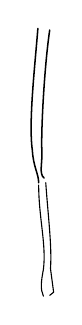
\begin{tikzpicture}[x=1mm,y=1mm,baseline=(current bounding box.center),line cap=round,line join=round]
\draw[line width=0.55pt] (0,34) .. controls (-0.4,29) and (-1.2,22) .. (-0.7,18.5) .. controls (-0.6,16.5) and (0.1,15.5) .. (0.1,14.4);
\draw[line width=0.40pt] (0.1,14.1) .. controls (0.1,10) and (1.1,6.5) .. (0.7,3.4) .. controls (0.4,1.8) and (0.3,0.9) .. (0.7,0);
\draw[line width=0.55pt] (1.5,33.8) .. controls (0.8,29) and (0.4,21) .. (0.5,18.5) .. controls (0.6,16.9) and (0.1,15.5) .. (0.8,15.0);
\draw[line width=0.40pt] (1.0,14.4) .. controls (1.3,10.1) and (1.8,6.3) .. (1.6,3.5) -- (2.0,0.5) -- (1.5,0.1);
\end{tikzpicture}}}

(We have established it at least in the case
\(\Gamma=\Gamma^0\), we should return to the general case,
I think it remains true as it stands, to be checked\ldots)
\margin{\figure{[A vertical stroke to the left of the two lines
``I think \ldots{} checked\ldots)''.]}}
Moreover, we saw an \uuline{additional structure} appear
on the group \(\mathcal E\)
[which in the anabelian case is identified with a subgroup of
\(\operatorname{Aut}(\pi)\)], namely a map
\[
\mu_{\mathcal E}:
\text{elements }\inserted{u}\text{ of finite order in }\mathcal E
\longrightarrow T\otimes\mathbb Q/\mathbb Z,
\]
\unsure{obtained} by noting that if \(u\in\mathcal E\) is of finite order
\(n\), \unsure{whence} \(\mathbb Z/n\mathbb Z\lhook\joinrel\xrightarrow[i]{}
\mathcal E\), \unsure{we have|i.e.} \(\operatorname{Im}i\cap\pi=(1)\)
(\(\pi\) has no torsion elements), hence
\(\mathbb Z/n\mathbb Z\hookrightarrow\Gamma\), \unsure{whence|of a} subgroup
\(\Gamma_1\subset\Gamma\) (i.e. the image of
\margin{\uline{N.B.} For a \(u\) of finite order in \(\mathcal E\),
we must \unsure{know|have}, if \(u\notin\mathcal E^0\),
that \(u\) \unsure{is} of order \(2\) exactly,
\illegible{5} to \unsure{define} \(\mu(u)\)!}

\margin{154}

\scanpage{156}

\(\unsure{u}\) in \(\Gamma\) has the same order \(n\)),
and the lifting \(\Gamma_1\hookrightarrow\mathcal E\) defines an
\(x\in U^{\Gamma_1}\), \deleted{such that} and \(u_1\) operating on \(U\)
while leaving \(x\) fixed therefore corresponds in a neighborhood of \(x\) to a
``multiplier'', which (for a chosen local orientation) is a
primitive \unsure{\(n\)th} root of \(1\) i.e. an element of
\(\mathbb Z/n\mathbb Z\), and which for varying orientation
is interpreted intrinsically as an element of
\(T\otimes\mathbb Z/n\mathbb Z
\subset T\otimes\mathbb Q/\mathbb Z\).

The map \(\mu\) satisfies the obvious conditions
\[
\begin{gathered}
\left\{
\begin{aligned}
\mu(\alpha u\alpha^{-1})&=\mu(u) &&\text{if }\alpha\in\pi\\
\mu(u^n)&=n\mu(u) &&\text{if }n\in\mathbb Z
\end{aligned}
\right.\\
\text{order }\mu(u)=\text{order of }u
\end{gathered}
\]
I do not know whether this map \(\mu\) \deleted{is}
\inserted{can be} defined intrinsically in terms of the extension
\(\mathcal E\), or whether on the contrary there can exist two extensions
\deleted{\unsure{isomorphic}} \(\mathcal E,\mathcal E'\) of \(\Gamma\) by \(\pi\),
defined by geometric situations, of \(\Gamma\) operating on
\(U\) resp. \(U'\), and an isomorphism of extensions
\(\mathcal E\longrightarrow\mathcal E'\) which is not compatible with
the functions \(\mu,\mu'\).
The simplest nontrivial case to look at is the

\margin{155}

\scanpage{157}
\mspage{78}

abelian case (where \(\pi\simeq\mathbb Z\)
\inserted{\deleted{\illegible{1}} \((\operatorname{card}I=2)\)}
or \(\pi\simeq\mathbb Z^2\) (\deleted{\unsure{cardinality}} \(I=\varnothing\))),
In the \inserted{first} case
\deleted{of an extension} \(\pi\simeq\mathbb Z\), \unsure{we|\deleted{the}}
\inserted{must have (to have a faithful action of
\(\Gamma=\Gamma^0\))}
\deleted{extensions \illegible{1}}
\(\Gamma^0\) cyclic, \(\mathcal E\simeq\mathbb Z\),
there is no element of finite order in \(\mathcal E\) except
\(\unsure{1|e}\), so the question does not arise.
The case \(\pi\simeq\mathbb Z^2\) is more interesting,
\deleted{\unsure{and can be reformulated}}

If \(\pi\) is a free \(\mathbb Z\)-module of
\deleted{\unsure{finite type}}\inserted{\unsure{rank \(n\)}}, we have an exact sequence
\diagram{
\begin{tikzcd}[ampersand replacement=\&,column sep=small,row sep=small]
0 \arrow[r] \& \pi \arrow[r] \& \pi\otimes_{\mathbb Z}\mathbb R
\arrow[r] \& X_0(\pi) \arrow[r] \arrow[d,dash] \& 0\\
\& \& \& \substack{\text{Torus of dimension}\\ n\text{ associated to }\pi} \&
\end{tikzcd}
}
and if \(\Gamma\) operates on \(\pi\), the cohomology exact sequence
(taking into account \(H^i(\Gamma,\pi\otimes_{\mathbb Z}\mathbb R)=0\)
for \(i>0\)) gives
\diagram{
\begin{tikzcd}[ampersand replacement=\&,column sep=large,row sep=small]
H^2(\Gamma,\pi) \& H^1(\Gamma,X_0(\pi)) \arrow[l,"\sim" {anchor=south}]\\
\substack{\text{\unsure{extension class|extension classes}}\\
\text{of }\Gamma\text{ by }\pi}
\&
\substack{\text{classes of}\\X_0(\pi)\text{ torsors,}\\
\text{with operation of }\Gamma\text{ on them}\\
\text{compatible with its}\\\text{action on }X_0(\pi)}
\end{tikzcd}
}

thus the datum of an extension \(\mathcal E\) of \(\Gamma\) by \(\pi\)
amounts essentially to that of a
\unsure{\(\Gamma\)-\(X_0(\pi)\)-torsor} \(X\)
(inhomogeneous \(n\)-torus on which \(\Gamma\) operates --- hence it operates
on its group of translations \(X_0\), hence on
\(\pi=\pi_1(X_0,0)\)\ldots).
If it were true \inserted{for \(n=2\)} that every operation

\margin{156}

\scanpage{158}

of \(\Gamma\) on a toroidal surface \((\simeq S^1\times S^1)\)
is isomorphic to such a standard action, then the intrinsic character
of the map \(\mu\) in this case would be established
--- which would not for all that \unsure{make} the computation
of \(\mu\) uninteresting, which takes its values in
\(T\otimes\mathbb Q/\mathbb Z\), where here
\[
T\simeq\bigwedge\nolimits_{\mathbb Z}^{2}\pi
\quad
(\text{\unsure{dual|dimension\ 2} of }H^2(\pi,\mathbb Z)\simeq
\bigwedge\nolimits^{2}
\underbrace{H^1(\pi,\mathbb Z)}_{
\substack{\unsure{\downarrow|\simeq}\\ \pi^\vee}}).
\]

The question comes down to this: We have a \uline{split} extension
of a cyclic \deleted{\unsure{group}}\inserted{\unsure{group}}
\(\mathbb Z/n\mathbb Z\) with generator \(u\) by \(\pi\)
--- thus described entirely by an automorphism
\deleted{of order} \(\unsure{\theta}\) of \(\pi\) such that
\(\theta^n=\operatorname{id}_\pi\)), describe \unsure{in} terms of
this an element of \(T\otimes\mathbb Q/\mathbb Z\).

Answer: the \unsure{standard|standard of which} geometric situation
corresponds to \(X=X_0(\pi)\), with \(0\) as a fixed point under \(\Gamma\).
If \(u\) reverses orientation, it is of order \unsure{\(1\) or|i.e.} \(2\),
there is no problem, otherwise it is \deleted{in} in
\(\pi\otimes_{\mathbb Z}\mathbb R\) a rotation around \(0\)
(of order \(2,3,4\) or \(6\)) which is readily specified by an element
of \deleted{\illegible{1}} \(T\otimes\mathbb Z/\nu\mathbb Z\)
(if \(\nu\) is \unsure{of order|the order}).
It is also (if we identify
\(T\otimes\mathbb Z/\nu\mathbb Z\) with
\(\mu_\nu(\mathbb C^*)\), assuming
\(T\simeq\mathbb Z\) given
i.e. \(\pi\) oriented i.e. \(X_0(\pi)=\unsure{X}\)
oriented) \uline{one} of the two

\margin{157}

\scanpage{159}
\mspage{79}

eigenvalues of \(u\otimes_{\mathbb Z}\mathbb C\)
(automorphism of the vector space over \(\mathbb C\) of dimension \(2\)
\(\pi\otimes_{\mathbb Z}\mathbb C\)).

This shows us, in the case of algebraic geometry over an algebraically closed field
\(\Omega\), that if \(X=X_0\) is an elliptic curve
\(u\) an automorphism of finite order, we have as a paradigmatic
description not \uline{only}
\(\pi=\pi_1(X,0)\)
\inserted{(\(\widehat{\mathbb Z}\)-module free of rank \(2\)),}
(and the action of \(u\) on \(\pi\)), but as an
\uline{additional} structure one of the two solutions \uline{in \(\Omega\)}
of the characteristic equation of \(u\) (with integer coefficients)
\[
T^2+aT+b=0
\qquad (a=-\operatorname{Tr}u,\ b=\unsure{\det u}).
\]

It is clear that this additional structure cannot be deduced
from knowledge of the action of \(u\) on \(\pi\) alone.
\margin{\figure{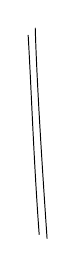
\begin{tikzpicture}[x=1mm,y=1mm,baseline=(current bounding box.center),line cap=round]
\draw[line width=0.35pt] (0,25.8) .. controls (0.4,19) and (0.7,10) .. (1.4,0.5);
\draw[line width=0.35pt] (0.9,26.7) .. controls (1.1,19.7) and (1.8,8.8) .. (2.4,0);
\end{tikzpicture}}
for \(\unsure{\Omega}=\mathbb C\)
\illegible{2} \unsure{comes down to}
\illegible{1} \uline{\unsure{orientation|orientations}} of
\illegible{1}}
But there remains the question whether this \deleted{\unsure{latter}}
\inserted{\unsure{\(\mu(u)\in\mu_n^*(\Omega)\)}}
can be deduced from knowledge at least of the
\inserted{outer} action of \(u\) on the group
``with \(1\) loop'' corresponding to the geometric situation
--- i.e. an \inserted{outer} automorphism
\deleted{\illegible{2}} of order \(n\) \unsure{of} such a group
(or whether here again one must decidedly regard it as an additional
datum).
\margin{yes, it can, thanks to the consideration of the
``subgroups \illegible{2} of \(\mathcal E\)''
\illegible{2} which define extensions
\diagram{\begin{tikzcd}[ampersand replacement=\&,row sep=2.5em,column sep=2em]
\unsure{1} \arrow[r] \& T \arrow[r] \arrow[dr,dotted,no head,"\unsure{n_i\,\mathrm{id}_T}"'] \& \mathcal E_i \arrow[r] \arrow[d,phantom,"\simeq"{description,rotate=90}] \& \Gamma_i \arrow[r] \& 1 \\
\& \& T \& \&
\end{tikzcd}}
whence \(\unsure{\Gamma_i\simeq T/n_iT}\)
\illegible{2}}
But if this were indeed so, it would imply on the other hand that the
construction of \unsure{\(u\in\) group|these groups} with

\margin{158}

\scanpage{160}

(1) loop(s), with the operation of \(\Gamma\) on it, cannot be carried out
either with the help of the mere \deleted{\illegible{2}}
knowledge of the action of \(\Gamma\) (\(=\mathbb Z/n\mathbb Z\))
on \(\pi\).
It is this question of ``drilling holes'' that we must therefore in the end,
at the very end, tackle!

As for the question of whether
\deleted{\illegible{1}}\inserted{in}
\deleted{\illegible{1}} the \uline{anabelian case},
the map
\[
\mu:\underbrace{{}_\infty\mathcal E}_{
\substack{\text{\unsure{set of}}\\
\text{\unsure{elements}}\\
\text{of finite order in }\mathcal E}}
\longrightarrow T\otimes\mathbb Q/\mathbb Z)
\]
is deducible from the action of \(\Gamma\) on \(\pi\)
[if it is faithful, \(\mathcal E\) is thus identified with a subgroup
of \(\operatorname{Autext}_{\unsure{\ell|l}}(\pi)\)
and we may ask whether \(\mu\) is not
\inserted{then} definable on this in its entirety],
or \unsure{it is|whether it is} an additional datum one must have in order to
reconstruct the geometric situation --- the question remains entirely open.
\margin{this does indeed seem \unsure{so}, taking into account
\illegible{1} that for \(\Gamma\) \uline{solvable},
\illegible{3}, we know \illegible{1}
that every action \deleted{\illegible{1}} of \(\Gamma\) on \(\pi\)
\illegible{3} \unsure{realize geometrically}}

\textcircled{16}\quad
\uuline{Plugging and drilling holes:}
General \unsure{topos-theoretic} \uline{preliminaries}

Let us consider a situation
\diagram{
\begin{tikzcd}[ampersand replacement=\&]
B_{D^*} \arrow[r] \& B_U
\end{tikzcd}
}
(of multi-Galois topoi)
\margin{N.B. such a situation
\inserted{of topoi \unsure{describes}} \(2\)-faithfully the topological situations \((X,S)\),
or \(U\), provided that no irreducible component of \(U\)
is \(\simeq S^2\) ---}

\margin{159}

\subsection*{Scans 161--170}
\addcontentsline{toc}{subsection}{Scans 161--170}
% package LM_P017
\scanpage{161}
\mspage{80}
% Lignes 1--5 (continuation de la note marginale de la page précédente).
\illegible{2}, and \unsure{to the} \deleted{\unsure{the}} fact that they remain \inserted{very} close to the language \unsure{and|\deleted{and}} to topological intuition, it is superior to the $p^t$ of view ``groups with loops'', which corresponds to the computational approach rather.)

% Lignes 5--16 : grand passage encadré et barré par des traits obliques.
\deleted{, let us be given \deleted{a subset subtopos} (\inserted{\unsure{necessarily$^t$}} \unsure{open}) $B_{D_1^*}$ of $B_{D^*}$ (corresponding to a subset $I_1$ of $I=\pi_0(B_{D^*})$) so that
\[
 B_{D^*}\simeq B_{D_0^*}\amalg B_{D_1^*}
\]
\margin{($D_0^*$ corresponds to the subset $I_0=I\setminus I_1$ of $I$)}
We have an analogous decomposition
\[
 B_D\simeq B_{D_0}\amalg B_{D_1}.
\]
\inserted{\unsure{definition} $B_{\pi_0(D^*)}=B_S$}
Consider the topos \unsure{$B_U'$} ``amalgamated sum'' of \deleted{\unsure{$B_U$}}
\diagram{\begin{tikzcd}[ampersand replacement=\&]
 \& B_{D_1^*}\arrow[dl]\arrow[dr] \& \& \\
 B_U \& \& B_D\arrow[r,leftrightarrow,"\unsure{\sim}"] \& B_S
\end{tikzcd}}
}

% Lignes 17--24.
I realize that I need to return to the notation for the \deleted{\illegible{1}} \inserted{various} topoi associated with such a datum. But I am going to be guided by the situation of numbers$^\circ$ .-- where we have a regular scheme \inserted{$X$} of dimension 1, a closed subscheme \inserted{$S$} of dimension 0, whence $U=X-S$ --- in this case \deleted{\illegible{2}} $\unsure{S_{\text{ét}}|X_{\text{ét}}}$ can \textcircled{not} be reconstructed from $B_{D^*}$ as $\unsure{B_{\pi_0 B_{D^*}}|B_I}$
\mspage{160}


\scanpage{162}
% Lignes 1--7.
with $I=\pi_0(B_{D^*})$, we must take into account the residue fields $k(s)$ $(s\in S)$ i.e. the Galois groups $\operatorname{Gal}(\overline{k(s)}/k(s))$. So there is reason to return to a starting situation (which is adapted to the \inserted{arithmetico-}geometric case) of morphisms of \uuline{multi-Galois} topoi
\[
 (*)\qquad
 \diagram{\begin{tikzcd}[ampersand replacement=\&]
 \& B_{D^*}\arrow[dl,"\rho"']\arrow[dr,"\sigma"] \& \\
 B_U \& \& B_S
 \end{tikzcd}}
\]
% Lignes 8--14.
(Careful, we write $B_S$, not $B_D$, which will have another meaning), \uline{where} $\sigma$ \uline{induces an isomorphism on the} $\Pi_0$ [and is surjective on the $\operatorname{Hom}$]. For the moment, we are not going to make any particular hypothesis on this situation, which for $B_U$ connected, and in terms of the choices
% Lignes 15--23 : crochet et parenthèses tels que visibles.
[\deleted{of objects $\widetilde D_i^*\in\unsure{D}$} of universal coverings $\widetilde D_i^*$ of the connected components $D_i^*$ of $D^*$, and of a universal covering $\widetilde U$ of $B_U$, and of the isomorphism between the $\rho_!(\widetilde D_i^*)$ and $\widetilde U$) is made explicit by the datum of a group \inserted{$\mathcal E$ (or} $\Pi$) $(=\operatorname{Aut}(\widetilde U))$ \deleted{\unsure{and}} \inserted{$\mathcal E_i$ (or} $\Pi_i$ $(=\operatorname{Aut}(\widetilde D_i^*))$ \deleted{\illegible{2}} $(i\in I)$, $\Gamma_i$ $(i\in I)$
\mspage{161}


\scanpage{163}
\mspage{81}
% Lignes 1--3 et premier diagramme.
and group homomorphisms
\diagram{\begin{tikzcd}[ampersand replacement=\&,row sep=2em,column sep=2.5em]
\& \unsure{\mathcal E_i} \arrow[dl,no head,"\rho_i"'] \arrow[dr,"\sigma_i"] \& \\
\unsure{\mathcal E} \& \& \Gamma_i
\end{tikzcd}}
with the $\sigma_i$ surjective. \deleted{\unsure{and}}
% Lignes 3--10.
[When there is a base field $K$ for the geometric situation, then in the \unsure{topos-theoretic} description, \inserted{\unsure{putting} $e=\operatorname{Spec}K$ and} denoting by $B_e$ the étale topos \inserted{$e_{\text{ét}}$} of $e$, i.e. $B_\Gamma$ \unsure{where|if} $\Gamma=\operatorname{Gal}(\overline K/K)$, the diagram $*$ fits into
\diagram{\begin{tikzcd}[ampersand replacement=\&]
 \& B_{D^*}\arrow[dl,"\rho"']\arrow[dr,"\sigma"] \& \\
 B_U\arrow[dr,"\varphi"'] \& \& B_S\arrow[dl,"\psi"] \\
 \& B_e \&
\end{tikzcd}},
with a commutativity datum for the square considered\unsure{\ldots\ as considered} at the beginning of these notes].

% Lignes 11--18 et dernier diagramme.
In terms of $*$, we construct by ``gluing'' of $B_U$ and \inserted{of} $B_S$ (via the gluing functor $\sigma_*\rho^*$) a mixed topos, which is no longer multi-Galois in general, previously denoted $\unsure{D_{X,U}|B_{X,U}}$, and which \inserted{\unsure{I prefer}} now \deleted{\illegible{1}} \unsure{to denote|denoted} $B_{X;S}$ \deleted{\illegible{2}} \inserted{[to recall that these are sheaves on $X$, but having singularities only on $S$]} \deleted{\illegible{1} fits into a}. It fits into a diagram of topoi
\diagram{\begin{tikzcd}[ampersand replacement=\&,row sep=2em,column sep=2.5em]
\& B_{D^*} \arrow[dl] \arrow[dr] \& \\
B_U \arrow[dr,""{name=xl,description}] \& \& B_S \arrow[dl,""{name=xr,description}] \\
\& B_{X;S} \&
\arrow[from=xr,to=xl,bend right=25,"\alpha_X"]
\end{tikzcd}}
with an arrow
\mspage{162}


\scanpage{164}
% Lignes 1--5.
``of commutation'' $\alpha$ which is such only by abuse of language --- it is not an isomorphism \deleted{of \unsure{functors}} but a morphism of functors and nothing more
\[
 \sigma^*\psi^*\deleted{\unsure{u}}\xrightarrow{\alpha_X}\rho^*\varphi^*.
\]
% Lignes 6--11.
In the same way, gluing $D^*$ and $S$ via $\sigma_*$ (i.e. replacing $B_U$ by $B_{D^*}$ in the preceding construction of $\unsure{D_{X;S}|B_{X;S}}$), we find a topos, not multi-Galois in general, denoted $B_{D;S}$. In the \deleted{\unsure{present}} geometric model where we have $X,S$ as above,
% Lignes 12--18.
$B_X$ corresponds to sheaves on $X$ which are \unsure{essentially|set|in} locally constant on $U$ (and on $S$, where they have no merit) i.e. on $U$ arise by inverse image \deleted{of a sheaf} \inserted{under} $U\longrightarrow B_{\Pi_1 U}$ from a sheaf on $B_{\Pi_1 U}$.

% Lignes 19--25.
and in the same way $B_{D;S}$ corresponds to sheaves on $D=\coprod_i\operatorname{Spec}(\mathcal O_i=\text{henselization of }\mathcal O_{X,\unsure{i|s}})$ \deleted{which are} which are locally constant on $D^*=D-S$ (and on $S$, without merit!) but with the dimension hypothesis made -- --- \unsure{in|we} fact
\[
 B_{D;S}\simeq D_{\text{ét}}
\]
($D_i$ has only 2 points, $D_i^*=\{\eta_i\}$ --- ). Thus $B_{D;S}$ \unsure{$(\simeq D_{\text{ét}})$}
\mspage{163}


\scanpage{165}
\mspage{82}
% Lignes 1--2 et diagramme supérieur.
(when we start from $X,S$) fits into a triangle of morphisms of topoi
\diagram{\begin{tikzcd}[ampersand replacement=\&,row sep=2em,column sep=2.5em]
\& B_{D^*} \arrow[dl,equals,""{name=deq,description}] \arrow[dr,"\sigma",""{name=dsig,description}] \& \\
B_{D^*} \arrow[dr,"\varphi_D"'] \& \& B_S \arrow[dl,"\psi_D"] \\
\& B_{D;S} \&
\arrow[from=dsig,to=deq,bend left=22,"\alpha_D"']
\end{tikzcd}}
\margin{\uline{N.B.} in the geometric case, \deleted{\illegible{1}} \unsure{three} topoi of this diagram are étale topoi ($D^*_{\text{ét}},D_{\text{ét}},S_{\text{ét}}$) and the arrows $\varphi_D$ and $\psi_D$ correspond to \unsure{morphisms} \unsure{but not} \illegible{1} of topoi)}
% Lignes 3--4.
$\alpha_D$, like $\alpha_X$ above, is just a plain homomorphism (not an isomorphism in general).

% Lignes 5--14.
\deleted{We thus find a \unsure{topos.}}
When we speak of the canonical morphism from $B_{D^*}$ to $B_{D;S}$ it is \inserted{of} $\varphi_D$ (and not of $\psi_D\sigma$) that we are speaking --- in the geometric case we have $B_{D^*}\simeq D^*_{\text{ét}}$, and $\varphi_D$ corresponds to the inclusion of schemes
\[
 D^*\unsure{\supset|=}D\setminus S\longrightarrow D
\]
\inserted{and $\psi_D:B_S\longrightarrow B_{D;S}$ to the inclusion of schemes $S\longrightarrow D$}
whereas neither $\sigma$ nor $\psi_D\sigma$ correspond in general to morphisms of schemes.

% Lignes 15--16 et diagramme inférieur entièrement barré.
We thus obtain a diagram of topoi
\deleted{\diagram{\begin{tikzcd}[ampersand replacement=\&,row sep=3em,column sep=4em]
\& B_{D^*}
\arrow[dl,"\unsure{\rho_X}"',"\deleted{\unsure{B_{D^*}}}"{description,pos=0.56},"\deleted{\unsure{\varphi_D}}"{pos=0.25}]
\arrow[dl,bend right=38,"\deleted{\unsure{\illegible{1}}}"']
\arrow[dr,"\sigma"{xshift=0.65em,yshift=0.55em}]
\arrow[d] \& \\
B_U \arrow[dr,"\varphi"',""{name=oldl,description}] \& B_D \arrow[d] \& B_S \arrow[l] \arrow[dl,"\psi",""{name=oldr,description}] \\
\& B_X \&
\arrow[from=2-1,to=2-2,phantom,"\text{commutative}"{description,yshift=1.3em}]
\arrow[from=1-2,to=2-3,phantom,"{\begin{gathered}\text{pseudo-}\\[-0.4ex]\text{commutative}\end{gathered}}"'{pos=0.65,xshift=-1.9em,yshift=-0.5em}]
\arrow[from=2-2,to=2-3,phantom,"\text{commutative}"{description,yshift=-1.3em}]
\arrow[from=oldr,to=oldl,bend right=20,"\deleted{\unsure{\illegible{1}}}"]
\end{tikzcd}}
where in the geometric case}
\mspage{164}


\scanpage{166}
% Diagramme supérieur (**).
\[
 (**)\qquad
 \diagram{\begin{tikzcd}[ampersand replacement=\&, column sep=large,row sep=small]
 \& \& \uline{B}_S\arrow[dl]\arrow[dd,"{\Vert}" description] \\
 \uline{B}_{D^*}\arrow[r]\arrow[dd]\arrow[urr] \& B_{D;S}\arrow[dd] \& \\
 \& \& \uline{B}_S\arrow[dl] \\
 \uline{B}_{\unsure{U}}\arrow[r] \& B_{X;S} \&
 \end{tikzcd}}
\]
\margin{Careful, the triangle is not essentially commutative, but \unsure{we have} pseudo-commutativity\ldots}
% Lignes 1--5.
where the three underlined topoi $\uline{B}_U$, $\uline{B}_S$ and $\uline{B}_{D^*}$ are multi-Galois, and $B_{D;S}$ and $B_{X;S}$ are composite (obtained by gluing two multi-Galois topoi).
\inserted{Unless I am mistaken the two squares are [\uline{not} only essentially$^t$ commutative but also] 2-cartesian (in the 2-category of topoi).}

% Lignes 6--12 et diagramme médian.
Passing to the $B_{\Pi_1}$? of the topoi considered (corresponding to the locally constant objects on these topoi) we find \inserted{a topos} $B_{\deleted{\Pi_1}X}$ \inserted{$=\unsure{B_{\Pi_1 B_{X,S}}|B_{\Pi_1 B_{X;S}}}$} as an amalgamated sum of topoi in the \deleted{$B_{\Pi_1 X}$} diagram
\diagram{\begin{tikzcd}[ampersand replacement=\&,row sep=2em,column sep=2.5em]
\& B_{D^*} \arrow[dl] \arrow[dr] \& \\
B_U \arrow[dr,""{name=pl,description}] \& \& B_S \arrow[dl,no head,""{name=pr,description}] \\
\& B_{\deleted{\unsure{\Pi_1}}X} \&
\arrow[from=pr,to=pl,bend right=25,"\sim"]
\end{tikzcd}}
% Lignes 13--19.
(this square is indeed essentially commutative) and in the same way (replacing $B_U$ by $B_{D^*}$) a $B_{\deleted{\Pi_1}D}$, which is however (via $B_S\longrightarrow B_{\deleted{\Pi_1}D}$) isomorphic \inserted{(rather: \unsure{equivalent|equal})} to $B_S$. The diagram $(**)$ then becomes
\mspage{165}


\scanpage{167}
\mspage{83}
% Diagramme supérieur (***).
\[
 (***)\qquad
 \diagram{\begin{tikzcd}[ampersand replacement=\&, column sep=large,row sep=small]
 \& \& B_S\;(=B_{\Pi_1 S})\arrow[dl,"\sim"']\arrow[dd,"{\Vert}" description] \\
 B_{D^*}\;(=B_{\Pi_1 D^*})\arrow[r]\arrow[dd]\arrow[urr,"\sigma"] \& B_{\deleted{\Pi_1}D}\arrow[dd] \& \\
 \& \& B_S\arrow[dl] \\
 B_U\;(=B_{\Pi_1 U})\arrow[r] \& B_{\deleted{\Pi_1}X} \&
 \end{tikzcd}}
\]
% Lignes 1--4.
where this time the upper triangle is indeed essentially surjective (that is indeed how we defined $\sigma$, in the geometric case!) and we have a morphism from
% Lignes 5--12.
$(**)$ to $(***)$, which \deleted{\unsure{is}} for the arrows which \unsure{are|are} not essentially \inserted{\unsure{(semi-}}identities), $B_{D;S}\longrightarrow B_{\deleted{\Pi_1}D}$ and $B_{X;S}\longrightarrow B_{\deleted{\Pi_1}X}$, have a marked tendency to be ``acyclic'' i.e. to induce isomorphisms on cohomology (we should look at \illegible{1} this point). Finally,
% Lignes 13--15 et diagramme inférieur (****).
in the geometric case, we have \inserted{\unsure{some}} \unsure{analogous|canonical} diagrams of morphisms of étale topoi \deleted{\illegible{1}}
\[
 (****)\qquad
 \diagram{\begin{tikzcd}[ampersand replacement=\&, column sep=large,row sep=small]
 \& \& S_{\text{ét}}\arrow[dl]\arrow[dd,equal] \\
 D^*_{\text{ét}}\arrow[r]\arrow[dd]\arrow[urr] \& D_{\text{ét}}\arrow[dd] \& \\
 \& \& S_{\text{ét}}\arrow[dl] \\
 U_{\text{ét}} \& X_{\text{ét}}\arrow[l] \&
 \end{tikzcd}}
\]
\margin{upper triangle not essentially commutative.}
\mspage{166}


\scanpage{168}
% Lignes 1--2.
where all the arrows except $D^*_{\text{ét}}\longrightarrow S_{\text{ét}}$ are induced by morphisms of topoi.
% Lignes 3--11.
Here $(****)$ maps to the corresponding diagram $(**)$, inducing isomorphisms of topoi for $D^*,D,S$, and for $U_{\text{ét}}\longrightarrow B_U$ and $X_{\text{ét}}\longrightarrow X$ inducing morphisms which have less tendency to be acyclic, but which are \deleted{\unsure{however}} all the same in important cases, recalled in an earlier section\ldots

% Lignes 12--15 et diagramme.
The constructions of $(**)$ and $(***)$ in terms of the starting diagram
\diagram{\begin{tikzcd}[ampersand replacement=\&]
 \& B_{D^*}\arrow[dl]\arrow[dr] \& \\
 B_U \& \& B_S
\end{tikzcd}}
are purely formal, and independent of \unsure{every} hypothesis.
% Lignes 16--22.
The construction of a multi-Galois $B_{\deleted{\Pi_1}X}$, as an amalgamated sum, can be interpreted as the translation (at the level of fundamental groupoids) of an operation of ``plugging holes''.
\deleted{At the level} In the computational context
\mspage{167}


\scanpage{169}
\mspage{84}
% Ligne 1 et diagramme de groupes.
(with a choice of the $\widetilde U,\widetilde U_i$, $\rho_!(\widetilde U_i)\simeq\widetilde U$) we have
\diagram{\begin{tikzcd}[ampersand replacement=\&]
 \& \mathcal E_i\arrow[dl,"\rho_i"']\arrow[dr,"\sigma_i"] \& \\
 \pi \& \& \Gamma_i
\end{tikzcd}},
% Lignes 2--8.
putting $\widetilde X=\text{image of }\widetilde U$ under $i_!$ $(i:B_U\longrightarrow B_{\Pi_1 X})$ $B_{\deleted{\Pi_1}X}$ is described in terms of this $\widetilde U$ as the \deleted{topos of $\Pi$-sets} classifying topos $B_{\pi_X}$, where $\pi_X=\pi_1(X;\widetilde X)$ \deleted{is defined} \inserted{is computed} as the quotient of $\pi$ by the invariant subgroup generated by the $\rho_i(L_i)$, where $L_i=\operatorname{Ker}\sigma_i\subset\mathcal E_i$.

% Lignes 9--16.
If we are given a direct summand $B_{D_0^*}$ of $B_{D^*}$ (corresponding to a subset $I_0$ of $I=\pi_0(B_{D^*})$) we find in the same way an amalgamated sum of $B_U$ and of $B_{S_0}$ under $B_{D_0^*}$, denoted \deleted{$\unsure{B_{\Pi_1(U\cup S_0)}}$} \inserted{$B_{U\cup S_1}\longleftarrow B_U$}, which is visualized as a partial plugging of holes, interpreted at the level of fundamental groupoids. In the geometric case, if we put $I=I_0\amalg I_1$, i.e. $S=S_0\amalg S_1$, we
\mspage{168}


\scanpage{170}
% Lignes 1--2.
can interpret this topos as $B_{\Pi_1 U_1}$, where $U_1=X\setminus\unsure{S_1}$. \deleted{Of course,}

% Lignes 3--6 et premier petit diagramme.
Of course, we have a homomorphism of cocartesian diagrams of topoi relative to
\diagram{\begin{tikzcd}[ampersand replacement=\&]
 \& B_{D_0^*}\arrow[dl]\arrow[dr] \& \\
 B_U \& \& B_{S_0}
\end{tikzcd}}
\deleted{\unsure{from below}} the one relative to $B_{D^*}$ \deleted{\unsure{the situation}} mapping into $B_U$, and \deleted{$\unsure{B_{S_0}}$} $B_S$
% Grand diagramme central, avec surcharges et traits peu lisibles.
\diagram{\begin{tikzcd}[ampersand replacement=\&,row sep=3em,column sep=1.3em]
[B_{D_1^*}] \arrow[dr,dotted] \& \& B_{D_0^*} \arrow[dl] \arrow[dr] \arrow[rrr] \& \& \& B_{D^*} \arrow[dl,phantom,""{name=diagupper,description,pos=0.68,inner sep=0pt},""{name=diaglower,description,pos=0.86,inner sep=0pt}] \arrow[dr] \& \\
\& |[alias=leftU]| B_U \arrow[dr] \arrow[rrr,phantom,""{name=ugapleft,description,pos=0.39},""{name=ugapright,description,pos=0.76},""{name=utip,description,pos=0.88},""{name=uheadstart,description,pos=0.93,inner sep=0pt},""{name=uheadend,description,pos=0.97,inner sep=0pt},""{name=udashleft,description,pos=0.74,yshift=2pt,inner sep=0pt},""{name=udashright,description,pos=0.80,yshift=2pt,inner sep=0pt}] \& \& |[yshift=1.5em]| B_{S_0} \arrow[dl] \arrow[rrr] \& |[alias=rightU]| B_U \arrow[dr] \& \& |[yshift=1.5em]| B_S \arrow[dl] \\
\& \& B_{\deleted{\unsure{\Pi_1}}(\underbrace{U\cup S_0}_{U_1})} \arrow[rrr,no head] \& \& \&
\begin{gathered}
B_{\deleted{\unsure{\Pi_1}}(\underbrace{U\cup S}_{X})}\,\unsure{'}\\[-0.2ex]
\deleted{\unsure{\illegible{1}}\;B_{\unsure{\Pi_1}X}}
\end{gathered} \&
\arrow[from=1-6,to=diagupper,no head,shorten >=0pt]
\arrow[from=diaglower,to=rightU,no head,shorten <=0pt]
\arrow[from=leftU,to=ugapleft]
\arrow[from=ugapright,to=utip,no head]
\arrow[from=uheadstart,to=uheadend,shorten <=0pt,shorten >=0pt]
\arrow[from=udashleft,to=udashright,no head,shorten <=0pt,shorten >=0pt]
\end{tikzcd}}
,
% Lignes 7--9.
and on the other hand we have \inserted{a composite} $B_{D_1^*}\longrightarrow B_U\longrightarrow B_{\deleted{\Pi_1}U_1}$ which with $\unsure{B_{D_1^*}}\longrightarrow B_{S_1}$ \deleted{can be used} \inserted{gives a diagram} of topoi
\diagram{\begin{tikzcd}[ampersand replacement=\&]
 \& B_{D_1^*}\arrow[dl]\arrow[dr] \& \\
 B_{\deleted{\Pi_1}U_1} \& \& B_{S_1}
\end{tikzcd}}
% Lignes 10--15 (phrase continuée hors du lot).
of the same type as at the beginning, which we can use to construct another \deleted{\unsure{thus|in}} amalgamated sum. And it is obvious that this one is canonically equivalent to $B_{\deleted{\Pi_1}X}$, the amalgamated sum corres-
\mspage{169}

\subsection*{Scans 171--180}
\addcontentsline{toc}{subsection}{Scans 171--180}
% package LM_P018
\scanpage{171}
\mspage{85}
% L01
ponding to this initial intuition...

% L02--L17: passage cancelled by long diagonal strokes; local cancellations retained.
\deleted{Critique of the notations. Whereas the \deleted{\unsure{letters}}
\unsure{graphic forms} $B_U$, $B_X$ are constructed in
terms of the letters $U,X$ (\unsure{suggesting|being concerned with}, \unsure{in}
\unsure{this instance|the origin}, the \unsure{schemes} $U,X$) in the
same way, they have
quite different meanings --- $B_U$ denotes the
\unsure{classifying} topos $B_{\unsure{\Pi_1|\pi_1},U}$, but $B_X$ a
distinctly bigger topos. So I prefer
to write \deleted{\illegible{1}} \unsure{finally} $B_{X;S}$ (to suggest
the sheaves on $X$ \unsure{set|essentially} constant on
$X\setminus S$ and on $S$) \deleted{\unsure{or better}, $B_{U,S}$ (to
\unsure{suggest} a topos obtained by gluing
$U$ and $S$, likewise $B$} \inserted{and likewise $B_{D;S}$} ; on the other hand
in $B_{\unsure{\Pi_1|\pi_1},D}$ and $B_{\unsure{\Pi_1|\pi_1},X}$ one would write
simply (as for $B_U$)
\inserted{$B_D$, $B_X$}}

% L18--L23
All these operations are essentially
trivial and without mystery, and independent of
\unsure{all|the} special hypotheses of the ``groups with
loops'' type. A particular interest attaches
to the case where \unsure{$B_S$|$B_D$} is a discrete topos i.e.
identifies with $B_I$, \deleted{\unsure{where}} $I=\pi_0(B_{D^*})$, so

% P: handwritten numeral in the lower-left corner; hand not identified.
\margin{170}

\scanpage{172}
% L01--L07
that we start simply with a morphism
of multi-Galois topoi
\[
 B_{D^*}\longrightarrow B_U
\]
but where in addition we have a group $\Gamma$
\inserted{(discrete, say --- or profinite in the \unsure{arithmetic}
\unsure{context})}
which operates on $B_{D^*}$, $B_U$ ; the preceding
morphism commuting with the action of $\Gamma$.

% L08--L13
Let us note that the datum of an action
of $\Gamma$ on a topos $B$ makes it possible to
construct a topos $(B,\Gamma)$, and
a morphism $(B,\Gamma)\longrightarrow B_\Gamma$
\inserted{(classifying topos of $\Gamma$}
\uuline{i.e.} a $\Gamma$-torsor of $(B,\Gamma)$ --- and

% L14--L23
$B$ identifies with the topos induced by
$\mathcal X=(B/\Gamma)$ on this $\Gamma$ torsor. Conversely,
the datum of a topos $\mathcal X$ and of a
$\Gamma$-torsor $U$ of $\mathcal X$, and of an
\unsure{isomorphism} of $B$ with the induced topos
$\mathcal X_{/U}$, \deleted{\unsure{by}} (identified with $U$, or with $B$) allows
one to recover operations of $\Gamma$ on $B$,
via the operations on $U$. Thus, the \uline{datum}

% P: handwritten numeral in the lower-left corner; hand not identified.
\margin{171}

\scanpage{173}
\mspage{86}
% L01--L08
 of an operation of $\Gamma$ on a topos \inserted{$B$} amounts
to that of the datum of $B$ as a
Galois covering with group $\Gamma$ of
another topos (\unsure{essential\textsuperscript{ly}} unique, then denoted
$(B,\Gamma)$ ... ). Thus, to have
\deleted{\unsure{$B_{D^*}$}} $\Gamma$ operate on $B_{D^*}\longrightarrow B_U$ is
the same thing as inserting this
\deleted{\unsure{diagram}} \inserted{arrow} into a diagram like

% D01
\diagram{\begin{tikzcd}[ampersand replacement=\&]
 B_{D^*}\text{\deleted{\unsure{,\Gamma}}} \arrow[r] \arrow[d] \& B_U \arrow[d] \\
 B_{D^*,\Gamma} \arrow[r] \& B_{U,\Gamma}
\end{tikzcd}}

% L09--L14
 where the vertical arrows are $\Gamma$-Galois
and the square is $2$-Cartesian, or again
(independently of the prior datum
of $B_{D^*}$, $B_U$) it is giving oneself an
\unsure{essential\textsuperscript{ly}} commutative triangle of morphisms
of topoi

% D02
\diagram{\begin{tikzcd}[ampersand replacement=\&,column sep=2.8em,row sep=2.6em]
B_{D^*,\Gamma} \arrow[rr] \arrow[dr] \& {} \& B_{U,\Gamma} \arrow[dl,no head] \\
{} \& B_{\Gamma} \& {}
\end{tikzcd}}

% P: handwritten numeral in the lower-left corner; hand not identified.
\margin{172}

\scanpage{174}
% L01--L07
If $\Gamma$ operates on a multi-Galois topos,
we see that $(B,\Gamma)$ is also
multi-Galois, and the situation of a
multi-Galois topos $B_U$ and of an
operation of $\Gamma$ on it amounts to that
of a multi-Galois topos \inserted{$B_{U,\Gamma}$} and of
a morphism $B_{U,\Gamma}\unsure{\longrightarrow|\longleftrightarrow}B_\Gamma$.

% L08--L12
So the datum of a situation
$B_{D^*}\longrightarrow B_U$ of multi-Galois topoi,
and of an operation of $\Gamma$ on it,
amounts \unsure{exactly} to that of \unsure{homomorphisms}
of multi-Galois topoi
\[
 B_{D^*,\Gamma}\longrightarrow B_{U,\Gamma}\longrightarrow B_\Gamma
\]

% L13--L16
\unsure{\deleted{The connectedness}|\uline{The connectedness}}
$B_{U,\Gamma}$ is \unsure{$0$-connected} iff $\operatorname{card}\pi_0(\unsure{B_U})/\Gamma=1$,
i.e. $B_U$ nonempty and $\Gamma$ transitive on
$\pi_0(B_U)$. --- Let us note that the situation

% P: handwritten numeral in the lower-left corner; hand not identified.
\margin{173}

\scanpage{175}
\mspage{87}
% L01--L11
 envisaged at the beginning, with $(X,S)$ over a field $K$,
whence \deleted{\unsure{$B$}} $B_{D^*}\longrightarrow B_U\longrightarrow B_\Gamma$
\inserted{``$e_{\text{ét}}$}
$(\Gamma=\operatorname{Gal}(\overline K/K))$
can be interpreted as deduced
from the ``geometric'' situation $(\overline X,\overline S)$ over $\overline K$,
or $B_{\overline D^*}\longrightarrow B_{\overline U}$, taking into account
the operations of $\Gamma$ on it. It turns out
that for many questions, it is
this ``geometric'' interpretation (in the
strict sense, i.e. over $\overline K$ algebraically closed) with
operations of a Galois group $\Gamma$, that
is the most convenient.

% L12--L23
If we look at an operation of $\Gamma$
on a topos ($B_{D^*}$ say),
it operates on the discrete topos $B_{\unsure{I|\pi_0}}$
$(I=\pi_0(B_{D^*}))$, and $B_{D^*}\longrightarrow B_I$ is
compatible with the actions of $\Gamma$. \deleted{\unsure{In}}
But the \deleted{structure of} \inserted{topos} $B_{(I,\Gamma)}$ is also
that of $\Gamma$-sets over
$I$ (on which $\Gamma$ operates) --- an induced topos
of $B_\Gamma$ --- \deleted{and the \unsure{fibers over}
an $i\in I$ \unsure{of}} \inserted{its components}
that are connected correspond

% P: handwritten numeral in the lower-left corner; hand not identified.
\margin{174}

\scanpage{176}
% L01--L05
to the orbits of $\Gamma$ on $I$. If $\Gamma$ is
transitive on $I$ \inserted{nonempty} (or if we look at \uline{one}
such orbit...), choosing $i\in I$, the topos
in question identifies with $B_{\Gamma_i}$, where $\Gamma_i$
is the \unsure{Stabilizer} of \deleted{\illegible{1}} $i$ in $\Gamma$.

% L06--L16
\uline{N.B.} Giving an operation of $\Gamma$
on a \uline{discrete} topos $B$ ($=B_I$),
when we interpret it as
a morphism of a
multi-Galois topos $B'=(B,\Gamma)\longrightarrow B_\Gamma$,
is characterized by the fact that
the morphism \inserted{\unsure{of groupoids describing it}}
is \uline{injective} on
arrows, i.e. in terms of a \unsure{system}
\unsure{of homomorphisms} of groups $\Gamma_j\longrightarrow\Gamma$ ($j\in J$
$[\simeq I/\Gamma]$), by the condition that these
homomorphisms be injective. [and then $I$

% L17--L20
is reconstructed as the direct
sum of the $\Gamma/\Gamma_j$ ... ]. Thus a
diagram
\[
 B_{D^*}\longrightarrow B_U
\]

% P: handwritten numeral in the lower-left corner; hand not identified.
\margin{175}

\scanpage{177}
\mspage{88}
% L01--L08
\uline{with action of $\Gamma$} is equivalent to the datum
of a diagram
\[
 B_{D^*,\Gamma}\longrightarrow B_{U,\Gamma}\longrightarrow B_\Gamma
\]
and this is completed (using
the action of $\Gamma$ on $\pi_0(B_{D^*}]$ ---
$B_{D^*}$ being itself deduced from $B_{D^*,\Gamma}\longrightarrow B_\Gamma$
as the inverse image of the
universal torsor) \deleted{\unsure{as|with}} to
\[
 B_{D^*,\Gamma}\longrightarrow B_{I,\Gamma}\longrightarrow B_\Gamma
\]

% L09--L16
 where $B_{D^*,\Gamma}\longrightarrow B_{I,\Gamma}$ can also be
described directly in terms of
$B_{D^*,\Gamma}\longrightarrow B_\Gamma$ (as in an earlier numbe\textsuperscript{r}),
\inserted{at the level of the fundamental groupoids,}
by a passage to the
quotient, \unsure{in|of the} each \unsure{connected component|connected components}
of $\Pi_1 B_{D^*,\Gamma}$, by the kernels of the maps
\unsure{on the homomorphisms deduced|by the homomorphisms deduced} from $\Pi_1 B_{D^*,\Gamma}\longrightarrow\Pi_1 B_\Gamma$.

% L17--L20
--- i.e. this is the canonical factorization
of a homomorphism of \unsure{groupoids|groupoids}
into \unsure{(}\inserted{\unsure{bijective|bijective} (for objects),} epimorphic
\deleted{(for \illegible{1})} \inserted{(for homomorphisms)}\unsure{)} followed by \unsure{monomorphic}
(for homomorphisms). We thus find an

% P: handwritten numeral in the lower-left corner; hand not identified.
\margin{176}

\scanpage{178}
% L01; D01
essentially commutative square
\diagram{\begin{tikzcd}[ampersand replacement=\&]
 \& B_{D^*,\Gamma} \arrow[dl] \arrow[dr] \& \\
 B_{U,\Gamma} \arrow[dr] \& \& B_{I,\Gamma} \arrow[dl] \\
 \& B_\Gamma \&
\end{tikzcd}}

% L02--L03; D02
which \deleted{\unsure{is none other than the one that}}
\inserted{corresponds to the diagram of groupoids}
at the beginning of the notes \deleted{\unsure{that}} \deleted{\unsure{$\Pi$}} \deleted{\unsure{made}} ($\S\,7$)
\diagram{\begin{tikzcd}[ampersand replacement=\&]
 \& \Pi_{D^*} \arrow[dl] \arrow[dr] \& \\
 \Pi_U \arrow[dr] \& \& \Pi_D \arrow[dl] \\
 \& \Pi_e \&
\end{tikzcd}}

% L04--L12
I have the impression of having more or less
understood the mechanism of the actions of
groups on multi-Galois topoi,
and how \deleted{\unsure{this commutes}}
\inserted{the operation of passing}
from a topos $B$ with operation of $\Gamma$
to the ``quotient'' topos $(B,\Gamma)=\text{``}B/\Gamma\text{''}$,
commutes with operations of the type
passing from
\diagram{[$B_{D^*}\longrightarrow B_U$ ; below $B_{D^*}$,
$B_S$, connected to $B_{D^*}$ by a short vertical stroke thicker at its
lower end : \unsure{arrow $B_{D^*}\to B_S$|insertion pointer}.]}
to a $B_{X,S}$, via a
$B_X$ (``plugging the holes''). \deleted{\unsure{I}} The time

% P: handwritten numeral in the lower-left corner; hand not identified.
\margin{177}

\scanpage{179}
\mspage{89}
% L01--L03
seems therefore ripe at last to explain oneself
\unsure{about|with} the hypothetical inverse operation
of ``drilling \unsure{of|of the} holes''.

% L04--L05
\unsure{17.} Supplement on the operations of finite groups
on surfaces. (Supplement to \unsure{$\S\,7$|$\S\,15$})

% L06--L12
Let $U$ be a paracompact connected surface \unsure{!}
such that $\pi_1(U)\ne(1)$ i.e. $U\not\simeq S^2,\mathbb R^2$.
We say that $U$ is ``\unsure{anabelian}'' if
$\pi$ nonabelian (in which case $\operatorname{Centre}(\pi)=1$),
\unsure{i.e.|and} if $U\not\simeq\mathbb C^*,S^1\times S^1$.
Let $\Gamma$
be a finite group operating on $U$. Equivalent
conditions :

% L13--L16
\unsure{b)|a)} \deleted{For} $\forall g\in\Gamma$, $g_U$ is isotopic to the identity.

$b')$ $\forall g\in\Gamma$, $g_U$ is homotopic to the identity.

$c)$ The outer operation of $\Gamma$ on
$\pi_1(U)$ is trivial.

% L17--L20
$d)$ \inserted{(anabelian case)} The extension $\mathcal E$ of $\Gamma$ by $\pi$ is
\unsure{isomorphic} to a product extension, or (abelian case)
\deleted{\illegible{5}} it is central.
\deleted{it \illegible{3} is defined by a}

% L21--L24: heavily superposed revisions at the foot of the page.
\unsure{a)|d)} (anabelian case) $\Gamma$ operates trivially,
(\unsure{abelian|anabelian} case) $\exists$ \deleted{\illegible{3}}
\inserted{structure of a \unsure{topological group}}
\deleted{\unsure{$U\simeq\mathbb C^*,S^1\times S^1$}}
on $U$ (thus $U\simeq\unsure{\mathbb C^*} \unsure{\text{or}} S^1\times S^1$),
\illegible{3}
\deleted{[more intrinsically $U=(\pi\otimes_{\mathbb Z}\unsure{\mathbb C})/\pi$
\illegible{4}]}
\unsure{and a homomorphism of groups $\Gamma\longrightarrow U$, \unsure{operating by} translations}

% M01: upper left margin, written nearly at right angles to the body text.
\margin{That must be the
only counterexample
(in the case \deleted{\illegible{2}}
\unsure{reversal} of an orientation
... ) In any case a
counterexample must be such that
(if $\Gamma$ faithful, $\Gamma\simeq(\pm1)$), \unsure{operates by}
\uuline{anti} \unsure{involution}...}

% M02: oblique note down the left margin; a long return line leads toward M01.
\margin{It is prudent
to assume that
$\Gamma$ operates preserving an orientation
of $U$ (assumed
orientable), otherwise we have
trouble, for example
with \unsure{$z\longrightarrow\overline z^{-1}$} from
$\mathbb C^*$ into $\mathbb C^*$. It
would be necessary to \unsure{clarify|clear up} the
general situation (\unsure{abelian} case)
in the theorem \illegible{4}
case of an anti-involution \unsure{)}.}

% P: handwritten numeral in the lower-left corner; hand not identified.
\margin{178}

\scanpage{180}
% L01
\uline{Proof} $a)\Longrightarrow\unsure{b)}\Longrightarrow b')\Longrightarrow c)$ trivial.

% L02--L08
$c)\Longrightarrow d)$ In anabelian case, this comes
from the fact that $\operatorname{Centre}(\pi)=1$ (and an extension
of $\Gamma$ by $\pi$ is already defined by the outer
action, \deleted{\unsure{taken}} as the inverse image
of the example $1\longrightarrow\pi\longrightarrow\operatorname{Aut}(\pi)
\longrightarrow\operatorname{Autext}\pi\longrightarrow1$ ].
In the abelian case, this is trivial.

% L09--L14
$d)\Longrightarrow a)$ Is the \unsure{not very|not} obvious part. \deleted{\unsure{For the}}
\deleted{In the anabelian case} \unsure{We may assume|Let us assume} that $\Gamma$
operates faithfully, \deleted{to prove that}
\inserted{Anabelian case} \deleted{\illegible{1}}
If we \inserted{\unsure{had|with} $\Gamma\ne1$, let us fix} a splitting of the extension
$\mathcal E$ of $\Gamma$ by $\pi$, we must have
by the theorem of numbe\textsuperscript{r} $15$ $\pi^\Gamma\unsure{=|\simeq}1$, now

% L15--L16
the canonical splitting of $\pi\unsure{\times|\rtimes}\Gamma$ over $\Gamma$
gives $\pi^\Gamma=\pi$, absurd.

% L17--L20
Abelian case $U\simeq\mathbb C^*$ (more intrinsically,
$U$ a torsor under $U_0=\pi\otimes_{\mathbb Z}\mathbb C/\pi$)
or $U\simeq S^1\times S^1$ (more \unsure{intrinsically},
$U$ a torsor under $U_0=\pi\otimes_{\mathbb Z}\mathbb C/\pi$).

% L21--L23
I say that an action of $\Gamma$ on $U$ is
here \unsure{(up to} \deleted{\unsure{isotopy}} \unsure{homeomorphism|conjugation}) defined by an action
of $\unsure{\Gamma|\pi}$ on the torsor --- the class

% M01: note in the left margin, linked by a star and a vertical return line to L21--L23.
\margin{not proved!}

% P: handwritten numeral in the lower-left corner; hand not identified.
\margin{179}

\subsection*{Scans 181--190}
\addcontentsline{toc}{subsection}{Scans 181--190}
% package LM_P019
\scanpage{181}
\mspage{90}

of isomorphism of such a torsor is moreover identified, by the cohomology exact sequence \unsure{associated} with the exact sequence
\[
0 \longrightarrow \pi \longrightarrow
\pi\otimes_{\mathbb Z}\unsure{\mathbb C|\mathbb R}
\longrightarrow U_0 \longrightarrow 0
\]
\inserted{or \(\pi\otimes_{\mathbb Z}\mathbb R\)}
with a class of extensions of \(\Gamma\) by \(\pi\).
But to say that the action of \(\Gamma\) on \(\pi\) is trivial, means that the action of \(\Gamma\) on the torsor \(U\) under \(U_0\) is by translations.

\inserted{\uuline{Corollary-scholium}}
\uline{\unsure{N.B.}} The ``abelian'' case is not quite proved, for want of having established the \deleted{\unsure{topological}} classification \inserted{topological} of the operations of a finite group on \(\mathbb C^{*}\) or on \(S^1\times S^1\). However if in the abelian case we assume in advance that \(U^\Gamma\ne\varnothing\), \uline{then} \deleted{the conditions a) b) \unsure{c)}} it is still true that the trivial operation of \(\Gamma\) on \(\pi\) is equivalent to the triviality of the action of \(\Gamma\) on \(U\). For we are reduced to the case where \(\Gamma\) operates faithfully, and to proving in this case that if the operation of \(\Gamma\) on the \(\pi\) is trivial, we have \(\Gamma=1\). And we do as above in the anabelian case.

\scanpage{182}
\mspage{91}

\deleted{\unsure{Supplement|Deleted}}
\uline{18} \uline{Drilling holes.} Application to outer actions of finite groups

Let \(\Pi'\) be a group with loops of type \((g,\nu+1)\)\inserted{\(\unsure{(\nu+1\in\mathbb N^*)|(\nu\in\mathbb N^*)}\)}, nonabelian i.e. \deleted{\(g\ge2\) or \(g=1,\nu\ge1\) or} \inserted{\deleted{\illegible{1}}, \unsure{if}} \(g=0\), \inserted{\unsure{we have}} \(\nu\ge2\)
\deleted{(i.e. \(2g+\unsure{\nu\geq2}\quad 2g+\nu\ge\unsure{2|3}\) i.e. \(\deleted{\unsure{\geq}2}2-2g\,(=\mathrm{EP})\le\nu\)).}
Let \(T\) be its orientation module, and \(I'\) \((\operatorname{card}I'=\unsure{\nu})\) the set of its conjugacy classes of loop subgroups. Let us fix an \(i\in I'\), and let \(L'_i\subset\Pi'\) be in the class \(i\).

When we are given \deleted{\(\Pi'\) as} \inserted{only an} \uline{outer} group \deleted{\illegible{1}}\inserted{with loops \(\unsure{[\Pi']}\)} (which \deleted{\unsure{is done}} is equivalent to the datum of \(B_{D'^*}\longrightarrow B_{U'}\)), the datum of an \deleted{\illegible{1}} \(i\in I'\) is equivalent to that of a connected component of \(B_{D'^*}\), and that of a realization \deleted{\unsure{\((L_i,\Pi)\)}} of the categorical group (i.e. of a pair of a group \(\Pi'_{\unsure{s|\alpha}}\), and a categorical isomorphism \(\Pi'\longrightarrow[\Pi']_{\unsure{d}}\)) \inserted{is equivalent up to unique isomorphism} \deleted{\illegible{3}}\inserted{(universal covering \(\widetilde U'\) of \(U'\), by \(\Pi'=\operatorname{Aut}(\widetilde U')\).} of \(\Pi_1B_{U'}\), Finally the datum of a pair \((\Pi',L_i')\) (\(L_i'\) in the conjugacy class \(i\)) is equivalent \inserted{(up to unique isomorphism)} to the datum \unsure{of an} object \inserted{\(\widetilde D_i^{\unsure{*}}\)} of \(\Pi_1B_{D_i'^*}\) -- we take the image \(\widetilde U'\) of \(\widetilde D^{*'}\) in \(\Pi_1B_{U'}\), and
\[
\Pi'=\operatorname{Aut}(\widetilde U'),\qquad
L'_i=\operatorname{Im}\bigl(\operatorname{Aut}(\widetilde D_i'^*)\longrightarrow
\operatorname{Aut}(\widetilde U')\bigr).
\]
\margin{\unsure{I am going to} temporarily \unsure{drop} the ``primes''!}

When we are given \deleted{a realization} \inserted{\unsure{at the outset|whence a}} an object \(\widetilde U'_0\) of \(\Pi_1B_{U'}\), \unsure{whence} \inserted{\(\Pi'=\operatorname{Aut}(\widetilde U'_0)\)}, then

\scanpage{183}

the datum of an \(L_i\subset\pi\) in the class \(i\) is equivalent to the datum of a pair \((\widetilde D_i,\unsure{\lambda|\operatorname{id}})\) of a \(\widetilde D_i\in\operatorname{Ob}\Pi_1B_{D_i}\) and an isomorphism from \(\rho_!(\widetilde D_i)\unsure{=:|=}\widetilde U\) onto \(\widetilde U_0\).

When \deleted{\(\pi\) is realized} the topos-theoretic situation is realized from a topological situation \((X,S)\), and we define \(\widetilde U_0\) by means of a base point \(a\in U\), then the standard way of defining an \(L_i\subset\pi=\operatorname{Aut}(\widetilde U_0)=\pi_1(U,a)\) is to choose a small \unsure{disk} \(\Delta_i\) around \(s_i\) in \(X\),
\figure{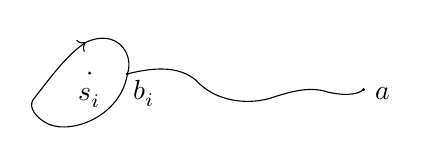
\begin{tikzpicture}[x=1cm,y=1cm,line cap=round,line join=round,baseline=(current bounding box.center)]
\coordinate (b) at (0.48,0.15);
\coordinate (a) at (3.48,-0.05);
\draw[->] (-0.72,-0.18) .. controls (-0.50,0.10) and (-0.30,0.38) .. (-0.05,0.55);
\draw (-0.05,0.55) .. controls (0.33,0.73) and (0.57,0.42) .. (b)
  .. controls (0.40,-0.37) and (-0.20,-0.62) .. (-0.52,-0.49)
  .. controls (-0.68,-0.41) and (-0.78,-0.28) .. (-0.72,-0.18);
\fill (0,0.16) circle (0.6pt);
\node[below] at (0,0.09) {$s_i$};
\fill (b) circle (0.6pt);
\node[below right,inner sep=2pt] at (b) {$b_i$};
\draw (b) .. controls (0.80,0.23) and (1.12,0.26) .. (1.35,0.07)
  .. controls (1.58,-0.19) and (1.98,-0.25) .. (2.29,-0.16)
  .. controls (2.59,-0.06) and (2.81,-0.01) .. (3.02,-0.08)
  .. controls (3.19,-0.12) and (3.38,-0.13) .. (a);
\fill (a) circle (0.6pt);
\node[right,inner sep=4pt] at (3.48,-0.10) {$a$};
\end{tikzpicture}}
and a point \inserted{\(b_i\)} on the boundary, and a homotopy class of paths \inserted{(in \(\deleted{\unsure{X}}\unsure{U|X}-(\mathring\Delta_i-\{s_i\})=V_i\))} from \(a\) to \(b_i\), and to take the group \(L_i\) generated by either one of the two corresponding loops around \(s_i\) (which give \deleted{\unsure{two}} opposite elements of \(\pi\)).
We see that we thus find a surjective map from
\[
\operatorname{Isom}_{\Pi_1V_i}(a,b_i)\simeq
\operatorname{Isom}_{\Pi_1U}(a,b_i)
\]
\deleted{to} onto the set of \(L_i\subset\pi\) in the class \(\unsure{i|\Pi}\), a map \deleted{whose} compatible with the

\scanpage{184}
\mspage{92}

natural action of \(\pi\) (operating on \(\operatorname{Isom}_{\Pi_1U}(a,b_i)\) in the obvious way by composition, and on the set of \(L_i\) by inner automorphisms.
\deleted{\unsure{Then}} Here, the \deleted{choice of} link with the ``abstract'' topos-theoretic description is established as follows: the choice of \(b_i\) can serve as a \unsure{base|fixed} point for defining a universal covering of \(\Delta_i\smallsetminus\{s_i\}\overset{\sim}{\hookleftarrow}D_i^*\), whence an object \(\rho_!(\widetilde D_i^*(b_i))\), and \deleted{\unsure{this object}} the \(L_i\subset\pi\) correspond \inserted{(according to the abstract description)} to the isomorphisms from \(\widetilde U_0=\widetilde U(a_i)\) onto \(\unsure{D_i^*(b_i)|\widetilde D_i^*(b_i)}\) modulo composition with an automorphism of \(\unsure{D_i^*(b_i)|\widetilde D_i^*(b_i)}\) coming from an automorphism of \(\unsure{D_i^*(b_i)|\widetilde D_i^*(b_i)}\) -- but the isomorphisms \deleted{from} \(\widetilde U(a_i)\xrightarrow{\sim}\rho_!(\widetilde D_i^*(b_i))\) correspond precisely to the classes of paths from \(a\) to \(b_i\).

\margin{We return to the notation \(\pi',U'\) --}
\unsure{Let us consider} an object of \(\Pi_1B_{D_i^{*'}}\), i.e. a pair \((\pi',L_i')\). Let \(\pi\) be the quotient group of \(\pi'\) by the invariant subgroup of \(\pi'\) \deleted{defined} \inserted{generated} by \(L_i'\). I say \margin{\(\Vert\)} that up to unique isomorphism (actual isomorphism of groups, not merely outer!) it does not

\scanpage{185}

depend on the choice of the object \(\widetilde D_i^*\) of \(\Pi_1B_{D_i'^*}\). Indeed, \(\pi=\pi(\widetilde D_i^*)\) depends functorially on \(\widetilde D_i^*\), and everything comes down to seeing that this functor is \uline{constant}, i.e. that the operation of
\[
\operatorname{Aut}(\widetilde D_i^*)\simeq T\simeq L_i
\quad\text{on}\quad
\pi=\pi(\widetilde D_i^*)
\]
is trivial. Now let \(u\in L_i\), \unsure{the|its} automorphism of \(\pi\) which it defines is defined by the inner automorphism \(\operatorname{int}(u)\) by passage to the quotient, hence (since \(u\) becomes \(1\) in \(\pi\)) it is trivial. \unsure{Easy.}

We thus find a \uline{functor}
\[
\begin{array}{c}
\text{Outer groups with loops }\pi'\\
\text{of type }g,\nu+1\text{ equipped with a}\\
\text{loop class }i\in I(\pi')
\end{array}
\longrightarrow
\begin{array}{c}
\text{groups}\\
\text{(realized)}\\
\text{with loops, of}\\
\text{type }g,\nu\deleted{\unsure{+1}}
\end{array}
\]
\[
(\pi',i)\longmapsto\beta(\pi',i)
\qquad
\text{[``plugging the hole \(i\)'']}
\]
which is expressed by a group homomorphism
\[
\operatorname{Aut\,ext}(\pi',i)\longrightarrow\operatorname{Aut}\pi
\tag{\unsure{*|5}}
\]
where \(\pi=\beta(\pi',i)\)
\[
\left(
\begin{array}{l}
\overset{\text{definition}}{=}\text{ set of categorical automorphisms}\\
\text{of }\pi'\text{ respecting the loop}\\
\text{structure and fixing the loop}\\
\text{class }i
\end{array}
\right)
\]

\scanpage{186}
\mspage{93}

From the geometric point of view, this fact (existence of this functor), merely expresses the fact that after ``plugging the hole'' \(i\), we have a \deleted{point} \(U=U'\cup\{s_i\}\) \uline{equipped} with a point \(s_i\) which we can use as a \uline{base point} \inserted{\uuline{canonical}} to calculate \(\pi_1(U)\).

We can also say that the choice of \(i\) makes it possible to construct the partial amalgamated sum (plugging holes \inserted{partially}) \(B_{U^*}\)
\diagram{
\begin{tikzcd}[ampersand replacement=\&]
\& B_{D_i'^*} \arrow[dl] \arrow[dr] \& \\
B_{U'} \arrow[dr] \& \& B_{s_i} \arrow[dl] \\
\& B_{U^*} \&
\end{tikzcd}
}
and \(B_{s_i}\longrightarrow B_{U^*}\) supplies a geometric point of \(B_{U^*}\) which makes it possible to describe a canonical object of \(\Pi_1B_{U^*}\) (universal covering relative to this point) whence canonically a group \(\pi\), which of course is a group with loops of type \(g,\nu-1\).

\uline{Theorem} Suppose \(g,\nu\) are such that not

\scanpage{187}

only the groups \(\pi'_{\unsure{s}}\) of type \(g,\nu\), but also the groups \(\pi\) (of type \(g,\nu-1\)) are anabelian, i.e.
\[
2g+\unsure{\nu}\deleted{\unsure{+1}}\unsure{\ge|\le}\unsure{4}
\quad
[\text{thus }g\ge2,\ \text{or }g\unsure{\ge|=}1,\nu\ge2,\ \text{or }g=0,\nu\ge4].
\]
Then the preceding functor \((\pi',i)\longrightarrow\pi\) is an equivalence of categories, in other words (since these are \(0\)-connected groupoids)
\[
\operatorname{Aut\,ext}(\pi',i)\longrightarrow\operatorname{Aut}(\pi)
\]
is an \uline{isomorphism}.

Let us note for this \unsure{that we have} the exact sequence
\[
1\longrightarrow\pi\longrightarrow\operatorname{Aut}(\pi)
\longrightarrow\operatorname{Aut\,ext}(\pi)\longrightarrow1:
\]
(for \(\operatorname{Centre}\pi=1\) by the anabelian hypothesis on \(\pi\)), \unsure{now} we are going to define an exact sequence
\[
1\longrightarrow\pi\longrightarrow\operatorname{Aut\,ext}(\pi',i)
\longrightarrow\unsure{\operatorname{Aut\,ext}(\pi)|\operatorname{Aut\,ext}(\pi')}
\longrightarrow1
\]
and a homomorphism of extensions from this one

\scanpage{188}
\mspage{\unsure{94|99}}

into the preceding one (which will necessarily be an isomorphism).

We may assume \(T=\mathbb Z\), we consider the \unsure{standard|standard} groups with loops \(\Pi_{g,\nu+1}\), \(\Pi_{g,\nu}\). Let us put
\[
\operatorname{Aut\,ext}_{\mathrm{lac}}(\Pi_{g,\nu})
=\unsure{\mathcal T|\mathfrak T}_{g,\nu}^{\unsure{00|\circ\circ}}
\]
\inserted{inducing \uline{the identity} on \(I(\Pi_{g,\nu})\) and on \(T(\Pi_{g,\nu})\)}
(Teichmüller group of index \(g,\nu\)),
we know that (for \(2g+\nu\ge3\)) \(\mathcal T_{g,\nu}\) is the fundamental group of the complex modular topos \inserted{\(M_{g,\nu}\)} of complex curves (\deleted{\illegible{1}} \unsure{projective nonsingular}) connected, of genus \(g\), with a system of \(\nu\) given distinct points \(s_1-\!s_\nu\).
\margin{\uline{N.B.} the universal covering of \(M_{g,\nu}\) is contractible, Teichmüller.}
Now the modular topos \(M_{g,\nu+1}\) is none other than \deleted{the image} the ``universal complex curve \deleted{\illegible{1}} of genus \(g\) with \(\nu\) numbered holes'' over \(M_{g,\nu}\)
[for giving ourselves a curve \inserted{\(U'\)} of genus \(g\) with \(\nu+1\) holes \inserted{\(x_1-\!x_{\nu+1}\)} amounts to the same as giving ourselves one \inserted{\(U\)} with \(\nu\) numbered holes \(x_1-\!x_\nu\), \uline{plus} a \deleted{hole of} point of \(U\) \deleted{\unsure{pointed}}), \uline{whence} a homotopy exact sequence
\diagram{
\begin{tikzcd}[ampersand replacement=\&,column sep=small]
\unsure{\pi_2|\Pi_2}(M_{g,\nu},\unsure{\xi})
 \arrow[r] \&
\pi_1(U) \arrow[r] \arrow[d,equal] \&
\pi_1(M_{g,\nu+1}) \arrow[r] \arrow[d,equal] \&
\pi_1(M_{g,\nu}) \arrow[r] \arrow[d,phantom,sloped,"\simeq"] \&
\pi_0(U) \arrow[d,equal] \\
0 \arrow[r] \&
\pi=\Pi_{g,\nu} \arrow[r] \&
\mathcal T^{00}_{g,\nu+1} \arrow[r] \&
\mathcal T^{00}_{g,\nu} \arrow[r] \&
1
\end{tikzcd}
}

\scanpage{189}

whence \unsure{an} extension structure \deleted{announced}
\[
1\longrightarrow\Pi_{g,\nu}
\longrightarrow\mathcal T^{00}_{g,\nu+1}
\longrightarrow\mathcal T^{00}_{g,\unsure{\nu}}
\longrightarrow1
\]
which is (up to passage to a subgroup of index ``\(2\nu!\)) this announced extension structure. \unsure{\&} the verifications of \uline{compatibility} are left \ldots.

We therefore have a quasi-inverse functor (defined up to unique isomorphism)
\[
\begin{array}{c}
\text{groups with loops}\\
\text{of type }g,\nu\\
(2g+\nu\ge3)
\end{array}
\longrightarrow
\begin{array}{c}
\text{\uline{outer} groups with}\\
\text{loops of type }(g,\nu+1),\\
\text{with a distinguished ``loop}\\
\text{class''}\\
\text{(pairs }(\pi',i\in I(\pi'))\text{)}
\end{array}
\]

\deleted{\unsure{Now}} \unsure{At the} topos-theoretic level, when we have a system \(B_{D^*}\longrightarrow B_U\) \inserted{of type \(g,\nu\) \((2g+\nu\ge3)\)}, and a ``point'' of \(B_U\) i.e. a \(\widetilde U\in\operatorname{Ob}\Pi_1B_U\), then we can in a canonical way find a \(B_{D_i^*}\) (\unsure{\(T\)-groupoid} \inserted{connected}, where \(T\) is the orientation module), and a system
\[
B_{D^*}\amalg B_{D_i^*}\longrightarrow B_{U'},
\]
of type \(g,\nu+1\),

\scanpage{190}
\mspage{95}

in such a way that \((B_{D^*},B_U,\widetilde U)\) \unsure{is deduced from it} by the operation of ``plugging the hole \(D_i^*\)''.

These constructions are so functorial, \margin{\unsure{\(\wedge\)}} that they commute with actions of groups \(\Gamma\). If a group \(\Gamma\) operates on a group with loops \(\pi_{\deleted{\unsure{g,\nu}}}\) of type \(g,\nu\), (not merely by outer automorphisms), then we deduce from it an \uline{outer} operation of \(\Gamma\) on a \(\pi'\) with loops of type \(g,\nu+1\), which fixes a privileged loop class \(i\in I\).

But then, in the corresponding extension
\[
1\longrightarrow\pi'\longrightarrow E'\longrightarrow\Gamma\longrightarrow1,
\]
Let us choose an \(L_i'\subset\pi'\) and let \(\unsure{\mathcal E_i'|E_i'}\) be the normalizer of \(L_i\) in \(\unsure{\mathcal E'|E'}\) -- we find
\[
1\longrightarrow
\underset{\simeq T}{L_i'}
\longrightarrow\unsure{\mathcal E_i'|E_i'}
\longrightarrow\Gamma\longrightarrow1
\]

\subsection*{Scans 191--200}
\addcontentsline{toc}{subsection}{Scans 191--200}
% package LM_P020
\scanpage{191}
% l. 01
( this \unsure{works} \unsure{without} a finiteness hypothesis on
% l. 02
$\Gamma$, the universal case being the one where $\Gamma$
% l. 03
is the Teichmüller \unsure{group} of $\pi'$ \unsure{fixing} $i$
% l. 04
i.e. $\operatorname{Autext}_{\mathrm{lac}}(\pi';i)\simeq\operatorname{Aut}_{\mathrm{lac}}(\pi)$ ). I
% l. 05
say that if $\Gamma$ operates \uline{faithfully} \uline{on $\pi$}
% l. 06
i.e. if its outer operation \uline{on}
% l. 07
\uline{$\pi'$} is faithful, and if $\Gamma$ is \uline{finite},
% l. 08
Then $\Gamma$ is necessarily cyclic \inserted{(case $\Gamma=\Gamma^0$)}
% l. 09
or dihedral ($\Gamma\ne\Gamma^0$), and that if in
% l. 10
addition $\Gamma=\Gamma^0$, then \deleted{\unsure{$\mathcal E_i'$ is $\simeq$}} \inserted{\unsure{$\mathcal E_i\simeq\mathbb Z$|$\mathcal E_i'\simeq\mathbb Z$} i.e.} $\exists!$ isomorphism
% l. 11
\unsure{$T\xrightarrow{\sim}\mathcal E_i$|$T\xrightarrow{\sim}\mathcal E_i'$} such that \unsure{$T\xrightarrow{k_i'}\mathcal E_i'$} identifies with
% l. 12
$n\operatorname{id}_T$ (so that we find \unsure{$\Gamma\simeq\mathcal E_i'/n\mathcal E_i'$}
% l. 13
$\simeq T\otimes_{\mathbb Z}\mathbb Z/n\mathbb Z$, if $n=\operatorname{card}\Gamma$ ...

% l. 14
Changing notation, this amounts to the
% l. 15
\uline{Theore}\textsuperscript{\unsure{m}} Let $\Gamma$ be a finite group operating
% l. 16
faithfully on an \uline{\unsure{outer|outer\textsuperscript{ly}}}
% l. 17
group with loops $\pi$ \inserted{of type \deleted{\illegible{1}} $(g,\nu+1)$ ($\nu\geq0$)}, leaving an $i\in I(\pi)$ fixed,
% l. 18
Then $\Gamma$ is cyclic (if $\Gamma=\Gamma^0$) or
% l. 19
dihedral (if $\Gamma\ne\Gamma^0$), and in the extension
% marge, en bas à gauche
\margin{\unsure{to the} same there is \uline{equivalence}, if in the theorem, we assume the type $(g,\nu)$ anabelian --- otherwise the theorem is a little more general}
\mspage{190}


\scanpage{192}
\mspage{96}
% l. 01
corresponding \deleted{\illegible{2}} \unsure{$\mathcal E$} of $\Gamma$ by $\pi$,
% l. 02
If \unsure{$\mathcal E_i$} is the normalizer of an $L_i$ in
% l. 03
\unsure{$\mathcal E$} [ \inserted{so that we have} \deleted{an} \unsure{$\mathcal E_i\to\Gamma$} epimorphic i.e. an exact sequence
% l. 04
\unsure{$1\to L_i\to\mathcal E_i\to\Gamma\to1$} ]. the inverse image \unsure{$\mathcal E_i^0$} of
% l. 05
$\Gamma^0$ is $\simeq\mathbb Z$ so (if $n=\operatorname{card}\Gamma^0$)\inserted{\unsure{$=[\mathcal E_i^0:L_i]$}}
% l. 06
\deleted{\unsure{$n\operatorname{id}$}} $x\to x^n$ is an isomorphism \deleted{and} \unsure{$\mathcal E_i^0\simeq L_i$}, which
% l. 07
taking $k_i$ into account gives an
% l. 08
isomorphism \unsure{$\mathcal E_i^0\simeq T$}, whose composite with
% l. 09
\deleted{\unsure{$\mathcal E_i$}} \unsure{$T\xrightarrow[\sim]{k_i}L_i\subset\mathcal E_i^0$} is $n\operatorname{id}_T$, so
% l. 10
that we have a canonical isomorphism
% l. 11
\[\unsure{\Gamma^0\simeq\mathcal E_i^0/L_i\simeq T/nT}\]
% l. 12
(obviously independent of the choice of $L_i$ ...)

% l. 13
\uline{Proof}. Let us consider the extension
% l. 14
\unsure{$\mathcal E_i^0$} of $\Gamma^0$ by $L_i\simeq T$ ($\overset{\text{\unsure{noncanonical}}}{\simeq}\mathbb Z$),
% l. 15
since \unsure{$\mathcal E_i^0$|$\Gamma^0$} operates trivial\textsuperscript{ly} on $T$ \inserted{torsion-free}, this
% l. 16
extension (by the cohomology exact sequence
% l. 17
associated with $0\to T\to T\otimes_{\mathbb Z}\mathbb Q\to T\otimes_{\mathbb Z}\mathbb Q/\mathbb Z\to0$)
% l. 18
is canonical\textsuperscript{ly} isomorphic to \deleted{\unsure{an}} the extension
% l. 19
defined by a homomorphism $\Gamma^0\to T_n=T/nT$,
% l. 20
as inverse image of the extension
% l. 21
$0\to T\xrightarrow{n}T\to T_n\to0$ of $T_n$ by $T$. I say that
\mspage{191}


\scanpage{193}
% l. 01
this homomorphism is an isomorphism (from which \unsure{would follow|will follow}
% l. 02
the other assertions), or what amounts
% l. 03
to the same since $\Gamma^0$ and $T_n$ are both
% l. 04
of order $n$, that it is a monomorphism.
% l. 05
Replacing $\Gamma^0$ by the kernel of $\Gamma^0\to\mathbb Z/n\mathbb Z$,
% l. 06
we may assume that the homomorphism \inserted{in question} is zero, and we must
% l. 07
prove that this implies that the action
% l. 08
of $\Gamma^0$ is trivial (which, since by hypothesis
% l. 09
the action of $\Gamma$ is faithful, implies $\Gamma^0=\{1\}$,
% l. 10
OK.) So \unsure{theorem} is reduced to the

% l. 11
\uline{fundamental lemma}. Every \inserted{direct} outer automorphism
% l. 12
$u$ of finite order \inserted{\unsure{$n$}} of a group with
% l. 13
loops $\pi$, which fixes a loop class
% l. 14
$i$ and is such that the extension of $\mathbb Z/n\mathbb Z$
% l. 15
by $L_i\in i$ defined by $u$ is trivial,
% l. 16
is trivial.

% l. 17
The hypothesis means that $u$ lifts
% l. 18
to an automorphism $u_0$ of $\pi$, which
% l. 19
normalizes $L_i$, and which is also of order \unsure{$n$},
% l. 20
(or of finite order, this amounts to the \unsure{same|$\Rightarrow$} taking into account
% l. 21
that \deleted{\unsure{the elements of}} $T$ has no elements of finite order)
\mspage{192}


\scanpage{194}
\mspage{97}
% l. 01
then $u_0$ is trivial, i.e. this is equivalent to the
% l. 02
\uline{Corollary}. Every \inserted{direct} automorphism of finite order \inserted{$u_0$} of
% l. 03
a group with loops $\pi$, \inserted{which is direct and} which normalizes
% l. 04
a loop subgroup $L_i$ (i.e. which
% l. 05
centralizes $L_i$), is reduced to the identity.
% marge supérieure gauche
\margin{In the lemma or its \unsure{corollary}}
\margin{\uline{N.B.} (the case $g=0$, $\nu+1=1$ or $\nu+1=2$ is trivial, the case $\nu+1=3$ ($(g,\nu)=(0,2)$ abelian!) is not trivial \unsure{on the other hand}, nor the case $g=1$, $\nu+1=1$ i.e. $(g,\nu)=(1,0)$ abelian. Yet the result should be valid also in \unsure{this|these} cases.)}

% l. 06
To prove it, we are reduced \inserted{at once} to the
% l. 07
case where $u_0$ is \deleted{of prime order $p$} \inserted{such that $u_0^p=\operatorname{id}$, where}
% l. 08
$p$ is a prime \unsure{number} --- i.e. $u_0$ corres-
% l. 09
ponds to an operation in the strict sense
% l. 10
(not on\textsuperscript{ly} outer) of $\mathbb Z/p\mathbb Z$ \deleted{\unsure{by}} \unsure{by automorphisms}
% l. 11
of $\pi$. But (whether or not we can
% l. 12
find such a $p$) let us consider the case where
% l. 13
we know that the \uline{outer} operation of
% l. 14
$\Gamma=\mathbb Z/n\mathbb Z$ [$n=$ order of $u$] on $\pi$ is realized
% l. 15
geometrical\textsuperscript{ly}, by a (faithful) operation
% l. 16
of $\Gamma=\mathbb Z/n\mathbb Z$ on a $U$ of type $(g,\nu+1)$.
% l. 17
\deleted{\unsure{$\pi$-conjugacy classes}, \illegible{1}}
% marge inférieure gauche
\margin{$U=X\setminus S$, $S\simeq I$, $X$ compact of genus $g$ \unsure{the puncture|the part} $s_i$ of $S$ corresponding to a fixed point of $\Gamma$ operating on $U$.}

% l. 18
\deleted{We know that the (\unsure{liftings}) of the outer automorphisms
% l. 19
to \deleted{\unsure{automorphisms}} \inserted{a genuine operation},
% l. 20
correspond to the fixed points \illegible{1} of $\Gamma$
% l. 21
in $U$; \deleted{and the extension of} \inserted{let $a$ be the fixed point of $\Gamma$}
% l. 22
corresponding to the given operation, \unsure{so}
% l. 23
that we have \deleted{\unsure{a}} canonical isomorphism \unsure{compatible with $\Gamma$}
% l. 24
$\pi=\pi_1(U,a)$.}
\mspage{193}


\scanpage{195}
% l. 01
We express the hypothesis of the \inserted{\unsure{``genuine''}} operation of $\Gamma$ on
% l. 02
$\pi$, \deleted{\illegible{1}} \unsure{centralizing} an $L_i$, by saying that
% l. 03
the outer operation gives a trivial extension
% l. 04
of $\Gamma$ by $L_i\simeq T$. But we know
% l. 05
moreover in the geometric case \inserted{and faithful operation} that it
% l. 06
is \uline{not} trivial !

% l. 07
It would therefore suffice, \deleted{\illegible{1}} to prove the
% l. 08
fundamental lemma, to know that every
% l. 09
outer action \inserted{[faithful]} of a cyclic group
% l. 10
on a group with loops of type \unsure{$(g,\nu+1)$}
% l. 11
is realizable, and it even suffices to know this
% l. 12
for a cyclic group of
% l. 13
prime order. \inserted{\unsure{is}} \unsure{Now} unless I am mistaken this result
% l. 14
is \unsure{well} known (even for \unsure{solv-}
% l. 15
able groups ...). --- so that the funda-
% l. 16
mental lemma seems proved. I have only
% l. 17
a doubt whether it is proved in the
% l. 18
general case of a $(g,\nu)$, \inserted{\deleted{\illegible{1} $g\geq2$}} or only
% l. 19
for \inserted{$g\geq2$,} $\nu=0$. But \deleted{in truth, \illegible{2}, \inserted{this suffices}}
% l. 20
\deleted{\illegible{2} \inserted{for $g\geq2$}}
% marge inférieure gauche
\margin{as a theorem \unsure{of existence} \unsure{of points} fixed by a group \illegible{1} \unsure{operating} \unsure{of} Teichmüller}

% l. 21
\deleted{\uline{Lemma} Let \illegible{1} be an outer operation}
\mspage{194}


\scanpage{196}
\mspage{98}
% l. 01
\deleted{of a finite group $\Gamma$ on a \illegible{1}} if this
% l. 02
is indeed so, I think that (for $g\geq2$ at the very
% l. 03
least) we get by with dévissage
% l. 04
for the case of arbitrary $\nu$ --- and the case $g=0,1$
% l. 05
would require \inserted{\unsure{also}} a separate treatment.
% l. 06
I will come back to this later, and
% l. 07
prefer for the moment to admit the ``fundamental
% l. 08
lemma'', and examine consequences
% l. 09
and corollaries of it.

% l. 10
For an outer \inserted{faithful} action of a finite $\Gamma$
% l. 11
on an \uline{anabelian} group with loops $\pi$, \unsure{we}
% l. 12
\deleted{\unsure{have established}} corresponding to an extension \unsure{$\mathcal E$} of $\Gamma$ by $\pi$,
% l. 13
we have therefore established a) that the partial
% l. 14
splittings of it can only be made
% l. 15
over \deleted{\unsure{cyclic}} subgroups $\Gamma'$ of $\Gamma$
% l. 16
such that $\Gamma'{}^0$ \unsure{is} cyclic, and $\Gamma'$ dihedral
% l. 17
if $\Gamma'\ne\Gamma'{}^0$, and that b) for every class
% l. 18
of \illegible{2} of such partial splittings
% l. 19
\unsure{over} $\Gamma'\subset\Gamma^0$, we have a corresponding canonical
% l. 20
isomorphism $\Gamma'\simeq T_n$ ($=T/nT$), where $n=\operatorname{card}\Gamma'$.
% marge inférieure gauche
\margin{i.e. we have established the existence of a canonical \unsure{map} \illegible{1} from the \unsure{elements} of finite order of $\operatorname{Aut}_{\mathrm{lac}}(\pi)$ into \unsure{$T\otimes\mathbb Q/T$}, satisfying \unsure{the} conditions \unsure{examined} previously}

% l. 21
These are results which we had
\mspage{195}


\scanpage{197}
% l. 01
previously obtained for the case of a
% l. 02
\uline{realizable} operation. [There was moreover no reason
% l. 03
to restrict ourselves to the anabelian case,
% l. 04
as long as we \unsure{assume} $\pi\ne0$ \inserted{(essentially empty case!)},
% l. 05
which includes the \inserted{abelian} cases $g=0$, $\nu=2$ and
% l. 06
$g=1$, $\nu=0$, for which a direct treatment
% l. 07
is possible, and has already been given
% l. 08
essentially, those cases \deleted{\unsure{being} realizable,} \inserted{\unsure{where|if one}}
% l. 09
starts with an \uline{extension} (not with an
% l. 10
``outer'' action i.e. here an action plain and simple
% l. 11
of $\Gamma$ on $\pi\simeq\mathbb Z$ or $\mathbb Z^2$), \unsure{being} always \unsure{realizable}.
% l. 12
(\uline{N.B.} \deleted{\unsure{the hypothesis}} \inserted{In this} case, the hypothesis of a
% l. 13
faithful action is replaced by the one that
% l. 14
the extension is \deleted{\unsure{not splittable}} \inserted{a \uline{product} extension} \unsure{over|under} no
% l. 15
subgroup $\Gamma'\subset\Gamma^0$ with $\Gamma'\ne1$ ....).

% l. 16
There remain however other results of the
% l. 17
realizable case, which would have to be examined
% l. 18
in the general case :

% l. 19
c) If $\Gamma$ is a \deleted{\unsure{discrete}} finite subgroup
% l. 20
of $\operatorname{Aut}_{\mathrm{lac}}(\pi)$ i.e. a finite group operating \uline{\unsure{faithfully}}
% l. 21
on $\pi$, do we have $\pi^\Gamma=\{1\}$ ?
% marge inférieure gauche
\margin{We may assume $\Gamma=\Gamma^0$ hence $\Gamma$ generated by a direct automorphism \unsure{$u$} or $\Gamma$ generated by an \unsure{anti-automorphism} of order 2}
\mspage{196}


\scanpage{198}
\mspage{99}
% l. 01
d) \unsure{If} $\Gamma',\Gamma''$ are finite subgroups of \unsure{$\mathcal E$}
% l. 02
\unsure{(extension} of the finite group $\Gamma$ by $\pi$, corresponding
% l. 03
to an \deleted{\unsure{respect}} outer \inserted{(preserving the orientation)} faithful operation), \deleted{\illegible{1}}
% l. 04
such that $\Gamma'\cap\Gamma''\ne(1)$, then \deleted{does one of
% l. 05
the two contain the other} ?
\inserted{are $\Gamma'$ and $\Gamma''$ contained in the $\pi$-conjugate of a finite subgroup $\Gamma'''$ of \unsure{$\mathcal E$} [i.e. every section sub\unsure{group} $\ne1$ is contained in a unique \unsure{maximal} section subgroup, modulo $\pi$-conjugation}
% marge supérieure gauche
\margin{\uuline{N.B.} Would become false by \deleted{\illegible{1}} \unsure{placing} in the group $\operatorname{Aut}_{\mathrm{lac}}(\pi)$ \illegible{2} \unsure{one as a subgroup} \illegible{2} \unsure{one of the two subgroups} \unsure{contained in} \illegible{4}}

% l. 06
e) For every \unsure{subgroup}, \illegible{2} \deleted{\illegible{1}} $\Gamma'$ of $\Gamma$,
% l. 07
is \unsure{the set} of classes \deleted{\unsure{of extensions}} of $\pi$-conjugation
% l. 08
of liftings of $\Gamma'$ into \unsure{$\mathcal E$} finite ?
% l. 09
[We may assume $\Gamma'=\Gamma$, and $\Gamma$ cyclic (if $\Gamma=\Gamma^0$) or dihedral
% l. 10
(otherwise)]
% l. 11
\inserted{In case \unsure{c)|e)}, we may assume $\Gamma$ cyclic of prime order, and
% l. 12
it is OK if it is established that an \unsure{outer operation} \illegible{3}
% l. 13
\unsure{that} \illegible{4} \unsure{$\pi_{g,\nu}$} \deleted{\illegible{3}} \unsure{d).}} \deleted{By applying}
% marge gauche, au milieu
\margin{\unsure{In} the same way e) is established if \unsure{we} admit that the outer operations of \unsure{cyclic groups} \unsure{on a} $\pi\simeq\pi_{g,\nu}$ are realizable}

% l. 14
\deleted{Example. let us examine \illegible{2}
% l. 15
the \unsure{juncture|junction} ``drilling holes'', $\Gamma'$ and $\Gamma''$
% l. 16
operating by outer automorphisms on a $(\pi';i)$
% l. 17
$i\in I(\pi')$ --- their action on $\pi$ is
% l. 18
deduced from that on $(\pi',i)$ by ``plugging
% l. 19
the hole $i$''. That said, $\Gamma'$ and $\Gamma''$ are identified
% l. 20
with the finite subgroups of $\operatorname{Autext}_{\mathrm{lac}}(\pi';i)$
% l. 21
We have better :
% l. 22
\unsure{$\Gamma=\Gamma'\cap\Gamma''\ne(1)$}}

% Un trait oblique part du coin inférieur gauche du cadre et traverse « Soit » et « et considérons » ; sa portée comme biffure est incertaine.
\unsure{\deleted{
% l. 23
\uline{Theorem}. Let $\Gamma_0$ \deleted{\illegible{1}} be a finite subgroup of
% l. 24
$A=\operatorname{Aut}_{\mathrm{lac}}(\pi)^0$, \inserted{$\Gamma_0\ne1$}, \deleted{\illegible{1} and let us consider} Then the normalizer $N$
% l. 25
of \unsure{$\Gamma$|$\Gamma_0$} in $A$ is equal to its centralizer \unsure{$Z$|$\mathcal Z$}
}}
\margin{\uuline{Ultra strong!} \unsure{If $g=0$}}
\mspage{197}


\scanpage{199}
% Un trait oblique traverse le corps de cette page ; sa portée comme biffure est incertaine.
\unsure{\deleted{
% l. 01
and the set of elements of finite order
% l. 02
of \unsure{$Z$|$\mathcal Z$} is a cyclic group \inserted{\unsure{$F$|$\Gamma$}}, \deleted{contained
% l. 03
in} which is also the largest finite
% l. 04
subgroup of $A$ containing $\Gamma_0$, and is
% l. 05
contained in the center of \unsure{$Z$|$\mathcal Z$}.

% l. 06
The fact that the normalizer $N$
% l. 07
centralizes $\Gamma_0$ comes from the fact that we
% l. 08
have a canonical isomorphism (compatible with the \unsure{transports}
% l. 09
of \unsure{structures})
% l. 10
\[\Gamma_0\xrightarrow{\sim}T_{n_0}\qquad(\text{if }n_0=\operatorname{card}\Gamma_0)\]
% l. 11
(N.B. if $g\in\operatorname{Aut}_{\mathrm{lac}}(\pi)$ reversing the orientation,
% l. 12
and \unsure{normalizes|centralizes} $\Gamma_0$, then \deleted{\unsure{$g$}} $(\operatorname{int}g)$ induces
% l. 13
the symmetry $\sigma\to\sigma^{-1}$ on $\Gamma_0$, by the same
% l. 14
argument) \deleted{\illegible{1}} Let us note that if
% l. 15
$u$ is an element of finite order of \unsure{$Z$|$\mathcal Z$}, so
% l. 16
that $\Gamma_0,u$ generate a
% l. 17
finite commutative subgroup of \unsure{$Z$|$\mathcal Z$}, \deleted{we see that} \inserted{as we know}
% l. 18
that a finite subgroup of $A$ is cyclic,
% l. 19
it follows that $u$ is contained in
% l. 20
a cyclic subgroup of \unsure{$Z$|$\mathcal Z$} \unsure{contain\textsuperscript{ing}} $\Gamma_0$,
% l. 21
\deleted{\unsure{therefore}} say $\Gamma'$. let us now choose
% l. 22
a geometric realization of the \inserted{outer} action of
% l. 23
$\Gamma_0$ on \deleted{\illegible{1}} $\pi$, say $(X,S)$ with $U=X-S$ ;
}}
\mspage{198}


\scanpage{200}
\mspage{100}
% Un long trait oblique traverse le texte ; sa portée comme biffure est incertaine.
\unsure{\deleted{
% l. 01
we know that the lifting of the outer
% l. 02
action of $\Gamma_0$ to an action is
% l. 03
described by a unique point $a\in U$.
% l. 04
\deleted{Let} I say that $\Gamma'$ \deleted{is realizable} (or its
% l. 05
\deleted{outer} action on $\pi\simeq\pi_1(U,a)$) is realizable
% l. 06
in a \uuline{unique way} by an action of $\Gamma'$
\margin{\uuline{not true!}}
\inserted{and inducing the already given action of \unsure{$\Gamma$|$\Gamma_0$}}
% l. 07
on $(X,S)$), fixing $a$, the fact that it
% l. 08
is \inserted{indeed} realizable in this way comes from the fact
% l. 09
(which we admit) that every outer
% l. 10
action of a cyclic group \inserted{(here $\Gamma'$)} on a
% l. 11
group with loops \inserted{$\pi$} of type $(g,\nu)$ is realizable,
% l. 12
and from the uniqueness of such a realization
% l. 13
(in the case of $\Gamma_0$). For \uline{uniqueness},
% l. 14
this \deleted{\illegible{1}} comes down to the

% l. 15
\uline{Lemma}. Let $u_0$ be an automorphism of finite order $n_0\ne1$
% l. 16
of an \inserted{orientable} surface \deleted{\unsure{assumed} $X^{u_0}\ne\emptyset$.} \inserted{$U=X-S$, $X$ (compact, \deleted{\illegible{1}}, and} leaving fixed \inserted{a point $a\in U$} \illegible{1}
% l. 17
let $d\in\mathbb N^*$, (If there exists an automorphism \unsure{$u$} of
% l. 18
\deleted{\illegible{1}} \inserted{$(X,S)$} such that $u^d=u_0$, \inserted{$u(a)=a$}, then $u$ is uniquely
\margin{\uline{false!}}
% l. 19
determined by its \deleted{\unsure{class of}} action on $\pi_1(U,a)$;
% l. 20
and in any event the cyclic group
% l. 21
of automorphisms of $(X,S)$ generated by $u$ is \unsure{unique\textsuperscript{ly}}
% l. 22
\inserted{determined (it is of order $nd$).}
}}
\mspage{199}

\subsection*{Scans 201--210}
\addcontentsline{toc}{subsection}{Scans 201--210}
% package LM_P021
\scanpage{201}
\uline{Proof.} \deleted{Let us fix a structure
\deleted{\unsure{conformal}} \inserted{\deleted{\illegible{1}}} \inserted{complex,}
on $X$, \unsure{invariant} under}

Let us prove d). \deleted{Let $\Gamma_0 =$} We identify
$\Gamma',\Gamma''$ with subgroups of $\Gamma$, and put $\Gamma_0=\Gamma'\cap\Gamma''$.
Let \unsure{$\mathcal E^!$} be the subgroup of $\mathcal E$ consisting of the $g\in\mathcal E$
such that $\operatorname{int}(g).\Gamma_0$ is $\pi$-conjugate to $\Gamma_0$
and whose image in $\Gamma$ \deleted{\illegible{1}} centralizes $\Gamma_0$.
\deleted{\illegible{1}} We have $\mathcal E^!\supset\pi$, and $\mathcal E^!$ is therefore the inverse
image of a subgroup $\Gamma^!$ of $\Gamma$, which
centralizes $\Gamma_0$ \deleted{\illegible{1}}, and which contains $\Gamma'$ and $\Gamma''$
(for $\mathcal E^!$ contains the centralizer of $\Gamma_0$ in $\mathcal E$,
hence $\Gamma'$ and $\Gamma''$). Replacing
$\Gamma$ by $\Gamma^!$, $\mathcal E$ by $\mathcal E^!$ if necessary, we may suppose $\mathcal E=\mathcal E^!$, $\Gamma=\Gamma^!$ i.e.
that $\Gamma_0\subset\mathrm{Centre}$ of $\Gamma$, and that $\Gamma_0\hookrightarrow\mathcal E$
\unsure{invariant} modulo $\pi$-conjugation under $\Gamma$.

\deleted{After this let us choose a topological realization
$(X,S,a)$ of the \deleted{outer} operation of $\Gamma_0$ on $\pi$,
where $a\in U=X-S$ -- thus $\pi\simeq\pi_1(U,a)$. By
the result (\unsure{b}) on existence and uniqueness
of realizations in the cyclic case, this
is possible, and moreover we can have}

\scanpage{202}
\mspage{101}
\deleted{$\Gamma'$ operate on \unsure{$(X,S,a)$} (i.e. on $(U,a)$) in a way
compatible with its action on $\pi_1(U,a)=\pi$,
so as to extend the action of \unsure{$\Gamma_0$|$\Gamma$} --
and \unsure{the same|$=$} for $\Gamma''$. But it is not clear
a priori
that the two actions \deleted{\unsure{can}} are compatible
in the precise sense \deleted{\unsure{of the generated subgroup}}
\inserted{that the \unsure{generated subgroup}}
\deleted{\unsure{by} $\Gamma',\Gamma''$} $\subset\operatorname{Aut\,top}(U)$ is also finite.}

\deleted{Let us now consider $X'=X/\Gamma_0$, $S'=S/\Gamma_0$,
and the image $a'$ of $a$ in $X'$ -- thus $a'\in U'=X'-S'$.
Then \unsure{$\Gamma/\Gamma_0$|$\Gamma'/\Gamma_0$} operates \unsure{isotypically|isotopically} on $(X',S',b)$}

\deleted{Let us use $\pi^{\Gamma_0}=(1)$, we find that}

We are going to construct a section of $\mathcal E$
over $\Gamma$ in \unsure{all} its entirety, as follows. Let $\widetilde\Gamma\subset\mathcal E$
be the centralizer of $\Gamma_0$ in $\mathcal E$, \unsure{we have|$\Rightarrow$}
\deleted{$\gamma\in\Gamma$, $g\in\mathcal E$ over $\gamma$, let us consider}
$\widetilde\Gamma\cap\pi=(1)$ (for this means $\pi^{\Gamma_0}=(1)$)
\deleted{$\operatorname{int}(g).\Gamma_0$, $\exists!\ \alpha\in$}
\inserted{hence}
\deleted{I say that} $\widetilde\Gamma\longrightarrow\Gamma$ injective, I say
that it is surjective. Indeed, let
$\gamma\in\Gamma$, $g\in\mathcal E$ over $\gamma$, by hypothesis
\inserted{on $\Gamma$}
$\exists\ \alpha\in\pi$ such that $\operatorname{int}(g).\Gamma_0=\operatorname{int}(\alpha).\Gamma_0$
i.e. we may suppose $\operatorname{int}(g)\Gamma_0=\Gamma_0$, \deleted{\unsure{hence}} i.e. $g$ normalizes
$\Gamma_0$, but since $\Gamma_0$ is central in $\Gamma$
this means that $g$ centralizes $\Gamma_0$ i.e. $g\in\widetilde\Gamma$.

\scanpage{203}
Thus $\widetilde\Gamma$ \inserted{$\simeq\Gamma$} \unsure{is} a \uline{finite} subgroup of $\operatorname{Aut}(\pi)$,
\deleted{hence cyclic} containing $\Gamma'$ and $\Gamma''$, q.e.d.% a dashed line runs under the deleted words (possible restoration mark); unresolved

\uline{N.B.} If we had not assumed
$\Gamma$ finite at the outset, it would still be true that $\Gamma',\Gamma''$
generate a subgroup $\widetilde\Gamma$ \inserted{$\subset\operatorname{Aut}(\pi)$} such that
$\widetilde\Gamma\cap\pi=(1)$, but that does us a fat lot of good
\deleted{-- \unsure{we can find some},
for example isomorphic to the whole of \unsure{$\operatorname{Autext}(\pi,i)$},
(for a chosen \unsure{$i\in I(\pi)$}: take the
\deleted{\illegible{2}}
centralizer of \unsure{$i$} in \illegible{2} $\operatorname{Aut}(\pi)$)}

\scanpage{204}
\mspage{102}
19. Teichmüller tower.

Let \inserted{$g\in\mathbb N$, and} $X_g$ be a compact orientable surface of
genus $g$, \deleted{\unsure{the set of orientations},}
\unsure{$[$|$]$} $(a_{g,i})_{i\in\mathbb N^*}=(a_{g,1},a_{g,2},\ldots)$ \unsure{$]$|$[$}
a sequence of
distinct points of $X_g$. We put for \unsure{$\forall\nu\in\mathbb N$}
\[
(1)\qquad S_{g,\nu}=\{\unsure{x_{g,i}|a_{g,i}}\mid 0\leq i\leq\nu-1\}
\qquad\text{thus }\nu=\operatorname{card}S_{g,\nu}
\]
\[
(2)\qquad U_{g,\nu}=X_g-S_{g,\nu}.
\]
\margin{N.B. we \unsure{have} $a_{g,\nu}\in U_{g,\nu}$}
We thus have $S_{g,0}=\varnothing$, $U_{g,0}=X_g$; The $S_{g,\nu}$ form
a \inserted{strictly} increasing sequence of finite subsets of $X_g$,
the $U_{g,\nu}$ a strictly decreasing sequence of open subsets
of $X_g$. In what follows we shall take $U_{g,\nu}$ as
the standard surface (oriented, or orientable), of
type $(g,\nu)$.

Let
\[
(3)\qquad A_g=\operatorname{Aut}(X_g)
\]
be the group of automorphisms of $X_g$, equipped with the
topology of uniform convergence of $u$ and of its
inverse. We put
\[
(4)\qquad A_{g,\nu}=\{u\in A_g\mid u(S_{g,\nu})=S_{g,\nu}\}\subset A_g
\]
thus $A_{g,\nu}$ is a subgroup of $A_g$. We
have a canonical isomorphism $u\mapsto u|U_{g,\nu}$
\[
A_{g,\nu}\xrightarrow{\sim}\operatorname{Aut}(U_{g,\nu}).\qquad(5)
\]
\margin{\uline{N.B.} This is \inserted{\unsure{probably|probably}} \unsure{an isomorphism}
topologically, when $A_{g,\nu}$ is
equipped with the topology induced by $A_g$,
and $\operatorname{Aut}(U_{g,\nu})$ with the usual topology of
\unsure{compact} \illegible{1} convergence of $u$ and its inverse.}
\deleted{\unsure{Let}} We have \deleted{\unsure{a}} canonical surjective homomorphism
\[
(6)\qquad A_{g,\nu}\longrightarrow\operatorname{Aut}(S_{g,\nu})
\bigl(\overset{\text{(canonical)}}{\simeq}\unsure{\mathfrak S_\nu}\bigr),
\]

\scanpage{205}
whose kernel is denoted by $A_{g,\nu}^!$
\[
(7)\qquad A_{g,\nu}^!=\{u\in A_g\mid u(a_{g,i})=a_{g,i},\ \forall i\in[0,\ldots,\nu-1]\}
\]
hence exact sequence
\[
(8)\qquad 1\longrightarrow A_{g,\nu}^!\longrightarrow A_{g,\nu}
\longrightarrow\mathfrak S_\nu\longrightarrow1.
\]
Let $A_{g,\nu}^{\circ}$ be the identity component of the group
$A_{g,\nu}$, we thus have
\[
(9)\qquad A_{g,\nu}^{\circ}\bigl(=(A_{g,\nu}^!)^{\circ}\bigr)\subset A_{g,\nu}^!.
\]
Let us put
\[
(10)\qquad \Gamma_{g,\nu}=A_{g,\nu}/A_{g,\nu}^{\circ}=\pi_0(A_{g,\nu})
\quad\text{(Teichmüller group of type }g,\nu\text{)}
\]
\margin{We also put $\Gamma_g=\Gamma_{g,0}(=\Gamma_{g,0}^!)$}
\[
(11)\qquad \Gamma_{g,\nu}^!=A_{g,\nu}^!/A_{g,\nu}^{\circ}=\pi_0(A_{g,\nu}^!).
\]
The exact sequence (8) thus gives an exact
sequence
\[
(12)\qquad 1\longrightarrow\Gamma_{g,\nu}^!\longrightarrow\Gamma_{g,\nu}
\longrightarrow\mathfrak S_\nu\longrightarrow1.
\]
We have canonical homeomorphisms
\[
(13)\qquad A_g/A_{g,\nu}\simeq
\begin{gathered}
\text{open subset }\inserted{\operatorname{Sym}^{\nu}(X)^*}\text{ \inserted{of the} \deleted{\unsure{$X_g$}} symmetric prod-}\\
\text{uct }\inserted{\unsure{\nu^{\text{th}}}}\operatorname{Sym}^{\nu}(X_g)\text{ of }X_g\\
\text{consisting of the finite subsets}\\
\text{of cardinality }\nu\\
=\unsure{\mathcal P_\nu(X_g)}
\end{gathered}
\]
\margin{N.B. the marked points of the \unsure{homogeneous} \unsure{spaces}
on the left-hand sides \unsure{in|of} (13), (14)
\unsure{go to} the systems
of points $\{\unsure{a_{g,0}},a_{g,1},\ldots,a_{g,\nu-1}\}$ or
$(a_{g,0},\ldots,a_{g,\nu-1})$.}
\[
(14)\qquad A_g/A_{g,\nu}^!\simeq
\begin{gathered}
\text{open subset }\inserted{(X_g^{\nu})^*}\text{ of }X_g^{\nu}\text{ consisting of the}\\
\nu\text{-tuples of distinct points}\\
\simeq\operatorname{Mon}(\deleted{\unsure{X_g}}I_\nu,X)\quad\text{(where }I_\nu\\
=\{0,\ldots,\nu-1\}.
\end{gathered}
\]

\scanpage{206}
\mspage{103}
This homeomorphism \unsure{respecting} the natural
actions of $\mathfrak S_\nu\simeq A_{g,\nu}/A_{g,\nu}^!$.

The $A_{g,\nu}^!$ for variable $\nu$ form a
decreasing sequence of groups in $A_g$
\[
(15)\qquad A_g\unsure{=|\supset}A_{g,0}^!\supset A_{g,1}^!\supset A_{g,2}^!
\supset\cdots\supset A_{g,\nu}^!\supset\cdots
\]
and the corresponding morphisms
between homogeneous spaces \inserted{of $A_g$} fit into the
commutative diagram \unsure{of homeomorphisms} \illegible{1}

(16)\quad
\diagram{\begin{tikzcd}[ampersand replacement=\&]
 A_g/A_{g,\nu}^! \arrow[r,"\sim"] \arrow[d] \& \operatorname{Mon}(I_\nu,X) \arrow[d] \\
 A_g/A_{g,\nu'}^! \arrow[r,"\sim"] \& \operatorname{Mon}(I_{\nu'},X)
\end{tikzcd}}
\quad $0\leq\nu'\leq\nu$
\margin{\illegible{1}}
where the second vertical arrow is that of
restriction from $I_\nu$ to $I_{\nu'}\subset I_\nu$.

For $\nu=1$ \inserted{we have $A_{g,1}^!=A_{g,1}$, and} the isomorphism (13) (or if one prefers,
(14)) is written
\[
(17)\qquad A_g/A_{g,1}\simeq X_g
\]
(homeomorphism compatible with \inserted{the} actions of $A_g$)

Moreover if to $\forall x\in X_g$ we associate its
stabilizer $A_{g,x}$ in $A_g$, we find an
obviously surjective map

\scanpage{207}
\[
(18)\qquad X_g\longrightarrow
\begin{gathered}
\text{set of conjugates of the sub-}\\
\text{group }A_{g,1}\text{ of }A_g\\
\simeq A_g/\operatorname{Norm}_{A_g}(A_{g,1})
\end{gathered}
\]
which is identified via (17) with the canonical map
on the homogeneous spaces
\[
 A_g/A_{g,1}\longrightarrow A_g/\operatorname{Norm}_{A_g}(A_{g,1})
\]
deduced from the inclusion $A_{g,1}\subset\operatorname{Norm}_{A_g}(A_{g,1})$,
and we see at once that (18) is
bijective i.e. that \deleted{\illegible{1}}
\[
(19)\qquad A_{g,1}=\operatorname{Norm}_{A_g}(A_{g,1}),
\]
more generally for $\forall\nu$, we have
\[
(20)\qquad A_{g,\nu}=\operatorname{Norm}_{A_g}(A_{g,\nu})
=\operatorname{Norm}_{A_g}(A_{g,\nu}^!)
\]
which means that the canonical maps
of homogeneous $A_g$-sets
\deleted{$x=\{x_1,\ldots,x_\nu\}\longmapsto A_{g,x}=\bigcap$}
\deleted{(23)}
\[
\mathcal P_\nu(X_g)\longrightarrow\text{set of conjugates of }A_{g,\nu}
\]
\[
(21)\qquad S\longmapsto\text{stabilizer }A_{g,S}\text{ of }S
\]
and
\[
(22)\qquad\unsure{\vert}\quad S\longmapsto A_{g,S}^!
\]
are not only surjective, but even bijective.
This comes from the fact that we recover
$S$ in terms of $A_{g,S}$\deleted{${}^!$} \inserted{(or of $A_{g,S}^!$}
\deleted{\unsure{(and} a fortiori in terms \unsure{of the group} $A_{g,S}$)} \inserted{as} \deleted{as}

\scanpage{208}
\mspage{104}
\[
(23)\qquad S=\{x\in X_g\mid ux=x\quad\forall u\in A_{g,S}^!\}
=X_g^{(A_{g,S}^!)}
\]
\[
(24)\qquad\begin{aligned}
S&=\{x\in X_g\mid A_{g,S}.x\text{ finite}\}\\
 &=\{x\in X_g\mid A_{g,S}.x\ne X_g\}
\end{aligned}
\]
\margin{$\forall S\in\mathcal P_\nu(X_g)$}

We also have \unsure{some|\deleted{some}} canonical maps
of homogeneous spaces under $A_g$
\[
(25)\qquad S\longmapsto A_{g,S}^{\circ}
\]
\[
\mathcal P_\nu(X_g)\longrightarrow
\begin{gathered}
\text{set of conjugates}\\
\text{of the }A_{g,\nu}^{\circ}\text{ in }A_g\\
\simeq A_g/\operatorname{Norm}(A_{g,\nu}^{\circ})
\end{gathered}
\]
which is not only surjective, but also
injective, for we have the following relation, which
strengthens \inserted{(23) and} (24), $\forall S\in\mathcal P_\nu(X_g)$
\[
(26)\qquad\begin{aligned}
S&=\{x\in X_g\mid A_{g,S}^{\circ}.x=\{x\}\}=X_g^{A_{g,S}^{\circ}}\\
 &=\{x\in X_g\mid A_{g,S}^{\circ}.x\text{ finite}\}\\
 &=\{x\in X_g\mid A_{g,S}^{\circ}.x\ne X_g\}.
\end{aligned}
\]
\deleted{\illegible{2}} Thus we have for $\forall\nu$
\[
(27)\qquad A_{g,\nu}=\operatorname{Norm}_{A_g}(\unsure{A_{g,\nu}|A_{g,x}})
=\operatorname{Norm}_{A_g}(A_{g,\nu}^!)=\operatorname{Norm}_{A_g}(A_{g,\nu}^{\circ}).
\]

Let $G$ be a topological group, equipped
with a conjugacy class \unsure{$\mathcal E$|$\mathcal X$} of subgroups,
\deleted{Let} $G_1$ in this class. We say that

\scanpage{209}
$G,\mathcal X$ is a Teichmüller \deleted{\unsure{datum}} \inserted{pair}
of type $g$, if there exists an isomorphism of
topological groups $G\simeq A_g$, taking
\unsure{$\mathcal E$|$\mathcal X$} to the conjugacy class of $A_1$.
\inserted{\unsure{It amounts to the same thing to say that}}
\deleted{We then see that $G_1=\operatorname{Norm}_G(G_1)$}
\deleted{hence that} $\mathcal X$, \deleted{\unsure{as}}
\inserted{equipped with the topology of a} homogeneous space
under $G$, is \deleted{homeomorphic to $G/G_1$} a
compact orientable surface of genus $g$,
\deleted{\illegible{2}} say \unsure{$\mathcal X$|$\mathfrak X$}, and that
\deleted{\illegible{3}} \inserted{the map}
natural
\[
(28)\qquad G\longrightarrow\operatorname{Aut}(\mathcal X)
\]
is a homeomorphism of topological groups.
We then see that \inserted{\unsure{by} $(G,\mathcal X)\longrightarrow\mathcal X$ from}
the category of
Teichmüller pairs of type $g$, to
that of compact oriented surfaces, is
an equivalence of categories. It follows
that \deleted{\unsure{every automorphism}} for an automorphism \inserted{\unsure{$u$}} of the
topological group $G$, $u$ is inner iff it

\scanpage{210}
\mspage{105}
preserves the class $\mathcal X$ i.e. iff $u(G_1)$ is conjugate
to $G_1$. Moreover the center of $G$ is trivial, \unsure{i.e.}

We can give an analogous description
for the category of oriented surfaces of
genus $g$ with $\nu$ holes (i.e. homeomorphic
to $U_{g,\nu}$) in terms of a topo-
logical group $G_\nu(\simeq A_{g,\nu})$ and of a \inserted{conjugacy class \unsure{$U_\nu$|$\widetilde U_\nu$} of}
subgroups $H_\nu$ of it $(\simeq A_{g,\nu}\cap A_{g,\nu+1})$, with the
conditions that $(G_\nu,\{H_\nu\})$ be isomorphic
to $(A_{g,\nu},A_{g,\nu}\cap A_{g,\nu+1}\unsure{)|\}}$, or else
that $U_\nu$ \inserted{(\unsure{space} \illegible{1} topology \unsure{of a homogeneous space})} be an oriented surface of
type $(g,\nu)$, and that the \deleted{map}canonical homomorphism
\[
(29)\qquad G\longrightarrow\operatorname{Aut}(U_\nu)
\]
be a homeomorphism of topological
groups. We then find an
equivalence between the category of
Teichmüller pairs $(G_\nu,\{H_\nu\})$
of type $(g,\nu)$, and that of
orientable surfaces of type $(g,\nu)$. We find again

\subsection*{Scans 211--220}
\addcontentsline{toc}{subsection}{Scans 211--220}
% package LM_P022
\scanpage{211}
% L1--4 (haut de la page)
that the automorphisms of such a $G_\nu$ ($\simeq A_{g,\nu}$) which fix the class $U_\nu$ i.e. which \unsure{transform|transport} $H_\nu$ into a conjugate, \unsure{are} inner, and that the center of $H_\nu$ is $\{1\}$.

% L5--9
In fact, $U_\nu$ can also be interpreted as a homogeneous space under $G_\nu^\circ$, and not only under $G_\nu$, more generally we have that $G_\nu^\circ$ is transitive on $U_\nu$, and \unsure{even} on $\mathcal P_{\nu'}(U_\nu)$ for every $\nu'\in\mathbb N^*$.

% L10--14, formule (30)
Returning to the model situation with $U_{g,\nu}$, we find
\[
\tag{30}
\begin{aligned}
U_{g,\nu}
&\simeq A_{g,\nu}^{\unsure{\deleted{\circ}|\bullet}}/
\underbrace{A_{g,(\nu,\nu+1)}}_{\substack{\text{\unsure{$\parallel$ definition}}\\ A_{g,\nu}\cap A_{g,\nu+1}}}\\[1.2em]
&\simeq A_{g,\nu}^{\circ}/
\underbrace{B_{g,(\nu,\nu+1)}}_{\substack{\text{\unsure{$\parallel$ (definition)}}\\
 A_{g,\deleted{\unsure{(\nu,}}\unsure{\{\nu+1\}}}\cap A_{g,\nu}^{\circ}
 =\{u\in A_{g,\nu}^{\circ}\mid u.a_{g,\nu}=\unsure{a_{g,\nu}}\}}}.
\end{aligned}
\]
% Exposant du premier numérateur : petite tache d'encre pleine (cercle noirci ou point), ni « ! » ni « * ».

% L15--18, bas de la page
We thus have \deleted{\unsure{some}} \deleted{\unsure{inclusions}} \inserted{by inverse} diagram of inclusions of subgroups of $A_{g,\nu}$ :
% « par inv. » est écrit en petit sous le mot barré « inclusions ».
\deleted{\diagram{\begin{tikzcd}[ampersand replacement=\&,column sep=1.7em,row sep=2.7em]
\unsure{A_{g,\illegible{1}}} \arrow[r,phantom,"\unsure{\supset}" description] \&
\unsure{A_{g,\nu}} \arrow[r,phantom,"\supset" description] \&
A_{g,\nu}^{!} \arrow[r,phantom,"\unsure{\supset}" description] \&
A_{g,\nu}^{\circ} \arrow[r,phantom,"\supset" description] \&
B_{g,\nu} \arrow[r,phantom,"\supset" description] \arrow[dl,hook,bend left=15,line width=0.8pt] \&
B_{g,\nu}^{\circ} \\
{} \& {} \& {} \& A_{g,(\nu,\nu+1)} \arrow[ull,hook,no head,bend left=10] \& {} \& {}
\end{tikzcd}}}
\margin{210}

\scanpage{212}
\mspage{106}
% L1--5, diagramme (31)
\diagram{\begin{tikzcd}[ampersand replacement=\&,column sep=2.1em,row sep=3.2em]
|[yshift=-1.4em]| {(31)} \&
A_{g,\nu} \arrow[rr,bend left=24,no head,"\Gamma_{g,\nu}"] \&
A_{g,\nu}^{!} \arrow[l,hook,"\mathrm{inv.}"',"\unsure{\mathfrak S_{\nu}}"] \&
A_{g,\nu}^{\circ} \arrow[l,hook,"\mathrm{inv.}"',"\Gamma_{g,\nu}^{!}"] \& {} \\
\left[A_{g,\nu+1}\,\hookleftarrow\right] \&
A_{g,(\nu,\nu+1)} \arrow[u,hook] \arrow[rr,bend right=45,no head,"\Gamma_{g,\nu}"'] \&
A_{g,\nu+1}^{!} \arrow[u,hook] \arrow[l,hook,"\substack{\mathrm{inv.}\\\unsure{\mathfrak S_{\nu}}}"] \&
B_{g,\nu} \arrow[u,hook] \arrow[l,hook,"\substack{\mathrm{inv.}\\\Gamma_{g,\nu}^{!}}"] \arrow[d,equal] \&
B_{g,\nu}^{\circ}=(A_{g,\nu+1}^{!})^{\circ}=A_{g,\nu+1}^{\circ} \arrow[l,hook,"\mathrm{inv.}"] \\[-1.2em]
{} \& {} \& {} \& \left[(A_{g,\nu}^{\circ})_{\unsure{a_{g,\nu}}}\right] \& {}
\end{tikzcd}}

% Marge gauche, à hauteur de L4--13
\margin{\uline{N.B.} $A_{g,(\nu,\nu+1)}$, \unsure{stabilizer} \illegible{2} in $(A_{g,\nu}=\operatorname{Aut}(U_{g,\nu}))$ of the \unsure{marked point} $a_{g,\nu}$ \unsure{of} \illegible{1}, \unsure{deserves} a simpler notation, for example $A_{g,\nu}^{\bullet}$ (the exponent $\bullet$ \unsure{here} to \unsure{emphasize} \illegible{3} \uline{\unsure{pointed|pointed}} in $U_{g,\nu}$).}

% L6--9
The two squares are cartesian, and the horizontal inclusions \inserted{(except the one in \unsure{brackets} in the $2^{\text{nd}}$ row)} are inclusions of invariant subgroups \inserted{invariant even} (in the largest group, $A_{g,\nu}$ resp. $A_{g,(\nu,\nu+1)}$).

% L10--15
[The equality $B_{g,\nu}^{\circ}=A_{g,\nu+1}^{!\,\circ}$ \deleted{\unsure{by}} (which refines the trivial inclusion $B_{g,\nu}^{\circ}\subset A_{g,\nu+1}^{!\,\circ}$ by the reverse inclusion $A_{g,\nu+1}^{!\,\circ}\subset B_{g,\nu}^{\circ}$, equivalent to $A_{g,\nu+1}^{!\,\circ}\subset B_{g,\nu}$) comes from the inclusion
\[
A_{g,\nu+1}^{!\,\circ}\inserted{\unsure{=}A_{g,\nu+1}^{\circ}}\subset A_{g,\nu}^{!\,\circ}=A_{g,\nu}^{\circ}
\quad\text{(whence : }A_{g,\nu+1}^{\circ}\subset A_{g,\nu+1}\cap A_{g,\nu}^{\circ}=B_{g,\nu}\text{).}
\]
% L'ajout interlinéaire est écrit au-dessus du premier \subset, relié à lui par un trait vertical que coupent deux petits traits.
]

% L16--19
The three vertical inclusions define three homogeneous spaces, and \deleted{$\unsure{A_g}$} inclusion homomorphisms between them which are \uline{bijective}
\[
(\unsure{U_{g,\nu}}\simeq)\quad
A_{g,\nu}/A_{g,(\nu,\nu+1)}
\xleftarrow{\sim} A_{g,\nu}^{!}/A_{g,\nu+1}^{!}
\xleftarrow{\sim} A_{g,\nu}^{\circ}/B_{g,\nu},
\]
% Le U de (U_{g,\nu}\simeq) est repassé à l'encre forte, non barré.
\inserted{\unsure{with} (transitivity !)}
and \deleted{\unsure{likewise by}} \deleted{\unsure{arrows} \illegible{2}} \inserted{the quotient groups \unsure{denoted} $\mathfrak S_\nu$ and $\Gamma_{g,\nu}^{!}$} defined by the horizontal inclusions of the first row, are isomorphic via the vertical inclusions to the corresponding quotients in the second row. Thus the extension of groups
\[
(12)\qquad 1\longrightarrow\Gamma_{g,\nu}^{!}\longrightarrow\Gamma_{g,\nu}\longrightarrow\unsure{\mathfrak S_\nu}\longrightarrow1
\]
% L25--26, fin de page
can \deleted{also} be deduced equally well from
\margin{211}

\scanpage{213}
% L1--5, formule (32)
the first row of (31), or from the first three terms of the second, in particular
\[
\tag{32}
\left\{\begin{aligned}
\unsure{\mathfrak S_\nu}&\simeq A_{g,(\nu,\nu+1)}/A_{g,\nu+1}^{!}\\
\Gamma_{g,\nu}^{\unsure{\bullet|\,}}&\simeq A_{g,(\nu,\nu+1)}/B_{g,\nu}\\
\Gamma_{g,\nu}^{!}&\simeq A_{g,\nu+1}^{!}/B_{g,\nu}.
\end{aligned}\right.
\]
% Au-dessus de \Gamma_{g,\nu} (deuxième ligne) : point d'encre plein, sans cercle ; peut-être une tache.

% L6--12
Thus the \inserted{\unsure{canonical}} torsor with group $A_{g,(\nu,\nu+1)}$ \inserted{$=(A_{g,\nu})_{\unsure{a_{g,\nu}}}$} over \inserted{the homogeneous space} $U_{g,\nu}$, and \inserted{the one} of the group $A_{g,\nu+1}^{!}$ ($\subset A_{g,(\nu,\nu+1)}$) which gives rise to it, is in either case deduced, by extension of the structure groups, from a torsor with group $B_{g,\nu}$ (whose fiber at $x\in U_{g,\nu}$ is the space of \deleted{$g$} $u\in A_{g,\nu}^{\circ}$ such that $u(a_{g,\nu})=x$).
\inserted{$\unsure{=(A_{g,\nu}^{\circ})_{a_{g,\nu}}}$}
% Entre « de groupe » et A_{g,(\nu,\nu+1)}, une expression (A_{g,\nu})_{a_{g,\nu}} fortement surchargée est écrite dans la ligne ; une autre, =(A_{g,\nu})_{a_{g,\nu}}, en haut à droite au-dessus de « sur ».

% L13--16
The associated \inserted{Galois} covering, with group $B_{g,\nu}/B_{g,\nu}^{\circ}$, is therefore also the homogeneous space $A_{g,\nu}^{\circ}/A_{g,\nu+1}^{\circ}$, which is obviously connected, and pointed over $a_{g,\nu}\in U_{g,\nu}$. Put
\deleted{\uline{\unsure{Theorem}}}
\deleted{\uline{\illegible{2}}}
\margin{212}
\[
\tag{33}
\widetilde U_{g,\nu}=A_{g,\nu}^{\circ}/A_{g,\nu+1}^{\circ}.
\]

% L17--21, théorème et ajouts
\uline{Theorem}. $\widetilde U_{g,\nu}$ is simply connected \inserted{(if $(g,\nu)\ne(1,0)$ and $(g,\nu)\ne(0,2)$)} (and even contractible if $(g,\nu)\ne(0,0)$) and thus identifies with the universal covering pointed at $\unsure{a_{g,\nu+1}}$ of $U_{g,\nu}$.

% Marge gauche, à hauteur de L17--22
\margin{\unsure{This relation|This assertion} \unsure{plausible} \illegible{3} in the anabelian cases $2g+\nu\geq3$, \unsure{we shall see} \illegible{3} in abelian case \illegible{4} \unsure{reasonable} \illegible{3}. We must exclude the cases $(1,0)$ and $(0,2)$.}

% L22--23, formule (34), au bord inférieur
\uline{Corollary}. We have a canonical isomorphism
\[
\tag{34}
B_{g,\nu}/B_{g,\nu}^{\circ}\simeq\pi_1(U_{g,\nu};a_{g,\nu})\overset{\text{definition}}{=}\Pi_{g,\nu}.
\]

\scanpage{214}
\mspage{107}
% L1--4
Proof of the Theorem, in terms of ``well-known'' things. The \deleted{\illegible{1}} homotopy exact sequence for the fibration of $A_{g,\nu}^{\circ}$ over
\[
A_{g,\nu+1}^{\circ}/A_{g,\nu}^{\circ}\simeq\widetilde U_{g,\nu}
\]
\deleted{\unsure{gives}}
% L5, suite (35)
\[
\tag{35}
\longrightarrow\pi_{i+1}(\widetilde U_{g,\nu})
\longrightarrow\pi_i(A_{g,\nu+1}^{\circ})
\longrightarrow\pi_i(A_{g,\nu\deleted{\unsure{+1}}}^{\circ})
\longrightarrow\pi_i(\widetilde U_{g,\nu})
\longrightarrow\pi_{i-1}(A_{g,\nu+1}^{\circ})
\]
and it shows that $\pi_1(\widetilde U_{g,\nu})$ is isomorphic to the cokernel of
\[
\pi_1(A_{g,\nu}^{\circ})\longrightarrow\pi_1(A_{g,\nu+1}^{\circ}),
\]
whose kernel is a quotient of $\pi_2(\widetilde U_{g,\nu})$\ldots

% L9--13, formule (36)
If $(g,\nu)\ne0$, we know that $\pi_i(\widetilde U_{g,\nu})=0$ for $i\geq2$ (for every covering of $U_{g,\nu}$) hence
\deleted{\illegible{1}}
\[
\tag{36}
\left\{\begin{gathered}
\inserted{\text{if }(g,\nu)\ne(0,0)}\\
\pi_i(A_{g,\nu+1}^{\circ})\longrightarrow\pi_i(A_{g,\nu\deleted{\unsure{+1}}}^{\circ})
\text{ is }\begin{cases}
\text{bijective if }i\geq2\\
\text{injective with invariant image if }i=1
\end{cases}\\
\text{[the cokernel is }\simeq\pi_1(\widetilde U_{g,\nu})\text{]}
\end{gathered}\right.
\]
and we want to prove that it is even bijective for $i=1$. The thing to remember \unsure{easy} is this :

% L17--25, ensemble barré en diagonale
\deleted{\uline{Well-known theorem}.
$\pi_1(A_{g,\nu}^{\circ})=1$ \unsure{iff} We are in the anabelian cases (i.e. $2g+\nu\geq3$), \deleted{\illegible{1}}
\inserted{($\pi_1(U_{g,\nu})$ nonabelian i.e.\illegible{1})}
\deleted{Thus} [\inserted{This is equivalent} \deleted{\illegible{2}}, taking account of (35), \unsure{to} \deleted{we have}
\[
\begin{aligned}
\pi_1(A_{g,0}^{\circ})&=1\quad\text{if }g\geq2\\
\pi_1(A_{1,1}^{\circ})&=1\\
\pi_1(A_{0,3}^{\circ})&=1
\end{aligned}
\qquad
\begin{gathered}
\pi_1(A_{1,0}^{\circ}),\pi_1(A_{0,0}^{\circ}),\pi_1(A_{0,1}^{\circ})\\
\text{and }\pi_1(A_{0,2}^{\circ})\text{ are }\ne1.
\end{gathered}
\]
]}
\margin{213}

\scanpage{215}
% L1--8, théorème
\deleted{\unsure{and the} $\pi_1$}

\uline{Well-known theorem}. Equivalent conditions on the pair $(g,\nu)\in\mathbb N\times\mathbb N$:
\[
\begin{aligned}
\text{a)}\quad &2g+\nu\geq3\quad\text{i.e. we are not in one of the}\\
\text{\deleted{b)}}\quad &\text{four exceptional cases }(1,0),\ (0,0),\ (0,1),\ (0,2).\\
\text{b)}\quad &\pi_1(U_{g,\nu})\text{ nonabelian}\\
\text{c)}\quad &\deleted{\unsure{\pi}}\ A_{g,\nu}^{\circ}\text{ is simply connected}\\
&\inserted{\text{(}\deleted{\unsure{\text{and}}}\ (g,\nu)\ne(0,1)\text{)}}\\
\text{d)}\quad &A_{g,\nu}\text{ is contractible and }(g,\nu)\ne(0,1).
\end{aligned}
\]
% En d), A_{g,\nu} est écrit sans cercle (le cercle de c) est net).
\margin{abelian case}
% Cette note borde l'accolade à gauche de a) et b), à la hauteur des quatre couples exceptionnels.
\deleted{[\unsure{In the case} ``abelian'' \unsure{of} $U_{0,1}\simeq\mathbb C$ \unsure{simply} \illegible{3} $A_{g,\nu}^{\circ}$ \unsure{contractible}]}

% L9--14
In any case, whether or not these conditions are satisfied, we have \deleted{for $(g,\nu)$}
\[
\pi_i(A_{g,\nu}^{\circ})=0\qquad i\geq2,\quad(g,\nu)\ne0
\]
(i.e. \inserted{the} $A_{g,\nu}^{\circ}$ are classifying spaces of discrete groups $\unsure{\pi|K}$, with the sole exception of $A_{0,0}^{\circ}\simeq\operatorname{Aut}(S^2)^{\circ}$).

% L15--20, formules (37), (38)
Taking (36) into account, this Theorem is equivalent to the relations
\[
\tag{37}
\begin{aligned}
\pi_i(A_{g,0}^{\circ})&=0\quad\text{if }g\geq2,\ i\geq1
&&\text{i.e. for }g\geq2,\ A_{g,0}\text{ is contractible}\\
\pi_i(A_{1,1}^{\circ})&=0\quad\text{for }i\geq1
&&\text{i.e. }A_{1,1}^{\circ}\text{ is contractible}\\
\pi_i(A_{0,3}^{\circ})&=0\quad\text{for }i\geq1
&&\text{i.e. }A_{0,3}^{\circ}\text{ is contractible}.
\end{aligned}
\]
\[
\tag{38}
\left.\begin{aligned}
\pi_i(A_{1,0}^{\circ})&=0\quad\text{for }i\geq2\\
\pi_i(A_{0,1}^{\circ})&=0\quad\text{for }i\geq2
\end{aligned}\right\}
\quad\text{i.e. }A_{1,0}^{\circ}\text{ and }A_{0,1}^{\circ}\text{ are }K(\pi,1).
\]
\deleted{and it has \unsure{also} \unsure{as a consequence} that}

% L21--23, fin de page
and they \unsure{have} as a consequence that $\widetilde U_{g,\nu}$ is simply connected in the anabelian cases $2g+\nu\geq3$. To know how things stand
\margin{214}

\scanpage{216}
\mspage{108}
% L1--4
\unsure{in} the abelian cases, we must make precise the topological structure of $A_{g,\nu}^{\circ}$ in the \inserted{four} ``abelian'' cases $2g+\nu\leq2$. Now we have the

% L5--9, corollaire remanié
\uline{Corollary}. \deleted{\unsure{The conditions} of the Theorem} \inserted{For $U=U_{g,\nu}$ \deleted{\illegible{1}} \unsure{to have}} abelian $\pi_1$ (i.e. not satisfying the equivalent conditions of the theorem), \unsure{it is necessary and sufficient} that the topological space $U$ \deleted{be \unsure{isomorphic}} be able, \inserted{either} to be endowed with a topological group structure (which \unsure{will be} necessarily
\[
\simeq\mathbb U\times\mathbb U\quad\text{(case }(1,0)\text{)},\qquad
\simeq\mathbb C^*\quad\text{(case }(0,2)\text{)}\quad\text{or}\quad
\simeq\mathbb C\quad\text{(case }(0,1)\text{)}),
\]
\margin{$\unsure{\mathbb U}\overset{\text{definition}}{=}\{z\in\mathbb C^*\mid |z|=1\}$.}
% L10--13
or \inserted{with a structure} of a homogeneous space under a topological group \deleted{\illegible{1}}.
\inserted{(\unsure{we can take} $\operatorname{SO}(3,\mathbb R)$ \inserted{or $\unsure{\operatorname{GP}(1,\mathbb C)|\operatorname{GL}(1,\mathbb C)}$} for the case of $S^2$), by a connected subgroup.}

% L14--20
In all cases, the topological group \inserted{in question} can be described as follows: We choose a complex \deleted{\unsure{topology}} \inserted{structure} on $X_g=\widehat U_{g,\nu}=\widehat U$ (the \unsure{compactification} \unsure{pure} of $U$), and we take the induced complex structure \inserted{on $U$} (i.e. we choose an algebraic \inserted{complex} curve structure on $U$\ldots)
and we take $G\simeq\operatorname{Aut}_{\mathbb C}^{\circ}(U)$, \deleted{group} \unsure{the component} \deleted{connected} \inserted{of the identity} \unsure{of the group of} complex automorphisms of $U$, i.e. of the complex automorphisms of $\widehat U$ which \unsure{leave invariant|fix} $S_\nu=\widehat U\setminus U$.

% L21, fin de page
This being so, the inclusion $G\subset\operatorname{Aut}^{\circ}(U)\simeq A_{g,\nu}^{\circ}$
\margin{215}

\scanpage{217}
% L1--8, texte principal sous la note marginale
is a homotopy equivalence.

The fact that if $U$ is a homogeneous space of a group that is \inserted{topological, \unsure{by} a connected subgroup,} \deleted{connected}, then $\unsure{\pi_1(U)}$ is abelian, comes from the homotopy \unsure{exact} sequence, and from the fact that the $\unsure{\pi_1}$ of a topological group is \unsure{commutative}. \unsure{The} \unsure{converse} in the case of topological surfaces \illegible{1} remarkable! The corollary gives us

% Marge diagonale supérieure gauche
\margin{We have a more precise result: If $k$ is the smallest integer such that $(g,\nu+k)$ is an anabelian pair, then $\dim G=k$, and $G$ is simply transitive on the set of $k$-tuples $(x_1,\ldots,x_k)$ of distinct points of $U_{g,\nu}$, whence it follows at once that every element of $A_{g,\nu}$ can be written in a \unsure{unique} way as a product $gu$, with $g\in G$, $u\in\unsure{A_{g,(\nu,\nu+k)}}$, so \deleted{\illegible{2}} $\unsure{A_{g,\nu}}$ is homeomorphic to $A_{g,(\nu,\nu+k)}\times G$. As $G$ is connected, we conclude from this
\[
\Gamma_{g,\nu}\simeq\unsure{\Gamma_{g,(\nu,\nu+k)}}\subset\unsure{\Gamma_{g,\nu+k}},
\]
and $A_{g,\nu}^{\circ}\unsure{\simeq}G\times A_{g,\deleted{\illegible{1}}\unsure{\nu+}k}^{\circ}$, and as $A_{g,\nu+k}^{\circ}$ is \unsure{contractible|$\infty$-connected}, we conclude from this \illegible{2} $G\unsure{\xrightarrow{\approx}|\simeq}A_{g,\nu}^{\circ}$.}

% L9--14, tableau (39) et annotations à gauche
\[
\tag{39}
\begin{aligned}
\pi_1(A_{1,0}^{\circ})&\simeq\mathbb Z\times\mathbb Z
&&\text{i.e. }A_{1,0}^{\circ}\simeq K(\mathbb Z\times\mathbb Z,1)\\
\pi_1(A_{0,2}^{\circ})&\simeq\mathbb Z
&&\text{i.e. }A_{0,\unsure{\nu|2}}^{\circ}\simeq K(\mathbb Z,1)\\
\pi_1(A_{0,1}^{\circ})&\simeq\mathbb Z
&&\text{i.e. }A_{0,1}^{\circ}\simeq\deleted{\illegible{1}}\unsure{K(\mathbb Z,1)}.
\end{aligned}
\]
% Le numéro (39), entouré, est dans la marge gauche, sous la note diagonale.
\margin{$G\simeq\unsure{\mathbb U\times\mathbb U|U}$ (elliptic curve)}
\margin{$G\simeq\mathbb C^*=\operatorname{GL}(1,\mathbb C)$}
\margin{$G\simeq\operatorname{Aff}(1,\mathbb C)$ (homotopic to $\mathbb C^*$ by the inclusion)}
\margin{$G\simeq\operatorname{GP}(1,\mathbb C)$}

% L15--19
$A_{0,0}^{\circ}=\operatorname{Aut}(S^2)\simeq\operatorname{Aut}(\mathbb P_{\mathbb C}^1)$ is homotopic by the inclusion to its subgroup $\operatorname{GP}(1,\mathbb C)$ (hence to its maximal compact subgroup $\operatorname{SO}(3,\mathbb R)/\{\pm1\}$), which \uline{is not} a $K(\pi,1)$, and whose $\pi_1$ is $\simeq\mathbb Z/2\mathbb Z$.

% L20--23
We are going to use this corollary to determine the structure of $\widetilde U_{g,\nu}$ (as a Galois covering of $U_{g,\nu}$) for the ``abelian'' cases. Let us note for this that
\margin{216}

\scanpage{218}
\mspage{109}
% L1--5, calcul barré en diagonale
\deleted{1) Case $(g,\nu)=(1,0)$: elliptic surface $\simeq\unsure{\mathbb U\times\mathbb U}$ with $0$ holes, so $\pi_1(U_{g,0})\simeq\mathbb Z\times\mathbb Z$. In fact, I say that we even have in this case $B_{g,\nu}=B_{g,\nu}^{\circ}=A_{g,\nu+1}^{\circ}$ i.e. \deleted{$\unsure{B_{g,\nu}=}$} \uline{$B_{1,0}$ is connected}.}

% L6--8, formule (40)
the inclusion $G\subset A_{g,\nu}^{\circ}$ induces an inclusion $G_0\hookrightarrow B_{g,\nu}$, where \deleted{\illegible{1}}
\[
\tag{40}
G_0=G\cap B_{g,\nu}=\text{stabilizer of }a_{g,\nu}\text{ in }G.
\]

% L9--15
and as
\[
G/G_0\xrightarrow{\sim}A_{g,\nu}^{\circ}/B_{g,\nu}\simeq U_{g,\nu}
\]
($G$ being transitive on $U_{g,\nu}=U$) we find that the fact that $G\longrightarrow A_{g,\nu}^{\circ}$ is a homotopy equivalence, is equivalent to $G_0\longrightarrow B_{g,\nu}$ being one. Now in all the cases considered, $G_0$ is already connected: it is reduced to $1$ in the cases $(1,0)$ and $(0,2)$, [so in this case the corollary is equivalent to the \uline{contractibility} of $B_{g,\nu}$], and it is $\simeq\mathbb C^*$ in the case $(0,1)$, finally it is $\operatorname{Aff}(1,\mathbb C)$ in the case $(0,0)$. So we find
\margin{217}

\scanpage{219}
% L1--8, corollaire
\uline{Corollary}. In the abelian cases $2g+\nu<3$ (and only in those, of course) $B_{g,\nu}$ is connected (i.e. $=A_{g,\nu+1}^{\circ}$), i.e. $A_{g,\nu}^{\circ}/A_{g,\nu+1}^{\circ}\longrightarrow U_{g,\nu}$ is a homeomorphism. So $A_{g,\nu}^{\circ}/A_{g,\nu+1}^{\circ}\longrightarrow U_{g,\nu}$ makes the left-hand side a universal covering of $U_{g,\nu}$ iff $(g,\nu)$ is distinct from the two pairs $(1,0)$ and $(0,2)$.

% L9--14
Let us therefore assume $(g,\nu)\ne(1,0),(0,2)$ (morally we are working in the anabelian cases, the \deleted{\illegible{1}} included abelian cases $(0,1)$ and $(0,0)$ being \deleted{\illegible{1}} of no interest for what is to follow, it seems to me). Let us take up diagram (31) again, where in the second row the quotient group $B_{g,\nu}/B_{g,\nu}^{\circ}$ is therefore identified with:
\[
\Pi_{g,\nu}=\pi_1(U_{g,\nu},a_{g,\nu}).
\]
We therefore find

% L15--20, théorème, avec ajouts interlinéaires
\uline{Theorem}. \inserted{\unsure{Suppose} $(g,\nu)\ne(1,0)$ and $(0,2)$,} (the \unsure{subgroup} \inserted{$A_{g,(\nu,\nu+1)}/\unsure{A_{g,\nu}^{\circ}|A_{g,\nu+1}^{\circ}}$ of the \unsure{group} $=\Gamma_{g,\nu+1}'$} of Teichmüller
% Deux lignes interlinéaires au-dessus de « (le s-groupe … de Teichmüller » : la première porte la condition, la seconde le quotient.
\[
\Gamma_{g,\nu+1}=A_{g,\nu+1}/A_{g,\nu+1}^{\circ}
\]
\inserted{\uline{formed} of the \unsure{elements} that fix $a_{g,\nu}$}
admits a composition series \inserted{of length $3$}, whose successive factors are $\unsure{\mathfrak S_\nu|\mathfrak S_{\nu+1}}$ \deleted{(\illegible{2} $\unsure{\Gamma_{g,\nu+1}^{!}}$)}, $\Gamma_{g,\nu}^{!}$ and $\Pi_{g,\nu}$ --- \unsure{deduced} from a structure
\margin{218}

\scanpage{220}
\mspage{110}
% L1--3, formule (41)
of extension on $\Gamma_{g,\nu+1}^{!}$
\[
\tag{41}
1\longrightarrow\Pi_{g,\nu}\longrightarrow\Gamma_{g,\nu+1}^{!}
\longrightarrow\Gamma_{g,\nu}^{!}\longrightarrow1.
\]

% L4--8
[The outer operations of $\Gamma_{g,\nu}^{!}$ on $\Pi_{g,\nu}$ are those deduced by passage to the quotient from those of $A_{g,\nu}^{!}$ \inserted{$\subset\operatorname{Aut}(U_{g,\nu})$} \inserted{operating} by outer automorphisms on $\Pi_{g,\nu}=\pi_1(U_{g,\nu},a_{g,\nu})$.

% L9--15
Another way of saying things is this. Let us distinguish, in $\Gamma_{g,\nu+1}$ operating on $S_{\nu+1}$ \deleted{\illegible{1}} ($\simeq I_{\nu+1}$), the stabilizer of the last element $a_{g,\nu}$, i.e. of its complement, namely $\Gamma_{g,\nu+1}'$ \inserted{$\simeq A_{g,(\nu,\nu+1)}/A_{g,\nu+1}^{\circ}$}, \unsure{this|the} subgroup of index $\nu+1$, inverse image of $\unsure{\mathfrak S_\nu}$ \inserted{of $\unsure{\mathfrak S_{\nu+1}}$} under $\Gamma_{g,\nu+1}\longrightarrow\unsure{\mathfrak S_{\nu+1}}$.

% L16--19, formule (42)
This being so, we have an evident homomorphism of discrete groups, deduced from the inclusion \deleted{\illegible{1}} $A_{g,(\nu,\nu+1)}\hookrightarrow A_{g,\nu+1}$:
% Le but de l'inclusion porte l'indice \nu+1 dans l'encre (sic ; (42) demande A_{g,\nu}).
\[
\tag{42}
\Gamma_{g,\nu+1}'\longrightarrow\Gamma_{g,\nu}
\]
\margin{N.B. This homomorphism \unsure{still makes sense} without conditions on $(g,\nu)$ and it is an isomorphism in the abelian case $2g+\nu\leq2$.}
and this homomorphism is surjective (without conditions on $(g,\nu)$), finally (for $(g,\nu)\ne(1,0),(0,1)$) its kernel is canonically isomorphic to $\Pi_{g,\nu}$, so that we have an extension
\margin{\uline{N.B.}}

% Marge inférieure gauche, note barrée
\margin{N.B. \deleted{In the cases $(g,\nu)=\unsure{(0,2)}$, \illegible{2} abelian \illegible{3} $\Pi_{g,\nu}$ \illegible{1}, so $\Gamma_{g,\nu+1}'\unsure{\simeq}\Gamma_{g,\nu}$.}}

% L23, formule (43), au bord inférieur
\[
\tag{43}
1\longrightarrow\Pi_{g,\nu}\longrightarrow\Gamma_{g,\nu+1}'
\longrightarrow\Gamma_{g,\nu}\longrightarrow1,
\]
\margin{219}

\subsection*{Scans 221--230}
\addcontentsline{toc}{subsection}{Scans 221--230}
% package LM_P023
\scanpage{221}
\deleted{\mspage{110}}

\unsure{if|where} the corresponding \unsure{outer} operations of $\Gamma_{g,\nu}$ on $\Pi_{g,\nu}$ are those deduced by passage to the quotient from those of \deleted{of the \unsure{inclusion} $\Gamma_{g,\nu}\subset$}
$A_{g,\nu}\simeq\operatorname{Aut}(U_{g,\nu})$ on $\pi_1(U_{g,\nu},a_{g,\nu})=\Pi_{g,\nu}$.

The extension structure (41) is deduced from \unsure{(41)|(43)} by inverse image under the inclusion
\[
\Gamma_{g,\nu}^{!}\longrightarrow\Gamma_{g,\nu}.
\]

\uline{Suppose} we are in the anabelian case $2g+\nu\geq3$.
As for every extension structure by a kernel with trivial center, there is a canonical homomorphism into the canonical extension structure associated to $\Pi_{g,\nu}$
\[
(44)\quad
\diagram{\begin{tikzcd}[ampersand replacement=\&,column sep=small]
1 \arrow[r] \& \Pi_{g,\nu} \arrow[r,hook] \arrow[d,equal] \& \Gamma'_{g,\nu+1} \arrow[r] \arrow[d] \& \Gamma_{g,\nu} \arrow[r] \arrow[d] \& 1 \\
1 \arrow[r] \& \Pi_{g,\nu} \arrow[r] \& \operatorname{Aut}(\Pi_{g,\nu}) \arrow[r] \& \operatorname{Autext}(\Pi_{g,\nu}) \arrow[r] \& 1
\end{tikzcd}}
\]

\deleted{\illegible{1}} where the central vertical arrow \deleted{\unsure{Theorem}} is obtained by associating to $g\in\Gamma'_{g,\nu+1}$ the restriction to $\Pi_{g,\nu}\subset\Gamma'_{g,\nu+1}$ of the inner automorphism \unsure{$\operatorname{int}(g)$}.
\mspage{220}

\uline{Theorem \unsure{well known}}\inserted{In the anabelian case${}^*$ $(2g+\nu\geq3)$}
\[
\Gamma_{g,\nu}\xrightarrow{\sim}\operatorname{Autext}_{\mathrm{lac}}(\Pi_{g,\nu}),
\]
Which amounts to the same, \inserted{by (44)}
\[
\Gamma'_{g,\nu+1}\xrightarrow{\sim}\operatorname{Aut}_{\mathrm{lac}}(\Pi_{g,\nu}).
\]
the \unsure{image} of $\Gamma_{g,\nu}\longrightarrow\operatorname{Autext}\Pi_{g,\nu}$ consists of the outer automorphisms which respect the loop structure of $\Pi_{g,\nu}$ of type $g,\nu$.

\margin{${}^*$ \uline{N.B.} In fact this remains true \deleted{in the cases} for the \unsure{pair|case} $(1,0)$ (cf. below) and even in the case $(0,2)$ if we define ad hoc the notion of group with \unsure{loops} $(0,2)$.}

\scanpage{222}
\mspage{111}
(vacuous condition if $\nu=0$, for that matter\ldots).

\uline{Corollary} In the anabelian case $(2g+\nu\geq3)$, the functor $X\longmapsto\pi_1(X)$ from the \inserted{\uline{isotopic}} category of surfaces of type $g,\nu$ to the \uline{outer} groups with loops of type $(g,\nu)$, is an equivalence of categories, as is the functor $(X,s)\longmapsto\pi_1(X,s)$ \inserted{\uline{from the isotopic category}} of \uuline{\unsure{pointed|punctured}} surfaces of type $(g,\nu)$, to the groups with loops of type $(g,\nu)$.

\margin{\uline{N.B.} The arrows in \unsure{the|the} isotopic category are the isotopy classes of \uline{homeomorphisms}.}
\margin{It is even an equivalence at the level of $\infty$-isotopic categories which \unsure{expresses} only the fact that \deleted{\illegible{1}} $A^0_{g,\nu}$ and $A^0_{g,\nu+1}$ are contractible.}

It remains to examine to what extent we can adapt these results to the ``abelian'' case. \deleted{Let us note} \inserted{\uline{Let us recall}} that in this case, we have
\[
(45)\qquad \Gamma'_{g,\nu+1}\xrightarrow{\sim}\Gamma_{g,\nu\deleted{\unsure{+1}}}
\qquad\begin{array}{l}
\text{if }2g+\nu\leq2\\
\text{(``abelian'' cases)}
\end{array}
\]
thus $\Gamma_{g,\nu}$ identifies with the subgroup of $\Gamma_{g,\nu+1}$ formed by the elements which fix $a_{g,\nu}$.

1) Case $g=1$, $\nu=0$ thus $\Gamma_{1,0}\simeq\Gamma'_{1,1}=\Gamma_{1,1}$.

Let us consider the canonical homomorphism
\[
(46)\qquad \Gamma_1=\Gamma_{1,0}\longrightarrow\operatorname{Autext}(\Pi_{1,0})=\operatorname{Aut}(\Pi_{1,0})
\]
\[
(\simeq\operatorname{Gl}(2,\mathbb{Z})\text{ when we have chosen a basis of }\Pi_{1,0}\simeq\mathbb{Z}^2)
\]

which corresponds to the homomorphism
\[
(46\text{ bis})\qquad\Gamma_{1,1}\longrightarrow\operatorname{Aut}\pi_1(U_{1,0},a_{1,0})
\qquad(\simeq\operatorname{Gl}(2,\mathbb{Z})),
\]
deduced \inserted{both of them} by passage to the quotient from the \deleted{\illegible{1}} obvious operations of $A_{1\deleted{\unsure{0}}}=A_{1,0}$\inserted{$=\operatorname{Aut}(X_1)$}, and of
\mspage{221}

\scanpage{223}
$A_{1,1}=\operatorname{Aut}(\unsure{X_{1,1}|U_{1,1}},a_{1,0})$.
It is immediate that this homomorphism is surjective, but less obvious that it is an isomorphism, i.e. that \unsure{every} homeomorphism of $X_1$ which induces the identity \deleted{on} the \deleted{marked point} \inserted{$\Pi_1$ is isotopic} \deleted{$a_{1,0}$ \illegible{1}} to the identity --- this is nevertheless a true (and known) result.

In the present case where \deleted{\illegible{1}} $X_1$ \deleted{\illegible{2}} \inserted{identifies} with the underlying topological space of a topological group $H$ (which is the case in all the abelian cases except that of $g=0$, $\nu=0$ of the $2$-sphere) \deleted{\illegible{1}}, by \unsure{translations|translation} we have a natural homomorphism
\[
(47)\qquad H\longrightarrow A_{g,\nu}\simeq\operatorname{Aut}_{\mathrm{top}}H
\]

allowing us to identify $H$ with a \inserted{topological} subgroup of $A_{g,\nu}$, and we find that the map
\[
(48)\qquad (g,u)\longmapsto gu\qquad
H\times\underbrace{A_{g,\nu+1}}_{\inserted{\begin{array}{c}\text{Stabilizer}\\\text{of }1_H\text{ in}\\ \longleftarrow A_{g,\nu}\simeq\operatorname{Aut}_{\mathrm{top}}(H)\end{array}}}
\longrightarrow A_{g,\nu}
\]
is a homeomorphism. \deleted{\unsure{As}} This \deleted{implies} gives (45) again (since $H$ is connected)
\mspage{222}

\scanpage{224}
\mspage{112}
and makes it considerably more precise, by
\[
(49)\qquad\pi_i(A_{g,\nu+1})\simeq\pi_i(A_{g,\nu})\times\pi_i(H)
\]
\deleted{(\illegible{1} $(g,\nu)$ is \illegible{1} \unsure{trivial}}
Non-spherical abelian cases, i.e. \unsure{any|only} of the three cases $(g=1,\nu=0)$, $(g=0,\nu=1)$, $(g=0,\nu=2)$.

In the ``limiting'' cases $(1,0)$ and $(0,2)$ (when $(g,\nu)$ is abelian, $(g,\nu+1)$ anabelian), since $A^0_{g,\nu}\simeq H\times A^0_{g,\nu+1}$ with $A^0_{g,\nu+1}$ contractible, we find again that $H\longrightarrow A^0_{g,\nu}$ is a homotopism, \deleted{\illegible{2}}

(Let us note that in the cases envisaged\inserted{$(1,0)$, $(0,2)$ and $(0,1)$}, if we choose a complex structure on \unsure{the|the} \unsure{pure} compactification $\widehat X$ of $X=U_{g,\nu}$ and choose $a_{g,\nu}$ as origin, there is a unique $\mathbb{C}$-\uline{algebraic} group structure on $\unsure{\widehat X|X}$ \unsure{admitting} $\unsure{1}$ as unit, and \deleted{\illegible{2}} \inserted{the} \deleted{\illegible{3}} identity component of the group of automorphisms of the algebraic variety $X$ is precisely none other than the group of translations, in the limiting cases $(1,0)$ and $(0,2)$.
\mspage{223}

\scanpage{225}
2) Case $g=0$, $\nu=2$, thus $H\simeq\mathbb{C}^*$,
\[
A_{g,\unsure{\nu|2}}\simeq H\times A_{g,\nu+1}\quad\text{i.e.}\quad A_{g,2}\simeq\mathbb{C}^*\times\uline{A_{g,3}}
\]
thus
\[
(50)\qquad\left\{\begin{array}{l}
\Gamma_{g,2}\simeq\Gamma'_{g,3}\\
A^0_{g,2}\xleftarrow{\simeq}\mathbb{C}^*\quad\text{(homotopy equivalence)}
\end{array}\right.
\]

\deleted{\unsure{As}} $\Pi_{\text{\textcircled{1}},2}\simeq\mathbb{Z}$\deleted{\illegible{1}}, let us consider
\margin{(rather $\Pi_{0,2}$)}
\[
(51)\qquad\Gamma_{g,2}\xrightarrow{\rho}\operatorname{Aut}\left(\underset{\inserted{\begin{array}{c}\Vert\\\pi_1(U_{0,2})\end{array}}}{\Pi_{\text{\textcircled{1}},2}}\right)\deleted{=\pi_1(\unsure{X_{0,2}})}\simeq\{\pm1\}\simeq\mathfrak S_2
\]
identifying with
\[
(52)\qquad\Gamma'_{g,3}\longrightarrow\operatorname{Aut}\left(\underset{\begin{array}{c}\Vert\\\pi_1(U_{0,2},a_{0,2})\end{array}}{\Pi_{\text{\textcircled{1}},2}}\right)\simeq\{\pm\}
\]

This time the homomorphism (51) is \uuline{not} bijective --- it identifies with the canonical homomorphism
\[
\deleted{\unsure{\Gamma_g}}\ (51\text{ bis})\qquad\Gamma_{g,2}\xrightarrow{\rho}\mathfrak S_2
\]
with kernel $\Gamma^!_{g,2}$ --- and $\Gamma^!_{g,\unsure{\nu|2}}$ is not reduced to $1$, for example (if we take $U_{0,2}=\mathbb{C}^*$)

$z\longrightarrow\overline z^{\deleted{\unsure{-1}}}$ defines an element of $\Gamma^!_{g,2}$ which is not \unsure{equal} to $1$. Let us note \deleted{\illegible{1}} \inserted{now} the canonical homomorphism (defined without restriction on $(g,\nu)$)
\mspage{224}

\scanpage{226}
\mspage{113}
\[
(53)\qquad\Gamma_{g,\nu}\xrightarrow{\chi}\{\pm1\}
\]
\margin{This homomorphism is always surjective. We shall denote \unsure{its kernel} by $\Gamma^+_{g,\nu}$ (and no \inserted{longer} $\Gamma^0_{g,\nu}$!).}

via the action of $\Gamma_{g,\nu}$ on the orientation module $T_g=T$ of $\unsure{U_{g,\nu}}$ \deleted{\illegible{1}} (which is defined, for $(g,\nu)\neq(0,0),(0,1)$, \inserted{$(0,2)$}, in terms of the loop structure of $\Pi_{g,\nu}$). In the present case, putting together $\rho$ and $\unsure{\rho|\chi}$, we find a homomorphism

\[
(54)\qquad g\longmapsto(\rho(g),\chi(g)):\quad\Gamma_{g,2}\longrightarrow\mathfrak S_2\times\{\pm1\}
\simeq\deleted{\unsure{\mathbb{Z}_2}}(\pm1)\times(\pm1)
\]
which is obviously surjective (if $g$ corresponds to $z\longmapsto z^{-1}$, its image is \unsure{$(-1,-1)$|$(-1,1)$}, if it \unsure{corresponds to} $z\longmapsto\overline z$, its image is $(1,-1)$).

\margin{\uline{N.B.} This suggests that for an isotopic description of the category of surfaces \unsure{$X$} of \inserted{type} $(0,2)$, we must use the pair of $\pi_1(X)$ $(\simeq\mathbb{Z})$ and its orientation module $T$; \unsure{likewise|ditto} below concerning \unsure{the cases of types|the case of type} $(0,1)$, but then $\pi=0$ and $T$ suffices.}

\unsure{I} say that it is \uline{bijective}, \deleted{\illegible{3}}
\inserted{$\displaystyle\Gamma_{g,2}\xrightarrow[\rho,\chi]{\sim}\mathfrak S_2\times\pm1$}
which amounts to the same, that the restriction of $\rho$ (51 bis) to the kernel \inserted{$\Gamma^+_{0,2}$} of $\chi:\Gamma_{g,2}\longrightarrow\{\pm1\}$ is an isomorphism, or what amounts to the same

\uline{Theorem} (well known!)
\[
(55)\qquad\Gamma^{!+}_{0,2}=1,
\]
or again:
$\rho^+_{0,2}:\Gamma^+_{0,2}\longrightarrow\mathfrak S_2$ is an \uline{isomorphism}, or $\chi^!_{0,2}:\Gamma^!_{0,2}\xrightarrow{\unsure{\sim}}\pm1$.

[\uline{N.B.} If we want a statement common to the \deleted{cases} two ``limiting abelian'' cases $(1,0)$ and $(0,2)$, we shall say that in these cases, $\Gamma^+_{g,\nu}\longrightarrow\operatorname{Aut}(\Pi)$
\mspage{225}

\scanpage{227}
is \uline{injective}, and has as image \deleted{\unsure{SL}} the group of automorphisms of the free $\mathbb{Z}$-module $\Pi$ (of rank $2$ or $1$) which are of \uline{determinant $1$}.]

This is equivalent, modulo the isomorphisms $\Gamma'_{g,3}\simeq\Gamma_{g,2}$, to the \deleted{\illegible{1}}

\uline{Corollary}
\[
(56)\qquad\left\{\begin{array}{l}
\Gamma^+_{\unsure{g|0},3}\xrightarrow{\rho^+_{0,3}}\mathfrak S_3\quad\text{is an }\uline{\text{isomorphism}},\text{ and}\\
\Gamma_{0,3}\xrightarrow{(\rho_{0,3},\chi_{0,3})}\mathfrak S_3\times(\pm1)\quad\text{also}
\end{array}\right.
\]

\deleted{As for the whole of $\Gamma_{0,3}$, it is an extension of \deleted{\illegible{1}} $\{\pm1\}$ by $\Gamma^+_{0,3}$, which of course can be split (\uline{N.B.} This is so for $\Gamma_{g,\nu}\xrightarrow{\chi}\{\pm1\}$ whatever $(g,\nu)$), and \unsure{to be determined|is determined} easily as the \unsure{product} group.}

3) Case $g=0$, $\nu=1$ thus $H\simeq\mathbb{C}$, thus
\deleted{$A_{g,1}$}
\[
(57)\qquad A_{g,1}\overset{\text{homeomorphism}}{\simeq}\mathbb{C}\times A_{g,2}\simeq\underbrace{\mathbb{C}\times\mathbb{C}^*}_{\operatorname{Aff}(1,\mathbb{C})}\times A_{g,3}
\]
\inserted{(which is \unsure{simply transitive} on pairs of distinct elements)}
\deleted{\unsure{whence}}

\margin{N.B. Since $A^0_{g,3}$ is contractible, this indeed \unsure{shows again|shows} that the inclusion of $G=\operatorname{Aff}(1,\mathbb{C})=\operatorname{Aut}_{\mathbb{C}}(X)=\operatorname{Aut}_{\mathbb{C}}(X)^0$ into $A_{g,1}$ is a homotopism.}

taking on $\unsure{U_{g,1}}$ a complex algebraic group structure $\simeq\mathbb{C}$.
\mspage{226}

\scanpage{228}
\mspage{114}
We have \inserted{here} $\Gamma_{g,1}\simeq\Gamma'_{g,2}=\Gamma^!_{g,\unsure{1|2}}\xrightarrow[\sim]{\chi}(\pm1)$

i.e.

\uline{Corollary} We have an isomorphism via the sign
\[
(58)\qquad\Gamma_{\unsure{0|g},1}\xrightarrow[\sim]{\chi_{\unsure{0|g},1}}\{\pm1\}
\]

4) Case $g=0$, $\nu=0$. Here there is no $H$ i.e. no topological group structure on $X\simeq\deleted{\unsure{S^2}}X_0=U_{0,0}\simeq S^2$, but taking a complex structure on $X$ (whence $X\overset{\inserted{\mathbb{C}\text{-isomorphism}}}{\simeq}\mathbb{P}^1_{\mathbb{C}}$) we find a group $G$ of \deleted{\unsure{homeomorphisms}} \inserted{$\mathbb{C}$-automorphisms} $G\simeq\operatorname{GP}(1,\mathbb{C})$, and
\[
(59)\qquad G\hookrightarrow A_0=A_{00},
\]

\unsure{let us prove} again that it is an \deleted{equivalence} of homotopism. Since $G$ is simply transitive \unsure{on|\deleted{on}} the \deleted{systems} \inserted{triples} of $3$ distinct points of $X_0$, we again find a homeomorphism
\[
(60)\qquad G\times A^!_{0,3}\longrightarrow A_0\qquad(g,u)\longmapsto gu
\]

whence
\[
(61)\qquad\Gamma_0\simeq\Gamma^!_{03}\xrightarrow[\sim]{\chi_{0,3}}\{\pm1\}
\]
\mspage{227}

\scanpage{229}
and taking into account that the identity component $A^0_{0,3}$ of $A^!_{0,3}$ is contractible, we indeed find \inserted{again} that (59) is an \deleted{equivalence} of homotopism.
\begin{center}\rule{1.2cm}{0.25pt}\\[-0.8em]\rule{1.2cm}{0.25pt}\end{center}

\uline{Common conclusion} \inserted{to all cases.} It is appropriate to include in the notion of ``group with loops'' also the \inserted{four} abelian cases, and we do so as follows:

1) Type $(1,0)$ --- we do not have to supplement the general definition, \inserted{which here amounts to saying that} $\Pi$ is an abelian group, a free $\mathbb{Z}$-module of rank $\unsure{1|2}$. Its orientation module $T$ can indeed be defined as $\unsure{H_2}(\Pi,\mathbb{Z})$, or as $\Lambda^2_{\mathbb{Z}}\Pi$. The \deleted{\unsure{action}} \inserted{sign} of an automorphism of $\Pi$ is \unsure{given|given} by its action on $T$, it is also its determinant.

2) Type $(0,2)$, $\Pi\overset{\inserted{\text{not canonical}}}{\simeq}\mathbb{Z}$. Here we must give ourselves, \uline{in addition to} $\Pi$, an invertible $\mathbb{Z}$-module $T$, and the loop structure is defined by one of the two isomorphisms $T\simeq\mathbb{Z}$. An automorphism of the loop structure is therefore defined by \deleted{a} \inserted{(any} pair \deleted{\illegible{1}} $u_{\Pi},u_T$ of an automorphism of $\Pi$ and one of $T$.
\mspage{228}

\scanpage{230}
\mspage{115}
3 and 4) Types $(0,1)$ and $(0,0)$, which are those where $\Pi=\pi_1(U_{g,\nu})$ is zero. By definition, a structure of group with loops of type $(g,\nu)$ is defined here by the datum of an ``orientation module'' and nothing more, which is an invertible $\mathbb{Z}$-module $T$, the automorphisms are those of $T$.
\margin{and we must give \unsure{it|ourselves} in addition the type, i.e. (with $g=0$ understood) the $\nu\in\{0,1\}$.}

With these definitions, and for fixed $g,\nu$, we have the

\uline{Theorem} \inserted{Let $(g,\nu)\in\mathbb{N}\times\mathbb{N}$.} The natural functor from the \inserted{\uline{isotopic}} category of surfaces of type $(g,\nu)$ to \inserted{the category} \unsure{of} outer groups with loops of type $(g,\nu)$, is an equivalence \unsure{of|of the} categories. (N.B. as arrows we take the classes of isomorphisms, on one side as on the other).

But this theorem is of course not fully satisfactory in \unsure{the abelian case|the abelian cases}, for example the datum of an object of the isotopic category (\unsure{made explicit|made explicit} by \unsure{its|an} outer $\pi_1$ with loops), in the case of an action of a group, does not even allow us to recover
\mspage{229}

\subsection*{Scans 231--240}
\addcontentsline{toc}{subsection}{Scans 231--240}
% package LM_P024
\scanpage{231}
the extension of this group by the said $\Pi_1$ !

What is wrong, one senses it well enough, is
the fact that this equivalence of categories,
is \unsure{1|0}-isotopic\inserted{(i.e. takes into account the $\Pi_0$ of the spaces of homeomorphisms)}, but neglects the
internal \inserted{topological} structure of the topological spaces
\deleted{\unsure{continuous maps} (\illegible{1}} $\mathrm{Homéo}(X,X')$, which one
brutally replaces by their $\Pi_0$ --- neglecting
the homotopy structure of the connected
components, which are (as torsors
under topological groups $\simeq A_{g,\nu}^{\circ}$) homeomorphic
to $A_{g,\nu}^{\circ}$. It is \deleted{\unsure{precisely}} in the
anabelian case, and in that case only,
that this group is $\infty$-connected. In
the abelian case, experience proves that,
the preceding description must be replaced
by Ladegaillerie's in terms \deleted{\illegible{1}}
\unsure{$B_{D^{*}}\longrightarrow B_u$} or \unsure{$\Pi_{D^{*}}\longrightarrow\Pi_u$}, \deleted{\illegible{2}} it
then becomes \inserted{in \unsure{all} cases $\ne$ \unsure{$(0,0)$}} \unsure{$\infty$}-faithful (i.e. takes into account
the $\Pi_i(A_{g,\nu}^{\circ})$). The only case
\margin{\uline{N.B.} There \unsure{is no} \illegible{1} $k$ here --- \illegible{2} \unsure{$T$|$J$} is described \unsure{intrinsically} \unsure{from the structure} of topoi or of groupoids}
\margin{230}

\scanpage{232}
\mspage{116}
entirely refractory (\unsure{and of importance}, it
must be said !) is that of type $0,0$, i.e.
of surfaces homeomorphic to the sphere $S^2$
--- the homotopy type of \deleted{\illegible{1}}
\[
\inserted{A_0^\circ=A_0^+}\deleted{\unsure{A_0^\circ}}
\simeq \mathrm{GP}(1,\mathbb C)\simeq
\underset{(\text{quaternions})}{S^3/\pm1}
\]
and in particular \unsure{its|its} \unsure{$\Pi_i$|$\Pi_1$}, not being at
all well known. To begin with one would have
to \deleted{\unsure{find the}} make explicit the
\unsure{group-category} \inserted{\unsure{$\mathcal G$}}, with invariants $\Pi_0\xrightarrow[\sim]{\chi}\{\pm1\}$ and
$\Pi_1\xrightarrow{\sim}\Pi_1(A_0^\circ)\simeq\pm1$, deduced from \deleted{\unsure{$\mathrm{GP}(1,\mathbb C)$}}\inserted{$A_0$}
by killing the higher homotopy groups
$\Pi_i$ $(i\geq2)$ of $A_0$, or if one prefers,
from the group of conformal automorphisms,
of the Riemann sphere (split extension
of \unsure{$\mathbb Z_2$|$\mathbb Z/2$} by $\mathrm{GP}(1,\mathbb C)$.
The $2$-isotopic $2$-category
of surfaces homeomorphic to \deleted{\unsure{$S^2$}}
\unsure{$\mathrm{GP}(1,\mathbb C)$} is then described by \deleted{that}\inserted{the $2$-groupoid} of
$1$-torsors under the preceding \unsure{group-category}.
\margin{\unsure{We may assume|Observe} that \unsure{$\mathcal G$} \unsure{has only two} objects \unsure{corresponding} to the identity and complex conjugation of the Riemann sphere \unsure{$\widehat{\mathbb C}$|$\overline{\mathbb C}$}, in fact it is \unsure{splittable|split} and even canonically \uline{split} \unsure{!}\ldots}
\margin{231}

\scanpage{233}
\margin{A digression !}
\uline{20} $2$-isotopic description of the category of topological spheres

Here is a way to find a
$1$-isotopic description (and even $2$-isotopic, \unsure{as it happens})
by using a canonical covering \inserted{group}
$\widetilde A_0$ of $A_0$ \deleted{\unsure{of}}, fitting into the exact sequence
\[
(62)\qquad
1\longrightarrow\underset{\substack{\Vert\\\{\pm1\}}}{\mu_2(\mathbb C)}
\longrightarrow\widetilde A_0\longrightarrow A_0\longrightarrow1,
\]
which contains the \deleted{\illegible{1}} corresponding exact sequence
of subgroups
\[
(63)\qquad
1\longrightarrow\mu_2\longrightarrow\widetilde{\mathrm{Sl}}(2,\mathbb C)
\longrightarrow\widetilde{\mathrm{GP}}(1,\mathbb C)\longrightarrow1
\]
where $\widetilde{\mathrm{Sl}}(2,\mathbb C)$ is made up of the $\frac12$-linear \unsure{automorphisms},
of $\mathbb C^2$ (for an unspecified $\mathbb R$-automorphism \inserted{$\rho$},
$\mathrm{id}$ or complex conjugation $\tau$), such that the corresponding
$\rho$-linear automorphism of $\bigwedge^2\mathbb C^2\simeq\mathbb C$
is the identity if $\rho=\mathrm{id}$, and is $\tau:z\longrightarrow\bar z$
if $\rho=\tau$ (i.e., independently \unsure{of the|of the} case, \deleted{\illegible{1} the}\inserted{one considers}
a unimodular vector space $V$ over $\mathbb R$, whence
$V_{\mathbb C}$ over $\mathbb C$, with a restriction of $\bigwedge^2 V_{\mathbb C}$ to $\mathbb R$,
\unsure{whence|thus} a complex conjugation on $\bigwedge^2 V_{\mathbb C}$
--- and a \deleted{\unsure{of the}} basis of $\bigwedge^2 V_{\mathbb C}$ invariant under
this --- and one is interested in the
\unsure{$\rho$|$\mathbb R$}-linear $(\rho\in\mathrm{Aut}_{\mathbb R}\mathbb C)$ \unsure{automorphisms} of $V_{\mathbb C}$ which on
$\bigwedge^2 V_{\mathbb C}$ are $\mathrm{id}$ or complex conjugation \ldots)
\margin{232}

\scanpage{234}
\mspage{117}
$\widetilde{\mathrm{GP}}(1,\mathbb C)$ identifies with the group of conformal \unsure{automorphisms}
\deleted{\illegible{1} \unsure{not here}}
of the Riemann sphere \deleted{\illegible{1}} $\mathbb P^1_{\mathbb C}\simeq\mathbb P^1(\mathbb C^2)$,
\unsure{or} \unsure{automorphisms} of $\mathbb P^1_{\mathbb C}$ as an $\mathbb R$-scheme.
We \unsure{choose here|let act on} $X_0=\mathbb P^1_{\mathbb C}$, \unsure{so that we have}
a canonical inclusion
\[
(64)\qquad \widetilde{\mathrm{GP}}(1,\mathbb C)\longrightarrow A_0
\]
which is (by what precedes (59)) is a
homotopy equivalence. Unless I am mistaken
it follows \inserted{(unless I am mistaken)} that the classification of
extensions of the topological group \inserted{$A_0$} by a group
\unsure{discrete|say} $\mu$ is equivalent, by the restriction
functor, to the category of corresponding
extensions for \deleted{\unsure{$\widetilde A_0$}} $\mathrm{GP}(1,\mathbb C)$, which
makes it possible to construct $\widetilde A_0$, up to unique
isomorphism. This being so, the datum of
a surface \inserted{compact oriented $X$} of genus $0$, which is equivalent
to that of a torsor \unsure{$[\mathrm{Isom}(\mathbb P^1_{\mathbb C},X))$|$(\mathrm{Isom}(\mathbb P^1_{\mathbb C},X))$}
under $A_0$, defines $1^\circ$) the torsor under
$(\pm1)$ deduced from it by $\chi:A_0\longrightarrow\{\pm1\}$
(which is surjective, with kernel $A_0^\circ$) and \unsure{$\varphi$} $2^\circ$) of the
\margin{\uline{N.B.} $\widetilde{\mathrm{GP}}(1,\mathbb C)$ is \unsure{also} the group of \unsure{$\mathbb R$}-linear \unsure{automorphisms} of the \unsure{$\mathbb R$-algebra} $M_2(\mathbb C)$ \deleted{\illegible{3}} (and the \unsure{$\infty$}-isotopic classification of $2$-spheres is therefore equivalent to that of \unsure{simple} algebras of rank $4$ over \deleted{\illegible{1}} a \unsure{not} specified quadratic extension of $\mathbb C$\ldots)}
\margin{233}

\scanpage{235}
groupoid of liftings of this \deleted{\unsure{functor}}\inserted{\unsure{$A_0$}}
torsor to an $\widetilde A_0$-torsor, which is
a connected groupoid ($=$ gerbe) banded by \inserted{the abelian band}
$\underbrace{\mu_2(\mathbb C)=(\pm1)}_{\mu}$,
and in which consequently $\mathrm{Tors}(\mu)$ \inserted{$\simeq\mathrm{Ens}_2$} operates
(it is a $1$-torsor under the group-category
$\mathrm{Tors}(\mu)$). Thus associating to every $X$
the pair \unsure{$(\omega,\mathcal R)$} of the associated $\mu$-torsor $\omega$
(i.e. the $2$-element set of the two orientations of
$X$, or what amounts to the same, the \unsure{module}
of orientations of $X$), plus the \inserted{$\mu$-}groupoid
\unsure{$\mathcal R$}, one finds a $2$-functor from the
$2$-isotopic $2$-category of topological $2$-spheres,
to the $2$-category of pairs \unsure{$(\omega,\mathcal R)$},
and this is an equivalence of
$2$-categories (from this point of view \unsure{one feels}
like saying that it is $3$-faithful,
but since \deleted{\illegible{1}} essential surjectivity
on objects is trivial, the name
$2$-faithful is better, and even (since in
describing it we took care to preserve,
\margin{234}

\scanpage{236}
\mspage{118}
the $\Pi_1$ \inserted{(in addition to the $\Pi_0$)} of the connected components of the \inserted{($A_0$-torsors)}
$\mathrm{Isom}(X_0,X)$, which are $A_0^\circ$-torsors
\unsure{thus} with $\Pi_1$ \unsure{Isomorphic|isomorphic} to $\mu=\{\pm1\}$, it is
even better to call it $1$-faithful ---
but in fact it is even $2$-faithful
(in the corresponding sense) thanks to
the fact that
\diagram{\begin{tikzcd}[ampersand replacement=\&,column sep=2.5em,row sep=1.2em]
(65)\quad\Pi_2(A_0^{\circ})
\& \Pi_2(\mathrm{GP}(1,\mathbb C)) \arrow[l,"\sim"']
\& \Pi_2\bigl(\deleted{\unsure{\mathrm{Sl}(2,\mathbb C)}}\inserted{S^3}/\pm1\bigr)
   \arrow[l,"\sim"']
   \arrow[d,phantom,"{\rotatebox[origin=c]{90}{$\simeq$}}" description]
\\
{} \& {} \& \Pi_2(S^3)=0
\end{tikzcd}}

On the other hand it is not $3$-faithful, for
\[
(66)\qquad \Pi_i(A_0^\circ)\xleftarrow{\sim}\Pi_i(S^3)
\qquad\text{for }i\geq2
\]
and $\Pi_3(S^3)\simeq\mathbb Z\ne0$ hence $\Pi_3(A_0^\circ)\simeq\mathbb Z\ne0$,

We are looking for an $\infty$-isotopic description,
which takes into account the homotopy groups
of all orders (to be determined !) of
$A_0^\circ$ i.e. of $S^3$ (or again, of $\mathrm{Sl}(2,\mathbb C)$,
or of $\mathrm{GP}(1,\mathbb C)$. Up for competition !
\margin{235}

\scanpage{237}
\mspage{119}
But already for the modest description proposed,
\inserted{with pretensions to being} $1$ or $2$-isotopic, for lack of having written
things \unsure{carefully}, I am not too sure whether
the description given is really correct --- I
am a little worried by the fact that I have
not \deleted{\unsure{arranged}}\inserted{imposed} any \deleted{links} relations between the \inserted{$\mu$-}torsor $\omega$,
and the $\mu$-groupoid \unsure{$\mathcal R$}. More generally let
$G$ be a topological group ($\widetilde A_0$, or $\widetilde{\mathrm{GP}}(1,\mathbb C)$),
\figure{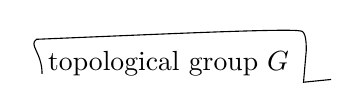
\begin{tikzpicture}[baseline=(phrase.base)]
\node[inner sep=0pt,anchor=base west] (phrase) at (0,0) {topological group $G$};
\draw[line width=0.4pt]
 ([xshift=-2pt,yshift=1pt]phrase.south west)
 .. controls ([xshift=-2pt,yshift=4pt]phrase.west)
          and ([xshift=-7pt,yshift=2pt]phrase.north west)
 .. ([xshift=-4pt,yshift=4pt]phrase.north west)
 .. controls ([yshift=6pt]phrase.north)
          and ([yshift=8pt]phrase.north east)
 .. ([xshift=4pt,yshift=7pt]phrase.north east)
 .. controls ([xshift=6pt,yshift=7pt]phrase.north east)
          and ([xshift=6pt,yshift=2pt]phrase.north east)
 .. ([xshift=6pt]phrase.north east)
 -- ([xshift=5pt,yshift=-2pt]phrase.south east)
 -- ([xshift=15pt,yshift=-1pt]phrase.south east);
\end{tikzpicture}}
such that \deleted{\unsure{$\widetilde A_0^\circ$}}\inserted{$G^\circ$} is simply connected; \deleted{let}
\deleted{\unsure{set} $\mu=\mathrm{Centre}(\unsure{\widetilde A_0^\circ})$}
\[
(67)\qquad\Pi_1(G^\circ)=0
\]
let
\[
(68)\qquad \mu=\mathrm{Centre}(G^\circ),\qquad\Gamma=G/G^\circ
\]
\margin{we assume $\mu$ discrete (thus $G^\circ$ identifies with the universal covering group of $G^\circ/\mu=\mathcal H^\circ$ (if $\mathcal H=G/\mu$))}
then the topological group extension $G$
of $\Gamma$ by $G^\circ$ defines
\[
(69)\qquad\Gamma\longrightarrow\mathrm{Aut\,ext}(G^\circ)
\qquad(\longrightarrow\mathrm{Aut}(\mu).)
\]
and the set of classes of extensions corresponding
to a given \inserted{outer} operation of $\Gamma$ on $G^\circ$
is in a natural way a torsor under
$H^2(\Gamma,\mu)$ (if it is not empty, which \unsure{is|we have} excluded
by the starting hypothesis, starting from $G$\ldots)
\margin{236}

\scanpage{238}
This category of extensions is moreover equivalent
\deleted{It \unsure{corresponds}}
to that of splittings of a certain
group-category defined by Sinh \inserted{via $(69)$}, whose $\Pi_0$ and
$\Pi_1$ are respectively $\deleted{\unsure{\Pi_0}}\Gamma$ and $\mu$ --- which
is \inserted{thus} here split by the datum of the extension
$G$. (In the case that interests us,
$\Gamma\simeq\mu\simeq\{\pm1\}$, and
this extension is even split, and corresponds
to an operation of order $2$ of $\Gamma$ on $G^\circ$,
which I very much doubt is an inner automorphism.
In fact, I have the impression that in the
two cases we are dealing with ($\widetilde{\mathrm{GP}}(1,\mathbb C)$ and
$\widetilde A_0$) that $(69)$ is an \uline{isomorphism}
$\Gamma=\{\pm1\}\xrightarrow{\sim}\mathrm{Autext}(G^\circ$

This being so, the datum of a torsor under
$\mathcal H=G/\mu$ defines $1^\circ$) a torsor under $\Gamma$,
$\mathcal H\longrightarrow\Gamma\simeq\mathcal H/\mathcal H^\circ$; $2^\circ$) the groupoid of
liftings of liftings of this torsor
to a torsor under $G$, which is a
\inserted{connected} $\mu$-groupoid (on which $\mu$ operates).
\margin{We assume that $\Gamma$ operates \uline{trivially} on $\mu$ i.e. $\mu\subset\mathrm{Centre}(G)$}

If we \deleted{\unsure{exp}} take this up again in terms of bundles
over a base space $S$ we find
\margin{237}

\scanpage{239}
\mspage{120}
again on $S$ (for every topological $\mathcal H_S$-torsor)
a pair $(\omega,\unsure{\mathcal R|R})$ of a $\Gamma$-torsor, and of
a $\mu$-gerbe on $S$, which are described (up to \unsure{isomorphism}
\inserted{\illegible{1} \unsure{equivalence}}
\unsure{up to equivalence|and equivalence}) by $H^1(S,\Gamma)$ and $H^2(S,\mu)$
respectively. We would like to isolate
conditions \inserted{on $G$ and on $S$} for the map
\[
(70)\qquad H^1(S,\mathcal H)\longrightarrow H^1(S,\Gamma)\times H^2(S,\mu)
\]
to be bijective.
\margin{\uline{N.B.} $\omega$ does not depend on the choice of the extension \unsure{$\widetilde G$} of $\mathcal H$ by \unsure{$\mathfrak z$|$\zeta$}${}\simeq\Pi_1(\mathcal H^\circ)$; \unsure{on the other hand} $\mathcal R$ depends on it (and one \unsure{would have to} see how)}

Injectivity : If the image \inserted{of a $\zeta\in H^1(S,\mathcal H)$,}
in $H^2(S,\mu)$ is zero,
the element of $H^1(S,\mathcal H)$ lifts to an element $\widetilde\zeta$
of $H^1(S,\widetilde{\mathcal H}=G)$; \unsure{whose} image in $H^1(S,\Gamma)$
\unsure{under} $G\longrightarrow\Gamma$ is the same as that of $\zeta$, so if
it is trivial, one sees that $\widetilde\zeta$ comes from
a $\widetilde\zeta_0\in H^1(S,G^\circ)$. If we know that
$H^1(S,G^\circ)=(1)$, we win. By the
sledgehammers of homotopy, it works
if $\exists n\in\mathbb N$ with
\[
\Pi_i(G^\circ)=0\quad\text{if}\quad i\leq n
\]
\inserted{(thus $\Pi_i(B_{G^\circ})=0$ if $i\leq n+1$)}
\deleted{$\Pi_i(S)=0$ if $i>n+1$}
\deleted{$\dim S\leq n+1$}
$S$ a CW-complex of dimension $\leq n+1$
\margin{in the case we are dealing with, one can take $n=2$}

For surjectivity, note that \unsure{for|first} an
\margin{238}

\scanpage{240}
element of $H^2(S,\mu)$, the obstruction to its
lifting to an element \inserted{$\zeta$} of $H^1(S,\mathcal H)$ is
in $H^2(S,G)$ [by the associated exact sequence
of \unsure{cohomology} : $1\longrightarrow\mu_S\longrightarrow G_S\longrightarrow\mathcal H_S\longrightarrow1$]
one must express that a certain \deleted{\illegible{1}} gerbe
banded by $G_S$ is neutral --- brr!. But
let us rather start from the element \inserted{\unsure{$\omega$|$\widetilde\zeta$}} of $H^1(S,\Gamma)$,
if the extension of $\Gamma$ by \deleted{\unsure{$G^\circ$}}$\mathcal H^\circ$ is split, then
one can find a $\zeta_0\in H^1(S,\mathcal H_S)$ which
gives rise to \unsure{$\omega$}. It has a certain
obstruction $\rho_0$ in $H^2(S,\mu)$, and it is a matter
of correcting $\zeta_0$ to $\zeta$, \inserted{in} such a way that
the obstruction becomes the given $\rho\in H^2(S,\mu)$.
\deleted{We have at our disposal} \inserted{Using $\zeta_0$} to twist $\mathcal H_S$ into
$\mathcal H'_S$, and (via the operation of $\mathcal H_S$ \inserted{$=G_S/\mu_S$} on $G_S$,
taking into account that $\mu_S\subset\mathrm{centre}\,G_S$) to
twist $G_S$ also \inserted{into $G'_S$}, whence
\[
1\longrightarrow\mu\longrightarrow G'_S\longrightarrow\mathcal H'_S\longrightarrow1
\]
one finds that the $\zeta$ having the same image in $H^1(S,\Gamma)$
\margin{239}

\subsection*{Scans 241--250}
\addcontentsline{toc}{subsection}{Scans 241--250}
% package LM_P025
\scanpage{241}
\mspage{121}
% l. 1
that \unsure{$\xi_0$} correspond \inserted{$1-1$} to the
$\xi'\in H^1(S,\mathcal H'_S)$.
% A hatched loop with a descender stands under the H of H'_S (an overwritten letter, perhaps a G).

% l. 2
For such a \deleted{\unsure{$\mathcal H'_S$}} $\xi'$, let
$\delta'(\xi')\in H^2(S,\mu)$
% l. 3
be the obstruction to lifting it to $H^1(S,\unsure{\mathcal G'_S|\mathcal G_S})$,
% l. 4
and $\delta(\xi')=\delta(\xi)$ the obstruction to lifting it
% l. 5
to $H^1(S,\mathcal G_S)$. Unless I am mistaken one has
% l. 6
\[
\delta'(\xi')=\delta(\xi')-\rho_0
\]
% l. 7
i.e.
\[
\delta(\xi')=\delta(\xi)=\delta'(\xi')+\rho_0
\]
% l. 8
and one wants $\delta(\xi)=\rho$ i.e.
% l. 9
\[
\deleted{\unsure{\delta(\xi')}=}\quad
\delta'(\xi')=\rho-\rho_0
\]
% l. 10
and the question again comes down to \deleted{\illegible{3}} \inserted{the}
% l. 11
surjectivity of $H^1(S,\mathcal H'_S)\longrightarrow H^2(S,\mu)$
\deleted{\illegible{1}}
% l. 12
--- I am not getting anywhere. One ought to
% l. 13
consult competent people, like
% l. 14
Giraud or Larry Breen. One feels that one
% l. 15
ought to work with a Gr-stack $\underline{\underline{\mathcal H}}$
% l. 16
of coefficients, with invariants $\underline{\pi}_0\simeq\Gamma$ and
$\underline{\pi}_1\simeq\mu$,
% l. 17
(but not necessarily a Picard stack!)
% l. 18
\deleted{with} and
$H^1(S,\underline{\underline{\mathcal H}})\simeq\text{Classes of maps}$
% l. 19
from $S$ to $B\underline{\underline{\mathcal H}}$, which is a connected
% l. 20
space with $\pi_1(B\underline{\underline{\mathcal H}})\simeq\Gamma$,
$\pi_2(B\underline{\underline{\mathcal H}})=\mu$.
% l. 21
Here the \unsure{Postnikoff} class in $H^3(\Gamma,\mu)$ is zero,
\margin{240}

\scanpage{242}
% l. 1
[but perhaps there is no reason to
% l. 2
cling too much to this hypothesis,
% l. 3
corresponding to the existence of an \inserted{extension} $\mathcal G$ of $\mathcal H$
\inserted{by $\pi_1(\mathcal H^\circ)$} \deleted{\illegible{1}}
% l. 4
which gives back the universal extension of
% l. 5
$\mathcal H^\circ$ by $\pi_1(\mathcal H^\circ)$] one has a \unsure{homomorphism}
% l. 6
$B\mathcal H$ \deleted{\illegible{1}} $\longrightarrow B\underline{\underline{\mathcal H}}$
which induces an isomorphism for
% The struck mark stands under the first BH (perhaps a cancelled double underline).
% l. 7
the $\pi_i$ for $i\leq2$, and for $i\leq n$
(where $n\geq2$ \inserted{is given})
% l. 8
iff $\pi_i(B\mathcal H)=0$ for $2<i\leq n$, i.e.
% l. 9
$\pi_i(\mathcal H)=0$ for $2\leq i\leq n-1$ [in the case
% l. 10
we are interested in $\mathcal H=A_0$, one can
% l. 11
take $n=3$). This implies that for
% l. 12
every C-W-complex $S$ of dimension $\leq n$,
% l. 13
one has \inserted{(Hot denoting the morphisms in
the unpointed homotopy category)}
% l. 14
\[
\mathrm{Hot}(S,B\mathcal H)\xrightarrow{\sim}
\mathrm{Hot}(S,B\underline{\underline{\mathcal H}})
\]
% l. 15
\unsure{i.e.|i.e.}
\[
H^1(S,\mathcal H)\xrightarrow{\simeq}
H^1(S,\deleted{\unsure{B}}\underline{\underline{\mathcal H}})
\]

% l. 16
But if the \unsure{Postnikoff}-Sinh invariant
% l. 17
$\unsure{K|k}\in H^3(\Gamma,\mu)$ is zero,
\deleted{\illegible{1}} (as well as the action
% l. 18
of $\Gamma$ on $\mu$) then unless I am mistaken
$B\underline{\underline{\mathcal H}}$ is iden%
% l. 19
tified with a product $K(\Gamma,1)\times K(\pi,2)$,
\deleted{and}
% l. 20
(this ``identification'' depending precisely on the
\margin{241}

\scanpage{243}
\mspage{122}
% l. 1
choice of the $H^2(\pi_1,\pi_2)\simeq H^2(\Gamma,\mu)$ !), and
% l. 2
hence
\[
H^1(S,\underline{\underline{\mathcal H}})\xrightarrow{\simeq}
H^1(S,\Gamma)\times H^2(S,\mu)
\]
% l. 3
for every space $S$, hence for $S$ a C-W-%
% l. 4
complex of dimension $\leq n$
% l. 5
\[
(71)\qquad
H^1(S,\mathcal H)\xrightarrow{\simeq}H^1(S,\Gamma)\times H^2(S,\mu)
\]

% l. 6
So the classification of bundles of topological
% l. 7
spheres over a topological space $S$,
% l. 8
for a C-W complex $S$ of dimension $\leq3$,
% l. 9
really does work. Of course, the
% l. 10
fact that one is obliged here to restrict oneself to
% l. 11
\deleted{\illegible{1}} $S$ of dimension $\leq3$ is due to the fact
% l. 12
that we have found \deleted{\unsure{only}}
(via $\underline{\underline{\mathcal H}}$)
% l. 13
only a $2$-isotopic (and not
% l. 14
$\infty$-isotopic) description of the category of
% l. 15
topological $2$-spheres.

% l. 16
I would like to take up the classification again
% l. 17
for an arbitrary CW-complex $S$,
% l. 18
using the fact that the inclusion
% l. 19
\[
\widetilde{\mathrm{GP}}(1,\mathbb C)\hookrightarrow A_0
\]
\margin{242}

\scanpage{244}
% l. 1
is a homotopy equivalence, and therefore
% l. 2
induces a bijection
% l. 3
\[
H^1(S,\widetilde{\mathrm{GP}}(1,\mathbb C))\longrightarrow H^1(S,A_0)
\]
% l. 4
and even an $\infty$-equivalence of the $\infty$-categories of
% l. 5
\deleted{bundles} \inserted{torsors} over $S$, with \deleted{\illegible{1}} groups
$\widetilde{\mathrm{GP}}$ (corresponding
% l. 6
to bundles of conformal spheres, or of
% l. 7
projective lines over an \deleted{field} $\mathbb R$-algebra
\inserted{(unspecified)}
% l. 8
isomorphic to $\mathbb C$) and with group $A_0$ --- corresponding
% l. 9
to sphere bundles over $S$.

% l. 10
The first invariant of a bundle with group $\widetilde{\mathrm{GP}}$
% l. 11
is a \deleted{bundle} torsor \unsure{$\eta$|$T$} under $(\mathbb Z/2\mathbb Z)_S$
\deleted{\illegible{2}} defined (\unsure{up to isomorphism}
% l. 12
\uline{not unique}\inserted{) by a} $\chi\ (\in H^1(S,\mathbb Z/2\mathbb Z))$.
% Physical order: "non unique" opens l. 12 under "est un"; "près) par un" is raised after the
% parenthesis of H^1; linearised as the sense requires.
\margin{i.e. an \unsure{étale covering|double covering} of degree $2$.
The datum of \unsure{$\eta$|$\chi$} amounts to the datum of a system \unsure{$T$} of twisted integers
over $S$.}
% l. 13
\inserted{This torsor} will serve to twist $\mathbb C$
(via the \inserted{faithful} operation of $\mathbb Z/2\mathbb Z$ on
% l. 14
the $\mathbb R$-extension $\mathbb C$), \deleted{and} whence a locally
\deleted{\illegible{1}}
% l. 15
constant bundle of \deleted{fields} \inserted{quadratic} extensions
of $\mathbb R$ \deleted{\illegible{1}},
% l. 16
say $C$, and one \deleted{will take the} will enrich $S$
% l. 17
with the sheaf \inserted{$\underline C_S$ (or $\underline C$)} of continuous sections of
% l. 18
$C$ (which is a way of twisting
% l. 19
\deleted{$\mathrm{Sl}(2,$} $\mathrm{GP}(1,\mathbb C)_S$
into $\mathrm{GP}(1,C)_S=\mathrm{GP}(1,\underline C)$))
% l. 20
and the point is to \deleted{\unsure{therefore}} describe in an
% l. 21
understandable way \deleted{the category} \inserted{--- passing} if need be,
% l. 22
to the \deleted{\unsure{$\infty$}}$n$-isotopic ones, for $n=\ldots$ --- the category
\margin{243}

\scanpage{245}
\mspage{123}
% l. 1
--- depending on the choice of $\chi$ via $\underline C$ --- of
% l. 2
Azumaya algebras of rank $4$ over $\underline C$,
% l. 3
or again of bundles of projective lines
% l. 4
over $\underline C$, or of torsors under $\mathrm{GP}(1,\underline C)$.

% l. 5
Now using \deleted{$\mathrm{Sl}(2,\underline C)\longrightarrow
\mathrm{GP}(1,\underline C$} \inserted{the \unsure{exact} sequence}
% l. 6
\[
1\longrightarrow\mu_{2S}\longrightarrow\mathrm{Sl}(2,\underline C_S)
\longrightarrow\mathrm{GP}(1,\underline C_S)\longrightarrow1
\]
% l. 7
one associates to an object of the category
% l. 8
--- say a torsor under $\mathrm{GP}(1,\underline C_S)$ --- the
% l. 9
\inserted{fibered (over variable open subsets of $S$)} category of these liftings to
$\mathrm{Sl}(2,\underline C_S)$,
% l. 10
which is a \uline{gerbe} \inserted{$\mathcal G$} banded by $\mu_2$.
% l. 11
It is this gerbe that is the second
% l. 12
complete invariant --- finer than
% l. 13
its class \deleted{in $H^2($} \inserted{up to equivalence, which is identified with a}
% l. 14
$\xi\in H^2(S,\mu_2)=H^2(S,\{\pm1\})$
(playing the role
% l. 15
of a Brauer group)

% l. 16
An isomorphism of bundles, with invariants
% l. 17
$(T,\mathcal G)$, $(T',\mathcal G')$, will define an isomorphism $T\simeq T'$
% l. 18
(whence an isomorphism \deleted{$\mathrm{GP}(1,C$}
$\underline C_T\simeq\underline C_{T'}$ whence
% l. 19
an isomorphism $\mathrm{GP}(1,\underline C_T)\simeq\mathrm{GP}(1,\underline C_{T'})$) --- and
% l. 20
an equivalence of gerbes --- one should
\margin{244}

\scanpage{246}
% l. 1
spell out that for two isomorphisms
% l. 2
$f,g$ of the torsors, \deleted{and} whence
% l. 3
\diagram{\begin{tikzcd}[ampersand replacement=\&,column sep=3.4em]
f_T,g_T:\ T
 \arrow[r,shift left=2.6ex,line width=0.7pt,"\unsure{\simeq}"]
 \arrow[r,phantom,"\unsure{\deleted{\xrightarrow{\sim}}}" description]
 \arrow[r,shift right=2.6ex,"\sim"]
\& T'
\& f_{\mathcal G},g_{\mathcal G}:\mathcal G
 \arrow[r,shift left=1.6ex,"\unsure{\simeq}"]
 \arrow[r,shift right=1.6ex,"\unsure{\simeq}"]
\& \mathcal G'
\end{tikzcd}}
% l. 4
and for every homotopy $h_t$ $(0\leq t\leq1)$ from
% l. 5
$f$ to $g$, one finds $f_T=g_T$ and an
% l. 6
isomorphism $h_*:f_{\mathcal G}\xrightarrow{\sim}g_{\mathcal G}$ of equivalences of
% l. 7
gerbes, which depends only on the homotopy
% l. 8
class of this homotopy. One
% l. 9
thus finds a $2$-functor, from the
% l. 10
$2$-category of \deleted{bundles} torsors over $S$
% l. 11
with group $\widetilde{\mathrm{GP}}(1,\mathbb C)$, to the $2$-category
% l. 12
formed by pairs \inserted{$(T,\mathcal G)$} of a
\deleted{torsor} \inserted{system} of %
% l. 13
twisted integers, \deleted{and} ($\Longleftrightarrow$ of a torsor over
% l. 14
$S$ with group \deleted{\illegible{1}} \inserted{$\mathbb Z/2$}) and of a
% l. 15
\deleted{\unsure{$\{\pm1\}=$}} $\mu_2(\mathbb C)$-gerbe $\mathcal G$ over $S$. This
% l. 16
$2$-functor, unless I am mistaken, is $2$-faithful
% l. 17
under the conditions spelled out
% l. 18
above (\deleted{\illegible{2}} (dimension $S\leq4$), and
% l. 19
is $3$-faithful (i.e. the injective map
% l. 20
$H^1(S,\widetilde{\mathrm{GP}})\unsure{\longrightarrow|{-}}
H^1(S,\mathbb Z/2\mathbb Z)\times H^2(S,\mu_2)$ is surjective)
\margin{245}

\scanpage{247}
\mspage{124}
% l. 1
if one even has dimension $S\leq3$. One expects it
% l. 2
to be $1$-faithful as soon as dimension $S\leq5$, $0$-faithful
% l. 3
as soon as dimension $S\leq6$.
\margin{??}
% A vertical marginal stroke accompanies approximately lines 1--3.
[\uline{N.B.} \inserted{the assertion} ``$0$-faithful'' means
% l. 4
that if \inserted{above} one has two homotopies $h,h'$ from $f$ to $g$,
% l. 5
such that $h_*=h'_*,$ then $h$ and $h'$ are homotopic.
% l. 6
The condition ``$1$-faithful'' means \inserted{$0$-faithful and} that every
% l. 7
isomorphism from $f_{\mathcal G}$ to $g_{\mathcal G}$
\deleted{\unsure{comes from a}} is of the
% l. 8
form $h_*$ (with $h$ well determined up to homotopy,
% l. 9
by the preceding condition of $0$-faithfulness). The
% l. 10
$2$-faithful condition means that \inserted{in addition, for} every
\deleted{equivalence}
% l. 11
\deleted{\unsure{given}} $\varphi:T\simeq T'$,
$\psi_{\mathcal G}:\mathcal G\xrightarrow{\approx}\mathcal G'$,
there exists
% l. 12
an isomorphism of bundles $f$ such that $\varphi=f_T$,
\deleted{$\psi$ \illegible{1}}
% l. 13
and an isomorphism $\psi\simeq f_{\mathcal G}$. Finally $3$-faithful means
% l. 14
that in addition, for every pair $T,\mathcal G$,
% l. 15
$\exists\ T',\mathcal G'$ coming from a bundle, \deleted{and of}
% l. 16
and an isomorphism $T\simeq T'$ and an equivalence
% l. 17
$\mathcal G\approxeq\mathcal G'$. These categorical notions
% l. 18
should simply interpret that, if
% l. 19
one looks at $\mathcal H=\widetilde{\mathrm{GP}}(1,\mathbb C)
\xrightarrow{\alpha}\underline{\underline{\mathcal H}}$
--- where $\underline{\underline{\mathcal H}}$
% l. 20
is deduced from $\mathcal H$ by ``killing the homotopy \unsure{gr\textsuperscript{o}ups}
% l. 21
$\pi_i$ for $i\geq2$'', so that
\margin{246}

\scanpage{248}
% l. 1
$\alpha$ induces an isomorphism of the $\pi_i$ for $i\leq1$
% l. 2
(and even for $i\leq n$ if
$\pi_i(\mathcal H)=0$ for $1<i\leq n$)
% l. 3
\deleted{and $B_\alpha$ an} whence
% l. 4
\[
B_\alpha:B\mathcal H\longrightarrow B\underline{\underline{\mathcal H}}
\]
\margin{\uline{N.B.} $B\underline{\underline{\mathcal H}}$ is deduced from
$B\mathcal H$ by killing the $\pi_i$ for $i\geq3$.}
% l. 5
(inducing an isomorphism of the $\pi_i$ for $i\leq n+1$),
% l. 6
then taking for \deleted{every} \inserted{a given space} $S$ the
% l. 7
corresponding map of spaces of continuous maps
% l. 8
\[
\deleted{\mathrm{Hot}}
\underline{\mathrm{Cont}}(S,B\mathcal H)
\unsure{\longrightarrow|{-}}
\underline{\mathrm{Cont}}(S,B\underline{\underline{\mathcal H}})
\]
% l. 9
this induces an isomorphism for the
% l. 10
$\pi_i$ $(0\leq i\leq2)$. \deleted{\unsure{Since}} It would seem that
% l. 11
$0$-faithfulness is a condition of injectivity
% l. 12
for the $\pi_2$, $1$-faithful bijectivity for the
% l. 13
$\pi_2$ and injectivity for the $\pi_1$, $2$-faithful
% l. 14
bijectivity for $\pi_2$ and $\pi_1$ and injectivity
% l. 15
for $\pi_0$, $3$-faithful bijectivity for $\pi_0,\pi_1,\pi_2$.

% l. 16
Since $\pi_i(\mathrm{Cont}(S,B))\simeq
\pi_0(S\times S^i,B)$,
% l. 17
\deleted{one sees} \inserted{it would seem}
that one is led, for $0$-%
% l. 18
faithfulness, to make the draco%
% l. 19
nian hypothesis that $S\times S^2$ of dimension $\leq4$, for
% l. 20
$1$-faithfulness that $S\times S^2$ of dimension $\leq3$ i.e. $S$
% l. 21
of dimension $\leq1$ ? (\unsure{This|That} would then imply
% l. 22
$3$-faithfulness\ldots)
\margin{247}

\scanpage{249}
\mspage{125}
% l. 1
Let us take the arithmetic analogue, of a description
% l. 2
(more or less ``faithful'') \deleted{by \illegible{1}}
of a ``profinite'' nature
% l. 3
of the projective lines \deleted{defined} (possibly
% l. 4
twisted) defined over a finitely generated
% l. 5
field $K$ \inserted{over $\mathbb Q$ (more generally over an arbitrary scheme $S$)},
these a priori form a category
% l. 6
and nothing more --- a groupoid (not necessarily
% l. 7
connected) I do not know how to make a
% l. 8
$2$-category out of them reasonably, because for two
% l. 9
isomorphisms $f,g$ \inserted{$(=f\circ u)$} of such torsors, to define the
% l. 10
homotopisms from $f$ to $g$, i.e. for a ``form''
% l. 11
$G$ of $\mathrm{GP}(1)_S$ and a section $u$ of $G$,
% l. 12
to define the ``homotopies'' from $u$ to the iden%
% l. 13
tity, \deleted{and the \inserted{homotopy} classes of such \illegible{1}}
\inserted{or rather} a
% l. 14
notion which replaces the notion of a homo%
% l. 15
topy class of such homotopies. \deleted{But} \inserted{This would be}
% l. 16
probably a lifting of $u$ to a
\deleted{
% l. 17
\unsure{If} $S$ is \illegible{1} of a geometric point
% l. 18
\illegible{1} \unsure{every section} defines a \illegible{1}
% l. 19
\unsure{if $K$ is algebraic} For an algebraically
% l. 20
closed base field \unsure{at least} (the \unsure{sections}
% l. 21
defining a geometric point) one
% l. 22
can think of taking the ``classes of
% l. 23
paths from $f$ to \illegible{1} from $u$ to
}
% l. 24
section of the \deleted{\unsure{$\widetilde{\mathrm{GP}}$}}
simply
% l. 25
connected covering $\widetilde G$ of $G$ !
\margin{248}

\scanpage{250}
% l. 1
I have something rather amusing here,
% l. 2
but which I am not going to pursue --- in
% l. 3
\unsure{any case|any case} it is clear that the ``description''
% l. 4
of the projective lines (over a finitely generated
% l. 5
field, say) that one ends up with,
% l. 6
has nothing faithful about it --- not even $0$-faithful !
% l. 7
Thus all the automorphisms of $\mathbb P^1_K$ coming from
% l. 8
$\mathrm{Sl}(2,K)$ will be identified with the identity ---
% l. 9
that is a bit brutal ! But I
% l. 10
realize that the conceptual work
% l. 11
around the ``Brauer'' themes is not
% l. 12
finished --- that there are things to be understood
% l. 13
for the study of the category
% l. 14
(\inserted{which should be} a \uuline{2}-category !)
of Azumaya Algebras
% l. 15
\deleted{\unsure{of}} \uline{fixed} degree (here $4$)\ldots
\margin{249}

\subsection*{Scans 251--260}
\addcontentsline{toc}{subsection}{Scans 251--260}
% package LM_P026
\scanpage{251}
\mspage{126}

\uline{21 Connection with Teichmüller spaces.}

First a supplement connected with the diagram \inserted{of inclusions} (31) of number 19, in which \(A_{g,(\nu,\nu+1)}\) deserves the simpler notation \(A_{g,\nu}^{\bullet}\) (\unsure{group} of automorphisms of \(U_{g,\nu}\) pointed at \(a_{g,\nu}\)). Consider \unsure{the inclusion|the filtration} of subgroups of \(A_g\)
\[
 A_{g,\nu}^{\circ}\supset B_{g,\nu}\supset A_{g,\nu+1}^{\circ}
 \tag{72}
\]
\deleted{\unsure{\(A_{g,\nu}^{\bullet}\)}}

\unsure{giving}, on dividing by \(A_{g,\nu+1}\) and in the anabelian case \(2g+\nu\geq 3\), the fibration

(73) \diagram{\begin{tikzcd}[ampersand replacement=\&]
\widetilde U_{g,\nu} \arrow[r] \& U_{g,\nu} \\
A_{g,\nu}^{\circ}/A_{g,\nu+1}^{\circ} \arrow[u, phantom, "\unsure{\simeq}" description] \&
\end{tikzcd}}

We seek the largest subgroup of \(A_g\) that normalizes \unsure{these|the} triple (72), and which \deleted{\unsure{defines}} \inserted{operates} therefore \deleted{\unsure{on}} the fibration \(\widetilde U_{g,\nu}\to U_{g,\nu}\) (where \(\widetilde U_{g,\nu}\) is the universal covering of \(U_{g,\nu}\) based at \(a_{g,\nu}\)); since the normalizers of \(A_{g,\nu}^{\circ}\) and \(A_{g,\nu+1}^{\circ}\) respectively are \(A_{g,\nu}\) and \(A_{g,\nu+1}\), the group in question must be contained in their intersection \(A_{g,\nu}^{\bullet}\), which normalizes \deleted{\unsure{also}} \(B_{g,\nu}=A_{g,\nu}^{\bullet}\cap A_{g,\nu}^{\circ}\). \unsure{It is} therefore this group that should be made to operate on the fibration (73) -- the subgroup \unsure{formed} \deleted{\illegible{7} \(U_{g,\nu}\)} \inserted{of the elements of \(A_{g,\nu}\)} whose operation

\scanpage{252}

on \(U_{g,\nu}\) is isotopic to the identity being \unsure{precisely} \(B_{g,\nu}\) -- so it is the group \unsure{\(\Gamma\)}
\[
 A_{g,\nu}^{\bullet}/B_{g,\nu}\simeq\Gamma_{g,\nu}
\]
that, as it should, operates up to isotopy. We would like to describe the group of all automorphisms of the topological fibration \(\widetilde U_{g,\nu}\) over \(U_{g,\nu}\) which will a priori be an extension of the group
\[
 \begin{aligned}
 A_{g,\nu}&=\operatorname{Aut}(U_{g,\nu})\quad\text{by}\quad
 \Pi_{g,\nu}=\pi_1(\unsure{U_{g,\nu}|\widetilde U_{g,\nu}},a_{g,\nu})\\
 &=\operatorname{Aut}_{U_{g,\nu}}(\widetilde U_{g,\nu}).
 \end{aligned}
\]

\deleted{\illegible{1}} This extension \inserted{is \uline{\unsure{split canonical\textsuperscript{ly}}}} \deleted{\unsure{split}} over \(A_{g,\nu}^{\bullet}\), \inserted{stabilizer at the base point \(a_{g,\nu}\)} (and we thus recover the operation of \(A_{g,\nu}^{\bullet}\) for the fibration (73). Now we already have an extension \(\Gamma'_{g,\nu+1}\) of \(\Gamma_{g,\nu}\) by \(\Pi_{g,\nu}\), whence by inverse image under \(A_{g,\nu}\to\Gamma_{g,\nu}=A_{g,\nu}/A_{g,\nu}^{\circ}\), an extension (which I am going to denote by \(\widetilde A_{g,\unsure{\nu}}\)) of \(A_{g,\nu}\) by \(\Pi_{g,\nu}\):
\[
 \widetilde A_{g,\nu}\simeq A_{g,\nu}\mathbin{\times}_{\Gamma_{g,\nu}}\Gamma'_{g,\nu+1}
 \tag{74}
\]
\(=\) quotient group of the subgroup \deleted{\unsure{\(H\)}} \(\widetilde A_{g,\nu}^{\unsure{\natural|\sharp}}\) \unsure{of} \(A_{g,\nu}\times A_{g,\nu}^{\bullet}\) formed of the pairs \((u,v)\), \(u\unsure{\equiv}v\) \deleted{\unsure{\(A_{g,\nu}^{\circ}\)}} modulo \(A_{g,\nu}^{\circ}\), by the subgroup \deleted{\unsure{\(B_{g,\nu}^{\circ}\)}} \(1\times A_{g,\nu+1}^{\circ}\).

We thus have two \inserted{(and = three!)} extension structures on \(\widetilde A_{g,\nu}\)

(75) \diagram{\begin{tikzcd}[ampersand replacement=\&][column sep=small]
1 \arrow[r] \& \Pi_{g,\nu} \arrow[r] \& \widetilde A_{g,\nu} \arrow[r,"p"] \& A_{g,\nu} \arrow[r] \& 1 \\
1 \arrow[r] \& A_{g,\nu}^{\circ} \arrow[r] \& \widetilde A_{g,\nu} \arrow[r] \& \Gamma'_{g,\nu+1} \arrow[r] \& 1
\end{tikzcd}}
\diagram{\begin{tikzcd}[ampersand replacement=\&][column sep=small]
1 \arrow[r] \& (A_{g,\nu}^{\circ}\unsure{\times|\rtimes}\Pi_{g,\nu}) \arrow[r] \& \widetilde A_{g,\nu} \arrow[r] \& \Gamma_{g,\nu} \arrow[r] \& 1
\end{tikzcd}}

\margin{\uline{N.B.} The second \unsure{is meant to express} that \(\widetilde A_{g,\nu}^{\circ}=A_{g,\nu}^{\circ}\) and \(\pi_0(\widetilde A_{g,\nu})\simeq\Gamma'_{g,\nu+1}\) (the canonical extension of \(\Gamma_{g,\nu}\) by \(\Pi_{g,\nu}\)).}
\deleted{\unsure{Now}}

\scanpage{253}
\mspage{127}

I would like to make \(\widetilde A_{g,\nu}\) operate on \(\widetilde U_{g,\nu}\), i.e. make \deleted{\illegible{1}} \(H=\widetilde A_{g,\nu}^{\unsure{\natural|\sharp}}\) operate \unsure{with operation} \deleted{in such a way that \((u,v)\)} trivial on \(A_{g,\nu+1}^{\circ}\), and this respecting the following conditions

\margin{\unsure{trivial datum} on \(1\times A_{g,\nu+1}^{\circ}\). Cf. generalization below in the margin.}

a) \deleted{\illegible{1}} (compatibility with \(\widetilde A_{g,\nu}\to A_{g,\nu}\)) the pair \((u,v)\in H\) operates \unsure{on} \(\widetilde U_{g,\nu}\) by an automorphism compatible with the automorphism \inserted{\(u\) of} \(U_{g,\nu}\) (we shall say that it is a \(u\)-automorphism).

b) (compatibility with \(\Pi_{g,\nu}\to\widetilde A_{g,\nu}\)) If \(u=1\), \inserted{[so \(v\in A_{g,\nu}^{\circ}\), so (since \(v\in A_{g,\nu}^{\bullet}\)) \(v\in B_{g,\nu}\)]} then the operation of \((u,v)=(1,v)\) on \(\widetilde U_{g,\nu}\) is none other than that defined by \(v\bmod B_{g,\nu}^{\circ}=A_{g,\nu+1}^{\circ}\), which is an element of \(\Pi_{g,\nu}\simeq\operatorname{Aut}(\widetilde U_{g,\nu}/U_{g,\nu})\), or again, it is that defined by \uline{translation} \inserted{\uuline{on the right}} by \(\unsure{v^{-1}}\).

\margin{specification of the operation on \(1\times B_{g,\nu}\).}

c) Compatibility with \deleted{\unsure{\(\widetilde A_{g,\nu}\to\Gamma'_{g,\nu+1}\)}} the operation already \deleted{\illegible{1}} \inserted{obtained above} of \(A_{g,\nu}^{\bullet}\) on \(\widetilde U_{g,\nu}\): if \((u,v)\in H\) is such that \(u=v\) (so \(u=v\in A_{g,\nu}^{\bullet}\)) then \(\unsure{(u,v)}=(u,u)\) operates \unsure{via} the inner automorphism defined by \(u\).

\margin{specification of the operation on \(\delta(A_{g,\nu}^{\bullet})\) (\(\delta\): diagonal arrow).}

d) \inserted{Compatibility with \(A_{g,\nu}^{\circ}\to\widetilde A_{g,\nu}\):} The operation of \(A_{g,\nu}^{\circ}\) on \(\widetilde U_{g,\nu}\) is continuous (which, together with a), determines this operation uniquely \deleted{\illegible{2}} \inserted{and} the existence \inserted{\unsure{a priori of such an operation}} (follows from \(\pi_1(A_{g,\nu}^{\circ})=0\))).

\margin{specification of the operation on \((A_{g,\nu}^{\circ})\times 1\).}

\unsure{every} element \inserted{\((u,v)\)} of \(H\) can be written uniquely as a product of an element \inserted{\((v,v)\)} of \(\delta(A_{g,\nu}^{\bullet})\), with an element \inserted{\((v^{-1}u,1)\)} of \(A_{g,\nu}^{\circ}\times 1\) (the first group normalizing the second)

\margin{\uline{N.B.} The operation of \(A_{g,\nu}^{\circ}\times 1\) is \unsure{described} most simply by \uline{translations} of \unsure{\(A_{g,\nu}^{\circ}\)} on the \unsure{homogeneous} space \(\widetilde U_{g,\nu}\) of \(A_{g,\nu}^{\circ}\).}

\scanpage{254}

and an operation of this \(\frac12\) direct product is given \inserted{indeed} by \deleted{\illegible{1}} specifying operations of the two factor groups, satisfying a compatibility condition, which is verified here by transport of structure. We have indeed defined an operation of \(H=\widetilde A_{g,\nu}^{\unsure{\natural|\sharp}}\) on the fibration (73), \deleted{\illegible{2}} satisfying conditions c) and d) by the very construction, it remains to verify a) and b).

Now for a), it suffices to verify it separately for the \unsure{elements} of \(H\) in \(\delta(A_{g,\nu}^{\bullet})\) and in \(A_{g,\nu}^{\circ}\times 1\), where this is trivial by construction in both cases. It remains to verify b), i.e. to make explicit the operation of an \unsure{element} \((1,v)\), \(v\in B_{g,\nu}\), which we write as
\[
 (\qquad (1,v)=\deleted{(\unsure{v^{-1}},1)}(v,v)(v^{-1},1)
\]
hence
\[
 \rho\deleted{_{\unsure{\widetilde A}_{g,\nu}}}(1,v)=\rho(v,v)\rho(v^{-1},1).
\]

Now \(\rho(v,v)\) is induced by \(\operatorname{int}(v)\), \inserted{i.e. \(x\mapsto vxv^{-1}\)} and \(\rho(v^{-1},1)\) by left translation: \(x\mapsto v^{-1}x\), so the composite operates by \(x\mapsto xv^{-1}\). Phew!

\scanpage{255}
\mspage{128}

We now assume that \(X_g\) is equipped with a \(C^\infty\) structure, and we replace in the considerations \deleted{Let} above the groups of homeomorphisms by groups of diffeomorphisms.

\margin{\uline{N.B.} A \(C^{\unsure{\nu|r}}\) structure with \(\unsure{\nu|r}\geq 2\) would suffice}
\[
 \begin{aligned}
 E_g={}&\text{set of \deleted{complex} \inserted{conformal} structures}\\
 &\text{on }X_g\text{ compatible with its}\\
 &\text{structure }C^\infty
 \end{aligned}
 \tag{76}
\]

\deleted{\unsure{Then}} We see at once that \(E_g\) is an \uline{\(\infty\)-connected} topological space, as a quotient of the \(\infty\)-connected space \inserted{(a convex set)} of Riemannian structures, by the \deleted{\unsure{group}} \(\infty\)-connected group of \(C^\infty\) maps from \(X_g\) to \(\mathbb R^{+*}\). On \(E_g\) the group \(A_g\) operates -- but of course \(E_g\) is no longer a homogeneous space. Let us note at once
\[
 \begin{aligned}
 E_g/A_g\simeq{}&\text{set of isomorphism classes}\\
 &\text{of \deleted{algebraic curves} \inserted{surfaces} \deleted{\unsure{compact}}}\\
 &\text{conformal compact orientable}\\
 &\text{of genus }g
 \end{aligned}
 \tag{77}
\]

And if we choose one of the two orientations of \(X_g\), so that \(E_g\) is identified with the set of \uline{complex} structures on \(X_g\) compatible with its \(C^\infty\) structure \inserted{and its orientation}, then \(E_g/A_g\) is identified with the space of isomorphism classes of compact complex curves \inserted{(nonsingular) connected} of genus \(g\), \uline{modulo} passage to the complex conjugate. On the other hand

\scanpage{256}

\[
 \begin{aligned}
 E_g/A_g^+\simeq{}&\text{set of isomorphism classes}\\
 &\text{of curves }\mathbb C\text{-algebraic \inserted{smooth} projective}\\
 &\text{connected of genus }g.
 \end{aligned}
 \tag{78}
\]

More generally

\[
 \begin{aligned}
 E_g/A_{g,\nu}\simeq{}&\text{set of isomorphism classes}\\
 &\text{of \deleted{structures} \deleted{on the} compact surfaces}\\
 &\text{\inserted{conformal} equipped \unsure{with multipunctures|with multipuncturings}}\\
 &\text{of type }(g,\nu)
 \end{aligned}
 \tag{79}
\]

\[
 \begin{aligned}
 E_g/A_{g,\nu}^{+}\simeq{}&\text{set of isomorphism classes}\\
 &\text{of curves \deleted{\unsure{complex}} \inserted{\(\mathbb C\) algebraic}}\\
 &\text{[smooth projective connected}\\
 &\text{of genus }g\text{] \uline{equipped} with a}\\
 &\text{multipuncturing, of type}\\
 &(g,\nu)
 \end{aligned}
 \tag{80}
\]
\margin{if \(X_g\) oriented.}

These are the ``coarse moduli spaces'' (Mumford's ``coarse moduli''), which we may denote by \(M_g^{\unsure{\natural|\sharp}}\) and \(M_{g,\nu}^{\unsure{\natural|\sharp}}\), and which are indeed too coarse for the most important geometric uses. \deleted{But} Much more interesting are the quotients \(E_g/A_{g,\nu}^{\circ}\), \illegible{1}

\scanpage{257}
\mspage{129}

\[
 \widetilde M_{g,\nu}=E_g/A_{g,\nu}^{\circ}
 \qquad
 (\widetilde M_g=\widetilde M_{g,0}=E_g/A_g^{\circ})
 \tag{81}
\]
on which the group \deleted{\illegible{1}}
\[
 \Gamma_{g,\nu}=A_{g,\nu}/A_{g,\nu}^{\circ}
\]
operates by passage to the quotient of the operation of \(A_{g,\nu}\).

\deleted{\illegible{1}} The space \(\widetilde M_{g,\nu}\) \inserted{(with the operation of \(\Gamma_{g,\nu}\))} is called \uline{the Teichmüller space} of type \(g,\nu\). Of course we recover \(M_{g,\nu}^{\unsure{\natural|\sharp}}\) from \(\widetilde M_{g,\nu}\) and \margin{\deleted{(82)}} the operation of \(\Gamma_{g,\nu}\) on it, by
\[
 M_{g,\nu}^{\unsure{\natural|\sharp}}=\widetilde M_{g,\nu}/\Gamma_{g,\nu}
 \tag{\unsure{82}}
\]

\uline{Theorem} (Teichmüller) The Teichmüller space \(\widetilde M_{g,\nu}\) is homeomorphic to \deleted{\(\mathbb R\)} \(\mathbb C^\mu\), where \(\mu=3g-3+\nu\) (\inserted{in the} anabelian cases \(2g+\nu\geq 3\)), and \(\mu=3g-3+(\unsure{\nu}+\delta)\)
\[
 \delta=\dim_{\mathbb C}G
\]
in the general case, \(G\) being \unsure{group} of algebraic automorphisms of a complex \(U_{g,\nu}\) (so \(\delta=1\) in the \unsure{``limiting''} cases \((1,0)\) and \((0,2)\), and \inserted{more \unsure{generally}} \(\delta\) increases by 1 each time \unsure{for} \(g\) fixed, and \((g,\nu-1)\) abelian, one passes from \(\nu\) to \(\nu-1\)), hence

\margin{We can also say that \(\mu=3g-3+\nu'\), where \(\nu'=\nu\) in the \unsure{anabelian} case, and \unsure{where \(\nu'\)} in the ``general'' case is the least integer \(\geq\nu\) such that \((g,\nu')\) is \unsure{``anabelian''}.}

\scanpage{258}

\[
 \left\{
 \begin{aligned}
 \mu&=1\quad\text{in the case }(1,0)\\
 \mu&=0\quad\text{in the cases }(0,2),(0,1),(0,0),
 \end{aligned}
 \right.
 \tag{\unsure{\(82_1\)|\(82'\)}}
\]
i.e. \(\widetilde M_{g,\nu}\) is in these cases reduced to a point, i.e. the action of \(A_{g,\nu}^{\circ}\) on \(E_g=E_0\) is \deleted{already} transitive -- (and these are \inserted{with the anabelian case \((0,3)\)} the only three cases where this is so, \deleted{\illegible{4}}).

\margin{i.e. on surfaces \unsure{oriented} \unsure{spherical with} \(\unsure{\nu\leq 3}\), all complex structures are \uline{isotopic}.}

Starting from \(\widetilde M_{0,3}\), or from \(\widetilde M_{1,1}\) or from \(\widetilde M_{g,0}=\widetilde M_g\) with \(g\geq 1\), when \(\nu\) increases the ``complex dimensions'' of \(\widetilde M_{g,\nu}\) increase by the same amount (On the other hand \(\widetilde M_{1,0}\unsure{\longleftarrow}\widetilde M_{1,1}\) is a homeomorphism \deleted{\unsure{because}\ \(A_{1,0}^{\circ}\unsure{\simeq}A_{1,1}^{\circ}\) \illegible{1}}).

We can make Teichmüller's theorem more precise as follows

\uline{Corollary} In the \uline{anabelian} case, \(A_{g,\nu}^{\circ}\) operates freely on \(E_g\), so that \(E_g\) becomes a torsor over \(\widetilde M_{g,\nu}\), with structure group \(A_{g,\nu}^{\circ}\).

We deduce from this that \(\widetilde M_{g,\nu}\) plays the role of a \uline{classifying space} for \(A_{g,\nu}^{\circ}\), and that
\[
 \pi_{\unsure{i|\nu}}(\widetilde M_{g,\nu})
 \xrightarrow{\sim} \pi_{\unsure{\nu-1|i-1}}(A_{g,\nu}^{\circ})
 \tag{83}
\]
and the fact that \(\widetilde M_{g,\nu}\) is \(\infty\)-connected (contained in Teichmüller's theorem) is equivalent to

\scanpage{259}
\mspage{130}

the fact that \(A_{g,\nu}^{\circ}\) is so -- which is the ``well-known theorem'' recalled in number 19.

I do not dwell here on the interpretation of the points of \(\widetilde M_{g,\nu}\) as isomorphism classes of complex curves, equipped \deleted{with} \inserted{with a} suitable ``Teichmüller rigidification'', \unsure{and the rigidified moduli spaces point of view}, which makes it possible to verify a priori that \(\widetilde M_{g,\nu}\) is equipped with the structure of a nonsingular complex manifold -- but already the fact that \(\widetilde M_{g,\nu}\) is \uline{simply connected} (which can \unsure{express} \unsure{by} interpreting \(\widetilde M_{g,\nu}\) as the universal covering of the \uline{modular topos} \(M_{g,\nu}\)) is quite deep, which does not seem to be able to fit into the framework of topology (or of differential topology \((C^\infty)\) alone...

\margin{\uline{N.B.} To prove that the \(\unsure{\widetilde M_{g,\nu}}\) are \(\infty\)-connected, \unsure{we are easily reduced} to the case of \(M_{g,0}\) \unsure{(if \(g\geq 2\))}, or of \(M_{1,1}\) (punctured elliptic case), by using \unsure{the fibrations} \(A_{g,\nu}^{\circ}/A_{g,\nu+1}^{\circ}\simeq\widetilde U_{g,\nu}\) (which is \(\infty\)-connected...). The case \(g=1\) is \unsure{moreover easy and} well understood...}

\scanpage{260}

Let us note that the subgroup inclusions
\[
 A_{g,\nu+1}^{\circ}\subset A_{g,\nu}^{\circ}\cdots\subset A_{g,0}^{\circ}=A_g^{\circ}
\]
define a tower of continuous maps
\[
 \cdots\longrightarrow\widetilde M_{g,\nu+1}\longrightarrow\widetilde M_{g,\nu}
 \longrightarrow\cdots\longrightarrow\widetilde M_{g,0}=\widetilde M_g
 \tag{84}
\]

where
\[
 \widetilde M_{g,\nu+1}\longrightarrow\widetilde M_{g,\nu}
 \tag{85}
\]
is \inserted{\uline{for \((g,\nu)\) anabelian}} a fibration with fiber \(A_{g,\nu}^{\circ}/A_{g,\nu+1}^{\circ}\simeq\widetilde U_{g,\nu}\).

[it therefore has contractible fiber, and the \(\infty\)-connectedness of \(\widetilde M_{g,\nu+1}\) is therefore equivalent to that of \(\widetilde M_{g,\nu}\) -- which brings us back to the case of \(\widetilde M_g\) if \(g\geq 2\), of \(M_{\text{\deleted{\(g\)}}1,1}\) and of \(M_{0,3}\) if \(g\unsure{=|\neq|\geq}1\) or 0].

In the abelian case \((g,\nu)\), we find
\[
 \widetilde M_{g,\nu+1}\simeq\widetilde M_{g,\nu}\qquad
 (\text{if }(g,\nu)\text{ abelian})
 \tag{85}
\]
which \deleted{\unsure{follows precisely|stems, follows} from the fact already} \inserted{means} \deleted{noted} that in these cases, if we have two complex structures \inserted{\(\alpha,\beta\)} on \(X\) which are congruent by \inserted{\(u\in\)} \(A_{g,\nu}^{\circ}\), \inserted{(i.e. \(\beta=u.\alpha\))} they are = congruent by \(A_{g,\nu+1}^{\circ}\).

Indeed, if \(G\) is \unsure{the} \inserted{\unsure{identity|neutral} component of the} group of complex automorphisms of \(U_{g,\nu}\) for \(\beta\), we can write \(u=gv\) with \(g\in G\), \(v\in A_{g,\nu+1}^{\circ}\) hence \(\beta=gv.\alpha\) hence (since \(g^{-1}\beta=\beta\)) \(\beta=v\alpha\), q.e.d.

\subsection*{Scans 261--270}
\addcontentsline{toc}{subsection}{Scans 261--270}
% package LM_P027
\scanpage{261}
\mspage{131}
Thus $\widetilde M_{1,1}\simeq\widetilde M_{1,0}$ -- and it is immediate that the latter is $\simeq$ the Poincaré half-plane. Likewise
$\widetilde M_{3,0}\xrightarrow{\sim}\widetilde M_{2,0}\simeq\widetilde M_{1,0}\simeq\widetilde M_{\unsure{00|0,0}}$,
and since $A_0^0$ is \inserted{simply} made up of the automorphisms of $X_0\simeq S^2$ which \unsure{preserve} orientation, we see that two complex structures on $S^2$ are isotopic (since they are \unsure{isomorphic}, and an isomorphism preserves orientation i.e. is $\in A_0^0$) this proves that the $M_{0,i}$ ($i\leq 3$) are reduced to a \unsure{point|points} ! Thus the Teichmüller Theorem is fairly evident if $g=0$ or $1$, it is the case $g\geq 2$ that is deep\ldots

The Teichmüller space (more generally, any \deleted{space} space \inserted{$E$ $\infty$-connected} on which $A_g$ operates in such a way that $A_{g,\nu}^0$ operates freely) will allow us to interpret the canonical extension $\Gamma'_{g,\nu+1}$ of $\Gamma_{g,\nu}$ by $\Pi_{g,\nu}$ (anabelian cases $(g,\nu)$) as the mixed fundamental group of a \deleted{fibered} space (homotopic to \unsure{$U_{g,\nu}$}) on which $\Gamma_{g,\nu}$ operates. (We were bothered previously, because $\Gamma_{g,\nu}$ did not itself operate on $U_{g,\nu}$, but only the group $A_{g,\nu}$ of which $\Gamma_{g,\nu}$ is a quotient, we had the impression

\scanpage{262}
that passage to the quotient by $A_{g,\nu}^0$ was nevertheless inessential, since $A_{g,\nu}^0$ is $\infty$-connected -- and moreover we had found an extension $\widetilde A_{g,\nu}$ of $\Gamma'_{g,\nu+1}$ by this \unsure{same} $\infty$-connected group $A_{g,\nu}^0$, which operates on the universal covering, \deleted{\unsure{such a way}} \inserted{\deleted{in such a way}} \unsure{with} a homomorphism \inserted{\unsure{surjective}} $\widetilde A_{g,\nu}\to A_{g,\nu}$ with kernel $\simeq\Pi_{g,\nu}$ compatible with this operation\ldots

Now if $\widetilde M=E/A_{g,\nu}^0$, $E$ is an $A_{g,\nu}^0$-torsor with base $\widetilde M$, which we can use to twist \deleted{\illegible{1}} $U_{g,\nu}$ on which $A_{g,\nu}^0$ operates continuously, we thus find a bundle \unsure{$\mathcal X$} ($\simeq U_{g,\nu}\times E/A_{g,\nu}^0$ operating diagonally) over $\widetilde M$, with fiber $U_{g,\nu}$ (this is for $E=E_g$ the universal bundle of complex curves of type $(g,\nu)$ with Teichmüller rigidification\ldots). Since $E$ and $A_{g,\nu}^0$

\scanpage{263}
\mspage{132}
are $\infty$-connected, so is $\widetilde M$, hence the inclusion of a fiber into \unsure{the} bundle \unsure{$\mathcal X$} over $\widetilde M$ is a homotopy equivalence. Now $\Gamma_{g,\nu}$ operates on \unsure{$\mathcal X$} (in a way compatible with its operation on $\widetilde M$), whence the construction of an extension of $\Gamma_{g,\nu}$ by $\pi_1(\mathcal X)\simeq\pi_{\unsure{1}}(U_{g,\nu})\simeq\Pi_{g,\nu}$ -- we have done all that was needed to prove that this is indeed essentially $\Gamma'_{g,\nu}$ -- I dispense with giving the details\ldots

\scanpage{264}
\mspage{133}
\uline{23} Back to surfaces with \unsure{group|groups} of operators.

Our point of view will be, not that of outer groups with loops, but that of multi-Galois topoi and morphisms between them, more flexible, as we have seen.
Before bringing in operations of groups, \deleted{\unsure{let us note that a}} \inserted{let us introduce the $2$-category of} orientable surfaces $U$ (N.B. not \unsure{oriented} !) \deleted{with \illegible{1}} \deleted{\unsure{bounded}} \uline{admissible} (i.e. of the form $X\setminus S$, where $X$ is compact, $S$ finite, and every connected component of $X$ of genus $0$ meets $S$), as \unsure{some|in} Ladegaillerie (taking as $2$-morphisms between \deleted{\illegible{1}} homeomorphisms $f,g\colon U\unsure{\rightrightarrows|\Rightarrow}U'$ the homotopy classes of paths from $f$ \unsure{from|in} $g$ in the space $\uline{\mathrm{Isom}}(U,U')$ (which, with the hypotheses made, has as connected components \deleted{\unsure{pro}} torsors under products of groups $A_{g,\nu}^0$ (with \unsure{$(g,\nu)\ne 0,0$|$(g,\nu)\ne(0,0)$}) -- so these are $K(\unsure{\Pi|\pi},1)$.

We find a $2$-functor from the

\scanpage{265}
preceding $2$ category to that of morphisms of \inserted{multi-}Galois topoi (or, if we prefer, to that of morphisms of groupoids), \unsure{denoted}
\diagram{\begin{tikzcd}[ampersand replacement=\&]
B_{D^*} \arrow[r,"\rho"] \& B_U
\end{tikzcd}},
where for two objects of the $2$-category $B_{D^*}\to B_U$ and $B_{D'^*}\to B_{U'}$, the category of morphisms from one to the other is made up of \unsure{essentially commutative|in commutative} diagrams \deleted{of functors} \inserted{of morphisms} of topoi (or of functors of groupoids)
\diagram{\begin{tikzcd}[ampersand replacement=\&,column sep=2.6em,row sep=1.7em]
B_{D'^*} \arrow[rr,no head,"\rho'"] \arrow[dd,no head,"f_{D^*}"']
\& {} \& B_{U'} \arrow[dd,"f_U"]
\\
{} \& {} \& {}
\\
B_{D^*} \arrow[rr,"\rho"]
\& {} \arrow[ur,bend left=18,shorten <=5pt,shorten >=5pt,"\alpha"']
\& B_U
\end{tikzcd}}
where $f_{D^*}$ and $f_U$ are morphisms, and \deleted{\unsure{$\alpha$}} $\alpha\colon\rho f_{D^*}\simeq f_U\rho'$ a commutativity datum, \deleted{the \illegible{1}} the morphisms between an $f$ and a $g$ being defined ad hoc\ldots

It may be useful to regard the

\scanpage{266}
\mspage{134}
objects of the $2$-category as cofibered topoi (or cofibered groupoids) over the ``arrow'' category
\diagram{\begin{tikzcd}[ampersand replacement=\&,column sep=3em]
\uuline{D^*}
 \arrow[r,"\unsure{\uuline{\rho}}" description]
 \arrow[r,phantom,"\overbrace{\hspace{6.5em}}^{\unsure{\Delta_1}}"{yshift=1.4em}]
\& \uuline{U}
\end{tikzcd}}
having two objects $D^*$ and $U$, and a single nonidentity arrow $D^*\to U$. In terms of a functor between groupoids, $\unsure{\Pi_{D^*}}\to\unsure{\Pi_U}$, the associated \deleted{\unsure{category} \illegible{1}} \inserted{cofibered category} (``in groupoids'') \inserted{$\unsure{\Pi}$} is \deleted{made up} \deleted{of the \illegible{2} (} \inserted{defined by}
\[
\mathrm{Ob}\,\unsure{\Pi}=\mathrm{Ob}\,\unsure{\Pi_{D^*}}\amalg\mathrm{Ob}\,\unsure{\Pi_U}
\]
the arrows \deleted{of} \inserted{between} two objects of $\unsure{\Pi_{D^*}}$, or two objects of $\unsure{\Pi_U}$, being those in $\unsure{\Pi_{D^*}}$ resp. in $\unsure{\Pi_U}$, and the arrows from $\widetilde D^*\in\inserted{\mathrm{Ob}}\unsure{\Pi_{D^*}}$ to $\widetilde U\in\mathrm{Ob}\,\unsure{\Pi_U}$ being the \deleted{\unsure{isomorphisms}} $\rho_!(\widetilde D^*)\xrightarrow{\sim}\widetilde U$ in \unsure{$\Pi_{B_U}$|$\Pi_{B_{D^*}}$}. \deleted{The relation between} We have a canonical functor $\Pi\to\Delta_1$ which is ``\unsure{cofibering}'' and \deleted{\illegible{1}} \inserted{for which} \unsure{all} arrows \unsure{of} $\Pi$ cocartesian. [When we prefer to work

\scanpage{267}
with topoi, and we \unsure{identify} the morphisms \unsure{$\rho$} of topoi by the inverse image functors $\rho^*$ (N.B. we have a sequence of three adjoint functors $\rho_!\ \rho^*\ \rho_*$) then $B_U\xrightarrow{\rho^*}B_{D^*}$ is described by a category \deleted{\unsure{co}} \uline{fibered} in topoi over $\Delta$ -- i.e. a fibered category $B$ such that the fiber categories are topoi, and the base \unsure{change$^t$} functors are left \unsure{exact|exact} and commute with arbitrary \unsure{$\underset{\longrightarrow}{\lim}$}.

Let $\mathcal S$ be the $2$-category of admissible surfaces, $\mathcal M$ that of morphisms of multi-Galois topoi (without conditions). We have a $2$-functor of $2$-categories
\diagram{\begin{tikzcd}[ampersand replacement=\&]
\mathcal S \arrow[r] \& \mathcal M
\end{tikzcd}}
\unsure{we know how} to describe the $2$-essential image \unsure{by the} condition ``loop structure'', \deleted{The fact} which defines a $2$-full sub-$2$-category of $\mathcal M$, say $\mathcal M_{\mathrm{lac}}$ \inserted{(admissible objects \unsure{of $\mathcal M$})}. Moreover,
\margin{\uline{N.B.} we exclude for example $B_{D^*}\simeq$ ``empty topos'', $B_U\simeq$ ``point topos'' \unsure{i.e. $\Pi_{D^*}=\varnothing$, $\Pi_U\simeq$ one-point category}}

\scanpage{268}
\mspage{135}
we know that the functor is $2$-faithful, hence induces an equivalence of $2$-categories
\diagram{\begin{tikzcd}[ampersand replacement=\&]
\mathcal S \arrow[r] \& \mathcal M_{\mathrm{lac}}
\end{tikzcd}}
\margin{There is no \illegible{3} \deleted{\illegible{4}} \deleted{\unsure{structure} \illegible{2}} in the case $B_{D^*}=$ ``empty topos'' over $B_U$ -- namely an isomorphism $T\simeq H^2(\unsure{U_i},Z)$ for \unsure{every} connected component \illegible{1}, -- for we do not assume that we are working with \unsure{Automorphisms|structures} \illegible{1} orientation ! (In the arithmetic analog, \unsure{it is|it will be} no longer the same, of course\ldots)}

If now $\Gamma$ is a group, and if we consider admissible surfaces with an action of $\Gamma$, they define topoi \inserted{(or groupoids)} $B_{D^*},B_U$ with an operation of $\Gamma$ on them \unsure{[|(}or topoi cofibered over the groupoid $[\Gamma]$ defined by $\Gamma$] and morphisms between them commuting with $\Gamma$. We can regard such a datum as that of a \inserted{multi-Galois} topos (or groupoid) cofibered over $\Delta\times[\Gamma]$. \deleted{\illegible{1}} \deleted{\illegible{1}} But the datum of such a morphism of multi-Galois topoi with an operation of $\Gamma$, is equivalent to that of a morphism \inserted{of multi-Galois topoi}
\diagram{\begin{tikzcd}[ampersand replacement=\&]
B_{D^*,\Gamma} \arrow[r] \& B_{U,\Gamma} \arrow[r] \& B_\Gamma
\end{tikzcd}}

\scanpage{269}
This seems a conceptually convenient point of view, especially when we vary $\Gamma$. We can replace $\Gamma$ by a groupoid \deleted{\illegible{1}} \inserted{$\Pi$} (playing the role of a fundamental groupoid) and set out to describe the $2$-category \inserted{$\mathcal{RS}$} of functors from $\Pi$ to the category of admissible surfaces (or again the $2$-category of ``admissible fibered surfaces'' over \unsure{the|the} \unsure{multi-Galois|multi-Galois} topos \inserted{\unsure{$\widehat{\Pi}^{\circ}$|$\widehat{\Pi}^0$}} \unsure{corresponding|corresponding} to $\Pi$) -- we describe it by \deleted{\illegible{1}} \inserted{the $2$-category $\mathcal{RM}$ of} diagrams of multi-Galois topoi (or of groupoids)
\diagram{\begin{tikzcd}[ampersand replacement=\&]
B_{D^*,\Pi} \arrow[r] \& B_{U,\Pi} \arrow[r] \& B_\Pi
\end{tikzcd}}
$(*)$
\margin{\unsure{Rigidity} of ``\unsure{representation|representations}'' \unsure{(of groups)|(of groupoids)}}

\deleted{Thus} finally we have a $2$-functor \deleted{between} \inserted{of} $2$-categories, \inserted{that} of representations of groupoids in the category of admissible surfaces, and that of diagrams of multi-Galois topoi (or of groupoids)

$(*)$. Taking for every connected component $B_{\Pi_i}$ of $B_\Pi$ a universal covering $\widetilde B_{\Pi_i}$, and taking the fiber products, we recover

\scanpage{270}
\mspage{136}
as expected a diagram
$(**)$
\diagram{\begin{tikzcd}[ampersand replacement=\&]
B_{D_i^*}\,\deleted{\unsure{\Pi}} \arrow[r,"\unsure{\rho_i|f_i}"] \& B_{U_i} \arrow[r] \& \unsure{\widetilde B_{\Pi_i}}\simeq\text{point topos}
\end{tikzcd}}
and an action of $\Gamma_i=\mathrm{Aut}_{B_{\Pi_i}}\widetilde B_{\Pi_i}$ on it -- and \unsure{the|the} \deleted{\unsure{set}} family of these for variable $i$ allows us to recover the complete situation\ldots We shall say that the diagram $(*)$ is ``admissible'', if the \inserted{\unsure{$\rho_i$|$f_i$} in} $(**)$ are admissible, \deleted{Let \illegible{1}} \inserted{whence a} \deleted{$\mathcal S$ the category of} \inserted{$2$-category} $\mathcal{RM}_{\mathrm{lac}}$, and a $2$-functor
\diagram{\begin{tikzcd}[ampersand replacement=\&]
\mathcal{RS} \arrow[r] \& \mathcal{RM}_{\mathrm{lac}}
\end{tikzcd}}

We look at the \deleted{restrictions \unsure{of the}} full categories, obtained by restricting to $\Pi$ whose fundamental groups are finite, whence an induced $2$-functor
\diagram{\begin{tikzcd}[ampersand replacement=\&]
\mathcal R_f\mathcal S \arrow[r] \& R_f\unsure{\widetilde{\mathcal M}}_{\mathrm{lac}}
\end{tikzcd}}
and we propose to study its faithfulness properties. I conjecture that it is a

\subsection*{Scans 271--280}
\addcontentsline{toc}{subsection}{Scans 271--280}
% package LM_P028
\scanpage{271}

equivalence \inserted{\unsure{of} 2-categories,} i.e. that it is \unsure{3} faithful.

Of course we are reduced all the \unsure{same} to the case of groupoids \inserted{\unsure{``connected''}} \(\Pi_f\) defined by a group \inserted{(\unsure{finite} if need be)}, and we are also reduced by \unsure{essentially} trivial arguments to looking at the case of diagrams \(B_{\unsure{D^*}}\to B_U\) with \(B_U\) connected.

On the geometric side, the situation \unsure{would be} given by a \(U=X\setminus S\) of type \((g,\nu)\) (\((g,\nu)\ne(0,0)\)), and an operation of \(\Gamma\) on it --- we may suppose \(U=U_{g,\nu}\), so we give \(\Gamma\to A_{g,\nu}\). For the question of \unsure{\(i\)-faithfulness} with \(i\leq 2\), we may suppose that it is the \unsure{same} group \(\Gamma\) that operates\unsure{;} \deleted{\illegible{4}}

\unsure{1)} \uline{0-faithfulness}. \deleted{\illegible{1}} Let \(U,U'\) be given with an operation of \(\Gamma\) on them, \(f,g:U\stackrel{\sim}{\longrightarrow}U'\) commuting with \(\Gamma\), and \(\alpha,\beta\) two homotopies \inserted{\unsure{from \(f\) to \(g\)}} i.e. two paths from \(f\) to \(g\) in \(\uline{\mathrm{Isom}}_\Gamma(U,U')\), we suppose that in \unsure{the topossic description|the topossic descriptions}
\diagram{\begin{tikzcd}[ampersand replacement=\&,column sep=5.5em,row sep=3.5em]
B_{D^*,\Gamma}
 \arrow[r]
 \arrow[d,bend right=16,"f_{D^*,\Gamma}"']
 \arrow[d,bend left=16,"g_{D^*,\Gamma}"]
\& B_{U,\Gamma}
 \arrow[r,no head]
 \arrow[d,bend right=16,"f_{U,\Gamma}"']
 \arrow[d,bend left=16,"g_{U,\Gamma}"]
\& B_\Gamma \arrow[d,equal]
\\
\unsure{B_{D'^*,\Gamma}} \arrow[r,no head]
\& B_{U',\Gamma} \arrow[r,no head]
\& B_\Gamma
\end{tikzcd}}
we have \(\alpha_*^{D^*}=\beta_*^{D^*}:f_{D^*}\to g_{D^*}\) and \(\alpha_*^U=\beta_*^U:f_U\to g_U\). To prove that \(\alpha\) and \(\beta\) are homotopic.

\margin{270}

\scanpage{272}
\mspage{137}

\margin{i.e. \(f\in A_{g,\nu}\) commuting with the image of \(\Gamma\) under \(\Gamma\to A_{g,\nu}\).}
We may suppose \(g=\mathrm{id}\), \(U=U_{g,\nu}\), so \(f\in A_{g,\nu}^{\Gamma}\), and we have two paths \(\alpha,\beta\) from \(1\) to \deleted{\illegible{1}} \(f\) in the space \(A_{g,\nu}^{\Gamma}\). We suppose that the two corresponding isomorphisms between the identity \inserted{of \unsure{\(\Pi_{D^*}\)}} and \unsure{\(f_{D^*,\Gamma}\)} : \(\Pi_{\deleted{\unsure{B}}\unsure{D^*_{S_\nu},\Gamma}}\to\Pi_{\unsure{D^*_{S_\nu},\Gamma}}\) on the one hand, between the identity of \(\Pi_{U,\Gamma}\) and \(f_{U,\Gamma}\) on the other hand, are the same, we want to prove that \(\alpha\) and \(\beta\) are homotopic. Of course, the hypothesis \deleted{\illegible{1}} on \(\alpha,\beta\) concerning the action of \(\Gamma\) is satisfied a fortiori upon restricting to a smaller group, for example \deleted{\unsure{\(\Gamma\)}} \(\Gamma'=1\), and in fact we see that it is equivalent for \(\Gamma\), and for its subgroup \(1\). \deleted{\illegible{1}} the already known result (\unsure{Ladegallerie|Ladegaillerie}) for \(\Gamma=1\), shows that this means that if two paths \inserted{in \(A^{\Gamma}_{\deleted{\unsure{g,\nu}}}\)} from \(1\) to \(f\) are homotopic in \(A\), they are so in \(A^{\Gamma}\) or again that
\margin{\unsure{let us put} \(A=A_{g,\nu}\)}
\[
\fbox{\(\pi_1(A^{\Gamma})\to\pi_1(A)\ \mbox{is injective.}\)}
\]
In the case \(\pi_1(A)=0\) (case \((g,\nu)\) anabelian) this thus comes down to proving that \(\pi_1(A^{\Gamma})=0\).

\margin{271}

\scanpage{273}

2) \uline{1-faithfulness}. This means \inserted{(in addition to 0-faithfulness)} that \unsure{\(\forall\)} isomorphism between \deleted{\unsure{\(f\)}} \(B_f\) and \(B_g\) comes from a \deleted{\unsure{path}} path from \(f\) to \(g\). With \unsure{the preceding reductions|the preceding reduction}, we may suppose \(g=\mathrm{id}\), so we have \(f\in A^{\Gamma}\), whence \unsure{\(f^*:(B_{D^*}\to B_U)\to(B_{D^*}\to B_U)\)} (\unsure{commuting} \deleted{\unsure{with}} \(\Gamma\) \inserted{\unsure{respecting \(\Gamma\)}}), and we have an isomorphism with the identity --- unless I am mistaken this condition

\margin{272}

\scanpage{274}
\mspage{138}

Let \(A\) be a topological group, whence two invariants
\[
\pi_0=\pi_0(A),\qquad \pi_1=\pi_1(A)
\]
the first a group \inserted{not necessarily commutative}, \deleted{\illegible{1}} the second a commutative group on which \(\pi_0\) operates. We define a Gr-category \inserted{\(\uline{A}\)} with invariants \(\pi_0,\pi_1\) and corresponding to this operation of \(\pi_0\) on \(\pi_1\), by taking as underlying category the \deleted{\illegible{3}} fundamental \deleted{\unsure{Hom}} groupoid (naive) of \(A\), and as composition functor the one deduced from \(A\times A\to A\) (associativity in \(\uline{A}=\Pi A\) is strict \ldots)

This being so, every torsor under \(A\) defines a 1-torsor under the Gr-category \(\uline{A}\). More generally, for \(\forall\) topological space \(S\) (or \(\forall\) topos which is locally a topological space) every torsor on \(S\) with group \(A_S\) defines an \inserted{\(\uline{A}_S\)-}stack on \(S\) which is a \deleted{\unsure{\(\uline{A}_S\)}} stack of \(A_S\)-torsors. If \(\pi_i(A)=0\) for \(i\geq2\), then we find

\margin{273}

\scanpage{275}

thus \inserted{for \unsure{\(\forall n\in N,\ n\geq2\)}} an \unsure{\(n\)}-\uline{equivalence} between the \inserted{\(n\)-}category of torsors on \(S\) with group \(A_S\), and the \unsure{\(n\)}-category deduced from the 2-category of \inserted{\unsure{gerbes}} \(\uline{A}_S\)-torsors by extending \unsure{it} in a discrete way \ldots

But let us consider \deleted{\illegible{1}} a group \(\Gamma\), and consider the classification of \(A_{B_\Gamma}\)-torsors on the classifying topos --- i.e. that of \(A\) torsors, with an operation of \(\Gamma\) on them (commuting with the action of \(A\)). These objects form a 2-category, whose connected components correspond to the conjugacy classes of homomorphisms from \(\Gamma\) to \(A\). If we have \deleted{two} \inserted{one} homomorphism \(\Gamma\to A\), it defines \deleted{an} an action on the trivial torsor. \(1_A\) If \(u,v\) are two homomorphisms, the isomorphisms from \((1_A,u)\) onto \((1_A,v)\) correspond to the elements of the set \unsure{``}
\[
\unsure{\mathrm{Transp}_A}(u,v)=\{g\in A\mid v=\mathrm{int}(g).u\}
\]
But we shall make a 0-isotopic category,

\margin{274}

\scanpage{276}
\mspage{139}

by replacing \(\mathrm{Transp}(u,v)\) by its \(\pi_0\), and a 1-isotopic category by replacing \inserted{it} by its fundamental groupoid \(\Pi_1\mathrm{Transp}(u,v)\). Thus an isomorphism from \(u\) to \(v\) is still a point of \(\mathrm{Transp}(u,v)\), but if we have two such isomorphisms \inserted{\(f,g\)}, the isomorphisms \(f\simeq g\) are the classes of \unsure{paths} in \(\mathrm{Transp}(u,v)\) from \(f\) to \(g\). Thus, the category \(\uline{\mathrm{Aut}}(u)\) is equivalent to \(\Pi_1\underbrace{\unsure{\mathrm{Trans}}(u,u)}_{A^u}\) \deleted{is}
\[
\uline{\mathrm{Aut}}(u)\simeq\Pi_1\unsure{\mathrm{Trans}}(u)
\]
and the \deleted{\unsure{the}} category \(\mathrm{Isom}(u,v)\) is either empty (if \(u,v\) are not conjugate), or a torsor under \(\uline{\mathrm{Aut}}(u)\).

But for every torsor \inserted{\(P\)} over \(A\) on which \(\Gamma\) operates, \deleted{\illegible{1}}\inserted{the} \deleted{\unsure{associated a}} 1-torsor \deleted{under} \(\Pi_1P\) under \(\Pi_1A\) \inserted{\(=\uline{A}\)} is equipped with operations of \(\Gamma\), whence a

\margin{275}

\scanpage{277}

\unsure{\((\Gamma,-\uline{A})\)} torsor. We thus find a functor of 2-categories
\diagram{\begin{tikzcd}[ampersand replacement=\&,column sep=large]
{\begin{array}{l}
\mbox{2 category of }\deleted{\mbox{torsors}}\\
\Gamma-A\mbox{-torsors}\\
\mbox{[or again, of homomorphisms }\Gamma\to A\mbox{]}
\end{array}}
\arrow[r] \&
{\begin{array}{l}
\mbox{2 category of 1-torsors under }A,\\
\mbox{with operations of }\Gamma\mbox{ on them.}
\end{array}}
\end{tikzcd}}

In short, we have just repeated on the classifying topos \(B_\Gamma\) the construction made \inserted{above} for a topological space \(S\). We would also like to \inserted{express} conditions for this \deleted{homomorphism} \inserted{2-functor} to be a 2-equivalence. For this, we should first have an understanding of the classification of the classes \unsure{of equivalence|of equivalences} of objects of the second category --- which are, for their part, of a purely algebraic nature, in terms of the Gr-category \(\uline{A}\) and of \(\Gamma\). \unsure{Even if} we restrict ourselves to

\margin{276}

\scanpage{278}
\mspage{140}

trivial torsors over \(\uline{A}\) (which is legitimate) we would have to make explicit what it means that \(\Gamma\) operates on the trivial torsor. We observe that this means that we have a homomorphism \inserted{of Gr-categories} from \inserted{the discrete Gr-category defined by} \(\Gamma\) to \(\uline{A}\). Thus the 2-category envisaged is the one whose objects are the homomorphisms of Gr-categories
\diagram{\begin{tikzcd}[ampersand replacement=\&]
\Gamma \arrow[r,"u","{\deleted{\unsure{\underset{v}{\longrightarrow}}}}"'] \& \uline{A}
\end{tikzcd}}
and for two such morphisms \(u,v\), we must define (not only a set \(\mathrm{Hom}(u,v)\) but) a category \(\uline{\mathrm{Hom}}(u,v)\), as the subcategory \(\uline{\mathrm{Transp}}(u,v)\) of \(\uline{A}\), to be defined ad-hoc.

Let us consider for simplicity the case where \(\pi_1=0\), then \(\uline{A}\) reduces to \(\pi_0\), and the category of homomorphisms \(\Gamma\to\uline{A}\) to that of homomorphisms \(\Gamma\to\pi_0\). The

\margin{277}

\scanpage{279}

fact that the functor of 2-categories above \deleted{\unsure{that it}} is an equivalence of \unsure{2|1}-categories then translates step by step as follows :

1°) \uline{0 faithfulness} means that for \(\forall\) homomorphism \(u:\Gamma\to A\), we have \(\pi_1(\unsure{A^u})=0\)

\inserted{\uline{N.B.} \(A^u\) and \unsure{\(A^{0u}\)} have the same \unsure{identity component|identity components}, so the condition is written : \fbox{\(\pi_1(\unsure{(A^0)^u})=0\)}.}

2°) \uline{1-faithfulness} means that moreover, if \(u,v\) are \deleted{two} homomorphisms \(\Gamma\rightrightarrows A\), and \deleted{\unsure{\(\alpha,\beta\in\mathrm{Transp}\)} \illegible{1}} \(\alpha,\beta\in\mathrm{Transp}_A(u,v)\) \deleted{\illegible{1} by \illegible{2}} \inserted{have the same image in \(\mathrm{Transp}_{\pi_0}(\uline{u},\uline{v})\)} \deleted{then \illegible{1} \(\alpha,\beta\) \illegible{3} \(A\to\pi_0\) are conjugate, so \unsure{\((u,v)\)} \illegible{1}} \deleted{\illegible{1}} then \(\alpha,\beta\) are in the same \deleted{\illegible{1}, even \unsure{identical}), then \(u\) and \(v\) are} connected component of \(\mathrm{Transp}_A(u,v)\). \deleted{\unsure{This}} \deleted{\unsure{conjugate to one another}} \deleted{\unsure{To}} To see this, we may suppose \(u=v\), and \margin{\unsure{3°)}} we are reduced to expressing that the map \(\pi_0(A^u)\to\pi_0\) is injective i.e. that \deleted{\unsure{\(A^u\)}} its kernel is reduced to \(1\), i.e. that \inserted{the open subgroup} \(\unsure{(A^u)\cap A^0=(A^0)^u}\) of \(A^u\) is connected, i.e.
\[
\fbox{\(\pi_0(\unsure{(A^0)^u})=0\)}
\]

\margin{278}

\scanpage{280}
\mspage{141}

3°) \uline{2-faithfulness} means that \unsure{in} addition to the preceding conditions, which ensure that for \(u,v\) fixed, the functor \(\uline{\mathrm{Hom}}(u,v)\to\uline{\mathrm{Hom}}(\uline{u},\uline{v})\) is fully faithful, that the latter is essentially surjective, i.e. that \unsure{if} \(u,v\) are such that \(\uline{u},\uline{v}:\Gamma\to\pi_0\) are conjugate, \deleted{then} (\unsure{equal if we wish}) \(u,v\) are already conjugate \inserted{\unsure{(by an element\(^{\mathrm t}\) of \(\uline{\pi_0}\))}}. In other words : for \(\forall\) homomorphism \(\uline{u}:\Gamma\to\pi_0=\unsure{A/A^0}\), if there exists a lifting of \(u\) to \(\Gamma\to A\), it is unique up to conjugation.

\margin{\unsure{We must say it} \illegible{1} \unsure{in a} \unsure{stronger way} : \(\mathrm{Transp}(u,v)\to\mathrm{Transp}(\uline{u},\uline{v})\) surjective --- this is equivalent to saying that if \unsure{\(\uline{u}=\uline{v}\)}, then \(u\) and \(v\) are conjugate by an \uline{element} \uline{of \unsure{\(A^0\)}}.}

4°) \uline{3-faithfulness} means that in addition, \unsure{every} homomorphism \(\uline{u}:\Gamma\to\pi_0\) lifts to \(u:\Gamma\to A\).

In summary, \inserted{if \(\pi_1(\unsure{A^0})=0\),} 3-faithfulness means that for \(\forall\) homomorphism \(\uline{u}:\Gamma\to\pi_0=\unsure{A/A^0}\), there exists \deleted{a} lifting \(u:\Gamma\to A\), unique up to conjugation, and that then \(\unsure{(A^0)^u}\) is connected and simply connected,

\margin{279}

\subsection*{Scans 281--290}
\addcontentsline{toc}{subsection}{Scans 281--290}
% package LM_P029
\scanpage{281}

\unsure{I presume} that in the general case \unsure{where we do} not assume $\Pi_1(\mathcal A^0)=0$, we must replace the condition $\Pi_1(\mathcal A^{0u})=0$ by
\[
\Pi_1(\mathcal A^{0u})\longrightarrow\Pi_1(\mathcal A^0)
\]
an isomorphism.

\margin{Too brutal! The condition in question saying $\Pi_1(\mathcal A^{0\Gamma})\xrightarrow{\sim}\Pi_{\unsure{1}}(\mathcal A^0)^\Gamma$ -- but we must go over all the conditions carefully and modify them ad hoc\ldots{} Cf.\ldots{} \unsure{intercalary|inserted} sheet}

(The nicest thing would be for it to be a \unsure{homotopism} -- it is \unsure{this} probably that would express that we have an $\infty$-\unsure{equivalence}\ldots)

I feel like proving \inserted{first} $1^\circ$, $2^\circ$, $3^\circ$ in the case $\mathcal A=\mathcal A_{g,\nu}$, \unsure{restricting} myself if need be to the \inserted{anabelian} case (probably the hardest in fact! \unsure{\}} but \deleted{more} \inserted{less} conceptually tangled), and of course to the case where $\Gamma$ is finite. The first task will of course be \unsure{that|then} of determining $\mathcal A^{0u}$ and its topological structure, to try to prove that $\mathcal A^{0u}$ is contractible in this case

\scanpage{282}
\mspage{142}

\uuline{24} \inserted{Attempt at} Determination \unsure{of|of the} $\mathcal A^{0\Gamma}$. Link with the relation $\Pi_{g,(\nu,\nu+n-1)}^\Gamma=(1)$, and work program\ldots

Let us consider an operation (faithful \unsure{if we insist}) of the finite group $\Gamma$ on the surface $\unsure{U}\subset X=\widehat U$ of type $(g,\nu)$, \inserted{$U=X-S$,} let $\mathcal A=\operatorname{Aut}(\unsure{U})$, so $\Gamma\subset\mathcal A$ and $\mathcal A^{u}=\mathcal A^\Gamma$ is the centralizer of $\Gamma$. \inserted{Let us first assume $\Gamma=\Gamma^+$.} Obviously $f\in\mathcal A^\Gamma$ implies that $f$ \deleted{\unsure{sends} $\unsure{U}$ into itself} \inserted{induces an \unsure{automorphism} $g$ of $X/\Gamma\unsure{\equiv|\simeq}X'$} \deleted{\unsure{being}} $X$ is a Galois covering with group $\Gamma$.

Let $S'$ be the image of $S$ in $X'$ (so $S=X\mid S'$), and let $S^!$ be the set of ramification points of $\Gamma$ in $U$, $S^{\prime!}$ its image in $U'=X'\backslash S'$ (N.B. $U=X\mid U'$). Thus $g$ is an automorphism of $(X',S')$, taking $S^{\prime!}$ into itself, and \deleted{\unsure{such that}} thus inducing an automorphism of $V'=U'\backslash S^{\prime!}=X'-(S'\cup S^{\prime!})$, \deleted{\unsure{over which}} \inserted{The inverse} \deleted{\illegible{2}} \inserted{image} $V=X\mid V'$ is étale over $V'$, it is even a $\Gamma_{V'}$-torsor over $V'$ and the inverse image of the latter under $g\mid V'$ is (via $f$) isomorphic to $V$. The datum of $f$ is equivalent to the datum of an automorphism of the \deleted{\illegible{1}} $\Gamma$-covering $V$ of $V'$, inducing an

\scanpage{283}

isomorphism of $V'$ which, extended to $X'$, sends $S'$ into itself. This gives an interpretation of $\mathcal A^\Gamma$ in terms of constructions on $X'$.

Let us consider the fundamental group $\Pi'$ of $V'$, \unsure{with the} loop structure indexed by $S'\amalg S^{\prime!}$, so we have a surjective homomorphism
\[
\Pi'\xrightarrow{\varphi}\Gamma
\]
which on \inserted{each} of the subgroups \unsure{with|of} loops of index $s'\in S^{\prime!}$ is not trivial, and an automorphism $g$ of $V$ defines an outer automorphism \inserted{$\unsure{\mathfrak g|\overline g}$} of $\Pi'$ -- the condition to put on it is that its composite with $\varphi$ is conjugate \unsure{to|of} $\varphi$, and that $\unsure{\mathfrak g|\overline g}$ takes $S^{\prime!}$ into itself.

\margin{we choose a point $a\in V$ and its image $a'\in V'$ as base points, to make explicit \illegible{1} $\unsure{\pi|\Pi'}$}

This being so, \deleted{$f$ like \unsure{$g$}} $g$ is defined by $\unsure{\mathfrak g|\overline g}$ up to isotopy \deleted{\unsure{or|and}} (if we leave out degenerate cases \inserted{$(g',\nu')$} \deleted{\illegible{2}}, namely $(0,\nu')$ with $\nu'=0,1,2$ which will have to be examined separately\ldots) and $g$ being chosen, $f$ is defined modulo multiplication by an element of the center of $\Gamma$, but we already know that $\mathcal A^0\cap\Gamma=(1)$, so if we restrict ourselves to examining elements $f\in\mathcal A^{0\Gamma}$ then $f$ will be uniquely determined by $g$

\scanpage{284}
\mspage{143}

We are thus led to the following problem:

Let $V'=X'\setminus(S'\amalg S^{\prime!})$ be an
\deleted{\unsure{orientable}} \inserted{admissible} surface of type $(g',\nu')$
($X'$ compact, $\nu'=\operatorname{card} S'+\operatorname{card} S^{\prime!}$),
equipped with a \unsure{subset} $S^{\prime!}$ of the set of its points at infinity
and a base point $x'$, whence $\Pi'=\Pi_1(\unsure{X'|V'},x')$.
We are given a Galois covering \inserted{\unsure{connected|named} $V$} of $V'$ with
finite group $\Gamma$, pointed over $x'$, hence defined by a surjective homomorphism
\[
\Pi'\xrightarrow{\varphi}\Gamma
\]
and we assume \unsure{$V'$|$V$} ramified at each of the $s'\in S^{\prime!}$,
i.e. (for a choice of the \unsure{group with loops|group of loops} \deleted{\illegible{1}} $L_{s'}$
corresponding to $s'$) that $L_{s'}\to\Gamma$ is not trivial.
We consider the compactified \unsure{set|space} \deleted{\unsure{for|by}} $X$ of $V$,
and the set $S$ resp. $S^!$ of points of $X$ over $S'$ resp. $S^{\prime!}$.
Let $g$ be an automorphism of \unsure{$V$|$V'$}, defining an outer automorphism
$g_\bullet$ of $\Pi'$, we assume that
\[
\unsure{g^*(V'/V)}\overset{\text{\inserted{\unsure{$V$-isomorphism}}}}{\simeq}\unsure{V'}
\quad\text{i.e. that }\varphi\circ g_\bullet\text{ is conjugate to }\varphi
\]
\margin{We may assume that $g$ fixes $x'$, so $g_\bullet$ is a well-defined automorphism of $\Pi'$.}
\unsure{(|\{}which expresses that $g$ comes by passage to the quotient from an automorphism $f$ of $V$,
defined modulo multiplication by an \inserted{\unsure{element of}}
$z\in$ Center $\Gamma$).
Let $U=V\cup S^!=X\setminus S$ (\unsure{ramified covering} over
$U'=V'\cup S^{\prime!}=X'\setminus S'$),
\inserted{\unsure{We want}} \deleted{\illegible{1}} to express that
\deleted{\unsure{$g$ comes by an}} \inserted{among the $f$ which lift}
$g$, there is one (\unsure{necessarily|necessarily} unique!) which is \deleted{in}
\unsure{isotopic} to $1$ in $\underline{\mathrm{Aut}}(U)$ --- i.e. which induces
the trivial outer automorphism of $\Pi_1(U)$. We would like

\scanpage{285}

to prove that these are exactly those which \deleted{\unsure{induce}} \inserted{are}
isotopic to $1$ in $\underline{\mathrm{Aut}}(V')$ --- or again that for such an $f$,
$f$ is necessarily isotopic to $1$ in $\underline{\mathrm{Aut}}(\unsure{V})$
\deleted{\unsure{or $\underline{\mathrm{Aut}}(U)$}}
\inserted{i.e. is in $\underline{\mathrm{Aut}}(\unsure{V})^{0}$
($\subset\underline{\mathrm{Aut}}(\unsure{V|U})^0$)}
\unsure{and} not merely in $\underline{\mathrm{Aut}}(U)^0$.
Let us note \inserted{when $\underline{\mathrm{Aut}}(V')^0$ is $1$-connected} that
$\underline{\mathrm{Aut}}(V')^0$ lifts (by virtue of \unsure{general principles}) to
\deleted{\unsure{$\underline{\mathrm{Aut}}$}}
\deleted{\unsure{$\underline{\mathrm{Aut}}$}}
\[
\underline{\mathrm{Aut}}(V')^0\longrightarrow
\underline{\mathrm{Aut}}(V)^{0\Gamma}\subset
\underline{\mathrm{Aut}}(U)^{0\Gamma}.
\]

Thus the stated condition on $g$ of isotopy to $1$ is certainly
\uline{sufficient}. Let us note moreover that the results already obtained imply that
\[
\underline{\mathrm{Aut}}(U)^{\deleted{\unsure{0}}\Gamma}
\cap\underline{\mathrm{Aut}}(U)^0
=\underline{\mathrm{Aut}}(U)^{0\Gamma}
\]
induces \uline{the identity} on $S^!$ ($=U^!$ \unsure{with} an earlier notation).
Now \deleted{the subgroup} let $B$
\deleted{\unsure{$\subset\underline{\mathrm{Aut}}(U)^0$}}
\inserted{$\subset\underline{\mathrm{Aut}}(U)^0\cap
\underline{\mathrm{Aut}}(\unsure{U|V},S^!)_{\unsure{=|\epsilon}}$}
be the subgroup of points \unsure{which} fix the $s\in S^!$, so that
\[
\underline{\mathrm{Aut}}(U)^0/B\simeq\underline{\mathrm{Mon}}(S^!,U),
\]
and $B^0=\underline{\mathrm{Aut}}(V)^0$ --- a known argument shows us that
\[
B/B^0\simeq\Pi_1(\underline{\mathrm{Mon}}(S^!,U)).
\]
\inserted{Since $\underline{\mathrm{Aut}}(U)^{0\Gamma}\subset B$ i.e.
$\underline{\mathrm{Aut}}(U)^{0\Gamma}=B^\Gamma$, \unsure{we}}
\deleted{We thus have
\diagram{\begin{tikzcd}[ampersand replacement=\&,column sep=1.6em,row sep=1em]
B^{0\Gamma}
 \arrow[r,phantom,"\subset" description]
 \arrow[d,phantom,"{\rotatebox[origin=c]{90}{$\simeq$}}" description]
\& \underline{\mathrm{Aut}}(U)^{0\Gamma}
 \arrow[r,phantom,"=" description]
\& B^\Gamma
\\
\underline{\mathrm{Aut}}(V')^0 \& {} \& {}
\end{tikzcd}}
, \unsure{thus} ($B^{0\Gamma}$ \unsure{is|being} \unsure{connected} and \illegible{2} $B^\Gamma$)}
\deleted{$\underline{\mathrm{Aut}}$}
:
\diagram{\begin{tikzcd}[ampersand replacement=\&]
1 \arrow[r] \& \unsure{B^{0\Gamma^0}} \arrow[r]
  \arrow[d, phantom, "\rotatebox{90}{$\simeq$}" description]
\& B^\Gamma \arrow[r] \arrow[d, phantom, "\rotatebox{90}{$\simeq$}" description]
\& (B/B^0)^\Gamma \arrow[r]
\& H^1(\Gamma,B^0) \arrow[d, equal, "?"] \\
\& \underline{\mathrm{Aut}}(V)^0 \& \underline{\mathrm{Aut}}(U)^{0\Gamma} \&\& 1
\end{tikzcd}}
\margin{\unsure{thus deduce from}
\diagram{\begin{tikzcd}[ampersand replacement=\&]
1\arrow[r]\&B^0\arrow[r]\&B\arrow[r]\&B/B^0\arrow[r]\&1
\end{tikzcd}}}

\scanpage{286}
\mspage{144}

Thus we find that the identity component of
$\underline{\mathrm{Aut}}(U)^{0\Gamma}$ is $\simeq\underline{\mathrm{Aut}}(V)^0$
(\unsure{thus} is $\infty$-connected if $V$ \unsure{anabelian}), and its $\Pi_0$ is
\[
\subset(B/B^0)^\Gamma\simeq\Pi_1(\mathrm{Mon}(S^!,U))^\Gamma.
\]
We would like to prove that the subgroup \unsure{of|of the} \inserted{this} $\Pi_1$ of
invariants under $\Gamma$ is reduced to $1$,
\margin{\unsure{?}}
\deleted{\uline{and better that simultaneously}}
\[
\uline{\unsure{H^0(\Gamma,\Pi_1(\mathrm{Mon}(S^!,U)))}}
\deleted{\uline{=H^1(\Gamma,\Pi_1(\quad))=1}}
\]

We would like this to be true even independently of realizability hypotheses,
when we are given a homomorphism from $\Gamma$ into the Teichmüller group of a $V$,
and we make \unsure{some} suitable hypotheses....

\uline{Conjecture} Let $\Pi$ be an outer group with loops of type $(g,\nu)$,
$I$ the set \unsure{of indices|of index} of the \inserted{classes of} loops,
$\Gamma$ a finite group operating on $\Pi$ by outer automorphisms.
Then there exists an outer group with loops $\Pi'$, \unsure{with set|with an} $I'$ of loop
classes, an outer \unsure{operation|action} of $\Gamma$ on $\Pi'$, a subset
$I^{\prime!}$ of $I'$ stable \unsure{under|for} $\Gamma$, an \inserted{outer} homomorphism
for ``plugging the holes of $I'$''
\[
\Pi'\longrightarrow\Pi
\]
compatible with the action of $\Gamma$, such that

\scanpage{287}

$1^\circ)$ The stabilizer in $\Gamma$ of $\forall$ element of $I^{\prime!}$ is not reduced to $1$

$2^\circ)$ The extension of $\Gamma$ by $\Pi'$ deduced from the outer action of $\Gamma$ has no elements of finite order $\ne 1$ (i.e. for no \unsure{elemen\textsuperscript{t}} of $\Gamma$ $\ne 1$, is the outer action \inserted{on $\Pi'$} realized \unsure{as|by} an automorphism of $\Pi'$ of finite order)

Moreover, the outer $\Gamma$-group with loops $\Pi'$, equipped with the morphism $\Pi'\longrightarrow\Pi$, is determined up to unique isomorphism.

\deleted{\uline{\unsure{Comment.}}} \uline{Comment.} The existence of $\Pi'$, \deleted{and} $\Pi'\longrightarrow\Pi$ is obvious in the ``realizable'' case. Uniqueness -- up to unique isomorphism, \inserted{even} in the realizable case is not obvious, nor even proved. The kernel of \deleted{\illegible{1}}
\diagram{\begin{tikzcd}[ampersand replacement=\&]
\mathrm{Autext}_{\mathrm{lac}}(\Pi',\Pi) \arrow[r] \arrow[d,equal] \& \mathrm{Autext}(\Pi) \\
\mathrm{Autext}_{\mathrm{lac}}(\Pi',I^{\prime!}) \&
\end{tikzcd}}
is precisely the group $\Pi_1$ from earlier
\margin{rather, an extension of \unsure{$\mathfrak{S}_{I'}$} by \unsure{this} $\Pi_1$}
and to show that the functor from the \deleted{\illegible{1}} \inserted{\unsure{pairs} $(\Pi',I^{\prime!})$ of an} \unsure{outer|category} $\Gamma$-group $\Pi'$, \deleted{\illegible{1}} and of a subset

\scanpage{288}
\mspage{145}

$I^{\prime!}$ of $I(\Pi')$ stable under $\Gamma$, such that the corresponding extension of $\Gamma$ by $\Pi'$ is ``torsion-free'' and that the stabilizer of $\forall\ i'\in I^{\prime!}$ in $\Gamma$ is nontrivial, to outer $\Gamma$-groups, is (\unsure{not} only essentially surjective, but) fully faithful, is already problematic. Faithfulness means precisely that $\Pi_1^\Gamma=1$, full faithfulness is \unsure{stronger|stronger} than the fact that \unsure{trivial}
\[
\mathrm{Autext}(\Pi',\Pi)^\Gamma\longrightarrow\mathrm{Autext}(\Pi)^\Gamma
\]
is surjective (in the realizable case, this \inserted{surjectivity} would be a consequence of the fact that $\forall$ \unsure{class} of homeomorphisms commuting with $\Gamma$ contains a homeomorphism commuting with $\Gamma$)
-- we must add to this that \unsure{any|any} other lifting of $\Gamma$ as an outer \unsure{operation|group} of $\Pi'$ [i.e. a $\Gamma\longrightarrow\mathrm{Autext}_{\mathrm{lac}}(\Pi',\Pi)$\inserted{\diagram{\begin{tikzcd}[ampersand replacement=\&,row sep=1.2em]
\mathrm{Autext}_{\mathrm{lac}}(\Pi',\Pi)
 \arrow[d,phantom,"\inserted{\unsure{\rotatebox[origin=c]{90}{$\simeq$}}}" description]
\\
\inserted{\mathrm{Autext}_{\mathrm{lac}}(\Pi',I)}
\end{tikzcd}}}], \deleted{\unsure{such that}} \inserted{having the} \unsure{$=$|same} \uline{action of $\Gamma$} \uline{on} $I^{\prime!}$, is conjugate \unsure{by|to} the \illegible{1}

\scanpage{289}
\unsure{previous one|previous one} by an element of the \unsure{kernel} $\Pi_1$ of
\[
\mathrm{Autext}_{\unsure{\mathrm{lac}|\mathrm{loc}}}(\Pi',I^{\prime!})
\longrightarrow
\mathrm{Autext}_{\unsure{\mathrm{lac}|\mathrm{loc}}}(\Pi)
\times \unsure{\mathfrak S}_{I^{\prime!}}\quad\ldots
\]

We are going to \unsure{restate} the preceding conjecture in a slightly more general form.
We are going to introduce a notation. If $\Gamma$ is a finite group operating \unsure{by outer automorphisms}
\inserted{in an orientation-preserving way} on a group with loops $\Pi$ \inserted{\unsure{anabelian}},
giving rise to an extension $\unsure{\mathcal E|E}$ of $\Pi$ by $\Gamma$,
we \unsure{will} \unsure{denote} by $\Phi=\Phi(\Pi,\Gamma)$ (``fixed \unsure{points}'')
\unsure{the set} of $\Pi$-conjugacy classes of maximal partial sections
\inserted{$\ne(1)$} of the extension.
(The intrinsic character of $\Phi(\Pi,\Gamma)$, independently of the particular choices of $\unsure{\mathcal E|E}$, has already been noted).
It is clear that $\Phi$ is a $\Gamma$-set, we also know that it is finite.

Let \unsure{now} $(\Pi',\Gamma)$ be an \inserted{\unsure{outer}} $\Gamma$-group
with loops, \inserted{\unsure{with} $\Gamma$ operating in an orientation-preserving way ($\Gamma=\Gamma^+$)
and \unsure{faithfully} (\unsure{to simplify})} \unsure{let us fix} a subset
$I^{\prime!}$ of $I'=I(\Pi')$, stable under $\Gamma$,
\inserted{such that $\forall i'\in I^{\prime!}$, \unsure{we} have $\Gamma_{i'}\ne(1)$,}
and consider the quotient outer group, defined by plugging $I^{\prime!}$,
namely $\Pi$ \deleted{\unsure{$\Pi'_{I^{\prime!}}$}}, -- it is clear that $\Gamma$ still operates on it.
We want first to define a bijection

\scanpage{290}
\mspage{146}
\[
(*)\qquad\Phi(\Pi,\Gamma)\overset{\sim}{\longleftarrow}
\Phi(\Pi',\Gamma)\unsure{\amalg|\sqcup} I^{\prime!}
\]
\margin{assuming $\Pi,\Gamma$ also
\unsure{anabelian}, to be more sure!}

a) Map $I'\longrightarrow\Phi(\Pi,\Gamma)$

Let $L_{i'}\subset\Pi'$ be of \unsure{class} $i'\in I'$, $Z_{i'}$ its centralizer in the extension $\unsure{\mathcal E|E}'$ of $\Gamma$ by $\Pi'$
so that $L_{i'}$ is an extension of $\Gamma_{i'}$
by $L_{i'}$. The passage to the quotient $\unsure{\mathcal E|E}'\longrightarrow\unsure{\mathcal E|E}$
defines a partial section $\Gamma_{i'}\hookrightarrow\unsure{\mathcal E|E}$,
contained in a unique \unsure{maximal} partial section
\inserted{(probably it is already maximal \unsure{$=$|itself}?\ldots)}.
\margin{Yes, because for \illegible{2} \unsure{$\Gamma$ cyclic},
\illegible{5} \unsure{realizable}\ldots ! \unsure{?}}
We thus find a map $I'\longrightarrow\Phi(\Pi,\Gamma)$,
obviously compatible with the actions of $\Gamma$.

b) Map $\Phi(\Pi',\Gamma)\longrightarrow\Phi(\Pi,\Gamma)$

Every partial section \inserted{$\ne1$} of $\unsure{\mathcal E|E}'$ over $\Gamma$ obviously defines
one of $\unsure{\mathcal E|E}$ over $\Gamma$ by passing to the
quotient, we know as above that a
maximal section gives a maximal section,
by reducing to the case $\Gamma$ cyclic.
\margin{not clear, since \unsure{the hypothesis} that the $\Gamma_{i'}\ne(1)$
\unsure{risks|risk} not being \unsure{satisfied|satisfied}}

c) Bijectivity of (*). \deleted{For surjectivity,} \inserted{It is not}
\deleted{we are \unsure{reduced} to the case}
\inserted{\unsure{proved} (\unsure{except} if the initial situation is}
realizable, or if $I^{\prime!}$ reduced to a single element
\ldots but then $\Gamma$ cyclic and the situation is realizable\ldots)

\subsection*{Scans 291--300}
\addcontentsline{toc}{subsection}{Scans 291--300}
% package LM_P030
\scanpage{291}

This \deleted{\unsure{posited}} \inserted{\unsure{granted}} we have \inserted{defined} a functor
\[
(\pi',\Gamma,I^{\prime !})\longmapsto(\pi,\Gamma,I^{\prime !})
\]
going from the category of outer $\Gamma$-groups with loops
\inserted{$\pi'$} equipped with a subset $I^{\prime !}$ of $I'=I(\pi')$ stable
\inserted{\deleted{on which $\Gamma$ operates} such that $\unsure{s'}\in I'\Rightarrow\Gamma_{\unsure{s'}}\ne(1)$,}
under $\Gamma$, to the category of outer $\Gamma$-groups with loops, equipped with a subset $I^{\prime !}$ of
$\Phi(\pi,\Gamma)$. The conjecture is that the functor
(itself somewhat conjectural, unless we restrict to realizable source situations, whence target situations also realizable) is an equivalence of categories, i.e. $1^\circ)$ fully faithful and $2^\circ)$ \unsure{essentially} surjective. \deleted{The point}

The point $2^\circ)$ is clear, when we restrict on both sides to realizable situations. But even in this case, the point $1^\circ)$ is not proved.
\deleted{\unsure{It may be that}} \inserted{I think} that
\deleted{\unsure{the properties} \illegible{2} \unsure{on the} \illegible{2} \unsure{faithfulness}}
\inserted{\uline{if} $I'$ \uline{is reduced to} \uline{one element}, then the}
\deleted{\[
\operatorname{Autext}(\pi',I^{\prime !})\longrightarrow
\operatorname{Autext}(\unsure{\pi)\Gamma|\pi,\Gamma},\unsure{I^{\prime !}|I''}
\]}
properties of the ``drilling a hole'' functor will allow us to establish it easily. We also see that to establish it, we are

\scanpage{292}
\mspage{147}

reduced to establishing the bijectivity of the $(*)$, and the \unsure{theorem} of equivalence in the case where $\Gamma$ is transitive on $I^{\prime !}$.

To summarize, the Program of attack on the Problem of realizability of an outer $\Gamma$-group with loops would be the following

I) Establish the bijectivity of the $(*)$ in the general case

(II) \unsure{Establish} the full faithfulness of the preceding functor (by \unsure{reducing} if necessary to the case where $I^{\prime !}$ is \uline{one} orbit (singular) of $\Gamma$ in $I'=I(\pi')$.

(III) In the case where $\Phi(\pi,\Gamma)=\varnothing$ i.e. the extension $\unsure{\mathcal E}$ has no element of finite order $\ne1$, prove that $\unsure{\mathcal E}$, equipped \inserted{with the set} of $\unsure{\mathcal E}$-conjugacy classes of the centralizers of the $L_i$ $(i\in I(\pi))$ in $\unsure{\mathcal E}$, is a group with loops.

Moreover, to have the indispensable preliminary properties of the sets $\Phi(\pi,\Gamma)$, we would have to begin by carrying out this program for the

\scanpage{293}

cyclic groups (\unsure{operating} in a direct way), and proceed in this case by dévissage.

If the complete classification theorem (as an equivalence of the 2-categories \inserted{--of operations} that are topological and of \unsure{isotopic|homological} operations --) were true, points I, II, III of this program \unsure{should} be so too, and it would therefore be a good program of approach. Points I and II should be valid, as soon as the 2-functor between 2-categories were 2-faithful (not necessarily \deleted{not} 3-faithful), \deleted{and the necessary condition} \inserted{\unsure{at least for}} realizable situations. We would thus say that an \inserted{\unsure{outer}} action of $\Gamma$ on a $\pi'$, equipped with an $I^{\prime !}$, is \uline{admissible}, if \deleted{every}
\[
\operatorname{Aut\,ext}(\pi',\Gamma,I^{\prime !})\xrightarrow{\sim}\operatorname{Aut}(\pi,\Gamma,I^{\prime !})
\]
and \unsure{if} moreover every \deleted{\unsure{good}} other action of $\Gamma$ on $\pi'$, \deleted{inducing the same action on $I^{\prime !}$ and} the same action on $\pi$ and the same map $I^{\prime !}\unsure{\longrightarrow|{-}}\Phi(\pi,\Gamma)$, is conjugate to the original action

\scanpage{294}
\mspage{148}

This posited, the \unsure{necessary} and sufficient condition for \unsure{realizability} of an outer \inserted{faithful} action of $\Gamma$ on a $\pi$ would then be that this action \unsure{lifts} \inserted{(by ``\unsure{drilling} holes'' \deleted{\unsure{for $I^{\prime !}$}} \inserted{for $I^{\prime !}=\Phi(\pi,\Gamma)$})} to an action \inserted{\uline{admissible},} of $\Gamma$ on a $(\pi',I^{\prime !})$, \deleted{\illegible{1}} (by the very definition, this \unsure{lifting} would be \deleted{that the corresponding extension of $\Gamma$ \unsure{by} \unsure{some} $\pi'$,} then \unsure{essentially} unique) and that moreover the corresponding extension $\unsure{\mathcal E}'$ of $\Gamma$ by $\pi'$ be a group with loops.

25. \uline{Special} Teichmüller groups.

Let us return to the notation of number 19, We are going to define a subgroup $SA_{g,\nu}^{\unsure{\deleted{!}|!}}$ of $A_{g,\nu}^{!}$
\[
SA_{g,\nu}^{\unsure{\deleted{!}|!}}\unsure{\{} =
\{u\in A_g\mid u\text{ induces the identity on a neighborhood of }S_{g,\nu}\}
\]
\inserted{(set of \unsure{automorphisms} of $U_{g,\nu}$ which)}
i.e. \deleted{$u$} \unsure{induce|induces} the identity \unsure{in|in} the complement of a compact set.

Unlike the other subgroups of $A_g$ considered so far, this one is not a closed subgroup. \uline{N.B.} In the case where we work on compact surfaces

\scanpage{295}

with boundary instead of ``\unsure{punctured|punctured}'' compact surfaces (without boundary), it would be appropriate to take the group of automorphisms which \unsure{induce} the identity on the boundary.

$SA_{g,\nu}$ is an \unsure{invariant} subgroup of $A_{g,\nu}$, the \unsure{quotient} $A_{g,\nu}/SA_{g,\nu}$ being \unsure{isomorphic} to the group of \uline{germs} of \unsure{automorphisms} of $X_g$ in a neighborhood of $\unsure{S_{g,\nu}|SA_{g,\nu}}$, or again the group of germs \inserted{at infinity} of \unsure{automorphisms} of $\unsure{U_{\nu,g}|U_{g,\nu}}$ (in the complements of compact sets\ldots)

\deleted{Let us consider} \inserted{We will have} obviously, since
\[
SA_{g,\nu}\subset A_{g,\nu}
\]
\[
(SA_{g,\nu})^{0}\subset \unsure{SA_{g,\nu}^{0}|A_{g,\nu}^{0}},
\]
\unsure{let us put}
\[
S\Gamma_{g,\nu}^{!}=SA_{g,\nu}/SA_{g,\nu}^{0},
\]
we will have a canonical homomorphism
\[
S\Gamma_{g,\nu}^{!}\longrightarrow\Gamma_{g,\nu}^{!+}.
\]
which we are going to interpret algebraically, in terms of the interpretation of $\Gamma_{g,\nu}^{!+}$ \inserted{$=\Gamma^{!}$} as

\scanpage{296}
\mspage{149}

the group of outer automorphisms of the group with loops $\pi_{g,\nu}$, \unsure{inducing} the identity on $S_{g,\nu}=I(\pi_{g,\nu})$.

\deleted{For every \illegible{1}} \deleted{Let} For $i\in I=S_{g,\nu}$, let us choose an \deleted{$\unsure{\ell}$} $L_i$ of class $i$ in $\pi_{g,\nu}$ --- which amounts to giving oneself a ``point'' \unsure{of the|of} $\unsure{B}_{D_i^{*}}$ \inserted{($\simeq$ a universal covering $\widetilde D_i^{*}$)} \deleted{\unsure{on}} and an isomorphism \unsure{between} its image \unsure{in} $\unsure{B}_{U=U_{g,\nu}}$ with the \deleted{\unsure{element}} reference ``point'' $s=s_{g,\nu}$, which served to define $\pi_{g,\nu}$ as $\operatorname{Aut}_{\unsure{B}_U}(s_{\deleted{\unsure{g,\nu}}})\simeq\pi_1(\unsure{B}_U,s)$.

This said, if $u$ is an automorphism of $\pi=\pi_{g,\nu}$, the fact that it respects (\unsure{strictly}, \inserted{by inducing the identity on $S_{g,\nu}$)} the structure with loops, is expressed by the existence of a family of elements $g_i\in\unsure{\pi}$, \unsure{such} that
\[
u(\ell)=\operatorname{int}g_i^{-1}\bigl(\deleted{\unsure{\chi(u)}}\ell^{\deleted{\unsure{\chi(u)}}\inserted{\alpha}}\bigr)
\qquad(i\in I,\unsure{\forall}\ell\in L_i)
\]
\margin{where $\alpha=\chi(u)$}
--- \unsure{which|which} $g_i$ are determined by $u$ \deleted{\illegible{1}} modulo right multiplication by a $\lambda_i\in L_i$. If we likewise have $v,(h_i)$, then \deleted{on $L_i$} For $\ell\in L_i$ \unsure{we have}
\[
\begin{aligned}
(vu)(\ell)
&=v\bigl(\underbrace{u(\ell)}_{\inserted{\operatorname{int}(g_i^{-1})\ell^{\alpha}}}\bigr)
=v\bigl(\operatorname{int}(g_i^{-1})\bigr)v(\ell)^{\alpha}\\
&=\operatorname{int}\bigl(v(g_i^{-1})\bigr)\operatorname{int}\bigl(\unsure{h_i^{-1}}\bigr)\cdot(\ell^{\alpha\beta})\\
&=\operatorname{int}\bigl(v(g_i^{-1})\cdot h_i^{-1}\bigr)\cdot\ell^{\alpha\beta}
=\operatorname{int}\bigl((h_i\cdot v(g_i))^{-1}\bigr)\ell^{\alpha\beta}
\end{aligned}
\]
\margin{N.B. $\alpha=\chi(u)$\quad $\beta=\chi(v)$}
thus $vu$ is compatible with the system of \deleted{$\unsure{u|v}(g_i)$} $h_i v(g_i)$ \unsure{Let us put}

\scanpage{297}

\[
(v,(h_i))\cdot(u,(g_i))=(vu,h_i v(g_i)\deleted{\unsure{h_i}}),
\]
\margin{$S$}

We then find a group structure on the set \inserted{$S\unsure{\mathcal E}^{!}$} of $(u,(g_i))$, a subgroup of the semidirect product of $\unsure{\mathcal E}^{!}=\mathrm{Autext}_{\mathrm{lac}}(\pi,I)$ \inserted{identity on $I$} by $\pi^I$, on which $\unsure{\mathcal E}^{!}$ operates in the obvious way. The natural homomorphism
\[
S\unsure{\mathcal E}^{!}\longrightarrow\unsure{\mathcal E}^{!}
\]
is surjective, and its kernel is canonically isomorphic to $\prod_{i\in I} L_i\simeq \unsure{T|\mathbb T}^I$, where $\unsure{T|\mathbb T}$ is the orientation module.
\deleted{I would like to define a canonical \unsure{homomorphism}
\[
S\Gamma_{g,\nu}^{!}\longrightarrow S^{\prime}\Gamma^{!}
\]
compatible with the \unsure{homomorphisms} of the $\Gamma^{!}$, which defines}
\inserted{whence} an extension structure \deleted{(\unsure{central})}
\margin{where $\unsure{\mathcal E}$ operates on $\unsure{T|\mathbb T}^I$ via its action on $\unsure{T|\mathbb T}$}
\[
1\longrightarrow \unsure{T|\mathbb T}^I\longrightarrow S\unsure{\mathcal E}^{!}\longrightarrow\unsure{\mathcal E}^{!}-1
\]
\deleted{
\[
1\unsure{\longrightarrow}\unsure{T|\mathbb T}_g^{S_{g,\nu}}\unsure{\longrightarrow}S\Gamma_{g,\nu}^{!}\unsure{\longrightarrow}\Gamma_{g,\nu}^{!}-1
\]
\unsure{on} $S\Gamma_{g,\nu}^{!}$ (where $\unsure{T|\mathbb T}_g\,(\unsure{\simeq}\unsure{\mathbb Z})$ is the orientation module). We must therefore define

Note that the kernel of $S\Gamma_{g,\nu}^{!}\longrightarrow\Gamma_{g,\nu}^{!}$ is identified with
$SA_{g,\nu}^{\unsure{\deleted{!}|!}}\cap A_{g,\nu}^{0}/(SA_{g,\nu}^{\unsure{\deleted{!}|!}})^{0}$, and
}

\scanpage{298}
\mspage{150}

\deleted{
\[
SA_{g,\nu}\longrightarrow S^{\prime}\Gamma^{!}
\]
using the choice, for $\unsure{\forall|\mathrm{tt}}\ i\inserted{\in I=S_{g,\nu}}$ of a universal covering $\widetilde D_i^{*}$ of a neighborhood $D_i^{*}$ of $s_i$ (\unsure{which we} will always take: a punctured disk) and of an \unsure{isomorphism} between the universal covering $\unsure{\widetilde U(i)|U(i)}$ of $U=U_{g,\nu}$ which it defines, and the reference \unsure{universal} covering $\widetilde U$ (pointed over $s=s_{g,\nu}$). This \unsure{automorphism}
}

I would like to \unsure{interpret} this extension as the inverse image of a \inserted{canonical} extension of $\Gamma^{!}$ by $\unsure{T|\mathbb T}^I$ (canonical in any case, once the $\widetilde D_i^{*}$ have been chosen). For this, note that if $\unsure{\ddot u|\dot u}$ is an \unsure{autoequivalence|autoequivalence} \deleted{\unsure{in}} of the situation $\unsure{B}_{D^{*}}\longrightarrow\unsure{B}_U$ \inserted{inducing the identity on $I$} we can consider the $\dot u(\widetilde D_i^{*})$, and we can consider the $\widetilde{\dot u}$ over $\dot u$, namely the systems $(\dot u,\gamma_i)$, where for \unsure{every|every} $i\in I$, $\gamma_i:\widetilde D_i^{*}\longrightarrow\dot u(\widetilde D_i^{*})$ [\unsure{determined} \unsure{modulo|by} \unsure{element|element} of $\unsure{T|\mathbb T}$]. \deleted{\unsure{The set of}} The group of isomorphism classes of \unsure{automorphisms|automorphisms} of $(\unsure{B}_{D^{*}}\unsure{\longrightarrow}\unsure{B}_U,(\widetilde D_i^{*}))$, or if we prefer, of isomorphism classes of \unsure{automorphisms|automorphisms} of
\[
(\unsure{B}_I\longrightarrow\unsure{B}_{D^{*}}\unsure{\longrightarrow}\unsure{B}_U)
\]

\scanpage{299}

inducing the identity on $I$, is therefore an extension of $\Gamma^{!}$ by $\unsure{T|\mathbb T}^I$, say $S\Gamma^{!}$. We are going to define a homomorphism of exact sequences
\diagram{\begin{tikzcd}[ampersand replacement=\&,column sep=2em,row sep=2.2em]
1 \arrow[r,no head,to path={(\tikztostart.east) -- ([xshift=-2pt]\tikztotarget.west) -- ++(0,-0.07) \tikztonodes}]
\& T^I \arrow[r,no head] \arrow[d,equal]
\& S\unsure{\mathcal E}^{!}
 \arrow[r,no head,to path={(\tikztostart.east) -- ([xshift=-2pt]\tikztotarget.west) -- ++(0,-0.07) \tikztonodes}]
 \arrow[d,no head]
\& \deleted{S}\unsure{\mathcal E}^{!}
 \arrow[r,no head,to path={(\tikztostart.east) -- ([xshift=-2pt]\tikztotarget.west) -- ++(0,-0.10) \tikztonodes}]
 \arrow[d]
\& 1
\\
\deleted{\unsure{\illegible{1}\,\Gamma}}
 \arrow[r,no head,to path={(\tikztostart.east) -- ([xshift=-2pt]\tikztotarget.west) -- ++(-0.03,-0.06) \tikztonodes}]
\& T^I
 \arrow[r,no head,to path={(\tikztostart.east) -- ([xshift=-2pt]\tikztotarget.west) -- ++(-0.03,-0.06) \tikztonodes}]
\& S\Gamma^{!} \arrow[r,no head]
\& \Gamma^{!} \arrow[r,no head]
\& 1
\end{tikzcd}}
which proves that $S\unsure{\mathcal E|\varepsilon}^{!}$ is indeed the inverse image of \deleted{\illegible{1}} the extension \inserted{$S\Gamma^{!}$} of $\Gamma^{!}$ by $\unsure{T|\mathbb T}^I$.

For this, we note that $\deleted{S}\unsure{\mathcal E|\varepsilon}^{!}$ is the group of isomorphism classes \unsure{of autoequivalences|of autoequivalences} of
\diagram{\begin{tikzcd}[ampersand replacement=\&]
\unsure{B}_{D^*} \arrow[d] \& {} \\
\unsure{B}_U \& \text{point}s \arrow[l]
\end{tikzcd}}
and $S\unsure{\mathcal E|\varepsilon}^{!}$ that of isomorphism classes of \deleted{\illegible{1}} autoequivalences of
\diagram{\begin{tikzcd}[ampersand replacement=\&,column sep=2.4em,row sep=1.7em]
B_{D^*} \arrow[dd]
\& {} \& B_I \arrow[ll] \arrow[dd]
\\
{} \& {} \& {}
\\
B_U
\& {} \arrow[ul,bend right=20,shorten <=5pt,shorten >=5pt,"{\begin{gathered}\text{isomorphism}\\[-2pt]\text{of}\\[-2pt]\text{commutativity}\end{gathered}}"'{xshift=1.3em,yshift=-1.8em}]
\& \text{point}\,s \arrow[ll]
\end{tikzcd}}
which maps naturally to that of isomorphism classes of autoequivalences of the \unsure{2-diagrams}
\diagram{\begin{tikzcd}[ampersand replacement=\&]
\unsure{B}_I \arrow[r] \& \unsure{B}_{D^*} \arrow[r] \& \unsure{B}_U
\end{tikzcd}}.

\scanpage{300}
\mspage{151}

In fact, in all this there was no reason at all to restrict ourselves to the \deleted{\unsure{outer}} \inserted{\unsure{automorphisms}} of $\pi$ (outer or total) inducing the identity on $I$. In any case we find extensions $S\unsure{\mathcal E|\varepsilon}$ of $\unsure{\mathcal E|\varepsilon}$ by $\unsure{T|\mathbb T}^I$, $S\Gamma$ of $\Gamma$ by $\unsure{T|\mathbb T}^I$, and a homomorphism of extensions
\diagram{\begin{tikzcd}[ampersand replacement=\&]
{} \& {} \& 1 \arrow[d] \& 1 \arrow[d] \& {} \\
{} \& {} \& \pi \arrow[r,"\unsure{\sim}"] \arrow[d] \& \pi \& {} \\
1 \arrow[r] \& \unsure{T|\mathbb T}^I \arrow[r] \arrow[d,equal] \& S\unsure{\mathcal E|\varepsilon} \arrow[r] \arrow[d] \& \unsure{\mathcal E|\varepsilon} \arrow[r] \arrow[d] \& 1 \\
1 \arrow[r] \& \unsure{T|\mathbb T}^I \arrow[r] \& S\Gamma \arrow[r] \arrow[d] \& \Gamma \arrow[r,no head] \arrow[d] \& 1 \\
{} \& {} \& 1 \& 1 \& {}
\end{tikzcd}}
so that we can consider $S\unsure{\mathcal E|\varepsilon}$ as an extension of $\Gamma$ by $\unsure{T|\mathbb T}^I\times\pi$
\[
1\longrightarrow \unsure{T|\mathbb T}^I\times\pi\longrightarrow S\unsure{\mathcal E|\varepsilon}\longrightarrow\Gamma\longrightarrow1
\]
from which \inserted{\unsure{the extension}} $\unsure{\mathcal E|\varepsilon}$ resp. $S\Gamma$ is obtained by dividing by $\unsure{T|\mathbb T}^{\unsure{I|S}}$ resp. by $\pi$.

\unsure{\deleted{Returning}|Returning} now to the model case \deleted{$U_{g,\nu}$}
$\unsure{U}_{g,\nu}=X_{g,\nu}\setminus S_{g,\nu}$, we \unsure{will use|use} \unsure{the|some} notations
\margin{\deleted{\unsure{$S\mathcal E_{g,\nu}$}}}
\[
\unsure{\mathcal E|\varepsilon}_{g,\nu}
=\mathrm{Aut}\deleted{\unsure{\mathrm{ext}}}_{\mathrm{lac}}
(\unsure{\pi|\Pi}_{g,\nu})
\]
($\stackrel{\mathrm{can}}{\simeq}\Gamma_{g,\nu+1}$ if $(g,\nu)\ne(0,0),(0,1)$ i.e. \deleted{\unsure{$\pi_{g,\nu}\ne0$}}) \illegible{1}

and
\[
S\Gamma_{g,\nu}=S\mathrm{Autext}_{\mathrm{lac}}(\unsure{\pi|\Pi}_{g,\nu})
\]
(extension of $\Gamma_{g,\nu}$ by $\unsure{T|\mathbb T}^I$)

and $S\unsure{\mathcal E|\varepsilon}_{g,\nu}$
($\simeq S\Gamma'_{g,\nu+1}/\unsure{T|\mathbb T|\Gamma}_{\unsure{s_\nu|g,\nu}}$
\inserted{\deleted{\illegible{1}} \unsure{where} $S\Gamma'_{g,\nu+1}$ denotes the}
subgroup of $S\Gamma'_{g,\nu+1}$ of the \unsure{elements} which fix \unsure{the} last element $s_\nu$ \ldots)

\subsection*{Scans 301--310}
\addcontentsline{toc}{subsection}{Scans 301--310}
% package LM_P031
\scanpage{301}

We denote by $S\Gamma^{!}_{g,\nu}$ and $S\unsure{\mathcal{E}|\varepsilon}^{!}_{g,\nu}$ the \unsure{subgroups|subgroups} of the preceding $S\Gamma_{g,\nu}$, $S\unsure{\mathcal{E}|\varepsilon}_{g,\nu}$ which induce the identity on $I=S_{g,\nu}$.

And let us finally return to the relations with $S\unsure{A|\mathcal A}_{g,\nu}$, we are going to define
\[
SA_{g,\nu}\longrightarrow S\Gamma^{!+}_{g,\nu}
\]
by \deleted{choosing for $\forall$} noting that if a $u\in A_{g,\nu}$ induces the identity in a neighborhood of $S_{g,\nu}$, then $\unsure{u_{\bullet}|u_i}(\unsure{\widetilde D_i^{*}|\widetilde D_i})\unsure{\simeq|=}\widetilde D_i^{*}$ and we shall be able to define an element of $S\Gamma^{!}_{g,\nu}$ by taking as $\gamma_i$ the identities. The fact that the homomorphism obtained is trivial on $(SA_{g,\nu})^0$ is probably trivial, hence
\[
SA_{g,\nu}/(SA_{g,\nu})^0\longrightarrow S\Gamma^{!+}_{g,\nu}.
\]
To say that this is surjective means that $\forall$ automorphism $\in A_{g,\nu}^{!+}$ \inserted{(i.e. \unsure{all|the} automorphisms of $U_{g,\nu}$ inducing the identity on $S_{g,\nu}$ and respecting the orientation)} is isotopic (by an isotopy, \unsure{if one wishes}, which remains the identity outside a small neighborhood of $S_{g,\nu}$) to an automorphism which is the identity on a neighborhood, this is easy. Injectivity perhaps more delicate, it comes down essen

\mspage{300}

\scanpage{302}
\mspage{152}

tially to: determining the kernel of
\[
S\unsure{A|\mathcal A}_{g,\nu}/(SA_{g,\nu})^0\longrightarrow\Gamma^!_{g,\nu},
\quad\text{i.e.}\quad
SA_{g,\nu}\cap A_{g,\nu}^0/(SA_{g,\nu})^0
\]
as $T^I=T^{S_{g,\nu}}$. We can probably reduce to the context of \inserted{compact} surfaces with boundary (let us denote by a $'$ the corresponding topological groups), we have
\[
1\longrightarrow SA_{g,\nu}^{\prime+}\longrightarrow
A_{g,\nu}^{\prime!+}\longrightarrow
\prod_{i\in S_{g,\nu}}\operatorname{Aut}^+(C_i)\longrightarrow1
\]
\margin{homotopic to the standard \unsure{circle} \deleted{\illegible{1}} group $\mathbb U$, twisted by $\unsure{T|\Pi}$}
where the $+$ indicates the automorphisms preserving the \unsure{orientation}, and the $C_i$ are the connected components of the boundary. We conclude from this the homotopy exact sequence
\diagram{
\begin{tikzcd}[ampersand replacement=\&,column sep=small,row sep=small]
\inserted{0=\unsure{\prod_i|\prod}\unsure{\Pi_2|\pi_2}(\operatorname{Aut}^+(C_i))}
\arrow[r] \&
\unsure{\Pi_1|\pi_1}(SA_{g,\nu}^{\prime0})\arrow[r] \&
\unsure{\Pi_1|\pi_1}(A_{g,\nu}^{\prime!+})\arrow[r]\arrow[d,equal] \&
\deleted{\unsure{\Pi_0}}\prod_i\unsure{\Pi_1|\pi_1}(\operatorname{Aut}^+(C_i))\arrow[r]\arrow[d,phantom,"\unsure{\wr}"] \&
\unsure{\Pi_0|\pi_0}(SA_{g,\nu}^{\prime+})\arrow[r] \&
\unsure{\Pi_0|\pi_0}(A_{g,\nu}^{\prime!+})\arrow[d,equal]\arrow[dd,bend left=28] \\
\&\&\unsure{\Pi_1|\pi_1}(A_{g,\nu}^{\prime0})\&\unsure{T^I}\&\overset{\uparrow}{\uline{\text{to be computed}}}\&\Gamma_{g,\nu}'\\
\&\&\&\&\&1=\prod_i\unsure{\Pi_0|\pi_0}(\operatorname{Aut}^+(C_i))
\end{tikzcd}}
\[
\left[\text{and}\quad
\unsure{\Pi_i|\pi_i}(SA'_{g,\nu})\xrightarrow{\sim}
\unsure{\Pi_i|\pi_i}(A_{g,\nu}^{\prime\unsure{0}})
\quad\text{if }i\geq2\right]
\]

i.e.
\[
\left\{\begin{aligned}
0&\longrightarrow\unsure{\Pi_1|\pi_1}(SA_{g,\nu}^{\prime+})
\longrightarrow\unsure{\Pi_1|\pi_1}(A_{g,\nu}^{\prime0})
\longrightarrow T^I\longrightarrow\unsure{\Pi_0|\pi_0}(SA_{g,\nu}^{\prime!+})
\longrightarrow\Gamma_{g,\nu}^{\prime!+}\longrightarrow1.\\
&\unsure{\Pi_i|\pi_i}(SA_{g,\nu}^{\prime+})\xrightarrow{\sim}
\deleted{\illegible{1}}\unsure{\Pi_i|\pi_i}(A_{g,\nu}^{\prime0})
\quad\text{for }i\geq2
\end{aligned}\right.
\]
\deleted{In the case \illegible{1}}

We have an obvious homomorphism: (by '\unsure{gluing} disks')
$A_{g,\nu}^{\prime\unsure{0}}\longrightarrow A_{g,\nu}$ inducing
$SA'_{g,\nu}\longrightarrow SA_{g,\nu}$,
\deleted{which} and these are surely homotopy equivalences, so
\deleted{\illegible{1}} the preceding exact sequence

\mspage{301}

\scanpage{303}

must be interpretable as an exact sequence
\[
\left\{\begin{aligned}
0&\longrightarrow\unsure{\Pi_1|\pi_1}((S\unsure{A|\mathcal A}_{g,\nu})^0)
\longrightarrow\unsure{\Pi_1|\pi_1}(A_{g,\nu}^0)
\longrightarrow T^I\longrightarrow\unsure{\Pi_0|\pi_0}(SA_{g,\nu}^{!+})
\longrightarrow\unsure{\Gamma}_{g,\nu}^{!+}\longrightarrow1\\
&\unsure{\Pi_i|\pi_i}((SA_{g,\nu})^0)\xrightarrow{\sim}
\unsure{\Pi_i|\pi_i}(A_{g,\nu}^0)\quad\text{for }i\geq2.
\end{aligned}\right.
\]

In the anabelian case, we do indeed find, \unsure{since}
$\unsure{\Pi_1|\pi_1}(A_{g,\nu}^0)=0$, an extension structure
\[
\boxed{1\longrightarrow T^{S_{g,\nu}}\longrightarrow
\unsure{\Pi_0|\pi_0}(SA_{g,\nu})\longrightarrow\Gamma_{g,\nu}^{!+}\longrightarrow1}
\]
\deleted{\unsure{from which we deduce} $1\longrightarrow T^{S_{g,\nu}}\longrightarrow\unsure{\Pi_0|\pi_0}(\unsure{S}$}
and moreover
\[
\unsure{\Pi_i|\pi_i}((SA_{g,\nu})^0)=0\quad\text{for }i\geq2.
\]

In the abelian case, we must make explicit
\deleted{\illegible{1}}
\[
\unsure{\Pi_1|\pi_1}(A_{g,\nu}^0)\longrightarrow T^{S_{g,\nu}}
\]
and we are going to distinguish the \deleted{four}\inserted{two} abelian cases
\inserted{(\unsure{with the understanding} that we have $I\ne\varnothing$!) --- \unsure{we have|i.e.} always $g=0$, $\nu=1$ or $2$. \deleted{\unsure{As}}}

In any case, introducing a \unsure{complex|complex} analytic structure and the group $G$, identity component of the group of complex automorphisms, we have
\unsure{have}
\[
G\xrightarrow{\unsure{\approx|\sim}}A_{g,\nu}^0.
\]
\deleted{\unsure{thus}} :

a) Case $g=0$, $\nu=2$ \deleted{\unsure{thus} $I\unsure{=|\ne}\varnothing$}
$G\simeq\mathbb C^*$, \deleted{it operates}
we see that if the loop structure \inserted{of $\unsure{\pi|\Pi}$} is defined by the two isomorphisms
$\unsure{k_i|\kappa_i}:T\longrightarrow\unsure{\pi|\Pi}$
$(i\in I=\{\unsure{s_{g0}|s_{0,0}|s_\infty},\unsure{s_{0g}|s_{0,1}|s_0}\})$

\mspage{302}

\scanpage{304}
\mspage{153}

then $\unsure{\Pi_1|\pi_1}(G)\longrightarrow T^I$ is identified with
$T\longrightarrow T^I$ whose components are \unsure{these|the} two
$\unsure{k_i|\kappa_i}$ (which are symmetric, so this is an injective homomorphism whose image is the kernel of the sum map
$T^I\longrightarrow T$, so \unsure{here} the kernel of
\diagram{\begin{tikzcd}[ampersand replacement=\&,column sep=small,row sep=small]
\unsure{\Pi_0|\pi_0}(S\unsure{A|\mathcal A}_{g,\nu})\arrow[r]\&\Gamma_{g,\nu}^{!+}\arrow[d,equal]\\
\&\unsure{0}\deleted{\unsure{\text{zero}}}
\end{tikzcd}}
(\unsure{of which|thus} $\unsure{\Pi_0|\pi_0}(SA_{g,\nu})$ itself)
\unsure{is} isomorphic, not to $T^I$, but to its quotient $T$.
As for $(SA'_{g,\nu})^0$, all its $\unsure{\Pi_i|\pi_i}$ $(i\geq1)$ are zero --- it is again $\infty$-connected.

b) Case $g=0$, $\nu=1$. Then $G\simeq\unsure{\operatorname{Aff}(1,\mathbb C)}$,
$\unsure{\Pi_1|\pi_1}(G)\simeq T$ and
$\unsure{\Pi_1|\pi_1}(G)\longrightarrow T^I=T$ is an isomorphism.
Here, \deleted{\unsure{again}} the kernel of the homomorphism
\diagram{\begin{tikzcd}[ampersand replacement=\&,column sep=small,row sep=small]
\unsure{\Pi_0|\pi_0}(SA_{g,\nu})\arrow[r]\&\Gamma_{g,\nu}^{!+}\arrow[d,phantom,"\unsure{\wr}"]\\
\&\unsure{0}
\end{tikzcd}}
is zero
\deleted{(\unsure{formally|formally}, it would be defined as \illegible{1} in the preceding case)}
\figure{[V-shaped mark to the right of this 0, at the end of the first struck-out line.]}
i.e. \deleted{it is an isomorphism} $\unsure{\Pi_0|\pi_0}(SA_{g,\nu})=0$.
In this case too, we find that $\unsure{\Pi_i|\pi_i}(SA_{g,\nu}^0)=0$
for \unsure{every} $i\geq\unsure{1}$. We therefore find

\uline{Theorem} \inserted{Suppose $\nu\unsure{>|\geq}0$.}
If $(g,\nu)$ is anabelian, then $\unsure{\Pi_0|\pi_0}(SA_{g,\nu})$ is canonically isomorphic to $S\Gamma_{g,\nu}^{!+}$.
In all cases, $(SA_{g,\nu})^0$ is $\infty$-connected.
\figure{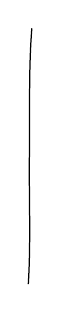
\begin{tikzpicture}[x=1cm,y=1cm]
\draw[line width=0.45pt] (0.045,3.25)
  .. controls (0.005,2.76) and (0.020,2.23) .. (0.015,1.70)
  .. controls (0.005,1.18) and (0.035,0.57) .. (0,0);
\end{tikzpicture}}

\mspage{303}

\scanpage{305}
We are going to make explicit a compatibility
relation for $S\Gamma$ relative to a $\pi$
with \unsure{loops}, fixing an $i\in I=\unsure{\mathcal I(\pi)}$,
hence a stabilizer $\Gamma_i\subset\Gamma$ whose inverse
image $(S\Gamma)_i$ in $S\Gamma$ is thus an
extension of $\Gamma_i$ by $T^I$. Using the
projection $T^I\xrightarrow{\mathrm{pr}_i}T$, we find an
extension of $\Gamma_i$ by $T$, which we are going to describe
in another way. The extension $S\Gamma$
is defined intrinsically by the
datum of $I$ \unsure{realizations} \inserted{$(\pi_i)_{i\in I}$} \unsure{of the group}
\unsure{outer} $\pi$ by groups, with in
each $\pi_i$ an $L_i\subset\pi_i$ of class $i$
(that is it, the datum of a system of the
$(\widetilde D_i^*)$!). For an outer automorphism \deleted{\unsure{$u$}} \inserted{with loops $u\in\Gamma$} of $\pi$,
\deleted{its ``\illegible{1}'' are the}
for $\forall i$ it \deleted{\unsure{there are ways}} \inserted{is possible} to
\unsure{realize} it by $u_i\in\operatorname{Aut}_{\unsure{\mathrm{lac}|\mathrm{loc}}}(\pi_i)$, with $u_i(L_i)\subset L_i$
--- this $u_i$ is determined \unsure{modulo} right
multiplication by an $\operatorname{int}(\unsure{k_i|\kappa_i}(\alpha))$, where $\alpha\in T$.
Of course, $S\Gamma$ is the \unsure{subgroup} \unsure{of the|of the}
\mspage{304}

\scanpage{306}
\mspage{154}
$\displaystyle\prod_{i\in I}\operatorname{Aut}_{\unsure{\mathrm{lac}|\mathrm{loc}}}(\pi_i)$,
\deleted{\unsure{formed of} \illegible{1}} \inserted{\unsure{the inverse image}} of the diagonal
under the natural homomorphism from this product to
$\operatorname{Autext}_{\unsure{\mathrm{lac}|\mathrm{loc}}}(\pi)^I$, \deleted{\unsure{whence an}} \inserted{\unsure{which is indeed}} extension of
\unsure{the said} diagonal (identified with $\Gamma$) by $T^I$.
If we look at the subextension \deleted{of $\Gamma_i$} obtained
by restriction to $\Gamma_i$, we see that the
projection $T^I\unsure{\xrightarrow{\mathrm{pr}_i}}T$ is stable under $\Gamma_i$; thus
we deduce from it an extension of $\Gamma_i$ by $T$,
which is none other than the group of
automorphisms \inserted{with loops} of $\pi_i$ which normalize $L_i$
--- which is indeed an extension of $\Gamma_i$ by $L_i$
(\unsure{for} intersection with $\pi_i\subset\operatorname{Aut}_{\unsure{\mathrm{lac}|\mathrm{loc}}}(\pi_i)$ \unsure{is|being}
reduced to $L_i$).

This shows us that the extension
of $\Gamma$ by $T^I$ has a marked tendency
not to be trivial, for this is \unsure{so}
\inserted{(for $i\in I$ fixed)} for the extension of $\Gamma_i$ by $T$ \inserted{to} which it gives
rise. If for example we have a
\uline{finite} subgroup $G\subset\Gamma_i^+$, the induced extension is
never trivial if $G\ne1$, we have seen this. In
fact, $G$ must be cyclic and its inverse image
in the extension in question is $\simeq T$\ldots
\mspage{305}

\scanpage{307}
\mspage{155}
$25^{\mathrm{bis}}$. Case of the two groups. Return to the \unsure{notations}

We place ourselves \inserted{first} to fix ideas in the
topological and discrete case, but the motivation is
the case of an algebraic curve $U$ over a
finitely generated field $K$, where we have both
the group $G_K=\operatorname{Aut}_K(U)$ and $\Gamma=\operatorname{Gal}(\overline K/K)$
\margin{Anabelian case so \unsure{$G$|$G_K$} finite}
which \unsure{operate} by outer automorphisms on $\pi_1(U_{\overline K})$.
In this case, $G$ and $\Gamma$ commute, but
we can look more generally at the case
of the group (bigger than $G_K$) $G_{\overline K}=\operatorname{Aut}_{\overline K}(U)$,
on which $\Gamma$ operates (in a not necessarily trivial way
--- this operation describes \unsure{a} finite étale
algebraic group over $K$.

So suppose we have a surface
$U$ (orientable, $U=X-S$, $X$ \unsure{compact} \inserted{\unsure{connected}}, $S$ finite)
on \unsure{which|which} \unsure{operate} two groups $G$, $\Gamma$,
the action of $\Gamma$ normalizing that of $G$
--- so we have a group $\mathcal G=\Gamma . G$ (semidirect
product, for a certain action of $\Gamma$
on $G$) which operates on $U$. We suppose $G$
finite, but not necessarily $\Gamma$ finite.
\mspage{306}

\scanpage{308}

We suppose chosen a universal covering $\widetilde U$ of $U$, hence a group with \unsure{loops} $\pi=\operatorname{Aut}(\widetilde U)$, on which $\mathcal G$ operates by outer automorphisms, hence extension
\[
(1)\qquad 1\longrightarrow\pi\longrightarrow\unsure{\mathcal E|\varepsilon}\longrightarrow\mathcal G\longrightarrow 1
\]
\margin{We are going to \unsure{suppose} the action of $\mathcal G$ faithful}
If the action of $\mathcal G$ on $U$ \inserted{modulo isotopy} is faithful,
then $\mathcal G\hookrightarrow\operatorname{Autext}(\pi)$, and the preceding extension is the inverse image of the Teichmüller extension of $\pi$
\[
1\longrightarrow\pi\longrightarrow\operatorname{Aut}_{\mathrm{lac}}(\pi)\longrightarrow\operatorname{Autext}_{\mathrm{lac}}(\pi)\longrightarrow 1.
\]

\deleted{\unsure{Let}} We shall have to look at other universal \unsure{covering\textsuperscript{s}} than $\widetilde U$, and their isomorphisms with $\widetilde U$.
When $\widetilde U=\widetilde U(P)$ is the universal covering based at a certain $P\in U$, then for universal coverings \inserted{$\unsure{U(Q)}$} based at \deleted{\illegible{1}} \inserted{a} \unsure{point\deleted{s}|points},
the \inserted{$U$-}isomorphisms $\widetilde U(P)\xrightarrow{\sim}\unsure{\overline U(Q)|\widetilde U(Q)}$ correspond \unsure{thus} to the classes of paths from $P$ to $Q$.

Let \deleted{\illegible{1}} $Q\in U$ be such that its isotropy group \inserted{$G_Q$} \deleted{\illegible{1}} \uline{in $G$} is \unsure{such} that $G_Q^+\ne1$.
(So $G_Q^+$ is cyclic). Choosing a
\mspage{307}

\scanpage{309}
\mspage{156}

class of paths \inserted{$\lambda$} from $P$ to $Q$, identifying $\unsure{\overline U(P)|\widetilde U(P)}$ with $\unsure{\overline U(Q)|\widetilde U(Q)}$, we find an operation of $G_Q$ on $\widetilde U(P)$ i.e. a lifting $G_Q\xrightarrow{r_{G_Q}}\unsure{\mathcal E|\varepsilon}$ in the extension (1) --- the change of class of paths \inserted{from $\lambda$ to $\lambda'$} will give a lifting $r'_{G_Q}$ which \deleted{\unsure{is}} will be conjugate to $r$ by a unique element of $\pi$ \inserted{$=\pi_1(U,P)$} (uniqueness comes from $\pi^{G_Q}=\{1\}$), \unsure{namely} the one which makes one \unsure{pass} from one path to another.

Let us consider the stabilizer $\Gamma_Q$ of $Q$ in $\Gamma$, \deleted{\illegible{2}} which of course operates on $\widetilde U(Q)$ just like $G_Q$ (in fact it is $\mathcal G_Q$ which operates \inserted{hence $r:\mathcal G_Q\to\unsure{\mathcal E|\varepsilon}$} \unsure{\dots}), so via $\lambda$ we also have a \unsure{lift\textsuperscript{ing}|lifting} $r_{\Gamma_Q}:\Gamma_Q\longrightarrow\unsure{\mathcal E|\varepsilon}$, which \inserted{has} even the \unsure{property} of \unsure{normalizing} $r_{G_Q}$ (\unsure{i.e.} operation of \deleted{\illegible{1}} $\Gamma_Q$ on it, which is the one coming from the given operation of $\Gamma$ on $G$).
\margin{\uline{N.B.} As the set \deleted{\illegible{1}} \unsure{of} points $Q$ is finite, and $\mathcal G$ operates on it, the orbit of $Q$ under $\mathcal G$ is finite, i.e. $\mathcal G_Q$ of finite index in $\mathcal G$. and likewise $\Gamma_Q$ in $\Gamma$.}
To simplify, let us suppose all the same that $\Gamma$ operates \unsure{trivial\textsuperscript{ly}} on $G$ i.e. $\mathcal G=\Gamma\times G$, then $r_{\Gamma_Q}(\Gamma_Q)\subset\unsure{\mathcal E|\varepsilon}$ is contained in the \uline{centralizer} of \inserted{$r$ (or of} $\unsure{r_{G_Q}}(G_Q)$),
\mspage{308}

\scanpage{310}

and since $\pi^{r(G_Q)}=1$, so the homomorphism
\[
\operatorname{Centr}(r_{\deleted{\unsure{G_Q}}}(G_Q))\longrightarrow\mathcal G
\]
is injective, the lifting in question \inserted{$\unsure{r_{\Gamma_Q}}$} is uniquely determined by the preceding condition.
\margin{\uline{N.B.} \unsure{Independent\textsuperscript{ly}|Independently} of \unsure{every|the} hypothesis that $\Gamma$ centralizes $G$, the normalizer of $r(G_Q)$ in $\pi$, equal to its ``centralizer'', is reduced to $1$, so $\operatorname{Norm}(r(G_Q))\longrightarrow\mathcal G$ is injective}

In fact, the image of $\operatorname{Centr}(r(G_Q))$ in $\mathcal G$ contains $\mathcal G_Q$, \inserted{\unsure{and}} \deleted{\illegible{5}} \unsure{even} the lifting $\mathcal G_Q\xrightarrow{r_{\mathcal G_Q}}\unsure{\mathcal E|\varepsilon}$.
\deleted{if $\mathcal G$ is finite}
\unsure{The|The} \unsure{interesting} thing is that \unsure{the|the} \inserted{choice of a} lifting\deleted{\unsure{s}} \unsure{of the|of the} (small) group $G_Q$, already imposes the choice of a lifting \unsure{of the|of the} (big) group $\Gamma_Q$, or $\mathcal G_Q$.

\deleted{When $\mathcal G$ is itself finite,} I say that the image in $\mathcal G$ of the centralizer \inserted{(and even of the normalizer)} of $r(G_Q)$ is $\mathcal G_Q$ itself (a priori it contains it).
\unsure{Returning|Let us return} to $\widetilde U(Q)$ itself, this means that \deleted{\illegible{1}} if $g\in\mathcal G$ is such that there exists an automorphism $\widetilde g$ of $\widetilde U(Q)$ which lifts $g$, while \deleted{\unsure{commuting}} \inserted{normalizing} \deleted{\unsure{with}} \inserted{the action of} $G_Q$, then $g\in\mathcal G_Q$ \inserted{(and $\widetilde g$ is the obvious lifting)}. Indeed, if $\widetilde g$ \deleted{\unsure{commutes}} \inserted{normalizes} \inserted{the action of} $G_Q$, it \unsure{leaves invariant|sends} the set of fixed points of $G_Q$ in $\widetilde U(Q)$, which is reduced \deleted{\illegible{1}} \inserted{\unsure{to the point}} $\unsure{\widetilde Q|\overline Q}$
\mspage{309}

\subsection*{Scans 311--320}
\addcontentsline{toc}{subsection}{Scans 311--320}
% package LM_P032
\scanpage{311}
\mspage{157}

The set $\unsure{\widetilde U|U}^{!}$ of points $Q\in U$ such that $G_Q^+\ne(1)$ is stable under the action of $\mathcal G$, and is identified (with this action) with \unsure{the set} of \inserted{maximal} liftings modulo $\pi$ of (cyclic) subgroups $\ne1$ of $G^{+}_{\deleted{\unsure{Q}}}$. When one knows, for a partial lifting $r$ of a $G_Q$ into $\mathcal E$ what its centralizer in $\mathcal E$ is i.e. the corresponding lifting of $\mathcal G_Q$, \unsure{well|then} in the $=$ way for the conjugates of $r$ by any \unsure{element} $g$ (not only of $\pi$, but $=$ of $\mathcal E$), by simple conjugation.

So the cases to be determined correspond in practice to the orbits of $\mathcal G$ in $U^{!}$.

One may be interested in describing $\mathcal G$ or $\Gamma$ as a subgroup of $\mathrm{Aut\,ext}_{\mathrm{lac}}(\pi)=\Gamma'$ \inserted{giving rise to the extension $\mathcal E'$ of $\Gamma'$ by $\pi$ (thus $\mathcal E\subset\mathcal E'$).} But for every lifting $r$ of a $G_Q$, let us consider $\mathrm{Centr}_{\mathcal E'}(r)$, \deleted{\illegible{1}} . \unsure{we shall have|we still have} $\mathrm{Centr}_{\mathcal E'}(r)\cap\pi=(1)$ i.e. \inserted{we find a section over} the image of this centralizer in $\Gamma'$, say $\Gamma'(Q)$. This image depends only on $Q$ i.e. on the $\pi$-conjugacy class of $r$ or of $r(\unsure{G_Q})$, and is replaced by a $G$-conjugate when $Q$ is replaced by a $G$-conjugate. This

\mspage{310}

\scanpage{312}

said, the intersection \inserted{$\Gamma'^{\natural}$} of the $\Gamma'(Q)$, for $Q\in U^{!}$, is a subgroup of $\Gamma'$ which contains the intersection \deleted{\unsure{of}} $\mathcal G^{\natural}$ of the $\mathcal G_Q^{\deleted{\unsure{\natural}}}$, and the centralizer of $G$ in $\Gamma'^{\natural}$ contains in the $=$ way the intersection \deleted{of} $\Gamma^{\natural}$ of the $\Gamma_Q$, which is an \inserted{invariant} subgroup of finite index in $\Gamma$. And one can then propose to oneself whether it is possible to characterize at least \unsure{the|a} finite subgroup $\Gamma^{\natural}$ of $\Gamma$ as $\mathrm{Centr}_{\Gamma'^{\natural}}(G)$, and \unsure{to recover from it} perhaps $\Gamma$ as the normalizer of $\Gamma^{\natural}$ in \deleted{the centralizer} $\mathrm{Centr}_{G}(\Gamma)$.

I am more particularly interested in the profinite variant of this, in the case where $U=\mathbb P^1_{\mathbb Q}\setminus\{0,1,\infty\}$, $G=\mathfrak S_3$, $\Gamma={}$ Galois group of $\overline{\mathbb Q}/\mathbb Q$, \deleted{while} \inserted{$\unsure{P|\rho}=\exp(2i\pi/6)$}.
\margin{algebraic closure in $\mathbb C$}

I have not checked that $\Gamma\longrightarrow\mathrm{Autext}_{\mathrm{lac}}(\widehat\pi)$ is injective, this does not prevent doing calculations in $\mathrm{Aut}_{\mathrm{lac}}(\widehat\pi)$, be they heuristic for the moment.

\mspage{311}

\scanpage{313}
\mspage{158}

I am running into notational troubles -- too many groups are \unsure{\uline{denoted}} by the letter $\Gamma$ (possibly with primes, subscripts, superscripts \ldots). There are three types of groups that enter into my reflections:

a) the Teichmüller groups and its variants, which play the role \unsure{of the|of} ``universal'' groups operating (\inserted{possibly} modulo isotopy) on surfaces, or on outer groups \deleted{\unsure{with loops}} with loops. These groups tend to be infinite

b) Groups (most often finite) operating on topological surfaces, or on geometric algebraic curves (\unsure{without}, in that case, moving the base field).

\margin{Cases b) and c) sometimes mix (in \unsure{a} \unsure{$G$} \unsure{groups} $\mathcal G$ extension of a Galois group $\Gamma$ by a finite group \unsure{$G$}) \unsure{in the case of} \unsure{$G$} Algebraic \unsure{Geometry}.}

c) Profinite Galois groups (hence infinite), chiefly of fields of finite type over $\mathbb Q$, operating ``arithmetically'' on surfaces and their geometric $\widehat{\pi}_1$.

It is because of the deep analogies between cases b) and c), and their close relations with case a), that I had been led to adopt common notations, but

\mspage{312}

\scanpage{314}

which in the long run end up leading to collisions. There is thus reason to review the notations. I will reserve the letter $G$ \inserted{and variants} for geometric actions (case b)) of groups, most often finite, the letter $\Gamma$ \inserted{and variants} for Galois groups, the letter $\mathcal G$ for mixed groups.

As for the ``universal'' groups of Teichmüller type, like those denoted $\Gamma_{g,\nu}$ previously, I will instead denote them \inserted{$\mathcal T$,} $\mathcal T_{g,\nu}$ (initial of ``Teichmüller'', whereas $\Gamma$, \inserted{$G$} \unsure{are} the initial of Galois).

The Galois group \inserted{over $\mathbb Q$} of the algebraic closure $\overline{\mathbb Q}$ of $\mathbb Q$ in $\mathbb C$ \deleted{\unsure{of $\overline{\mathbb Q}$ over}} \unsure{deserves} a special letter, I will denote it $\boldsymbol{\Gamma}$. The quotient \deleted{\unsure{by} $\widehat{\Gamma}_{g,\nu}$ of} $\operatorname{Norm}_{\widehat{\widehat{\mathcal T}}_{g,\nu}}(\widehat{\mathcal T}_{g,\nu})/\widehat{\mathcal T}_{g,\nu}$, which is more akin to a Galois group than to a Teichmüller group, will be denoted $\boldsymbol{\Gamma}_{g,\nu}$ (bold letter!). In the

\mspage{313}

\scanpage{315}
\mspage{159}

case $(g,\nu)=(0,3)$ which occupies me more particularly, $\boldsymbol{\Gamma}_{0,3}$ is identified with the \deleted{\unsure{normalizer}} \inserted{centralizer} of $G=\mathfrak S_3$ \inserted{$=\mathcal T_{0,3}^{+}$} in $\widehat{\widehat{\mathcal T}}_{0,3}$ -- it is contained in $\widehat{\widehat{\mathcal T}}_{03}^{!}$, \inserted{and perhaps equal.} We have a canonical homomorphism
\margin{$\widehat{\widehat{\mathcal T}}$ is here the $\frac{1}{2}$ direct product of $\mathfrak S_3=\mathcal T^+$ by $\mathcal T^{!}$}
\[
\boldsymbol{\Gamma}\longrightarrow\boldsymbol{\Gamma}_{03}
\qquad (\text{more generally }\boldsymbol{\Gamma}\longrightarrow\boldsymbol{\Gamma}_{g,\nu})
\]
for which I do not know for the moment whether it is injective, and still less whether it is surjective. The preceding reflections suggest conditions on the image, which are especially interesting if one admits the relations
\[
\widehat{\pi}^{\rho}=\widehat{\pi}^{\sigma_0}=(1)
\]

We \inserted{have} \unsure{denoted\deleted{will}} by $\mathcal E_{g\nu}$ the canonical extension of $\mathcal T_{g,\nu}$ by $\pi_{g,\nu}$ (which for $(g,\nu)$ anabelian is identified with $\mathcal T'_{g,\nu+1}$).

The outer operation of a group $G$, $\Gamma$ or $\mathcal G$ also defines an extension by $\pi$ (or by $\widehat{\pi}$), which we have also \unsure{denoted|denoted} by the letter $\mathcal E$ (initial of extension) -- there is again a collision of notations.

\mspage{314}

\scanpage{316}

I will take the letter $\mathfrak{S}$ (which is a counterpart to $\mathcal{T}$) for these extensions in the universal Teichmüller-style cases, (writing $\mathfrak{S}_{g,\nu}$ instead of the $\Gamma'_{g,\nu+1}$, since the viewpoint is different\ldots), and keeping the letter $\mathcal{E}$ in \unsure{the|the} \unsure{preceding|preceding} cases. So $\mathcal{E}$ tends to be a subextension of an $\mathfrak{S}$.

Admitting that $\boldsymbol{\Gamma}\longrightarrow\boldsymbol{\Gamma}_{0,3}$ is injective, we would thus have

\diagram{\begin{tikzcd}[ampersand replacement=\&,column sep=small,row sep=large]
1 \arrow[r,no head] \& \widehat{\pi}_{0,3} \arrow[r] \arrow[d,equal] \& \widehat{\widehat{\mathfrak{S}}}_{0,3} \arrow[r] \arrow[d] \& \widehat{\widehat{\mathcal{T}}}_{0,3} \arrow[r] \arrow[d] \& 1 \\
1 \arrow[r,no head] \& \widehat{\pi}_{0,3} \arrow[r] \arrow[d,equal] \& \widehat{\widehat{\mathfrak{S}}}'_{0,3} \arrow[r] \arrow[d] \& \underbrace{\unsure{\mathcal{T}^{+}_{0,3}}}_{\mathfrak{S}_{3}}\;\deleted{\unsure{\boldsymbol{\Gamma}}}\!\times\boldsymbol{\Gamma}_{0,3} \arrow[r] \arrow[d] \& 1 \\
1 \arrow[r] \& \widehat{\pi}_{03} \arrow[r] \arrow[d] \& \mathcal{E} \arrow[r] \arrow[d] \& \mathfrak{S}_{3}\times\boldsymbol{\Gamma} \arrow[r,no head] \arrow[d] \& 1 \\
1 \arrow[r] \& \pi_{0,3} \arrow[r] \& \mathfrak{S}_{03} \arrow[r,no head] \& \underbrace{\mathfrak{S}_{3}\times\unsure{\mathbb{Z}/2}}_{\mathcal{T}_{0,3}} \arrow[r] \& 1
\end{tikzcd}}

\margin{N.B. We denote by $\widehat{\widehat{\mathfrak{S}}}'_{g,\nu}$ the normalizer of $\widehat{\mathfrak{S}}^{+}_{g,\nu}$ in $\widehat{\widehat{\mathfrak{S}}}_{g,\nu}$, an extension of $\boldsymbol{\Gamma}_{g,\nu}$ by $\widehat{\mathfrak{S}}^{+}_{g,\nu}$}

\unsure{If|Let} $\gamma\in\boldsymbol{\Gamma}_{0,3}$, \deleted{\unsure{which is}}\inserted{for it to be} in the image of $\boldsymbol{\Gamma}$ \deleted{\unsure{have|is} the property}\inserted{it is necessary} \unsure{that it|that they} \unsure{admit|admit} a lifting $u$ which commutes with $\rho$, and a lifting which commutes with $\sigma_{0}$ \unsure{(which|Which}, \unsure{as soon|of the} as $\gamma\in\widehat{\widehat{\mathcal{T}}}_{0,3}$, implies

\mspage{315}

\scanpage{317}
\mspage{160}

already that $\gamma$ in $\widehat{\widehat{\mathcal{T}}}_{0,3}$ commutes with $\mathcal{T}^{+}_{0,3}=\mathfrak{S}_{3}$, \deleted{thus} i.e. that they is in $\boldsymbol{\Gamma}_{0,3}$). It could be that \unsure{every} element of $\boldsymbol{\Gamma}_{0,3}$ already has this property, hence that this condition does not \unsure{impose|make} any genuine restriction on the image of $\boldsymbol{\Gamma}$ in $\boldsymbol{\Gamma}_{0,3}$.

\mspage{316}

\scanpage{318}
\mspage{161}

\uline{26} Profinite Teichmüller groups.

\margin{Discretifications and prediscretifications.}

Let $\pi$ be a profinite group with loops \inserted{of type $g,\nu$}, $T$ the invertible $\widehat{\mathbb Z}$-module of its orientations.

We assume we are in the \unsure{anabelian} case, and we shall admit \unsure{that then}
\[
\operatorname{Centre}(\pi)=\{1\}
\tag{1}
\]
more generally that the centralizer in $\pi$ of every open subgroup of $\pi$ is reduced to $\{1\}$. We shall thus again have a canonical exact sequence of profinite groups
\[
1 \unsure{\longrightarrow|{-}} \pi \longrightarrow \operatorname{Aut}_{\mathrm{lac}}(\pi) \longrightarrow \operatorname{Autext}_{\mathrm{lac}}(\pi) \longrightarrow 1
\tag{\unsure{2}}
\]
We shall also put \deleted{\unsure{$\operatorname{Autext}$}}
\[
\operatorname{Autext}_{\mathrm{lac}}(\pi)=\widehat{\widehat{\mathcal T}}(\pi)
\tag{3}
\]
\unsure{we|and} will call it the \uline{extended Teichmüller group} of $\pi$. We shall also put $\widehat{\widehat{\mathfrak S}}(\pi)=\operatorname{Aut}_{\mathrm{lac}}(\pi)$, so that we can write (2) as
\[
1 \longrightarrow \pi \longrightarrow \widehat{\widehat{\mathfrak S}}(\pi) \longrightarrow \widehat{\widehat{\mathcal T}}(\pi) \longrightarrow 1
\tag{2'}
\]

Let us call a ``basis'' of $\pi$ a \unsure{set} of \unsure{elements} of $\pi$ $(x_i,y_i)_{1\leq i\leq g}$, $(\ell_j)_{1\leq j\leq\nu}$, \inserted{the $\ell_j$ \unsure{generating$^{\mathrm t}$} the different groups with loops} satisfying
\[
\deleted{\unsure{\prod_i}\,\unsure{[x_i,y_i]}\,\unsure{\cdots[x_g,y_g]\ell_1}}
\quad
\inserted{\ell_\nu\ell_{\nu-1}\cdots\ell_1[x_g,y_g]\cdots[x_1,y_1]=1}
\tag{\unsure{4}}
\]
and such that this is a generating relation.

\mspage{317}

\scanpage{319}

\margin{or again, one defines $\Pi_{g,\nu}$ as the discrete group \unsure{with|with the} generators the $x_i,y_i,\ell_j$ and with \unsure{defining} relation (4)}

\unsure{If} one chooses in $\Pi_{g,\nu}$ a (discrete) basis (corresponding \unsure{definition|Definition}), \unsure{whence} a basis of $\widehat{\Pi}_{g,\nu}$, one will have an obvious bijection
\[
\operatorname{Bases}(\pi) \xleftarrow{\sim} \operatorname{Isom}_{\mathrm{lac}}(\widehat{\Pi}_{g,\nu},\pi)
\tag{5}
\]

The set of bases of $\pi$ is a homogeneous set \unsure{in|under} \deleted{\illegible{1}} $\widehat{\widehat{\mathfrak S}}(\pi)=\operatorname{Aut}_{\mathrm{lac}}(\pi)$. \unsure{Let|If} the \deleted{\unsure{$\Pi_0$ d}} basis corresponds to an isomorphism $u:\widehat{\Pi}_{g,\nu}\longrightarrow\pi$, the group \inserted{$\Pi_0$} generated by the $x_i,y_i,\ell_j$ is none other than $\deleted{\unsure{\Pi_0}}\inserted{u}(\Pi_{g,\nu})$. \deleted{One of the} \inserted{the subgroups} of $\pi$ which can be obtained in this way are called the \uline{discretifications} of $\pi$. These form a homogeneous set under $\widehat{\widehat{\mathfrak S}}=\operatorname{Aut}_{\mathrm{lac}}(\pi)$, \inserted{canonically} isomorphic to the quotient of the right $\widehat{\widehat{\mathfrak S}}_{g,\nu}$-\deleted{\unsure{torsor}}\inserted{set} $\operatorname{Isom}_{\mathrm{lac}}(\widehat{\Pi}_{g,\nu},\pi)$ by $\mathfrak S_{g,\nu}$:
\[
\operatorname{Discrt}(\pi) \xleftarrow{\sim} \operatorname{Isom}_{\mathrm{lac}}(\widehat{\Pi}_{g,\nu},\pi)/\mathfrak S_{g,\nu}
\tag{6}
\]
The \unsure{automorphisms} \inserted{(profinite with loops)} of $\pi$ fixing \inserted{a discretification} $\Pi_0$ are identified with the \unsure{automorphisms} of the discrete group \inserted{with loops} $\Pi_0$.
\[
\operatorname{Aut}_{\mathrm{lac}}(\pi,\Pi_0)\simeq\operatorname{Aut}_{\mathrm{lac}}(\Pi_0)
\tag{7}
\]

\mspage{318}

\scanpage{320}
\mspage{162}

The bijection (5) puts on the set of Bases of $\pi$ a bitorsor structure under $\widehat{\widehat{\mathfrak S}}(\pi),\widehat{\widehat{\mathfrak S}}_{g,\nu}$, and \unsure{the|the} \unsure{corresponding|corresponding} \unsure{topologies|topology} makes it a profinite set. The set of discretifications of $\pi$, which is a quotient of the preceding set, inherits a quotient topology, which is none other than the quotient topology of the right-hand side of (6). \deleted{Except in the \unsure{exceptional} cases \unsure{$(g,\nu)=(0,3)$} \unsure{where} $\mathfrak S_{g,\nu}$} \inserted{This space is} not Hausdorff \inserted{(N.B. $\mathfrak S_{g,\nu}$ is \unsure{always} infinite)}, for the group $\mathfrak S_{g,\nu}\subset\widehat{\widehat{\mathfrak S}}_{g,\nu}$ is not closed. We denote by $\unsure{\widetilde{\operatorname{Discrt}}'|\operatorname{Discrt}'}(\pi)$ the associated Hausdorff topological space, identified with $\operatorname{Isom}_{\mathrm{lac}}(\widehat{\Pi}_{g,\nu},\pi)/\unsure{\overline{\mathfrak S}}_{g,\nu}$, where $\overline{\mathfrak S}_{g,\nu}$ denotes the closure of $\mathfrak S_{g,\nu}$ in $\widehat{\widehat{\mathfrak S}}_{g,\nu}$. We moreover have an obvious surjective homomorphism $\widehat{\mathfrak S}_{g,\nu}\longrightarrow\unsure{\widehat{\widehat{\mathfrak S}}|\overline{\mathfrak S}}_{g,\nu}$ whose image is $\overline{\mathfrak S}_{g,\nu}$, \unsure{we shall admit} that it is injective, and shall identify $\overline{\mathfrak S}_{g,\nu}$ with $\widehat{\mathfrak S}_{g,\nu}$. Thus
\[
\operatorname{Discrt}'(\pi)\simeq\operatorname{Isom}_{\mathrm{lac}}(\widehat{\Pi}_{g,\nu},\pi)/\widehat{\mathfrak S}_{g,\nu}
\tag{\unsure{8}}
\]

\mspage{319}

\subsection*{Scans 321--330}
\addcontentsline{toc}{subsection}{Scans 321--330}
% package LM_P033
\scanpage{321}

\unsure{An} element of $\operatorname{Discr\acute{e}t}^{\unsure{\prime}}(\pi)$ is called a
class of discretifications of $\pi$\inserted{\unsure{or} \unsure{prediscretification} of $\pi$}.
If $\pi_0$ is a discretification, we denote its class by
$\pi_0^{\unsure{\natural}}$. The set of classes of discretifications on $\pi$
is a homogeneous \unsure{space} under $\widehat{\widehat{\unsure{\mathfrak{S}|\mathcal{G}}}}(\pi)$, the stabilizer
of $\pi_0^{\unsure{\natural}}$ \unsure{is identified with|being identified with} : the closure of
$\unsure{\mathfrak{S}|\mathcal{G}}(\pi_0)=\operatorname{Aut}_{\mathrm{lac}}(\pi_0)$ in
$\widehat{\widehat{\unsure{\mathfrak{S}|\mathcal{G}}}}(\pi)$, or again :
$\widehat{\unsure{\mathfrak{S}|\mathcal{G}}}(\pi_0)$.
The latter always contains $\pi$.
\[
\operatorname{Aut}_{\mathrm{lac}}(\pi,\pi_0^{\unsure{\natural}})
\simeq\widehat{\unsure{\mathfrak{S}|\mathcal{G}}}(\pi_0)
\]

\deleted{We have} for every discretification $\pi_0^{\unsure{\natural}}$, the subgroup of
$\widehat{\widehat{\unsure{\mathfrak{S}|\mathcal{G}}}}(\pi)$ of loop \unsure{automorphisms} which fix
$\pi_0^{\unsure{\natural}}$ is denoted $\widehat{\unsure{\mathfrak{S}|\mathcal{G}}}(\pi_0^{\unsure{\natural}})$,
it is therefore the inverse image of a subgroup of
$\widehat{\widehat{\mathcal{T}}}(\pi)$, denoted
$\widehat{\mathcal{T}}(\pi_0^{\unsure{\natural}})$. We thus have an inclusion of
extension structures

(10)
\diagram{\begin{tikzcd}[ampersand replacement=\&]
1 \arrow[r] \& \pi \arrow[r] \&
\widehat{\unsure{\mathfrak{S}|\mathcal{G}}}(\pi_0^{\unsure{\natural}}) \arrow[r] \arrow[d,hook] \&
\widehat{\mathcal{T}}(\pi_0^{\unsure{\natural}}) \arrow[r] \arrow[d,hook] \& 1 \\
1 \arrow[r] \& \pi \arrow[r] \&
\widehat{\widehat{\unsure{\mathfrak{S}|\mathcal{G}}}}(\pi) \arrow[r] \&
\widehat{\widehat{\mathcal{T}}}(\pi) \arrow[r] \& 1
\end{tikzcd}}

\margin{\uline{N.B.} The set of classes of discretifications of $\pi$ is described
\illegible{2} of the \uline{outer} group $\pi$, as
$\operatorname{Isom\,ext}(\widehat{\Pi}_{g,\nu},\pi)$\deleted{\illegible{1}}
divided by $\widehat{\mathcal{T}}_{g,\nu}$.
We moreover have \unsure{an arrow} of degree $2$
\diagram{\begin{tikzcd}[ampersand replacement=\&]
\operatorname{Isom\,ext}(\widehat{\Pi}_{g,\nu},\pi)/\widehat{\mathcal{T}}_{g,\nu}^{+}
\arrow[d] \\
\operatorname{Isom\,ext}(\widehat{\Pi}_{g,\nu},\pi)/\widehat{\mathcal{T}}_{g,\nu}
\end{tikzcd}}
which makes it possible for \unsure{every|the} \unsure{class} of discretifications, to define
its two \uline{\unsure{orientations}}, and speak of
\uline{oriented} discretifications.}

\mspage{320}

\scanpage{322}
\mspage{163}

(One shows by arithmetico-geometric means that the inclusion
$\widehat{\mathcal{T}}\longrightarrow\widehat{\widehat{\mathcal{T}}}$
is never an isomorphism.) We thus find a map
\[
\tag{11}
\operatorname{Discr\acute{e}t}^{\unsure{\prime}}(\pi)\longrightarrow
\text{Closed subgroups of }\widehat{\widehat{\mathcal{T}}}(\pi)
\]
obviously compatible with the action of
\deleted{$\unsure{\widehat{\widehat{\mathcal{T}}}}$}
$\widehat{\widehat{\unsure{\mathfrak{S}|\mathcal{G}}}}(\pi)$ (transport of structure) -- operating
on the right via $\widehat{\widehat{\mathcal{T}}}(\pi)$ and its inner automorphisms on itself.

We thus find a conjugacy class, well determined \unsure{of|of the}
closed subgroups of $\widehat{\widehat{\mathcal{T}}}(\pi)$,
which we call its ``\uline{geometric}'' Teichmüller subgroups.
\deleted{It is by no means improbable moreover that
$\widehat{\mathcal{T}}(\pi_0^{\unsure{\natural}})$ is \illegible{1}}
It could moreover be that $\widehat{\mathcal{T}}_{g,\nu}$ is
its own normalizer in $\widehat{\widehat{\mathcal{T}}}_{g,\nu}$
-- equivalent to the assertion that (11) is \unsure{injective|bijective|injection} :
The datum of a class of discretifications\inserted{of $\pi$}
would be equivalent to that of a geometric Teichmüller subgroup in
\deleted{$\unsure{\widehat{\widehat{\mathcal{T}}}}$}
its \unsure{extended} Teichmüller group $\widehat{\widehat{\mathcal{T}}}$.

\margin{this is completely screwy and ultra-false
-- a moment of aberration ! This becomes clear in what follows\ldots
The \unsure{sensible} question (with which \unsure{I} must have
\unsure{at the time} confused) \unsure{is} whether $\widehat{\mathcal{T}}$ is
\uline{invariant} in $\widehat{\widehat{\mathcal{T}}}$, i.e. whether
the normalizer is $\widehat{\widehat{\mathcal{T}}}$ \unsure{all|all} \unsure{of it} !}

\mspage{321}

\scanpage{323}

Note that we have the canonical homomorphisms
\[
\tag{12}
\widehat{\widehat{\mathcal{T}}}\deleted{\unsure{(\pi_0^{\natural})}}
\xrightarrow{\chi}\widehat{\unsure{\mathbb{Z}}}^{*}
\]
\[
\tag{13}
\widehat{\widehat{\mathcal{T}}}\longrightarrow
\unsure{\mathfrak{S}_{I}|\mathcal{G}_{I}}
\]
\margin{where $I=I(\pi)$ is \unsure{the set|the set} of conjugacy classes of loop subgroups of $\pi$}
inducing on $\widehat{\mathcal{T}}(\pi_0^{\unsure{\natural}})$
\deleted{\unsure{continuous}} corresponding homomorphisms -- whence the definition of the
subgroups $\widehat{\widehat{\mathcal{T}}}^{!}$,
$\widehat{\widehat{\mathcal{T}}}^{+}$,
$\widehat{\widehat{\mathcal{T}}}^{!+}$ and likewise for
$\widehat{\mathcal{T}}$. Note that $\chi$ takes on $\widehat{\mathcal{T}}$
only the values $\pm1$.

The subgroup $\widehat{\mathcal{T}}^{+}$ of outer automorphisms of the
profinite \unsure{groups|groups} with loops $\pi$,
\deleted{\illegible{2}}\inserted{fixing} a class of discretifications
$\pi_0^{\unsure{\natural}}$ and with multiplier $+1$, plays a very special role.
In contrast to that \unsure{which one} can conjecture about $\widehat{\mathcal{T}}$
(of which $\widehat{\mathcal{T}}^{+}$ is an \unsure{open|invariant} subgroup of index $2$),
one would rather suppose that $\widehat{\mathcal{T}}^{+}$ is invariant in
$\widehat{\widehat{\mathcal{T}}}$. In any case,
the subgroups thus defined in $\widehat{\widehat{\mathcal{T}}}$
\deleted{which}\inserted{via} \unsure{classes} of discretifications of $\pi$
\deleted{\illegible{1}} (perhaps

\mspage{322}

\scanpage{324}
\mspage{164}

there is only a single and unique one!) will be called the \uline{strict} geometric Teichmüller subgroups. The choice of such a subgroup \inserted{of $\widehat{\widehat{\mathcal{T}}}$} is, in any case, an element of structure \unsure{distinctly} weaker than that of a class of \unsure{discretifications}, and even than that of a geometric Teichmüller subgroup (not strict).

To specify the relations between these two notions, let us first recall that $\widehat{\mathcal{T}}^{+}=\Sigma$ is deduced from $\widehat{\mathcal{T}}$ as the kernel of $\chi\mid\widehat{\mathcal{T}}:\widehat{\mathcal{T}}\longrightarrow\{\pm1\}$. On the other hand, \deleted{let} (for a chosen strict geometric Teichmüller subgroup $\widehat{\mathcal{T}}^{+}$) let us consider
\[
(14)\qquad
\unsure{\mathcal{N}|N}_{\Sigma}=\mathcal{N}
=\operatorname{Norm}_{\widehat{\widehat{\mathcal{T}}}}
\bigl(\deleted{\widehat{\mathcal{T}}^{+}}\inserted{\Sigma}\bigr)
\qquad (\Sigma=\widehat{\mathcal{T}}^{+})
\]
(perhaps always equal to all of $\widehat{\widehat{\mathcal{T}}}$)

obviously (if $\deleted{\widehat{\mathcal{T}}^{+}}\inserted{\Sigma}$ comes from a $\widehat{\mathcal{T}}$)
\[
(15)\qquad
\underset{\inserted{\unsure{=}\widehat{\mathcal{T}}^{+}}}
{\deleted{\widehat{\mathcal{T}}^{+}}\inserted{\Sigma}}
\subset\widehat{\mathcal{T}}\subset\mathcal{N}_{\Sigma}.
\]
\deleted{and $\mathcal{N}/\widehat{\mathcal{T}}^{+}$ is}
The profinite group $\mathcal{N}/\deleted{\widehat{\mathcal{T}}^{+}}\inserted{\Sigma}$
\deleted{is} associated with \deleted{the \unsure{structure}}
$\deleted{\widehat{\mathcal{T}}^{+}}\inserted{\Sigma}$ is denoted
$\boldsymbol{\Gamma}_{\deleted{\unsure{\widehat{\mathcal{T}}^{+}}}\inserted{\Sigma}}$
\deleted{\illegible{1}} \deleted{\illegible{2}}
(if $\deleted{\widehat{\mathcal{T}}^{+}}\inserted{\Sigma}$ is unique, we write $\boldsymbol{\Gamma}_{\pi}$);

\mspage{323}

\scanpage{325}

and the $\widehat{\mathcal{T}}\deleted{\unsure{\mathcal G}}$ \unsure{giving} rise to the same $\deleted{\widehat{\mathcal{T}}^{+}}\inserted{\Sigma}$ correspond \deleted{\unsure{to the classes}} to a conjugacy class of elements of order $2$ of $\boldsymbol{\Gamma}_{\deleted{\unsure{\widehat{\mathcal{T}}^{+}}}\inserted{\Sigma}}$. It is clear \deleted{\unsure{that we|that}} in any case that we have an injective map
\[
(16)\qquad
\begin{gathered}
\text{set of geometric}\\
\text{Teichmüller subgroups}\\
\widehat{\mathcal{T}}\text{ of }\widehat{\widehat{\mathcal{T}}}\text{ such that}\\
\widehat{\mathcal{T}}^{+}=\Sigma
\end{gathered}
\longrightarrow
\begin{gathered}
\text{set of }\unsure{\text{elements}|\text{elements}}\\
\text{of order }2\text{ of }\boldsymbol{\Gamma}_{\Sigma}
\end{gathered}
\quad :
\]
and that its image is stable under conjugation. Let us show that \unsure{two|the} elements of the image are conjugate under $\boldsymbol{\Gamma}_{\Sigma}$. Indeed, let
\[
\widehat{\mathcal{T}},\ \widehat{\mathcal{T}}^{\prime}\supset\Sigma
\quad\text{such that}\quad
\Sigma=\widehat{\mathcal{T}}^{+}=\widehat{\mathcal{T}}^{\prime+}.
\]
\deleted{We \illegible{1} \unsure{obviously}}
\inserted{$\exists\,g\in\widehat{\widehat{\mathcal{T}}}$}
such that
$\widehat{\mathcal{T}}^{\prime}=\operatorname{int}(g)\unsure{\mathcal{T}}$,
and we \unsure{will have|have} therefore
$\widehat{\mathcal{T}}^{\prime+}=\operatorname{int}_{g}\widehat{\mathcal{T}}^{+}$
i.e. $g\in\mathcal{N}$, OK.

The elements of order $2$ thus obtained in $\boldsymbol{\Gamma}_{\Sigma}$ are called the canonical involutions. We will give a remarkable conjectural interpretation of them below. The set $\widehat{\widehat{\mathcal{T}}}/\mathcal{N}$ is identified with the set of \unsure{subgroups} of

\mspage{324}

\scanpage{326}
\mspage{165}

strict geometric Teichmüller (once the ``origin'' element $\Sigma$ has been chosen). More \unsure{intrinsically}, we \unsure{will have}:
\[
(17)\qquad
\begin{gathered}
\text{Set of strict geometric}\\
\text{Teichmüller subgroups}\\
\text{of }\widehat{\widehat{\mathcal{T}}}(\pi)
\end{gathered}
\unsure{\xleftarrow{\sim}|\simeq}
\operatorname{Isomext}_{\unsure{\mathrm{lac}}}
(\widehat{\Pi}_{g,\nu},\pi)/\unsure{\mathcal{N}_{g,\nu}}
\]
where we set, as is only right
\[
(18)\qquad
\mathcal{N}_{g,\nu}
=\operatorname{Norm}_{\widehat{\widehat{\mathcal{T}}}_{g,\nu}}
\bigl(\widehat{\mathcal{T}}_{g,\nu}^{+}\bigr)
\]
(perhaps equal to all of $\widehat{\widehat{\mathcal{T}}}_{g,\nu}$!)

Let us now consider the \uline{modular topos} \uline{over} $\mathbb{Q}$ of algebraic curves of type $(g,\nu)$, denoted $M_{g,\nu\,\mathbb{Q}}$, or simply $M_{g,\nu}$. If we choose a universal covering $\widetilde{M}_{g,\nu}$ of $M_{g,\nu\,\mathbb{Q}}$ (hence a universal covering of $\unsure{\operatorname{Spec}}\mathbb{Q}$ i.e. an algebraic closure $\overline{\mathbb{Q}}$ of $\mathbb{Q}$) we can \unsure{specify} the $\pi_1(M_{g,\nu\,\mathbb{Q}})$ as the group of $M_{g,\nu\,\mathbb{Q}}$-\unsure{automorphisms} of this \unsure{covering|covering}; \deleted{\unsure{and of it} \unsure{make} \illegible{1}} \inserted{call it the} \uline{arithmetic Teichmüller group} of type $(g,\nu)$ (relative to the choice of $\widetilde{M}_{g,\nu\,\mathbb{Q}}$). We will thus have an exact sequence

\mspage{325}

\scanpage{327}

\[
(19)\qquad 1\longrightarrow \pi_1(M_{g,\nu\,\overline{Q}})
\longrightarrow \pi_1(M_{g,\nu})
\longrightarrow \operatorname{Gal}(\overline{Q}/Q)\longrightarrow 1
\]
\deleted{\(1\longrightarrow \unsure{\widehat{\mathcal{T}}_{g,\nu}}\longrightarrow \unsure{\Gamma}\)}

(\unsure{where} $\overline{Q}$ and the base points are \unsure{made explicit} as has been said) Let us note that by the \unsure{transcendental} theory of Teichmüller, we have an isomorphism (defined modulo \unsure{operation} \unsure{induced} by $\pi_1(M_{g,\nu})$ on $\pi_1(M_{g,\nu,\overline{Q}})$)
\[
(20)\qquad \pi_1(\unsure{M_{g,\nu,\overline{Q}}})\simeq\widehat{\mathcal{T}}_{g,\nu}^{+}
\qquad (\text{profinite compactification of }\mathcal{T}_{g,\nu}^{+})
\]

Let us on the other hand consider the \unsure{scheme.} $\unsure{U|\mathcal{U}}_{g,\nu}$\inserted{ over $M_{g,\nu}$}, ``universal'' curve of type $(g,\nu)$

We thus have, on choosing a universal covering $\widetilde{\unsure{U|\mathcal{U}}}_{g,\nu}$ of it \uline{\unsure{over}} the chosen universal covering $\unsure{\widetilde{M}_{g,\nu}^{\natural}}$ of $M_{g,\nu}$, an exact sequence
\diagram{
\begin{tikzcd}[column sep=large,row sep=large,ampersand replacement=\&]
(21) \& 1 \arrow[r] \& \pi \arrow[r] \arrow[dd,"\Vert" description] \& \pi_1(\unsure{\overset{\deleted{\sim}}{\unsure{U|\mathcal{U}}}_{g,\nu}}) \arrow[r] \arrow[dd] \& \pi_1(M_{g,\nu}) \arrow[r] \arrow[dd] \& 1 \\
\text{which maps to:} \& \& \& \& \& \\
(22) \& 1 \arrow[r] \& \pi \arrow[r] \& \widehat{\widehat{\unsure{\mathfrak{S}|\mathcal{G}}}}(\pi) \arrow[r] \& \widehat{\widehat{\mathcal{T}}}(\pi) \arrow[r] \& 1
\end{tikzcd}
}
and the same for $\unsure{U|\mathcal{U}}_{g,\nu\,\overline{Q}}\longrightarrow M_{g,\nu\,\unsure{\overline{Q}|Q}}$

\mspage{326}

\scanpage{328}
\mspage{\unsure{166|168}}

\[
\unsure{(\overline{21})|(\overline{21}')}\qquad
1\longrightarrow\pi\longrightarrow\pi_1(\unsure{U|\mathcal{U}}_{g,\nu\,\overline{Q}})
\longrightarrow\pi_1(M_{g,\nu\,\overline{Q}})\longrightarrow1
\]
\deleted{\(\unsure{(\overline{22})}\qquad 1\longrightarrow\pi\longrightarrow\)}

We of course have an \unsure{isomorphism} of groups with \unsure{loops|ends}
\[
(23)\qquad \pi\simeq\widehat{\Pi}_{g,\nu}
\]
whose indeterminacy we would like to determine precisely

Let $M_{g,\nu\,C}$ denote the complex modular Teichmüller \deleted{\illegible{1}}\inserted{topos}, defined using the \deleted{differentiable}\inserted{$C^\infty$} surface $\unsure{U|\mathcal{U}}_{g,\nu}$, it is equipped with the canonical universal covering $\widetilde{M}_{g,\nu\,C}$ (\S~21)
\margin{$\widetilde{M}_{g,\nu\,C}=E_g/\unsure{A_{g,\nu}^{0}|A_{g,\nu}^{\circ}}$}
with group \unsure{of automorphisms} $\mathcal{T}_{g,\nu}^{+}$ precisely \unsure{--|...}
$\unsure{U|\mathcal{U}}_{g,\nu\,C}$ being itself also equipped with a universal covering \unsure{over} the preceding one,
$\widetilde{\unsure{U|\mathcal{U}}}_{g,\nu\,C}=E_g/\unsure{A_{g,\nu+1}^{0}|A_{g,\nu+1}^{\circ}}$.
This gives rise to the exact sequence of discrete groups (in the general topology context)
\diagram{
\begin{tikzcd}[column sep=large,row sep=large,ampersand replacement=\&]
(24) \& 1 \arrow[r] \& \Pi_{g,\nu} \arrow[r] \arrow[dd] \& \unsure{\mathfrak{S}|\mathcal{G}}_{g,\nu}^{+} \arrow[r] \arrow[d,equal] \& \mathcal{T}_{g,\nu}^{+} \arrow[r] \arrow[d,equal] \& 1 \\
\& \& \& \pi_1(\unsure{U|\mathcal{U}}_{g,\nu\,C}) \arrow[d] \& \pi_1(M_{g,\nu\,C}) \arrow[d] \& \\
\text{(mapping to} \& 1 \arrow[r] \& \Pi_{g,\nu} \arrow[r] \& \operatorname{Aut}_{\mathrm{lac}}\deleted{\unsure{\mathrm{ext}}}(\Pi_{g,\nu}) \arrow[r] \arrow[d,equal] \& \operatorname{Aut\,ext}_{\mathrm{lac}}(\Pi_{g,\nu}) \arrow[r] \arrow[d,equal] \& 1 \\
\& \& \& \unsure{\mathfrak{S}|\mathcal{G}}_{g,\nu} \& \mathcal{T}_{g,\nu} \&
\end{tikzcd}
}
by an \unsure{isomorphism|homomorphism} of extension \unsure{structures}), which by passage to the profinite completions gives the analogous exact sequence for the

\mspage{327}

\scanpage{329}

algebraic multiplicities over $\mathbb C$

\diagram{\begin{tikzcd}[ampersand replacement=\&,column sep=1.3em,row sep=1.2em]
(25) \& 1 \arrow[r] \&
\widehat{\Pi}_{g,\nu} \arrow[r] \arrow[d,equal] \&
\deleted{\unsure{\widehat{\Pi}}}\,\widehat{\mathcal G}_{g,\nu}
  \arrow[r] \arrow[d,very thick] \&
\widehat{\mathcal T}_{g,\nu}^{+} \arrow[r]
  \arrow[d,phantom,"{\rotatebox{-90}{$\unsure{\hookrightarrow}$}}" description] \& 1 \\
\& \& \inserted{\widehat{\Pi}_{g,\nu}} \arrow[r] \&
\inserted{\operatorname{Aut}\deleted{\unsure{\mathrm{ext}}}_{\mathrm{lac}}(\widehat{\Pi}_{g,\nu})}
  \arrow[r] \&
\inserted{\operatorname{Autext}_{\mathrm{lac}}(\widehat{\Pi}_{g,\nu})}
  \& \\[-0.7em]
\& \& \& |[xshift=-2.2em]| {\inserted{\raisebox{1ex}{\rotatebox[origin=c]{-60}{$=$}}\,\unsure{\widehat{\widehat{\mathcal G}}}_{g,\nu}}} \&
|[xshift=-2.2em]| {\inserted{\raisebox{1ex}{\rotatebox[origin=c]{-60}{$=$}}\,\widehat{\widehat{\mathcal T}}_{g,\nu}}} \&
\end{tikzcd}}

This situation moreover \unsure{arises} \unsure{canonically} from an analogous situation over $\overline{\mathbb Q}_0=\text{algebraic closure of }\mathbb Q\text{ in }\mathbb C$, the choice of $\widetilde{\unsure{U|\mathcal{U}}}_{g,\nu\mathbb C}$ defining a $\widetilde{\unsure{U|\mathcal{U}}}_{g,\nu\overline{\mathbb Q}_0}$, hence a $\widetilde{M}_{g,\nu\overline{\mathbb Q}_0}$.

To define an isomorphism between this sequence (25) and the exact sequence $(\overline{21})$ \deleted{one must} (\unsure{equipped} with \unsure{$2$ homomorphisms|its homomorphism} to (22)) one must

$1^{\circ})$ choose an isomorphism $\overline{\mathbb Q}\simeq\overline{\mathbb Q}_0$ --- the indeterminacy is in $\mathrm{Gal}(\overline{\mathbb Q}/\mathbb Q)$ ; which makes it possible to identify $\overline{\mathbb Q}$ and $\overline{\mathbb Q}_0$ ;

$2^{\circ})$ Choose an isomorphism (\deleted{\unsure{between}} $\overline{\mathbb Q}=\overline{\mathbb Q}_0$) of $(\widetilde{\unsure{U|\mathcal{U}}}_{g,\nu})_0$ (constructed by \unsure{transcendental|transcendental} means over $\mathbb C$ and descended to $\overline{\mathbb Q}_0$) with $\widetilde{\unsure{U|\mathcal{U}}}_{g,\nu\overline{\mathbb Q}}$ --- the indeterminacy is in $\pi_1(M_{g,\nu\overline{\mathbb Q}})$.

In summary, we have a class of isomorphisms of \unsure{(24)|(21)}\inserted{\unsure{2|?}} and (25), defined modulo automorphisms \inserted{\deleted{\illegible{1}} \illegible{1} \unsure{once we have chosen} $\overline{\mathbb Q}\simeq\overline{\mathbb Q}_0$} inner in \inserted{the \unsure{\uline{profinite}} group} $\pi_1(\unsure{U|\mathcal{U}}_{g,\nu})$. (\unsure{These|The} \inserted{\unsure{\uline{corresponding}}} isomorphisms transform the \deleted{structure} \unsure{Standard|standard} \uline{oriented} \uline{class of \unsure{discretification}} of $\widehat{\Pi}_{g,\nu}$ into \deleted{\unsure{a class}} \inserted{exactly} \uline{one} class of oriented discretifications of $\pi$.

\mspage{328}

\scanpage{330}
\mspage{167}

\deleted{Thus $\pi$ of (21) is \unsure{canonically} equipped with an oriented \deleted{\unsure{class of}} \inserted{\unsure{quasi}} discretification \inserted{\unsure{$\pi_0^{\natural}$}}, and in the homomorphism from $(\overline{21})$ to (22), we find that $\pi_1(\unsure{U|\mathcal{U}}_{g,\nu\overline{\mathbb Q}})$ is identified with $\widehat{\unsure{\mathfrak{S}|\mathcal{G}}}(\unsure{\pi_0^{\natural}})$, and $\pi_1(M_{g,\nu})$ with $\widehat{\mathcal T}(\unsure{\pi_0^{\natural}})$ \unsure{$\longrightarrow$}}

Changing the choice of the isomorphism to its complex conjugate, we find the opposite oriented \inserted{\unsure{quasi-}} \unsure{discretification}.

We see on the other hand that the image of $\pi_1(M_{g,\nu\overline{\mathbb Q}})\unsure{\subset}\pi_1(M_{g,\nu})$ in $\widehat{\widehat{\mathcal T}}(\pi)$ is none other than the $\widehat{\mathcal T}^{+}$ \unsure{corresponding|corresponding} to an \inserted{arbitrary} one of the chosen classes of discrete quasi-rigidifications --- the subgroup does not depend on the choice of this class --- which merely expresses that the image of $\pi_1(M_{g,\nu\overline{\mathbb Q}})$ in $\widehat{\widehat{\mathcal T}}(\pi)$, \unsure{considered|considered} as a subgroup of the image of the larger group $\pi_1(M_{g,\nu})$, is \unsure{normal|normal} in it --- which follows from the fact that $\pi_1(M_{g,\nu\overline{\mathbb Q}})$ is \unsure{normal} in $\pi_1(M_{g,\nu\unsure{\mathbb Q|\overline{\mathbb Q}}})$. Thus $\pi$

\mspage{329}

\subsection*{Scans 331--340}
\addcontentsline{toc}{subsection}{Scans 331--340}
% package LM_P034
\scanpage{331}

is canonically endowed (not with a discrete \inserted{oriented} quasi-rigidification, which depends on the choice of an isomorphism $\overline{\mathbb Q}\simeq\overline{\mathbb Q}_0$ i.e. of an embedding $\overline{\mathbb Q}\subset\mathbb C$) but at least with a strict geometric Teichmüller group $\Sigma\subset\widehat{\widehat{\mathcal T}}(\pi)$, namely the image of $\pi_1(M_{g,\nu\overline{\mathbb Q}})$, \inserted{isomorphic to} This being so, We have a canonical homomorphism of group extensions

\diagram{(26)\quad
\begin{tikzcd}[ampersand replacement=\&, column sep=small]
1 \arrow[r] \&
\pi_1(M_{g,\nu\overline{\mathbb Q}}) \arrow[r] \arrow[d, "{\unsure{\wr|2}}"] \&
\pi_1(M_{g,\nu}) \arrow[r, no head] \arrow[d] \&
\operatorname{Gal}(\overline{\mathbb Q}/\mathbb Q) \arrow[r] \arrow[d] \&
1 \\
1 \arrow[r] \&
\Sigma \arrow[r] \&
\unsure{\mathcal N|N}_\Sigma \arrow[r] \arrow[d, equal] \&
\Gamma_\Sigma \arrow[r] \arrow[dr] \&
1 \\
\& \&
\operatorname{Norm}_{\widehat{\widehat{\mathcal T}}(\pi)}(\Sigma) \&
\&
\text{\margin{group of \deleted{\unsure{``arithmetic}}\inserted{outer} ``arithmetic'' automorphisms of $\pi$ (endowed with $\Sigma$)}}
\end{tikzcd}}

For the choice of an isomorphism $\overline{\mathbb Q}\simeq\overline{\mathbb Q}_0$ i.e. of an embedding $\overline{\mathbb Q}\subset\mathbb C$, the image of complex conjugation in $\operatorname{Gal}(\overline{\mathbb Q}_0/\mathbb Q)$ is none other than \unsure{the element} of order $2$ of $\Gamma_\Sigma$ associated with the geometric Teichmüller subgroup, associated with the canonical quasi-discretification (oriented, but no matter) on $\pi$ (defined by $\overline{\mathbb Q}\unsure{\simeq|\xrightarrow{\sim}}\overline{\mathbb Q}_0$).

\scanpage{332}
\mspage{168}

The natural conjecture here is that
\[
(27)\qquad \operatorname{Gal}(\overline{\mathbb Q}/\mathbb Q)\longrightarrow\Gamma_\Sigma
\]
from the Galois group to the arithmetic outer automorphisms of $(\pi,\Sigma)$ is an isomorphism. We can supplement it by the conjecture, still bolder, that moreover $\Sigma$ is invariant in $\widehat{\widehat{\mathcal T}}(\pi)$ ($\Longleftrightarrow\Sigma_{g,\nu}$ invariant in $\widehat{\widehat{\mathcal T}}_{g,\nu}$), which would thus mean that $\unsure{\mathcal N|N}_\Sigma=\widehat{\widehat{\mathcal T}}$, or again that \deleted{$\unsure{\pi_1(M_{g,\nu})}$}

\margin{Conjectural!!}
\[
(28)\qquad \pi_1(M_{g,\nu})\xrightarrow{\sim}\widehat{\widehat{\mathcal T}}(\pi)
=\operatorname{Aut\,ext}_{\mathrm{lac}}(\pi).
\]
and $\operatorname{Gal}(\overline{\mathbb Q}/\mathbb Q)$ would be identified with the ``arithmetic'' quotient of the group of outer loop automorphisms of $\pi$.

Let now $U$ be an algebraic curve of type $g,\nu$ over $\overline{\mathbb Q}$. It is defined by a point of $M_{g,\nu\overline{\mathbb Q}}$ over $\operatorname{Spec}\overline{\mathbb Q}$, and \deleted{choosing a} as the fiber of $\mathcal U_{g,\nu}$ at this point. Let us choose a universal covering of $\unsure{U}$, whence a group $\pi(U)$, canonically isomorphic to the group $\pi$ a-

\scanpage{333}

bove, once an isomorphism has been chosen between $\widetilde{\mathcal U}_{g,\nu}$ and the universal covering of $\mathcal U_{g,\nu}$ deduced from $\widetilde U$, which gives an indeterminacy in $\pi_1(\mathcal U_{g,\nu\overline{\mathbb Q}})\simeq\unsure{\widehat{\mathcal S}^{+}}$.

Thus, once an isomorphism $\overline{\mathbb Q}\simeq\overline{\mathbb Q}_0$ has been chosen, one finds on $\pi_1(U)$ an oriented quasi-discretification (obvious moreover to define \unsure{directly}, by \unsure{transcendental} means) changed into its opposite by changing the isomorphism $\unsure{\overline{\mathbb Q}_2|\overline{\mathbb Q}}\simeq\overline{\mathbb Q}_0$ by complex conjugation. On the other hand, the subgroup $\widehat{\mathcal T}^{+}$ of $\widehat{\widehat{\mathcal T}}(\pi)$ corresponding to this quasi-discretification (oriented, little do we care) does not depend on the choice of the isomorphism in question $\overline{\mathbb Q}\simeq\overline{\mathbb Q}_0$, it is canonically associated with $\pi$ as the fundamental group of a $U$ over \deleted{$\unsure{\overline{\mathbb Q}}$} an algebraically closed field

[\uline{N.B.} one could take any algebraically closed field of characteristic $0$, no need for it to be \inserted{\unsure{a|over}} $\overline{\mathbb Q}$, cf. below].

\scanpage{334}
\mspage{169}

\deleted{Let us now consider an algebraic curve $U$ of type $(g,\nu)$ defined over a field $K$ of finite type --- thus defined by a morphism of $\mathbb Q$-multiplicities
\[
\operatorname{Spec}K\mathrel{\text{---}}M_{g,\nu}
\]
as the inverse image of $\mathcal U_{g,\nu}$. We thus canonically have a cartesian \unsure{homomorphism} fundamental groupoids
\diagram{\begin{tikzcd}[ampersand replacement=\&]
\Pi_1(U) \arrow[r] \arrow[d] \& \Pi_1(\mathcal U_{g,\nu}) \arrow[d] \\
\Pi_1(K) \arrow[r,dash] \& \Pi_1(M_{g,\nu})
\end{tikzcd}}
}

If the conjecture on $\Gamma$ holds, it would follow that the datum of a \deleted{\unsure{outer}} profinite group with loops \inserted{$\pi$} of type $(g,\nu)$, endowed with a strict geometric Teichmüller group $\Sigma\subset$ $\widehat{\widehat{\mathcal T}}(\pi)$ (which perhaps is not an additional structure at all --- $\Sigma$ would be uniquely determined by $\pi$ !) : would be equivalent to the datum $1^{\circ})$ of an \unsure{algebraically} closed extension $\overline{\mathbb Q}$ of $\mathbb Q$ (whose Galois group would be $N_{\widehat{\widehat{\mathcal T}}}(\Sigma)/\Sigma=\Gamma_\Sigma$, and the \inserted{\unsure{$\Gamma_0$-|$\Pi_0$-}}torsor $\operatorname{Isom}(\overline{\mathbb Q}_0,\overline{\mathbb Q}_1)$ would be identified

\scanpage{335}

with the set \inserted{($\subset\operatorname{Isom}(\widehat{\Pi}_{g,\nu},\pi)/\widehat{\mathcal T}_{g,\nu}^{\,0}$} of \deleted{\illegible{1}} \uline{oriented} quasi-rigidifications giving rise to \unsure{$\pi_{g,\nu}$|$\Pi_{g,\nu}$}) and of a universal covering of $\mathcal U_{g,\nu\,\overline{\mathbb Q}}$ --- or \unsure{simply}, of a universal covering $\widetilde{\mathcal U}_{g,\nu}$ of $\mathcal U_{g,\nu}=\mathcal U_{g,\nu\,\mathbb Q}$.

\margin{If one gives oneself \unsure{only} $\pi$ as an outer group, with $\Sigma$, this amounts to the datum of a universal covering of $M_{g,\nu}$.}

The datum of an isomorphism $\overline{\mathbb Q}\simeq\overline{\mathbb Q}_0$ thus amounts to that of an oriented quasi-rigidification on $\pi$ compatible \unsure{with} $\Sigma$ (condition perhaps automatically satisfied\ldots).
\margin{\uline{N.B.} If one gives up choosing $\widetilde U$, this \unsure{is equivalent|amounts} to working \unsure{with} \uline{outer} groups with loops.}
That said, the datum of an algebraic curve \inserted{of type $g,\nu$} over \inserted{\deleted{and of a universal covering}} \deleted{\unsure{(}\illegible{1} \unsure{would correspond}} an algebraically closed field $\overline{\mathbb Q}$, and of a universal covering \deleted{of it} of it would amount to the datum of a preceding datum (\unsure{namely} \inserted{\deleted{a \unsure{profinite outer group}} a universal covering of an $M_{g,\nu}$}), \uline{plus} a point of $M_{g,\nu,\overline{\mathbb Q}}$ over $\overline{\mathbb Q}$ \deleted{\unsure{this}} \inserted{\unsure{defining this universal covering} --- and,} this last datum would be identified with a \deleted{\unsure{point}} germ of splitting of the extension
\inserted{\[
1\longrightarrow\pi_1(M_{g,\nu\,\overline{\mathbb Q}})\longrightarrow\pi_1(M_{g,\nu})\longrightarrow\pi_1(\mathbb Q)\longrightarrow1
\]}
\unsure{The} \inserted{profinite} interpretation \inserted{(in terms of the \uline{outer} \unsure{groups} with loops $\pi$)} \inserted{\unsure{is then}} \deleted{\unsure{$\longrightarrow N_\Sigma\longrightarrow\Gamma_\Sigma\longrightarrow1$}} a $(\pi,\Sigma)$, and a germ of splitting of
\[
1\longrightarrow\Sigma\longrightarrow N_\Sigma\longrightarrow\Gamma_\Sigma\longrightarrow1.
\]
If one wants a curve over a finite subextension \unsure{$K'$} of $\overline{\mathbb Q}/\mathbb Q$, corresponding to a subgroup of finite index $\Gamma'\subset\Gamma_\Sigma$, it will be a matter of a partial \deleted{\illegible{1}} splitting $\Gamma'\longrightarrow N_\Sigma$.

\scanpage{336}
\mspage{170}

But surely, if this \deleted{\unsure{representation}} \inserted{description} of anabelian algebraic curves is fully faithful, it is not $2$-faithful, i.e. conditions on a splitting are needed, which will have to be examined later.

The description of an \deleted{\unsure{group}} algebraic curve of type $g,\nu$ over an arbitrary \inserted{fixed} field of finite type \inserted{\unsure{, characteristic\ $0$|over $\mathbb Q$}} $K$, endowed with an algebraically closed extension $\overline K$ (thus \unsure{$\Gamma=\operatorname{Gal}\overline K/K'$} $\longrightarrow\Gamma_0=\operatorname{Gal}(\overline{\mathbb Q}/\mathbb Q)$, where $\overline{\mathbb Q}$ is the algebraic closure of $\mathbb Q$ in $\overline K$), in terms of $\Gamma\longrightarrow\Gamma_0$, would be the following: datum of an outer group \unsure{with} loops $\pi$ of type $g,\nu$, of a Teichmüller \unsure{subgroup} $\Sigma$ in $\widehat{\widehat{\mathcal T}}(\pi)$, of an isomorphism $\overline{\mathbb Q}\simeq$ field defined by this situation (having as Galois group \deleted{by} $N_\Sigma/\Sigma$, so that we find an isomorphism $\Gamma_0\simeq N_\Sigma/\Sigma$) finally of a lifting of $\Gamma\longrightarrow\Gamma_0$ \deleted{\illegible{2}} \inserted{(which describes} an arithmetically outer action of $\Gamma$ on $(\pi,\Sigma)$) into an outer action $\Gamma\longrightarrow N_\Sigma$ of $\Gamma$ on $(\pi,\Sigma)$ ; with conditions which one will have to \unsure{try}

\scanpage{337}
to bring out (necessary and sufficient conjecturally) on this lifting.

\deleted{In order that}
Let us note that every embedding $\overline K\subset\mathbb C$
defines \inserted{\unsure{canonically|canonically}} on the outer group
$\pi=\pi_1(U_{\overline K})$
an oriented quasi-discretification, \unsure{replaced}
by the opposite when the embedding is replaced by its complex conjugate.
\deleted{Let us suppose} \deleted{\unsure{that|that}} I say that these
quasi-discretifications all define $\Sigma$ as the group of
\unsure{automorphisms}, and that the quasi-discretification
defined by $\overline K\hookrightarrow\mathbb C$ depends only on
its restriction to
$\overline{\mathbb Q}\subset\mathbb C$
--- in a more precise \unsure{way}, it is the one one defines
\unsure{directly} with the help of $\overline{\mathbb Q}\subset\mathbb C$ i.e. of
$\overline{\mathbb Q}\simeq\overline{\mathbb Q}_0$
--- But there is reason also to examine the way to obtain
\uline{discretifications}. Thus, if \inserted{\unsure{one has a|a}} $U$ is defined
over $\overline{\mathbb Q}_0$ (i.e. an outer \unsure{$\pi$|$\Pi$} of type
$(g,\nu)$, endowed with an oriented quasi-discretification

\scanpage{338}
\mspage{171}
\unsure{$\pi_0^{\natural+}$|$\pi_0^{\zeta+}$},
and with a germ of \deleted{\unsure{liftings}}\inserted{splitting}
of
\diagram{
\begin{tikzcd}[ampersand replacement=\&, column sep=large]
1 \arrow[r] \&
\Sigma_{\deleted{\unsure{\pi_0^{\natural+}}}}
\arrow[r] \arrow[d, equal] \&
N_{\Sigma} \arrow[r] \& \Gamma_{\Sigma} \arrow[r] \& 1 \\
\& \mathrm{Aut\,ext}_{\unsure{\mathrm{lac}}}
 (\pi,\unsure{\pi_0^{\natural+}|\pi_0^{\zeta+}}) \& \& \&
\end{tikzcd}
}
\unsure{)|,}
which makes the kernel \unsure{of|of the} group
defined by $\Gamma_{\Sigma}$ operate \inserted{outerly} on $\pi$, the rational points/$\overline{\mathbb Q}_0$
\unsure{corresponding|correspond} to the
\inserted{$\pi$-conjugacy classes of the} germs of liftings of
this operation\unsure{,} \unsure{outer|outer} into a genuine operation.
Let us therefore suppose such a point given, i.e.
\deleted{\unsure{$\Gamma_{\Sigma}$ operates}} \unsure{one has} an open subgroup
\unsure{$\Gamma^{\pi+}$|$\Gamma'$}$\subset\Gamma_{\Sigma}$
which does indeed operate on $\pi$,
\inserted{the operation defined} modulo inner automorphisms
(itself \unsure{unique}
since \unsure{$\pi^{\Gamma}$|$\overline\pi^{\Gamma}$}$=(1)$ !)
In this situation, it would be necessary to define in $\pi$
\inserted{$(\simeq\pi_1(U_{\unsure{P|p}},P))$}
a \uline{discretification}
\inserted{\uline{oriented} $\pi_0\subset\pi$,}
and not just an oriented quasi-discretification !
\deleted{But} (Of course, it must be in the class \unsure{which we} \inserted{have for ourselves} given in advance
of \deleted{quasi} oriented discretifications, \unsure{which we had}
precisely denoted \unsure{$\pi_0^{\natural+}$|$\pi_0^{\zeta+}$}.
We shall return to this --- and to the analogous situation over an arbitrary
base field $K$ of finite type\unsure{....|...}

\scanpage{339}

I \unsure{refer} to the beginning of the following \S\ (\S\,27) for the
change in terminology, ``quasi-discretification''
becoming a ``prediscretification''. But there is reason
also to introduce a finer notion, corresponding
--- \unsure{to the} \illegible{1} $\pi_1$ (profinite) of an algebraic \unsure{variety}
$X$ defined over an algebraically closed field $\overline K$, when one embeds
$\overline K$ into $\mathbb C$ : there is a discretification \unsure{modulo}
inner \unsure{automorphisms|automorphisms} --- we shall call it a
strict prediscretification. In the case of a
$\pi$ with loops, the homogeneous \deleted{space} \deleted{of} in $\widehat{\widehat{\mathcal T}}(\pi)$ of this is identified with
\[
\operatorname{Isom}_{\mathrm{lac}}(\widehat{\Pi}_{g,\nu},\pi)/\widehat{\Pi}_{g,\nu}\cdot
\overset{\deleted{\unsure{\widehat{\wedge}}}}{\mathcal T_{g,\nu}}
\inserted{\simeq\operatorname{Isom\,ext}_{\mathrm{lac}}(\widehat{\Pi}_{g,\nu},\pi)/\mathcal T_{g,\nu}}
\]
--- this notion \inserted{\unsure{also|also}} depends only on the outer \unsure{profinite} group with loops
defined by $\Pi_{g,\nu}$), and \deleted{\illegible{1}} \unsure{is equivalent}
to that of an ``outer basis'' in $\pi$
\inserted{\unsure{modulo the action of} $\mathcal T_{g,\nu}$,}
\inserted{i.e. of an isomorphism}
of $\pi$ with the ``standard'' $\widehat{\Pi}_{g,\nu}$ ;
\inserted{\unsure{modulo the action of} $\mathcal T_{g,\nu}$.}
The map
\[
\overset{\inserted{\text{Outer bases of }\pi}}{\deleted{\text{Strict prediscretifications }(\pi)}}
\longrightarrow \text{Prediscretifications of }(\pi)
\]
makes \unsure{therefore} of the left-hand side a relative torsor
\inserted{on the right,} over the one on the right, under the group $\mathcal T_{g,\nu}$.
\deleted{\illegible{1}}

A prediscretification of $(\pi,\Sigma)$ corresponds to a
choice of an isomorphism of the algebraic closure $\overline{\mathbb Q}_{\unsure{(\pi,\Sigma)}}$ \inserted{$=\overline{\mathbb Q}$} \unsure{associated}
with $(\pi,\Sigma)$, with $\overline{\mathbb Q}_0$. When one has given $(\pi,\Sigma)$ as
\unsure{corresponding} to an algebraic curve over $\overline{\mathbb Q}$, i.e. that one
\unsure{gives oneself|has given oneself} a \unsure{germ} of liftings of $\Gamma_\Sigma$ into $N_\Sigma\subset\widehat{\widehat{\mathcal T}}(\pi)$
i.e. a \unsure{germ|group} of outer action of $\Gamma_\Sigma$ on $\pi$, \unsure{every|whose}
prediscretification \inserted{must} give rise to a strict
discretification --- and \inserted{a} \deleted{\illegible{1}} discretification \unsure{is equivalent} \unsure{on lifting back}
a \unsure{germ} of action (``admissible'') of $\Gamma_\Sigma$ on $\pi$ \unsure{\ldots}

\scanpage{340}
\mspage{172}

27. \uline{Change of type} $(g,\nu)$ : a) \uline{plugging holes}.

I am going to change terminology, calling
prediscretification what I had called (a little
pejoratively !) \unsure{quasi}-discretification. Indeed, we
\unsure{foresee} that a prediscretification \inserted{--- compatible with $\Sigma$ \unsure{---)}} (which amounts \unsure{morally|morally}
to the embedding \inserted{(modulo complex conjugation)} into $\mathbb C$ of the algebraic closure $\overline{\mathbb Q}$ of $\mathbb Q$
canonically associated \unsure{with|$*$} $(\pi,\Sigma(\subset\widehat{\widehat{\mathcal T}}(\pi)))$, gives
rise as soon as the outer-arithmetic action of
$\Gamma_\Sigma=\unsure{N_\Sigma/\Sigma}$ on $\pi$ is lifted to a germ of action
on $\pi$, to a genuine discretification of $\pi$. \unsure{Ditto|The same} for
oriented prediscretifications. The group $N_\Sigma/\Sigma$ deserves
\margin{\unsure{morally|normally}, $\Sigma=\unsure{\widehat{\mathcal T}}$ (but there is no $\unsure{\mathcal T}$ !)}
a name as well --- I am going to call it the \uuline{arithmetic}
\uline{Teichmüller} \uline{group} associated with $(\pi,\Sigma)$, and
its elements will be called the
arithmetically outer automorphisms of $\pi$ --- \unsure{deduced} from an
outer automorphism (normalizing $\Sigma$) : by disregarding the
``geometric'' outer automorphisms (i.e. precisely those
$\in\Sigma$) --- \deleted{\unsure{of}} as the \inserted{ordinary} outer automorphisms \unsure{were}
\unsure{described} by disregarding the inner automorphisms of $\pi$.
We \deleted{\illegible{1}} shall note that the ``multiplier'' character
\[
\chi:\widehat{\widehat{\mathcal T}}(\pi)\unsure{\longrightarrow}\widehat{\mathbb Z}^{*}
\]
is trivial on $\Sigma$, by construction of $\Sigma$, and
passes to $\Gamma_\Sigma$
\[
\chi_\Sigma:\Gamma_\Sigma\longrightarrow\widehat{\mathbb Z}^{*}
\]

\subsection*{Scans 341--350}
\addcontentsline{toc}{subsection}{Scans 341--350}
% package LM_P035
\scanpage{341}

Of course, this character will again be called, ``multiplier'', \unsure{and|or} ``cyclotomic character''. \deleted{\unsure{It}} If our fundamental conjecture is true, this character identifies $(\Gamma_\Sigma)_{\mathrm{ab}}$ with $\widehat{\mathbb Z}^{*}$.

On the other hand, if $I=I(\pi)$, the canonical homomorphism
\[
\widehat{\widehat{\mathcal T}}\longrightarrow\unsure{\mathfrak S_I|\mathcal S_I}
\]
is \deleted{\illegible{1}} not trivial on $\Sigma$, but induces a surjective homomorphism
\[
\Sigma\longrightarrow\mathfrak S_I^{\deleted{\unsure{!}}}
\]
whence a subgroup $\Sigma^!$ such that
\[
\Sigma/\Sigma^!\xrightarrow{\sim}\mathfrak S_I.
\]
\margin{\unsure{morally}, $\Sigma^!\simeq\widehat{\mathcal T}^{!+}$}

We see at once that $\forall\ \unsure{\gamma|g}\in\widehat{\widehat{\mathcal T}}$ which normalizes $\Sigma$ normalizes $\Sigma^!=\Sigma\cap\widehat{\widehat{\mathcal T}}^!$, \unsure{whence|i.e.} $\Sigma^!$ is also invariant in $\mathcal N_\Sigma$. \deleted{\illegible{3}} Let $\mathcal N_\Sigma^!=\mathcal N_\Sigma\cap\widehat{\widehat{\mathcal T}}^!$, we have a Cartesian diagram of subgroups of $\widehat{\widehat{\mathcal T}}$
\diagram{\begin{tikzcd}[ampersand replacement=\&]
\mathcal N^!\arrow[r,hook,"\mathfrak S_I"] \& \mathcal N\\
\Sigma^!\arrow[u,hook,"\Gamma_\Sigma"]\arrow[r,hook,"\mathfrak S_I"'] \& \Sigma\arrow[u,hook,"\Gamma_\Sigma"']
\end{tikzcd}}
giving an injective homomorphism
\[
\mathcal N/\Sigma^!\longrightarrow
\underbrace{\mathcal N/\mathcal N^!}_{\mathfrak S_I}\times
\underbrace{\mathcal N/\Sigma}_{\Gamma_\Sigma}
\]
\unsure{of which|when} we see at once that it is bijective
\margin{\unsure{and|for} $\unsure{\Sigma}/\Sigma^!\xrightarrow{\sim}\mathcal N/\mathcal N^!\ (\simeq\mathfrak S_I)$}
\[
\mathcal N/\Sigma^!\xrightarrow{\sim}\mathcal N/\mathcal N^!\times\mathcal N/\Sigma\simeq\mathfrak S_I\times\Gamma_\Sigma
\]
and consequently we also have
\[
\unsure{\mathcal N}^!/\Sigma^!\xrightarrow{\sim}\mathcal N/\unsure{\Sigma}=\Gamma_\Sigma,
\]
i.e. the group $\Gamma_\Sigma$ of \unsure{arithmetically} outer automorphisms of $(\pi,\Sigma)$ can also be described via the automorphisms
\mspage{340}

\scanpage{342}
\mspage{173}

that are outer and induce the identity on $I$.

In the case $(g,\nu)=(0,3)$, we have $\Sigma^!=(1)$, \unsure{$\Rightarrow$} hence $\Sigma\xrightarrow{\sim}\mathfrak S_3$. $\mathcal N$ is the \deleted{product} normalizer of $\mathfrak S_3$ in $\widehat{\widehat{\mathcal T}}$, $\mathcal N^!$ \inserted{$\unsure{\xrightarrow{\sim}}\Gamma_\Sigma$} is its centralizer, and $\mathcal N$ is identified with the direct product of the two.

\deleted{\illegible{2}}

Now let $\unsure{I|I'}\subset I$, \inserted{$\nu'=\operatorname{card}I'$,} and let us consider the outer group $\pi'$ obtained from $\pi$ by ``plugging the holes at $\unsure{I\setminus I'}$'', whence a homomorphism
\[
\pi^{\unsure{*}}\longrightarrow\pi'.
\]
\deleted{\unsure{For a map}} \inserted{Let us consider} the bases \inserted{of $\pi$,} for which \deleted{$l_{\nu-\nu'+1}\ldots l_\nu$} \deleted{\illegible{2}} \inserted{the $\nu'$ \deleted{last} \inserted{first} $l_i$,} are in \inserted{\deleted{\unsure{bases}}} groups \unsure{with} loops \deleted{\unsure{in}} $L_{i'}$ $(i'\in I')$ --- we call them adapted to $I'$; they form a torsor \inserted{$\subset\operatorname{Isom}_{\mathrm{lac}}(\widehat\pi_{g,\nu},\pi)$} under the subgroup of \deleted{\illegible{1}} $\unsure{\widehat{\widehat{\mathcal G}}}_{g;(\nu,\nu'\deleted{\unsure{+2}})}$ of $\widehat{\widehat{\mathcal G}}_{g,\nu}$ \inserted{$=\operatorname{Aut}\deleted{\,\mathrm{ext}}_{\unsure{\mathrm{lac}}}(\widehat\pi_{g,\nu})$} \inserted{consisting} of the $\unsure{u|h}\in\widehat{\widehat{\mathcal G}}_{g,\nu}$ whose image in $\mathfrak S_I$ \unsure{leaves invariant} \inserted{\deleted{\unsure{also}} the set} of the $\nu'\deleted{\unsure{+2}}$ first elements (\unsure{or}, of the $\nu-\unsure{\nu'}$ last \inserted{\unsure{its|their} complementary set,}).

\margin{Whence also: $\forall$ basis, $\forall$ discretification, oriented discretification of $\pi$ defines one of $\pi'$, whence \unsure{ditto} for classes of \inserted{$\pi,\pi'$} conjugation, i.e. \unsure{for|by} the strict prediscretifications \inserted{(possibly oriented)}, and also \unsure{for|by} the closures of the classes, i.e. the \deleted{\illegible{1}} prediscretifications and oriented prediscretifications. It is only the case of \unsure{arithmetizations|arithmetizations} that \deleted{\unsure{requires}} \inserted{\unsure{would require}} a finer analysis\ldots}

For such a basis, we find a corresponding basis of $\pi'$. \deleted{the passage} The datum of $(\pi,I')$ is equivalent to that of a torsor under $\widehat{\widehat{\mathcal G}}_{g,(\nu,\nu'\deleted{\unsure{+2}})}$, that of a $\pi'$ to \deleted{\illegible{1}} the datum of a torsor under $\widehat{\widehat{\mathcal G}}_{g,\nu'}$, and the passage from $\pi$ to $\pi'$ is described by the change of group of operators
\[
\widehat{\widehat{\mathcal G}}_{g,(\nu,\nu')}\longrightarrow\widehat{\widehat{\mathcal G}}_{g,\nu'}
\]
this homomorphism sends $\underset{\inserted{\substack{\cap\\ \Sigma_{g,\nu}}}}{\widehat{\mathcal G}_{g,(\nu,\nu')}}\inserted{=\Sigma_{g,(\nu,\nu')}}$ into $\unsure{\widehat{\mathcal G}}_{g,\nu'}=\Sigma_{g,\nu'}$,
\mspage{341}

\scanpage{343}

\inserted{and even} $\mathcal G_{g,(\nu,\nu')}$ into $\mathcal G_{g,\nu'}$, also $\pi$ into $\pi'$. It follows that every prediscretification of $\pi$ defines one of $\pi'$, the same for strict prediscretifications, \deleted{bases} discretifications, outer bases \inserted{``adapted to $I'$'' \deleted{\unsure{(i.e.) for which}}}. Finally, if we have a ``prearithmetization'' of $\pi$, i.e. a $\Sigma\subset\widehat{\widehat{\mathcal T}}(\pi)$, do we deduce from it a prearithmetization of $\pi'$ --- i.e. \inserted{\unsure{(for example)}} if two prediscretifications of $\pi$ are compatible i.e. \deleted{\unsure{define}} have the same group $\Sigma\subset\widehat{\widehat{\mathcal T}}(\pi)\unsure{,}$ of outer automorphisms, is the same true of their images?

\deleted{\unsure{[}The question comes down to this:\unsure{]}
\unsure{[}the homomorphism
\[
\widehat{\widehat{\mathcal T}}_{g,(\nu,\nu')}
\longrightarrow\widehat{\widehat{\mathcal T}}_{g,\nu'},
\]
\unsure{which sends}
\[
\widehat{\mathcal T}_{g,(\nu,\nu')}=\unsure{\Sigma}_{g,(\nu,\nu')}
\]
into]}

To see more clearly, we are going to write in diagram form the remarkable sets associated with $\pi$, and this in two ways, one without using any \unsure{particular structure|particular structures} on $I=I(\pi)$, the other using a total order, which makes it possible, in the torsor $\operatorname{Isom}_{\mathrm{lac}}(\widehat\pi_{g,\nu},\pi)$ under $\widehat{\widehat{\mathcal G}}_{g,\nu}$, to define the subtorsor under $\widehat{\widehat{\mathcal G}}_{g,\nu}^{!}$ which we may denote \deleted{\illegible{1}} $\operatorname{Isom}_{\mathrm{lac}}^{!}(\widehat\pi_{g,\nu},\pi)$.
\mspage{342}

\scanpage{344}
\mspage{174}

\diagram{
\begin{tikzcd}[ampersand replacement=\&,column sep=large,row sep=large]
\& \&
\begin{gathered}
\text{Bases of }(\pi)\simeq\operatorname{Isom}_{\mathrm{lac}}(\widehat{\pi}_{g,\nu},\pi)\\
\downarrow\\
[\text{Bases}^{!}(\pi)\simeq\operatorname{Isom}^{!}_{\mathrm{lac}}(\widehat{\pi}_{g,\nu},\pi)]
\end{gathered}
\arrow[dl,"\mathcal G^{+}_{g,\nu}"']\arrow[dr,"\widehat{\pi}_{g,\nu}"]
\&\\
\&
\begin{gathered}
\text{discretifications}\ \inserted{\text{oriented}}\ (\pi)\\
\simeq\operatorname{Isom}_{\mathrm{lac}}(\widehat{\pi}_{g,\nu},\pi)/\mathcal G^{+}_{g,\nu}\\
\simeq\operatorname{Isom}^{!}_{\mathrm{lac}}(\widehat{\pi}_{g,\nu},\pi)/\mathcal G^{!+}_{g,\nu}
\end{gathered}
\arrow[dl,"\{\pm1\}"']\arrow[dr]
\&\&
\begin{gathered}
\text{Outer bases of }\pi\\
\simeq\operatorname{Isom}\deleted{\,\mathrm{ext}}_{\mathrm{lac}}(\widehat{\pi}_{g,\nu},\pi)/\widehat{\pi}_{g,\nu}\\
\simeq\operatorname{Isom\,ext}_{\mathrm{lac}}(\widehat{\pi}_{g,\nu},\pi)\\
\downarrow\\
[\text{Outer bases}^{!}(\pi)\simeq\operatorname{Isom\,ext}^{!}_{\mathrm{lac}}(\widehat{\pi}_{g,\nu},\pi)]
\end{gathered}
\arrow[dl,"\mathcal T_{g,\nu}"]\\
\left[\begin{gathered}\text{Discretifications }(\pi)\\\simeq\end{gathered}\right]
\arrow[d]
\&\&
\begin{gathered}
\text{prediscretifications}\ \inserted{\text{oriented}}\ \text{strict}\ (\pi)\\
\simeq\operatorname{Isom}_{\mathrm{lac}}(\unsure{\widehat{\pi}}_{g,\nu},\pi)/\mathcal G^{+}_{g,\nu}\cdot\widehat{\pi}_{g,\nu}\\
\simeq\operatorname{Isom\,ext}_{\mathrm{lac}}(\widehat{\pi}_{g,\nu},\pi)/\mathcal T^{+}_{g,\nu})\\
\simeq\operatorname{Isom}^{!}(\widehat{\pi}_{g,\nu},\pi)/\mathcal G^{!+}_{g,\nu}\cdot\widehat{\pi}_{g,\nu}\\
\simeq\operatorname{Isom\,ext}_{\mathrm{lac}}(\widehat{\pi}_{g,\nu},\pi)/\mathcal T^{!+}_{g,\nu}
\end{gathered}
\arrow[dll,"\{\pm1\}"']\arrow[d]
\&\\
\left[\begin{gathered}\text{strict prediscretifications}\\\text{of }\pi\\\simeq\end{gathered}\right]
\&\&
\begin{gathered}
\text{prediscretifications}\ \inserted{\text{oriented}}\ (\pi)\\
\simeq\operatorname{Isom}_{\mathrm{lac}}(\widehat{\pi}_{g,\nu},\pi)/\widehat{\mathcal G}^{+}_{g,\nu}\\
\simeq\operatorname{Isom\,ext}_{\mathrm{lac}}(\widehat{\pi}_{g,\nu},\pi)/\widehat{\mathcal T}^{+}_{g,\nu}\\
\deleted{\unsure{\simeq}}\quad
\simeq\operatorname{Isom}^{!}_{\mathrm{lac}}(\widehat{\pi}_{g,\nu},\pi)/\widehat{\mathcal G}^{!+}_{g,\nu}\\
\simeq\operatorname{Isom\,ext}^{!}_{\mathrm{lac}}(\widehat{\pi}_{g,\nu},\pi)/\widehat{\mathcal T}^{!+}_{g,\nu}
\end{gathered}
\arrow[dll,"\{\pm1\}"']\arrow[dd,"\Gamma_{\Sigma}"',"\Gamma_{g,\nu}"]
\&\\
\left[\begin{gathered}\text{prediscretifications of }\pi\\\simeq\end{gathered}\right]
\arrow[drr]
\&\&\&\\
\&\&
\begin{gathered}
\text{prearithmetizations of }\pi\\
\simeq\operatorname{Isom}_{\mathrm{lac}}(\widehat{\pi}_{g,\nu},\pi)/\mathcal M_{g,\nu}\\
\simeq\operatorname{Isom\,ext}_{\mathrm{lac}}(\widehat{\pi}_{g,\nu},\pi)/\mathcal N_{g,\nu}\\
\simeq\operatorname{Isom}^{!}_{\mathrm{lac}}(\widehat{\pi}_{g,\nu},\pi)/\mathcal M^{!}_{g,\nu}\\
\simeq\operatorname{Isom\,ext}^{!}_{\mathrm{lac}}(\widehat{\pi}_{g,\nu},\pi)/\mathcal N^{!}_{g,\nu}
\end{gathered}
\&
\end{tikzcd}
}

\margin{\unsure{not separated}}
\margin{\unsure{not separated}}
\margin{\diagram{\begin{tikzcd}[ampersand replacement=\&]
\deleted{\left\downarrow\vphantom{\rule{0pt}{2.8cm}}\right.}
\end{tikzcd}}}
\margin{\diagram{\begin{tikzcd}[ampersand replacement=\&,column sep=0.35cm,row sep=1.4cm,cells={nodes={inner sep=0pt,minimum size=0pt}}]
{} \& {} \arrow[d,bend right=8,line width=0.8pt,
  "{\widehat{\mathcal T}_{g,\nu}}"{pos=0.95,right}] \\
{} \& {} \arrow[dl,bend right=8,no head,line width=0.3pt] \\
{} \& {}
\end{tikzcd}}}
\margin{\diagram{\begin{tikzcd}[ampersand replacement=\&,column sep=0.30cm,row sep=0.40cm,cells={nodes={inner sep=0pt,minimum size=0pt}},arrows={line width=0.65pt,start anchor=center,end anchor=center,shorten <=1.2pt,shorten >=1.2pt}]
{} \& {} \& {} \arrow[dl] \arrow[dr] \& {} \& {} \arrow[ll] \arrow[dr] \& {} \\
|[yshift=-0.05cm]| {} \arrow[dr] \& {} \arrow[l] \arrow[dr] \& {} \& {} \arrow[dl] \& {} \& {} \arrow[ll] \\
{} \& |[yshift=-0.04cm]| {} \arrow[d] \& {} \arrow[l] \arrow[d] \& {} \& {} \& {} \\
{} \& |[yshift=-0.06cm]| {} \arrow[dr] \& {} \arrow[l] \arrow[dd,line width=1.25pt] \& {} \& {} \& {} \\
{} \& {} \& |[xshift=-0.12cm,yshift=-0.25cm]| {} \& {} \& {} \& {} \\
{} \& {} \& |[yshift=-0.45cm]| {} \& {} \& {} \& {}
\end{tikzcd}}}
\margin{Please turn over}
\mspage{343}

\scanpage{345}

\uline{N.B.}

We set \deleted{\illegible{1}}
\[
\Gamma_{g,\nu}=\mathcal N_{g,\nu}/\Sigma_{g,\nu}
=\mathcal N^{!}_{g,\nu}/\Sigma^{!}_{g,\nu}
\]
(where $\Sigma_{g,\nu}=\widehat{\mathcal T}^{+}_{g,\nu}$,
$\Sigma^{!}_{g,\nu}=\widehat{\mathcal T}^{!+}_{g,\nu}$).
We can also describe it as the group $\Gamma_{\Sigma}$ associated with a
profinite \inserted{outer} group with loops \inserted{$\pi$}
\uline{equipped} with an \inserted{oriented} prediscretification
$\alpha$ (nothing more). If we have two such \deleted{groups}\inserted{pairs}
$(\pi,\alpha),(\pi',\alpha')$, \unsure{whence} $\Gamma_{\Sigma}$ and
$\Gamma_{\Sigma'}$ ($\Sigma=\operatorname{Aut\,ext}_{\mathrm{lac}}(\pi,\alpha)$,
$\Sigma'=\operatorname{Aut\,ext}_{\mathrm{lac}}(\pi',\alpha')$), we indeed find a
\uline{canonical} isomorphism
\[
\Gamma_{\Sigma}\xrightarrow{\sim}\Gamma_{\Sigma'}
\]
by taking any outer isomorphism \inserted{with loops $u$} of $\pi$ with $\pi'$,
transforming $\alpha$ into $\alpha'$ --- the associated isomorphism
$\Gamma_{\Sigma}\longrightarrow\Gamma_{\Sigma'}$ obviously does not depend on the choice of
$u$.

This being said, the \inserted{pairs $(\pi,\Sigma)$ of a}
\unsure{profinite|profinite} \unsure{group|groups} with loops of type $(g,\nu)$,
\deleted{equipped with a}\inserted{\unsure{equipped with a}} prearithmetization,
with as morphisms the \unsure{arithmetically} outer \unsure{isomorphisms}
\deleted{transforming}\inserted{(relative to} $\Sigma$ and $\Sigma'\ldots$),
form a connected groupoid $\Pi_{g,\nu}$, having an ``origin'' object
(defined up to unique isomorphism as being $(\widehat{\pi}_{g,\nu},\Sigma_{g,\nu})$,
\unsure{or at will} any $(\pi,\Sigma_{\alpha})$ coming from a
$(\pi,\alpha)$ ($\alpha$ an oriented prediscretification of $\pi$),
and whose group \unsure{of} \unsure{automorphisms} is precisely $\Gamma_{g,\nu}$.
\mspage{344}

\scanpage{346}
\mspage{175}

We observe that, with the exception of the two homogeneous spaces
(under $\widehat{\widehat{\mathcal G}}(\pi)$, but not \unsure{necessarily|necessarily} under
$\widehat{\widehat{\mathcal G}}(\pi,I')$, or even under
$\widehat{\widehat{\mathcal G}}^{!}(\pi)$) Bases $(\pi)$ and Outer bases $(\pi)$,
the other four are in fact homogeneous spaces under
$\widehat{\widehat{\mathcal G}}^{!}$, and are expressed as quotients of the
\inserted{$\widehat{\widehat{\mathcal G}}^{!}_{g,\nu}$-}torsor
$\operatorname{Isom}^{!}(\widehat{\pi}_{g,\nu},\pi)$, by the four subgroups
\[
\mathcal G^{!}_{g,\nu},\quad
\mathcal G^{!}_{g,\nu}\cdot\widehat{\pi}_{g,\nu},\quad
\widehat{\mathcal G}^{!}_{g,\nu},\quad
\mathcal M^{!}_{g,\nu}
\]
(the last defined as the inverse image of $\mathcal N^{!}_{g,\nu}$ in
$\widehat{\widehat{\mathcal G}}_{g,\nu}$, just as $\mathcal M_{g,\nu}$ is defined
as the inverse image of $\mathcal N_{g,\nu}$).
We find on the other hand, \unsure{if|for} $I'=\{i_0,\ldots,i_{\nu'-1}\}$,
\unsure{a|some} homomorphism
\[
\widehat{\widehat{\mathcal G}}^{!}_{g,\nu}\longrightarrow
\widehat{\widehat{\mathcal G}}^{!}_{g,\nu'},
\]
sending $\mathcal G^{!}_{g,\nu}$ into $\mathcal G^{!}_{g,\nu'}$,
\deleted{\illegible{1} $\unsure{\widehat{\mathcal G}}_{g,\nu}$ into
$\unsure{\widehat{\pi}_{g,\nu}}$}
by sending $\pi_{g,\nu}$ into $\pi_{g,\nu'}$, thus $\widehat{\pi}_{g,\nu}$
into $\widehat{\pi}_{g,\nu'}$,
$\widehat{\mathcal G}^{!}_{g,\nu}=\Sigma^{!}_{g,\nu}$ into
$\widehat{\mathcal G}^{!}_{g,\nu'}=\Sigma^{!}_{g,\nu'}$, and the subgroup
$\mathcal G^{!}_{g,\nu}\cdot\widehat{\pi}_{g,\nu}$ of
\deleted{\illegible{1}} \inserted{$\widehat{\mathcal G}^{!}_{g,\nu}$}
into the subgroup $\mathcal G^{!}_{g,\nu'}\cdot\widehat{\pi}_{g,\nu'}$ of
$\widehat{\mathcal G}^{!}_{g,\nu'}$.
Finally, since $\Sigma^{!}_{g,\nu}$ maps into $\Sigma^{!}_{g,\nu'}$,
\deleted{\illegible{1}} $\mathcal N^{!}_{g,\nu}$ maps into the normalizer
of $\Sigma^{!}_{g,\nu'}$ \inserted{(in $\widehat{\widehat{\mathcal T}}^{!}_{g,\nu'}$)},
\deleted{which}\inserted{I say that this} is none other than $\mathcal N^{!}_{g,\nu'}$.
Changing notation, this amounts to the

\uline{Lemma}\quad The
$\mathcal N^{!}_{\Sigma}=\operatorname{Norm}_{\widehat{\widehat{\mathcal T}}^{!}}(\Sigma^{!})$
\deleted{\illegible{1}}
$\bigl(=\operatorname{Norm}_{\widehat{\widehat{\mathcal T}}}(\Sigma^{!})\cap
\widehat{\widehat{\mathcal T}}^{!}\bigr)$.

\margin{not proved\quad
\deleted{\illegible{4} of
$\unsure{\operatorname{Norm}_{\widehat{\widehat{\mathcal T}}}(\Sigma^{!})/\Sigma^{!}}$}}

Obviously we have
$\mathcal N^{!}_{\Sigma}\subset
\operatorname{Norm}_{\widehat{\widehat{\mathcal T}}}(\Sigma^{!})\cap
\widehat{\widehat{\mathcal T}}^{!}$,
conversely let $g\in\widehat{\widehat{\mathcal T}}^{!}$ which normalizes
$\unsure{\Sigma^{!}}$, let us show that it normalizes $\Sigma$ i.e.
that it \unsure{is} $\in\mathcal N$
(thus $\in\mathcal N^{!}=\mathcal N\cap\widehat{\widehat{\mathcal T}}^{!}$).
\mspage{345}

\scanpage{347}

It's not clear. I \inserted{nevertheless} feel like \unsure{proving|pronouncing} \deleted{\illegible{1}} the
\uline{conjecture} The canonical map
\[
\unsure{\text{Prediscretifications}|\text{Prediscretifications}}^{+}(\pi)
 \overset{\sim}{\longrightarrow}
\unsure{\text{Prediscretifications}|\text{Prediscretifications}}^{+}(\pi')
\]
is \uline{bijective}. In order \inserted{that} two \unsure{oriented} prediscretifications
$\alpha,\beta$ of $\pi$ \deleted{\unsure{be}} \unsure{have} the same group of outer \unsure{automorphisms}
$\Sigma_\alpha=\Sigma_\beta$, \deleted{then} it is necessary and \unsure{sufficient}
\deleted{\unsure{for their images}} \inserted{that it be so.}
for their images $\Sigma_{\alpha'}$ and $\Sigma_{\beta'}$, i.e. that
$\Sigma_{\alpha'}=\Sigma_{\beta'}$; so that the preceding bijection induces a bijection
\[
\text{Prearithmetizations}(\pi)\overset{\sim}{\longrightarrow}\text{Prearithmetizations}(\pi').
\]
Finally, \deleted{the map $\widehat{\widehat{\mathcal T}}(\pi)\longrightarrow
\widehat{\widehat{\mathcal T}}(\pi')$, which induces}
\inserted{the preceding bijections are compatible with}
the homomorphism of the groups \inserted{of operators}
$\widehat{\widehat{\mathcal T}}(\pi,I')\longrightarrow\widehat{\widehat{\mathcal T}}(\pi')$,
\deleted{\unsure{which induces}} \inserted{a fortiori}
a $\widehat{\widehat{\mathcal T}}^{!}(\pi)\longrightarrow\widehat{\widehat{\mathcal T}}^{!}(\pi')$,
\deleted{this} which implies \unsure{that it thereby induces|that it induces them}
(for a given prearithmetization $\Sigma$ \inserted{$\subset\widehat{\widehat{\mathcal T}}(\pi)$}
of $\pi$, giving $\Sigma'$ \inserted{$\subset\widehat{\widehat{\mathcal T}}(\pi')$}
in $\pi'$; \inserted{with $\Sigma^{!}\longrightarrow\Sigma'^{!}$}) a
homomorphism
$\mathcal N_\Sigma^{!}\deleted{\unsure{(\Sigma)}}\longrightarrow
\mathcal N_{\Sigma'}^{!}\deleted{\unsure{(\Sigma')}}$,
\deleted{\unsure{which is likewise}} and the \unsure{corresponding} homomorphism
\[
\Gamma_\Sigma=\deleted{\widehat{\widehat{\mathcal T}}}\mathcal N_\Sigma^{!}/\Sigma^{!}
 \longrightarrow
\deleted{\unsure{\mathcal N_{\Sigma'}^{!}/\Sigma'^{!}}}\Gamma_{\Sigma'}=\mathcal N_{\Sigma'}^{!}/\Sigma'^{!}
\]
is an isomorphism.

To convince oneself of this it suffices to look at
\deleted{\unsure{$\pi=\widehat{\pi}_{g,\nu}$}}
\inserted{(\unsure{choosing} $\pi=\unsure{\pi_{g,\nu}|\widehat{\pi}_{g,\nu}}$,
$I'$ \deleted{\illegible{1}} \unsure{reduced to the|being a} last \unsure{element|element} of $I_\nu$)}
the case where $I'=\{\unsure{i'|i}\}$, We then have a homomorphism
\[
\widehat{\widehat{\mathcal T}}(\pi,i)\longrightarrow
\widehat{\widehat{\mathcal G}}(\pi').
\]
(the \uline{outer} loop automorphisms of $\pi$ fixing $i$ define
well-determined \unsure{automorphisms} of $\pi'$ --- not just outer ones)
\mspage{346}

\scanpage{348}
\mspage{176}

i.e. $\widehat{\widehat{\mathcal G}}(\pi,i)\longrightarrow
\widehat{\widehat{\mathcal G}}(\pi')$ is trivial on $\unsure{\widehat{\pi}}$, and
thus passes to the quotient as a
$\widehat{\widehat{\mathcal T}}(\pi,i)\longrightarrow
\widehat{\widehat{\mathcal G}}(\pi,i)$.
I assume, \deleted{that} by analogy with the discrete case,
that this homomorphism is an \uline{isomorphism}, so that we have an exact sequence
\margin{\figure{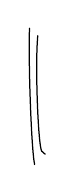
\begin{tikzpicture}[x=1cm,y=1cm,line width=.45pt,line cap=round]
\draw (0,0) .. controls (-.015,-.48) and (.025,-1.54) .. (.065,-1.73);
\draw (.105,-.095) .. controls (.070,-.48) and (.110,-1.48) .. (.155,-1.56) .. controls (.165,-1.58) and (.185,-1.59) .. (.200,-1.60);
\end{tikzpicture}}}
\margin{\unsure{recall that we assume} $\pi$ \unsure{anabelian|nonabelian}
$(2g+\nu\geq3)$}
\[
1\longrightarrow\pi'\longrightarrow
\widehat{\widehat{\mathcal T}}(\pi,i)\longrightarrow
\unsure{\widehat{\widehat{\mathcal G}}}(\pi',i)\longrightarrow1
\]
or again
\[
1\longrightarrow\widehat{\pi}_{g,\nu-1}\longrightarrow
\widehat{\widehat{\mathcal T}}_{g,(\nu,\nu-1)}
\longrightarrow\unsure{\widehat{\widehat{\mathcal G}}}_{g,\nu-1}
\longrightarrow1
\]
which contains the exact sequence
\[
1\longrightarrow\pi_{g,\nu-1}^{\unsure{*|+}}\longrightarrow
\mathcal T_{g,(\nu,\nu-1)}\longrightarrow
\unsure{\mathcal G}_{g,\nu-1}\longrightarrow1
\]
\unsure{as|known} sub\deleted{\unsure{particular|dense part}}, \unsure{sequence|is} exact.
It is convenient to work instead with
\diagram{\begin{tikzcd}[ampersand replacement=\&,column sep=2.1em,row sep=3.0em]
1 \arrow[r,dash] \&
\pi_{g,\nu-1} \arrow[r,dash] \arrow[d,hook',no head] \&
\unsure{\mathcal T}_{g,\nu}^{!+} \arrow[r] \arrow[d,hook',no head] \&
\mathcal G_{g,\nu-1}^{!+} \arrow[r,dash] \arrow[d,hook',no head] \& 1 \\
1 \arrow[r,dash] \&
\widehat{\pi}_{g,\nu-1} \arrow[r] \arrow[d,equal] \&
\underset{\deleted{\unsure{\illegible{1}}}}{\widehat{\mathcal T}_{g,\nu}^{!+}}
\arrow[r] \arrow[d,hook',no head] \&
\widehat{\mathcal G}_{g,\nu-1}^{!+} \arrow[r,dash] \arrow[d,hook'] \& 1 \\
1 \arrow[r,dash] \&
\widehat{\pi}_{g,\nu-1} \arrow[r] \&
\widehat{\widehat{\mathcal T}}_{g,\nu}^{!} \arrow[r] \&
\widehat{\widehat{\mathcal G}}_{g,\nu-1}^{!} \arrow[r,dash] \& 1
\end{tikzcd}}

The map $\unsure{\text{Prediscretifications}|\text{Prediscretifications}}^{+}(\pi)\longrightarrow
\unsure{\text{Prediscretifications}|\text{Prediscretifications}}^{+}(\pi')$ is thus identified with
$\widehat{\widehat{\mathcal T}}_{g,\nu}^{!}/\widehat{\mathcal T}_{g,\nu}^{!}$,
we read off the diagram that this is
$\simeq\widehat{\widehat{\mathcal G}}_{g,\nu-1}^{\unsure{!}\deleted{\unsure{+}}}/
\widehat{\mathcal G}_{g,\nu-1}^{!+}$,
whence bijectivity on the sets of oriented prediscretifications.

In the group $\widehat{\widehat{\mathcal T}}_{g,\nu}^{!}=\mathcal T$,
we have an invariant subgroup $\widehat{\pi}_{g,\nu-1}=\pi'$,
and a subgroup $\Sigma$ $(\unsure{=|\longleftarrow}\widehat{\mathcal T}_{g,\nu}^{!+})$
\mspage{347}

\scanpage{349}

between $\pi'$ and $\mathcal T$, \deleted{\unsure{giving by}} \inserted{giving} a subgroup $\Sigma'\simeq\mathcal T(\pi')$\inserted{$(=\unsure{\widehat{\mathcal G}^{!+}_{g,\nu-1}})$} in $\unsure{\mathcal T'}=\mathcal T/\pi'$ $(\simeq\widehat{\widehat{\mathcal G}}^{!}_{g,\nu-1})$, and we know well that then
\[
\mathcal T/\Sigma\simeq\mathcal T'/\Sigma',
\]
and \deleted{$\unsure{N(\Sigma)}$} that the normalizer \inserted{$\mathcal N$,} of $\Sigma$ in $\mathcal T$ is the inverse image of the normalizer $\mathcal N'$ of $\Sigma'$ in $\mathcal T'$, so that $\mathcal N/\Sigma\simeq\mathcal N'/\Sigma'$, which proves what we wanted.

\uline{Corollary} We have canonical \unsure{isomorphisms}
\[
\Gamma_{g,\nu}\xrightarrow{\sim}\Gamma_{g,\nu-1}\xrightarrow{\sim}\unsure{\cdots}\quad\deleted{\unsure{\Gamma_{g,0}}}
\]
\margin{We also see that $\unsure{\Sigma|\Sigma^{!}}$ invariant in $\unsure{\mathcal T|\widehat{\widehat{\mathcal T}}}$ is equivalent to $\Sigma'$ invariant in $\widehat{\widehat{\mathcal T}}'$}
so that if $g\geq2$, we have \unsure{canonically} $\Gamma_{g,\nu}\simeq\Gamma_{g,0}$, on the other hand $\Gamma_{1,\nu}\simeq\Gamma_{1,1}$ $(g=1,\nu\geq1)$, $\Gamma_{0,\nu}\simeq\Gamma_{0,3}$ $(\nu\geq3)$.

\uline{N.B.} The ``fact'' \deleted{\illegible{1}} assumed is far from obvious --- even that $\widehat{\widehat{\mathcal T}}^{\unsure{!}}_{g,(\nu,\nu-1)}\longrightarrow\unsure{\widehat{\widehat{\mathcal T}}_{g,\nu-1}|\widehat{\widehat{\mathcal M}}_{g,\nu-1}}$ is surjective, or that $\widehat{\widehat{\mathcal T}}_{g,(\nu,\nu-1)}\longrightarrow\widehat{\widehat{\mathcal G}}_{g,\nu-1}$ is injective, is far from obvious, and is perhaps altogether false !

The assumed fact amounts to a statement of the existence of a functor \unsure{in} the opposite direction ``drilling holes'', \unsure{which|what} in any case remains not understood.

\mspage{348}

\scanpage{350}
\mspage{177}

28. \uline{Change of type} $(g,\nu)$ \unsure{(continued)} : \uline{\unsure{passage} to a finite covering.}

Let $\pi$ be a profinite group \inserted{with loops} of type $(g,\nu)$, anabelian as always, $\pi'$ a subgroup of finite index. We know (\unsure{or we|we thereby} verify, by passing to the discrete case) that \deleted{\illegible{1} \unsure{discretified}} \inserted{equipped with the} \unsure{traces} \unsure{on|under} $\pi$ of the \unsure{loop} subgroups of $\pi$, $\pi'$ is a group with loops.

\deleted{If for every $i\in I(\pi)$, we consider an $L_i$, and the $\unsure{n}$ conjugates $\unsure{\operatorname{int}(g)}L_i$ \inserted{$=L_{i\alpha}$}, with $g\in\pi\bmod\pi'$ $(n=[\pi:\pi']\unsure{\}},\ \deleted{\unsure{n}}\ \inserted{1\leq\alpha\leq n})$ \deleted{\unsure{counted|to count} the number of times that a conjugacy class in $\pi'$ of the subgroup $\unsure{\operatorname{int}(g)}L_i$ is} \inserted{then if $\unsure{d_{\alpha}|d_{i\alpha}}=[L_{i\alpha}:\unsure{L'_{i\alpha}|N'_{i\alpha}}\deleted{\unsure{\cap\pi'}}]$ \unsure{for} $L'_{i\alpha}=L_{i\alpha}\cap\pi'$, then} exactly $d_{i\alpha}$ among the $L'_{i\beta}$ \inserted{$(1\leq\beta\leq n)$} are conjugate in $\pi'$ to $L'_{i\alpha}$, and if we sum over the distinct \unsure{conjugacy} classes of the subgroups}

The loop subgroups are \unsure{also|thus} the \deleted{\unsure{the}} subgroups $L'$ such that
\[
\text{a)}\quad L'=\operatorname{Centr}_{\pi}(L')\cap\pi'.
\]
\[
\text{b)}\quad L\unsure{=|:}\operatorname{Centr}_{\pi}(L')\text{ is a \unsure{loop} subgroup in }\pi.
\]
We put $d(L')=[L:L']$, and we thus have a function
\[
d:I'=I(\pi')\longrightarrow\mathbb N^*,
\]
and a map $I'\xrightarrow{\varphi}I$, such that $\forall i\in I$, we have
\[
\text{(1)}\qquad \sum_{\substack{i'\in I'\\\text{over }i}}d(i')=n
\qquad (\text{\unsure{where|here}}\ n=[\pi:\pi'])
\]
We will have the Hurwitz formula
\[
\text{(2)}\qquad \deleted{\unsure{2g|2\alpha}}\ 2g'-2=n(2g-2)+\overbrace{\sum_{i'\in I'}(d(i')-1)}^{\inserted{n\operatorname{card}I-\operatorname{card}I'}}
\]
\mspage{349}

\subsection*{Scans 351--360}
\addcontentsline{toc}{subsection}{Scans 351--360}
% package LM_P036
\scanpage{351}
i.e.
\[
(3)\qquad 2g'-2+\mathrm{card}\,I'=n(2g-2+\mathrm{card}\,I)
\]

(N.B. \deleted{\unsure{\(n\)}} \((2g-2+\mathrm{card}\,I)\) is
\inserted{the negative of} the Euler--Poincaré \unsure{characteristic} with compact
supports of the curve of which \(\unsure{\Pi|\pi}\) is the fundamental
group\ldots) \(\checkmark\)

\margin{\uline{N.B.} saying that we \unsure{are} in the
\unsure{anabelian} case means that \(-\mathrm{EP}_{!}\) is \(\geq 1\)
--- this \unsure{condition|relation} is \unsure{therefore preserved}
by passage \unsure{to a covering|to coverings}.
The integer \(-\mathrm{EP}_{!}\) \unsure{measures} \unsure{strict positivity}
\illegible{1} degree of \unsure{anabelianity}, \unsure{in some sense}\ldots}

Obviously, \unsure{every} discretification of \(\unsure{\Pi|\pi}\)
defines one of \(\unsure{\Pi|\pi}'\) --- and the same holds
for oriented discretifications, modulo
a bit of cohomology [which amounts to saying,
\inserted{in the \unsure{discrete} case \unsure{for example|for example})}
that
\diagram{\begin{tikzcd}[ampersand replacement=\&]
H^2_{!}(\unsure{U|\mathcal U},\unsure{\mathbb Z|\mathbf Z}) \arrow[r] \arrow[d,phantom,sloped,"\simeq"] \& H^2_{!}(\unsure{U'|\mathcal U'},\unsure{\mathbb Z|\mathbf Z}) \arrow[d,phantom,sloped,"\simeq"] \\
T \& T'
\end{tikzcd}}
can be written in the form \(n\theta^{-1}\), where \(\theta\) is a well-determined isomorphism
(the trace isomorphism) \unsure{\(\theta\)|of} \(T'\xrightarrow{\sim}T\).

It is not clear to me at first
sight whether the map
\[
\mathrm{Discret}(\unsure{\Pi|\pi})\unsure{-|\longrightarrow}\mathrm{Discret}(\unsure{\Pi|\pi}')
\]
is surjective, or injective. Injectivity
\inserted{(for \unsure{every} \(\unsure{\Pi|\pi}'\) of finite index in \(\unsure{\Pi|\pi}\))}
would mean that: two discretifications \(\unsure{\Pi|\pi}_0,\unsure{\Pi|\pi}'_0\) of
\(\unsure{\Pi|\pi}\) which are commensurable, i.e. such that
\(\unsure{\Pi|\pi}_0\cap\unsure{\Pi|\pi}'_0\) is of finite index in \(\unsure{\Pi|\pi}_0\) and in \(\unsure{\Pi|\pi}'_0\),
\deleted{in fact, it suffices \unsure{that it be so} in one of them}
\inserted{equal}

\scanpage{352}
\mspage{178}
Suppose that \(\unsure{\Pi|\pi}'\) is an invariant subgroup
in \(\unsure{\Pi|\pi}\), put \(G=\unsure{\Pi|\pi}'/\unsure{\Pi|\pi}\)

\uline{Conjecture} The map \(\mathrm{Discret}(\unsure{\Pi|\pi})\longrightarrow\mathrm{Discret}(\unsure{\Pi|\pi}')\)
is injective, and its image consists of the
discretifications \(\unsure{\Pi|\pi}'_0\subset\unsure{\Pi|\pi}'\) such that
\(G\longrightarrow\mathrm{Aut\,ext}_{\mathrm{lac}}(\unsure{\Pi|\pi}')
\simeq\mathrm{Aut\,ext}_{\mathrm{lac}}(\widehat{\unsure{\Pi|\pi}}'_0)
\simeq\widehat{\widehat{\mathcal T}}(\widehat{\unsure{\Pi|\pi}}'_0)\)
factors through \(\mathcal T(\unsure{\Pi|\pi}'_0)=\mathrm{Autext}_{\mathrm{lac}}(\unsure{\Pi|\pi}'_0)\)
(and in fact, even through \(\mathcal T(\unsure{\Pi|\pi}'_0)^+\)).

\margin{In other words, \(\forall g\in\unsure{\Pi|\pi}\),
\(\exists h\in\unsure{\Pi|\pi}'\) such that \(\mathrm{int}(hg)(\unsure{\Pi|\pi}'_0)\subset\unsure{\Pi|\pi}'_0\)
i.e. \(\unsure{\unsure{\Pi|\pi}'|\unsure{\Pi|\pi}'_0}\cdot\unsure{\Pi|\pi}_0=\unsure{\Pi|\pi}\), where \(\unsure{\Pi|\pi}_0\) is the
normalizer of \(\unsure{\Pi|\pi}'_0\) in \(\unsure{\Pi|\pi}\).}

The condition for a \deleted{\illegible{1}} \(\unsure{\Pi|\pi}'_0\) to be in
the image is obviously necessary. Let us show
that it is sufficient, and that the \(\unsure{\Pi|\pi}_0^{\unsure{*}}\) giving
\unsure{rise} to \(\unsure{\Pi|\pi}'_0\) by \(\unsure{\Pi|\pi}_0\cap\unsure{\Pi|\pi}'\) is unique.
We have an outer action of \(G\) on \(\unsure{\Pi|\pi}'_0\),
which defines the outer action on \(\widehat{\unsure{\Pi|\pi}}'_0\simeq\unsure{\Pi|\pi}'\),
now \(\unsure{\Pi|\pi}\) is recovered canonically from
the latter (since \(\mathrm{Centre}(\widehat{\unsure{\Pi|\pi}}')=1\)), and we
see that it is the \deleted{closure in} profinite \inserted{completion} of
the extension \inserted{\(\unsure{\Pi|\pi}_0\)} of \(G\) by \(\unsure{\Pi|\pi}'_0\), defined by the
\inserted{outer} action of \(G\) on \(\unsure{\Pi|\pi}'_0\). We do indeed have a
generalized discretification \inserted{\(\unsure{\Pi|\pi}_0\) of \(\unsure{\Pi|\pi}\)}, in the sense of
just the structure of a \deleted{\unsure{group}} profinite group, and it
induces \(\unsure{\Pi|\pi}'_0\) --- but we must see that it
is compatible with the loop structure of \(\unsure{\Pi|\pi}\).

\scanpage{353}
But this is made explicit, starting from the
loop structure of \(\unsure{\Pi|\pi}'\), we take the
loop subgroups \inserted{\(L'\)} of \(\unsure{\Pi|\pi}'\), and their
Centralizers in \(\unsure{\Pi|\pi}\). Let us do \unsure{the same} for
\(\unsure{\Pi|\pi}_0\unsure{\supset|>}\unsure{\Pi|\pi}'_0\), we should find a loop
structure on \(\unsure{\Pi|\pi}_0\), giving rise to the
same\unsure{s} \(d_i\).
I have the feeling that this
should not be too nasty to prove --- it
would be as if we already knew that \unsure{every}
\inserted{``torsion-free''} extension of a finite group by a
group with loops is (in the canonical way)
a group with loops\ldots

\uline{Corollary} In any case, the map
\(\mathrm{Discret}(\unsure{\Pi|\pi})\longrightarrow\mathrm{Discret}(\unsure{\Pi|\pi}')\)
is \uline{injective}.
\figure{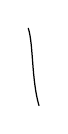
\begin{tikzpicture}[x=1cm,y=1cm,line width=.45pt,line cap=round]
\draw (0,0) .. controls (.065,-.20) and (.040,-.65) .. (.135,-.98);
\end{tikzpicture}}

\uline{N.B.} It should not always be bijective,
for there must be an \inserted{\unsure{outer|outer}} action of a
\(G\) on a \(\widehat{\unsure{\Pi|\pi}}'_0\) i.e. homomorphisms
\(G\longrightarrow\widehat{\widehat{\mathcal T}}(\widehat{\unsure{\Pi|\pi}}'_0)\), which do not \unsure{factor|factor}
through \(\mathcal T(\unsure{\Pi|\pi}'_0)\), and which nevertheless is as
\unsure{good|good} from the profinite group point of view as
\unsure{that|those} coming from a \(\unsure{\Pi|\pi}\) and a \unsure{subgroup}

\scanpage{354}
\mspage{179}

invariant $\unsure{\Pi|\pi}'$. In fact, let us start from such a \uline{discrete} situation $\unsure{\Pi|\pi}_0 \unsure{\supset|>} \unsure{\Pi|\pi}'_0$, whence $G=\unsure{\Pi|\pi}_0/\unsure{\Pi|\pi}'_0$ and $G\longrightarrow \operatorname{Autext}_{\mathrm{lac}}(\unsure{\Pi|\pi}'_0)\deleted{\unsure{(\pi'_0)}}=\mathcal T(\unsure{\Pi|\pi}'_0)\subset\unsure{\widehat{\mathcal T}|\widehat{\widehat{\mathcal T}}}(\widehat{\unsure{\Pi|\pi}}'_0)$, and \uline{conjugate} $G$ by an element \inserted{$\gamma$} of $\widehat{\widehat{\mathcal T}}(\unsure{\Pi|\pi}'_0)$, so as to find $G\longrightarrow\widehat{\mathcal T}(\widehat{\unsure{\Pi|\pi}}'_0)$ which does \deleted{\illegible{2}} not \unsure{factor} through $\mathcal T(\unsure{\Pi|\pi}^{\unsure{'}}_0)$. We find an extension \inserted{$\unsure{\widehat{\unsure{\Pi|\pi}}|\unsure{\Pi|\pi}}^{\unsure{\natural|\sharp}}$} of $G$ by $\widehat{\unsure{\Pi|\pi}}'_0$, \uline{isomorphic} to $\widehat{\unsure{\Pi|\pi}}_0$ (as an extension of $G$ by $\widehat{\unsure{\Pi|\pi}}'_0$), hence the loop structure of $\widehat{\unsure{\Pi|\pi}}'_0$ defines one on $\unsure{\Pi|\pi}^{\unsure{\natural|\sharp}}$ \deleted{and is} \inserted{(so as to be} induced by the latter), but nevertheless the \uline{chosen} discretification \inserted{$\unsure{\Pi|\pi}_0$} of $\widehat{\unsure{\Pi|\pi}}_0$ is not induced by one of $\unsure{\Pi|\pi}$. To

$\ast$ Carry out the construction, it suffices to find an element \inserted{$\gamma\in\widehat{\widehat{\mathcal T}}(\unsure{\Pi|\pi}'_0)$ \deleted{\unsure{finite}} such that $\operatorname{int}(\gamma).G\unsure{\not\subset|\notin}\mathcal T$,} \deleted{\unsure{$u$} \unsure{of order} \illegible{1} not \unsure{coming} from, \unsure{in} $\mathcal T(\unsure{\Pi|\pi}'_0)$, \unsure{or} \unsure{lifting} to an element of finite order of $\unsure{\mathcal G|\mathcal C}(\unsure{\Pi|\pi}'_0)^+=\operatorname{Aut}_{\mathrm{lac}}(\unsure{\Pi|\pi}'_0)^+$, and \deleted{whose \unsure{conjugation} in $\widehat{\widehat{\mathcal T}}$ \unsure{a}} \inserted{a $\gamma\in\widehat{\widehat{\mathcal T}}(\unsure{\Pi|\pi}'_0)$, such that} $\gamma u\gamma^{-1}\notin\mathcal T(\unsure{\Pi|\pi}'_0)$, \inserted{\deleted{i.e. such that $u$ \unsure{fixes}}} \deleted{not} \inserted{$\gamma^{-1}.\unsure{\Pi|\pi}'_0\subset\widehat{\unsure{\Pi|\pi}}'_0$.}}
\figure{[A large part of the canceled passage is enclosed by a frame (left, bottom and right sides) and crossed out with four long slanting strokes. After the inclusion $\gamma^{-1}.\unsure{\Pi|\pi}'_0\subset\widehat{\unsure{\Pi|\pi}}'_0$ on the last line, stroke curved into a hook, directed toward the following inclusion.]}
\inserted{i.e. such that $G$ \deleted{\unsure{does not fix}} does not stabilize $\gamma^{-1}(\unsure{\Pi|\pi}'_0)\subset\widehat{\unsure{\Pi|\pi}}'_0$}

Such a $\gamma$ \unsure{always} exists....

\scanpage{355}

Of course, there is no reason, \deleted{that} for two discretifications $\unsure{\unsure{\Pi|\pi}'_0|\unsure{\Pi|\pi}_0},\unsure{\Pi|\pi}_1$ of $\unsure{\Pi|\pi}$, that if $\unsure{\Pi|\pi}_0,\unsure{\Pi|\pi}_1$ are $\unsure{\Pi|\pi}$-conjugate (i.e. define \deleted{some} \inserted{the same} strict \unsure{prediscretification|prediscretification}\deleted{s} of $\unsure{\Pi|\pi}$), the same should hold for $\unsure{\Pi|\pi}'_0$ and $\unsure{\Pi|\pi}'_1$ under the inner action of $\unsure{\Pi|\pi}'$. (It would be necessary for $\unsure{\Pi|\pi}_0,\unsure{\Pi|\pi}_1$ to be conjugate by $\unsure{\Pi|\pi}'$, and not just by $\unsure{\Pi|\pi}$). On the other hand, I presume that if $\unsure{\Pi|\pi}_0,\unsure{\Pi|\pi}_1$ are ``adherent'' to one another in the space of \unsure{discretifications|discretifications} of $\unsure{\Pi|\pi}$, i.e. if they define the same prediscretification, the same holds for $\unsure{\Pi|\pi}'_0,\unsure{\Pi|\pi}'_1$, and that the map
\[
\tag{4}
\operatorname{Prédiscrt}^{+}(\unsure{\Pi|\pi}\deleted{\unsure{_0}})\longrightarrow\operatorname{Prédiscrt}^{+}(\unsure{\Pi|\pi}'\deleted{\unsure{_0}})
\]
which we obtain in this way, is again bijective, and that it in turn passes to the quotient, to define a bijective map
\[
\tag{5}
\unsure{\operatorname{Préarith}|\operatorname{Préarithm}}(\unsure{\Pi|\pi}\deleted{\unsure{_0}})\longrightarrow\unsure{\operatorname{Préarith}|\operatorname{Préarithm}}(\unsure{\Pi|\pi}'\deleted{\unsure{_0}}),
\]
and that if $\Sigma,\Sigma'$ correspond to one another under the latter, that we have a canonical isomorphism
\[
\tag{6}
\unsure{\mathbb{\Gamma}|\Gamma}_{\Sigma}\longrightarrow\unsure{\mathbb{\Gamma}|\Gamma}_{\Sigma'},
\]
\unsure{compatible},

\scanpage{356}
\mspage{180}

with the actions of these groups on the set $P_{\Sigma}$ of prediscretifications of $\unsure{\Pi|\pi}$ compatible with $\Sigma$, and the set \inserted{$P_{\Sigma'}$} of prediscretifications of $\unsure{\Pi|\pi}'$ compatible with $\Sigma'$ (which are resp. left torsors under $\unsure{\mathbb{\Gamma}|\Gamma}_{\Sigma},\unsure{\mathbb{\Gamma}|\Gamma}_{\Sigma'}$). At the same time, we will find \inserted{therefore} that $\Sigma$ is unique for $\unsure{\Pi|\pi}$ i.e. invariant under $\widehat{\widehat{\mathcal T}}(\unsure{\Pi|\pi})$, iff $\Sigma'$ is unique in $\unsure{\Pi|\pi}'$ i.e. invariant under $\widehat{\widehat{\mathcal T}}(\unsure{\Pi|\pi}')$.

In any case, the fundamental conjecture which \unsure{interprets} the $\unsure{\mathbb{\Gamma}|\Gamma}_{g,\unsure{\nu|v}}$ as $\unsure{\mathbb{\Gamma}|\Gamma}_0=\operatorname{Gal}(\overline{\mathbb Q}_0/\mathbb Q)$ \unsure{would have|will have} at least as a consequence that the map $\operatorname{Discr}^{+}(\unsure{\Pi|\pi})\unsure{-|\longrightarrow}\operatorname{Discr}^{+}(\unsure{\Pi|\pi}')$ passes to the quotient \inserted{in} two ways, to give a commutative diagram

\diagram{
\begin{tikzcd}[row sep=large,column sep=large,ampersand replacement=\&]
\operatorname{Discr}^{+}(\unsure{\Pi|\pi}) \arrow[r,no head] \arrow[d]
  \& \operatorname{Discr}^{+}(\unsure{\Pi|\pi}') \arrow[d] \\
\unsure{P|p}=\unsure{\operatorname{Prédiscr}}^{+}(\unsure{\Pi|\pi}) \arrow[r] \arrow[d]
  \& \unsure{P|p}'=\operatorname{Prédiscr}^{+}(\unsure{\Pi|\pi}') \arrow[d] \\
A=\operatorname{Arithm}(\unsure{\Pi|\pi}) \arrow[r]
  \& A'=\operatorname{Arithm}(\unsure{\Pi|\pi}')
\end{tikzcd}
}

and that the \deleted{\unsure{diagram|diagram}} lower square is cartesian (without prejudging the \unsure{injectivity} or the \unsure{bijectivity} of the map $A\longrightarrow A'$). \unsure{So} it would be necessary

\scanpage{357}
that \deleted{\unsure{already}} if $\unsure{\Pi|\pi}_0,\unsure{\Pi|\pi}_1$ are two discretifications \inserted{(\unsure{oriented})} of $\unsure{\Pi|\pi}$, which define the same prediscretification (\unsure{oriented}), then the same holds for \inserted{their \unsure{traces} on $\unsure{\Pi|\pi}'$,} $\unsure{\Pi|\pi}'_0$ \unsure{and} $\unsure{\Pi|\pi}'_1$, with respect to $\unsure{\Pi|\pi}'$. But already if $\unsure{\Pi|\pi}_0$ and $\unsure{\Pi|\pi}_1$ are $\unsure{\Pi|\pi}$-conjugate (i.e. define same discretification (\unsure{oriented}, \uline{\unsure{strict}})), this is not so clear --- \deleted{\unsure{unless}} but yes, for we will have $\unsure{\Pi|\pi}=\unsure{\Pi|\pi}'\cdot\unsure{\Pi|\pi}_0$ hence if $\unsure{\Pi|\pi}_1=\operatorname{int}(u)\unsure{\Pi|\pi}_0$ writing $u=u'u_0$ with $u'\in\unsure{\Pi|\pi}'$, $u_0\in\unsure{\Pi|\pi}_0$, we will have
\[
\unsure{\Pi|\pi}_1=\operatorname{int}(u')\operatorname{int}(u_0)\unsure{\Pi|\pi}_0=\operatorname{int}(u')\unsure{\Pi|\pi}_0,
\]
hence $\unsure{\Pi|\pi}'_1=\operatorname{int}(u')\unsure{\Pi|\pi}'_0$ hence $\unsure{\Pi|\pi}'_0$ and $\unsure{\Pi|\pi}'_1$ are conjugate.

Let us try to proceed in the same way in the general case of a $u\in\widehat{\unsure{\mathcal{C}|\mathcal{G}}(\unsure{\Pi|\pi}_0)}^+$, \inserted{such that $\unsure{\Pi|\pi}_1=u(\unsure{\Pi|\pi}_0)$,} writing if possible $u=u'u_0$, with $u'\in\widehat{\unsure{\mathcal{C}|\mathcal{G}}(\unsure{\Pi|\pi}_0,\unsure{\Pi|\pi}'_0)}^+$, and $u_0\in\unsure{\mathcal{C}|\mathcal{G}}(\unsure{\Pi|\pi}_0)^+$, where we define $\unsure{\mathcal{C}|\mathcal{G}}(\unsure{\Pi|\pi}_0,\unsure{\Pi|\pi}'_0)^+$ as the group of \unsure{i-automorphisms|l-automorphisms} \inserted{\unsure{direct|discrete}} of $\unsure{\Pi|\pi}_0$ which \uline{stabilize $\unsure{\Pi|\pi}'_0$}, and $\widehat{\unsure{\mathcal{C}|\mathcal{G}}}(\unsure{\Pi|\pi}_0,\unsure{\Pi|\pi}'_0)^+$ is its profinite \unsure{compactification}. We would then have $\unsure{\Pi|\pi}_1=u'(u_0(\unsure{\Pi|\pi}_0))=\dot{u}'(\unsure{\Pi|\pi}_0)$, where \deleted{\illegible{1}} $\dot{u}'$ denotes the image of $u'$ in $\widehat{\unsure{\mathcal{T}|\mathcal{C}}(\unsure{\Pi|\pi}'_0)}$. In any case, there is no problem if $\unsure{\Pi|\pi}'\deleted{\unsure{_0}}$ is a \deleted{\unsure{closed}} \uline{characteristic} subgroup of $\unsure{\Pi|\pi}$, for then we have a homomorphism

\scanpage{358}
\mspage{181}
discrete $\unsure{\mathcal{C}|\mathcal{G}}(\unsure{\Pi|\pi}_0)\longrightarrow\unsure{\mathcal{C}|\mathcal{G}}(\unsure{\Pi|\pi}'_0)$, defining \unsure{the|the} $\unsure{\widehat{\unsure{\mathcal{C}|\mathcal{G}}}(\widehat{\unsure{\Pi|\pi}}_0)}\longrightarrow\unsure{\widehat{\unsure{\mathcal{C}|\mathcal{G}}}(\widehat{\unsure{\Pi|\pi}}'_0)}$. Since the \unsure{open} characteristic subgroups of $\unsure{\Pi|\pi}$ are cofinal, we are reduced (for the questions of factorizability \inserted{of $D(\unsure{\Pi|\pi})\longrightarrow D(\unsure{\Pi|\pi}')$ into $P(\unsure{\Pi|\pi})\longrightarrow P(\unsure{\Pi|\pi}')$ and $A(\unsure{\Pi|\pi})\longrightarrow A(\unsure{\Pi|\pi}')$} and of bijectivity of the maps $\unsure{P}(\unsure{\Pi|\pi})\longrightarrow P(\unsure{\Pi|\pi}')$ and $A(\unsure{\Pi|\pi})\longrightarrow A(\unsure{\Pi|\pi}')$) we are reduced to the case where $\unsure{\Pi|\pi}'$ is a \uline{characteristic} subgroup. We have \unsure{indeed|seen} \inserted{then} \deleted{the} factorizability of $D(\unsure{\Pi|\pi})\longrightarrow D(\unsure{\Pi|\pi}')$ into $P(\unsure{\Pi|\pi})\longrightarrow P(\unsure{\Pi|\pi}')$, \inserted{\unsure{we want}} \unsure{to show|let us show} that this map is injective \unsure{...} \inserted{This} \deleted{\unsure{this means}}
\inserted{\textcircled{a}} means that the inverse image in $\widehat{\widehat{\unsure{\mathcal{C}|\mathcal{G}}}}(\widehat{\unsure{\Pi|\pi}}_0)$ of $\widehat{\unsure{\mathcal{C}|\mathcal{G}}}(\widehat{\unsure{\Pi|\pi}}'_0)^+$ is $\widehat{\unsure{\mathcal{C}|\mathcal{G}}}(\widehat{\unsure{\Pi|\pi}}_0)^+$, the surjectivity \inserted{\textcircled{b}} means that every element of $\widehat{\widehat{\unsure{\mathcal{C}|\mathcal{G}}}}(\widehat{\unsure{\Pi|\pi}}'_0)$ is congruent modulo $\widehat{\unsure{\mathcal{C}|\mathcal{G}}(\unsure{\Pi|\pi}'_0)}^+$ to an element of the image of $\widehat{\widehat{\unsure{\mathcal{C}|\mathcal{G}}}}(\unsure{\Pi|\pi}_0)$. The factorizability into $A(\unsure{\Pi|\pi})\longrightarrow A(\unsure{\Pi|\pi}')$ means that by \inserted{\textcircled{c}} the preceding map \deleted{\unsure{of}} $\widehat{\widehat{\unsure{\mathcal{C}|\mathcal{G}}}}(\unsure{\Pi|\pi}_0)\hookrightarrow\widehat{\widehat{\unsure{\mathcal{C}|\mathcal{G}}}}(\unsure{\Pi|\pi}'_0)$, (N.B. it is immediate that \unsure{it is} injective) \deleted{\unsure{is}} \inserted{sends}
\[
M(\unsure{\Pi|\pi}_0)=\operatorname{Norm}_{\unsure{\widehat{\widehat{\mathcal{C}}}|\widehat{\mathcal{C}}}(\unsure{\Pi|\pi}_0)}\bigl(\widehat{\unsure{\mathcal{C}|\mathcal{G}}}^{+}(\unsure{\Pi|\pi}_0)\bigr)
\]
into $M(\unsure{\Pi|\pi}'_0)$, the injectivity of $A(\unsure{\Pi|\pi})\longrightarrow A(\unsure{\Pi|\pi}')$ that

\scanpage{359}

\textcircled{d} we even have \unsure{that} $M(\unsure{\Pi|\pi})$ is
\unsure{exactly|exact\textsuperscript{ly}} the inverse image of $M(\unsure{\Pi|\pi}')$,
the \unsure{surjectivity} of
$A(\unsure{\Pi|\pi})\unsure{\twoheadrightarrow|\longrightarrow}A(\unsure{\Pi|\pi}')$ that
\inserted{\textcircled{e}} every element of
$\widehat{\widehat{\unsure{\mathcal C|\mathcal G}}}(\unsure{\Pi|\pi}'_0)$
is congruent modulo $M(\unsure{\Pi|\pi}'_0)$ to an element of
$\widehat{\widehat{\unsure{\mathcal C|\mathcal G}}}(\unsure{\Pi|\pi}_0)$
\margin{weaker than (b)}
--- and these conditions \unsure{together} imply that the canonical homomorphism
\diagram{\begin{tikzcd}[ampersand replacement=\&]
\mathbb{\Gamma}_{\deleted{\unsure{\pi}}\unsure{\Pi|\pi}_0}
  \arrow[r] \arrow[d, equal]
  \& \mathbb{\Gamma}_{\unsure{\Pi|\pi}'_0} \arrow[d, equal] \\
M(\unsure{\Pi|\pi}_0)/\widehat{\unsure{\mathcal C|\mathcal G}}(\unsure{\Pi|\pi}_0)
  \& M^{\unsure{\sharp|*}}(\unsure{\Pi|\pi}'_0)/\widehat{\unsure{\mathcal C|\mathcal G}}(\unsure{\Pi|\pi}'_0)
\end{tikzcd}}
is an isomorphism -- it even suffices for this to have
\unsure{(c)|(e)} (to be able to define this map) and (a)
(for its injectivity), and (b) and the strengthening (d) of
\unsure{(c)|(e)} (for its \unsure{bijectivity|surjectivity}. So we see that
\unsure{everything} hangs on the properties of the homomorphism of group inclusions
\diagram{\begin{tikzcd}[ampersand replacement=\&,column sep=2.2em,row sep=3.8em,
execute at end picture={
  \draw[line width=.35pt] ([xshift=-6pt,yshift=-1pt]\tikzcdmatrixname-1-3.south) -- ([xshift=-9pt,yshift=-1pt]\tikzcdmatrixname-1-3.south) -- ([xshift=-9pt,yshift=1pt]\tikzcdmatrixname-2-3.north) -- ([xshift=-6pt,yshift=1pt]\tikzcdmatrixname-2-3.north);
  \draw[line width=.35pt] ([xshift=17pt,yshift=-1pt]\tikzcdmatrixname-1-3.south) -- ([xshift=20pt,yshift=-1pt]\tikzcdmatrixname-1-3.south) -- ([xshift=20pt,yshift=1pt]\tikzcdmatrixname-2-3.north) -- ([xshift=17pt,yshift=1pt]\tikzcdmatrixname-2-3.north);
}]
{} \arrow[d,phantom,"{(7)}"{description}] \&
\widehat{\mathcal G}^{+}(\pi_0)
\arrow[r,phantom,"{\subset}"{description}]
\arrow[d,hook,no head] \&
M(\pi_0)
\arrow[r,phantom,"{\subset}"{description}]
\arrow[d,hook]
\arrow[d,phantom,"{?}"{description,xshift=8pt}] \&
\widehat{\widehat{\mathcal G}}(\pi_0) \arrow[d,hook,no head] \\
{} \&
\widehat{\mathcal G}^{+}(\pi'_0)
\arrow[r,phantom,"{\subset}"{description}] \&
M(\pi'_0)
\arrow[r,phantom,"{\subset}"{description}] \&
\widehat{\widehat{\mathcal G}}(\pi'_0)
\end{tikzcd}}
with the task of proving a) b) (which \unsure{concern} only the composite square)
and \unsure{c)|e)}.

\deleted{Besides d) \unsure{will be} an
\inserted{\unsure{immediate}} consequence of a), and of the fact
(which will ensure \unsure{c)|e)}) that every element of
$\widehat{\unsure{\mathcal C|\mathcal G}}^{+}(\unsure{\Pi|\pi}_0)$ is congruent modulo
$\unsure{\mathcal C|\mathcal G}$}

\scanpage{360}
\mspage{182}

Perhaps the properties a) b) c) are
completely false -- yet a) (which corresponds to the injectivity of
$P(\unsure{\Pi|\pi})\longrightarrow P(\unsure{\Pi|\pi}')$) seems fairly plausible.
Property b) (which would express the surjectivity of
$P(\unsure{\Pi|\pi})\longrightarrow P(\unsure{\Pi|\pi}')$) is much more problematic,
even doubtful. The trouble is that the group
$\widehat{\widehat{\unsure{\mathcal C|\mathcal G}}}(\unsure{\Pi|\pi}_0)$
can be ``much smaller'' than
$\widehat{\widehat{\unsure{\mathcal C|\mathcal G}}}(\unsure{\Pi|\pi}'_0)$,
we realize this by passing to the quotient by the subgroup
$\widehat{\unsure{\Pi|\pi}}'_0=\unsure{\Pi|\pi}'$ (contained in the smallest of the groups in (7),
and normal in the largest), we find on the second line
the groups $\widehat{\mathcal T}^{+}(\unsure{\Pi|\pi}'_0)$,
\deleted{\illegible{1}} $\unsure{\mathcal N|N}(\unsure{\Pi|\pi}'_0)$ and
$\widehat{\widehat{\mathcal T}}(\unsure{\Pi|\pi}'_0)$, on the first
extensions of the \unsure{corresponding|corresponding} groups
for $\unsure{\Pi|\pi}_0$ ($\widehat{\mathcal T}^{+}(\unsure{\Pi|\pi}_0)$,
$\unsure{\mathcal N|N}(\unsure{\Pi|\pi}_0)$ and
$\widehat{\widehat{\mathcal T}}(\unsure{\Pi|\pi}_0)$) by
\inserted{the finite group} $G=\unsure{\Pi|\pi}_0/\unsure{\Pi|\pi}'_0\simeq\unsure{\Pi|\pi}/\unsure{\Pi|\pi}'$,
\deleted{\unsure{let them be|let it be}
$\unsure{\widetilde{\widehat{\mathcal T}}^{+}|\widetilde{\mathcal T}^{+}}$
or $\mathcal T$}
\unsure{denoted|denoted} by $\sim$'s, so that \unsure{.|--}
\diagram{\begin{tikzcd}[ampersand replacement=\&,column sep=1.9em,row sep=3.8em,
execute at end picture={
  \draw[line width=.35pt] ([xshift=-6pt,yshift=-1pt]\tikzcdmatrixname-1-4.south) -- ([xshift=-9pt,yshift=-1pt]\tikzcdmatrixname-1-4.south) -- ([xshift=-9pt,yshift=1pt]\tikzcdmatrixname-2-4.north) -- ([xshift=-6pt,yshift=1pt]\tikzcdmatrixname-2-4.north);
  \draw[line width=.35pt] ([xshift=17pt,yshift=-1pt]\tikzcdmatrixname-1-4.south) -- ([xshift=20pt,yshift=-1pt]\tikzcdmatrixname-1-4.south) -- ([xshift=20pt,yshift=1pt]\tikzcdmatrixname-2-4.north) -- ([xshift=17pt,yshift=1pt]\tikzcdmatrixname-2-4.north);
}]
{} \arrow[d,phantom,"{(8)}"{description}] \&
G \arrow[r,phantom,"{\subset}"{description}] \arrow[dr,hook] \&
\widetilde{\widehat{\unsure{\mathcal T}}}^{+\unsure{:}}(\pi_0)
\arrow[r,phantom,"{\subset}"{description}]
\arrow[d,hook,no head] \&
\widetilde{\mathcal N}(\pi_0)
\arrow[r,phantom,"{\subset}"{description}]
\arrow[d,hook]
\arrow[d,phantom,"{?}"{description,xshift=8pt}] \&
\widetilde{\widehat{\widehat{\mathcal T}}}(\pi_0) \arrow[d,hook] \\
{} \& {} \&
\widehat{\mathcal T}^{+}(\pi'_0)
\arrow[r,phantom,"{\subset}"{description}] \&
\mathcal N(\pi'_0)
\arrow[r,phantom,"{\subset}"{description}] \&
\widehat{\widehat{\mathcal T}}(\pi'_0)
\end{tikzcd}},
which shows that the groups on the first line

\subsection*{Scans 361--370}
\addcontentsline{toc}{subsection}{Scans 361--370}
% package LM_P037
\scanpage{361}
\uline{normalize} the subgroup $G\subset\widehat{\mathcal T}^{+}(\pi'_0)$
(\uline{N.B.} in fact we have $G\subset\mathcal T^{+}(\pi'_0)$ ; \deleted{\illegible{1}} and $\pi_0$
is reconstructed from $\pi'_0$ and from
this subgroup of $\pi'_0$) --- \deleted{\unsure{I think}}\inserted{we should}
be able to show without too much trouble
that \deleted{\illegible{1}} in (8), $\widetilde{\widehat{\mathcal T}}^{+}(\pi_0)$ and $\widetilde{\widehat{\widehat{\mathcal T}}}(\pi_0)$
are precisely the normalizers of $G$
in $\widehat{\mathcal T}^{+}(\pi'_0)$ and in $\widehat{\widehat{\mathcal T}}(\pi'_0)$ (which
would indeed imply a), besides) ---
but I see no plausible reason
why (b) should be true --- which would mean,
essentially, that there is no more
``arithmetic \unsure{transcendence}'' defined by the
(``very big'' !) $\widehat{\widehat{\mathcal T}}(\pi'_0)$ (modulo $\widehat{\mathcal T}(\pi'_0)^{+}$), than
that defined by the (``much smaller'') group
$\widetilde{\widehat{\widehat{\mathcal T}}}(\pi_0)=\operatorname{Norm}_{\widehat{\widehat{\mathcal T}}(\unsure{\pi_0|\pi'_0})}(G)$ \dots\ Besides these
conditions a) b) are not imperative
for the fundamental conjecture
\unsure{linking} the $\unsure{\pi_{g,\nu}|\Pi_{g,\nu}}$ to $\Gamma_0$ to be \unsure{consistent} ---
\mspage{360}

\scanpage{362}
\mspage{183}
on the other hand we would absolutely need
c) in order at least to define
$A(\pi)\unsure{\longrightarrow|{-}}A(\pi')$ and (if $\Sigma,\Sigma'$ correspond)
$\Gamma_{\Sigma}\unsure{\longrightarrow|{-}}\Gamma_{\Sigma'}$, in the case $\unsure{\pi'_a|\pi'_0}$ \deleted{\unsure{invariant}}\inserted{characteristic} in $\pi$
(and in all cases if in addition we admit
a), which seems \unsure{rather} plausible, and gives
the \uline{injectivities} required. But one
does wonder why an element
of \deleted{\illegible{1}} $\widehat{\widehat{\mathcal T}}(\pi'_0)$ simply because
it \deleted{\unsure{normalizes}}\inserted{is in} the \deleted{$G$ and it \unsure{normalizes}}\inserted{normalizer $R$ of $G$}
\deleted{\unsure{the same}}\inserted{in} $\widehat{\widehat{\mathcal T}}(\pi'_0)$, \inserted{hence also $R$,} and it normalizes
$R\cap\widehat{\mathcal T}^{+}(\pi'_0)$, should also normalize
$\widehat{\mathcal T}^{+}(\pi'_0)$ itself ! It is true that we
made \unsure{draconian} hypotheses at the outset
(\unsure{starting} from a \uline{characteristic} subgroup $\pi'_0$ of $\pi_0$) which
must surely be \unsure{reflected} in special
properties of $G\subset\mathcal T^{+}(\pi'_0)$. Perhaps
in the end the trick of reducing to
characteristic subgroups to examine
\mspage{361}

\scanpage{363}
the situation is \unsure{itself} not so clever.
To see more clearly, we could already
\unsure{try} to understand the case where (without
assuming $\pi'$ characteristic) we assume $\pi'$ of index
2 in $\pi$, hence invariant and $G\simeq\mathbb Z/2$, or
else we take \deleted{\illegible{2}} the kernel of the canonical homomorphism
$\pi\longrightarrow(\pi_{\mathrm{ab}})_2$ ($\simeq(\mathbb Z/2\mathbb Z)^{2g\deleted{+}}$ if $\nu=0$,
$\simeq(\mathbb Z/2\mathbb Z)^{2g\unsure{+|-}\nu-1}$ if $\nu\geq1$), taking for example
$\pi=\widehat\Pi_{0,3}$ --- \unsure{situation} of the
Fermat curve $x^2+y^2+z^2=0$ (octahedral covering
of $\mathbb P^1_{\overline{\mathbb Q}}\setminus\{0,1,\infty\}$ \dots)

But let us provisionally admit the \deleted{results}\inserted{hypotheses}
of injectivity (relatively innocuous), \uline{plus} the
condition c), not innocuous at all ---
whence, if $\Sigma$ and $\Sigma'$ correspond, an injective
homomorphism
\[
(9)\qquad \Gamma_{\Sigma}\hookrightarrow\Gamma_{\Sigma'},
\]
and let us see what we could get from it.
even admitting, provisionally (to
see) that (9) is an isomorphism --- \deleted{\unsure{Which|What}}
that is to say the full force of the main
conjecture $\Gamma_0\simeq\Gamma_{g,\nu}$.
\mspage{362}

\scanpage{364}
\mspage{184}

\unsure{Let|Let} $\pi$ be a profinite group \inserted{with loops} of type $(g,\nu)$, $\pi'$ of type $(g',\nu')$. Let us call a ``correspondence'' between $\pi$ and $\pi'$ a \deleted{group} pair consisting of a profinite $\unsure{G|\pi''}$ \inserted{with loops} \deleted{of type $(g'',\nu'')$}, and of homomorphisms \inserted{with loops} $\unsure{G|\pi''}\xrightarrow{p}\pi$, $\unsure{G|\pi''}\xrightarrow{q}\pi'$ which are therefore \unsure{each|each} \unsure{composed|composed} of a ``plugging holes'' morphism, and of an \deleted{inclusion} isomorphism onto a \unsure{subgroup|subgroup} of finite index.
\unsure{Let|Let} $\unsure{J_p|I''_p}$, $\unsure{J_q|I''_q}\in\unsure{J|I''}=I(\pi'')$ be the \inserted{sub}sets of $\unsure{J|I''}$ which correspond to the ``holes plugged by $p$'' resp. by $q$, we assume \inserted{if necessary} $\unsure{J_p|I''_p}\cap\unsure{J_q|I''_q}=\varnothing$ (otherwise one could factor through the \unsure{same} quotient $\widetilde{\pi}''$ of $\pi''$). In other words if $\unsure{\overline{J}_p|\overline{I}''_p}$, $\unsure{\overline{J}_q|\overline{I}''_q}$ are the complements of $\unsure{J_p|I''_p}$, $\unsure{J_q|I''_q}$ in $\unsure{J|I''}$ (so that we have : $\unsure{\overline{J}_p|\overline{I}''_p}\to I=I(\pi)$, $\unsure{\overline{J}_q|\overline{I}''_q}\to I'=I(\pi')$) we have
\[
\unsure{\overline{J}_p|\overline{I}''_p}\cup\unsure{\overline{J}_q|\overline{I}''_q}=\unsure{J|I''}.
\]

\deleted{\unsure{Using|Let us use} the ``results'' of the two \unsure{paragraphs} \unsure{above}, we then define maps}

We are now going to suppose $\pi$ equipped with a $\Sigma$ \inserted{$\in A(\pi)$}, $\pi'$ equipped with a $\Sigma'\in A(\pi')$, we shall call an ``arithmetic correspondence'' between $\pi$ and $\pi'$ a quadruple $(\unsure{G|\pi''},p,q,\unsure{\Sigma_G|\Sigma''})$, where $(\unsure{G|\pi''},p,q)$ are as above, and $\unsure{\Sigma_G^{a}|\Sigma_G}\in A(G)$, such that we have $\unsure{\Sigma_G|\Sigma_a}=p^*(\Sigma)=q^*(\Sigma')$. \deleted{\unsure{We suppose}} If $P_{\Sigma}$,
\mspage{363}

\scanpage{365}

$P_{\Sigma'}$, $P_{\unsure{\Sigma_G|\Sigma_a}}$ are resp. the torsors under $\Gamma_{\Sigma}$, $\Gamma_{\Sigma'}$, $\Gamma_{\Sigma''}$ that we know, we have two \unsure{diagrams|diagram} of isomorphisms of torsors
\diagram{\begin{tikzcd}[ampersand replacement=\&,column sep=small,row sep=large]
\& P_{\unsure{\Sigma_G|\Sigma_a}} \& \\
P_{\Sigma} \arrow[ur,"p_P^*","\sim"'] \& \& P_{\Sigma'} \arrow[ul,"q_P^*"',"\sim"]
\end{tikzcd}}
\diagram{\begin{tikzcd}[ampersand replacement=\&,column sep=small,row sep=large]
\& \Gamma_{\unsure{\Sigma_G|\Sigma''_G}} \arrow[dr,leftrightarrow,"q_\Gamma^*","\sim"'] \& \\
\Gamma_{\Sigma} \arrow[ur,"\unsure{\widehat{p}_\Gamma|p_\Gamma^*}","\sim"'] \& \& \Gamma_{\Sigma''}
\end{tikzcd}},
whence by composition an \unsure{isomorphism|homomorphism} of
\deleted{$\unsure{P_{\Sigma}\to}$}
\[
(P_{\Sigma},\Gamma_{\Sigma})\xrightarrow{\sim}(P_{\Sigma'},\Gamma_{\Sigma'})
\]

We call ``arithmetically outer isomorphisms'' \inserted{of $(\pi,\Sigma)$ with $(\pi',\Sigma')$,} any isomorphism of torsors that we can obtain in this way. Two correspondences are said to be \inserted{\unsure{equivalent} \deleted{\unsure{from the point of}} from the point of view} \deleted{\unsure{arithmetic|arithmetic} \unsure{outer|outer}} arithmetically outer, if they define the \unsure{same|=} arithmetically outer isomorphism. \unsure{The} composition is defined by composition of the actions on $(P_{\Sigma},\Gamma_{\Sigma})$ --- we see that \unsure{this} comes from a correspondence. We \unsure{find} therefore a groupoid, which we check without difficulty is connected. \inserted{I say that} The automorphisms of $(\pi,\Sigma)$ ``are'' the automorphisms of $(P_{\Sigma},\Gamma_{\Sigma})$ defined by elements of $\Gamma_{\Sigma}$. \deleted{This is \unsure{obvious} or \unsure{not}} This is \unsure{easy}\ldots

\margin{We shall call it the \unsure{groupoid} of ``outer arithmetic curves''.}
\mspage{364}

\scanpage{366}
\mspage{185}

In this groupoid, there is a transitive system of isomorphisms between the \deleted{\illegible{1}} $(\widehat{\pi}_0,\overline{\Sigma}_{\pi_0})$ (where $\pi_0$ is a discrete group with loops) more generally between the $(\pi,\Sigma_\alpha)$, where $\alpha$ \inserted{$\in P(\pi)$} is a prediscretification of $\pi$ --- let us therefore define an \inserted{arithmetically} outer isomorphism of $\Pi_{g,\nu}$
$\pi$ \ldots\ \unsure{The|Their} group of \unsure{these|its} automorphisms is denoted $\Gamma_0$. The \deleted{category} groupoid of \inserted{virtual} outer arithmetic curves is therefore identified with the category of torsors under $\Gamma_0$,
A prediscretification (we could also call it an arithmetically outer rigidification) is \unsure{therefore} nothing other than an arithmetically outer isomorphism between this reference element, and $\pi$.
\mspage{365}

\scanpage{367}
\mspage{186}

\uline{29} Critique of the preceding approach.

The approach \unsure{of the|of the} preceding \S\ seems \unsure{frankly|in the end} very brutal. I even have doubts whether \unsure{the|the} \deleted{hypothesis} conjecture \unsure{in|on} the properties of the ``plugging holes'' functor is true as it stands. It is true that for a profinite group \deleted{\illegible{1}} \inserted{\unsure{with}} \unsure{loops} $\pi$, if we fix $i\in I(\pi)$, we have a canonical homomorphism
\[
\tag{1}
\widehat{\widehat{\mathcal T}}(\pi,i)
=\underset{\substack{\text{stabilizer}\\\text{of }i\text{ in }\widehat{\widehat{\mathcal T}}(\pi)}}{\text{\uline{$\widehat{\widehat{\mathcal T}}(\pi)_i$}}}
\longrightarrow \widehat{\widehat{\mathcal G}}(\pi'),
\]
but it is problematic whether this is an isomorphism --- and even whether it is injective, or whether it is surjective. But, \unsure{choosing} a discretification $\pi_0\subset\pi$, whence ditto $\pi'_0$ for $\pi'$, the preceding homomorphism does indeed induce an isomorphism
\[
\tag{1}
\mathcal T(\pi_0)_i\simeq\mathcal G(\pi'_0)
\]
whence
\[
\tag{3}
\widehat{\mathcal T}(\pi_0)\xrightarrow{\sim}\widehat{\mathcal G}(\pi'_0)
\]
and consequently, the exact sequence $\deleted{\unsure{\widehat{\pi}_0}}\widehat{\pi}'_0\longrightarrow\widehat{\mathcal G}(\pi'_0)\longrightarrow\widehat{\mathcal T}(\pi'_0)\longrightarrow 1$ gives
\[
\tag{4}
1\longrightarrow\widehat{\pi}'_0\longrightarrow\widehat{\mathcal T}(\pi_0)\longrightarrow\widehat{\mathcal T}(\pi'_0)\longrightarrow 1
\]
and consequently we find an injective homomorphism
\[
\begin{gathered}\widehat{\pi}'_0\\[-0.5ex]\Vert\\[-0.5ex]\pi'\end{gathered}
\unsure{\hookrightarrow|\leftrightarrow}
\widehat{\mathcal T}(\pi_0)_i
\hookrightarrow
\begin{gathered}\widehat{\widehat{\mathcal T}}(\pi_0)_i\\[-0.5ex]\Vert\\[-0.5ex]\unsure{\widehat{\widehat{\mathcal T}}}(\pi)\end{gathered}
\]
hence a homomorphism
\[
\tag{5}
i_{\pi_0}:\quad\pi'\longrightarrow\widehat{\widehat{\mathcal T}}(\pi)_i
\]
for which \unsure{the|the} composite with (1) is the canonical injection $\pi'\hookrightarrow\widehat{\widehat{\mathcal G}}(\pi')$. Replacing the discretification \inserted{$\pi_0$} by another, $\pi_1$, we find a priori another homomorphism $i_{\pi_1}:\pi'\longrightarrow\widehat{\widehat{\mathcal T}}(\pi)_i$. \unsure{We may assume} $\pi_1=u(\pi_0)$, $u\in\widehat{\widehat{\mathcal T}}(\pi)_i$;

\mspage{366}

\scanpage{368}

and by transport of structure we find
\[
i_{\pi_1}=i_{u(\pi_0)}=\operatorname{int}(u)\circ i_{\pi_0}\circ u_{\pi'}^{-1}
\]
where $u_{\pi'}$ is the automorphism of $\pi'$ defined by $u$ via (1). To say that $i_{\pi_0}$ is independent of the choice of the discretification $\pi_0$, also amounts to saying that its image in $\widehat{\widehat{\mathcal T}}(\pi)_i$ is an invariant subgroup --- and then the action of $\widehat{\widehat{\mathcal T}}(\pi)_i$ on \deleted{\unsure{$\pi$}} the invariant subgroup $i_{\pi_0}(\pi)=i(\pi)$ \deleted{\illegible{1}} \unsure{via} inner \unsure{automorphisms}, is none other than that defined by (1). \uline{In} this case, we find by passage to the quotient a \unsure{homomorphism}
\[
\tag{6}
\widehat{\widehat{\mathcal T}}(\pi)_i/\pi'\longrightarrow\widehat{\widehat{\mathcal T}}(\pi')
\]
whose injectivity resp. surjectivity would be equivalent to that of (1). But it is not at all obvious that it is \unsure{always} so.

If it were not so, it \deleted{would be} would be necessary to look at the subgroup of $\widehat{\widehat{\mathcal T}}(\pi)_i$ \inserted{formed of the $\gamma\in\unsure{\widehat{\widehat{\mathcal T}}}(\pi)_i$ which} \deleted{which} normalize the \deleted{\unsure{injecting|injected}} subgroup $i_{\pi_0}(\pi')$, and such that the action induced on $i_{\pi_0}(\pi')$ corresponds to that given by the action (1) of $\widehat{\widehat{\mathcal T}}(\pi)$ on $\pi'$. This subgroup \inserted{$H_{\pi_0,\unsure{i}}$ (which contains $\widehat{\mathcal T}(\pi_0)_i$) \deleted{\illegible{1}}} therefore depends a priori on the chosen discretification. Replacing $\pi_0$ by $u(\pi_0)$ (where \deleted{\unsure{$u$}} $u\in\widehat{\widehat{\mathcal T}}(\unsure{\pi_0|\pi})_i$) replaces it by $\operatorname{int}(u).H$ --- hence $H$

\mspage{367}

\scanpage{369}
\mspage{187}

at least does not change, if we vary $\pi_0$ within \unsure{their|a} class of prediscretification.

We can do more symmetric things, by considering \uline{for every} $i\in I$ the \unsure{corresponding} quotient $\pi'_i$ of $\pi$, whence, for a chosen discretification $\pi_0$, homomorphisms
\[
\unsure{i_{\pi_0,i}}:\ \pi'_i\longrightarrow
\widehat{\widehat{\mathcal T}}(\pi)_i\subset
\widehat{\widehat{\mathcal T}}(\pi)
\]
and we shall define $H_{\pi_0}\subset\widehat{\widehat{\mathcal T}}(\pi)$ as the subgroup of the $\gamma\in\widehat{\widehat{\mathcal T}}(\pi)$ which ``permute the \deleted{\illegible{1}}\inserted{$i_{\pi_0,i}$} among themselves'' in an evident sense. Thus we have
\[
\tag{7}
H_{\pi_0}\cap\widehat{\widehat{\mathcal T}}(\pi)_i=H_{\pi_0,i}
\]
and
\[
\tag{8}
H\supset\widehat{\mathcal T}(\pi_0)
\]
The point I have in view, is that the subgroup of $\widehat{\widehat{\mathcal T}}(\pi_0)$ image of $\pi_1(M_{g,\nu})$, must not only normalize $\widehat{\mathcal T}(\pi_0)^+$, but moreover be contained in this $H$. This is a condition I have \unsure{encountered} by the back door, \deleted{\unsure{under}}\inserted{thanks to} the hypothesis (\unsure{may} be very hasty) that (1) is an isomorphism, which implied (tacitly) that we had $H=\widehat{\widehat{\mathcal T}}(\pi_0)$ in its entirety. It is possible that $\widehat{\widehat{\mathcal T}}(\pi_0)$ is a group so \unsure{enormous|unreasonable} and pathological, that there will never be any question of saying reasonable \inserted{(and true)} things about \deleted{\unsure{the image of}} this whole group (such as the bijectivity of (1), for example

\mspage{368}

\scanpage{370}

and that we are obliged to work with smaller subgroups, which \unsure{remain} close to the discrete (with all the same some additional ``arithmetic'' aspects, due to the $\Gamma_0=\mathrm{Gal}(\unsure{\overline{\mathbb Q}_0}/\mathbb Q)$ !). In fact, there is \inserted{(for $I=I(\pi)\ne\varnothing$ i.e.\ $\nu\ne0$)} in the group $\widehat{\mathcal T}(\pi_0)$ a \inserted{\unsure{simplicial}} structure of successive extensions, which is going to be respected by the outer action of the Galois group, and which we should take into account. It is part of the ``structure \unsure{at|:} $\infty$'' in the $\pi_1$ of the \deleted{\unsure{spaces}} modular multiplicities $M_{g,\nu}$, which even for $\nu=0$ is probably nontrivial, and it may be necessary to take it into account, to manage to put our finger on $\Gamma_{\mathbb Q}$.

Without trying to give from the outset an a priori description of $\Gamma_{\mathbb Q}$ ``in the $\widehat{\widehat{\mathcal T}}_{g,\nu}$'', we are going to proceed in a more inductive way, starting from the presence of $\Gamma_{\mathbb Q}$ (for \unsure{arithmetico-geometric} reasons), and trying to bring out properties of this presence, perhaps strong enough to end up giving a purely algebraic characterization.

\mspage{369}

\subsection*{Scans 371--380}
\addcontentsline{toc}{subsection}{Scans 371--380}
% package LM_P038
\scanpage{371}
\mspage{188}

Let us recall that, via the choice of $U_{g,\nu}$ (differentiable), we had been able to construct by transcendental means a $\widetilde M_{g,\nu\,\mathbb C}$\inserted{ and a $\unsure{\widetilde{\mathcal U}_{g,\nu\,\mathbb C}|\mathcal U_{g,\nu\,\mathbb C}}=\unsure{\widetilde M_{g,\nu+1\,\mathbb C}|M_{g,\nu+1\,\mathbb C}}$}, hence a $\widetilde M_{g,\nu\,\mathbb Q}$, \deleted{hence \unsure{a|a}}\inserted{and a} $\widetilde{\mathcal U}_{g,\nu\,\mathbb Q}$, hence a $\pi_1(\mathcal U_{g,\nu,\mathbb Q})$, with a filtration in three \unsure{steps}, whose factors are respectively canonically isomorphic to
\[
\widehat{\pi}_{g,\nu},\quad
\unsure{\widehat{\mathcal T(\pi_{g,\nu})}^{+}},\quad
\Gamma_{\mathbb Q}=\mathrm{Gal}(\overline{\mathbb Q}_0/\mathbb Q)
\tag{9}
\]
the group maps (we presume injectively) into $\widehat{\widehat{\mathcal G}}(\pi_{g,\nu})$, \deleted{\unsure{by}} inducing an isomorphism between its subgroup $\pi_1(\mathcal U_{g,\nu\,\overline{\mathbb Q}_0})$ with $\widehat{\mathcal G}(\pi_{g,\nu})$, let us denote its image by $M_{g,\nu}$. So it is a \unsure{subgroup} \inserted{closed}
\[
\widehat{\mathcal G}_{g,\nu}\subset M_{g,\nu}\subset\widehat{\widehat{\mathcal G}}_{g,\nu}
\tag{10}
\]
and $\widehat{\mathcal G}_{g,\nu}^{+}$ is normal in $M_{g,\nu}$\inserted{ (but not $\widehat{\mathcal G}_{g,\nu}$!)}. The datum \deleted{\unsure{of}}\inserted{of such an} $M_{g,\nu}$ is equivalent to that of an $N_{g,\nu}$
\[
\widehat{\mathcal T}_{g,\nu}\subset N_{g,\nu}\subset\widehat{\widehat{\mathcal T}}_{g,\nu},
\tag{11}
\]
with $\widehat{\mathcal T}_{g,\nu}^{+}$ normal in $N_{g,\nu}$.

We set
\[
\Gamma_{g,\nu}=N_{g,\nu}/\widehat{\mathcal T}_{g,\nu}^{+}\simeq M_{g,\nu}/\widehat{\mathcal G}_{g,\nu}^{+}.
\tag{12}
\]
\margin{\uline{N.B.} In $\Gamma_{g,\nu}$ we have a canonical element of order $2$ $\tau_{g,\nu}$, \unsure{corresponding} to the elements of $\deleted{\unsure{A}}\widehat{\mathcal T}_{g,\nu}\unsure{-|\smallsetminus}\widehat{\mathcal T}_{g,\nu}^{+}=\widehat{\mathcal T}_{g,\nu}^{-}$.}

We have a surjective homomorphism
\[
\Gamma_{\mathbb Q}\longrightarrow\Gamma_{g,\nu}
\tag{13}
\]
which we presume is bijective --- i.e. that the $\Gamma_{g,\nu}$ are canonically isomorphic to one another.

\margin{370}

\scanpage{372}

Let $\pi_0$ now be a discrete group with loops of type $g,\nu$, then we define subgroups $M_{\inserted{\pi_0}}\deleted{(\unsure{\pi_0})}$, $N_{\inserted{\pi_0}}\deleted{(\unsure{\pi_0})}$
\[
\widehat{\mathcal G}(\pi_0)\subset M_{\inserted{\pi_0}}\deleted{(\unsure{\pi_0})}\subset\widehat{\widehat{\mathcal G}}(\pi_0)
\tag{14}
\]
\margin{$\Gamma_{\pi_0}=M_{\pi_0}/\widehat{\mathcal G}(\pi_0)$}
\[
\tikz[baseline=(lmfixA.base)]\node[draw,rounded corners=0.7em,inner sep=1.2pt](lmfixA){$\widehat{\widehat{\mathcal T}}$};(\pi_0)\subset N_{\inserted{\pi_0}}\deleted{(\unsure{\pi_0})}=M(\pi_0)/\widehat{\pi}_0\subset\widehat{\widehat{\mathcal T}}(\pi_0)
\tag{15}
\]
\margin{$\longleftrightarrow$\,? $\widehat{\mathcal T}$}
using an isomorphism $\pi_0\overset{\sim}{\longrightarrow}\pi_{g,\nu}$ and \unsure{proceeding} by transport of structure --- the result does not depend on it. More generally, let us start with a pair $(\pi,\alpha)$ of a profinite group $\pi$, equipped with a \uline{prediscretification} $\alpha$, which we can therefore interpret as a class of isomorphisms $\widehat{\pi}_{g,\nu}\longrightarrow\pi$, \unsure{defined|defined} modulo composition on the right by a $u\in\widehat{\mathcal G}_{g,\nu}$. Then by transport of structure we deduce from it groups \inserted{$M_\alpha$, $N_\alpha$}
\[
\widehat{\mathcal G}_{\inserted{\alpha}}\deleted{(\unsure{\pi})}\subset M_\alpha\subset\widehat{\widehat{\mathcal G}}(\pi)
\tag{16}
\]
\[
\widehat{\mathcal T}_{\inserted{\alpha}}\deleted{(\unsure{\pi})}\subset
\underset{\inserted{\substack{\Vert\\ M_\alpha/\pi}}}{N_\alpha}
\subset\tikz[baseline=(lmfixB.base)]\node[draw,rounded corners=0.7em,inner sep=1.2pt](lmfixB){$\widehat{\mathcal T}(\pi)$};
\tag{17}
\]
\margin{$\unsure{\widehat{\widehat{\mathcal T}}}$ ?}
with $\widehat{\mathcal G}(\pi)^{+}$ normal in $M_\alpha$ i.e. $\widehat{\mathcal T}^{+}(\pi)$ normal in $N_\alpha$. We set
\[
\Gamma_\alpha=M_\alpha/\widehat{\mathcal G}_{\inserted{\alpha}}^{\inserted{+}}\deleted{(\unsure{\pi})^{+}}\simeq N_\alpha/\widehat{\mathcal T}_\alpha^{+}
\tag{18}
\]
We have a canonical element \deleted{$\tau_\alpha$ \unsure{whose}}
\[
\tau_\alpha\in\Gamma_\alpha,\qquad \tau_\alpha^2=1,\quad\tau_\alpha\ne1
\tag{19}
\]

\margin{371}

\scanpage{373}
\mspage{189}

Let $\pi$ now be a profinite group with loops of type $(g,\nu)$. We call an \uline{\unsure{arithmetization}} of $\pi$ the datum of an element of
\[
\begin{aligned}
 A(\pi)&=\uline{\mathrm{Isom}}_{\mathrm{lac}}(\widehat{\pi}_{g,\nu},\pi)/M_{g,\nu}\\
 &\simeq\uline{\unsure{\mathrm{Isomext}}}_{\mathrm{lac}}(\widehat{\pi}_{g,\nu},\pi)/N_{g,\nu}
\end{aligned}
\tag{20}
\]
Let $P(\pi)$ be the \unsure{set} of prediscretifications \inserted{\unsure{oriented}} of $\pi$
\[
\begin{aligned}
 P(\pi)&=\uline{\mathrm{Isom}}_{\mathrm{lac}}(\widehat{\pi}_{g,\nu},\pi)/\widehat{\mathcal G}_{g,\nu}^{+}\\
 &\simeq\unsure{\mathrm{Isomext}}_{\mathrm{lac}}(\widehat{\pi}_{g,\nu},\pi)/\widehat{\mathcal T}_{g,\nu}^{+}
\end{aligned}
\tag{21}
\]
then $\Gamma_{g,\nu}$ operates freely \inserted{on the right} on $P(\pi)$, and
\[
 A(\pi)\simeq P(\pi)/\Gamma_{g,\nu}
\tag{22}
\]
--- $P(\pi)$ is a relative torsor over $A(\pi)$, with group $\Gamma_{g,\nu}$. For $a\in A(\pi)$, let $M_a$ be the subgroup of $\widehat{\widehat{\mathcal G}}(\pi)$ of \unsure{automorphisms} of $(\pi,a)$, it operates on the $\Gamma_{g,\nu}$-torsor $P_a$ of oriented discretifications of $\pi$ over $a$.
\inserted{For \deleted{\unsure{every}} $\alpha\in P_a$, let $\widehat{\mathcal G}_{\alpha}^{\unsure{*|\deleted{+}}}\subset\widehat{\widehat{\mathcal G}}(\pi)$, then $\widehat{\mathcal G}_{\alpha}^{+}$}
\deleted{is the subgroup of $M_a$ operating \unsure{trivi}}
\unsure{does} not depend on $\alpha$ (\unsure{we shall denote it|in view of the notation} (\illegible{1}\unsure{)!|?!} $\widehat{\mathcal G}_a$), it is also the kernel of the operation of $M_a$ on $P_a$. We have
\margin{\unsure{but. Careful} $\widehat{\mathcal G}_{\alpha}^{\unsure{*|\deleted{+}}}$ depends on $\alpha$ i.e. $\tau_{\alpha}\in\Gamma_a$ depends on $\alpha$}
\[
 \widehat{\mathcal G}_a^{+}\subset M_a\subset\widehat{\widehat{\mathcal G}}(\pi)
\tag{23}
\]
hence also
\margin{372}

\scanpage{374}

\[
 \widehat{\mathcal T}_a^{+}\subset N_a\subset\widehat{\widehat{\mathcal T}}(\pi)
\tag{24}
\]
setting
\[
 N_a\unsure{=}M_a/\pi,\qquad
 \widehat{\mathcal T}_a^{+}=\widehat{\mathcal G}_a^{+}/\pi.
\tag{25}
\]
We set
\[
 \Gamma_a=M_a/\widehat{\mathcal G}_a^{+}\simeq N_a/\widehat{\mathcal T}_a^{+}
\tag{26}
\]
then $\Gamma_a$ identifies with the commutant of $\Gamma_{g,\nu}$ operating on $P_a$, i.e. with $\Gamma_{g,\nu}$ ``twisted'' by the torsor $P_a$. The choice of an $\alpha\in P_a$ \unsure{amounts} therefore to the choice of such an \unsure{isomorphism}
\deleted{$\Gamma_a\unsure{\simeq}$}
\[
 \Gamma_a\overset{\sim}{\longleftrightarrow}\Gamma_{g,\nu}
\tag{27}
\]
which is \unsure{changed} by an inner \unsure{automorphism} if we change \unsure{$\alpha$|$\alpha$}...

We have the category of \deleted{\unsure{arith|ext}} arithmetized outer groups with loops of type $g,\nu$ --- it is a connected groupoid, with a fixed origin $(\widehat{\pi}_{g,\nu},\underbrace{a_{g,\nu}}_{\inserted{\text{\unsure{arithmetization} ``canonical''}}})$,
\deleted{--- in fact; the $\widehat{\pi}_0$ \unsure{corresponding} to discrete groups are canonically isomorphic \unsure{in|in} this category,}
\inserted{whose group of \unsure{automorphisms} is $N_{g,\nu}$, an \unsure{extension} of $\Gamma_{g,\nu}$ by $\widehat{\mathcal T}_{g,\nu}$, $\simeq\pi_1(M_{g,\nu\,\unsure{\mathbb Q|\overline{\mathbb Q}}})$ (\unsure{computed} with \unsure{respect} to the canonical universal covering of $M_{g,\nu\,\mathbb Q}$...)}
\margin{if $\Gamma_{\mathbb Q}\longrightarrow\Gamma_{g,\nu}$ injective!}
\margin{373}

\scanpage{375}
\mspage{190}

To give oneself an object of this category is essentially the $=$ thing (up to unique isomorphism) as to give oneself a universal covering \inserted{$\widetilde M_{g,\nu\,\mathbb Q}$} of $M_{g,\nu\,\unsure{\overline{\mathbb Q}}}$\inserted{$\unsure{\mathbb Q}$} --- or a torsor under $N_{g,\nu}$; we then \unsure{consider} the family of curves of type $g,\nu$ over $\unsure{\widetilde M_{g,\nu\,\mathbb Q}|M_{g,\nu\,\mathbb Q}}$
\[
 \mathcal U_{g,\nu}\times_{M_{g,\nu}}\widetilde M_{g,\nu\,\mathbb Q}
 =\mathcal U_{g,\nu}(\widetilde M_{g,\nu\,\mathbb Q})
\tag{28}
\]
as being ``the'' algebraic curve whose $\pi_1$ \inserted{outer} (which is \unsure{therefore} the $\pi_1$ of this scheme...) is the given outer group with loops.

If we took the arithmetized groups with loops, not outer, we would have \inserted{again} a connected groupoid with ``origin'' $(\widehat{\pi}_{g,\nu},a_{g,\nu})$, with a group of \unsure{automorphisms} which is $M_{g,\nu}$\inserted{$\simeq\pi_1(\mathcal U_{g,\nu\,\mathbb Q})$}. The datum of an object of this category \deleted{is} \inserted{amounts to} the datum of a universal covering (not only of $M_{g,\nu\,\mathbb Q}$, but) of $\mathcal U_{g,\nu\,\mathbb Q}$, i.e. $\widetilde{\mathcal U}_{g,\nu\,\mathbb Q}$, which indeed makes it possible to serve as a reference universal covering
\margin{374}

\scanpage{376}

for the \unsure{relative} curve (28), \unsure{allowing} one then to specify its fundamental group as a genuine group with \unsure{loops} (not just an outer group).

We can finally also look at the category of profinite groups with \unsure{loops} \unsure{arithmetized}, where we take as morphisms the \uline{arithmetically outer isomorphisms}.

We again find a connected groupoid with \unsure{marked} origin $(\pi_{g,\nu},a_{g,\nu})$, whose group of automorphisms is now $\Gamma_{g,\nu}$. Now the groups $\widehat{\pi}_0$ ($\pi_0$ a discrete group with \unsure{loops} of type $g,\nu$) are canonically isomorphic to one another. The category is (\unsure{conjecturally}, \unsure{assuming} $\Gamma_{\mathbb Q}\to\Gamma_{g,\nu}$ an isomorphism) equivalent to that of universal coverings of $\mathrm{Spec}\ \mathbb Q$, i.e. to that of algebraic closures of $\mathbb Q$, the origin element \unsure{corresponding} to $\overline{\mathbb Q}_0$.

\margin{375}

\scanpage{377}
\mspage{191}

When we give ourselves a $\pi$ with arithmetization $a$, then \unsure{there} \deleted{\unsure{gives|given}} corresponds to it \unsure{therefore} canonically an algebraic closure $\overline{\mathbb Q}$ of $\mathbb Q$. The \inserted{$\Gamma_{\mathbb Q}$} torsor of isomorphisms $\mathrm{Isom}(\overline{\mathbb Q}_0,\overline{\mathbb Q})$, i.e. of embeddings $\overline{\mathbb Q}\unsure{\hookrightarrow|\subset}\mathbb C$, is \unsure{in} $1-1$ correspondence with the set \inserted{$P_a$} of \unsure{oriented} prediscretifications \inserted{of $\pi$} \unsure{giving} rise to $a$.

Let us note that every $\alpha$ defines an element $\tau_\alpha\in\Gamma_a$, $\tau_\alpha^2=1$ ($\tau_\alpha\ne1$), hence a canonical map
\[
\tag{29}
P_a\longrightarrow {}_2\Gamma_a
\]
We see that this map is compatible with the action of the group $\pm1$ on $P_a$
\[
\tau_\alpha=\tau_{-\alpha}
\]

If it is true that $\Gamma_{\mathbb Q}\stackrel{\sim}{\longrightarrow}\Gamma_{g,\nu}$, then \deleted{the image \unsure{of} (29) is} (29) induces by passage to the quotient a \unsure{bijective} map
\[
\tag{30}
\begin{array}{ccl}
P_a/\pm1&\stackrel{\sim}{\longrightarrow}&\begin{gathered}\text{set of elements}\\\text{of order 2 of }\Gamma_a\end{gathered}\\
\inserted{\Vert}&&\\
\inserted{P_a^{\natural}=\begin{gathered}\text{set of prediscretifications}\\\text{(not oriented) over }a\unsure{)}\end{gathered}}&&
\end{array}
\]

\margin{376}

\scanpage{378}

This \unsure{comes} from the known fact that in $\Gamma_{\mathbb Q}$, the only elements of order 2 are the conjugates of $\tau$, and that the \unsure{centralizer} of $\tau$ in $\Gamma_{\mathbb Q}$ is reduced to $\{1,\tau\}$.

We can say that the datum of a \unsure{discretification} (not oriented) $\alpha^{\natural}$ over the arithmetization $a$, amounts to the datum of an \deleted{topology} Archimedean valuation on the algebraic closure $\overline{\mathbb Q}$ \inserted{of $\mathbb Q$} defined by $(\pi,a)$ (i.e. of an isomorphism $\overline{\mathbb Q}_1\simeq\overline{\mathbb Q}_0$ \uline{modulo complex conjugation})

\deleted{\unsure{30}}

\margin{377}

\scanpage{379}
\mspage{192}

\uline{30}\quad \uline{Properties of the} $N_{g,\nu}$, $\Gamma_{g,\nu}$.
\margin{\unsure{a)} Properties related to finite \unsure{subgroups|subgroups}.}

We would like to bring out properties, inspired by \unsure{the} geometrico-arithmetic context, but which \unsure{can|\deleted{can}} be \unsure{formulated|formulated} \unsure{in} a purely algebraic way -- and which \unsure{are} strong enough perhaps to end up \unsure{characterizing} the $N_{g,\nu}$, \deleted{\illegible{1}}

Let us return to a $(\pi,a)$, an arithmetized group with \unsure{loops}, heuristically, it corresponds to the datum of an algebraic closure $\overline{\mathbb Q}$ of $\mathbb Q$, and (if $\pi$ is given as an outer group) of an algebraic family, \unsure{parametrized} by a universal covering \inserted{$\unsure{\widetilde M_{g,\nu\overline{\mathbb Q}}}$} of $M_{g,\nu\overline{\mathbb Q}}$, of algebraic curves of type $(g,\nu)$. In this perspective, to reduce this family to \uline{one} algebraic curve -- i.e. to give oneself an algebraic curve of type $(g,\nu)$ over $\overline{\mathbb Q}$ -- must amount to giving oneself a kernel of lifting of the surjective homomorphism
\[
 N_a\longrightarrow\Gamma_a
 \qquad (\text{kernel }\widehat{\mathcal T}_a^+)
 \tag{1}
\]
\margin{378}

\scanpage{380}

The datum of such a lifting over an open subgroup $\Gamma'$, amounts to the datum of an algebraic curve of type $g,\nu$, defined over \tikz[baseline=(lmfixC.base)]\node[draw,rounded corners=0.7em,inner sep=1.2pt](lmfixC){\shortstack{\scriptsize\unsure{hum-|hom-}\\the extension}}; finite $K'\subset\overline{\mathbb Q}$ defined by $\Gamma'$.
\margin{?}

It is a matter here not \unsure{of|of the} arbitrary continuous liftings, but of liftings having particular properties (some of which very deep, of the ``Weil'' kind\ldots\deleted{)} but \uline{perhaps} consequences of much simpler properties). The properties \unsure{\deleted{thus} to be brought out|\deleted{thus brought out}} \unsure{should} in any case be \deleted{\unsure{invariant}} \inserted{stable} under passage to a smaller open subgroup. Among these properties, there would be that \unsure{these|a} \unsure{germs|germ} of liftings \unsure{could|could} in their turn be lifted to $\widehat{\widehat{\mathcal G}}(\pi)$ itself -- \unsure{in} an equally ``admissible'' way in a sense to be specified -- and \unsure{=|even} that there would be ``many'' \inserted{(\unsure{classes} of $\pi$-conjugacy)} of such
\margin{379}

\subsection*{Scans 381--390}
\addcontentsline{toc}{subsection}{Scans 381--390}
% package LM_P039
\scanpage{381}
\mspage{193}

\inserted{\unsure{germs of|germ of}} liftings, for \unsure{a|an} \inserted{germ of }outer action on $\pi$ already given --- which corresponds to the naive fact that the algebraic curve $U_{\deleted{\unsure{g,\nu}}}$ over $\overline{\mathbb Q}$ defined by this outer action \unsure{has} ``many point\textsuperscript{s}'' rational/$\overline{\mathbb Q}$. In fact, it would suffice, in the limit, to speak of the \deleted{\illegible{1}} properties of these more complete liftings to \inserted{a germ of }a genuine action of \deleted{\illegible{1}} $\mathbb{\Gamma}_a$ on $\pi$ (not only outer) --- from which the outer actions \unsure{are|will} \unsure{to be|be} deduced by composition with
\[
M_a \longrightarrow N_a \simeq M_a/\pi.
\]

\deleted{\illegible{1}} We thus suppose given a closed subgroup
\[
\Gamma \subset \deleted{\unsure{\mathcal G}} M_a \subset \widehat{\widehat{\mathcal G}}(\pi)
\]
such that
\[
\text{\textcircled{a}}\qquad
\Gamma \longrightarrow \mathbb{\Gamma}_a
 = M_a/\pi
\quad \text{\unsure{is|is} injective,}
\]
and \unsure{has|has} as its image an open subgroup of $\mathbb{\Gamma}_a$.

--- it being understood that two subgroups conjugate under $\pi$ --- or even, \inserted{sometimes,} under $M_a$ --- are not considered essentially distinct. We consider, at the same time as $\Gamma$, subgroups

\scanpage{382}

$\Gamma'$ that are open. We surely want, for such open subgroups
\[
\text{\textcircled{b}}\qquad \pi^{\Gamma'}=(1)
\]
If we denote by $\widetilde{\Gamma}$ the image of $\Gamma$ in $N_a$, so that we have an extension
(1)\quad
\diagram{\begin{tikzcd}[ampersand replacement=\&,column sep=2.1em,row sep=1.1em]
1 \arrow[r,dash] \& \pi \arrow[r,dash] \& \mathcal E \arrow[r] \& \widetilde{\Gamma} \arrow[r,dash] \& 1 \\
\& \& \& \Gamma \arrow[u,"\sim"'] \&
\end{tikzcd}}
we can regard $\Gamma$ as a section of this extension, $\Gamma'$ as a partial section. The hypothesis $\pi^{\Gamma'}=(1)$ ensures the \uline{rigidity} of the category of points of $U$ with values in $\overline{\mathbb Q}$, paradigmed by that of germs of \unsure{splittings|splitting} of the extension \textcircled{(1)'}.
\margin{\unsure{!|?}}

We can also look at the sets
\[
\unsure{\widehat{\mathcal G}_a^{+\Gamma'}}
=
\deleted{\unsure{N_a^{\Gamma'}|M_a^{\Gamma'}}}
\operatorname{Centr}_{M_a}(\Gamma')\cap\widehat{\mathcal G}_a^+
\quad\text{and}
\]
\[
\widehat{\mathcal T}_a^{+\Gamma'}
=\operatorname{Centr}_{N_a}(\widetilde{\Gamma}')\cap\widehat{\mathcal T}_a^+,
\]
\deleted{and} we thus have an exact sequence
\[
(2)\qquad 1\longrightarrow\pi^{\Gamma'}\longrightarrow
(\widehat{\mathcal G}_a^+)^{\Gamma'}\longrightarrow
(\widehat{\mathcal T}_a^+)^{\Gamma'}
\]
which, taking into account the hypothesis $\pi^{\Gamma'}=(1)$,

\scanpage{383}
\mspage{194}

gives
\[
(3)\qquad (\widehat{\mathcal G}_a^+)^{\Gamma'}
\hookrightarrow (\widehat{\mathcal T}_a^+)^{\Gamma'}.
\]

The right-hand side of (3), by our hypothetical dictionary, should be \inserted{\unsure{canonically}} \unsure{the|isomorphic} group of \unsure{automorphisms} of the curve $U$ over $\unsure{K'_a|K'}$ hence be a finite group, and even \deleted{\unsure{by}} the inductive limit (for $\Gamma'$ decreasing) --- which is the group of \unsure{automorphisms} of $U$ over $\overline{\mathbb Q}$ --- is finite. Denoting by a superscript $\natural$ the corresponding germ of a group, we thus want
\[
\text{\textcircled{c}}\qquad
Z=(\widehat{\mathcal T}_a^+)^{(\Gamma^{\natural})}
\left(=\operatorname{Centr}_{\unsure{N_a|M_a}}
(\widetilde{\Gamma}^{\natural})\cap\widehat{\mathcal T}_a^+\right)
\]
is a \uline{finite} group

--- which is a counterpart to (b), and expresses that the automorphism groups of the points of $M_{g,\nu\overline{\mathbb Q}}$ over $\overline{\mathbb Q}$ are finite.

In fact, we would like $Z$ to be conjugate in $\deleted{\unsure{\widehat{\mathcal T}}_a^+}\inserted{M_a}$ to a subgroup of \unsure{to} $\mathcal T^+$ \deleted{Centr} (if we suppose that we have a \inserted{discretification} \deleted{\illegible{1}} $\pi_0$ of $\pi$, making it possible to define $\mathcal T$ --- otherwise, \unsure{we can} express this

\scanpage{384}

property by saying that there exists a \unsure{discretification} \inserted{$\pi_0$} of $\pi$, compatible with $a$, such that $Z\subset\mathcal T(\pi_0)$\ldots)

\unsure{Let us consider} now an arbitrary finite subgroup $G\subset\widehat{\mathcal T}_a^+$. [N.B. If we take \inserted{only} $G\subset M_a$, so that the image of $G$ in $\mathbb{\Gamma}_a=M_a/\widehat{\mathcal T}_a^+$ is a finite subgroup, then if it \deleted{$\mathbb{\Gamma}_a$} is true that $\mathbb{\Gamma}_a\simeq\unsure{\mathcal G|\mathfrak G}$, \margin{$\operatorname{Gal}(\overline{\mathbb Q}/\mathbb Q)\longrightarrow$} this image must be of order $1$ or $2$, and in the second case must \margin{\unsure{?}} define a $\tau\in\mathbb{\Gamma}_a$ corresponding to a well-determined \uline{\unsure{prediscretification}} (not oriented) of $\pi$. This case should be reused again in what follows\ldots]. \deleted{If we} \inserted{Let us suppose, \unsure{or}} \unsure{admit}, that $G$ is contained in $\mathcal T^+$, \margin{this is probably \uline{not} automatic (if we \unsure{do} \unsure{not|N'} suppose $N_a=\operatorname{Norm}_{\widehat{\widehat{\mathcal T}}}(\unsure{\widehat{\mathcal T}_a|\widehat{\mathcal T}_a^+})$)} for a suitable discretification in the class $a$, and that the outer action of $G$ thus obtained on a discrete $\pi_0$ of type $(g,\nu)$ \unsure{is|are} always \uline{realizable}. It is therefore also realizable \unsure{by|for} an action of $G$

\scanpage{385}
\mspage{195}

on a complex, hence algebraic, structure, which means that we can find a \deleted{\illegible{1}} \inserted{\unsure{germ|germs} of \uline{admissible} lifting}
\[
\mathbb{\Gamma}_a\longrightarrow N_a
\]
which centralizes $G$. Let us consider on the other hand
\[
(4)\qquad
\underset{\inserted{\widehat N_a}}{\operatorname{Centr}_{N_a}}(G)
\longrightarrow\mathbb{\Gamma}_a
\]
whose kernel is $\operatorname{Centr}_{\widehat{\mathcal T}_a^+}(G)=\widehat{\mathcal T}_a^{+G}$.
If we \unsure{placed|placing} ourselves in the discrete context \deleted{\unsure{for}} (with a \inserted{discretification} $\pi_0\subset\pi$ \unsure{invariant|invariant} under $G$) we would have, by the standard topological conjectures, that $\unsure{\widehat{\mathcal T}_a^{+G}|\widehat{\widehat{\mathcal T}}_a^{+G}}$ is the group of automorphisms, in the isotopic category, of the action of $G$ on a surface $U$ of type $(g,\nu)$, \unsure{described} by the given outer operation of $G$ on $\pi_0$. This group has no reason to be finite --- if it were, the \unsure{homomorphism} (4) would have finite kernel, hence would be an \unsure{isomorphism} \unsure{of the|of} kernels of groups, and there would be a

\scanpage{386}

unique germ of lifting $\mathbb{\Gamma}_a^{\natural}\longrightarrow M_a$ which would centralize $G$ --- which would mean that there is \deleted{only one} only one way to realize the \inserted{topological} operation of $G$ on $U$ by a \deleted{algebraic} complex analytic operation, hence algebraic --- but this is surely not the case, the \unsure{set} of fixed \unsure{points} of $G$ operating on Teichmüller space $\widetilde M_{g,\nu}$ is not reduced to a point --- it is \inserted{(in the topological context)} a \unsure{schematic|arithmetic} multiplicity which can be \deleted{\illegible{2}} of arbitrary $\unsure{\mathbb R|\mathbb C}$ dimension --- It is of dimension $>0$ in any case, if the quotient \deleted{\illegible{1}} $U/G$ is not of genus $0$.

To keep in mind in any case, as a plausible property :

(d) For $\forall$ finite subgroup \inserted{$G$} of $\widehat{\mathcal T}_a^+$ (or at least if $G\subset\mathcal T^+$, when we have a \inserted{\unsure{discretification}} $\pi_0\subset\pi$ \inserted{\unsure{in $a$}}), looking at $\operatorname{Centr}_{\unsure{\widehat{\widehat{\mathcal T}}|\widehat{\mathcal T}}}(G)=\unsure{;}Z(G)$, $N_a\cap Z(G)\inserted{\longrightarrow\mathbb{\Gamma}_a}$ \deleted{is open in $N_a$} \inserted{has an open image (and there are \unsure{even} some}

\scanpage{387}
\mspage{196}

germs of admissible liftings $\mathbb{\Gamma}_a\to Z(G)$)

This implies a nontrivial property for
the $g\in\unsure{N_a|M_a}$ \illegible{1} as elements of $\widehat{\widehat{\mathcal T}}(\pi)$,
or better of $\inserted{N'=}\operatorname{Norm}_{\widehat{\widehat{\mathcal T}}}(\widehat{\mathcal T})$ :
\deleted{$\exists n\in\mathbb N^{*}$ such that $g^n$ \unsure{,|;}}
\margin{\unsure{namely} : $\exists n\in\mathbb N^{*}$ such that $g^n$ is congruent modulo $\widehat{\mathcal T}^{+}_a$ to an element of $Z(G)$\ldots}
Let us indeed consider the image \inserted{$\unsure{Z'_G|Z'(G)}$} of
$Z(G)\cap N'$ in $\Gamma'=N'/\widehat{\mathcal T}$, \deleted{\unsure{then is|then let}}
\inserted{where obviously $\mathbb{\Gamma}_a\subset\Gamma'$, and \deleted{\unsure{the property}} the image of $Z(G)\cap N_a$ in $\mathbb{\Gamma}_a$ is none other than}
\deleted{\illegible{1} let $\mathbb{\Gamma}_a$ be that of $\Gamma$}
$Z'_G\cap\mathbb{\Gamma}_a$. Saying that it is \inserted{\unsure{open|open} i.e. \uline{of index}} \unsure{finite|finite},
therefore implies that $\forall g\in\mathbb{\Gamma}_a$, \deleted{\illegible{1}} $\exists n\in\mathbb N^{*}$
such that $g^n\in Z'_G$. \deleted{We \unsure{To tell the truth}}

Let us note that in $\mathcal T(\pi_{g,\nu})$ there are
only a finite number of conjugacy classes
of finite subgroups, so if we
look at their centralizers \inserted{$Z_G$} in
$\widehat{\widehat{\mathcal T}}(\pi_{g,\nu})$, and their images in
$\Gamma'_{g,\nu}=\operatorname{Norm}_{\widehat{\widehat{\mathcal T}}_{g,\nu}}(\widehat{\mathcal T}^{+}_{g,\nu})/\widehat{\mathcal T}^{+}_{g,\nu}$, we
find only a finite number of subgroups
of $\Gamma'_{g,\nu}$, let $Z'_{g,\nu}$ be their intersection.
We thus see that \unsure{this|the} subgroup $\mathbb{\Gamma}_{g,\nu}$
of $\Gamma'_{g,\nu}$ is such that $\mathbb{\Gamma}_{g,\nu}\cap Z'_{g,\nu}$ is
open in $\mathbb{\Gamma}_{g,\nu}$

\scanpage{388}

Let us now pass \unsure{to} finite
subgroups of $\widehat{\widehat{\mathcal G}}(\pi)$ itself --- or at least
of $M_a$ --- or, what comes to almost the
same thing, of $\widehat{\mathcal G}^{+}_a$. We shall, as
earlier, restrict ourselves to $G\subset\mathcal G(\pi_0)$,
for a suitable \unsure{discretification} $\in a$,
for otherwise there would be hardly anything to
say. We know that then $G$ is
cyclic --- \unsure{it|and} corresponds to an action
of $G$ on a topological $U$, \uline{with}
\uline{fixed point}. We can realize it in
a complex way, which we \unsure{will express|express} by
saying that there exists an admissible
lifting $\mathbb{\Gamma}_a^{\natural}\longrightarrow\deleted{\unsure{\mathcal G}} M_a$, which
centralizes $G$. We know moreover, if
$G\ne1$, that \deleted{$\unsure{\pi}$}
\[
(5)\qquad \pi^G=(1)
\]
(or rather, we know it in the discrete case ---
we admit it in the profinite context) ---

\scanpage{389}
\mspage{197}

which we can \unsure{again} interpret as a rigidity property --- thus
\[
\operatorname{Centr}_{\unsure{\widehat{\widehat{\mathcal G}}}}(G)
=\widehat{\widehat{\mathcal G}}^{G}
\longrightarrow\widehat{\widehat{\mathcal T}}^{G}
\]
is \uline{injective}, so if we have a $\unsure{\Gamma''|\widetilde{\Gamma}}\subset\unsure{N_a|M_a}$ which is in the image, then there exists a unique lifting $\unsure{\Gamma''|\widetilde{\Gamma}}\longrightarrow\widehat{\widehat{\mathcal G}}$ which centralizes $G$ i.e. such that it is $\Gamma\longrightarrow\widehat{\widehat{\mathcal G}}^{G}$.

But in fact what we shall know, for a given $\Gamma\subset M_a$ (\unsure{defining} an algebraic curve via its outer action on a $\pi_1$) is that $\Gamma\subset M_a^G$ (i.e. the outer action commutes with a given outer action of $G$ \inserted{i.e. $G$ operates on the algebraic curve}) --- and we would nevertheless like to conclude from this that when we have lifted $G\longrightarrow\widehat{\mathcal T}^{+}$ \unsure{to|or} $G\longrightarrow\widehat{\mathcal G}^{+}$ (i.e. when we have given ourselves a fixed point of the action of $G$ on $U$): \unsure{then|therefore} the action of $\Gamma^{\natural}$ lifts \inserted{(i.e. $\Gamma^{\natural}\longrightarrow M_a^G$)} \unsure{automatically|automatic}, \inserted{to $\Gamma^{\natural}\longrightarrow M_a$} in such a way \unsure{as to} \unsure{commute|commuting|commuting},\ldots . Is this a property \unsure{of the choice of the|of the choices of the} $M_a$, or of that of the lifting $\Gamma^{\natural}\unsure{\longrightarrow|\hookrightarrow}N_a$, or of $G$??

\scanpage{390}

In the discrete setting, unless I am mistaken, if we have a faithful action \inserted{\unsure{direct|discrete},} of finite $G$ on $\pi_0$, then \deleted{Centr}
\[
\mathcal G(\pi_0)^G\longrightarrow\mathcal T(\pi_0)^G
\]
(which is injective, by $\pi_0^G=1$) is also surjective. No, there is a mistake --- that \unsure{would mean} as it stands that if $G$ operates faithfully on a topological surface $U$ of type $g,\nu$, with a fixed point $P$, then the automorphisms which commute with $G$ \uline{fix} $P$ (instead of merely permuting the fixed points among themselves\ldots). So we must not expect $\forall$ \unsure{element} of $\unsure{N_a^G|M_a^G}$, nor even of $\widehat{\mathcal T}_a^G$, to lift to $M_a^G$ --- but rather this: for $G\unsure{\in|\subset}\mathcal T_a(\pi_0)$ a given finite \unsure{subgroup}, the $\pi$-conjugacy classes of liftings to $\widehat{\mathcal G}$, \deleted{\unsure{to} $\mathcal G$} which are interpreted as fixed points of an action of $G$ on some $U$, form a finite set, on which $\widehat{\widehat{\mathcal T}}(\pi)^G$ operates in a natural way, and \unsure{the|the} \unsure{stabilizers|stabilizer} of a point $P$ i.e. of a conjugacy class of \unsure{lifting\textsuperscript{s}|liftings}

\subsection*{Scans 391--400}
\addcontentsline{toc}{subsection}{Scans 391--400}
% package LM_P040
\scanpage{391}
\mspage{198}
lifts uniquely to
$\widehat{\widehat{\mathcal G}}^{G}$.
This should be reexamined more carefully later on.
But it seems to me that we find no new properties here of the
$\Gamma\subset\mathcal M_a$ or of
$M_a$ itself, i.e. of
$\mathbb{\Gamma}_a$ as a profinite subgroup of
$\Gamma'=\operatorname{Norm}_{\widehat{\widehat{\mathcal T}}}
(\widehat{\mathcal T})/\widehat{\mathcal T}$.

\uline{31}\quad Digression on the liftings
of \inserted{an} outer action
of\deleted{\unsure{e}}\inserted{ a} finite group $G$ on a
profinite group with loops $\pi$.
\figure{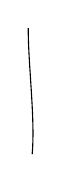
\begin{tikzpicture}[x=1cm,y=1cm,baseline=(current bounding box.south)]
\draw[line width=0.4pt] (0,0) .. controls (0.04,0.45) and (-0.05,1.12) .. (-0.05,1.60);
\end{tikzpicture}}

We assume the outer action \uline{faithful},
i.e. $G\subset\widehat{\widehat{\mathcal T}}(\pi)
=\widehat{\widehat{\mathcal T}}$,
\inserted{and that $G=G^+$.}
We assume moreover that there exists an invariant
discretification $\pi_0$, i.e. such that
$G\subset\mathcal T(\pi_0)$.

If we assume $G$ cyclic, then unless
I am mistaken it is proved that the situation is
\uline{realizable} topologically (\unsure{thus}:
\uline{\unsure{algebraically}} in a complex analytic way $\ldots$).

\scanpage{392}
In the discrete case, the meaning of the
\inserted{$\pi_0$-}conjugacy classes of lifting
$G\longrightarrow\mathcal G(\pi_0)$ is well understood;
\deleted{But}\inserted{likewise for the partial liftings}
We find a \deleted{\unsure{category} $U^{!}$} \inserted{canonical}
realization of the fundamental groupoid
\margin{if $U^{!}\ne\unsure{\varnothing|\phi}$}
associated to the
outer group $\pi_0$, by a \inserted{finite} groupoid $[U^{!}]$
on which $G$ operates in the strict sense, whose points
correspond to the $\pi_0$-conjugacy classes of
maximal partial sections $\ne1$, the group
\deleted{\illegible{1}}$\mathcal T(\pi_0)^G$
operates in an \unsure{equally} canonical way on this groupoid.
If $P\in U^{!}$ corresponds to a lifting
$G\longrightarrow\mathcal G(\pi_0)$, then
an element $\deleted{\unsure{g}}\inserted{\dot u}\in
\mathcal T(\pi_0)^G$ is in the image of
$\mathcal G(\pi_0)^G$, i.e. can be lifted to
$u\in\mathcal G(\pi_0)$ commuting with $G$, iff
$\dot u(P)=P$ [i.e. iff
\inserted{(if $\dot u$ is lifted in an \unsure{arbitrary} way to $v$)}
$v(G)$ is $\pi_0$-conjugate to $G$
i.e. iff $\exists g\in\pi_0$ such that
$v(G)=\operatorname{int}(g)(G)$
i.e. \deleted{\unsure{which}}
$u\overset{\text{definition}}{=}\operatorname{int}(g^{-1})v$ fixes $G$.
\deleted{\unsure{(Thus}} (in which case of course it centralizes,
\inserted{(by the hypothesis $\dot u\in\mathcal T^{G}$)})
Thus our brilliant assertion, is a tautology]

\scanpage{393}
\mspage{199}
and hence the lifting is unique. As
$U^{!}_{\unsure{*|\varphi}}$ is finite, hence the stabilizer
$\mathcal T(\pi_0)^G_P$ of $P$ in
$\mathcal T(\pi_0)^G$ has finite index,
and so it is this subgroup of finite index that lifts
merrily and canonically.

What can one say in the profinite context? Of course,
we have a canonical map
\diagram{\begin{tikzcd}[ampersand replacement=\&,column sep=large]
\begin{gathered}
\text{\deleted{\unsure{Set}} classes of $\pi_0$-conjugacy}\\
\text{of liftings of}\\
G\text{ into }G
\longrightarrow\mathcal G(\pi_0)\\
\text{i.e. of splittings of}\\
\text{the extension }1\longrightarrow\pi_0\longrightarrow
E\longrightarrow G\longrightarrow1
\end{gathered}
\arrow[r] \&
\begin{gathered}
\text{classes of $\pi_0$-}\\
\text{conjugacy of liftings of}\\
G\text{ into }G
\longrightarrow\widehat{\widehat{\mathcal G}}(\pi_0)\\
\text{i.e. of splittings}\\
\text{of the extension}\\
1\longrightarrow\underset{\substack{\Vert\\\pi}}{\widehat{\pi}_0}
\longrightarrow\widehat E
\longrightarrow G\longrightarrow1
\end{gathered}
\end{tikzcd}}

We should first examine

a) The question of the bijectivity of this map.

b) The question whether $\pi^G=1$ (\unsure{\uline{rigidity}|rigidity}),
for $G\ne(1)$. -- (for a given lifting,
in $E$ for simplicity)

I feel like conjecturing shamelessly
that this is so --- which would imply
for example that for every such lifting $G$, there is

\scanpage{394}

an \uline{open} subgroup \inserted{$(\unsure{\widehat{\widehat{\mathcal T}}|\widehat{\mathcal T}}^{G})_{P}$} of the group (perhaps really immense a priori!) $\widehat{\widehat{\mathcal T}}^{G}$, which lifts canonically so as to commute with \unsure{$\widetilde G$|$G$}....

We should clearly develop, at the same time as a theory of outer operations of finite groups on discrete groups with loops (which for the moment is extremely \unsure{conjectural|conjectural}) an analogous theory in the profinite case --- I \deleted{\illegible{1}}\inserted{will have} probably to come back to it later on.

\scanpage{395}
\mspage{200}

\uline{32} Return to the arithmetic aspects of plugging holes: relations between $\Gamma_{g,\nu}$ and $\Gamma_{g,\nu-1}$.

Of course, we \deleted{\unsure{see that}} have that
\[
\mathcal N_{g,\nu}\longrightarrow\mathfrak S_{\nu}
\]
is surjective \inserted{(since $\mathcal T_{g,\nu}\longrightarrow\mathfrak S_{\nu}$ is)}, hence we will have
\[
(1)\qquad 1\unsure{\longrightarrow|-}\mathcal N_{g,\nu}^{!}\unsure{\longrightarrow|-}\mathcal N_{g,\nu}\unsure{\longrightarrow|-}\mathfrak S_{\nu}\unsure{\longrightarrow|-}1
\]
and the Cartesian diagram of \unsure{subgroups} of $\widehat{\widehat{\mathcal T}}_{g,\nu}$
\[
(2)\qquad
\diagram{\begin{tikzcd}[ampersand replacement=\&]
\widehat{\mathcal T}_{g,\nu}^{+}\arrow[r,hook] \& \mathcal N_{g,\nu}\\
\widehat{\mathcal T}_{g,\nu}^{!+}\arrow[u,hook]\arrow[r,hook] \& \mathcal N_{g,\nu}^{!}\arrow[u,hook]
\end{tikzcd}}
\]
\margin{\deleted{\illegible{1}} $\mathcal N_{g,\nu}=\mathcal N_{g,\nu}^{!}\cdot\widehat{\mathcal T}_{g,\nu}^{+}$ i.e. $\mathcal N_{g,\nu}$ known from $\mathcal N_{g,\nu}^{!}$}
will give an isomorphism
\[
(3)\qquad \mathcal N_{g,\nu}^{!}/\widehat{\mathcal T}_{g,\nu}^{!+}\xrightarrow{\sim}\mathcal N_{g,\nu}/\widehat{\mathcal T}_{g,\nu}^{+}=\mathbb{\Gamma}_{g,\nu}
\]
In the case of a $(\pi,a)$, \inserted{($\pi$ an outer group with loops,} $a$ an arithmetization), we will likewise have
\[
(4)\qquad\left\{\begin{aligned}
\mathcal N_a^{!}/\widehat{\mathcal T}_a^{+}&\simeq\mathcal N_a/\widehat{\mathcal T}_a^{+}=\mathbb{\Gamma}_a.\\
\mathcal N_a&=\mathcal N_a^{!}\widehat{\mathcal T}_a^{+}
\end{aligned}\right.
\]

Let us now consider \deleted{a \unsure{subset}\inserted{\unsure{$i\in I=I(\pi)$}} , \illegible{3} $\unsure{(g,\nu)}$, \unsure{and a} $\pi_i'$ \illegible{2} $\unsure{I=I(\pi)}$, and let \illegible{1}} for $\forall i\in I$ the stabilizer \deleted{\illegible{1}} $\mathcal N_i$ of $i$ in $\mathcal N$, and the group \deleted{outer} \inserted{with loops (not outer!)} $\pi_i'$ of type $g,\nu-1$, deduced from $\pi$ by ``plugging hole $i$'',
\margin{We write $\mathcal N$ etc. instead of $\mathcal N_a$. We assume \illegible{2} $(g,\nu-1)$, i.e. \unsure{$2g-2+\nu$} \illegible{1} \unsure{$\geq1$}, i.e. $2g+\nu\geq4$}

\scanpage{396}

we then have, for a chosen discretification, \deleted{\unsure{a}} \inserted{$\alpha$} compatible with the arithmetization, an injective \unsure{homomorphism|homomorphism}
\[
(5)\qquad \pi_i'\xrightarrow{\varphi_i}\widehat{\mathcal T}_{\unsure{i|a}}^{+!}\subset\mathcal N_{\unsure{i|a}}^{!}\subset\widehat{\widehat{\mathcal T}}_i
\]

\deleted{We \unsure{cannot|can only} \illegible{2}}
\deleted{We will have}
\deleted{\unsure{which lifts the composite}}
\deleted{\textcircled{\unsure{e|c}} The image of $\pi'$}
such that the composite
\[
\diagram{\begin{tikzcd}[ampersand replacement=\&]
\pi_i'\arrow[r] \& \widehat{\widehat{\mathcal T}}_i\arrow[r] \& \widehat{\widehat{\mathcal G}}(\pi_i')\\
\&\& \pi_i'\arrow[u,hook]
\end{tikzcd}}
\]
is the canonical inclusion. This being so, we want\margin{rather: \uline{it is true that!}} the image of (5) (which may not be invariant in $\widehat{\widehat{\mathcal T}}_i$) to be \uline{invariant in \deleted{$\mathcal T$} $\mathcal N_i$}, or what amounts to the same, in $\mathcal N^{!}$ (for $\mathcal N_i=\mathcal N^{!}\cdot\widehat{\mathcal T}_i^{+}$ and $\widehat{\mathcal T}_i^{+}$ leaves this image invariant). \deleted{\illegible{1}} Returning to the universal situation, this \unsure{\uline{means}|means}
\margin{This also means that $\varphi_i$ \unsure{does not depend} on the choice of the discretification \unsure{with datum} $\alpha$...}

\textcircled{\unsure{e|c}} $\mathcal N_{g,\nu}^{!}\subset\widehat{\widehat{\mathcal T}}_{g,\nu}$ is contained in the normalizer of the $\pi_i'\hookrightarrow\widehat{\mathcal T}_{g,\nu}^{!+}$ $(0\leq i\leq\nu-1)$ \inserted{which are therefore invariant in $\mathcal N_{g,\nu}^{!}$} \deleted{\unsure{if} $(g,\nu-1)$ \unsure{is also anabelian}}.

Moreover $\widehat{\widehat{\mathcal T}}_{g,\nu}^{!}\xrightarrow{\psi_i}\widehat{\widehat{\mathcal G}}_{g,\nu-1}^{!}$ induces an \deleted{\illegible{1}} \uuline{\unsure{isomorphism|isomorphism}}
\[
(6)\qquad\mathcal N_{g,\nu}^{!}\xrightarrow{\sim}\mathcal M_{g,\nu-1}^{!}
\]
\margin{\uline{N.B.} It suffices \unsure{it seems to me} to prove it \unsure{for one $i$} to deduce it for the others \deleted{\illegible{1}}}
\margin{\uline{N.B.} \illegible{4}}

\scanpage{397}
\mspage{201}

This assertion breaks up into two: first \unsure{then|of all} that $\psi_i$ does indeed map $\mathcal N_{g,\nu}^{!}$ into $\mathcal M_{g,\nu-1}^{!}$ -- and this follows from the \unsure{arithmetico-geometric} definition of these groups -- this implies on the other hand, since $\psi_i$ also induces an \inserted{\unsure{isomorphism}} \deleted{\illegible{1}}
\[
\widehat{\mathcal T}_{g,\nu}^{+}
\xrightarrow{\sim}
\widehat{\mathcal G}_{g,\nu-1}^{+},
\]
that it induces a homomorphism
\[
(7)\qquad
\begin{array}{ccc}
\mathbb{\Gamma}_{g,\nu}
&\xrightarrow{\substack{\inserted{\lambda_i}\\\deleted{\unsure{\psi_i}}}}&
\mathbb{\Gamma}_{g,\nu-1}\\
\wr\vert&&\wr\vert\\
\mathcal N_{g,\nu}/\widehat{\mathcal T}_{g,\nu}^{+}
&&\mathcal M_{g,\nu-1}/\unsure{\widehat{\mathcal G}}
\end{array}
\]
\deleted{and by \unsure{arithmetic} means}
and the injectivity (resp. \deleted{b}\unsure{surjectivity}) of (6) is equivalent to that of (7). Moreover (7) fits, by construction, into a commutative diagram

(8)\quad\diagram{\begin{tikzcd}[ampersand replacement=\&,column sep=large,row sep=large]
\& \mathbb{\Gamma}_{\mathbb Q}
  \arrow[dl,"\Theta_{g,\nu}"']
  \arrow[dr,"\Theta_{g,\nu-1}"] \& \\
\mathbb{\Gamma}_{g,\nu} \arrow[rr]
\&\&\mathbb{\Gamma}_{g,\nu-1}
\end{tikzcd}}

with $\Theta_{g,\nu}$ and $\Theta_{g,\nu-1}$ surjective, so it is indeed quite obvious that (6) is \uline{surjective}. Bijectivity \unsure{\uline{means}|means} that $\Theta_{g,\nu}$ and $\Theta_{g,\nu-1}$ have the same kernel (whereas a priori it could be that $\Theta_{g,\nu}$ has a smaller kernel i.e. corresponds to a representation of $\mathbb{\Gamma}_{\mathbb Q}$ ``less unfaithful'' than $\Theta_{g,\nu-1}$. Moreover,

\scanpage{398}

it is obvious \deleted{that} (\unsure{even}, a priori, without using the definition \inserted{elsewhere} \unsure{explicit|made explicit} of the $\mathcal N_{g,\nu}$) that the homomorphism $\deleted{\unsure{\psi_i}}\inserted{\unsure{\lambda_i}}$ \inserted{\unsure{(7)}} does not depend on the choice of $0\leq i\leq\nu-1$ -- for example since we pass from one to the other by applying operations of $\widehat{\mathcal T}^{+}$ (since $\widehat{\mathcal T}^{+}$ operates \unsure{transitively} on $I$) and $\widehat{\mathcal T}^{+}$ operates \unsure{trivially|trivially} on $\mathbb{\Gamma}_{g,\nu}$ ...

We can say that (6) describes $\mathcal M_{g,\nu-1}^{!}$ (hence $\mathcal N_{g,\nu-1}^{!}$) in terms of $\mathcal N_{g,\nu}$ -- but the reverse is less clear, for lack of knowing whether
\[
\unsure{\widehat{\widehat{\mathcal T}}_{g,\nu}^{!}}
\xrightarrow{\psi_i}
\widehat{\widehat{\mathcal G}}_{g,\nu-1}
\]
is injective; if we knew this, we could describe $\mathcal N_{g,\nu}^{!}$ as the inverse image of $\mathcal M_{g,\nu-1}^{!}$ ... \deleted{\unsure{Then}} It would not be impossible moreover that (f) should be false, i.e. that \inserted{the} $\Theta_{g,\nu}$ should be unfaithful, but less and less so as we increase $\nu$ -- in passing to the \inserted{\unsure{projective}} limit $\Theta_{g,\infty}$, \unsure{only}, would we have

\scanpage{399}
\mspage{202}

(perhaps!) a faithful representation of $\mathbb{\Gamma}_{\mathbb Q}$. But until an indication to the contrary, I prefer to work hypothetically with (f), which is expressed by the fundamental \unsure{exact|exact} sequences
\[
(9)\qquad
1\longrightarrow\widehat{\pi}_{g,\nu-1}
\xrightarrow{\varphi_i}
\unsure{\mathcal N_{g,\nu}^{!}|\mathcal M_{g,\nu}^{!}}
\unsure{\overset{\psi_i'}{\longleftrightarrow}|\xrightarrow{\psi_i'}}
\unsure{\mathcal N_{g,\nu-1}^{!}|\mathcal M_{g,\nu-1}^{!}}
\longrightarrow1
\]
\margin{\unsure{\&} we could include it in a slightly larger \unsure{exact} sequence, with $(\mathcal N_{g,\nu})_i$ and $\mathcal N_{g,\nu-1}$ ...}
which extends the \unsure{exact|exact} sequence
\[
(10)\qquad
1\longrightarrow\widehat{\pi}_{g,\nu-1}
\xrightarrow{\varphi_i}
\widehat{\mathcal T}_{g,\nu}^{!}
\xrightarrow{\psi_i'}
\widehat{\mathcal T}_{g,\nu-1}^{!}
\longrightarrow1
\]
(and takes the place of the perhaps failing \unsure{exact|exact} sequence
\[
??\qquad
1\longrightarrow\widehat{\pi}_{g,\nu-1}
\longrightarrow\widehat{\widehat{\mathcal T}}_{g,\nu}^{!}
\longrightarrow\widehat{\widehat{\mathcal T}}_{g,\nu-1}^{!}
\longrightarrow1
\qquad??
\]
)

When $(\pi,a)$ is an outer group with loops equipped with an arithmetization -- what one could call a ``virtual algebraic curve'' -- then what precedes allows us to define, on \inserted{each} of the $\pi_i'$ of type $(g,\nu-1)$ associated to the $i\in I(\pi)$, \unsure{an} arithmetization canonically associated to $a$, say $\unsure{a'}$,

\scanpage{400}

and we find \unsure{then|thus} an \unsure{exact|exact} sequence
\[
1 \longrightarrow \pi'_i \longrightarrow (\mathcal{N}_a)_i
\xrightarrow{\psi_i} \mathcal{N}_{a'_i} \longrightarrow 1
\tag{11}
\]
such that we have
\[
(\widehat{\mathcal{T}}^{+}_a)_i
=\psi_i^{-1}(\widehat{\mathcal{T}}^{+}_{a'_i}),
\tag{12}
\]
\[
\downarrow
\]
inducing

\diagram{\begin{tikzcd}[ampersand replacement=\&,column sep=1.9em,row sep=1.8em]
(11') \& 1 \arrow[r,dash] \& \pi'_i \arrow[r,dash] \& \mathcal N_{\unsure{a}}^{!} \arrow[r,dash,"\psi_i^{!}"] \arrow[d,phantom,"\cup" description] \& \mathcal N_{a'_i}^{!} \arrow[r,dash] \arrow[d,phantom,"\cup" description] \& 1 \\
\& \& \& \widehat{\mathcal T}_{a}^{+!} \arrow[d,phantom,"\Vert" description] \& \widehat{\mathcal T}_{a'_i}^{+!} \& \\
\& \& \& \psi_i^{\unsure{\prime}-1}\bigl(\widehat{\mathcal T}_{a_i}^{+!} \& \&
\end{tikzcd}}

and inducing by passage to the quotients
\[
\mathbb{\Gamma}_a\xrightarrow{\sim}
\mathbb{\Gamma}_{\unsure{a_i}}
\tag{13}
\]
Moreover, \uline{\unsure{the map}} which is canonical
\[
\unsure{\mathrm{Discrt}|\mathrm{Discr}}^{+}(\pi)\longrightarrow
\unsure{\mathrm{Discrt}|\mathrm{Discr}}^{+}(\pi'_i)
\]
defines by passage to the quotients
\[
\mathbb{P}_a\xrightarrow{\sim}\mathbb{P}_{\unsure{a_i}}
\tag{14}
\]
compatible with the actions of $\mathbb{\Gamma}_a$,
$\mathbb{\Gamma}_{a'_i}$ and (13).

I make \inserted{here} no assertion about
a \unsure{so-called|so-called} bijectivity between
set of arithmetizations of $\pi$, and \unsure{set} of

\subsection*{Scans 401--410}
\addcontentsline{toc}{subsection}{Scans 401--410}
% package LM_P041
\scanpage{401}
\mspage{203}

\unsure{arithmetizations|arithmetization} of $\pi'_i$ --- which
would amount to the bijectivity of
\[
\widehat{\widehat{\mathcal T}}/\mathcal N_a
\longrightarrow
\widehat{\widehat{\mathcal G}}'/\unsure{M_{a'}^{\natural}|M_{a'}^{\sharp}}
\simeq \widehat{\widehat{\mathcal T}}'/\mathcal N_{a'},
\]
which \inserted{would} hardly have any reason to be except if
one admitted
$\widehat{\widehat{\mathcal T}}(\pi)\xrightarrow{\sim}\unsure{\widehat{\widehat{\mathcal G}}|\widehat{\mathcal G}}(\pi'_i)$,
which seems quite problematic to me.

\margin{\figure{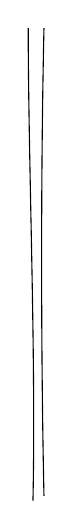
\begin{tikzpicture}[x=1cm,y=1cm,baseline=(current bounding box.north)]
\draw[line width=0.4pt] (0,0) .. controls (0.04,1.85) and (-0.06,4.30) .. (-0.06,6.00);
\draw[line width=0.4pt] (0.14,0.06) .. controls (0.10,1.90) and (0.10,4.25) .. (0.14,6.00);
\end{tikzpicture}}}
However, one finds, by the
``plugging the holes'' functor, an equivalence
between the category of \deleted{\unsure{algebraic curves}}
\uuline{outer} \uline{arithmetized} profinite groups with loops,
\inserted{of type $(g,\nu)$,}
and of \uline{arithmetized} profinite groups with loops
(not outer!), of type
$(g,\nu-1)$.

One can propose to try to
specify \deleted{\unsure{by}} the type of properties
which will characterize $\mathcal N_{g,\nu}$ in $\mathcal N'_{g,\nu}=$
$\operatorname{Norm}_{\widehat{\widehat{\mathcal T}}_{g,\nu}}
(\widehat{\mathcal T}_{g,\nu}^{+})$,
\deleted{I \unsure{think} that it}
\inserted{\deleted{\unsure{We shall have}}or again}
$\mathbb{\Gamma}_{g,\nu}$
\deleted{\unsure{for} \illegible{1} $\Gamma'$}
in $\mathbb{\Gamma}'_{g,\nu}=\mathcal N'_{g,\nu}/\widehat{\mathcal T}_{g,\nu}^{+}$.
We have natural homomorphisms

\margin{400}

\scanpage{402}

\[
\tag{15}
\left|
\begin{aligned}
\mathbb{\Gamma}'_{g,\nu}&\longrightarrow\operatorname{Autext}(\widehat{\mathcal T}_{g,\nu}^{+})\\
\mathbb{\Gamma}'_{g,\nu}&\longrightarrow\operatorname{Aut\,ext}(\widehat{\mathcal T}_{g,\nu}^{+!})
\end{aligned}
\right.
\]
and I presume that \deleted{it is a matter} $\mathbb{\Gamma}_{g,\nu}$ will
be describable as the inverse image of a
suitable closed subgroup of one
or the other of the right-hand sides, i.e. that one
can describe it in terms \unsure{of the|of} properties
of outer operations on $\widehat{\mathcal T}_{g,\nu}^{+}$ or
on $\widehat{\mathcal T}_{g,\nu}$. The conditions \textcircled{e} in any
case are indeed of this type (\unsure{property|properties}
of normalizing \unsure{invariant|inscribed} \unsure{subgroups}
\deleted{$\unsure{\mathcal T'_i}$} $\pi'_i$ of $\mathcal T_{g,\nu}^{+!}$ ...).
Of course, one
could impose conditions on outer
\unsure{automorphisms} (of $\widehat{\mathcal T}'{}_{g,\nu}^{+!}$, say),
which are stable under \inserted{successive} passage to
$\widehat{\mathcal T}'{}_{g,\nu-1}^{+!}$, $\widehat{\mathcal T}'{}_{g,\unsure{\nu-2}}^{+!}$ etc ... and
\deleted{for which}\inserted{which are}
generated by the conditions \textcircled{e}. But
it is not at all certain that this

\margin{401}

\scanpage{403}
\mspage{204}

\unsure{will suffice|suffices} to describe the \deleted{$\unsure{\mathcal N_{g,\nu}}$}
$\mathbb{\Gamma}_{g,\nu}\subset\Gamma'_{g,\nu}$,
if only because the condition
becomes vacuous for \deleted{$\unsure{\nu=0}$} the limiting case $\nu=0$
(if $g\geq2$; or for the cases $g=1$, $\nu=1$, or $g=0$, $\nu=3$).

It is possible that one will have to
bring in properties of the $\pi_1$ of
the $\unsure{M_{g,\nu\,\overline{\mathbb Q}_a}}$, linked to the compactification.
It is practically only in the case of
$(g,\nu)=(0,3)$ that one should not expect
conditions of this kind at all.

Let us call ``\unsure{potential algebraic curve|potential algebraic curves}''
(understood, over an unspecified algebraic closure of $\mathbb Q$,)
the datum of \unsure{a|a} \inserted{profinite outer \unsure{group}}
$\pi$ with \unsure{loops|loop} \deleted{profinite}\inserted{\deleted{outer}}
of type $(g,\nu)$, equipped with an arithmetization
$a$, and with a germ of
``admissible'' liftings
\margin{\deleted{\illegible{1}}}
\[
\tag{16}
\mathbb{\Gamma}_{\unsure{a|\bullet}}^{\natural}
\longrightarrow\mathcal N_a.
\]
They form a category (for
isomorphisms, for the moment) If one gives oneself
a torsor $P$ under $\mathbb{\Gamma}_{g,\nu}$
(which \inserted{\unsure{trivially|morally}} amounts to giving oneself an algebraic

\margin{402}

\scanpage{404}
closure $\overline{\mathbb Q}$ of $\mathbb Q$ \ldots) the potential curves
of type $(g,\nu)$ \uline{\unsure{relative|relative}} to this torsor
(\unsure{morally|morally}, \unsure{corresponding|correspond} to algebraic
curves over $\overline{\mathbb Q}$ \ldots) are \inserted{those} equipped in
addition with an \unsure{isomorphism} (``inner'')
\[
(17)\qquad \mathbb P_a\xrightarrow{\sim}P
\]
(defining an isomorphism
\[
(18)\qquad \mathbb{\Gamma}_a\longrightarrow\Gamma_P
 =\operatorname{Aut}_{\mathbb{\Gamma}_{g,\nu}}(P).
\]
\margin{The case where $P$ is the
trivial torsor, is that of the \deleted{\unsure{curves}} outer $\pi$ \unsure{(?)|(18)}
equipped with an oriented \uline{prediscretification} $\alpha$
(whence an \deleted{\illegible{1}} exact \unsure{sequence}
$1\longrightarrow\widehat{\mathcal T}_\alpha\longrightarrow
\mathcal N_\alpha\longrightarrow\mathbb{\Gamma}_\alpha\longrightarrow1$)}

This time, one expects to find
\uline{finite} \unsure{sets} of isomorphisms, instead of
torsors under considerable profinite
groups.

We consider the \deleted{\unsure{P}} \uline{Points} of $\pi$,
as the \inserted{$\pi$-}conjugacy classes
of ``admissible'' \unsure{liftings} of (16),
\unsure{into|or}
\[
(19)\qquad\mathbb{\Gamma}_{\unsure{a|\bullet}}^{\natural}\longrightarrow
\mathcal M_a\subset\widehat{\widehat{\mathcal T}}(\pi)
\]
i.e. a germ of genuine action of $\mathbb{\Gamma}_{\bullet}$
on $\pi$, with
\margin{(20)}
\figure{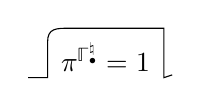
\begin{tikzpicture}[baseline=(eq.base)]
\node[inner sep=0pt,outer sep=0pt] (eq) {$\pi^{\mathbb{\Gamma}_{\bullet}^{\natural}}=1$};
\draw[line width=0.4pt]
([xshift=-12pt,yshift=-2pt]eq.south west)
-- ([xshift=-5pt,yshift=-2pt]eq.south west)
-- ([xshift=-5pt]eq.north west)
.. controls ([xshift=-5pt,yshift=5pt]eq.north west) and ([xshift=-2pt,yshift=5pt]eq.north west) .. ([xshift=3pt,yshift=5pt]eq.north west)
-- ([xshift=5pt,yshift=5pt]eq.north east)
-- ([xshift=5pt,yshift=-2pt]eq.south east)
-- ([xshift=8pt,yshift=-1pt]eq.south east);
\end{tikzpicture}}
(this for \deleted{\unsure{the ad}}
\margin{403}

\scanpage{405}
\mspage{205}
admissibility.

\uline{Preliminary question} Knowledge of
$\pi$, of $\underbrace{\widehat{\mathcal T}_a^+}_{\Sigma_a}
\subset\widehat{\widehat{\mathcal T}}(\pi)$, and \unsure{of a} subgroup
$\Gamma'\subset\widehat{\widehat{\mathcal T}}(\pi)$
(normalizing $\Sigma_a$, \inserted{such that
$\Gamma'\cap\unsure{\Sigma_a|\Sigma_{\bullet}}=(1)$})
\unsure{would it make it possible} to recover the \unsure{arithmetization|arithmetization} of $\pi$
--- and, to begin with, to recover
$\mathcal N_a$ (in which $\Gamma'\cdot\Sigma$ is of finite
index)? \deleted{Is} It \unsure{would suffice|will suffice}, to be able to
answer in the affirmative, to know
that every outer \unsure{isomorphism} $\pi\longrightarrow\pi_{g,\nu}$,
which sends \inserted{$\Sigma$ onto $\widehat{\mathcal T}_{g,\nu}=\Sigma_{g,\nu}$, and}
\unsure{every|the} subgroup of finite
index $\Gamma'\cdot\Sigma$ in $\mathcal N_a$ into $\mathcal N_{g,\nu}$,
is compatible with the \unsure{arithmetizations|arithmetizations}.
Now this amounts \unsure{exactly|exactly} to:

\textcircled{g} (optional, all the same!)
\deleted{every} For every open
subgroup $\mathcal N'$ of $\mathcal N_{g,\nu}$,
the elements of $\widehat{\widehat{\mathcal T}}_{g,\nu}$
\inserted{normalizing $\widehat{\mathcal T}_{g,\nu}$ and}
which carry
$\mathcal N'$ into $\mathcal N_{g,\nu}$, \unsure{are} in $\mathcal N_{g,\nu}$
(\unsure{a fortiori},
$\mathcal N_{g,\nu}$ would be its own normalizer
in $\operatorname{Norm}_{\widehat{\widehat{\mathcal T}}_{g,\nu}}
(\widehat{\mathcal T}_{g,\nu})$.
\margin{404}

\scanpage{406}
With the ``points of $U$'' (defined as conjugacy \unsure{classes}
of ``admissible'' \unsure{liftings} (19)
i.e. satisfying (20), one
makes a groupoid, having
$\pi$ as its outer fundamental group, and on
which $\Gamma^{\unsure{\natural|\sharp}}\subset\mathcal N_a$ operates strictly
(\uline{N.B.} to take a rest, one now gives oneself
$\unsure{\Gamma^{\natural}|\Gamma}$ itself, not \unsure{only|only} a
germ --- \unsure{morally|morally}, this means
that one has a curve defined over a
finite subextension $K$ of $\overline{\mathbb Q}/\mathbb Q$ \ldots\unsure{\}|)}.
The fixed points of $\Gamma$ correspond
to the rational points/$K$, the fixed points under a
closed subgroup $\Gamma'$ to the points rational
over the subextension $K'$ of $\overline{\mathbb Q}/\mathbb Q$ associated
with $\Gamma'$ \ldots)
\margin{405}

\scanpage{407}
\mspage{206}

Now let
\figure{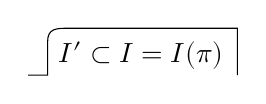
\begin{tikzpicture}[baseline=(eq.base)]
\node[inner sep=0pt,outer sep=0pt] (eq) {$I'\subset I=I(\pi)$};
\draw[line width=0.4pt]
([xshift=-11pt,yshift=-2pt]eq.south west)
-- ([xshift=-4pt,yshift=-2pt]eq.south west)
-- ([xshift=-4pt]eq.north west)
.. controls ([xshift=-4pt,yshift=5pt]eq.north west) and ([xshift=-1pt,yshift=5pt]eq.north west) .. ([xshift=4pt,yshift=5pt]eq.north west)
-- ([xshift=5pt,yshift=5pt]eq.north east)
-- ([xshift=5pt,yshift=-2pt]eq.south east);
\end{tikzpicture}}
be a
subset of $I$, stable under $\Gamma$. One finds
by ``plugging the holes at $I'$'' an
outer group with loops $\pi'$, \deleted{which} and an
outer homomorphism
\[
(20)\qquad \pi^{\unsure{\natural|\sharp}}\longrightarrow\pi'
\]
Besides, $\pi'$ inherits an arithmetization \inserted{$a'$}
from $\pi$ -- and we shall have
\[
(21)\qquad
\left\{
\begin{array}{ccc}
\mathbb{\Gamma}_a & \overset{\sim}{\longrightarrow} & \mathbb{\Gamma}_{a'} \\
\mathbb P_a & \overset{\sim}{\longrightarrow} & \mathbb P_{a'} \\
\unsure{\wr} & & \\
P & &
\end{array}
\right.
\quad\unsure{\leadsto}
\]
so $\pi'$ is defined over \unsure{the|the} same $P$ as
$\mathbb{\Gamma}_a$
(i.e. by making holes in $U$ to
find $U'$, we have not disturbed the
algebraically \unsure{closed|absolute} base field $\overline{\mathbb Q}\ldots$). Besides
we shall have a canonical homomorphism
\[
\widehat{\mathcal T}(\pi)\longrightarrow
\widehat{\mathcal T}(\pi')
\]
inducing
\[
(22)\qquad
\]
\diagram{\begin{tikzcd}[ampersand replacement=\&,column sep=3.2em,row sep=1.8em]
\mathcal N_a \arrow[r] \arrow[d,phantom,"\cup" description] \& \mathcal N_{a'} \arrow[d,phantom,"\cup" description] \\
\widehat{\mathcal T}_a \arrow[r,dash] \& \widehat{\mathcal T}_{a'}
\end{tikzcd}}

\margin{406}

\scanpage{408}

(inducing precisely $\mathbb{\Gamma}_a\longrightarrow\mathbb{\Gamma}_{a'}$ on passing
to the quotients), and one finds, on
composing
\[
\Gamma\;\unsure{\subset|\hookrightarrow}\;\mathcal N_a\longrightarrow\mathcal N_{a'}
\]
a homomorphism which is \unsure{also|also} injective
\[
(23)\qquad\Gamma\hookrightarrow\mathcal N_{a'}
\]
which is a \unsure{quasi-section|quasi section} of $\mathcal N_{a'}$ over $\mathbb{\Gamma}_{a'}$,
So \deleted{\unsure{that|by}}\inserted{under} the proviso of admissibility,
one finds on \deleted{\illegible{1}} $\unsure{\pi'|\pi}$ a structure
of potential algebraic curve, relative
to the same $P$.

\deleted{Admissibility is expressed
\unsure{perhaps by} the condition
\[
(24)\qquad {\pi'}^{\Gamma}=(1)
\]
-- and if need be, we shall put these
conditions (for \unsure{every|$\forall$} $I'\subset I$) into
the definition of the admissibility of}

\deleted{\illegible{1} \unsure{I}} I am really feeling
cramped, for lack of a
definition in due form of ``admissible'' --

\margin{407}

\scanpage{409}
\mspage{207}

I am going to come back to this very soon --- but
for the moment, I feel like noting that,
\deleted{from the fact that $\Gamma$ \unsure{operated} \unsure{trivially}}
\inserted{if $I'\neq\varnothing$,}
the outer group $\pi'$ can be described by
a \inserted{genuine} groupoid, having $I'$ as its set
of objects, and on which $\Gamma$ operates in
the strict sense (this is pure algebra,
independently of the arithmetization business\ldots)
The fact that $\Gamma$ operates \unsure{trivially}
on the $i'\in I'$ implies that for \unsure{every|$\forall$}
$i'\in I'$, we have a \deleted{\unsure{lifting of}}
canonical \unsure{homomorphism}
\[
(24)\qquad \Gamma\longrightarrow\pi'(i')
\]
which lifts its \unsure{outer|outer} action, whence
a \unsure{unique} \inserted{$\pi'$-}conjugacy class of liftings
of the outer action of $\Gamma$ on $\pi'$
to a genuine action of $\Gamma$ on $\pi'$
--- one hopes that it satisfies ${\pi'}^{\Gamma}=1$ ---
and one thus has a canonical map
\[
(25)\qquad I'\longrightarrow\mathrm{Pts}(\pi',\alpha',\Gamma)
\]

\margin{408}

\scanpage{410}

I \uline{say that this map is injective}

This is ``obvious'' when one interprets
``admissible outer action'' as ``realizable
by a genuine algebraic curve'', and
``admissible liftings'' as ``realizable
by genuine rational points / \unsure{$K^+$|$K$}, field of
the \unsure{fixed elements|invariants} of $\Gamma$''. But one would
of course like reasons internal to
the datum of the $(\mathcal N_{g,\nu})$, and \unsure{)}
properties of these data! \deleted{\unsure{And}}

\margin{We \unsure{are reduced|are going to come back} to the case Cardinality $I'=2$\ldots}

This point being admitted (putting
in parentheses the two \unsure{possible|essential}
definitions of admissibility, to which
we shall come back below) one finds
a ``plugging holes'' functor
\diagram{\begin{tikzcd}[ampersand replacement=\&,column sep=large]
\begin{gathered}
\text{Algebraic curves}\\
\text{potential over }P,\ \text{\unsure{\deleted{relative}|relative}}\\
\text{to an open subgroup}\\
\text{\deleted{\unsure{of a set}}}\\
\Gamma\text{ of }\mathbb{\Gamma}_P,\ \text{and equipped with a}\\
\text{set }I'\text{ of points at }\infty
\end{gathered}
\arrow[r]
\&
\begin{gathered}
\text{Algebraic curves}\\
\text{potential over }P\text{ relative}\\
\text{to }\Gamma,\ \text{equipped}\\
\text{with a subset}\\
\text{of the set of}\\
\text{``Points \unsure{rational|invariant}/}\Gamma\text{''}
\end{gathered}
\end{tikzcd}}

\margin{for this one needs the usual
anabelian restrictions}

\margin{409}

\subsection*{Scans 411--420}
\addcontentsline{toc}{subsection}{Scans 411--420}
% package LM_P042
\scanpage{411}
\mspage{208}

and unless I am mistaken, it has become obvious
that this functor is an \uline{equivalence of
categories} (and as a consequence, there
\margin{\unsure{for the} \uline{\unsure{isomorphisms}}}
is the functor in the opposite direction :
drill holes at ``points'' invariant
under $\Gamma_{\unsure{a|0}}$ (or at arbitrary points,
at the cost of passing to a smaller $\Gamma'$).

But I realize that
\deleted{\illegible{1}} this is not at all obvious -- I am going
to try to elucidate the situation axiomatically.
We have fixed a genus $g$,
we suppose given, for varying $\nu$
(such that $(g,\nu)$ anabelian) closed
subgroups $N_{g,\nu}\subset\widehat{\widehat{\mathcal T}}_{g,\nu}$,
normalizing $\widehat{\mathcal T}_{g,\nu}$, and satisfying the
essential condition that the $\psi_i:\widehat{\widehat{\mathcal T}}_{g,\nu}\longrightarrow\widehat{\widehat{\unsure{\mathcal G|\mathcal S}}}_{g,\nu-1}$
induce
\[
M_{g,\nu}\xrightarrow{\sim}M_{g,\nu-1}
\]
Which makes it possible to define the notion
of arithmetization of a profinite $\pi$ of
anabelian type $(g,\nu)$, and the theory of

\scanpage{412}

plugging an arbitrary number of holes, and
of drilling just 1 hole, in the
category of groups of type $g,\nu$,
arithmetized.

We suppose on the other hand \unsure{given|given} a
full subcategory of the category of profinite
\margin{\unsure{we suppose it} : stable under taking open subgroups.}
groups (which could reduce to the
open subgroups of $\mathbb{\Gamma}_g$, common
value of the $\mathbb{\Gamma}_{g,\nu}$ or of open subgroups
of the group $\mathbb{\Gamma}_a$, $a$ an
arithmetization), and \deleted{some} \inserted{a notion of }outer operations
\inserted{``admissible''} of such $\Gamma$ on the
arithmetized $\pi$. We suppose

\textcircled{1} If $\Gamma$ operates admissibly on $\pi$, every
open subgroup too (\deleted{\unsure{and}} and conversely ?)

\textcircled{2} If moreover $\Gamma$ leaves invariant a subset $I'$
of $I=I(\pi)$, then by ``plugging $I'$'',
the operation of $\Gamma$ on $\pi'$ is admissible.

\margin{It suffices to \unsure{postulate it|prove it} for $\operatorname{card} I'=1$, i.e. plugging \unsure{a|a single} hole -- \unsure{at least if we know that the admissibility condition depends only on the action of the kernels of the groups}.}

\deleted{\illegible{1}}
\deleted{\unsure{We propose to define a notion of admissible action} \illegible{2}}
\inserted{When we have an \inserted{\uline{actual}} action, \unsure{(not outer)|(non-outer)}}
of $\Gamma$ on a $(\pi,a)$, then the functor
\unsure{of} ``\deleted{plugging}\inserted{drilling} holes'' gives an outer
action on a $(\pi^0,a^0)$ of type $g,\nu+1$,
and we say that the starting action is

\scanpage{413}
\mspage{209}

admissible, if the \uline{outer} action deduced is.

We thus find an \uline{equivalence} between
the category of \deleted{\unsure{categories}} systems $(\pi,a,\Gamma,\psi,i)$
of a $(\pi,a)$ of type $(g,\nu+1)$, with an
admissible \inserted{\uline{outer}} operation $\psi$ of a $\Gamma$ on it, and
an $i\in I(\pi)$ stable under $\Gamma$, with the category
of $(\pi',a',\Gamma,\psi')$ of $(\pi',a')$ of type
$(g,\nu)$, with a \uline{genuine} admissible action $\psi'$
of $\Gamma$ on it.

\deleted{\unsure{We must} \illegible{3}}
\inserted{Condition (1) ensures that}
\deleted{\textcircled{3} \unsure{If a genuine action}}
\inserted{if $\Gamma$ operates \deleted{\uline{\unsure{genuinely}}} \deleted{\unsure{admissible|admissibly}} actually, in a way}
admissible, then the outer action deduced
is admissible (but the converse will
not be true -- there will be ``pathological''
liftings of a given admissible \unsure{categorical|outer} action\ldots). We suppose moreover

\margin{\figure{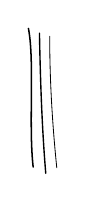
\begin{tikzpicture}[x=1cm,y=1cm,line cap=round,baseline=(current bounding box.center)]
\draw[line width=0.55pt] (0.04,1.80) .. controls (0.12,1.38) and (0.04,0.57) .. (0.10,0.04);
\draw[line width=0.50pt] (0.18,1.74) .. controls (0.19,1.20) and (0.21,0.55) .. (0.26,-0.04);
\draw[line width=0.30pt] (0.31,1.70) .. controls (0.31,1.09) and (0.35,0.52) .. (0.40,0.03);
\end{tikzpicture}}}
\textcircled{3} If $\Gamma$ operates \inserted{actually} in an admissible way on
$\pi$, then $\pi^\Gamma=(1)$.

\deleted{Let \unsure{Then}}
This implies that the category of
$\Gamma$-Points of $\pi$, or if you like of sections
of $B_{\pi,\Gamma}\,(\unsure{\simeq}B_u)$ over $B_\Gamma$, is \uline{rigid}.

\scanpage{414}

But \deleted{\unsure{let us call|let us suppose}} let us consider the inductive limit category of the \deleted{\illegible{1}} categories of sections of $B_{\pi,\Gamma}\simeq B_u$ over $B_{\Gamma'}$ ($\Gamma'$ an open subgroup), it is discrete and corresponds to the set
\[
\mathrm{Pt}_{\mathrm{ad}}(B_{\pi,\Gamma^{\natural}})\simeq
\underset{\substack{\Gamma'\ \mathrm{ouvert}\\\mathrm{de}\ \Gamma}}{\varinjlim}
\mathrm{Pt}_{\mathrm{ad}}(B_{\pi,\Gamma'}).
\]

\margin{\uline{N.B.} The groupoid with strict operators $\uline{\mathrm{Pt}}(B_{\pi,\Gamma})$ depends \unsure{functorially} on $(\pi,\Gamma)$, \illegible{1} for outer morphisms \deleted{\unsure{in}} \unsure{more} \illegible{3} of $\Gamma$, if \deleted{\illegible{4}}.}

\deleted{\textcircled{4} \unsure{For} \illegible{2} $\mathrm{Pt}(B_{\pi,\Gamma})$ \illegible{1}. On the other hand, $\pi$ can be defined by a groupoid.}
If $\mathrm{Pt}(B_{\pi,\Gamma})\ne\varnothing$, then (from the mere fact that $\pi^{\Gamma'}=(1)$ for $\forall$ open subgroup of $\unsure{\Gamma'|\Gamma}$) \inserted{the categorical group} $\pi$ can be described \unsure{canonically|commutatively} by a groupoid \inserted{profinite $\uline{\mathrm{Pt}}(B_{\pi,\Gamma^{\natural}})$} having $\mathrm{Pt}(B_{\pi,\Gamma})$ as object set, \deleted{\unsure{and|then}} \inserted{\unsure{linked|linked} by the categorical group $\pi$, on} which $\Gamma$ operates in the strict sense, with the stabilizer \inserted{$\Gamma_P$} of $\forall$ point being open. and $\Gamma_P\to\mathrm{Aut}(P)$ $(\simeq\pi\ \text{mod \unsure{inner automorphisms}})$

\deleted{More precisely, \unsure{independently of} the preceding axiomatics, we can describe the systems \unsure{formed} of a profinite group \inserted{categorical $\pi$}, and of an \inserted{outer} operation \unsure{of a profinite group} $\Gamma$ on it, \unsure{satisfying}}

being continuous. We have here \unsure{if} to $\forall\ P\in\mathrm{Pt}(B_{\pi,\Gamma})$ we associate the isomorphism class of \deleted{\unsure{groups of liftings}}

\scanpage{415}
\mspage{210}

\deleted{\unsure{groups}} of sections of $B_{\pi,\Gamma}$ over $B_\Gamma$, we find a bijection -- which characterizes the \inserted{$\Gamma$-}groupoid in question up to unique \uline{isomorphism}. We suppose

\textcircled{4} If $\Gamma$ operates admissibly on $(\pi,a)$, then there exists an open subgroup $\Gamma'$ of $\Gamma$ \deleted{can \unsure{operate in a way}} \inserted{whose \inserted{categorical} operation lifts to an} admissible actual operation -- i.e. $\mathrm{Pt}_{\mathrm{ad}}(B_{\Gamma,\pi})\ne\varnothing$.

\deleted{That said, let us consider \deleted{\illegible{1}} the situation of an admissible \inserted{outer} action of $\Gamma$ on $(\pi,a)$ and of an $i\in I(\pi)$ \deleted{stable} fixed under $\Gamma$. We thus have an \uline{actual} action \inserted{\unsure{admissible}} of $\Gamma$ on $(\pi',a')$, \deleted{and moreover we have} \inserted{thus an outer action,} plus a Point ``$\Gamma$-rational'', i.e. invariant under $\Gamma$. Let us consider on the other hand an admissible \unsure{lifting} $\Gamma\longrightarrow M(\pi,a)$, and \illegible{2}}

Let us note that in the situation envisaged, of plugging a hole $i\in I(\pi)$ of a $\pi$, in addition to the homomorphism
\[
\widehat{\widehat{\mathcal T}}(\pi)_i
\xrightarrow{\psi_i}
\widehat{\widehat{\unsure{\mathcal G|\mathcal S}}}(\pi'_i)
\]
associated, giving by composition
\[
\widehat{\widehat{\mathcal T}}(\pi)_i
\xrightarrow{\psi'_i}
\widehat{\widehat{\mathcal T}}(\pi'_i)
\]

\scanpage{416}

whence an outer action of $\widehat{\widehat{\mathcal T}}(\pi)$ on $\pi'_i$, \inserted{\unsure{in such a way} \unsure{that the} $\pi\overset{p_i}{\longrightarrow}\pi'_i$ \unsure{commute|commuting} with the outer actions of $\widehat{\widehat{\mathcal T}}(\pi)$, \deleted{\illegible{1}}} we have a canonical homomorphism of extensions, \deleted{associated} coming from this outer action and the homomorphism $p_i:\pi\longrightarrow\pi'_i$,

\diagram{\begin{tikzcd}[ampersand replacement=\&,column sep=2.4em,row sep=3.4em,
execute at end picture={
  \path (\tikzcdmatrixname-1-4.south west) -- (\tikzcdmatrixname-2-3.north east) coordinate[pos=.5] (lmfixnineteendiag);
  \draw[line width=.35pt] ([xshift=-5mm,yshift=1mm]lmfixnineteendiag) -- ([xshift=-6mm,yshift=1mm]lmfixnineteendiag) -- ([xshift=-6mm,yshift=-5mm]lmfixnineteendiag) -- ([xshift=-5mm,yshift=-5mm]lmfixnineteendiag);
  \draw[line width=.35pt] ([xshift=8mm,yshift=5mm]lmfixnineteendiag) -- ([xshift=9mm,yshift=5mm]lmfixnineteendiag) -- ([xshift=9mm,yshift=-1mm]lmfixnineteendiag) -- ([xshift=8mm,yshift=-1mm]lmfixnineteendiag);
}]
1 \arrow[r,dash] \& \pi \arrow[r,dash] \arrow[d,"p_i"] \&
\widehat{\widehat{\unsure{\mathcal G|\mathcal S}}}(\pi)_i \arrow[r] \arrow[d,"\varphi_i"] \&
\widehat{\widehat{\mathcal T}}(\pi)_i \arrow[r,dash] \arrow[d,"\psi'_i"] \arrow[dl,dashed,"\psi_i"'] \& 1 \\
1 \arrow[r,dash] \& \pi'_i \arrow[r] \&
\widehat{\widehat{\unsure{\mathcal G|\mathcal S}}}(\pi'_i) \arrow[r,dash] \&
\widehat{\widehat{\mathcal T}}(\pi'_i) \arrow[r,dash] \& 1
\end{tikzcd}}

which is not the \unsure{composite|composite}
\[
\widehat{\widehat{\unsure{\mathcal G|\mathcal S}}}(\pi)_i
\longrightarrow\widehat{\widehat{\mathcal T}}(\pi)_i
\xrightarrow{\psi_i}\widehat{\widehat{\unsure{\mathcal G|\mathcal S}}}(\pi'_i).
\]
(it can be defined whenever we have a group $\Gamma$, here $\widehat{\widehat{\mathcal T}}(\pi)$, which \deleted{\unsure{with trivial center}} \inserted{\unsure{commuting|commutes}} as outer actions on two outer groups $\pi,\pi'$, and we have a homomorphism \inserted{$\unsure{\beta|p}$} \deleted{\illegible{1}} $\pi\longrightarrow\pi'$ which commutes with the action of $\Gamma$, and such that the \inserted{center of $\pi$ and \unsure{the|the}} \unsure{centralizer|centralizers} of \unsure{its image|$\beta(\pi)$} in $\pi'$ are trivial\ldots)
\inserted{\unsure{This is also here} the ``transport of structure'' homomorphism}, \inserted{which} \unsure{for} \unsure{every|\deleted{every}} loop automorphism $u$ of $\pi$, associates the \unsure{corresponding|canonical} automorphism of $\pi'_i$.

We \unsure{have\deleted{vait}|\deleted{had}} forgotten to specify:

\textcircled{\unsure{g|9}} The canonical homomorphism $(\widehat{\widehat{\unsure{\mathcal G|\mathcal S}}}_{g,\nu})_i\longrightarrow\widehat{\widehat{\unsure{\mathcal G|\mathcal S}}}_{g,\nu-1}$ associated with $i\in[0,\nu-1]$, sends $(M_{g,\nu})_i$ into $M_{g,\nu-1}$ \deleted{into} so it fits into a \unsure{homomorphism|diagram} of exact sequences

\scanpage{417}
\mspage{211}

(26)
\diagram{
\begin{tikzcd}[ampersand replacement=\&]
1 \arrow[r,dash] \& \pi \arrow[r,dash] \arrow[d] \&
M_a(\pi)_i \arrow[r] \arrow[d, "\varphi_i"']
\arrow[dr, phantom, "{\text{\unsure{\uline{not}|\uline{not}} \unsure{commutative?}}}" description, near start] \&
N_a(\pi)_i \arrow[r] \arrow[d, "\text{\unsure{commutative}}"'] \arrow[dl, dashed] \& 1 \\
1 \arrow[r,dash] \& \pi'_i \arrow[r] \&
M_{a'}(\pi'_i) \arrow[r,dash] \& N_{a'}(\pi'_i) \arrow[r,dash] \& 1
\end{tikzcd}
\par [The horizontal segments issuing from the two $1$ on the left have no visible arrowhead. The right ends of the segments $\pi$--$M_a(\pi)_i$ at the top, $M_{a'}(\pi'_i)$--$N_{a'}(\pi'_i)$ and $N_{a'}(\pi'_i)$--$1$ at the bottom are thickened, with no arrowhead legible with certainty. An ink blot (overwriting) follows the parenthesis of $M_a(\pi)_i$. The word \unsure{commutative} is written in the right-hand triangle, between the dotted arrow and the right-hand vertical arrow; it is not a legible label of the dotted arrow.]
}.

This being so, if we have an admissible \inserted{outer} operation
$\Gamma\longrightarrow N_a(\pi)$ of $\Gamma$ on $\pi$,
\inserted{fixing $i$,} hence also through
$N_a(\pi)\longrightarrow N_{a'}(\pi'_i)$ on $\pi'_i$,
we can consider that \unsure{\deleted{every}} lifting
$\Gamma\longrightarrow M_a(\pi)$ \inserted{for $\pi$} defines
by composition a lifting $\Gamma\longrightarrow M_{a'}(\pi'_i)$
for $\pi'_i$. \deleted{To say that}
\inserted{We easily conclude from}
\textcircled{2} that if the first is admissible, the second is.
We thus find
\[
(27)\qquad
\mathrm{Pt}_{\mathrm{ad}}(B_{\pi,\Gamma})
\longrightarrow
\mathrm{Pt}_{\mathrm{ad}}(B_{\pi'_i,\Gamma})
\]
(and passing to the limit, a map of $\Gamma$-sets
\[
(28)\qquad
\mathrm{Pt}_{\mathrm{ad}}(B_{\pi,\Gamma^{\natural}})
\longrightarrow
\mathrm{Pt}_{\mathrm{ad}}(B_{\pi'_i,\Gamma^{\natural}})
\]
-- which moreover corresponds to a homomorphism of \unsure{$\Gamma$} groupoids
\[
(29)\qquad
\uline{\mathrm{Pt}}_{\mathrm{ad}}(B_{\pi,\Gamma^{\natural}})
\longrightarrow
\uline{\mathrm{Pt}}_{\mathrm{ad}}(B_{\pi'_i,\Gamma^{\natural}}).
\]

This being so, let $P\in\mathrm{Pt}_{\mathrm{ad}}(B_{\pi'_i,\Gamma})$
be the ``canonical point'' of
$\mathrm{Pt}_{\mathrm{ad}}B_{\pi'_i,\Gamma}
=\bigl(\mathrm{Pt}_{\mathrm{ad}}(B_{\pi'_i,\Gamma^{\natural}})\bigr)^\Gamma$.

\scanpage{418}

We ask:

\textcircled{5} The map (27) induces a \uline{bijection}\unsure{.}
\figure{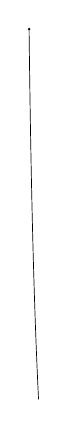
\begin{tikzpicture}[x=1mm,y=1mm,baseline=(current bounding box.north)]
\fill (0,0) circle[radius=.18mm];
\draw[line width=.25pt,line cap=round] (0,-.2) .. controls (.15,-13) and (.45,-32) .. (1.2,-47);
\end{tikzpicture}}
\[
\mathrm{Pt}_{\mathrm{ad}}(B_{\pi,\Gamma})
\longrightarrow
\mathrm{Pt}_{\mathrm{ad}}(B_{\pi'_i,\Gamma})\setminus\{P\}
\]
or again (passing to the limit) a bijection of $\Gamma$-sets
\[
\mathrm{Pt}_{\mathrm{ad}}(B_{\pi,\Gamma^{\natural}})
\simeq
\mathrm{Pt}_{\mathrm{ad}}(B_{\pi'_i,\Gamma^{\natural}})\setminus\{P\}
\]

This means three things:

a) The canonical homomorphism $\Gamma\longrightarrow M_{a'}(\pi'_i)$,
the composite of $\Gamma\longrightarrow N_a(\pi)$ and
$N_a(\pi)\simeq M_{a'}(\pi'_i)$,
is not \inserted{$\pi'_i$-}conjugate to a composite homomorphism
$\Gamma\xrightarrow{\lambda}M_a(\pi)
\xrightarrow{\varphi_i}M_{a'}(\pi'_i)$,
where $\Gamma\xrightarrow{\lambda}M_a(\pi)$ is an admissible lifting.

b) If $\lambda,\mu:\Gamma\rightrightarrows M_a(\pi)$ are two
admissible liftings of $\Gamma\longrightarrow N_a(\pi)$
\deleted{\unsure{that}} such that
$\varphi_i\circ\lambda$ and $\varphi_i\circ\mu:
\Gamma\rightrightarrows M_a(\pi)$ are
\inserted{$\pi'_i$-}conjugate, then $\lambda$ and $\mu$ are already
\inserted{$\pi$-}conjugate.

c) Every admissible lifting of
$\Gamma\longrightarrow N_{a'}(\pi'_i)$ to
$\Gamma\longrightarrow M_{a'}(\pi'_i)$,
comes by composition from an admissible lifting
$\Gamma\longrightarrow M_a(\pi)$.

\scanpage{419}
\mspage{212}

Thanks to this, the equivalence of categories between systems
$(\pi,a,i,\Gamma,\unsure{\theta}:\Gamma\mathop{\longrightarrow}\limits_{\unsure{\mathrm{adm}}}\unsure{N_a})$,
and the systems $(\pi',a',\Gamma,\theta':\Gamma\longrightarrow\unsure{N_{a'}},P)$,
where $P\in\mathrm{Pt}(B_{\pi',\Gamma^{\natural}})^\Gamma$,
becomes perfectly precise at the level of points: the
$\Gamma$-rational Points of $B_{\pi\unsure{,\Gamma^{\natural}|\deleted{,\Gamma^{\natural}}}}$
are identified with \unsure{one|the set}
\deleted{of the $\Gamma$-\unsure{rational} points} of the $\Gamma$-rational points
of $B_{\pi'}$, distinct from $P$.

This then allows us (which was not feasible in the discrete
context!) to extend the equivalence of categories to an equivalence

\[
(30)\qquad
\begin{array}{c@{\quad}c@{\quad}c}
\parbox[t]{0.45\linewidth}{%
category of systems $(\pi,\unsure{a|\alpha},I',\Gamma,\theta:\Gamma\longrightarrow N_a)$
of an arithmetized $\pi$ \inserted{(by \unsure{$\alpha$|$a$})} of type $(g,\nu)$,
of $I'\subset I(\pi)$, of an
\uline{admissible} outer action of $\Gamma$ on $\pi$
such that $\Gamma$ \deleted{\unsure{operates}} \uline{fixes each point} of $I'$
}
& \unsure{\cong|\simeq} &
\parbox[t]{0.36\linewidth}{%
category of systems
$(\pi',\unsure{a'|\alpha'},I',\unsure{\Gamma^{*}|\Gamma},\theta':\Gamma\longrightarrow N_{a'})$
of an arithmetized $\pi'$ (by \unsure{$a'$|$\alpha'$}) of type
$(g,\nu')$ $[\nu'=\nu-\mathrm{card}(I')]$
with an admissible \inserted{outer} operation of $\Gamma$ on it, and
a subset $I'\subset\mathrm{Pt}_{ad}(B_{\pi',\unsure{\Gamma}}\unsure{)}$
(hence $I'\subset\mathrm{Pt}_{ad}(B_{\pi',\Gamma})^\Gamma$)
i.e. $I'$ formed of points \unsure{invariant|fixed} under $\Gamma$, i.e. ``$\Gamma$-rational''
}
\end{array}
\]

\margin{with $2g+(\underbrace{\nu-\mathrm{card}\,I'}_{\nu'})\geq3$}

We thus have a quasi-inverse functor:
drilling holes at $I'$ !

\scanpage{420}

It is to be noted that in this approach, we have had to restrict ourselves to the case
\deleted{\unsure{of the|of}} \inserted{of a set of} points \deleted{\illegible{1}}
$I'\subset I(\pi)$ not only stable under $\Gamma$, but
\deleted{\unsure{formed}} $\subset I^\Gamma$
\deleted{fixed under $\Gamma$} or again to a subset
$I'\subset\mathrm{Pt}(B_{\pi',\Gamma^{\natural}})$
not only stable under $\Gamma$, but
\unsure{even|=}\,$\subset\mathrm{Pt}(B_{\pi',\Gamma^{\natural}})^\Gamma$.
To show that without this restriction, the natural functor
\deleted{\unsure{is}} that corresponds is nevertheless
an equivalence, we are reduced to this

\textcircled{6} Let $(\pi,a,I'\subset I(\pi))$ be with $(\pi,a)$
an arithmetized \inserted{categorical} \unsure{profinite|profinite} group with loops of type
$g,\nu$, whence $(\pi',a')$ --- let $\Gamma$ be, with $\Gamma'$
an open subgroup operating on $(\pi,a)$ in an admissible way
$(\Gamma\longrightarrow N_a(\pi))$,
and leaving $I'$ stable, hence it operates in an admissible way on
$(\pi',a')$,
Suppose given a \uline{lifting} of this action of $\Gamma'$
to an admissible action of $\Gamma$ on $N_{a'}$, which leaves invariant
\[
\begin{array}{rcl}
I'&\subset&\mathrm{Pt}(B_{\pi',\Gamma^{\natural}}).\\
&&\rotatebox{90}{$\unsure{\simeq}$}\\
&&\mathrm{Pt}(B_{\pi',\Gamma^{\prime\natural}})
\end{array}
\]

\diagram{\begin{tikzcd}[ampersand replacement=\&,column sep=3.6em,row sep=3em]
{\deleted{\unsure{M_a}}\;(N_a)_{I'}} \arrow[d] \&
\Gamma' \arrow[l] \arrow[d,hook,line width=.9pt] \arrow[dl,bend right=7,line width=.65pt] \\
N_{a'} \& \Gamma \arrow[l] \arrow[ul,dashed]
\end{tikzcd}}

Then there exists a unique admissible action of $\unsure{\Gamma|\Gamma'}$
on $(\pi,a)$, which extends that of $\Gamma'$ and which gives rise
to the \inserted{given} one on $\pi'$.

\subsection*{Scans 421--430}
\addcontentsline{toc}{subsection}{Scans 421--430}
% package LM_P043
\scanpage{421}
\mspage{213}
% Main text, approximate manuscript lines 1--4.
\deleted{Let} Is uniqueness at \unsure{all|all} events clear?
\deleted{\unsure{Choosing a}} Let us consider the extension \inserted{$\mathcal{E}$} of
$\Gamma$ by $L=\mathrm{Ker}((N_a)_{I'}\to\unsure{N_a|N_0})$,
inverse \unsure{image} of the extension $(N_a)_{I'}$
(of $\unsure{N_{a'}|N_{0'}}$ by $L$) via $\Gamma\to\unsure{N_{a'}|N_{0'}}$, we
% Main text, approximate manuscript lines 5--8.
have a \inserted{partial} splitting of this extension \unsure{over}
the subgroup $\Gamma'$ of $\Gamma$, and the assertion is
that this splitting \uline{\unsure{extends}}, \uline{in a way} \uline{that is unique}, to $\Gamma$.
We may suppose $\Gamma'$ normal in $\Gamma$, and we
% Main text, approximate manuscript lines 9--13.
identify $\Gamma'$ with a subgroup of $\mathcal{E}$. \unsure{All}
\deleted{\unsure{sections}} the sections of $\mathcal{E}$ over $\Gamma$ \unsure{are identified}
with \inserted{\unsure{section}} subgroups $\widetilde{\Gamma}$ of $\mathcal{E}$.
For such a $\widetilde{\Gamma}$, we have of course
$\widetilde{\Gamma}\subset\mathrm{Norm}_{\mathcal{E}}(\Gamma')$
moreover \deleted{\unsure{if we} \illegible{2}} \inserted{we obviously have}
% Main text, approximate manuscript line 14.
\[
\mathrm{Norm}_{\mathcal{E}}(\Gamma')\cap L=L^{\Gamma'} \tag{31}
\]
% Main text, approximate manuscript lines 15--21.
and I presume we must have
$L^{\Gamma'}=1$ (which generalizes condition
\textcircled{3} above\ldots) Now \uline{this condition}
\uline{implies uniqueness} -- namely
$\widetilde{\Gamma}=\mathrm{Norm}_{\mathcal{E}}(\Gamma')$ --
and existence \uline{means} that
$\mathrm{Norm}_{\mathcal{E}}(\Gamma')\to\Gamma$
is an epimorphism (hence an isomorphism\ldots).

% Main text, approximate manuscript lines 22--23.
But we will have to try to make precise,
in certain contexts (at least that of
\scanpage{422}
% Main text, approximate manuscript lines 1--4; continuation of scan 421.
arithmetically faithful actions, i.e. $\Gamma\to\boldsymbol{\Gamma}_a$
injective -- which \unsure{corresponds} \unsure{normally|presumably}
to the case of algebraic curves \unsure{defined} over
algebraic extensions of $\mathbb{Q}$ -- the notion
% Main text, approximate manuscript lines 5--9.
of an ``admissible'' action. For this, we
must return to the relation between
(potential) curves and finite coverings,
which also gives a way of
varying $g$.

% Main text, approximate manuscript lines 10--17.
But I feel like first taking up again
\unsure{under|on} another aspect \inserted{(perhaps more general)} the preceding
formalism, which \unsure{can} perhaps also \unsure{be} applied to the case of \uline{discrete} groups
with loops (I am thinking of the formalism
of the $\unsure{U^!|\mathcal{U}^!}$, linked to outer actions of
finite groups on such \unsure{profinite groups} with loops).

% Main text, approximate manuscript lines 18--20.
Let $\mathcal{X}$ be a set \inserted{$\ne\varnothing$}
(\inserted{\unsure{morally}, a} set of the
``points'' of an \deleted{surface} algebraic curve,
or of a topological surface\ldots), \deleted{and $\Gamma$}
\scanpage{423}
\mspage{214}
% Main text, approximate manuscript lines 1--7.
\deleted{a group operating on $\mathcal{X}$.} We suppose
given, for every finite subset $I$ of $\mathcal{X}$,
with complement $U_I=\mathcal{X}\setminus I$, a
\unsure{groupoid} $\Pi_{U_I}$, having $U_I$ as its set
of \unsure{objects}. Moreover, for $J\supset I$ i.e.
$U_J\subset U_I$, we suppose given a homomorphism
of groupoids
% Main text, approximate manuscript line 8.
\[
\Pi_{U_J}\to\Pi_{U_I}
\]
% Main text, approximate manuscript lines 9--14.
which on objects is the inclusion $U_J\unsure{\subset|\hookrightarrow}\unsure{U_J|U_I}$.
We suppose transitivity (strict) i.e. \deleted{\unsure{which}}
a covariant functor \inserted{from the category} of subsets $U$ of
$\mathcal{X}$ complementary to finite subsets \inserted{(with the inclusions)}, to
\unsure{the} category of groupoids, which on \unsure{the set}
of objects coincides with the obvious functor\ldots

% Left marginal note, running beside approximate lines 10--22.
\margin{If $\mathcal{X}$ is finite and $I=\mathcal{X}$, we
\unsure{suppose} \inserted{\uuline{\unsure{all the same|however}}}
$\Pi_{U_I}\;(=\Pi_{\varnothing})$ \unsure{is}
not the empty groupoid, but a groupoid
\deleted{of any kind} (which \unsure{maps} into the preceding ones\ldots)
but we will not be able to require
\unsure{the} strict transitivity.
We \unsure{will need|would need} \inserted{\unsure{perhaps}} \illegible{1} anabelian \unsure{hypotheses}
on $\Pi_{U_I}$ in this case\ldots}

% Main text, approximate manuscript lines 15--18.
We suppose moreover that for every \deleted{$I\in\mathcal{P}_f(\mathcal{X})$}
$i\in\mathcal{X}$, we give ourselves a \deleted{\unsure{groupoid} \illegible{1}}
$\Pi_i$ (or $\Pi_{D_i^*}$),
and \deleted{\unsure{for every}} for $i\in I\in\mathcal{P}_f(\mathcal{X})$,
a homomorphism of groupoids
% Main text, approximate manuscript line 19.
\[
\Pi_{D_i^*}\to\Pi_{U_I}
\]
% Main text, approximate manuscript lines 20--23.
compatible with the transition morphisms
\inserted{$\Pi_{U_I}\to\Pi_{U_J}$ $(I\supset J)$}.
We suppose that for fixed $I$, we find
on $\Pi_{U_I}$ a structure of groupoid
with loops by
\[
\Pi_{D_I^*}=\coprod_{i\in I}\Pi_{D_i^*}\to\Pi_{U_I}.
\]
\scanpage{424}
% Main-text lines 1--2; insertion above line 2.
without moreover excluding the case where $I=\varnothing$, and where \inserted{($\Pi_{\mathcal{X}}$ \unsure{being} connected, say)} \unsure{its|the} genus \uline{is $0$} --- \deleted{\unsure{thus}}
\margin{\unsure{We suppose} \illegible{4} \unsure{that} \illegible{1} $\mathcal{X}$ \illegible{3} \deleted{\unsure{for} $\mathcal{X}$ \illegible{2}} \deleted{\unsure{two points}}}

% Main-text lines 3--8.
We suppose moreover that if $J\supset I$ i.e. $U_J\subset U_I$, \inserted{and for $i\in J\setminus I$,} the composite homomorphism
\[
\Pi_{D_i^*}\longrightarrow\Pi_{U_J}\longrightarrow\Pi_{U_I}
\]
is ``constant'', in such a way that $\Pi_{U_I}$ is \unsure{obtained} from $\Pi_{U_J}$ by ``plugging the holes'' at $J\setminus I$.

% Main-text lines 9--21; the middle of the example is heavily revised.
Up to now, \unsure{all|all} this could be visualized for example by starting from an orientable topological surface \deleted{of the form \unsure{$X\setminus S$}; \illegible{4} of type} $X$, and a subset \inserted{\illegible{1}} $\mathcal{X}$ of $X$ \deleted{\illegible{1}}\inserted{\unsure{meeting}} \deleted{\unsure{every connected component}}\inserted{\unsure{every} connected component}; by taking for $\Pi_I$ the restriction to $\mathcal{X}\setminus I$ of the fundamental groupoid of $X\setminus I$ (if $I\ne\mathcal{X}$; if $\mathcal{X}=I$, which requires $\mathcal{X}$ finite, we will take the fundamental groupoid of $X\setminus I=X\setminus\{\mathcal{X}\}$; which we will have trouble mapping into the others with \uline{strict} transitivity, no matter!

% Main-text lines 22--23; sentence continues on the next scan.
But, we are mainly interested in the case $\mathcal{X}$ infinite. Where we \unsure{take} $X$ an algebraic curve over
\scanpage{425}
\mspage{215}
% Main-text lines 1--3; continuation from scan 424.
an algebraically closed field, $\mathcal{X}$ a subset of $X$ meeting \unsure{every} connected component, and we define the $\Pi_{U_I}$ as before.

% Main-text lines 4--9, with an insertion between lines 6 and 7.
Let now $\Gamma$ be a group which operates on the situation (\uline{strictly}, be it understood) thus on \unsure{the set} $\mathcal{X}$, \deleted{and} the groupoids \unsure{$\Pi_{U_I}$}, \inserted{the $\Pi_{D_i^*}$, (N.B. which it \unsure{permutes} among themselves),} commuting with the homomorphisms \unsure{d|of}
\[
\Pi_{U_I}\longrightarrow\Pi_{U_J}
\]
and the $\Pi_{D_i^*}\longrightarrow\Pi_{U_I}$.
\margin{\deleted{(which it \unsure{permutes} \unsure{among themselves})}}

% Main-text lines 10--13; the wording after Nous is rewritten interlinearly.
(We will have difficulties, if $\mathcal{X}$ is finite, for $\Pi_{U_I}$ when $I=\mathcal{X}$, for the \uline{strict} commutation \deleted{\unsure{of the}} \unsure{$\Pi_{U_{\mathcal{X}}}$}$\longrightarrow\Pi_{U_J}$ \unsure{..} but let us pass on...)
We \deleted{make \unsure{the hypothesis|the hypotheses},} \inserted{suppose defined a notion of \uline{admissible} subgroup of $\Gamma$, (they are in any case $\ne1$) such that \deleted{\illegible{1}} if $\Gamma'$ is admissible \unsure{then} every subgroup $\Gamma''\supset\Gamma'$ also.} \deleted{\unsure{following}} \inserted{We \deleted{\unsure{suppose}}}

% Canceled condition and canceled bracketed development in the lower half.
\deleted{\textcircled{\(1^\circ\)} For $P\in\mathcal{X}$, its stabilizer $\Gamma_P$ in $\Gamma$ is \deleted{$\ne1$}\inserted{admissible} (hence $\ne1$)}
\inserted{\deleted{\unsure{$U_I$ stable under $\Gamma_P$ i.e. $I$ stable}}}

\deleted{\unsure{\textcircled{\(2^\circ\)}} \illegible{1} (Let us note that if $U_I\ni P$, then $P$ is an object of $\Pi_{U_I}$ with an operation of $\Gamma_P$ on it, \deleted{\illegible{1}}\inserted{We} \unsure{find} in this way an \deleted{map}\inserted{operation} of $\Gamma_P$ on \unsure{$\pi_1(U_I,P)$|$\Pi_1(U_I,P)$}, and we suppose}

\deleted{\textcircled{\(2^\circ\)} \unsure{$\pi_1(U_I,P)$|$\Pi_1(U_I,P)$} \deleted{\unsure{call}}\inserted{\unsure{say that a}} subgroup $\Gamma'$ of $\Gamma$ is \textcircled{\(1^\circ\)} If $\Gamma'$ \uline{admissible} if \deleted{\illegible{1}} $\mathcal{X}^{\Gamma'}$ \unsure{meets} \unsure{every} connected component of $\mathcal{X}=U_{\varnothing}$ (which}
\scanpage{426}
% Main-text lines 1--3 continue the canceled draft on scan 425.
\deleted{also means \unsure{simply} that $\mathcal{X}^{\Gamma'}\ne\varnothing$ if $\mathcal{X}$ connected, or again that $\Gamma'$ \unsure{contains} a stabilizer $\Gamma_P$.} We assume

% Main-text line 4 and its small parenthetical addition.
\textcircled{\(1^\circ\)} $\forall P\in\mathcal{X}$, $\Gamma_P\ne\{1\}$, and $\Gamma_P$ of finite index \unsure{in $\Gamma$} \inserted{(i.e. the orbit of $P$ finite)}

% Main-text lines 5--21.
We want conditions which ensure that $\mathcal{X}$ and the $\Pi_{U_I}$ \deleted{\unsure{for}} etc, \unsure{can|may} be reconstructed up to \deleted{\unsure{the help}} canonical \unsure{isomorphism} with the help of the purely groupoid-theoretic ``bare'' or topossic \inserted{(with operators $\Gamma$)} \unsure{corresponding|corresponding} data. \deleted{We \illegible{1}} We can say it in learned topossic language, but we are going to express it in terms of the theory of groups with loops. Let $I$ be a subset of $\mathcal{X}$ stable under \unsure{$\Gamma^*$|$\Gamma'$}, we would like to lay down conditions which \deleted{\unsure{we take} a \unsure{subgroup}} \unsure{allow|will allow} us to express \inserted{\unsure{(for such $I$)}} the situation of the groupoids \inserted{$\Pi_V$} associated with the $V\supset U_I$ (i.e. the $U_J$ with $J\subset I$), \inserted{the $\Pi_{D_i^*}$ $(i\in I)$,} and the operation of $\Gamma$ on them, in terms of the \deleted{\unsure{operation}} sole operation of $\Gamma$ on the outer group with loops \deleted{$\pi_I$ associated} $\pi_1(\Pi_{U_I})$ associated with $I$ ---
\scanpage{427}
\mspage{216}
\margin{\unsure{$\rightsquigarrow$|$\longrightarrow$}}
% Main-text lines 1--5.
or rather (for this is immediate, by the operation of drilling holes), \inserted{in the reverse direction,} show how,
\deleted{\unsure{for a} $J\subset I$ \unsure{invariant} under $\Gamma$}
\deleted{\illegible{5}}
\deleted{\unsure{reconstruct} \illegible{2},}
% Main-text lines 6--11.
subject to anabelianity \unsure{$\zeta$|$\xi$} say of \unsure{$\Pi_{\mathcal X}$|$B_{\Pi_{\mathcal X}}$} (to fix ideas), we can $\pm$ \unsure{reconstruct} $\Pi_{U_I}$ and the action of $\Gamma$ on it \unsure{....|...},
starting from \unsure{$\Pi_{\mathcal X}$} \inserted{(or rather, \deleted{from}\inserted{from the \unsure{topos}} \unsure{$B_{\Pi_{\mathcal X}}$})} and from the action of $\Gamma$ on it.
We want at least an \inserted{\unsure{intrinsic}} description of the \unsure{elements} of \unsure{$\mathcal X$}, \inserted{and of the action of $\Gamma$ on it,} via
% Main-text lines 12--15.
this ``soft'' action --- which, for $X$ connected, again amounts to an outer action of $\Gamma$ on a group with loops (\uline{without} loops!) $\pi$...

% Main-text lines 16--21; the parenthesis continues on the next scan.
A first condition, in weak form, \unsure{it is|is} that (assuming \unsure{$\mathcal X$} connected, and calling : $\pi(I)$ the outer group $\pi_1(\Pi_{U_I})$, for \unsure{every} finite subset $I$ of \unsure{$\mathcal X$}) that \unsure{for} $\pi(I)$ anabelian (which will be the case for $I$ ``large enough'',
\scanpage{428}
% Main-text lines 1--3.
at least if \unsure{$\mathcal X$} is infinite \unsure{so|of} that we can take $I$ of arbitrarily large cardinality...) \deleted{we have} the obvious map
% Deleted display and replacement display, approximately lines 4--5.
\[
\deleted{\unsure{\mathrm{Pt}(B_{\pi(I),\Gamma\natural})|\mathrm{Pt}(B_{\pi(I)},\Gamma\natural)}\longrightarrow\text{classes of}}
\]
\[
2^\circ)\quad
\deleted{\unsure{\mathcal X}}U_I\longrightarrow
\unsure{\mathrm{Pt}(B_{\pi(I),\Gamma\natural})|\mathrm{Pt}(B_{\pi(I)},\Gamma\natural)}
\simeq
\begin{gathered}
\unsure{\inserted{\text{classes of }\pi(I)\text{-conjugation }\unsure{\text{of}|\text{of the}}}}\\
\unsure{\text{germs}}\text{ of}\\
\deleted{\text{of}}\text{ splittings of}\\
\text{the extension }\mathcal E(I)\\
\text{of }\deleted{\unsure{\mathcal E}}\Gamma\text{ by }\pi(I)
\end{gathered}
\]
% Main-text lines 6--15.
\unsure{(compatible|compatible} with the actions of $\Gamma$) be \uline{injective}. But to go further, we would have to be able to give a characterization of the image. Let us note (placing ourselves henceforth in the profinite context) that if we give ourselves on the \unsure{$\Pi(I)$|$\pi(I)$} some \unsure{arithmetizations}, \unsure{compatible} with the outer homomorphisms of plugging holes $\pi(I)\longrightarrow\pi(J)$, and with the action of $\Gamma$ on the $\pi(I)$, we therefore have a
% Main-text lines 16--20.
canonical homomorphism from $\Gamma$ into the common group \deleted{of the} $\boldsymbol{\Gamma}$ of \unsure{arithmetically} \unsure{(}outer automorphisms of these \unsure{arithmetizations}.
(and even $\Gamma\longrightarrow$ \unsure{$M_{\pi(\varnothing)=\pi}$}, --- which is \inserted{already} a markedly stronger \inserted{datum}). We can therefore
\scanpage{429}
\mspage{217}
% Main text, approximate lines 1--5.
suppose \unsure{given} a notion of \uuline{admissible}
\uline{lifting} of such an outer arithmetic
action, in such a way that the
preceding \unsure{morphism} is a bijection
\[
 U_I=\unsure{\mathcal X|\mathfrak X}\setminus I
 \xrightarrow{\sim}
 \mathrm{Pt}_{\mathrm{ad}}\bigl(B_{\pi(I)},\Gamma\natural\bigr)
\]
This means moreover, in practice,
that the notion of admissibility satisfies
conditions $1^\circ)$ : $6^\circ)$ \unsure{seen} above.

% Main text, approximate lines 9--12.
As for knowing \unsure{what} should be
called \unsure{operations} \deleted{\unsure{outer}} ``\unsure{admissible|admissible}'' of
$\Gamma$ on an \inserted{outer} \unsure{(}profinite\unsure{)|,} group with loops,
this remains conjectural for the moment.

% Main text, approximate lines 13--21; interlinear revisions retained.
We could by way of experiment
\unsure{conjecture} \deleted{that \unsure{every} \illegible{2}}
\inserted{that the following notion would work}
\unsure{Let us call|Let us call}
``admissible'' every such action
\[
 \Gamma\longrightarrow\widehat{\widehat{\mathcal T}}(\pi)
\]
which respects an arithmetization $a$,
i.e. which factors through the corresponding $N_a$, \unsure{and} such that the image of
$\Gamma\longrightarrow N_a/\widehat{\mathcal T}_a=\boldsymbol{\Gamma}_a$
is \unsure{open|open},
\deleted{\inserted{and that $\pi^{\Gamma'}=(1)$}}
\deleted{\unsure{the conditions}}, \inserted{and that}
\scanpage{430}
% Main text, approximate lines 1--5.
\deleted{\unsure{considered} above \unsure{$1^\circ:6^\circ$} \unsure{are} \unsure{satisfied|satisfied}}

$\forall$ \unsure{homomorphism} of plugging holes at $i\in I(\pi)$,
$\pi\longrightarrow\pi_i'$, $N(\pi)_i\longrightarrow M(\pi_i')$, the \unsure{corresponding} homomorphism
$\Gamma_i$, nor of any open subgroup $\Gamma'$
of $\Gamma_i$, does \unsure{not} normalize an $L_j'$ $(j\in I(\pi_i')=I\setminus\{i\})$.

% Upper left margin; several long strokes run through the whole note.
\margin{\deleted{
this condition is
perhaps \illegible{2} and \unsure{premature}
--- it could be
that for \unsure{every pair|all pairs}
of distinct indices $i,j$ of $I=I(\pi)$,
\inserted{and for the \unsure{corresponding} $L_i,L_j$},
the subgroup \deleted{\illegible{1}} \unsure{$K$} of
$M(\pi)$ \unsure{formed} of the
$g\in M(\pi)$ which \uline{normalize}
$L_i$, and which moreover normalize
$L_j$ \uline{mod} $\mathrm{Ker}(\unsure{\pi\longrightarrow\pi_i'})$,
is ``\unsure{too small}'' \deleted{\unsure{for}} \inserted{\unsure{i.e.}}
that its image in
$\unsure{\boldsymbol{\Gamma}|\Pi}=M(\pi)/\unsure{\widehat{\mathcal T}(\pi)|\widehat{\mathcal G}(\pi)}$
\uline{\unsure{is not}}
of finite index
}}

% Main text, approximate lines 6--14.
\unsure{perhaps} we would even have to impose
$\pi^{\unsure{(\Gamma^{\prime+})|\langle\Gamma^{\prime+}\rangle}}=(1)$, where $\Gamma^{\prime+}$ is the kernel of
$\Gamma'\xrightarrow{\chi}\widehat{\mathbb Z}^{*}$ --- in any case we expect
\unsure{---} that we then have $\pi^{\Gamma'}=(1)$,
and if this were not the case, we would have to
introduce it into the definition --- for
each operation of plugging holes
\unsure{relative} to $I'\subset I(\pi)$, and to the choice of an
$i\in I'$, allowing us to define $\Gamma_{(I',i)}\longrightarrow M(\pi(I'))$.

% Lower left marginal note.
\margin{
More generally,
for $i\in I'\subset I=I(\pi)$,
\deleted{\unsure{it is necessary}} \inserted{\unsure{we impose}} that the
true action of
\unsure{$\Gamma_{I',i}$} on \unsure{$\pi_i(I')$|$\Pi_i(I')$}
\inserted{\unsure{corresponding}} \unsure{to $i$}
normalize no
subgroup $L_j$
$(j\in I\setminus I')$ --- we
are reduced for
this to the case where
$I'=I\setminus\{j\}$, hence
where \unsure{$\pi(I')$|$\Pi(I')$} has \unsure{(only a} single \unsure{class} loops\dots\
(\unsure{if|and} $g\geq1$)
}

% Main text, approximate lines 15--21.
Let us note that a true action of $\Gamma$ on $\pi$
(not \unsure{only|only} \unsure{outer}) which lifts a
given\unsure{$+$} admissible action, is \inserted{\unsure{it too}} admissible
(in the sense that it defines an
\deleted{outer} \uline{admissible} action on a $\pi'$ of
type $(g,\nu+1)$), iff this action \inserted{\unsure{(rather its germ)}} normalizes
no $L_i$ $(i\in I(\pi))$, and that

\subsection*{Scans 431--440}
\addcontentsline{toc}{subsection}{Scans 431--440}
% package LM_P044
\scanpage{431}
\mspage{218}

it is likewise \unsure{for} the action induced on each $\pi(I')$ $(I'\subset I=I(\pi))$ [it suffices to take the $\pi(I')$ for $I'$ of the form $I\setminus\{j\}$, $j\in I$] --- \uuline{and} that finally the action of $\Gamma^{\natural}$ \deleted{relative to \unsure{an} $i\in I$} on $\pi'(I)$ (deduced from $\pi'$ by plugging the holes at $I$, so that $\pi'(I)$ has a single class of loops; \unsure{$\pi'(I)$} is also deduced from the \inserted{actual} action of $\Gamma$ on $\pi(I)$ --- with $0$ \inserted{classes of} loops --- by making ``a hole'' corresponding) relative to \inserted{a} point $i\in I$, normalizes no loop subgroups\ldots\ But I presume that the first condition (action \inserted{of $\Gamma^{\natural}$} normalizing none of the $L_i$) implies the others.

\margin{at least if $g\ne 0$}

But one must \inserted{in the definition of admissibility} also take into account condition $(4^\circ)$, \deleted{\illegible{1}}\inserted{which implies the }existence of enough liftings\ldots\ .

I come (painfully!) to a

\uuline{Provisional profinite conjecture} For $\Gamma$ a given profinite group, an outer action on an arithmetized anabelian $(\pi,a)$ of type $(g,\nu)$ is called \uline{admissible}, if

\margin{Hoaxed cf. below\ldots}

a) \deleted{\illegible{1}} The homomorphism $\Gamma\longrightarrow\boldsymbol{\Gamma}_a$ has open image

b) The \uline{actual} \unsure{actions} deduced by pluggings \unsure{of|of the} holes $(i\in I'\subset I=I(\pi))$ normalize no loop subgroups.

\scanpage{432}

c) There exist infinitely many \inserted{$\pi$-conjugacy classes of the} germs \deleted{\illegible{1}} splittings of the extension of $\Gamma$ by $\pi$, which normalize no loop subgroup of $\pi$.

\margin{This \inserted{condition c)} probably excludes cases like $\Gamma=\unsure{\mathcal N_{g,\nu}|N_{g,\nu}}$ with $(g,\nu)\ne(0,3)$, for the extension $\unsure{\mathcal M_{g,\nu}|M_{g,\nu}}$ of $\unsure{\mathcal N_{g,\nu}|N_{g,\nu}}$ by $\unsure{\widehat{\pi}_{g,\nu}|\widehat{\Pi}_{g,\nu}}$ probably admits no germs of \illegible{1} ($\overset{?}{\Longleftrightarrow}$ $\unsure{\mathcal U_{g,\nu}|U_{g,\nu}}$ over $\unsure{\mathcal M_{g,\nu}|\mathcal N_{g,\nu}}$ \unsure{has|admits} probably no \unsure{étale multisection|étale multisections}\ldots)}

An actual action of $\Gamma$ on $\pi$ is called actual, \deleted{and} if the outer action is actual, and if it normalizes no loop subgroup.

This being so:

a) If $\Gamma$ operates actually in an admissible way, we have
\[
\pi^\Gamma=(1)
\]
(perhaps even $\pi^{\unsure{\Gamma^+|\Gamma^\dagger}}=(1)$) \deleted{I also presume that the only \unsure{sub-}}

\deleted{b) If $\Gamma$ operates by outer automorphisms in an admissible way, \deleted{then} leaving $I'\subset I(\pi)$ stable, then ditto on $\pi(I')$ --- likewise for admissible actual actions.}

\margin{\deleted{\illegible{1}}}

\deleted{c) Under the preceding conditions,}

\scanpage{433}
\mspage{219}

\deleted{the canonical map of $\Gamma$-sets
\[
\mathrm{Pt}(B_{\pi,\Gamma^{\natural}})\longrightarrow
\mathrm{Pt}(B_{\pi(I'),\Gamma^{\natural}})
\]}

b) If $i\in I$ is stable under $\Gamma$ operating \deleted{actually}\inserted{by outer automorphisms} in an admissible way, then the actual action on $\pi'=\pi(i)$ normalizes no $L'_j$ $(j\in I\setminus\{i\})$.

c) If $\Gamma$ operates actually on $\pi$ in an admissible way, \inserted{\unsure{while} leaving $i\in I$ fixed,} then the corresponding actual action (\uline{by} \deleted{\illegible{3}}\inserted{passage to the quotient}) on $\pi^{\prime\natural}=\unsure{\pi(i)|R(i)}$ normalizes no $L'_j$ $(j\in I\setminus\{i\})$.

d) If $\Gamma$ \deleted{operates actually on $\pi$ in a way}\inserted{operates actually on $\pi$ in an} admissible way, then the map
\[
\unsure{\beta}\qquad
\mathrm{Pt}_{\mathrm{ad}}(B_{\pi,\Gamma^{\natural}})\longrightarrow
\mathrm{Pt}_{\mathrm{ad}}(B_{\pi',\Gamma^{\natural}})
\]
defined by c) is \uline{injective}, and \inserted{the complement of} its image is \deleted{finite} equal to $\{P\}$, where $P$ is defined by the ``hole'' $i$.

But this last part of the assertion, going beyond mere \uline{injectivity} --- and characterizing the image, now seems to me quite doubtful ---

\scanpage{434}

indeed, it suffices to look at a parameter scheme $S$, of finite type over \unsure{$Q$|$\mathbb{Q}$} (a $K(\pi,1)$ preferably, for example an \unsure{algebraic} curve) and to take for $\Gamma$ (not the fundamental group of its generic point, \inserted{i.e. of a field,} \unsure{but)} the fundamental group of $S$ itself. The datum of an admissible outer action of $\Gamma$ on a $\pi$ \unsure{corresponds} morally to that of a family of curves $U$ of type $g,\nu$ parameterized by $S$. Condition c) is satisfied for example if $U$ comes from an algebraic curve over the base field itself, so no problem -- and it is plain that surjectivity goes haywire. The difficulty comes from the fact that two \uline{distinct} sections of $U$ over $S$ may not be \uline{disjoint} !

\margin{The splittings of extensions correspond \unsure{to the} sections of $U$ over $S$}

\scanpage{435}
\mspage{220}

One must be able to speak of sections ``\unsure{strictly|strictly} distinct'' i.e. distinct at every point of $S$ -- which, in profinite translation, \unsure{amounts} to comparing two splittings of the extension of $\Gamma$ by $\pi$, with \deleted{\unsure{two}}\inserted{the} \inserted{germs of} splittings over \unsure{$\boldsymbol{\Gamma}'_{\cdot}\subset\boldsymbol{\Gamma}$|$\boldsymbol{\Gamma}'\subset\boldsymbol{\Gamma}$} of $\Gamma$ (as \unsure{an extension} of $\boldsymbol{\Gamma}_Q$ by a geometric part) which correspond to the \unsure{points} of $S$ -- i.e. precisely the \uline{admissible} (germs of splittings). One has the impression of going around in a vicious circle or almost -- it would seem that one should not try to swallow too much at once -- deal from the outset with \uline{all} profinite groups $\Gamma$ at once -- but rather restrict \unsure{oneself} \inserted{first} to those which, morally, correspond to \inserted{\unsure{$\pi_1$|$\Pi_1$} of} schemes of finite type over \unsure{$Q$|$\mathbb{Q}$} -- some $K(\pi,1)$ let us say, or \inserted{even} varieties

\scanpage{436}

elementary in Artin's sense -- and in the definitions resp. conjectures, pull oneself up by one's shoelaces, by inducting on the dimension.

At the first notch then (dimension $0$) one would restrict oneself to actions of groups $\Gamma$ which are (modulo at least passage to an open subgroup) ``arithmetically faithful'' \unsure{for example|for example} $\Gamma\to\boldsymbol{\Gamma}_a$ injective.

\unsure{In|\uline{In}} that case, the conjecture as stated just now seems reasonable, or at least not necessarily crazy. The decisive test\unsure{,|,:} it is true, would be the possibility of obtaining the ``curves'' thus defined as coverings of $\mathbb{P}^1\setminus\{0,1,\infty\}$ \ldots

\scanpage{437}
\mspage{221}

\uline{33} Topological digression :
Anti-involutions of oriented \unsure{algebroid} surfaces

\margin{In the end I look only at compact surfaces -- Yet the noncompact case would also be very interesting to look at -- to try to recover by an ``algebraic'' route, from the outer automorphism of order $2$ in $\unsure{\pi_1}$, the arrangement of the curve's ``points at infinity'' on the connected components of \deleted{\illegible{1}} $X^\sigma$ $(X=\widehat U)$}

\unsure{We call} an \unsure{algebroid} surface a surface $U$ of the form $\widehat X\setminus S$, $X$ a compact orientable \inserted{surface}, $S$ finite. Then $X$ is determined up to unique homeomorphism as the ``pure compactification'' of $U$, \unsure{denote it|we denote it} $\widehat U$. \deleted{\unsure{The}} The homeomorphisms of $U$ onto itself are identified with the morphisms of $X$ which map $S$ into itself. The orientations of $X$ are in $1$-$1$ correspondence with those of $U$. The anti-involutions of $U$ (\unsure{assumed} oriented) are in $1$-$1$ correspondence with those of $X$ which preserve $S$.

We then find an equivalence between the category of oriented \unsure{algebroid} surfaces \inserted{$U$,} equipped with an anti-involution $\sigma$, and of compact surfaces with boundary $Y$, equipped with a finite subset $T$, to $(U,\sigma)$ corresponds $(\widehat U/\sigma,(\widehat U\setminus U)/\sigma)$ -- and to $(Y,T)$ corresponds $\widetilde Y-\widetilde T$, where $\widetilde Y$ is the ``oriented double'' of $Y$ \inserted{(which is a \unsure{compact} oriented surface)}, and $\widetilde T$ the inverse image of $T$ in $\widetilde Y$.

We are now interested in the

\scanpage{438}

case where $U$ is connected of type $(g,\nu)$, first examining the case $\nu=0$, \inserted{i.e. $U=\widehat U$, $S=\varnothing$} (to which the general case \unsure{will reduce}). \deleted{This} \inserted{The condition $\nu=0$} corresponds to the case where $T=\varnothing$ -- thus the \inserted{$U=X$} \deleted{$X$} considered \deleted{are} are identified with the oriented doublings of certain compact manifolds with boundary $Y$. Which ones ? Obviously $Y$ must be \uline{connected}, and \uuline{nonorientable}.

\margin{it is not true that $Y$ is necessarily nonorientable -- only in the case where $X^\sigma=\varnothing$}

So $Y$ is \unsure{characterized}, up to homeomorphism, by its genus $\gamma$ \inserted{and the number $\mu$ of connected components \inserted{of the boundary}} -- it can be obtained from the projective plane \inserted{$Y_0$ over the reals} by cutting out $\gamma$ disjoint disks in it, and gluing Möbius strips back in, \inserted{then \unsure{removing again} $\mu$ open disks,} -- which gives
\[
\begin{aligned}
\chi(Y)&=\underset{\substack{\text{''}\\1}}{\chi(Y_0)}
-\deleted{\unsure{\chi}}\unsure{\gamma}\cdot
\underbrace{\chi_!(\text{open disk})}_{+1}
+\unsure{\gamma}\chi_!(\text{open Möbius strip})\\
&\hspace{11em}\unsure{+|-}\mu\underbrace{\chi_!(\text{open disk})}_{+1}
\end{aligned}
\]
now the \inserted{open} Möbius strip (obtained from $Y_0$ by \unsure{removing} a \inserted{closed} disk) has \unsure{a|a} $\chi_!$ equal to :
\[
\underset{\substack{\text{''}\\1}}{\chi(Y_0)}-
\underset{\substack{\text{''}\\1}}{\chi(\text{closed disk})},
\quad \text{i.e. }0,\quad \text{hence}
\]
\[
(1)\qquad \chi(Y)=1-(\unsure{\gamma}+\mu)
\]
\margin{$Y$ compact connected nonorientable surface without boundary of genus $\gamma$}

On the other hand, we \unsure{will have|have}
\[
\chi(X)=\chi(X\deleted{\unsure{)}}\setminus X^\sigma)
\]
for $X^\sigma$ is a \unsure{union} of circles so its $\chi$ is zero,

\scanpage{439}
\mspage{222}

Now, since $X\setminus X^\sigma$ is an étale covering of order $2$ of $\unsure{\operatorname{Int}Y}$, we have
\[
\chi(X\setminus X^\sigma)=2\chi(\operatorname{Int}(Y))
\]
finally
\[
\chi(Y)=\chi(\underline{Y\setminus\partial Y})=\chi(\operatorname{Int}Y)
\]
for the same reason as \unsure{before} $(\chi(\partial Y)=0)$,
hence finally
\[
(2)\qquad \chi(X)=2\chi(Y)=2(1-(\gamma+\mu))
\]
\deleted{\illegible{1}} or again, since $\chi(X)=2-2g$
\[
(3)\qquad g=\gamma+\mu
\]

Thus we find

\margin{\illegible{1}}

\uline{Proposition} The category of oriented \inserted{connected compact} surfaces of genus $g$ equipped with an anti-involution $\sigma$ is equivalent to that of \uline{nonorientable} compact manifolds with boundary, of type $(\gamma,\mu)$ ($\gamma$ the genus, $\mu$ the number of holes), with $\gamma+\mu=g$.

\margin{no, we find only a full subcategory of that of all the $(X,\sigma)$. On the other hand there are also the oriented doublings $Y\amalg_{\partial Y}Y$ of compact \uline{orientable} surfaces with \uline{nonempty boundary} -- if $Y$ is of type $(\gamma,\mu)$, $X$ is of genus $g$ \unsure{with} $g=2\gamma+\mu-1$ (where $\gamma\geq0$, $\mu\geq1$)}

\uline{Corollary} There are exactly $g+1$ isomorphism classes of systems $(X,\sigma)$, classified by $0\leq\mu\leq g$, where $\mu=\operatorname{card}\unsure{\pi_0|\Pi_0}(X^\sigma)$.

\margin{This only works by restricting oneself to the $(X,\sigma)$ such that $(X/\sigma)$ nonorientable -- \unsure{cf.|cf.} opposite \deleted{\unsure{for}} the \deleted{\unsure{general}} case \inserted{$X/\sigma$ orientable}}

$X$ \inserted{$=X_g$} is a compact oriented surface of

\deleted{Anti-involutions of \unsure{oriented} surfaces of \deleted{\illegible{1}} \unsure{algebroid} type (i.e. of the form $X\setminus S$, with $X$ compact, $S$ finite). We \deleted{will admit} \inserted{know} that they are classified, modulo isomorphism \inserted{up to}, by the systems}

\scanpage{440}

genus $g$, this also means that in the group $A_g=\mathrm{Aut}(X_g)$, there are exactly $g+1$ conjugacy classes of elements $\sigma$ satisfying
\[
(4)\qquad \sigma^2=1,\qquad \mathrm{sg}(\sigma)=+1.
\]
(i.e. which are anti-involutions). They give $g+1$ conjugacy classes of elements of $A_g/A_g^\circ=\unsure{\mathcal{T}_g}$, satisfying the \unsure{same|same} relations. We will show (we hope!) that these classes are distinct, and that every $\sigma\in\unsure{\mathcal{T}_g}$ satisfying relations (4) is in one of these classes.

We will admit the

\uline{Lemma} Every anti-involution of the \inserted{unit} disk \inserted{(\unsure{case|or} of $\mathbb C$)} is conjugate to $z\mapsto\overline z$, and consequently \unsure{the set} of its fixed points is homeomorphic to $\mathbb R$, and in particular is \uline{connected}.

\uline{Theorem} Let $U$ be an oriented surface \inserted{\unsure{(Hausdorff connected paracompact)}}, \inserted{\uline{not isomorphic to} $S^2$,} $\sigma$ an anti-involution of $U$, $\widetilde U$ a universal covering of $U$, whence $\pi=\mathrm{Aut}(\widetilde U/U)$ and an extension \unsure{$E$|$\mathcal E$} of \unsure{$\mathbb Z/2$} by $\pi$, formed

\subsection*{Scans 441--450}
\addcontentsline{toc}{subsection}{Scans 441--450}
% package LM_P045
\scanpage{441}
\mspage{223}

of topological automorphisms of $\widetilde U$ compatible with the
equivalence relation \unsure{defined} by $\widetilde U\unsure{\longrightarrow|-}U$, and
inducing on $U$ the \unsure{automorphism} $\mathrm{id}_U$ or $\sigma$.

\deleted{For} Then

a) (For the record) $U^\sigma$ is a closed submanifold
of $U$ of dimension 1.

b) For $\forall\ x\in U^\sigma$, one finds a
\inserted{$\pi$-}conjugacy class of \deleted{elements \unsure{of}}\inserted{splittings} of the extension
$\mathcal E$, in the usual way, whence a
map
\deleted{(\unsure{4|5})}
\[
 \begin{aligned}
 U^\sigma\longrightarrow\mathrm{Sc}(\mathcal E,\mathbb Z/2)
 &=\text{set of classes under}\\
 &\quad\text{$\pi$-conjugation of splittings of $\mathcal E$}\\
 &\quad\text{\unsure{over} $\mathbb Z/2$, or again of}\\
 &\quad\text{elements of order $2$ of}\\
 &\quad\text{$\mathcal E$ which are not in $\pi$.}
 \end{aligned}
 \tag{5}
\]

This map factors through a
\uline{bijection}
\[
 \pi_0(U^\sigma)\simeq\mathrm{Sc}(\mathcal E,\mathbb Z/2)
 \tag{6}
\]

c) Let $Z_i$ be a connected component of $U^\sigma$,
corresponding to a \deleted{splitting} $\sigma_i\in\mathcal E^-$ \deleted{such}\inserted{of}
order $2$. Then \deleted{\illegible{1} $\pi$\illegible{1}}
\[
 \pi^{\sigma_i}=\{1\}\quad\text{\unsure{sss|iff}}\quad Z_i\simeq\mathbb R,
 \quad\deleted{\unsure{\text{and}}}
 \tag{7}
\]

d) If $Z_i\not\simeq\mathbb R$ i.e. \deleted{\illegible{4} $Z_i$} $Z_i\simeq\unsure{S^1|\mathbb S^1}$, then,
for a chosen orientation of $Z_i$, denot-

\scanpage{442}
ing by $g_i$ the element of $\pi=\pi_1(U)$
that it defines (defined up to conjugation), and
by $\varphi_i:\mathbb Z\longrightarrow\pi$ the homomorphism $\varphi_i(n)=g_i^n$ from
$\mathbb Z$ to $\pi$, one has:

$1^\circ)$ $\varphi_i$ is injective

$2^\circ)$ after possibly replacing $\varphi_i$ by a conjugate,
one has
\[
\unsure{(9)|(8)}\qquad \pi^{\sigma_i}=\operatorname{Im}\varphi_i
\]

\uline{Proof} One finds the map (5) by
\deleted{\unsure{taking}}, for $\forall\ x\in U^\sigma$, the \inserted{\unsure{canonical}} operation of
$\mathbb Z/2$ on the universal covering $\widetilde U(\unsure{x})$ pointed
at $x$, and by \deleted{choosing} taking the
\unsure{corresponding} operations on $\widetilde U$, \unsure{deduced} via
the isomorphisms $\widetilde U\simeq\widetilde U(x)$. One sees that
the \deleted{\unsure{only}} operations $\sigma'$\deleted{\illegible{1}} obtained on $\widetilde U$ \inserted{(for fixed $x$)}, are
those for which \deleted{\illegible{1}} $\widetilde U^{\sigma'}$ has a
point over $x$ --- hence the set
of $x$ which give rise to \deleted{\unsure{a}}\inserted{the}
class of a $\sigma'$, are the elements of
the image of $\widetilde U^{\sigma'}$ under the projection
$\widetilde U\longrightarrow U$. Since by the lemma $\widetilde U^{\sigma'}$
is nonempty and connected, it follows that

\scanpage{443}
\mspage{224}
its image in $U^\sigma$ is so too --- we are going to
see that its image is exactly a connected
component of $U^\sigma$ --- which \unsure{will prove} both
the factorizability of (5) through \deleted{\unsure{the}} $\pi_0(U^\sigma)$
(\unsure{rather} trivial in any case) and the fact that
the resulting map (6) is \uline{bijective}.

Let $\widetilde Z_i$ be a universal \unsure{cover\textsuperscript{ing}|covering} of $Z_i$,
and let us take the \unsure{corresponding} universal covering
$\widetilde U_i$ of $U$, so that one has
\margin{\deleted{\diagram{\begin{tikzcd}[ampersand replacement=\&]
\widetilde Z_i \arrow[r] \arrow[d] \& \widetilde U_i \arrow[d] \\
Z_i \arrow[r] \& U
\end{tikzcd}}}}
\unsure{(8)|(9)}
\diagram{\begin{tikzcd}[ampersand replacement=\&]
\widetilde Z_i \arrow[r] \arrow[d] \& \widetilde U_i \arrow[d] \\
Z_i \arrow[r] \& U
\end{tikzcd}}
and by functoriality $\sigma$ also operates on this
diagram (operating \unsure{trivial\textsuperscript{ly}} on $Z_i,\widetilde Z_i$),
let $\sigma_i$ be its operation on $\widetilde U_i$. One
thus sees that $\widetilde Z_i$ maps into $\widetilde U_i^{\sigma_i}$,
which therefore maps \uline{onto} $Z_i$ --- which already finishes
proving b).

\deleted{Let us suppose now that $Z_i$ is \unsure{simpl\textsuperscript{y}|simply} connected
i.e. $Z_i\simeq\mathbb R$, $\widetilde Z_i=Z_i$ --- thus $\widetilde Z_i\longrightarrow\widetilde U_i$ is
\unsure{a} section of $\widetilde U_i$.}
\inserted{Let us consider \deleted{\unsure{the image}} \inserted{the image} \deleted{\unsure{induced}} of $\widetilde Z_i$ in
$\unsure{\widetilde U_i|\widetilde U}\mid Z_i$, this is an \uline{open} and closed subset}
(as the image of a morphism of étale \unsure{cover\textsuperscript{ings}|coverings}
over the same component $Z_i$), so it is

\scanpage{444}
\unsure{fortiori} an open and closed subset of
$\widetilde U_i^{\sigma_i}$, and since this space is connected,
it is equal to it.
\deleted{When}
\deleted{\[
(10)\qquad \widetilde U_i^{\sigma_i}=\operatorname{Im}(\widetilde Z_i\longrightarrow\widetilde U_i)
\]}
\inserted{Moreover $\widetilde Z_i\longrightarrow\widetilde U^{\sigma_i}$ makes \deleted{\illegible{1}}\inserted{of}
$\widetilde Z_i$ an étale covering of
its image $\widetilde U_i^{\sigma_i}$ in $\widetilde U_i\mid Z_i$, $\ast$
and since $\widetilde U_i^{\sigma_i}$ is
\unsure{simpl\textsuperscript{y}|simply} connected,
one finds \unsure{final\textsuperscript{ly}|finally}
\[
(10)\qquad \widetilde Z_i\overset{\sim}{\longrightarrow}\widetilde U_i^{\sigma_i}
\]}

When $Z_i$ is \unsure{simpl\textsuperscript{y}|simply} connected i.e.
$\widetilde Z_i\simeq Z_i$, this also means that
$\widetilde U_i^{\sigma_i}\longrightarrow Z_i$ is a homeomorphism,
(thus $\widetilde Z_i=Z_i\longrightarrow\widetilde U_i^{\sigma_i}$ is the inverse
\unsure{homeomorphism}). Since, for $x\in Z_i$,
\deleted{\unsure{the elements}} and $\widetilde x\in(\widetilde U_i^{\sigma_i})_x$, the
$\widetilde x'$ of $\widetilde U_i^{\sigma_i}$ over $x$ are \deleted{\illegible{1}} \inserted{\unsure{the elements}} of
the form $\widetilde x\cdot\gamma$, with $\gamma\in\pi_i^{\sigma_i}$
($\pi_i=\operatorname{Aut}(\widetilde U_i/U)$) it follows that one
indeed has
\[
(11)\qquad \pi_i^{\sigma_i}=1
\]
which is essentially formula (7).

In the case \deleted{general, \unsure{denoting}} \inserted{$Z_i$ not \unsure{simpl\textsuperscript{y}|simply} connected,} setting
\[
(12)\qquad T_i=\operatorname{Aut}(\widetilde Z_i/Z_i)\underset{\unsure{f}}{\simeq}\pi_1(Z_i;\widetilde Z_i)
\]
one finds a \unsure{canonical} homomorphism
\[
(13)\qquad \varphi_i:T_i\longrightarrow\pi_i
\]
and injectivity in (10) is equivalent to
(13) being injective. Of course,

\scanpage{445}
\mspage{225}
the choice of a generator $g_i^{\circ}$ of $T_i$ amounts to
the choice of an orientation of $Z_i$, and
$g_i=\varphi_i(g_i^{\circ})\in\pi_i$ is then the corresponding element
of $\pi_1(U)$ in question in
the statement (less precise, \unsure{since} it only speaks
of a conjugacy class). It is clear
that $\sigma_i$ (\unsure{operating} \unsure{trivial\textsuperscript{ly}} on $T_i$, and on $\pi_i$
by transport of structure) commutes with
the injective homomorphism $\varphi_i$, hence \deleted{$\varphi_i(T_i)\subset$} $\varphi_i$
induces \deleted{$\varphi_i$} $T_i\longrightarrow\pi_i^{\sigma_i}$. I say that
this is in fact an \uline{isomorphism}
\[
\text{(14)}\qquad \varphi_i:T_i\xrightarrow{\sim}\pi_i^{\sigma_i}
\]
-- it remains to prove surjectivity. But
if $\gamma\in\pi_i^{\sigma_i}$, then $\widetilde{x}\gamma\in\widetilde{U}_i^{\sigma_i}$, hence
$\widetilde{x}\gamma\in\varphi_i(\widetilde{Z}_i)$ which means that
$\widetilde{x}\gamma=\widetilde{x}\varphi_i(g)$ \deleted{\unsure{hence}} for $g\in T_i$ hence
$\gamma\in\operatorname{Im}\varphi_i$, q.e.d.

\uline{Corollary} 1 Let $\sigma_i\in\mathcal{T}_g$ $(0\leq i\leq g)$,
corresponding to an anti-involution $\sigma_i$ of
$X_g$ such that $\operatorname{card}\pi_0(X_g^{\sigma_i})=i$. Then
\margin{and $X_g/\sigma$ nonorientable....}
a) There are exactly $i$ \inserted{$\Pi_g$}-conju-

\scanpage{446}
gacy classes of actual automorphisms of order $2$
of $\Pi_g$, in the class $\sigma_i$ (which proves
that if $i\neq j$, $\sigma_i$ and $\sigma_j$ are not
conjugate in $\mathcal{T}_g$ \deleted{\illegible{1}} \dots)

b) If $u_i\in\mathcal{G}_g=\operatorname{Aut}_{\mathrm{lac}}(\Pi_g)$ is \inserted{of order $2$,} in the
class $\sigma_i$, then \deleted{$\unsure{\Pi_g}$}
\[
\text{(14)}\qquad \Pi_g^{\unsure{u_i}}\simeq\mathbb{Z}
\]

c) If $u_i,u'_i\in\mathcal{G}_g$, \deleted{\unsure{satisfy} \unsure{both} anti-}
\inserted{are of order $2$}
\deleted{involutions} of class $\sigma_i$, then $\exists\,\unsure{h}\in\mathcal{G}_g^+$
such that
\[
\text{(15)}\qquad u'_i=hu_ih^{-1}=\operatorname{int}(h)u_i
\]
(\uline{N.B.} \unsure{Necessarily}, the image of $h$ in $\mathcal{T}_g^+$
will be in $(\mathcal{T}_g^+)^{\sigma_i}=\operatorname{Centr}_{\mathcal{T}_g}(\sigma_i)^+$.)

\uline{Proof} a) and b) are special
cases of the theorem, applied to
an anti-involution $\sigma_i$ of $X_g$, with
$\pi_0(X_g^{\sigma_i})$ of cardinality $i$. Let $Y_{\unsure{g,i}}=X_g^{\sigma_i}$,
a compact surface \inserted{with boundary} nonorientable \deleted{of} connected
of type $(g-i,i)$, it is well known,
and immediate, that the group of auto-

\scanpage{447}
\mspage{226}
morphisms \unsure{of the|of}\deleted{$\unsure{Y}$} such a manifold is transitive
on $\pi_0(\partial Y)$, hence on \unsure{lifting} to $(X_g,\sigma_i)$, that
the group of automorphisms of $(X_g,\sigma_i)$ is transitive
on $\pi_0(X_g^{\sigma_i})$, \deleted{\illegible{2}} which one can interpret
also as \unsure{the set} of $\Pi_g$-conjugacy classes
of $u_i$ as in b), c). This
therefore implies that there exists $\dot{h}\in\unsure{\mathcal{T}_g^+|\mathcal{G}_g^+}$, \inserted{commuting with $\sigma_i$,} such that
-- denoting by $h$ a \unsure{lifting|lifting} in $\mathcal{G}_g^+$ --
one has $u'_i$ $\unsure{\Pi|\pi}$-conjugate to $\operatorname{int}(h).u_i$, which
also means that one can after possibly modifying
$h$), choose it so that one has (15)

\uline{Corollary} 2 Under the conditions of the preceding
corollary, \unsure{setting} $\Pi_g^{u_i}=T$ $(\simeq\mathbb{Z})$, one
has a diagram of exact sequences
\[
\text{(16)}\qquad
\diagram{\unsure{
\begin{tikzcd}[ampersand replacement=\&,column sep=large]
1 \arrow[r] \& T \arrow[r] \arrow[d,equal] \&
\deleted{\unsure{\operatorname{Centr}_{\mathcal{G}_g}}}\mathcal{G}_g^{+u_i}
\arrow[r] \arrow[d] \&
\mathcal{T}_g^{+\sigma_i}
\arrow[d,hook] \quad \deleted{\unsure{\longrightarrow 1}}
\\
1 \arrow[r] \& T \arrow[r] \&
\mathcal{G}_g^{\deleted{+}u_i} \arrow[r] \&
\mathcal{T}_g^{\deleted{+}\sigma_i}
\quad \deleted{\unsure{\longrightarrow 1}}
\end{tikzcd}
}}
\]
and the index of $\mathcal{G}_g^{+u_i}$ in $\mathcal{T}_g^{+\sigma_i}$
(and of $\mathcal{G}_g^{u_i}$ in $\mathcal{T}_g^{\sigma_i}$) is $i$.
Since the last two vertical arrows
are inclusions of subgroups of index $2$,
it suffices to treat the\deleted{\unsure{es}} assertion concerning
$\mathcal{G}^+$, $\mathcal{T}^+$, \deleted{which \illegible{2} \inserted{\illegible{1}} \illegible{1}}

\scanpage{448}
\deleted{1°) $\mathcal{G}_g^{+u_i}\longrightarrow\mathcal{T}_g^{+\sigma_i}$ is surjective. Let
$\unsure{\dot\gamma}\in\mathcal{T}_g^{+\sigma_i}$, then $\unsure{u_i'}=\operatorname{int}(\gamma).u_i$ satisfies the
conditions of c), hence $\exists h\in\mathcal{G}_g^{+\deleted{u_i}}$ such that
\deleted{\illegible{1}} $u_i'=\operatorname{int}(h)u_i$ hence $\operatorname{int}(\unsure{h\gamma})u_i=u_i$ i.e.
$\unsure{h\gamma}\in$.}

Now $\mathcal{T}_g^{+\sigma_i}$ operates \inserted{transitively} on the set of
$\Pi$-conjugacy classes of the $u_i'$, by
c), \unsure{on the other hand} the stabilizer \inserted{in $\mathcal{T}_g^{+\sigma_i}$}, for this
action, of $u_i$, consists of the $\dot\gamma\in\mathcal{T}_g^{+\sigma_i}$
such that \deleted{\unsure{there exists}} $\operatorname{int}(\gamma)u_i$ is $\Pi$-conjugate
to $u_i$, i.e. such that there exists $\alpha\in\Pi$, with
$\operatorname{int}(\gamma)u_i=\operatorname{int}(\alpha)u_i$ i.e. $\alpha^{-1}\gamma\in\mathcal{G}_g^{+u_i}$, which
means that $\dot\gamma$ is in the image of $\mathcal{G}_g^{+u_i}$,
q.e.d.

\margin{\deleted{\unsure{as}}}
\deleted{\uline{Corollary 3} Let $U$ be a \deleted{compact} surface
\inserted{\deleted{\illegible{1}} \unsure{0-connected}, not \unsure{homeomorphic} to the real projective plane.}
with boundary, $\Pi=\pi_1(U)$, (For \deleted{\illegible{1}} $\Pi$
to have torsion elements, it \unsure{is necessary and sufficient}
that $U$ be nonorientable and \deleted{$\partial U\ne\varnothing$. Then}
\inserted{that $\partial U$ have at \unsure{least} one compact connected component.}
\deleted{\illegible{1}} The torsion elements of
\deleted{\unsure{when} $U$ \illegible{2} \unsure{orientable},}
$\Pi$ \deleted{\unsure{as}} are of order 2, and their conjugacy
classes are in 1-1 correspondence with the
elements of $\pi_0(\partial U)$ which \unsure{correspond} to compact \unsure{connected} components.}

\scanpage{449}
\mspage{227}
I feel like constructing a \inserted{geometric} figure where
one can bring out simultaneously
topological anti-involutions
which \deleted{are} give rise to the
$\sigma_i\in\unsure{\mathcal{T}_g^{\natural}|\mathcal{T}_g^{\sharp}}$ (up to conjugation\unsure{..}), and to the various
$u_i$ \inserted{$\in\mathcal{G}_g$} associated with a $\sigma_i$ (which will then be
easy, by the general recipe). We
know that $\sigma_i$ \inserted{$\in\mathcal{T}_g$} is obtained by regarding
an $X_g$ as the oriented double
of a $Y=Y_{g-\deleted{\unsure{2}}i,i}$, \unsure{thus starting}
from the \deleted{\illegible{1}} real projective plane $Y_{\deleted{\unsure{g}}0}$, by
\margin{\deleted{\unsure{$D_0$}}}
making $g$ holes in it, \deleted{of which} one \inserted{\deleted{\illegible{1}}} fills
$\unsure{g-i}$ back in with Möbius bands,
leaving the $i$ other holes as they are.
Let $D_j$ ($1\le j\le g$) be the disjoint
closed disks \unsure{corresponding} to the ``holes, thus
\deleted{\unsure{Then}}
\[
(17)\qquad \boxed{V_{0,j}=Y_0\setminus\bigcup_j \overset{\circ}{D}_j}
\]
is a manifold with boundary
(nonorientable), contained both in
$Y_0$, and in $Y=Y_{g-i,i}$, and even
coinciding with $Y$ \unsure{at the points} of
\[
\boxed{\partial Y=\bigcup_{\unsure{g-i+1\le j\le g}}\partial D_j}.
\]
\deleted{Thus} Let $X_0$ be the oriented sphere which \unsure{covers} $Y_0$,

\scanpage{450}
and $U_0$ \deleted{\illegible{1}} $=X_0\vert V_0$, its restriction over $\bigcup D_j$,
it is thus \inserted{the complement of} a union of $2g$ disks
\[
(18)\quad \deleted{\unsure{U_0}}\quad U_0\deleted{\unsure{U_g^i}}=X_0\setminus\bigcup_{1\le j\le g}\deleted{D}\Delta_j,
\]
where $\Delta_j\longrightarrow D_j$ is a trivial $2\deleted{\unsure{g}}$-sheeted
covering of $D_j$ ($\Delta_j=\Delta'_j\amalg\Delta''_j\simeq D_j\times\unsure{\varepsilon_j|\mathcal{E}_j}$,
where $\unsure{\varepsilon_j|\mathcal{E}_j}$ is a set with 2 elements, which is identified
with the set of the two orientations of
$D_j$\unsure{...}). \deleted{One \unsure{constructs} \illegible{1} so that}
\inserted{Let \unsure{on the other hand}}
\deleted{\illegible{1}} $M_j$ \inserted{($1\le j\le g-i$)} be the Möbius band whose boundary \unsure{has|.}
been glued back to $V_0$ by a homeomorphism
\[
(19)\qquad \partial M_j\simeq\partial D_j
\]
\unsure{let|over}
\[
(20)\qquad M=\coprod_{1\le j\le g-i} M_i
\]
so that
\[
(21)\qquad Y_{g\unsure{-|+}i,i}=V_0\amalg_{\partial M}M.
\]

\deleted{One sees that one has a continuous map
\[
U_0\longrightarrow\unsure{X_{g-i,i}|X_{g,i}}
\]
which induces a homeomorphism
\[
\operatorname{Int}(U_0)\longrightarrow Y_{g-i,i}\setminus(M\cup\partial Y)
\]
More precisely, the inverse image}

Let then $X=X_g$ be the oriented \unsure{double|double}
of $Y_{g-i,i}$ \unsure{defined} by (21), let $\widetilde M=\coprod_{1\le j\le g-i}\widetilde M_j$
be the inverse image of $M$ in it, \deleted{\unsure{$X_g$} \illegible{4}}
\inserted{an étale covering of degree 2 of $M$,} \deleted{\illegible{3}}
\[
(\unsure{22|21})\qquad \deleted{X_g\unsure{\illegible{1}}}\quad X_{g,i}=X_g\setminus\operatorname{Int}(\widetilde M),
\]

\subsection*{Scans 451--460}
\addcontentsline{toc}{subsection}{Scans 451--460}
% package LM_P046
\scanpage{451}
\mspage{228}

and we will have
\[
(23)\qquad X_g=X_{g,i}\amalg_{\partial\widetilde M}\widetilde M
\]
by a well-determined \unsure{homeomorphism} of $\partial\widetilde M$ with an open and closed subset of $\partial X_{g,i}$. Moreover, we will have a canonical continuous map
\[
(24)\qquad U_0\longrightarrow X_{g,i}
\]
which defines a homeomorphism of $X_{g,i}$ with \unsure{the|the} \deleted{\unsure{manifold}} surface \unsure{obtained|obtained} by contracting the $\underset{\inserted{\substack{\parallel\\(\partial D_j)\times\varepsilon_j}}}{\uline{\partial\Delta_j}}\subset U_0$ $(g-i+1\leq j\leq g)$ using the \unsure{projections} $\partial\Delta_j\simeq(\partial D_j)\times\varepsilon_j\longrightarrow D_j$.

On the other hand, each $\widetilde M_j$ $(1\leq j\leq g-i)$, the covering \inserted{of the} orientations of the Möbius band, is isomorphic to the cylinder $S^1\times I$, and its canonical anti-involution \deleted{is identified} has no fixed point, and is identified with:
\[
(z,t)\longrightarrow(\unsure{-z}^{\deleted{\illegible{1}}},-t)
\]
(where $S^1$ is identified with the complex numbers of modulus $1$, and $I:[-1;+1]$).

Moreover, $X_0$ \inserted{\unsure{oriented|oriented},} with \unsure{its} anti-involution of the \unsure{cover\textsuperscript{ing}|covering} of $Y_0$ is identified with the ordinary sphere \deleted{\unsure{of the}}\inserted{, in a Euclidean vector space of dimension $3$}, with the anti-involution $x\longmapsto-x$.

\scanpage{452}

In summary:

\uline{Proposition} We can obtain (for $0\leq i\leq g$ fixed) the pairs $(X_g,\sigma_i)$, up to \unsure{homeomorphisms}, by taking the \deleted{\unsure{oriented}} \inserted{oriented Euclidean} sphere $X_0$, with its standard antipodism $\tau$, by taking a set of $2g$ disks \inserted{$\unsure{D'_j}\ (j\in J)$} mutually disjoint, stable under $\tau$, and a subset $I'\subset J/\tau=I$ ($I$ of cardinality $g$) with $\operatorname{card}I'=i$, \margin{introduce it later} and by \unsure{proceeding} as follows: for every $j\in I$, let $\Delta_j=D'_j\cup D''_j$ be the \inserted{union of the two} corresponding disks, and $S_j=\partial\Delta_j/\tau$, so that $S_j$ is a circle, let \figure{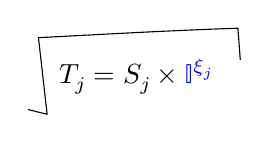
\begin{tikzpicture}[baseline=(lmfixtwentyfour.base),line cap=round,line join=round]
\node[inner sep=2.5pt] (lmfixtwentyfour) {$T_j=S_j\times\unsure{\mathbb I}^{\unsure{\xi_j}}$};
\draw[line width=.4pt]
([xshift=-3mm,yshift=-1mm]lmfixtwentyfour.south west)
-- ([xshift=-.6mm,yshift=-1.6mm]lmfixtwentyfour.south west)
-- ([xshift=-1.7mm,yshift=1.8mm]lmfixtwentyfour.north west)
.. controls ([xshift=6mm,yshift=2.2mm]lmfixtwentyfour.north west) and ([xshift=-7mm,yshift=2.7mm]lmfixtwentyfour.north east) ..
([xshift=2mm,yshift=3mm]lmfixtwentyfour.north east)
-- ([xshift=2.3mm,yshift=-1mm]lmfixtwentyfour.north east);
\end{tikzpicture}} (where $\unsure{\mathbf I|\mathbb I}=[-1,+1]$), $\varepsilon_j=\{j'\in\unsure{J|\mathbf I}\mid j'\text{ over }i\}$\inserted{$\simeq$ set of \uline{orientations} of $S_j$}, $\unsure{\mathbf I^{\varepsilon_j}|\mathbb I^{\varepsilon_j}}$ twisted by $\varepsilon_j$, so that we have a canonical homeomorphism

\[
(25)\qquad \partial T_j\simeq\partial\Delta_j.
\]
\inserted{\unsure{i.e.} $\partial T\simeq\partial V_0$ \deleted{\unsure{id}} \uline{reverses} \unsure{it}}

\margin{so that $X_g=\unsure{V_0|U_0}\amalg_{\partial\Delta}T$ (where $\Delta=\coprod_1^g\Delta_j$, $T=\coprod_1^gT_j$) is \uline{\unsure{oriented|oriented}}}

\margin{N.B. $T_j$ is canonically oriented and the isomorphism (25) \uuline{respects} as \unsure{it should|should} the \unsure{orientation}}

This being understood, the antipodism $\tau$ \unsure{induces} on each $\unsure{\partial T_i|\partial T_j}$ \inserted{$\simeq S_j\times\varepsilon_j$}, \deleted{\illegible{1}}\inserted{the} \inserted{canonical} anti-involution \deleted{\unsure{which}} \inserted{\unsure{coming from this}} \unsure{expression} of $\partial T_i$, which interchanges the two connected components.

For \inserted{\unsure{every|$\forall$}} $j\in\unsure{I|I'}$, we extend $\dot\tau|\partial T_j$ to $T_j$ as two anti-involutions $\dot\tau_j$, \inserted{$\dot\tau'_j$} of $T_j$, \deleted{and we} \deleted{\illegible{1} $T_j$} in such a way that

\scanpage{453}
\mspage{229}

a) \deleted{for $j\in I'$}, $\dot\tau_j$ has no fixed points

b) \deleted{for $j\in I'$}, $\dot\tau'_j$ has a set of fixed points homeomorphic to $S_j$ by the projection $T_j^{\unsure{\dot\tau_j|\dot\tau'_j}}\longrightarrow S_j$ (cf. below \unsure{\}} for \unsure{particular} \unsure{and} explicit choices \unsure{\}}. --- we \unsure{see|will see} that we can \unsure{even|=} suppose $T_j^{\unsure{\dot\tau_j|\dot\tau'_j}}=S_j\times\{0\}$).

Let, for every subset $I'\subset I$, $\tau_{I'}$ be the anti-involution of $X_g=V_0\amalg_{\partial T}T$ (where $V_0=X_0\setminus\bigcup_{j\in J}D'_j$) which coincides with $\tau$ on $V_0$, with $\tau'_j$ on $T_j$ for $j\in I'$, with $\unsure{\tau_j^0|\dot\tau_j}$ for $j\in I\setminus I'$. Then we have
\[
(26)\qquad X_g^{(\tau_{I'})}=\bigcup_{j\in I'}(S_j\times\{0\})
\]
so if $\operatorname{Card}I'=i$ $(0\leq i\leq g)$, then $\tau_{I'}$ is a $\sigma_i$.

Choice of the $\dot\tau_j$, $\dot\tau'_j$. We choose an isomorphism $S_j\simeq\unsure{\mathbb U|\mathbf U}\overset{\unsure{\mathrm{df}}}{=}\{z\in\mathbb C\mid |z|=1\}$, whence an orientation of $S_j$, and a bijection $\varepsilon_j\simeq\{\pm1\}$, \inserted{whence $\unsure{\mathbf I^{\varepsilon_j}|\mathbb I^{\varepsilon_j}}\simeq\unsure{I|\mathbf I}=[-1,+1]$} and we take;
\[
(27)\qquad
\left\{\begin{aligned}
\dot\tau_{\unsure{j|g}}(z,t)&=\deleted{(\unsure{-z|z},-t)}\;(-z\exp\unsure{\pi it},-t)\\
\dot\tau'_{\unsure{j|g}}(z,t)&=(z\deleted{\unsure{\exp\pi it}},-t)
\end{aligned}\right.
\]

\margin{\uline{N.B.} For the definition \unsure{of|of the} $\dot\tau'_j$, we do not need the choice of an isomorphism $S_j\simeq\unsure{\mathbb U|\mathbf U}$ (27)}

\deleted{We do have $\dot\tau^2$} We do have $\dot\tau^2=\mathrm{id}$, $\dot\tau'{}^2=\mathrm{id}$
\[
\dot\tau|\partial T=\dot\tau'|\partial T=\tau|\partial T,
\]
Moreover

\scanpage{454}

We note that
\[
(\dot\tau'\dot\tau)^2
=\dot\tau'\dot\tau\dot\tau'\dot\tau
=\bigl((z,t)\longmapsto(z\exp 2i\pi t,t)\bigr)
\]
this is not the identity map --- \unsure{the set} of its fixed points is equal to: \deleted{\unsure{$S_j$}}
\unsure{the set} of $(z,t)$ such that $t\in\{-1,0,+1\}$ --- i.e.
\[
T_j^{(\dot\tau'_j\dot\tau_j)^2}
=S_j\times[\partial\unsure{\mathbf I|\mathbb I}^{\varepsilon_j}\cup\{0\}]
\tag{28}
\]

\deleted{\unsure{We have}}

\deleted{To \unsure{be able to} write}

Let \unsure{$\rho_j=$.}
\[
\dot\rho_j=\dot\tau'_j\dot\tau_j^{\deleted{\illegible{1}}}
\qquad [(z,t)\longmapsto(-z\exp\pi it,t)]
\tag{29}
\]
--- this is an \unsure{automorphism} of $T_j$ which is the \uline{identity} on $\partial T_j$.
\deleted{and} For every subset $I'$ of $I=J/\tau$, let

(30)\quad $\rho_{I'}$ be the \unsure{automorphism} of $X_g$ which is the identity on
$V_0=X_g-\bigcup_{j\in I-I'}T_j$,
and which is $\rho_j$ on $T_j$ for $j\in I'$.

\margin{Setting $\rho_j=\rho_{\{j\}}$, we will simply have
$\rho_J=\prod_{j\in J}\rho_j$.
Unless I am mistaken, $\rho_j$ generates the group
$\unsure{S\Gamma^{!+}(T_j)|S\Gamma^{!*}(T_j)}\simeq\mathbb Z$,
\unsure{so the $\rho_j$ generate a group} $\simeq\mathbb Z^I$.
\inserted{\unsure{(oriented on}\illegible{1}\unsure{)}}}

\margin{\uline{N.B.} We have
$\rho_j=\tau^{}_{\deleted{\unsure{\varnothing}}\{j\}}\tau_{\varnothing}$.}

We will therefore have
\[
\left\{
\begin{array}{l}
\tau_{I'}\tau_{I''}
=\rho_{I'_0}^{\deleted{\illegible{1}}}\rho_{I''_0}^{-1\,\deleted{\illegible{1}}}
\\[3pt]
\deleted{\unsure{\tau'_{I'}\tau'_{I''}}=\unsure{\rho_{I'_0}\rho_{I''_0}^{-1}}}
\\[3pt]
\deleted{\unsure{(\tau_{I'}\tau_{I''})}\unsure{\illegible{1}}=\rho_{\unsure{I'_0}}\unsure{\illegible{1}}\rho_{\unsure{I''_0}}\unsure{\illegible{1}}}
\end{array}
\right.
\tag{32}
\]
\deleted{\unsure{and the}}
\inserted{where
\deleted{$\unsure{J}=I'\cup I''-\unsure{I'\cap I''}$}
\deleted{$J=I'\cup I''-(I'\cap I'')$}
$I'_0=I'\setminus I'\cap I''$, $I''_0=I''\setminus I'\cap I''$.}

on the other hand we will obviously have
\[
[\rho_J,\rho_K]=1\qquad\text{for }J,K\subset I.
\tag{33}
\]

\uline{Remark.} Instead of an \unsure{isomorphism} $S_j\simeq\mathbb U$,
suppose rather that we are given on

\scanpage{455}
\mspage{230}

$S_j$ a torsor structure under $\mathbb U^{\varepsilon_j}$
($\mathbb U$ twisted by $\varepsilon_j$, \unsure{thanks|taken} to the \unsure{automorphism} of order 2
$z\longmapsto z^{-1}=\bar z$ of $\mathbb U$) We can therefore define
\[
\exp:\underset{\underset{\unsure{\mathbf I|\mathbb I}^{\varepsilon_j}}{\cup}}{\mathbb R^{\varepsilon_j}}
\longrightarrow\mathbb U^{\varepsilon_j}
\tag{36}
\]
in the obvious way, whence \deleted{maps}
\inserted{\uline{anti-involutions}}
$\dot\tau_j,\dot\tau'_j:T_j\xrightarrow{\sim}T_j$ by the formulas (27).

If for example we choose disks $D'_j$ such that their boundaries are \unsure{Euclidean}
\uline{circles}, then there is on each \deleted{\unsure{$S_j$}} $\partial D'_j$
a torsor structure under a group $\mathbb U^{\varepsilon_j}$,
\unsure{invariant|invariant} under antipodism, and which therefore passes to the quotient.
Hence every \unsure{automorphism} of $(X_0,(D'_j))$ which respects this
\deleted{\unsure{shows that the}}
additional structure of torsors --- and in particular every \unsure{automorphism} which respects
the \uline{metric} structure, \deleted{\unsure{respects}} operates on $X_g$ commuting
with the system of $\tau_j,\tau'_j$ in an obvious sense.

\unsure{Equal\textsuperscript{ly}}, if we \deleted{take} \inserted{retain} on $X$
\unsure{the|the} \uline{\unsure{conformal|conformal}} structure sole\textsuperscript{ly}, and if we

\scanpage{456}

chooses in each $D'_j$ a ``center'' $a'_j$, in a way compatible with the involution,
then the choice of the $a'_j\in\mathrm{Int}(D'_j)$ defines a torsor structure on
$\partial D'_j$\unsure{\textsuperscript{*}}, and these structures are invariant under
conformal transformations which respect \unsure{the set} of points $a'_j$.

\margin{\uline{N.B.} We no longer assume \unsure{necessarily} that $D_j$ is a circle,
\unsure{only} that $\partial D_j$ not too \deleted{\illegible{1}} \unsure{wild}.
If $\partial D_j$ is a circle, this definition coincides with the preceding one
\unsure{iff} \unsure{$a_j$|$a'_j$} is the center \unsure{of the|of this} circle\ldots}

\uline{Re-N.B.} To define $\tau_j$ on $T_j$, \unsure{considerably}
less data suffice than a topological torsor structure on $T_j$.
Writing \inserted{for $(z,t)\in S_j\times\unsure{\mathbf I|\mathbb I}^{\varepsilon_j}$}
\[
\tau_j(z,t)=(u_t(z),-t)
\tag{37}
\]
where $u_t:S_j\xrightarrow{\sim}S_j$ is a \unsure{homeomorphism} depending continuously on $t$,
writing that $\tau_j|\partial T_j=\tau|\partial T_j$, we find the condition
\[
\text{a)}\quad u_t=\deleted{\unsure{u_1=}}\mathrm{id}
\quad\text{if }t\in\partial\unsure{\mathbf I|\mathbb I}^{\varepsilon_j}\simeq\varepsilon_j
\]

\margin{\unsure{this} is written, if $S_j$ is oriented, $u_1=u_{-1}=\unsure{0}$.}

writing that $\tau_j^2=\mathrm{id}$ we find the condition
\[
\text{b)}\quad u_{-t}=u_t^{-1}
\qquad(t\in\unsure{\mathbf I|\mathbb I}^{\varepsilon_j})
\]
and writing that $T_j^{\tau_j}=\varnothing$ we find
\[
\text{c)}\quad u_0\text{ without fixed points}.
\]

If an orientation is chosen, the $t\longmapsto u_t$ satisfying a) b) c)
correspond to the maps
$[0,1]\xrightarrow{t\mapsto u_t}\deleted{\unsure{\mathrm{Homéom}}}\inserted{\unsure{\mathrm{Aut}}}(\unsure{S_j|S_1})$
such that $u_1=\mathrm{id}$, $u_0$ without fixed point
\deleted{\illegible{2}}\inserted{\uuline{and of order 2}}.
(The case \unsure{considered} above is the one where
$\unsure{t|*}\longmapsto u_{1-t}$ comes from a continuous representation
$\mathbb R\longrightarrow\mathrm{Aut}(\unsure{S_j|S_1})$\ldots)

\scanpage{457}
\mspage{231}

\uline{Remarks} We may set ourselves the task of determining the structure of all anti-involutions \inserted{$\tau$} on an \inserted{oriented} cylinder $T\simeq S\times\unsure{\mathbf I^{\varepsilon}|\mathbb I^{\varepsilon}}$ $(\varepsilon=\operatorname{Or}(S))$ which \deleted{\unsure{induce}} have no fixed point on the boundary --- which already implies that \deleted{they}\inserted{$\tau$} \unsure{permutes|permute} the two connected components of the boundary. More generally, the anti-involutions \inserted{$\tau$} of an oriented \deleted{\unsure{manifold}}\inserted{surface} \uline{with boundary} $\unsure{X}$, having no fixed point on $\partial\unsure{X}$, correspond to manifolds with boundary $\unsure{Y}$ \unsure{equipped} with a subset both \unsure{open} and \unsure{closed} $(\partial Y)'$ of $\partial Y$ --- by associating to such a $\unsure{(Y,(\partial Y)')}$ its \uline{oriented ``\unsure{doubling}''} relative to $(\partial Y)'$ --- to $X,\sigma$ corresponding $(X/\sigma,\operatorname{Im}X^\sigma\longrightarrow X/\sigma)$. If $X$ is connected, \inserted{compact,} $Y$ is \inserted{compact,} \uline{nonorientable}, suppose that \unsure{its type} $(\gamma,j)$, \deleted{let} and \deleted{\unsure{cardinality} $\pi_0$} \unsure{let} \inserted{$0\leq i\leq j$, and,} $\unsure{i|i'}=\operatorname{card}(\pi_0((\partial Y)'))$\inserted{$={}\operatorname{card}\pi_0(X^\sigma)$}. Thus $\chi(Y)=1-(\gamma+j)$, and we \unsure{know|see} at once that \deleted{$\chi(X)=\chi_!(\operatorname{Int}(X))$} (for the $\chi$ of a circle is zero)
\[
\begin{split}
\chi(X)&=\chi_!\left(\underbrace{X\setminus(\unsure{X\mid\partial Y})}_{\unsure{X\mid\operatorname{Int}(Y)}}\right)\\
&=2\chi_!(\operatorname{Int}Y)=2\chi(Y)=2(1-(\gamma+j))
\end{split}
\]
thus if $X$ is of \deleted{genus}\inserted{type} $(g,\nu)$, we will have \inserted{$\chi(X)=2-2g\unsure{-|+}\nu$}
\[
\deleted{\unsure{g+\nu}}\quad 2-2g\unsure{-|+}\nu=2(1-(\gamma+j))
\]
i.e.
\[
(38)\qquad g+\frac{\nu}{2}=\gamma+j
\]

\margin{not true! If $Y$ orientable of type $(\gamma,j)$ (\unsure{same|with} $0\leq i\leq j$) we will have
\[
(39)\qquad\left\{\begin{array}{l}
g+\dfrac{\nu}{2}=2\gamma+j-1\\
\nu=2(j-i)
\end{array}\right.
\]
i.e. $i=j-\dfrac{\nu}{2}$ (as in the case opposite)}

\scanpage{458}

(this requires that $\nu$ be even, which was obvious a priori, since $\sigma$ must permute the elements of $\pi_0(\partial X)$ among themselves without \inserted{there} being a fixed point\ldots)
\deleted{In the present case $g=1,\nu=2$ we therefore \unsure{find|will find}}
\deleted{$\gamma+i=2$}
\deleted{whence the possibilities}
\deleted{$\gamma=2,\ i=0$}
\inserted{But I forgot to note that $\nu$ is determined as a function of $(\gamma,j,i\inserted{={}\unsure{\operatorname{card}((\partial Y)')}})$ by}
\deleted{$\nu=2(j-i)+\unsure{i^{\varepsilon}|i}=2j-i$}
\deleted{$\gamma=2(j-i)$ \unsure{thus}}
\deleted{\unsure{must have}}
\[
(39)\qquad \nu=2(j-i)
\]
i.e. \uline{$i=j-\dfrac{\nu}{2}$}.

Thus here (for $g=0,\nu=2$) we must look for $(\gamma,j,i)$, with $\gamma\in\mathbb N,\ 0\leq i\leq j\in\mathbb N$, such that we have $\nu=2(j-i)$ i.e. $j-i=1$ i.e. $i=j-1$, and $\gamma+j=1$, which gives the \inserted{only} possibility (since $i$ must be $\geq0$ hence $j\geq1$)

a) $\gamma=0,\ j=1,\ i=0$ \unsure{:|.}

\deleted{b) $\unsure{\gamma=1|\gamma=0},\ \unsure{j=0|j=1},\ i=0$.}

Case a) corresponds to the case where \deleted{\illegible{1}} $T^\sigma=\varnothing$, \deleted{it \illegible{2} \unsure{necessarily} a connected component, and} is obtained from the real projective plane by making \deleted{two}\inserted{one} \unsure{hole|holes} in it, \inserted{with boundary (hence Möbius strip)} and by \deleted{bounding one of them by}\inserted{taking the \deleted{\unsure{oriented covering}} oriented doubling}. \deleted{relative to one of these holes.}

The case where $T^\sigma\neq\varnothing$ will necessarily give a quotient \inserted{$Y$} that is \uline{oriented}, we must have for its type $\unsure{(\gamma,j)}$ (since $j\geq1$), the sole case:

\scanpage{459}
\mspage{232}

b) $\gamma=0,\ j=2,\ i=1$ (\uline{oriented} quotient)

obtained from the sphere with two holes i.e. from the cylinder, by taking the oriented doubling \unsure{with respect} to \uline{one} of the holes. \deleted{These are indeed the}

These are indeed the two cases obtained \unsure{resp.\textsuperscript{t}} by $\dot\tau$ and $\dot\tau'$ in formulas (27).

I would now like to construct a situation (under the conditions of the proposition) bringing out a maximum of \unsure{symmetries} --- it is true that we could \unsure{work} with \deleted{\unsure{the} \illegible{1} \unsure{of the}} the \unsure{automorphisms} of $X_0$ \unsure{commuting} with the antipodism\inserted{$\tau$}, \inserted{preserving \unsure{the set} of the $D'_j$,} and respecting (say) topological \unsure{torsors|torsor} structures on \unsure{the set} of the $\partial D'_j$ --- or what \unsure{naturally} amounts to the same (up to an \unsure{indeterminacy} of multiplication by $\unsure{\tau|2}$) the \unsure{automorphisms} of $Y_0$ which \deleted{\illegible{1}} \unsure{preserve|preserving} $D=\bigcup_{i\in I}D_i$, and \unsure{respect|respecting} \unsure{torsor|torsors} structures on \deleted{the boundaries} the connected components $\partial D_i$ of $\partial D$. We expect that (working modulo isotopy) we \unsure{will have|obtain} a group

\margin{no, \uline{without} indeterminacy, by lifting \unsure{defined|to the sphere} so as to \unsure{respect} \unsure{the orientations|the orientation}\ldots}

\scanpage{460}

which will be close to a braid group, and probably computable without much trouble --- and by putting \inserted{\unsure{it}} together with the group generated by the preceding operators, we will perhaps find a start for \unsure{generating} for example \unsure{$\mathcal T_g$|$\Pi_g$} by generators \inserted{(anti-involutive?)} and relations.

Let us consider the \deleted{\unsure{sub}}group $G$ of $A_g=\operatorname{Aut}X_g$ generated by the \deleted{\illegible{1}}\inserted{$\tau_{I'}$} $(I'\in I)$, \deleted{the} Let $\mathcal H$ \deleted{commutators of generators are in} be the subgroup generated by the $\rho_j$ $(j\in I)$. We have
\[
\begin{aligned}
\tau_{I'}\rho_j\tau_{I'}
&=\deleted{\unsure{(\tau_{I'}(\tau_{\{j\}}\tau_{\varnothing})\tau_{I'})}}
\tau_{I'}(\tau_{\{j\}}\tau_{\varnothing})\tau_{I'}\\
&=(\tau_{I'}\tau_{\{j\}})
\underbrace{(\tau_{\varnothing}\tau_{I'})}_{\deleted{\unsure{\rho_{I'_0}}}\unsure{\rho_{I'}}}
\in\mathcal H
\end{aligned}
\]
by formula \unsure{(31)|(32)}, so $\mathcal H$ is an invariant subgroup.

Formulas (32) show that $G/\mathcal H$ is a \uline{commutative} group, \deleted{\unsure{isomorphic to}}\inserted{and even that it is \unsure{isomorphic to}} $\pm1$ by the orientation character (all the $\tau_{I'}$ are equal modulo $\mathcal H$).

\subsection*{Scans 461--470}
\addcontentsline{toc}{subsection}{Scans 461--470}
% package LM_P047
\scanpage{461}
\mspage{233}

Let us consider as reference element of $\mathcal H^{-}$ the element
\[
(40)\qquad \tau=\tau_{\varnothing}\qquad
\text{(anti-involution without fixed points of $X_g$)}
\]
we then find \inserted{by (32)} that for $I'\subset I$
\[
(41)\qquad \tau_{I'}=\rho_{I'}\tau=
\left(\prod_{j\in I'}\rho_j\right)\cdot\tau\quad
\deleted{\unsure{=\rho_h}}
\]
\margin{we see at once, since $\tau^2=1$, $\tau_{I'}^2=1$, that
$\tau_{I'}=\tau_{I'}^{-1}=\tau\rho_{I'}^{-1}$
\unsure{hence} $\tau\rho_{I'}\tau=\rho_{I'}^{-1}$
\unsure{which is $(42)$|which $\Rightarrow(42)$}}
moreover we will have, for \inserted{$\unsure{j|i}\in I$}
\[
\tau\rho_{i}\tau
=\tau_{\varnothing}\left(\tau_{\{\unsure{j|i}\}}\tau_{\{\varnothing\}}\right)
\tau_{\{0\}}
=\tau_{\varnothing}\tau_{\{j\}}=\rho_j^{-1}
\]
\[
(42)\qquad \tau\rho_{i}\tau^{-1}=\rho_{i}^{-1}.
\]

Thus $\mathcal G$ appears as the semidirect product of $\mathcal H\simeq\mathbb Z^I$, and of
\deleted{\illegible{2}}
$\{\pm1\}\simeq\{1,\tau\}$ operating on it by the symmetry
$\rho\longmapsto\rho^{-1}$. So for \uline{every} $\rho\in\mathcal H$,
\unsure{\deleted{$\tau\rho$} we have}
$(\tau\rho)^2=1$, i.e. for every
$\sigma\in\mathcal H^{-1}$,
$\sigma$ \deleted{\illegible{1}} \uline{is an anti-involution} !
Since $\sigma$ agrees with $\tau$ on
$V_0=X_g-\bigcup_{\unsure{j|i}\in I}\operatorname{Int}(T_j)$,
we see that the set of fixed points of $\sigma$ is contained in
$\bigcup_{i\in I}\operatorname{Int}(T_i)$, and to calculate the index of $\sigma$,
i.e. $\operatorname{card}\pi_0(X_g^\sigma)$, it suffices to take the sum of the
\margin{460}

\scanpage{462}

indices in the $T_j$. Now in $T_j$, we have \inserted{(29)}
$\rho_j(z,t)=(-z\exp\pi it,t)$, and by induction
\[
(43)\qquad \rho_j^{n_j}(z,t)=\left((-1)^{n_j}z\exp n_j\pi it,t\right)
\]
hence
\[
(44)\qquad \tau\rho_j^{n_j}(z,t)=
\left((-1)^{n_j+1}z\exp(n_j+1)\pi it,-t\right)
\]
and \deleted{\illegible{1}} $(z,t)$\inserted{$\in T_j$} is a fixed point of
$\unsure{z|\tau}\rho_j^{n_j}$ \unsure{iff|without}
$t=0$, \deleted{\unsure{if|and}} and $n_j$ is \uline{odd}, hence
\[
(45)\qquad T_j^{\tau\rho_j^{n_j}}=
\begin{cases}
\varnothing&\text{if $n_j$ even}\\
S_j\times\{0\}&\text{if $n_j$ odd}
\end{cases}
\]

hence
\[
\begin{gathered}
(46)\qquad \text{Index of }u=\tau\prod_j\rho_j^{n_j}\text{ is equal to the cardinality}\\
\text{of the set }I'_u\text{ of the }j\in I\text{ such that }n_j\\
\text{\unsure{is|are} odd}
\end{gathered}
\]

It follows \inserted{for general reasons} that $u$ is conjugate in
$\mathcal A_g=\operatorname{Aut}(X_g)$
\inserted{(by an element of $\unsure{A_g^+|\widetilde A_g^+}$)}
to $\tau_{I'}=\rho_{I'}\tau=\tau\rho_{I'}^{-1}$ \unsure{or also}
$\rho_{I'}^{-1}\tau=\tau\rho_{I'}$ ---
\deleted{
\unsure{but} \illegible{4}
\inserted{we have the equality \illegible{2} $\mathcal H$}
\unsure{in the group} $\mathcal G$ (\unsure{too small}).
\illegible{4} $\rho\in\mathcal H$, \illegible{2}
\unsure{the questions}, on the one hand
\[
\unsure{(\tau\rho)^{-1}}\cdot\rho_{I'}(\tau\rho)
=\unsure{\tau\rho\rho_{I'}}
\]
by introducing additional groups of symmetries, on the other hand by
\deleted{\unsure{enlarging it}, by} \unsure{completing}
each $T_j$ with a \unsure{configuration} more
}
\margin{\deleted{
\[
\unsure{(\tau\rho)(\tau\rho')(\tau\rho)^{-1}}
=\underset{\text{\deleted{\illegible{1}}}}{\tau\rho}\,
\underbrace{\tau\rho'\rho^{-1}\tau}_{\rho\rho'^{-1}}
=\tau\rho^{2}\rho'^{-1}=\tau\rho''
\]
as soon as $\rho^2=\rho'\rho''$, \unsure{i.e.|i.e.}
\illegible{3} $\tau\rho'$ is \unsure{conjugate} \illegible{1}
$\unsure{\tau\rho''}$ in $\mathcal G$, as soon as
$\rho'\rho''\in\mathcal H^2$
}}
\margin{461}

\scanpage{463}
\mspage{234}

But if $\tau\rho',\tau\rho''\in\mathcal G^-$, $(\rho',\rho''\in\mathcal H)$, and if
$\rho\in\mathcal H$, the relation
\[
\rho(\tau\rho')\rho^{-1}=\tau\rho''
\]
is equivalent to
\[
\underbrace{\tau\rho\tau}_{\rho^{-1}}\rho'\rho^{-1}=\rho''
\qquad\text{i.e.}\qquad \rho^2=\rho'\rho''^{-1}
\]
hence $\tau\rho'$ and $\tau\rho''$ are conjugate by an element of $\mathcal H$
\unsure{iff|without} $\rho'\rho''^{-1}\in\mathcal H^2$ -- which makes the preceding observation more precise\ldots

The way richest in simple symmetries for arranging the $2g$ antipodal holes
$D_j$ seems to me to be the following. We \deleted{\illegible{1}} consider
the Euclidean sphere, with \unsure{the} action of the dihedral group
$\unsure{\mathbb D_{2g}|\mathbf D_{2g}}$ -- for example, when it is the Riemann sphere that is
considered as Riemannian, by the choice of the antipodism as being
\[
(47)\qquad \tau z=-\frac{1}{\overline z}
\]
we take the standard action of the dihedral group (with the points $0,\infty$ as poles, and
the unit circle $\mathbb U=\{z\in\mathbb C\mathbin{:}|z|=1\}$ as equator),
\deleted{by} by writing
$\unsure{\mathbb D_n|\mathbf D_n}$ as $\subset\operatorname O(\deleted{\unsure{3}}2,\mathbb R)$,
as a $\frac12$ direct product of
\deleted{\unsure{$\mathbb Z/2\mathbb Z$}}\inserted{$\{\pm1\}$} by $\mu_n(\mathbb C)=\mu_n$,
the pair $(\zeta,\alpha)$ $(\zeta\in\mu_n,\alpha\in\deleted{\unsure{\mathbb Z/2\mathbb Z}}\inserted{\{\pm1\}})$ operating by
\[
(48)\qquad u_{\zeta,\alpha}(z)=\zeta z^\alpha
\]
\margin{462}

\scanpage{464}

We can moreover enlarge it to a group
$\mathbb D_n^\sim=\mathbb D_n\times\mathbb Z_{/2}$,
where the second factor $\mathbb Z_{/2}$ is generated by the antipodism (47)
(which commutes with $\mathbb D_n$ --- likewise moreover
does the anti-involution $z\longmapsto\frac{1}{\bar z}$, which has as its
set of fixed points $\mathbb U$ and is nothing other than the symmetry with respect to
the equator, their composite $z\longmapsto-z$ being the symmetry with respect to
the axis of the poles \ldots) hence to consider the transformations
\[
u_{\zeta,\alpha,\beta}\deleted{(z)}=\unsure{\zeta}u_{\zeta,\alpha}\tau^\beta
\qquad
(\zeta\in\mu_n,\ \alpha\in\{\pm1\},\ \beta\in\mathbb Z_{/2})
\]
hence
\[
u_{\zeta,\alpha,\beta}z=
\begin{cases}
u_{\zeta,\alpha}(z)=\zeta z^\alpha&\mathrm{si}\ \beta=0\\
u_{\zeta,\alpha}(-\frac{1}{\bar z})=-\zeta\bar z^{-\alpha}
&\mathrm{si}\ \beta=1
\end{cases},
\]
but we \unsure{will remember} that $\tau$ reverses the orientation,
hence \deleted{\illegible{1}}\inserted{is to be}
\deleted{\unsure{more}}\inserted{handled} with
caution as regards ``transport of structure'' in
the present situation.

Here $n=2g$, $\mathbb D_{\unsure{2g|n}}$ is of order $4g$, and
$\mathbb D_n^\sim$ of order $8g$. We take on the equator an
orbit $\unsure{\mathcal J|\mathbb J}$, of $\mu_n=\mu_{2g}$, for example
\unsure{the|here} \unsure{precisely}
\deleted{\unsure{the}} ($\mu_{2g}$
\inserted{\unsure{the set} of \unsure{$2g$th} roots of unity}
itself, \unsure{viewed}\deleted{\illegible{1}}
\unsure{as} a subset of the sphere) as the set of ``centers''
of the disks $D'_i$. We choose a disk $D'_0$ around the
\unsure{point|point} $P_0$ (small enough for what is to follow), and we
take the \unsure{transforms|transforms} of $D'_0$ by the
$\zeta\in\mu_n$.

\margin{it is \unsure{simply} necessary that $D'_0$ not
\unsure{meet} $\unsure{\zeta_0|\zeta}D'_0$,
\unsure{where} $\zeta=\exp\frac{2i\pi}{2g}$}

\margin{463}

\scanpage{465}
\mspage{235}

These choices having been made, the surface $X_g$ is determined without
\unsure{ambiguity|ambiguity}, and the group $\mathbb D_{2g}$ operates on it by transport of
structure, permuting the $g$ cylinders $T_i$ among themselves,
\unsure{corresponding|corresponding} to the elements of
\inserted{$\unsure{\mathcal J|\mathbb J}/\tau=$}$\unsure{\mathcal J|\mathbb J}/\{\pm1\}$ i.e.
to the pairs of antipodal elements of $\unsure{S|\mathcal J}$,
i.e. to the ``diagonals'' of the polygon with $2\mu$ sides
which they \deleted{\unsure{form}}\inserted{determine}
on the equator. The group $\mathbb D_{2g}$ normalizes
\deleted{\illegible{1}} the group $\mathcal G$, to be precise
we will have, for $u\in\mathbb D_{2g}$
\[
\tag{49}
u\tau_{I'}u^{-1}=\tau_{u(I')}
\]
for $I'\subset I=\unsure{\mathcal J|\mathbb J}/\tau$, taking into account
the operation of $\mathbb D_{2g}$ on $I$. We will thus have in
particular, denoting by $\tau_g$\inserted{$=\tau_\varnothing$}
the extension \margin{\deleted{(50)}} of the antipodism of the sphere $X_0$
(or rather of $\unsure{\tau}\vert V_0$) to an antipodism
without fixed points of $X_g$, denoted $\tau$ previously:
\[
\tag{50}
u\tau_g u^{-1}=\tau_g
\qquad\text{i.e. $\tau_g$ commutes with the action of $\mathbb D_n$}
\]
\[
\deleted{\unsure{(51)}}\qquad
u\rho_j u^{-1}=\rho_{u\unsure{(}j)}
\]

We can therefore say that $\mathbb D_{2g}$ operates on $\mathcal G$,
whence a $\frac12$-direct product $\mathbb D_{2g}.\mathcal G$,
which therefore operates on $X_g$.
As for the question of extending likewise
the action \inserted{on $X_0$,} of $\mathbb D_{2g}^\sim$
\deleted{on $X_0$} \unsure{as a whole} to an action on $X_g$,

\margin{464}

\scanpage{466}

this has been done without warning, to $\tau_{X_0}$ corresponding
naturally $\tau_{X_g}=\tau_g$, which indeed has the good taste
to commute with the action of $\mathbb D_{2g}$.
[It might seem more natural, it is true, in a
spirit of ``transport of structure (\unsure{in spite of} and against
everything?)'', to associate to $\tau_{X_0}$ the operation
$\tau_I$\inserted{\unsure{given|given} by (27)}, which on
each $T_j$ would be equal to $\tau'_j$
(and on $V_0$, of course, coincides with $\tau_{X_0}$),
$\tau'_j(z,t)=(z,-t)$,
\deleted{hence} the set of fixed points of $\tau_I^{\unsure{2}}$
being formed of the $g$ \unsure{middle} circles $S_j\times\{0\}$
of the $g$ tubes $T_j$. We will have by (41)
$\tau_I=\rho_I\tau_g$, hence $\tau_I$ commutes
\unsure{also} with $\mathbb D_n$, since $\tau$ and
$\rho_I=\prod_{i\in I}\rho_i$ commute with it.
But it \unsure{does|to me does} not seem \unsure{important} for the moment
which convention we \unsure{adopt}]

We can therefore also say that the group $\mathbb D_{2g}^\sim$
operates on $\mathcal H$ --- this operation extending that
of $\tau_g$\deleted{\unsure{by}}, now identified with an
element of $\mathbb D_{2g}^\sim$, i.e. with the antipodism in
$\mathbb D_{2g}^\sim$ --- and the $\frac12$ direct product
\[
\tag{51}
\mathbb D_{2g}^\sim.\mathcal H\supset\mathcal G
=\deleted{\unsure{\mathcal H}}\{1,\tau_g\}.\mathcal H
\]

\margin{465}

\scanpage{467}
\mspage{236}

operates on $X_g$.

One should now, along these lines:

1) Make explicit the outer action of this $\frac12$ direct product on the fundamental group $\pi_g$, \unsure{with} very special attention to the action of the group $(\mathbb Z/2\mathbb Z)^3\subset\mathbb D_{2g}^{\sim}$ which stabilizes one of the cylinders $T_j$ --- which in Euclidean space of dimension 3 is interpreted as the group of \unsure{changes} of sign relative \unsure{to the|a} corresponding orthonormal system of axes.

2) Extend the action \inserted{on $\pi_g$} of the (more or less) ``special'' Teichmüller group of each of the $T_j$, to the action of an analogous group of a larger set obtained by adding to it a ``strip'' \inserted{$L$} (whence a torus with 1 hole, and its special Teichmüller group, which \unsure{come in} naturally$^*$) \unsure{or even|see} the still larger set obtained by also putting in the antipodal strip $L'$ (this set presents itself as a cylinder $(L\cup L')$, or ``culvert'', in which one would have put a tube $(T_j)$ crosswise, and has the topological structure of a torus with two holes.

\figure{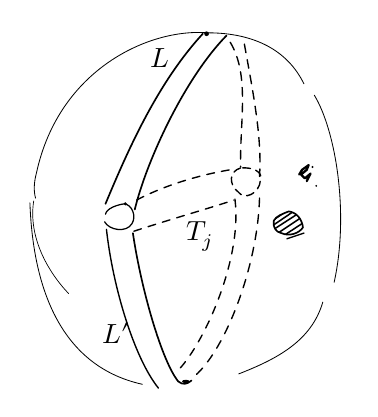
\begin{tikzpicture}[x=.12mm,y=-.12mm,line cap=round,line join=round]
\draw[line width=.3pt] (194,39) .. controls (133,34) and (37,77) .. (13,187) .. controls (10,198) and (10,207) .. (12,214);
\draw[line width=.3pt] (194,39) .. controls (244,39) and (279,58) .. (296,93);
\draw[line width=.3pt] (307,105) .. controls (330,143) and (344,231) .. (328,303);
\draw[line width=.3pt] (316,324) .. controls (304,365) and (268,384) .. (227,400);
\draw[line width=.3pt] (6,219) .. controls (9,303) and (35,391) .. (125,411);
\draw[line width=.25pt] (10,217) .. controls (4,255) and (25,292) .. (47,315);
\draw[line width=.6pt] (189,40) .. controls (142,91) and (111,160) .. (86,220);
\draw[line width=.6pt] (214,42) .. controls (169,88) and (129,176) .. (117,226);
\draw[line width=.5pt] (87,247) .. controls (94,310) and (117,384) .. (142,415);
\draw[line width=.6pt] (115,251) .. controls (124,312) and (146,387) .. (163,408) .. controls (168,412) and (172,411) .. (177,407);
\draw[line width=.45pt] (86,231) .. controls (87,225) and (98,221) .. (106,220) .. controls (114,221) and (119,233) .. (114,241) .. controls (108,251) and (90,248) .. (85,239);
\draw[line width=.5pt,dash pattern=on 1.1mm off .9mm] (218,49) .. controls (239,84) and (228,133) .. (229,181);
\draw[line width=.5pt,dash pattern=on 1.1mm off .9mm] (233,51) .. controls (241,96) and (252,149) .. (249,191);
\draw[line width=.5pt,dash pattern=on 1mm off .7mm] (229,182) .. controls (216,186) and (217,200) .. (226,207) .. controls (233,217) and (249,209) .. (250,195) .. controls (253,186) and (242,181) .. (229,182);
\draw[line width=.5pt,dash pattern=on 1mm off 1mm] (223,215) .. controls (231,278) and (191,366) .. (164,395);
\draw[line width=.5pt,dash pattern=on 1.1mm off 1mm] (249,214) .. controls (247,288) and (211,380) .. (177,405);
\draw[line width=.5pt,dash pattern=on 1mm off .9mm] (119,216) .. controls (155,197) and (197,187) .. (224,183);
\draw[line width=.5pt,dash pattern=on 1mm off .9mm] (116,249) .. controls (156,236) and (198,224) .. (222,216);
\fill (193,40) circle[radius=.3mm];
\fill (171,408) ellipse[x radius=.48mm,y radius=.216mm];
\fill (107,220) circle[radius=.216mm];
\node[inner sep=0pt] at (144,66) {$L$};
\node[inner sep=0pt] at (98,357) {$L'$};
\node[inner sep=0pt] at (186,255) {$T_j$};
\draw[line width=.8pt] (291,189) -- (294,184) -- (301,179) -- (299,184) -- (293,189) -- (297,193) -- (303,188) -- (299,196);
\fill (305,181) circle[radius=.144mm];
\fill (309,201) circle[radius=.132mm];
\draw[line width=.6pt] (264,238) .. controls (266,233) and (275,230) .. (280,228) .. controls (288,229) and (294,236) .. (295,245) .. controls (291,251) and (281,255) .. (272,251) .. controls (266,250) and (263,244) .. (264,238);
\begin{scope}
\clip (264,238) .. controls (266,233) and (275,230) .. (280,228) .. controls (288,229) and (294,236) .. (295,245) .. controls (291,251) and (281,255) .. (272,251) .. controls (266,250) and (263,244) .. (264,238);
\draw[line width=.55pt] (258,241)--(283,224) (260,245)--(288,226) (261,249)--(292,229) (264,254)--(297,232) (271,256)--(300,237) (280,257)--(302,242);
\end{scope}
\draw[line width=.5pt] (278,257) -- (296,251);
\end{tikzpicture}}

\margin{$^*$ This is essentially an $\mathrm{SL}(2,\mathbb Z)$ --- rather a \unsure{remarkable} central extension of $\mathrm{SL}(2,\mathbb Z)$ by $\mathbb Z$, which \unsure{recalls} that of $\mathrm{SL}(2,\mathbb R)$ by $\mathbb Z$\ldots\ (universal covering of $\mathrm{SL}(2,\mathbb R)$)}

\figure{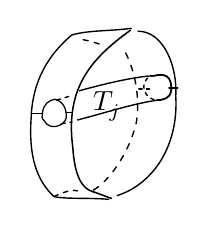
\begin{tikzpicture}[x=.12mm,y=-.12mm,line cap=round,line join=round]
\draw[line width=.5pt] (118,15) .. controls (94,18) and (72,17) .. (55,22) .. controls (24,48) and (13,79) .. (12,109) .. controls (9,151) and (18,176) .. (36,193) .. controls (49,196) and (75,194) .. (94,196);
\draw[line width=.5pt] (125,18) .. controls (153,18) and (167,57) .. (165,87) .. controls (168,137) and (143,179) .. (103,192);
\draw[line width=.55pt] (117,17) .. controls (74,48) and (48,79) .. (56,141) .. controls (58,170) and (65,185) .. (78,188) -- (97,195);
\draw[line width=.5pt,dash pattern=on .65mm off .8mm] (67,27) .. controls (74,28) and (82,31) .. (89,33);
\draw[line width=.5pt,dash pattern=on .75mm off .95mm] (112,41) .. controls (124,65) and (127,94) .. (123,116) .. controls (115,148) and (94,177) .. (78,186);
\draw[line width=.45pt] (24,104) .. controls (25,95) and (31,91) .. (37,90) .. controls (46,92) and (50,101) .. (49,110) .. controls (47,118) and (32,124) .. (26,113) .. controls (23,111) and (23,107) .. (24,104);
\draw[line width=.5pt] (12,105) -- (24,105) (49,104) -- (55,104);
\draw[line width=.5pt,dash pattern=on .5mm off .6mm] (39,91) -- (55,86) (44,116) -- (55,114);
\draw[line width=.5pt] (63,81) .. controls (85,75) and (120,66) .. (143,65);
\draw[line width=.5pt] (61,112) .. controls (88,105) and (122,94) .. (146,91);
\draw[line width=.65pt] (143,65) .. controls (159,61) and (161,72) .. (160,82) .. controls (159,88) and (153,91) .. (145,91);
\draw[line width=.5pt,dash pattern=on .45mm off .55mm] (143,65) .. controls (128,65) and (126,87) .. (144,91);
\draw[line width=.55pt,dash pattern=on .4mm off .55mm] (126,79)--(141,79);
\draw[line width=.7pt] (158,78)--(167,78);
\draw[line width=.5pt,dash pattern=on .6mm off .7mm] (36,193) .. controls (47,188) and (56,185) .. (61,187);
\fill (78,188) circle[radius=.18mm];
\node[inner sep=0pt] at (92,98) {$T_j$};
\end{tikzpicture}}

\margin{466}

\scanpage{468}

It is possible that it will be necessary to look closely at this last one, to study the relations among \inserted{the} elements of $\mathcal T_g$ coming from the preceding sets\ldots\ An amusing job will be to manage to write down the generators of the group $\pi_g$, and above all the famous relation, in a relative geometric arrangement of the ``handles'', which is a ``\unsure{mixed}'' arrangement --- and no longer \uline{nicely} in single file!

\deleted{I see \unsure{appearing}}

While waiting to get to the heart of the structure of the Teichmüller group in this way, I will already try to describe generators and relations for the interesting subgroup we have just written down, $\mathbb D_{2g}^{\sim}\cdot H$.
I will take the everlasting generators $\varepsilon_0,\varepsilon_1$ of $\mathbb D_{2g}$
\[
\varepsilon_0^2=\varepsilon_1^2=1,\qquad (\varepsilon_0\varepsilon_1)^{2g}=1
\]
and adjoin to them $\tau=\tau_g$, and \deleted{\illegible{1}} $\rho_0\tau=\tau'$
($\rho_0=\rho_{j_0}$, $j_0$ marked point of $I=J/\tau$)
satisfying
\[
\tau^2=\tau'^2=1,\qquad
\deleted{[\tau,\varepsilon_0]=\unsure{[\varepsilon_1,\tau]|[\tau,\varepsilon_1]}=}
\]
\[
(\tau\varepsilon_0)^2=(\tau\varepsilon_1)^2=1\quad
\deleted{\unsure{(\tau'\varepsilon_0)^2=(\tau'\varepsilon_1)^2}=1}
\]
\[
(\varepsilon_1\tau')^2=1
\qquad \varepsilon_1\ \text{commutes with}\ \tau'
\]

\margin{\uline{N.B.} $\varepsilon_0$ moves \unsure{the vertex} of the frame, $\varepsilon_1$ the edge and not the vertex, hence $\varepsilon_1(j_0)=j_0$}

\margin{\unsure{express} the commutation of $\tau$ \deleted{\illegible{1}} with $\varepsilon_0,\varepsilon_1$}

\margin{467}

\scanpage{469}
\mspage{237}

\[
((\varepsilon_0\varepsilon_1)^g\tau')^2=1
\]
\margin{(the involution $(\varepsilon_0\varepsilon_1)^g$ commutes with $\tau'$)}

unless I am mistaken, that gives a set of generators and relations for $\mathbb D_{2g}^{\sim}\cdot\mathcal H$ --- in summary $\varepsilon_0,\varepsilon_1,\tau,\tau'$
\[
\text{(52)}\quad
\left\{
\begin{array}{l}
\varepsilon_0^2=\varepsilon_1^2=\tau^2=\tau'^2=1\\
(\tau\varepsilon_0)^2=(\tau\varepsilon_1)^2=(\tau'\varepsilon_1)^2=1\\
(\varepsilon_0\varepsilon_1)^{2g}=1\\
(\tau'(\varepsilon_0\varepsilon_1)^g)^2=1
\end{array}
\right.
\]

This is perhaps not a very clever choice of generators, in the sense that $\varepsilon_0,\varepsilon_1$, are not at all on the same footing as $\tau,\tau'$ --- they are not \uline{anti}-\unsure{involutions}. It would be better to take $\varepsilon'_0=\tau\varepsilon_0$, $\varepsilon'_1=\tau\unsure{\varepsilon_1}$ so as to obtain
\[
\text{(52bis)}\quad
\left\{
\begin{array}{l}
\varepsilon_0^{\prime 2}=\varepsilon_1^{\prime 2}=\tau^2=\tau'^2=1\\
(\tau\varepsilon'_0)^2=(\tau\varepsilon'_1)^2=(\tau'(\tau\varepsilon'_1))^2=1\\
(\varepsilon'_0\varepsilon'_1)^{2g}=1\\
(\tau'(\varepsilon'_0\varepsilon'_1)^g)^2=1
\end{array}
\right.
\]
these are essentially ``the same'' relations except for the last one in the second line.

Perhaps this little game with the tiny group $\mathbb D_n^{\sim}$ operating on $\mathcal H$ is a bit of a \unsure{diversion} --- the group $\mathcal H\simeq\mathbb Z^g$ in $\mathcal T_g$ strongly suggests the situation

\margin{468}

\scanpage{470}

of a maximal torus in a $\frac12$ simple group, one really wants to \unsure{have|see} an intrinsic characterization of it in $\mathcal T_g$ --- or in $\unsure{\mathcal S_g|\mathcal G_g|\mathcal C_g}$, which is possible since \deleted{\illegible{1}} as a group of \unsure{actual|actual} topological transformations, it leaves fixed the points of $V_0\subset X_g$ --- for example the two poles, which one can take as \unsure{base|base} points to construct universal coverings and \unsure{fundamental|fundamental} groups. These are perhaps the maximal free-\unsure{abelian|abelian} subgroups.

One would like to study the normalizer --- is it exactly what comes from the automorphisms of $X_g-\bigcup\mathring{T}_i\simeq V_0$?

do the $\mathrm{SL}(2,\mathbb Z_{\unsure{j}})$ associated with the ``strips'' through the tube \inserted{$T_j$} play a role analogous to that of the groups $\mathrm{SL}(2,K)$ or $\unsure{\mathrm{GP}(1,k)|\mathrm{GL}(1,k)}$ ``of rank 1'' in the theory of reductive algebraic groups? If Jean \unsure{does not|me} ``\unsure{bite}''

\margin{469}

\subsection*{Scans 471--480}
\addcontentsline{toc}{subsection}{Scans 471--480}
% package LM_P048
\scanpage{471}
\mspage{238}

not to the situation, perhaps submit it to Carlos, who is at ease both with discrete groups and their generators and relations, and with the theory of $\frac{1}{2}$ simples -- and topology ....

\scanpage{472}
\mspage{239}

\uline{33} Study of finite coverings -- relation between the $\mathcal N_{g,\nu},\Gamma_{g,\nu}$ for variable $g$.

Let $(\pi\deleted{,\unsure{a}})$ be an arithmetized profinite outer group with loops of type $(g,\nu)$, $\pi'$ an open \unsure{subgroup|subgroup} of $\pi$, whence an injective map
\[
\mathrm{Discr\acute{e}t}(\pi)\hookrightarrow
\mathrm{Discr\acute{e}t}(\pi'),
\]
we would like to prove that it is compatible with the equivalence relation \deleted{\unsure{of the}\ \illegible{1}}\inserted{\unsure{of arithmetization|of arithmetizability}}, in \deleted{\unsure{prove}} such a way that every arithmetization of $\pi$ gives one of $\pi'$, and likewise for the \deleted{\unsure{discre}} prediscretifications.

We would like to establish at the same time that the maps
\[
\begin{array}{lll}
 &P^+(\pi)\longrightarrow P^+(\pi')&\begin{gathered}\text{on the oriented}\\\text{prediscretifications}\end{gathered}\\[1em]
\text{and}&A(\pi)\unsure{\longrightarrow|-}A(\pi')&\text{on the arithmetizations}
\end{array}
\]
are injective. To prove these points, we are reduced to the case where $\pi'$ is characteristically invariant. (Cf. \S\,28, diagram 7, \unsure{ff}) Choosing

\scanpage{473}

a discretification $\pi_0$ of $\pi$, hence $\pi'_0$ of $\pi'$, we then find
\[
\unsure{\widehat{\widehat{\mathcal G}}}(\pi_0)\longrightarrow
\unsure{\widehat{\widehat{\mathcal G}}}(\pi'_0)
\]
and we have

\textcircled{1} The homomorphism $\unsure{\widehat{\widehat{\mathcal G}}}(\pi_0)\unsure{\longrightarrow}\unsure{\widehat{\widehat{\mathcal G}}}(\pi'_0)$ sends $\mathcal M(\pi_0)$ into $\mathcal M(\pi'_0)$

we will therefore have a diagram (a \unsure{variant|relative} of the one in \S\,28)
\diagram{\begin{tikzcd}[ampersand replacement=\&,column sep=large,row sep=large]
\unsure{(1)} \&
\widehat{\mathcal G}^{+}(\pi_0)
 \arrow[r,hook,no head] \arrow[d,hook] \&
\mathcal M(\pi_0) \arrow[r,hook,no head] \arrow[d,hook] \&
\widehat{\widehat{\mathcal G}}(\pi_0) \arrow[d,hook] \\
\& \widehat{\mathcal G}^{+}(\pi'_0)
 \arrow[r,hook,no head] \&
\mathcal M^{\unsure{\ast|\sharp}}(\pi'_0) \arrow[r,hook,no head] \&
\unsure{\widehat{\widehat{\mathcal G}}}(\pi'_0)
\end{tikzcd}}
which \deleted{means} implies that a discretification $\pi_1$ on $\pi$ which gives the same oriented prediscretification as $\pi_0$ (resp. the same arithmetization) defines a \inserted{\unsure{discretification}} $\pi'_1$ of $\pi'$ which gives the same oriented prediscretification (resp. the same arithmetization) as $\pi'_0$. Thus we do have $\unsure{P}^{+}(\pi)\longrightarrow P^+(\pi')$, $A(\pi)\longrightarrow A(\pi')$, we still have to express injectivity, which amounts to the relations
\[
\begin{gathered}
(2)\quad
\unsure{\widehat{\mathcal G}^{+}}(\pi_0)
=
\unsure{\widehat{\mathcal G}^{+}}(\pi'_0)\cap
\unsure{\widehat{\widehat{\mathcal G}}}(\pi_0),\qquad
\mathcal M(\pi_0)=\mathcal M(\pi'_0)\cap
\unsure{\widehat{\widehat{\mathcal G}}}(\pi_0)
\end{gathered}
\]
\scanpage{474}
\mspage{240}

i.e. a loop \unsure{automorphism} of $\pi^{+}$ which, on $\pi'$, belongs to $\unsure{\widehat{\mathcal G}}(\pi'_0)$ \deleted{\illegible{2}} resp. to $\mathcal M(\pi'_0)$, is already in $\unsure{\widehat{\mathcal G}}(\pi_0)$ resp. in $\mathcal M(\pi_0)$.

The \deleted{\illegible{1}} marked assertion being admitted, the \inserted{un}marked assertion also means that the canonical homomorphism
\[
(3)\qquad
\mathbb{\Gamma}_a=\mathcal M_a(\pi)/\unsure{\widehat{\mathcal G}}^{+}_a(\pi)
\longrightarrow
\mathbb{\Gamma}_{a'}=\mathcal M_{a'}(\pi')/\unsure{\widehat{\mathcal G}}^{+}_{a'}(\pi')
\]
is \uline{injective}. By construction (via $\mathbb{\Gamma}_{\unsure{\mathbb Q}}$) it is also surjective, so we would find:

\textcircled{2} the canonical homomorphism (3) is bijective

and we would also find a bijection
\[
(4)\qquad P_a(\pi)\longrightarrow P_{a'}(\pi')
\]
between \unsure{arithmetizations} of $\pi$ of type $a$, and arithmetizations of $\pi'$ of type $a'$, \uline{compatible} with the isomorphism \unsure{(3)}.

Finally, a result in the case $\pi'$ characteristically \unsure{invariant} would extend at once to the case of an arbitrary open $\pi'\subset\pi$.

Proceeding \inserted{for example} as in \S 28 by means of ``correspondences'' \inserted{outer arithmetic\unsure{,}} between

\scanpage{475}

``potential curves'', we find a connected groupoid (pointed by the $\widehat{\pi}_{g,\nu}$, for example, \deleted{\unsure{)}} which are \unsure{canonically} isomorphic there), whose outer $\pi_1$ is the common value of the $\mathbb{\Gamma}_{g*}=\mathbb{\Gamma}_{g,\nu}$.

To find \unsure{an} the isomorphism \inserted{\unsure{canonical}} between $\mathbb{\Gamma}_{g,\nu}$ and $\mathbb{\Gamma}_{g',\nu'}$, we choose a \deleted{\unsure{common multiple}} \inserted{correspondence between} a $\pi_{g,\nu}$ and $\pi_{g',\nu'}$, for example by \unsure{regarding} \deleted{\unsure{$N$ of $2g-2+\nu$ and $2g'-2+\nu'$}} both of them (passing if need be: from $g,\nu$ to $g,\widetilde{\nu}$ with $\widetilde{\nu}\geq\nu$, and likewise for $g',\nu'$ to $(g',\widetilde{\nu}')$ with $\widetilde{\nu}'\geq\nu'$) as finite subgroups of the same $\pi_{0,3}$ \unsure{and} whence
\[
\mathbb{\Gamma}_{0,3}\xrightarrow{\sim}\Gamma_{g,\widetilde{\nu}},
\qquad
\Gamma_{0,3}\xrightarrow{\sim}\Gamma_{g',\widetilde{\nu}'}.
\]

We would now like to see what, in the preceding yoga, is independent of any conjecture. For example, the fact that the surjective \unsure{homomorphisms} \inserted{\unsure{canonical}} $\mathbb{\Gamma}_{g,\nu}\unsure{\longrightarrow}\mathbb{\Gamma}_{g,\nu'}$ ($g$ the same, $\nu'$ constant) is not established.

However, if we knew that in the situation of $(\pi,\pi')$ with $\pi'$ characteristically \unsure{invariant} we had
\[
\widehat{\widehat{\mathcal T}}(\pi'_0)\cap
\unsure{\widehat{\mathcal G}}^{+}(\pi_0)
=
\unsure{\widehat{\mathcal G}}^{+}(\pi_0)
\]

\scanpage{476}
\mspage{241}

(which is a statement of a relatively innocuous nature about profinite groups with loops) we would conclude the \uline{bijectivity} of $\mathbb{\Gamma}_{\pi_0}\longrightarrow\mathbb{\Gamma}_{\pi'_0}$ in this situation, and we would conclude from this that the kernel of $\mathbb{\Gamma}_{\unsure{\mathbb Q}}\longrightarrow\mathbb{\Gamma}_{0,3}$ \deleted{\unsure{maps|maps it}} maps \uline{trivially} into the $\mathbb{\Gamma}_{g,\nu}$ for $\forall\nu$ -- i.e. that it maps into the $\mathbb{\Gamma}_{g,\nu}$ through the \uline{intermediary} of $\mathbb{\Gamma}_{0,3}$ \margin{\unsure{$!\! -\! A$}} -- and that moreover $\mathbb{\Gamma}_{0,3}\longrightarrow\Gamma_{g,\nu}$ is
\deleted{\unsure{lack|for lack} of having established this, \unsure{I am going to show} at least that the image of the \unsure{kernels|kernel} $\Theta$ of $\mathbb{\Gamma}_{\unsure{\mathbb Q}}\longrightarrow\mathbb{\Gamma}_{0,3}$ \unsure{in} the $\mathbb{\Gamma}_{g,\nu}$ is \uline{\unsure{finite|finite}} which also means}
\inserted{\uline{an isomorphism} for $\forall(g,\nu)$} with $\nu$ \uline{sufficiently} large -- it suffices that the surface of type $(g,\nu)$ \deleted{\unsure{can}} (or of type $(g,\nu')$ with a $\nu'\leq\nu$) can be obtained as an \unsure{étale} covering of $X_{0,3}$, i.e. that $\pi_{g,\nu'}$ is realized \inserted{(\unsure{with its structure} of loops)} as a \unsure{subgroup|subgroup} \deleted{with loops} \inserted{of finite index} \deleted{\unsure{of in}} of $\pi_{0,3}$. Then, \deleted{\unsure{taking}} \inserted{considering} a $\pi''$ \inserted{$\unsure{\simeq|\sim}\pi_{g'',\nu''}$} $\unsure{\subset|\in}\pi_{g,\nu'}$ of finite index and characteristic in $\pi_{0,3}$, we will have
\scanpage{477}

\diagram{\begin{tikzcd}[ampersand replacement=\&]
\mathbb{\Gamma}_{0,3} \arrow[r,"\sim"] \& \mathbb{\Gamma}_{g'',\nu''} \\
\mathbb{\Gamma}_{\mathbb Q} \arrow[u] \arrow[r] \& \mathbb{\Gamma}_{g,\nu'} \arrow[u,"\unsure{\wr|2}"']
\end{tikzcd}}
commutative \unsure{diagram}.

whence our \unsure{assertion} $\mathbb{\Gamma}_{0,3}\xrightarrow{\sim}\mathbb{\Gamma}_{g,\nu'}$, and a fortiori the surjective homomorphism $\mathbb{\Gamma}_{0,3}\longrightarrow\mathbb{\Gamma}_{g,\nu}$ which \unsure{factors} it \inserted{$(\nu\geq\nu')$} is bijective. Let us note \unsure{for example} that the $\mathbb{\Gamma}_{0,\nu}\longrightarrow\mathbb{\Gamma}_{0,3}$ $(\nu\geq3)$ are then bijective. But \deleted{it \illegible{3}}\inserted{\deleted{\illegible{1}}} note that in any case, we obtain a result for a $g,\nu$ only if $\nu\geq3$ -- so this says nothing about the \unsure{possible} faithfulness \unsure{for example} of $\mathbb{\Gamma}_{0,3}\unsure{\longrightarrow|-}\mathbb{\Gamma}_{g,0}=\mathbb{\Gamma}_g$ $(g\geq2)$ \unsure{or} $\mathbb{\Gamma}_{0,3}\longrightarrow\mathbb{\Gamma}_{1,1}=\mathbb{\Gamma}_1$.

\margin{We no longer make any conjectural hypothesis (\unsure{such} as injectivity in (3)}
Let an algebraic curve \inserted{$\unsure{U}$ of type $g,\nu$} be defined over a subfield \inserted{$K$} finite over $\mathbb Q$ of $\overline{\mathbb Q}_0$, so it defines an outer action of the open subgroup $\Gamma=\Gamma_K\subset\mathbb{\Gamma}_{\mathbb Q}$ on $\pi_1(\unsure{U}_{\overline{\mathbb Q}_0})$. \deleted{Let us suppose} Enlarging $K$ if need be, \deleted{\unsure{to} $K'$, \unsure{we may suppose} \unsure{that}} and \unsure{enlarging}

\scanpage{478}
\mspage{242}

$\nu$ to $\nu'$ (i.e. making holes \inserted{to \unsure{find} $\unsure{U}'$}) \uuline{we may suppose that} $\unsure{U}'$ \uuline{is an étale covering of} \unsure{\deleted{$\mathbb P^1_K$}} $(\unsure{U}_{0,3})_K$.
\margin{we put $\pi'=\pi_1(\unsure{U}'_{\overline{\mathbb Q}_0})$ $\pi=\pi_1(\unsure{U}_{\overline{\mathbb Q}})$}
\deleted{\unsure{Let us choose}} \deleted{\unsure{Let us consid-er} $\pi$ of $\unsure{U}'$ \unsure{relative} to $K$, so $\unsure{\Gamma'}$ operates \unsure{actually} on $\pi$.}
Then let $\unsure{\Theta|\Theta'}$ be the kernel of
\diagram{\begin{tikzcd}[ampersand replacement=\&]
\unsure{\Gamma'|\Gamma} \arrow[r] \arrow[d,phantom,"\cap" description] \& \mathbb{\Gamma}_{0,3} \\
\mathbb{\Gamma}_{\mathbb Q} \&
\end{tikzcd}},
it therefore operates \deleted{by} inner \unsure{automorphisms|automorphisms} on $\widehat{\pi}_{\unsure{03|0,3}}$, so \deleted{\unsure{its}}\inserted{the} image \inserted{of $\Theta'=\Gamma'\unsure{\cap|\wedge}\Theta$} in the group of outer \unsure{automorphisms|automorphisms} of $\pi'\subset\widehat{\pi}_{0,3}$ is a finite subgroup -- a fortiori its image in $\mathbb{\Gamma}_{\pi'}$, and in \inserted{$\mathcal N(\pi)$ and in} $\mathbb{\Gamma}_{\pi}$. The same holds (choosing a \unsure{base|good} point rational over $K$ in $\unsure{U}'$) for the \unsure{actual} operation \unsure{in|of} $\unsure{\pi_1(U,P)|\pi_1(U',P)}$ -- for it suffices to apply the preceding result to $\unsure{U}\unsure{\backslash|-}\{P\}$. We also conclude from this that \deleted{if $(g,\nu)$ is \unsure{such}} the kernels of the homomorphisms $\mathbb{\Gamma}_{0,\nu}\longrightarrow\mathbb{\Gamma}_{0,3}$ $(\nu\geq3)$ are \uline{finite}. We easily see that for every abelian variety $A$ defined over $K$, the operation of $\Theta'$ on the $\prod_\ell T_\ell(A)$ takes place through a finite quotient group.

It \unsure{becomes} very difficult to imagine, how it \unsure{\deleted{$\Theta$}} could happen that $\unsure{\Theta'|\Theta}$ does not operate, in fact, trivially ! \unsure{I have}
\scanpage{479}

even the impression that I can show thanks to the result of the Russian which Deligne pointed out to me, \deleted{\unsure{I think}} that $\mathbb{\Gamma}_{\mathbb Q}\longrightarrow\mathbb{\Gamma}_{0,3}$ is an isomorphism ! \unsure{That|Tha} \unsure{would mean} that the outer actions of $\mathbb{\Gamma}_{\mathbb Q}$ on $\pi_1$'s \inserted{$\simeq\overline{\pi}_{g,\nu}$} can be interpreted (at least for $\nu$ large enough, $g$ being fixed) as splittings \unsure{of} the extension \inserted{$\mathcal N_{g,\nu}$} of $\mathbb{\Gamma}_{g,\nu}$ by $\widehat{\mathcal T}_{g,\nu}$ — or of the extension $\mathcal M_{g,\nu}$ of $\mathbb{\Gamma}_{g,\nu}$ by $\widehat{\mathcal G}_{g,\nu}$, when it is a matter of actual actions.

Of course, the essential question which then arises (admitting $\mathbb{\Gamma}_{\mathbb Q}\simeq\mathbb{\Gamma}_{0,3}$) is to \unsure{characterize} $\mathbb{\Gamma}_{0,3}$ algebraically, as well as the $\mathcal N_{g,\nu}$ — and to give an algebraic description also of the ``admissible'' splittings — i.e. \unsure{corresponding} really and truly to algebraic curves over algebraic number fields.

\scanpage{480}
\mspage{243}

that \deleted{it suffices} these are exactly the actions lifting the \unsure{given|given} outer action, which normalize no loop \unsure{subgroup|subgroups}, \inserted{or again such that $\widehat{\pi}_{0,3}^{\Gamma''+}$ \deleted{\illegible{1}} $(1)$} (But it is \unsure{conceivable} that more subtle conditions may have to be added to it, involving the Frobenius ... ) We may propose to find a description of the \uline{outer} ``admissible'' actions, \deleted{\unsure{in terms}} \inserted{without having} to pass through admissible actual actions — and to \unsure{endea-|ende-}\linebreak\unsure{vor} to give a more or less plausible definition of them. The difficulty of \unsure{course|course} comes from the fact that if $\Gamma''$ operates \uline{by outer automorphisms} on \deleted{\illegible{1}} $\widehat{\pi}_{0,3}$, it does not thereby operate by outer automorphisms on a given open subgroup \inserted{$\pi'$} of $\widehat{\pi}_{0,3}$. But we are going to \unsure{suppose} precisely that such an action \uline{exists}, \deleted{\unsure{compatible}} \inserted{in such a way that} \deleted{\unsure{with}} $\pi'\longrightarrow\widehat{\pi}_{0,3}$ is compatible with the outer actions, and that the action of $\Gamma''$ on $\pi$ is \unsure{deduced} (modulo isomorphism) from

\subsection*{Scans 481--490}
\addcontentsline{toc}{subsection}{Scans 481--490}
% package LM_P049
\scanpage{481}

For this second point, we have an immediate answer (assuming the
$\unsure{\mathcal{N}_{g,\nu}|N_{g,\nu}}$ already known). Let \unsure{a|a} $(\pi,a)$ be of type $g,\nu$,
with \deleted{\unsure{when}} a \inserted{partial} lifting of $\boldsymbol{\Gamma}_a$ \unsure{to|a}
$\Gamma'_{\unsure{a|\cdot}}\hookrightarrow \unsure{\mathcal{N}_a|N_a}$.
It will be admissible \unsure{iff} we can find
a $(\pi',a')$ of type $(g,\nu')$, \inserted{and} an
embedding of $\pi'$ as a \unsure{subgroup|subgroup} of finite index in $\widehat{\pi}_{03}$ compatible with $a'$,
\unsure{and} an open subgroup $\unsure{\Gamma}$ \inserted{$\Gamma''$} of $\boldsymbol{\Gamma}_{03}$, and
an \inserted{admissible} actual \unsure{action} of $\Gamma''$ \deleted{\unsure{admissible}}
on $\widehat{\pi}_{03}$ which
lifts the given outer action, and which
leaves $\pi'$ invariant, so that up to isomorphism,
$(\pi,a)$ \inserted{and the germ of action of $\Gamma'$ on it}
is deduced from $(\pi',a')$
by the action of $\Gamma''$ on it, by ``plugging''
a batch of holes \inserted{(and \unsure{forgetting} an actual action in favor
of the \unsure{outer} action)}. One needs
in this approach simply to know how to
specify \inserted{\unsure{algebraically}} what is meant by
an ``admissible'' action of \inserted{$\Gamma''\subset$} $\boldsymbol{\Gamma}_{0,3}$ on $\widehat{\pi}_{0,3}$
--- it being understood that this must correspond
to the points of $\unsure{U_{0,3}}$ rational over \deleted{$\unsure{\mathbb{Q}}$} the number
field defined by $\Gamma''$. One can conjecture

\margin{480}

\scanpage{482}
\mspage{244}

this one, by ``plugging the holes''.

It seems that on the same
principle one can give a description of the
$\unsure{\mathcal{N}_{g,\nu}|N_{g,\nu}}$ (hence of the $\boldsymbol{\Gamma}_{g,\nu}$)
in terms of
$\boldsymbol{\Gamma}_{0,3}$. Using the transition homomorphisms
$\unsure{\widehat{\widehat{\mathcal{T}}}_{g,\nu}}
\longrightarrow
\widehat{\widehat{\mathcal{T}}}_{g,\nu'}$,
it suffices to
do so, when $g$ is fixed, for large
$\nu$ --- large enough that there
exists an \inserted{algebraic} curve of type $g,\nu$ \inserted{over $\mathbb{Q}$}
which is an étale covering of $U_{0,3}$ over $\mathbb{Q}$.

We therefore consider a \unsure{corresponding} embedding
of $\pi_{g,\nu}$ into $\pi_{0,3}$, and
decree that if \deleted{$\unsure{\boldsymbol{\Gamma}_{03}|\mathcal{T}_{03}}$} we can make
$\mathrm{ext}^{t}$ $\boldsymbol{\Gamma}_{0,3}$ operate on $\pi_{g,\nu}$, so
that $\pi_{g,\nu}\longrightarrow\pi_{0,3}$ \unsure{commutes}
with these outer actions, \uline{then} the subgroup
of $\widehat{\widehat{\mathcal{T}}}_{g,\nu}$ generated by
$\widehat{\mathcal{T}}_{g,\nu}$ and
$\boldsymbol{\Gamma}_{0,3}$ is \deleted{$\unsure{\widehat{\mathcal{T}}}$}
$\unsure{\mathcal{N}_{g,\nu}|N_{g,\nu}}$.

\margin{481}

\scanpage{483}
\mspage{245}
34. Heuristic profinite description of the category
of algebraic curves \unsure{defined} over \deleted{\unsure{$\mathbb Q$}} finite
subextensions $K$ of $\overline{\mathbb Q}_0/\mathbb Q$ (i.e. of $\mathbb C/\mathbb Q$).

We restrict ourselves to \inserted{geometrically} connected curves \inserted{(for convenience)}, anabelian
(out of provisional necessity \unsure{!}, cf. below on \unsure{the way} to
get rid of this restriction). The datum of
a universal covering of \deleted{a} $U_{\overline{\mathbb Q}_0}$ defines an
extension structure
\[
(1)\qquad 1\longrightarrow\pi\longrightarrow\mathcal E\longrightarrow\Gamma^{+}\longrightarrow1\qquad\text{or}
\]
(2) or again we have a homomorphism $\mathcal E\longrightarrow\boldsymbol{\Gamma}$
(image $\Gamma^{+}$ open in $\boldsymbol{\Gamma}$,
kernel called $\pi$),
where $\Gamma^{+}\subset\boldsymbol{\Gamma}_{\mathbb Q}\simeq\boldsymbol{\Gamma}_{0,3}$ is the open \unsure{subgroup|subgroup}
corresponding to $K$. Giving oneself such an
extension (assuming $\unsure{\mathrm{Centre}}(\pi)=1$) amounts to
giving oneself an outer action of $\Gamma'$ on $\pi$.
A first question: must one put the
loop structure of $\pi$ in the \deleted{\illegible{1}} data \unsure{$\mathcal E$} of
the object (1) (or \unsure{(2)|(1')}) supposed to describe $U\unsure{\mathcal E}/K$?

\uline{Conjecture} It is not worth the trouble -- the loop structure
of $\pi$ is the only loop structure \unsure{invariant}
under the outer action of $\Gamma^{+}$ (or of $\Gamma^{\natural}$). The
loop subgroups $L_i$ are the maximal
subgroups\inserted{in $\pi$}, such that $\mathrm{Norm}_{\mathcal E}(L_i)\longrightarrow\Gamma^{+}$ has
as image an open subgroup of $\unsure{\Gamma^{+}|\Gamma}$.
\margin{\unsure{and} every subgroup $\ne1$ of $\pi$ which has this property is contained in a unique $L_i\ldots$}
I
also presume that every homomorphism \deleted{\unsure{of}}\inserted{between} extensions
$\mathcal E$ of $\Gamma^{+}$ by a $\pi$, $\mathcal E'$ of $\Gamma$ by a $\pi'$
($\mathcal E,\mathcal E'$ coming from algebraic curves $U,U'$) and such
that the image of $\mathcal E$ in $\mathcal E'$ is open, respects
\margin{482}

\scanpage{484}
necessarily the loop structure, and in fact
comes from a morphism (unique, as we know) of algebraic
curves.

At any rate, if one admits the description of the
loop subgroups, it \unsure{will be} clear that the image under
$\unsure{u}$ of an $L_i$ will be, either $(1)$, or contained
in a unique $L'_j\ldots$

This would mean that the functor from algebraic
curves over $K$\inserted{(morphisms the \unsure{dominant} morphisms)}, to profinite outer groups
on which $\Gamma$ operates, would be fully faithful.
The functor ``extension of the base field'' from
$K$ to $K'$ corresponds to the functor: restriction
of an \unsure{outer|outer} group (or of an extension
structure) from $\Gamma$ to $\Gamma'$ (open subgroup).
The finite \inserted{\unsure{étale}} coverings of $U$ correspond to
$\mathcal E$-sets: [$\widetilde U$ \unsure{being chosen}]\ldots

To describe the essential image of this
functor, we are not reduced to conjectures:
we start from the \inserted{canonical} extension $\mathcal E_{03}$ of $\boldsymbol{\Gamma}_{03}=\boldsymbol{\Gamma}$
by $\widehat{\pi}_{03}$, we take an \inserted{open} \unsure{subgroup|subgroup} $\mathcal E'$
of $\mathcal E_{03}$, with image $\Gamma\subset\boldsymbol{\Gamma}_{03}$, kernel
$\pi'\subset\widehat{\pi}_{0,3}$, and in the canonical
loop structure of $\pi'$\inserted{of genus $g$} (induced by that of $\widehat{\pi}_{03}$)
we take an $\unsure{I|\overline I}\subset I(\pi')$\inserted{such that $2g+\unsure{\mathrm{Card}(I)}\geq3$}, \inserted{stable under $\Gamma$, and} we ``plug the holes''
at $I(\pi')\setminus I$. Likewise, to describe when
\margin{483}

\scanpage{485}
\mspage{\unsure{246|245}}
an actual action, lifting an admissible outer
action, is itself admissible -- \deleted{\unsure{can}}
i.e. can be obtained from an algebraic \deleted{\illegible{1}}\inserted{curve}
$U$, \uline{pointed} by a point rational over $K$.
This does not \uline{mean} for all that, that if
$U$ is given by an outer action of $\Gamma$ on a $\pi$,
that the conjugacy classes of admissible liftings
of this action indeed all \unsure{come} from
points of $U$ rational/$K$. But we see at once that
this will be the case, as soon as one admits
full faithfulness for \uline{isomorphisms}

\uline{N.B.} Even for the automorphisms of $U_{0,3}$
$=\mathbb P^1_{\mathbb Q}\setminus\{0,1,\infty\}$, this full faithfulness is not
at all clear. One would have to prove that \deleted{\illegible{1}}
the commutant of $\boldsymbol{\Gamma}_{0,3}$ in $\widehat{\widehat{\mathcal T}}_{0,3}$ is reduced
to $\unsure{\mathfrak S_3|\mathcal S_3}$. The situation is less hopeless,
when we give ourselves, along with the structure of
a \inserted{profinite} outer group with operators $\Gamma$, an arithmetization
of $\pi$ (which supposes that we have \unsure{made explicit}
a loop structure) invariant under \deleted{\illegible{1}} $\Gamma$
-- \unsure{thus} in $\widehat{\widehat{\mathcal T}}(\pi)$ we have at our disposal an $\unsure{N(\pi)|\mathcal N(\pi)}$,
and $\Gamma\hookrightarrow\unsure{N(\pi)|\mathcal N(\pi)}$. From this point of view, \inserted{for} a
homomorphism \inserted{$\pi'\longrightarrow\pi$} of outer $\Gamma$-groups (arithmetized),
\unsure{it} is understood that it is compatible with
the arithmetizations, i.e. if $\pi''$ is the image of $\pi'$ in $\pi$,
\margin{484}

\scanpage{486}

we see that the arithmetization of $\pi''$ \unsure{deduced} from that of $\pi'$ by ``passage to the quotient'', be the one \unsure{induced} by $\pi$. \deleted{\unsure{The interest}} In particular, \inserted{for} the automorphisms\inserted{(outer)} of $\pi$ it is understood that \deleted{\illegible{1}} not only do they commute with $\Gamma$, but also that they are in $N(\pi)$. \inserted{(which implies that they are in \unsure{$\widehat{\mathcal T}(\pi)$}, for the centralizer in $\boldsymbol{\Gamma}_\pi$ of \unsure{every} open subgroup of $\boldsymbol{\Gamma}_\pi$ is $(1)$ !)} In the case of $U_{0,3}$, we have $N_{0,3}\simeq\unsure{\mathfrak S_3}\times\boldsymbol{\Gamma}_{0,3}$, and we know that the center of $\boldsymbol{\Gamma}_{03}\simeq\boldsymbol{\Gamma}$ is trivial -- thus we do indeed find that the group of automorphisms of this structure is reduced \unsure{to|:} \unsure{$\mathfrak S_3$} !

This point of view is nevertheless probably superfluous -- for we \unsure{presume} that for the given outer action of $\Gamma$, there is a unique arithmetization invariant under $\Gamma$, and that the \inserted{``admissible''} \unsure{homomorphisms} of the ``admissible'' outer $\Gamma$-groups, as they have been defined previously, \unsure{automatically} respect this arithmetization. If this were not so, one would of course have to introduce the arithmetizations into the structure.

\deleted{\unsure{Here}, \deleted{\unsure{as} $\unsure{\boldsymbol{\Gamma}_\pi|\Gamma_\pi}\unsure{=}$} \inserted{if $\Gamma=\unsure{\boldsymbol{\Gamma}_{\mathbb Q}}$,} the arithmetization of \deleted{\illegible{1}} $\pi$ \deleted{\unsure{is}} \inserted{must be} \unsure{described} in fact by a well-determined oriented prediscretification $\alpha$, \deleted{\unsure{from the fact that}\illegible{2}} \inserted{In fact, \unsure{we are going to|we for ourselves} describe an \unsure{oriented} \uline{strict} prediscretification} \deleted{\illegible{3} \unsure{base point}} well-determined of $\pi$, Let us start from an admissible lifting of the given outer operation}

\margin{485}

\scanpage{487}
\mspage{247}

The question arises of finding a more \deleted{\unsure{simple and}} \inserted{simplistic} description of the outer actions of a $\Gamma$ on a $\pi$ which are ``admissible''. \deleted{\illegible{1}} Here, we shall start from a $\pi$ for which we already \unsure{fix} a loop structure \inserted{and an arithmetization \unsure{a}} (\unsure{invariant|invariant} under $\Gamma$), so \deleted{\illegible{2}} that $\Gamma\subset N(\pi)$, $\Gamma\longrightarrow\boldsymbol{\Gamma}_\pi$ \unsure{injective} with open image, \deleted{\illegible{1}} i.e. $\Gamma$ corresponds to a partial splitting (or germ of splitting) of \deleted{\illegible{1}}
\[
1\longrightarrow\widehat{\mathcal T}(\pi)\longrightarrow N(\pi)\longrightarrow\boldsymbol{\Gamma}_\pi\longrightarrow1
\]

\unsure{Let} $(g,\nu)$ be the type of $\pi$; \deleted{\illegible{2}} if $g\geq1$ the simplest criterion, it is that the ``\inserted{$\Gamma^{\natural}$-}points'' \unsure{of|of the} $\pi'$ deduced from $\pi$ by plugging all the holes, be distinct. \deleted{\unsure{Except}} (N.B. if $g=1$, \deleted{\unsure{this}} \deleted{\unsure{plugging}} \inserted{by plugging} all the holes we land in an abelian case -- but that does not matter). If $g=0$, \deleted{the criterion is that} there is no condition for $\unsure{\alpha|\nu}=3$, and if $\nu>3$, \unsure{let us set|setting} aside a \deleted{\unsure{a}} subset $I'\subset I(\pi)$ with $\mathrm{card}\,I'=3$, the condition is that on plugging the holes \unsure{of|in} $\unsure{I\setminus I'}$, the \inserted{$\Gamma^{\natural}$-}points \unsure{of the|of} $\pi$ deduced from the points of $\unsure{I\setminus I'}$ are distinct.

One will note that in this conjectural perspective, in the limiting cases $(g,0)$ $(g\geq2)$, $(1,1)$, $(0,3)$, we impose no condition \inserted{a priori} on the \unsure{liftings}.

\margin{486}

\scanpage{488}

This is perhaps very \unsure{brutal} -- and it could be that we find liftings which do \unsure{not} \unsure{correspond} to an algebraic curve -- i.e. which in fact are \unsure{not} admissible, even if they appear to be.

To understand something of this, it seems to me that we must return to an interpretation of the \inserted{germs of} splittings called ``admissible'' of an extension such as
\diagram{\begin{tikzcd}[ampersand replacement=\&]
1 \arrow[r] \& \widehat{\mathcal T}_{g,\nu} \arrow[r] \& N_{g,\nu} \arrow[r] \& \boldsymbol{\Gamma}_{g,\nu} \arrow[r] \& 1 \\
\& \& \& \boldsymbol{\Gamma}_{\mathbb Q}\simeq\boldsymbol{\Gamma}_{0,3} \arrow[u,"\unsure{\wr}"'] \&
\end{tikzcd}}
as corresponding to the algebraic points of a modular \uline{variety} (\unsure{rather here}, a multiplicity) \unsure{$M_{g,\nu\,\mathbb Q}$|$M_{g,\nu,\mathbb Q}$}, of which $N_{g,\nu}$ is the arithmetic fundamental group, and $\widehat{\mathcal T}_{g,\nu}$ the geometric fundamental group.

I would like to examine this situation more closely, later on. For the moment, it seems prudent not to make \unsure{any|any} hasty conjectures for \deleted{\illegible{1}} a \uline{direct} description (i.e. \uline{not} via $U_{03}$) of ``admissible'' outer operations. We shall therefore work for the moment \unsure{with|on} this notion in the ``constructive'' form (via $U_{03}$).

\margin{487}

\scanpage{489}
\mspage{248}

If we have an \inserted{outer} $\pi$ of type \unsure{$(g\nu)$|$(g,\nu)$} with an admissible outer operation of $\Gamma\subset\boldsymbol{\Gamma}$, we expect that there will be a canonical \unsure{oriented} prediscretification on \unsure{$\pi_x$} (not \unsure{invariant|invariant} under $\Gamma$, of course \unsure{!|)} -- but such that the corresponding arithmetization is). We \unsure{shall} \inserted{even}, for an admissible \inserted{actual} action of $\Gamma^{\natural}$ on $\pi$, \inserted{(lifting the given outer action)}, define a canonical \unsure{corresponding} \inserted{oriented} discretification $\pi_0\subset\pi$ (\unsure{replaced} by a \unsure{conjugate}, when we conjugate \deleted{\unsure{the action}} the lifting $\Gamma^{\natural}\to\mathcal E$ by a $g\in\pi$) -- all these oriented discretifications (corresponding to the different ``points'' of $B_{\pi,\Gamma^{\natural}}$) define one and the same oriented \inserted{pre-}discretification -- and even one and the same \uline{strict} oriented prediscretification.

The actual action of $\Gamma^{\natural}$ on $\pi$ can be obtained (up to isomorphism) \inserted{as follows:} we \unsure{take|shall take} an \inserted{open} subgroup $\mathcal E'\subset\mathcal E_{03}$, whence extension
\[
1\to\pi'\to\mathcal E'\to\Gamma'\to1
\]
with $\pi'\subset\widehat{\pi}_{03}$, hence $\pi'=\widehat{\pi}'_0$ $(\pi'_0=\pi'\cap\unsure{\pi|\Pi}_{03})$. We have an operation of $\Gamma'$ on $I(\pi')=I(\pi'_0)$, we take it trivial (at the cost of passing to an open subgroup of $\Gamma'$), we choose $i\in I'\subset I(\pi')$, we plug the holes at $I'$, \deleted{and we look at} \inserted{whence $\pi$, an \deleted{outer action}} \inserted{oriented} discretification $\pi_0$, and an outer action of $\Gamma'$ on it, which is lifted to an actual action thanks to $i$. We do indeed find in this way a

\margin{488}

\scanpage{490}

``lattice'' \inserted{-- an oriented discretification} in $\pi$ -- I say that it does not depend on the choices that \unsure{have} been made -- in particular, that the \unsure{automorphisms|automorphisms} of $(\pi,a,\Gamma^{\natural})$ \unsure{carry} $\pi_0$ into itself. Moreover, if we have two points \inserted{$x,y$} of $B_{\pi,\Gamma^{\natural}}$, whence $\pi(x)$, $\pi(y)$, among the \unsure{classes} of paths from $x$ to $y$ (which \unsure{make|form} a \unsure{bitorsor} under $\pi(y),\pi(x)$) there are some for which \deleted{\illegible{2}} $\pi(x)\to\pi(y)$ sends $\pi_0(x)$ into $\pi_0(y)$, -- when we \unsure{restrict} \unsure{ourselves} to these, we find a subgroupoid of the fundamental groupoid $\Pi_{\unsure{1|\cdot}}(\pi,\Gamma^{\natural})$, which this time is a \uline{\unsure{connected}} loop groupoid. We \unsure{shall} take note that $\Gamma$ \inserted{does} \uline{not} operate on this groupoid, although it operates on the set of its objects.

\margin{489}

\subsection*{Scans 491--500}
\addcontentsline{toc}{subsection}{Scans 491--500}
% package LM_P050
\scanpage{491}
\mspage{249}

\uline{35} \uline{The injectivity of} $\Gamma_{\mathbb Q}\longrightarrow\mathrm{Autext}_{\mathrm{lac}}(\widehat{\Pi}_{0,3})$.

\margin{proved modulo lemma 2 below ---}

\uline{Theorem 1} Let $\Gamma=\mathrm{Gal}(\overline{\mathbb Q}_0/\mathbb Q)$, where $\overline{\mathbb Q}_0$ is the algebraic closure of $\mathbb Q$ in $\mathbb C$, let us consider the canonical homomorphism
\[
(1)\qquad \unsure{\Gamma}\xrightarrow{\Theta}\widehat{\widehat{\unsure{\mathcal T}}}_{0,3}=\mathrm{Autext}_{\mathrm{lac}}(\widehat{\Pi}_{0,3}).
\]
This homomorphism is \uline{injective}.

Proof.

\uline{Lemma 1} Let $x\in\mathbb Q$, $x\ne0,1$ i.e. $x\in U_{0,3}(\mathbb Q)$, let us choose a \deleted{loop} path on $\mathbb P^1(\mathbb C)$ from $P=-\unsure{\overline{j}|\overline{J}}$ (base point for defining $\Pi_{03}=\pi_1(U_{0,3}(\unsure{\mathbb C}),P)$ --- N.B. $U_{03}=\mathbb P^1_{\mathbb Q}\setminus\{0,1,\infty\}$) hence an isomorphism $\pi_1(U_{0,3\,\overline{\mathbb Q}_0},x)\simeq\widehat{\Pi}_{0,3}$, and by transport of structure an \inserted{actual} action of $\Gamma$ on $\widehat{\Pi}_{0,3}$ (not just outer). Then $K\unsure{=}\mathrm{Ker}\,\Theta$ operates trivially on $\widehat{\Pi}_{0,3}$.

\inserted{Proof. It suffices to see that the \uline{outer} operation of $K$ on $\pi_1(\overline V)$, where $V=U_{0,3}\setminus\{x\}$, is trivial.}
By the result of Белый, there exists a morphism (\uline{defined over} $\mathbb Q$, this is essential)
\[
\mathbb P^1_{\mathbb Q}\longrightarrow\mathbb P^1_{\mathbb Q},
\]
\deleted{\illegible{1}}\unsure{étale} over $U_{0,3}=\mathbb P^1_{\mathbb Q}\setminus\{0,1,\infty\}$, and such that $x\longmapsto0$. Let $U'$ be the induced étale covering of $U_{03}=U$, \deleted{\illegible{2}} $\pi'=\pi_1(\overline{U'})$ its geo-
\margin{490}

\scanpage{492}

metric fundamental group, on which $\Gamma$ hence $K\subset\Gamma$ operates by outer automorphisms. Then $\pi(\overline V)$ is a quotient of $\pi'$, respecting the outer operations of $\Gamma$, and it suffices to prove that $K$ operates trivially on $\pi'$. But $\pi'$ is identified with an open subgroup of $\widehat{\Pi}_{0,3}=\pi$ (respecting the outer operations of $K$, on which the outer operation of $K$ is trivial. It follows that the \inserted{outer} operation of $K$ on $\pi'$ factors through a \uline{finite} quotient group.

\margin{\diagram{\begin{tikzcd}[ampersand replacement=\&]
1 \arrow[r] \& \pi' \arrow[r] \arrow[d] \& \mathcal E'_K \arrow[r] \arrow[d] \& K \arrow[r,dash] \arrow[d,equal] \& 1 \\
1 \arrow[r,dash] \& \pi \arrow[r] \& \mathcal E_K \arrow[r,dash] \& K \arrow[r,dash] \& 1
\end{tikzcd}}}

[Indeed, the outer action of $K$ factors through the actual action of the extension group $\mathcal E_K$, which by the construction of $K$ is given by a homomorphism $\mathcal E_K\longrightarrow\pi/\unsure{Z|\mathcal Z}$ ($Z=\mathrm{Centre}(\pi)$), \deleted{\illegible{1}} the \unsure{induced|induced} action of $\mathcal E'_K$ is given by the composite $\mathcal E'_K\longrightarrow\mathcal E_K\longrightarrow\pi/Z$, whose image lies in $N/Z$, where $N$ is the normalizer of $\pi'$ in $\pi$. Thus the image of $K$ in $\mathrm{Autext}(\pi')$ is contained in that of $N/\pi'\longrightarrow\mathrm{Autext}(\pi')$, and $N/\pi'$ is finite ]
\margin{491}

\scanpage{493}
\mspage{250}

Returning to $\pi_1(\overline V)$, we thus see that the image of $K$ in $\mathrm{Autext}\,\pi_1(\overline V)$ is finite, hence the image of $K$ in $\mathrm{Aut}\,\widehat{\Pi}_{03}$ is finite. It moreover consists of inner automorphisms, so Lemma 1 will be a consequence of

\uline{Lemma 2} Every inner automorphism of finite order of $\widehat{\Pi}_{0,3}$ (free profinite group on two generators) is trivial. More precisely: $\widehat{\Pi}_{0,3}$ has a center reduced to $\{1\}$, and every element of $\widehat{\Pi}_{0,3}$ of finite order is reduced to 1.

This is a statement of pure profinite algebra, which I put off until later, to be done with the ``geometric'' part of the proof of the theorem.

\uline{Lemma} 3 For \unsure{every|every} \inserted{nonempty} open $\deleted{U}V\subset\deleted{\unsure{U_{0,3}}}\inserted{\mathbb P^1_{\mathbb Q}}$, \inserted{considering} the outer action of $\Gamma$ on $\pi_1(\overline{\deleted{U}V})$, its restriction to $K$ is trivial.

Passing if need be to a smaller
\margin{492}

\scanpage{494}

open, we may suppose by Белый that $\deleted{U}V$ is an étale covering of $U_{03}$ --- and the preceding argument then shows that the outer action of $K$ factors through a finite \inserted{quotient} group --- but this is not sufficient for our purpose, and does not by itself imply that this action is trivial.

\unsure{(}\deleted{But choose}\inserted{Besides, at the point I have reached,} we could have replaced $U$ by any quasi-projective smooth geometrically connected algebraic curve --- to find that $K$ operates on the outer group $\pi_1(\overline{\deleted{U}V})$ via a finite group. But here the hypothesis $\deleted{U}V\subset\mathbb P^1_{\mathbb Q}$ implies that there exists $y\in V(\mathbb Q)$, let $x\in U(\mathbb Q)$ be its image in $U=U_{0,3}$.

Taking \deleted{\unsure{the}} $y,x$ as base points for the fundamental groups, we now find an actual homomorphism of fundamental groups
\margin{493}

\scanpage{495}
\mspage{251}

\[
\pi'=\pi_1(\overline V,y)\hookrightarrow
\pi\;(\simeq\widehat{\Pi}_{0,3})=\pi_1(\overline U,x),
\]
compatible with an \uline{actual} action of $\Gamma$ on these groups. By lemma 1
\deleted{this}\inserted{the} induced action of $K$ on $\pi=\pi_1(\overline U,x)$ is trivial,
hence also its action on the subgroup $\pi'$. A fortiori the outer action is trivial, q.e.d.

We can now prove

\uline{Lemma 4} $K=(\unsure{1})$ (i.e. the theorem!)

Indeed, \inserted{under the conditions of lemma 2,} the action of
\deleted{\unsure{$\Gamma$}}\inserted{$K$} on the set
$I=S(\overline{\mathbb Q}_0)$, where $S=\mathbb P^1_{\mathbb Q}\setminus V$,
is deduced from the outer action of
\deleted{\unsure{$\Gamma$}}\inserted{$K$} on $\pi_1(\overline V)$,
\inserted{if $\operatorname{card} I\geq 2$,} as the action on the conjugacy classes of
``loop \unsure{subgroups|subgroups}''. As $K$ operates trivially on the outer \unsure{group},
it operates trivially on $I$. This \unsure{being} true for every $V$, we see that the action of $K$
on $\mathbb P^1(\overline{\mathbb Q}_0)$
\inserted{$=\overline{\mathbb Q}_0\cup\{\infty\}$}
is trivial, i.e. its action on $\overline{\mathbb Q}_0$ is trivial,
hence $K=(1)$, q.e.d.

\margin{Whew!}
\margin{494}

\scanpage{496}

It remains to set down the proof of lemma 2, which I am going to reformulate in a more general form:

\uline{Theorem 2} Let $\pi$ be a free profinite group on a set \inserted{finite $I$} of cardinality $\geq 2$.

Then:

a) The center of $\pi$ is \deleted{trivial} equal to $(1)$.

b) There is not \inserted{in $\pi$} any element of finite order other than $1$.

In the end I am stuck on a) -- just as I do not see why the center of $\Gamma$
(and of every open subgroup) must be reduced to $(1)$. Consult Deligne about this!

For b), here is an expedient.

Let $K$ be an algebraically closed field of characteristic $0$, and let us consider the function field
$L=K(x)$ of \deleted{\unsure{$U_{0,3\,K}$|$(U_{0,3})_K$}}
\inserted{$U$}$=\mathbb P^1_K\setminus$\deleted{\unsure{$I$|$\Sigma$}}
\inserted{($n+1$ points)}
\deleted{\unsure{($I$} \illegible{1} embedded in $\mathbb P^1(K)$)}
($n=\operatorname{card} I$). Then $\pi\simeq\pi_1(U)$, and it is a quotient of
$\mathcal E_L=\mathrm{Gal}(\overline L/L)$.
Since $\pi$ is free, $\mathcal E_L\longrightarrow\pi$ \unsure{lifts} to
$\pi\longrightarrow\mathcal E_L$, and it suffices to see

\margin{495}

\scanpage{497}
\mspage{252}

that $\mathcal E_L$ has no element of finite order $\ne 1$.

But according to Artin, there is no \unsure{automorphism} \inserted{\unsure{$\tau$}}
of finite order \inserted{$\ne 1$} of an algebraically closed field $\overline L$,
except in the case where $\overline L$ is a quadratic extension of a
\deleted{\illegible{1}} maximal \deleted{\unsure{real}}\inserted{ordered} field
\inserted{$R$}, \deleted{\unsure{fixed|finite}} which is the field of invariants of
$\tau$ (hence $\tau$ of order $2$ \unsure{exactly}).

\deleted{\illegible{1}} But in this \unsure{case|case} we would have $R\supset L$,
\inserted{and $L$}$\supset K$, now in $K$ the element $-1$ is a square,
so $R$ cannot be ordered; absurd!

\uline{Corollary 1 of \unsure{Theorem} 1} Let \unsure{$X$|$U$} be an algebraic curve
(smooth, \unsure{geometric\textsuperscript{ally}} connected, quasi-projective) over $k$ a finite extension of
$\mathbb Q$, \deleted{Then \unsure{there|A}} (I presume that the outer action of
$\mathcal E_k^{\overline k}$ on $\pi_1(\unsure{X|U}_{\overline k})$ is faithful
if $U$ \unsure{anabelian} -- failing to be able to prove it, I state:)
Then there exists a nonempty open subset $V$ of \unsure{$X$|$U$} such that
the \inserted{outer} action of $\mathcal E_k^{\overline k}$ on
$\pi_1(V_{\overline k})$ is faithful.

\margin{496}

\scanpage{498}

\uline{Proof}. By Белый, we know that we can find $V\subset\unsure{X}$, which is an étale covering of $U_{\deleted{\unsure{03}}}=(U_{03})_k$, I say that this $V$ will do. So let $K$ be the kernel of the outer \deleted{representation}\inserted{operation} of $\Gamma=\mathcal E_k^{\bar k}$ on $\pi'=\pi_1(V_{\bar k})$. Let $y$ be a closed point of $V$, rational over the finite extension $k'$ of $k$, corresponding to an open subgroup $\Gamma'\inserted{=\mathcal E_{k'}^{\bar k}}$ of $\Gamma$, let $K'=\Gamma'\cap K$. Let $x$ be the image of $y$ \unsure{in} $U$, we have
\[
\pi'=\pi_1(V_{\bar k},y)\hookrightarrow\pi=\pi_1(U_{\bar k},x),
\]
and by construction the outer action of $K'$ on $\pi'$ is trivial, hence $K'$ operates on $\pi'$ by inner automorphisms. Now we have

\margin{proved only modulo verification of $(2),(4)$ below -- for the \unsure{corollary} $(2)$ is moreover sufficient\ldots}
\uline{Lemma} 5 Let $\pi$ be a \inserted{profinite} group with loops, $\pi'$ an open subgroup, then every automorphism $u$ of $\pi$ which leaves $\pi'$ stable and induces on $\pi'$ an inner automorphism (resp. the identity) is inner (resp. the identity).

\margin{497}

\scanpage{499}
\mspage{253}

Let us admit this lemma for the moment -- it follows that the elements of $K'$, which operate on $\pi$ inducing inner automorphisms on $\pi'$, \unsure{induce|induce themselves} inner automorphisms on $\pi$ itself, i.e. that the outer action of $K'$ on $\pi$ is trivial. By theorem 1, we know on the other hand that the outer action of $\Gamma'$ on $\pi$ is faithful, hence $K'=(1)$. It follows that $K$ is \uline{finite}. But by Artin we know that the only finite subgroups \inserted{$\ne(1)$} of $\Gamma$ are those generated by a ``complex conjugation \deleted{of $\tau$}'' $\tau$, \unsure{corresponding|corresponding} \unsure{to a|to the} \deleted{real}\inserted{\unsure{ordered|ordered}} \unsure{maximal|maximal} subfield between $k$ and $\bar k$. But for such a $\tau$ we have $\chi(\tau)=-1$, hence the outer action of $\tau$ cannot be trivial -- we win. In fact, the proof has shown this:

\uline{Corollary 2} Let $\unsure{k|K}$ be \unsure{a} \deleted{extension of}\inserted{field of characteristic $0$},

\margin{498}

\scanpage{500}

\deleted{finite \unsure{type} over $\mathbb Q$}\inserted{$U$ a curve} algebraic (smooth etc.) over $k$, \unsure{such|such} that $\mathcal E_k^{\bar k}=\Gamma$ operates faithfully on $\pi_1(U_{\bar k})$ (outer operation).

Then for every geometric\textsuperscript{ally} connected étale covering $V$ of $U$, the outer operation of \deleted{\unsure{$\pi$}} $\Gamma$ on $\pi_1(V_{\bar k})$ is also faithful.

Remains to prove lemma 5. It suffices to prove it in the resp. case -- the other follows from it at once. \deleted{But let}\inserted{If $\pi$ has at least one class of loops (case of a curve} \deleted{$(x_i,y_i)_{1\le i\le g}$, $(l_j)_{1\le j\le\nu}$ a basis of $\pi$, ---}\inserted{algebraic affine i.e. nonproper), then $\pi$ is} \deleted{we shall admit that if} free -- and lemma 5 \deleted{\unsure{is found|is proved}}\inserted{is valid} precisely for such groups. If $(\unsure{\ell_i|h_i})_{1\le i\le\nu}$ is a system of generators, let $L_i$ be the closed subgroup generated by $\unsure{\ell_i|h_i}$, we shall admit that $\forall n\in\mathbb N^*$
\margin{not proved!}
\[
(2)\qquad L_i=\operatorname{Centr}_{\pi}(\unsure{L_i^n|\ell_i^n})
\]

This granted, if the automorphism $u$ of $\pi$ induces the identity on $\pi'$, $\exists n\in\mathbb N^*$ such that $\forall 1\le i\le\unsure{\nu}$
$u(\unsure{\ell_i|h_i}^{n})=\unsure{\ell_i|h_i}^{n}\unsure{{}_r}$, hence $u(\unsure{\ell_i|h_i})$ centralizes $\unsure{\ell_i|h_i}^{n}=u(\unsure{\ell_i|h_i})^{n}$,

\margin{499}

\subsection*{Scans 501--510}
\addcontentsline{toc}{subsection}{Scans 501--510}
% package LM_P051
\scanpage{501}
\mspage{254}

thus by $(*)$ we have $u(l_i)\in L_i$ i.e. $u(L_i)\subset L_i$,
but we have $\operatorname{Aut}(L_i)\simeq\widehat{\mathbb Z}^{*}$, and an
\unsure{endomorphism|automorphism} \unsure{of the|of a} \deleted{\unsure{$L_i$}}
$\widehat{\mathbb Z}$-\unsure{module|modules} \unsure{free|free} of rank $1$
\inserted{$L_i$} is known when one knows it
on an $nL_i\xleftarrow{\sim}L_i$.
Thus \inserted{$\forall i$ \unsure{we have}} $u(l_i)=l_i$,
thus $u=\mathrm{id}$, q.e.d.

In the case where $\pi$ is not free,
take a \deleted{system of} basis $(x_i,y_i)_{1\leq i\leq g}$
-- so that $\pi$ is defined by the generating relation
\[
\tag{3} \prod_1^g[x_i,y_i]=1,
\]
let $\Lambda_i$, $\Lambda'_i$ be the closed subgroups
generated by $x_i,y_i$.
\deleted{I admit} (They are moreover all conjugate under
$\operatorname{Aut}(\pi)$\ldots) I admit that these groups
are $\simeq\widehat{\mathbb Z}$ (i.e. that the
\inserted{surjective} homomorphisms $\widehat{\mathbb Z}\longrightarrow\Lambda_i$,
$\widehat{\mathbb Z}\longrightarrow\Lambda'_i$ sending $1$ to the
$x_i,y_i$ are injective -- this \deleted{\unsure{should not be hard}}
\inserted{this is moreover trivial} on passing to $\pi_{\mathrm{ab}}$)
\uline{and} that we have, by analogy with (2), for
every $n\in\unsure{\mathbb N^{*}}$
\[
\tag{4}
\operatorname{Centr}_{\pi}(\Lambda_i^n)=\Lambda_i,\qquad
\operatorname{Centr}_{\pi}(\Lambda_i'{}^n)=\Lambda'_i,
\]

\scanpage{502}

and we finish as above.

\uline{Remark} The strongest faithfulness
result in the direction of the present
\S, concerning actions of $\mathbb{\Gamma}$ and of
its open subgroups, would be the
following: if $\unsure{V}$ is an
anabelian algebraic curve over the finite
extension $k$ of $\mathbb Q$, with the algebraic closure $\bar k$,
then not only should the outer action
of $\mathcal E_k^{\bar k}=\Gamma$ on
$\pi_1(\unsure{V}_{\bar k})$ be
faithful, i.e.
\[
\Gamma\longrightarrow\unsure{\widehat{\widehat{\mathcal T}}}(\pi)
\]
\margin{this \unsure{homomorphism$^{\mathrm m}$} \unsure{is} \unsure{automatically factored}
through the subgroup $\mathcal N(\pi)$ which \unsure{interests us \illegible{1}|normalizes}
$\widehat{\mathcal T}(\pi)$}
injective, but even the composite
homomorphism
\[
\Gamma\longrightarrow
\unsure{\mathcal N_4(\pi)|\mathcal N_{\Delta}(\pi)}
\longrightarrow\mathcal N(\pi)/\widehat{\mathcal T}^{+}(\pi)
\simeq\mathbb{\Gamma}_{\pi}
\]
should be injective (in which case it will
even be an isomorphism, since it is
surjective by the very construction of
$\mathcal N(\pi),\mathbb{\Gamma}_{\pi}$\ldots)
Some heuris-

\scanpage{503}
\mspage{255}

tic arguments made previously (probably less convincing than those of the present
\S~!) seem to indicate that this would be
the case at least when $V$ is an
étale covering of $U=(U_{03})_k$, in which
case indeed the homomorphism $\Gamma\longrightarrow\mathbb{\Gamma}_{\pi}$
fits into a commutative diagram
\diagram{\begin{tikzcd}[ampersand replacement=\&,column sep=large,row sep=large]
\& \Gamma \arrow[dl] \arrow[d] \arrow[dr] \& \\
\mathbb{\Gamma}_{\pi_0}
 \arrow[rr,bend right=23]
 \arrow[rr,bend left=20,phantom,"{\deleted{\unsure{\longrightarrow}}}" description]
\& \mathbb{\Gamma}_{\pi} \arrow[r] \& \mathbb{\Gamma}_{\pi'}
\end{tikzcd}}
where $\pi_0=\pi(U_{\bar k})$, so that $\pi$ is an open subgroup of
$\pi_0$, and $\unsure{\pi''|\pi'}$ is a
suitable open subgroup, \uline{characteristic}
in $\pi_0$. \uline{\uuline{If}} we could show that
$\mathbb{\Gamma}_{\pi_0}\longrightarrow\mathbb{\Gamma}_{\pi'}$ is injective
(which is $\pm$ a matter of profinite algebra), this would
likewise be true of the composite
$\Gamma\unsure{\hookrightarrow|\subset}\mathbb{\Gamma}_{\pi_0}
\longrightarrow\mathbb{\Gamma}_{\pi'}$,
thus also of $\Gamma\longrightarrow\mathbb{\Gamma}_{\pi}$.
Thus modulo this hypothesis on profinite groups,
and using \unsure{Belyi}, we find that

\scanpage{504}
for every algebraic curve $V$ over $k$,
$\exists\ V'\subset V$ nonempty open, such that
\[
\Gamma\longrightarrow\mathbb{\Gamma}_{\pi'}
\qquad (\text{where }\pi'=\pi_1(V'_{\bar{k}}))
\]
is injective. As for knowing whether
$\Gamma\longrightarrow\mathbb{\Gamma}_{\pi}$ is itself already injective
-- or \deleted{\illegible{1}} what amounts to the same thing, whether
$\Gamma\longrightarrow\mathbb{\Gamma}_g$ for $g\geq 2$, and
$\Gamma\longrightarrow\mathbb{\Gamma}_{1,1}$ are injective,
I have no plausible heuristic reason to convince me of it at present
-- \unsure{perhaps|may be} this is entirely false ? The
more or less convincing argument \unsure{recalled} previously (assuming we
\unsure{manage} to justify it) \unsure{would show} only that if
$\Gamma\longrightarrow\mathbb{\Gamma}_{\pi}$ is injective for
\uline{one} $\pi$ (which depends only on \unsure{its} type $(g,\nu)$)
then it is so for the $\pi'$ open in $\pi$.
\deleted{But is \unsure{it|-it} true that} \inserted{We know it at}

\scanpage{505}
\mspage{256}
present (modulo very little, at any rate)
for the types $(0,\nu)$ $(\nu\geq 3)$ exactly
-- no more, no less -- and we could
perhaps deduce it for types $(g,\nu)$
which are deduced from them by ``finite \unsure{covering}''.
But it is already clear that we do not obtain
the types $(g,0)$ in this way $(g\geq 2)$,
nor even any $(g,\nu)$ with $g\geq 1$, $\nu\in\{0,1,2\}$\unsure{.|-}
That is to say we are far from the mark\ldots
The first really interesting case would
thus be the case $(1\unsure{,}1)$, where
$\widehat{\mathcal{T}}_{1,1}^{+}\simeq
\unsure{\mathrm{Sl}|\mathrm{SL}}(2,\mathbb{Z})^{\wedge}$
\margin{torus with one hole !}
\unsure{Operating|operating} by outer automorphisms on $\widehat{\Pi}_{1,1}$
(a free group on two generators, again
-- as if by chance) -- is the
``arithmetic'' action of $\mathbb{\Gamma}_{\mathbb{Q}}$ on $\widehat{\Pi}_{1,1}$
(i.e. the outer action \uline{modulo}
\inserted{$\widehat{\mathcal{T}}_{1,1}^{+}\simeq$}
$\unsure{\mathrm{Sl}|\mathrm{SL}}(2,\mathbb{Z})^{\wedge}$)
faithful ?

\scanpage{506}
\mspage{257}
\uline{36} The isomorphism
$\mathbb{\Gamma}_{\mathbb{Q}}\xrightarrow{\sim}\mathbb{\Gamma}_{1,1}$,
and the injectivity of
$\mathbb{\Gamma}_{\mathbb{Q}}\longrightarrow
\mathrm{Aut\,ext}_{\unsure{\mathrm{lac}}}(\widehat{\mathcal{T}}_{11}^{+})
\simeq\mathrm{Aut\,ext}_{\unsure{\mathrm{lac}}}(\unsure{\mathrm{Sl}|\mathrm{SL}}(2,\mathbb{Z})^{\wedge})$
\margin{The \unsure{reflections|reflections} of the present \S,
a bit halting, will be taken up again in a \unsure{way|way}
less ponderous in the \S\ that follows\ldots}

Let $\Pi'_{03}$ be the quotient group of $\Pi_{03}$
\unsure{defined} by \unsure{\uline{the}} relations
\[
(1)\qquad l_1^2=l_\infty^3=1
\]
-- this is therefore the ``oriented cartographic
group \inserted{for triangulated structures}''\unsure{,|;}
\deleted{whose} the finite $\Pi'_{0,3}$-sets
\deleted{on which} \unsure{correspond|corresponding} to
\unsure{oriented} \unsure{finite} maps (\unsure{possibly} having
flattened loops) whose faces are
triangles or mono-angles. The outer
operation of $\mathbb{\Gamma}_{\mathbb{Q}}$
(but not that of $\unsure{\mathfrak{S}_3|\mathcal{S}_3}$ !)
on $\widehat{\Pi}_{03}$ passes to the quotient as an
action on $\widehat{\Pi}'_{0,3}$. We can improve
\unsure{theorem} 1 of the preceding \S\ by \unsure{the|the}

\uline{Proposition} The outer action of $\mathbb{\Gamma}_{\mathbb{Q}}$
on $\widehat{\Pi}'_{0,3}$ is faithful.
\figure{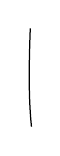
\begin{tikzpicture}[x=1cm,y=1cm]
\draw[line width=.45pt] (0,1.25) .. controls (-.015,.82) and (-.025,.40) .. (.015,0);
\end{tikzpicture}}

To show this, we shall embed
$\Pi_{0,3}$ as a subgroup of finite index
in $\Pi'_{0,3}$, whence an \unsure{analogous} embedding
\deleted{\illegible{1}}
\[
(2)\qquad\widehat{\Pi}_{0,3}\lhook\joinrel\longrightarrow\widehat{\Pi}'_{0,3}
\]
which will be compatible with the outer action of $\Gamma$.

\scanpage{507}

For this, consider the quotient scheme
\[
Y=\underbrace{\mathbb P^1_{\mathbb Q}}_{X}/\unsure{\mathfrak S_3}
\]
with the three points \inserted{$a_0,a_1,a_\infty$} of $Y$, rational over
$\mathbb Q$, \inserted{$a_0$} corresponding to the orbit
\deleted{of the} $\{0,1,\infty\}$, $a_1$ to the orbit
$\{-1,\frac12,2\}$, and $a_\infty$ to the orbit
$\{\unsure{-j},\unsure{-\overline j}\}$ of $\unsure{\mathfrak S_3}$
\margin{$j=\exp\frac{2i\pi}{3}$}
(which exhausts \unsure{the set} of geometric
``singular'' orbits). We know that $Y$ is a projective line
(over $\overline{\mathbb Q}$ a priori), \unsure{which we} \unsure{pin} by
$a_0,a_1,a_\infty$ as points $0,1,\infty$, \unsure{(thus}
$Y\simeq\mathbb P^1_{\mathbb Q}$ -- the \deleted{\illegible{1}} morphism
$X\longrightarrow Y$ is thus identified with a well-determined morphism
\[
(3)\qquad
f:\begin{array}{ccc}
\mathbb P^1_{\mathbb Q}&\longrightarrow&\mathbb P^1_{\mathbb Q}\\
\Vert&&\Vert\\
X&&Y
\end{array}
\]
\deleted{(in fact, $f$ can be defined as a morphism
$\mathbb P^1_{\mathbb Z}\longrightarrow\mathbb P^1_{\mathbb Z}$,
but here this matters little to us)}
which makes $X$ a Galois \unsure{covering|covering} of $Y$, with group
$\unsure{\mathfrak S_3}$, étale \unsure{over|over}
$\mathbb P^1_{\mathbb Q}\setminus\{0,1,\infty\}$, with ramification
indices at these points $2,2,3$. From the point of view of the geometry of maps
(\unsure{placing oneself|immersing oneself} over the base field $\mathbb C$), we consider the

\scanpage{508}
\mspage{\unsure{258 (259)}}

map determined on $X$ by the spherical triangles $(0,1,\infty)$
(on the real axis as equator) -- which is thus the universal
\unsure{weighted} triangular map -- as the inverse image of the universal map
(having a single vertex $0$, a single edge (folded) $0\longrightarrow1$,
a single face, with center $\infty$).
\margin{\figure{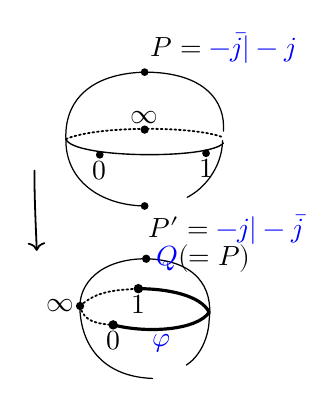
\begin{tikzpicture}[x=1cm,y=1cm,line cap=round,line join=round]
\draw[line width=.45pt] (0,2.85)
 .. controls (-.71,2.83) and (-1.02,2.47) .. (-1,2)
 .. controls (-1.01,1.48) and (-.57,1.16) .. (0,1.15);
\draw[line width=.45pt] (0,2.85)
 .. controls (.76,2.85) and (1.03,2.48) .. (1,2.10);
\draw[line width=.45pt] (.99,1.98)
 .. controls (.98,1.62) and (.74,1.36) .. (.54,1.26);
\draw[line width=.5pt] (-1,2)
 .. controls (-.91,1.75) and (.83,1.74) .. (1,1.95);
\draw[densely dotted,line width=.65pt] (-1,2)
 .. controls (-.61,2.17) and (.63,2.17) .. (1,2.02);
\fill (0,2.85) circle (1.4pt);
\node[anchor=south west,inner sep=2pt] at (0,2.88) {$P=\unsure{-\bar j|-j}$};
\fill (0,1.15) circle (1.4pt);
\node[anchor=north west,inner sep=2pt] at (-.03,1.12) {$P'=\unsure{-j|-\bar j}$};
\fill (-.57,1.80) circle (1.4pt);
\node[below,inner sep=2pt] at (-.57,1.80) {$0$};
\fill (.78,1.82) circle (1.4pt);
\node[below,inner sep=2pt] at (.78,1.82) {$1$};
\fill (0,2.12) circle (1.5pt);
\node[above,inner sep=2pt] at (0,2.12) {$\infty$};
\draw[->,line width=.65pt] (-1.40,1.60)
 .. controls (-1.40,1.22) and (-1.38,.85) .. (-1.37,.58);
\draw[line width=.45pt] (.02,.48)
 .. controls (-.55,.48) and (-.86,.17) .. (-.82,-.20)
 .. controls (-.78,-.70) and (-.46,-1.02) .. (.10,-1.04);
\draw[line width=.45pt] (.02,.48)
 .. controls (.65,.46) and (.87,.12) .. (.82,-.29)
 .. controls (.81,-.58) and (.66,-.79) .. (.53,-.87);
\fill (.02,.48) circle (1.5pt);
\node[anchor=west,inner sep=2pt] at (.07,.48) {$\unsure{Q}(=P)$};
\fill (-.82,-.12) circle (1.5pt);
\node[left,inner sep=2pt] at (-.82,-.12) {$\infty$};
\fill (-.08,.10) circle (1.7pt);
\node[below,inner sep=2pt] at (-.08,.10) {$1$};
\fill (-.40,-.36) circle (1.7pt);
\node[below,inner sep=2pt] at (-.40,-.36) {$0$};
\draw[line width=1.15pt] (-.08,.10)
 .. controls (.28,.10) and (.71,.02) .. (.82,-.20)
 .. controls (.66,-.43) and (.03,-.47) .. (-.40,-.36);
\draw[densely dotted,line width=.65pt] (-.82,-.12)
 .. controls (-.60,.08) and (-.36,.08) .. (-.08,.10);
\draw[densely dotted,line width=.65pt] (-.82,-.12)
 .. controls (-.78,-.32) and (-.59,-.35) .. (-.40,-.36);
\node[below,inner sep=1pt] at (.22,-.44) {$\unsure{\varphi}$};
\end{tikzpicture}}}
Every topological \deleted{\unsure{of}} \inserted{étale} covering of
$U_{03}(\mathbb C)\subset X$ thus gives a topological étale covering of
$U_{0,3}(\mathbb C)\subset Y$, \deleted{ramified} having
\deleted{\illegible{1}} \inserted{over} $1$ ramification $2$,
over $\infty$ ramification $3$ \unsure{exactly|exactly},
which corresponds to the ``forgetful'' functor \inserted{(of the weighting)},
where a \unsure{weighted} triangular map is considered as
just a map. From the point of view of fundamental groups \unsure{we} thus find
an \deleted{\unsure{homomorphism} of outer groups}
\inserted{equivalence of categories}

\diagram{\begin{tikzcd}[ampersand replacement=\&,column sep=large,row sep=huge]
\&
\deleted{\begin{gathered}
\Pi_1(\unsure{X(\mathbb C)}\setminus\{0,1,\infty\})\\[-2pt]
\rotatebox{90}{$=$}\\[-2pt]
\Pi_{0,3}
\end{gathered}}
\arrow[r,phantom,"{\deleted{\longleftarrow}}" description]
\&
\deleted{\begin{gathered}
\Pi_1\!\left(Y(\mathbb C)\setminus\{0,1,\infty\};
\underbrace{2\{1\}+3\{\infty\}}_{\substack{\text{signature of}\\\text{ramification}}}\right)\\[-2pt]
\rotatebox{90}{$=$}\\[-2pt]
\Pi'_{0,3}
\end{gathered}}
\\
(\deleted{\illegible{1}}\inserted{4}) \&
\left(\text{Étale coverings of }X\setminus\{0,1,\infty\}=U_{0,3}\right)
\arrow[r,phantom,"\simeq" description]
\arrow[d,phantom,"{\rotatebox{-90}{$\simeq$}}" description]
\&
\begin{gathered}
\left[\begin{gathered}
\text{Coverings of }Y\setminus\{0,1,\infty\}=U_{0,3}\\
\text{with ramification subordinate to}\\
\text{the signature }2\{1\}+3\{\infty\}
\end{gathered}\right]\\
\big/\begin{gathered}
\text{the object }(X\setminus\{0,1,\infty\})\\
\text{of the said category}
\end{gathered}
\end{gathered}
\arrow[d,phantom,"{\rotatebox{90}{$\simeq$}}" description]
\\
\& \Pi_{0,3}\text{-sets} \&
(\Pi'_{0,3}\text{-Sets})/\deleted{\unsure{E}}E
\end{tikzcd}}

where $E$ is the $\Pi'_{0,3}$-set corresponding to the object
$X\setminus\{0,1,\infty\}$ of the category of étale coverings of
$\unsure{Y\setminus\{0,1,\infty\}}$ with ramification
\deleted{\unsure{imposed}}\inserted{\unsure{subordin-}}ate to
$2\{1\}+3\{\infty\}$

\deleted{$\unsure{\simeq}\ \unsure{\Pi_{0,3}^{\prime\circ}}\in\mathrm{Ens}$}

\scanpage{509}
\mspage{\unsure{260|250}}

Here, \deleted{\illegible{3}} \inserted{\deleted{\illegible{1}} the base point of $Y-\{0,1,\infty\}$ chosen\unsure{;|,} \unsure{to} describe the} coverings \deleted{$E=\unsure{f^{-1}}\unsure{(}$} (with ramification \unsure{subordinate} to \dots) by a fundamental group with ramification, being \unsure{again} $P=-\bar j$, we shall have
\[
(5)\qquad E=f_{\unsure{\mathbf C|\mathbb C}}^{-1}(P)
\]
and we can thus make explicit the category $(\Pi'_{03}\text{-Sets})/E$\unsure{;}

Where $E$ is a homogeneous space, \inserted{\unsure{isomorphic to the}} \unsure{quotient} of $\Pi'_{03}$ by the \unsure{subgroup|subgroup} \inserted{$\Pi'^{\circ}_{03}$} kernel of the \inserted{suitable} surjective homomorphism
\[
(6)\qquad
\left\{
\begin{array}{l}
\Pi'_{0,3}\longrightarrow\unsure{\mathfrak S_3|\mathcal S_3}\\[2pt]
\left.
\begin{array}{lll}
\ell_0 &\longmapsto& \text{element of order 2}\\
\ell_1 &\longmapsto& \text{element of order 2}\\
\ell_\infty &\longmapsto& \text{\unsure{element} of order 3}
\end{array}
\right)\quad\text{to be computed !}
\end{array}
\right.
\]

We choose a $Q_0\in E$ as ``origin'' of $E$ -- so as to be able to identify $E$ as a $\Pi'_{0,3}$-set with $\Pi'_{03}/\Pi'^{\circ}_{03}\simeq\unsure{\mathfrak S_3}$ -- then $(\mathrm{Ens}\,\Pi'_{03})/E$ is identified, by the functor $F\longmapsto F_{Q_0}$, with $\mathrm{Ens}(\Pi'^{\circ}_{03})$.

We thus find in summary an equivalence of categories (depending on the choice of $Q_0$)
\[
\Pi_{03}\text{-sets}\quad\unsure{\simeq}\quad\Pi'^{\circ}_{03}\text{-sets}
\]
which is itself described by a bitorsor under $(\Pi'^{\circ}_{0,3},\Pi_{03})$ -- and, up to isomorphism \deleted{that} (not unique !), by an isomorphism
\[
\Pi_{03}\simeq\Pi'^{\circ}_{0,3}\quad -
\]
the isomorphisms thus obtained (for

\scanpage{510}
\mspage{\unsure{249}}

varying origins of the bitorsor) \unsure{form|forming} exactly a conjugacy class under $\Pi'^{\circ}_{03}$ -- i.e. an \uline{outer} \uline{\unsure{isomorphism}} $\Pi_{03}\simeq\Pi'^{\circ}_{03}$. When in addition the choice of $Q_0$ varies, we find \deleted{as} a \unsure{composite|composites}
\[
\Pi_{0,3}\longrightarrow\Pi'^{\circ}_{03}\longrightarrow\Pi'_{03}
\]
\deleted{\unsure{exactly}} a $\Pi'_{03}$-conjugacy class, i.e. an outer homomorphism.

I have \unsure{slaved away} a lot for not much -- for lack of having written down the \unsure{necessary|elementary} \inserted{general} \unsure{functorialities} for ``fundamental groups \unsure{with} ramification''. \unsure{For example} the mysterious bifunctor $I$ from earlier is made up of \unsure{classes} of paths from $P\in\unsure{X(\mathbb C)|X_{\mathbb C}}\setminus\{0,1,\infty\}$ (base point for computing $\Pi_{0,3}$) to $Q_0$ (playing the role of a new base point, having the merit of mapping to the one \inserted{-- $P$ --} which serves to compute $\Pi'_{03}$, fundamental group with ramification on $Y(\mathbb C)\setminus\{0,1,\infty\}$ \dots) It would perhaps be more convenient to define \unsure{direct\textsuperscript{ly}|directly} a functor in the opposite direction\unsure{:|.}
\[
(7)\qquad
\begin{array}{c}
\text{Coverings of }Y(\mathbb C)\inserted{\setminus(0,1,\infty)}\ \text{subordinate}\\
\text{to the signature }2\{1\}+3\{\infty\}
\end{array}
\longrightarrow
\begin{array}{c}
\text{\unsure{Étale|Étale} coverings of}\\
X(\mathbb C)\setminus\{0,1,\infty\}
\end{array}
\]
by inverse image, \unsure{followed|followed} by a \uline{normalization}

\subsection*{Scans 511--520}
\addcontentsline{toc}{subsection}{Scans 511--520}
% package LM_P052
\scanpage{511}
\mspage{261}

-- Here one uses the fact that the object $X(\mathbb C)\setminus\{0,1,\infty\}$ of the category of \unsure{covering\textsuperscript{s}} with maximum ramification \unsure{imposed|imposed}, attains precisely a maximum, at the points $1,\infty$ where the condition comes in.
One finds that the corresponding functor
\[
\tag{7 bis}
\Pi'_{03}\text{-}\mathrm{Ens}\longrightarrow(\Pi_{0,3}\text{-}\mathrm{Ens})
\]
has the exactness properties of a functor associated to a morphism of Galois topoi
\diagram{\begin{tikzcd}[ampersand replacement=\&]
\overset{\inserted{\unsure{B}}}{\unsure{B|D}}_{\Pi_{03}} \arrow[r] \& B_{\Pi'_{0,3}}
\end{tikzcd}}
(\unsure{commutes with} $\underset{\longrightarrow}{\lim}$ \unsure{of any kind}, left exact) and is therefore defined by a $(\Pi_{03}^{\deleted{\unsure{\wedge}}},\Pi'_{03})$ set which is a (right) torsor for $\Pi'_{03}$. The choice of an origin for this torsor then also defines a corresponding homomorphism $\Pi_{0,3}\longrightarrow\Pi'_{03}$.

\margin{This bitorsor is also the set of ($Y(\mathbb C)\setminus$\deleted{\illegible{2}}\inserted{\unsure{$\{0\}$}}) \unsure{isomorphisms|morphisms} of the ``universal covering with \unsure{ramification} imposed'' of this space, onto the \deleted{\unsure{with ramification}} \deleted{\unsure{ordinary}} ordinary universal covering of $X(\mathbb C)\setminus\{0,1,\infty\}$ \ldots}

Let us return to the arithmetic situation over $\mathbb Q$, where one has not only the geometric profinite fundamental groups $\widehat{\Pi}_{03}$, $\widehat{\Pi}'_{03}$, but also extensions
\[
\tag{8}
\left\{\begin{aligned}
1&\unsure{\longrightarrow}\widehat{\Pi}_{03}\longrightarrow\mathcal E_{0,3}^{\deleted{\unsure{\wedge}}}\longrightarrow\Gamma_{\deleted{\unsure{\mathbb Q}}}\longrightarrow1\\
1&\unsure{\longrightarrow}\widehat{\Pi}'_{03}\unsure{\longrightarrow}\mathcal E_{0,3}^{\prime\deleted{\unsure{\wedge}}}\unsure{\longrightarrow}\Gamma\unsure{\longrightarrow}1
\end{aligned}\right.,
\]
interpreted as fundamental groups of $\unsure{U}_{03\deleted{\mathbb Q}}$, resp. of $\unsure{U}_{03}$ with imposed ramification $2\{1\}+3\{\infty\}$. The arguments

\scanpage{512}

above extend to this setting, and thus provide a homomorphism \deleted{outer} \inserted{of extensions}
\diagram{\begin{tikzcd}[ampersand replacement=\&]
1 \arrow[r] \& \widehat{\Pi}_{03} \arrow[r] \arrow[d] \& \mathcal E_{03} \arrow[r] \arrow[d] \& \Gamma \arrow[r] \arrow[d,equal] \& 1 \\
1 \arrow[r] \& \widehat{\Pi}'_{03} \arrow[r] \& \mathcal E'_{03} \arrow[r] \& \Gamma \arrow[r] \& 1
\end{tikzcd}\quad(9)},
modulo conjugation by an inner automorphism of $\Pi'_{03}$.

\margin{(9 bis) $\widehat{\Pi}_{0,3}\longrightarrow\widehat{\Pi}'_{0,3}$ fits into an exact sequence
\[
\boxed{1\longrightarrow\widehat{\Pi}_{0,3}\longrightarrow\widehat{\Pi}'_{0,3}\longrightarrow\unsure{\mathfrak S}_3\longrightarrow1}
\]
and ditto for the discrete groups
\[
\boxed{1\longrightarrow\Pi_{0,3}\longrightarrow\Pi'_{0,3}\longrightarrow\unsure{\mathfrak S}_3\longrightarrow1}.
\]}

That said, let $K$ be the kernel of the outer operation of $\Gamma$ on $\Pi'_{03}$. One then sees that \deleted{$K$ operates} the outer operation of $K$ on the open subgroup $\widehat{\Pi}_{03}$ takes place through a finite group (in fact, through \inserted{the intermediary of} $\widehat{\Pi}'_{03}/\widehat{\Pi}_{03}\simeq\unsure{\mathfrak S}_3$ \ldots) -- which implies, by theorem 1 of the \S\ above, that the group $K$ itself is finite. Thus by Artin one has $K=1$ or $K=(1,\tau)$, $\tau$ complex conjugation. But since $\chi(\tau)=-1$ it is obvious that the outer operation of $\tau$ on $\Pi'_{03}$ \inserted{(nor even on $(\Pi'_{03})_{\unsure{\mathrm{ab}}}^{*}$ \deleted{\illegible{2}})} is not trivial\ldots
\margin{$*\simeq\unsure{\mathbb Z/2\mathbb Z+\mathbb Z/3\mathbb Z}$}
\deleted{\unsure{Which}} This proves the proposition.

\scanpage{513}
\mspage{262}

I now feel like interpreting $\Pi_{03}^{\unsure{\prime}}$ as $\mathcal T^+_{1,1}/\deleted{\text{subgroup}}\inserted{\text{center}}$ (isomorphic \unsure{to} $\{\pm1\}$\unsure{),|,} and ditto for $\widehat{\Pi}'_{03}\simeq\widehat{\mathcal T}_{11}/\{\pm1\}$, \unsure{isomorphism|isomorphisms} which is compatible with the outer action of $\Gamma$, One has (for the record)
\[
\tag{10}
\mathcal T_{1,1}\xrightarrow{\sim}\mathrm{Gl}(2,\mathbb Z),
\]
the isomorphism being obtained as follows:
\[
\tag{11}
\mathcal T_{1,1}\xrightarrow[\substack{\text{plugging}\\\text{the hole}}]{\mathrm{iso}}\mathcal T_{1,0}\xrightarrow{\mathrm{iso}}\mathrm{Autext}\left(\underbrace{\Pi_{10}}_{\substack{\wr\\\mathbb Z^2}}\right)\simeq\mathrm{Gl}(2,\mathbb Z)
\]

One thus has
\[
\tag{12}
\mathcal T^+_{11}\simeq\mathrm{Sl}(2,\mathbb Z)
\]
and
\[
\tag{13}
\mathrm{Cent}(\mathcal T_{11})\simeq(\pm1)
\]
(identifies with the subgroup of homotheties of $\mathrm{Sl}(2,\mathbb Z)$). It is known that one has \unsure{in} $\mathrm{Sl}(2,\mathbb Z)/(\pm1)$ two generators $\unsure{\lambda_3,\lambda_2}$, satisfying respectively
\[
\tag{14}
\lambda_3^3=1,\quad\lambda_2^2=1
\]
and such that these relations are a \uline{presentation} of $\mathrm{Sl}(2,\mathbb Z)/(\pm1)$. Unless I am mistaken, these \unsure{elements|elements} come from \unsure{elements|elements} $u_6,u_4$ of $\mathrm{Sl}(2,\mathbb Z)$ itself, satisfying
\[
\tag{15}
u_6^6=1,\quad u_4^4=1
\]

\scanpage{514}

and which correspond to the only elements of order 6 and of order 4 (up to conjugation and taking inverses). In fact, \unsure{every} element of finite order of $\mathrm{Sl}(2,\mathbb Z)$ is conjugate to a power \unsure{of|of} \deleted{a} $u_4$, or $u_6$. The \unsure{subgroups} \unsure{generated} resp. by $u_4$ and $u_6$, cyclic of order 4 and 6, are the groups of \unsure{automorphisms} of the two exceptional elliptic curves (called ``\unsure{anharmonic}'') (in characteristic 0).

\deleted{For} I have no formula at hand for ``placing'' \deleted{\unsure{$u_4$}} $u_4$ and $u_6$, so that they generate the group $\mathrm{Sl}(2,\mathbb Z)$\deleted{\unsure{$/\pm1$}} \unsure{modulo} its center (which probably implies that they generate $\mathrm{Sl}(2,\mathbb Z)$ --- but \unsure{one will pay attention|well. Pay attention} to the additional relation. \deleted{being added \unsure{to} \inserted{(15)} \unsure{of the} fundamental relations}
\[
(16)\qquad u_4^2=u_6^3\qquad\unsure{\varepsilon}
\]
(this is \deleted{\illegible{2}} \unsure{precisely} the element $-1$ of the center of $\mathrm{Sl}(2,\mathbb Z)$). Perhaps I do not need it (the explicit formula for $u_4,u_6$). One then \unsure{will define|defines}

\scanpage{515}
\mspage{263}

\[
(17)\qquad \Pi'_{03}\xrightarrow{\sim}\mathrm{Sl}(2,\mathbb Z)/(\pm1)
\]
by
\[
(18)\qquad
\begin{array}{rcl}
\ell'_1&\longmapsto&\lambda_2\\
\ell'_\infty&\longmapsto&\lambda_3
\end{array}
\]
\[
\bigl[\text{thus}\qquad\ell'_0\longmapsto(\lambda_3\lambda_2)^{-1}
=\lambda_2\lambda_3^{-1}=\lambda_2\lambda_3^2\bigr],
\]
\unsure{where} $\ell'_0,\ell'_1,\ell'_\infty$ are the generators of $\Pi'_{03}$ corresponding to those $\ell_0,\ell_1,\ell_\infty$ of $\Pi_{03}$, with the defining relations
\[
(19)\qquad\ell'_\infty\ell'_1\ell'_0=1\qquad
\ell_1^{\prime 2}=1,\quad\ell_\infty^{\prime 3}=1
\]
so that $\Pi'_{03}$ is indeed the group \deleted{free} with generators $\ell'_1,\ell'_\infty$ satisfying: $\ell_1^{\prime 2}=1,\ell_\infty^{\prime 3}=1$.

I now want to convince myself that the homomorphism corresponding to (17)
\[
(20)\qquad\widehat{\Pi}'_{03}\longrightarrow
\mathrm{Sl}(2,\mathbb Z)^\wedge/\pm1\simeq
\widehat{\mathcal T}_{1,1}^{+}/(\pm1)
\]
is compatible with the outer operation of $\Gamma=\Pi_{\mathbb Q}$. For this, I feel like defining directly the composite \unsure{with} $\unsure{\widehat{\Pi}_{0,3}|\Pi_{0,3}}\longrightarrow\widehat{\Pi}'_{03}$
\[
\text{\deleted{\unsure{(21)}}}\qquad\widehat{\Pi}_{03}\longrightarrow\widehat{\mathcal T}_{1,1}^{+}/\pm1
\]
and even \unsure{lifting} it to a homomorphism
\[
(21)\qquad\widehat{\Pi}_{03}\longrightarrow\widehat{\mathcal T}_{11}^{+}\;.
\]

\scanpage{516}

At the level of discrete groups, one does define
\[
(22)\qquad\Pi_{03}\longrightarrow\mathrm{Sl}(2,\mathbb Z)
\]
\[
\left\{
\begin{array}{rcl}
\ell_1&\longmapsto&u_4\\
\ell_\infty&\longmapsto&u_6\\
\ell_0&\longmapsto&(u_6u_4)^{-1}=u_4^{-1}u_6^{-1}
\end{array}
\right.
\]
and $\mathrm{Sl}(2,\mathbb Z)$\inserted{$\simeq\mathcal T_{11}^{+}$} identifies with the quotient of $\Pi_{0,3}$ by the invariant \unsure{subgroup} \unsure{generated} by the elements
\[
\ell_1^4,\ \ell_\infty^6,\ (\ell_1^2)(\ell_\infty^3)^{-1}\;.
\]

Besides, $\Pi_{03}$ can be interpreted as a Teichmüller group $\mathcal T_{0,4}^{!+}$, and (22) as a homomorphism
\margin{indeed, $\mathcal T_{g,\nu}^{!}$ is an extension of $\mathcal T_{g,\nu-1}^{!}$ by $\Pi_{g,\nu-1}$ (if $(g,\nu-1)$ \unsure{anabelian}) and ditto for the $\mathcal T^{+}$, $\mathcal T_{0,3}^{!+}=(1)$!}
\[
\text{\deleted{\unsure{(24)}}}\ (23)\qquad\mathcal T_{0,4}^{!+}\longrightarrow\mathcal T_{11}^{+}
\]
which I suspect extends to a homomorphism
\[
(24)\qquad
\diagram{\begin{tikzcd}[ampersand replacement=\&,column sep=large]
\mathcal T_{0,4}^{!}\arrow[r]\arrow[d,phantom,"\wr" description]\&\mathcal T_{11}\arrow[d,phantom,"\wr" description]\\
\begin{gathered}
\text{extension of }\{1,\unsure{\tau}\}\text{ by}\\
\Pi_{0,3},\ \text{which is none}\\
\text{other than the}\\
\text{cartographic group}\\
\text{triangulated weighted}\\
\text{unoriented}
\end{gathered}
\&\mathrm{Gl}(2,\mathbb Z)
\end{tikzcd}}
\]
\margin{not yet defined}

I interpret the first \unsure{side} \inserted{of (23)} as the $\Pi_1$ ``transcendental geometric'' \unsure{of the|of the} \unsure{modular|modular} topos

\scanpage{517}
\mspage{264}

$\mathbb{M}_{0,4}^{!}$, classifying \deleted{rational curves} \inserted{projective lines} with four distinct points numbered from $1$ to $4$; and the second \unsure{side|right-hand side} of (23) is the transcendental $\pi_1$ of the modular topos $M_{1,1}$, classifying elliptic curves (with a fixed origin). One should therefore be able to define, at the level of \deleted{schemes} modular multiplicities over $\mathbb{Q}$
\[
(25)\qquad (\mathbb{M}_{0,4}^{!})_{\mathbb{Q}} \longrightarrow
(\mathbb{M}_{1,1}^{\deleted{\unsure{!}}})_{\mathbb{Q}}
\]
which would give rise to (23). \deleted{This \unsure{also means}}

But one sees at once that one has a canonical isomorphism
\[
(26)\qquad \mathbb{M}_{0,4}^{!}\simeq U_{0,3}
\]
(I drop the subscripts $\mathbb{Q}$), and giving (25) thus also amounts to giving a family of elliptic curves over $U_{0,3}$.

But \unsure{if} $\lambda$ is the \unsure{``variable'' $\in U_{0,3}$''}, taking ``the'' quadratic covering $E_\lambda$ of \deleted{\illegible{1}} $\mathbb{P}^1$ ramified at $0,1,\infty,\lambda$,

\scanpage{518}

one finds an elliptic curve, with four marked points \deleted{resp.} above $0,1,\infty,\lambda$ --- of which one can take the point above $0$ as origin --- then the other points are the three points of order $2$, indexed resp. by $1,\infty,\lambda$.

More precisely: over any base scheme \inserted{$S$}, except that $2$ should be invertible there (residual characteristics \unsure{all} $\ne 2$), \deleted{the} \inserted{one has a} functor which goes \deleted{from the} \inserted{from the category of systems $(E,\alpha,\beta\deleted{,\unsure{\gamma}})$ of a} \unsure{relative|relative} \unsure{elliptic|elliptic} \unsure{curves|curve} (\unsure{homogeneous|homogeneous}) \deleted{\unsure{with} \illegible{1}} over $S$, and \deleted{\unsure{whose}} $\alpha,\beta\deleted{,\unsure{\gamma}}$ \deleted{three} \inserted{two} sections of $E$ which form a basis of ${}_2E$ \unsure{as} a \inserted{locally constant} scheme in $\mathbb{F}_2$-Modules (a local system of $\mathbb{F}_2$-modules) on $S$ [\unsure{giving} rise to: $\gamma=\alpha+\beta$, as a third rogue --- so that $(\beta,\gamma)$\unsure{,|.} \deleted{and \unsure{$(\gamma,\alpha)$}} \inserted{etc} are in fact also bases) --- to the category of projective-line bundles $P$ over $S$, with four sections \inserted{$u_0,u_1,u_\infty,\lambda$} \unsure{marked} distinct at every point, by associating to $E$ the quotient $E/\pm1$, \unsure{equipped} with the sections $u_0,u_1,u_\infty,\lambda$ which are the images resp. of $0,\alpha,\beta,\gamma=\alpha+\beta$

\margin{it amounts to the same thing to say that \unsure{one has|the} three sections $\alpha,\beta,\gamma$ of ${}_2E$ over $S$, which \unsure{are} $\forall s\in S$, \deleted{\unsure{everywhere}} distinct and \unsure{hence|everywhere} $\ne1$.}

\scanpage{519}
\mspage{265}

\margin{The pages which follow are needlessly complicated, with the introduction of the $\unsure{M|\mathbb M}'_{1,1}$, $\mathcal{T}'_{1,1}$ \unsure{etc.} -- it is enough to go at it \unsure{brutally|simply} with the elliptic curve $y^2=\sqrt{x(x-1)(x-\lambda)}$, over $U_{0,3}$, \unsure{to} \illegible{1} \unsure{have} $U_{0,3}\longrightarrow \unsure{M|\mathbb M}_{1,1}$ cf. below\ldots}

and this functor is \uline{almost} an equivalence of categories. What it lacks in order to be one, is that for a relative elliptic curve $E$, the symmetry \inserted{$x\mapsto -x$} of $E$ -- which is a nontrivial automorphism -- operates \unsure{trivially} on the corresponding object $E/\pm1$. So one \unsure{must} take \unsure{the|the} \deleted{fibered category} \inserted{stack} over $(\mathrm{Sch})$, obtained from that of elliptic curves by starting by taking $\unsure{\mathrm{Isom}}(E,F)'=\unsure{\mathrm{Isom}}(E,F)/\pm1$, then one will take the stack associated to a prestack (the objects over $S$ are the ``relative elliptic curves up to symmetry over $S$''). \unsure{This|This|The} stack is representable by a modular multiplicity $\unsure{M|\mathbb M}'_{1,1}$, \deleted{\unsure{obtained from} \illegible{1}} having as its geometric fundamental group $\mathrm{Sl}(2,\mathbb{Z})^{\wedge}/\pm1$ precisely, obtained \deleted{from the} for example from the modular varieties with Jacobi rigidification of level $n$, $\unsure{M|\mathbb M}_{11}[n]$ -- with group $\mathrm{Sl}(2,\mathbb{Z}/n\mathbb{Z})$ operating on it, so that
\[
 (27)\qquad \unsure{M|\mathbb M}_{11}\simeq \bigl(\unsure{M|\mathbb M}_{1,1}[n],\mathrm{Sl}(2,\mathbb{Z}/n\mathbb{Z})\bigr)
\]
\unsure{moreover|one notes} that \inserted{the central subgroup $\unsure{(\pm1)|\{\pm1\}}$ of} $\mathrm{Sl}(2,\mathbb{Z}/n\mathbb{Z})$ operates \unsure{trivially} on $\unsure{M|\mathbb M}_{11}[n]$, so one can let the quotient group $\mathrm{Sl}(2,\mathbb{Z}/n\mathbb{Z})'\,\deleted{\illegible{1}}=\mathrm{Sl}(2,\mathbb{Z}/n\mathbb{Z})/\pm1$ operate, and set

\scanpage{520}

\[
 (28)\qquad \unsure{M|\mathbb M}'_{11}=\bigl(\unsure{M|\mathbb M}_{11}[n],\mathrm{Sl}(2,\mathbb{Z}/n\mathbb{Z})'\bigr)
\]
\unsure{(which|Which} \unsure{manifestly$^{\mathrm t}$|manifestly} does not depend on the choice of $n$, $n\geq2$). One thus finds a morphism
\[
 (29)\qquad
 \diagram{\begin{tikzcd}[ampersand replacement=\&,row sep=small]
 \unsure{M|\mathbb M}^!_{0,4} \arrow[r] \arrow[d,equal] \& \unsure{M|\mathbb M}'_{11} \\
 U_{0,3} \&
 \end{tikzcd}}
\]
which makes $\unsure{M|\mathbb M}^!_{0,4}$ a Galois covering with group $\unsure{\mathfrak{S}_3}$ of $\unsure{M|\mathbb M}'_{11}$, and more precisely
\[
 (30)\qquad
 \diagram{\begin{tikzcd}[ampersand replacement=\&,column sep=large]
 \unsure{M|\mathbb M}^!_{0,4} \arrow[r,dash,"\sim"] \&
 \unsure{M|\mathbb M}_{1,1}^{\prime\,\deleted{\illegible{1}}}[2]
 \arrow[r,"{\text{Galois covering with group }\mathrm{Sl}(2,\mathbb{F}_2)\simeq\unsure{\mathfrak{S}_3}}"'] \&
 \unsure{M|\mathbb M}'_{11}\,\deleted{\illegible{1}}
 \end{tikzcd}}
\]
the geometric fundamental group of $\unsure{M|\mathbb M}_{11}[2]$ \unsure{being} moreover isomorphic to the kernel of \inserted{the homomorphism} $\mathrm{Sl}(2,\mathbb{Z})^{\prime\wedge}\longrightarrow\mathrm{Sl}(2,\mathbb{Z}/2\mathbb{Z})$ which factors the canonical homomorphism $\mathrm{Sl}(2,\mathbb{Z})^{\wedge}_{\deleted{\illegible{1}}}\longrightarrow\mathrm{Sl}(2,\mathbb{Z}/2\mathbb{Z})$.

Passing to the fundamental groups for $\unsure{M|\mathbb M}^!_{0,4}=U_{0,3}$ and $\unsure{M|\mathbb M}'_{11}$, one finds a \unsure{homomorphism|homomorphism} of exact sequences

\deleted{\unsure{(31)}}
\[
 (31)\qquad
 \diagram{\begin{tikzcd}[ampersand replacement=\&,column sep=small,row sep=small]
 \& \inserted{\unsure{\mathcal{T}_{0,4}^{!+}|\widehat{\mathcal{T}}_{0,4}^{!+}}}
   \arrow[d,phantom,"\inserted{\Vert}" description]
 \& \inserted{\unsure{N_{0,4}|\mathcal{N}_{0,4}}}
   \arrow[d,phantom,"\inserted{\Vert}" description] \& \& \\
 1 \arrow[r] \& \widehat{\Pi}_{0,3} \arrow[r] \arrow[d]
 \& \mathcal{E}_{0,3} \arrow[r] \arrow[d]
 \& \Gamma \arrow[r,dash] \arrow[d,"\Vert"] \& 1 \\
 1 \arrow[r] \& \widehat{\mathcal{T}}_{1,1}^{\prime+} \arrow[r]
   \arrow[d,phantom,"\inserted{\wr}" description]
 \& \mathcal{E}'_{11} \arrow[r] \& \Gamma \arrow[r] \& 1 \\
 \& \inserted{\widehat{\mathcal{T}}_{11}^{+}/\unsure{\{\pm1\}|(\pm1)}
   \simeq\mathrm{Sl}(2,\mathbb{Z})^{\wedge}/\pm1} \& \& \&
 \end{tikzcd}}
\]

\subsection*{Scans 521--530}
\addcontentsline{toc}{subsection}{Scans 521--530}
% package LM_P053
\scanpage{521}
\mspage{266}

which identifies $\mathcal E_{0,3}$ with a subgroup \inserted{\unsure{open}\illegible{1}} of index $6$ of $\mathcal E'_{1,1}=\mathcal E_{1,1}/(\pm1)$, and ditto for $\widehat\Pi_{0,3}$ in $\widehat{\mathcal T}_{1,1}^{\prime+}$. We thus find an iso\deleted{\illegible{1}}morphism
\[
(32)\qquad
\widehat\Pi_{0,3}\xrightarrow{\sim}
\begin{gathered}
\operatorname{Ker}(\widehat{\mathcal T}_{1,1}^{\prime+}\longrightarrow\unsure{\mathfrak S}_3)\\
\wr\\
\biggl(\operatorname{Ker}\biggl(
\begin{gathered}\widehat{\mathcal T}_{11}^{+}\\\wr\\\mathrm{Sl}(2,\mathbb Z)^{\wedge}\end{gathered}
\longrightarrow
\begin{gathered}\unsure{\mathfrak S}_3\\\wr\\\mathrm{Sl}(2,\mathbb F_2)\end{gathered}
\biggr)\biggr)/\pm1
\end{gathered}
\]
compatible with the outer actions of $\Gamma$. We can also say that we have an extension structure
\[
(33)\qquad
\diagram{\begin{tikzcd}[ampersand replacement=\&,column sep=small]
1\arrow[r,dash] \& \widehat\Pi_{0,3}\arrow[r] \& \widehat{\mathcal T}_{1,1}^{\prime+}\arrow[r]\arrow[d,phantom,"\wr" description] \& \unsure{\mathfrak S}_3\arrow[r]\arrow[d,phantom,"\wr" description] \& 1\\
\&\&\mathrm{Sl}(2,\mathbb Z)^{\wedge}/\pm1\arrow[r]\&\mathrm{Sl}(2,\mathbb Z_{/2})\&
\end{tikzcd}}
\]
compatible with the actions of $\Gamma$ ($\Gamma$ operating trivially on $\unsure{\mathfrak S}_3$).

I finally realize that what we get here is far from 22 --- this homomorphism (22) is not at all injective, on the other hand it is surjective --- and its values are \unsure{not} in $\mathrm{Sl}(2,\mathbb Z)/\pm1$, but in $\mathrm{Sl}(2,\mathbb Z)$ itself! So I shall have to \unsure{return} again to a way of giving
\scanpage{522}
a remarkable arithmetico-geometric meaning to (22), and its \unsure{extension} to the corresponding profinite groups. For the moment, I confine myself to exploiting (33) a little. First of all I note that the arguments made in the scheme-theoretic setting, work also in the transcendental, complex analytic case, and then yield
\[
(34)\qquad
\Pi_{0,3}\xrightarrow{\sim}\operatorname{Ker}\biggl(
\begin{gathered}\mathcal T_{11}^{\prime+}\\\Vert\\\mathrm{Sl}(2,\mathbb Z/2\mathbb Z)/\pm1\end{gathered}
\longrightarrow
\begin{gathered}\unsure{\mathfrak S}_3\\\Vert\\\mathrm{Sl}(2,\mathbb Z/2\mathbb Z)\end{gathered}
\biggr)
\]
compatible with (32), or again an exact sequence
\[
(35)\qquad
\diagram{\begin{tikzcd}[ampersand replacement=\&,column sep=small]
1\arrow[r,dash]\&\Pi_{0,3}\arrow[r]\&\mathcal T_{11}^{\prime+}\arrow[r]\arrow[d,phantom,"\wr" description]\&\unsure{\mathfrak S}_3\arrow[r]\arrow[d,phantom,"\wr" description]\&1\\
\&\&\mathrm{Sl}(2,\mathbb Z)/\pm1\&\mathrm{Sl}(2,\mathbb Z/2\mathbb Z)\&
\end{tikzcd}}\unsure{,)|.,}
\]

\deleted{\unsure{which}} We would like to interpret (35) and (33) as corresponding \unsure{to the} analogous exact sequences linked to diagram (\unsure{9}), relating $\Pi_{0,3}$ and $\Pi'_{0,3}$ --- identifying $\Pi'_{0,3}$ with $\mathcal T_{11}^{\prime+}$, $\widehat\Pi'_{0,3}$ with $\widehat{\mathcal T}_{11}^{\prime+}$. I shall return to this \unsure{later}.

\uline{Remark} One may ask whether the homomorphism
\[
\widehat\Pi_{0,3}\longrightarrow\mathrm{Sl}(2,\mathbb Z)^{\wedge}/\pm1\simeq\widehat{\mathcal T}_{11}^{+}/(\pm1)
\]
lifts (in a more or less natural way)
\scanpage{523}
\mspage{267}
to a homomorphism
\[
\widehat\Pi_{0,3}\longrightarrow\mathrm{Sl}(2,\mathbb Z)^{\wedge}\simeq\deleted{\unsure{\mathrm{Sl}}}\widehat{\mathcal T}_{1,1}^{+}
\]
and ditto for the discrete groups
\[
\Pi_{0,3}\longrightarrow\mathrm{Sl}(2,\mathbb Z)\simeq\mathcal T_{11}^{+}.
\]

\margin{Yes, one can lift, and it is more or less trivial... cf. below...}

Of course, since $\Pi_{0,3}$ and $\widehat\Pi_{03}$ are free (with two \unsure{generators}) one can always lift --- \deleted{\unsure{the indeterminacy up to}}\inserted{in exactly} \uline{four} ways, incidentally. (which necessarily, in the profinite setting, \unsure{respect} the discrete lattices). But can one do this while \unsure{respecting} the operations of $\Gamma$? For this it would suffice to be able to lift $U_{0,3}\longrightarrow M'_{1,1}\deleted{[2]}$ to $U_{0,3}\longrightarrow M_{11}^{\unsure{t|\ell}}$ (\uline{N.B.} $M_{11}$ is a \deleted{\illegible{1}} $\mathbb Z/2$-gerbe over $M'_{11}$) --- and I suspect, \deleted{that}
\margin{not quite cf. the next \unsure{page} for a more \unsure{reasonable} formulation...}
according to the ``anabelian'' \unsure{yoga} that I am trying to develop, that the converse must be true --- that every lifting of $\widehat\Pi_{03}\longrightarrow\widehat{\mathcal T}_{11}^{\prime+}\deleted{\unsure{\Pi}}$ \unsure{commuting} with the operations of $\Gamma$ is defined by such a lifting $U_{0,3}\longrightarrow M_{1,1}$. Now the existence \inserted{of such a lifting $U_{0,3}\longrightarrow M_{1,1}$} would mean \inserted{\unsure{exactly}} the existence of a family of elliptic curves over $U_{0,3}$, with
\scanpage{524}
Jacobi rigidification of level $2$, which \unsure{corresponds} to the tautological invariant $\lambda$. I doubt that there is one, as I doubt that the lifting in terms of profinite groups with operations can be made.

To tell the truth, since \inserted{$\widehat{\mathcal T}_{11}^{+}=$}$\mathrm{Sl}(2,\mathbb Z)^{\wedge}$ no longer has trivial center, it is no longer \deleted{legitimate} \inserted{reasonable in fact} to \unsure{want} to ``\unsure{express everything}'' \unsure{by} the outer \unsure{operations} of $\Gamma$ on $\widehat{\mathcal T}_{11}^{+}$, we must rather return to the extension $\mathcal E_{11}=\mathcal E_{M_{1,1}}$ of $\Gamma$ by $\widehat{\mathcal T}_{1,1}^{+}$, and the question is whether the homomorphism
\[
\mathcal E_{0,3}\longrightarrow\mathcal E'_{1,1}=\mathcal E_{1,1}/\pm1
\]
lifts to
\[
\mathcal E_{0,3}\xrightarrow{?}\mathcal E_{11},
\]
\deleted{\unsure{choosing a}}\inserted{which is more} stringent than finding a lifting $\widehat{\Pi}_{0,3}\longrightarrow\mathcal T_{11}^{+}$ compatible with the outer \unsure{operations} of $\Gamma$. To \unsure{appreciate} this difference, I note that $\Gamma$ operates on the set\inserted{ $E$} of the four liftings \unsure{of} $\widehat{\Pi}_{0,3}\longrightarrow\widehat{\mathcal T}_{1,1}^{+}$, (\unsure{interpreted} as outer homomorphisms), and the
\scanpage{525}
\mspage{268}
question posed in the weak form is whether there exists an element of $E$ invariant under $\Gamma$. If there were none, there would in any case be an open subgroup of $\Gamma$, of index \deleted{dividing}\inserted{$2$ or $4$} \deleted{\illegible{1} $4$, such that} \inserted{\deleted{$4!=24$,} which} would leave an element invariant --- so at the cost of passing to the \deleted{\illegible{1}} corresponding finite extension of $\mathbb Q$, we find the lifting --- and at the cost of passing to a slightly larger extension, the \uline{four} possible liftings commute with the outer action of $\Gamma$. On the other hand, nothing proves that one can find a \inserted{``germ of} liftings'' \deleted{\unsure{$\mathcal E_{0,3}\longrightarrow\mathcal E_{11}$}} of $\mathcal E_{0,3}\longrightarrow\mathcal E'_{1,1}$ to \unsure{$\mathcal E_{0,3}^{G}\longrightarrow\mathcal E_{1,1}^{G}$} (\unsure{germs} taken with respect to the subgroups \inserted{\unsure{open|open}} of $\mathcal E_{0,3}$ \deleted{\illegible{1}} containing $\widehat\Pi_{0,3}$, or even of all the open subgroups) The obstruction to \deleted{\illegible{3}}\inserted{\unsure{lifting over}} $\mathcal E_{0,3}$ \deleted{\illegible{3}}\inserted{itself}, i.e. to \uline{\unsure{splitting}} a certain extension of $\mathcal E_{0,3}$ by \deleted{\unsure{$\mathbb Z$}} $\pm1$), is
\figure{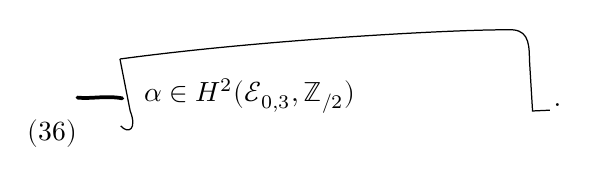
\begin{tikzpicture}[x=1cm,y=1cm,baseline=(formule.base)]
\node[anchor=west,inner sep=0pt] (formule) at (1.02,0)
  {$\alpha\in H^2(\mathcal E_{0,3},\mathbb Z_{/2})$};
\node[anchor=east,inner sep=0pt] at (0.18,-0.48) {$(36)$};
\draw[line width=0.45pt]
  (0.72,0.47) .. controls (2.65,0.73) and (5.13,0.85) .. (5.64,0.84)
  .. controls (5.89,0.86) and (5.92,0.70) .. (5.92,0.47)
  -- (5.96,-0.19) -- (6.18,-0.18);
\draw[line width=0.45pt]
  (0.72,0.47) -- (0.85,-0.19)
  .. controls (0.94,-0.42) and (0.83,-0.49) .. (0.73,-0.38);
\draw[line width=1.35pt,line cap=round]
  (0.18,-0.02) .. controls (0.35,-0.04) and (0.55,0.01) .. (0.75,-0.03);
\node[anchor=west,inner sep=0pt] at (6.22,-0.12) {.};
\end{tikzpicture}}
--- and nothing says that this cohomology class can be killed, by passing to an open subgroup of $\mathcal E_{0,3}$.
\figure{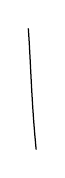
\begin{tikzpicture}[x=1cm,y=1cm]
\draw[line width=0.45pt]
  (0,1.05) .. controls (0.03,0.64) and (0.04,0.11) .. (0.10,-0.49);
\end{tikzpicture}}

\scanpage{526}

But in geometric terms, \deleted{\unsure{soon}} the relative elliptic curves \unsure{sought} over \unsure{$U_{0,2}$|$U_{0,3}$} form \unsure{\deleted{the}|the} sections of a stack over $(U_{0,3})_{\mathrm{et}}$, which is a \deleted{\unsure{$\{\pm1\}$}}\inserted{$\mathbb Z_{/2}$}-gerbe --- the obstruction therefore lies in a Brauer group
\[
\beta\in H^2(U_{0,3},\mathbb Z_{/2}), \tag{37}
\]
now since $U=U_{0,3}$ is an algebraic \deleted{\illegible{1}} affine curve over a field (it \unsure{would suffice} that it not be of type $0,0$) \unsure{it follows} that the canonical homomorphism (with arbitrary torsion coefficients)
\[
H^*(\mathcal E_U,-)\longrightarrow H^*(U,-)
\]
is an isomorphism. Besides, it \unsure{must} be $\pm$ trivial that $\beta$ is the image of $\alpha$ --- which confirms the \unsure{intuition|intention} that \deleted{\unsure{the}} if the lifting is possible at the level of profinite fundamental groups (\unsure{arithmetico-geometric|arithmetico-geometric}) it is also possible at the level of the modular \unsure{multiplicities} themselves, so that we have an existence of a relative elliptic curve over $U_{0,3}$ which\ldots

\scanpage{527}
\mspage{269}

It is \unsure{true} that it is well \unsure{known} that a cohomology class (37) with torsion coefficients is killed, on \unsure{passing} to a finite extension of the \deleted{\unsure{$\mathbb Q$}} base field ($\mathbb Q$ in this case). In fact, we have a spectral sequence
\[
(38)\qquad H^*(U_{0,3},\mathbb Z_{/2})
\Longleftarrow E_2^{pq}
=H^p(\deleted{\unsure{\overline U_{0,3}}}\unsure{\mathbb Q},H^q(\overline U_{0,3},\mathbb Z_{/2}\unsure{)|))}
\]
and here $H^q(\overline U_{0,3})=0$ for $q\geq 2$, so we find an exact sequence
\[
\deleted{\unsure{H^1(\mathbb Q)}\longrightarrow
\unsure{H^1(U_{0,3},\mathbb Z_{/2})}\longrightarrow
\unsure{H^1(\overline U_{0,3},-)}}
\]
\diagram{\begin{tikzcd}[ampersand replacement=\&,column sep=small]
\cdots \& E_2^{0,1} \arrow[r] \arrow[d,equal]
\& E_2^{2,0} \arrow[r] \arrow[d,equal]
\& \deleted{\unsure{E}}H^2(U_{0,3}) \arrow[r]
\& E_2^{1,1} \arrow[r] \arrow[d,equal]
\& E_2^{3,0} \arrow[d,equal] \& \cdots \\
\& H^0(\mathbb Q,H^1(\overline U)
\& H^2(\mathbb Q,\mathbb Z_{/2})
\&
\& H^1(\mathbb Q,\underset{\substack{\wr\\\mathbb F_2^2}}{H^1(\overline U)})
\& H^3(\mathbb Q,\unsure{\mathbb Z_{/2}|\mathbb F_2}) \&
\end{tikzcd}}

I \unsure{realize} at last that the existence of a \deleted{\illegible{1}} lifting, -- i.e. of the hypothetical elliptic curve over $U_{0,3}$ -- is completely trivial, it suffices to define \unsure{it|it} by the equation
\[
y=\sqrt{\unsure{x|\dot x}(x-1)(x-\lambda)}
\]
i.e.
\[
y^2-x(x-1)(x-\lambda)=F(x,y;\lambda]=0
\]
which defines an affine plane curve,
\scanpage{528}
\unsure{we pass|or pass} to projective coordinates
\[
F(x,y,z;\lambda)=y^2z-x^3+(1+\lambda)x^2z-\lambda xz^2=0
\]
\deleted{\unsure{for|then}} I am not going to go further into the question here\unsure{.} \unsure{to} what extent this choice is ``natural''.

\deleted{\unsure{Once}} \inserted{\unsure{It}} gives in any case a \unsure{homomorphis-}\deleted{\unsure{m outer}} \unsure{as} precise as can be
\[
(39)\qquad M_{0,4}^{!}=U_{0,3}\longrightarrow M_{1,1}
\]
hence a \unsure{homomorphism|homomorphism} of extensions
\diagram{\begin{tikzcd}[ampersand replacement=\&,column sep=small,row sep=small]
\& \& \widehat{\mathcal T}_{0,4}^{!+} \arrow[d,phantom,"\wr" description]
\& \unsure{N_{0,4}^{!}|\mathcal N_{0,4}^{!}} \arrow[d,phantom,"\wr" description] \& \& \\
(40) \& 1 \arrow[r]
\& \widehat\Pi_{0,3} \arrow[r] \arrow[d]
\& \mathcal E_{0,3} \arrow[r] \arrow[d]
\& \Gamma \arrow[r] \arrow[d,equal] \& 1 \\
\& 1 \arrow[r]
\& \widehat{\mathcal T}_{11}^{+} \arrow[r] \arrow[d,phantom,"\wr" description]
\& \mathcal E_{11} \arrow[r] \arrow[d,equal]
\& \Gamma \arrow[r] \& 1 \\
\& \& \unsure{\mathrm{Sl}}(2,\mathbb Z)^{\wedge}
\& \unsure{N_{1,1}|\mathcal N_{1,1}}\deleted{\unsure{\simeq\mathrm{Sl}(2,\mathbb Z)^{\wedge}}} \& \&
\end{tikzcd}}
defined modulo \unsure{automorphism|automorphism} \unsure{inner} by \deleted{and} an element of $\widehat{\mathcal T}_{11}^{+}\simeq\unsure{\mathrm{Sl}}(2,\mathbb Z)^{\wedge}$, and at the level of \unsure{discrete|discrete} groups
\[
\deleted{(41)}\qquad \Pi_{0,3}\longrightarrow\mathcal T_{1,1}^{+}
\]
\deleted{\unsure{but} it is no longer so very}
\inserted{and even}
\[
(42)\qquad \Pi_{0,3}\hookrightarrow
\overbrace{\operatorname{Ker}\left(
\underset{\substack{\Vert\\\unsure{\mathrm{Sl}}(2,\mathbb Z)}}{\mathcal T_{1,1}^{+}}
\longrightarrow
\underset{\substack{\Vert\\\unsure{\mathrm{Sl}}(2,\mathbb Z_{/2})}}{\unsure{\mathfrak S_3}}
\right)}^{\unsure{\Gamma_2}}
\]
(and ditto for the profinite groups). Here $\Pi_{0,3}$ is such that the congruence subgroup on the \unsure{second} \unsure{side|level} \deleted{\unsure{$\Gamma$}} i.e. $\unsure{\Gamma_2}$, \unsure{is|is} the direct product of \unsure{this|the} \unsure{subgroup|subgroups} $\Pi_{0,3}$ and of
\scanpage{529}
\mspage{270}
its center $\pm1$. (But in fact, there are \unsure{exactly} four subgroups of $\Gamma_2$ which \unsure{realize} this decomposition. So as not to make \unsure{anyone|anyone} jealous, one could look at the intersection of the four, which is a subgroup $\Gamma_2$ of index a divisor of $2^4=16$ it is the intersection of the kernels \unsure{of|of the} four homomorphisms $\Gamma_2\longrightarrow\deleted{\mathbb Z_{/2}}\ \unsure{\mathrm{Centre}}(\Gamma_2)=\{\pm1\}$,
\margin{\uline{N.B.} \unsure{That} must be the kernel of $\mathrm{Sl}(2,\mathbb Z)^{\unsure{\wedge|*}}\longrightarrow\mathrm{Sl}(2,\mathbb Z/4\mathbb Z)$}
As a subgroup of $\Pi_{0,3}$, its index is a divisor of $8$ -- It wouldn't surprise me if it were just the commutator group of $\Pi_{0,3}$,) which is of index $4$ -- there is a whole \unsure{situation} there to elucidate\ldots\,.
\margin{it is true and it is \unsure{$\simeq$|even} trivial\ldots}
\margin{It is not clear \deleted{whether $\Pi_{0,3}$} is invariant \unsure{as} a subgroup of \deleted{\unsure{$\mathfrak S$}} $\mathcal T_{1,1}^{+}\simeq\mathrm{Sl}(2,\mathbb Z)$, i.e. stable under the outer action of $\unsure{\mathfrak S}_3$ on $\mathrm{Sl}(2,\mathbb Z)$ -- I presume so, since $\unsure{\mathfrak S}_3$ also operates by outer automorphisms on $\Pi_{0,3}$ a priori\ldots\ $\mathcal T_{11}^{+}/\Pi_{0,3}$ would be an \unsure{interesting} central extension of $\unsure{\mathfrak S}_3$ by $\{\pm1\}$\ldots}

Of course, one should also make the homomorphism (42) explicit (defined \unsure{modulo} inner \unsure{automorphisms}) by its values on the generators $\unsure{l_0,l_1,l_2}$ -- I shall perhaps return to this later.

\scanpage{530}

\uline{Theorem} The natural outer action of $\Gamma_Q$ on $\widehat{\mathcal T}_{1,1}^{+}$, and even on $\widehat{\mathcal T}_{1,1}^{+\prime}=\widehat{\mathcal T}_{1,1}/(\pm1)$, is faithful.
\figure{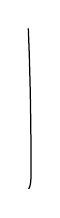
\begin{tikzpicture}[x=1cm,y=1cm]
\draw[line width=0.45pt]
  (0,1.05) .. controls (0.025,0.44) and (0.035,-0.19) .. (0.035,-0.78)
  .. controls (0.035,-0.91) and (0.025,-0.96) .. (0.005,-0.99);
\end{tikzpicture}}

We use the fact that we have an injective outer homomorphism
\[
\widehat{\Pi}_{0,3}\hookrightarrow\widehat{\mathcal T}_{1,1}^{\prime+}
\]
compatible with the action of $\Gamma$, proceeding as for the proposition at the beginning (where $\widehat{\Pi}_{0,3}'$ played the role of $\widehat{\mathcal T}_{1,1}^{\prime+}$).

\uline{Corollary} The canonical homomorphisms (surjective)
\[
\tag{43}
\Gamma_Q\longrightarrow\Gamma_{1,\nu}\qquad(\nu\geq1)
\]
are injective, hence isomorphisms.

It suffices to prove this for $\Gamma_Q\longrightarrow\Gamma_{1,1}$ (since $\Gamma_{1,1}$ is a quotient of $\Gamma_{1,\nu}$, $\nu\geq1\ldots$), now we have a homomorphism \unsure{\deleted{\illegible{1}}} $\Gamma_{1,1}\longrightarrow\mathrm{Aut\ ext}\,\widehat{\mathcal T}_{1,1}^{+}$ and we can consider the \unsure{composite}

\subsection*{Scans 531--540}
\addcontentsline{toc}{subsection}{Scans 531--540}
% package LM_P054
\scanpage{531}
\mspage{271}

\[
\Gamma_{\mathbb Q}\unsure{-|\longrightarrow}\Gamma_{1,1}
\longrightarrow \operatorname{Aut\,ext}\widehat{\mathcal T}_{1,1}^{+}
\longrightarrow \operatorname{Aut\,ext}\widehat{\mathcal T}_{1,1}^{+'},
\]
by the preceding theorem this composite is injective, hence also
$\Gamma_{\mathbb Q}\longrightarrow\Gamma_{1,1}$, q.e.d.

\uline{Remark} We really have the impression, with the proposition at the beginning, and
the preceding result christened ``theorem'', of having proved
the same thing twice, and with the same proof
at that! So it is time, after this detour, to make sure that this
really is so, i.e. that the homomorphism
$\widehat{\Pi}_{0,3}\longrightarrow\deleted{\unsure{\Pi}}\widehat{\mathcal T}_{1,1}^{+'}$ which we have just used
does indeed identify with the homomorphism
$\widehat{\Pi}_{0,3}\longrightarrow\widehat{\Pi}'_{0,3}$,
by means of a suitable isomorphism (which remains to be described),
commuting with the outer actions of $\Gamma$,
which we had set out to construct (cf. (10) to (20)) --- and we
lost it along the way, in

\scanpage{532}

trying to \deleted{\unsure{prove}}\inserted{\unsure{find}}
$\Pi'_{0,3}\xrightarrow{\sim}\mathcal T_{1,1}^{+'}$ by
factorization in the composite homomorphism
\[
\Pi_{0,3}\xrightarrow{\substack{\mathrm{can.}\\\unsure{\mathrm{surj}}}}
\Pi'_{0,3}\longrightarrow\mathcal T_{1,1}^{+'}
\]
--- and in a sense we went astray, for the ``natural'' homomorphism
$\unsure{\varphi|\rho}\,\Pi_{0,3}\longrightarrow\mathcal T_{1,1}^{+'}$
which we stumbled upon was \uline{not} \inserted{at all} the one we had
in mind: I was way off base. So I must return to the charge!

\scanpage{533}
\mspage{272}

\uline{37} Theory of Moduli of elliptic curves via Legendre
(rigidification of level 2). \unsure{)}

I realize that I have made some nevertheless quite simple things
rather complicated, in the preceding \S\. First a pang of conscience about surface topology:

\uline{Proposition} \unsure{Let|Let}\deleted{\illegible{1}}
$X$ be a paracompact topological\unsure{${}^{*}$} surface,
$G$ a discrete group operating properly on $X$, we assume that for every
$x\in X$, the stabilizer $G_x$ operates faithfully on a neighborhood of $x$
(so that $G$ operates faithfully --- in fact the two must be
equivalent) preserving the local orientation (hence $G_x$ is
a cyclic group), so that $Y=X/G$ is a paracompact topological surface.
Consider the set
\[
X^{!}=\{x\in X\mid G_x\ne(1)\}
\]
--- which is a discrete subset of $X$ stable under $G$ --- and the image
$Y^{!}\unsure{\subset|\in}Y$ of $X^{!}$ --- a discrete subset of $Y$ --- and
the ``signature'' on $(Y,Y^{!})$, for which the coefficient $d_y$ $(y\in Y^{!})$
is the ramification index $\operatorname{ord}G_x$ at the
$x\in X$ over $y$. For every $G$-covering $X'$ of $X$, let us
then consider $X'/G=Y'$ as a space over $Y$. Then:

\margin{\uline{Variant} $\mathcal G$ operates
\deleted{$X$ \illegible{2} $\mathcal G$}
\deleted{\unsure{operates}}\inserted{on} $X$, \unsure{with|its}
\uline{invariant} subgroup $G$ in $\mathcal G$
satisfying the conditions opposite. We then have, putting
\deleted{\illegible{1}} $Y=X/G$ with an \unsure{operation} of
$\mathcal G/G=\mathcal H$
on it:
\[
\deleted{\illegible{1}}\underline{\operatorname{Rev}}.
(X,\mathcal G)\unsure{\approxeq|\simeq}
\underline{\operatorname{Rev}}((Y,\underline d),\mathcal H),
\]
hence
\[
\Pi_1(X,\mathcal G,x)
\xrightarrow{\sim}
\Pi_1((Y,\underline d,\mathcal H),y).
\]
Application
\[
\mathfrak S_{0,3}\simeq
\mathcal T'_{1,1}
(\simeq\unsure{\mathrm{Gl}|\mathrm{Sl}}(2,\mathbb Z)/\pm1)
\]
extension of $\mathcal T_{0,3}=\mathfrak S_3
\times\mathbb Z/2$ by $\Pi_{03}$}
\scanpage{534}

a) $Y'$ is \deleted{a} \inserted{a topological surface,} a ramified covering of $Y$, subordinate to the signature $\underline d\,\deleted{\illegible{1}}=\underline d(X/Y)$.

b) The functor $X'\longmapsto Y'=X'/G$ is an equivalence of categories
\[
(1)\qquad \mathrm{Rev}(X,G)\overset{\approx}{\longrightarrow}\mathrm{Rev}_{\underline d}(Y)
\]

\uline{N.B.} We can make explicit a quasi-inverse functor, by associating to every ramified covering $Y'$ of $Y$ compatible with $\underline d$, \deleted{\illegible{2}} \inserted{the} ``normalized'' $(X,G)$-covering (in a topological sense easy to make explicit) of $X\times_Y Y'$. We have an analogous statement for regular locally noetherian schemes of dimension $1$, where the quasi-inverse functor is obtained by normalizing $X\times_Y Y'$.

\uline{Corollary} Let $x\in X-X^{!}$, $y$ its image in $Y$. We assume $Y$ connected (i.e. that $G$ operates transitively on the set of connected components of $X$). Then we have a canonical isomorphism
\[
(2)\qquad \Pi_1(X,G;\unsure{a|x})\overset{\sim}{\longrightarrow}\Pi_1((Y,\underline d),y)
\]

\scanpage{535}
\mspage{273}

whence, for $X$ connected, a canonical exact sequence
\[
(3)\qquad
1\longrightarrow
\deleted{\Pi_1((X,\unsure{G|1}),x)}\inserted{\Pi_1(X,x)}
\longrightarrow\Pi_1((Y,\underline d),y)\longrightarrow G\longrightarrow 1
\]

\uline{N.B.} We have \unsure{?} an analogous corollary in the scheme-theoretic context, $X$ and $Y$ being regular schemes of dimension $1$\unsure{.} --- or, as the case may be, smooth relative schemes of relative dimension $1$ over an $S$, but in this case one would have to (if I need it) take a little care to specify \unsure{the statement|the statements} in a reasonable form.

\uline{Example} Let us take $X=\mathbb P^1(\mathbb C)\setminus\{0,1,\infty\}=U_{0,3}(\mathbb C)$,
$G=\mathfrak S_3$ operating in the usual way, thus (with the \deleted{\unsure{notations}} \inserted{conventions} of the preceding \S),
\deleted{$Y=\unsure{\mathbb P^1(\mathbb C)}\,\mathbb P^1(\mathbb C)$}
\inserted{identifying} $\mathbb P^1(\mathbb C)/(G=\mathfrak S_3)$ with $\mathbb P^1_{\mathbb C}$, with
\[
(4)\qquad
\begin{array}{rcll}
(0,1,\infty)&\longmapsto&0&d_0=2\\
(2,-1,\tfrac12)&\longmapsto&1&d_1=2\\
(j,\overline j)&\longmapsto&\infty&d_\infty=3
\end{array}
\]
we find $Y=\mathbb P^1(\mathbb C)\setminus\{0\}$, and $\underline d=2\{1\}+3\{\infty\}$.

We thus find a canonical isomorphism
\[
(5)\qquad
\Pi^{1}((U_{0,3}(\mathbb C),\mathfrak S_3),x)
\simeq\Pi_1((\mathbb P^1(\mathbb C)\setminus\{0\},\underline d),\unsure{y})
\]

\scanpage{536}

\unsure{now|or} unfortunately we cannot take $x=P=j$, we have to take
$x\in\mathbb P^1(\mathbb C)\setminus\{0,1,\infty,2,-1,\tfrac12,j,\overline j\}$
--- the most convenient thing will be to take $x$ such that $y=f(x)\,\unsure{\in|\leq|\leftarrow}$ is the \inserted{typical} base-$\mathrm p^{\mathrm t}$ $Q=j$ for calculating the $\pi_1$ with ramification --- for such an $x$ we thus find a canonical isomorphism
\[
(5\,\mathrm{bis})\qquad
\Pi_1((U_{0,3}(\mathbb C),\mathfrak S_3),x)\simeq\Pi'_{0,3}
\]
and by choosing an \inserted{$\mathfrak S_3$-}class of paths from the \inserted{initial} base point $P=j$ on $\unsure{X_0|X}=U_{0,3}(\mathbb C)$ to $x$, whence a corresponding isomorphism of the first side of (5bis) \deleted{\illegible{1}} with $\Pi_{0,3}$, we find a canonical isomorphism
\[
(6)\qquad
\Pi_1((U_{0,3}(\mathbb C),\mathfrak S_3),P)\simeq\Pi'_{0,3}
\]
(which changes by an inner automorphism when one modifies the choice of an $\mathfrak S_3$-class of paths), whence the exact sequence
\[
(7)\qquad
1\longrightarrow\Pi_{0,3}\longrightarrow\Pi'_{0,3}\longrightarrow\mathfrak S_3\longrightarrow 1,
\]
which is none other than (9bis) of the preceding \S\, but interpreted here much more transparently as
\scanpage{537}
\mspage{274}

the homotopy exact sequence for $\mathfrak{S}_3$ operating
on $U_{0,3}(\mathbb{C})$. And we find likewise,
in the \unsure{arithmetico-geometric} setting,
working on the scheme $U_{0,3}=U_{0,3\mathbb{Q}}$ and its
quotient $U_{0,3}/\mathfrak{S}_3\simeq\mathbb{P}^{1}_{\mathbb{Q}}\setminus\{0\}$, with
the signature $2\{1\}+\unsure{3}\{\infty\}$ on it, the
diagram of exact sequences

\diagram{
\begin{tikzcd}[ampersand replacement=\&,column sep=large,row sep=large]
 \& 1 \arrow[d] \& 1 \arrow[d] \& \& \\
1 \arrow[r] \& \widehat{\Pi}_{0,3} \arrow[r] \arrow[d] \& \widehat{\Pi}'_{0,3} \arrow[r] \arrow[d] \& \mathfrak{S}_3 \arrow[r] \arrow[d,equal] \& 1 \\
1 \arrow[r] \& \mathcal{E}_{0,3} \arrow[r] \arrow[d] \& \mathcal{E}'_{0,3} \arrow[r] \arrow[d] \& \mathfrak{S}_3 \arrow[r] \& 1 \\
 \& \Gamma_{\mathbb{Q}} \arrow[r,equal] \arrow[d] \& \Gamma_{\mathbb{Q}} \arrow[d] \& \& \\
 \& 1 \& 1 \& \&
\end{tikzcd}
[(8) to the left of the second horizontal sequence.
To the left and a little below $\widehat{\Pi}_{0,3}$:
$\widehat{\mathcal{T}}^{+}_{0,4}$, followed by two short parallel oblique strokes
(an $=$ sign equating it with $\widehat{\Pi}_{0,3}$).
To the left and a little below $\mathcal{E}_{0,3}$:
$\unsure{N}^{!}_{0,4}$ (a short horizontal stroke against the ${}^{!}$), followed by two short
parallel oblique strokes (an $=$ sign toward $\mathcal{E}_{0,3}$).
To the left and a little below the first $\Gamma_{\mathbb{Q}}$:
$\Gamma_{0,4}$, followed by two short parallel oblique strokes (an $=$ sign toward $\Gamma_{\mathbb{Q}}$).]
}

We now want to relate
$U_{0,3}$, with the action of $\mathfrak{S}_3$
on it, to the modular multiplicity
$M_{11}$ for elliptic curves
(subscripts $\mathbb{Q}$ understood). It is
a pity, by the way, to work only over $\mathbb{Q}$ --- I am going to work
instead, over $\mathbb{Z}[1/2]$ --- i.e. in \unsure{residue|always} characteristic $\ne 2$.

\scanpage{538}

In the preceding \S{} I identified, somewhat
murkily, $U_{0,3}=M^{!}_{0,4}$\unsure{,} with $M_{1,1}[2]'$\unsure{,}
(\deleted{of which}\inserted{over which} $M_{1,1}[2]$
\deleted{\unsure{should be|was to be} \illegible{1}}\inserted{is a gerbe banded} by
$\mathbb{Z}/2$). The technical troubles (rather,
the conceptual complications) are due
to the fact that for elliptic curves
(more generally, for abelian varieties of
arbitrary dimension), if $n$ is an integer $\ge 3$,
the ``Jacobi rigidification of level $n$''
really is a rigidification (i.e.
every automorphism of a relative elliptic curve
$E$ which induces the identity on
${}_nE$ --- kernel subscheme of $n.\mathrm{id}_E$ --- is
the identity --- but it is no longer the
same for $n=2$, where $\unsure{u|n}$ is the \uline{identity}\inserted{$\mathrm{id}_E$} \unsure{up} above
an open and closed subset of $S$, and $-\mathrm{id}_E$
on the complement. This suggests, for
a better understanding, covering
$M_{1,1}[2]$ by an $M_{1,1}(n)$, where $n$ is a
multiple of $2$ --- then $M_{1,1}(n)$ becomes an
ordinary scheme of finite type over $\operatorname{Spec}\mathbb{Z}$
(its image in $\operatorname{Spec}\mathbb{Z}$ \unsure{will be|will be} \inserted{the open set} $\operatorname{Spec}\mathbb{Z}[1/n]$)
and over $\operatorname{Spec}[1/n]$, the \deleted{\unsure{scheme|scheme}}\inserted{modular topos}
\scanpage{539}
\mspage{275}

$M_{1,1}$ is recovered as
\[
(9)\qquad
M_{1,1}\unsure{\simeq|\cong}
\bigl(M_{1,1}[n],\overbrace{\mathrm{Gl}(2,\mathbb Z/n\mathbb Z)}^{\Gamma_n}\bigr)
\]
(over $\operatorname{Spec}\mathbb Z[1/n]$)

\margin{careful, it really is $\mathrm{Gl}(2,\mathbb Z/n\mathbb Z)$, and \uuline{not} $\mathrm{Sl}(2,\mathbb Z/n\mathbb Z)$ that one must take here}

Here $M_{1,1}[n]$ is the scheme representing the functor on $(\mathrm{Sch})_{\unsure{\mathbb Z|S}}$
\[
S\longmapsto
\begin{gathered}
\text{set of relative elliptic curves}\\
\text{over $S$, \uline{equipped} with an isomorphism}\\
(\mathbb Z/n\mathbb Z)^2_S\longrightarrow {}_nE
\end{gathered}
\]
\margin{this functor \unsure{is|$\to$} representable iff $n\geq 3$ (so it is not for $n=1,2$)}
on which the group $\Gamma_n=\mathrm{Gl}(2,\mathbb Z/n\mathbb Z)=\operatorname{Aut}((\mathbb Z/n\mathbb Z)^2)$ operates in the obvious way. \deleted{The variety} The \uline{modular scheme} (``coarse'', as opposed to the modular multiplicity or topos) is described over $\mathbb Z/n\mathbb Z$ by
\[
(10)\qquad \widetilde M_{1,1}\simeq M_{1,1}[n]/\Gamma_n
\]
(over $\mathbb Z[1/n]$)

\uline{N.B.} The scheme $\widetilde M_{1,1}$ \inserted{over $\operatorname{Spec}\mathbb Z$} can be described as ``the representable envelope'' of the nonrepresentable functor
\[
S\longmapsto
\begin{gathered}
\text{\unsure{isomorphism|Isomorphism} classes of relative}\\
\text{elliptic curves over $S$ \ldots}
\end{gathered}
\]
-- ditto over a base scheme (for example $\mathbb Q$, or $\operatorname{Spec}\mathbb Z[1/n]$, arbitrary \ldots

\scanpage{540}

One must be careful that as a scheme over $\mathbb Z[1/n]$ (or over $\mathbb Q$, passing to the \unsure{generic|generic} fiber) $M_{1,1}[n]$ \uline{is not} relatively connected (i.e. does not have geometrically connected fibers). \unsure{In} fact, an isomorphism
\[
(\mathbb Z/n\mathbb Z)^2_S\simeq {}_nE
\]
implies, by passing to the $2^{\unsure{\mathrm{ième}|\mathrm{ème}}}$ exterior power, an isomorphism
\[
(\mathbb Z/n\mathbb Z)_S\xrightarrow{\sim}
\Lambda^2_{\mathbb Z/n\mathbb Z}\,{}_nE
\simeq \mu_n^{\otimes-1}(S)
\]
whence an isomorphism
\[
\mathbb Z/n\mathbb Z\simeq\mu_n(S)
\]
which identifies (taking \deleted{\unsure{and}} the image of $1$ mod $n$) with a section of $\mu_n^*(S)$, where $\mu_n^*$ is the relative $(\mathbb Z/n\mathbb Z)^*$-torsor over $\operatorname{Spec}\mathbb Z[1/n]$ of ``primitive \unsure{$n$th|$n$-th} roots of $1$''. We thus have a canonical morphism
\[
(11)\qquad M_{1,1}[n]\longrightarrow\mu_n^*
\]
and it is this morphism that has geometrically connected fibers \inserted{\uuline{in characteristic 0}}. Passing to the limit over variable $n$, we find \uline{over $\mathbb Q$}
\[
(12)\qquad M_{1,1}[\infty]=\varprojlim_n M_{1,1}[n]
\longrightarrow\mu_\infty^*\overset{\inserted{\mathrm{iso.can}}}{\simeq}\operatorname{Spec}\Sigma
\]

\subsection*{Scans 541--550}
\addcontentsline{toc}{subsection}{Scans 541--550}
% package LM_P055
\scanpage{541}
\mspage{276}

\unsure{(12)} where $\Sigma$ \inserted{$\subset\mathbb C$} is \unsure{the subextension} that is maximal cyclotomic in $\overline{\mathbb Q}_0$.

\deleted{\unsure{The}} We recover the $M_{1,1}[n']$, for $n'\mid n$, \inserted{$n'\ne 1,2$,} from $M_{1,1}[n]$ with the action of $\Gamma_n$ on it, by
\[
(13)\qquad M_{1,1}[n']\simeq M_{1,1}[n]\wedge_{\Gamma_n}\Gamma_{n'}\simeq M_{1,1}[n]/K_{n,n'}
\]
\[
\text{over }\operatorname{Spec}\mathbb Z[1/n]
\]
where
\[
(14)\qquad K_{nn'}=\operatorname{Ker}(\Gamma_n\longrightarrow\Gamma_{n'}).
\]

\margin{\uline{N.B.} $K_{n,n'}$ operates \uline{freely} on the scheme $M_{1,1}[n]$ (if $n'\mid n$, $n'\ne 1,2$) --- but of course not if $n'=1$ or $2$.}

If however we apply this formula in \unsure{the inadmissible case|the inadmissible cases} $n'=1$ or $2$, we find for the case $n'=1$, not $M_{1,1}$ but $\widetilde M_{1,1}$ (coarse modular scheme), and for $n'=2$, not $M_{1,1}[2]$ (which is not a scheme either) but what we had called in the preceding \S\ $M_{1,1}[2]'$.

We can \deleted{\unsure{determine|define}} \inserted{make explicit} \inserted{$M_{1,1}$ and} $\widetilde M_{1,1}$ over all of $\operatorname{Spec}\mathbb Z$, \inserted{in terms of the $M_{1,1}[n]$,} by describing them \inserted{over the} two open sets $\operatorname{Spec}(\mathbb Z[1/n])$, $\operatorname{Spec}(\mathbb Z[1/n'])$ which cover $\operatorname{Spec}(\mathbb Z)$ (i.e. for $(n,n')=1$) by (9) and (10), \inserted{(taking first $n$, then $n'$ in them)} and by ``gluing'' \deleted{in} over $\operatorname{Spec}(\mathbb Z[\frac{1}{nn'}])$ by these same formulas, applied to $nn'$\ldots

\scanpage{542}

We have moreover (for the record)
\[
\text{\uline{Theorem}}\qquad \widetilde M_{1,1}\simeq\mathbb E^1_{\mathbb Z}\qquad(\text{over }\operatorname{Spec}\mathbb Z)
\]

We can pin down such an isomorphism (\unsure{defined|defines} a priori modulo the integral affine group $X\longmapsto\pm X+n$, $n\in\mathbb Z$) by \unsure{noting} that there are in $\widetilde M_{1,1}$ two distinguished sections over $\mathbb Z$, whose values at the generic point correspond to the two isomorphism classes of elliptic curves in characteristic $0$ (over $\mathbb C$, for example) which have automorphisms $\ne\mathrm{id},-\mathrm{id}$ --- the two groups \unsure{of automorphisms} that we obtain are moreover $\mathbb Z/4\mathbb Z$ and $\mathbb Z/6\mathbb Z$ (very easy for example by the \unsure{transcendental|transcendental} route). These are what are called unless I am mistaken the ``anharmonic'' elliptic curves. On an $M_{1,1}[n]$, the group of rational automorphisms\,$/k$ of an elliptic curve described by a point $x$ of $M_{1,1}[n](k)$ is canonically identified with the stabilizer of $x$ in $\Gamma_n$:
\[
(15)\qquad\operatorname{Aut}(E_x)\simeq(\Gamma_n)_x
\]

\scanpage{543}
\mspage{277}

--- of course, we have suitable statements over an arbitrary base scheme, not necessarily a field. This already shows that the \unsure{automorphisms} of elliptic curves are linked in an essential way to the \uline{ramification} of $\Gamma_n$ operating on $\unsure{M_{1,1}[n]|M_{1,n}[n]}$. We thus find:

\uline{Proposition} (Over $\operatorname{Spec}\mathbb Q$) There are exactly two orbits of $\Gamma_n$ operating on $M_{1,1}[n]$ which are ``\deleted{singular}\inserted{critical}'', and which correspond to stabilizers isomorphic resp. to $\mathbb Z/4\mathbb Z$ and $\mathbb Z/6\mathbb Z$, which are the groups of \unsure{automorphisms} of the corresponding (``anharmonic'') elliptic curves.

\margin{$n\ne 1,2$}

We \unsure{will note|note} that $\Gamma_n$ \uline{does not operate} \unsure{faithfully|faithfully} on $M_{1,1}[n]$ --- the kernel of this operation is the central subgroup $\{\pm1\}$, image of the corresponding group of $\operatorname{Gl}(2,\mathbb Z)$ --- it corresponds to the group of ``universal'' automorphisms $\pm\mathrm{id}_E$ of elliptic curves $E$. The quotient group
\[
(16)\qquad \Gamma'_n=\Gamma_n/\{\pm1\}
\]
\deleted{\unsure{(on|on}} operates \unsure{faithfully|faithfully}, and we can look at the ``mixed topos'' $(M_{1,1}[n],\Gamma'_n)$ --- we find

\scanpage{544}
at once that it \uline{does not depend} (up to canonical \unsure{equivalence|equivalence}) \uline{on the choice of} $n$ [except that the open set of $\operatorname{Spec}\mathbb Z$ over which ``it makes sense'' depends on $n$\dots] -- and. in fact, we have:

\margin{thus on \unsure{condition} of working over a base scheme (such as $\operatorname{Spec}\mathbb Z[\frac{1}{nn'}]$) where $n,n'$ are \unsure{both} invertible\dots}

\[
(17)\qquad (M_{1,1}[n],\Gamma'_n)\simeq M_{1,1}'
\]
\[
(\text{over }\operatorname{Spec}\mathbb Z[1/n])
\]
where the modular \deleted{topos} \inserted{schematic multiplicity} $M_{1,1}'$ is \unsure{described|described}, in terms of elliptic curves ``\unsure{defined} modulo symmetry'', as in the \S\ preceding.

\uline{Remark.} The preceding proposition seems to depend on $n$ -- but we see a priori \deleted{that} (thanks to the fact that the $\Gamma_{n,n'}$ \inserted{($n'\mid n$, $n'\ne1,2$)} (\unsure{operating|operate} freely) that if it is valid for \uline{one} $n$, it is valid for all.

\deleted{\unsure{Corollary}} Let us note \deleted{that} also

\uline{Corollary of the proposition.} \inserted{(characteristic 0)} The stabilizers \uline{in $\Gamma'_n$} (the group which operates \uline{\unsure{faithfully}} on $M_{1,1}[n]$) of the points of the \unsure{two} critical orbits are resp. $\mathbb Z/2\mathbb Z$ and $\mathbb Z/3\mathbb Z$. \deleted{\illegible{1}}

\margin{valid for $n\unsure{\ne|=|\geq}2$, \unsure{cf.|cf.} below}

\scanpage{545}
\mspage{278}
We have assumed here that $n\ne1,2$ -- but nothing prevents us from also considering \inserted{on}
\[
(18)\qquad M_{1,1}[2]'\overset{\mathrm{dfn}}{=}M_{1,1}[2m]/\Gamma_{2m,2}
=M_{1,1}[2m]/\unsure{\Gamma_{2m,2}|\Gamma'_{2m,2}}
\]
(where $m$ is any integer, $\ge2$)
the action of $\Gamma_2\simeq\operatorname{Gl}(2,\mathbb Z/2\mathbb Z)\simeq\operatorname{Sl}(2,\mathbb Z/2\mathbb Z)\simeq\unsure{\mathfrak S_3|\mathcal S_3}\simeq\Gamma_{2m}/\Gamma_{2m,2}$. \deleted{\unsure{Whereas|Whereas}} It is no longer true, \inserted{to be sure,} that $\Gamma_{2m,2}$ operates \unsure{freely} on $M_{1,1}[2m]$ -- for $\Gamma_{2m,2}$ contains the element $-1\in\Gamma_{2m}$ corresponding to the universal symmetry $-\operatorname{id}_E$ -- i.e. \inserted{\unsure{to}} the element \deleted{\unsure{of}} $-1$ of $\operatorname{Gl}(2,\mathbb Z)$. But the general rigidity result recalled at the beginning implies that \deleted{$\Gamma'_{2m,2}=\Gamma_{2m,2}/\pm1$}
\[
(19)\qquad\Gamma'_{2m,2}\overset{\mathrm{dfn}}{=}\Gamma_{2m,2}'/\pm1
\simeq\operatorname{Ker}(\Gamma'_{2m}\longrightarrow\Gamma'_2\simeq\unsure{\mathfrak S_3|\mathcal S_3})
\]
operates \deleted{\unsure{fi}} \inserted{still} \uline{freely} on $M_{1,1}[2m]$ -- and this implies that the corollary of the proposition is still valid for the action of $\Gamma'_2\,(\xleftarrow{\sim}\Gamma_2\simeq\unsure{\mathfrak S_3|\mathcal S_3})$ on $M_{1,1}[2]'$.

\uline{Terminological digression.} $M_{1,1}$ \inserted{${}=M_{1,1}[1]$} and the

\scanpage{546}
\mspage{278}
\figure{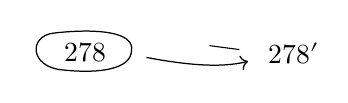
\begin{tikzpicture}[x=1cm,y=1cm,baseline=(ancien.base)]
\node[inner sep=0pt] (ancien) at (0,0) {$278$};
\draw[line width=0.45pt]
  (0.58,0.02) .. controls (0.63,0.27) and (0.13,0.31) .. (-0.40,0.25)
  .. controls (-0.73,0.22) and (-0.72,-0.19) .. (-0.28,-0.22)
  .. controls (0.20,-0.27) and (0.57,-0.20) .. (0.58,0.02);
\draw[->,line width=0.45pt]
  (0.77,-0.06) .. controls (1.25,-0.15) and (1.70,-0.20) .. (2.06,-0.11);
\draw[line width=0.4pt] (1.57,0.09) -- (1.95,0.04);
\node[anchor=west,inner sep=0pt] at (2.31,-0.015) {$278'$};
\end{tikzpicture}}
\mspage{278'}
$M_{1,1}[n]$ ($n\in\mathbb N^*$) are \unsure{defined} \unsure{a|a} priori as modular schematic \uline{multiplicities}, i.e. a) as locally ringed topoi locally isomorphic to the étale topos of a scheme (in this case, of finite type over $\operatorname{Spec}\mathbb Z$, or over $\mathbb Q$ if we work in characteristic 0) and b) \unsure{defined}, up to equivalence itself defined up to unique \unsure{isomorphism|isomorphism}, as ``representing'' the \deleted{\illegible{1}} corresponding ``functors''
\[
S\longmapsto
\begin{gathered}
\text{category of elliptic curves}\\
\text{relative over }S\text{, with rigidification}\\
\text{of Jacobi of level }n\text{ i.e.}\\
\text{isomorphism}\quad(\mathbb Z/n\mathbb Z)_S\simeq{}_nE\\
={}\unsure{\mathcal{E}ll_n}(S)
\end{gathered}
\]
thus by construction we have \inserted{for every scheme $S$} an equivalence
\[
\unsure{\mathcal{E}ll_n}(S)\unsure{\simeq|\cong}
\text{\uline{$\operatorname{Hom}$}}_{\substack{\text{topoi locally}\\\text{ringed}\\\text{i.e. morphisms of}\\\text{multiplicities}}}
(S,M_{1,1}[n])
\]
For the categories $\unsure{\mathcal{E}ll_n}(S)$ to be \uline{discrete}, \deleted{\illegible{1}} or again for $M_{1,1}[n]$ to be a scheme, or again for the automorphisms of an

\scanpage{547}
\mspage{279}

elliptic curve \unsure{respecting|respect} a Jacobi rigidification of level $n$ \unsure{to be} the identity, it \unsure{is necessary and sufficient} that $n\geq 3$ i.e. $n\neq 1,2$. Thus $M_{1,1}[2]$ \uline{is not} a scheme -- but $M'_{1,1}[2]$ is one, and $M_{1,1}[2]\to M_{1,1}[2]'$ is a \deleted{\illegible{1}} local isomorphism (described entirely by a $\mathbb Z/2\mathbb Z$-gerbe over $M_{1,1}[2]'$). \deleted{\unsure{We consider of course}} \inserted{\unsure{It} is necessary all the same to take the} trouble to define
\diagram{\[
\tag{20}
\begin{tikzcd}[ampersand replacement=\&,column sep=large,row sep=large]
M_{1,1}[2] \arrow[r] \arrow[d,phantom,"{\simeq}"{description,rotate=90},"{\text{``theorem''}}"{description,xshift=3em}] \& M_{1,1}[2]' \arrow[d,phantom,"{\simeq}"{description,rotate=90},"{\text{``definition''}}"{description,xshift=3em}] \\
(M_{1,1}[2m],\Gamma_{2m,2}) \& M_{1,1}[2m]/\Gamma'_{2m,2} \arrow[d,phantom,"{\Vert}"{description}] \\
\& M_{1,1}\unsure{(2m)|[2m]}/\Gamma_{2m,2}
\end{tikzcd}
\]}
as the canonical homomorphism of ``passage to the coarse quotient'' -- which makes sense whenever a discrete group (say)\unsure{\S} $G$ operates on a scheme (say) $X$, as a morphism
\[
\tag{21}
(X,G)\longrightarrow X/G=Y
\]
whose inverse \unsure{image} functor (sheaves on $Y=X/G\longrightarrow G$-sheaves on $X$) is obvious. Here we have a normal subgroup \unsure{$\mathfrak z$|$z$} of $G$ which operates \unsure{trivially|trivially} on $X$, such that $G/\unsure{\mathfrak z|z}$ operates freely, which means that the morphism

\scanpage{548}

(21) factors as
\[
\tag{22}
(X,G)\longrightarrow
\left(X,\underbrace{G/\unsure{\mathfrak z|z}}_{G'}\right)
\overset{\sim}{\longrightarrow}Y=X/G=X/G',
\]
so that the morphism of multiplicities (21) is also identified, simply, with
\diagram{\[
\tag{23}
\begin{tikzcd}[ampersand replacement=\&,column sep=large,row sep=large]
(M_{1,1}[2m],\Gamma_{2m,2}) \arrow[r] \& (M_{1,1}[2m],\Gamma'_{2m,2}) \arrow[d,phantom,"{\simeq}"{description,rotate=90}] \\
\& M_{1,1}[2]'
\end{tikzcd}
\]}

On the other hand, if we want to go down as far as $M_{1,1}[1]'=M_{1,1}'$, by passing to the quotient (in the ``coarse'' sense) of $M_{1,1}[n]$ by $\Gamma'_n$, the morphism
\diagram{\[
\tag{24}
\begin{tikzcd}[ampersand replacement=\&,column sep=large,row sep=large]
(M_{1,1}[n],\Gamma'_n) \arrow[r] \arrow[d,phantom,"{\Vert}"{description}] \& M_{1,1}[n]/\Gamma'_n \arrow[d,phantom,"{\Vert}"{description}] \\
M_{1,1}' \& \widetilde M_{1,1}
\end{tikzcd}
\]}
is no longer an ``isomorphism'' i.e. is no longer an equivalence, for $\Gamma'_n$ does not operate freely -- it has \inserted{(even in characteristic $0$)} ramification of degree $2,3$.

[If however we exclude the anharmonic elliptic curves, \unsure{its|it} would work -- it is ``only in the neighborhood'' of these elliptic curves that (24) is not an isomorphism\ldots

\scanpage{549}
\mspage{280}

In fact, the arguments of the preceding \S{} establish an isomorphism (\unsure{valid} over \inserted{the} $\mathrm{Spec}\,\unsure{\mathbb Z[1/n]}$ of $\mathbb Z[1/2]$)
\[
(25)\qquad M_{1,1}[2]'\simeq M_{0,4}^{!}\simeq U_{0,3}
\]
(\unsure{valid} over $\mathrm{Spec}\,\mathbb Z[1/2]$)

\margin{N.B. \unsure{the image} of $M_{1,1}[2]'$ in $\mathrm{Spec}\,\mathbb Z$ is $\mathrm{Spec}\,\mathbb Z[1/\unsure{n|2}]$, while that of $M_{0,4}^{!}\simeq U_{0,3}$ is $\mathrm{Spec}\,\mathbb Z$ in \unsure{all} its entirety}

and this isomorphism is compatible with the operations of \deleted{$\unsure{\Gamma'_2\simeq\Gamma}$}
\[
(26)\qquad \Gamma'_2\simeq\Gamma_2=\operatorname{Gl}(2,\mathbb Z/2\mathbb Z)=\operatorname{Sl}(2,\mathbb Z/2\mathbb Z)
\]
on $M_{1,1}[2]'$ on the one hand, of $\unsure{\mathfrak S_3|\mathcal S_3}$ on $U_{0,3}$ on the other \unsure{hand|hands}, when we consider the isomorphism
\[
(27)\qquad
\begin{array}{ccc}
\Gamma_2 & \xrightarrow{\sim} & \unsure{\mathfrak S_3|\mathcal S_3}\\
\Vert &&\\[-4pt]
\operatorname{Gl}(2,\mathbb F_2)&&
\end{array}
\]
which associates, to every automorphism of $\mathbb F_2^2$, its action on the three nonzero elements, $\underline{\alpha}=(1,0)$, \inserted{$\underline{\beta}=$}$(0,1)$, and $\underline{\gamma}=(1,1)=\underline{\alpha}+\underline{\beta}$ (so that we have moreover) \deleted{\illegible{2}}
\[
(28)\qquad \gamma=\alpha\unsure{+|-}\beta,\quad \unsure{\alpha|\beta}=\beta\unsure{+|-}\gamma,\quad \beta=\unsure{\gamma}+\alpha.
\]
It would be necessary to make this compatibility explicit, by \unsure{considering} the natural action of $\unsure{\mathfrak S_4|\mathcal S_4}$ on $M_{0,4}^{!}$, $M_{0,n}^{!}$ being the modular multiplicity defined by

\scanpage{550}

\[
(29)\qquad
\underline{\operatorname{Hom}}_{\text{multiplicities}}(S,M_{0,n}^{!})\simeq
\begin{gathered}
\text{category of}\\
\text{relative \unsure{curves|lines}}\\
\text{over }S,\ \text{locally isomorphic to }\mathbb P^1_S\\
\text{(for étale topology) and equipped}\\
\text{with }n\text{ sections mutually}\\
\text{\unsure{disjoint} \unsure{numbered}}\\
\deleted{\illegible{1}}\quad\unsure{s_1|s_0},s_2,\ldots s_n
\end{gathered}
\]

\margin{If we want representability for $n=0,1,2$, it no longer suffices to work with \unsure{the étale topology|the étale topologies} --- we need fppf topologies for example...}

\uline{N.B.} this really is representable by a multiplicity iff $n\geq3$, \inserted{i.e. if the stack \unsure{in|of} groupoids which we want to \unsure{represent} is ``rigid'' ---} and then the multiplicity is even a scheme, isomorphic moreover \unsure{canonical|canonically} to the \inserted{\unsure{sub-}}scheme
\[
\underline{\operatorname{Mon}}(I_{n-3},U_{0,3})\subset U_{0,3}^{I_{n-3}},
\]
where here
\[
I_{n-3}=\{i\in\mathbb N\quad3<i\leq n\deleted{\unsure{-3}}\}
\]
--- thus \deleted{\illegible{1}}
\[
M_{0,3}^{!}\xrightarrow{\sim}\mathrm{Spec}\,\mathbb Z\quad\text{(terminal scheme)},\quad\text{and}
\]
\[
M_{0,4}^{!}\xrightarrow{\sim}U_{0,3}=\mathbb P^1_{\mathbb Z}\setminus\{\text{sections \deleted{\illegible{1}} }0,1,\infty\}=\mathrm{Spec}\,\mathbb Z[T]\Bigl[\frac{1}{T(T-1)}
\]

But we will keep in mind that there is a natural operation of $\unsure{\mathfrak S_n|\mathcal S_n}$ on $M_{0,n}^{!}$, hence on $\underline{\operatorname{Mon}}(I_{n-3},U_{0,3})$ --- \deleted{\unsure{of which|therefore}} whereas we see a priori only the action of $\unsure{\mathfrak S_3|\mathcal S_3}\times\unsure{\mathfrak S_{n-3}|\mathcal S_{n-3}}$ on the latter: the canonical isomorphism
\[
(30)\qquad M_{0,n}^{!}\simeq\unsure{\operatorname{Mon}}(I_{n-3},U_{0,3})\subset U_{0,3}^{I_{n-3}}
\]
\[
\text{(where }I_{n-3}=\{i\in\mathbb N\mid\deleted{\unsure{2}}3<i\leq n\}\text{)}
\]
takes account only of the natural operations \unsure{of the|of the}

\subsection*{Scans 551--560}
\addcontentsline{toc}{subsection}{Scans 551--560}
% package LM_P056
\scanpage{551}
\mspage{\unsure{281}}

canonical bijection
\[
\tag{33}
\widetilde I \xrightarrow{\sim} V(I)^*
\overset{\mathrm{df}}{=} V(I)\setminus\{0\}
\]
by associating to a partition $I=I'\cup I''$, with
$I',I''$ of cardinality $2$, the \inserted{only} permutation
\unsure{\inserted{(even)}|\deleted{\inserted{(even)}}} of $I$
\deleted{formed of} which \unsure{leaves invariant} $I',I''$ and \unsure{induces|induces} on
each \unsure{its} nontrivial permutation. (The elements
of $\mathfrak{S}_I$ obtained in this way are also the \uline{even}
\uline{permutations} \uline{of order $2$}, \deleted{\unsure{)}} which together with the identity thus form
the subgroup $V(I)$).

We find, if $i\in I$, whence $I\setminus\{i\}$ of
cardinality $3$, \deleted{\unsure{that}} a canonical map
\[
\tag{34}
I\setminus\{i\}\longrightarrow\widetilde I
\]
by associating to $j\in I\setminus\{i\}$ the partition
of $I$ into $\{i,j\}$ and its complement.
This bijection being compatible with the
transport of \unsure{structures|structure}, we conclude
that the corresponding isomorphism
\[
\tag{35}
\mathfrak{S}_{I\setminus\{i\}}\simeq\mathfrak{S}_{\widetilde I}
\]
\deleted{\unsure{which}} is \deleted{\unsure{compat}} also the composite
\[
\tag{36}
\underset{\substack{\text{stabilizer of}\\ i\text{ in }\mathfrak{S}_I}}
{\mathfrak{S}_{I\setminus\{i\}}}
\hookrightarrow\mathfrak{S}_I\longrightarrow\mathfrak{S}_{\widetilde I},
\]
hence the four symmetric subgroups
of index $3$ $\mathfrak{S}_{I\setminus\{i\}}$ of $\mathfrak{S}_I$ $(i\in I)$\unsure{.|,}

\scanpage{552}
are canonically \unsure{isomorphic} to $\mathfrak{S}_{\widetilde I}$
--- hence to one another, \deleted{\unsure{but}} by isomorphisms which
\deleted{\unsure{not}} are \deleted{\unsure{not}} moreover \deleted{\illegible{1}} deduced from the canonical
bijections \deleted{\unsure{equal}}
\[
  (\deleted{\unsure{39}}\inserted{37})\qquad
  I\setminus\{i\}\xrightarrow{\sim}I\setminus\{j\}
  \qquad(i\ne j,\ i,j\in I)
\]
canonical, equal to \deleted{the identity}
\inserted{the \uline{transposition} (not to the identity)} on $I\setminus\{i,j\}$.
\inserted{This bijection is in fact the composite}
\deleted{(Indeed, these bijections \unsure{do not form a}}
\[
  I\setminus\{i\}\xrightarrow{\sim}\widetilde I
  \xrightarrow{\sim}I\setminus\{j\}
  \qquad\text{---}
\]
\deleted{transitive \unsure{system} of isomorphisms.)}
and for variable $i,j$, these isomorphisms form a
transitive system of isomorphisms.

Returning to the action of $\mathfrak{S}_4$ on
$M_{\unsure{0},4}^{!}$, the key to \unsure{understanding}
is given by this:

\uline{Proposition} Consider the subgroup
$V(\deleted{\unsure{4}}\inserted{I})$ of $\mathfrak{S}_{\deleted{\unsure{4}}\inserted{I}}$ formed by $1$ and the even
involutions. Then the action of $V(\deleted{\unsure{4}}\inserted{I})$ on $M_{0,\deleted{\unsure{4}}\inserted{I}}^{!}$
is trivial, \unsure{\&|If} therefore \deleted{$V(I)$} $\mathfrak{S}_I$ acts
on $M_{0,I}^{!}$ through
$\mathfrak{S}_I/V(I)=\mathfrak{S}_{\widetilde I}$.
\figure{\begin{tikzpicture}[x=1cm,y=1cm]
\draw[line width=0.45pt]
  (0,3.45) .. controls (0.00,3.22) and (0.015,3.04) .. (0.045,2.90);
\draw[line width=0.45pt]
  (0.04,1.28) .. controls (0.055,0.83) and (0.055,0.35) .. (0.035,0.10)
  .. controls (0.03,0.04) and (0.015,0.015) .. (0,0);
\end{tikzpicture}}

\margin{\uline{N.B.} $M_{0,I}^{!}$ is defined in \unsure{terms} of $I$, for every set\unsure{.} $I$ of cardinality\unsure{.} $\geq 3$, as $M_{0,n}^{!}$}

\uline{Corollary} Let $i\in I$, then the action
of $\mathfrak{S}_{I\setminus\{i\}}\subset\mathfrak{S}_I$ on $M_{0,I}^{!}$ is deduced
from that of $\mathfrak{S}_{\widetilde I}$ via the canonical isomorphism $\mathfrak{S}_{I\setminus\{i\}}\xrightarrow{\sim}\mathfrak{S}_{\widetilde I}$

\scanpage{553}
\mspage{28\unsure{0|1}bis}
\deleted{\unsure{of}} of the subgroups
\[
 (31)\qquad \mathfrak{S}_3\times\mathfrak{S}_{n-3}\subset\mathfrak{S}_n
\]
of $\mathfrak{S}_n$ on $M_{0,n}^{!}$, and not of \unsure{that|those} of
the whole of $\mathfrak{S}_n$. In the case $n=4$,
the operation of $\Gamma'_2=\mathrm{Sl}(2,\mathbb{F}_2)\simeq\mathfrak{S}_3$ on
$M_{0,4}^{!}$ which interests us, is the one which
corresponds to the subgroup $\mathfrak{S}_{\unsure{1}}\times\mathfrak{S}_3\subset\mathfrak{S}_4$,
which fixes the first element (\unsure{corresponding} to
the zero section of an elliptic curve
--- \deleted{\unsure{which}} and which permutes the three \unsure{following ones}
\unsure{corresponding} to the three elements of order $2$
of a geometric elliptic curve in \unsure{characteristic} $\ne 2$, which
are the three other \unsure{poin\textsuperscript{t}s} fixed by
$x\mapsto -x$, whereas the \unsure{naive|naive} operation of
$\mathfrak{S}_3$ on $U_{0,3}$ corresponds to the subgroup
$\mathfrak{S}_3\times\mathfrak{S}_1$ of $\mathfrak{S}_4$, which fixes the first three
elements. A little question of \unsure{scheme-theoretic}
gymnastics (\unsure{independent|independent} now of the
geometry of elliptic curves, but
a matter of projective geometry of dimension $1$):
how to pass from one of these \deleted{\unsure{representations}}\inserted{actions of}
$\mathfrak{S}_3$ to the other? We feel like proving that
they are the same!

\scanpage{554}
Let us note that if $I$ is a set with $4$
elements, then associated to it is a
three-element set of ``partitions of
type $(2,2)$'' $P_{2,2}(I)=\widetilde I$, and the homomorphism
\[
 (32)\qquad
 \diagram{\begin{tikzcd}[ampersand replacement=\&, row sep=small,column sep=large]
 \mathfrak{S}_I \arrow[r] \arrow[d,phantom,"\simeq"{rotate=90}]
   \& \mathfrak{S}_{\widetilde I} \arrow[d,phantom,"\simeq"{rotate=90}] \\
 \mathfrak{S}_4 \& \mathfrak{S}_3
 \end{tikzcd}}
\]
is surjective --- its kernel is a subgroup
isomorphic (\unsure{not} canonical\textsuperscript{ly}) to $\mathbb{F}_2\times\mathbb{F}_2$ --- hence a
commutative group \inserted{$V(I)$} killed by $2$, i.e. a
vector space over $\mathbb{F}_2$, and as such of dimension $2$.

In fact, $V(I)$ \unsure{operating} on $I$ makes $I$
a $V(I)$ torsor --- so $I$ is canonically equipped
with a structure \unsure{of|of} an affine \deleted{\unsure{space}}\inserted{plane} over $\mathbb{F}_2$,
and $V(I)\subset\mathfrak{S}_I$ is its group of
translations, $\mathfrak{S}_I$ \unsure{being interpreted|is interpreted} as the
group of affine automorphisms of $I$ (\uline{\unsure{every}} permutation
of $I$ is affine --- there \deleted{\unsure{not}} is on the set
$I$ $1$ and only $1$ affine plane structure over
$\mathbb{F}_2$), and $\mathfrak{S}_{\widetilde I}$ as the group $\mathrm{Aut}(V(I))$
--- which suggests interpreting $\widetilde I$ as
the set of the three nonzero elements of $V(I)$, and
indeed, we observe that \deleted{\unsure{the}} we have a

\scanpage{555}
\mspage{282}

coming from $I\setminus\{i\}\xrightarrow{\sim}\widetilde I$.

In particular, for $I=[1,2,3,4]$, to
compare the action of $\mathfrak{S}_{\{1,2,3\}}$ and of
$\mathfrak{S}_{\{2,3,4\}}$ on $M_{0,4}^{!}\simeq U_{0,3}$ --- where the first
is the standard action of $\mathfrak{S}_3$ on $U_{0,3}$,
the second that of $\mathfrak{S}_3$ on $M_{1,1}[2]'$,
we use the isomorphism
\[
\tag{38}
\mathfrak{S}_{\{1,2,3\}}\simeq\mathfrak{S}_{\{2,3,4\}}
\]
made explicit in (37), corresponding to the
bijection
\[
1\mapsto4,\quad 2\mapsto3,\quad 3\mapsto2
\]
of the index \unsure{sets}, which therefore corresponds
to the \unsure{automorphism}
\[
\tag{39}
\operatorname{int}(\sigma_1):\mathfrak{S}_3\longrightarrow\mathfrak{S}_3
\]
now identifying the two index
sets $[1,2,3]$, $[2,3,4]$ with $\{0,1,\infty\}$,
and denoting by $\sigma_i\in\mathfrak{S}_{\{0,1,\infty\}}$
\inserted{(for $i\in\{0,1,\infty\}$)} the
transposition of the elements $\ne i$. Thus

\uline{Corollary} The canonical isomorphism
\[
U_{0,3}\xrightarrow{\overset{\varphi}{\sim}}M_{1,1}[2]'
\qquad (\text{over }\mathbb Z[1/2]),
\]
when we let $\mathfrak{S}_3=\mathfrak{S}_{\{0,1,\infty\}}$ operate on
both sides, is compatible
with its operations, \uline{via} the \unsure{automorphism} $\operatorname{int}(\unsure{\sigma_1|\sigma_i})$, i.e.

\scanpage{556}

\[
\tag{40}
\varphi(u.x)=(\unsure{\sigma_1|\sigma_i}\,u\,\unsure{\sigma_1^{-1}|\sigma_i^{-1}})\varphi(x)
\]

We must all the same prove proposition 4,
which \unsure{is equivalent} of course to this

\uline{Corollary} Let $X$ be a relative projective line
over \unsure{scheme} $S$, $I$ \unsure{set} with four elements,
$(\deleted{\unsure{\sigma_i}}s_i)_{i\in I}$ a family of \unsure{mutually|mutually}
disjoint sections, and $\sigma$ an even \deleted{\unsure{transposition}}\inserted{\unsure{involution}} of
$I$ (corresponding to a partition $I=\{i_1,i_2\}\cup\{i_3,i_4\}$
by $\sigma i_1=i_2$, $\sigma i_2=i_1$, $\sigma i_3=i_4$, $\sigma i_4=i_3$). Then $\exists$
\unsure{automorphism} (obviously unique) $u$ of $X$,
such that $u\circ s_i=s_{\sigma i}$.

\uline{Proof} We may suppose $X=\mathbb P^1_S$, $\unsure{s_1|s_{i_1}}=0$, $s_{i_2}=\infty$, hence
$\unsure{s_{i_2}|s_{i_4}},s_{i_3}$ identify with sections of
$\underline{\mathcal O}_S^*$, we will take \deleted{\illegible{1}} $u$ defined by
\[
u(z)=\lambda/\unsure{z|Z}\qquad\lambda\in\Gamma(S,\mathcal O_S^*)
\]
which exchanges $0$ and $\infty$, and the condition
for exchanging $s_2,s_3$ \unsure{will be|is written} $\lambda/s_3=s_4$, $\lambda/s_4=s_3$
i.e. $\lambda=s_3s_4$ (\uline{N.B.} it \unsure{sufficed|would suffice} that
$(s_1,s_2,s_3)$ and $(s_1,\unsure{s_2|s_1},s_4)$ \unsure{are|be} mutually disjoint ---
no need for $s_3,s_4$ to be mutually
disjoint $\ldots$)

\scanpage{557}
\mspage{283}

Let us again work over $\mathbb Q$ (to fix
ideas), and consider the fundamental groups
of the modular multiplicities $M_{1,1}$, $M_{1,1}'$.
We start from
\[
\tag{41}
\left\{
\diagram{\begin{tikzcd}[ampersand replacement=\&, column sep=small,row sep=large]
M_{1,1}\arrow[d]\arrow[r,phantom,"\simeq" description]
  \& (M_{1,1}[n],\Gamma_n)\arrow[d]
  \& (n\geq3) \\
M_{1,1}'\arrow[r,phantom,"\simeq" description]
  \& (M_{1,1}[n],\underset{\substack{\Vert\\\Gamma_n/\pm1}}{\Gamma_n'})
  \& {\begin{gathered}(n\geq2\unsure{)},\text{ replacing}\\
      \text{for }n=2\quad M_{1,1}[2]\text{ by}\\
      M_{1,1}[2]')\end{gathered}}
\end{tikzcd}}
\right.
\]
which \unsure{gives|give} \unsure{isomorphisms} of outer groups
\[
\tag{42}
\diagram{\begin{tikzcd}[ampersand replacement=\&, column sep=small,row sep=large]
\deleted{\unsure{\{}}\pi_1(M_{1,1})\arrow[d]\arrow[r,phantom,"\simeq" description]
  \& \pi_1(M_{1,1}[n],\Gamma_n)\arrow[d]
  \& (n\geq3) \\
\pi_1(M_{1,1}')\arrow[r,phantom,"\simeq" description]
  \& \pi_1(M_{1,1}[n],\Gamma_n')
  \& {\begin{gathered}(n\geq2\unsure{)},\text{ with}\\
      \text{same grain of salt}\\
      \text{for }n=2)\end{gathered}}
\end{tikzcd}}
\]

since $M_{1,1}[n]$ is connected (even if it is not
geometrically connected), we find
\margin{this is Kronecker's theorem on the irreducibility of the cyclotomic equation}
\[
\tag{43}
\left\{
\diagram{\begin{tikzcd}[ampersand replacement=\&, column sep=small,row sep=large]
1\arrow[r,dash]
  \& \pi_1(M_{1,1}[n])\arrow[r]\arrow[d,"\sim"]
  \& \pi_1(M_{1,1}\deleted{\unsure{[n]}})\arrow[r,dash]\arrow[d]
  \& \Gamma_n\arrow[r]\arrow[d]
  \& 1 \\
1\arrow[r,dash]
  \& \pi_1(M_{1,1}[n])\arrow[r]
  \& \pi_1(M_{1,1}\deleted{\unsure{[n]}}')\arrow[r,dash]
  \& \Gamma_n'\arrow[r,dash]
  \& 1
\end{tikzcd}}
\right.
\]
which allows us to \unsure{reconstruct|reconstruct} $\pi_1(M_{1,1})$, as
an extension of $\Gamma_n$, when we
\unsure{know|know} $\pi_1(M_{1,1}')$ as an extension of
$\Gamma_n'$, by inverse image via $\Gamma_n\to\Gamma_n'$. We
find \deleted{\illegible{2}}\inserted{as} is only right

\figure{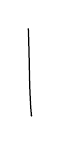
\begin{tikzpicture}[x=1cm,y=1cm]
\draw[line width=0.45pt]
  (0,0.63) .. controls (0.015,0.30) and (0.01,-0.18) .. (0.04,-0.48);
\fill (0.04,-0.48) circle[radius=0.012cm];
\end{tikzpicture}}
\uline{Proposition} $\pi_1(M_{1,1})$ is a central extension
of $\pi_1(M_{1,1}')$ by $\{\pm1\}$.

On the other hand, we have the exact sequences,
\deleted{\illegible{5}}
of homotopy over $\operatorname{Spec}\mathbb Q$

\scanpage{558}

\diagram{(44)\quad
\begin{tikzcd}[ampersand replacement=\&, column sep=small]
1 \arrow[r,no head] \&
\pi_1(\overline{M}_{1,1})\inserted{{}=\widehat{\mathcal T}_{1,1}^{+}} \arrow[r] \arrow[d] \&
\pi_1(M_{1,1})\inserted{{}=\mathcal E_{1,1}=N_{1,1}} \arrow[r] \arrow[d] \&
\mathbb{\Gamma}_{\mathbb Q} \arrow[r,no head] \arrow[d] \& 1 \\
1 \arrow[r,no head] \& \pi_1(\overline{M'_{1,1}}) \arrow[r,no head] \&
\pi_1(M'_{1,1}) \arrow[r,no head] \& \mathbb{\Gamma}_{\mathbb Q} \arrow[r,no head] \& 1
\end{tikzcd}}

and the transcendental theory provides
canonical \inserted{outer} isomorphisms

\diagram{(45)\quad
$\left\{
\begin{tikzcd}[ampersand replacement=\&, column sep=large,row sep=large]
\pi_1(\overline{M}_{1,1}) \arrow[d] \arrow[r,phantom,"\simeq" description]
 \& \mathrm{Sl}(2,\mathbb Z)^{\wedge} \arrow[d] \\
\pi_1(\overline{M'_{1,1}}) \arrow[r,phantom,"\simeq" description]
 \& \mathrm{Sl}(2,\mathbb Z)'^{\wedge}=\mathrm{Sl}(2,\mathbb Z)^{\wedge}/\mathord{\pm}1,
\end{tikzcd}\right.$}

\margin{Careful not to confuse $\mathrm{Sl}(2,\mathbb Z)^{\wedge}$ with $\mathrm{Sl}(2,\widehat{\mathbb Z})$ !!!}

\deleted{\unsure{whence} \illegible{1} fact that the sequence}

We have \unsure{the} following essential
compatibility between (43) (44) (45): the \unsure{commutativity|compatibility} of

\diagram{(46)\quad
\begin{tikzcd}[ampersand replacement=\&,column sep=1.8em,row sep=1.25em]
1\arrow[r]
\& \pi_1(\overline M_{1,1})\arrow[r]
   \arrow[d,phantom,"\simeq"{description,rotate=90}]
\& \pi_1(M_{1,1})\arrow[r]\arrow[dd]
   \arrow[r,phantom,"{\deleted{\unsure{\longrightarrow\Gamma_n=\mathrm{Gl}(2,\mathbb Z_n)}}}"{description,yshift=-3.8ex,fill=none,inner sep=0pt}]
\& \mathbb{\Gamma}_{\mathbb Q}\arrow[r]
   \arrow[dd,"{\substack{\chi_n\ \text{cyclotomic}\\\text{character}}}"{right}]
\& 1\\
\& \mathrm{Sl}(2,\mathbb Z)^{\wedge}\arrow[d,"\text{surjective}"{right}]
\& \& \& \\
1\arrow[r]
\& \mathrm{Sl}(2,\mathbb Z/n\mathbb Z)\arrow[r,hook]
\& \Gamma_n=\mathrm{Gl}(2,\mathbb Z/n\mathbb Z)\arrow[r,"\det"]
\& (\mathbb Z/n\mathbb Z)^*\arrow[r]
\& 1
\end{tikzcd}}

Passing to the limit over $n$, this gives
a commutative diagram

\diagram{(47)\quad
\begin{tikzcd}[ampersand replacement=\&, column sep=small]
1 \arrow[r,no head] \&
\bigl(\pi_1(\overline{M}_{1,1})\simeq\mathrm{Sl}(2,\mathbb Z)^{\wedge}\bigr) \arrow[r] \arrow[d,"\text{surjective}"'] \&
\pi_1(M_{1,1}) \arrow[r] \arrow[d] \&
\mathbb{\Gamma}_{\mathbb Q} \arrow[r,no head] \arrow[d,"\chi"] \& 1 \\
1 \arrow[r,no head] \& \mathrm{Sl}(2,\widehat{\mathbb Z}) \arrow[r,hook] \&
\mathrm{Gl}(2,\widehat{\mathbb Z}) \arrow[r] \&
\widehat{\mathbb Z}^{*} \arrow[r] \& 1
\end{tikzcd}}

-- diagram to which we will return.

\scanpage{559}
\mspage{284}

For now I am going to exploit the \inserted{second} isomorphism (42), $n=2$:
\[
(48)\qquad
\begin{aligned}
\pi_1(M_{1,1}')\inserted{{}\simeq\deleted{\unsure{\mathcal T_{1,1}^{+}}}N_{1,1}'}
&\simeq\pi_1(M_{1,1}[2]',\Gamma_2=\mathfrak S_3)\\
&\simeq\pi_1(U_{0,3},\mathfrak S_3),
\end{aligned}
\]
where the last isomorphism corresponds to
the isomorphism \inserted{$\operatorname{int}(\sigma_1):$} $\mathfrak S_3\simeq\mathfrak S_3$ made explicit in (40).

We do indeed find, as foreseen in the
preceding \S\ -- and in an entirely
conceptual way, the isomorphism \deleted{of sequences}
\deleted{exact} of extensions

\deleted{(\unsure{49})\quad $\pi_1(M_{1,1}')\simeq\unsure{\widehat{\mathcal T}_{1,1}^{+\,\prime}}\simeq$}

\diagram{(49)\quad
\begin{tikzcd}[ampersand replacement=\&, column sep=small]
1 \arrow[r] \&
\pi_1(\overline{M_{1,1}'})\inserted{{}=\unsure{\widehat{\mathcal T}_{1,1}^{+\,\prime}}\simeq\mathrm{Sl}(2,\mathbb Z)^{\wedge}} \arrow[r] \arrow[d,"\sim"'] \&
\pi_1(M_{1,1}')\inserted{{}\simeq N_{1,1}'} \arrow[r] \arrow[d,"\sim"'] \&
\mathbb{\Gamma}_{\mathbb Q} \arrow[r,no head] \arrow[d,equal] \& 1 \\
1 \arrow[r] \& \pi_1(\overline U_{0,3};\mathfrak S_3) \arrow[r] \arrow[d,"\simeq" description,phantom] \&
\pi_1(U_{0,3},\mathfrak S_3) \arrow[r,no head] \arrow[d,"\simeq" description,phantom] \&
\mathbb{\Gamma}_{\mathbb Q} \arrow[r,no head] \& 1 \\
\& \widehat\Pi_{0,3}' \& \mathcal E_{0,3}'
\end{tikzcd}}

Besides, taking up these reflections again in the
transcendental context, we see that
this isomorphism

\diagram{(50)\quad
\begin{tikzcd}[ampersand replacement=\&, column sep=large]
\widehat\Pi_{0,3}' \arrow[r,"\sim"] \arrow[d,equal] \&
\pi_1(\overline{M_{1,1}'}) \arrow[d,"\simeq" description,phantom] \\
\widehat\Pi_{0,3}/\{\ell_1^2,\ell_\infty^3\} \&
\mathrm{Sl}(2,\mathbb Z)'^{\wedge}=\mathrm{Sl}(2,\mathbb Z)^{\wedge}/\mathord{\pm}1
\end{tikzcd}}

is associated with an isomorphism
\diagram{(51)\quad
$\boxed{\begin{array}{ccc}
\Pi_{0,3}'&\xrightarrow{\sim}&\mathrm{Sl}(2,\mathbb Z)'\simeq\mathrm{Sl}(2,\mathbb Z)/\mathord{\pm}1\\
\Vert&&\\
\Pi_{0,3}/\{\ell_1^{\unsure{2}},\ell_\infty^3\}&&
\end{array}}$}

\scanpage{560}

deduced from the isomorphism of complex analytic
multiplicities
\[
(52)\qquad M_{1,1}^{\mathrm{an}\,\prime}\simeq
(U_{0,3}^{\inserted{\mathrm{an}}}\deleted{\unsure{(\mathbb C)}},\mathfrak S_3)
\]

We should all the same make
the homomorphism (51) explicit -- which is defined only
modulo inner automorphisms, a priori,
by explicit formulas -- whereas
its definition here comes out in a purely conceptual, ``geometric'' way (in the sense
of relative algebraic geometry, of
rational and elliptic curves over
arbitrary analytic spaces). This is
a key calculation, \inserted{surely instructive,} which should not
present any particular \uline{difficulty}\ldots

I have somewhat dropped \inserted{along the way} in all
this the ``coarse'' modular scheme $\widetilde M_{1,1}$,
after having asserted that it is $\simeq\mathbb E_{\mathbb Z}^{1}$, and
that there are two marked sections,
whose \deleted{points} values in characteristic $0$ correspond
\deleted{\unsure{to the}} \inserted{two} isomorphism classes of
\unsure{anharmonic} elliptic curves. In terms of the isomorphism

\subsection*{Scans 561--570}
\addcontentsline{toc}{subsection}{Scans 561--570}
% package LM_P057
\scanpage{561}
\mspage{285}

\[
(53)\qquad
\widetilde M_{1,1}\simeq M_{1,1}[2]'/\Gamma'_2
\simeq U_{0,3}/\mathfrak S_3
\]

\unsure{one|now}\qquad
(valid over $\mathrm{Spec}\,\mathbb Z[1/2]$)

one does indeed find, over \inserted{$S=$}$\mathrm{Spec}\,\mathbb Z[1/2]$, that
$\widetilde M_{1,1}$ is obtained from a relative scheme \inserted{$Y$,} which is
\deleted{\illegible{1}} locally \inserted{(étale)} isomorphic to $\mathbb P^1_S$,
by removing a section $s$ (whose existence already implies that $Y$ is
\unsure{globally|globally} isomorphic to $\mathbb P^1_S$ - hence
$Y-s(S)$ isomorphic to $\mathbb E^1_S$.
In this approach one thus feels like denoting by $\infty$
(not by $0$, as in the theory of maps!) this section,
which corresponds to the ``points at infinity'' $\unsure{(0,1,\infty)}$ of
$U_{0,3}$, or again to the ``\unsure{point} at infinity'' of
$\widetilde M_{1,1}$.
It is moreover easy to check a priori \unsure{that}
(by the Deligne-Mumford compactification of $M_{1,1}$ and of
$\widetilde M_{1,1}$) that $\widetilde M_{1,1}$ over the whole of $\mathrm{Spec}\,\mathbb Z$
is of the form $Y-\mathrm{Im}\,s$, where $Y$ is smooth proper
over $\mathrm{Spec}\,\mathbb Z$, and $s$ a section - hence what one
knows for example about the generic fiber, and the fact that $\mathbb Z$ is
principal, imply that $Y\simeq\mathbb P^1_{\mathbb Z}$, and

\scanpage{562}

that one therefore has $\widetilde M_{1,1}\simeq\mathbb E^1_{\mathbb Z}$.
To \deleted{it} choose this isomorphism, one uses the two sections of
$\mathbb E^1_{\mathbb Z}$, corresponding to the anharmonic curves.
These two sections \uline{are not} \uline{disjoint}, they
meet in characteristic $2$ and characteristic $3$.
(As for what happens in characteristic $\ne 2$ i.e. over
$\mathrm{Spec}\,\mathbb Z[1/2]$, one sees it clearly from the isomorphism $53$ -
\deleted{the} for in characteristic $3$ the two orbits
\[
(2,-1,1/2)\quad\text{and}\quad(j,\bar j)
\]
coincide and collapse into one and the
same point).
But taking one of these sections as zero section
(unless I am mistaken it is the one corresponding to the elliptic curve richest
in symmetries, \unsure{namely|i.e.} \unsure{of|the} group $\mathbb Z/6\mathbb Z$, that one takes -
it is a matter of convention, of course - it is therefore also the orbit
$\{j,\bar j\}$, corresponding to a stabilizer
$\simeq\mathbb Z/3\mathbb Z$) - this determines the isomorphism
$\widetilde M_{1,1}\simeq\mathbb E^1_{\mathbb Z}$ up to sign.
The other section then becomes an integer of the form
$\pm 2^a3^b$ ($a,b\in\mathbb N^*$ - \uline{integers} well determined whose
value \unsure{I|I have} do not know by \unsure{heart}), and one finishes

\scanpage{563}
\mspage{286}

normalizing by requiring that the \uline{sign} be \uline{plus}. Thus

\uline{Theorem} (for the record - this is well known) There is a unique isomorphism
\[
(54)\qquad
\widetilde M_{1,1}\simeq\mathbb E^1_{\mathbb Z},
\]
which \deleted{gives} in characteristic $0$ gives to the anharmonic curve with
automorphism group $\mathbb Z/6\mathbb Z$
the \deleted{\illegible{1}}\inserted{invariant} $0$, and to the one with
group $\mathbb Z/4\mathbb Z$ an invariant \deleted{\illegible{1}} $>0$
(which will necessarily be $2^a3^b$, with $a,b\in\mathbb N^*$ well
determined, but forgotten by me\ldots).
\margin{$b=3$, cf. below}

In \unsure{terms} of the isomorphism
\[
\deleted{\unsure{(55)}}\qquad
\widetilde M_{1,1}\simeq U_{0,3}/\mathfrak S_3
\subset \mathbb P^1/\mathfrak S_3
\]
(valid over $\mathrm{Spec}\,\mathbb Z[1/2]$)
this corresponds to \deleted{the isomorphism} an isomorphism between
$\mathbb P^1/\mathfrak S_3$ and $\mathbb P^1$ which to the orbit
$(0,1,\infty)$ assigns $\infty$ (not $0$) and to the orbit $(j,\bar j)$
assigns $0$ (not $\infty$), to the orbit $(2,-1,1/2)$
\unsure{the famous} $2^a3^b$ (and not $1$). The function
\margin{\uline{modular} \uline{invariant}}
\[
(55)\qquad j(\lambda)\in\mathbb Q(\lambda)
\]
which realizes this isomorphism, i.e. \unsure{the|the} \deleted{\unsure{morphism}} morphism
\[
(56)\qquad
\mathbb P^1_{\mathbb Z}\xrightarrow{j}\mathbb P^1_{\mathbb Z}
\]
corresponding (of degree $6$, with
\[
j\circ u=j
\qquad(u\in\mathfrak S_3)
\]
)

\scanpage{564}

is therefore \unsure{related|related} to the one inspired by the theory of maps,
i.e. $f(\lambda)$, by
\[
(57)\qquad
j(\lambda)=2^a3^b f(\lambda)^{-1}.
\]

Moreover $f(\lambda)$ \inserted{(or $j(\lambda)$)} is readily computed
from knowledge of its zeros and its poles,
\inserted{with their multiplicities},
\deleted{\illegible{2}} and the ``normalization'' by the value of $f$
(or of $j$) on one of the sections $2,-1,1/2$; one finds immediately:
\[
(58)\qquad
f(z)=\frac{3^3}{2^2}\frac{z^2(z-1)^2}{(z^2-z+1)^3}
\]
hence
\[
(59)\qquad
j(\lambda)=2^{a+2}3^{b-3}\frac{(z^2-z+1)^3}{z^2(z-1)^2}.
\]

Since $j(\lambda)$ must still make sense in characteristic $3$ and not be
constant, this shows moreover \uline{$b=3$}, so $(59)$ can also be written
\[
\deleted{\unsure{(60)}}\qquad
j(\lambda)=2^{a+2}\frac{(z^2-z+1)^3}{z^2(z-1)^2}
\]
- but one \unsure{will recall|recalls} that this formula is not relevant -
\unsure{does not allow} one to compute
\deleted{a \unsure{discriminant} of}\inserted{the invariant of an}
elliptic curve - except in characteristic $\ne 2$, fortunately!
To \deleted{\illegible{1}}

\scanpage{565}
\mspage{287}

\deleted{define}\inserted{describe}
\[
(60)\qquad
M_{1,1}\longrightarrow\mathbb E^1_{\mathbb Z}
\]
\margin{and in particular to determine
the other critical modular invariant
$2^a3^3$, i.e. \uline{determine $a$}}
also in a neighborhood of $2$ - say in characteristic $\ne 3$ - one needs a study
of elliptic curves which no longer goes by way of the representation
(of \uline{Legendre}, unless I am mistaken)
$y^{2}=\sqrt{x(x-1)(x-\lambda)}$, or again, by way of the Jacobi rigidification
of level $2$, but on the other hand by the one of level $3$.

\uline{Remarks} One sees at once that the quotient
$\mathbb P^1_{\mathbb Z}/\mathfrak S_3$ identifies with
$\mathbb P^1_{\mathbb Z}$, uniquely by taking as images of the
orbits $(0,1,\infty)$ and $(j,\bar j)$ the sections $0$ and $\infty$
(for example, following the convention corresponding to the theory of maps),
and by taking as image of the orbit $(2,-1,1/2)$ a
\deleted{integer}\inserted{rational} which is $>0$.
This is possible a priori, for one notes that the \deleted{sections}
orbits $(0,1,\infty)$ and $(j,\bar j)$
\deleted{on the one hand, $(0,1,\infty)$ and $(2,-1,1/2)$ on the other hand,}
do not coincide in any characteristic, hence correspond to
disjoint sections of $Y=\mathbb P^1_{\mathbb Z}/\mathfrak S_3$,
whereas the \unsure{remaining|constant} orbit

\scanpage{566}

$(2,-1,1/2)$ coincides with the first in characteristic $2$, with the second in
characteristic $3$ (and these are the only coincidences that can occur).
One therefore sees a priori that the third section will be of the form
$2^\alpha/3^\beta$, with $\alpha,\beta\in\mathbb N^*$.
The explicit calculation is moreover obvious, the composite morphism
\[
(61)\qquad
\mathbb P^1_{\mathbb Z}
\xrightarrow{f_1^{\unsure{*|\circ}}}
\mathbb P^1_{\mathbb Z}/\mathfrak S_3
\simeq\mathbb P^1_{\mathbb Z}
\]
must be of the form
$f_1^{\unsure{*|\circ}}=c.f^{\unsure{*|\circ}}$, with the constant
\inserted{$c\in\mathbb Q$} chosen in such a way that
$cf^{\unsure{*|\circ}}$ \deleted{has} reduces properly in
\unsure{all} characteristics (which determines $c$ \unsure{modulo|modulo the} sign)
and that
\inserted{$f_1(-1)=$}\deleted{\illegible{1}}
$cf^{\unsure{*|\circ}}(-1)$ \inserted{$=c$} $>0$
(which removes the indeterminacy of the sign).
One then finds
\[
(62)\qquad
f_1(\lambda)=
\frac{\lambda^2(\lambda-1)^2}{(\lambda^2-\lambda+1)^{2}}
=\frac{2^2}{3^3}f(\lambda)
\]
hence
\[
(63)\qquad
f_1(-1)=\frac{2^2}{3^3}
\qquad(\text{so }\alpha=2,\ \beta=3).
\]

But one will take note \deleted{that}
\inserted{that in a neighborhood of characteristic $2$,}
these calculations no longer concern $\widetilde M_{1,1}$ and
$\unsure{\widetilde{\widetilde M}|\widetilde{\widehat M}}_{1,1}$,
where the configuration of the three sections
\deleted{\illegible{1}
$\unsure{\Delta_\infty,\Delta_0|\Lambda_\infty,\Lambda_0}$,}
is not the same \unsure{as here}\ldots

\scanpage{567}
\mspage{288}

Following the \unsure{momentum} of these reflections, it would be natural to look
more closely at the scheme
\[
(64)\qquad
M_{1,1}[4],\quad
\text{on which acts }\Gamma_4=\mathrm{Gl}(2,\mathbb Z/4)
\]
\[
\text{via}\quad \Gamma'_4=\Gamma_4/\pm1
\]
and \unsure{the homomorphism} $\otimes$
\[
(65)\qquad
M_{1,1}[4]\longrightarrow M_{1,1}[2]'\simeq U_{0,3}
\]
\inserted{Compatible} \deleted{\illegible{1}}
\[
\Gamma'_4=\mathrm{Gl}(2,\mathbb Z/4)/\pm1
\longrightarrow
\Gamma'_2=\Gamma_2\simeq\mathrm{Gl}(2,\mathbb Z/2)
\simeq\mathfrak S_3
\]
\margin{\diagram{[Above the arrow, a crossed-out inscription:
\deleted{\illegible{1} $\det$}. To the left of (65), a reference line
connects the sign $\otimes$ to the marginal note.]}}
\margin{in fact the kernel of the homomorphism
$\mathrm{Gl}(k,A)$\deleted{\illegible{1}}$\longrightarrow\mathrm{Gl}(k,A/J)$
is always a commutative group $\circledast$
\unsure{if} $J$ is a square-zero ideal of a ring $A$ -
so here $\mathrm{Ker}(\mathrm{Gl}(2,\mathbb Z/4\mathbb Z)\longrightarrow
\mathrm{Gl}(2,\mathbb Z/2\mathbb Z))$ is a \uline{commutative} group,
and even a vector space over $\mathbb F_2$ - it is isomorphic to
$\mathbb F_2^4$}
\margin{$\circledast$ and even an $A/J$ $(A/J)^4$}

An immediate calculation, taking into account that
\[
(\mathbb Z/4\mathbb Z)^*\simeq\{\pm1\}
\]
, gives
\[
\mathrm{card}\,\Gamma_4
=
2\underbrace{\mathrm{card}\,\mathrm{Sl}(2,\mathbb Z/4\mathbb Z)}
_{8\,\mathrm{card}\,\mathrm{Sl}(2,\mathbb Z/2\mathbb Z)}
=
16.\underbrace{\mathrm{card}\,\Gamma_2}_{6}
\]
hence
\[
(66)\qquad
\mathrm{card}\bigl(\Gamma'_{4,2}
=\mathrm{Ker}(\Gamma'_4\longrightarrow\Gamma'_2)\bigr)=8
\]
i.e. $M_{1,1}[4]$ is a Galois covering of $M_{1,1}[2]'$,
of \deleted{group} order $8$.
Let us note that it is not geometrically connected over $\mathbb Q$,
\inserted{\unsure{or over $\mathrm{Spec}\,\mathbb Z[1/2]$}},
- since $M_{1,1}[4]$ lies over the quadratic extension
$\mu_4^*$ \deleted{\unsure{$\simeq\mathrm{Spec}$}}, of
$\mathrm{Spec}\,\underbrace{\mathbb Z[1/2]}_{\Lambda}$ say,
which is none other than $\Lambda[i]$.
\inserted{One has \deleted{\illegible{2}}\inserted{a}}
\deleted{\unsure{Let us choose the point} \illegible{1}}
\inserted{factorization of
$M_{1,1}[4]\longrightarrow M_{1,1}[2]'$}
\deleted{\unsure{over}
$\mathrm{Spec}\,\Lambda[i]=\mu_4^*$
over $\mathrm{Spec}\,\mathbb Z[1/2]$,
we can distinguish a \unsure{connected component}}

\scanpage{568}

\((67)\)
\diagram{
\begin{tikzcd}[ampersand replacement=\&,column sep=large,row sep=large]
M_{1,1}[4]
  \arrow[r,"\text{Galois}"]
  \arrow[d]
\&
(U_{0,3})_{\unsure{S'}}
  \arrow[r,"\text{Galois }\unsure{\text{degree }2}"]
  \arrow[dl]
\&
M_{1,1}[2]'\simeq U_{0,3}
  \arrow[d]
\\
S'=\mu_4^*
  \arrow[rr,"\text{Galois}","\unsure{\text{degree }2}"']
\&\&
\mathrm{Spec}\,\mathbb Z[1/2]=S
\end{tikzcd}
}

where now
\[
M_{1,1}[4]\longrightarrow M_{1,1}[2]'_{\unsure{S'}}
=(U_{0,3})_{S'}
\]
is a Galois covering with group the kernel of
$\Gamma'_{4,2}\xrightarrow{\det}\{\pm1\}$,
\deleted{\illegible{1}}\inserted{or again} that of
$\mathrm{Sl}(2,\mathbb Z/4\mathbb Z)'
\longrightarrow\mathrm{Sl}(2,\mathbb Z/2\mathbb Z)'$,
which we shall denote by $S\Gamma'_{4,2}$, which is of order $4$.

\uline{Proposition} The group
\[
(68)\qquad
S\Gamma_{4,2}
=
\mathrm{Ker}\bigl(
\mathrm{Sl}(2,\mathbb Z/4\mathbb Z)
\longrightarrow
\mathrm{Sl}(2,\mathbb Z/2\mathbb Z)
\bigr)
\]
is isomorphic to \deleted{\illegible{2}}
$\unsure{\mathfrak{sl}}(2,\mathbb F_2)$
(group of matrices of trace zero with coefficients in $\mathbb F_2$),
\inserted{with \unsure{the obvious action|the obvious actions}
of $\mathrm{Sl}(2,\mathbb F_2)$ on it,}
and the subgroup $\pm1$ corresponds to scalar matrices -
the quotient \deleted{\unsure{is}}\inserted{$S\Gamma'_{4,2}$ of the two}
isomorphic to \deleted{\illegible{1}} $\mathbb F_2^2$
(in a silly way and not canonical at all!).
\margin{\uline{N.B.} It is the $4$ complements of this \unsure{subspace}
$\mathbb F_2\unsure{\hookrightarrow|\subset}\unsure{\mathfrak{sl}}(2,\mathbb F_2)$
\deleted{(\unsure{commutative}}
which form a torsor \unsure{under|over} the dual of
$V=\unsure{\mathfrak{sl}/\mathbb F_2|\mathfrak{sl}(\mathbb F_2)}$
which should \unsure{correspond to the four} \deleted{\illegible{1}}
liftings of $\pi_{0,3}\hookrightarrow T^{+\prime}_{1,1}=\mathrm{Sl}(2,\mathbb Z)'$,
\unsure{i.e.|to} $\pi_{0,3}\hookrightarrow\mathrm{Sl}(2,\mathbb Z)$
cf. pages $259$, $260$ \unsure{above} on these questions}
\deleted{\unsure{finally}}
Viewing $M_{1,1}[4]$ as a Galois covering of
$M_{1,1}[2]'_{S'}=(U_{0,3})_{S'}$, one finds
\uline{geometrically} ``the'' universal \uline{abelian} covering of
$U_{0,3}$ with group killed by $2$ (and for good reason), which has as
Galois group $(\mathbb F_2)^{\{0,1,\infty\}}/\mathrm{Diagonale}$.

\scanpage{569}
\mspage{289}

Finally, everything is essentially tautological - but an amusing calculation to
do will be to ``\inserted{re}describe the action of $\mathrm{Sl}(2,\mathbb F_2)$ on
$\unsure{\mathfrak{sl}}(2,\mathbb F_2)/\text{scalar matrices}$''
in such a way as to identify it with the action of $\mathfrak S_3$ on
$\mathbb F_2^{\{0,1,\infty\}}/\text{diagonal}$.

As a covering of \deleted{$\unsure{\widetilde M}_{1,1}\simeq M_{1,1}[4]$}
\[
(69)\qquad
\widetilde M_{1,1\,S'}
\simeq M_{1,1}[4]/S\Gamma'_4
\simeq M_{1,1}[2]'_{\unsure{S'}}/\Gamma'_2,
\]
$M_{1,1}[4]$ is a Galois covering of order $24$ ($=4.6$),
with group $\mathrm{Sl}(2,\mathbb Z/4\mathbb Z)'$.
\deleted{It is} It would be quite \unsure{rare|welcome} if one did not have an isomorphism
\[
(70)\qquad
\mathrm{Sl}(2,\mathbb Z/4\mathbb Z)'
\simeq\mathfrak S_4
\qquad
(\text{automorphisms of the octahedron})
\]
and if $M_{1,1}[4]_{S'}$ were its covering \deleted{\unsure{étale}}
\deleted{\illegible{1}}
of $\mathbb P^1_{S'}\setminus\{0,1,\infty\}$, with
ramification compatible with
$2\{1\}$ \deleted{\illegible{1}} $+3\{\infty\}$,
which corresponds to the \uline{octahedron} \unsure{\&} in the theory of
maps - one should have over
$S'=\mathrm{Spec}\,\mathbb Z[1/2][i]$
a \inserted{canonical} isomorphism
\deleted{\unsure{of $\widetilde M_{1,1}$}}
\[
(71)\qquad
M_{1,1}[4]_{S'}\simeq
\text{Fermat curve}
\quad
x^2+y^2+z^2=0
\quad(\text{over }S')
\]
\margin{it would be better to write the Fermat equation
here
$x_0^2+x_1^2+x_\infty^2=0$}
(whose automorphism group is \unsure{precisely} an extension of
$\mathfrak S_3$ by
$\mu_2^{\{0,1,\infty\}}/\mathrm{diag}$!).

\scanpage{570}

To do things properly, one would have to make explicit the relation between elliptic
curves \inserted{$E/S$} (over a scheme $S$ over
$\mathbb Z[1/2][i]$) \unsure{equipped} with a Jacobi rigidification
of level $4$ $e_1,e_2$ with $e_1\wedge e_2=[i]^{-1}$, and
``nontrivial'' solutions of the equation
\[
(72)\qquad x^2+y^2+z^2=0
\]
over $S$ (i.e. the systems of sections
$x,y,z\in\Gamma(S,\mathcal O_S^*)$ satisfying $(72)$, modulo
multiplication by a ``scalar''
\inserted{$\alpha\in\Gamma(S,\mathcal O_S^*)$}
- or again, breaking the symmetry by putting
$X=x/z$, $Y=y/z$, \deleted{\illegible{1}}
the solutions of the equation
\[
(73)\qquad X^2+Y^2=-1\qquad(=i^2)
\]
$(X,Y\in\Gamma(S,\mathcal O_S^*))$\ldots

One has thus interpreted $M_{1,1}[2]'$, and
(modulo some checks and a somewhat more thorough study)
$M_{1,1}[4]$, in relation with \deleted{two} regular
\inserted{weighted triangular}
maps - the ``\unsure{dihedral|dihedral}'' map
\inserted{\unsure{of index $3$|of order $3$}}
or universal weighted triangular map
(three vertices $0,1,\infty$,
\figure{[An almost circular outline, with a horizontal oval.
Three filled dots are marked on the oval: $0$ on the left,
$\infty$ on the upper branch on the right, $1$ on the
lower branch on the right. The three portions of the oval join these
three points.]}
three edges, two faces which are triangles, type
$(p,q)=(3,3)$), and the \uline{octagonal} map,
which is a covering of order $4$ of this one
\unsure{(}\deleted{\illegible{2}}\inserted{étale}
away from the vertices $\{0,1,\infty\}$),

There would be \unsure{reason} also to look at

\subsection*{Scans 571--575}
\addcontentsline{toc}{subsection}{Scans 571--575}
% package LM_P058
\scanpage{571}
\mspage{290}

more closely the congruential modular varieties
$M_{1,1}[3]$ and $M_{1,1}[5]$, corresponding to
``geometric'' modular groups:
\[
\unsure{(}\quad
\left\{
\begin{array}{l}
S\Gamma'_3 = \underbrace{\mathrm{Sl}(2,\mathbb F_3)}_{\substack{\text{order }4.3.2\\=24}}/\mathord{\pm}1
\quad \text{of order }12\;\underset{\unsure{\deleted{\unsure{\infty}}}}{\phantom{a}}
\subset \underbrace{\mathrm{GP}(1,\mathbb F_3)}_{\text{order }24}\simeq\mathfrak S_4
\\[1.5em]
\unsure{\inserted{\text{in fact, we must have } S\Gamma'_4\simeq A_4}}
\\[1.5em]
S\Gamma'_5 = \underbrace{\mathrm{Sl}(2,\mathbb F_5)}_{\substack{\text{order }6.5.4\\=120}}/\mathord{\pm}1
\quad \text{of order }60
\subset \underbrace{\mathrm{GP}(1,\mathbb F_5)}_{\text{order }120}\simeq\text{group of the \uline{bi}icosahedron}
\end{array}
\right.
\tag{74}
\]

Unless I am mistaken, these groups \unsure{are|\deleted{are}} \inserted{resp.} the groups $A_4$ of the
oriented \uline{tetrahedron}, and the one $A_5$ of the oriented icosahedron.
If I remember rightly, the cases
$n=2,3,4,5$ exhaust the cases of congruential modular \deleted{\unsure{varieties}}\inserted{curves}
$M_{1,1}[n]$ which are \uline{rational}
-- it is a remarkable thing that through them one finds
all the regular \inserted{finite} polyhedra \unsure{with} triangles for faces
\margin{except one, with ``folded-back edges'' -- the one in figure (76), cf. below\ldots}
-- it was clear \inserted{\unsure{a priori|a-priori}}, from the \unsure{isomorphism|isomorphism} between
$\mathcal T'_{1,1}$ and the ``triangula- oriented cartographic group'' $\pi'_{0,3}$,
that we should find again all
the finite regular polyhedra \unsure{with|\deleted{tri}} triangles for faces
in this way, but not that
this should be with \unsure{congruence|congruences} subgroups,
very precisely. The table obtained is
then the following

\scanpage{572}

\[
\begin{array}{lll}
\text{group }G=S\Gamma'_n & \text{modular curve} & \text{type of regular oriented polyhedron}\\[.5em]
\left\{\begin{array}{l}D_3\simeq\mathfrak S_3\\ A_4\\ \mathfrak S_4\\ A_5\end{array}\right.
&\begin{array}{l}M_{1,1}[2]'\\M_{1,1}[3]\\M_{1,1}[4]\\M_{1,1}[5]\end{array}
&\begin{array}{l}\text{spherical bitriangle}\\\text{tetrahedron}\\\text{octahedron}\\\text{icosahedron}\end{array}
\end{array}
\tag{75}
\]

As other rational modular curves (not congruential)
Galois over $\widetilde M_{1,1}$, there would still be
the quotients of the preceding ones by
invariant subgroups of the $S\Gamma'_n$, distinct from the whole group and from $1$.
One finds as possible quotients

\noindent a) Case $\mathfrak S_3$; the quotient $\pm1$ (via the sign)

\noindent b) Case $A_4$: the quotient $\mathbb Z/3\mathbb Z=C_3$
(via $\mathfrak S_4\to\mathfrak S_3$, inducing $A_4\to C_3$)

\noindent c) Case $\mathfrak S_4$: the quotient $\mathfrak S_3$, and the quotient $\{\pm1\}$ of the latter.

(For d), there is nothing, $A_5$ being a simple group)

\deleted{\unsure{The varieties}}

The rational modular curves obtained \unsure{are}
reduced to the two cases a) and b) (which are
\unsure{found again|found again} in c)). In case a), one finds
the \inserted{quadratic} covering of $Y=\mathbb P^1(\mathbb C)-\{0,1,\infty\}$, which is
unramified at $\infty$ (for the ramification index must
divide $2$ and $3$), which therefore corresponds to the covering
\[
\deleted{\unsure{\sqrt{x(x+1)}}}\qquad y=\sqrt{x(x-1)}
\]
and to the regular spherical map of type $(2,1)$
(vertices of index $2$, faces of index $1$)
\figure{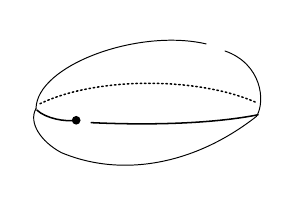
\begin{tikzpicture}[x=1cm,y=1cm,baseline=-0.35ex]
\draw[line width=0.35pt,line cap=round]
(-1.40,0) .. controls (-1.39,0.55) and (-0.10,1.02) .. (0.76,0.82);
\draw[line width=0.35pt,line cap=round]
(1.00,0.73) .. controls (1.46,0.57) and (1.52,0.10) .. (1.40,-0.10)
.. controls (0.61,-0.72) and (-0.32,-0.88) .. (-1.08,-0.56)
.. controls (-1.34,-0.42) and (-1.50,-0.18) .. (-1.40,0);
\draw[densely dotted,line width=0.55pt,line cap=round]
(-1.35,0.06) .. controls (-0.62,0.41) and (0.68,0.40) .. (1.41,0.07);
\draw[line width=0.55pt,line cap=round]
(-1.39,-0.02) .. controls (-1.27,-0.13) and (-1.03,-0.17) .. (-0.90,-0.15);
\fill (-0.89,-0.15) circle[radius=0.055];
\draw[line width=0.55pt,line cap=round]
(-0.70,-0.18) .. controls (0.17,-0.22) and (0.91,-0.18) .. (1.42,-0.08);
\end{tikzpicture}}
\unsure{formed|formed} of one vertex, \unsure{on} an edge (equator) bounding two faces which are monogons.

Case b) is the cyclic covering of order $3$:
ramified only at $0$ and at $\infty$ (at $1$ the ramification index must be a divisor of $2$ and of $3$,
hence is $1$) hence regular spherical map of

\scanpage{573}
\mspage{291}

type $(3,3)$, with edges which are loops
\deleted{\illegible{1}}\inserted{folded back}

(76) \figure{\begin{tikzpicture}[x=1cm,y=1cm,baseline=-0.35ex]
\draw[line width=0.35pt,line cap=round]
(0.89,-0.66) .. controls (1.51,-0.46) and (1.62,0.25) .. (1.13,0.67)
.. controls (0.57,1.11) and (-0.25,1.01) .. (-0.91,0.63)
.. controls (-1.57,0.28) and (-1.71,-0.29) .. (-1.14,-0.62)
.. controls (-0.61,-0.94) and (0.27,-0.98) .. (0.65,-0.83);
\draw[line width=0.8pt,line cap=round]
(-0.05,0.59) .. controls (-0.23,0.72) and (-0.42,0.85) .. (-0.64,0.81);
\draw[densely dotted,line width=0.8pt,line cap=round]
(-0.69,0.76) .. controls (-0.86,0.61) and (-0.91,0.38) .. (-0.98,0.20);
\draw[line width=0.8pt,line cap=round]
(-0.05,0.59) .. controls (0.29,0.79) and (0.73,0.77) .. (1.04,0.66);
\draw[densely dotted,line width=0.8pt,line cap=round]
(1.08,0.51) .. controls (1.16,0.38) and (1.15,0.28) .. (1.09,0.16);
\draw[line width=0.55pt,line cap=round]
(-0.05,0.59) .. controls (-0.23,0.31) and (-0.42,-0.04) .. (-0.31,-0.28);
\draw[line width=1.05pt,line cap=round]
(-0.31,-0.28) .. controls (-0.29,-0.35) and (-0.25,-0.45) .. (-0.23,-0.49);
\fill (-0.05,0.59) circle[radius=0.075];
\end{tikzpicture}}
: $1$ single vertex,
three folded-back edges coming out of it, one
triangular face. [These modular varieties are
too close to $\widetilde M_{1,1}$ -- with an automorphism
group (quotient of $\Gamma'_\infty=\mathrm{Sl}(2,\unsure{Z|\mathbb Z})$) too small,
to be able to be rigidifying (the Galois-Poincaré group of the covering
would have to
be a multiple of $12$\inserted{(multiple of $4$ and of $6$ ?!)}, for \deleted{\illegible{1}} the modular curve to have a chance of being rigidifying. These
cases thus seem distinctly less interesting.

There would be reason moreover, in each of the
three remaining cases of (75) (thus setting aside the
first case, which corresponds to $M_{1,1}[2]'$ and is
more or less understood), to make explicit the relation
between the points of the corresponding rational curves,
and between \inserted{elliptic curves with} Jacobi rigidifications,
of level $3,4,5$ respectively. And there
are surely precise things in Klein,
but one would like to do things a little
finer, which are valid simultaneously
in \unsure{all characteristics|every characteristic} i.e. over general
base schemes. This concern seems intimately linked to the question of the operations of
$\Gamma_{\mathbb Q}$ on the isomorphism classes of maps, and

\scanpage{574}

more particularly of regular
spherical maps. It is quite extraordinary that
Jean Malgoire, in the three years that the
question has been there, has not yet touched it
-- God knows it is juicy!

Supplement on the cross-ratio.

Let $x_1,x_2,x_3,x_4$ be \deleted{variables, \unsure{at|or} $\infty$}\inserted{sections \inserted{\unsure{everywhere}} distinct} of
$\mathbb P^1_S$, we want to construct the \unsure{corresponding} section $\lambda$
of $\unsure{U|\mathbb U}_{0,3}=\mathbb P^1_S-\{0,1,\infty\}_S$.
Let $a,b,c,d$ be sections
(local) of $\mathcal O_S$, \inserted{with \deleted{\illegible{1}} $ad-bc$ invertible,} such that
\[
u=u_{a,b,c,d}:\quad z\longmapsto\frac{az+b}{cz+d}
\tag{77}
\]
transforms $(x_1,x_2,x_3)$ into $(0,1,\infty)$ -- we
shall therefore have
\[
\lambda=u(x_4).
\tag{78}
\]
The conditions on \unsure{$\xi$|\deleted{\illegible{1}}} $(a,b,c,d)$ for $ux_1=0$ etc. are
\[
\left\{\begin{aligned}
ax_1+b&=0\\
ax_2+b&=cx_2+d\\
cx_3+d&=0
\end{aligned}\right.
\]
which give, if for example $a$ is invertible (otherwise, we
can assume $\unsure{c}$ invertible\ldots) on solving for $b,c,d$
\[
\left\{\begin{aligned}
b&=-ax_1\\
cx_2+d&=a(x_2-x_1)\\
cx_3+d&=0
\end{aligned}\right.
\qquad\left|\begin{aligned}
c&=a\frac{x_2-x_1}{x_2-x_3}\\
d&=-a\frac{x_2-x_1}{x_2-x_3}x_3
\end{aligned}\right.
\]
whence
\[
\lambda=\frac{ax_4+b}{cx_4+d}
=\frac{a(x_4-x_1)}{a\frac{x_2-x_1}{x_2-x_3}x_4-a\frac{x_2-x_1}{x_2-x_3}x_3}
=\frac{(x_4-x_1)(x_2-x_3)}{(x_2-x_1)(x_4-x_3)}
\]

\scanpage{575}
\mspage{292}

\[
\lambda(x_1,x_2,x_3,x_4)=\frac{(x_4-x_1)(x_2-x_3)}{(x_2-x_1)(x_4-x_3)}
\tag{79}
\]

As a rational function in $x_1,x_2,x_3,x_4$,
(with coefficients in a fixed integral domain) it
is characterized by the two properties: a) invariance \unsure{with respect} to a (same)
homographic transformation on the variables, \inserted{$x_1,x_2,x_3,x_4$,} \deleted{and}
\[
f(ux_1,ux_2,ux_3,ux_4)=f(x_1,x_2,x_3,x_4),
\]
\inserted{and} b)
\[
f(0,1,\infty,x_4)=x_4
\]
(with a grain of salt to give a
meaning to the first \unsure{side.} We have moreover
c) a remarkable symmetry property,
which we \deleted{\illegible{1}} make explicit by defining a homomorphism
from $\mathfrak S_4$ into the homographic group
(\unsure{morally|normally}, $\mathrm{GP}(1)$)
\deleted{\illegible{1}}
\diagram{
\begin{tikzcd}[ampersand replacement=\&,column sep=large,row sep=large]
\mathfrak S_4 \arrow[rr,"\sigma\mapsto\varphi_\sigma"] \arrow[dr,"\text{epimorphism}","\substack{\text{\unsure{factoring}}\\\text{through}}"'] \&\& \mathrm{GP}(1) \\
\& \mathfrak S_3 \arrow[ur] \&
\end{tikzcd}
}
in such a way that we have
\[
\lambda(x_{\sigma^{-1}1},x_{\sigma^{-1}2},x_{\sigma^{-1}3},x_{\sigma^{-1}4})
=\varphi_\sigma(\lambda(x_1,x_2,x_3,x_4))
\tag{80}
\]
\ldots

\clearpage
\section*{Cote 140-3}
\addcontentsline{toc}{section}{Cote 140-3 (696 scans)}
\subsection*{Scans 1--10}
\addcontentsline{toc}{subsection}{Scans 1--10}
% package LM_P059
\scanpage{1}
% not manuscript: printed logo of the Institut Montpelliérain Alexander Grothendieck (archive cover image of cote 140-3).

\scanpage{2}
Pages 291--650 $+$ table of contents

\uline{N.B.} Pages 291,292 appear twice
(numbering error)

\margin{1}

\scanpage{3}
\uline{$2^{\text{nd}}$ part}\quad
\fbox{Variations on the loop equation}

\uline{38}\quad Determination of
$\Pi'_{0,3}\xrightarrow{\sim}\mathfrak S_{0,3}^{+}$.
\hfill 291

\uline{39}\quad Congruence properties of the operation
of $\Gamma_{\mathbb Q}$ on $\widehat{\Pi}_{0,3}$,
\unsure{Related|Link} : the homomorphism
$N_{1,1}\longrightarrow \mathrm{Gl}(\unsure{1|2},\widehat{\mathbb Z})$
\hfill \unsure{299|297}

40\quad Topologico-isotopic paraphrase of
Legendre's theory
\hfill $307'$

41\quad Conditions for commutation of
$\widehat{\Pi}'_{0,3}\xrightarrow{\sim}\widehat{\mathfrak S}_{0,3}^{+}$
with the outer operations of $\Gamma_{\mathbb Q}$.
\hfill \deleted{\illegible{1}}

Calculations of the outer \unsure{automorphisms} in $\widehat{\Pi}_{0,3}$ and
in $\widehat{\mathfrak S}_{0,3}^{+}$.
\hfill 315

\uline{42}\quad Recapitulation on the group
$\mathfrak S_{0,3}$
$\simeq\ldots$ and on the loop automorphisms of
$\widehat{\mathfrak S}_{0,3}^{+}$ and of
$\widehat{\Pi}_{0,3}$ :
\hfill 331

\[
\left\{
\begin{array}{llr}
\mathrm{I}&\mathcal T_{0,3}&331\\
\mathrm{II}&\Pi_{0,3}\text{ and }\mathfrak S_{0,3}&332\\
\mathrm{III}&\text{relations with }\Pi'_{0,3}\quad
\deleted{\text{and }\mathrm{Sl}(2,\mathbb Z)'}&334\\
\mathrm{IV}&\deleted{\text{\unsure{The avatars of}}\ \mathfrak S_{0,3}}\quad
\inserted{\text{relations with}}\ \mathrm{Sl}(2,\mathbb Z)'&\unsure{335'}\\
\mathrm{V}&\text{the avatars of }\mathfrak S_{0,3}&336'
\end{array}
\right.
\]

VI\quad Loop \unsure{automorphisms} of $\widehat{\Pi}_{0,3}$ and
$\widehat{\mathfrak S}_{0,3}^{+}$
\hfill $337'$

VII\quad Calculations in $\mathrm{Sl}(2,\widehat{\mathbb Z})'$ :
cocycles under $\rho$
\hfill 342

VIII\quad Calculations in $\mathrm{Sl}(2,\widehat{\mathbb Z})'$ :
cocycles under $\sigma_\infty$
\hfill 346

\margin{\uline{N.B.} the calculations in these sections \uline{VI},
\uline{VII}, \uline{VIII} partly replaced by those
of \S46, \unsure{with} more \unsure{flexible|simple} notations\ldots}

43\quad Digression on the $1$-cocycles of \unsure{cyclic} groups
\hfill 350

44\quad Return to notations\inserted{(the $\unsure{\rho|\beta|g},\unsure{h},f,\alpha,\beta\ldots$)}.
Putting into equations in $\mathrm{Sl}(2,\widehat{\mathbb Z})$.
\hfill 356

45\quad The homomorphism
$\widetilde{M}_{0,3}\longrightarrow \mathrm{Gl}(2,\widehat{\mathbb Z})'$,
and construction of the extension $\widetilde{N}_{1,1}$
of $\widetilde{\Gamma}$ by $\widehat{\mathrm{Sl}(2,\mathbb Z)}$.
\hfill \unsure{384}

\uline{46}\quad Definitive notations (?) -- recapitulation
of the calculations \unsure{for|on} the loop \unsure{automorphisms}
\unsure{of|of the} $\widehat{\Pi}_{0,3}$ and of
$\widehat{\mathfrak S}_{0,3}^{+}$
\hfill 390

\margin{2}

\scanpage{4}

I The groups \(M_{0,3}^{\sim}\) and \unsure{\(N_{0,3}^{!\sim}\)} \hfill 390

\uline{II} Calculation of the elements of \(N_{0,3}^{!\sim}\) \hfill 392

1) Via \(f,g,h\)

2) Via \(\alpha_0,\beta_0,f\) \hfill 392

3) Via \(\alpha,\beta,f\) \hfill 393

4) Via \unsure{\(\zeta,\eta,f\)} \hfill \(393'\)

5) Comparison \unsure{between} \illegible{1}, \unsure{relations} of the \hfill 394
cocycles \hfill 395

\uline{III} Calculations in \(\mathrm{Gl}(2,\widehat{\mathbb Z})'\) and in \(\mathrm{Gl}(2,\widehat{\mathbb Z})\) \hfill 396

\uline{IV} The three fundamental cases, \deleted{and the}
\unsure{\((\alpha_0=1,\beta_0=1,f=1)\)}, and the \unsure{liftings}
\(K_{1/2},K_2,K_{-1}\). The subgroups \(M_{0,3}^{!\sim}(q)\),
\(q\in\{\)\deleted{\unsure{\(0,1,\infty\)}}\inserted{\unsure{\(-\overline j,-j\)|\(-j,-\overline j\)}}\(,2,-1,1/2\}\)
\hfill \deleted{\unsure{402}} 402

\uline{V} Recapitulation in terms of \(M_{0,3}^{!\sim}[0]\)
\hfill \deleted{\unsure{404}}

The subgroups \(M_{0,3}^{!\sim}(q)\), \(q\unsure{\notin|\in}\{0,1,\infty\}\) \hfill 407

\margin{calculation \unsure{in §17}}
\uline{VI} Return to the introduction of \(\alpha\) and \(\beta\) in terms of \(\zeta,\eta\). \hfill 414

47. Return to the homomorphism
\unsure{\(\widehat\Pi_{0,3}\xrightarrow{\widehat\varphi}\widehat{\mathfrak S}_{0,3}^{+}\)},
the groups \(M_{0,3}^{\approx},N_{0,3}^{\approx},M_{0,3}^{!\approx}(0)\)
\hfill \deleted{\unsure{415}} 415

\uline{48} Construction of a \unsure{group} scheme \hfill \unsure{428|420}

I) Study of the morphism \(\alpha\mapsto\alpha\rho(\alpha)^{-1}=\)\unsure{\([\alpha,\rho]\)} \hfill \unsure{428|420}

II) The equation \(\zeta=\eta\varepsilon_1(\mu-1)\), and the group
\unsure{\(B'_0\simeq B_{\rho,\sigma}\)} \hfill \(434'\)

\uline{III}) The equation \(\alpha\rho(\alpha)^{-1}=\beta\sigma(\beta)^{-1}\varepsilon_1(\mu-1)\),
and the group \unsure{\(\mathcal G_{\rho,\sigma}^{c}\)} of \illegible{1} \hfill \(443'\)

(IV) A canonical pinning associated to \(\rho,\sigma\) \hfill 446

(V) The equation \unsure{\(\alpha\rho(\alpha)^{-1}=\varepsilon(\beta\sigma^{-1}(\beta)^{-1})\varepsilon_1(\mu-1)\)|\(\alpha\rho(\alpha)^{-1}=\varepsilon(\beta\sigma'(\beta)^{-1})\varepsilon_1(\mu-1)\)}
\hfill \deleted{\unsure{454}}

\unsure{\(\{\)|\(\varepsilon\)} Its study in
\unsure{\(\widetilde\alpha\rho(\widetilde\alpha)^{-1}=\widetilde\beta\sigma(\widetilde\beta)^{-1}\varepsilon_1(\mu-1)\)} --
\inserted{in \unsure{\((\mathbb Q_p(i))\)}}
the group \unsure{\(\mathcal G_{\rho,\sigma}^{*}\)}, the condition \(\mathrm{Tr}\,\sigma=0\) \hfill 459

(VI) \inserted{Modular} characterization of the triple \unsure{\((\varepsilon_1,\sigma,\rho)\)|\((\varepsilon,\sigma,\rho)\)} \hfill 462

\uline{VII} Recapitulation on pinnings. \hfill 476

\uline{VIII} Recapitulation on the equation -- the group
\unsure{\(S\mathcal G_{\rho,\sigma}^{*}\)} and its variants \hfill \unsure{485|483}

\uline{IX} The groups \(M_{\rho,\sigma}\) and \(S_0M_{\rho,\sigma}\), and the homomorphisms
\unsure{\(S_0M_{0,3}^{!\sim}\longrightarrow SM_{\rho,\sigma}(\widehat{\mathbb Z})/\mathbb Z\)|\(S_0M_{0,3}^{!\sim}\longrightarrow SM_{\rho,\sigma}(\widehat{\mathbb Z}/\mathbb Z)\)},
\unsure{\(M_{0,3}^{!\sim}\longrightarrow M_{\rho,\sigma}(\widehat{\mathbb Z})/\mathbb Z\)} \hfill \(490'\)

\uline{X} Structure of \(M_{\rho,\sigma}\), and the canonical homomorphism
\(M_{\rho,\sigma}\longrightarrow\) \unsure{\(G\)}\deleted{\illegible{1}}\(\simeq\mathrm{Gl}(2)\) \hfill 499

\uline{XI} Recapitulation on \(M_{\rho,\sigma}\).
\deleted{the two systems of parameters \unsure{\((\underline U,\underline a,\underline b)\)} and
\((\alpha,\beta,f)\), on \unsure{\(M_{\rho,\sigma}[0]\)}}
\hfill \deleted{\illegible{1}}

\deleted{\uline{XII} The subgroups \(M_{\rho,\sigma}[0]\), \unsure{\(M_{\rho,\sigma}(1)\)}, \illegible{1}}

\(1^{\circ})\) Preliminary data \hfill 508

\(2^{\circ})\) \deleted{\unsure{\(M_{\rho,\sigma}(\mathbb Z)\)|\(M_{\rho,\sigma}(-j)\)}}
\(M_{\rho,\sigma}[0],M_{\rho,\sigma}(\infty)\),
\unsure{\(\mathcal T_{\rho,\sigma},\mathcal T_{\rho,\sigma}^{0}\)},
\unsure{\(M_{\rho,\sigma},\mathfrak S_{\rho,\sigma}^{+},\mathcal T_{\rho,\sigma}^{+0}\)}
\hfill \deleted{\unsure{524}} 509

\margin{taken up again in \(6^{\circ})\)}
[\(3^{\circ})\) \(M_{\rho,\sigma}^{0},M_{\rho,\sigma}^{+},\ldots\)
\unsure{calculations} of integral points] \hfill 511

\(4^{\circ})\) The homomorphisms \(\Theta:M_{\rho,\sigma}\longrightarrow G\),
\(\overline\Theta:M_{\rho,\sigma}\longrightarrow PG\) \hfill \(512'\)

\(5^{\circ})\) \(R_{\rho,\sigma}^{0},SR_{\rho,\sigma}^{0}\)] \hfill \unsure{\(513'\)}

\uline{\(6^{\circ})\)} \unsure{Groups}, \illegible{3} and \(R_{\rho,\sigma}\).
\unsure{Centers} of \(M_{\rho,\sigma},M_{\rho,\sigma}^{0}\).
The subgroup \(\Sigma\).
\(\Sigma\simeq\mathbb Z/2\mathbb Z\unsure{\times|*}\mathbb Z/2\mathbb Z\unsure{\times|*}\mathbb Z/2\mathbb Z\).
\hfill \deleted{\unsure{514|517}} 517

\uline{\(7^{\circ})\)} Dévissage of \(R_{\rho,\sigma}\) and of \(M_{\rho,\sigma}\) \hfill \(526'\)

\(8^{\circ})\) The parameters
\(\underline U,\underline a,\underline b,\mu,\varepsilon,\varepsilon'\) and
\(\underline u,f,\alpha,\beta,\alpha_0,\beta_0\)
\unsure{\((\zeta,\eta,g,h)\)} \hfill 529

\(9^{\circ})\) The subgroups \(M_{\rho,\sigma}(0),M_{\rho,\sigma}[0]\), and the group
\(SM_{\rho,\sigma}\), the isomorphism \unsure{\(SM_{\rho,\sigma}\simeq S\Sigma_{\rho,\sigma}^{*}\)} \hfill 534

\(10^{\circ})\) The \inserted{section} subgroups
\unsure{\(M_{\rho,\sigma}(\sigma)\)|\(M_{\rho,\sigma}(\Phi)\)}, \(M_{\rho,\sigma}(\rho)\) \hfill \unsure{\(540'\)|\(550'\)}

\uuline{XII} \uline{Retrospective.} \hfill 542

\margin{3}

\scanpage{5}

\uline{49}. The general groups \(M_{\rho,\sigma}\) \hfill 550

[I Heuristic preliminaries]

\uline{II} The groups \unsure{\(M_{\rho,\sigma}^{*}\)} etc.\ ``without signs'' -- new
variations on the loop relation \hfill \unsure{\(553'\)}

\uline{III} Passage from \(M_{0,3}^{\sim}\) to \(N_{1,1}^{\sim}\) -- and from
\(\mathrm{Gl}(2,\mathbb Z)^{\wedge}/\pm1\) to \(\mathrm{Gl}(2,\mathbb Z)^{\wedge}\) \hfill \unsure{565|555}

[\uline{IV} Where we wrestle with ``the signs'' \(\varepsilon_2,\varepsilon_3\)
in the loop relation -- calculations -- drafts\ldots] \hfill 568 \deleted{\unsure{577}}

\deleted{\illegible{1}}\textcircled{\uline{V}} The general groups \(M_{\rho,\sigma}\)
(\uline{profinite} context) \hfill 577

\(1^{\circ})\) Data \hfill 577

\(2^{\circ})\) \(Z_{\rho,\sigma}\), \unsure{\(\sigma_{\rho,\sigma}\)|\(\delta_{\rho,\sigma}\)} \hfill \(577'\)

\(3^{\circ})\) \(S_0G_{\rho,\sigma},G_{\rho,\sigma}\) \hfill 579

\(4^{\circ})\) \(Z_\rho,Z_\sigma,N_\rho,N_\sigma\),
\unsure{\(N_\rho^{*},N_\sigma^{*},SN_\rho^{*},SN_\sigma^{*}\)} \hfill - - - 580

\(5^{\circ})\) \(S_0M_{\rho,\sigma},M_{\rho,\sigma},S_0\Gamma_{\rho,\sigma},\Gamma_{\rho,\sigma}\)
\hfill - - - - - - 585

\(6^{\circ})\) \unsure{\(\Sigma_{\rho,\sigma},S\mathcal G_{\rho,\sigma},\Sigma_{\rho,\sigma}^{\mathrm{eff}},S\mathcal G_{\rho,\sigma}^{\mathrm{eff}}\)}
\hfill 586

\(7^{\circ})\) Functorialities. \hfill 588

\uline{\(8^{\circ})\)} The universal case, \(\mathfrak S^{\wedge}\)\(=\mathrm{Gl}(2,\mathbb Z)^{\wedge}\). The
\hfill \deleted{\illegible{1}}\\
\deleted{\illegible{1}} subgroup \(\Pi_0\). Study of the extension
\(S_0\Gamma_{\rho,\sigma}^{!}\) of \(Z_{\rho,\sigma}^{!}=M^{!}[0]\) by
\(L_\rho\unsure{\times|*}L_\sigma\), and \unsure{\(S_0^{\Pi}\Gamma_{\rho,\sigma}^{!}\)} of
\(Z_{\rho,\sigma}^{!}\) by \(\mu=\{\pm1\}\).
\hfill \deleted{\unsure{590}} 590

\margin{\unsure{rectification} of the ``relation \unsure{of conjugation}'' \illegible{1} \unsure{related} \deleted{\illegible{1}}}

\(9^{\circ})\) Recapitulation on the universal case.
Structure of the \unsure{\(N_\sigma^{*},N_\rho^{*}\)|\(N_\sigma^{\circ},N_\rho^{*}\)}. The canonical homomorphism
\unsure{\(M\xrightarrow{\sim}M_{\rho,\sigma}^{\unsure{\rightleftarrows|\leftrightarrows}}/H_\rho\hookrightarrow M_{\rho,\sigma}/H_\rho\)}.
\hfill \deleted{\illegible{1}} 614

\deleted{\illegible{1}}\textcircled{\uline{VI}} The general groups \(M_{\rho,\sigma}\):
\unsure{recapitulation}, and refinement of the preceding construction. \hfill 628

\(1^{\circ})\) Data (628) \quad
\(2^{\circ})\) \(Z_{\rho,\sigma}\), \unsure{\(\sigma_{\rho,\sigma}\)|\(\delta_{\rho,\sigma}\)} (629)

\(3^{\circ})\) \unsure{\(G_{\rho,\sigma},G_{\rho,\sigma}^{\unsure{\rightleftarrows|\leftrightarrows}}\)}\ldots\ (\unsure{632|631}) \quad
\(4^{\circ})\) \unsure{\(N_\rho,N_\sigma,N_\rho^{\unsure{\rightleftarrows|\leftrightarrows}},N_\sigma^{\unsure{\rightleftarrows|\leftrightarrows}}\)}\ldots\ (\unsure{635})

\(5^{\circ})\) \unsure{\(M_{\rho,\sigma},M_{\rho,\sigma}^{\unsure{\rightleftarrows|\leftrightarrows}}\)}\ldots\ (639) \quad
\(6^{\circ})\) \unsure{Functorialities|Functoriality} (\(640'\))

\margin{\(7^{\circ})\) \(M_{\rho,\sigma}[0],M_{\rho,\sigma}[\rho],M_{\rho,\sigma}[\sigma]\) (642)

\(8^{\circ})\) Return to the universal case: \unsure{\(M^{\unsure{\rightleftarrows|\leftrightarrows}}\)} and the homomorphism
\unsure{\(M^{\unsure{\rightleftarrows|\leftrightarrows}}\longrightarrow M_{\rho,\sigma}^{\unsure{\rightleftarrows|\leftrightarrows}}/H_\rho\)} (\(643'\))

\(9^{\circ})\) Digression \unsure{of the|of} \illegible{1} formalism of groups 648

[\(10^{\circ})\) Link with §48]}

\margin{4}

\scanpage{6}
\mspage{\unsure{291bis}}

\uline{38}\quad Explicit \unsure{determination} of the homomorphism
$\Pi'_{0,3}\xrightarrow{\sim}\mathfrak S_{0,3}^{+}$
(and of $\unsure{\Pi_{0,3}^{\prime\sim}}$
(unoriented triangulated cartographic group)
$\xrightarrow{\sim}\mathfrak S_{0,3}$).

I feel like coming back to the proposition of the preceding \S\
(page\ 262) with \inserted{\unsure{connected}} surface $X$, discrete group $G$
operating properly, the stabilizers \inserted{$G_x$} of the $x\in X$
\deleted{\unsure{being}} preserving the orientation and operating faithfully
in a neighborhood of $x$ \ldots\ taking $Y=X/G$, \unsure{equipped|equipped} with the
``signature'' $\underline d=d(X/Y)$ defined by the \unsure{ramification}
--- whence an \uline{\unsure{Isomorphism|isomorphism}}
\[
(1)\qquad
\Pi=\Pi_1((X,G),x)\xrightarrow{\sim}\Pi_1((Y,\underline d),y)=\Pi'
\]
($x\in X$, $y$ image of $x$ in $Y$)
which I would like to \unsure{study} more closely.

We have in $\Pi_1((Y,\underline d),y)$, for every
$b\in\unsure{\operatorname{Supp}}\underline d=Y^!$,
``\unsure{truncated-loop} subgroups'', more precisely
a conjugacy \unsure{class} \unsure{of|of the} \unsure{subgroups}
quotients of $\mathbb Z/d_b\mathbb Z$, and more precisely still,
a canonical outer homomorphism
\[
(2)\qquad
\unsure{T_b|T_y}\otimes_{\mathbb Z}\mathbb Z/d_b\mathbb Z
\longrightarrow\Pi'
\]
obtained by passage to the quotient from the outer homomorphism
\[
(3)\qquad
\unsure{T_b|T_y}\xrightarrow{\unsure{k_y|k_b}}
\Pi_1(Y\setminus Y^!)
\qquad(\longrightarrow\Pi_1((Y,\underline d)))
\]
(where $T_b$ is the free $\mathbb Z$-module of rank $1$ of
``twisted integers'' at $b$ on $Y$). On the other hand,
if $a\in X$ lies above $b$, the stabilizer $G_a$ is
\deleted{\unsure{thus}} a cyclic group of finite order $d_a=d_b$
--- We have \unsure{$=$} an obvious canonical isomorphism
\[
(4)\qquad
G_a\simeq T_a\otimes_{\mathbb Z}\mathbb Z/d_a\mathbb Z
\simeq T_b\otimes\mathbb Z/d_b\mathbb Z.
\]
\margin{(N.B. $T_a\simeq T_b$ \unsure{canonical\textsuperscript{ly}})}
\margin{5}

\scanpage{7}

On the other hand, to $a$ is \unsure{associated|associated} a conjugacy
class of \unsure{splittings} of the extension
\[
(5)\qquad
1\longrightarrow\Pi_1(X,x)\longrightarrow\Pi_1((X,G),x)
\longrightarrow G\longrightarrow1,
\]
(cf. \S\ 15)
\[
(6)\qquad
k_a:G_a\longrightarrow\Pi_1((X,G),x)
\]
these classes \inserted{of $\Pi_1(X,\unsure{x|e})$-conjugacy}
of \unsure{splittings} (if $X\ne S^2$) correspond
one-to-one to the fixed points of $G_a$ operating on $X$.
If we take the \uline{outer} \uline{homomorphism} \unsure{defined|defined}
by (6) (thus \unsure{conjugating|conjugating} not only by the
$\in\Pi_1(X)$, but by those of $\Pi_1(X,G)$ in its entirety)
we find a $1$-$1$ correspondence between \inserted{the set}
of outer homomorphisms (6) which lift the inclusion
\[
G_a\hookrightarrow G
\]
(\unsure{considered} as an outer homomorphism), and the set of orbits of $G$
in $X^!$, i.e.\ \deleted{between} the points of $Y^!$. In \unsure{summary}

\uline{Proposition}\quad We have a bijection between $Y^!$
and the set of ``maximal'' outer homomorphisms
\inserted{$\varphi=\varphi_b:\Gamma\longrightarrow\unsure{\Pi|\pi}$}
of \unsure{subgroups} $\Gamma\subset G$, \deleted{\unsure{(cyclic|(finite}}
$\Gamma\ne1$, into $\Pi_1(X,G)$ which lift the inclusion
\inserted{$\Gamma\subset G$} (the said $\Gamma$ are necessarily
cyclic, the $\Gamma$
\margin{6}

\scanpage{8}
\mspage{292bis}

in question \unsure{corresponding|corresponding} to a $b\in Y^!$
being the stabilizers $G_a$ in $G$ of the
\deleted{\unsure{$a\in(X^!)_a$|$a\in(X^!)_b$}}
$a\in X_b=X_b^!$. Moreover, the composite of the homomorphisms
\[
(7)\qquad
T_b\otimes\mathbb Z/n\mathbb Z
\overset{(4)}{\simeq}G_a
\xrightarrow{\varphi_a=\varphi_b}\Pi_1(X,G)
\overset{(1)}{\xrightarrow{\sim}}\Pi_1((Y,\underline d))
\]
is none other (we might have guessed!) than \unsure{``}the
``\unsure{truncated loops}'' homomorphism (2).

Let us now suppose that $X$ is of the form
$\widehat X\setminus S$, $\widehat X$ a compact surface,
$S$ a finite subset of $\widehat X$ \deleted{\unsure{thus}}
\[
(8)\qquad
\left\{\begin{aligned}
X&=\widehat X\setminus S\quad\text{thus}\quad
Y=\widehat Y\setminus T\quad\unsure{\ne\varnothing}\quad\text{\unsure{with}}\\
\widehat Y&=\widehat X/G
\end{aligned}\right.
\]

Let us consider\unsure{,} then, for every $\unsure{a|b}\in S$, the outer homomorphism
\[
(9)\qquad
k_a:T_a\longrightarrow\Pi_1(X)\hookrightarrow\Pi_1(X,G)
\]
which I am going to compare with the composite
\[
(10)\qquad
\deleted{\unsure{k_b:}}\quad T_b\xrightarrow{k_b}\Pi_1(Y)
\longrightarrow\Pi_1(Y,\underline d)
\]
(for $b=\widehat f(a)$), by means of the canonical isomorphism
\[
\deleted{\unsure{(12)}}\ (11)\qquad T_a\simeq T_b
\]
If $d_a$ again denotes the ramification index at $a$, we shall have
a commutative compatibility diagram:
\margin{7}

\scanpage{9}

\[
(12)\qquad
\diagram{\begin{tikzcd}[ampersand replacement=\&,column sep=large,row sep=large]
T_a \arrow[r,"k_a"] \arrow[d,"\wr\ \mathrm{can}"'] \& \Pi_1(X) \arrow[r] \& \Pi_1(X,G) \arrow[dd,"\wr"] \\
T_b \arrow[d,"d_a\cdot\mathrm{id}"'] \& \& \\
T_b \arrow[rr,"k_b"] \& \& \Pi_1(Y,\underline{d})
\end{tikzcd}}
\]

We are going to apply this to the \unsure{situation} of
$X=U_{0,3}^{\mathrm{an}}$, $G=\mathfrak{S}_3$,
$\widehat{X}=\mathbb{P}^{1\mathrm{an}}$, $\widehat{Y}\simeq\mathbb{P}^{1\mathrm{an}}$,
\unsure{with} the map of \unsure{passage} to the quotient
\unsure{given|given} by (page 286' (58))
\[
(13)\qquad
f(z)=\frac{3^3}{2^2}\frac{z^2(z-1)^2}{(z^2-z+1)^3}
\]
\[
f:\quad
\left\{\begin{array}{l}0\\1\\\infty\end{array}\right.\longrightarrow 0
\qquad
\left\{\begin{array}{l}2\\-1\\1/2\end{array}\right.\longrightarrow 1
\qquad
\left\{\begin{array}{l}-\overline{j}\\-j\end{array}\right.\longrightarrow\infty
\]

Thus we see, with the notations of \hspace{3em}, that the generators
$l'_0,l'_1,l'_\infty$ of $\Pi'_{0,3}$
(\unsure{satisfying}
\[
(14)\qquad l'_\infty l'_1 l'_0=1
\qquad {l'_1}^{2}={l'_\infty}^{3}=\unsure{\cdot}1\qquad )
\]
\unsure{correspond}, respectively, under the isomorphism
\[
(15)\quad
\begin{array}{ccl}
\mathfrak{S}_{0,3}^{+}
=\Pi_1(U_{0,3}^{\mathrm{an}},\mathfrak{S}_3)
&\xrightarrow{\sim}&\Pi'_{0,3}=\mathcal{T}_{1,1}^{+\prime}\\
\begin{array}{c}
\text{cartographic group}\\
\text{triangulated \unsure{weighted} oriented}\\
\text{\uline{mixed}}
\end{array}
&&\begin{array}{c}
\text{cartographic group \unsure{triangulated|triangul-}}\\
\text{oriented}\qquad \simeq\mathrm{Sl}(2,\mathbb{Z})'
\end{array}
\end{array}
\]
to the elements denoted
\deleted{$\unsure{\rho,\varepsilon_0,\varepsilon_1}$ \illegible{2}}
\[
(16)\qquad
\left\{\begin{array}{lll}
\varepsilon_0,\varepsilon_1,\varepsilon_\infty&\longmapsto&l'_0\\
\text{(such that $\varepsilon_i^2=l_i$)}&&\\
\sigma_0,\sigma_1,\sigma_\infty&\longmapsto&l'_1\\
\rho&\longmapsto&l'_\infty
\end{array}\right|\quad
\begin{array}{l}\mathrm{mod}\\\text{\unsure{conjugacy}}\end{array}
\]
\margin{or $\rho^{-1}$ ?}
\margin{8}

\scanpage{10}
\mspage{293}

\deleted{\unsure{The isomorphism}}

This shows that we can find
\inserted{in $\Pi=\mathfrak{S}_{0,3}^{+}$}
conjugates $\varepsilon'_0$ of $\varepsilon_0$, $\sigma'_0$ of $\sigma_0$,
such that we have
\[
(17)\qquad
\rho\sigma'_0\varepsilon'_0=1,\quad
\text{in addition to}\quad \rho^3={\sigma'_0}^{2}=1
\]
and in such a way that these relations \unsure{provide}
a \uline{presentation} of $\Pi$ (thus in particular,
that $\varepsilon'_0,\sigma'_0,\rho$ \unsure{generate} \unsure{$\}$} $\Pi$).
Drawing inspiration, moreover, from the isomorphism \deleted{more} which
\unsure{extends} (15) and is obtained in \unsure{like manner}
\[
(16)\qquad
\mathfrak{S}_{0,3}
\simeq\Pi_1\left(U_{0,3}^{\mathrm{an}},
\underbrace{\mathfrak{S}_3\times\unsure{\mathbb{Z}/2|\mathbb{Z}_2}}_{\mathcal{T}_{0,3}}\right)
\longrightarrow
\begin{array}{c}
\mathcal{T}'_{1,1}\\
\text{cartographic group}\\
\text{triangulated non-}\\
\text{oriented}\\
\simeq\mathrm{Gl}(2,\mathbb{Z})
\end{array}
\]
we should find on the first \unsure{side}
three \unsure{generators|generators} $\tau'_0,\tau'_1,\tau'_\infty$
(\unsure{corresponding} to the \unsure{analogous} generators
$\sigma_0,\sigma_1,\sigma_\infty$ of the
\unsure{corresponding|corresponding} cartographic groups) \unsure{satisfying|satisfying}
\[
(17)\qquad
{\tau'_0}^{2}={\tau'_1}^{2}={\tau'_\infty}^{2}=1,\quad
\left(\underbrace{\tau'_{\unsure{0|\infty}}\tau'_\infty}_{\begin{array}{c}\text{\unsure{corresponding} to}\\l'_1\end{array}}\right)^2
=\left(\underbrace{\tau'_1\tau'_0}_{\begin{array}{c}\text{corresponding to}\\l'_\infty\end{array}}\right)^3=1
\]
in such a way that these are \deleted{\unsure{some}} some
defining relations for $\mathfrak{S}_{0,3}$.
It would be necessary that
\deleted{$\tau'_\infty\tau'_0$ be a conjugate of $\sigma_0$}
\inserted{we have}
\[
(18)\qquad
\begin{array}{rclcrclcrcl}
\tau'_\infty\tau'_1&=&\varepsilon'_0;&\quad&
\tau'_0\tau'_\infty&=&\sigma'_0,&\quad&
\tau'_1\tau'_0&=&\rho\\
&&\updownarrow&&&&\updownarrow&&&&\updownarrow\\
&&l'_0&&&&l'_1&&&&l'_\infty
\end{array}
\]
\margin{9}

\subsection*{Scans 11--20}
\addcontentsline{toc}{subsection}{Scans 11--20}
% package LM_P060
\scanpage{11}

$X$ topological surface

$\mathcal G$ discrete group operating on $X$

$G$ invariant subgroup of $\mathcal G$, operating
properly on $X$, so that \deleted{$\forall x\in X$}
\margin{\deleted{\illegible{1}}}
\inserted{\unsure{the}} stabilizers $G_x$ $(x\in X)$
\unsure{operate} faithfully \unsure{in a neighborhood} of $x$, while
\unsure{preserving} the local orientation at $x$

$Y=X/G$ (topological surface), $f\colon X\to Y$

$X^{!}$ discrete \unsure{subset|subset} of $X$, stable under $\mathcal G$,

$d_X$ ``signature'' on $X$ with support $X^{!}$, invariant under $\mathcal G$
\[
\unsure{i}\mapsto d_X(i)
\qquad X^{!}\longmapsto\mathbb N
\]

$Y^{!}\simeq X^{!}/G\subset Y$ \quad image of $X^{!}$ in $Y$

We assume $x\in X$, $G_x\ne\{1\}\ \Rightarrow\ x\in X^{!}$

\[
d_Y\colon Y^{!}\to\mathbb N,\qquad d_Y(y)=\nu_x d_X(x)
\]
\[
\text{if } y=f(x),\quad \nu_x=[G_x]
\]

$\mathrm{Rev}(X,d_X,\mathcal G)$ category of ramified $\mathcal G$-coverings
of $X$, \unsure{subordinate} to $d_X$

$\mathrm{Rev}(Y,d_Y,\mathcal H)$ category of ramified $\mathcal H$-\unsure{coverings}
of $Y$, \unsure{subordinate} to $d_Y$

For $X'\in\mathrm{Ob}\,\mathrm{Rev}(X,d_X,\mathcal G)$, let us consider
$X'/G$ as a surface on which
$\mathcal H=\mathcal G/G$ operates, over $Y=\unsure{X'/G|X/G}$. Then

\margin{10}

\scanpage{12}
\mspage{294}

 a) $X'/G\in\mathrm{Ob}\,\mathrm{Rev}(Y,d_Y,\mathcal H)$

 b) We thus \unsure{find|give} a functor
\[
\mathrm{Rev}(X,d_X,\mathcal G)\longrightarrow
\mathrm{Rev}(Y,d_Y,\mathcal H) \tag{19}
\]

 c) This functor is an equivalence of categories.

 d) Description of a quasi-inverse functor by ``normalized'' inverse image.

Remarks. We may assume $d_X$ with values $>0$ i.e. $d_Y$ with values
$>0$ (otherwise, if $S=\{x\in X^{!}\mid d_X(x)=0\}$, \unsure{let us replace}
$X$ by $X\setminus S$), $Y$ by $Y\setminus T$ $(T=S/G)$.

\inserted{We may assume $d_X(x)=1\ \Rightarrow\ [G_x]\ne1$
(otherwise, \unsure{replace} $X^{!}$ \unsure{by} $X^{!}\setminus S$
$S=\{x\in X^{!}\mid d_X(x)=1,\ \unsure{[G_x]=1\}}$\unsure{)}}

The most interesting case \unsure{for us is}
the one where \deleted{$d_X(x)=1$} $\forall x\in X^{!}$, \unsure{we have}
$d_X(\unsure{x})=1$ and $G_x\ne\{1\}$
(thus $X^{!}=\{x\in X\mid G_x\ne\{1\}\}$), \unsure{thus|in} the case where
\[
\mathrm{Rev}(X,d_X,\mathcal G)=\mathrm{Rev}(X,\mathcal G) \tag{20}
\]
and where $\mathrm{Rev}(\unsure{\deleted{\illegible{1}}}Y,d_Y,\mathcal H)$ can therefore
\unsure{be interpreted} as a $\mathrm{Rev}(X,\mathcal G)$
(without ramification \unsure{data})

\margin{11}

\scanpage{13}

\uline{Corollary} Let $x\in X\setminus X^{!}$, $y$ its image in
$Y\setminus Y^{!}$, we have a canonical isomorphism
\[
\Pi_1\bigl((X,d_X,\mathcal G)\unsure{,|;}x\bigr)
\overset{\sim}{\longrightarrow}
\Pi_1\bigl((Y,d_Y,\mathcal H)\unsure{,|;}y\bigr) \tag{21}
\]

We are going to \unsure{make explicit} this isomorphism in terms of
\unsure{calculations} of \deleted{loops}\inserted{paths}.

An element\inserted{$\alpha$} of
$\Pi_1\bigl((X,d_X,\mathcal G)\unsure{,|;}x\bigr)$
% ``provient'': struck through, then restored by a row of dots under it (stet).
comes from a pair $(\gamma,\ell)$, with
\[
\gamma\in\mathcal G,\qquad
\ell\ \text{class of paths in }X\setminus X^{!}
\text{ from }x\text{ to }\gamma^{-1}x
\]

(\unsure{with|for} $(\gamma,\ell)$ and $(\gamma',\ell')$ \unsure{define} the
same element, \unsure{iff|sss} $\gamma'=\gamma$, and
\inserted{the element} $\ell'^{-1}\ell$ of $\Pi_1(X\setminus X^{!},x)$ is
in the invariant subgroup kernel of
\[
\Pi_1(X\setminus X^{!},x)\longrightarrow\Pi_1((X,d_X),x)
\]
-- i.e. the invariant subgroup generated by the
\deleted{\unsure{$k$|$\ell$}} $\lambda_a^{d_X(a)}$, where
for every $a\in X^{!}$, $\lambda_a$ denotes the \unsure{class} in
$\Pi_1(X\setminus X^{!},\unsure{x|a})$ of a ``loop from $x$ around $a$'').

Then let $\dot\gamma$ be the image of $\mathcal G$ in $\mathcal H$ --
\deleted{\unsure{$f_0$|$f$}} let
$f_U\colon X\setminus X^{!}\overset{\unsure{\mathrm{df}|\mathrm{def}}}{=}U
\longrightarrow Y\setminus Y^{!}\overset{\unsure{\mathrm{df}|\mathrm{def}}}{=}V
\simeq U/G$ be the \unsure{map}

\margin{12}

\scanpage{14}
\mspage{295}

which is canonical, then the image \inserted{$\beta$} of
\inserted{$\alpha\in\Pi_1(X,d_X,\mathcal G;x)$ \unsure{defined by}}
$(\gamma,\ell)$ \deleted{is}
in $\Pi_1(Y,d_Y,\mathcal H;y)$ is $(\dot\gamma,f_U(\ell))$

(\uline{N.B.} $f_U(\ell)$ is a class of \unsure{paths} in
$V=Y\setminus Y^!$ from $y=f_U(x)$ to
$\dot\gamma^{-1}(y)=f_U(\gamma^{-1}x)$).

\inserted{\uline{N.B.}} We see at once that if
$(\gamma,\ell)$ and $(\gamma',\ell')$ \unsure{define} the
same $\alpha$, then they also \unsure{define}
the same $\beta$, which comes from the fact that
\[
\Pi_1(f_U,a):\Pi_1(X\setminus X^!,x)
\longrightarrow\Pi_1(Y\setminus Y^!,y)
\]
maps a $\lambda_a$ into \inserted{a} $\lambda_b^{\nu(a)}$
($b=f(a)$, $\nu(a)=[G_a]=$ degree of \unsure{ramification}
of $f$ at $a$) hence $\lambda_a^{d_X(a)}$ into
$\lambda_b^{d_X(a)\nu(a)=d_Y(b)}$.

Let us return to the situation of (13)
\[
X=U_{0,3}^{\mathrm{an}},\quad
\mathcal G=\mathcal T_{0,3}
=\mathfrak S_3\times\mathbb Z/2,\quad
G=\mathcal T_{0,3}^{+}
=\mathfrak S_3
\]
\margin{$X^!=\{\deleted{\illegible{1}}2,-1,\frac12;
-\bar j,\unsure{-j}\}$}
\[
Y\simeq\mathbb P^{1\,\mathrm{an}}\setminus\{0\},\quad
Y^!=\{1,\infty\},
\]
\inserted{$\mathcal H=\mathbb Z/2\mathbb Z$,}
map of \unsure{passage} to the quotient from
$\widehat X=\mathbb P^{1\,\mathrm{an}}$ to
$\widehat Y=\mathbb P^{1\,\mathrm{an}}$ given by (13)
\[
f(z)=\frac{3^3}{2^2}\frac{z^2(z-1)^2}{(z^2-z+1)^3}
\]
\margin{13}

\scanpage{15}

To calculate
$\Pi_1(Y,\underline{d}_Y,\mathbb Z/2\mathbb Z)
=\widetilde\Pi_{0,3}'$
(carto-\unsure{graphic} \unsure{triangulated} unoriented group),
we took the base point $y=-\bar j$, so we are going to choose
an $x\in\unsure{U_{0,3}^{\mathrm{an}}}$ over $y$, such that
\[
f(x)=y=-\bar j
\]
--- there is \deleted{six \unsure{places|points}} \inserted{a}
choice in a \unsure{set} $f^{-1}(\{y\})$ with six
elements, of which \uline{three} in the northern hemisphere
(the other three in the southern hemisphere),
these are permuted \unsure{transitively} by $\rho$.
They lie \unsure{respectively} in the
spherical triangles $(-\bar j,0,\frac12)$, $(-\bar j,1,2)$,
$(-\bar j,\infty,-1)$ (mapped by $f$
\unsure{homeomorphically} onto the \unsure{upper} spherical triangle $(0,1,\infty)$,
\inserted{\unsure{in the upper hemisphere)}}
with center $-\bar j$).
The choice of $\unsure{x|a}$ thus \unsure{amounts}
to the choice of one of the three
\inserted{spherical triangles, or again of the 3}
spherical segments $(0,\frac12)$, $(1,2)$, $(\infty,-1)$
--- I feel like taking $(0,\frac12)$, \unsure{corresponding}
to the triangle $(-\bar j,0,\frac12)$.

The three \inserted{involutive} generators
\deleted{\illegible{1}} $\tau'_0,\tau'_1,\tau'_\infty$
of $\Pi_1(Y,d_Y,
\unsure{\mathbb Z/2\mathbb Z|\mathbb Z/2})$
\unsure{over|over} $\tau\in\mathbb Z/2\mathbb Z$
are obtained by taking paths $\ell'_0,\ell'_1,\ell'_\infty$
from \inserted{\unsure{north pole}} $y=-\bar j$ to
\inserted{\unsure{the south pole}} $\tau y=-j$, which are \unsure{the|some}
\unsure{great circle} arcs crossing the equator resp. at $2,-1,\frac12$.

\margin{14}

\scanpage{16}
\mspage{296}

These paths are the images under $f$ of paths
on $X$, let them be $\lambda_0:\overrightarrow{x,z_0}$,
$\inserted{\lambda_1:}\overrightarrow{x,z_1}$,
$\inserted{\lambda_\infty:}\overrightarrow{x,z_\infty}$,
which \inserted{each} cross the barycentric subdivision of the double
spherical triangle $(0,1,\infty)$ in exactly one point,
\unsure{situated} \unsure{respectively} on the side
$(\frac12,-\bar j)$, $(-\bar j,0)$ and $(0,\frac12)$
of the spherical triangle $(0,\frac12,-\bar j)$.

\margin{\uline{N.B.} The points $z_0,z_1,z_\infty$
are \unsure{characterized} \inserted{\unsure{resp.$^{\mathrm t}$}}
as the only points of $X$ over
$-j=f(\unsure{\dot\tau|\tau}x)$, lying \unsure{in|in} the
spherical triangles $(-\bar j,\frac12,1)$, $(0,-\bar j,-1)$,
$(\frac12,0,-j)$.}

The points \deleted{\unsure{the}} $z_0,z_1,z_\infty$ over
$\tau y$ are \unsure{respectively} of the form
$\inserted{g_0x=}\dot\sigma_\infty\dot\tau x$,
$\inserted{g_1x=}\dot\sigma_0\dot\tau x$,
$\inserted{g_\infty x=}\deleted{\unsure{\dot\sigma_\infty}}\dot\tau x$
\inserted{(i.e. $g_0=\dot\sigma_\infty\dot\tau$,
$g_1=\dot\sigma_0\dot\tau$, $g_\infty=\dot\tau$)}.
Thus the involutive generators
$\tau'_0,\tau'_1,\tau'_\infty$ of
$\widetilde\Pi_{0,3}'=\Pi_1(Y,d_Y,\mathbb Z/2\mathbb Z;y)$
are the images of the elements
\deleted{$(\dot\sigma_{\unsure{0}}\dot\tau,\lambda_0)$},
(denoted by the same sign)
\[
\tau'_0=(\dot\sigma_0\dot\tau,\lambda_0);\quad
\tau'_1=(\dot\sigma_1\dot\tau,\lambda_1),\quad
\tau'_\infty=(\dot\sigma_\infty\dot\tau,\lambda_\infty)
\]
of $\Pi_1(X,\mathcal G;x)$.
We are going to use the great circle arc \inserted{$\ell$}
from \deleted{$x=$} $-\bar j=P$
(\deleted{origin} \inserted{\unsure{base point}}
\unsure{usual|usual} \unsure{for} the calculation of $\Pi_1(X,\mathcal G)$)
\inserted{to $x$}, to identify $\Pi_1(X,\mathcal G;x)$
with $\Pi_1(X,\mathcal G;P)$.

We can then take \deleted{\unsure{as}}
\[
\tag{21}
\tau'_0=(\dot\sigma_0\dot\tau,\lambda'_0),\quad
\tau'_1=(\dot\sigma_1\dot\tau,\lambda'_1),\quad
\tau'_\infty=(\dot\sigma_\infty\dot\tau,\lambda'_\infty)
\]
where $\lambda'_0,\lambda'_1,\lambda'_\infty$ are the
\deleted{great circle arcs}
\inserted{\deleted{\unsure{loops}} paths from}
\deleted{(i.e. the \unsure{loops|ends} at $P$)}
from $P=-\bar j$
\inserted{to \deleted{\illegible{1}} $\unsure{g_iP|\dot g_iP}$
\deleted{\illegible{1}}}
\deleted{to $z_0,z_1,z_\infty$ \unsure{respectively}
(which, with the excep-}

\margin{15}

\scanpage{17}

\deleted{tion of the last, do not intersect the barycentric
graph of the spherical double triangle
except at $P=-\bar j$, the last intersecting it
\inserted{\unsure{only$^{\mathrm t}$}} at one
\deleted{single} \unsure{other} point, \unsure{situated} on the spherical
segment $(0,\frac12)$.}

\deleted{The points $z_0,z_1,z_\infty$ are \unsure{characterized}
\unsure{respectively} as the points $z$
such that $f(z)=-j$, and which \unsure{lie} in the
spherical triangles $(\frac12,\unsure{-\bar j},1)$,
$(-\bar j,0,-1)$, $(0,\frac12,-j)$.}

\figure{\begin{tikzpicture}[x=.016cm,y=-.016cm,line cap=round,line join=round,font=\scriptsize]
\coordinate (N) at (171,20);
\coordinate (S) at (162,320);
\coordinate (X) at (204,117);
\coordinate (Zone) at (106,93);
\coordinate (Zzero) at (265,97);
\coordinate (Zinf) at (196,238);
\draw[line width=.35pt] (N) .. controls (84,15) and (17,85) .. (2,181)
 .. controls (-6,243) and (39,305) .. (S)
 .. controls (236,319) and (290,260) .. (288,183)
 .. controls (286,105) and (253,27) .. (N);
\draw[line width=.3pt] (N) .. controls (99,29) and (26,93) .. (7,184);
\draw[line width=.3pt] (8,215) .. controls (38,287) and (97,317) .. (163,322);
\draw[line width=.3pt] (N) .. controls (250,33) and (283,121) .. (290,178);
\draw[line width=.35pt] (2,191) .. controls (57,147) and (209,135) .. (280,166)
 .. controls (299,180) and (284,198) .. (247,204)
 .. controls (145,223) and (43,224) .. (5,208)
 .. controls (-1,205) and (-2,199) .. (2,191);
\draw[dash pattern=on 4pt off 3pt,line width=.3pt] (N)
 .. controls (95,33) and (44,92) .. (52,166)
 .. controls (49,232) and (92,290) .. (S);
\draw[dash pattern=on 4pt off 3pt,line width=.3pt] (N)
 .. controls (117,49) and (101,143) .. (119,211)
 .. controls (115,248) and (140,299) .. (S);
\draw[dash pattern=on 4pt off 3pt,line width=.3pt] (N)
 .. controls (183,84) and (195,151) .. (188,194)
 .. controls (185,246) and (181,294) .. (S);
\draw[dash pattern=on 4pt off 3pt,line width=.3pt] (N)
 .. controls (230,50) and (265,110) .. (260,156)
 .. controls (281,225) and (223,298) .. (S);
\draw[dash pattern=on 4pt off 3pt,line width=.3pt] (N)
 .. controls (54,58) and (9,121) .. (10,205)
 .. controls (9,264) and (62,308) .. (S);
\draw[line width=.3pt] (N) .. controls (219,54) and (250,129) .. (249,197)
 .. controls (247,257) and (208,303) .. (S);
\draw[line width=.3pt] (N) .. controls (199,77) and (214,166) .. (207,237)
 .. controls (200,276) and (178,308) .. (S);
\draw[line width=.25pt] (165,37)--(230,77)
 (154,49)--(254,113) (143,65)--(265,145)
 (123,88)--(263,178) (119,108)--(249,198)
 (117,130)--(233,207) (116,155)--(184,211)
 (116,183)--(157,217);
\draw[line width=.7pt] (Zone) .. controls (118,61) and (146,39) .. (N);
\draw[line width=.6pt] (Zone) .. controls (142,93) and (179,112) .. (X);
\draw[line width=.6pt] (X) .. controls (225,109) and (248,98) .. (Zzero);
\draw[line width=.6pt] (X) .. controls (217,158) and (209,207) .. (Zinf);
\draw[line width=.6pt] (N) .. controls (196,49) and (215,73) .. (X);
\draw[line width=.55pt] (N) .. controls (231,37) and (257,64) .. (Zzero);
\draw[line width=.55pt] (N) .. controls (215,58) and (232,159) .. (Zinf);
\draw[line width=.85pt] (163,29)--(170,20)--(181,31);
\draw[line width=.85pt] (259,90)--(265,97)--(255,98);
\draw[line width=.85pt] (201,230)--(196,238)--(194,231);
\draw[line width=.85pt] (249,58)--(245,66)--(251,63);
\draw[line width=.8pt] (203,77)--(207,84)--(210,78);
\draw[line width=.7pt] (279,167) .. controls (291,168) and (291,181) .. (285,191);
\draw[line width=.55pt] (281,189)--(285,195)--(288,187);
\foreach \p in {(171,20),(162,320),(204,117),(106,93),(265,97),(196,238),(10,205),(249,197),(188,151)}
  \fill \p circle[radius=1.3];
\foreach \p in {(52,166),(119,211),(260,156)}
  \fill \p circle[radius=3.2];
\node[inner sep=0pt] at (174,5) {$-\bar j$};
\node[inner sep=0pt] at (166,338) {$-j$};
\node[inner sep=0pt] at (41,154) {$\infty$};
\node[inner sep=0pt] at (194,143) {$2$};
\node[inner sep=0pt] at (260,141) {$1$};
\node[inner sep=0pt] at (10,223) {$-1$};
\node[inner sep=0pt] at (121,226) {$0$};
\node[inner sep=0pt] at (258,219) {$\frac12$};
\node[inner sep=0pt] at (211,125) {$x$};
\node[inner sep=0pt] at (94,95) {$z_1$};
\node[inner sep=0pt] at (269,112) {$z_0$};
\node[inner sep=0pt] at (213,244) {$z_\infty$};
\node[inner sep=0pt] at (148,96) {$\unsure{\lambda_1}$};
\node[inner sep=0pt] at (234,95) {$\lambda_0$};
\node[inner sep=0pt] at (217,183) {$\unsure{\lambda_\infty}$};
\node[inner sep=0pt] at (119,58) {$\unsure{\lambda'_1}$};
\node[inner sep=0pt] at (260,34) {$\lambda'_0$};
\node[inner sep=0pt] at (222,65) {$\unsure{\lambda'_\infty}$};
\node[inner sep=0pt] at (183,65) {$\unsure{\ell}$};
\node[inner sep=0pt] at (156,148) {$\unsure{\ell\mid4}$};
\draw[->,line width=.45pt] (139,411)--(145,593);
\node[inner sep=0pt] at (174,485) {$f$};
\coordinate (NN) at (165,627);
\coordinate (SS) at (150,864);
\draw[line width=.35pt] (NN) .. controls (97,623) and (18,665) .. (17,733)
 .. controls (12,803) and (74,855) .. (SS)
 .. controls (214,866) and (272,822) .. (279,751)
 .. controls (293,672) and (249,630) .. (NN);
\draw[dash pattern=on 4pt off 3pt,line width=.35pt] (NN)
 .. controls (106,673) and (76,715) .. (55,771)
 .. controls (39,810) and (104,858) .. (SS);
\draw[dash pattern=on 4pt off 3pt,line width=.35pt] (NN)
 .. controls (190,688) and (193,755) .. (SS);
\draw[dash pattern=on 4pt off 3pt,line width=.35pt] (NN)
 .. controls (220,672) and (234,739) .. (223,785)
 .. controls (213,831) and (180,857) .. (SS);
\draw[dash pattern=on 2pt off 3pt,line width=.3pt] (17,733)
 .. controls (59,701) and (213,686) .. (265,715);
\draw[dash pattern=on 2pt off 3pt,line width=.3pt] (17,733)
 .. controls (24,759) and (52,775) .. (85,784);
\draw[line width=.7pt] (85,784)
 .. controls (143,788) and (242,777) .. (275,756);
\draw[line width=1.6pt] (251,716)
 .. controls (269,720) and (282,733) .. (275,756);
\draw[->,line width=.8pt] (242,755)--(233,759);
\foreach \p in {(165,627),(150,864),(55,721),(55,771),(183,704),(228,758)}
  \fill \p circle[radius=1.3];
\fill (85,784) circle[radius=4.2];
\node[inner sep=0pt] at (184,616) {$-\bar j$};
\node[inner sep=0pt] at (153,891) {$-j$};
\node[inner sep=0pt] at (43,718) {$\infty$};
\node[inner sep=0pt] at (44,789) {$-1$};
\node[inner sep=0pt] at (84,802) {$0$};
\node[inner sep=0pt] at (236,789) {$\frac12$};
\node[inner sep=0pt] at (263,706) {$1$};
\node[inner sep=0pt] at (194,703) {$2$};
\end{tikzpicture}}

\unsure{given} by
\[
\lambda'_i=\bigl(\deleted{\unsure{\tau_i\mid\ell_i}}\dot g_i(\ell^{-1})\bigr)(\lambda_i)\ell.
\]

We therefore have
\[
\lambda'_0=
\underbrace{(\dot\sigma_\infty\dot\tau)}_{
\substack{\text{symmetry}\\
\text{with respect to the}\ \deleted{\text{the equa}}\\
\unsure{\text{plane}}\ (\infty,-\bar j,\frac12,-j)}}
(\ell^{-1})\circ\lambda_0\circ\ell
\]
\inserted{\unsure{all|is}} homotopic to the trivial loop in
$U_{0,3}$

\[
\lambda'_1=
\underbrace{\dot\sigma_0\dot\tau}_{
\substack{\text{symmetry}\\
\unsure{\text{with respect to}}\ \text{the equator}\\
(0,-\bar j,2,-j)}}
(\ell^{-1})\circ\lambda_1\circ\ell
\]
homotopic to the trivial loop in $U_{0,3}$

\[
\lambda'_\infty=(\underbrace{\tau}(\ell^{-1}))\circ\lambda_\infty\circ\ell
\]
homotopic to the \deleted{path} \inserted{arc of the}
great circle $(-\bar j,\frac12,-j)$
from $P=\unsure{-\bar j|\bar j}$ toward $\dot\tau P=-j$

\margin{16}

\scanpage{18}
\mspage{297}

In summary, \unsure{with} the notations of [C] \deleted{(13)} page~7 \unsure{and following}, we shall therefore have
\[
\left\{
\begin{aligned}
\tau'_0&=\widetilde{\sigma}_\infty &&(\text{over }\dot{\sigma}_\infty\dot{\tau})\\
\tau'_1&=\widetilde{\sigma}_0 &&(\text{over }\dot{\sigma}_0\dot{\tau})\\
\tau'_\infty&=\tau_\infty &&(\text{over }\dot{\tau})
\end{aligned}
\right.
\tag{22}
\]
\margin{N.B. $\tau_\infty=\sigma_\infty\widetilde{\sigma}_\infty=\widetilde{\sigma}_\infty\sigma_\infty$}

We must check the essential relations
\[
\tau_0^{\prime\,2}=\tau_1^{\prime\,2}=\tau_\infty^{\prime\,2}
=\bigl(\underbrace{\tau'_0\tau'_\infty}_{\sigma_\infty}\bigr)^2
=\bigl(\underbrace{\tau'_1\tau'_0}_{\rho^{-1}}\bigr)^3=1
\tag{23}
\]
the first four are clear, the last reads
\[
(\widetilde{\sigma}_0\widetilde{\sigma}_\infty)^3=1
\]
now we have
\[
\widetilde{\sigma}_0\widetilde{\sigma}_\infty=\rho^{-1}
\qquad (\inserted{[C],}\ \text{formula 13,})
\]
whence what we want.

Let us compute (\unsure{in accordance} with (18)) $\tau'_\infty\tau'_1$, $\tau'_0\tau'_\infty$, $\underbrace{\tau'_1\tau'_0}_{\rho^{-1}}$ --- which \unsure{will have to correspond} to $\ell'_0,\ell'_1,\ell'_\infty$ ---
\[
\begin{aligned}
\ell'_0&=\tau'_\infty\tau'_1=\tau_\infty\widetilde{\sigma}_0
=\sigma_\infty\underbrace{\widetilde{\sigma}_\infty\widetilde{\sigma}_0}_{\rho}
=\sigma_\infty\rho\\
\ell'_1&=\tau'_0\tau'_\infty=\sigma_\infty\\
\ell'_\infty&=\tau'_1\tau'_0=\rho^{-1}
\end{aligned}
\]
i.e.
\[
\ell'_0=\sigma_\infty\rho,\quad \ell'_1=\sigma_\infty,\quad \ell'_\infty=\rho^{-1}
\tag{24}
\]
with the characteristic relations
\[
\ell'_\infty\ell'_1\ell'_0=1,\qquad \ell_{\unsure{1|\infty}}^{\prime\,2}=1,\qquad \ell_\infty^{\prime\,3}=1
\tag{25}
\]
Everything is OK!

\margin{We express the distinguished elements $\rho,\sigma_0,\sigma_1,\sigma_\infty,\ell_0,\ell_1,\ell_\infty,\tau_0,\tau_1,\tau_\infty$ of $\Pi_1(U_{0,3}^{\mathrm{an}};\mathfrak S_3\times\mathbb Z/2)$ in terms of the $\tau'_0,\tau'_1,\tau'_\infty$ as follows:
\[
\begin{aligned}
\rho&=\tau'_0\tau'_1\\
\tau_\infty&=\tau'_\infty,\quad
\tau_0=\rho\tau_\infty\rho^{-1}=\tau'_0\tau'_1\tau'_\infty\tau'_1\tau'_0,\\
\tau_1&=\rho^{-1}\tau_\infty\rho=\ldots=\tau'_1\tau'_\infty\tau'_1
\end{aligned}
\]
\inserted{\unsure{$=\tau'_\infty\tau'_0$}}
\[
\begin{aligned}
\sigma_\infty&=\tau'_0\tau'_\infty,\quad
\sigma_0=\rho\sigma_\infty\rho^{-1}=\tau'_0\tau'_1\tau'_0\tau'_\infty\unsure{\tau'_1\tau'_0},\\
\sigma_1&=\rho^{-1}\sigma_\infty\rho=\tau'_1\tau'_\infty\tau'_0\tau'_1\\
\ell_0&=\tau_\infty\tau_1=\tau'_\infty\tau'_1\tau'_\infty\tau'_1=(\tau'_\infty\tau'_1)^2\\
\ell_1&=\tau_0\tau_\infty=\tau'_0\tau'_1\tau'_\infty\tau'_1\tau'_0\unsure{\tau'_\infty}\\
\ell_\infty&=\tau_1\tau_0=(\underbrace{\tau'_1\tau'_\infty\tau'_1}\tau'_0)^2
\end{aligned}
\]
\[
\begin{aligned}
\varepsilon_0&=\ell'_0=\deleted{\unsure{\tau'_1\tau'_\infty}}\unsure{\tau'_\infty\tau'_1}\\
\varepsilon_1&=\unsure{\tau'_0\tau'_1\tau'_\infty\tau'_0}\\
\varepsilon_\infty&=\tau'_1\tau'_\infty\tau'_1\unsure{\tau'_0}
\end{aligned}
\]
}
\margin{17}

\scanpage{19}

I would also like to make explicit the \unsure{relation} of
$\widetilde{\Pi}'_{0,3}$ \inserted{unoriented \unsure{carto-graphic} group}
$\simeq\mathfrak S_{0,3}$ \inserted{$=\mathrm{Aut}_{\unsure{\mathrm{loc}|\mathrm{ext}}}(\Pi_{0,3})$}
with $\mathrm{GP}(1,\mathbb Z)\simeq\mathrm{Gl}(2,\mathbb Z)'\overset{\mathrm{def}}{=}\mathrm{Gl}(2,\mathbb Z)/\{\pm1\}$.
Let us first recall the operation of
\[
\mathrm{GP}(1,\mathbb R)\simeq\mathrm{Gl}(2,\mathbb R)/\mathbb R^*
\simeq\mathrm{Gl}(2,\mathbb R)^{\pm1}/\{\pm1\}\quad\deleted{\unsure{\mathrm{GP}(|\text{acts}}}
\tag{26}
\]
on the Poincaré half-plane $D$
\[
D=\{z\in\mathbb C\mid\Im(z)>0\}=\{x+iy\mid x\in\mathbb R,y\in\mathbb R^{*+}\}.
\tag{27}
\]
We make the matrix $u=\begin{pmatrix}a&b\\c&d\end{pmatrix}$ operate by
\[
f_u(z)=\left\{\begin{array}{ll}
\dfrac{az+b}{cz+d}&\text{if }\det u>0\\[4pt]
\dfrac{a\bar z+b}{c\bar z+d}&\text{if }\det u<0
\end{array}\right.
\tag{28}
\]
In this way, $\mathrm{GP}(1,\mathbb R)$ is isomorphic to the group of \uline{conformal} automorphisms of $D$.

\margin{\uline{N.B.} $\mathrm{GP}(1,\mathbb R)$ has two \unsure{connected components}. \unsure{Its identity component} \inserted{$\mathrm{GP}(1,\mathbb R)^+$} is the image of $\mathrm{Sl}(2,\mathbb R)$ (\unsure{or of|of} $\mathrm{Gl}(2,\mathbb R)^+$) and is identified with $\mathrm{Sl}(2,\mathbb R)/\pm1$.}

Moreover, the datum of an elliptic curve \inserted{$E$} over $\mathbb C$ is equivalent to that of a space $V$ of dimension 1 over $\mathbb C$, and of a ``lattice'' $\pi\subset V$ (discrete subgroup of rank 2).
\margin{equivalence of categories \illegible{1}.}
The canonical orientation of $V$ corresponds to a generator \unsure{$\eta|\gamma$} of $\bigwedge^2_{\mathbb Z}\pi$ --- thus $\pi$ is ``oriented''. The choice of a rigidification
\margin{18}

\scanpage{20}
\mspage{298}

of unimodular Jacobi type for $\pi$, is equivalent to that of a basis $(e_1,e_2)$ of $\pi$ \inserted{(as a $\mathbb Z$-module)} such that $e_1\wedge e_2=\unsure{\eta|\gamma}$. The element $e_1$ \inserted{(as a basis of $V$ over $\mathbb C$)} moreover allows us to identify $V$ with $\mathbb C$, $e_1$ becoming 1. Thus the datum of $E$ with its unimodular Jacobi rigidification, is equivalent to that of an element $e_2=\tau$ of $\unsure{\mathbb C|E}$, such that

\uline{1\textsuperscript{o}}) $(1,\tau)$ \unsure{generate|generates} a discrete subgroup of rank 1, i.e. $\tau\notin\mathbb R$ i.e. $\Im\tau\ne0$

2\textsuperscript{o}) the orientation of the said subgroup defined by the basis $(1,\tau)$ is ``positive'', i.e. $\Im\tau>0$, i.e. $\tau\in D$.

When we look at the operation of $\mathrm{Sl}(2,\mathbb Z)$ on \inserted{the set} of isomorphism classes of rigidified elliptic curves, \unsure{set} \unsure{identified} with $D$, we find that $\begin{pmatrix}a,b\\c,d\end{pmatrix}$ operates by $\tau\longmapsto\dfrac{a\tau+b}{c\tau+d}$, i.e. it is the natural operation of $\mathrm{Sl}(2,\mathbb Z)$ on $D$, through $\mathrm{Sl}(2,\mathbb Z)'\simeq\mathrm{GP}(1,\mathbb Z)^+$.

This group operates properly, It has exactly two critical orbits, which corres-
\margin{19}

\subsection*{Scans 21--30}
\addcontentsline{toc}{subsection}{Scans 21--30}
% package LM_P061
\scanpage{21}

pond respectively to the $\tau$ which \unsure{with} $1$ \unsure{generate} \unsure{the one} lattice of algebraic integers of $\mathbb{Q}(i)$ (i.e. $\mathbb{Z}+i\mathbb{Z}$), and the lattice of integers of $\mathbb{Q}(j)$, made up of numbers of the form $aj+b\bar{j}$ ($j=\dfrac{-1+i\sqrt{3}}{2}=\exp\dfrac{2i\pi}{3}$); the \unsure{corresponding} ramification is $2$ and $3$.

We have a canonical (analytic) isomorphism \inserted{\unsure{between}}
\[
\tag{29}
D/\mathrm{GP}(1,\mathbb{Z})^{+}\simeq\mathbb{P}^{1\,\mathrm{an}}\setminus\{0\}=Y,
\]
\unsure{characterized} by the condition that the critical orbit of ramification $3$ \unsure{correspond} to the point $\infty$, and that of ramification $2$ to the point $1$. We thus find an isomorphism
(putting $\mathcal{G}=\mathrm{GP}(1,\mathbb{Z})$, $G=\mathrm{GP}(1,\mathbb{Z})^{+}=\mathrm{Sl}(2,\mathbb{Z})'$)

(30)
\diagram{
\begin{tikzcd}[ampersand replacement=\&,column sep=large]
\pi_1(D,\mathcal{G},x)
  \arrow[r,"\sim"] \arrow[d,equal]
\& \pi_1^{\unsure{\pm|*}}(Y,\underline{d};y) \\
\mathcal{G} \&
\end{tikzcd}
}
\margin{$(x\in D\setminus\unsure{D^{!}|D'})$}

which I would like to make explicit, by identifying \deleted{the} $\tau'_0,\tau'_1,\tau'_\infty$ as \unsure{elements} of $\mathrm{Gl}^{\unsure{\pm'|\pm}}(2,\mathbb{Z})'$.

\margin{\unsure{0}}
\margin{20}

\scanpage{22}
\mspage{299}

\uline{39} \deleted{\unsure{Properties}}\inserted{The} congruence conditions
for the outer operation of $\Gamma_{\mathbb Q}$ on $\widehat{\Pi}_{0,3}$.

Let us consider the diagram

\[
\tag{1}
\diagram{\begin{tikzcd}[ampersand replacement=\&,column sep=large,row sep=small]
1 \arrow[r] \& \widehat{\mathcal T}_{1,1}^{+} \arrow[r] \arrow[d,phantom,"\simeq" description,sloped] \& N_{1,1} \arrow[r] \arrow[dd] \& \Gamma_{\mathbb Q} \arrow[r] \arrow[dd,"\chi"] \& 1 \\
\& \mathrm{Sl}(2,\mathbb Z)^{\wedge} \arrow[d] \& \& \& \\
1 \arrow[r] \& \mathrm{Sl}(2,\widehat{\mathbb Z}) \arrow[r] \& \mathrm{Gl}(2,\widehat{\mathbb Z}) \arrow[r,"\det"] \& \widehat{\mathbb Z}^{*} \arrow[r] \& 1
\end{tikzcd}}
\]

It shows that the outer operation of
$\Gamma_{\mathbb Q}$ on $\widehat{\mathcal T}_{1,1}^{+}$
\inserted{$\simeq \mathrm{Sl}(2,\mathbb Z)^{\wedge}$}
passes \unsure{to the|to the} quotient as an
outer action on $\mathrm{Sl}(2,\widehat{\mathbb Z})$, and this
outer action, moreover, can be made
entirely explicit with the help of the
cyclotomic character
\[
\tag{2}
\chi : \Gamma_{\mathbb Q}\longrightarrow \widehat{\mathbb Z}^{*}.
\]

To make this last point precise, let us note
that the second row of (1) gives
a homomorphism
\[
\tag{3}
\widehat{\mathbb Z}^{*}\longrightarrow
\mathrm{Autext}(\mathrm{Sl}(2,\widehat{\mathbb Z})),
\]
and the canonical homomorphism
\[
\tag{4}
\Gamma_{\mathbb Q}\longrightarrow
\deleted{\unsure{\mathrm{Sl}(2,}}
\mathrm{Autext}(\mathrm{Sl}(2,\widehat{\mathbb Z}))
\]
\margin{21}

\scanpage{23}

is none other than the composite of (2) and (3).
Moreover, the homomorphism (4) factors
as
\[
\tag{5}
\widehat{\mathbb Z}^{*}/\widehat{\mathbb Z}^{*2}
\longrightarrow \mathrm{Autext}(\mathrm{Sl}(2,\widehat{\mathbb Z}))
\]

(\unsure{comes} from the fact that the \unsure{elements|elements} of
$\mathrm{Gl}(2,\widehat{\mathbb Z})$ which are in the center
$\widehat{\mathbb Z}^{*}$ operate trivially
\deleted{\unsure{from the point}}\inserted{on} $\mathrm{Sl}(2,\widehat{\mathbb Z})$,
and that the composite
\[
\widehat{\mathbb Z}^{*}\xrightarrow{\text{(center)}}
\mathrm{Gl}(2,\widehat{\mathbb Z})\xrightarrow{\det}
\unsure{\widehat{\mathbb Z}|\mathbb Z}^{\unsure{*|2}}
\]
is none other than $\lambda\longmapsto\lambda^{\unsure{2}}$). More
precisely, we see that for the
\unsure{automorphism} of $\mathrm{Sl}(2,\widehat{\mathbb Z})$ induced by a
$u\in\mathrm{Gl}(\unsure{1|2},\widehat{\mathbb Z})$ to be inner,
\unsure{i.d.|i.e.} of the form
$\mathrm{int}\,\unsure{(u_0)|u_0}$ with $u_0\in\mathrm{Sl}(2,\widehat{\mathbb Z})$, it is necessary and sufficient
that there exist $u_0\in\mathrm{Sl}(2,\widehat{\mathbb Z})$ such that
$u^{\unsure{\deleted{0}|\circ}}u_0^{-1}$ commutes with $\mathrm{Sl}(2,\widehat{\mathbb Z})$, and this means
that it is a scalar -- i.e.
$u\in\mathrm{Sl}(2,\widehat{\mathbb Z})\cdot\widehat{\mathbb Z}^{*}$\unsure{,|.}
In other words
the homomorphism (5) is \uline{injective}, and consequently,
\margin{22}

\scanpage{24}
\mspage{300}

the kernel of (4) is none other than the
kernel of the composite
\[
\tag{6}
\Gamma_{\mathbb Q}\xrightarrow{\chi}\widehat{\mathbb Z}^{*}
\longrightarrow\widehat{\mathbb Z}^{*}/\widehat{\mathbb Z}^{*2}
\]
i.e. (by class field theory for
$\mathbb Q$) the \inserted{outer} operation of $\Gamma_{\mathbb Q}$ on
$\mathrm{Sl}(\unsure{1|2},\widehat{\mathbb Z})$ factors
through an \inserted{outer} operation of
$(\Gamma_{\mathbb Q\,\mathrm{ab}})_2$ -- the
``multiquadratic'' \unsure{quotient} of $\Gamma_{\mathbb Q}$ -- and the
latter is faithful.

\margin{\uline{N.B.} The outer operation of $\Gamma_{\mathbb Q}$ on
$\mathrm{Sl}(2,\mathbb Z/\unsure{n|m}\mathbb Z)$ takes place through
the \unsure{intermediary} of
$\unsure{((\mathbb Z/\unsure{n|m}\mathbb Z)^{*})_2|(\mathbb Z/\unsure{n|m}\mathbb Z)_2^{*}}$}

Thus, if we identify $\Gamma_{\mathbb Q}$ \deleted{\unsure{by (4)}}
with a subgroup of $\mathrm{Autext}\,\mathrm{Sl}(2,\widehat{\mathbb Z})^{\wedge}$,
this subgroup \inserted{$\unsure{\Gamma}$} is subject to
fairly strong conditions : \deleted{\illegible{1}} leave invariant
the normal subgroup kernel of
\[
\tag{7}
\mathrm{Sl}(2,\mathbb Z)^{\wedge}\longrightarrow
\mathrm{Sl}(2,\widehat{\mathbb Z})
\]
and induce on $\mathrm{Sl}(2,\widehat{\mathbb Z})$
\deleted{\unsure{the}}\inserted{an} outer operation
coming from a homomorphism $\Gamma\longrightarrow
\widehat{\mathbb Z}^{*}/\widehat{\mathbb Z}^{*2}$.
We can moreover make this homomorphism precise
as follows. Let us consider in $\mathrm{Sl}(2,\widehat{\mathbb Z})$ the
``loop-subgroup'' coming from the point at
\margin{23}

\scanpage{25}

infinity of $M_{1,1\,\mathbb Q}$, it corresponds
to a class of outer homomorphisms
\[
(8)\qquad
T=T_{\infty}(\overline{\mathbb Q}_{0})
\longrightarrow
\mathrm{Sl}(2,\overset{\unsure{\deleted{\wedge}|\wedge}}{\mathbb Z})^{\wedge}
\]
whose image \inserted{in $\mathrm{Sl}(2,\widehat{\mathbb Z})$}
unless I am mistaken, is (up to conjugation) a ``unipotent''
subgroup
\[
(9)\qquad
\left(\begin{array}{cc}1&0\\ n&1\end{array}\right),
\qquad n\in\widehat{\mathbb Z}.
\]

This outer homomorphism is respected by the operation of $\Gamma$, whence a
well-determined operation of $\Gamma$ on \deleted{$\unsure{\mathrm{Sl}(2,}$} $T$
i.e. a homomorphism
\deleted{$\Gamma\longrightarrow\operatorname{Aut}(T)\simeq\widehat{\mathbb Z}^{*}$}
\deleted{(which \illegible{1} will be, precisely $\unsure{\chi}$, the}
\[
(10)\qquad
\Gamma\xrightarrow{\chi}\operatorname{Aut}(T)
\simeq\widehat{\mathbb Z}^{*},
\]
which will be precisely the cyclotomic character.
More precisely, for \unsure{an|An} outer automorphism \inserted{$u$} of
$\mathrm{Sl}(2,\mathbb Z)^{\wedge}$ (or only of $\mathrm{Sl}(2,\widehat{\mathbb Z})$)
which leaves invariant \unsure{the|the} \deleted{\unsure{image}} \unsure{conjugacy|conjugacy} \unsure{class}
of the image of (8) [or \unsure{only|only} of the composite
$T\unsure{\longrightarrow}\mathrm{Sl}(2,\widehat{\mathbb Z})$],
\inserted{we check that} there exists a unique
$\chi(u)\in\operatorname{Aut}(T)\simeq\widehat{\mathbb Z}^{*}$,
such that we have commutativity in
\margin{do the verification}
\margin{24}

\scanpage{26}
\mspage{301}

\[
(11)\qquad
\diagram{\begin{tikzcd}[ampersand replacement=\&]
T \arrow[r, "\unsure{\kappa|k}"] \arrow[d, "\chi(u)"]
 \& \mathrm{Sl}(2,\mathbb Z)^{\wedge} \arrow[d, "u"] \\
T \arrow[r]
 \& \mathrm{Sl}(2,\mathbb Z)^{\wedge}
\end{tikzcd}}
\]
--- or \unsure{even}, only in
\[
(12)\qquad
\diagram{\begin{tikzcd}[ampersand replacement=\&]
T \arrow[r, "\unsure{\kappa|k}"] \arrow[d, "\chi(u)"]
 \& \mathrm{Sl}(2,\widehat{\mathbb Z}) \arrow[d, "\dot u"] \\
T \arrow[r]
 \& \mathrm{Sl}(2,\widehat{\mathbb Z})
\end{tikzcd}}
\quad ---
\]
whence a character \inserted{$\chi$} (10) on the
group of all \inserted{outer} automorphisms $u$ of
$\mathrm{Sl}(2,\widehat{\mathbb Z})$ which have the property \unsure{in question}.

That said, $\Gamma$ is contained in this subgroup \inserted{$\unsure{\Gamma}$},
and moreover in the subgroup of outer automorphisms which \uline{moreover}
preserve the kernel of (7), and which operate \inserted{(outerly!)} in the quotient
$\mathrm{Sl}(2,\widehat{\mathbb Z})$ according to the composite
\[
\Gamma\unsure{:}\xrightarrow{\chi}\widehat{\mathbb Z}^{*}
\longrightarrow\widehat{\mathbb Z}^{*}/\widehat{\mathbb Z}^{*2}
\hookrightarrow\operatorname{Autext}_{\mathrm{lac}!}
(\mathrm{Sl}(2,\widehat{\mathbb Z})).
\]

\deleted{One} Besides, let us note that the center $\{\pm1\}$
of $\mathrm{Sl}(2,\mathbb Z)^{\wedge}$ not being trivial, the outer operation
\margin{25}

\scanpage{27}

of $\Gamma_{\mathbb Q}$ on
$\widehat{\mathcal T}_{1,1}^{+}$
does not allow us a priori to reconstruct (up to unique isomorphism)
the extension $N_{1,1}$ of $\Gamma_{\mathbb Q}$ by
$\widehat{\mathcal T}_{1,1}^{+}$
of (1). It gives only the extension \deleted{\illegible{1}}
$N'_{1,1}$ of $\Gamma_{\mathbb Q}$ by
\[
\widehat{\mathcal T}_{1,1}^{+\prime}
\simeq\mathrm{Sl}(2,\mathbb Z)^{\wedge}/\{\pm1\}
\inserted{\overset{\unsure{\mathrm{dfn}|\mathrm{déf}}}{=}
\mathrm{Sl}(2,\widehat{\mathbb Z})'}
\]
(by inverse image of the extension

\diagram{\begin{tikzcd}[ampersand replacement=\&,column sep=1.1em,row sep=1.0em]
{(13)\quad 1}\arrow[r] \&
\mathrm{Sl}(2,\widehat{\mathbb Z})'\arrow[r] \&
\operatorname{Aut}\deleted{\unsure{\mathrm{ext}}}_{\mathrm{lac}}\bigl(\mathrm{Sl}(2,\unsure{\mathbb Z})^{\wedge}\bigr)\arrow[r] \&
\operatorname{Autext}_{\mathrm{lac}}\,\unsure{\mathrm{Sl}(2,\mathbb Z)^{\wedge}}\arrow[d]\\
\&\&\&1
\end{tikzcd}}

This extension \inserted{$N'_{1,1}$} has also been interpreted
as the extension $M_{0,3}\simeq N'_{0,4}$ of
$\Gamma_{\mathbb Q}$ by
$\widehat{\mathfrak S}_{0,3}
\simeq\widehat{\mathcal T}_{0,4}'$
(group which is itself an extension of
$\mathfrak S_3\simeq\mathrm{Sl}(2,\mathbb Z/2\mathbb Z)$
by $\widehat{\Pi}_{0,3}$).
We already know that the \inserted{outer} operation of $\Gamma_{\mathbb Q}$
on the kernel $\widehat{\Pi}_{0,3}$ of
$\mathrm{Sl}(2,\overset{\unsure{\deleted{\wedge}|\wedge}}{\mathbb Z})^{\wedge\prime}
\longrightarrow\mathrm{Sl}(2,\unsure{\mathbb Z/2|\mathbb Z_{2}})$
is faithful, and commutes with the outer operation of
$\mathfrak S_3\simeq\mathrm{Sl}(2,\mathbb Z/2\mathbb Z)
\simeq\mathrm{Sl}(2,\mathbb Z)^{\wedge\prime}/\widehat{\Pi}_{0,3}$.
But this commutation can at pres-
\margin{26}

\scanpage{28}
\mspage{302}
ent be interpreted as a consequence of the fact that the outer operation of $\Gamma_{\mathbb Q}$ on $\mathfrak S_3\simeq \mathrm{Sl}(2,\mathbb Z/2\mathbb Z)$ is trivial, itself \inserted{(from the present viewpoint)} a consequence of the fact that it \unsure{takes place} through the intermediary of a (faithful) operation of $(\mathbb Z/n\mathbb Z)^*_{\unsure{/2|2}}$, now for $n=2$ $(\mathbb Z/n\mathbb Z)^*_2=1$ (a relation which is on the other hand false for \deleted{\unsure{the}} \inserted{\unsure{other|other}} \unsure{values}, $n\neq\deleted{\unsure{2,}}1,2$ i.e. $n\geq3$). This commutation relation, of a fairly trivial nature, thus appears at present as a very special case of the markedly subtler congruential relations. We can \inserted{try to} express them \deleted{\unsure{in}} \deleted{a way} directly in terms of the outer operation of $\Gamma_{\mathbb Q}$ on $\widehat\Pi_{0,3}$, by introducing the kernels of the \unsure{homomorphisms} $\widehat{\mathcal T}_{1,1}^{\unsure{+\prime|+/n}}\longrightarrow \mathrm{Sl}(2,2m)$, which are open subgroups \deleted{$\Pi(2m)$} :
\[
(14)\qquad \Pi(2m)\subset\widehat\Pi_{0,3}
\]
normal and invariant under $\mathfrak S_3$, kernels
\margin{27}

\scanpage{29}
of homomorphisms
\[
(15)\qquad \varphi_{2m}:\widehat\Pi_{0,3}\longrightarrow\mathrm{Sl}(2,\mathbb Z/2m)'
\]
which it should \unsure{of them|not} be very difficult to make explicit, \deleted{\unsure{in terms}} \inserted{by ``reduction modulo $2m$''} of a \unsure{homomorphism}
\[
(16)\qquad \varphi_{\infty}:\widehat\Pi_{0,3}\longrightarrow\mathrm{Sl}(2,\widehat{\mathbb Z})'
\]
which has already been mentioned previously -- \unsure{homomorphism} whose image is the kernel subgroup of $\mathrm{Sl}(2,\widehat{\mathbb Z})'\longrightarrow\mathrm{Sl}(2,\mathbb Z/2\mathbb Z)$, i.e. we have an exact sequence
\[
(17)\qquad \deleted{1\longrightarrow\Pi(\unsure{2m})\longrightarrow}\inserted{1\longrightarrow\Pi(\infty)\longrightarrow}\widehat\Pi_{0,3}\longrightarrow\mathrm{Sl}(2,\widehat{\mathbb Z})'\longrightarrow\mathrm{Sl}(2,\mathbb Z/2\mathbb Z)\longrightarrow1
\]
\[
(18)\qquad 1\longrightarrow\Pi(2m)\longrightarrow\widehat\Pi_{0,3}\longrightarrow\mathrm{Sl}(2,\mathbb Z/2m\mathbb Z)'\longrightarrow\mathrm{Sl}(2,\mathbb Z/2\mathbb Z)\longrightarrow1.
\]
This being laid down, \unsure{these|the} exact sequences allow us in a natural way to define an outer operation of $\widehat{\mathbb Z}^{*}/\widehat{\mathbb Z}^{*2}$ on $\widehat\Pi_{0,3}/\Pi(\infty)$, or again of the $(\mathbb Z/2m\mathbb Z)^*_2$ on the $\widehat\Pi_{0,3}/\Pi(2m)$, and the ``condition of \unsure{congruence|congruences}'' is expressed by saying that the cyclotomic character $\chi$ of $\Gamma_{\mathbb Q}$ (\inserted{which we can regard as} deduced from the outer operation of
\margin{28}

\scanpage{30}
\mspage{303}
$\Gamma_{\mathbb Q}$ on \unsure{the|the} \unsure{group|groups} with loops $\widehat\Pi_{0,3}$), which gives \unsure{a|in} composite
\[
(19)\qquad \Gamma_{\mathbb Q}\xrightarrow{\chi}\widehat{\mathbb Z}^{*}\xrightarrow{\mathrm{can.}}\widehat{\mathbb Z}^{*}/\widehat{\mathbb Z}^{*2},
\]
\unsure{of|hence} an outer operation of $\Gamma_{\mathbb Q}$ on $\widehat\Pi_{0,3}/\Pi(\infty)$, is \uline{compatible} with the outer operation of $\Gamma_{\mathbb Q}$ on $\widehat\Pi_{0,3}$ itself.

For each integer $m$, this condition is made explicit by the fact that $\Pi(2m)$ is invariant under the outer operation of $\Gamma_{\mathbb Q}$, and that the induced outer operation \unsure{of|on} $\widehat\Pi_{0,3}/\Pi(2m)$ is the one deduced from the character obtained by composing (19) with
\[
\widehat{\mathbb Z}^{*}/\widehat{\mathbb Z}^{*2}\longrightarrow(\mathbb Z/\unsure{2m|m}\mathbb Z)^*_2:
\]
\[
(20)\qquad \Gamma_{\mathbb Q}\longrightarrow(\mathbb Z/m\mathbb Z)^*_2.
\]
We should look whether this formulation is really \uline{equivalent} to that of the conditions of \unsure{congruences|congruence} in $\widehat{\mathcal T}_{1,1}^{+\prime}$ in its \unsure{full} entirety, \deleted{(\unsure{even if it means there} \illegible{1}} \inserted{and not only a} consequence; \unsure{exercise|exercises} ! On the other hand, \unsure{the|the}
\margin{29}

\subsection*{Scans 31--40}
\addcontentsline{toc}{subsection}{Scans 31--40}
% package LM_P062
\scanpage{31}

question whether the conditions do indeed constitute a restriction, an effective one, on an outer automorphism of the group with loops $\widehat{\Pi}_{0,3}$, commuting with the action of $\mathfrak{S}_3$, \unsure{may} very well be out of reach, for lack of knowing how actually to construct such outer automorphisms \inserted{(\unsure{one|or} \illegible{1} some \unsure{nontrivial} \unsure{elements} of $\unsure{\widehat{\widehat{\mathcal{T}}}|\widehat{\mathcal{T}}}_{0,3}^{!\unsure{*}}$)} in any other way than precisely by arithmetic means, with the help of the operation of $\Gamma_{\mathbb{Q}}$ on $\widehat{\Pi}_{0,3}$ ! (One should all the \unsure{same} make another effort in this direction sometime \ldots)

I also ask myself the question \unsure{to|of} what extent one can reconstruct, in terms of the theory of profinite groups with loops and of the \deleted{\unsure{their}} outer automorphisms of $\widehat{\Pi}_{0,3}$, or of \deleted{\illegible{1}}\inserted{$\widehat{\mathfrak{S}}_{0,3}^{+}$} $\simeq \widehat{\mathcal{T}}_{1,1}^{+\prime}$, \deleted{the homomorphism}

\margin{30}

\scanpage{32}
\mspage{304}

a) the finer extension $N_{1,1}$ of $\Gamma_{\mathbb{Q}}$ by $\widehat{\mathcal{T}}_{1,1}^{+}$, which is thus an extension of $N'_{1,1}$ (\unsure{supposed} to be known) by the group $\{\pm1\}$

b) the homomorphism
\[
\begin{array}{|c|}
\hline
N_{1,1}\longrightarrow \mathrm{Gl}(2,\widehat{\mathbb{Z}})
\end{array}
\tag{21}
\]
of (1), and failing that, the homomorphism
\deleted{$N'_{1,1}\simeq\widehat{\mathfrak{S}}_{0,3}^{+}$}
\[
N'_{1,1}\simeq
\deleted{\unsure{\mathfrak{S}}}\inserted{M}_{0,3}^{\deleted{\unsure{+}}}
\longrightarrow
\mathrm{Gl}(2,\widehat{\mathbb{Z}})/\{\pm1\}.
\tag{22}
\]

I \unsure{will begin|begin} with question b).

If one has the extension $N_{1,1}$ of $\Gamma_{\mathbb{Q}}$ by $\widehat{\mathcal{T}}_{1,1}^{+}\inserted{\simeq\mathrm{Sl}(2,\mathbb{Z})^{\wedge}}$, one has a homomorphism
\[
N_{1,1}\longrightarrow
\mathrm{Aut}_{\mathrm{lac}}
\left(\underbrace{\widehat{\mathcal{T}}_{1,1}^{+}}_{\mathrm{Sl}(2,\mathbb{Z})^{\wedge}}\right)
\tag{23}
\]
which passes to the quotient as a homomorphism
\[
N_{1,1}\longrightarrow
\mathrm{Aut}_{\mathrm{lac}}\left(\mathrm{Sl}(2,\widehat{\mathbb{Z}})\right)
\tag{24}
\]
now one has an obvious homomorphism
\[
\deleted{\illegible{1}}\quad
\mathrm{Gl}(2,\widehat{\mathbb{Z}})
\longrightarrow
\mathrm{Aut}_{\mathrm{lac}}\left(\mathrm{Sl}(2,\widehat{\mathbb{Z}})\right)
\]
which factors as
\[
\mathrm{Gl}(2,\widehat{\mathbb{Z}})
\longrightarrow
\mathrm{Gl}(2,\widehat{\mathbb{Z}})/\widehat{\mathbb{Z}}^{*}
\simeq \mathrm{GP}(1,\widehat{\mathbb{Z}})
\hookrightarrow
\mathrm{Aut}_{\mathrm{lac}}\left(\mathrm{Sl}(2,\widehat{\mathbb{Z}})\right)
\tag{25}
\]
and it turns out that (24) factors as
\[
N_{1,1}\longrightarrow
\underset{\simeq\,\mathrm{Gl}(\unsure{2|1},\widehat{\mathbb{Z}})/\widehat{\mathbb{Z}}^{*}}
{\mathrm{GP}(1,\widehat{\mathbb{Z}})}
\hookrightarrow
\mathrm{Aut}_{\mathrm{lac}}\left(\mathrm{Sl}(2,\widehat{\mathbb{Z}})\right)
\tag{26}
\]

\margin{31}

\scanpage{33}

which thus makes it possible to reconstruct, from the extension $N_{1,1}$, a homomorphism
\[
N_{1,1}\xrightarrow{\varphi}
\mathrm{GP}(1,\widehat{\mathbb{Z}})
\simeq
\mathrm{Gl}(2,\widehat{\mathbb{Z}})/\widehat{\mathbb{Z}}^{*},
\tag{27}
\]
a little weaker than the homomorphism (21) we are trying to construct. But let us note that the homomorphism
\[
\diagram{
\begin{tikzcd}[ampersand replacement=\&, column sep=small,row sep=small]
\mathrm{Gl}(2,\widehat{\mathbb{Z}})
\arrow[r,"{u\mapsto(\dot{u},\det(u))}"]
\&
\mathrm{GP}(1,\widehat{\mathbb{Z}})\arrow[d]
\&
{}\times\widehat{\mathbb{Z}}^{*}
\\
\&
\widehat{\mathbb{Z}}^{*}/\widehat{\mathbb{Z}}^{*2}
\&
\end{tikzcd}
}
\tag{28}
\]
has as its \uline{kernel} the set of $\lambda\in\widehat{\mathbb{Z}}^{*}$ such that $\lambda^2=1$ -- i.e. the group
\[
{}_{2}\widehat{\mathbb{Z}}^{*}
\simeq (\mathbb{Z}/2\mathbb{Z})^{P}
\tag{29}
\]
\margin{$P\unsure{=|:}$ set of prime numbers}

Thus, one finds that the homomorphism
\[
\deleted{\unsure{\Gamma_{\mathbb{Q}}}}\inserted{N_{1,1}}
\xrightarrow{u\mapsto(\varphi(u),\chi(u))}
\mathrm{GP}(1,\widehat{\mathbb{Z}})\times\widehat{\mathbb{Z}}^{*}
\tag{30}
\]
(deduced from (27) and from $\chi$) \unsure{\S}
\margin{this is yet another \uline{condition} on the extension $N_{1,1}$ of $\Gamma_{\mathbb{Q}}$ by $\widehat{\mathcal{T}}_{1,1}^{+}$, i.e. \illegible{1} \unsure{of} the outer operation of $\Gamma_{\mathbb{Q}}$ on $\widehat{\mathcal{T}}_{1,1}^{+}$}
\uline{factors through the image of} (28), and thus defines a homomorphism
\[
\deleted{\unsure{\Gamma_{\mathbb{Q}}}}\inserted{N_{1,1}}
\xrightarrow{\psi}
\mathrm{Gl}(2,\widehat{\mathbb{Z}})/{}_{2}\widehat{\mathbb{Z}}^{*}
\tag{31}
\]
which is still a weakened version of (21).

\margin{32}

\scanpage{34}
\mspage{305}

In fact, the homomorphism (31) factors as
\[
\tag{31}
\bigl[N_{1,1}\longrightarrow\bigr]
\underset{\substack{\Vert\\N_{1,1}/\pm1}}{N'_{1,1}}
\xrightarrow{\psi'}\mathrm{Gl}(2,\widehat{\mathbb Z})/{}_{2}\widehat{\mathbb Z}^{*}
\]
and the homomorphism $\psi'$ can surely be constructed directly from the extension
$N'_{1,1}$ of $\Gamma_{\mathbb Q}$ by
$\widehat{\mathcal T}_{1,1}^{+\prime}\simeq\widehat{\mathfrak S}_{0,3}^{+}$
\inserted{$\simeq\mathrm{Sl}(2,\widehat{\mathbb Z})'$}, just as $\psi$ a moment ago:
it suffices to check that the canonical homomorphism
\[
\tag{33}
\underset{\substack{\unsure{\wr}\\\mathrm{Gl}(2,\widehat{\mathbb Z})/\widehat{\mathbb Z}^{*}}}{\mathrm{GP}(1,\widehat{\mathbb Z})}
\longrightarrow\mathrm{Aut}_{\mathrm{lac}}\bigl(\mathrm{Sl}(2,\widehat{\mathbb Z})'\bigr)
\]
is \inserted{again} injective. The question \inserted{here}
\inserted{(in terms of the theory of profinite groups\ldots)}
how to \deleted{lift \illegible{1}}\inserted{make explicit the lifting of}
$\psi'$ of (31) to the canonical homomorphism
\[
\tag{34}
\deleted{\unsure{\Gamma_{\mathbb Q}}}\quad
N'_{1,1}\longrightarrow\mathrm{Gl}(2,\widehat{\mathbb Z})'
\overset{\mathrm{dfn}}{=}\mathrm{Gl}(2,\widehat{\mathbb Z})/\pm1
\]
--- once this homomorphism has been obtained, one deduces from it the extension $N_{1,1}$ by inverse image
of the extension structure
\[
\tag{35}
1\longrightarrow\{\pm1\}\unsure{\longrightarrow}\mathrm{Gl}(2,\widehat{\mathbb Z})
\longrightarrow\mathrm{Gl}(2,\widehat{\mathbb Z})'\longrightarrow1,
\]
as well as the homomorphism (21) $N_{1,1}\longrightarrow\mathrm{Gl}(2,\widehat{\mathbb Z})$.

\margin{33}

\scanpage{35}

So in summary, the essential question here seems to be the determination of the lifting (34) of (32).

Let us take up our arguments again. We take a subgroup $\Gamma$ of
$\mathrm{Autext}_{\mathrm{lac}}(\widehat{\Pi}_{0,3})$, commuting with
$\mathfrak S_3$, whence an extension \deleted{\illegible{1}}
(denoted $M_{0,3}$ or $N'_{1,1}$) of $\Gamma$ by
$\widehat{\mathfrak S}_{0,3}^{+}$, or again of
$\mathfrak S_3\times\Gamma$ by $\widehat{\Pi}_{0,3}$,
\deleted{\unsure{Using} the isomorphism
$\widehat{\mathfrak S}_{0,3}^{+}\simeq\mathrm{Sl}(2,\widehat{\mathbb Z})'$, one finds a}
\inserted{whence a} homomorphism
\[
\tag{36}
M_{0,3}\unsure{\bigl(N'_{1,1}\bigr)|\bigl(=N'_{1,1}\bigr)}\longrightarrow
\mathrm{Aut}_{\mathrm{lac}}\left(
\underbrace{\widehat{\mathfrak S}_{0,3}^{+}}_{\mathrm{Sl}(2,\unsure{\widehat{\mathbb Z}|\mathbb Z})'{}^{\wedge}}
\right)
\]
inducing on $\widehat{\mathfrak S}_{0,3}^{+}$
\deleted{the operation \illegible{2}}\inserted{the operation}
of this group on itself that is inner.
One has, moreover, an injective homomorphism
\[
\tag{37}
\mathrm{GP}(1,\widehat{\mathbb Z})\hookrightarrow
\mathrm{Aut}\bigl(\mathrm{Sl}(2,\widehat{\mathbb Z})'\bigr)
\]
and $\Gamma\subset\mathrm{Autext}_{\mathrm{lac}}(\widehat{\Pi}_{0,3})$ is
\unsure{subject} (unless this is \inserted{already} a consequence of the hypothesis of commutation with
$\mathfrak S_3$) to the condition that the
\inserted{outer}\deleted{\illegible{1} outer \illegible{1}} homomorphism
\[
\tag{38}
\underset{\substack{\unsure{\wr}\\\mathrm{Sl}(2,\mathbb Z)'{}^{\wedge}}}{\widehat{\mathfrak S}_{0,3}^{+}}
\longrightarrow\mathrm{Sl}(2,\widehat{\mathbb Z})'
\]

\margin{34}

\scanpage{36}
\mspage{306}

be compatible with the outer actions of $\Gamma$, on
$\widehat{\mathfrak S}_{0,3}^{+}$ by tautology (since $\Gamma$ consists
of elements of $\mathrm{Autext}_{\mathrm{lac}}(\widehat{\Pi}_{0,3})$ which commute with
$\mathfrak S_3$), on $\mathrm{Sl}(2,\widehat{\mathbb Z})'$ via
$\widehat{\mathbb Z}^{*}/\widehat{\mathbb Z}^{*2}$ and the ``cyclotomic'' character
\[
\tag{39}
\chi:\Gamma\longrightarrow\widehat{\mathbb Z}^{*}
\]
deduced from the tautological outer operation of $\Gamma$ on $\widehat{\Pi}_{0,3}$
(respecting the loop structure).

This ``congruence condition'' \deleted{\unsure{means}}
\deleted{\unsure{implies}} \unsure{also|thus} that (36)
\inserted{defines
$\unsure{M_{0,3}|N'_{1,1}}\longrightarrow\mathrm{Aut}\,\mathrm{Sl}(2,\widehat{\mathbb Z})'$, which}
(factors through (37)), as a \unsure{well}-determined homomorphism
\[
\tag{40}
\varphi':M_{0,3}^{\deleted{\unsure{+}}}\longrightarrow\mathrm{GP}(1,\widehat{\mathbb Z}),
\]
whence, using in addition the said cyclotomic character, a homomorphism
\[
\tag{41}
\deleted{\unsure{M}_{0,}}\quad M_{0,3}
\xrightarrow{\inserted{u\mapsto(\varphi'(u),\chi(u))}}
\mathrm{GP}(1,\widehat{\mathbb Z})\times\widehat{\mathbb Z}^{*}
\]
and the \unsure{congruential} condition in fact assures us, more precisely, that the latter
factors as a homomorphism
\[
\tag{42}
M_{0,3}\xrightarrow{\psi'}\mathrm{Gl}(2,\widehat{\mathbb Z})/{}_{2}\widehat{\mathbb Z}^{*},
\]
in view of the injection

\margin{35}

\scanpage{37}
\[
\begin{aligned}
(43)\qquad
\mathrm{Gl}(2,\widehat{\mathbb Z})/{}_{2}\widehat{\mathbb Z}^{*}
&\hookrightarrow \mathrm{GP}(1,\widehat{\mathbb Z})\times\widehat{\mathbb Z}^{*}\\
u\bmod {}_{2}\widehat{\mathbb Z}^{*}
&\longmapsto (u\bmod\widehat{\mathbb Z}^{*},\det u).
\end{aligned}
\]

Let us consider the canonical homomorphism (surjective)
\[
(44)\qquad
\underset{\substack{\mathrm{dfn}\;\Vert\\
\mathrm{Gl}(2,\widehat{\mathbb Z})/\pm1}}
{\mathrm{Gl}(2,\widehat{\mathbb Z})'}
\longrightarrow \mathrm{Gl}(2,\widehat{\mathbb Z})/{}_{2}\widehat{\mathbb Z}^{*},
\]
whose kernel is \unsure{isomorphic}:
\[
(45)\qquad
\unsure{\nu|V}=(\mathbb Z/2\mathbb Z)^P/\mathrm{diag}
\qquad (P=\text{set of prime numbers}).
\]

The canonical homomorphism $\psi'$ (42), deduced from the congruence conditions,
defines by inverse image a central extension
\[
(46)\qquad
1\longrightarrow\unsure{\nu|V}\longrightarrow
\unsure{\widetilde{M}|\overline{M}}_{0,3}\longrightarrow
M_{0,3}\longrightarrow1,
\]
and the datum of a homomorphism (34)
\[
(47)\qquad
M_{0,3}\longrightarrow\mathrm{Gl}(2,\widehat{\mathbb Z})'
\]
which would lift (42), is equivalent to \inserted{that of} a
splitting of this extension (46). The question to elucidate now:
is it possible to make explicit such a \inserted{canonical} \unsure{lifting} of
(42), \unsure{or} splitting of (46), in terms of the

\margin{36}

\scanpage{38}
\mspage{307}
sole datum of $\Gamma\subset\mathrm{Autext}_{\mathrm{lac}}
(\widehat{\Pi}_{0,3})$, satisfying the congruential conditions
stated above?

Let us note that on the subgroup
$\widehat{\mathcal T}_{0,3}^{+}
\simeq \mathrm{Sl}(2,\unsure{\widehat{\mathbb Z}|\mathbb Z})'{}^{\wedge\deleted{\unsure{+}}}$
of $M_{0,3}$, the \deleted{\unsure{homomorphism}}\inserted{lifting}
sought (47) is already known, as being
\[
\mathrm{Sl}(2,\mathbb Z)'{}^{\wedge}\longrightarrow
\mathrm{Sl}(2,\widehat{\mathbb Z})'\hookrightarrow
\mathrm{Gl}(2,\widehat{\mathbb Z})'.
\]
In other words, the sought-for splitting of (46) is already known over
the subgroup $\widehat{\mathcal T}_{0,3}^{+}$
of $M_{0,3}$.

The indeterminacy of the liftings or splittings being a priori in
\deleted{\illegible{1}}
\[
\mathrm{Hom}(M_{0,3},\uline{\unsure{\nu|V}}),
\]
taking account of the preceding condition, it will be in
\[
\begin{aligned}
(48)\qquad
\mathrm{Ker}\bigl(\mathrm{Hom}(M_{0,3},\uline{\unsure{\nu|V}})
&\longrightarrow
\mathrm{Hom}(\widehat{\mathcal T}_{0,3}^{+},
\uline{\unsure{\nu|V}})\bigr)\\
&\simeq\mathrm{Hom}(\Gamma,\unsure{\nu|V})\;-
\end{aligned}
\]
if one assumes that
$\unsure{\Gamma/\Gamma_{\mathrm{ab}}}\xrightarrow{\chi}\widehat{\mathbb Z}^{*}$
is an isomorphism, the indeterminacy \unsure{would} still be in
$\mathrm{Hom}((\widehat{\mathbb Z}^{*})_2,\unsure{\nu|V})$
--- that's big ! It

\margin{37}

\scanpage{39}
takes a somewhat \unsure{clever} element to justify this lifting --- one
guesses that it is linked precisely to the interpretation of an $M_{0,3}$ as
an $N'_{1,1}$ --- i.e. to the introduction, into a ``profinite theory
\unsure{of|of the} rational curves'', of the ``profinite theory of
elliptic curves''.

\figure{\begin{tikzpicture}[x=1cm,y=1cm,line cap=round]
\draw[line width=.28pt] (0,0) .. controls (3.4,.16) and (7.4,.47) .. (11.65,.69)
 .. controls (11.78,.70) and (11.85,.68) .. (11.91,.68);
\end{tikzpicture}}

\uline{40} \inserted{\unsure{Topologico-isotopic|Topologico-isotopic}} paraphrase
(in terms of fundamental groups) of the Theory of Legendre

To feel out the terrain, I feel like starting first from the situation of
discrete \unsure{groups}, which we have better in hand, one can well say so !

Let $C_{0,3}$ be the category of (discrete) groups with loops of type $0,3$
\inserted{(with \unsure{isomorphisms} as arrows)}, whose
standard representative is $\Pi_{0,3}$ --- this category is therefore
canonically equivalent to that of torsors under the group
\[
(49)\qquad
\mathrm{Aut}_{\mathrm{lac}}(\Pi_{0,3})
\simeq\mathfrak S_{0,3}
\simeq\mathrm{Gl}(2,\mathbb Z)^{\unsure{\wedge}}/\pm1
\simeq\mathrm{GP}(1,\mathbb Z)
\]
Let $C_{1,1}^{\mathrm{ext}}$ be the category of
\inserted{\uline{outer}} groups with loops of type $(1,1)$,
\deleted{\unsure{it is}}\inserted{whose} standard representative is
$\Pi_{1,1}=\{x,y,l\mid[x,y]l=1\}$ ; this category is

\margin{38}

\scanpage{40}
\mspage{308}
equivalent to that of torsors under the group
$\mathrm{Autext}_{\mathrm{lac}}(\Pi_{1,1})
\xrightarrow{\sim}
\inserted{\mathcal T_{1,1}\simeq}\mathrm{Gl}(2,\mathbb Z)$
--- the isomorphism
\[
(50)\qquad
\mathrm{Autext}_{\mathrm{lac}}(\Pi_{1,1})\longrightarrow
\mathrm{Gl}(2,\mathbb Z)
\]
\unsure{.|:} it is obtained by associating to every outer automorphism of
$\Pi_{1,1}$ its action on
\[
(51)\qquad
(\Pi_{1,1})_{\mathrm{ab}}\simeq\mathbb Z^2
\]

One thus has a canonical functor
\[
(52)\qquad
L:\deleted{\unsure{A}}\ C_{1,1}^{\mathrm{ext}}
\longrightarrow C_{0,3}
\]
\margin{$L$, first letter of ``\uline{Legendre}''}
defined (up to \unsure{canonical} isomorphism) by the condition of making
the diagram commutative

(53)\quad
\diagram{\begin{tikzcd}[ampersand replacement=\&]
C_{1,1}^{\mathrm{ext}} \arrow[r] \arrow[d, "\wr"] \& C_{0,3} \arrow[d] \\
\mathrm{Tors}(\mathrm{Gl}(2,\mathbb Z)) \arrow[r] \&
\mathrm{Tors}(\mathrm{GP}(1,\mathbb Z))
\end{tikzcd}}

where \unsure{the|1'}
\[
\mathrm{Tors}(\mathrm{Gl}(2,\mathbb Z))\longrightarrow
\mathrm{Tors}(\mathrm{GP}(1,\mathbb Z))
\]
is the functor of change of group of \unsure{operators|operations} relative to:
\[
(54)\qquad
\mathrm{Gl}(2,\mathbb Z)\xrightarrow{\mathrm{can}}
\mathrm{GP}(1,\mathbb Z)\simeq
\mathrm{Gl}(\unsure{1|2},\mathbb Z)/\pm1
\]

\margin{39}

\subsection*{Scans 41--50}
\addcontentsline{toc}{subsection}{Scans 41--50}
% package LM_P063
\scanpage{41}
One can also introduce the groupoid
$C_{1,1}^{\mathrm{cat}\,\prime}$, obtained from the \inserted{groupoid}
$C_{1,1}^{\mathrm{ext}}$ by \unsure{passing to the|taking a}
quotient by the universal automorphism $-\mathrm{id}$
--- corresponding to the center \inserted{$\{\pm1\}$} of the
\unsure{fundamental|fundamental} groups of this groupoid\unsure{.} --- one obtains
a connected groupoid equivalent canonical\textsuperscript{ly}
to that of torsors under \inserted{$\mathrm{Gl}(2,\mathbb Z)'=$}
$\mathrm{Gl}(2,\mathbb Z)/(\pm1)$,
\unsure{from which|whence} one now obtains an
\uline{equivalence} of \uline{categories}
\[
(55)\qquad C_{1,1}^{\mathrm{ext}\,\prime}\xrightarrow{\approx}C_{0,3}
\]
making commutative

(56)\quad
\diagram{\begin{tikzcd}[ampersand replacement=\&,column sep=3.8em,row sep=3.4em]
C_{1,\unsure{0|1}}^{\mathrm{ext}\,\prime}\arrow[r,dash,"\approx"]\arrow[d] \& C_{0,3}\arrow[d]\\
\operatorname{Tors}\bigl(\mathrm{Gl}(2,\mathbb Z)'\bigr)\arrow[r,dash,"\approx"] \&
\operatorname{Tors}\bigl(\mathrm{GP}(1,\mathbb Z)\bigr)
\end{tikzcd}},

where $\operatorname{Tors}(\mathrm{Gl}(2,\mathbb Z)')\xrightarrow{\approx}
\operatorname{Tors}(\mathrm{GP}(1,\mathbb Z))$ is
the tautological functor associated to the isomorphism
\[
(57)\qquad \mathrm{Gl}(2,\mathbb Z)'\xrightarrow{\approx}\mathrm{GP}(1,\mathbb Z).
\]

\scanpage{42}
\mspage{309}
In short, I am in the process of making a
topological isotopic paraphrase, in terms
of the fundamental groups with loops, of
\uline{Legendre}'s theory of the \unsure{relations} between
elliptic curves and rational curves.
I would like now to make explicit the
\uline{Legendre} equivalence (55), which had
been obtained thanks to the knowledge of the
appropriate Teichmüller groups relative
to the two sides and of an ad-hoc isomorphism
between these two groups,
directly in terms of the
fundamental groups of \unsure{type|types} $\Pi_{0,3}$ \unsure{or|and} $\Pi_{1,1}$.

If $\pi'$ is a group with loops of type
\unsure{$1.1$|$1,1$}, it is appropriate first to note that
there is in $\operatorname{Autext}_{\mathrm{lac}}(\pi')$ a canonical element
of order $2$ --- in fact the unique nontrivial element
of the center --- denoted as is only right $(-1)_{\pi'}$.
\margin{\uline{N.B.} \unsure{$(-1)_{\pi'}$|$\operatorname{Aut}_{\pi'}$} preserves the orientation i.e.
has \unsure{multiplier|multiplicity} $+1$}

\scanpage{43}
Thus, one can consider $\pi'$ as endowed \inserted{canonical\textsuperscript{ly}}
with an \deleted{\unsure{action|other}} outer operation of
$G=\mathbb Z/2\mathbb Z$ on it, whence a
canonical extension
\[
(58)\qquad 1\longrightarrow\pi'\mathrel{\text{---}}\mathcal E\longrightarrow\mathbb Z/2\mathbb Z\longrightarrow1.
\]

The topological model teaches us
that there are exactly three $\pi'$-
conjugacy classes of splittings of this
extension, corresponding to the three
points of order $2$ of a topological group
$E\simeq\mathbf U\times\mathbf U$ --- the three fixed points of
$x\mapsto-x$ in $E\setminus\{0\}$. The theory of
``\unsure{drilling} holes \unsure{simultaneously}'', relative to a
\unsure{situation} of a \inserted{finite} group of outer operators
\unsure{of a|of a} group with loops (theory which
\unsure{even} in the discrete case has not really
been \unsure{written} --- for the moment there are
conjectural \unsure{statements}) then makes it possible
\margin{but here, one is in a case \illegible{2} can get by with
drillings \illegible{1} of one hole at a time, \unsure{repeated} successively\unsure{...}}

\scanpage{44}
\mspage{310}

to construct canonically an outer group \inserted{with loops $\widetilde{\pi}'$} of type $\Pi_{1,4}$, with an outer operation of $G=\mathbb Z/2\mathbb Z$ on this group, and a subset $J$ \inserted{$=I\setminus\{i_0\}$} of cardinality $3$ of $I=I(\widetilde{\pi}')$ (which is of cardinality $4$), $J$ \inserted{stable under $G$ i.e. \unsure{$i_0$ fixed by $G$}}, and an isomorphism \unsure{of the|of} group $\widetilde{\pi}'(J)$ \inserted{of type $\Pi_{1,1}$} obtained by ``plugging the holes at $J$'' with $\pi'$
\[
(59)\qquad \widetilde{\pi}'(J)\simeq\pi',
\]
isomorphism which is compatible with the operations of $G$. In the topological model, $\widetilde{\pi}'$ is the categorical fundamental group of \inserted{the space} $E\setminus {}_2E$, \inserted{space} on which $G$ operates freely.

\margin{in fact, $G$ operates \unsure{trivially} on $I=I(\widetilde{\pi}')$}

The extension $\widetilde{\mathcal E}$ of $G$ by $\widetilde{\pi}'$ \unsure{corresponding|corresponding} to the action of \deleted{$\unsure{\widetilde{\mathcal E}}$} $G$ on $\widetilde{\pi}'$
\noindent (60)\quad
\diagram{\begin{tikzcd}[ampersand replacement=\&]
1 \arrow[r, dash] \& \widetilde{\pi}' \arrow[r, dash] \& \widetilde{\mathcal E} \arrow[r, dash] \& \mathbb Z/2\mathbb Z \arrow[r] \& 1
\end{tikzcd}},
\inserted{which} is identified \unsure{thus} with the mixed fundamental group of $(E\setminus {}_2E,G)$, is thus identified \unsure{also}-

\scanpage{45}

with the fundamental group of
\[
(61)\qquad V=(E\setminus {}_2E)/\{\pm1\}
\]
which is a topological surface of type $(0,4)$.

In other words, $\widetilde{\mathcal E}$ can be considered as a group with loops of type $(0,4)$, for a loop structure \unsure{easy} to describe in terms of that of $\widetilde{\pi}'$, and for which one has a canonical isomorphism
\[
(62)\qquad I(\widetilde{\mathcal E})\simeq I(\widetilde{\pi}')/G\simeq I(\widetilde{\pi}').
\]
Thus one has an $i_0\in I(\widetilde{\mathcal E})$, which allows one to ``plug the hole at $i_0$'' to obtain an \inserted{actual} group with loops of type $(0,3)$, i.e. \deleted{$\unsure{\pi=}$}
\[
(63)\qquad \pi=\mathcal L(\pi')
\]
Taking up in the reverse direction the relation between $\pi$ and $\pi'$, one can proceed as follows: to an \uline{actual} group \inserted{with loops} of type $\unsure{(0,3)}$, one associates by

\scanpage{46}
\mspage{311}

the ``drilling holes'' functor an \uline{outer} group with loops \inserted{$\widetilde{\pi}(\unsure{=\widetilde{\mathcal E}|\in\widetilde{\mathcal E}})$} of type $(0,4)$, endowed with an element $i_0\in I(\widetilde{\pi})$ such that \deleted{\illegible{1}}
\[
(64)\qquad I(\widetilde{\pi})\simeq\{i_0\}\amalg\underbrace{I(\pi)}_{\text{cardinality }3}
\]
One then has ($T$ being the orientation module of $\pi$)
\[
(65)\qquad \widetilde{\pi}_{\mathrm{ab}}\simeq T^{I(\widetilde{\pi})}\qquad (\widetilde{\pi}_{\mathrm{ab}})_2\simeq(\mathbb Z/2\mathbb Z)^{I(\widetilde{\pi})}
\]
and one has an (outer) homomorphism
\[
(66)\qquad \unsure{\widetilde{\pi}}\longrightarrow\mathbb Z/2\mathbb Z
\]
canonical, defined by the \unsure{condition} of being ``\unsure{ramified}'' at all the $i\in I(\widetilde{\pi})$ --- i.e. corresponding to the homomorphism
\[
(67)\qquad (\widetilde{\pi}_{\mathrm{ab}})_2\xrightarrow{\sim}(\mathbb Z/2\mathbb Z)^{I(\widetilde{\pi})}\longrightarrow\mathbb Z/2\mathbb Z
\]
\uline{sum} of the coefficients. The kernel $\widetilde{\pi}'$ of (66) is a group with loops of type $(1,4)$ --- but it is not \unsure{quite} an outer group --- it is not defined ``\unsure{modulo|up to} inner \unsure{automorphisms}'', \deleted{but} only modulo (in addition) the outer operation of \unsure{symmetry} of $\mathbb Z/2\mathbb Z$


\scanpage{47}

on it. If one \unsure{chooses} the group $\widetilde{\pi}$ (in its ``outer class'') -- one will in any case have an exact sequence
\[
(68)\qquad 1\longrightarrow\widetilde{\pi}'\longrightarrow\widetilde{\pi}\mathrel{\text{---}}\mathbb Z/2\mathbb Z\longrightarrow 1
\]
and $\widetilde{\pi}'$ is a group with loops, with
\[
(69)\qquad I(\widetilde{\pi}')\simeq I(\widetilde{\pi})
\]

By plugging the holes corresponding to $I(\pi)\subset I(\widetilde{\pi})\unsure{\simeq|=}I(\widetilde{\pi}')$, which is of cardinality $3$, one obtains a \deleted{outer} group of type $(1,1)$, with operation of $\mathbb Z/2\mathbb Z$ on it \inserted{which is none \unsure{other} than the canonical operation}. But depending on the indeterminacies of the choices made, it is a little less than an outer group of type $(1,1)$ i.e. an object of $C^{\mathrm{ext}}_{1,1}$ -- it is such an \unsure{element}, ``\uline{modulo} symmetry'' -- i.e. an object of $C^{\mathrm{ext}\unsure{\prime}}_{1,1}$. To have an object of $C^{\mathrm{ext}}_{1,1}$, one must have ``chosen a kernel'' $\widetilde{\pi}'$ for \unsure{the homomorphism} which is outer $\widetilde{\pi}\unsure{\longrightarrow|\mathrel{\text{---}}}\mathbb Z/2\mathbb Z$, as an outer group -- this is the choice of an object

\scanpage{48}
\mspage{312}

in a $(\mathbb Z/2\mathbb Z)$-gerbe, i.e. \inserted{\unsure{in}} a connected groupoid admitting $\mathbb Z/2\mathbb Z$ as fundamental group.
\margin{\unsure{3}}

\unsure{Modulo} a more \unsure{careful} write-up, it seems to me that these conceptual reflections do indeed prove and without \unsure{a flaw|flaws} that one has a canonical isomorphism (at least \unsure{modulo} \unsure{inner|inner} automorphisms)
\[
(70)\qquad \mathcal T_{1,1}/\{\pm1\}\xrightarrow{\sim}\mathfrak S_{0,3}
\]
\margin{in fact, one can make \unsure{it|it} precise \unsure{modulo inner automorphisms} arising \unsure{from|from the} $\mathfrak S^{\unsure{1+|i,+}}_{0,3}\simeq\Pi_{0,3}$}
-- the indeterminacy \unsure{modulo inner automorphisms} arising \unsure{quite} certainly from the choice of an isomorphism between $\mathcal L(\Pi_{1,1})$ and $\Pi_{0,3}$.

This fact is quite independent, \deleted{of} it seems to me, of the fact that \unsure{the homomorphism} which is natural
\[
\mathcal T_{1,1}\xrightarrow{\unsure{\sim}}\mathrm{Gl}(2,\mathbb Z)
\]
is an isomorphism. I see no objection to identifying $\mathcal T_{1,1}$ purely and simply with $\mathrm{Gl}(\unsure{2|1},\mathbb Z)$ on occasion\unsure{,|;} on the other hand it is more questionable to identify $\mathfrak S_{0,3}$ with $\mathcal T_{1,1}/\pm1$ \unsure{or with} $\mathrm{Gl}(2,\mathbb Z)'$

\scanpage{49}

except only as an outer group, because of the indeterminacy by inner automorphisms in (70).

From the point of view of analytic modular multiplicities, one has a canonical \unsure{morphism}
\[
(71)\qquad \mathbb M^{\mathrm{an}}_{1,1}\longrightarrow
\underbrace{\unsure{\mathbb U|\mathbb M}^{\mathrm{an}}_{0,\unsure{3}}}_{\inserted{\substack{\text{\unsure{complex|complete} analytic curve}\\\text{of type $(0,3)$ ``universal''}}}}
\simeq \mathbb M^{\prime\mathrm{an}}_{0,4}\simeq(U^{\mathrm{an}}_{0,3},\mathfrak S_3)
\]
\margin{with a little more care, one could include in the \unsure{reflections} also complex conjugation, \unsure{so as|in order} not to have \unsure{in|in} (73) to restrict oneself to the subgroups $\mathcal T^+$ and $\mathfrak S^+$ \unsure{in question}}
\deleted{whose effect on} which \unsure{induces} an isomorphism
\[
(72)\qquad \mathbb M^{\mathrm{an}\prime}_{1,1}\xrightarrow{\sim} M^{\mathrm{an}}_{0,3},
\]
and the effect of (71), on the outer fundamental groups is none other than the \unsure{categorical|outer} homomorphism
\[
(73)\qquad \mathcal T^+_{1,1}\longrightarrow\mathfrak S^+_{0,3}
\]
induced by (70) -- is it possible to make it precise in a useful way, as an actual \unsure{homomorphism}, not merely outer? There is a canonical universal \unsure{covering|covering} $\widetilde{\mathbb M}^{\mathrm{an}}_{1,1}$ of $\mathbb M^{\mathrm{an}}_{1,1}$, provided by the space \unsure{of|of the}

\scanpage{50}
\mspage{313}

Teichmüller (the \unsure{Poincaré} half-plane $D$ of \S\ 38) -- relative to this universal covering one does indeed have a canonical isomorphism
\[
(74)\qquad \pi_1(\unsure{M|\mathbb M}^{\mathrm{an}}_{1,1})\xrightarrow{\sim}\mathrm{Sl}(2,\mathbb Z)
\]
(not merely outer), which is moreover none other, essentially, than (50) -- (restricted to the subgroup of index $2$ $\mathcal T^+_{1,1}$ of $\mathcal T_{1,1}$). One does indeed have a canonical morphism.
\[
(75)\qquad D\longrightarrow U^{\mathrm{an}}_{0,3}\qquad(\simeq \unsure{M|\mathbb M}_{1,1}[2]')
\]
\margin{For the definition in \unsure{form|terms} of \unsure{this morphism}, cf. \S\quad}
compatible with a homomorphism on the groups of operators
\[
(76)\qquad \mathrm{Sl}(2,\mathbb Z)'\longrightarrow
\underbrace{\mathrm{Sl}(2,\mathbb Z/2\mathbb Z)\xrightarrow{\sim}\mathfrak S_3}_{\inserted{\substack{\text{\unsure{this isomorphism|the isomorphism} \unsure{which} is appropriate}\\\text{here is made explicit in}\\\text{\S\quad, page\quad}}}}
\]
so that $D$ appears as a universal covering of $U^{\mathrm{an}}_{\unsure{0,3|3}}$, hence also of $(U^{\mathrm{an}}_{0,3},\mathfrak S_3)$, and $\mathrm{Sl}(2,\mathbb Z)'$ as the mixed $\pi_1$ relative to this particular universal covering. To \inserted{\unsure{be able}} to identify it with $\pi_1((U^{\mathrm{an}}_{0,3},\mathfrak S_3);P=\unsure{-\bar{\jmath}|-j})$, it

\subsection*{Scans 51--60}
\addcontentsline{toc}{subsection}{Scans 51--60}
% package LM_P064
\scanpage{51}
must therefore choose a point \inserted{of $D$} above
$-\bar j$ (which will then make it possible to identify
$D$ with the universal covering \unsure{punctured|pointed} at $P$ of
$U_{0,3}$) -- which introduces precisely
the indeterminacy by an element of the
kernel of $\mathrm{Sl}(\unsure{2|1},\mathbb Z)'\longrightarrow
\mathrm{Sl}(2,\mathbb Z/2\mathbb Z)\simeq\mathfrak S_3$,
itself isomorphic to $\Pi_{0,3}$. But
one can take for example
\[
\tag{77}
j=\exp\frac{2i\pi}{3}=\frac{-1+i\sqrt{3}}{2}
\]
as a \deleted{representative} point above
$P=-\bar j$ -- by twisting some \unsure{arms} so
that it is indeed above $P$, and not
$\bar P=-j$, otherwise it is $-\bar j=\dfrac{1+i\sqrt{3}}{2}=\exp\dfrac{2i\pi}{6}$
that one would choose. [\uline{N.B.} One finds that
the three elements of $\mathrm{Sl}(2,\mathbb Z)'\simeq\mathrm{GP}(1,\mathbb Z)^+$
which transform $j$ into $-\bar j$ are
$\begin{pmatrix}1&1\\0&1\end{pmatrix}$,
$\begin{pmatrix}1&0\\1&1\end{pmatrix}$,
$\begin{pmatrix}0&-1\\1&0\end{pmatrix}$, none of which
is $\equiv\begin{pmatrix}1&0\\0&1\end{pmatrix}\bmod 2$, which shows that
$j$ and $-\bar j$ \deleted{have images \unsure{in}} are not congruent

\scanpage{52}
\mspage{314}
mod the kernel \inserted{$\Pi(2)$} of
$\mathrm{Sl}(\unsure{2|1},\mathbb Z)\longrightarrow\mathrm{Sl}(2,\mathbb Z/2\mathbb Z)$,
i.e. that they do not have the same image in $U_{0,3}^{\mathrm{an}}
\simeq D/\Pi(2)$, so their images are
$P=-\bar j$ and $\bar P=-j$ (or the other way around)] The
choice in question is \deleted{then} \unsure{characterized}
by the fact that $\tau\in D$ above
$P$ is \deleted{\unsure{thus}} a \uline{root of unity}, which
is after all quite natural. One can
therefore say that one has ``normalized'' the
\inserted{categorical} homomorphism (73) into an actual homomorphism -- and by
the same token also (70).

\figure{\begin{tikzpicture}[x=1cm,y=1cm,line cap=round]
\draw[line width=.38pt] (0,0) .. controls (.49,-.25) and (1.06,-.50) .. (1.44,-.72)
 .. controls (1.48,-.74) and (1.49,-.76) .. (1.49,-.78);
\end{tikzpicture}}

One would like to take up again the
preceding constructions in the context
of profinite groups -- unfortunately
I lack the necessary foundations,
and above all a theory of ``\unsure{hole-making}''
or ``drilling holes'' at the level of profinite
groups with loops -- even \unsure{some|in a} \deleted{\illegible{2}} \inserted{\unsure{fashion}} \unsure{conjec-}

\scanpage{53}
\unsure{tural}. Yet one feels that it is
indeed in this direction that there is
a ``group-theoretic'' understanding
of the homomorphism \deleted{$\unsure{\mathfrak S}_{0,3}$} (40)
\[
\widehat{M}_{0,3}\longrightarrow
\mathrm{Gl}(2,\widehat{\mathbb Z})/\mathord{\pm}1
\simeq\mathrm{GP}(1,\widehat{\mathbb Z}),
\]
which is the main motivation for the
reflections of the present \S, and of the preceding ones.
This should be an incentive for a
\unsure{renewed} reflection on the question of
\unsure{hole-making} in the profinite context\ldots But
I realize already now
that \deleted{\unsure{the}} \inserted{the question whether there is an} extension of the constructions of
the present \S, to the profinite context, independently
of the introduction of elements
of ``arithmetic'' structure (such as
the \uline{\unsure{datum|given}} of a subgroup
$\Gamma\subset\mathrm{Autext}_{\mathrm{loc}}(\widehat{\Pi}_{0,3})$,
satisfying a certain number of
$\pm$ subtle conditions, of the congruential
relations kind) is \unsure{subordinate} to that,

\scanpage{54}
\mspage{315}

whether these congruential relations really are
relations of an arithmetic nature,
specific to outer automorphisms \unsure{coming}
from $\Gamma_Q$, or on the contrary
$\pm$ automatic consequences of a
\inserted{purely ``algebraic''} formalism of profinite groups, \inserted{which would be} modeled
on the discrete case. Without prejudging \unsure{in any way}
the answer and the degree of
plausibility of \unsure{such} a formalism, I
could as an experiment try
to bring one out, to \unsure{test|try} where it
will lead me.

\uline{\S 41} Condition for
$\widehat{\Pi}'_{0,3}\xrightarrow{\sim}\widehat{\mathfrak S}_{0,3}^{+}$
to commute with the operations of $\Gamma_Q$ ; Calculation of outer
automorphisms of $\widehat{\Pi}_{0,3}$ and $\widehat{\mathfrak S}_{0,3}^{+}$.

Before embarking on this
\deleted{attempt}\inserted{path}, I would still like to elucidate
a question, concerning other
possible necessary conditions (in addition
to the congruential conditions of \S\unsure{38|39})
for a categorical automorphism of $\widehat{\Pi}_{0,3}$ to come

\scanpage{55}

from $\Gamma_Q$. For this, let us take up again the composite
outer homomorphism
\[
(1)\qquad
\diagram{\begin{tikzcd}[ampersand replacement=\&,column sep=small,row sep=small]
\Pi_{0,3} \arrow[r,"\text{epimorphism}"] \arrow[rr,bend left=25,"\varphi"]
\& \Pi'_{0,3} \arrow[r,"\sim"]
\& \mathfrak S_{0,3}^{+}
  \simeq \pi_1\bigl((U_{0,3}^{\mathrm{an}},\mathfrak S_3),\unsure{P}
\\
\& {}=\Pi_{0,3}/\{\ell_1^2,\ell_\infty^3\}
\\
\& {}\simeq\text{cartographic group}
\\
\& \text{oriented triangulated}
\end{tikzcd}}
\]
defined by
\[
(2)\qquad
\left\{\begin{aligned}
\varphi(\ell_0)&=\ell'_0=\sigma_\infty\rho\\
\varphi(\ell_1)&=\ell'_1=\sigma_\infty\\
\varphi(\ell_\infty)&=\ell'_\infty=\rho^{-1}
\end{aligned}\right.
\]
(with the notation of [C, \ldots] \unsure{\ldots}),
which by passing to the completions gives
an outer homomorphism
\[
(3)\qquad
\diagram{\begin{tikzcd}[ampersand replacement=\&,column sep=small,row sep=small]
\widehat{\varphi}:\widehat{\Pi}_{0,3} \arrow[r,"\text{epimorphism}"]
\& \widehat{\mathfrak S}_{0,3}^{+} \arrow[r,phantom,"\simeq"]
\& \pi_1\bigl((\unsure{U_{0,3\,\overline Q_0}},\mathfrak S_3),P\bigr).
\\
\& \cap
\\
\& \widehat{\widehat{\mathcal T}}_{0,3} \arrow[r,phantom,"="]
\& \operatorname{Aut}\deleted{\unsure{\mathrm{int}|\mathrm{ext}}}_{\mathrm{loc}}(\widehat{\Pi}_{0,3})
\end{tikzcd}}
\]

This homomorphism is defined here \deleted{\illegible{1}}\inserted{by the}
``brutal formulas'' (2), without
reference to a particular subgroup
$\Gamma$ of $\operatorname{Aut\,ext}'_{\mathrm{loc}}(\widehat{\Pi}_{0,3})$. If one is given
a \deleted{\illegible{1}} subgroup of this kind, commuting
with $\mathfrak S_3$, it automatically operates
on the outer group $\widehat{\mathfrak S}_{0,3}^{+}$, since it

\scanpage{56}
\mspage{316}

fits into an \unsure{exact|exact} sequence
\[
(4)\qquad
\diagram{\begin{tikzcd}[ampersand replacement=\&]
1\arrow[r]
\&\widehat{\mathfrak S}_{0,3}^{+}\arrow[r]
\&M_{0,3}\arrow[r]
\&\Gamma\arrow[r,dash]
\&1.
\end{tikzcd}}
\]
\deleted{in addition}\inserted{\unsure{containing}} the \unsure{exact|exact} sequence

(5)\quad
\diagram{\begin{tikzcd}[ampersand replacement=\&,column sep=2.0em,row sep=2.3em]
1\arrow[r] \& \widehat{\Pi}_{0,3}\arrow[r,dash]\arrow[d,hook] \&
\mathcal E_{0,3}\arrow[r,dash]\arrow[d,hook,no head] \&
\Gamma\arrow[r,dash]\arrow[d,equal] \&1\\
1\arrow[r] \& \widehat{\mathfrak S}_{0,3}^{+}\arrow[r,dash] \&
M_{0,3}\arrow[r,dash] \& \Gamma\arrow[r,dash] \&1\mathpunct{.}
\end{tikzcd}}

The fact that the homomorphism
(3) commutes with the action of $\Gamma_Q=\Gamma$
seems to me \deleted{\unsure{to be}} a priori a
nontrivial condition on $\Gamma$ -- more
precisely, on the elements of
$\Gamma$ separately, which one should really
manage to make explicit (likewise for the
congruential conditions), in
terms of the $\pm$ explicit
calculations of [C]. This condition is equivalent
to the condition that the homomorphism (3) fits
into a homomorphism of extensions

\scanpage{57}

\margin{N.B. $\mathcal E_{0,3}$ is the group denoted by $M^{!}_{0,3}$ in \S\,46}

\diagram{\[
(6)\qquad
\begin{tikzcd}[ampersand replacement=\&]
1 \arrow[r] \& \widehat{\Pi}_{0,3} \arrow[r] \arrow[d,"\widehat{\varphi}"] \& \mathcal E_{0,3} \arrow[r] \arrow[d,"\Phi"] \& \Gamma \arrow[r] \arrow[d,"1"] \& 1 \\
1 \arrow[r] \& \widehat{\mathfrak S}_{0,3}^{+} \arrow[r,dash] \& M_{0,3} \arrow[r] \& \Gamma \arrow[r,dash] \& 1
\end{tikzcd}
\]}
,

\deleted{which is identified with}
by means of which $M_{0,3}$ (\unsure{interpreted} as the fundamental group ``with signature'' of $(\mathbb P^1_{\mathbb Q}-\{0\},\,2\{1\}+3\{\infty\})$) is identified with the quotient of $\widehat{\Pi}_{0,3}$ by the invariant \inserted{closed} subgroup generated by $\ell_1^2,\ell_\infty^3$.

I am beginning to suspect that there will be a whole litany of conditions of the same nature on $\Gamma$, which one should really manage to bring out in a more general way.

\scanpage{58}
\mspage{317}

\unsure{I|i} am going to take up again the calculations made in [C], concerning the outer \unsure{automorphisms|automorphisms} of $\widehat{\Pi}_{0,3}$ which commute with $\mathfrak S_3$, \deleted{\unsure{which|that}} \inserted{They \deleted{can}} can be realized uniquely as \unsure{actual} \unsure{automorphisms} \inserted{$u$} which \unsure{commuting|commute} with $\sigma_\infty$; (and which moreover \unsure{commute|commuting} with $\rho$ as outer automorphisms). They correspond \inserted{bijectively} to the pairs

\unsure{A.}
\[
(7)\qquad (g_0,p)\qquad
\left\{
\begin{aligned}
g_0&\in\widehat{\Pi}_{0,3}\bmod L_0\\
p&\in\widehat{\mathbb Z}^{*}\quad (\text{multiplier})
\end{aligned}
\right.
\]
satisfying the following conditions (where $\deleted{\unsure{\beta_0|\rho_0}}\,\gamma\in\widehat{\mathbb Z}$ \deleted{\unsure{has to be|have to be}} \inserted{is} uniquely determined by $u$ (or again, by the corresponding outer automorphism)), where we have set
\[
h_0=\sigma_\infty(g_0)^{-1}g_0=[\sigma_\infty,g_0^{-1}]:
\]

\margin{\uline{N.B.} \unsure{Admitting} that $\widehat{\Pi}_{0,3}^{\sigma_\infty}=\{1\}$, one sees that $g_0$ is \unsure{(?)} \unsure{known} \unsure{when} one knows $h_0$\ldots}

\margin{\uline{N.B.} in fact, \unsure{we} will see that (9) \unsure{is} \unsure{superfluous|superfluous}, and $\gamma=\frac{p-1}{2}$.}

\[
\begin{array}{c@{\quad}l}
\begin{array}{c}(9)\\[1em](10)\end{array}
&
\boxed{\begin{aligned}
&\ell_{\unsure{1|0}}^p\cdot\operatorname{int}(h_0)(\ell_{\unsure{0|\infty}}^p)\operatorname{int}(\ell_1^{\gamma}\rho(h_0)^{-1})(\ell_\infty^p)=1\\[.5em]
&h_0\ell_0^{-\gamma}\rho^{-1}(h_0)=\ell_1^{\gamma}\rho(h_0)^{-1}\ell_\infty^{\gamma}
\end{aligned}}
\end{array}
\]

\deleted{\illegible{2} that} The homomorphism $u$ is given by

\figure{\begin{tikzpicture}[x=1cm,y=1cm,line cap=round]
\draw[line width=.28pt] (0,0) .. controls (.80,.17) and (1.34,.20) .. (1.66,.22)
 .. controls (1.93,.18) and (2.24,.22) .. (2.52,.27)
 .. controls (5.05,.37) and (8.73,.51) .. (11.64,.67);
\draw[line width=.28pt] (-.14,-.12) .. controls (.67,.04) and (1.17,.12) .. (1.59,.12)
 .. controls (1.98,.08) and (2.29,.16) .. (2.58,.18)
 .. controls (5.54,.34) and (9.54,.57) .. (11.60,.54);
\end{tikzpicture}}

\margin{\uline{N.B.} (10) is also written \deleted{\unsure{(11)}}
\[
(10\text{ bis})\qquad
(\ell_0^{\gamma}h_0^{-1})\cdot\rho(\ell_0^{\gamma}h_0^{-1})\cdot\rho^2(\ell_0^{\gamma}h_0^{-1})=1
\]
}

\scanpage{59}
\mspage{318}

\[
(11)\qquad
\left\{
\begin{aligned}
u(\ell_0)&=\operatorname{int}(g_0)(\ell_0^p)\\
u(\ell_1)&=\operatorname{int}\bigl(\underbrace{\sigma_\infty(g_0)}_{\inserted{\unsure{g_1}}}\bigr)(\ell_1^p)\\
u(\ell_\infty)&=\operatorname{int}\bigl(g_0\ell_0^{-\unsure{\gamma|\sigma}}\rho^{-1}(h_0)\bigr)(\ell_\infty^p)
\end{aligned}
\right.,
\]

and one must in all rigor, in addition to conditions (9),(10), require that the two elements $u(\ell_0),u(\ell_1)$ \inserted{given by (11)} \unsure{form} generators of the profinite group $\widehat{\Pi}_{0,3}$.
\margin{(11 bis)}

I am going to calculate the action of $u$ on $\widehat{\mathfrak S}_{0,3}^{+}$, considering this group as generated by the elements
\[
(12)\qquad \ell'_1=\sigma_\infty,\qquad \ell'_\infty=\rho^{-1}
\]
so one simply has to calculate \inserted{$\operatorname{int}(u).\sigma_\infty=u(\sigma_\infty)=$} $u\sigma_\infty u^{-1}$ and $u(\rho)=\operatorname{int}(u).\rho=u\rho u^{-1}$. One has by construction ($u$ \unsure{commuting} with $\sigma_\infty$)
\[
(13)\qquad u\unsure{\circ}\sigma_\infty u^{-1}=\sigma_\infty,
\]
and on the other hand one verifies that
\[
\deleted{u(\rho)=u\rho u^{-1}=\operatorname{int}(h}
\]
\[
(14)\qquad \deleted{u\rho}\quad
\left\{
\begin{aligned}
\rho^{-1}u\rho&=\operatorname{int}(h)u\\
\inserted{\text{with}}\quad h&=(\rho^{-1}\sigma_\infty)(g_0)\ell_0^{\gamma}g_0^{-1}
\end{aligned}
\right.
\]
\margin{i.e. $u\rho u^{-1}=\rho\operatorname{int}(h).$\\
$=\operatorname{int}(\rho(h))\rho$\\
i.e. $\rho(h)=\sigma_\infty(g_0)\ell_1^{\gamma}\rho(g_0)^{-1}$}

so one finds, in \unsure{terms} of an operation on the group $\widehat{\mathfrak S}_{0,3}^{+}$ generated by \inserted{$\ell'_1=$}$\sigma_\infty$ and \inserted{$\ell'_\infty=$}$\rho^{-1}$ (or $\rho$)
\[
(15)\qquad
\left\{
\begin{aligned}
u(\sigma_\infty)&=\sigma_\infty\\
u(\rho)&=g.\rho
\end{aligned}
\right.
\quad\inserted{\text{with}}\quad
 g=\sigma_\infty(g_0)\ell_1^{\unsure{\gamma|\tau}}\rho(g_0)^{-1}
\]

\scanpage{60}

\uline{N.B.} The relation \deleted{$u(\rho)^3=1$} $u(\sigma_\infty)^2=1$ is trivial, the relation $u(\rho)^3=1$ reduces to
\[
\deleted{g\rho(g)\unsure{=}}
\]
\[
(16)\qquad g\rho(g)\rho^2(g)=1
\]
which is a consequence of the explicit expression (15) for $g$, and of formula (10).

Let us note that one \deleted{\unsure{will have}} \inserted{should have}, \& \unsure{taking up again}
\[
\ell'_0=\sigma_\infty\rho=\unsure{\varepsilon_0|e_0}\qquad
(\text{\unsure{whence}}\quad \ell_0^{\prime 2}=\ell_0)
\]
\[
(17)\qquad
u(\unsure{\ell'_0})
=\operatorname{int}(g_0)(\ell_0^{\prime p})
\]
\inserted{\figure{\begin{tikzpicture}[x=1cm,y=1cm,baseline=-0.45ex,line width=0.35pt]
\draw[->] (0.01,0.45) .. controls (0.02,0.31) and (0.06,0.22) .. (0.10,0.13);
\draw (0,0) ellipse [x radius=0.15cm,y radius=0.18cm];
\node[inner sep=0pt] at (0,-0.01) {$\scriptstyle\unsure{\varepsilon}$};
\end{tikzpicture}}}
\margin{?}
--- this relation \unsure{when|when} squared is none other than the first relation (11)
\[
u(\ell_0)=\operatorname{int}(g_0)(\ell_0^p).
\]

[The relation (17) is a consequence of it, if one admits that the centralizer of $L_0=\ell_0^{\widehat{\mathbb Z}}$ in $\widehat{\Pi}_{0,3}$ is reduced to $L_0$\ldots]

One should also have the relation
\[
(18)\qquad u(\rho)\deleted{\unsure{\equiv|=}}\inserted{\text{conjugate of}}\rho^p
\quad\deleted{\text{\unsure{mod|modulo}}\ \widehat{\Pi}_{0,3}}
\]
\deleted{\illegible{1}} to which we \unsure{are going to} return -- it is not clear to me that it is a consequence of the conditions \unsure{considered} on $u$ up to now.
\margin{\deleted{\illegible{2}}}

\subsection*{Scans 61--70}
\addcontentsline{toc}{subsection}{Scans 61--70}
% package LM_P065
\scanpage{61}
\mspage{319}

Let us now consider the homomorphism \unsure{(3)}
\[
\tag{18}
\left\{
\begin{aligned}
\widehat\varphi:\quad &\widehat\Pi_{0,3}\longrightarrow
  \widehat{\mathfrak S}_{0,3}^{+}\\
&\ell_0\longmapsto\ell'_0=\sigma_\infty\rho=\varepsilon_0\\
&\ell_1\longrightarrow\ell'_1=\sigma_\infty\\
&\ell_\infty\longmapsto\ell'_\infty=\rho^{-1}
\end{aligned}
\right.
\]
and let us write that it commutes, \unsure{as} an outer homomorphism, with $u$.
This therefore means that there exists a
\[
\tag{19}
\lambda\in\widehat{\mathfrak S}_{0,3}^{+}
\]
such that we have
\[
\tag{20}
\widehat\varphi(\unsure{ux})=\lambda\,u\widehat\varphi(x)\,\lambda^{-1}
\qquad \forall x\in\widehat\Pi_{0,3},
\]
and it suffices to express this condition for $x$ equal to one of the two
generators $\ell_0,\ell_1$ of $\widehat\Pi_{0,3}$

For $x=\ell_0$ relation (20) is written
\[
\tag{21}
u(\ell'_0)=\operatorname{int}(\lambda^{-1}\widehat\varphi(g_0))(\ell_0'{}^{p})
\]
which, compared with (17), gives
\[
\operatorname{int}(g_0^{-1}\lambda^{-1}\widehat\varphi(g_0))(\ell_0'{}^{p})
=\ell_0'{}^{p}\quad\text{hence}
\]
\[
\deleted{(22)}\qquad
g_0^{-1}\lambda^{-1}\widehat\varphi(g_0)=\ell_0'{}^{\beta}
\qquad(\beta\in\widehat{\mathbb Z})
\]
or again
\[
\tag{22}
\boxed{\lambda=\widehat\varphi(g_0)\ell_0'{}^{-\beta}g_0^{-1}}
\inserted{=\widehat\varphi(g_0h_0^{-1})=\widehat\varphi(\sigma_\infty(g_0))}
\]
\margin{$\searrow$ \unsure{cf.} below (24 bis)}

For $x=\ell_1$ relation (20) is written

\scanpage{62}

\[
\tag{23}
u(\ell'_1)=\operatorname{int}(\lambda^{-1}\widehat\varphi(g_1))(\ell_1'{}^{p})
\]
\margin{where $(g_1=\sigma_\infty(g_0)=\sigma_\infty g_0\sigma_\infty\unsure{)}$}
or again
\[
\sigma_\infty=\operatorname{int}(\lambda^{-1}\widehat\varphi(g_1))(\sigma_\infty)
\]
\margin{For $\sigma_\infty^{p}=\sigma_\infty$ since
\inserted{$\sigma_\infty^2=1$ and} \unsure{the image} of $p$ in
$(\mathbb Z/2\mathbb Z)^*$ is $1$!}
or again $\sigma_\infty$ commutes with
\[
\lambda^{-1}\widehat\varphi(g_1)
\overset{\inserted{\text{cf. (22)}}}{=}
g_0\ell_0'{}^{\beta}\widehat\varphi
 \bigl(\underbrace{g_0^{-1}\sigma_\infty(g_0)}_{h_0^{-1}}\bigr)
=g_0\ell_0'{}^{\beta}\widehat\varphi(h_0^{-1})
\]
or again with its inverse $\widehat\varphi(h_0)\ell_0'{}^{-\beta}g_0^{-1}$
which is also written
\[
\underbrace{\sigma_\infty
 \bigl(\widehat\varphi(h_0).\ell_0'{}^{-\beta}.g_0^{-1}\bigr)}
=\widehat\varphi(h_0).\ell_0'{}^{-\beta}.g_0^{-1}
\]
\[
\sigma_\infty(\widehat\varphi(h_0)).
\underbrace{\varepsilon_1^{-\beta}}_{(\rho\sigma_\infty)^{-\beta}}.
\sigma_\infty(g_0)^{-1}
=\widehat\varphi(h_0)\ell_0'{}^{-\beta}g_0^{-1}
\]
\[
\sigma_\infty(\widehat\varphi(h_0))
 (\underbrace{\rho\sigma_\infty}_{\varepsilon_1})^{-\beta}h_0
=\widehat\varphi(h_0).\varepsilon_0^{-\beta}
\]
\[
\tag{24}
\boxed{
\overbrace{\varepsilon_1^{-\beta}h_0\varepsilon_0^{\beta}}
 ^{\inserted{\sigma_\infty(g_0\varepsilon_0^{\beta})^{-1}(g_0\varepsilon_0^{\beta})}}
=\sigma_\infty(\widehat\varphi(h_0))^{-1}\widehat\varphi(h_0)
}
\]
\margin{\unsure{Correct?} $\searrow$}
\margin{\uline{N.B.} If $g_0$ is replaced by
\inserted{$g'_0=$} $g_0\ell_0^{\lambda}$ $(\lambda\in\widehat{\mathbb Z})$,
$h_0$ is replaced by $h'_0=\ell_1^{-\lambda}\unsure{h_0|g_0}\ell_0^{\lambda}$,
and we \unsure{find} that $\beta$ \unsure{is} \unsure{''} replaced by
$\beta'=\beta-3\lambda$.
This shows \inserted{?} that we can in a \uline{unique way}
\illegible{1} \uline{normalize} the choice of $g_0$, in such a way that we have
$\beta\in\{0,1,2\}$.
(It would be necessary to elucidate whether $\beta$ actually takes all
\unsure{three} values modulo $3$\ldots)}
\margin{\uuline{N.B.} This equation is equivalent to the
\uline{simpler} equation
\[
\text{(24 bis)}\qquad
\boxed{\widehat\varphi(h_0)=\sigma_\infty^{\unsure{\varepsilon}}g_0\varepsilon_0^{\beta}}
\]}
\[
\unsure{(25)}\qquad
\left\{
\begin{aligned}
&h_0\text{ given by (8) in terms of }g_0\\
&\varepsilon_0=\ell'_0=\sigma_\infty\rho
   &&(\varepsilon_0^2=\ell_0)\\
&\varepsilon_1=\rho\sigma_\infty=\sigma_0\rho
   &&(\varepsilon_1^2=\ell_1)
\end{aligned}
\right.
\]

Setting, for $\deleted{\unsure{g}}\ \mu\in
\widehat{\mathfrak S}_{0,3}^{+}$,
\[
\tag{26}
\widetilde\mu=\sigma_\infty(\mu)^{-1}\mu
=\sigma_\infty\mu^{-1}\sigma_\infty\mu=[\sigma_\infty,\mu]
\]
(so that $h_0=\widetilde g_0$) the formula \unsure{(24)|(25)} takes the form
\[
\tag{27}
\varepsilon_1^{-\beta}\unsure{\widetilde g_0}\varepsilon_0^\beta
=\bigl(\widehat\varphi(\widetilde g_0)\bigr)^{\sim}.
\]

\scanpage{63}
\mspage{320}

In summary:

\uline{Proposition} Let us consider an outer automorphism $u$ of the group with loops
$\widehat\Pi_{0,3}$, realized by $g_0\in\widehat\Pi_{0,3}$
\inserted{modulo $L_0$,}
and $p\in\widehat{\mathbb Z}^{*}$,
(and $\gamma\in\widehat{\mathbb Z}^{*}$ uniquely determined
\unsure{by terms|in terms} of $g_0$ and $p$)
by formulas (11), by means of an actual automorphism
\inserted{(still denoted $u$)} which commutes with $\sigma_\infty$ ---
the data $g_0,p$ (and $\gamma$) \unsure{being} \inserted{therefore}
required to satisfy conditions (9) and (10) above,
plus the generation condition (11 bis).
\inserted{(We extend $u$ \unsure{to} an automorphism of
$\widehat{\mathfrak S}_{0,3}^{+}$
by $\operatorname{int}(u)$, cf. (15))}
For the outer homomorphism
$\widehat\varphi:\widehat\Pi_{0,3}\longrightarrow
\widehat{\mathfrak S}_{0,3}^{+}$
defined by (18) to commute with the outer action of $u$,
it is necessary and sufficient that we can find a $\beta\in\widehat{\mathbb Z}$,
such that we have (24), or what amounts to the same, (27),
\margin{\unsure{better:} \uuline{24 bis}}

This condition \inserted{(for $\beta$ fixed)} is also equivalent to formula
(20) for $x=\ell_\infty$ ($\lambda$ \unsure{being} always given by (22)),
\deleted{\unsure{(2}} i.e. to the formula
\[
\tag{28}
u(\ell'_\infty)=\operatorname{int}(\lambda^{-1}\widehat\varphi(g_\infty))
 (\ell_\infty'{}^p),\qquad\text{where}
\]
\[
\tag{29}
g_\infty=g_0\ell_0^{-\gamma}\rho^{-1}(h_0)
\qquad(\text{and }\lambda\text{ given by (22)}).
\]

\scanpage{64}

formula which thus makes precise the \unsure{presumptive} formula (18). It is also written, more explicitly
\[
\rho^{-1}g^{-1}
=\operatorname{int}\bigl(g_0\varepsilon_0^{\beta}
\widehat\varphi(\ell_0^{\gamma}\rho^{-1}(h_0))\bigr)
(\rho^{-p})
\]
\inserted{\[
g_0\varepsilon_0^{\beta+\gamma}\widehat\varphi(\rho^{-1}(h_0))
\]}
i.e. (taking inverses, and making $g$ explicit)
\[
(30)\qquad
\boxed{
\deleted{\illegible{1}}\inserted{h_0^{-1}\ell_1^{\gamma}\rho}
=\operatorname{int}\bigl(
\deleted{\unsure{g_0}}\varepsilon_0^{\deleted{\unsure{\beta+\gamma}}\inserted{\alpha}}
\widehat\varphi(\rho^{-1}(h_0))\bigr)
(\rho^{p\deleted{\unsure{-p}}})
}
\]
\margin{\uline{N.B.} We put $\alpha=\beta+\gamma$. The existence \unsure{of} $\beta\in\widehat{\mathbb Z}$ satisfying (24), is equivalent to that \unsure{of} $\alpha\in\widehat{\mathbb Z}$ satisfying (30).}

The equivalence of (24) and (30) may seem a little strange, owing to the fact \inserted{for example} that in (24) the exponent $p$ does not enter explicitly, but only $h_0$, whereas formula (30) brings in the value of $p\in\widehat{\mathbb Z}^{*}$ modulo $3$ (which gives $\rho^p=\rho$ or $\rho^p=\rho^{-1}$). But in any event, whether it be in the form (24) \unsure{where|or} in the form (30), it does seem that the condition in question is highly non-tautological!

To do things properly, it would be necessary to \unsure{first} make explicit the congruential conditions of \S~39 in terms of $g_0,p$.

\scanpage{65}
\mspage{321}

I would like to \unsure{compare} the outer automorphisms of $\widehat\Pi_{0,3}$, and those of $\widehat{\mathfrak S}_{0,3}^{+}$, taking account of the exact sequence
\[
(31)\qquad
\diagram{\begin{tikzcd}[ampersand replacement=\&]
1\arrow[r,no head]\&\widehat\Pi_{0,3}\arrow[r,no head]\&
\widehat{\mathfrak S}_{0,3}^{+}\arrow[r]\arrow[d,draw=none,"{\inserted{\unsure{\wr}}}" description]\&
\mathfrak S_{3}\arrow[r,no head]\&1\\
\&\&\inserted{\widehat{\Pi'}_{0,3}}
\end{tikzcd}}
\]

\deleted{\uline{Proposition}} \inserted{Let us note} that every outer automorphism \inserted{$u$} of $\widehat{\mathfrak S}_{0,3}^{+}$ which \unsure{leaves invariant} the normal subgroup $\widehat\Pi_{0,3}$, and induces on the quotient $\mathfrak S_{3}$ a trivial outer automorphism, can be written as obtained from an automorphism \inserted{$u_0$} of $\widehat{\mathfrak S}_{0,3}^{+}$, \unsure{stabilizing} $\widehat\Pi_{0,3}$, and inducing the \uline{identity} on the quotient $\mathfrak S_{3}$ --- and $u_0$ is then determined modulo composition with an element $\operatorname{int}(g)$, where $g\in\widehat{\mathfrak S}_{0,3}^{+}$ \unsure{is} such that its image in $\mathfrak S_{3}$ is central, i.e. $=1$, i.e. $g\in\widehat\Pi_{0,3}$. Thus
\[
(32)\qquad
\begin{gathered}
\text{group of outer automorphisms}\\
\text{of $\widehat{\mathfrak S}_{0,3}^{+}$ which}\\
\text{induce on $\mathfrak S_{3}$ a}\\
\text{trivial outer automorphism (hence \unsure{leave invariant}}\\
\widehat\Pi_{0,3})
\end{gathered}
\simeq
\begin{gathered}
\text{group of}\\
\text{automorphisms of}\\
\widehat{\mathfrak S}_{0,3}^{+}\text{ which}\\
\text{induce}\\
\text{the identity on}\\
\text{its quotient $\mathfrak S_{3}$,}\\
\text{\uline{modulo} the sub-}\\
\text{group of}\\
\text{inner automorphisms}\\
\text{by $g\in\widehat\Pi_{0,3}$}
\end{gathered}
\]

\scanpage{66}

Is \inserted{such} an automorphism $u_0$ determined by its restriction to $\widehat\Pi_{0,3}$? In other words, an automorphism of $\widehat{\mathfrak S}_{0,3}^{+}$ \deleted{which} ($\simeq\mathrm{Sl}(\unsure{2|1},\mathbb Z)^{\unsure{\prime}\wedge}$) which induces the identity on $\widehat\Pi_{0,3}$ and on $\mathfrak S_{3}$, is it trivial? It suffices to prove that its restriction to the inverse image \inserted{$\widehat\Pi_{\unsure{0,\infty|0,3}}\cdot\{1,\unsure{\sigma_\infty}\}$} of $\{1,\dot\sigma_\infty\}\subset\mathfrak S_{3}$ is \unsure{trivial|trivial} (by symmetry this will also be the case on replacing $\dot\sigma_\infty$ by $\dot\sigma_0,\dot\sigma_1$, now these three subgroups generate $\widehat{\mathfrak S}_{0,3}^{+}$. We will have $f(\sigma_\infty)=\sigma_\infty g$, with $g\in\widehat\Pi_{0,3}$ [and we must have $\sigma_\infty g\sigma_\infty g=1$ i.e.
\[
g\cdot\sigma_\infty(g)=1
\]
]
moreover \deleted{for $x\in\Pi_{0,3}$ \unsure{we have}} \inserted{we will have to have that}
\[
\operatorname{int}(\sigma_\infty g)\vert\widehat\Pi_{0,3}
=\deleted{\unsure{f(x\sigma_\infty)}}\operatorname{int}(\sigma_\infty)\vert\widehat\Pi_{0,3}
\]
whence \deleted{$g\in$}
\[
\operatorname{int}(g)\vert\widehat\Pi_{0,3}=\mathrm{id}
\quad\text{i.e.}\quad
g\in\unsure{\operatorname{Centre}}(\widehat\Pi_{0,3})
\quad\text{i.e.}\quad g=1,
\]
OK.

But under what condition does an automorphism of $\widehat\Pi_{0,3}$ \deleted{can} extend to an automorphism of $\widehat{\mathfrak S}_{0,3}^{+}$ which \deleted{is}\inserted{\unsure{induces}} the identity on $\mathfrak S_{3}$? We see at once that it \uline{is necessary} for this that the outer automorphism of $\widehat\Pi_{0,3}$ which it induces commute with the action of $\mathfrak S_{3}$.

\scanpage{67}
\mspage{\unsure{322|332}}

This is sufficient, for let $\Gamma\inserted{{}\subset\mathrm{Aut\,ext}(\widehat{\Pi}_{0,3})}$ be the group of outer
automorphisms of $\widehat{\Pi}_{0,3}$ which have this property (we are not
concerned for the moment with the
loop structure of $\widehat{\Pi}_{0,3}$), we have
$\Gamma\cap\mathfrak S_3=(1)$ (identifying $\mathfrak S_3$ with a
\unsure{subgroup} of $\mathrm{Aut\,ext}\,\widehat{\Pi}_{0,3}$) for \deleted{\unsure{$\mathfrak S$}} the center
of $\mathfrak S_3$ is trivial, hence
\margin{this is \unsure{evident|evidently}}
\[
\deleted{\unsure{\Gamma\times}}\ \mathfrak S_3\times\Gamma\hookrightarrow\mathrm{Autext}(\widehat{\Pi}_{0,3}),
\]
and we thus have an extension structure
\[
1\unsure{\longrightarrow}\widehat{\Pi}_{0,3}\longrightarrow\mathcal E\longrightarrow\mathfrak S_3\times\Gamma\longrightarrow1
\tag{33}
\]
(for the center of $\widehat{\Pi}_{0,3}$ is trivial), or again
an extension structure
\[
1\longrightarrow\widehat{\mathfrak S}_{0,3}^{+}\unsure{\longrightarrow}\mathcal E\longrightarrow\Gamma\longrightarrow1
\tag{34}
\]
which defines an outer action of $\Gamma$
on $\widehat{\mathfrak S}_{0,3}^{+}$ --- which is the outer action
sought. Thus

\uline{Proposition} the group of outer automorphisms of $\widehat{\Pi}_{0,3}$ which
\unsure{commute} with $\mathfrak S_3$ is canonically isomorphic to the group
of outer automorphisms of $\widehat{\mathfrak S}_{0,3}^{+}$ which induce
on $\mathfrak S_3$ the trivial outer automorphism.
\margin{But \uline{every} automorphism of $\mathfrak S_3$ is inner!}

\scanpage{68}

\uline{Corollary} the group of automorphisms of $\widehat{\Pi}_{0,3}$ which
commute as outer actions with $\mathfrak S_3$, is isomorphic
to the group of automorphisms of $\widehat{\mathfrak S}_{0,3}^{+}$ which
induce on $\mathfrak S_3$ the trivial automorphism (by
restriction of the latter)

\uuline{Corollary}
\[
\diagram{\begin{tikzcd}[ampersand replacement=\&,column sep=small,row sep=large]
1 \arrow[r,no head]
\& \widehat{\Pi}_{0,3} \arrow[r]
\& \mathrm{Aut}\left(\widehat{\Pi}_{0,3}\,\middle|\,
  \begin{array}{l}\mathrm{comm.}\\\mathrm{ext.}^{\unsure{t}}\\\text{with }\mathfrak S_3\end{array}\right) \arrow[r]
\& \mathrm{Autext}\left(\widehat{\Pi}_{0,3}\,\middle|\,
  \begin{array}{l}\mathrm{comm.}\\\text{with }\mathfrak S_3\end{array}\right) \arrow[r]
\& 1
\\
1 \arrow[r,no head]
\& \widehat{\Pi}_{0,3} \arrow[r,no head] \arrow[u,phantom,"{\text{''}}" description]
\& \underbrace{\mathrm{Aut}\left(\widehat{\mathfrak S}_{0,3}^{+}\,\middle|\,
  \begin{array}{l}\text{identity on the}\\\text{quotient }\mathfrak S_3\end{array}\right)}_{\mathcal E^{!}}
  \arrow[r] \arrow[u,"{\sim\ \text{\unsure{restriction} to }\widehat{\Pi}_{0,3}}"]
\& \mathrm{Autext}\left(\widehat{\mathfrak S}_{0,3}^{+}\,\middle|\,
  \begin{array}{l}\text{\deleted{\unsure{finite}}\inserted{\unsure{trivial}}}\\\text{on the}\\\text{quotient }\mathfrak S_3\end{array}\right)
  \arrow[r] \arrow[u,"\sim"]
\& \unsure{1}
\end{tikzcd}}
\tag{35}
\]

\deleted{\uline{Corollary}
Let $u\in\mathrm{Aut}\deleted{\mathrm{ext}}(\widehat{\mathfrak S}_{0,3}^{+})$, \unsure{inducing}
\unsure{Let} \illegible{1} $u\in\mathrm{Aut}(\widehat{\mathfrak S}_{0,3}^{+})$ and $\unsure{u_0}\unsure{=|:=}u|\widehat{\Pi}_{0,3}$
\margin{in $\mathcal E$}
the trivial \inserted{outer} automorphism on $\mathfrak S_3$. We thus have
\unsure{commuting} \illegible{2}
\[
u(\sigma_\infty)=g\sigma_\infty\quad\text{with}\quad g\in\widehat{\Pi}_{0,3}\quad\text{\unsure{well} determined},
\]
we have \illegible{1} that $\sigma_\infty$
and $(g\sigma_\infty)^2=1$ i.e. $g\sigma_\infty g\sigma_\infty=1$ i.e. $g\sigma_\infty g$.}

This extension $\mathcal E^{!}$ of $\Gamma$ by $\widehat{\Pi}_{0,3}$ is
split\inserted{\unsure{noncanonically}}, the \unsure{splitting|splitting} subgroup consists
of the automorphisms of $\widehat{\Pi}_{0,3}$ which commute with $\sigma_\infty$,
or again the automorphisms of $\widehat{\mathfrak S}_{0,3}^{+}$ which
\deleted{\unsure{commute}}\inserted{fix} \unsure{with} $\sigma_\infty$ (and \inserted{which fix} $\rho\ \mathrm{mod}\ \widehat{\Pi}_{0,3}$)
\margin{comes from the fact that there \deleted{\illegible{2}} \inserted{\unsure{exists}} \deleted{\illegible{1}} \unsure{a} \illegible{2} \inserted{$\widehat{\Pi}_{0,3}$-\unsure{conjugation}} \illegible{1} of order $2$ above $\sigma_\infty$ \ldots}
\[
\left\{
\begin{aligned}
u(\sigma_\infty)&=\sigma_\infty\\
u(\rho)&=g.\rho
\end{aligned}
\right.
\qquad(g\in\widehat{\Pi}_{0,3})
\tag{36}
\]

\scanpage{69}
\mspage{323}

\unsure{writing} that $u$ is an \unsure{endomorphism} (for we \unsure{recall}
that $\widehat{\mathfrak S}_{0,3}^{+}$ is defined by the generators $\sigma_\infty,\rho$
with the relations
\begin{equation}
\sigma_\infty^2=\rho^3=1
\tag{37}
\end{equation}
\unsure{we find} the condition
\begin{equation}
(g\rho)^3=1\qquad\text{i.e.}\qquad g\,\rho(g)\,\rho^2(g)=1.
\tag{38}
\end{equation}

\margin{moreover it \unsure{is necessary} in order that $\sigma_\infty$ and $g\rho$
\unsure{generate} $\unsure{\widehat\Pi_{0,3}}$, with only relations
$\sigma_\infty^{\unsure{2}}=(g\rho)^3=1$.}

\uline{Corollary}. Let $u\in\mathcal E^{!}$ be an automorphism of
$\widehat{\mathfrak S}_{0,3}^{+}$ which induces the identity on $\mathfrak S_3$.
Equivalent conditions:

a) $\exists\ p\in\widehat{\mathbb Z}^{*}$ such that
$u(\underset{\varepsilon_0}{\uline{\ell'_0}})$ conjugate in
$\widehat{\mathfrak S}_{0,3}^{+}$ to $\ell_0'{}^p$
(this $p$ is then unique\inserted{, and we can conjugate by an \unsure{element} of $\widehat\Pi_{0,3}$}).

b) $\exists\ p\in\widehat{\mathbb Z}^{*}$ such that $u(\ell_0)$ is conjugate in
$\widehat\Pi_{0,3}$ to $\ell_0^p$ (this $p$ is then unique).

c) $u_0\overset{\mathrm{dfn}}{=}u\mid\widehat\Pi_{0,3}$ respects the loop structure of $\widehat\Pi_{0,3}$.

Moreover, the $p$ in a) and b) is the same.

\uline{\unsure{Proof}}. If $u(\ell'_0)=\operatorname{int}(g_0)(\ell_0'{}^p)$, with
$g_0\in\widehat{\mathfrak S}_{0,3}^{+}$,
squaring we \unsure{will have} $u(\ell_0)=\operatorname{int}(g_0)(\ell_0^p)$,
this shows that the image $\dot g_0$ of $g_0$ in $\mathfrak S_3$
\unsure{leaves invariant} $0$ i.e. is \deleted{\illegible{1}} $1$ or $\dot\sigma_0$,
\deleted{therefore} if it is $1$ we do have b), otherwise we \unsure{put|\deleted{know q}}
$g_0=h\sigma_0$ \inserted{($h\in\widehat\Pi_{0,3}$)}
\deleted{\unsure{whence}}
\[
u(\ell_0)=\operatorname{int}(h)\,
\underset{(\sigma_0(\ell_0))^p}{\uline{\sigma_0(\ell_0^p)}}
\]
now we know that $\sigma_0(\ell_0)=\operatorname{int}(a)\ell_0$
\inserted{(with $a\in\widehat\Pi_{0,3}$)},
\inserted{whence $\sigma_0(\ell_0)^p=\operatorname{int}(a)\ell_0^p$},
thus $u(\ell_0)=\operatorname{int}(ha)(\ell_0^p)$, whence b) with the same $p$.

\scanpage{70}

Since we know the uniqueness of $p$ in b), in a) too. If we have
\begin{equation}
u_0(\ell_0)=\operatorname{int}(g_0)(\ell_0^p)
\qquad (g_0\in\widehat\Pi_{0,3})
\tag{39}
\end{equation}
we deduce from this, writing
\[
\deleted{\rho u_0\rho^{-1}(\ell_0)\unsure{=}}
\qquad
\rho u_0\rho^{-1}=\operatorname{int}(g^{-1})u_0
\qquad (\unsure{a|g}\in\widehat\Pi_{0,3})
\]
\[
\deleted{u_0 \ell_1}
\]
\[
u_0(\ell_1)=\operatorname{int}(\unsure{a|g})
\underbrace{\rho\underbrace{u_0\underbrace{\rho^{-1}(\ell_1)}_{\ell_0}}_{
\operatorname{int}(g_0)(\ell_0^p)}}_{
\operatorname{int}(\rho(g_0))(\ell_1^p)}
=\operatorname{int}(g\rho(g_0))(\ell_1^p)
\]
i.e.
\begin{equation}
u_0(\ell_1)=\operatorname{int}(g_1)(\ell_1^p)
\qquad\text{with}\quad g_1=g\rho(g_0)
\tag{40}
\end{equation}
and likewise
\begin{equation}
\unsure{u_0|u}(\ell_\infty)=\operatorname{int}(g_\infty)(\ell_\infty^p)
\qquad\text{with}\quad
\begin{aligned}
g_\infty&=g\rho(g_1)\\
&=g\rho(g)\rho^2(g_0)
\end{aligned}
\tag{41}
\end{equation}
thus b) $\Rightarrow$ c). Finally \unsure{let us prove} c) $\Rightarrow$ a).

We have by hypothesis
\[
\begin{array}{rcl}
u_0(\ell_0)&=&\operatorname{int}(g)\ell_0^p\\
\text{''}&&\text{''}\\
u(\varepsilon_0)^2&&
\operatorname{int}(g)(\unsure{\ell|\varepsilon}_0^{\unsure{2p|p}})^2
=(\operatorname{int}g(\unsure{\ell_0^p|\varepsilon_0^p}))^2
\end{array}
\]
I say that we then have
\[
u(\varepsilon_0)=\operatorname{int}(g)(\varepsilon_0^p).
\]
It suffices to \deleted{see}\inserted{\unsure{recall}} that
\deleted{\unsure{every}}\inserted{the only} \unsure{element} of
$\widehat{\mathfrak S}_{0,3}^{+}$ with square equal to $\ell_0$ is $\varepsilon_0$\ldots\quad OK

\margin{\unsure{check}}

\subsection*{Scans 71--80}
\addcontentsline{toc}{subsection}{Scans 71--80}
% package LM_P066
\scanpage{71}
\mspage{324}

\deleted{We must therefore \unsure{have}}

\unsure{Henceforth} we \unsure{restrict} ourselves to the automorphisms
(\inserted{\unsure{actual or}} outer) of $\widehat{\Pi}_{0,3}$
which \unsure{respect} the loop structure, and \unsure{commute} with
$\mathfrak S_3$ (as outer actions)
--- which \unsure{correspond} to the automorphisms
\inserted{(\unsure{actual or outer})} of
$\widehat{\mathfrak S}_{0,3}^{+}$ which \unsure{induce}
the identity on $\mathfrak S_3$,
and \unsure{satisfy} a) above. \deleted{They \illegible{1}}

The \uline{outer} \unsure{automorphisms} of this nature
\unsure{correspond} therefore to the actual automorphisms $u$
\inserted{of $\widehat{\Pi}_{0,3}$}
which \unsure{commute} with $\sigma_\infty$, i.e. $u$
\inserted{of $\widehat{\mathfrak S}_{0,3}^{+}$} which
\unsure{fix} $\sigma_\infty$, and are determined by a
$g\in\widehat{\Pi}_{0,3}$ satisfying (38), \uline{and} such that
in addition there exist \inserted{$p\in\widehat{\mathbb Z}^{*}$ and}
$g_0\in\widehat{\Pi}_{0,3}$ satisfying
\[
(39)\qquad
u(\ell'_0)=\operatorname{int}(g_0)({\ell'_0}^{p})
\qquad\text{i.e.}\qquad
u(\ell_0)=\operatorname{int}(g_0)(\ell_0^{p})
\]
(\unsure{where|i.e.} $g_0$ is determined modulo $L_0=\ell_0^{\widehat{\mathbb Z}}$
\unsure{\ldots}). Calculations made elsewhere \unsure{show}
\inserted{then} that we must have
\[
(40)\qquad g=\sigma_\infty(g_0)\,\ell_1^{\gamma}\,\rho(g_0)^{-1}
\]
\margin{with $\gamma\in\widehat{\mathbb Z}$ well determined
(\unsure{independent} of the choice of $g_0$)}
i.e.
\[
(41)\qquad
\deleted{\rho(g_0)}\,\sigma_\infty(g_0)^{-1}\,
\underbrace{g\rho(g_0)}_{\unsure{g_1}}\in L_1
=\unsure{\mathcal N|N|\mathrm{Norm}}_{\widehat{\Pi}_{0,3}}(L_1)
\]

\scanpage{72}

Indeed, we have by \unsure{hypothesis} on $g_0$ (cf. (39))
\[
(42)\qquad u(L_0)=\operatorname{int}(g_0)(L_0)
\]
\unsure{\deleted{hence}|hence}
\[
\begin{aligned}
&u\sigma_\infty(L_0)=u(L_1)\overset{40}{=}
  \operatorname{int}(g_1)(L_1)\\
&\Vert\quad(\text{since }u\sigma_\infty=\sigma_\infty u)\\
&\sigma_\infty u(L_0)\underset{(42)}{=}
 \sigma_\infty(\operatorname{int}(g_0)(L_0))
 =\operatorname{int}(\sigma_\infty(g_0))(\sigma_\infty(L_0))
 =\operatorname{int}(\sigma_\infty(g_0))(L_1)
\end{aligned}
\]
hence
\[
\operatorname{int}(\sigma_\infty(g_0)^{-1}g_1)(L_1)\subset L_1
\]
therefore
\[
\sigma_\infty(g_0)^{-1}\underbrace{g_1}_{g\rho(g_0)}
\in \mathcal N_{\widehat{\Pi}_{0,3}}(L_1)=L_1
\]
hence
\[
\sigma_\infty(g_0)^{-1}\unsure{g_1|g}\rho(g_0)=\ell_1^\gamma
\qquad (\gamma\in\widehat{\mathbb Z})
\]
hence (40). We will note, to \unsure{return to it}, that the element $g$
defined in terms of a $g_0$ \inserted{and of $\gamma$} \margin{$\checkmark$}
indeed depends only on $g_0$ modulo $L_0$. \deleted{\illegible{1}}

\margin{\figure{\begin{tikzpicture}[x=1cm,y=1cm,line cap=round]
\draw[line width=.30pt] (.03,0) .. controls (-.05,-.60) and (.11,-1.03) .. (.08,-1.55)
 .. controls (.03,-2.54) and (.17,-3.30) .. (.12,-4.20)
 .. controls (.04,-4.90) and (.02,-5.24) .. (.13,-6.05)
 .. controls (.20,-6.64) and (.19,-6.84) .. (.16,-7.03);
\draw[line width=.55pt] (.16,-7.03) -- (.15,-7.10);
\end{tikzpicture}}}
\unsure{Thus}; the datum of $u_0$
\deleted{\unsure{satisfying}} a loop \inserted{\unsure{outer automorphism}}
of $\widehat{\Pi}_{0,3}$ \unsure{commuting} with
$\mathfrak S_3$, or again
\unsure{an|$u$} outer automorphism of $\widehat{\mathfrak S}_{0,3}^{+}$
\unsure{inducing} the identity in $\mathfrak S_3$
and \deleted{\unsure{transforming}}
\inserted{\unsure{leaving invariant}} the conjugacy class
of the loop subgroup
$L'_0=\varepsilon_0^{\widehat{\mathbb Z}}={\ell'_0}^{\widehat{\mathbb Z}}
=\widehat{\varphi}(L_0)$,
or again that of a loop automorphism
$u_0$ of $\widehat{\Pi}_{0,3}$ \unsure{commuting} with
$\sigma_\infty$, and \unsure{in the outer automorphism quotien\textsuperscript{t}} with $\rho$,
or again of an automorphism $u$ of $\widehat{\mathfrak S}_{0,3}^{+}$
which fixes $\sigma_\infty$, and which fixes $\rho$ modulo $\widehat{\Pi}_{0,3}$
--- \unsure{is equivalent to} the datum of $g_0\in\widehat{\Pi}_{0,3}$ modulo $L_0$,
and of $\gamma\in\widehat{\mathbb Z}$, satisfying the relation

\scanpage{73}
\mspage{325}

\margin{\figure{\begin{tikzpicture}[x=1cm,y=1cm,line cap=round]
\draw[line width=.30pt] (.04,0) .. controls (.08,-.55) and (.02,-1.02) .. (.04,-1.65)
 .. controls (.06,-2.18) and (-.03,-2.54) .. (-.02,-3.06);
\draw[line width=.52pt] (-.02,-3.06) .. controls (-.03,-3.13) and (-.01,-3.19) .. (.01,-3.23);
\end{tikzpicture}}}
\[
(38)\qquad \uline{g\rho(g)\rho^2(g)=1},
\]
where $g$ is given by (40), and where $u$ is expressed in terms of
\deleted{$g$} $g$ hence of $g_0,\gamma$ by
\[
(36)\qquad
\left\{\begin{aligned}
u(\sigma_\infty)&=\sigma_\infty\\
u(\rho)&=g\rho\qquad
\left(=\underbrace{\sigma_\infty(g_0)\ell_1^\gamma\rho(g_0)^{-1}}_g\rho\right).
\end{aligned}\right.
\]

\deleted{The relation (42)\inserted{\unsure{cf. = above}}, then reads,
since $L_0$ is generated by}
\[
\deleted{\ell_0=\underbrace{\ell'_0}_{\varepsilon_0}^{2}=(\sigma_\infty\rho)^2\deleted{\unsure{\sigma_\infty}}=\sigma_\infty\rho\sigma_\infty\rho}
\]
\[
\deleted{\underbrace{(u(\sigma_\infty\rho))}_{
\substack{\sigma_\infty g\rho=g_0\sigma_\infty \ell_1^\gamma\rho g_0^{-1}
=\operatorname{int}(g_0)(\sigma_\infty \ell_1^\gamma\rho)}}^{\unsure{2|4}}
\in\operatorname{int}(g_0)(\unsure{L'_0|L_0})\qquad\text{\unsure{now}}}
\]
\[
\deleted{\operatorname{int}(g_0)(\sigma_\infty \ell_1^\gamma\rho)^2\deleted{\unsure{g_0^{-1}}=1}}
\]
\deleted{thus (42) reads}
\[
\deleted{(\sigma_\infty \ell_1^\gamma\rho)^2\in L_0}
\]
\deleted{\unsure{i.e.}}
\[
\deleted{
\underbrace{\sigma_\infty \ell_1^\gamma\sigma_\infty}_{
    \underbrace{\sigma_\infty(\ell_1)}_{\ell_0}^{\gamma}}
  \underbrace{\sigma_\infty\illegible{1}\rho}_{\varepsilon_0}
}
\]
\margin{\deleted{N.B. $\operatorname{int}(g_0^{-1})u(\ell_0)$}}
\margin{\deleted{N.B. we have
$(\operatorname{int}(g_0^{-1})u)(\ell_0)
=(\sigma_\infty \ell_1^\gamma\rho)^2=\ell_0^{2\gamma+1}$}}
\deleted{\unsure{i.e.}}
\[
\deleted{\overset{\varepsilon_0^{2\gamma+1}}{\unsure{\ell_0^\gamma}\ \underbrace{\varepsilon_0}_{\unsure{\varepsilon_0^{2\gamma}}}}\in L_0}
\]
\deleted{therefore \unsure{\ldots}}
\[
\deleted{\unsure{\operatorname{int}(g_0)}\quad u(\ell_0)=}
\]

The relation (42), or the \unsure{apparently} stronger relation
\[
(43)\qquad u(L'_0)\subset\operatorname{int}(g_0)(L'_0)
\]
reads
\[
\underbrace{\operatorname{int}(g_0^{-1})\,
\underbrace{u(\underbrace{\sigma_\infty\rho}_{\ell'_0=\varepsilon_0})}_{
\sigma_\infty g\rho=g_0\sigma_\infty \ell_1^\gamma\rho g_0^{-1}}}_{
\sigma_\infty \ell_1^\gamma\rho
=\underbrace{\underbrace{\sigma_\infty \ell_1^\gamma\sigma_\infty}_{
 \underbrace{\sigma_\infty(\ell_1)^\gamma}_{\ell_0^\gamma=\varepsilon_0^{2\gamma}}}
\underbrace{\sigma_\infty\rho}_{\deleted{\unsure{\sigma_\infty\rho}}\varepsilon_0}}_{
\varepsilon_0^{2\gamma+1}}}
\in L'_0
\]
\margin{\uline{N.B.} we have
$\operatorname{int}(g_0^{-1})u(\underbrace{\ell'_0}_{\varepsilon_0})
=\varepsilon_0^{2\gamma+1}$}
\unsure{is satisfied} automatically, we \unsure{will have}
even
\[
\deleted{(44)\qquad u(\ell'_0)=u(\varepsilon_0)
=\operatorname{int}(g_0)(\ell'}
\]

\scanpage{74}

\[
(44)\qquad
u\bigl(\underset{\substack{\Vert\\ \varepsilon_0}}{\ell'_0}\bigr)
 = \operatorname{int}(g_0)\bigl(\underset{\substack{\Vert\\ \varepsilon_0}}{\ell'_0}{}^{p}\bigr)
\qquad \text{with}\quad \uuline{p=2\gamma+1}
\]
hence (39), \deleted{hence} on \unsure{raising} to the square:
\[
u(\ell_0)=\operatorname{int}(g_0)(\ell_0^p).
\]

\deleted{\unsure{We}}\quad
\uline{N.B.} We \unsure{will note} that if $p\in\widehat{\mathbb Z}^{*}$, then
$p-1\in 2\widehat{\mathbb Z}$ i.e.\ $\frac{p-1}{2}\in\widehat{\mathbb Z}$,
since it suffices to check the analogous relation for a $p\in\mathbb Z_\ell^{*}$,
\unsure{for|that} $p-1\in 2\mathbb Z_\ell$, now if $\ell\ne2$ we have
$2\mathbb Z_\ell=\mathbb Z_\ell$ OK, \unsure{there remains} the case $\ell=2$
$p\in\mathbb Z_2^{*}$ so the image of $p$ in $\mathbb Z/4\mathbb Z$
is $1$ or $3$ so $p-1\equiv0$ or $2\bmod4$
\deleted{\illegible{3}} so $\frac{p-1}{2}\in\mathbb Z_2$, OK.

\deleted{\unsure{It therefore remains to expri}}\par
It therefore remains to \unsure{express} condition (38), and we write it
\deleted{\unsure{in the form}}
\[
\underbrace{\sigma_\infty(g_0)\ell_1^\gamma\rho(g_0^{-1})}\,
\underbrace{\rho\sigma_\infty(g_0)\ell_\infty^\gamma\rho^2(g_0^{-1})}\,
\rho^2\sigma_\infty(g_0)\ell_0^\gamma g_0^{-1}=1
\]
i.e., on applying $\operatorname{int}(g_0^{-1})$ and
\deleted{\illegible{2}}\inserted{\unsure{setting again}}
(cf. (8))
\[
(45)\qquad g_0^{-1}\sigma_\infty(g_0)=h_0^{-1}
\qquad\text{i.e.}\quad
h_0=\sigma_\infty(g_0)^{-1}g_0=[\sigma_\infty,g_0^{-1}]
\]
\[
h_0^{-1}\ell_1^\gamma\underbrace{\rho(h_0^{-1})\ell_\infty^\gamma}\,
\rho^2(h_0^{-1})\ell_0^\gamma=1
\]
or again, on applying $\operatorname{int}(\ell_0^\gamma)$
\[
(46)\qquad
\boxed{\underbrace{(\ell_0^\gamma h_0^{-1})}\cdot
\rho(\ell_0^\gamma h_0^{-1})\cdot\rho^2(\ell_0^\gamma h_0^{-1})=1}
\qquad\left(\text{where }\gamma=\frac{p-1}{2}\right)
\]
which is none other than (10). As for the condition \unsure{(9)|(7)},
we see that it is \inserted{superfluous, i.e.,} automatically satisfied.

\scanpage{75}
\mspage{326}

Let us sum up:

\uline{Theorem} An outer automorphism\ \inserted{\unsure{with loops|with loops}} of
$\widehat{\Pi}_{0,3}$ commuting with
$\mathfrak S_3$, lifts uniquely as an automorphism
of the group \unsure{with loops|with loops} $\widehat{\Pi}_{0,3}$, commuting with
$\sigma_\infty$ (and commuting with $\rho$ modulo\ \unsure{inner|inner} automorphisms),
or again as the restriction of an automorphism\ $u$ of
$\widehat{\mathfrak S}_{0,3}^{+}$
which fixes $\sigma_\infty$, \unsure{leaves invariant} $\rho$ modulo $\widehat{\Pi}_{0,3}$
(i.e.\ \inserted{fixes} $\dot\rho$ in $\mathfrak S_3$),
and which \unsure{leaves invariant} the conjugacy class of the
\inserted{closed} subgroup $L'_0$\inserted{$=\widehat\varphi(L_0)$}
\deleted{\illegible{3}} generated by $\ell'_0=\varepsilon_0=\sigma_\infty\rho$.
(or again of the \inserted{closed} subgroup $L_0=(L'_0)^2$ generated by $\ell_0$).
The datum of such a $u$ is equivalent to that of its multiplier
$p\in\widehat{\mathbb Z}^{*}$, and of a $g_0\in\widehat{\Pi}_{0,3}/L_0$
satisfying the following conditions

 a) Setting
\[
(47)\qquad
\begin{cases}
h_0=\sigma_\infty(g_0)^{-1}g_0=[\sigma_\infty,g_0^{-1}]
   \quad(\in\widehat{\Pi}_{0,3})\\
\gamma=\dfrac{p-1}{2}\in\widehat{\mathbb Z}
\end{cases}
\]
we have relation (46) above (invariant under replacement of $g_0$ by
$g_0\ell_0^\lambda$, $\lambda\in\widehat{\mathbb Z}$)
\[
(48)\qquad
\bigl(\underbrace{\ell_0^\gamma h_0^{-1}}_{\xi_0}\bigr)
\rho(\ell_0^\gamma h_0^{-1})\rho^2(\ell_0^\gamma h_0^{-1})=1
\]
\margin{i.e.\ $\xi_0\rho(\xi_0)
\rho^{\unsure{2}}(\xi_0)=1$ with
$\xi_0=\ell_0^\gamma h_0^{-1}$}

 b) $\sigma_\infty$ and $g\rho$ generate \unsure{topologically}
$\widehat{\mathfrak S}_{0,3}^{+}$,
where $g$ is given in terms of $g_0$ by 40
\[
[(40)]\qquad
g=\sigma_\infty(g_0)\ell_1^\gamma\rho(g_0)^{-1}
=\sigma_\infty(g_0\ell_0^\gamma)\rho(g_0^{-1})
\]
\margin{$\begin{aligned}
&=g_0(h_0^{-1}\ell_1^\gamma)\rho(g_0)^{-1}\\
&=(g_0\ell_0^{-\gamma})(\ell_0^\gamma h_0^{-1})
  (\rho(g_0\ell_0^{-\gamma}))^{-1}
\end{aligned}$}

\deleted{\illegible{3}}
(\uline{N.B.} relation (46) is equivalent to:
\inserted{$(g\rho)^3=1$ i.e.\ to}
\[
(38)\qquad g\rho(g)\rho^2(g)=1,
\]
expressed directly in terms of $g_0$, $\gamma=\frac{p-1}{2}$),
with the generating relations $\sigma_\infty^2=(g\rho)^3=1$.
\margin{(36)}The automorphism\ $u$ is given in terms of $g_0$ and $p$ by

\scanpage{76}

\[
[(36)]\qquad
\begin{cases}
u(\sigma_\infty)=\sigma_\infty\\
u(\rho)=g\rho
\end{cases}
\qquad\text{where }g\text{ given by }[(40)])
\]

We will then have
\[
(49)\qquad
\begin{cases}
u(\ell_0)=\operatorname{int}(g_0)\ell_0^p\\
u(\ell_1)=\operatorname{int}(g_1)\ell_1^p
 \inserted{{}=\operatorname{int}(\sigma_\infty(g_0))(\ell_1^p)}\\
u(\ell_\infty)=\operatorname{int}(g_\infty)(\ell_\infty^p)
\end{cases}
\]
\margin{$\begin{aligned}
g_1&=g\rho(g_0)=\sigma_\infty(g_0)\ell_1^\gamma\\
   &=\sigma_\infty(g_0\ell_0^\gamma)\\
g_\infty&=g\rho(g_1)=\deleted{\unsure{g}}g\rho(g)\rho^2(g_0)\\
   &=\rho^2(g^{-1}g_0)=\rho(g_0\ell_0^\gamma)h_0
\end{aligned}$}

\margin{cf. \unsure{proposition} above}
\deleted{
\uline{Corollary} For the \unsure{surjective} homomorphism\ (18)
\[
\widehat\varphi:\widehat\Pi_{\unsure{0,3|3}}
\longrightarrow
\widehat{\mathfrak S}_{0,3}^{+}
\]
\deleted{\unsure{def}} defined by
\[
\ell_0\longmapsto \ell'_0=\sigma_\infty\rho,\quad
\ell_1\longmapsto \ell'_1=\sigma_\infty,\quad
\ell_\infty\longmapsto \ell'_\infty=\rho^{-1},
\]
to commute \inserted{up to inner automorphisms} with $u$, it is necessary and sufficient\ that we can
\unsure{find} $\beta\in\widehat{\mathbb Z}$ such that we have
\[
[(24)]\qquad
\varepsilon_1^{-\beta}h_0\varepsilon_0^\beta
=\sigma_\infty(\widehat\varphi(h_0))^{-1}\widehat\varphi(h_0)
\]
or what amounts to the same thing, that there exist
$\alpha\in\widehat{\mathbb Z}$ such that we have
\[
[(\unsure{30|38})]\qquad
\deleted{\unsure{h_0^{-1}}\ell_1^\gamma\rho
=\operatorname{int}(\varepsilon_0^\alpha\widehat\varphi(
\unsure{\rho^{-1}(h_0)|\rho^{-1}h_0)}))(\rho^p)}
\]
\deleted{$u(\rho)=\operatorname{int}($}
\[
h_0^{-1}\ell_1^\gamma\rho
=\operatorname{int}(\varepsilon_0^\alpha\widehat\varphi(
\unsure{\rho^{-1}(h_0)|\rho^{-1}h_0)}))(\rho^p)
\]
(where necessarily $\alpha=\beta+\gamma$).
}
\margin{$\beta$ \unsure{resp.} $\alpha$ are \unsure{uniquely} \unsure{determined}}

\scanpage{77}
\mspage{327}

\uline{\unsure{Scholium}} In the \unsure{theorem}, \unsure{the} $g$ \inserted{$\in\widehat{\Pi}_{0,3}$} (which \unsure{enters} directly in writing $u$) is expressed by means of the $g_0$ \inserted{$\in\widehat{\Pi}_{0,3}$} and $\gamma=\frac{p-1}{2}$, \deleted{\illegible{2}} ($g_0$ defined modulo $L_0$) --- condition (46) being in fact a condition which is expressed directly in terms of $g_0$, or better still, in terms of
\[
(50)\qquad
\xi_{\unsure{\deleted{0}|0}}=\ell_0^\gamma h_0^{-1}\in\widehat{\Pi}_{0,3}
\quad\text{(whence }h_0=\xi_{\unsure{\deleted{0}|0}}^{-1}\ell_0^\gamma\text{)}
\]
as
\[
(\unsure{51})\qquad \xi\rho(\xi)\rho^2(\xi)=1,
\]
which is equivalent to
\[
(52)\qquad (\xi\rho)^3=1.
\]

The solutions of equation (\unsure{51}), or what amounts to the same thing of (52), \unsure{correspond} to the splittings of \unsure{the|the} \inserted{\unsure{sub-}}extension \inserted{of $\widehat{\mathfrak S}_{0,3}^{+}$} of $\mathbb Z/3\mathbb Z$ by $\widehat{\Pi}_{0,3}$, \unsure{generated} by $\rho\in\mathfrak S_3$, \deleted{\illegible{1}} i.e. to the elements of order 3 of $\widehat{\mathfrak S}_{0,3}^{+}$ above $\dot\rho$.
On the set of these splittings resp. of these elements $\xi\rho$, $\widehat{\Pi}_{0,3}$ operates by inner automorphisms:
\[
(53)\qquad
\mathrm{int}(\lambda)(\xi\rho)
=\lambda\xi\rho\lambda^{-1}
=\lambda\xi\rho\lambda^{-1}\rho^{-1}\rho
=(\lambda\xi\rho(\lambda)^{-1})\rho
\]
i.e. it operates on the set of solutions of (\unsure{51}), by
\[
(54)\qquad {}^\lambda\xi=\lambda\xi\rho(\lambda)^{-1}
\]
\margin{\uline{N.B.} $\lambda\mapsto{}^\lambda\xi$ is injective}

\scanpage{78}

Let us admit (leaving it to be checked later) that there are exactly \unsure{two} conjugacy classes: that of $\xi_0=1$, corresponding to the tautological splitting, \deleted{\illegible{1}}\inserted{in} such a way that for such $\xi$ we will have
\[
(55)\qquad \xi=\lambda\rho(\lambda)^{-1}
\qquad(\lambda\in\widehat{\Pi}_{0,3}),
\]
and on the other hand the conjugacy class of the \unsure{lift$^{\mathrm t}$} of order 3 $\sigma_\infty\rho^{-1}\sigma_\infty^{-1}=\sigma_\infty\rho^{-1}\sigma_\infty$ of $\dot\rho$, corresponding to
\[
\sigma_\infty\rho^{-1}\sigma_\infty=\xi_0\rho,\quad\text{with}
\]
\[
\left\{\begin{aligned}
\xi_0&=\sigma_\infty\rho^{-1}\sigma_\infty\rho^{-1}
=\sigma_\infty\underbrace{(\rho^{-1}\sigma_\infty)}_{\varepsilon_0^{-1}}(\rho^{-1}\sigma_\infty)\sigma_\infty\\
&=\sigma_\infty\varepsilon_0^{-2}\deleted{\unsure{=}}\sigma_\infty
=\sigma_\infty(\ell_0^{-1})=\ell_1^{-1}
\end{aligned}\right.
\]
(and we do indeed have
\[
\ell_1^{-1}\rho(\ell_1^{-1})\rho^2(\ell_1^{-1})
=\ell_1^{-1}\ell_\infty^{-1}\ell_0^{-1}
=(\ell_0\ell_\infty\ell_1)^{-1}=1
\]
), This orbit corresponds to solutions of the form \deleted{\illegible{1}}
\[
(56)\qquad \xi=\lambda\ell_0^{-1}\rho(\lambda)^{-1}
\qquad(\lambda\in\widehat{\Pi}_{0,3})
\]
[we \unsure{will note} that $\ell_0^{-1}$ and $\ell_1^{-1}$ are in the same orbit
\[
\ell_1^{-1}=\deleted{\unsure{\ell_0\ell_1}\ \lambda\ell_1^{-1}\rho(\lambda)^{-1}}
\ell_0(\ell_0^{-1})\rho(\ell_0)^{-1}
\]
]

i.e. \deleted{$\ell_0=\rho(\lambda)\ell_1\lambda^{-1}$ \illegible{1} where $\lambda=\ell_\infty\ell_{\unsure{0}}$}

\deleted{Let us set}
\deleted{\unsure{a)}}

A) Case \deleted{\unsure{A}} where $\xi$ is of the form (55), hence
\[
(\unsure{56|57})\qquad h_0=\rho(\lambda)\lambda^{-1}\ell_0^\gamma
\]

\scanpage{79}
\mspage{328}

It remains then to solve the equation in $g_0$ (47)
\[
(58)\qquad
\sigma_\infty(g_0)^{-1}g_0
=\underbrace{\rho(\lambda)\lambda^{-1}\ell_0^\gamma}_{h_0}
\]
For \unsure{$\forall$|a} fixed $h_0$, there is at most a single $g_0$ which satisfies this condition, and such a $g_0$ exists \unsure{iff} \deleted{$\sigma_\infty(h_0)h_0=1$}, which is written
\margin{\unsure{using} \unsure{that} $\widehat{\Pi}_{0,3}^{\sigma_\infty}=\{1\}$}
\[
(59)\qquad \sigma_\infty(h_0)\cdot h_0=1
\qquad\inserted{\text{or again }h_0\sigma_\infty(h_0)=1}
\]
\deleted{$\sigma_\infty(\rho(\lambda))\sigma_\infty(\lambda^{-1})\ell_1^\gamma\rho(\lambda)\lambda^{-1}\ell_0^\gamma=1$}

which is also written, taking up again the expression $h_0=\xi^{-1}\ell_0^\gamma$
\[
\deleted{(\unsure{60})}\qquad
\sigma_\infty(\xi)^{-1}\ell_1^\gamma\xi^{-1}\ell_0^\gamma=1
\qquad\text{i.e.}
\]
\[
(60)\qquad \sigma_\infty(\xi)=\ell_1^\gamma\cdot\xi^{-1}\cdot\ell_0^\gamma
\]

In summary

\uline{Corollary} The $u$ which do not change the \inserted{$\widehat{\Pi}_{0,3}$-}conjugacy class of $\rho$ \deleted{are} correspond 1-1 to the systems $(\lambda,p)\in L_0\backslash\widehat{\Pi}_{0,3}\times\widehat{\mathbb Z}^{*}$, such that --- setting $\xi=\lambda\rho(\lambda)^{-1}$, \inserted{$\gamma=\frac{p-1}{2}$,} we have relation (60).
We will note that for $\lambda$ \unsure{hence} $\xi$ fixed, there exists at most \uuline{one} $\gamma\in\widehat{\mathbb Z}$ such that relation (60) holds, hence $p$ is determined by $\lambda$, subject to the \unsure{additional} condition that \inserted{the element} $2\gamma+1$ of $\widehat{\mathbb Z}$ be in $\widehat{\mathbb Z}^{*}$ (i.e. $\exists\gamma'\in\widehat{\mathbb Z}^{*}$ \unsure{with} $2\gamma\gamma'+\gamma+\gamma'=0$)

\scanpage{80}

\uline{N.B.} If $\lambda$ is replaced by $\lambda'=\ell_0^\alpha\lambda$, $\xi=\lambda\rho(\lambda)^{-1}$ is replaced by $\xi'=\ell_0^\alpha\cdot\xi\rho(\ell_0)^{-\alpha}$, and $h_0=\xi^{-1}\ell_0^\gamma$ is replaced by $h'_0=\rho(\ell_0)^\alpha h_0\ell_0^{-\alpha}$, finally $g_0$ is replaced by $g'_0=g_0\ell_0^{-\alpha}$, OK. \unsure{!} (Equation (60) for $\xi$ \unsure{or} for $\xi'$ is equivalent)

Finally, whether $u$ changes or does not change the $\widehat{\Pi}_{0,3}$-conjugacy class of $\rho$, the clearest approach for determining the $u$ in question seems to me to be this:

1$^\circ$) We choose a $\xi$ \inserted{$\in\widehat{\Pi}_{0,3}$} satisfying the equation
\[
(A)\qquad \xi\rho(\xi)\rho^2(\xi)=1
\]
(we \unsure{will take} it either in the form (55), or in the form (56)\deleted{\unsure{)}} :
\[
(B)\qquad
\xi=\lambda\rho(\lambda)^{-1}
\quad\text{or}\quad
\xi=\lambda\ell_0^{-1}\rho(\lambda)^{-1}
\quad\deleted{\unsure{\rbrace|\xi}},\quad\text{with }\lambda\in\widehat{\Pi}_{0,3}
\]
)

2$^\circ$) We choose $\gamma\in\widehat{\mathbb Z}$ such that
\[
(C)\qquad \sigma_\infty(\xi)=\ell_1^\gamma\xi^{-1}\ell_0^\gamma
\]
\margin{here, $\xi$ is \unsure{thus} given in terms of $\lambda$ \unsure{by by|by} (B)}
which determines $\gamma$ uniquely. We will in \unsure{1$^\circ$)|2$^\circ$)} have to restrict ourselves to the $\xi$ \inserted{(i.e. to the $\lambda$)} for which such a $\gamma$ exists, and such moreover that $p=2\gamma+1$ be $\in\widehat{\mathbb Z}^{*}$.

\subsection*{Scans 81--90}
\addcontentsline{toc}{subsection}{Scans 81--90}
% package LM_P067
\scanpage{81}
\mspage{329}

$3^\circ)$ We then construct
\[
h_0=\xi^{-1}\ell_0^{\gamma}
\in\widehat{\Pi}_{0,3}
\]
The relation in $2^\circ)$ ensures that $h_0\sigma_\infty(h_0)=1$ i.e.
that $h_0$ can be put in the form
\[
h_0=\sigma_\infty(g_0)^{-1}g_0
\]
\unsure{with} $g_0\in\widehat{\Pi}_{0,3}$.

\margin{N.B. We should make sure on the other hand that knowledge of $g_0$
does \unsure{not} determine $\gamma$ i.e. $p$
i.e. that \deleted{\illegible{2}} the $\gamma$
such that $\xi=\ell_0^{\gamma}h_0^{-1}$
\unsure{satisfies} (A) is \unsure{not} \deleted{\illegible{1}} unique.
To be clarified!}

$4^\circ)$ We can now put
\[
g=\sigma_\infty(g_0)\ell_1^{\gamma}\rho(g_0)^{-1}
=(g_0\ell_0^{-\gamma})\xi
\rho(g_0\ell_0^{-\gamma})^{-1}
\]
and we \deleted{\unsure{define}} have what is needed to define $u$, via
\[
\left\{
\begin{aligned}
u(\sigma_\infty)&=\sigma_\infty\\
u(\rho)&=g\rho
\end{aligned}
\right.
\]

Here, the only delicate equation, \deleted{for} which
the existence (not the uniqueness, in the good case) of a solution, is problematic,
is equation C (in $\gamma\in\widehat{\mathbb Z}$)
--- plus the further condition that $2\gamma+1\in\widehat{\mathbb Z}^{*}$.
This is therefore a \deleted{\unsure{question}}\inserted{\uline{condition}}
on $\lambda\in\widehat{\Pi}_{0,3}$ --- or rather two types of condition,
according as $\xi$ is defined in terms of $\lambda$ by
one or the other formula (B).

I expect that we are in one or

\margin{80}

\scanpage{82}

the other case of formulas (B), according as $p\bmod 3$ is congruent to $1$, or to $-1$
(N.B. it must not be congruent to $0$, since $p\bmod 3\in(\mathbb Z/3\mathbb Z)^*$)
i.e. according as $2\gamma\equiv 0$ or $-2$ $(3)$ i.e.
$\gamma\equiv 0$ or $-1$ $(3)$
(N.B. $\gamma$ must not be $\equiv 1$ $(3)$,
otherwise $2\gamma+1=p$ would be congruent to $0\bmod(3)$).
This is in any case what \unsure{will be} the case if $u\in\Gamma_{\mathbb Q_0}$.

To test this, let us reduce the \deleted{\illegible{1}}\inserted{group}
$\widehat{\mathfrak S}_{0,3}^{+}$
modulo the\deleted{es}\inserted{'} \unsure{equation|equations}
$\ell_0^3=1$ i.e. $(\sigma_\infty\rho)^6=1$
\[
\deleted{\ell_0^3=\ell_1^3=\ell_\infty^3=1\quad\ell_\infty}
\]
so that $\widehat{\mathfrak S}_{0,3}^{+}$
is \unsure{replaced} by an extension of $\mathfrak S_3$
by the group defined by the generators $\ell_0,\ell_1,\ell_\infty$ satisfying
\[
\unsure{\ell_0}^3=\ell_1^3=\ell_\infty^3=(\ell_\infty\ell_1\ell_0)=1
\]
--- or better, let us use
\[
\widehat{\mathfrak S}_{0,3}^{+}
\simeq\mathrm{Sl}(2,\mathbb Z)^{\prime\,\wedge}
\]
and reduce directly in
\[
\mathrm{Sl}(2,\mathbb Z/6\mathbb Z)'
\simeq\mathrm{Sl}(2,\mathbb Z/2\mathbb Z)
\times\mathrm{Sl}(2,\mathbb Z/3\mathbb Z)'.
\]

\margin{81}

\scanpage{83}
\mspage{330}

But to do the calculations, we must be able to identify $\sigma_\infty$
\inserted{and} $\rho$ as elements of
$\mathrm{Sl}(2,\unsure{\widehat{\mathbb Z}|\mathbb Z})$
--- an explicitation which we shall carry out presently.

\begin{center}\rule{2cm}{0.4pt}\end{center}

Returning to (24 bis), and putting
$\unsure{h_0|h_\infty}=\xi^{-1}\ell_0^{\gamma}$ into it, we get
\[
\tag{61}
g_0=\widehat{\varphi}(\xi)
\varepsilon_0^{\gamma-\beta}
\]
We thus think that $u$ corresponds to
$(\xi,g_0,\gamma,\beta)$,
with $\xi,g_0\in\widehat{\Pi}_{0,3}$
and $\gamma,\beta\in\widehat{\mathbb Z}$
\margin{\illegible{1}}
satisfying
\[
\tag{62}
\left\{
\begin{aligned}
&\xi\rho(\xi)\rho^2(\xi)=1\\
&\xi\underbrace{\sigma_\infty(g_0)^{-1}g_0}_{h}
=\ell_0^{\gamma}\\
&\deleted{\unsure{\widehat{\varphi}(\xi)}}g_0
=\widehat{\varphi}(\xi)
\varepsilon_0^{\gamma-\beta}\\
&2\gamma+1\in\widehat{\mathbb Z}^{*}
\end{aligned}
\right.
\]
from which we can eliminate $g_0$, and we find equations in
$(\xi,\deleted{\gamma}r,\deleted{\beta}s)$
$(r=\gamma-\beta,\ s=\gamma+\beta)$
\[
\tag{63}
\left\{
\begin{aligned}
&\xi\rho(\xi)\rho^2(\xi)=1\\
&\sigma_\infty\bigl(\widehat{\varphi}(\xi)\bigr)^{-1}
\widehat{\varphi}(\xi)
=\varepsilon_1^r\xi^{-1}\varepsilon_0^s\\
&\underbrace{r+s+1}_{p}\in\widehat{\mathbb Z}^{*}
\end{aligned}
\right.
\]
\margin{(thus $\xi=\lambda\rho(\lambda)^{-1}$
or $\xi=\lambda\ell_0^{-1}\rho(\lambda)^{-1}$}

Here, $\unsure{\lambda}$ is determined modulo transformation into
$\lambda'=\deleted{\unsure{\ell_0^{\alpha}\xi}}\ell_0^\alpha\lambda$
thus $\xi$ becomes
$\xi'=\ell_0^\alpha\xi\ell_1^{-\alpha}$

\margin{82}

\scanpage{84}
\mspage{331}

\uline{42} Recapitulation on the group
\[
(\mathfrak S_{0,3})
\simeq
\bigl(\Pi_1(U_{0,3}^{\mathrm{an}},\mathfrak S_3;-\bar j)\bigr)
\simeq
\bigl(\widetilde\Pi'_{0,3}\simeq
\Pi_1((\mathbb P^{1\mathrm{an}},0\{0\}+2\{1\}+3\{\infty\}),\unsure{\{1,\tau\}};-\bar j)\bigr)
\]
\[
\simeq\bigl(\mathrm{Gl}(2,\mathbb Z)'=\mathrm{Gl}(2,\mathbb Z)/\{\pm1\}
\simeq\mathrm{GP}(1,\mathbb Z)\bigr)
\simeq\bigl(\mathcal T'_{1,1}=\mathcal T_{1,1}/\{\pm1\}\bigr)
\]
and on the ``loop'' automorphisms of
$\widehat{\mathfrak S}_{0,3}^{+}$ and of
$\widehat\Pi_{0,3}$ (Fundamental formulary).

\margin{\deleted{\illegible{1}} $\mathfrak S_{0,3}$ defined as $\mathrm{Aut}_{\mathrm{lac}}(\Pi_{0,3})$ --- we give \uline{five} different \unsure{views} of it ! (In fact, there are \uline{some} ten of them, cf. (V) below\ldots)}

\uline{I}) $\mathcal T_{0,3}$

The group $\mathfrak S_{0,3}$ is \unsure{presented} as an extension
\[
(1)\qquad
\diagram{\begin{tikzcd}[ampersand replacement=\&,column sep=small]
1 \arrow[r,dash] \& \Pi_{0,3} \arrow[r] \arrow[d,phantom,"\Vert"] \& \mathfrak S_{0,3} \arrow[r] \& \mathcal T_{0,3} \arrow[r] \arrow[d,phantom,"\wr"] \& 1 \\
\& \Pi_1(U_{0,3}^{\mathrm{an}};-\bar j) \&\& \mathfrak S_3\times\mathbb Z/2\mathbb Z \&
\end{tikzcd}}
\]
where $\mathfrak S_3\times\mathbb Z/2\mathbb Z$ is regarded as a group operating on
$U_{0,3}^{\mathrm{an}}=\mathbb P^{1\mathrm{an}}\setminus\{0,1,\infty\}=\mathbb C\setminus\{0,1\}$,
\deleted{by holomorphic \unsure{automorphisms}}
\deleted{$\mathfrak S_3$ operating by permutations}
--- it is the group of conformal automorphisms \unsure{of the|of} $\mathbb P^{1\mathrm{an}}$ which stabilize $\{0,1,\infty\}$.
The group \margin{\unsure{(2)}}\deleted{\unsure{$\mathfrak S_3$}}\inserted{$\mathfrak S_3=\mathfrak S_{\{0,1,\infty\}}$} is the subgroup of \deleted{\unsure{elements}}conformal automorphisms, it is identified with the group of permutations of $\{0,1,\infty\}$, its six elements are
\unsure{$\mathrm{id}$;|$1$;}
$\dot\sigma_0,\dot\sigma_1,\dot\sigma_\infty$ (\inserted{the three} transpositions),
$\dot\rho,\deleted{\unsure{\dot{\rho}}}\dot\rho^{-1}$ (cyclic permutations)
given by the explicit formulas
\[
(2)\qquad
\left\{\begin{array}{l}
\dot\sigma_0(z)=\dfrac{z}{z-1}\inserted{\unsure{=1+\dfrac{1}{1-z}|=1+\dfrac{1}{z-1}}},\quad
\dot\sigma_1(z)=\dfrac1z,\quad
\dot\sigma_\infty(z)=1-z,\\[4pt]
\dot\rho(z)=\dfrac1{1-z},\quad
\dot\rho^{-1}(z)=1-\dfrac1z=\dfrac{z-1}{z},
\end{array}\right.
\]
with
\[
(3)\qquad
\left\{\begin{array}{l}
\dot\sigma_0\dot\sigma_1=\dot\sigma_1\dot\sigma_\infty=\dot\sigma_\infty\dot\sigma_0=\dot\rho,\\
\dot\rho\dot\sigma_0\dot\rho^{-1}=\dot\sigma_1,\quad
\dot\rho\dot\sigma_1\dot\rho^{-1}=\dot\sigma_\infty,\quad
\dot\rho\dot\sigma_\infty\dot\rho^{-1}=\dot\sigma_0
\end{array}\right.
\]
\[
(4)\qquad
\dot\sigma_0^2=\dot\sigma_1^2=\dot\sigma_\infty^2=\dot\rho^3=1.
\]
The group $\mathcal T'_{0,3}=\mathbb Z/2\mathbb Z\subset\mathcal T_{0,3}$ appears as the center,
\margin{83}

\scanpage{85}

it is generated by complex conjugation $\tau$
\[
(5)\qquad ,\quad \tau(z)=\bar z,
\]
the five other elements of $\mathcal T_{0,3}$ are
\[
\deleted{\unsure{\tau\sigma}}\quad(6)\qquad
\tau\dot\sigma_0=\dot\tau_0,\quad
\tau\dot\sigma_1=\dot\tau_1,\quad
\tau\dot\sigma_\infty=\dot\tau_\infty,\quad
\tau\rho,\quad\tau\rho^{-1}=(\tau\rho)^{-1},
\]
the \unsure{anti-involutions|anti-involutions} $\tau'_i$ $(i=0,1,\infty)$ are particularly interesting, \unsure{given} by
\[
(7)\qquad
\unsure{\dot\tau'_0(z)}=\frac{\bar z}{\bar z-1},\quad
\unsure{\dot\tau'_1(z)}=\frac1{\bar z},\quad
\dot\tau'_\infty(z)=1-\bar z.
\]

The fixed points \deleted{\unsure{in $U_{0,3}$}} of the \inserted{\illegible{1}} conformal automorphisms of \deleted{\illegible{2}} $(\mathbb P^{1\mathrm{an}},\{0,1,\infty\})$ are the following
\[
(8)\qquad
\left\{\begin{array}{l}
(\mathbb P^1_{\mathbb C})^{\dot\sigma_0}=\{0,2\},\quad
(\mathbb P^1_{\mathbb C})^{\dot\sigma_1}=\{1,-1\},\quad
(\mathbb P^1_{\mathbb C})^{\dot\sigma_\infty}=\{\infty,\frac12\}\\[3pt]
\mathbb P_{\mathbb C}^{1\,\dot\rho}=\mathbb P^{1\,\dot\rho^{-1}}=\{-\bar j,-j\}
\end{array}\right.
\qquad
\begin{array}{l}
\text{where }j=\exp 2i\pi/3=\dfrac{-1+i\sqrt3}{2}\quad\text{primitive root}\quad\text{$3^{\unsure{\mathrm{ième}|\mathrm{ème}}}$ of $1$}\\[5pt]
-\bar j=\exp 2i\pi/6=\dfrac{1+i\sqrt3}{2}\quad\text{primitive root}\quad\text{$6^{\unsure{\mathrm{ième}|\mathrm{ème}}}$ of $1$}
\end{array}
\]

\margin{N.B. $\mathbb P_{\mathbb C}^{1\,\dot\rho\tau}=\mathbb P_{\mathbb C}^{1\,\dot\rho^{-1}\tau}=\varnothing$}

\[
(9)\qquad
\left\{\begin{array}{l}
\mathbb P_{\mathbb C}^{1\,\tau}=\mathbb P_{\mathbb R}^{1}\\[3pt]
\mathbb P_{\mathbb C}^{1\,\dot\tau'_0}=\{x+iy\mid(x-1)^2+y^2=1\}
\inserted{=\{z\mid z+\bar z=z\bar z\}\unsure{=\frac1z|=\frac12}}
\inserted{\unsure{=\frac12-\mathbb U}},\quad
\mathbb P_{\mathbb C}^{1\,\dot\tau'_1}=\{z\mid z\bar z=1\}=\{x+iy\mid x^2+y^2=1\}=\mathbb U\\[3pt]
\mathbb P_{\mathbb C}^{1\,\dot\tau'_\infty}=\{z\mid z+\bar z=1\}=\{x+iy\mid x=\frac12\}=\frac12+i\mathbb R;
\end{array}\right.
\]

The most suggestive picture is probably that of the Riemann sphere, where $\tau,\dot\tau'_0,\dot\tau'_1,\dot\tau'_\infty$ appear as the \deleted{\unsure{symmetries}}\inserted{\uline{reflections}} with respect to the corresponding \deleted{``equators''}\inserted{``\unsure{gr\textsuperscript{eat}|great} circles''}, which for $\tau$ is ``the equator'' and for the others are the great circles \inserted{``meridians''}, passing through the poles $-\bar j,-j$, which effect the cutting up of the equator into six circular segments, by the subdivision points $0,\frac12,1,2,\infty,-1$.

\figure{\begin{tikzpicture}[x=.022cm,y=-.022cm,line cap=round,line join=round,font=\scriptsize]
\coordinate (N) at (110,8);
\coordinate (S) at (113,216);
\draw[line width=.4pt] (N) .. controls (62,1) and (11,43) .. (5,105)
 .. controls (-1,158) and (42,208) .. (S)
 .. controls (168,224) and (214,183) .. (220,114);
\draw[line width=.35pt] (N) .. controls (175,0) and (209,48) .. (224,101);
\begin{scope}
\clip (N) .. controls (62,47) and (32,109) .. (33,151)
 .. controls (60,160) and (91,164) .. (113,158)
 .. controls (114,100) and (112,43) .. (N);
\foreach \a in {-80,-58,-36,-14,8,30,52,74,96,118,140,162}
  \draw[line width=.3pt] (-15,\a)--(145,{\a+165});
\end{scope}
\draw[dash pattern=on 3pt off 2pt,line width=.45pt] (N)
 .. controls (58,40) and (26,93) .. (33,151)
 .. controls (38,187) and (77,213) .. (S);
\draw[dash pattern=on 3pt off 2pt,line width=.45pt] (N)
 .. controls (101,51) and (99,95) .. (99,145)
 .. controls (96,180) and (106,206) .. (S);
\draw[dash pattern=on 3pt off 2pt,line width=.45pt] (N)
 .. controls (125,41) and (121,113) .. (113,158)
 .. controls (111,183) and (113,205) .. (S);
\draw[dash pattern=on 3pt off 2pt,line width=.45pt] (N)
 .. controls (167,25) and (177,80) .. (180,144)
 .. controls (179,182) and (153,213) .. (S);
\draw[dash pattern=on 3pt off 2pt,line width=.35pt] (N)
 .. controls (53,15) and (10,62) .. (5,105)
 .. controls (8,161) and (47,207) .. (S);
\draw[dash pattern=on 3pt off 2pt,line width=.4pt] (5,109)
 .. controls (46,96) and (92,91) .. (103,96)
 .. controls (150,91) and (193,91) .. (218,108);
\draw[line width=.4pt] (5,109) .. controls (-2,133) and (13,144) .. (33,151)
 .. controls (80,171) and (148,155) .. (180,146)
 .. controls (204,142) and (224,134) .. (220,114);
\draw[->,line width=.7pt] (98,96)--(86,98);
\draw[->,line width=.6pt] (109,18) .. controls (123,28) and (119,45) .. (115,58);
\draw[->,line width=.6pt] (97,180)--(98,164);
\draw[->,line width=.6pt] (174,157)--(181,144);
\draw[line width=.65pt] (27,141)--(32,151)--(37,143);
\draw[line width=.65pt] (62,158)--(71,159)--(66,154);
\foreach \p in {(110,8),(113,216),(103,96),(33,151),(113,158),(180,146)}
  \fill \p circle[radius=2.4];
\foreach \p in {(5,109),(180,94)}
  \fill \p circle[radius=1.1];
\node[inner sep=0pt] at (111,-9) {$-\bar j$};
\node[inner sep=0pt] at (115,235) {$-j$};
\node[inner sep=0pt] at (5,96) {$-1$};
\node[inner sep=0pt] at (87,90) {$\infty$};
\node[inner sep=0pt] at (187,92) {$2$};
\node[inner sep=0pt] at (30,166) {$0$};
\node[inner sep=0pt] at (123,173) {$\frac12$};
\node[inner sep=0pt] at (185,159) {$1$};
\node[inner sep=0pt,rotate=16] at (60,66) {$\dot\tau'_0=\dot r_1$};
\node[inner sep=0pt] at (137,79) {$\dot\tau'_\infty$};
\node[inner sep=0pt,rotate=-68] at (137,107) {$=\dot r_0$};
\node[inner sep=0pt,rotate=-12] at (76,176) {$\unsure{\dot\tau}=\unsure{\dot r}_\infty$};
\end{tikzpicture}}

Let us also note the formulas
\[
(10)\qquad
\left\{\begin{array}{l}
\dot\rho\dot\tau'_0\dot\rho^{-1}=\dot\tau'_1,\quad
\dot\rho\dot\tau'_1\dot\rho^{-1}=\dot\tau'_\infty,\quad
\dot\rho\dot\tau'_\infty\dot\rho^{-1}=\dot\tau'_0\\[3pt]
\dot\tau'_0\dot\tau'_1=\dot\tau'_1\dot\tau'_\infty=\dot\tau'_\infty\dot\tau'_0=\dot\rho
\end{array}\right.
\]
\margin{84}

\scanpage{86}
\mspage{332}

The four great circles (9) cut the sphere into 12 spherical triangles, which form fundamental domains for the group $\mathcal T_{0,3}\simeq\mathfrak S_3\times\mathbb Z/2$ of order 12, and are permuted among themselves in a simply transitive way.
\deleted{\unsure{Taking|Let us take} one of}\inserted{(This is \unsure{also|thus}} the barycentric subdivision of the double spherical triangles \unsure{determined} by the equator $\mathbb P_{\mathbb R}^{1}$, and its three subdivision points $0,1,\infty$.)
Let us take one of these spherical triangles, say $(-\bar j,0,\frac12)$, the reflections with respect to its \inserted{three} sides, i.e.
$\tau,\dot\tau'_\infty,\dot\tau'_0$, form a system of generators of $\mathcal T_{0,3}$, with the relations
\[
(11)\qquad
\tau^2=\dot\tau_\infty^{\prime 2}=\dot\tau_0^{\prime 2}
=\left(\underbrace{\unsure{\tau}\dot\tau'_\infty\tau}_{\dot\sigma_\infty}\right)^2
=\left(\underbrace{\dot\tau'_0\dot\tau'_\infty}_{\dot\rho^{-1}}\right)^3
=\left(\underbrace{\tau\unsure{\dot\tau'_0}\deleted{\unsure{\tau}}}_{\dot\sigma_0}\right)^2=1
\]

as for $\mathfrak S_3=\mathcal T_{0,3}^{+}$, it is generated by
$\tau\dot\tau'_\infty=\dot\sigma_\infty$, $\dot\tau'_0\dot\tau'_\infty=\dot\rho^{\unsure{-1|1}}$ and $\tau\dot\tau'_0=\dot\sigma_0$, with the relations
\[
(12)\qquad
\dot\sigma_0\dot\rho\dot\sigma_\infty=\dot\sigma^2=\dot\rho^3=\dot\sigma_0^2=1.
\]

\uline{II}) The group $\Pi_{0,3}$ is generated by $\ell_0,\ell_1,\ell_\infty$, linked by the generating relation
\[
(13)\qquad \ell_\infty \ell_1\ell_0=1
\]
The \deleted{group} subgroup \inserted{of index 2}
$\mathfrak S'_3=(\mathcal T_{0,3})_{-\bar j}=\unsure{\mathcal T_{0,3}}$,
stabilizer of $-\bar j$, consisting of the $(g,\tau^\varepsilon)\in\mathfrak S_3\times\mathbb Z/2\mathbb Z$ such that $\mathrm{sg}(g)=(-1)^\varepsilon$, operates on $\Pi_{0,3}$.
This subgroup consists of $1,\dot\tau_0,\dot\tau_1,\dot\tau_\infty,\dot\rho,\dot\rho^{-1}$, and their operations on $\Pi_{0,3}$ are denoted respectively $1,\tau'_0,\tau'_1,\tau'_\infty,\rho,\rho^{-1}$.

\margin{\uline{N.B.} $\tau'_0,\tau'_1,\tau'_\infty$ were previously denoted (in [C]) $\unsure{\sigma_0,\sigma_1,\sigma_\infty|\bar\sigma_0,\bar\sigma_1,\bar\sigma_\infty}$.}
\margin{85}

\scanpage{87}

\deleted{(14)}\quad\deleted{$\rho(\ell_0)=$}
We identify these elements \deleted{with the} \inserted{with elements of the} group
$\mathrm{Aut}_{\mathrm{lac}}(\Pi_{0,3})\simeq\mathfrak S_{0,3}$,
\deleted{\illegible{3} $\mathfrak S_{0,3}$ \illegible{1}}
hence \deleted{\illegible{1}} for $g\in\mathfrak S'_3$, $x\in\Pi_{0,3}$, we set
$g(x)=gxg^{-1}$; and we find:
\[
\tag{14}
\left\{\begin{aligned}
\rho(\ell_0)&=\rho\ell_0\rho^{-1}=\ell_1,&
\rho(\ell_1)&=\rho\ell_1\rho^{-1}=\ell_\infty,&
\rho(\ell_\infty)&=\rho\ell_\infty\rho^{-1}=\ell_0,\\
\unsure{\dot\tau'_0|\tau'_0}(\ell_0)&=\ell_0^{-1},&
\unsure{\dot\tau'_0|\tau'_0}(\ell_1)&=\ell_\infty^{-1},&
\unsure{\dot\tau'_0|\tau'_0}(\ell_\infty)&=\ell_1^{-1},\\
\tau'_1(\ell_1)&=\ell_1^{-1},&
\tau'_1(\ell_\infty)&=\ell_0^{-1},&
\tau'_1(\ell_0)&=\ell_\infty^{-1},\\
\tau'_\infty(\ell_\infty)&=\ell_\infty^{-1},&
\tau'_\infty(\ell_0)&=\ell_1^{-1},&
\tau'_\infty(\unsure{\ell_0|\ell_1|\ell_\infty})&=\ell_1^{-1}
\end{aligned}\right.
\]
\[
\tag{15}
:\quad\tau'_0\tau'_1=\tau'_1\tau'_\infty=\tau'_\infty\tau'_0=\rho
\qquad\text{(and of course \inserted{we have} }{\tau'_0}^{2}={\tau'_1}^{2}=\unsure{{\tau'_\infty}^{2}|\tau_\infty^{2}}=\rho^3=1\text{).}
\]

\inserted{In} The group $\mathfrak S_{0,3}$ we \unsure{define} elements
$\sigma_0,\sigma_1,\sigma_\infty$, over $\dot\sigma_0,\dot\sigma_1,\dot\sigma_\infty$, by
\[
\tag{16}
\left\{\begin{aligned}
\sigma_0(\ell_1)&=\ell_\infty,& \sigma_0(\ell_\infty)&=\ell_1,& \sigma_0(\ell_0)&=(\ell_1\ell_\infty)^{-1}\\
\sigma_1(\ell_\infty)&=\ell_0,& \sigma_1(\ell_0)&=\ell_\infty,& \sigma_1(\ell_1)&=(\ell_\infty\ell_0)^{-1}\\
\sigma_\infty(\ell_0)&=\unsure{\ell_1},& \sigma_\infty(\unsure{\ell_1})&=\ell_0,& \sigma_\infty(\ell_\infty)&=(\ell_0\ell_1)^{-1}
\end{aligned}\right.
\]

We have
\[
\tag{17}
\left\{\begin{aligned}
\rho\sigma_0\rho^{-1}&=\sigma_1,& \rho\sigma_1\rho^{-1}&=\sigma_\infty,& \rho\sigma_\infty\rho^{-1}&=\sigma_0\\
\rho\tau_0\rho^{-1}&=\tau_1,& \rho\tau_1\rho^{-1}&=\tau_\infty,& \rho\tau_\infty\rho^{-1}&=\tau_0
\end{aligned}\right.,
\]
\[
\tag{18}
\sigma_0\sigma_1=\rho\ell_0=\deleted{\unsure{\rho}}\unsure{\ell_1\rho},\quad
\sigma_1\sigma_\infty=\rho\ell_1=\ell_\infty\rho,\quad
\sigma_\infty\sigma_0=\rho\ell_\infty=\ell_0\rho^{-1}.
\]

\margin{N.B. $\sigma_0,\sigma_1,\sigma_\infty\in\mathfrak S_{0,3}^{+}$,
$\tau'_0,\tau'_1,\tau'_\infty\in\mathfrak S_{0,3}^{-}$,
$\tau_0,\tau_1,\tau_\infty\in\mathfrak S_{0,3}^{-}$.}

We thus have elements of $\mathfrak S_{0,3}$ on top \unsure{of|of the}
$1,\dot\sigma_0,\dot\sigma_1,\dot\sigma_\infty,\dot\rho,\dot\rho^{-1},\dot\tau'_0,\dot\tau'_1,\dot\tau'_\infty$,
but not yet over $\tau$ (which makes it possible to have some over $\tau\dot\rho,\tau\dot\rho^{-1}$),
we set
$\tau_i=\underbrace{\sigma_i}_{\text{over }\dot\sigma_i}\underbrace{\tau'_i}_{\text{over }\dot\tau'_i}$
\inserted{$=\tau'_i\sigma_i$}
(which is over $\tau$, \deleted{hence}
\deleted{\illegible{1} $\in\mathfrak S_{0,3}$}
\uline{$\tau_i$ is \unsure{characterized}} \deleted{\illegible{1}}
by the condition of being over $\tau$, \inserted{\unsure{of square $1$,}} and of commuting with $\sigma_i$ (or again, with $\tau'_i$)
\margin{\unsure{recall why we have this} \uline{\unsure{characterization}}.}
\[
\tag{19}
[\tau_0,\sigma_0]=[\tau_1,\sigma_1]=[\tau_\infty,\sigma_\infty]=1
\]
\margin{$\begin{aligned}
\tau_0&=\sigma_0\tau'_0&\tau_1&=\sigma_1\tau'_1&\tau_\infty&=\sigma_\infty\tau'_\infty\\
&=\tau'_0\sigma_0&&=\tau'_1\sigma_1&&=\tau'_\infty\sigma_\infty
\end{aligned}$}
\[
\tag{20}
\tau_0^2=\tau_1^2=\tau_\infty^2=1
\qquad\text{and }\tau_0,\tau_1,\tau_\infty\text{ over }\tau.
\]
We find
\[
\tag{21}
\tau_\infty\tau_1=\ell_0,\quad\tau_0\tau_\infty=\ell_1,\quad\tau_1\tau_0=\ell_\infty.
\]
To do things properly, we should make explicit the \unsure{topological} description (given in [C]) of
$\sigma_0,\sigma_1,\sigma_\infty,\rho,\tau'_0,\tau'_1,\tau'_\infty,\tau_0,\tau_1,\tau_\infty$.

\margin{86}

\scanpage{88}
\mspage{333}

We have
\[
\tag{22}
\left\{\begin{aligned}
(\sigma_\infty\rho)^2&=(\rho\sigma_1)^2=\ell_0=\varepsilon_0^2,&
\varepsilon_0&\overset{\unsure{\text{definition}|\text{definition}}}{=}\sigma_\infty\rho=\rho\sigma_1\deleted{\unsure{\overset{\mathrm{dfn}}{=}}}
\quad(\mathrm{NB}\ \sigma_\infty=\rho\sigma_1\rho^{-1})\\
(\sigma_0\rho)^2&=(\rho\sigma_\infty)^2=\ell_1=\varepsilon_1^2,&
\varepsilon_1&=\unsure{\sigma_0}\rho=\rho\sigma_\infty\\
(\sigma_1\rho)^2&=(\rho\unsure{\sigma_\infty|\sigma_0})^2=\ell_\infty=\varepsilon_\infty^2,&
\varepsilon_\infty&=\sigma_1\rho=\rho\sigma_0
\end{aligned}\right.
\]

The element $\varepsilon_i\in\mathfrak S_{0,3}$
(in fact $\varepsilon_i\in\mathfrak S_{0,3}^{+}$) is over $\dot\sigma_i$,
it is \uline{characterized} by the condition
\[
\varepsilon_i^2=\ell_i.
\]

In the group $\mathcal T_{0,3}$ of order $12$, there are seven \unsure{involutive} elements
$\dot\sigma_0,\dot\sigma_1,\dot\sigma_\infty,\tau,\dot\tau'_0,\dot\tau'_1,\dot\tau'_\infty$,
\deleted{and \unsure{four}} \inserted{two} elements of order $3$
$\dot\rho,\dot\rho^{-1}$, \inserted{and \uline{two of order $6$}}
$\dot\rho\tau,\dot\rho^{-1}\tau$ (in addition to the identity).

\inserted{Except for the last two (for which this is not possible$^*$)}
We \unsure{have} \unsure{lifted} each of these elements to elements of the same order in
$\mathfrak S_{0,3}$.
\margin{$^*$ indeed ${\mathbb P^1}^{\dot\rho\tau}={\mathbb P^1}^{\dot\rho^{-1}\tau}=\varnothing$}
We know that the possibilities, mod $\Pi_{0,3}$-conjugation, \unsure{of|of the} such liftings,
correspond to the connected components of the fixed points \unsure{in|of} $U=U_{0,3}^{\mathrm{an}}$
of the corresponding \unsure{topological} automorphisms. --- for
$\dot\sigma_0,\dot\sigma_1,\dot\sigma_\infty,\dot\tau'_0,\dot\tau'_1,\dot\tau'_\infty$
there is only one possibility mod conjugation (we have chosen
$\sigma_0,\sigma_1,\sigma_\infty,\tau_0,\tau_1,\tau_\infty$
in the way that seemed most convenient for the calculations),
for $\tau$ there are three --- these are the three choices $\tau_0,\tau_1,\tau_\infty$
--- for $\dot\rho,\dot\rho^{-1}$ there are two,
\unsure{corresponding|corresponding} to the two poles $-\bar j,-j$ --- we have chosen the one that
corresponds to the pole $-\bar j$.
The liftings corresponding to $-j$ \unsure{can} be deduced from them by \unsure{conjugating} by a $\tau_i$:

\margin{87}

\scanpage{89}

\[
(23)\quad
\begin{gathered}
\rho_0=\tau_0\rho\tau_0^{-1}
\inserted{=\ell_\infty^{-1}\rho=\unsure{\rho \ell_1^{-1}}},\qquad
\rho_1=\tau_1\rho\tau_1^{-1}
\inserted{=\ell_0^{-1}\rho=\rho \ell_\infty^{-1}},\\
\rho_\infty=\tau_\infty\rho\unsure{\tau_\infty^{-1}}
\inserted{=\ell_1^{-1}\rho=\rho \ell_0^{-1}}
\end{gathered}
\]
are of order 3, over $\dot\rho$, and $\Pi_{0,3}$-conjugate to one another\textsuperscript{*}, but not $\Pi_{0,3}$-conjugate to $\rho$.

\margin{* N.B.
\[
\begin{gathered}
\rho\rho_0\rho^{-1}=\rho_1\\
\rho\rho_1\rho^{-1}=\rho_\infty\\
\rho\rho_\infty\rho^{-1}=\rho_0
\end{gathered}
\]}

Let us also note \deleted{that the} the \unsure{corollary} formulas of the general theory -- and of the fact that the connected components of the sets of fixed points which appear here are 1-connected --
\[
(24)\qquad
\Pi_{0,3}^{\sigma_i}=\Pi_{0,3}^{\rho}
=\Pi_{0,3}^{\tau_i}=\Pi_{0,3}^{\tau_i'}=\{1\}
\]

If we look at the critical points of $U_{0,3}^{\mathrm{an}}$, \unsure{relative} to the operation of $\mathcal{T}_{0,3}$, we find the \deleted{\unsure{points}\ \illegible{1}}\inserted{two orbits} $(2,-1,\frac12)$ and $(-\bar j,-j)$, the stabilizer of a point of these orbits is of order 4 resp. 6.
For the point 2 (opposite 0), this stabilizer is the group $\mathrm{D}_2\simeq\mathbb{Z}/2\mathbb{Z}\times\mathbb{Z}/2\mathbb{Z}$, generated by $\dot\sigma_0,\dot\tau_0$ (or $\sigma_0,\tau_0'$) -- which has indeed been lifted multiplicatively to $\mathfrak S_{0,3}$.
\unsure{Likewise|=}, for the point $-\bar j$, it is $\mathfrak S_3'\inserted{\simeq\mathrm{D}_3}$, which has also been lifted.
By the general theory we know that the $\Pi_{0,3}$-conjugacy classes of such a lifting correspond to the fixed points of the group of operators \inserted{under consideration} on $U_{0,3}$, for $\mathrm{D}_2^{(0)}$ there is only one fixed point, namely 2, for $\mathfrak S_3'=\mathrm{D}_3$ there are two, $-\bar j$ and $-j$, we had chosen $-\bar j$.
We \unsure{find|will find} the other conjugacy class

\margin{88}

\scanpage{90}
\mspage{334}

by conjugating by any one of the $\tau_i$ $(\tau_0,\tau_1,\tau_\infty)$.

\uline{III}\quad Relation with the unoriented \unsure{triangul-} cartographic group,
\[
\begin{aligned}
\widetilde{\Pi}_{0,3}'
&=\Pi_1\bigl(\unsure{\mathbb{P}_{\mathbb{C}}^{1\circ}|\mathbb{P}_{\mathbb{C}}^{1\bullet}},\,
0\{0\}+2\{1\}+3\{\infty\};-\bar j\bigr)\\
&=\bigl(\Pi_{0,3}\cdot\{1,\tau\}\bigr)/(\ell_1^2,\ell_\infty^3),
\end{aligned}
\]
and with $\mathrm{Sl}(2,\mathbb{Z})$.

We have \deleted{\illegible{1}} \inserted{involutive} generators $\sigma_0,\sigma_1,\sigma_2$ of $\widetilde{\Pi}_{0,3}'$,
($\sigma_i$ in a map frame \deleted{\unsure{interchanges}}\inserted{\unsure{changes}} the \deleted{\illegible{2}}\inserted{of \unsure{dimension} $i$} of the frame, so for a biarc $\sigma_0$ and $\sigma_2$ are resp. the \deleted{\unsure{passages}\ \illegible{2}}\inserted{change\textsuperscript{s} of orientation} \unsure{tangential|tangential} resp. transverse, $\sigma_1$ the passage to the ``\uline{adjacent}'' biarc
\figure{\begin{tikzpicture}[x=1cm,y=1cm,line cap=round,line join=round]
\fill (0,0) circle[radius=.025];
\draw[->,line width=.55pt] (.015,.10) .. controls (.04,.35) and (.16,.76) .. (.22,1.02);
\draw[->,line width=.55pt] (.10,.07)--(1.15,.55);
\draw[line width=.35pt] (.14,.40)--(.31,.22)
 (.25,.61)--(.44,.30)
 (.39,.73)--(.59,.45)
 (.62,.73)--(.82,.51);
\draw[->,line width=.8pt] (-.10,.64) .. controls (.03,.62) and (.14,.64) .. (.32,.62);
\draw[<->,line width=.8pt] (.77,.65) .. controls (.59,.80) and (.62,.56) .. (.81,.23);
\end{tikzpicture}}
) with the generating relations
\[
(25)\qquad
\left\{\begin{aligned}
\unsure{(\sigma_0')^2}&=\unsure{(\sigma_1')^2}=\unsure{(\sigma_2')^2}
=\unsure{(\sigma_2'\sigma_0')^2}=1\\
\unsure{\bigl(\underbrace{\sigma_1'\sigma_0'}_{\rho_f}\bigr)^3}&=1
\end{aligned}\right.
\]

\margin{we could also write $\unsure{\sigma_\infty'}$ instead of $\unsure{\sigma_2'}$.
We would have done better to denote them \inserted{\unsure{here}} outright $r_0,r_1,r_\infty$ (instead of $\sigma_0,\sigma_1,\sigma_2$).}

The subgroup \inserted{$\Pi_{0,3}'$} of index 2 \deleted{\illegible{1}}\inserted{(oriented \unsure{triangul'} cartographic group)} is generated by
\[
\unsure{\sigma_1'\sigma_0'}=\rho_f\inserted{\unsure{=\ell_\infty'}},\qquad
\unsure{\sigma_2'\sigma_1'}=\rho_s\inserted{\unsure{=\ell_0'}},\qquad
\unsure{\sigma_0'\sigma_2'}=\unsure{\sigma'|\sigma}\inserted{\unsure{=\ell_1'}},
\]
with the generating relations
\[
(26)\qquad
\rho_f\sigma\rho_s\deleted{\unsure{\rho_s}}=1
\qquad
\sigma^2=\rho_f^3=1
\]
This is therefore the quotient of $\Pi_{0,3}$ by $\ell_1^2,\ell_\infty^3$
\[
(\unsure{27|17})\qquad
\left\{\begin{array}{rcl}
\Pi_{0,3}&\longrightarrow&\Pi_{0,3}'\\
\ell_0&\longmapsto&\ell_0'=\rho_s\\
\ell_1&\longmapsto&\ell_1'=\sigma\\
\ell_\infty&\longmapsto&\ell_\infty'=\rho_f
\end{array}\right.
\qquad,
\]
\deleted{\illegible{1}} This homomorphism extends to

\deleted{\unsure{(28)|(27)}}

\margin{89}

\subsection*{Scans 91--110}
\addcontentsline{toc}{subsection}{Scans 91--110}
% package LM_P068-069
\scanpage{91}

\[
(28)\quad
\left\{\begin{aligned}
\widetilde{\Pi}_{0,3}=\Pi_{0,3}\cdot\{1,\tau\}&\longrightarrow\widetilde{\Pi}'_{0,3}\\
\tau_0,\tau_1,\tau_\infty&\longmapsto
\sigma'_0,\sigma'_1,\sigma'_\infty
\end{aligned}\right.
\]

This being so, we define an \uline{isomorphism} \deleted{\illegible{1}}
\[
(29)\quad
\begin{aligned}
\widetilde{\Pi}'_{0,3}&\xrightarrow{\sim}\mathfrak S_{0,3}\\
(\sigma'_0,\sigma'_1,\sigma'_\infty)
&\longrightarrow
\left(\deleted{\unsure{\sigma^{\prime}_1}}
\underset{\substack{\inserted{\text{over }\dot\tau'_\infty}\\\Vert\\\inserted{\dot\sigma_\infty\tau}}}{\tau'_\infty},
\underset{\substack{\inserted{\text{over }\dot\tau'_0}\\\Vert\\\inserted{\dot\sigma_0\tau}}}{\tau'_0},
\underset{\inserted{\text{over }\tau}}{\tau_\infty}\right)
\end{aligned}
\]
also denoted $r_0,r_1,r_\infty$ (fundamental \uline{reflections})

\margin{This isomorphism is associated with a canonical homomorphism
$\varphi:\widetilde{\Pi}_{0,3}=\Pi_{0,3}\cdot\{1,\tau\}\xrightarrow{\text{epimorphism}}\mathfrak S_{0,3}$
inducing a canonical homomorphism
$\varphi:\Pi_{0,3}\xrightarrow{\text{epimorphism}}\mathfrak S_{0,3}^{+}$
allowing us to identify $\mathfrak S_{0,3}$ and $\mathfrak S_{0,3}^{+}$
with the quotients of the left-hand~\unsure{sides|sides} by the relations
$\ell_1^2=\ell_\infty^3=1$ \ldots}

which induces an isomorphism
\[
(30)\quad
\left\{\begin{aligned}
\Pi'_{0,3}&\xrightarrow{\sim}\deleted{\unsure{\Pi}}\mathfrak S_{0,3}^{+}\\
\rho_s=\ell'_0&\longmapsto\varepsilon_0=\sigma_\infty\rho\\
\sigma=\ell'_1&\longmapsto\sigma_\infty\\
\rho_f=\ell'_\infty&\longmapsto\rho^{-1}
\end{aligned}\right.
\]

\margin{\uline{N.B.}
$\left\{\begin{aligned}
\tau_\infty\tau'_0&=\varepsilon_0=\ell'_0\\
\tau'_\infty\tau_\infty&=\sigma_\infty=\ell'_1\\
\tau'_0\tau'_\infty&=\rho^{-1}=\ell'_\infty
\end{aligned}\right.$
i.e.
$\begin{aligned}
r_\infty r_1&=\ell'_0\;(=\varepsilon_0)\\
r_0r_\infty&=\ell'_1\;(=\sigma_\infty)\\
r_1r_0&=\ell'_\infty\;(=\rho^{-1})
\end{aligned}$}

We thus find that $\mathfrak S_{0,3}$ has \deleted{\unsure{gen}} generating relations
\[
(31)\quad
{\tau'_\infty}^{2}={\tau'_0}^{2}=\tau_\infty^2
=\bigl(\underbrace{\tau'_\infty\tau_\infty}_{\sigma_\infty}\bigr)^2
=\bigl(\underbrace{\tau'_0\tau'_\infty}_{\rho^{-1}}\bigr)^3=1,
\]
and $\mathfrak S_{0,3}^{+}$ has generating relations
\[
(32)\quad \ell'_\infty \ell'_1\ell'_0={\ell'_1}^{2}={\ell'_\infty}^{3}=1
\]
or also simply, eliminating $\ell'_0$ and setting
$\ell'_1=\sigma_\infty$ and ${\ell'_\infty}^{-1}=\rho$
\[
(33)\quad\boxed{\sigma_\infty^2=\rho^3=1}
\]

For the record, we are going to express the notable elements of $\mathfrak S_{0,3}^{+}$ in terms of $\sigma_\infty,\rho$:

\scanpage{92}
\mspage{335}

\[
(34)\quad\left\{\begin{aligned}
\varepsilon_0&=\sigma_\infty\rho\ \deleted{\illegible{1}}&
\ell_0&=\sigma_\infty\rho\sigma_\infty\rho=(\sigma_\infty\rho)^2\\
\varepsilon_1&=\rho\sigma_\infty&
\ell_1&=\rho\sigma_\infty\rho\sigma_\infty=(\rho\sigma_\infty)^2\\
\varepsilon_\infty&=\rho^{-1}\sigma_\infty\rho^{-1}&
\ell_\infty&=(\rho^{-1}\sigma_\infty\rho^{-1})^2
=\rho^{-1}\sigma_\infty\rho^{-1}\sigma_\infty\rho^{-1}
\end{aligned}\right.,
\]
\[
(35)\quad\left\{\begin{aligned}
\sigma_0&=\rho^{\deleted{\unsure{2}}}\sigma_\infty\rho^{\deleted{\unsure{2}}-1}
\quad(=\deleted{\unsure{\rho}}\varepsilon_1\rho^{-1}=\rho\varepsilon_1^{-1})\\
\sigma_1&=\rho^{-1}\sigma_\infty\rho^{\deleted{\unsure{2}}}
\quad(=\rho^{-1}\varepsilon_0\deleted{\unsure{\rho}}=\varepsilon_\infty\rho^{-1})
\end{aligned}\right.
\]

and in $\mathfrak S_{0,3}^{-}$ we have, in terms of $\tau'_\infty,\tau'_0,\tau_\infty$,
the expressions for \deleted{$\unsure{\tau_0,\tau_1,\tau_\infty,\tau'_0,\tau'_1,\tau'_\infty}$}
\inserted{$\tau_0,\tau_1,(\tau_\infty,\tau'_0),\tau'_1,(\tau'_\infty)$}
\[
(36)\quad\left\{\begin{aligned}
\tau_0&=\deleted{\unsure{\tau_0\tau'_0\tau_\infty\tau'_\infty}}\rho\tau_\infty\rho^{-1}
=\tau'_\infty\tau'_0\tau_\infty\tau'_0\tau'_\infty
\quad(=r_0r_1r_\infty r_1r_0)\\
\tau_1&=\rho^{-1}\tau_\infty\rho
=\tau'_0\tau'_\infty\tau_\infty\tau'_\infty\tau'_0
\quad(=r_1r_0r_\infty r_0r_1)\\
\tau'_1&=\rho\tau'_0\rho^{-1}
=\tau'_\infty\deleted{\unsure{\tau'_0}}\tau'_0\tau'_\infty
\quad(=r_0r_1r_0)
\end{aligned}\right.
\]
and
\[
\left\{\begin{aligned}
\tau'_\infty&=r_0\\
\tau'_0&=r_1\\
\tau_\infty&=r_\infty.
\end{aligned}\right.
\]

\uline{IV}) Relation with
$\mathrm{Gl}(2,\mathbb Z)'=\mathrm{Gl}(2,\mathbb Z)/\mathord{\pm}1
\simeq\mathrm{GP}(1,\mathbb Z)$.

This group operates on the Poincaré half-plane
\[
D=\{z\in\mathbb C\mid\Im z>0\}
\]
by
\[
(37)\quad\left\{\begin{aligned}
u_g(z)&=\frac{az+b}{cz+d}&\text{if }ad-bc&=+1\\
u_g(z)&=\frac{a\bar z+b}{c\bar z+d}&\text{if }ad-bc&=-1
\end{aligned}\right.
\qquad
\begin{gathered}
g=\begin{pmatrix}a&b\\c&d\end{pmatrix}\\
a,b,c,d\in\mathbb Z\\
ad-bc\in\{\pm1\}
\end{gathered}
\]

We have in $D$ a hatched fundamental domain, which corresponds to the spherical
triangle $(-\bar j,0,\tfrac12)$ by the \unsure{homomorphism|homeomorphism}
of the natural \unsure{covering}, $i$ corresponding to $\tfrac12$,
$-\bar j$ to $-\bar j$, and the point at infinity to $0$.
\deleted{Thus \unsure{we find}}\inserted{The reflections}
with respect to the three sides of this triangle are given by
\[
(38)\quad
\deleted{\unsure{\tau_0}}\unsure{r_0|\tau_0}(z)=\frac1{\bar z},\qquad
\unsure{r_1|\tau_1}(z)=1-\bar z,\qquad
\unsure{r_\infty|\tau_\infty}(z)=-\bar z
\]
\figure{\begin{tikzpicture}[x=2.2cm,y=2.2cm,line cap=round,line join=round,font=\scriptsize]
\draw[line width=.4pt] (-1.55,0) .. controls (-.7,.04) and (.5,-.025) .. (1.85,.01);
\draw[line width=.4pt] (-1,0) arc[start angle=180,end angle=0,radius=1];
\draw[line width=.5pt] (0,-.48)--(0,2.85);
\draw[line width=.5pt] (.5,-.65)--(.5,2.78);
\begin{scope}
\clip (0,1) arc[start angle=90,end angle=60,radius=1]--(.5,2.78)--(0,2.85)--cycle;
\foreach \h in {.96,1.24,1.52,1.80,2.08,2.36,2.64}
  \draw[line width=.35pt] (0,\h)--(.5,{\h+.30});
\end{scope}
\draw[line width=.7pt] (0,1)--(.075,1)--(.075,1.075)--(0,1.075);
\fill (.5,.8660254) circle[radius=.025];
\node[inner sep=0pt] at (-1.04,-.14) {$-1$};
\node[inner sep=0pt] at (-.10,-.14) {$0$};
\node[inner sep=0pt] at (.43,-.18) {$\frac12$};
\node[inner sep=0pt] at (1.04,-.14) {$1$};
\node[inner sep=0pt] at (-.13,1.12) {$i$};
\node[inner sep=0pt] at (.64,.94) {$-\bar j$};
\node[inner sep=0pt,anchor=east,rotate=16] at (-.07,1.94) {$\dot r_\infty=\dot\tau_\infty$};
\node[inner sep=0pt,anchor=west] at (.56,2.25) {$\dot\tau'_0=\dot r_1$};
\node[inner sep=0pt,rotate=-63] at (.23,.63) {$\dot\tau'_\infty=\dot r_0$};
\end{tikzpicture}}

\deleted{\unsure{They determine}} and the pairwise products of these reflections

\scanpage{93}

are
\[
(39)\quad\left\{\begin{aligned}
\unsure{r_\infty r_1|\tau_\infty\tau_1}(z)&=\ell'_0(z)=z-1\;\deleted{\unsure{;}}\\\unsure{r_0r_\infty|\tau_0\tau_\infty}(z)&=\ell'_1(z)=-\frac1z\\
\unsure{r_1r_0|\tau_1\tau_0}(z)&=\ell'_\infty(z)=1-\frac1z=\frac{z-1}{z}
\end{aligned}\right.
\]

We thus find an isomorphism
\[
(40)\quad\left\{\begin{aligned}
\mathfrak S_{0,3}&\xrightarrow{\sim}\mathrm{Gl}(2,\mathbb Z)'\simeq
\mathrm{Gl}(2,\mathbb Z)/\mathord{\pm}1\simeq\mathrm{GP}(1,\mathbb Z)\\
r_0=\tau'_\infty&\longmapsto r_0=\begin{pmatrix}0&1\\1&0\end{pmatrix}\\
r_1=\tau'_0&\longmapsto r_1=\begin{pmatrix}-1&1\\0&1\end{pmatrix}\\
r_\infty=\tau_\infty&\longmapsto r_\infty=\begin{pmatrix}1&0\\0&-1\end{pmatrix}
\end{aligned}\right.
\]
\margin{it is better to change \unsure{some|of} signs \unsure{cf. Formulary|cf. formulary}}

and a presentation of $\mathrm{GP}(1,\mathbb Z)$ by
\[
(41)\quad r_0^2=r_1^2=r_\infty^2=(r_0r_\infty)^2=(r_1r_0)^3=1.
\]
This isomorphism induces an isomorphism
\[
(42)\quad\left\{\begin{aligned}
\mathfrak S_{0,3}^{+}&\xrightarrow{\sim}
\mathrm{Sl}(2,\mathbb Z)'=\mathrm{Sl}(2,\mathbb Z)/\mathord{\pm}1
\simeq\mathrm{GP}(1,\mathbb Z)^{+}\\
\ell'_1=\sigma_\infty&\longmapsto\begin{pmatrix}0&-1\\1&0\end{pmatrix}\\
\ell'_\infty=\rho^{-1}&\longmapsto\begin{pmatrix}1&-1\\1&0\end{pmatrix}
\end{aligned}\right.
\]
\[
(\text{hence}\quad\rho\longmapsto\begin{pmatrix}0&1\\-1&1\end{pmatrix}).
\]

We henceforth identify the elements of $\mathfrak S_{0,3}$ with their images in
$\unsure{\mathrm{Gl}|\mathrm{Sl}}(2,\mathbb Z)'\simeq\mathrm{GP}(1,\mathbb Z)$.
Let us note the following formulary \unsure{(where we use} that for a matrix
$u=\begin{pmatrix}a&b\\c&d\end{pmatrix}\in\mathrm{Sl}(2,\mathbb Z)$,
\deleted{\illegible{1}}
\deleted{\unsure{for} $\det u\in\mathbb Z^*=\{\pm1\}$ so $(\det u)^2=1$}, we have

\scanpage{94}
\mspage{336}

\[
(43)\quad u^{-1}=\begin{pmatrix}d&-b\\-c&a\end{pmatrix}\quad):
\]

\margin{N.B. \unsure{2.} \deleted{\unsure{If det}} $u\in\mathrm{Gl}(2,A)$,
$A$ an \unsure{arbitrary} ring, we have
$\det(u)\cdot u^{-1}=\begin{pmatrix}d&-b\\-c&a\end{pmatrix}$}

\deleted{\unsure{And}}.
\[
(44)\quad\left\{\begin{aligned}
\varepsilon_0=\sigma_\infty\rho&=\begin{pmatrix}1&-1\\0&1\end{pmatrix},&
\varepsilon_0^{-1}&=\begin{pmatrix}1&1\\0&1\end{pmatrix}\\
\varepsilon_1=\rho\sigma_\infty&=\begin{pmatrix}1&0\\1&1\end{pmatrix},&
\varepsilon_1^{-1}&=\begin{pmatrix}1&0\\-1&1\end{pmatrix}\\
\varepsilon_\infty=\rho^{-1}\sigma_\infty\rho^{-1}&=\begin{pmatrix}2&-1\\1&0\end{pmatrix},&
\varepsilon_\infty^{-1}&=\begin{pmatrix}0&1\\-1&2\end{pmatrix}\\
\ell_0=\varepsilon_0^2&=\begin{pmatrix}1&-2\\0&1\end{pmatrix}&
\sigma_0&=\begin{pmatrix}1&-1\\2&-1\end{pmatrix}\\
\ell_1=\varepsilon_1^2&=\begin{pmatrix}1&0\\2&1\end{pmatrix}&
\sigma_1&=\begin{pmatrix}1&-2\\1&-1\end{pmatrix}\\
\ell_\infty=\varepsilon_\infty^2&=\begin{pmatrix}3&-2\\2&-1\end{pmatrix}&
\sigma_\infty&=\begin{pmatrix}0&-1\\1&0\end{pmatrix}
\end{aligned}\right.
\]
\margin{Cf. ``formulary'' for a more \unsure{complete} list of relations and expressions.}
\[
(45)\quad\rho=\begin{pmatrix}0&1\\-1&1\end{pmatrix},\qquad
\unsure{\rho^{-1}|\rho^{-1\prime}}=\begin{pmatrix}1&-1\\1&0\end{pmatrix},
\]
\[
(46)\quad \ell_\infty \ell_1\ell_0=\begin{pmatrix}-1&0\\0&-1\end{pmatrix}
\]
the nontrivial element of the center of $\mathrm{Sl}(2,\mathbb Z)$ which
(fortunately!) gives $1$ in $\mathrm{Sl}(2,\mathbb Z)'$

The group $\Pi_{0,3}$ is recovered as the kernel of the homomorphism
\diagram{\begin{tikzcd}[ampersand replacement=\&]
\mathrm{Sl}(2,\mathbb Z)' \arrow[r] \& \mathrm{Sl}(2,\mathbb Z/2\mathbb Z) \arrow[d,phantom,"\simeq"{description,rotate=90}]\\
\& \mathfrak S_3
\end{tikzcd}}
the exact sequence
\[
(47)\quad
\diagram{\begin{tikzcd}[ampersand replacement=\&]
1 \arrow[r] \& \Pi_{0,3}\arrow[r,dash] \& \mathfrak S_{0,3}^{+}\arrow[r,dash] \& \mathcal{T}_{0,3}^{+\unsure{\prime}}\arrow[r,dash]\arrow[d,phantom,"\simeq"{description,rotate=90}] \& 1\\
\&\&\&\mathfrak S_3\&
\end{tikzcd}}
\]
is recovered as
\[
(48)\quad
\diagram{\begin{tikzcd}[ampersand replacement=\&]
1\arrow[r]\&\Pi(2)'\arrow[r]\arrow[d,phantom,"\simeq"{description,rotate=90}] \& \mathrm{Sl}(2,\mathbb Z)'\arrow[r] \& \mathrm{Sl}(2,\mathbb Z/2\mathbb Z)\arrow[r]\arrow[d,phantom,"\simeq"{description,rotate=90}] \& 1\\
\&\Pi_{0,3}^{\unsure{\beta}}\&\&\mathfrak S_3\&
\end{tikzcd}}
\]

\scanpage{95}

It makes \unsure{our hands|our hand} itch to \deleted{\unsure{fool around}}\inserted{work}
in $\mathrm{Gl}(2,\mathbb Z)$ itself, a central extension of
$\mathfrak S_{0,3}$ --- in fact, this extension is interpreted as
$\mathcal{T}_{1,1}$ --- but we shall come back to it, later\ldots

\uline{V}) Let us sum up the avatars of the same group, which we have
\unsure{encountered|encountered} so far

1) $\mathfrak S_{0,3}\overset{\text{dfn}}{=}\operatorname{Aut}_{\mathrm{lac}}(\Pi_{0,3})$
with \unsure{subgroup} $\mathfrak S_{0,3}^{+}$ (preserving orientation)

2) $\mathcal{T}'_{0,4}\simeq\operatorname{Autext}_{\mathrm{lac}}(\Pi_{0,4})'$
outer automorphisms of $\Pi_{0,4}$ respecting the loop structure and fixing the loop class
$\unsure{L_4|L_\lambda}$ (and permuting $L_0,L_1,\unsure{L_\infty|L_3}$)

\deleted{with $\unsure{\mathcal{T}_{0,4}^{\prime+}}$}
\deleted{$\unsure{A'_{0,4}/A_{0,4}^{\prime0}}\simeq\unsure{\operatorname{Auttop}}(\mathbb P^1_{\mathbb C}\setminus\{0,\unsure{1}\})$}
with $\mathcal{T}_{0,4}^{\prime+}$ (preserving orientation)

3) $A'_{0,4}/A_{0,4}^{\prime0}$ group of connected components of
\[
A'_{0,4}\subset\operatorname{Auttop}
\left(\deleted{\mathbb P^1_{\mathbb C}\setminus\unsure{\{}}
\underset{\substack{\Vert\\\mathbb P^1_{\mathbb C}\setminus\{0,1,\infty;\tfrac12\}}}{U_{0,4}^{\mathrm{top}}}\right)
\]
subgroup of automorphisms that fix the point at infinity $a_{0,4}=\tfrac12$

with $A_{0,4}^{\prime+}/A_{0,4}^{\prime0}$ (preserving orientation

4) $\Pi_1\bigl((U_{0,3}^{\mathrm{an}},\overbrace{\mathfrak S_3\times\unsure{\mathbb Z_2|\mathbb Z/2}}^{\mathcal{T}_{0,3}}),-\bar j\bigr)$
(described in the manner of J. Malgoire)
with the subgroup $\Pi_1\bigl((U_{0,3}^{\mathrm{an}},\mathfrak S_3),-\bar j\bigr)$
$(\mathfrak S_3=\mathcal{T}_{0,3}^{+})$

5) $\Pi_1\bigl((\mathbb P^{1\,\mathrm{an}}_{\mathbb C},0\cdot\{0\}+2\{1\}+3\{\infty\}),-\bar j\bigr)$
(in the manner of J. Malgoire)
with the subgroup $\Pi_1\bigl(\mathbb P^{1\,\mathrm{an}}_{\mathbb C},\unsure{0}\{0\}+2\{1\}+3\{\infty\}\bigr)$

6) Triangulated cartographic group \deleted{\illegible{1}} $\Gamma_{\infty,3}$
\[
\Gamma_{\infty,3}\unsure{\}}=\{r_0,r_1,r_\infty\mid
r_0^2=r_1^2=r_\infty^2=(r_0r_\infty)^2=(r_1r_0)^3=1\}
\]
(with oriented triangulated cartographic subgroup
\[
\Gamma_{\infty,3}^{\circ}=\{
\underset{\substack{\Vert\\r_\infty r_1}}{\rho_s},
\underset{\substack{\Vert\\r_0r_\infty}}{\sigma},
\underset{\substack{\Vert\\r_1r_0}}{\rho_f}
\mid\rho_f\sigma\rho_s=\sigma^2=\rho_f^3=1\}.
\]
)

\margin{this is also the group
$\widetilde{\Pi}_{0,3}/(\ell_1^2,\ell_\infty^3)$, where
$\widetilde{\Pi}_{0,3}=\Pi_{0,3}\cdot\{1,\tau\}$}

7) $\Pi_1\bigl(\mathcal U_{0,3}^{\mathrm{conf}},\operatorname{pt}(U_{0,3},-\bar j)\bigr)$
\inserted{universal conformal surface of type $(0,3)$}
with subgroup $\Pi_1\bigl(\mathcal U_{0,3}^{\mathrm{an}},\operatorname{pt}(U_{0,3},-\bar j)\bigr)$
\inserted{universal holomorphic surface of type $(0,3)$}

\margin{\uline{N.B.} $\mathcal U_{0,3}^{\mathrm{conf}}\simeq(U_{0,3},\mathcal T_{0,3})$
which makes it possible to identify 7) with 4)}

8) $\mathcal T'_{1,1}=\mathcal T_{1,1}/\underbrace{\{\pm1\}}_{\text{center}}$,
with $\mathcal T_{1,1}\simeq\operatorname{Autext}_{\mathrm{lac}}(\Pi_{1,1})
\simeq A_{1,1}/A_{1,1}^{0}$

($A_{1,1}\simeq\text{topological automorphisms of }\unsure{U_{1,1}^{\circ}|U_{1,1}}$)
with subgroup $\mathcal T_{1,1}^{\prime+}=\mathcal T_{1,1}^{+}/\{\pm1\}$

\scanpage{96}
\mspage{337}

9) $\Pi_1(M_{1,1}^{\mathrm{conf}},\mathrm{pt})' \simeq \unsure{\Pi_1()/\mathrm{centre}\{\pm1\}} \simeq \Pi_1(M_{1,1}'{}^{\mathrm{conf}},\mathrm{pt})$

where $M_{1,1}^{\mathrm{an}}$ is the \deleted{analytic}\inserted{\unsure{conformal|conformal}} modular multiplicity of \inserted{conformal} elliptic curves (i.e. \deleted{analytic}\inserted{conformal} curves of type $1,1$), $M_{1,1}'{}^{\mathrm{an}}$ that of \deleted{analytic}\inserted{conformal} elliptic curves ``modulo symmetry''; with subgroup
\[
\Pi_1(M_{1,1}^{\mathrm{an}},\mathrm{pt})' \simeq \unsure{\Pi_1()/\mathrm{centre}\{\pm1\}} \simeq \Pi_1(M_{1,1}'{}^{\mathrm{an}},\mathrm{pt})
\]
where the base point is the \inserted{conformal elliptic \unsure{resp.}} analytic curve, quotient of $\mathbb C$ by $\mathbb Z+\mathbb Z(-\bar j)$. \uline{N.B.} The modular multiplicities are $(D,\mathrm{Gl}(2,\mathbb Z))$, $(D,\mathrm{Sl}(2,\mathbb Z))$ in the \deleted{analytic} conformal resp. analytic setting for $M_{1,1}$, and $(D,\mathrm{Gl}(2,\mathbb Z)'=\mathrm{GP}(1,\mathbb Z))$ resp. $(D,\unsure{\mathrm{Sl}(1,\mathbb Z)'|\mathrm{Sl}(2,\mathbb Z)'}=\mathrm{GP}(1,\mathbb Z)^+)$ in the conformal resp. analytic setting for $M_{1,1}'$.

10) $\mathrm{Gl}(2,\unsure{\mathbb Z^{\ast}|\mathbb Z})' \simeq \mathrm{GP}(1,\mathbb Z)$, with the subgroup $\mathrm{Sl}(2,\mathbb Z)'\simeq\mathrm{GP}(1,\mathbb Z)^+$.

\scanpage{97}

(VI) \uline{The loop automorphisms of} $\widehat{\Pi}_{0,3}$ \uline{and of} $\widehat{\mathfrak S}_{0,3}^{+}$

We have a canonical \unsure{commutative} diagram:

(49)
\diagram{\begin{tikzcd}[ampersand replacement=\&,column sep=large,row sep=large]
\begin{array}{l}
\operatorname{Autext}(\widehat{\mathfrak S}_{0,3}^{+})'\\
=\text{group of outer automorphisms}\\
\text{inducing}\\
\text{the identity in the}\\
\text{quotient }\mathfrak S_3\simeq\mathcal T_{0,3}^{+}
\end{array}
\arrow[r,"{\text{restriction}}","\sim"']
\&
\begin{array}{l}
\operatorname{Autext}^{\unsure{\rho}}(\widehat{\Pi}_{0,3})'\\
=\text{group of outer automorphisms}\\
\text{that}\\
\text{commute with}\\
\text{the outer action of }\mathfrak S_3
\end{array}
\\
\begin{array}{l}
\operatorname{Aut}(\widehat{\mathfrak S}_{0,3}^{+},\sigma_\infty)'\\
=\text{group of automorphisms}\\
\text{of }\widehat{\mathfrak S}_{0,3}^{+}\text{ that }\deleted{\unsure{\text{fix}}}\inserted{\text{fix}}\ \sigma_\infty,\\
\text{and that fix }\rho\ \mathrm{mod}\ \widehat{\Pi}_{0,3}
\end{array}
\arrow[u,"\sim"]\arrow[r,"{\text{restriction}}","\sim"']
\&
\begin{array}{l}
\operatorname{Aut}(\widehat{\Pi}_{0,3},\sigma_\infty)\\
=\text{group of automorphisms}\\
\text{that commute}\\
\text{with }\sigma_\infty,\text{ and that}\\
\text{commute}\\
\mathrm{ext}^{\mathrm t}.\text{ with }\rho
\end{array}
\arrow[u,"\sim"]
\end{tikzcd}}

\margin{\deleted{\illegible{1}}}

The \unsure{$\in$} \deleted{\unsure{elements}} $\operatorname{Aut}(\widehat{\mathfrak S}_{0,3}^{+},\sigma_\infty)'$ are of the form
\[
(50)\qquad
\left\{\begin{aligned}
u(\sigma_\infty)&=\sigma_\infty\\
u(\rho)&=g\rho
\end{aligned}\right.
\qquad (\text{i.e. }u\rho u^{-1}\rho^{-1}=g)
\]

\margin{We write the formulas in $\operatorname{Aut}(\widehat{\mathfrak S}_{0,3}^{+})'=G$, group of automorphisms of $\widehat{\mathfrak S}_{0,3}^{+}$ that induce the identity in $\widehat{\mathfrak S}_{0,3}^{+}/\Pi_{0,3}\simeq\mathfrak S_3$, \uline{\unsure{is identified}} with the group $\operatorname{Aut}(\Pi_{0,3})'=\mathrm{gr.}$ of automorphisms of $\Pi_{0,3}$ that commute \inserted{\unsure{\uline{outer}}} with $\mathfrak S_3$; -- we shall have $\Pi_{0,3}\subset\widehat{\mathfrak S}_{0,3}^{+}\subset\widehat{\mathfrak S}_{0,3}\subset\unsure{\mathfrak g.|g.}\,G$. \uline{N.B.} We assume here that the center of $\widehat{\mathfrak S}_{0,3}^{+}$ is trivial.}

$g\in\widehat{\Pi}_{0,3}$ \deleted{\illegible{1}} is subject to the cocycle condition
\[
(51)\qquad \boxed{g\rho(g)\rho^2(g)=1}
\]
which expresses the relation
\[
(52)\qquad (g\rho)^3=1\ .
\]

We thus find a $1-1$ correspondence between the elements of $\operatorname{Aut}(\widehat{\mathfrak S}_{0,3}^{+},\sigma_\infty)'$ and the $g\in\widehat{\Pi}_{0,3}$ \unsure{satisfying} (51), and such moreover that

(53) $\sigma_\infty,g\rho$ with the relations $\sigma_\infty^2=(g\rho)^3=1$ \unsure{present} $\widehat{\mathfrak S}_{0,3}^{+}$

\scanpage{98}
\mspage{338}

(which I am going to call the ``preliminary condition'').

\deleted{For \unsure{$u$ thus defined by a}}

For a $u\in G=\operatorname{Aut}(\widehat{\mathfrak S}_{0,3}^{+})'\unsure{!}$ (not necessarily fixing $\sigma_\infty$), we have equivalent conditions
\[
(54)\quad
\left\{\begin{aligned}
\text{(i)}\quad &u(\overset{\inserted{\varepsilon_0}}{\ell'_0})\in\text{conjugate of }\deleted{\unsure{\ell}}\varepsilon_0^{\widehat{\mathbb Z}}=L'_0\ (\text{in }\widehat{\mathfrak S}_{0,3}^{+})\\
\text{(ii)}\quad &u(\ell_0)\in\text{conjugate of }\ell_0^{\widehat{\mathbb Z}}=L_0\ (\text{in }\widehat{\Pi}_{0,3})\\
\text{(iii)}\quad &u(L_i)\text{ conjugate of }L_i\quad\text{for }i=0,1,\infty\\
\text{(iv)}\quad &\exists\ p\in\widehat{\mathbb Z}^{\ast},\ g_0\in\widehat{\Pi}_{0,3}\quad
\boxed{u(\varepsilon_0)=\operatorname{int}(g_0)\varepsilon_0^p}\\
\text{(v)}\quad &\exists\ p\in\widehat{\mathbb Z}^{\ast},\ g_0\in\widehat{\Pi}_{0,3}\quad
\boxed{u(\ell_0)=\operatorname{int}(g_0)(\ell_0^p)}
\end{aligned}\right.
\]

We shall then also have
\[
(55)\qquad
\begin{aligned}
\deleted{\unsure{u}}\quad u(\ell_1)&=\operatorname{int}(g_1)(\ell_1^p)&
g_1&=g\rho(g_0)\\
u(\ell_\infty)&=\operatorname{int}(g_\infty)(\ell_\infty^p)&
g_\infty&=g\rho(g_1)=g\rho(g)\rho^2(g_0)\ .
\end{aligned}
\]

The element \deleted{$p\in\widehat{\mathbb Z}^{\ast}$ \unsure{is}}
\[
(55)\qquad p\in\widehat{\mathbb Z}^{\ast}\qquad p=\chi(u)
\]
is well determined by $u$, hence by $g$\inserted{(if $u$ given by (50))}, we shall call it the \uline{multiplier} of $u$. The element \deleted{\unsure{$g_0$}}
\[
(56)\qquad g_0\in\widehat{\Pi}_{0,3}
\]
is determined a priori modulo $L_0=\ell_0^{\widehat{\mathbb Z}}$ (change
\[
(57)\qquad g_0\longmapsto g_0\ell_0^\alpha
\]
).

\margin{Notations $\operatorname{Autext}_{\mathrm{lac}}(\widehat{\mathfrak S}_{0,3}^{+})$, $\operatorname{Aut}_{\mathrm{lac}}(\widehat{\mathfrak S}_{0,3}^{+})$, $\operatorname{Aut}_{\mathrm{lac}}(\widehat{\mathfrak S}_{0,3}^{+})'$, $\operatorname{Aut}_{\mathrm{lac}}(\widehat{\mathfrak S}_{0,3}^{+},\sigma_\infty)'$, $\operatorname{Aut}_{\mathrm{lac}}(\widehat{\Pi}_{0,3},\sigma_\infty)\ldots$}

If the \inserted{equivalent} conditions (\unsure{54|55}) are satisfied, we say that $u$ respects the loop structure of $\widehat{\mathfrak S}_{0,3}^{+}$ (or of $\Pi_{0,3}$) -- it being understood that $\widehat{\mathfrak S}_{0,3}^{+}$ is equipped with the ``loop-group'' $\varepsilon_0^{\widehat{\mathbb Z}}\simeq L'_0$. We \unsure{shall restrict|restrict} ourselves from now on to such automorphisms. \uline{N.B.} These conditions depend only on the outer automorphism defined by $u$, in $\widehat{\Pi}_{0,3}$ or in $\widehat{\mathfrak S}_{0,3}^{+}$. We

\scanpage{99}

are going to \unsure{take an interest} in the canonical liftings of such outer automorphisms given by (49), (50), to actual automorphisms.

The defining formula (50) for $u$ involves only $g$\inserted{$\in\widehat{\Pi}_{0,3}$}, in principle $g_0\ \mathrm{mod}\ L_0$ in $\widehat{\Pi}_{0,3}/L_0$ is deduced from $g$. But in practice $g_0$ plays as important a role as $g$ -- we shall see that to a large extent it determines $g$ (formula (62)).

If there were no need to introduce $g_0$, to express the conditions (54), we could easily \uline{parametrize} the $g$ \unsure{satisfying} (51) -- hence corresponding to \deleted{\unsure{splittings of}}\inserted{liftings of} $\dot\rho\in\mathfrak S_3$ to elements of order $3$ of $\widehat{\mathfrak S}_{0,3}^{+}$ -- by noting that there are exactly two conjugacy classes of such liftings, (corresponding to the fixed points $-\bar j,-j$ of $\dot\rho$ operating on $U_{0,3}^{\mathrm{an}}$), which are parametrized by
\[
(58)\quad
\left\{\begin{aligned}
g&=\lambda_0^{\unsure{\sharp|\ast}}\rho(\lambda_0^{\unsure{\sharp|\ast}})^{-1}
=[\lambda_0^{\unsure{\sharp|\ast}},\rho]
&&\begin{gathered}\text{(principal \deleted{first}\inserted{class}, \unsure{corresponding|corresponding}}\\
\text{to the ``north pole'' }-\bar j)\end{gathered}\\
g&=\lambda_0^{\unsure{\sharp|\ast}\prime}\ell_1^{-1}\rho(\lambda_0^{\unsure{\sharp|\ast}\prime})^{-1}
&&\begin{gathered}\text{(adjoint class, corresponding to the}\\
\text{``south pole'' }-j)\end{gathered}
\end{aligned}\right.
\]

\margin{\unsure{These|The} parametric \unsure{representations} are \unsure{unambiguous|unique}.}

where $\lambda_0,\lambda_0^{\unsure{\sharp|\ast}\prime}\in\widehat{\Pi}_{0,3}$. We shall see below that these cases correspond respectively to the cases
\[
(59)\qquad p\equiv1\ (3)\qquad\text{and}\qquad p\equiv-1\ (3)\ .
\]

\scanpage{100}
\mspage{339}

But here the situation gets considerably more involved through the need to take account of the \deleted{\unsure{the|the}} conditions (54) (for example in the form (iv)) -- hence \inserted{that} of introducing $g_0,p$ jointly. It is then appropriate to introduce the quantities
\[
(60)\qquad \gamma=\frac{p-1}{2}\in\widehat{\mathbb Z}
\]
(N.B. since $p\in\widehat{\mathbb Z}^{\ast}$, its \unsure{class} in $\mathbb Z/2\mathbb Z$\inserted{$=\widehat{\mathbb Z}/2\widehat{\mathbb Z}$} is $1$, hence $p-1\in2\widehat{\mathbb Z}$, whence the possibility of finding $\gamma$),
\[
(61)\qquad h_0=g_0^{-1}\sigma_\infty(g_0)
\]

\margin{$h_0$, relative to the automorphism $\sigma_\infty$ of order $2$, \unsure{plays} a role symmetric \unsure{to} $\xi$ relative to the automorphism $\rho$ of order $3$ -- this does not show up \unsure{either} in the notation.}

\deleted{(we change our notation, previously we had taken $h_0=\sigma_\infty(g_0)^{-1}g_0$, so we take the inverse \unsure{with respect|p.v.} to the previous notation).} We check \unsure{indeed|thus} that $g$ is expressed by means of $g_0$ and of $\gamma$ (hence of $p$) by means of the formula (\uline{equivalent} to (54) (iv) or (v))
\[
(62)\quad
\boxed{g=\sigma_\infty(g_0)\ell_1^\gamma\rho(g_0)^{-1}}
\left(=(g_0\ell_0^{-\gamma})\left(\underbrace{\ell_0^\gamma h_0}_{\xi}\right)\rho(g_0\ell_0^{-\gamma})^{-1}\right)
\]

\margin{\uline{N.B.} This expression for $g$ is not \unsure{changed} if $g_0\longmapsto g_0\ell_0^\alpha$.}

Thus the $u$ that interest us are described by the pairs $(g_0,\gamma)$ $(g_0\in\widehat{\Pi}_{0,3}/L_0,\ \gamma\in\widehat{\mathbb Z})$ \unsure{satisfying} the conditions
\[
(63)\qquad 2\gamma+1\in\widehat{\mathbb Z}^{\ast}\qquad (\mathrm{NB}\quad 2\gamma+1=p=\chi(u))
\]
and condition (51), where $g$ is expressed as a function of $g_0$ and of $\gamma$ by (62). This \deleted{formula}\inserted{relation} (51) is in turn equivalent to the relation
\[
(64)\qquad\boxed{\xi\rho(\xi)\rho^2(\xi)=1}
\]
where
\[
(65)\quad\xi=\ell_0^\gamma h_0
\qquad\unsure{\deleted{\text{with}}|\text{with}}\ (66)\quad
\begin{aligned}
h_0&\overset{\mathrm{dfn}}{=}
g_0^{-1}\sigma_\infty(g_0)\\
&{}=[g_0^{-1},\sigma_\infty]
\end{aligned}
\]

\margin{\uline{N.B.} We \unsure{call} $h_0$ here what we previously denoted by \unsure{$h_0^{-1}$}.}

\scanpage{101}

Thus, the $u$ are \unsure{parametrized} by the pairs
$(g_0\in\widehat{\Pi}_{0,3}/L_0,\ \gamma\in\widehat{\mathbb Z})$, satisfying conditions
(63) and (64), which (by means of (65)) is written in explicit form
\[
\tag{\unsure{65bis}}
\boxed{
\bigl(\ell_0^\gamma\underbrace{g_0^{-1}\sigma_\infty(g_0)}_{h_0}\bigr)
\rho\bigl(\ell_0^\gamma\underbrace{g_0^{-1}\sigma_\infty(g_0)}_{h_0}\bigr)
\rho^2\bigl(\ell_0^\gamma\underbrace{g_0^{-1}\sigma_\infty(g_0)}_{h_0}\bigr)=1
}
\]
\margin{it would be better to regard this equation as an ``equation in $h_0$'' \unsure{playing} a role symmetric to ``the equation in $\xi$'' (68)}
(``equation in $g_0$'' --- as opposed to the ``equation in $\xi$'' below).
(Moreover, we \unsure{must} add the preliminary condition, for the record...)

We can also consider that \deleted{$g$ is} $u$ (via $g$) is defined by
$(\xi\in\widehat{\Pi}_{0,3},\ \gamma\in\widehat{\mathbb Z})$, which indeed allow us to recover
\[
h_0=\ell_0^{-\gamma}\xi
\]
by (65), then $g_0$ by (66)
\[
g_0^{-1}\sigma_\infty(g_0)=h_0
\]
which indeed determines $g_0$ uniquely, thanks to the fact (which we admit provisionally)
that $\widehat{\Pi}_{0,3}^{\sigma_\infty}=\{1\}$.
The possibility of finding $g_0$ satisfying this condition is equivalent (we shall admit this here too) to the condition
\[
\tag{67}
\sigma_\infty(h_0)h_0=1
\]
which, in terms of $\xi,\gamma$, is also written in the \unsure{form}

\scanpage{102}
\mspage{340}

\[
\tag{68}
\boxed{\sigma_\infty(\xi)=\ell_1^\gamma\xi^{-1}\ell_0^\gamma}.
\]

Equations (64), (68) are called the ``equations in $\xi$'' --- as opposed to the ``equation in $g_0$'' (66), which at first sight has the advantage of being a single one, and the disadvantage of being more \unsure{complicated}.
\margin{rather ``the equation in $h_0$''}
In summary, the $u$ that interest us
$(u\in\mathrm{Aut}_{\mathrm{lac}}(\widehat{\mathfrak S}_{0,3}^{+},\sigma_\infty)')$
are \unsure{given|described} by the pairs
\deleted{$\unsure{(\xi,\gamma)}$}\inserted{$(\xi\in\widehat{\Pi}_{0,3}^{+},\ \gamma\in\widehat{\mathbb Z})$}, satisfying the conditions
\[
\begin{aligned}
\text{a)}\quad&2\gamma+1\in\widehat{\mathbb Z}^{*} &&(63)\\
\text{b)}\quad&\xi\rho(\xi)\rho^2(\xi)=1 &&(64)\\
\text{c)}\quad&\sigma_\infty(\xi)=\ell_1^\gamma\xi^{-1}\ell_0^\gamma &&(68)
\end{aligned}
\]
d) Preliminary condition for the record (53)
(which apparently are not \unsure{expressed} directly in a convenient way in terms of $\xi,\gamma$).

For two pairs $(\xi,\unsure{\gamma})$, $(\xi',\unsure{\gamma}')$ to define the same $u$, it is necessary and sufficient that we have
\[
\tag{69}
\unsure{\gamma}=\unsure{\gamma}',\qquad
\xi'=\ell_0^{-\alpha}\xi \ell_1^\alpha\qquad(\alpha\in\widehat{\mathbb Z}).
\]

Condition (64) can also be \unsure{replaced} by a parametric representation
\[
\tag{70}
\left\{
\begin{aligned}
\xi&=\lambda\rho(\lambda)^{-1}\qquad\text{or}\\
\xi&=\lambda \ell_0^{-1}\rho(\lambda)^{-1}
\end{aligned}
\right.
\]
with $\lambda\in\widehat{\Pi}_{0,3}$ --- in which case equation (68)

\scanpage{103}

can be interpreted as an ``equation in $\lambda$'', which according to the two cases takes the form
\[
\tag{71}
\left\{
\begin{aligned}
\sigma_\infty(\lambda\rho(\lambda)^{-1})
 &=\ell_1^\gamma(\rho(\lambda)\lambda^{-1})\ell_0^\gamma\\
&\text{or}\\
\sigma_\infty(\lambda\unsure{\ell_0^{-1}}\rho(\lambda)^{-1})
 &=\ell_1^\gamma(\rho(\lambda)\ell_0\lambda^{-1})\ell_0^\gamma,
\end{aligned}
\right.
\]

Here for $(\lambda,\gamma)$ and $(\lambda',\gamma')$ to define the same $u$, it is necessary and sufficient that we have \deleted{\illegible{1}}
\[
\tag{72}
\lambda'=\ell_0^{-\alpha}\lambda,\qquad\gamma=\gamma'.
\]

\uline{Remarks} 1) Up to the ``harmless'' factor $\ell_0^\gamma$, \unsure{which|that} distinguishes $h_0$ and $\xi$ (65), we can say that the \unsure{search} for the
$u\in\mathrm{Aut}_{\mathrm{lac}}(\widehat{\mathfrak S}_{0,3}^{+},\sigma_\infty)$
is equivalent to that for the \deleted{\unsure{equations}} \uline{simultaneous} solutions of the two cocycle equations
\[
\tag{73}
\left\{
\begin{aligned}
\xi\rho(\xi)\rho^2(\xi)&=1\\
h_0\sigma_\infty(h_0)&=1
\end{aligned}
\right.
\]
relative \deleted{respectively} to the groups $\mathbb Z/3\mathbb Z$, operating on $\widehat{\Pi}_{0,3}$ via $\rho$, and $\mathbb Z/2\mathbb Z$, operating via $\sigma_\infty$ --- whose solutions in parametric forms are respectively
\[
\tag{74}
\left\{
\begin{aligned}
\xi&=\lambda\rho(\lambda)^{-1}\quad\text{or}\quad
 \xi=\lambda \ell_0^{-1}\rho(\lambda)^{-1}\\
&\quad\text{(according as }\gamma\equiv0\ (3)\text{ or }\gamma\equiv\unsure{1|-1}\ (3)\\
&\qquad\text{i.e. }p\equiv1\ (3)\text{ or }p\equiv-1\ (3)\text{)}\\
h_0&\unsure{=|\equiv}\unsure{g_0^{-1}\sigma_\infty(g_0)}
\end{aligned}
\right.
\]
\margin{N.B. expression (62) for $g$ brings out equally well \unsure{this double} \unsure{intervention} of $\sigma_\infty$ and of $\rho$ in the determination of the $u$!!!}
\margin{(N.B. we could put \unsure{everywhere} $g_0$ for $g_0^{-1}$...)}

\scanpage{104}
\mspage{341}

3) The relation between the $\lambda_0$ in the parametric representation of $g$ (58), and the $\lambda$ in that of $\xi$ (74 a) is implicit in the last expression (62) for $g$, namely
\[
\tag{75}
\lambda_0=g_0\ell_0^{-\gamma}\lambda.
\]

4) Let us note here also, that the quantities
\[
\begin{array}{cccccccc}
p,&\gamma,&g,&g_0,&h_0,&\xi,&\lambda_0,&\lambda\\
\rotatebox{-90}{$\in$}&\rotatebox{-90}{$\in$}&\rotatebox{-90}{$\in$}&\rotatebox{-90}{$\in$}&\rotatebox{-90}{$\in$}&\rotatebox{-90}{$\in$}&\rotatebox{-90}{$\in$}&\rotatebox{-90}{$\in$}\\
\widehat{\mathbb Z}^{*}&\widehat{\mathbb Z}&\widehat{\Pi}_{0,3}&\widehat{\Pi}_{0,3}/L_0&&&\widehat{\Pi}_{0,3}&
\end{array}
\]
\inserted{resp. $\lambda'_0,\lambda'$}
(with \inserted{for $u$ constant} the indeterminacies specific to $g_0,h_0,\xi,\lambda$) can be considered \inserted{for $u$ variable,} as functions on the group
$\mathrm{Autext}_{\mathrm{lac}}(\widehat{\mathfrak S}_{0,3}^{+})'\simeq\mathrm{Autext}_{\mathrm{lac}}(\widehat{\Pi}_{0,3})'$
(subgroup of the outer automorphisms \unsure{of the group} with loops $\widehat{\Pi}_{0,3}$ that commute with $\mathfrak S_3$), with values in the sets
$\widehat{\mathbb Z}^{*},\widehat{\mathbb Z},\widehat{\Pi}_{0,3},\widehat{\Pi}_{0,3}/L_0,\ ,\ ,\widehat{\Pi}_{0,3},\ $.
In particular, we thus find 8 functions \inserted{\unsure{continuous}} on $\Gamma_{\mathbb Q}$, with values in the appropriate spaces --- starting with the cyclotomic character.
\margin{We shall see (\illegible{2} \unsure{less}!) that we can \uline{normalize} $g_0$, and thereby also $h_0,\xi,\lambda,\lambda_0$, so as to remove all ambiguity in \unsure{its|these} \unsure{definition|definitions}...}

\scanpage{105}

Let us note in this connection the equivalent conditions
\[
\tag{75bis}
\left\{
\begin{aligned}
\text{(i)}\quad &p=1\\
\text{(ii)}\quad &\gamma=0\\
\text{(iii)}\quad &g=\sigma_\infty(g_0)\rho(g_0)^{-1}\\
\text{(iv)}\quad &h_0=\xi\\
\text{(v)}\quad &\sigma_\infty(\xi)=\xi^{-1}
\qquad\text{(``equation in $\xi$'' simplified!)}\\
\text{(vi)}\quad &h_0\rho(h_0)\rho^2(h_0)=1
\end{aligned}
\right.
\]
all meaning that $\chi(u)=1$. Thus the search for the
$u\in\mathrm{Aut}_{\mathrm{lac}}(\widehat{\mathfrak S}_{0,3}^{+},\sigma_\infty)'$
\uline{with multiplier 1}
($u\in\mathrm{Aut}_{\mathrm{lac}}(\widehat{\mathfrak S}_{0,3}^{+},\sigma_\infty)^{\prime0}$)
is thus indeed equivalent to that for the simultaneous solutions of the equations
\inserted{of cocycles} (73), or of the parametric equations (``coboundary'') (74).

2) Returning to the general case (arbitrary multiplier), the only case that I know how to write down explicitly
\inserted{(except for $u=1$)} \unsure{is} the one that corresponds to
$\tau_\infty\in\unsure{\mathfrak S_{0,3}^{*}}$,
which corresponds to the characteristics
\[
\tag{75ter}
\left\{
\begin{aligned}
&u=\tau_\infty,\quad\chi(u)=p=-1,\quad\gamma=-1\\
&g=\ell_1^{-1}\\
&g_0=1,\quad h_0=1,\quad\xi=\ell_0^{-1}\\
&\lambda'_0=1,\quad\lambda'=\unsure{\ell_0^\gamma g_0^{-1}\lambda_0}=\ell_0^{-1}\\
&\inserted{[\,\lambda_0=\tau_\infty,\quad\lambda=\ell_0^{-1}\tau_\infty\,]}
\end{aligned}
\right.
\]
\margin{$\leftarrow$ cf. below}

It would certainly be no luxury \unsure{to manage} to write down a bunch of other $u$, to see in particular whether the \unsure{crowds|crowd} of necessary conditions that we are led to derive for the elements coming from $\unsure{\Gamma_{\mathbb Q}}$, are not automatically satisfied!

\scanpage{106}
\mspage{342}

(VII) Calculations in $\mathrm{Sl}(2,\widehat{\mathbb Z})'=\mathrm{Sl}(2,\widehat{\mathbb Z})/\pm1$
(\unsure{cocycles} under $\rho$).

\margin{Calculations ``for conscience's sake'', \unsure{which will not be of use} perhaps any more!}

This group is a (very small!) quotient of $\widehat{\mathrm{Sl}(2,\mathbb Z)'}$, which has the advantage of \unsure{lending} itself to convenient explicit \inserted{algebraic} calculations, in terms of matrices. Let us denote, by abuse of language, by the same letters $g,g_0,h_0,\xi,\lambda_0,\lambda$ elements of \deleted{\illegible{1}} $\widehat{\Pi}_{0,3}$, \inserted{(or of $\widehat{\mathfrak S}_{0,3}^{+}$ more generally)} and their images in \inserted{$\Pi(2)'\subset$} $\mathrm{Sl}(2,\widehat{\mathbb Z})'$ \deleted{\illegible{1}} (or in $\mathrm{Gl}(2,\widehat{\mathbb Z})'\simeq\mathrm{Gl}(2,\widehat{\mathbb Z})/\{\pm1\}$). \deleted{We} \deleted{\unsure{shall set}} in general, let us consider a matrix
\[
(76)\qquad g=\begin{pmatrix}a&b\\c&d\end{pmatrix}\in\mathrm{Gl}(2,\widehat{\mathbb Z})
\]
we then have
\[
(77)\quad
\left\{\begin{aligned}
\deleted{\unsure{\rho}}\rho(g)&=\rho g\rho^{-1}=\begin{pmatrix}c+d&-c\\c+d-a-b&a-c\end{pmatrix},
&\inserted{\det(g)}\rho(g^{-1})&=\begin{pmatrix}a-c&c\\a+b-c-d&c+d\end{pmatrix}\\
\rho^2(g)&=\rho^{-1}g\rho=\deleted{\unsure{(}}\begin{pmatrix}d-b&a+b-c-d\\-b&a+b\end{pmatrix},
&\inserted{\det(g)}\rho^2(g^{-1})&=\begin{pmatrix}a+b&c+d-a-b\\\deleted{\unsure{c}}b&d-b\end{pmatrix}
\end{aligned}\right.
\]
\[
(78)\quad
\left\{\begin{aligned}
\relax[g,\rho]&=g\rho g^{-1}\rho^{-1}=\begin{pmatrix}A&B\\C&D\end{pmatrix}.\ \deleted{\unsure{\frac{1}{\det(g)}}}\\
\delta A&=(a^2+b^2+ab)-(ac+bd+bc)&\delta B&=ac+bd+bc\\
\delta C&=-(c^2+d^2+cd)+(ac+bd+ad)&\delta D&=c^2+d^2+cd
\end{aligned}\right.
\]
\margin{N.B. $C+D-B=\unsure{1}\deleted{\unsure{\det g=\delta}}$\quad $\delta=\det g=ad-bc$ \deleted{\illegible{1}}}

We shall write the equation
\[
\deleted{(\unsure{79})}\qquad g\rho(g)\rho^2(g)=1
\]
in the equivalent form
\[
(79)\qquad g\rho(g)=\rho^{-1}(g^{-1})\bigl(=\rho^2(g^{-1})\bigr)
\qquad\text{\uline{in $\mathrm{Gl}(2,\widehat{\mathbb Z})'$}}
\]
where
\[
(80)\qquad g\rho(g)=\begin{pmatrix}P&Q\\R&S\end{pmatrix}
\]

\scanpage{107}

\[
(81)\quad
\left\{\begin{aligned}
P&=(a+b)(c+d-b)&Q&=-a(c-b)-bc\overset{\inserted{\deleted{\text{if }\det g=+1}}}{=}\deleted{\unsure{1}}\delta-a(c+d-b)\\
R&=(c+d)^2-d(a+b)&S&=ad-c(c+d)=\underset{\inserted{\text{if }\det g=1}}{\delta}-c(c+d-b)\\
&\underset{\inserted{\text{if }\det g=+1}}{=}(c+d)(c+d-b)-\delta
\end{aligned}\right.
\]
where we have set $\delta=ad-bc=\det g$.

Comparing (81) and the expression (77) for $\rho^2(g^{-1})$, equation (79) -- which is also written
\[
g\rho(g)=\pm\rho^2(g^{-1})
\]
gives the following solutions.

\margin{Up to replacing $g$ by $\unsure{-g}$, \deleted{\illegible{5}} \unsure{we are reduced} to \unsure{determining} the solutions of the equation}

\[
(82)\qquad \unsure{g|\rho}\rho(g)\rho^2(g)=\unsure{+|\pm}1\qquad\text{i.e.}\quad \unsure{g|\rho}\rho(g)=\unsure{+|\pm}\rho^{-1}(g^{-1})\qquad\text{\uline{in $\mathrm{Gl}(2,\widehat{\mathbb Z})$}}
\]
\deleted{$\unsure{(82)}$ \illegible{2} $\unsure{g\rho(g)=+\rho^{-1}(g^{-1})}$.}
We distinguish the solutions according to the factors of the product
\[
\mathrm{Sl}(2,\widehat{\mathbb Z})'\simeq\prod_{\ell\ \mathrm{premier}}\mathrm{Sl}(2,\mathbb Z_\ell)'.
\]
\margin{\uline{N.B.} \unsure{We} \unsure{shall use|use} this study of equation (82) only in the case $\det g=1$, i.e. $\delta=1$, \unsure{unless I am mistaken}}

The relation
\[
\frac1\delta(a+b)=P=(a+b)(c+d-b)\qquad\text{in }\mathbb Z_\ell
\]
gives the two solutions $a+b=0$ or $c+d-b=1$ (since $\mathbb Z_\ell$ is an integral domain).

\deleted{1°) $(a+b)\ne0$ (in $\mathbb Z_\ell$) whence $c+d-b=1$
\[
(83)\qquad\boxed{c+d-b=\frac1\delta}.
\]
Given (83), we verify \unsure{at once} that the formulas \inserted{$g\rho(g)=\rho^{-1}(g^{-1})$} -- which remain to be checked
\[
\begin{aligned}
P&=(a+b)/\delta&Q&=(1-a)/\delta\\
R&=b/\delta&S&=(1-c)/\delta
\end{aligned}
\]
\inserted{\deleted{\illegible{1}} $\unsure{R=}$
\[
\begin{aligned}
Q&=\frac{c+d-\unsure{a}-b}{\delta}\left(=\unsure{\frac1{\delta^2}|\frac1\delta}-\frac a\delta\right),\\
R&=\frac b\delta,\quad S=\frac{d-b}{\delta}\left(=\frac1{\delta^2}-\frac c\delta\right)
\end{aligned}
\]}
(84) are equivalent to \illegible{5} (82) \illegible{1}
\[
(84)\qquad\boxed{\delta^3=1}.
\]
}

\margin{The necessity of this formula (84) was obvious a priori.}

\deleted{2°) $a+b=0$ i.e. $a=-b$, i.e. $g=\begin{pmatrix}-b&b\\c&d\end{pmatrix}$, and
\[
-b(c+d)=1
\]
\[
(84)\quad\left\{\begin{aligned}
\det g&=-b(c+d)=\delta\quad(\text{thus }\delta+b(c+d)=0;\unsure{)}\quad d=-\frac\delta b-c\\
P&=0,&Q&=\delta+b(c+d-b)=-b^2\\
R&=(c+d)^2=\frac{\delta^2}{b^2},&S&=\unsure{ad}\ \illegible{1}\ {-c(c+d)+ad=1-c(\unsure{c+d-b})}\\
&&&\deleted{\illegible{1}c}=\delta+c\left(\frac\delta b+b\right)
\end{aligned}\right.
\]
}

\scanpage{108}
\mspage{343}

1°) $a+b\ne0$ (in $\mathbb Z_\ell$) whence
\[
(83)\qquad\boxed{c+d-b=\frac1\delta}.
\]
Given (83), we verify that the formulas (82), -- \unsure{where} it remains to check
\[
\begin{aligned}
Q&=\frac{c+d-(a+b)}\delta\ \unsure{\leftarrow|=}\left(=\frac1{\delta^2}-\frac a\delta\right),&R&=\frac b\delta\\
S&=\frac{d-b}\delta.\ \left(=\frac1{\delta^2}-\frac c\delta\right)
\end{aligned}
\]
are equivalent to:
\[
(84)\qquad\boxed{\delta^3=1}
\]
(whose necessity was obvious a priori).

\margin{\uline{N.B.} The conditions $c+d-b=\frac1\delta$, $\delta^3=1$ are sufficient \illegible{1} for equations (82), \unsure{!} (\unsure{independently} of the question whether $a+b=0$ or $a+b\ne0$) -- they are necessary \unsure{if we assume that we} \unsure{are not} in case 2° below}

2°) $a+b=0$ (in $\mathbb Z_\ell$) whence
\[
(85)\qquad a=-b\qquad\text{i.e.}\quad g=\begin{pmatrix}-b&b\\c&d\end{pmatrix}
\]
\[
(86)\quad\left\{\begin{aligned}
\det g&=-b(c+d)=\delta&\text{whence}\\
\deleted{\unsure{b+}\delta}\ \delta+b(c+d)&=0&d&=-\frac\delta b-c
\end{aligned}\right.
\]
i.e.
\[
g=\begin{pmatrix}-b&b\\c&-\frac\delta b-c\end{pmatrix},
\]
and
\[
\left\{\begin{aligned}
P&=0,&Q&=\delta+b(c+d-b)=-b^2\\
R&=(c+d)^2=\frac{\delta^2}{b^2},&S&=\delta+c\left(\frac\delta b+b\right);
\end{aligned}\right.
\]
\deleted{Equation (82) is then written, since \unsure{here}}
\[
\rho^2(g^{-1})=\begin{pmatrix}0&-1/b\\b/\delta&-\frac1\delta\left(\frac\delta b+b+c\right)\end{pmatrix},
\]
\deleted{and and}

and equation (82) is then written
\[
(87)\quad\left\{\begin{aligned}
\text{a)}\quad&b^3=\delta^3=1.\\
\text{b)}\quad&c\bigl((b\delta)^2+(b\delta)+1\bigr)+(\delta^2+b^2\delta+b)=0.
\end{aligned}\right.
\]

\scanpage{109}

We again distinguish two cases:

a) $b\delta=1$ i.e. $b=\frac1\delta$, then equation \inserted{87 b)} becomes
\[
3c+3\frac1\delta=0\qquad\text{i.e.}
\]
\deleted{$3c=$}
\[
(88)\qquad c=-\frac1\delta=\inserted{-\delta^2}\ \deleted{\unsure{3c+(2\delta^2+1)=0}}\qquad\deleted{\unsure{3c+3\delta^2=0}\quad\text{i.e.}}
\]
\deleted{Now $\delta\in\widehat{\mathbb Z}^{*}\Rightarrow\delta^2\equiv1\ (3)$ thus $2\delta^2+1\equiv0\ (3)$, whence the existence of a solution in $\widehat{\mathbb Z}$ of (88)
\[
(89)\qquad c=-\frac13(2\delta^2+1)
\]
}
corresponds to
\[
(90)\qquad g=\deleted{\begin{pmatrix}
-\frac1\delta=-\delta^2&\frac1\delta=\delta^2\\
\unsure{-\frac13(2\delta^2+1)}\ \inserted{-\delta^2}&\frac13(\unsure{4|1}-\delta^2)
\end{pmatrix}}\quad
\begin{pmatrix}
-\delta'\deleted{\unsure{{}^{2}}}&\delta'\deleted{\unsure{{}^{2}}}\\
-\delta'\deleted{\unsure{{}^{2}}}&0
\end{pmatrix}
\]
\inserted{where $\delta'=1/\delta=\delta^2$, and} where, I recall, $\delta$ is subject to the sole condition
\[
\delta^3=1.
\]

b) $b\delta\ne1$ thus (since $(b\delta)^3=1$) $(b\delta)^2+b\delta+1=0$)
and equation (87 b) becomes
\[
(\alpha)\qquad\delta^2+b^2\delta+b=0.\qquad\deleted{\text{\unsure{i.e. a}}}
\]
We shall have
\[
\left\{\begin{aligned}
b&=\deleted{\unsure{\delta}}u\frac1\delta=u\delta^2\quad\text{with}\quad u^3=1,\ u\ne1\quad\deleted{\text{thus}}\quad\text{i.e.}\\
u^2+u+1&=0
\end{aligned}\right.
\]
and equation $\alpha)$, \deleted{is written} reduces to
\[
\unsure{u^2|\delta^2}+u\deleted{\unsure{{}^{2}}}+1=0.
\]
\deleted{\illegible{1}}

\deleted{which requires $\delta\ne1$ (otherwise $u^2=0$, \deleted{\illegible{1}} incompatible with $u^3=1$) thus $\delta^2+\delta+1=0$ -- thus $(\alpha)$ is written
\[
-(\delta+1)-(u+1)+1=0\qquad\text{i.e.}
\]
\[
\delta+u+1=0
\]
which \deleted{is \unsure{obviously} \illegible{3}} \inserted{\unsure{means}} that $u,\delta$ are \uline{distinct} solutions of the cyclotomic equation $x^2+x+1=0$. Now $u\ne\delta$ \uline{means} \unsure{also that} $\unsure{\frac b\delta\ne\delta}$ i.e. $b\ne\delta^2$ \deleted{which requires} i.e. $b=\delta$.
\[
(91)\qquad g=\begin{pmatrix}-\delta&\delta\\c&-1-c\end{pmatrix}
\]
}

\scanpage{110}
\mspage{344}

\uline{Proposition} Let $g\in\mathrm{Gl}(2,\widehat{\mathbb Z}_\ell)$, $g=\begin{pmatrix}a&b\\c&d\end{pmatrix}$, $a,b,c,d\in\unsure{\widehat{\mathbb Z}_\ell|\mathbb Z_\ell}$,
$ad-bc=\delta\in\unsure{\widehat{\mathbb Z}_\ell^{*}|\mathbb Z_\ell^{*}}$. For us to have
\[
g\rho(g)\rho^2(g)=1\qquad(\unsure{82|81})
\]
it is necessary and sufficient that we have $\delta^3=1$, and that we be in one of the following two cases, which are mutually exclusive:
\[
\begin{aligned}
1\text{°)}\quad&c+d-b=1\\
2\text{°)}\quad&g=\deleted{\left(\begin{matrix}-\delta'&\delta'\end{matrix}\right.}\ -\delta'\begin{pmatrix}-1&1\\1&0\end{pmatrix}=-\delta'\rho^{-1}\qquad\left(\text{where }\delta'=\frac1\delta=\delta^2\right)
\end{aligned}
\]

\deleted{Moreover, in case 1°), we have $a+b=0$ \unsure{iff|sss} \unsure{when of}}

\uline{Corollary} The $g$ for which we have \deleted{at the same \uuline{time}} \inserted{1°) and} $a+b\ne0$ are those of the form
\[
\deleted{g=\left(\begin{matrix}-\unsure{u}\delta'&u\delta'\\\unsure{c|0}&\end{matrix}\right.}
\]
\[
\left\{\begin{aligned}
g&=\begin{pmatrix}a&b\\c&b-c+\frac1\delta\end{pmatrix}\qquad\deleted{\unsure{\text{for}}\ \unsure{c}=\frac1{(a+b)}\unsure{(a(b+\delta^2))|(ab+a\delta')}}\\
&\text{with}\quad c=\frac1{a+b}\bigl(a(b+\delta')-\delta\bigr),
\end{aligned}\right.
\]
those for which we have 1°) and $a+b=0$ are \deleted{those} the matrices of the form
\[
\left\{\begin{aligned}
g&=\begin{pmatrix}-u\delta'&u\delta'\\c&-\delta'u'-c\end{pmatrix}\\
&\text{where }\delta'=1/\delta=\delta^2,\ u'=\frac1u=u^2,\quad u\text{ being a solution}\\
&\text{of the cyclotomic equation }u^2+u+1=0\quad\text{i.e.}\\
&\text{\unsure{root|roots} \uline{\unsure{primitive|primitive}} }3^{\mathrm e}\text{ of unity}
\end{aligned}\right.
\]

\subsection*{Scans 111--130}
\addcontentsline{toc}{subsection}{Scans 111--130}
% package LM_P070-071
\scanpage{111}
\mspage{345}

\deleted{and we in fact then have
\[
g\rho(g)\rho^2(g)=g^3=\rho^{-3}=-1
\]}
\inserted{$=\begin{pmatrix}0&\unsure{-1|+1}\\1&-1\end{pmatrix}$}

\inserted{Remarks} \deleted{\unsure{N.B.}} 1°) Obviously $-\rho$ is also a solution of (\unsure{87})
(just like $\rho^{-1}$) \deleted{\unsure{and $\rho$ thus} $(-\rho)\rho(g)\rho^2(g)=1$}
(just like $-\rho^{-1}$), but it falls
respectively under cases \deleted{\illegible{1}} 1°) \deleted{\unsure{and under case}}
\deleted{\unsure{A, resp.}}

2°) To \deleted{\illegible{1}}\inserted{determine} the solutions in $\mathrm{Gl}(2,\widehat{\mathbb Z})$
of $g\rho(g)\rho^2(g)=1$, it suffices to choose for
\unsure{$\forall\,\ell$} such a solution in $\mathrm{Gl}(2,\widehat{\mathbb Z})$, using
the \unsure{result|results} (86); we shall note that
the ``cases'' obtained 1°) to 3°) can vary from one
$\ell$ to another. \deleted{Same remark for
the solutions of the equation $g\rho(g)\rho^2(g)=\unsure{-1|1}$.}
We should keep in mind that cases 1°), 2°), 3°)
correspond \unsure{resp.\textsuperscript{t}} to families of
solutions depending on 2, 1 and 0 parameters.

\unsure{3°)} I do not know whether a $\xi\in\mathrm{Sl}(2,\widehat{\mathbb Z})^{\unsure{\prime|*}}$, \inserted{$\xi=\begin{pmatrix}A&B\\C&D\end{pmatrix}$}, \inserted{which satisfies}
$g\rho(g)\rho^2(g)=1$ admits a parametric
representation of the form (58)
by $\lambda_0\rho(\lambda_0)^{-1}$ or $\lambda'_0(-l_1^{-1})\rho(\lambda'_0)^{-1}$
\inserted{$=\lambda_0(-\unsure{l_1^{-1}|l_0^{-1}})\rho(\lambda_0)^{-1}$ with $\lambda_0\unsure{=\lambda'_0\tau_\infty}$}
(it suffices
to look separately in the $\mathrm{Sl}(2,\mathbb Z_\ell)'$).
I do not know even if we assume $g\equiv\mathrm{id}\ (2)$,
(which is a condition on the component
in $\mathrm{Sl}(2,\mathbb Z_2)'$ only). We see in

\margin{\uline{N.B.} $g=l_0^{-1}$ is \uline{not}
a solution of this \unsure{the equation|equation}, on the other hand
$g=-l_0^{-1}$ is\ldots}

\scanpage{112}

\unsure{any|any} case from formulas (78) that \unsure{\uline{if}} $\xi$
\deleted{condition}\inserted{is of} the form $\lambda_0\rho(\lambda_0)^{-1}$
\inserted{(if $\xi\rho(\xi)\rho^2(\xi)=1$, of course)},
\deleted{\unsure{then indeed has case A)}} \deleted{\illegible{1}}
\inserted{we will have} $C+D-B=1$ --- i.e. \deleted{\illegible{1}}\inserted{we are}
\inserted{in the} ``general'' case with two parameters.
\deleted{I presume
that if we take
\[
g=\lambda_0(-l_0^{-1})\rho(\lambda_0)^{-1},
\]
we will be in case B), with $c+d-b=-1$
i.e. case 2°) again with two parameters. I
\unsure{dispense with} doing the calculation here.}

\margin{OK, cf. (\unsure{99}) below.}

(Without nevertheless being able to exclude the case
\inserted{where we should at the same time}
$A+B=0$, \deleted{which in fact means that
\[
\xi=\begin{pmatrix}A&B\\C&D\end{pmatrix}
=-\rho^{-1}=\begin{pmatrix}-1&1\\-1&0\end{pmatrix}
\]}
i.e. the case with \unsure{one} parameter
\[
\xi=\begin{pmatrix}-u&u\\C&-u'-C\end{pmatrix}
\]
with $u$ a primitive \unsure{third} root of 1,
$u'=u^{-1}=u^2$ the other primitive root.

\scanpage{113}
\mspage{346}

(VIII) --- \uline{Calculations in} $\mathrm{Sl}(2,\widehat{\mathbb Z})$ : \uline{cocycles under} $\sigma_\infty$.

Let us take again a $g\in\begin{pmatrix}a&b\\c&d\end{pmatrix}\in\mathrm{Sl}(2,\widehat{\mathbb Z})$,
and compute $\sigma_\infty g\sigma_\infty^{-1}$, we find, thanks to
\[
\sigma_\infty=\begin{pmatrix}0&-1\\1&0\end{pmatrix}\qquad (48)
\]
\deleted{\illegible{1}}
the formulas
\[
(90)\quad\left\{
\begin{aligned}
\sigma_\infty g\sigma_\infty^{-1}
&=\begin{pmatrix}d&-c\\-b&a\end{pmatrix}={}^t(g^{-1})
&&\text{the contragredient of $g$ !}\\
&\text{i.e.}\\
\sigma_\infty g^{-1}\sigma_\infty^{\unsure{-1}}
&={}^t g&&\text{thus}\\
[\sigma_\infty,g^{-1}]&=({}^t g)(g)
=\begin{pmatrix}a^2+b^2&ac+bd\\ac+bd&\unsure{c^2+d^2|c^2-d^2}\end{pmatrix}
\end{aligned}\right.
\]
\inserted{$=\sigma_\infty g^{-1}\unsure{\sigma_\infty|\sigma_\infty^{-1}}g$}

\margin{\uline{N.B.} we have
$\sigma_\infty^{-1}=\begin{pmatrix}0&1\\-1&0\end{pmatrix}=-\sigma_\infty$
and \deleted{\illegible{1}} $\sigma_\infty^2\ne1$ in $\mathrm{Sl}(2,\widehat{\mathbb Z})$ !}

\margin{\uline{N.B.} If $g\in\mathrm{Gl}(2,A)$,
$A$ any ring
(for example $A=\mathbb Z_\ell$), we have
$\sigma_\infty g\sigma_\infty^{-1}=\begin{pmatrix}d&-c\\-b&a\end{pmatrix}
=(\det g){}^t(g^{-1})$}

thus, taking the inverse of both sides in
the last formula
\[
(91)\quad \underbrace{g^{-1}\sigma_\infty(g)}_{\inserted{({}^t g\cdot g)^{-1}}}
=\begin{pmatrix}c^2+d^2&-(ac+bd)\\-(ac+bd)&a^2+b^2\end{pmatrix}.
\]

On the other hand, let
\deleted{$h_0=\begin{pmatrix}\unsure{r}&s\\t&u\end{pmatrix}$}
$h_0\in\mathrm{Sl}(2,\widehat{\mathbb Z})$
we have
\[
h_0\sigma_\infty(h_0)=h_0({}^t h_0^{-1})
\]
thus
\[
(*)\qquad h_0\sigma_\infty(h_0)=1\quad\Longleftrightarrow\quad h_0={}^t h_0.
\]

Finally, let
\[
(91)\qquad \xi=\begin{pmatrix}A&B\\C&D\end{pmatrix}
\]
and consider the equation (68)
\[
(**)\qquad \sigma_\infty(\xi)=l_1^\gamma\xi^{-1}l_0^\gamma
\]
which is also equivalent to (*), with $h_0$ given by (\unsure{65|66})
\deleted{$h_0=l_0^{-\unsure{\gamma|\delta}}\xi$ \illegible{4}}, $l_0,l_1$ by (44).

\scanpage{114}

\[
(92)\quad\begin{aligned}
h_0=l_0^{-\gamma}\xi
&=\begin{pmatrix}1&+2\gamma\\0&1\end{pmatrix}
\begin{pmatrix}A&B\\C&D\end{pmatrix}\\
&=\begin{pmatrix}A+2\gamma C&B+2\gamma D\\C&D\end{pmatrix}
\end{aligned}
\]
thus ``the equation in $\xi$'' (**) (written in the
quotient $\mathrm{Sl}(2,\widehat{\mathbb Z})'$ of $\widehat{\mathfrak S}_{0,3}^{+}$, is written $B+2\gamma D=C$
i.e.
\[
(93)\qquad \underbrace{C-B}_{\inserted{1-D}}=2\gamma D
\qquad\text{i.e.}\quad\boxed{pD=1}\ \inserted{\text{\unsure{in case|one case}}}
\]
\deleted{\illegible{2}}

\margin{on \unsure{recalling} that $2\gamma+1=p$}

(We should keep in mind that the equation (**) \uline{in}
$\mathrm{Sl}(2,\widehat{\mathbb Z})'$ means $h_0\sigma_\infty(h_0)=\pm1$ i.e. $h_0=\pm{}^t h_0$,
\deleted{thus here} but the sign $-$ would imply that we have
$D=-D$ i.e. $2D=0$ so $D=0$, which is impossible
if we assume that $\xi=\begin{pmatrix}A&B\\C&D\end{pmatrix}$ comes
from $\widehat\Pi_{0,3}$ so is in $\Pi'(2)$ i.e.
$\equiv\deleted{\unsure{\pm}}1\ (2)$ (so that $D\equiv1\ (2)$).
Thus we must indeed have (93).

Let us now take the parametric
representation \inserted{(70)} of $\xi$ (taking account of
the equation $\xi\rho(\xi)\rho^2(\xi)=1$ \deleted{\unsure{$\xi$}} (64))
\[
(94)\qquad\begin{aligned}
\xi&=\lambda\rho(\lambda)^{-1}
&&\inserted{(\lambda\in\mathrm{Sl}(2,\widehat{\mathbb Z}))}\\
&\text{or}\quad
\xi=\lambda'(\unsure{-l_1^{-1}})\rho(\lambda')^{-1}
=\lambda\rho(\lambda)^{-1}
&&\inserted{\left(\begin{gathered}\lambda=\lambda'\tau_\infty\\\lambda'\in\mathrm{Sl}(2,\widehat{\mathbb Z})\end{gathered}\right)}
\end{aligned}
\]
\deleted{\unsure{$\lambda,\lambda'\in\mathrm{Sl}$}}
with $\lambda\in\mathrm{Gl}(2,\widehat{\mathbb Z})^{\unsure{*|\circ}}$ \inserted{\deleted{\unsure{case I}} $\det\lambda=\pm1$},
(in fact $\lambda\equiv\deleted{\unsure{\pm}}1\ (2)$ in the
case that interests us, but no matter\ldots)

\deleted{A) Case $\xi=\lambda\rho(\lambda)^{-1}=[\lambda,\rho]$ with $\lambda=\begin{pmatrix}a&b\\c&d\end{pmatrix}$,}

\scanpage{115}
\mspage{347}

then formula (78) gives $A,B,C,D$ as
quadratic functions in $a,b,c,d$, \deleted{we will have}
\inserted{(paying Attention \unsure{to the} sign $\delta=-1$ in case 2°)}
\deleted{
\[
(95)\quad\left\{
\begin{aligned}
\unsure{B-C|B+C}&=\unsure{\delta(c^2+d^2+cd-\delta)}=D-1\\
D&=\delta(c^2+d^2+cd)
\end{aligned}\right.
\]
\unsure{$D=$}}
thus (93) is written
\deleted{$1-D=2\gamma D$ \unsure{or} i.e.}
\[
(96)\qquad\boxed{(2\gamma+1)D=1\qquad\text{i.e.}\quad pD=1}
\qquad D=\delta(c^2+d^2+cd),
\]
i.e. the multiplier $p$ is obtained as a function
of $\xi\in\widehat\Pi_{0,3}$ by taking the image
of $\xi$ in $\mathrm{Sl}(2,\widehat{\mathbb Z})'$, in the form $\begin{pmatrix}A&B\\C&D\end{pmatrix}$
(there is a sign ambiguity, removed by the
choice of $\lambda$ such that $\xi=\lambda\rho(\lambda)^{-1}$, the image
of $\lambda$ in $\mathrm{Gl}(2,\widehat{\mathbb Z})'$ \unsure{not|in} determining a
matrix (still denoted $\lambda$) of $\mathrm{Gl}(2,\widehat{\mathbb Z})$ except up to a
\uline{sign}, but $\lambda\rho(\lambda)^{-1}$ no longer depends on the
choice of this \uline{sign}\ldots), by the formula
\[
(97)\qquad p=\frac1D\qquad (D=\unsure{\delta}(c^2+d^2+cd))
\]

Let us now note that on reduction modulo 3,
the quadratic form $c^2+d^2+cd=(c+d)^2-cd$
takes only the values 0 and 1 (clear if $c=0$,
if $d=0$, \deleted{or $c+d=0$ then $f(c,d)=-cd=c^2$}
--- so we
find a perfect square in these \deleted{three} cases, otherwise
$c,d=\pm1$, and $f(c,d)=1+1\pm1\equiv1$ or $0$ \deleted{\illegible{1}} (3). Now here
we must find a unit so the value 0 excluded,
so

\scanpage{116}

\margin{\uline{N.B.} We have $D\equiv p\equiv\delta\ (3)$ (98) knowledge of $D$ (or $p$, or $\delta$) modulo $3$ \deleted{\unsure{already|thus} tells} \unsure{tells} us --- which case we have in the parametric \unsure{representation} of $\xi$. Useless now to treat \unsure{these} cases separately --- since we have $\xi=\lambda\rho(\lambda)^{-1}$, $\lambda=\lambda'\tau_\infty$, $\det\lambda=-1$.}

\[
p\equiv\delta\quad(3)
\]
\inserted{(where $\delta=\det\lambda\in\{\pm1\}$, $\xi=\lambda\rho(\lambda)^{-1}$)}
\deleted{\illegible{4} $\xi=\lambda\rho(\lambda)^{-1}$, $\det\lambda=\delta\in\{\pm1\}$, \illegible{3}}
i.e.
\[
\left\{\begin{aligned}
\text{Case }\xi&=\lambda\rho(\lambda)^{-1}\quad(\lambda\in\mathrm{Sl}(2,\widehat{\mathbb Z}))
\Longleftrightarrow p\equiv1\ (3)\quad\deleted{\unsure{g=\lambda_0\rho(\lambda_0)^{-1}}}\Longleftrightarrow\gamma\equiv0\ (3)\\
\text{Case }\xi&=\lambda'l_1^{-1}\unsure{\rho(\lambda)^{-1}|\rho(\lambda')^{-1}}\quad(\lambda'\in\mathrm{Sl}(2,\widehat{\mathbb Z}))
\Longleftrightarrow p\equiv-1\ (3)\Longleftrightarrow\gamma\equiv-1\ (3).
\end{aligned}\right.
\]

B) Case $\xi=\lambda'l_0^{-1}\rho(\lambda')^{-1}=(\lambda'l_0^{-1})(\rho\lambda'^{-1}\rho^{-1})$.

Using the second formula (77) we find
\[
\xi=\begin{pmatrix}a&b\\c&d\end{pmatrix}
\begin{pmatrix}1&2\\0&1\end{pmatrix}
\begin{pmatrix}a-c&c\\a+b-c-d&c+d\end{pmatrix}
=\begin{pmatrix}A&B\\C&D\end{pmatrix}
\]
with
\[
(99)\quad
\left\{\begin{aligned}
A&=3a^2+b^2+3ab-3ac-2ad-bc-bd
& B&=3ac+2ad+bc+bd\\
C&=-(3c^2+3cd+\deleted{\unsure{2}}d^2)+3ac+ad+2bc+\deleted{\unsure{2}}bd
& D&=3c^2+3cd+d^2
\end{aligned}\right.,
\]
\margin{\uline{N.B.} $C+D-B=\unsure{-1|-\delta}$.}

and formula (93) (which expresses ``the equation in $\xi$'' (**), or the one in $h_0$ (*)) is written, \deleted{\unsure{thus again in the form}} taking account of
\[
B-C=-1+D,
\]
in the form \deleted{\unsure{$2\gamma$}}
\[
2\gamma D=-1-D\qquad\text{i.e.}
\]
\[
(100)\quad \boxed{(2\gamma+1)D=-1\qquad\text{i.e.}\quad pD=-1},
\]
\margin{as before we cannot have $h_0=-{}^t h_0$, for we cannot have $D=0$ if we \unsure{assume} \unsure{that} $\xi\equiv1\ (2)$, \unsure{hence} $D\equiv1\ (2)$.}

so here the multiplier $p$ is expressed as a function of the image of $\xi$ in $\mathrm{Sl}(2,\widehat{\mathbb Z})'$, put in the form $\begin{pmatrix}A&B\\C&D\end{pmatrix}$ where $A,B,C,D\in\widehat{\mathbb Z}$ --- and on removing the sign ambiguity \unsure{as before} --- by the formula
\[
(101)\quad p=-\frac1D\qquad(D=\unsure{3c^2+3cd+d^2|3(c^2+3cd+d^2)}).
\]

\scanpage{117}
\mspage{348}

Here it is clear that the only values modulo $3$ \unsure{represented} by the quadratic form $3c^2+3cd+d^2\equiv d^2\ (3)$ are $0$ and $1$, whence
\[
(102)\quad p\equiv-1\ (3)\quad(\text{i.e. }\gamma\equiv-1\ (3))\quad\text{if }\xi=\lambda l_0^{-1}\rho(\lambda)^{-1}
\]
\[
(\Longleftrightarrow g=\lambda_0l_0^{-1}\rho(\lambda_0)^{-1})
\]

This study thus does show that we are in the case $\xi=\lambda\rho(\lambda)^{-1}$, resp. $\xi=\lambda l_0^{-1}\rho(\lambda)^{-1}$, according as $p=\chi(u)\equiv1$ or $\equiv-1\ (3)$, i.e. according as $\gamma\equiv0$ or $\gamma\equiv-1\ (3)$.

\uline{Remarks.} 1°) \unsure{Placing} ourselves in $\mathrm{Sl}(2,\widehat{\mathbb Z})'$ \deleted{or else} \inserted{(or rather, in its} \deleted{of the $\unsure{\Gamma|F}$} subgroup $\Pi(2)'=\operatorname{Ker}(\mathrm{Sl}(2,\widehat{\mathbb Z})'\unsure{-|\longrightarrow}\mathrm{Sl}(2,\mathbb Z/2\mathbb Z))$ in place of $\widehat{\Pi}_{0,3}$, to \deleted{\unsure{solve the equation}} \inserted{determine the} solutions of ``the equation in $\xi$'' (**) (cf. (68)), when $\xi$ is put in \unsure{parametric} form (94), we see that as a condition on $\lambda=\begin{pmatrix}a&b\\c&d\end{pmatrix}$, this equation is relatively innocuous and very simple --- it simply says that $pD=1$, where $D=c^2+d^2+cd$ in the first case, $D=\deleted{-(3c^2+3cd+d^2)}\inserted{-(c^2+d^2+cd)}$ in the second. If we do not fix $p\in\widehat{\mathbb Z}^{*}$ beforehand, this condition is simply that the element

\scanpage{118}

$D$ of $\widehat{\mathbb Z}$ be a unit, i.e.
\[
(103)\quad D\in\widehat{\mathbb Z}^{*}
\]
--- and we then determine $p$ uniquely in terms of $D$ \inserted{, hence of $c$ and $d$ and the sign $\delta$ by $D=\delta(c^2+d^2+cd)$, \deleted{and of $\delta\in\{\pm1\}$}} ($a$ and $b$ are of no use) --- hence also in terms of $\lambda$\inserted{$\in\widehat{\Pi}_{0,3}\cdot\unsure{(1,\tau)|\{1,\tau\}}$}, itself uniquely determined by $\xi$.
\margin{\uline{N.B.} We \unsure{will have} $p$}

\uline{Thus knowledge of} $\xi\in\widehat{\Pi}_{0,3}$ \uline{suffices} \uline{to determine} \inserted{\uline{the multiplier}} $p=2\gamma+1$\inserted{$\in\widehat{\mathbb Z}^{*}$}, hence also $\gamma\in\widehat{\mathbb Z}$, and $h_0=l_0^{-\gamma}\xi$, hence also $g_0$ (by formula (66), $g_0^{-1}\sigma_\infty(g_0)=h_0$), and consequently $g$ by formula (62), $g=\sigma_\infty(g_0)l_1^\gamma\rho(g_0)^{-1}$, hence $u$ by (50). It is \unsure{interesting} to make sure that \unsure{$D$|it} \deleted{\illegible{1}} does not change when we make the change (69)
\[
\xi\longmapsto\xi'=l_0^{-\alpha}\xi l_1^\alpha,
\]
in matrix terms, we have indeed
\[
(104)\quad l_0^{-\alpha}\xi l_1^\alpha=
\begin{pmatrix}1&2\alpha\\0&1\end{pmatrix}
\begin{pmatrix}A&B\\C&D\end{pmatrix}
\begin{pmatrix}1&0\\2\alpha&1\end{pmatrix}
=\begin{pmatrix}A+2\alpha(B+C)+4\alpha^2D&B+2\alpha D\\C+2\alpha D&D\end{pmatrix}.
\]

2/ But we should take care that in \unsure{full} \uline{rigor} mere knowledge of \uline{the image of $\xi$ in} $\mathrm{Sl}(2,\widehat{\mathbb Z})'$ allows us to determine the multiplier $p$ \uline{only up to sign} --- on the other hand knowledge of the image of $\lambda$ in $\mathrm{Gl}(2,\widehat{\mathbb Z})'$ --- hence of a matrix $\begin{pmatrix}a&b\\c&d\end{pmatrix}\in\unsure{\mathrm{Sl}|\mathrm{Gl}}(2,\widehat{\mathbb Z})$ defined up to \uline{sign} --- allows us to determine

\scanpage{119}
\mspage{349}

$p$ as the inverse of $D$, given \deleted{depending on the case} by $D=\delta(c^2+cd+d^2)$ \deleted{\unsure{or} $D=3(c^2+cd)+d^2$}. \inserted{where $\delta\in\{\pm1\}$ is determined by the condition $D\equiv\delta\ (3)$.}

3/ We know by arithmetic means (since $\Pi_{\mathbb Q}\xrightarrow{\unsure{\chi}}\widehat{\mathbb Z}^{*}$ is surjective) that we must find any $p\in\widehat{\mathbb Z}^{*}$ in the form $1/D$ (or again, in the form $D$), where $D=c^2+cd+d^2$ if $p\equiv1\ (3)$, and $D=-3(c^2+cd)\unsure{-|+}d^2$ if $p\equiv-1\ (3)$, with $c,d\in\widehat{\mathbb Z}$, and even $c\equiv0\ (2)$, $d\equiv1\ (2)$. \inserted{If we want the direct verification,} (We are reduced to verifying it separately for the various $\mathbb Z_\ell$, i.e. to proving the

\uline{Corollary.} \unsure{1°)|°)} If $\ell$ \deleted{\illegible{1}} prime $\ne3$, then $\forall\unsure{\beta|p}\in\mathbb Z_\ell^{*}$ can be put equally well in the forms $c^2+cd+d^2$, or $-(3(c^2+cd)+d^2)$ (with $c,d\in\unsure{\widehat{\mathbb Z}_\ell|\mathbb Z_\ell}$). If $\ell=2$, we can even suppose $c\equiv0$, $d\equiv1\ (2)$. For $p\in\mathbb Z_\ell^{*}$, $\ell=3$, it can be put in the form $c^2+cd+d^2$ (resp. $-3(c^2+cd)\unsure{-|+}d^2$) iff $p\equiv1\ (3)$ (resp. $p\equiv-1\ (3)$), cases which are mutually exclusive.
\margin{we don't care \unsure{about the|about} $-(3(c^2+cd)+d^2)$ !}

4/ \unsure{Returning} to the ``innocuous'' reduction in $\mathrm{Sl}(2,\widehat{\mathbb Z})'$ of ``the equation in $\lambda$'' as meaning simply that $c^2+d^2+cd\in\widehat{\mathbb Z}^{*}$ \deleted{resp. $3(c^2+cd)+d^2\in\widehat{\mathbb Z}^{*}$}, we might hope

\scanpage{120}

to have a method for constructing even in $\widehat{\Pi}_{0,3}$ big batches of solutions of the equation in question. But I have absolutely not managed it --- not even to construct a single one explicitly, apart from \unsure{those} which correspond to the case $u=1$, and $u=\tau_\infty$.

A question: Let $\lambda_0\in\mathrm{Sl}(2,\widehat{\mathbb Z})^{\unsure{\prime|*}}$, $\lambda_0\equiv1\ (2)$, be such that $\xi_0=\lambda_0\rho(\lambda_0)^{-1}$ (say, or $\xi=\lambda(-l_0^{-1})\rho(\lambda_0)^{-1}$) \deleted{be such that} \unsure{satisfies} in $\mathrm{Sl}(2,\widehat{\mathbb Z})'$ an ``equation in $\xi$'' for a suitable $\gamma=\frac{p-1}{2}$ ($p\in\widehat{\mathbb Z}^{*}$) --- i.e. $c^2+d^2+cd\in\widehat{\mathbb Z}^{*}$ (resp. $3(c^2+cd)+d^2\in\widehat{\mathbb Z}^{*}$). Does there then exist a $\unsure{\lambda|\xi}\in\widehat{\Pi}_{0,3}$ above $\lambda_0$, such that $\xi=\lambda\rho(\lambda)^{-1}$ (resp.\ldots) \unsure{satisfies} an equation in $\xi$ as well (\unsure{necessarily} with the same $\gamma$) ?

\scanpage{121}
\mspage{350}

\uline{43} \deleted{Return to the notations} -- Digression on \inserted{the 1-}cocycles of cyclic groups.

\unsure{Let|Let} $\Pi$ be a group, $\rho$ an \unsure{automorphism} of $\Pi$ such that
\[
\rho^n=\mathrm{id} \tag{1}
\]
where $n\in\mathbb N^*$. We thus have an operation of the cyclic group $\mathbb Z/n\mathbb Z$ on $\Pi$, whence a semidirect product
\[
\widetilde\Pi=\Pi.\,\mathbb Z/n\mathbb Z, \tag{\unsure{1|2}}
\]
and an extension structure

(3) \diagram{\begin{tikzcd}[ampersand replacement=\&]
1 \arrow[r] \& \Pi \arrow[r] \& \widetilde\Pi \arrow[r] \& \mathbb Z/n\mathbb Z \arrow[r] \arrow[l,bend left=30,dotted] \& 1.
\end{tikzcd}}

We \deleted{identify}\inserted{denote by} $\dot\rho$ \deleted{\unsure{with}}\inserted{the} generator of $\mathbb Z/n\mathbb Z$, and \unsure{we|to} \inserted{\unsure{we identify $\rho$ with}}\deleted{\illegible{1}} the image of the latter in $\widetilde\Pi$, by the canonical splitting \deleted{\illegible{1}}
\[
\mathbb Z/n\mathbb Z\longrightarrow\widetilde\Pi\qquad 1\bmod n\longmapsto\rho. \tag{4}
\]
We thus have
\[
\rho(g)=\rho g\rho^{-1}\qquad(g\in\Pi). \tag{5}
\]
The splittings of the extension (3) correspond bijectively to the elements $\rho'$ of $\widetilde\Pi$ over $\dot\rho$, such that
\[
\rho'{}^n=1. \tag{6}
\]
To say that $\rho'$ is over $\unsure{\rho|\dot\rho}$ means that we have
\[
\rho'=\rho'_g\overset{\unsure{\mathrm{dfn}}}{=}g\rho\qquad\text{with }g\in\Pi, \tag{7}
\]
and in terms of such a $g\in\Pi$ equation (6) \unsure{Is|is} rewritten as follows
\[
\boxed{g\rho(g)\rho^2(g)\cdots\rho^{n-1}(g)=1} \tag{8}
\]

\scanpage{122}

\deleted{Let us set, for $g\in\Pi$}

\deleted{We will have, for $\alpha\in\Pi$,}
\deleted{$\unsure{\alpha\rho\alpha^{-1}=}\rho'_g=g\rho$}

\deleted{so that \illegible{2}}

\deleted{We will have, for \illegible{1} $g$ as above.}

The group $\Pi$ operates by conjugation on the \unsure{set} of splittings of the extension (3), or what amounts to the same thing, on the \unsure{set} of $\rho'$ above $\unsure{\rho|\dot\rho}$, satisfying (6), \deleted{We} We will moreover have, for $\alpha\in\Pi$
\[
\begin{aligned}
\alpha\rho'_g\alpha^{-1}
&=\deleted{\unsure{(\alpha g\alpha^{-1})(\alpha\rho\alpha^{-1})=\alpha}}\inserted{\alpha g\rho\alpha^{-1}=\alpha g\rho\alpha^{-1}\rho^{-1}\rho}\\
&=(\alpha g\rho(\alpha)^{-1})\rho
=\unsure{\rho'_{\alpha g\rho(\alpha)^{-1}}}
\end{aligned}\tag{9}
\]
i.e. the operation by conjugation of $\Pi$ on the \unsure{set} of splittings of (3), is interpreted as the operation $\Theta=\Theta_\rho$ of $\Pi$ on the \unsure{set} of solutions of (8) \inserted{given, for $\alpha\in\Pi$, by}
\[
\unsure{\Theta_\rho(\alpha)}:g\longmapsto\alpha g\rho(\alpha)^{-1} \tag{10}
\]
(We will say that $\alpha g\rho(\alpha)^{-1}$ is the $\rho$-conjugate of $g$ by the element $\alpha\in\Pi$). The $\Pi$-conjugacy classes \unsure{of|of the} splittings of (3) thus correspond to the $\Pi$-$\rho$-conjugacy classes of solutions of (8).

Among these classes, the \inserted{``trivial''} class \deleted{\unsure{of the extension}}\inserted{\unsure{of the splitting}} canonical for (3), i.e. the class of $g=1$, is given parametrically \deleted{by} as the \unsure{set} of
\[
g=\alpha\rho(\alpha)^{-1}\qquad(\alpha\in\Pi). \tag{11}
\]
Let $g,g'$ be two \unsure{congruent|conjugate} solutions of

\scanpage{123}
\mspage{351}

the equation (8), so that we have
\[
g'=\alpha g\rho(\alpha)^{-1}\qquad\text{i.e. }g'=\Theta(\alpha).g \tag{12}
\]
for a suitable $\alpha\in\Pi$. When do we have uniqueness \unsure{of the|of} $\alpha$ -- more generally, what can we say, for fixed $g,g'$, of the \unsure{set} of $\alpha\in\Pi$ \deleted{which} such that we have (12) (which we can call the $\rho$-\uline{transporter} of $g$ into $g'$, in the group $\Pi$). \deleted{As}\inserted{It is} obviously a right coset \unsure{modulo|module} the subgroup $\Pi(\rho,g)$ of $\Pi$ which \deleted{stabilizes} stabilizes $g$
\[
\begin{aligned}
\Pi(\rho,g)&=\{\beta\in\Pi\mid\Theta_\rho(\beta).g=g\}\\
&=\{\beta\in\Pi\mid\beta g\rho(\beta)^{-1}=g\}\\
&=\{\beta\in\Pi\mid\unsure{\{\mathrm{int}(\beta)\}}(g\rho)=g\rho\}\\
&=\Pi^{\deleted{g}\rho'_g}=\{\beta\in\Pi\mid\mathrm{int}(\underset{\inserted{\rho'_g}}{\uline{g\rho}})\beta=\beta\}\\
&=\text{Centralizer of }\deleted{g}\rho'_g\ \uline{\text{in }\Pi}.
\end{aligned}\tag{13}
\]

In other words, if $\alpha$ satisfies (12), the \unsure{set} of $\alpha'$ which satisfy the same relation is none other than the \unsure{set} $\alpha\Pi(\rho,g)$ :
\[
\begin{aligned}
\alpha'g\rho(\alpha')^{-1}=\alpha g\rho(\alpha)^{-1}
&\Longleftrightarrow\alpha'\in\alpha\Pi(\rho,g)=\alpha\Pi^{\rho'_g}\\
&\text{i.e. }\alpha^{-1}\alpha'\in\Pi^{\rho'_g}
\end{aligned}\tag{14}
\]
Thus we have uniqueness of the $\alpha$ satisfying (12) \deleted{\unsure{iff}} \unsure{iff}
\[
\Pi^{\rho'_g}=1, \tag{15}
\]
a condition which depends only on the conjugacy class of the splitting \deleted{\unsure{under consideration}} of (3) defined by $g$ i.e. by $\rho'_g$.

\scanpage{124}

In fact, not only the group $\Pi$, but the group $\widetilde\Pi$ itself operates by conjugation on the \unsure{set} of splittings of the extension (3), This is in particular \inserted{so} for $\rho$, and we have
\[
\rho(\rho'_g)\overset{\unsure{\mathrm{dfn}}}{=}
\rho\rho'_g\rho^{-1}=\rho(g\rho)\rho^{-1}
=(\rho g\rho^{-1}).\rho=\unsure{g'_{\rho(g)}|\rho'_{\rho(g)}}, \tag{16}
\]
i.e. the operation of $\rho$ on the \unsure{set} of splittings in question, is identified with the operation \deleted{of} induced \deleted{by}\unsure{by|$\rho$} the permutation $\rho$ of $\Pi$ on the \unsure{set} of solutions of (8) $(g\in\Pi)$. Let us note moreover that $g$ and $\rho(g)$ \deleted{\illegible{1}} are $\Pi$-conjugate, for
\[
\rho(g)=\deleted{g}\inserted{\alpha}g\rho(\alpha)^{-1}\qquad\text{with }\alpha=g^{-1}. \tag{17}
\]

Let us note that \deleted{\illegible{4}}\inserted{the operation of $\widetilde\Pi$}\deleted{\unsure{$\rho$}}, on the \unsure{set} of splittings of (3), or again on the \unsure{set} of solutions of (8), is \unsure{always|thus} \unsure{given} by
\[
\Theta_\alpha:g\longmapsto\alpha g\rho(\alpha)^{-1} \tag{10}
\]
where now we assume $\alpha\in\widetilde\Pi$ (and not necessarily $\alpha\in\Pi$). The $\widetilde\Pi$-conjugacy classes are \unsure{reduced|identical} to the $\Pi$-conjugacy classes, \inserted{(as it follows} \unsure{follows} from (17)) \deleted{\unsure{has just seen it.}} In particular, if $\alpha\in\widetilde\Pi$, the element
\[
\alpha\rho(\alpha)^{-1}\qquad(\alpha\in\widetilde\Pi) \tag{18}
\]
of $\widetilde\Pi$ is in $\Pi$, and it \deleted{\illegible{2}} satisfies (8), and

\scanpage{125}
\mspage{352}

is in the principal class, i.e. we will have
\deleted{\unsure{(19)}}
\[
\alpha\rho(\alpha)^{-1}=\alpha_0\rho(\alpha_0)^{-1}\qquad\text{for }\alpha_0\in\Pi\text{ suitable}
\]
In fact, we can write $\alpha=\alpha_0\rho^i$\inserted{, with $\alpha_0\in\Pi$, $i\in\mathbb Z$}, whence $\rho(\alpha)^{-1}=\rho^{-i}\rho(\alpha_0)^{-1}$ whence (19). More generally, we will have, \deleted{\unsure{if $\alpha,\alpha_0$}}
\[
\alpha=\alpha_0\rho^i\qquad(\deleted{\unsure{\alpha\in\widetilde\Pi}}\alpha_0\in\Pi,\ i\in\mathbb Z)
\]
the relation
\deleted{\unsure{(19)}}
\[
\begin{aligned}
\alpha g\rho(\alpha^{-1})
&=\alpha_0\underset{\deleted{\unsure{\rho^i(g)}}}{\underbrace{\rho^i g\rho^{-i}}}\unsure{\rho(\alpha_0^{-1})|\rho(\alpha_0)^{-1}}\\
&=\deleted{\unsure{\alpha_0\rho^i g\rho(\alpha_0\rho^i)^{-1}}}\inserted{\alpha_0\rho^i(g)\rho(\alpha_0)^{-1}}
\end{aligned}
\]
\unsure{with|for}
\[
\rho^i(g)=\beta g\rho(\beta)^{-1}\qquad
\beta=(g\rho(g)\cdots\rho^{i-1}(g))^{-1}
\]
thus
\[
\left\{\begin{aligned}
\alpha g\rho(\alpha^{-1})&=(\alpha_0\beta)g\rho(\alpha_0\beta)^{-1}\\
\beta&=(g\rho(g)\cdots\rho^{i-1}(g))^{-1}
\end{aligned}\right. \tag{19}
\]
(for $\alpha=\alpha_0\rho^i$, $i\in\unsure{\mathbb N|\mathbb N^*}$).

Of course, the representation (18) of a solution of equation (8), \deleted{\unsure{is not}} when we no longer assume $\alpha\in\Pi$ but only $\alpha\in\widetilde\Pi$, is no longer one-to-one, since for $\alpha=\rho$ for example we find \deleted{\unsure{the element 1}} $g=\rho\rho^{-1}=1$.

\deleted{Let us suppose \unsure{in} addition}\inserted{Let us suppose} more generally that we have a group
\deleted{\unsure{(20)}}
\[
\unsure{\mathcal E|\varepsilon}\supset\widetilde\Pi
\]
(as in the \deleted{\unsure{group}} case where $\Pi=\Pi_{0,3}$, $\widetilde\Pi$ inverse image of $\{1,\dot\rho,\dot\rho^2\}\subset\mathfrak S_3$ in $\mathfrak S_{0,3}$ extension of $\mathcal T_{0,3}$ by $\Pi_{0,3}$), in which $\Pi$ is normal, so that \deleted{$\unsure{\mathcal E|\varepsilon}$ operates by conjugation}\inserted{we have an extension}

\scanpage{126}

\deleted{on the \unsure{set} of $\rho'$ in $\Pi$ \unsure{such|such} that}

\[
(20)\qquad 1\longrightarrow\Pi\longrightarrow\unsure{\mathcal E|\varepsilon}\longrightarrow G\longrightarrow1
\]

\margin{N.B. the extension (3) is the inverse image of (20) under the inclusion $\mathbb Z/n\mathbb Z\hookrightarrow G$}

\unsure{with}
\[
(21)\qquad \mathbb Z/n\mathbb Z\hookrightarrow G,\qquad
1\bmod n\longmapsto\dot\rho\in G
\]
\inserted{(element of order $n$)}
$\widetilde\Pi$ being identified with the inverse image of $\mathbb Z/n\mathbb Z$ in $\unsure{\mathcal E|\varepsilon}$.

We cannot say in general, if $\rho'$ is an \unsure{element} of $\unsure{\mathcal E|\varepsilon}$ above $\dot\rho$ (thus $\rho'\in\widetilde{\unsure{\mathcal E|\varepsilon}}$).
(even if it satisfies $\rho'{}^n=1$), that for $\forall$ $\alpha\in\unsure{\mathcal E|\varepsilon}$, $\operatorname{int}(\alpha)(\rho')$ is still above $\dot\rho$:
for this to be so, it \unsure{is necessary and sufficient} that $\dot\alpha\in G$ centralize $\dot\rho$. So let $\unsure{\mathcal E|\varepsilon}_\rho$
\[
(22)\qquad
\unsure{\mathcal E|\varepsilon}_\rho=\{\alpha\in\unsure{\mathcal E|\varepsilon}\mid[\dot\alpha,\dot\rho]=1\}
\]
it is a subgroup of $\unsure{\mathcal E|\varepsilon}$ containing $\widetilde\Pi$, which
\deleted{\unsure{for $\forall$}}\inserted{\unsure{itself}} operates on the set of \deleted{\unsure{$\rho'$}} $\rho'$ above $\dot\rho$,
\inserted{in particular on \deleted{\illegible{1}} the set of \illegible{1} \unsure{which}}
\unsure{satisfying} (8), \deleted{and it} by the same operation
\[
(23)\qquad
\alpha\rho'_g\alpha^{-1}=\rho'_{\alpha g\rho(\alpha)^{-1}}
\]
so that we can also consider this \unsure{operation} as given by
\[
(24)\qquad
\left\{
\begin{array}{l}
\Theta_{\rho,\unsure{\mathcal E|\varepsilon}_\rho}(\alpha)=\Theta(\alpha):
g\longmapsto\alpha g\rho(\alpha)^{-1}\\
(\alpha\in\unsure{\mathcal E|\varepsilon}_\rho).
\end{array}
\right.
\]

This time, an operation $\Theta(\alpha)$ may permute the $\Pi$-conjugacy classes of the \deleted{\unsure{various}} solutions, of (8) in $\Pi$.
\unsure{We|It} \deleted{\illegible{1}} will have on $\unsure{\mathcal E|\varepsilon}_\rho$

\scanpage{127}
\mspage{353}

an extension structure
\[
(25)\qquad
\begin{array}{ccccccccc}
1&\longrightarrow&\Pi&\longrightarrow&\unsure{\mathcal E|\varepsilon}_\rho&\longrightarrow&G^\rho&\longrightarrow&1\\
&&&&&&\Vert\\
&&&&&&\multicolumn{3}{l}{\operatorname{Centr}_G(\rho)=\{g\in G\mid\rho g\unsure{g|\rho}^{-1}=g\}}\\
&&&&&&\multicolumn{3}{l}{\phantom{\operatorname{Centr}_G(\rho)}=\{g\in G\mid[\rho,g]=1\}}
\end{array}
\]
and $\unsure{\mathcal E|\varepsilon}_\rho$ operates on the set of $\Pi$-conjugacy classes of splittings of (3), (or the $\Pi$-$\rho$-conjugacy classes of solutions of (8)) via an operation of $G^\rho$ on it.

Let $\deleted{\unsure{g}}\alpha\in\unsure{\mathcal E|\varepsilon}$, let us consider the element
\[
\deleted{\unsure{g}}\alpha\rho(\deleted{\unsure{g}}\alpha)^{-1}
=\alpha(\rho\alpha\rho^{-1})^{-1}
=\alpha\rho\alpha^{-1}\rho^{-1}=[\alpha,\rho]
\]
It is in $\Pi$ iff we have \deleted{\unsure{that}}
\[
[\dot\alpha,\dot\rho]=1\qquad\text{i.e.}\quad
\dot\alpha\in G^\rho\qquad\text{i.e.}\quad\alpha\in\unsure{\mathcal E|\varepsilon}_\rho.
\]

For a solution $g$ of equation (8), it may happen that we cannot put \unsure{it|it} in the \inserted{standard} form $\alpha\rho(\alpha)^{-1}$ with $\alpha\in\Pi$, but that we succeed with $\alpha\in\unsure{\mathcal E|\varepsilon}_\rho$.
For such an $\alpha$ to exist, it is necessary and sufficient that the $\Pi\rho$-conjugacy class \inserted{$[g]_\rho$} of $g$ (among the solutions of (8)) be in the orbit of the trivial conjugacy class \inserted{$[1]_\rho$}, for the action under consideration of $G^\rho$ on this set of conjugacy classes; \deleted{and}\inserted{then} the $\alpha\in\unsure{\mathcal E|\varepsilon}_\rho$ which \unsure{satisfy}
\[
(26)\qquad g=\alpha\rho(\alpha)^{-1}
\]

\scanpage{128}

\deleted{are such that}
\deleted{satisfy}
\deleted{\unsure{are some} \illegible{1}}
\inserted{\unsure{satisfy} the relation}
\[
(27)\qquad\dot\alpha[1]_\rho=[g]_\rho,
\]
and for $\forall\ \dot\alpha\in G^\rho$ satisfying this relation (27), there exists at least one representative $\alpha\in\unsure{\mathcal E|\varepsilon}_\rho$ satisfying (6) (which is \unsure{pure} tautology).

Under what condition do we have \uline{uniqueness} \unsure{of the|of the} $\alpha\in\unsure{\mathcal E|\varepsilon}_\rho$ satisfying (26)?
The set of these $\alpha$ is a right coset under the \unsure{subgroup} of $\unsure{\mathcal E|\varepsilon}_\rho$ \unsure{formed} of the $\alpha$ such that \deleted{\illegible{1}}
\[
\alpha\rho(\alpha)^{-1}=1\qquad\text{i.e.}\quad
\alpha=\rho(\alpha)\qquad\text{i.e.}\quad[\alpha,\rho]=1,
\]
this group is none other than \deleted{$\unsure{\mathcal E|\varepsilon}$}
\[
(28)\qquad\unsure{\mathcal E|\varepsilon}^\rho=\operatorname{Centr}_{\unsure{\mathcal E|\varepsilon}}(\rho)\subset\unsure{\mathcal E|\varepsilon}_\rho.
\]
\unsure{which} group contains $\rho$ \unsure{hence} the \inserted{\unsure{sub-}}group $\simeq\mathbb Z/n\mathbb Z$ \inserted{of $\unsure{\mathcal E|\varepsilon}$} generated by $\rho$ -- so it is never trivial -- i.e. we never have uniqueness (except in the trivial case where \deleted{\unsure{$\rho$}} $n=1$ i.e. $\rho=1$, \deleted{\illegible{1}} but then $\unsure{\mathcal E|\varepsilon}^\rho=\unsure{\mathcal E|\varepsilon}$ and we would need $\unsure{\mathcal E|\varepsilon}=1$ \dots !)

But if we assume $\Pi^\rho=\{1\}$ i.e.
\[
(29)\qquad\unsure{\mathcal E|\varepsilon}^\rho\cap\Pi=\{1\}
\]
\deleted{\unsure{then}}
\[
\unsure{\mathcal E|\varepsilon}^\rho_{\deleted{\unsure{\rho}}}
\underset{\uline{\text{injective}}}{\overset{\mathrm{can}}{\hookrightarrow}}
G^\rho\subset G,
\]
then the $\alpha\in\unsure{\mathcal E|\varepsilon}^\rho$ solutions of (26) are in one-to-one correspon-

\scanpage{129}
\mspage{354}

dence with their images \inserted{$\dot\alpha$} in $G$, i.e. with the transporter \inserted{in $G$} from $[1]_\rho$ \unsure{into|to} $[g]_\rho$.
If we choose an element of this transporter, we have chosen by \unsure{that very fact} an $\alpha$, solution of (26).

\[
\boxed{\begin{gathered}
\text{In the case of }\quad
\Pi=\Pi_{\unsure{0,3}}\inserted{=\Pi_1(U_{0,3})},\qquad
\unsure{\mathcal E|\varepsilon}=\mathfrak S_{0,3}
\inserted{=\Pi_1(U_{0,3},\mathcal T_{0,3})},
\quad\deleted{\unsure{G=\mathcal T_0}}\\
G=\mathcal T_{0,3}\simeq\mathfrak S_3\times\mathbb Z/2\mathbb Z
\end{gathered}}
\]
with $\rho,\dot\rho$ as usual, the set of conjugacy classes of the \deleted{\unsure{solutions}}\inserted{splittings} of (3) i.e. of the solutions of (8), \unsure{is identified} with $U_{0,3}^{\dot\rho}$, which has two elements, \unsure{the} two ``poles'' $-\overline j,-j$ -- one of which, chosen as base point, corresponds to the trivial class.

\deleted{\unsure{Here the} \illegible{1} $G^\rho\simeq\unsure{\mathbb Z/2\mathbb Z}\{1,\tau\}\simeq\mathbb Z$ is the group}
\inserted{Here}
\[
G^\rho=\unsure{\mathcal T|\mathcal G}_{0,3}^{\rho}
\simeq\mathbb Z/3\mathbb Z\times\mathbb Z/2\mathbb Z
\]
is the group generated by $\rho$ and $\tau$, and $\rho$ operates \unsure{trivially|trivially} on the set of the two classes, while $\tau$ permutes them (i.e. $\mathbb Z/\unsure{2|n}\mathbb Z$ \inserted{generated by $\tau$} operates on it in a simply transitive way).
Thus if we \unsure{set}
\[
\begin{aligned}
(30)\qquad\unsure{\mathcal E|\varepsilon}'
&=\inserted{\unsure{\widetilde\Pi|\Pi}_{0,3}=}\Pi\cdot\{1,\tau_\infty\}\\
&=\text{inverse image of }\{1,\tau_\infty\}\subset G\\
&\phantom{={}}\text{in }\unsure{\mathcal E|\varepsilon}=\mathfrak S_{0,3}
\end{aligned}
\]
\margin{(\deleted{\illegible{1}} unoriented \unsure{weighted} triangulated cartographic \unsure{group} \dots}
we see that
\[
(31)\qquad\unsure{\mathcal E|\varepsilon}'{}^\rho=\{1\},
\]
\deleted{(immediate consequence of the relation $\Pi^\rho=(1)$)}
and the set of solutions in \uline{$\Pi_{0,3}$} of the equation
\[
(32)\qquad g\rho(g)\rho^2(g)=1
\]

\scanpage{130}

is in 1-1 correspondence with the set of elements of $\widetilde\Pi_{0,3}=\unsure{\mathcal E|\varepsilon}'$ (the unoriented weighted \inserted{triangulated} cartographic group, having as generators the elements $\tau_0,\tau_1,\tau_\infty$ related by the relations $\tau_0^2=\tau_1^2=\tau_\infty^2=1$ and no more, with $l_0=\tau_\infty\tau_1$, $l_1=\tau_0\tau_\infty$, $l_\infty=\tau_1\tau_0$ \dots)
It should still be likewise when we place ourselves in the groups $\Pi_{0,3}^{\wedge}$ and $\widetilde\Pi_{0,3}^{\wedge}=\widetilde\Pi_{0,3}\cdot\{1,\tau_\infty\}$, if we admit (something to be checked later)
\[
(33)\qquad(\widetilde\Pi_{0,3}^{\wedge})^\rho=\{1\}
\]
\inserted{and that the elements of finite order of $\widehat{\mathfrak S}_{0,3}$ are conjugates of elements of finite order of $\mathfrak S_{0,3}$ \dots}

Let us note that here we have
\[
(34)\qquad\tau_\infty\rho(\tau_\infty)^{-1}
=\tau_\infty\rho(\tau_\infty)=l_1^{-1},
\qquad\deleted{\unsure{\text{in}}}
\]
in virtue of the formulas (23) of \S\ 42
\[
\rho_\infty\overset{\unsure{\mathrm{dfn}|\text{definition}}}{=}
\tau_\infty\rho\tau_\infty^{-1}
=l_1^{-1}\rho=\rho l_0^{-1}.
\]

The situation is even simpler for the \unsure{element|element} $\sigma_\infty$ of $\mathfrak S_{0,3}$, operating on $\Pi$ by an automorphism of order $n=2$, for here every solution of the \unsure{corresponding} equation
\[
(35)\qquad\deleted{\unsure{(36)}}\quad
\deleted{\unsure{g}}h\,\sigma_\infty(\deleted{\unsure{g}}h)=1
\qquad(h\in\Pi)
\]
can be put in the standard form
\[
(36)\qquad h=\beta\sigma_\infty(\beta)^{-1}
\qquad(\beta\in\Pi)
\]
and this in a \uline{unique way}. This \unsure{follows} indeed from the general theory \dots, taking into account that
\[
(37)\qquad U_{0,3}^{\dot\sigma_\infty}=\{\unsure{\tfrac12}\}
\]

\subsection*{Scans 131--149}
\addcontentsline{toc}{subsection}{Scans 131--149}
% package LM_C3-131-149
\scanpage{131}
\mspage{355}

the set of fixed \unsure{points} of $U_{0,3}$ under $\dot{\sigma}_\infty$ is reduced to a single element, which also implies that
\deleted{\illegible{1}}
\[
\Pi_{0,3}^{\sigma_\infty}=\{1\}.
\]

We shall \unsure{also} assume that these facts \unsure{extend} to the elements of $\widehat{\Pi}_{0,3}$ --- which will be the case if (in addition to what has been assumed about it with regard to $\rho$) we assume that we \unsure{still} have
\[
\tag{38}
\widehat{\Pi}_{0,3}.
\]

Note that here we have
\[
\tag{39}
G^{\sigma_\infty}=\mathcal T_{0,3}^{\sigma_\infty}\simeq\mathbb Z/2\mathbb Z\times\mathbb Z/2\mathbb Z,
\]
subgroup generated by $\dot{\sigma}_\infty,\unsure{\dot\tau|\tau}$, whose non\unsure{zero} elements are $\dot{\sigma}_\infty,\tau,\dot{\tau}'_\infty$ --- which \unsure{lift} to $\sigma_\infty,\tau_\infty,\tau'_\infty$ ; and we have
\[
\tag{40}
\mathcal E^{\sigma_\infty}=\mathcal G_{0,3}^{\sigma_\infty}\simeq\mathbb Z/2\mathbb Z\times\mathbb Z/2\mathbb Z,
\]
group generated by $\sigma_\infty,\tau_\infty$ (the other nontrivial element being $\tau'_\infty$). If then we write a solution $h\inserted{\in\pi}$ (of (35) in the form (36)), with $\beta\in\mathcal G_{0,3}$ only (not only $\beta\in\pi$), then the indeterminacy is in the group (40) of order (4) ; More precisely, if $\beta_0$ is the solution in $\pi$, then the other solutions are of the form
\[
\tag{41}
\beta=\beta_0\sigma_\infty^\varepsilon\tau_\infty^{\varepsilon'}
\qquad \varepsilon,\varepsilon'\in\mathbb Z/2\mathbb Z
\]

\margin{130}

\scanpage{132}

(with $\varepsilon,\varepsilon'$ uniquely determined). In order to have $\beta\in\mathcal G_{0,3}^{+}$, it is necessary and sufficient that $\varepsilon'=0$ !

\margin{131}

\scanpage{133}
\mspage{356}

\margin{These notations will be \unsure{revised} once again in \S\ 46}

\uline{44}\qquad \uline{Return to the notation.} \uline{Setting up equations} \uline{in} $\mathrm{Sl}(2,\widehat{\mathbb Z})$.

Let $u$ be an automorphism of $\widehat{\Pi}_{0,3}$ \inserted{commuting up to inner automorphisms : $\unsure{\mathcal G_3}$\deleted{\illegible{1}}} --- or what amounts to the same, an automorphism of $\widehat{\mathcal G}_{0,3}^{+}$ which induces the identity in $\mathcal T_{0,3}^{+}=\unsure{\mathcal G_3}$. Then $u$ is known when we know its actions on the two generators $\sigma_\infty,\rho$ of $\widehat{\mathcal G}_{0,3}^{+}$, which will resp. be elements of $\widehat{\mathcal G}_{0,3}^{+}$ over $\dot{\sigma}_\infty$ and $\dot\rho$,

namely
\[
\tag{1}
\boxed{u(\sigma_\infty)=h\sigma_\infty,\qquad u(\rho)=g\rho}
\qquad (h,g\in\widehat{\Pi}_{0,3})
\]
where $h,g$ \uline{are subject to the conditions}
\[
\tag{2}
\boxed{h\sigma_\infty(h)=1\qquad g\rho(g)\rho^2(g)=1},
\]
expressing respectively the relations
\[
\tag{3}
\boxed{(h\sigma_\infty)^2=(g\rho)^3=1}.
\]

(There is in addition the \unsure{preliminary} condition to check --- namely that (3) are defining relations for $\widehat{\mathcal G}_{0,3}^{+}$ \dots).

\deleted{\illegible{1}}\inserted{For the moment}, there is no need to impose any relation between $g$ and $h$ --- except the relations (2) on each of these elements --- since $\widehat{\mathcal G}_{\unsure{0,3}}^{+}$ is the group with defining relations
\[
\sigma_\infty^2=\rho^3=1.
\]

\margin{132}

\scanpage{134}

The elements $g$ and $h$, thus taken \unsure{as} automorphisms of $\widehat{\Pi}_{0,3}$, express the commutation relations of\deleted{s} $u$ with \deleted{$\sigma_\infty$} $\rho$ and $\sigma_\infty$ respectively :
\[
\tag{4}
[u,\rho]=\underbrace{u\rho u^{-1}}_{u(\rho)}\rho^{-1}=\operatorname{int}(g),
\qquad
[u,\sigma_\infty]=u\sigma_\infty u^{-1}\sigma_\infty=\operatorname{int}(h)
\]
--- it is a remarkable thing that knowledge of the elements $g,h$ of $\pi$ satisfying (4), already \uline{\unsure{implies|imply}} knowledge of $u$ (\unsure{this|which} \unsure{to the} fact that $\sigma_\infty,\rho$ generate $\mathcal G_{0,3}^{+}$ \dots).

Let us now write the compatibility of $u$ with the loop structure, \deleted{\illegible{3}}\inserted{We had it} \deleted{\unsure{formulated}}\inserted{\unsure{expressed|expressed}} previously by a relation of the form
\[
u(\varepsilon_0)=\operatorname{int}(g_0)(\varepsilon_0^p)
\quad\text{or}\quad
u(\ell_0)=\operatorname{int}(g_0)\ell_0^p,
\]
for
\[
p\in\widehat{\mathbb Z}^{*},\qquad g_0\in\widehat{\Pi}_{0,3}
\]
suitably chosen. The notation $g_0$ is not all that happy, since $g$ and $g_0$ play quite dissimilar roles. The subscript $0$ in $g_0$ was intended to allow us to write, more generally
\[
\deleted{\unsure{g_i}}\quad
u(\ell_i)=\operatorname{int}(g_i)\ell_i^p
\qquad i\in\{0,1,\infty\}.
\]

\margin{133}

\scanpage{135}
\mspage{357}

I prefer to use the letter $f_0$ --- with the option of dropping the subscript if no confusion is possible. The letter $p$ for a multiplier is not \inserted{a choice} that is very happy, for later on \deleted{\unsure{$p$}} we shall \inserted{\unsure{surely}} need this letter to denote a characteristic --- I prefer the letter $\mu$ (Greek initial of ``multiplier''), and the loop relation \inserted{\unsure{would}} therefore take the form
\[
\deleted{\unsure{(5)}}\qquad
u(\varepsilon_0)=\operatorname{int}(f_0)\varepsilon_0^\mu.
\qquad
\deleted{\unsure{\text{or}}\quad u(\ell_0)=\operatorname{int}(f_0)}
\]

In fact, I prefer to replace $f_0$ in it by $f_0^{-1}$, to obtain later on formulas in which the symmetry of the roles played by $\rho$ and by $\sigma_\infty$ \unsure{appears} more clearly. --- in particular I would like the formula defining $h_0$ in terms of $g_0$ (\S\ 43, formula (65,)
\[
h_0=g_0^{-1}\sigma_\infty(g_0)
\]
to become instead
\[
h_0=g_0\sigma_\infty(g_0)^{-1},
\]
in harmony with
\[
\xi=\lambda\rho(\lambda)^{-1}\quad\dots
\]

Thus the ``\unsure{loop|loop} relation'' takes the form
\[
\tag{5}
u(\varepsilon_0)=\operatorname{int}(f_0^{-1})\varepsilon_0^\mu
\qquad f_0\in\widehat{\Pi}_{0,3},\ \mu\in\widehat{\mathbb Z}^{*},
\]
\deleted{\unsure{rather} \unsure{we} immediately deduce}
\[
\tag{6}
u(\ell_0)=\operatorname{int}(f_0^{-1})\ell_0^\mu,
\]
from which we immediately deduce

\margin{134}

\scanpage{136}

\[
\tag{7}
\left\{
\begin{aligned}
u(\varepsilon_1)&=\operatorname{int}(f_1^{-1})(\varepsilon_1^\mu),
&u(\ell_1)&=\operatorname{int}(f_1^{-1})(\ell_1^\mu),\\
u(\varepsilon_\infty)&=\operatorname{int}(f_\infty^{-1})(\varepsilon_\infty^\mu),
&u(\ell_\infty)&=\operatorname{int}(f_\infty^{-1})(\ell_\infty^\mu),
\end{aligned}
\right.
\]
\unsure{where|or}
\[
\tag{8}
f_1=\rho(f_0)g^{-1},\qquad
f_\infty=\rho(f_1)g^{-1}=\rho^2(f_0)\rho(g)^{-1}g^{-1}.
\]

In what follows, we shall simply write $f$ instead of $f_0$, and we are going to transform equation (5) \deleted{\illegible{1}} into
\[
\tag{8bis}
\operatorname{int}(f)u(\varepsilon_0)=\varepsilon_0^\mu,
\]
by making the left-hand side explicit
\[
\begin{aligned}
\operatorname{int}(f)u(\varepsilon_0)
&=f\,u(\sigma_\infty\rho)f^{-1}
=f\underbrace{u(\sigma_\infty)}_{h\sigma_\infty}\underbrace{u(\rho)}_{g\rho}f^{-1}
=fh\sigma_\infty g\rho f^{-1}\\
&=fh\sigma_\infty g\sigma_\infty^{-1}\underbrace{\sigma_\infty\rho}_{\varepsilon_0}f^{-1}
=fh\sigma_\infty(g)\underbrace{\varepsilon_0f^{-1}\varepsilon_0^{-1}}\varepsilon_0
\end{aligned}
\]
i.e.
\[
\tag{9}
\operatorname{int}(f)u(\varepsilon_0)
=\bigl[fh\sigma_\infty(g)(\sigma_\infty\rho)(f)^{-1}\bigr]\varepsilon_0
=\bigl[f,h\sigma_\infty(g\rho(f)^{-1}\bigr]\varepsilon_0
\]
where the \unsure{four|three} factors $f,h,\sigma_\infty(g\rho(f)^{-1}$ in $[\ ]$ are $\in\widehat{\Pi}_{0,3}$. Thus \unsure{(5)|(9)} or (8), takes the form
\[
fh\sigma_\infty(g\rho(f)^{-1})=\varepsilon_0^{\mu-1}\,\deleted{\illegible{1}}
\]
which gives, setting
\[
\tag{10}
\mu-1=2\nu\qquad(\nu\in\widehat{\mathbb Z})
\]
(so we write $\nu$ for what was denoted by $\gamma$ previously) we find the relation
\[
fh\sigma_\infty\bigl(g\rho(f)^{-1}\bigr)=\ell_0^\nu
\]
or again, transforming by $\sigma_\infty$
\[
\sigma_\infty(\unsure{f})\sigma_\infty(h)g\rho(f)^{-1}=\ell_1^\nu
\]
; that is

\margin{135}

\scanpage{137}
\mspage{358}

\[
\boxed{\sigma_\infty(h).g=\sigma_\infty(f)^{-1}\ell_1^\nu\rho(f)}.
\qquad (11)
\]

This relation, which relates $h$ and $g$ via $f$, can rightly be called the ``loop relation''.
We see, from this relation, that \deleted{\illegible{1}} not only does knowledge \inserted{of $u$ i.e.} \unsure{of the|of} $h$ and $g$ determine $f$ and $\mu$ i.e. $f$ and $\nu$, but also conversely, once $f$ and $\nu$ are known, $g$ and $h$ determine each other via (11).

\margin{$f$ determined modulo $L_0$ only $f\mapsto\ell_0^n f$ $(n\in\widehat{\mathbb Z})$.}

Note that for $u$ corresponding to : \deleted{\unsure{$f$|$\xi$}}, $g,h,f$, if $\gamma\in\widehat{\Pi}_{0,3}$, the \unsure{automorphism} \inserted{$u'=$} $\operatorname{int}(\gamma)\circ u$ corresponds to
\[
g'=\gamma g\rho(\gamma^{-1}),\quad
h'=\gamma h\sigma_\infty(\gamma)^{-1},\quad
f'=f\gamma^{-1}.
\qquad (12)
\]

\margin{This holds more \unsure{generally} if $\gamma\in\unsure{\widetilde{\mathcal G}_{0,3}|\mathcal G_{0,3}}$, and even for $\gamma\in\unsure{\widehat{\widetilde{\mathcal G}}_{0,3}|\widehat{\mathcal G}_{0,3}}$.}

The equations (2) ``in $h$'' and ``in $g$'' are solved parametrically in a unique way by
\[
g=\alpha\rho(\alpha)^{-1},\quad
h=\beta\sigma_\infty(\beta)^{-1}
\qquad (13)
\]
where
\[
\left\{\begin{array}{l}
\alpha\in\widehat{\widetilde{\Pi}}_{0,3}=\widehat{\Pi}_{0,3}.\{1,\tau_\infty\}\\
\beta\in\widehat{\Pi}_{0,3}
\end{array}\right.
\qquad (14)
\]
to be precise, giving $g,h$ satisfying (2) is equivalent resp. to giving $\alpha,\beta$ in $\widehat{\widetilde{\Pi}}_{0,3}$ and $\widehat{\Pi}_{0,3}$, via the formulas (13).

\margin{136}

\scanpage{138}

\inserted{The elements} $g$ and $h$ being thus made explicit in terms of $\alpha$ and $\beta$, the \inserted{loop} relation (11) can be considered as a relation between $\alpha,\beta,f,\nu$
\[
\sigma_\infty(\beta\sigma_\infty(\beta)^{-1})(\alpha\rho(\alpha)^{-1})
=\sigma_\infty(f)^{-1}\ell_1^\nu\rho(f),
\qquad (15)
\]
where \deleted{$\nu,f$ \unsure{are}} $\nu$ is uniquely determined by $\alpha,\beta$, and $f$ is determined in $L_0\backslash\widehat{\Pi}_{0,3}$.
(We shall note that the right-hand side of (15) does not change, on changing $f$ to $\ell_0^n f$, with $n\in\widehat{\mathbb Z}$).

The main asymmetry, it seems to me, between $\sigma_\infty$ and $\rho$ in this theory, is that \deleted{\illegible{1}} we always have $\beta\in\widehat{\Pi}_{0,3}$, whereas $\alpha$ is not necessarily in $\widehat{\Pi}_{0,3}$ -- it is, \unsure{as we have seen}, iff $\nu\equiv0\ (3)$ i.e. $\mu\equiv1\ (3)$.

\deleted{So if we use \illegible{1} $\operatorname{int}(\beta^{-1})$ \illegible{1}}
The automorphism
\[
u'=\operatorname{int}(\beta^{-1})u
\]
will therefore be \unsure{congruent} to $u$ modulo \unsure{inner} automorphisms, and will correspond to
\[
\left\{\begin{array}{l}
g'=\beta^{-1}g\rho(\beta)=(\beta^{-1}\alpha)\rho(\beta^{-1}\alpha)^{-1}\\
h'=\beta^{-1}h\sigma_\infty(\beta)=1\\
f'=f\beta
\end{array}\right.
\qquad (16)
\]
-- thus $u$ is \deleted{conjugate} \inserted{congruent modulo} inner automorphisms

\margin{137}

\scanpage{139}
\mspage{359}

to a unique $u'$ such that $u'(\sigma_\infty)=\sigma_\infty$ i.e. a $u'$ which commutes with $\sigma_\infty$. But in \unsure{the symmetric notation|the symmetric notations} we shall take
\[
u''=\operatorname{int}(\alpha^{-1})u
\]
corresponding to
\[
\left\{\begin{array}{l}
g''=\alpha^{-1}g\rho(\alpha)=1\\
h''=\alpha^{-1}h\sigma_\infty(\alpha)=(\alpha^{-1}\beta)\sigma_\infty(\alpha^{-1}\beta)^{-1}\\
f''=f\alpha
\end{array}\right.
\qquad (17)
\]
but $u''$ will be \inserted{only $\widehat{\widetilde{\Pi}}_{0,3}$-}conjugate \deleted{\unsure{by}} of $\unsure{u''|u}$ -- it will be \inserted{$\widehat{\Pi}_{0,3}$-}conjugate to an \deleted{element of} \inserted{\unsure{automorphism}} which commutes with $\rho$ iff $g$ is $\Pi_{0,3}$-$\rho$-conjugate to $1$ i.e. iff $\alpha\in\widehat{\Pi}_{0,3}$ i.e. iff $\mu\equiv1\ (3)$ or again $\nu\equiv0\ (3)$.

\deleted{As for the} The calculations of the preceding \S\S\ concerned the case where $h=1$, i.e. $u$ commutes with $\sigma_\infty$ -- so \illegible{1} there remain the quantities $g$ and $f$, \deleted{we see moreover} \inserted{plus the multiplier $\mu$}
\deleted{\inserted{the multiplier} for $\mu$, \unsure{or for} $\nu=\frac{\mu-1}{2}$, is determined unambiguously by}
-- once $\mu$ is known i.e. $\nu$ known, $g$ and $f$ determine one another by (11) ($f$ remaining an element of $L_0\backslash\widehat{\Pi}_{0,3}$).

\margin{We shall see that $\mu$ is already determined by $f$, \unsure{at least modulo} sign, cf. below.}

For fixed $f$, the equation in $g$ can be interpreted as an equation in $f$, or better, introducing
\[
\varphi=f\sigma_\infty(f)^{-1}
\qquad (12)
\]

\margin{This notation is \unsure{useful|valid} only if $\beta=1$ \illegible{2}}
\margin{it is essentially the element denoted $h_0$ previously}
\margin{138}

\scanpage{140}

an ``equation in $\varphi$'' --
\[
(\ell_0^\nu\varphi)\rho(\ell_0^\nu\varphi)\rho^2(\ell_0^\nu\varphi)=1,
\qquad (13)
\]
or again, putting
\[
\boxed{\xi=\ell_0^\nu\varphi\quad\text{i.e. }\varphi=\ell_0^{-\nu}\xi}
\qquad (14)
\]
we can interpret it as ``equation in $\xi$''
\[
\xi\rho(\xi)\rho^2(\xi)=1.
\qquad (15)
\]
Thus, the loop automorphisms of $\widehat{\Pi}_{0,3}$ which commute with $\sigma_\infty$, \inserted{with multiplier $\mu=2\nu+1$,} correspond to the pairs of solutions $(\xi,\varphi)$ of the equations
\[
\boxed{\varphi\sigma_\infty(\varphi)=1\qquad
\xi\rho(\xi)\rho^2(\xi)=1}
\qquad (16)
\]

\margin{We \unsure{shall find|find} that \unsure{both} $\xi$ and $\varphi$ already \unsure{determine} $\mu$, hence $\nu$.}

satisfying in addition the compatibility condition (14) (particularly simple \deleted{\unsure{(17)}} if $\mu=1$ i.e. \deleted{$\mu=$} $\nu=0$, since then $\varphi=\xi$ !). We recover $g$ (hence $u$) \deleted{by the} as a function
\deleted{Conversely, if we \illegible{3}}
of $(\varphi,\xi)$ by the loop formula (11), which here takes the form
\[
g=\sigma_\infty(f)^{-1}\ell_1^\nu\rho(f)
=(\ell_0^\nu f)^{-1}\bigl(\underbrace{\ell_0^\nu\varphi}_{\xi}\bigr)\rho(\ell_0^\nu f)
\qquad (17)
\]
$f\in\widehat{\Pi}_{0,3}$ being uniquely determined in terms of $\varphi$ by formula (12).

Symmetrically, we are going to look at the loop automorphisms $u$ of $\Pi_{0,3}$ which com-

\margin{139}

\scanpage{141}
\mspage{360}

mute with $\rho$, i.e. those for which we have $g=1$, hence described in terms of $h,f$,
\[
u(\sigma_\infty)=h\sigma_\infty,\quad u(\rho)=1_{\deleted{\unsure{\rho}}}\qquad (18)
\]
\[
u(\varepsilon_0)=\operatorname{int}(f^{-1})(\varepsilon_0^\mu)
\qquad (19)
\]
this last relation taking the form (11)
\[
\sigma_\infty(h)=\sigma_\infty(f)^{-1}\ell_1^\nu\rho(f),
\qquad (20)
\]
which can also be written, applying $\sigma_\infty$
\[
h=f^{-1}.\ell_0^\nu.(\sigma_\infty\rho)(f)\unsure{\underset{\cdot}{=}|=}
\qquad (21)
\]
``The equation in $h$'' (2) \unsure{the}
\[
h\sigma_\infty(h)=1
\qquad \unsure{(*)}
\]
is thus written as an ``equation in $f$'', \deleted{which} \inserted{with}
\[
h\sigma_\infty(h)=f^{-1}\ell_0^\nu
\underbrace{(\sigma_\infty\rho)(f)\sigma_\infty(f)^{-1}}_{\sigma_\infty(\underbrace{\rho(f)f^{-1}}_{\psi^{-1}})}
\ell_1^\nu\rho(f)\deleted{\illegible{1}}
\]
so \unsure{this} is written, in terms of $\psi=f\rho(f)^{-1}$
\[
\underbrace{\ell_0^\nu\sigma_\infty(\psi^{-1})}\ell_1^\nu
\underbrace{\rho(f)f^{-1}}_{\psi^{-1}}=1
\]
i.e. (passing to the inverse)
\[
\psi\ell_1^{-\nu}\underbrace{\sigma_\infty(\psi)\ell_0^{-\nu}}_{\sigma_\infty(\psi\ell_1^{-\nu})}=1
\quad\text{i.e.}\quad
\underbrace{\ell_0^{-\nu}\psi}_{\eta}
\underbrace{\ell_1^{-\nu}\sigma_\infty(\psi)}_{\sigma_\infty(\underbrace{\ell_0^{-\nu}\psi}_{\eta})}=1.
\]
\deleted{i.e.}
Thus, putting
\[
\psi\overset{\mathrm{dfn}}{=}f\rho(f)^{-1}
\qquad (22)
\]
\[
\boxed{\eta=\ell_0^{-\nu}\psi\quad\text{i.e. }\psi=\ell_0^\nu\eta}
\qquad (23)
\]
, we find that the loop automorphisms $u$ of $\widehat{\Pi}_{0,3}$ which commute with $\rho$ correspond to the triples $(\eta,\psi,\nu)$, $\eta,\psi\in\widehat{\Pi}_{0,3}$, $\nu\in\widehat{\mathbb Z}$ (with $2\nu+1\in\widehat{\mathbb Z}^{*}$), satisfying

\margin{140}

\scanpage{142}

\[
\boxed{\psi\rho(\psi)\rho^2(\psi)=1,\qquad\eta\sigma_\infty(\eta)=1},
\qquad (24)
\]
\margin{We \unsure{shall find} \illegible{1} \unsure{again}, \unsure{by} \unsure{both} $\psi$ and $\eta$}

and in addition the compatibility relation (23) -- particularly simple if $\mu=1$ i.e. if $\nu=0$, for then it means $\psi=\eta$ ! But in addition to these relations, we must assume that the solution $\psi$ of equation (24) ``in $\psi$'' \unsure{belongs|belong} to the principal family, i.e. that, when we write $\psi$ in parametric form
\[
\psi=f\rho(f)^{-1}
\qquad (22)
\]
with $f\in\widehat{\widetilde{\Pi}}_{0,3}=\widehat{\Pi}_{0,3}.\{1,\tau_\infty\}$, we indeed have $f\in\widehat{\Pi}_{0,3}$ (hence that the image of $f$ in $\widehat{\widetilde{\Pi}}_{0,3}/\widehat{\Pi}_{0,3}\simeq\{1,\tau_\infty\}\simeq\mathbb Z/2$ is zero\dots).

Having thus determined $f$ as a \uline{function} of $\psi$, \unsure{determine|determines} $h$ by (21), whence $u$ \deleted{\illegible{3}}.

\uline{Remarks} 1) If this additional condition on $\psi$ is not satisfied, the \deleted{\unsure{determination}} formula (21) still makes sense and defines $h\in\widehat{\Pi}_{0,3}$, satisfying ``the equation in $h$'' $h\sigma_\infty(h)=1$ hence defining an automorphism $u$ of $\widehat{\Pi}_{0,3}$, commuting with $\rho$.

We shall then have
\[
u(\ell_0)=\operatorname{int}(f^{-1})(\ell_0^\mu)
\]
or again, putting
\[
f=\inserted{\tau_\infty}f_0\deleted{\tau_\infty}\qquad\text{with }f_0\in\widehat{\Pi}_{0,3}
\]
\[
u(\ell_0)=\operatorname{int}(f_0^{-1})(\tau_\infty(\ell_0^\mu))=\operatorname{int}(f_0^{-1})(\ell_0^{-\mu})
\]

\margin{141}

\scanpage{143}
\mspage{361}

i.e. $u$ is a loop automorphism, with multiplier $-\mu=-(2\nu+1)$.

2) Let us note that the indeterminacy of $f$ (for fixed $u$, i.e. fixed $g,h$) lies in
\[
 f\longmapsto f'=\ell_0^n f\;\deleted{\unsure{f}}
 \qquad(n\in\widehat{\mathbb Z})
 \tag{25}
\]
which gives
\[
 \left\{\begin{aligned}
 \varphi&\longmapsto\varphi'=\ell_0^n\varphi\ell_1^{-n},&
 \psi&\longmapsto\psi'=\ell_0^n\psi\ell_1^{-n},\\
 \xi&\longmapsto\xi'=\ell_0^n\xi\ell_1^{-n},&
 \eta&\longmapsto\eta'=\ell_0^n\eta\ell_1^{-n},
 \end{aligned}\right.
 \tag{26}
\]
\margin{\uline{N.B.} We similarly have
$\alpha_0\longmapsto\alpha_0'=\ell_0^n\alpha_0$
$\beta_0\longmapsto\beta_0'=\ell_0^n\beta_0$.}

(N.B. we have $\ell_1=\sigma_\infty(\ell_0)=\rho(\ell_0)$, so $\xi'$ and $\psi'$ are the $\rho$-transforms of $\xi,\psi$ by $\unsure{\ell_0^{-n}|\ell_0^n}$, and $\varphi',\eta'$ the $\sigma_\infty$-transforms of $\varphi,\eta$ by $\unsure{\ell_0^{-n}|\ell_0^n}$ --- in particular the equations (16) (in $\varphi$ and in $\xi$) and (24) (in $\psi$ and in $\eta$) are indeed invariant under these transformations, as are moreover the compatibility relations (14) resp. (23).

3) We have the following formulas \inserted{(rewriting of (11))}
\[
 \sigma_\infty(h)g
 = (\ell_0^\nu f)^{-1}\xi\rho(\ell_0^\nu f)
 = \sigma_\infty(f^{-1}\ell_0^\nu)\eta(f^{-1}\ell_0^\nu)^{-1}
 \tag{27}
\]
\deleted{(case $h=1$)} --- expressing $\inserted{\sigma_\infty(h)}g$ as the $\rho$-conjugate of $\xi$ by $(\ell_0^\nu f)^{-1}$, and symmetrically \deleted{in the case $g=1$,} as the $\sigma_\infty$-conjugate of $\eta$ by $\sigma_\infty(f^{-1}\ell_0^\nu)$. If $h=1$, it is the first expression that is interesting (implying the equation in $\xi$), for $g=1$, it is the second, which we can also rewrite \inserted{(applying $\sigma_\infty$ to the 2 sides)}
\[
 h=(f^{-1}\ell_0^\nu)(\eta^{-1})\sigma_\infty(f^{-1}\ell_0^\nu)^{-1}
 \tag{28}
\]
\margin{142}

\scanpage{144}

expressing $h$ as $\sigma_\infty$-transform of $\eta^{-1}$ by $f^{-1}\ell_0^\nu$. If we want to express it as \inserted{$\sigma_\infty$-}transform of $\eta$ (instead of $\inserted{\sigma_\infty(\eta)=}\eta^{-1}$), we write
\[
 \deleted{\unsure{\eta^{-1}=\eta^{-1}\eta\sigma_\infty(\eta^{-1})}}
\]
\[
 \eta^{-1}=\sigma_\infty(\eta)=\eta^{-1}.\eta.\sigma_\infty(\eta)
\]
whence
\[
 h=(f^{-1}\ell_0^\nu\eta^{-1})\eta\sigma_\infty(f^{-1}\ell_0^\nu\eta^{-1})^{-1}.
 \tag{28bis}
\]

These formulas allow us to relate, in the case $h=1$ the solutions of the \deleted{\unsure{two}} equations
\[
 g=\alpha\rho(\alpha)^{-1}
 \qquad\text{and}\qquad
 \xi=\alpha_0\rho(\alpha_0)^{-1}
 \tag{29}
\]
by
\[
 \alpha=(\ell_0^\nu f)^{-1}\alpha_0=f^{-1}\ell_0^{-\nu}\alpha_0,
 \tag{30}
\]
and in the case where $g=1$, the solutions of the two equations
\[
 h=\beta\sigma_\infty(\beta)^{-1},\qquad
 \eta=\beta_0\sigma_\infty(\beta_0)^{-1}
 \tag{31}
\]
by
\[
 \beta=(f^{-1}\ell_0^\nu\eta^{-1})\beta_0.
 \tag{32}
\]

The asymmetry between these two formulas ((32) being a little more complicated than (30) by the extra factor $\eta^{-1}$ in the coefficient of $\beta_0$) comes from the fact that $f$ was defined via the loop \unsure{formula|formulas} (6), first form, where $\ell_0$ is defined as the square of $\sigma_\infty\rho=\varepsilon_0$, and not of $\rho\sigma_\infty=\varepsilon_1$
\margin{143}

\scanpage{145}
\mspage{362}

If we now identify $\widehat{\mathcal G}_{0,3}$ with $\mathrm{Gl}(2,\mathbb Z)^{\prime\wedge}$, and look at the \deleted{two} images of the elements $g,h,f$ and so on in the quotient
\[
 \mathrm{Gl}(2,\widehat{\mathbb Z})^{\pm1\prime}
 =\mathrm{Gl}(2,\widehat{\mathbb Z})^{\pm1}/\pm1
\]
--- which we denote by the same letters, by abuse of language --- \inserted{we} are led to calculate with elements of $\mathrm{Gl}(2,\widehat{\mathbb Z})$, rather than of $\mathrm{Gl}(2,\widehat{\mathbb Z})'$. We \unsure{will choose} $\alpha,\beta$ in $\widehat{\Pi}_{0,3}$ and $\widehat{\widetilde{\Pi}}_{0,3}$ in accordance with (13), hence
\[
 \alpha,\beta\in\mathrm{Gl}(2,\widehat{\mathbb Z})^{\pm1}
 \quad\text{\uline{modulo sign}},
 \tag{33}
\]
but the corresponding elements
\[
 g=\alpha\rho(\alpha)^{-1},\quad
 h=\beta\sigma_\infty(\beta)^{-1}
 \quad\in\mathrm{Sl}(2,\widehat{\mathbb Z})^{\deleted{\unsure{\pm1}}}
 \tag{34}
\]
are determined in $\mathrm{Gl}(2,\widehat{\mathbb Z})^{\deleted{\unsure{\pm1}}}$ \uline{without sign ambiguity}. Likewise
\[
 \overset{\inserted{\text{(case }h=1\text{)}}}{\alpha_0}
 \;\unsure{\text{and}|,}\;
 \overset{\inserted{\text{(case }g=1\text{)}}}{\beta_0}
 \in\mathrm{Gl}(2,\widehat{\mathbb Z})^{\pm1}
 \quad\text{modulo sign},
 \tag{35}
\]
and then
\[
 \begin{aligned}
 \xi&=\alpha_0\rho(\alpha_0)^{-1}
 \inserted{\quad\text{(case }h=1\text{)}},\quad
 \eta=\beta_0\sigma_\infty(\beta_0)^{-1}
 \inserted{\quad\text{(case }g=1\text{)}}
 \in\mathrm{Sl}(2,\widehat{\mathbb Z})
 \end{aligned}
 \tag{36}
\]
are determined without sign ambiguity. We have
\deleted{\unsure{This done|This fixed} \unsure{(34)|(37)}, the elements}
\deleted{the relations}
\[
 \deleted{\unsure{\varphi=} }f\in\mathrm{Sl}(2,\widehat{\mathbb Z})
 \quad\text{modulo \uline{sign}}
 \quad\text{(for }f\in\widehat{\Pi}_{0,3}\text{ fixed)}
 \tag{37}
\]
and we deduce from this
\[
 \varphi=f\sigma_\infty(f)^{-1},\quad
 \psi=f\rho(f)^{-1}\in\mathrm{Sl}(2,\widehat{\mathbb Z})
 \tag{38}
\]
without sign ambiguity.

\deleted{The relations} In the choice of the \deleted{\unsure{repr}} representatives

\deleted{\unsure{(39)}\ \illegible{1}\ $\unsure{\varphi|\xi}=$}
\margin{144}

\scanpage{146}

of $\varepsilon_0\unsure{\in}\mathrm{Sl}(2,\widehat{\mathbb Z})'$ in $\mathrm{Sl}(2,\widehat{\mathbb Z})$ there is sign ambiguity
\[
 \varepsilon_0=\pm\begin{pmatrix}1&-1\\0&1\end{pmatrix},
\]
\margin{though the sign $-$ would \unsure{hardly} be a \unsure{reasonable} choice --- one likes to see a unipotent element \deleted{\illegible{1}} generating a 1-parameter \unsure{subgroup}\ldots}
but for
\[
 \ell_0=\varepsilon_0^2=\begin{pmatrix}1&-2\\0&1\end{pmatrix}
 \tag{39}
\]
there is no ambiguity of \uline{sign}. This being so, the relations
\[
 \xi=\ell_0^\nu\varphi\qquad\text{(case }h=1\text{)}
 \tag{40}
\]
and
\[
 \eta=\ell_0^{-\nu}\psi\qquad\text{(case }g=1\text{)}
 \tag{41}
\]
are they true without a correcting \uline{sign} \unsure{??|?!}

The case $h=1$ corresponds to the data (in $\widehat{\widetilde{\Pi}}_{0,3}$) of $\xi$ and $\deleted{\unsure{\varphi}}f$, \inserted{and $\nu$,} satisfying
\[
 \xi\rho(\xi)\rho^2(\xi)=1,\qquad
 \xi=\ell_0^\nu
 \bigl(\underbrace{f\sigma_\infty(f)^{-1}}_{\varphi}\bigr),
\]
\deleted{and the equation in $f$ \unsure{is}}
or again to the data
\deleted{$\alpha_0\in\widehat{\widetilde{\Pi}}_{0,3},\ f\in\widehat{\Pi}_{0,3},$}
\[
 \alpha_0\in\widehat{\widetilde{\Pi}}_{0,3},\quad
 f\in\widehat{\Pi}_{0,3},\quad\nu\in\widehat{\mathbb Z}
\]
satisfying the relations
\[
 \underbrace{\alpha_0\rho(\alpha_0)}_{\xi}
 =\ell_0^\nu\underbrace{f\sigma_\infty(f)^{-1}}_{\varphi}
 \tag{42}
\]
in terms of these data we define
\[
 \left\{\begin{aligned}
 \xi&=\alpha_0\rho(\alpha_0)\\
 \varphi&=f\sigma_\infty(f)^{-1}\\
 g&=\sigma_\infty(f)^{-1}\ell_1^\nu\rho(f)
 =(\ell_0^\nu f)^{-1}(\ell_0^\nu\varphi)\rho(\ell_0^\nu f)
 \end{aligned}\right.
 \tag{43}
\]
This recalled, we lift $\alpha_0,f$ to $\mathrm{Gl}(2,\widehat{\mathbb Z})^{\pm1}$,
\margin{145}

\scanpage{147}
\mspage{363}

with sign ambiguity, \deleted{\unsure{but we}} and \deleted{\illegible{2}}\inserted{$\xi$ and $\varphi$} are thus determined in $\unsure{\mathrm{Sl}|\mathrm{Gl}}(2,\widehat{\mathbb Z})$, independently of the choices of signs, \deleted{\illegible{2}} and likewise $g$.

We \unsure{will have|have} therefore in $\mathrm{Sl}(2,\widehat{\mathbb Z})$
\[
 \deleted{\xi=\alpha_0\rho(\alpha_0)=\xi\,\unsure{\varepsilon\ell_0^\nu}}
\]
\[
 \xi=\varepsilon\ell_0^\nu\varphi
 \qquad\text{i.e.}\qquad
 \alpha_0\rho(\alpha_0)=\varepsilon\ell_0^\nu f\sigma_\infty(f)^{-1},
 \tag{44}
\]
\inserted{\uline{in $\mathrm{Sl}(2,\widehat{\mathbb Z})$},}
with a sign $\varepsilon\in\{\pm1\}$ that is well determined, and the question that arises is whether we \unsure{always|always} have $\varepsilon=+1$.

\deleted{\unsure{Defining} $f,\unsure{\rho_0|\rho}$}
\inserted{Let us note that the formula}
\[
 \rho(\ell_0)=\ell_1
\]
is true in $\mathrm{Sl}(2,\widehat{\mathbb Z})$ (without a correcting \uline{sign}) so the \inserted{last} expression for $g$ in (43) is valid in $\mathrm{Sl}(2,\widehat{\mathbb Z})$ (without a \uline{sign}), which shows that $g\in\mathrm{Sl}(2,\widehat{\mathbb Z})$, \deleted{\unsure{is not}} is a $\rho$-transform of $\ell_0^\nu\varphi$, \deleted{\unsure{therefore}} the latter is a $\rho$-transform of $g$.
\deleted{\illegible{1} $g$, In fact (\illegible{3} $g$) the relation}
\inserted{We have}
\[
 g\rho(g)\rho^2(g)=\varepsilon_0.1
 \qquad\varepsilon\in\{\pm1\},
\]
\[
 \deleted{(\ell_0^\nu\varphi)\rho(\ell_0^\nu\varphi).}
\]
and \deleted{likewise} we deduce from this, if $g'=\alpha g\rho(\alpha)^{-1}$
\deleted{\unsure{$\rho^2\in$}} ($\alpha\in\mathrm{Gl}(2,\widehat{\mathbb Z})$), that we have
\[
 g'\rho(g')\rho^2(g')=\varepsilon_0.1
\]
hence in particular for $g'=\ell_0^\nu\varphi\inserted{=\varepsilon\xi\quad\text{(44)}}$ \deleted{hence}, with $\varepsilon\in\{\pm1\}$ \deleted{\illegible{2}} now $\xi$ given by (42) satisfies
\[
 \xi\rho(\xi)\rho^2(\xi)=1
\]
(\uline{N.B.} we do not have $\rho^3=1$ in $\mathrm{Sl}(2,\widehat{\mathbb Z})$, but $\rho^3=-1$, which implies that the inner automorphism \deleted{\unsure{that it}} \unsure{defined|defines} by $\rho$ is of order 3\ldots), hence
\[
 \varepsilon_0=\varepsilon,
\]
\margin{146}

\scanpage{148}

i.e. the question of the validity of the formula
\[
 \xi=\ell_0^\nu\varphi
\]
in $\mathrm{Sl}(2,\widehat{\mathbb Z})$ is equivalent to that of the validity of the formula
\[
 g\rho(g)\rho^2(g)=1,
\]
which we leave open for the moment. Let us note for reference the following formulas \uline{in} \uline{$\unsure{\mathrm{Gl}|\mathrm{Sl}}(2,\widehat{\mathbb Z})$}

\inserted{$\det\alpha_0\in\pm1,\ \det f=1$,}
\[
\begin{gathered}
\text{(Case }h=1\text{)}\\
\left\{
\begin{aligned}
 &\alpha_0,f\in\mathrm{Gl}(2,\widehat{\mathbb Z})^{\pm1}
 \quad \deleted{\unsure{\text{with}}}\ \text{(arbitrary signs, we \uline{choose} them)}\\
 &\left.
 \begin{aligned}
 \xi&\overset{\mathrm{dfn}}=\alpha_0\rho(\alpha_0)^{-1}\\
 \varphi&\overset{\mathrm{dfn}}=f\sigma_\infty(f)^{-1}
 \end{aligned}
 \right|\ \in\mathrm{Sl}(2,\widehat{\mathbb Z})\\
 &\bigl[g\overset{\mathrm{dfn}}=\sigma_\infty(f)^{-1}\ell_1^\nu\rho(f)
 =(\ell_0^\nu f)^{-1}(\ell_0^\nu\varphi)\rho(\ell_0^\nu f)\bigr]\\
 &\text{\unsure{hence|therefore}}\quad
 \xi=\deleted{\unsure{\ell_0^{\nu}}}\cdot\varepsilon\ell_0^\nu\varphi
 \qquad\varepsilon\in\{\pm1\}\\
 &\left[\begin{aligned}
 &g\rho(g)\rho^2(g)=\varepsilon.1\\
 &g=\varepsilon.\alpha\rho(\alpha)^{-1}
 \qquad\alpha=(\ell_0^\nu f)^{-1}\alpha_0=f^{-1}\ell_0^{-\nu}\alpha_0
 \end{aligned}\right]
\end{aligned}
\right.
\end{gathered}
\tag{45}
\]

\margin{It now seems more practical to me to \uline{define} $g$ by $g=\alpha\rho(\alpha)^{-1}$, so as thus to have $g\rho(g)\rho^2(g)=1$, and to \unsure{place} the sign $\varepsilon=\varepsilon_2$ in the formula $g=\varepsilon\sigma_\infty(f^{-1})\ell_1^{\unsure{\nu}}\rho(f)$ --- \unsure{the sign} \illegible{1} \unsure{does not occur|only occurs} \illegible{3} \unsure{in} $\xi=\varepsilon\ell_0^\nu\varphi$.}
\margin{\uline{N.B.} \unsure{we write} \illegible{1}\quad $\varepsilon=\varepsilon_2$}

Symmetrically
\[
\begin{gathered}
\text{(Case }g=1\text{)}\\
\left\{
\begin{aligned}
 &\beta_0,f\in\mathrm{Sl}(2,\widehat{\mathbb Z})
 \qquad\text{(modulo signs, we \uline{choose} them)}\\
 &\eta\overset{\mathrm{dfn}}=\beta_0\sigma_\infty(\beta_0)^{-1}\\
 &\psi\overset{\mathrm{dfn}}=\unsure{\psi|f}\rho(f)^{-1}\\
 &h\overset{\mathrm{dfn}}=f^{-1}\ell_0^\nu\sigma_\infty(\rho(f))=
\end{aligned}
\right.
\end{gathered}
\tag{46}
\]

\figure{\begin{tikzpicture}[x=1mm,y=1mm,line width=.35pt,line cap=round]
\draw (0,.1) .. controls (.35,-.08) and (.9,-.06) .. (1.3,.04);
\draw (2.2,.22) .. controls (2.45,.34) and (2.65,.25) .. (2.9,.22);
\draw (4.1,.38) -- (5.4,.55);
\draw (6.7,.57) -- (7.45,.87);
\end{tikzpicture}}
\margin{147}

\scanpage{149}
\mspage{364}

I am going to look at the case $h=1$ (cf. \unsure{(45)}), setting
\[
\left\{\begin{aligned}
 \alpha_0&=\begin{pmatrix}a&b\\c&d\end{pmatrix}\\
 f&=\begin{pmatrix}r&s\\t&u\end{pmatrix}
\end{aligned}\right.
\tag{47}
\]
\margin{change of signs in $\alpha_0,\unsure{-f|f}$ is \unsure{inessential}}
\margin{N.B. In the ``arithmetic'' case (i.e. $f$ \unsure{comes|coming} from $\widehat{\Pi}_{0,3}$, $\alpha_0$ from $\widehat{\widetilde{\Pi}}_{0,3}=\widehat{\Pi}_{0,3}.\{1,\tau_\infty\}$, we will have $\alpha_0,f\equiv1\ (2)$ i.e. $a,d,r,u\equiv1\ (2)$, $b,c,s,t\equiv0\ (2)$}
\unsure{if|where} \deleted{\illegible{1}} $a,b,c,d,r,s,t,u\in\widehat{\mathbb Z}$, with
\[
 \boxed{ab-cd=\delta\in\{\pm1\}}
 \tag{48}
\]
\[
 \boxed{ru-st=1}.
 \tag{49}
\]

This \unsure{being set}
\[
 \xi=\alpha_0\rho(\alpha_0)^{-1}
 =\begin{pmatrix}A&B\\C&D\end{pmatrix}
 \tag{50}
\]
\[
 \varphi=f\underbrace{\sigma_\infty(f)^{-1}}_{{}^{t}f}
 =\begin{pmatrix}R&S\\T&\unsure{U|u}\end{pmatrix}
 =\inserted{\unsure{?}}
 \begin{pmatrix}r^2+s^2&rt+su\\\unsure{rt+su}&t^2+u^2\end{pmatrix}
 \tag{51}
\]
so that we will have (cf. \S\,42, formula (78)
\[
\left\{\begin{aligned}
 \delta A&=(a^2+b^2+ab)-(ac+bd+bc)
 &\delta B&=ac+bd+bc\\
 \delta C&=ac+bd+ad-(c^2+d^2+cd)
 &\delta D&=c^2+d^2+cd
\end{aligned}\right.,
\tag{52}
\]
\margin{N.B. we have $\delta=\unsure{\varepsilon_3}$}
and (\S\,42, (90) and 91)
\[
 R=r^2+s^2,\qquad S=T=rt+su,\qquad U=t^2+u^2.
 \tag{53}
\]
\deleted{\illegible{1}}
\deleted{\illegible{2}}\inserted{We will have} the formulas
\[
 C+D\unsure{+|-}B=1
 \tag{54}
\]
\[
 S=T.
 \tag{55}
\]
The essential relation linking $\alpha_0$ and $f$, i.e. linking the ``\unsure{variables}'' $a,b,c,d$ with $u,r,s,t$, is the relation
\[
 \boxed{\xi=\varepsilon\ell_0^\nu\varphi,\qquad\varepsilon\in\{\pm1\}}
 \tag{56}
\]
\margin{``loop relation''}
which is also written $\ell_0^{-\nu}\xi=\varepsilon\varphi$, i.e.
\margin{148}

\subsection*{Scans 150--168}
\addcontentsline{toc}{subsection}{Scans 150--168}
% package LM_C3-150-168
\scanpage{150}
\[
\tag{57}
\begin{pmatrix}
 A+2\unsure{\nu}C&B+2\unsure{\nu}D\\
 C&D
\end{pmatrix}
=\varepsilon\begin{pmatrix}R&S\\T\,(=S)&U\end{pmatrix}.
\]

But this condition implies first that the matrix on the left-hand side is symmetric (since $S=T$) i.e.
\[
2\nu D=C-B
\]
a condition which is also equivalent, by (54), to
\[
\tag{58}
\inserted{2\nu D=1-D\quad\text{i.e.}}\qquad
\boxed{\mu D=1}\quad
\deleted{\mu D=\unsure{1}\;\illegible{1}\qquad\unsure{\mu}=\unsure{1}}\quad
\text{i.e.}\quad D=1/\mu,\quad\mu=1/D
\]
\inserted{where $\mu=2\nu+1$,}
which already implies \uline{$\mu$ and $D$ invertible}.

\deleted{On the other hand, we must have}
Symmetrically, if we write (57) in the form
\[
\varepsilon\begin{pmatrix}A&B\\C&D\end{pmatrix}
=\unsure{\varepsilon}\begin{pmatrix}R-2\nu T&S-2\nu U\\T&U\end{pmatrix},
\]
the condition $C+D-B=1$ becomes, for the entries of the matrix $\varphi$
\[
T+U-(S-2\nu U)=\varepsilon\ ;
\]
i.e.
\[
(2\nu+1)U=\varepsilon\quad\text{i.e.}
\]
\[
\tag{59}
\mu U=\varepsilon\quad\text{i.e.}\quad U=\varepsilon/\mu,
\quad\inserted{\mu=\varepsilon/U}
\]
which is also equivalent, taking (58) into account, to the relation
\[
\tag{60}
D=\varepsilon U\quad\text{or}\quad U=\varepsilon D
\]
which is none other than the equality of the entries in the bottom rows of the matrices (57).
\margin{149}

\scanpage{151}
\mspage{365}
We can write out the relations (57), as \deleted{\illegible{1}} four relations on the $9$ variables $a,b,c,d,r,s,t,u,\mu$ in addition to the relations (48), (49);
\[
\tag{61}
\left\{\begin{gathered}
\boxed{\begin{aligned}
D&=\varepsilon U\\
\mu D&=1\\
C&=\varepsilon T
\end{aligned}}
\quad\begin{aligned}
\deleted{\mu\unsure{U}=\unsure{\varepsilon}}{i.e.}\quad\deleted{\unsure{D=1/\mu}}\quad\mu U=\varepsilon\\
&
\end{aligned}\\
A=\varepsilon\bigl(R-\deleted{\unsure{2\nu}}\underbrace{(\mu-1)}_{2\nu}\underbrace{T}_{C}\bigr)
\end{gathered}\right.
\]
\margin{\uline{N.B.} this last one is a consequence of the others, taking $C+D-B=1$ and $AD-BC=1$ into account}
i.e. -- \deleted{or} \inserted{again}
\[
\tag{62}
\left\{\begin{gathered}
\boxed{\begin{aligned}
\mu(c^2+d^2+cd)&=\delta\\
\unsure{c}^2+d^2+cd&=\varepsilon\delta(t^2+u^2)\\
\uline{ac}+\uline{bd}+\uline{ad}-(c^2+d^2+cd)&=\delta\varepsilon(rt+su)
\end{aligned}}\\
a^2+b^2+ab-(ac+bd+bc)=\delta\varepsilon\bigl(r^2+s^2-(\mu-1)(rt+su)\bigr)
\end{gathered}\right.
\]
\margin{consequence of the preceding ones}

When the signs $\varepsilon,\delta$ are fixed, we find \inserted{with (48), (49)} a system of $6$ equations in $9$ variables $a,b,c,d,r,s,t,u,\mu$ -- we should be able to check that the scheme (over $\operatorname{Spec}\mathbb Z$) of solutions of these equations is of relative dimension $3$, and of relative dimension $1$ over the ``factors'' $(a,b,c,d)$ resp. $(r,s,t,u)$. We thus have an adelic point of this absolute scheme -- a point with coefficients in $\widehat{\mathbb Z}$\ldots
\margin{no, it is of total relative dimension $4$}

\uline{Theorem} The multiplier $\mu$ is determined as a function of $\unsure{\xi|\zeta}\inserted{=\begin{pmatrix}A&B\\C&D\end{pmatrix}}$ (considered as an element of $\operatorname{Sl}(2,\widehat{\mathbb Z})$), by the relation
\[
\mu D=1\qquad(58)
\]
\unsure{\textup{(+)}}
and it is determined \uline{up to sign} by $\varphi=\begin{pmatrix}R&S\\T&U\end{pmatrix}$ by the relation
\[
\mu U=\varepsilon\qquad(59)\qquad\text{where }\varepsilon\in\{\pm1\},
\]
\margin{150}

\scanpage{152}
and where $\varepsilon$ is the sign which occurs in the formulas
\[
\left\{\begin{aligned}
\unsure{\xi|\zeta}&=\varepsilon l_0^\nu\varphi\qquad(56)\\
g\rho(g)\rho^2(g)&=\varepsilon\qquad(45).\\
\inserted{g}&\inserted{=\varepsilon\alpha\rho(\alpha)^{-1}}
\end{aligned}\right.
\]
We have $\varepsilon=1$ iff $\mu\equiv1\ (4)$, $\varepsilon=-1$ iff $\mu\equiv-1\ (4)$.
\inserted{i.e. $\nu\equiv0\ (2)$}
\inserted{i.e. $\nu\equiv1\ (2)$}

\margin{in other words, we have $\mu\equiv\varepsilon\ (4)$ since $U=t^2+u^2\equiv1\ (4)$ hence $1/U\equiv(1)\ (4)$ hence $\mu=\varepsilon/U\equiv\varepsilon\ (4)$. This would be the time to include \unsure{also the|here the} relation $\mu\equiv\delta\ (3)$ cf. with the appropriate proof\ldots}

To prove this, we recall that
\[
U=t^2+u^2
\]
note that the only values modulo $4$ taken by $t^2$ and $u^2$ are $0$ and $1$, hence those taken by $t^2+u^2$ are $0,1$ and $2$, and the only unit among these is $1$. Thus \deleted{\unsure{$\mu$}} $1/\mu$ can be put in the form $\varepsilon(\unsure{t^2}+u^2)$ modulo $4$ iff $1/\mu\equiv\varepsilon\ (4)$ or again $\mu\equiv\varepsilon\ (4)$ q.e.d.

\deleted{Thus} We had seen in a quite analogous way, thanks to the formula $\mu D=1\quad(58)$ and
\[
D=\delta(c^2+d^2+cd)
\]
that $\mu\equiv\delta\ (3)$ i.e. $\delta=+1$ (resp. $-1$) iff $\mu\equiv1\ (3)$ (resp. $\mu\equiv-1\ \mathrm{mod}\ 3$). We \deleted{\unsure{could thus}} shall denote, for \unsure{all|the} prime numbers $p$, by $\unsure{\varepsilon_p|\beta_p}$ the value at $\mu$ of the ``quadratic character'' relative to $p$, equal to $1$ iff $\mu_p\in(\mathbb Z_p^*)^2$. We shall therefore have
\[
\tag{63}
\left\{\begin{aligned}
\delta&=ad-bc=\unsure{\varepsilon_3|\beta_3}(\mu)=\varepsilon_3\\
\varepsilon&=D/U=\unsure{\varepsilon_2|\beta_2}(\mu)=\varepsilon_2,
\end{aligned}\right.
\]
and knowing $\varepsilon_3$ (resp. $\varepsilon_2$, resp. both) is equivalent to knowing $\mu$ modulo $\unsure{3|2}$ (resp. modulo $4$, resp. modulo $12$).
\margin{$(\mathbb Z/12\mathbb Z)^*\simeq(\mathbb Z/4\mathbb Z)^*\times(\mathbb Z/3\mathbb Z)^*\simeq\{\unsure{\pm1}\}\times\{\pm1\}$}
\margin{151}

\scanpage{153}
\mspage{366}
We are also going to compute \deleted{\illegible{1}} (cf. formulas (45))
\[
\alpha=(l_0^\nu f)^{-1}\alpha_0=f^{-1}l_0^{-\nu}\alpha_0
\]
and
\[
g=\varepsilon\alpha\rho(\alpha)^{-1}
=\underbrace{\sigma_\infty(f)^{-1}}_{{}^t f}\,l_1^\nu\rho(f)
=(l_0^\nu f)^{-1}\unsure{\xi|\zeta}\,\rho(l_0^\nu f).
\]
We find
\[
\tag{64}
\begin{aligned}
\alpha&=\underbrace{\begin{pmatrix}u&-s\\-t&r\end{pmatrix}}_{f^{-1}}
\underbrace{\begin{pmatrix}1&2\nu\\0&1\end{pmatrix}
\begin{pmatrix}a&b\\c&d\end{pmatrix}}_{\begin{pmatrix}a+2\nu c&b+2\nu d\\c&d\end{pmatrix}}\\
&=\begin{pmatrix}u(a+2\nu c)-cs&u(b+2\nu d)-ds\\-t(a+2\nu c)+cr&-t(b+2\nu d)+dr\end{pmatrix},
\end{aligned}
\]
\margin{\uline{N.B.} Unlike $\alpha_0$ and $f$, and $\unsure{\xi|\zeta},\varphi$ which are deduced from them, $\alpha$ \deleted{\illegible{1}} shares with $g$ the advantage and the interest of being determined without ambiguity (up to sign) by an automorphism $u$ of $\widehat\Pi_{0,3}$, whereas $f$ etc. are \illegible{1} \unsure{choices of ambiguities} $f\mapsto l_0^n f$ etc.\ldots}
\[
\begin{aligned}
g&=\underbrace{\begin{pmatrix}r&t\\s&u\end{pmatrix}}_{\sigma_\infty(f^{-1})={}^t f}
\underbrace{\begin{pmatrix}1&0\\2\nu&1\end{pmatrix}}_{\unsure{l_1^\nu|l_0^\nu}}
\underbrace{\begin{pmatrix}t+u&-t\\\unsure{t+u-r-s}&\unsure{r-t}\end{pmatrix}}_{\rho(f)\ (\text{cf. \S43 formulas }(77))}\\
&=\begin{pmatrix}r&t\\s&u\end{pmatrix}
\begin{pmatrix}t+u&-t\\\unsure{\mu(t+u)-r-s}&-\mu t+r\end{pmatrix}\\
&=\begin{pmatrix}1+\mu t(t+u)&-\mu t^2\\-1+\mu u(t+u)&1-\mu ut\end{pmatrix},
\end{aligned}
\]
i.e.
\[
\tag{65}
g=\begin{pmatrix}1+\mu t(t+u)&-\mu t^2\\-1+\mu u(t+u)&1-\mu ut\end{pmatrix}.
\]

It appears that $g$ is expressed simply in terms of $f$ i.e. of $r,s,t,u$ directly, and not in terms of $\alpha_0$ or $\unsure{\xi|\zeta}$ i.e. via the $a,b,c,d$ or $A,B,C,D$. On the other hand, to express $\alpha$ (64), we must bring in both \inserted{the} $r,s,t,u$ and the $a,b,c,d$.

It was natural, in connection with the canonical homomorphism
\[
\mathcal N_{1,1}\longrightarrow\operatorname{Gl}(2,\widehat{\mathbb Z})
\]
(cf. \S39, (11)) to look for a matrix \deleted{\illegible{1}}, which by abuse of language I am going to denote by the same letter, $u$, as the automorphism under consideration of $\widehat\Pi_{0,3}$ with which we had started (just as I denote by the same letter the elements $g,f$ etc. of $\widehat\Pi_{0,3}$ or of $\unsure{\widehat{\mathfrak S}_{0,3}|\widehat{\mathcal S}_{0,3}}$, and their images in $\operatorname{Gl}(2,\widehat{\mathbb Z})'$, or even corresponding elements in $\operatorname{Gl}(2,\widehat{\mathbb Z})$ itself),
\margin{152}

\scanpage{154}
\[
u\in\operatorname{Gl}(2,\widehat{\mathbb Z})
\]
\deleted{\unsure{satisf}} with determinant equal to $\mu$, and inducing on $\operatorname{Sl}(2,\widehat{\mathbb Z})'$, by an inner automorphism, the same automorphism as \inserted{the} $u$ \inserted{at the outset} (by passage to the quotient), which is made explicit by the formulas
\[
\tag{66}\det u=\mu
\]
\[
\tag{67}u\sigma_\infty u^{-1}=\varepsilon'\sigma_\infty\qquad\varepsilon'\in\{\pm1\}
\]
\[
\tag{68}u\rho u^{-1}=\varepsilon''g\rho\qquad\varepsilon''\in\{\pm1\}
\]
In fact, \deleted{in} (68) \deleted{we \unsure{should have}} \inserted{is written}
\[
[u,\rho]=u\rho(u)^{-1}=\varepsilon''g
\]
and applying to both sides the operation $x\mapsto x\rho(x)\rho^2(x)$, and taking into account that $g\rho(g)\rho^2(g)=\varepsilon_2$, \deleted{we find} \inserted{and $x\rho(x)\rho^2(x)=1$ for $x=u\rho(u)^{-1}$,} we find
\[
\tag{68 bis}\varepsilon''=\varepsilon_2
\]
and (68) is thus equivalent to
\[
u\rho(u)^{-1}=\varepsilon_2g=\alpha\rho(\alpha)^{-1}
\]
\deleted{\unsure{whence}} i.e. to
\[
\tag{69}u=\alpha u_0\quad\text{with }[u_0,\rho]=1
\quad\bigl(\text{i.e. }u_0\rho(u_0)^{-1}=1\bigr).
\]

We have already remarked that (67), (68) determine $u$ only modulo multiplication by a scalar $\lambda\in\widehat{\mathbb Z}^*$, and taking (66) into account, $u$ is determined only modulo $\lambda$ satisfying $\lambda^2=1$ i.e. modulo ${}_2\widehat{\mathbb Z}^*\simeq\{\pm1\}^{\mathbb P}$ (where $\mathbb P$ is the set of prime numbers), but we nevertheless hope to hit upon a canonical choice.

In my first calculations, I hadn't yet \unsure{brought out|dug up} (69), where the condition $u_0$ commutes with $\rho$ was expressed in the form
\[
\tag{70}u_0=p\,\unsure{\mathrm{id}}+q\rho=\begin{pmatrix}p&q\\-q&p+q\end{pmatrix}\quad(p,q\in\widehat{\mathbb Z}),
\]
\margin{153}

\scanpage{155}
\mspage{367}

so that
\[
\det u_0=p^2+pq+q^2
\tag{71}
\]
and that (66) is written (taking (69) into account, \unsure{where}
$\det\unsure{\alpha}=\delta=\varepsilon_3$)
\[
p^2+pq+q^2=\mu\varepsilon_3
\tag{\unsure{72}}
\]
which, in view of the relation
\[
c^2+\unsure{cd}+d^2=\varepsilon_3/\mu
\qquad(52\text{ and }58)
\]
suggested relations of the form
\[
p=\deleted{\varepsilon}\mu c,\ q=\mu d,\quad
\text{or}\quad p=\mu d,\ q=\mu c.
\]
In fact, expressing (67) as an equation in $p,q$
(added \unsure{to|:} 72), \unsure{I found}
(up to sign of \unsure{course}
which here is inessential)
\[
p=\mu d,\ q=\mu c\qquad\text{i.e.}\qquad u_0=\mu(c\rho+d)
\tag{73}
\]
but working in the case $\varepsilon'=+1$ exclusively.
(I had thought I could conclude, a little too hastily, that the
sign $\varepsilon'$ was always $+1$, before realizing
that this was hardly compatible with class
field theory, and suspecting that we should have $\varepsilon'=+1$
iff $p\equiv1\ (4)$.) By making this rather cumbersome detour
via the $(a,b,c,d)$, I nevertheless arrived, after
many twists and turns (calculation errors etc.) at the
formula where there were no longer any $a,b,c,d$ at all,
and of a disconcerting simplicity:
\[
\uuline{u}=\mu(t\sigma_\infty+u)
=\mu\begin{pmatrix}u&t\\-t&u\end{pmatrix},
\tag{74}
\]
which manifestly corresponds to the case $\unsure{\varepsilon'_2|\varepsilon'}=1$, i.e.
the one where $\uline{u}$ \uline{commutes} with $\sigma_\infty$. As

\margin{($\Longleftrightarrow$ probably, $\varepsilon_2=1$)}
\margin{I underline the letter $u$ which denotes a matrix, to
distinguish it from the $u$ which denotes a scalar.}
\margin{154}

\scanpage{156}

\[
\det(t\sigma_\infty+u)=t^2+u^2=\varepsilon_2/\mu
\quad(=1/\mu\text{ if }\varepsilon_2=+1),
\]
we shall indeed have, in the case $\varepsilon_2=1$, \deleted{\unsure{therefore}}
\[
\det\uline{u}=\mu^2\det(t\sigma_\infty+u)=\mu^2\,1/\mu=\mu
\]
i.e., (66). On the other hand, we shall have
\[
\begin{aligned}
[u,\rho]&=[t\sigma_\infty+u,\rho]\\
&=
\underbrace{
\begin{pmatrix}u&t\\-t&u\end{pmatrix}
\begin{pmatrix}0&1\\-1&1\end{pmatrix}
}_{\begin{pmatrix}-t&u+t\\-u&u-t\end{pmatrix}}
\inserted{\mu}
\underbrace{
\begin{pmatrix}u&-t\\t&u\end{pmatrix}
\begin{pmatrix}1&-1\\1&0\end{pmatrix}
}_{\begin{pmatrix}u-t&-u\\u+t&-t\end{pmatrix}}.
\\
&=\mu\begin{pmatrix}
(u+t)^2-ut+t^2&-t^2\\
ut-t^2&u^2+t^2-ut
\end{pmatrix}
=\mu\begin{pmatrix}
\dfrac1\mu+\unsure{t(u+t)}&-t^2\\
t(u-t)&\dfrac1\mu-ut
\end{pmatrix}
\\
&=\begin{pmatrix}
1+\mu t(u+t)&-\mu t^2\\
\mu t(u\deleted{\unsure{t}}-t^{\deleted{\unsure{2}}})&1-\mu ut
\end{pmatrix},
\end{aligned}
\]
\margin{We could also \unsure{apply} the formulas §43 (78) ---}
and comparing with (65) we do indeed find
\[
[u,\rho]=g
\]
taking into account that
\[
\mu(u^2+t^2)=\varepsilon_2=1
\]
thus
\[
-1+\mu u(t+u)=\underbrace{-1+\mu u^2}_{-\mu t^2}+\mu ut
=\mu t(u-t)\ \unsure{-!|!}
\]
I would now like, without launching into
new calculations, to find ``by guesswork'' an expression
for $u$, in the \deleted{\unsure{case}} where $\varepsilon_2=-1$, and where we expect
to find in (67) the sign $\varepsilon'=-1$ --- i.e. that
$u$ be an \uline{anti}\unsure{similitude}\illegible{1}
\[
\uline{u}\,{}^t\uline{u}=-\det\uline{u}
\]
But \deleted{\unsure{and}} the matrix
\[
\tau_\infty=\begin{pmatrix}-1&0\\0&1\end{pmatrix}
\]
\margin{(it is \unsure{$=$} an \unsure{orthogonal} reflection)}
is the \unsure{typical case} of such an antisimilitude, and I
expect that the matrix
\[
\uline{u}=\mu\tau_\infty(t\sigma_\infty+u)
=\mu\begin{pmatrix}\unsure{1|-1}&0\\0&-1\end{pmatrix}
\begin{pmatrix}u&t\\-t&u\end{pmatrix}
=\mu\begin{pmatrix}\unsure{u|-u}&\unsure{t|-t}\\-t&-u\end{pmatrix}
\]
\margin{155}

\scanpage{157}
\mspage{368}

will do. We shall have, of course
\[
\begin{aligned}
u\,{}^tu
&=\mu^2\begin{pmatrix}u&t\\t&-u\end{pmatrix}
\begin{pmatrix}u&t\\t&-u\end{pmatrix}\\
&=\mu^2\begin{pmatrix}u^2+t^2&0\\0&u^2+t^2\end{pmatrix}
=\mu^2\begin{pmatrix}-1/\mu&0\\0&-1/\mu\end{pmatrix}
\end{aligned}
\]
i.e.
\[
u\,{}^tu=-\mu.\mathrm{Id}
\]
and
\[
\det u=\mu^2(-u^2-t^2)=\mu^2(1/\mu)=\mu
\]
taking into account that now
\[
u^2+t^2=\varepsilon_2/\mu=-\frac1\mu
\qquad\text{since }\varepsilon_2=-1.
\]
Finally to check (68) let us compute
\[
\begin{aligned}
[u,\rho]
&=\left[\begin{pmatrix}\unsure{u}&t\\t&-u\end{pmatrix},\rho\right]\\
&=\underbrace{
\begin{pmatrix}u&t\\t&-u\end{pmatrix}
\begin{pmatrix}0&1\\-1&1\end{pmatrix}
}_{\begin{pmatrix}-t&u+t\\u&-u+t\end{pmatrix}}
\unsure{\dfrac1\mu|\mu}
\underbrace{
\begin{pmatrix}-u&-t\\-t&u\end{pmatrix}
\begin{pmatrix}1&-1\\1&0\end{pmatrix}
}_{\begin{pmatrix}-u-t&\unsure{u|-u}\\u-t&t\end{pmatrix}}
\\
&=\mu\begin{pmatrix}
u(u+t)&t^2\\
\unsure{-(u^2+t^2)}-u(u-t)&u^2+t^2-ut
\end{pmatrix}
=\begin{pmatrix}
\mu u(u+t)&\mu t^2\\
1-\mu u(u-t)&-1-\mu ut
\end{pmatrix}
\end{aligned}
\]
(taking into account that $\mu(u^2+t^2)=-1$), \deleted{\unsure{whence|therefore}} do we indeed have
\[
[u,\rho]=-g
\]
taking
into account formula (65) which gives $g$ explicitly in
terms of $r,s,t,u$, we find that this
\unsure{expected|precise} formula is equivalent to
\[
2\mu ut=0\qquad\text{i.e.}\qquad ut=0
\]
really, this is screwy! But I see that if we
replace in the definition of $u$ $t$ by $-t$,
i.e. if we define
\[
\uline{u}=\mu(t\sigma_\infty+u)\tau_\infty
=\mu\begin{pmatrix}u&t\\-t&u\end{pmatrix}
\begin{pmatrix}1&0\\0&-1\end{pmatrix}
=\mu\begin{pmatrix}u&-t\\-t&-u\end{pmatrix}
\]
(instead of $\uline{u}=\mu\begin{pmatrix}u&t\\t&-u\end{pmatrix}$),
then $\uline{u}$ is \unsure{always}
an antisimilitude of determinant $\mu$, and
moreover now
\[
[u,\rho]=\begin{pmatrix}
\mu u(u-t)&\mu t^2\\
1-\mu u(u+t)&-1+\mu ut
\end{pmatrix}=-g
\]
\margin{156}

\scanpage{158}

which does indeed reduce to checking
\[
\mu u(u-t)=-(1+\mu t(t+u))
\]
i.e.
\[
\mu[u^2-\deleted{ut}+t^2+\deleted{tu}]=-1
\qquad\text{O.K.}
\]
In summary, we find

\uline{Theorem} Let $\alpha_2\in\mathbb Z/2\mathbb Z$ be defined by
$(-1)^{\alpha_2}=\varepsilon_2$
(thus $\alpha_2\equiv0\ (2)$ iff $\mu\equiv1\ (4)$,
$\alpha_2\equiv1\ (2)$ iff
$\mu\equiv-1\ (4)$). Put
\[
\uline{u}=\mu(t\sigma_\infty+u)\tau_\infty^{\alpha_2}
=\mu\begin{pmatrix}u&t\\-t&u\end{pmatrix}
\begin{pmatrix}1&0\\0&\varepsilon_2\end{pmatrix}^{\unsure{\alpha_2}},
\tag{75}
\]
\margin{$\displaystyle
=\begin{pmatrix}u&\varepsilon_2t\\-t&\varepsilon_2u\end{pmatrix}$}
\margin{\deleted{$\displaystyle
=\left\{\begin{array}{ll}
\mu\begin{pmatrix}u&t\\-t&u\end{pmatrix}&\alpha_2=0\\
\mu\begin{pmatrix}u&-t\\-t&-u\end{pmatrix}&\alpha_2=1
\end{array}\right.$}}
We then have the formulas
\[
\det\uline{u}=\mu
\tag{76}
\]
\[
[\uline{u},\sigma_\infty]=\unsure{-|\cdot}\varepsilon_2.\mathrm{id}
\qquad\text{i.e.}\quad\uline{u}(\sigma_\infty)=\varepsilon_2.\sigma_\infty
\tag{77}
\]
\[
[\uline{u},\rho]=\varepsilon_2.g
\qquad\text{i.e.}\quad\uline{u}(\rho)=(\varepsilon_2g).\rho
\tag{78}
\]

\uline{Corollary} Let $u$ be an automorphism \unsure{of the} group
with loops $\widehat{\Pi}_{0,3}$, \unsure{commuting} as outer actions with
$\unsure{\mathfrak S_3|\mathcal S_3}$ (i.e. with $\sigma_\infty$ and with $\rho$), $\mu$
its multiplier, let us also denote by
$u$ the canonical extension of $u$ to
$\unsure{\widehat{\mathfrak S}_{0,3}^{+}|\widehat{\mathcal S}_{0,3}^{+}}
\simeq\mathrm{Sl}(2,\mathbb Z)^{\wedge\prime}$,
inducing the identity on
$\unsure{\mathfrak S_3|\mathcal S_3}
\simeq\unsure{\widehat{\mathfrak S}_{0,3}^{+}|\widehat{\mathcal S}_{0,3}^{+}}/
\widehat{\Pi}_{0,3}$,
and consider the quotient $\mathrm{Sl}(2,\widehat{\mathbb Z})'$ of
$\mathrm{Sl}(2,\mathbb Z)^{\wedge\prime}$. Then the action of $u$ passes
to an action on the quotient $\mathrm{Sl}(2,\widehat{\mathbb Z})'$,
and the latter is induced by an
\deleted{\unsure{inner}}\inserted{``\unsure{inner|inner}''}
automorphism of $\mathrm{Gl}(2,\widehat{\mathbb Z})$, defined by a
\inserted{matrix} $\uline{u}\in\mathrm{Gl}(2,\widehat{\mathbb Z})$
such that $\det u=\mu$
\margin{157}

\scanpage{159}
\mspage{369}

(which describes the \uline{outer} action of $u$ on
$\mathrm{Sl}(2,\widehat{\mathbb Z})'$ in terms of the multiplier $\mu$).

\margin{\uline{N.B.} To check the \unsure{corollary}, we are
reduced to the case where $u$ commutes with $\sigma_\infty$,
if necessary conjugating by an inner automorphism \unsure{of}\illegible{1}\ldots}
\margin{We have done this, for the moment, for $u$
commuting with $\sigma_\infty$.}

In fact, we have much better still,
since we are going to define \uline{canonically}
\inserted{\uline{modulo sign}},
in terms of $u$, the matrix $\uline{u}$ by
formula (75), where \deleted{$t\text{ and }u\in$} $t,u\in\widehat{\mathbb Z}$ are
defined as follows: \deleted{\unsure{We have}} the datum of the automorphism $u$
defines $f\in\widehat{\Pi}_{0,3}$, modulo the operation $f\mapsto\ell_0^n f$
(for $n\in\widehat{\mathbb Z}$), and we again denote by $f$
the image of $f$ in $\mathrm{Sl}(2,\widehat{\mathbb Z})/\pm1$, which is thus
a matrix $\begin{pmatrix}r&s\\t&u\end{pmatrix}$, defined modulo sign,
We shall note that in $\mathrm{Sl}(2,\widehat{\mathbb Z})$ we have
\[
\ell_0^n\begin{pmatrix}r&s\\t&u\end{pmatrix}
=\begin{pmatrix}1&-2n\\0&1\end{pmatrix}
\begin{pmatrix}r&s\\t&u\end{pmatrix}
=\begin{pmatrix}r-2nt&s-2nu\\t&u\end{pmatrix}
\tag{79}
\]
($n\in\widehat{\mathbb Z}$), so $(t,u)$ does not change (modulo sign)
when we replace $f$ by $\ell_0^n f$ --- so $(t,u)$
is determined modulo sign by the automorphism $u$
of $\widehat{\Pi}_{0,3}$. \deleted{\illegible{1}} The analogous observation applies
moreover to $\alpha_0=\begin{pmatrix}a&b\\c&d\end{pmatrix}$, which is determined
modulo sign and modulo left multiplication
by an $\ell_0^n$ --- the \deleted{\illegible{1}} vector $(c,d)$ is
determined modulo sign, hence \unsure{the element}
\[
c\rho+d
\]
\margin{158}

\scanpage{160}

is determined modulo \uline{sign}, and \deleted{\illegible{1}}\inserted{unless I am mistaken}
we must have a relation
\[
\tag{80}
\uline{u}\overset{?}{=}\mu\alpha(c\rho+d)
=\mu f^{-1}\ell_0^{-\nu}\alpha_0(c\rho+d)
\]
(cf. (69) (73)), at least if $\varepsilon_2=1$ ---
otherwise we may perhaps have to correct by a factor $\tau_\infty$ somewhere.
\deleted{Now I have no \unsure{desire} for the moment to resume \unsure{my|my} \unsure{calculations|calculation} in this direction.}

\margin{N.B. this formula is \unsure{valid} \unsure{with} the corrective factor $\delta=\varepsilon_3$, cf. (82) below\ldots}

\[
\ell_0^{-\nu}\alpha_0(c\rho+d)
=
\begin{pmatrix}1&2\nu=\mu-1\\0&1\end{pmatrix}
\underbrace{
\begin{pmatrix}a&b\\c&d\end{pmatrix}
\begin{pmatrix}d&c\deleted{\unsure{+d}}\\-c&c+d\end{pmatrix}
}_{\displaystyle
\underbrace{
\begin{pmatrix}
ad-bc=\delta&ac+bc+bd=\delta B\\
0&c^2+cd+d^2=\delta D
\end{pmatrix}
}_{\displaystyle\delta\begin{pmatrix}1&B\\0&D\end{pmatrix}}
}
\]
\[
\ell_0^{-\nu}\alpha_0(c\rho+d)
=\delta\begin{pmatrix}1&B+2\nu D=C\\0&D\end{pmatrix}
\]
i.e.
\[
\tag{81}
\ell_0^{-\nu}\alpha_0(c\rho+d)
=\delta\begin{pmatrix}1&C\\0&D\end{pmatrix}
\]
whence
\[
\begin{aligned}
\mu\alpha(c\rho+d)
&=(\mu f^{-1})(\ell_0^{-\nu}\alpha_0(c\rho+d))
=\mu\delta\begin{pmatrix}u&-s\\-t&r\end{pmatrix}
\begin{pmatrix}1&C\\0&D\end{pmatrix}\\
&=\mu\delta\begin{pmatrix}u&uC-sD\\-t&-tC+rD\end{pmatrix}\\
&=\delta\begin{pmatrix}\mu u&-s+\mu uC\\-\mu t&r-\mu tC\end{pmatrix}
\end{aligned}
\]
Now (61)
\[
C=\varepsilon_2T=\varepsilon_2(rt+su)\qquad\text{whence}
\]
\[
\begin{aligned}
-s+\mu uC
&=-s+\varepsilon_2\unsure{\mu urt|\mu turt}+\varepsilon_2\mu u^2s\\
&\overset{\inserted{\unsure{\text{if }\varepsilon_2=+1}}}{=}
 s\bigl(\underbrace{-1+\unsure{\varepsilon_2u^2|\varepsilon_2\mu u^2}}_{-\varepsilon_2\mu t^2}\bigr)
 +\varepsilon_2\mu urt\\
&=\varepsilon_2\mu t\bigl(\overbrace{\unsure{-st+ur|st+ur}}^{+1}\bigr)\\
&=\varepsilon_2\mu t
\end{aligned}
\]

\margin{159}

\scanpage{161}
\mspage{370}

\[
\begin{aligned}
r-\mu tC
&\overset{\inserted{\unsure{\text{if }\varepsilon_2=1}}}{=}
\underbrace{r-\varepsilon_2\mu rt^2}_{r(1-\varepsilon_2\mu t^2)=\varepsilon_2r\mu u^2}
-\varepsilon_2\mu stu\\
&=\varepsilon_2\mu u(ru-st)=\varepsilon_2\mu u,
\end{aligned}
\]
thus
\[
\mu\alpha(c\rho+d)
=\delta\mu\begin{pmatrix}u&\varepsilon_2\unsure{t}\\-t&\varepsilon_2u\end{pmatrix}
\overset{\deleted{\unsure{\text{if }\varepsilon_2=1}}}{=}\delta\uline{u},
\]
i.e.
\[
\tag{82}
\uline{u}=(\unsure{\delta}\mu)\alpha(c\rho+d)
=(\delta\mu)(f^{-1}\ell_0^{-\nu}\alpha_0)(c\rho+d),
\]
\deleted{\unsure{if $\varepsilon_2=1$ (i.e. $\mu\equiv1\ (4)$)}}
\inserted{where $\delta=ad-bc\in\{\pm1\}$, $\delta=\varepsilon_3$
(thus $\delta\equiv\mu\ (3)$)}.

Formula which can also be written
\deleted{i.e.} with \unsure{account} \deleted{\illegible{1}} taken of (75)
\[
\tag{83}
\left\{\begin{aligned}
\deleted{\unsure{f}}(t\sigma_\infty+u)\inserted{\tau_\infty^{\alpha_2}}
&=\delta\alpha(c\rho+d)
\qquad\deleted{\unsure{\text{if }\varepsilon_2=1}}\\
\text{where}\quad\alpha&=f^{-1}\ell_0^{-\nu}\alpha_0,
\quad\deleted{\illegible{1}}\quad
\delta=\varepsilon_3\in\{\pm1\},\quad\delta=ad-bc,\quad\delta\equiv\mu\ (3)
\end{aligned}\right.
\]
or again
\[
\tag{84}
f(t\sigma_\infty+u)\tau_\infty^{\alpha_2}
=\delta\ell_0^{-\nu}\alpha_0(c\rho+d)
\]
\[
\begin{array}{c|c}
\underbrace{
\begin{pmatrix}r&s\\t&u\end{pmatrix}
\begin{pmatrix}u&t\\-t&u\end{pmatrix}
}_{\displaystyle\begin{pmatrix}1&rt+su\\0&t^2+u^2\end{pmatrix}}
\begin{pmatrix}1&0\\0&\varepsilon_2\end{pmatrix}
&
\underbrace{
\begin{pmatrix}1&2\nu\\0&1\end{pmatrix}
\begin{pmatrix}a&b\\c&\unsure{d}\end{pmatrix}
\begin{pmatrix}d&c\\-c&c+d\end{pmatrix}
}_{\displaystyle\begin{pmatrix}1&C\\0&D\end{pmatrix}}
\quad\text{cf. (81)}\\
\begin{pmatrix}1&rt+su\\0&t^2+u^2\end{pmatrix}\deleted{\begin{pmatrix}\unsure{u}&\unsure{t}\\-\unsure{t}&\unsure{u}\end{pmatrix}}&\\
\deleted{=\begin{pmatrix}1&T\\0&U\end{pmatrix}}&\\
\deleted{\unsure{=}}&\\
=\begin{pmatrix}1&\varepsilon_2T\\0&\varepsilon_2U\end{pmatrix}&
\end{array}
\]
and in this form the formula \unsure{was} in fact known,
as the essential content of the \deleted{formula} loop relation in matrix form (56) or (57)
\[
:\quad\varepsilon_2U=D,\qquad\varepsilon_2T=C\qquad!
\]

\uline{Remark} In fact, under a false appearance of arithmetic, we have done \unsure{by|for} the back door some scales in linear algebra, valid over

\margin{160}

\scanpage{162}

arbitrary rings and \unsure{formulable|formulable} probably under much more general and more ``\unsure{comprehensive}'' conditions --- concerning equations of the form
\[
[\alpha_0,\rho]=\xi
\]
where $\rho\in\unsure{\mathrm{Gl}}(2,A)$ is given, \deleted{\unsure{and}\illegible{1}}\inserted{as well as} $\xi$, and
$\alpha_0\in\mathrm{Gl}(2,A)$ is the unknown (possibly subject to conditions of the type $\det\alpha_0=\delta$, $\delta$ fixed), as well as simultaneous equations in $\alpha_0$ and $f$
\[
\tag{*}
[\alpha_0,\rho]=\varepsilon.\unsure{\mathcal{E}_0|\varepsilon_0}(\mu-1)[f,\sigma]
\qquad\text{cf. (56)}
\]
where $\rho,\sigma\in\mathrm{Gl}(2,A)$ are given, as well as a scalar $\varepsilon\in A^*$, and
$\lambda\longmapsto\unsure{\mathcal{E}_0|\varepsilon_0}(\lambda)$ is a ``one-parameter subgroup'', for example we can assume
\[
\unsure{\mathcal{E}_0|\varepsilon_0}(\lambda)=\begin{pmatrix}1&-\lambda\\0&1\end{pmatrix}=\varepsilon_0^\lambda,
\]
\[
\varepsilon_0=\begin{pmatrix}1&-1\\0&1\end{pmatrix}
\]
--- assuming if necessary a relation of the form $\sigma\rho=\varepsilon_0$.

Modulo some pleasant adjustments, all the formulas of the present \S\ should be able to be developed in this more general context
\inserted{(as well as substantial complements)}
(--- but I do not know whether I am going to spell out

\margin{161}

\scanpage{163}
\mspage{380}

here these \unsure{delightful} \unsure{scales} of linear algebra,
or even of scheme-theoretic interpretations of the kind that the scheme of solutions of (*)
(for $f,\alpha_0,\mu$ variable) is a smooth \inserted{relative} scheme of relative dimension 4, \unsure{which etc.}

I will only spell out, in the present adelic context, manifestly \unsure{too} special, the

\uline{Proposition} Let $\deleted{\unsure{a,b}}c,d\quad\deleted{\unsure{r,s}}t,u\in\widehat{\mathbb Z}$,
for them to \unsure{correspond} to data
$\alpha_0=\begin{pmatrix}a&b\\c&d\end{pmatrix}$,
$f=\begin{pmatrix}r&s\\t&u\end{pmatrix}$ satisfying
\[
\underbrace{ad-bc}_{\substack{\unsure{\text{definition}}\\=\varepsilon_3}}\in\{\pm1\},
\quad ru-st=1,
\quad\alpha_0\rho(\alpha_0)^{-1}=\varepsilon_2\ell_0^{\nu}(f\sigma_\infty(\unsure{f})^{-1})
\]
with $\varepsilon_2\in\{\pm1\}$ and $\unsure{\nu}\in\widehat{\mathbb Z}$
\unsure{suitable|suitable} (cf. (48) (49) (53)),
it \unsure{f|is necessary} and \deleted{\illegible{1}} it suffices that one have
\[
\tag{85}
c^2+\unsure{cd}+d^2=\pm(t^2+u^2)\quad\in\widehat{\mathbb Z}^*
\]
Then \deleted{\unsure{signs} $\varepsilon_2,\varepsilon_3$ and the scalar $\unsure{\nu}\in\widehat{\mathbb Z}$ are}
\inserted{$(\varepsilon_2,\varepsilon_3,2\nu+1)\in\{\pm1\}\times\{\pm1\}\times\widehat{\mathbb Z}^*$ is determined}
modulo sign (i.e. modulo passing to: $(-\varepsilon_2,-\varepsilon_3,-\nu)$)
\deleted{then uniquely determined as follows: One}
\inserted{by $a,b,c,d$, by the \deleted{condition} relation}
\inserted{(where $\mu=2\nu+1$)}
\deleted{defines \illegible{1}}
\[
\deleted{\varepsilon_3\unsure{\equiv|=}\unsure{(c^2+cd+d^2)}\unsure{\in\widehat{\mathbb Z}^*}}
\]
\[
\tag{86}
\frac1\mu=\varepsilon_2(t^2+u^2)=\varepsilon_3(c^2+cd+u^2)
\]
\margin{\unsure{by}}
\[
\deleted{\unsure{\mu|\frac1\mu}=\unsure{\varepsilon_3}(c^2+cd+d^2)=}
\]
\deleted{\illegible{3}}
\inserted{(which determines $\varepsilon_3,\mu$ when one has chosen $\varepsilon_2$)}
and one has
\[
\tag{87}
\left\{\begin{aligned}
\varepsilon_2&\equiv\mu\quad(4)\\
\varepsilon_3&\equiv\mu\quad(3)\\
\nu&=(\mu-1)/2
\end{aligned}\right.
\]

\margin{162}

\scanpage{164}

The solutions are then obtained as follows: one chooses
$\varepsilon_2,\varepsilon_3,\unsure{\mu|\mu_2}$ as above (two possibilities), \deleted{then} and arbitrarily $r,s\in\widehat{\mathbb Z}$ satisfying
\[
ur-ts=1
\]
(there are always some (for $r^2+s^2\in\widehat{\mathbb Z}^*$ --- hence
$\forall p\in\mathbb P$, $r_p$ and $s_p$ are not both in $p\mathbb Z_p$)
and if $r_0,s_0$ is a solution, the others are obtained in parametric form in $\lambda$
\[
\tag{87}
(r,s)=(r_0,s_0)\unsure{+|-}\lambda(\unsure{t|u},\unsure{u|t})
=(r_0\unsure{+|-}\lambda t,s_0\unsure{+|-}\lambda u).
\]
Having chosen $r,s$ hence $f=\begin{pmatrix}r&s\\t&u\end{pmatrix}\in\mathrm{Sl}(2,\widehat{\mathbb Z})$,

\deleted{
one deduces from this
\[
f\sigma_\infty(f)^{-1}=f\,{}^tf
=\begin{pmatrix}R&S\\T&U\end{pmatrix}
\]
where $R=\unsure{r}^2+s^2$, $S=T=rt+su$, $U=t^2+u^2$, and one successively determines the quantities
\[
\tag{88}
\left\{\begin{aligned}
D&=1/\mu=\varepsilon_3(c^2+cd+d^2)
=\deleted{\varepsilon_2\underbracket{\unsure{U}}_{\inserted{t^2+}}=\varepsilon_2(\unsure{t^2}+\illegible{1})}
\inserted{\varepsilon_2(t^2+u^2)=\varepsilon_2U}\\
C&=\varepsilon_2T\ (=\varepsilon_2S)\\
B&=C+D-1=\varepsilon_2(S+U)-1\\
A&=\frac1D(1+BC)=\frac1{\varepsilon_2U}(1+S(S+U)-\varepsilon_2S)
\end{aligned}\right.
\]
\margin{$\unsure{t^2+}$}
whence a matrix $\begin{pmatrix}A&B\\C&D\end{pmatrix}$ satisfying
$C+D-B=1$ and $D\in\widehat{\mathbb Z}^*$, and satisfying relation (57)
\[
\begin{pmatrix}A+2\nu C&B+2\nu D\\C&D\end{pmatrix}
=\varepsilon_2\begin{pmatrix}R&S\\T&U\end{pmatrix}
\]
which here reduces \unsure{to} the relation in the upper left corner
$A+2\nu C=\varepsilon_2R$ i.e.
}

\margin{163}

\scanpage{165}
\mspage{381}

it remains to choose $a,b$ so as to satisfy the two relations
$\det\begin{pmatrix}a&b\\c&d\end{pmatrix}=\varepsilon_3$
and $C=\varepsilon_2 T$ (\unsure{cf.} (61) (62))
\inserted{i.e.}
\[
\tag{88}
\left\{\begin{aligned}
d\uline{a}-c\uline{b}&=\varepsilon_3\\
(\unsure{c}+d)\uline{a}+d\uline{b}
&=\varepsilon_2\varepsilon_3
\underbrace{(\uline{r}t+\uline{s}u)}_{S}
+\underbrace{(c^2+cd+d^2)}_{1/\mu\varepsilon_3}
\end{aligned}\right.
\]
which is a system of two linear equations in $\uline{a},\uline{b}$,
whose determinant is as if by chance
$\unsure{c^2}+cd+d^2=1/\mu\varepsilon_3\in\widehat{\mathbb Z}^{*}$
--- which ensures a unique solution!

It seems more natural perhaps to start from the multiplier $\mu$, and to
look for the systems
$\begin{pmatrix}a&b\\c&d\end{pmatrix}$
$\begin{pmatrix}r&s\\t&u\end{pmatrix}$ corresponding to it,
but putting the emphasis on $(c,d)\ (t,u)$ in the first place.
Using $\mu$ one determines $\varepsilon_2,\varepsilon_3$ by
\[
\mu\equiv\varepsilon_2\ (2),\qquad
\mu\equiv\varepsilon_3\ (3),
\]
\deleted{\unsure{then}} which allows one to \deleted{\unsure{define}} represent
$1/\mu$ in the form
\[
1/\mu=\varepsilon_2(t^2+u^2)=\varepsilon_3(c^2+cd+d^2)
\]
(with $t,u,c,d\in\widehat{\mathbb Z}$, the systems $(t,u)$ as well as
$(c,d)$ ``\unsure{depend} on $1$ parameter'', \inserted{each}
in a very concrete sense that one could probably make precise if one cared to,
\deleted{\unsure{a wide choice}}\inserted{with}
explicit parameters \deleted{\illegible{1}} $\sigma,\tau$\ldots{} Once
$c,d,\unsure{t,u}$ have been chosen, one chooses $r,\unsure{s|t}$ as has

\margin{164}

\scanpage{166}

been said (with a parameter $\unsure{\lambda}$ \inserted{entering}
linearly), which then determines $r,s$ uniquely, in a way
that involves $\lambda$ \deleted{linearly} in a
linear-affine way.

In fact, for $c,d,t,u$ \inserted{and $\varepsilon_2,\varepsilon_3$}
fixed, \deleted{the equations}\inserted{so as to}
satisfy: $\varepsilon_2(t^2+u^2)=\varepsilon_3(c^2+cd+d^2)$,
the three equations relating $a,b,r,s$ are \unsure{linear-affine}
\[
\tag{89}
\left\{\begin{aligned}
d\uline{a}-c\uline{b}&=\varepsilon_3\\
u\uline{r}-t\uline{s}&=1\\
(c+d)\uline{a}+d\uline{b}
-\varepsilon_2\varepsilon_3(u\uline{s}+t\uline{r})&=c^2+cd+d^2
\end{aligned}\right.
\]
\margin{we have underlined the ``unknown coefficients''
$\uline{a},\uline{b},\uline{r},\uline{s}$ to be determined}
and the \deleted{determinant of this} system is ``of rank $3$''
\deleted{\unsure{det}}
--- the set of its solutions is an ``affine space of dimension $1$''
over $\widehat{\mathbb Z}$\ldots

\uline{Remark} We have not for the moment taken account of the congruence
conditions
\[
\begin{pmatrix}a&b\\c&d\end{pmatrix}\equiv1\ (2)
\qquad
\begin{pmatrix}r&s\\t&u\end{pmatrix}\equiv1\ (\unsure{2})
\]
which express that these matrices arise modulo signs by ``reduction''
from elements of
$\unsure{\widehat{\widetilde{\Pi}}_{0,3}}$, $\widehat{\Pi}_{0,3}$.
For the quantities $(c,d)$ \deleted{\unsure{fixed}} one finds the
consequences
\[
\left\{\begin{aligned}
d&\equiv\pm1\ (4)\quad\text{hence }d^2\equiv1\ (4)\\
c&\equiv0,2\ (4)\quad\text{hence }c^2\equiv0\ (4)
\end{aligned}\right.
\ \Longrightarrow\
\begin{aligned}
c^2+d^2+cd&\equiv1+cd\ (4)\\
&\equiv1+c\ (4)
\end{aligned}
\]
hence
\[
c^2+d^2+cd\equiv1+c\ \deleted{\unsure{(4)}}(4)
\quad\deleted{\unsure{\Longleftrightarrow}\ \unsure{cd}\ cd\equiv0\ (4)}
\quad\text{hence}
\]
hence
\[
\mu=\varepsilon_3(c^2+cd+d^2)\equiv
\deleted{\unsure{\Longleftrightarrow c\equiv0\ (4)}}
\varepsilon_3(1+c)\ (4)
\]
\deleted{(N.B. $d$ is invertible modulo $4$ since $d\equiv1\ (2)$),}

\margin{165}

\scanpage{167}
\mspage{382}

We thus see that knowledge of $c$ \deleted{\illegible{1}}
\inserted{modulo $4$}, and that of the sign $ad-bc=\varepsilon_3$,
allows one to find the sign $\varepsilon_2$ \deleted{\unsure{by}} by
\[
\deleted{\unsure{\varepsilon_2}\equiv\varepsilon_3\unsure{c}\quad
\varepsilon_2\equiv\varepsilon_3(1+c)\ (4)}
\]
\[
\tag{90}
\varepsilon_2\equiv\varepsilon_3(1+c)\ (4)
\quad\text{i.e.}\quad
\varepsilon_2\varepsilon_3\equiv1+c\ (4)
\]
If one sets out, for $c,d,t,u$ fixed, satisfying
\[
\tag{91}
\left\{\begin{aligned}
c&\equiv t\equiv0\ (2)\qquad d\equiv u\equiv1\ (2)\\
(c^2+\unsure{cd}+d^2)&\unsure{\equiv|=}\deleted{\unsure{(1+c}}
\varepsilon(t^2+u^2)\in\widehat{\mathbb Z}^{*}
\end{aligned}\right.
\]
where $\varepsilon$ \deleted{\illegible{1}}\inserted{$\in\{\pm1\}$}
is the sign defined by
\[
\varepsilon\equiv1+c\ (4)
\]
($\varepsilon=1$ if $c\equiv0\ (4)$, $\varepsilon=-1$ if
$c\equiv2\ (4)$), to find the corresponding $a,b,r,s$,
satisfying conditions (89), and moreover the congruence conditions
\[
\tag{92}
\unsure{b}\equiv\unsure{s}\equiv0\ (2)\qquad
a\equiv r\equiv1\ (2),
\]
one is led to lift an already given solution modulo $2$ of this system
of equations to a solution. In terms of the \inserted{$\widehat{\mathbb Z}$-}
torsor $\unsure{\mathcal T}$ of solutions, this means that one gives oneself
an element of the corresponding quotient $\mathbb Z/2\mathbb Z$-torsor
--- the set of its liftings is identified with a torsor under
$2\widehat{\mathbb Z}\simeq\widehat{\mathbb Z}$\ldots{} No mystery!

\margin{166}

\scanpage{168}

\uline{Remark} The additive group $\widehat{\mathbb Z}$ operates on the set
of solutions
$(\alpha_0,f)=\left(\begin{pmatrix}a&b\\c&d\end{pmatrix},
\begin{pmatrix}r&s\\t&u\end{pmatrix}\right)$
of the equations under consideration (48)(49)(56)
\[
\tag{93}
\det\alpha_0\in\{\pm1\},\quad\det f=1,\quad
\alpha_0\rho(\alpha_0)^{-1}
=\varepsilon\ell_0^{\nu}\bigl(f\sigma_\infty(f)^{-1}\bigr),
\quad\varepsilon\in\{\pm1\},
\]
by
\[
\tag{\unsure{93|94}}
\begin{aligned}
(\alpha_0,f)&\longmapsto(\alpha'_0,f')
=(\ell_0^n\alpha_0,\ell_0^nf)\quad\deleted{=(\unsure{a}-2nc,\ b-}\\
&=\left(\begin{pmatrix}a-2nc&b-2nd\\c&d\end{pmatrix},
\begin{pmatrix}r-2nt&s-2nu\\t&u\end{pmatrix}\right)
\end{aligned}
\]
($n\in\widehat{\mathbb Z}$).
Up to the factor $2$ in $2n$, this is precisely the indeterminacy in
\deleted{\illegible{1}} the set of solutions \inserted{of (93)}, when
$c,d,t,u$ are fixed (cf. (87) and the proposition that goes with it).
\inserted{(the factor $2$ is \unsure{ensured} \unsure{only when}
\unsure{one considers|in considering} solutions satisfying
$\alpha'_0\equiv f'_0\equiv\mathrm{Id}\ (2)$)}
One can \deleted{\unsure{thus}} say that what is determined
intrinsically \inserted{in
$\unsure{\mathrm{Gl}(2,\widehat{\mathbb Z})^{\pm1\prime}|\mathrm{Gl}(2,\widehat{\mathbb Z})^{\pm1}}$}
in terms of the \inserted{loop} automorphism $\uline{u}$ of
$\widehat{\Pi}_{0,3}$ commuting with $\sigma_\infty$, is neither more nor less
than \deleted{the \unsure{values}}
\[
\tag{95}
\begin{aligned}
\text{a)}\quad&\text{the multiplier }\mu\in\widehat{\mathbb Z}^{*}
\end{aligned}
\]
\deleted{\unsure{which gives} $\varepsilon_2=\unsure{\varepsilon_2|\xi_2}(\mu),\
\varepsilon_3=\unsure{\varepsilon_3|\xi_3}(\mu)$}
\inserted{(\unsure{hence|whence} $\unsure{\varepsilon_2}=\unsure{\varepsilon_2|\xi_2}(\mu),\
\varepsilon_3=\unsure{\varepsilon_3|\xi_3}(\mu)$)}

b) the quantities
\deleted{$\unsure{\delta}=\unsure{\varepsilon_3},\mu,\
c,d,t,u\in\widehat{\mathbb Z}$, \unsure{satisfying}}
the $c,d,t,u\in\widehat{\mathbb Z}$ satisfying the
everlasting relation (86)
\[
\tag{96}
\varepsilon_2(t^2+u^2)=\varepsilon_2(c^2+cd+d^2)=1/\mu
\]
and the congruence relations
\[
\tag{97}
c\equiv t\equiv0\ (2)\qquad d\equiv u\equiv1\ (2)
\]

It is true that we have seen that there is a \inserted{natural} way in
$\widehat{\Pi}_{0,3}$ to normalize the choice of the $f$, so as to remove
the \unsure{ambiguity|ambiguity} of the $\ell_0^nf$
(cf. \S\,41 \inserted{(24bis)} where this was touched upon --- I will come back to it
again later\ldots) but it seems to me \inserted{\uline{not very}}
interesting

\margin{167}

\subsection*{Scans 169--187}
\addcontentsline{toc}{subsection}{Scans 169--187}
% package LM_C3-169-187
\scanpage{169}
\mspage{383}

for the moment to ignore this possibility of normalization -- which brings out more clearly, indeed, the crucial character, in all these $l$-adic calculations, of the role played by the four quantities $c,d,t,u\in\widehat{\mathbb Z}$.

\scanpage{170}
\mspage{384}

\uline{45} \uline{The homomorphism} $\widetilde M_{0,3}\longrightarrow\mathrm{Gl}(2,\widehat{\mathbb Z})'$, \uline{construction of the extension} \deleted{\illegible{1}} $\widetilde N_{1,1}$ \uline{of} $\widetilde\Gamma$ \uline{by} $\mathrm{Sl}(2,\mathbb Z)^\wedge$.

We denote by $\widetilde M_{0,3}$ the group of \deleted{outer} loop automorphisms of $\unsure{\widehat{\mathcal G}_{0,3}^{+}}$ which \deleted{\unsure{commute}} \inserted{induce} up to conjugacy \deleted{with the action of $\unsure{\mathfrak S_3|\mathcal G_3}$, \unsure{which is}} \inserted{on the quotient $\unsure{\mathfrak S_3|\mathcal G_3}\simeq\widehat{\mathcal G}_{0,3}^{+}/\widehat\Pi_{0,3}$ the trivial action -- we have} thus a \inserted{structure of an} extension
\[
(1)\qquad 1\longrightarrow\unsure{\widehat{\mathcal G}_{0,3}^{+}}\longrightarrow\widetilde M_{0,3}\longrightarrow\widetilde N_{0,3}\longrightarrow 1,
\]
\margin{(We shall denote by $\widetilde M_{0,3}^{!}$ the subgroup consisting of the \unsure{automorphisms} which induce \unsure{strict\textsuperscript{ly}} \unsure{the ident\textsuperscript{ity}} in $\unsure{\mathfrak S_3|\mathcal G_3}$ -- it corresponds to $\widetilde N_{0,3}^{!}$ \unsure{-- automorphisms} that are outer loop automorphisms fixing the loop classes (and \unsure{\deleted{induce}|induce} the identity on $\unsure{\mathfrak S_3|\mathcal G_3}$ \unsure{up to conjug\textsuperscript{acy}}))}

$\widetilde N_{0,3}$ denotes the group of \uline{outer} \unsure{automorphisms} of $\widehat{\mathcal G}_{0,3}^{+}$ which \deleted{\illegible{3}} \inserted{induce the identity in} $\unsure{\mathfrak S_3|\mathcal G_3}$. We note that
\[
\Gamma=\Gamma_{\mathbb Q}\hookrightarrow\widetilde\Gamma,
\]
and that the inverse image of $\Gamma_{\mathbb Q}$ in the extension (1) is none other than $M_{0,3}$ -- but for the moment I have no very plausible characterization to propose of $\Gamma_{\mathbb Q}$ as a subgroup of $\widetilde\Gamma$. We have a canonical splitting of the extension (1), via the subgroup $\widetilde\Gamma_{\sigma}$ of $M$ consisting of the \unsure{automorphisms} $u\in\widetilde M_{0,3}$ which commute with $\sigma_\infty$,



\scanpage{171}

so that $\widetilde M_{0,3}$ presents itself as a $\frac12$ direct product
\[
(3)\qquad \widetilde M_{0,3}\simeq\underbrace{\widehat{\mathcal G}_{0,3}^{+}}_{\mathrm{Sl}(2,\mathbb Z)'{}^\wedge}\cdot\widetilde\Gamma_\sigma.
\]

Let us consider the canonical homomorphism
\[
(4)\qquad \unsure{\widehat{\mathcal G}_{0,3}^{+}}\simeq\mathrm{Sl}(2,\mathbb Z)'{}^\wedge\xrightarrow{\varphi_0'}\mathrm{Sl}(2,\widehat{\mathbb Z})'\subset\mathrm{Gl}(2,\widehat{\mathbb Z})'
\]
and the \deleted{homomorphism}\inserted{map}
\[
\begin{aligned}
(5)\qquad \widetilde\Gamma_\sigma&\xrightarrow{\varphi_\sigma'}\mathrm{Gl}(2,\widehat{\mathbb Z})'\\
\underline u&\longmapsto\mu(t\sigma_\infty+u)\tau_\infty^\varepsilon=\mu\begin{pmatrix}u&\varepsilon t\\-t&\varepsilon u\end{pmatrix},
\end{aligned}
\]
where \deleted{$\unsure{t,u,\alpha=\alpha_2}$ \illegible{2}}\deleted{\unsure{$\varepsilon=\varepsilon_2$}}
\[
t,u\in\widehat{\mathbb Z},\quad\inserted{\mu\in\widehat{\mathbb Z}^{*},}\quad\varepsilon=\varepsilon_2\in\{\pm1\},\quad\alpha=\alpha_2\in\mathbb Z/2\mathbb Z
\]
are the quantities (depending on $\underline u\in\widetilde\Gamma_\sigma$) considered in the \S\ above, with
\[
\varepsilon=(-1)^\alpha.
\]
If need be, we shall write $t(\underline u)$, $\underline u(u)$, $\unsure{\alpha(\underline u)}$, $\varepsilon(\underline u)$ to indicate the dependence \unsure{with respect} to $\underline u$.

\deleted{\uline{Theorem}}\inserted{Let us consider the (continuous) map}
\[
(6)\qquad\varphi':\widetilde M_{0,3}\longrightarrow\mathrm{Gl}(2,\widehat{\mathbb Z})'
\]
defined by
\[
(7)\qquad\varphi'(a.\underline u)=\varphi_0'(a)\varphi_\sigma'(\underline u)\qquad\left\{\begin{aligned}&a\in\widehat{\mathcal G}_{0,3}^{+}\\&\underline u\in\widetilde\Gamma_\sigma\end{aligned}\right.
\]

\scanpage{172}
\mspage{385}

\uline{Theorem} The map $\varphi'$ is a group homomorphism.

This means, taking into account that $\varphi_0$ is already a group homomorphism, the theorem means that

a) $\varphi_\sigma'$ is a group homomorphism, i.e.
\[
(8)\qquad\varphi_\sigma'(\underline u'\underline u)=\varphi_\sigma'(\underline u')\unsure{\,\varphi_\sigma'(\underline u)}\qquad(\underline u,\underline u'\in\widetilde\Gamma_\sigma)
\]
b) we have, for $a\in\unsure{\mathcal G_{0,3}^{+}|\widehat{\mathcal G}_{0,3}^{+}}$, $\underline u\in\widetilde\Gamma_\sigma$
\[
(9)\qquad\varphi_0'\bigl(\underbrace{\underline u a\underline u^{-1}}_{\underline u(a)}\bigr)=\varphi_\sigma'(\underline u)\varphi_0'(a)\varphi_\sigma'\bigl(\underline u^{\deleted{\unsure{-1}}}\bigr)^{-1}.
\]

\deleted{To verify the}\inserted{But the} formula (9) is a fact \inserted{already established,} \deleted{\unsure{consequence of (8)}, \illegible{1} the} since the \deleted{\illegible{1}} very construction of the matrix $\varphi_\sigma'(\underline u)=\mu(t\sigma_\infty+u)\tau_\infty^{\unsure{\varepsilon}}$ in the preceding paragraphs was made in a way \deleted{to make} \unsure{such} that this formula should be \unsure{verified} (cf. (67)(68), and the corollary to theorem (77)\ldots). To verify (8), \deleted{we must} \inserted{we shall} first make explicit the quantities $g,h,f$ for a product of two operators $\unsure{u',u''|u',u}\in\widetilde M_{0,3}$, in terms of their values for $u',u$ themselves. An immediate calculation gives, in this sense, some ``cocycle relations''
\[
(10)\qquad\left\{\begin{aligned}
g(\underline u'\underline u)&=\unsure{\underline u'}(g(\underline u)).g(\underline u')\\
h(\underline u'\underline u)&=\underline u'(h(\underline u)).h(\underline u')\\
f(\underline u'\underline u)&=\unsure{f(\underline u')}.\underline u'(f(\underline u))
\end{aligned}\right.
\]

\scanpage{173}

\inserted{\uline{Remarks} 1)} We shall moreover have likewise, with the notations of the \S\ above
\[
(11)\qquad\left\{\begin{aligned}
\alpha(u'u)&=u'(\alpha(u)).\alpha(u')\\
\beta(u'u)&=u'(\beta(u)).\beta(u')
\end{aligned}\right.
\]

\deleted{\unsure{(N.B.}} 2) The formulas (10) are a little more \unsure{friendly|friendly} for $f$, than for $g$ and $h$, \inserted{$\alpha$ and $\beta$} (-- one would feel like changing notation yet again, and also replacing $g$ and $h$ by $g^{-1},h^{-1}$ (as previously \unsure{a $g_0$} had become $f^{-1}$\ldots).

Let us again denote by the same letters $g(u),h(u)$ etc. the images of these quantities in $\mathrm{Sl}(2,\widehat{\mathbb Z})'$, \deleted{the formulas \unsure{(10)} \inserted{(11)} \unsure{give}} the analogous formulas in $\mathrm{Sl}(2,\widehat{\mathbb Z})'$ (or $(\mathrm{Gl}(2,\widehat{\mathbb Z})^{\pm1})'$ for \deleted{\unsure{(11)}} the $\alpha$ of (11)) which are written
\[
(12)\qquad\left\{\begin{aligned}
g(\underline u'\underline u)&=\mathrm{int}(\varphi_\sigma'(\underline u'))(g(\underline u)).g(\underline u')\\
h(\underline u'\underline u)&=\mathrm{int}(\varphi_\sigma'(\underline u'))(h(\underline u)).h(\underline u')\\
f(\underline u'\underline u)&=\deleted{\unsure{\mathrm{int}(\varphi_\sigma'(\underline u'))}}f(\underline u').\bigl(\mathrm{int}\unsure{(\varphi_\sigma(\underline u'))}(f(\underline u))\bigr)\\
\inserted{\alpha(\underline u'\underline u)}&\inserted{{}=\mathrm{int}\,\varphi_\sigma'(\underline u')(\alpha(\underline u)).\alpha(\underline u')}\\
\inserted{\beta(\underline u'\underline u)}&\inserted{{}=\mathrm{int}\,\varphi_\sigma'(\underline u')(\beta(\underline u)).\beta(\underline u')}
\end{aligned}\right.
\]
in $\mathrm{Gl}(2,\widehat{\mathbb Z})'$.

\deleted{To verify}\inserted{These formulas} in $\mathrm{Gl}(2,\widehat{\mathbb Z})'$ do indeed have an entirely explicit character from the point of view of effective computation, unlike

\scanpage{174}
\mspage{386}

the case of the initial formulas in $\widehat{\Pi}_{0,3}$ or $\unsure{\widehat{\widetilde{\Pi}}_{0,3}}$, where quantities like $\underline{u}'(\underbrace{g(\underline{u})}_{g})$ cannot be made explicit \deleted{\illegible{1}} \unsure{by} simple algebraic formulas in terms of the data \inserted{$\unsure{g,h,f,}$} $g',h',f'$ \deleted{\unsure{resp.}} $=g(\underline{u})$ etc. which determine $\underline{u}$ and $\underline{u}'$.

These formulas are supplemented, for the record, by
\[
\tag{13}
\mu(\underline{u}'\underline{u})=\mu(\underline{u}')\mu(\underline{u})
\]
implying in particular
\[
\tag{14}
\varepsilon_2(\underline{u}'\underline{u})=\varepsilon_2(\underline{u}')\varepsilon_2(\underline{u}).
\]

To carry out the calculation of $\varphi_{\sigma}(\underline{u}'\mathbin{.}\underline{u})$ and verify that it is equal to $\varphi_{\sigma}(\underline{u}')\varphi_{\sigma}(\underline{u})$, we \deleted{\unsure{shall have}} shall introduce the coefficients $r,s,t,u$ of $f=f(\underline{u})$, $r',s',t',u'$ of \inserted{$f'=$} $f(\underline{u}')$, and $r'',s'',t'',u''$ of $f''=f(\underline{u}'\underline{u})$, likewise \inserted{$\mu,\mu',\mu''$,} $\varepsilon,\varepsilon',\varepsilon''$, whence
\[
\tag{15}
\deleted{\text{and }\unsure{\text{relations}}}\qquad
\mu''=\mu\mu',\quad \varepsilon''=\varepsilon\varepsilon'
\]
and the formula in $f$ in (12) is therefore written
\[
\tag{16}
f''=f'\underline{u}'f\underline{u}'^{-1}
\]
where we have written, as in the \S\ above, $\underline{u}'$ instead of $\varphi_{\sigma}(\underline{u}')$, \deleted{\unsure{In}} In explicit terms
\[
\begin{pmatrix}r''&s''\\t''&u''\end{pmatrix}
=\begin{pmatrix}r'&s'\\t'&u'\end{pmatrix}
\unsure{\mu'}\begin{pmatrix}u'&\varepsilon't'\\-t'&\varepsilon'u'\end{pmatrix}
\begin{pmatrix}r&s\\t&u\end{pmatrix}
\unsure{\deleted{\frac{\mu'}{\mu'}}|\frac{\mu'}{\mu'}}
\begin{pmatrix}\varepsilon'u'&-\varepsilon't'\\t'&u'\end{pmatrix}
\]
\margin{N.B. $\det\underline{u}'=\mu'$}

\scanpage{175}

The product of the last three terms on the right-hand side is not encouraging:
\[
\underline{u}'f\underline{u}'^{-1}
=\mu'\deleted{\unsure{\frac{1}{\mu'}}}
\begin{pmatrix}
\varepsilon'ru'^2+st'u'+tt'u'+\varepsilon'ut'^2
&-\varepsilon'rt'u'+su'^2-tt'^2+\varepsilon'uu't'\\
-\varepsilon'ru't'\unsure{-}st'^2+tu'^2+\varepsilon'uu't'
&-\varepsilon'rt'^2\unsure{-}su't'-tu't'+\varepsilon'uu'^2
\end{pmatrix},
\]
but the product with $f'$ simplifies miraculously, thanks to the relation
\[
\unsure{t'^2}+u'^2=\varepsilon'/\mu'
\]
and we find
\[
\deleted{\unsure{(17)}}\qquad
f''=\begin{pmatrix}r''&s''\\t''&u''\end{pmatrix}
=\deleted{\unsure{\frac{1}{\mu'}}}
\begin{pmatrix}
\unsure{\varepsilon|*}\ \text{mess}&\text{mess}\\
\varepsilon'tu'+ut'&-\varepsilon'tt'+uu'
\end{pmatrix}
\]
whence
\[
\tag{18}
t''=\frac{1}{\mu'}(\varepsilon'tu'+ut')
\qquad
u''=\frac{1}{\mu'}(-tt'+uu')
\]
and hence (taking account of \inserted{$\mu''=\mu\mu'$,} $\varepsilon''=\varepsilon\varepsilon'$)
\[
\deleted{\unsure{(19)}}\qquad
\underline{u}''=\mu\mu'\deleted{\unsure{\mu'}}
\begin{pmatrix}
-\varepsilon'tt'+uu'&\varepsilon tu'+\varepsilon\varepsilon'ut'\\
-\varepsilon'tu'-ut'&-\varepsilon\varepsilon'tt'+\varepsilon\varepsilon'uu'
\end{pmatrix}
\]
and the formula to be checked \unsure{$u$},
\[
\underline{u}''=\underline{u}'\underline{u}
\]
reduces to
\[
\mu\mu'\begin{pmatrix}
-tt'+uu'&\varepsilon tu'+\varepsilon\varepsilon'ut'\\
-\varepsilon'tu'\deleted{\unsure{\varepsilon'}}-ut'&-\varepsilon\deleted{\unsure{\varepsilon'}}tt'+\varepsilon\varepsilon'uu'
\end{pmatrix}
=\mu'\begin{pmatrix}u'&\varepsilon't'\\-t'&\varepsilon'u'\end{pmatrix}
\mu\begin{pmatrix}u&\varepsilon t\\-t&\varepsilon u\end{pmatrix}
\]
which is indeed true, OK !.

Here again, one feels that these calculations ought to fit into a carpet of linear algebra that I am too lazy to unroll in extenso. One would have to paraphrase the group \inserted{\unsure{Or rather}} $\widetilde{M}_{0,3}$ -- described by these systems $(g,h,f)$ -- in terms \inserted{$(\alpha,\beta,f)$} of the reductions of $g,h,f$

\scanpage{176}
\mspage{387}

in $\mathrm{Gl}(2,\widehat{\mathbb Z})^{\pm1\,\prime}_{\unsure{\mathfrak g}}$, then replacing $\widehat{\mathbb Z}$ by an arbitrary ring, and of course $\mathrm{Gl}(2,\widehat{\mathbb Z})'$ by $\mathrm{Gl}(2,\unsure{A|\widehat{\mathbb Z}})$ itself. Perhaps I will come back to this eventually....

Having thus constructed
\[
\varphi:\widetilde{M}_{0,3}\longrightarrow\mathrm{Gl}(2,\widehat{\mathbb Z})'=\mathrm{Gl}(2,\widehat{\mathbb Z})/\mathord{\pm1}
\]
we deduce from it, by inverse image of the \inserted{central} extension $\mathrm{Gl}(2,\widehat{\mathbb Z})$ of $\mathrm{Gl}(2,\widehat{\mathbb Z})'$ by \deleted{$\unsure{\mathbb Z}$} $\{\pm1\}$, a central extension of $\widetilde{M}_{0,3}$ by $\{\pm1\}$, which I denote by $\unsure{\widetilde{N}_{1,1}}$, and we have a homomorphism of extensions
\[
\tag{19}
\diagram{\begin{tikzcd}[ampersand replacement=\&]
1\arrow[r]\&\{\pm1\}\arrow[r]\arrow[d,equal]\&\widetilde{N}_{1,1}\arrow[r]\arrow[d,"\varphi"]\&\deleted{\unsure{\mathcal T}}\widetilde{M}_{0,3}\arrow[r]\arrow[d,"\varphi'"]\&1\\
1\arrow[r]\&\{\pm1\}\arrow[r]\&\mathrm{Gl}(2,\widehat{\mathbb Z})\arrow[r]\&\mathrm{Gl}(2,\widehat{\mathbb Z})'\arrow[r]\&1
\end{tikzcd}}
\]

\deleted{On the other hand, denoting by \deleted{$\unsure{\widetilde{N}_{1,1}}$} $\unsure{\widetilde{\mathcal T}_{1,1}^{+}|\widehat{\mathcal T}_{1,1}^{+}}$ the inverse image of \deleted{$\unsure{\widetilde{N}_{1,1}}$} $\widehat{\mathcal G}_{0,3}^{+}\simeq\unsure{\widehat{\mathrm{Sl}(2,\mathbb Z)}'}\subset\widetilde{M}_{0,3}$ in the extension \deleted{$\unsure{\mathcal T}$} $\widetilde{N}_{1,1}$ of $\widetilde{M}_{0,3}$ by $\pm1$, we will have
\[
\diagram{\begin{tikzcd}[ampersand replacement=\&]
1\arrow[r]\&\unsure{\widehat{\mathcal T}_{1,1}^{+}|\widetilde{\mathcal T}_{1,1}^{+}}\arrow[r]\&\widetilde{N}_{1,1}
\end{tikzcd}}
\]
}

\scanpage{177}

One should check that the homomorphism $\varphi'$ we have just constructed coincides on $M_{0,3}\subset\widetilde{M}_{0,3}$ with the well-known ``modular'' homomorphism of \S\ 39 \unsure{(1)} -- it suffices to check it on the subgroup $\Gamma_{\mathbb Q,\sigma}$ of $\widetilde{\Gamma}_{\sigma}$ corresponding to $\Gamma_{\mathbb Q}$ -- this should not be very difficult, and I will \unsure{assume it} here. This \deleted{\unsure{being}} assumed, we find that the inverse image of $M_{0,3}$ in \deleted{$\unsure{\mathcal T}$} $\widetilde{N}_{1,1}$ is none other (up to canonical isomorphism) than $N_{1,1}$ itself -- in any case the inverse image of $\widehat{\mathcal G}_{0,3}^{+}$ \deleted{\unsure{on}} is none other than $\widehat{\mathcal T}_{1,1}^{+}$ \inserted{$\simeq\mathrm{Sl}(2,\mathbb Z)^\wedge$}. We will then have (with this identification)
\[
\tag{20}
\diagram{\begin{tikzcd}[ampersand replacement=\&]
1\arrow[r]\&\begin{gathered}\widehat{\mathcal T}_{1,1}^{+}\\\unsure{\Vert}\ \mathrm{Sl}(2,\mathbb Z)^\wedge\end{gathered}\arrow[r]\arrow[d]\&\deleted{\unsure{\mathcal G}}\widetilde{N}_{1,1}\arrow[r]\arrow[d,"\varphi"]\&\widetilde{\Gamma}\arrow[r]\arrow[d,"\unsure{\chi}"]\&1\\
1\arrow[r]\&\mathrm{Sl}(2,\widehat{\mathbb Z})\arrow[r]\&\mathrm{Gl}(2,\widehat{\mathbb Z})\arrow[r,"\det"]\&\widehat{\mathbb Z}^{*}\arrow[r]\&1
\end{tikzcd}}
\]

\scanpage{178}
\mspage{388}

so we have \unsure{reconstructed|reconstructed} in terms of loop \unsure{automorphisms} of $\widehat{\Pi}_{0,3}$ the diagram (1) of \S\ 39, or rather a diagram \unsure{a} larger, into which that of \S\ 39 embeds -- it would still remain to characterize $\Gamma_{\mathbb Q}$ as a subgroup of $\widetilde{\Gamma}$.

The diagram deduced directly from the preceding theorem
\[
\tag{21}
\diagram{\begin{tikzcd}[ampersand replacement=\&]
1\arrow[r]\&\widehat{\mathcal G}_{0,3}^{+}\arrow[r]\arrow[d]\&\widetilde{M}_{0,3}\arrow[r]\arrow[d,"\varphi'"]\&\widetilde{\Gamma}\arrow[r]\arrow[d,"\chi"]\&1\\
1\arrow[r]\&\mathrm{Sl}(2,\widehat{\mathbb Z})'\arrow[r]\&\unsure{\mathrm{Gl}(2,\widehat{\mathbb Z})'}\arrow[r,"\det"']\&\widehat{\mathbb Z}^{\unsure{*}}\arrow[r]\&1
\end{tikzcd}}
\]
can be regarded as being deduced from the preceding one by reduction modulo the \deleted{centers} \inserted{central subgroups} $\{\pm1\}$ in the two rows.

What becomes in (20) of the splitting (3) of $\widetilde{M}_{0,3}$? Is there a privileged way, for \unsure{every} element of $\widetilde{N}_{1,1}$ -- i.e. a pair of a $u=(g,h,f)\in\widetilde{M}_{0,3}$, and a $\underline{u}_0\in\mathrm{Gl}(2,\widehat{\mathbb Z})$

\scanpage{179}

which lifts the element $\underline{u}=\varphi'_{\unsure{\sigma}}(u)$ of $\mathrm{Gl}(2,\widehat{\mathbb Z})'$, to ``normalize'' it modulo \deleted{\illegible{1}} composition with an element of $\mathrm{Sl}(2,\mathbb Z)^\wedge$, so that it has \deleted{a} (say) a commutation property with $\sigma_\infty$, of the type $u(\sigma_\infty)=\deleted{\varepsilon}\sigma_\infty$, \deleted{\illegible{1}} $\unsure{u_0|u}(\sigma_\infty)=\pm\sigma_\infty$?

Another way of posing the question, in terms of the \unsure{subgroup} $\widetilde{\Gamma}_\sigma\subset\widetilde{M}_{0,3}$, is the following: is there a canonical lifting $\widetilde{\Gamma}_\sigma\longrightarrow\widetilde{N}_{1,1}$, thus assigning to every $\underline{u}=(g,f)\in\widetilde{\Gamma}_\sigma$ (\unsure{That is} a $\underline{u}=\mu(t\sigma_\infty+u)\tau_\infty^\alpha\in\mathrm{Gl}(2,\widehat{\mathbb Z})'$\unsure{,|\}} \deleted{\unsure{modulo}} i.e. a $\underline{u}$ defined modulo sign) a representative $\underline{u}_0\in\mathrm{Gl}(2,\widehat{\mathbb Z})$ -- i.e. a way of removing this ambiguity of sign? In fact, if we replace $\widetilde{\Gamma}_\sigma$ by $\Gamma_{\mathbb Q,\sigma}$, the Standard \deleted{\illegible{1}}\inserted{\unsure{yogas}} \unsure{suggest} that the liftings in

\scanpage{180}
\mspage{389}

question \unsure{should|must} correspond to elliptic curves over $\mathbb Q$, equipped with a Jacobi rigidification of level $2$, \unsure{corresponding} (under the isomorphism $\deleted{\unsure{\mathcal T}}\unsure{\mathcal M}_{1,1\,\mathbb Q}'\simeq U_{0,3\,\mathbb Q}$) to the point $1/2$ of $U_{0,3}(\mathbb Q)$. The indeterminacy in the choice of such an elliptic curve is precisely in $H^1(\mathbb Q,\unsure{\{\pm1\}})$ (it is a \unsure{datum} of a quadratic extension \unsure{of|to} $\mathbb Q$) which is identified with $\mathrm{Hom}(\Gamma_{\mathbb Q},\deleted{\unsure{\mu}}\{\pm1\})$ -- so this is indeed also the indeterminacy for a lifting. This proves \unsure{essentially} that the idea suggested by the general yoga is indeed \unsure{correct|correct} -- and this shows at the same time that there is no (even on $\Gamma_{\mathbb Q,\sigma}$) \unsure{really} privileged choice. That there are such liftings \inserted{(on $\Gamma_{\mathbb Q,\sigma}$)} comes from the fact that there are indeed elliptic

\scanpage{181}

curves answering the question, the simplest being given by the equation
\[
(22)\qquad y^{\unsure{2}}-x(x-1)(x-1/2)=0
\]
-- \unsure{and} there is the choice made ! It would remain to try to make it explicit \deleted{by} in a computational \unsure{formulary}, if this is not \unsure{hopeless}. I should examine this \deleted{question} question more closely, sometime.

\scanpage{182}
\mspage{390}

\uline{46}\quad \uline{Definitive notations} (?) -- \uline{new recapitulation}

(\uline{for} the loop automorphisms of $\widehat{\Pi}_{0,3}$ and of $\widehat{\mathcal G}_{0,3}^{+}\simeq\unsure{\mathrm{Sl}(2,\mathbb Z)^{\prime\wedge}}$).

\textcircled{I}\quad \uline{The groups} $\widetilde M_{0,3}$ \uline{and} $\widetilde N_{0,3}^{!}$.

We set

$(1)\qquad\widetilde M_{0,3}=$ group of automorphisms of $\widehat{\mathcal G}_{0,3}^{+}\simeq\unsure{\mathrm{Sl}(2,\mathbb Z)^{\wedge\prime}}$ which leave $\widehat{\Pi}_{0,3}$ invariant, and which respect the ``loop structure'' i.e. \unsure{satisfy} $u(\unsure{\varepsilon_i|\varepsilon_0})=\operatorname{int}(f^{-1})(\varepsilon_i^\mu)$, with $f\in\widehat{\mathcal G}_{0,3}^{+}$, $i\in\{0,1,\infty\}$, $\mu\in\widehat{\mathbb Z}^{*}$ (OBSERVATION $f\in\widehat{\Pi}_{0,3}$, and $\unsure{f|f_0}$ is then determined in $L_0\backslash\widehat{\Pi}_{0,3}$)

$\overset{\mathrm{restr.}}{\overset{\sim}{\longrightarrow}}$ group of \deleted{outer} loop automorphisms of $\widehat{\Pi}_{0,3}$ which commute as outer actions with the natural outer action of $\unsure{\mathfrak S_3|\mathcal G_3}$.

\margin{\uline{N.B.} $\widetilde M_{0,3}$ is also the normalizer of $\widehat{\mathcal G}_{0,3}^{+}$ in $\widehat{\widehat{\mathcal G}}_{0,3}$, and likewise $\widetilde N_{0,3}$ the \unsure{normalizer|normalizer} of $\unsure{\widehat{\mathcal T}_{0,3}}=\unsure{\mathcal T_{0,3}}$ in $\widehat{\widehat{\mathcal T}}_{0,3}$}

We have an extension structure
\[
(2)\qquad 1\longrightarrow\widehat{\Pi}_{0,3}\longrightarrow\widetilde M_{0,3}\longrightarrow\widetilde N_{0,3}\longrightarrow1,
\]
\unsure{where} \deleted{$\unsure{N_0}$}
\[
(3)\qquad\widetilde N_{0,3}\overset{\mathrm{dfn}}{=}\widetilde M_{0,3}/\widehat{\Pi}_{0,3}
\]
$\simeq$ group of \uline{outer} loop automorphisms of $\widehat{\Pi}_{0,3}$, commuting with $\unsure{\mathfrak S_3|\mathcal G_3}$.

The natural homomorphism: $\unsure{\mathfrak S_3|\mathcal G_3}\longrightarrow\operatorname{Aut}(\unsure{\mathfrak S_3|\mathcal G_3})$ is an \unsure{isomorphism}
\[
(4)\qquad\unsure{\mathfrak S_3|\mathcal G_3}\overset{x\mapsto\operatorname{int}(x)}{\overset{\sim}{\longrightarrow}}\operatorname{Aut}(\unsure{\mathfrak S_3|\mathcal G_3}),
\]
and the natural homomorphism
\[
\widetilde M_{0,3}\longrightarrow\operatorname{Aut}(\unsure{\mathfrak S_3|\mathcal G_3}=\widehat{\mathcal G}_{0,3}^{+}/\widehat{\Pi}_{0,3})
\]
then defines a homomorphism
\[
(5)\qquad\widetilde M_{0,3}\longrightarrow\unsure{\mathfrak S_3|\mathcal G_3}
\]
which can also be interpreted as the composite
\[
(6)\qquad\widetilde M_{0,3}\hookrightarrow
\underset{\substack{\text{all the loop automorphisms}\\\text{of }\widehat{\Pi}_{0,3}}}{\widehat{\widehat{\mathcal G}}_{0,3}}
\xrightarrow{\substack{\text{action on the}\\\text{loop classes}}}
\unsure{\mathfrak S_3|\mathcal G_3},
\]

\scanpage{183}

and which is trivial on $\widehat{\Pi}_{0,3}$, hence factors as
\[
(7)\qquad\widetilde N_{0,3}\longrightarrow\unsure{\mathfrak S_3|\mathcal G_3}.
\]
The kernels of (5), (7), are denoted $\widetilde M_{0,3}^{!}$, $\widetilde N_{0,3}^{!}$ respectively, so that we have a diagram of exact sequences

\unsure{\diagram{
\begin{tikzcd}[ampersand replacement=\&]
 \& \& \inserted{1}\arrow[d] \& \& \& \\
 \& \& \inserted{\Pi_{0,3}}\arrow[d] \& \& \& \\
(8) \& 1\arrow[r] \& \widetilde M_{0,3}^{!}\arrow[r]\arrow[d] \& \widetilde M_{0,3}\arrow[r]\arrow[d] \& \unsure{\mathfrak S_3|\mathcal G_3}\arrow[r]\arrow[d,equal] \& 1 \\
(9) \& 1\arrow[r] \& \widetilde N_{0,3}^{!}\arrow[r]\arrow[d] \& \widetilde N_{0,3}\arrow[r] \& \unsure{\mathfrak S_3|\mathcal G_3}\arrow[r] \& 1, \\
 \& \& \inserted{1} \& \& \&
\end{tikzcd}
}}

(9) being interpretable as the quotient of (8) by $\widehat{\Pi}_{0,3}$.

\inserted{\unsure{Let us note} also the \unsure{corresponding} extension structure
\[
(9\mathrm{bis})\qquad1\longrightarrow\widehat{\Pi}_{0,3}\longrightarrow\widetilde M_{0,3}^{!}\longrightarrow\widetilde N_{0,3}^{!}\longrightarrow1
\]}

We also have a canonical \unsure{homomorphism}
\[
(10)\qquad\unsure{\mathfrak S_3|\mathcal G_3}\simeq\widehat{\mathcal G}_{0,3}^{+}/\widehat{\Pi}_{0,3}\hookrightarrow\widetilde N_{0,3},
\]
whose composite with 7 is the identity, whence a canonical isomorphism
\[
(11)\qquad\widetilde N_{0,3}\simeq\unsure{\mathfrak S_3|\mathcal G_3}\times\widetilde N_{0,3}^{!}
\]
On the other hand, we also have an inclusion
\[
(12)\qquad
\underset{\substack{\unsure{\wr|\simeq}\\\unsure{\mathfrak S_3|\mathcal G_3}\times\mathbb Z/2\mathbb Z}}{\mathcal T_{0,3}}
\hookrightarrow\widetilde N_{0,3}
\]
which on the factor $\unsure{\mathfrak S_3|\mathcal G_3}\inserted{=\mathcal T_{0,3}^{+}}$ \unsure{coincides} with (10), and which \deleted{on} maps the nontrivial element $\tau$ of $\mathbb Z/2\mathbb Z\inserted{=\mathcal T_{0,3}^{!}}$ to the element, also denoted $\tau$, of the second factor $\widetilde N_{0,3}^{!}$ of (11).

\scanpage{184}
\mspage{391}

The composite homomorphism
\[
(13)\qquad \widetilde M_{0,3}\unsure{\hookrightarrow|\subset}
\unsure{\widehat{\widehat{\mathcal G}}_{0,3}}
\xrightarrow[\chi]{\text{\unsure{multiplier}}}
\widehat{\mathbb Z}^{*}
\]
\deleted{\unsure{gives|defines}} a homomorphism
\[
(14)\qquad \widetilde M_{0,3}\xrightarrow{\chi}\widehat{\mathbb Z}^{*}
\]
surjective, factoring through $\widetilde N_{0,3}$ and even \unsure{through} $\widetilde N_{0,3}/\unsure{\mathfrak S_3|\mathcal G_3}$

\diagram{\[
(15)\qquad
\begin{tikzcd}[ampersand replacement=\&]
\widetilde N_{0,3}\arrow[rr,"\chi"]\arrow[dr] \&\& \widehat{\mathbb Z}^{*} \\
\& \begin{gathered}\widetilde N_{0,3}/\unsure{\mathfrak S_3|\mathcal G_3}\\ \simeq\widetilde N_{0,3}^{!}\end{gathered}\arrow[ur] \&
\end{tikzcd}
,\]}

and giving rise to extension structures

\diagram{\[
(16)\qquad
\begin{tikzcd}[ampersand replacement=\&]
1\arrow[r] \& \widetilde M_{0,3}^{+}\arrow[r]\arrow[d] \& \widetilde M_{0,3}\arrow[r,"\chi"]\arrow[d] \& \widehat{\mathbb Z}^{*}\arrow[r]\arrow[d,equal] \& 1 \\
1\arrow[r] \& \widetilde N_{0,3}^{+}\arrow[r] \& \widetilde N_{0,3}\arrow[r,"\chi"] \& \widehat{\mathbb Z}^{*}\arrow[r] \& 1
\end{tikzcd}
,\]}

where we have set
\[
(17)\qquad
\left\{\begin{aligned}
\widetilde M_{0,3}^{+}&=\operatorname{Ker}(\widetilde M_{0,3}\to\widehat{\mathbb Z}^{*})\\
\widetilde N_{0,3}^{+}&=\operatorname{Ker}(\widetilde N_{0,3}\to\widehat{\mathbb Z}^{*})
\end{aligned}\right.
\]
-- the second row of (16) may be interpreted as the quotient of the first row by $\widehat\Pi_{0,3}$.

We have a canonical embedding
\[
(18)\qquad
\Gamma_{\mathbb Q}\overset{\mathrm{dfn}}{=}
\operatorname{Gal}\left(
\underbrace{\overline{\mathbb Q}_0}_{\inserted{\substack{\text{algebraic}\\\text{closure of }\mathbb Q\\\text{in }\mathbb C}}}
/\mathbb Q_0\right)
\unsure{\hookrightarrow|\subset}\widetilde N_{0,3}^{!}
\]
sending the \unsure{automorphism} of complex

\scanpage{185}

conjugation $\tau$ to the element already denoted $(\tau)$ (cf. (12)). The inverse image of \unsure{this|the} subgroup $\Gamma_{\mathbb Q}$ \deleted{in $\unsure{M}$}\inserted{of $\widetilde N_{0,3}^{!}$} under $\widetilde M_{0,3}\to\widetilde N_{0,3}^{!}\simeq\widetilde N_{0,3}/\unsure{\mathfrak S_3|\mathcal G_3}$, i.e. the inverse image of \deleted{$\unsure{\mathfrak S_3|\mathcal G_3}\times\Gamma_{\mathbb Q}\subset$}
\[
(19)\qquad
N_{0,3}\overset{\mathrm{dfn}}{=}
\unsure{\mathfrak S_3|\mathcal G_3}\times\Gamma_{\mathbb Q}
\subset\widetilde N_{0,3}
=\unsure{\mathfrak S_3|\mathcal G_3}\times\widetilde N_{0,3}^{!},
\]
is the extension \deleted{\unsure{of}} denoted $M_{0,3}$ elsewhere:

\margin{[We have a \deleted{\illegible{1}}\inserted{sub-}extension of \inserted{\unsure{the extension}} $\widetilde M_{0,3}$ of (2)]}

\diagram{\[
(20)\qquad
\begin{tikzcd}[ampersand replacement=\&]
1\arrow[r] \& \widehat\Pi_{0,3}\arrow[r]\arrow[d,"\unsure{\iota}"] \& M_{0,3}\arrow[r]\arrow[d,shift right=1.5pt]\arrow[d,no head,shift left=1.5pt,shorten <=7pt,shorten >=7pt] \& \overbrace{\unsure{\mathfrak S_3|\mathcal G_3}\times\Gamma_{\mathbb Q}}^{N_{0,3}}\arrow[r]\arrow[d,"{(\alpha,\beta)\to\beta}"] \& 1 \\
1\arrow[r] \& \widehat{\mathcal G}_{0,3}^{+}\arrow[r] \& M_{0,3}\arrow[r] \& \Gamma_{\mathbb Q}\arrow[r] \& 1
\end{tikzcd}
.\]}

Of course, it is in $M_{0,3}$ \inserted{and $N_{0,3}$} rather than in $\widetilde M_{0,3}$ \inserted{and $\widetilde N_{0,3}$} that we are interested -- hence in the remarkable subgroup $\Gamma_{\mathbb Q}$ of $\widetilde N_{0,3}^{!}$. We are going to ``determine'' by computation the group $\widetilde N_{0,3}^{!}$ -- and it will be a matter in the rest of the work of finding a maximum of necessary conditions on elements of $\widetilde N_{0,3}^{!}$ for them to come from $\Gamma_{\mathbb Q}$ -- \unsure{until} finding, if possible, a characterization (at least plausible, if not proved!) of the elements of $\Gamma_{\mathbb Q}$ -- i.e. of $\Gamma_{\mathbb Q}$ itself.

\scanpage{186}
\mspage{392}

II \uline{Computational determination of the elements of} $\widetilde N_{0,3}^{!}$.

1) \uline{Determination by} $h,g,f$.

\deleted{The \unsure{specification} of $u\in\unsure{\widetilde M_{0,3}^{!}|\widetilde N_{0,3}^{!}}$}

Recall that
\[
\begin{aligned}
(21)\qquad
&\unsure{\widetilde N_{0,3}^{!}|\widetilde M_{0,3}^{!}}
=\text{automorphisms of }\widehat{\mathcal G}_{0,3}^{+}
\simeq\unsure{\mathrm{Sl}(2,\mathbb Z)^{\wedge\prime}|\widehat{\mathrm{Sl}(2,\mathbb Z)^{\prime}}}
\text{ that stabilize}\\
&\widehat\Pi_{0,3},\quad\text{induce the identity on }
\unsure{\mathfrak S_3|\mathcal G_3}
=\widehat{\mathcal G}_{0,3}^{+}/\widehat\Pi_{0,3},\\
&\text{and preserve the loop structure (defined}\\
&\text{by the class of }\varepsilon_0\text{)}
\end{aligned}
\]

A $u\in\widetilde M_{0,3}^{!}$ is determined by a system
\[
(22)\qquad (h,g,f)\quad
\deleted{\unsure{\in(\widehat{\Pi}_{0,3})^{3}}\,\unsure{\times}\,\unsure{\widehat{\Pi}_{0,3}}}
\qquad(h,g,f\in\widehat\Pi_{0,3})
\]
\margin{$f$ determined modulo $f\mapsto\ell_0^{n}f$, $n\in\widehat{\mathbb Z}$}
\deleted{\unsure{satisfying}}\inserted{via} the formulas
\[
(23)\qquad
\left\{\begin{aligned}
u(\sigma_\infty)&=h\sigma_\infty\\
u(\rho)&=g\rho
\end{aligned}\right.
\]
\deleted{$\unsure{u(\varepsilon_0)}=\unsure{\operatorname{int}}\unsure{(}$}

the condition that these formulas define an automorphism (or at least an endomorphism) of $\widehat{\mathcal G}_{0,3}^{+}$ (which will necessarily induce the identity on $\unsure{\mathfrak S_3|\mathcal G_3}$) is expressed by the formulas
\[
(24)\qquad (h\sigma_\infty)^{2}=(g\rho)^{3}=1,
\]
which can also be written
\[
(25)\qquad
\boxed{\left\{\begin{aligned}
h\sigma_\infty(h)&=1\\
g\rho(g)\rho^{\unsure{2}}(g)&=1
\end{aligned}\right.},
\]
and the condition that $u$ preserves the loop structure is expressed by
\[
(26)\qquad u(\varepsilon_0)=\operatorname{int}(f^{-1})(\varepsilon_0^{\mu})
\qquad \mu\in\widehat{\mathbb Z}^{*}\text{ suitable},
\]
\margin{loop relation in $\widehat{\mathcal G}_{0,3}^{+}$ (raw form)}
\unsure{equivalent|equivalent} to the condition

\scanpage{187}

\margin{loop relation in $\widehat\Pi_{0,3}$ (raw form)}
\[
(27)\qquad
u(\ell_0)=\operatorname{int}(f^{-1})(\ell_0^{\mu}),
\]
it is easily made explicit in terms of $h,g,f$ (preferably in form (26)) taking into account that $\varepsilon_0=\sigma_\infty\rho$
\[
\underbrace{(h\sigma_\infty)(g\rho)}_{h\sigma_\infty(g)\underbrace{\sigma_\infty\rho}_{\varepsilon_0}}
=\underbrace{\operatorname{int}(f^{-1})\varepsilon_0^{\mu}}_{f^{-1}\varepsilon_0^{\mu}f},\quad\text{i.e}
\]
\[
f h\sigma_\infty(g)\underbrace{\varepsilon_0 f^{-1}}_{\unsure{\varepsilon_0(f^{-1})}\varepsilon_0=\sigma_\infty(\rho(f)^{-1})\varepsilon_0}
=\varepsilon_0^{\mu}\qquad\text{i.e.}
\]
\[
f h\sigma_\infty(g\rho(f)^{-1})=\varepsilon_0^{\mu-1}
\qquad\text{i.e., setting}
\]
\[
(28)\qquad \unsure{\nu}\overset{\mathrm{dfn}}{=}\frac{\mu-1}{2}\in\widehat{\mathbb Z}
\]
\margin{possible, since $\mu\in\widehat{\mathbb Z}^{*}$ hence $\mu\equiv1\ (2)$}
the relation (taking into account that $\varepsilon_0^{2}=\ell_0$)
\[
f h\sigma_\infty(g\rho(f)^{-1})=\ell_0^{\nu},
\]
or again, applying $\sigma_\infty$, since $\sigma_\infty(\ell_0)=\ell_1$
\[
\sigma_\infty(f)\sigma_\infty(h)g\rho(f)^{-1}=\ell_1^{\nu}
\]
that is, finally
\[
(29)\qquad
\boxed{\sigma_\infty(h)g=\sigma_\infty(f)^{-1}\ell_1^{\nu}\rho(f)}
\]
(\uline{loop relation in} $h,g,f$).

\margin{\uline{N.B.} $\nu$\inserted{$\in\widehat{\mathbb Z}$} is uniquely determined by $g,h$, and \unsure{we have} also $2\nu+1\in\widehat{\mathbb Z}^{*}$ $2\nu+1$ is the multiplier\ldots}

\uline{N.B.} One must in addition require, for $h,g,f$ to really define an \uline{automorphism}, that (24) be a \uline{presentation-generation} of $\widehat{\mathcal G}_{0,3}^{+}$ -- in what follows, we shall always tacitly take this ``preliminary condition'' as understood.

\subsection*{Scans 188--206}
\addcontentsline{toc}{subsection}{Scans 188--206}
% package LM_C3-188-206
\scanpage{188}
\mspage{393}

2) \uline{Determination by} $\alpha_0,\beta_0,f$.

There is a one-to-one correspondence between the pairs $(g,h)$ satisfying (25), and the pairs
\[
\tag{31}
(\alpha_0,\beta_0)\qquad
\bigl(\alpha_0\in\Pi_{0,3}^{\wedge\sim}=\Pi_{0,3}^{\wedge}\cdot\{1,\tau_\infty\},\quad
\beta_0\in\Pi_{0,3}^{\wedge}\bigr)
\]
\deleted{\unsure{satisf}} via the relations
\[
\tag{32}
\left\{\begin{aligned}
g&=\alpha_0\rho(\alpha_0)^{-1}=[\alpha_0,\rho]\\
h&=\beta_0\sigma_\infty(\beta_0)^{-1}=[\beta_0,\sigma_\infty]
\end{aligned}\right.
\]
Thus, the $u\in\unsure{\mathcal{M}_{0,3}^{!\sim}|\mathcal{N}_{0,3}^{!\sim}}$ correspond to the systems
\[
\tag{33}
(\alpha_0,\beta_0,f)\qquad
\alpha_0\in\Pi_{0,3}^{\sim\wedge},\quad\beta_0,f\in\Pi_{0,3}^{\wedge},\quad
f\ \text{\unsure{determined} mod }f\mapsto\ell_0^n f\ (n\in\widehat{\mathbb Z})
\]
satisfying the condition \inserted{on loops} (29), considered as a condition in $\alpha_0,\beta_0,f$, \deleted{\unsure{by}} substituting in it \inserted{for} $g,h$ the values given by (32). The relation is written
\[
\sigma_\infty(\beta_0)\beta_0^{-1}\alpha_0\rho(\alpha_0)^{-1}
=\sigma_\infty(f^{-1})\ell_1^\nu\rho(f)
\]
or again
\[
\sigma_\infty(f\beta_0)
\underbrace{\beta_0^{-1}\alpha_0}_{(f\beta_0)^{-1}(f\alpha_0)}
\rho(\inserted{f}\alpha_0\deleted{\unsure{f}})^{-1}
=\ell_1^\nu.
\]
or again
\[
\tag{34}
\boxed{(f\alpha_0)\rho(f\alpha_0)^{-1}
=\bigl((f\beta_0)\sigma_\infty(f\beta_0)^{-1}\bigr)\ell_1^\nu}
\]
(loop relation in $\alpha_0,\beta_0,f$). As with (29), $\nu\in\widehat{\mathbb Z}$ is uniquely determined in terms \unsure{of|of the} $\alpha_0,\beta_0$, by the possibility of finding $f$ satisfying relation (34).

The advantage of introducing $\alpha_0,\beta_0$ instead

\scanpage{189}

of $g,h$ is to make unnecessary (since \unsure{automatic}) the relations (25), -- only relation (34) remains to be checked. The relations (23) describing $u$ become here:
\[
\tag{35}
u(\sigma_\infty)=\operatorname{int}(\beta_0)(\sigma_\infty),\qquad
u(\rho)=\operatorname{int}(\alpha_0)(\rho)
\]

3) \uline{Determination by} $(\alpha,\beta,f)$.

The particular form of (34), where the triple $(\alpha_0\ \beta_0\ f)$ enters only through the corresponding pair $(f\alpha_0,f\beta_0)$, leads to setting
\[
\tag{35}
\alpha=f\alpha_0\deleted{\unsure{=}},\qquad\beta=f\beta_0,
\]
we find that the $u\in\mathcal{M}_{0,3}^{!\sim}$ are determined by the triples
\[
\tag{36}
(\alpha,\beta,f)\qquad
\begin{gathered}
\alpha\in\Pi_{0,3}^{\sim\wedge},\quad\beta,f\in\Pi_{0,3}^{\wedge},\quad
\alpha,\beta,f\ \text{modulo}\\
\alpha\mapsto\ell_0^n\alpha,\quad\beta\mapsto\ell_0^n\beta,\quad
f\mapsto\ell_0^n f\ (n\in\widehat{\mathbb Z})\\
\text{(the \uline{same} }n\text{ for }\alpha,\beta,f\text{)}
\end{gathered}
\]
\margin{A disadvantage is the indeterminacy of the pair $(\alpha,\beta)$, under $(\alpha,\beta)\longrightarrow(\ell_0^n\alpha,\ell_0^n\beta)$ $(n\in\widehat{\mathbb Z})$, but this is a minor drawback, which \unsure{will be removed} below.}
satisfying the condition
\[
\tag{37}
\boxed{\bigl(\alpha\rho(\alpha)^{-1}\bigr)
=\bigl(\beta\sigma_\infty(\beta)^{-1}\bigr)\cdot\ell_1^\nu}
\]
(\uline{loop relation in} $\alpha,\beta$). The advantage of this relation is that $f$ no longer appears in it.

We recover $\alpha_0,\beta_0,g,h$ in terms of $\alpha,\beta,f$ by the formulas
\[
\tag{38}
\alpha_0=f^{-1}\alpha,\qquad\beta_0=f^{-1}\beta
\]
\[
\tag{39}
g=\alpha_0\rho(\alpha_0)^{-1}
=f^{-1}\bigl(\underbrace{\alpha\rho(\alpha)^{-1}}_{\deleted{\illegible{1}}}\bigr)\rho(f)
=f^{-1}\xi\rho(f)
\]
\[
\tag{40}
h=\beta_0\sigma_\infty(\beta_0)^{-1}
=f^{-1}\bigl(\beta\sigma_\infty(\beta)^{-1}\bigr)
=f^{-1}\eta\sigma_\infty(f),
\]
where we have set
\[
\tag{41}
\xi=\alpha\rho(\alpha)^{-1},\qquad
\eta=\beta\sigma_\infty(\beta)^{-1}
\qquad(\xi,\eta\in\Pi_{0,3}^{\wedge})
\]

\scanpage{190}
\mspage{394}

The formulas (23) -- (35) determining $u$ in terms of the \unsure{computational} data, become here
\[
\tag{42}
u(\sigma_\infty)=\operatorname{int}(f^{-1}\beta)(\sigma_\infty)
\qquad u(\rho)=\operatorname{int}(f^{-1}\alpha)(\rho)
\]
\inserted{i.e.
\[
\tag{42bis}
\text{\deleted{\unsure{i.e.}}}\ u=\operatorname{int}(f^{-1})u_{\alpha,\beta},
\]
where $u_{\alpha,\beta}$ depends only on $\alpha,\beta$:
\[
\tag{42ter}
\boxed{u_{\alpha,\beta}(\sigma_\infty)=\operatorname{int}(\beta)(\sigma_\infty)=\unsure{\eta\sigma_\infty}}
\quad
\boxed{u_{\alpha,\beta}(\rho)=\operatorname{int}(\alpha)(\rho)=\xi\rho}
\]}
Formula (37) \unsure{can be interpreted as a} relation in $\xi,\eta$
\[
\tag{43}
\xi=\eta\ell_1^\nu.
\]

4) \uline{Determination by} $(\xi,\eta,f)$.

The datum of the pair $(\alpha,\beta)\in\Pi_{0,3}^{\overset{\inserted{\wedge}}{\sim}\wedge}\times\Pi_{0,3}^{\wedge}$, is equivalent to that of the pair $(\xi,\eta)$ deduced from it by (41), \unsure{subject} to the \deleted{formulas}\inserted{equations}
\[
\tag{44}
\boxed{\left\{\begin{aligned}
\xi\rho(\xi)\rho^2(\xi)&=1\\
\eta\sigma_\infty(\eta)&=1
\end{aligned}\right.}
\]
Thus, the datum of $u\in\mathcal{M}_{0,3}^{!\sim}$ is equivalent to that of a triple
\[
\tag{45}
(\xi,\eta,f)\qquad
\begin{gathered}
\xi,\eta,f\in\Pi_{0,3}^{\wedge}\quad\text{modulo}\\
\xi\mapsto\ell_0^n\xi\unsure{\ell_1^n|\ell_1^{-n}},\quad
\eta\mapsto\ell_0^n\eta\unsure{\ell_1^n|\ell_1^{-n}},\quad
f\mapsto\ell_0^n f
\end{gathered}
\]
satisfying the relations (44), and the relation
\[
\tag*{(46)=(43)}
\boxed{\xi=\eta\ell_1^\nu},
\]
which plays the role of ``\uline{loop relation in} $\xi,\eta$''. The advantage of this presentation is

\scanpage{191}

the maximal simplicity of the equations (44),(46) -- and the fact that $f$ does not enter into them: \deleted{\unsure{these are}} the first two equations are equations in $\xi$ alone and in $\eta$ alone, and the third relates $\xi$ and $\eta$ in a particularly simple way -- in fact if $\mu=1$, i.e. $\nu=0$, it is the relation $\xi=\eta$ !

The drawback is that there are three equations instead of one, and that we have no explicit expression for $u(\sigma_\infty)$ and $u(\rho)$ in terms of $\xi,\eta,f$: we must first, for this, solve the equations
\margin{but yes, we do have a nice explicit \unsure{expression} (42ter):
\[
u(\sigma_\infty)=\operatorname{int}(f^{-1})(\eta\sigma_\infty)
\]
\[
u(\rho)=\operatorname{int}(f^{-1})(\xi\rho)
\]
!!}
\[
\tag{47}
\left\{\begin{aligned}
\alpha\rho(\alpha)^{-1}&=\xi\qquad(\alpha\in\Pi_{0,3}^{\sim\wedge})\\
\beta\sigma_\infty(\beta)^{-1}&=\eta\qquad(\beta\in\Pi_{0,3}^{\wedge})
\end{aligned}\right.
\]
in $\alpha,\beta$, to be able then to apply (42).

Another \inserted{[!]} drawback, of importance, is that when we work with the images of the elements under consideration in $\mathrm{Gl}(2,\widehat{\mathbb Z})^{\unsure{\pm\prime|\pm1}}$, the knowledge in this group of $\xi,\eta$ \inserted{(even in $\mathrm{Sl}(2,\widehat{\mathbb Z})$ itself)} is \deleted{\unsure{too}} a rather weak datum, which in no way allows us to recover $\alpha,\beta$ as elements of $\mathrm{Gl}(2,\widehat{\mathbb Z})^{\unsure{\pm\prime|\pm1}}$, cf. below.

\scanpage{192}
\mspage{395}

5) \uline{Composition \unsure{with the|with} automorphisms} \uline{that are inner}. \uline{Cocycle relations} \uline{for a composite} $u''=u'u$.

Let $\gamma\in\Pi_{0,3}^{\wedge}$, and let us consider the composite
\[
\tag{48}
u'=\operatorname{int}(\gamma)\circ u
\]
it corresponds to invariants
\[
f',g',\unsure{h'|\beta'},\alpha_0',\beta_0',\alpha',\beta',\xi',\eta'
\]
given by
\[
\tag{49}
\left\{\begin{aligned}
f'&=f\gamma^{-1},\quad\deleted{\unsure{g'=\gamma g},\ h'=\gamma h}\\
g'&=\gamma g\rho(\gamma)^{-1},\quad h'=\gamma h\sigma_\infty(\gamma)^{-1}\\
\alpha_0'&=\gamma\alpha_0,\quad\beta_0'=\gamma\beta_0\\
\alpha'&=\alpha,\quad\beta'=\beta\\
\xi'&=\xi,\quad\eta'=\eta
\end{aligned}\right.
\]
Thus $\alpha$ and $\beta$ do not change when we replace $\unsure{u|f}$ by $\operatorname{int}(\gamma)u$, they depend only on the outer loop automorphism defined by $u$, i.e. on the image of $u$ in $\mathcal{N}_{0,3}^{!\sim}$. This is a substantial advantage of the use of $(\alpha,\beta,f)$ or of $(\xi,\eta,f)$, in preference to $(\alpha_0,\beta_0,f)$ or of $(g,h,f)$.

Now let
\[
\tag{50}
u,u'\in\mathcal{M}_{0,3}^{!\sim},\quad\text{let }u''=u'u
\]
let
\[
\tag{51}
\left\{\begin{aligned}
&f,g,h,\alpha_0,\beta_0,\alpha,\beta,\xi,\eta\\
&f',g',h',\alpha_0',\beta_0',\alpha',\beta',\xi',\eta'\qquad\unsure{\text{and}}\\
&f'',g'',h'',\alpha_0'',\beta_0'',\alpha'',\beta'',\xi'',\eta''
\end{aligned}\right.
\]

\scanpage{193}

be the invariants relative to $u,u',u''$ respectively, -- we \unsure{want} to express (as far as possible) those of $u''$ in terms of those of $u,u'$, and we find
\[
\begin{aligned}
&\left\{\begin{array}{lll}
g''=u'(g)g' & \alpha_0''=u'(\alpha_0)\alpha_0'\, {*} & \alpha''=\unsure{(f'u')}(\alpha).\alpha'\, {*}\\
h''=u'(h)h' & \beta_0''=u'(\beta_0)\beta_0' & \beta''=(f'u')(\beta).\beta'
\end{array}\right.\\
&\text{but } f''=f'u'(f)\deleted{\unsure{\xi}}.
\end{aligned}
\tag{52}
\]
\margin{${*}$ $u'(\alpha_0)$ and $(f'u')(\alpha)$ make sense a priori only if $\alpha_0,\alpha\in\widehat{\Pi}_{0,3}$ i.e. $\mu\equiv1\ (3)$, otherwise (for example) we can still define $u'(\alpha_0)=u'\alpha_0u'^{-1}$, but it will no longer be \deleted{\unsure{in}} \illegible{2} in $\widehat{\Pi}_{0,3}$, and the formula $\alpha_0''=u'(\alpha_0)\alpha_0'$ will make sense, but will be \uline{false} !}

We thus see that if we consider \unsure{(for} $u$ varying in $\mathcal M_{0,3}^{!\sim})$ $f,g,h,\alpha_0,\beta_0,\alpha,\beta$ as functions
\[
\mathcal M_{0,3}^{!\sim}\longrightarrow\widehat{\Pi}_{0,3},\ \text{or }\widetilde{\Pi}_{0,3}^{\wedge}
\]
then $f,g^{-1},h^{-1},\alpha_0^{-1},\beta_0^{-1}$ satisfy the relation for \uline{cocycles}, and $\alpha^{-1},\beta^{-1}$ do too when we restrict ourselves to the\deleted{\illegible{1}} subgroup for which $f=1$, i.e. the automorphisms $u\in\mathcal M_{0,3}^{!\sim}$ which \uline{normalize} \deleted{\unsure{the}} $L_0=\{\ell_0^n\mid n\in\widehat{\mathbb Z}\}$. To tell the truth, this statement \inserted{\deleted{\illegible{1}} for $f$, $\alpha$, $\beta$} is a little lame, because of the indeterminacies for $f$, entailing a corresponding indeterminacy for $\alpha,\beta$, $f\mapsto\ell_0^n f$, $\alpha\mapsto\ell_0^n\alpha$, $\beta\mapsto\ell_0^n\beta$. To construct canonical cocycles corresponding to $f,\alpha^{-1},\beta^{-1}$, it woul\inserted{d} be necessary to introduce a group extension of $\mathcal M_{0,3}^{!\sim}$ by $\widehat{\mathbb Z}$, on the model of the special Teichmüller groups, on which $f,\alpha,\beta$ would be defined without ambiguity. There is no need here to go into detail\ldots

\scanpage{194}
\mspage{396}

\uline{$\overline{\mathrm{III}}$}\quad \uline{Calculations in} $\mathrm{Gl}(2,\widehat{\mathbb Z})'$ \uline{and in} $\mathrm{Gl}(2,\widehat{\mathbb Z})$.

For a given $u\in\mathcal M_{0,3}^{!\sim}$, whence the quantities
\[
f,g,h,\alpha_0,\beta_0,\alpha,\beta,\xi,\eta:
\tag{53}
\]
(all in $\widehat{\Pi}_{0,3}$, except $\alpha_0,\alpha$ which are only in $\widetilde{\Pi}_{0,3}^{\wedge}\simeq\widehat{\Pi}_{0,3}.\{1,\tau_\infty\}$) we denote by the \unsure{same letters} \unsure{the|their} images in \deleted{$\mathrm{Gl}(2,\widehat{\mathbb Z})$}
\[
\mathrm{Gl}(2,\widehat{\mathbb Z})'\stackrel{\mathrm{dfn}}{=}\mathrm{Gl}(2,\widehat{\mathbb Z})/\mathord{\pm}1,
\]
they are in fact in
\[
\mathrm{Sl}(2,\widehat{\mathbb Z})'=\mathrm{Sl}(2,\widehat{\mathbb Z})/\mathord{\pm}1,
\]
\unsure{except} $\alpha_0,\alpha$ which are only in $\mathrm{Gl}(2,\widehat{\mathbb Z})^{\unsure{\pm'|\pm1}}$
\[
\det\alpha_0=\det\alpha=\varepsilon_3\in\{\pm1\}
\tag{54}
\]
where $\varepsilon_3$ is defined by
\[
\varepsilon_3\equiv\mu\quad(3),
\tag{55}
\]
\illegible{1} otherwise.
\[
\begin{gathered}
f,g,h,\beta_0,\beta,\xi,\eta\in\mathrm{Sl}(2,\widehat{\mathbb Z})'\quad\text{i.e.}\\
\det f=\det g=\det h=\det\beta_0=\det\beta=\det\xi=\det\eta=1
\end{gathered}
\tag{56}
\]
\margin{N.B. $f$ is determined modulo transformation into $\ell_0^n f$, and thereby $\alpha,\beta$ are subject to the same indeterminacy -- more precisely we have an indeterminacy $(\alpha,\beta,f)\mapsto(\ell_0^n\alpha,\ell_0^n\beta,\ell_0^n f)$, (in addition to that of the signs). In what follows, we \unsure{shall assume} therefore \deleted{\illegible{1}} \inserted{$f,\alpha,\beta$} \uline{chosen} in $\widehat{\Pi}_{0,3}$, and that the images in $\mathrm{Gl}(2,\widehat{\mathbb Z})'$ have been \unsure{lifted} to $\mathrm{Gl}(2,\widehat{\mathbb Z})$\ldots}
\margin{cf. page \unsure{398|348} \unsure{or better|in a better form} formulary below}

(\uline{N.B.} \unsure{We} \deleted{\unsure{function}} $\det(-1)=1$, hence $\det$ factors
\[
\mathrm{Gl}(2,\widehat{\mathbb Z})'\xrightarrow{\det}\widehat{\mathbb Z}^{\times},
\]
to give an exact sequence
\[
1\longrightarrow\mathrm{Sl}(2,\widehat{\mathbb Z})'\unsure{\longrightarrow}\mathrm{Gl}(2,\widehat{\mathbb Z})'\longrightarrow\widehat{\mathbb Z}^{\times}\unsure{\longrightarrow}1
\tag{57}
\]
).

We shall choose representatives
\[
f,\unsure{\alpha|\alpha_0},\unsure{\beta_0|\beta}\in\mathrm{Gl}(2,\widehat{\mathbb Z})
\tag{58}
\]
which is equivalent to the choice of \uline{three} \uline{signs},

\scanpage{195}

and in terms of these choices we define the other quantities by
\[
\deleted{\left\{\begin{array}{ll}
g=\alpha_0\rho(\alpha_0)^{-1},&h=\beta_0\sigma_\infty(\beta_0)^{-1},\quad\text{and}\\
\alpha_0=f^{-1}\unsure{\alpha_0|\alpha},&\beta_0=f^{-1}\unsure{\beta_0|\beta},\\
\xi=\alpha\rho(\alpha)^{-1},&\eta=\beta\rho(\beta)^{-1}
\end{array}\right.}
\]
\[
\left\{\begin{array}{ll}
\xi=\alpha\rho(\alpha)^{-1},&\eta=\beta\deleted{\unsure{\rho}}\inserted{\sigma_\infty}(\beta)^{-1}\\[4pt]
\alpha_0=f^{-1}\alpha,&\beta_0=f^{-1}\beta\\[8pt]
g=\alpha_0\rho(\alpha_0)^{-1}=f^{-1}\xi\rho(f),&h=\beta_0\rho(\beta_0)^{-1}=f^{-1}\eta\rho(f).
\end{array}\right.
\tag{59}
\]

We \unsure{shall note} that $\xi$ and $\eta$, \deleted{\unsure{or}} $g,h$ are independent of the choice of signs that have been made. The essential relation linking $(f,\unsure{\alpha_0|\alpha},\unsure{\beta_0|\beta})$, or rather $\alpha,\beta$ (in addition to the relations (59), which play the role of defining relations) is the ``loop relation'', in matrix form, which takes the form (corresponding to (46) or to (43))
\[
\boxed{\xi=\varepsilon\eta\ell_1^\nu}\qquad\varepsilon\in\{\pm1\}
\tag{60}
\]
where $\varepsilon\deleted{\unsure{\varepsilon_2}}$ is a sign which no longer depends on any choice -- \unsure{we have seen|we have in} \deleted{\illegible{1}} (cf. also formulary below)
\[
\varepsilon=\varepsilon_2\quad
\text{defined in terms }\inserted{\unsure{\text{i.e.}}}\text{ of }\mu\text{ by }\quad
\mu\equiv\varepsilon_2\quad(4),
\tag{61}
\]

\scanpage{196}
\mspage{397}

and where $\ell_1$ is defined in matrix form by
\[
\deleted{\unsure{(62)}}\qquad
\ell_1=\begin{pmatrix}1&0\\2&1\end{pmatrix}
\]
whence
\[
\ell_1^\nu=\begin{pmatrix}1&0\\2\nu&1\end{pmatrix}
=\begin{pmatrix}1&0\\\mu-1&1\end{pmatrix}.
\tag{62}
\]

\uline{Remark}

(Relation with the notations of \S\,44 (page 356 ff, in particular formulary after page 364). In the groups $\widehat{\Pi}_{0,3}$ and $\widetilde{\Pi}_{0,3}^{\wedge}$, the letters $f,g,h$ of loc. cit. \unsure{have|are} the same meaning as here, but not the letters $\alpha,\beta$ etc. I shall distinguish by underlines, in the case of \unsure{deviation} \inserted{between the two notations}, the letters with the \deleted{\unsure{meaning}} meaning \unsure{used|studied} in loc. cit, we find
\[
\uline{\alpha}=\alpha_0,\qquad\uline{\beta}=\beta_0
\tag{i}
\]
from page 357 on we practically always assume $\uline{\beta}=\beta_0=1$, \inserted{(i.e. $u(\sigma_\infty)=\sigma_\infty$)} so that
\[
\boxed{\beta=f\beta_0=f}
\tag{ii}
\]
\deleted{and} and loc. cit (17) gives
\[
\uline{\varphi}=f\sigma_\infty(f)^{-1}=\beta\sigma_\infty(\beta)^{-1}=\eta
\tag{iii}
\]
whereas (\unsure{loc.} cit (14))
\[
\uline{\xi}=\ell_0^\nu\uline{\varphi}=\ell_0^\nu\eta,
\]
comparing with
\[
\xi=\eta\ell_1^\nu\qquad(46)
\]
we find
\[
\deleted{\unsure{(iv)}}\quad\uline{\xi}=\ell_0^\nu\xi\ell_1^{-\nu}
=\ell_0^\nu\xi\rho(\ell_0^\nu)^{-1}.
\tag{iv}
\]
i.e. $\uline{\xi}$ is the $\rho$-transform of $\ell_0^\nu$.
The relation (loc. cit (\unsure{19|29}))
\[
\uline{\xi}=\uline{\alpha}_0\rho(\uline{\alpha}_0)^{-1}
\]
compared with $\xi=\alpha\rho(\alpha)^{-1}$ and with (iv)\deleted{\illegible{1}}, gives

\scanpage{197}

\[
\deleted{(\illegible{1})}\qquad\uline{\alpha}_0=\ell_0^\nu\alpha.
\tag{v}
\]

The formulas \deleted{\illegible{2}} \inserted{(i) to (v)} make it possible to translate the formulary of loc. cit. in terms of the formulary that I am going to make explicit.

We make $\alpha$ and $\beta$ explicit by their matrices
\[
\alpha=\begin{pmatrix}a&b\\c&d\end{pmatrix},\qquad
\beta=\begin{pmatrix}r&s\\t&u\end{pmatrix},
\tag{63}
\]
where $a,b,c,d,r,s,t,u\in\widehat{\mathbb Z}$, with
\[
ad-bc=\deleted{\varepsilon_{\illegible{1}}}\inserted{\delta}=\varepsilon_3,\qquad ru-st=1.
\tag{64}
\]
we shall have
\[
\xi=\alpha\rho(\alpha)^{-1}=\begin{pmatrix}A&B\\C&D\end{pmatrix}
\tag{65}
\]
with (cf. page 342, \unsure{(78)|(18)})
\[
\left\{\begin{array}{ll}
\delta A=(a^2+ab+b^2)-(ac+bd+bc),&\delta B=ac+bd+bc\\[4pt]
\delta C=-(c^2+cd+d^2)+(ac+bd+ad),&\delta D=c^2+cd+d^2
\end{array}\right.,
\tag{66}
\]
\[
\eta=\beta\sigma_\infty(\beta)^{-1}=\begin{pmatrix}R&S\\T&U\end{pmatrix},\quad\text{with}
\tag{67}
\]
\[
R=r^2+s^2,\quad S=T=rt+su,\quad U=t^2+u^2.
\tag{68}
\]
The loop relation (60) takes the form
\[
\begin{aligned}
\begin{pmatrix}A&B\\C&D\end{pmatrix}
&=\varepsilon\begin{pmatrix}R&S\\T&\deleted{\unsure{T}}\inserted{U}\end{pmatrix}
\begin{pmatrix}1&0\\2\nu&1\end{pmatrix}\\[4pt]
&=\varepsilon\begin{pmatrix}R+2\nu S&S\\T+2\nu U&U\end{pmatrix},
\end{aligned}
\tag*{\boxed{(69)}}
\]

\scanpage{198}
\mspage{398}

Let us note the relations (\unsure{consequences} of (66), (67)):
\[
(70)\qquad AD-BC=1\qquad RU-ST=1
\]
\[
(71)\qquad C+D-B=1\qquad T\unsure{=|-}S=1\quad\text{i.e. }T=S,
\]
This \deleted{\unsure{cocycle}}\inserted{loop} relation (69) \deleted{takes} is equivalent to the system of relations
\[
(72)\qquad
\boxed{\begin{gathered}
D=\varepsilon U\\
\mu D=1\\
B=\varepsilon S
\end{gathered}}
\qquad(\text{where }\mu=2\nu+1),
\]
i.e. to the system of equations
\[
(73)\qquad
\left\{\begin{aligned}
c^2+cd+d^2&=\varepsilon(t^2+u^2)=\delta/\mu\\
ac+bd+bc&=\varepsilon(rt+su)\\
&\deleted{\mu(c^2+cd+d^2)=\delta}
\end{aligned}\right.
\]
It is \unsure{from the|from} \deleted{\unsure{the comparison of the first}}\inserted{first two relations} (73) that we derive at once
\[
(74)\qquad\delta\equiv\mu\ (3),\qquad\varepsilon\equiv\mu\ (4)
\]
which characterize the signs $\delta,\varepsilon$ as
\[
(75)\qquad\delta=\varepsilon_3(\mu)=\varepsilon_3,\qquad
\varepsilon=\varepsilon_2(\mu)=\varepsilon_2,
\]
cf. \unsure{Theorem} page 365.

The formula (83) on page 370 takes here the very simple form (valid without conditions other than those \unsure{specified} so far on $\alpha,\beta,f$ --- $f$ moreover not occurring \deleted{\unsure{in}} for the moment in the formulary):

\scanpage{199}

\[
(76)\qquad
\underset{\substack{\Vert\\\varepsilon_3\in\{\pm1\}}}{(\delta)}
\alpha(c\rho+d)=\beta(t\sigma_\infty+u)\tau_\infty^{\alpha_2}
\qquad(\alpha=\alpha_2)
\]
where $\alpha_2=\alpha$ is defined by the condition
\[
(-1)^{\alpha_2}=\varepsilon\quad(=\varepsilon_2).
\]
Making (76) explicit by matrix calculation, we have
\[
\delta\alpha(c\rho+d)
=\delta\begin{pmatrix}a&b\\c&d\end{pmatrix}
\begin{pmatrix}d&c\\-c&c+d\end{pmatrix}
=\deleted{\unsure{\delta}}
\begin{pmatrix}1&B\\0&D\end{pmatrix}
\]
\[
\beta(t\sigma_\infty+u)\tau_\infty^\alpha
=\begin{pmatrix}\unsure{r}&\unsure{s|-s}\\\unsure{t|-t}&u\end{pmatrix}
\begin{pmatrix}u&\unsure{\varepsilon_2t|\varepsilon t}\\-t&\varepsilon u\end{pmatrix}
=\begin{pmatrix}1&\varepsilon S\\0&\varepsilon U\end{pmatrix}
\]
so that (76) reduces to the equations
\[
D=\varepsilon U,\quad B=\varepsilon S,
\]
thus \uline{the loop relation} $\xi=\varepsilon\eta \ell_1^\nu$ (\unsure{60|68}, 69) \uline{is equivalent} to \uline{the conjunction of} (76) and of the relation
\[
(77)\qquad\mu D=1.
\]
This being laid down, we shall set \inserted{(for $(\alpha,\beta)$ fixed so as to satisfy the loop formula)}
\[
\begin{aligned}
(78)\qquad u_{\alpha,\beta}
&\overset{\mathrm{dfn}}{=}(\mu\delta).\alpha(c\rho+d)
=\mu\beta(t\sigma_\infty+u)\tau_\infty^\alpha\\
&=\mu\begin{pmatrix}1&B\\0&D\end{pmatrix}
=\begin{pmatrix}\mu&\mu B\\0&1\end{pmatrix}
\end{aligned}
\]
so that $u_{\alpha,\beta}$ in fact depends only on $\alpha$, or only on $\beta$ and the sign $\alpha_2$ (which, for its part, is not determined by $\beta$, but by $\alpha$ as the value of $\delta(c^2+cd+d^2)\bmod4$\dots); and we shall set, for a triple $(\alpha,\beta,f)$ of elements of $\mathrm{Gl}(2,\widehat{\mathbb Z})$, $\det f=1$, $\unsure{\alpha\text{ and }\beta|\det\beta}$ related by the loop formula

\margin{in fact, $u_{\alpha\beta}$ depends only on $\xi=\alpha\rho(\alpha)^{-1}$, and even only on the image $\unsure{\overline\xi|\xi}$ of $\xi$ in $\unsure{\mathrm{Sl}(2,\widehat{\mathbb Z})|\mathrm{Sl}(2,\widehat{\mathbb Z})'}$, \unsure{the sign being characterized} by the condition $\xi\rho(\xi)\rho^2(\xi)=+1$) i.e. depends only on $\unsure{B,D(=1/\mu\dots)}$. It should be denoted $u_\xi$, cf. page 410.}

\scanpage{200}
\mspage{399}

\[
\begin{aligned}
(79)\qquad u_{\alpha,\beta,f}
&\overset{\mathrm{dfn}}{=}f^{-1}u_{\alpha,\beta}
=(\mu\delta)\overbrace{f^{-1}\alpha}^{\alpha_0}(c\rho+d)=\\
&=\mu\underbrace{f^{-1}\beta}_{\beta_0}(t\sigma_\infty+u)\tau_\infty^{\alpha_2}
\end{aligned}
\]
and one finds, as one should,
\[
(80)\qquad
\left\{\begin{aligned}
u_{\alpha,\beta,f}(\sigma_\infty)&=\operatorname{int}(\beta_0)(\sigma_\infty)\\
u_{\alpha,\beta,f}(\rho)&=\operatorname{int}(\unsure{\alpha_0|\beta_0})(\rho)
\end{aligned}\right.,
\]
\margin{\figure{\begin{tikzpicture}[x=1mm,y=1mm,line width=.45pt,line cap=round]
\draw (0,14.0) .. controls (.36,9.6) and (1.02,4.1) .. (1.40,.25);
\draw (1.05,14.1) .. controls (1.53,9.4) and (2.14,4.0) .. (2.72,0);
\draw (2.18,13.8) .. controls (2.62,9.0) and (3.26,4.0) .. (3.77,.32);
\end{tikzpicture}}}
\margin{\uline{N.B.} \unsure{if|If} $u,\sigma$ are elements of a group $G$, one of course sets $u(\sigma)=u\sigma u^{-1}$.}
\margin{this \uline{implies that}, \deleted{\unsure{by}} $\operatorname{int}(u_{\alpha,\beta,f})$ has the same effect, \unsure{on|in} $\mathrm{Sl}(2,\widehat{\mathbb Z})'$ as the \unsure{automorphism} $u$ of $\unsure{\widehat{\mathcal G}_{0,3}^{+}|\widetilde{\mathcal G}_{0,3}^{\to}}$ defined (when there is one), by passage to the quotient in $\mathrm{Sl}(2,\widehat{\mathbb Z})'$.}

formulas which reduce to formulas in which $f$ has again disappeared
\[
(81)\qquad
\left\{\begin{aligned}
u_{\alpha,\beta}(\sigma_\infty)&=\operatorname{int}(\beta)(\sigma_\infty)\\
u_{\alpha,\beta}(\rho)&=\operatorname{int}(\unsure{\alpha|\beta})(\rho)
\end{aligned}\right.,
\]
which \deleted{in turn} follow \inserted{\uline{trivially}} from the two expressions \deleted{of} (78) for $u_{\alpha,\beta}$!

The formulas (80) are naturally completed by
\[
(82)\qquad
u_{\alpha,\beta,f}(\varepsilon_0)
=\deleted{\unsure{f\varepsilon_0}}\inserted{\varepsilon}\operatorname{int}(f^{-1})(\varepsilon_0^\mu)
\qquad\deleted{\unsure{(\varepsilon=\varepsilon_2)}}
\]
\[
(\text{where }\varepsilon=\varepsilon_2\in\{\pm1\})
\]
\margin{\figure{\begin{tikzpicture}[x=1mm,y=1mm,line width=.45pt,line cap=round]
\draw (0,8.6) .. controls (.28,5.5) and (.48,2.7) .. (.75,.7) -- (.48,.86);
\draw (1.15,8.6) .. controls (1.44,5.1) and (1.52,2.0) .. (2.0,0);
\draw (2.18,9.2) .. controls (2.68,6.2) and (2.62,2.9) .. (3.15,.43) -- (2.90,.39);
\end{tikzpicture}}}
which in turn reduces to
\[
(83)\qquad u_{\alpha,\beta}(\varepsilon_0)=\varepsilon.\varepsilon_0^\mu
\]
where $f$ no longer appears. Since $\varepsilon_0=\sigma_\infty\rho$, this formula reduces to:
\[
u_{\alpha,\beta}(\sigma_\infty)u_{\alpha,\beta}(\rho)=\varepsilon.\varepsilon_0^\mu,
\]
which in view of (81) reduces to:
\[
\operatorname{int}(\beta)(\sigma_\infty)\operatorname{int}(\unsure{\alpha|\beta})(\rho)=\varepsilon.\varepsilon_0^\mu
\]
\deleted{\unsure{then}}
\[
\deleted{\unsure{\alpha\sigma_\infty\alpha^{-1}\beta\rho\beta^{-1}}}
\]

\scanpage{201}

now the first \unsure{side} is written
\[
\deleted{\unsure{\beta\sigma_\infty\beta^{-1}\alpha\rho\alpha^{-1}
=(\beta\sigma_\infty\beta^{-1}\sigma_\infty)(\sigma_\infty\rho)(\rho^{-1}\alpha\rho\alpha^{-1})}}
\]
\[
\deleted{\unsure{=(\beta\sigma_\infty(\beta)^{-1})\varepsilon_0(\rho^{-1}(\alpha)\beta^{-1})}}
\]
\[
\begin{aligned}
\beta\sigma_\infty\beta^{-1}\alpha\rho\alpha^{-1}
&=\underbrace{(\beta\sigma_\infty\beta^{-1}\sigma_\infty)}_{\beta\sigma_\infty(\beta)^{-1}}
\underbrace{(\sigma_\infty\rho)}_{\varepsilon_0}
\underbrace{(\rho^{-1}\alpha\rho\alpha^{-1})}_{\rho^{-1}(\alpha)\alpha^{-1}=\rho^{-1}(\alpha\rho(\alpha)^{-1})}\\
&=\eta.\varepsilon_0.\rho^{-1}(\xi)
=\eta.\underbrace{(\varepsilon_0\rho^{-1})}_{\sigma_\infty}(\xi).\varepsilon_0
=\eta\sigma_\infty(\xi)\varepsilon_0
\end{aligned}
\]
so relation (83) is also written
\[
\eta\sigma_\infty(\xi)=\varepsilon\varepsilon_0^{\mu-1}\quad(=\varepsilon \ell_0^\nu)
\]
now one has $\xi=\varepsilon\eta \ell_1^\nu$ (loop relation (60))

so
\[
\eta\sigma_\infty(\xi)=\varepsilon\eta\sigma_\infty(\eta)\ell_0^\nu=\varepsilon \ell_0^\nu,\quad\text{OK.}
\]

\uline{Remark.} All these formulas are valid in $\mathrm{Gl}(2,\widehat{\mathbb Z})$, without ambiguity of signs, once $\alpha,\beta,f$ are chosen. If one changes the signs of $\alpha$ \unsure{or|and} of $\beta$ or both, the loop relation is not modified --- and $u_{\alpha,\beta}$ is not \unsure{changed} either, \deleted{On the other hand} nor $u_{\alpha,\beta,f}$ (if one does not touch $f$). On the other hand, a \unsure{change} of sign on $f$ implies a \unsure{change} of sign on $u_{\alpha,\beta,f}$. But such a change of sign of course changes nothing as to the validity of formulas (80), (82). When one makes

\scanpage{202}
\mspage{400}

on $(\alpha,\beta,f)$ the changes \unsure{the}
\[
(84)\qquad
\alpha'=\ell_0^n\alpha,\qquad\beta'=\ell_0^n\beta,\qquad f'=\ell_0^n f
\qquad(n\in\mathbb Z)
\]
then \deleted{\illegible{1}}
\[
(85)\qquad
\left\{\begin{aligned}
c'&=\unsure{c},\quad d'=d& t'&=t,\quad u'=u\\
\underbrace{f'^{-1}\alpha'}_{\alpha'_0}&=\underbrace{f^{-1}\alpha}_{\alpha_0}&
\underbrace{f'^{-1}\beta'}_{\beta'_0}&=\underbrace{f^{-1}\beta}_{\beta_0}
\end{aligned}\right.
\qquad\deleted{\unsure{\mu'=\mu|u'=u}}
\]
\deleted{finally}
\[
\deleted{\unsure{\delta'=\delta}\text{ since}}
\qquad\deleted{\unsure{u_{\alpha',\beta'}}}
\]
finally
\[
\delta'(=\det\alpha')=\delta(=\det\alpha)\quad(\text{since }\det \ell_0^n=1)
\]
\[
(86)\qquad
\left\{\begin{aligned}
\text{hence}\quad\deleted{\unsure{f}}\quad
\mu'\bigl(=\delta'/(c'^2+c'd'+d'^2)\bigr)&=\mu\bigl(=\delta/(c^2+cd+d^2)\bigr)\\
\text{hence}\quad\varepsilon'_2&=\varepsilon_2,\quad\alpha'_2=\alpha_2.
\end{aligned}\right.
\]
this is \unsure{twice} what is needed to check \inserted{with (79)} that
\[
(87)\qquad u_{\alpha',\beta',f'}=u_{\alpha,\beta,f}.
\]

Let us also recall (cf. proposition page 384)

\uline{Proposition.} Let $\mu\in\widehat{\mathbb Z}^*$, hence the signs $\varepsilon_2=\varepsilon_2(\mu)$ and $\varepsilon_3=\varepsilon_3(\mu)$ (defined by $\mu\equiv\varepsilon_2\ (4)$, $\mu\equiv\varepsilon_3\ (3)$), and let $c,d,t,u\in\widehat{\mathbb Z}$. For there to exist $a,b,r,s\in\widehat{\mathbb Z}$
\[
\alpha=\begin{pmatrix}a&b\\c&d\end{pmatrix},\qquad
\beta=\begin{pmatrix}r&s\\t&u\end{pmatrix}
\quad\text{satisfying (64)}
\]
\[
ad-bc=\varepsilon_3\qquad ru-st=1
\]
and the loop relation
\[
\alpha\rho(\alpha)^{-1}=\varepsilon_2\bigl(\beta\sigma_\infty(\beta^{-1})\bigr)\ell_1^\nu
\qquad\text{where }\nu=(\mu-1)/2
\]
(i.e. relations (73)) it is necessary and sufficient that one have
\[
(88)\qquad\varepsilon_3(c^2+cd+d^2)=\varepsilon_2(t^2+u^2)=1/\mu,
\]
and \unsure{the set|the set} of pairs $(\alpha,\beta)$ satisfying these conditions is a \uline{torsor} under $\widehat{\mathbb Z}$, operating

\margin{\uline{N.B.} For fixed $\mu$, one can always find $c,d,t,u$ satisfying relation (88) --- fortunately!}

\scanpage{203}

by
\[
 (\alpha,\beta)\longmapsto
 (\unsure{\varepsilon_0^n}\alpha,\varepsilon_0^n\beta).
\]
\deleted{\illegible{1}}

\uline{Corollary} For one to be able to find $\alpha,\beta$ such that one has in addition $\alpha\equiv\beta\equiv1\ (2)$, it is necessary and sufficient that one have
\[
\tag{89}
 c\equiv t\equiv0\ (2)\qquad d\equiv u\equiv\unsure{1}\ (2),
\]
and then \unsure{the set} of solutions $(\alpha,\beta)$ satisfying these additional conditions is a torsor under $\widehat{\mathbb Z}$, operating by
\[
 (\alpha,\beta)\longmapsto(\ell_0^n\alpha,\ell_0^n\beta).
\]

\uline{Scholium} One can thus say that for an element \inserted{$u$} of $\mathcal N_{0,3}^{!\sim}$, which defines \unsure{thus|two} $\alpha,\beta$ in $\Pi_{0,3}^{\sim\wedge},\Pi_{0,3}^{\wedge}$ \inserted{(\uline{modulo} the \unsure{transformations} $(\alpha,\beta)\mapsto(\ell_0^n\alpha,\ell_0^n\beta)$),} (satisfying the loop relation), there are attached to it the ``adelic invariants'' \deleted{\illegible{3}}
\[
\tag{90}
 \Theta=(\mu,c,d,t,u)
\]
($c,d,t,u$ determined up to \unsure{\uline{ambiguities}|ambiguities} of sign, and no more) satisfying (88) --- and this is \uline{the best one can do} in the present context: the $a,b,r,s$ \unsure{have|is} not an invariant character. When one has an element \inserted{$\underline u$} of $\unsure{\mathcal M_{0,3}^{!\sim}|\mathcal N_{0,3}^{!\sim}}$ --- i.e. an \unsure{actual} automorphism, not just outer --- one has in addition an $\underline f\in\Pi_{0,3}^{\wedge}$, giving an $f\in\mathrm{Sl}(2,\widehat{\mathbb Z})'$, whence
\[
\tag{91}
 f=\begin{pmatrix}\unsure{j}&\unsure{k}\\ \ell&m\end{pmatrix}
 \qquad\begin{gathered}\uline{\text{defined modulo signs}}\\
 \text{and modulo } f\longmapsto\ell_0^n f
 \end{gathered}
\]

\scanpage{204}
\mspage{401}

\deleted{whence \unsure{thus} one}

But this additional datum is a little too
\deleted{$u_{\alpha,\beta,f}=u_{\mu,c,d,t,u}$}
weak to reconstruct \deleted{$u_{\alpha,\beta,f}$} the element
\[
 \uuline{u}\inserted{{}=\varphi(\underline u)}\deleted{\unsure{\mathrm{d\acute{e}f}}}
 =u_{\alpha,\beta,f}
\]
of $\mathrm{Gl}(2,\widehat{\mathbb Z})'$ associated to $u$.

It is better to say that for fixed $\mu,c,d,t,u$ one has a $\widehat{\mathbb Z}$-torsor of $(\alpha,\beta)\equiv(1,1)\ (2)$ satisfying the conditions stated \unsure{in|of} the proposition \unsure{§|,} and its corollary, let $T=T_\Theta$, one then makes $\widehat{\mathbb Z}$ operate \unsure{diagonally} on $T\times\mathrm{Sl}(2,\widehat{\mathbb Z})$ by
\[
 (\alpha,\beta,f)\longmapsto
 (\ell_0^n\alpha,\ell_0^n\beta,\ell_0^n f)
\]
and one looks at the quotient --- this is thus the twist by $\check T$ (torsor opposite to $T$) of $\mathrm{Sl}(2,\widehat{\mathbb Z})$, on which $\widehat{\mathbb Z}$ operates by $f\longmapsto\ell_0^n f$. \deleted{One must} it is the datum of an element \inserted{$f$} of
\[
 \check T_\Theta\unsure{\mathbin{\wedge}_{\widehat{\mathbb Z}}}\mathrm{Sl}(2,\widehat{\mathbb Z})
 \deleted{\unsure{=\mathcal G_\Theta}}
\]
\margin{it is an $\mathrm{Sl}(2,\widehat{\mathbb Z})$-torsor on the \uuline{right}}
which makes it possible to define an element
\[
 \uuline{u}=u_{\alpha,\beta,f},
\]
which changes sign if $f$ is replaced by $(f(-1))$.

Decidedly, these formulations are not exciting, and it is becoming clear that it will be necessary to introduce explicit-

\scanpage{205}

ly and study \deleted{in a manner}\inserted{\unsure{with}} a minimum of care the \uline{adelic group} formed by the systems $(\alpha,\beta,f)$ satisfying the loop relation, and \deleted{\unsure{consider}} the canonical homomorphism from $\mathcal M_{0,3}^{!\sim}$ into the said group.

But I would like before that to finish the notational scales.

\deleted{\illegible{1}}

\scanpage{206}
\mspage{402}

\uline{$\overline{\mathrm{IV}}$} The three fundamental special cases.

We return to the elements $g,h,f$ etc. \uline{in} $\Pi_{0,3}^{\wedge}$ and $\Pi_{0,3}^{\sim\wedge}$ which correspond to $u$, which can be \unsure{described|described} in four different ways, by one or another of the four systems
\[
\tag{92}
 (g,h,f),\quad(\alpha_0,\beta_0,f),\quad(\alpha,\beta,f),\quad(\xi,\eta,f).
\]

\inserted{\unsure{$1^\circ$|$1^{\mathrm{er}}$}\ \uline{Case}:}
\deleted{\illegible{1}\ \uline{Case}\ \illegible{1}}
\[
\tag{93}
 h=1,\quad\text{i.e. }\beta_0=1,\quad\text{i.e. }\beta=f,\quad
 \text{i.e. }\eta=f\sigma_\infty(f)^{-1},
\]
i.e.
\[
\tag{94}
 [u,\sigma_\infty]=1.
\]

For a $u$ \inserted{\uline{whatsoever}} \unsure{(}i.e. an arbitrary system $(g,h,f)$ etc., there is one and only one inner \unsure{automorphism} $\operatorname{int}(\gamma)$ such that \inserted{$u'=\operatorname{int}(\gamma)\unsure{u}$} \unsure{satisfies} the preceding property i.e. commutes with $\sigma_\infty$, \deleted{\illegible{1}} this will be for
\[
 \gamma=\beta_0^{-1}\qquad(\text{cf. formulas (49)}).
\]
\deleted{\illegible{1}}

The $u$ satisfying (93), expressed in terms of triples $(\xi,\eta,f)$ satisfying the three relations (44) (46) (not involving $f$), \deleted{\illegible{1}} thus correspond (by the relation $\eta=f\sigma_\infty(f)^{-1}$ of (93)) to the \deleted{\unsure{triples}} pairs $(\xi,f)$ of elements of $\Pi_{0,3}^{\wedge}$, satisfying
\[
\tag{95}
 \xi\,\rho(\xi)\,\rho^2(\xi)=1
\]
\[
\tag{96}
 \xi=(f\sigma_\infty(f)^{-1})\ell_1^\nu
\]
\inserted{with $\nu\in\widehat{\mathbb Z}$, as a \unsure{variable}, such that $2\nu+1\in\widehat{\mathbb Z}^{*}$}

\margin{\uline{N.B.} \unsure{one will have}
$\xi=fg\rho(f)^{-1}$.
\unsure{in place of} $f$ \unsure{it is permissible|it is legitimate} \unsure{to write} \unsure{here} $\unsure{\beta}$ --- \unsure{but then} \illegible{2} $\unsure{\beta}$ \unsure{determined} \unsure{by} \illegible{2} $\unsure{\ell_0^n}$ \illegible{2} $\unsure{f\longmapsto\ell_0^n f}$ \illegible{2}}

\subsection*{Scans 207--225}
\addcontentsline{toc}{subsection}{Scans 207--225}
% package LM_C3-207-225
\scanpage{207}

or to the pairs $(\alpha,\beta)$ of elements of $\widehat{\Pi}_{0,3}$
satisfying the loop relation (37)
\[
 (97)=(37)\qquad
 \unsure{(\alpha\rho(\alpha)^{-1})}
 =(\beta\sigma_\infty(\beta)^{-1})\ell_1^{\unsure{\nu}}
\]
(which we will then complete by taking $f=\beta$).

\margin{$\alpha,\beta$ \unsure{determined} \unsure{modulo}
$(\alpha,\beta)\longmapsto
(\ell_0^{\unsure{n}}\alpha,\ell_0^{\unsure{n}}\beta)$.}

Up to changing $\alpha$ to $\ell_0^\nu\alpha=\underline{\alpha}_0$,
these were the conventions of \unsure{§ 44|§ 4 h} (where the formula
\unsure{thus} takes the form
\[
 \underbrace{\underline{\alpha}_0\rho(\underline{\alpha}_0)^{-1}}_{\xi}
 =\ell_0^\nu
 \underbrace{(f\sigma_\infty(f)^{-1})}_{\unsure{\varphi=\eta}}
\]
\unsure{).}

Taking (79) into account, the conditions

\deleted{\uline{2° Case}
\unsure{(98)} $g=1$ i.e. $\unsure{\alpha_0}=1$ i.e. $f=\alpha$,
i.e. $\xi=f\rho(f)^{-1}$ i.e.}

(93) (94) also take the form
\[
 (98)\qquad u_{\alpha,\beta,f}
 =\mu(t\sigma_\infty+u)\tau_\infty^{\alpha_2},
\]
and imply that $\underline{u}=u_{\alpha,\beta,f}$
\deleted{\illegible{1}} normalizes the subalgebra of the matrix algebra
$M_2(\widehat{\mathbb Z})$ \uline{generated} by $\sigma_\infty$
(taking into account the relation
\[
 (99)\qquad \tau_\infty(\sigma_\infty)=-\sigma_\infty
 \qquad\text{in }\mathrm{Gl}(2,\widehat{\mathbb Z}).
\]

If we look at the subgroup of $\mathcal M_{0,3}^{!\sim}$
consisting of the $u$ satisfying the equivalent conditions (93) (94) (98)
\[
 (100)\qquad
 \mathcal M_{0,3}^{!\sim}\left(\tfrac12\right)
 =
 \{u\in\mathcal M_{0,3}^{!\sim}\mid [u,\sigma_\infty]=1\}
 \overset{\sim}{\longrightarrow}\mathcal N_{0,3}^{!\sim}
\]
we find that the composite homomorphism

\scanpage{208}
\mspage{403}

(101)
\diagram{
\begin{tikzcd}[ampersand replacement=\&,column sep=large]
\mathcal N_{0,3}^{!\sim}
 \arrow[r,"\sim"]
 \arrow[rr,bend right=22,"k_{1/2}"']
\&
\mathcal M_{0,3}^{!}(\tfrac12)^\sim
 \arrow[r]
\&
\mathcal M_{0,3}^{!\sim}
 \arrow[r,"{u\longmapsto\underline{u}=(u_{\alpha,\beta,f})}"']
\&
\mathrm{Gl}(2,\widehat{\mathbb Z})'
\\
\unsure{\mathcal N_{0,3}^{!\sim}(\tfrac12)}
\end{tikzcd}
}

\margin{\uline{N.B.} $\mathcal M_{0,3}^{!}(\tfrac12)^\sim$
is stable under $x\longmapsto\sigma_\infty x\sigma_\infty^{-1}$
and under $x\longmapsto\tau_\infty x\tau_\infty^{-1}$
(since $\sigma_\infty$ and $\tau_\infty$
\unsure{commute} with $\sigma_\infty$).}

factors through the said normalizer --- if we prefer to view it in terms of the
group $\mathrm{Gl}(2,\widehat{\mathbb Z})\simeq M_2(\widehat{\mathbb Z})^*$,
rather than of the \uline{algebra} of matrices, it factors through
the \uline{normalizer} of the \uline{maximal torus}
\deleted{(\unsure{formed by})}
\[
 (102)\qquad
 \unsure{T_\alpha|T_\sigma}=
 \{t\sigma_\infty+u\quad
 (t,u\in\unsure{\widehat{\mathbb Z}|\mathbb Z},
 \underbrace{t^2+u^2}_{=\det(t\sigma_\infty+u)}
 \in\widehat{\mathbb Z}^{*}).
\]

I suspect that there is \uline{only the} splitting $k_{1/2}$ of (101)
of the extension $\mathcal M_{0,3}^{!\sim}$
(of $\mathcal N_{0,3}^{!\sim}$ by $\widehat{\Pi}_{0,3}$,
\deleted{\unsure{I think}} or of $\mathcal N_{0,3}^{!\sim}$
by $\widehat{\mathcal G}_{0,3}^{+}$)
that factors through the normalizer.

\margin{Surely bogus:
there are also \unsure{all} the curves \uuline{\unsure{isogenous}}
to the elliptic curve with modular invariant $\unsure{j|J}=0$
(\unsure{corresponding} \deleted{in}
the orbit $\{\tfrac12,2,-1\}$ in $U_{0,3}$ under $\unsure{\mathfrak S_3}$).}

\uline{2° Case}\quad This is the case
\[
 (103)\qquad
 g=1\quad\text{i.e. }\unsure{\alpha_0}=1
 \quad\text{i.e. }\alpha=f
 \quad\text{i.e. }\xi=f\rho(f)^{-1},\ \text{i.e.}
\]
\[
 (104)\qquad [u,\rho]=1.
\]

For an arbitrary $u$, there is a
$\gamma\inserted{\in\widetilde{\widehat{\Pi}}_{0,3}
=\widehat{\Pi}_{0,3}\cdot\{1,\tau_\infty\}}$
\deleted{\unsure{unique}} such that
$u'=\mathrm{int}(\gamma)\circ u=\gamma u$
\unsure{commutes|commuting} thus with $\rho$,
namely $\gamma=\unsure{\alpha_0^{-1}}$,
\deleted{\unsure{We thus have}}\inserted{But} we will pay Attention to the fact that
$\gamma$ is not always in $\widehat{\Pi}_{0,3}$, in fact
\[
 (105)\qquad
 \gamma=\unsure{\alpha_0^{-1}}\in\widehat{\Pi}_{0,3}
 \Longleftrightarrow
 \varepsilon_3(\unsure{u})=1
 \quad\text{i.e. }\mu(u)=1\ (3)
\]

\scanpage{209}

If we denote by
$\unsure{\mathcal M_{0,3}^{!\sim}}(\unsure{-\overline{j}})$
the subgroup of $\mathcal M_{0,3}^{!\sim}$
consisting of the $u$ satisfying (103), (104), its image in
$\unsure{\mathcal N_{0,3}^{!\sim}}$ is therefore
the subgroup of index $2$ kernel of
\[
 u\longmapsto
 \underbrace{\varepsilon_3(\mu(u))}_{\unsure{\sim}}
 =\varepsilon_3(u)
\]
i.e.
\[
 \unsure{(106)}\qquad
 \mathcal N_{0,3}^{!\sim}(-\overline{j})
 =\{u\in\mathcal N_{0,3}^{!\sim}\mid
 \varepsilon_3(u)=1\quad
 \text{i.e. }\mu(u)\equiv1\ (3)\}
\]

\margin{\uline{N.B.} $\mathcal M_{0,3}^{!\sim}(-\overline{j})$
is stable under $x\longmapsto\rho x\rho^{-1}$.}

and we have
\[
 \unsure{(107)}\qquad
 \unsure{\mathcal M_{0,3}^{!\sim}}[-\overline{j}]
 \overset{\sim}{\longrightarrow}
 \mathcal N_{0,3}^{!\sim}[-\overline{j}].
\]

Inverting it we thus find a
\deleted{composite homomorphism}\inserted{splitting}

(108)
\diagram{
\begin{tikzcd}[ampersand replacement=\&,column sep=large]
\mathcal N_{0,3}^{!\sim}(\unsure{-\overline{j}})
 \arrow[r,"\sim"]
 \arrow[rr,bend right=20,"{k(-\overline{j})}"']
\&
\mathcal M_{0,3}^{!\sim}(\unsure{-\overline{j}})
 \arrow[r,hook]
\&
\mathcal M_{0,3}^{!\sim}
\end{tikzcd}
}
,
whose composite with $\mathcal M_{0,3}^{!\sim}$ is a homomorphism which
\deleted{\unsure{factors}}\inserted{factors}
through the maximal torus $T_\rho$ of $\mathrm{Gl}(2,\widehat{\mathbb Z})'$,
formed by the
\deleted{$\unsure{c\rho+d}$}
\[
 \unsure{(109)}\qquad
 \{c\rho+d\mid c,d\in\widehat{\mathbb Z},\
 c^2+cd+d^2\in\widehat{\mathbb Z}^{*}).
\]

I suspect that this is the only splitting of
$\mathcal M_{0,3}^{!\sim}$
(or \unsure{even} of $\mathcal M_{0,3}^{!}$)
which has this property. \unsure{This} follows from the equivalent form
of conditions (103) (104), provided by (79):

\margin{\unsure{bogus}, for \unsure{same} reasons as just now\ldots}

\scanpage{210}
\mspage{404}

\[
 (110)\qquad
 \underline{u}=u_{\alpha,\beta,f}=\mu(c\rho+d)
\]
(N.B. $\delta=\varepsilon_3(\unsure{\mu|u})$ is equal to $1$ in this case).

The $u$ in question correspond to the pairs $(\eta,f)$ satisfying
\[
 (111)\qquad \eta\sigma_\infty(\eta)=1
\]
\[
 \unsure{(112)}\qquad
 (f\rho(f)^{-1})=\eta\ell_1^{\unsure{\nu}}
\]

\margin{which we \unsure{will complete|complete} by $\xi=f\rho(f)^{-1}$.}

\margin{We can also write $\beta$ instead of \unsure{$f$},
$f(=\beta)$ \unsure{determined} modulo
$f\longmapsto\ell_0^{\unsure{n}}f$,
\unsure{id.} for $\alpha,\beta$.}

or again to the pairs $(\alpha,\beta)$ satisfying the loop relation
$(97)=(37)$, which we then complete by $f=\alpha$.

\uline{3° Case}\quad It is the one where
\[
 (113)\qquad
 f\equiv1\ (L_0)
 \quad\text{i.e. }\alpha\equiv\alpha_0\ (L_0\text{ on the left})
 \quad\text{i.e. }\beta\equiv\beta_0\ (L_0\text{ on the left})
\]
or again $u(\varepsilon_0)=\varepsilon_0^\mu$
$(\mu\in\widehat{\mathbb Z}^{*})$ i.e.
\[
 (114)\qquad
 [u,\varepsilon_0]=\ell_0^\nu
 \qquad
 (\nu\in\widehat{\mathbb Z}\ -\ \nu=\tfrac{\mu-1}{2}),
\]
\inserted{i.e. $u$ normalizes
$L_0=\{\ell_0^n\mid n\in\widehat{\mathbb Z}\}$ --- or again
(\unsure{enlarging} $\widehat{\Pi}_{0,3}$)
$u$ normalizes $L'_0=\{\varepsilon_0^n\mid n\in\widehat{\mathbb Z}\}$.}

\margin{\uline{N.B.} $L_0=L'_0\cap\widehat{\Pi}_{0,3}$.}

In this case, we \unsure{remove|can remove} the indeterminacy
$(\alpha,\beta,f)\longmapsto
(\ell_0^n\alpha,\ell_0^n\beta,\ell_0^n f)$
by requiring
\[
 (115)\qquad f=1,
\]
which determines $\alpha,\beta$ uniquely.

\deleted{The set}\inserted{group}
$\mathcal M_{0,3}^{!\sim}[0]$ of the $u\in\mathcal M_{0,3}^{!\sim}$
which normalize $L_0$ is in one-to-one correspondence with the set of pairs
$(\alpha,\beta)$
$(\alpha\in\widetilde{\widehat{\Pi}}_{0,3}
=\widehat{\Pi}_{0,3}\cdot\{1,\tau_\infty\},
\ \beta\in\widehat{\Pi}_{0,3})$ satisfying

\margin{We do not \unsure{lift|lift} Therefore \illegible{2}
by $\mathcal M_{0,3}^{!\sim}(0)$,
\illegible{2} $\mathcal M_{0,3}$ and $\mathcal N_{0,3}$
since it \unsure{does not cover|covers only} \illegible{2}
section of the extension \illegible{2} by $\widehat{\Pi}_{0,3}$
--- we \illegible{2} (Proposition \illegible{1})
section $\mathcal M_{0,3}^{!\sim}(0)$ further
\unsure{page 412$^1$}).}

\scanpage{211}

the everlasting loop relation
\[
 \unsure{(115)}\qquad
 (\alpha\rho(\alpha)^{-1})
 =(\beta\sigma_\infty(\beta)^{-1})\ell_1^\nu
 \qquad(\text{for }\nu\in\widehat{\mathbb Z}\text{ suitable})
\]
\inserted{(by $(\alpha,\beta)\longmapsto
\unsure{g|\xi}=\alpha\rho(\alpha)^{-1};
\unsure{h|\eta}=\beta\sigma_\infty(\beta)^{-1}$)}
or again to the pairs $(g,h)$
\inserted{(\unsure{or} $(\xi,\eta)$)}
of elements of $\widehat{\Pi}_{0,3}$ satisfying
\[
 \begin{gathered}
 (116)\quad (=(44)+(46))\\
 g\rho(g)\rho^2(g)=1,\qquad
 \unsure{h}\sigma_\infty(\unsure{h})=1,\qquad
 g=\unsure{h}\ell_1^\nu\quad
 (\nu\in\widehat{\mathbb Z}\text{ suitable}),
 \end{gathered}
\]

\margin{In all this, I drop the ``preliminary
condition'' on the generating relations\ldots}

to the pair \deleted{$(\alpha,\beta)$ \unsure{as}}
$(g,h)$ corresponds the automorphism $u$ defined by
\[
 (117)=(23)\qquad
 u(\sigma_\infty)=\unsure{h}\sigma_\infty,\qquad
 u(\rho)=g\rho
\]
or again by
\[
 (118)\qquad
 \unsure{u}(\sigma_\infty)=\mathrm{int}(\alpha)\sigma_\infty,\qquad
 u(\rho)=\mathrm{int}(\beta)\rho.
\]

In the group $\mathcal M_{0,3}^{!\sim}[0]$, there is the subgroup
\[
 (119)\qquad
 \mathcal M_{0,3}^{!\sim}[0]\cap\widehat{\Pi}_{0,3}\simeq L_0
\]
the inclusion
\[
 (120)\qquad
 \widehat{\mathbb Z}\overset{\ell_0}{\underset{\sim}{\longrightarrow}}
 L_0\lhook\joinrel\longrightarrow\mathcal M_{0,3}^{!\sim}
\]
being described by
\[
 (121)\qquad
 \lambda=\ell_0^n\longmapsto
 (\alpha=\unsure{\lambda|\ell_0^n},
 \beta=\unsure{\lambda|\ell_0^n})
\]
\deleted{\unsure{i.e.}\ \illegible{2}\ $(\alpha=\lambda,\beta=$}

or again by
\[
 (122)\qquad
 \lambda=\ell_0^{\unsure{n}}\longmapsto
 (f=\ell_0^n\ell_1^{-n},g=\ell_0^n\ell_1^{-n})
\]
\inserted{i.e. $f=g=\lambda\sigma_\infty(\unsure{\lambda^{-1}})
=\lambda\rho(\unsure{\lambda})^{-1}$,}
multiplication \deleted{by} on the left by \unsure{the}
$\lambda=\ell_0^n$ in $\mathcal M_{0,3}^{!\sim}[0]$
being \unsure{made explicit|made explicit} by
\[
 (123)\qquad
 (\alpha,\beta)\longmapsto(\ell_0^n\alpha,\ell_0^n\beta)
\]
\[
 (124)\qquad
 (\xi,\eta)\longmapsto
 \ell_0^n\xi\ell_1^{-n},\ \ell_0^n\eta\ell_1^{-n}).
\]

\scanpage{212}
\mspage{405}

Since we have an isomorphism
\[
\mathcal M_{0,3}^{!\sim}[0]/L_0
\xrightarrow{\sim}\mathcal N_{0,3}^{!\sim},
\]
we find the

\uline{Corollary} The group $\mathcal N_{0,3}^{!\sim}$ is in canonical bijection
with the set of pairs
$(\alpha,\beta)\in\Pi_{0,3}^{\sim\wedge}\times\Pi_{0,3}^{\wedge}$
satisfying the loop relation (97)
\[
\alpha\rho(\alpha)^{-1}
=\bigl(\beta\sigma_\infty(\beta)^{-1}\bigr)\ell_1^\nu
\qquad(\text{for }\nu\in\widehat{\mathbb Z}\text{ suitable}),
\]
\uline{modulo} the transformations
$(\alpha,\beta)\mapsto(\ell_0^{\unsure{n|m}}\alpha,\ell_0^{\unsure{n|m}}\beta)$.

The group law \inserted{(of $\mathcal M_{0,3}^{!\sim}(0)$ or of its quotient
$\mathcal N_{0,3}^{!\sim}$)} is made explicit in terms of the $(g,h)$, or of the
$(\alpha,\beta)$, by the ``cocycle formulas'' (52): if $u',u$
\inserted{and $u''=u'\cdot u$} are given by
$\unsure{(g',h')},(g,h),(g'',h'')$, or by
$(\alpha',\beta'),(\alpha,\beta)$ and $(\alpha'',\beta'')$, we will have
\[
\tag{125}
\left\{
\begin{aligned}
g''&=u'(g)g'&h''&=u'(h)h'\\
\alpha''&=u'(\alpha)\alpha'&\beta''&=u'(\beta)\beta'.
\end{aligned}
\right.
\]

\uline{Remark on the notation} $\mathcal M_{0,3}^{!\sim}(q)$,
for $q=\frac12,-\overline j,0$.
In fact for every \uline{algebraic} point
\[
\tag{126}
q\in\mathcal U_{0,3}(\mathbb C)
=\mathbb C\setminus\{0,1\}
=\mathbb P^1_{\unsure{\mathbb C|\mathbb Q}}(\mathbb C)
\setminus\{0,1,\infty\}
\]
we expect \deleted{\unsure{to find}} a partial splitting
\[
\tag{127}
k_q:\unsure{\mathcal N|\mathcal M}_{0,3}^{!\sim}(q)\longrightarrow\mathcal M_{0,3}^{!\sim},
\qquad\operatorname{Im}k_q\overset{\text{definition}}=\mathcal M_{0,3}^{!\sim}(q)
\]
of the extension $\mathcal M_{0,3}^{!\sim}$ of
$\mathcal N_{0,3}^{!\sim}$ by $\Pi_{0,3}^{\wedge}$, or

\margin{In fact, \unsure{in a way} \illegible{1} more
\unsure{precise|precise}, $k_q$ will only be \unsure{determined}
up to an inner \unsure{automorphism}...}

\scanpage{213}

at least \inserted{we will have} a partial splitting over
$\Gamma_{\mathbb Q}(q)$, which we will try to determine ;
$\mathcal N_{0,3}^{!\sim}(q)$ denotes a hypothetical
subgroup of $\mathcal N_{0,3}^{!\sim}$
(which we would have to \unsure{manage} to determine, \unsure{if indeed}
\illegible{1} not too \illegible{1}...), inducing on $\Gamma_{\mathbb Q}$
the \inserted{open} subgroup $\Gamma_{\mathbb Q}(q)$ of
$\Gamma_{\mathbb Q}$ stabilizer of $q$.

\margin{The definition is forced for example when $q$ is
an \unsure{element} of a cyclotomic extension of $\mathbb Q$, in such
a way that $\mathbb Q(q)$ corresponds to a finite discrete
quotient group of $\widehat{\mathbb Z}^{*}$ and $\Gamma_{\mathbb Q}(q)$ is
the kernel of
\diagram{\begin{tikzcd}[ampersand replacement=\&]
\Gamma_{\mathbb Q}\arrow[r,"\chi"]\&\widehat{\mathbb Z}^{*}\arrow[r]\&G
\end{tikzcd}}\ldots}

The analysis of cases $1^\circ$ and $2^\circ$ above in fact amounted to
the determination of such splittings, for $q=\frac12$ and for
$q=-\overline j$ --- in the first case $\Gamma_{\mathbb Q}(q)$ is
the whole of $\Gamma_{\mathbb Q}$, in the second it is the subgroup
of index $2$ kernel of $\varepsilon_2\circ\chi:\Gamma_{\mathbb Q}
\longrightarrow\{\pm1\}$, and idem for
$\unsure{\mathcal N|\mathcal M}_{0,3}^{!\sim}(q)$.
By transforming by $\rho$ \inserted{and $\rho^2$}, we
\deleted{\unsure{would lead}}\inserted{would deduce} \unsure{from the splittings|from the splitting} $k_{1/2}$
the splittings $k_2$ and $k_{-1}$ --- by transforming by any one
of the $\sigma_{\unsure{i|\rho}}$,
\deleted{or by one of the $\unsure{\tau_i|\sigma_i}$}, we would deduce
from the splitting $k_{-\overline j}$ a splitting of type $k_{\unsure{-j|-1}}$.

As for $\mathcal M_{0,3}^{!\sim}[0]$, it corresponds
\inserted{in principle} to the point

\scanpage{214}
\mspage{406}

$0$ of $\widehat{\mathcal U}_{0,3}=\unsure{\mathbb P^1_{\mathbb Q}}$,
there \deleted{\unsure{correspond to it by}}\inserted{two other}
analogous subgroups $\mathcal M_{0,3}^{!\sim}[q]$, with
$q=1$, $q=\infty$, corresponding to the two other points ``at infinity''
of $\mathcal U_{0,3}$, and which are deduced from the preceding one by applying
$\rho$, $\rho^2$.
Here, we have groups which \uline{do} \uline{not} correspond
\inserted{\unsure{strictly}} to \inserted{even} partial sections
of $\mathcal M_{0,3}^{!\sim}$ over $\mathcal N_{0,3}^{!\sim}$,
since the intersection with $\Pi_{0,3}^{\wedge}$ is not reduced to $1$,
but it is one of the three loop groups of type $L_0,L_1,L_\infty$.

But we know that \inserted{the choice of }a \unsure{uniformizer|uniformizer}
of the local ring of $\widehat{\mathcal U}_{0,3}$ at $0$ (say)
determines a splitting of
$\mathcal M_{0,3}^{!\unsure{\sim}}\unsure{(0)|[0]}$, regarded as
an extension of $\mathcal N_{0,3}^{!}$ by $L_0$ --- and later on we will have to
try to grasp \deleted{\unsure{this}}\inserted{such a}
splitting \inserted{(associated with a \unsure{uniformizer})}
from the viewpoint of our calculation, as a \unsure{privileged} way
\deleted{of ``\unsure{normalizing}''}, for \unsure{every}
\deleted{$\alpha,\beta$} \unsure{datum} \inserted{mod $L_0$} of $(\alpha,\beta)$
satisfying a loop relation, of ``normalizing'' the choice of the
$(\alpha,\beta)$ mod $L_0$.
I will come back to this later, surely.

\scanpage{215}
\mspage{407}

\uline{V} \uline{Recapitulation} \uline{in terms of}
$\mathcal M_{0,3}^{!\sim}[0]$

It finally appears that the simplest way to study the loop
automorphisms of $\Pi_{0,3}^{\wedge}$ (commuting outer\textsuperscript{ly}
with $\mathfrak S_3$, i.e. the elements of \deleted{\illegible{1}}
$\mathcal N_{0,3}^{!\unsure{\sim}}$) is to begin with the study of the
subgroup $\mathcal M_{0,3}^{!\unsure{\sim}}[0]$, normalizer
of $L_0$ \inserted{in $\mathcal M_{0,3}^{!\sim}$}.
Setting for $u\in\mathcal M_{0,3}^{!\unsure{\sim}}[0]$
\[
\tag{128}
u(\sigma_\infty)=\eta\sigma_\infty,
\qquad u(\rho)=\xi\rho
\qquad(\eta,\xi\in\Pi_{0,3}^{\wedge})
\]
i.e.
\[
\tag{129}
[u,\sigma_\infty]=\eta\qquad [u,\rho]=\xi
\]
which express the outer commutation of $u$ with $\mathfrak S_3$
(indeed generated by $\sigma_\infty$ and $\rho$), the condition of
normalizing $L_0$ is expressed by a relation of the form
\[
\tag{130}
u(\varepsilon_0)=\varepsilon_0^\mu
\quad\text{or}\quad \unsure{u}(\ell_0)=\ell_0^\mu
\qquad(\mu\in\widehat{\mathbb Z}^{*}).
\]

\margin{(130) is also equivalent, given $[u,\rho]=\xi$, to
\[
\tag{130bis}
\left\{
\begin{aligned}
u(\varepsilon_1)&=\operatorname{int}(\xi)(\varepsilon_1^\mu)\\
&\text{and to}\\
u(\varepsilon_\infty)&=
\operatorname{int}\bigl(\rho^{-1}(\xi^{-1})\,\illegible{1}\bigr)(\varepsilon_\infty^\mu)
\end{aligned}
\right.
\]}

\inserted{Now we have, since $\varepsilon_0=\sigma_\infty\rho$}
\deleted{which, taking $\varepsilon_0=\sigma_\infty\rho$ into account,
takes (by an immediate calculation) the form}
\deleted{\unsure{is written}}
\deleted{(131)} \deleted{$\unsure{\eta\sigma_\infty}$}
\[
u(\varepsilon_0)=u(\sigma_\infty)u(\rho)
=\eta\sigma_\infty\xi\rho
=\eta\sigma_\infty(\xi)\underbrace{\sigma_\infty\rho}_{\varepsilon_0}
=\eta\sigma_\infty(\xi)\varepsilon_0
\]
so (130) can be written
\[
\eta\sigma_\infty(\xi)=\varepsilon_0^{\mu-1}
\qquad\text{i.e., setting }\mu-1=2\nu
\quad(\nu\in\widehat{\mathbb Z})
\]
\[
\eta\sigma_\infty(\xi)=\ell_0^\nu
\qquad\text{i.e., applying }\sigma_\infty
\]
\[
\tag{131}
\sigma_\infty(\eta)\xi=\ell_1^\nu.
\]
Now the relations
\[
\tag{132}
(\eta\sigma_\infty)^2=1,\qquad(\xi\rho)^3=1
\]
can also be written
\[
\tag{133}
\boxed{\eta\sigma_\infty(\eta)=1,\qquad
\xi\rho(\xi)\rho^2(\xi)=1},
\]
whence $\sigma_\infty(\eta)=\eta^{-1}$, so that (131) can
also be written in a more \uline{convenient} way
\[
\tag{134}
\boxed{\xi=\eta\ell_1^\nu}
\qquad(\text{loop relation})
\]

\scanpage{216}

We thus find the

\uline{Theorem} The elements $u$ of
$\unsure{\mathcal M|\mathcal N}_{0,3}^{!\sim}[0]$ --- i.e. the
outer automorphisms of $\Pi_{0,3}^{\wedge}$ which commute outer\textsuperscript{ly}
with $\mathfrak S_3$ and which normalize $L_0$ --- are in one-to-one
correspondence \inserted{(via formulas (128) or 129)}
with the pairs $(\xi,\eta)$ $(\xi,\eta\in\Pi_{0,3}^{\wedge})$,
satisfying relations (133)(134), and such that
\inserted{moreover (``preliminary condition'')}
relations (132) (equivalent : (133)) are
\deleted{\unsure{primitive}}\inserted{generating}
for $\widehat{\mathcal G}_{0,3}^{+}$.
(\deleted{\illegible{1}} In (134) $\nu$ is a suitable element of
$\widehat{\mathbb Z}$, obviously uniquely determined, and subject
to the additional condition $2\nu+1\in\widehat{\mathbb Z}^{*}$)
(which is implied by the preliminary condition, and perhaps implies it...)

\margin{this condition $2\nu+1\in\widehat{\mathbb Z}^{*}$ is in fact
a consequence of equations (133), (134), cf. below, theorem page 409!}

\unsure{And} the obvious inclusion
\[
\tag{135}
\begin{aligned}
L_0&\hookrightarrow\mathcal M_{0,3}^{!\unsure{\sim}}\unsure{(0)|(\omega)}\\
\ell_0^n=\lambda&\longmapsto\operatorname{int}(\lambda)
\end{aligned}
\]
is given by
\[
\tag{136}
\ell_0^n=\lambda\longmapsto
\bigl(\xi=\lambda\rho(\lambda)^{-1}=\ell_0^n\ell_1^{-n},
\quad\eta=\lambda\sigma_\infty(\lambda)^{-1}=\ell_0^n\ell_1^{-n}\bigr)
\]
and more generally the left action of $L_0$ on
$\mathcal M_{0,3}^{!\unsure{\sim}}\unsure{(0)|(\omega)}$ is given,
for $\lambda=\ell_0^n\in L_0$, by
\[
\tag{137}
(\xi,\eta)\longmapsto
\bigl(\xi'=\ell_0^n\xi\ell_1^{-n},\quad
\eta'=\ell_0^n\eta\ell_1^{-n}\bigr)
\]
so
\[
\mathcal M_{0,3}^{!\unsure{\sim}}[0]/L_0
\simeq\mathcal N_{0,3}^{!\unsure{\sim}}
\]
is isomorphic to the quotient of the set of pairs $(\xi,\eta)$
satisfying (133)(134) [and the preliminary condition], by the operations
(137) --- taking into account a \deleted{\unsure{operation}}
natural group structure : to put on this set of pairs
$(\xi,\eta)$, given by

\scanpage{217}
\mspage{408}

\[
\tag{138}
\underbrace{(\xi',\eta')}_{\deleted{\unsure{u'}}}(\xi,\eta)=(\xi'',\eta'')
\]
with
\[
\tag{139}
\xi''=u'(\xi)\xi',\qquad \eta''=u'(\eta)\eta'
\]
$u'$ being the automorphism defined by $(\xi',\eta')$.

\uline{Corollary} Every $u\in\unsure{\mathcal M_{0,3}^{!\sim}}$ can be written \unsure{under|in} the form
\[
\tag{140}
u=f^{-1}u_{\xi,\eta}=\operatorname{int}(f^{-1})\circ u_{\xi,\eta},
\]
with $f\in\widehat{\Pi}_{0,3}$ and $(\xi,\eta)$ satisfying the conditions of the preceding theorem, so that we will have
\[
\tag{141}
u(\unsure{\sigma_\infty})=h\sigma_\infty,\qquad u(\rho)=g\rho,\quad\text{with}
\]
\[
\tag{143}
h=f^{-1}\eta\sigma_\infty(f),\qquad g=f^{-1}\xi\rho(f).
\]
For us to have
\[
f^{-1}u_{\xi,\eta}=f'^{-1}u_{\xi',\eta'}
\]
it \unsure{is necessary and sufficient} that there exist $n\in\mathbb Z$ such that
\[
\tag{144}
\xi'=\ell_0^n\xi\ell_1^{-n},\qquad
\eta'=\ell_0^n\eta\ell_1^{-n},\qquad f'=\ell_0^n f.
\]

\uline{N.B.} \unsure{Thanks} to the loop formula, once the multiplier $\mu$ i.e. $\nu$ is fixed (and in fact $\mu$ is already uniquely determined by the knowledge of $\xi$ alone, as is \unsure{shown} by the adelic calculations in $\mathrm{Gl}(2,\widehat{\mathbb Z})'\ldots$), $\xi$ and $\eta$ determine one another \inserted{by (134)}, so we can eliminate one or the other from the system of equations (133), (134), which becomes either
\[
\tag{145}
\begin{gathered}
\xi\rho(\xi)\rho^2(\xi)=1,\qquad
(\deleted{\unsure{\eta}}\inserted{\xi}\ell_1^{-\nu})\sigma_\infty(\xi\ell_1^{-\nu})=1
\quad\text{i.e.}\\
\sigma_\infty(\xi)=\ell_1^\nu\xi^{-1}\ell_0^\nu
\end{gathered}
\]
or
\[
\tag{146}
\eta\sigma_\infty(\eta)=1,\qquad
(\eta\ell_1^\nu)\rho(\eta\ell_1^\nu)\rho^2(\eta\ell_1^{\unsure{\nu|-\nu}})=1.
\]

\scanpage{218}

The adelic calculation. We again denote by $\xi,\eta$ the images of $\xi,\eta$ in $\mathrm{Sl}(2,\widehat{\mathbb Z})'$, which lift to elements, again denoted $\xi,\eta$, of $\mathrm{Sl}(2,\widehat{\mathbb Z})$.

There is a sign ambiguity, which we remove for $\xi$ by imposing
\[
\tag{147}
\xi\rho(\xi)\rho^2(\xi)=\uuline{+}1
\qquad(\text{in }\mathrm{Sl}(2,\widehat{\mathbb Z}))
\]
\inserted{for $\eta$} there \uline{is no simple way} to remove the \unsure{ambiguity} (if we wish to admit \inserted{provisionally} the possibility of writing in the form $\beta\sigma_\infty(\beta)^{-1}$) \uline{\unsure{of which|thus}} we will have a priori only
\[
\tag{148}
\eta\sigma_\infty(\eta)=\deleted{\unsure{\varepsilon}}\pm1,
\]
with no possibility of changing the sign in the $2^\circ$ case by the change $\eta\mapsto-\eta$ ! Let us set

\margin{\uline{but yes}, we can make the choice of $\eta$ by requiring $\xi=+\eta\ell_1^\nu$ (but this convention \unsure{is} not compatible with a convention \unsure{made} elsewhere $\eta=\beta\sigma_\infty(\beta)^{-1}$).}
\margin{$\in\widehat{\Pi}_{0,3}$}

\[
\tag{148}
\xi=\begin{pmatrix}A&B\\C&D\end{pmatrix},\qquad
\eta=\begin{pmatrix}R&S\\T&U\end{pmatrix}.
\]
We will have
\[
\tag{149}
AD-BC=1\qquad RU-ST=1
\]
and relation (147) is then equivalent to :
\[
\tag{150}
C+\unsure{D}-B=1,
\]
\deleted{\unsure{whereas}} (at least in each $\ell$-adic component we will have to have either this relation, or
\[
\xi_\ell=\begin{pmatrix}A_\ell&B_\ell\\C_\ell&D_\ell\end{pmatrix}
=-\rho^{-1}=\begin{pmatrix}1&-1\\-1&0\end{pmatrix},
\]
\deleted{\unsure{cf.}} proposition on \unsure{page} 394 -- but this solution is incompatible with the condition $\boxed{\xi\equiv1\ (2)}$, whence $A,D\equiv1\ (2)$ and $B,C\equiv0\ (2)\ldots$ so (150) is true in $\mathbb Z_\ell$ for $\forall\ell$, hence in $\widehat{\mathbb Z}\ldots$).

\scanpage{219}
\mspage{409}

Relation (148) can also be written
\[
\eta=\pm\sigma_\infty(\eta^{-1})
\]
now $\sigma_\infty(\eta^{-1})={}^t\eta$, so (148) can be written
\[
\eta=\pm{}^t\eta,
\]
but if we had the sign $-$, we would have $U=-U$ so $2U=0$ so $U=0$, which is incompatible with
\[
\eta\equiv\unsure{\pm1|1}\quad(2)
\]
which implies $R,U\equiv1\ (2)$, $S,T\equiv0\ (2)$. We will therefore have $\eta={}^t\eta$ i.e.
\[
\tag{151}
\eta\sigma_\infty(\eta)=+1,\qquad\text{i.e.}
\]
\[
\tag{152}
S=T.
\]

The loop relation (134) can be written
\[
\tag{153}
\begin{aligned}
\begin{pmatrix}A&B\\C&D\end{pmatrix}
&=\deleted{\begin{pmatrix}1&0\\2\nu&1\end{pmatrix}}
\inserted{\varepsilon}\begin{pmatrix}R&S\\T&U\end{pmatrix}
\begin{pmatrix}1&0\\2\nu&1\end{pmatrix}\\
&=\varepsilon\begin{pmatrix}R+2\nu S&S\\T+2\nu U&U\end{pmatrix}
\qquad\text{with }\varepsilon\in\{\pm1\}
\end{aligned}
\]

\margin{\unsure{Observation} here $\varepsilon=1$, by choosing the sign of $\eta$ suitably (153) (the sign convention does not coincide with a previous convention centered on the $\alpha,\beta$, but from the present viewpoint it seems more \unsure{friendly}).}

and it is equivalent to the relations
\[
\tag{154}
B=\varepsilon S,\qquad D=\varepsilon U\qquad\text{and}
\]
\deleted{\illegible{1}}
\[
\tag{155}
\mu D=1\qquad\text{where }\mu=2\nu+1
\]
\unsure{equivalent|being equivalent} also ; given (154), to
\[
\tag{155bis}
\mu U=\varepsilon,
\]
and the latter merely expresses \inserted{(taking (152) into account)} the relation
\[
\varepsilon\overbrace{(T+2\nu U)}^{A'}
+\overbrace{\varepsilon U}^{B'}-\overbrace{\varepsilon S}^{C'}=1
\]
\unsure{paraphrasing}
\[
A+B-C=1,
\]
it

\scanpage{220}

it merely expresses (in view of (154) and \unsure{(150)} the relation
\[
C=\overbrace{\varepsilon(T+2\nu U)}^{C'}.
\]
Thus the relations (154) (155) express the fact that the two sides of (153) \deleted{\unsure{all} \unsure{their terms}} \inserted{three coefficients} equal \deleted{\illegible{1}} \inserted{\unsure{pairwise}}, \inserted{$\unsure{B=B'},\ C=C',\ D=D'$}, and the equality for the last
\[
A=\overbrace{\varepsilon(R+2\nu S)}^{A'}
\]
then follows from this thanks to the relations \deleted{(149)}, \deleted{which allow us to express}
\[
AD-BC=1,\qquad A'D'-B'C'=1,
\]
which give
\[
A=\frac{1+BC}{D},\qquad A'=\frac{1+B'C'}{D'}
\]
(N.B. we know that $D=D'$ is invertible, by (155)) hence $A=A'$.

We thus find the

\uline{Theorem} For a solution $(\xi,\eta)$ in $\widehat{\Pi}_{0,3}\times\widehat{\Pi}_{0,3}$ of the system of equations (133) (134), again denoting by $\xi,\eta$ elements of $\mathrm{Sl}(2,\widehat{\mathbb Z})$ corresponding to them, the sign ambiguity for $\xi$ being removed by relation (147), we will have the relations (154) and (155), which imply the following consequences:

a) $\mu\inserted{=2\nu+1}$ is invertible, and it is entirely \unsure{determined} by $\xi$ -- it is determined by $\eta$ only up to sign.

\scanpage{221}
\mspage{410}

\uline{Remark}

In view of the relations (149) (150)
\[
AD-BC=1,\qquad \unsure{A|C}+D-B=1,
\]
and of the fact that $D$ is invertible, the matrices $\xi$ are entirely determined by the coefficients $B,D$ --- the pairs $(\xi,\eta)$ of matrices $\in\mathrm{Sl}(2,\widehat{\mathbb Z})$, satisfying
\[
\tag{156}
\left\{\begin{gathered}
\xi\rho(\xi)\rho^2(\xi)=1,\quad
\eta\sigma_\infty(\eta)=1,\quad
\xi=\eta\ell_1^\nu
\qquad(\nu\in\widehat{\mathbb Z}\ \text{\unsure{suitable}})\\
\xi\equiv1\quad(2),\qquad\eta\equiv1\quad(2)
\end{gathered}\right.
\]

\margin{Of course, the introduction of the congruences here is \unsure{entirely} incidental --- the algebraic statement \unsure{is independent} of such conditions...}

are in one-to-one correspondence with the pairs $(B,D)$, $B\in\widehat{\mathbb Z}$, $D\in\widehat{\mathbb Z}^{*}$, \inserted{$B\equiv0\ (2)$}, from which we deduce
\[
\xi=\begin{pmatrix}A&B\\C&D\end{pmatrix},\qquad
\eta=\begin{pmatrix}R&S\\T&U\end{pmatrix},\qquad
\text{and }\nu\in\widehat{\mathbb Z}\text{ by}
\]
\[
\tag{157}
\begin{aligned}
C&=B-D+1,\qquad
A=\frac{1+BC}{D}=\frac1D(1+B^2-BD+B)\\
&&\inserted{{}=\mu(1+B+B^2)-B}
\end{aligned}
\]
\[
\tag{158}
\mu=\frac1D,\qquad\nu=\frac{\mu-1}{2},
\]
\deleted{\unsure{(159)}}
\[
\eta=\xi\ell_1^{-\nu}
=\begin{pmatrix}A&B\\C&D\end{pmatrix}
\begin{pmatrix}1&0\\-2\nu&1\end{pmatrix}
=\begin{pmatrix}A-2\nu B&B\\C-2\nu D&D\end{pmatrix}
\qquad\text{i.e.}
\]

\margin{we have normalized the sign of $\eta$ as \unsure{said} in (156)}

\[
\tag{159}
\text{i.e.}\quad
\unsure{U}=D,\quad S=\unsure{T}=B,\quad
R=A-2\nu B=\mu(1+B^2)=\frac{1+B^2}{D}
\]

Put (compare page~\unsure{398'} (78))
\[
\tag{160}
\underline u_{\xi\deleted{\unsure{,\eta}}}
=\mu\begin{pmatrix}1&B\\0&D\end{pmatrix}
=\begin{pmatrix}\mu&\mu B\\0&1\end{pmatrix}
=\begin{pmatrix}\dfrac1D&B/D\\0&1\end{pmatrix}
\in\mathrm{Gl}(2,\widehat{\mathbb Z})
\]

\margin{\deleted{for the moment we \unsure{have} an element $\xi$ of $\unsure{\widetilde{\widehat{\Pi}}_{0,3}}$, \unsure{which is determined|$\xi$ is determined by} as an element of $\mathrm{Sl}(2,\widehat{\mathbb Z})'$ \unsure{or in|or of} $\mathrm{Sl}(2,\widehat{\mathbb Z})$ \uuline{up to sign}}}

so that knowledge of $\underline u_\xi$ is equivalent to that \inserted{of $B$ and $D$, i.e. to that} of $\xi\in\mathrm{Sl}(2,\widehat{\mathbb Z})$, or again to that of the pairs $(\xi,\eta)$ ($\eta$ normalized by $\eta=+\xi\ell_1^{-\nu}$). (In loc. cit. this element was denoted $u_{\alpha,\beta}$... but it depends only on $\xi\in\widehat{\Pi}_{0,3}$, and even only on $\underline\xi\in\mathrm{Sl}(2,\widehat{\mathbb Z})$ --- and knowledge of it is equivalent to that of $\underline\xi\in\mathrm{Sl}(2,\widehat{\mathbb Z})$ ---)

\margin{\uline{N.B.} We deduce $\xi,\eta$ from knowledge of $\underline u$ by the formulas
\deleted{\illegible{1}}
\[
\tag{161}
\left\{\begin{aligned}
\underline u\cdot{}^t\underline u&=\mu\eta\\
\mu&=\det\underline u
\end{aligned}\right.
\]
whence
\[
\tag{162}
\left\{\begin{aligned}
\eta&=\mu^{-1}\underline u\cdot{}^t\underline u=\mu^{-1}\unsure{,}\\
\xi&=\eta\ell_1^{-\nu}=\mu^{-1}(\underline u\cdot{}^t\underline u)\ell_1^{-\nu}
\end{aligned}\right.
\]
}

\scanpage{222}

\deleted{\unsure{the map}} We will have
\deleted{$\unsure{\mathcal M_{0,3}^{!\sim}(0)}$}
\deleted{\unsure{i.e. $\eta=(\underline u,\sigma_\infty)$}}
\[
(163)\qquad
\underline u_\xi(\sigma_\infty)
=\eta\sigma_\infty
=(\xi \ell_1^{-\nu})\sigma_\infty,
\qquad
\underline u_\xi(\rho)=\xi\rho
\]
\[
(164)\qquad
\underline u_\xi(\varepsilon_0)=\varepsilon_0^\mu
\qquad\text{and}\qquad
u_\xi(\ell_0]=\ell_0^\mu
\]

\margin{The formulas (163) can also be written
\[
\unsure{(\underline u,\sigma_\infty)|[\underline u,\sigma_\infty]}=\eta,
\quad [\underline u,\rho]=\xi
\qquad (163\ \mathrm{bis}),
\]
they give the way to \unsure{reconstruct}
$(\unsure{\xi},\eta)$ using $\underline u_\xi=\underline u$.}

If we consider an arbitrary invertible matrix
\[
\underline u=\begin{pmatrix}L&M\\N&P\end{pmatrix}
\in\mathrm{Gl}(2,\widehat{\mathbb Z})
\]
the relation
\[
\deleted{(\illegible{1})}\qquad
\underline u(\varepsilon_0)=\varepsilon_0^\mu
\quad\text{i.e.}\quad
u\varepsilon_0=\varepsilon_0^\mu
\qquad(\text{where }\mu\in\widehat{\mathbb Z}^{*})
\]
\deleted{\unsure{is equivalent to}}\inserted{is written}
\[
\begin{pmatrix}L&-L+M\\N&-N+P\end{pmatrix}
=\begin{pmatrix}L-\mu N&M-\mu P\\N&P\end{pmatrix}
\]
and is equivalent to: \deleted{\unsure{$N$}}
\[
N=0,\qquad L=\mu P
\]
i.e.
\[
\underline u=\begin{pmatrix}\mu P&M\\0&P\end{pmatrix},
\qquad\text{whence}\quad\det u=\mu P^2
\]

the additional condition
\[
\unsure{(165)}\qquad \det\underline u=\mu
\]
gives the condition
\[
\deleted{(\illegible{1})}\qquad P^2=\underline 1,
\]
the most \unsure{obvious} solution being $P=1$,
which gives \unsure{just} the matrices
\[
\underline u=\begin{pmatrix}\mu&M\\0&1\end{pmatrix}
=\underline u_\xi
\]

\scanpage{223}
\mspage{411}

where $\xi=\begin{pmatrix}A&B\\C&D\end{pmatrix}$
\deleted{\unsure{satisfies}} is \unsure{given|given} in terms of
$B,D$ by $D=\dfrac1\mu$, $B=DM=M/\mu$.

\uline{Theorem} The map
\[
(165)\qquad
\begin{array}{rcl}
\mathcal M_{0,3}^{!\sim}[0]&\longrightarrow&
\mathrm{Gl}(2,\widehat{\mathbb Z})^{\deleted{\unsure{\prime|*}}}\\
\underset{u}{u_{\xi,\eta}}&\longmapsto&\underline u_\xi
\end{array},
\quad\text{or again }u\longmapsto\underline u
\]
$\underline u_\xi$ is given by (160)) is a group homomorphism.

\margin{\uline{N.B.} Since we \unsure{have restricted ourselves to}
$\mathcal M_{0,3}^{!\sim}(0)$, we get a homomorphism into
$\mathrm{Gl}(2,\widehat{\mathbb Z})$,
not just into $\mathrm{Gl}(2,\widehat{\mathbb Z})/\mathord\pm1$.}

\margin{\uline{N.B.} This map factors through the
triangular \unsure{subgroup|subgroup} $\mathcal B$ below (169)}

\uuline{Proof}
Let us consider $u=u_{\xi,\eta}$,
\deleted{$u'=u_{\xi',\eta'}$, we will have \unsure{let}
$u''=u_{\xi'',\eta''}$,}
$\underline u$ is its image in $\mathrm{Gl}(2,\widehat{\mathbb Z})$,
and if $x\in\widehat\Pi_{0,3}$, $\underline x$
\deleted{$\xi''=u'(\xi)\xi'\qquad(\text{in }\widehat\Pi_{0,3})$}
its image in $\mathrm{Sl}(2,\widehat{\mathbb Z})$:
\deleted{we will have \unsure{therefore in}}
\[
(166)\qquad
\underline{u(x)}=\underline u(\underline x)
\left(\stackrel{\text{definition}}{=}
\underline u\,\underline x\,\underline u^{-1}\right)
\]
for it suffices to see it for $x=\sigma_\infty$ and for $x=\rho$,
where this formula reduces \unsure{to} (161). This noted,
if $u=u_{\xi,\eta}\inserted{=u_\xi}$,
$u'=u_{\xi',\eta'}\inserted{=u_{\xi'}}$
are two elements of $\mathcal M_{0,3}^{!\sim}(0)$,
$u''=u_{\xi'',\eta''}=u_{\xi''}$ their product, we will have
\inserted{(139)}
\[
\deleted{\unsure{(167)}}\qquad\xi''=u'(\xi)\xi'
\]
whence
\[
\underline\xi''=\underline{u'(\xi)}\,\underline\xi^{\unsure{\prime}}
=\underline u'(\underline\xi)\,\underline\xi',\quad\text{i.e.}
\]
\[
\deleted{\unsure{(167)}}\quad(167)\qquad
\underline\xi''=\operatorname{int}
(\underline u_{\underline\xi'})(\underline\xi)\mathbin{.}\underline\xi'.
\]
and it suffices to verify that if three solutions
\deleted{\illegible{1}}
\deleted{$\xi,\xi',\xi''$ of the equations}
\[
\xi=\begin{pmatrix}A&B\\C&D\end{pmatrix},
\quad\xi'=\begin{pmatrix}A'&B'\\C'&D'\end{pmatrix},
\quad\xi''=\begin{pmatrix}A''&B''\\C''&D''\end{pmatrix}
\]
\unsure{of the} equations
$AD-BC=1$, $C+D\unsure{-}B=1$, $D\in\widehat{\mathbb Z}^{*}$,
are related by (167), then we have
\[
(168)\qquad
\underline u_{\xi''}=\underline u_{\xi'}\mathbin{.}\underline u_\xi
\]

\scanpage{224}

\inserted{Since $\xi$ and $\underline u=u_\xi$ determine each other
(163bis) it}
\deleted{\illegible{1}} amounts to the same thing to say that if,
on the group
\[
(169)\qquad
\begin{array}{ll}
\mathcal B\subset\mathrm{Gl}(2,\widehat{\mathbb Z})&\\
\Vert&\\[-2pt]
\left\{\begin{pmatrix}\mu&M\\0&1\end{pmatrix}
\ \middle|\ \mu,M\in\widehat{\mathbb Z},\ \mu\text{ invertible}\right\}&
\end{array}
\]
we define (cf. (162))
\[
(170)\qquad
\left\{\begin{aligned}
F_\xi &: \mathcal B\longrightarrow\mathrm{Sl}(2,\widehat{\mathbb Z})\\
F_\xi(\underline u)
&=(\underbrace{\det\underline u}_{\mu})^{-1}
\underbrace{\deleted{\unsure{\underline u\,{}^t\underline u}}}
_{\inserted{[\underline u,\rho]}}
\overset{\deleted{\unsure{\mu-1=2\nu}}}
{\deleted{\unsure{\varepsilon_1^{-(\det\underline u-1)}|\ell_1^{-(\det\underline u-1)}}}}
\end{aligned}\right.
\]
then we have the 1-cocycle relation
\[
(171)\qquad
F_\xi(\underline u'\underline u)
=\operatorname{int}(\underline u')\bigl(F_\xi(\underline u)\bigr)
\mathbin{.}F_\xi(\underline u').
\]
By multiplicativity of $\det$, we are \unsure{reduced}
\deleted{$\unsure{(\underline u,\underline u'\in\mathcal B)}$}
to seeing that
\[
\underline u\longmapsto[\underline u,\rho]
=\underline u\,\rho(\underline u)^{-1}
\]
satisfies the cocycle relation, which is trivial.

\uline{Corollary} The map
\[
(172)\qquad
\begin{array}{ccl}
\mathcal M_{0,3}^{\unsure{!\sim}}
=\mathcal M_{0,3}^{!\sim}[0]\mathbin{.}
\widehat{\mathcal G}_{0,3}^{+}
&\longrightarrow&\mathrm{Gl}(2,\widehat{\mathbb Z})'\\
\deleted{\text{product }\tfrac12\text{ direct}}&&\\
u_\xi\mathbin{.}a&\longrightarrow&(\underline u_\xi)'\mathbin{.}\underline a
\end{array}
\]
where $(\underline u_\xi)'$ \unsure{is the} reduction of $\underline u_\xi$
modulo $\pm1$, and where $\underline a$ denotes the image of $a$ in
$\mathrm{Sl}(2,\widehat{\mathbb Z})'$) is a group homomorphism.

Follows at once from the Theorem and the formulas (163).

\margin{careful, this is \uuline{not} a semidirect product,
since $\mathcal M_{0,3}^{!\sim}(0)\cap
\widehat{\mathcal G}_{0,3}^{+}
=L_0\ne\{1\}$, we must therefore show that the defining formula
does not depend on the way of writing a $u$ in the form
\unsure{$u_\xi a$} --- this amounts to seeing that for
$\lambda\in L_0$, \unsure{these two} images \illegible{2} \unsure{as an element of one or the other}
\unsure{factor}, are the same.}

\scanpage{225}
\mspage{412}

From now on I am going to \unsure{specify|specify} the pair
$(\underline\xi,\underline\eta)$ from the adelic point of view
$(\text{in }\mathrm{Gl}(2,\widehat{\mathbb Z}))$ using
$\underline u_\xi$, which is therefore of the form
\[
(173)\qquad
\underline u=\begin{pmatrix}\mu&M\\0&1\end{pmatrix}
\]
\inserted{with $M\equiv0\ (2)$ if $\underline u$ comes from
$\mathcal M_{0,3}^{!\sim}(0)$}
from which we get $\xi,\eta$ by the formulas \unsure{(163 bis)|(167 bis)},
\[
(174)\qquad
\underline\xi=[\underline u,\underline\rho],\qquad
\underline\eta=[\underline u,\underline\sigma_\infty].
\]

For $\underline u\in\mathcal M_{0,3}^{!\sim}(0)$, defined by
$(\xi,\eta)$, as long as we do not bring in the
possibility of writing $\xi$ and $\eta$ uniquely as
\[
\xi=\alpha\rho(\alpha)^{-1},\quad
\eta=\beta\sigma_\infty(\beta)^{-1}
\]
with $\alpha\in\unsure{\widetilde{\widehat\Pi}_{0,3}|\widehat{\widetilde\Pi}_{0,3}}$,
$\beta\in\widehat\Pi_{0,3}$, the only adelic invariants that we
can associate to it directly in a natural way is the pair
$(\underline\xi,\underline\eta)$, or again \unsure{(what} amounts to the
same thing, but is prettier) $\underline u$.
The elements \deleted{\illegible{1}}
\[
\lambda=\ell_0^n\in L_0\hookrightarrow\mathcal M_{0,3}^{!\sim}[0]
\]
correspond to
\[
\begin{aligned}
(175)\qquad
\xi=\eta=\ell_0^n\ell_1^{-n}
&=\begin{pmatrix}\unsure{1}&-2n\\0&\unsure{1}\end{pmatrix}
\begin{pmatrix}1&0\\-2n&1\end{pmatrix}\\
&=\begin{pmatrix}A=\unsure{1+4n^2}&B=-2n\\C=-2n&D=1\end{pmatrix}
\end{aligned}
\]
\margin{\unsure{please} do the \unsure{forgotten} check
which \unsure{is} referred to in the note \unsure{in the margin}
\unsure{just before}\ldots}
\[
(176)\qquad
\underline\lambda=\unsure{\underline{\underline{\ell_0}}^{\,n}|\underline{\ell_0}^{\,n}}
=\begin{pmatrix}1&-2n\\0&1\end{pmatrix}
\]
moreover we have
\[
(177)\qquad
\underbrace{\begin{pmatrix}1&-2n\\0&1\end{pmatrix}}_{\underline{\ell_0}^{\,n}}
\begin{pmatrix}\mu&M\\0&1\end{pmatrix}
=\begin{pmatrix}\mu&M-2n\\0&1\end{pmatrix}
\]
which shows that \deleted{\illegible{1}}
\deleted{the quotient}\inserted{the quotients of the}
subgroups $\mathcal B'_1$ of $\mathcal B$ (169) consisting of the

\subsection*{Scans 226--244}
\addcontentsline{toc}{subsection}{Scans 226--244}
% package LM_C3-226-244
\scanpage{226}
matrices \unsure{$\{$} $\underline u$ \unsure{$\in B$} such that $u\equiv1\ (2)$ i.e. $M\equiv0\ \unsure{(2)}\unsure{\}}$, by the \inserted{closed} subgroup $\underline L_0$ generated by $\ell_0=\begin{pmatrix}1&-2\\0&1\end{pmatrix}$, is identified with the group of matrices $\begin{pmatrix}\mu&0\\0&1\end{pmatrix}$ --- \inserted{\unsure{the}} maximal torus $T_0$ of $B$, more precisely we have a $\frac12$ direct product structure
\[
\begin{array}{ccccc}
\unsure{\underline B_1}&\simeq&T_0&\cdot&\underline L_0\\
\Vert&&\Vert&&\Vert\\
\left\{\begin{pmatrix}\mu&M\\0&1\end{pmatrix}\middle|\begin{array}{l}\mu\in\widehat{\mathbb Z}^{*}\\M\in2\widehat{\mathbb Z}\end{array}\right\}&&
\left\{\begin{pmatrix}\mu&0\\0&1\end{pmatrix}\middle|\mu\in\widehat{\mathbb Z}^{*}\right\}&&
\left\{\begin{array}{c}\ell_0^n\\\Vert\\\begin{pmatrix}1&-2n\\0&1\end{pmatrix}\end{array}\middle|n\in\widehat{\mathbb Z}\right\}
\end{array}
\tag{178}
\]

This shows that if we are interested in the quotient $\mathcal M_{0,3}^{!\sim}(0)/L_0\xrightarrow{\sim}\mathcal N_{0,3}^{!\sim}$, then the only abelian invariant we know how to associate with it in the present context (when we are not working with $\alpha,\beta$) is the multiplier $\mu$. But better still, we find \unsure{thanks} to the decomposition (178) in $\mathrm{GL}(2,\widehat{\mathbb Z})$ a canonical splitting of the extension $\mathcal M_{0,3}^{!\sim}(0)$ of $\mathcal N_{0,3}^{!\sim}$ by $L_0$ :

\uline{Proposition} For $\forall\,\dot u\in\mathcal N_{0,3}^{!\sim}$, there is a unique representative \unsure{$u=u_{\dot u}$|$u=u_{\xi}$} $\in\mathcal M_{0,3}^{!\sim}[0]$ such that we have $\underline u\in T_0$ i.e. $\underline u$ of the form $\begin{pmatrix}\mu&0\\0&1\end{pmatrix}$
\inserted{[i.e. $\xi=\begin{pmatrix}A&B\\C&D\end{pmatrix}$ of the form $\begin{pmatrix}A&0\\C&D\end{pmatrix}=\begin{pmatrix}\unsure{\ast|\frac{1}{D}}&0\\1-D&D\end{pmatrix}$]}, --- In other words, the subgroup

\margin{225}

\scanpage{227}
\mspage{413}
\deleted{\unsure{$\mathcal M_{0,3}^{!\sim}(0)$}}
\[
\mathcal M_{0,3}^{!\sim}(0)\overset{\mathrm{df}}=
\left\{u\in\mathcal M_{0,3}^{!\sim}(0)\ \middle|\ \underline u\in T_0\quad\text{i.e. }\underline u=\begin{pmatrix}\mu&0\\0&1\end{pmatrix}\right\}
\tag{179}
\]
is a section subgroup of the extension $\mathcal M_{0,3}^{!\sim}[0]$ of $\mathcal N_{0,3}^{!\sim}$ by $L_0$, hence also of the extension $\mathcal M_{0,3}^{!\sim}$ of $\mathcal N_{0,3}^{!\sim}$ by $\widehat\Pi_{0,3}$, \unsure{or} of the extension $\mathcal M_{0,3}^{\sim}$ of $\mathcal N_{0,3}^{!\sim}$ by $\widehat{\mathcal G}_{0,3}^{+}$.

\unsure{This|That} comes from the fact that if $u\in\mathcal M_{0,3}^{!\sim}[0]$ \inserted{defines} $\underline u=\begin{pmatrix}\mu&M\\0&1\end{pmatrix}$, thus with $M\equiv0\ (2)$, i.e. $M\in2\widehat{\mathbb Z}$, there is a \uline{unique} $n\in\widehat{\mathbb Z}$ such that $\underline{\ell_0^n u}=\begin{pmatrix}\mu&M-2n\\0&1\end{pmatrix}$ is in $T_0$ i.e. such that $\ell_0^n u\in\mathcal M_{0,3}^{!\sim}(0)$, namely $n=\dfrac M2$.

If $(\xi,\deleted{\unsure{\varepsilon}}\eta)$ satisfy conditions (133)(134) i.e. define a $u=u_{\xi,\eta}$ (cf. Theorem page~407'), then we shall say that $(\xi,\eta)$ is \uline{normalized} if we have $u_{\xi,\eta}\in\mathcal M_{0,3}^{!\sim}(0)$. Likewise, if an arbitrary element of $\mathcal M_{0,3}^{!\sim}$ is written in the form
\[
u=\cdot f^{-1}\cdot u_{\xi,\eta}=f^{-1}u_{\unsure{\xi}},
\]
we say that this representation \inserted{(\unsure{tainted} with the indeterminacy (136))} is \uline{normalized}, if $u_{\xi,\eta}=u_\xi$ is normalized, [i.e. \unsure{if} \inserted{for} $\xi\unsure{\simeq}\begin{pmatrix}A&B\\C&D\end{pmatrix}$ \deleted{the form} we have $B=0$]. Thus, \deleted{every} $u$ can be written uniquely in the form
\[
u_{f,\xi,\eta}=f^{-1}u_\xi,
\tag{\unsure{179}}
\]
\margin{226}

\scanpage{228}
with $\unsure{f|\xi}$ normalized. In fact, this corresponds to the $\frac12$-direct product decomposition
\[
\mathcal M_{0,3}^{!\sim}\simeq\mathcal M_{0,3}^{!\sim}(0)\cdot\widehat\Pi_{0,3},
\tag{180}
\]
moreover we likewise have
\[
\mathcal M_{0,3}^{\sim}\simeq\mathcal M_{0,3}^{!\sim}(0)\cdot\widehat{\mathcal G}_{0,3}^{+}.
\tag{181}
\]

\uline{Remark} We should at some point \unsure{try} to relate these canonical splittings to the choice of a uniformizer at $0$ of $\mathbb P^1_{\mathbb Q}=\widehat U_{0,3\mathbb Q}$. Of course, the same question also arises \unsure{at|for} the \inserted{other two} ``points at infinity'' $1,\infty$ of $U_{0,3\mathbb Q}$, relative to the section subgroups
\[
\mathcal M_{0,3}^{!\sim}(q)\qquad q\in\{0,1,\infty\}
\tag{182}
\]
corresponding to these points at infinity --- the construction of a section-group $\mathcal M_{0,3}^{!\sim}(0)$ in the normalizer of $L_0$, obviously applies without change for $L_1,L_\infty$. We shall moreover have
\[
\rho\bigl(\mathcal M_{0,3}^{!\sim}(q)\bigr)=\mathcal M_{0,3}^{!\sim}\bigl(\unsure{\dot\rho|\rho}(q)\bigr)\qquad\text{for }q\in\{0,1,\infty\},
\tag{183}
\]
so the \inserted{three} $\mathcal M_{0,3}^{!\sim}(q)$ are obtained from any one of them by applying $\rho,\rho^2$.
\margin{227}

\scanpage{229}
\mspage{415}
47. Return to the homomorphism $\widehat\Pi_{0,3}\xrightarrow{\widehat\varphi}\widehat{\mathcal G}_{0,3}^{+}$ and the condition of commutation with \uline{it} up to inner automorphisms. The groups $\mathcal M_{0,3}^{!\approx},\mathcal M_{0,3}^{\approx}$ and the homomorphism $\Phi:\mathcal M_{0,3}^{!\approx}\longrightarrow\mathcal M_{0,3}^{\approx}$.

Recall \inserted{(\S41)} that $\widehat\varphi$ is described by
\[
\widehat\varphi(\ell_0)=\varepsilon_0=\sigma_\infty\rho,\quad
\widehat\varphi(\ell_1)=\sigma_\infty,\quad
\widehat\varphi(\ell_\infty)=\rho^{-1}.
\tag{1}
\]
Let
\[
u=u_{\alpha,\beta,f}\quad\in\mathcal M_{0,3}^{!\sim}
\]
be a loop automorphism of $\widehat\Pi_{0,3}$, commuting with $\mathcal G_3$ up to inner automorphisms, defined by
\[
\begin{aligned}
u(\sigma_\infty)&=h\sigma_\infty=\operatorname{int}(\beta_0)\sigma_\infty
&\left(\begin{array}{l}h=\beta_0\sigma_\infty(\beta_0)^{-1},\\\beta_0=f^{-1}\beta\end{array}\right)
\end{aligned}
\tag{2}
\]
\[
\begin{aligned}
u(\rho)&=g\rho=\operatorname{int}(\alpha_0)\rho
&\left(\begin{array}{l}g=\alpha_0\rho(\alpha_0)^{-1},\ \deleted{\unsure{=}}\\\alpha_0=f^{-1}\alpha\end{array}\right)
\end{aligned}
\tag{3}
\]
and let us write that $u$ commutes with $\varphi$ up to inner automorphisms, i.e. that there exists \deleted{\unsure{$\lambda\in$}}
\[
\lambda\in\widehat\Pi_{0,3}
\tag{4}
\]
such that we have
\[
\widehat\varphi u(x)=\operatorname{int}(\lambda)u\widehat\varphi(x)
\qquad\forall x\in\widehat\Pi_{0,3}.
\tag{5}
\]
It suffices to check (5) for $x=\ell_0$ and $x=\ell_1$.

1) Case $x=\ell_0$ \deleted{\unsure{$=(\sigma_\infty\rho)^2$}}, whence
\[
u(x)=\deleted{u(\sigma_\infty)u(\rho)}\deleted{\unsure{=h\sigma_\infty g\rho=h(\sigma_\infty g\sigma_\infty^{-1})\sigma_\infty\rho}}
\inserted{\operatorname{int}(f^{-1})(\ell_0^\mu)}
\]
\[
\widehat\varphi(u(x))=\operatorname{int}\bigl(\widehat\varphi(f)^{-1}\bigr)\widehat\varphi(\ell_0^\mu)=\operatorname{int}\bigl(\widehat\varphi(f)^{-1}\bigr)\varepsilon_0^\mu
\]
\[
u\widehat\varphi(x)=u(\varepsilon_0)=\operatorname{int}(f^{-1})(\varepsilon_0^\mu)
\]
so the relation (5) reads
\[
\operatorname{int}\bigl(\deleted{\unsure{f\lambda^{-1}}}\widehat\varphi(f)\unsure{\lambda}f^{-1}\bigr)(\varepsilon_0^\mu)=\varepsilon_0^\mu
\]
\margin{228}

\scanpage{230}
is equivalent to
\[
\deleted{\unsure{f\lambda^{-1}}}\widehat\varphi(f)\lambda f^{-1}\in L_0^{\sim}\quad
\left(=\operatorname{Centr}_{\widehat\Pi_{0,3}}(\varepsilon_0^\mu)\right)
\]
\margin{N.B. we do not necessarily have $\widehat\varphi(f)\in\widehat\Pi_{0,3}$, so \unsure{neither} \illegible{1} $\widehat\varphi(f)\lambda f^{-1}\in\widehat\Pi_{0,3}\ldots$}
i.e. to the existence of $r\in\widehat{\mathbb Z}$ such that we have
\[
\deleted{\unsure{f\lambda^{-1}}}\widehat\varphi(f)\lambda f^{-1}=\varepsilon_0^r,
\]
i.e.
\[
\lambda=\widehat\varphi(f)^{-1}\varepsilon_0^r f.
\tag{6}
\]
This thus makes it possible to eliminate $\unsure{\exists\lambda}$ from the second relation :

2) Case $x=\ell_1$, whence
\[
u(x)=\operatorname{int}(f_1^{-1})(\ell_1^\mu)
\qquad\bigl(f_1^{-1}=\deleted{\unsure{\rho(f)}}g\rho(f^{-1})\bigr)
\]
\[
\widehat\varphi(u(x))=\operatorname{int}\bigl(\widehat\varphi(f_1)^{-1}\bigr)\sigma_\infty^\mu=\operatorname{int}\bigl(\widehat\varphi(f_1)\bigr)\sigma_\infty
\]
(taking into account that $\sigma_\infty^\mu=\sigma_\infty$ since $\mu\equiv1\ (2)$).
\deleted{\unsure{$u\widehat\varphi(x)=\operatorname{int}(\widehat\varphi(f_1))$}}
\[
u\widehat\varphi(x)=u(\sigma_\infty)=\operatorname{int}(\beta_0)(\sigma_\infty),
\]
So the relation (5) reads
\[
\operatorname{int}\bigl(\widehat\varphi(f_1)^{+1}\lambda\beta_0\bigr)\sigma_\infty=\sigma_\infty,
\]
which also means that there exists $\unsure{i|\alpha}\in\mathbb Z/2\mathbb Z$ such that we have \deleted{\illegible{1}}
\[
\widehat\varphi(f_1)^{+1}\lambda\beta_0=\sigma_\infty^i
\quad\text{i.e.}\quad
\widehat\varphi(f_1^{-1})^{+1}=\lambda\beta_0\sigma_\infty^i,
\]
and replacing $\lambda$ by its value (6), and $f_1^{-1}$ by its value $g\rho(f^{-1})\deleted{\unsure{f}}$, we find the condition
\[
\deleted{\unsure{\widehat\varphi(\rho(f)^{-1})\widehat\varphi(g)^{-1}=\widehat\varphi(f)^{-1}\ell_0^r f\beta_0\sigma_\infty^\alpha}}
\]
\[
\widehat\varphi\bigl(g\rho(f)^{-1}\bigr)=\widehat\varphi(f)^{-1}\varepsilon_0^r\underbrace{f\beta_0}_{\beta}\sigma_\infty^{\inserted{\unsure{\alpha}}}\quad\text{i.e.}
\]
\[
\widehat\varphi\bigl(\underbrace{fg\rho(f)^{-1}}_{\xi=\alpha\rho(\alpha)^{-1}}\bigr)=\varepsilon_0^r\beta\sigma_\infty^\alpha
\]
\margin{229}

\scanpage{231}
\mspage{416}

Thus :

\uline{\deleted{Proposition}\inserted{Theorem}} For
\[
\widehat\varphi:\widehat\Pi_{0,3}\longrightarrow
\widehat{\unsure{\mathcal G}}_{0,3}^{+}
\]
to commute up to inner automorphisms with the element
$u\in\mathcal M_{0,3}^{!\sim}$, corresponding to the invariants
$g,h,f,\alpha_0,\beta_0,\alpha,\beta,\xi,\eta$ (cf. \S 46),
it is necessary and sufficient that we have
\[
\widehat\varphi(\xi)=\varepsilon_0^r\beta\sigma_\infty^{\unsure{i|\alpha}}
\qquad\text{for }r\in\widehat{\mathbb Z},\quad
\alpha\in\mathbb Z/2\mathbb Z\ \text{suitable}.
\tag{7}
\]
\margin{\uline{N.B.} $r,\alpha$ are well determined when $\alpha$ and $\beta$
(or again $\xi$ and $\beta$) are chosen.}
We shall then have (5), with \deleted{Note that}
$\lambda$ given by (6) ;
$\lambda=\widehat\varphi(f)^{-1}\ell_0^r f$.

Note that $u$ defines the triple $(\alpha,\beta,f)$ only modulo
a transformation of the form
\deleted{$(\alpha,\beta,f)\ \unsure{\mapsto}\ \unsure{\alpha'=\ell_0^n\alpha,\ \beta}$}
\[
(\alpha,\beta,f)\longmapsto
(\alpha'=\ell_0^n\alpha,\ \beta'=\ell_0^n\beta,\ f'=\ell_0^n f)
\tag{8}
\]
where $n\in\widehat{\mathbb Z}$. We shall then have (putting
$\xi'=\alpha'\rho(\alpha')^{-1}=\ell_0^n\xi\ell_1^{-n}$)
\[
\widehat\varphi(\xi')=\varepsilon_0^{r'}\beta'
\sigma_\infty^{\unsure{i'|\alpha'}}
\tag{*}
\]
with $r'\in\widehat{\mathbb Z}$,
$\unsure{i'|\alpha'}\in\mathbb Z/2\mathbb Z$ also well determined.
Now we shall have
\[
\begin{aligned}
\widehat\varphi(\unsure{\xi'})
 &=\widehat\varphi(\ell_0^n\unsure{\xi}\ell_1^{-n})\\
 &=\widehat\varphi(\ell_0^n)\widehat\varphi(\unsure{\xi})
   \widehat\varphi(\ell_1^{-n})\\
 &=\varepsilon_0^n\widehat\varphi(\unsure{\xi})\sigma_\infty^{-n}
\end{aligned}
\]
\deleted{\illegible{1}}\deleted{\illegible{1}}
and the relation (*) reads
\[
\widehat\varphi(\xi)=\varepsilon_0^{\unsure{r'-n|r'-2n}}\beta'
\sigma_\infty^{\unsure{i'-n|\alpha'-n}}
\]
or again, since $\beta'=\ell_0^n\beta=\varepsilon_0^{2n}\beta$
\[
\widehat\varphi(\xi)=\varepsilon_0^{r'+n}\beta
\sigma_\infty^{\unsure{\alpha'-n|i'-n}},
\]
which, compared with (7), gives
\[
r'=r-n,\qquad\unsure{i'|\alpha'}=\unsure{i|\alpha}+n\ \mathrm{mod}\,2.
\tag{9}
\]
\margin{230}

\scanpage{232}

This implies the

\uline{Corollary 1} Let us suppose that $u$ commutes with
$\widehat\varphi:\widehat\Pi_{0,3}\longrightarrow
\widehat{\mathcal G}_{0,3}^{+}$ up to inner automorphisms. Then it is possible
\uline{in a unique way} to describe \unsure{$u$|$\varphi$} by a triple
$(\alpha,\beta,f)$ (a priori determined modulo a transformation of type (8),
in such a way that we have (putting $\xi=\alpha\rho(\alpha)^{-1}$,
as usual) \unsure{a} relation
\[
\boxed{\widehat\varphi(\xi)=\beta\sigma_\infty^i}
\qquad\text{for }i\in\mathbb Z/2\mathbb Z\ \text{suitable}.
\tag{10}
\]
\margin{We should examine whether this definition coincides with that on
\unsure{the} page\,\unsure{410'}\,,\,\unsure{413|417}, formulated without
involving $\widehat\varphi$.}
Such a choice \unsure{will be} called \uline{normalized}.

Thus the $u\in\mathcal M_{0,3}^{!\sim}$ which commute with
$\widehat\varphi$ up to inner automorphisms correspond one-to-one to the
\deleted{pairs} triples \deleted{$(\alpha,\beta,f)$}
\deleted{satisfying (10)}
\[
(\alpha,\beta,f),\qquad
\alpha\in\unsure{\widetilde{\widehat\Pi}_{0,3}},\quad
\beta,f\in\widehat\Pi_{0,3}
\]
satisfying, on the one hand the loop relation
\[
\xi\unsure{\doteq|=}\eta\ell_1^\nu
\qquad
\begin{gathered}
\text{where }\xi=\alpha\rho(\alpha)^{-1},\quad
\eta=\beta\sigma_\infty(\beta)^{-1},\\
\text{and where }\nu\in\widehat{\mathbb Z}\ \text{suitable}\\
(\text{such that }2\nu+1\in\widehat{\mathbb Z}^{*})
\end{gathered}
\tag{11}
\]
on the other hand relation (10) (for suitable $i\in\mathbb Z/2\mathbb Z$)
--- neither relation moreover involving $f$.
\margin{231}

\scanpage{233}
\mspage{417}

Let us note that $i\in\mathbb Z/2\mathbb Z$ is defined in terms of
$\xi$ (taking into account
$\beta\in\widehat\Pi_{0,3}=\operatorname{Ker}
(\widehat{\mathcal G}_{0,3}^{+}\to\unsure{\mathcal G_3|\mathfrak S_3})$)
by reducing (10) modulo $\widehat\Pi_{0,3}$. Denoting by
\[
\widehat\varphi^{\bullet}:
\widehat\Pi_{0,3}\longrightarrow\unsure{\mathcal G_3|\mathfrak S_3}
\tag{12}
\]
the composite
\[
\widehat\Pi_{0,3}\xrightarrow{\widehat\varphi}
\widehat{\mathcal G}_{0,3}^{+}
\overset{\mathrm{can}}{\longrightarrow}
\unsure{\mathcal G_3|\mathfrak S_3},
\]
formula (10) also gives
\[
\widehat\varphi^{\unsure{\bullet|\circ}}(\xi)=\sigma_\infty^i
\tag{13}
\]
which does determine $i$\inserted{$\in\mathbb Z/2\mathbb Z$} in terms of
$\xi\in\widehat\Pi_{0,3}$, and implies an intrinsic condition on
the element $\xi$ of $\widehat\Pi_{0,3}$, namely that its image in
$\unsure{\mathcal G_3|\mathfrak S_3}$ under
$\widehat\varphi^{\unsure{\bullet|\circ}}$ should indeed be in the subgroup
$\{1,\sigma_\infty\}$ of $\unsure{\mathcal G_3|\mathfrak S_3}$.
In fact, the kernel of $\widehat\varphi^{\unsure{\bullet|\circ}}$ is
the \unsure{inverse} subgroup of $\widehat\Pi_{0,3}$ generated by
$\ell_0^2,\ell_1^2,\ell_\infty^3$, and the condition being considered
therefore means that modulo this subgroup, $\xi$ should be of the form $\ell_1^i$.

By formula (10), we can eliminate $\beta$ from the datum
$(\alpha,\beta,f)$, and we can replace the datum $\alpha$ by the datum
$\xi$. Thus:
\margin{232}

\scanpage{234}

\uline{Corollary 2} \unsure{The} elements of the \unsure{$^{s}/$group} of
$\mathcal M_{0,3}^{!\sim}$ formed by the $u$ which commute with
$\widehat\varphi$ up to inner automorphisms, is \deleted{\illegible{1}} in one-to-one correspondence with
the set of pairs $(\xi,f)$ \deleted{\unsure{$\in$}}
$(\xi,f\in\widehat\Pi_{0,3})$ satisfying the conditions
(\unsure{not|by} involving anything but $\xi$)
\[
\begin{array}{c@{\qquad}c}
\begin{gathered}(14)\\[1.8ex](15)\end{gathered}
&
\boxed{\begin{gathered}
\xi\rho(\xi)\rho^2(\xi)=1\\[1.8ex]
\xi=\bigl(\widehat\varphi(\xi)\,
\sigma_\infty(\widehat\varphi(\xi))^{-1}\bigr)\ell_1^\nu
\end{gathered}}
\end{array}
\]
\[
(\nu\in\widehat{\mathbb Z}\ \text{suitable such that }
2\nu+1\in\widehat{\mathbb Z}^{*}).
\]
\margin{we also need the ``preliminary'' ``condition''\ldots}

For such a $\xi$, $\widehat\varphi^{\unsure{\bullet|\circ}}(\xi)$
in $\unsure{\mathcal G_3|\mathfrak S_3}$ is of the form
$\sigma_\infty^i$, with $i\in\mathbb Z/2\mathbb Z$, and putting
\[
\left\{\begin{aligned}
&\beta=\widehat\varphi(\xi)\sigma_\infty^i
  \quad(\in\widehat\Pi_{0,3})\\
&\alpha\in\widehat\Pi_{0,3}\quad
  \text{the unique element of }\widetilde{\widehat\Pi}_{0,3}
  =\widehat\Pi_{0,3}\cdot\{1,\tau_\infty\}\\
&\hspace{5em}\text{such that }\alpha\rho(\alpha)^{-1}=\xi
\end{aligned}\right.
\tag{16}
\]
\margin{in fact, we do not really need $\alpha,\beta$}
$u$ is obtained from $\xi,f$ by the formulas
\[
\left\{\begin{aligned}
u(\sigma_\infty)
 &=\operatorname{int}(f^{-1}\unsure{\beta})(\sigma_\infty)\\
 &=\operatorname{int}(f^{-1})(\operatorname{int}(\unsure{\beta})(\sigma_\infty))\\
 &=\operatorname{int}(f^{-1})(\xi\ell_1^{-\nu}\sigma_\infty)\\
u(\rho)
 &=\operatorname{int}(f^{-1}\alpha)(\rho)\\
 &=\operatorname{int}(f^{-1})(\operatorname{int}(\alpha)(\rho))\\
 &=\operatorname{int}(f^{-1})(\unsure{\xi}\rho)
\end{aligned}\right.
\tag{17}
\]

We shall note that in these formulas, $f$ enters only through
composition with $\operatorname{int}(f)$. If we
\deleted{put}\inserted{denote}, for $\xi\in\widehat\Pi_{0,3}$
\margin{233}

\scanpage{235}
\mspage{418}

\margin{This \unsure{notation} is already in use for the
general \unsure{considerations} of the preceding \S
$\unsure{u_{\xi,\eta}}$ depends in \unsure{any} case only on $\xi$\ldots}
satisfying (14)(15), by $u_\xi$ the automorphism
\deleted{$u_\xi(\sigma_\infty)$} corresponding, in terms of
Corollary 2, to the pair $(\xi,1)$, so that
\[
\left\{\begin{aligned}
u_\xi(\sigma_\infty)
 &=\deleted{\unsure{\operatorname{int}(\alpha)}}
 \overbrace{(\xi\ell_1^{-\nu})}^{\unsure{\eta|\nu}}\sigma_\infty\\
u_\xi(\rho)&=\xi\rho
\end{aligned}\right.,
\tag{18}
\]
formulas (17) can also be written, simply
\[
u_{\xi,f}=\operatorname{int}(f^{-1})\,u_\xi.
\tag{19}
\]

On the other hand formulas (5), (6) give here
\[
\widehat\varphi\circ u_\xi=u_\xi\circ\widehat\varphi
\tag{20}
\]
where, of course, on the first \unsure{side|side} $u_\xi$ denotes the
restriction of $u_\xi$ to $\widehat\Pi_{0,3}$.

Let us note

\uline{Corollary 3} The loop automorphisms of
$\widehat{\unsure{\mathcal G}}_{0,3}^{+}$ of the form $u_\xi$
\inserted{($\xi$ \unsure{normalized|normalized}$^*$)} are exactly those for
which we have the \deleted{properties} formulas (20) (i.e. which
\deleted{\illegible{1}} commute with $\widehat\varphi$) and which moreover
normalize $L_0$.
\margin{$^*$ in the sense of page\,416'}
\figure{\begin{tikzpicture}[x=1mm,y=1mm,line width=.3pt,line cap=round]
\draw (0,35) .. controls (-.16,29) and (.15,23) .. (-.02,17);
\draw (.65,35.0) -- (.88,34.1) -- (1.38,34.55);
\draw (0,9.5) .. controls (-.08,6.3) and (-.16,2.7) .. (0,0);
\end{tikzpicture}}
\margin{234}

\scanpage{236}

Indeed, in terms of the \inserted{triples} $(\alpha,\beta,f)$ \inserted{``special''} these properties are expressed by the \inserted{\unsure{simple}} conditions \deleted{that we have} $f$ of the form $\ell_0^n$ (which expresses the condition of normalizing $L_0$) and that $\lambda$ given by (6) \unsure{case|for} $r=0$, i.e.
\[
\lambda=\widehat\varphi(f)^{-1}f
\tag{21}
\]
be equal to $1$, i.e. the condition
\[
\widehat\varphi(f)=f,
\tag{22}
\]
which in this case reads
\[
\varepsilon_0^n=\underbrace{\ell_0^n}_{\varepsilon_0^{2n}}
\qquad\text{i.e.}\quad \varepsilon_0^n=1
\]
which implies $\unsure{f|f_0}=\ell_0^n=1$, hence $u$ of the form $u_{(\alpha,\beta,1)}=u_\xi$, where $\xi=\alpha\rho(\alpha)^{-1}$.

\uline{Corollary 4} The $u_\xi$ \inserted{normalized} form a \uline{subgroup} of $\operatorname{Norm}_{\mathcal M_{0,3}^{!\sim}}(L_0)$, i.e. $\mathcal M_{0,3}^{!\approx}(0)$, whose \deleted{\unsure{image}}\inserted{intersection} with $\widehat\Pi_{0,3}$ is reduced to $\{1\}$, and whose image in $\mathcal N_{0,3}^{!\sim}$ is \inserted{the subgroup $\mathcal N_{0,3}^{!\approx}$} formed by the outer loop automorphisms of $\widehat{\mathcal G}_{0,3}^{+}$, stabilizing $\widehat\Pi_{0,3}$ (i.e. $u\in\unsure{\mathcal M_{0,3}^{+\widehat{\ }}}$) such that $\widehat\varphi:\widehat\Pi_{0,3}\to\widehat{\mathcal G}_{0,3}^{+}$ commutes with $u$ up to inner automorphisms. We therefore have an isomorphism
\[
\mathcal M_{0,3}^{!\approx}(\unsure{0})
=\{u_\xi\mid \xi\in\widehat\Pi_{0,3}\text{ solution of }(14)(15)\}
\xrightarrow{\sim}\mathcal N_{0,3}^{!\approx}.
\tag{\unsure{23}}
\]
\margin{235}

\scanpage{237}
\mspage{419}

It only remains to check that a $u_\xi$ can be an inner automorphism only if $u_\xi=1$ i.e. $\xi=1$ (hence $\nu=0$). Now $u_\xi$ is a $u_{\alpha,\beta}=u_{\alpha,\beta,1}$ ($\alpha,\beta$ defined \deleted{by} via $\xi$ by $\alpha\rho(\alpha)^{-1}=\xi$, $\beta\sigma_\infty(\beta)^{-1}=\xi \ell_1^{-\nu}$), which is an inner automorphism iff we have $\alpha=\ell_0^n$, $\beta=\ell_0^n$ (cf. proposition on page 404), i.e. $\xi=\ell_0^n \ell_1^{-n}$, $\eta=\beta\sigma_\infty(\beta)^{-1}=\ell_0^n \ell_1^{-n}$, and \deleted{the relation} \deleted{\unsure{for}} $\xi=\eta \ell_1^\nu$ reads $\ell_1^\nu=1$ i.e. $\nu=0$. Relation (15) therefore becomes (since
\[
\begin{gathered}
\widehat\varphi(\xi)=\widehat\varphi(\ell_0^n \ell_1^{-n})=\varepsilon_0^n\sigma_\infty^n\\
\sigma_\infty(\widehat\varphi(\xi))=\varepsilon_1^n\sigma_\infty^n
\end{gathered}
\]
) \deleted{\unsure{gives}} the relation
\[
\ell_0^n \ell_1^{-n}=\varepsilon_0^n\sigma_\infty^{-n}\varepsilon_1^n\sigma_\infty^n,
\]
i.e. (since $\ell_0=\varepsilon_0^2$, $\ell_1=\varepsilon_1^2$) if $n$ even
\[
\varepsilon_0^n=\deleted{\unsure{\sigma_\infty}}\varepsilon_1^{3n}
\qquad\text{whence }n=0,
\]
and if $n$ odd
\[
\varepsilon_0^n=\deleted{\unsure{\varepsilon_0}}\underbrace{\sigma_\infty\varepsilon_1^n\sigma_\infty}_{\sigma_\infty(\varepsilon_1)^n=\varepsilon_0^n}\varepsilon_1^{2n}
\]
i.e. $\varepsilon_1^{2n}=0$, i.e. again $n=0$, q.e.d.

\margin{\uline{N.B.} \illegible{1} $\unsure{\mathcal M_{0,3}^{!\sim}[0]}$ --- \unsure{a} \illegible{2} $\mathcal N_{0,3}^{!\sim}$ in its entirety, \unsure{but it} remains to be seen whether \unsure{the other}\ldots\ \illegible{1}}

\uline{\unsure{Scholium}} We have thus found a canonical partial section of $\mathcal M_{0,3}^{!\sim}$ over the subgroup $\mathcal N_{0,3}^{!\approx}$ of $\mathcal N_{0,3}^{!\sim}$. Since
\margin{236}

\scanpage{238}

this subgroup contains $\Gamma_{\mathbb Q}$, we therefore find a section of the extension $\mathcal M_{0,3}^{!}$ of $\Gamma_{\mathbb Q}$ by $\widehat\Pi_{0,3}$, \deleted{It is necessary} \inserted{which is \unsure{in|in}} fact a section of the subgroup of $\mathcal M_{0,3}^{!}$ which is the normalizer of $L_0$. We should check that this canonical section is associated with the choice of a uniformizer \unsure{at the} point $0$ of $\widehat U_{0,3\mathbb Q}$, \deleted{\unsure{and which will be determined}} \inserted{whose image in} $\unsure{\mathfrak m_0}/\mathfrak m_0^2$ should be \inserted{well} determined, where $\mathfrak m_0$ denotes the maximal ideal of the local ring at $0$ in $\widehat U_{0,3\mathbb Q}=\mathbb P_{\mathbb Q}^1$ \unsure{)} --- we should determine this element of $\mathfrak m_0/\mathfrak m_0^2$ --- We feel like taking an element which is, not only a basis over $\mathbb Q$, but even (in the situation over the integers) a basis over $\mathbb Z$ --- \deleted{\unsure{this}} \inserted{condition} which indeed determines an element of $\mathfrak m_0/\mathfrak m_0^2$ \uuline{up to} \uline{sign} --- \unsure{this would be} in fact the choice corresponding to the uniformizer $z$, or $-z$. But is it really the right one? We should come back to this!
\margin{237}

\scanpage{239}
\mspage{420}

Let us work henceforth in the subgroup $\mathcal M_{0,3}^{!\approx}$ of $\mathcal M_{0,3}^{!\sim}$, consisting of the $u$ which commute as outer actions with $\widehat\varphi$, i.e. inverse image of $\mathcal N_{0,3}^{!\approx}$, so that we have
\[
\diagram{\begin{tikzcd}[ampersand replacement=\&]
1 \arrow[r] \& \widehat\Pi_{0,3} \arrow[r] \& \mathcal M_{0,3}^{!\approx} \arrow[r] \& \underset{\substack{\cup\\\Gamma_{\mathbb Q}}}{\mathcal N_{0,3}^{!\approx}} \arrow[r] \& 1
\end{tikzcd}}
\tag{24}
\]
We have therefore found a section subgroup
\[
\mathcal M_{0,3}^{!\approx}(0)\xrightarrow{\sim}\mathcal N_{0,3}^{!\approx}
\tag{25}
\]
\deleted{$\{\unsure{\xi}\mid\xi\in\widehat\Pi_{0,3}\text{ solution of }(14)(15)\}$ \illegible{2}}
\[
\{u_\xi\mid\xi\in\widehat\Pi_{0,3}\text{ solution of }(14)\text{ and }(15)\}\subset\mathcal M_{0,3}^{!\approx}.
\]

In terms of this we can therefore write $\mathcal M_{0,3}^{!\approx}$ as a $\frac12$ direct product
\[
\mathcal M_{0,3}^{!\approx}\simeq\mathcal M_{0,3}^{!\approx}(\unsure{0})\cdot\widehat\Pi_{0,3},
\tag{26}
\]
by writing every element of $\mathcal M_{0,3}^{!\approx}$ uniquely as
\[
\begin{gathered}
\deleted{\unsure{u_{\xi,f}}}\operatorname{int}(f^{-1})\circ\unsure{u_0|u_\xi}\\
\bigl(\unsure{u_0|u_\xi}\in\mathcal M_{0,3}^{!\approx}(0)\text{ i.e. }u_0=u_\xi\text{ with }\xi\text{ solution of }(14)(15)\bigr)\\
f\in\widehat\Pi_{0,3}\text{ well determined}
\end{gathered}
\tag{27}
\]
These are precisely the \deleted{$u_{\xi,f}=u_{\alpha,\beta,f}$} \inserted{$u_{\xi,f}$ of (19), i.e.,}\margin{\illegible{1}}
\[
u_{\xi,f}=u_{\alpha,\beta,f}
\tag{28}
\]
with $\alpha,\beta$ determined in terms of $\xi$ by
\[
\alpha\rho(\alpha)^{-1}=\xi,\quad\deleted{\unsure{\varepsilon}}\beta\sigma_\infty(\beta)^{-1}=\xi \ell_1^{-\nu},
\tag{29}
\]
\margin{238}

\scanpage{240}

this is how we can interpret the \uline{normalized} \unsure{triples} $(\alpha,\beta,f)$ of corollary 1.

\uline{\unsure{Rescholium}} \inserted{(Recapitulation)} The group $\mathcal N_{0,3}^{!\approx}\simeq\mathcal M_{0,3}^{!\approx}(0)$ is in $1$-$1$ correspondence with \unsure{the set} of $\xi\in\widehat\Pi_{0,3}$ satisfying the two relations
\[
\left\{
\begin{aligned}
\xi\rho(\xi)\rho^2(\xi)&=1\\
\xi&=\bigl(\widehat\varphi(\xi)\sigma_\infty(\widehat\varphi(\xi))^{-1}\bigr)\ell_1^\nu
\end{aligned}
\right.
\qquad\begin{gathered}\text{for}\\\nu\in\widehat{\mathbb Z}\text{ suitable}\end{gathered}
\tag{30}
\]
or again (putting $\xi=\alpha\rho(\alpha)^{-1}$, $\alpha\in\unsure{\widehat{\widetilde\Pi}_{0,3}}$) with \unsure{the set} of $\alpha\in\unsure{\widehat{\widetilde\Pi}_{0,3}}$ satisfying the \inserted{second} relation (30), in which we replace $\xi$ by $\alpha\rho(\alpha)^{-1}$. The element $u_\xi$ of $\mathcal M_{0,3}^{!\approx}(0)$ defined by $\xi$ is defined by the formulas (18), i.e. by
\[
u_\xi(\sigma_\infty)=(\xi \ell_1^{-\nu})\sigma_\infty,
\qquad u_\xi(\rho)=\xi\rho.
\tag{31}
\]
Finally, if we have $u_\xi$ and $u_{\xi'}$, then
\[
u_{\xi'}u_\xi=u_{\xi''},
\tag{32}
\]
where $\xi''$ is given by the formulas on page \unsure{395'} (52) --- noting that here $\xi=g$, $\xi'=g'$, $\xi''=g''$:
\deleted{$\xi''=\alpha''\rho(\alpha'')^{-1}$ with $\alpha''=u_{\xi'}(\alpha)\cdot\alpha'$, \unsure{whence|$f''=1$}}
\[
\deleted{\xi''=\deleted{\unsure{\alpha''\rho}}u_{\xi'}(\alpha)\underbrace{\alpha'\rho(\alpha')^{-1}}_{\xi'}\rho(u_{\xi'}(\alpha))^{-1}}
\]
\margin{239}

\scanpage{241}
\mspage{421}

\deleted{\illegible{1}}
\[
\xi''=u'(\xi)\cdot\xi'.
\tag{33}
\]

Let us now set
\[
\mathcal N_{0,3}^{\approx}
=\mathcal G_3\times\mathcal N_{0,3}^{!\approx}
\subset\mathcal N_{0,3}^{\sim}
=\mathcal G_3\times\mathcal N_{0,3}^{!\sim}
\tag{34}
\]
and let $\mathcal M_{0,3}^{\approx}\subset\deleted{\unsure{\mathcal G}}\mathcal M_{0,3}^{\sim}$ be the inverse image in $\mathcal M_{0,3}^{\sim}$ of $\mathcal N_{0,3}^{\approx}\subset\mathcal N_{0,3}^{\sim}$, so that we have an extension structure
\[
1\longrightarrow\deleted{\unsure{\widehat{\mathcal G}_{0,3}^{+}}}\widehat\Pi_{0,3}
\longrightarrow\mathcal M_{0,3}^{\approx}
\unsure{\twoheadrightarrow|\longrightarrow}
\underset{\simeq\mathcal G_3\times\mathcal N_{0,3}^{!\approx}}{\mathcal N_{0,3}^{\approx}}
\longrightarrow1
\tag{35}
\]
containing the \deleted{extension}\inserted{\unsure{subextension}} (24) as the inverse image of \deleted{\unsure{the}}
\deleted{\illegible{7}}
\[
\mathcal N_{0,3}^{!\approx}
=\operatorname{Ker}(\mathcal N_{0,3}^{\approx}\longrightarrow\mathcal G_3).
\]
\deleted{\unsure{(36)}} \inserted{\unsure{We have}} \deleted{\unsure{also}} a \unsure{further} \unsure{extension structure on} $\mathcal M_{0,3}^{\approx}$
\[
1\longrightarrow\widehat{\mathcal G}_{0,3}^{+}
\longrightarrow\mathcal M_{0,3}^{\approx}
\longrightarrow\mathcal N_{0,3}^{!\approx}\longrightarrow1,
\tag{36}
\]
containing (24) as a subextension of the same quotient by a smaller group.

The subgroup $\mathcal M_{0,3}^{!\approx}(0)$, which is a section of (24), is therefore also a section of (36), hence a canonical isomorphism
\[
\mathcal M_{0,3}^{\approx}
\simeq\underbrace{\unsure{\mathcal N|\mathcal M}_{0,3}^{!\approx}(0)}_{\simeq\mathcal N_{0,3}^{!\approx}}
\cdot\widehat{\mathcal G}_{0,3}^{+}
\tag{37}
\]
($\frac12$-direct product).
\margin{240}

\scanpage{242}

Let us now consider the map
\[
\Phi:\quad
\diagram{\begin{tikzcd}[ampersand replacement=\&,column sep=large]
\mathcal M_{0,3}^{!\approx}\arrow[r]\arrow[d,phantom,sloped,"\simeq"]
\&\mathcal M_{0,3}^{\approx}\arrow[d,phantom,sloped,"\simeq"]\\
\unsure{\mathcal M}_{0,3}^{!\approx}(0)\cdot\widehat\Pi_{0,3}
\&\mathcal M_{0,3}^{!\approx}(0)\cdot\widehat{\mathcal G}_{0,3}^{+}
\end{tikzcd}}
\tag{38}
\]
which is \unsure{given|given} by
\[
\Phi(u\cdot a)=u\widehat\varphi(a)
\tag{39}
\]
($u\in\mathcal M_{0,3}^{!\approx}(0)$, $a\in\widehat\Pi_{0,3}$). It follows from the characterization of $\mathcal M_{0,3}^{!\approx}(0)$ (corollary 3) --- \deleted{\unsure{i.e.}} \inserted{more \uline{particularly}} (from the fact that the elements of $\mathcal M_{0,3}^{!\approx}(0)$ actually commute (not only as outer actions) with $\widehat\varphi$, that $\Phi$ is a group homomorphism. This is of course none other than the homomorphism $\Phi$ considered in \S\,41 (page\,316') \inserted{(up to restriction to the subgroups $\mathcal M_{0,3}^{!}=\unsure{\mathcal E}_{0,3}$ and $\mathcal M_{0,3}$)} --- in loc. cit. this homomorphism could moreover be defined in an effective way --- not only up to $\widehat\Pi_{0,3}$-conjugation or up to $\widehat{\mathcal G}_{0,3}^{+}$-conjugation --- and with a little care we should be able to verify \uline{the equality} of these homomorphisms $\Phi$ from \S\,41 and from here, in an \uline{effective} way.
\margin{241}

\scanpage{243}
\mspage{422}
\uline{Calculation \unsure{with|of}} $x=\ell_\infty$.

I am going to return to the determination of the $u_\xi\in\mathcal M_{0,3}^{!\sim}[0]=\operatorname{Norm}_{\mathcal M_{0,3}^{!\sim}}(L_0)$ which are \uline{normalized} i.e. which commute with $\widehat\varphi$ i.e. satisfy (5) with $\lambda=1$. For $x=\ell_0$ this formula, by virtue of the particular form of $u_\xi$, is tautological
\[
(\widehat\varphi u\ell_0=\widehat\varphi(\ell_0^\mu)=\varepsilon_0^\mu,
\quad u\widehat\varphi(\ell_0)=u(\varepsilon_0)=\varepsilon_0^\mu),
\]
so we \unsure{want|see} that it \unsure{should come|comes} to the same thing to impose it for $x=\ell_1$, or for $x=\ell_\infty$. For $x=\ell_1$, the condition takes the form (10) --- remarkable in that it gives a calculation \unsure{of the|of} ``delicate'' \deleted{the \unsure{variable}}\inserted{\unsure{parameter}} $\beta$ (whose existence \unsure{au priori|a priori}, in terms of $\xi$, rests on foundations which have not yet been established\ldots), in terms of the ``coarse'' parameter $\xi$ --- taking into account the fact that $i$\inserted{$\in\mathbb Z/2\mathbb Z$} itself is determined just as easily in terms of $\xi$.

We are going to give this condition a form rather different in appearance, by writing the commutation relation (5) for $x=\ell_\infty$, instead of $x=\ell_1$. Let us first note that we have the relation
\[
\tau'_\infty(\rho)=\rho^{-1}
\tag{40}
\]
For
\[
\tau'_\infty(\rho)
=\sigma_\infty(\underbrace{\tau_\infty(\rho)}_{\ell_1^{-1}\rho})
=\deleted{\underbrace{\unsure{(\sigma_\infty\ell_1^{-1}\sigma_\infty^{-1})}}_{\unsure{\ell_0^{-1}}}}\inserted{\unsure{\ell_0^{-1}}}
\underbrace{\sigma_\infty(\rho)}_{\underbrace{\sigma_\infty\rho}_{\varepsilon_0}\sigma_\infty^{-1}}
=\varepsilon_0^{-1}\sigma_\infty^{-1}=\rho^{-1},
\]
\margin{242}

\scanpage{244}

it follows that if $u\in\mathcal M_{0,3}^{!\sim}$ satisfies
\[
u(\rho)=\rho^{\unsure{\mu|j}}
\qquad \unsure{\mu|j}\in\mathbb Z/3\mathbb Z\text{ suitable}
\tag{41}
\]
then we necessarily have $j\equiv-1\text{ or }+1\ (3)$ and if \deleted{\unsure{$\alpha$ is} \illegible{1}$(j)=\alpha_3$ is the integer \illegible{1}}
\[
\alpha_3(j)\in\mathbb Z/2\mathbb Z
\quad\text{characterized by}\quad
j\equiv(-1)^{\alpha_3(j)}\ (3)
\tag{42}
\]
we will therefore have $u(\rho)=\rho$ or $u(\rho)=\rho^{-1}$ according as $\alpha_3(j)=0$ or $\alpha_3(j)=1$, and in any case we will have
\[
u(\rho)=\tau'_\infty{}^{\alpha_3}(\rho).
\tag{43}
\]

This being so, let us put $x=\ell_\infty$ in (5):
\[
\widehat\varphi u(\ell_\infty)
=\widehat\varphi(\operatorname{int}(f_\infty^{-1})\ell_\infty^\mu)
=\operatorname{int}(\widehat\varphi(f_\infty^{-1}))\rho^{-\mu}
\]
(since $\widehat\varphi(\ell_\infty)=\rho^{-1}$), and
\[
u(\widehat\varphi(\ell_\infty))
=u(\rho^{-1})=u(\rho)^{-1}
=\deleted{\unsure{(\xi\rho)^{-1}}=\rho^{-1}\xi^{-1}
=\unsure{(\rho^{-1}\xi^{-1}\rho)\rho^{-1}}}
\inserted{\operatorname{int}(\alpha)(\rho^{-1})}
\]
so formula (5) for $\lambda=1$ becomes
\[
\operatorname{int}(\widehat\varphi(f_\infty)\alpha)(\rho^{-1})
=\rho^{-\mu}\qquad\text{i.e.}
\]
\[
\operatorname{int}(\widehat\varphi(f_\infty)\alpha)\rho=\rho^\mu
\]
and by virtue of (43) \deleted{\unsure{this is equivalent} $\unsure{\rho^\mu=\tau'_\infty{}^{\alpha_3}(\rho)}$}\inserted{\unsure{we have}} \deleted{\unsure{that}}
\[
\rho^\mu=\tau'_\infty{}^{\alpha_3=\alpha_3(\mu)}(\rho)
\overset{\unsure{\mathrm{df}|\mathrm{déf}}}{=}
\operatorname{int}(\tau'_\infty{}^{\alpha_3})(\rho)
\]
so the condition becomes
\[
\operatorname{int}(\tau'_\infty{}^{\alpha_3}\widehat\varphi(f_\infty)\alpha)\rho=\rho
\tag{\unsure{44}}
\]
i.e. that the element $\tau'_\infty{}^{\alpha_3}\widehat\varphi(f_\infty)\alpha$ of $\widehat{\mathcal G}_{0,3}=\widehat{\mathcal G}_{0,3}^{+}\cdot\{1,\tau_\infty\}$ commutes with $\rho$.
\margin{243}

\subsection*{Scans 245--263}
\addcontentsline{toc}{subsection}{Scans 245--263}
% package LM_C3-245-263
\scanpage{245}
\mspage{423}

\margin{one should \unsure{give its} \uline{formulas} in a precise \unsure{way}, \unsure{take} \illegible{2}!!!}

Now according to the general principles (not yet established, to tell the truth, in the profinite setting) the commutant of $\rho$ in the group in question is reduced to the group generated by $\rho$, $\{1,\rho,\rho^2\}$, so that the relation \unsure{(*)} takes the form
\[
\tau_\infty^{\prime\alpha_3}\widehat{\varphi}(f_\infty)\alpha=\rho^j
\qquad\text{for }j\in\mathbb Z/3\mathbb Z\ \unsure{\text{suitable}}
\quad\text{(well determined)}.
\]
We make it explicit by \uline{using} the value of $f_\infty$
\[
f_\infty^{-1}=g\rho(g)\rho^2(f_0^{-1})
=g\rho(g)=\rho^2(g)^{-1}=\rho^{-1}(\xi^{-1}),
\]
\inserted{N.B. here $\left\{\begin{gathered}f_0=f=1\\g=\xi=\alpha\rho(\alpha)^{-1}\end{gathered}\right.$}
thus the relation \deleted{\illegible{2}} becomes
\[
\tau_\infty^{\prime\alpha_3}\widehat{\varphi}\bigl(\rho^{-1}(\xi)\bigr)\alpha=\rho^j
\]
i.e., \deleted{by applying $\tau_\infty^{\prime\alpha_3}$ \unsure{to the}}
\[
\widehat{\varphi}\bigl(\rho^{-1}(\xi)\bigr)
=\underbrace{\tau_\infty^{\prime\alpha_3}\rho^j}_{\underbrace{\tau_\infty^{\prime\alpha_3}(\rho^j)}\tau_\infty^{\prime\alpha_3}}\alpha^{-1}
\tag{\deleted{\unsure{44|43}}}
\]
or also
\deleted{\[
\widehat{\varphi}\bigl(\rho^{-1}(\xi^{-1})\bigr)=\alpha\rho^{-j}\tau_\infty^{\prime\alpha_3}.
\tag{\unsure{44 bis|43 bis}}
\]}
since $\tau'_\infty(\rho)=\rho^{-1}$ thus
$\tau_\infty^{\prime\alpha_3}(\rho^j)=\rho^{(-1)^{\alpha_3}j}=\rho^{j'}$
\[
\widehat{\varphi}\bigl(\rho^{-1}(\xi)\bigr)=\rho^{j'}\tau_\infty^{\prime\alpha_3}\alpha^{-1}
\tag{44}
\]
where $\alpha_3=\alpha_3(\mu)\in\mathbb Z/2\mathbb Z$ defined by $(-1)^{\alpha_3}\equiv\mu\ (3)$ and $j'\in\mathbb Z/3\mathbb Z$ (well determined).

We shall transform this relation a little further, by writing
\[
\tau_\infty^{\prime\alpha_3}=(\sigma_\infty\tau_\infty)^{\alpha_3}=\sigma_\infty^{\alpha_3}\tau_\infty^{\alpha_3}
\qquad\text{whence}
\]
\[
\tau_\infty^{\prime\alpha_3}\alpha^{-1}=\sigma_\infty^{\alpha_3}\bigl(\underbrace{\alpha\tau_\infty^{\alpha_3}}_{\widetilde\alpha}\bigr)^{-1}
\tag{\unsure{*}}
\]
\mspage{244}

\scanpage{246}

where \deleted{$\unsure{\alpha\tau_\infty|\alpha_0}$}
\[
\widetilde\alpha=\alpha\tau_\infty^{\alpha_3}\deleted{\unsure{(\alpha_3)}}
\tag{45}
\]
has the advantage over $\alpha$ itself of being in $\widehat\Pi_{0,3}$ in all cases (\uline{N.B.} we have
$\alpha\in\widehat\Pi_{0,3}\cdot\{1,\tau_\infty\}$, and $\alpha\in\widehat\Pi_{0,3}$ iff $\alpha_3=0$).
It is equal to $\alpha$ iff $\alpha_3=0$ and in the case $\alpha_3=1$ \deleted{\illegible{1}} is directly related to $\xi$ by the formula
\[
\xi=\widetilde\alpha\ell_1^{-1}\rho(\widetilde\alpha)^{-1}
\tag{46}
\]
(deduced from (45), from $\xi=\alpha\rho(\alpha)^{-1}$, and from
\[
\tau_\infty\rho(\tau_\infty)^{-1}=\ell_1^{-1}
\tag{**}
\]
).
Thus (44) takes the definitive form
\[
\boxed{\widehat{\varphi}\bigl(\rho^{-1}(\xi)\bigr)=\rho^{j'}\sigma_\infty^{\alpha_3}\unsure{\lbrace}\widetilde\alpha^{-1}}
\qquad(\widetilde\alpha=\alpha\tau_\infty^{\alpha_3})
\tag{47}
\]
\margin{all the factors of this formula are \unsure{defined} in $\unsure{\widehat{\mathcal G}_{0,3}^{+}|\widetilde{\mathcal G}_{0,3}^{+}}$, i.e. of multiplier $+1$}
which can \unsure{also|thus} \unsure{be written|describe}, on passing to inverses
\[
\widehat{\varphi}\bigl(\rho^{-1}(\xi^{-1})\bigr)=\widetilde\alpha\sigma_\infty^{\alpha_3}\rho^{-j'}
\tag{47 bis}
\]
or again, solving for $\widetilde\alpha$
\[
\underset{\substack{\Vert\\\alpha\tau_\infty^{\alpha_3}}}{\widetilde\alpha}
=\widehat{\varphi}\bigl(\rho^{-1}(\xi^{-1})\bigr)\rho_{\deleted{\unsure{\infty}}}^{j'}\sigma_\infty^{\alpha_3}.
\tag{48}
\]
We shall compare this formula with formula (10), which is solved for $\beta$ in the form
\[
\widehat{\varphi}(\xi)=\beta\sigma_\infty^i
\tag*{(49)=(10)}
\]
\[
\beta=\widehat{\varphi}(\xi)\sigma_\infty^i
\tag{50}
\]
\mspage{245}

\scanpage{247}
\mspage{424}

The fact that formula (47) is indeed equivalent to (10), or again to (49), when $\alpha\in\unsure{\widehat{\widetilde\Pi}_{0,3}|\widetilde{\widehat\Pi}_{0,3}}$ and $\beta\in\widehat\Pi_{0,3}$ are related by $\xi=\eta\ell_1^\nu$ (where $\xi=\alpha\rho(\alpha)^{-1}$, $\eta=\beta\sigma_\infty(\unsure{\eta})^{-1}$), would deserve a direct verification. The interest of (47), or of \deleted{(48)} its form solved for $\alpha$ (48), just as of (10)\inserted{$=(49)$} or (50), consists in the fact that these formulas give the ``delicate'' parameters\inserted{$\alpha,\beta$}, in terms of the ``coarse parameter'' $\xi$. Both are formulas in $\unsure{\widehat{\mathcal G}_{0,3}^{+}}$ --- on reducing modulo $\widehat\Pi_{0,3}$, they give formulas in $\unsure{\mathfrak S_3|\mathcal S_3}$, namely (taking into account that $\widetilde\alpha,\beta\in\widehat\Pi_{0,3}$):
\deleted{\unsure{i.e.}}
\[
\left\{
\begin{aligned}
\widehat{\varphi}^{\cdot}\bigl(\rho^{-1}(\xi)\bigr)&=\dot\rho^{j'}\dot\sigma_\infty^{\alpha_3}\\
\widehat{\varphi}^{\cdot}(\xi)&=\dot\sigma_\infty^i
\end{aligned}
\right.
\tag{51}
\]
which \unsure{gives back|gives} exactly \deleted{\unsure{the}}, in terms of the elements $\widehat{\varphi}^{\cdot}(\xi)$ and $\widehat{\varphi}^{\cdot}\bigl(\rho^{-1}(\xi)\bigr)$ of $\unsure{\mathfrak S_3|\mathcal S_3}$, the values of $i,\alpha_3\in\mathbb Z/2\mathbb Z$ and of $j'\in\mathbb Z/3\mathbb Z$. (We should see whether $i,j'$ can, like $\alpha_3$, be made explicit in terms of the multiplier $\mu$, or even in terms of its
\margin{and also see whether $(i,\alpha_3,j')$ can take \unsure{all sorts} of values \unsure{in} $\mathbb Z/2\times\mathbb Z/2\times\mathbb Z/3$}
\mspage{246}

\scanpage{248}

quadratic residues $\varepsilon_\ell(\mu)$) We can supplement them with a formula deduced from one and \deleted{from} the other, taking into account that
\[
\xi\rho(\xi)\underbrace{\rho^2(\xi)}_{\rho^{-1}(\xi)}=1
\qquad\text{i.e.}\qquad
\begin{gathered}
\deleted{\rho^{-1}(\xi^{-1})=\xi\rho(\xi)}\\
\rho^{-1}(\xi)\xi=\rho(\xi)^{-1}
\end{gathered}
\]
we therefore find, multiplying (47) and (10)
\[
\widehat{\varphi}\bigl(\underbrace{\rho^{-1}(\xi)\cdot\xi}_{\rho(\xi)^{-1}}\bigr)
=\rho^{j'}\sigma_\infty^{\alpha_3}\widetilde\alpha^{-1}\beta\sigma_\infty^i
\]
i.e. again
\[
\widehat{\varphi}\bigl(\rho(\xi)\bigr)
=\sigma_\infty^i(\beta^{-1}\widetilde\alpha)\sigma_\infty^{\alpha_3}\rho^{-j'}
\tag{52}
\]
i.e., in the form solved for $\beta^{-1}\widetilde\alpha$
\[
\underbrace{\beta^{-1}\widetilde\alpha}_{(\beta^{-1}\alpha)\tau_\infty^{\alpha_3}}
=\sigma_\infty^i\widehat{\varphi}\bigl(\rho(\xi)\bigr)\sigma_\infty^{\alpha_3}\rho^{j'}.
\tag{53}
\]
We can consider that the three main ``delicate parameters'' are the quantities $\beta$, $\alpha$ and $\beta^{-1}\alpha$, which are expressed directly, in a remarkably simple way, in terms of the values of $\widehat{\varphi}$ for $\xi$, $\rho^{-1}(\xi)$ and $\unsure{\rho^{-1}|\rho^{-2}}(\xi)=\rho(\xi)$, which would dispense \deleted{\illegible{1}} probably (by
\mspage{247}

\scanpage{249}
\mspage{425}

carrying out the calculations in terms of $\xi,\eta$ exclusively, which would require a little more effort...) with appealing to delicate results \unsure{not} yet proved, \inserted{of the type $\xi=\alpha\rho(\alpha)^{-1}$, $\eta=\beta\sigma_\infty(\beta)^{-1}$,} to justify the introduction of these parameters $\alpha,\beta$.
\margin{(recapitulation)}
\[
\left\{
\begin{aligned}
\widehat{\varphi}(\xi)&=\beta\sigma_\infty^i\\
\widehat{\varphi}\bigl(\rho^{-1}(\xi)\bigr)&=\rho^{j'}\sigma_\infty^{\alpha_3}\widetilde\alpha^{-1}
\qquad(\widetilde\alpha=\alpha\tau_\infty^{\alpha_3})\\
\widehat{\varphi}\bigl(\underbrace{\rho^{\unsure{-2|-1}}(\xi)}_{\rho(\xi)}\bigr)
&=\underbrace{\sigma_\infty^i(\beta^{-1}\widetilde\alpha)\sigma_\infty^{\alpha_3}}_{\sigma_\infty^i(\beta^{-1}\widetilde\alpha)\sigma_\infty^{\alpha_3+i}\rho^{-j'}}\rho^{-j'}
\end{aligned}
\right.
\tag{54}
\]

Suppose for simplicity
\[
\alpha_3=0\quad\text{i.e.}\quad\alpha=\widetilde\alpha\quad\text{i.e.}\quad\alpha\in\widehat\Pi_{0,3}
\tag{55}
\]
Then we obtain from the second formula (54), taking inverses
\[
\widehat{\varphi}\bigl(\rho^{-1}(\xi^{-1})\bigr)=\alpha\rho^{-j'}
\]
and the $x\rho(x)^{-1}$ of both sides
\[
\xi=\widehat{\varphi}\bigl(\rho^{-1}(\xi^{-1})\bigr)\rho\Bigl(\widehat{\varphi}\bigl(\rho^{-1}(\xi^{-1})\bigr)\Bigr)^{-1}
\tag{56}
\]
which already implies the first formula (14) in the fundamental formulas (14) (15).
\mspage{248}

\scanpage{250}
\mspage{425}

We thus find in this case ($\mu\equiv1\ (3)$ i.e.
$\nu\equiv0\ (3)$) that the two relations (14) (15)
are also equivalent to \unsure{the set|one} of the two relations
\margin{Valid only if $\nu\equiv0\ (3)$ i.e.
$\mu\equiv1\ (3)$ i.e. $\varepsilon_3(\mu)=1$.}
\[
\begin{array}{c@{\quad}c}
\begin{gathered}(57)\\[1.5ex](58)\end{gathered}&
\boxed{\begin{aligned}
\xi&=
\widehat\varphi\bigl(\rho^{-1}(\xi^{-1})\bigr)
\rho\bigl(\widehat\varphi(\rho^{-1}(\xi^{-1}))\bigr)^{-1}
\\
\xi&=\widehat\varphi(\xi)\,
\sigma_\infty\bigl(\widehat\varphi(\xi)\bigr)^{-1}
\ell_1^\nu
\end{aligned}}
\end{array}
\]
\inserted{with $\nu\in\widehat{\mathbb Z}$,
$\nu\equiv0\ (3)$}
which therefore characterize the
$\unsure{u_0|u_{\cdot}}=u_{\xi}\in
\unsure{\mathcal M_{0,3}^{!\sim}|\mathcal M_{0,3}^{!\approx}}(0)$,
whose multiplier $\mu$ is $\equiv1\ (3)$.

\uline{Remark} The only element of
$\mathcal M_{0,3}^{!\approx}(0)$
\inserted{$\simeq\mathcal N_{0,3}^{!\approx}$}
that I know how to make explicit, apart from the unit element
(and \unsure{one} even in
$\mathcal N_{0,3}^{!\sim}\supset
\unsure{\mathcal N_{4,3}^{!\approx}|\mathcal N_{g,3}^{!\approx}}$)
is \deleted{\illegible{1}}\inserted{the unique} element
$\tau\in\mathcal T_{0,3}^{!}$
\inserted{$\subset\mathcal N_{0,3}^{!\approx}$},
which in $\mathcal M_{0,3}^{!\approx}(0)$ corresponds
\inserted{to the element $\tau_\infty$, \deleted{\illegible{1}}
$=u_{\xi}=u_{\xi,\eta}$}
\deleted{to the invariants}
\[
\begin{aligned}
(59)\qquad & h=\beta_0=1,\quad f=1,\quad
\alpha=\alpha_0=\tau_\infty,\quad
\xi=g=\ell_1^{-1},\quad\eta=1
\\
&\nu=-1,\quad\mu=-1,
\end{aligned}
\]
\margin{Careful, here $\alpha_3=1$ so (57) is not
\unsure{valid|applicable}.}
\deleted{which}\inserted{\unsure{and} $\xi,\nu$}
do satisfy \deleted{\unsure{(57) (58)}}
\uline{$\xi\rho(\xi)
\rho^2(\xi)=1$}
\inserted{i.e. $\ell_0^{-1}\ell_1^{-1}\ell_\infty^{-1}=1$}
\margin{and the relations (54) \unsure{page above}}
\deleted{
\[
\widehat\varphi(\xi)=\ell_0,\qquad
\widehat\varphi\bigl(\unsure{\rho^{-1}}(\xi^{-1})\bigr)
=\unsure{\varepsilon_0},
\]
\[
\widehat\varphi\bigl(\rho^{-1}(\xi^{-1})\bigr)
\rho\bigl(\widehat\varphi(\rho^{-1}(\xi^{-1}))\bigr)^{-1}
=\unsure{\varepsilon_0\varepsilon_1^{-1}}
=(\sigma_\infty\rho)(\rho\sigma_\infty)^{-1}.
\]
}
\mspage{249}

\scanpage{251}
\mspage{426}

with
\[
(60)\qquad i=1,\quad\alpha_3=1\quad\text{i.e.}\quad
\varepsilon_3=-1,\quad j'=-1
\]

\uline{Remark} We can ask the question, in general,
of determining the elements
$u_{\alpha,\beta}=u_{\xi,\unsure{\eta}}$
of $\mathcal M_{0,3}^{!\sim}[0]$
(not necessarily normalized in one sense or the other)
such that we have (of course by hypothesis, $f=1$ ; but also)
\deleted{either} $\beta=1$ i.e. $\eta=1$,
\deleted{or} \deleted{\illegible{3}}
(\uline{N.B.} We already know that if $\alpha=1$ i.e.
$\xi=1$, then $u=1$)
We shall have to have
$\xi=\eta\ell_1^\nu=\ell_1^\nu$,
and it remains to check
\deleted{\illegible{2}}
\[
\xi\rho(\xi)
\rho^2(\xi)=1\quad\text{with}\quad
\xi=\ell_1^\nu,
\]
$\unsure{\mathrm{Sl}(2,\widehat{\mathbb Z})'}$,
\deleted{this} so that
\[
\underline{\xi}=
\begin{pmatrix}1&0\\2\nu&1\end{pmatrix}
\]
this means \inserted{(page \unsure{344|342})} that we have either
\[
\underline{\xi}=\pm\underline\rho^{-1}.
\quad\deleted{\text{i.e.}\ \underline{\xi}=\rho}
=\pm\begin{pmatrix}-1&1\\1&0\end{pmatrix}
\]
-- which is clearly not the case -- or
\[
C+D-B=\pm1\quad\text{i.e.}\quad2\nu+1=\mu=\pm1\quad\text{i.e.}
\]
$\nu=0$ or $-1$ -- these are the two trivial cases
$u_{\xi}=\mathrm{id}$ and
$u_{\xi}=\tau_\infty$.

\margin{We are \unsure{needlessly} repeating arguments already
made, we know very well that the multiplier is
(up to sign when the \unsure{normalization} of
$\xi$ has not been \unsure{done}) equal to one
of the ``\unsure{coefficients} \illegible{1}'' of
$\xi$, hence equal to $\pm1$.}
\mspage{250}

\scanpage{252}

Let us note \unsure{the|the}

\uline{Proposition.} The commutant of $\tau$ (the
nontrivial element of $\mathcal T_{0,3}^{!}\simeq\mathbb Z/2\mathbb Z
\subset\unsure{\mathcal N_{0,3}^{!\sim}|\mathcal M_{0,3}^{!\sim}}$)
in $\mathcal N_{0,3}^{!\sim}$ is reduced to $\{1,\tau\}$.

\margin{\uline{N.B.} This proposition \illegible{3}
in $\S\,46$ \unsure{VI|II}, \illegible{4} of \illegible{2}
of $\unsure{\widehat\Gamma}$.}

We shall do the calculation in the isomorphic group
$\unsure{\mathcal M_{0,3}^{!\sim}}(0)$,
\inserted{where $\tau$ corresponds to $\tau_\infty$},
in fact it turns out that the centralizer of $\tau$ in
the whole of $\mathcal M_{0,3}^{!\sim}[0]$
(the big \unsure{normalizer} of $L_0$ in
$\mathcal M_{0,3}^{!\sim}$, formed of the
$u_{\xi}$ without normalization conditions)
is reduced to $\{1,\tau\}$.
Indeed, we must express the commutation of a
$u=u_{\xi}$ with
$u_{\xi'}=\tau_\infty$,
where $\xi'=\ell_1^{-1}$, we have
\[
\left\{\begin{aligned}
u_{\xi'}u_{\xi}
&=u_{\xi''}
&&\text{with }\xi''=
\dot u_{\xi'}(\xi)\xi'
\\
u_{\xi}u_{\xi'}
&=u_{\xi'''}
&&\text{with }\xi'''=
\unsure{\dot u|u}_{\xi}(\xi')\xi
\end{aligned}\right.
\]
and we must express $\xi''=\xi'''$, i.e.
\[
(61)\qquad
\tau_\infty(\xi)\ell_1^{-1}
=u_{\xi}(\ell_1^{-1})\xi.
\]
Now we have
\[
\unsure{\dot u|u}_{\xi}(\varepsilon_1)
=\mathrm{int}(\xi)(\varepsilon_1^\mu)
\qquad\text{whence}
\]
\[
\unsure{\dot u|u}_{\xi}
\bigl(\underbrace{\ell_1^{-1}}_{\varepsilon_1^{-2}}\bigr)
=\mathrm{int}(\xi)(\ell_1^{-\mu})
\]
and (61) is written
\[
\tau_\infty(\xi)\ell_1^{-1}
=\xi\ell_1^{-\mu}\qquad\text{i.e.}
\]
\[
(62)\qquad
\xi^{-1}\tau_\infty(\xi)
=\ell_1^{1-\mu}=\ell_1^{-2\nu}.
\]
\mspage{251}

\scanpage{253}
\mspage{427}

This equation has the solution
\[
(63)\qquad\xi=\ell_1^\nu
\]
in $\widehat\Pi_{0,3}$ (for $\tau_\infty(\ell_1)=\ell_1^{-1}$
hence $\tau_\infty(\xi)=\ell_1^{-\nu}$)
and this solution is unique \uline{\unsure{if|once} we admit}
that the discrete results extend to the profinite case,
so as to have
\[
(64)\qquad\bigl(\widehat\Pi_{0,3}\bigr)^{\tau_\infty}=\{1\}.
\]
Now $\xi$ must moreover satisfy the relation
\[
\xi\rho(\xi)
\rho^2(\xi)=1
\]
and we have just seen that this implies
$\nu=\pm1$, i.e.
$\unsure{\dot u|u}\in\{\unsure{\mathrm{id}|1},\tau_\infty\}$.
\mspage{252}

\scanpage{254}
\mspage{428}

48. Construction of a group scheme.

I) Study of the map $\alpha\longmapsto
\alpha\rho(\alpha)^{-1}=[\alpha,\rho]$.

\unsure{Let|Let} $G$ be a group scheme over a ring
$A$ (for example $A=\mathbb Z$, $G=\mathrm{Sl}(2)_{\inserted{\mathbb Z}}
\deleted{\unsure{,\mathbb Z)}}$ or $\mathrm{Gl}(2)_{\mathbb Z}$),
$\rho$ a section of $G$, and let us consider the morphism
\[
(1)\qquad
F_\rho:\ \alpha\longmapsto\alpha\rho(\alpha)^{-1}
=[\alpha,\rho]:\qquad G\longrightarrow G.
\]
Let
\[
\deleted{\unsure{Z_\rho}}\quad
T_\rho
=\mathrm{Centr}_G(\rho)=G^\rho\subset G
\]
then
\[
(2)\qquad
F_\rho(\alpha')=F_\rho(\alpha)\quad\Longleftrightarrow\quad
\deleted{\unsure{\alpha}}\alpha'\deleted{\text{is}}
\text{ section of }\alpha T_\rho
\]
\inserted{thus} we have a canonical monomorphism
\inserted{induced by $F_\rho$}
\[
(3)\qquad
G/T_\rho\hookrightarrow G,
\]
whose image is to be characterized.

In the case that concerns us, the quotient group $G_{\mathrm{ab}}$
is representable (it is the trivial group for
$G=\mathrm{Sl}(2)_{\mathbb Z}$, and it is $\mathbb G_m$ if
$G=\mathrm{Gl}(2)_{\mathbb Z}$),
\deleted{and}\inserted{In any case,} a first condition for
a section $\xi$\inserted{$\in G(S)$}
over an $A$Scheme $S$, \deleted{over $A$} for it
to be in the image, is that we have
\[
(4)\qquad\delta(\xi)=1
\]
\mspage{253}

\scanpage{255}
\[
(5)\qquad \delta:G\longrightarrow G_{\mathrm{ab}}
\]
is the canonical \unsure{homomorphism}. A second condition is that $\xi\rho$, which must be (locally) of the form $\alpha\rho\alpha^{-1}$, be \uline{conjugate} \uline{locally} to $\rho$ -- and this condition is moreover necessary and sufficient, tautologically, for $\xi$ to belong to the image of $F_\rho$, and thus implies condition (4). But the latter may sometimes serve as an ingredient, \deleted{this} in a \illegible{1} of conditions of a ``computational'' nature, which are necessary and sufficient for us to have $\xi\rho\sim\rho$.

In the case of a reductive group $G$, the condition of \deleted{the \unsure{equivalence}}\inserted{\unsure{conjugation}} \inserted{locally} of sections is moreover fairly well \unsure{understood}, since in particular the work of Steinberg. We have a ``scheme of invariants'' $I_G$, and a canonical morphism
\[
(6)\qquad G\longrightarrow I_G
\]
\unsure{(}which is universal \inserted{(over $A$, and also after every base change)} for morphisms from $G$ into schemes, which are \unsure{invariant} under inner \unsure{automorphisms} -- i.e. $I_G$ is the \uline{representable} \uline{envelope} of $G/\mathrm{int}(G)$ \unsure{sheaf} of conjugacy
\mspage{254}

\scanpage{256}
\mspage{429}
classes.
\[
(7)\qquad G/\mathrm{int}(G)\longrightarrow I_G.
\]
To tell the truth, \deleted{it \illegible{1}} this morphism is an epimorphism (for \unsure{the|the} fppf topology), but not an isomorphism i.e. not a monomorphism -- in other words, for two sections (in this case $\rho$, $\xi\rho$) of $G$, it is indeed necessary, but not always sufficient, that their images in $I_G$ be equal, for them to be conjugate locally$^{t}$ fppf. But in the case where the two sections are \uline{\deleted{quasi}-regular} in the sense of Steinberg (which is a condition on each fiber) \deleted{it is}\inserted{the condition is} \unsure{sufficient}. It is also so if the two sections are \unsure{$\frac{1}{2}$} simple (which is also a condition on each fiber).

In the case of a group locally isomorphic to $\mathrm{Sl}(2)$, \inserted{to $\mathrm{GP}(1)$,} or $\mathrm{Gl}(2)$, the \uline{regular} sections in the sense of Steinberg are moreover those which are central at no point -- which is indeed the case for the $\rho$ or the $\sigma_\infty=\sigma$ of the preceding \S\. On the other hand, $I_G$ is then well known, \deleted{in the case of a group}
\mspage{255}

\scanpage{257}
\deleted{split, more generally of \uline{$\mathrm{Sl}(E)$} or \uline{$\mathrm{Gl}(E)$},}
$E$ locally free of rank 2, it is canonically isomorphic to $\mathbb E^1$ or to $\mathbb E^1\times\mathbb G_m$ (depending on whether the rank is 1 or 2) in the case of \deleted{\unsure{$\mathrm{Sl}(2)$|$\mathrm{Gl}(2)$}}a form of $\mathrm{Sl}(2)$ \deleted{\unsure{or $\mathrm{GP}(1)$}}, it is given by the \uline{\unsure{Trace}}
\[
(7)\qquad
\begin{array}{rcl}
G&\overset{\deleted{\mathrm{Tr}\;\unsure{\det}}}{\longrightarrow}&I_G\simeq\mathbb E^1,\\
x&\longmapsto&\mathrm{Tr}\,x
\end{array}
\]
in the case of a form of $\mathrm{Gl}(2)$ it is given by
\[
(8)\qquad
\begin{array}{rcl}
G&\longrightarrow&I_G=\mathbb E^{1*}\times\mathbb E^1.\\
x&\longmapsto&(\det x,\mathrm{tr}\,x)
\end{array}
\]
We thus find (for the record)

\uline{Proposition} Let $G$ be a form of $\mathrm{Sl}(2)$ \unsure{or} $\mathrm{Gl}(2)$ over a scheme $S$, let $\rho$ be a section of $G$ which is central in no fiber. For a section $\xi$ of $G$ to be \inserted{(locally)} in the image of $F_\rho$ ((1) or (3)), it is necessary and sufficient that it satisfy the following conditions

a) $\deleted{\unsure{\rho}}\xi\rho$ is central in no fiber, i.e. in no fiber do we have $\xi=\lambda\rho^{-1}$, where $\lambda$ \deleted{\unsure{is|being}} a central element

b) $\mathrm{tr}\,\xi\rho=\mathrm{tr}\,\rho$

c) (if $G$ a form of $\mathrm{Gl}(2)$) $\det\xi=1$ i.e. $\xi$ a section of $\mathrm{Sl}(2)$.

\margin{is equivalent to: $\det(\xi\rho)=\det\rho$}
\mspage{256}

\scanpage{258}
\mspage{430}
\uline{Corollary} When these conditions are satisfied, the scheme of solutions \inserted{in $\alpha$} of the equation
\[
[\alpha,\rho]=\xi
\]
is a (right) torsor under $T_\rho$, which is a smooth commutative group scheme over $S$, of relative dimension 1 (\unsure{if} $G$ a form of $\mathrm{Sl}(2)$) or 2 (if $G$ a form of $\unsure{\mathrm{Gl}(2)|\mathrm{Sl}(2)}$).

\uline{Examples \deleted{\unsure{1}}} $G=\mathrm{Gl}(2)_{\mathbb Z}$, $\rho=\begin{pmatrix}0&1\\-1&1\end{pmatrix}$ is the element of $\mathrm{Sl}(2,\mathbb Z)$ already so denoted (starting from page~335). It is indeed regular, \deleted{\unsure{and}} likewise the element $\sigma=\sigma_\infty=\begin{pmatrix}0&-1\\1&0\end{pmatrix}$.

In general, the datum of a form of $\mathrm{Gl}(2)$ is equivalent to that of a form of $\mathrm{Sl}(2)$, or of $\mathrm{GP}(1)$, or again to that of an Azumaya Algebra of rank 4 over $S$, let $M$ be one -- i.e. an Algebra locally \inserted{(fppf)} isomorphic to $M_2(\mathcal O_S)$ -- by
\[
(9)\qquad
\left\{
\begin{array}{rcl}
\unsure{\mathbb G|G}(M)&=&\text{scheme of units of }M\\
S\unsure{\mathbb G|G}(M)&=&\rule{4.8cm}{0.3pt}\quad\text{of determinant }1\\
P\unsure{\mathbb G|G}(M)&=&S\unsure{\mathbb G|G}(M)/\mathrm{Centre}\simeq\unsure{\mathbb G|G}(M)/\unsure{\mathbb G_m|G_m}
\end{array}
\right.
\]
\unsure{Thus|In} the datum \deleted{of $\rho$ defines} \unsure{corresponds} to that of an invertible section of $M$, and
\mspage{257}

\scanpage{259}
the regularity condition means that the subalgebra generated on each fiber is of rank 2 \inserted{(and not reduced to the scalars)} -- which implies that $\rho$ generates \deleted{\illegible{2}}\inserted{\unsure{a|unique} sub}-algebra of degree two
\[
(10)\qquad \mathcal O_S+\mathcal O_S\rho=A_\rho
\]
which is locally a direct \unsure{summand} in $M$ as a module, i.e. with formation \unsure{commuting|commuting} with base change \ldots\ And we shall have
\[
(11)\qquad
\begin{array}{l}
T_\rho=\text{scheme of units of }A_\rho\\
\qquad\text{(case of }G=\unsure{\mathbb G|G}(M)\text{)}
\end{array}
\]
or
\[
(11\text{bis})\qquad
\begin{array}{l}
T_\rho=\text{scheme of units of }A_\rho\\
\qquad\text{of \uline{norm} equal to }1\\
\qquad\text{(case of }G=S\unsure{\mathbb G|G}(M)\text{)}
\end{array}
\]
We shall note that $T_\rho$ is a \uline{torus} \inserted{(necessarily \unsure{maximal})} \unsure{iff} $\rho$ is $\frac{1}{2}$ simple, i.e. $\frac{1}{2}$ simple in each fiber -- which is equivalent, since it is regular, to the fact that in each fiber its two eigenvalues are distinct. For
\[
(12)\qquad \rho=\begin{pmatrix}0&1\\-1&\unsure{0|1}\end{pmatrix}\qquad (\rho^6=1,\ \rho^3=-1)
\]
this is \deleted{\unsure{is}} the case in characteristic $\ne 3$ -- \unsure{thus} \unsure{in the|in the} strict sense $T_\rho$ (\unsure{as} a group scheme over $\operatorname{Spec}\mathbb Z$) is \uline{not} a torus -- it
\mspage{258}

\scanpage{260}
\mspage{431}

becomes \deleted{\unsure{unipotent in characteristic 3}} \inserted{a product of a} unipotent with the center $\unsure{\mathbb G_m|G_m}$ in characteristic 3. Likewise, for
\[
\sigma=\sigma_\infty=\begin{pmatrix}0&-1\\1&0\end{pmatrix},\qquad
\sigma_{\unsure{\infty}}^4=1,\quad\sigma^2=-1,
\tag{13}
\]
$\sigma$ is $\unsure{\frac12}$ simple in all characteristics except in characteristic 2,
where it is unipotent -- and $T_\sigma$ is a
torus except in characteristic 2, where it \deleted{becomes} is
a product of the \inserted{center} $\unsure{\mathbb G_m|G_m}$ with a unipotent.

\margin{Let us return to the general case}
When we take the centralizer in
$S\unsure{\mathbb G|G}(M)$, we find
\[
ST_\rho\subset T_\rho,\qquad
ST_\rho=\operatorname{Ker}\left(
T_\rho
\underset{\inserted{\substack{\text{\unsure{is induced|induced}}\\\text{by the determinant}}}}
{\xrightarrow{\text{norm}}}\unsure{\mathbb G_m|G_m}\right)
\tag{13}
\]

The advantage of the $T_\rho$ over $ST_\rho$ is that
every torsor under $T_\rho=\text{scheme of units of }A_\rho$
is locally trivial in the Zariski sense, whereas
this is no longer necessarily so for
a torsor under $ST_\rho$. Thus, when
we set out to solve the equation in $\alpha$
\[
[\alpha,\rho]=\xi,
\]
for given $\xi$ satisfying the conditions of the
proposition, this is possible (Zariski locally) in
$\unsure{\mathbb G|G}(M)$, but perhaps not in $S\unsure{\mathbb G|G}(M)$.

\mspage{259}

\scanpage{261}

Let us return to the special case
\[
\rho=\begin{pmatrix}0&1\\-1&1\end{pmatrix},\qquad A=\mathbb Z
\]
then
\[
\begin{gathered}
A_\rho=\text{ring of integers of the field}\\
\mathbb Q(\sqrt[3]{-1}),\quad \rho\text{ corresponds to}\\
\exp(2i\pi/6)=\frac{1+i\sqrt3}{2}
\end{gathered}
\tag{14}
\]

When we give \unsure{ourselves} $\xi$, \deleted{the conditions of the}
\[
\xi=\begin{pmatrix}A&B\\C&D\end{pmatrix},\quad
\text{whence }\xi\rho=
\begin{pmatrix}-B&A+B\\-D&C+D\end{pmatrix}
\tag{\deleted{\unsure{15}}}
\]
the conditions \deleted{\unsure{of}} b), c) of the proposition
\deleted{become}
\[
\det\xi=1,\quad \operatorname{Tr}(\xi\rho)=\operatorname{Tr}\rho
\]
\deleted{(16)} become
\[
AD-BC=1\qquad C+D-B=1
\tag{16}
\]
-- quite familiar conditions! They imply
the possibility \deleted{of \unsure{finding}} (over an arbitrary scheme)
of finding Zariski locally an $\alpha\in\Gamma\mathrm{Gl}(2)$
such that \deleted{\unsure{satisfies}}
\[
\alpha\rho(\alpha)^{-1}=[\alpha,\rho]=\xi,
\tag{\unsure{*}}
\]
\margin{at least if we suppose that the condition \unsure{of regularity} is not \unsure{violated} on any fiber\ldots}
and over $\mathbb Z$ it is even possible globally,
for the obstruction is an \deleted{\unsure{torsor under}}
\inserted{invertible $A_\rho$-Module, now}
$A_\rho^{\deleted{*}}$ is principal \unsure{unless I am mistaken} i.e. \deleted{\unsure{Pic of}}
\[
\operatorname{Pic}(A_\rho)=1
\tag{17}
\]

\mspage{260}

\scanpage{262}
\mspage{432}

But if $\alpha$ is a solution, we shall have a priori
\[
\det\alpha\in\mathbb Z^*=\{\pm1\}
\tag{18}
\]
and \deleted{every} other solution will be of the form
$\alpha'=\alpha f$, with $f\in A_\rho^*$, whence
\[
\det\alpha'=\det\alpha\cdot\det f=\det\alpha
\]
for
\[
\det f=f\overline f>0\quad\text{hence }\det f=+1,
\]
thus the sign in (18) \deleted{\unsure{is}} does not depend
on the choice of $\alpha$ -- if it is $-1$, one cannot
find a solution of equation (*) in
$\mathrm{Sl}(2,\mathbb Z)$. The sign depends only on $\xi$ i.e. only
on $A,B,C,D$ -- and in fact \deleted{\unsure{if $D$}} only on $B,D$
(which already determine $\xi$, thanks to
formulas (16) \inserted{at least if $D$ \unsure{invertible}}) -- the computations made elsewhere
suggest that this sign is also \deleted{\illegible{1}} equal to the
remainder of $D$ mod 3 -- $1$ if $D\equiv1\ (3)$, $-1$ if
$D\equiv-1\ (3)$.

Returning to the general case, if we have found
a relation
\[
[\alpha,\rho]=\alpha\rho(\alpha)^{-1}=\xi
\qquad\alpha\in\Gamma\unsure{\mathbb G|G}(M),
\tag{19}
\]
in order \deleted{\unsure{that there exist}} to find a solution $\alpha'$ which
is $\in\Gamma S\unsure{\mathbb G|G}(M)$ i.e. $\det\alpha'=1$, we know that
the solutions $\alpha'\in\Gamma\unsure{\mathbb G|G}(M)$ \deleted{\unsure{sts}} are given by
\[
\alpha'=\alpha f\qquad f\in\Gamma\underline{\mathcal O}_S^*,
\]

\mspage{261}

\scanpage{263}

and the condition becomes
\[
\det\alpha'=1\quad\text{i.e.}\quad\det(\alpha f)=1\quad\text{i.e.}
\]
\[
\det(f^{-1})=\det\alpha
\]
thus the necessary and sufficient condition for the existence
of a solution is that the section $\det\alpha$ of
$\mathcal O_S^*$ be in the image of the norm
homomorphism
\[
\unsure{N|\mathcal N}_{A_\rho/A}:A_\rho^*\longrightarrow A^*,
\tag{20}
\]
\margin{N.B. $S=\operatorname{Spec}A$}
i.e. the obstruction is in the group
\[
A^*/\unsure{N|\mathcal N}_{A_\rho/A}A_\rho^*
\tag{21}
\]
which is a particularly well-known invariant
in class field theory!

\margin{\uline{N.B.} $N(c\rho+d)=\unsure{c^2+cd+d^2}$}
Unless I am mistaken, it follows from class field
theory that for $\rho$ given by (12),
and for $A=\underbrace{\mathbb Z_\ell}_{\inserted{\text{integers }\ell\text{-adic}}}$ ($\ell$ a prime number), this
quotient group is zero in all cases,
except for $\deleted{\unsure{\rho|\ell}}\ \ell=3$, where it is isomorphic to
$\mathbb Z/2\mathbb Z$. \deleted{\illegible{1} Let us note}

\margin{arbitrary \unsure{base|Ring}}
Let us note that (still in the special case (12))
if
\[
\alpha=\begin{pmatrix}a&b\\c&d\end{pmatrix}
\tag{22}
\]
immediate computations already made show that

\mspage{262}

\subsection*{Scans 264--282}
\addcontentsline{toc}{subsection}{Scans 264--282}
% package LM_C3-264-282
\scanpage{264}
\mspage{433}

\[
(ad-bc)D=(c^2+cd+d^2) \tag{23}
\]
thus $D$ \uline{is invertible \unsure{iff}} $c^2+\unsure{cd|d}+d^2=\mathcal{N}_{A_\rho/A}(c\rho+d)$ \uline{is i.e.} \unsure{iff} $c\rho+d$ is invertible, and then
\[
ad-bc=(c^2+cd+d^2)/D
\]
\margin{for $c^2+cd+d^2\equiv1\ (3)$}
which shows that the sign of $\det\alpha=ad-bc$ is then equal to the value of $D$ mod $3$.

(But can $D$ be equal to $0$ mod $3$? then mod $3$ the matrix $\xi$ \deleted{would be} would depend only on the parameters $A,B$
\[
\xi=\begin{pmatrix}A&B\\1+B&0\end{pmatrix}
\]
with $-B(1+B)=1$ \inserted{i.e. $B^2+B+1=0$} \deleted{i.e. $B=0$ or $B=-1$} \inserted{thus $B^3=1$ thus (since $3$) $B=1$}
thus we will have $\xi=\begin{pmatrix}A&1\\-1&0\end{pmatrix}$, \deleted{\illegible{4}}
\[
\xi\rho=\begin{pmatrix}-1&A+1\\0&-1\end{pmatrix},
\]
this matrix is regular \unsure{iff} $A\ne-1$, OK.\unsure{)|\}} Thus a priori we cannot exclude the case where $D$ \unsure{can} take a zero value mod $3$\ldots)

When we take the section $\sigma$ of $\unsure{\mathrm{Sl}(2)_{\mathbb{Z}}|\mathrm{Gl}(2)_{\mathbb{Z}}}$, given by
\[
\sigma=\sigma_\infty=\begin{pmatrix}0&-1\\1&0\end{pmatrix}
\qquad \sigma_\infty^4=1,\quad \sigma_\infty^2=-1 \tag{24}
\]
we again have (unless I am mistaken)
\margin{\unsure{case|for} $A=\mathbb{Z}$.}
\[
\mathrm{Pic}(A_\sigma)=\unsure{0|1}. \tag{25}
\]

\uline{The} numerical condition on
\[
\eta=\begin{pmatrix}R&S\\T&U\end{pmatrix} \tag{26}
\]
to \deleted{satisfy} be \unsure{locally} in the image

\scanpage{265}

of $F_\sigma$ (in addition to the \uline{regularity} condition on $\eta\sigma$)
\[
\eta=\beta\sigma(\beta)^{-1}=[\beta,\sigma] \tag{27}
\]
is that we have
\[
\det\eta=1,\quad \mathrm{Tr}(\eta\sigma)=\mathrm{Tr}\sigma \tag{28}
\]
now
\[
\eta\sigma=\begin{pmatrix}R&S\\T&U\end{pmatrix}
\begin{pmatrix}0&-1\\1&0\end{pmatrix}
=\begin{pmatrix}S&-R\\U&-T\end{pmatrix}
\]
and (28) becomes
\[
RU-ST=1,\quad S-T=0\quad\text{i.e. }S=T \tag{29}
\]
i.e. $\eta$ must be \uline{symmetric}. \deleted{\illegible{1}} If this condition is satisfied, it follows \unsure{from} (25) --- when the base is $\mathbb{Z}$ --- that we can find a solution $\beta\in\mathrm{Gl}(2,\mathbb{Z})$ of (27), the obstruction to finding a solution in $\mathrm{Sl}(2,\mathbb{Z})$ is again a sign, namely an element in
\[
\mathbb{Z}^*/\mathcal{N}(A_\sigma^*)\simeq\pm1
\]
--- as we have, for
\[
\beta=\begin{pmatrix}r&s\\t&u\end{pmatrix}. \tag{30}
\]
\deleted{\unsure{the relation}} satisfying (27), the relation\margin{\unsure{$\varepsilon$}}
\[
(\unsure{rt-su})U=t^2+u^2=\mathcal{N}(t\sigma+u) \tag{31}
\]

\scanpage{266}
\mspage{434}

we see as before that $U$ is invertible \unsure{iff}\margin{(arbitrary base)} $t\sigma+u$ is i.e. $t^2+u^2$ is, and that in this case, the obstruction \deleted{\unsure{of}} (base $\mathbb{Z}$, or $\mathbb{Z}_\ell$) is the residue of $U$ mod $4$ (which is equal to $\pm1$)\ldots
\margin{for $t^2+u^2\equiv1\ (4)$}

Let us summarize for reference

\uline{Proposition.} Let $A=\mathbb{Z}$, or $\mathbb{Z}_\ell$, or $\widehat{\mathbb{Z}}$, and let us consider the \inserted{two} equations \deleted{in}
\[
\left\{\begin{aligned}
\relax
[\alpha,\rho]&\overset{\unsure{\mathrm{déf}}}{=}\alpha\rho(\alpha)^{-1}=\xi\\
[\beta,\sigma]&=\beta\sigma(\beta)^{-1}=\eta
\end{aligned}\right.
\]
where $\rho=\begin{pmatrix}0&1\\-1&1\end{pmatrix}$, $\sigma=\begin{pmatrix}0&-1\\1&0\end{pmatrix}$,
$\xi$ and $\eta\in\mathrm{Gl}(2,A)$ given, with unknowns $\alpha$ resp. $\beta$ in $\mathrm{Gl}(2,A)$. We assume that
\[
\xi=\begin{pmatrix}A&B\\C&D\end{pmatrix}\quad\text{resp. }\eta=\begin{pmatrix}R&S\\T&U\end{pmatrix}
\]
satisfy the \inserted{necessary} numerical conditions for the existence of a solution
\[
AD-BC=1\qquad B+D-C=1 \tag{16}
\]
\[
RU-ST=1\qquad S-T=0\quad\text{i.e. }S=T. \tag{29}
\]

Then:

1) For there to be a solution \inserted{$\alpha$ (resp. $\beta$)} in $\mathrm{Gl}(2,A)$, it is \unsure{necessary|necessary} and sufficient that $\xi\rho=\begin{pmatrix}-B&A+B\\-D&C+D\end{pmatrix}$ be regular, i.e. nonscalar on each fiber (resp. that $\eta\sigma=\begin{pmatrix}S&-R\\U&-T=-S\end{pmatrix}$ be so) --- \deleted{and for}

\scanpage{267}

\deleted{\unsure{this it suffices}} i.e. that on no fiber, $\xi$ (resp. $\eta$) be a scalar multiple of $\rho^{-1}$ (resp. $\sigma^{-1}$) --- and for this it suffices that $D$ (resp. $U$) be invertible (since the \deleted{\unsure{coefficient}} \unsure{corresponding} \unsure{in|of}
\[
\rho^{-1}=\begin{pmatrix}1&-1\\1&0\end{pmatrix}\quad\text{or}\quad
\sigma^{-1}=\begin{pmatrix}0&1\\-1&0\end{pmatrix}
\]
is zero).

2) When $D$ (resp. $U$) is invertible, there is always a solution $\alpha$ resp. $\beta$, with $\det\alpha\in\pm1$ (resp. $\det\beta\in\{\pm1\}$).

3) For there to be a solution in $\mathrm{Sl}(2,A)$, it is necessary and sufficient that we have $D\equiv1\ (3)$ (resp. $U\equiv1\ (4)$) --- a condition which is automatic if $A=\mathbb{Z}_\ell$ with $\ell\ne3$ (resp. with $\ell\ne2$).

II) \uline{Study \inserted{in $\mathrm{Gl}(2)$ \deleted{\unsure{$\mathbb{Z}$}}} of the equation}
\[
[\alpha,\rho]=[\beta,\sigma]\unsure{\varepsilon_1}(\deleted{\illegible{1}}\mu-1). \tag{32}
\]
\margin{Study \unsure{first} of the equation in $\xi,\eta$.}

We always assume that $G$ is a form of $\mathrm{Gl}(2)$, associated with an Azumaya algebra $\mathcal M$ over the base $S=\mathrm{Spec}\,A$, and that we have \uline{two} \uline{regular} sections $\rho,\sigma$ of $G$ i.e. two invertible sections of $\mathcal M$. We are also given a ``$1$-parameter subgroup'' (additive) of $G$, i.e. a homomorphism
\[
\varepsilon_1:\mathbf G_a\longrightarrow \mathrm{S}G,\qquad \lambda\longmapsto\varepsilon_1(\lambda). \tag{33}
\]

\scanpage{268}
\mspage{435}

The case which interests us more particularly is that where $G=\mathrm{Gl}(2)_{\mathbb{Z}}$, $\rho$ and $\sigma$ as above, and
\[
\varepsilon_1(\lambda)=\varepsilon_1^\lambda=\begin{pmatrix}1&0\\\lambda&1\end{pmatrix}. \tag{34}
\]
We will note that here
\[
\varepsilon_1=\varepsilon_1(1)=\begin{pmatrix}1&0\\1&1\end{pmatrix}=\deleted{\unsure{\ell_1}}\rho\sigma \tag{35}
\]
We regard (32) as equations relating the quantities $\alpha,\beta,\mu$ --- $\alpha,\beta$ \inserted{variable local} sections of $G$, $\mu$ a section of $\unsure{\mathbb E^1|\mathbf E^1}$ --- the hypotheses we are going to make \unsure{imply|will imply} moreover that $\mu$ will in fact be a section of $\mathbf G_m$ (if, together with $\alpha,\beta$, it satisfies relation (32)). \deleted{\illegible{1}}

We will begin by studying the systems \deleted{of solutions} $(\xi,\eta,\unsure{\mu|\beta})$ satisfying
\[
\left\{\begin{aligned}
\xi&=\eta\varepsilon_1(\mu-1) && (33)\\
\det\xi&=\det\eta=1 && (34)\\
\mathrm{Tr}\xi\rho&=\underbrace{\mathrm{Tr}\rho}_{\inserted{\substack{\Vert\\\unsure{i}}}}\ \unsure{\text{and}}\quad
\mathrm{Tr}\eta\sigma=\underbrace{\mathrm{Tr}\sigma}_{\inserted{\substack{\Vert\\j}}} && (35)
\end{aligned}\right.
\]
\margin{\uline{N.B.} We will have $\det\varepsilon_1(\mu-1)=1$ thus $\det\xi=\det\eta$, \unsure{by the first relation}.}

We can eliminate $\eta$ from these equations, thanks to (33), we find

\scanpage{269}

\[
(36)\qquad
\det\xi=1,\qquad
\operatorname{Tr}(\xi\inserted{-1})\rho
=\deleted{\unsure{i}}\inserted{0},\qquad
\unsure{\operatorname{Tr}(\xi\varepsilon_1(1-\mu)\deleted{\sigma}\inserted{-1})\inserted{\sigma}}
\deleted{=\unsure{j}}=0.
\]

\deleted{where we have \unsure{set}, to \unsure{simplify}
\[
i=\operatorname{Tr}\rho\qquad j=\operatorname{Tr}\sigma
\]}

The third relation (36), on \unsure{expanding}
\unsure{with respect to the} coefficients of $\xi$, \deleted{and} can be written
\[
(37)\qquad P(\xi)\mu\unsure{-|+}Q(\xi)=0
\]
where the coefficients $P,Q$ are affine linear functions with respect to those of
$\xi$, \deleted{and} \unsure{give} rise to the identity (in $\xi,\mu$)
\[
(38)\qquad
\unsure{\bigl(\operatorname{Tr}(\xi\varepsilon_1(1-\mu)\deleted{\sigma}\inserted{-1})\inserted{\sigma}\deleted{-j}\bigr)}
=P(\xi)\mu-Q(\xi)\deleted{\unsure{=0}}
\]
\deleted{\unsure{$\operatorname{Tr}(\sigma\xi\varepsilon_1(1-\mu))$}}

The constant term $-Q(\xi)$ being \deleted{\unsure{equal to}}
\inserted{identically} \inserted{equal to} the value of the left-hand
\unsure{side} of (38) for $\mu=0$, i.e.
\[
\begin{aligned}
(39)\qquad -Q(\xi)
&=\operatorname{Tr}((\xi\varepsilon_1-1)\sigma).\\
&=\operatorname{Tr}\xi(\varepsilon_1\sigma)-\operatorname{Tr}\sigma
\end{aligned}
\]

We assume that we have
\[
(40)\qquad \varepsilon_1\sigma=-\lambda_0\rho
\qquad
\begin{gathered}
\lambda\text{ central section of }G\\
\text{i.e. }\lambda\text{ invertible scalar}
\end{gathered}
\]
so that
\[
(40\text{ bis})\qquad \boxed{\varepsilon_1=-\lambda_0\rho\sigma^{-1}}
\]
\margin{\uline{N.B.} If $\det\rho=\det\sigma=1$,
then we must have $\lambda_0^2=1$
thus if $A$ \unsure{integral}, $\lambda_0\in\{\pm1\}$.}
and (39) becomes, by virtue \deleted{of \unsure{the equation}}
\[
\deleted{\unsure{-}Q(\xi)=}\qquad
\operatorname{Tr}\xi(\varepsilon_1\sigma)
=\unsure{-\lambda_0|\lambda_0}\operatorname{Tr}\xi\rho
\overset{\inserted{\text{by }(36)}}{=}
-\lambda_0\operatorname{Tr}\rho,
\quad\text{thus}
\]

\scanpage{270}
\mspage{436}

we find
\[
\deleted{(\unsure{42|37})}\ (41)\qquad
Q(\xi)=\underbrace{\lambda_0\operatorname{Tr}\rho+\operatorname{Tr}\sigma}_{c}
\qquad
(\text{constant, independent of }\xi)
\]
and we assume
\[
(42)\qquad
c=\lambda_0\operatorname{Tr}\rho+\operatorname{Tr}\sigma
\quad
\deleted{\text{\unsure{integer|section} \unsure{element}}}
\inserted{\text{section}}\text{ \uline{invertible} of }\mathcal O_S.
\]

(In the case which interests us, we will have
\[
\sigma^{-1}=-\sigma,\quad
\varepsilon_1=\rho\sigma=-\rho\sigma^{-1},\quad
\text{i.e. }\lambda_0=1
\]
\[
\deleted{\unsure{\operatorname{Tr}}}\quad
c=\lambda_0\underbrace{\operatorname{Tr}\rho}_{1}
+\underbrace{\operatorname{Tr}\sigma}_{0}=1
\qquad\text{OK.}
\]
)

This being so, the \inserted{\uline{third}} equation (36) becomes
\unsure{(taking account of the first two)}
\[
(43)\qquad P(\xi)\mu=c
\]
which also means that $P(\xi)$ \uline{is invertible}, and
\[
(44)\qquad \mu=c/P(\xi).
\]

Thus, $\mu$ is uniquely determined by $\xi$, by equation (44) ---
and $\mu$ will necessarily be invertible.

In summary:

\uline{Proposition} If we assume that we have \deleted{(40 bis)}
an expression (40 bis) for the unipotent element
$\varepsilon_1=\varepsilon_1(1)$, and that we have (42)
($\lambda_0\operatorname{Tr}\rho+\operatorname{Tr}\sigma$ invertible), then

\scanpage{271}

the set of solutions \deleted{\unsure{of the|in}} $(\xi,\eta,\mu)$ of the
simultaneous equations (33)(34)(35)
is in $1$-$1$ correspondence with the set of $\xi$
\unsure{sections|section} of $G=G(\mathcal{M})$
satisfying the conditions
\[
(45)\qquad
\left\{
\begin{gathered}
\det\xi=1,\quad \operatorname{Tr}\xi\rho=\operatorname{Tr}\rho,\quad\text{and}\\
P(\xi)\text{ invertible section of }\mathcal O_S.
\end{gathered}
\right.
\]

In terms of $\xi$, the corresponding solution of the \unsure{system} (33 : 35)
is given by
\[
(\xi,\ \eta=\xi\varepsilon_1(1-\mu),\ \mu=c/P(\xi))
\]
--- and $\mu$ (the ``multiplier'') is necessarily invertible.

\uline{N.B.} If we had solved for $\eta$, we would have
found a condition of the form
\[
P'(\eta)\mu-Q'(\eta)=0
\]
with
\[
Q'(\eta)=\operatorname{Tr}\eta\varepsilon_0^{-1}\rho-\operatorname{Tr}\rho
\]
and the natural condition would be
\[
\varepsilon_0^{-1}\rho=-\lambda'_0\sigma
\qquad(\lambda'_0\text{ invertible scalar}),
\]
which is equivalent to (40 bis) with $\lambda'_0=1/\lambda_0$,
and implies that
\[
Q'(\eta)=c^{\mathrm{te}}
=\lambda'_0\operatorname{Tr}\sigma-\operatorname{Tr}\rho
=\deleted{\unsure{\lambda'_0}}c',
\]

\scanpage{272}
\mspage{437}

we see at once that
\[
c'=\lambda'_0c
\]
thus the condition $c$ invertible is equivalent to $c'$ invertible,
and we will then have the system of equations in $\eta$
\[
\det\eta=1,\quad
\operatorname{Tr}\eta\sigma=\operatorname{Tr}\sigma,\quad
P'(\eta)\mu=c'\quad\text{i.e. }
\left\{
\begin{gathered}
P'(\eta)\text{ invertible}\\
\mu=c'/P'(\eta)
\end{gathered}
\right.
.
\]

We see therefore that the hypotheses made are in fact symmetric in
$\xi,\eta$, and allow a symmetric treatment of the solution,
either via $\xi$, or via $\eta$.

Determination of $P(\xi)$. We will have
\[
\varepsilon_1(\lambda)=1+N_1\lambda=(1+N_1)^\lambda
\]
$N_1$ a square-zero matrix
\[
N_1^2=1,
\]
and
\[
\operatorname{Tr}(\xi\varepsilon_1(1-\mu)\sigma)-\operatorname{Tr}\sigma
=\operatorname{Tr}\xi\sigma-\operatorname{Tr}\sigma
+\unsure{\lambda}(1-\mu)\operatorname{Tr}\xi N_1\sigma
\]
thus
\[
(47)\qquad
P(\xi)=\deleted{\unsure{-}}\operatorname{Tr}\xi
\underbrace{(-N_1\sigma)}_{\inserted{\substack{\Vert\\N_1\rho=\rho+\sigma}}}
\]
Moreover \deleted{the formula} we will have
\[
(48)\qquad \varepsilon_1=1+N_1
\]
and formula (40 bis) reads
\[
\deleted{\sigma+N_1\sigma=-\lambda_0\rho}
\]
\[
(49)\qquad N_1=-(\lambda_0\rho\sigma^{-1}+1)
\]
\margin{\unsure{i.e.}}
\[
\deleted{N_1\sigma=-\lambda_0\rho-\sigma}
\]
\deleted{i.e.} \unsure{or} again

\scanpage{273}

\[
N_1\sigma=-(\lambda_0\rho+\sigma)
\]
thus we will have
\[
(50)\qquad
P(\xi)=\operatorname{Tr}\deleted{\unsure{\xi}}\xi(\lambda_0\rho+\sigma)
\]

\uline{Corollary to the Proposition} The scheme of simultaneous solutions
\inserted{of the equations} (33) : (35)
\inserted{in $\xi,\eta,\mu$} is a smooth relative scheme,
of relative dimension $2$ --- for the equation $\operatorname{Tr}(\xi\rho)=c^{\mathrm{te}}$
always defines a smooth subscheme of dimension $1$
of \deleted{\unsure{$\mathrm{Sl}(2)$|SG}} $SG(\mathcal{M})$
(as soon as $\rho$ is a section that is zero on no fiber),
--- of which we must then take the open subset defined by
``$P(\xi)$ invertible''.

In the case which interests us,
\[
\rho=\begin{pmatrix}0&1\\-1&1\end{pmatrix},\qquad
\sigma=\begin{pmatrix}0&-1\\1&0\end{pmatrix},
\]
\deleted{the condition in $\xi$ \illegible{1} $P(\xi)$ invertible reads}

\unsure{setting|for}
\[
\xi=\begin{pmatrix}A&B\\C&D\end{pmatrix},\qquad
\eta=\begin{pmatrix}R&S\\T&U\end{pmatrix}
\]
we will have
\[
P(\xi)=D,\qquad P'(\eta)=U
\]
\[
(51)\qquad
\unsure{\eta}\varepsilon_1(\mu-1)
=\begin{pmatrix}
R+(\mu-1)S,&S\\
T+(\mu-1)U&U
\end{pmatrix}
\]

\scanpage{274}
\mspage{438}

and the equation
\[
\xi=\eta\varepsilon_1(\mu-1)
\]
\deleted{\unsure{is equivalent to}} implies
\[
(52)\qquad B=S,\quad D=U,
\]
and in fact it \unsure{is equivalent} to one of these two equations and to
\[
(53)\qquad \mu D=1\qquad (\unsure{\Longleftrightarrow|\Longrightarrow}\ \mu U=1)
\]
when we already assume that $\xi,\eta$ \unsure{satisfy} the equation of the \deleted{traces and the} determinants \inserted{and the traces}
\[
(54)\quad
\left\{\begin{array}{ll}
AD-BC=1 & RU-ST=1\\
\unsure{C|A}+D-B=1 & T-S=1
\end{array}\right.
\]

\unsure{The} \deleted{\illegible{1}} scheme of solutions of the simultaneous equations $(33)$ \unsure{to|:} $(35)$ is then that of the $(D,B)$ with $D$ invertible, or again of the $(S,U)$ with $S$ invertible. We can identify it with the scheme of matrices
\[
(55)\qquad
\begin{pmatrix}\mu&M\\0&1\end{pmatrix}
=\begin{pmatrix}1/D&B/D\\0&1\end{pmatrix}
\]
(cf. page~410 \illegible{1}), which \unsure{normalize} the $1$-\unsure{parameter} subgroup
\[
\deleted{\unsure{\rho}\,\unsure{\varepsilon}}\quad
\varepsilon_0(\unsure{\lambda})=\deleted{\illegible{1}}
\begin{pmatrix}1&-\lambda\\0&1\end{pmatrix}
=\rho^{-1}\varepsilon_1(\lambda)\rho.
\]


\scanpage{275}

Let us return to the general case, where we nevertheless assume that $\varepsilon_1$ given by $(40\ \mathrm{bis})$, \deleted{\unsure{then}} let us put
\[
(56)\qquad \varepsilon_0=\rho^{-1}\varepsilon_1\rho
=-\lambda_0\sigma^{-1}\rho=1+\unsure{N_0},\quad\text{with}
\]
\[
(57)\qquad N_0=\rho^{-1}N_1\rho=-(\lambda_0\sigma^{-1}\rho+1),
\]
so that $N_0^2=0$, and
\[
(58)\qquad \varepsilon_0\quad\lambda\longmapsto
\varepsilon_0(\lambda)\overset{\unsure{\mathrm{dfn}}}{=}1+\lambda N_0
\]
is a $1$-\unsure{parameter} subgroup of $SG(\mathcal M)$, say $L_0$, whose \unsure{normalizer} in $G(\mathcal M)$ will be denoted by $B_0$. We have two \unsure{homomorphisms}

$(59)$
\diagram{\begin{tikzcd}[ampersand replacement=\&]
B_0 \arrow[r, shift left=1ex, "\chi(\underline u)=\operatorname{dét}(\underline u)"]
\arrow[r, shift right=1ex, "\chi'(\underline u)\ \text{given}"'] \& \unsure{\mathbf G_m|G_m}
\end{tikzcd}}
by
\[
\underline u(\varepsilon_0(\lambda))=\varepsilon_0(\chi'(\underline u)\lambda)
\]
or again (in linear terms in $\mathcal M$)
\[
(60)\qquad \underline uN_0\underline u^{-1}=\chi'(\underline u)N_0
\]
\margin{I underline $\underline u$, so as not to confuse it with a coefficient of $\unsure{\eta|\beta}=\begin{pmatrix}r&s\\t&u\end{pmatrix}$ !}
And we \unsure{consider} the subgroup
\[
(61)\quad\left\{\begin{array}{l}
\widetilde B_0^{\unsure{*}}\subset B_0\quad\text{defined by }\chi(\underline u)=\chi'(\underline u)\\
\text{i.e. by }\deleted{\unsure{\det}}\\
\underline uN_0\underline u^{-1}=\det(\underline u)N_0
\end{array}\right.
\]

so we have
\[
L_0\subset\widetilde B_0^*.
\]
and we even have an exact sequence of group schemes
\diagram{\begin{tikzcd}[ampersand replacement=\&]
1\arrow[r]\&L_0\arrow[r]\&\widetilde B_0^*\arrow[r,"\det"]\&\unsure{\mathbf G_m|G_m}\arrow[r]\&1.
\end{tikzcd}}
\margin{we would need to \unsure{check} \illegible{4}\ \deleted{\illegible{1}}\quad\unsure{This is} \uline{false}, \unsure{cf. below}.}


\scanpage{276}
\mspage{439}

Let $\underline u$ be a section of $\widetilde B_0^*$, I feel like proving that if we put
\[
(63)\qquad \xi=[\underline u,\rho],\quad\eta=[\underline u,\sigma],
\]
we will automatically have the relation
\[
(64)\qquad\xi=\eta\varepsilon_1(\mu-1)\qquad\text{where }\mu=\det\underline u.
\]
To \unsure{reassure} ourselves, let us first take $\underline u$ in $L_0$, i.e.
\[
\underline u=\varepsilon_0(\lambda)
\]
whence
\[
\begin{aligned}
\relax
[\underline u,\rho]&=\varepsilon_0(\lambda)\rho\varepsilon_0(\lambda)^{-1}\rho^{-1}
=\varepsilon_0(\lambda)\varepsilon_1(-\lambda)\\
[\underline u,\sigma]&=\varepsilon_0(\lambda)\sigma\varepsilon_0(-\lambda)\sigma^{-1}
\end{aligned}
\]
Now
\[
\sigma\underbrace{\varepsilon_0(-\lambda)}_{\inserted{1+N_0\lambda}}\sigma^{-1}
=1+(\sigma\uline{N_0}\sigma^{-1})\lambda\ \deleted{\unsure{=}}
\]
\unsure{now} \deleted{\illegible{1}} by virtue of $(57)$ we have
\[
\sigma N_0\sigma^{-1}=-(\lambda_0\rho\sigma^{-1}+1)\overset{(49)}{=}N_1
\]
so we have
\[
(65)\quad\left\{\begin{array}{ll}
\sigma\varepsilon_0(\lambda)\sigma^{-1}=\varepsilon_1(\lambda)&\text{and similarly}\\
\rho\varepsilon_0(\lambda)\rho^{-1}=\varepsilon_1(\lambda)
\end{array}\right.
\]
so we do indeed find
\[
[\underline u,\rho]=[\underline u,\sigma]=\varepsilon_0(\lambda)\varepsilon_1(-\lambda)
\]
i.e. $(64)$, since here $\unsure{\mu}=\det u=\unsure{1}$, so $\mu-1=0$.


\scanpage{277}

We have seen that $\rho$ and $\sigma$ both \unsure{transform} $N_0$ into $N_1$, hence the additive $1$-\unsure{parameter} subgroup
\[
L_0=\left\{\underset{\inserted{=1+\lambda N_0}}{\unsure{\varepsilon_0}(\lambda)}\ \middle|\ \lambda\text{ in }\unsure{\mathbf G_a|G_a}\right\}
\]
into the analogous subgroup
\[
L_1=\left\{\underset{\inserted{=1+\lambda N_1}}{\varepsilon_1(\lambda)}\ \middle|\ \lambda\text{ in }\unsure{\mathbf G_a|G_a}\right\},
\]
and hence $\widetilde B_0$ into $\widetilde B_1$ (defined in terms of $L_1$, or of $N_1$, as $\widetilde B_0^*$ in terms of $L_0$). \deleted{Thus} The formula $(\unsure{64|69})$ can also be written
\margin{\deleted{$\rho^{-1}\sigma$}}
\[
\rho\underline u^{-1}\rho^{-1}=\unsure{\sigma}\underline u^{-1}\sigma^{-1}\varepsilon_1(\mu-1)
\]
or also, replacing $\underline u$ by $\underline u^{-1}$
\[
(\unsure{*|**})\qquad
\rho\underline u\rho^{-1}=\sigma\underline u\sigma^{-1}\varepsilon_1\left(\frac1\mu-1\right).
\]
Now we \deleted{\illegible{1}} have
\[
\rho\underline u\rho^{-1}=\deleted{\unsure{\lambda}}\operatorname{int}(\lambda)(\sigma\underline u\sigma^{-1})
\]
where $\uline{\lambda=\rho\sigma^{-1}}$, and the formula $\unsure{(*)|(**)}$ can also be written
\[
(**):\qquad
\operatorname{int}(\lambda)(v)=v\cdot\varepsilon_1\left(\frac1\mu-1\right)
\qquad\begin{gathered}
\text{for }v\ \uline{\text{in }\unsure{B'_1|\widetilde B_1}}\\
\text{and }\mu=\det v;
\end{gathered}
\]
and by virtue of $(40\ \mathrm{bis})$ $\operatorname{int}\lambda=\operatorname{int}(\varepsilon_1)$, so the formula reduces to
\[
\operatorname{int}(\varepsilon_1)(v)=v\cdot\varepsilon_1\left(\frac1\mu-1\right)
\]


\scanpage{278}
\mspage{440}

or again
\[
\deleted{(1+N_1)\unsure{v_0|v}(1-N_1)=v\left(1+N_1\left(\frac1\mu-1\right)\right)}
\]
\deleted{i.e.}
\[
\deleted{v+N_1v-vN_1\unsure{+|-}N_1vN_1=v+vN_1\left(\frac1\mu-1\right)}
\]
\[
\varepsilon_1v\varepsilon_1^{\deleted{\unsure{-1}}}(-1)=v\varepsilon_1\left(\frac1\mu-1\right)\quad\text{i.e.}
\]
\[
\underbrace{\varepsilon_1}_{\inserted{1+N_1}}v
=v\underbrace{\varepsilon_1\left(\frac1\mu\right)}_{\inserted{1+\frac1\mu N_1}}
\qquad\text{i.e. }v+N_1v=v+\frac1\mu vN_1
\]
that is, finally
\[
vN_1v^{-1}=\mu N_1\quad(=\det(v).N_1)
\]
which is nothing other than the definition of $\widetilde B_1^{\unsure{*}}$ !

We thus find a \deleted{\unsure{mono}}morphism
\[
(66)\quad\left\{\begin{array}{rcl}
\widetilde B_0&\longrightarrow&\mathcal X_{\rho,\sigma}\\
\underline u&\longmapsto&([\underline u,\rho],[\underline u,\sigma],\det\underline u)
\end{array}\right.
\]
from $\widetilde B_0^{\unsure{*}}$ into the set of solutions of the system $(33)$ to $(35)$, is it an isomorphism?

\unsure{Note} that the equality $[\underline u,\rho]=[\underline u',\rho]$ means that $u^{-1}\unsure{u'}\in\Gamma T_\rho$ so \deleted{\illegible{3}} saying that $(66)$ is a monomorphism simply means that
\[
\deleted{(\unsure{67})}\qquad T_\rho\cap\widetilde B_0=\{1\}
\]
in fact the analysis carried out must \unsure{show}

\scanpage{279}

that this intersection is also equal to $T_\sigma\cap\widetilde B_0^{\unsure{*|\prime}}$, hence \unsure{contained} in $T_\sigma\cap T_\rho$. I am going to assume
\[
\tag{68}
T_\sigma\cap T_\rho=\mathbf G_m\;(=\unsure{\mathrm{Cent}}\,G(M))
\]
\inserted{(\unsure{is} $\unsure{\supset|\supseteq}$, it \illegible{2} $\unsure{\subset|=}$)}
--- it \unsure{will suffice|suffices} for this to assume that in each fiber, $1,\sigma,\rho$ are linearly independent --- this is of course the case in the case we are interested in. \uline{But} Thus
\[
T_\sigma\cap T_\rho\cap\widetilde B_0^{\unsure{*|\prime}}\subset\mathbf G_m\cap\widetilde B_0^*,
\]
but
\[
\mathbf G_m\cap\widetilde B_0^*=\deleted{\{1\}}\mu_2
\]
For if $\lambda$ \deleted{\illegible{1}} \unsure{is} a \unsure{local} section of $\mathbf G_m$, then
\[
\lambda N_0\lambda^{-1}=N_0=1.\unsure{N_0|N_3}
\]
but $\det\lambda=\lambda^2$, and the condition that $\lambda$ \deleted{\unsure{be}} (considered as a section of $B_0$) be in $B_0^{\unsure{*|\prime}}$, is indeed \uline{$\lambda^2=1$}. \deleted{\unsure{$B_0$}}

We find \deleted{\illegible{1}} in this way
\[
\tag{69}
T_\sigma\cap\widetilde B_0^{\unsure{*|\prime}}=T_\rho\cap\widetilde B_0^{\unsure{*|\prime}}=\mu_2
\]
and \unsure{the}\deleted{\illegible{1}} morphism (66) is not a monomorphism, but \uline{factors}

\scanpage{280}
\mspage{441}

as a monomorphism
\[
\tag{70}
\widetilde B_0/\mu_2\hookrightarrow\mathcal X_{\rho,\sigma}.
\]
To tell the truth, we see that $\widetilde B_0$ is not the ``right'' group to introduce here --- in the special case $\varepsilon_0=\begin{pmatrix}1&-1\\0&1\end{pmatrix}$, \deleted{\unsure{$B_0$}} we have
\[
B_0=\left\{\begin{pmatrix}p&\unsure{\ell|l}\\0&q\end{pmatrix}\mid pq\ \mathrm{inv.}\right\}
\]
and the relation \deleted{\unsure{for}} $\chi'(\underline u)=\underbrace{\chi(\underline u)}_{\inserted{\det\underline u=pq}}$ can be written, by an immediate computation
\[
\tag{71}
p/q=pq\qquad\mathrm{i.e.}\quad q^2=1
\]
whereas the ``right'' group we are interested in is defined by
\[
B'_0=\left\{\begin{pmatrix}p&\unsure{\ell|e}\\0&1\end{pmatrix}\mid p\ \mathrm{inv}\right\},
\]
\unsure{thus} with $q=1$. To give the description in the general case, we note that the determinant function on $B_0^*$ decomposes intrinsically into two factors
\[
\tag{72}
\det\underline u=p(\underline u)q(\underline u),
\]
which we can distinguish from each other \unsure{precisely} by the condition that
\[
\tag{73}
\underline uN_0\underline u^{-1}=\frac{p(\underline u)}{q(\underline u)}N_0,
\]
and the condition which is going to describe the ``right'' group for us is not (71), but rather
\[
\tag{74}
q=q(\underline u)=1,
\]

\scanpage{281}

which thus defines a group that is \uline{smooth} (even in characteristic 2 !) and this time fits into a canonical exact sequence
\[
\tag{74}
1\longrightarrow\unsure{L_0^*|L_0}\longrightarrow B'_0\xrightarrow{\det}\mathbf G_m\longrightarrow1
\]
We now have
\[
\tag{75}
B'_0\cap\mathbf G_m=\{1\},
\]
which implies that the morphism induced by (66)
\[
\tag{76}
B'_0\hookrightarrow\mathcal X_{\rho,\sigma}
\]
is a monomorphism.

To show that it is an isomorphism, it now suffices, by virtue \unsure{of general principles}, to show that it is \uline{surjective} on the points with values in an algebraically closed field (\unsure{if that} \unsure{can|for} simplify life for us). I drop the details \unsure{of the|of} verifications.

\deleted{\unsure{Remark}}

\uline{\unsure{Remark|Remark}} We can consider, by condition (40 bis), that we start from a unipotent section \inserted{$\varepsilon_1=1+N_1\quad(N_1^2=0)$} \deleted{\unsure{$\varepsilon_1$}} of $SG(M)$, and from a section $\rho$, and that $\sigma$ is deduced from it by \deleted{\unsure{a}}\inserted{the}

\scanpage{282}
\mspage{442}

formula
\[
\tag{77}
\sigma=-\varepsilon_1^{-1}\rho\;\left(=-(1-N_1)\rho\quad\mathrm{i.e.}\quad\sigma=-\rho+N_1\rho,\quad\mathrm{i.e.}\quad\rho+\sigma=N_1\rho\right)
\]

\margin{I take the constant which \unsure{occurs} \unsure{in|in} the case that \unsure{interests} us most, where $-\sigma^{-1}=\sigma$, so that (40 bis) becomes $\varepsilon_1=\rho\sigma$.}

(I drop the constant \inserted{\unsure{pure|for}} $\lambda_0$, for \deleted{\illegible{1}} the situation is not changed when we replace $\rho,\sigma$ by scalar multiples, for $F_\rho$ and $F_\sigma$ is not changed \ldots) Condition (42) then becomes
\[
c=\operatorname{Tr}\rho+\operatorname{Tr}\sigma=\operatorname{Tr}(1-\underbrace{\varepsilon_1^{-1}}_{\inserted{1-N_1}})\rho=\operatorname{Tr}N_1\rho\in\Gamma\mathcal O_S^*
\]

\margin{\uline{N.B.} we have
\[
\tag{78 bis}
\left\{\begin{aligned}
\rho+\sigma&=N_1\rho=\rho N_0\\
&=-N_1\sigma=-\sigma N_0
\end{aligned}\right.
\]
\unsure{let} $\unsure{\gamma_0|\varepsilon_0}$ \illegible{4}}

(\uline{invertible} section of $\mathcal O_S$). We assume that $1,\rho,\sigma$ are linearly independent in each fiber, it amounts to the same to say that $1,\rho$, and $N_1\rho$ are, or again that $\rho^{-1},1$ and $N_1$ are, or that $1,\sigma,N_1\sigma$ are, or $\sigma^{-1},1,N_1$. In summary

\margin{\unsure{N.B.} (After possibly multiplying \unsure{the|the} $\rho$ by an invertible scalar) \unsure{we} \uline{$\operatorname{Tr}\unsure{\gamma_0|\delta_0}=1$} ($\unsure{\gamma_0|\delta_0}=N_1\rho$) ! (which normalizes \unsure{entirely}, with the relation $\varepsilon_1=-\rho\sigma^{-1}$, the \unsure{arbitrary|intrinsic} scalar factors of $\rho,\sigma$)}

\uline{Proposition}. \unsure{Let} $\unsure{M|\mathcal M}$ be an Azumaya algebra over the base scheme $S$, $N_1$ a section of square zero \deleted{\unsure{which}} i.e. $\varepsilon_1=1+N_1$ a unipotent section, $\rho$, \inserted{$\sigma$} \deleted{\unsure{a}} \inserted{some} sections related by
\[
\tag{\unsure{40|78}}
\varepsilon_1=-\rho\sigma^{-1}\quad\mathrm{i.e.}\quad\sigma=-\varepsilon_1^{-1}\rho\quad\mathrm{i.e.}\quad\rho+\sigma=N_1\rho\quad\mathrm{i.e.}\quad\unsure{\sigma+\rho|\rho+\sigma}=-N_1\sigma
\]
\deleted{\illegible{1}} (which thus determines each of the three sections \unsure{\deleted{$\varepsilon_1$}|$\varepsilon_1$} $\rho,\sigma$ and $\varepsilon_1$ (or $N_1$) in terms of the other two, and we can choose arbitrarily $\rho$ and \deleted{\unsure{$N_1$}} $\varepsilon_1$ i.e. $\rho$ and $N_1$ of square zero) --- we

\subsection*{Scans 283--301}
\addcontentsline{toc}{subsection}{Scans 283--301}
% package LM_C3-283-301
\scanpage{283}

\unsure{suppose} moreover \deleted{\unsure{that} \illegible{4}}\inserted{(2°) \deleted{\illegible{1}} $1,\rho,\sigma$ \unsure{are} linearly} independent in each fiber i.e. $1,\rho^{-1},N_1$ linearly independent in each fiber i.e. $1,\sigma^{-1},N_1$ linearly independent in each fiber, \deleted{\illegible{4}}\inserted{and (3°) $\operatorname{Tr}N_1\rho$ invertible.}

\margin{\illegible{2} $1,\rho^{-1},\varepsilon_1(=1+N_1)$ \illegible{1}. \illegible{2} $1,\sigma^{-1},\varepsilon_1(=1+N_1)$ \illegible{1}.}

\margin{\uline{N.B.} 2°) is a consequence of 3°), which implies \unsure{primo}, \illegible{3} \unsure{suitable} \unsure{basis}$^*$
\[
\varepsilon_1=\begin{pmatrix}1&0\\1&1\end{pmatrix},\qquad
\rho=\begin{pmatrix}0&1\\a&b\end{pmatrix}\quad (a\text{ invertible}),
\]
\[
\deleted{\illegible{1}}=N_1\rho=\unsure{\cdots}=\begin{pmatrix}0&0\\0&1\end{pmatrix},
\qquad\text{thus }\sigma=\begin{pmatrix}0&-1\\-a&1-b\end{pmatrix}.
\]
$^*$ and on \unsure{normalizing} so as to have $\operatorname{Tr}N_1\rho=1$.}

(N.B. we have $N_1\rho=-N_1\sigma=\rho+\sigma$). This being so, we will have
\[
\operatorname{int}(\rho^{-1})\varepsilon_1=\operatorname{int}(\sigma^{-1})\varepsilon_1,\quad\text{i.e. }\varepsilon_0.
\]
(thus $\operatorname{int}(\rho)\varepsilon_0=\operatorname{int}(\sigma)\varepsilon_0=\varepsilon_1$)

\deleted{Let $B_0$ be the normalizer of \illegible{1}\inserted{$L_0=\unsure{\text{subgroup}}$} let $B'_0\subset B_0$ be the subgroup scheme defined by (74), so that we have}
\[
\varepsilon_0=1+N_0.
\]
\deleted{\unsure{set}} \inserted{set}
\[
\varepsilon_0(\lambda)=1+\lambda N_0,\qquad\varepsilon_1(\lambda)=1+\lambda N_1,
\]
(additive 1-parameter subgroups)
and let $B_0$ be the \inserted{(Borel)} normalizer \inserted{in $G(\mathcal M)$} of the
\[
\begin{aligned}
L_0&=\text{subgroup scheme }\varepsilon_0(\mathrm G_a)\\
L_1&=\text{\rule{6.3cm}{0.2pt}}\quad\varepsilon_1(\mathrm G_a),
\end{aligned}
\]
(thus $\rho(L_0)=\sigma(L_0)=L_1$),
let $B'_0$ be the subgroup scheme of $B_0$ defined \inserted{in terms of $\varepsilon_0$,} by (74), so that $B_0$ fits into an exact sequence
\[
1\longrightarrow L_0\hookrightarrow B_0\xrightarrow{\det}\mathrm G_m\longrightarrow1,
\]
and that $\underline u\in\Gamma B_0$ implies
\[
\underline u(N_0)=\det(\underline u)N_0,\qquad\text{i.e.}
\]
\[
\underline u(\varepsilon_0(\lambda))=\varepsilon_0(\det(\underline u)\lambda).
\]

This being so, consider the morphism
\[
\begin{aligned}
B'_0&\longrightarrow\deleted{\unsure{\mathcal X}}G(\mathcal M)\times G(\mathcal M)\times\unsure{\mathbb E^1|\mathbb E'}\\
\underline u&\longmapsto([\underline u,\rho],[\underline u,\sigma],\det(\underline u)).
\end{aligned}
\]
\mspage{282}

\scanpage{284}
\mspage{443}

This takes its values in $\mathcal X_{\rho,\sigma}$, the scheme of solutions \deleted{\unsure{of the}} simultaneous equations (33) to (35), and induces an isomorphism
\[
\tag{79}B'_0\unsure{\simeq|\xrightarrow{\sim}}\mathcal X_{\rho,\sigma}.
\]

\deleted{\unsure{Corollary.}} Let us recall \unsure{also|thus} for the record

\uline{Corollary} The projection
\[
\begin{aligned}
\mathcal X_\rho&\longrightarrow G(\mathcal M)\\
(\zeta,\eta,\mu)&\longmapsto\zeta
\end{aligned}
\]
is a monomorphism, and the image consists of the $\zeta$ satisfying
\[
\det\zeta=1,\quad \operatorname{Tr}\zeta\rho=\operatorname{Tr}\rho,\quad \operatorname{Tr}\zeta\underbrace{(\rho+\sigma)}_{\inserted{\substack{\Vert\\-N_1\sigma=\unsure{+}N_1\rho=\rho N_0=-\sigma N_0}}}\text{ invertible}
\]

Likewise the projection
\[
\begin{aligned}
\mathcal X_\rho&\longrightarrow G(\mathcal M)\\
(\zeta,\eta,\mu)&\longmapsto\eta
\end{aligned}
\]
is a monomorphism, and the image consists of the $\eta$ satisfying
\[
\det\eta=1,\quad\operatorname{Tr}\eta\sigma=\operatorname{Tr}\sigma,\quad\operatorname{Tr}\eta(\rho+\sigma)\text{ invertible}
\]

Finally, we will have
\deleted{\illegible{1}$\det(\underline u)=$}
\[
\tag{80}\deleted{\unsure{\zeta}}\operatorname{Tr}\zeta(\rho+\sigma)=\operatorname{Tr}\eta(\rho+\sigma)=1/\mu.
\]

\uline{Scholium} By transport of structure, we find a \unsure{group|groups} structure on $\mathcal X_{\rho,\sigma}$.
\mspage{283}

\scanpage{285}

Making it explicit, we find
\[
\begin{array}{rcl}
\text{if }\underline u&\text{corresponds to}&\zeta,\eta,\mu\\
\underline u'&\text{---}&\zeta',\eta',\unsure{\mu'|\mu''}\\
\underline u''=\underline u'\underline u&\text{---}&\zeta'',\eta'',\mu''
\end{array}
\]
we will have
\[
\tag{\unsure{81|21}}\mu''=\mu\mu',\quad\zeta''=u'(\zeta)\zeta',\quad\eta''=u'(\eta)\eta'
\]
where we set, as usual
\[
u'(\unsure{x|X})=u'\unsure{x|X}u'^{-1},
\]
\deleted{\unsure{for}}
for two elements $x,u'$ of a group.

\uline{$\overline{\mathrm{III}}$}) Study of the equation (Continued)

\[
\tag{82}\alpha\rho(\alpha)^{-1}=\beta\sigma(\beta)^{-1}\varepsilon_1(\mu-1)
\]
\[
(\alpha,\beta\in\Gamma G(\mathcal M),\quad\mu\in\Gamma\unsure{\mathbb E_S^1|\mathcal O_S^*})
\]
i.e.
\[
\tag{82bis}[\alpha,\rho]=[\beta,\sigma]\varepsilon_1(\mu-1).
\]

Let $\mathcal G_{\rho,\sigma}$ be the scheme of solutions, we thus have a morphism
\[
\tag{83}\begin{aligned}
\mathcal G_{\rho,\sigma}&\longrightarrow\mathcal X_{\rho,\sigma}\\
(\alpha,\beta,\unsure{\mu})&\longmapsto(\alpha\rho(\alpha)^{-1},\beta\deleted{\unsure{\rho}}\inserted{\sigma}(\beta)^{-1},\mu)
\end{aligned}
\]
and it follows from the preceding theorem that this is \deleted{\illegible{1}} an epimorphism, more precisely,
\mspage{284}

\scanpage{286}
\mspage{444}

We have a canonical section
\[
\tag{84}
\diagram{\begin{tikzcd}[ampersand replacement=\&,column sep=large,row sep=small]
\mathcal G_{\rho,\sigma}\arrow[r]\&\mathcal X_{\rho,\sigma}\&([\underline u,\rho],[\underline u,\sigma],\det\underline u)\\
\&B'_0\arrow[ul]\arrow[u,"\wr"']\&\underline u\arrow[u,mapsto]\\
(\underline u,\underline u,\det\underline u)\&\underline u\arrow[l,mapsto]\&
\end{tikzcd}}
\]

This section takes its values in the ``diagonal'', \deleted{\unsure{form}} which corresponds to the pairs $(\underline u,\mu)$ \inserted{$(\underline u\in\Gamma\mathcal M^*,\ \mu\in\Gamma\unsure{\mathbb E^1|\mathbb E'})$} such that
\[
\tag{85}[\underline u,\rho]=[\underline u,\sigma]\varepsilon_1(\mu-1),
\]
which we \unsure{will try|try} to determine as well.

Combining the results of (I, and II) we see that the general solution of (82) will be \unsure{formed|provided} by the,
\[
(\underline u\underline a,\underline u\underline b,\mu=\det\underline u)
\]
where $\underline u$ is a section of $B'_0$, $\underline a$ a \deleted{local} section of $T_\rho$, $\underline b$ a section of $T_\sigma$.

To be precise

\uline{Theorem.} Consider
\[
\tag{86}\begin{aligned}
B'_0\times T_\rho\times T_\sigma&\longrightarrow G\times G\times\unsure{\mathbb E^1|\mathbb E'}\\
(\underline u,\underline a,\underline b)&\longmapsto(\underline u\underline a^{-1},\underline u\underline b^{-1},\det\underline u)
\end{aligned}
\]
\mspage{285}

\scanpage{287}

\unsure{It} takes its values in $\mathcal G_{\rho,\sigma}$, and is a monomorphism --- hence induces an \uline{isomorphism}
\[
\tag{87}B'_0\times T_\rho\times T_\sigma\xrightarrow{\sim}\mathcal G_{\rho,\sigma}
\]

More precisely, let \deleted{\unsure{locally}} $(\alpha,\beta,\mu)$ be a section of $\mathcal G_{\rho,\sigma}$, then there exist \unsure{then} \inserted{\unsure{some}} unique sections \deleted{$\underline a$ of} $\underline a$ of $T_\rho$, $\underline b$ of $T_\sigma$, such that we have
\deleted{$\alpha\underline a=\beta\underline b\ (\text{i.e. }\underline u)$}
\[
\tag{88}\alpha\underline a,\beta\underline b\in\Gamma B'_0
\]
\deleted{$\beta\underline b$ \illegible{2}}
and we will then necessarily have
\[
\alpha\underline a=\beta\underline b\ (\overset{\mathrm{df}}{=}\underline u)
\]
whence of course
\[
([\alpha,\rho],[\beta,\rho])=([\underline u,\rho],[\underline u,\deleted{\unsure{\rho}}\inserted{\sigma}])
\]
and the unique $\mu$ satisfying (82) is therefore $\det\underline u$ \deleted{\illegible{1}} ; thus
\[
\tag{\unsure{89}}(\alpha,\beta,\mu)=(\underline u\underline a^{-1},\underline u\underline b^{-1},\det\underline u)\quad\text{(uniquely)}
\]
\deleted{\unsure{Proof.}\ \unsure{It}}

Proof. It remains only to make explicit the uniqueness of $\alpha,\beta$ satisfying (88), which is a consequence of
\[
\tag{90}T_\rho\cap B'_0=T_\sigma\cap B'_0=\{1\}
\]
which we had forgotten to make explicit in (II).
\mspage{286}

\scanpage{288}
\mspage{445}

In terms of the \inserted{sole} datum of $\alpha$, we will therefore have an $\underline a$ uniquely determined by the condition $\alpha\underline a\in\Gamma B'_0$, and we will have
\[
(91)\qquad \underline a=c_0\rho+d_0
\qquad
\begin{gathered}
c_0,d_0\in\Gamma(\mathcal O_S)\\
\text{determined by }\alpha
\end{gathered}
\]
\unsure{likewise} we will have
\[
(92)\qquad \underline b=t_0\sigma+u_0
\qquad
\begin{gathered}
t_0,u_0\in\Gamma(\mathcal O_S)\\
\text{determined by }\beta
\end{gathered}
\]
in such a way therefore that we will have
\[
(93)\qquad \alpha\unsure{\underline a}=\beta\underline b
\qquad (\overset{\mathrm{dfn}}{=}\underline u)
\]

In the \unsure{numerical} case
\[
\rho=\begin{pmatrix}0&1\\-1&1\end{pmatrix},\qquad
\sigma=\begin{pmatrix}0&-1\\1&0\end{pmatrix},
\]
setting
\[
\alpha=\begin{pmatrix}a&b\\c&d\end{pmatrix},\qquad
\beta=\begin{pmatrix}r&s\\t&u\end{pmatrix}
\]
we will have (cf. page\ $398'$ (76)(78)) unless I am mistaken
\[
(94)\qquad \underline a=\frac1{\delta D}(c\rho+d)
\]
\inserted{\[
\left(=\frac1{c^2+cd+d^2}(c\rho+d)\right)
\]}
where $\delta D=c^2+cd+d^2$, --- $D$ being the \unsure{corner} coefficient of
\[
\zeta=\alpha\rho(\alpha)^{-1}=\begin{pmatrix}A&B\\C&D\end{pmatrix}
\]
\[
(95)\qquad \underline b=\frac1{\delta' U}(t\sigma+u)
\]
\inserted{\[
=\frac1{t^2+u^2}(t\sigma+u)
\]}
where $\delta' U=t^2+u^2$, --- $U$ the corner coefficient of
\[
\eta=\beta\sigma(\beta)^{-1}=\begin{pmatrix}R&S\\T&\unsure{U|u}\end{pmatrix},
\]
\margin{$\delta=\det\alpha=ad-bc$\par
$\delta'=\det\beta=ru-st$}
\margin{We will have to come back to these formulas in the general case}

the only trouble, in making the link with the ``brutal'' computations of loc. cit, is in the factor $\tau_\infty^\alpha$ on page\ $398'$ (78), where $\alpha=\unsure{\alpha_2}(\mu)\in\mathbb Z/2.\mathbb Z$, in the case where $\alpha=1$ ---

\mspage{287}

\scanpage{289}

at first sight there seems to be an incompatibility between the (simpler) theory developed here, and this factor $\tau_\infty^\alpha$ --- which \unsure{I} must think has very good reasons for being there ! And there it is --- in loc. cit. we wrote the equation \unsure{of the} \unsure{loops} with the possibility of a \uuline{sign}
\[
\zeta=\varepsilon\eta
\underbrace{\ell_1^\nu}_{\inserted{\substack{\varepsilon_1(\mu-1)\ \text{with the}\\\text{current notation}}}},
\qquad\varepsilon\in\{\pm1\},
\]
\margin{here $\zeta$ and $\eta$ are \deleted{\illegible{1}} defined as $\alpha\rho(\alpha)^{-1}$, $\beta\sigma(\beta)^{-1}$}
this is thus a \uline{generalization} \unsure{relative} to the equation set down at the beginning, where we assumed $\varepsilon=+1$.
We will therefore have to \unsure{later} take up the preceding theory again, in the more general context of an equation
\[
(\unsure{95|96})\qquad
\underset{\inserted{\substack{\Vert\\\alpha\rho(\alpha)^{-1}}}}{\zeta}
=\varepsilon.\underset{\inserted{\substack{\Vert\\\beta\sigma(\beta)^{-1}}}}{\eta}\varepsilon_1(\mu-1)
\qquad\varepsilon\ \text{section of }\mathcal O_S
\]
where we will have to have (taking the determinants of the two sides) \deleted{$\varepsilon^2=1$ \illegible{1}}
\[
\deleted{\unsure{\det}}\qquad\varepsilon^2=1
\]
--- but there is probably no reason to suppose that we have $\varepsilon\in\{\pm1\}$. But I will first continue the calculations in the present case $\varepsilon=+1$.

\mspage{288}

\scanpage{290}
\mspage{446}

\uline{$\overline{\mathrm{IV}}$}\qquad\uline{A canonical pinning}

Let us recall that giving \inserted{(over a base scheme $S$)} a form $G$ of $\mathrm{Gl}(2)_S$, or $SG$ of $\mathrm{Sl}(2)_S$, \inserted{or $PG$ of $\mathrm{GP}(1)_S$,} or again an \unsure{Azumaya|Azumaya} algebra $\mathcal M$ (form of $M_2(\mathcal O_S)$), amounts to giving a bundle of \unsure{projective} lines $\unsure{\mathcal P|P}$ over $S$.
$\unsure{\mathcal P|P}$ can be interpreted as the scheme of Borel subgroups \inserted{$B$} of $G$, or \inserted{$SB$} of $SG$, \inserted{or $PB$ of $PG$,} or as the scheme of ``one-parameter \inserted{additive} ``Borelian'' subgroups'' (i.e. identical with the unipotent part of a suitable Borel) \deleted{\illegible{1}}\inserted{$L$} of $G$, or of $SG$, or of $PG$ (N.B. The canonical morphisms $SG\longrightarrow G\longrightarrow PG$ induce bijections between \inserted{the \unsure{sets} of} Borel subgroups of the three groups in question, and also between the \unsure{sets} of ``Borelian'' 1-parameter subgroups of these groups).
Likewise, $\unsure{\mathcal P|P}$ can be interpreted in terms of the sections $N$ \deleted{\illegible{1}} of $\mathcal M$ which are nonzero on \unsure{every} fiber and such that \deleted{$N^2=0$},
\inserted{\[
(1)\qquad\det N=0,\quad\operatorname{Tr}N=0\qquad\text{hence }N^2=0
\]}
(the ``strictly \unsure{nilpotent}'' \inserted{and regular (nonzero on each fiber)} sections), to every such section \unsure{will correspond|corresponds} a \inserted{1-parameter} Borelian subgroup of $SG$, as the image of $\unsure{\mathbf G_a|\mathrm G_a}$ under
\[
(2)\qquad\lambda\longmapsto\inserted{\unsure{e_N}(\lambda)=}\exp(\lambda N)=1+\lambda N.
\]
But it is obvious that if $N$ and $N'$ are two such

\mspage{289}

\scanpage{291}

sections which are homothetic, i.e. $N'=aN$ with $a\in\Gamma(S,\mathcal O_S)$, \inserted{(in fact, we will have $a\in\Gamma(S,\mathcal O_S^*)$)} then they define the \unsure{same} 1-parameter subgroup, --- so the latter in fact correspond \deleted{to the}\inserted{to} sections of the projective bundle (of relative dimension 3) $\check P(\mathcal M)$, or if we take $\operatorname{Tr}N=0$ into account, \deleted{\illegible{1}} to sections of the projective bundle (of relative dimension 2 --- thus a bundle of projective planes) $\check P(\unsure{{}_1\mathcal M|1\mathcal M})$ (where $\unsure{{}_1\mathcal M|1\mathcal M}\subset\mathcal M$ is defined precisely by the condition $\operatorname{Tr}N=0$) --- namely the sections of the \deleted{\unsure{quadric}} ``conic'' defined by the equation
\[
\det N=0.
\]

The $N$'s moreover also correspond to the operators
\[
e=e_N=\deleted{\unsure{1+N}}e_N(1)=1+N
\]
satisfying the conditions
\[
(3)\qquad\det e=1,\quad\operatorname{Tr}e=2
\]
which is indeed equivalent, on setting $e=1+N$, i.e. on defining $N$ by
\[
N=e-1
\]
to the conditions (1) [for $\operatorname{Tr}$ and $\det$ \unsure{of two|of the} two operators $N$ and $e$ related by $e=\lambda+N$ mutually determine \deleted{\unsure{one another}} by
\[
\left\{
\begin{aligned}
\operatorname{Tr}e&=2\operatorname{Tr}\lambda+\operatorname{Tr}N,&
\det e&=\lambda^2+\lambda\operatorname{Tr}N+\det N\\
\operatorname{Tr}N&=-2\operatorname{Tr}\lambda+\operatorname{Tr}e,&
\det N&=\lambda^2-\lambda\operatorname{Tr}e+\det e
\end{aligned}
\right.
\quad .
\]

\mspage{290}

\scanpage{292}
\mspage{447}

The \deleted{operators} sections of $G$ (in fact of $SG$) satisfying (3), \inserted{and which are not $=1$ on any fiber,} are called the \deleted{\unsure{strict|strictly}} \inserted{regular} unipotent sections --- two such sections \inserted{$e,e'$} are considered ``equivalent'' if we have
\margin{Steinberg's terminology}
\[
\begin{aligned}
(4)\qquad e'&=e^\lambda\deleted{\unsure{=e}}\inserted{\overset{\unsure{\mathrm{def}|\mathrm{dfn}}}{=}e(\lambda)}
&& (\lambda\in\Gamma\unsure{\mathbf G_a|\mathrm G_a}=\Gamma\mathcal O_S)\\
&\overset{\mathrm{def}}{=}(1+\lambda N)
&&\begin{gathered}\deleted{\text{we will have }\unsure{\text{always}}}\\\text{we will have }\unsure{\text{necessarily}^{\mathrm t}}\quad\lambda\in\Gamma\unsure{\mathbf G_m|\mathrm G_m}\end{gathered}\\
&=1+\lambda(e-1)=(1-\lambda)+\lambda e.
\end{aligned}
\]

We thus see that the regular (strictly) nilpotent sections of $\mathcal M$ correspond \inserted{1-1} to the regular unipotent sections, and the equivalence relation of homothety becomes that of equivalence by $e\longmapsto e^\lambda$ --- and the equivalence classes of either correspond to the Borelian additive subgroups of $G$ (or $SG$, or $PG$ via $SG\longrightarrow PG$) --- or again $\longrightarrow$ (taking the normalizers of these in $G$, $SG$ or $PG$) to the Borels of these groups, i.e. to the sections of $\unsure{\mathcal P|P}$ over $S$.

Suppose such a section $\unsure{x_\infty}$ of $\unsure{\mathcal P|P}$ is given, this thus allows us to \deleted{see} \unsure{consider} $\unsure{\mathcal P|P}$ as obtained from an affine \inserted{line} bundle
\deleted{\illegible{3}}
\[
(5)\qquad E\quad(=\unsure{\mathcal P|P}\setminus\{\unsure{x_\infty}\}),
\]
\deleted{\unsure{A vector bundle} \illegible{4} vector of translations \illegible{3} \unsure{invertible} $D$}

\mspage{291}

\scanpage{293}

and $x_\infty$ is also given by a Borelian 1-parameter subgroup
\[
L\subset SG\subset G \tag{6}
\]
(which, under $SG\longrightarrow PG$, again gives a Borelian \unsure{additive} subgroup $L\hookrightarrow PG$ in $PG\ldots$). Locally, $L$ will be generated by a regular unipotent section
\[
e=1+N\qquad (N\text{ regular \unsure{nilpotent}}) \tag{7}
\]
as the \unsure{subgroup} of the
\[
e^\lambda=\unsure{\underline e(\lambda)|e_{\lambda}(\lambda)}=e_N(\lambda)=1+\lambda N, \tag{8}
\]
but as we have said, $e,N$ are not determined \unsure{intrinsically} in terms of $L\subset SG$. More precisely, $L$ is canonically endowed with a vector bundle structure (\unsure{preserved} by its normalizer in $G$), \deleted{\illegible{1}} \unsure{to|:} wit precisely that obtained by transport of structure from that of $G_a$ under
\[
\underline e:G_a\xrightarrow{\sim}L\qquad
\underline e(\lambda)=e^\lambda=1+\lambda N,
\]
and \deleted{the choice of} $L$ is thus identified with the vector bundle \unsure{canonically|canonical} associated with the line bundle $\mathcal N\subset\unsure{{}_1M}$ \deleted{\unsure{sub}} defined by the $N$'s
\[
L\simeq\check V(\mathcal N), \tag{9}
\]
\mspage{292}

\scanpage{294}
\mspage{448}

the choice of $e$, or of $N$, corresponds simply to that of a \uuline{basis} \inserted{$N$} of $\mathcal N$, or of a section \inserted{$e$} of $L^*$ \deleted{\unsure{everywhere} $\unsure{\ne}$} \inserted{i.e. of a section $e$ of $L$} which is $\ne1$ on \unsure{every} fiber.

\margin{Let us note that $L$ is also \unsure{canonically} \unsure{isomorphic} to the vector bundle of translations of the affine line bundle $\unsure{\mathbb P|P}\setminus\{\unsure{x|x_\infty}\}$.}

Let us return to equation (32), and note that $\rho$ and $\sigma$ enter into it only modulo \unsure{transformations} $\rho\mapsto\lambda\rho$, $\sigma\mapsto\lambda'\sigma$ \inserted{($\lambda,\lambda'\in\Gamma G_m$)} (which do not change the commutators $[\alpha,\rho]$ and $[\beta,\sigma]$); \deleted{on the other hand, \unsure{the data}} \inserted{We can express this by saying that $\rho,\sigma$ enter only through} \deleted{in a Borelian additive subgroup $L_1$ of $G$} their images in $\Gamma(PG)$, and moreover we have
\[
\begin{aligned}
PG&\xrightarrow{\sim}\underline{\mathrm{Aut}}_{\unsure{Sgr|S\text{-gr}}}(G)
\simeq\underline{\mathrm{Aut}}_{S\text{-gr}}(SG)
\simeq\underline{\mathrm{Aut}}_{\unsure{Sgr|Sg}}(PG)\\
&\simeq\underline{\mathrm{Aut}}_{S\text{-Alg}}(M)
\simeq\underline{\mathrm{Aut}}_S(\unsure{\mathbb P|P})
\end{aligned} \tag{\unsure{10|40}}
\]
and our remark amounts to saying that $\rho$ and $\sigma$ enter only through their action on $G$ (or on $SG$), which is also clear from the formulas
\[
[\alpha,\rho]=\alpha\rho(\alpha)^{-1},\qquad
[\beta,\sigma]=\beta\sigma(\beta)^{-1}.
\]

On the other hand, the factor $\varepsilon_1(\mu-1)$ of (32) can be regarded as a section of a \deleted{\unsure{false bundle}} additive subgroup $L_1$ of $G$ (in fact, of $SG$), which we suppose of
\mspage{293}

\scanpage{295}

course Borelian --- equation (32) is then written in the form (where $\mu$ no longer enters, only $\alpha$ and $\beta$)
\[
[\beta,\sigma]^{-1}[\alpha,\rho]\in\Gamma L_1 \tag{11}
\]
or
\[
[\deleted{\unsure{\beta}}\inserted{\alpha},\rho]=[\beta,\sigma]\cdot\gamma
\qquad\text{with }\gamma\in\Gamma L_1. \tag{12}
\]
In the form (12), we can regard it as an equation relating $\alpha,\beta,\gamma$.

Let us consider the image \deleted{$\unsure{\widetilde L_1|\widetilde L_0}$}
\[
\widetilde L_1\subset PG\deleted{\unsure{\ell}} \tag{13}
\]
of $L_1$ under $G\longrightarrow PG$, the relation (40 bis) is then written in the form
\[
\widetilde\varepsilon_1\overset{\unsure{\mathrm{dfn}}}{=}
\widetilde\rho\widetilde\sigma^{-1}\in\Gamma\widetilde L_1
\qquad(\xleftarrow[\unsure{\mathrm{can}}]{\sim}\Gamma L_1). \tag{14}
\]
\deleted{I say that \illegible{1} the relation}
This section therefore comes from a section \uline{well determined} \deleted{\unsure{and}} in terms of $\widetilde\rho,\widetilde\sigma$
\[
\varepsilon_1\in\Gamma L_1, \tag{15}
\]
\inserted{described in terms of $\rho,\sigma$ directly} by the condition that we have a relation of the form
\[
\varepsilon_1=-\lambda_0\rho\sigma^{-1}
\qquad(\lambda_0\in\Gamma G_m) \tag*{(16) = (40 bis)}
\]
\inserted{\uline{for convenience}} --- (because of the application to the special case that interests us most \ldots).

\margin{\uline{N.B.} $\lambda_0$ is uniquely determined by $\rho,\sigma$ if $2$ invertible on $S$; more \unsure{general\textsuperscript{ly}}, if $2$ regular \deleted{\unsure{section}}\inserted{\unsure{element}} of $\Gamma(S,\mathcal O_S)$. (\uline{But} \uline{in characteristic 2 $\unsure{\lambda_0}$ \unsure{is not}} \uline{\unsure{determined} \unsure{except}} \uline{modulo $\mu_2$} !!!).}
\mspage{294}

\scanpage{296}
\mspage{449}

Let us return to the general situation of a form $G$ of $\unsure{\mathrm{Gl}(2)_S|\mathrm{GL}(2)_S}$, and suppose that it can be written in the form
\[
G=\underline{\mathrm{Aut}}_{\mathcal O_S\text{-Mod}}(F), \tag{17}
\]
where $F$ is an $\mathcal O_S$-Module \unsure{local\textsuperscript{ly}} free of rank 2,

This is the case as soon as we have a section $x$ of $\unsure{\mathbb P|P}$ over $S$, i.e. a Borel additive subgroup $L$ of $G$, or of $SG$, (in fact we can then take for $F$ the extension of $\mathcal O_S$ by $\mathcal N$ which determines the affine-line bundle $\unsure{\mathbb P|P}\setminus\{x\}$). But \unsure{the|the} $\unsure{\mathbb P|P}$ is realized as \deleted{\illegible{1}}
\[
\unsure{\mathbb P|P}=\unsure{\mathbf P|P}(F)\simeq\unsure{\check{\mathbf P}|\check P}(F) \tag{18}
\]
the projective bundle associated with $F$, \deleted{\unsure{Thus}} \inserted{\unsure{i.e.}} the sections of $\unsure{\mathbb P|P}$ are identified with the ``lines'' $D\subset F$.

We will have
\[
M=\underline{\mathrm{End}}_{\mathcal O_S\text{-mod}}(F)\deleted{\unsure{\simeq}}\simeq\check F\otimes_{\mathcal O_S}F \tag{19}
\]
and the sub-\deleted{bundle}\inserted{Module} \deleted{vector}\inserted{$\mathcal N$} associated with the section $x_D$ of $\unsure{\mathbb P|P}$ \deleted{\unsure{is}} is none other than \deleted{\illegible{1}}
\[
\mathcal N=D^\circ\otimes D
\qquad\bigl(D^\circ\simeq(F/D)^\vee\subset\check F,\text{ the orthogonal to }D\text{ in }\check F\bigr) \tag{20}
\]
its sections are the $u:F\longrightarrow F$ such that
\[
\deleted{u(F)\subset D,\quad u(D)=0,}
\]
\[
u(F)\subset D,\quad u(D)=\{0\}. \tag{21}
\]
\mspage{295}

\scanpage{297}

\uline{Proposition} \deleted{Under the preceding conditions} \inserted{Let $G$ be a form of $\unsure{\mathrm{Gl}(2)_S|\mathrm{GL}(2)_S}$, $\rho,\sigma$ two sections of $G$ such that $\widetilde\rho\widetilde\sigma^{-1}=\widetilde\varepsilon_1$ is a \inserted{\illegible{1}} \unsure{unipotent}-\deleted{\unsure{regular}} section of $PG$, \unsure{linked} \unsure{by the} relation (16). Then} the following conditions are equivalent

(i) $\varepsilon_1$ is \deleted{\illegible{2}} a regular \inserted{section} (i.e. \deleted{\illegible{1}} \inserted{$\ne1$} on each fiber), i.e. $\varepsilon_1=1+N_1$, with $N_1$ a \uline{basis} of $\mathcal N_1$) and $\widetilde\rho^{-1}(x_1)$ is a section of $\unsure{\mathbb P|P}$ \deleted{everywhere} $\ne x_1$ in each fiber.

\margin{\uline{N.B.} We have denoted by $x_1$ the section of $\unsure{\mathbb P|P}$ over $S$ corresponding to $L_1$.}

(ii) \unsure{Ditto|Item}, with $\widetilde\sigma^{-1}$ in place of $\widetilde\rho$.

\margin{$\begin{array}{l}(i\text{ bis})\\(ii\text{ bis})\end{array}\ \big|$ \unsure{Ditto|Item}, with $\widetilde\sigma,\widetilde\rho$ in place of $\widetilde\sigma^{-1},\widetilde\rho^{-1}$.}

(iii) We have (42), i.e. $c=\lambda_0\mathrm{Tr}\,\rho+\mathrm{Tr}\,\sigma$ is \unsure{invertible}.

\uline{Proof.} We have, thanks to the fact that $\widetilde\rho\widetilde\sigma^{-1}\in\Gamma\widetilde L_1$, normalizes $\widetilde L_1$, \inserted{\unsure{or what amounts to the} same, $L_1$,} the relation
\[
\widetilde\rho^{-1}(L_1)=\widetilde\sigma^{-1}(L_1)
\]
or what amounts to the same, we have
\[
\widetilde\rho^{-1}(x_1)=\deleted{\unsure{\widetilde\rho^{-1}}}\inserted{\widetilde\sigma^{-1}}(x_1), \tag{\unsure{22|24}}
\]
which proves the equivalence of (i) and (ii).

Let us show that $(i)\Longleftrightarrow(iii)$. We may assume that $S$ is the spectrum of an algebraically closed field, if it suits us, and we may assume $\lambda_0=1$ (at the cost \deleted{\illegible{1}} of replacing $\rho$ by $\lambda_0\rho$). If we had $\varepsilon_1=1$ i.e. \deleted{$\rho+\sigma$} $1=-\rho\sigma^{-1}$ i.e. $\rho+\sigma=0$, we would have \deleted{$\unsure{\mathrm{Tr}}$} $\mathrm{Tr}(\rho+\sigma)=\mathrm{Tr}\,\rho+\mathrm{Tr}\,\sigma=0$, so (iii) implies the regularity of $\varepsilon_1$ i.e. of $N_1$, \deleted{\illegible{1}} \inserted{we may assume} therefore that $\varepsilon_1$ is regular. We have to show that if we have such a regular unipotent \deleted{\unsure{operator}} \inserted{\unsure{endomorphism}} $\varepsilon_1$\inserted{$=1+N_1$}, of $F$, associated with a $D\subset F$,
\mspage{296}

\scanpage{298}
\mspage{450}

and \unsure{an} \deleted{\unsure{operator} \illegible{1}} \inserted{\unsure{endomorphism}} $\sigma$ of $F$, whence
$\rho=-\varepsilon_1\sigma$, then \deleted{\illegible{2}}
$c=\operatorname{Tr}\sigma+\operatorname{Tr}\rho=\operatorname{Tr}\sigma-\operatorname{Tr}\varepsilon_1\sigma
=-\operatorname{Tr}N_1\sigma$ is invertible iff $D+\sigma^{-1}.D=F$
i.e. $\sigma D+D=F$, \deleted{\unsure{iff}} Let us take a basis
$e_0,e_1$ of $F$ such that $e_1$ generates $D$, and $N_1$ is written as the matrix
$\begin{pmatrix}0&0\\1&0\end{pmatrix}$,
let $\sigma=\begin{pmatrix}a&b\\c&d\end{pmatrix}$ we have
$N_1\sigma=\begin{pmatrix}0&0\\a&b\end{pmatrix}$,
$\operatorname{Tr}N_1\sigma=b$,
$\sigma e_{\unsure{1}}=a e_0+b e_1$, and
$D+\sigma D=D+b\mathcal O_S e_{\unsure{2|0}}$
is equal to $F=\mathcal O_S^2$ iff $b$ invertible, q.e.d.

Let us suppose these equivalent conditions satisfied, \deleted{\unsure{in} $\unsure{P}$} which are also expressed by saying that $L_1$ and
\[
L_0=\widetilde\rho^{-1}(L_1)=\unsure{\widetilde\sigma}^{-1}(L_1)
\tag{23}
\]
are distinct on each fiber, i.e. \unsure{define} Borels $B_1,B_0\subset G$ such that
\[
T=B_1\cap B_0
\tag{24}
\]
is a torus (maximal) of $G$, \deleted{\unsure{which}}
The latter is also the \deleted{\illegible{1}} intersection of the stabilizers $B_0,B_1$ in $G$ of the \inserted{sections}
$x_0,x_1$ of $\unsure{\mathcal P|P}$ which correspond to $L_0,L_1$
(satisfying
\[
x_1=\widetilde\rho x_0=\widetilde\sigma x_0
\tag{25}
\]
), and is \unsure{the inverse} \unsure{image} \unsure{of the subgroup|of the subgroups} (\unsure{privileged|privileged} \inserted{\unsure{toric|toric}}

\mspage{297}

\scanpage{299}

\unsure{called|whose} $\widetilde T$ in $PG=\underline{\operatorname{Aut}}_S(\unsure{\mathcal P|P})$.
We can also say that the datum of two distinct sections \deleted{\unsure{points}}
$x_0,x_1$ of the projective bundle $\unsure{\mathcal P|P}$ \deleted{\unsure{makes it possible to}} amounts to that of the Borel
$B_1$ corresponding to the choice of $x_1$), \uline{and} of the maximal torus $T$ of $B_1$
(which is then written
\[
B_1=T.L_1 \qquad (\unsure{produit}\ \tfrac12\ \text{direct})
\tag{26}
\]

\margin{the pair $(B_1,T)$ is called a \uline{\unsure{Killing} pair}.}

which allows us \unsure{then} to recover $x_0$ as \unsure{one}
\inserted{corresponding to} \unsure{the unique} Borel $B_0$ such that
$T=B_0\cap B_1$.
(The Borels $B_0$ such that $B_0\ne B_1$ on each fiber,
\inserted{i.e. such that $B_0\cap B_1$ is a torus,}
correspond one-to-one to the maximal tori $T$ of $B_1$, by the
\unsure{preceding} formula $T=B_0\cap B_1$.)

This also amounts to: the datum, in addition to $B_1$, \inserted{i.e. to $x_1$,}
of a section \inserted{$x_0$,} of the affine-line bundle
\inserted{$U_1=$}$\unsure{\mathcal P|P}\smallsetminus\{x_1\}$,
\deleted{which \unsure{then makes it possible} to identify $U_1$}
\inserted{i.e. of an \unsure{isomorphism} from $U_1$ onto the}
vector bundle $L_1$ of its translations
\[
U_1\overset{\mathrm{dfn}}{=}\unsure{\mathcal P|P}\smallsetminus\{x_1\}\xrightarrow{\sim}L_1.
\tag{27}
\]

To finish ``pinning'' the situation (i.e.

\mspage{298}

\scanpage{300}
\mspage{451}

reducing $\unsure{\mathcal P|P}$ to the standard projective bundle $\mathbb P^1_S$)
we still have to give ourselves a basis of $L_1$ i.e. a section $x_\infty$ of
\[
L_1^*\simeq U_1\smallsetminus\{x_0\}\simeq\unsure{\mathcal P|P}\smallsetminus\{x_1,x_0\}.
\tag{28}
\]

Now the section $\varepsilon_1$ of $L_1$ is precisely a section of $L_1^*$ -- so we have a complete pinning of the situation.
In terms of $(F,D=D_1)$ corresponding to $L_1$,

\deleted{we have
\[
F=D_1\oplus\underbrace{\sigma^{-1}(D_1)}_{D_0}
=D_1\oplus\underbrace{\rho^{-1}(D_1)}_{D_0},
\]
\unsure{we may assume} (at the cost of tensoring with $D_1^{\otimes-1}$) that $D_1\simeq\mathcal O_S$,
\inserted{\unsure{we have} $N_1|D_0:$}
whence \illegible{1}
\[
\left\{
\begin{aligned}
F&=\mathcal O_S^2\unsure{x}=\mathcal O_S e_1+\mathcal O_S e_0=\mathcal O_S e_0+\mathcal O_S e_1.\\
D_1&=\mathcal O_S e_1,\quad D_0=\mathcal O_S e_0\\
&\unsure{OPS}
\end{aligned}\right.
\tag{\unsure{29}}
\]
we will then have $N_1=(\,\unsure{1}$}
we will have
\[
\left\{
\begin{aligned}
\rho^{-1}(D_1)&=\unsure{\sigma}^{-1}(D_1)\overset{\mathrm{dfn}}{=}D_0\\
F&=D_0\oplus D_1
\end{aligned}\right.
\tag{29}
\]
\deleted{(\unsure{30})}
\[
N_1|D_0:\quad D_0\xrightarrow{\sim}D_1
\tag{30}
\]
and (at the cost of tensoring with $D_1^{\otimes-1}$) \unsure{we may assume}
$D_1\simeq\mathcal O_S$, whence
\[
\left\{
\begin{aligned}
F&\simeq\mathcal O_S^2=\mathcal O_S e_0+\mathcal O_S e_1\\
D_0&=\mathcal O_S e_0,\quad D_1=\mathcal O_S e_1,\\
N_1e_1&=0,\quad N_1e_0=e_1,
\quad\deleted{\text{i.e. }N_1=\begin{pmatrix}0&0\\1&0\end{pmatrix}}
\end{aligned}\right.
\tag{31}
\]

\mspage{299}

\scanpage{301}

i.e.
\[
N_1=\begin{pmatrix}0&0\\1&0\end{pmatrix},\qquad
\varepsilon_1=\begin{pmatrix}1&0\\1&1\end{pmatrix}.
\tag{32}
\]

On the other hand \deleted{\unsure{we will have} $\rho D_0=\sigma\unsure{D}$}
\[
\rho D_0\unsure{=|\ne}\sigma D_0=D_1
\]
\deleted{which is expressed} \inserted{whence}
\[
\rho\sigma^{-1}(D_1)=D_1
\]
\deleted{and we suppose $\rho,\sigma$ chosen over
$\widetilde\rho,\widetilde\sigma$ in such a way that we have
$\rho\sigma^{-1}|D_1=-1$, which (taking into account that
$\widetilde\rho\widetilde\sigma^{-1}=\widetilde\varepsilon_1$)
implies that $\rho\sigma^{-1}(F/D_1)=-1$, i.e.}
\inserted{We \unsure{choose} $\rho,\sigma$ sections in $\mathrm{Gl}(2)$)
over $\widetilde\rho,\widetilde\sigma$
(sections of $\mathrm{GP}(1)\simeq\mathrm{Gl}(2)/\mathrm G_m$
\unsure{satisfying} $\widetilde\rho\widetilde\sigma^{-1}=\widetilde\varepsilon_1$,}
in such a way as to have
\[
\boxed{\rho\sigma^{-1}=-\varepsilon_1}
\tag{33}
\]
which determines each of the two sections $\rho,\sigma$ as a function of the other
(\unsure{=|itself} determined modulo a scalar,
in \deleted{function} \inserted{\unsure{terms}}
of $\unsure{\widetilde\sigma}$ resp. \inserted{of} $\widetilde\rho$).
As
\[
\rho D_0=D_1,
\]
we will have
\[
\rho=\begin{pmatrix}0&\unsure{u|U}\\\unsure{v|V}&\unsure{w|W}\end{pmatrix},
\qquad \det\rho=-\unsure{uv|UV}\ \text{invertible}
\tag{*}
\]
and we can remove the scalar \unsure{ambiguity|ambiguity} in $\rho$
by \deleted{\unsure{writing}} normalizing by
\[
\rho=\begin{pmatrix}0&1\\\unsure{v|V}&\unsure{w|W}\end{pmatrix}
\qquad \unsure{v|V}\in\Gamma\mathrm G_m.
\tag{34}
\]

\mspage{300}

\subsection*{Scans 302--320}
\addcontentsline{toc}{subsection}{Scans 302--320}
% package LM_C3-302-320
\scanpage{302}
\mspage{452}

Let us note that (33), can be written $\rho=-(1+N_1)\sigma$ i.e.
\deleted{\illegible{1}}
\[
\rho+\sigma=-N_1\sigma \tag{35}
\]
multiplying by $N_1$ on the left we get
\[
N_1\rho+N_1\sigma=0
\]
(since $N_1^2=0$), moreover
\[
N_1\rho=\rho N_0,\qquad N_1\sigma=\sigma N_0
\]
(for $N_1=\rho N_0\rho^{-1}=\sigma N_0\sigma^{-1}$), so (\unsure{35}) can be written
\[
\rho+\sigma=-N_1\sigma=+N_1\rho=-\sigma N_0=+\rho N_0
\overset{\text{definition}}{=}N . \tag{\unsure{35|36}}
\]
moreover when $\rho$ is in the general form
$\rho=\begin{pmatrix}0&u\\v&w\end{pmatrix}$ we find
\[
N\deleted{\illegible{1}}=\begin{pmatrix}0&0\\0&u\end{pmatrix},
\qquad N^2=\begin{pmatrix}0&0\\0&u^2\end{pmatrix}
\]
so the normalization (34) $u=1$ also means
\[
\rho+\sigma=\begin{pmatrix}0&0\\0&1\end{pmatrix}\deleted{\unsure{by}}, \tag{37}
\]
\inserted{or again (since $u$ is invertible)
\[
N^2=N\qquad (\text{where }N=\rho+\sigma) \tag{37 bis}
\]}
or again that $\sigma$ is given in terms of $\rho$ by
\[
\sigma=\begin{pmatrix}0&-1\\-v&1-w\end{pmatrix}. \tag{38}
\]
moreover, $N_0$ \inserted{$=\rho N_1\rho^{-1}$} will be of the form
$\begin{pmatrix}0&\alpha\\0&0\end{pmatrix}$,
an immediate calculation shows that $\alpha$ is given by the formula
$\unsure{u}=\alpha v$, i.e. (\unsure{if} we normalize by $u=1$)

\margin{\uline{N.B.} We see \unsure{at once} that the conditions considered so far
\unsure{imply} that $1,\rho,\sigma$ \unsure{are linearly independent}
\unsure{in each} fiber, i.e. $T_\rho\cap T_\sigma=\unsure{\mathbb G_m}$ !
i.e. $\widetilde T_\rho\cap\widetilde T_\sigma=\{1\}$.}

\scanpage{303}

\[
N_0=\begin{pmatrix}0&1/v\\0&0\end{pmatrix},\qquad
\varepsilon_0=\begin{pmatrix}1&1/v\\0&1\end{pmatrix}. \tag{39}
\]

\margin{\uline{N.B.} We will have
\[
\boxed{\sigma^{-1}\rho=-\varepsilon_0}\deleted{\unsure{N_0}} \tag{39 bis}
\]
For $\sigma^{-1}\rho=\sigma^{-1}(\rho\sigma^{-1})\sigma
=\sigma^{-1}(-\varepsilon_1)\sigma
=-\sigma^{-1}(\varepsilon_1)=-\varepsilon_0$.}

\deleted{Let us return}
These canonical normalizations having been made, let us return to the proposition on page 436 ; since $\varepsilon_1$ has been chosen
(in as canonical a way as can be) there is no longer any drawback to
\deleted{\illegible{1}}\inserted{leaving} equation (32) (put into the apparently more intrinsic form
(11) \unsure{or} (12)) in the \deleted{\illegible{1}} initial form,
where a priori we were thinking of introducing the parameter $\gamma$ with
\[
[\alpha,\rho]=[\beta,\rho]\varepsilon_1(\gamma)\unsure{\,;}\quad -
\]
but it appears that it is $\gamma+1=\mu$ that has a particularly remarkable significance
in the theory --- so we \unsure{keep|will keep} its form (32), with the factor $\varepsilon_1(\mu-1)$.

The expression (97) for $P(\unsure{\zeta})$, thanks to (37), can be written
\[
P(\zeta)=D\qquad\text{for }\zeta=\begin{pmatrix}A&B\\C&D\end{pmatrix}, \tag{40}
\]

\scanpage{304}
\mspage{453}

Thus the proposition tells us that the scheme \inserted{$\mathcal X_{\rho,\sigma}$}
of simultaneous solutions in $(\zeta,\eta,\mu)$ of
\[
\det\zeta=\det\eta=1,\qquad \zeta=\eta\varepsilon_1(\mu-1),\qquad
\operatorname{Tr}(\zeta\rho)=\operatorname{Tr}\rho,\qquad
\operatorname{Tr}\eta\deleted{\unsure{\zeta|\rho}}\inserted{\sigma}
=\operatorname{Tr}\unsure{\sigma|\alpha} \tag{41}
\]
is isomorphic, via $(\zeta,\eta,\mu)\longrightarrow\zeta$, to that of the
$\zeta=\begin{pmatrix}A&B\\C&D\end{pmatrix}$ satisfying the conditions
\[
\underbrace{\det\zeta}_{AD-BC}=1,\qquad
\underbrace{\operatorname{Tr}\zeta\rho}_{(C+wD)+vB}
=\underbrace{\operatorname{Tr}\rho}_{w},\qquad
\text{and }D\text{ an invertible section of }\mathcal O_S \tag{42}
\]
and we recover $\mu$ in terms of $\zeta$ by
\[
\mu=1/D \tag{43}
\]
(here $c=\operatorname{Tr}(\rho+\sigma)=\operatorname{Tr}\begin{pmatrix}0&0\\0&1\end{pmatrix}=1$),
whence $\eta$ by $\eta=\zeta\varepsilon_1(1-\mu)$.

The subgroup scheme $B'_0$ of page 442$'$ is none other than the scheme of matrices
\[
B'_0=\left\{\begin{pmatrix}\mu&\lambda\\0&1\end{pmatrix}
\,\middle|\,\mu\in\Gamma\mathbb G_m,\ \lambda\in\Gamma\mathbb G_a\right\} \tag{44}
\]
We are going to make explicit the isomorphism (79)
\[
\underline u\longmapsto\bigl([\underline u,\rho],[\underline u,\sigma],\det\underline u\bigr) \tag{45}
\]
in terms of the coefficients $\mu,\lambda$ of $B'_0$, with the help of the parameters
$v,w$ in $\rho=\begin{pmatrix}0&1\\v&w\end{pmatrix}$.

\scanpage{305}

We find
\deleted{\unsure{$\underline u(\rho)=$}}
\[
\begin{aligned}
{}[\underline u,\rho]
&=\begin{pmatrix}\mu&\lambda\\0&1\end{pmatrix}
\begin{pmatrix}0&1\\v&w\end{pmatrix}
\frac1\mu\begin{pmatrix}1&-\lambda\\0&\mu\end{pmatrix}
\left(-\frac1v\right)\begin{pmatrix}w&-1\\-v&0\end{pmatrix}\\
&=-\frac1{\mu v}\begin{pmatrix}\lambda v&\mu+\lambda w\\v&w\end{pmatrix}
\begin{pmatrix}w+\lambda v&-1\\-\mu v&0\end{pmatrix}\\
&=-\frac1{\mu v}
\begin{pmatrix}
\deleted{\illegible{2}\unsure{-\mu)vw+\lambda}}\inserted{v^2\lambda^2-v\mu^2-vw\lambda\mu+vw\lambda}&-\lambda v\\
v^2\lambda-vw\mu+vw&-v
\end{pmatrix}\\
&=\frac1\mu\begin{pmatrix}
-v\lambda^2+w\lambda\mu+\mu^2-w\lambda&\unsure{\lambda}\\
-v\lambda+w\mu-w&1
\end{pmatrix}
\end{aligned}
\]

\margin{\unsure{now|and} for $\sigma=\begin{pmatrix}0&-1\\v'&w'\end{pmatrix}$
with $v'=-v$, $w'=1-w$}

\[
\begin{aligned}
{}[\underline u,\sigma]
&=\begin{pmatrix}\mu&\lambda\\0&1\end{pmatrix}
\begin{pmatrix}0&-1\\v'&w'\end{pmatrix}
\frac1\mu\begin{pmatrix}1&-\lambda\\0&\mu\end{pmatrix}
\left(\frac1{v'}\right)\begin{pmatrix}w'&1\\-v'&0\end{pmatrix}\\
&=\frac1{\mu v'}\begin{pmatrix}\lambda v'&-\mu+\lambda w'\\v'&w'\end{pmatrix}
\begin{pmatrix}w'+\lambda v'&1\\-\mu w'&0\end{pmatrix}\\
&=\frac1{\mu v'}\begin{pmatrix}
v'^2\lambda^2+v'\mu^2-v'w'\lambda\mu+v'w'\lambda&\lambda v'\\
v'^2\lambda-v'w'\mu+v'w'&v'
\end{pmatrix}\\
&=\frac1\mu\begin{pmatrix}
v'\lambda^2\unsure{-}\deleted{\unsure{\mu}}w'\lambda\mu+\mu^2+w'\lambda&\lambda\\
v'\lambda-w'\mu+w'&1
\end{pmatrix}\\
&=\frac1\mu\begin{pmatrix}
-v\lambda^2+(w-1)\lambda\mu+\mu^2\unsure{-}(w-1)\lambda&\lambda\\
-v\lambda+(w-1)\mu-(w-1)\deleted{\unsure{\lambda}}&1
\end{pmatrix}
\end{aligned}
\]

In summary
\[
\left\{\begin{aligned}
\zeta=[\underline u,\rho]
&=\frac1\mu\begin{pmatrix}
\mu^2+(-v\lambda+w(\mu\unsure{-}1))\lambda&\lambda\\
-\deleted{\unsure{(}}v\lambda+w(\mu-1)&1
\end{pmatrix}\\
\eta=[\underline u,\sigma]
&=\frac1\mu\begin{pmatrix}
\mu^2+(-v\lambda+(w-1)(\mu-1))\lambda&\lambda\\
-v\lambda+(w-1)(\mu-1)&1
\end{pmatrix}\quad\text{and, of course}\\
\mu&=\det\underline u\ \deleted{\unsure{=\mu}}
\end{aligned}\right. \tag{46}
\]
so we have, if $\zeta=\begin{pmatrix}A&B\\C&D\end{pmatrix}$
\[
B=\lambda/\mu,\quad D=1/\mu\qquad\text{i.e.} \tag{47}
\]
\[
\mu=1/D,\quad\lambda=B/D,\qquad\text{\unsure{i.e.|of which} }\underline u=\begin{pmatrix}1/D&B/D\\0&1\end{pmatrix} \tag{48}
\]

\scanpage{306}
\mspage{453bis}

Likewise, if $\eta=\begin{pmatrix}R&S\\T&U\end{pmatrix}$, we will have \deleted{$S=B,U=D$}
\deleted{whence}
\[
\left\{\begin{aligned}
S=B&=\lambda/\mu,\quad U=D=1/\mu\qquad\text{whence}\\
\deleted{\unsure{and}}\ \mu&=1/U,\quad\lambda=S/U
\end{aligned}\right. \tag{47 bis}
\]
so
\[
\underline u=\begin{pmatrix}1/U\deleted{\unsure{(=\mu)}}&S/U\\0&1\end{pmatrix}. \tag{\unsure{48 bis}}
\]

Let us now consider the equation
\[
[\alpha,\rho]=[\beta,\sigma]\varepsilon_1(\mu-1),\qquad\text{with} \tag{49}
\]
\[
\alpha=\begin{pmatrix}a&b\\c&d\end{pmatrix},\quad
\beta=\begin{pmatrix}r&s\\t&u\end{pmatrix}, \tag{\unsure{50}}
\]
and set, for more \unsure{elegant} calculations
\[
\rho=\begin{pmatrix}0&\unsure{v_1}\\\unsure{v}&w\end{pmatrix},\quad
\sigma=\begin{pmatrix}0&v'_1\\v'&w'\end{pmatrix} \tag{51}
\]
(we have written $v_1,v'_1$ instead of $u,u'$, so as not to \unsure{interfere} with the notation $u$ for one of the coefficients of $\beta$), with
\[
v'=-v,\quad v'_1=-\unsure{v_1|v'},\quad w+w'=v_1,\qquad\text{let us set} \tag{52}
\]
\[
\delta_\alpha=\det\alpha=ad-bc,\quad
\delta_\beta=\det\beta=ru-st,
\tag{53}
\]

\margin{We do not set $v_1=1$, so as \unsure{not to have} to \unsure{redo} the same calculation for $[\beta,\sigma]$ as for $[\alpha,\rho]$ !}

we then find
\[
\begin{aligned}
\zeta=[\alpha,\rho]
&=\begin{pmatrix}a&b\\c&d\end{pmatrix}
\begin{pmatrix}0&v_1\\v&w\end{pmatrix}
\frac1{\delta_\alpha}\begin{pmatrix}d&-b\\-c&a\end{pmatrix}
\deleted{\unsure{(}}\frac1{-vv_1}\begin{pmatrix}w&-v_1\\-v&0\end{pmatrix}\\
&=\unsure{-}\frac1{\delta_\alpha vv_1}
\begin{pmatrix}bv&av_1+bw\\dv&cv_1+dw\end{pmatrix}
\begin{pmatrix}dw+bv&-dv_1\\-cw-av&cv_1\end{pmatrix}
=\begin{pmatrix}A&B\\C&D\end{pmatrix}
\end{aligned}
\]
with
\[
\left\{\begin{aligned}
(-\delta_\alpha vv_1)A&=\ldots\quad\text{(a bore).},
&(-\delta_\alpha vv_1)B&=-vv_1bd+v_1^2ac+v_1wbc\\
(-\delta_\alpha vv_1)C&=\ldots\quad\text{(a bore)},
&(-\delta_\alpha vv_1)D&=-vv_1d^2+v_1wcd+v_1^2c^2
\end{aligned}\right. \tag{54}
\]
\margin{N.B. the formulas for $B,D$ \unsure{simplify} by $v_1$}

\scanpage{307}

and we likewise find
\[
\eta=\unsure{(\beta,\sigma)|[\beta,\sigma]}=
\begin{pmatrix}R&S\\T&U\end{pmatrix}
\]
with
\[
\tag{55}
\begin{array}{ll}
(-vv_1\delta_\beta)R=\ldots
&(-vv_1\delta_\beta)S
 =(v_1v)su+v_1^{2}tr-v_1w'st\\
(-vv_1\delta_\beta)T=\ldots
&(-vv_1\delta_\beta)U
 =-(v_1v)u^2-v_1w'tu+v_1^{2}t^2.
\end{array}
\]
\margin{\uline{N.B.} we can divide by $v_1$.}

\unsure{We} deduce from this in particular
\deleted{\illegible{1}}
\[
\tag{56}
\left\{
\begin{aligned}
D&=\frac{-v\deleted{\unsure{v_1}}d^2+
\deleted{\unsure{v_1}}wcd+v_1^{\deleted{2}}c^2}
{-v\deleted{\unsure{v_1}}(ad-bc)}\\
\mu=1/D&=\frac{-v\deleted{\unsure{v_1}}(ad-bc)}
{-v\deleted{\unsure{v_1}}d^2+
\deleted{\unsure{v_1}}wcd+v_1^{\deleted{2}}c^2}\\
\deleted{(57)}\quad\lambda&=\deleted{\unsure{C/D}}\inserted{B/D}
=\frac{-v\deleted{\unsure{v_1}}bd+v_1^{\deleted{2}}ac+
\deleted{\unsure{v_1}}wbc}
{-v\deleted{\unsure{v_1}}d^2+
\deleted{\unsure{v_1}}wcd+v_1^{\deleted{2}}c^2}.
\end{aligned}
\right.
\]
which thus makes it possible to \unsure{make explicit}
\[
\underline{u}=\begin{pmatrix}1/D=\mu&B/D=\lambda\\0&1\end{pmatrix}
\]
in terms of $a,b,c,d$ (and the parameters $u_1,v,w$
which determine $\rho$).

For \uline{$v_1=1$}, the formula for $D$ in (56), can be written
\[
\tag{57}
D=\det(d\rho+c)/-v\delta_\alpha
=\det(d\rho+c)/\det\rho\det\alpha
\]
\deleted{the condition \unsure{to} \illegible{1} on $\alpha$ ``$D$ invertible''}
\[
\tag{58}
D(\alpha)\text{ invertible}\quad\Longleftrightarrow\quad
d\rho+c\text{ invertible}.
\]
but I realize that this is a \unsure{flat} form,

\scanpage{308}
\mspage{454}

\uline{V}\qquad
\uline{Study}\inserted{\uline{(of the equation)}}\uline{ in}
$GP(1)$, \uline{and the condition} $\mathrm{Tr}\,\sigma=0$.

Up to now we have studied equation (32)
\[
\tag{*}
[\alpha,\rho]=[\beta,\unsure{\sigma}]\,
\unsure{\varepsilon_1(\mu-1)}
\]
in $G\deleted{\unsure{\ell_2}}$ ($\simeq\mathrm{Gl}(2)$), or what amounts to the
same, \deleted{in} as a relation in $\mathrm{Sl}(2)$.
Here $\alpha,\beta$ are \deleted{\illegible{1}}\inserted{variable} sections of
$G\deleted{\unsure{\ell_2}}\simeq\mathrm{Gl}(2)$, but $[\alpha,\rho]$ and
$[\beta,\sigma]$ depend only on the \unsure{corresponding} sections
$\widetilde\alpha,\widetilde\beta$ of
\[
PG\ (\simeq GP(1))\simeq
G/\underbrace{\unsure{G_m}}_{\text{Center of }G}
\simeq\mathrm{Aut}_{\unsure{1|l}}(G)
\]
(likewise they depend on $\rho,\sigma$ only
\unsure{via} $\widetilde\rho,\widetilde\sigma$).
We can therefore \unsure{consider} that it is an equation
\inserted{in \deleted{$\mathrm{Sl}(2)$} $SG\simeq\mathrm{Sl}(2)$,}
relating $\widetilde\alpha,\widetilde\beta,\mu$.

We can propose to study the corresponding equation in
$\unsure{PG}\simeq GP(1)$,
\[
\tag{1}
[\widetilde\alpha,\widetilde\rho]
 =[\widetilde\beta,\widetilde\sigma]\cdot\widetilde\varepsilon_1(\mu-1)
\]
which can also be written in $\mathrm{Gl}(2)$, in the \unsure{equivalent} form
\[
\tag{2}
[\alpha,\rho]=\varepsilon[\beta,\sigma]\,
\overset{\deleted{\unsure{N_0}}}{\varepsilon_1}(\mu-1),
\]
where $\varepsilon$ is a section of $\unsure{G_m}$,
\deleted{and in}\inserted{of} \deleted{fact} course uniquely
\unsure{determined|determined} by $\alpha,\beta,\mu$,
(and even by $\widetilde\alpha,\widetilde\beta,\mu$)).
We will necessarily have

\scanpage{309}

\[
\tag{3}
\varepsilon^2=1
\]
(take the determinant of the two \unsure{sides}). We regard (2) as an equation
relating the variables $\alpha,\beta,\mu,\varepsilon$
($\alpha,\beta$ in $\mathrm{Gl}(2)$, $\mu,\varepsilon$ in
$\unsure{\mathbb E^1|\mathbb E'}$ -- and in fact necessarily in
$\unsure{\mathbb G_m|G_m}$, and $\varepsilon$ \unsure{already} in
$\mu_2={}_2\unsure{\mathbb G_m|G_m}$), or also
$\widetilde\alpha,\widetilde\beta,\mu,\varepsilon$.
Let us put, \deleted{as in}\inserted{\unsure{by analogy with}} (II),
\[
\tag{4}
\zeta=[\alpha,\rho],\qquad
\eta=\deleted{\illegible{1}}\varepsilon
[\unsure{\uuline{\beta}},\sigma]\deleted{\unsure{\varepsilon_1 t|\text{and}}},
\]
so that (2) takes the form
\[
\tag{5}
\zeta=\eta\varepsilon_1(\mu-1)
\]
as in (II). To be able to apply (II) to this situation, we will have to
assume that $\eta=\varepsilon[\beta,\sigma]$ satisfies the
same preliminary conditions as
\[
\eta_0=[\beta,\sigma]
\]
itself, namely $\det\eta=1$
($\Longleftrightarrow\ \varepsilon^2=1$) and
\deleted{\unsure{that}}
\[
\underbrace{\mathrm{Tr}\,\eta}_{\inserted{\varepsilon\mathrm{Tr}\,\eta_0
=\varepsilon\mathrm{Tr}\,\sigma}}
=\mathrm{Tr}\,\sigma
\qquad\deleted{\unsure{for}\ \varepsilon\mathrm{Tr}\,\eta_0=}
\]
i.e.
\[
\varepsilon\mathrm{Tr}\,\sigma=\mathrm{Tr}\,\sigma.
\]

\scanpage{310}
\mspage{455}

\uline{Lemma.} Let $\sigma$ be a section of $G$ (a form of
$\mathrm{Gl}(2)$, \unsure{associated|associated} with an Azumaya algebra
$\unsure{\mathcal M|M}$) -- i.e. a section of
$\unsure{\mathcal M|M}$ such that $\det\sigma$ invertible.
\deleted{Equivalent conditions}\inserted{Let $A_\sigma$ be the scheme}
of sections $\eta$ \deleted{\illegible{1}} of $G$ satisfying the conditions
\[
\det\eta=1\quad\text{(i.e. $\eta$ in $SG$)},\qquad
\mathrm{Tr}\,\eta\circ\sigma=\mathrm{Tr}\,\sigma.
\]
Equivalent conditions a) b) c) :

a) $A_\sigma$ is stable under translations by
$\mu_2\subset\unsure{\mathbb G_m|G_m}$ :
\[
\unsure{\eta}\longmapsto\varepsilon\eta\qquad(\varepsilon^2=1)
\]

b) $\mathrm{Tr}\,\sigma=0$

\deleted{c) $\sigma^2\in\Gamma\unsure{\mathbb G_m|G_m}$ i.e.
$\widetilde\sigma^2=1$.}

\unsure{d)|c)} (Under the \unsure{conditions} of the preceding number
\inserted{\uline{$\overline{\mathrm{IV}}$} (page 452)},
with the normalizations (34) (38) for $\rho,\sigma$) We have
\[
\tag{6}
\sigma=\begin{pmatrix}0&-1\\v'&0\end{pmatrix}
=\begin{pmatrix}0&-1\\-v&0\end{pmatrix}
\]
i.e. (with the notation of loc. cit.) we have $w=1$,
\[
\tag{7}
\text{i.e.}\qquad
\rho=\begin{pmatrix}0&1\\v&1\end{pmatrix}.
\]

\inserted{d) We have $\sigma^2\in\Gamma\unsure{\mathbb G_m|G_m}$,
i.e. $\widetilde\sigma^2=1$}

\inserted{Finally, these conditions imply the following d), and
are equivalent to \unsure{it|them} \unsure{if $\sigma$}
\deleted{\unsure{when $\sigma$}} is not a homothety on
any \unsure{fiber} (\unsure{thus} i.e. $\sigma$ is regular in the sense of
Steinberg).}

\deleted{This means that}\inserted{\unsure{The equivalence}
$a)\Longleftrightarrow b)$ means \unsure{also|thus}}
that $\unsure{\mathbb E^1|\mathbb E'}{}^{\mu_2}=(0)$, which is well
\unsure{known} and immediate to verify.
The equivalence of b) and d) is immediate, remains to prove
$b)\Longleftrightarrow c)$.
\deleted{\unsure{Let us assume|Assuming} this condition \unsure{satisfied}}
\inserted{Now we have the equation \unsure{of|of}
\unsure{Hamilt-Cayley|Hamilton-Cayley}}
\[
\sigma^2-(\mathrm{Tr}\,\sigma)\sigma+\det\sigma=0
\]

\scanpage{311}

which shows that $\mathrm{Tr}\,\sigma=0\Longrightarrow\sigma=\det\sigma\cdot1$,
and conversely if $\sigma^2$ is a scalar, we will have that
$(\mathrm{Tr}\,\sigma)\sigma=\sigma^2-\det\sigma\cdot1$ is one,
which is possible (if $\sigma$ is \deleted{\unsure{not}} a scalar on no
fiber) only if $\mathrm{Tr}\,\sigma=0$.

Let us assume these conditions satisfied for what follows,
\deleted{we \unsure{find} then that the scheme $\mathcal G_{\rho,\sigma}$
of \illegible{1} $(\alpha,\beta,\mu,\varepsilon)$ satisfying}
\inserted{Let}
\[
\tag{8}
\mathcal G^*_{\rho,\sigma}\subset
G\times G\times\unsure{\mathbb E^1|\mathbb E'}
\times\unsure{\mathbb E^1|\mathbb E'}
\]
be the scheme of solutions in $(\alpha,\beta,\mu,\varepsilon)$ of equation (2),
which is also the inverse image in
$G\times G\times\unsure{\mathbb E^1|\mathbb E'}
\times\unsure{\mathbb E^1|\mathbb E'}$ \unsure{of a} subscheme
\deleted{$\widetilde{\mathcal G}_{\rho,\unsure{\sigma}}$
\illegible{1} $PG\times$}
\[
\tag{9}
\widetilde{\mathcal G}^*_{\rho,\sigma}\subset
PG\times PG\times\unsure{\mathbb E^1|\mathbb E'}
\deleted{\times\unsure{\mathbb E^1|\mathbb E'}}
\]
consisting of the solutions \inserted{$(\alpha,\beta,\mu)$} of (1).
The projection onto the \unsure{second|last} factor
$\mathbb E^1$ gives a morphism
\[
\tag{10}
\mathcal G^*_{\rho,\sigma}\xrightarrow{\underline{\varepsilon}}\mu_2,
\]

\scanpage{312}
\mspage{456}
which moreover \unsure{factors} through $\widetilde{\mathcal G}^{*}_{\rho,\sigma}$ :
\[
\tag{11}
\widetilde{\varepsilon}:\widetilde{\mathcal G}^{*}_{\rho,\sigma}\longrightarrow\mu_2.
\]
Let us note that we have
\[
\deleted{\unsure{(11)}}\qquad
\mathcal G_{\rho,\sigma}\subset\mathcal G^{*}_{\rho,\sigma}
\]
more precisely
\[
\tag{12}
\mathcal G_{\rho,\sigma}=\underline{\varepsilon}^{-1}(1)
\]
which leads us to introduce also
\[
\tag{13}
\underset{\substack{\Vert\ \text{definition}\\
\underline{\widetilde{\varepsilon}}^{-1}(1)}}{\widetilde{\mathcal G}_{\rho,\sigma}}
=\widetilde{\mathcal G}^{*}_{\rho,\sigma},
\]
so that $\mathcal G_{\rho,\sigma}$ is the inverse image in
$G\times G\times\unsure{\mathbb E^1|\mathbb E'}$ of $\widetilde{\mathcal G}_{\rho,\sigma}$.

We have a morphism
\[
\tag{14}
\left\{\begin{aligned}
(\alpha,\beta,\mu,\varepsilon)&\longrightarrow
\left(\underbrace{(\zeta=\alpha\rho(\alpha)^{-1},\,
\eta=\varepsilon\beta\sigma(\beta)^{-1},\,\mu)}_{\in\Gamma\mathcal X_{\rho,\sigma}},\,
\underbrace{\varepsilon}_{\in\Gamma\mu_2}\right)\\
\text{from}\quad\mathcal G^{*}_{\rho,\sigma}&\longrightarrow\mathcal X_{\rho,\sigma}\times\mu_2
\end{aligned}\right.
\]
and the inverse image of a section $((\zeta,\eta,\mu),\varepsilon)$ of the right-hand side is the
scheme of solutions in $\alpha,\beta$ of the equations
\[
\tag{15}
{}^{(a)}\underset{\inserted{\unsure{\alpha}}}{\alpha\rho(\alpha)^{-1}}=\zeta,
\qquad {}^{(b)}\beta\sigma(\beta)^{-1}=\varepsilon\eta
\]

\scanpage{313}
\unsure{Now|We} we have, via the isomorphism
\[
B'_0\xrightarrow{\sim}\mathcal X_{\rho,\sigma}
\]
a privileged solution $\alpha=\underline u$ of the first equation (15), which is
\unsure{characterized} as the unique solution which is \deleted{\unsure{a}} section of
$B'_0$ (\unsure{uniqueness} resulting from
\[
T_\alpha\cap B'_0=\{1\}
\]
).
But we \unsure{will have}, for this $u$
\[
\underbrace{u\sigma(u)^{-1}}_{[u,\sigma]}=\eta
\qquad(\text{and not }\varepsilon\eta\ !)
\]
to find in terms of $u$ a solution of the equation
\inserted{(15 b)} $\beta\sigma(\beta)^{-1}=\varepsilon\eta$, we are led to try in the form
\[
\tag{16}
\beta=u\tau\quad\text{whence}\quad
\beta\deleted{\unsure{\rho}}\inserted{\sigma}(\beta)^{-1}
=\deleted{\unsure{\beta}}\inserted{u}\tau\sigma(\tau)^{-1}
\sigma(\deleted{\unsure{\beta}}\inserted{u})^{-1},
\]
trying to determine $\tau$ so that we have
\[
\tag{17}
\underbrace{\tau\sigma(\tau)^{-1}}_{[\tau,\sigma]}=\varepsilon,
\]
which indeed implies
\[
\beta\sigma(\beta)^{-1}
=\deleted{\unsure{\beta}}\inserted{u}\varepsilon\sigma(\deleted{\unsure{\beta}}\inserted{u}^{-1})
=\varepsilon\deleted{\unsure{\beta}}\inserted{u}\sigma(\deleted{\unsure{\beta}}\inserted{u})^{-1}
=\varepsilon\eta
\]
i.e. (15 b). \deleted{\unsure{Lemma}}

\scanpage{314}
\mspage{457}
The relation (17) can also be written
\[
\deleted{\sigma(\tau)=\varepsilon\tau}
\qquad(\text{take the inverse})
\]
\[
\tag{18}
\tau\sigma\tau^{-1}\sigma^{-1}=\varepsilon
\quad\text{or}\quad
\sigma\tau\sigma^{-1}\tau^{-1}=\varepsilon
\quad\text{or}
\]
\[
\tag{19}
\sigma=\varepsilon\tau(\sigma)
\quad\text{or}\quad
\tau(\sigma)=\varepsilon\sigma
\]
which implies that $\tau$ \uline{normalizes} $T_\sigma$
\[
\tag{20}
\tau(T_\sigma)=T_\sigma\quad\text{i.e.}\quad\tau\in\Gamma N_\sigma
\]
where
\[
\tag{21}
N_\sigma\overset{\text{definition}}{=}\operatorname{Norm}_G(T_\sigma).
\]

\uline{Corollary to the lemma} (page 455) the \inserted{\unsure{equivalent}} conditions of the lemma
\deleted{\unsure{are equivalent}} \inserted{are implied}
\deleted{to the} \inserted{by the} following ;
\inserted{and \unsure{imply it} if $\sigma$ is \unsure{regular|regular} :}

(e) $\forall$ \inserted{fppf local} section
$\varepsilon$ of $\mu_2$, exists \inserted{\unsure{local\textsuperscript{ly}|locally}}
section \deleted{\illegible{1}} $\tau$ of $G$ such that we have (17) (or again (19))

(f) (If $2$ invertible on $S$) idem, with $\varepsilon=-1$.

If we have (e), then we see that for every \deleted{\illegible{1}} $\varepsilon$,
we must have $\operatorname{Tr}\varepsilon\sigma=\operatorname{Tr}\sigma$
now $\operatorname{Tr}\varepsilon\sigma=\varepsilon\operatorname{Tr}\sigma$, hence
\inserted{(varying $\varepsilon$)}
$\operatorname{Tr}\sigma\in\Gamma(\unsure{\mathbb E^1|\mathbb E'}^{\mu_2}=0)$
hence $\operatorname{Tr}\sigma=0$. If we assume it only for $\varepsilon=-1$,
we will have $\operatorname{Tr}\sigma=-\operatorname{Tr}\sigma$ i.e.
$2\operatorname{Tr}\sigma=0$, i.e. $\operatorname{Tr}\sigma=0$ if $2$ invertible.
Conversely, let us assume $\operatorname{Tr}\sigma=0$, then
$\operatorname{Tr}\varepsilon\sigma=0$, moreover
$\det(\varepsilon\deleted{\unsure{\sigma}})=\varepsilon^2=1$, hence $\varepsilon$ satisfies
the ``numerical conditions'' to be of the form $[\tau,\sigma]$ for
suitable $\tau$. For

\scanpage{315}
\unsure{ensure} the local existence of $\tau$, it remains to make sure that
$\varepsilon\sigma$ is a regular section in the sense of Steinberg i.e. is nowhere
a scalar, which follows from the fact that this is so for $\sigma$.

Thus, under the present conditions, let $N'_\sigma\subset N_\sigma$ be the subscheme of
\deleted{$N_\sigma$} $G$ (or of $\unsure{N_\sigma|N}$) defined by
\[
\tag{22}
N'_\sigma=\{\tau\mid[\tau,\sigma]\in\Gamma\mu_2\}
\]
then $N'_\sigma$ is stable under right translation by $T_\sigma$ --- better,
it is a subgroup scheme of $N_\sigma$ \inserted{(containing $T_\sigma$)}, for if
$\tau,\tau'$ are such that
\[
\tau(\sigma)=\varepsilon\sigma,\qquad\tau'\sigma=\varepsilon'\sigma,
\]
we will have
\[
\tau'\tau(\sigma)=\varepsilon'\varepsilon\cdot\sigma,
\]
at the same time we see that
\[
\tau\longmapsto\varepsilon
\]
is a group homomorphism $N'_\sigma\longrightarrow\mu_2$, and we will have an exact sequence of
group schemes
\[
\tag{23}
1\longrightarrow T_\sigma\hookrightarrow N'_\sigma
\xrightarrow{\varepsilon_\sigma}\mu_2\longrightarrow1.
\]
We \unsure{will note} that if $\tau\in\Gamma G$ normalizes $T_\sigma$, we will have
\[
\tau(\sigma)=a\sigma+b\qquad a,b\in\Gamma\mathcal O_S,
\]

\scanpage{316}
\mspage{\unsure{458|488}}
and taking the traces of the two sides we find (taking into account that
$\operatorname{Tr}\tau(\sigma)=\operatorname{Tr}\sigma=0$)
$\operatorname{Tr}b.1=0$ i.e. $2b=0$, so if $b$ is invertible
$b=0$, hence $\tau(\sigma)=a\sigma$ and we necessarily have $a^2=1$ i.e. $a$ is an
$\varepsilon$. Thus
\[
\tag{24}
N'_\sigma=N_\sigma\quad\text{in residual characteristic }\ne2.
\]

\deleted{\unsure{But in characteristic}}
More \unsure{generally}, over a base $S$ such that
$2$ \deleted{not} be \deleted{\unsure{a zero divisor}} \inserted{a regular section}
(i.e. not a zero divisor) in $\Gamma(S,\mathcal O_S)$, we see that every section of
$\unsure{N'_\sigma|N_\sigma}$ is in fact a section of $N_\sigma$.
But this is no longer so in characteristic $2$, for
\[
\sigma'=a\sigma+b\qquad(a\in\Gamma G_m,\ b\in\Gamma\mathcal O_S)
\]
as soon as it satisfies
\[
\operatorname{Tr}\sigma'=\unsure{\sigma|0},\quad\det\sigma'=\det\sigma
\]
is conjugate \unsure{local\textsuperscript{ly}} to $\sigma$ --- and
\deleted{\unsure{it suffices for}} \inserted{the conditions}
are written (since
$\unsure{\det}(a\sigma+b)=a^2\det\sigma+
 ab\underbrace{\deleted{\unsure{\det}}\inserted{\operatorname{Tr}}\sigma}_{0}+b^2$
\[
\left\{\begin{aligned}
-va^2+b^2&=-v\\
2b&=0\qquad(\text{automatic in characteristic }2)
\end{aligned}\right.
\]
which in no way imply $b=0$ ....

\deleted{\illegible{1}} Let us now consider the product group
\[
B'_0\times A_\rho\times N'_\sigma,
\]

\scanpage{317}

and the morphism of schemes
\[
\tag{25}
\left\{\begin{aligned}
B'_0\times A_\rho\times N'_\sigma
&\longrightarrow \deleted{\mathcal G_{\rho,\sigma}}
 G\times G\times\unsure{\mathbb E^1|\mathbb E'}\times\unsure{\mathbb E^1|\mathbb E'}\\
(\underline u,\underline a,\underline b)
&\longmapsto
(\alpha=\underline u\underline a^{-1},\beta=\underline u\underline b^{-1},
\mu=\det\underline u,\varepsilon=\varepsilon_\sigma(\underline b)),
\end{aligned}\right.
\]

I say that the image lies in $\mathcal G^*_{\rho,\sigma}$, i.e.
that we will indeed have
\[
\tag{\unsure{*}}
\alpha\rho(\alpha)^{-1}
=\varepsilon\bigl(\beta\sigma(\beta)^{-1}\bigr)\varepsilon_1(\mu-1).
\]
Indeed
\[
\begin{aligned}
\alpha\rho(\alpha)^{-1}&=\underline u\rho(\underline u)^{-1}\\
\beta\rho(\beta)^{-1}
&=\underline u\underbrace{
\underline b^{\inserted{-1}}\sigma(\underline b^{-1})^{-1}
}_{\varepsilon_\sigma(\underline b)^{-1}=\varepsilon_\sigma(\underline b)}
\sigma(\underline u)^{-1}
=\varepsilon\underline u\sigma(\underline u)^{-1}
\end{aligned}
\]
and we know (by II) that
\[
\underline u\rho(\underline u)^{-1}
=\underline u\sigma(\underline u)^{-1}\varepsilon_1(\mu-1)
\]
hence $\unsure{(*)}$, since $\varepsilon^2=1$. But
moreover the morphism (25) is a monomorphism, \deleted{therefore}
for in terms of $(\alpha,\beta,\mu,\varepsilon)$, $u$ is determined
\inserted{(in terms of $\alpha$ already)},
(as the \uline{unique} section of $B'_0$ which
is of the form $\alpha\underline a^{-1}$, with $\underline a\in\Gamma T_\rho$
(for $T_\rho\cap B'_0=\{1\}$)), and $\underline b$ is then determined
by the relation $\beta=\underline u\underline b^{-1}$. We thus find
that (25) is an \uline{isomorphism}
\[
\tag{26}
\left\{\begin{aligned}
B'_0\times A_\rho\times N'_\sigma
&\overset{\sim}{\longrightarrow}\mathcal G^*_{\rho,\sigma}\\
(\underline u,\underline a,\underline b)
&\longmapsto
(\alpha=\underline u\underline a^{-1},\beta=\underline u\underline b^{-1},
\mu=\det\underline u,\varepsilon=\varepsilon_\sigma(\underline b))
\end{aligned}\right.
\]

\scanpage{318}
\mspage{459}

If we have two sections $(\underline u,\underline a,\underline b)$ and
$(\underline u',\underline a',\underline b')$ of
$B'_0\times T_\rho\times N'_\sigma$, under what
conditions do we have
\margin{\unsure{(27)}}
\[
\tag{27}
\widetilde\alpha=\widetilde\alpha',\quad
\widetilde\beta=\widetilde\beta'\ ?
\]
It clearly suffices to have
\[
\tag{28}
\underline a'=\lambda_1\underline a,\qquad
\underline b'=\lambda_2\underline b
\qquad \lambda_1,\lambda_2\in\Gamma G_{\mathrm m}
\]
and I say that these conditions are also necessary.
This comes from the fact that
$B'_0\hookrightarrow\unsure{PG}\simeq\unsure{GP(1)}$
is a monomorphism (let $\widetilde B'_0$ be the image of $B'_0$),
that \deleted{\unsure{the}} $A_\rho\to PG$ and
$N'_\sigma\longrightarrow PG$ have kernel $G_{\mathrm m}$
(\unsure{let|let} $\widetilde T_\rho$ and $\widetilde N'_\sigma$ be their images),
and that we have in $PG$
\[
\tag{29}
\widetilde T_\rho\cap\widetilde B'_0=\{1\},
\]
so that \deleted{\illegible{1}} $\widetilde{\underline u}$
\inserted{$\in\Gamma\widetilde B'_0$ and $\widetilde{\underline a}\in\Gamma\widetilde A_\rho$}
are defined \uline{uniquely} in terms of $\widetilde\alpha$
by the relation
\[
\deleted{\illegible{1}}\qquad
\widetilde\alpha=\widetilde{\underline u}\widetilde{\underline a}^{-1}
\]
-- and that then $\widetilde{\underline b}$ is defined
\inserted{in terms of $\widetilde\alpha,\widetilde\beta$}
by the relation
\[
\widetilde\beta=\widetilde{\underline u}\widetilde{\underline b}^{-1}.
\]

This shows that \deleted{\unsure{\(\mathcal G\)}} we have an \uline{isomorphism}
\[
\tag{30}
\left\{\begin{aligned}
\widetilde B'_0\times\widetilde A_\rho\times\widetilde N'_\sigma
&\overset{\sim}{\longrightarrow}
\widetilde{\mathcal G}^{*}_{\rho,\sigma}
\subset PG\times PG\times\unsure{\mathbb E^1|\mathbb E'}\\
(\widetilde{\underline u},\widetilde{\underline a},\widetilde{\underline b})
&\longmapsto
(\widetilde{\underline u}\widetilde{\underline a}^{-1},
\widetilde{\underline u}\widetilde{\underline b}^{-1},
\delta(\widetilde{\underline u}))
\end{aligned}\right.
\]

\scanpage{319}

where
\[
\tag{31}
\delta(\widetilde{\underline u})=\det(\underline u)
\]
when $\widetilde{\underline u}$ comes from $\underline u\in\Gamma B'_0$ --
or, what amounts to the same (cf. page 441)
$\delta(\widetilde{\underline u})$ is defined by
\[
\tag{32}
\widetilde{\underline u}(N_0)=\delta(\widetilde{\underline u})N_0.
\]

\margin{\uline{N.B.} The \unsure{centralizer} of $\widetilde\sigma$ in
$\widetilde G=PG$ \uline{is not} $\widetilde T_\sigma$, but
$\widetilde N'_\sigma$ \deleted{\illegible{2}}.}

\uline{Remark.} Let us note that a section $(\widetilde\alpha,\widetilde\beta,\mu)$
\deleted{\unsure{$\in\Gamma$}} of $\widetilde{\mathcal G}^{*}_{\rho,\sigma}$
\unsure{remains} \deleted{\unsure{entirely}} determined,
\inserted{\uline{modulo the action of} $\unsure{\widetilde N'_\sigma}$ \uline{on} $\beta$},
\unsure{to} \unsure{be} \unsure{precise}, in terms of $\widetilde\alpha$ --
\unsure{condition|conditions} to be satisfied by $\widetilde\alpha$, so that
there exist $\widetilde\beta,\mu$ \deleted{\illegible{1}} which
\unsure{complete} it to a section of $\widetilde{\mathcal G}^{*}_{\rho,\sigma}$,
being the following: the coefficient $D$ of
$\zeta=\alpha\rho(\alpha)^{-1}=\begin{pmatrix}A&B\\C&D\end{pmatrix}$
is invertible (which makes it possible to determine $\mu$ by $\mu=1/D$), then
we determine $\widetilde\eta$ \deleted{\illegible{1}} by
$\widetilde\eta=\widetilde\zeta\widetilde\varepsilon_1(\mu-1)$, and
finally we find \inserted{the} $\widetilde\beta$ \inserted{that correspond}
by the condition
\[
\widetilde\beta\widetilde\sigma(\widetilde\beta)^{-1}=\widetilde\eta.
\]

\margin{\uline{N.B.} $\widetilde\alpha$ depends on three parameters,
while $\widetilde{\mathcal G}^{*}_{\rho,\sigma}$
\uline{\unsure{is of|admits}} relative \unsure{dimension} $4=2+1+1$
(for $\widetilde{\mathcal G}^{*}_{\rho,\sigma}
\simeq\widetilde B'_0\times\widetilde T_\rho\times\widetilde N'_\sigma$).}

\margin{\uline{N.B.} We have lifted \unsure{locally$^{\mathrm t}$}
$\widetilde\alpha$ to $\alpha\in\Gamma G$,
$\zeta$ \unsure{does not} depend on the choice of lifting.}

Likewise, a section $(\alpha,\beta,\mu,\varepsilon)$
\inserted{of $\mathcal G^*_{\rho,\sigma}$}
is determined by \deleted{\unsure{$\alpha$ alone}}
\inserted{\deleted{\illegible{2}} $\alpha$ alone} modulo
\deleted{\illegible{2}} $N'_\sigma$ -- we first find
$\underline u,\underline a$ in terms

\scanpage{320}
\mspage{460}

of $\alpha$ as above, hence $\mu=\det\underline u$, hence
and it \deleted{suffices} \deleted{$\varepsilon\beta\sigma(\beta)^{-1}=\unsure{\alpha|\eta}$}
remains to determine $\beta$ as
$\beta=\underline u\underline b^{-1}$, with $\underline b\in\Gamma N'_\sigma$
arbitrary, $\varepsilon$ being defined then in terms of the choice of $\underline b$
as being $\varepsilon_\sigma(\underline b)$. The condition for
fixed $\unsure{\alpha_0|\alpha}$ to be completable by $(\beta,\mu,\varepsilon)$
to $(\alpha,\beta,\mu,\varepsilon)\in\Gamma\mathcal G^{\unsure{\alpha|*}}_{\rho,\sigma}$,
is always the condition that the coefficient $D$ \deleted{of $\zeta=\alpha\unsure{+}$}
\[
\tag{33}
\zeta=\alpha\rho(\alpha)^{-1}=\begin{pmatrix}A&B\\C&D\end{pmatrix}
\]
be invertible, which \inserted{makes it possible to} \unsure{will determine|determine} $\mu$ by
\[
\tag{34}
\mu=1/D.
\]

Let us put
\[
\tag{35}
\alpha=\begin{pmatrix}a&b\\c&d\end{pmatrix}
\]
and make $\alpha\rho(\alpha)^{-1}$ explicit; with
$\rho=\begin{pmatrix}0&1\\v&1\end{pmatrix}$

\margin{$\delta=\det\alpha=ad-bc$}
\[
\begin{aligned}
\alpha\rho(\alpha)^{-1}
&=\begin{pmatrix}a&b\\c&d\end{pmatrix}
\begin{pmatrix}0&1\\v&\deleted{\unsure{w}}\inserted{1}\end{pmatrix}
\frac1\delta\begin{pmatrix}d&-b\\-c&a\end{pmatrix}
\left(-\frac1v\right)
\begin{pmatrix}\deleted{\unsure{w}}\inserted{1}&-1\\-v&0\end{pmatrix}\\
&=-\frac1{\unsure{\delta}v}
\begin{pmatrix}bv&a+b\deleted{\unsure{w}}\\dv&c+d\deleted{\unsure{w}}\end{pmatrix}
\begin{pmatrix}d\deleted{\unsure{w}}+bv&-d\\-c\deleted{\unsure{w}}-av&c\end{pmatrix},
\end{aligned}
\]
hence
\[
\deleted{\unsure{=\frac1{\delta v}}}
\]
\[
\tag{36}
\left\{\begin{aligned}
(-\delta v)A&=\unsure{v}b(d+\unsure{vb|bv})\unsure{-}(a+b)(c+va)
&(-\delta v)B&=-vbd+c(a+b)\\
(-\delta v)C&=vd(d+vb)-(c+d)(c+va)
&(-\delta v)D&=-vd^2+cd+c^2,
\end{aligned}\right.
\]
the most essential quantity thus being
\[
\tag{37}
\left\{\begin{aligned}
(-\unsure{\delta}v)D&=-vd^2+cd+c^2=\det(d\rho+c),\\
\text{\deleted{\unsure{and after that|and after calculation}} where }&
\left\{\begin{aligned}
\deleted{\unsure{\alpha}}\ \delta&=\det\alpha=ad-bc,\\
v&\ \text{the \unsure{parameter|coefficient} which defines }
\rho=\begin{pmatrix}0&1\\v&1\end{pmatrix}
\end{aligned}\right.
\end{aligned}\right.
\]

\subsection*{Scans 321--339}
\addcontentsline{toc}{subsection}{Scans 321--339}
% package LM_C3-321-339
\scanpage{321}
and we have
\[
(38)\qquad (-\delta\unsure{v|\nu})B=ac+bc-\unsure{v|\nu}bd
\]
which gives $\uline{u}$ again in terms of $a,b,c,d$, \uline{thanks to} the formula $\uline{\overline{\mathrm{IV}}}(48)$ (page $453'$)
\[
(39)\qquad \uline{u}=\begin{pmatrix}\dfrac1D&\inserted{B/D}\deleted{\unsure{\underline u=}}\\0&1\end{pmatrix}
=\begin{pmatrix}
\dfrac{-\unsure{v|\nu}(ad-bc)}{-\unsure{v|\nu}d^2+cd+d^2}&\dfrac{-ac+bc-\unsure{v|\nu}bd}{-\unsure{v|\nu}\unsure{d|a}^2+cd+d^2}\\0&1
\end{pmatrix}.
\]

\uline{Remark}. On the other hand, the datum of $\beta$ \inserted{\uline{alone}} \inserted{(without the ``sign'' $\varepsilon$)} does not allow one to recover $\mu$. But the datum of $(\beta,\unsure{\varepsilon})$ does, for from it one deduces the knowledge of
\[
(\unsure{40})\qquad \eta=\varepsilon\beta\sigma(\beta)^{-1}\overset{\mathrm{dfn}}=\begin{pmatrix}R&S\\T&U\end{pmatrix},
\]
which will be related to $\zeta=\alpha\rho(\alpha)^{-1}$ by
\[
\zeta=\eta\varepsilon_1(\mu-1)
\]
and by the theory \unsure{of the|of} (II) we will have
\[
(41)\qquad \mu=1/U
\]
(but in terms of $\beta\sigma(\beta)^{-1}\overset{\mathrm{dfn}}=\begin{pmatrix}R_0&S_0\\T_0&U_0\end{pmatrix}$,
we will have \deleted{\illegible{1}} \unsure{)}
\[
(42)\qquad \mu=\frac{\varepsilon}{U_0}\qquad)
\]
i.e. it is \inserted{a priori} not known from $U_0$ alone, but only via $U_0$ and $\varepsilon$. \deleted{\unsure{R}}

To make this point precise, we are going to look at \inserted{when and} how, for fixed $(\beta,\varepsilon)$, one can complete with $\alpha,\mu$ so as to have a
\mspage{320}

\scanpage{322}
\mspage{461}
section $(\alpha,\beta,\mu,\varepsilon)$ of $\mathcal G^{*}_{\rho,\sigma}$. A necessary condition is that $U_0$ be invertible (it depends only on $\beta$, not on $\varepsilon$) --- and then one can choose $\varepsilon$ arbitrarily in $\Gamma\mu_2$, \deleted{and}\inserted{$\varepsilon\in\Gamma\mu_2$} $\eta=\varepsilon\beta\sigma(\beta)^{-1}$ will then be a section of the \inserted{\unsure{subscheme}} $A_\sigma$ \deleted{\illegible{1}} of $G$ of solutions of $\det\eta=1$, $\operatorname{Tr}\eta\sigma=\operatorname{Tr}\sigma$ (cf. lemma page 455), hence by the theory of (II), for \deleted{\unsure{completing taking}} $\mu=1/U=\varepsilon/U_0$, \deleted{\illegible{2}} and defining
\[
\zeta=\eta\varepsilon_1(\mu-1),
\]
$\zeta$ will indeed be expressible \inserted{locally} in the form $\alpha\rho(\alpha)^{-1}$, the indeterminacy being moreover in $T_\rho$ via $\alpha\longmapsto\alpha'=\alpha\uline b$, $\uline b\in\Gamma T_\rho$.

This does show that $\mu$ can \unsure{thereof|not} take, for a fixed $\beta$, all the values $\varepsilon/U_0$, where $\beta\sigma(\beta)^{-1}=\begin{pmatrix}R_0&\unsure{S_0|C_0}\\T_0&U_0\end{pmatrix}$ \ldots
\mspage{321}

\scanpage{323}
\mspage{462}
($\uline{\overline{\mathrm{VI}}}$) Characterization \unsure{of the|of the} modular triple $(\varepsilon_1,\rho,\sigma)$.

$\unsure{1^\circ})$ Let $G,SG,PG$ be associated forms of $\mathrm{Gl}(2),\mathrm{Sl}(2),\mathrm{GP}(1)$ over a base $S$ --- thus corresponding: a torsor under $\mathrm{GP}(1)_S$, or again: a bundle of projective lines \inserted{$P$} over $S$, or an Azumaya Algebra $M$ of rank $\unsure{1|4}$, and let us consider two sections \inserted{\illegible{1}} $\widetilde\rho,\widetilde\sigma$ of $PG$, such that
\[
(1)\qquad \unsure{a)}\quad\widetilde\varepsilon_1=\widetilde\rho\widetilde\sigma^{-1}
\]
be \deleted{\illegible{1}} a \uline{regular} unipotent section, and that the section
\[
(2)\qquad \widetilde\varepsilon_0\overset{\mathrm{dfn}}=\widetilde\rho^{-1}(\widetilde\varepsilon_1)=\widetilde\sigma^{-1}(\widetilde\varepsilon_1)
\]
which is deduced from it be \deleted{\unsure{everywhere}} \inserted{in each fiber} inequivalent to $\widetilde\varepsilon_0$ (i.e. that the sections $x_0,x_1$ of $P$ which correspond to $\varepsilon_0,\varepsilon_1$ be \deleted{\unsure{everywhere}} distinct in each fiber).

\margin{\uline{N.B.} If $\varepsilon_0,\varepsilon_1$ are the canonical liftings of $\widetilde\varepsilon_0,\widetilde\varepsilon_1$ into $\unsure{G|P}$, \unsure{regular}, \inserted{with $\unsure{\widetilde\sigma(\varepsilon_0)=\widetilde\rho(\varepsilon_0)=\varepsilon_1|\widetilde\sigma(\widetilde\varepsilon_0)=\widetilde\rho(\widetilde\varepsilon_0)=\widetilde\varepsilon_1}$} one can lift $\widetilde\rho,\widetilde\sigma$ in a \uline{unique} way to $\rho,\sigma$ so as to satisfy
$-\sigma^{-1}\rho=\varepsilon_0\quad(\Longleftrightarrow-\rho\sigma^{-1}=\varepsilon_1)$,
$(\rho+\sigma)^2=(\rho+\sigma)$.}

Then there exists a \uline{unique}$^*$ pinning
\[
(3)\qquad\deleted{\unsure{G_0=}}\quad\mathrm{Gl}(2)_S\xrightarrow[\sim]{\varphi}G
\]
and sections $\unsure{v|\nu},\unsure{w|\omega},\unsure{v|\nu}',\unsure{w|\omega}'$ of $\mathcal O_S$, satisfying
\[
(4)\qquad \unsure{v|\nu}+\unsure{v|\nu}'=0,\qquad \unsure{w|\omega}+\unsure{w|\omega}'=1,\qquad \unsure{v|\nu}\in\Gamma\mathcal O_S^*
\]
such that $\widetilde\rho,\widetilde\sigma$ are the images, under the composite $\mathrm{Gl}(2)_S\xrightarrow[\sim]{\varphi}G\longrightarrow PG$, of the sections
\[
(5)\qquad \rho=\begin{pmatrix}0&1\\\unsure{v|\nu}&\unsure{w|\omega}\end{pmatrix},\qquad
\sigma=\begin{pmatrix}0&-1\\\unsure{v|\nu}'&\unsure{w|\omega}'\end{pmatrix}
\]
\margin{\uline{N.B.}$^*$ Uniqueness \inserted{of $\unsure{v|\nu},\unsure{w|\omega}$ (i.e. of $\rho_0,\sigma_0$)} \unsure{is} not true without some restrictions on $S$, it suffices that every section $\tau$ of $\mathcal O_S$ such that $2\tau=0,\ \tau^2=0$ be zero.}
\mspage{322}

\scanpage{324}
of $\mathrm{Gl}(2)_S$ --- and conversely, for every pinning $\varphi$ and \unsure{every system} \deleted{\illegible{4}}\inserted{$\unsure{v|\nu},\unsure{w|\omega},\unsure{v|\nu}',\unsure{w|\omega}'$} satisfying (4) --- i.e.
\[
(4\mathrm{bis})\qquad \unsure{v|\nu}'=-\unsure{v|\nu},\quad \unsure{w|\omega}'=1-\unsure{w|\omega},\quad\begin{gathered}\unsure{v|\nu}\in\Gamma(S,\mathcal O_S^*)\\\unsure{w|\omega}\in\Gamma(S,\mathcal O_S)\end{gathered},
\]
the images \inserted{$\widetilde\rho,\widetilde\sigma$} under the composite $\mathrm{Gl}(2)_S\longrightarrow PG\simeq G/\mathbf G_m$ \deleted{satisfy}\inserted{of the} sections $\rho,\sigma$ of $\mathrm{Gl}(2)_S$ given by (5) satisfy the conditions above ($\widetilde\rho\widetilde\sigma^{-1}\overset{\mathrm{dfn}}=\widetilde\varepsilon_1$ is \uline{regular} unipotent, and everywhere inequivalent to $\widetilde\sigma^{-1}(\widetilde\varepsilon_1)=\widetilde\rho^{-1}(\widetilde\varepsilon_1)\overset{\mathrm{dfn}}=\widetilde\varepsilon_0$).

Setting then
\[
(6)\qquad \varepsilon_{\unsure{1|0}}=\begin{pmatrix}1&0\\1&1\end{pmatrix},\qquad \varepsilon_0=\begin{pmatrix}1&1/\unsure{v|\nu}\\0&1\end{pmatrix}
\]
we will have
\[
(7)\qquad \rho\sigma^{-1}=-\varepsilon_1,\qquad\sigma^{-1}\rho=-\varepsilon_0
\]
\[
(7\mathrm{bis})\qquad \varepsilon_0=\rho^{-1}(\varepsilon_1)=\sigma^{-1}(\varepsilon_1),\qquad\varepsilon_1=\rho(\varepsilon_0)=\sigma(\varepsilon_0)
\]
\uline{whence} the images under $\mathrm{Gl}(2)_S\longrightarrow PG$ of \deleted{$\rho$ and $\sigma$} $\varepsilon_1,\varepsilon_0$ are $\widetilde\varepsilon_1,\widetilde\varepsilon_0$. We have the formulas
\[
(8)\qquad \operatorname{Tr}\sigma=\unsure{w|\omega}',\quad\operatorname{Tr}\rho=\unsure{w|\omega},\quad\operatorname{Tr}(\sigma+\rho)=1
\]
\[
(9)\qquad \sigma+\rho=\begin{pmatrix}0&0\\0&1\end{pmatrix}\overset{\mathrm{dfn}}=N\deleted{\unsure{0}}
\]
\[
(10)\qquad \operatorname{Tr}\zeta N=D\quad\text{if}\quad\zeta=\begin{pmatrix}A&B\\C&\uline D\end{pmatrix},
\]
\[
(11)\qquad \det\sigma=\det\rho=-\unsure{v|\nu}=\unsure{-v'|v'}.
\]
\mspage{323}

\scanpage{325}
\mspage{463}
$2^\circ)$ The following conditions are equivalent
\diagram{\[
(12)\quad\left\{
\begin{tikzcd}[ampersand replacement=\&,column sep=large,row sep=large]
\boxed{\operatorname{Tr}\sigma=0}\arrow[r,Leftrightarrow]\arrow[d,Leftrightarrow]\&\operatorname{Tr}\rho=1\arrow[r,Leftrightarrow]\arrow[d,Leftrightarrow]\&\boxed{\widetilde\sigma^2=1}\arrow[d,Leftrightarrow]\\
\deleted{\mathrm{Tr}}\boxed{\unsure{w|\omega}'=0}\&\boxed{\unsure{w|\omega}=1}\&\sigma^2\in\Gamma\mathbf G_m\arrow[d,Leftrightarrow]\\
\&\&\boxed{\sigma^2=\unsure{v|\nu}\,\mathrm{id}.}
\end{tikzcd}\right.
\]}
They are also equivalent to this: denoting by $N'_\sigma$ the subgroup scheme of $\mathrm{Gl}(2)$ defined by the condition
\[
(13)\qquad \tau(\widetilde\sigma)=\widetilde\sigma\quad\text{i.e.}\quad\tau(\sigma)=\varepsilon\sigma,\quad\varepsilon\in\Gamma\mathbf G_m
\]
(we will necessarily have $\varepsilon^2=1$ i.e. $\varepsilon\in\Gamma\mu_2$)
the morphism
\[
(14)\qquad\begin{aligned}N'_\sigma&\longrightarrow\mu_2\\\tau&\longmapsto\varepsilon\end{aligned}
\]
is an \uline{epimorphism} --- so that we will have an exact sequence
\[
(15)\qquad1\longrightarrow T_\sigma\longrightarrow N'_\sigma\longrightarrow\mu_2\longrightarrow1,
\]
where \deleted{\unsure{Let us set}}
\[
(16)\qquad T_\sigma=\operatorname{Centr}_{\mathrm{Gl}(2)_S}(\sigma)=\{t\sigma+u\mid\det(t\sigma+u)\ \text{invertible}\}
\]
\[
(17)\qquad\text{We have}\quad N'_\sigma\subset N_\sigma\overset{\mathrm{dfn}}=\operatorname{Norm}_{\mathrm{Gl}(2)}(T_\sigma).
\]
If $2$ is a regular section of $\mathcal O_S$, then every section of $N_\sigma$ \inserted{over $S$} is a section of $N'_\sigma$ --- thus \unsure{if|in} \inserted{the} residue characteristics \unsure{are|is} $\ne2$ i.e. $2$ invertible, we will have
\[
(18)\qquad N'_\sigma=N_\sigma\qquad(\text{residue characteristics }\ne2).
\]
The condition under consideration means that $\sigma,\rho$ take the form
\mspage{324}

\scanpage{326}
\[
(19)\qquad\sigma=\begin{pmatrix}0&-1\\\underset{\substack{\Vert\\-\unsure{v|\nu}}}{\unsure{v|\nu}'}&0\end{pmatrix},\qquad\rho=\begin{pmatrix}0&1\\\unsure{v|\nu}&1\end{pmatrix}
\]
with $\unsure{v|\nu}+\unsure{v|\nu}'=0$.

These results of $1^\circ),2^\circ)$ are only a recapitulation of part of the results of the preceding sections $\uline{\overline{\mathrm{IV}}},\uline{\overline{\mathrm{V}}}$. \deleted{\unsure{Here}}, we have just studied conditions which amount to the determination \inserted{\unsure{the value of|the values of}} $\unsure{w|\omega}$ (or again \inserted{of} $\unsure{w|\omega}'$) in a \deleted{quite} explicit way. We are going to \unsure{turn to} conditions which \unsure{are to|will} serve to fix $\unsure{v|\nu}$ (or again $\unsure{v|\nu}'$) in an explicit way.

$3^\circ)$ Equivalent conditions
\[
(20)\quad\left\{\begin{aligned}
\det\sigma=1&\Longleftrightarrow\det\rho=1\Longleftrightarrow \unsure{v|\nu}=-1\Longleftrightarrow \unsure{v|\nu}'=1\\
&\Longleftrightarrow\varepsilon_0=\begin{pmatrix}1&-1\\0&1\end{pmatrix}.
\end{aligned}\right.
\]
These equivalences follow at once from (6) and (11)\unsure{.|!} The conditions also mean that $\rho$ and $\sigma$ have the form
\[
(21)\qquad \deleted{\rho}\inserted{\sigma}=\begin{pmatrix}0&-1\\1&\unsure{w|\omega}'\end{pmatrix},\qquad\rho=\begin{pmatrix}0&1\\-1&\unsure{w|\omega}\end{pmatrix}
\]
\[
(\unsure{w|\omega}+\unsure{w|\omega}'=1)
\]
$4^\circ)$ Conjunction of $2^\circ)$ and $3^\circ)$.

Equivalent conditions:
\mspage{325}

\scanpage{327}
\mspage{464}

\[
(22)\quad
\left\{
\begin{array}{ccccc}
\begin{gathered}
\text{Conjunction of the}\\
\text{conditions of }2^\circ\\
\text{and of the conditions}\\
\text{of }3^\circ
\end{gathered}
&\Longleftrightarrow&
\begin{gathered}\boxed{\sigma^2=-1}\\
\text{i.e. }\sigma^2+1=0\end{gathered}
&\Longleftrightarrow&
\boxed{\widetilde\sigma^2=\widetilde\rho^3=1}
\\
\Updownarrow&&&&\\
\unsure{v|\nu}=-1,\unsure{w|\omega}=1&\Longleftrightarrow&
\rho=\begin{pmatrix}0&1\\-1&1\end{pmatrix}
&\Longleftrightarrow&\operatorname{Tr}\rho=\det\rho=1
\\
\Updownarrow&&&&\\
\unsure{v|\nu}'=1,\unsure{w|\omega}'=0&\Longleftrightarrow&
\sigma=\begin{pmatrix}0&-1\\1&0\end{pmatrix}
&\Longleftrightarrow&(\operatorname{Tr}\sigma=0,\det\sigma=1)
\end{array}\right.
\]
\margin{\diagram{\begin{tikzcd}[
ampersand replacement=\&,
column sep=large,
row sep=small,
execute at end picture={\draw[-] (quadratic.north east) -- (quadratic.north west) -- (quadratic.south west) -- (quadratic.south east);}
]
\boxed{\widetilde\sigma^2=\widetilde\rho^3=1}
\arrow[r,Leftrightarrow]
\arrow[dr,Leftrightarrow]
\& \deleted{\boxed{\rho^3=-1}}
\\
\& |[alias=quadratic,inner sep=3pt]| {\rho^2-\rho+1=\unsure{\illegible{1}}}
\end{tikzcd}}
cf. corollary~2 below}

\uline{Proof.} The fact that the conjunction of the conditions of $2^\circ)$ and $3^\circ)$ is equivalent to \unsure{each} of the conditions of the $2^{\mathrm e}$ and $3^{\mathrm e}$ rows, is trivial. The equivalence with $\sigma^2=-1$ comes from the fact that \deleted{\illegible{1}} the condition $2^\circ$ means that \inserted{$\sigma^2$ \unsure{be|is} scalar, i.e.} $\sigma^2=\unsure{v|\nu}\,\mathrm{id}$, \deleted{\illegible{2}} whereas $3^\circ$ means $\unsure{v|\nu}=-1$, so $\sigma^2=-1$ is indeed equivalent to the conjunction.

\margin{for another proof of the equivalence of $2^\circ)+3^\circ)$ with $\widetilde\sigma^2=\widetilde\rho^3=1$, cf. lemma below}

Let us note that $2^\circ)$ is also written $\widetilde\sigma^2=1$, and is equivalent to: $\unsure{w|\omega}'=0$, i.e. $\unsure{w|\omega}=1$, and we then find, writing \deleted{\unsure{$\rho=$}} 
\[
\rho=\begin{pmatrix}0&1\\\unsure{v|\nu}&1\end{pmatrix},
\]
\[
(23)\qquad
\rho^3=\begin{pmatrix}\unsure{v|\nu}&\unsure{v|\nu}+1\\\unsure{v|\nu}(\unsure{v|\nu}+1)&2\unsure{v|\nu}+1\end{pmatrix}
\]
thus $\rho^3$ can be a scalar i.e. $\widetilde\rho^3=1$ only if the two diagonal terms are equal, now their difference is $(2\unsure{v|\nu}+1)-\unsure{v|\nu}=\unsure{v|\nu}+1$,

\mspage{326}

\scanpage{328}

so the condition reads $\unsure{v|\nu}=-1$, i.e. this is condition $3^\circ$, but then the expression (23) for $\rho^3$ shows us that $\rho^3=-1$.

\uline{\unsure{Remarks|Remark}} The preceding conditions imply the formulas
\[
\begin{aligned}
(24)\qquad &\varepsilon_0=\sigma\rho\\
(25)\qquad &\varepsilon_1=\rho\sigma\\
(26)\qquad &\rho\varepsilon_1=\varepsilon_0^{-1}\\
(27)\qquad &\rho^2\sigma=\varepsilon_0^{-1}
\end{aligned}
\]
each of which \inserted{except the last (27)} implies them in turn
--- for example we have $\varepsilon_0=-\sigma^{-1}\rho$ \inserted{(7)}, so (24) is equivalent to \inserted{$\sigma=-\sigma^{-1}$ i.e.} $\sigma^2=-1$, and (25) is equivalent to (24) by applying $\operatorname{int}(\rho)$ to both \unsure{sides}.

We have moreover
\[
\rho\varepsilon_1=
\begin{pmatrix}0&1\\\unsure{v|\nu}&\unsure{w|\omega}\end{pmatrix}
\begin{pmatrix}1&0\\1&1\end{pmatrix}
=\begin{pmatrix}1&1\\\unsure{v|\nu}+\unsure{w|\omega}&\unsure{\unsure{w|\omega}^{\prime}|\unsure{w|\omega}}\end{pmatrix},
\qquad
\varepsilon_0^{-1}=\begin{pmatrix}1&1\\0&1\end{pmatrix}
\]
which shows that $\rho\varepsilon_1=\varepsilon_0^{-1}$ is equivalent to:
\[
\unsure{w|\omega}=1,\quad \unsure{v|\nu}+\unsure{w|\omega}=0\qquad\text{i.e.}\quad \unsure{w|\omega}=1,\unsure{v|\nu}=-1\quad\text{i.e.}\quad
\rho=\begin{pmatrix}0&1\\-1&1\end{pmatrix},
\]
OK. Composing (25) \inserted{(in the form $\rho\varepsilon_1=\rho^2\sigma$)} and (26) we find (27) as a consequence of the conditions $2^\circ)+3^\circ)$; \deleted{\unsure{the}}\inserted{Let us try to prove} converse implication \deleted{\unsure{follows}}\inserted{by} \deleted{from} a brute-force calculation
\[\deleted{\rho^2\sigma=}\rho^2\sigma=
\begin{pmatrix}
-\unsure{v|\nu}\unsure{w|\omega}&\unsure{w|\omega}-(\unsure{v|\nu}+\unsure{w|\omega}^2)\\
-\unsure{v|\nu}(\unsure{v|\nu}+\unsure{w|\omega}^2)&\unsure{-\unsure{w|\omega}(\unsure{w|\omega}^2+2\unsure{v|\nu})+\unsure{v|\nu}-\unsure{w|\omega}^2|-\unsure{w|\omega}(\unsure{w|\omega}^2+2\unsure{v|\nu})+\unsure{v|\nu}+\unsure{w|\omega}^2}
\end{pmatrix},
\qquad
\varepsilon_0^{-1}=\begin{pmatrix}1&\unsure{-1/\unsure{v|\nu}}\\0&1\end{pmatrix}
\]
\deleted{since $\unsure{v|\nu}$ invertible} we can have the equality $\rho^2\sigma=\unsure{-\varepsilon_0^{-1}|\varepsilon_0^{-1}}$ only if $-\unsure{v|\nu}(\unsure{v|\nu}+\unsure{w|\omega}^2)=0$, \unsure{this implies|which implies} ($\unsure{v|\nu}$ invertible!) $\unsure{v|\nu}+\unsure{w|\omega}^2=0$, \deleted{\unsure{whence}}\inserted{i.e. $\unsure{v|\nu}=-\unsure{w|\omega}^2$},

\mspage{327}

\scanpage{329}
\mspage{465}

\[
\rho^2\sigma=\begin{pmatrix}\unsure{w|\omega}^3&\unsure{w|\omega}\\0&\deleted{\unsure{-w(1+2w)}}\inserted{\unsure{w|\omega}^3}\end{pmatrix},
\]
This shows that
\deleted{$\rho^2\sigma=\varepsilon_0^{-1}$ \unsure{iff} $\unsure{w|\omega}=1$ OK.}
\margin{\deleted{\unsure{We have in addition to} \illegible{4}}
\unsure{$\unsure{v|\nu}=-\unsure{w|\omega}^2$} \deleted{\illegible{2}}
\unsure{i.e. $\unsure{v|\nu}=-1,\unsure{w|\omega}=1$}}
\inserted{
\[
(27\mathrm{bis})\qquad
\rho^2\sigma=\varepsilon_0^{-1}\Longleftrightarrow
\left\{\unsure{v|\nu}+\unsure{w|\omega}^2=0,\ \unsure{w|\omega}^3=1\right.
\quad
\left(\Rightarrow \unsure{v|\nu}=-\unsure{w|\omega}^2=-1/\unsure{w|\omega}\ \text{i.e.}\ \unsure{w|\omega}=-1/\unsure{v|\nu},\ \mathrm{OK}\right)
\]
}

But (27), on multiplying by $\rho$, is also equivalent to
\[\deleted{\unsure{(27)}\,\illegible{1}}\rho^3\sigma=\deleted{\unsure{u}}\rho\varepsilon_0^{-1}
\]
now we know that $\varepsilon_0=\unsure{-\sigma^{-1}\rho}$ \inserted{(7)} i.e. $\varepsilon_0^{-1}=-\deleted{\unsure{\sigma}}\rho^{-1}\unsure{\sigma|\sigma_0}$
i.e. $\rho\varepsilon_0^{-1}=-\sigma$, so the preceding relation also reads $\rho^3\sigma=-\sigma$ or again
\[
(28)\qquad \boxed{\rho^3=-1}.
\]
We can see \deleted{\unsure{this}} the equivalence \deleted{directly}\inserted{of (28) with the conditions (27bis)} by computing $\rho^3$ in terms of $\unsure{v|\nu},\unsure{w|\omega}$, we find
\[
(29)\qquad
\rho^3=\begin{pmatrix}\unsure{v|\nu}\unsure{w|\omega}&\unsure{v|\nu}+\unsure{w|\omega}^2\\\unsure{v|\nu}(\unsure{v|\nu}+\unsure{w|\omega}^2)&\unsure{w|\omega}(2\unsure{v|\nu}+\unsure{w|\omega}^2)\end{pmatrix}
\]
And we can have $\widetilde\rho^3=1$ i.e. $\rho^3$ a scalar only if \deleted{$\unsure{v|\nu}+\unsure{w|\omega}^2=$}
\[
\unsure{v|\nu}+\unsure{w|\omega}^2=0\qquad\text{i.e.}\quad \unsure{v|\nu}=-\unsure{w|\omega}^2
\]
which implies
\[
\rho^3=\begin{pmatrix}-\unsure{w|\omega}^3&0\\0&-\unsure{w|\omega}^3\end{pmatrix}
\]
i.e. we find

\uline{Lemma} We have $\widetilde\rho^3=1$ iff $\unsure{v|\nu}+\unsure{w|\omega}^2=0$ i.e. $\unsure{v|\nu}=-\unsure{w|\omega}^2$ i.e. we have
\[
(30)\qquad
\rho=\begin{pmatrix}0&1\\-\unsure{w|\omega}^2&\unsure{w|\omega}\end{pmatrix},
\]
and then we have
\[
(31)\qquad \rho^3=\unsure{-}\unsure{w|\omega}^3\cdot1\ ,
\]
so we have
\[
(32)\qquad
\rho^3=-1\Longleftrightarrow
\deleted{\unsure{\unsure{v|\nu}=-\unsure{w|\omega}^2}}\quad
\begin{gathered}
\unsure{w|\omega}^3=1\ \text{i.e. }\unsure{w|\omega}\in\Gamma\mu_3\\
\inserted{\uline{and}\quad \unsure{v|\nu}=-\unsure{w|\omega}^2\ (= -1/\unsure{w|\omega})}
\end{gathered}
\]

\mspage{328}

\scanpage{330}

\uline{Corollary 1} The equivalent conditions (22) are also equivalent to
\[
(33)\qquad \rho^3=-1\quad\text{and}\quad\det\rho=1
\]
or again to
\[
(34)\qquad \rho^3=-1\quad\text{and}\quad\deleted{\unsure{\det}}\inserted{\operatorname{Tr}}\rho=1
\]
in other words, considering the three relations
\[
(35)\qquad \det\rho=1,\quad\operatorname{Tr}\rho=1,\quad\rho^3=-1
\]
\inserted{the conjunction of} two of these \unsure{imply|implies} the third, and is equivalent to the equivalent conditions of (22).

\margin{false}
\deleted{
Let us note another way of finding this corollary, by noting that
\[
(\unsure{36|30})\qquad
\rho^3+1=(\rho+1)(\rho^2-\rho+1)\qquad
\text{(algebraic \uline{identity})}
\]
now $\rho$ not being a scalar on any fiber,
\uline{$\rho+1$ is invertible}, so $\rho^3=-1$ i.e. $\rho^3+1=0$ is equivalent to the relation $\rho^2-\rho+1=0$:
\[
(36)\qquad \rho^2-\rho+1=0\ ;\quad(\Longleftrightarrow\rho^3=-1),
\]
which we compare with Hamilton--Cayley
\[
(37)\qquad
\rho^2-\underbrace{(\operatorname{Tr}\rho)}_{\unsure{w|\omega}}\rho+\underbrace{\det\rho}_{-\unsure{v|\nu}}=0,
\]
so \deleted{$\unsure{w|\omega}=1,\unsure{v|\nu}=-1$} $\operatorname{Tr}\rho=\det\rho=1$ implies (36), \deleted{so $\rho^3=-1$}
on the other hand if we have (36), we conclude via 37
\[
(\operatorname{Tr}(\rho)-1)\rho\ \unsure{=|\ne}\ \deleted{\unsure{\det}}\,(\det\rho-1)1
\]
}

\mspage{329}

\scanpage{331}
\mspage{466}

Another way of finding certain equivalences is via the Hamilton--Cayley equations for $\sigma$ and $\rho$
\[
(36)\qquad
\deleted{\unsure{\rho}}\inserted{\sigma}^2
-\underbrace{(\operatorname{Tr}\sigma)}_{\unsure{w|\omega}'=1-\unsure{w|\omega}}\sigma
+\underbrace{\det\sigma}_{\unsure{v|\nu}'=-\unsure{v|\nu}}=0
\]
\[
(37)\qquad
\rho^2-\underbrace{(\operatorname{Tr}\rho)}_\unsure{w|\omega}\rho
+\underbrace{\det\rho}_{-\unsure{v|\nu}}=0.
\]
Equation (36) gives again that the conjunction of $\operatorname{Tr}\sigma=0$, $\det\sigma=1$ implies $\sigma^2+1=0$ i.e. $\sigma^2=-1$, and conversely, taking into account that $1$ and $\sigma$ are \inserted{sections} \unsure{linear\textsuperscript{ly}} independent \unsure{in|of} $\unsure{\mathrm{M}_2}(\unsure{\underline{O}_S|\mathcal O_S})$.
\unsure{Likewise|=} (37) shows
\[
(38)\qquad
(\operatorname{Tr}\rho=1\ \text{and}\ \det\rho=1)
\Longleftrightarrow(\rho^2-\rho+1=0).
\]
and we \deleted{relation} have the implication
\[
(39)\qquad
\rho^2-\rho+1=0\quad\Longrightarrow\quad
\rho^3+1=0\ \text{i.e.}\ \rho^3=-1
\]
by virtue of the \uline{algebraic} identity
\[
\rho^3+1=(\rho+1)(\rho^2-\rho+1).
\]
So

\uline{Corollary 2}. The equivalent conditions of (22) are also equivalent to the relation
\[
(40)\qquad \rho^2+\rho+1=0.
\]

\mspage{330}

\scanpage{332}

\deleted{
$5^\circ)$ Modular pinning theorem.

\uline{Theorem} Let $G,SG,PG$ be forms \inserted{(over scheme $S$)} of $\mathrm{Gl}(2),\mathrm{Sl}(2),\mathrm{GP}(1)$ \inserted{\deleted{\unsure{over scheme}}} \unsure{(}associated\unsure{)}, and $\widetilde\sigma,\widetilde\rho$ two sections of $PG$.
}

$5^\circ)$ \uline{A return to} $\uline{1^\circ)}$, concerning the situation
\[
(41)\quad
\left\{\begin{array}{l}
\widetilde\rho,\widetilde\sigma\ \text{with }1^\circ)\quad
\widetilde\varepsilon_0=\widetilde\sigma^{-1}\widetilde\rho\quad
\uline{\text{regular}}\text{ unipotent}\ \deleted{\text{\unsure{i.e.}}}\quad(\text{i.e.}\\
\widetilde\varepsilon_1=\widetilde\rho\widetilde\sigma^{-1}
=\widetilde\rho(\widetilde\varepsilon_0)
=\widetilde\sigma(\widetilde\varepsilon_0)\quad
\uline{\text{regular}}\text{ unipotent})\ \text{and}\\
2^\circ)\quad\widetilde\varepsilon_0\ \text{and}\ \widetilde\varepsilon_1\ \text{inequivalent in each fiber.}
\end{array}\right.
\]

Let $\varepsilon_0,\varepsilon_1$ be the \uline{regular} unipotent liftings in $G$ --- identified with sections of $\unsure{M|\mathcal M}$
\[
(42)\qquad\varepsilon_0=1+N_0,\quad\varepsilon_1=1+N_1,
\]
\margin{$N_0$ and $N_1$ strictly \unsure{nilpoten\textsuperscript{t}} i.e. their determinant and their trace \deleted{\illegible{1}} zero}
with
\[
(43)\qquad
\widetilde\sigma(\varepsilon_0)=\widetilde\rho(\varepsilon_0)=\varepsilon_1,
\quad\inserted{\text{i.e.,}}\quad
\widetilde\sigma(N_0)=\widetilde\rho(N_0)=N_1.
\]
We can then lift $\widetilde\sigma$ and $\widetilde\rho$ canonically to sections $\sigma,\rho$ of $G$ (or of $\unsure{M|\mathcal M}$) satisfying the following conditions
\[
(44)\quad\left\{
\begin{array}{ll}
1^\circ)\ -\sigma^{-1}\rho=\varepsilon_0
&[\Longleftrightarrow-\rho\sigma^{-1}=\varepsilon_1]\\
\deleted{\unsure{2^\circ)(\rho+\sigma)}}
&\inserted{\left[\begin{aligned}
&\Longleftrightarrow\rho+\sigma=-N_1\sigma\ (= -\sigma N_0)\\
&\Longleftrightarrow\rho+\sigma=N_1\rho\ (=\rho N_0)
\end{aligned}\right]}\\
&\deleted{\unsure{\Longleftrightarrow\rho+\sigma=}}\\
2^\circ)\ (\rho+\sigma)^2=\rho+\sigma
&\inserted{\begin{gathered}
\Longrightarrow(\rho+\sigma)^2=\unsure{u}(\rho+\sigma)\quad\text{with}\\
u\in\Gamma G_m
\end{gathered}}
\end{array}\right.
\]
Moreover, there exists a \deleted{\unsure{isomorphism}} unique triple $(\varphi,\rho_0,\sigma_0)$
\[
(45)\quad\left\{\begin{array}{l}
G_0=\mathrm{Gl}(2)_S\xrightarrow{\varphi}G\quad(\text{pinning})\\
\rho_0,\sigma_0\in\Gamma(G_0),\quad
\rho_0=\begin{pmatrix}0&1\\\unsure{v|\nu}&\unsure{w|\omega}\end{pmatrix},\quad
\sigma_0=\begin{pmatrix}0&-1\\\unsure{v|\nu}'&\unsure{w|\omega}'\end{pmatrix}\\
(\unsure{v|\nu}+\unsure{v|\nu}'=0,\unsure{w|\omega}+\unsure{w|\omega}'=1),\quad \unsure{v|\nu}\in\Gamma G_m\\
\inserted{\text{i.e. }\unsure{v|\nu}'=-\unsure{v|\nu},\unsure{w|\omega}'=1-\unsure{w|\omega}}
\end{array}\right.
\]
such that we have
\[
(\unsure{46|48})\qquad\varphi(\rho_0)=\rho,\quad\varphi(\sigma_0)=\sigma,
\]
which implies
\[
(47)\qquad\varphi((\varepsilon_0)_0)=\varepsilon_0,\quad
\varphi((\varepsilon_1)_0)=\varepsilon_1
\]

\mspage{331}

\scanpage{333}
\mspage{467}

where \deleted{\illegible{1}}
\[
(48)\qquad
\unsure{(\varepsilon_0)_0}=-\sigma_0^{-1}\rho_0=
\begin{pmatrix}1&\dfrac{1}{\unsure{v|\nu}}\\0&1\end{pmatrix},\qquad
\deleted{\unsure{(\varepsilon_1)_0}}
\inserted{(\varepsilon_1)_0=-\rho_0\sigma_0^{-1}}=
\begin{pmatrix}1&0\\1&1\end{pmatrix}
\]
--- and conversely, for $\rho_0,\sigma_0$ as above, and any isomorphism
$\varphi:G_0=\mathrm{Gl}(2)_S\xrightarrow{\sim}G$, the images
$\widetilde\rho,\widetilde\sigma$ of $\rho,\sigma$ in $PG$ satisfy
$(41)$, and the images $\rho,\sigma$ of $\rho_0,\sigma_0$ under $\varphi$
are liftings of $\widetilde\rho,\widetilde\sigma$ satisfying $(44)$.

\uline{Modular pinning theorem.} Let $G,SG,PG$ be forms
(\uuline{over} scheme $S$) of $\mathrm{Gl}(2),\mathrm{Sl}(2),\mathrm{GP}(1)$,
\unsure{associated} with an Azumaya \unsure{algebra} $M$ of rank $4$.

$1.)$ Let us call a \uline{modular \deleted{\illegible{1}}\inserted{triple}}
in $PG$ a triple of sections $(\widetilde\rho,\widetilde\sigma,
\widetilde\varepsilon_0)$ of $PG$, satisfying conditions $(49)(50)(51)$.

\deleted{$(\unsure{49})\quad \widetilde\rho^3=\widetilde\sigma^2=1$, $\widetilde\varepsilon_0$ is \unsure{regular} unipotent.}

\[
(49)\qquad \widetilde\varepsilon_0=\widetilde\sigma^{-1}\widetilde\rho
\quad\text{i.e.}\quad
\widetilde\rho^{-1}\widetilde\sigma\widetilde\varepsilon_0=1
\]
[so that
\[
(49\ \mathrm{bis})\qquad
\widetilde\varepsilon_1\overset{\mathrm{dfn}}=
\widetilde\rho\widetilde\sigma^{-1}=
\widetilde\rho(\widetilde\varepsilon_0)=
\widetilde\sigma(\widetilde\varepsilon_0)
\]
];

$(50)\qquad \widetilde\rho^3=\widetilde\sigma^2=1$,\quad
$\widetilde\varepsilon_0$ is regular unipotent
($\Longleftrightarrow\widetilde\varepsilon_1$ is \uline{regular} unipotent);

$(51)\qquad \widetilde\varepsilon_0$ and $\widetilde\varepsilon_1$
\deleted{\unsure{everywhere}} inequivalent \deleted{\unsure{on the}}
\inserted{in each} fiber
(which means, introducing the liftings
\[
\varepsilon_0=1+N_0,\qquad \varepsilon_1=1+N_1
\]
\margin{($\unsure{N_0\text{ and }N_1}$ strictly nilpotent,\ldots\ cf. $(42)$)}
to $G$, that $N_0$ and $N_1$ not proportional in every fiber).

$2)$ Let us call a modular triple \unsure{of|in} $G$ a
\mspage{332}

\scanpage{334}

triple of sections $(\rho,\sigma,\varepsilon_0)$ satisfying the
\deleted{\unsure{five}} following conditions

\[
\begin{aligned}
(52)\qquad &-\sigma^{-1}\rho=\varepsilon_0
\quad(\Longleftrightarrow\ \rho^{-1}\sigma\varepsilon_0=-1.)\\
&\left[\begin{aligned}
&\Longleftrightarrow\ -\rho\sigma^{-1}=\varepsilon_1
&&\text{where }\varepsilon_1=\rho\varepsilon_0\rho^{-1}\\
&\Longleftrightarrow\ -\rho\sigma^{-1}=\varepsilon_1
&&\text{where }\varepsilon_1=\sigma\varepsilon_0\sigma^{-1}
\end{aligned}\right]
\end{aligned}
\]
\[
(53)\qquad(\rho+\sigma)^2=\rho+\sigma
\]

$(54)\qquad\varepsilon_0$
\deleted{and $\varepsilon_1\overset{\mathrm{dfn}}=\rho\varepsilon_0\rho^{-1}=\sigma\varepsilon_0\sigma^{-1}$ \unsure{are}}
\inserted{is regular unipotent i.e. $\varepsilon_0=1+N_0$ with}
$N_0$ \deleted{\unsure{unipotent}} regular nilpotent
($\mathrm{Tr}\,N_0=\det N_0=0$, $N_0$ nonzero in each fiber).

\margin{$\Longleftrightarrow\left\{\begin{array}{l}
\det\varepsilon_0=1\\
\mathrm{Tr}\,\varepsilon_0=2\\
\varepsilon_0\ne1\text{ in every fiber}
\end{array}\right.$}

($\Longleftrightarrow\ \deleted{\unsure{\varepsilon_0}}\ \varepsilon_1
\overset{\mathrm{dfn}}=\rho\varepsilon_0\rho^{-1}
=\sigma\varepsilon_0\sigma^{-1}$ is regular unipotent)

$(55)\qquad\deleted{\rho}\cdot\varepsilon_0$ and $\varepsilon_1$ are
inequivalent in each fiber
($\Longleftrightarrow\ N_0$ and $N_1$ not proportional in every fiber).

$(56)\qquad$ We have one of the four equivalent conditions
\[
\begin{array}{cc}
\boxed{\sigma^2+1=0}&\boxed{\rho^2\unsure{+|-}\rho+1=0}\\[6pt]
\boxed{\mathrm{Tr}\,\sigma=0,\det\sigma=1}&
\boxed{\mathrm{Tr}\,\rho=\det\rho=1}
\end{array}
\quad.
\]

\deleted{\unsure{3}} $3)$ Let us call the \uline{\unsure{standard}}
\uline{modular triple} in $\mathrm{Gl}(2)_S$
(resp. in $\mathrm{GP}(1)_S$) the triple
\[
(57)\quad\left(\rho_0=\begin{pmatrix}0&1\\-1&1\end{pmatrix},\quad
\sigma_0=\begin{pmatrix}0&-1\\1&0\end{pmatrix},\quad
\varepsilon_0=\begin{pmatrix}1&-1\\0&1\end{pmatrix}\right)
\]
(resp. its image $(\widetilde\rho_0,\widetilde\sigma_0,
\unsure{\widetilde\varepsilon_0})$ in $\Gamma\mathrm{GP}(1)_S$) ---
which is indeed a modular triple.

This being so, we have \deleted{some}\inserted{the \unsure{commutative} diagram of} canonical
maps
\mspage{333}

\scanpage{335}
\mspage{468}

\[
\varphi\longmapsto(\varphi(\rho_0),\varphi(\sigma_0),\varphi(\varepsilon_0))
\]

$(58)$
\diagram{\begin{tikzcd}[ampersand replacement=\&,column sep=large,row sep=large]
\operatorname{Isom}(\mathrm{Gl}(2),G)
\arrow[r]\arrow[d,phantom,"\unsure{\wr}"]\&
\mathrm{TripMod}(G)\arrow[d]\&
(\rho,\sigma,\varepsilon_0)\arrow[d,mapsto]\\
\operatorname{Isom}(\mathrm{GP}(1),PG)\arrow[r]\&
\mathrm{Tripmod}(PG)\&
(\widetilde\rho,\widetilde\sigma,\widetilde\varepsilon_0)
\end{tikzcd}}
\[
\psi\longmapsto(\psi(\widetilde\rho_0),\psi(\widetilde\sigma_0),
\psi(\widetilde\varepsilon_0))
\]

and we have the

\uline{Pinning theorem.} All the arrows of $(58)$ are bijections.

This theorem only summarizes \deleted{the}\inserted{some}
\deleted{\unsure{reflections}}\inserted{of the} main results of the reflections
\unsure{of the|of the} present \S\ \uline{$\overline{\mathrm{VI}}$}.
Let us note that the injectivity of the horizontal arrows means \inserted{also}
that an \deleted{\unsure{isomorphism}}
$\mathrm{Gl}(2)_S=G_0\longrightarrow G$
(resp. $\mathrm{GP}(1)_S=PG_0\longrightarrow\unsure{G|PG}$
is known when we know its effect on $\sigma$ and $\rho$
(thus also on $\varepsilon_0$]
\unsure{$\leftarrow$} resp. when we know its effect on
$\widetilde\sigma$ and $\widetilde\rho$) --- which also means
the \unsure{same|=} thing for the automorphisms of
$\mathrm{Gl}(2)_S$ (resp. of $\mathrm{GP}(1)_S$)
which also means that
\[
(59)\qquad T_\rho\cap T_\sigma=\deleted{\unsure{\mu_2|\{1\}}}\ G_m
\]
(the intersection of the centralizers of $\rho,\sigma$ in
$\mathrm{Gl}(2)_S$ is \unsure{reduced|reduced} to the center $G_m$) ---
\unsure{resp.} the stronger relation
\[
(60)\qquad N'_\rho\cap N'_\sigma=G_m,
\]
\mspage{334}

\scanpage{336}

where $N'_\rho$, $N'_\sigma$ are the group \unsure{subschemes} of $\mathrm{Gl}(2)_S$ defined \deleted{by} \inserted{\unsure{respective\textsuperscript{ly}}} as stabilizers of $\widetilde\rho$, $\widetilde\sigma$ in $\unsure{\mathrm{Gl}(2)_S}$, i.e.
\[
(61)\qquad
\left\{\begin{aligned}
N'_\rho&=\{g\mid g(\rho)=\varepsilon\rho,\ \varepsilon\text{ scalar}\},\\
N'_\sigma&=\{g\mid g(\sigma)=\varepsilon\sigma,\ \varepsilon\text{ scalar}\}
\end{aligned}\right.
\]
\margin{N.B. we \unsure{will have} \unsure{necessari\textsuperscript{ly}} $\varepsilon^2=1$}

\uline{Remark} It is plausible, \deleted{that \illegible{5}} \inserted{\unsure{In view of these results,}} that $\mathrm{GP}(1)_{\mathbb Z}$ --- as an ``absolute'' sheaf of groups (over $\operatorname{Spec}\mathbb Z$) for fppf, is generated by the homomorphisms
\[
\begin{aligned}
\mathbb Z/2\mathbb Z&\xrightarrow{\alpha\,\mapsto\,\widetilde\sigma_0^{\alpha}}\mathrm{GP}(1)_{\mathbb Z}\\
\mathbb Z/3\mathbb Z&\xrightarrow{\beta\,\mapsto\,\widetilde\rho_0^{\beta}}\mathrm{GP}(1)_{\mathbb Z}\\
\mathbb G_a&\xrightarrow{\lambda\,\mapsto\,\widetilde\varepsilon_0(\lambda)}\mathrm{GP}(1)_{\mathbb Z}
\end{aligned}
\]
satisfying \unsure{the|the} \inserted{sole} relation (\unsure{R})
\[
(62)\qquad \widetilde\rho_0^{-1}\widetilde\sigma_0\widetilde\varepsilon_0(1)=1
\qquad\deleted{\unsure{(?)}}
\]
--- it would be well worth the trouble to clear up this question, as well as the analogous question for $\mathrm{Gl}(2)_{\mathbb Z}$, where the \deleted{relations} groups $\mathbb Z/2\mathbb Z$, $\mathbb Z/3\mathbb Z$ must \unsure{be replaced} by $\mathbb Z/4\mathbb Z$, $\mathbb Z/6\mathbb Z$, and the relation (62), by
\[
(63)\qquad \rho_0^{-1}\sigma_0\widetilde\varepsilon_0(1)=\rho_0^3=\sigma_0^2.
\]
\mspage{335}

\scanpage{337}
\mspage{469}

\uline{Remark} I have the distinct impression that the package of conditions (51) to (56) is redundant, and wonder for example whether \unsure{the set|one} of the three simple algebraic conditions
\[
(64)\qquad \sigma^2+1=\rho^2-\rho+1=0,\qquad (\rho+\sigma)^2=\rho+\sigma
\]
does not \unsure{imply} the other conditions \inserted{(defining $\varepsilon_0$ by (\unsure{51|52}))}. The third condition (64) means that
\[
(65)\qquad N=\rho+\sigma
\]
is \unsure{idempotent}
\[
(66)\qquad N^2=N,
\]
and in terms of $N$ we will have
\[
\sigma^{-1}N=\sigma^{-1}\rho+1\quad\text{i.e.}
\]
\[
(67)\qquad
\left\{\begin{aligned}
\varepsilon_0&\overset{\mathrm{dfn}}{=}-\sigma^{-1}\rho=1-\sigma^{-1}N=1+N_0
&\qquad N_0&=-\sigma^{-1}N\\[-2pt]
&&&=\sigma N\\
\varepsilon_1&\overset{\mathrm{dfn}}{=}-\rho\sigma^{-1}=1-N\sigma^{-1}=1+N_1
& N_1&=-N\sigma^{-1}=N\sigma
\end{aligned}\right.
\]
\margin{\uline{N.B.} We must \deleted{\unsure{perhaps}} \uline{specify} \deleted{\unsure{that in}} \illegible{4} \unsure{first} relations \unsure{(64)} \illegible{3}
$\operatorname{Tr}\sigma=0$, $\det\sigma=1$, $\operatorname{Tr}\rho=\unsure{0|1}$, $\det\rho=1$ \unsure{must require that} \illegible{2} are \uline{regular} i.e. \unsure{not homotheties} in any fiber \illegible{1}.}

and the condition $\varepsilon_0$ \deleted{\unsure{strict\textsuperscript{ly} unipotent}} \inserted{\unsure{regular unipotent}} is expressed by the conditions
\[
(68)\qquad \det\sigma N=\operatorname{Tr}\sigma N=0,\quad
\begin{gathered}
\sigma N\text{ nonzero in every fiber.}\\
\text{i.e. }N\text{ nonzero in every fiber}
\end{gathered}
\]
Now the \deleted{conditions} \inserted{third of these} (68) follows from the others, for if we had $N=0$ on a fiber, we could suppose $S$ the spectrum of a field, $N=0$, i.e. $\rho=-\sigma$, so \deleted{\illegible{1}} we would have both
\[
\sigma^2+1=0\qquad \sigma^2+\sigma+1=0
\qquad\text{whence }\sigma=0,\text{ absurd.}
\]
I also say that in no fiber do we have $N=1$, otherwise we would have in this fiber \deleted{$\rho=1-\sigma$} $\sigma=1-\rho$ and substituting in $\sigma^2+1=0$ we find \deleted{\illegible{1}}
\[
(1-\rho)^2+1=0\quad\text{i.e.}\quad \rho^2-2\rho+2=0,
\]
\mspage{336}

\scanpage{338}

comparing with $\rho^2-\rho+1=0$, we find \deleted{$\unsure{\rho-1}$} by subtraction $\rho-1=0$ i.e. $\rho=1$, but the relation $\rho^2-\rho+1=0$ becomes $1=0$, absurd.

Thus the idempotent operator $N$ is \deleted{everywhere} of rank $1$ \inserted{in each fiber}, so \illegible{1} (unless I am mistaken) \deleted{\unsure{says}} that $N$ is \deleted{decomposable} (in terms of $\unsure{\mathcal M}\simeq\check F\otimes F$) \inserted{local\textsuperscript{ly}} decomposable in the form $x'\otimes x$, with $\langle x,x'\rangle=1$, and \deleted{$\operatorname{Tr}$}
\[
\operatorname{Tr}N=1,\quad\det N=0
\]
so the relation $\det(\sigma N)=0$ in (68) is also automatic, since $\det\sigma N=\det\sigma\det N=0$. There remains only the relation
\[
\operatorname{Tr}\underbrace{\sigma N}_{\substack{\sigma^2+\sigma\rho\\=\sigma\rho-1}}=0
\]

( \deleted{that} which is also written
\[
(69)\qquad \operatorname{Tr}\sigma\rho=2\quad(\Longleftrightarrow\operatorname{Tr}\sigma^{-1}\rho=-2)
\]
\unsure{for} which we would have to see whether or not it follows from the other relations.

Let us take
\[
(70)\qquad
\left\{\begin{aligned}
\rho&=\rho_0=\begin{pmatrix}0&1\\-1&1\end{pmatrix}\\
\sigma&=\underline u\sigma_0\underline u^{-1}
=\begin{pmatrix}\unsure{a}&b\\c&d\end{pmatrix}
\begin{pmatrix}0&-1\\1&0\end{pmatrix}
\begin{pmatrix}d&-b\\-c&a\end{pmatrix}\\
&\text{where }\underline u=\begin{pmatrix}a&b\\c&d\end{pmatrix}\in\unsure{\Gamma\mathrm{Sl}(2)},\text{ i.e. }ad-bc=1
\end{aligned}\right.
\]
We find
\mspage{337}

\scanpage{339}
\mspage{470}

\[
(70\mathrm{bis})\qquad
\sigma=\begin{pmatrix}
bd+ac&-(a^2+b^2)\\
c^2+d^2&-(bd+ac)
\end{pmatrix}
\]
whence
\[
N=\rho+\sigma=\begin{pmatrix}
(bd+ac)&1-(a^2+b^2)\\
-1+(c^2+d^2)&1-(bd+ac)
\end{pmatrix}
\]
\[
N-1=\begin{pmatrix}
(bd+ac)-1&1-(a^2+b^2)\\
-1+(c^2+d^2)&-(bd+ac)
\end{pmatrix}
\quad\begin{gathered}
=-\det(N)N^{-1}\\
\text{if }\det N\text{ \unsure{invertible}}
\end{gathered}
\]
and we find
\[
(71)\qquad N^2-N=N(N-1)=-\det(N).1
\]
so \deleted{the condition}
\[
(72)\qquad N^2=N\deleted{\unsure{\Longleftrightarrow}}\quad\Longleftrightarrow\quad\det N=0\ ;\quad(\Longrightarrow\operatorname{Tr}N=1)
\]
Now we have
\[
\begin{aligned}
\det N={}&bd+ac-(bd\unsure{+}ac)^2\deleted{\unsure{+1}}\\
&\unsure{-|=}\bigl[-1-(a^2+b^2)(c^2+d^2)+a^2+b^2+c^2+d^2\bigr]\\
={}&bd+ac-\deleted{b^2d^2}-\deleted{a^2c^2}-2a\uline{bc}d+1
+\deleted{a^2c^2}+\uline{a^2d^2}+\uline{b^2c^2}+\deleted{\unsure{b^2d^2}}\\
&\hspace{4em}-a^2-b^2-c^2-d^2\\
={}&(bd+ac)-(a^2+b^2+c^2+d^2)+\underset{1}{\underbrace{(ad-bc)^2}}+1\\
={}&2+(bd+ac)-(a^2+b^2+c^2+d^2)
\end{aligned}
\]
so the condition \unsure{(72)|(71)} is equivalent to
\[
(73)\qquad a^2+b^2+c^2+d^2=2+(bd+ac),
\]
on the other hand we have by 70, (70bis)
\[
\unsure{\rho\sigma}=\begin{pmatrix}
c^2+d^2&-(bd+ac)\\
c^2+d^2-(bd+ac)&a^2+b^2-(bd+ac)
\end{pmatrix}
\]
so
\[
(74)\qquad \operatorname{Tr}\unsure{\sigma\rho}=\operatorname{Tr}\rho\sigma
=a^2+b^2+c^2+d^2-(bd+ac)=2
\]
\mspage{338}

\subsection*{Scans 340--358}
\addcontentsline{toc}{subsection}{Scans 340--358}
% package LM_C3-340-358
\scanpage{340}
% R340.01 | text | top, lines 1--12 | Ce calcul suggère fortement
This calculation strongly suggests that the relations \deleted{\unsure{pa|by}} (64) already imply (68)\ldots{} it is \unsure{even} very nearly a proof\ldots{} If we admit this point, it only remains to verify that the preceding conditions \inserted{(64)} (i.e. essentially already (51) to (56) except (55)) also imply (55), i.e. the independence of the $\varepsilon_0,\varepsilon_1$ in every fiber, i.e. that $N_0,N_1$ are non-homothetic in \unsure{every} fiber. Now (67)
% R340.02 | display | upper middle, line 13 | N_1=tilde sigma(N_0)
\[
(*)\qquad N_1=\widetilde\sigma(N_0),\ \unsure{\deleted{\text{and}}}\ \inserted{=\widetilde\rho(\unsure{N_1|N_0})}\ \deleted{N_0=\unsure{\widetilde\sigma(N_1)}}\,\unsure{:}
\]
% R340.03 | text | middle, line 14 | Si on avait sur une fibre
If we had on a fiber
% R340.04 | display | middle, line 15 | N_1=lambda N_0
\[
\unsure{(\deleted{74})}\qquad N_1=\lambda N_0
\]
% R340.05 | text | middle, lines 16--18 | on en conclurait
we would conclude from this, by \unsure{applying} \deleted{$\widetilde\sigma$ and} using $\widetilde\sigma^2=1$, \inserted{and $\widetilde\rho^3=1$,} \inserted{the relations} \deleted{$\widetilde\sigma(N_1)=N_0$, $\widetilde\sigma(N_0)=N_1$}
% R340.06 | display | lower middle, lines 19--20 | N_0=lambda N_1
\[
\deleted{\unsure{(**)}\qquad
\left\{\begin{aligned}
N_0&=\lambda N_1\unsure{\deleted{=\lambda^2}},\quad
\text{thus }\deleted{\lambda^2=1}\ N_0=\lambda^2N_0\quad\text{whence}\\
\lambda^2&=1.
\end{aligned}\right.}
\]
% R340.07 | text | lower middle, line 21 | Mais un calcul immédiat
\deleted{But an immediate calculation also gives}
% R340.08 | display | lower middle, line 22 | N_0=rho^{-1}N
\[
\deleted{(**)\qquad N_0=\rho^{-1}N,\quad N_1\unsure{-}}
\]
% R340.09 | display | lower, line 23 | lambda^2=1,lambda^3=1
\[
\lambda^2=1,\quad\lambda^3=1\qquad\text{whence }\lambda=1
\]
% R340.10 | text | lower, lines 24--28 | i.e. N_0=N_1
i.e. $N_0=N_1$ i.e. $N_0$ commutes with $\sigma,\rho$ thus also $N=-\sigma N_0$ \inserted{$=\rho^{-1}N_0$} commutes with $\sigma,\rho$, and since $N=\sigma+\rho$, $\sigma$ and $\rho$ commute. But then
% R340.11 | text | bottom left | 339
\mspage{339}

\scanpage{341}
% R341.01 | text | top centre | 471
\mspage{471}
% R341.02 | display | top, lines 1--2 | (sigma+rho)^2
\[
(\sigma+\rho)^2=\underbrace{\sigma^2}_{-1}+\underbrace{\rho^2}_{\rho-1}+2\sigma\rho=\rho-2+2\sigma\rho=
\]
% R341.03 | text | upper, line 3 | donc la relation
thus the relation $(\sigma+\rho)^2=\sigma+\rho$ is written
% R341.04 | display | upper, lines 4--5 | rho-2+2 sigma rho
\[
\deleted{\rho}-2+2\sigma\rho=\sigma+\deleted{\rho}\qquad\text{i.e.}
\]
\[
\deleted{\unsure{(**)}}\qquad
2\sigma\rho=\sigma+2\quad\text{that is}\quad
\underbrace{2\sigma^2\rho}_{-2\rho}=\underbrace{\sigma^2}_{-1}+2\sigma
\quad\text{i.e.}\quad 2(\sigma+\rho)=1
\]
% R341.05 | text | upper middle, lines 6--14 | Prenant les traces
\deleted{Taking the traces of both sides, and using $\operatorname{Tr}\sigma\rho=2$ (74), $\operatorname{Tr}\sigma=0$, $\operatorname{Tr}1=2$, we find $4=4$, no contradiction but taking the determinants \inserted{of both sides of \unsure{(**)},} we find (\deleted{\unsure{det}} admitting that $\det\sigma=\det\rho=1$, which is a consequence of (64) provided only that we require in addition that $\sigma,\rho$ be regular i.e. be scalars on no fiber) we find}
% R341.06 | margin note | left of lines 12--14 | double vertical stroke
\margin{$\Vert$}
% R341.07 | display | middle, line 15 | 2^2=2^2+2 Tr sigma
\[
\deleted{(***)\qquad 2^2=2^2+2\underbrace{\operatorname{Tr}\sigma}_{0}+\underbrace{(\det\sigma)^{\unsure{2}}}_{1}\quad\text{i.e.}\quad 1=0}
\]
% R341.08 | text | middle, lines 16--17 | ce qui est absurde
\deleted{which is absurd. whence, taking}

\deleted{I \unsure{it}} i.e.
% R341.09 | display | lower middle, line 18 | 2N=1
\[
(**)\qquad 2N=1,
\]
% R341.10 | text | lower middle, line 19 | d'où, en prenant
whence, taking the determinants
% R341.11 | display | lower middle, line 20 | 4 det N=1
\[
4\underbrace{\det N}_{0}=1\qquad\text{i.e.}\quad 0=1,\quad\text{\uline{absurd}.}
\]
% R341.12 | text | lower, lines 21--25 | Remarque Je ne serais pas étonné
\deleted{I will not be}

\uline{Remark} I would not be surprised if we also had conditions equivalent to (51) to (56) in the form
% R341.13 | display | bottom, line 26 | (75) sigma^2+1
\[
(75)\qquad \sigma^2+1=\rho^{\unsure{3|2}}\unsure{-|+}\rho+1=0,\quad
\varepsilon_0\mathrel{\overset{\mathrm{dfn}}{=}}-\sigma^{-1}\rho\ \text{is regular unipotent}
\]
% R341.14 | text | bottom left | 340
\mspage{340}

\scanpage{342}
% R342.01 | text | top, lines 1--4 | en exigeant de plus
requiring in addition, if need be, that $\sigma,\rho$ also be regular i.e. be scalars on no fiber. One would have to convince oneself that this implies that
% R342.02 | display | upper, line 5 | N=dfn rho+sigma
\[
N\mathrel{\overset{\mathrm{dfn}}{=}}\rho+\sigma
\]
% R342.03 | text | upper, line 6 | satisfait bien la relation
does satisfy the idempotence relation
% R342.04 | display | upper, line 7 | N^2-N=0
\[
(75)\qquad N^2-N=0
\]
% R342.05 | text | upper middle, line 8 | ce qui équivaut
(which is equivalent, if $N$ regular, to
% R342.06 | display | upper middle, line 9 | Tr N=1,det N=0
\[
(77)\qquad \operatorname{Tr}N=1,\quad\det N=0\qquad (?)
\]
% R342.07 | text | middle, lines 10--13 | Mais N est régulier
But $N$ is regular, for if on a fiber \unsure{it were} a scalar we would have that (restricting to this fiber) $\rho$ and $\sigma$ commute, we would have
% R342.08 | display | middle, lines 14--15 | -sigma^{-1}rho=sigma rho
\[
\begin{aligned}
-\sigma^{-1}\rho&=\sigma\rho=\varepsilon_0=1+N_0\\
-\inserted{\unsure{''}}\rho\sigma^{-1}&=\rho\sigma=\varepsilon_1=1+N_1,
\end{aligned}
\]
% R342.09 | deletion | middle, beneath second epsilon identity | Prenant
\deleted{\unsure{Taking} $\unsure{\varepsilon_0=\det\rho}$}

\deleted{with}
% R342.10 | display | middle-lower, lines 16--18 | (1-sigma rho)^2=0
\[
(1-\sigma\rho)^2=0\quad\text{i.e.}\quad
1-2\sigma\rho+\underbrace{\sigma^2}_{-1}\underbrace{\rho^2}_{\rho-1}=0\quad\text{i.e.}
\]
\[
1-2\sigma\rho+1-\rho=0\quad\text{i.e.}\quad 2=\rho+2\sigma\rho
\]
% R342.11 | text | lower, line 19 | soit, en multipliant
that is, multiplying by $\sigma$
% R342.12 | display | lower, line 20 | 2 sigma=rho sigma+2 sigma^2 rho
\[
2\sigma\unsure{=}\rho\sigma+2\underbrace{\sigma^2}_{-1}\rho
\quad\text{i.e.}\quad 2\underbrace{(\sigma+\rho)}_{N}=\rho\sigma
\]
% R342.13 | text | lower, lines 21--23 | Mais par hyp.
But by hypothesis we have $N=\lambda.1$, $\lambda$ a scalar, whence $\rho\sigma=2\lambda$, and taking the determinants
% R342.14 | display | lower, line 24 | det(rho sigma)=4 lambda^2
\[
\det\underbrace{(\rho\sigma)}_{1}=4\lambda^2
\]
% R342.15 | text | bottom, line 25 | i.e. 2 inv.
i.e. $\deleted{\unsure{4}}\ 2$ invertible and $\lambda=\dfrac{\varepsilon}{2}$, with $\varepsilon^2=1$,
% R342.16 | display | bottom, lines 26--27 | rho sigma=epsilon
\[
\begin{aligned}
\text{i.e.}\qquad&\rho\sigma=\varepsilon\qquad\varepsilon^2=1,\\
&\rho^2\underbrace{\sigma^2}_{-1}=1\qquad\underbrace{\rho^2}_{\rho-1}=-1,\quad\text{i.e.}\quad\rho=0,\quad\text{\uline{absurd}}
\end{aligned}
\]
% R342.17 | text | bottom left | 341
\mspage{341}

\scanpage{343}
% R343.01 | text | top centre | 472
\mspage{472}
% R343.02 | deletion | top, line 1 | Mais Tr N=0
\deleted{But $\operatorname{Tr}N=0$ \unsure{by}}
% R343.03 | text | upper, lines 2--4 | Donc N est régulier
Thus $N$ is regular, it remains to prove (77).

But $\operatorname{Tr}N=\underbrace{\operatorname{Tr}\sigma}_{0}+\underbrace{\operatorname{Tr}\rho}_{1}=1$, OK, remains to prove $\det(\rho+\sigma)=0$ but
% R343.04 | display | upper middle, line 5 | det(rho+sigma)
\margin{\figure{\begin{tikzpicture}[x=1mm,y=1mm]\draw[line width=.3pt] (1,0) .. controls (0,12) and (.5,26) .. (0,39);\end{tikzpicture}}}
\[
\det(\rho+\sigma)=\deleted{\underbrace{\det\rho}_{1}+\underbrace{\det\sigma}_{1}+\operatorname{Tr}(\sigma\rho)}
\]
% R343.05 | deletion | upper middle, lines 5--6 | et la relation équivaut
\deleted{and the relation is equivalent}
% R343.06 | display | middle, lines 6--9 | det sigma(1+sigma^{-1}rho)
\[
\begin{aligned}
\unsure{''}\quad
\det\unsure{(}\unsure{\deleted{\rho}\inserted{\sigma}}(1+\sigma^{-1}\rho)
&=\det\sigma\ \underbrace{\det(1+\sigma^{-1}\rho)}_{\underbrace{\det\sigma^{-1}\rho}_{(\det\sigma)^{-1}\det\rho}+\operatorname{Tr}(\underbrace{\sigma^{-1}\rho}_{-\sigma\rho})+1}\\
&=\overbrace{\det\sigma}^{1}+\overbrace{\det\rho}^{1}+\underbrace{\det\sigma}_{1}\operatorname{Tr}(\sigma^{-1}\rho)
\end{aligned}
\]
% R343.07 | margin note | diagonal left margin, beside lines 7--11 | calcul déjà fait
\margin{calculation already done See page \unsure{--} ? (cf. formula (69))}
% R343.08 | display | middle, line 10 | det(sigma+rho)=2+Tr(sigma^{-1}rho)
\[
\text{i.e.}\qquad\det(\sigma+\rho)=2+\operatorname{Tr}(\sigma^{-1}\rho)=2\unsure{-}\operatorname{Tr}\sigma\rho,\quad\text{thus}
\]
% R343.09 | text | middle, line 11 | la condition det N=0
the condition $\det N=0$ is equivalent to (69)
% R343.10 | display | middle, line 12 | Tr sigma rho=2
\[
\operatorname{Tr}\sigma\rho=2
\]
% R343.11 | text | lower, lines 13--17 | Pour prouver cette relation
To \deleted{\unsure{it}} prove this relation \inserted{(or \unsure{versions|neighboring ones} \unsure{tested|such})}, we can think of \deleted{starting}\inserted{proceeding} as earlier, \unsure{except that I} \unsure{have} started from (68) instead of (75). This is not entirely elucidated -- to return to the attack!
% R343.12 | text | bottom left | 342
\mspage{342}

\scanpage{344}
% R344.01 | text | top centre | 473
\mspage{473}
% R344.02 | text | heading | VII Récapitulation sur les épinglages
$\overline{\text{\uline{VII}}}$\quad \uline{Recapitulation on pinnings.}
% R344.03 | text | upper, lines 2--4 | On désigne par G,SG,PG
\deleted{\unsure{1)}} We denote by $G,SG,PG$ forms of $\mathrm G\ell(2)_S$, $\mathrm S\ell(2)_S$, $\unsure{\mathrm{GP}(1)}_S$ \unsure{associated} to the same Azumaya Algebra $\mathcal M$, i.e. to a bundle of projective lines $\unsure{\mathbb P|\mathcal P}$, over $S$.
% R344.04 | text | subsection heading | Sections régulières de G
1) \uline{Regular sections of} $G$.
% R344.05 | text | upper middle, line 6 | Soit rho une section
Let $\rho$ be a section of $\unsure{\mathcal M}$ \inserted{(not necessarily invertible)}, put
% R344.06 | display | upper middle, line 7 | v=det rho,w=Tr rho
\[
(1)\qquad \unsure{v|\nu}=\det\rho,\quad w=\operatorname{Tr}\rho
\]
% R344.07 | text | upper middle, line 8 | de sorte qu'on aura
so that we have\deleted{ura} the Hamilton-Cayley equation
% R344.08 | display | upper middle, line 9 | rho^2-w rho+v=0
\[
(2)\qquad \rho^2-w\rho+\unsure{v|\nu}=0\qquad\text{i.e.}\quad\rho^2=w\rho-\unsure{v|\nu}
\]
% R344.09 | text | middle, line 10 | Proposition Conditions équivalentes
\uline{Proposition} Equivalent conditions:
% R344.10 | text | middle, line 11 | a) rho n'est un scalaire
a) $\rho$ is not a scalar on any fiber.
% R344.11 | text | middle, lines 12--13 | a') A_rho=O_S+O_S rho
\unsure{a')} $\mathcal A_\rho=\underline{\mathcal O}_S+\underline{\mathcal O}_S\rho$ is a submodule \unsure{locally|locally} a free direct summand of rank $2$ of $\mathcal M$.
% R344.12 | margin note | left, beside conditions a' and b | NB À cause de (2)
\margin{N.B. Because of (2), $\mathcal A_\rho$ is a sub-\uline{Algebra} of $\mathcal M$.}
% R344.13 | text | middle, lines 14--16 | b) Il existe loc. (Zar)
b) (If $\mathcal M=\underline{\operatorname{End}}_{\mathcal O_S}(F)$) There exists locally (Zariski) a section $\unsure{e_0|E_0}$ of $F$ such that $(e_0,\deleted{\unsure{\rho.}}e_1\mathrel{\overset{\mathrm{dfn}}{=}}\rho(e_0))$ form a basis of $F$
% R344.14 | text | middle-lower, lines 17--18 | b') Il existe loc. Zar
b') (If $\mathcal M=\underline{\operatorname{End}}_{\mathcal O_S}(F)$) There exists locally Zariski a ``line subbundle'' $D_0\subset F$, such that
% R344.15 | display | middle-lower, line 19 | F=D_0+D_1
\[
F=D_0+D_1,\quad\text{where }D_1=\rho(D_0)
\]
% R344.16 | text | lower, lines 20--22 | b'') Le O_S[T]-module
\unsure{b'')} (If $\mathcal M=\underline{\operatorname{End}}_{\mathcal O_S}(F)$.) The $\mathcal O_S[T]$-module $F_\rho$ ($\unsure{:}$ $T$ \unsure{is|being} an indeterminate, which operates on $F$ by $\rho$) is \deleted{\unsure{isomorphic} to $\underline{\mathcal O}_S$} \inserted{\deleted{\unsure{locally}} cyclic} locally (Zariski).
% R344.17 | text | lower, lines 23--24 | c) Le O_S[T]-module
c) (If $\mathcal M=\underline{\operatorname{End}}_{\mathcal O_S}(F)$) The $\underline{\mathcal O}_S[T]$-module $F_\rho$ \unsure{is|$\to$} isomorphic to
% R344.18 | display | lower, line 24 | O_S[T]/(T^2-wT+v)
\[
\underline{\mathcal O}_S[T]/(T^2-wT+\unsure{v|\nu})
\]
% R344.19 | text | bottom, lines 25--26 | c') il existe localt Zar une base
c') \inserted{(case $\mathcal M=\underline{\operatorname{End}}(F)$)} $\exists$ \unsure{locally|locally} Zariski a basis $e_0,e_1$ of $F$, such that the matrix of $\rho$ \unsure{with respect|p.v.} to this basis
% R344.20 | text | bottom left | 343
\mspage{343}

\scanpage{345}

is
\[
(3)\qquad \rho_{e_0,e_1}=\begin{pmatrix}0&-\unsure{v|\nu}\\1&w\end{pmatrix}
\]
\margin{(i.e. $\rho e_0=e_1$ whence \deleted{$\rho e_1=$}
$\rho e_1=\unsure{-v\rho e_0-w e_0}$}

c'') \inserted{(Case $\mathcal M=\underline{\operatorname{End}}_{\underline{\mathcal O}_S}(F)$)}
$\exists$ locally Zariski a basis $(e_0,e_1)$ of $F$ such that the matrix of $\rho$ with respect to it is
\[
(4)\qquad \rho_{e_0,e_1}=\begin{pmatrix}0&1\\-v&w\end{pmatrix}
\]

d) The commutant of $\rho$ in $\mathcal M$ is reduced to
$\mathcal A_\rho=\underline{\mathcal O}_S+\underline{\mathcal O}_S\rho$, and it remains so after every base change $S'\to S$.

d') \unsure{Item|Item} in each fiber.

\uline{Proof}\quad $a\Longleftrightarrow a'$ trivial (linear algebra of the Modules $\mathcal M$ and of the submodules $\underline{\mathcal O}_S1$ locally direct summands)

$b\Longleftrightarrow b'\Longleftrightarrow b''$ trivial, $b)\Longrightarrow a)$ as well.

$a\Longrightarrow b$ it suffices to choose $e_0$ \deleted{in}\inserted{on} a \deleted{\unsure{field}}\inserted{fiber} so as not to be an eigenvector under $\rho$ (possible over a field, for a nonscalar operator) then to lift in a neighborhood.

\inserted{$b\Longleftrightarrow$}$c)\Longleftrightarrow c')$ trivial ; \deleted{$c')\Longleftrightarrow c'')$ \unsure{for the}}\inserted{the bases for which}
$\rho_{e_0,e_1}$ is of the form $\begin{pmatrix}0&-v\\1&w\end{pmatrix}$ \unsure{are} precisely the bases of the form $(e_0,e_1=\rho e_0)$.

$c')\Longleftrightarrow c'')$ means that if $\rho$ satisfies the conditions under consideration, ${}^t\rho$ does too. (\deleted{\unsure{therefore}} and conversely it follows from this that the condition for ${}^t\rho$ implies it for $\rho={}^t({}^t\rho)$\deleted{\unsure{$\}$}}, i.e. $c'')\longrightarrow c')$) --- but this is immediate in the form a).

Thus the conditions a) to c'') are equivalent, moreover $d)\Longrightarrow d')\Longrightarrow a)$ is trivial, it remains to prove that $b$ (for example) $\Rightarrow d)$.
\deleted{If $u$ commutes}\inserted{Since $b$ \unsure{stable}} under base change, it suffices to see that

\mspage{344}

\scanpage{346}
\mspage{474}

\deleted{\uline{Corollary 2}}

\uline{N.B.}\quad \unsure{In} fact, $G=\underline{\mathcal M}^{*}$ operates on $\underline{\mathcal M}$ (by inner automorphisms) or on $G$, or $SG$, via $PG=\underline{\mathcal M}^{*}/\mathbb G_m$, and $PG$ is an fppf quotient of $SG$ (and \unsure{even|=} for the topology (étale), if 2 invertible).

So we see that \inserted{in} the preceding conjugation criterion, in the formula
\[
(6)\qquad \rho'=\operatorname{int}(\alpha)\rho=\alpha\rho\alpha^{-1},
\]
\unsure{we may assume} $\alpha\in\Gamma\unsure{\mathrm S\ell(2)|SG}$.

\deleted{\uline{Proposition} Let $\unsure{\varepsilon}$ be}\inserted{\uline{Corollary 2} Let} $\rho,\unsure{\zeta|\xi}$ be two sections of $G$, $\rho$ being regular. For us to be able to find locally Zariski an $\alpha\in\Gamma G$ such that
\[
(7)\qquad [\alpha,\rho]=\zeta\qquad\text{i.e.}\quad \alpha\rho\alpha^{-1}=\zeta\rho
\]
it is necessary and sufficient that we have

a) $\zeta\rho$ is regular, i.e. $\zeta$ \deleted{$\unsure{\neq}$} non-homothetic to $\rho^{-1}$ on any fiber

b) $\det\zeta=1$, $\operatorname{Tr}\zeta\rho=\operatorname{Tr}\rho$

(We can then take $\alpha$ in $SG$\ldots)

\unsure{This is|These are} only the conditions of corollary 1 \deleted{\unsure{of}} for conjugation of $\zeta\rho$ to $\rho$, the condition $\det\zeta\rho=\det\rho$ also being written as $\det\zeta\det\rho=\det\rho$ i.e. $\det\zeta=1$.

\uline{Corollary 3} The indeterminacy of $\alpha$ in the solution of (7) is of the form $\alpha\mapsto\alpha\uline{t}$, with $\uline{t}$ a section of $\underline{\mathcal A}_\rho^*$, i.e. $t=c\rho+d$, with $c,d\in\Gamma\underline{\mathcal O}_S$, $\det(c\rho+d)$ invertible.
\inserted{i.e. $\boxed{\text{\textcircled{8}}\quad c^2\unsure{v|\nu}+wcd\deleted{\text{invertible}}+d^2\quad\text{invertible}}$}
(where, $v=\det\rho$, $w=\operatorname{Tr}\rho$, cf. (1)).

\mspage{345}

\scanpage{347}

if $u$ is a section of $\mathcal M$ \deleted{such that} which commutes with $\rho$, then $u=a+b\rho$ $(a,b\in\Gamma\underline{\mathcal O}_S)$. By a) $a$ and $b$ are unique, and this shows that the question is fppf local. \unsure{We may assume} therefore $\mathcal M=\underline{\operatorname{End}}(F)$, $F$ equipped with a basis $(e_0,e_1=\rho(e_0))$. \deleted{\unsure{and}} We will have, if
\[
\deleted{ue_1=u\rho e_0=\rho=}
\]
\[
u(e_0)=ae_0+be_1\inserted{{}=u'(e_0)}\qquad
\deleted{\text{put }u'=a+b\rho}\inserted{\text{where}}\quad u'=a+b\rho,
\]
\[
\deleted{u(e_1)=u\rho(e_0)=\rho\underline{ue_0}=\rho(ae_0+be_1)=a\rho(e_0)+b\rho(e_1)}
\]
and if $u$ \unsure{commutes} \deleted{$=ae_1+$} with $\rho$, we will have
\[
u(e_1)=u\rho(e_0)=\rho u(e_0)\deleted{{}=\rho(ae_0+}
\]
likewise
\[
u'(e_1)=u'\rho(e_0)=\rho u'(e_0)\qquad\text{for }u'\text{ commutes with }\rho
\]
therefore
\[
u(e_0)\unsure{=|\neq}\unsure{u(e'_0)|u'(e_0)},\quad u(e_1)=u'(e_1)\qquad\text{therefore }u=u',
\]
q.e.d.

\uline{Definition :} A section \inserted{of $\mathcal M$} which satisfies the equivalent conditions of the proposition is called \uline{regular}. \unsure{Item|Item} for sections of $G$, $SG$, interpreted as sections of $\mathcal M$ --- \deleted{they are} such a section is regular iff at no point is it a scalar, i.e. is not in the center. This \unsure{remains|is} stable under multiplication by an invertible scalar --- whence by passage to the quotient we deduce the notion of a regular section of $PG$ --- these are the sections which are not $=1$ on any fiber.

\uline{Corollary 1} Let $\rho,\rho'$ be two \deleted{regular} sections of $\mathcal M$, \inserted{$\rho$ being regular.} For them to be conjugate (locally Zariski) via $\mathcal M^*$, it is necessary and sufficient that \deleted{$\rho$} a) $\rho'$ be regular (Condition \inserted{of regularity} \deleted{\illegible{1}}) and b) we have
\[
(5)\qquad \det\rho=\det\rho',\quad \operatorname{Tr}\rho=\operatorname{Tr}\rho'
\]
(``Numerical condition''

\mspage{346}

\scanpage{348}
\mspage{475}

This follows from the equivalence $a)\Longleftrightarrow d)$ of the proposition.

\uline{Proposition} Let
\[
(9)\qquad \varepsilon=1+N
\]
be a section of $\mathcal M$. Equivalent conditions

\[
\text{a)}\quad (10)\quad
\begin{gathered}
\det\varepsilon=\det1\quad(=1)\\
\operatorname{Tr}\varepsilon=\operatorname{Tr}1\quad(=2)
\end{gathered}
\qquad \deleted{\varepsilon\text{ regular}}\quad\text{and }\varepsilon\text{ regular}
\]
\margin{\uline{N.B.}\quad $\det(1+N)=1+\operatorname{Tr}N+\det N$\quad $\operatorname{Tr}(1+N)=2+\operatorname{Tr}N$.}
\[
\text{b)}\quad (11)\quad \det N=\operatorname{Tr}N=0\qquad\text{and }N\text{ regular}
\]

c) (If $\mathcal M=\underline{\operatorname{End}}_{\underline{\mathcal O}_S}(F)$) $\exists$ line bundle $D\subset F$ such that we have
\[
N(F)=D,\quad N(D)=0
\]
(Then $D$ is uniquely determined by $\varepsilon$ i.e. by $N$, \deleted{and conversely} \inserted{$D$ determines $N$ modulo homothety})

\inserted{c') (If $\mathcal M=\underline{\operatorname{End}}_{\underline{\mathcal O}_S}(F)$). $\exists$ locally \unsure{basis|Zariski} $e_0,e_1$ such that $\varepsilon=\begin{pmatrix}1&1\\0&1\end{pmatrix}$ i.e. $N=\begin{pmatrix}0&1\\0&0\end{pmatrix}$}

d) $\exists$ Borel $B\subset G$, such that $\varepsilon$ is a section everywhere $\ne1$ of $B_u$.

d') \deleted{\unsure{If}}$\exists$ Borel $SB\subset SG$, such that $\varepsilon$ is a section everywhere $\ne1$ of $(SB)_u$.

\deleted{\unsure{Proof}} Moreover, $D,B,SB$ are well determined by $\varepsilon$ i.e. by $N$, and determine $N$ up to homothety.

\uline{Definition :} we \deleted{say} \unsure{that} $\varepsilon$ is (strictly) unipotent iff we have $\det\varepsilon=1$, $\operatorname{Tr}\varepsilon=2$, that $N$ is \uline{strictly nilpotent} \unsure{iff|if} $\det N=\operatorname{tr}N=0$ (whence $N^2=0$ by Hamilton-Cayley). We say that $\varepsilon$ is regular unipotent resp. regular nilpotent (dropping the qualifier ``strictly'') if in addition it is regular.

\mspage{347}

\scanpage{349}

\uline{Proposition}. Let $P$ be a section of $\mathcal M$. Equivalent conditions

\[
\begin{aligned}
\text{a)}\quad &P\text{ is regular, and }P^2=P\\
\text{b)}\quad &\det P=0,\quad\operatorname{Tr}P=1
\end{aligned}
\]

c) (If $\mathcal M=\underline{\operatorname{End}}_{\underline{\mathcal O}_S}(F)$) $\exists$ basis $e_0,e_1$ of $F$ such that the matrix of $P$ is
\[
P_{e_0,e_1}=\begin{pmatrix}0&0\\0&1\end{pmatrix}\qquad\text{i.e.}
\]
$P$ is the projection of $\underline{\mathcal O}_S e_0\oplus\underline{\mathcal O}_S e_1$ onto the factor $\underline{\mathcal O}_S e_1$

\diagram{\begin{tikzcd}[column sep=small,row sep=large,ampersand replacement=\&]
\text{d)} \& \text{\parbox{0.83\linewidth}{$\exists$ \inserted{(Zariski locally)} isomorphism $\mathcal M\xleftarrow[\sim]{\unsure{\varphi|\psi}}\mathrm M_2(\underline{\mathcal O}_S)$, taking $\begin{pmatrix}0&0\\0&1\end{pmatrix}$ to $P$.}} \\
\text{c')}\arrow[u,bend left=55] \& \text{\parbox{0.83\linewidth}{(If $\mathcal M=\underline{\operatorname{End}}_{\underline{\mathcal O}_S}(F)$) $P$ is a projector whose image \inserted{$D_1$} and kernel \inserted{$D_0$} are of rank $1$.}}
\end{tikzcd}}

\uline{Remark} \deleted{\unsure{Corollary}} For the proof, we will note that the numerical condition b) already implies that $P$ is regular, for if $P$ were a scalar $\lambda$ (on a fiber) we would have
\[
\det P=\lambda^2=0,\quad\operatorname{Tr}P=2\lambda=1
\]
hence $\lambda$ would be invertible and would have square zero, absurd. Note that this argument shows, more generally, that if $\rho$ is a section of $\mathcal M$ such that
\[
(12)\qquad \delta(\rho)=(\operatorname{Tr}\rho)^2-4\det\rho=w^2-4\unsure{v|\nu}
\]
\margin{($=$ discriminant of the Hamilton-Cayley polynomial of $\rho$)}
is an invertible section of $\underline{\mathcal O}_S$, then $\rho$ is a \uline{regular} section of $\mathcal M$.

\deleted{\uline{Corollary}} The $P$ \deleted{\unsure{in}} satisfying the conditions of the preceding proposition are called the \uline{elementary projectors} in $\mathcal M$. \unsure{Proof|their.}

\uline{Corollary} We have a one-to-one correspondence between the elementary projectors in $\mathcal M$, and the Killing pairs $(B,T)$ in $G$ (or $SB,ST$ in $SG$, or $PB,PT$ in $PG$), by

\mspage{348}

\scanpage{350}
\mspage{476}

associating to \deleted{$\unsure{N}$} $P$ the \deleted{\unsure{sub}} torus
$T=\underline{A}_P^*$, and the
\inserted{Borel $B_0$}
\deleted{unipotent subgroup}
\deleted{\inserted{additive}}
formed of the $\unsure{\alpha}$ which stabilize
\deleted{\unsure{the} flag} $D_0$
\deleted{and \unsure{induce}}
\deleted{\inserted{\unsure{the pair of the}}}
\deleted{the identity on $D_0$ and on $F/D_0\simeq D_1$,}
\inserted{hence \unsure{with respect|p.v.}}
\deleted{hence formed of those}
\deleted{\unsure{commuting} with $N$.}
to $e_0,e_1$ we will have
\[
(13)\qquad
\left\{
\begin{aligned}
T&=\left\{\begin{pmatrix}\mu_0&0\\0&\mu_1\end{pmatrix}
\ \middle|\ \mu_0,\mu_1\in\Gamma G_m\right\},\\
B_0&=\left\{\begin{pmatrix}\mu_0&\lambda\\0&\mu_1\end{pmatrix}
\ \middle|\ \mu_0,\mu_1\in\Gamma G_m,\ \lambda\in\Gamma G_a\right\}.
\end{aligned}
\right.
\]

The Killing pair \uline{opposite} to $(T,B_0)$ is
$(T,B_1)$, with
\[
(14)\qquad
B_1=\left\{\begin{pmatrix}\mu_0&0\\\lambda&\mu_1\end{pmatrix}
\ \middle|\ \mu_0,\mu_1\in\Gamma G_m,\ \lambda\in\Gamma G_a\right\},
\]
in a slightly more intrinsic way, $B_1$
\deleted{\unsure{will have}} is the stabilizer of $D_1$.
The elementary projector associated to the Killing pair
\inserted{\uline{opposite} $(T,B_1)$} is $1-N$.

\uline{Remark}. The scheme of the $\varepsilon_{\unsure{1}}$
\inserted{regular unipotents, or again of the \unsure{regular} \unsure{nilpotent} $N$}
is a bundle of punctured lines (i.e. a $G_m$-torsor)
over the scheme \inserted{$\mathcal P$} of Borels
(of $G$, of $SG$ or of $PG$, it amounts to the \unsure{same|=}),
it is \deleted{of dimension} smooth of relative dimension $2$ — the scheme of
elementary projectors $N$ is \deleted{smooth} isomorphic
to that of Killing pairs, smooth-fibered of relative dimension $1$
over the scheme of Borels. The \deleted{bundle} fiber product of
these two \inserted{relative} schemes over
$\mathcal P=$ scheme of Borels, is isomorphic to the scheme
of pinnings of $G$ (or of $SG$, or of $PG$)
i.e. of isomorphisms $\mathrm{G}\ell(2)_S\xrightarrow{\sim}G$
(resp. $\mathrm{S}\ell(2)_S\xrightarrow{\sim}SG$,

\mspage{349}

\scanpage{351}

resp. $\unsure{\mathrm{GP}(1)}_S\xrightarrow{\sim}PG$),
which is a torsor under
$\mathrm{GP}(1)_S\simeq
\underline{\mathrm{Aut}}_{S-\unsure{\mathrm{gr}}}\mathrm{G}\ell(2)_S
\simeq\underline{\mathrm{Aut}}_{S-\unsure{\mathrm{gr}}}\mathrm{S}\ell(2)_S
\simeq\underline{\mathrm{Aut}}_{S-\unsure{\mathrm{gr}}}
(\mathrm{GP}(1)_S)$.
We say that $\varepsilon$ and \deleted{$\unsure{N}$}$P$ are
\uline{associated},
\inserted{(or $N=\varepsilon-1$ and $P$ are associated),}
if they define the \unsure{same|=} Borel,
i.e. \deleted{define}
\deleted{\unsure{come}}\inserted{come} from a pinning.
We check that this amounts to the following relations
\[
(15)\qquad PN=0,\qquad NP=N
\]
\deleted{(16)} or again, in terms of $P$ and $\varepsilon=1+N$
\[
(16)\qquad P\varepsilon=P,\qquad
\varepsilon P=P+\underbrace{\varepsilon-1}_{N}
\]
\margin{This is \unsure{really} \unsure{pretty}!}

We now consider the question of
\deleted{\unsure{the equivalence}}\inserted{the} conjugation of the sections
$\widetilde\rho,\widetilde\rho'$ of $PG$,
defined by sections $\rho,\rho'$ of $G$.
We assume $\widetilde\rho$ regular i.e. $\ne1$ in
each \deleted{point} fiber, i.e. $\rho$ regular —
\deleted{\unsure{A}}
\deleted{\unsure{a}} the conjugation
\inserted{of $\widetilde\rho,\widetilde\rho'$}
by a section $u$ of $G$ (say) means that we have
\[
(17)\qquad \rho'=\lambda u\rho u^{-1},\qquad
\lambda\in\Gamma G_m
\]
whence we deduce
\[
\det\rho'=\lambda^2\det\rho\qquad
\operatorname{Tr}\rho'=\lambda\operatorname{Tr}\rho
\]
and hence
\[
(18)\qquad
\frac{\operatorname{Tr}^2\rho'}{\det\rho'}
=\frac{\operatorname{Tr}^2\rho}{\det\rho}.
\]
Let us put, for a section of $G$
\[
(19)\qquad
\deleted{\unsure{\delta|\Delta}(\rho)=}
\Delta(\rho)=\frac{\operatorname{Tr}^2\rho}{\det\rho},
\]

\mspage{350}

\scanpage{352}
\mspage{477}

we have done what was needed for \unsure{us to}
\unsure{find} a $G\longrightarrow \mathbb E^1$ which passes to the
quotient as
\[
(20)\qquad
\begin{gathered}
PG\xrightarrow{\Delta}\mathbb E^1\\
\Delta(\widetilde\rho)=\Delta(\rho)
=\frac{(\operatorname{Tr}\rho)^2}{\det\rho},
\end{gathered}
\]
and which \unsure{is|remains} invariant under inner automorphisms.

\uline{Proposition}. In order for two sections
$\widetilde\rho,\widetilde\rho'$ of $PG$ to be
\deleted{\unsure{equi}} conjugate fppf locally,
\inserted{$\widetilde\rho$ being regular,}
it is necessary \deleted{\unsure{and sufficient}}
that $\widetilde\rho'$ be \uline{regular}, and that we have
\margin{$\Big|$}
\[
(21)\qquad
\Delta(\widetilde\rho')=\Delta(\widetilde\rho)
\]
i.e. (in terms of $\rho,\rho'$ lifting
$\widetilde\rho,\widetilde\rho'$) that $\rho'$ be
regular and satisfy (18).
These conditions are sufficient when
$\Delta(\widetilde\rho)$ invertible i.e. $\operatorname{Tr}\rho$ invertible.
It remains to prove sufficiency. Let us note that fppf locally,
exists $\lambda$ \inserted{$\in\Gamma G_m$} such that
\[
\det(\rho')=\det(\lambda\rho)\qquad
\text{i.e.}\quad\lambda^2=\frac{\det\rho'}{\det\rho}.
\]
Thus \unsure{we may assume} (at the cost of replacing $\rho$ by $\lambda\rho$)
that $\det\rho=\det\rho'$.
Then (18) amounts to
\[
(22)\qquad
\operatorname{Tr}^2\rho'=\operatorname{Tr}^2\rho.
\]
\deleted{This} the question amounts to seeing that
$\exists\varepsilon\in\Gamma\mu_2$, such that
\[
\operatorname{Tr}\rho'=\varepsilon\operatorname{Tr}\rho
\quad(=\operatorname{Tr}\varepsilon\rho),
\]
we will also have
\[
\det\rho'=\det\varepsilon\rho
\quad(=\underbrace{\varepsilon^2}_{1}\det\rho=\det\rho),
\]
whence local conjugation of $\rho'$ and $\varepsilon\rho$,
we will be done. But if $\tau',\tau$ are two sections of
$\mathcal O_S$, with $\tau$ \uline{invertible}, such that
$\tau'^2=\tau^2$, we will indeed have
$\tau'=\varepsilon\tau$ $(\varepsilon=\tau'/\tau)$,
and $\varepsilon^2=1$, OK.

\mspage{351}

\scanpage{353}

\uline{Remark}. If $\Delta(\rho)$ not invertible there are
obvious counterexamples, for example with
$(\operatorname{Tr}\rho)^2=0$,
$(\operatorname{Tr}\rho')^2=0$,
$\det\rho=\det\rho'=1$,
$\operatorname{Tr}\rho$ and $\operatorname{Tr}\rho'$
not being homothetic. We can take
\[
\rho=\begin{pmatrix}0&1\\-1&w\end{pmatrix},
\qquad
\rho'=\begin{pmatrix}0&1\\-1&w'\end{pmatrix}
\]
$w^2=w'^2=0$, $w,w'$ not homothetic, for example
base ring
$A=A_0[w,w']/(w^2,ww',w'^2)$
(dual \unsure{numbers|numbers} on the free module of rank $2$
generated by $w,w'$).

$2)$ Relative position of two sections $\rho,\sigma$
of $G$, or $\widetilde\rho,\widetilde\sigma$ the two sections of $PG$.
\margin{$\big|$}

In $PG$ we are interested in
\[
(23)\qquad
\widetilde\varepsilon_0
=\widetilde\sigma^{-1}\widetilde\rho
\quad\text{and}\quad
\widetilde\varepsilon_1
=\widetilde\rho\widetilde\sigma^{-1}
=\widetilde\rho(\widetilde\varepsilon_0)
=\widetilde\sigma(\widetilde\varepsilon_1)
\]
and in the condition that
\inserted{\textcircled{\(1^\circ\)}}
$\widetilde\varepsilon_0$,
\deleted{\unsure{$\widetilde\varepsilon_1$, both}}
\inserted{(hence $\widetilde\varepsilon_1$)}
\unsure{be|are} regular unipotent —
hence \inserted{$\widetilde\varepsilon_0,\widetilde\varepsilon_1$}
come canonically from the
regular unipotents $\varepsilon_0,\varepsilon_1$ of $SG$,
satisfying
\[
(24)\qquad
\varepsilon_1=\widetilde\rho(\varepsilon_0)
=\widetilde\sigma(\varepsilon_0)
\]
\[
(25)\qquad
\left\{
\begin{aligned}
\varepsilon_0&=(\text{Invertible scalar})\,\sigma^{-1}\rho\\
\varepsilon_1&=(-\ -\ -\ -)\,\rho\sigma^{-1}
\end{aligned}
\right.
\]
\margin{for a \unsure{more}
\unsure{convenient|suitable} \unsure{lifting} of $\sigma$ and $\rho$}
\margin{i.e.
$\varepsilon_0=-\deleted{\unsure{\lambda_0}}\sigma^{-1}\rho$,
$\varepsilon_1=-\deleted{\unsure{\lambda_0}}\rho\sigma^{-1}$}
and \textcircled{\(2^\circ\)}
$\widetilde\varepsilon_0,\widetilde\varepsilon_1$ be
\deleted{everywhere}\inserted{in each fiber}
``non-equivalent'',
i.e. \deleted{$\varepsilon_0=$}, let us put
\[
(26)\qquad
\varepsilon_0=1+N_0,\qquad
\varepsilon_1=1+N_1
\]

\mspage{352}

\scanpage{354}
\mspage{478}

that $N_0$ and $N_1$ be everywhere
\unsure{non-homothetic|nonhomothetic}.

Then $\widetilde\varepsilon_0(\mathbb G_a)$,
$\widetilde\varepsilon_1(\mathbb G_a)$,
$\widetilde\varepsilon_0\in\Gamma
\widetilde\varepsilon_0(\mathbb G_a)$ define
a canonical \deleted{\unsure{splitting}}
\inserted{pinning} of $PG$ hence of $G$ \ldots
\inserted{We will then have, for this pinning}
\deleted{The situation is}
\[
(26)\qquad
\rho=\begin{pmatrix}0&u\\v&w\end{pmatrix}
\qquad
\sigma=\begin{pmatrix}0&u'\\v'&w'\end{pmatrix}
\]
with $u,v,u',v'\in\Gamma(\mathbb G_m)$,
$w,w'\in\Gamma\mathbb G_a$,
\deleted{$\unsure{\rho}$}

and we will have
\[
(27)\quad
\left\{
\begin{aligned}
-\sigma^{-1}\rho
&=\begin{pmatrix}
-\dfrac{v}{v'}&
\dfrac{uw'-wu'}{u'v'}\\
0&-\dfrac{u}{u'}
\end{pmatrix}
=\varepsilon_0
=\begin{pmatrix}1&\unsure{?}\\0&1\end{pmatrix}\\[1ex]
-\rho\sigma^{-1}
&=\begin{pmatrix}
-\dfrac{u}{\unsure{w'|u'}}&0\\
\dfrac{vw'\unsure{-|+}wv'}{\unsure{w'|u'}v'}&-\dfrac{v}{v'}
\end{pmatrix}
=\varepsilon_1
\overset{\inserted{\unsure{\mathrm{déf.}}}}{=}
\begin{pmatrix}1&0\\\unsure{1}&1\end{pmatrix}
\end{aligned}
\right.
\]
\margin{by definition of our pinning}

so we will need
\[
(28)\qquad
u/u'=-1,\quad v/v'=-1,\qquad
\text{i.e.}\quad u'=-u,\ v'=-v
\]
\deleted{$(29)\quad\dfrac{vw'\unsure{+|-}wv}{uv}$}
so
\[
-\rho\sigma^{-1}
=\begin{pmatrix}1&0\\\dfrac{1}{u}(w'+w)&1\end{pmatrix}
\]
and we need
\[
(29)\qquad w'+w=u
\qquad\text{i.e.}\qquad w'=w-u
\]
in other words \unsure{combining} $(26)(27)$
\[
(30)\qquad \rho+\sigma=uP
\quad\text{where}\quad
P=\begin{pmatrix}0&0\\0&1\end{pmatrix}
\]
is the elementary projector associated with the pinning under consideration.
\margin{which determines $\sigma$ in terms of $\rho$,
\deleted{and} the \unsure{coefficient} $u$ of $\rho$, and $P$}

And we will have
\[
(31)\qquad
-\sigma^{-1}\rho=\varepsilon_0
=\begin{pmatrix}1&u/v\\0&1\end{pmatrix},
\qquad
N_0=\begin{pmatrix}0&u/v\\0&\unsure{0|1}\end{pmatrix}
\]

\mspage{353}

\scanpage{355}

We would like to give intrinsic ``numerical criteria'' for $\rho,\sigma$ to have the preceding properties\ldots

\uline{Proposition} Let $\rho,\sigma$ be two \inserted{\deleted{\unsure{regular}}} sections of $G$,

\deleted{Equivalent conditions} \inserted{\unsure{Put}}
\[
\unsure{\varepsilon}\qquad \varepsilon_0=-\sigma^{-1}\rho,\qquad \varepsilon_1=-\rho\sigma^{-1}
\]
so that we thus have
\[
\varepsilon_1=\sigma(\varepsilon_0)=\rho(\varepsilon_0).
\]

Equivalent conditions

$a)$ \inserted{$1^\circ)$} $\varepsilon_0$ \deleted{and $\varepsilon_1$} \deleted{\unsure{are}} \inserted{is} \unsure{regular|regular} \unsure{unipotent|unipotent} \deleted{\unsure{everywhere}} \inserted{$(\Leftrightarrow\varepsilon_1$} regular unipotent) and \inserted{$2^\circ)$} $\varepsilon_0$ and $\varepsilon_1$ \deleted{everywhere} \deleted{\unsure{not equivalent, i.e.}} independent \inserted{in each fiber}, --- i.e. putting
\[
\varepsilon_0=1+N_0,\qquad \varepsilon_1=1+N_1
\]
$N_0$ $(\Leftrightarrow N_1)$ is regular nilpotent, and $N_0$ and $N_1$ are everywhere nonhomothetic.

$b)$ We have
\[
\begin{array}{rl}
\deleted{\unsure{(32)}}&\\[-1.2em]
(32)&\left\{\begin{array}{l}
\left.\begin{array}{ll}
a)&\det\sigma=\det\rho\\
b)&\operatorname{Tr}\sigma^{-1}\rho=-2
\end{array}\right\}\\
c)\quad u\overset{\mathrm{dfn}}{=}\operatorname{Tr}(\sigma+\rho)\text{ is invertible}
\end{array}\right.
\end{array}
\]
\deleted{$\unsure{(33)}$} \deleted{$\unsure{(34)}$}
\margin{these two relations express $\det(\varepsilon_0)=1$, $\operatorname{Tr}\varepsilon_0=2$ i.e. $\varepsilon_0$ is \deleted{(strictly)} unipotent}
\margin{this expresses that $\varepsilon_0$ is regular and independent of $\varepsilon_1$, cf. loc. cit.}
\margin{cf. proposition page $449'$}

$c)$ We have \deleted{$\det\sigma=\det\rho$}
\[
(33)\quad\left\{\begin{array}{ll}
a)&\det\sigma=\det\rho\\
b)&\det(\sigma+\rho)=0\\
c)&\operatorname{Tr}(\sigma+\rho)\text{ invertible}
\end{array}\right.
\]

$d)$ We have $\det\sigma=\det\rho$, and there exist an elementary projector $P$ and an invertible scalar $u\in\Gamma\mathbb G_{\mathrm m}$, such that we have
\[
(34)\qquad \sigma+\rho=uP
\]
\margin{\uline{N.B.} $P$ and $u$ are uniquely determined, $u=\operatorname{Tr}(\sigma+\rho)$, $P=\frac1u(\sigma+\rho)$}

\mspage{354}

\scanpage{356}
\mspage{479}

\deleted{$e)$ (If $M=\underline{\operatorname{End}}(F)$) $\exists$ a basis of $F$, such that with respect to this basis we have}

$e)$ $\exists$ isomorphism $\mathrm{G}\ell(2)\overset{\varphi}{\xrightarrow{\sim}}G$, \inserted{\deleted{(unique)}} such that we have
\[
(35)\quad\left\{\begin{aligned}
\varphi^{-1}(\varepsilon_1)&=\begin{pmatrix}1&0\\1&1\end{pmatrix}\\
\varphi^{-1}(\varepsilon_0)&=\begin{pmatrix}1&\deleted{\unsure{1}}\unsure{?}\\0&1\end{pmatrix}
\end{aligned}\right.
\]
\margin{\uline{N.B.} this isomorphism is unique}

$f)$ $\exists$ isomorphism $\mathrm{G}\ell(2)\simeq G$ such that we have
\[
(36)\quad\left\{\begin{gathered}
\varphi^{-1}(\rho)=\begin{pmatrix}0&u\\v&w\end{pmatrix}\qquad
\varphi^{-1}(\sigma)=\begin{pmatrix}0&\unsure{w'|u'}\\v'&w'\end{pmatrix}\\
\text{with}\qquad u+u'=v+v'=0,\qquad w+w'=u
\end{gathered}\right.
\]
\margin{\uline{N.B.} We will have $P=\begin{pmatrix}0&0\\0&1\end{pmatrix}$}
\margin{this $\varphi$ is again unique; We will have
\[
(37)\quad\left\{\begin{aligned}
u&=\operatorname{Tr}(\sigma+\rho)\;(=-u')\\
w&=\operatorname{Tr}\rho\quad(w'=\operatorname{Tr}\sigma)\\
-uv&=\det\rho=\det\sigma
\end{aligned}\right.
\]
which describes $u,\unsure{w},\unsure{v}$ in terms of $\rho$, hence also $u',v',w'\ldots$}

\deleted{$\unsure{(37)}$}

We will have in (35), with
\[
\unsure{(38)}\qquad\varphi^{-1}(\varepsilon_0)=\begin{pmatrix}1&u/v\\0&1\end{pmatrix},
\]
and we will have
\[
(39)\qquad\sigma+\rho=uP,\quad\text{with }\varphi^{-1}(P)=\begin{pmatrix}0&0\\0&1\end{pmatrix}.
\]

Easy proof. The equivalence $a)\Leftrightarrow b)$ \unsure{seen|seen} in proposition page $449'$. For $b)\Leftrightarrow c)$, we write
\[
\begin{aligned}
\unsure{\det}(\sigma+\rho)
&=\det\{\sigma(1+\sigma^{-1}\rho)\}
=\det\sigma\;\underbrace{\det(1+\sigma^{-1}\rho)}_{1+\operatorname{Tr}\sigma^{-1}\rho+\underbrace{\det\sigma^{-1}\rho}_{(\det\sigma)^{-1}\det\rho}}\\
&=\\
&=\det\sigma+\det\rho+(\det\sigma)\operatorname{Tr}(\sigma^{-1}\rho)
\end{aligned}
\]
so by virtue of the hypothesis
\[
\det\sigma=\det\rho
\]
common to $b)$ and $c)$, \unsure{we will have}
\[
(\unsure{*|6})\qquad\det(\sigma+\rho)=\det\sigma\,(2+\operatorname{Tr}(\sigma^{-1}\rho))
\]
so the first \unsure{side|side} is zero iff $\operatorname{Tr}\sigma^{-1}\rho=-2$, which was to be proved.

\mspage{355}

\scanpage{357}

Putting $Q=\sigma+\rho$, the equivalence $b\Leftrightarrow c$ comes from the equivalence (valid for every section $Q$ of $M$)
\[
(40)\quad (\det Q=0,\operatorname{Tr}Q\text{ invertible})\Longleftrightarrow
\left(\begin{gathered}\exists\text{ elementary projector }P,\text{ and }u\in\Gamma\mathbb G_{\mathrm m},\\
\text{such that }Q=uP\end{gathered}\right)
\]
which follows easily from the results of the preceding n\textsuperscript{o} (it is a corollary of the proposition page $475'$, which I forgot to make explicit.

The equivalence with $e)$, $f)$ is also immediate, \deleted{\unsure{it is in|it is a}} and merely summarizes certain preceding calculations.

\margin{\uline{Corollary} Under these conditions $1,N_0,N_1,P$ form a \uline{basis} of $M$, and $\rho$ and $\sigma$ are independent linear combinations of \deleted{$\unsure{N_0}$} $N_0,N_1,P$
\[
\left\{\begin{aligned}
\rho&=v(N_0+N_1)+wP\\
\sigma&=-v(N_0+N_1)+(u-w)P
\end{aligned}\right.
\]
$\rho,\sigma$ form an \unsure{obviously|obvious} basis of the \unsure{sub-Module|submodule} of $M$ generated by $(N_0+N_1)$ and $P$, hence
\[
\rho,\sigma,N_0,1\qquad\text{and}\qquad\rho,\sigma,N_1,1
\]
also form bases of $M$, and in them we can replace either $\rho$, or $\sigma$ by $P$; i.e. in $N_0,N_1,P,1$ we can \unsure{replace} $N_0$, or $N_1$ by $\rho$ or $\sigma$.}

\figure{\begin{tikzpicture}[x=1cm,y=1cm]
\draw[->] (0,1.5) .. controls (-0.15,0.75) and (0.45,0.6) .. (1.05,0.85) -- (-0.05,-0.9);
\end{tikzpicture}}

Our point of view here is that we start from $\widetilde\rho,\widetilde\sigma_{\unsure{1}}$, which we want to describe --- the pinning \unsure{is} indeed already defined in terms of $\widetilde\rho,\widetilde\sigma$, but there remains the question of normalizing the liftings of $\widetilde\rho,\widetilde\sigma$ to $\rho,\sigma$. We have already made a first restriction by the formulas
\[
\varepsilon_1=-\sigma^{-1}\rho
\]
by eliminating the scalar \inserted{\uline{factor}} $\lambda_0$ --- we can \unsure{normalize|simplify} further by multiplying $\rho,\sigma$ by the factor $u^{-1}$, so as to obtain the simple expression.
\[
(40)\qquad\operatorname{Tr}(\rho+\sigma)=1\quad\text{i.e. }\operatorname{Tr}\rho+\operatorname{Tr}\sigma=1\quad\text{i.e. }u=1,
\]
which thus means that $\rho,\sigma$ are of the

\mspage{356}

\scanpage{358}
\mspage{480}

form
\[
(41)\qquad \rho=\begin{pmatrix}0&1\\v&w\end{pmatrix},\qquad
\sigma=\begin{pmatrix}0&-1\\v'&w'\end{pmatrix}
\]
\[
v+v'=0,\quad w+w'=1\qquad\text{i.e. }v'=-v,\quad w'=1-w,
\]
so
\[
(42)\qquad\varepsilon_0=\begin{pmatrix}1&1/v\\0&1\end{pmatrix},
\]
where we have identified, by $\varphi$, $\mathrm{G}\ell(2)_S$ and $G$.

\deleted{We \unsure{will note} that $\varepsilon_1$ is \unsure{entirely determined}}
\inserted{Is. there uniqueness of $\rho,\sigma$ in terms of $\widetilde\rho,\widetilde\sigma$,}
\deleted{\unsure{by}} by the conditions $\varepsilon_1=-\rho\sigma^{-1}$ (i.e. $\varepsilon_0=-\sigma\rho^{-1}$) and (40)?
I would first like to check carefully an assertion made in passing a certain number of times, namely that the \deleted{map} \inserted{morphism}
\[
G\longrightarrow PG\simeq G/\mathbb G_{\mathrm m}
\]
induces a \uline{bijection}

(43)\quad
\diagram{\begin{tikzcd}[column sep=large,ampersand replacement=\&]
\begin{array}{c}\text{unipotents }\deleted{\unsure{strict}}\\\text{regular of}\\G\end{array}
\arrow[r] \&
\begin{array}{c}\text{unipotents}\\\text{\uline{regular}}\\\text{of }PG\end{array}
\end{tikzcd}},

(at least locally \deleted{\unsure{fppf}} \inserted{\unsure{fppf}} \deleted{\unsure{Zariski}})

the surjectivity of this map could here serve as a \uline{definition} for the regular unipotents of $PG$. So it is a matter of testing \uline{injectivity}, which also means \deleted{that} this: if $\varepsilon,\varepsilon'$ are two regular unipotent sections of $M$, such that \inserted{$\widetilde\varepsilon=\widetilde\varepsilon'$ i.e.} $\varepsilon'=\lambda\varepsilon$ $(\lambda\in\Gamma\mathbb G_{\mathrm m})$, then $\varepsilon=\varepsilon'$, \inserted{i.e. $\lambda=1$.} Taking the determinants of the two sides, we will have
\[
(44)\qquad\lambda^2=1,
\]
\margin{So, we will say that a section of $PG$ is \unsure{regular} unipotent if it is locally fppf the image of a regular unipotent section of $G$.}

\mspage{357}

\subsection*{Scans 359--377}
\addcontentsline{toc}{subsection}{Scans 359--377}
% package LM_C3-359-377
\scanpage{359}
taking traces we find
\[
  2\lambda=2 \tag{45}
\]

--- these are the necessary and sufficient conditions on $\lambda$ for
\deleted{\unsure{$\lambda$}}
($\varepsilon$ being regular unipotent)
$\lambda\varepsilon$ to be still \inserted{\unsure{strict\textsuperscript{ly}}}
\unsure{unipoten\textsuperscript{t}} (hence necessari\textsuperscript{ly} regular unipotent).
If $2$ is invertible on $S$, \inserted{\uline{more generally}
if $2$ is a regular section of $\underline{\mathcal O}_S$,}
\deleted{\unsure{is reduced}}
these conditions imply $\lambda=1$, OK, but
\deleted{\unsure{in the case}}\inserted{outside} of this hypothesis (for example in characteristic $2$
\deleted{\unsure{even if}} over a nonreduced scheme) this is no longer necessarily so. Let us write
\[
  \lambda=1+\nu
\]
the conditions (44) (45) read
\[
  2\nu=0,\quad \nu^2=0, \tag{46}
\]
thus for the map (43) to be an injection on $S$, it is necessary and sufficient
that the \inserted{only} sections of $S$ which satisfy (46)
are the zero section.

In general, denoting by $\mu'_2$ the subgroup scheme
of $\mu_2$ defined by (45)
(it is in fact an absolute infinitesimal group \inserted{scheme},
\deleted{\unsure{over}} \inserted{finite over $\mathbb Z$, not flat over $\mathbb Z$,}
isomorphic to the spectrum of
\[
  \mathbb Z[T]/(T^2-1,2T-2)\simeq
  \mathbb Z[S]/(S^2,2\unsure{S}),
\]
also isomorphic to the scheme of dual numbers over $\mathbb Z$,
relative to the module $\mathbb Z/2\mathbb Z$ over $\mathbb Z$,
\deleted{\unsure{$\mu'_2\simeq$}}
\[
  \mu'_2\simeq\operatorname{Spec}
  \bigl(\mathbb Z\deleted{\unsure{\varepsilon}}\oplus\underbrace{\mathbb Z/2\mathbb Z}_{\text{square-zero ideal}}\bigr)
  \quad\ldots
\]
\mspage{358}

% Printed archive footer outside the manuscript frame:
% 358
% https://grothendieck.umontpellier.fr
% Université de Montpellier, UMR CNRS 5149, Case courrier 051, Place Eugène Bataillon
% 34095 Montpellier cedex 5 - France

\scanpage{360}
\mspage{481}
It turns out that $\mu'_{2S}$ operates
\inserted{freely by translations}
on the scheme of regular unipotents \inserted{\unsure{(or not)}}
of $G$, and we have
\[
\diagram{\begin{tikzcd}[ampersand replacement=\&]
\underline{\mathrm{Unip.rég}}(G)/\mu'_{2S}
  \arrow[r,"\sim"] \& \underline{\mathrm{Unip.rég}}(PG)
\end{tikzcd}}\ . \tag{47}
\]
This seems at first sight to be in contradiction with the \unsure{sequence} of Borels
\[
\diagram{\begin{tikzcd}[ampersand replacement=\&,column sep=small,row sep=large]
\deleted{\unsure{1}} \& B \arrow[d,mapsto]
 \& \underline{\mathrm{Borels}}(G)
   \arrow[r,"\sim","B\mapsto B/\mathbb \mathbb G_m"']
   \arrow[d,"\wr"']
 \& \mathrm{Borels}(PG) \arrow[d,"\wr"]
 \& \deleted{\unsure{B}}\widetilde B \arrow[d,mapsto] \\
 \& B_u
 \& {\begin{gathered}\text{``Subgroups}\\
     \deleted{\unsure{\mathrm U}}\text{unipotent with 1}\\
     \text{parameter'' of }G\end{gathered}}
     \arrow[r,"\sim"]
 \& {\begin{gathered}\text{``Subgroups}\\
     \text{unipotent with 1 parameter''}\\\text{of }PG\end{gathered}}
 \& \widetilde B_u \\
 \& \& \text{\unsure{that is}}\quad L \arrow[r,mapsto,"\sim"] \& p(L)
\end{tikzcd}} \tag{48}
\]
(where $p:G\to PG$ is the canonic\textsuperscript{al} morphism)

Could the difficulty come from the fact that the vertical arrows
(surjective, by definition of the notion of ``1-parameter unipotent subgroups''
of $G$ or of $PG$) might not be injective, outside the hypothesis that $2$ is invertible
(i.e. \unsure{residue} characteristic\ $\ne2$)?
I feel like saying that
\[
  \underline B=\operatorname{Norm}(B_u),\quad
  \widetilde B=\operatorname{Norm}(\widetilde B_u) \tag{49}
\]
are formulas which allow us to recover $B,\widetilde B$ with the help
of $B_u,\widetilde B_u$\unsure{,|''} --- and I have
\deleted{\unsure{done}} indeed \uline{\unsure{already}}
checked the first of these formulas, by dint of linear algebra in $M$
(in the form: the 1-parameter unipotent subgroups of $G$
correspond $1$-$1$ to the sections of $\mathbb P$ over $S$,
i.e. to the line \unsure{subbundles} $D$ of $F$\ldots) ---
\mspage{359}

% Printed archive footer outside the manuscript frame:
% 359
% https://grothendieck.umontpellier.fr
% Université de Montpellier, UMR CNRS 5149, Case courrier 051, Place Eugène Bataillon
% 34095 Montpellier cedex 5 - France

\scanpage{361}
but \unsure{this same} point in $PG$, it is
\deleted{if $u\in\Gamma M^*$ is such that
$u\widetilde N u^{-1}=\mu N+\lambda$,}
\inserted{not very trivial.}
\deleted{with $\mu\in\Gamma\mathbb \mathbb G_m$,}

The difficulty must rather come from the fact \unsure{that a|that no}
\unsure{regular unipotent} section $\widetilde\varepsilon$ of $PG$
does not define (without restriction on $S$) a 1-parameter unipotent subgroup
--- whereas for a section $\varepsilon$ of
\unsure{regular unipotents|regular unipotent} of $G$
\[
  \varepsilon=1+N,
\]
we define \inserted{one} by the formula
\[
  \varepsilon(t)=1+tN\ .
\]
We \unsure{will note} that if we replace $\varepsilon$ by
$\inserted{\varepsilon'=}\lambda\varepsilon$
(with $\lambda$ satisfying (44) (45) $\lambda^2=1$, $2\lambda=2$),
We have
\[
  \varepsilon'=(1+\nu)(1+N)=1+N'
  \qquad N'=(\unsure{1+\nu})N+\nu
\]
and
\[
  \varepsilon'(t)=1+tN'
\]
I say that if \inserted{$\lambda\ne1$ i.e.}
$\nu\ne0$, \deleted{\unsure{we then have}} the composite homomorphisms
\[
\diagram{\begin{tikzcd}[ampersand replacement=\&]
\widetilde{\underline\varepsilon},\widetilde{\underline\varepsilon}'\colon
\mathbb G_{\unsure{a|0}} \arrow[r] \& G \arrow[r] \& PG
\end{tikzcd}}
\]
\margin{$\Vert$}
\deleted{\unsure{will be}} associated to $\varepsilon,\varepsilon'$
will be \uline{distinct}, although they have
the same value for $t=1$.
Indeed, \deleted{\unsure{we will have}} the derivatives at the origin
of $\widetilde{\underline\varepsilon},\widetilde{\underline\varepsilon}'$
are identified with the composites
\[
\diagram{\begin{tikzcd}[ampersand replacement=\&]
\underline{\mathcal O}_S \arrow[r] \& M \arrow[r] \& M/\underline{\mathcal O}_S\unsure{=|\simeq}P\unsure{\mathfrak g}
\end{tikzcd}}
\]
\mspage{360}

% Printed archive footer outside the manuscript frame:
% 360
% https://grothendieck.umontpellier.fr
% Université de Montpellier, UMR CNRS 5149, Case courrier 051, Place Eugène Bataillon
% 34095 Montpellier cedex 5 - France

\scanpage{362}
\mspage{482}
which send $1$ to $\widetilde N$ resp. to $\widetilde N'$,
(where the $\sim$ here denotes passage to the \uline{additive} quotient) we have
\[
  \widetilde N'=(1+\nu)\widetilde N
\]
and $\widetilde N$ is a section of $P\unsure{\mathfrak g}$ everywhere nonzero
--- thus we can have \deleted{not}
\[
  \widetilde N'=\widetilde N\quad\text{i.e.}\quad
  (1+\nu)\widetilde N=\widetilde N\quad\text{i.e.}\quad
  \nu\widetilde N=0
\]
only if $\nu=0$, i.e. $\lambda=1+\nu=1$, q.e.d.

In conclusion, we must consider that we give ourselves in $PG$,
not only $\widetilde\rho$ and $\widetilde\sigma$
(whence $\widetilde\varepsilon_0=\widetilde\sigma^{-1}\widetilde\rho$,
$\widetilde\varepsilon_1=\widetilde\rho\widetilde\sigma^{-1}$),
but also ``1-parameter subgroups'' (parametrized)
\[
\diagram{\begin{tikzcd}[ampersand replacement=\&]
\deleted{\mathbb G_{\unsure{a|0}}}
  \arrow[r,"\deleted{\unsure{\widetilde{\underline\varepsilon}_0}}"] \& \deleted{PG}
\end{tikzcd}}\ ,
\]
\[
\left\{\diagram{\begin{tikzcd}[ampersand replacement=\&,row sep=small]
\widetilde{\underline\varepsilon}_0\colon \mathbb G_{\unsure{a|0}}
  \arrow[r] \& PG \\
\widetilde{\underline\varepsilon}_1\colon \mathbb G_{\unsure{a|0}}
  \arrow[r] \& PG
\end{tikzcd}}\right.\ . \tag{49}
\]
related of course by
\[
\left\{\begin{aligned}
\widetilde{\underline\varepsilon}_1
 &=\rho(\widetilde{\underline\varepsilon}_0)
   \bigl(=\sigma(\widetilde{\underline\varepsilon}_0)\bigr)
   \quad\text{i.e.}\\
\widetilde{\underline\varepsilon}_1(t)
 &=\rho\bigl(\widetilde{\underline\varepsilon}_0(t)\bigr)
   =\sigma\bigl(\widetilde{\underline\varepsilon}_0(\unsure{t|u})\bigr)
\end{aligned}\right. \tag{50}
\]
which means precisely that we \uline{give} ourselves, in addition to
$\widetilde\rho,\widetilde\sigma$, \unsure{a} lifting\deleted{\illegible{1}}
\inserted{\inserted{regular} \unsure{unipoten\textsuperscript{t}}}
$\varepsilon_0$ of $\widetilde\varepsilon_0$
(\deleted{\unsure{which|that}} the choice is therefore not \unsure{a} priori unique),
and we deduce $\varepsilon_1$ from it by
\[
  \deleted{\unsure{\rho}}\quad
  \varepsilon_1=\widetilde\rho(\varepsilon_0)
  =\widetilde\sigma(\varepsilon_0)
\]
\margin{we will necessarily have a relation
$\sigma^{-1}\rho= -\lambda_0\varepsilon_0$
hence \deleted{$\unsure{\operatorname{int}(\varepsilon_0)|\mathrm{i.e.}\,\sigma(\varepsilon_0)}\,\unsure{\varepsilon_0}$}
$\unsure{\sigma(\varepsilon_0)|\sigma^{-1}(\varepsilon_0)}=\rho(\varepsilon_0)\,\unsure{=}$}
\mspage{361}

% Printed archive footer outside the manuscript frame:
% 361
% https://grothendieck.umontpellier.fr
% Université de Montpellier, UMR CNRS 5149, Case courrier 051, Place Eugène Bataillon
% 34095 Montpellier cedex 5 - France

\scanpage{363}
\mspage{4}
\deleted{\unsure{And}}
Thus, we have adjusted the \deleted{\unsure{precision|position}}
\inserted{description} of the data, so as to
\deleted{\unsure{adjust}} be able to give precise normalization
statements --- namely

\uline{Proposition} Let $\widetilde\rho,\widetilde\sigma$
be sections of $PG$, and $\widetilde{\underline\varepsilon}_0$
a ``strict'' \inserted{additive} subgroup \unsure{with} 1 parameter
\margin{(i.e. a monomorphism and whose image is a $\widetilde B_u$)}
\[
\diagram{\begin{tikzcd}[ampersand replacement=\&]
\widetilde{\underline\varepsilon}_0\colon
\mathbb G_{\unsure{a|0}}
  \arrow[r,phantom,"\unsure{\longrightarrow|\text{---}}" description] \& PG
\end{tikzcd}}\ .
\]
\unsure{such|such} that we have \unsure{$\times$|$*$}
\[
  \widetilde\sigma^{-1}\widetilde\rho
   =\widetilde{\underline\varepsilon}_0(1)
   \overset{\mathrm{dfn}}=\widetilde\varepsilon_0 \tag{51}
\]
whence
\[
\left\{\begin{aligned}
\widetilde\sigma(\widetilde{\underline\varepsilon}_0)
 &=\widetilde\rho(\widetilde{\underline\varepsilon}_0)
   \overset{\mathrm{dfn}}=\widetilde{\underline\varepsilon}_1,
   \quad\text{and}\\
\widetilde\rho\widetilde\sigma^{-1}
 &=\widetilde{\underline\varepsilon}_1(1)
   \overset{\mathrm{dfn}}=\widetilde\varepsilon_1
   =\rho(\widetilde\varepsilon_0)=\sigma(\widetilde\varepsilon_0)
\end{aligned}\right. \tag{52}
\]

Then:

1) (\unsure{``For the record''})
$\exists$ unique $\varepsilon_0,\varepsilon_1$
\inserted{\deleted{\unsure{strict\textsuperscript{ly}}} regular unipotent} sections
\deleted{such} of $G$ such that
(setting $\varepsilon_i=\deleted{\unsure{\mathrm{Id}+}}1+N_i$,
$\underline\varepsilon_i(t)=1+tN_i$) we have
\[
  \widetilde{\underline\varepsilon}_i(t)=\varepsilon_i(t)^{\sim}\ . \tag{53}
\]

2) \deleted{Suppose that $\varepsilon_0$}
\inserted{We will then have}
\[
  \unsure{\dot{\varepsilon}_1|\varepsilon_1}=\widetilde\sigma(\varepsilon_0)
    =\widetilde\rho(\varepsilon_0) \tag{54}
\]
\[
\deleted{
  \unsure{\rho}\sigma^{-1}\rho=-\lambda_0\varepsilon_0
  \quad\varepsilon_0=-\lambda_0\sigma^{-1}\rho,\quad
  \varepsilon_1=-\lambda_0\rho\sigma^{-1},
}\tag{\deleted{55}}
\]
\deleted{3) For $\varepsilon_0$ and $\varepsilon_1$ to be
everywhere independent \unsure{in} each fiber, i.e. $N$}

3) \unsure{Let|Being} $\rho,\sigma$ be liftings of
$\widetilde\rho,\widetilde\sigma$, we will then have
\[
  \deleted{\unsure{\rho\sigma^{-1}\rho}}\qquad
  \varepsilon_0=-\lambda_0\sigma^{-1}\rho,\quad
  \varepsilon_1=-\lambda_0\rho\sigma^{-1} \tag{55}
\]
for $\lambda_0\in\Gamma\mathbb \mathbb G_m$ uniquely determined.
For a suitable choice of $\rho$ (when $\sigma$ is already chosen)
we can assume $\lambda_0=1$
(which determines $\rho$ uniquely in
\deleted{\unsure{function}} terms of $\sigma$, \unsure{and} conversely)
\mspage{362}

% Printed archive footer outside the manuscript frame:
% 362
% https://grothendieck.umontpellier.fr
% Université de Montpellier, UMR CNRS 5149, Case courrier 051, Place Eugène Bataillon
% 34095 Montpellier cedex 5 - France

\scanpage{364}
\mspage{483}

\unsure{4)} so that we have
\[
\tag{56}
\varepsilon_0=-\unsure{\sigma}^{-1}\rho
\qquad(\text{hence }\varepsilon_1=-\rho\sigma^{-1})
\]

4) $\rho$ and $\sigma$ being chosen so as to satisfy (56), for $\varepsilon_0,\varepsilon_1$ to be \deleted{everywhere} independent \inserted{(in each fiber)}, i.e. for us to have $N_0$ and $N_1$ nonhomothetic in \unsure{every} fiber, it is necessary and sufficient that we have
\[
\tag{57}
\operatorname{Tr}(\rho+\sigma)\quad\text{invertible}
\]
(cf. also proposition page 478' for other equivalent conditions).

5) For $\varepsilon_0,\varepsilon_1$ to be independent \inserted{(in each fiber)}, it is necessary and sufficient that we \deleted{have} can find \inserted{(locally \uline{\unsure{fppf}})} $\rho,\sigma$ above $\widetilde\rho,\widetilde\sigma$ so as to satisfy (56) \uline{and}
\[
\tag{57'}
\operatorname{Tr}(\rho+\sigma)=1
\qquad\text{i.e.}\quad
\operatorname{Tr}\rho+\operatorname{Tr}\sigma=1
\]
\margin{$\rho+\sigma$ an elementary projector $\Longleftrightarrow$}
and this determines $\rho,\sigma$ \uline{uniquely} (in terms of $\widetilde\rho,\widetilde\sigma,\underline{\widetilde\varepsilon}_0$).

\uline{Remarks} 1) The conditions on $(\rho,\sigma)$ considered in the proposition on page 478', \unsure{and} the normalization $\unsure{u|v_1}=1$ i.e. $\operatorname{Tr}(\sigma+\rho)=1$ i.e. $\sigma+\rho$ elementary projector, are \uline{symmetric} in $(\rho,\sigma)$: they are satisfied for $(\rho,\sigma)$ iff they are for $(\sigma,\rho)$ --- \deleted{\unsure{the interchange of $\rho$ and $\sigma$|the interchange is made}} \inserted{to be more} precise let us put
\[
\tag{58}
\rho'=\sigma,\ \sigma'=\rho\qquad
\varepsilon'_0=\underbrace{-\sigma'^{-1}\rho'}_{\unsure{=}-\rho^{-1}\sigma},\quad
\varepsilon'_1=\underbrace{-\rho'\sigma'^{-1}}_{-\sigma\rho^{-1}}
\]
then we will have
\[
\tag{59}
\varepsilon'_0=\varepsilon_0^{-1},\qquad
\varepsilon'_1=\varepsilon_1^{-1}.
\]
Likewise, $(\rho^{-1},\sigma^{-1})$ satisfies the same conditions \inserted{on page 478'}, and \unsure{putting|taking}

\mspage{363}

% Printed archive footer outside the manuscript frame:
% 363
% https://grothendieck.umontpellier.fr
% Université de Montpellier, UMR CNRS 5149, Case courrier 051, Place Eugène Bataillon
% 34095 Montpellier cedex 5 - France

\scanpage{365}

\[
\tag{60}
\rho''=\rho^{-1},\ \sigma''=\sigma^{-1},\qquad
\varepsilon''_0=\underbrace{-\sigma''^{-1}\rho''}_{-\sigma\rho^{-1}},\quad
\varepsilon''_1=\underbrace{-\rho''\sigma''^{-1}}_{-\rho^{-1}\sigma}
\]
we will have
\[
\tag{61}
\varepsilon''_0=\varepsilon_{\unsure{1|0}}^{-1},\qquad
\varepsilon''_1=\varepsilon_0^{-1},
\]
but we will take note that in general we will no longer have $\operatorname{Tr}(\rho''+\unsure{\sigma''})=1$, but (by an immediate matrix calculation)
\[
\tag{62}
\operatorname{Tr}(\rho''+\sigma'')
=\operatorname{Tr}(\rho^{-1}+\sigma^{-1})
=-\frac{1}{\unsure{v|\nu}}
=(\det\rho)^{-1}=(\det\sigma)^{-1}
\]
(assuming of course \inserted{already} $\unsure{v_1|u_1}=1$ i.e. $\operatorname{Tr}(\rho+\sigma)=1$)
--- this is equal to 1 only if
\[
\tag{63}
\det\rho\ (=\det\sigma)=1
\]
--- this is the condition of the \unsure{section|relation} 3$^\circ$) of $\unsure{(A1)_2|(41)_2}$ (page 463'), which therefore also means that the normalization $\unsure{v_1|u_1}=1$ is stable under the transformation $\rho\mapsto\rho^{-1},\ \sigma\mapsto\sigma^{-1}$.

On the other hand, the choice of the \uline{\unsure{pinning}} associated with $(\rho,\sigma)$ (\unsure{i.e.} $\widetilde\rho,\widetilde\sigma$) [in which the emphasis has been put on $\varepsilon_1=-\rho\sigma^{-1}$, which receives the simple form
\[
\varepsilon_1=\begin{pmatrix}1&0\\1&1\end{pmatrix},
\]
whereas $\varepsilon_0$ \inserted{$=-\sigma^{-1}\rho$} has the more complicated form
\[
\varepsilon_0=\begin{pmatrix}1&\unsure{v_1/v|u_1/v}\\0&1\end{pmatrix}
\qquad\left(=\begin{pmatrix}1&-1\\0&1\end{pmatrix}\text{ in the modular case}\right)
\]
] implicitly brings in the order in which we give ourselves $\rho,\sigma$ --- if we change it, we change the \unsure{pinning} by the change from $\varepsilon_{\unsure{1}}$ to $\varepsilon'_1=\varepsilon_1^{-1}$.

In fact, the situation \unsure{offered} the choice between \uline{four} ``\unsure{natural}'' \unsure{pinnings}, associated with the pair of

\mspage{364}

% Printed archive footer outside the manuscript frame:
% 364
% https://grothendieck.umontpellier.fr
% Université de Montpellier, UMR CNRS 5149, Case courrier 051, Place Eugène Bataillon
% 34095 Montpellier cedex 5 - France

\scanpage{366}
\mspage{484}

one-parameter subgroups $\{L_0,L_1\}$, \deleted{and} \inserted{\unsure{corresponding}} to the four sections $\varepsilon_0,\varepsilon_0^{-1},\varepsilon_1,\varepsilon_1^{-1}$ of the one \deleted{\unsure{or}} \inserted{and of} the other.

We preferred to normalize with the help of $L_1$, because of the most convenient form of the loop equation (which I finally arrived at moreover after some rather heavy \unsure{peregrinations}, where it is $L_0$ that I obstinately kept favoring in the formulas --- cf. \S44, the definitive notation appears only in \S45 ---. The preference given to \deleted{$\unsure{\varepsilon}$} $-\rho\sigma^{-1}$ (denoted $\varepsilon_1$) over its inverse $-\sigma\rho^{-1}$ (denoted $\varepsilon_1^{-1}$) comes from the preference (justified by the facts) given to $\rho$ over $\sigma=\sigma_\infty$, in the loop formula written in the form
\[
[\alpha,\rho]=[\beta,\sigma]\varepsilon_1(\nu)
\]
instead of writing it
\[
[\beta,\sigma]=[\alpha,\rho]\varepsilon'_1(\nu)
\qquad(\varepsilon'_1=\varepsilon_1^{-1})
\]
So it is $\varepsilon_1$ that then \unsure{deserved} to have the simplest possible matrix form --- we took
\[
\varepsilon_1=\begin{pmatrix}1&0\\1&1\end{pmatrix}\ \ldots
\]

2) In terms of the systems
\[
\tag{64}
\diagram{$\begin{array}{ccc}
\widetilde\ell'_\infty,&\widetilde\ell'_1,&\widetilde\ell'_0\\
\Vert&\Vert&\Vert\\
\widetilde\rho^{-1}&\widetilde\sigma&\widetilde\varepsilon_0
\end{array}$}
\quad\text{satisfying}\quad
\widetilde\ell'_\infty\cdot\widetilde\ell'_1\cdot\widetilde\ell'_0=1
\]
(i.e. $\widetilde\rho^{-1}\cdot\widetilde\sigma\cdot\widetilde\varepsilon_{\unsure{0}}\unsure{=}1$ i.e. $\widetilde\varepsilon_0=\widetilde\sigma^{-1}\widetilde\rho$), the group $\unsure{\mathfrak S'_3|\mathcal G'_3}$ operates on them (cf. \S42 I) by cyclic permutations, and by the change into $(\widetilde\varepsilon_0^{-1},\widetilde\sigma^{-1},(\widetilde\rho^{-1})^{-1}=\widetilde\rho)$, \unsure{which} in its turn by cyclic permutation gives $(\widetilde\sigma^{-1},\widetilde\rho,\widetilde\varepsilon_0^{-1})$ ---

\mspage{365}

% Printed archive footer outside the manuscript frame:
% 365
% https://grothendieck.umontpellier.fr
% Université de Montpellier, UMR CNRS 5149, Case courrier 051, Place Eugène Bataillon
% 34095 Montpellier cedex 5 - France

\scanpage{367}

the passage from $(\widetilde\rho^{-1},\widetilde\sigma,\widetilde\varepsilon_0)$ to $(\widetilde\sigma^{-1},\widetilde\rho,\widetilde\varepsilon_0^{-1})$ then corresponds to the interchange $(\rho,\sigma)\mapsto(\sigma,\rho)$. How \deleted{\unsure{to apply some to|by applying to} $(\widetilde\rho^{-1},\widetilde\sigma,\widetilde\varepsilon_0)$} to interpret the transformation $(\rho,\sigma)\mapsto(\rho^{-1},\sigma^{-1})$, i.e. $(\widetilde\rho^{-1},\widetilde\sigma,\widetilde\varepsilon_0)\mapsto(\widetilde\rho,\widetilde\sigma^{-1},\widetilde\varepsilon_1)$ ?

Let us interpret the triples as homomorphisms.
\diagram{\begin{tikzcd}[ampersand replacement=\&,column sep=large,row sep=small]
\Pi_{0,3}\arrow[r,"\unsure{\varphi|\psi}"]\&\Gamma PG\\
\ell_0\arrow[r,mapsto]\&\ell'_0\\
\ell_1\arrow[r,mapsto]\&\ell'_1\\
\ell_\infty\arrow[r,mapsto]\&\ell'_\infty
\end{tikzcd}}
we see that the change $(\rho,\sigma)\mapsto(\sigma,\rho)$ corresponds to the composition of $\unsure{\varphi}$ with the automorphism of $\Pi_{0,3}$ such that
\diagram{\begin{tikzcd}[ampersand replacement=\&,column sep=small]
\ell_0\arrow[r,mapsto]\&\ell_1^{-1}\&\ell_1\arrow[r,mapsto]\&\ell_0^{-1}\&\text{thus }\ell_\infty\arrow[r,mapsto]\&\ell_\infty^{-1}
\end{tikzcd}}
i.e. with \uline{$\tau'_\infty$}. Likewise the transformation $(\rho,\sigma)\mapsto(\rho^{-1},\sigma^{-1})$ corresponds to composition with the automorphism
\diagram{\begin{tikzcd}[ampersand replacement=\&,column sep=small,row sep=small]
\ell_0\arrow[r,mapsto]\&\ell_0^{-1}\&\text{hence }\ell_\infty\arrow[r,mapsto]\&\ell_0\ell_1\\
\ell_1\arrow[r,mapsto]\&\ell_1^{-1}\&\&{}
\end{tikzcd}},
which is none other than \uline{$\tau_\infty$}$=\sigma_\infty\tau'_\infty$.

Thus the group of four transformations \deleted{\unsure{which operates|that we have}} on the set of pairs $(\rho,\sigma)$ that we considered in \uline{1$^\circ$)} is interpreted \deleted{\unsure{as}} \inserted{\deleted{by} as} the subgroup $\simeq\mathbb Z/2\mathbb Z\times\mathbb Z/2\mathbb Z$ generated by $\tau'_\infty,\tau_\infty$ in $\operatorname{Aut}_{\unsure{\mathrm{lac}|\mathrm{ext}}}(\Pi_{0,3})=\unsure{\mathfrak S'_{0,3}|\mathcal G_{0,3}}$, which \deleted{is} stabilizes $L_0\subset\Pi_{0,3}$ (thus its action on \unsure{the|this} third factor $\widetilde\varepsilon_0=\ell'_{\unsure{0}}$ will be to preserve it or replace it by its inverse, \deleted{\unsure{).}} which will have the virtue of \deleted{\unsure{it|it}} preserving its unipotent character, which we care about !).

\mspage{366}

% Printed archive footer outside the manuscript frame:
% 366
% https://grothendieck.umontpellier.fr
% Université de Montpellier, UMR CNRS 5149, Case courrier 051, Place Eugène Bataillon
% 34095 Montpellier cedex 5 - France

\scanpage{368}
\mspage{485}

\uline{$\overline{\mathrm{VIII}}$}\quad
\uline{Recapitulation on the equation}
\[
\tag{1}
[\alpha,\rho]=[\beta,\sigma]\varepsilon_1(\nu).
\]
The groups \deleted{$\unsure{\mathcal G_{\rho,\sigma}^{*0}}$}, $S\mathcal G_{\rho,\sigma}^{*}$ and its variants.

The essential result we have arrived at in (\uline{$\overline{\mathrm{III}}$}), is the possibility of parametrizing the solutions of such an equation \inserted{in $\alpha,\beta,\nu$} (under suitable hypotheses on $\rho,\sigma$) by a group $B'_0\times T_\rho\times T_\sigma$, where $B'_0$ is a ``\unsure{pre-Borel|pri-Borel}'' in $G$ (taking, for a suitable basis, the form
\[
B'_0=\left\{\begin{pmatrix}\mu&\lambda\\0&1\end{pmatrix}\;\middle|\;
\begin{array}{l}\mu\in\Gamma \mathbb G_m\\\lambda\in\Gamma \mathbb G_a\end{array}\right.
\]
and $T_\rho,T_\sigma$ are the \unsure{centralizers|stabilizers} of the regular sections $\rho,\sigma$ of $G$, by the morphism
\[
\tag{2}
\left\{\begin{array}{c}
\diagram{\begin{tikzcd}[ampersand replacement=\&,column sep=large,row sep=small]
B'_0\times T_\rho\times T_\sigma\arrow[r]\&\mathcal G_{\rho,\sigma}\\
(\underline u,\underline a,\underline b)\arrow[r,mapsto]\&(\underline u\underline a^{-1},\underline u\underline b^{-1},\unsure{\nu|\delta}(\underline u))
\end{tikzcd}}
\end{array}\right.
\]
(where the fact that $\nu(\underline u)=\det(\underline u)-1$ is not of capital importance for the moment).

\margin{We now start from $\rho,\sigma,B'_0,\varepsilon_1$ (hence $L_1$) and we ask the question under what conditions, one can have a parametrization (2).}

\deleted{For} \inserted{To say} that this morphism \unsure{from the first|from the first ones} \unsure{into} $G\times G\times E'$ \deleted{gives} \inserted{maps} indeed into the solutions of (1), \deleted{it is necessary and sufficient} \inserted{\unsure{means}} also that we have identically
\[
\underline u\rho(\underline u)^{-1}=\underline u\sigma(u)^{-1}\varepsilon_1(\underline\nu(u))
\]
which can also be written, canceling $\unsure{\underline u|=}$ and taking inverses
\[
\tag{3}
\rho(\underline u)=\varepsilon_1(-\underline\nu(u))\sigma(\underline u).
\]
The possibility of finding $\underline\nu:B'_0\longrightarrow \mathbb G_a$ (morphism of schemes) \unsure{will give|would give}, via (2), a morphism $B'_0\times T_\rho\times T_\sigma\longrightarrow\mathcal G_{\rho,\sigma}\overset{\mathrm{dfn}}{=}$ scheme

\mspage{367}

% Printed archive footer outside the manuscript frame:
% 367
% https://grothendieck.umontpellier.fr
% Université de Montpellier, UMR CNRS 5149, Case courrier 051, Place Eugène Bataillon
% 34095 Montpellier cedex 5 - France

\scanpage{369}

of solutions of (1), is therefore equivalent to that
\deleted{\unsure{that}} \deleted{for every} $\sigma$ and $\rho$
\deleted{\unsure{have}} the same action
on $B'_0$, \uline{modulo} multiplication on the \unsure{left} by
\deleted{$\unsure{L_1}$} the subgroup \deleted{$\unsure{L_1}$}
\inserted{\unsure{unipoten\textsuperscript{t}}} with one parameter $L_1$ which
enters into the very writing of the equation (1) we are studying.
This is hard to conceive unless one admits that
$L_1\subset\rho(B'_0)\overset{\mathrm{df}}=B'_1$, which moreover implies
$\sigma(B'_0)\subset B'_1$ (and by a known argument $\sigma(B'_0)=B'_1$)
and $L_1=(B'_1)_u$. Conversely, if we have
$\rho(B'_0)=\sigma(B'_0)$, \deleted{\unsure{then for every}}
\inserted{i.e. $\sigma^{-1}$}\deleted{$\unsure{\rho(-)}$}$\rho$ normalizes $B'_0$,
\deleted{then} i.e. $\sigma^{-1}\rho$ a section of $B_0$, then
$\sigma(u)=\sigma u\sigma^{-1}$ and $\rho(u)=\rho u\rho^{-1}$ are two sections
of $B'_1$ which have the same determinant -- \unsure{hence abelianizatio\textsuperscript{n}},
hence which do coincide modulo $(B'_1)_u$.

Thus we see that the essential property for obtaining solutions of (1) via (2),
is to have
\[
(4)\qquad (\sigma^{-1}\rho)(B'_0)=B'_0\qquad\text{i.e.}\quad
\sigma^{-1}\rho\in\Gamma B_0\, ..
\]
\margin{\uline{N.B.} This condition \unsure{(if} $\sigma^{-1}\rho$ regular,
\unsure{i.e.} $\rho$ and $\sigma$ \unsure{are not homothetic}
\unsure{in any fiber)}, practically determines $B_0$
-- \deleted{\unsure{determines}} \unsure{over a field, there is an}
\uline{\unsure{ambiguity}} \unsure{possible} \unsure{between|of order} \uline{two}
(the \uline{\unsure{two}} Borels containing \unsure{the element in question}).}

For uniqueness of the representation of a triple $(\alpha,\beta,\nu)$ in the form
$(\underline u\underline a^{-1},\underline u\underline b^{-1},\underline\nu(\underline u))$,
it is necessary \deleted{to assume} \inserted{and it} suffices that we have
\[
(5)\qquad T_\sigma\cap T_\rho\cap B'_0=\{1\},
\]
\margin{It suffices for example that we have $T_\rho\cap T_\sigma=\unsure{\mathbb \mathbb G_m}$
and $\mathbb \mathbb G_m\cap B'_0=\{1\}$.}
\deleted{which is also equivalent to \unsure{our having}
\[
(6)\qquad T_\sigma\cap\unsure{\rho} B'_0\unsure{=}
\]}
the indeterminacy is

\mspage{368}

% Printed archive footer outside the manuscript frame:
% 368
% https://grothendieck.umontpellier.fr
% Université de Montpellier, UMR CNRS 5149, Case courrier 051, Place Eugène Bataillon
% 34095 Montpellier cedex 5 - France

\scanpage{370}
\mspage{486}

in the form
\diagram{\begin{tikzcd}[ampersand replacement=\&]
(\underline u,\underline a,\underline b) \arrow[r,mapsto] \&
(\underline u l,\underline a l,\underline b l)
\end{tikzcd}},
with $l$ a section of $T_\rho\cap T_\sigma\cap B'_0$.
There remains the question of the surjectivity of (2) -- can every solution of (1)
indeed be written in the form
$(u a^{-1},\underline u b^{-1},\nu(\underline u))$ ?
It amounts to the same (if $\rho,\sigma$ are regular)
to say that \deleted{\unsure{it}} we have surjectivity in
\[
(6)\qquad
\diagram{\begin{tikzcd}[ampersand replacement=\&]
B'_0 \arrow[r] \& \mathcal X_{\rho,\sigma} \\
\underline u \arrow[r,mapsto] \&
([\underline u,\rho],[\underline u,\sigma],\underline\nu(\underline u))
\end{tikzcd}}
\]
where $\mathcal X_{\rho,\sigma}$ is the scheme of simultaneous solutions
\deleted{in} in \deleted{$\unsure{\underline\nu,}$}
$\zeta,\eta,\nu$ of
\[
(7)\qquad
\det\zeta=\det\eta=1,\quad
\operatorname{Tr}\zeta\rho=\operatorname{Tr}\rho,\quad
\operatorname{Tr}\eta\sigma=\operatorname{Tr}\sigma,\quad
\zeta=\eta\varepsilon_1(\nu).
\]

It was essentially to obtain this surjectivity that we had been led
in section (II) to make the draconian hypotheses
(pages\ 435',436) which are expressed, at the cost of an étale,
by the conditions \deleted{\unsure{that|for}}
\[
(8)\qquad
\left\{\begin{array}{ll}
\mathrm{a)} & \sigma^{-1}\rho\text{ a section of }(B_0)_u=L_0
\quad(\text{and not only of }B_0)\\
\mathrm{b)} & B_0\text{ and }B_1=\rho(B_0)=
\deleted{\unsure{\rho}}\inserted{\sigma}(B_0)
\text{ in ``general position'',}\\
&\text{i.e. }L_0\text{ and }L_1=\rho(L_0)=\sigma(L_0)
\text{ independent;}\\
&\text{(in each fiber)}
\end{array}\right.
\]
but it is not clear whether these conditions
(suggested by earlier calculations, and indeed giving rise to
\unsure{some|some} very pretty calculations) are really indispensable for the result of parametrizati-

\mspage{369}

% Printed archive footer outside the manuscript frame:
% 369
% https://grothendieck.umontpellier.fr
% Université de Montpellier, UMR CNRS 5149, Case courrier 051, Place Eugène Bataillon
% 34095 Montpellier cedex 5 - France

\scanpage{371}

In our context it is \inserted{\unsure{quite}} natural to assume
$\varepsilon_0=\unsure{\sigma^{-1}\rho|-\sigma^{-1}\rho}$ unipotent
(or at least \unsure{quasi-unipotent}, i.e. \deleted{\unsure{a par}}
an iterate $\varepsilon_0^n$ unipotent) but condition b) of (8), more subtle,
appears less imperative. The sequel will show whether this restriction is judicious.

In the case where one considers an equation
\[
(9)\qquad
\underbrace{[\alpha,\rho]}_{\zeta}=
\varepsilon\underbrace{[\beta,\sigma]}_{\unsure{\eta}}
\varepsilon_1(\nu)
\qquad\deleted{\unsure{\varepsilon}}
\]
with a parameter $\varepsilon$ (which can in particular take the important value $-1$)
$\in\Gamma\mu_2$, \unsure{one|where} we have for the first time in these calculations
destroyed the symmetry between $\rho$ and $\sigma$, by introducing the condition
$\operatorname{Tr}\sigma=0$ as a condition of stability of the scheme
\inserted{$\mathcal X_\sigma$} of the $\eta$ satisfying
\[
\det\eta=1,\qquad\operatorname{Tr}\eta\sigma=\operatorname{Tr}\sigma
\]
under $\mu_2$. The essential result we were after, was the isomorphism
\[
(10)\qquad
\diagram{\begin{tikzcd}[ampersand replacement=\&,column sep=large]
B'_0\times T_\rho\times N'_\sigma \arrow[r,"\sim"] \& \mathcal G_{\rho,\sigma}^{*}\\
(\underline u,\underline a,\underline b) \arrow[r,mapsto] \&
(\alpha=\underline u\underline a^{-1},\beta=\underline u\underline b^{-1},
\mu=\det\underline u,\varepsilon=\varepsilon(\underline b))
\end{tikzcd}}
\]
where $N'_\sigma\subset N_\sigma$ is now the normalizer of $T_\sigma$
-- defined by the condition
\[
(11).\qquad \underline b\,\sigma(\underline b)^{-1}=
\varepsilon(\underline b)\deleted{\unsure{\sigma}}
\qquad\text{i.e.}\quad\underline b(\sigma)=\varepsilon(\underline b)\sigma
\]

\mspage{370}

% Printed archive footer outside the manuscript frame:
% 370
% https://grothendieck.umontpellier.fr
% Université de Montpellier, UMR CNRS 5149, Case courrier 051, Place Eugène Bataillon
% 34095 Montpellier cedex 5 - France

\scanpage{372}
\mspage{487}

That the morphism (10) does map into $\mathcal G_{\rho,\sigma}^{*}$,
is trivial by definition of $N'_\sigma$ and via the analogous fact for (2)
-- without a hypothesis of the kind $\operatorname{Tr}\sigma=0$.
But the possibility of obtaining (\unsure{local\textsuperscript{ly}})
any $\varepsilon$ via a $\underline b\in\Gamma N'_\sigma$
-- or simply $\varepsilon=-1$, if 2 invertible) requires precisely
$\operatorname{Tr}\sigma=0$.

Of course, we are going to consider $\mathcal G_{\rho,\sigma}^{*}$ as a group scheme,
by transport of \unsure{structure} from the product group structure of
$B'_0\times T_\rho\times N'_\sigma$.
We single out in it the subgroup
\[
(12)\qquad \mathcal G_{\rho,\sigma}^{\unsure{\flat|b}*}(0)
\quad\text{corresponding to :}\quad T'_0\times T_\rho\times N'_\sigma
\]
where
\[
(13)\qquad T_0=B'_0\cap B'_1
\]
is the distinguished maximal torus of $B'_0$, which
\deleted{for our} the canonical pinning is described as
\[
(14)\qquad T_0=\left\{\left(\begin{array}{cc}\mu&0\\0&1\end{array}\right.\unsure{\big\}|\big)}
\,\middle|\,\mu\in\Gamma\mathbb \mathbb G_m\right\}.
\]
We likewise set
\[
(15)\qquad \mathcal G_{\rho,\sigma}^{\unsure{\flat|b}}(0)
=\mathcal G_{\rho,\sigma}\cap\mathcal G_{\rho,\sigma}^{*\unsure{\flat|b}}(0),
\quad\text{corresponding to : }T'_0\times T_\rho\times T_\sigma
\]

\mspage{371}

% Printed archive footer outside the manuscript frame:
% 371
% https://grothendieck.umontpellier.fr
% Université de Montpellier, UMR CNRS 5149, Case courrier 051, Place Eugène Bataillon
% 34095 Montpellier cedex 5 - France

\scanpage{373}

We shall thus have semidirect product structures
\[
(16)\qquad
\mathcal G_{\rho,\sigma}\simeq
\mathcal G_{\rho,\sigma}^{\unsure{\flat|b}}(0)\cdot\Lambda_0,
\qquad
\mathcal G_{\rho,\sigma}^{*}\simeq
\mathcal G_{\rho,\sigma}^{*\unsure{\flat|b}}(0)\cdot\Lambda_0,
\]
where
\[
(17)\qquad
\left\{\begin{array}{l}
\displaystyle\Lambda_0\subset\mathcal G_{\rho,\sigma},\quad
\Lambda_0=\left\{\left(
\alpha=\underset{\substack{\Vert\\\varepsilon_0^{\unsure{n|u}}}}{\lambda},
\beta=\underset{\substack{\Vert\\\varepsilon_0^{\unsure{n|u}}}}{\lambda},
\mu=1\right)\,\middle|\,\lambda\in\Gamma L_0\right\}\\
\hfill(\unsure{n|u}\in\Gamma\mathbb \mathbb G_a)\\[4pt]
\text{corresponding to:}\quad L_0\times\{1\}\times\{1\}
\subset B'_0\times T_\rho\times T_\sigma.
\end{array}\right.
\]

We shall finally consider another subgroup \inserted{scheme} of
$\mathcal G_{\rho,\sigma}^{*}$, by the conditions
\[
(18)\qquad
\left\{\begin{array}{l}
\det\alpha\in\unsure{\Gamma\mu_2}\quad\text{i.e. }(\det\alpha)^2=1\\
\det\beta=1
\end{array}\right.
\qquad\left|\quad\text{whence }S\mathcal G_{\rho,\sigma}^{\unsure{*|\flat}}
\subset\mathcal G_{\rho,\sigma}^{*}\right.
\]

\deleted{Let then} \inserted{\unsure{Remark}}
\deleted{$\unsure{\varepsilon'\longleftarrow(\alpha,\beta),|\varepsilon'(\alpha,\beta),}$}
$S\mathcal G_{\rho,\sigma}^{*}$ can be interpreted as the scheme of systems
\[
(\alpha,\beta,\mu,\varepsilon,\varepsilon')
\]
satisfying
\[
(19)\qquad [\alpha,\rho]=\varepsilon[\beta,\sigma]\varepsilon_1(\mu-1),
\quad\det\alpha=\varepsilon',\quad
\inserted{\det\beta=1,}\quad
\underline{\varepsilon^2=\varepsilon'^2=1}
\]
\margin{N.B. $\varepsilon^2=1$ already follows from the first relation.}

In terms of the systems
\[
(\underline u,\underline a,\underline b)\in\Gamma B'_0\times T_\rho\times N'_\sigma
\]
the equations (19) (of which the \unsure{first|first} is automatic), reduce to:
\[
(20)\qquad\det\underline u=\det\underline b=\varepsilon'\det\underline a,
\qquad\varepsilon'^2=1,
\]

\mspage{372}

% Printed archive footer outside the manuscript frame:
% 372
% https://grothendieck.umontpellier.fr
% Université de Montpellier, UMR CNRS 5149, Case courrier 051, Place Eugène Bataillon
% 34095 Montpellier cedex 5 - France

\scanpage{374}
\mspage{488}
which \unsure{show} that $S\mathcal{G}_{\rho,\sigma}^{*}$ is \inserted{indeed} a \uline{subgroup}
of $\mathcal{G}_{\rho,\sigma}^{*}$. This subgroup contains $\Lambda_0$
(\unsure{corresponding}: $L_0\times\unsure{\{1\}\times\{1\}|\{(1,1)\}}\subset B'_0\times T_\rho\times N'_\sigma$) --- which
corresponds to the case where \deleted{\unsure{we have}}
\[
\det\underline{u}=\det\underline{b}=\det\underline{a}=1\qquad(\varepsilon'=1),
\tag{21}
\]
and we have a $\unsure{\frac12}$ direct product structure
\[
S\mathcal{G}_{\rho,\sigma}^{*}\simeq S\mathcal{G}_{\rho,\sigma}^{*\unsure{\flat|b}}(0)\mathbin{.}\Lambda_0
\tag{22}
\]
where
\[
S\mathcal{G}_{\rho,\sigma}^{*}(0)=S\mathcal{G}_{\rho,\sigma}^{*}\cap\mathcal{G}_{\rho,\sigma}^{*\unsure{\flat|b}}(0)
\tag{23}
\]
corresponds to the \unsure{subgroup|subgroup} \deleted{of} $\deleted{\unsure{B'_0}}\unsure{T_0|T'_0}\times T_\rho\times N'_\sigma$
\deleted{of $B'_0\times T_\rho\times N_\sigma$} defined by the same equations
(20). Of course, we shall also have
\[
S\mathcal{G}_{\rho,\sigma},\quad S\mathcal{G}_{\rho,\sigma}^{\unsure{\flat|b}}(0)\quad(\text{without }*)
\tag{24}
\]
\deleted{as} \inserted{intersections} of $S\mathcal{G}_{\rho,\sigma}^{*}$, $S\mathcal{G}_{\rho,\sigma}^{\unsure{\flat|b}*}(0)$ with
$S\mathcal{G}_{\rho\sigma}$ --- deduced from the expression
of these in terms of $(B'_0,\unsure{T_0|T'_0}),T_\rho,N'_\sigma$
by replacing $N'_\sigma$ with $T_\sigma$.

To make explicit the structure of the $S\mathcal{G}_{\rho,\sigma}^{*}$,
we are reduced via (22) \uline{to studying the}
group
\fbox{\diagram{\begin{tikzcd}[ampersand replacement=\&]
(25)\quad S\mathcal{G}_{\rho,\sigma}^{*\unsure{\flat|b}}(0) \arrow[r, hook] \& \unsure{T_0|T'_0}\times T_\rho\times N'_\sigma
\end{tikzcd}}}
\mspage{373}

% Printed archive footer outside the manuscript frame:
% 373
% https://grothendieck.umontpellier.fr
% Université de Montpellier, UMR CNRS 5149, Case courrier 051, Place Eugène Bataillon
% 34095 Montpellier cedex 5 - France

\scanpage{375}
described by equations (20). But we have
\diagram{\begin{tikzcd}[ampersand replacement=\&]
T_0 \arrow[r,"\sim"] \& \mathbb{G}_m \\
\underline{u} \arrow[r,mapsto] \& \det\underline{u}
\end{tikzcd}},
which implies that the projection
\diagram{\begin{tikzcd}[ampersand replacement=\&,column sep=large]
S\mathcal{G}_{\rho,\sigma}^{*\unsure{\flat|b}}(0) \arrow[r] \& T_\rho\times N'_\sigma \\
(\underline{u}\underline{a}^{-1},\underline{u}\underline{b}^{-1},\det\underline{u},\varepsilon=\varepsilon(\underline{b})) \arrow[r] \arrow[d,phantom,"\wr" description] \& (\underline{a},\underline{b}) \\
(\underline{u},\underline{a},\underline{b}) \&
\end{tikzcd}}
is a monomorphism, and induces an isomorphism of
$S\mathcal{G}_{\rho,\sigma}^{*}(0)$ onto the \unsure{subgroup|subgroup} of $T_\rho\times N'_\sigma$
\unsure{defined|defined} by the equation
\[
\det\underline{b}=\varepsilon'\det\underline{a},\qquad \varepsilon'{}^2=1
\tag{21}
\]
we shall have
\[
(\det\underline{b})^2=(\det\underline{a})^2.
\]

In terms of the homomorphisms (\unsure{determinants}, in short)
\diagram{\begin{tikzcd}[ampersand replacement=\&]
T_\rho \arrow[r,"\delta_\rho"] \& \mathbb{G}_m, \& N'_\sigma \arrow[r,"\unsure{\delta_\sigma}"] \& \mathbb{G}_m
\end{tikzcd}}
this amounts to taking the inverse image of the
diagonal \inserted{of $\mathbb{G}_m\times \mathbb{G}_m$} under $\delta_\rho^2,\delta_\sigma^2$.

We see at once (since $\delta_\rho,\delta_\sigma$
are epimorphisms) that the homomorphism
\diagram{\begin{tikzcd}[ampersand replacement=\&,column sep=large]
(22)\quad S\mathcal{G}_{\rho,\sigma}^{*\unsure{\flat|b}}(0) \arrow[r] \& \mu_2\times\mu_2 \\
(\alpha,\beta,\mu,\varepsilon,\varepsilon') \arrow[r,mapsto] \& (\varepsilon,\varepsilon') \\
\text{i.e.}\quad(\underline{u},\underline{a},\underline{b}) \arrow[r,mapsto] \& \left(\underline{\varepsilon}(\underline{b}),\underbrace{\det\underline{b}/\det\underline{a}}_{\det(\underline{b}\underline{a}^{-1})}\right)
\end{tikzcd}}
is an epimorphism, and \deleted{the kernel} thus gives
rise to an exact sequence
\mspage{374}

% Printed archive footer outside the manuscript frame:
% 374
% https://grothendieck.umontpellier.fr
% Université de Montpellier, UMR CNRS 5149, Case courrier 051, Place Eugène Bataillon
% 34095 Montpellier cedex 5 - France

\scanpage{376}
\mspage{489}
\diagram{\begin{tikzcd}[ampersand replacement=\&,column sep=small]
(23)\quad1 \arrow[r] \& S\mathcal{G}_{\rho,\sigma}^{*\circ\unsure{\flat|b}}(0) \arrow[r] \& S\mathcal{G}_{\rho,\sigma}^{*\unsure{\flat|b}}(0) \arrow[r] \& \mu_2\times\mu_2 \arrow[r] \& 1
\end{tikzcd}}
where $S\mathcal{G}_{\rho,\sigma}^{\unsure{\circ\flat|\circ}}(0)$ is isomorphic to the subscheme of
$T_\rho\times T_\sigma$ defined by the equation
\[
\det\underline{a}=\det\underline{b}
\tag{24}
\]
and thus in turn breaks down into
\diagram{\begin{tikzcd}[ampersand replacement=\&,column sep=small]
(25)\quad1 \arrow[r] \& ST_\rho^{\unsure{\flat|b}}\unsure{\times} ST_\sigma^{\unsure{\flat|b}} \arrow[r] \& S\mathcal{G}_{\rho,\sigma}^{\circ\unsure{\flat|b}}(0) \arrow[r] \& \mathbb{G}_m \arrow[r] \& 1 \\
\& \& \deleted{\unsure{(\underline{u},|\underline{u}}}(\underline{a},\underline{b}) \arrow[r,mapsto] \& \deleted{\det\underline{u}}\det\underline{a}=\det \&
\end{tikzcd}}
where we have set
\[
\left\{
\begin{aligned}
ST_\rho^{\unsure{\flat|b}}&=\operatorname{Ker}\left(T_\rho\xrightarrow{\delta_\rho}\mathbb{G}_m\right)\\
ST_\sigma^{\unsure{\flat|b}}&=\operatorname{Ker}\left(T_\sigma\xrightarrow{\delta_\sigma}\mathbb{G}_m\right)
\end{aligned}
\right.
\tag{26}
\]

If for example $\rho$ \inserted{(\unsure{non-s|non-g})} is $\frac12$ simple, hence $T_\rho$ a
maximal torus, then $ST_\rho^{\unsure{\flat|b}}$ is itself a torus \inserted{(of \unsure{dimension 1})} ---
\unsure{ditto} for $\sigma$. Thus, \deleted{\illegible{1}} in the ``modular case''
\[
\rho=\begin{pmatrix}0&1\\-1&1\end{pmatrix},\qquad
\sigma=\begin{pmatrix}0&-1\\1&0\end{pmatrix},
\]
$ST_\rho^{\unsure{\flat|b}}$ is a
torus \deleted{of} except in characteristic 3, and $ST_\sigma^{\unsure{\flat|b}}$ a torus except in
characteristic 2. \uline{Thus}, \uline{except in characteristic \inserted{2,3}}, $S\mathcal{G}_{\rho,\sigma}^{\circ\unsure{\flat|b}}(0)$ is a
\uline{torus of dimension 3}.

To finish determining the structure
of $S\mathcal{G}_{\rho,\sigma}^{*}$ in terms of $\mathcal{G}_{\rho,\sigma}^{*\unsure{\circ}}(0)$ and
of the decomposition (22) as a semidirect product, we must \deleted{specify}\inserted{make explicit} the operation of
\mspage{375}

% Printed archive footer outside the manuscript frame:
% 375
% https://grothendieck.umontpellier.fr
% Université de Montpellier, UMR CNRS 5149, Case courrier 051, Place Eugène Bataillon
% 34095 Montpellier cedex 5 - France

\scanpage{377}
$S\mathcal{G}_{\rho,\sigma}^{*\circ}(0)$ on $\Lambda_0$, by \unsure{interpreting}
$S\mathcal{G}_{\rho,\sigma}^{*\circ}(0)$ as a subgroup of $T_\rho\times N'_\sigma$,
and $\Lambda_0$ as \inserted{$L_0$} $\simeq \mathbb{G}_{\unsure{a|0}}$ via $\lambda\mapsto\varepsilon_0(\lambda)$.

Now the relations
\[
\deleted{\underline{u}\unsure{\varepsilon_0(\lambda)}\underline{u}^{-1}=}
\]
\[
\underline{u}(\varepsilon_0(\lambda))\underline{u}^{-1}
 =\varepsilon_0(\det(\underline{u})\lambda),\qquad
\det(\underline{u})=\det(\underline{b})=\delta_\sigma(\underline{b})
\]
show that the operation takes place via
the composite character
\diagram{\begin{tikzcd}[ampersand replacement=\&]
(27)\quad S\mathcal{G}_{\rho,\sigma}^{*\unsure{\circ|\flat}}(0) \arrow[r] \& N'_\sigma \arrow[r,"\delta_\sigma"] \& \mathbb{G}_m
\end{tikzcd}}, OK.

For what follows, we shall need
a canonical homomorphism
\diagram{\begin{tikzcd}[ampersand replacement=\&,column sep=large,row sep=large]
(28)\quad\mathcal{G}_{\rho,\sigma}^{*} \arrow[rr,"\unsure{\theta|\Theta}"] \arrow[dr,shift right=0.5ex,"{\deleted{\begin{array}{cccc}(\unsure{\alpha},&\beta,&\mu,&\unsure{\varepsilon})\\\unsure{\Vert|=}&\unsure{\Vert|=}&&\\\underline{u}\underline{a}^{-1}&\underline{u}\underline{b}^{-1}&&\end{array}}}"'] \& \& G \\
\& B'_0\times T_\rho\times\unsure{N'_\sigma|T'_\sigma} \arrow[ul,shift right=0.5ex] \arrow[ur,dashed] \&
\end{tikzcd}}
which identifies with the \uline{first} \uline{projection}
\diagram{\begin{tikzcd}[ampersand replacement=\&]
(\underline{u},\underline{a},\underline{b}) \arrow[r,mapsto] \& \underline{u}
\end{tikzcd}}
of the product, but \unsure{considered|considered} as
a morphism into $G$ thanks to the inclusion
\diagram{\begin{tikzcd}[ampersand replacement=\&]
B'_0 \arrow[r,phantom,"{\unsure{\hookrightarrow|\subset}}" description] \& G.
\end{tikzcd}}
We shall also \unsure{often} set
\unsure{(}
\[
\underline{u}=\unsure{\theta|\Theta}(\alpha,\beta,\mu,\varepsilon),
\]
\unsure{thus|whence} \deleted{if $\det$} we shall have
\mspage{376}

% Printed archive footer outside the manuscript frame:
% 376
% https://grothendieck.umontpellier.fr
% Université de Montpellier, UMR CNRS 5149, Case courrier 051, Place Eugène Bataillon
% 34095 Montpellier cedex 5 - France

\subsection*{Scans 378--396}
\addcontentsline{toc}{subsection}{Scans 378--396}
% package LM_C3-378-396
\scanpage{378}
\mspage{490}

\[
(29)\quad
\left\{\begin{aligned}
\underset{\substack{\Vert\,\mathrm{dfn.}\\\underline{u}\rho\underline{u}^{-1}}}{\underline{u}(\rho)}
 &=\underset{\substack{\Vert\\\operatorname{int}(\alpha)\rho}}{\underbrace{\xi\rho}},
 &\underline{u}(\sigma)&=\underset{\substack{\Vert\\\varepsilon\operatorname{int}(\beta)(\sigma)}}{\underbrace{\eta\sigma}},\\[1ex]
\det\underline{u}&=\mu
\end{aligned}\right.
\qquad\text{with }\xi=\alpha\rho(\alpha)^{-1},\quad
\eta=\varepsilon\beta\sigma(\beta)^{-1}
\]
\margin{watch the factor $\varepsilon$!}

\uline{Proposition} The morphism of schemes $\Theta$ is
\uline{characterized} by formulas (29), modulo a morphism
$\mathcal{G}_{\rho,\sigma}^{*}\xrightarrow{\lambda}\mu_2$.

Indeed, the first two formulas, which describe the action of
$\underline{u}$ on $\rho$ resp. $\sigma$, determine $\underline{u}$ modulo
$T_\rho$ resp. modulo $T_\sigma$, hence \inserted{(together)} modulo
$T_\rho\cap T_\sigma=\mathbb{G}_{\mathrm m}$, the third determines it
modulo $SG$, -- hence with the preceding ones, modulo $\mu_2$ -- i.e. another
morphism $\Theta'$ having the same properties
will be of the form
\[
\Theta'(g)=\lambda(g)\Theta(g)\qquad\text{where }\lambda:
\mathcal{G}_{\rho,\sigma}^{*}\longrightarrow\unsure{\mathcal{E}_2|\varepsilon_2}.
\]
\unsure{q.e.d.}

\uline{Remark} Let us note \inserted{moreover} that \deleted{\unsure{every}}
$\Theta$ is normalized by
\[
\Theta(\underbrace{1,1,1,1}_{1})=1
\]
which imposes \deleted{\unsure{an}}
\deleted{\unsure{additional}}\inserted{corresponding}
normalization $\lambda(1)=1$; on $\lambda$ -- but \unsure{unless I am mistaken} this
already implies (at least if $\rho,\sigma$ are $\frac12$ simple hence
$T_\rho,T_\sigma$ tori\ldots) that $\lambda$ is a \uline{homomorphism}
of group schemes, which here is \unsure{necessarily} trivial,
on \inserted{the component} $B'_0\times T_\rho\times T_\sigma$
(at least in characteristic $\ne2$) so we find essentially as the only
possible indeterminacy the multiplication \deleted{by} of
$\underline{u}$ by $\varepsilon$ \deleted{\unsure{all}}
(corresponding to the \inserted{canonical} homomorphism (nontrivial) from
$N'_\sigma/T_\sigma$ onto $\mu_2$)\ldots\ \deleted{\unsure{Error}}

\margin{If we worked \unsure{with} $S\mathcal{G}_{\rho,\sigma}$
instead of $\mathcal{G}_{\rho,\sigma}^{*}$, the indeterminacy would be
given by multiplication \unsure{by|$\mapsto$}
$\varepsilon^{i}\varepsilon'^{j}$
$(i,j\in\mathbb{Z}/2\mathbb{Z})$.}
\margin{377}

% Printed archive footer (not autograph).
\begin{center}
377\\
\texttt{https://grothendieck.umontpellier.fr}\\
Université de Montpellier, UMR CNRS 5149, Case courrier 051, Place Eugène Bataillon\\
34095 Montpellier cedex 5 - France
\end{center}

\scanpage{379}
\mspage{\unsure{490}}

(IX) \uline{The groups} $\mathcal{M}_{\rho,\sigma}$ \uline{and}
$S\mathcal{M}_{\rho,\sigma}$.

Let $\rho,\sigma$ be as always two sections of $G$, satisfying the
general conditions (cf. for example proposition page \unsure{478'|470'}), plus the
condition $\operatorname{Tr}\sigma=0$ (cf. \uline{V} -- for example lemma
page 455 and its corollary page 457) -- we could carry out their construction
also without this additional condition (contenting ourselves with
working with $\mathcal{G}_{\rho,\sigma}$ instead of
$\mathcal{G}_{\rho,\sigma}^{*}$) -- but \unsure{it matters little}
probably for what follows. We can if need be suppose
$\rho,\sigma$ normalized so that we have
$\operatorname{Tr}(\rho+\sigma)=1$.

We denote by $S\mathcal{M}_{\rho,\sigma}$ the product scheme
\[
(1)\qquad S\mathcal{M}_{\rho,\sigma}
=S\mathcal{G}_{\rho,\sigma}^{*}\times_S SG
\]
\margin{\unsure{In|For} what follows, the ``\unsure{officialization}''
\illegible{1} of the group \unsure{schemes|structures} $S_0\mathcal{M}_{\rho,\sigma}$,
cf. page 559 ff.}

Its sections are denoted
\[
(\alpha,\beta,\mu,\varepsilon,f)\ ;
\]
$f$ thus being an arbitrary section of $SG$
$(\simeq\mathrm{Sl}(2)_S)$.

In the case where $S=\operatorname{Spec}(A)$, $A=\widehat{\mathbb{Z}}$,
\[
G=\mathrm{Gl}(2)_S,\quad
\rho=\begin{pmatrix}0&1\\-1&1\end{pmatrix},\quad
\sigma=\begin{pmatrix}0&-1\\1&0\end{pmatrix},
\]
and where we thus have a canonical homomorphism
\[
(2)\qquad
\widehat{\unsure{\mathcal{G}|\mathcal{C}}}_{0,3}
\longrightarrow
G(\widehat{\mathbb{Z}})^{\prime\pm1}
\simeq\unsure{\mathrm{Gl}|\mathrm{Sl}}(2,\widehat{\mathbb{Z}})^{\pm1}/\{\pm1\}
\]
with values in the subgroup of \unsure{elements|elements} of determinant
$\pm1$,
\margin{378}

% Printed archive footer (not autograph).
\begin{center}
378\\
\texttt{https://grothendieck.umontpellier.fr}\\
Université de Montpellier, UMR CNRS 5149, Case courrier 051, Place Eugène Bataillon\\
34095 Montpellier cedex 5 - France
\end{center}

\scanpage{380}

sending $\widehat{\unsure{\mathcal{G}|\mathcal{C}}}_{0,3}^{+}$ into
$SG(\widehat{\mathbb{Z}})'=\mathrm{Sl}(2,\widehat{\mathbb{Z}})'
=\mathrm{Sl}(2,\widehat{\mathbb{Z}})/\unsure{\{\pm1\}|\pm1}$,
we are going to construct a variant of the group $\mathcal{M}_{0,3}^{\sim}$,
\inserted{(cf. page 390)}, which maps canonically into the product (1),
which will lead us to define a group structure on
$S\mathcal{M}_{\rho,\sigma}$, so as to make the said morphism
multiplicative.

Let us first consider the ``special'' variant
$S\mathcal{M}_{0,3}^{\sim}$ of $\mathcal{M}_{0,3}^{\sim}$, an extension
of $\mathcal{M}_{0,3}^{\sim}$ by $\widehat{\mathbb{Z}}^3$,
deduced from an extension of
\[
\unsure{\mathcal{A}|\mathcal{H}}_{0,3}^{\sim}
=\mathcal{M}_{0,3}^{\sim}/\widehat{\Pi}_{0,3}
\subset\unsure{\widehat{\widehat{\mathcal{T}}}_{0,3}|\widehat{\mathcal{T}}_{0,3}},
\]
\deleted{\unsure{p}} and even from an extension of
$\unsure{\widehat{\widehat{\mathcal{T}}}_{0,3}|\widehat{\mathcal{T}}_{0,3}}$
(via $\mathcal{M}_{0,3}^{\sim}\longrightarrow
\unsure{\widehat{\widehat{\mathcal{T}}}_{0,3}|\widehat{\mathcal{T}}_{0,3}}$),
consisting of the
\[
(3)\qquad
(u,\unsure{f_0|g_0},\unsure{f_1|g_1},\unsure{f_\infty|g_\infty})
\qquad
\left(u\in\unsure{\widehat{\widehat{\mathcal{T}}}_{0,3}|\widehat{\mathcal{T}}_{0,3}},\quad
g_0,g_1,g_\infty\in\unsure{\widehat{\Pi}_{0,3}}\right)
\]
satisfying
\[
(4)\qquad
u(\ell_i)=\operatorname{int}\bigl(\unsure{f|g}_{\dot{u}(i)}^{-1}\bigr)
\bigl(\ell_{\dot{u}(i)}^{\mu}\bigr)
\]
where $\mu$ is the multiplier of $u$, and $\dot{u}$ the action of $u$
on \inserted{the set} $\{0,1,\infty\}$ of loop classes.
The product is defined by
\[
\begin{aligned}
(5)\qquad &(u',f'_0,f'_1,f'_\infty)
(\deleted{\unsure{u}},f_0,f_1,f_\infty)\\
&=(u'u,\ f'_0u'(f_0),\ f'_1u'(f_1),\ \unsure{f'_\infty u'(f_\infty)})
\end{aligned}
\]
restricting ourselves (\unsure{deflation!}) to the case
$u,u'\in\mathcal{M}_{0,3}^{!\sim}$ i.e. $\dot{u},\dot{u}'=1$.

\margin{379}

% Printed archive footer (not autograph).
\begin{center}
379\\
\texttt{https://grothendieck.umontpellier.fr}\\
Université de Montpellier, UMR CNRS 5149, Case courrier 051, Place Eugène Bataillon\\
34095 Montpellier cedex 5 - France
\end{center}

\scanpage{381}
\mspage{491}

We have a surjective homomorphism $S\mathcal{M}_{0,3}^{\sim}\longrightarrow
\mathcal{M}_{0,3}^{\sim}$, whose kernel consists of the
\[
(6)\qquad (1,f_0,f_1,f_\infty)\qquad f_i\in L_i
\]
\unsure{thus we have}
\[
(7)\qquad
\diagram{\begin{tikzcd}[ampersand replacement=\&,column sep=large]
1\arrow[r]\&\widehat{\mathbb{Z}}^3\arrow[r]\&
S\mathcal{M}_{0,3}^{\sim}\arrow[r]\&
\mathcal{M}_{0,3}^{\sim}\arrow[r]\&1
\end{tikzcd}}
\]

We are going to define an interesting subgroup
\[
(8)\qquad S_0\mathcal{M}_{0,3}^{\sim}\subset
\mathcal{M}_{0,3}^{\sim},
\]
now using the definition of $\mathcal{M}_{0,3}^{\sim}$,
namely \inserted{\unsure{via}} the property of the
$u\in\mathcal{M}_{0,3}^{\sim}$ of commuting with
$\rho$ as outer actions, so that we will have
\[
(9)\qquad u\rho u^{-1}=g\rho\qquad\text{i.e. }[u,\rho]=g,
\quad g\in\widehat{\Pi}_{0,3}
\]

This allows us, when we have already \uline{chosen}
$f_i\in\widehat{\Pi}_{0,3}$ satisfying
\[
(10)\qquad u(\ell_i)=\operatorname{int}(f_i^{-1})(\ell_i^{\mu})
\]
(supposing for simplicity $u\in\mathcal{M}_{0,3}^{!\sim}$),
to deduce from it the \deleted{\unsure{forms|formulas}}
$f_{i+1},f_{i+2}$ via the formula
\[
\begin{aligned}
(11)\qquad f_{i+1}^{-1}&=g\rho(f_i^{-1})\,,\qquad
\inserted{\left[\begin{aligned}
\text{and }f_{i+2}^{-1}&=g\rho(f_{i+1}^{-1})\\
&=g\rho(g)\rho^2(f_i^{-1})
\end{aligned}\right]}\\[-1ex]
&\inserted{[\text{where }g=[u,\rho]\in\widehat{\Pi}_{0,3})}
\end{aligned}
\]
(we have set $\dot{\rho}(i)=i+1$ by abuse of language,
i.e. $0+1=1,\ 1+1=\infty,\ \infty+1=0$!) -- we
then \unsure{recover|will recover}
\[
f_i^{-1}=\unsure{f|g}_{(i+2)+1}^{-1}
=g\rho(f_{i+2}^{-1})
=\underbrace{g\rho(g)\rho^2(g)}_{1}\,
\underbrace{\rho^3(f_i^{-1})}_{f_i^{-1}}.
\]
\margin{380}

% Printed archive footer (not autograph).
\begin{center}
380\\
\texttt{https://grothendieck.umontpellier.fr}\\
Université de Montpellier, UMR CNRS 5149, Case courrier 051, Place Eugène Bataillon\\
34095 Montpellier cedex 5 - France
\end{center}

\scanpage{382}
\mspage{492}

The $(u,f_0,f_1,f_\infty)
\in S\mathcal{M}_{0,3}^{!\sim}$ which satisfy (11) for
$\forall\ i\in\{0,1,\infty\}$ (it suffices that it satisfy \unsure{it|them}
for two indices, for this to be satisfied for all
three) form a \uline{subgroup} of
$S\mathcal{M}_{0,3}^{!\sim}$, which I denote
$S_0\mathcal{M}_{0,3}^{!\sim}$ -- it also identifies with the group
of pairs $(u,f_0)$ $(u\in\mathcal{M},\ f_0\in\widehat{\Pi}_{0,3})$
satisfying
\[
(12)\qquad u(\ell_0)=\operatorname{int}(f_0^{-1})(\ell_0^{\mu})
\qquad(\inserted{\text{where }}\mu=\chi(u)).
\]

We have an extension structure
\[
(13)\qquad
\diagram{\begin{tikzcd}[ampersand replacement=\&,column sep=large]
1\arrow[r]\&\widehat{\mathbb{Z}}\arrow[r,no head]\&
S_0\mathcal{M}_{0,3}^{!\sim}\arrow[r]\&
\mathcal{M}_{0,3}^{!\sim}\arrow[r,no head]\&1
\end{tikzcd}},
\]
and a homomorphism of extensions
\[
(14)\qquad\left\{
\diagram{\begin{tikzcd}[ampersand replacement=\&,column sep=large,row sep=large]
1\arrow[r,no head]\&\widehat{\mathbb{Z}}\arrow[r,no head]\arrow[d,"\text{diagonal}"]\&
S_0\mathcal{M}_{0,3}^{!\sim}\arrow[r,no head]\arrow[d]\&
\mathcal{M}_{0,3}^{!\sim}\arrow[r,no head]\arrow[d]\arrow[d,no head,shift right=0.5ex]\&1\\
1\arrow[r,no head]\&\widehat{\mathbb{Z}}^3\arrow[r,no head]\&
S\mathcal{M}_{0,3}^{!\sim}\arrow[r,no head]\&
\mathcal{M}_{0,3}^{!\sim}\arrow[r,no head]\&1
\end{tikzcd}}\right.
\]
(where $S\mathcal{M}_{0,3}^{!\sim}$ is \inserted{defined as}
the \unsure{reverse|inverse} image of
$\mathcal{M}_{0,3}^{!\sim}\unsure{\subset|\in}\mathcal{M}_{0,3}^{\sim}$
in $S\mathcal{M}_{0,3}^{\sim}$). We can therefore say that
the extension $S\mathcal{M}_{0,3}^{!\sim}$ (of
$\mathcal{M}_{0,3}^{!\sim}$ by $\widehat{\mathbb{Z}}^3$) is
deduced, by the diagonal homomorphism
\[
(15)\qquad
\diagram{\begin{tikzcd}[ampersand replacement=\&,column sep=large,row sep=small]
\widehat{\mathbb{Z}}\arrow[r]\&\widehat{\mathbb{Z}}^3\\
\underline{n}\arrow[r,mapsto]\&
(\underline{n}_0=\underline{n},\ \underline{n}_1=\underline{n},\
\underline{n}_\infty=\underline{n})
\end{tikzcd}},
\]
from a ``finer'' extension $S_0\mathcal{M}_{0,3}^{!\sim}$ of
\margin{381}

% Printed archive footer (not autograph).
\begin{center}
381\\
\texttt{https://grothendieck.umontpellier.fr}\\
Université de Montpellier, UMR CNRS 5149, Case courrier 051, Place Eugène Bataillon\\
34095 Montpellier cedex 5 - France
\end{center}

\scanpage{383}
$\mathcal M_{0,3}^{!\sim}$ by $\widehat{\mathbb Z}$.

The calculations of \S 46 \uline{V} (page 407 \unsure{and following}) make it possible on the other hand to make explicit the pairs $(\unsure{u|\alpha},f_0=f)$ in terms of systems
\[
(16)\qquad
(\alpha,\beta,f)\quad\left|\quad
\begin{gathered}
\alpha\in\widehat{\widetilde{\Pi}}_{0,3}
 =\widehat{\Pi}_{0,3}\cdot\{1,\tau_\infty\}
 =\text{\unsure{inverse image|inverse image} of }\{1,\tau\}\\
\text{under }\widehat{\unsure{\mathcal G|\mathcal C}}_{0,3}\longrightarrow\mathcal T_{0,3}\\
\beta,f\in\widehat{\Pi}_{0,3}
\end{gathered}\right.
\]
\margin{to $(u,f)$ we associate $(\unsure{fu},f)$ by putting $\unsure{fu}\in\mathcal M_{0,3}^{!\sim}[0]$ in the form $u_{\alpha,\beta}$}
satisfying relations (not involving $f$)
\[
(17)\qquad
\alpha\rho(\alpha)^{-1}
 =\beta\sigma(\beta)^{-1}
 \underbrace{\varepsilon_1(\mu-1)}_{=\unsure{\ell_1|h}^{\nu}\ \text{if }\mu-1=2\nu}
\]
where $\mu\in\widehat{\mathbb Z}^{*}$ is defined \deleted{\unsure{without any}} \unsure{ambiguity|unambiguously} by $\alpha$ --- and even \unsure{from knowledge alone} \deleted{of the image} of $\xi=\underline\alpha\rho(\underline\alpha)^{-1}$, where $\underline\alpha$ is the image of $\alpha$ in $\mathrm{Gl}(2,\widehat{\mathbb Z})^{\pm1}$.

The case $f=1$ corresponds to \inserted{a} subgroup of $S_0\mathcal M_{0,3}^{!\sim}$, which is identified with the normalizer of $L_0$ in $\mathcal M_{0,3}^{!\sim}$, which we had denoted $\mathcal M_{0,3}^{!\sim}[0]$ (\S 46 \uline{V} $\ldots$) :
\[
\begin{gathered}
(18)\qquad
\underset{\substack{\Vert\ \mathrm{dfn}\\
\operatorname{Norm}_{\mathcal M_{0,3}^{!\sim}}(L_0)}}{\mathcal M_{0,3}^{!\sim}[0]}
\simeq
\left\{(\alpha,\beta,f)\,\middle|\,
\begin{array}{l}f=1,\ \alpha,\beta\\\text{satisfying }(17)\end{array}\right\}
\subset S_0\mathcal M_{0,3}^{!\sim} .
\end{gathered}
\]
If we denote by $\unsure{u_{\xi,\eta}|u_{\alpha,\beta}}$ \deleted{\unsure{or $u_\xi$}} \deleted{the automorphism} \unsure{or simply} $u_\xi$ the automorphism defined in terms of
\[
(19)\qquad
\xi=\alpha\rho(\alpha)^{-1},\qquad
\eta=\beta\sigma(\beta)^{-1}
\]
\margin{382}

% Printed archive footer (not autograph).
\begin{center}
382\\
\texttt{https://grothendieck.umontpellier.fr}\\
Université de Montpellier, UMR CNRS 5149, Case courrier 051, Place Eugène Bataillon\\
34095 Montpellier cedex 5 - France
\end{center}

\scanpage{384}
\mspage{493}
by
\[
(20)\qquad u(\rho)=\xi\rho,\qquad u(\sigma)=\eta\sigma
\]
(N.B. $\eta$ is defined in terms of $\xi$ thanks to (17), where $\mu=\mu(\xi)$ is determined by $\xi$), we \unsure{will have} by construction (loc. cit.)
\[
(21)\qquad u_{\alpha,\beta,f}=\operatorname{int}(f^{-1})u_{\alpha,\beta}
\]
and to the triple $(\alpha,\beta,f)$ corresponds the element $(u_{\alpha,\beta,f},f)$ of $S_0\mathcal M_{0,3}^{!\sim}$ :
\[
(22)\qquad (\alpha,\beta,f)\longmapsto (u_{\alpha,\beta},f)\in S_0\mathcal M_{0,3}^{!\sim} .
\]
Having thus made the elements of $S_0\mathcal M_{0,3}^{!\sim}$ explicit, we define a map
\[
(23)\qquad
\diagram{\begin{tikzcd}[ampersand replacement=\&,column sep=large,row sep=large]
S_0\mathcal M_{0,3}^{!\sim}\arrow[r] \&
S\mathcal M_{\rho,\sigma}(\widehat{\mathbb Z})'
=S\mathcal G_{\rho,\sigma}^{*}(\widehat{\mathbb Z})'
\times\mathrm{Sl}(2,\widehat{\mathbb Z})\unsure{'}\\
(\alpha,\beta,f)\arrow[r,mapsto] \&
\left(\underline\alpha,\underline\beta,
\mu=\mu(\underline\xi=\underline\alpha\rho(\underline\alpha)^{-1}),
\underset{\substack{\uparrow\\\inserted{\unsure{\varepsilon}}}}{\varepsilon_2(\mu)},\underline f\right)
\end{tikzcd}}
\]
where the underlined $\underline\alpha,\underline\beta,\underline f$ \unsure{\&} denote the images of $\alpha,\beta,f$ in $\mathrm{Sl}(2,\widehat{\mathbb Z})'$, and the \unsure{``accent''} $'$ in $S\mathcal M_{\rho,\sigma}(\widehat{\mathbb Z})'$ denotes the set of \deleted{pairs} \inserted{systems} $(\underline\alpha,\underline\beta,\mu,\varepsilon,\underline f)$
\deleted{\unsure{defined of elements of}}
\[
\in\mathrm{Gl}(2,\widehat{\mathbb Z})^{\prime\unsure{\pm1}}
\times\mathrm{Sl}(2,\widehat{\mathbb Z})'
\times\widehat{\mathbb Z}^{*}\times\{\pm1\}
\times\inserted{\mathrm{Sl}(2,\widehat{\mathbb Z})'}
\]
satisfying \inserted{\uline{in $\mathrm{Sl}(2,\widehat{\mathbb Z})$} (\uline{not in $\unsure{\mathrm{Sl}}(2,\widehat{\mathbb Z})'$ !}),} the loop relation \deleted{\unsure{taken|by} modulo passage to}
\[
(24)\qquad
\underline\alpha\rho(\underline\alpha)^{-1}
 =\varepsilon\underline\beta\sigma(\underline\beta)^{-1}\varepsilon_1(\mu-1)
\]
(which does not depend on the choices of \uline{signs} $\ldots$)
\margin{383}

% Printed archive footer (not autograph).
\begin{center}
383\\
\texttt{https://grothendieck.umontpellier.fr}\\
Université de Montpellier, UMR CNRS 5149, Case courrier 051, Place Eugène Bataillon\\
34095 Montpellier cedex 5 - France
\end{center}

\scanpage{385}
We have ``done what was needed'' so that the restriction of (23) to $\deleted{\unsure{S_0}}\mathcal M_{0,3}^{!\sim}[0]$ ((18), identified with the $(\alpha,\beta,f)$ for which $f=1$) is a homomorphism \inserted{into the group $S\mathcal G_{\rho,\sigma}$} --- by \unsure{defining} precisely in a clever way \inserted{ad hoc} the composition law in $S\mathcal G_{\rho,\sigma}^{*}$.
I am going to recheck it all the same to \unsure{reassure myself}, by considering $u=u_{\alpha,\beta}$, $u'=u_{\alpha',\beta'}$, $u''=uu'$ in the form $u_{\alpha'',\beta''}$, and recalling the ``cocycle relation'' which gives, up to one of the two \unsure{signs}, $(\alpha'',\beta'')$ in terms of $(\alpha',\beta'),(\alpha,\beta)$ (\S 46 \uline{II} $5^\circ$))
\[
(25)\qquad
\alpha''=u'_{\unsure{\infty|\omega}}(\alpha)\alpha',\qquad
\beta''=u'(\beta)\beta',\qquad
\inserted{\text{in addition to }\mu''=\mu\mu'}
\]
Let \unsure{then|therefore} $\underline\alpha,\underline\beta,\underline\alpha',\underline\beta'$ be \deleted{images} \inserted{\unsure{elements}} of $\mathrm{Gl}(2,\widehat{\mathbb Z})^{\pm1}$ (determined up to \uline{sign}) which lift the images of $\alpha,\alpha',\beta,\beta'$ in $\mathrm{Gl}(2,\widehat{\mathbb Z})'$, we will therefore have $(\underline\alpha,\underline\beta,\mu,\varepsilon_2(\mu))$ and $(\underline\alpha',\underline\beta',\mu',\varepsilon_2(\mu'))$ in $S\mathcal G_{\rho,\sigma}^{*}(\widehat{\mathbb Z})$, and applying $\Theta$ we find $\underline u,\underline u'\in\mathrm{Gl}(2,\widehat{\mathbb Z})$ (in fact, $\in B'_0(\widehat{\mathbb Z})$) such that
\[
(26)\qquad
\left\{\begin{aligned}
\underline u'(\rho)&=\operatorname{int}(\underline\alpha')\rho
&\underline u'(\sigma)&=\varepsilon_2(\mu')\operatorname{int}(\underline\beta')(\sigma)\\
\det\underline u'&=\mu'
\end{aligned}\right.
\]
(and relations \unsure{item|idem} for $u$)
and we will then have, for every $x\in\deleted{\unsure{\Pi}}\widehat{\unsure{\mathcal G|\mathcal C}}_{0,3}$
\[
(27)\qquad \underline{u'(x)}=\underline u'(\underline x)
\]
(cf. $\ldots$) Thus, for \deleted{some} suitable liftings $\underline\alpha'',\underline\beta^{\unsure{''|'}}$ of the images of $\alpha^{\unsure{''|'}},\beta^{\unsure{''|'}}$ in $\mathrm{Gl}(2,\widehat{\mathbb Z})^{\pm1}$, we will have
\[
\begin{gathered}
(28)\qquad
\underline\alpha''=\underline u'(\underline\alpha)\underline\alpha',\qquad
\underline\beta''=\underline u'(\underline\beta)\underline\beta',\\
\text{in addition to }\mu''=\mu\mu'\quad\text{hence}\quad
\varepsilon_2''=\varepsilon_2\varepsilon_2'.
\end{gathered}
\]
\margin{384}

% Printed archive footer (not autograph).
\begin{center}
384\\
\texttt{https://grothendieck.umontpellier.fr}\\
Université de Montpellier, UMR CNRS 5149, Case courrier 051, Place Eugène Bataillon\\
34095 Montpellier cedex 5 - France
\end{center}

\scanpage{386}
\mspage{494}
and it remains to check that the element
\[
\begin{gathered}
g''=(\underline\alpha'',\underline\beta'',\mu''=\mu\mu',\varepsilon_2''=\varepsilon_2'\varepsilon_2)
\in\deleted{\unsure{\Gamma}(\mathrm{Gl}(2,\widehat{\mathbb Z})\times\mathrm{Sl}(2,\widehat{\mathbb Z})\times}\\
\inserted{\Gamma\bigl(\widehat{\mathbb Z};\mathrm{Gl}(2)\times\mathrm{Sl}(2)\times\unsure{\mathbf E}'\times\mu_2\bigr)}
\end{gathered}
\]
is indeed the product of the elements
\[
g'=(\underline\alpha',\underline\beta',\mu',\varepsilon')\quad\text{and}\quad
g=(\underline\alpha,\underline\beta,\mu,\varepsilon).
\]
That it is OK for $\mu''$ and $\varepsilon''$ is trivial, it remains to check that in $\mathcal G_{\rho,\sigma}^{*}$, the product is indeed (as regards the components in $\alpha$ and in $\beta$) given by formulas (28) --- which \unsure{will be} valid, of course, over any base, and under the general conditions of \uline{V} (or \inserted{even} of \uline{III}, if we are interested in $\mathcal G_{\rho,\sigma}$, instead of $\mathcal G_{\rho,\sigma}^{*}$). We will have
\[
(29)\qquad
\left\{\begin{aligned}
\underline\alpha&=\underline u\,\underline a^{-1},&
\underline\beta&=\underline u\,\underline b^{-1}\\
\underline\alpha'&=\underline u'\,\underline a'^{-1},&
\underline\beta'&=\underline u'\,\underline b'^{-1}
\end{aligned}\right.
\qquad
\begin{gathered}
\underline\alpha,\underline\alpha'\in T_\rho(\widehat{\mathbb Z})\\
\underline\beta,\underline\beta'\in N'_\sigma(\widehat{\mathbb Z})
\end{gathered}
\]
and by definition of the products in $\mathcal G_{\rho,\sigma}^{*}$, the product of \deleted{\unsure{computed at}} $g'g$ will therefore have components $\underline\alpha_0''$ and $\underline\beta_0''$
\[
\underline\alpha_0''=(\underline u'\underline u)(\underline a'\underline a)^{-1},\qquad
\underline\beta_0''=(\underline u'\underline u)(\underline b'\underline b)^{-1}
\]
and it remains to prove
\[
\underline\alpha_0''=\underline\alpha'',\qquad
\underline\beta_0''=\underline\beta'',\quad\text{i.e. the relations}
\]
\[
(30)\qquad
\underbrace{\underline u'(\underline\alpha)\cdot\underline\alpha'}
 =(\underline u'\underline u)(\underline a'\underline a)^{-1}
\qquad
\underline u'(\underline\beta)\underline\beta'
 =(\underline u'\underline u)(\underline b'\underline b)^{-1}
\]
where $\deleted{\unsure{\underline u}}\ \underline\alpha,\underline\beta,\underline\alpha',\underline\beta'$ are given in terms of \deleted{$\unsure{\underline\alpha,\underline\beta,\underline u,\underline a}$} $\underline u,\underline a,\underline b,\underline u',\underline a',\underline b'$ by (29). We therefore have
\[
\begin{aligned}
\underline u'(\underline\alpha)\underline\alpha'
 &=\underbrace{\underline u'(\underline u\,\underline a^{-1})\underline u'^{-1}}\underline u'\underline a'^{-1}\\
 &=(\underline u'\underline u)(\underline a^{-1}\underline a'^{-1})
 =(\underline u'\underline u)(\underline a'\underline a)^{-1},
 \qquad\deleted{\text{\unsure{OK}}}
\end{aligned}
\]
\deleted{$\unsure{\underline u'(\underline\beta)\underline\beta'}$} and likewise for the second relation 30, which proves our assertion.
\margin{$\unsure{\checkmark|/}$}
\margin{385}

% Printed archive footer (not autograph).
\begin{center}
385\\
\texttt{https://grothendieck.umontpellier.fr}\\
Université de Montpellier, UMR CNRS 5149, Case courrier 051, Place Eugène Bataillon\\
34095 Montpellier cedex 5 - France
\end{center}

\scanpage{387}
Let us note on this occasion that the systems
\[
(31)\qquad
(\alpha,\beta,\unsure{\mu}=1,\varepsilon=1)
\quad\text{with}\quad
\alpha\in\Gamma\deleted{\unsure{\{\pm1\}}}\inserted{\mathbb G_m},\qquad
\beta\in\Gamma\deleted{\unsure{\{\pm1\}}}\inserted{\mathbb G_m}
\]
are in $\unsure{\Gamma|S}\mathcal G_{\rho,\sigma}^{\unsure{\circ|0}}$.
\deleted{and even in $S\mathcal G_{\rho,\sigma}$ if $\alpha,\beta\in\Gamma\mu_2$ ---}
[which are indeed stable under multiplication, \deleted{\unsure{for}} $(\alpha,\beta,\mu,\varepsilon)$, of $\alpha$ and $\beta$ each by a section of $\deleted{\unsure{\mu_2}}\inserted{\mathbb G_m}$, which does not change $\widetilde\alpha,\widetilde\beta\ \ldots$]
they correspond, by the isomorphism $\mathcal G_{\rho,\sigma}\simeq B'_0\times T_\rho\times T_\sigma$, to the systems $(\underline u,\underline a,\underline b)$ with $\underline u=1$, $\underline a\in\Gamma\mathbb G_m$, $\underline b\in\Gamma\mathbb G_m$) and form a \uline{subgroup} (with ordinary multiplication \deleted{\unsure{on the|on the}} \deleted{in $\alpha,\beta$} \inserted{in $\alpha\ \beta$} as group law) --- if $\alpha,\beta$ are sections of $\mu_2$, we find a \unsure{subgroup} \deleted{trivial} ``\unsure{by nature|in action} trivial'' \inserted{$\mu_2\times\mu_2$} of $S\mathcal G_{\rho,\sigma}$.
The action by translation of this subgroup $\simeq\mathbb G_m\times\mathbb G_m$ on $\mathcal G_{\rho,\sigma}^{*}$ is given by multiplication \deleted{in} \inserted{of the} \deleted{the} components in question. This shows that the fact of working with $\underline\alpha,\underline\beta$ defined only ``up to \uline{signs}'' simply amounts to working in the quotient groups of \uline{$\mathcal G_{\rho,\sigma}^{*}(\widehat{\mathbb Z})$} (or of $S\mathcal G_{\rho,\sigma}^{*}(\widehat{\mathbb Z})$) by the subgroup
\[
\inserted{\boxed{\begin{gathered}\Sigma_0\ .\\ \simeq\mathbb Z/2\mathbb Z\times\mathbb Z/2\mathbb Z\end{gathered}}}
\]
\deleted{generated} of the elements $(\alpha,\beta,1,1)$ with $\alpha,\beta\in\{\pm1\}$. This
\margin{386}

% Printed archive footer (not autograph).
\begin{center}
386\\
\texttt{https://grothendieck.umontpellier.fr}\\
Université de Montpellier, UMR CNRS 5149, Case courrier 051, Place Eugène Bataillon\\
34095 Montpellier cedex 5 - France
\end{center}

\scanpage{388}
\mspage{495}

makes precise at the same time the meaning of the expression:
we have a \unsure{homomorphism} of groups \ldots .

Let us now return to the map (23) with arbitrary $f$, and make precise the
composition law of $S_0\mathcal M_{0,3}^{!\sim}$ in terms of
$(\alpha,\beta,f)$ i.e. in terms of the $u_{\alpha,\beta,f}$.
Let us consider the subgroup formed of the $(1,1,f)$,
\deleted{or again} \deleted{of the} which corresponds to the \inserted{pairs}
$(u,f)$ with $u=\operatorname{int}(f^{-1})$, i.e. to the pairs
$(\operatorname{int}(f^{-1}),f)$
--- they form a \unsure{\textquotedblleft}group isomorphic to $\widehat\Pi_{0,3}$,
and we have a $\frac12$ direct product structure:
\[
(31)\qquad
S_0\mathcal M_{0,3}^{!\sim}
\simeq \mathcal M_{0,3}^{!\sim}[0]\cdot\widehat\Pi_{0,3}
\]
where
\[
(32)\qquad
\left\{
\diagram{\begin{tikzcd}[ampersand replacement=\&,column sep=large,row sep=small]
\widehat\Pi_{0,3} \arrow[r] \&
S_0\mathcal M_{0,3}^{!\sim} \& {}\\
f \arrow[r,mapsto] \&
(\deleted{\unsure{f,}}\operatorname{int}(f),f)
\arrow[r,leftrightarrow] \& (1,1,f^{-1}),
\end{tikzcd}}
\right.
\]
the operation of $\mathcal M_{0,3}^{!\sim}[0]$ on $\widehat\Pi_{0,3}$
\deleted{\unsure{being}} the tautological operation
(deduced from the inclusion
$\mathcal M_{0,3}^{!\sim}[0]\subset\mathcal M_{0,3}^{!\sim}
\subset\underline{\operatorname{Aut}}_{\mathrm{lac}}
(\widehat\Pi_{0,3})$).

The \inserted{invariant} subgroup $\widehat{\mathbb Z}$ of
$S_0\mathcal M_{0,3}^{!\sim}$ is given by the pairs
$\inserted{(u,f)=}(1,\ell_0^n)$ $(n\in\widehat{\mathbb Z})$
which we also put in the form $(\alpha,\beta,f)$
where $\alpha,\beta$ are such that
$u_{\alpha,\beta}=fu=\operatorname{int}(\ell_0^n)$,
hence $\alpha=\beta=\ell_0^n$, i.e.
\[
(33)\qquad
\widehat{\mathbb Z}\longrightarrow S_0\mathcal M_{0,3}^{!\sim}
\quad\text{is identified with}\quad
n\longmapsto
(\deleted{\unsure{\alpha=}}\ell_0^n,\beta=\ell_0^n,f=\ell_0^n)
\]
\margin{387}

% Printed archive footer (not autograph).
\begin{center}
387\\
\texttt{https://grothendieck.umontpellier.fr}\\
Université de Montpellier, UMR CNRS 5149, Case courrier 051, Place Eugène Bataillon\\
34095 Montpellier cedex 5 - France
\end{center}

\scanpage{389}

We \unsure{will have}
\[
\begin{aligned}
(f'^{-1}u_{\alpha',\beta'})(f^{-1}u_{\alpha,\beta})
&=\deleted{\unsure{f'^{-1}f^{-1}(f u_{\alpha',\beta'}f^{-1})}}\\
&\inserted{\underbrace{f'^{-1}\unsure{u_{\alpha',\beta'}}(f^{-1})}
_{\unsure{f''^{-1}}}
(u_{\alpha',\beta'}u_{\alpha,\beta})}
\end{aligned}
\]
\unsure{i.e.} the multiplication in $S_0\mathcal M_{0,3}^{!\sim}$
is given, in terms of the components
$(\alpha',\beta',f')(\alpha,\beta,f)$,
\unsure{for|by} \deleted{\unsure{g''=}}$(\alpha'',\beta'',f'')$, where
\[
(34)\quad
\left\{
\begin{aligned}
u_{\alpha'',\beta''}
&=u_{\alpha',\beta'}u_{\alpha,\beta}
\quad\text{i.e.}\quad
\left\{
\begin{aligned}
\alpha''&=u_{\alpha',\beta'}(\alpha)\alpha'\\
\beta''&=u_{\alpha',\beta'}(\beta)\beta'
\end{aligned}
\right.,
\quad\text{and}\\
f''&=u_{\alpha',\beta'}(f)f'
\end{aligned}
\right.
\]

Returning now to the definition of $S\mathcal M_{\rho\sigma}$
(1), we are going to introduce there the \unsure{corresponding} multiplication,
which amounts to defining $S\mathcal M_{\rho\sigma}$ as
a $\frac12$ direct product
\[
\begin{aligned}
(35)\qquad S\mathcal M_{\rho,\sigma}
&\overset{\mathrm{dfn}}{=}
S\mathcal G_{\rho,\sigma}^{*}\cdot SG\\
&\qquad(\text{product }\tfrac12\text{ direct})
\end{aligned}
\]
\uline{by the operation of} $S\mathcal G_{\rho,\sigma}^{*}$
\uline{on} $G$
\uline{via the homomorphism} $\Theta$ (page~\unsure{489'|488'}),
and \unsure{by} \unsure{defining|will define}
\unsure{the|the} \deleted{map}\inserted{morphism}
\[
(36)\qquad
\left|
\diagram{\begin{tikzcd}[ampersand replacement=\&,column sep=large,row sep=small]
S\mathcal M_{\rho,\sigma}\arrow[r] \&
S\mathcal G_{\rho,\sigma}^{*}\times_S G\\
\deleted{\unsure{(\alpha,\beta,\mu,\varepsilon)|(\alpha,\beta)}}
\inserted{U}\cdot f\arrow[r,mapsto] \& (U,f^{-1})
\end{tikzcd}}
\right.
\]
\margin{Watch out for the passage from $f\underset{\leftarrow}{\ \unsure{\text{to}}\ }f^{-1}$!}
where $U=(\alpha,\beta,\mu,\varepsilon)$ is in
$\Gamma S\mathcal G_{\rho,\sigma}$.
\margin{388}

% Printed archive footer (not autograph).
\begin{center}
388\\
\texttt{https://grothendieck.umontpellier.fr}\\
Université de Montpellier, UMR CNRS 5149, Case courrier 051, Place Eugène Bataillon\\
34095 Montpellier cedex 5 - France
\end{center}

\scanpage{390}
\mspage{496}

We have thus done what was needed, in the case
$S=\operatorname{Spec}(\widehat{\mathbb Z})$ etc, to have a
\uline{homomorphism of groups}
\[
(37)\qquad
\diagram{\begin{tikzcd}[ampersand replacement=\&,column sep=large]
S_0\mathcal M_{0,3}^{!\sim}\arrow[r] \&
S\mathcal M_{\rho,\sigma}(\widehat{\mathbb Z})/
\unsure{\widetilde{\Sigma}}\deleted{\unsure{(\widehat{\mathbb Z})}}
\end{tikzcd}}
\]
where $\Sigma_0\simeq\mathbb Z_{/2}\times\mathbb Z_{/2}$
is the \unsure{subgroup} \deleted{\unsure{\textquotedblleft powerless\textquotedblright}}
of $S\mathcal G_{\rho,\sigma}^{*}$ introduced on page~494',
which operates trivially on $G$ hence is invariant in
$S\mathcal M_{\rho,\sigma}$, hence in
$S\mathcal M_{\rho,\sigma}(\widehat{\mathbb Z})$, and where
\[
(38)\quad
\widetilde{\Sigma}=\Sigma_0\times
\underbrace{\{\pm1\}}_{
\substack{
\text{this factor identified with the center of }SG(\unsure{\widehat{\mathbb Z}})\\
=\operatorname{Sl}(2,\widehat{\mathbb Z}),\
\text{contained in }\operatorname{Gl}(2,\widehat{\mathbb Z})\\
=G(\widehat{\mathbb Z})
}}
\simeq
\mathbb Z/2\mathbb Z\times\mathbb Z/2\mathbb Z\times\mathbb Z/2\mathbb Z
\]
is the corresponding normal group in the $\frac12$ direct product
--- the fact of passing to the quotient by $\Sigma$ expresses
the three \unsure{ambiguities|ambiguities} of \uline{signs},
on $\alpha$, on $\beta$ and on $f$.

Let us now consider the \unsure{homomorphism}
\[
(39)\quad
\left|
\diagram{\begin{tikzcd}[ampersand replacement=\&,column sep=large,row sep=small]
\mathbb G_a\arrow[r] \&
\unsure{S_0|S}\mathcal M_{\rho,\sigma}^{\deleted{\unsure{!\sim}}}\\
\lambda\arrow[r,mapsto] \&
(\alpha\unsure{=}\varepsilon_0(\unsure{\lambda|-\lambda}),
\beta\unsure{=}\varepsilon_0(-\lambda),
\mu=1,\varepsilon=1,f=\varepsilon_0(\lambda))
\end{tikzcd}}
\right.
\]
it is a homomorphism of groups, and even makes
$\mathbb G_a$ a \uline{normal} subgroup.
To \inserted{verify} this the most convenient thing is to identify
$\unsure{S_0|S}\mathcal M_{\rho,\sigma}^{!\sim}$
with the $\frac12$-direct product (35),
\margin{389}

% Printed archive footer (not autograph).
\begin{center}
389\\
\texttt{https://grothendieck.umontpellier.fr}\\
Université de Montpellier, UMR CNRS 5149, Case courrier 051, Place Eugène Bataillon\\
34095 Montpellier cedex 5 - France
\end{center}

\scanpage{391}

where we identify $S\mathcal G_{\rho,\sigma}^{*}$ with a subgroup
of $B'_0\times T_\rho\times N'_\sigma$, operating on $G$
by inner automorphisms \uline{via} $B'_0$.

The preceding morphism thus corresponds to
\[
(40)\qquad
\diagram{\begin{tikzcd}[ampersand replacement=\&,column sep=small,row sep=small]
\lambda\arrow[r,mapsto,"i"]\arrow[d,phantom,"\in"{rotate=90}] \&
{(\lambda,1,1,} \&
\lambda^{-1}\arrow[d,phantom,"\in"{rotate=90}] \&
{)=\deleted{\lambda\cdot\unsure{j}(\lambda)}}\\
\Gamma B'_0 \& {} \& \Gamma G \& {}
\end{tikzcd}}
\]
\margin{\deleted{\diagram{\begin{tikzcd}[ampersand replacement=\&,column sep=small]
\unsure{j}:SG\arrow[r] \& S\mathcal M_{\rho,\sigma}
\end{tikzcd}} is} the canonical homomorphism of groups}

\margin{\deleted{\unsure{where $U_0$}}}
\deleted{Let on the other hand
$U=(\underbrace{\underline u,\underline{\unsure{a|\rho}},
\underline{\unsure{b|\beta}}}_{U_0},\unsure{\varepsilon}f)$
\inserted{$=U_0\cdot f$},
be an arbitrary element of the $\frac12$ direct product,
and let us compute $U i(\lambda)U^{-1}$ ---
\[
U i(\lambda)U^{-1}=U_0 f i(\lambda)f^{-1}U_0^{-1}=
\]
}

We identify $S\mathcal G_{\rho,\sigma}^{*}$ with a subgroup of
$\mathcal G_{\rho,\sigma}^{*}$, and likewise
the $\frac12$ direct product $S\mathcal M_{\rho,\sigma}^{\unsure{*}}$
with a subgroup of the $\frac12$ direct product
\[
(41)\qquad
\deleted{\unsure{S\mathcal M_{\rho,\sigma}^{*}}}
\inserted{\widetilde S\mathcal M_{\rho,\sigma}}
=\mathcal G_{\rho,\sigma}^{*}\cdot G
\simeq(B'_0\times T_\rho\times N'_\sigma)\cdot G,
\]
and we are going to see that the image of the \unsure{monomorphism} $i$ (40) in
$\mathcal G_{\rho,\sigma}^{*}\cdot G$ is even
normal in this larger group.
So as not to get lost in the notation,
let us denote by
\[
(42)\qquad i_B,\ i_\rho,\ i_\sigma,\ i_G
\]
the morphisms \unsure{of inclusions|of inclusion}
\[
\left|
\diagram{\begin{tikzcd}[ampersand replacement=\&,column sep=large,row sep=small]
B'_0\arrow[r] \& \deleted{\unsure{\mathcal G_{\rho,\sigma}^{*}}}\\
T_\rho\arrow[r] \& {}\\
\unsure{N'_\sigma|N''_\sigma}\arrow[r] \& {}\\
G\arrow[r] \& {}
\end{tikzcd}}
\right\}\ 
\unsure{i'}
\begin{gathered}
\inserted{\widetilde S\mathcal M_{\rho,\sigma}}\\
\deleted{\unsure{\mathcal G_{\rho,\sigma}^{*}|\mathcal M_{\rho,\sigma}}}\cdot G
\end{gathered}
\]
\margin{390}

% Printed archive footer (not autograph).
\begin{center}
390\\
\texttt{https://grothendieck.umontpellier.fr}\\
Université de Montpellier, UMR CNRS 5149, Case courrier 051, Place Eugène Bataillon\\
34095 Montpellier cedex 5 - France
\end{center}

\scanpage{392}
\mspage{497}

it being understood, of course, that we let
$\mathcal G_{\rho,\sigma}^{*}$ operate on $G$ by inner automorphisms via the
factor $B'_0$. We must check that
\[
i_{\deleted{\unsure{B}}}(L_0)
=\{i_B(\lambda)i_G(\lambda^{-1})\mid\lambda\in\Gamma L_0\}
\]
is invariant under
$\deleted{\unsure{\Gamma T_\rho},\unsure{\Gamma T_\sigma}\unsure{i_T}}$
\inserted{\unsure{the}}
$i_\rho(x)$, $i_\sigma(x)$, $i_B(x)$ and $i_G(x)$.
--- For the first two, this is trivial --- with trivial action on $L_0$.

If $x\in\Gamma B'_0$, we will have
\[
\begin{aligned}
i_B(x)(i(\lambda))
&=i_B(x)(i_B(\lambda)i_G(\lambda^{-1}))=\\
&=\underbrace{i_B(x)(i_B(\lambda))}
_{i_B(\deleted{\unsure{\lambda|x}}x(\lambda))}
\cdot
\underbrace{i_B(x)(i_G(\lambda^{-1}))}
_{\substack{
i_G(x)(i_G(\lambda^{-1}))\\
=i_G(x(\lambda)^{-1}]
}}\\
&=i(x(\lambda))
\end{aligned}
\]
\margin{We \unsure{see} at once that $i(\lambda)$
commutes with $G$, hence is invariant under $G$ !}
which shows that $\deleted{\unsure{\mathbb G_a|L_0}}$
\[
\diagram{\begin{tikzcd}[ampersand replacement=\&,column sep=large]
L_0\arrow[r,"i"] \&
\mathcal G_{\rho,\sigma}^{*}\cdot G
=\widetilde S\mathcal G_{\rho,\sigma}^{*}
\end{tikzcd}}
\]
commutes with the natural action of $B'_0$ on both sides
(on the second via $\unsure{\pi_B}$,
\[
\diagram{\begin{tikzcd}[ampersand replacement=\&,column sep=large]
i_B:B'_0\arrow[r] \&
\widetilde S\underset{\deleted{\unsure{0}}}{\mathcal M}_{\rho,\sigma}^{\unsure{\flat|*|\natural}}
\end{tikzcd}}
\]
). Finally
\[
i_G(\deleted{\unsure{f}}\inserted{\unsure{x}})(i(\lambda))
=i_G(x)\cdot(i_B(\lambda)i_G(\lambda^{-1}))\cdot i_G(x)^{-1}
\]
now by definition, $i_B(\lambda)$ and $i_G(\lambda)$ operate
in the same way on $G$, hence
$i(\lambda)=i_B(\lambda)i_G(\lambda^{-1})$
operates trivially on it, hence the last factor
$i_G(x)^{-1}$ can \unsure{jump} \unsure{over|under} the factor
$i(\lambda)$, we find
\[
i_G(x)i_G(x)^{-1}i(\lambda)=i(\lambda)
\]
\margin{O.K.}
\margin{391}

% Printed archive footer (not autograph).
\begin{center}
391\\
\texttt{https://grothendieck.umontpellier.fr}\\
Université de Montpellier, UMR CNRS 5149, Case courrier 051, Place Eugène Bataillon\\
34095 Montpellier cedex 5 - France
\end{center}

\scanpage{393}

\uline{Remark} $\widetilde S\mathcal M_{\rho,\sigma}$ is a flat group of relative dimension
$\underbrace{2}_{B'_0}+\underbrace{2}_{T_\rho}+\underbrace{2}_{N'_\sigma}+\underbrace{4}_{G}=10$,
$S\mathcal M_{\rho,\sigma}$ is of relative dimension
$\underbrace{\unsure{4}}_{S\mathcal G_{\rho,\sigma}^{*}}+\underbrace{3}_{SG}=7$,
on passing to the quotient by $\underset{\simeq\mathbb G_a}{i(L_0)}$
\unsure{gives|to give} groups \deleted{\unsure{this}} denoted
$\widetilde{\mathcal M}_{\rho,\sigma}$, $\mathcal M_{\rho,\sigma}$,
of relative dimension $9$ resp. $6$, giving rise to a diagram
\[
(43)\qquad
\diagram{\begin{tikzcd}[ampersand replacement=\&,column sep=large,row sep=large]
1 \arrow[r] \& \mathbb G_a \arrow[r,"\lambda\mapsto\varepsilon_0(\lambda)"] \arrow[d,equal]
  \& S\mathcal M_{\rho,\sigma} \arrow[r] \arrow[d,hook,"\unsure{\mathrm{can.}}"']
  \& \mathcal M_{\rho,\sigma} \arrow[r] \arrow[d,hook] \& 1 \\
1 \arrow[r] \& \mathbb G_a \arrow[r]
  \& \widetilde S\mathcal M_{\rho,\sigma} \arrow[r]
  \& \unsure{\mathcal M_{\rho,\sigma}|\widetilde{\mathcal M}_{\rho,\sigma}} \arrow[r,no head] \& 1
\end{tikzcd}}
\]

The passage to the quotient presents no difficulties --- the quotients are in fact
\unsure{representable} \deleted{\unsure{by the|by}}\inserted{as} $1/2$ direct products
\[
(44)\qquad
\left\{\begin{aligned}
\deleted{\unsure{S}}\mathcal M_{\rho,\sigma}
 &\simeq \deleted{\unsure{T_0}}\,S\mathcal G_{\rho,\sigma}^{*}(0)\cdot SG\\
\widetilde{\mathcal M}_{\rho,\sigma}^{\deleted{\unsure{\sim}}}
 &\simeq \mathcal G_{\rho,\sigma}^{*\deleted{\unsure{\flat|\natural|\circ}}}(\unsure{0|\omega})\cdot\deleted{\unsure{S}}G
\end{aligned}\right.
\]
where the subgroup schemes
$S\mathcal G_{\rho,\sigma}^{*\unsure{\flat|\natural|\circ}}(\unsure{0|\omega})$ and
$\mathcal G_{\rho,\sigma}^{*\unsure{\flat|\natural|\circ}}(\unsure{0|\omega})$ of
$S\mathcal G_{\rho,\sigma}^{*}$, $\mathcal G_{\rho,\sigma}^{*}$
are defined in $\boxed{\text{\uline{VIII}}}$,
$\mathcal G_{\rho,\sigma}^{*\unsure{\flat|\natural|\circ}}(\unsure{0|\omega})$ being identified with
$T_0\times T_\rho\times N'_\sigma$, and
$S\mathcal G_{\rho,\sigma}^{*\unsure{\flat|\natural|\circ}}(0)$ with its intersection
with $S\mathcal G_{\rho,\sigma}^{*}$ (defined by the supplementary conditions $(20)$ on page $487'$).

\margin{392}

% Printed archive footer (not autograph).
\begin{center}
392\\
\texttt{https://grothendieck.umontpellier.fr}\\
Université de Montpellier, UMR CNRS 5149, Case courrier 051, Place Eugène Bataillon\\
34095 Montpellier cedex 5 - France
\end{center}

\scanpage{394}
\mspage{498}

Returning now to the arithmetic situation, we find
\inserted{by passage to the quotient via $(37)$} a canonical \unsure{homomorphism}
\margin{in view of $(13)$}
\[
(45)\qquad
\diagram{\begin{tikzcd}[ampersand replacement=\&,column sep=large]
\deleted{\unsure{S_0}}\mathcal M_{0,3}^{!\sim} \arrow[r]
\& \underbrace{\mathcal M_{\rho,\sigma}(\widehat{\mathbb Z})}_{\begin{gathered}
\simeq\\
\underbrace{\deleted{\unsure{B'_0}}\unsure{T_0|\widehat T_0}\times
T_\rho(\widehat{\mathbb Z})\times T_\sigma(\widehat{\mathbb Z})}_{\begin{gathered}
\text{operating on}\\
\mathrm{Sl}(2,\widehat{\mathbb Z})\ \text{via the}\\
\text{factor }T_0
\end{gathered}}\cdot\mathrm{Sl}(2,\widehat{\mathbb Z})
\end{gathered}}/\Sigma
\end{tikzcd}}
\]
$\Sigma$ being the subgroup $\simeq\{\pm1\}^3$, product
of three factors $\mathbb Z/2\mathbb Z$ included resp.$^{\unsure{t}}$
in $T_\rho(\widehat{\mathbb Z})$, $T_\sigma(\widehat{\mathbb Z})$
and in $\mathrm{Sl}(2,\widehat{\mathbb Z})$.

\uline{Remark} This homomorphism was obtained here,
\inserted{essentially,} with the help of the homomorphism from
$\mathcal M_{0,3}^{!\sim}\unsure{(0)}$
\[
(46)\qquad
\diagram{\begin{tikzcd}[ampersand replacement=\&,column sep=large,row sep=huge]
\begin{gathered}
\mathcal M_{0,3}^{!\sim}(0)\\
\text{subgroup}\\
\text{of the automorphisms}\\
\text{``normalized''}
\end{gathered} \arrow[dr]
\& \begin{gathered}
=\operatorname{Norm}_{\mathcal M_{0,3}^{!\sim}}(L_0)\\
\text{(cf. }\S46,\ \text{\uline{V}}\text{)}
\end{gathered} \arrow[dr,-{Circle[length=2pt,width=2pt]}] \& \\
\& S\mathcal G_{\rho,\sigma}^{*\unsure{\flat|\natural|\circ}}(0)(\widehat{\mathbb Z})/\Sigma_0
  \arrow[r,hook,no head]
\& S\mathcal G_{\rho,\sigma}^{*}(\widehat{\mathbb Z})/\Sigma_0
\end{tikzcd}}
\]
and of the composite
\[
\diagram{\begin{tikzcd}[ampersand replacement=\&,column sep=large,row sep=small]
\deleted{\unsure{\mathcal G}}\widehat\Pi_{0,3}
  \arrow[r,hook,no head]
\& \widehat{\unsure{\mathcal G|\mathcal C}}_{0,3}^{+}
  \arrow[r] \arrow[d,phantom,"\unsure{\cup|\wr}" description]
\& \mathrm{Sl}(2,\widehat{\mathbb Z})' \\
\& \mathrm{Sl}(2,\mathbb Z)^{\prime\wedge} \&
\end{tikzcd}}
\]
by writing
\[
(47)\qquad
\mathcal M_{0,3}^{!\sim}\simeq\mathcal M_{0,3}^{!\sim}\cdot\widehat\Pi_{0,3}\quad\unsure{!|:}
\]

\margin{393}

% Printed archive footer (not autograph).
\begin{center}
393\\
\texttt{https://grothendieck.umontpellier.fr}\\
Université de Montpellier, UMR CNRS 5149, Case courrier 051, Place Eugène Bataillon\\
34095 Montpellier cedex 5 - France
\end{center}

\scanpage{395}

But we also have a semidirect product
\[
(48)\qquad
\mathcal M_{0,3}^{\sim}\simeq
\mathcal M_{0,3}^{!\sim}(\unsure{0|\omega})\cdot
\unsure{\mathcal G|\mathcal C}_{0,3}^{+}
\]
which, combined directly with
\[
\diagram{\begin{tikzcd}[ampersand replacement=\&,column sep=large]
\widehat{\unsure{\mathcal G|\mathcal C}}_{0,3}^{+}\arrow[r]
\&\mathrm{Sl}(2,\widehat{\mathbb Z})'
\end{tikzcd}}
\]
gives a homomorphism
\[
(49)\qquad
\diagram{\begin{tikzcd}[ampersand replacement=\&,column sep=large]
\mathcal M_{0,3}^{\sim}\arrow[r]
\& \bigl(\mathcal M_{\rho,\sigma}(\widehat{\mathbb Z})
\simeq S\mathcal G_{\rho,\sigma}^{*}(\widehat{\mathbb Z})\cdot
\mathrm{Sl}(2,\widehat{\mathbb Z})\bigr)/\unsure{\Sigma}
\end{tikzcd}}
\]
which extends the homomorphism $(45)$, defined first on its normal
subgroup $\mathcal M_{0,3}^{!\sim}$ of index $6$.

\margin{394}

% Printed archive footer (not autograph).
\begin{center}
394\\
\texttt{https://grothendieck.umontpellier.fr}\\
Université de Montpellier, UMR CNRS 5149, Case courrier 051, Place Eugène Bataillon\\
34095 Montpellier cedex 5 - France
\end{center}

\scanpage{396}
\mspage{499}

$\overline{\text{\uline{X}}}$\quad Study of the group
$\mathcal M_{\rho,\sigma}$ and of $\mathcal M_{\rho,\sigma}\to\mathrm{Gl}(2)$

By construction of the semidirect product
\[
(1)\qquad
\diagram{\begin{tikzcd}[ampersand replacement=\&,column sep=small,row sep=huge]
\mathcal M_{\rho,\sigma}^{\sim} \arrow[r,phantom,"=" description]
\& \mathcal G_{\rho,\sigma}^{*\unsure{\flat|\natural|\circ}}(\unsure{\omega|0})\cdot G
  \arrow[r,phantom,"\simeq" description] \arrow[d,phantom,"\cup" description]
\& \underbrace{(T_0\times T_\rho\times N'_\sigma)}_{\begin{gathered}
\text{operating on }G\\ \text{via }T_0\hookrightarrow G
\end{gathered}}\cdot G \\
\mathcal M_{\rho,\sigma} \arrow[r,phantom,"=" description]
\& S\mathcal G_{\rho,\sigma}^{*\unsure{\flat|\natural|\circ}}(\unsure{\omega|0})\cdot SG \arrow[r,hook]
\& \underbrace{(T_\rho\times N'_\sigma)}_{\begin{gathered}
\text{operating on }G\\
\text{via }N'_\sigma\xrightarrow{\det}\mathbb G_m
\xleftarrow[\sim]{\det}T_0\hookrightarrow G
\end{gathered}}\cdot G
\end{tikzcd}}
\]
we have a group homomorphism
\[
(2)\qquad
\left\{\begin{gathered}
\diagram{\begin{tikzcd}[ampersand replacement=\&,column sep=large]
\mathcal M_{\rho,\sigma}^{\sim}\arrow[r,"\Theta"] \& G
\end{tikzcd}}\\
\Theta\bigl(i_B(x)i_{\deleted{\unsure{\rho|B}}\inserted{\rho}}(y)
\unsure{i_\sigma|i'_\sigma}(z)i_G(f)\bigr)=x.f
\end{gathered}\right.
\]
\[
(x\in\Gamma T_0,\quad y\in\Gamma T_\rho,\quad
z\in\Gamma\unsure{N'_\sigma},\quad f\in\Gamma G).
\]

The composite homomorphism
\[
(3)\qquad
\diagram{\begin{tikzcd}[ampersand replacement=\&,column sep=large,row sep=large]
S\mathcal M_{\rho,\sigma}^{\sim}\arrow[r,no head]
  \arrow[d,phantom,"\unsure{\wr}" description]
\&\mathcal M_{\rho,\sigma}^{\sim}\arrow[r,"\Theta"] \& G\\
\underbrace{\deleted{\unsure{\mathcal M}}\mathcal G_{\rho,\sigma}^{*\unsure{\flat|\natural|\circ}}}_{B'_0\times T_\rho\times N'_\sigma}\cdot G
\&\&
\end{tikzcd}}
\]
\margin{(composite still denoted $\Theta$)}
\deleted{is} described by
\[
\Theta\bigl(i_B(x)i_\rho(y)i_\sigma(z)i_G(\unsure{f|\varphi})\bigr)=x.f
\]
and $\Theta$ will indeed be trivial on the
\[
i(\lambda)=i_B(\lambda)i_G(\lambda^{-1})\qquad(\lambda\in\Gamma L_0)
\]
and therefore passes to the quotient as $\Theta:\mathcal M_{\rho,\sigma}^{\sim}\to G$.

\margin{395}

% Printed archive footer (not autograph).
\begin{center}
395\\
\texttt{https://grothendieck.umontpellier.fr}\\
Université de Montpellier, UMR CNRS 5149, Case courrier 051, Place Eugène Bataillon\\
34095 Montpellier cedex 5 - France
\end{center}

\subsection*{Scans 397--415}
\addcontentsline{toc}{subsection}{Scans 397--415}
% package LM_C3-397-415
\scanpage{397}
I am interested above all in the induced homomorphism
\[
 (4)\qquad
 \diagram{\begin{tikzcd}[ampersand replacement=\&]
 \deleted{\unsure{\mathcal A}}\mathcal{M}_{\rho,\sigma}
 \arrow[r,"\Theta"] \& G\simeq\mathrm{Gl}(2)_S
 \end{tikzcd}}
\]
it is \unsure{obvious|obviously} an epimorphism, for its image contains
trivially $SG$, so it suffices to see
that the composite with
\[
 \diagram{\begin{tikzcd}[ampersand replacement=\&]
 G/SG\arrow[r,"\det","\sim"'] \& \mathbb G_m
 \end{tikzcd}}
\]
is an epimorphism, i.e. that the composite with $\det$ is one,
now this composite is also the homomorphism (again denoted $\chi$)
\[
 (5)\qquad
 \diagram{\begin{tikzcd}[ampersand replacement=\&,column sep=large]
 \mathcal{M}_{\rho,\sigma}
 \arrow[r,"\substack{\text{canonical}\\\text{projection}}"]
 \arrow[d,phantom,"\rotatebox{90}{$\simeq$}"]
 \& S\mathcal{G}_{\rho,\sigma}^{*\unsure{\flat|\sharp}}(0)
 \deleted{\unsure{\infty}}
 \arrow[r,"\text{multiplier}"] \& \mathbb G_m \\
 S\mathcal{G}_{\rho,\sigma}^{*\unsure{\flat|\sharp}}(0)\mathbin{.}SG
 \& (\alpha,\beta,\mu,\varepsilon)\arrow[r,mapsto] \& \mu
 \end{tikzcd}}
\]
which is an epimorphism --- in terms of
\[
 (6)\qquad
 \diagram{\begin{tikzcd}[ampersand replacement=\&]
 S\mathcal{G}_{\rho,\sigma}^{*\unsure{\flat|\sharp}}(0)
 \arrow[r,hook] \& \deleted{\unsure{\mathbb G_m}}T_0\times T_\rho\times N'_\sigma
 \end{tikzcd}}
\]
this will be
\[
 \diagram{\begin{tikzcd}[ampersand replacement=\&]
 (\uline{u},\uline{a},\uline{b})\arrow[r,mapsto] \& \det\uline{u}
 \end{tikzcd}},
\]
in terms of
\[
 (7)\qquad
 \diagram{\begin{tikzcd}[ampersand replacement=\&]
 S\mathcal{G}_{\rho,\sigma}^{*\unsure{\flat|\sharp}}(0)
 \arrow[r,hook] \& T_\rho\times N'_\sigma
 \end{tikzcd}}
\]
this will be
\[
 \diagram{\begin{tikzcd}[ampersand replacement=\&]
 (\uline{a},\uline{b})\arrow[r] \& \det\uline{b}
 \end{tikzcd}}
\]
(cf. \uline{VIII}, page 489 in particular (25)).

Let us define
\[
 (8)\qquad
 \mathcal{M}_{\rho,\sigma}^{+}\overset{\text{definition}}{=}
 \operatorname{Ker}\left(
 \diagram{\begin{tikzcd}[ampersand replacement=\&]
 \mathcal{M}_{\rho,\sigma}\arrow[r,"\chi"] \& \mathbb G_m
 \end{tikzcd}}\right),
\]
we shall thus have a homomorphism of exact sequences
\margin{396}

\scanpage{398}
\mspage{500}
\[
 (9)\qquad
 \diagram{\begin{tikzcd}[ampersand replacement=\&,column sep=large,row sep=large]
 1\arrow[r,dash] \& \mathcal M_{\rho,\sigma}^{+}\arrow[r,dash]\arrow[d]
 \& \mathcal M_{\rho,\sigma}\arrow[r]\arrow[d,"\Theta"]
 \& \mathbb G_m\arrow[r]\arrow[d,"\deleted{\unsure{\det}}"] \& 1\\
 1\arrow[r] \& \deleted{\unsure{SLG}}SG\arrow[r,hook]
 \& G\arrow[r,"\det"] \& \mathbb G_m\arrow[r] \& 1
 \end{tikzcd}}
\]
which we shall compare with §39 page 299 (1)

As $\mathcal M_{\rho,\sigma}$ is flat of relative dimension
6, and $G$ \unsure{idem|idem} of relative dimension 4, the
kernel of the epimorphism $\Theta\colon\mathcal M_{\rho,\sigma}\longrightarrow G$ is
necessarily flat of relative dimension 2. \unsure{Let us denote} it by
$I_{\rho,\sigma}$, it is contained in the
kernel $J_{\rho,\sigma}$ (of relative dimension 3)
of the composite
\[
 \diagram{\begin{tikzcd}[ampersand replacement=\&]
 \mathcal M_{\rho,\sigma}\arrow[r]\&G\arrow[r]\&PG
 \end{tikzcd}},
\]
so that we have
\[
 (10)\qquad
 \diagram{\begin{tikzcd}[ampersand replacement=\&]
 1\arrow[r,dash]\&I_{\rho,\sigma}\arrow[r]\&J_{\rho,\sigma}\arrow[r]
 \&\mathbb G_m\arrow[r]\&1\arrow[r,dash]\&\unsure{1}
 \end{tikzcd}}
\]
and a composition series of $\mathcal M_{\rho,\sigma}$
\[
 (11)\qquad
 \diagram{\begin{tikzcd}[ampersand replacement=\&,column sep=large,row sep=large]
 1\arrow[r,phantom,"\subset"]
 \& I_{\rho,\sigma}\arrow[r,phantom,"\subset"]
 \arrow[rr,dash,start anchor=south,end anchor=south,
 to path={-- ++(0,-1.1) -- node[below] {$G$} ([yshift=-1.1cm]\tikztotarget) -- (\tikztotarget)}]
 \& J_{\rho,\sigma}\arrow[r,phantom,"\subset"]
 \arrow[r,dash,start anchor=south,end anchor=south,
 to path={-- ++(0,-0.4) -- node[below] {$PG\simeq SG/\mu_2$} ([yshift=-0.4cm]\tikztotarget) -- (\tikztotarget)}]
 \&\mathcal M_{\rho,\sigma}
 \end{tikzcd}}
\]
The group $J_{\rho,\sigma}$ plays the role of a
\uline{radical} --- we expect it to be commutative,
(of relative dimension 3) --- and \inserted{with components}
\unsure{toric|toric} if
\margin{397}

\scanpage{399}
$T_\rho^{\circ},T_\sigma^{\circ}$ are tori.

But I see that I am making
life complicated for myself by being too learned in my
\unsure{deductions|directions}. Indeed, by construction
of the $\frac12$ direct product, we have
\[
 \diagram{\begin{tikzcd}[ampersand replacement=\&,column sep=small,row sep=small]
 \mathcal M_{\rho,\sigma}=S\mathcal G_{\rho,\sigma}^{*}\mathbin{.}SG
 \arrow[r,hook,dash] \&(T_0\times T_\rho\times N'_\sigma)\mathbin{.}SG
 \arrow[d,phantom,"\rotatebox{90}{$\simeq$}"]\\
 \& (T_\rho\times N'_\sigma)\times\underbrace{(T_0\mathbin{.}SG)}_{G}
 \end{tikzcd}}
\]
thus
\[
 (12)\qquad
 \diagram{\begin{tikzcd}[ampersand replacement=\&,column sep=large,row sep=large]
 \mathcal M_{\rho,\sigma}\arrow[r,hook]\arrow[dr,"\Theta"']
 \&T_\rho\times N'_\sigma\times G\arrow[d,"\mathrm{pr}_3"]\\
 \&G
 \end{tikzcd}}
\]
moreover $\mathcal M_{\rho,\sigma}$ is defined in this
product by the conditions
\[
 (13)\qquad
 \begin{aligned}
 \mathcal M_{\rho,\sigma}&\subset T_\rho\times N'_\sigma\times G\\
 &=\{(x,y,f)\mid\det f=\det y=\varepsilon'\det x,\quad
 \varepsilon'^2=1\}
 \end{aligned}
\]
This shows that
\[
 (14)\qquad
 \begin{aligned}
 \unsure{I|J}_{\rho,\sigma}
 &\hookrightarrow T_\rho\times N'_\sigma\times\mathbb G_m\\
 &\simeq\{(x,y,\lambda)\mid
 \det\deleted{\unsure{x}}y=\deleted{\det}\varepsilon\det x=\lambda^2,
 \quad\varepsilon^2=1\}\\[1em]
 \unsure{J|I}_{\rho,\unsure{\sigma|x}}
 &\subset T_\rho\times N_\sigma^{\prime\unsure{\flat|\sharp}}\\
 &\simeq\{(x,y)\mid\det y=1,\ (\det x)^2=1\}
 \end{aligned}
\]
It seems more natural to me to
do the \unsure{dévissage} of $\mathcal M_{\rho,\sigma}$ starting
by going down to the identity component $\mathcal M_{\rho,\sigma}^{\circ}$,
\margin{398}

\scanpage{400}
\mspage{501}
the group
\[
 (15)\qquad
 \diagram{\begin{tikzcd}[ampersand replacement=\&,column sep=small,row sep=tiny]
 \inserted{\text{\unsure{component} of the identity}}\arrow[d,dash]\!\&\\[-0.3em]
 \mathcal M_{\rho,\sigma}/\mathcal M_{\rho,\sigma}^{\circ}
 \arrow[r,phantom,"\simeq"]
 \&\mathcal G_{\rho,\sigma}^{*}(0)/\mathcal G_{\rho,\sigma}^{*}(0)^{\circ}
 \simeq\mu_2\times\mu_2
 \end{tikzcd}}
\]
(cf. page 489 (23)), we shall thus have
\[
 \diagram{\begin{tikzcd}[ampersand replacement=\&,column sep=small,row sep=small]
 \mathcal M_{\rho,\sigma}^{\circ}=\mathcal G_{\rho,\sigma}^{*}(0)^{\circ}\mathbin{.}SG
 \arrow[r,hook,dash]
 \&(T_0\times T_\rho\times T_\sigma)\mathbin{.}SG
 \arrow[d,phantom,"\rotatebox{90}{$\simeq$}"]\\
 \&T_\rho\times T_\sigma\times
 \underbrace{(T_0\mathbin{.}SG)}_{\substack{\simeq\\G}}
 \arrow[d,phantom,"\rotatebox{90}{$\simeq$}"]\\
 \&T_\rho\times T_{\unsure{\sigma|\rho}}\times G
 \end{tikzcd}}
\]
\[
 (16)\qquad
 \begin{aligned}
 \mathcal M_{\rho,\sigma}^{\circ}&\lhook\joinrel\longrightarrow
 T_\rho\times T_\sigma\times G\\
 &\simeq\left\{
 \left(\underset{\substack{\rotatebox{90}{$\in$}\\\Gamma T_\rho}}{x},
 \underset{\substack{\rotatebox{90}{$\in$}\\\Gamma T_\sigma}}{y},
 \underset{\substack{\rotatebox{90}{$\in$}\\\Gamma G}}{f}\right)
 \mathrel{\Big|}\det x=\det y=\det f\right\}
 \end{aligned}
\]
Thus the kernel
\[
 (17)\qquad\left\{
 \begin{aligned}
 J_{\rho,\sigma}^{\circ}&\overset{\text{definition}}{=}
 \operatorname{Ker}\left(
 \diagram{\begin{tikzcd}[ampersand replacement=\&,row sep=tiny]
 \mathcal M_{\rho,\sigma}^{\circ}\arrow[r]\&PG
 \arrow[d,phantom,"\rotatebox{90}{$\simeq$}"]\\
 \&G/\mathbb G_m
 \end{tikzcd}}\right)\\
 &\simeq\left\{
 \left(\underset{\substack{\rotatebox{90}{$\in$}\\\Gamma T_\rho}}{x},
 \underset{\substack{\rotatebox{90}{$\in$}\\\Gamma T_\sigma}}{y},
 \underset{\substack{\rotatebox{90}{$\in$}\\\Gamma\mathbb G_m}}{\lambda}\right)
 \mathrel{\Big|}\det x=\det y=\unsure{\lambda^2}\right\}
 \deleted{\unsure{\simeq T_\rho\times_{\mathbb G_m}T_\sigma}}\\[0.6em]
 &\simeq T_\rho\times_{\mathbb G_m}T_\sigma
 =\{(x,y)\mid\det x=\det y\}\\
 &\simeq S\mathcal G_{\rho,\sigma}^{\unsure{*}}(0)^{\circ}
 \end{aligned}\right.
\]
Finally, we deduce from this that
\[
 (18)\qquad
 \begin{aligned}
 I_{\rho,\sigma}^{\circ}&\overset{\text{definition}}{=}
 \operatorname{Ker}\left(
 \diagram{\begin{tikzcd}[ampersand replacement=\&]
 \mathcal M_{\rho,\sigma}^{\circ}\arrow[r]\&G
 \end{tikzcd}}\right)\\
 &\simeq ST_\rho\times ST_\sigma
 =\left\{\left(
 \underset{\substack{\rotatebox{90}{$\in$}\\\Gamma T_\rho}}{x},
 \underset{\substack{\rotatebox{90}{$\in$}\\\Gamma T_\sigma}}{y}
 \right)\mathrel{\Big|}\det x=\det y=1\right\}.
 \end{aligned}
\]
Let us recapitulate:
\margin{399}

\scanpage{401}
\uline{Theorem} The group
\[
 (19)\qquad
 \diagram{\begin{tikzcd}[ampersand replacement=\&,column sep=small,row sep=small]
 \mathcal M_{\rho,\sigma}\arrow[r,phantom,"{\overset{\text{definition}}{\simeq}}"]
 \&\mathcal G_{\rho,\sigma}^{*}(0)\mathbin{.}SG
 \arrow[d,phantom,"\rotatebox{90}{$\subset$}"]
 \&\inserted{\text{cf. definition page 487' (20)}}\arrow[l]\\
 \&T_0\times T_\rho\times N'_\sigma\&
 \end{tikzcd}}
\]
is an extension of $\mu_2\times\mu_2$ by $\mathcal M_{\rho,\sigma}^{\circ}$
\[
 (20)\qquad
 \diagram{\begin{tikzcd}[ampersand replacement=\&]
 1\arrow[r]\&\mathcal M_{\rho,\sigma}^{\circ}\arrow[r,dash]
 \&\mathcal M_{\rho,\sigma}\arrow[r]\&\mu_2\times\mu_2\arrow[r]\&1
 \end{tikzcd}}.
\]
\inserted{deduced from
\[
 \diagram{\begin{tikzcd}[ampersand replacement=\&]
 \mathcal G_{\rho,\sigma}^{*}\deleted{\unsure{(0)}}\arrow[r]\&\mu_2\times\mu_2\\
 \deleted{(\alpha,\beta,\mu,\varepsilon)}\ (\alpha,\beta,\mu,\varepsilon)
 \arrow[r]\&(\det\alpha,\varepsilon(=\det\uline b))
 \end{tikzcd}}
\]}
In $\mathcal M_{\rho,\sigma}^{\circ}$ \unsure{we}
\deleted{\unsure{have two}}\inserted{the} subgroup
\deleted{noteworthy: the subgroup} \uline{central}
(in the whole of $\mathcal M_{\rho,\sigma}$)
\[
 (21)\qquad
 \diagram{\begin{tikzcd}[ampersand replacement=\&]
 ST_\rho\times ST_\sigma\arrow[r,hook]
 \&\mathcal G_{\rho,\sigma}^{*}(0)\arrow[r,hook]
 \&\mathcal M_{\rho,\sigma}
 \end{tikzcd}},
\]
and \unsure{we have} an exact sequence
\[
 \deleted{\unsure{(22)}}\quad\unsure{(21)|(22)}\qquad
 \diagram{\begin{tikzcd}[ampersand replacement=\&,row sep=large]
 1\arrow[r]\arrow[rrrr,dash,start anchor=north west,end anchor=south east,
 to path={([xshift=-3mm,yshift=5mm]\tikztostart) rectangle
 ([xshift=3mm,yshift=-5mm]\tikztotarget)}]
 \&ST_\rho\times ST_\sigma\arrow[r]\&\mathcal M_{\rho,\sigma}^{\circ}
 \arrow[r,"\Theta"]\&G\arrow[r]\&1\\
 \&\&\inserted{SG}\arrow[u,hook]\&\&
 \end{tikzcd}}
\]
We have \deleted{\unsure{therefore}} in $\mathcal M_{\rho,\sigma}^{\circ}$
a \deleted{composition series}\inserted{structure of an \unsure{extension}}
\[
 \diagram{\begin{tikzcd}[ampersand replacement=\&,row sep=large]
 \text{\unsure{read}}\ \deleted{1\subset ST_\rho\times ST_\sigma\times SG
 \subset J_{\rho,\sigma}^{\circ}\unsure{\times|\mathbin{.}}SG}\\
 \inserted{\begin{gathered}
 \text{\uline{NB}}\\
 J_{\rho,\sigma}^{\circ}\text{ is also}\\
 \text{central in }\mathcal M_{\rho,\sigma}\\
 \text{and }J_{\rho,\sigma}^{\circ}\cap SG\simeq
 \end{gathered}}
 \arrow[u,bend left=15]\arrow[u,bend right=20]
 \end{tikzcd}}
\]
\[
 (23)\qquad
 \diagram{\begin{tikzcd}[ampersand replacement=\&,row sep=small]
 \&\&x\arrow[r,mapsto]\&\chi(x),\varepsilon(x),\varepsilon'(x)\&\\
 1\arrow[r]\arrow[rrrr,dash,start anchor=north west,end anchor=south east,
 to path={([xshift=-3mm,yshift=5mm]\tikztostart) rectangle
 ([xshift=3mm,yshift=-5mm]\tikztotarget)}]
 \&ST_\rho\times ST_\sigma\times SG\arrow[r]
 \&\mathcal M_{\rho,\sigma}\arrow[r]\&\mathbb G_m\times\mu_2\times\mu_2\arrow[r]\&1
 \end{tikzcd}}
\]
i.e.
\[
 (24)\qquad
 \mathcal M_{\rho,\sigma}^{\circ+}\simeq ST_\rho\times ST_\sigma\times SG\unsure{,|\}}
\]
\deleted{and we also have (\unsure{using} the inclusion
$(G\longrightarrow\mathcal M_{\rho,\sigma}^{\circ})$)}
\inserted{\unsure{nonexistent}}
\[
 \diagram{\begin{tikzcd}[ampersand replacement=\&]
 \deleted{ST_\rho\times ST_\sigma\times G}
 \arrow[r,"\deleted{\unsure{\longrightarrow}}",phantom]
 \&\deleted{\mathcal M_{\rho,\sigma}^{\circ}}
 \arrow[r,"\deleted{\longrightarrow}",phantom]\&\deleted{1}
 \end{tikzcd}}
\]
We have a canonical homomorphism
\[
 (25)\qquad
 \diagram{\begin{tikzcd}[ampersand replacement=\&,column sep=small,row sep=small]
 \mu_2\times\mu_2\times\mu_2\arrow[r,hook]
 \&\mathcal M_{\rho,\sigma}^{\circ+}
 \overset{\text{definition}}{=}\operatorname{Ker}
 (\mathcal M_{\rho,\sigma}^{\circ}\overset{\chi}{\longrightarrow}\mathbb G_m)
 \arrow[d,phantom,"{\rotatebox{90}{$\simeq$}\ (24)}"]\\
 \&ST_\rho\times ST_\sigma\times SG
 \end{tikzcd}}
\]
\margin{400}

\scanpage{402}
\mspage{502}

thanks to the canonical inclusions
\[
\tag{26}
\mu_2\hookrightarrow ST_\rho,\qquad
\mu_2\hookrightarrow ST_\sigma,\qquad
\mu_2\hookrightarrow SG
\]
giving rise to canonical homomorphisms already \unsure{considered} elsewhere
\[
\tag{27}
\Sigma=(\mathbb Z/2\mathbb Z)^3\longrightarrow
\Gamma\mathcal M_{\rho,\sigma}^{\circ+}\deleted{\unsure{+}}
\subset\Gamma\mathcal M_{\rho,\sigma}^{\unsure{+|*}}.
\]

I am going to introduce for the group $\mathcal M_{\rho,\sigma}$ notations which paraphrase the notations $\mathcal M_{0,3}$ etc., in the context of group schemes. The invariant subgroup $SG$ of $\mathcal M_{\rho,\sigma}$ will also be denoted $\widetilde G_{\rho,\sigma}^{+}$ (the analogue of $\widehat{\widetilde G}_{0,3}^{+}$), the quotient
\[
\tag{28}
\deleted{\unsure{\mathcal M}}
\mathcal M_{\rho,\sigma}/\widetilde G_{\rho,\sigma}^{+}
\simeq\tau_{\rho,\sigma}^{!}
\]
\unsure{paraphrases} $\tau_{0,3}^{!}$, we have moreover
\[
\tag{29}
\tau_{\rho,\sigma}^{!}\simeq S\mathcal G_{\rho,\sigma}^{*}(0)
\hookrightarrow T_0\times T_\rho\times N'_\sigma
\]
\margin{\unsure{Seen hanging around a bit} the sign $!$, (\unsure{which} \unsure{has fallen from the sky} --- \unsure{even in the section following the} \uline{\unsure{X}}) it is $\Gamma_{\rho,\sigma}$ (and not $\tau_{\rho,\sigma}$ \unsure{without the exponent} !) that one ought to \unsure{denote} this group by !}

--- in what follows the simpler and more suggestive notation $\tau_{\rho,\sigma}$ will be used in preference to $S\mathcal G_{\rho,\sigma}^{*}(0)$. We thus have
\[
\tag{30}
\diagram{\begin{tikzcd}[ampersand replacement=\&,column sep=small]
1\arrow[r]\&\widetilde G_{\rho,\sigma}^{+}\arrow[r]\arrow[d,phantom,"\rotatebox{90}{$\simeq$}"]\&\mathcal M_{\rho,\sigma}\arrow[r]\&\tau_{\rho,\sigma}^{!}\arrow[r]\&1\\
\&SG\simeq\mathrm{Sl}(2)_S\&\&\&
\end{tikzcd}}
\]
and a canonical splitting as a semidirect product
\[
\tag{31}
\mathcal M_{\rho,\sigma}\simeq\mathcal M_{\rho,\sigma}(0)\mathbin{.}\widetilde G_{\rho,\sigma}^{+}
\]
\margin{401}

\scanpage{403}

where
\[
\tag{32}
\diagram{\begin{tikzcd}[ampersand replacement=\&]
\mathcal M_{\rho,\sigma}(0)\arrow[r,hook]\arrow[dr,"\sim"']\&\mathcal M_{\rho,\sigma}\arrow[d,"\mathrm{can}"]\\
\&\tau_{\rho,\sigma}^{!}
\end{tikzcd}}
\]
is a subgroup isomorphic to $\tau_{\rho,\sigma}^{!}$ --- which corresponds to the subgroup $\mathcal M_{0,3}^{!\sim}(0)$ in $\mathcal M_{0,3}^{\sim}$ ($\S46$, $\uline{\mathrm V}$).

\uline{Remark.} One would like to introduce a $\tau_{\rho,\sigma}$ extension \inserted{(or product)} of $\tau_{\rho,\sigma}^{!}$ by a group such as $\widetilde G_3$ (which would be denoted $\tau_{\rho,\sigma}^{+}$), in relation to a subgroup $\pi_{\rho,\sigma}$ of $\widetilde G_{\rho,\sigma}^{+}$ \deleted{which} such that $\widetilde G_{\rho,\sigma}^{+}/\pi_{\rho,\sigma}\simeq\widetilde G_3$ --- but this is not possible in the context of group \uline{schemes} (even in the modular special case), since $\widetilde G_{\rho,\sigma}^{+}\simeq\mathrm{Sl}(2)_S$ is \deleted{\illegible{1}} \unsure{relatively} connected over $S$. On the other hand one can, in the ``modular case'' $\rho=\begin{pmatrix}0&1\\-1&1\end{pmatrix}$, $\sigma=\begin{pmatrix}0&1\\-1&0\end{pmatrix}$ introduce a canonical section
\[
\tag{33}
\unsure{\dot\tau|\dot t}=\unsure{\dot\tau_\infty|\dot t_\infty}\in\Gamma(\tau_{\rho,\sigma}^{!})
\]
whose representative $\tau_\infty$ in $\Gamma\unsure{\mathcal M}_{\rho,\sigma}^{!}(0)$ is explicitly given as
\[
\tag{34}
\tau_\infty=\begin{pmatrix}-1&0\\0&+1\end{pmatrix}.
\]

(It would be interesting to see whether, outside the
\margin{402}

\scanpage{404}
\mspage{503}

modular case, one can introduce ``anti-involutions'' which generalize the geometric reflections
\[
\tag{35}
\left\{
\begin{aligned}
\deleted{\unsure{\tau}}r_0&=\tau'_\infty=\begin{pmatrix}0&1\\1&\unsure{0}\end{pmatrix}\\
r_1&=-\tau'_0=\begin{pmatrix}-1&1\\0&1\end{pmatrix}\\
r_\infty&=\tau_\infty=\begin{pmatrix}-1&0\\0&+1\end{pmatrix}
\end{aligned}
\right.
\qquad\text{(cf. p. $335'$, $\S42$, $\uline{\mathrm{IV}}$)}
\]
I am convinced that one can. Besides, had we not brought to light in $\mathcal M_{\rho,\sigma}$ a subgroup $\mu_2\times\mu_2\times\mu_2$, \deleted{\unsure{corresponding} \unsure{in}} \inserted{giving} the three remarkable sections (corresponding respective\textsuperscript{ly} to the \deleted{three} sections $-1$ of the three factors $\mu_2$)? But I am getting things mixed up here --- these sections were sections of $\mathcal M_{\rho,\sigma}^{\circ}$ --- whereas the sections \deleted{\unsure{modular}} \inserted{$\tau_\infty,\tau'_\infty,\tau'_0$} \inserted{are of} multiplier
\deleted{in fact the center of $\mathcal M_{\rho,\sigma}$ is \unsure{isomorphic to}}
\inserted{\uline{$Z_{\rho,\sigma}\overset{\mathrm{df}}=(\mathrm{Centr}\,\mathcal M_{\rho,\sigma}^{\circ})$}.}
$-1$, thus correspond to $\varepsilon=\varepsilon'=-1$, thus correspond to the ``least trivial'' section \inserted{$(-1,-1)$} of $\mathcal M_{\rho,\sigma}/\mathcal M_{\rho,\sigma}^{\circ}=\mu_2\times\mu_2$.

\deleted{Let us then return to}
\[
\deleted{(36)}\qquad
\diagram{\begin{tikzcd}[ampersand replacement=\&,column sep=small]
\deleted{\tau_{\rho,\sigma}^{!}\simeq\mathcal G_{\rho,\sigma}^{*}(0)}\arrow[r,hook]\arrow[d,phantom,"\deleted{\rotatebox{90}{$\simeq$}}"]\&\deleted{T_0\times T_\rho\times N'_\sigma}\\
\deleted{\left\{\{u,\underline a,\underline b\}\mid\det\underline u=\det\underline b=\varepsilon'\det\underline a,\ {\varepsilon'}^2=1\right\}}\&
\end{tikzcd}}
\]
\deleted{and let us recall that we have}
\[
\diagram{\begin{tikzcd}[ampersand replacement=\&]
\deleted{T_0}\arrow[r,"\deleted{\sim}"',"\deleted{\delta_0:\ u\mapsto\det u}"]\&\deleted{\mathbb G_m}
\end{tikzcd}}
\]
\deleted{and canonical \unsure{``injective''} homomorphisms}
\[
\diagram{\begin{tikzcd}[ampersand replacement=\&]
\deleted{\mathbb G_m}\arrow[r,"\deleted{j_\rho}"]\&\deleted{T_\rho}\\
\deleted{\mathbb G_m}\arrow[r,"\deleted{j_\sigma}"]\&\deleted{T_\sigma}
\end{tikzcd}}
\]
\deleted{whose \unsure{composite} with $\delta_\rho,\delta_\sigma$ (the determinant homomorphisms) are $\lambda\longrightarrow\lambda^2$. Thus in the second \unsure{side} of $(36)$ there is a}
\margin{403}

\scanpage{405}
\deleted{subgroup of \unsure{trivial centrality}}
\deleted{$\unsure{\mathbb G_m\times}$}
\[
\diagram{\begin{tikzcd}[ampersand replacement=\&]
\deleted{\mathbb G_m\times\mathbb G_m\times\mathbb G_m}\arrow[r,hook]\&\deleted{T_0\times\unsure{T_\rho}\times N'_\sigma}
\end{tikzcd}}
\]

Let us do the calculations to determine the invariants $\alpha\ \beta\ \ldots$ corresponding to $r_0,r_1,r_\infty$.

i) $\displaystyle r_\infty=\tau_\infty=\begin{pmatrix}-1&0\\0&1\end{pmatrix}\in\mathrm{Gl}(2,\mathbb Z)\subset\mathrm{Gl}(2,\widehat{\mathbb Z})^{\pm1}$

We even have: $\tau_\infty\in\unsure{T'_0|B'_0}(\mathbb Z)$, \deleted{so it corresponds to} \inserted{it is the only element} \deleted{$(\alpha,\beta,f)$ with $f=1$,} that is nontrivial in $T'_0(\mathbb Z)\simeq\mathbb G_m(\mathbb Z)\simeq\{\pm1\}$. \deleted{\unsure{The}}

The inner automorphism it defines in $\Pi_{0,3}$ or in $\mathrm{Sl}(2,\mathbb Z)$ --- or their profinite completions --- stabilizes the subgroup $\widetilde L_0$ generated by $\varepsilon_0$ \inserted{(\unsure{i.e.} $L_0$ generated by $\varepsilon_0^2=\ell_0$)}
\[
\tau_\infty(\varepsilon_0)=\varepsilon_0^{-1},\qquad\tau_\infty(\ell_0)=\ell_0^{-1}
\]
$\unsure{(\ast)}$

thus
\[
\tau_\infty\in\mathcal M_{0,3}^{!\sim}[0]
\]
\deleted{\unsure{etc.}} \deleted{\unsure{we find}} it is of the form $u_{\alpha,\beta}$, \deleted{\unsure{we}} the calculations already done give
\[
\alpha=\tau_\infty,\qquad
\unsure{\zeta|\xi}=g=\alpha\rho(\alpha)^{-1}=-\ell_1^{-1}
=-\begin{pmatrix}1&0\\-2&1\end{pmatrix}
\]
(watch the sign $-$ when doing the calculations in $\mathrm{Sl}(2,\mathbb Z)$ and not in $\mathrm{Sl}(2,\mathbb Z)'$ !)
\[
\begin{aligned}
\beta&=\underline1,\qquad\eta=h=1,\\
\mu&=-1,\qquad\varepsilon=\varepsilon_2(\mu)=-1,\qquad
\varepsilon'=\unsure{\varepsilon_3(\mu)|\varepsilon_3^b(\mu)}=-1.
\end{aligned}
\]

we have here $B=0,D=-1$, thus
\[
u=\begin{pmatrix}
\deleted{\unsure{\mu}}\frac1D=\mu&\frac BD=\unsure{\mu D|\mu B}\\
0&1
\end{pmatrix}
=\begin{pmatrix}-1&0\\0&1\end{pmatrix}=\tau_\infty
\]
\[
\underline a=\alpha^{-1}u=\tau_\infty^{-1}\tau_\infty=\underline1,
\qquad\underline b=\beta^{-1}u=\tau_\infty.
\]
thus
\[
\tag{36}
r_\infty=\tau_\infty=
\deleted{\unsure{(\underline u_\infty=-1,\underline a_\infty=1,\underline b_\infty=\tau_\infty)}}
\inserted{(\underline u_\infty=\tau_\infty,\underline a_\infty=1,\underline b_\infty=\tau_\infty)}
\in T_0\times T_\rho\times N'_\sigma.
\]
\inserted{the nontrivial element of ${}_2T_0(\mathbb Z)\simeq{}_2T'_0(\mathbb Z)$}

\uline{N.B.} Let more generally
\[
\underline u=\begin{pmatrix}\mu&\lambda\\0&1\end{pmatrix}
\in\deleted{\unsure{\mathrm{Gl}}}\,B'_0(\widehat{\mathbb Z})\subset\mathrm{Gl}(2,\mathbb Z)
\]
and let us consider the \deleted{inner} automorphism of $\mathrm{Sl}(2,\mathbb Z)'\unsure{\simeq}$ which it induces, hence an automorphism \inserted{($\in\mathcal M_{0,3}^{!\sim}$)} of $\widehat{\widetilde G}_{0,3}^{+}$, what are these invariants $\alpha,\beta$ etc.? We shall be able obvious-
\margin{404}

\scanpage{406}
\mspage{504}
ly take $f=1$, and we will have
\[
\alpha=\underline u,\qquad\text{whence}\qquad\underline a=1,
\]
on the other hand, let us note that $\mu\in\{\pm1\}\inserted{\text{i.e. }\mu}=(-1)^k$ $(k\in\mathbb Z/2\mathbb Z)$, we will have $\varepsilon=\varepsilon'=\mu$, and if $\mu=1$ \inserted{(i.e. $u\in\mathrm{Sl}(2,\mathbb Z)$)} we will have $\beta=\underline u$ (\deleted{since} hence $\underline b=1$, otherwise $\beta=\deleted{\unsure{\tau_\infty}}u\tau_\infty$ hence $\underline b=\tau_\infty$), in all cases we will have
\[
\beta=u\tau_\infty^k,\qquad\underline b=\tau_\infty^k,
\]
in summary
\[
\tag{37}
\begin{gathered}
\underline u=\left(
\underset{\substack{\rotatebox{90}{$\in$}\\\Gamma B'_0}}{\underline u=u},
\underset{\substack{\rotatebox{90}{$\in$}\\\Gamma T_\rho}}{\underline a=1},
\underset{\substack{\rotatebox{90}{$\in$}\\\Gamma N'_\sigma}}{\underline b=\tau_\infty^k}
\right)
\in
\underset{\substack{\rotatebox{90}{$=$}\\\inserted{\mathcal M_{\rho,\sigma}[0](\widehat{\mathbb Z})}}}
{\deleted{\unsure{\mathcal M}}\,\unsure{S\mathcal G|\mathcal G}_{\rho,\sigma}^{*}(\unsure{0})(\widehat{\mathbb Z})}
\subset\left(B'_0\times T_\rho\times N'_\sigma\right)(\widehat{\mathbb Z}).
\end{gathered}
\]

\deleted{$2^\circ)$ $r_1=-\tau'_0=\begin{pmatrix}-1&1\\0&1\end{pmatrix}$. To it we can \unsure{apply the}}

But this is not an element in \deleted{\unsure{preceding paragraph|preceding argument}} \unsure{normalized} form --- \deleted{besides \unsure{we}} \inserted{i.e.} it is not in $\Gamma\mathcal G_{\rho,\sigma}^{*}(0)$, unless $\lambda=0$. \deleted{\unsure{We will have}}

$2^\circ)$ $r_1=-\tau'_0=\begin{pmatrix}-1&1\\0&1\end{pmatrix}$, this is precisely a case that falls under \unsure{the preceding remarks}, we will have
\[
\tag{38}
\unsure{r_1|\tau_1}=-\tau'_0=
\left(\underline u_1=-\tau'_0=\begin{pmatrix}-1&1\\0&1\end{pmatrix},\ \underline a=1,\ \underline b=\tau_\infty\right)
\in\mathcal M_{\rho,\sigma}[0](\mathbb Z)
\]
\margin{\uline{N.B.} \unsure{reducing} modulo $L_0\subset\widetilde G_{\rho,\sigma}^{+}$, $\tau_\infty$ and $r_1$ have the same image in $\tau_{\rho,\sigma}$, namely $(-1,1,\tau_\infty)$.}

$3^\circ)$ $r_0=\tau'_\infty=\begin{pmatrix}0&1\\1&0\end{pmatrix}$, this time we have an automorphism \inserted{of $\widetilde G_{0,3}^{+}$ \unsure{or} $\widetilde G_{0,3}^{+\wedge}$} which does not normalize $L_0$ --- that is better, if we want $r_0,r_1,r_\infty$ to generate $\mathrm{Gl}(2,\mathbb Z)$ (or even ``only'' $\mathrm{Gl}(2,\mathbb Z)'$) !

We have $\tau'_\infty=\tau_\infty\sigma_\infty$, so its image in $\mathcal M_{\rho,\sigma}(\mathbb Z)\subset\mathcal M_{\rho,\sigma}(\widehat{\mathbb Z})$ is \deleted{\unsure{like}} the product of the images of $\tau_\infty$ and $\sigma_\infty$ --- the first was computed in $1^\circ$, the second is tautological since $SG\simeq\widetilde G_{\rho,\sigma}^{+}$ and $\sigma_\infty\in SG(\mathbb Z)$. We will note that \deleted{$\unsure{\tau'_\infty}$} $r_0=\tau'_\infty$ thus has the same image
\margin{405}

\scanpage{407}
\mspage{\unsure{504}}

in $\tau_{\rho,\sigma}(\mathbb Z)$ as $r_\infty=\tau_\infty$ and $r_1=-\tau'_0$, it is always the same element \deleted{\illegible{1}}
\[
(39)\qquad (-1,1,\tau_\infty)\in
\left(\underset{\substack{\wr\\\mathbb G_m}}{T_0}\times T_\rho\times N'_\sigma\right)(\mathbb Z)
\]

Let us moreover compute
\[
T_0\times T_\rho\times N'_\sigma(\mathbb Z)
=T_0(\mathbb Z)\times T_\rho(\mathbb Z)\times N'_\sigma(\mathbb Z)
\]
We have
\[
(40)\quad
\left\{
\begin{array}{ll}
T_0\simeq\mathbb G_m,\quad T_0(\mathbb Z)\simeq\{\pm1\}&\\[2pt]
T_\rho(\mathbb Z)\simeq(\mathbb Z+\mathbb Z.\rho)^*\simeq\mathbb Z/6\mathbb Z
&\begin{array}{l}\text{group generated}\\\text{by }\rho\end{array}\\[2pt]
N'_\sigma(\mathbb Z)\simeq\{1,\tau_\infty\}.T_\sigma(\mathbb Z)
&\text{(semidirect product)}\\[2pt]
T_\sigma(\mathbb Z)\simeq(\mathbb Z+\mathbb Z\sigma)^*\simeq\mathbb Z/4\mathbb Z
&\begin{array}{l}\text{group generated}\\\text{by }\sigma\end{array}\\[2pt]
N'_\sigma(\mathbb Z)\simeq D_4
&\begin{array}{l}\text{\unsure{dihedral} group of order \unsure{4}}\\\text{(``symmetries of the square'')}\end{array}
\end{array}
\right.
\]
whence
\[
(41)\quad (T_0\times T_\rho\times N'_\sigma)(\mathbb Z)
\simeq
\underbrace{(\mathbb Z/2\mathbb Z)}_{\substack{\text{\unsure{group generated}}\\\text{by }\tau_\infty}}
.\,(\mathbb Z/2\mathbb Z\times\mathbb Z/6\mathbb Z\times\mathbb Z/4\mathbb Z)
\]
\hfill $\tau_\infty$ operates \unsure{trivially} on the first two factors and by symmetry on the last
\[
\simeq\underbrace{\mathbb Z/2\mathbb Z\times\mathbb Z/6\mathbb Z\times
\underbrace{(\mathbb Z/2\mathbb Z.\mathbb Z/4\mathbb Z)}_{D_4}}_{\unsure{\downarrow}}
\]

On the other hand
\margin{\uline{N.B.} the condition $\det\underline a=\varepsilon'\det\underline u$, $\varepsilon'^2=1$ is automatic, since $\mathbb G_m(\mathbb Z)=\{\pm1\}$.}
\[
\begin{aligned}
(42)\quad S\mathcal G^*_{\rho,\sigma}(0)(\mathbb Z)
&=\tau_{\rho,\sigma}\deleted{\unsure{[0]}}(\mathbb Z)
=\left\{\underbrace{(u,a,b)}_{\in T_0\times T_\rho\times N'_\sigma(\mathbb Z)}\mid\det u=\det b\right\}\\
&\simeq\deleted{D_4}(T_\rho\times N'_\sigma)(\mathbb Z)\simeq\mathbb Z/6\mathbb Z\times D_4
\end{aligned}
\]
\deleted{and \unsure{arrow specified by}}
\deleted{\diagram{\begin{tikzcd}[ampersand replacement=\&,column sep=large]
\underset{\substack{\Vert\\\{\tau_\infty^i\sigma^j\mid i\in\mathbb Z/2\mathbb Z,\ j\in\mathbb Z/4\mathbb Z\}}}{D_4}
\arrow[r]\&\unsure{\mathcal M}_{\rho,\sigma}[0](\mathbb Z)
\end{tikzcd}}}
\deleted{$\tau_\infty,$}
\margin{406}

\scanpage{408}
\mspage{505}

the remarkable element, common image of $r_0=\tau'_\infty$, $r_1=-\tau'_0$, $r_\infty=\tau_\infty$ corresponds to the element $(1,\tau_\infty)$ of $\mathbb Z/6\mathbb Z\times(D_4\simeq\{1,\tau_\infty\}.\mathbb Z/4\mathbb Z)$.

This also gives us an expression for \deleted{$\mathcal M_{\rho,\sigma}(\mathbb Z)$, \unsure{hence}}
\[
(43)\qquad
\left\{
\begin{array}{l}
\mathcal M_{\rho,\sigma}(\mathbb Z)\simeq
\underset{\mathcal M_{\rho,\sigma}(0)(\mathbb Z)}{\underline{\tau_{\rho,\sigma}(\mathbb Z)}}
.\,\mathrm{Sl}(2,\mathbb Z)\\[5pt]
\hspace{4em}\text{(semidirect product)}\\[5pt]
\hspace{4em}\simeq(\mathbb Z/4\mathbb Z\times D_4).\,\mathrm{Sl}(2,\mathbb Z)
\end{array}\right.
\]
where $\mathbb Z/4\mathbb Z\times D_4$ operates on $\mathrm{Sl}(2,\mathbb Z)$ via the composite canonical homomorphism

\noindent$(44)$\quad
\diagram{\begin{tikzcd}[ampersand replacement=\&,column sep=large]
\mathbb Z/4\mathbb Z\times D_4
\arrow[r,"{\substack{\text{canonical}\\\text{projection}}}"']
\&D_4\arrow[r,"{\text{homomorphism}}","{\text{canonical}}"']\&\{1,\tau_\infty\}
\end{tikzcd}}

$\tau_\infty$ operating on $\mathrm{Sl}(2,\mathbb Z)$ by \unsure{inner automorphism} with the matrix
\[
\tau_\infty=\begin{pmatrix}-1&0\\0&1\end{pmatrix}.
\]
\margin{!}

We note that the canonical \unsure{epimorphism}
\diagram{\begin{tikzcd}[ampersand replacement=\&]
\mathcal M_{\rho,\sigma}\arrow[r]\&\mu_2\times\mu_2
\end{tikzcd}}
\unsure{\deleted{factors}} through \unsure{homomorphism} $\tau_{\rho,\sigma}$, and induces homomorphisms on the integral points

\noindent$(45)$\quad
\diagram{\begin{tikzcd}[ampersand replacement=\&,column sep=small]
\mathcal M_{\rho,\sigma}(\mathbb Z)\arrow[r]
\&\tau_{\rho,\sigma}(\mathbb Z)\simeq\mathbb Z/\deleted{\unsure{4}}\inserted{6}\mathbb Z\times D_4\arrow[r]
\&\begin{array}{c}(\mu_2\times\mu_2)(\mathbb Z)\\\simeq\{\pm1\}\times\{\pm1\}\end{array}
\end{tikzcd}}

This homomorphism is zero on $\mathbb Z/6\mathbb Z\times\underbrace{\mathbb Z/4\mathbb Z}_{D_4^+}$ \deleted{$\unsure{\det a}$} (corresponds to determinants equal to $1$), and on $\tau_\infty$ takes the value $(-1,-1)$. We \unsure{will note} therefore that this homomorphism on the integral points is
\margin{407}

\scanpage{409}

not surjective.

\uline{Center of $\mathcal M_{\rho,\sigma}$}$=\mathcal M_{\rho,\sigma}(0).\,SG$. It is the \deleted{semi-}direct product \unsure{of the the} subgroup of the center of $\mathcal M_{\rho,\sigma}(0)$ which operates \unsure{trivially} on $SG$, by the \inserted{subgroup of the \unsure{points} \deleted{\unsure{fixed}}\inserted{\unsure{invariant}} under $\mathcal M_{\rho,\sigma}$} center of $SG$. The latter \inserted{center} is well known, it is $\mu_2$, \deleted{It \unsure{is the same}} \inserted{and $\mathcal M_{\rho,\sigma}$ operates on it \unsure{trivially}.}

\margin{\uuline{false}, an element $g.f$ of a $1/2$ direct product can be central without $g$ operating \unsure{trivially} on the \unsure{invariant} group $\unsure{G}$.}
\figure{\begin{tikzpicture}[x=0.25cm,y=0.25cm]
\draw[->] (0,0)--(0,12).. controls (0,13) and (0.2,13.2)..(0.6,13.6);
\end{tikzpicture}}

On the other hand the subgroup of
\[
\mathcal M_{\rho,\sigma}(0)\simeq\tau_{\rho,\sigma}\subset B'_0\times T_\rho\times N'_\sigma
\]
which operates trivially on $SG$, is \inserted{the intersection of $\tau_{\rho,\sigma}$ with} $(\deleted{\unsure{\mu_2}}\inserted{1}\times T_\rho\times N'_\sigma)$, for $B'_0$ operates \unsure{trivially} \deleted{$\mu_2\unsure{\subset}B'_0$} (since
\[
(46)\qquad B'_0\cap\underbrace{\mu_2}_{\substack{\text{center of}\\SG}}=\{1\}
\]
. It is therefore the subgroup of the
\[
(47)\qquad
\left\{\left(1,\underset{\in\,\Gamma T_\rho}{\underline a},\underset{\in\,\Gamma N'_\sigma}{\underline b}\right)\mid(\det\underline a)^2=1,\ \det\underline b=1\right\}
\]

\margin{\unsure{no!}}
\uline{Remains} : determine \uline{the center of} $\tau_{\rho,\sigma}$, extension of $\mu_2\times\mu_2$ by $\tau^0_{\rho,\sigma}\simeq\mathcal G^*_{\rho,\sigma}(0)^0\subset T_0^0\times T_\rho\times\deleted{\unsure{N'_\sigma}}\inserted{T_\sigma}$. Since $\tau^0_{\rho,\sigma}$ is commutative, it suffices to determine the action of $\mu_2\times\mu_2$ on $\tau^0_{\rho,\sigma}$, and to determine its subgroup of invariants.
\margin{This will give at least the intersection of the center \unsure{with} $\tau^0_{\rho,\sigma}$.}
\margin{408}

\scanpage{410}
\mspage{506}

Let us note that we have
\[
\tau_{\rho,\sigma}=S\mathcal G^*_{\rho,\sigma}(0)\subset\mathcal G^*_{\rho,\sigma}(0)\simeq T_0\times T_\rho\times N'_\sigma
\]
and we have a homomorphism of exact sequences

\noindent$(48)$\quad
\diagram{\begin{tikzcd}[ampersand replacement=\&,column sep=large,row sep=large]
1\arrow[r]\&\tau^0_{\rho,\sigma}\arrow[r]\arrow[d,hook]
\&\tau_{\rho,\sigma}\arrow[r,"{(\underline u,\underline a,\underline b)\mapsto(\varepsilon(\underline b),\det\underline a/\det(\underline u))}"]\arrow[d,hook]
\&\mu_2\times\mu_2\arrow[r]\arrow[d,"{\substack{\text{first}\\\text{projection}}}"]\&1\\
1\arrow[r]\&\unsure{T_0}\times T_\rho\times\deleted{\unsure{N'_\sigma}}\inserted{T_\sigma}\arrow[r]
\&T_0\times T_\rho\times N'_\sigma\arrow[r]\&\mu_2\arrow[r]\&1
\end{tikzcd}},

which shows that the action of $\mu_2\times\mu_2$ on \deleted{$\unsure{\tau}$} $\tau^0_{\rho,\sigma}$ takes place through the projection of $\mu_2\times\mu_2$ onto its first factor, and this by the operation of the latter on $T_0\times T_\rho\times T_\sigma$ which operates trivially on $T_0\times T_\rho$, and which on $T_\sigma$ is the canonical operation of $\mu_2$ on $T_\sigma$, $\sigma\mapsto\varepsilon\sigma$, whose invariants are reduced to the scalars $\mathbb G_m$. \deleted{Thus we find} \inserted{This reasoning} shows, more generally, that the \unsure{trace} \inserted{of the center of $\tau_{\rho,\sigma}$} on the subgroup $\tau'_{\rho,\sigma}\subset\tau_{\rho,\sigma}$ kernel of

\diagram{\begin{tikzcd}[ampersand replacement=\&,column sep=large]
\tau_{\rho,\sigma}\arrow[r]\&\mu_2\times\mu_2\arrow[r,"{\text{1\textsuperscript{st} projection}}"]\&\mu_2\\
(\underline u,\underline a,\underline b)\arrow[rr,mapsto]\&\&\varepsilon(\underline b)
\end{tikzcd}}

is also the trace, on this subgroup, of $T_0\times T_\rho\times\mathbb G_m$. Moreover, since $\mu_2$ operates \uline{faithfully} on $T_\sigma$ via $\sigma\mapsto\varepsilon\sigma$, we see \deleted{that} at once that it also operates faithfully on $\tau'_{\rho,\sigma}$ (which indeed maps \uline{\unsure{epimorphically}} onto $T_\sigma$ !) so we have

\diagram{\begin{tikzcd}[ampersand replacement=\&,column sep=large]
\uline{\mathrm{Centre}}(\tau_{\rho,\sigma})\subset\tau'_{\rho,\sigma}=\operatorname{Ker}\bigl(\tau_{\rho,\sigma}
\arrow[r,"{(\underline u,\underline a,\underline b)\mapsto\varepsilon(\underline b)}"]\&\mu_2\bigr)
\end{tikzcd}}
\margin{409}

\scanpage{411}

Thus in summary
\[
(49)\quad
\left\{
\begin{array}{l}
\uline{\mathrm{Centre}}(\mathcal G^*_{\rho,\sigma}(0))=T_0\times T_\rho\times\mathbb G_m\\[5pt]
\uline{\mathrm{Centre}}\left(\underset{S\mathcal G^*_{\rho,\sigma}(0)}{\underline{\tau_{\rho,\sigma}}}\right)
=\deleted{\unsure{\mathrm{Centre}}}(T_0\times T_\rho\times\mathbb G_m)\cap\tau_{\rho,\sigma}\\[7pt]
\hspace{7em}=\left\{\left(
\underset{\substack{\in\Gamma T_0\\\simeq\Gamma\mathbb G_m}}{\underline u},
\underset{\in\Gamma T_\rho}{\underline a},
\underset{\in\Gamma\mathbb G_m}{\unsure{\lambda}}
\right)\mid u=\lambda^2,\ \deleted{\unsure{\underline a}}\inserted{\det\underline a}=\varepsilon'\unsure{\lambda^2},\ \varepsilon'^2=1\right\}
\end{array}\right.
\]

The subgroup of the center which operates \unsure{trivially} on $SG$ is thus, by (47), given by the additional restriction $u=1$, it thus identifies with \deleted{$\mu_2\times\mu_2$}
\[
(50)\quad
\left\{
\begin{array}{l}
1\times\unsure{ST'_\rho}\times\mu_2\subset\tau^{\unsure{a|0}}_{\rho,\sigma}\subset T_0\times T_\rho\times\unsure{N'_\sigma}\\[5pt]
\text{where }\unsure{ST'_\rho}\subset T_\rho\\[3pt]
\hspace{3em}\Vert\ \{\underline a\mid(\det\underline a]^2=1\}
\end{array}\right.
\]

Thus
\[
(51)\quad
\deleted{\uline{\mathrm{Centr}}(\mathcal M_{\rho,\sigma})\simeq
\left(\underset{\in T_0}{1}\times\unsure{ST'_\rho}\times\underset{\in T_\sigma}{\mu_2}\right)\times\underset{\in SG}{\mu_2}}
\]
\margin{\uline{false} the center is larger,}

The group of integral points of this \deleted{center}\inserted{group}, in the modular case, is reduced:
\[
(52)\quad
\left\{
\begin{array}{l}
\mathbb Z/6\mathbb Z\times\mathbb Z/2\mathbb Z\times\mathbb Z/2\mathbb Z\\[4pt]
\simeq\mathbb Z/3\mathbb Z\times(\mathbb Z/2\mathbb Z\times\mathbb Z/2\mathbb Z\times\mathbb Z/2\mathbb Z),
\end{array}\right.
\]
\deleted{\unsure{Group of}}
\margin{\uline{N.B.} This group is in fact contained in $\mathcal M^0_{\rho,\sigma}(\mathbb Z)$.}

product of a cyclic group of order $3$ (naturally generated by $-\rho$) with a group $(\mathbb Z/2\mathbb Z)^3$, which is none other than the group $\Sigma$ already in (\uline{IX}).

More interesting would probably be the
\margin{410}

\scanpage{412}
\mspage{507}

center of $\mathcal{M}_{\rho,\sigma}^{\circ}$, which will thus be the direct product of the center \inserted{$\mu_2$} of $SG$ (on which the \inserted{\uline{commutative}} group $\mathcal{M}_{\rho,\sigma}^{\circ}(0)\simeq\tau_{\rho,\sigma}^{\circ}$ operates \unsure{trivially}) with the subgroup of $\tau_{\rho,\sigma}^{\circ}\subset T_0\times T_\rho\times T_\sigma$ which operates \unsure{trivially} on $SG$, namely \deleted{$\unsure{\tau_{\rho,\sigma}}$}

\margin{\uline{false}}

\[
\begin{aligned}
\tau_{\rho,\sigma}^{\circ}\cap 1\times T_\rho\times\unsure{T_\sigma}
 &=\{(1,\uline{a},\uline{b})\mid\det\uline{b}=1,\,
 \deleted{(}\det\uline{a}\deleted{)^{\unsure{2}}}=1\}\\
 &\simeq ST_\rho\times ST.
\end{aligned}
\]
\margin{(and not just $(\det a)^2=1$, since we are in $\tau_{\rho,\sigma}^{\circ}$}

Thus

\unsure{We}
\deleted{\diagram{\[\begin{array}{rcl}
(53)\quad\uline{\mathrm{Centre}}(\mathcal{M}_{\rho,\sigma}^{\circ})
 &=&(1\times ST_\rho\times ST_\sigma)\times\mu_2\quad,\\
 &&\hfill\cap\qquad\\[-2pt]
 &&\hfill SG\qquad
\end{array}\]}}

\margin{\uline{false} ! Center \unsure{is} of dimension 3}

thus in the modular case we have

\deleted{\diagram{\[\begin{array}{rclccccccc}
(\unsure{54|14})\quad\uline{\mathrm{Centre}}(\mathcal{M}_{\rho,\sigma}^{\circ})(\mathbb Z)
 &\simeq&1&\times&\mathbb Z/6\mathbb Z&\times&\mathbb Z/4\mathbb Z&\times&\mathbb Z/2\mathbb Z\\
 &&&&\Vert&&\Vert&&\Vert\\
 &&&&\Gamma(ST_\rho)&&\Gamma(ST_\sigma)&&\Gamma\mu_2\subset\Gamma(SG)
\end{array}\]}}

\deleted{which is only twice as large as \deleted{$\unsure{\mathcal{M}_{\rho,\sigma}}$} the group of integral points of the center of $\mathcal{M}_{\rho,\sigma}$. \deleted{(\unsure{although the latter}}}

\deleted{\uline{Remark.} The identity component of the center of $\mathcal{M}_{\rho,\sigma}^{\circ}$ is of course $ST_\rho\times ST_\sigma$, as was suggested by the \unsure{dévissage|discussion} of the theorem on page $501'$.}

\margin{411}

\scanpage{413}
\mspage{508}

\uline{$\overline{\mathrm{XI}}$}\quad\uline{Recapitulation on the group} $\mathcal{M}_{\rho,\sigma}$.

\margin{\uline{Preliminaries}}

\textcircled{$1^\circ$} Given, over a scheme $S$, a form $G$ of $\mathrm{Gl}(2)$, hence forms $SG$, $PG$ of $\mathrm{Sl}(2)$, $\unsure{\mathrm{GP}(1)|\mathrm{PGl}(1)}$, and two sections $\widetilde\rho,\widetilde\sigma$ of $PG$, and a \unsure{1-parameter} \deleted{\unsure{unipotent|multiplicative}} additive \unsure{bordered|based} subgroup
\diagram{\begin{tikzcd}[ampersand replacement=\&,column sep=large]
\widetilde{\uline{\varepsilon}}_0:\ G_a \arrow[r,hook] \& PG
\end{tikzcd}}
\inserted{$\unsure{\varepsilon_0|G_a}$}
(which amounts to the same thing, a \deleted{\unsure{of}} regular unipotent section \unsure{of} $\varepsilon_0$ of $G$, or a regular nilpotent section $N_0$ in the form $\mathcal M$ of $\mathrm{M}_2(\mathcal O_S)$ associated to $G$) --- satisfying the conditions
\[
\begin{aligned}
(1)\quad &\widetilde\sigma^{-1}\widetilde\rho
  =\widetilde{\uline{\varepsilon}}_0(1),\qquad
  \widetilde{\uline{\varepsilon}}_0\text{ and }
  \widetilde{\uline{\varepsilon}}_1
  =\rho\bigl(\widetilde{\uline{\varepsilon}}_0\bigr)
  \bigl(=\sigma\bigl(\widetilde{\uline{\varepsilon}}_0\bigr)\bigr)
  \text{ are}\\
 &\hspace{10em}\text{independent on each fiber}\\[4pt]
(2)\quad &\mathrm{Tr}\,\sigma=0\qquad
 \text{if }\sigma\text{ is a local lifting of }\widetilde\sigma,
\end{aligned}
\]

We define \uline{canonical} liftings $\rho$, $\sigma$ of $\widetilde\rho,\widetilde\sigma$ to $G$, \deleted{\unsure{satisfy}} by the conditions
\[
(3)\quad\deleted{\unsure{\sigma\rho}}
\left\{\begin{array}{ll}
 \varepsilon_0=-\sigma^{-1}\rho
 &\text{i.e. }\varepsilon_1=-\rho\sigma^{-1}\\
 \mathrm{Tr}(\rho+\sigma)=1
 &\text{i.e. }\mathrm{Tr}\,\rho=1,
\end{array}\right.
\]
and the constructions which follow make sense.

We construct a \unsure{pinning}
\diagram{\begin{tikzcd}[ampersand replacement=\&,column sep=large]
\deleted{(\unsure{4})}\ (5)\quad\deleted{\unsure{\tau_{\rho,\sigma}}=}\ \mathrm{Gl}(2)
 \arrow[r,"\sim"] \& G
\end{tikzcd}}
by the condition that $\varepsilon_1$ take the form
\[
(6)\qquad\varepsilon_1
 =\begin{pmatrix}1&0\\1&1\end{pmatrix}
\]
whence
\[
(7)\quad\left\{\begin{array}{l}
\displaystyle\rho=\begin{pmatrix}0&1\\\unsure{v|\upsilon}&1\end{pmatrix},\qquad
 \sigma=\begin{pmatrix}0&-1\\-\unsure{v|\upsilon}&0\end{pmatrix}
 \qquad(\unsure{v|\upsilon}\in\Gamma G_m\\[6pt]
\det\rho=\det\sigma=-\unsure{v|\upsilon}
\end{array}\right.
\]
\[
(8)\qquad\varepsilon_0
 =\begin{pmatrix}1&1/\unsure{v|\upsilon}\\0&1\end{pmatrix},
\]

\margin{412}

\scanpage{414}

we consider the subgroups
\[
(9)\quad\left\{\begin{array}{ll}
 L_0=\{\uline{\varepsilon}_0(\lambda)\}
   =\left\{\begin{pmatrix}1&\lambda\\0&1\end{pmatrix}\right\}
 & (\lambda\in\Gamma G_a)\\[7pt]
 L_1=\sigma(L_0)=\rho(L_0)
   =\{\uline{\varepsilon}_1(\lambda)\}
   =\left\{\begin{pmatrix}1&0\\\lambda&1\end{pmatrix}\right\}
 & \backslash\;\unsure{\text{id}}\\[7pt]
 B'_0=\left\{\begin{pmatrix}\mu&\lambda\\0&1\end{pmatrix}
       \mid\mu\in\Gamma G_m,\,\lambda\in\Gamma G_a\right\} &\\[7pt]
 T_0=\left\{\begin{pmatrix}\mu&0\\0&1\end{pmatrix}
       \mid\mu\in\Gamma G_m\right\} &
\end{array}\right.
\]
whence
\[
(10)\qquad B'_0=T_0.L_0\qquad\text{($\frac12$-direct product)}
\]
\margin{\unsure{---}}

and we have isomorphisms
\diagram{\[
(11)\quad\left\{\begin{gathered}
\begin{tikzcd}[ampersand replacement=\&,column sep=large,row sep=large]
\uline{\varepsilon}_0:\ G_a \arrow[r,"\sim"] \& L_0
 \&\lambda\arrow[r] \&\varepsilon_0(\lambda)
      =\begin{pmatrix}1&\lambda/\unsure{v|\upsilon}\\0&1\end{pmatrix}\\
\uline{\varepsilon}_1:\ G_a \arrow[r,"\sim"] \& L_1
 \&\lambda\arrow[r] \&\varepsilon_1(\lambda)
      =\begin{pmatrix}1&0\\\lambda&1\end{pmatrix}
\end{tikzcd}\\[5pt]
\text{thus }\uline{\varepsilon}_1(\lambda)
  =\rho\unsure{(\,|\{\,}\varepsilon_0(\lambda))
  =\sigma(\varepsilon_0(\lambda)).
\end{gathered}\right.
\]}

We \deleted{set} consider
\[
(12)\quad\deleted{\unsure{\mathcal{G}_{\rho,\sigma}}}
\left\{\begin{aligned}
 T_\rho&=\text{scheme of units of }\mathcal A_\rho
  =\uline{\mathcal O}_S+\uline{\mathcal O}_S\rho\\
 &\hspace{17em}\simeq\uline{\mathcal O}_S[X]/(X^2-X-\unsure{v|\upsilon})\\
 &\deleted{\text{\unsure{of}}\ \uline{\mathcal O}_S}\\
 T_\sigma&=\text{scheme of units of }\mathcal A_\sigma
  =\uline{\mathcal O}_S+\uline{\mathcal O}_S\sigma\\
 &\hspace{17em}\simeq\uline{\mathcal O}_S[Y]/(Y^2-\unsure{v|\upsilon})
\end{aligned}\right.
\]
\diagram{\[\begin{array}{rcl}
(13)\quad &N'_\sigma&=\{g\in\Gamma G\mid g(\sigma)=\varepsilon\sigma,\ \varepsilon^2=1\}\\
 &\cap&\\[-2pt]
 &G&
\end{array}\]}
whence
\diagram{\begin{tikzcd}[ampersand replacement=\&,column sep=large]
(14)\quad 1\arrow[r] \&T_\sigma\arrow[r] \&N'_\sigma\arrow[r,"\varepsilon_\sigma"] \&\mu_2\arrow[r] \&1.
\end{tikzcd}}

We set
\[
(15)\quad\left\{\begin{aligned}
 \mathcal{G}_{\rho,\sigma}&=B'_0\times T_\rho\times T_\sigma\\[4pt]
 \mathcal{G}_{\rho,\sigma}^{*}&=B'_0\times T_\rho\times N'_\sigma.
\end{aligned}\right.
\]

\margin{413}

\scanpage{415}
\mspage{509}

\margin{$\begin{gathered}
 \mathcal M_{\rho,\sigma}[0],\ \mathcal M_{\rho,\sigma}(0)\,,\\
 \unsure{\tau_{\rho,\sigma}|\mathcal G_{\rho,\sigma}},\ \tau_{\rho,\sigma}^{\circ}\,,\\
 \mathcal M_{\rho,\sigma},\ \widetilde{\mathcal G}_{\rho,\sigma}^{+}\quad
   \deleted{\unsure{\mathcal M_{\rho,\sigma}^{\circ}}}\\
 \tau_{\rho,\sigma}^{\circ+}
\end{gathered}$}

\textcircled{$2^\circ$} We introduce
\[
\begin{aligned}
(16)\quad \mathcal M_{\rho,\sigma}[0]
 &\subset \unsure{\mathcal B_{\rho,\sigma}^{*}|\mathcal G_{\rho,\sigma}^{*}}
   =B'_0\times T_\rho\times N'_\sigma\\
 &\mathrel{\mathop{=}\limits^{\mathrm{dfn}}}
 \{(\uline u,\uline a,\uline b)\mid
   \det\uline u=\det\uline b=\varepsilon'\det\uline a,\
   \varepsilon'{}^2=1\}
\end{aligned}
\]
\[
(17)\qquad \mathcal M_{\rho,\sigma}(0)\subset\mathcal M_{\rho,\sigma}[0]
 \qquad\text{defined by }\uline u=1\quad\text{i.e.}
\]
\[
 \mathcal M_{\rho,\sigma}(0)=\mathcal M_{\rho,\sigma}[0]
   \cap(T_0\times T_\rho\times N'_\sigma)
 \qquad\text{in }\mathcal G_{\rho,\sigma}^{*}.
\]
\diagram{\begin{tikzcd}[ampersand replacement=\&,column sep=large,row sep=small]
(18)\quad L_0\arrow[r,hook] \&\mathcal M_{\rho,\sigma}[0]\\
\lambda\arrow[r,mapsto] \&(\lambda,1,1)
\end{tikzcd}}
thus we have
\[
(19)\qquad \mathcal M_{\rho,\sigma}[0]\simeq
  \mathcal M_{\rho,\sigma}\unsure{[0)|(0)}\, .\, L_0
 \qquad\text{product }\tfrac12\text{-direct}
\]

We have a homomorphism
\diagram{\begin{tikzcd}[ampersand replacement=\&,column sep=huge]
(20)\quad\unsure{\dot{\mathcal M}|\mathcal M}_{\rho,\sigma}[0]\arrow[r]
 \&G_m\times\mu_2\times\mu_2
\end{tikzcd}}
\[
 \text{denoted }\{g\mapsto\chi(g),\varepsilon_2(g),\varepsilon_3(g)
\]
for $g=(\uline u,\uline a,\uline b)$ we have
\[
\begin{aligned}
 \chi(g)&=\det\uline u=\det\uline b\\
 \varepsilon_2(g)&=\varepsilon_\sigma(b)\qquad\text{(cf. (13)(14)}\\
 \varepsilon_3(g)&=\det(\uline a)/\det\uline b\\
 &\text{i.e. }\left\{\begin{array}{l}
    \det a=\varepsilon_3\mu\\
    \text{where }\mu=\chi(g)
  \end{array}\right.
\end{aligned}
\]
trivial on $L_0$ (thus factoring through the quotient). We also set
\[
(21)\qquad\tau_{\rho,\sigma}\simeq\mathcal M_{\rho,\sigma}[0]/L_0
 \qquad\text{\unsure{where}}
\]
\margin{This notation is not at all adequate (\unsure{wrongly inspired} by $\tau_{g,\unsure{\nu|r}}$) \unsure{the sequel shows} (and what precedes already showed) that the notation $\Gamma_{\rho,\sigma}$ would be suitable, inspired by $\Gamma_{g,\nu}$ and $\Gamma_{0,3}$.}

\unsure{and} the composite
\diagram{\begin{tikzcd}[ampersand replacement=\&,column sep=large]
(22)\quad\mathcal M_{\rho,\sigma}(0)\arrow[r,hook]
 \&\mathcal M_{\rho,\sigma}[0]\arrow[r] \&\tau_{\rho,\sigma}
\end{tikzcd}}
is an \uline{isomorphism}, whence we have
\diagram{\begin{tikzcd}[ampersand replacement=\&,column sep=large]
(23)\quad\unsure{\mathcal M|\mathcal G}_{\rho,\sigma}(0)
 \simeq\unsure{\tau_{\rho,\sigma}|\tau_{\rho,\sigma}'}\arrow[r,hook]
 \&T_0\times T_\rho\times N'_\sigma
\end{tikzcd}}

\margin{414}

\subsection*{Scans 416--434}
\addcontentsline{toc}{subsection}{Scans 416--434}
% package LM_C3-416-434
\scanpage{416}

Composition with the canonical projection to
$T_\rho\times N'_\sigma$ gives a \uline{monomorphism}

\margin{for we shall have
\diagram{\begin{tikzcd}[ampersand replacement=\&]
T_0 \arrow[r,"{\substack{\det\\\sim}}"] \& \mathbb G_m
\end{tikzcd}}}

\[
(24)\qquad
\diagram{\begin{tikzcd}[ampersand replacement=\&,column sep=large]
\mathcal T_{\rho,\sigma} \arrow[r,hook] \arrow[d,phantom,"{\rotatebox{90}{$\simeq$}}" description]
 \& T_\rho\times N'_\sigma \\
\left\{(\underline a,\underline b)\mid
 (\det\underline a/\det\underline b)^2=1\right\}
 \& \inserted{\left.\begin{gathered}
\text{i.e. }\det\underline a=\varepsilon'\det\underline b\\
\text{with }\varepsilon'^2=1
\end{gathered}\right\}}
\end{tikzcd}}
\]

and we shall therefore have
\[
(25)\qquad
\left\{\begin{aligned}
\chi(\underline a,\underline b)&=\det\underline b\\
\varepsilon_2(\underline a,\underline b)&=\varepsilon_\sigma(\underline b)\\
\varepsilon_3(\underline a,\underline b)&=\det(\underline a)/\det(\underline b)
 =\det\underline b/\det\underline a
\end{aligned}\right.
\]

We define
\[
(26)\qquad
\diagram{\begin{tikzcd}[ampersand replacement=\&,column sep=small]
\mathcal T_{\rho,\sigma}^{\circ} \arrow[d,phantom,"{\rotatebox{90}{$\simeq$}}" description]
 \& {}=\operatorname{Ker}\mathcal T_{\rho,\sigma}
 \arrow[r,"{(\varepsilon_2,\varepsilon_3)}"]
 \& \mu_2\times\mu_2 \\
\inserted{T_\rho\times_{\mathbb G_m}T_\sigma} \&\&
\end{tikzcd}}
\]
so we have
\[
(27)\qquad
\diagram{\begin{tikzcd}[ampersand replacement=\&]
1 \arrow[r] \& \mathcal T_{\rho,\sigma}^{\circ} \arrow[r]
 \& \mathcal T_{\rho,\sigma} \arrow[r] \& \mu_2\times\mu_2 \arrow[r] \& 1
\end{tikzcd}}
\]
and a canonical exact sequence
\[
(28)\qquad
\diagram{\begin{tikzcd}[ampersand replacement=\&]
1 \arrow[r] \&
\overbrace{ST_\rho\times ST_\sigma}^{\inserted{\mathcal T_{\rho,\sigma}^{\circ+}}}
\arrow[r] \& \mathcal T_{\rho,\sigma}^{\circ} \arrow[r,"{\chi}"]
 \& \mathbb G_m \arrow[r] \& 1,
\end{tikzcd}}
\]
where we define
\[
(29)\qquad
\left\{\begin{aligned}
ST_\rho&=\{g\in\Gamma T_\rho\mid\det g=1\}\\
ST_\sigma&=\{g\in\Gamma T_\sigma\mid\det g=1\}
\end{aligned}\right.\quad.
\]

\margin{\figure{\begin{tikzpicture}[x=.65cm,y=.65cm]
\draw[->] (0,4.5) .. controls (1.1,4.55) and (1.1,3.7) .. (1.1,3.25)
 -- (1.2,.8) .. controls (1.2,.45) and (1.55,.55) .. (2.4,.65);
\draw (0,0) .. controls (1.0,-.05) and (1.05,.1) .. (1.15,.45)
 .. controls (1.25,.75) and (1.55,.65) .. (2.4,.65);
\end{tikzpicture}}}
\inserted{The operation of $\mathcal T_{\rho,\sigma}\simeq
\mathcal M_{\rho,\sigma}(0)$ on $L_0$ is given by
\[
(30)\qquad g(\varepsilon_0(\lambda))=\varepsilon_0(\mu\lambda),
\quad\text{where }\mu=\chi(g)
\]}

We let $\mathcal M_{\rho,\sigma}(0)
(\simeq\mathcal T_{\rho,\sigma})$ operate on $SG$, by
\[
(31)\qquad
\diagram{\begin{tikzcd}[ampersand replacement=\&,column sep=large]
\mathcal M_{\rho,\sigma}(0)
 \arrow[r,"{\text{projection}}"]
 \& T_0 \arrow[r,"{\substack{\text{canonical}\\(\text{monomorphism})}}"]
 \& PG \arrow[r,"{\sim}"]
 \& \underline{\operatorname{Aut}}_{\mathrm{gr}}(SG) \\
T_0\times T_\rho\times N'_\sigma \arrow[u,phantom,"{\cap}" description]
 \& G \arrow[u,phantom,"{\cap}" description]
 \& G/\mathbb G_m\simeq\underline{\operatorname{Aut}}(G)
 \arrow[u,phantom,"{\rotatebox{90}{$\simeq$}}" description] \&
\end{tikzcd}}
\]

\par\noindent 415

\scanpage{417}
\mspage{510}

and we define
\[
(32)\qquad \mathcal M_{\rho,\sigma}\simeq
 \mathcal M_{\rho,\sigma}(0)\mathbin{.}SG
\]
\hfill $\frac12$ direct product

We thus have a canonical homomorphism
\[
(33)\qquad
\diagram{\begin{tikzcd}[ampersand replacement=\&]
SG \arrow[r,hook,"{j}"] \& \mathcal M_{\rho,\sigma}
\end{tikzcd}}
\]
whose image is denoted $\widetilde{\mathcal G}_{\rho,\sigma}^{+}$, so
\[
(34)\qquad
\diagram{\begin{tikzcd}[ampersand replacement=\&]
1 \arrow[r] \& \widetilde{\mathcal G}_{\rho,\sigma}^{+} \arrow[r]
 \& \mathcal M_{\rho,\sigma} \arrow[r] \& \mathcal T_{\rho,\sigma} \arrow[r] \& 1
\end{tikzcd}}
\]
\[
(35)\qquad
\diagram{\begin{tikzcd}[ampersand replacement=\&,column sep=0.3em,row sep=1.3em]
\mathcal M_{\rho,\sigma}\simeq \& \mathcal M_{\rho,\sigma}(0)
 \arrow[d,phantom,"{\rotatebox{90}{$\simeq$}}" description]
 \& {}\mathbin{.}\widetilde{\mathcal G}_{\rho,\sigma}^{+} \\
 \& \mathcal T_{\rho,\sigma} \&
\end{tikzcd}}
\]
\hfill $\frac12$ direct product.

\uline{N.B.} We use the notation $\mathcal T_{\rho,\sigma}$ for the
quotient group
\[
(36)\qquad \mathcal T_{\rho,\sigma}\simeq
\mathcal M_{\rho,\sigma}/\widetilde{\mathcal G}_{\rho,\sigma}^{+},
\]
the notation $\mathcal M_{\rho,\sigma}[0)$ for the subgroup
of $\mathcal M_{\rho,\sigma}$.

We define a canonical embedding
\[
(37)\qquad
\diagram{\begin{tikzcd}[ampersand replacement=\&]
\mathcal M_{\rho,\sigma}[0] \arrow[r,hook,"{i}"] \& \mathcal M_{\rho,\sigma}
\end{tikzcd}}
\]
which extends the inclusions \unsure{of the subgroups|of the subgroup}
$\mathcal M_{\rho,\sigma}(0)$ common to $\mathcal M_{\rho,\sigma}[0]$
and to $\mathcal M_{\rho,\sigma}$,
and which on $L_0$ is given by
\[
(38)\qquad i(\lambda)=j(\lambda)\qquad (\text{cf. }(33))
\]
(which is indeed compatible with the operations of
$\deleted{\unsure{\mathcal T|\mathcal M}}\mathcal M_{\rho,\sigma}(0)$
on $L_0$ on the one hand, on $SG\simeq\widetilde{\mathcal G}_{\rho,\sigma}^{+}$
on the other).

\par\noindent 416

\scanpage{418}

Another way of saying it is to observe that
$\mathcal M_{\rho,\sigma}(0)$ operating on
$SG\simeq\widetilde{\mathcal G}_{\rho,\sigma}^{+}$
normalizes the subgroup $j(L_0)$ -- which we
henceforth identify with $L_0$), so that we
shall have a subgroup
\[
\mathcal M_{\rho,\sigma}(0)\mathbin{.}L_0\subset\mathcal M_{\rho,\sigma}
\]
which \unsure{is|will be} canonically isomorphic to $\mathcal M_{\rho,\sigma}[0]$
defined above, thanks to the expression $(\unsure{19|49})$ of
the latter as a $\frac12$-direct product.

\deleted{\uline{Proposition}}
\inserted{\uline{Remark.}} We have
\[
\deleted{(\unsure{39})}\qquad
\mathcal M_{\rho,\sigma}[0]\subset
\underline{\operatorname{Norm}}_{\mathcal M_{\rho,\sigma}}(L_0)
\]

By construction, \deleted{\unsure{we have} $\subset$, \unsure{for} $\unsure{\supset}$}
the inclusion in the reverse direction would amount to saying that $L_0$
is its own normalizer in $SG\simeq\widetilde{\mathcal G}_{\rho,\sigma}^{+}$,
which of course is not true at all
-- \unsure{even} though the analogous fact is true
in the profinite group
$\widetilde{\mathcal G}_{0,3}^{\widehat{+}}$,
for the subgroup generated by $\varepsilon_0$,
or in $\Pi_{0,\widehat{3}}$ for
the one generated by $l_0$ (\unsure{subject to} verification !
besides which I still haven't done).

\par\noindent 417

\scanpage{419}
\mspage{511}

\margin{$\mathcal M_{\rho,\sigma}^{\circ},\mathcal M_{\rho,\sigma}^{+},
\mathcal M_{\rho,\sigma}^{+\circ},\mathcal T_{\rho,\sigma}^{\circ},
\mathcal T_{\rho,\sigma}^{+},\mathcal T_{\rho,\sigma}^{\circ+}\ldots$
some central subgroups and computations of integral \unsure{points}\ldots}

\figure{\begin{tikzpicture}[baseline=(n.base)]
\node[draw,circle,inner sep=3pt] (n) at (0,0) {$3^{\mathrm o}$};
\draw[line width=.6pt] (.90,.42)--(.68,.42)--(.68,-.42)--(.90,-.42);
\draw[line width=.45pt] (.86,.45)--(.64,.45)--(.64,-.45)--(.86,-.45);
\end{tikzpicture}}
We denote by $\mathcal M_{\rho,\sigma}^{\circ}$,
$\mathcal M_{\rho,\sigma}[0]^{\circ}$,
$\deleted{\unsure{\mathcal M}}\mathcal M_{\rho,\sigma}[0)^{\circ}$
identity components, we shall have for example
\[
(39)\qquad
\diagram{\begin{tikzcd}[ampersand replacement=\&,column sep=small]
1 \arrow[r] \& \mathcal M_{\rho,\sigma}^{\circ}
 \arrow[r] \arrow[d,phantom,"{\rotatebox{90}{$\simeq$}}" description]
 \& \mathcal M_{\rho,\sigma} \arrow[r] \& \mu_2\times\mu_2 \arrow[r] \& 1\\
 \& \mathcal M_{\rho,\sigma}^{\circ}(0)\mathbin{.}\widetilde{\mathcal G}_{\rho,\sigma}^{+}
 \&\&\&
\end{tikzcd}}
\]
\hspace*{4em} $\frac12$ direct product
\[
(40)\qquad
\diagram{\begin{tikzcd}[ampersand replacement=\&]
\mathcal M_{\rho,\sigma}(0)^{\circ} \arrow[r,"{\sim}"]
 \& \mathcal T_{\rho,\sigma}^{\circ}\simeq T_\rho\times_{\mathbb G_m}T_\sigma
\end{tikzcd}}
\]
\[
(41)\qquad
\begin{gathered}
\mathcal M_{\rho,\sigma}^{\circ}\text{ is the inverse image of }
\mathcal T_{\rho,\sigma}^{\circ}\\
\text{under }\diagram{\begin{tikzcd}[ampersand replacement=\&]
\mathcal M_{\rho,\sigma} \arrow[r,"{\text{canonical}}"] \& \mathcal T_{\rho,\sigma}
\end{tikzcd}},
\end{gathered}
\]

we have a canonical composite homomorphism
\[
(42)\qquad
\diagram{\begin{tikzcd}[ampersand replacement=\&]
\mathcal M_{\rho,\sigma} \arrow[r] \& \mathcal T_{\rho,\sigma}
 \arrow[r,"{\chi}"] \& \mathbb G_m
\end{tikzcd}}
\]
also denoted $\chi$, its kernel is denoted
$\mathcal M_{\rho,\sigma}^{+}$, and we define in the $=$ way
$\mathcal M_{\rho,\sigma}^{\circ+}$, so
\[
(43)\qquad
\diagram{\begin{tikzcd}[ampersand replacement=\&]
1 \arrow[r] \& \mathcal M_{\rho,\sigma}^{+} \arrow[r]
 \arrow[d,phantom,"{\unsure{\cup|\downarrow}}" description]
 \& \mathcal M_{\rho,\sigma} \arrow[r,"{\chi}"]
 \arrow[d,phantom,"{\unsure{\cup|\downarrow}}" description]
 \& \mathbb G_m \arrow[r]
 \arrow[d,phantom,"{\unsure{\cup|\downarrow}}" description] \& 1\\
1 \arrow[r] \& \mathcal M_{\rho,\sigma}^{\circ+} \arrow[r]
 \& \mathcal M_{\rho,\sigma}^{\circ} \arrow[r,"{\chi}"]
 \& \mathbb G_m \arrow[r] \& 1
\end{tikzcd}}
\]
\[
(44)\qquad
\left\{\begin{aligned}
\mathcal M_{\rho,\sigma}^{+}&\simeq
\underbrace{\mathcal M_{\rho,\sigma}^{+}(0)}_{
\substack{\rotatebox{90}{$\simeq$}\\\mathcal T_{\rho,\sigma}^{+}}}
\mathbin{.}\widetilde{\mathcal G}_{\rho,\sigma}^{+}\\[3em]
\mathcal M_{\rho,\sigma}^{\circ+}&\simeq
\underbrace{\mathcal M_{\rho,\sigma}^{\circ+}(0)}_{
\substack{\rotatebox{90}{$\simeq$}\\
\mathcal T_{\rho,\sigma}^{\circ+}\simeq ST_\rho\times ST_\sigma\\
\text{cf. }(28)}}
\mathbin{.}\widetilde{\mathcal G}_{\rho,\sigma}^{+}
\end{aligned}\right.
\]

Thus we have
\[
(45)\qquad
\begin{gathered}
\mathcal M_{\rho,\sigma}^{\circ+}(0)\overset{\mathrm{dfn}}=
\operatorname{Ker}\left(\diagram{\begin{tikzcd}[ampersand replacement=\&]
\mathcal M_{\rho,\sigma}^{\circ}(0)
 \arrow[r,"{{\chi,\varepsilon_2,\varepsilon_3}}"]
 \& \mathbb G_m\times\mu_2\times\mu_2
\end{tikzcd}}\right)\\
\simeq ST_\rho\times ST_\sigma
\end{gathered}
\]
and this subgroup is \uline{central} in
$\mathcal M_{\rho,\sigma}^{\circ}$
(not in $\mathcal M_{\rho,\sigma}$), more precisely

\par\noindent 418

\scanpage{420}

we have
\[
\begin{aligned}
(46)\qquad
\mathcal M_{\rho,\sigma}^{\circ+}
&\overset{\mathrm{dfn}}{=}
\operatorname{Ker}\bigl(\mathcal M_{\rho,\sigma}
\xrightarrow{(\chi,\varepsilon_2,\varepsilon_3)}
\mathbb G_m\times\mu_2\times\mu_2\bigr)
\deleted{\unsure{\simeq}}\\
&\simeq
\underbrace{ST_\rho\times ST_\sigma}_{\subset\mathcal M_{\rho,\sigma}(0)}
\times\widetilde{\mathcal G}_{\rho,\sigma}^{+}
\end{aligned}
\]

\margin{The whole end of the number should come
after (or before) \unsure{the} number $6^\circ$
\unsure{about} the ``\unsure{radicalities}''}

\margin{$\circ$ Careful, this inclusion is not an equality,
cf. below\ldots}

\[
(47)\qquad
\uline{\operatorname{Centr}}(\mathcal M_{\rho,\sigma}^{\circ})
\supset
\underbrace{1\times ST_\rho\times ST_\sigma}_{\substack{\cap\\
\mathcal M_{\rho,\sigma}(0)^\circ}}
\times
\underset{\substack{\cap\\\widetilde{\mathcal G}_{\rho,\sigma}^{+}\simeq SG}}{\mu_2}.
\]

Hence a subgroup
\[
(48)\qquad
\mu_2\times\mu_2\times\mu_2
\subset 1\times
\underbrace{ST_\rho\times ST_\sigma\times\mu_2}_{\substack{\cap\\
\operatorname{Centr}(\mathcal M_{\rho,\sigma}^{\circ})}}
\]
which is in fact contained in the Center of $\mathcal M_{\rho,\sigma}$
as a whole, for
\[
(49)\qquad
\uline{\operatorname{Centr}}(\mathcal M_{\rho,\sigma})
\supset
\underbrace{1\times S'T_\rho\times\mu_2}_{\substack{\cap\\
\mathcal M_{\rho,\sigma}(0)}}
\times
\underset{\substack{\cap\\\widetilde{\mathcal G}_{\rho,\sigma}^{+}\simeq SG}}{\mu_2}
\]
\margin{\unsure{id.}}
with
\[
(50)\qquad
S'T_\rho\overset{\mathrm{dfn}}{=}
\{g\in\Gamma T_\rho\mid(\det g)^2=1\}
\]
so that we have
\diagram{\begin{tikzcd}[ampersand replacement=\&,column sep=large]
\text{(51)}\quad 1 \arrow[r] \& ST_\rho \arrow[r] \&
S'T_\rho \arrow[r,"{\varepsilon_3}"] \& \mu_2 \arrow[r] \& 1
\end{tikzcd}}

We thus have
\[
(52)\qquad
\operatorname{Centr}(\mathcal M_{\rho,\sigma})\cap
\mathcal M_{\rho,\sigma}^{\circ}
\supset
\underset{\substack{\cap\\T_0}}{1}\times
\underset{\substack{\cap\\T_\rho}}{ST_\rho}\times
\underset{\substack{\cap\\T_\sigma}}{\mu_2}\times
\underset{\substack{\cap\\\widetilde{\mathcal G}_{\rho,\sigma}^{+}}}{\mu_2}.
\]
\margin{\unsure{id.}}

The ``modular case'' is the one where
\[
(53)\qquad
\left\{\begin{aligned}
\det\rho&=1\quad\text{i.e.}\quad\det\sigma=1
\quad\text{i.e.}\quad\nu=-1\\
\text{i.e.}\quad\rho&=\begin{pmatrix}0&1\\-1&1\end{pmatrix}
\quad\text{i.e.}\quad\sigma=\begin{pmatrix}0&1\\-1&0\end{pmatrix}
\end{aligned}\right.
\]
(cf. \uline{$\overline{\mathrm{VI}}$} for other
characterizations, such as
$\sigma^2=-1$, or $\rho^2-\rho+1=0$, or
$\widetilde\sigma^2=\widetilde\rho^3=1\ldots$),
this also means that $\rho$ (as an element of $T_\rho$)
is in $ST_\rho$ hence in the \unsure{center} of $\mathcal M_{\rho,\sigma}^{\circ}$,

\par\noindent 419

\scanpage{421}
\mspage{512}

or that $\sigma$ as an element of $T_\sigma$
is in $ST_\sigma$ i.e. in the center of $\mathcal M_{\rho,\sigma}^{\circ}$.
So in this case we find a homomorphism
\diagram{\(\displaystyle
(54)\quad\left\{
\begin{gathered}
\begin{tikzcd}[ampersand replacement=\&,column sep=large,row sep=large]
\mathbb Z/6\mathbb Z\times\mathbb Z/4\mathbb Z \arrow[r] \&
\uline{\operatorname{Centr}}(\mathcal M_{\rho,\sigma}^{\circ})\\
(i,j) \arrow[r] \& i_\rho(\rho^i)i_\sigma(\sigma^j)
\end{tikzcd}
\end{gathered}\right.
\)}
(where we define $i_\rho,i_\sigma$ among the
\deleted{\unsure{four}}\inserted{three} canonical morphisms
\[
\deleted{(55)\quad\unsure{i_B}:B'_0\longrightarrow
\mathcal M_{\rho,\sigma}[0]\subset\mathcal M_{\rho,\sigma}}
\]
\diagram{\(\displaystyle
(55)\quad\left\{
\begin{gathered}
\begin{tikzcd}[ampersand replacement=\&,column sep=large,row sep=small]
i_\rho:S'T_\rho \arrow[r] \& \mathcal M_{\rho,\sigma}(0)
\arrow[r,phantom,"{\subset}" description] \& \mathcal M_{\rho,\sigma}\\
i_\sigma:\unsure{SN'_\sigma} \arrow[r] \& \mathcal M_{\rho,\sigma}(0)
\arrow[r,phantom,"{\subset}" description] \& \mathcal M_{\rho,\sigma}\\
i_G:SG\simeq\widetilde{\mathcal G}_{\rho,\sigma}^{+}
\arrow[r] \& \mathcal M_{\rho,\sigma}, \&
\end{tikzcd}
\end{gathered}\right.\qquad)
\)}
whose image, for $2$ invertible on $S$, contains
contains the image of $\mu_2\times\mu_2\times1$ in (48).
For $2$ invertible on $S$, the homomorphism (53) is a monomorphism
(but not in characteristic $2$, of course). Over the absolute base $\mathbb Z$,
we have moreover, in the modular case
\[
(56)\qquad
\left\{\begin{aligned}
\mathcal T_{\rho,\sigma}(\mathbb Z)&\simeq
T_\rho(\mathbb Z)\times N'_\sigma(\mathbb Z)
\simeq\mathbb Z/6\mathbb Z\times\mathbb D_4\\
\mathcal M_{\rho,\sigma}(\mathbb Z)&\simeq
\mathcal T_{\rho,\sigma}(\mathbb Z)\mathbin{.}\operatorname{Sl}(2,\mathbb Z)
\end{aligned}\right.
\]
\inserted{$\frac12$ direct product,
$\unsure{\mathbb D|\mathcal B|\mathcal T}_{\rho,\sigma}\simeq
\mathbb Z/6\mathbb Z\times\mathbb D_4$ operating via the character
\diagram{\begin{tikzcd}[ampersand replacement=\&,column sep=large]
\mathbb D_4 \arrow[r,"{\varepsilon_2}"] \&
\mathbb Z/2\mathbb Z\simeq\unsure{(1,\tau_\infty)|\{1,\tau_\infty\}}
\end{tikzcd}}
$\tau_\infty$ operating on $\operatorname{Sl}(2,\mathbb Z)$ by
automorphism induced by the matrix
\[
\tau_\infty=\begin{pmatrix}-1&0\\0&1\end{pmatrix}
\]
}

\margin{\figure{\begin{tikzpicture}[x=1cm,y=1cm]
\draw (0,1.15)--(.28,1.10)--(.30,.03)--(.03,.06);
\draw (.08,1.19)--(.38,1.14)--(.40,-.05)--(.07,-.02);
\end{tikzpicture}}}

\par\noindent 420

\scanpage{422}

\margin{the homomorphisms $\Theta,\widetilde\Theta$
$\Theta^\circ,\widetilde\Theta^\circ$}

\textcircled{\(4^\circ\)}\quad We define a homomorphism
\diagram{\begin{tikzcd}[ampersand replacement=\&,column sep=huge]
\text{(57)}\quad\mathcal M_{\rho,\sigma} \arrow[r,"{\Theta}"] \& G
\end{tikzcd}}
\[
\Theta\mid\widetilde{\mathcal G}_{\rho,\sigma}^{+}\simeq SG
\quad\text{is the identity}
\]
\[
\Theta\mid\mathcal M_{\rho,\sigma}(0)\subset
T_0\times T_\rho\times N'_\sigma
\quad\text{given by}\quad
\Theta(\underline u,\underline a,\underline b)=\underline u
\]
hence
\[
(58)\qquad
\Theta\mid\mathcal M_{\rho,\sigma}[0]\subset
B'_0\times T_\rho\times N'_\sigma
\quad\text{given by}\quad
\Theta(\underline u,\underline a,\underline b)=\underline u
\]

We have
\diagram{\begin{tikzcd}[ampersand replacement=\&,column sep=large,row sep=large]
\text{(59)}\quad\deleted{\operatorname{Ker}\Theta=}
\arrow[d,phantom,"{\deleted{\simeq}}"{description,rotate=90}]
\& \mathcal M_{\rho,\sigma}(0)
\arrow[r,phantom,"{\subset}" description]
\arrow[d,phantom,"{\cup}" description]
\arrow[dr,phantom,"{\text{Cartesian}}" description]
\& T_0\times T_\rho\times N'_\sigma
\arrow[d,phantom,"{\cup}" description]\\
\deleted{\unsure{\mathcal R|SG}}
\& \operatorname{Ker}\Theta
\arrow[r,phantom,"{\subset}" description]
\& 1\times T_\rho\times N'_\sigma
\end{tikzcd}}
\[
\begin{gathered}
\rotatebox{90}{$\simeq$}\quad
\left\{\left(1,
\underset{\substack{\rotatebox{90}{$\in$}\\\Gamma T_\rho}}{\underline a},
\underset{\substack{\rotatebox{90}{$\in$}\\\Gamma N'_\sigma}}{\underline b}
\right)\,\middle|\,\det\underline b=1,(\det\underline a)^2=1\right\}\\
\rotatebox{90}{$\simeq$}\quad S'T_\rho\times SN'_\sigma
\end{gathered}
\]
\inserted{where
$SN'_\sigma=\operatorname{Ker}(N'_\sigma\xrightarrow{\text{determinant}}\mathbb G_m)$}

Let
\[
(60)\qquad
\Theta^\circ=\Theta\mid\mathcal M_{\rho,\sigma}^{\circ}
\qquad\deleted{\text{\unsure{that we|we have}}}
\]
we find
\diagram{\begin{tikzcd}[ampersand replacement=\&,column sep=large,row sep=small]
\text{(61)}\quad1 \arrow[r] \& \operatorname{Ker}\Theta^\circ
\arrow[r] \arrow[d,phantom,"{\simeq}"{description,rotate=90}]
\& \operatorname{Ker}\Theta \arrow[r,"{(\varepsilon_3,\varepsilon_2)}"]
\& \mu_2\times\mu_2 \arrow[r] \& 1.\\
\& ST_\rho\times ST_\sigma
\arrow[d,phantom,"{\deleted{\simeq}}"{description,rotate=90}] \& \& \&\\
\& \deleted{\operatorname{Centr}} \& \& \&\\[-1.5ex]
\& \deleted{\bigl(\uline{\operatorname{Rad}}(\mathcal M_{\rho,\sigma}^{\circ})}
\arrow[d,phantom,"{\deleted{\simeq}}"{description,rotate=90}] \& \& \&\\
\& \deleted{\uline{\operatorname{Centr}}^\circ(\mathcal M_{\rho,\sigma}^{\circ})\bigr)}
\& \& \&
\end{tikzcd}}

Put
\[
(62)\qquad
S\mathcal R_{\rho,\sigma}^{\circ}
=1\times ST_\rho\times ST_\sigma
=\operatorname{Ker}\Theta^\circ
=(\operatorname{Ker}\Theta)\cap\mathcal M_{\rho,\sigma}^{\circ}
\]
which is a central subgroup of $\mathcal M_{\rho,\sigma}^{\circ}$
(it is

\par\noindent 421

\scanpage{423}
\mspage{513}

\deleted{\unsure{invariant}}\inserted{normal}
but not central in $\mathcal M_{\rho,\sigma}$ as a whole)

the group
\[
(63)\qquad
\mathcal M_{\rho,\sigma}/S\mathcal R_{\rho,\sigma}^{\circ}
=\mathcal M_{\rho,\sigma}^{\unsure{\natural}}
\]
is therefore an extension of $\mu_2\times\mu_2$ by
\[
\mathcal M_{\rho,\sigma}^{\circ}/S\mathcal R_{\rho,\sigma}^{\circ}
\overset{\mathrm{dfn}}{=}
\mathcal M_{\rho,\sigma}^{\circ\unsure{\natural}},
\]
isomorphic to $G$ via $\Theta^\circ$
(since $S\mathcal R_{\rho,\sigma}^{\circ}=\operatorname{Ker}\Theta^\circ$), hence
\diagram{\begin{tikzcd}[ampersand replacement=\&,column sep=large]
\text{(64)}\quad1 \arrow[r] \& G \arrow[r] \&
\mathcal M_{\rho,\sigma}^{\unsure{\natural}} \arrow[r] \&
\mu_2\times\mu_2 \arrow[r] \& 1,
\end{tikzcd}}
moreover the homomorphism
\diagram{\begin{tikzcd}[ampersand replacement=\&,column sep=large]
\Theta:\mathcal M_{\rho,\sigma} \arrow[r] \& G
\end{tikzcd}}
being trivial on $\mathcal R_{\rho,\sigma}$ passes to the quotient as
\diagram{\begin{tikzcd}[ampersand replacement=\&,column sep=large]
\text{(65)}\quad\Theta^{\unsure{\natural}}:
\mathcal M_{\rho,\sigma}^{\unsure{\natural}} \arrow[r] \& G,
\end{tikzcd}}
\unsure{whose} restriction to $G$ (via (64)) is the identity,
so we find, via (64),
\[
(66)\qquad
\mathcal M_{\rho,\sigma}^{\unsure{\natural}}\simeq
G\times\mu_2\times\mu_2.
\]
We thus find
\diagram{\begin{tikzcd}[ampersand replacement=\&,column sep=large,row sep=small]
\text{(67)}\quad1 \arrow[r] \& S\mathcal R_{\rho,\sigma}^{\circ}
\arrow[r] \arrow[d,phantom,"{\simeq}"{description,rotate=90}]
\& \mathcal M_{\rho,\sigma}
\arrow[r,"{(\Theta,\varepsilon_3,\varepsilon_2)}"] \&
\mathcal M_{\rho,\sigma}^{\unsure{\natural}}
\arrow[r] \arrow[d,phantom,"{\simeq}"{description,rotate=90}] \& 1.\\
\& ST_\rho\times ST_\sigma \& \& G\times\mu_2\times\mu_2 \&
\end{tikzcd}}

To see how
$\mathcal M_{\rho,\sigma}^{\unsure{\natural}}\simeq G\times\mu_2\times\mu_2$
operates on $ST_\rho\times ST_\sigma$, we
\deleted{consider the}\inserted{note that}\deleted{the image}
$\mathcal M_{\rho,\sigma}^{\circ}$ is the inverse image of
$G\simeq\mathcal M_{\rho,\sigma}^{\unsure{\natural}\circ}$
\deleted{subgroup}
in the extension (67), where $S\mathcal R_{\rho,\sigma}$ is central
in $\mathcal M_{\rho,\sigma}$, so $G$ operates trivially on it.

\par\noindent 422


\scanpage{424}

On the other hand we have
\diagram{\begin{tikzcd}[ampersand replacement=\&,column sep=large,row sep=small]
S\mathcal R_{\rho,\sigma}^{\circ}
\arrow[r,phantom,"{\subset}"{description}]
\arrow[d,phantom,"{\simeq}"{description,rotate=90}]
\& \mathcal M_{\rho,\sigma}(0)
\arrow[r,"{\text{epimorphism}}","{(\varepsilon_3,\varepsilon_2)}"']
\arrow[d,phantom,"{\cap}"{description}]
\& \mu_2\times\mu_2\\
ST_\rho\times ST_\sigma \& T_0\times T_\rho\times N'_\sigma \&
\end{tikzcd}}
and we find that $\mu_2\times\mu_2$ operates on
$S\mathcal R_{\rho,\sigma}$ via its second factor
(corresponding to
$\varepsilon_2(\underline u,\underline a,\underline b)
=\varepsilon_\sigma(\underline b)$), an $\varepsilon$ of the latter
($\varepsilon^2=1$) operates on
$S\mathcal R_{\rho,\sigma}\simeq ST_\rho\times ST_\sigma$
leaving the first factor untouched,
and operating on $T_\sigma$ hence on $ST_\sigma$ via
\diagram{\begin{tikzcd}[ampersand replacement=\&,column sep=large]
\text{(68)}\qquad\sigma \arrow[r] \& \varepsilon\sigma
\end{tikzcd}}
\margin{(compatible with the Hamilton--Cayley equation
$\sigma^2-\nu=0$ of $\sigma$)}

\deleted{We find in passing that the inverse image
 in $\mathcal M_{\rho,\sigma}$
\inserted{(or $\mathcal M_{\rho,\sigma}^{\circ}$)}
of the subgroup $\mathbb G_m\subset G$
center of $G$ \unsure{is none other than}
$\mathcal M_{\rho,\sigma}^{\unsure{\circ}}(0)^\circ$.}

\textcircled{\(5^\circ\)}\quad Let
\[
(69)\qquad
\begin{gathered}
\mathcal R_{\rho,\sigma}^{\circ}\quad
\text{inverse image of }\mathbb G_m\subset G\\
\text{in }\mathcal M_{\rho,\sigma}^{\circ}\text{ under }
\Theta:\mathcal M_{\rho,\sigma}^{\circ}\longrightarrow G
\end{gathered}
\]

\margin{It would be worthwhile to \unsure{begin}
right away with the introduction
of $\mathcal R_{\rho,\sigma}$ and the realization
(102) below of $\mathcal M_{\rho,\sigma}$,
in terms of amalgamated sums
of the products...\ cf.
\textcircled{\(6^\circ\)}.}

We thus have an extension structure on $\mathcal R_{\rho,\sigma}^{\circ}$
\diagram{\begin{tikzcd}[ampersand replacement=\&,column sep=large]
\text{(70)}\quad1 \arrow[r] \& S\mathcal R_{\rho,\sigma}^{\circ}
\arrow[r] \& \mathcal R_{\rho,\sigma}^{\circ}
\arrow[r] \& \mathbb G_m \arrow[r] \& 1.
\end{tikzcd}}
We will have
\[
\mathcal R_{\rho,\sigma}^{\circ}=
\left\{\left(
\underset{\substack{\rotatebox{90}{$\in$}\\\Gamma T_0}}{\underline u},
\underset{\substack{\rotatebox{90}{$\in$}\\\Gamma T_\rho}}{\underline a},
\underset{\substack{\rotatebox{90}{$\in$}\\\Gamma T_\sigma}}{\underline b}
\right)\cdot
\underset{\substack{\rotatebox{90}{$\in$}\\\Gamma SG}}{f}
\ \middle|\ 
\det u=\det\underline a=\det\underline b,\quad
\underline u f\in\Gamma\mathbb G_m
\right\}
\]
\inserted{i.e. $f=\lambda\underline u^{-1}$
 where $\lambda\in\Gamma\mathbb G_m$, $\lambda^2=\det u$}

\par\noindent 423

\scanpage{425}
\mspage{514}

\[
\tag{71}
\mathcal R_{\rho,\sigma}^{\circ}\simeq
\left\{\left(
 j_{T_0}(\mu^2),
 \underset{\substack{\rotatebox{90}{$\in$}\\ \Gamma T_\rho}}{\underline a},
 \underset{\substack{\rotatebox{90}{$\in$}\\ \Gamma T_\sigma}}{\underline b}
 \right)\cdot
 \underbrace{\mu j_G(\mu^{-2})}_{\inserted{\begin{gathered}
 \text{N.B. the}\\[-2pt]
 \text{determinant is }1\\[-2pt]
 \text{since }\det j_G(\mu^{-2})=\mu^{-2}
 \end{gathered}}}
 \;\middle|\;
 \begin{gathered}
 \unsure{\mu}\in\Gamma \mathbb G_m,\qquad
 \det\underline a=\det\underline b\deleted{\unsure{=\lambda^2}}\\[-2pt]
 \underline a\in\Gamma T_\rho,\qquad=\mu^2\\[-2pt]
 \underline b\in\Gamma T_\sigma,
 \end{gathered}\right\}
\]

where \inserted{$\unsure{j^{+}|j_G}$}
\[
\tag{72}
\left\{\begin{aligned}
 j(\unsure{\mu})&=\begin{pmatrix}\mu&1\\0&1\end{pmatrix}
 \in\Gamma SG\qquad(\mu\in\Gamma \mathbb G_m)\\
 j_{T_0}\deleted{(\unsure{\mu})}&:\mathbb G_m\longrightarrow T_0
 \quad\text{given by }j\\
 j_G&:\mathbb G_m\longrightarrow\unsure{\deleted{S}}G
 \quad\text{given by }j\text{ above.}
\end{aligned}\right.
\]

We thus find that the composite
\[
\tag{73}
\left\{\begin{gathered}
\diagram{\begin{tikzcd}[ampersand replacement=\&,column sep=large]
\mathcal R_{\rho,\sigma}^{\circ}
 \arrow[r,hook,"{\text{inclusion}}"'] \&
\mathcal M_{\rho,\sigma}^{\circ}
 \arrow[r,"{\text{canonical}}"'] \&
\begin{gathered}
\mathcal T_{\rho,\sigma}^{\circ}\simeq T_\rho\mathbin{\times}_{\mathbb G_m}T_\sigma\\
\shortparallel\\[-3pt]
\mathcal M_{\rho,\sigma}^{\circ}/\widetilde{\mathcal G}_{\rho,\sigma}^{+}
\end{gathered}
\end{tikzcd}}\\
\text{makes }\mathcal R_{\rho,\sigma}^{\circ}
 \text{ an \unsure{algebraic} covering}\\
\text{of }\mathcal T_{\rho,\sigma}^{\circ}
\end{gathered}\right.
\]

and more precisely that we have a cartesian diagram
\[
\tag{74}
\diagram{\begin{tikzcd}[ampersand replacement=\&,column sep=huge,row sep=large]
\mathcal R_{\rho,\sigma}^{\circ}
 \arrow[r,"{(73)}"]
 \arrow[d,"{\substack{\text{the canonical homomorphism}\\\text{of }(70)}}"']
 \arrow[dr,phantom,"{\text{cartesian}}",description] \&
T_\rho\mathbin{\times}_{\mathbb G_m}T_\sigma\simeq\mathcal T_{\rho,\sigma}^{\circ}
 \arrow[d,"{\text{canonical}}"]\\
\mathbb G_m \arrow[r,"{\mu\longmapsto\mu^2}"'] \&\mathbb G_m
\end{tikzcd}}
\]

\noindent(75)\quad\uline{Proposition} :
$\mathcal R_{\rho,\sigma}^{\circ}=\uline{Centr}(\mathcal M_{\rho,\sigma}^{\circ})$

Obviously the center of $\mathcal M_{\rho,\sigma}^{\circ}$ is contained
 in $\mathcal R_{\rho,\sigma}^{\circ}$, precisely the inverse image of the center

\par\noindent 424

\scanpage{426}

of $\mathcal M_{\rho,\sigma}^{\circ\unsure{\natural|\sharp}}
 =\mathcal M_{\rho,\sigma}^{\circ}/S\mathcal R_{\rho,\sigma}\simeq G$,
 it remains to prove that $\mathcal R_{\rho,\sigma}$ is central in
 $\mathcal M_{\rho,\sigma}^{\circ}$.
But \deleted{for an element} $\mathcal M_{\rho,\sigma}^{\circ}$ is
 generated \deleted{$(\underline u,\underline a,\underline b\unsure{)}$}
 by $\mathcal R_{\rho,\sigma}^{\circ}$ and by
 $\widetilde{\mathcal G}_{\rho,\sigma}^{+}\simeq SG$,
 since
\[
\diagram{\begin{tikzcd}[ampersand replacement=\&,column sep=large]
\mathcal R_{\rho,\sigma}^{\circ}\arrow[r]\&
\mathcal T_{\rho,\sigma}^{\circ}\simeq
\mathcal M_{\rho,\sigma}^{\circ}/\widetilde{\mathcal G}_{\rho,\sigma}^{+}
\end{tikzcd}}
\]
 is an epimorphism (73)(74), and since $\mathcal R_{\rho,\sigma}$ is commutative
 (74), it remains to show that it commutes with
 $\widetilde{\mathcal G}_{\rho,\sigma}^{+}$ i.e. operates trivially on
 $\widetilde{\mathcal G}_{\rho,\sigma}^{+}$.
Now a section of $\mathcal R_{\rho,\sigma}^{\circ}$ is of the form
\[
 (j_{T_0}(\mu^2),\underline a,\underline b)\cdot
 (\lambda j_{\unsure{T_0}}(\mu^{-2}))
\]
the first factor operating as \deleted{$\operatorname{int}$}
\[
 \unsure{i.}\qquad\operatorname{int}j_G(\mu^2)
\]
the second as
\[
 \operatorname{int}j_G(\mu^{\unsure{-2}})
\]
so their product operates trivially, q.e.d.

\deleted{Let us note \unsure{in}} \inserted{Let us now note that}
\[
\tag{75}
\mathcal R_{\rho,\sigma}^{\circ}\cap
 \underbrace{\widetilde{\mathcal G}_{\rho,\sigma}^{+}}_{\substack{\shortparallel\\ SG}}
 =\operatorname{Ker}(\mathcal R_{\rho,\sigma}^{\circ}\longrightarrow
 \mathcal T_{\rho,\sigma}^{\circ})
 \underset{\substack{\big|\\\text{cf. }(74)}}{=}\mu_2
\]
(we can also say more directly, that

\par\noindent 425

\scanpage{427}
\mspage{515}

$\mathcal R_{\rho,\sigma}^{\circ}\cap\widetilde{\mathcal G}_{\rho,\sigma}^{+}$,
 being contained in the center of
 $\widetilde{\mathcal G}_{\rho,\sigma}^{+}\simeq SG$ which is $\mu_2$,
 is $\subset\mu_2$ --- but this does not show equality.

\uline{Remark} This gives a simpler description of
 $\mathcal M_{\rho,\sigma}^{\circ}$ than as a $\frac12$ direct product,
 as follows. We define $\mathcal R_{\rho,\sigma}^{\circ}$
 by diagram (74), whence an exact sequence
\[
\tag{77}
\diagram{\begin{tikzcd}[ampersand replacement=\&,column sep=large]
1\arrow[r]\&\mu_2\arrow[r,"{j'}"]\&
\mathcal R_{\rho,\sigma}^{\circ}\arrow[r]\&
T_\rho\mathbin{\times}_{\mathbb G_m}T_\sigma\arrow[r]\&1
\end{tikzcd}}
\]
and we define $\mathcal M_{\rho,\sigma}^{\circ}$ as a central
 \unsure{amalgamated} sum
\[
\deleted{(78)\qquad\unsure{\mathcal M_{\rho,\sigma}^{\circ}}}
\]
\[
\tag{78}
\diagram{\begin{tikzcd}[ampersand replacement=\&,column sep=large,row sep=small]
1\arrow[r]\&\mu_2\arrow[r]\&
\mathcal R_{\rho,\sigma}^{\circ}\times
 \begin{gathered}
 \deleted{\unsure{\mathcal M}}\inserted{\widetilde{\mathcal G}}_{\rho,\sigma}^{+}\\
 \shortparallel\\[-3pt] SG
 \end{gathered}
 \arrow[r]\&\mathcal M_{\rho,\sigma}^{\circ}\arrow[r]\&1\\
\&\varepsilon\arrow[r,mapsto]\&(j'(\varepsilon),j''(\varepsilon^{-1}))\&\&
\end{tikzcd}}
\]
(where $j'$ is given in (77) and
 $j'':\mu_2\longrightarrow SG=\widetilde{\mathcal G}_{\rho,\sigma}^{+}$
 the canonical morphism).

Let us note that we have in the $=$ way a well-known
 \deleted{\unsure{well-known}}\inserted{description} of $G$
 in terms of $SG$
\[
\tag{79}
\diagram{\begin{tikzcd}[ampersand replacement=\&,column sep=large,row sep=small]
1\arrow[r]\&\mu_2\arrow[r]\&\mathbb G_m\times SG\arrow[r]\&G\arrow[r]\&1\\
\&\varepsilon\arrow[r,mapsto]\&(\varepsilon,j''(\varepsilon^{-1}))\&\&
\end{tikzcd}}
\]
and we will have a homomorphism from (78) to (79),
 thanks to the canonical homomorphism
\[
\tag{80}
\diagram{\begin{tikzcd}[ampersand replacement=\&,column sep=large]
\mathcal R_{\rho,\sigma}^{\circ}\arrow[r]\&\mathbb G_m
\end{tikzcd}}
\qquad\text{of }(74),
\]

\par\noindent 426

\scanpage{428}

which by passage to the quotient \unsure{in|of the}
\[
\diagram{\begin{tikzcd}[ampersand replacement=\&,column sep=large]
\mathcal R_{\rho,\sigma}^{\circ}\times SG
 \arrow[r,"{\widetilde\Theta^{\circ}}"] \&\mathbb G_m\times SG
\end{tikzcd}}
\]
makes it possible to reconstruct
\[
\Theta^{\circ}:\quad
\diagram{\begin{tikzcd}[ampersand replacement=\&,column sep=large]
\mathcal M_{\rho,\sigma}^{\circ}\arrow[r]\&G
\end{tikzcd}},
\]
just like the group $\mathcal M_{\rho,\sigma}^{\circ}$
 it-$=$, in terms of the group \inserted{schemes}
 ($\pm$ toric) ``in the air'' $T_\rho,T_\sigma$ and the epimorphisms
\[
\diagram{\begin{tikzcd}[ampersand replacement=\&,column sep=large]
T_\rho\arrow[r,"{\delta_\rho}"]\&\mathbb G_m
\end{tikzcd}},\qquad
\diagram{\begin{tikzcd}[ampersand replacement=\&,column sep=large]
T_\sigma\arrow[r,"{\delta_\sigma}"]\&\mathbb G_m
\end{tikzcd}},
\]
and the form $G$ of $\mathrm{Gl}(2)_S$ of course
 (without having to use $=$ embeddings
 $T_\rho\longrightarrow G,T_\sigma\longrightarrow G$,
 and still less sections $\rho,\sigma$ of $G\ldots$).
We \inserted{find $\widetilde{\mathcal G}_{\rho,\sigma}^{+}$
 as the image of $SG$, in $\mathcal M_{\rho,\sigma}^{\circ}$,}
\deleted{and $\mathcal T_{\rho,\sigma}^{\circ}\simeq$}
\deleted{\illegible{1} \unsure{however} that for our purpose,
 the \unsure{prism|product} of the subgroups}
\[
\mathcal T_{\rho,\sigma}^{\circ}\overset{\mathrm{dfn}}{=}
 \mathcal M_{\rho,\sigma}^{\circ}/\widetilde{\mathcal G}_{\rho,\sigma}^{+}
 \simeq\begin{gathered}
 \mathcal R_{\rho,\sigma}^{\circ}/\mu_2\\[-2pt]
 \rotatebox{90}{$\simeq$}\\[-2pt]
 T_\rho\mathbin{\times}_{\mathbb G_m}T_\sigma
 \end{gathered}
\]

But for our purpose, the splitting
 \inserted{``askew''}
 of the extension thus constructed of $\mathcal T_{\rho,\sigma}^{\circ}$
 by $\widetilde{\mathcal G}_{\rho,\sigma}^{+}\simeq SG$,
 corresponding to the section subgroup $\mathcal M_{\rho,\sigma}^{\circ}(0)$,
 will play an essential role --- by composing this section

\par\noindent 427

\scanpage{429}
\mspage{516}

\[
\diagram{\begin{tikzcd}[ampersand replacement=\&,column sep=large]
\mathcal T_{\rho,\sigma}^{\circ}\simeq
 T_\rho\mathbin{\times}_{\mathbb G_m}T_\sigma\arrow[r]\&
\mathcal M_{\rho,\sigma}^{\circ}
\end{tikzcd}}
\]
with
\[
\diagram{\begin{tikzcd}[ampersand replacement=\&,column sep=large]
\mathcal M_{\rho,\sigma}^{\circ}\arrow[r]\&G
\end{tikzcd}}
\]
we find a homomorphism which \unsure{factors} in turn as
\[
\diagram{\begin{tikzcd}[ampersand replacement=\&,column sep=large]
\mathcal T_{\rho,\sigma}^{\circ}\simeq
 T_\rho\mathbin{\times}_{\mathbb G_m}T_\sigma
 \arrow[r,"{\substack{\text{epimorphism}\\\text{canonical}}}"]\&
\mathbb G_m\arrow[r,hook,"{\substack{\text{monomorphism}\\j_G}}"]\&G
\end{tikzcd}}
\]
whose image is the torus $T_0\ldots$ .

\uline{Remark} We can think of constructing
 $\mathcal M_{\rho,\sigma}$ in an \unsure{analogous} way, by introducing
 the inverse image --- let us denote it by
 $\mathcal R_{\rho,\sigma}^{\inserted{\unsure{\sim|\infty}}}$ --- of
 $\unsure{\mathbb G_m}\times\mu_2\times\mu_2$ under
\[
\diagram{\begin{tikzcd}[ampersand replacement=\&,column sep=large]
\mathcal M_{\rho,\sigma}\arrow[r]\&G\times\mu_2\times\mu_2
\end{tikzcd}}
\]
(67) --- whose intersection with
 $\widetilde{\mathcal G}_{\rho,\sigma}^{+}\simeq SG$
 obviously equal to $\mu_2$, since

\margin{\uline{N.B.} $\mathcal R_{\rho,\sigma}$ is also,
 more simply, the kernel of the composite homomorphism
\[
\widetilde\Theta:\quad
\diagram{\begin{tikzcd}[ampersand replacement=\&,column sep=large]
\mathcal M_{\rho,\sigma}\arrow[r,"{\Theta}"]\&G\arrow[r,"{\text{canonical}}"]\&PG
\end{tikzcd}}
\]
so we have exact sequence
\[
\deleted{\illegible{1}}\quad(81)\qquad
\diagram{\begin{tikzcd}[ampersand replacement=\&,column sep=large]
1\arrow[r]\&\mathcal R_{\rho,\sigma}\arrow[r]\&
\mathcal M_{\rho,\sigma}\arrow[r]\&PG\arrow[r]\&1
\end{tikzcd}}
\]}

\[
\mathcal R_{\rho,\sigma}^{\circ}
 =\mathcal R_{\rho,\sigma}^{\inserted{\unsure{\sim|\infty}}}
  \cap\mathcal M_{\rho,\sigma}^{\circ}
 =(\mathcal R_{\rho,\sigma}^{\inserted{\unsure{\sim|\infty}}})^{\circ}
 \quad\inserted{\text{(identity component)}}
\]
\deleted{(in fact perhaps one should denote
 $\mathcal R_{\rho,\sigma}^{\sim}$ by $\mathcal R_{\rho,\sigma}$ instead,
 and the old $\mathcal R_{\rho,\sigma}$ would become
 $\mathcal R_{\rho,\sigma}^{\circ}$, in the $=$ way
 $S\mathcal R_{\rho,\sigma}$ would become $S\mathcal R_{\rho,\sigma}^{\circ}\ldots$).}

I am not going to spell out here the construction of
 $\mathcal R_{\rho,\sigma}^{\inserted{\unsure{\sim|\infty}}}$ in terms of
 $T_\rho,N'_\sigma$ etc., not being sure that it will be needed later on.

\par\noindent 428

\scanpage{430}

In the modular case, over the absolute base $\mathbb Z$, we will have

\[
(81)\quad\left(
\diagram{\begin{tikzcd}[ampersand replacement=\&,column sep=small]
\begin{array}[t]{c}S\mathcal R_{\rho,\sigma}^{\circ}(\mathbb Z)\\ \Vert\\ ST_\rho(\mathbb Z)\times ST_\sigma(\mathbb Z)\end{array}
\arrow[r,"{\sim}"] \&
\mathcal T_{\rho,\sigma}^{\circ}(\mathbb Z)\arrow[r,"{\sim}"] \&
\begin{array}[t]{c}T_\rho(\mathbb Z)\times T_\sigma(\mathbb Z)\simeq\mathbb Z/6\mathbb Z\times\mathbb Z/4\mathbb Z\\
\text{since }T_\rho(\mathbb Z)=ST_\rho(\mathbb Z)\\
T_\sigma(\mathbb Z)=ST_\sigma(\mathbb Z)\end{array}
\end{tikzcd}}\right.
\]

whence, via (74)
\[
(82)\qquad\mathcal R_{\rho,\sigma}^{\circ}(\mathbb Z)\simeq
(\mathbb Z/6\mathbb Z\times\mathbb Z/4\mathbb Z)\times\{\pm1\}
\]

the \deleted{two} projections onto the two factors of the right-hand side correspond precisely to the homomorphisms
\[
\diagram{\begin{tikzcd}[ampersand replacement=\&]
\mathcal R_{\rho,\sigma}^{\circ}\arrow[r]\&\mathcal T_{\rho,\sigma}^{\circ}
\end{tikzcd}},\qquad
\diagram{\begin{tikzcd}[ampersand replacement=\&]
\mathcal R_{\rho,\sigma}^{\circ}\arrow[r]\&\mathbb G_m
\end{tikzcd}}
\]
of (74), so that the inclusion
\[
(83)\quad
\diagram{\begin{tikzcd}[ampersand replacement=\&,column sep=small]
\mu_2(\mathbb Z)=\{\pm1\}\arrow[r]\&
\mathcal R_{\rho,\sigma}^{\circ}(\mathbb Z)\simeq
(\mathbb Z/6\mathbb Z\times\mathbb Z/4\mathbb Z)\times\{\pm1\}
\end{tikzcd}}
\]
is the obvious inclusion
$\varepsilon\longmapsto(0)\times\varepsilon$.

A more \unsure{telling} way of saying this is that the canonical inclusion
\[
(84)\quad
\diagram{\begin{tikzcd}[ampersand replacement=\&,column sep=small]
\begin{array}[t]{c}S\mathcal R_{\rho,\sigma}^{\circ}\\\Vert\\
ST_\rho\times ST_\sigma\\\cap\\
\unsure{1}\,\mathcal M_{\rho,\sigma}^{\circ}(0)\end{array}
\times
\begin{array}[t]{c}\mu_2\\\deleted{\unsure{\mathbb G_m}}\\\Vert\\
\text{\uline{Centr}}(SG)\end{array}
\arrow[r,hook]\&\mathcal R_{\rho,\sigma}^{\circ}
\end{tikzcd}}
\]
induces an \uline{isomorphism}
\[
(85)\quad
\diagram{\begin{tikzcd}[ampersand replacement=\&,column sep=large]
\underbrace{S\mathcal R_{\rho,\sigma}^{\circ}(\mathbb Z)}_{\mathbb Z/6\mathbb Z\times\mathbb Z/4\mathbb Z}
\times
\underbrace{\mu_2(\mathbb Z)}_{\{\pm1\}}
\arrow[r,"{\sim}"]\&\mathcal R_{\rho,\sigma}^{\circ}(\mathbb Z)
\end{tikzcd}}
\]

\par\noindent 429

\scanpage{431}
\mspage{517}

\deleted{\textcircled{$6^{\circ}$}\quad\uline{The \unsure{subgroup}} $\mathcal M_{\rho,\sigma}(\unsure{\tfrac12})$}

\margin{\uline{\unsure{Mixed groups}}\par
\uline{of the radical}\par
$(\mathcal R_{\rho,\sigma},S\mathcal R_{\rho,\sigma},\mathcal R_{\rho,\sigma}^{\circ},
S\mathcal R_{\rho,\sigma}^{\circ}\ldots)$.}

\textcircled{$6^{\circ}$}\quad I am going to return to
\[
(86)\qquad
\mathcal R_{\rho,\sigma}\overset{\mathrm{dfn}}=
\operatorname{Ker}\left(
\diagram{\begin{tikzcd}[ampersand replacement=\&]
\mathcal M_{\rho,\sigma}\arrow[r,"{\widetilde\Theta}"]\&PG
\end{tikzcd}}\right),
\]
giving rise to the exact sequence
\[
(87)\quad\diagram{\begin{tikzcd}[ampersand replacement=\&]
1\arrow[r,no head]\&\mathcal R_{\rho,\sigma}\arrow[r]\&
\mathcal M_{\rho,\sigma}\arrow[r,no head]\&PG\arrow[r,no head]\&1.
\end{tikzcd}}
\]
We will have
\[
(88)\qquad
\underset{\inserted{\substack{\text{defined}\\\text{in 69}}}}{\mathcal R_{\rho,\sigma}^{\circ}}
=\mathcal R_{\rho,\sigma}\cap\mathcal M_{\rho,\sigma}^{\circ}
=\begin{array}[t]{c}\text{identity component}\\\text{of }\mathcal R_{\rho,\sigma}\end{array}.
\]

\unsure{Besides} we also have
\[
(89)\qquad\mathcal R_{\rho,\sigma}=\Theta^{-1}(\mathbb G_m)
\qquad\left(\Theta:\diagram{\begin{tikzcd}[ampersand replacement=\&]
\mathcal M_{\rho,\sigma}\arrow[r]\&G
\end{tikzcd}}\right)
\]
whence an exact sequence
\[
(90)\quad\diagram{\begin{tikzcd}[ampersand replacement=\&,column sep=small]
1\arrow[r]\&
\begin{array}[t]{c}S\mathcal R_{\rho,\sigma}\\
\inserted{\Vert\,\mathrm{dfn}}\\
\inserted{\left\{\begin{array}{l}
\operatorname{Ker}\,\deleted{\unsure{\kappa|\Theta}}
(\mathcal R_{\rho,\sigma}\xrightarrow{\kappa}\mathbb G_m)\\
\Vert\\
\operatorname{Ker}(\mathcal M_{\rho,\sigma}\xrightarrow{\Theta}G)
\end{array}\right.}
\end{array}
\arrow[r]\&\mathcal R_{\rho,\sigma}\arrow[r,"{\kappa}"]\&\mathbb G_m\arrow[r]\&1
\end{tikzcd}}
\]
where $\kappa$ is defined by the condition that
\[
(91)\quad\diagram{\begin{tikzcd}[ampersand replacement=\&,column sep=small]
\mathcal R_{\rho,\sigma}\arrow[r,"{\kappa}"]
\arrow[rrr,bend right=25,"{\Theta}"']\&
\mathbb G_m\arrow[r,"{\sim}"]\&\text{\uline{Center}}(G)\arrow[r]\&G
\end{tikzcd}}
\]
be commutative.

Let us note in passing that the homomorphism $\chi$ of (42)
$\mathcal M_{\rho,\sigma}\longrightarrow \mathbb G_m$ can also be deduced from $\Theta$
(57) by composition
\[
(92)\quad\diagram{\begin{tikzcd}[ampersand replacement=\&,column sep=small]
\mathcal M_{\rho,\sigma}\arrow[rr,"{\Theta}"]\arrow[dr,"{\chi}"']\&\&G\arrow[dl,"{\det}"]\\
\&\mathbb G_m\&
\end{tikzcd}}\quad\unsure{)|,}
\]
and we will therefore have
\[
(93)\qquad\chi(g)=\kappa(g)^2\quad\text{if }g\in\Gamma\mathcal R_{\rho,\sigma}
\]
i.e.
\[
\diagram{\begin{tikzcd}[ampersand replacement=\&,column sep=small]
\mathcal R_{\rho,\sigma}\arrow[rr,"{\kappa}"]
\arrow[dr,"{\chi|\mathcal R_{\rho,\sigma}}"']\&\&\mathbb G_m\arrow[dl,"{\lambda\mapsto\lambda^2}"]\\
\&\mathbb G_m\,\deleted{\unsure{\mathbb G_m}}\&
\end{tikzcd}}
\qquad\text{commutative.}
\]

\par\noindent 430

\scanpage{432}

We have the diagram of inclusions
\[
(94)\quad
\diagram{\begin{tikzcd}[ampersand replacement=\&,
row sep=6em,column sep=8em,
execute at end picture={
\node[anchor=south] at (sra.north) {$(90)$};
\node[anchor=south] at (ra.north) {$(86)$};
\node[anchor=north west] at (sra.south east) {$=\operatorname{Ker}\Theta$};
\node[anchor=north west] at (ra.south east) {$=\operatorname{Ker}\widetilde\Theta$};
\node[anchor=north] at ([yshift=-1.6em]sroa.south) {$(62)$};
\node[anchor=north west] at (sroa.south east) {$=\operatorname{Ker}\Theta^{\circ}$};
\node[anchor=north east] at ([xshift=-.5em,yshift=-.5em]sroa.south west) {$ST_\rho\times ST_\sigma$};
\node[rotate=45] at ([xshift=-.3em,yshift=-.2em]sroa.south west) {$=$};
\node[anchor=north] at ([yshift=-1.6em]roa.south) {$(69)$};
\node[anchor=north west] at (roa.south east) {$=\operatorname{Ker}\widetilde\Theta^{\circ}$};
}]
|[alias=sra]|S\mathcal R_{\rho,\sigma}
\arrow[r,hook,"{\mathbb G_m}"]
\arrow[dr,phantom,"{{\begin{array}{c}\text{cartesian}\\\text{and cocartesian}\end{array}}}" description]\&
|[alias=ra]|\mathcal R_{\rho,\sigma}
\arrow[r,hook,"{PG}"]
\arrow[dr,phantom,"{{\begin{array}{c}\text{cartesian and}\\\text{cocartesian}\end{array}}}" description]\&
\mathcal M_{\rho,\sigma}\\
|[alias=sroa]|S\mathcal R_{\rho,\sigma}^{\circ}
\arrow[u,hook,"{\mu_2\times\mu_2}"]\arrow[r,hook,"{\mathbb G_m}"]\&
|[alias=roa]|\mathcal R_{\rho,\sigma}^{\circ}
\arrow[u,hook,"{\mu_2\times\mu_2}"]
\arrow[r,hook,"{PG}","{\unsure{1}}"']\&
\mathcal M_{\rho,\sigma}^{\circ}\arrow[u,hook,"{\mu_2\times\mu_2}"']
\end{tikzcd}}
\]

\margin{N.B.\par
There is a check to be made, which reduces to seeing that
\[
\diagram{\begin{tikzcd}[ampersand replacement=\&,column sep=small]
S\mathcal R_{\rho,\sigma}\arrow[r]\&\mu_2\times\mu_2
\end{tikzcd}}
\quad\text{is an epimorphism}
\]
(its kernel is $S\mathcal R_{\rho,\sigma}^{\circ}$ by definition),
hence a fortiori
\[
\diagram{\begin{tikzcd}[ampersand replacement=\&,column sep=small]
\mathcal R_{\rho,\sigma}\arrow[r,no head]\&\mu_2\times\mu_2
\end{tikzcd}}\quad\text{an epimorphism}
\]
(its kernel is $\mathcal R_{\rho,\sigma}^{\circ}$ by definition)
--- but the check is trivial.}

the second row is formed of the identity components of the first, which we can rewrite more prettily still
\[
(95)\quad
\diagram{\begin{tikzcd}[ampersand replacement=\&,row sep=1.4em,column sep=1.4em]
\&\&\mathcal R_{\rho,\sigma}\arrow[drrr,hook,"{PG}"]\&\&\&\\
S\mathcal R_{\rho,\sigma}\arrow[urr,hook,"{\mathbb G_m}"]
\arrow[rrrrr,"{{\deleted{\unsure{G}}\quad G}}"]
\arrow[drrr,dashed,no head]\&\&\&\&\&\mathcal M_{\rho,\sigma}\\
\&\&\&\inserted{\mathcal M_{\rho,\sigma}^{+}}
\arrow[urr,dashed,no head]\&\&\\
\&\&S\mathcal R_{\rho,\sigma}
\arrow[uuu,hook,"{\mu_2\times\mu_2}"']
\arrow[drrr,hook,"{PG}"]\&\&\&\\
\begin{array}{c}S\mathcal R_{\rho,\sigma}^{\circ}\\\Vert\\(ST_\rho\times ST_\sigma)\end{array}
\arrow[uuu,hook,"{\mu_2\times\mu_2}"]
\arrow[urr,hook,"{\mathbb G_m}"]\arrow[rrrrr,"{G}"]
\arrow[drrr,dashed,no head]\&\&\&\&\&
\mathcal M_{\rho,\sigma}^{\circ}\arrow[uuu,hook,"{\mu_2\times\mu_2}"]\\
\&\&\&\inserted{\mathcal M_{\rho,\sigma}^{+\circ}}
\arrow[uuu,dashed,no head]\arrow[urr,dashed,no head]\&\&
\end{tikzcd}},
\]
in the form of a prism whose three lateral squares are both cartesian and cocartesian --- thus giving rise to quotients (on parallel sides), isomorphic --- the quotients that occur are
\[
\mu_2\times\mu_2,\quad \mathbb G_m,\quad PG\quad
\text{and the extension }G\text{ of }PG\text{ by }\mathbb G_m.
\]
We read off from this diagram, for example, the exact sequence
\[
(96)\quad
\diagram{\begin{tikzcd}[ampersand replacement=\&,column sep=small]
1\arrow[r]\&
\begin{array}[t]{c}S\mathcal R_{\rho,\sigma}^{\circ}\\\simeq\\ST_\rho\times ST_\sigma\end{array}
\arrow[r]\&\mathcal R_{\rho,\sigma}
\arrow[r,"{{(\kappa,\varepsilon_3|\mathcal R_{\rho,\sigma},\varepsilon_2|\mathcal R_{\rho,\sigma})}}"{yshift=.3ex}]\&[7em]
\mathbb G_m\times\mu_2\times\mu_2\arrow[r]\&1
\end{tikzcd}},
\]

\par\noindent 431

\scanpage{433}
\mspage{518}

which makes explicit the structure of $\mathcal R_{\rho,\sigma}$ in terms of the very simple groups $ST_\rho,ST_\sigma,\mathbb G_m,\mu_2$.

We have a cube, built on the left rear vertical face of (95) (which becomes the \deleted{post} vertical rear face)
\[
(95)\quad
\diagram{\begin{tikzcd}[ampersand replacement=\&,row sep=4em,column sep=2.6em]
S\mathcal R_{\rho,\sigma}
\arrow[rr,hook,"{\mathbb G_m}"]
\arrow[dr,line width=1pt,"{\deleted{\unsure{\mu_2}}}","{\unsure{\simeq}}"']\&\&
\mathcal R_{\rho,\sigma}\arrow[dr,"{\mu_2}"]\arrow[rr,dashed]\&\&
\mathbb G_m\arrow[dr,dashed,"{\lambda\mapsto\lambda^2}"]\&\\
\&\deleted{\unsure{S}}\mathcal T_{\rho,\sigma}^{+}\arrow[rr,hook,"{\mathbb G_m}"{pos=.70}]\&\&
\mathcal T_{\rho,\sigma}\arrow[rr,dashed]\&\&\mathbb G_m\\
S\mathcal R_{\rho,\sigma}^{\circ}\arrow[uu,hook,"{\mu_2\times\mu_2}"{pos=.70}]
\arrow[rr,hook,"{\mathbb G_m}"{pos=.70}]
\arrow[dr,hook,"{\deleted{\unsure{\mu_2}}}","{\unsure{\sim|\simeq}}"']\&\&
\mathcal R_{\rho,\sigma}^{\circ}\arrow[uu,hook,"{\mu_2\times\mu_2}"{pos=.70}]
\arrow[dr,"{\mu_2}"]\arrow[rr,dashed]\&\&
\mathbb G_m\arrow[uu,dashed,no head,"{\Vert}"{pos=.70}]
\arrow[dr,dashed,"{\lambda\mapsto\lambda^2}"]\&\\
\&\mathcal T_{\rho,\sigma}^{+\circ}\arrow[uu,hook,"{\mu_2\times\mu_2}"{pos=.70}]
\arrow[rr,"{\mathbb G_m}"]\&\&
\mathcal T_{\rho,\sigma}^{\circ}\arrow[uu,hook,"{\mu_2\times\mu_2}"{pos=.70}]
\arrow[rr,dotted,no head]\&\&\mathbb G_m\arrow[uu,dotted,no head,"{\Vert}"{pos=.70}]
\end{tikzcd}};
\]
whose \inserted{vertical} rear (also contained in (95)) and front faces are cartesian and cocartesian, and the \inserted{4} horizontal arrows that go from the former to the latter are morphisms of passage to the quotient, all having kernels isomorphic \inserted{either to} $\mu_2$ (marked above these arrows), or to $1$
(\deleted{\unsure{marked by}}
\inserted{\deleted{\unsure{formerly}}\unsure{we make them into}}
arrows \deleted{\unsure{of inclusion|of isomorphism} $\longrightarrow$}
\inserted{which are isomorphisms $\xrightarrow{\sim}$}),
which \deleted{\unsure{which implies the relations}}
\unsure{expresses|makes explicit|implies} the relations,
\[
(97)\qquad
\left\{
\begin{aligned}
\deleted{S}\mathcal R_{\rho,\sigma}\cap SG
&=\deleted{\unsure{S\mathcal R_{\rho,\sigma}^{\circ}\cap SG}}
\mathcal R_{\rho,\sigma}^{\circ}\cap SG
=\deleted{\unsure{S\mathcal R_{\rho,\sigma}^{\circ}\cap SG}}
\inserted{\mu_2}\,\deleted{\unsure{\mu_2}}\\
S\mathcal R_{\rho,\sigma}\cap SG
&=S\mathcal R_{\rho,\sigma}^{\circ}\cap SG=\{1\}.
\quad\deleted{\unsure{\ne\mu_2}\,(\text{\unsure{center}}\,SG)}
\end{aligned}\right.
\]

\deleted{For the \deleted{first}\inserted{first row},
\unsure{it suffices to see that the|we must see that the}
two end terms of the first row are equal \deleted{to $\mu_2$}
and \unsure{equal|isomorphic} to $\mu_2$. Now we have \unsure{obviously}
\[
\mu_2=
\underbrace{S\mathcal R_{\rho,\sigma}^{\circ}\cap SG}_{\unsure{\operatorname{Ker}\Theta}}
\subset\deleted{S}\mathcal R_{\rho,\sigma}\cap SG
\]
}

\par\noindent 432

\scanpage{434}
\mspage{\deleted{\unsure{8}}519}

we note
\[
\underbrace{\mathcal R_{\rho,\sigma}^{\deleted{\unsure{\circ}}}}_{\operatorname{Ker}\widetilde\Theta}
\cap SG=\operatorname{Ker}(\widetilde\Theta|SG),\qquad
\underbrace{\mathcal R_{\rho,\sigma}^{\circ}}_{\operatorname{Ker}\widetilde\Theta^{\circ}}
\cap SG=\operatorname{Ker}(\widetilde\Theta^{\circ}|SG),
\]
now
\[
\widetilde\Theta|SG=\widetilde\Theta^{\circ}|SG
=\text{canonical morphism }\diagram{\begin{tikzcd}[ampersand replacement=\&]SG\arrow[r]\&PG\end{tikzcd}}
\]
whose kernel is indeed $\mu_2$.

On the other hand we have
\[
\underbrace{S\mathcal R_{\rho,\sigma}}_{\operatorname{Ker}\Theta}
\cap SG=\operatorname{Ker}(\Theta|SG)=\{1\}
\]
since $\Theta|SG$ is the canonical inclusion $SG\subset G$,
a fortiori $S\mathcal R_{\rho,\sigma}^{\circ}\cap SG=\{1\}$.
The fact that we have \uline{isomorphisms}
\[
(98)\qquad\left\{\begin{array}{l}
\diagram{\begin{tikzcd}[ampersand replacement=\&,column sep=small]
S\mathcal R_{\rho,\sigma}\arrow[r,"{\sim}"]\&
\mathcal T_{\rho,\sigma}^{+}\simeq S'T_\rho\times SN'_\sigma
\end{tikzcd}}\\[1.5em]
\diagram{\begin{tikzcd}[ampersand replacement=\&,column sep=small]
S\mathcal R_{\rho,\sigma}^{\circ}\arrow[r,"{\sim}"]\&
\mathcal T_{\rho,\sigma}^{+\circ}\simeq ST_\rho\times ST_\sigma
\end{tikzcd}}
\end{array}\right.
\]
follows, \deleted{\unsure{from}} for the second, from the comparison
of (62) and (28), for the first this is
deduced from it by the five lemma, since
\[
\diagram{\begin{tikzcd}[ampersand replacement=\&,column sep=large]
S\mathcal R_{\rho,\sigma}/S\mathcal R_{\rho,\sigma}^{\circ}
\arrow[r,"{\sim}"]\&
\mathcal T_{\rho,\sigma}^{+}/\mathcal T_{\rho,\sigma}^{+\circ}
\simeq\mu_2\times\mu_2.
\end{tikzcd}}
\]

The fact that \deleted{$\unsure{S\mathcal R_\rho}$} we have \uline{isomorphisms} (98)
implies that in
\[
\underset{\substack{\Vert\,\mathrm{dfn}\\
\unsure{\operatorname{Ker}|\operatorname{Ker}'}
(\chi:\mathcal M_{\rho,\sigma}\to \mathbb G_m)}}{\mathcal M_{\rho,\sigma}^{+}}
\simeq
\underbrace{\mathcal M_{\rho,\sigma}^{+}(0)}_{\simeq\mathcal T_{\rho,\sigma}^{+}}
\mathbin{.}
\underbrace{\widetilde{\mathcal G}_{\rho,\sigma}^{+}}_{SG}
\qquad\begin{array}{c}(\text{product }\tfrac12\text{ direct}\\\text{cf. (44)})\end{array}
\]
regarded as an extension of $\mathcal T_{\rho,\sigma}^{+}$ by $SG$,
there is, alongside the splitting by $\mathcal M_{\rho,\sigma}^{+}(0)\subset\mathcal M_{\rho,\sigma}^{+}$,
induced by $\mathcal M_{\rho,\sigma}(0)$, another, splitting,

\par\noindent 433

\subsection*{Scans 435--453}
\addcontentsline{toc}{subsection}{Scans 435--453}
% package LM_C3-435-453
\scanpage{435}

\unsure{linked} in a much more natural way to the very structure
of the group $\mathcal{M}_{\rho,\sigma}$ and to its homomorphisms
$\xrightarrow{\Theta}G$ and $\chi=\det\circ\Theta$ into $G_m$, namely the
\unsure{integral} subgroup $SR_{\rho,\sigma}$, allowing us to write
even $\mathcal{M}_{\rho,\sigma}^{+}$ as a
\uline{direct product}
\[
\tag{99}
\begin{array}{rccccc}
\mathcal{M}_{\rho,\sigma}^{+}&\simeq&SR_{\rho,\sigma}&\times&
 \unsure{\mathcal{G}|\mathcal{C}}_{\rho,\sigma}^{+}\\
&&\rotatebox{90}{$\simeq$}&&\rotatebox{90}{$\unsure{=|\simeq}$}\\
&&S'T_\rho\times SN'_\sigma&&SG
\end{array}
.
\]
inducing an analogous decomposition
\[
\tag{100}
\left\{
\begin{aligned}
\mathcal{M}_{\rho,\sigma}^{+\circ}
 &\simeq \underset{ST_\rho\times ST_\sigma}{\underbrace{
 SR_{\rho,\sigma}^{\deleted{\unsure{+}}\inserted{\circ}}}}
 \times
 \underset{SG}{\underbrace{\deleted{\unsure{S}}\unsure{\mathcal{G}|\mathcal{C}}_{\rho,\sigma}^{+}}}\\
 &\simeq ST_\rho\times ST_\sigma\times SG,
\end{aligned}
\right.
\]
\margin{this is (46), which I had forgotten along the way\ldots}
who can do better!. On the other hand, the fact that
$R_{\rho,\sigma}\longrightarrow\mathcal{T}_{\rho,\sigma}$ is an
\uline{isogeny} mod $\mu_2$ shows that we have, up to this isogeny, a
``section'' \unsure{of|even}
\deleted{of $\unsure{\mathcal{T}_\rho}$}
\inserted{$\mathcal{M}_{\rho,\sigma}$ itself}
as an extension of $\mathcal{T}_{\rho,\sigma}$ by
$\unsure{\mathcal{G}|\mathcal{C}}_{\rho,\sigma}^{+}\simeq SG$.
In fact, we have
\[
\tag{101}
\left\{
\begin{array}{l}
R_{\rho,\sigma}\cap SG=\mu_2\\[4pt]
\deleted{\text{\unsure{but} }R_{\rho,\sigma}\text{ \unsure{no longer commutes},}}\\[-2pt]
\deleted{\text{\unsure{so we have an exact sequence}}}\\[4pt]
R_{\rho,\sigma}\text{ commutes with }SG
\end{array}
\right.
\]
\hfill (trivial by definition of $R_{\rho,\sigma}$ as
$\operatorname{Ker}\widetilde{\Theta}$

so we have an exact sequence

\mspage{434}

\begin{center}
{\small
434\\
\texttt{https://grothendieck.umontpellier.fr}\\
Université de Montpellier, UMR CNRS 5149, Case courrier 051, Place Eugène Bataillon\\
34095 Montpellier cedex 5 - France
}
\end{center}

\scanpage{436}
\mspage{520}

\noindent(102)
\diagram{\begin{tikzcd}[ampersand replacement=\&,column sep=large,row sep=small]
1\arrow[r]\&\mu_2\arrow[r]\&R_{\rho,\sigma}\times SG\arrow[r]\&
 \mathcal{M}_{\rho,\sigma}\arrow[r]\&1\\
\&\varepsilon\arrow[r,mapsto]\&
 \left(\varepsilon,
 \underset{\inserted{\substack{\Vert\\\varepsilon^{-1}}}}
 {\varepsilon^{\deleted{\unsure{+}}}}\right)
\end{tikzcd}}

and likewise

\noindent(103)
\diagram{\begin{tikzcd}[ampersand replacement=\&,column sep=large]
1\arrow[r]\&\mu_2\arrow[r]\&R_{\rho,\sigma}^{\circ}\times SG\arrow[r]\&
\mathcal{M}_{\rho,\sigma}^{\circ}\arrow[r]\&1
\end{tikzcd}}

already considered (a little timidly) in (78).
It is decidedly time to make fully explicit the description of
$R_{\rho,\sigma}$ in terms of $T_\rho,N'_\sigma\ldots$ --- we obtain it,
in the context of page~510, \deleted{as} as
\[
\tag{104}
\begin{aligned}
R_{\rho,\sigma}
={}&\left\{
 \left(
 \underset{\substack{\rotatebox{90}{$\in$}\\\Gamma T_0}}{\underline u},
 \underset{\substack{\rotatebox{90}{$\in$}\\\Gamma T_\rho}}{\underline a},
 \underset{\substack{\rotatebox{90}{$\in$}\\\Gamma N'_\sigma}}{\underline b}
 \right)\cdot
 \underset{\substack{\rotatebox{90}{$\in$}\\SG}}{f}
 \ \middle|\ 
 \begin{gathered}
 \det\underline u=\det\underline b=\varepsilon'\det\underline a,
 \quad\varepsilon'{}^2=1\\
 \underline u f=\lambda\qquad(\varepsilon',\lambda\in\Gamma G_m)\\
 (\text{hence }\lambda^2=\det\underline u)
 \end{gathered}\right\}\\[8pt]
\simeq{}&\left\{
 \left(\underset{T_0}{\underline u},
       \underset{T_\rho}{\underline a},
       \underset{N'_\sigma}{\underline b}\deleted{\unsure{)}},
       \underset{G_m}{\lambda}\right)
 \ \middle|\ \det\underline u=\det\underline b
 =\varepsilon'\det\underline a=\lambda^2\right\}\\[8pt]
\simeq{}&\left\{
 \left(\underset{T_\rho}{\underline a},
       \underset{N'_\sigma}{\underline b},
       \underset{G_m}{\lambda}\deleted{\unsure{)}},
       \inserted{\underset{\mu_2}{\varepsilon'}}\right)
 \ \middle|\
 \begin{gathered}
 \inserted{\det\underline b=\varepsilon'\det\underline a=\lambda^2}\\
 \deleted{\unsure{\det\underline b/\det\underline a\in\Gamma\mu_2}}
 \end{gathered}\right\}\\[8pt]
\simeq{}&\left\{
 \left(\underset{T_\rho}{\underline a},
       \underset{N'_\sigma}{\underline b},
       \underset{G_m}{\lambda}\right)
 \ \middle|\ \det\underline b=\lambda^2,\quad
 \det\underline a^2=\det\underline b^2\right\}\\[8pt]
\simeq{}&\left(\deleted{\unsure{\{}}(T_\rho,\delta_\rho^2)
 \times_{G_m}(N'_\sigma,\delta_\sigma^2)\right)_{(\delta_\sigma)}
 \times_{G_m}G_m{}_{(\delta^2)}
\end{aligned}
\]
or more simply, \deleted{which gives}
\inserted{in terms of $\mathcal{T}_{\rho,\sigma}$:}
\[
\deleted{(105)\qquad
\begin{aligned}
 R_{\rho,\sigma}^{\circ}
 &\simeq\left\{
 \left(\underset{T_\rho}{\underline a},
       \underset{T_\sigma}{\underline b},
       \underset{G_m}{\lambda}\right)
 \ \middle|\ \det\underline a=\det\underline b=\lambda^2
 \right\}\\
 &\simeq\unsure{\mathcal{G}|\mathcal{C}}_{\rho,\sigma}^{\circ}
\end{aligned}}
\]

\noindent(105)
\diagram{\begin{tikzcd}[ampersand replacement=\&,column sep=large,row sep=large]
R_{\rho,\sigma}\arrow[r]\arrow[d,"{\kappa}"']\&
 \mathcal{T}_{\rho,\sigma}\arrow[d,"{\chi}"]\&\text{diagram}\\
G_m\arrow[r,"{\delta^2}"']\&G_m\&\text{cartesian}\\[-1em]
\lambda\arrow[r,mapsto]\&\lambda^2
\end{tikzcd}},

\mspage{435}

\begin{center}
{\small
435\\
\texttt{https://grothendieck.umontpellier.fr}\\
Université de Montpellier, UMR CNRS 5149, Case courrier 051, Place Eugène Bataillon\\
34095 Montpellier cedex 5 - France
}
\end{center}

\scanpage{437}

fitting into a diagram of exact sequences

\noindent(106)
\diagram{\begin{tikzcd}[ampersand replacement=\&,column sep=large,row sep=large]
\&\&1\arrow[d]\&1\arrow[d]\&\\
\deleted{\unsure{1}}\arrow[r,draw=none,"{\deleted{\longrightarrow}}" description]\&
\deleted{\unsure{\mu_2}}\arrow[r,draw=none,"{\deleted{\longrightarrow}}" description]\&
SR_{\rho,\sigma}\arrow[r,"{\simeq}"]\arrow[d]\arrow[dr,phantom,"{*}" description]\&
\mathcal{T}_{\rho,\sigma}^{+}\arrow[d]
 \arrow[r,draw=none,"{\deleted{\longrightarrow}}" description]\&\deleted{1}\\
1\arrow[r]\&\mu_2\arrow[r]\arrow[d,equal]\&
R_{\rho,\sigma}\arrow[r,"{\mathrm{can.}}"]\arrow[d,"{\kappa}"]\&
\mathcal{T}_{\rho,\sigma}\arrow[r]\arrow[d,"{\chi}"]\&1\\
1\arrow[r]\&\mu_2\arrow[r]\&G_m\arrow[r,"{\lambda\mapsto\lambda^2}"]\arrow[d]\&
G_m\arrow[r]\arrow[d]\&1\\
\&\&1\&1\&
\end{tikzcd}}

which is nothing but an explicit description of the upper face
\inserted{$(*)$} of the cubical diagrams (96) ---
\deleted{\unsure{so}} \unsure{we} shall take \unsure{note} that this one
\inserted{is \uline{not} cartesian} --- nor the lower face.
Thus, we construct
\deleted{$\unsure{\mathcal{T}_{\rho,\sigma}}$ and
$\unsure{\mathcal{T}_{\rho,\sigma}|R_{\rho,\sigma}}$}

\noindent(107) group $\mathcal{T}_{\rho,\sigma}$, and \inserted{the homomorphisms}
\diagram{\begin{tikzcd}[ampersand replacement=\&,column sep=large]
\mathcal{T}_{\rho,\sigma}\arrow[r,"{\chi}"]\&G_m
\end{tikzcd}},
\diagram{\begin{tikzcd}[ampersand replacement=\&,column sep=large]
\mathcal{T}_{\rho,\sigma}\arrow[r,"{{(\varepsilon_3,\varepsilon_2)}}"]\&\mu_2\times\mu_2
\end{tikzcd}}

[and thereby thanks to (105).--(106)) $R_{\rho,\sigma}$,
$SR_{\rho,\sigma}\simeq\mathcal{T}_{\rho,\sigma}^{+}$, and also
(by \deleted{\unsure{simplifying}}\inserted{replacing}
$\mathcal{T}_{\rho,\sigma}$ by
$\mathcal{T}_{\rho,\sigma}^{\circ}=\operatorname{Ker}
(\mathcal{T}_{\rho,\sigma}\longrightarrow\mu_2\times\mu_2)$)
$R_{\rho,\sigma}^{\circ}$,
$SR_{\rho,\sigma}^{\circ}\simeq\mathcal{T}_{\rho,\sigma}^{+\circ}$
\unsure{$\Rightarrow$}]
in terms of the groups

\noindent(108) $T_\rho,N'_\sigma$ and of
\diagram{\begin{tikzcd}[ampersand replacement=\&,column sep=large]
T_\rho\arrow[r,"{\delta_\rho}"]\&G_m
\end{tikzcd}},
\diagram{\begin{tikzcd}[ampersand replacement=\&,column sep=large,row sep=large]
N'_\sigma\arrow[r,"{\delta_\sigma}"]\&G_m\\
N'_\sigma\arrow[r,"{\varepsilon_\sigma}"]\&\mu_2
\end{tikzcd}},

\mspage{436}

\begin{center}
{\small
436\\
\texttt{https://grothendieck.umontpellier.fr}\\
Université de Montpellier, UMR CNRS 5149, Case courrier 051, Place Eugène Bataillon\\
34095 Montpellier cedex 5 - France
}
\end{center}

\scanpage{438}
\mspage{521}

as a subgroup

\noindent(109)
\diagram{\begin{tikzcd}[ampersand replacement=\&,column sep=small,row sep=large]
\mathcal{T}_{\rho,\sigma}\arrow[r,hook]\&
T_0\arrow[d,"{\delta_0}","{\simeq}"']\&{}\times T_\rho\times N'_\sigma\\
\&G_m\&
\end{tikzcd}}
\[
\begin{aligned}
&\phantom{\{}\,\Vert\\[-2pt]
&\left\{\left(\underset{T_0}{\underline u},
              \underset{T_\rho}{\underline a},
              \underset{N'_\sigma}{\underline b}\right)
 \ \middle|\ 
 \delta_0(\underline u)=\delta_\sigma(\underline b)
 =\varepsilon'\delta_\rho(\underline a),\quad\varepsilon'{}^2=1
 \right\}\\
&\hspace{3em}\simeq
 \left\{\left(\underset{T_\rho}{\underline a},
              \underset{N'_\sigma}{\underline b}\right)
 \ \middle|\
 \delta_\rho(\underline a)=\varepsilon'\delta_\sigma(\underline b),
 \quad\varepsilon'{}^2=1\right\}
\end{aligned}
\]
with
\[
\tag{110}
\left\{
\begin{aligned}
\chi(\deleted{\underline u,}\underline a,\underline b)
 &=\unsure{\delta_\sigma|\delta_0}(\underline b)\\
\varepsilon_3(\deleted{\underline u,}\underline a,\underline b)
 &=\delta_\rho(\underline a)/\delta_\sigma(\underline b)\\
\varepsilon_2(\deleted{\underline u,}\underline a,\underline b)
 &=\varepsilon_\sigma(\underline b)
\end{aligned}
\right.
.
\]

With the help of this, we can construct $\mathcal{M}_{\rho,\sigma}$
by (102), and of course the homomorphism

\noindent(111) $\Theta:$\quad
\diagram{\begin{tikzcd}[ampersand replacement=\&,column sep=large]
\mathcal{M}_{\rho,\sigma}\arrow[r]\&G
\end{tikzcd}}

is deduced by passage to the quotient from the obvious homomorphisms

\noindent(112)
\diagram{\begin{tikzcd}[ampersand replacement=\&,column sep=large]
SG\arrow[r,hook]\&G
\end{tikzcd}},\qquad
\diagram{\begin{tikzcd}[ampersand replacement=\&,column sep=large,row sep=large]
R_{\rho,\sigma}\arrow[rr]\arrow[dr,"{\kappa}"']\&\&G\\
\&G_m\arrow[r,"{\simeq}"']\&
\uline{\operatorname{Centr}}(G)\arrow[u,hook]
\end{tikzcd}}

\deleted{We have not had to}
whence we deduce the composites

\noindent(113)
\diagram{$\left\{\vcenter{\hbox{\begin{tikzcd}[ampersand replacement=\&,column sep=large,row sep=huge]
\mathcal{M}_{\rho,\sigma}\arrow[r,"{\Theta}"]
 \arrow[rr,bend right=25,"{\widetilde{\Theta}}"']\&
 G\arrow[r]\&PG\\
\mathcal{M}_{\rho,\sigma}\arrow[r,"{\Theta}"]
 \arrow[rr,bend right=25,"{\chi}"']\&
 G\arrow[r,"{\det}"]\&G_m
\end{tikzcd}}}\right.$}

We also deduce the exact sequence

\noindent(114)
\diagram{\begin{tikzcd}[ampersand replacement=\&,column sep=large,row sep=large]
1\arrow[r]\&SG\arrow[rr,"{\mathrm{can}}"']\arrow[dr,dashed,"{\mathrm{can}}"']\&\&
\mathcal{M}_{\rho,\sigma}\arrow[r]\&
\mathcal{T}_{\rho,\sigma}\arrow[r]
 \arrow[d,phantom,"{{\rotatebox{90}{$\simeq$}}}" description]\&1\\
\&\&R_{\rho,\sigma}\times SG\arrow[ur,dashed,"{\mathrm{can}}"]\&\&
R_{\rho,\sigma}/\mu_2\&
\end{tikzcd}}

\mspage{437}

\begin{center}
{\small
437\\
\texttt{https://grothendieck.umontpellier.fr}\\
Université de Montpellier, UMR CNRS 5149, Case courrier 051, Place Eugène Bataillon\\
34095 Montpellier cedex 5 - France
}
\end{center}

\scanpage{439}

from the description (102), whence composites

\noindent (115)
\diagram{\begin{tikzcd}[ampersand replacement=\&,column sep=large,row sep=small]
 \& \& T_\rho \\
\mathcal{M}_{\rho,\sigma}\arrow[r]
 \& \mathcal{T}_{\rho,\sigma}
   \arrow[ur,"{\mathrm{pr}_1}"]
   \arrow[dr,"{\mathrm{pr}_2}"]
   \arrow[ddr]
 \& \& \\
 \& \& N'_\sigma\arrow[r,"{\det}"] \& G_m \\
 \& \& \mu_2\times\mu_2
\end{tikzcd}}

In all this, we have not needed the datum \unsure{of|of the} sections $\rho,\sigma$
of $G$, nor to know anything at all about the way in which $T_\rho,N'_\sigma$
\deleted{are}\inserted{have been} obtained from such sections.
But more delicate \unsure{additional} structures of the
$\mathcal{M}_{\rho,\sigma}$ --- such as the datum of the
\unsure{integral} subgroups $\mathcal{M}_{\rho,\sigma}\unsure{(w)|(\omega)}$ ---
depend on them, and will perhaps allow us to recover them.

\uline{\unsure{Remark|Remark}} The cube (96) is the ``composite'' of two cubical
diagrams, which I am going to make explicit, the first of which completes (95) --- which can
be regarded as a partial diagram of this one:

\mspage{438}

\begin{center}
{\small
438\\
\texttt{https://grothendieck.umontpellier.fr}\\
Université de Montpellier, UMR CNRS 5149, Case courrier 051, Place Eugène Bataillon\\
34095 Montpellier cedex 5 - France
}
\end{center}

\scanpage{440}
\mspage{522}

\noindent (116)
\diagram{\begin{tikzcd}[ampersand replacement=\&,column sep=small,row sep=small]
 \& \& G_m\arrow[ddrr,dashed,"{\lambda\mapsto\lambda^2}"] \& \& \\
 \& R_{\rho,\sigma}
       \arrow[ur,dashed,"{\kappa}"]
       \arrow[drr,hook,"{PG}"]
 \& \& \& \\
 SR_{\rho,\sigma}
       \arrow[ur,hook,"{G_m}"]
       \arrow[rrr,dashed,"{G}"]
       \arrow[ddrr,hook,"{SG}"']
 \& \& \& \mathcal{M}_{\rho,\sigma}\arrow[r,dashed,"{\chi}"] \& G_m \\
 \& \& \& \& \\
 \& \& \mathcal{M}_{\rho,\sigma}^{+}
       \arrow[uur,hook,"{G_m}"]
 \& G_m\arrow[ddr,dashed,"{\lambda\mapsto\lambda^2}"] \& \\
 \& R_{\rho,\sigma}^{\circ}
       \arrow[uuuu,hook,"{\mu_2\times\mu_2}"]
       \arrow[urr,dashed,"{\kappa^{\circ}}"']
       \arrow[drr,hook,"{PG}"]
 \& \& \& \\
 SR_{\rho,\sigma}^{\circ}
       \arrow[uuuu,hook,"{\mu_2\times\mu_2}"']
       \arrow[ur,hook,"{G_m}"]
       \arrow[rrr,dashed,"{G}"]
       \arrow[ddrr,hook,"{SG}"']
 \& \& \& \mathcal{M}_{\rho,\sigma}^{\circ}
       \arrow[uuuu,hook,"{\mu_2\times\mu_2}"]
       \arrow[r,dashed,"{\chi^{\circ}}"]
 \& G_m \\
 \& \& \& \& \\
 \& \& \mathcal{M}_{\rho,\sigma}^{+\circ}
       \arrow[uuuu,hook,
        "{\begin{gathered}\inserted{\mu_2\times\mu_2}\\
        \deleted{\unsure{\mu_2\times\mu_2}}\end{gathered}}"']
       \arrow[uur,hook,"{G_m}"]
 \& \& \\
 \& \& \rotatebox{90}{$\simeq$} \& \&
\end{tikzcd}}

As in (95)(96), the lower face is deduced from the upper one by
\unsure{passing} to the identity components, the four quotient groups are
isomorphic to one another by the canonical arrows, they are isomorphic to
$\mu_2\times\mu_2$ --- \unsure{itm|item} in the cube \inserted{attached}
below (117). The lateral faces of the cube are cartesian and.
cocartesian, but not the upper faces nor the lower face.

\mspage{439}

\begin{center}
{\small
439\\
\texttt{https://grothendieck.umontpellier.fr}\\
Université de Montpellier, UMR CNRS 5149, Case courrier 051, Place Eugène Bataillon\\
34095 Montpellier cedex 5 - France
}
\end{center}

\scanpage{441}
\mspage{523}

\[
\tag{117}
\diagram{\begin{tikzcd}[ampersand replacement=\&,column sep=1.5em,row sep=2.5em]
 \& \& R_{\rho,\sigma}\arrow[drr,hook,"{{PG}}"] \& \& \& \\
 SR_{\rho,\sigma}\arrow[urr,hook,"{{G_m}}"]\arrow[rrrr,dashed,"{{G}}"]\arrow[dr,hook,"{{SG}}"'] \& \& \& \& \mathcal M_{\rho,\sigma}\arrow[dr,hook] \& \\
 \& \begin{gathered}\mathcal M_{\rho,\sigma}^{+}\\[-.3em]\inserted{\unsure{\simeq SR_{\rho,\sigma}\times SG}}\end{gathered}\arrow[urrr,hook,"{{G_m}}"]\arrow[drr,shift left=.6ex] \& \& \& \& \mathcal T_{\rho,\sigma} \\
 \& \& R_{\rho,\sigma}^{\circ}\arrow[uuu,hook,"{{\mu_2\times\mu_2}}",description,pos=.6]\arrow[drr,hook,"{{SG}}"] \& \mathcal T_{\rho,\sigma}^{+}\arrow[urr,hook,"{{G_m}}"]\arrow[ull,shift left=.6ex] \& \& \\
 \begin{gathered}SR_{\rho,\sigma}^{\circ}\\[-.5em]\rotatebox{90}{$\simeq$}\\[-.5em]ST_\rho\times ST_\sigma\end{gathered}\arrow[uuu,hook,"{{\mu_2\times\mu_2}}"']\arrow[urr,hook,"{{G_m}}"]\arrow[rrrr,dashed,"{{G}}"]\arrow[dr,hook,"{{SG}}"'] \& \& \& \& \mathcal M_{\rho,\sigma}^{\circ}\arrow[uuu,hook,"{{\mu_2\times\mu_2}}",description]\arrow[dr] \& \\
 \& \mathcal M_{\rho,\sigma}^{+\circ}\arrow[uuu,hook,"{{\mu_2\times\mu_2}}"']\arrow[urrr,hook,"{{G_m}}"] \& \& \& \& \mathcal T_{\rho,\sigma}^{\circ}\arrow[uuu,hook,"{{\mu_2\times\mu_2}}"] \\
 \& \& \& \begin{gathered}\mathcal T_{\rho,\sigma}^{+\circ}\\[-.5em]\rotatebox{90}{$\simeq$}\\[-.5em]ST_\rho\times ST_\sigma\end{gathered}\arrow[uuu,hook,"{{\mu_2\times\mu_2}}"]\arrow[ull]\arrow[urr,hook,"{{G_m}}"'] \& \&
\end{tikzcd}}
\]

The composite front left face of the cube is of a particularly simple nature, since the middle terms $\mathcal M_{\rho,\sigma}^{+}$, $\mathcal M_{\rho,\sigma}^{+\circ}$ are identified \unsure{simply} with the direct products of the outer terms
\[
\begin{gathered}
SR_{\rho,\sigma}\xrightarrow{\sim}\mathcal T_{\rho,\sigma}^{+}
\quad\text{and}\quad
SR_{\rho,\sigma}^{\circ}\xrightarrow{\sim}\mathcal T_{\rho,\sigma}^{+\circ}\\
\hphantom{SR_{\rho,\sigma}\xrightarrow{\sim}}\simeq S'T_\rho\times SN'_\sigma
\qquad\qquad\simeq ST_\rho\times ST_\sigma
\end{gathered}
\]
with the group $SG$. This is almost the case too for the parallel face (back right face), \inserted{up to the group $\mu_2$ -- this becomes true \unsure{on}} on condition of replacing the \deleted{groups $\mathcal M_{\rho,\sigma}$} middle terms $\mathcal M_{\rho,\sigma}$, $\mathcal M_{\rho,\sigma}^{\circ}$ by the $\mu_2$-coverings
\[
\tag{118}
\mathcal M_{\rho,\sigma}^{\sim}\simeq\unsure{R}_{\rho,\sigma}\times SG,
\qquad \mathcal M_{\rho,\sigma}^{\circ\sim}\simeq R_{\rho,\sigma}^{\circ}\times SG
\]
(cf. \unsure{(107)|(102)}, (103)), which \unsure{will have} also the virtue

\mspage{440}

\begin{center}
{\small
440\\
\texttt{https://grothendieck.umontpellier.fr}\\
Université de Montpellier, UMR CNRS 5149, Case courrier 051, Place Eugène Bataillon\\
34095 Montpellier cedex 5 - France
}
\end{center}

\scanpage{442}

\unsure{delectable} of making the four squares of the upper and lower faces of the two attached cubes cartesian and cocartesian, which they were not before, \unsure{regrettably}.

To finish these scales on the \unsure{radicals} I am going to introduce a canonical homomorphism
\[
\tag{118}
\diagram{\begin{tikzcd}[ampersand replacement=\&]
G_m\arrow[r,hook,"{{i_R}}"] \& R_{\rho,\sigma}^{\circ}
\end{tikzcd}}
\]
via a canonical homomorphism
\[
\tag{119}
\diagram{\begin{tikzcd}[ampersand replacement=\&,row sep=1em]
G_m\arrow[r,hook,"{{i_{\mathcal T}}}"] \& \mathcal T_{\rho,\sigma}^{\circ}\simeq T_\rho\times_{G_m}T_\sigma \\
\lambda\arrow[r,mapsto] \& (\lambda,\lambda)
\end{tikzcd}}
\]
of which \unsure{the composite|the composite} with
\[
\diagram{\begin{tikzcd}[ampersand replacement=\&]
\chi:\mathcal T_{\rho,\sigma}^{\circ}\arrow[r] \& G_m
\end{tikzcd}}
\]
is indeed given by $\lambda\mapsto\lambda^2$ \inserted{(104)}, so that thanks to the description (105) of $R_{\rho,\sigma}$ \inserted{in terms of $\mathcal T_{\rho,\sigma}$} as a fiber product (\unsure{paraphrased} as an expression of $R_{\rho,\sigma}^{\circ}$ in terms of $\mathcal T_{\rho,\sigma}^{\circ}$) we have a unique homomorphism (118), making the diagram commutative

\mspage{441}

\begin{center}
{\small
441\\
\texttt{https://grothendieck.umontpellier.fr}\\
Université de Montpellier, UMR CNRS 5149, Case courrier 051, Place Eugène Bataillon\\
34095 Montpellier cedex 5 - France
}
\end{center}

\scanpage{443}
\mspage{524}

\[
\tag{120}
\diagram{\begin{tikzcd}[ampersand replacement=\&,column sep=3em,row sep=2em]
G_m\arrow[r,"{{i_{\mathcal T}}}"]\arrow[dr,"{{i_R}}"'] \& \mathcal T_{\rho,\sigma}^{\circ} \\
\& R_{\rho,\sigma}^{\circ}\arrow[u,"{{\mathrm{can}}}"']
\end{tikzcd}}
\]
or, more prettily, the diagram of exact sequences
\[
\tag{121}
\diagram{\begin{tikzcd}[ampersand replacement=\&,column sep=1.8em,row sep=2em]
1\arrow[r] \& \mu_2\arrow[r] \& G_m\arrow[r,"{{\lambda\mapsto\lambda^2}}"]\arrow[d,no head] \& G_m\arrow[r,no head] \& 1 \\
\& \& {} \& \&
\end{tikzcd}}.
\]

By construction, we find at once
\[
\tag{122}
\diagram{\begin{tikzcd}[ampersand replacement=\&,column sep=3em]
G_m\arrow[r,"{{i_R}}"]\arrow[rr,bend right=28,"{{\mathrm{id}}}"'] \& R_{\rho,\sigma}^{\circ}\arrow[r,"{{\kappa}}"] \& G_m
\end{tikzcd}}
\]
whence direct product decompositions
\[
\tag{123}
\left\{\begin{aligned}
R_{\rho,\sigma}&\simeq SR_{\rho,\sigma}\times G_m\simeq S'T_\rho\times SN'_\sigma\times G_m\\
R_{\rho,\sigma}^{\circ}&\simeq SR_{\rho,\sigma}^{\circ}\times G_m\\
&\simeq ST_\rho\times ST_\sigma\times G_m
\end{aligned}\right.,
\]
which considerably sharpens (96) with which I was nevertheless so pleased!

In terms of this decomposition, we are going to make explicit the \deleted{\unsure{h}}homomorphism
\[
\diagram{\begin{tikzcd}[ampersand replacement=\&,column sep=1.7em]
\mu_2\arrow[r,hook] \& R_{\rho,\sigma}^{\circ}\subset R_{\rho,\sigma}
\end{tikzcd}}
\quad
\left(\text{\unsure{and }}
\diagram{\begin{tikzcd}[ampersand replacement=\&,column sep=1.4em]
R_{\rho,\sigma}\arrow[r,no head] \& \mathcal T_{\rho,\sigma}
\end{tikzcd}},\ 
\diagram{\begin{tikzcd}[ampersand replacement=\&,column sep=1.4em]
R_{\rho,\sigma}^{\circ}\arrow[r] \& \mathcal T_{\rho,\sigma}^{\circ}
\end{tikzcd}}\right)
\]
which occurs in (102), (103), $\mu_2=R_{\rho,\sigma}\cap SG=R_{\rho,\sigma}^{\circ}\cap SG$,

\deleted{\unsure{We find} in the explicit description (104), that $\mu_2$ corresponds to the $\varepsilon\in\Gamma\mu_2$, \unsure{that} $\varepsilon$ \illegible{2}}

\mspage{442}

\begin{center}
{\small
442\\
\texttt{https://grothendieck.umontpellier.fr}\\
Université de Montpellier, UMR CNRS 5149, Case courrier 051, Place Eugène Bataillon\\
34095 Montpellier cedex 5 - France
}
\end{center}

\scanpage{444}

For the homomorphism
\[
\diagram{\begin{tikzcd}[ampersand replacement=\&,column sep=2em]
R_{\rho,\sigma}\arrow[r] \&
\begin{gathered}
\inserted{\{(\underline a,\underline b)\mid(\det\underline a/\det\underline b)^2=1\}}\\[-.5em]
\rotatebox{90}{$=$}\\[-.5em]
T_{\rho,\sigma}
\end{gathered}\arrow[r,hook] \& T_\rho\times N'_\sigma
\end{tikzcd}}
\]
it suffices to \deleted{define} \inserted{make explicit} the composites
\[
\tag{124}
\left\{\begin{gathered}
\diagram{\begin{tikzcd}[ampersand replacement=\&,column sep=2.2em,row sep=1em]
\& \& T_\rho \\
R_{\rho,\sigma}\arrow[r]\arrow[d,phantom,"{{\rotatebox{90}{$\simeq$}}}" description] \& \unsure{T_{\sigma\sigma}|T_{\rho,\sigma}}\arrow[ur]\arrow[dr] \& \\
S'T_\rho\times SN'_\sigma\times G_m \& \& N'_\sigma
\end{tikzcd}}\\[1em]
\diagram{\begin{tikzcd}[ampersand replacement=\&]
(\underline a,\underline b,\lambda)\arrow[r] \& (\lambda\underline a,\lambda\underline b)
\end{tikzcd}}
\end{gathered}\right.
\]
\margin{we have as well
\[
\underbrace{\det(\lambda\underline a)^2}_{\substack{\lambda^2\\\text{since }(\det\underline a)^2=1}}
=
\underbrace{\det(\lambda\underline b)^2}_{\substack{\lambda^2\ \text{since}\\\det\underline b=1}}
\]}

The kernel of this homomorphism therefore consists of the $(\unsure{\lambda}^{-1},\lambda^{-1},\lambda)$, \unsure{with|where} $\lambda\in\Gamma G_m$ such that $\lambda^{-1}\in\Gamma S'T_\rho$, $\lambda^{-1}\in\Gamma SN'_\sigma$, \deleted{\unsure{that is|and}} i.e. $(\lambda^2)^2=1$ and $\lambda^2=1$, i.e. $\lambda\in\Gamma\mu_2$. Thus
\[
\tag{125}
\left\{\begin{gathered}
\diagram{\begin{tikzcd}[ampersand replacement=\&,column sep=2em]
\begin{gathered}\mu_2\\[-.5em]\rotatebox{90}{$=$}\\[-.5em]R_{\rho,\sigma}\cap SG\end{gathered}\arrow[r,"{{\mathrm{can}}}"] \&
\underbrace{R_{\rho,\sigma}^{\circ}}_{ST_\rho\times ST_\sigma\times G_m}\subset
\underbrace{R_{\rho,\sigma}}_{S'T_\rho\times SN'_\sigma\times G_m}
\end{tikzcd}}\\[1em]
\diagram{\begin{tikzcd}[ampersand replacement=\&]
\lambda\arrow[r,mapsto] \& (\lambda,\lambda,\lambda)
\end{tikzcd}}
\end{gathered}\right.\,.
\]

We thus find the particularly simple explicit description
\[
\tag{126}
\diagram{\begin{tikzcd}[ampersand replacement=\&,column sep=0em,row sep=.8em]
\mathcal T_{\rho,\sigma}\simeq(S'T_\rho\times SN'_\sigma\times G_m)/ \& \mu_2 \\
\& \begin{gathered}\mu_2\ \text{sent ``diagonally'' into the}\\\text{triple product}\end{gathered}\arrow[u]
\end{tikzcd}}
\]

We will note that we have canonical homomorphisms
\[
\diagram{\begin{tikzcd}[ampersand replacement=\&,column sep=1.2em]
\mu_2\arrow[r] \& ST_\rho\subset S'T_\rho
\end{tikzcd}},\quad
\diagram{\begin{tikzcd}[ampersand replacement=\&,column sep=1.2em]
\mu_2\arrow[r] \& ST_\sigma\subset SN'_\sigma
\end{tikzcd}},\quad
\diagram{\begin{tikzcd}[ampersand replacement=\&,column sep=1.2em]
\mu_2\arrow[r,no head] \& G_m
\end{tikzcd}}
\]
(which are used in (125)) whence
\[
\tag{127}
\left\{\begin{gathered}
\diagram{\begin{tikzcd}[ampersand replacement=\&,column sep=1.5em]
\mu_2\times\mu_2\times\mu_2\arrow[r] \&
\underbrace{ST_\rho\times ST_\sigma\times G_m}_{R_{\rho,\sigma}^{\circ}}\subset
\underbrace{S'T_\rho\times SN'_\sigma\times G_m}_{R_{\rho,\sigma}}
\end{tikzcd}}\\
\diagram{\begin{tikzcd}[ampersand replacement=\&]
(\lambda',\lambda'',\lambda)\arrow[r,mapsto] \& (\lambda',\lambda'',\lambda)
\end{tikzcd}}
\end{gathered}\right.
\]
which is none other than (48))

\mspage{443}

\begin{center}
{\small
443\\
\texttt{https://grothendieck.umontpellier.fr}\\
Université de Montpellier, UMR CNRS 5149, Case courrier 051, Place Eugène Bataillon\\
34095 Montpellier cedex 5 - France
}
\end{center}

\scanpage{445}
\mspage{525}

\uline{The Center of} $\mathcal M_{\rho,\sigma}$. It maps under $\widetilde\Theta$ into the center of $PG$ which is trivial, hence
\[
\uline{\mathrm{Cent}}(\mathcal M_{\rho,\sigma})\subset\operatorname{Ker}\widetilde\Theta
=R_{\rho,\sigma}\simeq S'T_\rho\times SN'_\sigma\times G_m
\]
\unsure{whence} obviously. Since $R_{\rho,\sigma}$ commutes with $SG$, and $R_{\rho,\sigma}\,\deleted{\unsure{\times}}\cdot SG=\mathcal M_{\rho,\sigma}$, we conclude
\[
\tag{128}
\uline{\mathrm{Cent}}(\mathcal M_{\rho,\sigma})
=\uline{\mathrm{Cent}}(R_{\rho,\sigma})
=S'T_\rho\times\underset{?}{\uline{\mathrm{Cent}}}(SN'_\sigma)\times G_m
\]
let us therefore determine $\mathrm{Cent}(SN'_\sigma)$. Let us note that
\[
\left\{\begin{array}{l}
\mu_2\simeq N'_\sigma/T_\sigma\quad\text{operates faithfully on }T_\sigma\\
\text{and }T_\sigma=G_m.ST_\sigma
\end{array}\right.
\qquad
\begin{array}{|l}
\text{hence }\underset{\substack{\rotatebox{90}{$\simeq$}\\SN'_\sigma/\unsure{T_\sigma}}}{\mu_2}\text{ operates faithfully}\\
\text{on }ST_\sigma
\end{array}
\]
whence
\[
\tag{129}
\uline{\mathrm{Cent}}(SN'_\sigma)\subset ST_\sigma
\quad\text{whence}\quad
\uline{\mathrm{Cent}}(SN'_\sigma)\simeq(ST_\sigma)^{\mu_2}.
\]

Now we find that
\inserted{\[
\tag{130}
T_\sigma^{\mu_2}\simeq G_m
\]}
\deleted{\unsure{the section} $-1$ of $\mu_2$ operates on $ST_\sigma$ by $x\longrightarrow x^{-1}$, which shows that
\[
\uline{\mathrm{Cent}}(SN'_\sigma)\subset {}_2(ST_\sigma)
=\left\{\unsure{c}\sigma+d\ \middle|\ \begin{array}{l}
-\nu c^2+d^2=1\\
\nu c^2+d^2+2\sigma cd=0
\end{array}\right\}
\]
We have for a section of ${}_2ST_\sigma$, \deleted{\unsure{g|that}}
\[
\begin{array}{ll}
g=c\sigma+d & \det g=-\nu c^2+d^2=1\\
&g^2=\nu c^2+d^2+2cd\sigma=1
\end{array}
\]
\[
\text{i.e.}\quad
\left\{\begin{array}{ll}
-\nu c^2+d^2=1 & \nu c^2+d^2=1\\
2cd=0 &
\end{array}\right.
\]
\deleted{whence} i.e.
\[
\left\{\begin{array}{ll}
2\nu c^2=0 & \text{hence }2c^2=0\quad(\text{since }\nu\text{ invertible}).\\
2cd=0 &\\
-\nu c^2+d^2=1 &
\end{array}\right.
\]
if $2$ invertible this amounts to
\[
\left\{\begin{array}{lll}
&c^2=0&\\
\deleted{\unsure{c^2=0}}&d^2=1&(\text{hence }d\text{ invertible})\\
\deleted{\unsure{d^2=1}}&\unsure{c}d=0&\text{hence }c=0
\end{array}\right.
\]
\unsure{hence}
\[
\boxed{c=0,\ d^2=1}\quad\text{i.e. }g\in\mu_2
\]
\unsure{for|hence if} $2$ invertible.}
\inserted{whence}
\[
\tag{\unsure{131|129}}
\uline{\mathrm{Cent}}(SN'_\sigma)
=\unsure{ST_\sigma}^{\mu_2}
=ST_\sigma\cap G_m
\inserted{=\mu_2}\quad
\deleted{\text{if }2\text{ invertible on }S.}
\]

\deleted{In the general case we will only have
\[
\tag{130}
\mu_2\subset\uline{\mathrm{Cent}}(SN'_\sigma)
\]
and this inclusion induces an isomorphism on the groups of sections in the case where $2$ is a \unsure{regular} section of}

\mspage{444}

\begin{center}
{\small
444\\
\texttt{https://grothendieck.umontpellier.fr}\\
Université de Montpellier, UMR CNRS 5149, Case courrier 051, Place Eugène Bataillon\\
34095 Montpellier cedex 5 - France
}
\end{center}

\scanpage{446}

\deleted{$\uline{\mathcal O}_S$. Let us denote by \deleted{$\unsure{\mu'_2}$}
\[
\tag{131}
\begin{gathered}
\mu'_2\subset ST_\sigma\\[-.5em]
\rotatebox{90}{$=$}\\[-.5em]
\deleted{\unsure{\uline{\mathrm{Cent}}}}(ST_\sigma)^{\mu_2}
\end{gathered}
\]
\unsure{this|a} subgroup of}

whence \unsure{finally|finally}, \unsure{namely|i.e.}:
\[
\tag{128}
\underset{\unsure{=}}{\uline{\mathrm{Cent}}(\mathcal M_{\rho,\sigma})}
\simeq S'T_\rho\times\mu_2\times G_m
\subset R_{\rho,\sigma}\simeq S'T_\rho\times SN'_\sigma\times G_m
\]
whence
\[
\tag{129}
\uline{\mathrm{Cent}}(\mathcal M_{\rho,\sigma})\cap\mathcal M_{\rho,\sigma}^{\circ}
=ST_\rho\times\mu_2\times G_m
\subset R_{\rho,\sigma}^{\circ}\simeq ST_\rho\times ST_\sigma\times G_m
\]

Let us return to the integral sections in the absolute modular case
\[
\tag{130}
R_{\rho,\sigma}(\mathbb Z)\simeq
\underbrace{S'T_\rho(\mathbb Z)}_{\unsure{T_\rho}(\mathbb Z)\simeq\mathbb Z/6\mathbb Z}
\times
\underbrace{SN'_\sigma(\mathbb Z)}_{T_\sigma(\mathbb Z)=\mathbb Z/4\mathbb Z}
\times
\underbrace{G_m(\mathbb Z)}_{\mu_2(\mathbb Z)\simeq\pm1}
\]
\[
\tag{131}
\begin{aligned}
\uline{\mathrm{Cent}}(\mathcal M_{\rho,\sigma})\unsure{[\mathbb Z]|(\mathbb Z)}
&\simeq S'(T_\rho\unsure{[\mathbb Z]|(\mathbb Z)})\times\mu_2(\mathbb Z)\times G_m(\mathbb Z)\\
&\simeq\mathbb Z/6\mathbb Z\times\{\pm1\}\times\{\pm1\}
\end{aligned}
\]
and for the record (cf. (75), p. 514)
\[
\tag{132}
\begin{aligned}
\underbrace{\uline{\mathrm{Cent}}(\mathcal M_{\rho,\sigma}^{\circ})}_{\substack{R_{\rho,\sigma}^{\circ}\\\simeq ST_\rho\times ST_\sigma\times G_m}}(\mathbb Z)
&\simeq ST_\rho(\mathbb Z)\times ST_\sigma(\mathbb Z)\times G_m(\mathbb Z)\\
&\simeq\mathbb Z/6\mathbb Z\times\mathbb Z/4\mathbb Z\times\{\pm1\}.
\end{aligned}
\]

In summary, we have the diagram of \inserted{strict} inclusions of group schemes
\[
\tag{133}
\diagram{\begin{tikzcd}[ampersand replacement=\&,column sep=1.5em,row sep=5em]
\text{dimension }3 \&
\begin{gathered}
\uline{\mathrm{Cent}}(\mathcal M_{\rho,\sigma}^{\circ})=R_{\rho,\sigma}^{\circ}\\
\simeq ST_\rho\times ST_\sigma\times G_m
\end{gathered}
\arrow[rr,hook,"{{{\substack{\text{(quotient}\\\mu_2\times\mu_2\text{)}}}}}"']
\& \&
\begin{gathered}
R_{\rho,\sigma}\\
\simeq S'T_\rho\times SN'_\sigma\times G_m
\end{gathered}
\&\text{dimension }3\\
\text{dimension }2\&
\begin{gathered}
\uline{\mathrm{Cent}}(\mathcal M_{\rho,\sigma})\cap\mathcal M_{\rho,\sigma}^{\circ}\\
=ST_\rho\times\mu_2\times G_m
\end{gathered}
\arrow[u,hook]\arrow[rr,hook,"{{{\substack{\text{(quotient}\\\mu_2\text{)}}}}}"']
\&\&
\begin{gathered}
\uline{\mathrm{Cent}}(\mathcal M_{\rho,\sigma})\\
\simeq S'T_\rho\times\deleted{\unsure{SN'_\sigma}}\inserted{\unsure{\mu_2}}\times G_m)
\end{gathered}
\arrow[u,hook]
\&\text{dimension }2
\end{tikzcd}}
\]

\mspage{445}

\begin{center}
{\small
445\\
\texttt{https://grothendieck.umontpellier.fr}\\
Université de Montpellier, UMR CNRS 5149, Case courrier 051, Place Eugène Bataillon\\
34095 Montpellier cedex 5 - France
}
\end{center}

\scanpage{447}
\mspage{526}

valid in the general case -- and which, in the absolute modular case, induces \unsure{on} the integral points isomorphisms for the two horizontal arrows, \unsure{corresponding} resp. to the two groups
\[
\underset{\unsure{\text{and}}}{(134)}\quad
\left\{
\begin{aligned}
\uline{\mathrm{Cent}}(\mathcal{M}_{\rho,\sigma}^{\circ})(\mathbb{Z})
 &\simeq \mathbb{Z}/6\mathbb{Z}\times\mathbb{Z}/4\mathbb{Z}\times\{\pm1\}\qquad\text{and}\\
\uline{\mathrm{Cent}}(\mathcal{M}_{\rho,\sigma})(\mathbb{Z})
 &\simeq \mathbb{Z}/6\mathbb{Z}\times\{\pm1\}\times\{\pm1\}
\end{aligned}\right.
\]
which is a subgroup of it of index 2.

Finally, for the record \unsure{let us point out} once again the group
\[
(135)\qquad \deleted{\unsure{\pm1\times}}\qquad
\Sigma=\{\pm1\}\times\{\pm1\}\times\{\pm1\}
\]
contained in $\uline{\mathrm{Cent}}(\mathcal{M}_{\rho,\sigma})(\mathbb{Z})$ (of order 8, of index 3), which plays a special role in the arithmetic application, since we will have a canonical homomorphism
\[
(136)\qquad
\boxed{\diagram{\begin{tikzcd}[ampersand replacement=\&,column sep=large]
\mathcal{M}_{0,3}^{\sim}\arrow[r] \& \mathcal{M}_{\rho,\sigma}(\widehat{\mathbb{Z}})/\Sigma
\end{tikzcd}}}\,.
\]

\mspage{446}

\begin{center}
{\small
446\\
\texttt{https://grothendieck.umontpellier.fr}\\
Université de Montpellier, UMR CNRS 5149, Case courrier 051, Place Eugène Bataillon\\
34095 Montpellier cedex 5 - France
}
\end{center}

\scanpage{448}

\margin{\uline{\unsure{Where we define}}\quad\uline{$\mathcal{M}_{\rho,\sigma}$}}

\textcircled{$7^\circ$}\quad Let us make a \unsure{list|little} \unsure{recapitulation|recapitulatory} of the main group homomorphisms considered in the course of section $6^\circ$, involving the group $\mathcal{M}_{\rho,\sigma}$
\[
(134)\qquad
\diagram{\begin{tikzcd}[ampersand replacement=\&,row sep=small,column sep=large]
 \& SG\arrow[dddr,"{j_G}"] \& \& G\arrow[r]\arrow[dr,"{\delta_G=\det_G}"] \& PG\\
 \& \& \& \& G_m\\
 \& S'T_\rho\arrow[dr,"{j_\rho}"] \& \& T_\rho\arrow[r,"{\delta_\rho=\det_{T_\rho}}"] \& G_m\\
\mu_2\arrow[uuur]\arrow[ur]\arrow[dr]\arrow[dddr]
 \& \& \mathcal{M}_{\rho,\sigma}\arrow[uuur,"{\Theta=\Theta_G}"]\arrow[ur,"{\Theta_\rho}"]\arrow[dr,"{\Theta_\sigma}"]\arrow[dddr,"{\varepsilon_3}"'] \& \& \\
 \& SN'_\sigma\arrow[ur,"{j_\sigma}"'] \& \& N'_\sigma\arrow[r,"{\delta'_\sigma=\det_{T_\sigma}}"]\arrow[dr,"{\varepsilon_\sigma}"] \& G_m\\
 \& \& \& \& \mu_2\\
 \& G_m\arrow[uuur,hook,"{j_\mu}"'] \& \& \mu_2 \&
\end{tikzcd}}
\]

Let us note that this diagram can be reconstructed (with the essential properties which we are going to \unsure{pass} in \unsure{review}) from the data
\[
(135)\quad
\left\{\begin{gathered}
\diagram{\begin{tikzcd}[ampersand replacement=\&,column sep=large]
G_m\arrow[r,"{i_\rho}"] \& T_\rho\arrow[r,"{\delta_\rho}"] \& G_m \& (\delta_\rho i_\rho(\lambda)=\lambda^2)
\end{tikzcd}}\\[1em]
\diagram{\begin{tikzcd}[ampersand replacement=\&,column sep=large]
G_m\arrow[r,"{i_\sigma}"] \& N'_\sigma\arrow[r,"{\delta_\sigma}"] \& G_m \& (\delta_\sigma i_\sigma(\lambda)=\lambda^2)
\end{tikzcd}}\\[1em]
\diagram{\begin{tikzcd}[ampersand replacement=\&,column sep=large]
 \& N'_\sigma\arrow[r,"{\varepsilon_\sigma}"] \& \mu_2 \& \varepsilon_\sigma i_\sigma(\lambda)=1
\end{tikzcd}}\\[1em]
\diagram{\deleted{\begin{tikzcd}[ampersand replacement=\&,column sep=large]
1\arrow[r] \& G_m\arrow[r]\arrow[dr,phantom,"{\text{cartesian}}" description] \& G\arrow[r] \& PG\arrow[r] \& 1\\
1\arrow[r] \& \mu_2\arrow[u,hook]\arrow[r] \& SG\arrow[u,hook]\arrow[r] \& PG\arrow[u,equal]\arrow[r] \& 1
\end{tikzcd}}}
\end{gathered}\right.
\]
in addition to the \unsure{familiar} \unsure{datum}
\[
(136)\qquad
\diagram{\begin{tikzcd}[ampersand replacement=\&,column sep=large,row sep=large]
 \& 1 \& 1 \& \&\\
 \& G_m\arrow[u]\arrow[r,equal] \& G_m\arrow[u] \& \&\\
1\arrow[r] \& G_m\arrow[u,"{\lambda\mapsto\lambda^2}"]\arrow[r,hook,"{\unsure{j}}"] \& G\arrow[u,"{\delta_G}"]\arrow[r] \& PG\arrow[r] \& 1\\
1\arrow[r] \& \mu_2\arrow[u,hook]\arrow[r] \& SG\arrow[u,hook]\arrow[r] \& PG\arrow[u,equal]\arrow[r] \& 1\\
 \& 1\arrow[u] \& \unsure{0|1}\arrow[u] \& \&
\end{tikzcd}}
\]

\mspage{447}

\begin{center}
{\small
447\\
\texttt{https://grothendieck.umontpellier.fr}\\
Université de Montpellier, UMR CNRS 5149, Case courrier 051, Place Eugène Bataillon\\
34095 Montpellier cedex 5 - France
}
\end{center}

\scanpage{449}
\mspage{527}

Let us recall that we define, in terms of (135)
\[
(137)\quad
\left\{\begin{gathered}
ST_\rho=\mathrm{Ker}\,\delta_\rho,\quad S'T_\rho=\mathrm{Ker}\,\delta_\rho^2\\
T_\sigma=\mathrm{Ker}\,\varepsilon_\sigma,\quad
SN'_\sigma=\mathrm{Ker}\,\delta'_\sigma,\quad
ST_\sigma=SN'_\sigma\cap T_\sigma=\mathrm{Ker}\,\delta_\sigma\\
\hfill(\delta_\sigma=\delta'_\sigma|T_\sigma)\\[.5em]
\diagram{\begin{tikzcd}[ampersand replacement=\&,column sep=small]
\mu_2\arrow[r] \& ST_\rho\subset S'T_\rho \& \text{as composite} \& \mu_2\subset G_m\arrow[r,"{i_\rho}"] \& T_\sigma\\
\mu_2\arrow[r] \& ST_\sigma\subset SN'_\sigma \& \rule{2cm}{.3pt} \& \mu_2\subset G_m\arrow[r,"{i_\sigma}"] \& T_\sigma
\end{tikzcd}}
\end{gathered}\right.,
\]
which determines the left-hand part of diagram (134), where $\mathcal{M}_{\rho,\sigma}$ can be considered (and defined) as \inserted{\unsure{quotient of the}} \deleted{amalgamated} sum of the four factors $SG,S'T_\rho,SN'_\sigma,G_m$, \inserted{by $\mu_2$ \unsure{embedding} itself in it diagonally.}

This makes it possible in principle to reduce the description of the four fundamental morphisms from $\mathcal{M}_{\rho,\sigma}$ in (134) -- $\Theta_G,\Theta_\rho,\Theta_\sigma$ and $\varepsilon_{\unsure{3|2}}$ -- to their composites with the four homomorphisms
$j_G,j_\rho,j_\sigma,j_\mu$ -- subject to checking \inserted{that the}\deleted{\unsure{images}} of the four composites \deleted{\unsure{coincide}}\inserted{\unsure{commute}, and that their product of} \deleted{\unsure{that the|on the}}\inserted{their values on the images of an $\deleted{\unsure{\varepsilon|\equiv}}\ \varepsilon\in\Gamma\mu_2$ is trivial.} \deleted{four subgroups $\mu_2$} We will have
\[
(138)\quad
\left\{\begin{gathered}
\diagram{\begin{tikzcd}[ampersand replacement=\&,column sep=large]
\Theta_Gj_G: \& SG\arrow[r,hook] \& G,\quad\text{canonical inclusion}\quad(136)
\end{tikzcd}}\\[.5em]
\diagram{\deleted{\begin{tikzcd}[ampersand replacement=\&,column sep=small]
\unsure{\Theta_Gj_\rho}: \& \unsure{S'T_\rho}\arrow[r,hook] \& \unsure{T_\rho}\arrow[r,"{\delta_\rho}"] \& G_m\arrow[r,hook,"{\unsure{j}}"] \& G
\end{tikzcd}}}\\[.5em]
\Theta_Gj_\rho,\ \Theta_Gj_\sigma\qquad\text{trivial}\\[.5em]
\diagram{\begin{tikzcd}[ampersand replacement=\&,column sep=large]
\Theta_Gj_\mu: \& G_m\arrow[r] \& G_m\quad\text{canonical inclusion}
\end{tikzcd}}
\end{gathered}\right.
\]
(conditions of \unsure{compatibility|compatibilities} satisfied !)

\mspage{448}

\begin{center}
{\small
448\\
\texttt{https://grothendieck.umontpellier.fr}\\
Université de Montpellier, UMR CNRS 5149, Case courrier 051, Place Eugène Bataillon\\
34095 Montpellier cedex 5 - France
}
\end{center}

\scanpage{450}

\[
(\unsure{139|135})\quad
\left\{\begin{gathered}
\Theta_\rho j_G\ \deleted{\text{trivial}},\quad \Theta_\rho j_\sigma\quad\text{trivial}\\[.5em]
\diagram{\begin{tikzcd}[ampersand replacement=\&,column sep=large]
\Theta_\rho j_\rho:\ \& S'T_\sigma\arrow[r,hook] \& T_\rho\quad\text{inclusion}
\end{tikzcd}}\\[.5em]
\diagram{\begin{tikzcd}[ampersand replacement=\&,column sep=large]
\Theta_\rho j_\mu:\ \& G_m\arrow[r,"{i_\rho}"] \& T_\rho
\end{tikzcd}}
\end{gathered}\right.
\]
trivial compatibilities,
\[
(140)\quad
\left\{\begin{gathered}
\Theta_\sigma j_G,\quad\Theta_\sigma j_\rho\quad\text{trivial}\\[.5em]
\diagram{\begin{tikzcd}[ampersand replacement=\&,column sep=large]
\Theta_\sigma j_\sigma:\ \& SN'_\sigma\arrow[r,hook] \& N'_\sigma\quad\text{inclusion}
\end{tikzcd}}\\[.5em]
\diagram{\begin{tikzcd}[ampersand replacement=\&,column sep=large]
\Theta_\sigma j_\mu:\ \& G_m\arrow[r,"{i_\sigma}"] \& N'_\sigma
\end{tikzcd}}
\end{gathered}\right.
\]
trivial compatibilities,
\[
(141)\quad
\left\{\begin{gathered}
\deleted{\unsure{\Theta}}\varepsilon_3 j_G,\quad
\deleted{\varepsilon_3j_\rho}\inserted{\varepsilon_3j_\sigma},\quad
\varepsilon_3j_\mu\quad\text{trivial}\\[.5em]
\diagram{\begin{tikzcd}[ampersand replacement=\&,column sep=large]
\varepsilon_3j_\rho:\ \& S'T_\rho\arrow[r,"{\delta_\rho}"] \& \mu_2
\end{tikzcd}}\\[-.2em]
\deleted{\unsure{\varepsilon_3j_\sigma}}
\end{gathered}\right.\,.
\]

We therefore define, in terms of (134)
\[
(142)\quad
\left\{\begin{gathered}
\diagram{\begin{tikzcd}[ampersand replacement=\&,row sep=large,column sep=large]
\mathcal{M}_{\rho,\sigma}\arrow[rr,"{\varepsilon_2}"]\arrow[dr,"{\Theta_\sigma}"'] \& \& \mu_2 \& \varepsilon_2=\varepsilon_\sigma\circ\Theta_\sigma\,.\\
\& N'_\sigma\arrow[ur,"{\varepsilon_\sigma}"'] \& \&
\end{tikzcd}}\\[1.5em]
\diagram{\begin{tikzcd}[ampersand replacement=\&,row sep=large,column sep=large]
\mathcal{M}_{\rho,\sigma}\arrow[rr,"{\chi}"]\arrow[dr,"{\Theta_G}"'] \& \& G_m \& \chi=\delta_G\circ\Theta_G\\
\& G\arrow[ur,"{\delta_G=\det}"'] \& \&
\end{tikzcd}}\\[1.5em]
\diagram{\begin{tikzcd}[ampersand replacement=\&,row sep=large,column sep=large]
\mathcal{M}_{\rho,\sigma}\arrow[rr,"{\widetilde{\Theta}}"]\arrow[dr,"{\Theta_G}"'] \& \& PG \& \widetilde{\Theta}=\mathrm{can}\circ\Theta_G\\
\& G\arrow[ur,"{\mathrm{can}}"'] \& \&
\end{tikzcd}}
\end{gathered}\right.
\]
we shall therefore have
\[
(143)\qquad
\diagram{\begin{tikzcd}[ampersand replacement=\&,column sep=huge]
\mathcal{M}_{\rho,\sigma}\arrow[r,"{(\chi,\varepsilon_3,\varepsilon_2)}"] \& G_m\times\mu_2\times\mu_2
\end{tikzcd}}\,,
\]
\hfill epimorphism

\mspage{449}

\begin{center}
{\small
449\\
\texttt{https://grothendieck.umontpellier.fr}\\
Université de Montpellier, UMR CNRS 5149, Case courrier 051, Place Eugène Bataillon\\
34095 Montpellier cedex 5 - France
}
\end{center}

\scanpage{451}
\mspage{528}

and the other two composites $\delta_\rho\Theta_\rho$ and $\delta'_\sigma\Theta_\sigma$ of (134) are made explicit \unsure{therefore|then} by the formulas
\[
(144)\quad
\left\{\begin{aligned}
\delta'_\sigma\Theta_\sigma&=\chi\quad\bigl(\overset{\unsure{\mathrm{dfn}}}{=}\delta_G\Theta_G\bigr)\\
\delta_\rho\Theta_\rho(g)&=\varepsilon_3(g)\chi(g)
\end{aligned}\right.
\]
In terms of (143) we define
\[
(145)\quad
\left\{\begin{aligned}
\mathcal{M}_{\rho,\sigma}^{+}
&=\mathrm{Ker}\left(\diagram{\begin{tikzcd}[ampersand replacement=\&,column sep=large]
\mathcal{M}_{\rho,\sigma}\arrow[r,"{\chi}"]\&G_m
\end{tikzcd}}\right)\\[1em]
\mathcal{M}_{\rho,\sigma}^{\circ}
&=\mathrm{Ker}\left(\diagram{\begin{tikzcd}[ampersand replacement=\&,column sep=large]
\mathcal{M}_{\rho,\sigma}\arrow[r,"{(\varepsilon_3,\varepsilon_2)}"]\&\mu_2\times\mu_2
\end{tikzcd}}\right)\\[1em]
\mathcal{M}_{\rho,\sigma}^{+\circ}
&=\mathcal{M}_{\rho,\sigma}^{+}\cap\mathcal{M}_{\rho,\sigma}^{\circ}
=\mathrm{Ker}\left(\diagram{\begin{tikzcd}[ampersand replacement=\&,column sep=large]
\mathcal{M}_{\rho,\sigma}\arrow[r,"{(\chi,\varepsilon_3,\varepsilon_2)}"]\&G_m\times\mu_2\times\mu_2
\end{tikzcd}}\right)
\end{aligned}\right.,
\]

we define
\[
(146)\quad
\left\{\begin{aligned}
R_{\rho,\sigma}
&=\mathrm{Ker}\left(\diagram{\begin{tikzcd}[ampersand replacement=\&,column sep=large]
\mathcal{M}_{\rho,\sigma}\arrow[r,"{\widetilde{\Theta}}"]\&PG
\end{tikzcd}}\right)\\[1em]
R_{\rho,\sigma}^{\circ}
&=\mathcal{M}_{\rho,\sigma}\cap R_{\rho,\sigma}
=\mathrm{Ker}\left(\diagram{\begin{tikzcd}[ampersand replacement=\&,column sep=large]
\mathcal{M}_{\rho,\sigma}^{\circ}\arrow[r,"{\widetilde{\Theta}^{\circ}}"]\&PG
\end{tikzcd}}\right)\\[1em]
SR_{\rho,\sigma}
&=\mathrm{Ker}\left(\diagram{\begin{tikzcd}[ampersand replacement=\&,column sep=large]
\mathcal{M}_{\rho,\sigma}\arrow[r,"{\Theta}"]\&G
\end{tikzcd}}\right)\\[1em]
SR_{\rho,\sigma}^{\circ+}
&=\mathrm{Ker}\left(\diagram{\begin{tikzcd}[ampersand replacement=\&,column sep=large]
\mathcal{M}_{\rho,\sigma}\arrow[r,"{(\Theta,\varepsilon_3,\varepsilon_2)}"]\&G\times\mu_2\times\mu_2
\end{tikzcd}}\right)\\[.5em]
&=SR_{\rho,\sigma}\cap R_{\rho,\sigma}^{\circ}
\end{aligned}\right.
\]

whence the cartesian and cocartesian squares (94), and more richly, the \inserted{\uline{\unsure{prismatic} --}} cubical diagrams (\unsure{95|05}) (96) (116) (117), and the dévissages
\[
(147)\quad
\left\{\begin{aligned}
R_{\rho,\sigma}&\simeq S'T_\rho\times SN'_\sigma\times G_m\\[.5em]
R_{\rho,\sigma}^{\circ}&\simeq ST_\rho\times ST_\sigma\times G_m\\[.5em]
SR_{\rho,\sigma}&\simeq S'T_\rho\times SN'_\sigma\times1\\[.5em]
SR_{\rho,\sigma}^{\circ}&\simeq ST_\rho\times ST_\sigma\times1
\end{aligned}\right.,
\]
\margin{whose meaning is evident from diagram (134)}

\mspage{450}

\begin{center}
{\small
450\\
\texttt{https://grothendieck.umontpellier.fr}\\
Université de Montpellier, UMR CNRS 5149, Case courrier 051, Place Eugène Bataillon\\
34095 Montpellier cedex 5 - France
}
\end{center}

\scanpage{452}

\[
\tag{148}
\left\{
\diagram{\begin{tikzcd}[ampersand replacement=\&,column sep=large,row sep=large]
1 \arrow[r,dash] \& \mu_2 \arrow[r] \arrow[d,equal] \& R_{\rho,\sigma}\times SG \arrow[r,dash] \& \mathcal{M}_{\rho,\sigma} \arrow[r,dash] \& 1 \\
1 \arrow[r,dash] \& \mu_2 \arrow[r,dash] \& R_{\rho,\sigma}^{\circ}\times SG \arrow[r,dash] \arrow[u,hook,no head,"{{\unsure{\mu_2\times\mu_2}}}"'] \& \mathcal{M}_{\rho,\sigma}^{\circ} \arrow[r,dash] \arrow[u,hook,no head,"{{\unsure{\mu_2\times\mu_2}}}"'] \& 1
\end{tikzcd}}
\right.\ ,
\]
\margin{this is here the \uline{\unsure{definition}} of $\mathcal{M}_{\rho,\sigma}$}

\[
\tag{149}
\left\{\begin{aligned}
\mathcal{M}_{\rho,\sigma}^{+}&\simeq SR_{\rho,\sigma}\times SG\\
\mathcal{M}_{\rho,\sigma}^{+\circ}&\simeq SR_{\rho,\sigma}^{\circ}\times SG
\end{aligned}\right.\ ,
\]

Finally, \unsure{let us define}
\[
\tag*{(150).}
\left\{\begin{aligned}
\mathcal{T}_{\rho,\sigma}&\simeq
\mathcal{M}_{\rho,\sigma}/
\underset{\substack{\Vert\,\mathrm{d\acute ef}\\\unsure{\mathcal{G}|\mathcal{C}}_{\rho,\sigma}^{+}}}{\uline{SG}},\\
\mathcal{T}_{\rho,\sigma}^{\circ}&=
\mathcal{M}_{\rho,\sigma}^{\circ}/SG
=\operatorname{Ker}(\mathcal{T}_{\rho,\sigma}\longrightarrow\mu_2\times\mu_2)\\
\mathcal{T}_{\rho,\sigma}^{+}&=
\mathcal{M}_{\rho,\sigma}^{+}/SG
=\operatorname{Ker}(\mathcal{T}_{\rho,\sigma}\longrightarrow G_m)\\
\mathcal{T}_{\rho,\sigma}^{+\circ}&=
\mathcal{M}_{\rho,\sigma}^{+\circ}/SG
=\operatorname{Ker}(\mathcal{T}_{\rho,\sigma}\longrightarrow\uline{G_m}\times\mu_2\times\mu_2)\\
&=\mathcal{T}_{\rho,\sigma}^{\circ}\cap\mathcal{T}_{\rho,\sigma}^{+}
\quad\text{in }\mathcal{T}_{\rho,\sigma},
\end{aligned}\right.
\]
whence extension structures
\diagram{\begin{tikzcd}[ampersand replacement=\&]
1\arrow[r] \& SG\arrow[r,dash] \& \mathcal{M}_{\rho,\sigma}\arrow[r,dash] \& \mathcal{T}_{\rho,\sigma}\arrow[r,dash] \& 1
\end{tikzcd}}
etc (\unsure{itm|item} with
$\begin{array}{l}
\mathcal{M}_{\rho,\sigma}^{\circ},\mathcal{T}_{\rho,\sigma}^{\circ}\\
\mathcal{M}_{\rho,\sigma}^{+},\mathcal{T}_{\rho,\sigma}^{+}\\
\mathcal{M}_{\rho,\sigma}^{+\circ},\mathcal{T}_{\rho,\sigma}^{+\circ}
\end{array}$)

and exact sequences
\diagram{\begin{tikzcd}[ampersand replacement=\&]
1\arrow[r,dash] \& \mathcal{T}_{\rho,\sigma}^{\circ}\arrow[r,dash] \& \mathcal{T}_{\rho,\sigma}\arrow[r] \& \mu_2\times\mu_2\arrow[r,dash] \& 1
\end{tikzcd}}
etc (\unsure{itm|item} for
$\begin{array}{l}
\mathcal{T}_{\rho,\sigma}^{+}\subset\mathcal{T}_{\rho,\sigma}\\
\mathcal{T}_{\rho,\sigma}^{+\circ}\subset\mathcal{T}_{\rho,\sigma}\\
\mathcal{T}_{\rho,\sigma}^{+\circ}\subset\mathcal{T}_{\rho,\sigma}^{+}\\
\mathcal{T}_{\rho,\sigma}^{+\circ}\subset\mathcal{T}_{\rho,\sigma}^{\circ}
\end{array}$

\mspage{451}

\begin{center}
{\small
451\\
\texttt{https://grothendieck.umontpellier.fr}\\
Université de Montpellier, UMR CNRS 5149, Case courrier 051, Place Eugène Bataillon\\
34095 Montpellier cedex 5 - France
}
\end{center}

\scanpage{453}
\mspage{529}

finally \unsure{isomorphisms}
\[
\tag{151}
\left\{\begin{gathered}
\diagram{\begin{tikzcd}[ampersand replacement=\&,column sep=large]
R_{\rho,\sigma}/\mu_2 \arrow[r,"{\sim}"] \& \mathcal{T}_{\rho,\sigma}\\
R_{\rho,\sigma}^{\circ}/\mu_2 \arrow[r,"{\sim}"] \& \mathcal{T}_{\rho,\sigma}^{\circ}\\
SR_{\rho,\sigma} \arrow[r,phantom,"{\simeq}"] \& \mathcal{T}_{\rho,\sigma}^{+}\\
SR_{\rho,\sigma}^{\circ} \arrow[r,phantom,"{\simeq}"] \& \mathcal{T}_{\rho,\sigma}^{+\circ}
\end{tikzcd}}
\end{gathered}\right.\,.
\]

\figure{\begin{tikzpicture}\draw (0,0)--(9,0.04);\end{tikzpicture}}

\figure{\begin{tikzpicture}[baseline=(n.base)]
\node (n) at (0,0) {$8^{\circ}$};
\draw (0,0) ellipse (0.35 and 0.31);
\end{tikzpicture}}
If $U$ is an element of $\mathcal{M}_{\rho,\sigma}$, we
associate to it its images under $\Theta=\Theta_G$, $\Theta_\rho$, $\Theta_\sigma$, and under
\deleted{$\unsure{\varepsilon_3,\varepsilon_2}$}
$\chi$, $\varepsilon_3$, $\varepsilon_2$, we denote them respectively
\[
\tag{152}
\left\{\begin{array}{l}
\uline{U}\in\Gamma G\\[4pt]
\uline{a}\ \unsure{\in}\Gamma T_\rho\\[4pt]
\uline{b}\in\Gamma N'_\sigma\\[4pt]
\figure{\begin{tikzpicture}[baseline=(e.base)]
\node[inner sep=3pt] (e) at (0,0) {$(\varepsilon,\varepsilon'\in\Gamma\mu_2$};
\draw (-1.25,0.1) .. controls (-1.4,-0.05) and (-1.25,-0.3) .. (-0.95,-0.3)
 -- (1.4,-0.3) .. controls (1.6,-0.1) and (1.2,0.35) .. (0.8,0.35) -- (-0.75,0.35);
\draw[->] (-1.27,-0.13) .. controls (-1.8,-1.1) and (-1.3,-1.2) .. (-0.75,-1.2);
\end{tikzpicture}}\\[4pt]
\mu\in\Gamma G_m
\end{array}\right.
\]

\margin{\unsure{satisfying}
\[
\tag{152'}
\left\{\begin{aligned}
\mu&=\delta_G(\uline{U})=\unsure{\delta'_\sigma|\delta_\sigma}(\uline{b})=\varepsilon'\delta_\rho(a)\\
\unsure{\varepsilon'|\varepsilon}&=\varepsilon_\sigma(\uline{b})
\end{aligned}\right.
\]
thus these quantities are determined by the mere
\unsure{knowledge} of $\uline{U},\uline{a},\uline{b}$}

\margin{\figure{\begin{tikzpicture}
\draw (0,0)--(0,1.5);\draw (0.09,0)--(0.09,1.5);
\end{tikzpicture}}
It would be necessary to make explicit that the \unsure{equalities|relations} (152)' \uline{characterize}
$\mathcal{M}_{\rho,\sigma}$ as a subgroup of $G\times T_\rho\times N'_\sigma$
-- it would be necessary to carry out the verification, to
see \unsure{whether we have not} \unsure{forgotten}, in
\unsure{(135)} some \unsure{hyp$^{\mathrm{ses}}$} to be made\ldots}

\margin{\uline{N.B.} $G^{\pm1}\overset{\mathrm{d\acute ef}}{=}\operatorname{Ker}\delta_G^2$}

with notations from \S\ 46 and following.
\unsure{missing} however, \unsure{in|for} the perspective \unsure{of the} \unsure{integral points},
are the elements previously denoted
\diagram{\begin{tikzcd}[ampersand replacement=\&,column sep=small,row sep=small]
\uline{u} \& \alpha \& \beta \& \alpha_0 \& \beta_0 \& f\arrow[lllll,bend right=28]
\end{tikzcd}}
, with
\[
\left|\begin{aligned}
u&\in\Gamma\unsure{T_0}\subset\Gamma G\\
\alpha,\alpha_0&\in\Gamma G^{\pm1}\subset\Gamma G\\
\beta,\beta_0,f&\in\Gamma SG.
\end{aligned}\right.
\]
linked \inserted{to one another and to the preceding ones,} by relations
\[
\left\{\diagram{\begin{tikzcd}[ampersand replacement=\&,row sep=small,column sep=normal]
\alpha=\uline{u}\,\uline{a}^{-1}
\& {}\arrow[d,dash,start anchor=north,end anchor=south]
\& |[yshift=-0.8em]|{\text{i.e.}\quad\uline{u}=\alpha\unsure{\overline{a}}=\beta b.}\\
\beta=\uline{u}\,\uline{b}^{-1} \& {} \& \\
\uline{U}=f^{-1}\uline{u}
\arrow[uu,bend left=80,start anchor=west,end anchor=west]
\arrow[u,bend left=70,start anchor=west,end anchor=west] \& \& \\
\alpha_0=f^{-1}\alpha \& \& \text{i.e.}\quad\alpha=f\alpha_0\\
\beta_0=f^{-1}\beta \& \& \text{i.e.}\quad\beta=f\beta_0
\end{tikzcd}}\right.
\]
\margin{formulas \uline{in $G$}}

\margin{\uline{N.B.} of these \unsure{6 quantities} (153),
$\uline{u}$ is distinguished by the fact of being
\uline{\unsure{multiplicative}}
(like the quantities (152))}

\margin{We could introduce
\[
\left\{\begin{aligned}
\xi&=\alpha\rho(\alpha)^{-1}\\
\eta&=\unsure{\varepsilon}\,\beta\sigma(\beta)^{-1}
\end{aligned}\right.
\quad\unsure{(153)}
\]
\[
\begin{aligned}
g&=\alpha_0\rho(\alpha_0)^{-1}\\
h&=\unsure{\varepsilon}\,\beta_0\unsure{\sigma}(\beta_0)^{-1}
\end{aligned}
\]
but \unsure{little} do we \unsure{care} here.}

\mspage{452}

\begin{center}
{\small
452\\
\texttt{https://grothendieck.umontpellier.fr}\\
Université de Montpellier, UMR CNRS 5149, Case courrier 051, Place Eugène Bataillon\\
34095 Montpellier cedex 5 - France
}
\end{center}

\subsection*{Scans 454--472}
\addcontentsline{toc}{subsection}{Scans 454--472}
% package LM_C3-454-472
\scanpage{454}

formulas which have a meaning only if we suppose given embeddings (or at least morphisms)

\diagram{
\[
(155)\quad
\left\{
\begin{tikzcd}[ampersand replacement=\&,column sep=large]
T_\rho \arrow[r,hook] \& G \\
T_\sigma \arrow[r,hook] \& G
\end{tikzcd}
\right.
\qquad
\begin{gathered}
\text{and a subgroup}\\
\begin{tikzcd}[ampersand replacement=\&,column sep=large]
T_0 \arrow[r,hook] \& G
\end{tikzcd}
\end{gathered}.
\]
}

When we have such embeddings, the formulas (154) have a meaning, and define \deleted{\unsure{all the}} (with the quantities (152) known) the quantities (153) in terms of one \deleted{\unsure{of them}}\inserted{of them}, say $\underline u$, or \deleted{\illegible{1}} $f$, or $\alpha$, or $\beta$ (but not in terms of $\alpha_0$ or of $\beta_0$).

In fact, we have a subgroup

\diagram{
\[
\begin{array}{r@{\;}c@{\;}l}
\begin{gathered}(156)\\[2em]\deleted{\text{\unsure{such}}}\\[3em]{}\end{gathered}
&\begin{tikzcd}[ampersand replacement=\&,row sep=3em]
{}\arrow[dd]\\{}\\{}
\end{tikzcd}
&\begin{gathered}
T_0\subset G\\
\text{such that}\quad
\left\{\begin{array}{l}
\begin{tikzcd}[ampersand replacement=\&,column sep=large]
T_0 \arrow[r,"{\substack{\delta_G|T_0\\\sim}}"] \& G_m
\end{tikzcd}\\[5pt]
\text{i.e.}\quad G\simeq T_0.SG\\
\hspace{6em}\text{product }1/2\text{ direct},
\end{array}\right.
\end{gathered}
\end{array}
\]
}

so that \deleted{the quantity}\inserted{for $U\in\Gamma G$,} there exists a \uline{unique} \deleted{$f\in\Gamma SG$ such that}\inserted{pair $(f,u)\in\Gamma(SG\times T_0)$ with}
\[
U=f^{-1}\underline u.
\]
hence unique $\alpha,\beta,\alpha_0,\beta_0\in\Gamma G$ satisfying (with the preceding $f,u$) (154) :
\[
(157)\quad
\alpha=\underline u\,\underline a^{-1},\quad
\beta=\underline u\,\underline b^{-1},\quad
\alpha_0=f^{-1}\alpha=f^{-1}\underline u\,\underline a^{-1},\quad
\beta_0=f^{-1}\deleted{\unsure{\alpha}}\inserted{\beta}=f^{-1}\underline u\,\underline b^{-1}.
\]
\mspage{453}

\scanpage{455}
\mspage{530}

We will moreover have
\[
\deleted{\unsure{\det\underline U=}}\det\underline u
=\det\underline U=\mu
\]
\[
\begin{aligned}
\det\alpha&=\underline{\det}(\underline u)\det(\underline a)^{-1}=\varepsilon'
&&\text{by (152')}\\
\det\beta&=\det(\underline u)\det(\underline b)^{-1}=1\\[3pt]
\text{and}\quad\det\alpha_0&=\det\alpha=\varepsilon'\\
\det\beta_0&=\det\beta=1
\end{aligned}
\]
we will thus indeed have
\[
\begin{aligned}
\alpha,\alpha_0&\in\Gamma G^{\pm1}\overset{\text{definition}}=
\{g\mid(\det g)^2=1\}\\
\beta,\beta_0&\in\Gamma SG
\end{aligned}
\]
--- but we have assumed, of course, that the \unsure{homomorphisms} $\delta_\rho,\delta_\sigma$ of (135) are \unsure{induced}, via the embeddings (155), by the determinant $\delta_G$.

To arrive at the relation \unsure{or} \unsure{of equation}
\[
(157)\qquad
\underbrace{[\alpha,\rho]}_{\xi}
=\varepsilon\underbrace{[\beta,\sigma]}_{\eta}\varepsilon_1(\mu-1),
\]
we must give ourselves sections $\rho,\sigma$ of $G$ (\deleted{\unsure{or}} more precisely probably, \inserted{resp.\textsuperscript{t}} of maximal $T_\rho$ and $T_\sigma$), and a strict unipotent $\varepsilon_1\in\Gamma SG$, for the relation (157) to make sense.
Let us replace $\alpha,\beta$ by \unsure{some|the} values $\underline u\,\underline a^{-1},\underline u\,\underline b^{-1}$, the relation becomes (using the commutativity of $T_\rho$, \deleted{\unsure{and}} which we had not really brought \unsure{into play} until now)
\[
(*)\qquad
[u,\rho]
=\varepsilon\cdot\underline u
\bigl(\underline b^{-1}\sigma(\underline b)^{\deleted{\unsure{-1}}}\bigr)^{\deleted{\unsure{-1}}}
\sigma(\underline u)^{-1}\varepsilon_1(\mu-1).
\]
\mspage{454}

\scanpage{456}

and will follow from the two conditions together
\[
(158)\quad
\left\{
\begin{aligned}
\text{a)}\quad&b^{-1}\sigma(b)=\varepsilon_\sigma(b)
&&\text{\uline{identically} if }b\in\Gamma N'_\sigma\\
&\text{i.e.}\quad b(\sigma)=\varepsilon_\sigma(b).\sigma
&&\text{identically}\\[4pt]
\text{b)}\quad&[u,\rho]=[u,\sigma]\varepsilon_1(\mu-1)
&&\text{identically in }u\in\Gamma T_0\\
&&&\text{for }\mu=\delta_{T_0}(u)\overset{\mathrm{dfn}}=\det(u)\\
&\text{i.e.}\quad\rho(u)=\varepsilon_1(1-\mu)\sigma(u)
&&\text{identically in }u
\end{aligned}
\right.
\]
which can also be written (applying $\sigma^{-1}$ to the two \unsure{sides|sides})
\[
\sigma^{-1}\rho(u)=\varepsilon_0(1-\mu).u
\qquad\text{where}\quad\varepsilon_0=\sigma^{-1}(\varepsilon_1)
\]
and is hardly conceivable unless \uline{$T_0$ normalizes $L_0$}, and unless $\sigma^{-1}\rho\in\Gamma T_0.L_0$ \deleted{and} is of the form
\[
(159)\quad
\left\{
\begin{aligned}
\text{a)}\quad&\widetilde{\sigma^{-1}\rho}=\widetilde{\varepsilon_0u_0}
\qquad u_0\in\Gamma T_0\\
\text{b)}\quad& T_0\text{ operates on }L_0\text{ by the \unsure{coaction|action} \unsure{induced}}\\
&\hspace{8em}\text{by the determinant}
\end{aligned}
\right.
\]
(There is all the \unsure{same} still some leeway, \unsure{in relation|by} to the draconian conditions envisaged in \uline{$\overline{\mathrm{VII}}$} !)

But here equation (157) came a bit like hair in soup --- there must be more convincing and demanding ways of bringing it in namely \deleted{by} in connection with formulas
\[
(160)\quad
\left\{
\begin{aligned}
\underline U(\rho)&=\operatorname{int}(\alpha_0).\rho
&&\bigl(=\alpha_0\rho(\alpha_0)^{-1}\rho\bigr)\\
\underline U(\deleted{\unsure{\rho}}\inserted{\sigma})&=
\varepsilon\operatorname{int}(\beta_0)\sigma
&&\bigl(=\beta_0\sigma(\beta_0)^{-1}\bigr)\\
\underline U(\varepsilon_0)&=\operatorname{int}(f^{-1})
\bigl(\varepsilon_0^{\deleted{\unsure{\mu}}}\unsure{(\mu)}\bigr)
\end{aligned}
\right.
\qquad
\begin{aligned}
\text{i.e.}\quad[\underline U,\rho]&=\alpha\rho(\alpha)^{-1}\\
[\underline U,\sigma]&=\varepsilon\beta\sigma(\beta)^{-1}
\end{aligned}
\]
\margin{watch the sign $\varepsilon$}

The third relation follows at once from $\underline U=f^{-1}\underline u$, and from the fact that by hypothesis \inserted{(159 b)} $\underline u\in\Gamma T_0$ operates on $L_0$ (\unsure{identically}) with the multiplier $\mu=\det(\underline u)$.
\mspage{455}

\scanpage{457}
\mspage{531}

The other two formulas are \unsure{made explicit} successively, by writing $\alpha=\underline u\,\underline a^{-1}$, $\beta=\underline u\,\underline b^{-1}$, $\underline U=f^{-1}\underline u$
\[
\alpha_0=f^{-1}\alpha,\quad\beta_0=f^{-1}\beta
\]
\[
(161)\qquad
\left\{
\begin{aligned}
\underline u(\rho)&=\operatorname{int}(\alpha)(\rho)\\
\underline u(\sigma)&=\varepsilon\operatorname{int}(\beta)(\sigma)
\end{aligned}
\right.
\qquad\text{where }f\text{ no longer appears}
\]
\[
\begin{aligned}
\text{i.e.}\qquad\underline u(\rho)&=\operatorname{int}(\underline u)(\rho)
&&\text{since }\operatorname{int}(\underline a^{-1})\rho=\rho\\
&&&\text{(as }T_\rho\text{ commutative)}\\
&\text{OK !}\\
\underline u(\sigma)&=\deleted{\illegible{1}}\inserted{\varepsilon}\operatorname{int}(u)
\underbrace{\bigl(\underline b^{-1}(\sigma)\bigr)}_{\substack{=\varepsilon.\sigma\\\text{cf. (158)(a)}}}
=\operatorname{int}(u)\sigma\quad\text{OK !}
\end{aligned}
\]

To prove (160) we have used only (158 a) and (159) (b). Let us now try to deduce from them the ``loop relation'' (157) --- it must be a formal calculation, which I must already have done a dozen times, in contexts which become \unsure{differentiated} as we go along ! We eliminate $f$ by writing the relations (160) in the equivalent form (161) and
\[
(161\ \text{bis})\quad
\underline u(\varepsilon_0)=\varepsilon_0(\mu)
\qquad\text{i.e.}\quad
\underbrace{[\underline u,\varepsilon_0]}_{u\varepsilon_0(u)^{-1}}
=\varepsilon_0(\mu-1)\qquad\deleted{\unsure{\operatorname{int}}}
\]
\[
\deleted{\text{i.e.}\quad u\varepsilon_0(u)^{-1}}
\]
\[
\begin{array}{l|ll}
\begin{aligned}[t]
\text{now}\qquad&\\
[\underline u,\varepsilon_0]&=
u\underbrace{\varepsilon_0(u)^{-1}}_{\substack{\unsure{\text{i.e.}}\ \sigma^{-1}\rho(u)^{\deleted{\unsure{-1}}}}}\\
\text{i.e.}\quad\sigma([u,\varepsilon_0])&=\sigma(u)\rho(u)^{-1}
\end{aligned}
&
\begin{aligned}[t]
\text{now}\quad&\deleted{\rho(u)=\rho u\rho^{-1}=}\\
&u\rho u^{-1}\rho^{-1}=\xi\\
&\rho(u^{-1})=u^{-1}\xi\\
&\rho(u)=\xi^{-1}u\\
\unsure{\text{of}=|\text{likewise}}\quad&\sigma(u)=\deleted{\unsure{\varepsilon}}\eta^{-1}u
\end{aligned}
&
\begin{aligned}[t]
\xi&\overset{\mathrm{dfn}}{=}\alpha\rho(\alpha)^{-1}\\[4em]
\eta&\overset{\mathrm{dfn}}{=}\varepsilon\beta\sigma(\beta)^{-1}
\end{aligned}
\end{array}
\]
\[
\text{hence}\qquad
\sigma([u,\varepsilon_0])=
\deleted{\unsure{\xi^{-1}u\eta^{-1}u}}\eta^{-1}\xi
\]
and \unsure{(*)|($\alpha$)} becomes, on applying $\unsure{\sigma}$
\[
\eta^{-1}\xi=\varepsilon_1(\mu-1)
\qquad\text{i.e.}\quad\xi=\eta\varepsilon_1(\mu-1)
\qquad\text{i.e. (157)}
\]
\hfill OK !
\mspage{456}

\scanpage{458}

In summary :

\uline{Proposition} Let us suppose given, in addition to the data of the preceding section $7^\circ$ (page 526' and following \unsure{\}|)}, in particular (135)(136)), \deleted{sections $\rho$ of $\unsure{T_{\rho,\sigma}|T_\rho,\sigma}$} the following

\diagram{
\[
(162)\quad\left\{
\begin{array}{ll}
\text{a)}&\text{section }\rho\in\Gamma T_\rho,\quad\sigma\in\Gamma T_\sigma\quad\text{\uline{central} sections}\\[4pt]
\text{b)}&\text{Embeddings}\quad
\begin{tikzcd}[ampersand replacement=\&,column sep=large]
T_\rho \arrow[r,hook] \& G
\end{tikzcd},\quad
\begin{tikzcd}[ampersand replacement=\&,column sep=large]
N'_\sigma \arrow[r] \& G
\end{tikzcd}\\[4pt]
\text{c)}&\text{torus}\quad
\begin{tikzcd}[ampersand replacement=\&,column sep=large]
T_0 \arrow[r,hook] \& G
\end{tikzcd}\quad\text{such that }\delta_G:\quad
\begin{tikzcd}[ampersand replacement=\&,column sep=large]
\unsure{T_0} \arrow[r,"\sim"] \& G_m
\end{tikzcd}\\
&\text{i.e.}\quad G\simeq T_0.SG\quad\text{(semidirect)}\\[4pt]
\text{d)}&\varepsilon_0\in\Gamma G\quad\text{\deleted{strict} regular unipotent, defining}\\
&\text{thus}\quad
\begin{tikzcd}[ampersand replacement=\&,column sep=large]
\unsure{\lambda} \arrow[r,mapsto] \& \varepsilon_0(\lambda)
\end{tikzcd}:\quad
\begin{tikzcd}[ampersand replacement=\&,column sep=large]
G_a \arrow[r,hook] \& SG
\end{tikzcd}
\end{array}\right.
\]
}

and let us suppose \deleted{(in addition to the \uline{commutativity} of $T_\rho,T_\sigma$}
\[
\begin{aligned}
\inserted{\text{a)}\quad\delta_G|T_\rho=\delta_\rho,\quad\delta_G|N'_\sigma=\delta_\sigma}\\
\deleted{\text{a)}\quad T_0\text{ \unsure{normalizes} }\unsure{L_0}}
\end{aligned}
\]
\[
(163)\quad
\begin{aligned}
\text{b)}\quad&\operatorname{int}(\underline b)(\sigma)=\varepsilon_\sigma(\underline b)\sigma
\quad\text{in }G\text{ identically}\\
&\hspace{12em}\text{for }\underline b\in\Gamma\unsure{N'_\sigma|N^2_\sigma}\\[4pt]
\text{c)}\quad&T_0\text{ normalizes }L_0,\text{ and we have}\\
&u(\varepsilon_0(\lambda))=
\varepsilon_0\bigl(\deleted{\unsure{\delta_G(u)}}\mu\lambda\bigr)
\quad\text{where }\mu=\delta_G(u)\\[4pt]
\text{d)}\quad&\widetilde{\unsure{\sigma|\rho}}^{-1}\widetilde\rho
\in\deleted{\unsure{\widetilde T_0}}\Gamma\widetilde\varepsilon_0\widetilde L_0
\quad\text{i.e. }\exists\text{locally}^{\text{t}}\text{ section }\lambda_0\in\Gamma G_m\\
&\text{with}\quad\lambda_0\widetilde\sigma^{-1}\widetilde\rho=\varepsilon_0u_0,
\quad\text{with }u_0\in\Gamma T_0
\end{aligned}
\]
\margin{\unsure{links} $L_0,T_0$}
\margin{$\begin{array}{l|}\text{\unsure{links}}\quad L_0,T_0\\\rho,\sigma\end{array}$}

Under these conditions, we have for every system (152) satisfying the relations (152') (i.e. in fact for every \deleted{\unsure{syst}} section of $\mathcal M_{\rho,\sigma}$ !) a unique \unsure{system} (153), satisfying the relations (154) --- namely $\underline U$ can be written uniquely in the form
\[
(164)\quad\underline U=f^{-1}\underline u,\qquad f\in\Gamma SG,\quad\underline u\in\Gamma T_0
\]
and we put
\[
\begin{aligned}
(165)\quad\alpha&=\underline u\,\underline a^{-1},\quad
\beta=\underline u\,\underline b^{-1},\quad
\alpha_0=f^{-1}\unsure{\alpha|\alpha_\rho}=
\deleted{\unsure{\beta}}\inserted{f}^{-1}\underline u\,\underline a^{-1},\\
\beta_0&=f^{-1}\beta=f^{-1}\underline u\,\underline b^{-1}.
\end{aligned}
\]
\mspage{457}

\scanpage{459}
\mspage{532}

All this being laid down, we then have the formulas
(160), (161), (161 bis), and the ``loop'' formula (157).

We now ask ourselves the question
under what conditions knowledge of
$(\alpha,\beta,f)$ (for example) among the quantities (153),
allows us to recover the quantities (152) ---
i.e. a section of $\mathcal M_{\rho,\sigma}$ --- and what conditions
must be imposed on $(\alpha,\beta,f)$. It
would suffice \inserted{(for uniqueness)} to be able to construct $\underline u$, whence
$\underline U,\underline a,\underline b$ by the first three formulas
(154). \deleted{\unsure{If, on the other hand we have}} We must
therefore find $\underline a\in\Gamma T_\rho$ such that $\alpha\underline a$ is a section
of $T_0$, --- indeterminacy in $\underline a$ is by
$\Gamma T_0\cap T_\rho$, and $\underline b\in\Gamma N'_\sigma$ such that $\beta\underline b$ is a section
of $T_0$ --- indeterminacy in \deleted{$\unsure{\Gamma N'_\sigma\cap}$} $\Gamma T_0\cap N'_\sigma$.
The indeterminacy in $\underline u$ is right
multiplication by a section of $T_0\cap T_\rho\cap N'_\sigma$, so it
will suffice that we have
\[
\text{(164)}\qquad T_0\cap T_\rho\cap N'_\sigma=\{1\}.
\]
\margin{in fact, we will \unsure{even} have $T_0\cap T_\rho=\{1\}$ in the cases \unsure{considered} in \uline{II}, \uline{III} and \unsure{following|sequel}\ldots}
Assuming this relation satisfied, what
conditions to put on $(\alpha,\beta,f)$ to come
from a \unsure{system} (152) --- i.e. from a section of $\mathcal M_{\rho,\sigma}$ ?

\mspage{458}

\scanpage{460}

We see that \unsure{if} a section \deleted{$\unsure{\varphi}$} $\varphi_0$ of $\mathcal M_{\rho,\sigma}$, \deleted{is}
\deleted{\unsure{replaced}} corresponding to $\alpha_0,\beta_0,f_0$, is replaced
by $\varphi_1\overset{\unsure{\text{definition}}}{=}f^{-1}.\varphi_0$, corresponding to $\alpha_1,\beta_1,f_1$, then
\[
\text{(165)}\qquad \alpha_1=\alpha_0,\quad\beta_1=\beta_0,\quad f_1=f_0f,
\]
for we see that if $\varphi_0$ corresponds to $(\underline U_0,\underline a_0,\underline b_0)$,
then $\varphi_1$ to $(U_1,\underline a_1,\underline b_1)$, then we have
\[
\text{(166)}\qquad U_1=f^{-1}U_0,\quad\underline a_1=\underline a_0,\quad\underline b_1=\underline b_0
\]
(for $\Theta_G\mid SG=$ the canonical inclusion $SG\hookrightarrow G$,
and $\Theta_\rho$\inserted{$,\Theta_\sigma$} \deleted{is} trivial on $SG$). \deleted{Thus This
shows that} \inserted{Thus \deleted{\unsure{it}}} we will have
\[
u_1=u_0\qquad (\text{for }\det U_1=\det U_0)
\]
whence (165). This shows that the conditions
sought on $(\alpha,\beta,f)$ depend only on
$\alpha,\beta$, not on $f$. We would like them
to be expressed by the validity of the loop
formula\inserted{(157)}, for a parameter \inserted{$\varepsilon,$} $\mu$ not specified $(\varepsilon^2=1)$
(which \unsure{will be} then uniquely determined --- and \unsure{will allow}
the \unsure{secondary definition} of \unsure{local notion|local action}\ldots).

\margin{to tell the truth, this condition is not \uline{sufficient} even in the cases considered --- we will find \unsure{therefore|in} a $\underline u\in B'_0$, and we must require that $\underline u\in T_0$ (already for $(\alpha,\beta)$ to be ``normalized'') i.e. $B=0$, where $B=ac+bd+bc$, if $\underline u=\left(\begin{smallmatrix}a&b\\c&d\end{smallmatrix}\right)$ (modular case) cf. proposition page~412'\ldots\ \unsure{To have it} $\unsure{R}$ ; \unsure{itself being} \unsure{additional condition}, \unsure{it|which} \unsure{is necessary to replace|is necessary to consider} $\mathcal M_{\rho,\sigma}$ \unsure{by the product} $\tfrac12$ \unsure{direct by} $L_0$, \unsure{on which we set} $\unsure{f_\Delta}=\unsure{0}$, \unsure{i.e.} $S\mathcal M_{\rho,\sigma}$.}

The sufficiency of this condition \unsure{will be}
the subject of the reflections in (II) (III),
\unsure{under} conditions (more draconian than those
\unsure{of the} preceding proposition (page~531') which we
have imposed on the triple $(\varepsilon_0,\rho,\sigma)$. It

\mspage{459}

\scanpage{461}
\mspage{533}

is possible that the conditions at which we
\inserted{\unsure{there}} arrived were more restrictive
than necessary, and that I shall be obliged
to come back to this later, in a context
more general than that of forms of
$\mathrm{Gl}(2)$, $\mathrm{GP}(1)$, $\mathrm{Sl}(2)$, but for the moment
the detailed study made by taking our inspiration
from the hypotheses brought out in \deleted{\unsure{the}} II, III will
have served to clear the ground for us, to clarify
our ideas on an important particular
case.

\uline{Remark.} Let us recall that we have seen that in
fact $\mu$ is already defined in terms of $\alpha$ alone,
and even in terms of $\alpha\rho(\alpha)^{-1}=\xi$ \unsure{;} \deleted{\unsure{indeed|therefore}}
But it is determined in terms of $\beta$
--- in fact, of $\beta\sigma(\beta)^{-1}$ --- only modulo
knowledge of $\varepsilon$ (in practice, modulo
sign\ldots). But if we impose (for example) $\varepsilon=1$,
the datum of $\alpha$ determines $\beta$ only
modulo \deleted{$\unsure{\beta}$} $\beta\longrightarrow\beta T_\sigma$\ldots

\mspage{460}

\scanpage{462}

The structure of $\mathcal M_{\rho,\sigma}$ being well understood,
let us return to the group $S\mathcal M_{\rho,\sigma}$\inserted{(cf. page~495')}, considered as
the semidirect product of $\mathcal M_{\rho,\sigma}$ by the subgroup
$L_0$ of $SG$, on which $\mathcal M_{\rho,\sigma}$ in fact operates
via $\chi$. Denoting by

\noindent (165)\quad
\diagram{\begin{tikzcd}[ampersand replacement=\&,column sep=large]
\deleted{\unsure{\varepsilon_0}:\unsure{U}}\;\inserted{\unsure{\mathcal E|\varepsilon}_{L_0}:G_a} \arrow[r,"\sim"] \&
\operatorname{Ker}\bigl(S\mathcal M_{\rho,\sigma}\longrightarrow\mathcal M_{\rho,\sigma}\bigr)
\end{tikzcd}}

\inserted{corresponding to $\varepsilon_0$,}
we will have by \deleted{\unsure{definition}} construction
\[
\text{(166)}\qquad
U\bigl(\unsure{\mathcal E|\varepsilon}_{L_0}(\lambda)\bigr)
=\unsure{\mathcal E|\varepsilon}_{L_0}(\mu\lambda)
\qquad\text{where }\mu=\chi(U).
\]

\deleted{The group $S$}

\mspage{461}

\scanpage{463}
\mspage{534}

\deleted{\unsure{XI}} \textcircled{$9^\circ$} \uline{The subgroups}
$\mathcal M_{\rho,\sigma}(0)$,
\deleted{$\mathcal M_{\rho,\sigma}(\tfrac12),\mathcal M_{\rho,\sigma}(-\unsure{\overline J|\overline\jmath})$.}
\inserted{$\mathcal M_{\rho,\sigma}[0]$, and the group}
$S\mathcal M_{\rho,\sigma}$, the isomorphism
\diagram{\begin{tikzcd}[ampersand replacement=\&,column sep=large]
S\mathcal M_{\rho,\sigma} \arrow[r,"\sim"] \& \Sigma^+_{\rho,\sigma}
\end{tikzcd}}

The group $\mathcal M_{\rho,\sigma}$ is an extension of $\mathcal T_{\rho,\sigma}$ by
$\unsure{\widetilde G|\widetilde{\mathcal C}}^+_{\rho,\sigma}\simeq SG$, and the three subgroups which we are going
to make explicit will be \deleted{sections}\inserted{\unsure{subgroups|subgroups}}, \deleted{partial} with the
grain of salt that for the third, it will be a
partial section only, over the
subgroup \inserted{$\mathcal T'_{\rho,\sigma}$} of index $2$ in $\mathcal T_{\rho,\sigma}$, kernel of
$\varepsilon_3$.

$[\![$Let us determine in a general way the sections
of $\mathcal M_{\rho,\sigma}$ over $\mathcal T_{\rho,\sigma}$. Since we have

\noindent (1)\quad
\diagram{\begin{tikzcd}[ampersand replacement=\&,column sep=large,row sep=small]
R_{\rho,\sigma} \arrow[r] \arrow[d,phantom,"{\unsure{\wr|\simeq}}" description] \& \mathcal T_{\rho,\sigma} \quad \text{epimorphism with kernel }\mu_2\\
S'T_\rho\times SN'_\sigma\times G_m \&
\end{tikzcd}}

\margin{in the end this won't be of much use\ldots}

it comes to the same to give oneself a section,
or: a homomorphism

\noindent (2)\quad
\diagram{\begin{tikzcd}[ampersand replacement=\&,column sep=large]
R_{\rho,\sigma} \arrow[r,"{\deleted{\unsure{\Xi|\zeta}}\inserted{\psi}}"] \& \mathcal M_{\rho,\sigma}
\end{tikzcd}}

which is \deleted{trivial}
\[
\text{(3)}\qquad
\left\{\begin{aligned}
\text{a)}\quad &\text{trivial on }\mu_2\\
\text{b)}\quad &\deleted{\unsure{\Xi|\Sigma}(x)\unsure{\equiv|=}x\ \bigl(\unsure{\widetilde G|\widetilde{\mathcal C}}^+_{\rho,\sigma}\bigr)\quad\text{identically}.}\quad\inserted{\text{``lifts'' (1)}}
\end{aligned}\right.
\]

The homomorphisms $\unsure{\Xi|\Sigma}$ satisfying (3) correspond
to the splittings of the \uline{trivial} extension of
$R_{\rho,\sigma}$ by $SG$ (\uline{product} extension), hence
simply to the \uline{homomorphisms}

\noindent (4)\quad
\diagram{\begin{tikzcd}[ampersand replacement=\&,column sep=large]
R_{\rho,\sigma} \arrow[r,"{\deleted{\unsure{\Xi|\zeta}_{\unsure{0}}}\inserted{\psi^0}}"] \& SG
\end{tikzcd}},

\mspage{462}

\scanpage{464}

by associating to $\psi^0\deleted{\unsure{\xi_0}}$ the homomorphism
\[
(5)\qquad x\longmapsto \deleted{\unsure{\xi}}\psi(x)
=x\deleted{\unsure{\xi}}\psi^0(x)
=\deleted{\unsure{\xi(x)x}}\psi^0(x).x
\]
Thus condition a takes the form
\[
(6)\qquad \deleted{\unsure{\xi}}\psi^0_{\unsure{0}}(x)=x
\quad\text{on }\mu_2=R_{\rho,\sigma}\cap SG.
\]

\margin{\deleted{\unsure{$\rho$}}}
The $\psi,\psi^0$ corresponding to the \deleted{\unsure{``three''}} sections
$\mathcal M_{\rho,\sigma}^{(0)}$, $\mathcal M_{\rho,\sigma}^{(\frac12)}$,
$\mathcal M_{\rho,\sigma}^{(-\overline J)}$ will be denoted resp.\textsuperscript{ly}
\[
(\psi_{\unsure{0}},\psi^0_0),\ (\psi_{1/2},\psi^0_{1/2}),\
(\psi_{-\overline J},\psi^0_{-\overline J}).\qquad\big]\!\big]
\]

1°) \uline{Case of} $\mathcal M_{\rho,\sigma}^{(0)}$. With the notations
of page 529, it \unsure{will correspond} \deleted{\unsure{$\underline U$ and the}}
\inserted{\unsure{$\underline u$}} of $\mathcal M_{\rho,\sigma}$ satisfying one of the
\uline{equivalent} conditions
\[
(7)\qquad f=1,\quad\inserted{\underline U=\underline u,}\quad
\underline U\in\Gamma T_0,\quad \alpha_0=\alpha,\quad\beta_0=\beta
\]
so we have
\[
(8)\qquad \mathcal M_{\rho,\sigma}^{(0)}=\Theta^{-1}(T_0).
\]
\inserted{(in terms of the description of $\mathcal M_{\rho,\sigma}$ on page 526' and following)}

Let us check that this is a \unsure{subgroup-section}.
We have
\[
\overbrace{\mathcal M_{\rho,\sigma}^{(0)}\cap\widetilde{\unsure{G|\mathcal C}}_{\rho,\sigma}^{+}}
^{\inserted{(\Theta|SG)^{-1}(T_0)}}=\{1\}
\]
\margin{\unsure{and}}
for $\Theta|(\widetilde{\unsure{G|\mathcal C}}_{\rho,\sigma}^{+}=SG)$ is the canonical
inclusion $SG\hookrightarrow G$, now $SG\cap T_0=\{1\}$.
It remains to check that
\diagram{\begin{tikzcd}[ampersand replacement=\&]
\mathcal M_{\rho,\sigma}^{(0)} \arrow[r] \& \mathcal T_{\rho,\sigma}
\end{tikzcd}}
(which is a monomorphism by \unsure{$(a)$|$(\alpha)$}) is an epimorphism. But in

\mspage{463}

\scanpage{465}
\mspage{535}

terms of the canonical \unsure{realization}
\[
(9)\qquad\mathcal M_{\rho,\sigma}\simeq
\underbrace{R_{\rho,\sigma}\times SG}_{\widetilde{\mathcal M}_{\rho,\sigma}}
/\underset{\text{diagonal}}{\mu_2}
\]
and of the homomorphism
\margin{\diagram{\begin{tikzcd}[ampersand replacement=\&]
\kappa:R_{\rho,\sigma}\arrow[r]\&\mathbf G_m
\end{tikzcd}}
the canonical homomorphism \unsure{making it possible} to express $\Theta|R_{\rho,\sigma}$}
\diagram{\begin{tikzcd}[ampersand replacement=\&]
(10)\qquad i_{T_0}:\mathbf G_m\arrow[r,"\sim"]\&T_0\arrow[r,hook]\&G
\end{tikzcd}}
\unsure{isomorphism|homomorphism} inverse to the isomorphism
\diagram{\begin{tikzcd}[ampersand replacement=\&]
\delta_{T_0}=\det|T_0:\quad T_0\arrow[r,"\sim"]\&\mathbf G_m,
\end{tikzcd}}
we have, for an element
\diagram{\begin{tikzcd}[ampersand replacement=\&,column sep=1em,row sep=.2em]
(\underline r,\&U_0)\\
\inserted{R_{\rho,\sigma}}\arrow[u]\&\inserted{SG}\arrow[u]
\end{tikzcd}}
of $\Gamma\widetilde{\mathcal M}_{\rho,\sigma}$
\[
\Theta(\underline r,U_0)=\kappa(\underline r)U_0,\quad
\text{determinant }\kappa(r)^2
\]
to say that this is $\unsure{\in U}$ therefore means we have
\[
\kappa(\underline r)U_0=i_{T_0}(\kappa(\underline r)^2)
\quad\text{i.e. }\deleted{\unsure{U_0=}}
\]
\[
(11)\qquad U_0=\kappa(\underline r)^{-1}i_{T_0}(\kappa(\underline r)^2)
\]
so the inverse image $\widetilde{\mathcal M}_{\rho,\sigma}^{(0)}$ of
$\mathcal M_{\rho,\sigma}^{(0)}$ in $\widetilde{\mathcal M}_{\rho,\sigma}$ consists of the
\[
(12)\qquad
\bigl(\underline r,\kappa(\underline r)^{-1}i_{T_0}(\kappa(\underline r))^2\bigr)
\in\Gamma\widetilde{\mathcal M}_{\rho,\sigma}
\]
in other words this corresponds to a \unsure{group} section, with
\[
(13)\qquad\psi^0_0(\underline r)=\kappa(\underline r)^{-1}i_{T_0}(\kappa(\underline r)^2).
\]
As it should be, we do indeed have here a \uline{homomorphism}
\diagram{\begin{tikzcd}[ampersand replacement=\&]
\psi^0_0:R_{\rho,\sigma}\arrow[r]\&SG
\end{tikzcd}}
and its value on $\mu_2$ is the identity,
for $\kappa(\underline r)^2=1$ and we have
\[
\psi^0_0(r)=\kappa(\underline r)^{-1}=
\begin{gathered}\kappa(\underline r)\\\Vert\\\underline r\end{gathered}
\]

\uline{Remark}\quad\deleted{Before \unsure{qui}}
To define this section, it sufficed

\mspage{464}

\scanpage{466}

(from the point of view of pure calculation) to give oneself an arbitrary homomorphism, denoted
$\unsure{i'_{T_0}|i_{T_0}}$, from $\mathbf G_m$ to $SG$, and to set (13).

Before leaving $\mathcal M_{\rho,\sigma}^{(0)}$, I am going to introduce the
slightly larger group (of dimension 4, instead of 3)
\[
(14)\qquad\mathcal M_{\rho,\sigma}^{[0]}
\overset{\mathrm{dfn}}{=}\Theta^{-1}(B'_0)
\]
where, let us recall, $B'_0$ is defined as the $\frac12$ direct product
\[
(15)\qquad B'_0=T_0.L_0
\]
This time, $U=U_0\kappa(r)\inserted{\in\Gamma B'_0}$ is not determined
by knowledge alone of its determinant\inserted{\unsure{$2$}}
$\underline\kappa(r)^2$, which determines it only modulo $L_0$.
This corresponds to the fact that
$\underset{\inserted{=B'_0\cap SG}}{
\mathcal M_{\rho,\sigma}^{[0]}\cap
\overbrace{\widetilde{\unsure{G|\mathcal C}}_{\rho,\sigma}^{+}}^{\inserted{SG}}}$
is no longer reduced to $(1)$, but to $L_0$, which therefore appears as
an invariant subgroup of $\mathcal M_{\rho,\sigma}^{[0]}$, and we obviously \unsure{will have|have}
(taking into account that $\mathcal M_{\rho,\sigma}^{(0)}\subset\mathcal M_{\rho,\sigma}^{[0]}$ and
\diagram{\begin{tikzcd}[ampersand replacement=\&]
\mathcal M_{\rho,\sigma}^{(0)}\arrow[r,"\sim"]\&\mathcal T_{\rho,\sigma}
\end{tikzcd}}) \unsure{by|that}
\[
(16)\qquad\begin{aligned}
\mathcal M_{\rho,\sigma}^{[0]}&=\mathcal M_{\rho,\sigma}^{(0)}.L_0\\
&\qquad\text{product }\frac12\text{ direct}
\end{aligned}
\]
This is again a construction which makes sense as soon as we have a $T_0$ as above,
\deleted{\illegible{2}} and a subgroup \deleted{\uline{\unsure{affine}}} $L_0$ of $SG$,

\mspage{465}

\scanpage{467}
\mspage{536}

\unsure{invariant} under $T_0$. \deleted{\unsure{We}}

The operation of $\mathcal M_{\rho,\sigma}^{[0]}$ on $SG$ takes place
through $\Theta$, only recently regarded as an epimorphism
\diagram{\begin{tikzcd}[ampersand replacement=\&]
\mathcal M_{\rho,\sigma}^{[0]}
\arrow[r,"\Theta|\mathcal M_{\rho,\sigma}^{[0]}"]\&B'_0
\end{tikzcd}};
this operation being specified, we can introduce
\margin{for a more \unsure{transparent} definition, cf. pages 538', 539}
\[
(17)\qquad\deleted{\unsure{\mathcal S}}
S\mathcal M_{\rho,\sigma}\overset{\text{definition}}{=}
\begin{gathered}
\mathcal M_{\rho,\sigma}^{[0]}.SG\\
\text{product }\frac12\text{ direct}
\end{gathered}
\]
in which $SG$ is invariant, and $\mathcal M_{\rho,\sigma}^{[0]}$ is identified
with a subgroup of $S\mathcal M_{\rho,\sigma}$. Since
$\mathcal M_{\rho,\sigma}^{(0)}\subset\mathcal M_{\rho,\sigma}^{[0]}$,
we have a canonical inclusion
\[
(18)\qquad
\underbrace{\mathcal M_{\rho,\sigma}^{(0)}:SG}_{\unsure{\simeq\mathcal M_{\rho,\sigma}}}
\subset
\underbrace{\mathcal M_{\rho,\sigma}^{[0]}.SG}_{=S\mathcal M_{\rho,\sigma}}
\]
whose image is \deleted{\unsure{denoted} $S\mathcal M_{\rho,\sigma}^{(0)}$}
identified with $\mathcal M_{\rho,\sigma}$.
\deleted{That said, the subgroup $L_0$ of $\mathcal M_{\rho,\sigma}^{[0]}$
cf. (16) \unsure{operates} trivial\textsuperscript{ly} on $SG$,
i.e. $\Theta\inserted{|\mathcal M_{\rho,\sigma}^{[0]}}$,
which is indeed trivial on $L_0$}

\deleted{\unsure{Let us return|Let us resume}} I am beginning \unsure{again} to get lost in it, I am going to hang on
--- for an understanding of the ``geometric'' meaning of
$S\mathcal M_{\rho,\sigma}$, $\mathcal M_{\rho,\sigma}^{[0]}$, to the notations
of page 529, which deserves to be \unsure{made explicit|made explicit} by a

\mspage{466}

\scanpage{468}

\uline{Proposition}\quad Let us consider the homomorphism
\diagram{\begin{tikzcd}[ampersand replacement=\&,column sep=large,row sep=large]
(19)\quad\mathcal M_{\rho,\sigma}\arrow[r]
\&G\times T_\rho\times N'_\sigma\times\mathbf G_m\times
\unsure{\mu_2^2|\mu_2}
\deleted{\unsure{(\mathbf G_m^3\times\mathbf G_m\times\mu_2)}}\\
x\arrow[r,mapsto]
\&(\Theta_G(x),\Theta_\rho(x),\Theta_\sigma(x),\chi(x),\varepsilon_2(x),\varepsilon_3(x))
\end{tikzcd}}
This is a monomorphism, whose image
consists of the \deleted{triples}\inserted{\unsure{systems}}
$(\underline U,\underline a,\underline b,\inserted{\mu,\varepsilon,\varepsilon'})$
satisfying
\[
\deleted{\unsure{\mu=|\text{for}}\,
\unsure{\det_G|\delta_G}(\underline U)
=\delta_\rho(\underline b)=\varepsilon\det}
\]
\[
(20)\qquad\left\{\begin{aligned}
\mu&=\delta_G(\underline U)=\delta_\sigma(\underline b)
=\varepsilon'\delta_\rho(\underline a)\\
\varepsilon&=\varepsilon_\sigma(\underline b)\\[1ex]
\end{aligned}\right.
\]

\uline{Corollary}. The morphism.
\diagram{\begin{tikzcd}[ampersand replacement=\&,column sep=large,row sep=large]
{}\arrow[d,no head,"(21)"']\&\mathcal M_{\rho,\sigma}\arrow[r]
\&G\times T_\rho\times N'_\sigma\\
{}\&x\arrow[r,mapsto]\&\Theta_G(x),\Theta_\rho(x),\Theta_\sigma(x)
\end{tikzcd}}
is a monomorphism, the image consists of the triples
$(\underline U,\underline a,\underline b)$ satisfying
\margin{\uline{N.B.} we have
$\left\{\begin{aligned}
\varepsilon&=\varepsilon_\sigma(\underline b)\\
\varepsilon'&=\delta_\rho(\underline a)/\delta_\sigma(\underline b)\\
\mu&=\delta_\sigma(\underline b)=\delta_G(\underline U)
\end{aligned}\right.$}
\[
(22)\qquad\left\{\begin{aligned}
\delta_G(\underline U)&=\delta_\sigma(\underline b),\\
[\delta_\rho(\underline a)/\delta_\sigma(\underline b)]^2&=1.
\end{aligned}\right.
\]

\uline{Proof of the proposition.}\quad We have
\deleted{$\unsure{\operatorname{Ker}(\Theta_G)|\mu_G}$}
\[
\operatorname{Ker}(\Theta_G,\deleted{\unsure{\chi|\xi_2}},\varepsilon_2,\varepsilon_3)
=SR_{\rho,\sigma}^{\unsure{\circ|0}}\simeq ST_\rho\times ST_\sigma
\]
and $\Theta_\rho,\Theta_\sigma$ \deleted{\unsure{thus|of the}}
on $SR_{\rho,\sigma}^{\unsure{\circ|0}}$ are identified with the two projections,
hence \deleted{$\unsure{\Theta}$}
\[
\operatorname{Ker}\bigl((\Theta_\rho,\Theta_\sigma)|SR_{\rho,\sigma}^{\unsure{\circ|0}}\bigr)
=\{1\},\quad\text{hence}
\]
\[
\operatorname{Ker}(\Theta_G,\chi,\varepsilon_2,\varepsilon_3,\Theta_\rho,\Theta_\sigma)
=(1),
\]

\mspage{467}

\scanpage{469}
\mspage{537}

hence a monomorphism. For the epimorphism, we are reduced to the equivalent form of the Corollary. --- We may assume that we have a $\lambda$ such that
\[
\lambda^2=\mu\overset{\mathrm{dfn}}{=}\det\underline U
\]
we want to write
\[
\underline U=\Theta_{\widetilde{\mathcal M}}
\left(\underset{\underset{R_{\rho\sigma}}{\rotatebox{90}{$\in$}}}{r},
\underset{\underset{SG}{\rotatebox{90}{$\in$}}}{U_0}\right)
=\kappa(r)U_0
\]
\margin{N.B. $\Theta_{\widetilde{\mathcal M}}$ the canonical homomorphism
\diagram{\begin{tikzcd}[ampersand replacement=\&]
\widetilde{\mathcal M}_{\rho,\sigma}\overset{\mathrm{dfn}}{=}R_{\rho,\sigma}\times SG \arrow[r] \& G
\end{tikzcd}}
which I \unsure{had|wrote|write} $\Theta_G$.}
with $U_0\in\Gamma(SG)$, i.e. $\kappa(r)^2=\det\underline U$ i.e. $\kappa(r)^2=\mu$,
we shall take $r$ with \deleted{$\unsure{\kappa}$}
\[
\kappa(r)=\lambda,
\]
\deleted{\unsure{then}} we therefore put
\[
\underline U_0=\lambda^{-1}U,\quad
\underline a_0=\lambda^{-1}\underline a,\quad
\underline b_0=\lambda^{-1}b
\]
\deleted{\unsure{and we are}} \inserted{and we are} reduced to seeing that $\underline U_0,\underline a_0,\underline b_0$ are in the image of $\mathcal M_{\rho,\sigma}$ (in \unsure{being|removing} ``\unsure{corrected ones}'' $(\underline U,\underline a,\underline b)$ by the image \deleted{\unsure{in the}} $G\times T_\rho\times\unsure{T_\sigma}$ of the section $\lambda$ of $G_m\hookrightarrow R_{\rho,\sigma}$). We are reduced to seeing that $(\underline a_0,\underline b_0)$ is in the image of
\diagram{\begin{tikzcd}[ampersand replacement=\&]
R_{\rho,\sigma}\arrow[r] \& \deleted{\unsure{T}}T_\rho\times N'_\sigma.
\end{tikzcd}}
But now $\underline a_0$ is in $S'T_\rho$, $\underline b_0$ in $SN'_\sigma$, and precisely $R_{\rho,\sigma}\simeq S'T_\rho\times SN'_\sigma$, \unsure{we have won}\ldots

\uline{Remark}. We cannot replace $G$ by $PG$,
i.e.
\diagram{\begin{tikzcd}[ampersand replacement=\&]
\mathcal M_{\rho,\sigma}\arrow[r] \& PG\times T_\rho\times N'_\sigma
\end{tikzcd}}
(where we can still add $G_m\times\mu_2\times\mu_2$ if we want!) is \uline{not} a monomorphism --- its kernel is precisely the subgroup $\mu_2$ of $\widetilde{\unsure{G|\mathcal C}}_{\rho,\sigma}^{+}=SG$.

\mspage{468}

\scanpage{470}

Let us consider, now that the quantities $\underline U,\underline a,\underline b$ $(\inserted{and}\ \mu,\varepsilon,\varepsilon')$ of page~529 (152) are understood, the quantities (153) of loc. cit. $\underline u,f,\alpha,\beta,\alpha_0,\beta_0$ ($g,h\ \xi,\eta$ do not appear there, besides\ldots) They are determined in terms of the $\underline U,\underline a,\underline b$, as soon as we know either $\underline u$ or $f$, by the formulas (154), $\underline u$ and $f$ being related by the single relation
\[
\underline U=f^{-1}\underline u \tag{23}
\]
with in addition on $f$ the condition
\[
f\in\Gamma\underbrace{SG}_{\widetilde{\unsure{G|\mathcal C}}_{\rho,\sigma}^{+}}^{\unsure{\sim}},\tag{24}
\]
plus a condition on $u$ which, in loc. cit., was written
\[
\underline u\in\Gamma T_0,\tag{25}
\]
and was suggested by the calculations of \S46 $\overline{\underline{\mathrm V}}$ (taken up again later in \S48 $\overline{\underline{\mathrm{II}}}$, $\overline{\underline{\mathrm{III}}}$ etc). This condition ensures the \uline{uniqueness} of $f,\underline u$ \unsure{satisfying|satisfying} (23) --- that is, from the $\mathrm p^{\mathrm t}$ of view of calculation, its main virtue! --- but in certain contexts it is \unsure{preferable} to replace it by the more \unsure{broad} condition
\[
\underline u\in\Gamma B'_0
\qquad\text{where}\quad
\begin{gathered}
B'_0=T_0.L_0.\\
\text{(product }\tfrac12\text{ direct)}
\end{gathered}\tag{26}
\]

\mspage{469}

\scanpage{471}
\mspage{538}

We no longer have \deleted{any \unsure{result|results}} \uline{uniqueness} for writing $\underline U$ in the form (23) --- on the other hand we have an \uline{existence} theorem in a simple form:

If we \uuline{start} with $(\alpha,\beta,f)$\deleted{$\unsure{\in}$}, sections of $G$ such that
\[
(\det\alpha)^2=\det\beta=\det f=1,\tag{27}
\]
for \deleted{us to be able to write} \inserted{this triple} and as a \unsure{result|consequence} the quantities deduced from it: \deleted{$\alpha_0,\beta_0,$}
\deleted{$\xi,\eta,g,h$}
\[
\left\{
\begin{aligned}
\alpha_0&=f^{-1}\alpha,&\quad \beta_0&=f^{-1}\unsure{\varepsilon}\beta\\
\xi&=\alpha\rho(\alpha)^{-1},&\quad \eta'&=\beta\sigma(\beta)^{-1}\\
g&=\alpha_0\rho(\alpha_0)^{-1},&\quad h&=\beta_0\sigma(\beta_0)^{-1}
\end{aligned}
\right.\tag{28}
\]
to come from a system $(x,\deleted{\unsure{f}}\inserted{\underline u})$,
with $x\in\Gamma\mathcal M_{\rho,\sigma}$,
$\deleted{\unsure{f}}\inserted{\underline u}\in\Gamma\deleted{\unsure{SG|T_0}}\inserted{B'_0}$ such that
\[
f\overset{\mathrm{dfn}}{=}\underline u\,\underline U^{-1}
\deleted{\unsure{\underline u|f}}
\in\Gamma\deleted{\unsure{B'_0}}\inserted{SG},
\quad\text{i.e.}\quad\det\underline u=\det\underline U,
\tag{29}
\]
by the formulas
\[
\alpha=\underline u\,\underline a^{-1},\quad
\beta=\underline u\,\underline b^{-1},\quad
f=\underline u\,\underline U^{-1},\tag{30}
\]
it is necessary and sufficient that we have the relation (which does not involve $f$, only $\alpha,\beta$):
\[
\alpha\rho(\alpha)^{-1}=\varepsilon\beta\sigma(\beta)^{-1}\varepsilon_1(\mu-1)
\qquad
\begin{gathered}
\text{for : }\varepsilon\in\Gamma\mu_2\\
\mu\in\Gamma G_m\\
\text{suitable.}
\end{gathered}\tag{31}
\]

\uline{(N.B.} $\unsure{\varepsilon|\varepsilon_1},\mu$ are uniquely determined (\unsure{thus} in terms of $\alpha\ \beta$).
\inserted{Then the pair $(x,\underline u)$ is unique. For $f=1$, (i.e. $\underline u=\underline U$),}
We can say \deleted{that} also that we have a $1$-$1$ correspondence between the \inserted{the set \deleted{\illegible{1}} sections \unsure{of the|of the}} \unsure{subgroups|subgroup} $\mathcal M_{\rho,\sigma}[0]$ (not $\mathcal M_{\rho,\sigma}(0)$!) of $\mathcal M_{\rho,\sigma}$, and the set

\mspage{470}

\scanpage{472}

of pairs $\alpha,\beta$ satisfying the two relations
\[
(\det\alpha)^2=\det\beta=1\qquad\text{of (27)}
\]
\uline{and} the loop relation. For this, we have \deleted{\unsure{besides}} no use for the group $S\mathcal M_{\rho,\sigma}$.

But returning \unsure{to the case} of arbitrary $f$, to interpret the \unsure{algebraic} \unsure{sheaf} on the triples $(\alpha,\beta,f)$, \inserted{satisfying (27)(31),} \inserted{with the structure of} a strange group on it \inserted{\unsure{via} cocycle relation,} (to which I shall have to return in \inserted{more} \unsure{geometric} terms\ldots) and because the three quantities $\alpha,\beta,f$ mix intimately --- there is reason to introduce $S\mathcal M_{\rho,\sigma}$ --- which will be isomorphic \unsure{to the|to} scheme (in groups) of the common solutions of (27)(31).

From this point of view, $S\mathcal M_{\rho,\sigma}$ is derived from $\unsure{\rho}$ as \deleted{\unsure{described by triples}} \inserted{scheme}
\deleted{$(x,\underline u,f)$ \unsure{of}.}
\[
\begin{aligned}
S\mathcal M_{\rho,\sigma}&=\text{scheme of triples }(x,\underline u,f)\\
&\text{with }\left\{
\begin{aligned}
x\ \deleted{\unsure{\in}}&\text{ in }\mathcal M_{\rho,\sigma},\\
\deleted{\unsure{f}}\inserted{\underline u}&\text{ in }B'_0\\
f&\text{ in }SG
\end{aligned}
\right.
\qquad\left\{
\begin{aligned}
\underline U&=f^{-1}\underline u\\
\Vert\,\text{definition}&\\
\Theta_G(x)&
\end{aligned}\right.
\end{aligned}\tag{32}
\]

Thus
\diagram{\begin{tikzcd}[ampersand replacement=\&,column sep=large,row sep=small]
{(33)\quad S\mathcal M_{\rho,\sigma}}
\arrow[r,hook]
\arrow[d,phantom,"{\unsure{\rotatebox{90}{$\simeq$}}}"]
\& {\mathcal M_{\rho,\sigma}\times B'_0\quad\unsure{\leftarrow}}\\
{\left\{x,\underline u\ \middle|\ \unsure{\chi|\gamma}(x)=
\underbrace{\unsure{\delta_G}(\underline u)}_{\begin{gathered}\Vert\,\mathrm{dfn}\\\det\underline u\end{gathered}}\right\}} \&
\end{tikzcd}}
or again, more simply

\mspage{471}

\subsection*{Scans 473--491}
\addcontentsline{toc}{subsection}{Scans 473--491}
% package LM_C3-473-491
\scanpage{473}
\mspage{539}

\begin{equation*}
\tag{34}
\left\{
\begin{gathered}
\diagram{\begin{tikzcd}[ampersand replacement=\&]
S\mathcal M_{\rho,\sigma}\arrow[r,"\sim"]\&
\mathcal M_{\rho,\sigma}\mathbin{\underset{\mathbb{G}_m}{\times}}B'_0
\end{tikzcd}}\\
\text{where}\quad\left\{
\begin{gathered}
\diagram{\begin{tikzcd}[ampersand replacement=\&]
\mathcal M_{\rho,\sigma}\arrow[r,"\chi"]\&\mathbb{G}_m\\
B'_0\arrow[r,"{\delta_{B'_0}=\delta_G|B'_0}"]\&\mathbb{G}_m
\end{tikzcd}}
\end{gathered}\right.
\end{gathered}\right.\quad,\quad\text{Whew !}
\end{equation*}

This formula will serve us as the \uline{definition} of
$S\mathcal M_{\rho,\sigma}$ from now on -- it defines at once
a group law on $S\mathcal M_{\rho,\sigma}$, and we find on
$S\mathcal M_{\rho,\sigma}$ \uline{two} extension structures

\begin{equation*}
\tag{35}
\diagram{\begin{tikzcd}[ampersand replacement=\&,column sep=small]
1\arrow[r]\&L_0\arrow[r]\arrow[d,phantom,"\Vert"]\&
S\mathcal M_{\rho,\sigma}\arrow[r]\&\mathcal M_{\rho,\sigma}\arrow[r]\&1\,,\\
\&\operatorname{Ker}(B'_0\xrightarrow{\delta_{B'_0}}\mathbb{G}_m)\&
\widetilde x=(x,\unsure{\underline u|y})\arrow[r,mapsto]\&x
\end{tikzcd}}
\end{equation*}

\begin{equation*}
\tag{36}
\diagram{\begin{tikzcd}[ampersand replacement=\&,column sep=small]
1\arrow[r]\&\mathcal M^+_{\rho,\sigma}\arrow[r]\arrow[d,phantom,"\Vert"]\&
S\mathcal M_{\rho,\sigma}\arrow[r]\&B'_0\arrow[r]\&1\\
\&\operatorname{Ker}(\mathcal M_{\rho,\sigma}\xrightarrow{\chi}\mathbb{G}_m)\&
\begin{gathered}\widetilde x\\\Vert\\(x,\underline u)\end{gathered}
\arrow[r,mapsto]\&\underline u
\end{tikzcd}}
\end{equation*}

The subgroup $S\mathcal M_{\rho,\sigma}[0]$ of
$S\mathcal M_{\rho,\sigma}$ corresponds to the condition $f=1$ i.e.
$\begin{gathered}\underline U\\\Vert\\\Theta_G(x)\end{gathered}=\underline u$
(which already implies
$\begin{gathered}\det\underline U\\\Vert\\\chi(x)\end{gathered}=\det\underline u$
-- it is also the subgroup of the $(x,u)$ in
$\mathcal M_{\rho,\sigma}\times B'_0$ such that we have
$u=\Theta_G(x)$. Thus $S\mathcal M_{\rho,\sigma}[0]$ is the
subgroup of $S\mathcal M_{\rho,\sigma}$ which is the
\inserted{isomorphic} image of $\mathcal M_{\rho,\sigma}[0]$
\deleted{\unsure{under}}
\inserted{(cf. (\unsure{14|19}) page 536')}
under $x\longmapsto(x,\Theta_G(x))$ :

\deleted{\diagram{\begin{tikzcd}[ampersand replacement=\&]
x\arrow[r,mapsto]\&\unsure{(}
\end{tikzcd}}}

\begin{equation*}
\tag{37}
S\mathcal M_{\rho,\sigma}[0]=\operatorname{Im}\left(
\diagram{\begin{tikzcd}[ampersand replacement=\&]
\mathcal M_{\rho,\sigma}[0]\arrow[r,hook]\&S\mathcal M_{\rho,\sigma}\\
x\arrow[r,mapsto]\&(x,\Theta_G(x))
\end{tikzcd}}\right)
\end{equation*}

\[
(\text{where}\quad\mathcal M_{\rho,\sigma}[0]
=\Theta_G^{-1}(B'_0)\quad)
\]

\mspage{472}

\scanpage{474}

Giving a splitting of (35) amounts to a splitting of
\[
\diagram{\begin{tikzcd}[ampersand replacement=\&]
1\arrow[r]\&L_0\arrow[r]\&B'_0\arrow[r]\&\mathbb{G}_m\arrow[r]\&1\,,
\end{tikzcd}}
\]
now there is one ready-made via the subgroup $T_0$. So we deduce from this
an embedding of $\mathcal M_{\rho,\sigma}$ into
$S\mathcal M_{\rho,\sigma}$, which thereby does indeed become a
$1/2$-direct product.

\begin{equation*}
\tag{38}
S\mathcal M_{\rho,\sigma}\simeq\mathcal M_{\rho,\sigma}\cdot L_0
\end{equation*}

$\mathcal M_{\rho,\sigma}$ \unsure{operating} moreover on $L_0$ via
the character $\chi:\mathcal M_{\rho,\sigma}\longrightarrow \mathbb{G}_m$ --
but this description now seems to me much less
``telling'' than (34), for it does not bring out the canonical
homomorphism
\[
\diagram{\begin{tikzcd}[ampersand replacement=\&]
S\mathcal M_{\rho,\sigma}\arrow[r]\&B'_0
\end{tikzcd}}
\]
which is nevertheless the essential thing for the introduction of
$S\mathcal M_{\rho,\sigma}$. Once this is in place, we find
(``for the record'') the

\uline{Theorem}\quad We have a canonical isomorphism

\begin{equation*}
\tag{39}
\diagram{\begin{tikzcd}[ampersand replacement=\&]
S\mathcal M_{\rho,\sigma}\arrow[r]\&
S\deleted{\unsure{\mathcal M}}\inserted{\Sigma}_{\rho,\sigma}^{*}
\end{tikzcd}}
\quad
\begin{gathered}
\text{group}\\
\text{scheme of the}\\
\text{systems }(\alpha,\beta,f)\\
\text{satisfying }(17)\\
\text{and }(31)
\end{gathered}
\end{equation*}

\deleted{\diagram{\begin{tikzcd}[ampersand replacement=\&]
(x,\underline u)\arrow[r,mapsto]\&
(\alpha=\underline u\unsure{\underline a|\Theta_\rho}^{-1},
\beta=\underline u\underline b^{-1},f=\underline u\underline U^{-1})
\end{tikzcd}}}

\deleted{where $\underline a=\Theta_\rho(x)$,
$\underline b=\Theta_\sigma(x)$, $\underline U=\Theta_G(x)$}

\mspage{473}

\scanpage{475}
\mspage{540}

given by :

\begin{equation*}
\tag{40}
\begin{gathered}
\diagram{\begin{tikzcd}[ampersand replacement=\&]
(x,\underline u)\arrow[r,mapsto]\&(\alpha,\beta,f)
\end{tikzcd}}
\quad\text{with}\quad
\alpha=\underline u\underline a^{-1},\quad
\beta=\underline u\underline b^{-1},\quad
f=\underline u\underline U^{-1}\\
\hfill\text{(how beautiful it is !)}\\
\text{where}\quad\underline a=\unsure{\Theta_\rho}(x),\quad
\underline b=\Theta_\sigma(x),\quad\underline U=\Theta_G(x)
\end{gathered}
\end{equation*}

\deleted{\unsure{The} transformation}\inserted{The operation of $L_0$}
on $\Sigma_{\rho,\sigma}$ by

\begin{equation*}
\tag{41}
\diagram{\begin{tikzcd}[ampersand replacement=\&]
(\alpha,\beta,f)\arrow[r]\&\unsure{''|(}\ell\alpha,\ell\beta,\ell f
\end{tikzcd}}
\end{equation*}

corresponds to the operation of \inserted{left} translation by the
subgroup $L_0$ of $S\mathcal M_{\rho,\sigma}$ (cf. (35)), consisting
of the $(1,\ell)$ with $\ell$ in $L_0$, so we recover
$\mathcal M_{\rho,\sigma}\simeq S\mathcal M_{\rho,\sigma}/L_0$
as the quotient \inserted{(group)} scheme of
$S\Sigma_{\rho,\sigma}^{*}$ by the action (41) of $L_0$.

\uline{Remark}\quad In this description of the $(\alpha,\beta,f)$
the new quantities $\underline u$, $\underline a$,
$\underline b$, $\underline U$ occur, which leads to considering the morphism

\begin{equation*}
\tag{42}
\left\{
\diagram{\begin{tikzcd}[ampersand replacement=\&]
S\mathcal M_{\rho,\sigma}\arrow[r]\&B'_0\times T_\rho\times\unsure{N'_\sigma}\times G\\
(x,\underline u)\arrow[r,mapsto]\&(\underline u,\underline a,\underline b,\underline U)
\end{tikzcd}}\right.
\quad\text{with}\quad
\begin{gathered}
\underline a=\Theta_\rho(x)\\
\underline b=\Theta_\sigma(x)\\
\underline U=\Theta_G(x)
\end{gathered}
\end{equation*}

We have in this connection :

\uline{Proposition}\quad The homomorphism (42) is a monomorphism, its image consists of
the systems satisfying

\begin{equation*}
\tag{43}
\det\underline u=\det\underline b=\det\underline U\quad\text{i.e. }\mu,
\quad\text{and}\quad\det\underline a/\mu\in\Gamma\mu_2
\end{equation*}

This is an immediate consequence of the corollary to the proposition on page 536', and of the
definition of $S\mathcal M_{\rho,\sigma}$ as a fiber product.

\mspage{474}

\scanpage{476}

10\textsuperscript{o}) The section-subgroups
$\mathcal M_{\rho,\sigma}(\sigma)$, $\mathcal M_{\rho,\sigma}(\rho)$.

We define $\mathcal M_{\rho,\sigma}(\sigma)$ by the condition

\[
\beta_0=1\quad\text{i.e.}\quad\beta=f\quad\text{i.e. cf. }\unsure{(40)})
\]

\begin{equation*}
\tag{43}
\underline U=\underline b
\end{equation*}

It is evident from the proposition on page 536' that the subgroup

\begin{equation*}
\tag{44}
\diagram{\begin{tikzcd}[ampersand replacement=\&]
\mathcal M_{\rho,\sigma}(\sigma)\arrow[d,phantom,"\Vert\,\unsure{\mathrm{df}}"]
\subset\mathcal M_{\rho,\sigma})\\
\bigl\{(\underline a,\underline b,\underline U)\in\Gamma\mathcal M_{\rho,\sigma}\mid U=\underline b\bigr\}
\end{tikzcd}}
\end{equation*}

provides a section -- when $\underline a,\underline b$ is given
\inserted{in $\mathcal T_{\rho,\sigma}$},
\inserted{i.e.} satisfying the condition

\[
\unsure{\delta_\rho}(\underline a)/\delta_\sigma(\underline b)\in\Gamma\mu_2,
\]

and the simplest way of lifting it to an element
\inserted{$(\underline a,\underline b,\underline U)$}
of $\mathcal M_{\rho,\sigma}$ isn't it by
$(\underline a,\underline b,\underline U\,\unsure{\mathrm{df}}=\underline b)$ !
(And we \unsure{will have} indeed $\delta_G(\underline U)=\delta_\sigma(\underline b)$ .).
We likewise define $\mathcal M_{\rho,\sigma}(\rho)$
by $\alpha_0=1$ i.e. $\alpha=f$ i.e.

\begin{equation*}
\tag{45}
\diagram{\begin{tikzcd}[ampersand replacement=\&]
\mathcal M_{\rho,\sigma}(\rho)\arrow[d,phantom,"\Vert"]\subset\mathcal M_{\rho,\sigma}\\
\bigl\{(\underline a,\underline b,\underline U)\text{ \unsure{in} }\mathcal M_{\rho,\sigma}\mid\underline U=\underline a\bigr\}
\end{tikzcd}}
\end{equation*}

which gives a partial section \inserted{over} the subgroup
$\mathcal T'_{\rho,\sigma}$ of $\mathcal T_{\rho,\sigma}$ defined as

\begin{equation*}
\tag{46}
\diagram{\begin{tikzcd}[ampersand replacement=\&]
\mathcal T'_{\rho,\sigma}\arrow[d,phantom,"\Vert\,\unsure{\mathrm{df}}"]\unsure{\in|\subset}\mathcal T_{\rho,\sigma}\\
\bigl((\underline a,\underline b)\in T_\rho\times N'_\sigma\mid\unsure{\delta_\rho}(\underline a)=\delta_{\unsure{\sigma|\rho}}(\underline b)\bigr)
\arrow[d,phantom,"\Vert"]\\
\operatorname{Ker}\bigl(\mathcal T_{\rho,\sigma}\xrightarrow{\epsilon_3}\mu_2\bigr)
\end{tikzcd}}
\end{equation*}

so

\begin{equation*}
\tag{47}
\mathcal T'_{\rho,\sigma}=T_\rho\times_{\mathbb{G}_m}\unsure{N'_\sigma},\quad\text{and we have}
\end{equation*}

\mspage{475}

\scanpage{477}
\mspage{541}

so

\begin{equation*}
\tag{48}
\diagram{\begin{tikzcd}[ampersand replacement=\&]
\mathcal T'_{\rho,\sigma}/\mathcal T^0_{\rho,\sigma}\arrow[r,"\epsilon_2"]\&\mu_2
\end{tikzcd}}\,.
\end{equation*}

\uline{Remark}\quad These subgroups can be defined, and provide a
section resp. a section \deleted{on}\inserted{over}
$\mathcal T'_{\rho,\sigma}$, as soon as we have (in the general situation
with $\unsure{7^{\circ}|\mathfrak f}$, page 526' ff) embeddings
\diagram{\begin{tikzcd}[ampersand replacement=\&]
T_\rho\arrow[r,hook]\&G
\end{tikzcd}},
\diagram{\begin{tikzcd}[ampersand replacement=\&]
N'_\sigma\arrow[r,hook]\&G
\end{tikzcd}}, such that
$\delta_\rho,\delta_\sigma$ are induced by $\delta_G$.

In the modular case, we also write

\begin{equation*}
\tag{49}
\mathcal M_{\rho,\sigma}(1/2)=\mathcal M_{\rho,\sigma}(\sigma),\quad
\mathcal M_{\rho,\sigma}(-\bar j)=\mathcal M_{\rho,\sigma}(\rho),
\end{equation*}

and we define more \unsure{general\textsuperscript{ly}|generally}

\begin{equation*}
\tag{50}
\mathcal M_{\rho,\sigma}(q),\qquad
q\in\{\unsure{0},1,\infty\};1/2,\unsure{\underline 2|2},-1\}
\end{equation*}

starting from $\mathcal M_{\rho,\sigma}(0)$ and
$\mathcal M_{\rho,\sigma}(1/2)$ by

\begin{equation*}
\tag{51}
\operatorname{int}(\rho_G)\mathcal M_{\rho,\sigma}(q)
=\mathcal M_{\rho,\sigma}(\dot\rho(q))
\end{equation*}

\margin{$\rho_G$ is $\rho$ as an element of the subgroup
$\unsure{\mathcal G}_{\rho,\sigma}^{+}\simeq SG$ of
$\underset{\unsure{\sim}}{\mathcal M}_{\rho,\sigma}$}

$\dot\rho\deleted{(q)}$ is the homographic transformation

\begin{equation*}
\tag{52}
\dot\rho:\quad
\diagram{\begin{tikzcd}[ampersand replacement=\&]
q\arrow[r,mapsto]\&\dfrac{1}{1-q}
\end{tikzcd}}
\end{equation*}

(whose third iterate is the identity, just like the third iterate
of $\widetilde\rho$).

I would like : to define $\mathcal M_{\rho,\sigma}(-j)$, and
\deleted{\unsure{as}} we have a choice within a well-determined
$\underline{\unsure{\mathrm{Sl}|\mathrm{SL}}(2,\mathbb Z)}^{\wedge}$-conjugacy class,
a choice more

\mspage{476.}

\scanpage{478}
\unsure{restricted} would be between
\[
\operatorname{int}(\sigma_i)(\mathcal M_{\rho,\sigma}(0))
\qquad i\in\{0,1,\infty\}
\tag{53}
\]
\mspage{477}

\scanpage{479}
\mspage{542}
\uline{$\overline{\mathrm{XII}}$}\qquad\uline{Retrospective}

After many unnecessarily complicated detours, I ended up quite simply constructing two group schemes over $\mathbb Z$
\[
\mathcal M_{\rho,\sigma}\subset
\deleted{\underset{\substack{\Vert\\\unsure{\mathrm{Gl}(2)}}}{G}\times}
T_\rho\times N'_\sigma\times G
\tag{1}
\]
\[
S\mathcal M_{\rho,\sigma}\subset
\unsure{B'_0}\times T_\rho\times N'_\sigma\times
\unsure{\deleted{B_0}G}
\tag{2}
\]
by
\[
\mathcal M_{\rho,\sigma}=
\left\{\overbrace{\left(
\unsure{\deleted{\underline U}\underline a},
\unsure{\deleted{\underline a}\underline b},
\unsure{\deleted{\underline b}\underline U}
\right)}^{x}\,\middle|\,
\overbrace{\det\underline U=\det\underline b}^{\chi(x)}=
\overset{\substack{\varepsilon_3(x)\\\vert}}{\varepsilon'}\det\underline a,
{\varepsilon'}^2=1\right\}
\tag{3}
\]
\[
S\mathcal M_{\rho,\sigma}=
\left\{(\unsure{\underline u},\underline a,\underline b,\underline U)\,\middle|\,
\det\underline U=\det\underline u=\det\underline b=
\varepsilon'\det\underline a,\ {\varepsilon'}^2=1\right\}
\tag{4}
\]
\margin{thus $S\mathcal M_{\rho,\sigma}=B'_0\times_{\mathbb{G}_m}\mathcal M_{\rho,\sigma}$}

with
\[
\mathcal M_{\rho,\sigma}\simeq S\mathcal M_{\rho,\sigma}/L_0
\tag{5}
\]
where
\diagram{\begin{tikzcd}[ampersand replacement=\&,column sep=large]
L_0\arrow[r,hook]\&S\mathcal M_{\rho,\sigma}\\
\lambda\arrow[r,mapsto]\&(1,1,1,\lambda)
\end{tikzcd}}

and
\[
S\mathcal M_{\rho,\sigma}\simeq
\underset{\text{}\frac12\text{-direct product}}{\mathcal M_{\rho,\sigma}\mathbin{.}L_0}
\tag{6}
\]
where
\[
\tag{7}
\left\{\vcenter{\hbox{\diagram{\begin{tikzcd}[ampersand replacement=\&,column sep=large]
\mathcal M_{\rho,\sigma}\arrow[r,hook]\&S\mathcal M_{\rho,\sigma}\\
x=(\underline U,\underline a,\underline b)\arrow[r,mapsto]\&
(\underline U,\underline a,\underline b,
 i_{T_0}(\unsure{\deleted{\det}\mu})\deleted{\unsure{(\underline U)}})
\end{tikzcd}}}}\right.
\qquad\text{where }\mu=\chi(x).
\]

Here (for reference) in the modular case
\[
\rho=\begin{pmatrix}0&1\\-1&1\end{pmatrix}
\qquad
\sigma=\begin{pmatrix}0&1\\-1&0\end{pmatrix}
\tag{8}
\]
\[
\left\{\begin{aligned}
T_\rho&=\left\{(c\rho+d)\,\middle|\,
\underbrace{\det(c\rho+d)}_{c^2+cd+d^2}\ \mathrm{inv.}\right\}\\
T'_\sigma&=\left\{(t\sigma+u)\,\middle|\,
\underbrace{\det(t\sigma+u)}_{t^2+u^2}\ \mathrm{inv.}\right\}.
\end{aligned}\right.
\tag{9}
\]
\margin{$\left\{\begin{aligned}
B'_0&=\left\{\begin{pmatrix}\mu&\lambda\\0&1\end{pmatrix}\,\middle|\,\mu\ \mathrm{inv.}\right\}\\
T_0&=\left\{\begin{pmatrix}\mu&0\\0&1\end{pmatrix}\,\middle|\,\mu\ \mathrm{inv.}\right\}\\
i_{T_0}(\mu)&=\begin{pmatrix}\mu&0\\0&1\end{pmatrix}\\
L_0&=\left\{\begin{pmatrix}1&\lambda\\0&1\end{pmatrix}\right\}
\end{aligned}\right.$}
\deleted{(\unsure{10})}
\[
N'_\sigma=\left\{\underline b\text{ in }G\,\middle|\,
\underline b(\sigma)=\underset{\substack{\Vert\\\unsure{\varepsilon_\sigma}(\underline b)}}{\varepsilon}\sigma,
\ \varepsilon^2=1\right\},
\tag{10}
\]
whence exact sequence
\[
\tag{11}
\vcenter{\hbox{\diagram{\begin{tikzcd}[ampersand replacement=\&,column sep=large]
1\arrow[r,dash]\&T_\sigma\arrow[r]\&N'_\sigma\arrow[r,"{\unsure{\varepsilon_\sigma}}"]\&\mu_2\arrow[r]\&1
\end{tikzcd}}}},
\]
\mspage{478}

\scanpage{480}
and the three homomorphisms
\[
\tag{12}
\vcenter{\hbox{\diagram{\begin{tikzcd}[ampersand replacement=\&,column sep=large]
\mathcal M_{\rho,\sigma}\arrow[r,"\Theta_G"]\&G
\end{tikzcd}}}},\quad
\vcenter{\hbox{\diagram{\begin{tikzcd}[ampersand replacement=\&,column sep=large]
\mathcal M_{\rho,\sigma}\arrow[r,"\Theta_\rho"]\&T_\rho
\end{tikzcd}}}},\quad
\vcenter{\hbox{\diagram{\begin{tikzcd}[ampersand replacement=\&,column sep=large]
\mathcal M_{\rho,\sigma}\arrow[r,"\Theta_\sigma"]\&N'_\sigma
\end{tikzcd}}}}
\]
given in the definition (1)(3) are completed by
\[
\tag{12 bis}
\vcenter{\hbox{\diagram{\begin{tikzcd}[ampersand replacement=\&,column sep=large]
\mathcal M_{\rho,\sigma}\arrow[r,"{\chi=\det\circ\Theta_G}"]\&\mathbb{G}_m
\end{tikzcd}}}},\quad
\vcenter{\hbox{\diagram{\begin{tikzcd}[ampersand replacement=\&,column sep=large]
\mathcal M_{\rho,\sigma}\arrow[r,"{\varepsilon_2=\varepsilon_\sigma\circ\Theta_\sigma}"]\&\mu_2
\end{tikzcd}}}},\quad
\vcenter{\hbox{\diagram{\begin{tikzcd}[ampersand replacement=\&,column sep=large]
\mathcal M_{\rho,\sigma}\arrow[r,"{\varepsilon_3(x)=\frac{\det\underline a}{\det\underline b}}"]\&\mu_2
\end{tikzcd}}}}
\]
so that we find
\[
\tag{13}
\vcenter{\hbox{\diagram{\begin{tikzcd}[ampersand replacement=\&,column sep=large]
\mathcal M_{\rho,\sigma}\arrow[r,hook,"{(\Theta_G,\Theta_\rho,\Theta_\sigma,\chi,\varepsilon_2,\varepsilon_3)}"]\&
G\times T_\rho\times N'_\sigma\times\mathbb{G}_m\times\mu_2\times\mu_2\\
x\arrow[r,mapsto]\&(\underline U,\underline a,\underline b,\mu,\varepsilon,\varepsilon')
\end{tikzcd}}}}
\]
whose image consists of the systems \unsure{satisfying}
\[
\left\{\begin{aligned}
&\det\underline U=\det\underline b=\varepsilon'\det\underline a=\mu\\
&\varepsilon=\varepsilon_\sigma(\underline b)\quad\text{i.e}\quad
\begin{gathered}
\underline b(\sigma)=\varepsilon\sigma\quad\text{i.e.}\\
\underbrace{\sigma(\underline b)}_{{}^tb^{-1}}=\varepsilon\underline b
\quad\text{i.e}\quad \underline b\,{}^tb=\varepsilon
\end{gathered}
\end{aligned}\right.
\tag{14}
\]

Likewise we have a monomorphism
\[
\tag{15}
\vcenter{\hbox{\diagram{\begin{tikzcd}[ampersand replacement=\&,column sep=large]
S\mathcal M_{\rho,\sigma}\arrow[r,hook]\&
\unsure{B'_0}\times T_\sigma\times N'_\sigma\times
\underline{\unsure{\deleted{B_0}G}}\times\mathbb{G}_m\times\mu_2\times\mu_2\\
x\arrow[r,mapsto]\&(\unsure{\underline u},\underline a,\underline b,\underline U,\mu,\varepsilon,\varepsilon')
\end{tikzcd}}}}
\]
whose image consists of the systems \unsure{satisfying}
\[
\left\{\begin{aligned}
\mu&=\det\underline u=\det\underline U=\det\underline b=\varepsilon'\det\underline a\\
\varepsilon&=\varepsilon_\sigma(\underline b)\quad\text{i.e}\qquad
\underline b(\sigma)=\varepsilon(\sigma)
\end{aligned}\right.
\tag{16}
\]

Let \deleted{\illegible{1}} on the other hand
\[
\tag{17}
\begin{gathered}
\vcenter{\hbox{\diagram{\begin{tikzcd}[ampersand replacement=\&,column sep=large]
S\Sigma^*_{\rho,\sigma}\arrow[r,hook]\&
G\times\deleted{\unsure{G}}G\times G\times\mathbb G_a\times\mu_2
\end{tikzcd}}}}\\[-2pt]
\Vert\\[-2pt]
\left\{\underbrace{(\alpha,\beta,f,\mu,\varepsilon)}_y\,\middle|\,
\begin{gathered}
(\det\alpha)^2=\det\beta=\det f=1\\
\underbrace{\alpha\rho(\alpha)^{-1}}_\xi=
\underbrace{\varepsilon\beta\sigma(\beta)^{-1}}_{\eta}
\varepsilon_1(\mu-1)
\end{gathered}\right\}
\end{gathered}
\]
(where we define
\[
\varepsilon_1=\begin{pmatrix}1&0\\1&1\end{pmatrix},\qquad
\varepsilon_1(\nu)=\varepsilon_1^\nu\overset{\unsure{\mathrm{dfn}}}{=}
\begin{pmatrix}1&0\\\nu&1\end{pmatrix}.)
\tag{18}
\]
\mspage{479}

\scanpage{481}
\mspage{543}
in fact the projection
\[
\tag{19}
\left\{\vcenter{\hbox{\diagram{\begin{tikzcd}[ampersand replacement=\&,column sep=large]
S\Sigma^*_{\rho,\sigma}\arrow[r,hook]\&G\times G\times G\\
y\arrow[r,mapsto]\&(\alpha,\beta,f)
\end{tikzcd}}}}\right.
\]
is already a monomorphism. We let act \deleted{$L_0$}\inserted{freely}
\[
L_0=\operatorname{Ker}\left(
\vcenter{\hbox{\diagram{\begin{tikzcd}[ampersand replacement=\&,column sep=large]
B'_0\arrow[r,"\det"]\&\mathbb{G}_m
\end{tikzcd}}}}\right)
=\deleted{\unsure{\{}}\left\{\begin{pmatrix}1&\lambda\\0&1\end{pmatrix}\right\}
\quad\text{on }S\Sigma^*_{\rho,\sigma}
\]
by
\[
\tag{20}
\vcenter{\hbox{\diagram{\begin{tikzcd}[ampersand replacement=\&,column sep=large]
(\alpha,\beta,f)\arrow[r,mapsto]\&(l\alpha,l\beta,lf)
\end{tikzcd}}}},
\]
and we set
\[
\Sigma^*_{\rho,\sigma}\overset{\unsure{\mathrm{dfn}}}{=}
\deleted{S\Sigma^*_{\rho,\sigma}}\ L_0\backslash S\Sigma^*_{\rho,\sigma}.
\tag{21}
\]

This being so, we have an \uline{isomorphism}
\[
\tag{22}
\vcenter{\hbox{\diagram{\begin{tikzcd}[ampersand replacement=\&,column sep=large]
S\mathcal M_{\rho,\sigma}\arrow[r,"\sim"]\&S\Sigma^*_{\rho,\sigma}\\
(\underline u,\underline a,\underline b,\underline U)\arrow[r,mapsto]\&
\left\{\begin{gathered}
(\alpha,\beta,f),\\
\alpha=\underline u\,\underline a^{-1},\quad
\beta=\underline u\,\underline b^{-1},\quad
f=\underline u\,\underline U^{-1}
\end{gathered}\right.
\end{tikzcd}}}}
\]
transforming the action of $L_0$ on $S\unsure{\deleted{\Sigma^*}\mathcal M}_{\rho,\sigma}$ \inserted{by \unsure{translation} on the left} \inserted{into} the action of $L_0$ described in (20), and inducing an isomorphism
\[
\tag{23}
\vcenter{\hbox{\diagram{\begin{tikzcd}[ampersand replacement=\&,column sep=large]
\mathcal M_{\rho,\sigma}\arrow[r,"\sim"]\&\Sigma^*_{\rho,\sigma}
\end{tikzcd}}}}
\]
by passage to the quotient.

We have canonical homomorphisms
\[
\tag{24}
\vcenter{\hbox{\diagram{\begin{tikzcd}[ampersand replacement=\&,column sep=large]
S_0\mathcal M_{0,3}^{\sim}\arrow[r]\&S\mathcal M_{\rho,\sigma}(\widehat{\mathbb Z})/\Sigma
\end{tikzcd}}}}
\]
\[
\tag{25}
\vcenter{\hbox{\diagram{\begin{tikzcd}[ampersand replacement=\&,column sep=large]
\mathcal M_{0,3}^{\sim}\arrow[r]\&\mathcal M_{\rho,\sigma}(\widehat{\mathbb Z})/\Sigma
\end{tikzcd}}}}
\]
the second deduced from the first by passage to the quotient, and coinciding on $\mathcal G_{0,3}^{+\wedge}$ with
\deleted{\unsure{and|the} \illegible{2} \unsure{in groups}}
\mspage{480}

\scanpage{482}
the composite homomorphism
\[
\tag{26}
\vcenter{\hbox{\diagram{\begin{tikzcd}[ampersand replacement=\&,column sep=large]
\mathcal G_{0,3}^{+\wedge}
\arrow[r,dash,"{\substack{\S42\ \overline{\underline{\mathrm{IV}}}\\\sim}}"]\&
\underset{\substack{\Vert\\SG(\widehat{\mathbb Z})/SG(\widehat{\mathbb Z})\cap\Sigma}}
{\mathrm{Sl}(2,\widehat{\mathbb Z})'}
\arrow[r,hook]\&
\deleted{\unsure{\mathrm{Sl}(2,\widehat{\mathbb Z})'}}
\mathcal M_{\rho,\sigma}(\widehat{\mathbb Z})/\Sigma
\end{tikzcd}}}}
\]
thanks to the canonical homomorphism
\[
\tag{27}
\vcenter{\hbox{\diagram{\begin{tikzcd}[ampersand replacement=\&,column sep=large,row sep=small]
SG\arrow[r,hook]\arrow[d,equal]\&\mathcal M_{\rho,\sigma}\\
\mathrm{Sl}(2)\deleted{\unsure{\mathbb Z}}\arrow[r,equal]\&
\left\{(\unsure{\underline a},\underline b,\underline U)
\,\middle|\,\overset{\inserted{\text{in }\mathcal M_{\rho,\sigma}}}
{\underline a=\underline b=1}\right\}
\end{tikzcd}}}}
\]

We have defined\deleted{\unsure{t}}
\[
\tag{28}
\vcenter{\hbox{\diagram{\begin{tikzcd}[ampersand replacement=\&,column sep=large]
\Sigma=\underset{\substack{\Vert\\(\mu_2)^3(\mathbb Z)}}{(\mathbb Z/2\mathbb Z)^3}
\arrow[r,hook]\&\mathcal M_{\rho,\sigma}(\mathbb Z)
\arrow[r,phantom,"\subset"]\&\mathcal M_{\rho,\sigma}(\widehat{\mathbb Z})
\end{tikzcd}}}}
\]
via the canonical homomorphism (central)
\[
\tag{29}
\vcenter{\hbox{\diagram{\begin{tikzcd}[ampersand replacement=\&,column sep=large]
\mu_2^3\arrow[r]\&\deleted{\unsure{\mathcal T}}\mathcal M_{\rho,\sigma}
\arrow[r,phantom,"\subset"]\&T_\rho\times N'_\sigma\times G
\end{tikzcd}}}}
\]
defined via the canonical composites
\[
\tag{30}
\vcenter{\hbox{\diagram{\begin{tikzcd}[ampersand replacement=\&,column sep=large,row sep=small]
\&\&T_\rho\&\\
\mu_2\arrow[r,hook]\&\mathbb{G}_m\arrow[ur,hook]\arrow[r,hook]\arrow[dr,hook]\&
T_\sigma\arrow[r,hook]\&N'_\sigma\\
\&\&G\&
\end{tikzcd}}}}.
\]

By passage to the quotient, the homomorphism (25) induces
\[
\tag{\unsure{31|34}}
\vcenter{\hbox{\diagram{\begin{tikzcd}[ampersand replacement=\&,column sep=large]
\Gamma_{\deleted{\unsure{0}}0,3}^{\sim}\arrow[r]\&
\mathcal T_{\rho,\sigma}(\widehat{\mathbb Z})/
\underbrace{\{\pm1\}\times\{\pm1\}}_{\Sigma_0}
\end{tikzcd}}}},
\]
where
\[
\tag{32}
\begin{gathered}
\vcenter{\hbox{\diagram{\begin{tikzcd}[ampersand replacement=\&,column sep=large]
\mathcal T_{\rho,\sigma}\arrow[r,hook]\&T_\rho\times N'_\sigma
\end{tikzcd}}}}\\
\Vert\\
\left\{(\underline a,\underline b)\,\middle|\,
\det\underline a/\det\underline b\in\Gamma\mu_2\right\}
\end{gathered}
\]

The giving --- rather the \uline{construction} made by us --- of a \deleted{(24)} group homomorphism (24)
\mspage{481}

\scanpage{483}
\mspage{544}

amounts to the construction of the four group homomorphisms
\[
\diagram{\begin{tikzcd}[ampersand replacement=\&,column sep=huge]
S_0\mathcal M_{0,3}^{\sim}
  \arrow[r, "{\substack{\text{giving }\underline u\\\Theta_{B'_0}^{\pi}}}"]
  \& B'_0(\widehat{\mathbb Z})=\widehat{\mathbb Z}^{*}\mathbin{.}\widehat{\mathbb Z}
\end{tikzcd}}
\qquad\text{(}\tfrac12\text{-direct product)}
\tag{33}
\]
\[
\diagram{\begin{tikzcd}[ampersand replacement=\&,column sep=huge]
\mathcal M_{0,3}^{\sim}
  \arrow[r, "{\substack{\text{giving }\underline U\text{ (mod sign)}\\\Theta_G^{\pi}}}"]
  \&G(\widehat{\mathbb Z})/\pm1=\mathrm{Gl}(2,\widehat{\mathbb Z})/\pm1
\end{tikzcd}}
\tag{34}
\]
\[
\diagram{\begin{tikzcd}[ampersand replacement=\&,column sep=huge]
\Gamma_{0,3}^{\sim}
  \arrow[r, "{\substack{\text{giving }\underline a\text{ (mod sign)}\\\Theta_{\rho}^{\pi}}}"]
  \&T_{\rho}(\widehat{\mathbb Z})/\pm1
\end{tikzcd}}
\quad\begin{gathered}
\text{(adelic units}\\
\text{(mod }\pm1\text{) of the}\\
\text{field }\mathbb Q(\deleted{\unsure{\sqrt[3]{1}}}\inserted{j})\text{)}
\end{gathered}
\tag{35}
\]
\[
\diagram{\begin{tikzcd}[ampersand replacement=\&,column sep=huge]
\Gamma_{0,3}^{\sim}
  \arrow[r, "{\substack{\text{giving }\underline b\text{ (mod sign)}\\\Theta_{\sigma}^{\pi}}}"]
  \&T_{\sigma}(\widehat{\mathbb Z})/\pm1
\end{tikzcd}}
\quad\begin{gathered}
\text{(adelic units}\\
\text{(mod }\pm1\text{) of the}\\
\text{field }\mathbb Q(i)\text{)}
\end{gathered}
\tag{36}
\]
\unsure{linked|unlinked} by the relations (4), which we are going to identify.
We use the subgroup
\[
\begin{aligned}
\mathcal M_{0,3}^{!\sim}[0]^{\unsure{-}}
  &=\text{subgroup of }\mathcal M_{0,3}^{!\sim}\text{ which}\\
  &\quad\text{(leaves invariant the classes of the loop \unsure{subgroups}}\\
  &\quad\text{of }\Pi_{0,3}^{\wedge}\text{, and which)}\\
  &\quad\text{normalizes }L_{0\pi}\text{ (closed subgroup}\\
  &\quad\text{generated by }l_0\text{)}
\end{aligned}
\tag{37}
\]
and we note that
\[
\diagram{\begin{tikzcd}[ampersand replacement=\&]
1\arrow[r]\&L_{0\pi}\arrow[r]\&\mathcal M_{0,3}^{!\sim}[0]\arrow[r]\&\Gamma_{0,3}^{\sim}\arrow[r]\&1
\end{tikzcd}}
\tag{38}
\]
and that
\[
\left\{\begin{aligned}
\mathcal M_{0,3}^{\sim}
  &=\mathcal M_{0,3}^{!\sim}[0]\mathbin{.}
  \underbrace{\mathcal G_{0,3}^{+\wedge}}_{\substack{\text{invariant subgroup}\\\inserted{\text{of }\mathcal M_{0,3}^{\sim}}}}\\
\text{with}\qquad
\mathcal M_{0,3}^{!\sim}[0]\cap\mathcal G_{0,3}^{+\wedge}
  &=L_{0\pi}
\end{aligned}\right.
\tag{39}
\]
--- of course (38) is a consequence of (39).

finally
\[
S_0\mathcal M_{0,3}^{\sim}\simeq
\underbrace{\mathcal M_{0,3}^{!\sim}[0]\mathbin{.}\mathcal G_{0,3}^{+\wedge}}_{\text{(}\tfrac12\text{-direct product)}}
\tag{40}
\]
1\textsuperscript{o}) The homomorphism (33) \inserted{from $S_0\mathcal M_{0,3}^{\sim}$}
\deleted{\unsure{it}} is trivial on the factor $\mathcal G_{0,3}^{+\wedge}$

\mspage{482}

\scanpage{484}

\margin{so the \deleted{definition}\inserted{description}
of (33) amounts to the description of the \unsure{sole homomorphism|first homomorphism}
\diagram{\begin{tikzcd}[ampersand replacement=\&]
\mathcal M_{0,3}^{\sim}[0]\arrow[r]\&B'_0(\widehat{\mathbb Z})
\end{tikzcd}}}
Its \deleted{\unsure{not}} \unsure{\uline{value}} depends only on the pair
$(\alpha,\beta)$ \deleted{\unsure{part|taken}} of the triple $(\alpha,\beta,f)$
which describes an element of $\mathcal M_{0,3}^{\sim}$), and
the \deleted{\unsure{posi}} definition of $\underline u$ in terms of
$\alpha,\beta$ --- and even only in terms
of the image of $\xi=\alpha\rho(\alpha)^{-1}$ in
$\mathrm{Sl}(2,\widehat{\mathbb Z})$
\deleted{\unsure{modulo} $\unsure{\pm1}$, \unsure{or}}
\inserted{and even} only in
$\mathrm{Sl}(2,\widehat{\mathbb Z})'$ ! ---
\margin{For one \unsure{normalizes} by the condition
$\xi\rho(\xi)\rho^2(\xi)=\unsure{\pm1|+1}$ !}
\unsure{to|has} been \unsure{made|made} essentially in \S45
or at least in \S46 $\overline{\underline{\mathrm{III}}}$, --- we have
\[
\underline u:=\begin{pmatrix}1/D&B/D\\0&1\end{pmatrix}
\qquad\begin{gathered}
\text{where }\xi=\begin{pmatrix}A&B\\C&D\end{pmatrix}\\
\text{(in }\mathrm{Sl}(2,\widehat{\mathbb Z})\text{)}
\end{gathered}
\tag{41}
\]
or again, in terms of
\[
\underline\alpha=\begin{pmatrix}a&b\\c&d\end{pmatrix}
\qquad\text{with }ad-bc\unsure{=|\in}\inserted{\varepsilon'\in}\{\pm1\}
\]
\[
\left\{\begin{aligned}
\inserted{\varepsilon'}D&=(c^2+cd+d^2)\deleted{\unsure{/\varepsilon}}\\
\inserted{\varepsilon'}B&=ac+bd+bc
\end{aligned}\right.
\qquad\deleted{\text{with }\unsure{\varepsilon'}}
\tag{42}
\]

This does not depend on the foundations not laid for profinite groups ---
the ``calculations in $\xi,\eta$'' are in fact sufficient.
It is thanks to the \unsure{description} of this homomorphism
that one can define
\[
\begin{gathered}
\mathcal M_{0,3}^{\sim}(0)\subset\mathcal M_{0,3}^{\sim}[0]\\
\begin{array}{c}
\Vert\\
\{\underline{\underline u}\mid\underline u\in T_0(\widehat{\mathbb Z})
\quad\text{i.e. }B=0\}\\
\qquad\text{i.e. }ac+bd+bc=0
\end{array}
\end{gathered}
\tag{43}
\]
(normalization condition),

\mspage{483}

\scanpage{485}
\mspage{545}

and obtain canonical decompositions into
$\tfrac12$-\unsure{direct|direct} products
\[
\mathcal M_{0,3}^{\sim}[0]\simeq\mathcal M_{0,3}^{\sim}(0)\mathbin{.}L_{0\pi}
\tag{44}
\]
\[
\mathcal M_{0,3}^{\sim}\simeq\mathcal M_{0,3}^{\sim}(0)\mathbin{.}\mathcal G_{0,3}^{+\wedge}.
\tag{45}
\]

2\textsuperscript{o}) To describe (34), since it is already known on
$\mathcal G_{0,3}^{+\wedge}$, it suffices to describe it on
$\mathcal M_{0,3}^{\sim}[0]$ or even only on
$\mathcal M_{0,3}^{\sim}(0)$ (subject of course to compatibilities\ldots).
And on $\mathcal M_{0,3}^{\sim}[0]$ it coincides with (33) ---
whereas on $\mathcal M_{0,3}^{\sim}(0)$ it is practically trivial
and reduces to the multiplier $\mu$
\[
\Theta_G^{\pi}=\Theta_{B'_0}^{\pi}
\quad\text{on }\mathcal M_{\unsure{\rho|0},3}^{\sim}[0]
\tag{46}
\]
\[
\left\{\begin{aligned}
\Theta_G^{\pi}(\underline{\underline u})
  &=i'_{T_0}(\mu)
  \qquad\begin{gathered}\text{where }\mu\text{ is the}\\
  \text{multiplier of }\underline{\underline u}\end{gathered}\\
\text{\unsure{if|where}}\quad
\underline{\underline u}&\in\mathcal M_{0,3}^{\sim}(0)
\end{aligned}\right.
\tag{47}
\]
(this is even a possible definition of $\mathcal M_{0,3}^{\sim}(0)$).

\uline{Remark} As $\Theta_G^{\pi}$ was constructed
``by sheer strength of \unsure{wrist|wrists}'' by way
of $\Theta_{B'_0}^{\pi}$, i.e. $\underline U$ was constructed from $\underline u$,
there was for a long time a sort of

\mspage{484}

\scanpage{486}

confusion in my mind between $\underline u$ and $\underline U$,
all the more so since most of the time I restricted myself to working
in $\mathcal M_{\unsure{0|\rho},3}^{\sim}[0]$
(after having fumbled about quite a bit with more
\unsure{varied} points of view, before realizing that technically this was
the most elegant way to proceed --- from \S46 on).
This confusion was cleared up for good only yesterday and today,
by dint of putting my feet in my own dishes again and again\ldots

3\textsuperscript{o}) The homomorphisms (35)(36) were obtained
only by working in depth on the parameters $\alpha,\beta$
\unsure{for} $\underline u$ --- here again, it suffices to work
in $\mathcal M_{0,3}^{\sim}[0]$, and to define
\[
\diagram{\begin{tikzcd}[ampersand replacement=\&,row sep=tiny,column sep=huge]
\underline{\underline u}\arrow[r,mapsto]\&\underline a\\
\mathcal M_{0,3}^{\sim}[0]\arrow[r]\&T_{\rho}(\widehat{\mathbb Z})/\pm1\\
{}\arrow[r]\&\unsure{N'_{\sigma}}(\widehat{\mathbb Z})/\pm1\\
\underline{\underline u}\arrow[r,mapsto]\&\underline b
\end{tikzcd}}
\]

\mspage{485}

\scanpage{487}
\mspage{546}

so that it is trivial on $L_0^{\deleted{\unsure{\xi|\wedge}}\pi}$.

The quantities $\underline a,\underline b$ appeared in the
calculations gradually starting with
\S44 (page 366$'$ and following), light began to be shed on their
role only
starting with \S48 $\overline{\underline{\mathrm{III}}},
\overline{\underline{\mathrm{IV}}},\overline{\underline{\mathrm{V}}}$ ---
and a complete understanding of their nature, from the point
of view of the group schemes that enter into the theory,
likewise came about only in these very last
days. This understanding moreover remains for the moment rather
formal, and one should go deeper
in several directions,

a) Make explicit the meaning from the point
of view of the class fields of
$\mathbb Q(j)$ and \inserted{of} $\mathbb Q(\deleted{j}\inserted{i})$.

b) Make explicit the meaning for
the theory of ``\unsure{congruential|congruential}'' maps
(i.e. \unsure{subordinate|subordinate} to \deleted{\unsure{continuous}} representations
of the quotient $\mathrm{Sl}(2,\widehat{\mathbb Z})'$ of
$\mathrm{Sl}(2,\mathbb Z)^{\wedge\prime}$)
of the results obtained,

\mspage{486}

\scanpage{488}

c) Introduce on $\mathcal M_{\rho,\sigma}$ the elements of structure characteristic of arithmetic Galois groups -- and make the connection with the typical constructions of this sort in class field theory.

d) Examine to what extent in this context one can bring in the seemingly draconian compatibility conditions on $\alpha,\beta$ of §47 linked to compatibility with
\[
\diagram{\begin{tikzcd}[ampersand replacement=\&,column sep=large]
\varphi:\widehat\Pi'_{0,3} \arrow[r,"\sim"] \& \mathcal G_{0,3}^{+\wedge}
\end{tikzcd}}
\]
-- I \unsure{foresee.} moreover that the framework of the preceding calculations is too narrow to manage to bring these additional conditions into it.

e) What interests me most for the moment is a systematization of the preceding calculations in a framework much broader than that of the group $SG$ alone and of the \unsure{standard} homomorphism

\mspage{487}

\scanpage{489}
\mspage{547}

\[
\diagram{\begin{tikzcd}[ampersand replacement=\&,column sep=large]
\mathcal G_{0,3}^{+\wedge} \arrow[r] \& \deleted{\unsure{S}}G(\widehat{\mathbb Z})/\pm1
\end{tikzcd}}
\]
-- I have the feeling of having put my finger on a systematic procedure for constructing ``motivic'' representations of $\Gamma_{\mathbb Q}$, via representations of the ``geometric'' part $\mathcal G_{0,3}^{+\wedge}$ of
\[
\mathcal M_{0,3}^{+}\simeq\Pi_1(M_{0,3\,\mathbb Q},\unsure{\mathfrak S}_3)
\simeq\Pi_1(M'_{1,1\,\mathbb Q})
\]
-- or better, \inserted{via} representations of the discrete group $\mathcal G_{0,3}^{+}\simeq\mathrm{Sl}(2,\mathbb Z)'$ (or the \unsure{``}variants such as $\mathrm{Sl}(2,\mathbb Z)$, $\Pi_{0,3}$ \ldots) with values in the integral points of group schemes (\inserted{\unsure{generically}} reductive ??) over $\mathbb Z$.

f) Yet there is another direction of investigation that attracts me a great deal, not necessarily linked to the introduction of group schemes, and which could be pursued \inserted{\unsure{in vitro|in addition}} within the framework of just the ``big'' profinite fundamental groups --

\mspage{488}

\scanpage{490}

namely the study of certain special \inserted{$\mathbb Q$-}coverings of $\unsure{U}_{0,3\,\mathbb Q}=\mathbb P_{\unsure{0,3}}-\{0,1,\infty\}$, and information one should draw from them about additional properties of the ``arithmetic'' outer actions of $\Pi_{0,3}^{\wedge}$ (of the type of the results obtained in §47), and \deleted{\unsure{on}} calculations of splittings of the extension $\mathcal M_{0,3}$ of $\Gamma_{0,3}$ by $\mathcal G_{0,3}^{+\wedge}$ at points other than the ``critical'' points $0,1,\infty,\frac12,2,-1,-\bar j,\unsure{-j}$.

(Not counting the question \unsure{of establishing|of securing} the foundations, via the method suggested by Deligne -- and of studying the loop equation in the \unsure{protilp.|pro. tilp.} compactification $\unsure{L_A|L_\Delta}$ -- and of continuing to investigate in the direction of the \unsure{fundamental} conjectures, notably on the \unsure{arithmetization} of \uline{complex} points -- etc etc).

\mspage{489}

\scanpage{491}
\mspage{548}

Let us return for the moment to the question of identifying the \inserted{four} homomorphisms obtained (33) to (36), in terms of classical things. One can consider the homomorphism (33) \inserted{$\Theta_{B'_0}^{\pi}$} as being of an essentially technical nature, or at least as being subordinate to the homomorphism $\Theta_G^\pi$ of (34). Moreover, (35) and (36) are deduced from it, by composing \inserted{them} with the two homomorphisms
\[
\diagram{\begin{tikzcd}[ampersand replacement=\&,column sep=large]
\Gamma_{0,3}^{\sim} \arrow[r] \& \mathcal M_{0,3}^{\sim}
\end{tikzcd}}
\]
\inserted{(morally at least, for the moment !)} associated with the \deleted{\unsure{the}} points $\frac12$ and $-\bar j$ of $\unsure{U}_{0,3\,\mathbb Q}(\mathbb C)$, and which correspond, at the level of group schemes, to the two splittings $\psi_\rho,\psi_\sigma$ of $\overset{\inserted{(3)}}{\mathcal M_{\rho,\sigma}}$ over $\overset{\inserted{(31)}}{\mathcal T_{\rho,\sigma}}$, given \deleted{by} respectively by
\diagram{\begin{equation*}
\tag{48}
\left\{\begin{gathered}
\begin{tikzcd}[ampersand replacement=\&,row sep=small,column sep=large]
\psi_\rho:(\underline a,\underline b) \arrow[r,mapsto] \& (\underline a,\underline b,\underline a) \\
\psi_\sigma:(\underline a,\underline b) \arrow[r,mapsto] \& (\underline a,\underline b,\underline b)
\end{tikzcd}
\end{gathered}\right.
\end{equation*}}
\margin{\diagram{\begin{tikzcd}[ampersand replacement=\&,row sep=small,column sep=large]
\deleted{\unsure{\mathcal T_{\rho,\sigma}|\psi_\rho}}\,\mathcal T'_{\rho,\sigma}\arrow[r] \& \mathcal M_{\rho,\sigma} \\
\mathcal T_{\rho,\sigma}\arrow[r] \& \mathcal M_{\rho,\sigma},
\end{tikzcd}}}
with this grain of salt that the first is defined only on the subgroup $\mathcal T'_{\rho,\sigma}$ defined by
\[
\tag{49}
\left\{\begin{aligned}
\mathcal T'_{\rho,\sigma}&\subset\mathcal T_{\rho,\sigma}\\
\Vert\quad&\left\{\left(\underset{\inserted{\substack{\rotatebox[origin=c]{-90}{$\unsure{\in}$}\\T_\rho}}}{\underline a},\underset{\inserted{N'_\sigma}}{b}\right)\,\middle|\,\deleted{\text{in }\mathcal T_{\rho,\sigma}}\ \det\underline a=\det\underline b\right\}\\
&\Vert\quad T_\rho\mathbin{\underset{\mathbb{G}_m}{\times}}N'_\sigma.
\end{aligned}\right.
\]

\mspage{490}

\subsection*{Scans 492--510}
\addcontentsline{toc}{subsection}{Scans 492--510}
% package LM_C3-492-510
\scanpage{492}
% 492-01: continuation at the upper edge.
and likewise \deleted{$\unsure{\Psi_{-\mathrm j}^{\pi}}$}
\margin{$\left\{
\begin{gathered}
\Psi_{\unsure{-\overline{\mathrm j}|-\mathrm j}}^{\unsure{\pi}}:
\unsure{\widetilde{\Gamma}'_{\mathbb Q}}\simeq
\unsure{\widetilde{\mathcal T}'_{0,3}}
\longrightarrow T_{\rho}(\widehat{\mathbb Z})/\pm1\\
\unsure{\widetilde{\Gamma}'_{\mathbb Q}}
=\{\gamma\in\widetilde{\Gamma}_{\mathbb Q}\mid
\varepsilon_3(\mu)=1,\ \text{where }\mu=\chi(\gamma)\}
\end{gathered}\right.$}
\margin{\unsure{(50}}

% 492-02: upper paragraph and its left margin.
We thus see that the indeterminacies of the \uline{signs} for
$\Theta_{\rho}^{\unsure{\pi}},\Theta_{\sigma}^{\unsure{\pi}}$
correspond precisely to the indeterminacies for $\Theta_G$
itself --- everything hangs together! The latter is removed
\deleted{\unsure{by} \illegible{2}} tautologically when we replace
$\widetilde M_{0,3}$ by the \deleted{\unsure{covering|profinite} \unsure{with|of} $\unsure{2}$ \unsure{sheets}}
\inserted{ad-hoc extension} $\unsure{\widetilde{\mathcal T}_{1,1}}$ by $\pm1$,
so that we find
\margin{We will \unsure{note} \unsure{however} that $\Theta_{\rho}^{\unsure{\pi}}$,
unlike the splitting $\Psi_{\rho}^{\unsure{\pi}}
=\Psi_{1/2}^{\unsure{\pi}}$, is defined on
$\unsure{\widetilde{\mathcal T}_{0,3}}$ in its entirety.
\figure{\begin{tikzpicture}
\draw (0,-.22)--(0,.22);
\draw (.04,.16)--(.75,-.09)--(.64,.08)--(.51,-.07)--(.06,-.15);
\end{tikzpicture}}}

% 492-03: display (50).
\[
(50)\qquad \unsure{\widetilde{\mathcal T}_{1,1}}
\longrightarrow \mathrm{GL}(2,\widehat{\mathbb Z})
\]

% 492-04: middle and lower paragraph.
and one should \deleted{\unsure{be able to}} interpret this homomorphism
as the fundamental ``modular'' homomorphism of the theory of elliptic
curves (that the inverse image of \deleted{$\unsure{\Gamma}$}
$\Gamma_{\mathbb Q}\subset\widetilde\Gamma_{\mathbb Q}$ in
$\unsure{\widetilde{\mathcal T}_{1,1}}$ \unsure{can} be interpreted as
$\unsure{\mathcal T_{1,1}}\simeq\pi_1(M_{1,1\,\mathbb Q})$
must be more or less tautological, by construction.)

% 492-05: final paragraph, interlinear addition, and display (51).
It is clear in any case that the two coincide
\inserted{for every $\gamma\in\widetilde M_{0,3}$}
\unsure{viewed} \unsure{as|when} elements of
\[
(51)\qquad \mu_2(\widehat{\mathbb Z})=\{\pm1\}^{\mathbb P}
\qquad (\mathbb P=\text{set of prime numbers})
\]
\mspage{491}

\scanpage{493}
\mspage{549}
% 493-01: continuation, with an overwritten source in the first display.
i.e. they coincide modulo a homomorphism
\[
\deleted{\unsure{M_{0,3}}}\inserted{\unsure{\widetilde\Gamma_{\mathbb Q}}}
\longrightarrow\mu_2(\widehat{\mathbb Z})\simeq\{\pm1\}^{\mathbb P}
\]
i.e. a homomorphism
\[
\begin{aligned}
G_{\mathrm m}(\widehat{\mathbb Z})_2
&=(\widehat{\mathbb Z}^{*})_2\simeq\{\pm1\}^{\mathbb P}
\longrightarrow\deleted{\unsure{\mu}}\unsure{{}_2G_{\mathrm m}}(\widehat{\mathbb Z})
=\mu_2(\widehat{\mathbb Z})\\
&\hspace{24em}\simeq\{\pm1\}^{\mathbb P}
\end{aligned}
\]

% 493-02: middle prose.
--- so it is not a \unsure{certain} indeterminacy that is at issue!
It is morally certain that the two coincide --- I have not tried to
prove it.

% 493-03: lower prose and its interlinear insertion.
As for (35) (36), they must surely correspond to the action of
$\Gamma_{\mathbb Q}$ on the Tate modules of elliptic curves with
exceptional isomorphisms, corresponding precisely to the points
$(1/2,2,-1)$ and $(-\overline{\mathrm j},-\mathrm j)$ of
$M_{0,3\,\mathbb Q}=M_{1,1}[2]'_{\mathbb Q}$.
The indeterminacy of sign \inserted{\unsure{must|of which}} \unsure{correspond|corresponds} to the indeterminacy
in lifting a point of $M_{1,1}[2]'_{\mathbb Q}$ to a point of
$M_{1,1}[2]_{\mathbb Q}$, i.e. in choosing an elliptic curve
(with ``\uline{rigidification}'' of level 2) corresponding to the
\uline{Legendre} data $(0,1,\infty,\unsure{q|\rho})$ with
$\unsure{\rho|q}=1/2$ or $\unsure{\rho|q}=-\overline{\mathrm j}$.
\mspage{492}

\scanpage{494}
% 494-01: upper paragraph.
Even once the \unsure{ambiguity} of sign for
$\Theta_{\unsure{G}}^{\unsure{\pi}}$ is removed by passing to the two-sheeted extension
$\unsure{\widetilde{\mathcal T}_{1,1}}$ of
$\widetilde M_{0,3}$, the indeterminacy of the signs for
$\Theta_{\rho}^{\unsure{\pi}},\Theta_{\sigma}^{\unsure{\pi}}$
is not \unsure{removed} for all that, for the splittings
\deleted{$\unsure{\Psi_{\rho}^{\pi},\Psi_{\sigma}^{\pi}}$}
$\Psi_{1/2}^{\unsure{\pi}},\Psi_{-\overline{\mathrm j}}^{\unsure{\pi}}$)
are not for all that splittings (even partial!)
of \deleted{\unsure{this}} \unsure{the extension}
$\unsure{\widetilde{\mathcal T}_{1,1}}$, but only of
$\widetilde M_{0,3}$ --- and lifting them to splittings of
$\unsure{\widetilde{\mathcal T}_{1,1}}$
\inserted{over $\unsure{\mathcal T_{1,1}}$,}
amounts, very precisely, to choosing precisely elliptic curves with
Legendre rigidification over the points $1/2,-\overline{\mathrm j}$.
Thus, calculations made in terms of automorphisms of the groups with loops
$\widehat\Pi_{0,3}$ \unsure{or} \inserted{of}
$\unsure{\mathcal{C}}_{0,3}^{+\wedge}$,
\unsure{give back} \inserted{(without having \unsure{looked for} them!)}
results that fit very closely with particularly crucial
arithmetico-geometric truths.
\mspage{493}

\scanpage{495}
\mspage{550}
% 495-01: heading.
49.\quad \uline{Homomorphisms of} $M_{0,3}$, the general groups
$M_{\rho,\sigma}$.

% 495-02: left-margin notes.
\margin{\unsure{Where we get our feet wet}\ldots}
\margin{\unsure{All of} this section \inserted{I} \unsure{seems}
entirely useless for what follows, it is a preliminary \unsure{groping}
to lead into section \uline{II} page 553.}

% 495-03: first paragraph.
I) Consider a \inserted{closed} subgroup $G$ of $M_{0,3}$,
containing $\unsure{\mathcal C}_{0,3}^{+\wedge}$, hence the inverse image of a
closed subgroup of $\widetilde\Gamma_{0,3}$.
We assume that the latter is ``big enough'' --- say that it contains
a subgroup of finite index in
$\Gamma_{\mathbb Q}\subset\widetilde\Gamma_{0,3}$.
For the moment, we assume for simplicity that $G\subset\operatorname{Ker}\varepsilon_3$.
In summary
\[
(1)\qquad
\unsure{\mathcal C}_{0,3}^{+\wedge}\subset G\subset\widetilde M_{0,3},
\qquad u\in G\Longrightarrow\mu(u)\equiv1\ (3).
\]

% 495-04: interlinear correction and parallel maps.
This last hypothesis thus \deleted{implies}\inserted{means} that
for every $u\in G$, we have $\alpha_0(u)\in\unsure{\mathcal C}_{0,3}^{\wedge+}$,
so we have
\[
(\unsure{2})\qquad
\diagram{\begin{tikzcd}[ampersand replacement=\&,column sep=large]
G \arrow[r,shift left=.7ex,"\underline{\alpha}_0"]
  \arrow[r,shift right=.7ex,"\underline{\beta}_0"']
\& \unsure{\mathcal C}_{0,3}^{+}
\end{tikzcd}},
\]
characterized by
\[
(2')\qquad
\left\{\begin{aligned}
u(\rho)&=\operatorname{int}(\alpha_0)\rho\\
u(\sigma)&=\operatorname{int}(\beta_0)\sigma
\end{aligned}\right.
\qquad
\begin{aligned}
\alpha_0&=\underline{\alpha}_0(u)\\
\beta_0&=\underline{\beta}_0(u).
\end{aligned}
\]

% 495-05: the vertically arranged subgroups, including the intervening sign.
We consider
\[
(3)\qquad
\begin{array}{l}
G(0)=G\cap\widetilde M_{0,3}(0)\\[-.4em]
\quad\cap\\[-.4em]
G[0]=G\cap\widetilde M_{0,3}[0]=\operatorname{Norm}_{G}(L_0^{\unsure{\mathcal C}})
\end{array}
\]
so that
\[
\begin{aligned}
(4)\qquad&G=G(0).\unsure{\mathcal C}_{0,3}^{+\wedge}
&&\text{(semidirect product)}\\
(5)\qquad&G[0]=G(0).L_0^{\unsure{\mathcal C}}
&&\text{id}\\
(6)\qquad&G[0]\cap\unsure{\mathcal C}_{0,3}^{+\wedge}
=L_0^{\unsure{\mathcal C}}.
\end{aligned}
\]

% 495-06: definition (7) and last line.
We have set
\[
(7)\qquad
\begin{gathered}
L_0^{\unsure{\mathcal C}}=\text{closed subgroup of }
\unsure{\mathcal C}_{0,3}^{+\wedge}\text{ generated}\\
\text{by }\varepsilon_0
\end{gathered}
\]
and we define likewise $L_1^{\unsure{\mathcal C}},L_{\infty}^{\unsure{\mathcal C}}$.
\mspage{494}

\scanpage{496}
% 496-01: paragraph and first map, with changes of target notation.
Consider a \inserted{profinite} group
$\deleted{\unsure{A}}\inserted{M}$, and a \inserted{(continuous)}
\uline{surjective} homomorphism
\[
(8)\qquad \varphi:G\longrightarrow\deleted{\unsure{A}}M.
\]
We set
\[
(9)\quad
\left\{\begin{aligned}
\varphi(\unsure{\mathcal C}_{0,3}^{+\wedge})
 &=\unsure{\mathcal C}\qquad\text{normal subgroup of }M\\
\varphi(G(0))&=\deleted{\unsure{A}}\inserted{M}(0)\\
\varphi(G[0])&=\deleted{\unsure{A}}\inserted{M}[0].\\
\varphi(L_0^{\unsure{\mathcal C}})&=L_0^{\deleted{\unsure{\mathcal C}}}
\end{aligned}\right.
\]

% 496-02: subgroup relations.
\deleted{\unsure{Thus}}

Thus these are closed subgroups of $M$, satisfying
\[
\begin{aligned}
(10)\qquad&M(0)\subset M[0]\subset\operatorname{Norm}_{M}(L_0)\\
(11)\qquad&L_0^{\deleted{\unsure{\mathcal C}}}
\subset\unsure{\mathcal C}\cap M[0].
\end{aligned}
\]

% 496-03: the surviving generator relations.
By abuse of language, we still denote by $\rho,\sigma,\varepsilon_0,\varepsilon_1$
\ldots\ the images of these elements in $\unsure{\mathcal C}$, which
therefore satisfy there the relations known in $\unsure{\mathcal C}_{0,3}^{+\wedge}$,
in particular
\[
(12)\qquad
\sigma^2=\rho^3=1,\qquad
\sigma\rho=\varepsilon_0,\quad \rho\sigma=\varepsilon_1,\qquad
\varepsilon_1=\sigma(\varepsilon_0)=\rho(\varepsilon_0).
\]

% 496-04: paragraph and revised definition (13).
The restrictions of the maps $\alpha_0,\beta_0$ of (2,2') to
$M_{\rho,\sigma}[0]$ will rather be denoted $\alpha,\beta$, where $\alpha,\beta$
are in fact maps
\[
(13)\quad
\diagram{\begin{tikzcd}[ampersand replacement=\&,column sep=large]
{\begin{gathered}
SG\overset{\mathrm{dfn}}=\deleted{\text{extension of}}\ G\\
\text{by }L_0^{\unsure{\mathcal C}},\ \text{inverse}\\
\text{image of }\unsure{G}\\
\text{in }S\widetilde M_{0,3}\\
=\{(u,f)\in G\times\unsure{\mathcal C}_{0,3}^{+\wedge}\mid fu\in G[0]
\end{gathered}}
\arrow[r,shift left=.7ex,"\alpha"]
\arrow[r,shift right=.7ex,"\beta"']
\&\unsure{\mathcal C}_{0,3}^{+\wedge}
\end{tikzcd}}
\]
of which we look at the restrictions to the \uline{subgroup}
($\simeq M_{\rho,\sigma}[0]$) of $SG$ defined by the relation $f=1$.

% 496-05: composition of the two functions, and (14).
Composing $\underline\alpha,\underline\beta:$
\diagram{\begin{tikzcd}[ampersand replacement=\&,column sep=small]
\deleted{\unsure{M[0]}}\inserted{G[0]}
\arrow[r,shift left=.5ex]\arrow[r,shift right=.5ex]
\&\unsure{\mathcal C}_{0,3}^{+\wedge}
\end{tikzcd}}
with $\varphi\mid\unsure{\mathcal C}_{0,3}^{+\wedge}$, we find
maps, again denoted $\underline\alpha,\underline\beta$
(where $\underline\alpha^M,\underline\beta^M$ in case of possible confusion)
\[
(14)\qquad
\diagram{\begin{tikzcd}[ampersand replacement=\&,column sep=large]
G[0]\arrow[r,shift left=.7ex,"\underline\alpha"]
\arrow[r,shift right=.7ex,"\underline\beta"']
\&\unsure{\mathcal C}
\end{tikzcd}}
\]
thus satisfying
\[
(15)\qquad
\left\{\begin{aligned}
\unsure{u}(\rho)&=\operatorname{int}(\alpha)\rho\\
\unsure{u}(\sigma)&=\operatorname{int}(\beta)\sigma
\end{aligned}\right.
\qquad
\begin{gathered}
\text{for }u\in M[0]\ \inserted{\text{\unsure{of}}}\text{ the form }\varphi(u_0),\\
\text{and }\alpha=\underline\alpha(u_0),\ \beta=\underline\beta(u_0).
\end{gathered}
\]
\mspage{495}

\scanpage{497}
\mspage{551}

% 497-01
A priori, $\alpha$ and $\beta$ depend on the choice of $u_0$ from which $u$ comes
not only on $u$ --- but
% 497-02
\[
(16)\qquad
\left\{\begin{aligned}
\alpha\rho(\alpha)^{-1}&=[u,\rho]\\
\beta\sigma(\beta)^{-1}&=[u,\sigma]
\end{aligned}\right.
\]
% 497-03
do not depend on it. If we put
% 497-04
\[
(17)\qquad
T_{\rho}=\uline{\mathrm{Centr}}_M(\rho)
\qquad
T_{\sigma}=\uline{\mathrm{Centr}}_M(\sigma)
\]
% 497-05
we thus see that, modulo $T_{\rho}$ resp. $T_{\sigma}$,
$\alpha,\beta$ depend only on $u$.

% 497-06, 497-07, 497-08, 497-09
\uline{Hypothesis}
$\alpha\inserted{{}=\alpha(u_0)},\beta\inserted{{}=\beta(u_0)}$
depend only on $u=\varphi(u_0)$
(for $u_0\in\deleted{\unsure{M}}\unsure{G}[0]$).

% 497-10
We shall \unsure{express} this hypothesis in a slightly different way,
by introducing
% 497-11
\[
(18)\qquad J=\operatorname{Ker}(G[0]\longrightarrow M[0]),
\]
% 497-12, 497-13
we thus want that for $\deleted{\unsure{\alpha}}$
% 497-14, 497-15
\[
u'_0=\deleted{u_0}\delta_0u_0\quad
\text{with }u_0\in G[0],\ \delta_0\in J,\quad\text{we have}
\]
% 497-16
\[
\alpha(u'_0)=\alpha(u_0),\qquad \beta(u'_0)=\beta(u_0)
\]
% 497-17, 497-18
\unsure{Write}
\[
\begin{gathered}
\alpha_0=\uline{\alpha}(u_0),\quad
\beta_0=\uline{\beta}(u_0),\quad
\alpha'_0=\uline{\alpha}(u'_0),\quad
\beta'_0=\uline{\beta}(u'_0),\quad
\overline{\alpha}_0=\uline{\alpha}(\delta_0),\quad
\overline{\beta}_0=\uline{\beta}(\unsure{\delta_1|\delta_0}),
\end{gathered}
\]
\uline{in} $G$, so that we shall have, by the cocycle formulas of $G$
% 497-19
\[
\alpha'_0=\delta_0(\alpha_0)\overline{\alpha}_0,
\qquad
\beta'_0=\delta_0(\beta_0)\overline{\beta}_0,
\]
% 497-20
whence, applying $\varphi$ and noting that
% 497-21
\[
\begin{aligned}
\varphi(\delta_0(\alpha_0))
&=\underbrace{\varphi(\delta_0)}_{1}(\varphi(\alpha_0))
=\varphi(\alpha_0)\overset{\mathrm{dfn}}=\alpha
&&\text{and likewise}\\
\varphi(\delta_0(\beta_0))&=\varphi(\beta_0)\overset{\mathrm{dfn}}=\beta
\end{aligned}
\]
% 497-22, 497-23
\[
(19)\qquad
\alpha'=\deleted{\unsure{\varphi}}\alpha\overline{\alpha},\qquad
\beta'=\beta\overline{\beta}\qquad\text{in }\unsure{\mathcal{C}}
\]
% 497-24, 497-25
where $\alpha,\beta,\alpha',\beta',\overline{\alpha},\overline{\beta}$ are the images under
$\varphi$ of the quantities $\alpha_0$ etc in $\unsure{\mathcal{C}}_{0,3}^{+\wedge}$.
\deleted{\unsure{with} $\alpha=\alpha(u_0)$}
Thus the hypothesis means this
% 497-26
\[
(20)\qquad
\forall\,\delta_0\in J\overset{\mathrm{dfn}}=
\operatorname{Ker}(G[0]\longrightarrow M[0]),\quad
\text{we have}\quad
\unsure{\alpha^{\Pi}}(\delta_0),\unsure{\beta^{\Pi}}(\delta_0)
\in\unsure{\operatorname{Ker}}\varphi
\]
% 497-27, 497-28
\deleted{\unsure{when}}
When this hypothesis is satisfied, we thus have maps
\mspage{496}

\scanpage{498}

% 498-01
\[
(21)\qquad
\diagram{\begin{tikzcd}[ampersand replacement=\&,column sep=large]
M[0]\arrow[r,shift left=0.65ex,"\uline{\alpha}"]
\arrow[r,shift right=0.65ex,"\uline{\beta}"']\&\unsure{\mathcal{C}}
\end{tikzcd}}
\]
% 498-02, 498-03
\deleted{satisfying}
\unsure{factoring} (14), and thus satisfying
% 498-04
\[
(22)\qquad
\left\{\begin{aligned}
u(\rho)&=\operatorname{int}(\alpha)\rho\\
\unsure{u}(\sigma)&=\operatorname{int}(\beta)\sigma
\end{aligned}\right.
\qquad
\text{for }\unsure{u}\in M[0],\quad
\alpha=\uline{\alpha}(u),\quad\beta=\uline{\beta}(u),
\]
% 498-05, 498-06, 498-07
which \deleted{\unsure{generalize|generalizing}}
\inserted{\unsure{paraphrase}} (2').

% 498-08
Moreover, let us put
% 498-09
\[
(23)\qquad
\unsure{\zeta|\xi}=\alpha\rho(\alpha)^{-1},\qquad
\eta=\beta\sigma(\beta)^{-1}
\]
% 498-10
the relations (22) can be written thus
% 498-11
\[
(24)\qquad u(\rho)=\unsure{\zeta|\xi}\rho,\qquad u(\sigma)=\eta\sigma
\]
% 498-12
and we shall have
% 498-13
\[
(25)\qquad \unsure{\zeta|\xi}=[u,\rho],\qquad \eta=[u,\sigma]
\]
% 498-14
and moreover
% 498-15
\[
(26)\qquad
\unsure{\zeta|\xi}=\eta\unsure{\varepsilon_1|\ell_1}^{\nu}\qquad
\text{where }\nu=\frac{\mu-1}{2}\in\widehat{\mathbb Z}
\quad\text{($\mu$ the multiplier of $u$).}
\]
% 498-16
which comes from the single relation in $\unsure{\mathcal{C}}_{0,3}^{+}$.

% 498-17
(We assume to fix ideas that the homomorphism
% 498-18, 498-19
\[
\deleted{\unsure{(27)}}\qquad
\diagram{\begin{tikzcd}[ampersand replacement=\&,column sep=large]
G\arrow[r,"\chi^{G}"]\&\widehat{\mathbb Z}^{*}
\end{tikzcd}}
\qquad\text{(``multiplier'')}
\]
% 498-20
factors through
% 498-21
\[
(27)\qquad
\diagram{\begin{tikzcd}[ampersand replacement=\&,column sep=large]
G\arrow[r]\&M\arrow[r,"\chi^{M}"]\&\widehat{\mathbb Z}^{*},
\end{tikzcd}}
\]
% 498-22
so that we have a notion of multiplier ($\in\widehat{\mathbb Z}^{*}$)
for the $u\in M$.)

% 498-23
Consider the natural homomorphism
% 498-24
\[
(28)\qquad
\diagram{\begin{tikzcd}[ampersand replacement=\&,column sep=large,row sep=small]
M[0]\arrow[r]\&\operatorname{Aut}(\unsure{\mathcal{C}}):\\
u\arrow[r,mapsto]\&\operatorname{int}(u)|\unsure{\mathcal{C}}
\end{tikzcd}}
\]
% 498-25, 498-26
we see from (22) \inserted{\unsure{even|or even} (24)}
that it is known when we know
\mspage{497}

\scanpage{499}
\mspage{552}

% 499-01, 499-02
\margin{for \deleted{\illegible{1}} $\rho,\sigma$ generate
\unsure{topologically} $\unsure{\mathcal{C}}$}
% 499-03
the functions $\uline{\alpha},\uline{\beta}:M[0]\longrightarrow\unsure{\mathcal{C}}$,
and even when we know only
$\unsure{\zeta|\xi},\eta:M[0]\longrightarrow\unsure{\mathcal{C}}$.
If moreover we put
% 499-04
\[
(29)\qquad
M'[0]=\operatorname{Im}(M[0]\longrightarrow\operatorname{Aut}(\unsure{\mathcal{C}}))
\]
% 499-05
these latter functions $\unsure{\zeta|\xi},\eta$ are already defined on $M'[0]$ --- whereas it
is not clear that the same holds for $\alpha,\beta$, when
$M[0]$ \unsure{does not act|does not operate} faithfully on $\unsure{\mathcal{C}}$.
We thus have a map \inserted{$(\unsure{\zeta|\xi},\eta)$} from a certain subgroup
$M'[0]\subset\operatorname{Norm}_{\operatorname{Aut}(\unsure{\mathcal{C}})}(L_0)$
to the set $\unsure{\mathcal{R}}$ of solutions of the equation in $\unsure{\zeta|\xi},\eta$
(26) which we \unsure{write|shall write} simply
% 499-06
\[
(30)\qquad \eta^{-1}\unsure{\zeta|\xi}\in L_1
\]
% 499-07, 499-08
a relation which implies (26) (with the precise form of the exponent $\nu$)
if we assume \inserted{(\unsure{for example})} $\unsure{\mathcal{C}|M}$ big enough that
% 499-09
\inserted{$\diagram{\begin{tikzcd}[ampersand replacement=\&,column sep=large]
\unsure{\mathcal{C}}_{0,3}^{+\wedge}\arrow[r,"\unsure{2}"']\&
\unsure{\mathrm{SL}|\mathrm{PSL}}(2,\widehat{\mathbb Z})
\end{tikzcd}}$}
factors through $\unsure{\mathcal{C}}$ --- which we shall assume, to make life easier for ourselves.

% 499-10, 499-11
\deleted{We shall make on $\unsure{\mathcal{C}}$, equipped with $\rho,\sigma,\varepsilon_1$
the following hypothesis}
\inserted{More precisely, let}
% 499-12
\deleted{(31) \unsure{H)|II)} On}
% 499-13, 499-14, 499-15, 499-16
\[
(32)\qquad
\left\{\begin{gathered}
\deleted{\unsure{\Sigma|\mathcal{R}}}\ \unsure{=}
\Sigma_{\unsure{\mathcal{C}},\rho,\sigma}
\subset\unsure{\mathcal{C}}\times\unsure{\mathcal{C}}\\
\Vert\\[-1ex]
\left\{(\unsure{\zeta|\xi},\eta)\ \middle|
\begin{array}{ll}
\text{a)}&\unsure{\zeta|\xi}\rho\ \text{conjugate to }\rho\quad
\deleted{\text{in }\operatorname{Aut}(\unsure{\mathcal{C}})}
\inserted{\text{in }\unsure{\mathcal{C}}}\\[1ex]
\text{b)}&\eta\sigma\quad\rule{2.7cm}{0.4pt}\quad\sigma\quad\rule{2cm}{0.4pt}\\[1ex]
\text{c)}&\eta^{-1}\unsure{\zeta|\xi}\in L_1\quad\text{i.e.}\quad
\exists\nu'\in\widehat{\mathbb Z}\ \text{such that }\unsure{\zeta|\xi}=\eta\varepsilon_1^{\nu'}
\end{array}\right\}
\end{gathered}\right.
\]
% 499-17, 499-18
\margin{\[
\begin{gathered}
\underbrace{[\alpha,\rho]=\alpha\rho(\alpha)^{-1}}\\
\left\{\begin{array}{l}
\text{\unsure{i.e.} }\unsure{\zeta|\xi}\ \text{\unsure{of the form} }\unsure{[\alpha,\rho]}\\
\text{\unsure{resp.} }\eta\ \text{\unsure{of the form} }\unsure{[\beta,\sigma]}
\unsure{{}=\beta\sigma(\beta)^{-1}}
\end{array}\right.
\end{gathered}
\]}

% 499-19, 499-20, 499-21, 499-22, 499-23
\deleted{For \unsure{every} $u\in\operatorname{Aut}(\unsure{\mathcal{C}})$
\uline{normalizing} $L_0$, \deleted{and \unsure{fixing}}
\deleted{\unsure{must}} and fixing the conjugacy class of
$\rho$ and that of $\sigma$, i.e. \unsure{such|such} that
\[
\deleted{\unsure{\zeta|\xi}=[u,\rho]}\qquad(\unsure{\zeta|\xi},\eta)=([u,\rho],[u,\sigma])
\]
\unsure{satisfy|satisfies} the first two conditions of (33), \unsure{and}}
\mspage{498}

\scanpage{500}

% 500-01
and let $u\in\operatorname{Aut}(\unsure{\mathcal{C}})$ be an automorphism of
$\unsure{\mathcal{C}}$, and let us put
% 500-02
\[
(34)\qquad
\left\{\begin{aligned}
\unsure{\zeta|\xi}&=[u,\rho]=u\rho u^{-1}\rho^{-1}=u(\rho)\rho^{-1}
&&\text{i.e. }u(\rho)=\unsure{\zeta|\xi}\rho\\
\eta&=[u,\sigma]=u(\sigma)\sigma^{-1}
&&\text{i.e. }u(\sigma)=\eta\sigma
\end{aligned}\right.
\]
% 500-03
\margin{cf. (24),(25)}
% 500-04, 500-05, 500-06
then to say that $\unsure{\zeta|\xi}\rho$ \inserted{$(=u(\rho))$} is conjugate to $\rho$ means
that $u$ fixes the conjugacy class of $\rho$, to say that $\eta\sigma$
\inserted{$(=u(\sigma))$} is conjugate \unsure{of|to} $\sigma$ means that $u$ fixes
the conjugacy class of $\sigma$.
Finally the condition $\eta^{-1}\unsure{\zeta|\xi}\in L_1$ can also be written, since
% 500-07, 500-08
\[
\begin{aligned}
\eta^{-1}\unsure{\zeta|\xi}
&=(\sigma u(\sigma^{-1}))(u(\rho)\rho^{-1})
=\sigma u(\sigma^{-1}\rho)\rho^{-1}\\
&=\sigma\left(u(\underbrace{\sigma^{-1}\rho}_{\varepsilon_0})
\deleted{\unsure{\sigma}}\underbrace{\rho^{-1}\sigma}_{\varepsilon_0^{-1}}\right)
\end{aligned}
\]
% 500-09
\margin{N.B. $\sigma^{-1}=\sigma$}
% 500-10, 500-11
\deleted{\unsure{whence}}
\[
{}=\sigma(u(\varepsilon_0)\varepsilon_0^{-1})
\]
% 500-12
in the form
% 500-13
\[
\sigma(u(\varepsilon_0)\varepsilon_0^{\unsure{-1}})\in L_1
\qquad\text{i.e.}\qquad
u(\varepsilon_0)\varepsilon_0^{-1}\in L_0
\]
% 500-14, 500-15, 500-16
(since $L_0=\sigma^{-1}(L_1)$) or again
(since $\varepsilon_0$ \deleted{generates}\inserted{$\in L_0$})
% 500-17
\[
u(\varepsilon_0)\in L_0,\quad
\text{i.e. (since $\varepsilon_0$ generates $L_0$)}
\]
% 500-18
\margin{In this argument, we have used only the relation
$\sigma^{-1}\rho=\varepsilon_0$ and the fact that $\varepsilon_0$ generates $L_0$,
\unsure{and not} that $\sigma^2=1$ or $\rho^3=1$ for example.}
% 500-19
\[
u(L_0)=L_0
\]
% 500-20
i.e. that $u$ \uline{normalizes} $L_0$.

% 500-21
Thus let
% 500-22
\[
(35)\qquad
\left\{\begin{gathered}
\widetilde{B}'_0\subset\operatorname{Aut}(\unsure{\mathcal{C}})\\
\Vert\ \mathrm{dfn}\\[-1ex]
\left\{u\in\operatorname{Aut}(\unsure{\mathcal{C}})\ \middle|
\begin{array}{l}
u\ \text{fixes conjugacy \unsure{class} of $\rho$ and that of $\sigma$}\\
u\ \text{normalizes }L_0
\end{array}\right\},
\end{gathered}\right.
\]
% 500-23
so that we have a map (injective because $\rho,\sigma$ generate
$\unsure{\mathcal{C}}$)
% 500-24
\[
(36)\qquad
\diagram{\begin{tikzcd}[ampersand replacement=\&,column sep=large,row sep=small]
\widetilde{B}'_0\arrow[r,hook]\&\Sigma\\
u\arrow[r,mapsto]\&([u,\rho]=u(\rho)\rho^{-1},\ [u,\sigma]=u(\sigma)\sigma^{-1}).
\end{tikzcd}}
\]
\mspage{499}

\scanpage{501}
\mspage{553}

% 501-01--07: heading, double marginal rule, hypothesis and its alterations.
\[
(37)\quad
\begin{array}{||l}
\text{\uline{Fundamental hypothesis on} }\unsure{\mathcal{C}},\ 
\text{\uline{equipped with} }\rho,\sigma,\ 
\text{\deleted{and}\inserted{\uline{whence}} }\varepsilon_0=\sigma^{-1}\rho,\\[1ex]
\varepsilon_1=\rho\sigma^{-1}=\sigma(\varepsilon_0)=\rho(\varepsilon_0):\\[1ex]
\text{a) }\unsure{\mathcal{C}}\text{ is generated topologically by }\rho,\sigma\\[1ex]
\text{b) The map (36) \deleted{\unsure{is|by}} (injective by a)) is}\\
\text{\phantom{b) }bijective.}
\end{array}
\]

% 501-08--10: canceled first version and its replacement.
\deleted{This thus means that $\forall(\unsure{\zeta|\xi},\eta)\in\Sigma$ \unsure{is|u}}

Condition b) thus means that for
\deleted{of the form $u$,}
$(\alpha,\beta)\in\unsure{\mathcal{C}}\times\unsure{\mathcal{C}}$,
satisfying a relation
\[
\uline{\alpha\rho(\alpha)^{-1}}
=\uline{\beta\sigma(\beta)^{-1}}\varepsilon_1^{\nu'},
\qquad \unsure{\nu''|\nu'}\text{ suitable},
\]
there exists $u\in\operatorname{Aut}(\unsure{\mathcal{C}})$ such that we have
% 501-12--14: two identities, including the canceled right-hand attempt.
\[
\begin{array}{lll}
[u,\rho]=\alpha\rho(\alpha)^{-1}&
\text{i.e. }u(\rho)=\operatorname{int}(\alpha)(\rho)&
\text{i.e. }\inserted{\unsure{u(\rho)|u\rho)}=\unsure{\zeta|\xi}\rho}
\deleted{\unsure{\operatorname{int}(\unsure{\zeta|\xi})\rho}}\\[1ex]
[u,\sigma]=\beta\sigma(\beta)^{-1}&
\text{i.e. }u(\sigma)=\operatorname{int}(\beta)\sigma&
\text{i.e. }u(\sigma)=\eta\sigma
\end{array}
\]

% 501-15: prose continuation (tilde is not visible on this B).
\margin{$\unsure{\bullet}$}
(we shall thus necessarily have $u\in B'_0\ \unsure{\}}$, and
$u$ will be unique if \unsure{we have} a)).

% 501-16--18: final paragraph and overwritten subscript.
Thus, on the set \unsure{of the|of} $\unsure{R|\mathcal{R}}_{\rho,\sigma}$ of the $(\unsure{\zeta|\xi},\eta)$ satisfying
a) b) c), we shall have a group structure, \unsure{+|and} \unsure{deduced|described} by transport of structure from that of
$\widetilde{B}'_{\deleted{\unsure{\rho}}0}$

\unsure{etc.}

\mspage{500}

\scanpage{502}
\margin{\uline{The groups} $M_{\rho,\sigma}$ \uline{etc}}

II Let us return to the situation above, forgetting (at least for the moment) $G$, $\varphi$ etc.

\margin{For a \unsure{systematic} rectification of the notations \unsure{that follow|following} cf. page 564, \uline{remark}.}

Let $\unsure{\mathcal{C}}$ be a group --- we place ourselves, for what follows, either in the category of discrete groups, or in that of profinite groups, as we choose. We shall (to fix ideas) take that of profinite groups. We suppose given
\[
(1)\qquad \rho,\sigma\in\unsure{\mathcal{C}}
\]
\margin{[\unsure{i.e. we have between} $\varepsilon_0=\ell'_0$, $\sigma=\ell'_1$ and $\rho^{-1}=\ell'_\infty$ with relation (2) $\ell'_\infty\ell'_1\ell'_0=1$]}
we put
\[
\varepsilon_0=\sigma^{-1}\rho,\qquad
\varepsilon_1=\rho\sigma^{-1}=\sigma(\varepsilon_0)=\rho(\varepsilon_0)
\]
\[
(3)\qquad
\begin{aligned}
L_0&=\text{closed subgroup generated by }\varepsilon_0\\
L_1&=\rule{6.5cm}{0.3pt}\quad\varepsilon_1
\end{aligned}
\qquad\unsure{\text{, i.}}
\]
thus $L_1=\rho(L_0)=\sigma(L_0)$.

We \deleted{suppose} consider
\diagram{\begin{tikzcd}[ampersand replacement=\&]
\mathrm{Aut}(\unsure{\mathcal{C}}) \arrow[r,"{\Phi=(\underline{\unsure{\zeta|\xi}},\underline{\eta})}","\deleted{\unsure{\varphi}}"'] \& \deleted{\unsure{\mathcal{C}}}\,\unsure{\mathcal{C}}\times\unsure{\mathcal{C}}
\end{tikzcd}}\hfill(4)
defined by
\[
(5)\quad
\left\{\begin{aligned}
\underline{\unsure{\zeta|\xi}}(u)&=[u,\rho]=u\rho u^{-1}\rho^{-1}=u(\rho)\rho^{-1}
&&\text{thus }u(\rho)=\unsure{\zeta|\xi}\rho\quad(\unsure{\zeta|\xi}=\underline{\unsure{\zeta|\xi}}(u))\\
&=u\rho(u)^{-1}\\
\underline{\eta}(u)&=[u,\sigma]=u\sigma u^{-1}\sigma^{-1}=u(\sigma)\sigma^{-1}
&&\text{thus }u(\sigma)=\eta\sigma\quad(\eta=\underline{\eta}(u))\\
&=u\sigma(u)^{-1}.
\end{aligned}\right.
\]
Thus for $u\in\mathrm{Aut}(\unsure{\mathcal{C}})$, and $\unsure{\zeta|\xi}=\underline{\unsure{\zeta|\xi}}(u)$, $\eta=\underline{\eta}(u)$, we have
\[
\unsure{(6)|(5)}\quad
\left\{\begin{aligned}
&u\text{ fixes the }\inserted{\unsure{\mathcal{C}}}\text{-conjugation class of }\rho
\quad\Longleftrightarrow\quad \unsure{\zeta|\xi}\rho\text{ conjugate to }\rho\\
&\hspace{6cm}\Longleftrightarrow\quad\unsure{\zeta|\xi}=\alpha\rho(\alpha)^{-1}\quad(\alpha\in\unsure{\mathcal{C}})\\
&u\text{ fixes the }\unsure{\mathcal{C}}\text{-conjugation class of }\sigma
\quad\Longleftrightarrow\quad \eta\sigma\text{ conjugate to }\sigma\\
&\hspace{6cm}\Longleftrightarrow\quad\eta=\beta\sigma(\beta)^{-1}\quad(\beta\in\unsure{\mathcal{C}})\\
&u\text{ normalizes }L_0\quad\Longleftrightarrow\quad\eta^{-1}\unsure{\zeta|\xi}\in L_1
\quad\Longleftrightarrow\quad\unsure{\zeta|\xi}=\eta\varepsilon_1^\nu\quad\text{with }\nu\in\widehat{\mathbb Z}\text{ suitable}.
\end{aligned}\right.
\]
\mspage{501}

\scanpage{503}
\mspage{554}
\unsure{Let|Let} \deleted{$\unsure{B_{\rho,\sigma}}\subset$}
\[
(7)\qquad
\begin{aligned}
B_{\rho,\sigma}&\subset\mathrm{Aut}(\unsure{\mathcal{C}})\\[-2pt]
\Vert\quad&\\[-10pt]
\{u\mid{}&\text{satisfying the three conditions }(\unsure{6|5})\}
\end{aligned}
\]
\[
(8)\qquad
\begin{gathered}
\Sigma_{\rho,\sigma}\subset\unsure{\mathcal{C}}\times\unsure{\mathcal{C}}\\[-2pt]
\Vert\\[-2pt]
\left\{(\unsure{\zeta|\xi},\eta)\ \middle|\ 
\begin{aligned}
\unsure{\zeta|\xi}&=\alpha\rho(\alpha)^{-1},\quad
\eta=\beta\sigma(\beta)^{-1}\quad(\alpha,\beta\in\unsure{\mathcal{C}})\\
&\inserted{\text{i.e. }\unsure{\zeta|\xi}\rho\text{ conjugate to }\rho,\qquad\text{i.e. }\eta\sigma\text{ conjugate to }\sigma}\\
\eta^{-1}\unsure{\zeta|\xi}&\in L_1\quad\text{i.e. }\unsure{\zeta|\xi}=\eta\varepsilon_1^\nu\quad(\nu\in\widehat{\mathbb Z})
\end{aligned}\right\},
\end{gathered}
\]
so that $B_{\rho,\sigma}$ is the inverse image of $\Sigma_{\rho,\sigma}$ under (4), and we have an induced map
\diagram{\begin{tikzcd}[ampersand replacement=\&]
B_{\rho,\sigma}\arrow[r,"\varphi=\varphi_{\rho,\sigma}"]\&\Sigma_{\rho,\sigma}.
\end{tikzcd}}\hfill(9)

We suppose
\[
(10)\qquad\boxed{\left\{\begin{aligned}
\text{a)}\quad&\rho,\sigma\text{ generate }\unsure{\mathcal{C}}\text{ topologically}\\
\text{b)}\quad&\text{the map (9) (injective by a))}\\
&\text{is surjective (thus bijective).}
\end{aligned}\right.}
\]
\margin{Careful, this condition \uline{is} \deleted{\unsure{not}} satisfied for $\unsure{\mathcal{C}}=\mathrm{SL}(2,\widehat{\mathbb Z})'$ ! (\unsure{it imposes} \deleted{\unsure{a condition of possibility}} $\varepsilon=\varepsilon_3(\mu)$ \unsure{on the group} $\unsure{\gamma}$ \unsure{on writing} $\unsure{\zeta|\xi},\unsure{\eta}$\dots)}

We then transport by $\varphi$ the group structure of $B_{\rho,\sigma}$ to $\Sigma_{\rho,\sigma}$. We \deleted{shall denote by}\inserted{put}
\deleted{$u_{\unsure{\zeta|\xi},\eta}=\varphi^{-1}(\unsure{\zeta|\xi},\eta)$, for}
\[
(11)\qquad u_{\unsure{\zeta|\xi},\eta}=\varphi^{-1}(\unsure{\zeta|\xi},\eta)\in B_{\rho,\sigma}
\qquad((\unsure{\zeta|\xi},\eta)\in\Sigma_{\rho,\sigma}),
\]
so that \deleted{\unsure{we shall have}} $u_{\unsure{\zeta|\xi},\eta}$ is characterized by
\[
(12)\qquad\left\{\begin{aligned}
u_{\unsure{\zeta|\xi},\eta}(\rho)&=\unsure{\zeta|\xi}\rho\\
u_{\unsure{\zeta|\xi},\eta}(\sigma)&=\eta\sigma
\end{aligned}\right.
\]
Hypothesis b) therefore means that, as soon as $(\unsure{\zeta|\xi},\eta)\in\Sigma_{\rho,\sigma}$ i.e. $\unsure{\zeta|\xi}\rho$ conjugate to $\rho$, $\eta\sigma$ conjugate to $\sigma$ and $\eta^{-1}\unsure{\zeta|\xi}\in L_1$, there exists
\mspage{502}

\scanpage{504}
an automorphism $u_{\unsure{\zeta|\xi},\eta}$ of $\unsure{\mathcal{C}}$ satisfying (12) (and which will be unique by (10) a)). The group law on $\Sigma_{\rho,\sigma}$ is made explicit as follows:
\[
(13)\quad(\unsure{\zeta|\xi}',\eta')(\unsure{\zeta|\xi},\eta)=(\unsure{\zeta|\xi}'',\eta'')\quad\text{with}\quad
\left\{\begin{aligned}
\unsure{\zeta|\xi}''&=u_{\unsure{\zeta|\xi}',\eta'}(\unsure{\zeta|\xi})\unsure{\zeta|\xi}'\\
\eta''&=u_{\unsure{\zeta|\xi}',\eta'}(\eta)\eta'.
\end{aligned}\right.
\]
Let us consider the homomorphism \deleted{$g\mapsto\mathrm{int}(g)$}
\deleted{\unsure{Let us introduce}} \deleted{Let}
\diagram{\begin{tikzcd}[ampersand replacement=\&]
\unsure{\mathcal{C}}\arrow[r]\&\mathrm{Aut}(\unsure{\mathcal{C}})\\
g\arrow[r,mapsto]\&\mathrm{int}(g)
\end{tikzcd}}
and the inverse image of $B_{\rho,\sigma}$ is none other than the normalizer of $L_0$ in $\unsure{\mathcal{C}}$, i.e. $N_0$. We then want to construct a group $G_{\rho,\sigma}$, containing $\unsure{\mathcal{C}}$ \inserted{as an invariant subgroup} and into which \deleted{$\unsure{B_{\rho,\sigma}}$} $B_{\rho,\sigma}$ maps, so that the tautological action of $B_{\rho,\sigma}$ on $\unsure{\mathcal{C}}$ is deduced from this homomorphism, and $G_{\rho,\sigma}$ is generated by $\unsure{\mathcal{C}}$ and the image of $B_{\rho,\sigma}$, denoted $B'_{\rho,\sigma}$, which will contain \deleted{\unsure{thus}} $N_0$.

\deleted{\unsure{To|To}}\inserted{\unsure{If}} the center of $\unsure{\mathcal{C}}$ is trivial i.e.
\diagram{\begin{tikzcd}[ampersand replacement=\&]
\unsure{\mathcal{C}}\arrow[r,hook]\&\mathrm{Aut}(\unsure{\mathcal{C}})
\end{tikzcd}}
($\unsure{\mathcal{C}}$ normal subgroup),
\deleted{make this construction, let us start from
\[
B_{\rho,\sigma}\cdot\unsure{\mathcal{C}}\qquad(\text{product }\tfrac12\text{ direct})
\]
and consider the map}
\diagram{\begin{tikzcd}[ampersand replacement=\&]
\deleted{N_0}\arrow[r]\&\deleted{B_{\rho,\sigma}\cdot\unsure{\mathcal{C}}}\\
\deleted{g}\arrow[r,mapsto]\&\deleted{(\mathrm{int}(g),g^{-1})}
\end{tikzcd}}
it suffices to take the subgroup $G_{\rho,\sigma}$ of $\mathrm{Aut}(\unsure{\mathcal{C}})$ generated by $\unsure{\mathcal{C}}$ and $B_{\rho,\sigma}$.

\deleted{Thus $N_0$ \unsure{is|has} \unsure{commutative}, \unsure{but}}
But the hypothesis that the center of $\unsure{\mathcal{C}}$ \unsure{be|is} trivial is not a happy one --- for example it is not satisfied if $\unsure{\mathcal{C}}=\mathrm{SL}(2,\widehat{\mathbb Z})/\pm1$.
It seems to me that the introduction of $N_0$ (over which in practice we have no control)
\mspage{503}

\scanpage{505}
\mspage{555}
was not judicious either, and \deleted{that} the condition $B'_{\rho,\sigma}\supset N_0$ --- it suffices to have $B'_{\rho,\sigma}\supset L_0$.
I shall therefore consider
\[
(14)\quad\left\{\begin{gathered}
S_0G_{\rho,\sigma}\overset{\mathrm{dfn}}{=}B_{\rho,\sigma}\cdot\unsure{\mathcal{C}}\qquad\text{the product }\tfrac12\text{ direct, and}
\end{gathered}\right.
\]
\diagram{\begin{tikzcd}[ampersand replacement=\&]
L_0\arrow[r,hook,"i"]\&\deleted{B_{\rho,\sigma}\cdot\unsure{\mathcal{C}}}\ S_0G_{\rho,\sigma}\\
g\arrow[r,mapsto]\&\mathrm{int}(g^{\unsure{\mathcal{C}}})\cdot g^{-1}
\end{tikzcd}}
the image of this homomorphism is a \unsure{normal} subgroup, for a) it commutes with $\unsure{\mathcal{C}}$ (trivial) and b) it is invariant under $B_{\rho,\sigma}$, for we shall have for $u\in B_{\rho,\sigma}$
\[
\mathrm{int}(u)(i(g))=\mathrm{int}(u)(\mathrm{int}(g)\cdot g^{-1})
=\mathrm{int}(u(g))\cdot\underbrace{\mathrm{int}(u)(g^{-1})}_{u(g^{-1})=u(g)^{-1}}
=i(u(g))
\]
(i.e. $i$ commutes with the actions of $B_{\rho,\sigma}$, operating on $L_0$ by restriction to $L_0$ of the \inserted{\unsure{tautological|total}} operation of $B_{\rho,\sigma}$ on $\unsure{\mathcal{C}}$, and on \deleted{$B_{\rho,\sigma}\cdot\unsure{\mathcal{C}}$}\inserted{$S_0G_{\rho,\sigma}$} $\supset B_{\rho,\sigma}$ by inner automorphisms).

We can therefore consider
\[
(15)\qquad G_{\rho,\sigma}\overset{\mathrm{dfn}}{=}S_0G_{\rho,\sigma}/i(L_0)
\]
then the inclusion homomorphisms
\diagram{\begin{tikzcd}[ampersand replacement=\&]
B_{\rho,\sigma}\arrow[r,hook]\&S_0G_{\rho,\sigma}
\end{tikzcd}},
\diagram{\begin{tikzcd}[ampersand replacement=\&]
\unsure{\mathcal{C}}\arrow[r]\&S_0G_{\rho,\sigma}
\end{tikzcd}}
give, by composition with
\diagram{\begin{tikzcd}[ampersand replacement=\&]
S_0G_{\rho,\sigma}\arrow[r]\&G_{\rho,\sigma}
\end{tikzcd}},
homomorphisms
\diagram{\begin{tikzcd}[ampersand replacement=\&]
\deleted{\unsure{B_{\rho,\sigma}}}\unsure{\mathcal{C}}\arrow[r,"{\deleted{\unsure{\lhook}}}"{pos=0.08}]\&G_{\rho,\sigma}
\end{tikzcd}},
\diagram{\begin{tikzcd}[ampersand replacement=\&]
B_{\rho,\sigma}\arrow[r,hook]\&G_{\rho,\sigma}
\end{tikzcd}}\hfill(16)
making the diagram commutative
\diagram{\begin{tikzcd}[ampersand replacement=\&,column sep=small,row sep=small]
\&\unsure{\mathcal{C}}\arrow[dr,"{\deleted{\unsure{\lhook}}}"{pos=0.08}]\&\\
L_0\arrow[ur,hook]\arrow[dr]\&\&G_{\rho,\sigma}\\
\&B_{\rho,\sigma}\arrow[ur,hook]\&
\end{tikzcd}}\hfill(17)
We note
\[
(18)\qquad\mathrm{Ker}(\unsure{\mathcal{C}}\longrightarrow G_{\rho,\sigma})
=L_0\cap\mathrm{Centr}(\unsure{\mathcal{C}})
=\mathrm{Ker}(L_0\longrightarrow B_{\rho,\sigma})
\]
\mspage{504}

\scanpage{506}
In the case $\unsure{\mathcal{C}}=\mathrm{SL}(2,\widehat{\mathbb Z})'$, (with $\rho,\sigma$ as usual) we shall have $L_0\cap\mathrm{Centr}(\unsure{\mathcal{C}})=\{1\}$. Thus it does not seem a priori that there are any major drawbacks to supposing that
\[
(18)\qquad L_0\cap\mathrm{Centr}(\unsure{\mathcal{C}})=\{1\}\quad\text{i.e.}
\]
\diagram{\begin{tikzcd}[ampersand replacement=\&]
\unsure{\mathcal{C}}\arrow[r,hook]\&\unsure{G}_{\rho,\sigma}\quad\text{injective}
\end{tikzcd}}
Let us note that \deleted{$L_0$ \unsure{is going to be|is its}} the image of
\diagram{\begin{tikzcd}[ampersand replacement=\&,row sep=small]
L_0\arrow[r]\&B_{\rho,\sigma}\\
\ell\arrow[r,mapsto]\&\operatorname{int}(\ell)
\end{tikzcd}}
(composite of (14) and the projection $S_0G_{\rho,\sigma}\longrightarrow B_{\rho,\sigma}$) is obviously \unsure{invariant|invariant}, and putting
\[
(19)\qquad\unsure{\Gamma_{\rho,\sigma}^{*}|\gamma_{\rho,\sigma}}=B_{\rho,\sigma}/\operatorname{Im}L_0
\]
we find
\[
(20)\qquad G_{\rho,\sigma}/\unsure{\mathcal{C}}_{\rho,\sigma}\simeq B_{\rho,\sigma}/L_0\simeq\unsure{\Gamma|\gamma}_{\rho,\sigma}.
\]
\margin{i.e. homomorphism of exact sequences
\diagram{\begin{tikzcd}[ampersand replacement=\&,column sep=small,row sep=small]
1\arrow[r]\&\deleted{\unsure{\mathcal{C}_{\rho,\sigma}}}\,L_0\arrow[r]\arrow[d]\&B_{\rho,\sigma}\arrow[r]\arrow[d]\&\unsure{\Gamma|\gamma}_{\rho,\sigma}\arrow[r,dash]\arrow[d,equal]\&1\\
1\arrow[r]\&\unsure{\mathcal{C}}\arrow[r]\arrow[d,equal]\&G_{\rho,\sigma}\arrow[r]\&\unsure{\Gamma|\gamma}_{\rho,\sigma}\arrow[r,dash]\&1\\
\&\unsure{SG_{\rho,\sigma}}\&\&\&
\end{tikzcd}}(20bis)}

(\uline{N.B.} In the case $\unsure{\mathcal{C}}=\mathrm{SL}(2,\widehat{\mathbb Z})'$ ; \deleted{$\unsure{B_{\rho,\sigma}}$} \unsure{etc.|and}, $B_{\rho,\sigma}$ \inserted{$\subset\unsure{\mathrm{GP}}(\widehat{\mathbb Z})$} is the group previously denoted $B'_0$ (or rather its isomorphic image $\widetilde B'_0$), and the homomorphism $\mathrm{dét}\mid B'_0=B_{\rho,\sigma}$ \deleted{induces} (trivial on $L_0$) induces by passage to the quotient an \uline{isomorphism}
\diagram{\begin{tikzcd}[ampersand replacement=\&]
\unsure{\Gamma|\gamma}_{\rho,\sigma}\arrow[r,"\sim"]\&G_{\mathrm m}
\end{tikzcd}}\hfill(21)
\margin{In the case where we start from $\mathrm{SL}(2,\widehat{\mathbb Z}),\rho,\sigma$, we end up with $G=\mathrm{GL}(2,\widehat{\mathbb Z})$\dots}
and we see, \deleted{by} using the isomorphism
\[
B'_0=\unsure{\widetilde T_0|\widetilde\Gamma_0}\cdot L_0\quad(\tfrac12\text{ direct})
\]
\inserted{where $\unsure{\widetilde T_0|\overline T_0}\xrightarrow{\sim}B'_0/L_0\simeq G_{\mathrm m}$}
\[
\text{i.e.}\qquad B_{\rho,\sigma}\simeq\unsure{\Gamma|\gamma}_{\rho,\sigma}\cdot L_0,
\]
that in this case we have
\mspage{\unsure{505}}
\[
(22)\qquad G_{\rho,\sigma}=\deleted{\unsure{\mathrm{GL}}}\mathrm{GL}(2,\widehat{\mathbb Z})'.
\]
\mspage{505}

\scanpage{507}
\mspage{556}

But in the more general cases to which we aspire, one must not at \unsure{all} expect $\unsure{\Gamma}_{\rho,\sigma}$ to be so small --- for example that it be commutative.
For example in the ``universal'' case, $\unsure{\mathcal{C}}=\unsure{\mathcal{C}}_{0,3}^{+\wedge}$, we will have
\[
\tag{23}
B_{\rho,\sigma}=\widetilde{M}_{0,3}[0]'=
\operatorname{Ker}\bigl(\widetilde{M}_{0,3}[0]\xrightarrow{\varepsilon_3}\{\pm1\}\bigr)
\]
hence
\[
\tag{24}
\unsure{\Gamma}_{\rho,\sigma}\simeq\widetilde{\Gamma}_{0,3}'
\quad(\supset\Gamma_{\mathbb{Q}}'\ !).
\]

On the other hand, we should be able without inconvenience to postulate the existence of a \inserted{canonical} splitting of the extension $B_{\rho,\sigma}$ of $\Gamma_{\rho,\sigma}$ by $L_0$.
In fact, if we assume, \deleted{$\unsure{\mathcal{C}}$ \unsure{arbitrary}} \deleted{\unsure{that} \illegible{1} \unsure{is}}
\unsure{in} the general case, where nevertheless we assume $\sigma^2=\rho^3=1$, i.e. $\unsure{\mathcal{C}}$ a quotient of $\unsure{\mathcal{C}}_{0,3}^{+\wedge}$, that the quotient $\unsure{\mathcal{C}}$ of $\unsure{\mathcal{C}}_{0,3}^{+\wedge}$ is large enough to map to $\unsure{\mathrm{GP}|\mathrm{CP}}(\widehat{\mathbb{Z}})$, then \deleted{\unsure{that the}} $B_{\rho,\sigma}\simeq\Sigma_{\rho,\sigma}$ maps to $\unsure{\widetilde{B}'_{0,3}|\widetilde{B}'_{0}}$, and the inverse image of $\widetilde{T}_0$ is a subgroup (\unsure{which we could} denote $T_{\rho,\sigma}$)
\[
\tag{25}
T_{\rho,\sigma}\subset B_{\rho,\sigma}\qquad
T_{\rho,\sigma}\xrightarrow{\sim}\unsure{\Gamma}_{\rho,\sigma}
\]
which is a section subgroup, for $B_{\rho,\sigma}\to\unsure{\Gamma}_{\rho,\sigma}$, and also (as a subgroup of $G_{\rho,\sigma}$) for $G_{\rho,\sigma}\to\unsure{\Gamma}_{\rho,\sigma}$, so that we will have
\[
\tag{26}
B_{\rho,\sigma}\simeq T_{\rho,\sigma}.L_0,\quad
G_{\rho,\sigma}\simeq T_{\rho,\sigma}.\unsure{\mathcal{C}}
\qquad\text{($\tfrac12$-direct products)}
\]
\mspage{506}

\scanpage{508}

Now let
\[
\tag{27}
\left\{
\begin{gathered}
\unsure{S_0g}_{\rho,\sigma}^{\deleted{\unsure{\wedge}}}
\deleted{\unsure{\mathcal{C}}}\subset
\unsure{\mathcal{C}}\times\unsure{\mathcal{C}}
\\[-0.3ex]
\Vert\,\mathrm{dfn}
\\
\left\{(\alpha,\beta)\ \middle|\
\underbrace{\alpha\rho(\alpha)^{-1}}_{\unsure{\zeta|\xi}}
=\underbrace{\beta\sigma(\beta)^{-1}}_{\eta}\varepsilon_1^\nu,
\ \text{for }\nu\in\widehat{\mathbb{Z}}\ \text{suitable}\right\}
\\[-0.3ex]
\text{i.e.}\qquad \eta^{-1}\unsure{\zeta|\xi}\in L_1
\end{gathered}
\right.
\]

We have a canonical map
\[
\tag{28}
\left\{\begin{array}{c}
\diagram{\begin{tikzcd}[ampersand replacement=\&,column sep=large,row sep=small]
\unsure{S_0g}_{\rho,\sigma}\deleted{\unsure{\mathcal{C}}}\arrow[r]
  \& \Sigma_{\rho,\sigma}\\
(\alpha,\beta)\arrow[r,mapsto]
  \& (\unsure{\zeta|\xi},\eta),\quad
\begin{aligned}
\unsure{\zeta|\xi}\&=\alpha\rho(\alpha)^{-1}\\
\eta\&=\beta\sigma(\beta)^{-1}
\end{aligned}\ ,
\end{tikzcd}}
\end{array}\right.
\]
which is a surjection by \deleted{construction}\inserted{definition} of $\Sigma_{\rho,\sigma}$,
and in fact by hypothesis (10) we have \inserted{almost} a
\uline{canonical section}
\[
\deleted{\unsure{(29)}}\qquad
\diagram{\begin{tikzcd}[ampersand replacement=\&,column sep=large,row sep=small]
\Sigma_{\rho,\sigma}\arrow[r]
  \& \unsure{S_0g}_{\rho,\sigma}\deleted{\unsure{\mathcal{C}}}\\
(\unsure{\zeta|\xi},\eta)\arrow[r,mapsto]
  \& u_{\unsure{\zeta|\xi},\eta}
\end{tikzcd}}
\]
except that $u_{\unsure{\zeta|\xi},\eta}$ is not in $\unsure{\mathcal{C}}$, but only in $G_{\rho,\sigma}$.
We are going to consider \unsure{the sets|the set} of larger size
\[
\tag{29}
\begin{gathered}
g_{\rho,\sigma}\subset\unsure{G}_{\rho,\sigma}\times\unsure{G}_{\rho,\sigma}
\\[-0.3ex]
\Vert\,\mathrm{dfn}
\\
\left\{(\alpha\beta)\ \middle|\
\underbrace{\alpha\rho(\alpha)^{-1}}_{\unsure{\zeta|\xi}}
=\underbrace{\beta\sigma(\beta)^{-1}}_{\eta}\varepsilon_1^\nu
\quad\text{for }\nu\in\widehat{\mathbb{Z}}\ \text{suitable}\right\}
\\[-0.3ex]
\qquad\deleted{\unsure{\eta^{-1}}}\unsure{\unsure{\zeta|\xi}}
\end{gathered}
\]

\margin{\uline{N.B.} We will also have
$\unsure{\zeta|\xi}=\alpha(\rho)\rho^{-1},\ \eta=\beta(\sigma)\sigma^{-1}$
hence $\unsure{\zeta|\xi},\eta\in\unsure{\mathcal{C}}$ (since
$\unsure{\mathcal{C}}$ \unsure{invariant} in $G_{\rho,\sigma}$)}

so that we will have
\[
\tag{30}
Sg_{\rho,\sigma}=g_{\rho,\sigma}\cap
(\unsure{\mathcal{C}}\times\unsure{\mathcal{C}}).
\]
(assuming (18) to simplify).
\mspage{507}

\scanpage{509}
\mspage{508}
\mspage{557}

\deleted{Thus} We find \unsure{again}
\[
\tag{31}
\left\{\begin{array}{c}
\diagram{\begin{tikzcd}[ampersand replacement=\&,column sep=large,row sep=small]
g_{\rho,\sigma}\arrow[r] \& \Sigma_{\rho,\sigma}\\
(\alpha,\beta)\arrow[r,mapsto] \& (\unsure{\zeta|\xi},\eta),\quad
\begin{aligned}
\unsure{\zeta|\xi}\&=\alpha\rho(\alpha)^{-1}=[\alpha,\rho]=\alpha(\rho)\rho^{\unsure{+1|-1}}\\
\eta\&=\beta\sigma(\beta)^{-1}=[\beta,\sigma]=\beta(\sigma)\sigma^{-1}
\end{aligned}
\end{tikzcd}}
\end{array}\right.
\]
(by definition of $B_{\rho,\sigma}$ we do indeed find that the $(\unsure{\zeta|\xi},\eta)$ associated with the $(\alpha,\beta)$ are in $\Sigma_{\rho,\sigma}$).
This time hypothesis (10) implies that we have a \uline{canonical section}
\[
\tag{32}
\diagram{\begin{tikzcd}[ampersand replacement=\&,column sep=large,row sep=small]
\Sigma_{\rho,\sigma}\arrow[r] \& g_{\rho,\sigma}\\
(\unsure{\zeta|\xi},\eta)\arrow[r] \& (u_{\unsure{\zeta|\xi},\eta},u_{\unsure{\zeta|\xi},\eta})
\end{tikzcd}}
\]
and we find \unsure{the same|the statements} of \S\,48 III).

\uline{Theorem} Let us consider \deleted{the map} subgroups of
$\deleted{\unsure{g}_{\rho,\sigma}}\inserted{G_{\rho,\sigma}}$
\[
\tag{33}
\deleted{\unsure{Z_{\rho,\sigma}}}\quad
\left\{\begin{aligned}
Z_\rho&=\uline{\mathrm{Centr}}_{G_{\rho,\sigma}}(\rho)\\
Z_\sigma&=\uline{\mathrm{Centr}}_{G_{\rho,\sigma}}(\sigma)
\end{aligned}\right.\ ,
\]
\margin{(N.B. in the case $\unsure{\mathcal{C}}=\mathrm{SL}(2,\widehat{\mathbb{Z}})'$ \unsure{etc.}, we will have
\[
Z_\rho=T_\rho,\qquad Z_\sigma=N'_\sigma
\]}
and the product group
\[
B_{\rho,\sigma}\times\unsure{T_\rho}\times\unsure{T_\sigma}
\deleted{\unsure{=S\widetilde{\Gamma}_{\rho,\sigma}}}
\]
then \inserted{we have a} \deleted{\unsure{the}} bijective map
\[
\tag{34}
\diagram{\begin{tikzcd}[ampersand replacement=\&,column sep=large,row sep=small]
\inserted{B_{\rho,\sigma}\times\unsure{T_\rho|Z_\rho}\times\unsure{T_\sigma|Z_\sigma}}
\deleted{\unsure{S\widetilde{\Gamma}_{\rho,\sigma}}}\arrow[r,"\sim"]
  \& g_{\rho,\sigma}\\
(u,a,b)\arrow[r,mapsto] \& (ua^{-1},ub^{-1})
\end{tikzcd}}
\]

\margin{by definition of $B_{\rho,\sigma}$ (7) and we see that
$Z_\rho\to B_{\rho,\sigma}$ and $Z_\sigma\to B_{\rho,\sigma}$ are epimorphisms,
hence also their \unsure{composites} $\delta_\rho,\delta_\sigma$ with
$B_{\rho,\sigma}\to\unsure{\Gamma}_{\rho,\sigma}$.
hence the \unsure{maps} (35) are \unsure{epimorphisms.}}

\uline{Corollary}. Let us consider the group homomorphisms
\inserted{$\delta_B:B_{\rho,\sigma}\to\unsure{\Gamma}_{\rho,\sigma},$}
\[
\tag{35}
\left\{
\unsure{\delta_G}:G_{\rho,\sigma}\longrightarrow\unsure{\Gamma}_{\rho,\sigma},
\quad\delta_\rho:Z_\rho\longrightarrow\unsure{\Gamma}_{\rho,\sigma},
\quad\delta_\sigma:Z_\sigma\longrightarrow\unsure{\Gamma}_{\rho,\sigma},
\right.
\]
\inserted{$\delta_B:B_{\rho,\sigma}\to\unsure{\Gamma}_{\rho,\sigma}$}
$\deleted{\delta_B}\unsure{\delta_G}$ is the canonical homomorphism of passage to the quotient
$\unsure{\mathcal{C}}_{\rho,\sigma}=\unsure{\mathcal{C}}$, and
$\delta_\rho,\delta_\sigma\inserted{,\delta_B}$ are the composites of $\unsure{\delta_G}$
with the inclusions $Z_\rho\subset G_{\rho,\sigma},\quad Z_\sigma\hookrightarrow G_{\rho,\sigma},$
\inserted{$B_{\rho,\sigma}\subset G_{\rho,\sigma}$}




\scanpage{510}
\margin{\unsure{denoted} $\unsure{S_0\Gamma^{b}_{\rho,\sigma}}$ \unsure{in} \unsure{the} \S\,48, $\overline{\uline{\mathrm{IX}}}$ ff}

Let
\[
\tag{36}
\deleted{\unsure{S\widetilde{\Gamma}^{0}_{\rho,\sigma}}\unsure{=\widetilde M_{\rho,\sigma}^{0}}\unsure{\subset S_0\Gamma_{\rho,\sigma}}}
\inserted{\unsure{S_0\Gamma^{b_0}_{\rho,\sigma}}}
\subset B_{\rho,\sigma}\times Z_\rho\times Z_\sigma
\]
\[
\begin{gathered}
\Vert\;\mathrm{dfn}\\
\{(u,a,b)\mid\unsure{\delta_G}(u)=\delta_\rho(a)=\delta_\sigma(b)\}.
\end{gathered}
\]
\deleted{i.e. $\unsure{S\Gamma'_{\rho,\sigma}}$} i.e.
\[
\tag{37}
\unsure{S\Gamma'_{\rho,\sigma}}
=B_{\rho,\sigma}\mathbin{\times}_{\unsure{\Gamma}_{\rho,\sigma}}
 Z_\rho\mathbin{\times}_{\unsure{\Gamma}_{\rho,\sigma}}Z_\sigma.
\]
a bijection \deleted{\unsure{here}}
\[
\tag{38}
\diagram{\begin{tikzcd}[ampersand replacement=\&,column sep=large,row sep=small]
\unsure{S_0\Gamma^{b_0}_{\rho,\sigma}}\arrow[r,"\sim"]
 \& S_0g_{\rho,\sigma} \quad\text{(defined in (27))}\\
(u,a,b)\arrow[r,mapsto]
 \& \deleted{\unsure{(ua^{-1},ub^{-1})}}\inserted{(\unsure{\zeta|\xi},\eta)},\quad
 \text{with }\unsure{\zeta|\xi}=ua^{-1},\ \eta=ub^{-1}.
\end{tikzcd}}
\]
\margin{N.B. The letter $S$ here is inspired by the usage of \unsure{Mister Ahlfors}
for the ``special Teichmüller groups'', and \unsure{does not at all have}
the same meaning as in $SZ_\rho,SZ_\sigma$, where it indicates that we take
the kernels of $\delta_\rho,\delta_\sigma$ (\unsure{playing the} role of a
``determinant''\ldots)\figure{\begin{tikzpicture}\draw[->,double] (0,0)--(0.8,0.12);\end{tikzpicture}}}

\uline{Scholium} By the bijections (34) (38), we transport onto
$\unsure{g}_{\rho,\sigma},\ S_0g_{\rho,\sigma}$ the natural group structures
of $\unsure{\widetilde{\Gamma}_{\rho,\sigma}},\
\unsure{\Gamma^{b_0}_{\rho,\sigma}}$.
Making this group structure explicit we find in particular for $Sg_{\rho,\sigma}$
\[
\tag{\unsure{39|37}}
\left\{\begin{array}{c}
(\alpha',\beta')(\alpha,\beta)=\alpha''\beta'',\quad
\text{with }\alpha''=u'(\alpha)\alpha',\quad\beta''=u'(\beta)\beta'.\\
u'=u_{\unsure{\zeta|\xi}',\eta'}:\
\diagram{\begin{tikzcd}[ampersand replacement=\&,column sep=large]
\unsure{\mathcal{C}}\arrow[r] \& \unsure{\mathcal{C}}
\end{tikzcd}},\quad\text{defined by }
\left\{\begin{aligned}
u(\rho)&=\unsure{\zeta|\xi}\rho=\operatorname{int}(\alpha)\rho\\
u(\sigma)&=\eta\sigma=\operatorname{int}(\beta)\sigma
\end{aligned}\right.
\end{array}\right.
\]
(with $\unsure{\zeta|\xi}=\alpha\rho(\alpha)^{-1},\ \eta=\beta\sigma(\beta)^{-1}$).

In $\unsure{S_0\Gamma^{b_0}_{\rho,\sigma}}$ we have a subgroup isomorphic to $L_0$, i.e.
\margin{\inserted{
\[
\tag{39}
\diagram{\begin{tikzcd}[ampersand replacement=\&,column sep=large,row sep=small]
L_0\arrow[r] \& \unsure{S\Gamma'_{\rho,\sigma}}\\
\unsure{\ell}\arrow[r,mapsto] \& (\ell,1,1)
\end{tikzcd}}
\]
and we have exact sequence
\[
\tag{40}
\diagram{\begin{tikzcd}[ampersand replacement=\&,column sep=small]
1\arrow[r] \& L_0\arrow[r] \& \unsure{S\Gamma'_{\rho,\sigma}}\arrow[r]
 \& \unsure{\Gamma}_{\rho,\sigma}\arrow[r] \& 1
\end{tikzcd}}
\]
}}

\deleted{
$\bullet$ \unsure{Let us now put}
\[
\tag{39}
\begin{gathered}
M_{\rho,\sigma}\subset\operatorname{Aut}(\unsure{\mathcal{C}})\\
\Vert\;\mathrm{dfn}\\
\left\{u\ \middle|\
\begin{array}{l}
\text{\unsure{a)|1°)} }u\ \deleted{\unsure{which}}\ \text{fixes the conjugacy classes of }\rho,\sigma\text{ in }\unsure{\mathcal{C}},\\
\quad\text{i.e. }\exists\alpha_0,\beta_0\in\unsure{\mathcal{C}}\ \deleted{\unsure{\text{such that}}}\ \text{with }\
u(\rho)=\operatorname{int}(\alpha_0)\rho,\quad u(\sigma)=\operatorname{int}(\beta_0)\sigma,\\
\text{\unsure{b)|2°)} }u\ \text{fixes the conjugacy class of }L_0,\\
\quad\text{i.e. }\exists f\in\unsure{\mathcal{C}}\ \text{such that }u(L_0)=\operatorname{int}(f^{-1}).L_0,\\
\quad\text{i.e. }fu\in\operatorname{Norm}_{\operatorname{Aut}(\unsure{\mathcal{C}})}(L_0)
\end{array}\right\}
\end{gathered}
\]
hence by definition of
\[
\tag{41}
\unsure{\mathcal{T}|\Gamma}_{\rho,\sigma}\overset{\mathrm{dfn}}{=}
Z_\rho\mathbin{\times}_{\Gamma_{\rho,\sigma}}Z_\sigma
\]
hence
\[
\tag{42}
\diagram{\begin{tikzcd}[ampersand replacement=\&,column sep=small]
1\arrow[r] \& SZ_\rho\times SZ_\sigma\arrow[r]
 \& \unsure{\mathcal{T}|\Gamma}_{\rho,\sigma}\arrow[r,"\unsure{\delta_{\mathcal{T}}}"]
 \& \Gamma_{\rho,\sigma}\arrow[r] \& 1
\end{tikzcd}}
\]
}
\mspage{509}

\subsection*{Scans 511--529}
\addcontentsline{toc}{subsection}{Scans 511--529}
% package LM_C3-511-529
\scanpage{511}
\mspage{558}

\[
\diagram{\begin{tikzcd}[ampersand replacement=\&,column sep=large]
L_0 \arrow[r] \& S\deleted{\unsure{\mathcal{T}}}\Gamma_{\rho,\sigma}^{0}\subset B_{\rho,\sigma}\times Z_\rho\times Z_\sigma \\
\ell \arrow[r,mapsto] \& (\ell,1,1)
\end{tikzcd}}\tag{40}
\]
and the action of $L_0$ by left translation on
$\unsure{S\mathcal{T}'_{\rho,\sigma}|S\Gamma'_{\rho,\sigma}}$
becomes, by $(39)$, the action on $S\unsure{\mathscr{G}|\mathcal{G}}_{\rho,\sigma}$ given by
\[
(\alpha,\beta)\longmapsto(\ell\alpha,\ell\beta).\tag{41}
\]

Let us therefore set
\margin{\unsure{denoted} $\unsure{\Gamma|\mathcal{T}}_{\rho,\sigma}^{0}$ in \S\,48, $\overline{\text{\uline{IX}}}$ $\unsure{\#}$.}
\[
\deleted{\unsure{\mathcal{T}}}\Gamma_{\rho,\sigma}^{0}
\overset{\mathrm{dfn}}{=}
S\deleted{\unsure{\mathcal{T}}}\Gamma_{\rho,\sigma}^{0}/\operatorname{Im}L_0
\simeq Z_\rho\mathbin{\times}_{\gamma_{\rho,\sigma}}Z_\sigma,
\tag{42}
\]
we find that $(39)$ induces a canonical bijection
\[
\diagram{\begin{tikzcd}[ampersand replacement=\&,column sep=large]
\deleted{\unsure{\mathcal{T}}}\Gamma_{\rho,\sigma}^{0}\arrow[r,"\sim"]\&L_0\backslash S\unsure{\mathscr{G}|\mathcal{G}}_{\rho,\sigma}
\end{tikzcd}}
\deleted{\unsure{\simeq Z_\rho\times Z_\sigma}}
\tag{43}
\]
\deleted{The expression $(37)$ for $S_0\mathcal{T}_{\rho,\sigma}$ gives an \inserted{exact} sequence,}
\[
\deleted{(44)\quad 1\longrightarrow L_0\times S}
\qquad\deleted{\text{Let us note the sequences}}
\]
Setting
\[
\left\{\begin{aligned}
\underset{\cdot}{S}Z_\rho&\overset{\mathrm{dfn}}{=}\operatorname{Ker}(Z_\rho\longrightarrow\Gamma_{\rho,\sigma})=\operatorname{Centr}_{\unsure{\mathcal{G}}}(\rho)\\
SZ_{\rho}&=\operatorname{Ker}(Z_{\rho}\mathbin{-}\Gamma_{\rho,\unsure{2|\sigma}})=\operatorname{Centr}_{\mathcal{G}}(\sigma)
\end{aligned}\right.\tag{44}
\]
\margin{also introduce
$S\Gamma_{\rho,\sigma}=\operatorname{Ker}(\Gamma_{\rho,\sigma}\longrightarrow\gamma_{\rho,\sigma}),$
$SG_{\rho,\sigma}=\operatorname{Ker}(G_{\rho,\sigma}\longrightarrow\gamma_{\rho,\sigma})=\mathcal{G}_{\rho,\sigma}=\mathcal{G}$.}

we thus have exact sequences
\[
\left\{\begin{array}{c}
\diagram{\begin{tikzcd}[ampersand replacement=\&,column sep=small]
1\arrow[r,no head]\&SZ_\rho\arrow[r]\&Z_\rho\arrow[r,no head]\&\Gamma_{\unsure{\rho\sigma|\rho,\sigma}}\arrow[r,no head]\&1
\end{tikzcd}}\\
\diagram{\begin{tikzcd}[ampersand replacement=\&,column sep=small]
1\arrow[r,no head]\&SZ_\sigma\arrow[r,no head]\&Z_\sigma\arrow[r,no head]\&\Gamma_{\rho,\sigma}\arrow[r,no head]\&1
\end{tikzcd}}
\end{array}\right.\,,\tag{45}
\]
and the expressions $(37)$, $(42)$ for $S\deleted{\unsure{\mathcal{T}}}\Gamma_{\rho,\sigma}^{0}$, $\deleted{\unsure{\mathcal{T}}}\Gamma_{\rho,\sigma}^{0}$ give
\[
\diagram{\begin{tikzcd}[ampersand replacement=\&,column sep=small]
1\arrow[r]\&L_0\times SZ_\rho\times SZ_\sigma\arrow[r,no head]\&S_0\deleted{\unsure{\mathcal{T}}}\Gamma_{\rho,\sigma}^{0}\arrow[r,no head]\&\gamma_{\rho,\sigma}\arrow[r,no head]\&1
\end{tikzcd}}\tag{46}
\]
\[
\diagram{\begin{tikzcd}[ampersand replacement=\&,column sep=small]
1\arrow[r]\&SZ_\rho\times SZ_\sigma\arrow[r]\&\deleted{\unsure{S}}\deleted{\unsure{\mathcal{T}}}\Gamma_{\rho,\sigma}^{0}\arrow[r,no head]\&\gamma_{\rho,\sigma}\arrow[r]\&1
\end{tikzcd}}.\tag{47}
\]
\uline{N.B.} In the case $\mathcal{G}=\mathrm{Sl}(2,\widehat{\mathbb{Z}})$, $\rho$ and $\sigma$ ``modular'', we recover \deleted{\illegible{1}} the $S_0\deleted{\unsure{\mathcal{T}}}\Gamma_{\rho,\sigma}^{0\unsure{4|\#}}$ and $\deleted{\unsure{\mathcal{T}}}\Gamma_{\rho,\sigma}^{0}$ of \S\,48 $\overline{\text{IX}}$.

\mspage{510}

\scanpage{512}
\mspage{559}

Now let
\[
\begin{gathered}
S_0M_{\rho,\sigma}^{0*}\subset
S\deleted{\unsure{\mathcal{T}}}\Gamma_{\rho,\sigma}^{0}\times G_{\rho,\sigma}
\quad(\subset B_{\rho,\sigma}\times Z_\rho\times Z_\sigma\times G_{\rho,\sigma})\\
\overset{\mathrm{dfn}}{=}\\
\left\{(u,a,b,U)\,\middle|\,
\underbrace{\delta_B(u)=\delta_\rho(a)=\delta_\sigma(b)=\delta_G(U)}_{\text{relation in }\gamma_{\rho,\sigma}\ \text{cf. }(17)}\right\}
\end{gathered}\tag{49}
\]
\[
\begin{gathered}
M_{\rho,\sigma}^{0}\subset T_\rho\times T_\sigma\times G_{\rho,\sigma}\\
\overset{\mathrm{dfn}}{=}\\
\left\{(a,b,U)\,\middle|\,
\underbrace{\delta_\rho(a)=\delta_\sigma(b)=\delta_G(U)}_{\text{relations in }\gamma_{\rho,\sigma}}\right\}
\end{gathered}\tag{50}
\]
We thus have a canonical homomorphism
\[
\diagram{\begin{tikzcd}[ampersand replacement=\&,column sep=large]
SM_{\rho,\sigma}^{0}\arrow[r]\&M_{\rho,\sigma}^{0}\\
(u,a,b,U)\arrow[r]\&\deleted{\unsure{(u}}(a,b,U)
\end{tikzcd}}\tag{51}
\]
whose kernel consists of the $(u,1,1,1)$ where $u\in B_{\rho,\sigma}$ is such that $\delta_B(u)=1$ i.e. $u\in L_0$, whence an exact sequence
\[
\diagram{\begin{tikzcd}[ampersand replacement=\&,column sep=small]
1\arrow[r,no head]\&L_0\arrow[r]\&SM_{\rho,\sigma}^{0}\arrow[r]\&M_{\rho,\sigma}^{0}\arrow[r,no head]\&1
\end{tikzcd}}\tag{52}
\]
and canonical homomorphisms
\[
\diagram{\begin{tikzcd}[ampersand replacement=\&,column sep=large,row sep=small]
\&G_{\rho,\sigma}\\
M_{\rho,\sigma}^{0}\arrow[ur,"\Theta_G"]\arrow[r,"\Theta_\rho",very thick]\arrow[dr,"\Theta_\sigma"']\&Z_\rho\\
\&Z_\sigma
\end{tikzcd}}\tag{53}
\]
\[
\left(\text{resp.}\quad
\diagram{\begin{tikzcd}[ampersand replacement=\&,column sep=small,row sep=small]
\&U\\
(a,b,U)\arrow[ur,mapsto]\arrow[r,mapsto]\arrow[dr,mapsto]\&a\\
\&b
\end{tikzcd}}\right),
\]
\unsure{giving back} the analogous homomorphisms on $SM_{\rho,\sigma}^{0}$ by composition with $(41)$, and moreover we have a canonical homomorphism
\[
\diagram{\begin{tikzcd}[ampersand replacement=\&,column sep=large]
SM_{\rho,\sigma}^{0}\arrow[r,"\Theta_B"]\&B_{\rho,\sigma}\\
(u,a,b,U)\arrow[r,mapsto]\&u
\end{tikzcd}}.\tag{54}
\]

\mspage{511}

\scanpage{513}

We also have \deleted{\unsure{of}} the interpretation
\[
S_0M_{\rho,\sigma}^{0}\simeq M_{\rho,\sigma}^{0}\mathbin{\times}_{\gamma_{\rho,\sigma}}B_{\rho,\sigma};\tag{55}
\]
( $S_0M_{\rho,\sigma}^{0}$ is expressed in terms of $M_{\rho,\sigma}^{0}$ and $B_{\rho,\sigma}$, and we \unsure{see} that the extension of $M_{\rho,\sigma}$ by $L_0$ is the inverse image of the extension $B_{\rho,\sigma}$ of $\gamma_{\rho,\sigma}$ by $L_0$. And we have
\[
M_{\rho,\sigma}^{0}\simeq
\underbrace{Z_\rho\mathbin{\times}_{\gamma_{\rho,\sigma}}Z_\sigma}_{\deleted{\unsure{\mathcal{T}}}\Gamma_{\rho,\sigma}^{0}}
\mathbin{\times}_{\gamma_{\rho,\sigma}}G_{\rho,\sigma}.\tag{56}
\]
whence we deduce (since $\delta_\rho,\delta_\sigma,\delta_G$ are epimorphisms)
\[
\diagram{\begin{tikzcd}[ampersand replacement=\&,column sep=small]
1\arrow[r,very thick]\&\deleted{\unsure{\Gamma_\rho|T_\rho}}\underbrace{SZ_\rho\times SZ_\sigma\times\unsure{\mathcal{G}}}_{\overset{\mathrm{dfn}}{=}M_{\rho,\sigma}^{0+}}\arrow[r]\&\unsure{M_{\rho,\sigma}'|M_{\rho,\sigma}^{0}}\arrow[r,"\delta_M^{\unsure{\#|*}}"]\&\gamma_{\rho,\sigma}\arrow[r]\&1
\end{tikzcd}}\tag{57}
\]
where we have \deleted{\unsure{set}} $(44)$
\[
\deleted{(\unsure{48|58})}\qquad
\left\{\begin{aligned}
SZ_\rho&=Z_\rho\cap\mathcal{G}={\underset{\deleted{\unsure{\mathrm{aut}}}}{\uline{\operatorname{Centr}}}}_{\mathcal{G}}(\rho)\\
SZ_\sigma&=Z_\sigma\cap\mathcal{G}={\underset{\deleted{\unsure{\mathrm{aut}}}}{\uline{\operatorname{Centr}}}}_{\mathcal{G}}(\sigma)
\end{aligned}\right.
\]
Similarly we have
\[
S_0M_{\rho,\sigma}^{0}\simeq
\underbrace{B_{\rho,\sigma}\mathbin{\times}_{\gamma_{\rho,\sigma}}Z_\rho\mathbin{\times}_{\gamma_{\rho,\sigma}}Z_\sigma}_{S_0\deleted{\unsure{\mathcal{T}}}\Gamma_{\rho,\sigma}^{0}}
\mathbin{\times}_{\gamma_{\rho,\sigma}}G_{\rho,\sigma}
\tag{49}
\]
whence we have a canonical exact sequence
\[
\diagram{\begin{tikzcd}[ampersand replacement=\&,column sep=small]
1\arrow[r]\&L_0\times SZ_\rho\times SZ_\sigma\times\mathcal{G}\arrow[r]\&S_0M_{\rho,\sigma}^{0}\arrow[r]\&\Gamma_{\rho,\sigma}\arrow[r,no head]\&1
\end{tikzcd}}\tag{50}
\]
Let us consider the canonical homomorphism
\[
\diagram{\begin{tikzcd}[ampersand replacement=\&,column sep=large]
\mathcal{G}\arrow[r,"i_{\mathcal{G}}"]\&M_{\rho,\sigma}^{0}\\
U\arrow[r,mapsto]\&(1,1,U)
\end{tikzcd}},\tag{51}
\]

\mspage{512}

\scanpage{514}
\mspage{560}

its image is the third factor in the kernel of $(57)$, and we have a canonical exact sequence (deduced from $(56)$--$(57)$)
\[
\diagram{\begin{tikzcd}[ampersand replacement=\&,column sep=small]
1\arrow[r]\&\underset{\inserted{\substack{\text{sometimes denoted}\\\mathcal{G}_{\rho,\sigma}?}}}{\unsure{\mathcal{G}}}\arrow[r]\&M_{\rho,\sigma}^{0}\arrow[r]\&\deleted{\unsure{\mathcal{T}}}\Gamma_{\rho,\sigma}^{0}\arrow[r,no head]\&1
\end{tikzcd}}\tag{52}
\]
\margin{$(53')$ \diagram{\begin{tikzcd}[ampersand replacement=\&,column sep=small]
1\arrow[r]\&SZ_\rho\times SZ_\sigma\arrow[r]\&M_{\rho,\sigma}^{0}\arrow[r]\&\unsure{G|G_1}\arrow[r,no head]\&1
\end{tikzcd}}}
and similarly we have (via $(49)$ or $50)$)
\[
\left\{\begin{aligned}
&(53)\quad\diagram{\begin{tikzcd}[ampersand replacement=\&,column sep=small]
1\arrow[r]\&\mathcal{G}\arrow[r]\&S_0M_{\rho,\sigma}^{0}\arrow[r]\&S_0\deleted{\unsure{\mathcal{T}}}\Gamma_{\rho,\sigma}^{0}\arrow[r]\&1
\end{tikzcd}}.\\[1ex]
&\text{Let us consider the map}\\[1ex]
&(54)\quad\diagram{\begin{tikzcd}[ampersand replacement=\&,column sep=large]
S_0M_{\rho,\sigma}^{0}\arrow[r]\&\mathcal{G}\times\mathcal{G}\times\mathcal{G}\\
\{u,a,b,U\}\arrow[r,mapsto]\&(ua^{-1},ub^{-1},uU^{-1})=(\alpha,\beta,f)
\end{tikzcd}}
\end{aligned}\right.
\]
we \unsure{see} \deleted{\illegible{1}} by the corollary on page\,557 (cf. $(37)$) that this induces a bijection
\[
S_0M_{\rho,\sigma}^{0}\simeq(S\unsure{\mathscr{G}|\mathcal{G}}_{\rho,\sigma})\times\mathcal{G}.
\tag{55}
\]
We thus have, for an $x\in S_0M_{\rho,\sigma}^{0}$, on the one hand the quantities
\[
\diagram{$\begin{array}{cccc}
u,&a,&b,&U\\
\rotatebox{90}{$\in$}&\rotatebox{90}{$\in$}&\rotatebox{90}{$\in$}&\rotatebox{90}{$\in$}\\
B_{\rho,\sigma}&Z_\rho&Z_\sigma&G_{\rho,\sigma}
\end{array}$},\tag{56}
\]
associated, on the other hand the elements
\[
\alpha,\beta,f,\quad\unsure{\zeta|\xi},\eta,\quad\alpha_0\ \beta_0,g,h
\qquad\text{all }\in\mathcal{G}\tag{57}
\]
\inserted{where $(\alpha,\beta,f)$} defined in terms of $(56)$ in $(54)$, and where we have set
\[
\left\{\begin{aligned}
\zeta&=\alpha\rho(\alpha)^{-1},\quad
\eta=\beta\sigma(\beta)^{-1},\quad
\alpha_0=f^{-1}\alpha\unsure{\#|\zeta},\quad\beta_0=f^{-1}\beta,\\
g&=\alpha_0\rho(\alpha_0)^{-1}=f^{-1}\zeta\rho(f),\quad
h=\beta_0\sigma(\beta_0)^{-1}=f^{-1}\eta\sigma(f)
\end{aligned}\right.\tag{58}
\]

\mspage{513}

\scanpage{515}

We will have, in terms of $\alpha,\beta,f$, the following expressions for the action of $U$ on $\mathcal{G}$:
\[
\left\{\begin{aligned}
U(\rho)&=\operatorname{int}(f^{-1}\alpha)\deleted{\unsure{\operatorname{int}(\alpha)}}\rho
 =\operatorname{int}(f^{-1})(\zeta\rho)\\
U(\sigma)&=\operatorname{int}(f^{-1}\beta)\deleted{\unsure{\operatorname{int}(\beta)}}(\sigma)
 =\operatorname{int}(f^{-1})(\eta\sigma).
\end{aligned}\right.\tag{59}
\]
\deleted{\unsure{and}\ $\unsure{\zeta|\xi},\unsure{\eta}$\unsure{.}}

\uline{\unsure{Remark|Remark}} Finally, in all these developments, we have not really used the so-called ``fundamental hypothesis'' $(20)\deleted{\unsure{b}}$, \deleted{\unsure{and}} except part a). In the absence of b), one should introduce
\[
\begin{gathered}
\Sigma_{\rho,\sigma}^{\mathrm{eff}}\subset\Sigma_{\rho,\sigma}\subset\mathcal{G}\times\mathcal{G}\\[-1pt]
\begin{array}{c@{\qquad}l}
\rotatebox{90}{$=$}&\\[-3pt]
\multicolumn{2}{l}{\left\{(\zeta,\eta)\in\unsure{\mathcal{G}|\Sigma_\rho}\times\mathcal{G}\mid
\exists u\in B_{\rho,\sigma},\ u(\rho)=\zeta\rho,\ u(\sigma)=\eta\sigma\right\},}
\end{array}
\end{gathered}\tag{60}
\]
which is thus nothing other than the image of the map $(9)$: \uline{effective} pairs $(\zeta,\eta)$ satisfying the conditions defining \deleted{\unsure{the}\ $\unsure{(5)}$}\inserted{$\Sigma_{\rho,\sigma}$ (cf. $(8)$)}\unsure{)}

\deleted{The map
$\diagram{\begin{tikzcd}[ampersand replacement=\&,column sep=large]
S\unsure{\mathscr{G}|\mathcal{G}}_{\rho,\sigma}\arrow[r]\&\Sigma_{\rho,\sigma}
\end{tikzcd}}$
\inserted{$(28)$} (will not necessarily be surjective, its image \unsure{is|will be} $\Sigma_{\rho,\sigma}^{\mathrm{eff}}\inserted{\simeq B_{\rho,\sigma}}$), otherwise there is nothing to change.}
\margin{\unsure{then|by}\par\unsure{bijection|bis}}

let us write
\[
\begin{aligned}
S\unsure{\mathscr{G}|\mathcal{G}}_{\rho,\sigma}^{\mathrm{eff}}
 &=\text{Inverse image of }\Sigma_{\rho,\sigma}^{\mathrm{eff}}\\
 &\text{under }\diagram{\begin{tikzcd}[ampersand replacement=\&,column sep=large]
S\unsure{\mathscr{G}|\mathcal{G}}_{\rho,\sigma}\arrow[r,no head]\&\Sigma_{\rho,\sigma}
\end{tikzcd}}\quad(28),
\end{aligned}\tag{61}
\]
\deleted{the inverse image}
and it is on $S\unsure{\mathscr{G}|\mathcal{G}}_{\rho,\sigma}^{\mathrm{eff}}$ that we will have a structure

\mspage{514}

\scanpage{516}
\mspage{561}

of a group \unsure{isomorphic} \unsure{to|:} $S_0\mathcal{T}_{\rho,\sigma}^{0}$, by the isomorphism (which replaces (38))
\diagram{\begin{tikzcd}[ampersand replacement=\&,column sep=large]
 S_0\deleted{\unsure{\mathcal{T}}}\Gamma_{\rho,\sigma}^{0} \arrow[r,phantom,"\simeq"] \& S_0\unsure{\mathscr{G}|\mathcal{G}}_{\rho,\sigma}^{\mathrm{eff}}\,. \\
 (\underline{u},\underline{a},\underline{b}) \arrow[r] \& (\underbrace{ua^{-1}}_{\zeta},\underbrace{ub^{-1}}_{\eta})
\end{tikzcd}\quad(62)}

This being so, let us return to $M_{\rho,\sigma}^{\sim}$, and the exact sequence
\diagram{\begin{tikzcd}[ampersand replacement=\&,column sep=small]
 1 \arrow[r] \& \mathcal{G}_{0,3}^{+\wedge} \arrow[r] \& M_{\unsure{0,3|\rho,\sigma}}^{\sim} \arrow[r] \& \underbrace{\Gamma_{0,3}^{\sim}}_{\Gamma_{\mathbb Q}^{\sim}} \arrow[r] \& 1
\end{tikzcd}\quad(63).}

Consider the subgroup
\[
\begin{aligned}
(64)\qquad
\Gamma_{\mathbb Q}^{\prime\sim}
 &= \operatorname{Ker}\bigl(\Gamma_{0,3}^{\sim}
 \xrightarrow{(\varepsilon_3,\deleted{\unsure{\varepsilon_2}})}
 \{\pm1\}\deleted{\unsure{\times\{\pm1\}}}\bigr)\\
 &= \{\gamma\in\Gamma_{0,3}^{\sim}\mid\mu(\gamma)\equiv1\ (\unsure{3}\deleted{\unsure{12}})\}.
\end{aligned}
\]
\deleted{\illegible{3}}
\deleted{\unsure{two factors}}

and let \deleted{$\unsure{M_{0,3}^{\prime\sim}}$}
\[
 (65)\qquad M_{0,3}^{\prime\sim}
 = \text{\unsure{Inverse image} of }\Gamma_{0,3}^{\prime\sim}\text{ in }M_{0,3}^{\sim}.
\]

Let $\mathcal{G}$ be a profinite group, and
\[
 (66)\qquad\psi:\mathcal{G}_{0,3}^{+\wedge}\longrightarrow\mathcal{G},
\]
a \inserted{continuous} surjective homomorphism --- which amounts to the same thing as giving two elements
\[
 (67)\qquad\rho_{\mathcal{G}},\unsure{\sigma_{\mathcal{G}}}\in\mathcal{G}
\]
(the images of $\rho,\sigma$ under $\psi$) satisfying
\[
 (68)\qquad\rho_{\mathcal{G}}^3=\sigma_{\mathcal{G}}^2=1.
\]
\mspage{515}

\scanpage{517}

\margin{introduce it by equivalent conditions:

\unsure{a)}
\diagram{\begin{tikzcd}[ampersand replacement=\&,column sep=large]
 M_{0,3}^{\prime\sim}[0] \arrow[r] \& \Sigma_{\rho,\sigma}^{\text{\textcircled{eff}}}
\end{tikzcd}} \unsure{all}

b) $\forall u\in M_{0,3}^{\prime\sim},\ \exists u_{\unsure{\mathcal{G}}}\in\operatorname{Aut}\mathcal{G}$ such that
$u_{\unsure{M|\mathcal{G}}}\circ\psi=\psi\circ u$

b') Idem with $u\in M_{0,3}^{\prime\sim}[0]$

\unsure{c)} $\exists\psi_M$ which extends $\psi$

c') $\exists\psi_G$ which extends $\psi$

We will therefore say that \deleted{\unsure{effective}} \unsure{automatic|automorphism}

$\psi$ is \uline{\unsure{effective}} if (20) b) satisfied}

\uline{Definition} We will say that $\psi$ is \uline{effective} if for every
$u\in M_{0,3}^{\prime\sim}[0]$, putting $u(\rho)=\zeta\rho$, $u(\sigma)=\eta\sigma$,
\[
 (\zeta_{\mathcal{G}},\eta_{\mathcal{G}})
 =(u(\zeta),u(\eta))\in\Sigma_{\rho,\sigma}
\]
effective (i.e. $\in\Sigma_{\rho,\sigma}^{\mathrm{eff}}$, i.e. $\exists u_{\mathcal{G}}$ \unsure{automorphism} $\mathcal{G}$ such that we have \deleted{$\unsure{u_{\mathcal{G}}\rho}$}
\[
 (69)\qquad
 u_{\mathcal{G}}(\rho_{\mathcal{G}})=\zeta_{\mathcal{G}}\rho_{\mathcal{G}},
 \qquad
 u_{\mathcal{G}}(\sigma_{\mathcal{G}})=\eta_{\mathcal{G}}\sigma_{\mathcal{G}}
\]
or, what amounts to the same thing, that we have commutativity in
\diagram{\begin{tikzcd}[ampersand replacement=\&,column sep=large,row sep=large]
 \mathcal{G}_{0,3}^{+\wedge} \arrow[r,"u"] \arrow[d,"\psi"'] \& \mathcal{G}_{0,3}^{+\wedge} \arrow[d,"\psi"] \\
 \mathcal{G} \arrow[r,"u_{\mathcal{G}}"'] \& \mathcal{G}
\end{tikzcd}\quad(70).}

(Thus to say that this is the case for \unsure{every} $u\in M_{0,3}^{\prime\sim}\deleted{[0]}$ means that these $u$ transform $\operatorname{Ker}\psi$ into itself --- or also, that
$M_{0,3}^{\prime\sim}\deleted{\unsure{[0]}}$
$(=M_{0,3}^{\prime\sim}[0].\mathcal{G}_{0,3}^{+\wedge})$ in its entirety stabilizes $\operatorname{Ker}\psi$.
\deleted{When} This condition is therefore automatically fulfilled when $\mathcal{G},\rho_{\mathcal{G}},\sigma_{\mathcal{G}}$ satisfy \unsure{the condition|the conditions} b) of (20).

We have done what was needed to have \unsure{the}
\mspage{516}

\scanpage{518}
\mspage{562}

\uline{Theorem} Let $\psi=\psi_{\mathcal{G}}:\mathcal{G}_{0,3}^{+\wedge}\longrightarrow\mathcal{G}$ be an effective surjective homomorphism (cf. above).
Then there exists a unique homomorphism
\[
 (71)\qquad\psi_M:\deleted{\unsure{S_0}}M_{0,3}^{\prime\sim\deleted{\unsure{*}}}
 \longrightarrow\deleted{\unsure{S_0}}M_{\rho_{\mathcal{G}},\sigma_{\mathcal{G}}}^{0}
\]
\deleted{making the diagram commutative}
\diagram{\deleted{\begin{tikzcd}[ampersand replacement=\&,column sep=large,row sep=large]
 \mathcal{G}_{0,3}^{+\wedge} \arrow[r,"\unsure{\psi|\varphi}"] \arrow[d,"\psi"'] \& \deleted{\unsure{\mathcal{G}}}\,M_{0,3}^{\prime\sim} \arrow[d,"\psi"] \\
 \deleted{\unsure{\mathcal{G}}}\,\mathcal{G} \arrow[r] \& M_{\rho_{\mathcal{G}},\sigma_{\mathcal{G}}}^{0}\ (\overset{\mathrm{dfn}}{=}M_{\psi}^{0})
\end{tikzcd}\quad(72)}}

\margin{In fact, we have \unsure{of course in} the first place a homomorphism
\diagram{\begin{tikzcd}[ampersand replacement=\&,column sep=large]
 S_0M_{0,3}^{\prime\sim} \arrow[r] \& S_0M_{\psi}^{0}.
\end{tikzcd}}}

having the following property: if \deleted{$\unsure{u\in}$}
$u\unsure{=|\in}M_{0,3}^{\prime\sim}$ is of the form $u_{\alpha,\beta,f}$
($\alpha,\beta,f\in\mathcal{G}_{0,3}^{+\wedge}$, satisfying the loop equation
$\alpha\rho(\alpha)^{-1}=\beta\sigma(\beta)^{-1}\ell_1^{\nu}$), then
$\psi_M(u)$ is the element of \deleted{$\unsure{M_{\rho_{\mathcal{G}},\sigma_{\mathcal{G}}}^{0}}$} $M_{\psi}^{0}$ defined by the invariants $\psi(\alpha),\psi(\beta);\psi(f)$.

\uline{Corollary} We then have homomorphisms of exact sequences
\diagram{\begin{tikzcd}[ampersand replacement=\&,column sep=small,row sep=large]
 1 \arrow[r] \& \mathcal{G}_{0,3}^{+\wedge} \arrow[r,no head] \arrow[d,"\psi_{\mathcal{G}}"'] \& M_{0,3}^{\prime\sim} \arrow[r] \arrow[d,"\psi_M"] \& \Gamma_{\mathbb Q}^{\prime\sim} \arrow[r] \arrow[d,"\unsure{\psi_{\mathcal{T}}|\psi_{\Gamma}}"] \& 1 \\
 1 \arrow[r] \& \mathcal{G} \arrow[r] \& M_{\psi}^{0} \arrow[r] \& \deleted{\unsure{\mathcal{T}}}\Gamma_{\psi}^{0} \arrow[r] \& 1
\end{tikzcd}\quad(72).}

(The homomorphism $\psi_M$ is made explicit by means of three homomorphisms
\mspage{517}

\scanpage{519}

\[
\left\{\begin{aligned}
\psi_{T_\rho}&:\Gamma_{\mathbb Q}^{\prime\sim}\longrightarrow \unsure{Z_\rho|T_\rho}\\
\psi_{T_\sigma}&:\Gamma_{\mathbb Q}^{\sim}\longrightarrow \unsure{Z_\sigma|T_\sigma}
\end{aligned}\right.\qquad(73)
\]
\[
\psi_G:M_{0,3}^{\prime\sim}\longrightarrow G_{\rho,\sigma}\qquad(74)
\]
\margin{N.B. for simplicity we write $\rho,\sigma$ instead of $\rho_{\mathcal G},\sigma_{\mathcal G}$ as subscripts}

\deleted{satisfying the conditions}
(For \deleted{$\unsure{u}$} $x\in M_{0,3}^{\prime\sim}$,
\inserted{$\dot x$ its image in $\Gamma_{\mathbb Q}^{\prime\sim}$,}
\deleted{$a=\psi_{\unsure{T_\rho|\Gamma_\rho}}(\dot x),\ b=\psi_{\unsure{T_\rho|\Gamma_\rho}}(\unsure{y|\dot x}),\ U=\unsure{\psi u|\psi(x)}$}
\[
\deleted{\unsure{\delta_G(}}\quad
 a=\psi_{\unsure{T_\rho|\Gamma_\rho}}(\dot x),\quad b=\psi_{\unsure{T_\sigma|\Gamma_\sigma}}(\dot x),\quad U=\psi_G(x),
\qquad(75)
\]
we have
\[
\delta_\rho(a)=\delta_\sigma(b)=\delta_G(U)\quad\text{in }\gamma_{\rho,\sigma}\qquad(76)
\]
i.e. the three composite homomorphisms
\diagram{\begin{tikzcd}[ampersand replacement=\&,column sep=large,row sep=large]
\&\Gamma_{\mathbb Q}^{\prime\sim}\arrow[r,"\psi_{T_\rho}"]\&T_\rho\arrow[rd,"\delta_\rho"]\&\\
M_{0,3}^{\prime\sim}\arrow[ru,"\mathrm{can}"]\arrow[r,"\mathrm{can}"]\arrow[rrd,"\psi_G"',"\unsure{1}"{pos=.43}]\arrow[rrd,shorten >=55pt,shorten <=40pt]\&\Gamma_{\mathbb Q}^{\prime\sim}\arrow[r,no head,"\psi_{T_\sigma}"]\&T_\sigma\arrow[r,"\delta_\sigma"]\&\gamma_{\rho,\sigma}\arrow[ld,"\delta_G"]\\
\&\&G_{\rho,\sigma}\&
\end{tikzcd}\qquad(77)}
are equal. Moreover, we will have by (71),
\[
\psi_G|\mathcal G_{0,3}^{+\wedge}=\psi_{\mathcal G},\qquad(78)
\]
and finally this:

(79) If $x\in \deleted{\unsure{M}}M_{0,3}^{\prime\sim}$, $U=\psi_G(x)$, we have commutativity in
\diagram{\begin{tikzcd}[ampersand replacement=\&,column sep=huge,row sep=large]
\mathcal G_{0,3}^{+\wedge}\arrow[r,"\psi"]\arrow[d,"\operatorname{int}(x)|\mathcal G_{0,3}^{+\wedge}"']\&\mathcal G\arrow[d,"\operatorname{int}(U)|\mathcal G"]\\
\mathcal G_{0,3}^{+\wedge}\arrow[r,"\psi"]\&\mathcal G
\end{tikzcd}\qquad(80)}

\hfill $.\ .\ .\ .\ .\ .$ 
\mspage{518}

\scanpage{520}
\mspage{563}

. We can regard all this as a statement of \uline{functoriality} of the constructions made, with respect to a surjective homomorphism
\diagram{\begin{tikzcd}[ampersand replacement=\&]
\mathcal G\arrow[r,"\varphi=\varphi_{\mathcal G}"]\&\mathcal G'
\end{tikzcd}\qquad(81)}
\margin{\unsure{It would have} been better to take \unsure{then}
\diagram{\begin{tikzcd}[ampersand replacement=\&]\mathcal G'\arrow[r,"\varphi"]\&\mathcal G\end{tikzcd}},
in order to be able to specialize to $\mathcal G'$}
transforming the pair $(\rho,\sigma)$ of topological generators of $\mathcal G$ into a pair $(\rho',\sigma')$.
There is then a unique homomorphism
\diagram{\begin{tikzcd}[ampersand replacement=\&]
S_0M_{\mathcal G}^{0}\arrow[r,"\varphi_{M^0}"]\&S_0M_{\mathcal G'}^{0}
\end{tikzcd}\qquad(82)}
satisfying the following conditions:

\margin{this shows that $\varphi_{SM}$ is determined when we know the four homomorphisms $\varphi_B,\varphi_\rho,\varphi_\sigma,\varphi_G$}
a) $\unsure{\varphi_M|\varphi_{SM}}$ \unsure{passes} to quotients \unsure{as|to} homomorphisms
\[
\left\{\begin{aligned}
\varphi_B&:B_{\rho,\sigma}\longrightarrow\unsure{Z_{\rho,\sigma}|\Sigma_{\rho,\sigma}}\\
\varphi_\rho&:Z_\rho\longrightarrow Z_{\rho'}\\
\varphi_\sigma&:Z_\sigma\mathrel{\relbar\joinrel\relbar} Z_{\sigma'}\\
\varphi_G&:G_{\rho,\sigma}\mathrel{\relbar\joinrel\relbar} G_{\rho',\sigma'}
\end{aligned}\right.\ ;\qquad(83)
\]

b) \deleted{We have commutativity in the diagram,}
\inserted{\deleted{The homomorphisms $\varphi_B,\varphi_\rho,\varphi_\sigma$ \unsure{are induced by}}}
\[
(84)\quad\left\{\begin{gathered}
\deleted{\text{\unsure{only}}}\quad\varphi_G\qquad
\text{(which shows that knowledge}\\
\text{\illegible{1} of }\varphi_{SM}\ \unsure{b|se}\ \text{amounts to that of }\varphi_G\text{)};
\end{gathered}\right.
\]

c) We have commutativity in
\diagram{\begin{tikzcd}[ampersand replacement=\&,column sep=large,row sep=large]
\mathcal G\arrow[r]\arrow[d,"\varphi=\varphi_{\mathcal G}"']\&G_{\rho,\sigma}\arrow[d,"\varphi_G"]\\
\mathcal G'\arrow[r]\&G_{\rho',\sigma'}
\end{tikzcd}\qquad(85)}
(which shows, since $G_{\rho,\sigma}=B_{\rho,\sigma}\cdot\mathcal G$, that $\varphi_G$ is known when we know $\varphi_B$;

d) For $u\in B_{\rho,\sigma}$, \deleted{\unsure{denoting} by $u'$} \inserted{putting $u'=\varphi_B(u)$}, we have commutativity in
\diagram{\begin{tikzcd}[ampersand replacement=\&,column sep=large,row sep=large]
\mathcal G\arrow[r,"u"]\arrow[d,"\varphi_{\mathcal G}"']\&\mathcal G\arrow[d,"\varphi_{\mathcal G}"]\\
\mathcal G'\arrow[r,"u'"]\&\mathcal G'
\end{tikzcd}\qquad(86)}
\mspage{519}

\scanpage{521}

-- (which determines $\varphi_B$ in terms of $\varphi=\varphi_{\mathcal G}$, thus \unsure{this|it} determines $\unsure{\varphi_{S_0M}}$, and by passage to the quotient, also
\[
 (87)\qquad \varphi_M:M_{\rho,\sigma}\longrightarrow M_{\rho',\sigma'}.
\]

Another way, more direct, of describing $\varphi_{S_0M^0}$ or $\varphi_M$, in terms of the \deleted{coordinates} \inserted{``parameters''} $(\alpha,\beta,f)$ instead of the $(u,a,b,U)$, is to say that one \deleted{$\unsure{\varphi_{S_0M^0}}$ \unsure{transforms}} transforms a $u_{\alpha,\beta,f}$ into the $u_{\alpha',\beta',f'}$, where $\alpha',\beta',f'$ are the images of $\alpha,\beta,f$ under $\varphi$:
\[
 (88)\qquad
 \varphi_{\deleted{\unsure{\mathcal G}}S_0\unsure{M_0|M^0}}
 \left(\underbrace{u_{\alpha,\beta,f}}_{\in\,S_0M^0_{\rho,\sigma}}\right)
 =u_{\alpha',\beta',f'},\quad
 \left\{\begin{aligned}
 \alpha'&=\varphi(\alpha),\\
 \beta'&=\varphi(\beta),\\
 f'&=\varphi(f).
 \end{aligned}\right.
\]

We thus recover, in a slightly more precise form, the preceding \unsure{theorem}, by \deleted{\unsure{putting}} applying it to the case where $\mathcal G=\mathcal G_{0,3}^{+\wedge}$ (the ``universal case'')$^*$, $\mathcal G'$ arbitrary --- it \unsure{is} better in the notation (81) to interchange the role of $\mathcal G$ and $\mathcal G'$.
\margin{$^*$ at least ``universal'' with respect to the \unsure{additional} hypothesis $\rho^3=1,\ \sigma^2=1$ in $\mathcal G$.}
It is good to \deleted{\unsure{make explicit}}\inserted{make explicit the essential invariants} (in the ``universal'' case:

\deleted{for}
\[
\begin{aligned}
 (90)\qquad
 \mathcal G'&=\mathcal G_{0,3}^{+\wedge},\qquad
 B_{\rho',\sigma'}^{\deleted{\unsure{0}}\,\prime}
 =M_{0,3}^{\prime\sim}[0],\qquad
 \gamma_{\rho',\sigma'}^{\unsure{\prime|0}}
 =\Gamma_{\mathbb Q}^{\prime\sim},\\
 G_{\rho',\sigma'}^{\unsure{\prime|0}}
 &=M_{0,3}^{\prime\deleted{\unsure{0}}\sim},\qquad
 Z_{\rho}^{\prime\deleted{\unsure{0}}}
 =M_{0,3}^{\prime\sim}\unsure{\left(-\frac13\right)|\left(\frac13\right)},\qquad
 Z_{\sigma}^{\prime\deleted{\unsure{0}}}
 =M_{0,3}^{\prime\sim}\unsure{\left(\frac12\right)|\left(-\frac12\right)},\\
 \Gamma_{\rho',\sigma'}^{\prime}&=\Gamma_{\mathbb Q}^{\prime\sim}
 \quad\deleted{\left(\text{hence}\quad
 Z_{\rho}^{\prime}\xrightarrow{\sim}\gamma_{\rho',\sigma'}^{\unsure{\prime|0}},\quad
 Z_{\sigma}^{\prime}\xrightarrow{\sim}\gamma_{\rho',\sigma'}^{\prime}\right)}.
\end{aligned}
\]
\inserted{hence}
\mspage{520}


\scanpage{522}
\mspage{564}
\[
\begin{gathered}
\Gamma_{\rho',\sigma'}^{\prime}\xrightarrow{\sim}\gamma_{\rho',\sigma'}^{\prime},\quad
Z_{\rho'}^{\prime}\xrightarrow{\sim}\gamma_{\rho',\sigma'}^{\prime},\quad
Z_{\sigma'}^{\prime}\xrightarrow{\sim}\gamma_{\rho',\sigma'}^{\prime},\quad\text{thus}\\
\unsure{(91)|(92)}\qquad
S_0M_{\rho',\sigma'}^{\prime}\simeq
\overset{\inserted{S_0G_{\rho',\sigma'}^{\prime}\unsure{\simeq|=}}}{S_0M_{0,3}^{\prime\sim}},\quad
\deleted{\unsure{G_{\rho',\sigma'}=}}M_{\rho',\sigma'}^{\prime}\xrightarrow{\sim}
\overset{\inserted{G_{\rho',\sigma'}^{\prime}\xrightarrow{\sim}}}{\deleted{\unsure{G}}M_{0,3}^{\prime\sim}}.
\end{gathered}
\]
\margin{hence
\[
(92)\quad\left\{\begin{aligned}
SZ_{\rho'}^{\prime}&=SZ_{\sigma'}^{\prime}\\
&=S\unsure{\Gamma|\mathcal T}_{\rho',\sigma'}^{\prime}=1
\end{aligned}\right.
\quad(\unsure{cf.})\ \text{of}\ (92)
\]}

\uline{Remark} In writing the relations (86), it became evident that the notations used in this section II (from page\ \unsure{0}\ 553') were inadequate, and that they should be modified as follows:
\margin{\unsure{This had been suggested to me in the case} $\mathcal G=\mathrm{Sl}(2,\widehat{\mathbb Z})$, \unsure{modular pair} $\rho,\sigma$ \unsure{which does not come from} $\mathcal G_{0,3}^{+\wedge}$, because of the $\{\pm1\}$! \unsure{but in this case} \illegible{1} \unsure{universal}, should have served me as a guiding thread for my notations.}
\[
\begin{aligned}
(93)\qquad&\Sigma_{\rho,\sigma},\ B_{\rho,\sigma},\
\overset{\inserted{S_0G_{\rho,\sigma},}}{G_{\rho,\sigma}},\
\gamma_{\rho,\sigma},\ \deleted{\unsure{\Gamma_{\rho,\sigma}}},\
Z_\rho,\ Z_\sigma,\ \mathscr G_{\rho,\sigma},\ S\mathscr G_{\rho,\sigma}\\
&Z_\rho,\ Z_\sigma,\ S_0\Gamma_{\rho,\sigma}^{\deleted{\unsure{*}}0},\
\Gamma_{\rho,\sigma}^0,\ SZ_\rho,\ SZ_\sigma,\ S_0M_{\rho,\sigma}^0,\ M_{\rho,\sigma}^0.
\end{aligned}
\]

We put a prime $'$ everywhere to make them $\Sigma'_{\rho,\sigma}$, $B'_{\rho,\sigma}$ etc, and we remove the exponent $^0$ from $S_0\Gamma_{\rho,\sigma}^0$, $\Gamma_{\rho,\sigma}^0$, $S_0M_{\rho,\sigma}^0$, $M_{\rho,\sigma}^0$ (which is thus replaced by a $'$).

Other important special cases to \unsure{make explicit}:

$2^\circ)$ $\mathcal G=\mathrm{Sl}(2,\widehat{\mathbb Z})/\pm1$, $(\rho,\sigma)$ modular pair.
\[
\begin{aligned}
(94)\quad\left\{\begin{aligned}
B'_{\rho,\sigma}&\simeq
\left\{\begin{pmatrix}\mu&\lambda\\0&1\end{pmatrix}
\mid\mu\in\widehat{\mathbb Z}^{*},\ \mu\equiv1\ (3),\ \lambda\in\widehat{\mathbb Z}\right\}\\
&\inserted{L_0=\left\{\begin{pmatrix}1&\lambda\\0&1\end{pmatrix}\mid\lambda\in\widehat{\mathbb Z}\right\}}\\
&\deleted{\unsure{\mathrm{Gl}(\widehat{\mathbb Z})/\mu_2(\mathbb Z)}}\\
G'_{\rho,\sigma}&\simeq\mathrm{Gl}'(2,\widehat{\mathbb Z})/\pm1,\quad\text{where}\quad
\mathrm{Gl}'(2,\widehat{\mathbb Z})\overset{\mathrm{dfn}}=
\{u\in\mathrm{Gl}(2,\widehat{\mathbb Z})\mid\det u\equiv1\ (3)\}\\
&\deleted{\unsure{G\,\mathbb Z\,B/\mu_2}}\\
Z'_{\rho}&=\{c\rho+d\mid c^2+cd+d^2\in\widehat{\mathbb Z}^{*}\}/\pm1\\
&\inserted{\simeq\unsure{T_\rho|\mathcal T_\rho}(\widehat{\mathbb Z})/\mu_2(\mathbb Z)}\\
&\deleted{\text{this is the}\ \unsure{T_\rho}(\widehat{\mathbb Z})/\mu_2(\mathbb Z)\ \text{\unsure{with notations of} \S48}}\\
Z'_{\sigma}&=\deleted{\unsure{\{t\sigma+u\mid t^2+u^2\in\widehat{\mathbb Z}^{*}\}/\pm1}\quad\text{\unsure{subgroup} of \S48}}\\
&\inserted{N'_{\sigma}(\widehat{\mathbb Z})/\mu_2(\mathbb Z)}\quad\text{with notations of \S48}\\
S_0M'_{\rho,\sigma}&\simeq\deleted{\text{\unsure{is the}}}\
\unsure{SM''_{\rho,\sigma}|SM'_{\rho,\sigma}}(\widehat{\mathbb Z})/\Sigma\quad\text{with notations of \S48}\\
M'_{\rho,\sigma}&\simeq\deleted{\unsure{SM'_{\rho,\sigma}(\widehat{\mathbb Z})}}\
M'_{\rho,\sigma}(\widehat{\mathbb Z})/\Sigma\quad\text{id}\\
\Gamma'_{\rho,\sigma}&\simeq\mathcal T'_{\rho,\sigma}(\widehat{\mathbb Z})/\Sigma_0\quad\text{with notations of \S48}
\end{aligned}\right.
\end{aligned}
\]
\margin{this is $G(\widehat{\mathbb Z})/\mu_2(\mathbb Z)$ with notations of \S48}
\mspage{521}


\scanpage{523}

$3^\circ)$ Let us take $\mathcal G=\mathrm{Sl}(2,\widehat{\mathbb Z})$, with modular pair.
\[
(95)\quad\left\{\begin{aligned}
B'_{\rho,\sigma}&=
\left\{\begin{pmatrix}\mu&\lambda\\0&1\end{pmatrix}\mid
\mu\in\widehat{\mathbb Z}^{*},\ \mu\equiv1\ (3),\ \lambda\in\widehat{\mathbb Z}\right\}\\
G'_{\rho,\sigma}&=\mathrm{Gl}'(2,\widehat{\mathbb Z})
=\{u\in\mathrm{Gl}(2,\widehat{\mathbb Z})\mid\det u\equiv1\ (3))\\
Z'_\rho&=\{c\rho+d\mid
\overset{\inserted{c,d\in\widehat{\mathbb Z},\ \text{such that}}}{c^2+cd+d^2\in\widehat{\mathbb Z}^{*}}\}\\
Z'_\sigma&=T'_\sigma\cdot\{1,\tau_\infty\},\quad\text{where}\quad
\left\{\begin{aligned}
T'_\sigma&\overset{\mathrm{dfn}}=
\{t\sigma+u\mid t,u\in\widehat{\mathbb Z},\ t^2+u^2\in\widehat{\mathbb Z}^{*}\}\\
\tau_\infty&=\begin{pmatrix}-1&0\\0&1\end{pmatrix}
\end{aligned}\right.\\
S_0M'_{\rho,\sigma}&=S_0M'_{\rho,\sigma}(\widehat{\mathbb Z})/\Sigma_0\quad\text{with notations \S48}\\
M'_{\rho,\sigma}&=M'_{\rho,\sigma}(\widehat{\mathbb Z})/\Sigma_0\quad\rule{3cm}{0.3pt}\\
S_0\Gamma'_{\rho,\sigma}&=\unsure{S_0\mathcal T'_{\rho,\sigma}|S\mathcal T'_{\rho,\sigma}}(\widehat{\mathbb Z})/\Sigma_0\quad\rule{3cm}{0.3pt}\\
\Gamma_{\rho,\sigma}&=\mathcal T'_{\rho,\sigma}(\widehat{\mathbb Z})/\Sigma_0\quad\rule{3cm}{0.3pt}
\end{aligned}\right.
\]

\deleted{
$\overline{\text{\uline{III}}}$ \uline{The group} $\unsure{M_{\rho,\sigma}|M_\rho}$

Let us consider the homomorphisms

$(1)$
\diagram{\begin{tikzcd}[ampersand replacement=\&,column sep=large]
\deleted{\widehat{\mathbb Z}}
 \arrow[r,shift left=1.7em,"{\deleted{n\mapsto\rho^n}}"]
 \arrow[r,"{\deleted{n\mapsto\sigma^n}}"]
 \arrow[r,shift right=1.7em,"{\deleted{n\mapsto\epsilon_0^n}}"']
\&\deleted{\mathcal G}
\end{tikzcd}}
\deleted{\unsure{with image} $\unsure{L_0^{\mathcal G}}$}
\diagram{\begin{tikzcd}[ampersand replacement=\&,column sep=large]
\widehat{\mathbb Z}\arrow[r]\&\mathcal G\\
n\arrow[r,mapsto]\&\epsilon_0^n
\end{tikzcd}}
where $\epsilon_0=\sigma^{-1}\rho$
(with image $L_0^{\mathcal G}$)

and let $J$ be \deleted{the intersection of the} \inserted{\unsure{the}} kernels, in such a way that \deleted{\unsure{the image} (1), \unsure{factors}} \deleted{\unsure{through a}}
\[
(2)\qquad
\bigl(\widehat{\mathbb Z}^{\deleted{\unsure{*}}}/J\bigr)^*
\simeq\operatorname{Aut}(L_0^{\mathcal G}).
\]
We have \deleted{thus} an obvious homomorphism
\[
(3)\qquad
B'_{\rho,\sigma}\longrightarrow\operatorname{Aut}L_0^{\mathcal G}
\simeq(\widehat{\mathbb Z}/J)^*
\]
trivial on $L_0$, \deleted{\unsure{i.e. factors}} which gives a corresponding \unsure{homomorphism}
\[
(4)\qquad
\gamma'_{\rho,\sigma}\xrightarrow{\chi_\gamma}(\widehat{\mathbb Z}/J)^*,
\]
hence on composing with $G'_{\rho,\sigma}\longrightarrow\gamma'_{\rho,\sigma}$
\[
(4\text{bis})\qquad G'_\rho\xrightarrow{\chi_G}(\widehat{\mathbb Z}/J)^*.
\]
}
\mspage{522}


\scanpage{524}
\mspage{565}

$\overline{\text{\uline{III}}}$ \deleted{Let us consider the}

Let us consider the extension $\mathrm{Gl}(2,\mathbb Z)^\wedge$ of $\mathcal G_{0,3}^{\deleted{\unsure{+}}\wedge}$ by $\{\pm1\}$:

$(1)$
\diagram{\begin{tikzcd}[ampersand replacement=\&,column sep=1.4em,row sep=1.6em]
\&\&1\arrow[d]\&1\arrow[d]\&\\
1\arrow[r]\&\{\pm1\}\arrow[r,no head]\arrow[d,equal]\&
\mathrm{Sl}(2,\widehat{\mathbb Z})\arrow[r]\arrow[d]\&
\mathcal G_{0,3}^{+\wedge}\arrow[r]\arrow[d]\&1\\
1\arrow[r,no head]\&\{\pm1\}\arrow[r,no head]\&
\mathrm{Gl}(2,\widehat{\mathbb Z})\arrow[r,no head]\arrow[d]\&
\mathcal G_{0,3}^{\wedge}\arrow[r,no head]\arrow[d]\&1\\
\&\&\{\pm1\}\arrow[r]\arrow[d]\&\{\pm1\}\arrow[d]\&\\
\&\&1\&1\&
\end{tikzcd}}

We are interested in the group $\deleted{\unsure{M}}N_{1,1}^{\sim}$, defined \inserted{extension of $\deleted{\mathcal G_{0,3}^{\wedge}}M_{0,3}^{\sim}$ by $\{\pm1\}$,} as the inverse image of the extension $\mathrm{Gl}(2,\widehat{\mathbb Z})$ of $\mathrm{Gl}(2,\widehat{\mathbb Z})/\pm1$ by $\{\pm1\}$, via the canonical homomorphism
\[
(2)\qquad
M_{0,3}^{\sim}\deleted{\mathcal G_{0,3}^{\wedge}}
\longrightarrow\mathrm{Gl}(2,\widehat{\mathbb Z})'
=\mathrm{Gl}(2,\widehat{\mathbb Z})/\pm1
\]
(cf. \S45 \unsure{page}\ldots), so that we find a homomorphism of exact sequences,

\deleted{$\unsure{\tau_\infty(\epsilon_0)=\epsilon_0^{-1}}$}

$(3)$
\diagram{\begin{tikzcd}[ampersand replacement=\&,column sep=1.5em,row sep=2em]
1\arrow[r]\&\deleted{\unsure{M_{0,3}}}\{\pm1\}\arrow[r,no head]\arrow[d,equal]\&
\unsure{N_{1,1}^{\sim}|N_{0,3}^{\sim}}\arrow[r,no head]\arrow[d]\&M_{0,3}^{\sim}\arrow[r]\arrow[d]\&1\\
1\arrow[r]\&\{\pm1\}\arrow[r]\&\mathrm{Gl}(2,\widehat{\mathbb Z})\arrow[r]
\arrow[d,draw=none,"{\deleted{\unsure{\downarrow}}}"]\&
\mathrm{Gl}(2,\widehat{\mathbb Z})'\arrow[r,no head]
\arrow[d,draw=none,"{\deleted{\unsure{\downarrow}}}"]\&1\\
\&\&\deleted{\unsure{1}}\&\deleted{\unsure{1}}\&
\end{tikzcd}}

We find, \deleted{for $\unsure{\mathcal T_{1,1}^{\wedge}}$} \inserted{\unsure{a}} as the inverse image of $\deleted{\mathrm{Sl}(2,\mathbb Z)}\mathcal G_{0,3}^{+\wedge}\subset$ \deleted{in} $M_{0,3}^{\sim}$ in $N_{1,1}$, a $\mathrm{Gl}(2,\mathbb Z)^\wedge$, deduc-
\margin{\uline{N.B.} $\mathcal T_{1,1}\simeq\unsure{\mathrm{Gl}(2,\mathbb Z)_{\wedge}|\uline{\mathrm{Gl}(2,\mathbb Z)}}$.}
\mspage{523}


\scanpage{525}

ing a homomorphism
\[
(4)\qquad
\unsure{\mathrm{Sl}(2,\mathbb Z)^\wedge|\mathrm{Gl}(2,\mathbb Z)^\wedge}
\longrightarrow\deleted{\unsure{M}}N_{1,1}^{\sim}
\]
whose restriction to $\mathrm{Sl}(2,\mathbb Z)^\wedge$ fits \deleted{fits} into a canonical exact sequence

$(5)$
\diagram{\begin{tikzcd}[ampersand replacement=\&,column sep=1.8em]
1\arrow[r,no head]\&
\underbrace{\mathrm{Sl}(2,\mathbb Z)^{\unsure{\wedge}}}_{\mathcal T_{1,1}^{+\wedge}}\arrow[r]\&
N_{1,1}^{\sim}\arrow[r]\&
\underset{\substack{\Vert\\\Gamma_{0,3}^{\sim}}}{\Gamma_{\mathbb Q}^{\sim}}\arrow[r,no head]\&1
\end{tikzcd}}

which in turn fits into the diagram

$(6)$
\diagram{\begin{tikzcd}[ampersand replacement=\&,column sep=1.7em,row sep=2em]
1\arrow[r]\&\mathrm{Sl}(2,\mathbb Z)^\wedge\arrow[r]\arrow[d,"{\text{epimorphism}}"]\&
N_{1,1}^{\sim}\arrow[r,no head]\arrow[d,"{\text{epimorphism}}"]\&
\Gamma_{\mathbb Q}^{\sim}\arrow[r,no head]\arrow[d,"{\text{epimorphism}}","\chi"']\&1\\
1\arrow[r]\&\mathrm{Sl}(2,\widehat{\mathbb Z})\arrow[r,no head]\&
\mathrm{Gl}(2,\widehat{\mathbb Z})\arrow[r]\&\widehat{\mathbb Z}^{*}\arrow[r,no head]\&1
\end{tikzcd}}

We can write
\[
\begin{gathered}
(7)\qquad M_{0,3}^{\sim}\simeq
\overbrace{M_{0,3}^{\sim}(0)}^{\simeq\Gamma_{\mathbb Q}^{\sim}}
\cdot\overbrace{\mathcal G_{0,3}^{+\wedge}}^{\simeq\mathrm{Sl}(2,\mathbb Z)^{\wedge\prime}\simeq\mathrm{Sl}(2,\mathbb Z)^\wedge/\pm1}\\
\text{(semidirect)}
\end{gathered}
\]
in terms of \unsure{this} decomposition, and taking into account that we have a canonical homomorphism
\[
(8)\qquad M_{0,3}^{\sim}(0)\longrightarrow\mathrm{Gl}(2,\widehat{\mathbb Z})^{\unsure{\sharp|\prime}}
\]
\unsure{that|which} taking \unsure{the|there} \deleted{\unsure{homomorphism composed of}} \inserted{restriction of} (2) to $M_{0,3}^{\sim}(0)$, we find a canonical isomorphism
\mspage{524}

\scanpage{526}
\mspage{566}

\[
 (9)\qquad
 N_{1,1}^{\sim}\simeq
 \underbrace{N_{1,1}^{\sim}(0)}_{M_{0,3}^{\sim}(0)\simeq\Gamma_{\mathbb Q}^{\sim}}
 .\,\mathrm{Sl}(2,\mathbb Z)^\wedge .
\]

Thus we have an operation of
\inserted{$N_{1,1}^{\sim}(0)\simeq$}$\Gamma_{\mathbb Q}^{\sim}$
on $\mathrm{Sl}(2,\mathbb Z)^\wedge$
which I would like to make explicit, \deleted{We are going to}
\unsure{let us use|using} the \deleted{\unsure{isomorphism}} cartesian diagram

\[
(10)\qquad
\diagram{\begin{tikzcd}[ampersand replacement=\&,column sep=large,row sep=large]
\mathrm{Sl}(2,\unsure{\mathbb Z|\widehat{\mathbb Z}})^\wedge
 \arrow[r] \arrow[d]
 \arrow[dr,phantom,"\text{cartesian}"]
 \& \mathcal{G}_{0,3}^{+\wedge}
 \arrow[r,phantom,"\simeq"]
 \arrow[dr,"{\text{induced by (2)}}"']
 \& \mathrm{Sl}(2,\mathbb Z)^\wedge/\pm1
 \arrow[d,"{\unsure{q|q'}\ \text{canonical}}"]
 \\
\mathrm{Sl}(2,\widehat{\mathbb Z}) \arrow[rr]
 \& {} \& \mathrm{Sl}(2,\widehat{\mathbb Z})/\pm1
\end{tikzcd}}
\]

An element $\unsure{\widetilde{\nu}|\widetilde{\gamma}}$ of
$\Gamma_{\mathbb Q}^{\sim}$ corresponds to a pair
\deleted{$(\alpha,\beta)$ \unsure{of elements}}

\[
(11)\qquad
(\alpha,\beta)\in
\deleted{\unsure{\mathcal{G}_{0,3}}}
\underbrace{\widehat{\Pi}_{0,3}^{\deleted{\unsure{\wedge|\prime}}\prime}}_{
 \unsure{\{1,\tau_\infty\}}.\widehat{\Pi}_{0,3}}
\times\widehat{\Pi}_{0,3}
\]

satisfying \deleted{\unsure{of|to}} the loop equation

\[
(12)\qquad
\alpha\rho(\alpha)^{-1}=\beta\sigma(\beta)^{-1}\ell_1^\nu
\qquad (\nu\in\widehat{\mathbb Z})
\]

which operates on $\mathcal{G}_{0,3}^{+\wedge}\simeq
\mathrm{Sl}(2,\mathbb Z)^{\wedge\unsure{\prime}}$ by

\[
(13)\qquad
\left\{\begin{aligned}
u(\rho)&=\operatorname{int}(\alpha)\rho=\zeta\rho,
&\zeta&=\alpha\rho(\alpha)^{-1},\\
u(\sigma)&=\operatorname{int}(\beta)\sigma=\eta\sigma,
&\eta&=\beta\sigma(\beta)^{-1}
\end{aligned}\right.
\]

which is compatible with \deleted{an}\inserted{the} operation
\deleted{(\unsure{side} \illegible{2})}
\inserted{denoted $\unsure{\underline{u}|\underline{\alpha}}$}
on $\mathrm{Sl}(2,\widehat{\mathbb Z})$ induced
by $\operatorname{int}(\underline{u})$, where
$\underline{u}\in\mathrm{Gl}(2,\widehat{\mathbb Z})$ is the element

\mspage{525}

\scanpage{527}

defined \deleted{by} as the image of $u$ under (8), more
precisely

\[
(14)\qquad
\unsure{\widetilde{u}|\underline{u}}=
\unsure{i_{T_0}|i_{\Gamma_0}}(\mu),\qquad
\text{where }\mu=\chi(u)\text{ is the multiplier, and}
\]

\[
(15)\qquad
\left\{\begin{aligned}
\unsure{i_{T_0}|i_{\Gamma_0}} &:G_m\longrightarrow
\mathrm{Gl}(2,\widehat{\mathbb Z})\\
\mu&\longmapsto\begin{pmatrix}\mu&0\\0&1\end{pmatrix}.
\end{aligned}\right.
\]

We will have, more precisely

\[
(16)\qquad
\left\{\begin{aligned}
\underline{u}(\underline{\rho})&=\underline{\zeta}(\rho)
&\text{where }\underline{\zeta}&=\underline{\alpha}\rho(\underline{\alpha})^{-1}\\
\underline{u}(\underline{\sigma})&=\unsure{\underline{\eta}}(\sigma)
&\text{where }\underline{\eta}&=\varepsilon_{\unsure{\varphi|\rho}}
\underline{\beta}\sigma(\underline{\beta})^{-1}
\end{aligned}\right.
\]

\margin{the underlined ones denote the elements of
$\mathrm{Gl}(2,\widehat{\mathbb Z})$ ---
$\underline{\alpha}$ and $\underline{\beta}$
\unsure{are not determined} \unsure{except up to|except up to a} sign,
but $\underline{\zeta},\underline{\eta}$ are
\unsure{unambiguous|uniquely determined}.}

\deleted{$\varepsilon=\varepsilon_2(\mu)$}

with, as a reminder

\[
(17)\qquad
\varepsilon=\varepsilon_2(\mu)\in\pm1
\qquad
\left\{\begin{aligned}
\varepsilon&=+1&&\text{iff }\mu\equiv1\ (4)\\
\varepsilon&=-1&&\text{iff }\mu\equiv-1\ (4)
\end{aligned}\right.
\]

Of course, $\mathrm{Sl}(2,\mathbb Z)^\wedge$ is
\uline{generated} \inserted{\unsure{topologically}} by $\rho$ and $\sigma$,
and we identify $\pm1$ with the \unsure{central|center} subgroup
of $\mathrm{Sl}(2,\mathbb Z)$ hence of
$\mathrm{Sl}(2,\mathbb Z)^\wedge$, we will also write
$-g$ for the product of $g\in\mathrm{Sl}(2,\mathbb Z)^\wedge$
by $-1$. We will therefore have in $\mathrm{Sl}(2,\mathbb Z)^\wedge$

\[
(18)\qquad
\left\{\begin{aligned}
u(\rho)&=\deleted{\operatorname{int}\unsure{\zeta}(\rho)=}
\operatorname{int}(\widetilde{\alpha})(\rho)=\zeta\rho\\
u(\unsure{\sigma|\rho})&=
\varepsilon\operatorname{int}(\widetilde{\beta})(\sigma)=\eta\sigma
\end{aligned}\right.
\]
\unsure{and}

with
\[
(19)\qquad
\left\{\begin{aligned}
\zeta&=\widetilde{\alpha}\rho(\widetilde{\alpha})^{-1},\qquad
\eta=\varepsilon\widetilde{\beta}\sigma(\widetilde{\beta})^{-1}\\
&\varepsilon=\varepsilon_2(\mu)\in\{\pm1\}\subset
\mathrm{Sl}(2,\mathbb Z)^\wedge,
\end{aligned}\right.
\]

\mspage{526}

\scanpage{528}
\mspage{567}

where now $\widetilde{\alpha}$ and $\widetilde{\beta}$
denote arbitrary liftings of $\alpha$ and $\beta$ to
$\mathrm{Sl}(2,\mathbb Z)^\wedge$ --- they are determined
only up to sign, but
\inserted{$\operatorname{int}(\widetilde{\alpha}),
\operatorname{int}(\widetilde{\beta}),$}
$\zeta$ and $\eta$ are unambiguously determined by $u$.
\deleted{If \unsure{now}}
\inserted{Let us also note:}
\[
(20)\qquad u(\varepsilon_0)=\varepsilon_0^\mu
\quad\deleted{\text{\unsure{for}}}
\]

If now we have a \inserted{\unsure{surjective}} homomorphism
\[
(20)\qquad N_{1,1}^{\sim}\xrightarrow{\Psi}G
\]
inducing a homomorphism
\[
(21)\qquad
\mathrm{Sl}(2,\mathbb Z)^\wedge
\xrightarrow{\text{epimorphism}}
\underset{\substack{\Vert\\\operatorname{Im}\Psi}}{\mathcal{G}}
\subset G,
\]

the images of $\rho,\sigma$ in $\mathcal{G}$
(denoted by the same letters)
\unsure{satisfying|satisfy}
\[
(22)\qquad
\rho^6=\sigma^4=1,\qquad
\rho^3=\sigma^2\quad\text{and hence}
\]
\deleted{$[\rho^3,\sigma^2]=1$ \unsure{which suffices}}
\[
[\rho^3,\sigma]=[\sigma^2,\rho]=1
\quad\text{i.e. }\rho^3,\sigma^2
\]
\deleted{to \unsure{imply}}
are \uline{central}

\margin{thus in $\mathcal{G}$ there is a canonical
involutive central element, denoted $-1$ \unsure{. .}}

and we can, for $u\in N_{1,1}^{\sim}(0)$, corresponding to
\unsure{elements} $\widetilde{\alpha},\widetilde{\beta}$ of
$\mathrm{Sl}(2,\mathbb Z)^\wedge$
(determined modulo \uline{sign}), hence $\zeta,\eta$,
try to find an \inserted{\unsure{endomorphism|automorphism}}
$u_{\mathcal{G}}$ of $\mathcal{G}$,
satisfying the appropriate relations
\[
(23)\qquad
u_{\mathcal{G}}(\rho_{\mathcal{G}})
=\zeta_{\mathcal{G}}\rho_{\mathcal{G}},\qquad
u_{\mathcal{G}}(\sigma_{\mathcal{G}})
=\eta_{\mathcal{G}}\sigma_{\mathcal{G}},
\]
and bring into play \unsure{our|to the} $\widetilde{\alpha}$ and
$\widetilde{\beta}$. But we are

\mspage{527}

\scanpage{529}

obliged, since \deleted{\unsure{in general}} we do not
\inserted{\unsure{necessaril\textsuperscript{y}}}
$\widetilde{\alpha}\in\mathrm{Sl}(2,\mathbb Z)^\wedge$,
only $\widetilde{\alpha}\in\mathrm{Gl}(2,\mathbb Z)^\wedge$,
to bring in the element $\tau_\infty$ of
$\mathrm{Gl}(2,\mathbb Z)^\wedge$,
and \inserted{the action of} its image $\tau$ in $G$ on
$\mathcal{G}$. We will have, now taking

\[
(24)\qquad
\begin{aligned}
\overset{\deleted{\unsure{\mathcal{G}|\wedge}}}{\varepsilon_{0\mathcal{G}}}
&=\overset{\deleted{\unsure{\mathcal{G}|\wedge}}}{\sigma_{\mathcal{G}}}
\overset{\deleted{\unsure{\mathcal{G}|\wedge}}}{\rho_{\mathcal{G}}},
&\varepsilon_{1\mathcal{G}}&=\rho_{\mathcal{G}}\sigma_{\mathcal{G}}
\deleted{\unsure{=}}\,=\sigma_{\mathcal{G}}(\varepsilon_{0\mathcal{G}})
=\rho_{\mathcal{G}}(\varepsilon_{0\mathcal{G}})\\
&=-\sigma_{\mathcal{G}}^{-1}\rho_{\mathcal{G}}
&&=-\rho_{\mathcal{G}}\sigma_{\mathcal{G}}^{-1}
\end{aligned}
\]

\margin{which is not the usual convention
\unsure{up to} now\ldots}

the relations
\[
(25)\qquad
\tau(\sigma)=\sigma^{-1},\qquad
\tau(\rho)=\sigma(\rho^{-1})
\]

\margin{I drop the subscripts $\mathcal{G}$}

which imply, via (24) and (22)
\[
(26)\qquad
\tau(\varepsilon_0)=\varepsilon_0^{-1},\qquad
\tau(\varepsilon_1)=\varepsilon_1^{-1},
\]
and we introduce the group
\[
(27)\qquad
\deleted{\unsure{\{1,\tau\}}}
\mathcal{G}^{\unsure{\bullet|\prime}}
\overset{\mathrm{dfn}}{=}
\underset{\frac12\,\text{direct}}{\{1,\tau\}.\mathcal{G}},
\]
where $\{1,\tau\}$ operates on $\mathcal{G}$ by the formulas (25).

This said, we are in a position to paraphrase constructions
already made elsewhere.

\mspage{528}

\subsection*{Scans 530--548}
\addcontentsline{toc}{subsection}{Scans 530--548}
% package LM_C3-530-548
\scanpage{530}
% E530-01
\mspage{568}
\uline{$\overline{\mathrm{IV}}$}\quad
% E530-02
\deleted{Let}

% E530-03
So let $\mathcal{G}$ be a profinite group, equipped \unsure{with the|with}
% E530-04
\inserted{generators}
$\rho,\sigma\in\mathcal{G}$ satisfying the relations
% E530-05
\[
(1)\qquad \rho^6=\sigma^4=1,\qquad
\rho^3=\sigma^2\quad (\overset{\mathrm{dfn}}{=}\text{``$-1$''}) .
\]
% E530-06
\margin{This simply means that we give ourselves a surjective homomorphism
% E530-07
\diagram{\begin{tikzcd}[ampersand replacement=\&]
\mathrm{SL}(2,\mathbb Z)^{\wedge}\arrow[r] \& \mathcal{G}
\end{tikzcd}}}

% E530-08
A particularly interesting case is the one where
$\rho^3=\sigma^2=1$, to which nevertheless \unsure{I} would not
\unsure{wish} to limit myself. Let $\tau$ be an \unsure{automorphism}
of $\mathcal{G}$ satisfying
% E530-09
\[
(2)\qquad
\tau(\deleted{\unsure{\rho}}\inserted{\sigma})=
\begin{array}{c}\sigma^{-1}\\[-2pt]\inserted{=-\sigma}\end{array},
\qquad \tau(\rho)=\sigma(\rho^{-1})
\]
% E530-10
\margin{Let us introduce \deleted{\unsure{the}} right away the
\unsure{equivalent} element $\tau'=\sigma^{-1}\tau$ satisfying
$\tau'(\rho)=\rho^{-1}$, $\tau'(\sigma)=\sigma^{-1}$
$(\tau'(\varepsilon_0)=\varepsilon_1^{-1},\tau'(\varepsilon_1)=\varepsilon_0^{-1})$.}
% E530-11
(which means that $\tau_\infty$ ``passes to the quotient'' as an
\unsure{automorphism} $\tau$ of $\mathcal{G}$), which implies
% E530-12
\[
(3)\qquad \tau^2=1
\]
% E530-13
\[
(4)\qquad \tau(\varepsilon_0)=\varepsilon_0^{-1},\qquad
\tau(\varepsilon_1)=\varepsilon_1^{-1},\qquad\text{where}
\]
% E530-14
\[
(5)\qquad
\begin{array}{c}
\varepsilon_0=\deleted{\unsure{\alpha}}\sigma\rho\\[-2pt]
\inserted{=-\sigma^{-1}\rho}
\end{array},\qquad
\varepsilon_1=\rho\sigma=\sigma(\varepsilon_0)
=\sigma^{-1}(\varepsilon_0)=\rho(\varepsilon_0).
\]
% E530-15
\margin{\unsure{of the formula}\ \unsure{forgotten}\ \unsure{a} sign $-$,
whereas \unsure{we could} \unsure{from the outset|ask}
simply \unsure{give|take}
$\varepsilon_0=\unsure{\sigma_\infty|\sigma^{-1}}\rho\ldots$}

% E530-16
Put
% E530-17
\[
(5)\qquad \mathcal{G}'=\{1,\tau\}\mathbin{.}\mathcal{G},
\]
% E530-18
so we have
% E530-19
\[
(6)\qquad
\diagram{\begin{tikzcd}[ampersand replacement=\&]
1\arrow[r]\&\mathcal{G}\arrow[r]\&\mathcal{G}'\arrow[r]\&
\{1,\tau\}\arrow[r]\&1.
\end{tikzcd}}
\]

% E530-20
Let
% E530-21
\deleted{\unsure{(7)}}
% E530-22
\[
\begin{gathered}
B_{\rho,\sigma}\subset\operatorname{Aut}(\mathcal{G})\times\widehat{\mathbb Z}^{*}
\\
(7)\qquad =\left\{(u,\mu)\ \left|\
\begin{array}{l}
u(\varepsilon_0)=\varepsilon_0^\mu\\
\deleted{\text{and}}\ u(\sigma)\ \text{conjugate in }\mathcal{G}\text{ to }\sigma^\mu\\
u(\rho)\quad\rule{4cm}{0.3pt}\quad
\mathcal{G}^{\deleted{\unsure{\prime}}}\text{ to }\rho^\mu
\end{array}\right.\right\}.
\end{gathered}
\]
% E530-23
which is obviously a \uline{subgroup}.
The third condition \unsure{can be made explicit} moreover,
% E530-24
\margin{529}

% E530-F01
\margin{\begin{center}
529\\
\texttt{https://grothendieck.umontpellier.fr}\\
Université de Montpellier, UMR CNRS 5149, Case courrier 051, Place Eugène Bataillon\\
34095 Montpellier cedex 5 - France
\end{center}}

\scanpage{531}
% E531-01
since $\rho^6=1$ i.e. $\rho^\mu$ depends only on the image
of $\mu$ in
% E531-02
\[
(\mathbb Z/6\mathbb Z)^*\simeq
\inserted{(\mathbb Z/2\mathbb Z)^*\times}
(\mathbb Z/3\mathbb Z)^*\simeq(\mathbb Z/3\mathbb Z)^*\simeq\pm1,
\]
% E531-03
\deleted{\unsure{only} on \illegible{1}}
% E531-04
\inserted{so}
% E531-05
\[
(8)\qquad \rho^\mu=\rho^{\varepsilon_3(\mu)}
\]
% E531-06
that for $\varepsilon_3(\mu)=1$
% E531-07
\deleted{we}
$u(\rho)$ is conjugate to $\rho$ in $\mathcal{G}$, and for
$\varepsilon_3(\mu)=-1$ it is conjugate to $\rho^{-1}$ in
$\mathcal{G}$, or again to $\rho$ by an element of
$\mathcal{G}'$ -- i.e. an element of the form $\alpha_1\tau_\infty$
with $\alpha_1\in\mathcal{G}$ (since
$\tau_\infty(\rho)=\inserted{\sigma}(\rho^{-1})$ precisely\ldots).
% E531-08
\deleted{We shall thus have,}
% E531-09
\deleted{\[
(9)\qquad u(\rho)=\zeta\rho,\qquad u(\sigma)=\eta\sigma
\quad(\zeta,\eta\in\mathcal{G})
\]}
% E531-10
\deleted{relations}
% E531-11
\deleted{\[
(10)\qquad \zeta=\alpha\rho(\alpha)^{-1},
\qquad\eta=\beta
\]}
% E531-12
We see likewise that we have
% E531-13
\[
\begin{aligned}
(9)\qquad \sigma^\mu=\sigma^{\varepsilon_2(\mu)}
&\quad\left\{\begin{array}{ll}
=\sigma&\text{if }\mu\equiv1\quad(4)\\
\deleted{\unsure{=}}\sigma^{-1}=-\sigma
&\text{if }\mu\equiv-1\quad(4)
\end{array}\right.\\[-2pt]
&\hspace{2.5cm}\deleted{=\unsure{\varepsilon\sigma|\sigma}}\\
&=\varepsilon_2(\mu)\sigma
\end{aligned}
\]
% E531-14
\deleted{But So \unsure{even|=} \unsure{we write}
(for $(u,\mu)\in B_{\rho,\sigma}$) some
\deleted{\unsure{such $\alpha\in$}} elements
$\alpha\in\mathcal{G}'$, $\beta\in$}

% E531-15
Thus:

% E531-16
\uline{Proposition}\quad For \unsure{a|one}
% E531-17
\deleted{have}
$(u,\mu)\in\operatorname{Aut}
(\deleted{\unsure{B_{\rho,\sigma}}}\inserted{\mathcal{G}})
\times\widehat{\mathbb Z}^{*}$ to be in $B_{\rho,\sigma}$,
it is necessary and sufficient that there exist
$\alpha\in\mathcal{G}'_{\deleted{\unsure{\rho,\sigma}}}
{}^{\deleted{\unsure{\varepsilon_3}}}$,
$\beta\in\mathcal{G}$ such that we have
% E531-18
\margin{530}

% E531-F01
\margin{\begin{center}
530\\
\texttt{https://grothendieck.umontpellier.fr}\\
Université de Montpellier, UMR CNRS 5149, Case courrier 051, Place Eugène Bataillon\\
34095 Montpellier cedex 5 - France
\end{center}}

\scanpage{532}
% E532-01
\mspage{569}
% E532-02
\[
(10)\qquad \unsure{u}(\rho)=\operatorname{int}(\alpha)(\rho),\qquad
u(\sigma)=\underbrace{\varepsilon_2(\mu)}_{\varepsilon}
\operatorname{int}(\beta)(\sigma)
\]
% E532-03
and finally
% E532-04
\[
(11)\qquad u(\varepsilon_0)=\varepsilon_0^\mu,
\]
% E532-05
where in addition we have
% E532-06
\deleted{\[
(12)\qquad
\alpha\overset{\inserted{\in\mathcal{G}}}{\unsure{\bmod}\mathcal{G}}
\equiv\tau^{\overset{\inserted{\unsure{\nu_3}}}
{\unsure{\varepsilon_3(\mu)}}}
\quad\overset{\inserted{\mu\equiv1\ (3)}}{(\mathcal{G})}
\quad\text{i.e. }\alpha\in\mathcal{G}\unsure{\Longleftrightarrow}\mu.
\]}
% E532-07
\margin{i.e. $\unsure{\alpha}\equiv\tau$.}

% E532-08
We shall note that
% E532-09
\deleted{$u$}\inserted{$(u,\mu)$}
is uniquely determined by
% E532-10
\inserted{$\mu$ and}
the knowledge of $\alpha$
% E532-11
\inserted{and}
of $\beta$,
% E532-12
\deleted{and of $\varepsilon_2(\mu)$}
and even \unsure{only} by $\mu$ and
% E532-13
\[
(13)\qquad \zeta=\alpha\rho(\alpha)^{-1},\qquad
\eta=\varepsilon_2(\mu)\beta\sigma(\beta)^{-1}
\]
% E532-14
since we \unsure{shall then have} $u$ by
% E532-15
\[
(14)\qquad u(\rho)=\zeta\rho,\qquad u(\sigma)=\eta\sigma.
\]

% E532-16
Moreover, in the case where
% E532-17
\[
(15)\qquad
\diagram{\begin{tikzcd}[ampersand replacement=\&]
\widehat{\mathbb Z}\arrow[r]\&\mathcal{G}\\
n\arrow[r,mapsto]\&\varepsilon_0^n
\end{tikzcd}}
\]
% E532-18
is injective,
% E532-19
\deleted{then}
$\mu$ is determined as a function of $u$ as
% E532-20
\inserted{multiplier of}
the action of
% E532-21
\deleted{\unsure{$u$}}\inserted{$u$}
on $L_0^{\mathcal{G}}\subset\mathcal{G}$, image of (15),
so $(u,\mu)$ is determined by $u$ so by
$(\alpha,\beta,\varepsilon_{\unsure{4}}
\unsure{\Leftarrow|=}\varepsilon_2(\mu))$.
Moreover, if $\mathcal{G}$ is a group that maps into
$\mathrm{SL}(2,\widehat{\mathbb Z})'$
(so as to send $\rho,\sigma$ to the usual
elements), we have seen that $\alpha$ all by itself
% E532-22
\margin{531}

% E532-F01
\margin{\begin{center}
531\\
\texttt{https://grothendieck.umontpellier.fr}\\
Université de Montpellier, UMR CNRS 5149, Case courrier 051, Place Eugène Bataillon\\
34095 Montpellier cedex 5 - France
\end{center}}

\scanpage{533}
% E533-01
already determines $\mu$, so $\varepsilon$, so \deleted{$(\alpha,\beta)$} \deleted{\unsure{determines|all}} the element of $B_{\rho,\sigma}$ is determined with the help of $\alpha,\beta$ alone.

% E533-02
But what conditions must $(\alpha,\beta,\mu)$ satisfy to determine an \unsure{element} of $B_{\rho,\sigma}$? First of all, it \unsure{is necessary} that there indeed exist an \unsure{automorphism} $u$ (necessarily$^{t}$ unique) satisfying (14) — this is a condition on $\zeta,\eta$ alone.

% E533-03
\deleted{It remains to express}
\inserted{We must next express (11). \deleted{\unsure{we}}}
\deleted{Next the relation (11) is written, since
% E533-04
\[
\varepsilon_0=\sigma\rho=\deleted{\unsure{\text{so}}}-\sigma^{-1}\rho,\quad\text{so}
\]
% E533-05
\[
\begin{aligned}
u(\varepsilon_0)&=-u(\sigma^{-1})u(\rho)=-(\eta\sigma)^{-1}\zeta\rho
 =\deleted{\unsure{\sigma(\eta^{-1}\zeta)\underbrace{\sigma\rho}_{\varepsilon_0}}}\\
&\inserted{-\sigma^{-1}\eta^{-1}\zeta\underbrace{\rho\sigma^{-1}}\sigma
 =\sigma^{-1}(\eta^{-1}\zeta\varepsilon_1)}
\end{aligned}
\]
\inserted{in the form}
% E533-06
\[
\eta^{-1}\zeta\varepsilon_1\deleted{\unsure{\sigma(\varepsilon_0)|\sigma\rho}}
 =\varepsilon_0^\mu\quad\text{i.e.}\quad\unsure{\zeta}
\]
% E533-07
\[
\zeta\,\sigma(\eta)=\varepsilon_0^{\mu-1}\;(=l_0^\nu)
\]
% E533-08
\unsure{We shall get from this|We also have}, \deleted{\illegible{1}}
% E533-09
\[
\begin{aligned}
\sigma(\eta)&=\varepsilon\sigma\bigl(\beta\sigma(\beta)^{-1}\bigr)
 =\varepsilon\sigma(\beta)\underbrace{\sigma^2(\beta)^{-1}}_{\inserted{=\beta^{-1}}}
 =\deleted{\unsure{u}}\varepsilon\deleted{\unsure{\sigma}}\bigl(\beta\sigma(\beta)^{-1}\bigr)^{-1}\\
&=\deleted{\unsure{\varepsilon\bigl(\beta\sigma(\beta)^{-1}\bigr)}}\eta^{-1}
\end{aligned}
\]
i.e.
% E533-10
\[
\tag{16}
\deleted{\unsure{\rho}}\quad\eta\sigma(\eta)=\deleted{\unsure{u}}\,1
\]
}

% E533-11
Let us introduce
\[
\tag{*}
\varepsilon'_0=\sigma^{-1}\rho=-\varepsilon_0.
\]
whence
% E533-12
\[
{\varepsilon'_0}^{\mu}=(-1)^\mu\varepsilon_0^\mu=-\varepsilon_0^\mu
\qquad(\text{since }\mu\equiv1\;(2))
\]
% E533-13
\[
u(\varepsilon'_0)=-u(\varepsilon_0)
\]
since $u(-1)=-1$ cf. below.

% E533-14
so the relation (11) is also equivalent to
\[
\tag{\unsure{**|*}}
u(\varepsilon'_0)={\varepsilon'_0}^{\mu},
\]
which, by the same old calculation, is written thus
% E533-15
\margin{532}

% E533-F01
\margin{\begin{center}
532\\
\texttt{https://grothendieck.umontpellier.fr}\\
Université de Montpellier, UMR CNRS 5149, Case courrier 051, Place Eugène Bataillon\\
34095 Montpellier cedex 5 - France
\end{center}}

\scanpage{534}
\mspage{570}
% E534-01
\[
\eta^{-1}\zeta={\varepsilon'_1}^{2\nu}\deleted{\unsure{=l_1^\nu}},
\quad\text{where }\nu=(\mu-1)/2,\quad\varepsilon'_1=-\varepsilon_1=\rho\sigma^{-1}
\]
% E534-02
we have
\[
{\varepsilon'_1}^{2\nu}=(-1)^{2\nu}\varepsilon_1^{2\nu}
=\varepsilon_1^{2\nu}=l_1^{\deleted{\unsure{2}}\nu},
\]
so the relation at the top takes the form
% E534-03
\[
\tag{16}
\boxed{\unsure{\zeta}=\eta l_1^\nu},\quad\text{where }\nu=(\mu-1)/2.
\]

% E534-04
We still have to prove the

\uline{Lemma} Let \unsure{$u$} be an \unsure{automorphism} of $\mathcal{G}$ such that $u(\sigma)$ is conjugate \inserted{in $\mathcal{G}$} to $\sigma$ or $\sigma^{-1}$, then
% E534-05
\[
\deleted{\unsure{u(-1)=-1|u(\sigma)^2=-1}}
\qquad\boxed{u(-1)=-1}
\tag{17}
\]
% E534-06
We will indeed have $u(\sigma)=\operatorname{int}(\alpha)(\sigma')$, \inserted{where $\sigma'=\sigma$ or $\sigma^{-1}$}, hence
\[
u(\sigma^2)=\operatorname{int}(\alpha)({\sigma'}^2)
=\operatorname{int}(\alpha)(-1)=-1,\quad\text{OK.}
\]

% E534-07
It remains \unsure{to|:} express \inserted{\unsure{finally}} that \deleted{$\zeta\rho$ is} $u(\rho)\inserted{=\operatorname{int}(\alpha)\rho}$ is conjugate to $\rho^\mu$, and $u(\sigma)$ to $\sigma^\mu$, and this is \deleted{\unsure{done by the conditions}} \inserted{\unsure{automatic}} for $\sigma$, since
% E534-08
\[
u(\sigma)=\operatorname{int}(\beta)\bigl(\varepsilon_2(\mu)\sigma\bigr)
=\operatorname{int}(\beta)(\sigma^\mu)\quad(\text{by }(9)),
\]
and for $\rho$ this means that we have
% E534-09
\[
\deleted{\unsure{\alpha\equiv\tau^{\varepsilon_3(\mu)}}}
\qquad\alpha\equiv\tau^{\nu_3(\mu)}\;(\mathcal{G})
\tag{17}
\]
\inserted{which we also write $\tau^{\nu_3(\mu)}\alpha\in\mathcal{G}$}
where $\nu_3(\mu)\inserted{\in\mathbb{Z}/2}$ is \unsure{the expression} additive \unsure{form|form} of $\varepsilon_3(\mu)$ —

% E534-10
So we have \unsure{found}

\uline{Corollary} \deleted{$B_{\rho,\sigma}$} The map
% E534-11
\[
\tag{18}
\diagram{\begin{tikzcd}[ampersand replacement=\&,column sep=large]
B_{\rho,\sigma} \arrow[r] \& \mathcal{G}\times\mathcal{G}\times\widehat{\mathbb{Z}}^{*} \\
(u,\mu) \arrow[r,mapsto] \& \bigl([u,\rho],[u,\sigma],\mu\bigr)
\end{tikzcd}}
\]
% E534-12
is injective, and it has as its image \unsure{the set}\inserted{$\Sigma_{\rho,\sigma}^{\mathrm{eff}}$} of triples $(\zeta,\eta,\mu)$ satisfying the following conditions:
% E534-13
\[
1^\circ)\quad\deleted{\text{the relation}}\quad
\zeta\rho\ \text{conjugate to }\inserted{\rho^\mu}\ \text{''}\ \rho^{\varepsilon_3(\mu)}\text{ in }\mathcal{G}
\]
% E534-14
\[
2^\circ)\quad\unsure{\eta|\zeta}\sigma\quad\rule{3.5cm}{0.3pt}\quad
\sigma^\mu=\sigma^{\varepsilon_2(\mu)}\text{ in }\mathcal{G}
\]
% E534-15
\margin{533}

% E534-F01
\margin{\begin{center}
533\\
\texttt{https://grothendieck.umontpellier.fr}\\
Université de Montpellier, UMR CNRS 5149, Case courrier 051, Place Eugène Bataillon\\
34095 Montpellier cedex 5 - France
\end{center}}

\scanpage{535}
% E535-01
3$^\circ$) We have the \uline{loop relation} (16).

% E535-02
4$^\circ$) $\exists$ automorphism $u$ of $\mathcal{G}$, satisfying
$u(\rho)=\zeta\rho$, $u(\sigma)=\eta\sigma$.

% E535-03
\deleted{For this, it \unsure{is necessary and sufficient} that we}

% E535-04
\unsure{The|The}
% E535-05
\inserted{conjunction of the}
conditions $1^\circ)$, $2^\circ)$, $3^\circ)$
\unsure{are equivalent|is equivalent} \unsure{to this}:
% E535-06
\deleted{\unsure{this one completes them}}
% E535-07
\inserted{this one:}

% E535-08
\[
\begin{gathered}
(A)\qquad
\exists(\alpha,\beta)\in\mathcal{G}'\times\mathcal{G},
\quad\text{with }\alpha\in\mathcal{G}\ \text{\unsure{sss|iff}}\ \mu\equiv1\ (3)
\\
\text{i.e. }\deleted{\unsure{\alpha}}\ 
\alpha\bmod\mathcal{G}=\tau^{\nu_3(\mu)},
\quad\text{and such that we have}
\\
\zeta=\alpha\rho(\alpha)^{-1},\qquad \eta=\varepsilon_2(\mu).
\end{gathered}
\]
% E535-09: deletion before alpha mod G is retained in E535-08.

% E535-10
Let us consider the homomorphism \unsure{of|of the} groups
% E535-11
\[
(19)\qquad
\diagram{\begin{tikzcd}[ampersand replacement=\&,column sep=large]
L_0 \arrow[r,"{\unsure{i_{L_0,B}}}"] \& B_{\rho,\sigma}\\
l \arrow[r,mapsto] \& (\operatorname{int}(l),1)
\end{tikzcd}}
\]

% E535-12
It is injective if we always assume
% E535-13
\[
(20)\qquad L_0\cap\uline{\unsure{\operatorname{Centr}}}(\mathcal{G})=\{1\},
\]
% E535-14
its image is \unsure{normal|invariant} for we have
% E535-15
\[
(21)\qquad
u\bigl(\unsure{i_{L_0,B}}(l)\bigr)
=i_{L_0,B}\bigl(u(l)\bigr)=i_{L_0,B}(l^\mu),
\]
% E535-16
where $\mu$ is the multiplier. We set
% E535-17
\[
(22)\qquad \gamma_{\rho,\sigma}=B_{\rho,\sigma}/\operatorname{Im}L_0,
\]
% E535-18
\deleted{We thus construct}
% E535-19
whence canonical exact sequence
% E535-20
\[
(23)\qquad
\diagram{\begin{tikzcd}[ampersand replacement=\&]
1\arrow[r]\&L_0\arrow[r]\&B_{\rho,\sigma}\arrow[r]\&
\gamma_{\rho,\sigma}\arrow[r]\&1
\end{tikzcd}}
\]
% E535-21
and we have a homomorphism (\unsure{deduced} from
% E535-22
$\diagram{\begin{tikzcd}[ampersand replacement=\&,column sep=small]
(u,\mu)\arrow[r,mapsto]\&\mu
\end{tikzcd}}$
by factoring through $\gamma_{\rho,\sigma}$)
% E535-23
\[
(24)\qquad
\diagram{\begin{tikzcd}[ampersand replacement=\&]
\gamma_{\rho,\sigma}\arrow[r,"{\unsure{\chi_\gamma}}"]\&
\widehat{\mathbb{Z}}^{*}
\end{tikzcd}}
\]
% E535-24
whose kernel is denoted $\gamma_{\rho,\sigma}^{+}$:
% E535-25
\deleted{\unsure{of}}
% E535-26
\[
(25)\qquad
\diagram{\begin{tikzcd}[ampersand replacement=\&]
1\arrow[r]\&\gamma_{\rho,\sigma}^{+}\arrow[r]\&
\gamma_{\rho,\sigma}\arrow[r]\&\widehat{\mathbb{Z}}^{*}\arrow[r]\&1
\end{tikzcd}}
\]
% E535-27
\margin{534}

% E535-F01
\margin{\begin{center}
534\\
\texttt{https://grothendieck.umontpellier.fr}\\
Université de Montpellier, UMR CNRS 5149, Case courrier 051, Place Eugène Bataillon\\
34095 Montpellier cedex 5 - France
\end{center}}

\scanpage{536}
% E536-01
\mspage{571}

% E536-02
\unsure{Let us consider|Let us study} the composite homomorphisms
% E536-03
\[
(26)\qquad
\diagram{\begin{tikzcd}[ampersand replacement=\&,column sep=large]
\gamma_{\rho,\sigma}\arrow[r,"{\chi_\gamma}"]\&
\widehat{\mathbb{Z}}^{*}\arrow[r,"{\varepsilon_2}"]\&\pm1\\
\gamma_{\rho,\sigma}\arrow[r,"{\chi_\gamma}"]\&
\widehat{\mathbb{Z}}^{*}\arrow[r,"{\varepsilon_3}"]\&\pm1
\end{tikzcd}}
\]
% E536-04
and let
% E536-05
\[
(27)\qquad
\left\{
\begin{aligned}
&\gamma'_{\rho,\sigma},\gamma''_{\rho,\sigma}
\subset\gamma_{\rho,\sigma}
\quad\text{subgroups of index }2,\\
&\hspace{12em}\text{defined by}\\
&\gamma'_{\rho,\sigma}=\operatorname{Ker}(\varepsilon_3\circ\chi_\gamma),
\quad
\gamma''_{\rho,\sigma}=\operatorname{Ker}\varepsilon_2\circ\chi_\gamma
\end{aligned}
\right.
\]

% E536-06
Now let
% E536-07
\[
(28)\qquad
G_{\rho,\sigma}
=\left(
\underbrace{B_{\rho,\sigma}\cdot\mathcal{G}}_{
\substack{(\frac12\text{ direct})\\ \simeq S_0G_{\rho,\sigma}}}
\right)/L_0,
\]
% E536-08
where
% E536-09
\[
(29)\qquad
\diagram{\begin{tikzcd}[ampersand replacement=\&,column sep=huge]
L_0\arrow[r,"{i_{L_0,B}}"]\&
\underbrace{\unsure{B_{\rho,\sigma}}\cdot\unsure{G_{\rho,\sigma}|\mathcal{G}}}\\
l\arrow[r,mapsto]\&\operatorname{int}(l)\cdot l^{-1},
\end{tikzcd}}
\]
% E536-10
whose image is \unsure{invariant}. We have a commutative diagram
% E536-11
\[
(30)\qquad
\diagram{\begin{tikzcd}[ampersand replacement=\&,column sep=small,row sep=small]
\&\mathcal{G}\arrow[dr]\&\\
L_0\arrow[ur,hook]\arrow[dr]\&\&G_{\rho,\sigma}\\
\&B_{\rho,\sigma}\arrow[ur,hook]\&
\end{tikzcd}}
\]
% E536-12
--- $\operatorname{Ker}(\mathcal{G}\longrightarrow G_{\rho,\sigma})
\simeq\operatorname{Ker}(L_0\longrightarrow B_{\rho,\sigma}]
\simeq L_0\cap\unsure{\operatorname{Centr}}(\mathcal{G})$
is trivial \unsure{according to|according to} (20),
which we are going to assume in what follows. We have a homomorphism of exact sequences
% E536-13
\deleted{introduced}
% E536-14
\[
(31)\qquad
\diagram{\begin{tikzcd}[ampersand replacement=\&,column sep=small,row sep=small]
1\arrow[r]\&L_0\arrow[r]\arrow[d,phantom,"\unsure{\cup}"]\&
B_{\rho,\sigma}\arrow[r,"{\delta_B}"]\arrow[d,hook]\&
\gamma_{\rho,\sigma}\arrow[r]\arrow[d,equal]\&1\\
1\arrow[r]\&\mathcal{G}\arrow[r]\&
G_{\rho,\sigma}\arrow[r,"{\delta_G}"]\arrow[dr,"{\chi_G}"']\&
\gamma_{\rho,\sigma}\arrow[d,"{\unsure{\chi_\gamma}}"']\&\\
\&\&\bigl[\&\widehat{\mathbb{Z}}^{*}\&\bigr]
\end{tikzcd}}
\]
% E536-15
\margin{535}

% E536-F01
\margin{\begin{center}
535\\
\texttt{https://grothendieck.umontpellier.fr}\\
Université de Montpellier, UMR CNRS 5149, Case courrier 051, Place Eugène Bataillon\\
34095 Montpellier cedex 5 - France
\end{center}}

\scanpage{537}
% E537-01
Let us set
% E537-02
\[
(32)\qquad
\left\{
\begin{aligned}
Z_\rho&=\operatorname{Centr}_{G_{\rho,\sigma}}(\unsure{\cdot}\rho)\\
Z_\sigma&=\operatorname{Centr}_{G_{\rho,\sigma}}(\sigma)
\end{aligned}
\right.
\]
% E537-03
\figure{\begin{tikzpicture}[scale=.8]
\draw[->] (0,0) .. controls (.35,.02) and (.85,.52) .. (1.3,.72);
\draw (0,-.10)--(.06,.12);
\draw (.93,.71)--(1.31,.73)--(1.10,.45);
\end{tikzpicture}}

% E537-04
then the homomorphisms induced by $\delta_G$
% E537-05
\[
(33)\qquad
\diagram{\begin{tikzcd}[ampersand replacement=\&,column sep=large]
Z_\rho\arrow[r,"{\delta_\rho}"]\&\gamma_{\rho,\sigma}
\end{tikzcd}},
\qquad
\diagram{\begin{tikzcd}[ampersand replacement=\&,column sep=large]
Z_\sigma\arrow[r,"{\delta_\sigma}"]\&\gamma_{\rho,\sigma}
\end{tikzcd}}
\]
% E537-06
have
% E537-07
\deleted{as}
% E537-08
\inserted{some}
images which contain $\gamma'_{\rho,\sigma}$ and
$\gamma''_{\rho,\sigma}$ respectively,
% E537-09
\deleted{and \unsure{sss|iff} \unsure{to}}

% E537-10
\deleted{Moreover the image of $Z_\rho$ is contained in
$\gamma'_{\rho,\sigma}$
% E537-11
\deleted{if we assume}
% E537-12
\inserted{(\unsure{or equal}) \unsure{sss|iff}}
$\rho$ and $\rho^{-1}$ not conjugate in $\mathcal{G}$,
% E537-13
\deleted{it suffices}
% E537-14
\inserted{and}
% E537-15
\deleted{\unsure{for this}}
likewise the image of $Z_\sigma$ is
\unsure{reduced|reduced} to $\gamma''_{\rho,\sigma}$
\unsure{sss|iff} $\sigma$ and $\sigma^{-1}=-\sigma$
not conjugate in $\mathcal{G}$. Let us note for example
% E537-16
\deleted{that}
% E537-17
\inserted{if}
% E537-18
\deleted{$\mathcal{G}=\mathrm{SL}(2,\widehat{\mathbb{Z}})'$,}
$\sigma^2=1$,
\unsure{the} last condition is not \unsure{satisfied},
hence
% E537-19
$\diagram{\begin{tikzcd}[ampersand replacement=\&]
Z_\sigma\arrow[r]\&\gamma_{\rho,\sigma}
\end{tikzcd}}$
is surjective,
% E537-20
\deleted{it}
% E537-21
\inserted{\deleted{\unsure{but}} it}
is
% E537-22
\deleted{not either}
% E537-23
\deleted{\unsure{that it is satisfied if}}
$\mathcal{G}=\unsure{\mathrm{SL}}(2,\widehat{\mathbb{Z}})$
% E537-24
\inserted{in $\mathrm{SL}(2,\widehat{\mathbb{Z}})$}
$\sigma$ is conjugate there to $-\sigma$, by the
% E537-25
\deleted{(for $\sigma$ and}
general \unsure{theorem} of Steinberg for example) ---
\unsure{can it happen} in the universal \unsure{case}
$\mathrm{SL}(2,\mathbb{Z})^{\wedge}
=\mathcal{G}_{1,1}^{+\wedge}$?
}

% E537-26
\margin{\deleted{
The condition on $\rho$ is not satisfied
% E537-27
\deleted{\unsure{for}}
$\mathcal{G}=\mathrm{SL}(2,\widehat{\mathbb{Z}})/\pm1$,
As in this case the \uline{two} homomorphisms
% E537-28
$\diagram{\begin{tikzcd}[ampersand replacement=\&,column sep=small]
Z_\rho,\deleted{\unsure{Z_\sigma}}\arrow[r]\&
\unsure{\widehat{\gamma}_{\rho,\sigma}|\gamma_{\rho,\sigma}}
=\widehat{\mathbb{Z}}^{*}
\end{tikzcd}}$,
% E537-29
$\diagram{\begin{tikzcd}[ampersand replacement=\&,column sep=small]
Z_\sigma\arrow[r]\&\gamma_{\rho,\sigma}=\widehat{\mathbb{Z}}^{*}
\end{tikzcd}}$
are \unsure{surjections|surjective}),
but it is for $\mathcal{G}=\mathrm{SL}(2,\widehat{\mathbb{Z}})$,
for we find that the image of
% E537-30
$\diagram{\begin{tikzcd}[ampersand replacement=\&,column sep=small]
\unsure{Z_\rho}\arrow[r]\&\gamma_{\rho,\sigma}
\end{tikzcd}}$
is $\gamma'_{\rho,\sigma}$.
But in $\unsure{\mathcal{G}_{0,3}^{+\wedge}}$,
$\rho$ and $\rho^{-1}$ are also not conjugate,
i.e. the image is \unsure{reduced} also to $\gamma'_{\rho,\sigma}$.
}}
% E537-31
\margin{536}

% E537-F01
\margin{\begin{center}
536\\
\texttt{https://grothendieck.umontpellier.fr}\\
Université de Montpellier, UMR CNRS 5149, Case courrier 051, Place Eugène Bataillon\\
34095 Montpellier cedex 5 - France
\end{center}}

\scanpage{538}
% E538-01
\mspage{572}

% E538-02
\uline{Proposition} \quad 1°) The image $\delta_\rho(Z_\rho)$ contains
$\gamma'_{\rho,\sigma}$, and is
% E538-03
\deleted{\unsure{eq}}
% E538-04
reduced to $\gamma'_{\rho,\sigma}$ \unsure{iff|iff}
$\rho$ and $\rho^{-1}$ not conjugate in $\mathcal{G}$ ---
therefore it is equal to $\gamma_{\rho,\sigma}$
i.e.
% E538-05
$\delta_\rho:\diagram{\begin{tikzcd}[ampersand replacement=\&,column sep=large]
Z_\rho\arrow[r]\&\gamma_{\rho,\sigma}
\end{tikzcd}}$
% E538-06
epimorphism \unsure{iff|iff} $\rho$ and $\rho^{-1}$ are conjugate in $\mathcal{G}$.

% E538-07
2°) The image $\delta_\sigma(Z_\sigma)$ contains
$\gamma''_{\rho,\sigma}$, and it is reduced to
$\gamma''_{\rho,\sigma}$ \unsure{iff|iff} $\sigma$ and
$\sigma^{-1}=-\sigma$ not conjugate in $\mathcal{G}$ ---
\unsure{therefore|otherwise} it is equal to $\gamma_{\rho,\sigma}$ i.e.
% E538-08
$\delta_\sigma:\diagram{\begin{tikzcd}[ampersand replacement=\&,column sep=large]
Z_\sigma\arrow[r]\&\gamma_{\rho,\sigma}
\end{tikzcd}}$
% E538-09
epimorphism \unsure{iff|iff} $\sigma$ and
$\unsure{-\sigma^{-1}|\sigma^{-1}}=-\sigma$ are conjugate in $\mathcal{G}$.

% E538-10
\uline{Corollary 1}. If $\mathcal{G}$ contains as a quotient
% E538-11
\[
SL(2,\mathbb{Z}/3\mathbb{Z})',\quad\text{with}\quad
\rho=\begin{pmatrix}0&1\\-1&1\end{pmatrix},\qquad
\sigma=\begin{pmatrix}0&-1\\1&0\end{pmatrix}
\]
% E538-12
$(\bmod\ \pm1)$, then the image of $\delta_\rho$ is
$\gamma'_{\rho,\sigma}$.

% E538-13
Indeed, we see that $\rho$ and $\pm\rho^{-1}$ are not
conjugate in $\mathcal{G}$, for they are
not in $SL(2,\mathbb{Z}/3\mathbb{Z})'$ ---
% E538-14
\deleted{\unsure{for example}\ \unsure{for}}
% E538-15
\inserted{Let us check this:}
% E538-16
$\rho$ and $-\rho^{-1}$ already have distinct traces
$1$ and $-1$, $\unsure{\in}(\mathbb{Z}/3\mathbb{Z})^{\unsure{*}}$,
they are not conjugate.

% E538-17
We have
% E538-18
\[
(\underbrace{\tau\sigma}_{\tau'_\infty})(\rho)=\rho^{-1},
\]
% E538-19
therefore
% E538-26
\deleted{all} the elements of
% E538-20
\deleted{$f\in$}
% E538-21
$GL(2,\mathbb{Z}/3\mathbb{Z})$
% E538-22
\deleted{such that}
% E538-23
which conjugate $\rho$ to $\rho^{-1}$ are of the form
$f\tau'_\infty$, where
% E538-24
$f=\unsure{c|b}\rho+d$, we \unsure{want}
$\det(f\tau'_\infty)=1$ i.e. $\det(f)=-1$
$(\text{since }\det(\tau'_\infty)=-1)$,
i.e. $c^2+\unsure{cd}+d^2=-1$, impossible.
% E538-25
\margin{537}

% E538-F01
\margin{\begin{center}
537\\
\texttt{https://grothendieck.umontpellier.fr}\\
Université de Montpellier, UMR CNRS 5149, Case courrier 051, Place Eugène Bataillon\\
34095 Montpellier cedex 5 - France
\end{center}}

\scanpage{539}

% E539-01
\uline{Corollary 2}\quad If $\sigma^2=1$, then
% E539-02
$\diagram{\begin{tikzcd}[ampersand replacement=\&,column sep=large]
Z_\sigma\arrow[r]\&\gamma_{\rho,\sigma}
\end{tikzcd}}$
% E539-03
is surjective. If On the other hand $\mathcal{G}$ contains as a quotient
% E539-04
\deleted{$\mathbb{Z}/4\mathbb{Z}$}
% E539-05
$SL(2,\mathbb{Z}/4\mathbb{Z})$
$(\uline{\text{without}}\ \prime\ !)$, with $\rho,\sigma$ as
\unsure{usual}, then
% E539-06
\[
\operatorname{Im}(\delta_\sigma)=\gamma''_{\rho,\sigma}.
\]

% E539-07
We must see that $\sigma$ and $\sigma^{-1}=-\sigma$ not conjugate
in $SL(2,\mathbb{Z}/4\mathbb{Z})$, using that
$\tau_\infty(\sigma)=\sigma^{-1}$, therefore
% E539-08
\deleted{it f}
% E539-09
the \unsure{elements|elements} of $GL(2,\mathbb{Z}/4\mathbb{Z})$ which
conjugate $\sigma$ to $\sigma^{-1}$ are the
% E539-10
\inserted{$g=f\tau_\infty$ with}
% E539-11
$f=t\sigma+\unsure{u|n}$,
% E539-12
\deleted{\unsure{with}}
% E539-13
and therefore that $\det(g)=1$ means $\det f=-1$
i.e. $t^2+\unsure{u|n}^2=-1$, impossible.

% E539-14
\deleted{
Let us set
% E539-15
\[
(34)\qquad
\left\{
\begin{aligned}
SZ_\rho&=
% E539-16
\inserted{\operatorname{Ker}\delta_\rho=}
Z_\rho\cap\mathcal{G}=\operatorname{Centr}_{\mathcal{G}}(\rho).\\
SZ_\sigma&=
% E539-17
\inserted{\operatorname{Ker}\delta_\sigma=}
Z_\sigma\cap\mathcal{G}=\operatorname{Centr}_{\mathcal{G}}(\sigma)\\
SB_{\rho,\sigma}&=\operatorname{Ker}\delta_B
=B_{\rho,\sigma}\cap\mathcal{G}=L_0.
\end{aligned}
\right.
\]
}

% E539-18
\deleted{
% E539-19
\[
(35)\qquad
\begin{aligned}
&S_0\unsure{\mathcal{M}|M}_{\rho,\sigma}
\subset B_{\rho,\sigma}\times\unsure{Z_\rho|N_\rho}
\times Z_\sigma\times\unsure{G_{\rho,\sigma}|\gamma_{\rho,\sigma}}\\
&\text{''}\\
&\bigl\{(u,a,b,U\unsure{\}|)}\ \bigm|\,
\delta_B(u)=\delta_G(U)=\delta_\sigma(b)
=\varepsilon_3(\mu)\delta_\rho(a)\bigr\}
\end{aligned}
\]
}
% E539-20
\margin{538}

% E539-F01
\margin{\begin{center}
538\\
\texttt{https://grothendieck.umontpellier.fr}\\
Université de Montpellier, UMR CNRS 5149, Case courrier 051, Place Eugène Bataillon\\
34095 Montpellier cedex 5 - France
\end{center}}

\scanpage{540}
% E540-01
\mspage{573}

% E540-02
% E540-03
Let us note that by (2), \inserted{(4)}, we have
% E540-04
\[
(35)\qquad \tau_B \overset{\mathrm{dfn}}{=}(\tau,-1)\in B_{\rho,\sigma}
\]
% E540-05
And obviously $\tau_B\notin L_0=B_{\rho,\sigma}\cap\mathcal{G}$.
So we have an embedding
% E540-06
\[
(36)\qquad
\left\{
\begin{array}{l}
\diagram{\begin{tikzcd}[ampersand replacement=\&,column sep=large,row sep=small]
\mathcal{G}'=\{1,\tau\}.\mathcal{G} \arrow[r,hook] \& G_{\rho,\sigma}\\
\tau \arrow[r,mapsto] \& \tau_B\\
g \arrow[r,mapsto] \& g\quad\text{if }g\in\mathcal{G}
\end{tikzcd}}
\end{array}
\right.,
\]
% E540-07
\margin{\uline{N.B.} $\mathcal{G}'$ is a quotient of
$\mathrm{GL}(2,\mathbf{Z})^\wedge$, and $\tau$ corresponds there to
the image of the element
$\tau_\infty=\begin{pmatrix}-1&0\\0&1\end{pmatrix}$
of $\unsure{\mathrm{GL}(2,\mathbf{Z})}$.}

% E540-08
% E540-09
therefore the \unsure{automorphism} $\tau$ of $\mathcal{G}$ will be considered as
induced by \deleted{\unsure{the ele}} $\operatorname{int}(\tau_B)$,
where $\tau_B$ is itself considered as an
element of $G_{\rho,\sigma}$.

% E540-10
% E540-11
\deleted{\illegible{2}} In connection with the equality
% E540-12
\[
\tau_B(\sigma)=\sigma^{-1}\quad(=-\sigma)
\]
% E540-13
% E540-14
% E540-15
% E540-16
% E540-18
% E540-17
which shows that $\tau_B$ normalizes the subgroup
\inserted{$L_\sigma$} \inserted{generated by $\sigma$}
(isomorphic to a quotient of $\mathbf{Z}/4\mathbf{Z}$),
\deleted{\unsure{group}} \inserted{therefore}
\inserted{normalizes $Z_\sigma=\operatorname{Centr}_{G_{\rho,\sigma}}(L_\sigma)$},
\deleted{\unsure{then let us introduce}} let us introduce
% E540-19
\[
(37)\qquad
N_\sigma=\underset{(\text{$1/2$ direct})}{\{1,\tau_B\}.Z_\sigma},
\]
% E540-20
and the canonical homomorphism
% E540-21
\[
(38)\qquad
\left\{
\begin{array}{l}
\diagram{\begin{tikzcd}[ampersand replacement=\&,column sep=large,row sep=small]
N_\sigma \arrow[r,"i_\sigma"] \& G_{\rho,\sigma} \& \&\\
\tau_B \arrow[r,mapsto] \& \tau_B, \& x \arrow[r,mapsto] \& x\quad\text{if }x\in Z_\sigma
\end{tikzcd}}
\end{array}
\right..
\]

% E540-22
\deleted{This homomorphism is injective iff}
% E540-23
% E540-24
The image of this homomorphism is none other than the normalizer of $\sigma$
in $G_{\rho,\sigma}$, for a \deleted{\unsure{automorphism}}
$g\in G_{\rho,\sigma}$ which normalizes $L_\sigma$ must transform
$\sigma$ into a generator of $L_\sigma$, i.e. into $\sigma$ or
$\sigma^{-1}$, in the first case we will have $g\in Z_\sigma$, in
the second $g(\sigma)=\tau_B(\sigma)$ i.e. $\tau_B^{-1}g\in Z_\sigma$
i.e. $g\in\tau_B Z_\sigma$. The homomorphism (38) is injective

% E540-25
\margin{539}

% E540-F01
\margin{\begin{center}
539\\
\texttt{https://grothendieck.umontpellier.fr}\\
Université de Montpellier, UMR CNRS 5149, Case courrier 051, Place Eugène Bataillon\\
34095 Montpellier cedex 5 - France
\end{center}}

\scanpage{541}
% E541-01
\deleted{iff $\tau_B\in Z$}
% E541-02
iff $\tau_B\notin Z_\sigma$ i.e. $\sigma\ne\sigma^{-1}$ i.e.
$\sigma^2\ne1$ i.e. ``$-1$'' $\ne1$.

% E541-03
While we are at it, let us take advantage of the formula
% E541-04
\[
\tau_B(\rho)=\sigma(\rho^{-1})
\]
% E541-05
to introduce
% E541-06
\[
(39)\qquad
\tau'\uuline{=}\sigma^{-1}\tau\in\mathcal{G}'\subset G_{\rho,\sigma}
\]
% E541-07
(which corresponds to the element
% E541-08
% E541-09
\[
(40)\qquad
\tau'_\infty=\sigma_\infty^{-1}\tau_\infty
=-\sigma_\infty\tau_\infty
=\begin{pmatrix}0&1\\1&0\end{pmatrix}
\in\underbrace{\mathrm{GL}(2,\mathbf{Z})}_{
\inserted{\substack{\Vert\\\mathcal{T}_{1,1}}}}
\biggr),
\]

% E541-10
% E541-11
\deleted{\unsure{which is}} we will therefore have
% E541-12
\[
(40)\qquad \tau'^2=1,\qquad \tau'(\rho)=\rho^{-1}.
\]

% E541-13 deletion
\deleted{Let us therefore introduce}
% E541-14 deletion
\deleted{$(41)\qquad N_\rho=\{1,\tau'\}.$}
% E541-15
% E541-16
\inserted{Thus $\tau'$ normalizes the subgroup $L_\rho$
(isomorphic to a quotient of $\mathbf{Z}/6\mathbf{Z}$) generated
by $\rho$, therefore it normalizes the centralizer
\inserted{$Z_\rho$} of $L_\rho$, and we can construct}
% E541-17
% E541-18
\margin{\uline{N.B.} We have at the same time
$\tau'(\sigma)=\sigma^{-1}$, therefore we can consider $\tau'$
as an element of $N_\sigma$, and \deleted{\illegible{1}} we have
$N_\sigma=\{1,\tau'\}.Z_\sigma$ (which is $1/2$ direct)}
% E541-19
\[
(41)\qquad
N_\rho\overset{\mathrm{dfn}}{=}
\underset{(\text{semidirect})}{\{1,\tau'\}.Z_\rho}
\]
% E541-20
% E541-21
% E541-22
and \deleted{\unsure{a}} \deleted{\unsure{of the}} canonical homomorphism
% E541-23
\[
(42)\qquad
\left\{
\begin{array}{l}
\diagram{\begin{tikzcd}[ampersand replacement=\&,column sep=large,row sep=small]
N_\rho \arrow[r,"i_\rho"] \& G_{\rho,\sigma} \& \&\\
\tau' \arrow[r,mapsto] \& \tau', \& x \arrow[r,mapsto] \& x\quad\text{for }x\in Z_\rho
\end{tikzcd}}
\end{array}
\right..
\]

% E541-24
% E541-25
% E541-26
% E541-27
The image of this homomorphism is the normalizer of $L_\rho$ in
$G_{\rho,\sigma}$ --- we see this as \unsure{a moment ago} for $i_\sigma$,
noting that \deleted{the}
\inserted{$\rho,\rho^{-1}$ are the \uline{only}} generators of
$L_\rho$. The homomorphism $i_\rho$ is injective iff $\tau'\notin Z_\rho$
i.e. \deleted{\unsure{iff}} $\rho\ne\rho^{-1}$ i.e. $\rho^2\ne1$
i.e. $\rho\ne-1$
% E541-28
% E541-29
% E541-30
% E541-31
% E541-32
(\deleted{\unsure{in this case}}
\inserted{N.B. \uline{$\rho=-1$}}
\deleted{\unsure{implies}} \deleted{\unsure{equivalent}}
\deleted{\unsure{in fact}} that $\rho$ commutes with $\sigma$, and that
$\mathcal{G}$ is a quotient of $\mathbf{Z}/12\mathbf{Z}$, with
$\rho$ corresponding to $2$
% E541-33 insertion
\inserted{and $\sigma$ to $3$, but here $2\rho=0$ therefore
$\mathcal{G}$ is a quotient of $\mathbf{Z}/4\mathbf{Z}$ with
$\rho$ corresponding to $2$, $\sigma$ to $3=-1\ldots$}).

% E541-34
% E541-35
\margin{
\[
(43)\qquad\left\{
\begin{array}{l}
\diagram{\begin{tikzcd}[ampersand replacement=\&,column sep=huge,row sep=large]
N_\rho \arrow[r,"\delta_\rho=\delta_G\circ i_\rho"] \& \gamma_{\rho,\sigma}\\
N_\sigma \arrow[r,"\delta_\sigma=\delta_G\circ i_\sigma"] \& \gamma_{\rho,\sigma}
\end{tikzcd}}\\
\hfill\text{epimorphisms}
\end{array}
\right.
\]}
% E541-36
\margin{``We have done what was needed'' to have
\uline{epimorphisms} $\unsure{\varphi}$.}
% E541-37
\margin{540}

% E541-F01
\margin{\begin{center}
540\\
\texttt{https://grothendieck.umontpellier.fr}\\
Université de Montpellier, UMR CNRS 5149, Case courrier 051, Place Eugène Bataillon\\
34095 Montpellier cedex 5 - France
\end{center}}

\scanpage{542}
\mspage{574}
% E542-01
\deleted{\(\unsure{(43)}\)}
% E542-02
\unsure{Let us situate|Let}
% E542-03
\deleted{\(\unsure{\mathfrak{g}|g}\)}

% E542-04
\[
(44)\qquad
\begin{gathered}
S\unsure{\mathfrak{g}|g}_{\rho,\sigma}^{\unsure{*}}
\subset \mathcal{G}'\times\mathcal{G}\times\widehat{\mathbb Z}^{*}
\\[-2pt]
\Vert\\[-2pt]
\left\{(\alpha,\beta,\mu)\ \left|
\begin{array}{l}
\alpha\equiv\tau^{\nu_3(\mu)}\bmod\mathcal{G}
\quad\text{i.e. }\chi(\alpha)=\varepsilon_3(\mu)\\
\underbrace{\alpha\rho(\alpha)^{-1}}_{\zeta}
=\underbrace{\varepsilon_2(\mu)\beta\sigma(\beta)^{-1}}_{\eta}
\ell_1^\nu,\quad\text{where}
\end{array}\right.\right\}
\end{gathered}
\]
% E542-05
\inserted{\[
\nu=(\mu-1)/2,\qquad\uline{(\ell_1=\varepsilon_1^2)}
\]}

% E542-06
\deleted{\[
(\unsure{36})\qquad
\unsure{\mathfrak{g}|g}_{\rho,\sigma}^{\unsure{*}\,\mathrm{eff}}
=\left\{(\alpha,\beta,\mu)\in
\unsure{\mathfrak{g}|g}_{\rho,\sigma}^{*}\ \middle|\ \unsure{\exists}\right.
\]}

% E542-07
whence

% E542-08
% E542-09
\[
(45)
\]
\diagram{\(
\left\{
\begin{gathered}
\begin{tikzcd}[ampersand replacement=\&,column sep=large]
S\unsure{\mathfrak{g}|g}_{\rho,\sigma}^{\unsure{*}}
\arrow[r] \&
\begin{gathered}
\Sigma_{\rho,\sigma}\subset\mathcal{G}\times\mathcal{G}\times\widehat{\mathbb Z}^{*}\\[-2pt]
\Vert\quad\mathrm{dfn}\\[-2pt]
\left\{(\zeta,\eta,\mu)\ \left|
\begin{array}{l}
\zeta\rho\ \text{conjugation in }\mathcal{G}:\rho^\mu\\
\unsure{\eta|\zeta}\sigma\quad\underline{\hspace{7em}}\quad\sigma^\mu\\
\zeta=\deleted{\unsure{\beta\sigma(\beta)^{-1}}}\eta\ell_1^\nu
\end{array}\right.\right.
\end{gathered}\\
(\alpha,\beta,\mu)\arrow[r,mapsto]\&
\left(\overbrace{\alpha\rho(\alpha)^{-1}}^{[\alpha,\rho]},
\varepsilon_2(\mu)\overbrace{\beta\sigma(\beta)^{-1}}^{[\beta,\sigma]},\mu\right).
\end{tikzcd}
\end{gathered}
\right.
\)}
% E542-10
\inserted{\((\text{where }\nu=(\mu-1)/2\)}
% E542-11
We denote by
\(\unsure{\mathfrak{g}|g}_{\rho,\sigma}^{\unsure{*}\,\mathrm{eff}}\)
the inverse image of
\(\Sigma_{\rho,\sigma}^{\mathrm{eff}}\)
(cf. corollary page 570). \(\simeq B_{\rho,\sigma}\).
By \unsure{construction}
% E542-12
\inserted{we thus find a \uline{surjective} map}
% E542-13
\margin{
\((\unsure{46\mathrm{bis}})\)
\diagram{\begin{tikzcd}[ampersand replacement=\&]
S\unsure{\mathfrak{g}|g}_{\rho,\sigma}^{\mathrm{eff}}
\arrow[r,"\text{epimorphism}"]\&
\Sigma_{\rho,\sigma}^{\mathrm{eff}}
\end{tikzcd}}
}

% E542-14
We regard
\(S\unsure{\mathfrak{g}|g}_{\rho,\sigma}^{*}\)
as contained in a
% E542-15
\deleted{group}
% E542-16
\inserted{set}
% E542-17
that is larger

% E542-18
% E542-19
\[
(47)\qquad
\begin{gathered}
\unsure{\mathfrak{g}|g}_{\rho,\sigma}^{\unsure{*}}
\subset G_{\rho,\sigma}\times G_{\rho,\sigma}
\times\widehat{\mathbb Z}^{*}
\\[-2pt]
\Vert\\[-2pt]
\left\{(\alpha,\beta,\mu)\ \left|
\begin{array}{l}
\chi(\alpha)\equiv\varepsilon_3
\bigl(\deleted{\unsure{\chi(\mu)|\chi(\beta)}}\mu\bigr)
\chi(\beta);\\
\underbrace{\alpha\rho(\alpha)^{-1}}_{=\alpha(\rho)\rho^{-1}=\zeta}
=
\underbrace{\varepsilon_2(\mu)\beta\sigma(\beta)^{-1}}_
{=\varepsilon_2(\mu)\beta(\sigma)\sigma^{-1}=\eta}
\ell_1^\nu
\end{array}\right.\right\}
\end{gathered}
\]
% E542-20
so that we will have
% E542-21
% E542-22
\[
(48)\qquad
\begin{aligned}
S\unsure{\mathfrak{g}|g}_{\rho,\sigma}^{\unsure{*}}
&=\unsure{\mathfrak{g}|g}_{\rho,\sigma}^{\unsure{*}}
\cap\bigl(\mathcal{G}'\times\mathcal{G}\times\widehat{\mathbb Z}^{*}\bigr),
\\
&=\left\{(\alpha,\beta,\mu)\in
\unsure{S\mathfrak{g}|Sg}_{\rho,\sigma}^{*}
\ \left|
\begin{array}{l}
\delta_\sigma(\beta)=1\deleted{\unsure{\}}}\\
\delta_\rho\bigl(\alpha\tau^{\nu_3(\mu)}\bigr)=1
\end{array}\right.\right\}
\end{aligned}
\]
% E542-23
\margin{541}

% E542-F01
\margin{\begin{center}
541\\
\texttt{https://grothendieck.umontpellier.fr}\\
Université de Montpellier, UMR CNRS 5149, Case courrier 051, Place Eugène Bataillon\\
34095 Montpellier cedex 5 - France
\end{center}}

\scanpage{543}
% E543-01
and we again have a canonical map
% E543-02
\[
(49)
\]
\diagram{\(
\left\{
\begin{gathered}
\begin{tikzcd}[ampersand replacement=\&,column sep=large]
\unsure{\mathfrak{g}|g}_{\rho,\sigma}^{*}\arrow[r]\&
\Sigma_{\rho,\sigma}^{\unsure{*}}\\
(\alpha,\beta,\mu)\arrow[r,mapsto]\&
\bigl([\alpha,\rho],\varepsilon_2(\mu)[\beta,\sigma],\mu\bigr).
\end{tikzcd}
\end{gathered}
\right.
\)}

% E543-03
\deleted{\unsure{whose i}}
% E543-04
We denote by
\(\unsure{\mathfrak{g}|g}_{\rho,\sigma}^{\mathrm{eff}}\)
the inverse image of
\(\Sigma_{\rho,\sigma}^{\mathrm{eff}}\),
and we find
% E543-05
\[
(50)\qquad
\begin{aligned}
S\unsure{\mathfrak{g}|g}_{\rho,\sigma}^{\mathrm{eff}}
&=\unsure{\mathfrak{g}|g}_{\rho,\sigma}^{\mathrm{eff}}
\cap\bigl(\mathcal{G}'\times\mathcal{G}\times\widehat{\mathbb Z}^{*}\bigr)
\\
&=\left\{(\alpha,\beta,\mu)\in
\unsure{\mathfrak{g}|g}_{\rho,\sigma}^{\mathrm{eff}}
\ \left|
\begin{array}{l}
\delta_\sigma(\beta)=1\\
\unsure{\delta_\rho|\delta_B}\bigl(\alpha{\tau'}^{\nu_3(\mu)}\bigr)=1
\end{array}\right.\right\}
\end{aligned}
\]

% E543-06
We have a section of
% E543-07
% E543-08
% E543-09
% E543-10
\[
(51)
\]
\diagram{
\begin{tikzcd}[ampersand replacement=\&,column sep=large,row sep=large]
\unsure{\mathfrak{g}|g}_{\rho,\sigma}^{\mathrm{eff}}\arrow[r]\&
\Sigma_{\rho,\sigma}^{\mathrm{eff}}\&
\zeta=[u,\rho],\overset{\inserted{\eta=}}{[u,\sigma]},
\overset{\inserted{\mu=}}{\chi_B(u)}
\\
\& B_{\rho,\sigma}
\arrow[u,"\sim"']
\arrow[ul,"\text{\uline{section}}"]\&
u\deleted{\unsure{\varphi|*}}\arrow[u,mapsto]
\end{tikzcd}
}

% E543-11
given by
% E543-12
% E543-13
% E543-14
\[
(52)
\]
\diagram{\begin{tikzcd}[ampersand replacement=\&,column sep=large]
u\deleted{\unsure{\varphi|*}}\arrow[r,mapsto]\&
\bigl(\deleted{\unsure{\alpha=}}u,\,
u{\tau'}^{\nu_2(\mu)},\,\mu=\chi_B(u)\bigr)
\end{tikzcd}}

% E543-15
since we will have
(setting \(\varepsilon=\varepsilon_2(\mu)
\unsure{\overset{\mathrm{dfn}}{=}|=}
(-1)^{\nu_2}\).)
% E543-16
\[
[u,\rho]=u\rho(u)^{-1}=\zeta
\]
% E543-17
\[
\begin{aligned}
\varepsilon
\left[u{\tau'}^{\nu_2(\mu)=\nu_2},\sigma\right]
&=\varepsilon u{\tau'}^{\nu_2}
\sigma\bigl(u\unsure{\tau|\tau'}^{\nu_2}\bigr)^{-1}\\
&=\varepsilon u
\left(\underbrace{
\unsure{\tau|\tau'}^{\nu_2}
\sigma\bigl(\unsure{\tau|\tau'}^{\nu_2}\bigr)^{-1}
}_{=\varepsilon}\right)\sigma(u)^{-1}
=\unsure{\varepsilon u|u}\sigma(u)^{-1}=\eta
\end{aligned}
\]
% E543-18
OK. So
% E543-19
\deleted{\unsure{the set|the}}
% E543-20
% E543-21
\inserted{the set \deleted{\unsure{of the}}
\(\unsure{\mathfrak{g}_{\rho,\sigma}(u,\mu)|g_{\rho,\sigma}^{(u,\mu)}}\)}
% E543-27
of the \((\alpha,\beta,\mu)\,\unsure{-}\)
giving \unsure{the image}
% E543-22
% E543-23
% E543-24
\[
(\zeta,\eta,\mu)\deleted{\unsure{\Longrightarrow|=}}
\unsure{[|(}\,[u,\rho],[u,\sigma],
\overset{\inserted{\mu=}}{\chi_B(u)}\bigr)
\]
% E543-25
\unsure{will be exactly}
% E543-26
\margin{542}

% E543-F01
\margin{\begin{center}
542\\
\texttt{https://grothendieck.umontpellier.fr}\\
Université de Montpellier, UMR CNRS 5149, Case courrier 051, Place Eugène Bataillon\\
34095 Montpellier cedex 5 - France
\end{center}}

\scanpage{544}
\mspage{575}
% E544-01
\deleted{\unsure{the}}
% E544-02
\inserted{\(
\unsure{\mathfrak{g}_{\rho,\sigma}(u,\mu)|g_{\rho,\sigma}^{(u,\mu)}}
=
\)}
% E544-03
\[
(53)\qquad
\left\{\left(
\overbrace{ua_0^{-1}}^{\alpha},
\overbrace{u{\tau'}^{\nu_2}b_0^{-1}}^{\unsure{\beta|b}},
\mu\right)
\ \middle|\ a_0\in Z_\rho,\ b_0\in Z_\sigma,\
\nu_2=\nu_2(\mu)\right\}
\]
% E544-04
\inserted{\[
\bigl(=(ua_0^{-1},ub^{-1},\mu)\unsure{\}}
\quad\text{where}\quad b=b_0{\tau'}^{\unsure{\nu_2}}
\]}
% E544-05
which we also write
% E544-06
% E544-29
\[
(54)\qquad
\unsure{\mathfrak{g}_{\rho,\sigma}(u,\mu)|g_{\rho,\sigma}^{(u,\mu)}}
=
\left\{\left(
\underbrace{ua_0^{-1}}_{\alpha},
\underbrace{u\,i_\sigma(b)}_{\beta},
\mu\right)
\ \middle|\ 
a_0\in Z_\rho,\ 
\underset{\inserted{\text{(cf. (37)(38))}}}{b\in N_\sigma},\
\boxed{\varepsilon_\sigma(b)=\varepsilon_2(\mu)}
\right\}
\]
% E544-07
where \(\varepsilon_\sigma:N_\sigma\longrightarrow\{\pm1\}\)
is defined in (37) as the canonical homomorphism
fitting into the exact sequence
% E544-08
\[
(55)
\]
\diagram{\begin{tikzcd}[ampersand replacement=\&]
1\arrow[r]\&Z_\sigma\arrow[r]\&N_\sigma
\arrow[r,"\varepsilon_\sigma"]\&
\underbrace{\{\pm1\}}_{\simeq\{1,\tau'\}}\arrow[r]\&1.
\end{tikzcd}}

% E544-09
If we look for the set of elements of
\(S\unsure{\mathfrak{g}|g}_{\rho,\sigma}^{\mathrm{eff}}\)
over \((\zeta,\eta,\mu)\), we must in addition
impose the conditions
% E544-10
\[
(56)\qquad
\deleted{\unsure{\alpha=}}ua_0^{-1}{\tau'}^{\nu_3(\mu)}\in\mathcal{G},
\quad u\,i_\sigma(b)\in\mathcal{G}
\]
% E544-11
i.e.
\[
\delta_G(ua_0^{-1}{\tau'}^{\nu_3})=1,\quad
\delta_G(u\,i_\sigma(b))=1
\]
% E544-12
that is, again
% E544-13
\[
(57)\qquad
\delta_G(u)=
\underbrace{\delta_\sigma(b)}_{\text{cf. (43)}}
=
\underbrace{\delta_\rho}_{\text{cf. (43)}}
({\tau'}^{\nu_3}.a_0).
\]
% E544-14
Let us therefore set
\[
a={\tau'}^{\nu_3}.a_0\quad\text{\unsure{in|in}}\ N_\rho
\]
% E544-15
\inserted{\((\text{thus }a_0={\tau'}^{\nu_3}a)\)}
% E544-16
we see that
% E544-17
\[
(54)\qquad
\unsure{\mathfrak{g}_{\rho,\sigma}(u,\mu)|g_{\rho,\sigma}^{(u,\mu)}}
=
\left\{(ua^{-1}{\tau'}^{\nu_3},ub^{-1},\mu)\ \left|
\begin{array}{l}
a\in N_\rho,\ b\in N_\sigma\ \text{such that}\\
\varepsilon_\rho(a)=\varepsilon_3(\mu),\
\varepsilon_\sigma(b)=\varepsilon_2(\mu)\\
\delta_\rho(a)=\delta_\sigma(b)=\delta_G(u)
\end{array}\right.\right\}
\]

% E544-18
Let us therefore introduce the group
% E544-19
% E544-20
\[
(55)\qquad
\deleted{\unsure{S_0}}
\unsure{\mathcal{M}|M}_{\rho,\sigma}[0]
=\unsure{B}_{\rho,\sigma}
\times_{\gamma_{\rho,\sigma}}N_\rho
\times_{\gamma_{\rho,\sigma}}N_\sigma.
\]
% E544-21
and the composite homomorphisms
% E544-22
% E544-23
% E544-24
\[
(56)
\]
\diagram{\(
\left\{
\begin{gathered}
\begin{tikzcd}[ampersand replacement=\&,column sep=large]
\deleted{\unsure{S_0}}\unsure{\mathcal{M}|M}_{\rho,\sigma}[0]
\arrow[r]\&N_\rho\&
\overset{\varepsilon_\rho}{\unsure{\longleftrightarrow|\longrightarrow}}\&
\{\pm1\}
\\
\deleted{\unsure{S_0}}\unsure{\mathcal{M}|M}_{\rho,\sigma}[0]
\arrow[r]\&N_\sigma\arrow[rr,"\varepsilon_\sigma"]\&\&
\{\pm1\}
\end{tikzcd}
\end{gathered}
\right.
\)}
% E544-25
% E544-28
\margin{\deleted{\unsure{denoted}\ \(\varepsilon'_\rho\)}}
% E544-26
(again denoted \(\varepsilon_\rho,\varepsilon_\sigma\)
by abuse of notation)
% E544-27
\margin{543}

% E544-F01
\margin{\begin{center}
543\\
\texttt{https://grothendieck.umontpellier.fr}\\
Université de Montpellier, UMR CNRS 5149, Case courrier 051, Place Eugène Bataillon\\
34095 Montpellier cedex 5 - France
\end{center}}

\scanpage{545}
% E545-01
and

% E545-02
% E545-03
\noindent(57)\quad
\diagram{\begin{tikzcd}[ampersand replacement=\&,column sep=large]
\deleted{\unsure{S_0}}M_{\rho,\sigma}[0]
  \arrow[r,"\delta_{SM}"]
\& \gamma_{\rho,\sigma} \arrow[r,"\chi_\gamma"]
\& \widehat{\mathbb Z}^{*}
\end{tikzcd}}
i.e. $\chi_{SM}$, (or \unsure{simply|simply} $\chi$)

% E545-04
consider

% E545-05
% E545-06
\noindent(58)\quad
\diagram{\begin{tikzcd}[ampersand replacement=\&,column sep=huge]
\deleted{\unsure{S_0}}M_{\rho,\sigma}[0]
 \arrow[r,"{\varepsilon_{\rho,\sigma}=(\unsure{\varepsilon_\sigma},\varepsilon_\rho)}"]
\& \{\pm1\}\times\{\pm1\}
\end{tikzcd}}

% E545-07
and

% E545-08
% E545-09
\noindent(59)\quad
\diagram{\begin{tikzcd}[ampersand replacement=\&,column sep=huge]
\deleted{\unsure{S_0}}M_{\rho,\sigma}[0]
 \arrow[r,"{\varepsilon_{2,3}:x\longmapsto(\unsure{\varepsilon_2}(\chi(x)),\varepsilon_3(\chi(x)))}"]
\& \{\pm1\}\times\{\pm1\}
\end{tikzcd}}

% E545-10
and consider the subgroup of coincidences of the two preceding homomorphisms

% E545-11
% E545-12
% E545-13
% E545-14
\[
\begin{aligned}
(60)\quad
\deleted{\unsure{S_0}}M_{\rho,\sigma}^{\unsure{\mathrm{eff}}}[0]
 &\overset{\mathrm{dfn}}=
 \{x\in\unsure{S_0\{M_{\rho,\sigma}\}}\mid
 \varepsilon_{\rho,\sigma}(x)=\varepsilon_{2,3}(x)\}
\\
 &=\left\{\left(
 \underset{\substack{\rotatebox{90}{$\in$}\\ B_{\rho,\sigma}}}{u},
 \underset{\substack{\rotatebox{90}{$\in$}\\ N_\rho}}{a},
 \underset{\substack{\rotatebox{90}{$\in$}\\ Z_\sigma}}{b}
 \right)\ \middle|\
 \begin{gathered}
 \delta_B(u)=\delta_\rho(a)=\delta_\sigma(b)
 \quad\text{i.e. }\Delta\in\gamma_{\rho,\sigma}\\
 \varepsilon_\rho(a)=
 \deleted{\unsure{\varepsilon_3(\chi_B(u))}}
 \inserted{\varepsilon_3(\chi_\gamma(\Delta))},
 \quad\varepsilon_\sigma(b)=\varepsilon_2(\chi_\gamma(\Delta))
 \end{gathered}
 \right.
\end{aligned}
\]

% E545-15
We have a natural map

% E545-16
\noindent(61)\quad
\diagram{\begin{tikzcd}[ampersand replacement=\&,column sep=huge]
M_{\rho,\sigma}^{\mathrm{eff}}[0] \arrow[r]
 \& \mathcal G'\times\mathcal G\times\widehat{\mathbb Z}^{*}\\
(u,a,b)\arrow[r,mapsto] \& (\alpha,\beta,\mu)
\end{tikzcd}}
, with
$\begin{gathered}
\alpha=ua^{-1}\tau'^{\nu_\rho(a)}\\
\beta=ub^{-1}\\
\mu=\chi_B(u)=\chi_\rho(a)=\chi_\sigma(b)
\end{gathered}$

% E545-17
\margin{\uline{N.B.} we have identified $a\in N_\rho$, $b\in N_\sigma$
\unsure{with their images} $i_\rho(a)$, $i_\sigma(b)$ in $G_{\rho,\sigma}$.}

% E545-18
% E545-19
\margin{\uline{N.B.} We have set \deleted{\unsure{(61)}}
$\nu_\rho(a)\in\mathbb Z/2$ such that
$(-1)^{\nu_\rho(a)}=\varepsilon_\rho(a)$}

% E545-20
and we have done what was needed for it to be \unsure{injective}
and have as image $S\unsure{\mathfrak{g}|g}_{\rho,\sigma}^{\mathrm{eff}}$, hence induce a bijection

% E545-21
\noindent(62)\quad
\diagram{\begin{tikzcd}[ampersand replacement=\&,column sep=large]
M_{\rho,\sigma}^{\mathrm{eff}}[0] \arrow[r,"\sim"]
 \& S\unsure{\mathfrak{g}|g}_{\rho,\sigma}^{\mathrm{eff}}.
\end{tikzcd}}

% E545-22
% E545-23
\uline{Remark}. In fact \inserted{the formulas for} (61)
\unsure{define} even a map

% E545-24
\noindent(62)\quad
\diagram{\begin{tikzcd}[ampersand replacement=\&,column sep=large]
M_{\rho,\sigma}[0]\arrow[r]
\&\mathcal G'\times\mathcal G\times\widehat{\mathbb Z}^{*}
\end{tikzcd}}

% E545-25
and for a $(u,a,b)\in M_{\rho,\sigma}[0]$, its image $(\alpha,\beta,\mu)$
is related to $u\in B_{\rho,\sigma}$ by the formulas

% E545-26
\margin{544}

% E545-F01
\margin{\begin{center}
544\\
\texttt{https://grothendieck.umontpellier.fr}\\
Université de Montpellier, UMR CNRS 5149, Case courrier 051, Place Eugène Bataillon\\
34095 Montpellier cedex 5 - France
\end{center}}

\scanpage{546}
\mspage{576}

% E546-01
% E546-02
% E546-03
\[
(63)\quad
\left\{\begin{aligned}
u(\rho)&=\operatorname{int}(\alpha)(\rho)
&&\bigl(\inserted{\mathcal G-}\text{conjugate to }\rho^{\unsure{\varepsilon'}},
\text{ where }\varepsilon'=\varepsilon_\rho(a)\bigr)\\
u(\sigma)&=\varepsilon\operatorname{int}(\beta)(\sigma)
&&\bigl(\mathcal G\text{-conjugate to }\sigma^\varepsilon,
\text{ where }\varepsilon=\varepsilon_\sigma(b)\bigr)\\
&\deleted{\unsure{\alpha}}
\end{aligned}\right.
\]

% E546-04
(but without necessarily having
$\varepsilon'=\varepsilon_3(\mu)$, $\varepsilon=\varepsilon_2(\mu)$).

% E546-05
% E546-06
This suggests a definition of a group a little bigger than $B_{\rho,\sigma}$,
in which $B_{\rho,\sigma}$ \unsure{will be} \inserted{included}
as a \unsure{normal|$\triangleleft$} subgroup \unsure{of index|of index}
$1,2$ or $4$ --- and which will have the advantage, in the ``good cases'', of being the group
of adelic points of a \unsure{suitable} group scheme over $\mathbb Z$.

% E546-07
% E546-08
On the other hand, to \deleted{\unsure{kill}} eliminate the sign
$\varepsilon$ in (63), (which is present \unsure{even} if
$(u,a,b)\in M_{\rho,\sigma}[0]^{\mathrm{eff}}$), I feel like replacing $\beta$ by

% E546-09
\deleted{$\unsure{\beta'}=\tau'^{\nu}\beta'$, where
$\nu\in\mathbb Z/2$ \unsure{is related}}

% E546-10
\[
(64)\quad \beta'=\tau'^{\nu}\beta
\qquad\left(\text{where }\nu\in\mathbb Z/2\mathbb Z\text{ related by }
(-1)^\nu=\varepsilon\right)
\]

% E546-11
So that we will have

% E546-12
\[
(65)\quad \deleted{\unsure{\varepsilon|\chi}}u(\sigma)=\operatorname{int}(\beta')(\sigma)
\quad\text{i.e.}\quad [u,\sigma]=\beta'\sigma(\beta')^{-1}.
\]

% E546-13
This is related to the convention \unsure{that a|which a}
$u\in\Gamma_{\mathbb Q}^{\sim}$, which we were specifying by the pair
$(\alpha,\beta)\in\widehat{\Pi}_{0,3}'\times\widehat{\Pi}_{0,3}$,
will henceforth be specified by the pair
$(\alpha,\beta')\in\widehat{\Pi}_{0,3}\times\widehat{\Pi}_{0,3}'$, with

% E546-14
\[
(66)\quad\unsure{\chi}(\alpha)=\varepsilon_3(\mu),
\quad\chi(\beta')=\varepsilon_2(\mu)
\qquad\bigl(\text{where }\mu=\chi(u)\text{ is the multiplier}\bigr)
\]

% E546-15
% E546-16
% E546-17
which \deleted{gives} for the operation of $u$ on
\deleted{$\unsure{\mathcal G_{0,3}^{+\wedge}}$}

% E546-18
\[
\mathcal G_{0,3}^{+\wedge}
=\mathrm{SL}(2,\mathbb Z)^{\wedge\unsure{\textcircled{1}}}
=\mathrm{SL}(2,\mathbb Z)^{\wedge}/\pm1
\]

% E546-19
does not in fact change the particular formulas:

% E546-20
% E546-21
\[
(67)\quad\left\{\begin{aligned}
u(\rho)&=\operatorname{int}(\alpha).\rho,\quad
u(\sigma)=\operatorname{int}(\beta)\sigma
\quad(=\operatorname{int}(\beta').\sigma)\\
\alpha\rho(\alpha)^{-1}
&=\beta\underset{\deleted{\unsure{\varepsilon}}}{\unsure{\sigma}}(\beta)^{-1}\ell_1^\nu
\quad(=\beta'\sigma(\beta')^{-1}\ell_1^\nu)
\end{aligned}\right.
\qquad\nu=\frac{\mu-1}{2}
\]

% E546-22
\margin{545}

% E546-F01
\margin{\begin{center}
545\\
\texttt{https://grothendieck.umontpellier.fr}\\
Université de Montpellier, UMR CNRS 5149, Case courrier 051, Place Eugène Bataillon\\
34095 Montpellier cedex 5 - France
\end{center}}

\scanpage{547}

% E547-01
% E547-02
but for the operation in
\deleted{$\unsure{\mathcal G=\mathcal T_{1,1}}$}

% E547-03
$\mathcal T_{1,1}^{+\wedge}\simeq\mathrm{SL}(2,\mathbb Z)^{\wedge}$
itself gives simpler formulas, namely, instead of

% E547-04
\[
(68)\quad\left\{\begin{aligned}
u(\rho)&=\operatorname{int}(\alpha)\rho\qquad
u(\sigma)=\varepsilon.\operatorname{int}(\beta)\sigma\\
\alpha\rho(\alpha)^{-1}&=\varepsilon\beta\sigma(\beta)^{-1}\ell_1^\nu
\end{aligned}\right.,
\]

% E547-05
the nicer formulas

% E547-06
\[
(69)\quad\left\{\begin{aligned}
u(\rho)&=\operatorname{int}(\alpha)\rho,\qquad
u(\sigma)=\operatorname{int}(\beta')(\sigma)\\
\alpha\rho(\alpha)^{-1}&=\beta'\sigma(\beta')^{-1}\ell_1^\nu
\end{aligned}\right.,
\]

% E547-07
where the sign $\varepsilon=\varepsilon_2(\mu)$ has disappeared. It appears in the formulas

% E547-08
\[
(70)\quad\chi(\alpha)=\varepsilon_3(\mu),\quad
\chi(\beta')=\varepsilon_2(\mu).
\]

% E547-09
It seems to me I have enough to be able to take up again ``freehand'' the
preceding constructions and \unsure{complete} them with more adequate notations.

% E547-10
% E547-11
% E547-12
The group $\mathcal G'$
\inserted{quotient of $\mathcal T_{1,1}^{\wedge}\simeq\mathrm{GL}(2,\mathbb Z)^{\wedge}$}
is moreover taking on increasing importance in our calculations, it is the one that deserves
\deleted{\unsure{also}} the simple notation $\mathcal G$, the closed subgroup
generated by $\rho,\sigma$ becoming $\mathcal G^{+}$ --- it corresponds to
$\mathcal T_{1,1}^{+\wedge}\simeq\mathrm{SL}(2,\unsure{\widehat{\mathbb Z}|\mathbb Z})^{\wedge}$.

% E547-13
We will simply assume that $\tau\notin\mathcal G^{+}$
($\tau$ being the image of $\tau_\infty$), or what amounts to the
same, that

% E547-14
\[
(71)\quad\tau'\notin\mathcal G^{+}
\]

% E547-15
\margin{546}

% E547-F01
\margin{\begin{center}
546\\
\texttt{https://grothendieck.umontpellier.fr}\\
Université de Montpellier, UMR CNRS 5149, Case courrier 051, Place Eugène Bataillon\\
34095 Montpellier cedex 5 - France
\end{center}}

\scanpage{548}
\mspage{577}

% E548-01
% E548-02
It is ultimately this element, which normalizes both $L_\rho$ and $L_\sigma$
\deleted{\unsure{by}} \unsure{via} the remarkable formulas

% E548-03
\[
(*)\quad \tau'(\rho)=\rho^{-1},\qquad \tau'(\sigma)=\sigma^{-1}
\]

% E548-04
that takes precedence over $\tau$, which satisfies

% E548-05
\[
(**)\quad \tau(\varepsilon_0)=\varepsilon_0^{-1},\qquad
\tau(\varepsilon_1)=\varepsilon_1^{-1}
\quad\text{and even }\tau(\sigma)=\sigma^{-1}
\]

% E548-06
(which is obviously very \unsure{virtuous} !), \unsure{but} whose action on $\rho$

% E548-07
\[
\tau(\rho)=\sigma(\rho^{-1})
\]

% E548-08
\unsure{is} less convenient.

% E548-09
\margin{Nevertheless $\tau'$ has over $\tau$ the serious disadvantage of not being
an \unsure{element} of the group
$\widehat{\Pi}'_{0,3}=\{1,\tau\}.\widehat{\Pi}_{0,3}$, where we have the rigidity relation
$\widehat{\Pi}_{0,3}^{\prime\sigma}=\widehat{\Pi}_{0,3}^{\unsure{\prime}\rho}=\{1\}$
--- whereas in $\{\unsure{1},\tau'\}.\widehat{\Pi}_{0,3}$, the centralizer of
$\sigma$ is not reduced to $1$, but is equal to $\{1,\tau'\}$
Moreover, $\tau'$ has the disadvantage of not being in
$\unsure{\mathcal M}_{0,3}^{\unsure{!|\prime}}$ \dots}

% E548-10
\[\overline{\underline{\mathrm V}}\]

% E548-11
\margin{\uline{Preliminary}\par\uline{data}}

% E548-12
$1^\circ)$ So let $\mathcal G$ be a profinite group, equipped with a surjective homomorphism

% E548-13
\[\unsure{=|\to}\]

% E548-14
\noindent(1)\quad
\diagram{\begin{tikzcd}[ampersand replacement=\&,column sep=large]
\mathcal T_{1,1}^{\unsure{*|+}\wedge}\simeq\mathrm{GL}(2,\mathbb Z)^{\wedge}
\arrow[r,"\text{epimorphism}"] \& \mathcal G
\end{tikzcd}},

% E548-15
which we will express by giving the three topological generators
$\rho,\sigma,\tau'\in\mathcal G$, satisfying

% E548-16
\[
(2)\quad \rho^6=\sigma^4=\tau'^2=1,\quad
\begin{gathered}\rho^3=\sigma^2\\\text{(denoted }-1\text{)}\end{gathered},\quad
\tau'\rho\tau'^{-1}=\rho^{-1},\quad
\tau'\sigma\tau'^{-1}=\sigma^{-1}.
\]

% E548-17
We denote by $\mathcal G^+$ the closed subgroup generated by $\rho,\sigma$,
which is thus the image of

% E548-18
\[
\mathcal T_{1,1}^{+\wedge}\simeq\mathrm{SL}(2,\mathbb Z)^{\wedge},
\]

% E548-19
\margin{547}

% E548-F01
\margin{\begin{center}
547\\
\texttt{https://grothendieck.umontpellier.fr}\\
Université de Montpellier, UMR CNRS 5149, Case courrier 051, Place Eugène Bataillon\\
34095 Montpellier cedex 5 - France
\end{center}}

\subsection*{Scans 549--567}
\addcontentsline{toc}{subsection}{Scans 549--567}
% package LM_C3-549-567
\scanpage{549}

and we assume that $\mathcal{G}^+\ne\mathcal{G}$, hence
\[
\tag{3}
\begin{gathered}
\mathcal{G}\simeq\{1,\tau'\}\mathbin{.}\mathcal{G}^+\\[-2pt]
(\tfrac12\ \text{direct})
\end{gathered}
\]
and we have a canonical exact sequence
\[
\tag{4}
\diagram{\begin{tikzcd}[ampersand replacement=\&,column sep=large]
1\arrow[r]\&\mathcal{G}^+\arrow[r]\&\mathcal{G}\arrow[r,"\varepsilon_{\mathcal{G}}"]\&\{\pm1\}\arrow[r]\&1
\end{tikzcd}}
\]
We also denote by $\nu_{\mathcal{G}}$ the composite
\[
\tag{5}
\diagram{\begin{tikzcd}[ampersand replacement=\&,column sep=large,row sep=small]
\mathcal{G}\arrow[r,"\varepsilon_{\mathcal{G}}"]\arrow[rr,bend left=25,"\nu_{\mathcal{G}}"]\&\{\pm1\}\&\mathbb{Z}/2\mathbb{Z}\arrow[l,"\sim"']\\
\&(-1)^\nu\&\nu\arrow[l,mapsto]
\end{tikzcd}}\ .
\]

In general, we \unsure{will denote} (by abuse of language) by the same letter elements of $\mathrm{Gl}(2,\mathbb{Z})$ --- such as $\varepsilon_0,\varepsilon_1,\tau=\tau_\infty,\tau'=\tau'_\infty$, $\sigma=\sigma_\infty,\rho=\rho_\infty$ etc --- and their images in $\mathcal{G}$.

\margin{The groups $Z_{\rho,\sigma}$, $\gamma_{\rho,\sigma}$}

$2^\circ)$ Let
\[
\tag{6}
\begin{gathered}
\deleted{B}Z_{\rho,\sigma}\ \subset\ \operatorname{Aut}(\mathcal{G}^+)\times\widehat{\mathbb{Z}}^*\times\{\pm1\}\times\{\pm1\}\\[-2pt]
\Vert\ \mathrm{dfn}\\[-2pt]
\left\{(u,\mu,\varepsilon,\varepsilon')\ \middle|\
\begin{aligned}
u(\varepsilon_0)&=\varepsilon_0^\mu\\
u(\rho)&\ \text{conjugate in }\mathcal{G}^+\text{ to }\rho^{\varepsilon'}\\
u(\sigma)&\ \rule{4.1cm}{0.3pt}\ \text{to }\sigma^\varepsilon
\end{aligned}\right\}
\end{gathered}
\]
This is a subgroup of the product group.

Let us put
\[
\tag{7}
\left\{\begin{aligned}
L_\rho&=\text{subgroup of }\mathcal{G}\text{ generated by }\rho\\
L_\sigma&=\rule{7cm}{0.3pt}\ \sigma
\end{aligned}\right.
\]
so that we have \unsure{epimorphisms}
\[
\tag{8}
\left\{\diagram{\begin{tikzcd}[ampersand replacement=\&,column sep=large,row sep=small]
\mathbb{Z}/6\mathbb{Z}\arrow[r,"\text{epimorphism}"]\&L_\rho\&n\arrow[r,mapsto]\&\rho^n\\
\mathbb{Z}/4\mathbb{Z}\arrow[r]\&L_\sigma\&n\arrow[r,mapsto]\&\unsure{\sigma^n}
\end{tikzcd}}\right.\ ,
\]
\mspage{548}

{\small
\begin{center}
548\\
\texttt{https://grothendieck.umontpellier.fr}\\
Université de Montpellier, UMR CNRS 5149, Case courrier 051, Place Eugène Bataillon\\
34095 Montpellier cedex 5 - France
\end{center}
}

\scanpage{550}
\mspage{578}

and \deleted{some} \inserted{a commutative\ diagram of }homomorphisms
\[
\tag{9}
\diagram{\begin{tikzcd}[ampersand replacement=\&,column sep=large,row sep=small]
\&L_\rho\arrow[dr,hook]\&\\
\{\pm1\}\arrow[ur]\arrow[dr]\&\&\mathcal{G}^+\\
\&L_\sigma\arrow[ur,hook]\&
\end{tikzcd}}
\]

--- If $\mathcal{G}$ is ``big enough'', we will moreover have that $\{\pm1\}\hookrightarrow\mathcal{G}^+$ i.e. ``$-1$'' $\ne1$ in $\mathcal{G}^+$, and even
\[
L_\rho\cap L_\sigma=\{\pm1\}\ .
\]

The conditions (6) therefore imply that
\[
\tag{10}
\left\{\begin{aligned}
u(L_\rho)&\ \inserted{\mathcal{G}^+\text{-}}\text{conjugate to }L_\rho\\
u(L_\sigma)&\ \mathcal{G}^+\text{-conjugate to }L_\sigma
\end{aligned}\right.
\]

If $\mathcal{G}^+$ is ``big enough'' so that $\rho$ and $\rho^{-1}$, $\sigma$ and $\sigma^{-1}$ are not conjugate in it, then an element $(u,\mu,\varepsilon,\varepsilon')$ of $Z_{\rho,\sigma}$ is known from the sole knowledge of $(u,\mu)$. If on the other hand the homomorphism
\[
\tag{11}
\diagram{\begin{tikzcd}[ampersand replacement=\&,column sep=large,row sep=small]
\widehat{\mathbb{Z}}\arrow[r]\&\mathcal{G}^+\\
n\arrow[r,mapsto]\&\varepsilon_0^n
\end{tikzcd}}
\]
is injective, then $\mu$ is known when we know $u$. Thus if $\mathcal{G}^+$ is big enough to satisfy the three conditions considered (for example so that we have a ``modular homomorphism''
\[
\tag{12}
\diagram{\begin{tikzcd}[ampersand replacement=\&,column sep=large]
\mathcal{G}\arrow[r]\&\mathrm{Gl}(2,\widehat{\mathbb{Z}})
\end{tikzcd}}
\]
(sending $\rho,\sigma,\tau'$ to the elements with the same names), then an element of $Z_{\rho,\sigma}$ is known from the sole
\mspage{549}

{\small
\begin{center}
549\\
\texttt{https://grothendieck.umontpellier.fr}\\
Université de Montpellier, UMR CNRS 5149, Case courrier 051, Place Eugène Bataillon\\
34095 Montpellier cedex 5 - France
\end{center}
}

\scanpage{551}

knowledge of $u\in\operatorname{Aut}(\mathcal{G}^+)$.

We have a homomorphism
\[
\tag{13}
\diagram{\begin{tikzcd}[ampersand replacement=\&,column sep=large,row sep=small]
L_0\arrow[r,"i_{L_0,Z}"]\&\unsure{Z_{\rho,\sigma}}\\
\ell\arrow[r,mapsto]\&(\operatorname{int}(\ell),1,1,1)
\end{tikzcd}}
\]
whose image is \unsure{normal}, the kernel is none other than $L_0\cap\operatorname{Cent}(\mathcal{G}^+)$. Let us note that we have
\[
\tag{14}
L_0\cap\operatorname{Cent}(\mathcal{G}^+)\subset L_0\cap\operatorname{Cent}_{\mathcal{G}^+}(\rho)\subset L_0\cap L_1
\]
for if $\ell\in L_0$ and $\rho$ commute, \inserted{i.e. \uline{if $\ell$}$=\rho(\ell)$,} since \deleted{$\ell=\rho(\ell)$} $\rho(L_0)=L_1$, we will have $\ell\in L_1$. Thus if $L_0\cap L_1=\{1\}$ (which is the case if (12) exists), \deleted{then} and even if there exists only
\[
\tag{12'}
\diagram{\begin{tikzcd}[ampersand replacement=\&,column sep=large]
\mathcal{G}\arrow[r]\&\mathrm{Gl}(2,\widehat{\mathbb{Z}})'
\end{tikzcd}}\qquad\text{modular},
\]
then we will have
\[
\tag{15}
L_0\cap\operatorname{Cent}(\mathcal{G}^+)=\{1\},
\]
and (13) will be injective. We are going to assume this, to fix ideas.

We put
\[
\tag{16}
\gamma_{\rho,\sigma}=Z_{\rho,\sigma}/\operatorname{Im}L_0,
\]
so that we will have a canonical exact sequence
\[
\tag{17}
\diagram{\begin{tikzcd}[ampersand replacement=\&,column sep=large]
1\arrow[r]\&L_0\arrow[r,"i_{L_0,Z}"]\&Z_{\rho,\sigma}\arrow[r,"\delta_Z"]\&\gamma_{\rho,\sigma}\arrow[r]\&1
\end{tikzcd}}\ .
\]

The canonical projection homomorphisms $(u,\mu,\varepsilon,\varepsilon')\mapsto\mu$, $\varepsilon,\varepsilon'$ factor through $\gamma_{\rho,\sigma}$ and give canonical homomorphisms
\mspage{550}

{\small
\begin{center}
550\\
\texttt{https://grothendieck.umontpellier.fr}\\
Université de Montpellier, UMR CNRS 5149, Case courrier 051, Place Eugène Bataillon\\
34095 Montpellier cedex 5 - France
\end{center}
}

\scanpage{552}
\mspage{579}

\[
\tag{18}
\left\{\diagram{\begin{tikzcd}[ampersand replacement=\&,column sep=large,row sep=small]
\gamma_{\rho,\sigma}\arrow[r,"\chi_\gamma"]\&\widehat{\mathbb{Z}}^*\\
\gamma_{\rho,\sigma}\arrow[r,"\varepsilon_\gamma"]\&\{\pm1\}\\
\gamma_{\rho,\sigma}\arrow[r,"\varepsilon'_\gamma"]\&\{\pm1\}
\end{tikzcd}}\right.
\quad\text{i.e.}\quad
\diagram{\begin{tikzcd}[ampersand replacement=\&,column sep=huge]
\gamma_{\rho,\sigma}\arrow[r,"{(\chi_\gamma,\varepsilon_\gamma,\varepsilon'_\gamma)}"]\&\widehat{\mathbb{Z}}^*\times\{\pm1\}\times\{\pm1\}
\end{tikzcd}}
\]
the composites of these with $Z_{\rho,\sigma}\to\gamma_{\rho,\sigma}$ are denoted
\[
\tag{19}
\chi_Z=\chi_\gamma\circ\delta_Z,\quad
\varepsilon_Z=\varepsilon_\gamma\circ\delta_Z,\quad
\varepsilon'_Z=\varepsilon'_\gamma\circ\delta_Z,
\]
so that
\[
\tag{20}
\chi_Z(u,\mu,\varepsilon,\varepsilon')=\mu,\quad
\varepsilon_Z(u,\mu,\varepsilon,\varepsilon')=\varepsilon,\quad
\varepsilon'_Z(u,\mu,\varepsilon,\varepsilon')=\varepsilon'
\]

We would feel like denoting by $\gamma_{\rho,\sigma}^{\unsure{0|\circ}}$ the kernel of $(\varepsilon_\gamma,\varepsilon'_\gamma)$, by $\gamma_{\rho,\sigma}^{+}$ that of $\chi_\gamma$, by $\gamma_{\rho,\sigma}^{\unsure{0|\circ}+}$ their intersection, and introducing under the notations $Z_{\rho,\sigma}^{\unsure{0|\circ}}$, $Z_{\rho,\sigma}^{+}$, $Z_{\rho,\sigma}^{\unsure{0|\circ}+}$ their inverse images in $Z_{\rho,\sigma}$, i.e. the kernels \unsure{resp.$^{\mathrm t}$|resp.} of $(\varepsilon_Z,\varepsilon'_Z)$, of $\chi_Z$ and of $(\chi_Z,\varepsilon_Z,\varepsilon'_Z)$.

\margin{The groups $S_0G_{\rho,\sigma}$, $G_{\rho,\sigma}$}

$3^\circ)$ \deleted{The group $Z_{\rho,\sigma}$ \unsure{operates},} \inserted{We have a tautological homomorphism}
\[
\tag{21}
\diagram{\begin{tikzcd}[ampersand replacement=\&,column sep=large,row sep=small]
Z_{\rho,\sigma}\arrow[r]\&\operatorname{Aut}(\mathcal{G}^+)\\
(u,\mu,\varepsilon,\varepsilon')\arrow[r,mapsto]\&u
\end{tikzcd}}\ ,
\]
thus $Z_{\rho,\sigma}$ \unsure{acts|operates} on $\mathcal{G}^+$, and we can therefore consider the $\tfrac12$ direct product
\[
\tag{22}
\begin{gathered}
S_0G_{\rho,\sigma}=Z_{\rho,\sigma}\mathbin{.}\mathcal{G}^+\ .\\[-2pt]
(\tfrac12\text{-direct})
\end{gathered}
\]
\mspage{551}

{\small
\begin{center}
551\\
\texttt{https://grothendieck.umontpellier.fr}\\
Université de Montpellier, UMR CNRS 5149, Case courrier 051, Place Eugène Bataillon\\
34095 Montpellier cedex 5 - France
\end{center}
}

\scanpage{553}

We have a homomorphism
\[
\tag{23}
\diagram{\begin{tikzcd}[ampersand replacement=\&,column sep=large,row sep=small]
L_0\arrow[r,"i_{L_0,SG}"]\&S_0G_{\rho,\sigma}=Z_{\rho,\sigma}\mathbin{.}\mathcal{G}^+\\
\ell\arrow[r,mapsto]\&i_{L_0,Z}(\ell)\mathbin{.}\ell^{-1}
\end{tikzcd}}
\]
whose image is again normal, \deleted{\illegible{1}} \inserted{We} \deleted{\unsure{is stable}} \inserted{\unsure{put}}
\[
\tag{24}
G_{\rho,\sigma}=\underbrace{S_0G_{\rho,\sigma}}_{Z_{\rho,\sigma}\mathbin{.}\mathcal{G}^+}/\operatorname{Im}L_0\ \deleted{\unsure{Z_\rho|\mathcal{G}}},
\]
so that we will have an exact sequence
\[
\tag{25}
\diagram{\begin{tikzcd}[ampersand replacement=\&,column sep=large]
1\arrow[r]\&L_0\arrow[r,no head,"i_{L_0,SG}"]\&S_0G_{\rho,\sigma}\arrow[r]\&G_{\rho,\sigma}\arrow[r,no head]\&1
\end{tikzcd}}\ ,
\]
and \unsure{a} diagram \inserted{\unsure{commutative}} of homomorphisms
\[
\tag{26}
\diagram{\begin{tikzcd}[ampersand replacement=\&,column sep=large,row sep=small]
\&Z_{\rho,\sigma}\arrow[dr,hook,"i_Z"]\&\\
L_0\arrow[ur,hook,"i_{L_0,Z}"]\arrow[dr,hook,"i_{L_0,\mathcal{G}}"']\&\&G_{\rho,\sigma}\\
\&\mathcal{G}^+\arrow[ur,hook,"i_{\mathcal{G}^+}"']\&
\end{tikzcd}}
\]
(a priori $\operatorname{Ker}(\mathcal{G}^+\to G_{\rho,\sigma})\simeq\operatorname{Ker}(L_0\to Z_{\rho,\sigma})\simeq L_0\cap\operatorname{Cent}(\mathcal{G}^+)$, but by hypothesis (15) it is reduced to $\{1\}$), fitting into a commutative diagram of exact sequences
\[
\tag{27}
\diagram{\begin{tikzcd}[ampersand replacement=\&,column sep=large,row sep=large]
1\arrow[r]\&L_0\arrow[r,"i_{L_0,Z}"]\arrow[d,hook,"i_{L_0,\mathcal{G}}"']\&Z_{\rho,\sigma}\arrow[r,"\delta_Z"]\arrow[d,hook]\&\gamma_{\rho,\sigma}\arrow[r]\arrow[d,equal]\&1\\
1\arrow[r]\&\mathcal{G}^+\arrow[r,"i_{\mathcal{G}^+}"]\&G_{\rho,\sigma}\arrow[r,"\delta_G"]\&\gamma_{\rho,\sigma}\arrow[r,no head]\&1
\end{tikzcd}}\ .
\]
We will put
\[
\tag{28}
\chi_G=\chi_\gamma\circ\delta_G,\quad
\varepsilon_G=\varepsilon_\gamma\circ\delta_G,\quad
\varepsilon'_\gamma\circ\delta_G
\]
\mspage{552}

{\small
\begin{center}
552\\
\texttt{https://grothendieck.umontpellier.fr}\\
Université de Montpellier, UMR CNRS 5149, Case courrier 051, Place Eugène Bataillon\\
34095 Montpellier cedex 5 - France
\end{center}
}

\scanpage{554}
\mspage{580}

hence a homomorphism
\[
\tag{29}
\diagram{\begin{tikzcd}[ampersand replacement=\&,column sep=large]
G_{\rho,\sigma} \arrow[r,"{(\chi_G,\varepsilon_G,\varepsilon'_G)}"] \&
\widehat{\mathbb Z}^{*}\times\{\pm1\}\times\{\pm1\}
\end{tikzcd}},
\]
leading us to introduce $G_{\rho,\sigma}^{+}$, $G_{\rho,\sigma}^{\unsure{0}}$,
$G_{\rho,\sigma}^{+0}$ as usual.

The injection $i_{\mathcal G^+}:\mathcal G^+\hookrightarrow G_{\rho,\sigma}$
can be extended to an embedding \deleted{\illegible{1}}
(denoted $i_{\mathcal G}$)
\[
\tag{30}
\diagram{\begin{tikzcd}[ampersand replacement=\&]
i_{\mathcal G}:\mathcal G \arrow[r,hook] \& G_{\rho,\sigma}
\end{tikzcd}},
\]
which I define by its value on \deleted{$\unsure{\tau'}$}
\inserted{$\tau=\sigma\tau'$}, by
\[
\tag{31}
i_{\mathcal G}(\tau\deleted{'})=
\deleted{\illegible{1}}\,i_Z(\tau_Z)
\]
\margin{If $\tau_\gamma$ denotes the image of $\tau=\tau_G\in G_{\rho,\sigma}$
in $\gamma_{\rho,\sigma}=G_{\rho,\sigma}/\mathcal G^+$,
$\mathcal G$ is identified with the inverse image in $G_{\rho,\sigma}$ of the subgroup
$\{1,\tau_\gamma\}$ of $\gamma_{\rho,\sigma}$.}
\[
\tag{32}
\left\{\begin{aligned}
&\tau_Z\in Z_{\rho,\sigma}\quad\text{defined as}\\
&\tau_Z=\left(
\underbrace{\operatorname{int}(\tau)|\mathcal G^+}_{\in\operatorname{Aut}(\mathcal G^+)},
\underset{\substack{\rotatebox{90}{$\in$}\\\widehat{\mathbb Z}^{*}}}{-1},
\underset{\substack{\rotatebox{90}{$\in$}\\\{\pm1\}}}{-1},
\underset{\substack{\rotatebox{90}{$\in$}\\\{\pm1\}}}{-1}\right).
\end{aligned}\right.
\]

From now on we identify $\mathcal G$ with a subgroup of $G_{\rho,\sigma}$,
and we denote by the same letter elements of $\mathcal G$
(such as $\tau,\tau',\rho,\sigma,\varepsilon_0,\varepsilon_1$, etc)
and their images in $G_{\rho,\sigma}$.
\margin{Note that $\tau'_G\notin Z_{\rho,\sigma}$ on the other hand we have
\deleted{$\unsure{\tau'_G}$} $\tau_G\in Z_{\rho,\sigma}$
\deleted{\illegible{1}}.}
We will moreover have
\[
\tag{32bis}
\chi_G|\mathcal G=\varepsilon_G|\mathcal G=\varepsilon'_G|\mathcal G
=\varepsilon_{\mathcal G}:\left\{\begin{array}{l}
\text{trivial on }\mathcal G^+\\
-1\text{ on }\mathcal G^-=\mathcal G\setminus\mathcal G^+.
\end{array}\right.
\]

\margin{The groups $Z_\rho,Z_\sigma,N_\rho,N_\sigma,SN_\rho,SN_\sigma$\unsure{\dots}}
$4^\circ)$ We \deleted{define} note that the element $\tau'$ of
\deleted{$\unsure{G_{\rho,\sigma}}$} $\mathcal G\subset G_{\rho,\sigma}$
normalizes $L_\rho$ and $L_\sigma$, therefore also normalizes
\[
\tag{33}
\left\{\begin{aligned}
Z_\rho&\overset{\mathrm{dfn}}=\operatorname{Cent}_{G_{\rho,\sigma}}(\rho)
=\operatorname{Cent}_{G_{\rho,\sigma}}(L_\rho),\\
Z_\sigma&\overset{\mathrm{dfn}}=\operatorname{Cent}_{G_{\rho,\sigma}}(\sigma)
=\operatorname{Cent}_{G_{\rho,\sigma}}(L_\sigma)
\end{aligned}\right.
\]
\mspage{553}

{\small
\begin{center}
553\\
\texttt{https://grothendieck.umontpellier.fr}\\
Université de Montpellier, UMR CNRS 5149, Case courrier 051, Place Eugène Bataillon\\
34095 Montpellier cedex 5 - France
\end{center}
}

\scanpage{555}

thus $\{1,\tau'\}$ acts on these groups, and we can consider
\[
\tag{34}
\left\{\begin{aligned}
N_\rho&=\{1,\tau'\}\mathbin{.}Z_\rho,\qquad\deleted{\unsure{N}}\\
N_\sigma&=\{1,\tau'\}\mathbin{.}Z_\sigma
\end{aligned}\right.
\qquad(\text{products }\tfrac12\text{ direct}).
\]

We have canonical exact sequences
\[
\tag{35}
\diagram{\begin{tikzcd}[ampersand replacement=\&]
1\arrow[r]\&\unsure{Z_\rho|L_\rho}\arrow[r]\&N_\rho\arrow[r,"\varepsilon_\rho"]\&\{\pm1\}\arrow[r]\&1\\
1\arrow[r]\&Z_\sigma\arrow[r]\&N_\sigma\arrow[r,"\varepsilon_\sigma"]\&\{\pm1\}\arrow[r]\&1
\end{tikzcd}},
\]
and a commutative diagram of canonical homomorphisms
\[
\tag{36}
\diagram{\begin{tikzcd}[ampersand replacement=\&,row sep=small,column sep=large]
\&\mathbb D_\rho\arrow[r]\&N_\rho\arrow[dr,"i_\rho"]\&\\
\{1,\tau'\}\times\{\pm1\}\arrow[ur,hook]\arrow[dr,hook]\&\&\&G_{\rho,\sigma}\\
\&\mathbb D_\sigma\arrow[r]\&N_\sigma\arrow[ur,"\unsure{i_\sigma}"']\&
\end{tikzcd}}
\]
where
\[
\tag{37}
\left\{\begin{aligned}
\mathbb D_\rho&\simeq\mathbb D_6\subset\operatorname{Gl}(2,\mathbb Z)
\quad\text{generated by }\rho,\tau'\\
\mathbb D_\sigma&\simeq\mathbb D_4\subset\operatorname{Gl}(2,\mathbb Z)
\quad\text{\rule{2.7cm}{0.35pt}}\ \sigma,\tau'\\
\{1,\tau'\}\times\{\pm1\}&=\mathbb D_\rho\cap\mathbb D_\sigma
\quad\text{in }\operatorname{Gl}(2,\mathbb Z),
\end{aligned}\right.
\]
\deleted{\unsure{hence} \unsure{the homomorphisms} $\mathbb D_\rho\longrightarrow N_\rho$}
\[
\tag{38}
\left\{\begin{aligned}
\mathbb D_\rho&=\{1,\tau'\}\mathbin{.}L_\rho
\quad(\text{at least if }\rho\text{ of order }6\text{ in }\mathcal G)\\
\mathbb D_\sigma&=\{1,\tau'\}\mathbin{.}L_\sigma
\quad(\text{\rule{1.5cm}{0.35pt}}\ \sigma\text{ of order }4\ \text{\rule{1.4cm}{0.35pt}}),
\end{aligned}\right.
\]
and the homomorphisms
\[
\diagram{\begin{tikzcd}[ampersand replacement=\&]
\mathbb D_\rho\arrow[r]\&N_\rho,
\end{tikzcd}}
\qquad
\diagram{\begin{tikzcd}[ampersand replacement=\&]
\mathbb D_\sigma\arrow[r]\&N_\sigma
\end{tikzcd}}
\]
are obvious. The homomorphisms $i_\rho,i_\sigma$ too, of course.

Let us recall that
\[
\tag{39}
\left\{\begin{aligned}
\deleted{\unsure{i'_\rho}}i_\rho\text{ injective}
&\Longleftrightarrow\tau'\notin Z_\rho
\Longleftrightarrow\rho^2\ne1
\Longleftrightarrow\rho\ne-1
\Longleftrightarrow\mathcal G^+\text{ is }\unsure{\deleted{\text{isomorphic}}|\text{isomorphic}}
\text{ to a quotient of }\mathbb Z/4\mathbb Z.\\
i_\sigma\text{ injective}
&\Longleftrightarrow\tau'\notin Z_\sigma
\Longleftrightarrow\sigma^2\ne1\quad
\deleted{\unsure{\Longleftrightarrow\sigma\ne\pm1}}
\end{aligned}\right.
\]
\mspage{554}

{\small
\begin{center}
554\\
\texttt{https://grothendieck.umontpellier.fr}\\
Université de Montpellier, UMR CNRS 5149, Case courrier 051, Place Eugène Bataillon\\
34095 Montpellier cedex 5 - France
\end{center}
}

\scanpage{556}
\mspage{581}

Letting $G_{\rho,\sigma}$ act on $\mathcal G^+$, a normal subgroup,
via inner automorphisms, we see that every element of $G_{\rho,\sigma}$ transforms
$L_\rho\subset\mathcal G^+$ into a \inserted{$\mathcal G^+$-}conjugate subgroup,
thus is \unsure{congruent} modulo \deleted{$\unsure{\operatorname{Norm}_{\mathcal G^+}(L_\rho)}$}
$\mathcal G^+$ to an element of
$\operatorname{Norm}_{\unsure{G|\mathcal G}}(L_\rho)=\unsure{\operatorname{Im}}i_\rho(N_\rho)$,
and likewise for $L_\sigma$. In other words, \inserted{setting}
\inserted{\[
\tag{40}
\begin{aligned}
N_\rho^*&\overset{\mathrm{dfn}}=\{x\in N_\rho\mid\varepsilon_\rho(x)=\varepsilon'_G(i_\rho(x))\},\qquad
N_\sigma^*\overset{\mathrm{dfn}}=\{x\in N_\sigma\mid\varepsilon_\sigma(x)=\varepsilon_G(i_\sigma(x))\}
\end{aligned}
\]}
the composite homomorphisms
\[
\tag{\unsure{40}}
\left\{\begin{array}{ll}
\diagram{\begin{tikzcd}[ampersand replacement=\&,column sep=large]
N_\rho^*\arrow[r,"i_\rho"]\&G_{\rho,\sigma}\arrow[r,"\delta_G"]\&\gamma_{\rho,\sigma}
\end{tikzcd}},&\delta_\rho\overset{\mathrm{dfn}}=\delta_G\circ i_\rho\\[1.5em]
\diagram{\begin{tikzcd}[ampersand replacement=\&,column sep=large]
N_\sigma^*\arrow[r,"i_\sigma"]\&G_{\rho,\sigma}\arrow[r,"\delta_G"]\&\gamma_{\rho,\sigma}
\end{tikzcd}},&\delta_\sigma\overset{\mathrm{dfn}}=\delta_G\circ i_\sigma
\end{array}\right.
\]
epimorphisms.
\deleted{We \unsure{see} \illegible{3}}
\inserted{We thus have \deleted{\illegible{1}}}

\margin{If $g\in G_{\rho,\sigma}$, and
$\varepsilon=\varepsilon_G(g)$, $\varepsilon'=\varepsilon'_G(g)$, then
\[
\begin{aligned}
\operatorname{int}(g)(\rho)&\underset{\mathcal G^+}{\sim}\rho^{\varepsilon'}
=\unsure{\tau^{\nu'}(\rho)},\\
\operatorname{int}(g)(\sigma)&\underset{\mathcal G^+}{\sim}\sigma^\varepsilon
=\unsure{\tau^\nu(\rho)|\tau^\nu(\sigma)}.
\end{aligned}
\]
\deleted{\unsure{thus}}
(where $(-1)^\nu=\varepsilon$, $(-1)^{\nu'}=\varepsilon'$), \inserted{thus}
\deleted{$\exists g\in\unsure{\mathcal G^+}$ such that}
$\exists a=\tau^{\nu'}\mathbin{.}\unsure{a_0|ag}\in N_\rho$
(where $a_0=\unsure{\tau^\nu g}$) such that

a) $g\equiv\unsure{a|a_0}\ (\mathcal G^+)$ and

b) $\varepsilon_\rho(a)=\unsure{\varepsilon'|\varepsilon'_G}
=\unsure{\varepsilon'_G(g)|\varepsilon_G(g)}$ ---

(and idem for $N_\sigma$\unsure{\dots})

thus
\[
\begin{aligned}
\operatorname{Im}\bigl(N_\rho^{\deleted{\unsure{*}}(+1)}
\xrightarrow{\deleted{\unsure{\delta_\rho}}}\gamma_{\rho,\sigma}\bigr)
&\supset\gamma'_{\rho,\sigma}\deleted{\unsure{\varepsilon'}},\\
\operatorname{Im}\bigl(N_\rho^{(-1)}\longrightarrow\gamma_{\rho,\sigma}\bigr)
&\supset\gamma_{\rho,\sigma}\setminus\gamma'_{\rho,\sigma}.
\end{aligned}
\]
But this does \uline{not} prove that we have \unsure{commutativity}!
\unsure{hence probably}
}

\deleted{\unsure{They are not} \illegible{2} (cf. (39))}
\deleted{(\unsure{41}) a) If $\rho^2\ne1$, then we have commutativity in}
\[
\diagram{\deleted{\begin{tikzcd}[ampersand replacement=\&,column sep=large,row sep=small]
N_\rho\arrow[rr,"\delta_\rho"]
\arrow[dr,"\varepsilon_\rho"']\&\&
\gamma_{\rho,\sigma}\arrow[dl,"\varepsilon'_\gamma"]\\
\unsure{\varepsilon_\rho}\&\{\pm1\}\&\\
\&\unsure{\{\pm1\}}\&\unsure{\{\pm1\}}
\end{tikzcd}}}
\]
\deleted{hence}
\inserted{commutative} diagram of \deleted{$\unsure{\{\pm1\}}$} exact sequences
\[
\tag{41}
\diagram{\begin{tikzcd}[ampersand replacement=\&,column sep=large]
1\arrow[r]\&Z_\rho\arrow[r]\arrow[d,"\text{epimorphism}"]\&N_\rho^*\arrow[r,"\varepsilon_\rho"]\arrow[d,"\text{epimorphism}"]\&\{\pm1\}\arrow[r]\arrow[d,equal]\&1\\
1\arrow[r]\&\gamma'_{\rho,\sigma}\arrow[r]\&\unsure{\gamma_{\rho,\sigma}|Z_{\rho,\sigma}}\arrow[r,"\varepsilon'_\gamma"]\&\{\pm1\}\arrow[r]\&1
\end{tikzcd}}
\]
where we have set
\[
\tag{42}
\gamma'_{\rho,\sigma}=\operatorname{Ker}\bigl(
\diagram{\begin{tikzcd}[ampersand replacement=\&]
\gamma_{\rho,\sigma}\arrow[r,"\varepsilon'_\gamma"]\&\{\pm1\}
\end{tikzcd}}\bigr);
\]

\deleted{b) If $\sigma^2\ne1$ (cf. (39)) then we have commutativity}
\inserted{Likewise}
\[
\diagram{\deleted{\begin{tikzcd}[ampersand replacement=\&,column sep=large,row sep=small]
N_\sigma^*\arrow[rr,"\delta_\sigma"]\arrow[dr,"\varepsilon_\sigma"']\&\&
\gamma_{\rho,\sigma}\arrow[dl,"\varepsilon_\gamma"]\\
\&\{\pm1\}\&
\end{tikzcd}}},
\]
\unsure{thus|hence this} commutative\ diagram\ of exact sequences
\[
\tag{43}
\diagram{\begin{tikzcd}[ampersand replacement=\&,column sep=large]
1\arrow[r]\&Z_\sigma\arrow[r]\arrow[d,"\text{epimorphism}"]\&N_\sigma^*\arrow[r,"\varepsilon_\sigma"]\arrow[d,"\text{epimorphism}"']\&\{\pm1\}\arrow[r]\arrow[d,equal]\&1\\
1\arrow[r]\&\gamma''_{\rho,\sigma}\arrow[r]\&\gamma_{\rho,\sigma}\arrow[r,"\varepsilon_\gamma"]\&\{\pm1\}\arrow[r]\&1
\end{tikzcd}},\qquad\text{where}
\]
\[
\tag{44}
\gamma''_{\rho,\sigma}=\operatorname{Ker}\bigl(
\diagram{\begin{tikzcd}[ampersand replacement=\&]
\gamma_{\rho,\sigma}\arrow[r,"\varepsilon_\gamma"]\&\{\pm1\}
\end{tikzcd}}\bigr).
\]
\mspage{555}

{\small
\begin{center}
555\\
\texttt{https://grothendieck.umontpellier.fr}\\
Université de Montpellier, UMR CNRS 5149, Case courrier 051, Place Eugène Bataillon\\
34095 Montpellier cedex 5 - France
\end{center}
}

\scanpage{557}

\uline{N.B.} The notations $\varepsilon_\gamma,\varepsilon'_\gamma:
\gamma_{\rho,\sigma}\longrightarrow\{\pm1\}$ can lead to confusion,
the first \unsure{referring|pertaining} to the action of a $u$ on $L_\sigma$
(not on $L_\rho$). \unsure{A} slightly heavier notation,
but not leading to confusion, would be
$\varepsilon_{\gamma,\rho},\varepsilon_{\gamma,\sigma}$ --- or even
just $\varepsilon_\rho,\varepsilon_\sigma$, the confusion with the homomorphisms of this name
$\unsure{N'_\rho|N_\rho^*}\longrightarrow\{\pm1\}$,
$N_\sigma\longrightarrow\{\pm1\}$ being harmless when
$\rho^2\ne1,\sigma^2\ne1$, because of the compatibilities (41) (43).

We have thus constructed, with the aid \unsure{of|of the} (1) i.e. of $\mathcal G$ equipped with
$\rho,\sigma,\tau'$, groups \inserted{$\mathcal G^+$,}
$G_{\rho,\sigma},\gamma_{\rho,\sigma},Z_{\rho,\sigma},N'_\rho,N'_\sigma$,
fitting into a commutative diagram of groups
\[
\tag{45}
\diagram{\begin{tikzcd}[ampersand replacement=\&,column sep=large,row sep=small]
\&L_0\simeq SZ_{\rho,\sigma}\arrow[rr]\arrow[ddd,hook]\&\&Z_{\rho,\sigma}
\arrow[ddd,hook,dashed]\arrow[dddrr,dashed,"\delta_Z"]\&\&\&\\
\&\&SN_\rho^*\arrow[rr]\arrow[ddl,hook]\& \&N_\rho^*
\arrow[ddl,hook,dashed]\arrow[ddr,dashed,"\delta_\rho"]\&\&
\widehat{\mathbb Z}^{*}\times\{\pm1\}\times\{\pm1\}\\
\&\&SN_\sigma^*\arrow[rr]\arrow[dl,hook,dotted]\arrow[dl]\&\&N_\sigma^*
\arrow[dl,hook,dotted]\arrow[dl]\arrow[dr,dashed,"\delta_\sigma"]\&\&\\
1\arrow[r]\&\mathcal G^+\arrow[rr,hook,"i_{\mathcal G^+}"]\arrow[dr,hook]\&\&
G_{\rho,\sigma}\arrow[rr,"\delta_G"]\&\&\gamma_{\rho,\sigma}\arrow[r]\arrow[uur,"{(\chi_\gamma,\varepsilon_{\gamma,\rho},\varepsilon_{\gamma,\sigma})}"]\&1\\
\&\&\mathcal G\arrow[ur,hook]\&\&\&\&
\end{tikzcd}}
\]
where we have set
\[
\tag{46}
\left\{\begin{aligned}
SZ_{\rho,\sigma}&=i_{L_0,Z}(L_0)
=\operatorname{Ker}(\delta_Z:Z_{\rho,\sigma}\longrightarrow\gamma_{\rho,\sigma})\\
SN'_\rho&=\operatorname{Ker}(\delta_\rho:N_\rho^*\longrightarrow\gamma_{\rho,\sigma})
=\operatorname{Cent}_{\mathcal G^+}(\rho)\\
SN'_\sigma&=\operatorname{Ker}(\delta_\sigma:N_\sigma^*\longrightarrow\gamma_{\rho,\sigma})
=\operatorname{Cent}_{\mathcal G^+}(\sigma)
\end{aligned}\right.
\]
\margin{N.B. We can thus also denote them by $SZ_\rho,SZ_\sigma$ instead of the
$SN_\rho^*,SN_\sigma^*$.}
\mspage{556}

{\small
\begin{center}
556\\
\texttt{https://grothendieck.umontpellier.fr}\\
Université de Montpellier, UMR CNRS 5149, Case courrier 051, Place Eugène Bataillon\\
34095 Montpellier cedex 5 - France
\end{center}
}

\scanpage{558}
\mspage{582}

\unsure{in} such a way that we have exact sequences
\[
\tag{47}
\left\{
\diagram{\begin{tikzcd}[ampersand replacement=\&,column sep=large]
1\arrow[r]\&S\unsure{\deleted{Z}N}_\rho^*\arrow[r]\&N_\rho^*\arrow[r,"\delta_\rho"]\&
\gamma_{\rho,\sigma}\arrow[r]\&1\\
1\arrow[r]\&SN_\sigma^*\arrow[r]\&N_\sigma^*\arrow[r,"\delta_\sigma"]\&
\gamma_{\rho,\sigma}\arrow[r]\&1
\end{tikzcd}}
\right.
\]
\margin{We have
\[
\tag{47bis}
\left\{\begin{aligned}
\operatorname{Im}\bigl(\unsure{SN_\rho}\longrightarrow\mathcal G^+\bigr)
&=\operatorname{Norm}_{\mathcal G^+}(L_\rho)\\
\operatorname{Im}\bigl(SN_\sigma\longrightarrow\mathcal G^+\bigr)
&=\operatorname{Norm}_{\mathcal G^+}(L_\sigma)
\end{aligned}\right.
\]
(or again, if $\rho^2\ne1$ resp. $\sigma^2\ne1$,
$N_\rho\cap\mathcal G$ and $N_\sigma\cap\mathcal G$)}
mapping to the exact sequence
\[
\diagram{\begin{tikzcd}[ampersand replacement=\&,column sep=large]
1\arrow[r]\&\mathcal G^+\arrow[r]\&G_{\rho,\sigma}\arrow[r]\&
\gamma_{\rho,\sigma}\arrow[r]\&1
\end{tikzcd}},
\]
in a way analogous to (27). Moreover, the homomorphisms
$i_\rho:N_\rho^*\longrightarrow G_{\rho,\sigma}$ and
$i_\sigma:N_\sigma^*\longrightarrow G_{\rho,\sigma}$ have
a marked tendency to be injective (cf. (39)),
which we have marked on diagram (45) by the sign
$\diagram{\begin{tikzcd}[ampersand replacement=\&,column sep=1.7em]
\phantom{0}\arrow[r,hook,dotted]\arrow[r]\&\phantom{0}
\end{tikzcd}}$
(dotted inclusion sign).

We also introduce
\[
\tag{48}
\left\{\begin{aligned}
\chi_\rho&=\chi_\gamma\circ\delta_\rho:
\diagram{\begin{tikzcd}[ampersand replacement=\&]
\unsure{\deleted{Z}N}_\rho^*\arrow[r]\&\widehat{\mathbb Z}^{*}
\end{tikzcd}}\\
\chi_\sigma&=\chi_\gamma\circ\unsure{\delta_{\deleted{\rho}\sigma}}:
\diagram{\begin{tikzcd}[ampersand replacement=\&]
\unsure{\deleted{Z}N}_\sigma^*\arrow[r]\&\widehat{\mathbb Z}^{*}
\end{tikzcd}}
\end{aligned}\right.,
\]
whose kernels (which contain $S\unsure{\deleted{Z}N}_\rho\deleted{\illegible{1}}$
resp. $SN_\sigma$, and which we \unsure{shall take care not} to confuse with them)
are denoted as is only right by $N_\rho^{*+},N_\sigma^{*+}$.

\uline{N.B.} We should still examine the composites
\[
\tag{49}
\left\{
\diagram{\begin{tikzcd}[ampersand replacement=\&,column sep=large]
N_\rho^*\arrow[r]\&\gamma_{\rho,\sigma}\arrow[r,"\unsure{\varepsilon_{\gamma,\sigma}}"]\&\{\pm1\}\\
N_\sigma^*\arrow[r]\&\gamma_{\rho,\sigma}\arrow[r,"\varepsilon_{\gamma,\rho}"]\&\{\pm1\}
\end{tikzcd}}
\right.,
\]
we shall see that in the ``good cases'', the restrictions of these homomorphisms to
$Z_\rho,Z_\sigma$ respectively are epimorphisms.
\mspage{557}

{\small
\begin{center}
557\\
\texttt{https://grothendieck.umontpellier.fr}\\
Université de Montpellier, UMR CNRS 5149, Case courrier 051, Place Eugène Bataillon\\
34095 Montpellier cedex 5 - France
\end{center}
}

\scanpage{559}
\mspage{\unsure{583}}

\deleted{We set}
\[
\deleted{
\left\{
\begin{aligned}
S\unsure{Z_\rho|N_\rho}
 &=\operatorname{Ker}\bigl(\unsure{Z_\rho|N_\rho}
       \xrightarrow{\delta_\rho}\gamma_{\rho,\sigma}\bigr)
       =\operatorname{Norm}_{\mathcal G}(L_\rho)\\
SN_\sigma
 &=\operatorname{Ker}\bigl(N_\sigma
       \xrightarrow{\delta_\sigma}\gamma_{\rho,\sigma}\bigr)
       =\operatorname{Norm}_{\mathcal G}(L_\sigma)
\end{aligned}
\right.
}
\tag{15}
\]
\[
\deleted{
S\unsure{B}_{\rho,\sigma}
=\operatorname{Ker}\bigl(\unsure{B}_{\rho,\sigma}
   \xrightarrow{\delta_B}\gamma_{\rho,\sigma}\bigr)
\simeq L_0\subset
\left\{
\begin{gathered}
\unsure{\operatorname{Norm}|\operatorname{Cent}}_{\mathcal G}
       (\unsure{L_0|L_\rho})\\[-2pt]
\cap\\[-2pt]
\operatorname{Norm}_{\mathcal G}\,\unsure{L_0|L_\sigma}
\end{gathered}
\right.
}
\]
\margin{Canceled\par
\deleted{\unsure{It seems that}
\unsure{in the case that} \unsure{we want to consider},
\(\operatorname{Norm}_{\mathcal G}(L_0)
\unsure{\ne|=}\unsure{\operatorname{Cent}}_{\mathcal G}(L_0)\)
and idem for \(L_\rho,L_\sigma\),}}

\textcircled{\(5^\circ\)}
\margin{The groups
\(S_0\mathcal M_{\rho,\sigma},\mathcal M_{\rho,\sigma},
S_0\Gamma_{\rho,\sigma},\Gamma_{\rho,\sigma}\).}

We set
\[
\left\{
\begin{aligned}
S_0\mathcal M_{\rho,\sigma}
 &=\deleted{\unsure{B}}Z_{\rho,\sigma}
   \mathop{\times}_{\gamma_{\rho,\sigma}}N_\rho^*
   \mathop{\times}_{\gamma_{\rho,\sigma}}N_\sigma^*
   \mathop{\times}_{\gamma_{\rho,\sigma}}G_{\rho,\sigma}.\\
\mathcal M_{\rho,\sigma}
 &=N_\rho^*
   \mathop{\times}_{\gamma_{\rho,\sigma}}N_\sigma^*
   \mathop{\times}_{\gamma_{\rho,\sigma}}G_{\rho,\sigma}
\end{aligned}
\right.
\tag{50}
\]
\[
\deleted{\unsure{42}}
\qquad
\left\{
\begin{aligned}
S_0\Gamma_{\rho,\sigma}
 &=Z_{\rho,\sigma}
   \mathop{\times}_{\gamma_{\rho,\sigma}}N_\rho^*
   \mathop{\times}_{\gamma_{\rho,\sigma}}N_\sigma^*\\
\Gamma_{\rho,\sigma}
 &=\unsure{N_\rho^*}
   \mathop{\times}_{\gamma_{\rho,\sigma}}N_\sigma^*,
\end{aligned}
\right.
\tag{51}
\]

whence \deleted{\unsure{homomorphism}}\inserted{\uline{diagram}} of exact sequences
\diagram{
\((52)\qquad\)
\begin{tikzcd}[ampersand replacement=\&,column sep=large,row sep=large]
 \& \& 1 \arrow[d] \& 1 \arrow[d] \& \\
 \& \& L_0 \arrow[d] \arrow[r,equal] \& L_0 \arrow[d] \& \\
1 \arrow[r] \& \mathcal G^+ \arrow[r] \arrow[d,equal]
 \& S_0\mathcal M_{\rho,\sigma} \arrow[r] \arrow[d]
 \& S_0\Gamma_{\rho,\sigma} \arrow[r] \arrow[d] \& 1\\
1 \arrow[r] \& \mathcal G^+ \arrow[r]
 \& \mathcal M_{\rho,\sigma} \arrow[r] \arrow[d]
 \& \Gamma_{\rho,\sigma} \arrow[r] \arrow[d] \& 1,\\
 \& \& 1 \& 1 \&
\end{tikzcd}
}

and exact sequences
\diagram{
\((53)\qquad\)
\begin{tikzcd}[ampersand replacement=\&,column sep=large]
1 \arrow[r]
 \& \underset{\simeq L_0}{\uline{SZ_{\rho,\sigma}}}
   \times SN_\rho^*\times SN_\sigma^*\times\mathcal G^+
       \arrow[r]
 \& S_0\mathcal M_{\rho,\sigma}\arrow[r]
 \& \gamma_{\rho,\sigma}\arrow[r] \& 1
\end{tikzcd}
}
\diagram{
\((54)\qquad\)
\begin{tikzcd}[ampersand replacement=\&,column sep=large]
1 \arrow[r]
 \& SN_\rho^*\times SN_\sigma^*\times\mathcal G^+\arrow[r]
 \& \mathcal M_{\rho,\sigma}\arrow[r]
 \& \gamma_{\rho,\sigma}\arrow[r] \& 1
\end{tikzcd}
}
\diagram{
\((55)\qquad\)
\begin{tikzcd}[ampersand replacement=\&,column sep=large]
1 \arrow[r]
 \& \underset{\simeq L_0}{\uline{SZ_{\rho,\sigma}}}
   \times SN_\rho^*\times SN_\sigma^*\arrow[r]
 \& S_0\Gamma_{\rho,\sigma}\arrow[r]
 \& \gamma_{\rho,\sigma}\arrow[r] \& 1
\end{tikzcd}
}
\diagram{
\((56)\qquad\)
\begin{tikzcd}[ampersand replacement=\&,column sep=large]
1 \arrow[r]
 \& SN_\rho^*\times SN_\sigma^*\arrow[r]
 \& \Gamma_{\rho,\sigma}\arrow[r]
 \& \gamma_{\rho,\sigma}\arrow[r] \& 1.
\end{tikzcd}
}

\mspage{558}

{\small
\begin{center}
558\\
\texttt{https://grothendieck.umontpellier.fr}\\
Université de Montpellier, UMR CNRS 5149, Case courrier 051, Place Eugène Bataillon\\
34095 Montpellier cedex 5 - France
\end{center}
}

\scanpage{560}

We also have
\[
S_0\mathcal M_{\rho,\sigma}
\simeq\mathcal M_{\rho,\sigma}
       \mathop{\times}_{\gamma_{\rho,\sigma}}Z_{\rho,\sigma}
\tag{57}
\]
\[
S_0\Gamma_{\rho,\sigma}
\simeq\Gamma_{\rho,\sigma}
       \mathop{\times}_{\gamma_{\rho,\sigma}}Z_{\rho,\sigma}
\tag{58}
\]

i.e. the extensions \(S_0\mathcal M_{\rho,\sigma},S_0\Gamma_{\rho,\sigma}\)
of \(\mathcal M_{\rho,\sigma},\Gamma_{\rho,\sigma}\) by \(L_0\)
are deduced from the extension \(Z_{\rho,\sigma}\) of
\(\gamma_{\rho,\sigma}\) by \(L_0\) by inverse image under
\(\mathcal M_{\rho,\sigma}\to\gamma_{\rho,\sigma},
\Gamma_{\rho,\sigma}\to\gamma_{\rho,\sigma}\) --- and we also have
\deleted{\unsure{$\Gamma$}}
\[
S_0\mathcal M_{\rho,\sigma}
\simeq\mathcal M_{\rho,\sigma}
       \mathop{\times}_{\Gamma_{\rho,\sigma}}S_0\Gamma_{\rho,\sigma}
\tag{59}
\]

i.e. the extension \(S_0\mathcal M_{\rho,\sigma}\) of
\(\mathcal M_{\rho,\sigma}\) by \(L_0\) is deduced from the extension
\(S_0\Gamma_{\rho,\sigma}\) of \(\Gamma_{\rho,\sigma}\) by \(L_0\),
by inverse image \unsure{under}
\(\mathcal M_{\rho,\sigma}\to\Gamma_{\rho,\sigma}\).

\inserted{We introduce an element}
\[
\deleted{\unsure{\tau'_{\mathcal M}}},
\qquad
\tau'_{\deleted{\unsure{S_0}}\mathcal M}
  \in\deleted{S_0}\mathcal M_{\rho,\sigma}
\quad
\deleted{\text{\unsure{the}}}
\quad
\tau'_{\deleted{\unsure{S_0}}\mathcal M}
 =\deleted{\unsure{\tau'_Z}}
 \bigl(
  \overset{\inserted{\substack{a\\\Vert}}}{\tau'_\rho},
  \overset{\inserted{\substack{b\\\Vert}}}{\tau'_\sigma},
  \overset{\inserted{\substack{u\\\Vert}}}{\tau'_G}
 \bigr)
\tag{60}
\]

\deleted{\unsure{of homomorphisms} between the groups
introduced, I am going to link them in
\deleted{in}\inserted{a} commutative diagram}
\inserted{where \(\deleted{\unsure{\tau'_Z}},\tau'_\rho,\tau'_\sigma,
\tau'_G\) are the}
``avatars'' of \(\tau'\), taken resp. in
\(\deleted{\unsure{Z_{\rho,\sigma}}}
N_\rho^*,N_\sigma^*,G_{\rho,\sigma}\).
These do indeed all have the same image in
\(G_{\rho,\sigma}\) and a fortiori in \(\gamma_{\rho,\sigma}\),
hence define an \unsure{element} of
\(\deleted{\unsure{G}}\inserted{\mathcal M}_{\rho,\sigma}\),
whose operation on \(\mathcal G^+\) is that of \(\tau\).
Whence an embedding
\diagram{
\((61)\qquad\)
\begin{tikzcd}[ampersand replacement=\&]
\mathcal G \arrow[r,hook,"i_{\mathcal G,\mathcal M}"]
 \& \mathcal M_{\rho,\sigma}
\end{tikzcd}
\quad : identity on \(\mathcal G^+\)
\qquad
\begin{tikzcd}[ampersand replacement=\&]
\tau'_{\mathcal G}\arrow[r,mapsto] \& \tau'_{\mathcal M}.
\end{tikzcd}
}

\mspage{559}

{\small
\begin{center}
559\\
\texttt{https://grothendieck.umontpellier.fr}\\
Université de Montpellier, UMR CNRS 5149, Case courrier 051, Place Eugène Bataillon\\
34095 Montpellier cedex 5 - France
\end{center}
}

\scanpage{561}
\mspage{584}

\diagram{
\((62)\qquad\)
\begin{tikzcd}[ampersand replacement=\&,column sep=small,row sep=large]
 \& \& L_0\times SN_\rho^*\times SN_\sigma^*
 \& \& \& \& L_0 \& \& \& \&\\
 \& \& \& \& S_0\Gamma_{\rho,\sigma}
 \& \& \& \& Z_{\rho,\sigma} \& \&\\
L_0\times SN_\rho^*\times SN_\sigma^*\times\mathcal G^+
 \& \& SN_\rho^*\times SN_\sigma^*
 \& \& \& \& \mathrm{III}^{\unsure{+|'}}
 \& \& \& \&\\
 \& \& \& S_0\mathcal M_{\rho,\sigma}
 \& \Gamma_{\rho,\sigma} \& \& N_\rho^*
 \& \& \& \& \{\pm1\}\\
 \& SN_\rho^*\times SN_\sigma^*\times\mathcal G^+
 \& \& \& \& \& N_\sigma^*
 \& \& \gamma_{\rho,\sigma} \& \& \widehat{\mathbb Z}^{*}\\
 \& \& \& \& \& \mathrm{II}
 \& \deleted{\unsure{\mathcal G^+|N_\sigma^*}}
 \& \& \& \& \{\pm1\}\\
 \& \& \& \mathcal M_{\rho,\sigma}
 \& \& \& \& \& G_{\rho,\sigma} \& \&\\
\mathcal G^+ \& \& \& \& \& \& \& \& \& \&\\
 \& \& \mathcal G \& \& \& \& \& \& \& \&\\
 \& \& \Vert \& \& \& \& \& \& \& \&\\
 \& \& \{1,\tau'\}\mathbin{.}\mathcal G^+
 \& \& \& \& \& \& \& \&
\arrow[from=1-3,to=1-7,"\mathrm{pr}"]
\arrow[from=1-3,to=2-5,hook]
\arrow[from=1-3,to=3-3,"\mathrm{pr}"]
\arrow[from=1-7,to=2-9,hook]
\arrow[from=2-5,to=2-9,"\theta_Z"]
\arrow[from=2-5,to=4-5]
\arrow[from=2-9,to=5-9,"\delta_Z"]
\arrow[from=3-1,to=1-3,"\mathrm{pr}"]
\arrow[from=3-1,to=5-2,"\mathrm{pr}"']
\arrow[from=3-1,to=4-4,hook]
\arrow[from=3-3,to=4-5,hook]
\arrow[from=4-4,to=2-5]
\arrow[from=4-4,to=7-4]
\arrow[from=4-5,to=4-7,"\theta_\rho"]
\arrow[from=4-5,to=5-7,"\theta_\sigma"']
\arrow[from=4-7,to=5-9,"\delta_\rho"]
\arrow[from=5-7,to=5-9,"\delta_\sigma"]
\arrow[from=5-2,to=3-3,"\mathrm{pr}"']
\arrow[from=5-2,to=7-4,hook]
\arrow[from=5-2,to=6-7,dashed,"\unsure{\mathrm{pr}}"]
\arrow[from=6-7,to=7-9,dashed,hook]
\arrow[from=7-4,to=4-5]
\arrow[from=7-4,to=6-7,dotted]
\arrow[from=7-4,to=7-9,"\theta_G"]
\arrow[from=7-9,to=5-9,"\delta_G"']
\arrow[from=5-9,to=4-11,
 "{\varepsilon_{\gamma,\rho}=\varepsilon'_\gamma}"]
\arrow[from=5-9,to=5-11,"\chi_\gamma"]
\arrow[from=5-9,to=6-11,
 "{\varepsilon_{\gamma,\sigma}=\varepsilon_\gamma}"']
\arrow[from=8-1,to=5-2,hook,"\uline{\mathrm{inj}}"]
\arrow[from=8-1,to=7-4,dashed]
\arrow[from=8-1,to=9-3,hook]
\arrow[from=9-3,to=7-4,hook,"i_{\mathcal G,\mathcal M}"]
\arrow[from=9-3,to=7-9,dashed,hook,"i_{\mathcal G,G}"']
\arrow[from=1-3,to=2-9,phantom,
 "{\deleted{\unsure{\mathrm{IV}}}\ \mathrm{V}}" description,pos=.52]
\arrow[from=4-7,to=5-7,phantom,"\mathrm{I}" description]
\arrow[from=8-1,to=7-4,phantom,"\mathrm{IV}" description,pos=.5]
\end{tikzcd}
}

We have summarized \deleted{\unsure{the main}}\inserted{some of the}
relations between the groups introduced so far in the commutative
diagram (62), which I comment on briefly.

a) All the arrows are either injections \((\hookrightarrow)\)
or surjections \((\longrightarrow)\), with the exception
\inserted{perhaps} of the three arrows issuing from \(\gamma_{\rho,\sigma}\).

b) The ten squares (six faces of a cube, and
\deleted{four}\inserted{\unsure{three|the}} squares marked
\(\mathrm I,\mathrm{II},\mathrm{III}^{\unsure{+|'}},
\mathrm{IV},\mathrm V\)) are cartesian.

c) The \inserted{\unsure{five}} arrows marked \(\mathrm{pr}\)
are projections, canonical from product groups onto partial
products. The arrow marked \(\mathrm{inj}\)
\diagram{
\begin{tikzcd}[ampersand replacement=\&]
\mathcal G^+\arrow[r] \&
SN_\rho^*\times SN_\sigma^*\times\mathcal G^+
\end{tikzcd}
}
is the canonical injection.

d) In order not to destroy the commutativity of the diagram,
we have omitted to show in it the arrows
\inserted{(of inclusion, in particular)}
\diagram{
\begin{tikzcd}[ampersand replacement=\&]
Z_{\rho,\sigma}\arrow[r] \& G_{\rho,\sigma},
\end{tikzcd}
\qquad
\begin{tikzcd}[ampersand replacement=\&]
N_\rho^*\arrow[r] \& G_{\rho,\sigma},
\end{tikzcd}
\qquad
\begin{tikzcd}[ampersand replacement=\&]
N_\sigma^*\arrow[r] \& G_{\rho,\sigma}
\end{tikzcd}
}
which appeared in (45).

\mspage{560}

{\small
\begin{center}
560\\
\texttt{https://grothendieck.umontpellier.fr}\\
Université de Montpellier, UMR CNRS 5149, Case courrier 051, Place Eugène Bataillon\\
34095 Montpellier cedex 5 - France
\end{center}
}

\scanpage{562}

e) In order not to overload the diagram, I have not introduced in
the diagram notations for certain useful composite arrows,
such as
\[
(63)\quad
\left\{
\begin{array}{ll}
\delta_\Gamma:\Gamma_{\rho,\sigma}\longrightarrow\gamma_{\rho,\sigma},
&
\deleted{\unsure{\delta_{S_0\Gamma}}:
\unsure{S_0\Gamma_{\rho,\sigma}}\longrightarrow
\unsure{\gamma_{\rho,\sigma}}.}\\
\delta_{S_0\Gamma}:S_0\Gamma_{\rho,\sigma}
\longrightarrow\gamma_{\rho,\sigma}&\\
\delta_{\mathcal M}:\mathcal M_{\rho,\sigma}
\longrightarrow\gamma_{\rho,\sigma}&\\
\delta_{S_0\mathcal M}:S_0\mathcal M_{\rho,\sigma}
\longrightarrow\gamma_{\rho,\sigma}&
\end{array}
\right.
\]
and
\[
(64)\quad
\left\{
\begin{aligned}
\chi_\Gamma&=\chi_\gamma\circ\delta_\Gamma:
\Gamma_{\rho,\sigma}\longrightarrow\widehat{\mathbb Z}^{*}\\
\chi_{S_0\Gamma}&=\chi_\gamma\circ\delta_{S_0\Gamma}:
S_0\Gamma_{\rho,\sigma}\longrightarrow\widehat{\mathbb Z}^{*}\\
\chi_{\mathcal M}&=\chi_\gamma\circ\delta_{\mathcal M}:
\mathcal M_{\rho,\sigma}\longrightarrow\widehat{\mathbb Z}^{*}\\
\chi_{S_0\mathcal M}&=\chi_\gamma\circ\delta_{S_0\mathcal M}:
S_0\mathcal M_{\rho,\sigma}\longrightarrow\widehat{\mathbb Z}^{*}
\end{aligned}
\right.
\]
and the composites
\(\varepsilon_{?,\rho},\varepsilon_{?,\sigma}:?\longrightarrow\{\pm1\}\),
where \(?\) can take \deleted{\unsure{any}} value
\(Z,G\) (already introduced) \(N_\rho^*,N_\sigma^*\)
(we will have
\(\varepsilon_{N_\rho,\rho}=\varepsilon_\rho
\deleted{\text{\unsure{simply}}},\quad
\varepsilon_{N_\sigma,\sigma}=\varepsilon_\sigma
\deleted{\text{\unsure{simply}}}\)),
\(\Gamma,S_0\Gamma,\mathcal M,S_0\mathcal M\).
The kernel of \(\chi_?\) is denoted \(?^+\), that of
\(\varepsilon_{?,\rho}\) is denoted \(?'\), that of
\(\varepsilon_{?,\sigma}\) is denoted \(?''\),
we write
\[
?^\circ\doteq?'\cap?'',\qquad
?^{+'}=?^+\cap?',\quad
?^{+''}=?^+\cap?'',
\]
\[
?^{+,\circ}=?^+\cap?^\circ,\quad
S?=\operatorname{Ker}\delta_?,
\]
\deleted{and} hence \(\deleted{\unsure{S?\subset}}\)

\margin{\deleted{there is a small incompatibility with the notation
\(N'_\rho,N'_\sigma\) already used in another \unsure{sense}.}}

\[
(65)
\]
\diagram{
\begin{tikzcd}[ampersand replacement=\&,row sep=1.15em,column sep=1.6em]
 \& \& ?^{'+} \& \&\\
\deleted{\unsure{S?\subset}}\quad ?^{\circ+}
 \& \& \& \& ?^+\ \deleted{\text{\unsure{we}}}\\
 \& \& ?^{''+} \& \&\\
 \& \& \unsure{?'} \& \&\\
?^\circ \& \& \& \& ?\\
 \& \& ?'' \& \&
\arrow[from=2-1,to=1-3,hook]
\arrow[from=1-3,to=2-5,hook]
\arrow[from=2-1,to=3-3,hook]
\arrow[from=3-3,to=2-5,hook]
\arrow[from=2-1,to=5-1,hook]
\arrow[from=1-3,to=4-3,hook,shift left=.7ex]
\arrow[from=3-3,to=6-3,hook,shift right=.7ex]
\arrow[from=2-5,to=5-5,hook]
\arrow[from=5-1,to=4-3,hook]
\arrow[from=5-1,to=6-3,hook]
\arrow[from=4-3,to=5-5,hook]
\arrow[from=6-3,to=5-5,hook]
\end{tikzcd}
}
``cartesian'' cube.

f) Let us also recall that we have commutativity in
\[
(66)
\]
\diagram{
\begin{tikzcd}[ampersand replacement=\&,row sep=.8em,column sep=2em]
 \& \{\pm1\}\arrow[dr] \&\\
\mathcal G
\arrow[ur,"{\varepsilon_{\mathcal G,\rho}}"]
\arrow[rr,"\chi_{\mathcal G}"]
\arrow[dr,"{\varepsilon_{\mathcal G,\sigma}}"']
 \& \& \widehat{\mathbb Z}^{*}\\
 \& \{\pm1\}\arrow[ur] \&
\end{tikzcd}
}
, i.e. \(\varepsilon_{\mathcal G}:\mathcal G\longrightarrow\{\pm1\}\),

\mspage{561}

{\small
\begin{center}
561\\
\texttt{https://grothendieck.umontpellier.fr}\\
Université de Montpellier, UMR CNRS 5149, Case courrier 051, Place Eugène Bataillon\\
34095 Montpellier cedex 5 - France
\end{center}
}

\scanpage{563}
\mspage{585}

The kernel of $\varepsilon_{\mathcal{G}}$ is none other than $\mathcal{G}^{+}$. In \unsure{its capacity} as a subgroup of $\mathcal M_{\rho,\sigma}$ (resp. of $G_{\rho,\sigma}$) $\mathcal{G}$ is identified with the inverse image in this group of the subgroup $\{1,\tau'_{\Gamma}\}$ of $\Gamma_{\rho,\sigma}$ (resp. \inserted{of the subgroup} $\{1,\tau'_{\gamma}\}$ of $\gamma_{\rho,\sigma}$), where $\tau'_{\Gamma},\tau'_{\gamma}$ denote the images of $\tau'\in\mathcal{G}$ in $\Gamma_{\rho,\sigma}$ and $\gamma_{\rho,\sigma}$ respectively.

g) The diagram (62) has as its main part
\[
\text{(67)}\qquad
\diagram{\begin{tikzcd}[ampersand replacement=\&,row sep=0.9em,column sep=1.25em]
{} \& {}\arrow[rrrr]\arrow[ddr] \& {} \& {} \& {} \& {}\arrow[dd] \& {} \& {} \& {} \& {}\\
{} \& {} \& {} \& {}\arrow[drr] \& {} \& {} \& {} \& {} \& {} \& {}\\
{}\arrow[uur]\arrow[ddr] \& {} \& {}\arrow[ur]\arrow[dr] \& {} \& {} \& {}\arrow[urrr,dashed,shorten <=3em]\arrow[rrr,shorten <=3em]\arrow[drrr,dashed,shorten <=3em] \& \Biggl[ \& {} \& {} \& \Biggr]\\
{} \& {} \& {} \& {}\arrow[urr] \& {} \& {} \& {} \& {} \& {} \& {}\\
\deleted{\unsure{[\mathcal{G}^{+}]}} \& {}\arrow[uur]\arrow[rrrr] \& {} \& {} \& {} \& {}\arrow[uu] \& {} \& {} \& {} \& {}\\
\unsure{\Bigl[}{}\arrow[ur,dashed,hook]\arrow[urrrrr,dashed,hook] \& {} \& {} \& {} \& {} \& \Bigr] \& {} \& {} \& {} \& {}
\end{tikzcd}},
\]
all the groups marked on this \inserted{last} diagram, except for $\widehat{\mathbb Z}^{*},\{\pm1\},\{\pm1\}$ (put in brackets $[\;]$) map to $\gamma_{\rho,\sigma}$, which is the terminal term of this diagram, linking \unsure{9} groups (not \unsure{counting} $\mathcal{G}\ \deleted{\unsure{\mathcal{G}^{+}}}$ inserted \deleted{\unsure{by}} as \deleted{\unsure{terms}}\inserted{\unsure{outside}} \deleted{\unsure{initial} of}\inserted{of two} dotted arrows) including $\gamma_{\rho,\sigma}$, obtained from four of them $Z_{\rho,\sigma},N_{\rho}^{*},N_{\sigma}^{*},G_{\rho,\sigma}$ (which map to $\gamma_{\rho,\sigma}$ by epimorphisms) by taking fiber products over $\gamma_{\rho,\sigma}$ of certain of them --- \deleted{\unsure{the}} the initial term being $S_{0}\mathcal M_{\rho,\sigma}$, which is the fiber product of the four preceding factors. Taking the kernels of the homomorphisms from these \deleted{four} nine groups to $\gamma_{\rho,\sigma}$, we find a diagram of the same combinatorial type, linking

\mspage{562}

{\small
\begin{center}
562\\
\texttt{https://grothendieck.umontpellier.fr}\\
Université de Montpellier, UMR CNRS 5149, Case courrier 051, Place Eugène Bataillon\\
34095 Montpellier cedex 5 - France
\end{center}
}

\scanpage{564}

nine groups, \deleted{including $\{1\}=\operatorname{Ker}(\gamma_{\rho,\sigma}\longrightarrow\gamma_{\rho,\sigma})$,} formed from $L_{0}=SZ_{\rho,\sigma}$, $SN_{\rho}^{*},SN_{\sigma}^{*}$ and $\mathcal{G}^{+}=SG_{\rho,\sigma}$ and from certain products of these groups (including the product over the empty index set, namely $\{1\}=\operatorname{Ker}(\gamma_{\rho,\sigma}\xrightarrow{\mathrm{id}}\gamma_{\rho,\sigma})$), with as \deleted{\unsure{arrowisms|arrows}} canonical projections. We have inserted in (62) only \deleted{five} of these product groups, with the canonical injections into the fiber products from which they arise, \deleted{in} dispensing with including in it \unsure{also|also} $SN_{\rho}^{*},SN_{\sigma}^{*},SG_{\rho,\sigma}=\mathcal{G}^{+}$, and the canonical inclusions $SN_{\rho}^{*}\hookrightarrow N_{\rho}^{*}$, $SN_{\sigma}^{*}\hookrightarrow N_{\sigma}^{*}$, $\mathcal{G}^{+}=SG_{\rho,\sigma}\hookrightarrow G_{\rho,\sigma}$, and the \deleted{\unsure{p}} \inserted{complete} diagram of the projections of the partial products of these groups and of $L_{0}$, \deleted{including} \inserted{which therefore \unsure{lacks}} the projections onto these \inserted{three} groups, and the homomorphisms from these groups and from $L_{0}$ to the unit group.

\mspage{563}

{\small
\begin{center}
563\\
\texttt{https://grothendieck.umontpellier.fr}\\
Université de Montpellier, UMR CNRS 5149, Case courrier 051, Place Eugène Bataillon\\
34095 Montpellier cedex 5 - France
\end{center}
}

\scanpage{565}
\mspage{586}

6°) \uline{The set} $\Sigma_{\rho,\sigma},S\unsure{\mathcal{G}|g}_{\rho,\sigma}$.

We put
\[
\text{(68)}\qquad
\begin{gathered}
\Sigma_{\rho,\sigma}\subset\mathcal{G}^{+}\times\mathcal{G}^{+}\times\widehat{\mathbb Z}^{*}\times\{\pm1\}\times\{\pm1\}\\
\begin{array}{c}
\Vert\\[-0.4em]
\displaystyle
\left\{(\xi,\eta,\mu,\unsure{\varepsilon',\varepsilon})\;\middle|\;
\begin{array}{l}
\xi\rho\ \inserted{\mathcal{G}^{+}\text{-}}\text{conjugate to }\rho^{\varepsilon'}\\
\eta\sigma\ \mathcal{G}^{+}\text{-conjugate to }\sigma^{\varepsilon}\\
\xi=\eta\underbrace{\varepsilon_{1}^{\mu-1}}_{\rho_{1}^{\nu}\ \text{where }\nu=\frac{\mu-1}{2}}\quad\deleted{\unsure{\text{(with}}}
\end{array}\right\}
\end{array}
\end{gathered}
\]

\uline{N.B.} If $\rho$ not conjugate to $\rho^{-1}$ in $\mathcal{G}^{+}$, $\varepsilon'$ known when we know $\xi,\eta$ --- likewise if $\sigma$ not conjugate to $\sigma^{-1}$ (hence $\sigma^{2}\ne1$), $\varepsilon'$ is determined by $\xi,\eta$. \unsure{If this homomorphism} $\widehat{\mathbb Z}\longrightarrow L_{0}$ $(n\longmapsto\varepsilon_{0}^{n})$ is injective, then $\mu$ is determined by $\xi,\eta$, and the relation $\xi=\eta\varepsilon_{1}^{\mu-1}$ can also be written (without bringing in $\mu$)
\[
\text{(69)}\qquad \eta^{-1}\xi\in L_{1}.
\]

Let on the other hand
\[
\text{(70)}\qquad
\begin{gathered}
S\mathcal{G}_{\rho,\sigma}\subset\mathcal{G}\times\mathcal{G}\times\widehat{\mathbb Z}^{*}\\
\begin{array}{c}
\Vert\\[-0.4em]
\displaystyle\left\{(\alpha,\beta,\mu)\;\middle|\;
\underbrace{[\alpha,\rho]}_{\xi}=[\beta,\sigma]\varepsilon_{1}^{\mu-1}\right\}
\end{array}
\end{gathered}
\]

We have a map
\[
\text{(71)}\qquad
\left\{\diagram{\begin{tikzcd}[ampersand replacement=\&,row sep=1.5em,column sep=3em]
S\mathcal{G}_{\rho,\sigma}\arrow[r] \& \Sigma_{\rho,\sigma}\\
(\alpha,\beta,\mu)\arrow[r,mapsto] \& (\xi,\eta,\mu,\varepsilon',\varepsilon)
\end{tikzcd}}\right.
\quad\text{with}\quad
\left\{\begin{array}{l}
\xi=[\alpha,\rho]\\
\eta=[\beta,\sigma]\\
\mu\ \text{the same}\\
\varepsilon'=\unsure{\varepsilon}_{\mathcal{G}}(\alpha)\\
\varepsilon=\varepsilon_{\mathcal{G}}(\beta)
\end{array}\right.
\]

\margin{\uline{N.B.} $\xi=\alpha\rho(\alpha)^{-1}\in\mathcal{G}^{+}$, since we have $\varepsilon_{\mathcal{G}}(\xi)=\unsure{\dot{\alpha}|\bar{\alpha}}\rho(\unsure{\dot{\alpha}|\bar{\alpha}})=1$ since $\rho$ operates trivially on $\mathcal{G}/\mathcal{G}^{+}\simeq\{\pm1\}$, for the same reason $\eta=\beta\sigma(\beta)^{\unsure{-1}}\in\mathcal{G}^{+}$.}

which is \inserted{obviously} \uline{surjective}.

We define on the other hand

\mspage{564}

{\small
\begin{center}
564\\
\texttt{https://grothendieck.umontpellier.fr}\\
Université de Montpellier, UMR CNRS 5149, Case courrier 051, Place Eugène Bataillon\\
34095 Montpellier cedex 5 - France
\end{center}
}

\scanpage{566}

\[
\text{(72)}\qquad
\begin{gathered}
\Sigma_{\rho,\sigma}^{\mathrm{eff}}\subset\Sigma_{\rho,\sigma}\\
\begin{array}{c}
\Vert\\[-0.4em]
\displaystyle\left\{(\xi,\unsure{\eta},\mu,\varepsilon',\varepsilon)\in\Sigma_{\rho,\sigma}\;\middle|\;
\begin{array}{l}
\exists u\in\operatorname{Aut}(\mathcal{G}^{+})\ \text{with}\\
u(\rho)=\xi\rho,\quad u(\unsure{\sigma})=\eta\sigma
\end{array}\right\}
\end{array}
\end{gathered}
\]
\margin{i.e. $[u,\rho]=\xi$, $[u,\sigma]=\eta$}
(this $u$ will then be unique, \inserted{and \unsure{conversely}, \unsure{knowledge} of $u$ determines $\xi,\eta$.}) There is a $1$-$1$ correspondence between the elements of $\Sigma_{\rho,\sigma}^{\mathrm{eff}}$, and the systems $(u,\mu,\varepsilon',\varepsilon)\in\operatorname{Aut}(\mathcal{G}^{+})\times\widehat{\mathbb Z}^{*}\times\{\pm1\}\times\{\pm1\}$, such that we have \deleted{$u(\rho)\ \mathcal{G}^{+}\text{-conjugate}\unsure{\text{.}}$}
\[
\left\{\begin{array}{lll}
u(\rho)\text{ is}&\mathcal{G}^{+}\text{-conjugate to}&\rho^{\varepsilon'}\\
u(\sigma)&\rule{9em}{0.35pt}&\sigma^{\varepsilon}\\
u(\varepsilon_{0})=\varepsilon_{0}^{\mu}&\multicolumn{2}{l}{(\text{which expresses }\xi=\eta\rho_{1}^{\nu})}
\end{array}\right.
\]
--- now this set is none other than the subgroup $\unsure{Z_{\rho,\sigma}|\mathbb Z_{\rho,\sigma}}$ of $\operatorname{Aut}(\mathcal{G}^{+})\times\widehat{\mathbb Z}^{*}\times\{\pm1\}\times\{\pm1\}$. \inserted{(cf. (6) page\,577')}

We thus find a bijection
\[
\text{(73)}\qquad
\diagram{\begin{tikzcd}[ampersand replacement=\&,row sep=2em,column sep=3em]
Z_{\rho,\sigma}\arrow[r,"\sim"] \& \Sigma_{\rho,\sigma}^{\mathrm{eff}}\\
\begin{array}{c}\deleted{\unsure{(u,\mu,\varepsilon,\varepsilon')}}\\u\end{array}\arrow[r,mapsto] \& (\xi,\eta,\mu,\varepsilon',\varepsilon)
\end{tikzcd}}
\quad\left\{\begin{array}{l}
\xi=[u,\rho]\\
\eta=[u,\sigma]\\
\mu=\chi(u)\\
\varepsilon'=\varepsilon'_{Z}(u)\\
\varepsilon=\varepsilon_{Z}(u)
\end{array}\right.\ .
\]

We denote by $S\mathcal{G}_{\rho,\sigma}^{\mathrm{eff}}$ the inverse image of $\Sigma_{\rho,\sigma}^{\mathrm{eff}}$ in $S\mathcal{G}_{\rho,\sigma}$ under (71), so we will have
\[
\text{(74)}\qquad
\begin{gathered}
S\mathcal{G}_{\rho,\sigma}^{\mathrm{eff}}\subset S\mathcal{G}_{\rho,\sigma}\\
\begin{array}{c}
\Vert\\[-0.4em]
\displaystyle\left\{\unsure{\{\alpha,\beta,\mu\}}\in\mathcal{G}\times\mathcal{G}\times\widehat{\mathbb Z}^{*}\;\middle|\;
\begin{array}{l}
[\alpha,\rho]=[\beta,\sigma]\varepsilon_{1}^{\mu-1}\\
\exists u\in\operatorname{Aut}(\mathcal{G}^{+})\ \text{such that we have}\\
\left\{\begin{array}{ll}
u(\rho)=\alpha(\rho)&(=\xi\rho,\text{ where }\xi=[\alpha,\rho])\\
u(\sigma)=\beta(\sigma)&(=\eta\sigma,\text{ where }\eta=[\beta,\sigma])
\end{array}\right.
\end{array}\right\}
\end{array}
\end{gathered}
\]
so that we have a \uline{surjective} \unsure{homomorphism} induced by (71)
\[
\text{(75)}\qquad
\left|\diagram{\begin{tikzcd}[ampersand replacement=\&,column sep=3em]
S\mathcal{G}_{\rho,\sigma}^{\mathrm{eff}}\arrow[r]\&\Sigma_{\rho,\sigma}^{\mathrm{eff}}
\end{tikzcd}}\right.\ .
\]

\mspage{565}

{\small
\begin{center}
565\\
\texttt{https://grothendieck.umontpellier.fr}\\
Université de Montpellier, UMR CNRS 5149, Case courrier 051, Place Eugène Bataillon\\
34095 Montpellier cedex 5 - France
\end{center}
}

\scanpage{567}
\mspage{587}

We have a canonical map
\[
\text{(76)}\qquad
\left\{\diagram{\begin{tikzcd}[ampersand replacement=\&,row sep=2em,column sep=2em]
S_{0}\Gamma_{\rho,\sigma}=\unsure{Z|\mathbb Z}_{\rho,\sigma}\times_{\gamma_{\rho,\sigma}}N_{\rho}^{*}\times_{\gamma_{\rho,\sigma}}N_{\sigma}^{*}\arrow[r]\&S\mathcal{G}_{\rho,\sigma}^{\mathrm{eff}}\\
x=\unsure{\{u,a,b\}|(u,a,b)}\arrow[r,mapsto] \& (\alpha,\beta,\mu)
\end{tikzcd}}\right.
\quad\text{with}\quad
\left\{\begin{array}{l}
\alpha=u\overbrace{a^{-1}\tau'^{\unsure{\nu'(x)}}}^{\in Z_{\rho}}\\
\beta=u\underbrace{b^{-1}\tau'^{\nu(x)}}_{\in Z_{\sigma}}\\
\mu=\chi_{S\Gamma}(x)
\end{array}\right.
\]

\margin{to be more correct, one should write
\[\left\{\begin{array}{l}
\alpha=u\,i_{\rho}(a)^{-1}\tau'^{\nu'(x)}\\
\beta=u\,i_{\sigma}(b)^{-1}\tau'^{\nu(x)}
\end{array}\right.\]}

where we have defined $\nu'(x),\unsure{\nu(x)|\nu'(x)}\in\mathbb Z/2\mathbb Z$ by
\[
\deleted{\unsure{(}}\qquad
(-1)^{\nu'(x)}=\varepsilon'(x),\qquad(-1)^{\nu(x)}=\varepsilon(x).
\]

By definition of $S_{0}\Gamma_{\rho,\sigma}$ as a fiber product, we will indeed have $ua^{-1},ub^{-1}\in\mathcal{G}^{+}$, hence $\alpha,\beta\in\mathcal{G}$, we will moreover have
\[
\text{(77)}\qquad
\left\{\begin{array}{l}
\displaystyle\alpha(\rho)=u\left(\underbrace{a^{-1}\left(\underbrace{\tau'^{\nu'(x)}(\rho)}_{\rho^{\varepsilon'(x)}}\right)}_{(\rho^{\varepsilon'(x)})^{\varepsilon'(x)}=\rho}\right)=u(\rho),\quad\text{and likewise}\\[2em]
\beta(\sigma)=u(\sigma),
\end{array}\right.
\qquad\text{i.e.}\quad
\begin{array}{l}
[\alpha,\rho]=[u,\rho]\\{}
[\beta,\sigma]=[u,\sigma]
\end{array}
\]

\margin{\uline{N.B.} We have, for \unsure{every} $a\in N_{\rho}^{*}$, if $\varepsilon_{\rho}(a)=(-1)^{\nu_{\rho}(a)}$, $a\tau'^{\nu_{\rho}(a)}\in Z_{\rho}$, hence $[ua\tau'^{\nu_{\rho}(a)},\rho]=[u,\rho]$. Likewise for $\sigma\ldots$}

\deleted{so that} moreover the condition
$\underbrace{[\alpha,\rho]}_{[u,\rho]}=\underbrace{[\beta,\sigma]}_{[u,\sigma]}\varepsilon_{1}^{\mu-1}$ \deleted{\unsure{here}}
merely expresses the condition that $u(\varepsilon_{0})=\varepsilon_{0}^{\mu}$ which enters into the very definition of $Z_{\rho,\sigma}$.

\deleted{Moreover} \inserted{I say that} the map in question \inserted{(76)} is injective, \deleted{for} It suffices to see that when $(\alpha,\beta,\mu)$ are known, we know $u$ --- \inserted{indeed} we \deleted{have \unsure{then}} \inserted{in terms of $(\alpha,\beta,\mu)$}
\[
\text{(78)}\qquad
\left\{\begin{array}{l}
\nu'(x)=\unsure{\nu|\varepsilon}_{\mathcal{G}}(\alpha),\quad
\nu(x)=\unsure{\nu|\varepsilon}_{\mathcal{G}}(\beta),\quad
\deleted{\unsure{\mu=}}\ \chi_{S\Gamma}(x)=\unsure{\chi}_{Z}(u)=\mu\\[0.6em]
\deleted{\text{whence we obtain}}\quad\text{whence}\quad
a=\tau'^{\unsure{\nu|\varepsilon}_{\mathcal{G}}(\alpha)}\alpha^{-1}u,\quad
b=\tau'^{\unsure{\nu|\varepsilon}_{\mathcal{G}}(\beta)}\beta^{-1}u
\end{array}\right.
\]
\deleted{\unsure{we}} so if $u$ is known, we also know $a$ and $b$ hence $x$. On the other hand to determine \inserted{in terms of $\alpha,\beta,\mu$,} $u\in Z_{\rho,\sigma}\subset\operatorname{Aut}(\mathcal{G}^{+})\times\widehat{\mathbb Z}^{*}\times\{\pm1\}\times\{\pm1\}$ it suffices, in addition to (78), to determine \deleted{\unsure{it}} \deleted{\unsure{as}} the element of $\operatorname{Aut}(\mathcal{G}^{+})$ which it defines, which is

\mspage{566}

{\small
\begin{center}
566\\
\texttt{https://grothendieck.umontpellier.fr}\\
Université de Montpellier, UMR CNRS 5149, Case courrier 051, Place Eugène Bataillon\\
34095 Montpellier cedex 5 - France
\end{center}
}

\subsection*{Scans 568--586}
\addcontentsline{toc}{subsection}{Scans 568--586}
% package LM_C3-568-586
% Second pass (Claude, 2026-11-10): first pass checked against the archive images; changes in LM_C3-568-586_changes.md.
\scanpage{568}
% source-position: top, lines 1--2
immediate from (77). \deleted{It therefore remains to}\inserted{We thus have}
\deleted{\unsure{d}}

% source-position: upper, display (79)
\[
(79)\qquad
\diagram{\begin{tikzcd}[ampersand replacement=\&]
S_0\Gamma_{\rho,\sigma} \arrow[r,hook] \& S\unsure{\mathfrak{G}}_{\rho,\sigma}^{\mathrm{eff}}
\end{tikzcd}}
\]
% source-position: upper, lines 3--5
it remains to see that this map is surjective ---
we have done what was needed for. Let us first note
that the composite
\[
\diagram{\begin{tikzcd}[ampersand replacement=\&]
S_0\Gamma_{\rho,\sigma} \arrow[r,hook] \& S\unsure{\mathfrak{G}}_{\rho,\sigma}^{\mathrm{eff}} \arrow[r,"\text{epimorphism}"] \& \Sigma_{\rho,\sigma}^{\mathrm{eff}}\bigl( \arrow[r,"\sim"] \& Z_{\rho,\sigma}\bigr)
\end{tikzcd}}
\]
\deleted{\(\diagram{\begin{tikzcd}[ampersand replacement=\&](u,a,b)\arrow[r,mapsto]\&u\end{tikzcd}}\)}
% source-position: upper-middle, lines 6--7
is none other, by (77) and (71) than
\deleted{\(\diagram{\begin{tikzcd}[ampersand replacement=\&]
(\unsure{\alpha},\unsure{\beta},\unsure{\mu})\arrow[r,mapsto]\&
(\unsure{[\alpha,\rho]},\unsure{[\beta,\sigma]})
\end{tikzcd}}\)}
\[
(80)\qquad
\diagram{\begin{tikzcd}[ampersand replacement=\&]
x=(u,a,b)\arrow[r,mapsto]\& (\xi,\eta,\mu,\varepsilon',\varepsilon)
\end{tikzcd}}
\quad
\left\{\begin{array}{ll}
\xi=[u,\rho]&\text{thus }u(\rho)=\xi\rho\\
\eta=[u,\sigma]&\text{thus }u(\sigma)=\eta\sigma\\
\mu=\chi_{S\Gamma}(x)&\\
\varepsilon'=\varepsilon'(x)&\\
\varepsilon=\varepsilon(x)&
\end{array}\right.
\]
% source-position: middle, lines 8--10
thus its \deleted{image} composite with
\(\diagram{\begin{tikzcd}[ampersand replacement=\&]\Sigma_{\rho,\sigma}^{\mathrm{eff}}\arrow[r,"\sim"]\&Z_{\rho,\sigma}\end{tikzcd}}\)
is none other than the canonical projection
\[
\diagram{\begin{tikzcd}[ampersand replacement=\&]
S_0\Gamma_{\rho,\sigma}\arrow[r]\&Z_{\rho,\sigma}\\
(u,a,b)\arrow[r,mapsto]\&u
\end{tikzcd}}
\]
which is surjective, with kernel
\(SN_\rho^*\times SN_\sigma^*=SZ_\rho\times SZ_\sigma\).

% source-position: lower-middle, lines 11--12
Let us consider on the other hand \deleted{\unsure{the operation}}
\deleted{It remains to see that}
\[
(81)\quad
\left\{\begin{array}{l}
\text{operation of }SN_\rho\times SN_\sigma\\
\text{on }\deleted{S}\unsure{\mathfrak{G}}_{\rho,\sigma}
\subset\mathcal{G}\times\mathcal{G}\times\widehat{\mathbb Z}^{*}\\
\hfill\Vert\\
\{(\alpha,\beta,\mu)\mid[\alpha,\rho]=[\beta,\sigma]\varepsilon_1^{\mu-1}\}
\end{array}\right.
\quad
\begin{array}{l}
(a_0,b_0)\in S\deleted{\unsure{N}}Z_\rho^{\unsure{*}}\times S\deleted{\unsure{N}}Z_\sigma^{\unsure{*}}\\
\inserted{(=SZ_\rho\times SZ_\sigma)}\\
\text{operates by}\\
\diagram{\begin{tikzcd}[ampersand replacement=\&](\alpha,\beta,\mu)\arrow[r,mapsto]\&(\alpha a_0,\beta b_0,\mu)\end{tikzcd}}
\end{array},
\]
% source-position: lower, lines 13--17
It is clear that it operates \deleted{faithfully} freely, and
that the quotient of \(\unsure{\mathfrak{G}}_{\rho,\sigma}\) by this action
is identified with \(\Sigma_{\rho,\sigma}\), thus we have the result
idem for \(\unsure{\mathfrak{G}}_{\rho,\sigma}^{\unsure{*}}\) and
\(\Sigma_{\rho,\sigma}^{\unsure{*}}\) \deleted{\illegible{1}}. Now, for
% source-position: bottom, overwritten display (82), lines 18--20
\deleted{(82) for \(\varepsilon,\varepsilon'\)
\inserted{\(\varepsilon=(-1)^\nu,\quad\varepsilon'=(-1)^{\nu'}\)} fixed,
the action (81) of \(SZ'_\rho\times SZ'_\sigma\) corresponds
in \(S_0\Gamma_{\rho,\sigma}\) to the \deleted{translation}\inserted{operation}
\unsure{\((u,a,b)\)}
\(\diagram{\begin{tikzcd}[ampersand replacement=\&]
(u,a,b)\arrow[r,mapsto]\&
\bigl(u,\unsure{\varepsilon_\rho^{\tau'}(a_0^{-1})}a,
\unsure{\varepsilon_\sigma^{\tau'}(b_0^{-1})}b\bigr)
\end{tikzcd}}\)}
\mspage{567}

% Printed archive footer outside the manuscript frame (not manuscript):
% 567
% https://grothendieck.umontpellier.fr
% Université de Montpellier, UMR CNRS 5149, Case courrier 051, Place Eugène Bataillon
% 34095 Montpellier cedex 5 - France

\scanpage{569}
% source-position: top edge, marginal calculation
\margin{\deleted{\unsure{i.e.}\ \(\unsure{\varepsilon_\rho^{\tau'}}\,
\unsure{(a)}=\tau'^{\nu'}\)}}
\mspage{588}
% source-position: top line 1, cancelled
\deleted{\unsure{it is thus} (\illegible{2} \unsure{the set}}
% source-position: upper display (82)
\[
(82)\qquad \varepsilon=(-1)^\nu,\quad\varepsilon'=(-1)^{\nu'}
\]
fixed, the preceding operation of \((a_0,b_0)\) corresponds,
under the map (76), to the operation
\[
(83)\quad
\diagram{\begin{tikzcd}[ampersand replacement=\&]
(u,a,b)\arrow[r]\&\bigl(u,\tau^{\nu'}(a_0^{-1})a,\tau^\nu(b_0^{-1})b\bigr)
\end{tikzcd}},
\]
% source-position: upper-middle, lines 5--8
i.e. to left translation by
\((\tau^{\nu'},\tau^\nu)\underbrace{(a_0^{-1},b_0^{-1})}_{\inserted{(a_0,b_0)^{-1}}}\).
Whence surjectivity, and the desired isomorphism
\[
(84)\qquad
\diagram{\begin{tikzcd}[ampersand replacement=\&]
S_0\Gamma_{\rho,\sigma}\arrow[r,"\sim"]\&S\unsure{\mathfrak{G}}_{\rho,\sigma}^{\mathrm{eff}}
\end{tikzcd}}
\quad\text{(cf. 76)}
\]
% source-position: middle, lines 9--12
The left translation by \(\ell\in L_0\)
\inserted{in \(S_0\Gamma_{\rho,\sigma}\)} corresponds,
under the preceding bijection, to the \deleted{translation}\inserted{operation}
\[
(85)\qquad
\diagram{\begin{tikzcd}[ampersand replacement=\&]
(\alpha,\beta,\mu)\arrow[r,mapsto]\&(\ell\alpha,\ell\beta,\mu)
\end{tikzcd}}
\]
which it was clear a priori stabilizes
\(S\unsure{\mathfrak{G}}_{\rho,\sigma}^{\mathrm{eff}}\).
Passing to the quotient, we thus find
\[
(86)\qquad
\diagram{\begin{tikzcd}[ampersand replacement=\&]
\Gamma_{\rho,\sigma}\arrow[r,"\sim"]\&L_0\backslash S\unsure{\mathfrak{G}}_{\rho,\sigma}^{\mathrm{eff}}
\end{tikzcd}}.
\]

% source-position: lower, lines 13--14 and display (87)
Finally, let us consider
\[
(87)\quad
\left\{\begin{array}{l}
\diagram{\begin{tikzcd}[ampersand replacement=\&,column sep=large]
S_0M_{\rho,\sigma}\arrow[r]\&S\unsure{\mathfrak{G}}_{\rho,\sigma}^{\mathrm{eff}}\times\mathcal{G}^+
=\underbrace{\{\overset{\inserted{(\in\mathcal{G}\times\mathcal{G}\times\widehat{\mathbb Z}^{*}\times\mathcal{G}^{+}}}{(\alpha,\beta,\mu,f)}\mid}
_{\unsure{(}[\alpha,\rho]=[\beta,\sigma]\varepsilon_1^{\mu-1}\unsure{)}}\\
x=(u,a,b,U)\arrow[r,mapsto]\&
\deleted{((\unsure{ua^{-1}\tau'},\unsure{ub^{-1}\tau'}),\unsure{uU^{-1}})}
\inserted{((\alpha,\beta,\mu),f)}
\end{tikzcd}}
\\
\hfill
\left\{\begin{array}{l}
\alpha=ua^{-1}\tau'^{\deleted{\unsure{\nu'}}\inserted{\unsure{\nu'_\rho(a)}}}\\
\beta=ub^{-1}\tau'^{\unsure{\nu_\sigma(b)}}\\
\mu=\chi_{SM}(x)\quad(=\chi_Z(u)=\chi_\rho(a)=\chi_\sigma(b)=\chi_G(U))\\
f=uU^{-1}
\end{array}\right.
\end{array}\right.
\]
% source-position: bottom line 15
This map is bijective (trivial by (84)).
\mspage{568}

% Printed archive footer outside the manuscript frame (not manuscript):
% 568
% https://grothendieck.umontpellier.fr
% Université de Montpellier, UMR CNRS 5149, Case courrier 051, Place Eugène Bataillon
% 34095 Montpellier cedex 5 - France

\scanpage{570}
\mspage{588}
% source-position: top heading
\textcircled{\(7^\circ\)}\quad\uline{Functorialities}

Let us consider
\[
(88)\qquad
\diagram{\begin{tikzcd}[ampersand replacement=\&]\mathcal{G}\arrow[r,"\varphi"]\&\mathcal{G}'\end{tikzcd}}
\qquad\begin{array}{l}\text{surjective homomorphism of}\\\text{profinite groups}\end{array}
\]
% source-position: upper lines 3--5
let \deleted{\(\unsure{\rho,\sigma,\tau'}\)}
\(\rho_{\mathcal{G}'},\sigma_{\mathcal{G}'},\tau'_{\mathcal{G}'},\ldots\)
be the images of \(\rho=\rho_{\mathcal{G}},\sigma=\sigma_{\mathcal{G}},
\tau'=\tau'_{\mathcal{G}},\ldots\) in \(\mathcal{G}'\).

% source-position: upper-middle line 6
\uline{Proposition}\quad Equivalent conditions on \(\varphi\) :

a) The map induced by \(\varphi\)
\[
(89)\qquad
\diagram{\begin{tikzcd}[ampersand replacement=\&]
\Sigma_{\rho,\sigma}^{\mathcal{G}}\arrow[r]\&\Sigma_{\rho,\sigma}^{\mathcal{G}'}
\end{tikzcd}}
\]
\deleted{\unsure{transforms}}\inserted{maps}
\(\Sigma_{\rho,\sigma}^{\mathcal{G}\,\mathrm{eff}}\)
into \(\Sigma_{\rho,\sigma}^{\mathcal{G}'\,\mathrm{eff}}\).

% source-position: middle lines 8--11
b) For every \(u\in\operatorname{Aut}\mathcal{G}^+\),
\unsure{which|that} normalizes \(L_0\),
and \unsure{such|such} that \(u(\deleted{\rho}L_\rho)\underset{\mathcal{G}^+}{\sim}L_\rho\),
\(u(L_\sigma)\underset{\mathcal{G}^+}{\sim}L_\sigma\),
there exists \(u'\in\operatorname{Aut}(\mathcal{G}'^+)\) which makes commutative
\[
(90)\qquad
\diagram{\begin{tikzcd}[ampersand replacement=\&]
\mathcal{G}^+\arrow[r,"\varphi"]\arrow[d,"u"']\&\mathcal{G}'^+\arrow[d,"u'","{\unsure{-}}"']\\
\mathcal{G}^+\arrow[r,"\varphi"]\&\mathcal{G}'^+
\end{tikzcd}},
\]
in other words, \(u\) \deleted{\unsure{maps}} \deleted{\unsure{stabilizes}}
\inserted{\unsure{respects}} \(\operatorname{Ker}\varphi\).

% source-position: middle-lower lines 12--15
b') idem, assuming only, in place of
\(u\) normalizing \(L_0\), that
\(u(L_0)\underset{\mathcal{G}^+}{\sim}L_0\)
(plus the other conditions)

\unsure{c|b}) \(\exists\) group homomorphism
\[
(91)\qquad
\varphi_Z:\quad
\diagram{\begin{tikzcd}[ampersand replacement=\&]
Z_{\rho,\sigma}^{\mathcal{G}}\arrow[r,"{\deleted{\unsure{\varphi_Z}}}"]\&Z_{\rho,\sigma}^{\mathcal{G}'}
\end{tikzcd}}
\]
\deleted{\unsure{with} \(\unsure{u'}\)}
% source-position: lower lines 16--19
compatible with \(\chi,\varepsilon_Z,\varepsilon'_Z\) and such that
\(\forall u\in Z_{\rho,\sigma}^{\mathcal{G}}\), if
\(u'\) is its image we have commutativity in (90).
(\uline{N.B.} \(\varphi_Z\) \unsure{will be} \deleted{\illegible{1}}
unique \unsure{by|for} \unsure{\(\zeta\)|?}, and is compatible with \(i_{L_0,Z}\))
\margin{thus it induces
\(\diagram{\begin{tikzcd}[ampersand replacement=\&]
\gamma_{\rho,\sigma}^{\mathcal{G}}\arrow[r]\&\gamma_{\rho,\sigma}^{\mathcal{G}'}
\end{tikzcd}}\)}

% source-position: bottom lines 20--23
c') \(\exists\) group homomorphism
\[
(92)\qquad
\varphi_{\deleted{Z}\inserted{G}}:\quad
\diagram{\begin{tikzcd}[ampersand replacement=\&]
G_{\rho,\sigma}^{\mathcal{G}}\arrow[r]\&G_{\rho,\sigma}^{\mathcal{G}'}
\end{tikzcd}}
\]
compatible with \(\chi_G,\varepsilon_G,\varepsilon'_G\) and satisfying the
compatibility condition (90). (N.B. this \(\varphi_G\)
\mspage{569}

% Printed archive footer outside the manuscript frame (not manuscript):
% 569
% https://grothendieck.umontpellier.fr
% Université de Montpellier, UMR CNRS 5149, Case courrier 051, Place Eugène Bataillon
% 34095 Montpellier cedex 5 - France

\scanpage{571}
\mspage{589}
% source-position: top lines 1--4
is then unique, and compatible with \(i_{\mathcal{G},G}\)
\inserted{\(i_{Z,G}\)}\unsure{;}
\deleted{\unsure{transforms}}\inserted{maps}
\(\deleted{\unsure{N}}\inserted{Z}_\rho^{\mathcal{G}}\) into
\(\deleted{\unsure{N}}\inserted{Z}_\rho^{\mathcal{G}'}\),
\(\deleted{\unsure{N}}\inserted{Z}_\sigma^{\mathcal{G}}\) into
\(\deleted{\unsure{N}}\inserted{Z}_\sigma^{\mathcal{G}'}\),
\unsure{which} extends to
\(\varphi_\rho:\diagram{\begin{tikzcd}[ampersand replacement=\&]N_\rho^{\mathcal{G}}\arrow[r]\&N_\rho^{\mathcal{G}'}\end{tikzcd}}\)
inducing
\(\diagram{\begin{tikzcd}[ampersand replacement=\&]N_\rho^{*\mathcal{G}}\arrow[r]\&N_\rho^{*\mathcal{G}'}\end{tikzcd}}\),
and extends to
\(\varphi_\sigma:\diagram{\begin{tikzcd}[ampersand replacement=\&]N_\sigma^{\mathcal{G}}\arrow[r]\&N_\sigma^{\mathcal{G}'}\end{tikzcd}}\)
inducing
\(\diagram{\begin{tikzcd}[ampersand replacement=\&]N_\sigma^{*\mathcal{G}}\arrow[r]\&N_\sigma^{*\mathcal{G}'}\end{tikzcd}}\)\ldots)

% source-position: upper lines 5--7
\deleted{\unsure{it} \illegible{4}}
\deleted{d) \(\exists\) homomorphism of groups}

We shall then say that \(\varphi\) is ``extendable''.

% source-position: upper-middle lines 8--10
\uline{Corollary}\quad We can then extend \(\varphi\) to
\[
(93)\qquad\varphi_M:
\diagram{\begin{tikzcd}[ampersand replacement=\&]
S_0G_{\rho,\sigma}^{\mathcal{G}}\arrow[r]\&S_0G_{\rho,\sigma}^{\mathcal{G}'}
\end{tikzcd}},
\]
compatible with \(\Theta_Z,\Theta_\rho,\Theta_\sigma,\Theta_G\)
(taking into account \(\varphi_Z,\varphi_\rho,\varphi_\sigma,\varphi_G\)),
and this in a way ``compatible with \unsure{everything}'', in particular
with diagrams (45) (62).

% source-position: middle-lower lines 11--14
\uline{Example}\quad Suppose
\(\Sigma_{\rho,\sigma}^{\mathcal{G}'}=\Sigma_{\rho,\sigma}^{\mathcal{G}'\,\mathrm{eff}}\),
then the conditions of the proposition are \unsure{automatically}
satisfied (whatever the surjective homomorphism
\(\diagram{\begin{tikzcd}[ampersand replacement=\&]\mathcal{G}\arrow[r]\&\mathcal{G}'\end{tikzcd}}\)).

% source-position: lower lines 15--19
\uline{Remark}\quad It may be that we are given a subgroup
\(Z_{\rho,\sigma}^{\unsure{\natural|\sharp}}\subset Z_{\rho,\sigma}^{\mathcal{G}}\),
and that we consider \deleted{\unsure{a)}} condition a) of the proposition
only for \(u\in Z_{\rho,\sigma}^{\unsure{\natural|\sharp}}\).
But with the help of \(Z_{\rho,\sigma}^{\unsure{\natural|\sharp}}\), we construct
\margin{We must suppose \unsure{in addition} that
\(\tau'_Z\in Z_{\rho,\sigma}^{*}\)}
\[
(94)\quad
G_{\rho,\sigma}^{\unsure{\natural|\sharp}}=
Z_{\rho,\sigma}^{\unsure{\natural|\sharp}}\cdot\mathcal{G}^+,
\quad Z_\rho^{\unsure{\natural|\sharp}}=Z_\rho\cap G_{\rho,\sigma}^{\unsure{\natural|\sharp}},
\quad Z_\sigma^{\unsure{\natural|\sharp}}=Z_\sigma\cap G_{\rho,\sigma}^{\unsure{\natural|\sharp}}
\]
% source-position: bottom lines 20--22
whence \(N_\rho^{\unsure{\natural|\sharp}}\deleted{_{\unsure{\rho,\sigma}}}\)
and \(N_\rho^{\unsure{\natural|\sharp}*}\deleted{_{\unsure{\rho,\sigma}}}\),
\(N_\sigma^{\unsure{\natural|\sharp}}\) and
\(N_\sigma^{\unsure{\natural|\sharp}*}\),
\(\gamma_{\rho,\sigma}^{\unsure{\natural|\sharp}}\), then
\(\unsure{S}_0M_{\rho,\sigma}^{\unsure{\natural|\sharp}}\) and
\(M_{\rho,\sigma}^{\unsure{\natural|\sharp}}\).
\deleted{We have a variant of \unsure{the}}
This being so, we have an obvious variant of the
\mspage{570}

% Printed archive footer outside the manuscript frame (not manuscript):
% 570
% https://grothendieck.umontpellier.fr
% Université de Montpellier, UMR CNRS 5149, Case courrier 051, Place Eugène Bataillon
% 34095 Montpellier cedex 5 - France

\scanpage{572}
% source-position: top lines 1--2
proposition, giving conditions for \unsure{extension|extension} of \(\varphi\) to
\(\diagram{\begin{tikzcd}[ampersand replacement=\&]
S_0M_{\rho,\sigma}^{*}\arrow[r]\&S_0M_{\rho,\sigma}^{\mathcal{G}'}
\end{tikzcd}}\).

% source-position: upper abandoned block, lines 3--7
\deleted{\uline{Universal case}
\[
\mathcal{G}=\operatorname{Gl}(2,\mathbb Z)^\wedge,\quad
\rho=\begin{pmatrix}0&1\\-1&1\end{pmatrix},\quad
\sigma=\begin{pmatrix}0&-1\\1&0\end{pmatrix}
\]
\[
\tau'=\begin{pmatrix}0&1\\1&0\end{pmatrix},\quad
\unsure{\{}\ \tau=\begin{pmatrix}-1&0\\0&+1\end{pmatrix};\quad
\varepsilon_0=\begin{pmatrix}1&-1\\0&1\end{pmatrix},
\]
\deleted{We have}
\[
\varepsilon_1=\begin{pmatrix}\unsure{1}&0\\1&1\end{pmatrix}
\deleted{^{\unsure{\varepsilon}}}.
\]
Since \(\rho\)}
\mspage{571}

% Printed archive footer outside the manuscript frame (not manuscript):
% 571
% https://grothendieck.umontpellier.fr
% Université de Montpellier, UMR CNRS 5149, Case courrier 051, Place Eugène Bataillon
% 34095 Montpellier cedex 5 - France

\scanpage{573}
\mspage{590}
% source: upper portion, heading, lines 1--5, (1)--(2).

$8^\circ)$ \uline{The universal case} $\mathcal{G}=\mathrm{Gl}(2,\mathbb{Z})^{\wedge}$.

\unsure{.} Let us consider the exact sequence

\diagram{\begin{tikzcd}[ampersand replacement=\&]
\text{(1)}\quad 1 \arrow[r] \& \{\pm1\} \arrow[r] \& \mathcal{N}_{1,1}^{\sim} \arrow[r] \arrow[d,equal] \& \mathcal{M}_{0,3}^{\sim} \arrow[r] \& 1 \\
 \& \& \mathcal{M} \& \&
\end{tikzcd}}

\deleted{the group $\{\pm1\}$}
We have
\[
(2)\qquad \{\pm1\}=\unsure{\mathrm{Centr}|\mathrm{Centre}}(\mathcal{M})=\unsure{\mathrm{Centr}|\mathrm{Centre}}(\widehat{\mathcal{G}}^{+}),
\]

% source: oblique left margin beside (2)--(3), four identifications.
\margin{\unsure{we have taken|we have set}
\[
\begin{aligned}
\mathcal{G}&=\unsure{\mathcal{T}_{1,1}|\mathcal{G}_{1,1}}\simeq\mathrm{Gl}(2,\mathbb{Z}),\\
\widehat{\mathcal{G}}&=\widehat{\mathcal{T}}_{1,1}\simeq\mathrm{Gl}(2,\mathbb{Z})^{\wedge},\\
\unsure{\widehat{\mathcal{G}}^{+}|\mathcal{G}^{+}}&=\mathcal{T}_{1,1}^{+}=\mathrm{Sl}(2,\mathbb{Z}),\\
\widehat{\mathcal{G}}^{+}&=\mathrm{Sl}(2,\mathbb{Z})^{\wedge}.
\end{aligned}
\]}

% source: middle portion, lines 6--12, (3)--(4).
whence by (1) a map

\diagram{\begin{tikzcd}[ampersand replacement=\&]
\text{(3)}\quad \mathcal{M}_{0,3}^{\sim} \arrow[r] \& \mathrm{Aut}(\mathcal{M}) \arrow[r,"{\inserted{\substack{\text{restriction to}\\ \mathcal{G}^{+\wedge}=\mathrm{Sl}(2,\mathbb{Z})^{\wedge}}}}"] \& \mathrm{Aut}(\widehat{\mathcal{G}}^{+\deleted{\unsure{\wedge}}})
\end{tikzcd}}

\deleted{in the case}
Besides, \unsure{every} \unsure{automorphism} of $\widehat{\mathcal{G}}^{+}$ \unsure{preserves}
its center, hence \unsure{passes} to the quotient, whence

\diagram{\begin{tikzcd}[ampersand replacement=\&]
\text{(4)}\quad \mathrm{Aut}(\widehat{\mathcal{G}}^{+}) \arrow[r] \& \mathrm{Aut}(\widehat{\mathcal{G}}^{+}/\!\pm1\simeq\deleted{\unsure{\mathcal{M}}}\mathcal{G}_{0,3}^{+\wedge})
\end{tikzcd}}

% source: lower-middle portion, lines 13--16, triangle (5).
and \unsure{the composite|the composite} of (3) with (4) is the canonical
homomorphism:

\diagram{\begin{tikzcd}[ampersand replacement=\&]
\text{(5)}\quad \mathcal{M}_{0,3}^{\sim} \arrow[rr] \arrow[dr] \& \& \mathrm{Aut}(\widehat{\mathcal{G}}^{+}) \arrow[dl] \\
\& \mathrm{Aut}(\widehat{\mathcal{G}}_{0,3}^{+}=\widehat{\mathcal{G}}^{+}/\{\pm1\}) \&
\end{tikzcd}}

This shows that (3) is injective, since
$\mathcal{M}_{0,3}^{\sim}\longrightarrow\mathrm{Aut}(\widehat{\mathcal{G}}_{0,3}^{+})$
is. \deleted{The map}

% source: bottom portion, lines 17--20, remark continuing on scan574.
\uline{Remark} The map
$\mathrm{Aut}(\widehat{\mathcal{G}}^{+})\longrightarrow\mathrm{Aut}(\mathcal{G}_{0,3}^{+\wedge})$
is not injective on the other hand, \deleted{\unsure{the}} the
elements of the kernel correspond to the
\unsure{homomorphisms}
$\widehat{\mathcal{G}}^{+}\longrightarrow\unsure{\mathrm{Centr}|\mathrm{Centre}}(\widehat{\mathcal{G}}^{+})=\{\pm1\}$,

\mspage{572}

% Printed archive footer outside the manuscript frame (not manuscript):
% 572
% https://grothendieck.umontpellier.fr
% Université de Montpellier, UMR CNRS 5149, Case courrier 051, Place Eugène Bataillon
% 34095 Montpellier cedex 5 - France

\scanpage{574}
% source: upper portion, lines 1--5, (6)--(7), including right marginal map.

or again to the homomorphisms \unsure{from}

\diagram{\begin{tikzcd}[ampersand replacement=\&]
\text{(6)}\quad \mathcal{G}_{\mathrm{ab}}^{+\wedge} \arrow[r] \& \{\pm1\} \& \text{or again}\quad (\mathcal{G}_{\mathrm{ab}}^{+})_{2} \arrow[r] \& \{\pm1\}
\end{tikzcd}}

Now we see that
\[
\mathcal{G}_{\mathrm{ab}}^{+\wedge}
=\left\{\rho,\sigma\ \middle|\ \begin{gathered}
\rho^{6}=\sigma^{4}=[\rho,\sigma]=1\\
\rho^{3}=\sigma^{2}
\end{gathered}\right\}=\mathbb{Z}/12\mathbb{Z}
\]

\margin{\diagram{\begin{tikzcd}[ampersand replacement=\&]
\rho \arrow[r,mapsto] \& 2\bmod12\\
\sigma \arrow[r,mapsto] \& 3\bmod12
\end{tikzcd}}}

hence

\diagram{\begin{tikzcd}[ampersand replacement=\&]
\& (\mathcal{G}_{\mathrm{ab}}^{+})_{2} \arrow[r,"\sim"] \& \mathbb{Z}/2\mathbb{Z}\\
\text{(7)}\quad\left\{\vphantom{\begin{matrix}1\\1\\1\end{matrix}}\right. \& \rho \arrow[r,mapsto] \& 0\\
\& \sigma \arrow[r,mapsto] \& 1
\end{tikzcd}}

% source: middle portion, lines 6--9, composite diagram (8).
\deleted{hence to}
\inserted{This isomorphism corresponds to the character}
$\mathcal{G}^{+\wedge}\longrightarrow\{\pm1\}$ which is also obtained as the
composite

\diagram{\begin{tikzcd}[ampersand replacement=\&,column sep=large]
\text{(8)}\quad \mathcal{G}^{+\wedge} \arrow[r] \arrow[rr,bend left=27,shorten >=50pt,"{\unsure{\mathrm{sg}|\mathrm{sgn}}}"] \&
\underset{\substack{\text{symmetric group}\\\text{on three letters}}}{\mathcal{G}_{3}}
=\mathcal{G}^{+\wedge}/\underset{\substack{\text{inverse}\\\text{image}\\\text{of }\Pi_{0,3}^{\wedge}\\\text{in }\mathcal{G}^{+\wedge}}}{\widehat{\Pi}}
\arrow[r,"{\substack{\text{sign}\\\text{\unsure{of a} permutation}}}"] \& \{\pm1\}
\end{tikzcd}}

% source: middle-lower portion, lines 10--13, (9)--(10).
Thus the only element \inserted{$\Theta$} \deleted{\unsure{different}} from $1$
of the kernel of \deleted{(3) is given by} \inserted{(4) is given by}

\diagram{\begin{tikzcd}[ampersand replacement=\&]
\text{(9)}\quad \deleted{\mathrm{Aut}\mathcal{G}}\ \inserted{\Theta:}\ x \arrow[r,mapsto] \& x\cdot\mathrm{sg}(x)
\end{tikzcd}}

We shall note, \deleted{that \unsure{$\Theta$ and}} on setting
\[
(10)\qquad L_{0}^{\mathcal{G}}=\varepsilon_{0}^{\widehat{\mathbb{Z}}},\qquad
L_{0}^{\Pi}=L_{0}^{\mathcal{G}}\cap\Pi=l_{0}^{\widehat{\mathbb{Z}}},
\]
% source: lower portion, heavily rewritten lines 14--17, (11), ending unfinished.
that the subgroup $\Theta(L_{0}^{\mathcal{G}})$\inserted{$\subset\mathcal{G}^{+\wedge}$}
is \uline{not} $\mathcal{G}$-conjugate to $L_{0}$,
\deleted{\unsure{or}} \deleted{and $\Theta(L_{0}^{\Pi})$ $\mathcal{G}$-conjugate}
\inserted{for} \inserted{it is generated by}
\deleted{\unsure{$\Theta\varepsilon$}}\deleted{and a fortiori not.} :
\[
(11)\qquad \Theta(\varepsilon_{0})=-\varepsilon_{0}
\qquad\left(\begin{gathered}
\text{for }\varepsilon_{0}=\sigma\rho\\
\mathrm{sg}(\varepsilon_{0})=-1
\end{gathered}\right)
\]
and we check that $\varepsilon_{0}$ is not conjugate to
$(-\varepsilon_{0})^{\mu}=\deleted{\unsure{\varepsilon_{0}}}-\varepsilon_{0}^{\mu}$
for \unsure{any} $\mu\in\widehat{\mathbb{Z}}^{*}$ (as we see

\mspage{573}

% Printed archive footer outside the manuscript frame (not manuscript):
% 573
% https://grothendieck.umontpellier.fr
% Université de Montpellier, UMR CNRS 5149, Case courrier 051, Place Eugène Bataillon
% 34095 Montpellier cedex 5 - France

\scanpage{575}
\mspage{591}
% source: upper portion, pale continuation, lines 1--9 and (12).

at once, on \deleted{passing: $\mathcal{G}/\Pi_{\unsure{a}}$}\inserted{passing:}
$\mathcal{G}_{0,3}^{\wedge}/\Pi_{0,3}^{\wedge}{}_{\mathrm{ab}}$
and \unsure{noting} that $l_{0}=\varepsilon_{0}^{2}$ would be
conjugate to: $(-\varepsilon_{0}^{\mu})^{2}=l_{0}^{\mu}$,
\unsure{that we must have|which must have from it} $\mu=1$, now
$\varepsilon_{0}$ and $-\varepsilon_{0}$ are not conjugate
even in $\mathrm{Sl}(2,\widehat{\mathbb{Z}})$\unsure{'|!} ... ). Now we shall
be interested \unsure{precisely} in the automorphisms \unsure{of|$\varphi$}
$\mathcal{G}^{+\wedge}$ which transform $L_{0}^{\mathcal{G}}$ into a
conjugate subgroup. We \unsure{shall note|note} that on the other hand
\[
(12).\qquad \Theta(l_{0})=l_{0}\qquad\text{hence}\qquad
\Theta(L_{0}^{\Pi})=L_{0}^{\Pi}
\]

% source: middle portion, proposition and conditions a)--b), lines 10--17.
\uline{Proposition} The homomorphism (3)

\diagram{\begin{tikzcd}[ampersand replacement=\&]
\mathcal{M}_{0,3}^{\sim} \arrow[r] \& \mathrm{Aut}(\widehat{\mathcal{G}}^{+})
\end{tikzcd}}

is injective, and its image consists of the
automorphisms\inserted{$u$} of $\widehat{\mathcal{G}}^{+}$ which satisfy the following
two conditions

a) $u$ stabilizes $\widehat{\Pi}=\mathcal{G}^{+\wedge}[2]
=\mathrm{Ker}(\mathcal{G}^{+\wedge}\longrightarrow\mathrm{Sl}(2,\mathbb{Z}/2\mathbb{Z}))$

b) $u$ transforms $L_{0}^{\mathcal{G}}$ into a subgroup of $\mathcal{G}^{+\wedge}$
$\mathcal{G}^{+\wedge}$-conjugate to $L_{0}$; i.e.
$\exists\mu\in\widehat{\mathbb{Z}}^{*}$ and $f_{0}\in\mathcal{G}^{+\wedge}$
such that we have
\[
(13)\qquad u(\varepsilon_{0})=\mathrm{int}(f_{0}^{-1})(\varepsilon_{0}^{\mu}).
\]

% source: lower portion, proof opening, lines 18--21.
\uline{Proof.} Injectivity has already been seen.
\deleted{\unsure{Let us prove|Let us recall}}\inserted{Let us show}
that conditions a)b) are necessary for
$u$ to \deleted{\unsure{belong}}\inserted{come}
from a $u_{0}\in\mathcal{M}_{0,3}^{\sim}$,
\deleted{For} a) this is trivial, since $u_{0}$ stabilizes
$\Pi_{0,3}^{\unsure{\wedge|\sim}}$, hence its

\mspage{574}

% Printed archive footer outside the manuscript frame (not manuscript):
% 574
% https://grothendieck.umontpellier.fr
% Université de Montpellier, UMR CNRS 5149, Case courrier 051, Place Eugène Bataillon
% 34095 Montpellier cedex 5 - France

\scanpage{576}
% source: upper portion, continuation of proof, lines 1--7 and (14).

inverse image in $\mathcal{G}^{+\wedge}$. For condition
b), we are reduced to the case where $u_{0}\in\mathcal{M}_{0,3}^{\sim}[0]$
(conjugating if necessary by an element of
$\mathcal{G}_{0,3}^{+\wedge}\simeq\mathcal{G}^{+\wedge}/\!\pm1$),
in this case we have by construction of $\mathcal{N}_{1,1}^{\sim}$ from
$\mathcal{M}_{0,3}^{\sim}$ (cf. \uline{\(\overline{\mathrm{III}}\)}, \unsure{pages|pages} 665...)
\[
(14)\qquad u_{0}(\varepsilon_{0})=\varepsilon_{0}^{\mu}
\]
where $\mu\in\widehat{\mathbb{Z}}^{*}$ is the multiplier, OK.

% source: middle portion, converse argument, lines 8--17.
Conversely, let $u$ be an automorphism of $\mathcal{G}^{+\wedge}$ which
satisfies a),b), consider the automorphism $\widetilde{u}$ of
$\mathcal{G}^{+\wedge}/\!\pm1\simeq\mathcal{G}_{0,3}^{+\wedge}$
which it induces. We thus see
that $\widetilde{u}(\Pi_{0,3}^{\wedge})=\Pi_{0,3}^{\wedge}$, and that
$\widetilde{u}(\varepsilon_{0})$ is $\mathcal{G}_{0,3}^{\wedge}$-conjugate
to an $\varepsilon_{0}^{\mu}$ ($\mu\in\unsure{\widehat{\mathbb{Z}}^{*}|\widehat{\mathbb{Z}}}$).
\deleted{Let} Thus by
definition, we have $\widetilde{u}\in\mathcal{M}_{0,3}^{\sim}$
(cf. \unsure{pages|pages} 390 ff).
Let $u'$ be the automorphism of $\mathcal{G}^{+\wedge}$ induced by $\widetilde{u}$
(via (3)) -- then $u'$ and $u$ induce the same
automorphism of $\mathcal{G}_{0,3}^{+\wedge}=\mathcal{G}^{+\wedge}/\{\pm1\}$,
thus we will have $u'=u\circ\Theta$, where
$\Theta$\inserted{$=u^{-1}u'$} is an automorphism which

% source: lower-middle portion, numbered properties and conclusion, lines 18--21.
$1^\circ)$ induces the identity on $\mathcal{G}^{+\wedge}/\{\pm1\}$, and

$2^\circ)$ takes $L_{0}^{\mathcal{G}}$ to a conjugate subgroup

-- we have seen that this implies $\Theta=1$, q.e.d.

% source: bottom portion, abandoned proposition and exact sequence (15).
\deleted{\uline{Proposition} Let $\widehat{\Pi}_{0}$ be the subgroup}
Let us now consider the exact \deleted{\unsure{lemma}}\inserted{sequence}

\diagram{\begin{tikzcd}[ampersand replacement=\&]
\text{(15)}\quad 1 \arrow[r] \& \pm1 \arrow[r] \& \widehat{\Pi} \arrow[r] \arrow[d,equal] \& \Pi_{0,3}^{\wedge} \arrow[r] \& 0\\
\& \& \mathcal{G}^{+\wedge}[2] \& \&
\end{tikzcd}}

\mspage{575}

% Printed archive footer outside the manuscript frame (not manuscript):
% 575
% https://grothendieck.umontpellier.fr
% Université de Montpellier, UMR CNRS 5149, Case courrier 051, Place Eugène Bataillon
% 34095 Montpellier cedex 5 - France

\scanpage{577}
\mspage{592}
% source: upper portion, lines 1--6, including (16)--(17).
and consider the splitting given by

\diagram{\begin{tikzcd}[ampersand replacement=\&,column sep=large,row sep=large]
(16)\quad\left\{\vphantom{\begin{matrix}\Pi_{0,3}\\l_i\end{matrix}}\right.
\& \Pi_{0,3} \arrow[r]
\& \Pi=\mathcal{G}^{+}[2]=\operatorname{Ker}\bigl(\mathrm{Sl}(2,\mathbb Z)\longrightarrow\mathrm{Sl}(2,\mathbb Z/2\mathbb Z)\bigr) \\
\& l_i \arrow[r,mapsto]
\& \deleted{\unsure{\lambda_i|l_i}\overset{\unsure{\mathrm{dfn}}}{=}}\;\lambda_i\overset{\mathrm{dfn}}{=}-l_i
\end{tikzcd}}

There \deleted{\unsure{is}} is such a homomorphism, by virtue of
\[
(17)\qquad
\left\{\begin{aligned}
(-l_\infty)(-l_1)(-l_0)&=1\quad\text{in }\mathrm{Sl}(2,\mathbb Z)\quad\text{i.e.}\\
l_\infty l_1l_0&=-1
\end{aligned}\right.
\]
\margin{$)$}

and it is obvious that this is a splitting. We also likewise have a splitting for $\widehat\Pi$ over $\widehat\Pi_{0,3}$.

% source: middle portion, lines 7--12, definition (18).
We denote by $\Pi_0$ the image of $16)$, i.e.
\[
(18)\qquad
\left\{\begin{aligned}
\Pi_0&=\text{subgroup of }\Pi\inserted{=\mathcal{G}^{+}[2]}\text{ generated by}\\
&\lambda_0,\lambda_1,\lambda_\infty\qquad(\text{where }\lambda_i=-l_i)
\end{aligned}\right.
\]
and we thus have a subgroup $\widehat\Pi_0$ of $\widehat\Pi$.

% source: middle-lower portion, proposition a)--b), lines 13--18.
\uline{Proposition}\quad a) The subgroup $\Pi_0$ of $\Pi$ is \deleted{normal}\inserted{of index} $2$, and it is normal in $\mathcal{G}^{\unsure{\wedge|*}}$.

b) The subgroup $\widehat\Pi_0$ of $\widehat\Pi$ is \deleted{normal, \unsure{and}}\inserted{of index $2$}, and it is normal in $\mathcal M$ -- or, what amounts to the same, stable under the action of $\mathcal M/\pm1\simeq\mathcal M_{0,3}^{\sim}$.

% source: lower portion, proof and (19); right-hand additions at the same height.
\uline{Proof}\quad Since
\[
(19)\qquad
\left\{\begin{aligned}
\rho(\lambda_i)&=\lambda_{i+1}\\
\sigma(\lambda_0)&=\lambda_{1}^{\deleted{\unsure{-1}}},\quad
\sigma(\lambda_1)=\lambda_0^{\deleted{\unsure{-1}}}\\
\tau(\lambda_0)&=\lambda_0^{-1},\quad\tau(\lambda_1)=\lambda_1^{-1}
\end{aligned}\right.
\]
\margin{$\begin{aligned}
\sigma(\lambda_\infty)&=\sigma(\lambda_1\lambda_0)^{-1}=\lambda_1^{-1}\lambda_0^{-1}\\
\deleted{\unsure{\tau'}(\lambda_\infty)}&\deleted{=\lambda_\infty^{-1}}\\
\tau(\lambda_\infty)&=\tau(\lambda_1\lambda_0)^{-1}=\lambda_0\lambda_1
\end{aligned}$}

we see that $\Pi_0$ is \deleted{\unsure{stable}} normalized by $\rho,\sigma,\tau$, hence by $\mathcal G$. That it is of index $2$ is obvious. Thus $\widehat\Pi_0$ is of index $2$ in $\widehat\Pi$ and normalized by $\widehat{\mathcal G}$. To see that it is
\mspage{576}

% Printed archive footer outside the manuscript frame (not manuscript):
% 576
% https://grothendieck.umontpellier.fr
% Université de Montpellier, UMR CNRS 5149, Case courrier 051, Place Eugène Bataillon
% 34095 Montpellier cedex 5 - France

\scanpage{578}

% source-position: upper portion, continuation and display (20).
normalized by $\mathcal M$ in its \unsure{full} entirety, since
\[
\mathcal M=\mathcal M(0)\mathbin{.}\mathcal G^{+\wedge},
\]
we are reduced to verifying that it is normalized by
$\mathcal M(0)\simeq\mathcal M_{0,3}^{\sim}(0)$.
Now we \unsure{have}, for $u\in\mathcal M_{0,3}^{\sim}(0)$
\[
(20)\qquad
\left\{
\begin{aligned}
u(\rho)&=\operatorname{int}(\alpha)\rho\\
u(\sigma)&=\varepsilon_2\operatorname{int}(\beta)\sigma\\
u(\varepsilon_0)&=\varepsilon_0^\mu
\end{aligned}
\right.
\qquad
\left\{
\begin{aligned}
\varepsilon_2&=\varepsilon_2(\mu)\\
\alpha,\deleted{\unsure{\beta}}&\in\widehat{\Pi}\mathbin{.}\{1,\tau\}\\
\beta&\in\widehat{\Pi}
\end{aligned}
\right.
\]
% source-position: upper-middle portion, rewritten display (21).
\uline{whence}
\[
\deleted{u(\ell_0)=}\quad
\deleted{\unsure{(20)}}\quad
(21)\qquad
\left\{
\begin{aligned}
u(\ell_0)&=\ell_0^\mu\\
u(-\ell_0)&=(-\ell_0)^\mu
\quad\text{i.e.}\quad
u(\lambda_0)=\lambda_0^\mu
\quad(\text{since }(-1)^\mu=-1)
\end{aligned}
\right.
\]
\margin{$\unsure{)}$}

% source-position: middle portion, cancelled proof openings and lambda_1 calculation.
\deleted{It \unsure{remains} to \unsure{see}}
\deleted{\unsure{Indeed|Finally}}
thus $u(\lambda_0)\in\widehat{\Pi}_0$, it remains to prove that
$u(\lambda_1)\in\widehat{\Pi}_0$, \unsure{now}
\[
u(\lambda_1)
=u(\rho(\lambda_0))
=\underbrace{(u\rho)}_{\inserted{\deleted{\unsure{u}}(\operatorname{int}(\alpha)\rho)u}}(\lambda_0)
=\operatorname{int}(\alpha)(\rho)
\left(\underbrace{u(\lambda_0)}_{\inserted{\lambda_0^\mu}}\right)
=\deleted{\unsure{\operatorname{int}(\alpha)(\lambda_1^\mu)}}.
\]
\deleted{and we have \unsure{seen} that}
and since $\widehat{\Pi}_0$ is normalized by $\mathcal G^\wedge$
and in particular by $\deleted{\unsure{\rho}}\alpha\rho\alpha^{-1}$,
we indeed find $u(\lambda_1)\in\Pi_0$.

% source-position: lower portion, corollary (22).
\uline{Corollary} We have
\[
(22)\qquad
\left\{
\begin{aligned}
\Pi&\simeq\Pi_0\times\mu\\
\widehat{\Pi}&\simeq\widehat{\Pi}_0\times\mu
\end{aligned}
\right.
\]
where $\mu=\{\pm1\}=\operatorname{Centr}(\mathcal G^{+\wedge})$.

% source-position: bottom portion, cancelled and inserted proof of corollary.
\deleted{It suffices to \unsure{note} that the element $\unsure{-1}$
\unsure{of} $\mu$ \unsure{is not} in $\Pi_0$.}
\inserted{This is trivial, since we have a splitting of the central extension (15).}

\mspage{577}

% Printed archive footer outside the manuscript frame (not manuscript):
% 577
% https://grothendieck.umontpellier.fr
% Université de Montpellier, UMR CNRS 5149, Case courrier 051, Place Eugène Bataillon
% 34095 Montpellier cedex 5 - France

\scanpage{579}
\mspage{593}

% source-position: upper portion, introductory word and definitions (23)--(24).
\unsure{Let|Let}
\[
(23)\qquad
\left\{
\begin{aligned}
\mu_\tau&=\{1,\tau\}\subset\mathcal G
&D_\tau&=\mu_\tau\times\mu\subset\mathcal G\\
\mu_\sigma&=\{1,\unsure{\sigma|\tau'}\}\subset\mathcal G
&D_\sigma&=\mu_\sigma\times\mu\subset\mathcal G
\end{aligned}
\right.
\]
so that we have
\[
(24)\qquad
\begin{aligned}
D_\tau\cap\unsure{\mathcal G^+}
&=D_\tau\cap\Pi=\mu
&D_\tau\cap\Pi_0&=\{1\}\\
D_\sigma\cap\unsure{\mathcal G^+}
&=D_\sigma\cap\Pi=\mu
&D_\sigma\cap\Pi_0&=\{1\},
\end{aligned}
\]
\margin{\unsure{idem} on replacing $\mathcal G,\Pi$ by
$\mathcal G^\wedge,\widehat{\Pi}$}
% source-position: upper-middle portion, definitions (25)--(26).
We set
\[
(25)\qquad
\left\{
\begin{aligned}
\unsure{\Pi_\tau}&=\mu_\tau\mathbin{.}\Pi=D_\tau\mathbin{.}\Pi_0,
&\Pi_{0\tau}&=\mu_\tau\mathbin{.}\Pi_0\\
\Pi_\sigma&=\mu_\sigma\mathbin{.}\Pi=D_\sigma\mathbin{.}\Pi_0,
&\Pi_{0,\sigma}&=\mu_\sigma\mathbin{.}\Pi_0
\end{aligned}
\right.
\]
so that we have
\[
(26)\qquad
\left\{
\begin{aligned}
\Pi_\tau&=\Pi_{0\tau}\times\mu\\
\Pi_\sigma&=\Pi_{0,\sigma}\times\mu
\end{aligned}
\right.,
\]
and idem on putting in $\wedge$'s.

% source-position: middle-lower portion, normalization and (27).
\uline{Normalization of $\alpha$}, $\beta$\quad
The relations $20$, determine $\alpha,\beta$ only ``modulo sign''.
We remove this ambiguity by taking
\[
(27)\qquad
\alpha\in\Pi_{0,\tau},\qquad\beta\in\Pi_0.
\]

% source-position: lower portion, quotient presentation (28).
\uline{The group} $\mathcal G/\Pi_0$.
It is described by generators $\rho,\sigma,\tau^{\unsure{\prime}}$ and relations \unsure{by}
\[
(28)\qquad
\left\{
\begin{aligned}
&\rho^6=\sigma^4=\tau^2=1,\quad \rho^3=\sigma^2\\
&\tau(\rho)=\sigma(\rho^{-1}),\quad \tau(\sigma)=\sigma^{-1}\\
&\tau(\rho)=\rho
\end{aligned}
\right.
\]
% source-position: bottom portion, calculation (29) and revised concluding relations.
For we have
\[
(29)\qquad
\tau(\rho)=(-\ell_1^{-1})\rho
\]
thus the last relation $28$ reads
$\deleted{\tau(\rho)=\rho}\inserted{-\ell_1^{-1}=1}$
i.e. $\lambda_1=1$
(and implies
$\deleted{\unsure{-\ell_\infty=-\ell_0}}\inserted{\lambda_\infty=\lambda_0}=1$
on applying $\rho$).

\mspage{578}

% Printed archive footer outside the manuscript frame (not manuscript):
% 578
% https://grothendieck.umontpellier.fr
% Université de Montpellier, UMR CNRS 5149, Case courrier 051, Place Eugène Bataillon
% 34095 Montpellier cedex 5 - France

\scanpage{580}

% source-position: upper portion, presentations (30)--(31).
In terms of $\rho,\sigma,\tau'$ we find likewise
\[
(30)\qquad
\left\{
\begin{aligned}
&\rho^6=\sigma^4=\tau'^2=1,\quad \rho^3=\sigma^2\\
&\tau'(\rho)=\rho^{-1},\quad\tau'(\sigma)=\sigma^{-1}\\
&\sigma(\rho)=\rho^{-1}
\end{aligned}
\right.
\]
The subgroup $\mathcal G^+/\Pi_0$ has the presentation in $\rho,\sigma$
\[
(31)\qquad
\left\{
\begin{aligned}
&\rho^6=\sigma^4=1,\quad \rho^3=\sigma^2\\
&\sigma(\rho)=\rho^{-1}
\end{aligned}
\right\}
\]

% source-position: upper-middle portion, action question and extension diagram (32).
What is the operation of $\mathcal M_{0,3}^{\sim}\simeq\mathcal M/\pm1$
on $\mathcal G^+/\Pi_0$ ?
\deleted{\unsure{it is an} operation}
\inserted{We have a structure} of extension
\[
(32)\qquad
\diagram{
\begin{tikzcd}[ampersand replacement=\&]
1 \arrow[r] \& \mu \arrow[r] \arrow[d,equal]
\& \mathcal G^+/\Pi_0 \arrow[r]
\& \mathcal G^+/\Pi \arrow[r] \arrow[d,equal]
\& 1\\
\& \pm1 \&\& \mathcal G_3 \&
\end{tikzcd}
}
\]
% source-position: middle portion, prose following (32).
and the \unsure{automorphisms} in question preserve this extension structure.
The \unsure{elements|elements} of
$\mathcal M_{0,3}^{!\sim}\simeq\mathcal M^!/\{\pm1\}$
operate by inducing the identity in the quotient $\mathcal G_3$,
and of \unsure{course} also in $\mu$ --- now such an automorphism of
the extension corresponds to a homomorphism
% source-position: lower-middle portion, character maps (33).
\[
(33)\qquad
\diagram{
\begin{tikzcd}[ampersand replacement=\&]
\mathcal G_3 \arrow[r] \& \mu \arrow[d,equal]\\
\& \pm1
\end{tikzcd}
}
\quad\text{i.e.}\quad
\diagram{
\begin{tikzcd}[ampersand replacement=\&]
\mathcal G_{3\,\mathrm{ab}} \arrow[r] \& \mu
\end{tikzcd}
}
\]
% source-position: lower portion, sign character and conclusion (34).
now
\[
\diagram{
\begin{tikzcd}[ampersand replacement=\&]
\mathcal G_{3\,\mathrm{ab}}\arrow[r,"\uline{\mathrm{sg}}"]
\&\{\pm1\}=\mu
\end{tikzcd}
}
\]
thus the group of automorphisms of $\mathcal G^+/\Pi_0$ inducing
the identity in $\mathcal G_3$ is $\simeq\mathbb Z/2\mathbb Z$,
a generator \inserted{$\Theta$} is given by
\[
(34)\qquad
\Theta(x)=\operatorname{sg}(x)\mathbin{.}x
\quad\text{thus}\quad
\left\{
\begin{aligned}
\Theta(\rho)&=\rho\\
\Theta(\sigma)&=-\sigma
\end{aligned}
\right.
\]

\mspage{579}

% Printed archive footer outside the manuscript frame (not manuscript):
% 579
% https://grothendieck.umontpellier.fr
% Université de Montpellier, UMR CNRS 5149, Case courrier 051, Place Eugène Bataillon
% 34095 Montpellier cedex 5 - France

\scanpage{581}
\mspage{594}

% source-position: upper portion, displays (35) and (35 bis).
Comparing with the formulas $(20)$, we find
\[
(35)\qquad
\deleted{\unsure{u}}
\left.u\right|_{\mathcal G^{+\wedge}/\widehat{\Pi}_0}
=\Theta^{\varepsilon_2(u)}:
\quad
\diagram{
\begin{tikzcd}[ampersand replacement=\&]
\dot\rho\arrow[r,mapsto]\&\dot\rho\\
\dot\sigma\arrow[r,mapsto]\&\varepsilon_2(u)\dot\sigma
\end{tikzcd}
}
\]
i.e.
\[
(35\text{ bis})\qquad
\begin{gathered}
[\dot u,\dot\sigma]\\[-0.5ex]
\unsure{\Vert}\\[-0.5ex]
\inserted{\dot u(\dot\sigma)\dot\sigma^{-1}}
\end{gathered}
=\varepsilon_2(u)^{\cdot}
\quad\text{in }\mathcal G/\Pi_0.
\]
% source-position: upper left slanted margin, commutator formula and warning.
\margin{This can also be written
$[\dot u,\dot x]=\operatorname{sg}(x)^{\unsure{\nu_2(u)}}$
in $\mathcal G^{+\wedge}/\Pi_0$
$(u\in\mathcal M^!,x\in\mathcal G^{+\wedge})$
(careful, this \unsure{goes wrong|does} \unsure{if we assume there}
\unsure{for} $u\in\mathcal M^!$ only $u\in\mathcal M\ldots$)}

% source-position: upper-middle portion, revised heading and definition (36).
\deleted{I would like}
Let us take up again the definition
\[
(36)\qquad
Z=Z_{\rho,\sigma}\stackrel{\mathrm{dfn}}=
\left\{
u\in\operatorname{Aut}(\mathcal G^{+\wedge})\ \left|\
\begin{aligned}
&u(\unsure{L_\rho})\
\inserted{\mathcal G^{+\wedge}\text{-}}\text{conjugate to }\
\deleted{\unsure{\ell_\rho}}L_\rho\\
&u(\unsure{L_\sigma})\
\inserted{\mathcal G^{+\wedge}}\text{-conjugate : }L_\sigma\\
&u(\unsure{L_0})=L_0
\end{aligned}
\right.
\right\}
\]
so that we shall have, for $u\in Z$
% source-position: middle portion, display (37) and parameter conditions.
\[
(37)\qquad
\left\{
\begin{aligned}
&u(\rho)\quad\mathcal G\text{-conjugate to }\rho^{\varepsilon'}\\
&u(\sigma)\quad\mathcal G\text{-conjugate to }\sigma^{\unsure{\varepsilon}}
\quad(=\varepsilon\sigma)\\
&u(\varepsilon_0)=\varepsilon_0^\mu
\end{aligned}
\right.
\]
with $\mu\in\widehat{\mathbb Z}^{*}$ and
$\varepsilon,\varepsilon'\in\{\pm1\}$ well determined,
(\unsure{for}
\diagram{
\begin{tikzcd}[ampersand replacement=\&]
\widehat{\mathbb Z}\arrow[r]\&\mathcal G\\
n\arrow[r,mapsto]\&\varepsilon_0^n
\end{tikzcd}
}
is injective, $\rho$ and $\rho^{-1}$ are not
$\mathcal G^{+\wedge}$-conjugate, nor $\sigma$ and $\sigma^{-1}$).
% source-position: lower-middle portion, proof of stabilization and l_0, l_1 calculations.
I say that such a $u$ comes from $\mathcal M_{0,3}^{\sim}$ ---
it remains to check, by virtue of the proposition..., that $u$ stabilizes
$\widehat{\Pi}$, which is generated by $\ell_0,\ell_1,\ell_\infty$.
Now we shall have
\[
u(\ell_0)=\ell_0^\mu\in\widehat{\Pi}
\]
and
\[
u(\ell_1)=
\underbrace{u\rho}_{\inserted{
\begin{gathered}
\deleted{\unsure{\operatorname{int}(f)\rho u}}\\
\deleted{\unsure{\operatorname{int}(f)\rho^{\varepsilon'}u}}\\
\operatorname{int}(f)(\rho^{\varepsilon'})u\\
f\in\mathcal G^{+\wedge}
\end{gathered}
}}(\ell_0)
=\operatorname{int}(f)(\rho^{\varepsilon'})(u(\ell_0))
=\operatorname{int}(f)(\rho)^{\varepsilon'}(\ell_0^\mu)
\]
now $\mathcal G^\wedge$ and a fortiori
$\operatorname{int}(f)(\rho)^{\varepsilon'}$ normalizes
$\deleted{\unsure{\mathcal G}}\widehat{\Pi}$,
thus \deleted{and} $u(\ell_1)\in\widehat{\Pi}$
% source-position: lower portion, l_infinity calculation and final cancelled words.
and since $u(-1)=-1$,
\inserted{whence:}
\[
u(\ell_\infty)=-u(\ell_1\ell_0)^{-1}
=-u(\ell_0^{-1})u(\ell_1)^{-1}
\]
we also have $u(\ell_\infty)\in\Pi$, OK.

If we identify $u$ with an element of $\mathcal M_{0,3}^{\sim}$,
we see that
\deleted{\unsure{it is}} in fact
\deleted{an element of $\unsure{Z|\mathcal M}$.}

\mspage{580}

% Printed archive footer outside the manuscript frame (not manuscript):
% 580
% https://grothendieck.umontpellier.fr
% Université de Montpellier, UMR CNRS 5149, Case courrier 051, Place Eugène Bataillon
% 34095 Montpellier cedex 5 - France

\scanpage{582}

% source-position: upper portion, continuation from preceding page.
\[
u\in\mathcal M_{0,3}^{\sim}[0]\simeq\mathcal M^![0]\subset\mathcal M
\]
% source-position: large slanted upper-left margin, correction and later-page reference.
\margin{Careful
we had not previously introduced
$\unsure{\mathcal M_{0,3}^{\sim}|\mathcal M_{0,3}}[0]$, but only
$\mathcal M_{0,3}^{!\sim}[0]\subset\mathcal M_{0,3}^{!\sim}$.
Now it \unsure{is not}
true that we shall have here $u\in\mathcal M_{0,3}^{!\sim}$,
for example \unsure{we may have} $u=\varepsilon_0$.
The image of $u$ in $\mathcal G_3$ is in
\deleted{\unsure{$\operatorname{sg}$}}
$\{1,\dot\sigma_0\}$, thus by correcting
\inserted{by $\unsure{\varepsilon_0}$},
we shall have an element of $\mathcal M_{0,3}^{!\sim}[0]$.
\deleted{We must}
Cf. more detailed correction on page $609$ ff.
$Z_{\rho,\sigma}^!=\mathcal M^![0]=Z_{\rho,\sigma}\cap\mathcal M^!$.}

% source-position: upper portion, display (38) and its cancelled side conditions.
\deleted{\unsure{we have}} thus $(20)$, more precisely
\[
(38)\qquad
\left\{
\begin{aligned}
&u(\rho)=\operatorname{int}(\alpha)\rho\\
&u(\sigma)=\varepsilon_2\operatorname{int}(\beta)\sigma\\
&u(\varepsilon_0)=\varepsilon_0^\mu
\end{aligned}
\right.
\qquad
\begin{aligned}
&\unsure{\text{with}}\ \deleted{\unsure{\alpha}}
\quad\alpha\in\widehat{\Pi}_{0\tau},\ \beta\in\widehat{\Pi}_0\\
&\deleted{\unsure{\varepsilon_2}}\quad
\left\{\begin{aligned}
&\mu\in\widehat{\mathbb Z}^{*}\\
&\deleted{\varepsilon_2=\varepsilon_2(\mu),\
\varepsilon_\tau(\alpha)=\varepsilon_3(\mu)}
\end{aligned}\right.
\end{aligned}
\]
% source-position: upper-middle portion, uniqueness paragraph after (38).
\unsure{in} their turn \unsure{imply|implying} $(37)$. In fact
the formulas \inserted{$(38)$} for $u(\rho),u(\sigma),u(\varepsilon_0)$
uniquely determine
$\mu\in\widehat{\mathbb Z}^{*}$, $\varepsilon_2\in\{\pm1\}$,
$\alpha\in\widehat{\Pi}_{0,\tau}$, $\beta\in\widehat{\Pi}_0$,
and we shall then necessarily have
% source-position: middle portion, display (39), exact sequence (40).
\[
(39)\qquad
\varepsilon_2=\varepsilon_2(\mu),\qquad
\varepsilon_\tau(\alpha)=\varepsilon_3(\mu)
\]
where $\varepsilon_\tau$ is the homomorphism that occurs in the
\inserted{exact} sequence
\[
(40)\qquad
\deleted{\unsure{\varepsilon_0}}
\diagram{
\begin{tikzcd}[ampersand replacement=\&]
1\arrow[r]\&\widehat{\Pi}_0\arrow[r]\&
\widehat{\Pi}_{0,\tau}\arrow[r,"\varepsilon_\tau"]\&
\{\pm1\}\arrow[r]\&1
\end{tikzcd}
}.
\]

% source-position: lower-middle portion, proposition and component identifications.
Thus we have proved

\uline{Proposition}\quad
In the universal case $(\mathcal G=\mathcal G^{+\wedge})$
we have
\[
\diagram{
\begin{tikzcd}[ampersand replacement=\&]
Z_{\rho,\sigma}^!\&
\mathcal M^![0]\stackrel{\mathrm{dfn}}=
\mathcal M_{0,3}^{!\sim}[0]\arrow[l,"\sim"']
\end{tikzcd}
},
\]
the components $u,\mu,\varepsilon',\varepsilon$ of an element of
$Z_{\rho,\sigma}^!$ correspond resp.
(in terms of $u_0\in\mathcal M[0]$):
$u_0$ identified with an element of
$\operatorname{Aut}(\mathcal G^{+\wedge})$,
$\mu=\chi(u_0)$ (the multiplier of $u_0$),
$\varepsilon=\varepsilon_3(\mu)$,
$\varepsilon'=\varepsilon_2(\mu)$.

% source-position: lower portion, corollary and chain of quotients.
\uline{Corollary}\quad We have
\[
G_{\rho,\sigma}\simeq\mathcal M=\mathcal N_{1,1}^{\sim},
\]
\[
\gamma_{\rho,\sigma}\simeq
\mathcal M/\mathcal G^{+\wedge}
\simeq\mathcal N_{1,1}^{\sim}/\mathcal G^{+\wedge}
\simeq\mathcal M_{0,3}^{\sim}/\mathcal G_{0,3}^{+\wedge}
\simeq\Gamma_{\mathbb Q}^{\sim}.
\]

\mspage{581}

% Printed archive footer outside the manuscript frame (not manuscript):
% 581
% https://grothendieck.umontpellier.fr
% Université de Montpellier, UMR CNRS 5149, Case courrier 051, Place Eugène Bataillon
% 34095 Montpellier cedex 5 - France

\scanpage{583}
\mspage{595}
% source-position: upper heading, Remarque and (41)-(42).

\uline{Remark} It is tempting to write the \inserted{first two}
relations (38) in the form
\[
(41)\qquad
\left\{\begin{array}{ll}
(\alpha^{-1}u)(\rho)=\rho
  & \text{i.e.}\quad \alpha^{-1}u\in Z_\rho^{\unsure{\sharp}}\\
(\beta^{-1}u)(\sigma)=\varepsilon_2\sigma
  & \unsure{\text{whence}|\text{i.e.}}\quad \beta^{-1}u\in N'_\sigma\\
\deleted{\unsure{u(\varepsilon_0)}} &
\end{array}\right.
\]
and then to introduce
\[
(42)\qquad
\left\{\begin{array}{ll}
a=\alpha^{-1}u\in Z_\rho^{\unsure{\sharp}},
  & \text{thus }u=\alpha a,\quad \alpha=ua^{-1}\\
b=\beta^{-1}u\in N'_\sigma,
  & \text{thus }u=\beta b,\quad \beta=ub^{-1},
\end{array}\right.
\]
% source-position: middle paragraph and quotient diagram preceding (43).
and the developments of \S\,48 (notably
\uline{\(\overline{\mathrm{XI}}\)}) may lead one to expect that the
quantities \(a,b\), for \(u\in\mathcal{M}[0]\) \unsure{variable},
depend \uline{multiplicatively} on \(u\). We are going to see however
that this is not so. Let indeed
\diagram{\begin{tikzcd}[ampersand replacement=\&,column sep=large]
\delta:\ \deleted{\unsure{\mathcal{M}}}\ G_{\rho,\sigma}
  \arrow[r,"\sim"] \& \mathcal{M}
  \arrow[r] \& \gamma_{\rho,\sigma}\simeq\Gamma_{\mathbb Q}
\end{tikzcd}}
be the canonical homomorphism, so that we will have
\[
(43)\qquad
\delta(u)=\delta(b)=\tau_\gamma^{\unsure{\nu_3}}\delta(a),
\]
putting
\[
\tau_\gamma=\delta(\tau),\qquad
\varepsilon_3=(-1)^{\nu_3}\quad
(\nu_3\in\mathbb Z/2\mathbb Z)
\]
% source-position: lower half, (43 bis), (43 ter), and (44).
If \(u'\) corresponds to \(b',a',\) \inserted{\(\nu'_3\)}, we will
likewise have
\[
(43\,\mathrm{bis})\qquad
\delta(u')=\delta(b')=\tau_\gamma^{\nu'_3}\delta(a')
\]
and \unsure{if} \(u''=u'u\) corresponds to \(a'',b'',\nu''_3\),
\[
(43\,\mathrm{ter})\qquad
\delta(u'u)=\delta(b'')=\tau_\gamma^{\nu''_3}\delta(a''),
\]
In fact, we will have
\[
\begin{array}{rl}
(44)\qquad & b''=b'b,\quad \nu''_2=\nu'_2+\nu_2\quad
 \unsure{\text{and.}|\text{and}}\quad \nu''_3=\nu'_3+\nu_3\\
& (\text{i.e. }\varepsilon''_2=\varepsilon'_2\varepsilon_2
\quad\text{and}\quad\varepsilon''_3=\varepsilon'_3\varepsilon_3)
\end{array}
\]
\mspage{582}

% Printed archive footer outside the manuscript frame (not manuscript):
% 582
% https://grothendieck.umontpellier.fr
% Université de Montpellier, UMR CNRS 5149, Case courrier 051, Place Eugène Bataillon
% 34095 Montpellier cedex 5 - France

\scanpage{584}
% source-position: upper calculations leading to (45).

We have seen
\[
\begin{array}{l}
\deleted{\unsure{\varepsilon_2|\text{and}}}u(\sigma)
 =\varepsilon_2\operatorname{int}(\beta)\sigma\\
u'(\sigma)=\varepsilon'_2\operatorname{int}(\beta')\sigma
\end{array}
\]
whence
\[
\begin{array}{l}
(u'u)(\sigma)=u'(u(\sigma))
 =\varepsilon_2\operatorname{int}(u'(\beta))u'(\sigma)\\
\hfill{}=\varepsilon_2\varepsilon'_2
 \operatorname{int}(\deleted{\unsure{\beta'}}u'(\beta)\unsure{\beta')\sigma}
\end{array}
\]
with \(u'(\beta)\beta'\in\widehat{\Pi}_0\), which by uniqueness proves
\[
(45)\qquad
\beta''=u'(\beta)\beta',\qquad
\varepsilon''_2=\varepsilon'_2\varepsilon_2
\]
% source-position: middle, b-coordinate multiplication and underbraces.
whence we indeed conclude
\[
\begin{array}{ccc}
b''&=&\underbrace{b'}_{\beta'^{-1}u'}\ \underbrace{b}_{\beta^{-1}u}\\
\Vert&&\\
\beta''^{-1}u''=\beta''^{-1}(u'u)&&
\end{array}
\]
\[
\begin{array}{lll}
\text{i.e.}&\beta''^{-1}u'u=\beta'^{-1}u'\beta^{-1}u
 &\text{i.e.}\quad\beta''^{-1}=\beta'^{-1}u'(\beta^{-1})\\
\text{i.e.}&\beta''=u'(\beta)\beta'
 &\text{which is none other than (45).}
\end{array}
\]

% source-position: lower middle, epsilon_3 identity and (46).
The relation \(\varepsilon''_3=\varepsilon'_3\varepsilon_3\) is also
evident, \unsure{for example} from the relation (which contains \(\varepsilon_3\),
and likewise \(\varepsilon'_3,\varepsilon''_3\)
\[
(46)\qquad
u(\rho)\deleted{\text{ is}}\ \mathcal{G}^{+\wedge}\text{-conjugate to }\rho^{\varepsilon_3}.
\]
\deleted{\unsure{when we}}

% source-position: lower third, hypothetical a-coordinate law, (*) and final displays.
It remains therefore to examine the hypothetical relation
\[
a''=a'a
\]
which \deleted{\unsure{is written|would be}} implies
\[
(*)\qquad\delta(a'')=\delta(a')\delta(a)
\]
but comparing (43) (43 bis) (43 ter) we find the relation
\[
\deleted{\unsure{\delta}}\delta(u')\delta(u)
 =\tau_\gamma^{\nu'_3}\delta(a')\tau_\gamma^{\nu_3}\delta(a)
\]
\[
\delta(u'\unsure{u''|u})=\tau_\gamma^{\nu''_3}\delta(a'')
\]
\hfill i.e.
\mspage{583}

% Printed archive footer outside the manuscript frame (not manuscript):
% 583
% https://grothendieck.umontpellier.fr
% Université de Montpellier, UMR CNRS 5149, Case courrier 051, Place Eugène Bataillon
% 34095 Montpellier cedex 5 - France

\scanpage{585}
\deleted{\(\unsure{\tau_\gamma^{\nu''_3}}\)}
\mspage{596}
% source-position: upper cancelled sentence, identities and (47).

\deleted{so that the relation (*) is equivalent to}
\[
\tau_\gamma^{\nu'_3+\nu_3}\delta(a'')
 =\tau_\gamma^{\nu'_3}\delta(a')\tau_\gamma^{\nu_3}\delta(a)
\]
or again
\[
\deleted{\tau_\gamma^{\unsure{\nu_3}}}\delta(a'')
 =\deleted{\unsure{\tau_\gamma}}\inserted{\tau_\gamma^{\nu_3}}
 \delta(a')\tau_\gamma^{\nu_3}\delta(a)
 \deleted{\unsure{\tau_\gamma^{\nu_3}}}
\]
i.e.
\[
(47)\qquad
\delta(a'')=\deleted{\unsure{\operatorname{int}}}
 \tau_\gamma^{\nu_3}(\delta(a'))\cdot\delta(a).
\]
% source-position: upper middle, (48) and its left marginal note.
Thus the relation (*) is equivalent to
\[
(48)\qquad
\begin{array}{lll}
\delta(a')=\tau_\gamma^{\nu_3}(\delta(a'))
 &\text{i.e.}&[\delta(a'),\tau_\gamma^{\nu_3}]=1\quad
 \deleted{\unsure{\text{or}}}\\
 &\text{i.e.}&[\delta(u'),\tau_\gamma^{\nu_3}]=1\quad
 \deleted{\unsure{\text{(for}}}
\end{array}
\]
\margin{since \(\delta(u)=\tau_\gamma^{\nu_3}\delta(a)\)}

% source-position: middle, commutation and heuristic comparison with Gamma_Q.
This shows that if \(\nu_3=1\) i.e. \(\varepsilon_3=-1\), then
the relation (*) is equivalent to the \uline{commutation}
\deleted{\unsure{as}}
\uline{of} \(\delta(u')\) \deleted{\(\unsure{\delta(a')}\)}
\uline{with} \(\tau_\gamma\),
\deleted{\unsure{commutation i.e. to}}.
It is a draconian condition on an element of \(\Gamma_{\mathbb Q}^{\sim}\)
\unsure{that|which}, for an element of \(\Gamma_{\mathbb Q}\)
itself \unsure{in its version}, implies that
\(u'\in\{1,\tau_\gamma\}\) --- and by heuristic arguments, we have seen
that it should even be so for \unsure{every element}
of \(\Gamma_{\mathbb Q}^{\sim}\). It appears that the success of the presentation
of \S\,48 \uline{\(\overline{\mathrm{XI}}\)} is due to the fact that
\unsure{in} \unsure{the situations|the situation}
\unsure{considered|considered} in \unsure{the|the} cases,
the group \(\gamma_{\rho,\sigma}\simeq\widehat{\mathbb Z}^{*}\)
was \uline{commutative}, \inserted{or \(\tau_\gamma\) \uline{central}.}
% source-position: lower third, inclusion and restricted multiplicativity; cancelled left margin.
Outside this case, the quantity
\diagram{\begin{tikzcd}[ampersand replacement=\&]
a=\alpha^{-1}u\in Z_\rho^{\unsure{\sharp}}
 \arrow[r,hook] \& G_{\rho,\sigma}
\end{tikzcd}}
depends multiplicatively on the element
\(u\in\deleted{\unsure{Z_{\rho,\sigma}}}\mathcal M^{!}[0]\),
only on condition of restricting oneself to \(u\in\mathcal M^{!}[0]'\).

\margin{\deleted{It even suffices that \(\tau_\gamma\)
be \unsure{centralized|central} by}
\diagram{\begin{tikzcd}[ampersand replacement=\&]
\deleted{\gamma^{!}_{\rho,\sigma}=\operatorname{Ker}(\gamma_{\rho,\sigma}}
 \arrow[r,"\deleted{\unsure{\varepsilon_3}}"'] \& {}
\end{tikzcd}}}
\mspage{584}

% Printed archive footer outside the manuscript frame (not manuscript):
% 584
% https://grothendieck.umontpellier.fr
% Université de Montpellier, UMR CNRS 5149, Case courrier 051, Place Eugène Bataillon
% 34095 Montpellier cedex 5 - France

\scanpage{586}
% source-position: upper text and homomorphism diagram.

We are going to try to salvage things, by finding a canonical
\uline{homomorphism}
\diagram{\begin{tikzcd}[ampersand replacement=\&]
\mathcal M^{!}[0] \arrow[r] \arrow[d,equal]
 \& \underbrace{Z_{\rho,\sigma}^{!}
 \times_{\gamma_{\rho,\sigma}}\deleted{\unsure{Z}}N_\rho^{*}
 \times_{\gamma_{\rho,\sigma}}N_\sigma^{*}}
 _{S_0\Gamma_{\rho,\sigma}^{!}\underset{\text{index }2}{\subset}
 S_0\Gamma_{\rho,\sigma}} \\
Z_{\rho,\sigma}^{!} \&
\end{tikzcd}}

\margin{\uline{N.B.} \unsure{we have}
\diagram{\begin{tikzcd}[ampersand replacement=\&]
S_0\Gamma_{\rho,\sigma}^{!}/L_0^{\Pi}\arrow[r,"\sim"]
 \& S_0\Gamma_{\rho,\sigma}/L_0^{\mathcal G}
\end{tikzcd}}
\uuline{then}
\diagram{\begin{tikzcd}[ampersand replacement=\&]
\gamma_{\rho,\sigma}\arrow[r,"\sim"] \& \Gamma_{\mathbb Q}^{\sim}.
\end{tikzcd}}}

% source-position: upper quarter, annotated triples (49).
Let us note that the second \unsure{side|set} is formed of the triples
\diagram{\begin{tikzcd}[ampersand replacement=\&,column sep=small,row sep=small]
(49)\quad\bigl\{\bigl(u,\arrow[d,phantom,"\in"{rotate=90}]
 \& a,\arrow[d,phantom,"\in"{rotate=90}]
 \& \deleted{\unsure{b}}b\bigr)\mid\arrow[d,phantom,"\in"{rotate=90}]
 \& u=fb=f'a,\ \text{with }f,f'\in\mathcal G^{+\wedge}
 \text{ suitable}\bigr\} \\
\deleted{\unsure{Z}}\unsure{\mathcal M}[0]
 \& N'_\rho \& N'_\sigma \&
\end{tikzcd}}
\[
\text{which implies}\quad
\begin{array}{l}
\varepsilon_2(u)=\varepsilon_\sigma(b)\\
\varepsilon_3(u)=\varepsilon_\rho(a)
\end{array}
\]
and for such a triple, we will have
% source-position: upper middle, calculations (49 bis) and definition.
\[
(49\ \mathrm{bis})\quad
\left\{\begin{array}{l}
u(\deleted{\unsure{\rho}}\inserted{\sigma})
 =\operatorname{int}(\unsure{fb})
 \deleted{\unsure{\varepsilon_2(b)|\operatorname{int}(b)}}(\sigma)
 =\operatorname{int}(f)\underbrace{\operatorname{int}(b)(\sigma)}
 _{\varepsilon_2(b)(\sigma)}
 =\deleted{\operatorname{int}(f)\unsure{\varepsilon_2}}
 \inserted{\varepsilon_2(u)\operatorname{int}(f)(\sigma)}\\
u(\rho)=\operatorname{int}(f')(\rho^{\varepsilon_3(u)})
 =\operatorname{int}(f')\varepsilon_3(\tau')(\rho)
 =\operatorname{int}(f'\varepsilon_3(\tau'))(\rho)
\end{array}\right.
\]
where we put
\[
\varepsilon_3(\tau')\overset{\mathrm{dfn}}{=}
\left\{\begin{array}{ll}
1&\text{if }\varepsilon_3=+1\\
\unsure{\tau'}&\text{if }\varepsilon_3=-1
\end{array}\right.
\qquad
\begin{array}{l}
\text{i.e. }\varepsilon_3(\tau')=\sigma^{\nu_3}\\
\text{if }\varepsilon_3=(-1)^{\nu_3}
\end{array}
\]

If \(u\) corresponds to \(\alpha,\beta\) (cf. (38)), the
% source-position: middle, equivalent conjugation formulas after (49 bis).
formulas (49 bis) are written \unsure{also|thus} respectively
\[
\left\{\begin{array}{lll}
\operatorname{int}(f)(\sigma)=\operatorname{int}(\beta)(\sigma)
 &\text{i.e.}& f=\beta\sigma^i\quad(i\in\mathbb Z/4\mathbb Z)\\
\deleted{\operatorname{int}(f')\unsure{\varepsilon_3}(\rho)=}&&\\
\operatorname{int}(f'\varepsilon_3(\tau'))(\rho)
 =\operatorname{int}(\alpha)(\rho)
 &\text{i.e.}&\underbrace{f'\varepsilon_3(\tau')=\alpha\rho^j}
 _{j\in\mathbb Z/6\mathbb Z}
\end{array}\right.
\]

Thus we find

% source-position: lower third, Proposition and (50).
\uline{Proposition}
For a fixed \(u\in Z_{\rho,\sigma}^{!}=\mathcal M[0]
\simeq\unsure{\widetilde{\mathcal M}_{0,3}}[0]\),
the \((u,a,b)\in S_0\Gamma_{\rho,\sigma}\) over \(u\)
are exactly the elements \deleted{of the form}\inserted{of}
\[
(50)\quad
\left\{(u,a,b)\left|\begin{array}{lll}
a=f'^{-1}u&\inserted{\text{with}}\quad
 f'=\alpha\rho^j\varepsilon_3(\tau')&(j\in\mathbb Z/6\mathbb Z)\\
b=f^{-1}u&\text{with }f=\beta\sigma^i&(i\in\mathbb Z/4\mathbb Z)
\end{array}\right.\right\}
\]
\margin{where \(\alpha,\beta,\varepsilon_2,\varepsilon_3\) are
defined for \(u\) \unsure{via} (38)}

\deleted{We will have}\inserted{Let us consider} then the element
% source-position: final paragraph following (50), ending at the bottom of the scan.
\inserted{\((u,a,b)\)} over \(u\)
having the simplest expression in terms of \(\alpha,\beta\),
by taking \(i=\unsure{0|j},\ j=0\), thus corresponding to the choices:
\mspage{585}

% Printed archive footer outside the manuscript frame (not manuscript):
% 585
% https://grothendieck.umontpellier.fr
% Université de Montpellier, UMR CNRS 5149, Case courrier 051, Place Eugène Bataillon
% 34095 Montpellier cedex 5 - France

\subsection*{Scans 587--605}
\addcontentsline{toc}{subsection}{Scans 587--605}
% package LM_C3-587-605
\scanpage{587}
\mspage{597}
\[
(51)\qquad
\left\{\begin{aligned}
a&=\varepsilon_3(\tau')\alpha^{-1}u
&\text{i.e.}\quad \alpha&=ua^{-1}\varepsilon_3(\tau')\\
b&=\beta^{-1}u
&\text{i.e.}\quad \beta&=ub^{-1}
\end{aligned}\right.\ ,
\]
I wonder whether this set-theoretic section of
$S_0\Gamma_{\rho,\sigma}^{!}$ over
$Z_{\rho,\sigma}^{!}=M^{!}[0]$ is multiplicative,
\unsure{or}, which amounts to the same thing,
whether $a$ and $b$ defined by (51) depend multiplicatively on
\deleted{\unsure{these}} $u$.

\uline{Proposition}. Let $(u,a,b)\in S_0\Gamma_{\rho,\sigma}^{!}$
(cf. (50)). For us to have $i=0$, $\unsure{j=0}$, i.e. for us to
have (51) --- i.e. for $(u,a,b)$ \deleted{\unsure{to be}}
to belong to the preceding set-theoretic section --- it is necessary and sufficient
that we have the relations
\[
(52)\qquad u\equiv b\equiv\varepsilon_3(\sigma)a\,
\deleted{\unsure{(\widehat\Pi_0)}}\quad\bmod\widehat\Pi_0.
\]
\margin{\figure{\begin{tikzpicture}
\draw (0,0)--(0,-2.6);
\end{tikzpicture}}}
\margin{where we have put
$\displaystyle\varepsilon_3(\sigma)=
\left\{\begin{array}{ll}1&\text{if }\varepsilon_3=+1\\
\sigma&\text{if }\varepsilon_3=-1\end{array}\right.$}

\margin{\uline{N.B.}\quad $\tau'\tau=\sigma^{-1}$\quad
$\tau'\sigma^{-1}=\tau$.}

\uline{Proof}. Since
$\beta\deleted{\unsure{\in}}\inserted{=ub^{-1}}$ and
\deleted{$\unsure{\alpha\varepsilon_3(\tau')=ua^{-1}}$}
\inserted{$\deleted{\unsure{\alpha}}\alpha\varepsilon_3(\tau)
=\deleted{\unsure{ua}}ua^{-1}\varepsilon_3(\tau'\tau)
=ua^{-1}\varepsilon_3(\sigma^{-1})$}
are both in $\unsure{\widehat\Pi_0}$, the condition is
necessary. For sufficiency, we note that (52) reads, with the
notation of (50),
\inserted{\unsure{where} $f=ub^{-1}$, $f'=ua^{-1}$ i.e.
$f'\varepsilon_3(\sigma^{-1})=ua^{-1}\varepsilon_3(\sigma^{-1})$
\deleted{\unsure{i.e.} $f'\varepsilon_3(\unsure{\sigma})$}}
\deleted{$f,\unsure{f'}\in\Pi_0$},
\inserted{\[
\deleted{\unsure{f\in\Pi_0}}\qquad
(53)\quad f,f'\varepsilon_3(\sigma^{-1})\in\Pi_0
\]
\deleted{\unsure{1}}}
and reducing modulo $\Pi_0$ in $\unsure{\widehat G}/\Pi_0$
this reads $\unsure{\dot\beta}\dot\sigma^{i}=1$ and
\deleted{$\unsure{\dot\alpha\dot\rho^{j}\varepsilon_3(\dot\tau)=1}$ i.e.},
\inserted{$\dot\alpha\dot\rho^{j}\varepsilon_3(\tau'\sigma^{-1})^{\cdot}=1$,
this last relation also reads
$\dot\alpha\dot\rho^{j}\varepsilon_3(\tau)^{\cdot}=1$ i.e.}
\deleted{this last relation also reads}
$\unsure{\varepsilon_3(\dot\tau)\dot\alpha\dot\rho^{j}=1}$,
\deleted{so the relation becomes}
$\varepsilon_3(\dot\tau)\dot\alpha\dot\rho^{j}=1$
now $\varepsilon_3(\dot\tau)\dot\alpha\unsure{=}1$,
the condition is
\deleted{$\varepsilon_3(\dot\tau)\dot\alpha=1$ so the relation}
\[
\deleted{\unsure{(53)}}\qquad
\dot\sigma^{i}=\dot\rho^{j}=1\qquad\text{i.e.}\quad i=0,\ j=0
\]
\unsure{q.e.d.}.

\deleted{\uline{Corollary}\quad The section under consideration is multiplicative.}
\mspage{586}

\scanpage{588}
\deleted{At the same time, this suggests to us a modification of the constructions
of the preceding sections, replacing the fiber products over
$\unsure{\gamma_{\rho,\sigma}}=
\deleted{\unsure{\Gamma_{\rho,\sigma}\rtimes}}
G_{\rho,\sigma}/\unsure{G}_{\rho,\sigma}^{+}$
by fiber products over \deleted{$\unsure{\Gamma_{\rho}}$}
the finer group $G_{\rho,\sigma}/\Pi_0$, which
\deleted{\unsure{is a}}\inserted{\unsure{of which}} the
universal \unsure{covering|group} is a covering of degree 12 of this one.}

\unsure{Let|Let} now $u$, corresponding to $a,b,\varepsilon_3$
and $u'$, corresponding to $a',b',\varepsilon_3'$, let
$u''=u'u$, corresponding to $a''$, $b''=b'b$ and
$\varepsilon_3''=\varepsilon_3'\varepsilon_3$, so that we shall have
\[
\begin{array}{rcll}
u&\equiv&\varepsilon_3(\sigma)a&(\widehat\Pi_0)\\
u'&\equiv&\varepsilon_3'(\sigma)a'&(\unsure{\widehat\Pi_0})\\
u''&\equiv&\underbrace{\varepsilon_3''(\sigma)}a''&(\widehat\Pi_0)\\
\Vert&&&\\[-1ex]
u'u&\equiv&\deleted{\unsure{\varepsilon_3''(\sigma)}}
\varepsilon.\varepsilon_3'(\sigma).\varepsilon_3(\sigma).a''&
\begin{gathered}\text{where }\varepsilon\in\{\pm1\},\ \varepsilon=-1\text{ iff}\\
\varepsilon_3=-1\quad\text{\uuline{and}}\quad\varepsilon_3'=-1
\end{gathered}\\
\vert\!\vert\!\vert&&&\\[-1ex]
(\varepsilon_3'(\sigma)a')(\varepsilon_3(\sigma)a)&&&
\end{array}
\]
\margin{$\unsure{=}$}
\margin{\unsure{!}}

which gives
\[
a'\varepsilon_3(\sigma)a\equiv\varepsilon\varepsilon_3(\sigma)a''
\quad(\widehat\Pi_0)\qquad\text{i.e.}
\]
\[
(53)\qquad a''\equiv\varepsilon\varepsilon_3(\unsure{\sigma|\sigma^{-1}})(a').a
\]
\margin{N.B. $\varepsilon_3(\sigma)$ and $\varepsilon_3(\sigma^{-1})$
operate in the same way.}

Thus the expected relation
\[
a''=a'a\qquad\text{equivalent to}\quad a''\equiv a'a\quad(\widehat\Pi_0)
\]
is true if and \uline{only if}
\inserted{\deleted{\deleted{$\unsure{a''=\varepsilon}$}
(where $\varepsilon\in\{\pm1\}$ and $\varepsilon=-1$ iff
$\varepsilon_3=\varepsilon_3'=-1$}}
\deleted{\[
(54)\qquad\varepsilon_3(\sigma)(a')\equiv\varepsilon a'
\quad(\widehat\Pi_0)
\deleted{\unsure{(\widehat\Pi_0\tau)}}
\deleted{\unsure{\varepsilon_3(a')=\varepsilon a'}}.
\]}
\deleted{which \unsure{for} $\varepsilon_3$}
\deleted{\unsure{condition which}}
\deleted{This condition breaks down according to \unsure{the|these} cases:
$\unsure{\tau'},a'$ are the images of $\unsure{\tau'},a'$ in
$\unsure{M}/\widehat\Pi_0$.}
\deleted{\inserted{This condition is automatically satisfied}}

\margin{\diagram{\begin{tikzcd}[ampersand replacement=\&,row sep=small,column sep=large]
\deleted{\boxed{54\text{bis}}} \& \\
\deleted{1)\ \varepsilon_3=\varepsilon_3'=1:\ \text{always OK}} \& \\
\deleted{2)\ \varepsilon_3=1,\ \varepsilon_3'=-1:\ \text{always OK}} \& \\
\deleted{3)\ \varepsilon_3=-1,\ \varepsilon_3'=1:\
\boxed{\sigma(a')\equiv a'\ (\widehat\Pi_0)}}
\arrow[r,"\deleted{\text{i.e.}}"] \&
\deleted{\boxed{\sigma(u')\equiv u'\ (\widehat\Pi_0)}}\\
\deleted{4)\ \varepsilon_3=-1,\ \varepsilon_3'=-1:\
\boxed{\sigma(a')\equiv-a'\ (\widehat\Pi_0)}}
\arrow[r,"\deleted{\text{i.e.}}"] \&
\deleted{\boxed{\sigma(u')\equiv-u'\ (\widehat\Pi_0)}}
\end{tikzcd}}}
\mspage{587}

\scanpage{589}
\mspage{598}
\[
(54)\qquad\varepsilon_3(\sigma)(a')\equiv\varepsilon a'
\quad(\unsure{\Pi_0|\widehat\Pi_0}),\quad
\text{where }\left\{\begin{array}{l}
\varepsilon\in\{\pm1\},\quad
\varepsilon\overset{\unsure{\mathrm{dfn}}}{=}-1
\text{ iff }\varepsilon_3=\varepsilon_3'=-1\\
\varepsilon_3(\sigma)\overset{\unsure{\mathrm{dfn}}}{=}
\left\{\begin{array}{ll}1&\text{if }\varepsilon_3=+1\\
\sigma&\text{if }\varepsilon_3=-1\end{array}\right.
\end{array}\right.
\]
This condition (54) can be spelled out according to the cases:
\[
(55)\quad\left\{\begin{array}{ll}
a)&\text{if }\varepsilon_3=1,\ \text{then }\varepsilon=1
\text{ and (54) always satisfied}\\
b)&\text{if }\varepsilon_3=-1,\ \text{then (54) reads}\quad
\deleted{\unsure{\varepsilon_3}}\ \sigma(a')\equiv\varepsilon_3'.a'
\quad(\widehat\Pi_0)\quad\text{i.e.}\\
&[\dot\sigma,\dot a']=\dot\varepsilon_3'
\end{array}\right.
\]
\margin{where the $\cdot$ denote the classes in $M/\widehat\Pi_0$}

Since we have
\[
a'\equiv\varepsilon_3'(\sigma)^{-1}u'
=\left\{\begin{array}{ll}
u'&\text{if }\varepsilon_3'=1\\
\sigma^{-1}u'&\text{if }\varepsilon_3'=-1
\end{array}\right.\ ,
\]
we find that condition (55, b) is also equivalent to:
\[
(56)\quad\deleted{\unsure{[\dot\sigma,\dot u']=\varepsilon_3'}}
\left\{\begin{aligned}
\dot\sigma(\dot u')&=\unsure{\dot\varepsilon_3'|\varepsilon_3'}\dot u'
\quad\text{in }M/\widehat\Pi_0,\quad\text{i.e.}\\
[\dot\sigma,\dot u']&=\unsure{\dot\varepsilon_3'|\varepsilon_3'}
\end{aligned}\right.
\]
(\inserted{\uline{equivalence}} Valid both for
$\varepsilon_3'=1$ and $\varepsilon_3'=-1$).

Now we have seen (35) that we have in $\unsure{\widehat G/\widehat\Pi_0}$)
\[
\dot u'(\dot\sigma)=\varepsilon_2(u')\dot\sigma
\]
i.e.
\[
[\dot u',\dot\sigma]=\varepsilon_2(u')\quad\text{or again}
\]
\[
(57)\qquad[\dot\sigma,\dot u']=\varepsilon_2(\unsure{\dot u'|\widehat u'})^{\cdot}.
\]
Comparing (56) and (57), we see that (56) takes the equivalent form
\[
(58)\qquad\varepsilon_2(u')=\varepsilon_3(u').
\]
We have thus proved:

\uline{Proposition}. Let $u,u'$, and $u''=u'u\in M^{!}[0]=Z_{\rho,\sigma}^{!}$,
corresponding to
$\varepsilon_3\unsure{,|\ne}\varepsilon_3',\
\varepsilon_3''=\varepsilon_3'\varepsilon_3\in\{\pm1\}$, and:
\[
a=\varepsilon_3(\tau')\alpha^{-1}u,\quad
a'=\varepsilon_3'(\tau')\alpha'^{-1}u',\quad
a''=\underbrace{\varepsilon_3''(\tau')}_{\inserted{\varepsilon_3'(\tau')\varepsilon_3(\tau')}}
\alpha''^{-1}\underbrace{u''}_{\inserted{u'u}},
\]
\inserted{with $a,a',a''\in\unsure{N_\rho'|N_\rho^{*}}$,
$a\equiv\varepsilon_3(\sigma)^{-1}u$, $a'\equiv\ldots$, $a''\equiv\ldots$
$(\Pi_0)$}
\deleted{In order that} The following conditions are equivalent:

\margin{\uline{N.B.}\quad
$\displaystyle\left\{\begin{aligned}
\varepsilon_3&=\varepsilon_3(u)=\varepsilon_3(a)\\
\varepsilon_3'&=\varepsilon_3(u')=\varepsilon_3(a')\\
\varepsilon_3''&=\varepsilon_3(u'')=\varepsilon_3(\unsure{a''|a'})
\end{aligned}\right.$}
\mspage{588}

\scanpage{590}
\[
\begin{array}{ll}
a)\ \text{We have}&a''=a'a\\[1ex]
\unsure{a')}\ \text{We have}&a''\equiv a'a\quad(\widehat\Pi_0)\\[1ex]
\unsure{b)}\ \text{We have}&
\varepsilon_3\deleted{\unsure{a}}=1\,
\inserted{\text{i.e. }a(\rho)=\rho}\quad\text{\uline{or}}\quad
\sigma(a')\equiv\varepsilon_3'a'\quad(\widehat\Pi_0)\\[1ex]
b')\ \text{We have}&
\varepsilon_3=1\,
\inserted{\text{i.e. }a(\rho)=\rho}\quad\text{\uline{or}}\quad
\unsure{\dot a'|a'}(\sigma)\equiv\varepsilon_3'\sigma
\quad(\unsure{\widehat\Pi_0|\overline\Pi_0})\\[1ex]
c)\ \text{We have}&
\varepsilon_3=1\,
\inserted{\text{i.e. }a(\rho)=\rho}\quad\text{\uline{or}}\quad
\deleted{\unsure{\varepsilon_3=1}}\ \sigma(\unsure{u'})\equiv
\varepsilon_3'u'\quad(\widehat\Pi_0)\\[1ex]
c')\ \text{We have}&
\varepsilon_3=1\ \inserted{\text{i.e. }a(\rho)=\rho},
\quad\text{\uline{or}}\quad
\unsure{u'|\dot u'}(\sigma)\equiv\varepsilon_3'\sigma
\quad(\widehat\Pi_0)\\[1ex]
d)\ \text{We have}&
\boxed{\begin{array}{l|l}
\varepsilon_3=1\quad\text{or}\quad\varepsilon_2'=\varepsilon_3'\quad\text{i.e.}
&\varepsilon_2'\varepsilon_3'=1
\end{array}}
\end{array}
\]

\uline{Corollary}\quad Over the two subgroups
\[
(59)\quad\left\{\begin{aligned}
\unsure{Z_{\rho,\sigma}^{!'}}&=\unsure{M^{!'}}[0]
\overset{\unsure{\mathrm{dfn}}}{=}
\{u\in Z_{\rho,\sigma}^{!}\mid\varepsilon_3(u)=1\}\\
Z_{\rho,\sigma}^{!'''}&=M^{!'''}[0]
\overset{\unsure{\mathrm{dfn}}}{=}
\{u\in Z_{\rho,\sigma}^{!}\mid\varepsilon_2(u)=\varepsilon_3(u)\}
\end{aligned}\right.
\]
the set-theoretic section map

$(60)\quad A:$
\diagram{\begin{tikzcd}[ampersand replacement=\&,row sep=small,column sep=large]
Z_{\rho,\sigma}^{!}\arrow[r]\arrow[d,equal]
\& S_0\Gamma_{\rho,\sigma}^{!}\\
M^{!}[0]\&\unsure{\ni}\\
\unsure{\cdot}u\arrow[r,mapsto]
\& (u,\ a=\varepsilon_3(\tau')\alpha^{-1}u,\ b=\beta^{-1}u)
\end{tikzcd}}
\margin{cf. proposition page 597}

is a multiplicative section. But it is not multiplicative
over $\unsure{M^{!}}[0]$ as a whole.
\mspage{589}

\scanpage{591}
\mspage{599}
\uline{Remark}\quad The elements of the inverse \unsure{image|image}
$S_0\Gamma_{\rho,\sigma}^{\unsure{'!|!'}}$ of $Z_{\rho,\sigma}^{!'}$
in $S_0\Gamma_{\rho,\sigma}^{!}$ which belong to the section under consideration
are characterized (by virtue of the proposition on page 598) by the relation
\[
(61)\qquad u\equiv b\equiv a\quad\bmod\widehat\Pi_0
\]
\margin{(in addition to $\varepsilon_3(u)=1$ which characterizes the elements of
$\unsure{S_0\Gamma'_{\rho,\sigma}}$)}
which makes it evident that this is a subgroup.
I have not found a nice analogous expression for the membership of an
element of $S_0\Gamma_{\rho,\sigma}^{!''}$
(characterized by the relation $\varepsilon_2(u)\varepsilon_3(u)=1$)
in the corresponding section.

\uline{Proposition}\quad Let
$S_0^\Pi\Gamma_{\rho,\sigma}^{!}\subset S_0\Gamma_{\rho,\sigma}^{!}$
be the subset of $S_0\Gamma_{\rho,\sigma}^{!}$
\deleted{\unsure{of}}
\[
(62)\quad
\begin{gathered}
S_0^\Pi\Gamma_{\rho,\sigma}^{!}\subset S_0\Gamma_{\rho,\sigma}^{!}\\
\unsure{''}\\[-1ex]
\left\{(u,a,b)\in
\begin{array}{c}
\inserted{Z_{\rho,\sigma}\times N_\rho^*\times N_\sigma^*}\\[-.5ex]
\deleted{\unsure{S_0\Gamma_{\rho,\sigma}^{!}}}\\[-.5ex]
\inserted{M[0]}
\end{array}
\ \middle|\ 
\begin{array}{l}
u\equiv b\quad(\widehat\Pi_0)\\
u\equiv\deleted{\unsure{b\equiv}}\varepsilon_3(\sigma)a\quad
\unsure{\bmod}\ \widehat\Pi=\widehat\Pi_0\times\{\pm1\}
\end{array}
\right\}
\end{gathered}
\]
Then

$a)$ $S_0^\Pi\Gamma_{\rho,\sigma}^{!}$ is a subgroup of
$S_0\Gamma_{\rho,\sigma}^{!}$

$b)$ The \unsure{hom\textsuperscript{omorphism}} \deleted{\unsure{is}}
\diagram{\begin{tikzcd}[ampersand replacement=\&,row sep=small,column sep=large]
S_0^\Pi\Gamma_{\rho,\sigma}^{!}\arrow[r]
\& Z_{\rho,\sigma}^{!}=M^{!}[0],\\
(u,a,b)\arrow[r,mapsto]\&u
\end{tikzcd}}
is surjective, and its kernel is the subgroup, isomorphic to
$\mu=\{\pm1\}$, of elements $(1,\varepsilon,1)$ with
$\varepsilon\in\mu=\deleted{\unsure{S_0\Gamma_{\rho}}}
N'_\rho\cap\widehat\Pi=L_\rho\cap\widehat\Pi$
\mspage{590}

\scanpage{592}

\uline{Proof} The fact that we have a subgroup follows from the calculation already made on pages\ $597',598$, the condition that the product of two elements $(u',a',b')(u,a,b)$ of $S_0^{\Pi}\Gamma_{\rho,\sigma}$ lie in it still being expressed by the formula
\[
\tag{56}
[\dot\sigma,\dot u']=\dot\varepsilon'_3
\qquad\text{\uline{in}}\quad M/\widehat\Pi
\quad(\text{instead of }M/\widehat\Pi_0)
\]
\deleted{\unsure{We have}}\inserted{or again}
\[
\tag{56 bis}
\begin{gathered}
[\dot u',\dot\sigma]=\dot\varepsilon'_3
\qquad\text{i.e.}\quad \dot\varepsilon'_3=\dot\varepsilon'_2\\
\unsure{\text{''}}\\
\dot u'(\dot\sigma)\dot\sigma^{-1}=\dot\varepsilon'_2
\end{gathered}
\]
Now in $\unsure{\widetilde{\mathcal G}|\widetilde{\mathcal C}}/\Pi_0$, \unsure{the} images of $\varepsilon'_2$ and $\varepsilon'_3$ both belong to the central subgroup $\Pi/\Pi_0$, hence they are trivial in $\unsure{\widetilde{\mathcal G}|\widetilde{\mathcal C}}/\Pi$, hence relation (56 bis) is \unsure{trivially|trivially} satisfied.

The surjectivity of the map $S_0^\Pi\Gamma^!_{\rho,\sigma}\longrightarrow Z^!_{\rho,\sigma}$ comes from the fact that $S_0^\Pi\Gamma^!_{\rho,\sigma}$ contains the set-theoretic section $A(Z^!_{\rho,\sigma})$ of the proposition on page\ 597. The kernel consists of the \deleted{$\unsure{u}$} $(1,a,b)$ with $a\in N_\rho^*\cap\Pi$, $b\in N_\sigma^*\cap\Pi_0$.

Now $N_\rho^*\cap\unsure{\widetilde{\mathcal G}|\widetilde{\mathcal C}}=\deleted{\unsure{Z_\rho}}L_\rho$, $N_\sigma^*\cap\unsure{\widetilde{\mathcal G}|\widetilde{\mathcal C}}=L_\sigma$, and
\[
\deleted{L_\rho\cap\unsure{\Pi_0|\Pi}=\unsure{\mu}\,L_\sigma\cap\unsure{\Pi}}
\]
\[
\tag{57}
L_\rho\cap\widehat\Pi=L_\sigma\cap\widehat\Pi=\mu,
\qquad L_\rho\cap\widehat\Pi_0=L_\sigma\cap\widehat\Pi_0=\{1\}
\]
\mspage{591}

\scanpage{593}
\mspage{600}

whence the characterization of the kernel.

\uline{Corollary} Let us consider \deleted{$\unsure{Z}$} $S_0\Gamma^!_{\rho,\sigma}$ as an extension of $Z^!_{\rho,\sigma}=M^![0]$ by
\[
\deleted{\unsure{\varepsilon|Z}}\quad
L_\rho\times L_\sigma\simeq\mathbb Z/6\mathbb Z\times\mathbb Z/4\mathbb Z,
\qquad\text{hence}
\]
(writing $L_\rho\simeq\inserted{\mu\times}L_{-\rho}\deleted{\times\unsure{\mu}}\simeq\mathbb Z/3\mathbb Z\times\mathbb Z/2\mathbb Z$)
an extension of
\[
\underbrace{\mathbb Z/2\mathbb Z}_{\mu}\times
\underbrace{\mathbb Z/3\mathbb Z}_{L_{-\rho}}\times
\underbrace{\mathbb Z/4\mathbb Z}_{L_\sigma}.
\]

\deleted{The extension \unsure{co}}

This extension \unsure{corresponds} therefore \unsure{canonically|canonically} to three extensions, by $\mu,L_{-\rho},L_\sigma$ respectively. \unsure{The|The} \inserted{\unsure{extensions|extension}}\deleted{sections} by $L_{-\rho}\times L_\sigma$ \deleted{are} equipped \unsure{two|with a} canonical sections.

There remains an extension (this is precisely $S_0^\Pi\Gamma^!_{\rho,\sigma}$) of $Z^{\unsure{!}}_{\rho,\sigma}$ by $\mu$.

This extension corresponds \unsure{just} to the ambiguity of the sign in choosing an $\alpha=\widehat\Pi$ over $\widetilde\alpha\in\widehat\Pi/\pm1$ defined by $u\in Z^!_{\rho,\sigma}=M^![0]$, which is reflected in the ambiguity in choosing the sign for $a\in\unsure{N'_\rho|N_\rho^*}$, linked to $\alpha$ by (51)
\[
\tag{58}
a=\varepsilon_3(\tau')\alpha^{-1}u,
\qquad \alpha=ua^{-1}\varepsilon_3(\tau'),
\]
We were able to remove this ambiguity by the requirement
$\alpha\in\widehat\Pi_{\unsure{0\tau|0,\tau}}=\deleted{\unsure{\Pi_0}}\{1,\tau\}.\widehat\Pi_0$, and we

\mspage{592}

\scanpage{594}

have just observed that this choice, canonical though it is, is not multiplicative. At the same time, we find the complete explicitation of the $\alpha''$ (\unsure{normalized} \unsure{canonically|canonically} by the condition $\alpha''\in\widehat\Pi_{0\tau}$) associated with $u''=u'u$, in terms of $\alpha'$ (associated with $u'$) and $\alpha$ (associated with $u$) also normalized, \inserted{in terms of $a',a$} Indeed, the proposition on page\ 598 tells us in which cases \deleted{\unsure{exact|exactly}} we have
\[
\tag{59} a''=a'a
\]
namely iff we have
\[
\tag{59 bis}
\varepsilon_3(u)=1\quad\text{or}\quad
\varepsilon_{\deleted{\unsure{3|2}}\inserted{2}}(u')\varepsilon_3(u')=1.
\]
But we now know that in any case we must have
\[
\tag{60}
a''=\varepsilon a'a\qquad \varepsilon\in\{\pm1\}
\]
and we now find that $\varepsilon=+1$ iff we are in case (59 bis), $-1$ in the contrary case i.e. if $\varepsilon_3(u)=-1$ and $\varepsilon_2(u')\varepsilon_3(u')=+1$. In summary

\uline{Corollary} Let $u,u'\in M^![0]$, whence $u''=u'u$, let $\alpha,\alpha',\alpha''\in\widehat\Pi_{0\tau}$ be associated (defined by $u(\rho)=\mathrm{int}(\alpha)\rho$ etc) and put

\mspage{593}

\scanpage{595}
\mspage{601}

\[
\tag{61}
a=\varepsilon_3(\tau')\alpha^{-1}u,\qquad
a'=\varepsilon'_3(\tau')\alpha'^{-1}u',\qquad
a''=\varepsilon''_3(\tau')\alpha''^{-1}u''
\]
where
\[
\varepsilon_3(\tau')=
\begin{cases}
1&\text{if }\varepsilon_3=1\\
\tau'&\text{if }\varepsilon_3=-1
\end{cases}
\qquad
\text{and the }\overline{\mathrm m}\text{ for }\varepsilon'_3(\tau'),\ \varepsilon''_3(\tau'),
\]
and where $\varepsilon_3=\varepsilon_3(u)=\varepsilon_3(\unsure{\chi|\gamma}(u))$,
and likewise for $\varepsilon'_3,\varepsilon''_3$
--- hence $\varepsilon''_3=\varepsilon_3\varepsilon'_3$. We then have
\[
\tag{62}
a''=\varepsilon a'a,\quad\text{with}\quad\varepsilon\in\{\pm1\}
\]
and
\margin{\deleted{\unsure{and}}\ \unsure{therefore}}
\[
\tag{63}
\begin{cases}
\varepsilon=+1&\text{iff}\quad \varepsilon_3=\unsure{1}\ \text{\uline{or}}\quad
\varepsilon'_2\varepsilon'_3=1\qquad\text{hence}\\
\varepsilon=-1&\text{iff}\quad \varepsilon_3=\unsure{-1}\ \text{and}\quad
\varepsilon'_2\varepsilon'_3=-1.
\end{cases}
\]

We \unsure{will have|have} therefore
\deleted{(64)}
\[
\tag{\inserted{*}}
\left\{
\begin{aligned}
\alpha''&=u''a''^{-1}\varepsilon''_3(\tau')\\
&=\varepsilon u'u\,a^{-1}\underbrace{a'^{-1}\varepsilon_3^{\unsure{\deleted{''}|''}}(\tau')}_{\vphantom{A}}\varepsilon'_3(\tau')
\end{aligned}
\right.
\]
I \deleted{\unsure{say|would say} $=\varepsilon u'(\alpha)$}
\inserted{\unsure{presume}} that we will have
\margin{not true in general}
\[
\tag{64}
\alpha''=\varepsilon u'(\alpha)\alpha'
\qquad\text{where }\varepsilon\text{ given by (63).}
\]

Indeed
\[
\left\{
\begin{aligned}
\alpha&=u\,a^{-1}\varepsilon_3(\tau')\\
\alpha'&=u'\,a'^{-1}\varepsilon'_3(\tau')
\end{aligned}
\right.
\qquad\text{whence}
\]
\[
\begin{aligned}
u'(\alpha)&=u'u\,a^{-1}\varepsilon_3(\tau')u'^{-1}\\
u'(\alpha)\alpha'&=u'u\,a^{-1}
\underbrace{\varepsilon_3(\tau')\deleted{u'^{-1}}\deleted{u'}a'^{-1}}_{\vphantom{A}}
\varepsilon'_3(\tau')
\end{aligned}
\]
Formula (64), by virtue of (*), thus takes the form
\[
a'^{-1}\varepsilon_3(\tau')=\varepsilon_3(\tau')a'^{-1}
\]
i.e.
\[
[\varepsilon_3(\tau'),a'^{-1}]=1
\]
it is not always satisfied if $\varepsilon_3\deleted{(\unsure{u})}=-1$
i.e.\ $\varepsilon_3(\tau')=\tau'$, where it represents \inserted{again} a
draconian restriction on $a'$. The formula that is always correct is
\deleted{\unsure{(64)|(65)}}
\[
\alpha''=(\varepsilon u'(\alpha)\alpha')\mathbin{.}
\underbrace{\varepsilon'_3(\tau')\bigl([a',\varepsilon_3(\tau')]\bigr)}_{[\varepsilon'_3(\tau')(a'),\,\varepsilon_3(\tau')]}
\]
\mspage{594}

\scanpage{596}

as $\varepsilon'_3(\tau')a'=\alpha'^{-1}u'$ (61), the formula a \uline{little convoluted}:
\margin{Sic! Here is the monster that gave me cold sweats
\unsure{for} \unsure{a morning} or two!}
\[
\tag{65}
\alpha''=(\varepsilon u'(\alpha)\alpha')\mathbin{.}
\left[
\underbrace{\alpha'^{-1}u'}_{\substack{
\text{''}\\
\varepsilon'_3(\tau')a'\\
\rotatebox[origin=c]{-90}{$\in$}\\
\deleted{\unsure{Z_\rho|N_\rho}}
}},\ \varepsilon_3(\tau')
\right].
\]
(where $\varepsilon\in\{\pm1\}$ \unsure{defined in|definition} (63))

\unsure{It|I} remains to examine the question whether the extension
\deleted{of} $S_0^{\unsure{\Pi}}\Gamma_{\rho,\sigma}$ of
$Z^!_{\rho,\sigma}\simeq M^![0]$ by $\mu=\{\pm1\}$ is trivial or not,
taking into account the fact that its restrictions to $Z^{!'}_{\rho,\sigma}$ and to
$Z^{!'''}_{\rho,\sigma}$ are trivial.

Let $S_0^\Pi\Gamma^{!'}_{\rho,\sigma},\ S_0^\Pi\unsure{\Gamma|W}^{!'''}_{\rho,\sigma}$\unsure{)|]}
be the inverse images of $\unsure{Z}^{!'}_{\rho,\sigma},\ Z^{!'''}_{\rho,\sigma}$
in $S_0^\Pi\Gamma^!_{\rho,\sigma}$, hence
\[
\tag{66}
\left\{
\begin{aligned}
\unsure{S_0^\Pi|\Sigma_{\rho k}^{\Pi}}\Gamma^{!'}_{\rho,\sigma}
&=S_0^\Pi\Gamma^!_{\rho,\sigma}\cap\Gamma^{!'}_{\rho,\sigma}\\
S_0^\Pi\Gamma^{!'''}_{\rho,\sigma}
&=S_0^\Pi\Gamma^!_{\rho,\sigma}\cap\Gamma^{!'''}_{\rho,\sigma}
\end{aligned}
\right.
\]
and we have exact sequences of central extensions
\diagram{
\[
\tag{67}
\left\{\vcenter{\hbox{%
\begin{tikzcd}[ampersand replacement=\&,column sep=large,row sep=large]
1\arrow[r,dash]\&\mu\arrow[r]\&S_0^\Pi\Gamma^{!'}_{\rho,\sigma}\arrow[r]\&Z^{!'}_{\rho,\sigma}\arrow[r]\&1\\
1\arrow[r,dash]\&\mu\arrow[r]\&S_0^\Pi\Gamma^{!'''}_{\rho,\sigma}\arrow[r]\&Z^{!'''}_{\rho,\sigma}\arrow[r]\&1
\end{tikzcd}%
}}\right.,
\]
}
which are split by subgroups denoted respectively
$S_0^{\Pi_0}\Gamma^{!'}_{\rho,\sigma},\ S_0^{\Pi_0}\Gamma^{\unsure{!''|!'''}}_{\rho,\sigma}$,
so that we have
\[
\tag{68}
\left\{
\begin{aligned}
S_0^\Pi\Gamma^{!'}_{\rho,\sigma}
&\simeq S_0^{\Pi_0}\Gamma^{!'}_{\rho,\sigma}\times\mu\\
S_0^\Pi\Gamma^{!'''}_{\rho,\sigma}
&\simeq S_0^{\Pi_0}\Gamma^{!'''}_{\rho,\sigma}\times\mu.
\end{aligned}
\right.
\]
\mspage{595}

\scanpage{597}
\mspage{602}

I ask myself whether these subgroups
\[
(69)\qquad
\left\{
\begin{aligned}
S_0^{\Pi_0}\Gamma_{\rho,\sigma}^{!'}&\subset S_0^{\Pi}\Gamma_{\rho,\sigma}^{!'}\subset S_0^{\Pi}\Gamma_{\rho,\sigma}^{!}\\
S_0^{\Pi_0}\Gamma_{\rho,\sigma}^{!'''}&\subset S_0^{\Pi}\Gamma_{\rho,\sigma}^{!'''}\subset S_0^{\Pi}\Gamma_{\rho,\sigma}^{!}
\end{aligned}
\right.
\]
\margin{Subgroups \unsure{of indices|of index} $4$ in $S_0^{\Pi}\Gamma_{\rho,\sigma}$}
are \uline{invariant} in $S_0^{\Pi}\Gamma_{\rho,\sigma}^{!}$, which
would also mean (\unsure{passing} then to the quotient by these subgroups)
that the extension $S_0^{\Pi}\Gamma_{\rho,\sigma}^{!}$ of $Z_{\rho,\sigma}^{!}$
by $\mu$, split over $Z_{\rho,\sigma}^{!'}$ and over $Z_{\rho,\sigma}^{!'''}$,
in fact comes (with the said splittings) from extensions of
$Z_{\rho,\sigma}^{!}/Z_{\rho,\sigma}^{!'}\ (\simeq\pm1)$ and of
$Z_{\rho,\sigma}^{!}/Z_{\rho,\sigma}^{!'''}\ (\simeq\pm1)$ by $\mu$,
which would then have to be characterized (as trivial or nontrivial).

Since the subgroups in question are normal in
$S_0^{\Pi}\Gamma^{!'}$ resp. $S_0^{\Pi}\Gamma^{!'''}$, \deleted{and}
if $x$ is an element of $S_0^{\Pi}\Gamma^{!}$ which is
\uline{not} in $S_0^{\Pi}\Gamma^{!'}$ resp. $S_0^{\Pi}\Gamma^{!'''}$,
to say that $S_0^{\Pi_0}\Gamma^{!'}$ (resp. $S_0^{\Pi_0}\Gamma^{!'''}$)
is normal in $S_0^{\Pi}\Gamma^{!}$ \unsure{as a whole} simply means
that it is normalized by $x$.

$1^\circ)$ Case of $S_0^{\Pi_0}\Gamma^{!\unsure{'}}\deleted{\unsure{''}}$
in $S_0^{\Pi}\Gamma^{!}$. We shall take
\inserted{$\underline{x}=(u_0,a_0,b_0)$ with $u_0=\tau$, hence
$\varepsilon_3(u_0)=\varepsilon_2(u_0)=\unsure{\chi}(u_0)=-1$,}
\deleted{$x=\tau$, which is not in $S_0^{\Pi}\Gamma^{!'}$}
\[
(70)\qquad
\left\{
\begin{gathered}
\alpha_0=\tau,\quad \inserted{\beta_0=1,}\quad
\unsure{a_0}=\unsure{\varepsilon^0_{3,0}}(\tau')\alpha_0^{-1}u_0=\tau',
\quad b_0=\beta_0^{-1}u_0=\tau\big)\\
\text{thus}\qquad
\underline{x}=(\unsure{u_0}=\tau,\ a_0=\tau',\ b_0=\tau)
\end{gathered}
\right.
\]

\mspage{596}

\scanpage{598}

thus we have
\[
x\in S_0^{\Pi_0}\Gamma^{!'''}
\underset{2}{\subset}S_0^{\Pi}\Gamma^{\unsure{!}}
\deleted{\unsure{S_0^{\Pi}\Gamma^{!}}}
\quad\text{and}\quad x\notin S_0^{\Pi}\Gamma^{!'}
\]
and we must see whether $x$ normalizes $S_0^{\Pi_0}\Gamma^{!'}$.

Let \deleted{$\unsure{u\in}$}
\[
(71)\qquad
\underline{u}\deleted{\unsure{\in Z}}=
\left(
\underset{\inserted{\substack{\rotatebox{90}{$\in$}\\Z}}}{\unsure{u}},
\underset{\inserted{\substack{\rotatebox{90}{$\in$}\\N_\rho'}}}{a},
\underset{\inserted{\substack{\rotatebox{90}{$\in$}\\N_\sigma'}}}{b}
\right)\in S_0^{\Pi_0}\Gamma^{!'}
\quad\text{i.e.}\quad
\left\{\begin{aligned}
u&\equiv a\equiv b\quad(\Pi_0)\\
\varepsilon_3(u)&=1
\end{aligned}\right.
\]
and let us compute
\[
\underline{x}\,\underline{u}\,\underline{x}^{-1}
=\underline{x}\,\underline{u}\,x
=(\tau(u),\tau'(a),\tau(b))
\]
is it in $S_0^{\Pi_0}\Gamma'$ (it is \illegible{1} \unsure{only|certainly} in
$S_0^\Pi\Gamma'$) i.e. do we have
\[
\deleted{\unsure{(70)}}\quad(72)\qquad
\tau(u)\equiv\tau'(\unsure{a})\equiv
\tau^{\deleted{\unsure{'}}}(b)\quad(\Pi_0)\qquad ?
\]
The relation $\tau(u)\equiv\tau(b)\equiv\tau(a)$ is an immediate consequence of
(71), so (72) is equivalent to
\[
\tau'(a)\equiv\tau(a)\quad\inserted{(\Pi_0)}
\qquad(\text{i.e. }\sigma^{-1}(\tau(a))=\tau(a)
\]
i.e.
\[
(73)\qquad\unsure{\text{---}}\qquad
[\dot\sigma,\tau(a)^{\cdot}]=1
\quad\text{in }\unsure{\widetilde{\mathcal G}^{*}}/\Pi_0
\]
\margin{\uline{N.B.}}
Or again, \deleted{\unsure{obviously|equivalent}}, by virtue of (35 bis)
\deleted{\[
a=\underbrace{\varepsilon_3(\tau')}_{\substack{\uparrow\\1}}\alpha^{-1}u,
\quad\text{hence}\quad\tau(a)=\tau(\alpha)^{-1}\tau(u)
\]}
\[
\varepsilon_2(\tau(a))=1\qquad\text{i.e.}\quad\varepsilon_2(a)=1
\]
or finally (since $a\equiv u\ (\Pi_0)$)
\[
(74)\qquad\varepsilon_2(u)=\unsure{1}\,.
\]
This condition is not a consequence of the condition $\varepsilon_3(u)=1$,
which shows that $S_0^{\Pi_0}\Gamma^{!'}$ is not invariant in
$S_0^{\Pi}\Gamma^!$.

Is $S_0^{\Pi_0}\Gamma^{!'''}$ invariant in $S_0^{\Pi}\Gamma^!$?

Let \deleted{$x\in S_0$}
\[
(75)\qquad
x=(u_0,\unsure{a_0},b_0)\in S_0^{\Pi_0}\Gamma^{!'}
\mathbin{\setminus}S_0^{\Pi}\Gamma^{!'''}
\quad\text{thus}\quad
\begin{gathered}
\unsure{\text{a)}}\quad
\left\{\begin{aligned}
\varepsilon_3(u_0)&=1\\
\varepsilon_2(u_0)&=-1
\end{aligned}\right.\\
\deleted{\varepsilon_2(u_0)\varepsilon_3(u_0)=\unsure{-1|1}}\\
\text{b)}\quad u_0\equiv b_0\equiv a_0\quad(\Pi_0)
\end{gathered}
\]

\mspage{597}

\scanpage{599}
\mspage{603}

and let us study its action on
\[
(76)\qquad
\underline{u}=(u,a,b)\in S_0^{\Pi_0}\Gamma^{!'''}
\quad
\left\{\begin{aligned}
\text{a)}\quad
\underbrace{\unsure{\varepsilon_2}(u)}_{\inserted{\varepsilon_2}}
\underbrace{\varepsilon_3(u)}_{\inserted{\varepsilon_3}}&=1\\
\text{b)}\quad u\equiv\unsure{b}&\equiv
\unsure{\varepsilon_3}(\unsure{\sigma})a\quad(\widehat\Pi_0)
\end{aligned}\right.
\]

We have
\[
(77)\qquad
\underline{x}\,\underline{u}\,\underline{x}^{-1}
=(u_0(u),a_0(a),b_0(b))
\]
and the relation $\underline{x}\,\underline{u}\,\underline{x}^{-1}
\in S_0^{\Pi_0}\Gamma^{!'''}$ is written
\[
(78)\qquad
u_0(u)\equiv b_0(b)\equiv\varepsilon_3'(\sigma)\mathbin{.}a_0(a)\,.
\]
\margin{N.B. $\varepsilon_3(u_0(u))=\varepsilon_3(u)$}
Now the relations (75) b) and 76 b) immediately imply
\[
u_0(u)\equiv b_0(b)\equiv
\underbrace{a_0(\varepsilon_3(\sigma)\mathbin{.}a)}_{
\varepsilon_3[a_0(\sigma)]\mathbin{.}a_0(a)}
\]
thus the relation (78) is also equivalent to
\[
(79)\qquad
\varepsilon_3[\sigma]\equiv\varepsilon_3[a_0(\sigma)]
\]
which is automatically satisfied if $\varepsilon_3=1$, and for
$\varepsilon_3=-1$ amounts to
\[
(80)\qquad\sigma\equiv a_0(\sigma)\quad\unsure{(\widehat\Pi_0)}
\]
\[
\text{i.e.}\quad\varepsilon_2(a_0)=1\qquad
\text{i.e.}\quad\varepsilon_2(u_0)=1,
\]
a relation which is \uline{false} by hypothesis 75 a).

Thus we again find $S_0^{\Pi_0}\Gamma^{!'''}$ \unsure{non-invariant}
in $S_0^{\Pi}\Gamma^!$. On the other hand,
\deleted{\unsure{let us denote|let us define}}\inserted{let us set}
\deleted{by $\Gamma^0$ the}
\[
(81)\qquad
\left\{\begin{aligned}
S_0\Gamma^0
&=\operatorname{Ker}\bigl(S_0\Gamma^0
\xrightarrow{(\varepsilon_2,\varepsilon_3)}\mu\times\mu\bigr)
=S_0\Gamma^{!'}\cap S_0\Gamma^{\unsure{!'''}}\\
&\hspace{22em}=S_0\Gamma^{!'}\cap S_0\Gamma^{!''}\\
&\hspace{22em}=S_0\Gamma^{!''}\cap S_0\Gamma^{!'''}\\
S_0^{\Pi}\Gamma^0&=S_0\Gamma^{!0}\cap S_0^{\Pi}\Gamma^!,\\
S_0^{\Pi_0}\Gamma^0&=S_0\Gamma^{!0}\cap S_0^{\Pi_0}\Gamma^!,
\end{aligned}\right.
\]
\margin{\deleted{\unsure{b)}}}
so that we have an exact sequence
\[
(82)\qquad
\diagram{\begin{tikzcd}[ampersand replacement=\&,column sep=large]
1\arrow[r,dash]\&\mu\arrow[r,dash]\&
S_0^{\unsure{\Pi|\Pi_0}}\Gamma^{\unsure{!0}}
\arrow[r]\&S_0\Gamma^{!0}\arrow[r]\&1
\end{tikzcd}},
\]

\mspage{598}

\scanpage{600}

canonically split by $S_0^{\Pi_0}\Gamma_0$ --- we therefore find
\[
(82)\qquad
S_0^{\Pi}\Gamma^{!0}=S_0^{\Pi_0}\Gamma^{!0}\times\mu\,.
\]

This being so, the preceding calculations show that
$S_0^{\Pi_0}\Gamma^{!0}$, which is of index $8$ in
$S_0^{\Pi}\Gamma^!$, is an invariant subgroup. In summary:

\uline{Proposition} Consider the subgroups
\inserted{(of indices $4,4,8$)}
\deleted{of}
$S_0^{\Pi_0}\Gamma^{!'},\ S_0^{\Pi_0}\Gamma^{!'''},\
S_0^{\Pi_0}\Gamma^{!0}$ of $S_0^{\Pi}\Gamma^!$ which are the images
\unsure{of the|of their} \inserted{homomorphic} restrictions
$Z^{!'},Z^{!'''},Z^{!0}$ of the set-theoretic section:
$A$ defined by (51) (52) of $S_0^{\Pi}\Gamma^!$ over
$Z=M[0]$ --- which is multiplicative on these subgroups,
and therefore defines splittings of the inverse images
$S_0^{\Pi}\Gamma^{\unsure{'|!'}},
S_0^{\Pi}\Gamma^{\unsure{'''|!'''}},
S_0^{\Pi}\Gamma^{\unsure{0|!0}}$
of \deleted{$\unsure{S_0^{\Pi}}$}
$Z^{!'},Z^{!'''},Z^{!0}$ in $S_0^{\Pi}\Gamma^!$:
\[
(83)\qquad
\begin{gathered}
S_0^{\Pi}\Gamma^{!'}\simeq
\deleted{\unsure{\mu}}S_0^{\Pi_0}\Gamma^{!'}\times\mu,\qquad
S_0^{\Pi}\Gamma^{!'''}=S_0^{\Pi_0}\Gamma^{!'''}\times\mu,\qquad
S_0^{\Pi}\Gamma^{!0}=S_0^{\Pi_0}\Gamma^{!0}\times\mu.
\end{gathered}
\]

\margin{\figure{\begin{tikzpicture}
\node[draw,rounded corners=14pt,inner sep=8pt,text width=11cm,align=left]
{Which \unsure{implies} that there is no section
\deleted{$\unsure{A|_{Z^!}}$\unsure{multiplicative}}\inserted{(multiplicative)}
of the extension $S_0^{\Pi}\Gamma$ of $Z^!$ by $\mu$, which coincides
with $A$ on $Z^{!'}$ or on $Z^{!'''}$.};
\end{tikzpicture}}}

We then have this:

a) $S_0^{\Pi_0}\Gamma^{!'},S_0^{\Pi_0}\Gamma^{!'''}$ are
\uline{not} \uline{normal} in $S_0^{\Pi}\Gamma^!$.

b) $S_0^{\Pi_0}\Gamma^{!0}$ is normal in
$S_0^{\Pi}\Gamma^!$, so that the extension
$S_0^{\Pi}\Gamma^!$ of $Z^!\simeq M^![0]$ by $\mu$
is canonically isomorphic to the inverse image of an
\unsure{extension|category} \inserted{central} and finite
$S_0^{\Pi}\Gamma^!/(S_0^{\Pi_0}\Gamma^{!0})$
of $Z^!/Z^{!0}\simeq\mu\times\mu$ by $\mu$.

\mspage{599}

\scanpage{601}
\mspage{604}

Let us examine this central extension
\[
(84)\qquad
\diagram{\begin{tikzcd}[ampersand replacement=\&,column sep=large,row sep=small]
1\arrow[r]\&\mu\arrow[r]\&
\mathcal E\arrow[r,"{(\varepsilon_3,\varepsilon_2)}"]
\arrow[d,phantom,"{\rotatebox{90}{$\simeq$}}" description]\&
\mu\times\mu\arrow[r]\&1\\
\&\&S_0^\Pi\Gamma_{\rho,\sigma}/S_0^{\Pi_0}\Gamma^0_{\rho,\sigma}\&\&
\end{tikzcd}}
\]
fitting into the diagram of extensions,
\[
(85)\qquad
\diagram{\begin{tikzcd}[ampersand replacement=\&,column sep=large,row sep=large]
1\arrow[r,dash]\&\mu\arrow[r]\&
\mathcal E\arrow[r,dash]\&\mu\times\mu\arrow[r,dash]\&1\\
1\arrow[r,dash]\&\mu\arrow[r]\arrow[u,"1"']\arrow[d,hook]\&
S_0^\Pi\Gamma^!_{\rho,\sigma}\arrow[r]\arrow[u]\arrow[d,hook]\&
Z^!_{\rho,\sigma}\arrow[u,"{(\varepsilon_3,\varepsilon_2)}"']
\arrow[d,leftrightarrow,"1"]\arrow[r,phantom,"{\simeq M[0]}" description]\&\vphantom{1}\\
1\arrow[r]\&L_\rho\times L_\sigma\arrow[r]\&
S_0\Gamma^!_{\rho,\sigma}\arrow[r]\&Z^!_{\rho,\sigma}\arrow[r]\&1
\end{tikzcd}}
\]

The interest of (84) is that it allows one to recover the extension
$S_0\Gamma_{\rho,\sigma}$ of $Z^!_{\rho,\sigma}$ by
$L_\rho\times L_\sigma$, by the \unsure{covariant}-\unsure{contravariant}
\unsure{law} in the functor
``extensions'', from
\[
(86)\qquad
\diagram{\begin{tikzcd}[ampersand replacement=\&,column sep=large,row sep=small]
Z^!_{\rho,\sigma}\arrow[r,"{(\varepsilon_3,\varepsilon_2)}"]\&
\mu\times\mu
\end{tikzcd}},\qquad
\begin{gathered}
\diagram{\begin{tikzcd}[ampersand replacement=\&,column sep=large,row sep=small]
\mu\arrow[r,hook]\&L_\rho\times L_\sigma\\
-1\arrow[r,mapsto]\&(\rho^3,\sigma^2)
\end{tikzcd}}\\
\text{(``diagonal homomorphism'')}
\end{gathered},
\]
as well as the subextension $S_0^\Pi\Gamma^!_{\rho,\sigma}$ of
the latter (of $Z^!_{\rho,\sigma}$ by $\mu$).

Let us first study the order of the elements of $\mathcal E$ --- they are
obviously divisors of $4$, are they all of order $2$ (or $1$)? Let
\[
\underline{\unsure{\bar u|u}}=
\left(
\underset{\inserted{\substack{\rotatebox{90}{$\in$}\\Z}}}{u},
\underset{\inserted{\substack{\rotatebox{90}{$\in$}\\N_\rho^*}}}{a},
\underset{\inserted{\substack{\rotatebox{90}{$\in$}\\N_\sigma^*}}}{b}
\right)\in S_0^\Pi\Gamma^!
\qquad\text{i.e.}\quad
\left\{\begin{aligned}
u&\equiv b\quad(\widehat\Pi_0)\\
u&\equiv\varepsilon_3[\sigma]a\quad(\widehat\Pi)
\end{aligned}\right.
\qquad(87)
\]
\margin{\uline{N.B.} To \unsure{prevent|introduce} confusions,
\unsure{I write} $\varepsilon_3[\sigma],\varepsilon_3[\tau']$
in preference \unsure{to|of} $\varepsilon_3(\sigma),\varepsilon_3(\tau')$
for $\sigma^{\unsure{\nu_3}},\tau'^{\unsure{\nu_3}}$.}

I \deleted{\unsure{want}} want to examine whether
$\underline{u}^{2}\in S_0^{\Pi_0}\Gamma^{!0}$.
Obviously
\[
\underline{u}=(u^2,a^2,b^2)\in S_0^\Pi\Gamma^{!0}
\]

\mspage{600}

\scanpage{602}

it remains to see whether $\underline u^{2}\in S_0^{\Pi_0}\Gamma^{!}$, i.e. whether we have
\deleted{\unsure{not}} only
$\unsure{u^{2}}\equiv b^{2}\ (\Pi_0)$ and
$\deleted{\unsure{a^{2}}}\unsure{u^{2}}\equiv a^{2}\ (\widehat\Pi)$
--- which is clear and simply expresses
$\underline u^{2}\in S_0^{\Pi}\unsure{\Gamma|\Gamma^{!}}$ --- but even
\[
\tag{88}
\unsure{u^{2}}\equiv a^{2}\quad\bmod\ \uuline{\widehat\Pi_0}
\qquad (?)
\]

The relation
\[
u\equiv\varepsilon_3[\sigma].a\quad\bmod\Pi
\]
can also be written
\[
u\equiv\pm\varepsilon_3[\sigma].a\quad\bmod\Pi_0
\]
and implies
\[
u^2\equiv\varepsilon_3[\sigma]a\ \varepsilon_3[\sigma]a
\quad\bmod\Pi_0
\]
which we can write
\[
\tag{89}
\underset{\bmod\widehat\Pi_0}{u^2\equiv
\varepsilon_3\,\varepsilon_3[\sigma](a).a}
=\begin{cases}
a^2&\text{if }\varepsilon_3=1.\\
-\sigma(a).a&\text{if }\varepsilon_3=-1
\end{cases}
\]

Thus (88) is true if $\varepsilon_3=1$, whereas
for $\varepsilon_3=-1$, it is equivalent to
\[
\sigma(a)\equiv-a\qquad(\widehat\Pi_0)
\]
i.e.
\[
[\sigma,a]^{\cdot}=-1\quad\text{in }\unsure{\widetilde{\mathcal G}|\widetilde{\mathcal C}}/\Pi_0
\]
i.e.
\[
\underbrace{\varepsilon_2(a)}_{\inserted{\begin{gathered}\rotatebox{90}{$=$}\\\varepsilon_2(u)\end{gathered}}}=-1
\qquad\text{i.e. }\varepsilon_2(\unsure{u})\varepsilon_3(\unsure{u})=1.
\]

Thus we find:

\uline{Proposition} Let $x\in\mathcal E$ (cf. (84)). For
$x^2=1$ to hold, it is necessary and sufficient that we have
$\varepsilon_3(x)=1$ \uline{or} $\varepsilon_2(x)\varepsilon_3(x)=1$,
i.e. that
\deleted{$x$ \unsure{belong to the subgroup} $\mathcal E'$ \unsure{or}}
\inserted{we have}
\[
\tag{90}
x\in\mathcal E'\cup\mathcal E''',
\]

\mspage{601}

\scanpage{603}
\mspage{605}

where
\[
\tag{91}
\mathcal E'=\{\unsure{x|n}\in\mathcal E\mid\varepsilon_3(x)=1\},\qquad
\mathcal E'''=\{\unsure{x|n}\in\mathcal E\mid\varepsilon_2(x)\varepsilon_3(x)=1\}
\]

\uline{Corollary 1} $\mathcal E$ has exactly two elements
of order $4$, which are the two elements of $\mathcal E$
above the element $(-1,1)$ of $\mu\times\mu$.
These two elements are inverses of one
another, \unsure{these|and} are the two generators of
the only cyclic subgroup of order $4$ of $\mathcal E$,
which is none other than
\[
\tag{92}
\mathcal E''=\{\unsure{x|n}\in\mathcal E\mid\varepsilon_2(x)=1\}
\]

\uline{Corollary 2} The extension $\mathcal E$ is not split.

For being central, it \deleted{\unsure{itself}} would be isomorphic
to $(\mu\times\mu)\times\mu$, so its elements would have order
dividing $2$.

We can now regard
$\mathcal E$ as an extension of $\mathcal E/\mathcal E''\simeq\{\pm1\}=\mu$ by
$\mathcal E''\ (\simeq\mathbb Z/4\mathbb Z)$.
\deleted{But it} It would be necessary
first to make explicit the operation of $\mathcal E/\mathcal E''=\mu$
on $\unsure{\mathcal E'|\mathcal E''}$ --- the element \inserted{$-1$} of order $2$ of $\mu$
induces an involutive \unsure{automorphism} of \deleted{$\unsure{\mathbb Z/4\mathbb Z}$} $\mathcal E''$
\inserted{moreover in $\mathrm{Aut}(\unsure{\mathcal E'|\mathcal E''})\simeq
(\mathbb Z/4\mathbb Z)^*\simeq\{\pm1\}$, so
the automorphism in question}
\deleted{that \unsure{its}} is multiplication by a
sign $\varepsilon\ \pm1$, which has to be determined. We are going
to take \inserted{as representative of $-1\in\mathcal E/\mathcal E''$}
the element of $\mathcal E$ coming
\deleted{from}\inserted{from}
\[
\tag{92}
\deleted{\unsure{\tau,a',\tau}}\quad
\underline x=(u_0=\tau,\ a_0=\tau',\ b_0=\tau)
\in S_0^{\Pi_0}\Gamma^{!'''}\qquad(\text{cf.}(70))
\]
which we are going to have operate on the image of a
\[
\tag{93}
\underline u=(u,a,b)\in S_0^{\Pi}\Gamma^{!},\quad
\deleted{\unsure{\text{where}}}\ \text{with }\varepsilon_3(u)=-1,\ \varepsilon_2(u)=1
\]
\inserted{\[
\left(\begin{array}{ll}
u\equiv b\ \deleted{\unsure{\equiv a}}&\bmod\widehat\Pi_0\\
u\equiv\sigma a&\bmod\widehat\Pi
\end{array}\right)
\]}
(which is a generator of $\mathcal E''$).

\mspage{602}

\scanpage{604}

We shall thus have
\[
\underline x(\underline u)=(\tau(u),\tau'(a),\tau(b))\equiv
\deleted{\unsure{(u,\varepsilon a,\varepsilon b)|(\varepsilon u,\varepsilon a,\varepsilon b)}}
\underbrace{\inserted{(1,\varepsilon,\varepsilon)(u,a,b)}}_{\inserted{(u,\varepsilon a,\varepsilon b)}}
\]
modulo $S_0^{\Pi_0}\Gamma^{\unsure{!0|0}}$, with a sign
$\varepsilon\in\{\pm1\}$ to be determined. The congruence condition can be written
\[
(u\tau(u)^{-1},\ \varepsilon a\tau'(a)^{-1},\
\varepsilon b\unsure{\tau'(b)|\tau(b)}^{-1})\in S_0^{\Pi_0}\Gamma^{\unsure{!0|0}}
\]
that we are in $S_0^\Pi\Gamma^{!0}$ is obvious,
\deleted{\unsure{the choice}}
\deleted{\unsure{immaterial|independent}}
\inserted{\unsure{valid|valid}}
whatever the choice of the sign
$\varepsilon$, \deleted{\unsure{it is}}
\deleted{\unsure{it is|and}}\inserted{\unsure{it is}}
\unsure{the|the} \unsure{condition|conditions} of congruence
\deleted{which} \deleted{\unsure{are essential}}
\inserted{which \unsure{distinguishes|distinguish} $S_0^{\Pi_0}\Gamma^{!}$ from
$S_0^\Pi\Gamma^{!}$ which is}
essential, namely
\[
\tag{94}
u\tau(u)^{-1}\equiv\varepsilon\unsure{a}\tau'(\unsure{a})^{-1}
\qquad(\widehat\Pi_0)\qquad\text{i.e.}
\]
\deleted{\[
\unsure{u(\tau)\tau^{-1}\equiv\varepsilon a(\tau')\tau'^{-1}}
\]}

The difficulty with this approach comes
from the fact that the only elements of
$M$ that we know how to make explicit are those
coming from $\unsure{\widetilde{\mathcal G}|\widetilde{\mathcal C}}\simeq\mathrm{Gl}(2,\mathbb Z)$
itself; now
for these we have $\varepsilon_2(u)\varepsilon_3(u)=1$, whereas
the $u$-\inserted{here} \deleted{\unsure{test}} above must satisfy
$\varepsilon_2(u)=1$, $\varepsilon_3(u)=-1$ so
$\varepsilon_2(u)\varepsilon_3(u)=-1$.
We \unsure{can} on the other hand work in the
\deleted{\unsure{\text{group}} $\unsure{\widetilde{\mathcal G}|\widetilde{\mathcal C}}$}
\inserted{quotient} $\mathrm{Gl}(2,\widehat{\mathbb Z})$ of
\deleted{$\unsure{\widetilde{\mathcal G}|\widetilde{\mathcal C}}$} $M$, and
take in it
\[
\tag{95}
u=\begin{pmatrix}\mu&0\\0&1\end{pmatrix}
\quad\text{with}\quad
\mu\in\widehat{\mathbb Z}^{*},\quad
\begin{cases}
\mu\equiv-1&(3)\\
\mu\equiv1&(4)
\end{cases}
\]
\inserted{\[\text{i.e.}\quad\mu\equiv5\quad(12)\]}
whereas $\tau$ corresponds to the
matrix
\[
\tau=\begin{pmatrix}-1&0\\0&1\end{pmatrix}
\]

\margin{$\unsure{\wedge}$}
\mspage{603}

\scanpage{605}
\mspage{606}

we shall in any case have
\[
u\tau(u)^{-1}=1
\]
let, on the other hand, in $\mathrm{Gl}(2,\widehat{\mathbb Z})$
\[
\tag{96}
\left\{\begin{array}{lll}
a=\tau'a_0&a_0=c\rho+d&c^2+cd+d^2\in\widehat{\mathbb Z}^{*}\\[3pt]
&\tau'=\begin{pmatrix}0&1\\1&0\end{pmatrix},&
\rho=\begin{pmatrix}0&1\\-1&1\end{pmatrix}
\end{array}\right.
\]
\unsure{thus|whence}
\[
\tag{97}
a=\begin{pmatrix}0&1\\1&0\end{pmatrix}
\begin{pmatrix}d&c\\-c&c+d\end{pmatrix}
=\begin{pmatrix}-c&c+d\\d&c\end{pmatrix}
\]
and
\[
\tag{98}
\mu=-(c^2+cd+d^2)
\]

\margin{\unsure{a little brief}... cf. below...}

We \deleted{\unsure{are going to}} work with the closed \inserted{sub-}group
$\widehat\Pi_0$ in $\mathrm{Sl}(2,\widehat{\mathbb Z})$ generated by
\[
\begin{gathered}
-\ell_0\underset{\unsure{,}}{\unsure{=}}\unsure{-}\begin{pmatrix}
1&-2\\\deleted{\unsure{-2|2}}0&1
\end{pmatrix},\qquad
-\ell_1=-\begin{pmatrix}1&0\\2&1\end{pmatrix},\qquad
-\ell_\infty=-\begin{pmatrix}3&-2\\2&-1\end{pmatrix}
\end{gathered}
\]
and in the quotient group of
$\mathrm{Gl}(2,\widehat{\mathbb Z})$ by $\widehat\Pi_0$, which is
\deleted{\unsure{the}} the extension of
$\widehat{\mathbb Z}^{*}$ by
\[
\mathrm{Sl}(2,\widehat{\mathbb Z})/\widehat\Pi_0
\simeq\mathrm{Sl}(2,\mathbb Z)/\Pi_0
\simeq\left\{(\rho,\sigma)\ \left|\begin{array}{l}
\rho^6=\sigma^4=1\\
\rho^3=\sigma^2\\
\sigma(\rho)=\rho^{-1}
\end{array}\right.\right\},
\]
\deleted{\unsure{with}} and \unsure{this|in} a $\frac12$ direct product thanks to
\[
T_0=\left\{\begin{pmatrix}
\deleted{\unsure{\xi}}\unsure{\zeta|\xi}&0\\0&1
\end{pmatrix}\ \middle|\ \unsure{\zeta|\xi}\in\widehat{\mathbb Z}^{*}\right\}
\overset{\det}{\simeq}\widehat{\mathbb Z}^{*},
\]
operating through $\varepsilon_2(\unsure{\zeta|\xi})$
--- cf. pages $593'$, $594$ --- formulas (34)(35)(35 bis) ].
We \inserted{must} suppose
\[
\tag{99}
\sigma a\equiv u\qquad(\widehat\Pi_{\unsure{0}})
\qquad\text{where }\sigma=\begin{pmatrix}0&-1\\1&0\end{pmatrix}
\]
thus
\[
\tag{100}
\sigma a=\begin{pmatrix}-d&-c\\-c&c+d\end{pmatrix}
\]

\mspage{604}

\subsection*{Scans 606--624}
\addcontentsline{toc}{subsection}{Scans 606--624}
% package LM_C3-606-624
\scanpage{606}

\deleted{\unsure{To have}} \inserted{The relation} (99),
\deleted{it \unsure{suffices} to \unsure{have}} is written
\[
\tag{102}
\left\{\begin{aligned}
\deleted{\det}\sigma a&\equiv u\quad
(\mathrm{SL}(2,\widehat{\mathbb Z}))\quad\text{i.e.}\quad
\det\sigma a=\det u\quad\text{i.e. (98)}\\
\sigma a&\equiv u\quad(\deleted{4}2)
\end{aligned}\right.
\]
\deleted{\unsure{i.e.}} and this last congruence is written
\[
\tag{103}
c\equiv0\quad(\deleted{4}2)\qquad d\equiv1\quad(\deleted{4}2)
\qquad
\left(-d\equiv\mu\quad(\deleted{\unsure{4}}2)\ \text{\unsure{is a consequence of it}}
\ \text{for }\mu\equiv1\equiv-1\quad(2)\right).
\]

N.B. It is not \unsure{possible to have the} \deleted{\illegible{3} $\mu\equiv-1\ (4)$, for}
congruences \uline{mod 4}
$(\sigma a\equiv u\ (4)$, for we would have
$\mu\unsure{\equiv}-d\equiv-1\ (4)$, which is contrary to the hypothesis
(95) $\mu\equiv1\ (4)$.

\deleted{Thus (102) is \unsure{too strong}. Nevertheless, we \uline{must}
(to have (99)) have
\[
\tag{102 bis}
\sigma a\equiv u\quad(2)\qquad\text{i.e.}
\]
\[
\tag{103 bis}
c\equiv0\quad(2),\qquad d\equiv1\quad(2)
\]
(the relation $-d\equiv\mu\ (2)$ is a consequence of it, for
$\mu\equiv1\equiv-1\ (2)$). \unsure{This}}

Returning to the relation (99), we find this:

\deleted{\uuline{Proposition}} \inserted{Lemma.} Let
$c,d\in\widehat{\mathbb Z}^{\deleted{\unsure{*}}}$ satisfy
\[
\tag{104}
\mu\overset{\mathrm{dfn}}{=}-(c^2+cd+d^2)\in\widehat{\mathbb Z}^{*}
\]
\margin{\uline{N.B.} We will necessaril\textsuperscript{y} have $\mu\equiv-1\ (3)$}
\[
\tag{105}
\mu\equiv1\quad(4)\qquad
(\text{i.e. }c^2+cd+d^2\equiv-1\quad(4)).
\]
\[
\tag{106}
c\equiv0\quad(2),\qquad d\equiv1\quad(2)
\]
Let \deleted{\unsure{a c|a=}} \inserted{\unsure{d}}
\[
\tag{107}
a=\tau'(c\rho+d)=
\begin{pmatrix}-c&c+d\\d&c\end{pmatrix}
\in\mathrm{GL}(2,\widehat{\mathbb Z})
\]
(matrix with determinant $\mu$). Then we have a congruence
\[
\tag{108}
a\tau'(a)^{-1}\equiv\varepsilon\qquad
\mathrm{mod}\ \widehat{\Pi}_0\subset\mathrm{GL}(2,\widehat{\mathbb Z})
\]
\deleted{\unsure{and}} the sign $\varepsilon\in\{\pm1\}$ does not depend on the
choices made for $c,d$.

\scanpage{607}
\mspage{607}

Now is the time to calculate it! Taking up again
\[
a_0=c\rho+d\quad\in Z_\rho
\]
we will have
\[
a=\tau'a_0,\quad \tau'(a)=a_0\tau',\quad
a\tau'(a)^{-1}=\tau'a_0\tau'^{-1}a_0^{-1}=\tau'(a_0)a_0^{-1}
\]
where
\[
\left\{\begin{aligned}
\tau'(a_0)&=c\rho^{-1}+d={}^{t}a_0\\
a_0^{-1}&={}^{t}a_0/\det a_0=-\frac1\mu(c\rho^{-1}+d)
\end{aligned}\right.
\]
\margin{We \unsure{set} \inserted{for
$\unsure{u\in}\mathrm{M}_2(\widehat{\mathbb Z})$}
${}^{t}u=(\mathrm{Tr}\,u)-u$ and we have ${}^{t}\rho=\rho^{-1}$
(more generally ${}^{t}u=u^{-1}$ if $\det u=1$)}
thus
\[
a\tau'(a)^{-1}=\tau'(a_0)a_0^{-1}
=-\frac1\mu(c\rho^{-1}+d)^2
=\frac1{c^2+cd+d^2}(c\rho^{-1}+d)^2
\]
Now we have
\[
(c\rho^{-1}+d)^2
=c^2\underbrace{\rho^{-2}}_{-\rho}
+2cd\underbrace{\rho^{-1}}_{1-\rho}+d^2
=-(c^2+2cd)\rho+(2cd+d^2).
\]
Now \deleted{since}
\[
\begin{aligned}
c\equiv0\quad(2)&\Longrightarrow c^2,2cd\equiv0\quad(4)
\qquad\text{\deleted{thus}}\\
d\equiv1\quad(2)&\Longrightarrow d^2\equiv1\quad(4)
\qquad\text{thus}
\end{aligned}
\]
\deleted{
\[
a\tau'(a)^{-1}\equiv\unsure{\pm}1\quad(4)
\qquad\text{\unsure{a fortiori a}}
\]
}
\[
(\unsure{*})\qquad (c\rho^{-1}+d)^2\equiv1\quad(4)
\]
\deleted{on the other hand.}

\deleted{thus the sign $\varepsilon$ is equal to \uline{$+1$}.}

And since by hypothesis
\[
c^2+cd+d^2\equiv-1\quad(4)
\]
we will have
\[
\tag{109}
a\tau'(a)^{-1}=\frac1{c^2+cd+d^2}(c\rho^{-1}+d)^{\unsure{2}}
\equiv-1\quad(4)
\]
So we have proved, in fact

\uline{Proposition} Let $c,d\in\unsure{\mathbb Z|\widehat{\mathbb Z}}$
be such that $\xi\overset{\mathrm{dfn}}{=}c^2+\unsure{cd}+d^2
\in\widehat{\mathbb Z}^{*}$, let
\[
a=\tau'(c\rho+d)=\begin{pmatrix}-c&c+d\\d&c\end{pmatrix}
\in\mathrm{GL}(2,\widehat{\mathbb Z}),
\]
\deleted{\unsure{let us prove|let us suppose}}
\[
\deleted{(\unsure{110})}\qquad
\deleted{a\tau'(a)^{-1}}\inserted{\sigma a}
\equiv\begin{pmatrix}\xi&0\\0&1\end{pmatrix}
\quad(2)\qquad\text{i.e.}
\]
\figure{\begin{tikzpicture}[baseline]
\draw[line width=.65pt] (.8,.95) .. controls (.63,.62) and (.36,.43) .. (.1,.14);
\draw[line width=.8pt] (.1,.14)--(.34,.23) (.1,.14)--(.25,0);
\draw[line width=.5pt] (.73,.91) .. controls (.56,.67) and (.35,.56) .. (.16,.38);
\end{tikzpicture}}
\margin{\uline{N.B.} $\sigma=\begin{pmatrix}0&-1\\1&0\end{pmatrix}$}
\[
c\equiv0\quad(2),\qquad d\equiv1\quad(2).
\]

\scanpage{608}

Then we have (for $\tau'=\begin{pmatrix}-1&0\\0&1\end{pmatrix}$)
\[
a\tau'(a)^{-1}\equiv\varepsilon_2(\xi)\quad(4)
\]
(a fortiori we have the congruence mod $\widehat{\Pi}_0$).

\uline{Corollary} The extension $\mathcal E$ of $\mu\times\mu$ by $\mu$
(\unsure{84|89}), or of $\mu$ by $\mathcal E''\simeq\mathbb Z/4\mathbb Z$, is noncommutative.
\margin{$\big|$}

But here is a way of seeing it without calculation. If the extension were commutative,
\deleted{it} \inserted{its isomorphism class} would be given by an
$\unsure{\mathrm{Ext}_{\mathbb Z}|\mathrm{Ext}^1_{\mathbb Z}}$
(or an $\mathrm{Ext}^{\unsure{1|?}}_{\mathbb Z/4\mathbb Z}$).
Now the functor $\unsure{\mathrm{Ext}|\mathrm{Ext}^1}(-,\mu)$ is additive. Since the restriction of
the extension to the subgroups $\mathcal E'/\mu$ and $\mathcal E'''/\mu$ of
$\mu\times\mu$ is trivial, and $\mu\times\mu$ is
the direct sum of these subgroups (which are resp. $1\times\mu$ and the
diagonal subgroup), it would follow that the extension would be
trivial, but we have seen that this is not the case.

\deleted{\unsure{In|And}} \unsure{The} structure of the group $\mathcal E$
is readily made explicit, for example in its \unsure{capacity} as an extension of
$\mathcal E/\mathcal E''\simeq\mu$ by
$\mathcal E''\simeq\mathbb Z/4\mathbb Z$. \deleted{Let}
Let us choose any element of $\mathcal E-\mathcal E''$, it is
of order 2 (the only elements of order 4 being in $\mathcal E''$) so
that we have

\scanpage{609}
\mspage{608}

\[
\tag{110}
\mathcal E\simeq\{1,x\}\mathbin{.}\mathcal E''
\qquad\left(\tfrac12\ \text{direct}\right)
\]
Let us note that if $x$ operated trivially on $\mathcal E''$,
\deleted{i.e.} if $\mathcal E$ were isomorphic to the product, then for an
element \inserted{$u$ of $\mathcal E''$} of order 4,
$x.u$ would be of order \unsure{4|8}, which is absurd (third proof of the fact
that \inserted{$\mathcal E/\mathcal E''\simeq$} $\mu$ operates nontrivially
on $\mathcal E''$). Now from the mere fact that the operation of $\{1,x\}$ on
$\mathcal E''$ is nontrivial\unsure{.}, it is known, and
\inserted{the structure of} $\mathcal E$ is determined -- in fact we have
\[
\tag{\unsure{111|110}}
\mathcal E\simeq\mathbb D_4
\]
There is a preferred choice of $x$, by taking for $x$ the elemen\unsure{t}
\[
\tag{112}
\left\{\begin{aligned}
\tau_{\mathcal E}&\overset{\mathrm{dfn}}{=}
\tau_{\unsure{S_0\Gamma}}\ \mathrm{mod}\ S_0^{\Pi}\Gamma^0,
\quad\text{where of course}\\
\tau_{S_0\Gamma}&=(\tau,\tau',\tau),
\end{aligned}\right.
\]
so that we have a canonical representation
\[
\tag{113}
\mathcal E\simeq\{1,\tau_{\mathcal E}\}\mathbin{.}
\mathcal E''
\qquad\text{product }\tfrac12\text{ direct}
\]
\margin{$\mathcal E''\simeq\mathbb Z/4\mathbb Z$\quad
$\tau_{\mathcal E}(u)=u^{-1}$ for $u\in\mathcal E''$.}

The homomorphism $\mathcal E\to\mu\times\mu$ is recovered from its restrictions to the
two factors
\[
\tag{114}
\diagram{\begin{tikzcd}[ampersand replacement=\&,column sep=large,row sep=large]
\mu\simeq\{1,\tau_{\mathcal E}\}\arrow[r]\&\mu\times\mu\&
\tau_{\mathcal E}\arrow[r,mapsto]\&(-1,-1)\quad\text{(diagonal homomorphism)}\\
\mathcal E''\arrow[r]\&\unsure{\mu\times\{1\}}\arrow[r,hook]\&\mu\times\mu\&
\end{tikzcd}}
\]
the unique nontrivial homomorphism $\mathcal E''\to\mu$ deduced from the isomorphism
\[
\diagram{\begin{tikzcd}[ampersand replacement=\&]
\mathcal E''_2\overset{\mathrm{dfn}}{=}
\unsure{\mathcal E''/2\mathcal E''|\mathcal E''/{}_{2}\mathcal E''}
\arrow[r,"\sim"]\&\mu
\end{tikzcd}}
\]

\scanpage{610}

The fact that $\mathcal E$ is not commutative is also expressed by the fact
that the canonical homomorphism
\[
\tag{115}
\diagram{\begin{tikzcd}[ampersand replacement=\&]
\mathcal E_{\mathrm{ab}}\arrow[r,"\sim"]\&\mu\times\mu
\end{tikzcd}}
\]
is an isomorphism, i.e. that the kernel subgroup $\mu$ of
$\unsure{\mathcal E_{\mathrm{ab}}|\mathcal E}\to\mu\times\mu$ is also
the commutator subgroup.

We have seen that the extension $\mathcal E$ of $\mu\times\mu$ by $\mu$ is not
split, but what about its inverse image, the extension
$S_0^{\Pi}\Gamma^!$ of $Z^!\simeq\mathcal M[0]$ by $\mu$? A priori,
we only know that there is no splitting of this extension which
extends the canonical splitting $A$ we have over
\[
Z^0=\mathrm{Ker}\left(\diagram{\begin{tikzcd}[ampersand replacement=\&]
Z^!\arrow[r,"{(\varepsilon_3,\varepsilon_2)}"]\&\mu\times\mu
\end{tikzcd}}\right).
\]
I presume that even $S_0^{\Pi}\Gamma''$, an extension of
$Z^{!\unsure{\prime\prime}}$ by $\mu$, is nontrivial, and
even the extension it induces on the subgroup
\[
\Gamma'_{\mathbb Q}=\Gamma_{\mathbb Q}\cap
\underbrace{\Gamma_{\mathbb Q}^{\prime\sim}}_{\substack{\wr\\\mathcal M(0)'}}
\subset\mathcal M^{\unsure{\xi|*}}(0)\subset\mathcal M^![0]=Z^!.
\]
It would be interesting to identify, \deleted{the ext}
more precisely, the extension over $\Gamma_{\mathbb Q}$, which it induces, which
corresponds to a canonical element
\[
\tag{115}
c\in H^{\unsure{2}}(\mathrm{Spec}\,\mathbb Q,\mu_2)\subset\mathrm{Br}(\mathbb Q)
\]

\scanpage{611}
\mspage{609}

Unless I am mistaken we will have
\[
\tag{115}
c=\underset{\text{(cup-product)}}{\xi'\xi''},
\quad\text{where}\quad
\xi',\xi''\in
H^2(\mathbb Q,\unsure{\mu_2})
\]
are the elements which describe respectively the extensions
$\mathbb Q(\sqrt[3]{1})=\mathbb Q(\sqrt{-3})$, and
$\mathbb Q(\sqrt{3})$ --- both contained, as well as
$\mathbb Q(\sqrt{-1})=\mathbb Q(i)$, in the biquadratic extension
$\mathbb Q\bigl(\underset{\substack{\Vert\\\sqrt[2]{-1}}}{i},
\underset{\substack{\Vert\\\sqrt[3]{1}}}{j}\bigr)
=\mathbb Q(\sqrt[12]{1})$, the field of
$12^{\text{th}}$ roots of unity (whose Galois group is
$(\mathbb Z/12\mathbb Z)^*\simeq(\mathbb Z/3\mathbb Z)^*\times
(\mathbb Z/4\mathbb Z)^*\simeq\mu\times\mu$).

It must be trivial --- when one \unsure{knows} a little of the foundations ---
that $c$ thus made explicit is $\ne0$, and is not
\unsure{split} either on passing to $\mathbb Q(i)$, the third rogue.

\figure{\begin{tikzpicture}\draw (0,0)--(2,0);\end{tikzpicture}}

Let us now consider the central $\mu$-\unsure{grouping}
\margin{\uline{N.B.} $Z\simeq\mathcal M[0]$, $\gamma\simeq\widetilde{\Gamma}_{\mathbb Q}$}
\[
\tag{116}
\diagram{\begin{tikzcd}[ampersand replacement=\&,column sep=large]
\mu \arrow[r,hook,"i_{\rho,\mu}"] \&
S_0\Gamma^!_{\rho,\sigma}
=Z^!_{\rho,\sigma}\times_\gamma N^*_\rho\times_\gamma N^*_\sigma\\
\varepsilon \arrow[r,mapsto] \& (1,\varepsilon,1)
\end{tikzcd}}
\]
with values in
\[
\operatorname{Ker}(S_0\Gamma^!_{\rho,\sigma}\longrightarrow
Z^!_{\rho,\sigma})\simeq L_\rho\times L_\sigma,
\]
we thus have a canonical lifting homomorphism
\[
\tag{117}
\diagram{\begin{tikzcd}[ampersand replacement=\&,column sep=large]
\mathcal M^![0]\simeq Z^!_{\rho,\sigma}
\simeq S_0^\Pi\Gamma^!_{\rho,\sigma}/\mu
\arrow[r] \& S_0\Gamma^!_{\rho,\sigma}/i_{\rho,\mu}(\mu),
\end{tikzcd}}
\]

\scanpage{612}

which is made explicit in terms \unsure{\deleted{of the}|of the} two
fundamental canonical homomorphisms
\margin{This deserves to be made explicit in a summarizing theorem $\ldots$}
\[
\tag{118}
\diagram{\begin{tikzcd}[ampersand replacement=\&,column sep=large,row sep=small]
Z^!_{\rho,\sigma} \arrow[r,"\uline{a}"]
\arrow[d,phantom,"\simeq"{description,sloped}] \& N^*_\rho/\mu,
\& Z^!_{\rho,\sigma} \arrow[r,"\uline{b}"] \& N^*_\sigma\\
\mathcal M[0] \arrow[d,phantom,"\simeq"{description,sloped}] \&\&\&\\
\widetilde{\Gamma}_{\mathbb Q}\mathbin{.}L_0^{\unsure{\Pi}} \&\&\&
\end{tikzcd}}
\]
where, I recall
\[
\tag{119}
\left\{\begin{array}{l}
N^*_\rho\subset\mathcal M=\widetilde N_{1,1}\simeq
\widetilde\Gamma_{\mathbb Q}\mathbin{.}
\underbrace{\mathcal G^+}_{\mathrm{SL}(2,\mathbb Z)^\wedge}\\
\Vert\\
\{u\in\mathcal M\mid
u(\rho)=\deleted{\text{\unsure{fixes the group}}}\rho^{\varepsilon_3(u)}\}\\[1ex]
\deleted{\unsure{\{}}N^*_\sigma\subset\mathcal M\\
\Vert\\
\{u\in\mathcal M\mid u(\sigma)=\sigma^{\varepsilon_2(u)}
\ (=\varepsilon_2(u)\sigma)\}.
\end{array}\right.
\]

The maps $\uline{a},\uline{b}$ are given by the formulas (cf. 51)
\[
\tag{120}
\left\{\begin{array}{ll}
\uline{a}(u)=a=\varepsilon_3[\tau']\alpha^{-1}u,
& \uline{b}(u)=b=\beta^{-1}u\quad\text{i.e.}\\
\alpha=ua^{-1}\varepsilon_3[\tau'],&\beta=ub^{-1}
\end{array}\right.
\]
where $\alpha\in\widehat\Pi_{0\tau}$, $\beta\in\widehat\Pi_0$
are characterized by
\[
\tag{121}
u(\rho)=\operatorname{int}(\alpha)(\rho),\quad
u(\sigma)=\varepsilon_2(\sigma)\operatorname{int}(\beta)(\sigma).
\]
The quantities \deleted{\unsure{$a,$}}
$a=\uline{a}(u)\inserted{\in N^*_\rho/\mu}$,
$b=\uline{b}(u)\inserted{\in N^*_\sigma}$ are characterized in terms of
$u\in Z^!$ (only up to a sign) by the congruences
\[
\tag{122}
u\equiv b\quad(\widehat\Pi_0),\qquad
u\equiv\varepsilon_3[\sigma]a\quad(\widehat\Pi),
\]
which imply a fortiori (reducing mod $\mathcal G^{+\wedge}$),
that we have commutativity \unsure{of the|of},

\scanpage{613}
\mspage{\unsure{619|610}}

\deleted{(\unsure{123|122})}
\[
\tag{123}
\diagram{\begin{tikzcd}[ampersand replacement=\&,column sep=large,row sep=small]
\&N^*_\rho/\{\unsure{\pm}1\}\arrow[dr,"\delta_\rho"]\&\\
Z^!_{\rho,\sigma}\arrow[ur]\arrow[dr]
\arrow[rr,dashed,"\delta_Z"]\&\&\gamma_{\rho,\sigma}\simeq\widetilde\Gamma_{\mathbb Q}\\
\&N^*_\sigma\arrow[ur,"\delta_\sigma"']\&
\end{tikzcd}}
\]

\deleted{Let us now consider the two $\mu$-groupings}
\[
\deleted{(124)}\qquad
\diagram{\begin{tikzcd}[ampersand replacement=\&,column sep=large]
\deleted{\mu}\arrow[r] \&
\deleted{S_0\unsure{\mathcal M|\Gamma}_{\rho,\sigma}}
\end{tikzcd}}
\]

It would be time to rectify the confusion (page\ \unsure{594'}) between
$Z=Z_{\rho,\sigma}\not\subset
\mathcal M_{0,3}^{\unsure{\circ|\bullet}\sim}$,
and $Z^!=Z^!_{\rho,\sigma}=\deleted{\unsure{\mathcal M}}
Z\cap\mathcal M_{0,3}^{!\sim}$.
We have in fact
\[
\tag{124}
\diagram{\begin{tikzcd}[ampersand replacement=\&,column sep=small,row sep=large]
Z_{\rho,\sigma}^{\deleted{\unsure{!}}}\simeq
\underset{\frac12\text{-direct}}{\mathcal M^{\unsure{\xi}}(0)\mathbin{.}L_0^{\mathcal G}}
\subset\mathcal M\arrow[dr,"\sim"]\&\\
\&\mathcal M_{0,3}^{\unsure{\xi}\sim}(0)\mathbin{.}
L_0^{\mathcal G_{0,3}}\subset\widetilde{\mathcal M}_{0,3}
\end{tikzcd}}
\]
\[
\tag{125}
\diagram{\begin{tikzcd}[ampersand replacement=\&,column sep=small,row sep=large]
Z^!_{\rho,\sigma}\simeq Z^!_{\rho,\sigma}\cap\mathcal M^!
=\underset{\frac12\text{-direct}}{\mathcal M(0)\mathbin{.}L_0^\Pi}
\subset\mathcal M\arrow[dr,"\sim"]\&\\
\&\widetilde{\mathcal M}_{0,3}(0)\mathbin{.}L_0^{\Pi_{0,3}}
\deleted{\unsure{\subset\widetilde{\mathcal M}_{0,3}}}
\inserted{(\subset\widetilde{\mathcal M}_{0,3})}
\end{tikzcd}}
\]

The link between the two is given by the diagram
\[
\tag{126}
\diagram{\begin{tikzcd}[ampersand replacement=\&,column sep=small,row sep=large]
1\arrow[r]\&L_0^\Pi\arrow[r]\arrow[d,hook]\&
Z^!_{\rho,\sigma}\arrow[r]\arrow[d,hook]\&
\gamma_{\rho,\sigma}\arrow[r]\arrow[d,equal]\&1\\
1\arrow[r]\&L_0^{\mathcal G}\arrow[r]\&
Z_{\rho,\sigma}\arrow[r]\&
\gamma_{\rho,\sigma}\arrow[r]
\arrow[d,phantom,"\simeq"{description,sloped}]\&1\\
\&\&\&\mathcal M(0)\simeq\widetilde\Gamma_{\mathbb Q}\&
\end{tikzcd}}
\]
where $L_0^\Pi\longrightarrow L_0^{\mathcal G}$ is
the inclusion of index $2$ of
\[
\tag{127}
\diagram{\begin{tikzcd}[ampersand replacement=\&,column sep=large,row sep=small]
L_0^\Pi=\ell_0^{\widehat{\mathbb Z}}
\arrow[r,hook]\arrow[d,phantom,"="{description,sloped}]\&
\deleted{\unsure{\ell_0^{\widehat{\mathbb Z}}|\varepsilon_0^{\widehat{\mathbb Z}}}}
L_0^{\mathcal G}=\varepsilon_0^{\widehat{\mathbb Z}}\\
\varepsilon_0^{2\widehat{\mathbb Z}}\&
\end{tikzcd}}
\]
Of course, it is indeed on $Z^!_{\rho,\sigma}$, not on
$Z_{\rho,\sigma}$, that we defined (117), (118) whence (123).

\scanpage{614}

I am interested in the restriction of the homomorphisms (123) to the subgroup
$L_0^\Pi$ of $Z^!_{\rho,\sigma}$
the characterization (122) shows that the induced homomorphism
\[
\diagram{\begin{tikzcd}[ampersand replacement=\&,column sep=large]
L_0^\Pi\arrow[r]\&N^*_\rho/\{\pm1\}
\end{tikzcd}}
\]
\deleted{is}
is trivial (for $a$ in terms of $u$ depends only on $u$ modulo
$\widehat\Pi$), whereas the induced homomorphism
\[
\diagram{\begin{tikzcd}[ampersand replacement=\&,column sep=large]
L_0^\Pi\arrow[r]\&N^*_\sigma
\end{tikzcd}}
\]
factors through $L_0^\Pi/L_0^{\Pi_0}\simeq\mathbb Z/2\mathbb Z$
(for $b$ in terms of $u$ depends only on $u$ modulo $\widehat\Pi_0$).
Its value \inserted{$b$} on \deleted{$\varepsilon_0$} $\ell_0$ is
\deleted{given}\inserted{\unsure{characterized|characterized}}
by the conditions
\[
\unsure{\{}\qquad b\in N^*_\sigma,\qquad b\equiv\ell_0\quad(\Pi_0)
\]
which are obviously satisfied by $b=-1$. Thus
There is reason to introduce also, whether we like it or not, the
canonical central $\mu$-grouping
\[
\tag{128}
\diagram{\begin{tikzcd}[ampersand replacement=\&,column sep=large]
\mu\arrow[r,hook]\&N^*_\sigma\\
-1\arrow[r,mapsto]\&-1
\end{tikzcd}}
\]
and we have commutativity of
\[
\tag{129}
\diagram{\begin{tikzcd}[ampersand replacement=\&,column sep=large,row sep=large]
L_0^\Pi\arrow[r,hook]\arrow[d]\&Z^!_{\rho,\sigma}\arrow[d]\\
L_0^\Pi/L_0^{\Pi_0}\simeq\mu\arrow[r,hook]\&N^*_\sigma.
\end{tikzcd}}
\]
Thus we find, from the two homomorphisms (123),

\scanpage{615}
\mspage{611}

of $Z^!_{\rho,\sigma}$, by passage to the quotient two canonical homomorphisms
\[
\tag{130}
\left\{
\diagram{\begin{tikzcd}[ampersand replacement=\&,column sep=large,row sep=small]
\gamma_{\rho,\sigma}\arrow[r]\arrow[d,equal]\&N^*_\rho/\{\pm1\}\\
\widetilde\Gamma_{\mathbb Q}\arrow[d,equal]\&\\
\gamma_{\rho,\sigma}\arrow[r]\&N^*_\sigma/\{\pm1\},
\end{tikzcd}}
\right.
\]
which are in fact sections of the
\[
\diagram{\begin{tikzcd}[ampersand replacement=\&,column sep=large,row sep=small]
N^*_\rho/\{\pm1\}\arrow[r]\&\gamma_{\rho,\sigma}\arrow[d,equal]\&\\
\&\widetilde\Gamma_{\mathbb Q}\arrow[d,equal]\&\mathcal M(0)\arrow[l,"\sim"']\\
N^*_\sigma/\{\pm1\}\arrow[r]\&\gamma_{\rho,\sigma},\&
\end{tikzcd}}
\]
so that we find decompositions,
\[
\tag{131}
\left\{\begin{array}{l}
N^*_\rho/\pm1\simeq\gamma_{\rho,\sigma}
\deleted{\unsure{\ltimes|\times}}\mathbin{.}
\underbrace{SZ_\rho/\{\pm1\}}_{=L_\rho/\{\pm1\}\simeq\mathbb Z/3\mathbb Z}\\[2ex]
N^*_\sigma/\pm1\simeq\gamma_{\rho,\sigma}\mathbin{.}
\underbrace{SZ_\sigma/\pm1}_{=L_\sigma/\pm\ \simeq\mathbb Z/2\mathbb Z}
\end{array}\right.
\]
($\frac12$-direct products). The operation of $\gamma_{\rho,\sigma}$ on
$L_\rho/\{\pm1\}\simeq\mathbb Z/3\mathbb Z$ is given by the
quadratic character $\varepsilon_3$, the one on
$L_\sigma/\{\pm1\}\simeq\mathbb Z/2\mathbb Z$ is given by the quadratic
character $\varepsilon_2$.

The symmetry of presentation of the two homomorphisms (130) is a bit
\unsure{phony} --- for example the homomorphism
$\widetilde\Gamma_{\mathbb Q}=\gamma_{\rho,\sigma}\longrightarrow
N^*_\sigma/\{\pm1\}$ lifts in an obvious way to
\[
\tag{132}
\diagram{\begin{tikzcd}[ampersand replacement=\&,column sep=small,row sep=large]
\widetilde\Gamma_{\mathbb Q}=\gamma_{\rho,\sigma}\arrow[rr]\&\&N^*_\sigma,\&\\
\&\mathcal M(0)\arrow[ul,"\sim"]
\arrow[rr,phantom,"\subset"{description}]\&\&\mathcal M[0]=Z^!\arrow[ul]
\end{tikzcd}}
\]

\scanpage{616}

Another way to see this is to note that
\[
 (132)\qquad \gamma_{\rho,\sigma}\simeq
 \mathcal M_0^{\unsure{!}}[0]/L_0^{\Pi_0}
\]
where
\[
 \mathcal M_0^{\deleted{\unsure{*}}!}[0]
 \overset{\mathrm{dfn}}{=}
 \mathcal M_{\unsure{\delta|0}}(0).L_0^{\Pi_0}
 \underset{\substack{\text{subgroup}\\\text{of index }2}}{\subset}
 \mathcal M^![0]=\mathcal M(0).L_0^{\unsure{\Pi|\tau}}
\]

Now on $L_0^{\Pi_0}$, the homomorphism induced by
\diagram{\begin{tikzcd}[ampersand replacement=\&]
 \mathcal M^![0]=Z^!_{\rho,\sigma} \arrow[r] \& N^*_{\sigma}
\end{tikzcd}}
is trivial. Thus we even have a
\deleted{\unsure{isomorphism}} splitting of
\[
 (133)\qquad
 \diagram{\begin{tikzcd}[ampersand replacement=\&,column sep=large]
 1 \arrow[r] \& L_{\sigma} \arrow[r] \& N^*_{\sigma} \arrow[r]
 \& \gamma_{\rho,\sigma} \arrow[r] \arrow[d, phantom, "\simeq" {rotate=90}] \& 1\\
 \&\&\& \widetilde{\Gamma}_{\mathbb Q}
 \end{tikzcd}}
\]
as a $\frac12$-direct product
\[
 \deleted{\unsure{(134)}}\qquad
 N^*_{\sigma}\simeq\gamma_{\rho,\sigma}.L_{\sigma}
\]
which it is better to write by concretizing the section subgroup \unsure{as}
a subgroup of $G_{\rho,\sigma}\simeq\mathcal M$, i.e. then
\[
\begin{aligned}
 (134)\qquad
 \unsure{N}_{0\sigma}^{!*}
 &\overset{\mathrm{dfn}}{=}
 \operatorname{Im}(\mathcal M_0[0]\longrightarrow N^*_{\rho})\\
 &=\operatorname{Im}(\mathcal M[0]\hookrightarrow N^*_{\rho})\\
 &=\{\beta^{-1}u\mid u\in\mathcal M(0),\ \beta\in\widehat\Pi_0
       \text{ such that }u(\sigma)=\varepsilon_{\unsure{2}}(u)
       \operatorname{int}(\beta)(\sigma)\}\\
 &=\{v\in N^*_{\sigma}\mid \exists\,\beta\in\widehat\Pi_0\text{ such that }
       \beta v\in\mathcal M[0]=\operatorname{Norm}_{\mathcal M}(\unsure{l_0})
       \cap\mathcal M^!\}
\end{aligned}
\]
\margin{\uline{N.B.} We define $\mathcal M^!$ as the inverse image of
$\mathcal M_{0,3}^{!\sim}$, i.e. the kernel of the canonical representation
\diagram{\begin{tikzcd}[ampersand replacement=\&]
 \mathcal M \arrow[r] \&
 \underbrace{\mathcal G^{+\wedge}/\Pi^{\wedge}}_{\mathcal G_3}
 \arrow[r,"\sim"] \&
 \operatorname{Aut}(\mathcal G^{+\wedge}/\Pi^{\wedge})
\end{tikzcd}}}

Setting
\[
 (135)\qquad
 \mathcal M_0^!\overset{\mathrm{dfn}}{=}\mathcal M(0).\Pi_0
 \underset{\substack{\text{index}\\2}}{\subset}
 \mathcal M^!\overset{\mathrm{dfn}}{=}\mathcal M(0).\Pi,
\]

\scanpage{617}
\mspage{612}

so that we have
\[
 (136)\qquad \mathcal M^!\simeq\mathcal M_0^!\times\mu,
\]
\margin{\uline{N.B.} We have
\diagram{\begin{tikzcd}[ampersand replacement=\&]
 \mathcal M_0^!\arrow[r,"\sim"] \& \mathcal M_{0,3}^{!\sim}
\end{tikzcd}}}
we thus have
\[
 (137)\qquad
 \left\{\begin{aligned}
 N_{\sigma0}^{\deleted{\unsure{d}}*!}&=N^*_{\sigma}\cap\mathcal M_0^!\\
 N_{\sigma}^{*!}&\overset{\mathrm{dfn}}{=}N^*_{\sigma}\cap\mathcal M^!
                    =N_{\sigma0}^{*!}\times\mu,
 \end{aligned}\right.
\]
and we find that
\[
 (138)\qquad
 \diagram{\begin{tikzcd}[ampersand replacement=\&]
 N_{\sigma0}^{\unsure{*!|d!}}\arrow[r,"\sim"] \&
 \gamma_{\rho,\sigma}=\widetilde\Gamma_{\mathbb Q}
 \end{tikzcd}}
\]
\deleted{\unsure{whence}} Let us set for short
\[
 \deleted{(139)\qquad N_{\sigma}^{\unsure{d}}\simeq N_{\sigma0}^{*!}}
\]
\[
 (139)\qquad \mathcal M(1/2)=N_{\sigma0}^{*!}\qquad\text{cf. }(137)
\]
we will thus have that $\mathcal M(1/2)$ is \unsure{a|a}
\inserted{\unsure{group-}}section
\deleted{(140)} for $N_{\sigma}^{\unsure{*|\wedge}}$ extension of
$\gamma_{\rho,\sigma}$ by $L_{\unsure{\sigma|\rho}}$, and a fortiori for
$\mathcal M$ extension of $\gamma_{\rho,\sigma}$ by $\mathcal G^{+\wedge}$,
and \unsure{one|we} \unsure{even|\simeq} \unsure{in addition|simple} for
$\mathcal M_0^!,\mathcal M^!$
\[
 (140)\qquad
 \left\{\begin{aligned}
 \mathcal M_0^!&\simeq\mathcal M(1/2).\widehat\Pi_0\\
 \mathcal M^!&\simeq\mathcal M(1/2).\widehat\Pi\\
 \mathcal M&\simeq\mathcal M(1/2).\mathcal G^{+\wedge}\\
 N^*_{\sigma}&\simeq\mathcal M(1/2).L_{\sigma}
 \end{aligned}\right.
\]
\margin{$\longleftarrow$ watch out, $\mathcal M^!$ is inverse in $\mathcal M$
and $\mathcal M_0^!$ is inverse in $\mathcal M^!$, but
\uline{not in} $\mathcal M$\quad cf. below}

[If we want to \unsure{paraphrase} by introducing
\[
 (141)\qquad
 N_{\rho0}^{*!}\overset{\mathrm{dfn}}{=}N^*_{\rho}\cap\mathcal M_0^!
 =\{v\in N^*_{\rho}\mid\exists\,\alpha\in\widehat\Pi_0\text{ such that }
       \underbrace{\alpha v}_{u}\in\mathcal M(0)\}
\]
it is thus one of the $v$ that we can associate to the
$u\in\mathcal M(0)\subset\mathcal M^![0]=Z^!_{\rho,\sigma}$,
using the $\alpha\in\Pi_0$ such that
$\alpha^{-1}u\in N_{\rho}^{\unsure{*|\wedge}}$ i.e.
\[
 u(\rho)=\operatorname{int}(\alpha)(\rho^{\varepsilon_3})
 \qquad\text{where}\quad\varepsilon_3=\varepsilon_3(u)=\varepsilon_3(v).
\]
But since $u(\rho)$ must have the same image in
$\mathcal G_3=\mathcal G^{+\wedge}/\Pi$
as $\rho$, we must have $\varepsilon_3=1$, and then
$\alpha$ is the element $\uline{\alpha}(u)$ associated to $u$ and
$v=\alpha^{-1}u$ is the canonical image of $u$ in $N^{!*}_{\rho}$. Thus we

\scanpage{618}

find

\uline{Proposition} The homomorphism
$N_{\rho0}^{*!}\longrightarrow\gamma_{\rho,\sigma}=\widetilde\Gamma_{\mathbb Q}$
is injective, and has image
$\gamma'_{\rho,\sigma}=\{\gamma\in\gamma_{\rho,\sigma}\mid\varepsilon_3(\gamma)=1\}$.

\uline{Corollary}
$N_{\rho,0}^{*!}\subset Z_{\rho}^{\unsure{\xi|*}!}$ i.e.
$N_{\rho0}^{*!}=\deleted{\unsure{N}}Z_{\unsure{0\rho|\rho0}}^{\unsure{\xi|*}!}
 \overset{\mathrm{dfn}}{=}Z_{\rho}^{\unsure{\xi|*}}\cap\mathcal M_0^!$.

It is natural to set
\[
 (142)\qquad N_{\rho0}^{*!}=Z_{\rho0}^!=\mathcal M(-\bar j)\,\unsure{..|.}
\]
Since $N_{\rho}^{*!}\supset Z_{\rho}^!\supset\mu$, we see that we have
\[
 (142)\qquad
 \left\{\begin{array}{rcll}
 N_{\rho\deleted{\unsure{0}}}^{*!}&=&N_{\rho0}^{*!}\times\mu
     &\bigl(\text{thus }N_{\rho}^{*!}=Z_{\rho}^!\bigr)\\
 \Vert&&&\\[-1ex]
 Z_{\rho}^!&=&Z_{\rho\unsure{0}}^!\times\mu&
 \end{array}\right.
\]
\[
 \deleted{\unsure{N_{\rho}}\simeq}
\]

The subgroup $Z^!_{0,\rho}=\mathcal M(-\bar j)$ is a section of
$\mathcal M'$ over $\gamma'_{\rho,\sigma}\simeq\Gamma_{\mathbb Q}^{\prime\sim}$,
and \deleted{\unsure{is}} \inserted{\unsure{$\mathcal M'$}}
\unsure{contained|contained} in
\deleted{$Z^!_{0\rho}$ a fortiori in}
$\mathcal M_0^{\prime!},\mathcal M^{\prime!},
 \deleted{\unsure{Z_{0\rho}}},Z_{\rho}^!,Z_{\rho}$,
we will have decompositions into $\frac12$ direct products
\[
 (143)\qquad
 \left\{\begin{aligned}
 \mathcal M_0^{\prime!}&\simeq\mathcal M(-\bar j).\Pi_0\\
 \mathcal M^{\prime!}&\simeq\mathcal M(-\bar j).\Pi\\
 \mathcal M^{\prime\unsure{\xi|*}}&\simeq\mathcal M(-\bar j).\mathcal G\\
 Z_{\rho}^!&\simeq\deleted{Z}\mathcal M^{\unsure{\xi|*}}(-\bar j)\times\mu\\
 Z_{\rho}^{\unsure{\xi|*}}&\simeq\mathcal M^{\unsure{\xi|*}}(-\bar j)\times L_{\rho}
 \qquad ....
 \end{aligned}\right.
\]
]

\deleted{Let us now note that}
\[
 \deleted{\mu_{\tau'}\overset{\mathrm{dfn}}{=}\{1,\tau'\}\subset\mathcal G^{\wedge}}
\]
\deleted{normalizes $L_{\rho}$, hence $Z_{\rho}$, hence
$Z^!_{0,\rho}=Z_{\rho}\cap\mathcal M_0^!$}

\scanpage{619}
\mspage{613}

Let us return to diagram (130), I say that the homomorphism
\diagram{\begin{tikzcd}[ampersand replacement=\&]
 \gamma_{\rho,\sigma}\arrow[r]\arrow[d,phantom,"\Vert"] \& N^*_{\rho}/\{\pm1\}\\
 \Gamma_{\mathbb Q}^{\sim}
\end{tikzcd}}
\uline{does not lift} to a homomorphism from $\gamma_{\rho,\sigma}$ to
$\underset{\inserted{\widetilde\gamma_{\rho,\sigma}}}{N^*_{\rho}}$
--- in other words, that the extension of $\gamma_{\rho,\sigma}$ by
$\{\pm1\}=\mu$ which it defines is not trivial. To identify this
extension, let us consider the diagram
\margin{\uline{N.B.}}
\[
(144)\qquad
\diagram{\begin{tikzcd}[ampersand replacement=\&,column sep=large,row sep=huge]
 \mathcal M^![0]=Z^!_{\rho,\sigma}\arrow[rr,"\text{canonical}"]
 \&\&\gamma_{\rho,\sigma}=Z^!_{\rho,\sigma}/L_0^{\Pi}
       \arrow[r,"\text{homomorphism }(130)"]
 \&N^*_{\rho}/\{\pm1\}\\
 S_0\Gamma^!_{\rho,\sigma}
       \arrow[u,"{\text{canonical}\quad(u,a,b)\mapsto u}"']
 \&\inserted{\unsure{S_0}\Gamma_{\rho,\sigma}\quad\text{(without !)}}
       \arrow[ur,very thick,"{\substack{\text{canonical}\\\unsure{\text{(passage to the quotient)}}}}"']
 \&\&\\
 S_0^{\Pi}\Gamma^!_{\rho,\sigma}\arrow[u,hook,"\text{inclusion}"']
       \arrow[ur,hook,dashed,"\text{inclusion}"']\arrow[rrr]
 \&\&\&N^*_{\rho}\arrow[uu]
\end{tikzcd}}
\]
which shows that we have a diagram of cartesian squares
\[
(145)\quad\deleted{\unsure{(146)|(144)}}\qquad
\diagram{\begin{tikzcd}[ampersand replacement=\&,column sep=large,row sep=huge]
 \mathcal M(0)\arrow[r,hook]\arrow[dr,phantom,"\mathrm I" description]
 \&\mathcal M^![0]=Z^!_{\rho,\sigma}\arrow[r,"\text{epimorphism}"]
       \arrow[dr,phantom,"\mathrm {II}" description]
 \&\gamma_{\rho,\sigma}\arrow[r,hook]
       \arrow[dr,phantom,"\mathrm {III}" description]
 \&N^*_{\rho}/\{\pm1\}\\
 \mathcal M(0)^{\sim}\arrow[u]\arrow[r,hook]
 \&S_0^{\Pi}\Gamma^!_{\rho,\sigma}\arrow[u,"2"]\arrow[r]
 \&\widetilde\gamma_{\rho,\sigma}\arrow[u,"2"]\arrow[r,hook]
 \&N_{\rho}^{\unsure{*|d}}\arrow[u,"2"]
\end{tikzcd}}
\]
where $\mathcal M(0)^{\sim}$ is \unsure{defined|defined} as the extension of
$\mathcal M(0)$ by $\mu$ induced by the extension
$S_0^{\Pi}\Gamma^!_{\rho,\sigma}$ of $\mathcal M^![0]$,
which is thus identified \unsure{also} with the \unsure{inverse|inverse} image of

\scanpage{620}

the extension $\widetilde\gamma_{\rho,\sigma}$ of $\gamma_{\rho,\sigma}$ by $\mu$,
under the composite isomorphism
\diagram{\begin{tikzcd}[ampersand replacement=\&]
 \mathcal M(0)\arrow[r,"\sim"] \& \gamma_{\rho,\sigma}.
\end{tikzcd}}
So the extension $\widetilde\gamma_{\rho,\sigma}$ of $\gamma_{\rho,\sigma}$ by
$\mu$ is identified \unsure{naturally|naturally} with the extension $\mathcal M(0)^{\sim}$ of
$\mathcal M(0)$ by $\mu$ which we have more or less convinced ourselves
was not trivial.

Here is another way of obtaining the canonical homomorphism
\diagram{\begin{tikzcd}[ampersand replacement=\&]
 \gamma_{\rho,\sigma}\arrow[r] \& N^*_{\rho}/\pm1,
\end{tikzcd}}
and the extension $\widetilde\gamma_{\rho,\sigma}$ of $\gamma_{\rho,\sigma}$.
Let us consider
\[
 (146)\qquad N_{\rho}^{*!}=N^*_{\rho}\cap\mathcal M^!
\]
We then have
\[
 (147)\qquad
 N_{\rho}^{*!}\cap\mathcal G^+
 =\operatorname{Ker}\bigl(N_{\rho}^{*!}\longrightarrow
     \underbrace{\gamma_{\rho,\sigma}}_{\Gamma_{\mathbb Q}^{\unsure{\sim}}}\bigr)
 =L_{\rho}\cap\Pi=\mu
\]
on the other hand the homomorphism
\[
 (148)\qquad
 \diagram{\begin{tikzcd}[ampersand replacement=\&]
 N_{\rho}^{*!}\arrow[r] \& \gamma_{\rho,\sigma}
 \end{tikzcd}}
 \quad\text{is an \uline{epimorphism}}
\]
For \deleted{for $\forall$} it suffices to see that \inserted{for}
$\forall\,u\in\mathcal M(0)$, there exists an element of $N_{\rho}^{*!}$
which is congruent to it, \inserted{modulo $\mathcal G$} Now we have
\[
 u(\rho)=\operatorname{int}(\alpha)(\rho)
 \deleted{=\unsure{\operatorname{int}(\alpha_0\varepsilon_3[\tau])(\rho)}}
\]
\inserted{with $\alpha\in\deleted{\unsure{\widehat\Pi_{\tau}}}
 \widehat\Pi_{\tau}=\{1,\tau\}.\widehat\Pi$,}
if $\varepsilon_3(u)=1$ i.e. $\alpha\in\widehat\Pi$,
$\alpha^{-1}u\in\deleted{\unsure{Z}}Z_{\rho}\subset N^*_{\rho}$
does the job. If \deleted{$\unsure{\varepsilon_3(u)=-1}$}
\inserted{$\varepsilon_3\unsure{=|\ne}-1$}, we have
\deleted{we have}
\[
 \deleted{\alpha=\alpha_0}\quad\alpha=\alpha_0\tau,\qquad\alpha_0\in\widehat\Pi.
\]
and we have
\[
 u(\rho)=\alpha(\rho)=
 \alpha_0\bigl(\underbrace{\tau(\rho)}_{\sigma(\rho^{-1})}\bigr)
 =\alpha_0(\sigma(\rho^{-1}))\quad\deleted{so}
\]
so
\[
 (\sigma^{-1}\alpha_0^{-1}u)(\rho)=\rho^{-1}
 \quad\text{so}\quad\sigma^{-1}\alpha_0^{-1}u\in N^*_{\rho}.
\]
\unsure{OK.}

\scanpage{621}
\mspage{614}

So we have an \unsure{exact} sequence

\( (149) \)\quad
\diagram{\begin{tikzcd}[ampersand replacement=\&,column sep=small,row sep=small]
1 \arrow[r] \& \mu \arrow[r] \& Z_\rho^{*!} \arrow[r] \& \gamma_{\rho,\sigma} \arrow[r] \arrow[d,phantom,"\rotatebox{90}{$\simeq$}"] \& 1 \\
\& \& (\simeq\widetilde{\gamma}_{\rho,\sigma}) \& \widetilde{\Gamma}_{\mathbb Q} \&
\end{tikzcd}}

which makes $Z_\rho^{*!}$ a $\mu$-extension of $\gamma_{\rho,\sigma}$,
hence a canonical homomorphism

\diagram{\begin{tikzcd}[ampersand replacement=\&]
\gamma_{\rho,\sigma}\simeq Z_\rho^{*!}/\mu \arrow[r] \& N_\rho^*/\mu
\end{tikzcd}}

which, of course, is none other than the first homomorphism (130).

$9^\circ)$ \uline{Recapitulation on the universal case}.

Finally, I have the impression that I have again made long detours and
\unsure{contortions}, to finally get lost in the sands, and lose
the thread a little. So I am going to recapitulate what seems essential to me.

\textcircled{a}
\[
(1)\qquad Z_{\rho,\sigma}\simeq\mathcal M(0).L_0^{\mathcal G}
\inserted{=\mathcal M[0]}\ \deleted{\illegible{1}}\ \inserted{
\text{(operating on }\widehat{\mathcal G}^{+}\text{ by operation induced by }\unsure{\text{the adjoint}}\text{)}}
\]

we distinguish inside it a sub\unsure{group} of index $2$
\[
(2)\qquad Z_{\rho,\sigma}^{!}\simeq\mathcal M(0).L_0^{\Pi}.
\]

\scanpage{622}

We have
\[
(3)\qquad \unsure{G}_{\rho,\sigma}\simeq\mathcal M
\]

and, \deleted{the homomorphisms} more precisely, the diagram

\( (4) \)\quad
\diagram{\begin{tikzcd}[ampersand replacement=\&,column sep=small,row sep=large]
1 \arrow[r] \& L_0 \arrow[r] \arrow[d,hook] \& Z_{\rho,\sigma} \arrow[r] \arrow[d,hook] \& \gamma_{\rho,\sigma} \arrow[r] \arrow[d,equal] \& 1 \\
1 \arrow[r] \& \mathcal G_{\rho,\sigma}^{+\wedge} \arrow[r] \& G_{\rho,\sigma} \arrow[r] \& \gamma_{\rho,\sigma} \arrow[r] \& 1
\end{tikzcd}}

is identified with the diagram

\( (4\text{ bis}) \)\quad
\diagram{\begin{tikzcd}[ampersand replacement=\&,column sep=small,row sep=large]
1 \arrow[r] \& L_0^{\mathcal G} \arrow[r] \arrow[d,hook] \& \overbrace{\mathcal M[0]}^{\inserted{\mathcal M(0).L_0^{\mathcal G}}} \arrow[r] \arrow[d,hook] \& \widetilde{\Gamma}_{\mathbb Q} \arrow[r] \arrow[d,phantom,"\rotatebox{90}{$\simeq$}"] \& 1 \\
1 \arrow[r] \& \widehat{\mathcal G}^{+} \arrow[r] \& \mathcal M \arrow[r] \& \widetilde{\Gamma}_{\mathbb Q} \arrow[r] \& 1.
\end{tikzcd}}

Moreover, the homomorphisms

\( (5) \)\quad
\diagram{\begin{tikzcd}[ampersand replacement=\&,column sep=large,row sep=small]
\& \mu \\
\gamma_{\rho,\sigma} \arrow[ru,"{\varepsilon_\gamma'=\varepsilon_\gamma^\rho}"] \arrow[r] \arrow[rd,"{\varepsilon_\gamma''=\varepsilon_\gamma^{\unsure{\rho|\sigma}}}"'] \& \widehat{\mathbb Z}^{*} \\
\& \mu
\end{tikzcd}}

are identified:

\( (5\text{ bis}) \)\quad
\diagram{\begin{tikzcd}[ampersand replacement=\&,column sep=large,row sep=small]
\& \& \mu \\
\widetilde{\Gamma}_{\mathbb Q} \arrow[r,Rightarrow,"\chi"] \arrow[urr,bend left=15,"\varepsilon_3"] \arrow[drr,bend right=15,"\varepsilon_2"'] \& \widehat{\mathbb Z}^{*} \arrow[ur] \arrow[dr] \& \\
\& \& \mu.
\end{tikzcd}}

\textcircled{b}\quad We have

\margin{$/$}
\[
(6)\qquad N_\sigma^*=
\left\{u\in\unsure{\mathcal M}\ \middle|\ u(\sigma)=\deleted{\unsure{\varepsilon_2(u)}}\sigma^{\varepsilon_2(u)}
\begin{aligned}
&\bigl(=\varepsilon_2(u).\sigma\bigr)\\
&\inserted{=\varepsilon_2[\tau](\sigma)}\\
&\inserted{=\varepsilon_2[\tau'](\sigma)}
\end{aligned}
\right\}
\]

\deleted{\unsure{Let us put}} and
\[
(7)\qquad
\left\{\begin{aligned}
N_\sigma^*\cap\widehat{\mathcal G}
  &=\mathbb D_\sigma=\{1,\tau\}.L_\sigma=\{1,\tau'\}.L_\sigma\\
N_\sigma^*\cap\mathcal G^{+\wedge}
  &= L_\sigma\qquad(\simeq\mathbb Z/4\mathbb Z)\\
N_\sigma^*\cap\Pi&=\mu\\
N_\sigma^*\cap\Pi_0&=\{1\}
\end{aligned}\right.
\qquad .
\]

\scanpage{623}
\mspage{615}

Let us put
\[
(8)\qquad
\left\{\begin{aligned}
\mathcal M_0^!&=\mathcal M(0).\Pi_0
\subset\mathcal M^!=\mathcal M(0).\Pi
=\operatorname{Ker}(\mathcal M\to\mathcal G_3)\\
\text{so that}\qquad
\mathcal M^!&\simeq\mathcal M_0^!\times\mu
\end{aligned}\right.
\]

and
\[
(9)\qquad
\left\{\begin{aligned}
\mathcal M(1/2)
&\overset{\mathrm{dfn}}=
\deleted{\unsure{A}}N_{\sigma\deleted{\unsure{\rho}}0}^{*!}
\overset{\mathrm{dfn}}=
\deleted{\unsure{Z_\sigma\mathcal M_0}}N_\sigma^*\cap\mathcal M_0^!\\
N_\sigma^{*!}&=N_\sigma^*\cap\mathcal M^!
=\deleted{\unsure{\mathcal M(1/2)|\mathcal M(0)}\times\mu},
\end{aligned}\right.
\]

then the homomorphism \deleted{\unsure{from}} $\mathcal M\to\gamma_{\rho,\sigma}$
induces an \uline{isomorphism}

\( (10) \)\quad
\diagram{\begin{tikzcd}[ampersand replacement=\&]
\mathcal M(1/2)=N_{\sigma0}^{*!} \arrow[r,"\sim"] \& \gamma_{\rho,\sigma}
\end{tikzcd}}

so we have splittings into $1/2$ \unsure{direct} products
\[
(11)\qquad
\left\{\begin{aligned}
.\ \mathcal M^{\deleted{\unsure{!}}}
  &\simeq\mathcal M(1/2).\mathcal G^{+\wedge}\\
\mathcal M^!&\simeq\mathcal M(1/2).\Pi\\
\mathcal M_0^!&\simeq\mathcal M(1/2).\Pi_0\\
N_\sigma^{*!}&\simeq\mathcal M(1/2)\times\mu\\
N_\sigma^*&\simeq\mathcal M(1/2).L_\sigma
\end{aligned}\right.\quad,\quad\text{and}
\]

\( (12) \)\quad
\diagram{\begin{tikzcd}[ampersand replacement=\&]
\gamma_{\rho,\sigma} \arrow[r,"\sim"] \& \mathcal M(1/2)=N_{\sigma0}^{*!} \arrow[r,hook] \& N_\sigma^*.
\end{tikzcd}}

\figure{\begin{tikzpicture}
\draw (0,0) .. controls (1.4,.05) and (2.1,.08) .. (2.8,.03)
.. controls (3.5,-.04) and (4.2,.03) .. (5.8,0);
\end{tikzpicture}}

\textcircled{c}\quad We have
\[
(13)\qquad
N_\rho^*=\left\{u\in\mathcal M\mid u(\rho)=\rho^{\varepsilon_3(u)}\right\}
\quad\inserted{\bigl(=\varepsilon_3[\tau'](\rho)\bigr)}
\]

and
\[
(14)\qquad
\left\{\begin{aligned}
N_\rho^*\cap\widehat{\mathcal G}
  &=\mathbb D_\rho=\{1,\tau'\}.L_\rho\\
N_\rho^*\cap\mathcal G
  &=L_\rho\qquad(\simeq\mathbb Z/6\mathbb Z)\\
N_\rho^*\cap\Pi&=\mu\\
N_\rho^*\cap\Pi_0&=\{1\}
\end{aligned}\right.\qquad .
\]

\scanpage{624}

Let
\[
(15)\qquad
N_{\rho0}^{*!}\overset{\mathrm{dfn}}=N_\rho^*\cap\mathcal M_0^!,
\qquad N_\rho^{*!}=N_\rho^*\cap\mathcal M^!.
\]

we find
\[
(16)\qquad
N_{\rho0}^{*!}\subset Z_\rho
=\operatorname{Cent}_{\unsure{\mathcal M(0)|\mathcal M}}(\rho)
=\operatorname{Cent}_{\mathcal M}(L_\rho)
\]

and we also note
\[
(17)\qquad N_{\rho,0}^{*!}=Z_{\rho0}^{!}=\mathcal M'(-\bar j).
\]

We see that the homomorphism $\mathcal M\to\gamma_{\rho,\sigma}
=\widetilde{\Gamma}_{\mathbb Q}$ induces an \uline{isomorphism}

\( (\unsure{18}) \)\quad
\diagram{\begin{tikzcd}[ampersand replacement=\&,column sep=large,row sep=small]
\mathcal M'(-\bar j)=Z_{\rho,0}^{!} \arrow[r,"\sim"] \&
\gamma'_{\rho,\sigma}=\widetilde{\Gamma}_{\mathbb Q}
\arrow[d,phantom,"{\rotatebox{90}{$=$}\ \mathrm{dfn}}"]\\
\&\{\gamma\in\gamma_{\rho,\sigma}\mid\varepsilon_3(\gamma)=1\}
\end{tikzcd}}

from which we deduce splittings into semidirect products
(or even direct products)
\[
(19)\qquad
\left\{\begin{aligned}
\mathcal M'&\simeq\mathcal M'(-\bar j).\mathcal G^{+\wedge}\\
\mathcal M^{\prime!}&\simeq\mathcal M'(-\bar j).\Pi\\
\mathcal M_0^{\prime!}&\simeq\mathcal M'(-\bar j).\Pi_0\\
Z_\rho^!\unsure{=|\simeq}\unsure{N_\rho^{*!}}
  &\simeq\mathcal M'(-j)\times\mu\\
\deleted{\unsure{N_\rho^*}}Z_\rho
  &\simeq\mathcal M'(-j)\times L_\rho
\end{aligned}\right.\qquad .
\]

\deleted{The correspondence between}
\diagram{\begin{tikzcd}[ampersand replacement=\&]
\deleted{\unsure{\mathcal M^{!\prime}[0]|\mathcal M^{\prime!}[0]}}
\arrow[r,"{\deleted{\sim}}"] \& \deleted{\gamma'_{\rho,\sigma}}
\end{tikzcd}}
\deleted{and}
\diagram{\begin{tikzcd}[ampersand replacement=\&,column sep=small]
\deleted{\mathcal M(-j)} \arrow[r,phantom,"{\deleted{\subset}}"]
\arrow[rr,bend right=25,"{\deleted{\sim}}"'] \&
\deleted{N_\rho^*} \& \deleted{\gamma_{\rho,\sigma}}
\end{tikzcd}}
\deleted{is defined by the map}

\deleted{\( (18) \)}\quad
\diagram{\begin{tikzcd}[ampersand replacement=\&]
\deleted{\unsure{\mathcal M^{!\prime}[0]|\mathcal M^{\prime!}[0]}}
\arrow[r] \& {}
\end{tikzcd}}

\subsection*{Scans 625--643}
\addcontentsline{toc}{subsection}{Scans 625--643}
% package LM_C3-625-643
\scanpage{625}
\mspage{616}

% L1
Now let
\[
\tag{\unsure{20}}
\mu_{\tau'}=\{1,\tau'\}\subset\mathcal{G}^{\wedge}
\]
% L3
then \inserted{\unsure{$\mu_{\tau'}$ normalizes $L_\rho$}},
\deleted{\unsure{this}} for
\(\tau'(\rho)=\rho^{-1}\) whence \(\tau'(L_\rho)=L_\rho\)
hence it normalizes \(Z_\rho\unsure{\equiv|=}\operatorname{Cent}_{\mathcal{M}}(L_\rho)\), hence
also \(Z_\rho^!=Z_\rho\cap\mathcal{M}^!\)
(since \(\mathcal{M}^!\) is invariant \unsure{in} \(\mathcal{M}\))
\(=Z_{\rho,0}^!\times\mu=\mathcal{M}'(-\bar{\jmath})\times\mu\).
% L9
\deleted{Let} Moreover
\(\mu_{\tau'}\cap Z_\rho^!\subset
\deleted{\unsure{\{1\}}}\mu_{\tau'}\cap\mathcal{M}^!=\{1\}\).
Let
\[
\tag{21}
\mathcal{N}_\rho^?=\mu_{\tau'}\cdot Z_\rho^!
=\mu_{\tau'}\cdot
\underbrace{(Z_{\rho,0}^!\times\mu)}_{
\substack{\mathcal{M}(-\bar{\jmath})\times\mu\\
\simeq\Gamma_{\mathbb{Q}}^{\prime\sim}\times\mu}}
\quad\deleted{\unsure{\simeq\mathcal{M}_{\mathbb{Q}}\times\mu|\simeq\mathcal{M}_{0}\times\mu}}.
\]
\hfill ($\frac12$ direct product)

% L13
One should be aware that contrary to what
this notation might suggest,
\(\mu_{\tau'}\) does \uline{not} normalize \(Z_{\rho,0}^!\) --- otherwise one
would have a \unsure{decomposition|arrangement} into a product
\[
\mathcal{N}_\rho^?=\mathcal{N}_{\rho,0}^?\times\mu,
\quad\text{where }\mathcal{N}_{\rho,0}^?
=\deleted{\unsure{Z_{\rho,0}^!\times\mu}}
\mu_{\tau'}\cdot\unsure{Z_{\rho,0}^?|Z_{\rho,0}^!},
\]
% L19
but this is not the case. We have an exact sequence
\[
\tag{22}
\diagram{\begin{tikzcd}[ampersand replacement=\&,column sep=large,row sep=small]
1\arrow[r] \& \mu\arrow[r] \& \mathcal{N}_\rho^?\arrow[r]
\& \gamma_{\rho,\sigma}\arrow[r,no head]\arrow[d,equal] \& 1\\
\& \& \& \Gamma_{\mathbb{Q}}^{\sim} \&
\end{tikzcd}}
\]
% L22
so that \(\mathcal{N}_\rho^?\) is a quasi-section
of multiplicity $2$ of the extension
\(\mathcal{N}_\rho^{*}\longrightarrow\gamma_{\rho,\sigma}\), --- of
\(\mathcal{M}\longrightarrow\gamma_{\rho,\sigma}=\Gamma_{\mathbb{Q}}^{\sim}\).
Thus we find

\margin{624}

\scanpage{626}

% L1
\[
\tag{23}
\left\{\begin{aligned}
\mathcal{M}&=\mathcal{N}_\rho^?\wedge_{\mu_2}\mathcal{G}^{+\wedge}\\
\unsure{\mathcal{N}_\rho^*}&=\mathcal{N}_\rho^?\wedge_{\mu_2}
\deleted{\unsure{\mathbb{Z}}}L_\rho
\simeq\mathcal{N}_\rho^?\times
\underbrace{L_{-\rho}}_{\simeq\mathbb{Z}/3\mathbb{Z}}
\end{aligned}\right.
\]
% L3
The \deleted{sequence}\inserted{extension} (22) of
\(\gamma_{\rho,\sigma}\) by \(\mu\) is
the extension denoted by \(\widetilde{\gamma}_{\rho\sigma}\) in the preceding section,
it is surely \uline{\unsure{not} \deleted{trivial}\inserted{\unsure{split}}}.
It gives rise to a canonical \unsure{homomorphism}
\[
\tag{24}
\diagram{\begin{tikzcd}[ampersand replacement=\&,column sep=large]
\gamma_{\rho,\sigma}\arrow[r,"\sim"]
\&\mathcal{N}_\rho^?/\mu\arrow[r]
\&\mathcal{N}_\rho^*/\mu.
\end{tikzcd}}
\]

% L9
\uline{Remark} To do it properly, one would have to
make explicit the operation of \(\tau'\) on
\(Z_\rho^!\simeq Z_{\rho,0}^!\times\mu
\xrightarrow{\sim}\Gamma_{\mathbb{Q}}^{\prime\sim}\times\mu\), in terms of
the operation of the image \(\tau_{\Gamma\deleted{\unsure{\mathbb Q}}}\) of \(\tau'\) on
\(\Gamma_{\mathbb Q}^{\prime\sim}\) by inner \unsure{automorphism}
(N.B. \(\tau_\Gamma\) is none other than the element of
\(\Gamma_{\mathbb Q}\subset\Gamma_{\mathbb Q}^{\sim}\), ``complex conjugation'')
and of a \unsure{homomorphism} from \(\Gamma_{\mathbb Q}^{\prime\sim}\) to \(\mu\)
\inserted{i.e. of a ``quadratic character'' of \(\Gamma_{\mathbb Q}^{\prime\sim}\)}
--- it is a good bet that
this is precisely \(\varepsilon_2\) --- so that
\(\Gamma_{\mathbb Q}^{0\sim}\simeq
\Gamma_{\mathbb Q}^{\prime\sim}\cap\Gamma_{\mathbb Q}^{\prime\prime\sim}\)
appears as invariant under \(\tau'\) \ldots
In short, it would be well to take up again the study
of the extension made in the preceding section,
by \unsure{starting there} from the point of view of the \unsure{associated} \(\alpha,\beta\),

\margin{625}

\scanpage{627}
\mspage{617}

% L1
in the present perspective, probably
simpler. It would be well at the same time
to \deleted{define}\inserted{make explicit} another partial section,
which \deleted{would deserve} would be over
\(\deleted{\unsure{\Gamma}}\Gamma_{\mathbb Q}^{\prime\prime\prime\sim}\),
\[
\Gamma_{\mathbb Q}^{\prime\prime\prime\sim}
=\{x\in\Gamma_{\mathbb Q}^{\sim}\mid
\varepsilon_2(x)\varepsilon_3(x)=1\},
\]
% L6
and which would perhaps deserve the notation
\(\mathcal{M}(\sqrt3)\) \unsure{or at least}
\(\mathcal{M}(q)\), for
a suitable generator \(\unsure{q|\rho}\) of \(\mathbb{Q}(\sqrt3)\) ???
\margin{?\quad\uline{\unsure{Ponder these}}
\uline{\unsure{coincidences.} \unsure{Attentive.|attentively}}}

% L9
I realize that I am
\unsure{talking crap} --- having somewhat lost touch
with the geometric content of my
calculations. One must keep in mind that
\[
\tag{25}
\diagram{\begin{tikzcd}[ampersand replacement=\&]
\mathcal{M}_0^!\arrow[r,"\sim"] \& \mathcal{M}_{0,3}^{!\sim}
\end{tikzcd}}
\]
% L14
corresponds \unsure{up to} $\sim$, to the \(\pi_1\) of \(U_{0,3\mathbb Q}\),
the sections of \(\mathcal{M}_0^!\longrightarrow
\Gamma_{\mathbb Q}^{\sim}\simeq\gamma_{\rho,\sigma}\) thus correspond
(up to $\sim$) to those of
\(\pi_1(U_{0,3\mathbb Q})\) over \(\Gamma_{\mathbb Q}\),
thus (``\unsure{invariably|inevitably|unavowably}'') to the
\inserted{\unsure{rational/$\mathbb Q$}} points of \(U_{0,3\mathbb Q}\)
--- when they are partial sections, to the
points of \(U_{0,3\mathbb Q}\) with values in finite
extensions of \(\mathbb Q\). Thus, \deleted{the} the section
\deleted{\unsure{privileged}}\inserted{considered}
in b) does indeed correspond to the \(\mathrm{pt}\ \frac12\) of \(U_{0,3\mathbb Q}\),
the \deleted{\unsure{quasi-}}section
\inserted{partial \(\mathcal M(-\bar\jmath)\)} considered here in c) corresponds to the
point \(-\bar\jmath\) of \(U_{0,3\mathbb Q}\), which is in
\(U_{0,3\deleted{\unsure{\mathbb Q}}}(\mathbb Q[\sqrt[3]{1}])\),
so the notation \inserted{\(\mathcal M(-\bar\jmath)\)} is reasonable.
As for \(\mathcal N_\rho^{\sim}\),
it is \uline{not} \(\subset\mathcal M_0^!\) --- even on dividing by \(\mu\);
one finds after division by \(\mu\) a section

\margin{626}

\scanpage{628}

% L1
of \(\mathcal M_{0,3}^{\sim}\) over \(\Gamma_{\mathbb Q}^{\sim}\), but this is not a
section of \(\mathcal M_{0,3}^{!\sim}\). Now up to $\sim$, \(\mathcal M_{0,3}^{\sim}\)
is the \(\pi_1\) of \(M_{1,1\mathbb Q}'\), moduli scheme over \(\mathbb Q\)
of elliptic curves \uline{mod symmetry}.
Thus giving this section corresponds to
giving such an ``elliptic curve
mod symmetry'' over \(\mathbb Q\). Passing to the \deleted{sub}
subgroup \(\Gamma_{\mathbb Q}^{\prime\sim}\) --- which corresponds to the extension
of the base field from \(\mathbb Q\) to \(\mathbb Q(j)=\mathbb Q(\sqrt[3]{1})\)
one recovers the image in \(\mathcal M_{0,3}^{!\sim}\) of the preceding \deleted{quasi-}
section \inserted{partial} --- \deleted{it} to \(\mathcal M(-\bar\jmath)\)
--- this thus shows that it is still the ``same'' elliptic
curve. I thus have the impression \deleted{that} however
that over the whole of \(\Gamma_{\mathbb Q}^{\sim}\), this section of
\(\mathcal M_{0,3}^{\sim}\) cannot be lifted to a section
of \(\unsure{\mathcal M_\mu|\mathcal M}\) over \(\Gamma_{\mathbb Q}^{\sim}\)
--- i.e. precisely that the extension \(\mathcal N_\rho^{\unsure{?|*}}\)
of \(\Gamma_{\mathbb Q}^{\sim}\) by \(\mu\) is nontrivial.
Would this \uline{mean} that there is no elliptic curve
defined/\(\mathbb Q\) with invariant $0$? (Something that seems absurd
--- one must be able over \uline{a field} to give any
invariant\ldots). \margin{?}
To be precise, we have the
diagram of moduli schemes over \(\mathbb Q\)
\[
\tag{26}
\diagram{\begin{tikzcd}[ampersand replacement=\&,column sep=large,row sep=large]
\begin{gathered}\text{moduli scheme}\\\text{of elliptic}\\\text{curves}\end{gathered}
\&M_{1,1}\arrow[d,"\substack{\text{gerbe}\\\text{of group }\mu}"]\arrow[dr]
\& \&\\
\begin{gathered}\text{moduli scheme of}\\\text{elliptic curves}\\\text{mod symmetry}\end{gathered}
\&M_{1,1}'\arrow[r]
\&\underset{\unsure{0|\circ}}{\mathbb E^1}
\&\begin{gathered}\text{coarse moduli}\\\text{scheme}\end{gathered}
\end{tikzcd}},
\]
% L26
the fact that a point of \(M_{1,1}'(\mathbb Q)\) does not li-

\margin{627}

\scanpage{629}
\mspage{618}

% L1
ft to a point of \(M_{1,1}\), does not \uline{mean}
that its image in \(\mathbb E^1\) does not lift
to \(M_{1,1}\). To be precise, the \deleted{\illegible{1}}\inserted{diagram}
identifies with:
\[
\tag{27}
\diagram{\begin{tikzcd}[ampersand replacement=\&,column sep=large,row sep=large]
M_{1,1}\simeq(U_{0,3},\widetilde{\mathcal G}_3)
  \arrow[d]\arrow[dr]\&\\
M_{1,1}'\simeq(U_{0,3},\mathcal G_3)\arrow[r]
  \&U_{0,3}/\mathcal G_3\simeq U_{0,3}/\widetilde{\mathcal G}_3
     \simeq\mathbb E^1
\end{tikzcd}},
\]
% L7
where \(\widetilde{\mathcal G}_3\) is the extension of
\(\mathcal G_3\)\inserted{\(=\mathrm{SL}(2,\mathbb Z/2\mathbb Z)\)}
by \(\mu\), defined by
\[
\tag{28}
\begin{aligned}
\widetilde{\mathcal G}_3
 &=\mathcal G^+/\pi_0
 \simeq\mathrm{SL}(2,\mathbb Z)/
 \begin{gathered}
 \text{invariant subgroup}\\
 \text{generated by}\\[-2pt]
 -\ell_0
 \end{gathered}
 \\
 &\simeq\mathrm{SL}(2,\mathbb Z/4\mathbb Z)/
 \begin{gathered}
 \text{invariant}\\
 \text{subgroup}\\
 \text{(of order 4) generated}\\
 \text{by }-\ell_0,\ \text{i.e. \unsure{subgroup|subgroup}}\\
 \text{generated by}\\
 -\ell_0,-\ell_1.
 \end{gathered}
\end{aligned}
\]
% L13
by letting \(\widetilde{\mathcal G}_3\) operate on \(U_{0,3}\) through
\(\mathcal G_3\). A point of \(M_{1,1}'\)\inserted{\unsure{rational/\(\mathbb Q\)}}
identifies with \(\mathcal G_3\)-torsor \inserted{\(T\)} over \(\mathbb Q\), equipped
with a map
\[
\tag{29}
\diagram{\begin{tikzcd}[ampersand replacement=\&]T\arrow[r]\&U_{0,3}\end{tikzcd}}
\]
\margin{\(T\) is the torsor
\inserted{\unsure{under \(\mathrm{SL}(2,\mathbb Z/2\mathbb Z)\)}}
of \unsure{rigidifications|privilegiations} of the points of order $2$ and
\(\widetilde T\) that of ``\unsure{pri-rigidifications|privilegiations|rigidifications}
of the points of order \(\unsure{\leq4|4}\)
\unsure{made precise}'' (the first is defined
for an \unsure{elliptic} curve mod symmetry, and
the $2^{\text{nd}}$ only for a genuine elliptic
curve)}
% L18
compatible with the actions of \(\mathcal G_3\), a
point of \deleted{\(U_{0,3}\)} \(M_{1,1}\) identifies with a \(\widetilde{\mathcal G}_3\)-torsor
\(\widetilde T\) over \(\mathbb Q\), equipped with a map
\[
\tag{30}
\diagram{\begin{tikzcd}[ampersand replacement=\&]\widetilde T\arrow[r,no head]\&U_{0,3}\end{tikzcd}}
\]
compatible with the operation of \(\widetilde{\mathcal G}_3\). \uline{Denoting}
by \deleted{\unsure{\(T\)}}
\[
T=\widetilde T/\mu
\]
the corresponding \(\mathcal G_3\)-torsor, giving
(30) is equivalent to giving (29). Thus the

\margin{628}

\scanpage{630}

% L1
liftings to \(M_{1,1}\) of a point of \(M_{1,1}'\) rational/\(\mathbb Q\)
identify with the \inserted{\(\widetilde{\mathcal G}_3\)-}torsors \(\widetilde T\)
which lift the \(\mathcal G_3\)-torsor \(T\), i.e. (up to isomorphism) they correspond
to the homomorphisms \(\Gamma_{\mathbb Q}\longrightarrow\widetilde{\mathcal G}_3\)
which lift the homomorphism
\(\Gamma_{\mathbb Q}\longrightarrow\mathcal G_3\) which defines \(T\):
\margin{we suppose \unsure{now} chosen
a \deleted{\unsure{geometric}} point of \(T(\overline{\mathbb Q}_0)\)}
\[
\diagram{\begin{tikzcd}[ampersand replacement=\&,column sep=large,row sep=small]
\&\widetilde{\mathcal G}_3\arrow[d]\\
\Gamma_{\mathbb Q}\arrow[r]\arrow[ur,dashed]\&\mathcal G_3
\end{tikzcd}}
\quad -
\]
% L8
the obstruction is, as it should be, an
extension of \(\Gamma_{\mathbb Q}\) by \(\mu_2\), i.e. an \unsure{element}
of \(H^2(\mathbb Q,\mu_2)\simeq {}_2\mathrm{Br}(\mathbb Q)\).
In the case at hand, the image of \(T\) in \(U_{0,3}\)
is made up of \(\{-\bar\jmath,\unsure{-j|-\bar\jmath}\}\)
which is connected over \(\mathbb Q\),
\uline{hence \(\Gamma_{\mathbb Q}\longrightarrow\mathcal G_3\) is surjective}.
\margin{\unsure{corrected|erroneous}, cf. correction below}
In general, \deleted{\unsure{one must}} in the Galois-theoretic translation
in terms of splittings
of \(\mathcal M_{0,3}\) over \(\Gamma_{\mathbb Q}\), the homomorphism
\(\Gamma_{\mathbb Q}\longrightarrow\mathcal G_3\)
is the composite
\[
\diagram{\begin{tikzcd}[ampersand replacement=\&]
\Gamma_{\mathbb Q}\arrow[r,"\unsure{k|\kappa}"]
\&\mathcal M_{0,3}\arrow[r]\&\mathcal G_3
\end{tikzcd}},
\]
% L22
which is trivial iff \deleted{\unsure{\(\Gamma_{\mathbb Q}\)}}
\inserted{\(\unsure{k|\kappa}\)} is a section of
\deleted{of}
\[
\mathcal M_{0,3}^!=\operatorname{Ker}
 (\mathcal M_{0,3}\longrightarrow\mathcal G_3)
\]
over \(\Gamma_{\mathbb Q}\). Here we have a section of
\(\mathcal M_{0,3}^!\) \deleted{over}\inserted{above}
the subgroup \(\Gamma_{\mathbb Q}'\) of index $2$,
\deleted{hence the image of \(\Gamma_{\mathbb Q}'\)}
\(\unsure{k|\kappa}\mid\Gamma_{\mathbb Q}'=1\), hence
\(\unsure{k|\kappa}(\Gamma_{\mathbb Q})\subset\mathcal G_3\)
is of order $2$, we see that

\margin{629}

\scanpage{631}
\mspage{619}

it is the subgroup \inserted{$\{1,\dot{\sigma}_{\infty}\}$} of $\mathcal{G}_3$.
(for the image of $\tau'\inserted{{}=\sigma\tau}\in\mathcal{M}_{0,3}$ in $\mathcal{G}_3$
\deleted{\unsure{is}} (since that of $\tau$ is $1$) is equal to that of
$\sigma=\sigma_{\infty}$, i.e. $\dot{\sigma}_{\infty}$. This means
that \deleted{\unsure{T}} we have
\[
T\simeq T_0\mathbin{\wedge}_{\{1,\dot{\sigma}_{\infty}\}}\mathcal{G}_3
\]
i.e. $T$ is obtained from a $\mu$-torsor (i.e. from a
quadratic extension of $\mathbb{Q}$\unsure{)} --- namely precisely
$\mathbb{Q}(\sqrt[3]{1})=\mathbb{Q}(j))$ by extension of the groups
of operators \inserted{$\mu\longrightarrow\mathcal{G}_3\quad(-1\longmapsto\dot{\sigma}_{\infty})$}.
Thus, taking the inverse image of $\mu=\{1,\dot{\sigma}_{\infty}\}$ in
$\widetilde{\mathcal{G}}_3$, we find an extension of $\mu$ by $\mu$
--- it can hardly be anything but $\mathbb{Z}/4\mathbb{Z}$ ! --- which I feel like denoting $\mathcal{E}''$

\[
\diagram{\begin{tikzcd}[ampersand replacement=\&,column sep=1.3em,row sep=0.15em]
\&\& \mathbb{Z}/4\mathbb{Z}\arrow[d,equal] \&\&\\
1\arrow[r]\&\mu\arrow[r]\&\mathcal{E}''\arrow[r]\&\mu\arrow[r,no head]\&1
\end{tikzcd}}
\]

\margin{yes, this is obvious since $\sigma=\sigma_{\infty}$ in
$\widetilde{\mathcal{G}}_3=\mathrm{SL}(2,\mathbb{Z})/\unsure{\Pi_0|\Pi}$
is indeed of order $4$, so $\mathcal{E}''\simeq\mathbb{Z}/4\mathbb{Z}$
\unsure{canonically}\ldots}
and the \unsure{problem} of obstruction is to find a lifting

\[
\diagram{\begin{tikzcd}[ampersand replacement=\&,column sep=3em,row sep=2em]
\mathcal{E}''\arrow[r,no head]\&\mu\\
\Gamma_{\mathbb Q}\arrow[u,dashed]\arrow[ur]\&
\end{tikzcd}}
\]
,
(which \deleted{\unsure{we}} surely does not exist) --- so
the obstruction is identified as the extension of $\Gamma_{\mathbb Q}$ by $\mu$,
inverse image of the extension $\mathcal{E}''$.
\margin{This is obvious in \unsure{effect|fact}, \unsure{that we|since} :
$(\Gamma_{\mathbb Q})_{\mathrm{ab}}\simeq\widehat{\mathbb Z}^{*}
\supset\mathbb Z_3^{*}$, now
$(\mathbb Z_3^{*})_4\simeq\mathbb Z/2\mathbb Z$
(\unsure{so already on} $\mathbb Z_3^{*}$ \unsure{it does not lift}\ldots}
(One should look at why, in

\margin{630}

\scanpage{632}

classical terms, this obstruction is \unsure{split}, when
one passes to the subgroup $\Gamma_{\mathbb Q}^{\prime\prime\prime}$ corresponding to the
field $\mathbb Q(\sqrt{3}))$

Thus, the $\mathbb Q$-rational point under consideration of
$M_{1,1}'$ does not lift to a $\mathbb Q$-rational point of
$M_{1,1}$ --- On the other hand, its image $\inserted{0}$ in
$\mathbb E^1\simeq U_{0,3}/\mathcal G_3$ must indeed
lift --- i.e. there must indeed exist a
$\widetilde{\mathcal G}_3$-torsor $\widetilde P$, and a
$\widetilde{\mathcal G}_3$-morphism
\deleted{$\unsure{P}$}

\[
\diagram{\begin{tikzcd}[ampersand replacement=\&,column sep=1.6em,row sep=0.1em]
\widetilde P\arrow[r]\&U_{0,3}\&\text{i.e.}\&P\arrow[r]\arrow[d,equal]\&U_{0,3}\\
\&\&\&\widetilde P/\mu\&
\end{tikzcd}}
\]
.

Let us consider indeed the \inserted{sub-}scheme
\deleted{of $U_{0,3}$, inverse image}
\[
\deleted{\unsure{Q=P}}\qquad
Q=U_{0,3}\mathbin{\times}_{\mathbb E^1}\{0\}
\]
the inverse image of $0$, i.e.
\[
P_0=Q_{\mathrm{red}}\ \deleted{\unsure{\simeq}}
\]
it is a subscheme which, over a field
$K\supset\mathbb Q(j)$, \deleted{splits into} is a sum of
two points, and which over $\mathbb Q$ is connected
--- it is a scheme \inserted{canonical\textsuperscript{ly}} isomorphic to
$\operatorname{Spec}\mathbb Q(-\bar j)$. It is stable under $\mathcal G_3$,
which operates on it via

\[
\diagram{\begin{tikzcd}[ampersand replacement=\&]
\mathcal G_3\arrow[r,"\mathrm{sg}"]\&\mu
\end{tikzcd}}
\]

and the Galois operation of $\mu$ on the $\mu_{\mathbb Q}$-torsor $P_0$.

\margin{631}

\scanpage{633}
\mspage{620}

Thus we have the diagram

\[
\diagram{\begin{tikzcd}[ampersand replacement=\&,column sep=1.8em,row sep=2em]
\&\widetilde{\mathcal G}_3\arrow[r,"\mathrm{can}"]\&\mathcal G_3\arrow[r,"\mathrm{sg}"]\&\mu\\
(31)\&\&\Gamma_{\mathbb Q}\arrow[ur]\&
\end{tikzcd}}
\]

\margin{\uline{N.B.} the kernel of
$\widetilde{\mathcal G}_3\longrightarrow\mu$ is a
\inserted{central} extension of $\mathbb Z/3\mathbb Z$
by $\mu=\mathbb Z/2\mathbb Z$, it
is therefore \unsure{trivial} and
isomorphic to $\mathbb Z/6\mathbb Z$
(kernel generated by $\rho$).}

We thus see that the category of liftings
of the $\mathbb Q$-rational point $0$ of $\mathbb E^1$ to a
$\mathbb Q$-rational point of $M_{1,1}'$ resp. $M_{1,1}$, is
equivalent to that of $\mathcal G_3$-torsors \inserted{$P$} resp\unsure{.}
of $\widetilde{\mathcal G}_3$-torsors \inserted{$\widetilde P$} over $\mathbb Q$, which lift the
$\mu$-torsor $P_0$. We had chosen a
$P=T$ in a \unsure{particularly} \unsure{trivial|trivial} way,
using the splitting

\[
\diagram{\begin{tikzcd}[ampersand replacement=\&,column sep=1.5em]
\mu\arrow[r,"\sim"]\&\{1,\dot\sigma_{\infty}\}\arrow[r,hook]\&\mathcal G_3
\end{tikzcd}}
\]

of $\mathcal G_3\longrightarrow\mu$ --- but the torsor $T$ does not
lift to a $\widetilde T$. The isomorphism classes of points of $M_{1,1}'$ resp. of $M_{1,1}$ over
the point $0$ of $\mathbb E^1$, \unsure{correspond} likewise to the
conjugacy classes \inserted{(modulo kernels \inserted{$\mathcal G_3^+,\widetilde{\mathcal G}_3^+$} of $\mathcal G_3\longrightarrow\mu$ and $\widetilde{\mathcal G}_3\longrightarrow\mu$)} of liftings of
$\Gamma_{\mathbb Q}\longrightarrow\mu$ to $\Gamma_{\mathbb Q}\longrightarrow\mathcal G_3$ resp. to $\Gamma_{\mathbb Q}\longrightarrow\widetilde{\mathcal G}_3$.

\deleted{\unsure{From there}} Let us consider a lifting to

\[
\diagram{\begin{tikzcd}[ampersand replacement=\&]
\Gamma_{\mathbb Q}\arrow[r]\&\mathcal G_3
\end{tikzcd}}
\]
,
its image is a subgroup of $\mathcal G_3$, which is either

\margin{632}

\scanpage{634}

$\{1,\dot\sigma_{\infty}\}$ or one of its conjugates,
$\{1,\dot\sigma_0\}$, $\{1,\unsure{\bar\sigma_1|\dot\sigma_1}\}$,
\uline{or} it is the whole of $\mathcal G_3$. In the first
case, we have seen that it does not lift
to $\widetilde{\mathcal G}_3$. So to be able to lift,
one must take an \uline{epimorphism} $\Gamma_{\mathbb Q}\longrightarrow\mathcal G_3$ ---
so we leave the abelian setting over
$\mathbb Q$, to enter the domain of
abelian extensions of $\mathbb Q(j)$.

To examine in terms of Galois
groups whether there exists such a lifting \deleted{which}
$\Gamma_{\mathbb Q}\longrightarrow\widetilde{\mathcal G}_3$, and \deleted{\unsure{which}}
how to obtain them,
appears as a pleasant
and \unsure{delectable} exercise in class field
theory, which I am not going to pursue
for the moment, so as not to make
this digression last forever. Returning later
to this point, I would need at the same
time to make explicit the relation between the
\unsure{choices|points} of a lifting of the homomorphism from $\Gamma_{\mathbb Q}$,
and splittings of the extension $\mathcal M_{0,3}$ of $\Gamma_{\mathbb Q}$
by $\unsure{\mathcal G_{0,3}^{+\wedge}|\widetilde{\mathcal G}_{0,3}^{+\wedge}}$,
or $\mathcal M$ of $\Gamma_{\mathbb Q}$ by
$\mathcal G^{+\wedge}\simeq\mathrm{SL}(2,\mathbb Z)^\wedge$.

\margin{633}

\scanpage{635}
\mspage{621}

Let us return to the subgroups \deleted{$\unsure{\mathcal N_{\rho}^{?}}$ of}

\[
\diagram{
\begin{tikzcd}[ampersand replacement=\&,column sep=3em,row sep=2em]
\mathcal N_{\rho}^{?}
  \arrow[r,phantom,"{\overset{3}{\unsure{\subset}}}"{description}]
\&\mathcal N_{\rho}^{*}\arrow[r,phantom,"{\subset}"{description}]
\&\mathcal M\\
Z_{\rho,0}^{!}=\mathcal M'(-\bar j)
  \arrow[u,phantom,"{4\,\cup}"{description}]
\&\&
\end{tikzcd}
}
\]

containing \unsure{the|the} partial \deleted{section}\inserted{\unsure{subgroup|subgroups}}
$\mathcal M(-\bar j)\simeq\widetilde\Gamma_{\mathbb Q}'$.

Let
\[
\tag{32}
\begin{aligned}
\mathcal M^0(-\bar j)&\overset{2}{\subset}\mathcal M'(-\bar j)\\
\underset{\unsure{\mathrm{dfn}|\mathrm{def}}}{=}&\operatorname{Ker}
\bigl(\mathcal M'(-\bar j)\xrightarrow{\varepsilon_2}\mu\bigr)
=\deleted{\unsure{\mathcal N_{\rho}^{?}|\mathcal M}}\,Z_{\rho}
\cap\deleted{\unsure{\operatorname{Ker}\varepsilon_2}}\,
\mathcal M_0^{\prime\prime!}\\
&=\mathcal N_{\rho}^{*}\cap\mathcal M_0^{0!}
\end{aligned}
\]
which is therefore a partial section \unsure{up|up} above
\[
\tag{33}
\begin{aligned}
\widetilde\Gamma_{\mathbb Q}^0
&=\operatorname{Ker}\bigl(\widetilde\Gamma_{\mathbb Q}
\xrightarrow{(\varepsilon_2,\varepsilon_3)}\mu\times\mu\bigr)
\deleted{\unsure{\ne|=}\widetilde\Gamma_{\mathbb Q}}\\
&=\operatorname{Ker}\bigl(\widetilde\Gamma_{\mathbb Q}
\longrightarrow\widehat{\mathbb Z}^{*}\longrightarrow
(\mathbb Z/12\mathbb Z)^{*}\bigr)
\end{aligned}
\]

\deleted{Let us consider} Modulo a verification
which I am going to make below, $\tau'$ normalizes
\deleted{(34)}
$\mathcal M^0(-\bar j)$, let us consider \unsure{the|the}
\[
\tag{34}
\mathcal M'''(-\bar j)\deleted{\unsure{\mathcal N_{\rho,0}^{?}}}
\overset{\unsure{\mathrm{dfn}|\mathrm{def}}}{=}
\underset{\text{(semidirect)}}{\mu_{\tau'}\mathbin{.}\mathcal M^0(-\bar j)}
\qquad\text{where }\mu_{\tau'}=\{1,\tau'\}
\]
it is a subgroup of index $4$ of $\mathcal N_{\rho}^{?}$,
and we now have
\[
\tag{35}
\deleted{\unsure{\mathcal N_{\rho,0}^{?}}}\quad
\mathcal M'''(-\bar j)\xrightarrow{\sim}\widetilde\Gamma_{\mathbb Q}''',
\]
it is a partial section \unsure{up|up} above
$\widetilde\Gamma_{\mathbb Q}'''$, whence isomorphisms

\margin{634}

\scanpage{636}

\deleted{
\[
\tag{36}
\left\{
\begin{aligned}
\mathcal M'''&\simeq\mathcal M'''(-\bar j)\mathbin{.}\mathcal G^{+\wedge}\\
\deleted{\unsure{\mathcal M'''}}\,\mathcal N_{\rho}^{*}
&\simeq\mathcal M'''(-\bar j)\mathbin{.}L_{\rho}.
\end{aligned}
\right.
\]

We have the summary diagram
of inclusions of subgroups of $\mathcal N_{\rho}^{*}$

\[
\diagram{
\begin{tikzcd}[ampersand replacement=\&,column sep=2.5em,row sep=1.5em]
\&\&\&Z_{\rho}\arrow[dr,hook,"2"]\&\\
\&\&\begin{gathered}\mathcal M'(-\bar j)\\=Z_{\rho,0}^{!}\end{gathered}
  \arrow[ur,hook,"6"]\arrow[dr,hook,"4"]
\&\&\mathcal N_{\rho}^{*}\\
(37)\&\mathcal M^0(-\bar j)\arrow[ur,hook,"2"]\arrow[dr,hook,"2"']
\&\&\mathcal N_{\rho}^{?}\arrow[ur,hook,"3"']\&\\
\&\&\mathcal M'''(-\bar j)\arrow[ur,hook,"4"]\&\&
\end{tikzcd}
}
\]


Let us note that the inclusion
\[
\tag{38}
\underset{\substack{\simeq\\\unsure{\mathbb D_6|\mathbb D_{\sigma}}}}{\mathbb D_{\rho}}
\overset{\mathrm{dfn}}{=}
\underset{\simeq\mathbb Z/2\mathbb Z}{\uline{\mu_{\tau'}}}
\mathbin{.}
\underset{=\mathbb Z/6\mathbb Z}{\uline{L_{\rho}}}
\subset\mathcal N_{\rho}^{*}
\]
induces an isomorphism of
\[
\tag{39}
\mathbb D_{\rho}\xrightarrow{\sim}\mathcal N_{\rho}^{*}/
\]
}

\margin{635}

\scanpage{637}
\mspage{622}

\[
\tag{36}
\left\{
\begin{aligned}
\mathcal{M}'''&\simeq \mathcal{M}'''(-\bar j)\mathbin{.}\mathcal{G}^{+\wedge}\\
\mathcal{N}_{\rho}^{*}&\simeq \mathcal{M}'''(-\bar j)\mathbin{.}L_{\rho}.
\end{aligned}
\right.
\]

Summary diagram of the subgroups of $\mathcal{N}_{\rho}^{*}$
obtained so far:


\[
\diagram{
\begin{tikzcd}[ampersand replacement=\&,column sep=1.05em,row sep=2.8em]
\&\& \mathcal{M}^{0}(-\bar j)
  \arrow[rr,hook,"2"]
  \arrow[dl,hook,"2"']
\&\& \begin{gathered}\mathcal{M}'(-\bar j)\\=Z_{\rho,0}^{!}\end{gathered}
  \arrow[rr,hook,"2"]
  \arrow[dl,hook,"2"']
  \arrow[dr,no head,draw=gray,
    "{\unsure{\mathcal{M}'(-\bar j)\times\mu}}"{description,pos=.5},
    "{\unsure{\searrow}}"{pos=.93}]
\&\& \mathcal{M}'(-\bar j)\times\mu
  \arrow[rr,hook,"3"]
  \arrow[dl,hook,"2"']
\&\& Z_{\rho}\arrow[dl,hook,"2"']\\
(37)\&\mathcal{M}'''(-\bar j)\arrow[rr,hook,"2"]
\&\& \mathcal{M}'''(-\bar j)\times\mu\arrow[rr,hook,"2"]
\&\& \mathcal{N}_{\rho}^{?}\arrow[rr,hook,"3"]
\&\& \mathcal{N}_{\rho}^{*}
\&\&\\
\&\&\&\&1
  \arrow[uu,hook]
  \arrow[uull,hook,start anchor=north west,end anchor=south west]
  \arrow[rr,hook,"2"]
  \arrow[dl,hook,"2"']
\&\&\mu\arrow[uu,hook]\arrow[rr,hook,"3"]\arrow[dl,hook,"2"']
\&\&L_{\rho}\arrow[uu,hook]\arrow[dl,hook,"2"']\\
\&\&\&\mu_{\tau'}\arrow[uu,hook]\arrow[uull,hook]\arrow[rr,hook,"2"]
\&\&\mathbb{D}_{\tau'}\arrow[uu,hook]\arrow[rr,hook,"3"]
\&\&\mathbb{D}_{\rho}\arrow[uu,hook]
\end{tikzcd}
}
\]
,

where we are here interested \unsure{above all} in the
``upper face'', \unsure{containing|concerning} subgroups of finite index in
$\mathcal{N}_{\rho}^{*}$, intermediate between it and
$\unsure{\mathcal{M}_{0}(-\bar j)|\mathcal{M}^{0}(-\bar j)}$
(of index $24$ in $\mathcal{N}_{\rho}^{\unsure{*}}$).
I am going to examine the question of invariance of these subgroups
in one Another, and the structure of the quotient groups.

I am going to redo a diagram which \unsure{really|better} shows the
\deleted{\unsure{groups|relationships}} relations between the groups in question.

\margin{636}

\scanpage{638}


\[
\diagram{
\begin{tikzcd}[ampersand replacement=\&,column sep=.6em,row sep=1.3em,cells={font=\scriptsize}]
\&\&Z_{\rho}\arrow[rrr,hook,"2"]
  \arrow[ddddll,dashed,leftrightarrow,bend right=35,
    "{\unsure{\leftrightarrow}}"'{description}]
\&\&\&\mathcal{N}_{\rho}^{*}\\
\&\&\&Z_{\rho,0}^{!}=\mathcal{M}'(-\bar j)
  \arrow[rrr,hook,"2"]
  \arrow[dl,hook,"2"']
\&\&\&\mathcal{M}'(-\bar j)\mathbin{.}\mu_{\tau'}\;{}^{*}
  \arrow[dl,hook,"2"']\\
\&\&Z_{\rho}^{!}=\mathcal{M}'(-\bar j)\times\mu
  \arrow[uu,hook,"3"']
  \arrow[rrr,hook,"2"]
  \arrow[ddll,hook,dashed,"3"']
\&\&\&\mathcal{N}_{\rho}^{?}
  \arrow[uu,hook,"3"']
  \arrow[ddll,hook,dashed,"3"']\\
\&\&\&\mathcal{M}^{0}(-\bar j)
  \arrow[uu,hook,"2"']
  \arrow[rrr,hook,"2"]
  \arrow[ddl,hook,"2"']
\&\&\&\mathcal{M}'''(-\bar j)
  \arrow[uu,hook,"2"']
  \arrow[ddl,hook,"2"']\\
Z_{\rho}\arrow[rrr,hook,dashed]
\&\&\&\unsure{\mathcal{N}_{\rho}|\mathcal{N}_{\rho}^{*}}
  \arrow[uuuurr,dashed,leftrightarrow,bend left=20,
    "{\unsure{\leftrightarrow}}"'{description}]\\
\&\&\mathcal{M}^{0}(-\bar j)\times\mu
  \arrow[uuu,hook,"2"']
  \arrow[rrr,hook,"2"]
  \arrow[dddll,hook,
    "{\deleted{\unsure{\hookrightarrow}}}"{description}]
\&\&\&\mathcal{M}'''(-\bar j)\times\mu
  \arrow[uuu,hook,"2"']
  \arrow[dddll,hook,
    "{\deleted{\unsure{\hookrightarrow}}}"{description}]\\
\&\&\&1\arrow[uuu,hook]
  \arrow[rrr,hook,"2"]
  \arrow[dl,hook,"2"']
\&\&\&\mu_{\tau'}\arrow[uuu,hook]\arrow[dl,hook,"2"']\\
(38)\&\&\mu\arrow[uu,hook]\arrow[rrr,hook,"2"]
  \arrow[ddll,hook,dashed,"3"']
\&\&\&\mathbb{D}_{\tau'}\arrow[uu,hook]
  \arrow[ddll,hook,dashed,"3"']\\
\deleted{\unsure{L_{\rho}}}
  \arrow[rrr,hook,
    "{\deleted{\unsure{\hookrightarrow}}}"{description}]
\&\&\&\deleted{\unsure{\mathbb{D}_{\rho}}}\\
L_{\rho}\arrow[uuuuu,hook,dashed]
  \arrow[rrr,hook,dashed,"2"]
\&\&\&\mathbb{D}_{\rho}\arrow[uuuuu,hook,dashed]
\end{tikzcd}
}
\]


\margin{$*$ -- Caution,
$\mathcal{M}'(-\bar j)\mathbin{.}\mu_{\tau'}$ is \uline{not}
a subgroup, for $\mu_{\tau'}$ does not normalize
$\mathcal{M}'(-\bar j)$.}

\unsure{a)} Subgroups of finite index in $Z_{\rho}$ -- in the diagram
there are four of them


\[
\diagram{
\begin{tikzcd}[ampersand replacement=\&,column sep=3em,row sep=3em]
\&Z_{\rho}^{!}=\mathcal{M}'(-\bar j)\times\mu
\&\mathcal{M}'(-\bar j)=Z_{\rho,0}^{!}=\mathcal{N}_{\rho,0}^{\unsure{*!}}
  \arrow[l,hook,"2"']\\
(39)\&\mathcal{M}^{0}(-\bar j)\times\mu
  \arrow[u,hook,"2"']
\&\mathcal{M}^{0}(-\bar j)=Z_{\rho,0}^{0!}
  \arrow[u,hook,"2"]
  \arrow[l,hook,"2"]
\end{tikzcd}
}
\]


are they invariant in $Z_{\rho}$? This is clear for the subgroups
\deleted{$\unsure{\mathcal{M}'(-\bar j)}$}
\[
\tag{40}
\left\{
\begin{aligned}
\mathcal{M}'(-\bar j)\times\mu
  &=Z_{\rho}\cap\mathcal{M}^{!}=Z_{\rho}^{!},
  \quad\text{and for}\\
\deleted{\unsure{\mathcal{M}^{0}(-\bar j)\times\mu=}}&\\[-.5ex]
\mathcal{M}^{0}(-\bar j)\times\mu
  &=Z_{\rho}\cap\mathcal{M}^{!}\cap
       \operatorname{Ker}(\varepsilon_{2}:\mathcal{M}\to\mu)
\end{aligned}
\right.
\]
-- this shows that these groups are

\margin{637}

\scanpage{639}
\mspage{623}

even invariant in $\mathcal{N}_{\rho}^{*}$, since
\deleted{$\unsure{\mathcal{M}^{!}}$}.
$Z_{\rho},\mathcal{M}^{!},\operatorname{Ker}\varepsilon_{2}$
are stabilized by $\mathcal{N}_{\rho}^{*}$.
Besides, \deleted{since}
$Z_{\rho,0}^{!}=\mathcal{M}'(-\bar j)$ is
\deleted{of index $2$}\inserted{invariant}
\deleted{\unsure{in}}\inserted{in}
$Z_{\rho}^{!}=\mathcal{M}'(-\bar j)\times\mu$,
\unsure{to} show that it is so in $Z_{\rho}$, it suffices to prove
that it is normalized by $\rho$
(since $Z_{\rho}=L_{\rho}\mathbin{.}Z_{\rho}^{!}$ -- this is
$\pm$ trivial), now let us examine in general for
\deleted{$\unsure{x\in}$} $x\in\mathcal{M}$
whether $x$ normalizes \deleted{$\unsure{\mathcal{M}_{0}^{!}}$}
\[
\mathcal{M}_{0}^{!}\overset{\mathrm{dfn}}{=}
\mathcal{M}(0)\mathbin{.}\Pi_{0},
\]
Since it normalizes $\Pi_{0}$, it suffices to see whether
for $u\in\mathcal{M}(0)$, we have
\[
xux^{-1}\in\mathcal{M}_{0}^{!}
\]
which is also equivalent to
\[
xux^{-1}\equiv u\qquad(\Pi_{0})
\]
i.e.
\[
[x,u]\in\Pi_{0}
\]
now we know that for $x\in\mathcal{G}$,
\inserted{$u\in\mathcal{M}^{!}$,} we have
\[
\tag{*}
\underbrace{[x,u]}_{\inserted{x\,u(x)^{-1}}}^{\unsure{c}}
\equiv
(\operatorname{sg}(x))^{\inserted{\unsure{\xi_{2}(u)|\varepsilon_{2}(u)}}}
\deleted{\unsure{\xi_{2}(u)|\varepsilon_{2}(u)}}
\quad\mathrm{mod}\ \Pi_{0}
\]
where

\[
\diagram{
\begin{tikzcd}[ampersand replacement=\&,column sep=2em]
\operatorname{sg}:\&
\mathcal{G}\arrow[r,"\mathrm{can}"]\&
\mathcal{G}_{3}\arrow[r,"\operatorname{sg}"]\&
\mu.
\end{tikzcd}
}
\]


This shows \deleted{\unsure{that we}} that

\uline{Lemma}
\[
\left\{
\begin{aligned}
&\text{If }x\in\mathcal{G}^{+},\ u\in\mathcal{M}_{0}^{!},
  \quad\text{then }
  \deleted{xux^{-1}\in\mathcal{M}_{0}^{!}}
  \ \text{equivalent conditions}\\
&a)\quad xux^{-1}\in\mathcal{M}_{0}^{!}\\
&b)\quad xux^{-1}\equiv u\quad(\Pi_{0})
       \quad\text{i.e.}\quad [x,u]\in\Pi_{0}\\
&c)\quad .\operatorname{sg}(x)^{
       \inserted{\unsure{\xi_{2}(u)|\varepsilon_{2}(u)}}}
       \deleted{\unsure{\xi_{2}(u)|\varepsilon_{2}(u)}}=1
       \quad\text{i.e.}\quad
       \operatorname{sg}(x)=1\quad\text{\uline{or}}\quad
       \varepsilon_{2}(u)=1
\end{aligned}
\right.
\]

\margin{638}

\scanpage{640}

\deleted{For $x=\rho$, this shows that \unsure{the|the}
\deleted{\unsure{condition}}\inserted{\unsure{first group}}
\unsure{is}}

\uline{Corollary 1} Let $x\in\mathcal{G}^{+\wedge}$.
For $x$ to normalize $\mathcal{M}_{0}^{!}$,
it is necessary and sufficient that we have $\operatorname{sg}(x)=+1$.

\uline{Corollary 2}. The subgroup
$\mathcal{M}_{0}^{\prime\prime!}
=\mathcal{M}''(0)\mathbin{.}\Pi_{0}$
is \deleted{invariant in} normalized by
$\mathcal{G}^{+\wedge}$.

This shows in particular that $\rho$ normalizes
$\mathcal{M}_{0}^{!}$, hence also
$\inserted{\mathcal{M}'(-\bar j)=}
Z_{\rho,0}^{!}=Z_{\rho}\cap\mathcal{M}_{0}^{!}$,
which is therefore invariant in $Z_{\rho}$.
The same therefore holds for its intersection
with $\mathcal{M}^{0}(-\bar j)\times\mu$, i.e.
$\mathcal{M}^{0}(-\bar j)$.
(Or again; this group is equal to
$Z_{\rho}\cap\mathcal{M}_{0}^{\prime\prime!}$,
and $\mathcal{M}_{0}^{\prime\prime!}$ is normalized by $\rho\ldots$).
\uline{Thus the four groups} $(39)$
\uline{are normal in $Z_{\rho}$.} )

To see whether they are normal in
$\unsure{\mathcal{N}_{\rho}^{*}}
=\mu_{\tau'}\mathbin{.}Z_{\rho}$,
it suffices to see whether they are normalized by $\tau'$.
This is clear for $Z_{\rho}^{!}=Z_{\rho}\cap\mathcal{M}^{!}$
-- whence the fact that
$\mathcal{N}_{\rho}^{?}=\mu_{\tau'}\mathbin{.}Z_{\rho}^{!}$
is a subgroup of $\mathcal{N}_{\rho}^{*}$.
To
\deleted{$\mathcal{M}^{0}(-\bar j)=
Z_{\rho}\cap\mathcal{M}_{0}^{\prime\prime!}$, it}
\inserted{see \deleted{\unsure{whether the}} which of the}
three other subgroups
\inserted{considered}
last are normalized, it would therefore be necessary to make explicit
the action of $\tau'$ \deleted{on them.}
on $Z_{\rho}^{!}=\mathcal{M}'(-\bar j)\times\mu$.

\margin{639}

\scanpage{641}
\mspage{623}

Let us note that $\tau\in\mathcal{M}(0)\subset\mathcal{M}_{0}^{!}$
normalizes $\mathcal{M}_{0}^{!}$, so
\deleted{\unsure{one|therefore}}\inserted{it} operates
\deleted{$\unsure{Z}$} on
$\mathcal{M}^{!}
=\underbrace{\mathcal{M}_{0}^{!}}_{\simeq\widetilde{\Gamma}_{\mathbb{Q}}\mathbin{.}\Pi_{0}}
\times\mu$
by the product operation of conjugation by $\tau$ in
$\mathcal{M}_{0}^{!}$, and the identity in $\mu$.
On the other hand we have $\tau'=\tau\sigma$, we have seen that
\[
 (40)\qquad
 \sigma(x)\equiv\varepsilon_{2}(x)x\qquad(\Pi_{0})
 \qquad x\in\mathcal{M}
\]
hence
\[
 (41)\qquad
 \tau'(x)\equiv\varepsilon_{2}(x)\tau(x)\qquad(\Pi_{0})
 \qquad x\in\mathcal{M}
\]
so it follows
\[
 (42)\quad
 \left\{
 \begin{aligned}
 &\text{if }x\in\mathcal{M}_{0}^{!},\quad
   \text{then }\tau'(x)\equiv x\quad(\Pi_{0})
   \inserted{\Longleftrightarrow\tau'(x)\in\mathcal{M}_{0}^{!}}
   \Longleftrightarrow\varepsilon_{2}(x)=1\\
 &\text{in particular, }\mathcal{M}_{0}^{\prime\prime!}
   \text{ is normalized by }\tau
 \end{aligned}
 \right.
\]
Thus \deleted{if $x\in$} applying this to the elements of
$Z_{\rho,0}^{!}=\mathcal{M}'(-\bar j)$ in
$Z_{\rho}^{!}=\mathcal{M}'(-\bar j)\times\mu$,
we find
\[
 (43)\quad
 \left\{
 \begin{aligned}
 &\text{Let }x\in Z_{\rho,0}^{!}=\mathcal{M}'(-\bar j),
   \text{ then }\deleted{\unsure{\tau}}\\
 &\tau'(x)\in Z_{\rho,0}^{!}
   \Longleftrightarrow\varepsilon_{2}(x)=1
 \end{aligned}
 \right.
\]

\uline{Corollary}\quad
$Z_{\rho,0}^{!}\inserted{=\mathcal{M}'(-\bar j)}$
is not normalized by $\tau'$, hence is not invariant in
$\unsure{\mathcal{N}_{\rho}^{*}}$,
but \deleted{the}
$\mathcal{M}^{0}(-\bar j)=Z_{\rho}\cap\mathcal{M}_{0}^{\prime\prime!}$
is normalized by $\tau'$, hence also its product with $\mu$.

Thus the only one of the four subgroups $(39)$ of $Z_{\rho}$
which is not normal in $\mathcal{N}_{\rho}$ is
$\mathcal{M}'(-\bar j)=Z_{\rho,0}^{!}$.
The others give

\margin{640}

\scanpage{642}

rise, by $\frac12$ direct product with $\mu_{\tau'}$,
to \unsure{subgroups|subgroups} of $\mathcal{N}_{\rho}$,
invariant in $\mathcal{N}_{\rho}$.
The smallest of all these subgroups is
$\mathcal{M}^{0}(-\bar j)$, which is of index $24$ in
$\unsure{\mathcal{N}_{\rho}^{*}}$.
The quotient group \deleted{\unsure{is a}}
\[
 \deleted{\unsure{\text{group}}}\qquad
 \mathcal{N}_{\rho}^{*}/\mathcal{M}^{0}(-\bar j)
\]
is therefore a group of order $24$, which moreover receives the group
$\mathbb{D}_{\rho}
\inserted{=\mu_{\tau'}\mathbin{.}L_{\rho}}
\subset\mathcal{N}_{\rho}^{*}$,
normalizer of $L_{\rho}$ in
$\unsure{\operatorname{GL}}(2,\mathbb{Z})$,
a group isomorphic to $D_{6}$, and of order $12$.
The kernel of

\[
\diagram{
 \begin{tikzcd}[ampersand replacement=\&]
 (44)\quad\mathbb{D}_{\rho}
 \arrow[r,hook] \&
 \mathcal{N}_{\rho}^{*}/
 \mathcal{M}^{0}(\bar j)
 \end{tikzcd}
}
\]

is obviously contained in $L_{\rho}=\mathbb{D}_{\rho}\cap Z_{\rho}$
and it is reduced to $1$ for
since we even have
\[
 L_{\rho}\cap Z_{\rho,0}^{!}
 \subset L_{\rho}\cap\mathcal{M}_{0}^{!}
 =L_{\rho}\cap\Pi_{0}=\{1\}.
\]
Thus $\mathbb{D}_{\rho}\inserted{\text{(of order }12\text{)}}$
appears as a subgroup of index $2$ of
$\mathcal{N}_{\rho}^{*}/\mathcal{M}^{0}(-\bar j)$,
just as it is a subgroup of index $2$ of
$\mathcal{G}/\Pi_{0}$. It would be tempting

\margin{641}

\scanpage{643}
\mspage{624}

then to establish an isomorphism
\[
 \mathcal{N}_{\rho}^{*}/\mathcal{M}^{0}(-\bar j)
 \overset{?}{\simeq}\mathcal{G}^{\wedge}/\Pi_{0}
\]
compatible with these embeddings of $\mathbb{D}_{\rho}$.
Let us try it \unsure{this way|also}:

\uline{Proposition}\quad Let us consider the composite homomorphism

\[
\diagram{
 \begin{tikzcd}[ampersand replacement=\&,column sep=large,row sep=large]
 (45)\quad\mathcal{M}\arrow[r,"\Theta_{\mathcal{M}}"]\&
 \operatorname{GL}(2,\widehat{\mathbb{Z}})
 \arrow[r]\&
 \operatorname{GL}(2,\mathbb{Z}/4\mathbb{Z})
 \arrow[r,"\substack{\text{epimorphism of}\\\text{degree }4}"]\&
 \begin{gathered}
 \mathcal{G}^{\unsure{*|\wedge}}/\Pi_{0}\\
 \simeq\mathcal{G}^{\wedge}/\Pi_{0}^{\wedge}
 \end{gathered}\\
 \&\&\underbrace{\operatorname{GL}(2,\mathbb{Z})}_{\mathcal{G}}
 /\mathcal{G}[4]\arrow[u,"\sim"']\&
 \end{tikzcd}
}
\]

\deleted{and the induced homomorphism}
which induces on $\mathcal{G}^{\wedge}\subset\mathcal{M}$
the canonical homomorphism
$\mathcal{G}^{\wedge}\longrightarrow
\mathcal{G}^{\wedge}/\Pi_{0}^{\wedge}$.
Then the homomorphism \deleted{composite}\inserted{induced}

\[
\diagram{
 \begin{tikzcd}[ampersand replacement=\&]
 \mathcal{N}_{\rho}^{*}\arrow[r]\&\mathcal{G}/\Pi_{0}
 \end{tikzcd}
}
\]

has as kernel $\mathcal{M}^{0}(-\bar j)$, and induces by passage
to the quotient an isomorphism

\[
\diagram{
 \begin{tikzcd}[ampersand replacement=\&]
 (46)\quad\mathcal{N}_{\rho}^{*}/\mathcal{M}^{0}(-\bar j)
 \arrow[r,"\sim"]\&\mathcal{G}/\Pi_{0}
 \end{tikzcd}
}
\]


Proof. The elements of $\mathcal{M}^{0}(-\bar j)$
are the elements of the form
\[
 \left\{
 v=\alpha^{-1}u\ \middle|\
 \begin{aligned}
 &u\in\mathcal{M}(0),\quad\alpha\in\Pi_{0}\\
 &u(\rho)=\alpha(\rho)
   \qquad(\text{thus }\varepsilon_{3}(u)=1)\\
 &\varepsilon_{2}(u)=1
 \end{aligned}
 \right\}
\]
they are in $1$-$1$ correspondence with the elements of
\[
 \mathcal{M}^{0}(0)
 =\{u\in\mathcal{M}(0)\mid\varepsilon_{2}(u)=\varepsilon_{3}(u)=1\}.
\]
The image \unsure{of|of the}

\margin{642}

\subsection*{Scans 644--662}
\addcontentsline{toc}{subsection}{Scans 644--662}
% package LM_C3-644-662
\scanpage{644}
% 644-01
$\unsure{v|u}$ in $\mathrm{Gl}(2,\widehat{\mathbb Z})/\operatorname{Im}\widehat{\Pi}_0^{\unsure{\circ}}$, \unsure{factored} through $\mathcal G/\Pi_0$, is equal to that of $u$. Thus the assertion that $M^\circ(-\bar\jmath)$ is in the kernel of $M\longrightarrow\mathcal G/\Pi_0$, is equivalent \deleted{to the fact}\inserted{to the assertion} that $M^\circ(0)$ is in this kernel, hence that we have a commutative diagram
% 644-02
\diagram{\begin{tikzcd}[ampersand replacement=\&]
M(0) \arrow[r] \arrow[d,"{(\varepsilon_2,\varepsilon_3)}"'] \& M \arrow[d,"{(45)}"] \\
\mu\times\mu \arrow[r,"?"] \& \mathcal G/\Pi_0
\end{tikzcd}}
% 644-03
\margin{\deleted{\illegible{2}} N.B. \deleted{\unsure{commutative}; and} the \unsure{correction|condition} $\varepsilon_3$ does not enter into the def\unsure{inition} (47) of $M\longrightarrow\mathcal G/\Pi_0$, cf. further on.}
% 644-04
Note that the composite
% 644-05
\diagram{\begin{tikzcd}[ampersand replacement=\&, column sep=large]
M \arrow[r] \arrow[dr] \& \mathcal G/\Pi_0 \arrow[r] \& (\deleted{\unsure{\mathrm{GL}}}\mathbb Z/4\mathbb Z)^*\simeq\{\pm1\} \\
\& \mathrm{Gl}(2,\mathbb Z/4\mathbb Z)^{\unsure{*}} \arrow[ur] \& \deleted{\unsure{\mathrm{GL}(2,\mathbb Z),\mathbb Z}} \arrow[l,shift left=1ex] \arrow[u,shift left=1ex]
\end{tikzcd}}
% 644-06
is none other than $\varepsilon_2$. Note also that by the compatibility
% 644-07
\diagram{\begin{tikzcd}[ampersand replacement=\&]
\mathcal G \arrow[r,hook] \arrow[dr,"{\mathrm{can.}}"'] \& M \arrow[d,"{(45)}"] \\
\& \mathcal G/\Pi_0
\end{tikzcd}}
% 644-08
the operation of $M$ on $\mathcal G/\Pi_0$ deduced from the homomorphism (45) is none other than the operation \deleted{\unsure{regular}}\inserted{\unsure{of a topological group|of quotients}}, of \unsure{automorphisms} on $\mathcal G$ on passing to the quotient by $\Pi_0$, an operation which, for $u\in M^!$ and in particular on $M(\unsure{\omega|0})\subset M^!$, is given by $\varepsilon_2(u)$ (cf. page \unsure{594|554}). Thus
% 644-09
\mspage{643}

\scanpage{645}
% 645-01
\mspage{625}
% 645-02
We see that $M_{\deleted{\unsure{0|a}}}^{\prime\prime!}$ maps into the center of $\unsure{\mathcal G/\Pi_0|\mathcal G[\Pi_0]}$, which is contained in $\mathcal G^+/\Pi_0$, and in fact equal to \deleted{center} the image $\mu$ of $\Pi/\Pi_0$ in $\mathcal G^+/\Pi_0$ (since the center of $\mathcal G^+/\Pi\simeq\mathcal G_3$ is trivial). Thus we have a factorization
% 645-03
\diagram{\begin{tikzcd}[ampersand replacement=\&]
M_{\deleted{\unsure{0|a}}}^{\prime\prime!} \arrow[r] \& \mu \arrow[r,hook,"{\mathrm{centre}}"'] \& \mathcal G/\Pi_0
\end{tikzcd}}
% 645-04
and we would have to verify that this homomorphism $M^{\prime\prime!}\longrightarrow\mu$ is none other than $\varepsilon_3$, which is therefore trivial on $M^{\circ!}$ and a fortiori on $M^{\circ!}(0)$.
% 645-05
\inserted{In fact, we \unsure{recognize} that the kernel is not $\operatorname{Ker}(\varepsilon_3\mid M^{\prime\prime!})$ \deleted{but} (which in \unsure{fact|fact} contains $\mu$;) but $M_0^{\prime\prime!}$ --- we will \uline{return} to this below.}
% 645-06
\deleted{Let us provisionally admit this \unsure{fact|point}, \unsure{find|let us find} then a factorization of
% 645-07
\diagram{\begin{tikzcd}[ampersand replacement=\&]
N_\rho^* \arrow[r] \& \deleted{\unsure{M}}\mathcal G/\Pi_0
\end{tikzcd}}
as
% 645-08
\diagram{\begin{tikzcd}[ampersand replacement=\&]
(*)\quad N_\rho^*/M^\circ(-\bar\jmath) \arrow[r] \& \mathcal G/\Pi_0
\end{tikzcd}}
and since the composite homomorphism
% 645-09
\diagram{\begin{tikzcd}[ampersand replacement=\&]
\mathbb D_\rho \arrow[r,hook] \& N_\rho^*/M^\circ(-\bar\jmath) \arrow[r] \& \mathcal G/\Pi_0
\end{tikzcd}}
% 645-10
is injective, we see that the kernel of (*) is a subgroup of $N_\rho^*/M^\circ(-\bar\jmath)$ whose intersection with $\mathbb D_\rho$ is $\{1\}$ --- it is therefore $1$, or of order $2$ (since}
% 645-11
\mspage{644}

\scanpage{646}
% 646-01
\deleted{$\mathbb D_\rho$ has index $2$ in $N_\rho^*/M^\circ(-\bar\jmath)$).
% 646-02
I see more clearly --- let us try the
% 646-03
\uline{Proposition} Consider the filtration of $\mathcal G^{\unsure{\wedge|*}}/\Pi_0^{\unsure{\wedge}}$ by $\mathcal G/\mathcal G^+\simeq\mu$, $\mathcal G^+/\Pi\simeq\mathcal G_3$, and $\Pi/\Pi_0\simeq\mu$. Consider the filtration of $M$ by $M/M^{\prime\prime}\xrightarrow[\sim]{\varepsilon_2}\mu$, by $M^{\prime\prime}/M^{\prime\prime!}\simeq\mathcal G_3$, and $M^{\prime\prime!}/M^{\circ!}\overset{\varepsilon_3}{\simeq}\mu$.
% 646-04
Then the canonical homomorphism
\diagram{\begin{tikzcd}[ampersand replacement=\&]
M \arrow[r] \& \mathcal G/\Pi_0
\end{tikzcd}}
% 646-05
is compatible with the filtrations, and induces \unsure{some} obvious isomorphisms on the factors. In particular the kernel of $M\longrightarrow\mathcal G/\Pi_0$ is $M^{\circ!}$.}
% 646-06
Admitting this point, we therefore find
% 646-07
\[
\operatorname{Ker}(N_\rho^*\longrightarrow\mathcal G/\Pi_0)
= N_\rho^*\cap M_{\inserted{0}}^{\deleted{\unsure{\circ}}\inserted{\prime\prime}!}\deleted{\unsure{a}}
\]
% 646-08
and since
\[
N_\rho^*\cap M_0^! = Z_{\rho0}^! = M^{\prime}(-\bar\jmath),
\]
% 646-09
we find that the kernel sought is equal to:
\[
M^{\prime}(-\bar\jmath)\cap M^{\prime\prime}=M^\circ(-\bar\jmath),\quad\mathrm{cqfd}.
\]
% 646-10
Thus \deleted{the homomorphism} we do have an injective homomorphism (46), and since the groups
% 646-11
\mspage{645}

\scanpage{647}
% 647-01
\mspage{626}
% 647-02
in question have the same order $24$, this homomorphism is indeed an isomorphism, q.e.d.
% 647-03
d) Application to the structure of $\mathcal M_{\rho,\sigma}$ and to the definition of a homomorphism \deleted{$\unsure{\mathcal M}_{\rho,\sigma}$} $M\longrightarrow\mathcal M_{\rho,\sigma}/\mu_\rho$.
% 647-04
Recall that
\[
\tag{48}
\mathcal M_{\rho,\sigma}\overset{\mathrm{d\acute ef}}{=}
N_\rho^*\times_{\gamma_{\rho,\sigma}}N_\sigma^*\times_{\gamma_{\rho,\sigma}}G_{\rho,\sigma}
\]
% 647-05
where \deleted{$\unsure{\mathcal G}_{\rho,\sigma}$}
\[
\tag{49}
\left\{\begin{aligned}
G_{\rho,\sigma}&\simeq M=\underbrace{M(0)}_{\inserted{\simeq M_{0,3}^{\sim}(0)}}\cdot\mathcal G^{+\wedge}\\
\gamma_{\rho,\sigma}&\overset{\mathrm{dfn}}{=}G_{\rho,\sigma}/\underbrace{\mathcal G^{+\wedge}}_{\inserted{\mathcal G_{\rho,\sigma}}}\simeq\widetilde{\Gamma}_{\mathbb Q}\ (\xleftarrow{\sim}M(0)),\\
N_\rho^*&=\operatorname{Norm}_M(L_\rho),\qquad N_\sigma^{*}=\operatorname{Norm}_M(L_\sigma)
\end{aligned}\right.
\]
% 647-06
On the other hand, we have introduced the distinguished subgroups
\[
\tag{50}
\left\{\begin{aligned}
Z_{\sigma0}^!&=M(\tfrac12)\subset N_\sigma^*\qquad(\mathrm{p.}\ 615\ (9))\\
\deleted{\unsure{A}}\inserted{N}_\rho^?&=\deleted{\unsure{\rho}}Z_\rho^!\cdot\mu_{\tau'}\subset N_\sigma^*\qquad(\mathrm{p.}\ 616\ (21)).
\end{aligned}\right.
\]
% 647-07
The first of these groups does not contain $\mu$, the second contains it
\[
\tag{51}
\left\{\begin{aligned}
Z_{\sigma0}^!\cap\mu&=\{1\}\\
N_\rho^?\deleted{\unsure{0}}&\supset\mu
\end{aligned}\right.
\]
% 647-08
and
\diagram{(52)\quad$\left\{\begin{array}{l}
\begin{tikzcd}[ampersand replacement=\&]
Z_{\sigma0}^! \arrow[r,"\sim"] \& \gamma_{\rho,\sigma}=\widetilde{\Gamma}_{\mathbb Q}
\end{tikzcd}\\[1.2em]
\deleted{\unsure{\operatorname{Ker}}\,N_\rho^?\unsure{=\mu|\longrightarrow\mu}}\quad
\begin{tikzcd}[ampersand replacement=\&, column sep=small]
{} \& {} \& {} \& \inserted{\widetilde{\Gamma}_{\mathbb Q}}\arrow[d,equal] \& \text{exact}\arrow[d,bend left=25]\\
1\arrow[r] \& \mu\arrow[r] \& N_\rho^?\arrow[r] \& \gamma_{\rho,\sigma}\arrow[r] \& 1
\end{tikzcd}
\end{array}\right.$}
% 647-09
\mspage{646}

\scanpage{648}

Now let
\[
\begin{array}{rcl}
(53)\qquad \mathcal{M}_{\rho,\sigma}^{\unsure{\natural|\sharp}}
&\subset&\mathcal{M}_{\rho,\sigma}\\[-2pt]
\Vert\,\mathrm{dfn}&&\\[-2pt]
N_{\rho}^{?}\times_{\gamma_{\rho,\sigma}}
Z_{\sigma0}^{!}\times_{\gamma_{\rho,\sigma}}
\underbrace{G_{\rho,\sigma}}_{M}&&
\end{array}
\]

We have a canonical \deleted{\unsure{homomorphism}}\inserted{central embedding}
\[
\deleted{\epsilon\mapsto(1,\epsilon,1)}
\]
\diagram{
\begin{tikzcd}[ampersand replacement=\&, column sep=large]
(54)\qquad \mu\times\mu\times\mu \arrow[r,hook] \& \mathcal{M}_{\rho,\sigma}\\
(\epsilon,\epsilon',\epsilon'') \arrow[r,mapsto] \& (\epsilon,\epsilon',\epsilon'')
\end{tikzcd}}
coming from the central embeddings
\deleted{\unsure{the}}
\diagram{
\begin{tikzcd}[ampersand replacement=\&, column sep=small]
\mu \arrow[r,hook] \& N_{\rho}^{*}, \& \mu \arrow[r,hook] \& N_{\sigma}^{*}, \&
\mu \arrow[r,hook] \arrow[dr,hook,bend right=25] \& G_{\rho,\sigma}\\
\&\&\&\&\& \mathcal{G}_{\rho,\sigma}^{+}=\mathcal{G}^{+}\unsure{)} \arrow[u,hook,bend right=12]
\end{tikzcd}}
and we have
\[
\mathcal{M}_{\rho,\sigma}^{\unsure{\natural|\sharp}}
\cap(\mu\times\mu\times\mu)=(1\times\mu\times\mu)
\]
hence
\diagram{
\begin{tikzcd}[ampersand replacement=\&]
(55)\qquad \mu\times\mu \arrow[r,hook] \& \mathcal{M}_{\rho,\sigma}^{\unsure{\natural|\sharp}}.
\end{tikzcd}}

We denote by $\mu_{\rho}$ the central subgroup $\mu$ of $N_{\rho}$ or of $N_{\rho}^{?}$,
or $\mu\times1$ in $\mathcal{M}_{\rho,\sigma}^{\unsure{\natural|\sharp}}$.
It is then clear from (52), that we have an exact sequence
\diagram{
\begin{tikzcd}[ampersand replacement=\&, column sep=large]
(55)\qquad 1 \arrow[r] \& \mu_{\rho} \arrow[r,hook] \&
\mathcal{M}_{\rho,\sigma}^{\unsure{\natural|\sharp}} \arrow[r] \&
G_{\rho,\sigma} \arrow[r] \arrow[d,phantom,"\simeq"{rotate=90}] \& 1\\
\&\&\&M\&
\end{tikzcd}}
whence canonical \unsure{homomorphisms|homomorphisms}

\mspage{647}

\scanpage{649}
\mspage{627}

\diagram{
\begin{tikzcd}[ampersand replacement=\&, column sep=large]
(56)\qquad M \arrow[r,"\sim"] \&
\mathcal{M}_{\rho,\sigma}^{\unsure{\natural|\sharp}}/\mu_{\rho} \arrow[r,hook] \&
\mathcal{M}_{\rho,\sigma}/\mu_{\rho}.
\end{tikzcd}}

\margin{We therefore set
$\Gamma_{\rho,\sigma}^{\unsure{\natural|\sharp}}
\overset{\mathrm{dfn}}{=}
\mathcal{M}_{\rho,\sigma}^{\unsure{\natural|\sharp}}/\mathcal{G}_{\rho,\sigma}^{+}
\subset\Gamma_{\rho,\sigma}=\mathcal{M}_{\rho,\sigma}/\mathcal{G}_{\rho,\sigma}^{+}$.}

Obviously the subgroup
$\mathcal{M}_{\rho,\sigma}^{\unsure{\natural|\sharp}}$ of $\mathcal{M}_{\rho,\sigma}$
contains $\mathcal{G}_{\rho,\sigma}=SG_{\rho,\sigma}\unsure{\simeq}\mathcal{G}^{+\wedge}$,
in fact we have a diagram of exact sequences
\diagram{
\begin{tikzcd}[ampersand replacement=\&, column sep=small,row sep=large]
1 \arrow[r] \& \mu_{\rho}\times\mathcal{G}_{\rho,\sigma}^{\deleted{\unsure{+}}}
\arrow[r] \arrow[d,hook] \&
\mathcal{M}_{\rho,\sigma}^{\unsure{\natural|\sharp}} \arrow[r] \arrow[d] \&
\gamma_{\rho,\sigma} \arrow[r] \arrow[d,equal] \&1\\
(57)\quad1 \arrow[r] \&
\underbrace{SZ_{\rho}}_{L_{\rho}}\times\underbrace{SZ_{\sigma}}_{L_{\sigma}}
\times\mathcal{G}_{\rho,\sigma}^{+} \arrow[r] \&
\mathcal{M}_{\rho,\sigma} \arrow[r] \& \unsure{\gamma_{\rho,\sigma}|\Gamma_{\rho,\sigma}} \arrow[r] \&1
\end{tikzcd}}

In the isomorphism (56), the subgroup $\mathcal{G}^{+\wedge}$ of $M$
corresponds to the subgroup
$\mu_{\rho}\times\mathcal{G}_{\rho,\sigma}^{+}/\mu_{\unsure{\sigma|\rho}}
\simeq\mathcal{G}_{\rho,\unsure{\sigma}}$,
it maps isomorphically onto the subgroup $\mathcal{G}_{\rho,\sigma}$
of $\mathcal{M}_{\rho,\sigma}/\mu_{\rho}$.

\deleted{The subgroup $M(0)$ maps}

We thus find
\diagram{
\begin{tikzcd}[ampersand replacement=\&, column sep=small,row sep=large]
\& \inserted{\unsure{\mathcal{G}_{\rho,\sigma}^{+}|G_{\rho,\sigma}^{+}}}
\arrow[d,phantom,"\simeq"{rotate=90}] \&\&
\inserted{\gamma_{\rho,\sigma}} \arrow[d,phantom,"\simeq"{rotate=90}]\&\\
1 \arrow[r] \& \mathcal{G}^{+\wedge} \arrow[r] \arrow[d,"\sim"] \&
M \arrow[r] \arrow[d,"\sim"] \& \widetilde{\Gamma}_{\mathbb{Q}}
\arrow[r] \arrow[d,phantom,"\simeq"{rotate=90}] \&1\\
(58)\quad1 \arrow[r] \& \mathcal{G}_{\rho,\sigma}^{+}
\arrow[r,"\unsure{\sim}"] \arrow[d,hook,"1"] \&
\mathcal{M}_{\rho,\sigma}^{\unsure{\natural|\sharp}}/\mu_{\rho} \arrow[r] \arrow[d,hook] \&
\Gamma_{\rho,\sigma}^{\unsure{\natural|\sharp}}/\mu_{\rho} \arrow[r] \arrow[d,hook] \&1\\
1 \arrow[r] \& \mathcal{G}_{\rho,\sigma}^{+} \arrow[r] \&
\mathcal{M}_{\rho,\sigma}/\mu_{\rho} \arrow[r] \& \Gamma_{\rho,\sigma}/\mu_{\rho} \arrow[r] \&1
\end{tikzcd}}

Thus, we find in passing that the canonical \unsure{homomorphism}
\diagram{
\begin{tikzcd}[ampersand replacement=\&, column sep=small,row sep=large]
(59)\quad1 \arrow[r] \&
\underbrace{SZ_{\rho}\times SZ_{\sigma}}_{L_{\rho}\times L_{\sigma}} \arrow[r] \&
\Gamma_{\rho,\sigma} \arrow[r,"\inserted{\mathrm{\acute{e}pi}}"] \&
\gamma_{\rho,\sigma} \arrow[r] \&1\\
\& \text{admits a ``}\unsure{\text{bisection}}\text{''} \&\&
\deleted{\unsure{\Gamma_{\rho,\sigma}^{\natural}/\mu_{\rho}}} \arrow[u,"\sim"] \&
\Gamma_{\rho,\sigma}^{\unsure{\natural|\sharp}}\text{ (whose}
\end{tikzcd}}
intersection with $\unsure{SZ_{\rho}}\times SZ_{\sigma}$ is $\mu_{\rho}\times1$)

\mspage{648}

\scanpage{650}

\[
(60)\qquad
\left\{\begin{aligned}
\Gamma_{\rho,\sigma}&\simeq
\Gamma_{\rho,\sigma}^{\unsure{\natural|\sharp}}\cdot
\underbrace{S\Gamma_{\rho,\sigma}}_{SZ_{\rho}\times SZ_{\sigma}=L_{\rho}\times L_{\sigma}}
\ ;\quad
\Gamma_{\rho,\sigma}^{\unsure{\natural|\sharp}}\cap S\Gamma_{\rho,\sigma}=\mu_{\rho}
\\
\Gamma_{\rho,\sigma}/\mu_{\rho}&\simeq
\left(\underbrace{\Gamma_{\rho,\sigma}^{\unsure{\natural|\sharp}}/\mu_{\rho}}
_{\gamma_{\rho,\sigma}\simeq\widetilde{\Gamma}_{\mathbb{Q}}}\right)
\cdot\left(L_{\rho}/\mu_{\rho}\times L_{\sigma}\right).
\end{aligned}\right.
\]

To say what becomes of the remarkable subgroups
\[
M(0),\quad
\begin{array}{c}
M[0],\\
\inserted{\Vert}\\[-4pt]
\inserted{M^{\mathcal{G}}[0]}\\
\inserted{\Vert}\\[-4pt]
\inserted{M(\unsure{\omega|0}).L_{0}^{\mathcal{G}}}
\end{array}
\quad
\begin{array}{c}
M_{\unsure{a}}^{!}[0],\\
\inserted{\Vert}\\[-4pt]
\inserted{M^{\unsure{\Pi}}[0]}\\
\inserted{\Vert}\\[-4pt]
\inserted{M(\unsure{\omega|0}).L_{0}^{\Pi}}
\end{array}
\quad
\begin{array}{c}
M_{0}^{\unsure{!}}[0]\\
\inserted{\Vert}\\[-4pt]
\inserted{M^{\Pi_{0}}\unsure{[0]}}\\
\inserted{\Vert}\\[-4pt]
\deleted{\unsure{M(\omega)L_{0}|M(0)L_{0}}}\\
\inserted{M(\unsure{\omega|0})L_{0}^{\Pi_{0}}}
\end{array}
\]
\[
\begin{array}{c}
\unsure{\{M(\tfrac12)\}|M(\tfrac12)}\\
\inserted{\Vert}\\[-4pt]
\inserted{Z_{\sigma0}^{!}}
\end{array},\quad
M'(-\bar{\jmath}),\quad M'''(-\bar{\jmath}),\quad N_{\rho}^{?}
\]
of $M$ under the homomorphism
\diagram{
\begin{tikzcd}[ampersand replacement=\&, column sep=large]
M \arrow[r,"\sim"] \&
\mathcal{M}_{\rho,\sigma}^{\unsure{\natural|\sharp}}/\mu_{\rho} \arrow[r,hook] \&
\mathcal{M}_{\rho,\sigma},
\end{tikzcd}}
we would first have to introduce the appropriate groups in the general $\mathcal{M}_{\rho,\sigma}$.
We are therefore going to return to these groups now.

\mspage{649}

\scanpage{651}
\mspage{628}

\uline{VI}\quad The general groups $\mathcal{M}_{\rho,\sigma}$:
recapitulation, refinement.

$1^\circ)$ Data. These are those of \uline{V} $1^\circ)$ (page~577).
In addition to $\mathcal{G}$ \inserted{(profinite)} and to
\diagram{\begin{tikzcd}[ampersand replacement=\&]
\mathrm{Gl}(2,\mathbb{Z})^{\wedge} \arrow[r] \& \mathcal{G}
\end{tikzcd}}
a continuous surjective homomorphism, i.e. generators $\rho,\sigma,\tau$
(or $\rho,\sigma,\tau'$) of $\mathcal{G}$, we also give ourselves an open subgroup
\[
(1)\qquad \mathcal{G}_{\unsure{0|a}}^{\unsure{\natural|\sharp}}
\subset\mathcal{G}^{+},\quad
\text{invariant in }\mathcal{G}^{\unsure{*|+}}.
\]

In the universal case $\mathcal{G}=\mathrm{Gl}(2,\mathbb{Z})^{\wedge}$,
the datum of $\mathcal{G}_{\unsure{0|a}}^{\unsure{\natural|\sharp}}$
may correspond to the point of view where we look at the subgroups
$M^{\unsure{\natural|\sharp}}$ of $M$
\deleted{which}\inserted{\unsure{formed|formed} of the $u$ which}
\unsure{normalize}\deleted{\unsure{ateur of|ent the}}
$\mathcal{G}^{\unsure{\natural|\sharp}}$
\inserted{and which operate \unsure{trivially} in
$\mathcal{G}^{+}/\mathcal{G}^{\unsure{\natural|\sharp}}$ --- this is}
\deleted{--- which is \unsure{necessarily} open, and defines}
\inserted{an open subgroup, which defines}
in $\widetilde{\Gamma}_{\mathbb{Q}}=M/\mathcal{G}^{+}$
an open image subgroup
$\widetilde{\Gamma}_{\mathbb{Q}}^{\unsure{\natural|\sharp}}$,
whose representations in suitable profinite groups we may propose to study.
An interesting case will be the one where
\[
\mathcal{G}^{\unsure{\natural|\sharp}}=\Pi_{0},\quad
\text{thus }M^{\unsure{\natural|\sharp}}=M^{\prime\prime!},
\]
or
\[
\mathcal{G}^{\unsure{\natural|\sharp}}=\Pi,\quad
\text{thus }M^{\unsure{\natural|\sharp}}=M^{!}.
\]
If
\[
\mathcal{G}^{\unsure{\natural|\sharp}}=\mathcal{G},\quad
\text{thus }M^{\unsure{\natural|\sharp}}=M,
\]
we recover the preceding constructions.
\deleted{\unsure{We can}}

\mspage{650}

\scanpage{652}

An interesting case also is the one where $\unsure{\mathcal{G}}$ is the group
of adelic \inserted{integral} points of a group scheme over $\mathbb{Z}$
(in this case, it is true that $\rho$ and $\sigma,\tau$ generate
\unsure{perhaps|not then} $\mathcal{G}^{\unsure{+|*}}$ only modulo a finite group
i.e. they generate \unsure{perhaps} only an open subgroup.
In this case, we should rather \uline{\unsure{paraphrase}} the constructions
that follow in the scheme-theoretic case
I shall come back to this later on. An interesting choice of a
$\mathcal{G}^{\unsure{\natural|\sharp}}$ is then the
\uline{identity component} of $\mathcal{G}$.

I hesitate to introduce notations
$Z_{\rho,\sigma}^{\unsure{\natural|\sharp}},\mathcal{M}_{\rho,\sigma}^{\unsure{\natural|\sharp}}$
etc --- so as not to overload notations that are already heavy. So I prefer to
use the simpler notations $Z_{\rho,\sigma}$, etc --- it being understood
that in these constructions, the group $\mathcal{G}^{\unsure{\natural|\sharp}}$
enters --- with the option of reintroducing the notation $\unsure{\natural|\sharp}$
if need be.
We put
\[
(3)\qquad
\mathcal{G}_{\tau}^{\unsure{\natural|\sharp}}
=\overbrace{\{1,\tau\}}^{\mu_{\tau}}\,.
\mathcal{G}^{\unsure{\natural|\sharp}}\subset\mathcal{G}.
\]

\mspage{651}

\scanpage{653}
\mspage{629}

$2^\circ)$ \quad $Z_{\rho,\sigma},\ \gamma_{\rho,\sigma}$.

Let
\[
(4)\qquad
\begin{array}{l}
 Z_{\rho,\sigma}\subset
 \operatorname{Aut}(\mathcal{G}^{+})\times
 \widehat{\mathbb{Z}}^{*}\times\mu\times\mu\\
 \phantom{Z_{\rho,\sigma}}\Vert\,\mathrm{dfn}\\
 \left\{(u,\mu,\varepsilon_2,\varepsilon_3)\ \left|
 \begin{array}{ll}
 \multicolumn{2}{l}{\deleted{\unsure{u\ \text{normalizes}\ \mathcal{G}^{\natural}\ 
 \text{and induces the identity in}\ \mathcal{G}^{+}/\mathcal{G}^{\natural}}}}\\
 a)&\exists\alpha\in\mathcal{G}_{\tau}^{\unsure{\natural|\sharp}},
 \ \text{with }\varepsilon_{\mathcal{G}}(\alpha)=\varepsilon_3,
 \quad u(\rho)=\alpha(\rho)\\
 b)&\exists\beta\in\mathcal{G}_{\tau}^{\unsure{\natural|\sharp}},
 \ \text{with }\varepsilon_{\mathcal{G}}(\beta)=\varepsilon_2,
 \quad u(\sigma)=\beta(\sigma)\\
 c)&u(\varepsilon_0)=\varepsilon_0^\mu\\
 d)&u\ \text{normalizes }\mathcal{G}^{\unsure{\natural|\sharp}}
 \inserted{\ \text{\uline{and} induces the identity on }
 (\mathcal{G}^{+}/\mathcal{G}^{\unsure{\natural|\sharp}})/\operatorname{Im}\Pi}
 \end{array}\right.\right\}.
\end{array}
\]
\margin{\unsure{cf. page} \unsure{635} \unsure{continuation}
\deleted{\unsure{a weaker condition}}
\unsure{this condition}.}
\margin{\deleted{The last condition \unsure{added} in d)
(\unsure{in principle}), is a \unsure{consequence} of a)b) if
$\varepsilon_2\varepsilon_3=1$
(\unsure{in which case} $u|(\mathcal{G}^{+}/\mathcal{G}^{\unsure{\natural|\sharp}})$
\deleted{the identity} \unsure{induced by} $\varepsilon[\tau]$,
\unsure{where} $\varepsilon=\varepsilon_2=\varepsilon_3\in\{\pm1\}$)}.}

\uline{Proposition.} \quad $Z_{\rho,\sigma}$ is a \uline{subgroup}
of the product group.

\uline{Proof.} The conditions c), d) define \unsure{obviously}
\deleted{a} \inserted{each} subgroup.
\unsure{Given that}
\[
\tau(\sigma)=-\unsure{\sigma|\varepsilon},
\]
condition b) also means that
\[
\unsure{(5^{*})}\qquad
b')\quad u(\sigma)\ \text{is }\mathcal{G}^{\unsure{\natural|\sharp}}
\text{-conjugate to : }\
\deleted{\unsure{\varepsilon_2}}\sigma^{\varepsilon_2}
\bigl(\deleted{\unsure{\varepsilon_2\sigma}}\inserted{=\varepsilon_2\sigma}\bigr)
\]
and in this form it is clear that condition c')
defines a subgroup. I do not think that condition a)
by itself defines a subgroup. But if
$\unsure{\mathfrak{g}_{(b)}|G_{(b)}}$
\deleted{$\unsure{\mathfrak{g}_{(a,b)}}$}
denotes the sub\unsure{group} of the product defined by these conditions
\deleted{\unsure{a)}}\inserted{b)}, we have \unsure{to show} that
$\unsure{\mathfrak{g}|G}_{\deleted{\unsure{(a,b,c)}}\inserted{(a,b)}}$
is a subgroup of the \deleted{product}
$\unsure{\mathfrak{g}|G}_{\deleted{\unsure{(a,b)}}\inserted{(b)}}$
--- which will prove the proposition.
Let $\uline{u},\uline{u}'\in\unsure{\mathfrak{g}_{(b)}|G_{(b)}}$,
corresponding to
\inserted{$(u,\mu,\varepsilon_2,\varepsilon_3)$ and
$(u',\mu',\varepsilon'_2,\varepsilon'_3)$, and to}
$\alpha,\alpha'\in\mathcal{G}^{\unsure{\natural|\sharp}}_\tau$,
\unsure{so} that we have

\mspage{652}

\scanpage{654}

\[
(6)\qquad
u(\rho)=\alpha(\rho),\quad u'(\rho)=\alpha'(\rho),
\inserted{\quad\text{with }\begin{array}{l}
\varepsilon_{\mathcal{G}}(\alpha)=\varepsilon_3,\\
\alpha_{\mathcal{G}}(\alpha')=\varepsilon'_3.
\end{array}}
\]
\unsure{Let us prove} \deleted{$\unsure{\varepsilon_3}$} that
$u'u\in\unsure{\mathfrak{g}_{(a)(b)}|G_{(a,b)}}$
--- i.e. that it also satisfies \unsure{(b)|(a)}.
If $\varepsilon_3=1$ i.e.
$\alpha\in\mathcal{G}^{\unsure{\natural|\sharp}}
\inserted{\subset\mathcal{G}^{+}}$,
$u'(\alpha)$ is defined and we have
\[
\begin{aligned}
(u'u)(\rho)&=u'(u(\rho))=u'(\alpha(\rho))
=u'(\alpha)(u'(\rho))=u'(\alpha)(\alpha'(\rho))\\
&=(u'(\alpha)\alpha')(\rho)=\alpha''(\rho),
\end{aligned}
\]
with
\[
(7)\qquad
\begin{array}{l|l}
\alpha''=u'(\alpha)\alpha'\in
\mathcal{G}^{\unsure{\natural|\sharp}}_\tau&
\text{Case }\varepsilon_3=1\\
\varepsilon_{\mathcal{G}}(\alpha'')
=\varepsilon_{\mathcal{G}}(\alpha')
=\varepsilon'_3=\varepsilon_3\varepsilon'_3&
\end{array}
\]
(since $u'(\alpha)\in\mathcal{G}^{\unsure{\natural|\sharp}}$
i.e. $\varepsilon_{\mathcal{G}}(u'(\alpha))=1$, and $\varepsilon_3=1$.

In this case we \unsure{win}. If $\varepsilon_3=-1$, we write
\[
\alpha=\alpha_0\tau\qquad
\alpha_0\in\mathcal{G}^{\unsure{\natural|\sharp}},
\]
and we have
\[
u(\rho)=(\alpha_0\tau)(\rho)=\alpha_0(\tau(\rho))
=\alpha_0\bigl(\sigma^{\unsure{-1}}(\rho^{-1})\bigr)
=(\alpha_0\sigma)(\rho^{-1}),
\]
where now $\alpha_0\sigma\in\mathcal{G}^{+}$, hence
$u'(\alpha_0\sigma)$ is defined, and we will have
\[
\unsure{(u'u)(\rho)}
=u'(u(\rho))
=u'(\alpha_0\sigma)
\bigl(\underbrace{u'(\rho^{-1})}_{\alpha'(\rho^{-1})}\bigr)
=\bigl(u'(\alpha_0\sigma)\alpha'\bigr)(\rho^{-1})
\]
and since
\[
\deleted{\unsure{\rho^{-1}}}\qquad
\rho^{-1}=\sigma\tau(\rho)
\]
we find
\[
(8)\qquad
(u'u)(\rho)=
\deleted{\unsure{u'(\alpha_0\sigma)\alpha'\sigma\tau}}
\alpha''(\rho)
\]
with
\[
\left\{
\begin{array}{l}
\alpha''=\varepsilon
\overbrace{u'(\alpha_0)}^{\inserted{\in\mathcal{G}^{\unsure{\natural|\sharp}}}}
\overbrace{u'(\sigma)}^{\inserted{\in\mathcal{G}^{+}}}
\overbrace{\alpha'}^{\inserted{\in\mathcal{G}^{\unsure{\natural|\sharp}}_\tau}}
\underset{\deleted{\unsure{\tau'}}}{\sigma\tau}
\qquad\text{where}\\
\varepsilon\in\mu=\{\pm1\}
\unsure{\hookrightarrow|\Rightarrow}\operatorname{Centre}\mathcal{G}^{+}
\end{array}
\right.
\]
\deleted{\unsure{is}} is chosen so that $\alpha''$ (if possible)
is in $\mathcal{G}^{\unsure{\natural|\sharp}}_\tau$.
Let us note that all the factors of this product are in
$\unsure{\mathcal{G}^{\natural}_\tau\mathcal{G}^{+}|
\mathcal{G}^{\natural}_\tau/\mathcal{G}^{+}}$,
\unsure{\uline{in}} any case $\alpha''\in\mathcal{G}$.

\mspage{653}

\scanpage{655}
\mspage{630}

Let us reduce modulo $\mathcal{G}^{\unsure{\natural|\sharp}}$,
the relation $\alpha''\in\mathcal{G}^{\unsure{\natural|\sharp}}_\tau$
reads
\[
\dot{\alpha}''\in\{1,\dot{\tau}\}\quad\text{i.e.}\quad
\dot{\varepsilon}\,u'(\sigma)^{\cdot}\dot{\alpha}'\dot{\sigma}\dot{\tau}
\in\{1,\dot{\tau}\}
\quad\text{i.e.}\quad
\dot{\varepsilon}\,u'(\sigma)^{\cdot}\dot{\alpha}'\dot{\sigma}
\in\{1,\dot{\tau}\}.
\]
\deleted{\unsure{we would have}, since $\sigma\tau=-\tau\sigma$}
\inserted{We distinguish \unsure{again} two cases}

$1^\circ)$ \quad $\varepsilon'_3=1$ i.e. $\dot{\alpha}'=1$
\deleted{$\unsure{\dot{\varepsilon}\,u'(\sigma)^{\cdot}
\dot{\alpha}'\dot{\tau}}$}
the relation reads
\[
(*)\qquad \dot{\varepsilon}\,u'(\sigma)^{\cdot}\dot{\sigma}=1
\]
$2^\circ)$ \quad $\varepsilon'_3=-1$ i.e. $\dot{\alpha}'=\dot{\tau}$,
since $\tau\sigma=-\sigma\tau$, the relation reads
\[
(**)\qquad -\dot{\varepsilon}\,u'(\sigma)^{\cdot}\dot{\sigma}=1,
\]
thus in all cases, the relation reads
\[
(9)\qquad
\left\{
\begin{array}{l}
u'(\sigma)^{\cdot}=(\varepsilon\varepsilon'_3)^{\cdot}
\dot{\sigma}^{-1}
\quad\deleted{\unsure{\text{or}}}\ \text{i.e. again}\\
u'(\sigma)^{\cdot}=(-\varepsilon\varepsilon'_3)^{\cdot}\dot{\sigma}
\end{array}
\right.
\]
Now \deleted{let us use hypothesis b) on $u'$,}
\inserted{suppose now that we have b) for $u'$,}
which \deleted{\unsure{means}}\inserted{implies}
\[
u'(\sigma)^{\cdot}
=\varepsilon'_2\,\deleted{\text{\illegible{1}}}\dot{\sigma},
\]
we see therefore that it suffices to choose $\varepsilon$ so that
$-\varepsilon\varepsilon'_3=\varepsilon'_2$
i.e.
\[
\varepsilon=-\varepsilon'_2\varepsilon'_3
\]
thus we will have
\[
\deleted{\unsure{(10)}}\qquad
\alpha''=-\varepsilon'_2\varepsilon'_3\,
u'\bigl(
\underbrace{\alpha_0\deleted{\unsure{\tau}}\sigma}
_{\inserted{\alpha\tau\sigma=\alpha\tau'}}
\bigr)\alpha'\underbrace{\sigma\tau}_{\inserted{-\tau'}}
\]
i.e.
\[
(10)\qquad
\alpha''=\varepsilon'_2\varepsilon'_3\,u'(\alpha\tau')
(\alpha'\tau')
\quad\big|\quad\text{Case }\varepsilon_3=-1
\]
a formula which makes sense, since $\alpha\tau'\in\mathcal{G}^{+}$ hence
$u'(\alpha\tau')$ is defined, and the preceding argument proves that
the element in question \deleted{\unsure{is in}}\inserted{satisfies}
\[
(11)\qquad
\alpha''\in\mathcal{G}^{\unsure{\natural|\sharp}}_\tau,\quad
\varepsilon_{\mathcal{G}}(\alpha'')
=\underbrace{\varepsilon_{\mathcal{G}}(\alpha)}_{-1}
\varepsilon_{\mathcal{G}}(\alpha')
\]
by distinguishing cases \unsure{(*)} and $(**)$ of (9).
Same conclusion in the first case where
$\varepsilon_{\mathcal{G}}(\alpha)=1$ (7).
\inserted{This completes the proof.}

\mspage{654}

\scanpage{656}

\uline{Remarks} \deleted{a) For condition b) to be
\unsure{multiplicative}, we do not need condition a) in
\unsure{all} its strength, it suffices that $u$ in
$\mathcal{G}^{+}/\mathcal{G}^{\unsure{\natural|\sharp}}$
normalize the image of $L_\sigma$, i.e. that we have
\[
u(\sigma)\equiv\pm\sigma
\quad(\mathcal{G}^{\unsure{\natural|\sharp}}).
\]}

\deleted{b)} If $\mathcal{G}$ is ``big enough'', the projection homomorphism
is injective

(12)\quad
\diagram{\begin{tikzcd}[ampersand replacement=\&, column sep=large]
Z_{\rho,\sigma}\arrow[r,hook]\&\operatorname{Aut}(\mathcal{G}^{+})
\end{tikzcd}}
\quad (cf. page 578)

\uline{Examples} in the universal case

a) \quad $\mathcal{G}^{\unsure{\natural|\sharp}}=\mathcal{G}^{+}
=\deleted{\unsure{\mathcal{G}}}\mathrm{Sl}(2,\mathbb{Z})^{\wedge}$.
\deleted{Here we have the} \unsure{Condition|condition} (4) d) is empty,
conditions a), b) are equivalent respectively to the fact that
$u(\rho)$ conjugate to $\rho^{\varepsilon_3}$,
$u(\sigma)$ conjugate to $\sigma^{\varepsilon_2}$,
i.e. \unsure{comes back} to definition (6) page 578, which gives
\[
\deleted{Z_{\rho,\sigma}=M(\unsure{\omega|0}).L_0^{\mathcal{G}}
=M^{\mathcal{G}}[0].}
\]
\[
(13)\qquad
Z_{\rho,\sigma}=M(0).L_0^{\mathcal{G}}
=M^{\mathcal{G}}[0]=M[0]
\]

\margin{\uline{N.B.} A priori we rather have
$Z_{\rho,\sigma}\subset\unsure{\widetilde{M}_{0,3}|M_{0,3}}$, but
\diagram{\begin{tikzcd}[ampersand replacement=\&, column sep=large,row sep=large]
M[0]\arrow[r,"\sim"]\arrow[d,equal]\&
\widetilde{M}_{0,3}[0]\arrow[d,equal]\\
M(\unsure{\omega|0}).L_0^{\mathcal{G}}\arrow[r,"\sim"]\&
\unsure{M_{0,3}(0)}.
L_0^{\tikz[baseline=(g.base)]{\node[draw,ellipse,inner sep=1pt]
(g){$\scriptstyle\unsure{\mathcal{G}_{0,3}}$};}}
\end{tikzcd}}}

b) \quad
$\mathcal{G}^{\unsure{\natural|\sharp}}=\Pi=\Pi_0\times\mu$.
We now find
\[
(14)\qquad
Z_{\rho,\sigma}=M(0).L_0^\Pi
=M^\Pi[0]=\unsure{M^{!}[0]|M^{\prime!}[0]}
\]
(denoted $Z_{\rho,\sigma}^{!}$ in $\mathrm{V}$ number$^\circ$ 8).

\margin{In this case, it is immediate that $Z_{\rho,\sigma}$
operates \unsure{trivial\textsuperscript{ly}} even on
$\mathcal{G}^{+}/\mathcal{G}^{\unsure{\natural|\sharp}}_\tau$,
for this is so for the
\deleted{\unsure{N.B.} \unsure{all the subgroups}
\unsure{contained by} a), b) of (4),
$\unsure{\mathcal{G}^{\natural}=M(0)_2.L_0^\Pi|
\mathcal{G}^{\natural}=M(\omega)_2.L_0^\Pi}$}.}
\margin{$\unsure{M^{!}[0]|M^{\prime!}[0]}=M^\Pi[0]$.}
\margin{make explicit again why
\unsure{(i.e. why)} that
$(\varepsilon_0,1,1,1)\notin Z_{\rho,\sigma}$}

c) \quad $\mathcal{G}^{\unsure{\natural|\sharp}}=\Pi_0$.
Conditions a) and b) \inserted{of (4)} have not changed
\unsure{with respect to|with respect to the}
\deleted{\unsure{before}}\inserted{\uline{preceding case}},
since $\Pi=\Pi_0\times\mu$ and $\mu$ is central, on the other hand the

\mspage{655}

\scanpage{657}
\mspage{631}

condition d) becomes distinctly stricter, we find for example that
$Z_{\rho,\sigma}\cap\mathcal{G}^{+}=L_0^{\Pi_0}$
(of index 2 in the corresponding group $L_0^\Pi$ of the preceding case),
and since the operation of $M(0)$ \inserted{$\subset M^!$} on
$\mathcal{G}^{+}/\Pi_0$ is through the character
$\varepsilon_2^{\unsure{*|\#}}$, we see that we now have
\[
(15)\qquad
Z_{\rho,\sigma}=M''(0).L_0^{\Pi_0}=M''[0]_0
\]
\[
\left\{
\begin{array}{l}
M''(0)=\operatorname{Ker}(M(0)\xrightarrow{\varepsilon_2}\mu)\\
M''[0]_0=\operatorname{Ker}(M[0]_0\xrightarrow{\varepsilon_2}\mu)\\
M[0]_0=M(\unsure{\omega|0}).L_0^{\Pi_0}
\end{array}
\right.
\]

\margin{\deleted{This is so if in definition (4) of
$Z_{\rho,\sigma}$ we require in d) that $u$
\unsure{induce|produce} the trivial operation on
$\mathcal{G}^{+}/\mathcal{G}^{\unsure{\natural|\sharp}}$,
a condition that I ended up abandoning as useless.
\unsure{In the new version} the cases
$\mathcal{G}^{\unsure{\natural|\sharp}}=\Pi$ and
$\mathcal{G}^{\unsure{\natural|\sharp}}=\Pi_0$
give the same $Z_{\rho,\sigma}$ (15).
But I would like to obtain
\[
M^{\Pi_0}[0]=\unsure{M[0]^!_0|M[0]_0}
=M(\unsure{\omega|0}).\Pi_0
\]
--- the group of b) is \unsure{too} large, that of c)
\unsure{a little too}
\uline{\unsure{(old version)}}
\inserted{a little too small!}}}

\margin{\deleted{But with the new definition of
$Z_{\rho,\sigma}$ (condition added to (4)) we will finally have
\[
Z_{\rho,\sigma}=M^![0]
\]
as in the preceding case b).
\inserted{We could have \unsure{introduced}
an $\unsure{M^![0]_0|M^{\prime!}[0]_0}
=M(\unsure{0|\omega}).\unsure{L_0^{\Pi_0}|\Pi_0}$.}}}

\margin{This remark about a
$\mathcal{G}^{\unsure{\natural|\sharp}}_0$
now becomes useless.}

These two \inserted{latter} examples suggest the advisability,
in the \inserted{general} case where we would have a subgroup
\deleted{\unsure{$Z$}} $\mathcal{G}^{\unsure{\natural|\sharp}}_0$
of $\mathcal{G}^{\unsure{\natural|\sharp}}$,
\inserted{invariant in $\mathcal{G}$}, such that we have
\[
(16)\qquad
\mathcal{G}^{\unsure{\natural|\sharp}}
=\mathcal{G}^{\unsure{\natural|\sharp}}_0\times\mu
\quad\deleted{\unsure{\subset|\Leftarrow}}
\]
\inserted{(here $\mu$ is the universal central subgroup
$\mu=\{1,\rho^3\}=\{1,\sigma^2\}$)}
of defining $Z_{\rho,\sigma}$ in terms of
$\mathcal{G}^{\unsure{\natural|\sharp}}$, and of
\uline{choosing} the $\alpha,\beta$ of definition (4) in
\deleted{$\unsure{\mathcal{G}^{\natural}_{0\tau}}$}
\[
(17)\qquad
\mathcal{G}^{\unsure{\natural|\sharp}}_{0\tau}
\overset{\mathrm{dfn}}{=}
\mu_\tau.\mathcal{G}^{\unsure{\natural|\sharp}}_0.
\]

\uline{Remark} We are tempted to replace definition (4)
\inserted{(for a) and b))}
by the apparently simpler definition of page 578,
which makes it evident that we have a subgroup.
But they \deleted{\unsure{are compatible}}
\inserted{do not give, even if
$\mathcal{G}^{\unsure{\natural|\sharp}}\subset\Pi$
(\uline{universal case})}
\deleted{with \unsure{if we suppose}}
a trivial action of
\deleted{$\mathcal{G}^{+}/\mathcal{G}^{\unsure{\natural|\sharp}}
\longrightarrow\mathcal{G}_3$}
\inserted{$Z$ on $\mathcal{G}^{+}/\Pi$,
as we \deleted{\unsure{see}}
\inserted{see} immediately,
\deleted{\unsure{$\rho,\sigma$}}}

\mspage{656}

\scanpage{658}

except \unsure{by} \unsure{restricting} ourselves to some, $(u,\mu,\varepsilon_2,\varepsilon_3)$ with $\varepsilon_3=1$,
since $\dot{\rho}^{-1}$ is not equal to $\dot{\rho}$ ! It is true \deleted{that}
(in the universal case for example) that $u(\rho)$ is conjugate \uline{in $\mathcal{G}^{+}$}
to $\rho^{\varepsilon_3}$, but in general it will not be so by an element (say) of $\Pi$.

We set
\[
(18)\qquad
L_0^{\unsure{\natural|\sharp}}
=\deleted{\unsure{L_0}\cap\mathcal{G}^{\unsure{\natural|\sharp}}}
\inserted{\bigl\{l\in L_0^{\mathcal{G}}\mid
(\operatorname{int}(l),1,1,1)\in Z_{\rho,\sigma}\bigr\}}
\qquad
\left(\text{where }L_0^{\mathcal{G}}\subset\mathcal{G}^{+}
\text{ is the \unsure{set} of the }\varepsilon_0^n,\ n\in\widehat{\mathbb{Z}}\right)
\]
\margin{\uline{N.B.} We have
$L_0^{\unsure{\natural|\sharp}}\supset L_0\cap\mathcal{G}^{\unsure{\natural|\sharp}}$,
and the inclusion can be strict, cf. example c) above\ldots
where \uline{$L_0^{\unsure{\natural|\sharp}}=L_0^\Pi$},
$L_0\cap\mathcal{G}^{\unsure{\natural|\sharp}}=L_0^{\Pi_0}$.
\unsure{which} \unsure{is surprising}.}

and we have a canonical homomorphism
\diagram{
\begin{tikzcd}[ampersand replacement=\&]
(19)\quad L_0^{\unsure{\natural|\sharp}}
  \arrow[r,"\unsure{i}"] \& Z_{\rho,\sigma},\\
l \arrow[r,mapsto] \& (\operatorname{int}_{\mathcal{G}^{+}}(l),1,1,1)
\end{tikzcd}
}
injective iff we have
\[
(20)\qquad
L_0^{\unsure{\natural|\sharp}}\cap\operatorname{Centr}(\mathcal{G}^{+})=\{1\}
\]
the image invariant. We set
\[
(21)\qquad
\gamma_{\rho,\sigma}=Z_{\rho,\sigma}/L_0^{\unsure{\natural|\sharp}},
\]
whence
\diagram{
\begin{tikzcd}[ampersand replacement=\&]
(22)\quad 1 \arrow[r] \&
L_0^{\unsure{\natural|\sharp}} \arrow[r] \&
Z_{\rho,\sigma} \arrow[r,"\delta_Z"] \&
\gamma_{\rho,\sigma} \arrow[r] \& 1,
\end{tikzcd}
}
\diagram{
\begin{tikzcd}[ampersand replacement=\&]
 \& \& \mu\\
(23)\quad Z_{\rho,\sigma} \arrow[r] \&
\gamma_{\rho,\sigma}
  \arrow[ur,"\varepsilon_{3\gamma}"]
  \arrow[r,"\chi_\gamma"]
  \arrow[dr,"\varepsilon_{2\gamma}"'] \&
\widehat{\mathbb{Z}}^{*}\\
 \& \& \mu
\end{tikzcd}
}
\unsure{)} \unsure{deduced} from the
\diagram{
\begin{tikzcd}[ampersand replacement=\&, row sep=0pt]
 \& \varepsilon_3\\
(u,\mu,\varepsilon_2,\varepsilon_3)
  \arrow[ur,mapsto] \arrow[r,mapsto] \arrow[dr,mapsto]
  \& \mu\\
 \& \varepsilon_2.
\end{tikzcd}
}

\deleted{
\uline{Remarks} We \deleted{denote} set,
\[
(24)\qquad
\left\{
\begin{array}{lll}
\gamma'_{\rho,\sigma}=\operatorname{Ker}\varepsilon_{3\gamma},&
\gamma''_{\rho,\sigma}=\operatorname{Ker}\unsure{\varepsilon_{2,\sigma}|\varepsilon_{2\gamma}},&
\gamma'''_{\rho,\sigma}=\operatorname{Ker}\varepsilon_{2\gamma}\varepsilon_{3\gamma}\\
Z'_{\rho,\sigma}=\ldots&
Z''_{\rho,\sigma}=\ldots&
Z'''_{\rho,\sigma}=\ldots
\end{array}
\right.
\qquad
(\text{inverse images in }Z_{\rho,\sigma}\unsure{)}
\]
}
\mspage{657}

\scanpage{659}
\mspage{632}

We set
\[
(24)\qquad
\left\{
\begin{array}{l}
\gamma'_{\rho,\sigma}=\operatorname{Ker}\varepsilon_{3\gamma},\
\gamma''_{\rho,\sigma}=\operatorname{Ker}\varepsilon_{2\gamma},\
\gamma'''_{\rho,\sigma}=\operatorname{Ker}\varepsilon_{2\gamma}\varepsilon_{3\gamma},\
\gamma^\circ_{\rho,\sigma}=\gamma'\cap\gamma''=\gamma''\cap\gamma'''
=\gamma'''\cap\gamma'\\[4pt]
Z'_{\rho,\sigma},Z''_{\rho,\sigma},Z'''_{\rho,\sigma},Z^\circ_{\rho,\sigma}
\text{ are the inverse images of the }\deleted{\unsure{Z_\rho}}
\gamma'_{\rho,\sigma}\text{ etc}\\
\hfill\text{in }Z_{\rho,\sigma}
\end{array}
\right.
\]
These are thus subgroups of index $1$, \unsure{or} $2$ or four in
$\gamma_{\rho,\sigma}$ \unsure{resp.} $Z_{\rho,\sigma}$ --- the index $4$ being
possible only for $\gamma^\circ_{\rho,\sigma},Z^\circ_{\rho,\sigma}$.

\uline{Remarks} 1) We thus have
\[
(25)\qquad
Z^\circ_{\rho,\sigma}\simeq
\left\{
(u,\mu)\in\operatorname{Aut}(\mathcal{G}^{+})\times\widehat{\mathbb{Z}}^{*}
\left|
\begin{array}{ll}
\mathrm{a})&u(\rho)\text{ is }\mathcal{G}^{\unsure{\natural|\sharp}}\text{-conjugate to }\rho\\
\mathrm{b})&u(\sigma)\quad\uline{\hspace{4em}}\quad\sigma\\
\mathrm{c})&u(\varepsilon_0)=\varepsilon_0^\mu
\end{array}
\right.
\right\}\unsure{,}
\]
\margin{\unsure{More} generally,
\[
Z'''_{\rho,\sigma}\simeq
\left\{
(u,\mu,\varepsilon)\in\operatorname{Aut}(\mathcal{G}^{+})
\times\widehat{\mathbb{Z}}^{*}\times\mu
\left|
\begin{array}{ll}
\mathrm{a})&
u(\rho)\ \deleted{\unsure{\text{is }\varepsilon[\tau](\rho)}}
\inserted{\mathcal{G}^{\unsure{\natural|\sharp}}\text{-conjugate}}
\text{ to }\varepsilon[\tau](\rho)\\
\mathrm{b})&
u(\sigma)\text{ is }\mathcal{G}^{\unsure{\natural|\sharp}}\text{-conjugate to }
\varepsilon[\tau](\sigma)\\
\mathrm{c})&u(\varepsilon_0)=\varepsilon_0^\mu
\end{array}
\right.
\right\}\unsure{,}
\]}
(isomorphism of \deleted{sub}groups). The condition d) of (4) ---
stability of $\mathcal{G}^{\unsure{\natural|\sharp}}$ under $u$ --- is a consequence
here of a) b) c), for we \unsure{will have}
\[
\begin{array}{ll}
u(\rho)\equiv\rho&(\mathcal{G}^{\unsure{\natural|\sharp}})\\
u(\sigma)\equiv\sigma&(\mathcal{G}^{\unsure{\natural|\sharp}})
\end{array}
\]
which implies
\[
(25\mathrm{bis})\qquad
u(x)\equiv x\quad(\mathcal{G}^{\unsure{\natural|\sharp}})
\qquad \forall x\in\mathcal{G}^{+},
\]
i.e. the stability of $\mathcal{G}^{\unsure{\natural|\sharp}}$ \uline{and} a trivial action of
$u$ on $\mathcal{G}/\mathcal{G}^{\unsure{\natural|\sharp}}$.

2) We also have the remarkable element
\[
(26)\qquad
\tau_Z\in Z_{\rho,\sigma},\qquad \tau_Z=(\tau,-1,-1,-1)
\]
\margin{That is one more reason not to require \unsure{in} (4) d) that $u$ operate
trivially on $\mathcal{G}^{+}/\mathcal{G}^{\unsure{\natural|\sharp}}$,
\unsure{which} \unsure{would make me|we would make} lose $\tau$ !}

$3^\circ)$\quad $S_0G_{\rho,\sigma},G_{\rho,\sigma},
S_0G_{\rho,\sigma}^{\unsure{\natural|\sharp}},G_{\rho,\sigma}^{\unsure{\natural|\sharp}}$.

Proceeding as on page 577, we find
\diagram{
\begin{tikzcd}[ampersand replacement=\&]
Z_{\rho,\sigma}\arrow[r]\&\operatorname{Aut}(\mathcal{G}^{+})
\end{tikzcd}
}
hence $1/2$ direct products
\[
(27)\qquad
S_0G_{\rho,\sigma}\overset{\mathrm{dfn}}=
Z_{\rho,\sigma}\mathbin{.}\mathcal{G}^{+},\supset
S_0G_{\rho,\sigma}^{\unsure{\natural|\sharp}}\overset{\mathrm{dfn}}=
Z_{\rho,\sigma}\mathbin{.}\mathcal{G}^{\unsure{\natural|\sharp}}
\]
and a homomorphism
\diagram{
\begin{tikzcd}[ampersand replacement=\&]
(28)\quad L_0^{\unsure{\natural|\sharp}}
  \arrow[r,hook,"\unsure{i_{L_0,S_0G}|i_{L_0,G}}"]\&
S_0G_{\rho,\sigma}^{\unsure{\natural|\sharp}}
  \arrow[r,phantom,"\subset"]\&S_0G_{\rho,\sigma}\\
l\arrow[r,mapsto]\&
\deleted{\unsure{\iota(l)|i(l)}}\,i_{L_0,Z}(l)\mathbin{.}l^{-1}
\end{tikzcd}
}
\mspage{658}

\scanpage{660}

with invariant image, which allows us to set
\[
(29)\qquad
G_{\rho,\sigma}\overset{\mathrm{dfn}}=
\underbrace{S_0G_{\rho,\sigma}}_{Z_{\rho,\sigma}\mathbin{.}\mathcal{G}^{+}}
/\operatorname{Im}L_0^{\unsure{\natural|\sharp}}
\ ,\supset\
G_{\rho,\sigma}^{\unsure{\natural|\sharp}}
=S_0G_{\rho,\sigma}^{\unsure{\natural|\sharp}}
/\operatorname{Im}\unsure{L_0^{\natural}|L_0^{\sharp}}
\]
hence exact sequences
\diagram{
\begin{tikzcd}[ampersand replacement=\&]
(30)\quad 1\arrow[r,dash]\&
L_0^{\unsure{\natural|\sharp}}\arrow[r]\arrow[d,equal]\&
S_0G_{\rho,\sigma}^{\unsure{\natural|\sharp}}\arrow[r]\arrow[d,hook]\&
G_{\rho,\sigma}^{\unsure{\natural|\sharp}}\arrow[r,dash]\arrow[d,hook]\&1,\\
1\arrow[r,dash]\&
L_0^{\unsure{\natural|\sharp}}\arrow[r,dash]\&
S_0G_{\rho,\sigma}\arrow[r]\&G_{\rho,\sigma}\arrow[r,dash]\&1
\end{tikzcd}
}
and a commutative diagram
\diagram{
\begin{tikzcd}[ampersand replacement=\&, column sep=small,row sep=small]
\&Z_{\rho,\sigma}
 \arrow[dr,hook,"i_Z"]
 \arrow[ddr,"{\deleted{\unsure{\longrightarrow}}}" description]
\&\&\\
(31)\quad L_0^{\unsure{\natural|\sharp}}
 \arrow[ur,hook,"i_{L_0,Z}"]
 \arrow[ddr,hook,"i_{L_0,\mathcal{G}}"']
\&\&G_{\rho,\sigma}^{\unsure{\natural|\sharp}}
 \arrow[dr,hook]\&\\
\&\&\deleted{\unsure{G_{\rho,\sigma}}}\&G_{\rho,\sigma}\\
\&\mathcal{G}^{\unsure{\natural|\sharp}}
 \arrow[uur,hook,"i_{\mathcal{G}^{\unsure{\natural|\sharp}}}"]
 \arrow[ur,"{\deleted{\unsure{\longrightarrow}}}" description]
 \arrow[dr,hook]\&\&\\
\&\&\mathcal{G}^{+}\arrow[uur,hook,"i_{\mathcal{G}}"']\&
\end{tikzcd}
}
fitting into a commutative diagram of exact sequences
\diagram{
\begin{tikzcd}[ampersand replacement=\&]
(32)\quad 1\arrow[r,dash]\&
L_0^{\unsure{\natural|\sharp}}\arrow[r,dash]\arrow[d,hook]\&
Z_{\rho,\sigma}\arrow[r,"\delta_Z"]\arrow[d,hook]\&
\gamma_{\rho,\sigma}\arrow[r]\arrow[d,Rightarrow]\&1\\
1\arrow[r,dash]\&
\mathcal{G}^{\unsure{\natural|\sharp}}\arrow[r,dash]\arrow[d,hook]\&
G_{\rho,\sigma}^{\unsure{\natural|\sharp}}\arrow[r,"\delta_G"]\arrow[d,hook]\&
\gamma_{\rho,\sigma}\arrow[r]\arrow[d,Rightarrow]\&1.\\
1\arrow[r,dash]\&\mathcal{G}^{+}\arrow[r,dash]\&
G_{\rho,\sigma}\arrow[r]\&\gamma_{\rho,\sigma}\arrow[r]\&1
\end{tikzcd}
}
We consider the composites
\diagram{
\begin{tikzcd}[ampersand replacement=\&]
\&\&\mu\\
(33)\quad G_{\rho,\sigma}\arrow[r,"\delta_G"]\&
\gamma_{\rho,\sigma}
 \arrow[ur,"\varepsilon_{2\gamma}"]
 \arrow[r,"\chi_\gamma"]
 \arrow[dr,"\varepsilon_{3\gamma}"']\&
\widehat{\mathbb{Z}}^{*}\\
\&\&\mu
\end{tikzcd}
}
denoted
\[
\deleted{\unsure{\varepsilon_G=\varepsilon_\gamma\delta_G}}
\]
\[
\chi_G=\chi_\gamma\circ\delta_G,\qquad
\varepsilon_{2G}=\deleted{\unsure{\chi}}\inserted{\varepsilon}_{2\gamma}\delta_G,\qquad
\varepsilon_{3G}=\delta_G\varepsilon_{3\gamma}.
\]

We now have
\[
(34)\qquad
\left\{
\begin{array}{l}
G'_{\rho,\sigma},G''_{\rho,\sigma},G'''_{\rho,\sigma},G^\circ_{\rho,\sigma}
\quad\text{as in }(24)\\
G^+_{\rho,\sigma}=\operatorname{Ker}\chi_G,\quad
G^{'+}_{\rho,\sigma},G^{''+}_{\rho,\sigma},G^{'''+}_{\rho,\sigma},G^{\circ+}_{\rho,\sigma}\\
(\gamma^+_{\rho,\sigma}=\operatorname{Ker}\chi_\gamma\quad
\text{\unsure{denoted}}\ \ldots\unsure{\ldots}\quad)
\end{array}
\right.
\]
\margin{idem \unsure{with} $G_{\rho,\sigma}^{'\unsure{\natural|\sharp}}\ldots$}
If
\[
(35)\qquad
\tau_G\in G_{\rho,\sigma}^{\unsure{\natural|\sharp}}
\inserted{\subset G_{\rho,\sigma}},\quad
\tau_\gamma\in\gamma_{\rho,\sigma}
\]
\mspage{659}

\scanpage{661}
\mspage{633}
denote the images of $\tau_Z$ (26) \unsure{in|in}
$G_{\rho,\sigma},\gamma_{\rho,\sigma}$,
we can make the identification
\[
(36)\qquad
\left\{
\begin{array}{l}
\mathcal G\simeq\text{inverse image of }\{1,\tau_\gamma\}
\inserted{\subset\gamma_{\rho,\sigma}}\deleted{\text{in}}\\
\qquad G_{\rho,\sigma},\quad\text{under }\unsure{G_{\rho,\sigma}}
\longrightarrow\gamma_{\rho,\sigma},\\
\mathcal G^{\unsure{\natural|\sharp}}
=\text{inverse image of }\{1,\tau_\gamma\}\subset\gamma_{\rho,\sigma}
\text{ in }G_{\rho,\sigma}^{\unsure{\natural|\sharp}},
\end{array}
\right.
\]
and
\[
(37)\qquad
\varepsilon_{\mathcal G}
=\chi_G|_{\mathcal G}
=\varepsilon_{2G}|_{\mathcal G}
=\varepsilon_{3G}|_{\mathcal G}
:\left\{
\begin{array}{l}
\text{trivial on }\mathcal G^+\\
-1\text{ on }\tau.
\end{array}
\right.
\]

Let us consider the canonical map
\[
(38)\qquad
\diagram{
\begin{tikzcd}[ampersand replacement=\&, column sep=small,row sep=large]
G_{\rho,\sigma}^{\unsure{\natural|\sharp}}
\arrow[r,hook] \&
G_{\rho,\sigma}^{\deleted{\unsure{\natural|\sharp}}}
\arrow[r] \&
\operatorname{Aut}(\mathcal G^+)\times\widehat{\mathbb Z}^{*}\times\mu\times\mu\\
\&\uline{u}\arrow[r]\&
\bigl(\operatorname{int}(\uline{u})|_{\mathcal G^+},
\chi_G(u),\varepsilon_{2G}(u),\varepsilon_{3G}(u)\bigr)
\end{tikzcd}
}
\]

\uline{Proposition}\quad This is a homomorphism of groups:
\deleted{\unsure{$G_{\rho,\sigma}$}}\deleted{whose}
the image \inserted{of $G_{\rho,\sigma}^{\unsure{\natural|\sharp}}$}
consists of the
\deleted{\unsure{pairs}}\inserted{\unsure{quadruplets|quadruples}}
\[
(u,\mu,\varepsilon_2,\varepsilon_3)\in
\operatorname{Aut}(\mathcal G^+)\times\widehat{\mathbb Z}^{*}\times\mu\times\mu
\]
satisfying the conditions
\[
(39)\qquad
\left\{
\begin{array}{ll}
\text{a)}&
u(\rho)\text{ is }\mathcal G_\tau^{\unsure{\natural|\sharp}}
\text{-conjugate to }\varepsilon_3[\tau]\rho\\
\text{b)}&
u(\sigma)\quad\rule{4.2cm}{0.35pt}\quad
\unsure{\varepsilon_2|\varepsilon_\tau}[\tau]\sigma\\
\text{c)}&
u(\varepsilon_0)\text{ is }\mathcal G^{\unsure{\natural|\sharp}}
\text{-conjugate to }\varepsilon_0^\mu\\
\text{d)}&
u\text{ stabilizes }\mathcal G^{\unsure{\natural|\sharp}}
\quad(\text{automatic in view of a), b) if }\varepsilon_2=\varepsilon_3)
\end{array}
\right.
\]
Its kernel is \deleted{isomorphic to the}
\deleted{\inserted{made up of the elements}}
\[
(40)\quad
\deleted{\unsure{f^{-1}\uline{u}}}
\left\{
f^{-1}\uline{u}\in G_{\rho,\sigma}^{\unsure{\natural|\sharp}}
\ \middle|\
\begin{array}{l}
\deleted{\unsure{f}}\uline{u}=(u,1,1,1)\in Z_{\rho,\sigma}^{\circ+}\\
f\in\mathcal G^{\unsure{\natural|\sharp}}
\end{array}
\quad\left\{\vphantom{\begin{array}{l}u\\u\end{array}}
u=\operatorname{int}(f).
\right.
\right\}.
\]

\deleted{
\uline{Corollary}\quad Let
\[
\unsure{E|\mathcal E}\qquad
(41)\quad
\overset{\inserted{\unsure{\operatorname{Ker}}}}{\unsure{Z_0}}
=\{f\in\mathcal G^{\unsure{\natural|\sharp}}\mid
f(\rho)\text{ is }\mathcal G_\tau^{\unsure{\natural|\sharp}}
\text{-conjugate to }\rho\unsure{\}}.
\]
\[
Z_0^{\unsure{\natural|\sharp}}
=\operatorname{Centr}_{\unsure{\mathcal G^{\natural}|\mathcal G}}
(\varepsilon_0\unsure{)}.
\]
}

\uline{Corollary}\quad Let
\[
(41)\qquad
Z_0=\operatorname{Centr}_{\mathcal G^+}(L_0),\qquad
Z_0^{\unsure{\natural|\sharp}}
=Z_0\cap\mathcal G^{\unsure{\natural|\sharp}}
\]
\[
\inserted{
\left(=\{f\in\mathcal G^{\unsure{\natural|\sharp}}\mid
(\operatorname{int}(f),1,1,1)\in
\unsure{Z_{\rho,\sigma}^{\circ+}|Z_{\rho,\sigma}}\unsure{\}}\unsure{)}\right.
}
\]
so that $L_0^{\unsure{\natural|\sharp}}$ is identified with a subgroup
\mspage{660}

\scanpage{662}
central in $Z_0^{\unsure{\natural|\sharp}}$.
Let us consider the map
\[
(42)\qquad
\diagram{
\begin{tikzcd}[ampersand replacement=\&, column sep=small,row sep=large]
Z_0^{\unsure{\natural|\sharp}}\arrow[rr]\&\&
S_0G_{\rho,\sigma}^{\unsure{\natural|\sharp}}
=Z_{\rho,\sigma}\cdot\mathcal G^{\unsure{\natural|\sharp}}
\&\&\\
f\arrow[r,mapsto]\&
f^{-1}\arrow[d,phantom,"\in"{rotate=-90}]\&
{\cdot\uline{u}(f)}\arrow[d,phantom,"\in"{rotate=-90}]\&
\inserted{=\uline{u}(f)\cdot f^{-1}}\&
{\text{where }\uline{u}(f)=(\operatorname{int}(f),1,1,1)
\in Z_{\rho,\sigma}}\arrow[d,phantom,"\subset"{rotate=-90}]\\
\&\mathcal G^{\unsure{\natural|\sharp}}\&
Z_{\rho,\sigma}\&\&G_{\rho,\sigma}^{\unsure{\natural|\sharp}}
\end{tikzcd}
}
\]
This map is a homomorphism of groups,
\deleted{\unsure{whose|definition}}\inserted{it}
\deleted{\inserted{inverse image of
$\unsure{Z_0|L_0}\ \deleted{\unsure{L_0}}$}}
\deleted{\unsure{induces|injective} \unsure{by}
\unsure{projection|passage} \unsure{to the} \unsure{quotient}
$L_0^{\unsure{\natural|\sharp}}$}
\deleted{the image}
induces on $L_0^{\unsure{\natural|\sharp}}\subset
Z_0^{\unsure{\natural|\sharp}}$ the canonical homomorphism
$\inserted{\unsure{i_{L_0,SG}|i_{L_0,S_0G}}}$
(28), and $L_0^{\unsure{\natural|\sharp}}\subset
Z_0^{\unsure{\natural|\sharp}}$ is the inverse image of
\[
\unsure{i_{L_0,SG}|i_{L_0,S_0G}}
(L_0^{\unsure{\natural|\sharp}})
=\operatorname{Ker}
\bigl(S_0G_{\rho,\sigma}^{\unsure{\natural|\sharp}}
\longrightarrow G_{\rho,\sigma}^{\unsure{\natural|\sharp}}\bigr).
\]
We thus find an injective homomorphism
\[
(43)\qquad
\diagram{
\begin{tikzcd}[ampersand replacement=\&]
Z_0^{\unsure{\natural|\sharp}}/L_0^{\unsure{\natural|\sharp}}
\arrow[r,hook]\&G_{\rho,\sigma}^{\unsure{\natural|\sharp}}
\end{tikzcd}
}
\]
whose image is the kernel of (38), i.e. we have a canonical exact sequence
\[
(44)\qquad
\diagram{
\begin{tikzcd}[ampersand replacement=\&, column sep=small,row sep=large]
1\arrow[r]\&
L_0^{\unsure{\natural|\sharp}}\arrow[r]\&
Z_0^{\unsure{\natural|\sharp}}\arrow[r]\&
G_{\rho,\sigma}^{\unsure{\natural|\sharp}}\arrow[r]\&
\widetilde G_{\rho,\sigma}^{\unsure{\natural|\sharp}}
\arrow[r]\arrow[d,phantom,"\subset"{rotate=-90}]\&1\\
\&\&\&\&
{\operatorname{Aut}(\mathcal G^+)\times\widehat{\mathbb Z}^{*}\times\mu\times\mu}
\&
\end{tikzcd}
}
\]
where $\widetilde G_{\rho,\sigma}^{\unsure{\natural|\sharp}}$
consists of the $(u,\mu,\varepsilon_2,\varepsilon_3)$ satisfying
the conditions (39).

\uline{Remark.}\quad This proposition brings out
to what extent the \deleted{\illegible{1}} construction made here of
$G_{\rho,\sigma}^{\unsure{\natural|\sharp}}$
is finer than the one \unsure{where}
we \unsure{would define|defined} it simply as a
group of automorphisms of $\mathcal G^+$
(we even \unsure{have|of them} need
of the $\mu,\varepsilon,\varepsilon'$
into the \unsure{bargain}\ldots).
\mspage{661}

\subsection*{Scans 663--681}
\addcontentsline{toc}{subsection}{Scans 663--681}
% package LM_C3-663-681
\scanpage{663}
\mspage{634}

We are also going to consider the homomorphism (in fact actually \unsure{brought into play} by (38), even in cases not at all degenerate such as $\mathcal{G}^+=\mathrm{SL}(2,\widehat{\mathbb Z})$)
\[
(45)\qquad
\diagram{\begin{tikzcd}[ampersand replacement=\&,column sep=large]
G_{\rho,\sigma}^{\unsure{\natural|\sharp}}\arrow[r]\&\operatorname{Aut}(\mathcal{G}^+)\times\mu\times\mu\\
\underline u\arrow[r,mapsto]\&(\operatorname{int}(\underline u)|\mathcal{G}^+,\varepsilon_3(\underline u),\varepsilon_2(\underline u))
\end{tikzcd}}
\]
induced by (38), its image consists of the systems $(u,\varepsilon_3,\varepsilon_2)$ such that
\[
(46)\qquad
\left\{\begin{array}{ll}
\text{a)}&u(\rho)\text{ is }\mathcal{G}^{\deleted{\unsure{+}}\unsure{\natural|\sharp}}\text{-conjugate to }\varepsilon_3[\tau](\rho)\\
\text{b)}&u(\sigma)\quad\text{\rule{4.5cm}{0.3pt}}\quad\varepsilon_2[\tau](\sigma)\\
\text{c)}&u(L_0^{\mathcal{G}})\text{ is }\mathcal{G}^{\unsure{\natural|\sharp}}\text{-conjugate to }L_0\\
\text{d)}&u\text{ stabilizes }\mathcal{G}^{\unsure{\natural|\sharp}}\quad\text{(automatic if }\varepsilon_3=\varepsilon_2,\ \text{\unsure{in view of a) b)|in view of c) b)}})
\end{array}\right.
\]
Its kernel is
\[
(47)\quad
\left\{f^{-1}\underline u\ \deleted{\mid}\in\ G_{\rho,\sigma}^{\unsure{\natural|\sharp}}\ \middle|\
\begin{array}{l}\underline u=(u,\mu,1,1)\in Z_{\rho,\sigma}^{\circ}\\ f\in\mathcal{G}^{\unsure{\natural|\sharp}}\end{array}
\quad\text{\unsure{such that}}\quad u=\operatorname{int}(f)\right\}.
\]

To appreciate the structure of the kernel, let
\[
(48)\quad
\begin{aligned}
SN_0^{\deleted{\unsure{\mathcal G}}}&=\operatorname{Norm}_{\mathcal{G}^+}(L_0),\qquad
SN_0^{\deleted{\unsure{\mathcal G}}\unsure{\natural|\sharp}}=SN_0\cap\mathcal{G}^{\unsure{\natural|\sharp}}\\
&\hspace{3cm}=\left\{f\in\mathcal{G}^{\unsure{\natural|\sharp}}\ \middle|\ \exists\mu\in\widehat{\mathbb Z}^{*}\ \text{\unsure{such that}}\
\underbrace{(\operatorname{int}f,\mu,1,1)}_{\in Z_{\rho,\sigma}}\right\}
\end{aligned}
\]
and let
\[
(49)\quad
\begin{gathered}
S\widetilde N_0\subset SN_0\times\widehat{\mathbb Z}^{*},\qquad
\unsure{S\widetilde N_0^{\unsure{\natural|\sharp}}|\widetilde N_0^{\unsure{\natural|\sharp}}}
=S\widetilde N_0\cap(N_0^{\unsure{\natural|\sharp}}\times\widehat{\mathbb Z}^{*})\\
\begin{array}{c}\Vert\\ \{(u,\mu)\mid u(\varepsilon_0)=\varepsilon_0^{\mu}\}\end{array}
\end{gathered}
\]
\margin{$\unsure{\widetilde N_0^{\unsure{\natural|\sharp}}}$}
--- thus we have
\[
(50)\quad
\diagram{\begin{tikzcd}[ampersand replacement=\&]
S\widetilde N_0^{\unsure{\natural|\sharp}}\arrow[r,"\sim"]\&SN_0^{\unsure{\natural|\sharp}}\\
(u,\mu)\arrow[r,mapsto]\&u
\end{tikzcd}}
\quad\text{if}\quad
\diagram{\begin{tikzcd}[ampersand replacement=\&]
\widehat{\mathbb Z}\arrow[r]\&L_0^{\mathcal{G}}\\
n\arrow[r,mapsto]\&\varepsilon_0^n
\end{tikzcd}}
\quad\text{is injective.}
\]
\margin{idem for $S\widetilde N_0$.}
We have a canonical injective homomorphism
\[
(51)\quad
\diagram{\begin{tikzcd}[ampersand replacement=\&,column sep=large]
S\widetilde N_0^{\unsure{\natural|\sharp}}\arrow[r]\&S_0\widetilde G_{\rho,\sigma}^{\unsure{\natural|\sharp}}=Z_{\rho,\sigma}\cdot\mathcal{G}^+\\
(f,\mu)\arrow[r,mapsto]\&f^{-1}\cdot\underbrace{(\operatorname{int}(f),\mu,1,1)}_{u}=u\cdot f^{-1}
\end{tikzcd}}
\]
\margin{662}


\scanpage{664}

which induces on $L_0^{\unsure{\natural|\sharp}}$ the canonical homomorphism \inserted{(28)} (and which extends (42)) --- it is still true that the inverse image \deleted{\unsure{of}} of \deleted{$\unsure{L_0^{\natural}}$} $i_{\unsure{L_0,G}}(L_0^{\unsure{\natural|\sharp}})$ is $L_0^{\unsure{\natural|\sharp}}\subset S\widetilde N_0^{\unsure{\natural|\sharp}}$, and we thus find a canonical exact sequence.
\[
(\unsure{52|51})\qquad
\diagram{\begin{tikzcd}[ampersand replacement=\&,column sep=small]
1\arrow[r,no head]\&L_0^{\unsure{\natural|\sharp}}\arrow[r]\&S\widetilde N_0^{\unsure{\natural|\sharp}}\arrow[r]\&G_{\rho,\sigma}^{\unsure{\natural|\sharp}}\arrow[r]\&\widetilde{\widetilde G}_{\rho,\sigma}\arrow[r,no head]\arrow[d,hook,no head]\&1\\
\&\&\&\&\operatorname{Aut}(\mathcal{G}^+)\times\mu\times\mu\&
\end{tikzcd}}
\]
where \deleted{\unsure{with} $\mathcal{G}$} $\widetilde{\widetilde G}_{\rho,\sigma}$ consists of the $(u,\varepsilon_2,\varepsilon_3)$ satisfying (\deleted{\unsure{4}}46) --- i.e. we have
\[
(52\text{ bis})\qquad
S\widetilde N_0^{\unsure{\natural|\sharp}}/L_0^{\unsure{\natural|\sharp}}\simeq
\operatorname{Ker}\bigl(G_{\rho,\sigma}^{\unsure{\natural|\sharp}}\longrightarrow\operatorname{Aut}(\mathcal{G}^+)\times\mu\times\mu\unsure{;}\bigr).
\]
\margin{663}


\scanpage{665}
\mspage{635}

$4^\circ)$ $N_\rho,N_\sigma,Z_\rho,Z_\sigma,N_\rho^{\unsure{\natural|\sharp}},N_\sigma^{\unsure{\natural|\sharp}},Z_\rho^{\unsure{\natural|\sharp}},Z_\sigma^{\unsure{\natural|\sharp}}$.

We put
\[
(53)\quad
\left\{\begin{array}{l}
N_\rho=\{a\in G_{\rho,\sigma}\mid a(\rho)=\rho^{\varepsilon_3},\ \text{where }\varepsilon_3=\varepsilon_3(a)\}\\
N_\sigma=\{b\in G_{\rho,\sigma}\mid b(\rho)=\rho^{\varepsilon_2},\ \text{\unsure{where|÷}}\ \varepsilon_2=\varepsilon_2(b)\}
\end{array}\right.
\]
\uline{N.B.} There is no need after all to \unsure{drag along|drag along} $*$'s by giving a definition of the $N_\rho,N_\sigma$ which would give bigger groups. (\unsure{On} page 580, \unsure{580'} I got myself tangled up\deleted{$\unsure{\natural}$} on this subject...)

We put
\[
(54)\quad
\left\{\begin{aligned}
Z_\rho&=\operatorname{Cent}_{G_{\rho,\sigma}}(\rho)=\operatorname{Cent}_{G_{\rho,\sigma}}(L_\rho)
=\operatorname{Ker}(N_\rho\xrightarrow{\varepsilon_3}\mu).\\
Z_\sigma&=\operatorname{Cent}_{G_{\rho,\sigma}}(\sigma)=\operatorname{Cent}_{G_{\rho,\sigma}}(L_\sigma)
=\operatorname{Ker}(N_\sigma\xrightarrow{\varepsilon_2}\mu)
\end{aligned}\right.
\]
\[
(55)\quad
\left\{\begin{aligned}
SZ_\rho&=Z_\rho\cap\mathcal{G}^+=\operatorname{Ker}(Z_\rho\xrightarrow{\delta_Z}\gamma_{\rho,\sigma})\\
&=\operatorname{Cent}_{\mathcal{G}^+}(\rho)=\operatorname{Cent}_{\mathcal{G}^+}(L_\rho)\\
SZ_\sigma&=Z_\sigma\cap\mathcal{G}^+=\operatorname{Ker}(Z_\sigma\xrightarrow{\delta_{\unsure{Z|z}}}\gamma_{\rho,\sigma})\\
&=\operatorname{Cent}_{\mathcal{G}^+}(\sigma)=\operatorname{Cent}_{\mathcal{G}^+}(L_\sigma)
\end{aligned}\right.,
\]
\margin{we define in the same way $SN_\rho,SN_\sigma$, but $SN_\rho=SZ_\rho$, $SN_\sigma=SZ_\sigma$.}
whence
\[
(56)\quad
\diagram{\begin{tikzcd}[ampersand replacement=\&]
1\arrow[r]\&\unsure{Z_\rho}\arrow[r]\&N_\rho\arrow[r,"\varepsilon_{3\rho}"]\&\mu\arrow[r]\&\deleted{\unsure{\text{split}|\text{surjective}}}\\
1\arrow[r,no head]\&Z_\sigma\arrow[r,no head]\&N_\sigma\arrow[r,"\varepsilon_{2\sigma}"]\&\mu\arrow[r,no head]\&1
\end{tikzcd}}
\]
\margin{Exact sequences \uline{semidirect} by $\mu_{\tau'}$ --- the last also \unsure{semidirect} by $\mu_\tau$.}
(The fact that we can put $1$'s at the end comes from the fact that $\tau'\in N_\rho\cap N_\sigma$ satisfies
\[
(57)\qquad \varepsilon_2(\tau')=\varepsilon_3(\tau')=\deleted{\unsure{\kappa}}\chi(\tau')=-1.
\]
We have a marvelous diagram (page \unsure{580'}).
\margin{664}


\scanpage{666}

\[
(58)\quad
\diagram{\begin{tikzcd}[ampersand replacement=\&,column sep=large,row sep=large]
\&D_\rho\arrow[r,no head]\&\underbrace{N_\rho\cap\mathcal{G}}_{=\mu_{\tau'}\cdot SZ_\rho}\arrow[rr,no head]\arrow[rr,bend left=18,no head,"a"]\arrow[dr,no head]\&\&N_\rho\arrow[d]\\
D_{\tau'}=\mu_{\tau'}\times\mu.\arrow[ur]\arrow[dr,no head]\&\&\&\mathcal{G}_{\unsure{\rho}}\arrow[r,"\deleted{\unsure{\hookrightarrow}}" description]\&G_{\rho,\sigma}\\
\&D_\sigma\arrow[r,no head]\&\underbrace{N_\sigma\cap\mathcal{G}}_{=\mu_{\tau'}\cdot SZ_\sigma}\arrow[rr,no head]\arrow[ur,no head]\&\&N_\sigma\arrow[u,no head]
\end{tikzcd}}
\]
or better
\[
(59)\quad
\diagram{\begin{tikzcd}[ampersand replacement=\&,column sep=1.2em,row sep=1.6em]
\&\&\&D_\sigma\&\&\&\&\&G_{\rho,\sigma}\\
\mu_{\tau'}\&D_{\tau'}\&\&\&\&SN_\sigma\&\&N_\sigma\&\\
\&\&\&L_\sigma\&\&\&\mathcal{G}\&\&\\
\&\&\&\&\&SZ_\sigma\&\&Z_\sigma\&G_{\rho,\sigma}^{\prime\prime}\\
1\&\mu\&D_\rho\&\&SN_\rho\&\&\&N_\rho\&\\
\&\&\&\&\&\&\mathcal{G}^+\&\&\\
\&\&\&\&SZ_\rho\&\&\&Z_\sigma\&G_{\rho,\sigma}'\\
\&\&L_\rho\&\&\&\&\&\&
\arrow[from=5-1,to=2-1,hook]
\arrow[from=5-1,to=5-2,hook]
\arrow[from=2-1,to=2-2,hook]
\arrow[from=5-2,to=2-2,hook]
\arrow[from=2-2,to=1-4,hook,"2"]
\arrow[from=5-2,to=3-4,hook,"2"]
\arrow[from=2-2,to=5-3,hook,"3"']
\arrow[from=5-2,to=8-3,hook,"3."']
\arrow[from=3-4,to=1-4,hook]
\arrow[from=8-3,to=5-3,hook]
\arrow[from=1-4,to=2-6]
\arrow[from=3-4,to=4-6,hook]
\arrow[from=5-3,to=5-5,hook]
\arrow[from=8-3,to=7-5,hook]
\arrow[from=4-6,to=2-6,hook]
\arrow[from=7-5,to=5-5,hook]
\arrow[from=2-6,to=3-7,hook]
\arrow[from=5-5,to=3-7,hook]
\arrow[from=4-6,to=6-7,hook]
\arrow[from=7-5,to=6-7,hook]
\arrow[from=6-7,to=3-7,hook]
\arrow[from=2-6,to=2-8,hook]
\arrow[from=5-5,to=5-8,hook]
\arrow[from=4-6,to=4-8,hook]
\arrow[from=7-5,to=7-8,hook]
\arrow[from=4-8,to=2-8,hook]
\arrow[from=7-8,to=5-8,hook]
\arrow[from=2-8,to=1-9,hook,bend right=12,"\unsure{b}"]
\arrow[from=3-7,to=1-9,hook,bend right=20]
\arrow[from=5-8,to=1-9,hook,bend right=15,"\deleted{\unsure{a_{\rho,\sigma}}}" description]
\arrow[from=4-8,to=4-9,hook]
\arrow[from=7-8,to=7-9,hook]
\arrow[from=4-9,to=1-9,hook]
\arrow[from=7-9,to=1-9,hook,bend right=10]
\arrow[from=6-7,to=4-9,dashed]
\arrow[from=6-7,to=7-9,dashed]
\end{tikzcd}}
\]

We define:
\[
(60)\quad
N_\rho^{\unsure{\natural|\sharp}}\deleted{\unsure{=}\,\unsure{N_\rho\cap G_{\rho,\sigma}^{\natural}}}\quad
N_\sigma^{\unsure{\natural|\sharp}},Z_\rho^{\unsure{\natural|\sharp}},Z_\sigma^{\unsure{\natural|\sharp}},
\deleted{\unsure{SN_\rho^{\natural}},\unsure{SN_\sigma^{\natural}}},
SZ_\rho^{\unsure{\natural|\sharp}},SZ_\sigma^{\unsure{\natural|\sharp}}
\]
intersections of the $N_\rho,N_\sigma$ etc. with $G_{\rho,\sigma}^{\unsure{\natural|\sharp}}$.

We have exact sequences
\[
(61)\quad\left\{
\diagram{\begin{tikzcd}[ampersand replacement=\&]
1\arrow[r]\&S\unsure{Z|N}_\rho^{\unsure{\natural|\sharp}}\arrow[r]\&N_\rho^{\unsure{\natural|\sharp}}\arrow[r,"\delta_\rho^{\unsure{\natural|\sharp}}"]\&\gamma_{\rho,\sigma}\arrow[r,no head]\&1\\
1\arrow[r,no head]\&SZ_\sigma^{\unsure{\natural|\sharp}}\arrow[r]\&N_\sigma^{\unsure{\natural|\sharp}}\arrow[r,"\delta_\sigma^{\unsure{\natural|\sharp}}"]\&\gamma_{\rho,\sigma}\arrow[r,no head]\&1
\end{tikzcd}}\right.
\]
and homomorphisms of exact sequences
\margin{665}


\scanpage{667}
\mspage{636}

\[
\tag{62}
\left\{\begin{gathered}
\diagram{\begin{tikzcd}[ampersand replacement=\&,column sep=large,row sep=large]
1\arrow[r] \& SZ_\rho^{\unsure{\natural|\sharp}}\arrow[r,no head]\arrow[d,hook] \& \unsure{N|Z}_\rho^{\unsure{\natural|\sharp}}\arrow[r,no head,"\delta_\rho^{\unsure{\natural|\sharp}}"]\arrow[d,hook] \& \gamma_{\rho,\sigma}\arrow[r,no head]\arrow[d,"\unsure{1|\Vert}"] \& 1\\
1\arrow[r,no head] \& S\unsure{Z|N}_\rho\arrow[r,no head] \& \unsure{N|Z}_\rho\arrow[r,"\delta_\rho"] \& \gamma_{\rho,\sigma}\arrow[r,no head] \& 1
\end{tikzcd}}\\[2ex]
\diagram{\begin{tikzcd}[ampersand replacement=\&,column sep=large,row sep=large]
1\arrow[r,no head] \& SZ_\sigma^{\unsure{\natural|\sharp}}\arrow[r,no head]\arrow[d,hook] \& N_\sigma^{\unsure{\natural|\sharp}}\arrow[r,no head,"\delta_\sigma^{\unsure{\natural|\sharp}}"]\arrow[d,hook] \& \gamma_{\rho,\sigma}\arrow[r,no head]\arrow[d,"\unsure{1|\Vert}"] \& 1\\
1\arrow[r,no head] \& SZ_\sigma\arrow[r,no head] \& N_\sigma\arrow[r,"\delta_\sigma"] \& \gamma_{\rho,\sigma}\arrow[r,no head] \& 1
\end{tikzcd}},
\end{gathered}\right.
\]

\[
\tag{63}
\left\{\begin{gathered}
\diagram{\begin{tikzcd}[ampersand replacement=\&,column sep=large,row sep=large]
1\arrow[r] \& \unsure{Z|I}_\rho^{\unsure{\natural|\sharp}}\arrow[r,no head]\arrow[d,"{\text{epimorphism}}"] \& N_\rho^{\unsure{\natural|\sharp}}\arrow[r,"\varepsilon_{3\rho}^{\unsure{\natural|\sharp}}"]\arrow[d,"{\text{epimorphism}}"] \& \mu\arrow[r,no head]\arrow[d,"\unsure{1|\Vert}"] \& 1\\
1\arrow[r] \& \gamma'_{\rho,\sigma}\arrow[r] \& \gamma_{\rho,\sigma}\arrow[r,"\varepsilon_{3\gamma}"] \& \mu\arrow[r,no head] \& 1
\end{tikzcd}},\\[2ex]
\diagram{\begin{tikzcd}[ampersand replacement=\&,column sep=large,row sep=large]
1\arrow[r] \& Z_\sigma^{\unsure{\natural|\sharp}}\arrow[r,no head]\arrow[d,"{\text{epimorphism}}"] \& N_\sigma^{\unsure{\natural|\sharp}}\arrow[r,"\varepsilon_{2\sigma}^{\unsure{\natural|\sharp}}"]\arrow[d,"{\text{epimorphism}}"] \& \mu\arrow[r,no head]\arrow[d,"\unsure{1|\Vert}"] \& 1\\
1\arrow[r,no head] \& \gamma''_{\rho,\sigma}\arrow[r] \& \gamma_{\rho,\sigma}\arrow[r,no head] \& \mu\arrow[r,no head] \& 1
\end{tikzcd}}
\end{gathered}\right.
\]

(and analogous diagrams \deleted{\unsure{with} \unsure{(63)}} \inserted{\unsure{without}} $\unsure{\natural|\sharp}$).

\deleted{\unsure{hence}} We thus have a diagram

\[
\tag{64}
\diagram{\begin{tikzcd}[ampersand replacement=\&,column sep=small,row sep=small]
\& L_0^{\unsure{\natural|\sharp}}=SZ_{\rho,\sigma}\arrow[rrr,hook]\arrow[dddr,hook] \& \& \& Z_{\rho,\sigma}\arrow[dddr,hook] \& \& \& \mu \& \& \\
\& \& SZ_\rho^{\unsure{\natural|\sharp}}\arrow[rrr,hook]\arrow[dd,hook] \& \& \& N_\rho^{\unsure{\natural|\sharp}}\arrow[dd,hook] \& \& \& \widehat{\mathbb Z}^{*} \& \\
\& \& \& SZ_\sigma^{\unsure{\natural|\sharp}}\arrow[rrr,hook]\arrow[dl,hook] \& \& \& N_\sigma^{\unsure{\natural|\sharp}}\arrow[dl,hook] \& \& \& \mu\\
1\arrow[rr] \& \& \mathcal{G}^{\unsure{\natural|\sharp}}\arrow[rrr,no head]\arrow[ddl,hook]\arrow[ddrrr,no head,"{\deleted{\unsure{\hookrightarrow}}}" description] \& \& \& G_{\rho,\sigma}^{\unsure{\natural|\sharp}}\arrow[rr] \& \& \gamma_{\rho,\sigma}\arrow[rr,no head]\arrow[uuu,"\varepsilon_{3\gamma}"]\arrow[uur,"\chi_\gamma" description]\arrow[urr,"\varepsilon_{2\gamma}"'] \& \& 1\\
\& \& \& \& \& \& \& \& \& \\
1\arrow[r] \& \mathcal{G}^{+}\arrow[rrrr,hook] \& \& \& \& \mathcal{G}\arrow[rr]\arrow[uu,hook] \& \& \mu_\tau\arrow[rr]\arrow[uu,hook] \& \& 1
\end{tikzcd}}
\]

(cf. page 581' (45)), and analogous diagrams without $\unsure{\natural|\sharp}$.

\margin{666}


\scanpage{668}

\deleted{\uline{Example \inserted{\unsure{of the case}} universal}
$\mathcal{G}=\unsure{\mathrm{GL}|\mathrm{SL}}(2,\mathbb Z)^\wedge$,
with $\mathcal{G}^{\unsure{\natural|\sharp}}=\Pi_0$.}

I would now like to define the analogue of the \inserted{\unsure{sub}}groups
$\unsure{M|\mathcal{M}}(\tfrac12)$, $\unsure{M|\mathcal{M}}'(-\overline j)$,
\inserted{$\unsure{\unsure{M|\mathcal{M}}'''(-\overline j)|\unsure{M|\mathcal{M}}''(-\overline j)}$,}
$\unsure{N_\rho}^{?}$
on page~615 ff,
which implies that we have a group $\subset G_{\rho,\sigma}^{\unsure{\natural|\sharp}}$
playing the role of $\unsure{M|\mathcal{M}}^{!}_0$ --- the ideal would be for it to be
$G_{\rho,\sigma}^{\unsure{\natural|\sharp}}$ itself.
But in the universal case
$\mathcal{G}^+=\unsure{\mathrm{SL}|\mathrm{GL}}(2,\mathbb Z)^\wedge$,
$\mathcal{G}^{\unsure{\natural|\sharp}}=\Pi_0$,
hence
$Z_{\rho,\sigma}=\unsure{M|\mathcal{M}}[0]^{!}=\unsure{M|\mathcal{M}}(\unsure{0|\infty}).L_0^\pi$,
\inserted{$L_0^{\unsure{\natural|\sharp}}=L_0^\pi$}
(we find $G_{\rho,\sigma}\simeq \unsure{M|\mathcal{M}}$,
\deleted{and $G_{\rho,\sigma}={}$sub\unsure{group}}
$G_{\rho,\sigma}^{\unsure{\natural|\sharp}}={}$sub\unsure{group}
of $G_{\rho,\sigma}=\unsure{M|\mathcal{M}}$ generated by
$\mathcal{G}^{\unsure{\natural|\sharp}}=\Pi_0$
and by $Z_{\rho,\sigma}=\unsure{M|\mathcal{M}}(\unsure{0|\infty})L_0^\pi$
$=\unsure{M|\mathcal{M}}(\unsure{0|\infty}).\Pi=\unsure{M|\mathcal{M}}^{!}$,
\uline{and not} $\unsure{M|\mathcal{M}}(\unsure{0|\infty}).\Pi_0=\unsure{M|\mathcal{M}}^{!}_0$\deleted{$\unsure{!}$}

The trouble comes ultimately from the fact that it is $Z_{\rho,\sigma}$
that is too big, we would like to define in $Z_{\rho,\sigma}$ a subgroup
playing the role of $\unsure{M|\mathcal{M}}(\unsure{0|\infty}).\Pi_0$. There is no difficulty if we can define
in \deleted{\unsure{the}} $Z_{\rho,\sigma}$ a subgroup which
corresponds \unsure{:|to} $\unsure{M|\mathcal{M}}(\unsure{0|\infty})$
\[
Z_{\rho,\sigma}(0)\subset Z_{\rho,\sigma}
\tag{65}
\]
which gives a splitting
\[
Z_{\rho,\sigma}\simeq Z_{\rho,\sigma}(\unsure{0|\infty}).L_0^{\unsure{\natural|\sharp}}
\qquad (\tfrac12\ \text{direct})
\tag{66}
\]
and we \deleted{\unsure{will possess}}\inserted{\unsure{will have}} then
\[
\deleted{\unsure{\unsure{M|\mathcal{M}}}_{\rho,\sigma}}\inserted{G_{\rho,\sigma}}
\simeq Z_{\rho,\sigma}(0).\mathcal{G}^+,
\qquad
\deleted{\unsure{G_{\rho,\sigma}^{\natural}}\simeq
Z_{\rho,\sigma}(0).\mathcal{G}^{\unsure{\natural|\sharp}}}
\qquad (\tfrac12\ \text{direct})
\tag{67}
\]
\margin{667}


\scanpage{669}
\mspage{637}

and we \deleted{\unsure{will define|would define}} would set
\[
\left\{
\begin{array}{l}
(G_{\rho,\sigma}^{\unsure{\natural|\sharp}})_0
\overset{\unsure{\mathrm{dfn}|\text{definition}}}{=}
Z_{\rho,\sigma}(\unsure{0|\infty}).
\mathcal{G}^{\unsure{\natural|\sharp}}
\subset G_{\rho,\sigma}^{\unsure{\natural|\sharp}}
\subset
\begin{array}{c}
G_{\rho,\sigma}\\[-2pt]
\Vert\\[-2pt]
Z_{\rho,\sigma}(\unsure{0|\infty}).\mathcal{G}^+
\end{array}
\\[10pt]
Z_{\rho,\sigma}^{\unsure{\natural|\sharp}}=
\deleted{\unsure{G}}Z_{\rho,\sigma}
\\[-2pt]
\qquad\Vert
\\[-2pt]
G_{\rho,\sigma\,\unsure{0}}^{\unsure{\natural|\sharp}}\cap Z_{\rho,\sigma}
=Z_{\rho,\sigma}(\unsure{0|\infty}).
(L_0\cap\mathcal{G}^{\unsure{\natural|\sharp}})
\end{array}
\right.
\tag{68}
\]
\margin{\deleted{\unsure{67}}.}

Let us recall a standard way of obtaining a canonical splitting of $Z_{\rho,\sigma}$
over $\gamma_{\rho,\sigma}$, when we have a
\inserted{$(\rho,\sigma)$-}homomorphism \deleted{$\unsure{\varphi}$}
\[
\diagram{\begin{tikzcd}[ampersand replacement=\&,column sep=large]
\mathcal{G}^+ \arrow[r]
\& \mathrm{SL}(2,\widehat{\mathbb Z})'
=\mathrm{SL}(2,\widehat{\mathbb Z})/\{\pm1\}
\end{tikzcd}}
\tag{69}
\]
commuting with the action of $\tau$, which induces a homomorphism
\[
\diagram{\begin{tikzcd}[ampersand replacement=\&,column sep=large]
Z_{\rho,\sigma}\arrow[r]
\& B'_0=\left\{
\begin{pmatrix}\mu&\lambda\\0&1\end{pmatrix}
\;\middle|\; \mu\in\widehat{\mathbb Z}^*;\ \lambda\in\widehat{\mathbb Z}
\right\}
\end{tikzcd}}
\tag{70}
\]
(see: the study of \S~48)

inducing \deleted{on $L_0$}
\[
\left\{
\diagram{\begin{tikzcd}[ampersand replacement=\&,column sep=large,row sep=large]
L_0^{\unsure{\natural|\sharp}}\arrow[r]
\&L'_0=\left\{
\begin{pmatrix}1&\lambda\\0&1\end{pmatrix}
\;\middle|\;\lambda\in\widehat{\mathbb Z}
\right\}\\
\varepsilon_0^n\arrow[r,mapsto]
\&\begin{pmatrix}\unsure{1}&n\\0&1\end{pmatrix}
\end{tikzcd}}
\right.
\tag{71}
\]
\deleted{\unsure{thus|hence}}\inserted{more precisely} we have a diagram
of exact sequences
\[
\diagram{\begin{tikzcd}[ampersand replacement=\&,column sep=large,row sep=huge]
1\arrow[r]
\&L_0^{\unsure{\natural|\sharp}}\arrow[r]\arrow[d,hook,"\varepsilon_0^n\mapsto n"']
\&Z_{\rho,\sigma}\arrow[r]\arrow[d]
\&\gamma_{\rho,\sigma}\arrow[r,no head]\arrow[d,"\chi_{\gamma}"]
\&1\\
1\arrow[r]
\&\widehat{\mathbb Z}\arrow[r,
  "{\lambda\mapsto\left(\begin{smallmatrix}1&\lambda\\0&1\end{smallmatrix}\right)}"']
\&B''_0\arrow[r,"\det",
  "{\left(\begin{smallmatrix}\mu&\lambda\\0&1\end{smallmatrix}\right)\mapsto\mu}"']
\&\widehat{\mathbb Z}^*\arrow[r,no head]
\&1
\end{tikzcd}}
\tag{72}
\]
If the homomorphism (71) is an \uline{isomorphism}, then \unsure{every}
\margin{668}


\scanpage{670}

splitting of the \inserted{\unsure{second|second}} exact sequence defines by
inverse image one of the first, \deleted{\unsure{and the}}
But in the \inserted{typical} cases which \unsure{us},
$L_0^{\unsure{\natural|\sharp}}$ (which is not small enough to give
``the right'' \deleted{$\unsure{\unsure{M|\mathcal{M}}}$} $G_{\rho,\sigma}^{\unsure{\natural|\sharp}}$ !)
is not big enough on the other hand to give an isomorphism in (71) !
But \deleted{\unsure{Remark|Then}} we can also make an
additional \uline{hypothesis} --- namely that the inverse image under (70)
of \deleted{\unsure{the}}\inserted{``\unsure{right|right}''} section
\[
T'_0=\left\{
\begin{pmatrix}\mu&0\\0&1\end{pmatrix}
\;\middle|\;\mu\in\widehat{\mathbb Z}^*
\right\}\subset B'_0
\quad\text{---}
\tag{73}
\]
which is a subgroup
\[
\begin{array}{l}
\deleted{\unsure{\unsure{M|\mathcal{M}}}_{\rho,\sigma}}\inserted{Z_{\rho,\sigma}}
(\unsure{0|\infty})\subset Z_{\rho,\sigma}\\[-2pt]
\qquad\Vert\\[-2pt]
\left\{
u\in Z_{\rho,\sigma}\;\middle|\;
\begin{array}{l}
\text{its image }
\begin{pmatrix}\mu&\lambda\\0&1\end{pmatrix}
\text{ is in }T'_0,\\
\hfill\text{i.e. }\lambda=0
\end{array}
\right\}
\end{array}
\tag{74}
\]
satisfying
\[
Z_{\rho,\sigma}(\unsure{0|\infty})\cap L_0^{\unsure{\mu|\natural}}
=\{1\}\quad.)
\tag{75}
\]
be in fact a section subgroup,
i.e. that $Z_{\rho,\sigma}(\unsure{0|\infty})\hookrightarrow\gamma_{\rho,\sigma}$
be an epimorphism i.e. an isomorphism, i.e. that we do have
\[
Z_{\rho,\sigma}
=Z_{\rho,\sigma}(\unsure{0|\infty}).L_0^{\unsure{\natural|\sharp}}.
\tag{76}
\]
I have good reasons to think that (as soon as (69) exists)
this condition \unsure{is} satisfied in all really useful cases.
\deleted{at the cost, if need be, of}
\unsure{This|The} choice of a
\margin{669}


\scanpage{671}
\mspage{638}

$Z_{\rho,\sigma}(\unsure{0|\infty})$ has moreover the good property of being
``functorial'' in an obvious sense (cf. below the questions of functoriality),
which will be essential for having a good formalism. This thus allows us
to define a subgroup
$(G_{\rho,\sigma}^{\unsure{\natural|\sharp}})_0$
\inserted{$\subset G_{\rho,\sigma}^{\unsure{\natural|\sharp}}$}
by (68). If its definition were not thus a little too convo-\linebreak
luted, it is
\deleted{\unsure{this} definition of $\unsure{G}$}
\inserted{group \inserted{``finer''} that would be}
\unsure{better|better},
and would in fact deserve the simpler notation
$G_{\rho,\sigma}^{\unsure{\natural|\sharp}}$.

Another way of proceeding !
\deleted{In the case}\inserted{We look for a}
\deleted{universal}
\unsure{system} \unsure{of|of the} adequate restrictions \deleted{\unsure{in}}
the definition of $Z_{\rho,\sigma}$, which
\deleted{\unsure{must}}
imply that
\inserted{$L_0^{\unsure{\natural|\sharp}}
=L_0\cap\mathcal{G}^{\unsure{\natural|\sharp}}$,
i.e. that}
for $l\in L_0\unsure{\,a}$, we have
\[
(\mathrm{int}(l),1,1,1)\in Z_{\rho,\sigma}
\Longleftrightarrow
l\in\mathcal{G}^{\unsure{\natural|\sharp}}
\]
But in the universal case, with
$\mathcal{G}^{\unsure{\natural|\sharp}}=\Pi_0$,
taking $l=l_0$, its image in
$\mathcal{G}^{\unsure{+|*}}/
\mathcal{G}^{\unsure{\natural|\sharp}}
=\mathcal{G}/\Pi_0$
is the nontrivial central element of
$\mathcal{G}/\Pi_0$,
the inner automorphism it defines in
$\mathcal{G}^+/\Pi_0$
(and \unsure{even|=} in
$\mathcal{G}/\Pi_0$)
is trivial --- so it is not through
\deleted{\unsure{this}} properties of this action
that we will manage to \unsure{exorcise} it !

But perhaps it is premature to try already to ``cut out'' these groups
$\deleted{\unsure{\unsure{M|\mathcal{M}}}_{\rho,\sigma}^{\unsure{\natural|\sharp}}}
\inserted{G_{\rho,\sigma}^{\unsure{\natural|\sharp}}}$,
$\unsure{M|\mathcal{M}}_{\rho,\sigma}^{\unsure{\natural|\sharp}}$
\margin{670}


\scanpage{672}

``as fine as possible'' --- perhaps there are
\inserted{still} some rather gross errors of orientation which
will be rectified by the examination of particular
cases. So I am going to give up
for the time being continuing to invest \deleted{\unsure{some}}
some energy \unsure{in the|in} cutting up, and shall
therefore leave it at that in this direction, even if
it means coming back to it later and refining
the present constructions, which will
however have to be compared when the occasion arises with those
of \S~48 $\overline{\underline{\mathrm{XI}}}$.

\margin{671}


\scanpage{673}
\mspage{639}

$5^\circ)\quad S_0\mathcal{M}_{\rho,\sigma}^{\unsure{\natural|\sharp}},\ \mathcal{M}_{\rho,\sigma}^{\unsure{\natural|\sharp}},\ S_0\Gamma_{\rho,\sigma}^{\unsure{\natural|\sharp}},\ \Gamma_{\rho,\sigma}\ \ldots .$

We shall put as on page 583
\[
\left\{\begin{aligned}
S_0\mathcal{M}_{\rho,\sigma}
 &= Z_{\rho,\sigma}\times_{\gamma_{\rho,\sigma}}N_\rho^{\unsure{\natural|\sharp}}
 \times_{\gamma_{\rho,\sigma}}N_\sigma^{\unsure{\natural|\sharp}}
 \times_{\gamma_{\rho,\sigma}}G_{\rho,\sigma}\\
S_0\mathcal{M}_{\rho,\sigma}^{\unsure{\natural|\sharp}}
 &= Z_{\rho,\sigma}\times_\gamma N_\rho^{\unsure{\natural|\sharp}}
 \times_\gamma N_\sigma^{\unsure{\natural|\sharp}}\times_\gamma G_{\rho,\sigma}^{\unsure{\natural|\sharp}}
\end{aligned}\right.
\tag{77}
\]

\diagram{\begin{tikzcd}[ampersand replacement=\&,column sep=small,row sep=large]
{(78)} \arrow[dd,bend right=70] \&
{\left\{\begin{aligned}
S_0\Gamma_{\rho,\sigma}&=Z_{\rho,\sigma}\times_\gamma N_\rho^{\unsure{\natural|\sharp}}\times N_\sigma^{\unsure{\natural|\sharp}}\\
\Gamma_{\rho,\sigma}&=\deleted{\unsure{Z_{\rho,\sigma}}}\ N_\rho^{\unsure{\natural|\sharp}}\times_\gamma N_\sigma^{\unsure{\natural|\sharp}}
\end{aligned}\right.}\\
(78) \&
{\left\{\begin{aligned}
\mathcal{M}_{\rho,\sigma}&\simeq N_\rho^{\unsure{\natural|\sharp}}\times N_\sigma^{\unsure{\natural|\sharp}}\times G_{\rho,\sigma}\\
\mathcal{M}_{\rho,\sigma}^{\unsure{\natural|\sharp}}&\simeq N_\rho^{\unsure{\natural|\sharp}}\times N_\sigma^{\unsure{\natural|\sharp}}\times G_{\rho,\sigma}^{\unsure{\natural|\sharp}}.
\end{aligned}\right.}\\
{} \& {}
\end{tikzcd}}

whence diagram of exact sequences

\[
\text{(79)}\qquad
\diagram{\begin{tikzcd}[ampersand replacement=\&,column sep=small,row sep=large]
\deleted{\unsure{1}}\ 1 \arrow[r] \&
\mathcal{G}^+ \arrow[rr,hook] \arrow[dr,hook] \&\&
S_0\mathcal{M}_{\rho,\sigma} \arrow[rr,hook] \arrow[dr,hook] \&\&
S_0\Gamma_{\rho,\sigma} \arrow[r] \arrow[dr,hook] \&1\&\\
\&1\arrow[r]\&\mathcal{G}^+\arrow[rr,hook]\&\&\mathcal{M}_{\rho,\sigma}\arrow[rr]\&\&\Gamma_{\rho,\sigma}\arrow[r]\&1\\
1\arrow[r]\&\mathcal{G}^{\unsure{\natural|\sharp}}\arrow[uu,hook]\arrow[rr,hook]\arrow[dr,"\unsure{\sim}"]\&\&
S_0\mathcal{M}_{\rho,\sigma}^{\unsure{\natural|\sharp}}\arrow[uu,hook]\arrow[rr]\arrow[dr,"{\deleted{\unsure{\nwarrow}}}"{pos=.1}]\&\&
S_0\Gamma_{\rho,\sigma}^{\unsure{\natural|\sharp}}\arrow[uu,hook]\arrow[dr,hook]\&\&\\
\&1\arrow[r]\&\mathcal{G}^{\unsure{\natural|\sharp}}\arrow[uu,hook]\arrow[rr,hook]\&\&
\deleted{\unsure{S_0}}\mathcal{M}_{\rho,\sigma}^{\unsure{\natural|\sharp}}\arrow[uu,hook]\arrow[rr]\&\&
\Gamma_{\rho,\sigma}^{\unsure{\natural|\sharp}}\arrow[uu,hook]\arrow[r]\&1
\end{tikzcd}}
\]

and \inserted{\unsure{homomorphisms of|homomorphisms of}} exact sequences
\[
\text{\unsure{(80)|(89)}}\quad
\diagram{\begin{tikzcd}[ampersand replacement=\&,column sep=small]
1\arrow[r]\&
{\overbrace{SZ_{\rho,\sigma}}^{L_0^{\unsure{\natural|\sharp}}}\times SN_\rho^{\unsure{\natural|\sharp}}\times SN_\sigma^{\unsure{\natural|\sharp}}\times \mathcal{G}^{\unsure{\natural|\sharp}}}
\arrow[r]\arrow[d]\&S_0\mathcal{M}_{\rho,\sigma}^{\unsure{\natural|\sharp}}\arrow[r]\arrow[d]\&\gamma_{\rho,\sigma}\arrow[r]\arrow[d,equal]\&1\\
1\arrow[r]\&
{\underbrace{SZ_{\rho,\sigma}}_{L_0^{\unsure{\natural|\sharp}}}\times SN_\rho^{\unsure{\natural|\sharp}}\times SN_\sigma^{\unsure{\natural|\sharp}}\times \mathcal{G}^+}
\arrow[r]\&S_0\mathcal{M}_{\rho,\sigma}\arrow[r]\&\gamma_{\rho,\sigma}\arrow[r]\&1
\end{tikzcd}}
\]
\[
\text{(82)}\quad
\diagram{\begin{tikzcd}[ampersand replacement=\&,column sep=small]
1\arrow[r]\&{SN_\rho^{\unsure{\natural|\sharp}}\times SN_\sigma^{\unsure{\natural|\sharp}}\times \mathcal{G}^{\unsure{\natural|\sharp}}}\arrow[r]\arrow[d]\&
\mathcal{M}_{\rho,\sigma}^{\unsure{\natural|\sharp}}\arrow[r]\arrow[d]\&\gamma_{\rho,\sigma}\arrow[r]\arrow[d,equal]\&1\\
1\arrow[r]\&{SN_\rho^{\unsure{\natural|\sharp}}\times SN_\sigma^{\unsure{\natural|\sharp}}\times \mathcal{G}}\arrow[r]\&
\mathcal{M}_{\rho,\sigma}\arrow[r]\&\gamma_{\rho,\sigma}\arrow[r]\&1
\end{tikzcd}}
\]
\[
\text{(83)}\quad
\diagram{\begin{tikzcd}[ampersand replacement=\&,column sep=small]
1\arrow[r]\&L_0^{\unsure{\natural|\sharp}}\times SN_\rho^{\unsure{\natural|\sharp}}\times SN_\sigma^{\unsure{\natural|\sharp}}\arrow[r]\&
S_0\Gamma_{\rho,\sigma}^{\unsure{\natural|\sharp}}\arrow[r]\&\gamma_{\rho,\sigma}\arrow[r]\&1
\end{tikzcd}}
\]
\[
\text{(84)}\quad
\diagram{\begin{tikzcd}[ampersand replacement=\&,column sep=small]
1\arrow[r]\&\deleted{\unsure{L_0^{\unsure{\natural|\sharp}}\times}}SN_\rho^{\unsure{\natural|\sharp}}\times SN_\sigma^{\unsure{\natural|\sharp}}\arrow[r]\&
\Gamma_{\rho,\sigma}\arrow[r]\&\gamma_{\rho,\sigma}\arrow[r]\&1
\end{tikzcd}}
\]
\margin{672}


\scanpage{674}

\[
\left\{\begin{aligned}
S_0\mathcal{M}_{\rho,\sigma}&\simeq\mathcal{M}_{\rho,\sigma}\times_{\gamma_{\rho,\sigma}} Z_{\rho,\sigma}\\
S_0\mathcal{M}_{\rho,\sigma}^{\unsure{\natural|\sharp}}&\simeq\mathcal{M}_{\rho,\sigma}^{\unsure{\natural|\sharp}}\times_{\gamma_{\rho,\sigma}}\unsure{Z_{\rho,\sigma}}
\end{aligned}\right.
\tag{85}
\]
\[
\deleted{\unsure{\{\,S_0}}\quad
S_0\Gamma_{\rho,\sigma}\simeq\Gamma_{\rho,\sigma}\times_{\gamma_{\rho,\sigma}}Z_{\rho,\sigma}
\tag{86}
\]
\[
\left\{\begin{aligned}
S_0\mathcal{M}_{\rho,\sigma}&\simeq\mathcal{M}_{\rho,\sigma}\times_{\Gamma_{\rho,\sigma}}S_0\Gamma_{\rho,\sigma}\\
S_0\mathcal{M}_{\rho,\sigma}^{\unsure{\natural|\sharp}}&\simeq\mathcal{M}_{\unsure{\rho|2},\sigma}^{\unsure{\natural|\sharp}}\times_{\Gamma_{\rho,\sigma}}S_0\Gamma_{\rho,\sigma}.
\end{aligned}\right.
\tag{87}
\]

\uline{\unsure{Remark|Remark}} This \unsure{deluge} of groups \unsure{makes} one a little seasick. I am not sure that the variants $S_0$ $(S_0\mathcal{M},\ S_0\mathcal{M}^{\unsure{\natural|\sharp}},\ S_0\Gamma)$ are very useful.

There remains the \unsure{competition|comparison} between \unsure{invariants} with or without $\unsure{\natural|\sharp}$, especially \deleted{\unsure{the}} in $\mathcal{M}_{\rho,\sigma}$ and $\mathcal{M}_{\rho,\sigma}^{\unsure{\natural|\sharp}}$ --- whose ``difference'' is ``the $\unsure{\underset{=}{\mathrm m}|\overline{\mathrm m}}$'' as between $\mathcal{G}^+$ and $\mathcal{G}^{\unsure{\natural|\sharp}}$, or \deleted{in a \unsure{pre} way} \inserted{and between} $G_{\rho,\sigma}$ and $G_{\rho,\sigma}^{\unsure{\natural|\sharp}}$, to be precise $\mathcal{M}_{\rho,\sigma}$ is normal in $\mathcal{M}_{\rho,\sigma}^{\unsure{\natural|\sharp}}$, and $G_{\rho,\sigma}^{\unsure{\natural|\sharp}}$ in $G_{\rho,\sigma}$, we have isomorphisms
\[
\text{(88)}\quad
\diagram{\begin{tikzcd}[ampersand replacement=\&,column sep=large]
\mathcal{G}^+/\mathcal{G}^{\unsure{\natural|\sharp}}\arrow[r,"\sim"]\&G_{\rho,\sigma}/G_{\rho,\sigma}^{\unsure{\natural|\sharp}}\arrow[r,"\sim"]\&\mathcal{M}_{\rho,\sigma}/\mathcal{M}_{\rho,\sigma}^{\unsure{\natural|\sharp}}.
\end{tikzcd}}
\]
The groups $G_{\rho,\sigma},\mathcal{M}_{\rho,\sigma}$ play \unsure{with respect to|vis-à-vis} $G_{\rho,\sigma}^{\unsure{\natural|\sharp}},\mathcal{M}_{\rho,\sigma}^{\unsure{\natural|\sharp}}$ the role of catchalls (in particular to allow us to consider the automorphisms $\rho,\sigma$ of $G_{\rho,\sigma}^{\unsure{\natural|\sharp}},\mathcal{M}_{\rho,\sigma}^{\unsure{\natural|\sharp}}$ as induced by inner automorphisms of the
\margin{673}


\scanpage{675}
\mspage{640}

\unsure{surrounding} groups $G_{\rho,\sigma},\mathcal{M}_{\rho,\sigma}$.

We have an element
\[
\text{(89)}\quad
\begin{array}{cl}
\tau'_{\unsure{M|\mu}}\in\mathcal{M}_{\rho,\sigma}^{\unsure{\natural|\sharp}}
&\deleted{\text{\unsure{with image|whence}}\ \tau'_\gamma}\ \inserted{\text{over }\tau'_\gamma\in\gamma_{\rho,\sigma}}\\
\Vert&\\[-1ex]
\diagram{\begin{tikzcd}[ampersand replacement=\&,column sep=small,row sep=large]
{\bigl(\unsure{\tau'_\rho},}\arrow[d,phantom,"{\in}"{rotate=90,description}]\&
{\tau'_\sigma,}\arrow[d,phantom,"{\in}"{rotate=90,description}]\&
{\tau'_G\bigr)}\arrow[d,phantom,"{\in}"{rotate=90,description}]\\
N_\rho^{\unsure{\natural|\sharp}}\&N_{\unsure{\rho|\sigma}}^{\unsure{\natural|\sharp}}\&
{\begin{array}{c}\deleted{\unsure{\mathcal{G}}\in G_{\rho,\sigma}}\\\inserted{G_{\rho,\sigma}^{\unsure{\natural|\sharp}}}\end{array}}
\end{tikzcd}}&
\end{array}
\]

whence \deleted{\unsure{some}} canonical embeddings
\[
\text{(90)}\quad
\diagram{\begin{tikzcd}[ampersand replacement=\&,column sep=large,row sep=large]
\mathcal{G}_\tau^{\unsure{\natural|\sharp}}\arrow[r,hook]\arrow[d,hook]\&\mathcal{M}_{\rho,\sigma}^{\unsure{\natural|\sharp}}\arrow[d]\&
{\begin{array}{l}\mathcal{G}^{\unsure{\natural|\sharp}}=\text{inverse \unsure{image} in}\\
\qquad\mathcal{M}_{\rho,\sigma}\text{ of }\{1,\unsure{\tau_\gamma|\tau'_\gamma}\}\subset\gamma_{\rho,\sigma}\end{array}}\\
\mathcal{G}\arrow[r,hook]\&\mathcal{M}_{\rho,\sigma}\&
{\begin{array}{l}\mathcal{G}=\text{inverse image in }\mathcal{M}_{\rho,\sigma}\\
\qquad\text{of }\{1,\tau_\gamma\}\subset\gamma_{\rho,\sigma}\end{array}}
\end{tikzcd}}
\]

We can reproduce the \unsure{messy} diagrams of page \unsure{584}, with $\unsure{\natural|\sharp}$'s in the key signature\ldots

I am going to see if I can in fact dispense with \unsure{redeveloping} the links with $\overline{Z}_{\rho,\sigma},\ SG_{\rho,\sigma}$ etc --- even if it means coming back to it later if need be.
\margin{674}


\scanpage{676}

$6^\circ)$ \uline{Functorialities}.

\margin{\uline{N.B.} Up to now \inserted{(in $1^\circ$ to $5^\circ$)} we had not used the hypothesis that $\rho,\sigma$ \unsure{generate} $\mathcal{G}^+$}

Cf. p. 588. In addition to the surjective homomorphism
\[
\text{(91)}\quad
\diagram{\begin{tikzcd}[ampersand replacement=\&]
\mathcal{G}\arrow[r,"\varphi"]\&\mathcal{G}'
\end{tikzcd}}
\]
\margin{It is better to \unsure{write}
\diagram{\begin{tikzcd}[ampersand replacement=\&,column sep=small]\mathcal{G}_0\arrow[r]\&\mathcal{G}\end{tikzcd}}
cf. p. $643'$ ff\ldots}

we assume that $\varphi$ maps $\mathcal{G}^{\unsure{\natural|\sharp}}$ into $\mathcal{G}^{\prime \unsure{\natural|\sharp}}$.

\deleted{Let $u\in$} \inserted{Here we denote by} $Z_{\rho,\sigma},\mathcal{M}_{\rho,\sigma}$ etc. the invariants associated with $\mathcal{G}$, $Z_{\rho',\sigma'}$ etc. those of $\mathcal{G}'$. We have equivalent conditions as in loc. cit. --- where we are going to drop the consideration of $\overline{Z}_{\rho,\sigma}^{\mathcal{G}}$\ldots\ --- which mean that for $\forall$
\[
\underline{u}=(u,\mu,\varepsilon_2,\varepsilon_3)\in Z_{\rho,\sigma}
\]
there exists an automorphism $u'$ of $\mathcal{G}'$ making commutative
\[
\text{(92)}\quad
\diagram{\begin{tikzcd}[ampersand replacement=\&,column sep=large,row sep=large]
\mathcal{G}^+\arrow[r,"\varphi"]\arrow[d,"u"']\&\mathcal{G}^{\prime+}\arrow[d,"u'"]\\
\mathcal{G}^{++}\arrow[r,"\varphi'"]\&\mathcal{G}^{\prime+}
\end{tikzcd}}
\]
which $u'$ will be unique. It amounts to the \unsure{=|same} to say that the $u\in\operatorname{Aut}(\mathcal{G}^+)$ which come from $Z_{\rho,\sigma}$, i.e. which \uline{normalize} $L_0$, and which transform $\unsure{\xi_\rho|\ell_\rho},\unsure{\xi_\sigma|\ell_\sigma}$ into \deleted{\unsure{elements}}\inserted{\deleted{\unsure{groups}}} \deleted{$\mathcal{G}^{\unsure{\natural|\sharp}}$-conjugate to} elements $\mathcal{G}_\tau^{\unsure{\natural|\sharp}}$-conjugate to $\rho,\sigma$, stabilize the kernel of $\varphi$ (91).

We then find
\margin{675}


\scanpage{677}
\mspage{641}

\[
\text{(93)}\quad
\diagram{\begin{tikzcd}[ampersand replacement=\&]
Z_{\rho,\sigma}\arrow[r,"{\varphi_{\unsure{Z|z}}}"]\&Z_{\rho',\sigma'}
\end{tikzcd}}
\]
compatible with the actions of $Z_{\rho,\sigma},Z_{\rho',\sigma'}$ on $\mathcal{G}^+$ resp. $\mathcal{G}^{\prime+}$, and with the homomorphisms
\[
\diagram{\begin{tikzcd}[ampersand replacement=\&,column sep=small,row sep=small]
L_0^{\unsure{\natural|\sharp}}\arrow[rr,bend right=35]\&{\subset Z_{\rho,\sigma}}\&{\mathcal{G}^+,}\&
L_0^{\prime \unsure{\natural|\sharp}}\arrow[rr,bend right=35]\&{\subset Z_{\rho',\sigma'}}\&{\mathcal{G}^{\prime+},}
\end{tikzcd}}
\]
whence by the \unsure{standard|Amalgamation} construction and a homomorphism
\[
\text{(94)}\quad
\diagram{\begin{tikzcd}[ampersand replacement=\&]
G_{\rho,\sigma}\arrow[r,"\varphi_G"]\&G_{\rho',\sigma'}^{\unsure{\deleted{\unsure{\natural|\sharp}}|\varepsilon}}
\end{tikzcd}}
\]
inducing
\[
\text{(95)}\quad
\diagram{\begin{tikzcd}[ampersand replacement=\&]
G_{\rho,\sigma}^{\unsure{\natural|\sharp}}\arrow[r,"{\varphi_G^{\unsure{\natural|\sharp}}}"]\&G_{\rho',\sigma'}^{\unsure{\natural|\sharp}}
\end{tikzcd}}
\]
whence a homomorphism from the diagrams (64) relative to \deleted{$\mathcal{G}$} $(\rho,\sigma)$, into the analogous diagram relative to $(\rho',\sigma')$, with or without $\unsure{\natural|\sharp}$.

No more is needed for all the constructions \inserted{and diagrams} of the preceding n\textsuperscript{o}s, \unsure{relative|relative} to $\rho,\sigma$, to \unsure{be mapped} into those relative to $\rho',\sigma'$.

\uline{Remark} Suppose that $\mathcal{G}'$ \inserted{$,\mathcal{G}^{\prime \unsure{\natural|\sharp}}$} \unsure{satisfies} the following condition: For every pair
\[
\text{(96)}\quad
\left\{\begin{array}{l}
\text{of elements }\alpha',\beta'\in \mathcal{G}_\tau^{\prime \unsure{\natural|\sharp}},\quad\text{such that we}\\[.6ex]
\text{have}\\[.6ex]
\qquad[\alpha',\rho]=[\beta',\sigma]\,\unsure{\varepsilon_1|\xi_1}^{\mu-1}
\qquad\text{for }\mu\in\widehat{\mathbb Z}\ \text{suitable}\\[.6ex]
\deleted{\text{(96)}}\\[-.5ex]
\text{there exists a }u'\in\operatorname{Aut}(\mathcal{G}^{\prime+})\quad\text{such that}\\[.6ex]
\text{(97)}\qquad u'(\rho)=\alpha'(\rho),\quad u'(\sigma)=\beta'(\sigma)
\end{array}\right.
\]
i.e.
\[
\text{(98)}\qquad
\alpha^{\prime-1}u'\in\operatorname{Cent}_{\operatorname{Aut}}(\rho),\quad
\beta^{\prime-1}u'\in\operatorname{Cent}_{\operatorname{Aut}}(\sigma)
\]
\margin{676}


\scanpage{678}

the relation of the $\mathrm{Cent}$ (96) being expressed in terms of $u$ by the condition
\[
u'\bigl(L_0^{\mathcal{G}'}\bigr)
=L_0^{\mathcal{G}'}
\qquad\text{i.e. }u'\text{ normalizes }\mathcal{G}'.
\tag{99}
\]
Then \unsure{every} \inserted{$(\rho,\sigma)$-}homomorphism
$\bigl(\mathcal{G},\mathcal{G}^{\unsure{\natural|\sharp}}\bigr)
\unsure{\longrightarrow|-}
\bigl(\mathcal{G}',\mathcal{G}^{\prime\unsure{\natural|\sharp}}\bigr)$
is necessarily admissible.

We are going to apply this to the case \inserted{\unsure{where} $\mathcal{G}$ is} universal --- but to be able to say about it \deleted{\unsure{all}} what we feel like, I will first speak of the subgroups
\[
\mathcal{M}(\unsure{0|\infty}),\ \mathcal{M}(\rho),\ \mathcal{M}(\sigma)\subset\mathcal{M}_{\rho,\sigma}.
\]

\margin{677}


\scanpage{679}
\deleted{\unsure{646|686}}
\mspage{642}

\margin{$7^\circ)$ The \unsure{subgroups}
$\mathcal{M}_{\rho,\sigma}^{\deleted{\unsure{\natural|\sharp}}}[\unsure{0|\rho}],\quad
\mathcal{M}_{\rho,\sigma}^{\deleted{\unsure{\natural|\sharp}}}(\rho),\quad
\mathcal{M}_{\rho,\sigma}^{\deleted{\unsure{\natural|\sharp}}}(\sigma).$}

In the group \deleted{$S_0\mathcal{M}_{\rho,\sigma}$}
\[
\begin{aligned}
S_0\mathcal{M}_{\rho,\sigma}^{\unsure{\natural|\sharp}}
&=Z_{\rho,\sigma}\times_{\gamma_{\rho,\sigma}}
N_\rho^{\unsure{\natural|\sharp}}\times_{\gamma_{\rho,\sigma}}
N_\sigma^{\unsure{\natural|\sharp}}\times_{\gamma_{\rho,\sigma}}
G_{\rho,\sigma}^{\unsure{\natural|\sharp}}\\
&=\left\{x=(u,a,b,U)\in Z_{\rho,\sigma}\times N_\rho\times N_\sigma\times G_{\rho,\sigma}
\;\middle|\;\delta_Z(u)=\delta_\rho(a)=\delta_\sigma(b)=\delta_G(U)\right\}
\end{aligned}
\tag{100}
\]
we introduce three subgroups
\[
\left\{
\begin{array}{lll}
S_0\mathcal{M}_{\rho,\sigma}[0]\unsure{\subset|=}S_0\mathcal{M}_{\rho,\sigma}^{\unsure{\natural|\sharp}}
&\text{by the condition}& U=i_Z(u)\\
S_0\mathcal{M}_{\rho,\sigma}[\rho]\subset S_0\mathcal{M}_{\rho,\sigma}^{\unsure{\natural|\sharp}}
&\text{\rule{2.6em}{0.3pt}}& U=i_\rho(a)\\
S_0\mathcal{M}_{\rho,\sigma}[\sigma]\subset S_0\mathcal{M}_{\rho,\sigma}^{\unsure{\natural|\sharp}}
&\text{\rule{2.6em}{0.3pt}}& U=i_\sigma(b)
\end{array}\right.
\tag{101}
\]
now using the three \unsure{canonical} homomorphisms
\diagram{
\[
\left\{\vcenter{\hbox{\begin{tikzcd}[ampersand replacement=\&,row sep=small,column sep=large]
i_Z:Z_{\rho,\sigma}\arrow[r,hook]\&G_{\rho,\sigma}\\
i_\rho:N_\rho\arrow[r,hook]\&G_{\rho,\sigma}\\
i_\sigma:N_\sigma\arrow[r,hook]\&G_{\rho,\sigma}
\end{tikzcd}}}\right.\;.
\tag{102}
\]
}

These three groups are \unsure{manifestly} all three isomorphic:
$Z_{\rho,\sigma}\times_{\gamma_{\rho,\sigma}}
\deleted{\unsure{Z}}N_\rho^{\unsure{\natural|\sharp}}\times_{\gamma_{\rho,\sigma}}
N_\sigma^{\unsure{\natural|\sharp}}=S_0\Gamma_{\rho,\sigma}$,
to be precise, in the exact sequence (52)
\diagram{
\begin{tikzcd}[ampersand replacement=\&,column sep=large]
1\arrow[r]\&\mathcal{G}^+\arrow[r]\&S_0\mathcal{M}_{\rho,\sigma}\arrow[r]\&S_0\Gamma_{\rho,\sigma}\arrow[r]\&1
\end{tikzcd}
}
the canonical homomorphism
$S_0\mathcal{M}_{\rho,\sigma}\longrightarrow S_0\Gamma_{\rho,\sigma}$
induces isomorphisms between the groups (\unsure{68}) and $S_0\Gamma_{\rho,\sigma}$, the three groups are therefore section subgroups.

\margin{\deleted{(\unsure{69})}}
We define $\mathcal{M}_{\rho,\sigma}[0],\ \mathcal{M}_{\rho,\sigma}(\rho)$
\inserted{(or $\mathcal{M}_{\rho,\sigma}(\frac12)$)}
and $\mathcal{M}_{\rho,\sigma}(\sigma)$ (or $\mathcal{M}_{\rho,\sigma}(-\bar{j})$) as the images of
$S_0\mathcal{M}_{\rho,\sigma}[0],\ S_0\mathcal{M}_{\rho,\sigma}[\rho]$ and
$S_0\mathcal{M}_{\rho,\sigma}[\sigma]$ under the canonical homomorphism
$S_0\mathcal{M}_{\rho,\sigma}\longrightarrow\mathcal{M}_{\rho,\sigma}$, which

\margin{678}


\scanpage{680}

amounts to setting
\[
\left\{\begin{aligned}
\mathcal{M}_{\rho,\sigma}[0]
&=\{(a,b,U)\in\mathcal{M}_{\rho,\sigma}^{\unsure{\natural|\sharp}}\mid U\in Z_{\rho,\sigma}\}\\
\mathcal{M}_{\rho,\sigma}(\rho)
&=\{(a,b,U)\in\mathcal{M}_{\rho,\sigma}^{\unsure{\natural|\sharp}}\mid U=a\}\\
\mathcal{M}_{\rho,\sigma}(\sigma)
&=\{(a,b,U)\in\mathcal{M}_{\rho,\sigma}^{\unsure{\natural|\sharp}}\mid U=b\}.
\end{aligned}\right.
\tag{103}
\]

Thus the \unsure{subgroups|subgroups} $\mathcal{M}_{\rho,\sigma}(\rho),\mathcal{M}_{\rho,\sigma}(\sigma)$ of $\mathcal{M}_{\rho,\sigma}^{\unsure{\natural|\sharp}}$ are section groups over $\Gamma_{\rho,\sigma}^{\unsure{\natural|\sharp}}\simeq N_\rho^{\unsure{\natural|\sharp}}\mathbin{\times}_{\gamma_{\rho,\sigma}}N_\sigma^{\unsure{\natural|\sharp}}$, hence
\[
\left\{\begin{aligned}
\mathcal{M}_{\rho,\sigma}^{\unsure{\natural|\sharp}}
&\simeq\mathcal{M}_{\rho,\sigma}(\rho)\mathbin{.}\mathcal{G}^{\unsure{\natural|\sharp}}\\
\mathcal{M}_{\rho,\sigma}^{\unsure{\natural|\sharp}}
&\simeq\mathcal{M}_{\rho,\sigma}(\sigma)\mathbin{.}\mathcal{G}^{\unsure{\natural|\sharp}}
\end{aligned}\right.
\qquad(\tfrac12\ \text{direct}),
\tag{104}
\]

and \unsure{likewise|=}
\[
\left\{\begin{aligned}
\mathcal{M}_{\rho,\sigma}&\simeq\mathcal{M}_{\rho,\sigma}(\rho)\mathbin{.}\mathcal{G}^+\\
\mathcal{M}_{\rho,\sigma}&\simeq\mathcal{M}_{\rho,\sigma}(\sigma)\mathbin{.}\mathcal{G}^+
\end{aligned}\right.
\qquad(\tfrac12\ \text{direct}).
\tag{105}
\]

On the other hand, we \unsure{will have}
\diagram{
\[
\begin{tikzcd}[ampersand replacement=\&,column sep=small,row sep=large]
1\&\unsure{\longrightarrow|-}\&L_0^{\unsure{\natural|\sharp}}\arrow[dd,"1"]\&-\&
\mathcal{M}_{\rho,\sigma}^{\deleted{\unsure{\natural|\sharp}}}[0]\&\longrightarrow\&\Gamma_{\rho,\sigma}\&-\&1\\
\&\&\&\&S_0\mathcal{M}_{\rho,\sigma}[0]\arrow[u,"\sim"]\arrow[d,"\sim"']\&\&\&\&\\
1\&-\&L_0^{\unsure{\natural|\sharp}}\&\longrightarrow\&S_0\Gamma_{\rho,\sigma}\&\unsure{\longrightarrow|-}\&\Gamma_{\rho,\sigma}\arrow[uu,"1"']\&-\&1
\end{tikzcd},
\tag{106}
\]
}

so the extension $\mathcal{M}_{\rho,\sigma}[0]$ of $\Gamma_{\rho,\sigma}$ by $L_0^{\unsure{\natural|\sharp}}$ \unsure{is identified} with the extension $S_0\Gamma_{\rho,\sigma}$ of $\Gamma_{\rho,\sigma}$ by $L_0^{\unsure{\natural|\sharp}}$, i.e. with the inverse image of the extension $Z_{\rho,\sigma}$ of $\gamma_{\rho,\sigma}$ by $L_0^{\unsure{\natural|\sharp}}$, via the canonical homomorphism

\margin{679}


\scanpage{681}
\mspage{643}

\[
\Gamma_{\rho,\sigma}
=N_\rho^{\unsure{\natural|\sharp}}\mathbin{\times}_{\gamma_{\rho,\sigma}}N_\sigma^{\unsure{\natural|\sharp}}
\longrightarrow\gamma_{\rho,\sigma}.
\tag{107}
\]

Thus giving a section of $\deleted{\unsure{\Gamma}}Z_{\rho,\sigma}$ over $\gamma_{\rho,\sigma}$ (cf. on this subject p. $636'$ ff)\unsure{.} defines one of $S_0\Gamma_{\rho,\sigma}$ over $\Gamma_{\rho,\sigma}$, hence of $\mathcal{M}_{\rho,\sigma}[0]$ over $\Gamma_{\rho,\sigma}$. When such a section is fixed, we \unsure{denote} \unsure{this} section group by
\[
\mathcal{M}_{\rho,\sigma}(\unsure{0|\infty})
\subset\mathcal{M}_{\rho,\sigma}^{\unsure{\natural|\sharp}},
\]

so we will have
\[
\left\{\begin{aligned}
\mathcal{M}_{\rho,\sigma}[0]
&\simeq\mathcal{M}_{\rho,\sigma}(\unsure{0|\infty})\mathbin{.}L_0^{\unsure{\natural|\sharp}}\\
\mathcal{M}_{\rho,\sigma}^{\unsure{\natural|\sharp}}
&\unsure{\mathbin{.}}\simeq\mathcal{M}_{\rho,\sigma}(\unsure{0|\infty})\mathbin{.}\mathcal{G}^{\unsure{\natural|\sharp}}\\
\mathcal{M}_{\rho,\sigma}
&\simeq\mathcal{M}_{\rho,\sigma}(0)\mathbin{.}\mathcal{G}
\end{aligned}\right.
\;.
\tag{108}
\]

\margin{680}

\subsection*{Scans 682--696}
\addcontentsline{toc}{subsection}{Scans 682--696}
% package LM_C3-682-696
\scanpage{682}

% 682-01, upper heading
$8^\circ)$ Return to the universal case, and the homomorphism
\[
 M^{\unsure{\natural|\sharp}}\longrightarrow
 M_{\rho,\sigma}^{\unsure{\natural|\sharp}}/\mu_\rho
\]

% 682-03, upper and middle text
We now suppose that $\unsure{\mathcal G}$ corresponds to the universal case
$\mathrm{GL}(2,\mathbb Z)^{\wedge}$, with an arbitrary
$\unsure{\mathcal G}^{\unsure{\natural|\sharp}}$. We shall denote the universal
case by a subscript $0$:
$\unsure{\mathcal G}_0,\ \unsure{\mathcal G}_0^+,\
\unsure{\mathcal G}_0^{\unsure{\natural|\sharp}}$ etc., and
$\unsure{\mathcal G}',\ \unsure{\mathcal G}'^{\unsure{\natural|\sharp}}$
etc. \unsure{the|the} \unsure{former} $\unsure{\mathcal G},\
\unsure{\mathcal G}^{\unsure{\natural|\sharp}}$ etc.

% 682-04, left margin at middle
\margin{$\unsure{\swarrow}\ Z_{\rho_0,\sigma_0}$ etc $\ldots$}
\margin{We shall write $\unsure{\mathcal G}_0^+$ instead of
$\unsure{\mathcal G}_0^{+\wedge}$ $\ldots$}

% 682-06, middle-lower text and display
I set
\[
\begin{array}{rl}
(107)\qquad M^{\unsure{\natural|\sharp}}&\subset M\\[-2pt]
\Vert&\\[-6pt]
\displaystyle
\left\{u\in M\ \middle|\
\begin{array}{ll}
\text{a) }u(\rho)\text{ is }\unsure{\mathcal G}^{\unsure{\natural|\sharp}}\text{-conjugate to}
 &\varepsilon_3[\tau](\rho)\\
\text{b) }u(\sigma)\quad\rule{4.2cm}{0.3pt}&\varepsilon_2[\tau](\sigma)\\
\text{c) }u(\varepsilon_0)\quad\rule{4.2cm}{0.3pt}&\varepsilon_0^\mu\\
\text{d) }u\text{ stabilizes }\unsure{M}^{\unsure{\natural|\sharp}}&
\end{array}\right\}&
\end{array}
\]
\margin{\uline{N.B.} $M^{\unsure{\natural|\sharp}}\unsure{\supset|\ni}\mu$}

% 682-09, lower text and display
where of course
\[
\mu=\chi(u),\quad
\varepsilon_2=\varepsilon_2(u)=\varepsilon_2(\mu),\quad
\varepsilon_3=\varepsilon_3(u)=\varepsilon_3(\mu).
\]
I say that $M^{\unsure{\natural|\sharp}}$ is a \uline{subgroup} of $M$.
We can see this by \unsure{going back over} the calculations on page\ $629$ and following.
I \unsure{prefer} to proceed as follows.

\margin{681}

% Printed archive footer.
\begin{center}
681\\
\texttt{https://grothendieck.umontpellier.fr}\\
Université de Montpellier, UMR CNRS 5149, Case courrier 051, Place Eugène Bataillon\\
34095 Montpellier cedex 5 - France
\end{center}


\scanpage{683}
\mspage{644}

% 683-02, upper text and display
We have seen that we have
\[
(108)\qquad
\underset{\deleted{\unsure{\sharp}}}{Z_{\rho_0,\sigma_0}}
\hookrightarrow M[0]\inserted{{}=M(0)\cdot L_0^{\unsure{\mathcal G}}}
\simeq \widetilde M_{0,3}[0]
=\widetilde M_{0,3}(0)\cdot L_0^{\unsure{\mathcal G}_{0,3}}
\]
an inclusion which is an equality if
$\unsure{\mathcal G}_0^{\unsure{\natural|\sharp}}=\unsure{\mathcal G}_0^+$,
and which identifies $Z_{\rho,\sigma}$ with
\[
M^{!}[0]\simeq M(0)\cdot L_0^\pi
\quad\text{if}\quad
\unsure{\mathcal G}_0^{\unsure{\natural|\sharp}}=\pi\unsure{:=}\Pi_0.
\]

% 683-08, bracketed passage
[ --- in fact, if
$\unsure{\mathcal G}_0^{\unsure{\natural|\sharp}}\subset\Pi_0$,
then we find
\[
\begin{split}
(109)\quad Z_{\rho,\sigma}=\left\{
u=\underset{\substack{\rotatebox{-90}{$\in$}\\M(0)}}{u_0}\cdot
\underset{\substack{\rotatebox{-90}{$\in$}\\\deleted{\unsure{\mathcal G}_0}L_0^\pi}}{\ell}
\ \middle|\
\begin{array}{l}
\text{a) }u(\rho)=\alpha(\rho)\quad\text{with }\alpha\in
\unsure{\mathcal G}_{\unsure{\bar\tau}}^{\unsure{\natural|\sharp}}\\
\text{b) }u(\sigma)=\beta(\sigma)\quad\text{with }\beta\in
\unsure{\mathcal G}_{\unsure{\bar\tau}}^{\unsure{\natural|\sharp}}\\
\text{d) }u\unsure{\varepsilon|\in}\text{ stabilizes }
\unsure{\mathcal G}_0^{\unsure{\natural|\sharp}}
\end{array}\right\}
\end{split}
\]
\margin{this explicit description does not \unsure{seem} to be of any use.}

% 683-12, middle-lower text with cancellations and additions
and we see that $\alpha,\beta$ in a) b) are determined by
$u=u_0\ell$ uniquely
(\deleted{as soon as} \unsure{even}
\unsure{if we|we} suppose only $u\in M^{!}[0]$ and no more,
and \inserted{\unsure{that we require}}
\deleted{\unsure{$\alpha\in$|with} $\unsure{\mathcal G}_0^{\unsure{\natural}}$}
$\alpha,\unsure{\beta}\in\unsure{\Pi_{0\bar\tau}}$,
\deleted{\unsure{can|In short}}
We know that this is a \unsure{subgroup|subgroup}
\inserted{of $\operatorname{Aut}(\unsure{\mathcal G}_0^+)\times
\widehat{\mathbb Z}^{*}\times\mu\times\mu$
--- and in fact, of $\operatorname{Aut}(\unsure{\mathcal G}_0^+)$}
(proposition\ page\ $629$).
\deleted{\unsure{Let us consider}}

% 683-19, lower paragraph
As this group operates on \deleted{$M$ and}
$\unsure{\mathcal G}$ via $\widetilde M_{0,3}$,
\inserted{$=\text{ via }\widetilde M_{0,3}^{!}[0]$}
it maps into $\widetilde M_{0,3}^{!}[0]$ by a homomorphism of groups,
hence into \deleted{$\unsure{\widetilde M_{0,3}[0]}$}
$M[0]^{!}\simeq\widetilde M_{0,3}[0]$ by a homomorphism of groups. ]

\margin{682}

% Printed archive footer.
\begin{center}
682\\
\texttt{https://grothendieck.umontpellier.fr}\\
Université de Montpellier, UMR CNRS 5149, Case courrier 051, Place Eugène Bataillon\\
34095 Montpellier cedex 5 - France
\end{center}


\scanpage{684}

% 684-01, upper text and tuple
\deleted{\unsure{The homomorphism}} Let us consider the system
\[
\begin{split}
(110)\quad\bigl(&\inserted{\unsure{\mathcal G}_0^{+\wedge},}
Z_{\rho_0,\sigma_0},\quad
L_0^{\unsure{\natural|\sharp}}\subset Z_{\rho_0,\sigma_0},\quad
Z_{\rho_0,\sigma_0}\longrightarrow
\operatorname{Aut}(\unsure{\mathcal G}_0^{\unsure{+\wedge}}),\quad
L_0^{\unsure{\natural|\sharp}}\hookrightarrow\unsure{\mathcal G}_0^{+\wedge}\bigr)
\end{split}
\]
(cf. ``digression'' below $9^\circ$) which gives rise to
\[
(110')\qquad
G_{\rho_0,\sigma_0},\quad
\unsure{\mathcal G}_0^{+\wedge}\subset G_{\rho_0,\sigma_0},\quad
Z_{\rho_0,\sigma_0}\hookrightarrow G_{\rho_0,\sigma_0},
\]
and let us consider the system analogous \inserted{to $(110^{*})$}
\[
\begin{split}
(111^{\unsure{*|\sharp}})\quad\bigl(&\inserted{\unsure{\mathcal G}_0^+,}
\underset{\substack{\Vert\\M(0)\cdot L_0^\pi}}{M[0]^{\unsure{!|\natural}}},\quad
\underset{\text{(\unsure{generated} by }\varepsilon_0\text{)}}{L_0^{\unsure{\mathcal G}}}
\subset M[0]^{\unsure{!|\natural}},\quad
\unsure{\deleted{M[0]}}^{\unsure{!|\natural}}\longrightarrow
\operatorname{Aut}(\unsure{\mathcal G}_0^+),\quad
L_0^{\unsure{\mathcal G}}\hookrightarrow\unsure{\mathcal G}_0^+\bigr)
\end{split}
\]
which gives rise (loc.\ cit ($9^\circ$)) to the situation
\[
(111')\qquad
\bigl(M,\quad\unsure{\mathcal G}_0^+\subset M,\quad
M[0]'\hookrightarrow\unsure{\mathcal G}_0^+\bigr).
\]

% 684-14, lower paragraph
Now thanks to $(108)$, we have a homomorphism from $(\unsure{110|109|119})$ into $(111)$,
corresponding to the identity on $\unsure{\mathcal G}_0^+$,
$(108)$ on $Z_{\rho_0,\sigma_0}$, the canonical inclusion\ :
\deleted{\unsure{on}}
$L_0^{\unsure{\natural|\sharp}}\subset L_0^{\unsure{\mathcal G}}$.
This yields a homomorphism from $(110')$ into $(111')$, in particular a canonical
homomorphism of exact sequences

\margin{683}

% Printed archive footer.
\begin{center}
683\\
\texttt{https://grothendieck.umontpellier.fr}\\
Université de Montpellier, UMR CNRS 5149, Case courrier 051, Place Eugène Bataillon\\
34095 Montpellier cedex 5 - France
\end{center}


\scanpage{685}
\mspage{645}

% 685-02, upper commutative diagram
% (112): the first \mathcal G_0^+ seems written over an earlier G_\rho (unresolved).
(112)\quad
\diagram{\begin{tikzcd}[ampersand replacement=\&,column sep=2.1em,row sep=2.6em]
1 \arrow[r,no head] \&
\unsure{\mathcal G}_0^+ \arrow[r] \arrow[d,"\unsure{1}"] \&
G_{\rho_0,\sigma_0} \arrow[r] \arrow[d,hook] \&
\gamma_{\rho_0,\sigma_0} \arrow[r] \arrow[d,hook,dotted] \arrow[d] \& 1 \\
1 \arrow[r,no head] \&
\unsure{\mathcal G}_0^+ \arrow[r,no head] \& M \arrow[r] \&
\widetilde\Gamma_{\mathbb Q} \arrow[r,no head] \& 1
\end{tikzcd}}

% 685-03, explanatory diagram and text
where
\diagram{\begin{tikzcd}[ampersand replacement=\&,column sep=4em,row sep=1em]
\gamma_{\rho_0,\sigma_0} \arrow[r] \arrow[d,phantom,"\unsure{\wr}" description] \&
\widetilde\Gamma_{\mathbb Q} \arrow[d,phantom,"\unsure{\wr}" description] \\
Z_{\rho_0,\sigma_0}/L_0^{\unsure{\mu}} \&
M[0]/L_0^{\unsure{\mathcal G}}
\end{tikzcd}}
is \inserted{\unsure{the one}} induced by
$(\unsure{108})$, and is identified with:
\[
(113)\qquad Z_{\rho_0,\sigma_0}/L_0^{\unsure{\natural|\sharp}}
\longrightarrow M[0]/L_0^{\unsure{\mathcal G}}
\]

% 685-07, middle text
By the very definition of
$L_0^{\unsure{\natural|\sharp}}$ as being
$Z_{\rho_0,\sigma_0}\cap\unsure{\mathcal G}_0^+$
\deleted{\unsure{and|this}}, we see that $(113)$ is injective\ hence
$G_{\rho_0,\sigma_0}\longrightarrow M$ is always injective
(it is an isomorphism\ if
$\unsure{\mathcal G}_0^{\unsure{\natural|\sharp}}\supset\Pi_0$
$\ldots$).
We deduce by comparison from $(112)$ a homomorphism of exact sequences

% 685-09, lower commutative diagram
(114)\quad
\diagram{\begin{tikzcd}[ampersand replacement=\&,column sep=2.1em,row sep=2.6em]
1 \arrow[r,no head] \&
\unsure{\mathcal G}_0^{\unsure{\natural|\sharp}} \arrow[r] \arrow[d,hook] \&
G_{\rho_0,\sigma_0}^{\unsure{\natural|\sharp}} \arrow[r] \arrow[d,hook] \&
\gamma_{\rho_0,\sigma_0} \arrow[r,no head] \arrow[d,hook] \& 1 \\
1 \arrow[r,no head] \&
\unsure{\mathcal G}_0^{\unsure{+}} \arrow[r] \&
M \arrow[r] \&
\deleted{\unsure{\gamma}}\widetilde\Gamma_{\mathbb Q} \arrow[r,no head] \& 1.
\end{tikzcd}}

% 685-10, bottom text
We then see immediately that the image of
$G_{\rho_0,\sigma_0}^{\unsure{\natural|\sharp}}$ in $M$ is none other than
$M^{\unsure{\natural|\sharp}}$ $(107)$. We therefore have

\margin{684}

% Printed archive footer.
\begin{center}
684\\
\texttt{https://grothendieck.umontpellier.fr}\\
Université de Montpellier, UMR CNRS 5149, Case courrier 051, Place Eugène Bataillon\\
34095 Montpellier cedex 5 - France
\end{center}


\scanpage{686}

\[
(115)\qquad
\left\{
\begin{array}{ll}
\underset{\substack{\text{\unsure{defined in}}\\(107)}}{M^{\unsure{\natural|\sharp}}}
  \simeq G_{\rho_0,\sigma_0}^{\unsure{\natural|\sharp}},\\[5pt]
\gamma_{\rho_0,\sigma_0}\hookrightarrow\widetilde{\Gamma}_{\mathbb Q}
  \deleted{\unsure{\Leftarrow}\{u\in\widetilde{\Gamma}_{\mathbb Q}}
\end{array}
\right.
\]

\margin{
\diagram{
\begin{tikzcd}[ampersand replacement=\&,row sep=small]
\text{\uline{to be checked}}\arrow[d]\\
\text{\uline{N.B.}\quad We have}
\end{tikzcd}
}
\[
(116)\quad
\left\{
\begin{array}{l}
\gamma_{\rho_0,\sigma_0}
 \deleted{\unsure{=\Gamma_0}}
 \inserted{\unsure{=\Gamma_0^{\natural}|\Gamma_0^{\sharp}}}
 =\left\{u\in\widetilde{\Gamma}_{\mathbb Q}\ \middle|\
 \begin{array}{l}
\text{the lifting }u_0\\
\text{of }u\text{ to }u_0\in M(0)\\
\text{satisfies the}\\
\text{conditions a) b) d)}\\
\text{of (107)}
\end{array}\right\}\\
\text{(\unsure{notations}}\\
\gamma_0=\Gamma_0^{\unsure{\natural|\sharp}},
\ \text{where }\Gamma_0\text{ denotes }\widetilde{\Gamma}_{\mathbb Q}\text{)}
\end{array}
\right.
\]
}

which \unsure{shows} at the same time in the
\unsure{process} that $M^{\unsure{\natural|\sharp}}$ is indeed a
subgroup of $M$.

We now have
\[
(\unsure{117})\qquad
M_{\rho_0,\sigma_0}^{\unsure{\natural|\sharp}}
\overset{\unsure{\mathrm{dfn}|\mathrm{déf}}}{\simeq}
\unsure{N|M}_{\rho_0}^{\unsure{\natural|\sharp}}
\times_{\gamma_{\rho_0,\sigma_0}}
N_{\sigma_0}^{\unsure{\natural|\sharp}}
\times_{\unsure{\gamma_{\rho_0,\sigma_0}}}
\underbrace{G_{\rho_0,\sigma_0}^{\unsure{\natural|\sharp}}}
 _{\simeq M^{\unsure{\natural|\sharp}}},
\]
where $G_{\rho_0,\sigma_0}^{\unsure{\natural|\sharp}}\simeq
M^{\unsure{\natural|\sharp}}$ \unsure{therefore|gives}
\[
\begin{aligned}
N_{\rho_0}^{\unsure{\natural|\sharp}}
 &\unsure{\simeq|=}\left\{u\in M^{\unsure{\natural|\sharp}}\mid
 u(\rho)=\rho^{\varepsilon_3(u)}\right\}\\
N_{\sigma_0}^{\unsure{\natural|\sharp}}
 &\unsure{\simeq|=}\left\{u\in M^{\unsure{\natural|\sharp}}\mid
 u(\sigma)\unsure{\equiv|=}\sigma^{\varepsilon_2(u)}\right\}
\end{aligned}
\]
and finally we have
\[
(118)\qquad
\left\{
\begin{array}{l}
M_{\rho_0,\sigma_0}^{\unsure{\natural|\sharp}}
\simeq
N_{M^{\unsure{\natural|\sharp}}}(\rho)
\times_{\deleted{\unsure{\gamma_{\rho_0,\sigma_0}}}
 \inserted{\Gamma_0^{\unsure{\natural|\sharp}}}}
N_{M^{\unsure{\natural|\sharp}}}(\sigma)
\times_{\deleted{\unsure{\gamma_{\rho_0,\sigma_0}}}
 \inserted{\Gamma_0^{\unsure{\natural|\sharp}}}}
M^{\unsure{\natural|\sharp}}.\\[5pt]
\text{where }\Gamma_0^{\unsure{\natural|\sharp}}\unsure{\ne|=}\gamma_0
\simeq\gamma_{\rho_0,\sigma_0}\subset\widetilde{\Gamma}_{\mathbb Q}
\quad\text{\unsure{made explicit} in (116)},
\end{array}
\right.
\]
\uuline{whence} an \deleted{isomorphism of} \unsure{exact|exact}
\unsure{sequences|sequence}
\[
(119)
\]
\diagram{
\begin{tikzcd}[ampersand replacement=\&,column sep=small]
1\arrow[r]\&
\overbrace{SZ_{\rho_0}\times SZ_{\sigma_0}}^{\inserted{L_\rho\times L_\sigma}}
\arrow[r]\&
M_{\rho_0,\sigma_0}^{\unsure{\natural|\sharp}}
\arrow[r]\arrow[d,"\inserted{\unsure{\natural|\sharp}}"']\&
\deleted{\unsure{\gamma}}M^{\unsure{\natural|\sharp}}\arrow[r]\&1\\
\&\&{}\&\&
\end{tikzcd}
}
where the kernel $SZ_{\rho_0}\times SZ_{\sigma_0}$ is a
\unsure{very small} group, namely

\margin{685}

% Printed archive footer.
\begin{center}
685\\
\texttt{https://grothendieck.umontpellier.fr}\\
Université de Montpellier, UMR CNRS 5149, Case courrier 051, Place Eugène Bataillon\\
34095 Montpellier cedex 5 - France
\end{center}


\scanpage{687}
\mspage{646}

\[
(120)\quad
\operatorname{Ker}\left(
M_{\rho_0,\sigma_0}^{\unsure{\natural|\sharp}}
\overset{\text{epimorphism}}{\longrightarrow}M^{\unsure{\natural|\sharp}}
\right)
\simeq SZ_{\rho_0}\times SZ_{\sigma_0}
\simeq L_\rho\times L_\sigma
\simeq \mathbb Z/6\mathbb Z\times\mathbb Z/4\mathbb Z .
\]

We are going to improve \unsure{further|further} the \deleted{\illegible{2}}\inserted{situation},
by cutting out of $M_{\rho_0,\sigma_0}^{\unsure{\natural|\sharp}}$
a group \unsure{even|even} smaller, which is an extension of
$M^{\unsure{\natural|\sharp}}$ by $\mu$.
\deleted{For this, we define}
\[
\deleted{
N_{\unsure{\sigma_0|\rho_0}}^{\unsure{\natural|\sharp}!}
=N_{\sigma}^{\unsure{\natural|\sharp}}\cap M_0^!
\unsure{=|\cdot}M^{\unsure{\natural|\sharp}}\unsure{\cap}
}
\]

\unsure{(}

Let us note that
\[
(121)\qquad
\begin{array}{c}
M_{\rho_0,\sigma_0}^{\unsure{\natural|\sharp}}
=N_{\rho_0}^{\unsure{\natural|\sharp}}
\times_{\Gamma_0^{\unsure{\natural|\sharp}}}
N_{\sigma_0}^{\unsure{\natural|\sharp}}
\times_{\Gamma_0^{\unsure{\natural|\sharp}}}
\deleted{\unsure{G_{\rho_0,\sigma_0}^{\natural}|G_{\rho_0,\sigma_0}^{\sharp}}}
\underbrace{\inserted{\unsure{G|M}_{\rho_0,\sigma_0}^{\unsure{\natural|\sharp}}}}
 _{M^{\unsure{\natural|\sharp}}}\\[5pt]
\cap\\[3pt]
N_{\rho_0}\times_{\Gamma_0}N_{\sigma_0}\times_{\Gamma_0}M .
\end{array}
\]
\margin{where $\Gamma_0\overset{\unsure{\mathrm{dfn}|\mathrm{déf}}}{=}
\widetilde{\Gamma}_{\mathbb Q}$, \unsure{and}}

\inserted{and}\ \unsure{where} this last fiber product is none other than the
quantity $M_{\rho_0,\sigma_0}^{(\unsure{\natural|\sharp}\,')}$
which would correspond \unsure{to the|in the} case
\deleted{$\unsure{M_{\rho_0,\sigma_0}}$}
of $\unsure{\mathcal G}_0^{\unsure{\natural|\sharp}\,'}
=\unsure{\mathcal G}_0^+$ in \unsure{all|all} its entirety
(denoted $M_{\rho,\sigma}$ on \unsure{page|page} 626 and following).
In this group we defined the subgroup, which was denoted
$M_{\rho,\sigma}^{\unsure{\natural|\sharp}}$
\deleted{\unsure{of}}\inserted{\unsure{on}} page\ $626'$,
and which I am now going to denote instead by
$M_{\rho_0,\sigma_0}^{\unsure{?|!}}$, defined as

\margin{686}

% Printed archive footer.
\begin{center}
686\\
\texttt{https://grothendieck.umontpellier.fr}\\
Université de Montpellier, UMR CNRS 5149, Case courrier 051, Place Eugène Bataillon\\
34095 Montpellier cedex 5 - France
\end{center}


\scanpage{688}

\[
\deleted{M_{\unsure{\rho_0|\rho_0,\sigma_0}}^{\unsure{\natural|\sharp}}}
\qquad
\deleted{M_{\rho_0,\sigma_0}^{?}=\unsure{Z_{\rho_0}^{!}}}
\]

\[
(122)\qquad
\deleted{M_{\unsure{\rho_0|\rho_0,\sigma_0}}}
M^?=N_{\unsure{\rho|\rho_0}}^?
\times_{\Gamma_0}Z_{\sigma_0}^!\times_{\Gamma_0}M
\]
where, we recall that

\diagram{
\begin{tikzcd}[ampersand replacement=\&,column sep=small,row sep=small]
\&
N_{\rho_0}=\operatorname{Norm}_M(\unsure{L}_{\rho_0}),\quad
N_{\unsure{\sigma|\sigma_0}}=\operatorname{Norm}_M(L_{\sigma_0})
\\
(123)\quad\Biggl\{\&
\deleted{\unsure{Z_{\rho_0}}}\qquad
Z_{\unsure{\sigma|\sigma_0}}
=\operatorname{Centr}_M(L_{\sigma_0})
=\operatorname{Centr}_M(\sigma_0)
\\
\&
\deleted{N}\inserted{\unsure{Z}}_{\sigma_0}^!
=Z_{\sigma_0}\cap M_0^!
\left(=N_{\sigma_0}\cap M_0^!\right)\subset N_{\sigma_0}
\\
\&
N_{\rho_0}^?=Z_{\rho_0}^!\cdot\mu_{\unsure{\tau_1|\tau'}}
\subset N_{\rho_0}\unsure{)|,}\quad
\text{where }Z_{\rho_0}^!=Z_{\rho_0}\cap M^!\ )
\arrow[uu,bend left=45,start anchor=west,end anchor=west]
\end{tikzcd}
}

so that we do indeed have
\[
M^?\subset N_{\rho_0}\times_{\gamma_0}N_{\sigma_0}
\times_{\Gamma_0}M .
\]
\margin{\unsure{independent|independently} of the choice of a
$\unsure{\mathcal G}^{\unsure{\natural|\sharp}}$}

This recalled, we are going to set
\[
(124)
\]
\diagram{
\begin{tikzcd}[ampersand replacement=\&,column sep=small,row sep=small]
M_{\rho_0,\sigma_0}^{\unsure{\natural|\sharp}
 \deleted{\unsure{!|\natural}}?}
\arrow[r,phantom,"\subset" description]\arrow[d,equal]\&
M_{\rho_0,\sigma_0}^{\unsure{\natural|\sharp}}
\\
M_{\rho_0,\sigma_0}^{\unsure{\natural|\sharp}}\cap M^?\arrow[d,equal]\&
{\begin{gathered}
\text{(\unsure{intersection}}\\
\text{in }N_{\rho_0}\times_{\Gamma_0}N_{\sigma_0}
\times_{\Gamma_0}M\text{)}
\end{gathered}}
\\
\deleted{\left(
\unsure{N|M}_{\rho_0}^{\unsure{!|?}}
\times_{\Gamma_0}N_{\sigma_0}^{!}
\times_{\Gamma_0}M^{\unsure{\natural|\sharp}}
\right)}
\&
\end{tikzcd}
}
and let us consider \unsure{the homomorphism|the homomorphism} induced by (119)
\[
(125)
\]
\diagram{
\begin{tikzcd}[ampersand replacement=\&]
M_{\rho_0,\sigma_0}^{\unsure{\natural|\sharp}?}
\arrow[r]\arrow[d,hook]\&
M^{\unsure{\natural|\sharp}}\arrow[d,hook]\\
M^?\arrow[r]\&M
\end{tikzcd}
}
.

\margin{687}

% Printed archive footer.
\begin{center}
687\\
\texttt{https://grothendieck.umontpellier.fr}\\
Université de Montpellier, UMR CNRS 5149, Case courrier 051, Place Eugène Bataillon\\
34095 Montpellier cedex 5 - France
\end{center}


\scanpage{689}
\mspage{647}

We have seen (page\ $626'$, (55)) that $M^?\longrightarrow M$ makes $M^?$
an extension of $M$ with kernel $\mu_\rho$.
Thus the kernel of $M_{\rho_0,\sigma_0}^?\longrightarrow
M^{\unsure{\natural|\sharp}}$ is equal to
$\mu_\rho\cap M_{\rho_0,\sigma_0}^?$
now it is clear that we have
$\mu_\rho\subset M_{\rho_0,\sigma_0}^{\unsure{\natural|\sharp}}$
\inserted{cf. (\unsure{119|114})},
hence $\mu_\rho\subset
M_{\rho_0,\sigma_0}^{\unsure{\natural|\sharp}?}$.

We thus find a \deleted{\unsure{exact sequence}}\inserted{homomorphism}
of exact sequences
\[
(126)
\]
\diagram{
\begin{tikzcd}[ampersand replacement=\&,column sep=small,row sep=small]
\&\&\inserted{M_{\rho_0,\sigma_0}^{\unsure{\natural|\sharp}}}
\arrow[d,phantom,"\cup" description]\&\&\\
1\arrow[r]\&\mu_\rho\arrow[r]\arrow[d,equal]\&
M_{\rho_0,\sigma_0}^{\inserted{\unsure{\natural|\sharp}}?}
\arrow[r]\arrow[d,hook]\&
M^{\unsure{\natural|\sharp}}\arrow[d,hook]\&\\
1\arrow[r]\&\mu_\rho\arrow[r]\&M^?\arrow[r]\&M\arrow[r]\&1
\end{tikzcd}
}
and it remains to see whether \unsure{the} \deleted{\unsure{arrow}}\inserted{homomorphism}
\[
(\infty)\qquad
M_{\rho_0,\sigma_0}^?\twoheadrightarrow M^{\unsure{\natural|\sharp}}
\]
is an epimorphism, and if not, \unsure{characterize} its image.
\deleted{\unsure{Consid|Let us consider}}
Let us note that \inserted{the definition\unsure{,} (124) also gives}
\deleted{\unsure{this} \unsure{homomorphism} \unsure{fits} into a
\unsure{diagram}}
taking into account the expressions (118) for
\deleted{\unsure{of|some} exact sequences}
$M_{\rho_0,\sigma_0}^{\unsure{\natural|\sharp}}$ and (122) for $M^?$ :
\[
(127)\qquad
M_{\rho_0,\sigma_0}^{\unsure{\natural|\sharp}?}
\simeq N_{\rho_0}^{\unsure{\natural|\sharp}?}
\times_{\deleted{\unsure{\gamma_{\rho_0,\sigma_0}}}
 \inserted{\Gamma_0^{\unsure{\natural|\sharp}}}}
\deleted{N}\inserted{\unsure{Z}}_{\sigma_0\,0}^{\unsure{\natural|\sharp}!}
\times_{\deleted{\unsure{\gamma_{\rho_0,\sigma_0}}}
 \inserted{\Gamma_0^{\unsure{\natural|\sharp}}}}
M^{\unsure{\natural|\sharp}}
\]
\margin{
\diagram{
\begin{tikzcd}[ampersand replacement=\&,column sep=small,row sep=small]
\gamma_0\arrow[r,phantom,"\subset" description]\arrow[d,equal]\&
\widetilde{\Gamma}_{\mathbb Q}\\
\operatorname{Im}(M^{\unsure{\natural|\sharp}})\&
\end{tikzcd}
}
}
where we have set
\[
(128)\qquad
\left\{
\begin{aligned}
N_{\rho_0}^{\unsure{\natural|\sharp}?}
&=N_{\rho_0}^{?}\cap N_{\rho_0}^{\unsure{\natural|\sharp}}
=N_{\rho_0}^{\unsure{?|!}}\cap M^{\unsure{\natural|\sharp}}\\
\deleted{N}\inserted{\unsure{Z}}_{\sigma_0\,0}^{\unsure{\natural|\sharp}!}
&=Z_{\sigma_0\,0}^!\cap N_{\sigma_0}^{\unsure{\natural|\sharp}}
=\deleted{N}\inserted{\unsure{Z}}
_{\sigma_0\,\underset{\deleted{\unsure{?|\natural}}}{0}}^!
\cap M^{\unsure{\natural|\sharp}}
\end{aligned}
\right.
\]

\margin{688}

% Printed archive footer.
\begin{center}
688\\
\texttt{https://grothendieck.umontpellier.fr}\\
Université de Montpellier, UMR CNRS 5149, Case courrier 051, Place Eugène Bataillon\\
34095 Montpellier cedex 5 - France
\end{center}


\scanpage{690}

and the homomorphism $(\unsure{\infty|\alpha})$ is none other than the third projection of the fiber product.
Thus the image of $(\unsure{\infty|\alpha})$ is none other than the inverse image, in $M^{\unsure{\natural|\sharp}}$ under $M^{\unsure{\natural|\sharp}}\longrightarrow\gamma_0=\gamma_{\deleted{\unsure{\natural|\sharp}}\rho_0,\sigma_0}$ of the image of
\[
 (\unsure{\infty\infty|\alpha\alpha})\qquad
 N_{\rho_0}^{\deleted{\unsure{\natural|\sharp}}\inserted{\unsure{\natural|\sharp}?}}
 \mathop{\times}_{\deleted{\unsure{\gamma_{\rho_0,\sigma_0}}}\inserted{\Gamma_0^{\unsure{\natural|\sharp}}}}
 N_{\sigma_0}^{\unsure{\natural|\sharp}}{}_{0}^{!}
 \longrightarrow
 \deleted{\unsure{\gamma_{\rho_0,\sigma_0}}}\inserted{\Gamma_0^{\unsure{\natural|\sharp}}}
 (\subset\Gamma_0)
\]
It thus remains to show that this homomorphism is surjective, or again that the homomorphisms
\diagram{\(\left\{\vcenter{\hbox{\begin{tikzcd}[ampersand replacement=\&,row sep=large,column sep=huge]
 N_{\rho_0}^{\unsure{\natural|\sharp}?} \arrow[r] \& \deleted{\unsure{\gamma_{\rho_0,\sigma_0}}}\inserted{\Gamma_0^{\unsure{\natural|\sharp}}} \\
 N_{\sigma_0}^{\unsure{\natural|\sharp}}{}_{0}^{!} \arrow[r] \& \Gamma_0^{\unsure{\natural|\sharp}}
\end{tikzcd}}}\right.\)}
are surjective (the first will then be an extension of $\Gamma_0^{\unsure{\natural|\sharp}}$ by $\mu_\rho$, the second an isomorphism). So let $u\in\Gamma_0^{\unsure{\natural|\sharp}}$, \deleted{defined by a}\inserted{coming from} $u_{\unsure{0}}\unsure{\in}M^{\unsure{\natural|\sharp}}\deleted{\unsure{_{\rho,\sigma}}}\simeq G_{\rho,\sigma}^{\unsure{\natural|\sharp}}$ thus satisfying conditions a) b) c) d) of (107). We thus see that there exists $\beta_0\in\unsure{\mathcal G}_0^{\unsure{\natural|\sharp}}\inserted{\subset M^{\unsure{\natural|\sharp}}}$ such that $\beta^{-1}u_0\in N(\sigma_0)$.

\margin{Here I have avoided the verifications, thinking I would return to them in the following pages, it turns out that this is not urgent -- it was more important to develop the special cases ``Fermat \unsure{tower|towers}'' to clarify the ideas \inserted{of the \unsure{general} formulations of the $M_{\rho,\sigma}$\ldots.}}

\margin{689}

% Printed archive footer.
\begin{center}
689\\
\texttt{https://grothendieck.umontpellier.fr}\\
Université de Montpellier, UMR CNRS 5149, Case courrier 051, Place Eugène Bataillon\\
34095 Montpellier cedex 5 - France
\end{center}


\scanpage{691}
\mspage{648}

$9^{\circ})$ \uline{Digression on group formalism}.

\textcircled{a}

Let
\[
 (1)\qquad
 \text{\uline{$G$}},\quad
 \text{\uline{$\unsure{\mathcal G}\subset G$}},\quad
 \text{\uline{$\unsure{N}\overset{\varphi_N}{\hookrightarrow}G$}},\quad
 \inserted{\text{hence}}\quad
 SN=\deleted{\unsure{N\cap\mathcal G}}\inserted{\varphi^{-1}(\unsure{\mathcal G})}\subset N
\]
be the situation of a group $G$, invariant subgroup $\unsure{\mathcal G}$, and subgroup $N$ such that
\[
 (\unsure{\alpha})\qquad
 N\xrightarrow{\text{epimorphism}}G/\unsure{\mathcal G}\deleted{\unsure{\overset{\mathrm{dfn}}{=}\gamma}},
 \qquad\text{i.e.}\quad N/SN\xrightarrow{\sim}G/\unsure{\mathcal G}
\]
\deleted{\unsure{is an epimorphism}} We are going to reconstruct this situation from the following one
\[
 (2)\qquad
 \unsure{\mathcal G},\quad N,\quad
 SN\subset N\deleted{\unsure{\operatorname{Aut}}},\quad
 N\xrightarrow{\deleted{\unsure{\varphi}}\inserted{\Theta}}\operatorname{Aut}(\unsure{\mathcal G}),
 \quad\inserted{SN\xrightarrow[\varphi=\varphi_{SN}]{\deleted{\unsure{\varphi}}}\unsure{\mathcal G}}
\]
where $\unsure{\mathcal G},N$ are groups, $SN$ a normal subgroup of $N$, $N\longrightarrow\operatorname{Aut}(\unsure{\mathcal G})$ a homomorphism of groups, i.e. an \uuline{action} of $N$ on $\unsure{\mathcal G}$; finally $SN\longrightarrow\unsure{\mathcal G}$ a homomorphism of groups. We assume that \deleted{the action}
\deleted{that $SN\longrightarrow\unsure{\mathcal G}$ commutes}
\[
 (3)\quad
 \left\{\begin{aligned}
 &\inserted{\text{a) the action}}\text{ of }SN\text{ on }\unsure{\mathcal G}\text{ \unsure{induced|induced} by that of }\unsure{\mathcal G|G},\\
 &\text{is also that deduced from }SN\longrightarrow\unsure{\mathcal G},\\
 &\text{via the adjoint operation of }\unsure{\mathcal G},\\
 &\inserted{\text{b) }SN\longrightarrow\unsure{\mathcal G}\text{ is compatible with the actions of }N.}
 \end{aligned}\right.
\]
and \deleted{\unsure{It is|I see}} \deleted{\unsure{It is|I see}} clear how (1) defines (2), let us show how a system (2) allows one to reconstruct a system (1).

\margin{690}

% Printed archive footer.
\begin{center}
690\\
\texttt{https://grothendieck.umontpellier.fr}\\
Université de Montpellier, UMR CNRS 5149, Case courrier 051, Place Eugène Bataillon\\
34095 Montpellier cedex 5 - France
\end{center}


\scanpage{692}

We thus start from \unsure{(2)}, we set
\[
 (4)\qquad S_0G=N.\unsure{\mathcal G}\qquad(\text{\unsure{Ch direct|direct product}}),
\]
we define a homomorphism
\diagram{\((5)\quad\left\{\vcenter{\hbox{\begin{tikzcd}[ampersand replacement=\&,row sep=large,column sep=large]
 SN \arrow[r,hook,"i"] \& S_0G \\
 \unsure{u} \arrow[r,mapsto] \& \unsure{u}.\varphi(\unsure{u})^{-1}=\varphi(u)^{-1}.u
\end{tikzcd}}}\right.\)}

\margin{\uline{N.B.} we have \inserted{(by hypothesis (a))} for $u\in SN$, $x\in\unsure{\mathcal G}$
\[
 (*)\quad\left\{u(x)=\underset{\substack{\text{in }S_0G\\=N.\unsure{\mathcal G}}}{\underbrace{uxu^{-1}}}=\varphi(u)x\varphi(u)^{-1}\right.
\]
so if $x=\varphi(u)$, we have
\[
 u(x)=uxu^{-1}=x
\]
i.e. $x=\varphi(u)$ and $u$ commute.}

Let us check that it is a homomorphism
\deleted{\unsure{we}}
\[
 i(\unsure{u'}u)=(u'u)\varphi(u'u)^{-1}
\]
\[
\begin{aligned}
 i(u')i(u)&=u'\varphi(u')^{-1}u\varphi(u)^{-1}\\
 &\deleted{=u'\varphi(u')^{-1}u\varphi(u')}\\
 &=u'u\underset{\substack{=\varphi(u^{-1})\varphi(u'^{-1})\varphi(u)\\\text{by a)}}}{\underbrace{(u^{-1}\varphi(u'^{\unsure{-1}})u)}}\varphi(u^{-1})^{\deleted{\unsure{-1}}}\\
 &=u'u\varphi(u^{-1}u'^{-1}\deleted{uu^{-1}})=(u'u)\varphi((u'u)^{-1})=(u'u)\varphi(u'u)^{-1}\qquad\text{ok.}
\end{aligned}
\]

We have not yet used the fact that is normal in $N$, \inserted{and hypothesis (b)} this implies that the image of \unsure{(4)|(5)} is normal in $S_0G$, for \deleted{it is} we have, if $a\in N$, $u\in SN$
\[
 \deleted{\unsure{(6)(6)}}\qquad\deleted{\unsure{(*)}}\quad
 a(u.\varphi(u)^{-1})a^{-1}
 =\underbrace{aua^{-1}}_{\in SN}.\underset{=\varphi(au^{-1}a^{-1})=\varphi(au^{-1}a^{-1})^{-1}}{\underbrace{a\varphi(u^{-1})a^{-1}}}
\]
i.e. the homomorphism (5) \deleted{\unsure{is}} commutes with the actions of $N$ on $SN$ and on $S_0G\supset N$ -- thus the image of $SN$ is normalized by $N\subset S_0G$. We still have to check that it is also normalized by $\unsure{\mathcal G}$, \deleted{so let $x\in\unsure{\mathcal G}$, we have}\inserted{but we have better:}
\[
 \deleted{xu\varphi(u^{-1})x^{-1}=(xux^{-1})(x\varphi(u^{-1})x^{-1}}
\]
The image of $SN\xrightarrow{i}S_0G$ \uline{commutes} with $\unsure{\mathcal G}$, i.e.

\margin{691}

% Printed archive footer.
\begin{center}
691\\
\texttt{https://grothendieck.umontpellier.fr}\\
Université de Montpellier, UMR CNRS 5149, Case courrier 051, Place Eugène Bataillon\\
34095 Montpellier cedex 5 - France
\end{center}


\scanpage{693}
\mspage{649}

$\forall u\in SN$, $u\varphi(u)^{-1}$ induces the trivial operation on $\unsure{\mathcal G}$ --- which is indeed trivial by (3) a).

We can therefore set
\[
(6)\qquad  G\overset{\unsure{\mathrm{d\acute ef}|\mathrm{dfn}}}{=}S_0G/i(SN),
\]
we then find a commutative diagram

\noindent (7)\quad
\diagram{\begin{tikzcd}[ampersand replacement=\&,column sep=small,row sep=small]
\& N \arrow[dr,"\varphi_N"] \& \\
SN \arrow[ur,hook] \arrow[dr,"\varphi_{SN}"'] \& \& G \\
\& \unsure{\mathcal G} \arrow[ur,hook] \&
\end{tikzcd}},

we see that the image of $\unsure{\mathcal G}$ in $G$ is an invariant subgroup, and that \unsure{we} have an isomorphism on the quotients:
\[
(8)\qquad  N/SN\xrightarrow{\sim}G/\unsure{\mathcal G},
\]
which implies that we also have an isomorphism
\[
(9)\qquad  \operatorname{Ker}(\varphi_{SN}:SN\longrightarrow\unsure{\mathcal G})
\xrightarrow{\sim}\operatorname{Ker}(N\xrightarrow{\varphi_N}G);
\]
\deleted{thus $\varphi_N$}

\noindent (10)\quad
\diagram{\(\begin{array}{l}
\varphi_N:N\longrightarrow G\text{ is an embedding}\\
\unsure{\Updownarrow}\\
\varphi_{SN}:SN\longrightarrow\unsure{\mathcal G}\text{ is an embedding.}
\end{array}\)}

We thus find \uline{equivalences of categories}, inverse to one another, between \inserted{\unsure{the categories}} of

\margin{692}

% Printed archive footer.
\begin{center}
692\\
\texttt{https://grothendieck.umontpellier.fr}\\
Université de Montpellier, UMR CNRS 5149, Case courrier 051, Place Eugène Bataillon\\
34095 Montpellier cedex 5 - France
\end{center}


\scanpage{694}

situations (1), and that of situations (2).

\textcircled{b}
Let us now consider a situation
\[
(11)\qquad 
\left\{\begin{array}{l}
G,\quad \unsure{\mathcal G}\subset G,\quad (\varphi_i:N_i\longrightarrow G)_{i\in I}\\[4pt]
\text{hence }SN_i=\varphi_i^{-1}(\unsure{\mathcal G})
\end{array}\right.
\]
under the condition
\[
(12)\qquad 
\forall i\in I,\quad \varphi_i:N_i\longrightarrow G/\unsure{\mathcal G}=\gamma\quad\text{epimorphism}
\]
\unsure{can} we reconstruct it from
\[
(13)\qquad 
\unsure{\mathcal G},\ (N_i,SN_i,\unsure{\varphi_i},\Theta_i)_{i\in I}
\]
where \inserted{$\forall i\in I,$} $(N_i,SN_i,\varphi_i,\Theta_i)$ satisfies the conditions (3) a) and b) --- \unsure{where|and} of course $\forall i\in I$
\[
(14)\qquad 
\deleted{\unsure{\varphi_i}}\inserted{\Theta_i}:N_i\longrightarrow\operatorname{Aut}(\unsure{\mathcal G}),\qquad
\varphi_i:SN_i\longrightarrow\unsure{\mathcal G}.
\]

It is tempting to reconstruct $G$ with the help \unsure{of|of the} $\unsure{\mathcal G}$ and of the $N_i$, as a sort of ``amalgamated sum'' relative to:

\noindent \deleted{\unsure{(15)}}\quad
\diagram{\begin{tikzcd}[ampersand replacement=\&,column sep=small,row sep=small]
\& \unsure{\mathcal G} \arrow[dr,dashed] \& \\
SN_i \arrow[ur,"\varphi_i"] \arrow[dr,hook,"\mathrm{plongt}"'] \& \& G \\
\& N_i \arrow[ur,dashed] \&
\end{tikzcd}}

\margin{693}

% Printed archive footer.
\begin{center}
693\\
\texttt{https://grothendieck.umontpellier.fr}\\
Université de Montpellier, UMR CNRS 5149, Case courrier 051, Place Eugène Bataillon\\
34095 Montpellier cedex 5 - France
\end{center}


\scanpage{695}
\mspage{650}

\deleted{\uline{Proposition} \unsure{Starting|Start} from (11), hence (13)}

% small x-shaped marks follow "dire," and $\Theta_i$ in this sentence (reference marks?); not transcribed as text.
But it is more plausible to say, that for every $i$, we reconstruct \unsure{via|here} $N_i,SN_i,\varphi_i,\Theta_i$ the situation (for $i$ fixed)

\noindent \deleted{\unsure{(17)}}\inserted{\unsure{(15)}}\quad
\diagram{\begin{tikzcd}[ampersand replacement=\&]
\deleted{\unsure{\varphi_i}}N_i \arrow[r] \& G_i(\unsure{\simeq}G) \\
SN_i \arrow[u,hook] \arrow[r] \& \unsure{\mathcal G} \arrow[u,hook]
\end{tikzcd}}

and that we reconstruct (11) itself by giving ourselves a \uline{transitive system} \uline{of isomorphisms} \uline{between the} $G_i$ $(i\in I)$, \uline{inducing} \uline{the identity on} $\unsure{\mathcal G}$. Such a datum implies in the first place the datum of a transitive system of isomorphisms between the
\[
(16)\qquad 
\gamma_i\overset{\unsure{\mathrm{d\acute ef}|\mathrm{dfn}}}{=}N_i/SN_i
\]
--- which we \unsure{will identify} therefore with one and the same group
\[
(17)\qquad 
\begin{gathered}
\gamma,\text{ common quotient group}\\
\text{of the }N_i\text{ (by the }SN_i\text{).}
\end{gathered}
\]
Let us now identify the $G/\unsure{\mathcal G}_i=\gamma_i$ with $\gamma$
\[
(18)\qquad G_i/\unsure{\mathcal G}\simeq\gamma,
\]
and form the fiber product

\margin{694}

% Printed archive footer.
\begin{center}
694\\
\texttt{https://grothendieck.umontpellier.fr}\\
Université de Montpellier, UMR CNRS 5149, Case courrier 051, Place Eugène Bataillon\\
34095 Montpellier cedex 5 - France
\end{center}


\scanpage{696}

\[
(19)\qquad 
\unsure{g}=\underset{\text{(fiber product over }\gamma\text{)}}{\prod_{i\in I}\!{}_{\gamma}G_i}\ \supset\ \unsure{\mathcal G}^I
\]
\margin{$\unsure{g}$ is an extension of $\gamma$ \unsure{by} $\unsure{\mathcal G}^I$}

The datum of a transitive system of isomorphisms between the $G_i$, inducing the identity on the subgroups $\unsure{\mathcal G}$, and compatible with the system \deleted{\unsure{of isomorphisms|of the}} \unsure{transitive} of isomorphisms already considered between the $\gamma_i=N_i/SN_i\simeq G_i/\unsure{\mathcal G}$, is then equivalent to the datum of a subgroup $G$ of $\unsure{g}$, satisfying the conditions
\[
(20)\qquad 
\left\{\begin{array}{ll}
\text{a)}&G\cap\unsure{\mathcal G}^I=\text{diagonal }\delta(\unsure{\mathcal G})\text{ of }\unsure{\mathcal G}^I\\[5pt]
\text{b)}&\text{The projection }G\longrightarrow\gamma\text{ is an epimorphism}
\end{array}\right.
\]

In other words, we have constructed, with the help of (13) and of the transitive system of isomorphisms between the $\gamma_i$, an extension $\unsure{g}$ of their ``common value'' $\gamma$, by $\unsure{\mathcal G}^I$ --- and the additional structure, corresponding to the datum \unsure{(11)}, is the ``restriction'' of this extension to an extension of $\gamma$ by the diagonal subgroup of $\unsure{\mathcal G}^I$.

\margin{695}

% Printed archive footer.
\begin{center}
695\\
\texttt{https://grothendieck.umontpellier.fr}\\
Université de Montpellier, UMR CNRS 5149, Case courrier 051, Place Eugène Bataillon\\
34095 Montpellier cedex 5 - France
\end{center}

\clearpage
\section*{Cote 140-4}
\addcontentsline{toc}{section}{Cote 140-4 (280 scans)}
\subsection*{Scans 1--19}
\addcontentsline{toc}{subsection}{Scans 1--19}
% package LM_C4-001-019
\scanpage{1}
% not manuscript: couverture institutionnelle de l'Université de Montpellier et de l'IMAG.

\scanpage{2}
\unsure{Pages|Page} 650--787 + table of contents

\uline{N.B.} Page 650 appears twice (numbering error)

\margin{1}

% Pied de page imprimé de l'archive.
\begin{center}
\small
1\\
\texttt{https://grothendieck.umontpellier.fr}\\
Université de Montpellier, UMR CNRS 5149, Case courrier 051, Place Eugène Bataillon\\
34095 Montpellier cedex 5 - France
\end{center}

\scanpage{3}
50. Schematic envelopes of discrete groups: metabelian case \hfill 650

1°) Unipotent sections \hfill same

2°) Attempt at a \unsure{characterization} of quasi-unipotent sections \hfill $652'$

3°) Group scheme associated with certain extensions of discrete groups (abelian kernel) \hfill $\unsure{655'}$

4°) Schematic envelope of a metabelian group \hfill $658'$

5°) Universal characterizatio\textsuperscript{n} of the schematic envelope \hfill $\unsure{662'}$

51. Example: the Fermat tower. \hfill 664

1°) The groups $\mathfrak S=\mathrm{Sl}(2,\mathbb Z)/[\Pi_0,\Pi_0]$, and $\underline{\mathfrak S}$ \hfill same

2°) $\unsure{\underline Z|Z}_{\rho,\sigma}$: provisional version \hfill $665'$

3°) The groups $\Phi_N^*$ and variants \hfill 673

4°) The sequence
\diagram{\begin{tikzcd}[ampersand replacement=\&,column sep=small]
1 \arrow[r] \& \underline N^{0+}_{\rho,\sigma} \arrow[r] \& \underline N_{\rho,\sigma} \arrow[r] \& \Phi_{12}^{*} \arrow[r] \& 1
\end{tikzcd}},
and relations with $\mathrm{Sl}(2,\mathbb Z/12\mathbb Z)$ \hfill 677

5°) $\underline M_{\rho,\sigma}$, $\underline M^{\unsure{\natural|\sharp}}_{\rho,\sigma}$ via $N_{\rho,\sigma}$ \hfill 682

6°) \deleted{$\unsure{\underline Z_{\rho,\sigma}}$} \unsure{sequences}
\diagram{\begin{tikzcd}[ampersand replacement=\&,column sep=small]
1 \arrow[r] \& \mathbb G_a \arrow[r] \& \underline Z_{\rho,\sigma} \arrow[r] \& \widehat\Phi_{12} \arrow[r] \& 1
\end{tikzcd}},
and
\diagram{\begin{tikzcd}[ampersand replacement=\&,column sep=small]
1 \arrow[r] \& \underline{\mathfrak S}^{+} \arrow[r] \& \underline G_{\rho,\sigma} \arrow[r] \& \widehat\Phi_{12} \arrow[r] \& 1
\end{tikzcd}}
\hfill 684

7°) $\underline N_\rho$, $\underline N_\rho^{\unsure{\natural|\sharp}}$ and so on \hfill 686

8°) $\underline N_\sigma$, $\underline N_\sigma^{\unsure{\natural|\sharp}}$ and so on \hfill 689

9°) Return to $\underline M_{\rho,\sigma}$, $\underline M_{\rho,\sigma}^{\unsure{\natural|\sharp}}$ and so on \hfill 690

10°) $\underline M_{\rho,\sigma}\unsure{(0)|[0]}$, $\underline M_{\rho,\sigma}\unsure{[\tfrac12]|(\tfrac12)}$, $\underline M_{\rho,\sigma}(-\bar j)$ and so on \hfill $691'$

11°) The homomorphism $M\longrightarrow M_{\rho,\sigma}=\underline M_{\rho,\sigma}(\widehat{\mathbb Z})^{\wedge}$, and relations with the tower of Fermat curves: statement of the problem. \hfill 695

12°) Splittings of the extension $G_{\rho,\sigma}/\mu_G$ of $\widehat{\mathbb Z}^{*}\times\mathfrak S_3$ by $\widehat M$. \hfill 700

13°) \deleted{\unsure{Digression on}}\inserted{Characterization of} the Fermat tower; \deleted{and} \deleted{\unsure{conjectures}}\inserted{relations} of compatibility, with $M\longrightarrow G_{\rho,\sigma}$ \hfill \deleted{\unsure{703}}\inserted{707}

14°) Relation with generalized Jacobians \hfill $\unsure{720'}$

15°) Interpretation of $\unsure{\Gamma_{\mathbb Q}}\longrightarrow N_\sigma^{\unsure{\natural|\sharp}}\simeq\unsure{\widehat{\mathbb Z}}^{*}\mathbin{.}\widehat{\mathbb Z}$, and digression on \unsure{Kummer} extensions \hfill $725'$

16°) Reflections on Fermat's theorem \hfill 733

\margin{2}

% Pied de page imprimé de l'archive.
\begin{center}
\small
2\\
\texttt{https://grothendieck.umontpellier.fr}\\
Université de Montpellier, UMR CNRS 5149, Case courrier 051, Place Eugène Bataillon\\
34095 Montpellier cedex 5 - France
\end{center}

\scanpage{4}
52. \deleted{Schematic envelopes of L-groups and $\Pi L$-groups.}\inserted{Lie approximations of Galois-Teichmüller systems.}

1°) Notion of L- and $\Pi L$-group: discrete case \hfill 737

2°) Profinite case \hfill 744

3°) \deleted{\unsure{Discretification}, and \unsure{admissible homomorphisms},}\inserted{Lie approximations of systems} of Galois-Teichmüller \hfill 748

4°) Lie approximation induced by a ``geometric'' Lie approximation \hfill 758

\uline{53}. The special Teichmüller group $\unsure{S\mathcal T}_{1,1}\simeq\mathrm{Gl}(2,\mathbb Z)^{\sim}$, and the group $SN_{1,1}$ \hfill 760

1°) Differential action and special Teichmüller group (provisional statement) \hfill same

2°) The groups $\mathrm{Gl}(2,\mathbb R)^{\pm1\,\sim}$, $\mathrm{Sl}(2,\mathbb R)^{\sim}$ \hfill $761'$

3°) The group $\mathrm{Gl}(2,\mathbb Z)^{\sim}$ \hfill 763

4°) The isomorphism $\mathrm{Gl}(2,\mathbb Z)^{\sim}\simeq\unsure{S\mathcal T}_{1,1}$ \hfill $\unsure{766'|765'}$

5°) Digression on coverings of germs of spaces, and relations between topological germs and differentiable germs of surfaces \hfill $768'$

6°)

% Right-hand page of the spread: blank.

\margin{3}

% Pied de page imprimé de l'archive.
\begin{center}
\small
3\\
\texttt{https://grothendieck.umontpellier.fr}\\
Université de Montpellier, UMR CNRS 5149, Case courrier 051, Place Eugène Bataillon\\
34095 Montpellier cedex 5 - France
\end{center}

\scanpage{5}
\mspage{650\ \textcircled{bis}}

50. \uline{Schematic envelopes of discrete groups.}

\deleted{\unsure{2}}(\uline{Metabelian case})

1.\deleted{\unsure{g}} Let $G$ be a group scheme locally of finite presentation
over a base scheme $S$ (the case \unsure{important} for us will be
$S=\operatorname{Spec}(\mathbb Z)$). A section $g$ of $G$ over $S$ is said to be
\uline{unipotent} if on every geometric fiber,
\deleted{\unsure{of}} $G_{\bar s}$, the element
$g_{\bar s}\in G_{\bar s}(\unsure{\bar k|k^a})$
$(k=k(\bar s))$ is unipotent, i.e. if there exists a group homomorphism
\margin{\uline{Unipotent \unsure{sections}}}
\[
(1)\qquad \mathbb G_{ak}\xrightarrow{\varphi_{\bar s}}G_k
\qquad k=k(\bar s)
\]
such that
\[
(2)\qquad g_{\bar s}=\varphi_{\bar s}(1)
\]

We say that $g$ is quasi-unipotent if for every $\bar s$, there exists
$n\in\mathbb N^*$ such that $g_{\bar s}^{n}$ is unipotent.
If the characteristic of $\bar s$ is $p>0$, then this also \uline{means} that
$g_{\bar s}$ is of \uline{finite order}. We see that if $S$ is
quasi-compact, then $g$ is quasi-unipotent iff
$\exists n\in\mathbb N^*$ such that $g^n$ is unipotent.

\deleted{\uline{Theorem} -- Let $G$ \inserted{of groups}
be locally of finite presentation over quasi-compact $S$,
$\unsure{g|G}$ \unsure{if|which} is \unsure{unipotent|unipotent}, \unsure{for a}}

\deleted{\unsure{?}} For $g$ to be unipotent, it \uline{suffices} that there exist a homomorphism
\[
(3)\qquad \varphi:\mathbb G_a\longrightarrow G
\]
\margin{4}

% Pied de page imprimé de l'archive.
\begin{center}
\small
4\\
\texttt{https://grothendieck.umontpellier.fr}\\
Université de Montpellier, UMR CNRS 5149, Case courrier 051, Place Eugène Bataillon\\
34095 Montpellier cedex 5 - France
\end{center}

\scanpage{6}

such that we have
\[
(4)\qquad \varphi(1)=g.
\]

I wonder whether this is also necessary, in ``good'' cases. Let us first take the
case where $S=\operatorname{Spec}K$. In characteristic $0$, we have a uniqueness
result for $\varphi$, which allows us to apply descent theory
(valid over any base \uline{in characteristic $0$}): if after an extension
$S'\longrightarrow S$ faithfully flat \unsure{quasi-compact}, there exists $\varphi'$ having
the desired properties, then $\varphi$ exists
(over $S$ \unsure{itself|=}).
So over a \uline{field} of characteristic $0$ it is OK. In characteristic $p>0$ the difficulty
comes from the fact that there are group homomorphisms
\inserted{$\mathbb G_a\longrightarrow\mathbb G_a:$}
(such as $x\mapsto x^p-x$) which are \deleted{zero} nontrivial, and which are
trivial on $1$. We shall get around this \inserted{perhaps} by applying
\unsure{descent} with $\varphi$ which are \uline{monomorphisms}.
\deleted{Every} \inserted{\unsure{This raises the question:|This leads to the question:}}
Is a subgroup of $G$ \unsure{isomorphic} to $\mathbb G_a$ known when
we know an everywhere nontrivial section? Is this at least true over a
\uline{field} as base?

I do not feel like launching into these questions (certainly interesting!),
and prefer
\margin{5}

% Pied de page imprimé de l'archive.
\begin{center}
\small
5\\
\texttt{https://grothendieck.umontpellier.fr}\\
Université de Montpellier, UMR CNRS 5149, Case courrier 051, Place Eugène Bataillon\\
34095 Montpellier cedex 5 - France
\end{center}

\scanpage{7}
\mspage{651}

to limit myself to a case closer to the one I am after, $S=\operatorname{Spec}\mathbb Z$,
assuming $S$ noetherian integral, \deleted{\unsure{of characteristic}} with generic point $\eta$
of characteristic $0$. This already implies, by the result over a field of characteristic $0$,
that there exists a nonempty open $U$
\[
(5)\qquad
\underset{\substack{\text{open}\\\text{nonempty}}}{U\subset S}
\quad\text{and}\quad
\deleted{g_U}\;\varphi_U:\mathbb G_a\vert U\longrightarrow G\vert U
\]
such that we have (4) \uline{on} $U$ -- and (for $U$ chosen) this $\varphi_U$
is unique. By uniqueness, we thus see that there is a largest open
\inserted{$\unsure{\mathcal U|U}$} over which we can give such a
$\unsure{\varphi|\psi}_{\unsure{\mathcal U|U}}$,
and the question comes down to seeing whether we necessarily have $\unsure{\mathcal U|U}=S$.

If we had $U\ne S$, localizing if necessary at a maximal point of $\unsure{S\setminus\mathcal U|S\setminus U}$,
we \deleted{\unsure{can}} reduce to examining the case where $S$ is local,
with closed point $s$ -- and to \inserted{\unsure{trying to|a little of}} prove
that in this case, we can extend $\varphi_U$ over all of $S$
(whence a contradiction\ldots). In the case which interests us, $S$ is
\uline{regular} of dimension $1$, so by localizing we find a \uline{trait}.
I shall confine myself to this case, \unsure{crucial}
\margin{6}

% Pied de page imprimé de l'archive.
\begin{center}
\small
6\\
\texttt{https://grothendieck.umontpellier.fr}\\
Université de Montpellier, UMR CNRS 5149, Case courrier 051, Place Eugène Bataillon\\
34095 Montpellier cedex 5 - France
\end{center}

\scanpage{8}

\unsure{,|.} probably if we want to elucidate the general case, and which suffices for
my purpose.

Let $\eta$ be the generic point of $S$, $s$ its closed point. Consider the
subgroup $L_\eta=\varphi_\eta(\mathbb G_{a\eta})\subset G_\eta$,
let $L$ be its schematic closure in $G$. which is a reduced subgroup scheme
of $G$. Let \deleted{\illegible{1} $L$}
$L^0=L\setminus
\bigl(\underset{\substack{\text{components}\\\text{of }L_s\text{ non-}\\\text{identity}}}{\bigcup L_{s,i}}\bigr)$
be its identity component. We have \unsure{won} if we \unsure{prove} that
$L^0\simeq\mathbb G_{aS}$. In fact, we are not
\unsure{even|=} sure that
$(L_s^0$ \deleted{\unsure{is}} $(=(L_s)^0)$ is reduced!
But for $\varphi:\mathbb G_{aS}\longrightarrow G$
\deleted{such that} extending $\varphi_\eta$ to exist, it is probably not necessary
that we have $L^0\simeq\mathbb G_a$ -- for it is possible that
$\varphi$ is not a monomorphism, i.e. that $\varphi_s$ is not a monomorphism --
it could \unsure{even|=} be the trivial homomorphism
(if $g_s=1$)! But even if $g_s\ne1$, it is not clear that
$\varphi_s$ is a monomorphism.

Let us take the example where
\[
(6)\qquad G=\underline{\operatorname{Aut}}_{\mathcal O_S}(M)
\simeq\operatorname{Gl}(n)_S
\]
$M$ a \deleted{\unsure{a}} free module of rank $n$ over $S$,
then we shall have (since $\eta$ of characteristic $0$)
\[
(7)\qquad
\varphi_\eta(\lambda)=\sum\frac{X^{i}_{\unsure{\eta}}}{i!}\lambda^i
\]
where
\[
\unsure{X_\eta|X}\in\operatorname{End}_{\unsure{K}}(M_K)
\qquad K=k(\eta)
\]
\margin{7}

% Pied de page imprimé de l'archive.
\begin{center}
\small
7\\
\texttt{https://grothendieck.umontpellier.fr}\\
Université de Montpellier, UMR CNRS 5149, Case courrier 051, Place Eugène Bataillon\\
34095 Montpellier cedex 5 - France
\end{center}

\scanpage{9}
\mspage{652}

is a \uline{nilpotent} endomorphism of $M_K$.
thus an element \deleted{of $\operatorname{End}(M)\otimes_A K$}
\[
(8)\qquad X\in\operatorname{End}_A(M)\otimes_A K,\qquad X^n=0.
\]
($A$ the affine ring of $S$, which is a \deleted{\illegible{1}} gauge)
We shall have by hypothesis
\[
g_\eta=\varphi_\eta(1)=\sum\frac{X^i}{i!}\in
\diagram{\begin{tikzcd}[ampersand replacement=\&,row sep=1.6em]
\operatorname{Aut}(M)\arrow[d,phantom,"\cap" description]\\
\operatorname{Aut}(M_K)
\end{tikzcd}}
\]
i.e.
\[
(9)\qquad \sum\frac{X^i}{i!},\quad
\sum(-1)^i\frac{X^i}{i!}\in\operatorname{End}_A(M)
\]
and the question whether $\varphi_\eta$ comes from a homomorphism of groups
$\mathbb G_a\longrightarrow G$ comes down to that of knowing whether
\[
(10)\qquad \frac{X^i}{i!}\in\operatorname{End}_A(M)
\qquad\forall\,\unsure{(1\le i\le n-1)|1\le i\le n-1}
\]
\margin{(for $i=0$ and $\unsure{i\ge n|i=n}$ this is trivial)}

For $n=2$ this is trivial, For $n=3$ \uline{\unsure{ditto|ditto}}
(in (9) there is a single term with a denominator).
\[
\deleted{\varphi_\eta(\lambda)=1+X\lambda+\frac{X^2}{2}\lambda^2
\qquad\left\{\begin{array}{l}X\in M_3(K)\\X^3=0\end{array}\right.}
\]
the first \unsure{doubtful} case is $n=4$
\deleted{and the question is to know whether}
\[
\varphi_\eta(\lambda)=1+X\lambda+\frac{X^2}{2}\lambda^2+
\frac{X^3}{6}\lambda^3
\qquad\begin{array}{l}X\in M_4(K)\\X^4=0\end{array}
\]
we have by hypothesis $\varphi_\eta(1)$ and $\varphi_\eta(-1)$ in $M_4(A)$,
i.e.
\[
(11)\qquad \frac{X^2}{2}\mathbin{\pm}\frac{X^3}{6}\in M_4(A)
\]
we wonder whether it follows that
\[
(12)\qquad \frac{X^2}{2},\frac{X^3}{6}\in M_4(A)\qquad ?
\]
If $2$ invertible in $A$ this is clear, for we deduce from (11) that $X^2\in M_4(A)$
hence $\dfrac{X^2}{2}\in M_4(A)$, hence also $X^3/6\in M_4(A)$, OK.
Thus the difficulty
\margin{8}

% Pied de page imprimé de l'archive.
\begin{center}
\small
8\\
\texttt{https://grothendieck.umontpellier.fr}\\
Université de Montpellier, UMR CNRS 5149, Case courrier 051, Place Eugène Bataillon\\
34095 Montpellier cedex 5 - France
\end{center}

\scanpage{10}
arises here in residual characteristic 2. \deleted{\unsure{Let}} Suppose \deleted{\unsure{$\pi$}} \inserted{for simplicity that 2 is} a \unsure{uniformizer} $\unsure{\pi}$ of $A$, we shall have, if $X\notin M_4(A)$
\[
X=\frac{1}{\unsure{\deleted{\pi}\inserted{2}}^{\nu}}X_0
\quad\text{with}\quad
\begin{gathered}
X_0\in M_4(A)\ \deleted{\unsure{\pi M_4}}\\
X_0\notin \unsure{\deleted{\pi}\inserted{2}}M_4(A)
\end{gathered}
\]
hence \deleted{\unsure{and the}} the datum of $X$ is equivalent to that of
\[
X_0\unsure{=|\in}\deleted{\illegible{1}}(a_{ij})_{1\leq i,j\leq4},\quad
\deleted{\unsure{\in M_4(A)|\in A}}\quad\text{the }a_{ij}\in A\text{ not all}
\]
divisible by 2, with \deleted{$\unsure{X_0^4}$}.
\[
(11\,\text{bis})\qquad X_0^4=0,\qquad
\frac12\frac{X_0^2}{2^{2\nu}}\pm\frac16\frac{X_0^3}{2^{3\nu}}\in M_4(A)
\]
--- and the question is whether it follows that we \unsure{have|have}
\[
(12\,\text{bis})\qquad
\frac12\frac{X_0^2}{2^{2\nu}},\frac12\frac{X_0^3}{2^{3\nu}}\in M_4(A)\qquad ?
\]

Of\deleted{\illegible{1}} course, the \deleted{\unsure{q}} answer is \unsure{trivially|totally} yes, if $X_0^3=0$ \inserted{i.e. $X^3=0$} --- so we are interested in the case where $X_0^3\ne0$, i.e. \deleted{$\unsure{X_{0\eta}}$} $g_\eta$ is ``principal unipotent.

\margin{\uline{Attempt at a characterization of quasi-\deleted{\illegible{1}}unipotent sections}}
2.\quad To get to the bottom of it, one would need a counterexample in the preceding context (with a nilpotent matrix of order 4) --- or a theorem ! But for my purpose, it seems that it is not essential to have a solution of this problem.

On the other hand, I shall try the

\uline{Theorem} (!) Let $G$ be a group scheme \inserted{(separated)} locally of finite presentation over a scheme $S$\deleted{\illegible{1}} which is quasi-compact, and let $g$ be a section of $G$. For $g$ to be quasi-unipotent, it
\margin{9}

% Pied de page imprimé de l'archive.
\begin{center}
\small
9\\
\texttt{https://grothendieck.umontpellier.fr}\\
Université de Montpellier, UMR CNRS 5149, Case courrier 051, Place Eugène Bataillon\\
34095 Montpellier cedex 5 - France
\end{center}

\scanpage{11}
\mspage{653}
\margin{\figure{\begin{tikzpicture}[x=1cm,y=1cm]\draw (0,0)--(-0.04,1.6);\end{tikzpicture}}}
is necessary and sufficient that there exist an integer $n>0$, and a homomorphism of group schemes $\varphi:\mathbb G_a\longrightarrow G$, such that we have
\[
(13)\qquad \varphi(1)=g^n.
\]

Sufficiency being trivial, it is a matter of examining necessity. For simplicity, we shall again suppose $S$ noetherian and integral --- once $S$ is assumed noetherian, I think that the reduction to the integral case should be done by easy dévissages, which I do not feel like doing, for lack of essential need ! I shall therefore examine the case $S$ noetherian integral, generic point $\eta$

a) Characteristic \unsure{of} $\eta$ is $>0$. Then \deleted{$\unsure{g_\eta}$} the hypothesis on $g_\eta$ is that $g_\eta$ is of finite order --- hence $\exists n>0$ such that $g_\eta^n=1$, hence $g^n=1$. We shall take in (13) this $n$, and $\varphi$ the trivial homomorphism.

b) Case where $\eta$ of characteristic zero. Let $\varphi$
\[
(14)\qquad \varphi_{1\eta}:\mathbb G_{a\eta}\longrightarrow G_\eta
\]
be defined by the condition
\[
g_\eta=\varphi_{1\eta}(1)
\]
let $U_1$ be its ``open set of definition'' in $S$.

Let
\[
\varphi_{n\eta}(\lambda)=\lambda^n=\varphi_{1\eta}(n\lambda):\mathbb G_{a\eta}\longrightarrow G_\eta
\]
and let $U_n$ be its open set of definition. We thus have
\[
(15)\qquad\varphi_{n\eta}(1)=g^n\quad\text{on }U_n
\]
\margin{10}

% Pied de page imprimé de l'archive.
\begin{center}
\small
10\\
\texttt{https://grothendieck.umontpellier.fr}\\
Université de Montpellier, UMR CNRS 5149, Case courrier 051, Place Eugène Bataillon\\
34095 Montpellier cedex 5 - France
\end{center}

\scanpage{12}
\deleted{\mspage{653}}
and
\[
(16)\qquad n\mid n'\quad\Longrightarrow\quad U_n\subset U_{n'}.
\]
We must prove that the union of the $U_n$ is $S$. We are reduced to the case $S$ local, and where $\varphi_1$ is already defined in
\[
(17)\qquad U_1=S\setminus\{s\},\qquad s\text{ the closed point of }S
\]
and this comes down to the

\margin{\unsure{to}}
\uline{Lemma} (!) \unsure{Let} $S$ be noetherian integral, $G$ a group scheme \inserted{separated} locally of finite presentation over $S$, $U$ a nonempty open set of $S$, $\varphi_U:\mathbb G_{aU}\longrightarrow G_U$ a homomorphism of groups, we assume that $\varphi_U(1)=g_U$ extends to a section $g$ of $G$ over all of $S$ (\unsure{necessaril\textsuperscript{y}} unipotent, by known general results \unsure{of|of the} SGA 3) Then there exists an integer $>0$ such that $\varphi_U^n:\lambda\longmapsto\varphi_U(\lambda^n)$ extends \unsure{to|over} $S$ a homomorphism
\[
\varphi_n:\mathbb G_a\longrightarrow G.
\]

I am not going to try to prove it in this general context of general group schemes, and shall restrict myself, as a decisive test (to carry conviction that \unsure{it works}) the case where $G=\mathrm{Gl}(n)_S$, as earlier, and that where $S$ moreover is regular of dimension 1.

Thus we are reduced to the situation of a \unsure{gauge} $A$, and of $X\in M_n(K)$ ($K$ the field of fractions) satisfying
\margin{11}

% Pied de page imprimé de l'archive.
\begin{center}
\small
11\\
\texttt{https://grothendieck.umontpellier.fr}\\
Université de Montpellier, UMR CNRS 5149, Case courrier 051, Place Eugène Bataillon\\
34095 Montpellier cedex 5 - France
\end{center}

\scanpage{13}
\mspage{\textcircled{654}}
\[
(18)\qquad
\left\{\begin{array}{l}
X\in M_n(K)\\
X^n=0,\quad\displaystyle\sum\frac{X^i}{i!}\in M_n(A),\quad
\displaystyle\sum\frac{(-1)^iX^i}{i!}\in M_n(A)
\end{array}\right.
\]
and we want to show that there exists an integer $d>0$ such that we have
\[
(19)\qquad\frac{d^iX^i}{i!}\in M_n(A)\qquad(1\leq i\leq n-1)
\]
If $A$ is of characteristic 0 i.e. if it is a $\mathbb Q$-algebra, this \deleted{implies} \inserted{is equivalent} moreover :
\[
\frac{X^{\deleted{\unsure{i|0}}}}{\deleted{\unsure{i!}}}\in M_n(A)
\qquad\deleted{\text{\illegible{1}}\ X^i\in M_n(A))}
\]
\margin{\figure{\begin{tikzpicture}[x=1cm,y=1cm]\draw (0,0)--(0.12,7.5);\end{tikzpicture}}}
\margin{the case of characteristic zero is settled in the affirmative by means of the logarithm function --- setting
\[
X+\frac{X^2}{2!}+\cdots+\frac{X^{n-1}}{(n-1)!}=Y,
\]
we shall have
\[
\exp X=1+Y,\quad\text{hence}
\]
\[
X=\log(1+Y)=Y-\frac{Y^2}{2}+\frac{Y^3}{3}\ldots
\]
Works over any base ring of characteristic zero\ldots}
\margin{$\unsure{b|0}$}
i.e. It would have to be that in the case of characteristic 0, it is $\varphi_U$ itself that can already extend to all of $S$. The first doubtful case in this regard seems to me $\unsure{n|m}=5$
\[
(20)\qquad\left\{\begin{array}{l}
\deleted{\unsure{X^5=0}}\quad\inserted{X\in M_5(\unsure{A|K}),\ X^5=0}\\
\displaystyle\frac{X^2}{2}\pm\frac{X^3}{3!}+\frac{X^4}{\deleted{\unsure{2}}4!}\in M_5(A)\\[3pt]
\overset{?}{\Longrightarrow}\quad\deleted{\unsure{X^2,X^3,X^4}}\quad X\in M_5(A)
\end{array}\right.
\]

On the other hand, in the case considered \unsure{a little earlier} ($n=4$, residual characteristic 2 --- the only one that causes difficulties) it is clear that it suffices to take for $d$ a sufficiently large power of 2.

This remark applies to the mixed characteristic cases. We should indeed have this

\uline{Corollary to the lemma} \unsure{dubious} : if $S$ is local, of residual characteristic $p>0$, and if $\varphi$ is defined on an open set which contains $S-V(p)$, (i.e. if the complement of $U$ is of characteristic $p\unsure{>|\geq}0$ --- in fact unnecessary of course that $S$ be local) then $\exists q=p^{\unsure{r|n}}$ such that $\varphi^q$ extends.
\margin{12}

% Pied de page imprimé de l'archive.
\begin{center}
\small
12\\
\texttt{https://grothendieck.umontpellier.fr}\\
Université de Montpellier, UMR CNRS 5149, Case courrier 051, Place Eugène Bataillon\\
34095 Montpellier cedex 5 - France
\end{center}

\scanpage{14}
When $G$ is affine, this should be trivial. We are going to try the

\uline{Proposition} \unsure{Let|Let} $S$ be a quasi-compact prescheme, $n$ an integer $\unsure{\geq1|\geq0}$, \deleted{\unsure{prime|prime}} $S_0=V(n)\subset S$ the closed subscheme defined by $n.1_S$ (thus if $x\in S$, we have $x\in S_0$ iff \deleted{\unsure{characteristic $x$ is of}} \deleted{\unsure{characteristic which divides $n$}} \inserted{characteristic $x\mid n$}), \inserted{$U=S\setminus S_0$,} $G$ an affine group scheme \inserted{of \unsure{finite presentation|finite type}} over $S$, and
\[
(21)\qquad\varphi_U:\mathbb G_a|U\longrightarrow G|U
\]
a group homomorphism. \inserted{We assume $U$ schematically dense in $S$.} Then there exists a \inserted{power} integer \deleted{$d>0$} \inserted{$m=n^{\nu}$ of $n$,} \deleted{such that} and a homomorphism of group schemes
\[
\psi_m:\mathbb G_a\longrightarrow G\unsure{;|,}
\]
such that we have
\[
(22)\qquad\psi_m|U=\bigl(\varphi_U^m:\lambda\longmapsto\varphi_U(\unsure{m\lambda})=\varphi_U(\lambda)^m\bigr)
\]
Let us indeed consider the endomorphism
\[
u_m:\mathbb G_a\longrightarrow\mathbb G_a\qquad\lambda\longmapsto m\lambda
\]
Then formula (22) means that we have commutativity
\diagram{\begin{tikzcd}[ampersand replacement=\&]
\mathbb G_{aU}\arrow[r,dash,"(u_m)_U"]\arrow[dr,"\psi_U"']\&\mathbb G_{aU}\arrow[d,"\varphi_U"]\\
\&G_U
\end{tikzcd}}
and the existence of the $\unsure{\psi_i|\psi_m}$ for large $m$, means that for large $m$ the composite homomorphism
\[
\deleted{\varphi_U\circ u_m}\qquad\varphi_U\circ u_m:\mathbb G_{aU}\unsure{\longrightarrow|\text{---}}G_U
\]
extends to a group homomorphism $\mathbb G_a\longrightarrow G$.
\margin{13}

% Pied de page imprimé de l'archive.
\begin{center}
\small
13\\
\texttt{https://grothendieck.umontpellier.fr}\\
Université de Montpellier, UMR CNRS 5149, Case courrier 051, Place Eugène Bataillon\\
34095 Montpellier cedex 5 - France
\end{center}

\scanpage{15}
\mspage{655}

For reasons of schematic density and \unsure{uniqueness},
it suffices to prove that $\varphi_U$ extends to a
morphism of \deleted{group} schemes -- \inserted{this} extension will
automatically be a homomorphism of group schemes.
\deleted{$A$ \unsure{that of} \illegible{1} $B$}
\inserted{We may assume $S$ \unsure{Affine}, \unsure{let}}
$A$ be \unsure{its} ring, and let $B$ be that of $G$.
So the ring of $U$ will be
\deleted{$A[1/n]\unsure{=}$}
$A_n\overset{\unsure{\mathrm{déf}}}{=}A[1/n]$, that of $G$ will be
$B\otimes_A A_n=B_n$, by hypothesis we have a homomorphism
(corresponding to $\unsure{\varphi_U^*|\varphi_U}$)
\[
(23)\qquad
\diagram{\begin{tikzcd}[ampersand replacement=\&]
B_n \arrow[r,"\varphi"] \& A_n[T]
\end{tikzcd}}
\]
whereas the homomorphism \deleted{\unsure{composite}}
\inserted{corresponding} to $\psi_{mU}$ will be the composite of the preceding one
with
\[
(24)\qquad
\diagram{\begin{tikzcd}[ampersand replacement=\&]
A_n[T] \arrow[r,"\unsure{\psi_m^*|u_m^*}"] \& A_n[T] \\
T \arrow[r,mapsto] \& mT \& \text{thus} \& T^i \arrow[r,mapsto] \& m^iT^i
\end{tikzcd}}
\]
Let \deleted{$\unsure{x}$}
$\inserted{x=}\,a_0+a_1T+\cdots+a_NT^N\in A_n[T]$ \unsure{of which|thus} the
$a_i\in A_n$ we shall therefore have
\[
\psi_m^*(x)=\sum a_i m^iT^i=\sum(a_i n^{\unsure{i\nu}})T^i
\]
thus if $m=n^\nu$ is large enough, we shall have
\[
\deleted{\psi_m^*(x)\unsure{\sim}m^iT^i\in\unsure{A}}
\]
\[
m^i a_i\in A\quad\text{i.e}\quad m^i a_i\in\unsure{A|T^i}[T]
\qquad \forall i\,\uuline{\unsure{\ge|>}1}
\]
thus
\[
\psi_m^*(x)\equiv a_0\pmod{A[T]}
\]
which shows
\[
(25)\qquad \psi_m(x)\in A[T]\ \text{for }m=n^\nu\text{ large}
\quad\Longleftrightarrow\quad a_0\in A
\]
\margin{14}

% Pied de page imprimé de l'archive.
\begin{center}
\small
14\\
\texttt{https://grothendieck.umontpellier.fr}\\
Université de Montpellier, UMR CNRS 5149, Case courrier 051, Place Eugène Bataillon\\
34095 Montpellier cedex 5 - France
\end{center}

\scanpage{16}

Applying this to the images of elements of $B$ which generate $B$ as
an $A$-algebra, we thus have

\uline{Corollary}\quad $S$ \deleted{$\unsure{S_0}$} $n,S_0,U$ being as in
the proposition, and $G$ being an affine scheme of finite type over $S$
(there is no longer any question of a group structure), and
$\varphi_U:\mathbb E^1_U\longrightarrow G_U$ a morphism of schemes,
\deleted{for there to \unsure{exist}}
$g_U\,\deleted{\unsure{=}}\overset{\unsure{\mathrm{déf}}}{=}\varphi_U(0)$,
For there to exist a \deleted{\illegible{1}} power $m=n^\nu$
of $n$ such that $\varphi_U\circ\unsure{\psi_m|u_m}$
\deleted{\unsure{(where}} (where $u_m$ given by (24)) extends
\inserted{to $S$}, it is necessary and sufficient that $g_U$ extend to a section $g$ of $G$
over $S$.

\uline{Remark}\quad the preceding arguments prove
in any case the \unsure{dubious} ``theorem'' on page \unsure{662|652}'
in the case where $S$ is noetherian of dimension 1
(the case of interest to us being the one where the generic point of $S$
is of characteristic 0).

\margin{\uline{Group schemes} \uline{associated with}
\unsure{extensions of} \uline{discrete groups}}

3.\quad Let $\unsure{M_0|M}$ now be a free $\mathbb Z$-module
of finite type; we are going to construct a
pro-\uline{group} scheme over $S$, associated
with the projective system of sub-\deleted{groups}\inserted{$\mathbb Z$}-modules
of finite index in $M$. To carry out the
construction, I am going to work out \deleted{\unsure{thus}} a
\margin{15}

% Pied de page imprimé de l'archive.
\begin{center}
\small
15\\
\texttt{https://grothendieck.umontpellier.fr}\\
Université de Montpellier, UMR CNRS 5149, Case courrier 051, Place Eugène Bataillon\\
34095 Montpellier cedex 5 - France
\end{center}

\scanpage{17}
\mspage{656}

\margin{I am \unsure{complicating} my life over the construction of
$\underline{\mathfrak S}$, it suffices to set
$\underline{\mathfrak S}=
\mathfrak S_{S_0}\times_{M_{S_0}}\underline M_{S_0}$.}

preliminary exercise, relative to a situation
\[
(26)\qquad
\diagram{\begin{tikzcd}[ampersand replacement=\&]
1 \arrow[r] \& M \arrow[r] \& \mathfrak S \arrow[r] \& H \arrow[r] \& 1
\end{tikzcd}}
\]
exact sequence of discrete groups, with $M$ commutative --
the case which \unsure{will interest} us later on being the one where $M$ is a
free $\mathbb Z$-module of finite type. In any case $M$ is a
$\mathbb Z$-module, and as such defines a Group over
$\deleted{\unsure{\mathbb Z}}\inserted{\unsure{S_0}}=\operatorname{Spec}\mathbb Z$,
namely
\[
\diagram{\begin{tikzcd}[ampersand replacement=\&]
A \arrow[r,mapsto] \& M\otimes_{\mathbb Z}A
\end{tikzcd}}
\]
($A$, commutative $\mathbb Z$-algebra) -- which we shall denote by $\underline M$.
In fact, $\underline M$ is representable, i.e. is a group \uline{scheme}
iff $M$ is free of finite type.
I feel like also defining \deleted{schemes in} Groups over $S_0$
(which will be group schemes if $M$ is)
$\underline{\mathfrak S},\underline H$, and an exact sequence
\[
(27)\qquad
\diagram{\begin{tikzcd}[ampersand replacement=\&]
1 \arrow[r] \& \underline M \arrow[r] \&
\underline{\mathfrak S} \arrow[r] \& \underline H \arrow[r] \& 1
\end{tikzcd}}
\]
of Groups over $S_0$, and an isomorphism of exact sequences
\[
(28)\qquad
\diagram{\begin{tikzcd}[ampersand replacement=\&]
1 \arrow[r] \& M \arrow[r] \arrow[d,"\unsure{\wr}"] \&
\mathfrak S \arrow[r] \arrow[d,"\unsure{\wr}"] \&
H \arrow[r] \arrow[d,"\unsure{\wr}"] \& 1 \\
1 \arrow[r] \& \underline M(\mathbb Z) \arrow[r] \&
\underline{\mathfrak S}(\mathbb Z) \arrow[r] \&
\underline H(\mathbb Z) \arrow[r] \& 1
\end{tikzcd}}
\]
we shall take
\[
(29)\qquad \underline H=H_{S_0}
\qquad\text{constant Group with value }H
\]
and the outermost vertical arrows of (28)
\margin{16}

% Pied de page imprimé de l'archive.
\begin{center}
\small
16\\
\texttt{https://grothendieck.umontpellier.fr}\\
Université de Montpellier, UMR CNRS 5149, Case courrier 051, Place Eugène Bataillon\\
34095 Montpellier cedex 5 - France
\end{center}

\scanpage{18}

\unsure{will be|are} the canonical isomorphisms.

We can think of defining $\underline{\mathfrak S}$ as
a functor \inserted{(covariant)} in $A/\mathbb Z$ or (\unsure{contravariant})
in $S/S_0$, by
\[
(30)\qquad
\underline{\mathfrak S}(A)=
\mathfrak S\wedge_M
\underbrace{M(A)}_{\deleted{\unsure{A\otimes_{\mathbb Z}}}\inserted{M\otimes_{\mathbb Z}A}}
\]
\deleted{\unsure{As we have}}.
$\underline{\mathfrak S}(A)$ thus being defined as the extension of
$H$ by $M(A)$ \unsure{deduced} from the extension $\mathfrak S$
of $H$ by $M$ by the homomorphism
\[
(31)\qquad
\diagram{\begin{tikzcd}[ampersand replacement=\&]
M \arrow[r] \& M\otimes_{\mathbb Z}A
\end{tikzcd}},
\]
which we consider as a homomorphism of $H$-$\mathbb Z$-modules,
by letting $H$ operate on $M\otimes_{\mathbb Z}A$ via its operation on $M$.

The small difficulty is that the \unsure{group|groups}-functor
thus defined by (30) is not itself representable --
it gives the correct expression for $\underline{\mathfrak S}(A)$ only if
$\operatorname{Spec}A$ is connected -- it corresponds to the subfunctor of
\[
\begin{array}{c}
\inserted{\unsure{\sim}}\\[2pt]
\diagram{\begin{tikzcd}[ampersand replacement=\&]
S \arrow[r,mapsto] \&
\unsure{:}\underline{\mathfrak S}(A)=
\deleted{\unsure{\operatorname{Spec}|\underline{\mathfrak S}}}
\underline{\mathfrak S}(S)
\end{tikzcd}}
\qquad (S=\operatorname{Spec}A)
\end{array}
\]
consisting of the \deleted{points such that the}
\inserted{$S\longrightarrow\underline{\mathfrak S}$}
such that the composite
\[
(32)\qquad
\diagram{\begin{tikzcd}[ampersand replacement=\&]
S \arrow[r] \& \underline H_S
\end{tikzcd}}
\]
(which corresponds to a \uuline{locally} \uline{\unsure{constant|constant}}
function on $S$ with values in $H$) is
\inserted{(\unsure{entirely})} constant.
\margin{17}

% Pied de page imprimé de l'archive.
\begin{center}
\small
17\\
\texttt{https://grothendieck.umontpellier.fr}\\
Université de Montpellier, UMR CNRS 5149, Case courrier 051, Place Eugène Bataillon\\
34095 Montpellier cedex 5 - France
\end{center}

\scanpage{19}
\mspage{657}

The correct expression will be obtained by starting from the \inserted{\illegible{1}} ``incorrect'' functor
\[
\diagram{\begin{tikzcd}[ampersand replacement=\&]
{[\underline{\mathfrak S}]: A} \arrow[r,mapsto] \&
\mathfrak S\wedge_M(M\otimes_{\mathbb Z}A)
\end{tikzcd}}
\]
\unsure{or} better, from the \unsure{contravariant functor|contrafunctor}
\[
\diagram{\begin{tikzcd}[ampersand replacement=\&]
S \arrow[r,mapsto] \&
\mathfrak S\wedge_M
\Gamma(S,M\otimes_{\mathbb Z}\underline{\unsure{\mathcal O|O}}_S)
\end{tikzcd}},
\]
and taking the associated Zariski sheaf -- in fact we shall have. $=$
\[
(33)\qquad
\underline{\mathfrak S}(S)=
\underset{\mathcal U=(U_i)_{i\in\unsure{S|I}}}{\varinjlim}
\prod_{i\in I}[\mathfrak S](U_i)
\]
\[
\begin{array}{l}
(U_i)_{i\in I}\ \text{a partition}\\
\text{of }S\text{ into }\unsure{\text{schemes}}\\
\unsure{\text{open}}\qquad S\simeq\coprod U_i
\end{array}
\]

Here is another way of presenting the construction of
$\underline{\mathfrak S}$, using the general construction
of §49 -- in the sheaf-theoretic context. We have a system
\[
(34)\qquad
\underbrace{\underline M}_{\text{Group over }S_0},
\quad
\underbrace{\mathfrak S_{S_0}
\overset{\cdot}{\supset}\unsure{M}_{S_0}}_{
\substack{\text{Groups (constant)}\\
\text{over }S_0,\ M_{S_0}\\
\text{normal}}},
\quad
\mathrm{Op.}^{\unsure{\Theta|\theta}}\text{ of }
\mathfrak S_{S_0}\text{ on }\underline M,
\]
\[
\diagram{\begin{tikzcd}[ampersand replacement=\&]
\text{homomorphism }\varphi:
\deleted{\unsure{\mathfrak S}}\inserted{M}_{S_0}
\arrow[r] \& \underline M
\end{tikzcd}}
\]
(where the operation of $\mathfrak S_{S_0}$ on $\underline M$,
which \unsure{amounts} to an operation of $\mathfrak S$ on $\underline M$,
is the one deduced from the operation of $\mathfrak S$ on $M$,
by \unsure{functoriality})
these data \unsure{satisfying} the compatibility conditions a) b)
of loc. cit. By the construction \unsure{of|of} loc. cit., we construct
\margin{18}

% Pied de page imprimé de l'archive.
\begin{center}
\small
18\\
\texttt{https://grothendieck.umontpellier.fr}\\
Université de Montpellier, UMR CNRS 5149, Case courrier 051, Place Eugène Bataillon\\
34095 Montpellier cedex 5 - France
\end{center}

\subsection*{Scans 20--38}
\addcontentsline{toc}{subsection}{Scans 20--38}
% package LM_C4-020-038
\scanpage{20}

with the aid \unsure{by giving oneself} a system

\diagram{\begin{tikzcd}[ampersand replacement=\&,column sep=large]
\text{(35)} \&
{\begin{gathered}
\underline{\mathcal G}\supset\underline M\\[-2pt]
\text{Group over }S_0,\\[-2pt]
\text{with }\underline M\text{ as}\\[-2pt]
\text{normal subgroup}
\end{gathered}}
\& \text{, and }\Phi\colon\mathcal G_{S_0}\arrow[r]
\& \underline{\mathcal G}
\end{tikzcd}}

such that (34) is \unsure{reconstituted} from (35) by taking
$\underline M$, $\mathcal G_{S_0}$ in (35),
$M_{S_0}$ \deleted{\illegible{1}}$=$ the inverse image of
$\underline M\subset\underline{\mathcal G}$ under $\Phi$,
$\varphi$ induced by $\Phi$, and $\Theta$ the operation deduced from
$\Phi$. Moreover, $\Phi$ induces an \uline{isomorphism}.

\diagram{\begin{tikzcd}[ampersand replacement=\&]
\underbrace{\mathcal G_{S_0}/M_{S_0}}_{H_{S_0}}
\arrow[r,"\sim"] \& \underline{\mathcal G}/\underline M
\end{tikzcd}}

-- and we have here an ``axiomatic'' description of the system (35)
in terms of (34).
The exact sequence of \deleted{\unsure{schemes}}\inserted{Groups over $\unsure{S|S_0}$}

\diagram{\begin{tikzcd}[ampersand replacement=\&,column sep=large,row sep=small]
\text{(36)} \& 1\arrow[r,dash] \& \underline M\arrow[r]
\& \underline{\mathcal G}\arrow[r]
\& \underline{\mathcal G}/\underline M\arrow[r,dash]
\arrow[d,phantom,"\simeq"{description,rotate=90}] \& 1\\
\&\&\&\& H_{S_0}.
\end{tikzcd}}

in fact, over $\forall$ affine base scheme $S$
(more generally, $S$ such that $H^1(S,M\otimes_{\mathbb Z}\underline{\mathcal O}_S)=0$)
\unsure{some} exact sequences

\margin{The hypothesis \unsure{made} about $H^1$ being \unsure{zero|zero}
is entirely useless, for the $\underline M$-torsors
\uline{over} $S_0$ defined by the \unsure{inverse} \unsure{images}
of the $h(\in H)$ are obviously trivial}

\diagram{\begin{tikzcd}[ampersand replacement=\&,column sep=large,row sep=small]
\text{(37)} \& 1\arrow[r] \& \underline M(S)\arrow[r]
\arrow[d,phantom,"\simeq"{description,rotate=90}]
\& \underline{\mathcal G}\unsure{(A)|(/A)}\arrow[r]
\& H_{S_0}(S)\arrow[r,dash]
\arrow[d,phantom,"\simeq"{description,rotate=90}] \& 1\\
\&\& M\otimes_{\mathbb Z}A \&\& H\text{ if }S\text{ connected}\\[-3pt]
\&\&\text{if }S\text{ affine with ring }A
\end{tikzcd}}

\margin{19}

\scanpage{21}
\mspage{658}

In fact, by construction we have a commutative \unsure{diagram}
of exact sequences

\diagram{\begin{tikzcd}[ampersand replacement=\&,column sep=large,row sep=large]
\text{(38)} \& 1\arrow[r] \& M_{S_0}\arrow[r]\arrow[d]
\&\mathcal G_{S_0}\arrow[r]\arrow[d]
\&H_{S_0}\arrow[r,dash]
\arrow[d,phantom,"\unsure{\Downarrow}"{description}] \&1\\
\&1\arrow[r]\&\underline M\arrow[r]
\&\underline{\mathcal G}\arrow[r]\&H_{S_0}\arrow[r]\&1
\end{tikzcd}}

which on passing to sections gives \deleted{for} $S$
\deleted{arbitrary} affine (say) connected a commutative diagram

\diagram{\begin{tikzcd}[ampersand replacement=\&,column sep=large,row sep=large]
\text{(39)} \&1\arrow[r]\&M\arrow[r]\arrow[d]
\&\mathcal G\arrow[r]\arrow[d]
\&H\arrow[r]\arrow[d,phantom,"\unsure{\Downarrow}"{description}]\&1\\
\&1\arrow[r]\&M\otimes_{\mathbb Z}A\arrow[r]
\&\underline{\mathcal G}(A)\arrow[r,dash]\&H\arrow[r,dash]\&1.
\end{tikzcd}}

For $S=S_0$ we recover the announced isomorphism (28).

\margin{\uline{N.B.} As a sheaf (\unsure{without}
$S$-group structure) $\underline{\mathcal G}$ is isomorphic to the
\deleted{\unsure{scheme}}\inserted{sheaf} sum of the $H$ copies of
$\underline M$ -- it is therefore representable if $\underline M$ is.}

This construction of the $\unsure{S_0}$-group scheme
$\underline{\mathcal G}$, from an exact sequence (27), is
\unsure{manifestly} functorial \unsure{with respect|with respect} to the latter:
a \unsure{homomorphism} of exact sequences

\diagram{\begin{tikzcd}[ampersand replacement=\&,column sep=large,row sep=large]
\text{(40)}\&1\arrow[r]\&M\arrow[r]\arrow[d]
\&\mathcal G\arrow[r]\arrow[d]\&H\arrow[r]\arrow[d]\&1\\
\&1\arrow[r]\&M'\arrow[r]\&\mathcal G'\arrow[r]\&H'\arrow[r,dash]\&1
\end{tikzcd}}

gives rise to a commutative diagram of exact sequences

\margin{20}

\scanpage{22}

\diagram{\begin{tikzcd}[ampersand replacement=\&,column sep=small,row sep=large]
\&1\arrow[rr,dash]\&\&M_{S_0}\arrow[rr]\arrow[dr]\arrow[dd]
\&\&\mathcal G_{S_0}\arrow[rr]\arrow[dr]\arrow[dd]
\&\&H_{S_0}\arrow[rr,dash]\arrow[dr]
\arrow[dd,dash,"\unsure{\Vert}"{description,pos=.25}]
\&\&1\&\\
\&\&1\arrow[rr,crossing over]
\&\&M'_{S_0}\arrow[rr]\arrow[dd]
\&\&\mathcal G'_{S_0}\arrow[rr]\arrow[dd]
\&\&H'_{S_0}\arrow[rr]\arrow[dd]\&\&1\\
\text{(41)}\&1\arrow[rr]\&\&\underline M^{\unsure{\cdot}}\arrow[rr]\arrow[dr]
\&\&\underline{\mathcal G}\arrow[rr]\arrow[dr]
\&\&H_{S_0}\arrow[rr]\arrow[dr]\&\&1\&\deleted{\unsure{1}}\\
\&\&1\arrow[rr]\&\&\underline M'\arrow[rr]
\&\&\underline{\mathcal G}'\arrow[rr]
\&\&\underline H'\arrow[rr]\&\&1
\end{tikzcd}}

\margin{\uline{Discrete} \uline{schematic envelope}
\uline{of groups} \uline{that are metabelian}}

4. Let us then take up again a free $\mathbb Z$-module of finite type $M$, and for
$\forall$ sub-\deleted{\unsure{g}}\inserted{$\mathbb Z$}-module
of finite index, let us consider the exact sequence

\diagram{\begin{tikzcd}[ampersand replacement=\&,column sep=large]
\text{(41)}\&1\arrow[r,dash]\&M_i\arrow[r,dash]\&M\arrow[r,dash]
\&M/M_i\arrow[r,dash]\&1.
\end{tikzcd}}

More \unsure{generally}, if we start from an exact sequence (27), for
$\forall$ subgroup $M_i$ of finite index in $M$,
\unsure{normal} in $\mathcal G$ i.e. stable under $H$,
we have an exact sequence

\diagram{\begin{tikzcd}[ampersand replacement=\&,column sep=large]
\text{(43)}\&1\arrow[r]\&M_i\arrow[r]\&\mathcal G\arrow[r]
\&\underbrace{\mathcal G/M_i}_{H_i}\arrow[r,dash]\&1
\end{tikzcd}}

where now $H_i=\mathcal G/M_i$ \unsure{is} \unsure{the|an}
extension of

\diagram{\begin{tikzcd}[ampersand replacement=\&,column sep=large]
\text{(44)}\&1\arrow[r]\&M/M_i\arrow[r]\&H_i\arrow[r]\&H\arrow[r]\&1
\end{tikzcd}}

deduced from (27) by

\diagram{\begin{tikzcd}[ampersand replacement=\&]
M\arrow[r]\&M/M_i.
\end{tikzcd}}

\margin{21}

\scanpage{23}
\mspage{659}

We note that \deleted{if $H$ is a group \unsure{having} a
finite \unsure{number} of \unsure{generators}, for $H$ finite},
\deleted{then} the $M_i\subset M$ of finite index and stable under $H$
are cofinal in the \unsure{set} of all the $M_i$ of finite index in
$M$. Let us therefore consider the associated exact sequence of group schemes

\margin{take the $nM$ !}

\diagram{\begin{tikzcd}[ampersand replacement=\&,column sep=large]
\text{(45)}\&1\arrow[r]\&\underline{M_i}\arrow[r]
\&\underline{\mathcal G}_i\arrow[r]\&H_{i\,S_0}\arrow[r]\&1
\end{tikzcd}}

For varying $i$, they form a projective system of extensions,
hence an extension of \unsure{progroups} over $S_0=\operatorname{Spec}\mathbb Z$.

\deleted{In particular}

\deleted{\uline{\unsure{Remark|The pro-group}} $\unsure{\underline{\mathcal G}}$}

We consider the pro-object $(\underline{\mathcal G}_i)$ as a pro-object
of $C$ the category of group schemes (smooth etc ...) over $S_0$.
We note that the transition morphisms

\diagram{\begin{tikzcd}[ampersand replacement=\&]
\underline{\mathcal G}_j\arrow[r]\&\underline{\mathcal G}_i
\end{tikzcd}}

are \uline{affine} -- the question being local
\inserted{on $\underline{\mathcal G}_i$}, we are reduced to looking at it for
the homomorphism

\deleted{\unsure{image}}

\diagram{\begin{tikzcd}[ampersand replacement=\&,column sep=large,row sep=small]
\unsure{E}(M_i,M_j)\arrow[r]
\&E(M_i,M_i)\arrow[d,phantom,"\unsure{\Vert}"{description}]\\
M_i\supset M_j\&\underline{M_i}\\[-3pt]
\text{extension of }(M_i/M_j)_{S_0}\text{ by }\underline{M_j}
\end{tikzcd}}

\margin{22}

\scanpage{24}

Now the first is affine, as a finite sum of affine schemes, the second is affine --- so the morphism is affine.

This being so, the projective limit of the $\underline{\mathcal{G}}_i$ in the category of schemes exists (more precisely, the projective limit functor of the $\underline{\mathcal{G}}_i$ is representable) --- it is perhaps not absurd to pass to the limit \unsure{outright}, and to work with this group scheme --- not of finite type.

\uline{Remark} The pro-group $(\underline{\mathcal{G}}_i)$ over $S_0=\operatorname{Spec}\unsure{\mathcal{G}|\mathbb{Z}}$ depends only on the \deleted{$\mathcal{G}$}, discrete group $\mathcal{G}$, equipped with a class of subgroups \inserted{\deleted{\unsure{invariant} abelian}} modulo commensurability --- the hypothesis to be made being that among these subgroups, there are some which are $\mathbb{Z}$-modules \deleted{free} of finite type (for taking them small enough, they are \uline{free} of finite type). If $M_0$ is itself of finite index in $\mathcal{G}$ i.e. if \deleted{the}\inserted{\unsure{one of the|$\forall$ of the}} $H_i$ are finite,

\margin{23}

\scanpage{25}
\mspage{660}

then this pro-object depends only on $\mathcal{G}$ itself
--- \unsure{subject} to the condition that there exists
a subgroup of finite index in $\mathcal{G}$ which
is a commutative group, of finite type as
a $\mathbb{Z}$-module. (We then say
that $\mathcal{G}$ is ``\uline{metabelian}''.)

\margin{\unsure{3}}
\deleted{Let us look at the typical case}

Thus, for $\forall$ discrete group
\inserted{$\mathcal{G}$} that is metabelian, we have constructed a pro-group
scheme, \inserted{projective system of \uline{affine} group schemes,}
which I will denote by
\[
(46)\qquad
\operatorname{Env}(\mathcal{G})=(\underline{\mathcal{G}}_i)
\]
(the index set being made up of the normal subgroups
of $\mathcal{G}$ which are commutative and
torsion-free). This pro-group depends \unsure{functorially}
on $\mathcal{G}$. It has properties \unsure{of exactnesses|of exactness}
that are \unsure{interesting} and $\pm$ obvious, for example
it is multiplicative
\[
(47)\qquad
\operatorname{Env}(\mathcal{G}\times\mathcal{G}')
\unsure{\xrightarrow{\sim}}
\operatorname{Env}(\mathcal{G})\mathbin{\times_{S_0}}
\operatorname{Env}(\mathcal{G}').
\]
If we have an exact sequence
\[
(48)\qquad
\diagram{\begin{tikzcd}[ampersand replacement=\&,column sep=large]
1 \arrow[r] \& \mathcal{G}'' \arrow[r,no head] \&
\mathcal{G} \arrow[r,no head] \& \mathcal{G}' \arrow[r,no head] \& 1
\end{tikzcd}}
\]
of metabelian groups, we have an exact
sequence for the envelopes
\[
(49)\qquad
\diagram{\begin{tikzcd}[ampersand replacement=\&,column sep=large]
1 \arrow[r] \& \unsure{\operatorname{Env}}(\mathcal{G}'') \arrow[r] \&
\operatorname{Env}(\mathcal{G}) \arrow[r,no head] \&
\operatorname{Env}(\mathcal{G}') \arrow[r] \& \unsure{1}
\end{tikzcd}}
\]

\margin{24}

\scanpage{26}

in a sense which should be made precise \unsure{on}
occasion --- for the associated group schemes
(obtained by passing to the limit) ---
\unsure{we do indeed have} a faithfully flat homomorphism whose
kernel is the right one \ldots

The typical case, to which the general case
reduces in a \unsure{fairly} immediate way, is
the one where $\mathcal{G}=M=\mathbb{Z}$. We have for
$\forall$ integer $n\geq 1$ the exact sequence
\[
(50)\qquad
\diagram{\begin{tikzcd}[ampersand replacement=\&,column sep=large]
1 \arrow[r,no head] \&
\mathbb{Z} \arrow[r,no head,"n"] \&
\mathbb{Z} \arrow[r,no head] \&
\mathbb{Z}/n\mathbb{Z} \arrow[r,no head] \& 1
\end{tikzcd}}
\]
I am going to \deleted{\unsure{construct}} make explicit the construction
of the corresponding extension of
$\mathbb{Z}/n\mathbb{Z}$ by $\underline{\mathbb{Z}}=\mathbb{G}_a$,
i.e. $\underline{\mathcal{G}}_n$.

It is an affine scheme, whose coordinate
ring is isomorphic --- in a not
very canonical way --- to the product of the
$n$ copies of that of $\underline{\mathbb{Z}}=\mathbb{G}_a$,
namely $\mathbb{Z}[T]$ --- we find such an \unsure{isomorphism}
by \unsure{choosing} a set-theoretic section of
$\mathbb{Z}$ over $\mathbb{Z}/n\mathbb{Z}$, for example by \unsure{the set}
of integers $\mathbb{Z}\cap[0,n-1]$. The homomorphisms of

\margin{25}

\scanpage{27}
\mspage{661}

transition between the $\underline{\mathcal{G}}_n$ have nothing
flat about them of course. Passing to the projective limit,
we find an extension of
\[
(\widehat{\mathbb{Z}})_{S_0}
\overset{\mathrm{dfn}}{=}
\varprojlim_n(\mathbb{Z}/n\mathbb{Z})_{S_0}
\]
--- constant profinite group scheme over $S_0$ ---
by the projective limit of the schemes
$\mathbb{G}_a$, mapping to itself
by the homomorphisms
\unsure{seen} \deleted{\unsure{of the} \unsure{\S b}} of $2^\circ$)
--- it is the spectrum
of the inductive limit ring of the
\[
\begin{gathered}
\mathbb{Z}[T_n]\subset\mathbb{Q}[T]\\
T_n=\frac{1}{n}T
\end{gathered}
\]
which is thus, strange to say, \unsure{the} \deleted{\illegible{1}}
\inserted{\unsure{sub-}}$\mathbb{Z}$-algebra
of $\mathbb{Q}[T]$ \unsure{formed|formed} by the polynomials
for which \uline{the constant term} is an integer.

We have an analogous \unsure{description} of
the projective limit of the schematic
envelope of $\mathbb{Z}^n$ --- it is an
extension of $(\widehat{\mathbb{Z}}^{\,n})_{S_0}$
(beware of the abuse
of notation) by an identity component,
which is the spectrum of the subring
of $\mathbb{Q}[T_1,\ldots,T_n]$ formed by the polynomials whose
constant term is an integer \ldots

\margin{26}

\scanpage{28}

It is thus a group scheme over $S_0=\operatorname{Spec}\mathbb{Z}$
all of whose fibers are reduced to the trivial
group, except for the \unsure{generic} fiber, which is
$ {\mathbb{G}_a^{\,n}}_{\mathbb{Q}}$.

\deleted{\unsure{And}}
In the case of an arbitrary metabelian
group $\mathcal{G}$, \unsure{denoting|let us denote} by
$\widehat{\mathcal{G}}$ its
profinite \unsure{completion}, by $\widehat{\mathcal{G}}_{S_0}$ the
profinite group scheme over $\unsure{S_0}$.
\[
(50)\qquad
\widehat{\mathcal{G}}_{S_0}
\overset{\mathrm{dfn}}{=}\varprojlim_i(H_i)_{S_0}
\]
we shall \unsure{thereby} have a canonical exact sequence
\[
(51)\qquad
\diagram{\begin{tikzcd}[ampersand replacement=\&,column sep=large]
1 \arrow[r] \&
\operatorname{Env}^{0}(\mathcal{G})
\arrow[r,very thick,"\deleted{\unsure{\mathrm{dfn}}}"] \&
\varprojlim\operatorname{Env}(\mathcal{G}) \arrow[r] \&
(\widehat{\mathcal{G}})_{S_0} \arrow[r] \& 1
\end{tikzcd}}
\]
where $\operatorname{Env}^{0}(\mathcal{G})$ denotes the identity component
of $\unsure{\varprojlim}\operatorname{Env}(\mathcal{G})$, i.e.
\[
\begin{aligned}
(52)\qquad
\operatorname{Env}^{0}(\mathcal{G})
&\overset{\mathrm{dfn}}{=}\varprojlim_i\underline{M}_i\\
&\simeq\varprojlim_n n.\,\underline{M}_0
\end{aligned}
\]
where the $M_i$ are the subgroups of finite
index in $\mathcal{G}$ \deleted{\unsure{such that|such that}}
which are free $\mathbb{Z}$-modules of finite type, where
(as above) for such a $\mathbb{Z}$-module $M$,

\figure{\begin{tikzpicture}[baseline=(eq.base)]
\node[anchor=base west,inner sep=0pt] (eq) at (0,0)
{$\underline{M}=\check{V}(M)=\operatorname{Spec}\operatorname{Sym}_{\mathbb{Z}}(\check{M})$};
\node[anchor=east] at ([xshift=-0.65cm]eq.west) {$(53)$};
\draw
([xshift=-0.60cm,yshift=-0.10cm]eq.south west)
.. controls ([xshift=-0.10cm,yshift=-0.15cm]eq.south west)
and ([xshift=-0.03cm,yshift=-0.10cm]eq.south west)
.. ([xshift=-0.10cm,yshift=0.07cm]eq.south west)
-- ([xshift=-0.18cm,yshift=0.14cm]eq.north west)
-- ([xshift=0.05cm,yshift=0.25cm]eq.north east)
.. controls ([xshift=0.16cm,yshift=0.23cm]eq.north east)
and ([xshift=0.15cm,yshift=0.15cm]eq.north east)
.. ([xshift=0.17cm,yshift=0.03cm]eq.north east)
-- ([xshift=0.20cm,yshift=-0.01cm]eq.south east)
-- ([xshift=0.31cm,yshift=-0.01cm]eq.south east);
\end{tikzpicture}}
denotes the vector bundle \unsure{covariant|canonical} in $M$ which it defines, and

\margin{27}

\scanpage{29}
\mspage{662}

where $M_0$ is one of the $M_i$, giving rise
to the system (cofinal in that of all the
$M_i$) of the $nM_0$. The choice of a
basis of $M_0$ over $\mathbb{Z}$ gives an
isomorphism
\[
(54)\qquad
\begin{aligned}
\operatorname{Env}^{0}(\mathcal{G})
&\simeq \operatorname{Env}^{0}(M_0)
\simeq \bigl(\operatorname{Env}^{0}(\mathbb{Z})^{\unsure{0}}\bigr)^n\\
&\simeq(\mathcal{E}^{1})^n
\end{aligned}
\]

\margin{$\unsure{\dagger}$ where
\diagram{\begin{tikzcd}[ampersand replacement=\&,column sep=large]
(\mathbb{E}^{1},\unsure{mn|nm}) \arrow[r] \&
(\mathbb{E}^{1},\uuline{n})
\end{tikzcd}}
is multiplication by $m$}

\[
(55)\qquad
\begin{aligned}
\mathcal{E}^{1}
&\simeq \operatorname{Env}^{0}(\mathbb{Z})
\simeq\operatorname{Spec}\bigl(\mathbb{Z}+T\mathbb{Q}[T]\bigr)\\
&\inserted{\simeq\varprojlim_n(\mathbb{E}^{1},n)\,\unsure{\dagger}}
\end{aligned}
\]
is the group scheme considered
above, which represents the group-valued functor
\[
(56)\qquad
A\longmapsto\mathcal{E}^{1}(A)
=\deleted{\unsure{\varprojlim}}
\left\{(x_n)\in A^{\mathbb{N}^{*}}\ \middle|\
\begin{gathered}
x_n=mx_{mn}\\[-2pt]
\forall m,n\in\unsure{\mathbb{N}^{*}}
\end{gathered}
\right\}.
\]

[If $A$ is such that there exists $n\in\mathbb{N}^{*}$ with
$nA\,\unsure{=|\simeq}\,0$ ---
\deleted{\unsure{precisely}}
which means
that the residue characteristics of $A$ divide $n$,
and \deleted{\unsure{it is}} there probably exists such an $n$
as soon as the residue characteristics of $A$ are
all $>0$ --- then $\mathcal{E}^{1}(A)=\{1\}$ ---
if on the other hand $A$ of characteristic $0$, we have $\mathcal{E}^{1}(A)\simeq A$]

\margin{28}

\scanpage{30}

5. \uline{Universal characterization} of the schematic envelope of a metabelian group.

Let $G$ be a group scheme \unsure{locally} of finite presentation over a base $S$.
We say that a \unsure{homomorphism} of group schemes
\diagram{\begin{tikzcd}[ampersand replacement=\&]
H \arrow[r] \& G
\end{tikzcd}}
is \deleted{\unsure{quasi-}} \uline{unipotent} (resp. quasi-unipotent) if the image of $\forall$ \unsure{element} of $H$ is a unipotent element (resp. quasi unipotent) of $G$ --- which is checked fiber by fiber. A \unsure{homomorphism} from a discrete group
\diagram{\begin{tikzcd}[ampersand replacement=\&]
\mathcal{G} \arrow[r] \& \Gamma(G/S)
\end{tikzcd}}
is said to be unipotent (resp. quasi-unipotent) if the \unsure{homomorphism} of group schemes \deleted{\unsure{associated}} \inserted{which} corresponds to it
\diagram{\begin{tikzcd}[ampersand replacement=\&]
\mathcal{G}_S \arrow[r] \& G
\end{tikzcd}}
is unipotent (resp. quasi-unipotent).

\margin{29}

\scanpage{31}
\mspage{663}

Note that by the properties of $\varprojlim$ of filtered projective systems (with affine transition morphisms) \deleted{between} of schemes, if $\mathcal{G}$ is metabelian, whence a projective system of affine group schemes over $S_0$, hence over $S$, denoted $\operatorname{Env}_{\unsure{\underline{S}|S}}(\mathcal{G})$, and a projective limit
\[
\begin{aligned}
(57)\qquad L\operatorname{Env}_S(\mathcal{G})
 &=L\operatorname{Env}(\mathcal{G})\times_{S_0}S\\
 &\simeq\varprojlim\operatorname{Env}_S(\mathcal{G}),
\end{aligned}
\]
we have, as soon as $G$ is \unsure{locally} of finite presentation

(58)\quad
\diagram{\begin{tikzcd}[ampersand replacement=\&,column sep=large,row sep=large]
\operatorname{Hom}_{\mathrm{progr}/S}(\operatorname{Env}_S(\mathcal{G}),G)
 \arrow[r,"\sim"] \arrow[d,equal,"\mathrm{def}"']
 \& \operatorname{Hom}(\operatorname{Env}_S(\mathcal{G}),G)\\
\varprojlim_i\unsure{\operatorname{Hom}}(\underline{\mathcal{G}}_{i\,S},G) \&
\end{tikzcd}}

Note on the other hand that we have a \deleted{\unsure{a}} canonical \unsure{homomorphism}

(59)\quad
\diagram{\begin{tikzcd}[ampersand replacement=\&]
\mathcal{G}_S \arrow[r] \& \deleted{\unsure{\varprojlim}}L\operatorname{Env}_S(\mathcal{G})
\end{tikzcd}}
deduced by \unsure{change} of base from the \unsure{homomorphism} over the universal base $S_0$

(59 bis)\quad
\diagram{\begin{tikzcd}[ampersand replacement=\&]
\mathcal{G}_{S_0} \arrow[r] \& L\operatorname{Env}(\mathcal{G})
\end{tikzcd}}
coming from the system of canonical \unsure{homomorphisms}

\margin{30}

\scanpage{32}

\diagram{\begin{tikzcd}[ampersand replacement=\&]
\underline{\mathcal{G}}_{S_0}\arrow[r]\&\underline{\mathcal{G}}_i
\end{tikzcd}}.

Thus, via (59) we find

(60)\quad
\diagram{\begin{tikzcd}[ampersand replacement=\&,column sep=large,row sep=large]
\operatorname{Hom}_{S\text{-}\mathrm{gr}}(L\operatorname{Env}_S(\mathcal{G}),G)
 \arrow[r] \& \operatorname{Hom}_{S\text{-}\mathrm{gr}}(\mathcal{G}_S,G)
 \arrow[d,phantom,"\simeq"{rotate=90}]\\
 \& \operatorname{Hom}_{\mathrm{gr}}(\mathcal{G},\Gamma(G/S))
\end{tikzcd}}

\unsure{1}

\unsure{Composing} (58) and (60), we find
\[
(61)\quad\left\{
\begin{aligned}
&\operatorname{Hom}_{\mathrm{pro}\text{-}S\text{-}\mathrm{gr}}\unsure{\ell}
 (\operatorname{Env}_S(\mathcal{G}),G)
 \simeq\operatorname{Hom}_{S\text{-}\mathrm{gr}}(L\operatorname{Env}_S(\mathcal{G}),G)\\[1.2em]
&\hspace{5em}\longrightarrow\operatorname{Hom}_{S\text{-}\mathrm{gr}}(\mathcal{G}_S,G)
 \simeq\operatorname{Hom}_{\mathrm{gr}}(\mathcal{G},G(S))
\end{aligned}\right.
\]
This being so, we have the following result

\uline{Theorem} \deleted{\unsure{If}} Under the preceding conditions

\margin{\figure{\begin{tikzpicture}
\draw[line width=.3pt] (0,0) -- (-.015,-5.6);
\end{tikzpicture}}}
($\mathcal{G}$ a discrete metabelian group, $G$ a group scheme locally of finite presentation over a base \unsure{scheme} $S$), the canonical map (61) is \deleted{\uline{bijective} if we assume moreover, so as not to tire \unsure{myself|oneself}, that} \inserted{injective, and has as image} \unsure{the set} of \unsure{homomorphisms} \uline{quasi-unipotent} from $\mathcal{G}$ into $G(S)$ --- at least if we assume, to simplify life for ourselves, that $S$ is \unsure{noetherian} and $G$ affine over $\unsure{S|S_0}$.

\margin{31}

\scanpage{33}
\mspage{664}

\uline{5\unsure{1|0}} \uline{Example} : The Fermat ``tower''.

1. The groups $\mathcal{G},\underline{\mathcal{G}}$.

I am interested in the quotient of $\mathcal{G}_0^{\deleted{\unsure{\wedge}}}=\operatorname{GL}(2,\mathbb{Z})$ obtained by taking the quotient by $[\Pi_0,\Pi_0]$ --- we find an extension $\mathcal{G}$ of $\mathcal{G}_0/\Pi_0$ by the group

\margin{$\Pi_0$ generated by the $\lambda_i=-\ell_i$,\quad
$\displaystyle \ell_0=\begin{pmatrix}1&-2\\0&1\end{pmatrix}$\quad
$\displaystyle \ell_1=\begin{pmatrix}1&0\\2&1\end{pmatrix}$.}

\[
\begin{aligned}
(1)\qquad M\overset{\mathrm{dfn}}{=}\Pi_{0\,\mathrm{ab}}
\simeq
\Bigl(
\underset{\deleted{\underbrace{\hphantom{\mathbb{Z}(0)+\mathbb{Z}(1)+\mathbb{Z}(\infty)}}_{M}}}
{\overset{\deleted{\unsure{\wedge}}}{\mathbb{Z}}(0)+
 \overset{\deleted{\unsure{\wedge}}}{\mathbb{Z}}(1)+
 \overset{\deleted{\unsure{\wedge}}}{\mathbb{Z}}(\infty)}
\Bigr)/\text{diagonal}
\end{aligned}
\]
Thus we have an exact sequence of profinite groups

(2)\quad
\diagram{\begin{tikzcd}[ampersand replacement=\&,column sep=large,row sep=large]
1\arrow[r] \& M\arrow[r]\arrow[d,phantom,"\simeq"{rotate=90}]
 \&\mathcal{G}\arrow[r]
 \&\begin{tikzpicture}[baseline=(q33.base)]
\node[inner sep=0pt] (q33) {$\mathcal{G}_0/\Pi_0$};
\draw[line width=.3pt] ([yshift=3pt]q33.north west)--([yshift=6pt]q33.north west)--([yshift=6pt]q33.north east)--([yshift=3pt]q33.north east);
\node[above=7pt] at (q33.north) {$H$};
\end{tikzpicture}\arrow[r]\arrow[d,phantom,"\simeq"{rotate=90}]
 \&1\\
 \&{\begin{gathered}\Pi_{0\,\mathrm{ab}},\text{ also denoted}\\\mathcal{G}^{\circ}\end{gathered}}
 \&\&\operatorname{GL}(2,\mathbb{Z}/4\mathbb{Z})/(\dot{\ell}_0,\dot{\ell}_1)\&
\end{tikzcd}}

In terms of generators and relations we have
\[
(3)\quad\mathcal{G}=\left\{\tau',\rho,\sigma\;\middle|\;
\begin{aligned}
&\rho^6=\sigma^4={\tau'}^2=1\\
&\rho^3=\sigma^2,\quad\tau'(\rho)=\rho^{-1},\quad\tau'(\sigma)=\sigma^{-1}\\
&\deleted{\unsure{\rho}}[\lambda_0,\lambda_1]=1,\quad\text{where}
\end{aligned}\right.
\]
\[
\hspace{8em}\left\{
\begin{aligned}
\lambda_0&=-\ell_0=-\sigma\rho\sigma\rho=\sigma(\rho)\rho^{\deleted{\unsure{-1|4}}}\\
\lambda_1&=-\ell_1=-\rho\sigma\rho\sigma=\rho\sigma(\rho)
\end{aligned}\right.
\]
\unsure{of which|thus} the commutation relation $[\lambda_0,\lambda_1]=1$ is also written
\[
(4)\qquad \sigma(\rho)\rho^2\sigma(\rho)=\rho\sigma(\rho^2)\rho
\qquad\text{or again}
\]
\[
(5)\qquad -\sigma\underbrace{\rho\sigma\rho^{-1}\sigma\rho}\sigma
=\underbrace{\rho\sigma\rho^{-1}\sigma\rho}
\]
where the play of the $-$ signs can be made explicit in the formalism of generators and relations by removing this sign from the formula, and replacing in \unsure{return} one (or an odd \unsure{num\textsuperscript{b}er|number}) of the $\sigma$ in the formula by $\sigma^{-1}$. For example, the formula

\margin{32}

\scanpage{34}

is written, introducing

\margin{\uline{N.B.} $\lambda_\infty\overset{\mathrm{dfn}}{=}-\ell_\infty$}

\[
(6)\qquad
\lambda_\infty\deleted{\unsure{=-\ell_\infty}}
=\rho\sigma\rho^{-1}\sigma\rho
=\rho(\sigma)\sigma\rho
=-\rho\sigma(\rho)^{-1}\rho
=\rho\sigma\rho^{-1}(\sigma)
\]
in the form
\[
(7)\qquad [\sigma,\lambda_\infty]=1.
\]
\margin{N.B. $\sigma=\sigma_\infty$}

\margin{\uline{N.B.} We find
\[
\left\{
\begin{aligned}
[\ell_0,\ell_1]&=[\lambda_0,\lambda_1]=(\sigma(\rho)\rho^{-1})^3\\{}
[\underbrace{\sigma_{\deleted{\unsure{\infty}}}}_{\sigma}\unsure{,}\ell_\infty]
&=[\underbrace{\sigma_\infty}_{\sigma},\lambda_\infty]
=(\sigma(\rho^{-1})\rho)^3\\
&=\operatorname{int}(\sigma\rho^{-1})\cdot[\ell_0,\ell_1]
\end{aligned}\right.
\]}

We are going to define a group scheme \inserted{$\underline{\mathcal{G}}$} over $\mathbb{Z}$, whose \inserted{$\unsure{\widehat{\mathbb{Z}}|\mathbb{Z}}$-}points will be \inserted{(up to an \unsure{isomorphism} say)} the points of $\widehat{\mathcal{G}}$. We put
\[
(8)\qquad
\underline{M}=\underline{\mathcal{G}}^{\circ}
=\unsure{\mathbb{G}_a|\mathbb{E}_a}^{\{0,1,\infty\}}/\text{diagonal}
\]
\margin{It is better to \unsure{denote} it by $\underline{M}$ --- there are already too many $\mathcal{G}$'s!}

We are going to have \deleted{$\unsure{\mathcal{G}/M}$}
\[
\deleted{(\unsure{4})}(4)\qquad
\mathcal{G}\deleted{\unsure{=\operatorname{GL}(2,\mathbb{Z})}}
\simeq\operatorname{GL}(2,\mathbb{Z})/[\Pi_0,\Pi_0]
\]
operate on $\underline{M}\deleted{\unsure{=\underline{\mathcal{G}}^{\circ}}}$,
\deleted{\unsure{by describing in this way}} \inserted{through}
\[
(5)\qquad
\underbrace{\mathcal{G}_3\times\mu_{\unsure{\tau|2}}^{\deleted{\unsure{2}}}}_{\simeq\unsure{T_{0,3}|\Gamma_{0,3}}}
\simeq\mathcal{G}/M\deleted{\unsure{\widehat{\mathbb{Z}}}}
\simeq\mathcal{G}_{0,3}/\Pi.
\]

Denoting by $\unsure{\overbrace{\dot{\lambda}_0,\dot{\lambda}_1}},\dot{\lambda}_\infty$ the images of the
$\deleted{\lambda_0,\lambda_1}\lambda_i=-\ell_i$ in $\deleted{\unsure{M}}\mathcal{G}$, identified with elements of
\[
M=\mathcal{G}^{\circ}=\underline{\mathcal{G}}^{\circ}(\widehat{\mathbb{Z}})
\]
--- in fact we have
\[
(6)\qquad
\left\{
\begin{aligned}
\dot{\lambda}_0\unsure{,|>}\dot{\lambda}_1,\dot{\lambda}_\infty
&\in\deleted{\unsure{\underline{\mathcal{G}}^{\circ}}}\inserted{\underline{M}}(\mathbb{Z})
\subset\deleted{\unsure{\underline{\mathcal{G}}^{\circ}}}\inserted{\underline{M}}(\widehat{\mathbb{Z}})
=M\otimes_{\unsure{\cdot|\mathbb{Z}}}\unsure{\mathbb{Z}|\widehat{\mathbb{Z}}}\\
\text{thus,}\quad\dot{\lambda}_0+\dot{\lambda}_1+\dot{\lambda}_\infty&=0
\end{aligned}\right.
\]
\margin{(here we write the group law in $M=\underline{\mathcal{G}}^{\circ}$ additively)}

\margin{\figure{\begin{tikzpicture}[scale=.8]
\draw[line width=.3pt] (1.2,.85) .. controls (.65,1.05) and (-.7,.6) .. (-1,-.15)
 .. controls (-1.3,-.9) and (-.65,-.8) .. (.1,-.5)
 -- (1.05,-.18) -- (1.14,-.39) -- (1.04,.02)
 .. controls (1.25,.5) and (1.42,.84) .. (1.2,.85);
\node at (.65,.5) {\unsure{Then|Abuse}};
\node at (.05,-.1) {by definition};
\end{tikzpicture}}}
$\mathcal{G}_3$ operates on $\underline{M}=\underline{\mathcal{G}}^{\circ}$ by its action on the canonical \deleted{\unsure{bases}} \inserted{generators} $\deleted{\unsure{\lambda_0}}\dot{\lambda}_0,\dot{\lambda}_1,\dot{\lambda}_\infty$, thus
\[
(7)\qquad
\left\{
\begin{aligned}
\sigma(\dot{\lambda}_0)&=\dot{\lambda}_1,\quad
\sigma(\dot{\lambda}_1)=\dot{\lambda}_0
\quad\inserted{\text{hence}}\quad
\sigma(\dot{\lambda}_\infty)=\dot{\lambda}_\infty\\
\rho(\dot{\lambda}_i)&=\dot{\lambda}_{i+1}
\end{aligned}\right.
\]
\margin{This is seen first for $i=0,1$ and, \unsure{is deduced from it} for $i=\infty$.}
On the other hand we have by definition
\[
(8)\qquad\tau(\dot{\lambda}_i)=-\dot{\lambda}_i
\]
where
\diagram{\begin{tikzcd}[ampersand replacement=\&,column sep=2pt,row sep=small]
\tau\arrow[d,equal]\&{}={}\&\sigma\&\tau'\arrow[d,equal]\\
\tau_\infty\&\&\&\tau'_\infty
\end{tikzcd}}

\margin{33}

\scanpage{35}
\mspage{665}

. The announced extension $\underline{\mathcal G}$ is of course that of § 50 3°), \unsure{developed} in the meantime (since the first lines of the present §, noting precisely that I was feeling cramped in making the construction explicit) :

(9)\quad\diagram{\begin{tikzcd}[ampersand replacement=\&,column sep=large]
1 \arrow[r] \& \underline M \arrow[r] \arrow[d,equal] \& \underline{\mathcal G} \arrow[r] \& H_{S_0} \arrow[r,no head] \& 1 \\
 \& \check V(M) \& \& \&
\end{tikzcd}}
where $S_0=\operatorname{Spec}\mathbb Z$.

For $\unsure{\forall}$ scheme $S$, we will put
\[
\tag{10}
\begin{gathered}
\underline{\mathcal G}^{\Delta}(S)\subset\underline{\mathcal G}(S)\\
\Vert\;\mathrm{dfn}\\
\text{Inverse image of the ``diagonal'' of}\\
\Gamma(H_{\unsure{S|S_0}}/S)
\quad\bigl(\text{i.e. of the image of }H\longrightarrow\Gamma(H_{\unsure{S|S_0}},S)\bigr)\\
\text{under the canonical homomorphism }\underline{\unsure{\mathcal G|\mathcal E}}(S)\longrightarrow H_S(S),
\end{gathered}
\]
so that by the construction of loc. cit. we will have a canonical isomorphism
\[
\tag{11}
\underline{\mathcal G}^{\Delta}(S)\simeq
\mathcal G\underset{M}{\wedge}\deleted{\unsure{A}}
\underbrace{\Gamma(S,\underline{\mathcal O}_S\otimes_{\mathbb Z}M)}_{
\simeq\deleted{\unsure{A}}\inserted{M}\otimes_{\mathbb Z}A\ \text{if}}
\]
and a canonical exact sequence

(12)\quad\diagram{\begin{tikzcd}[ampersand replacement=\&,column sep=large]
1 \arrow[r] \& \underbrace{\Gamma(S,\underline{\mathcal O}_S\otimes_{\mathbb Z}M)}_{A\otimes_{\mathbb Z}M} \arrow[r] \& \underline{\mathcal G}^{\Delta}(S) \arrow[r] \& H \arrow[r] \& 1.
\end{tikzcd}}

\figure{\begin{tikzpicture}[x=1cm,y=1cm]
\draw (0,0.75) -- (1.0,0.75)
.. controls (1.48,0.75) and (1.42,0.53) .. (1.40,0.18)
.. controls (1.37,-0.06) and (1.57,-0.10) .. (1.85,-0.10)
-- (5.80,-0.10);
\node[anchor=west] at (1.58,0.28) {$S$ affine with ring $A$};
\end{tikzpicture}}

Taking $A=\widehat{\mathbb Z}$, we find in particular (and this is again a general fact about group schemes associated with extensions of discrete groups with abelian kernel)
\[
\tag{13}
\mathcal G^{\wedge}\simeq\underline{\mathcal G}^{\Delta}(\widehat{\mathbb Z}).
\]
\margin{34}

\scanpage{36}

2. The group $\widetilde Z_{\rho,\sigma}$ : \uline{provisional version}.

. I am now going to make explicit for $\widehat{\mathcal G}$ and $\widehat{\mathcal G}_{\unsure{0|\bullet}}\longrightarrow\widehat{\mathcal G}$ the general constructions of § 49 $\overline{\underline{\mathrm{VI}}}$, taking \inserted{there} \deleted{$\unsure{\mathcal G}$}
\[
\tag{14}
\underline{\mathcal G}^{\unsure{\natural}}\overset{\mathrm{dfn}}=
\underline M=\underline{\mathcal G}^{\circ}
\quad(\text{identity component of }\underline{\mathcal G})
\]
In a case like this one, where $\underline{\mathcal G}^{\unsure{\natural}}$ is precisely the closed subgroup of the $(\rho,\sigma)$-group $\mathcal G_{\rho,\sigma}$ $(=\mathcal G^{\wedge}\text{ here})$ generated by $\lambda_0,\lambda_1,\lambda_\infty$, we \unsure{will dispense} in the notation --- where there is no ambiguity --- with including the notation $\unsure{\natural}$. For \unsure{$\forall$ $A$} we will have to distinguish for example between $G_{\rho,\sigma}$ and $G_{\rho,\sigma}^{\unsure{\natural}}$ etc. \uline{We will however carry out the constructions in the scheme-theoretic setting, rather than the profinite one.}

\margin{I think I will compare the two possible constructions at the end. The \unsure{underlines} will indicate the group \uline{schemes}...}

The essential step is to determine the group $\underline Z_{\rho,\sigma}$
\[
\tag{15}
\begin{gathered}
\underline Z_{\rho,\sigma}\subset\underline{\operatorname{Aut}}(\underline{\mathcal G}^{+})\\
\Vert\;\mathrm{dfn}\\
\left\{u\in\underline{\operatorname{Aut}}(\mathcal G^{+})\ \left|\
\begin{aligned}
\deleted{\unsure{1^{\circ}}}\ \text{a)}\;&\exists\alpha\in\underline{\mathcal G}_{\tau}^{\unsure{\natural}}=\{1,\tau\}.\underline M,
&&u(\rho)=\alpha(\rho)\\
\text{b)}\;&\exists\beta\in\text{-- -- -- -- -- --}
&&u(\sigma)=\beta(\sigma)\\
\text{c)}\;&u(L_0^{\deleted{\unsure{\Pi_0}}\mathcal G})=L_0^{\mathcal G}
&&\deleted{\unsure{(\Longleftrightarrow L_0^{\Pi_0}=L_0^{\natural})}}\\
&\qquad(\Longleftrightarrow u(L_0^{\Pi_0})=L_0^{\Pi_0})\\
\bigl[\text{d)}\;&(\text{automatic})\quad u(\mathcal G^{\unsure{\natural}})\subset\mathcal G^{\unsure{\natural}}\bigr]
\end{aligned}\right.\right.
\end{gathered}
\]

\margin{here, ``$\exists\alpha$'' ``$\exists\beta$'' of course means the \uline{local} existence of $\alpha,\beta$...}

Let us note that $u$ is determined by the values
\[
\tag{16}
\begin{cases}
u(\rho)=\xi\rho\\
u(\sigma)=\eta\sigma
\end{cases}
\qquad\xi,\eta\in\Gamma\underline\Pi
\]
\margin{where $\underline\Pi=\underline M\unsure{\rtimes}\deleted{\unsure{\{1,\tau\}}}\inserted{\unsure{\mu_2}}$ ($\underline M$ \unsure{subgroup|is a group} of index $2$ in $\underline\Pi$)}
\inserted{$\xi,\eta$} satisfying the following conditions ;
\margin{35}

\scanpage{37}
\mspage{666}

\[
\tag{17}
\left\{
\begin{aligned}
\text{a)}\;&\xi\rho\ \text{(locally) conjugate to }\rho\ \text{via }\underline{\unsure{\mathcal G}}^{\unsure{\natural}}=\underline M\\
\text{b)}\;&\eta\sigma\ \text{-- -- -- -- -- -- ---}\ \sigma\ \text{'' -- -- ---}\\
\text{c)}\;&\text{loop equation}\\
&\xi=\eta\ell_1^{\nu}\quad\text{where }\nu\in\Gamma\mathbb G_a\ \text{suitable}\\
&\qquad\bigl(\text{such that }\mu\overset{\mathrm{dfn}}=2\nu+1\in\Gamma\mathbb G_m\bigr)
\end{aligned}\right.
\]

. \deleted{Since $\xi,\eta\in\Gamma N$, it will be necessary}

\uline{Remark} It is no longer possible here to denote by $-1$ the nontrivial element \inserted{$\omega$} of the center $\unsure{\mu|\mu_2}$ of $\mathcal G^{\wedge}$, and to denote by $-x$ (for $x\in\mathcal G^{\wedge}$) the product of $x$ with it, because of the confusion with the notation $-x$ \inserted{(for $x\in M$)} in the abelian group $M$ for the inverse of $x$ --- but \deleted{\unsure{the element}} $\omega x\ne-x$, since $\omega x\notin M$, $-x\in M$...

We of course put
\[
\tag{18}
\varepsilon_3(u)=\varepsilon_{\mathcal G}(\alpha),\qquad
\varepsilon_2(u)=\varepsilon_{\mathcal G}(\beta)
\]
(well defined, since $\rho$ and $\rho^{-1}$ are not conjugate on any fiber, idem for $\sigma,\sigma^{-1}$), how to make them explicit in terms of $\xi,\eta$ ? We will have

\deleted{\unsure{(17)}}
\[
\tag{19}
\left\{
\begin{aligned}
\xi=\alpha\rho(\alpha)^{-1}
&\left\{
\begin{aligned}
&\in\Gamma\underline M\quad\text{if }\alpha\in\Gamma\underline M=\Gamma\underline{\mathcal G}^{\unsure{\natural}}\ \text{i.e. }\varepsilon_3(u)=1\\
&=\underbrace{\alpha_0}_{\in\Gamma\underline M}\tau\rho(\alpha_0\tau)^{-1}
=\alpha_0\underbrace{(-\ell_1^{-1})}_{\lambda_1^{-1}\in\underline M}\rho(\alpha_0)^{-1}\in\Gamma\underline M\quad\text{if }\varepsilon_3(u)=\unsure{-1}
\end{aligned}\right.\\[1ex]
\eta=\beta\sigma(\beta)^{-1}
&\left\{
\begin{aligned}
&\in\Gamma\underline M\quad\text{if }\beta\in\Gamma\underline M=\Gamma\underline{\mathcal G}^{\unsure{\natural}}\ \text{i.e. }\varepsilon_2(u)=1\\
&=(\underbrace{\beta_0}_{\in\Gamma\underline M}\tau)\sigma(\beta_0\tau)^{-1}
=\omega\beta_0\sigma(\beta_0)^{-1}\in\omega\underline M\quad\text{if }\varepsilon_2(u)=\unsure{-1}
\end{aligned}\right.
\end{aligned}\right.
\]
thus in any case
\[
\tag{19 bis}
\begin{cases}
\xi\in\Gamma\underline M\\
\eta\in\Gamma\bigl(\omega^{\nu_2(u)}.\underline{M}\bigr)
\end{cases}
\]
\margin{36}

\scanpage{38}
\mspage{676}

from which we get, by the loop equation (17)
\[
\tag{20}
\ell_1^{\nu}=(\omega\lambda_1)^{\nu}\in\Gamma(\omega^{\nu_2(u)}.\underline M)
\quad\text{i.e. }\unsure{\Longleftrightarrow}\ \omega^{\nu}\in\Gamma(\omega^{\nu_2(u)}.\underline M)
\]
We can write it in the form
\[
\tag{21}
\underline\nu=2\underline\nu'+\underline\nu_2
\]
where
\[
\tag{22}
\left\{
\begin{aligned}
\underline\nu,\underline\nu' &: Z_{\rho,\sigma}\longrightarrow\mathbb G_a\\
\underline\nu_2,\underline\nu_3 &: Z_{\rho,\sigma}\rightrightarrows
(\mathbb Z/2\mathbb Z)_{S_0}^{\unsure{\mathrm{que}|\mathrm{cste}}}
\end{aligned}\right.
\]
\deleted{$\unsure{\varepsilon}$}
are well-defined \unsure{morphisms} of schemes, related \inserted{to one another and} to the group homomorphisms \deleted{$\unsure{\mu}$}
\[
\underline\mu:Z_{\rho,\sigma}\longrightarrow\mathbb G_m,\qquad
\underline\varepsilon_{\unsure{1|2}},\underline\varepsilon_3:Z_{\rho,\sigma}\longrightarrow\{\pm1\}_{S_0}
\]
by the formulas (21) and
\[
\tag{23}
\left\{
\begin{aligned}
\underline\mu&=2\underline\nu\,\unsure{+}\,1\deleted{\unsure{+1}}
\quad(=4\underline\nu'\,\unsure{+}\,2\underline\nu_2+1)\\
\underline\varepsilon_2&=(-1)^{\underline\nu_2},\qquad
\underline\varepsilon_3=(-1)^{\underline\nu_3}.
\end{aligned}\right.
\]

We will therefore have, by virtue of (\unsure{24|21})
\deleted{
\[
\tag{24}
\ell_1^{\nu}=\ell_1^{2\nu'}\ell_1^{\nu_2}
=\underbrace{(\omega\lambda_1)}_{\lambda_1}^{2\nu'}\ell_1^{\nu_2}
=\lambda_1^{2\nu'}\ell_1^{\nu_2}
\]
Since $\ell_1=\lambda_1\omega$, we
\deleted{I feel like putting the $\ell_i$ in the form}
\[
\tag{25}
\ell_i=a_i\omega\quad\text{where }a_i\in\underline M!
\]
can \deleted{\unsure{to thus|will be able to}} write (24) in the form
\[
\tag{26}
\ell_1^{\nu}=\underbrace{(\lambda_1^{\unsure{2\nu'}}a_1^{\nu_2})}_{\in\Gamma\underline M}\omega^{\nu_2}
\quad\deleted{\text{for }\unsure{\nu_2=0|\nu_2=1}\ \text{i.e. }\unsure{\varepsilon_2=1}}
\]
To make the $a_i$ explicit, we must expand them as linear combinations of $\lambda_0,\lambda_1,\lambda_\infty$ (or of two of them, if we want uniqueness).
}
\margin{37}

\subsection*{Scans 39--57}
\addcontentsline{toc}{subsection}{Scans 39--57}
% package LM_C4-039-057
% Second pass (Claude, 2026-11-10): first pass checked against the archive images; changes in LM_C4-039-057_changes.md.
\scanpage{39}
\mspage{667}

\[
\tag{24} l_1^\nu=\lambda_1^\nu\omega^{\nu_2}.
\]

Setting (cf. (19))
\[
\tag{25}
\left\{\begin{aligned}
\beta&=\beta_0\tau^{\nu_2}\qquad(\unsure{\beta_0|\beta}\in\Gamma\underline M)\\
\eta_0&=\beta_0\sigma(\beta_0)^{-1}
\end{aligned}\right.
\]
we shall thus have
\[
\eta\overset{\unsure{\mathrm{dfn}}}{=}
\beta\sigma(\beta)^{-1}
=\beta_0\sigma(\beta_0)\omega^{\nu_2}
=\eta_0\omega^{\nu_2}
\]
and the loop equation takes the form
of an equation in $\underline M$
\[
\tag{26}
\unsure{\zeta|\xi}=\deleted{\unsure{\beta}}\eta_0\lambda_1^\nu,
\qquad\text{i.e. \unsure{side} of (21)}
\]
\[
\tag{26bis}\unsure{\zeta|\xi}=
\]
where $\unsure{\zeta|\xi},\eta_0$ are two sections of $\underline M$ which
determine one another (for given $\nu$).
We have thus expressed in a
convenient way the loop equation, i.e. the
condition c)\inserted{of (17)}, it remains to express a) and b),
which are also formulated as
\[
\tag{27}
\left\{\begin{aligned}
\text{a)}\;&\unsure{\zeta|\xi}\ \text{locally of the form}\quad
\overset{\inserted{(\nu_3=0)}}{\alpha_0\rho(\alpha_0)^{-1}}
\quad\text{or}\quad
\overset{\inserted{(\nu_3=1)}}{\alpha_0\lambda_1^{-1}\rho(\alpha_0)^{-1}}\\
&\text{with }\alpha_0\in\Gamma\underline M\\
\text{b)}\;&\eta_0\ \text{locally of the form}\quad\beta_0\sigma(\beta_0)^{-1}
\end{aligned}\right.
\]
(Conditions whose formulation is independent
of $\nu,\nu_2$ \deleted{\unsure{for|$\nu_3$})}, but depends \unsure{apparently} on
$\nu_3$.) To make these conditions explicit, we
are going to write $\underline M$ additively, the relations
read
\margin{We have thus also set $\alpha=\alpha_0\tau^{\nu_3}$}
\[
\tag{28}
\left\{\begin{aligned}
\unsure{\zeta|\xi}&=\alpha_0-\rho(\alpha_0)
\quad\overset{\inserted{\text{case}}}{(\nu_3=0)}
\quad\text{or}\quad
\unsure{\zeta|\xi}=\alpha_0-\rho(\alpha_0)-\lambda_1
\quad\overset{\inserted{\text{case}}}{(\nu_3=1)}\\
\eta_0&=\beta_0-\sigma(\beta_0),
\end{aligned}\right.
\]
\margin{38}
\margin{38\\\texttt{https://grothendieck.umontpellier.fr}\\Université de Montpellier, UMR CNRS 5149, Case courrier 051, Place Eugène Bataillon\\34095 Montpellier cedex 5 - France}

\scanpage{40}

which we also express by
\[
\tag{29}
\left\{\begin{aligned}
\unsure{\zeta|\xi}&\in\operatorname{Im}(\mathrm{Id}_{\underline M}-\rho_{\underline M})
\quad(\nu_3=0)\quad\text{or}\quad
\unsure{\zeta|\xi}\in-\lambda_1+\operatorname{Im}(\mathrm{Id}_{\underline M}-\rho_{\underline M})\\
\eta_0&\in\operatorname{Im}(\mathrm{Id}_{\underline M}-\sigma_{\underline M}).
\end{aligned}\right.
\]

It is time to move on to explicit
matrix calculations, by referring $\underline M$ to
the basis $\lambda_0,\lambda_1$. In this basis, the
\unsure{operations} of $\rho_{\underline M},\sigma_{\underline M},\tau_{\underline M}$ are given by
\[
\tag{30}
\left\{\begin{aligned}
\rho_{\underline M}&=\begin{pmatrix}0&-1\\1&-1\end{pmatrix}
&\mathrm{id}_{\underline M}-\rho_{\underline M}&=\begin{pmatrix}1&1\\-1&2\end{pmatrix}\\
\sigma_{\underline M}&=\begin{pmatrix}0&1\\1&0\end{pmatrix}
&\mathrm{id}_{\underline M}-\sigma_{\underline M}&=\begin{pmatrix}1&-1\\-1&1\end{pmatrix}\\
\tau_{\underline M}&=\begin{pmatrix}-1&0\\0&-1\end{pmatrix}.&&
\end{aligned}\right.
\]

We have
\[
\det(\mathrm{id}_{\underline M}-\rho_{\underline M})=3,
\qquad\det(\mathrm{id}_{\underline M}-\sigma_{\underline M})=0
\]
which shows that \deleted{$\mathrm{id}_{M}$} the endomorphisms
$\mathrm{id}_{\underline M}-\rho_{\underline M}$ and $\mathrm{id}_{\underline M}-\sigma_{\underline M}$ of $\underline M$ are
not quite automorphisms\inserted{i.e. epimorphisms} ---
It screws up in characteristic 3 for the first, \uline{everywhere}
\deleted{\unsure{characteristic 2}}\inserted{(in every characteristic)} for the second.
\deleted{We shall therefore take}\inserted{We shall have}
\deleted{more} reason to take as ``parameters''
not $\unsure{\zeta|\xi}$ and $\eta_0$, but quite obviously
$\alpha_0$ and $\beta_0$ (in addition to the discrete ``parameters''
$\nu_2,\nu_3$ and $\nu'$), and to \deleted{define}\inserted{make} \deleted{thus} a
group (if possible\ldots) with the systems

\margin{39}
\margin{39\\\texttt{https://grothendieck.umontpellier.fr}\\Université de Montpellier, UMR CNRS 5149, Case courrier 051, Place Eugène Bataillon\\34095 Montpellier cedex 5 - France}

\scanpage{41}
\mspage{668}

\deleted{\unsure{(24)}}
\[
\tag{31}
\widetilde{\underline Z}_{\rho,\sigma}
=\left\{(\nu,\nu',\nu_2,\nu_3,\alpha_0,\beta_0)\ \left|\
\begin{gathered}
\nu,\nu'\in\Gamma\mathbf G_a,\quad
\nu_2,\nu_3\in\Gamma\{0,1\}_{S_0},\quad
\alpha_0,\beta_0\in\Gamma\underline M\\
\left\{\begin{aligned}
\unsure{\nu}&=2\nu'\unsure{-|+}\nu_2\qquad 2\nu+1\in\Gamma\mathbf G_m\\
\underbrace{\alpha_0-\rho(\alpha_0)\unsure{-|+}\nu_3\lambda_1}_{\unsure{\zeta|\xi}}
&=\underbrace{\beta_0-\sigma(\beta_0)}_{\eta}+\nu\lambda_1
\end{aligned}\right.
\end{gathered}\right.\right\}
\]
\margin{\uline{N.B.} $\nu'$ determines $\nu$ which is redundant}

The loop equation, in $\alpha_0,\beta_0$, thus takes
the form
\[
\tag{32}
(\unsure{\mathrm{id}|1}-\rho_{\underline M})\alpha_0
\unsure{-|=}(\mathrm{id}-\sigma_{\underline M})(\beta_0)
=\bigl(\underbrace{2\nu'\unsure{-|+}\nu_2}_{\nu}\unsure{+|-}\nu_3\bigr)\lambda_1
\]

\margin{This must indeed \unsure{come from the} fact that the homomorphism
\diagram{\begin{tikzcd}[ampersand replacement=\&,column sep=large]
\underline M\times\underline M\arrow[r]\&\underline M\\
(\alpha_0,\beta_0)\arrow[r,mapsto]\&
(\mathrm{id}-\rho_{\underline M})\alpha_0-
(\deleted{\unsure{\mathrm{id}}}\inserted{1}-\sigma_{\underline M})(\beta_0)
\end{tikzcd}}
\unsure{is|is} indeed an epimorphism\ldots\ But this is the case only in characteristic $\ne3$ !}

\uline{Remark} The scheme $\underline Z_{\rho,\sigma}$ itself, as it
was defined in \S\ 49 \deleted{\unsure{\S\ 6}} $\overline{\underline{\mathrm{VI}}}$, is not smooth
it seems to me --- \unsure{it gets stuck|gets complicated} in characteristics 2 and 3.
On the other hand the finer group $\widetilde{\underline Z}_{\rho,\sigma}$,
defined by bringing in the
$\alpha,\beta$ right away (instead of $(\unsure{\zeta|\xi},\eta)$)
does seem \uline{smooth}. \unsure{This} leads once again
to modifying a little the presentation of the
constructions of \S\ 49, by \unsure{denying myself|not using}
\unsure{yet another} group $\underline Z_{\rho,\sigma}$ (tied to the coordinates
$\unsure{\zeta|\xi},\eta$), and by replacing it with
a group which \unsure{will appear|appears} \inserted{\unsure{at the same time|in a way}} as a
normalizer of $L_0$ (or of $L_0^{\unsure{\sharp}}$) in $\mathcal M_{\rho,\sigma}$
(or $\mathcal M_{\rho,\sigma}^{\unsure{\natural|\sharp}}$). We shall give a presentation along
these lines in the \deleted{\unsure{sequel}} \S\ that follows, and we
\unsure{assume} here that this construction is already in hand,



\margin{40}
\margin{40\\\texttt{https://grothendieck.umontpellier.fr}\\Université de Montpellier, UMR CNRS 5149, Case courrier 051, Place Eugène Bataillon\\34095 Montpellier cedex 5 - France}

\scanpage{42}

Whence the \deleted{\unsure{sphere|scheme}} (scheme \deleted{and) group}
$\widetilde{\underline Z}_{\rho,\sigma}$ will thus have
a suitable group structure, and
operates on $\unsure{\underline C^{+}|\underline G^{+}}$ via
\[
\tag{33}
\left\{\begin{aligned}
u(\rho)&=(\alpha_0-\rho(\alpha_0)+\nu_3\lambda_1)\rho\\
u(\sigma)&=(\beta_0-\sigma(\beta_0))\omega^{\nu_2}\sigma.
\end{aligned}\right.
\]

But we must all the same check that
these formulas (33) really do
determine an automorphism $u$ of $\unsure{\underline C^{+}|\underline G^{+}}$. The
essential check : make sure
that the \deleted{formula \unsure{[7]}}\inserted{relation} (7)
\[
\tag{34}[\sigma,\lambda_\infty]
\]
is respected by $u$.

I am going to make explicit the action of $u$ on
$\underline M$, by making explicit its values on
\[
\left\{\begin{aligned}
\lambda_0&=\omega l_0=\omega\sigma\rho\sigma\rho\\
\lambda_1&=\omega l_1=\omega\rho\sigma\rho\sigma
\end{aligned}\right.
\]
in terms of \deleted{$\unsure{\zeta|\xi}$ and $\eta_0$, \unsure{intro}}
\[
\tag{35}
\left\{\begin{aligned}
\unsure{\zeta|\xi}&=\alpha_0-\rho(\alpha_0)+\nu_3\lambda_1\\
\eta_0&=\beta_0-\sigma(\beta_0)
\end{aligned}\right.
\qquad\unsure{\alpha|\&}\qquad\in\Gamma\underline M
\]
Linked to $u$ by
\[
\tag{36}
u\rho=\unsure{\zeta|\xi}\rho,\qquad
u\sigma=\omega^{\nu_2}\eta_0\sigma.
\]
We shall have \deleted{thus} by the loop relation
\[
u(\varepsilon_0)=\deleted{\unsure{\mu}}\varepsilon_0^{\deleted{\unsure{\mu}}\inserted{(\mu)}}
\qquad(\mu=2\nu+1=4\nu'+2\nu_2+1)
\]
whence

\margin{41}
\margin{41\\\texttt{https://grothendieck.umontpellier.fr}\\Université de Montpellier, UMR CNRS 5149, Case courrier 051, Place Eugène Bataillon\\34095 Montpellier cedex 5 - France}

\scanpage{43}
\mspage{669}
\[
u(l_0)=u(\varepsilon_0^2)=l_0^{(\mu)}
\]
and
\[
u(\lambda_0)=\unsure{u}(\omega l_0)
=\underbrace{u(\omega)}_{=\omega}\,u(l_0)
=\omega l_0^{(\mu)}
=\underbrace{\omega l_0}_{\lambda_0}
 \bigl(\underbrace{l_0^{(2\nu)}}_{\lambda_0^{2\nu}}\bigr)
=\lambda_0^{(2\nu+1)}=\lambda_0^{(\mu)}
\]
as it should. (To reassure myself, I have checked that the second formula (33) does indeed give
\[
u(\sigma^2)=(\eta_0\sigma)(\eta_0\sigma)
=\bigl(\underbrace{\eta_0\,\sigma(\eta_0)}_{1}\bigr)
 \deleted{\unsure{\sigma^2}}\omega=\omega
\quad\text{i.e.}\quad\deleted{\text{and}}
\]
\[
\tag{37} u(\omega)=\omega
\]
We shall have
\[
u(\lambda_1)=u(\rho(\lambda_0))
=(\unsure{\zeta|\xi}\rho u)(\lambda_0)
=(\unsure{\zeta|\xi}\rho)u(\lambda_0)
=(\unsure{\zeta|\xi}\rho)(\lambda_0^\mu)=\lambda_1^\mu
\]
thus finally, as predicted
\[
\tag{38} u(\lambda)=\mu.\lambda\qquad\text{for}\quad\lambda\in\Gamma\underline M
\]
\margin{where $\mu=2\nu+1=4\nu'+2\nu_2+1$}
We shall indeed have that $u(\sigma)=(\beta_0-\sigma(\beta_0))\omega^{\nu_2}.\sigma$
commutes with $u(\lambda_\infty)=\mu.\lambda_\infty$.

All these calculations are a bit \unsure{murky}, logically, for at the same time I want to prove
the existence of a \deleted{\unsure{homomorphism}} $u$ \inserted{of $\unsure{\underline C^{+}|\underline G^{+}}$},
and in the preceding calculations I already assume it (\unsure{implicitly}, in a
``bigger'' group, namely the \unsure{smooth|free} group scheme \inserted{(\unsure{heuristic})}
generated by $\rho,\sigma\ldots$.
One way of making them \uline{rigorous} would be to use the intrinsic description of
$\unsure{\underline C^{+}|\underline G^{+}}$ :
\deleted{to \unsure{prove}}
\[
\tag{39}
\unsure{\underline C^{+}|\underline G^{+}}
=\unsure{C^{+}_{S_0}|G^{+}_{S_0}}
 \mathop{\wedge}_{M_{S_0}}\underline M_{S_0}
\]
thus defining a homomorphism\inserted{$u$} from
$\unsure{\underline C^{+}|\underline G^{+}}$ to an $S_0$-group $G$
(here $G=\unsure{\underline C^{+}|\underline G^{+}}$) amounts to
\margin{42}
\margin{42\\\texttt{https://grothendieck.umontpellier.fr}\\Université de Montpellier, UMR CNRS 5149, Case courrier 051, Place Eugène Bataillon\\34095 Montpellier cedex 5 - France}

\scanpage{44}
define homomorphisms
\[
\tag{40}
\diagram{\begin{tikzcd}[ampersand replacement=\&,column sep=large]
\underline M_{S_0}\arrow[r,"u_{\underline M}"] \& \unsure{G^{\sharp}|G^{\natural}}
\end{tikzcd}}
,\quad
\diagram{\begin{tikzcd}[ampersand replacement=\&,column sep=large]
\unsure{C_{S_0}|G_{S_0}}\arrow[r,"u_{\unsure{C|G}}"] \& \unsure{G^{\sharp}|G^{\natural}}
\end{tikzcd}}
\quad\text{i.e.}\quad
\diagram{\begin{tikzcd}[ampersand replacement=\&,column sep=large]
\unsure{C|G}\arrow[r] \& \unsure{G^{\sharp}(S_0)|G^{\natural}(S_0)}
\end{tikzcd}}
\]
satisfying the following two conditions:

a) Commutativity of the diagram
\[
\tag{41}
\diagram{\begin{tikzcd}[ampersand replacement=\&,column sep=large,row sep=large]
M_{S_0}\arrow[r]\arrow[d] \& \unsure{C^+_{S_0}|G^+_{S_0}}\arrow[ddr,"u_{\unsure{C|G}}"] \& \\
\underline M_{S_0}\arrow[drr,"u_{\underline M}"'] \& \& \\
\& \& G
\end{tikzcd}}
\quad,
\]
and b)
\[
\tag{42}
\begin{gathered}
u_{\underline M}\text{ is compatible with the actions}\\
\text{of }\unsure{C^+_{S_0}|G^+_{S_0}}\text{ on }\underline M_{S_0}
\text{ (via its action on }M_{S_0}\text{)}\\
\text{and on }G\text{ (via }u_{\unsure{C|G}}\text{).}
\end{gathered}
\]
In the present case, we will have $G=\unsure{\underline C|\underline G}$
\[
\tag{43}
u_{\underline M}(\lambda)=\deleted{\unsure{\lambda}}\,i(\mu.\lambda)
\]
where
\[
i:\quad
\diagram{\begin{tikzcd}[ampersand replacement=\&,column sep=large]
\underline M\arrow[r,hook] \& \unsure{\underline C^+|\underline G^+}
\end{tikzcd}}
\]
is the inclusion, and
\[
\tag{44}
u_{\unsure{C|G}}:\deleted{\text{defined by}}
\inserted{\diagram{\begin{tikzcd}[ampersand replacement=\&,column sep=large]
\unsure{C^+_{S_0}|G^+_{S_0}}\arrow[r]\&G
\end{tikzcd}}}
\qquad\text{defined by (33),}
\]
We must therefore first check that (33), does define a homomorphism
\diagram{\begin{tikzcd}[ampersand replacement=\&,column sep=small]\unsure{C_{S_0}|G_{S_0}}\arrow[r]\&G\end{tikzcd}},
or what amounts to the same,
\diagram{\begin{tikzcd}[ampersand replacement=\&,column sep=small]\unsure{C|G}\arrow[r]\&G(S_0)\end{tikzcd}}.
\margin{43}
\margin{43\\\texttt{https://grothendieck.umontpellier.fr}\\Université de Montpellier, UMR CNRS 5149, Case courrier 051, Place Eugène Bataillon\\34095 Montpellier cedex 5 - France}

\scanpage{45}
\mspage{\textcircled{670}}
For this we \deleted{\unsure{note that} $u$ defines a homomorphism \unsure{to the} \unsure{of index} of $3$
$\unsure{C|G}$}
\inserted{use the presentation \deleted{\unsure{of}} of $\unsure{C^+|G^+}$}
\[
\deleted{\begin{gathered}
\unsure{C_0^+|G_0^+}\\
\unsure{\simeq}\\
\unsure{\operatorname{SL}(2,\mathbb Z)}=
\{\rho,\sigma\mid\rho^6=\sigma^4=1\}
\end{gathered}}
\]
\[
\tag{44}
\unsure{C^+|G^+}=
\left\{\rho,\sigma\ \middle|\ 
\begin{gathered}
\rho^6=\sigma^4=1,\quad\rho^3=\sigma^2\\{}
[\sigma,\lambda_\infty]=1\quad\text{where}\quad
\lambda_\infty=\deleted{\unsure{\rho}}\rho\sigma\rho^{-1}\sigma\rho
\end{gathered}
\right\},
\]
thus setting
\[
\tag{45}
\left\{\begin{aligned}
\rho'&=\unsure{\zeta\rho|u(\rho)},\quad
\sigma'=\eta_0\omega^{\nu_2}\sigma\qquad\text{cf. (33) and}\\
\unsure{\zeta|\xi}&=\alpha_0-\rho(\alpha_0)+\nu_3\lambda_1,\quad
\unsure{\eta|\eta_0}=\beta_0-\sigma(\beta_0)
\end{aligned}\right.
\]
we must check the relations
\[
\tag{46}
\rho'{}^6=\sigma'{}^4=[\sigma',\lambda'_\infty]=1,\quad
\rho'{}^3=\sigma'{}^2
\quad\text{where}\quad
\lambda'_\infty=\deleted{\unsure{\rho'(\lambda'_0)}}
\inserted{\rho'\sigma'\rho'{}^{-1}\sigma'\rho'}.
\]
We will begin by checking \deleted{\unsure{that|more}}
\[
\tag{47}\rho'{}^3=\sigma'{}^2=\omega
\]
which implies \deleted{\unsure{that}}
\[
\tag{48}
\rho'{}^6=\sigma'{}^4=1,\quad\text{thus}\quad
\exists\ \deleted{\text{unique}}
\diagram{\begin{tikzcd}[ampersand replacement=\&,column sep=large]
\unsure{C_0^+|G_0^+}\arrow[r,"u_{\unsure{C_0|G_0}}"] \& G(S_0)\\
\rho\arrow[r,mapsto]\&\rho',\quad\sigma\mapsto\sigma'
\end{tikzcd}}
\]
Next, \deleted{setting} noting that we will have
\[
\lambda'_\infty=u_{\unsure{C_0|G_0}}(\lambda_\infty),
\]
it will suffice to \deleted{\unsure{this}} check
\[
\tag{49}\lambda'_\infty=\mu\lambda_\infty
\]
it will be obvious that $\lambda'_\infty$ commutes with
\[
\sigma'=u(\sigma)=\eta_0\sigma\qquad\deleted{\text{\unsure{pui}}}
\]
since $\sigma$ and $\eta_0\in M$ commute with it. Thus to construct
$u_{\unsure{C|G}}$, the essential checks are (47) and (49)
--- moreover once (47) is proved, the preceding calculations leading to (38)
are justified (\unsure{at least} where they make sense, i.e.,
for $u_{\unsure{C|G}}$ and $\lambda\in M$),
\margin{44}
\margin{44\\\texttt{https://grothendieck.umontpellier.fr}\\Université de Montpellier, UMR CNRS 5149, Case courrier 051, Place Eugène Bataillon\\34095 Montpellier cedex 5 - France}

\scanpage{46}
so (49) will indeed be verified.

We \deleted{will have} have
\[
\begin{aligned}
&\deleted{\unsure{u(\rho)=}}\\
\rho'{}^3&=\bigl(\unsure{\zeta|\xi}\rho(\unsure{\zeta|\xi})\rho^2(\unsure{\zeta|\xi})\bigr)\rho^3
=\unsure{\zeta|\xi}\rho(\unsure{\zeta|\xi})\rho^2(\unsure{\zeta|\xi})\,\omega\\
\sigma'{}^2&=(\eta_0\sigma(\eta_0))\sigma^2=(\eta_0\sigma(\eta_0))\omega
\end{aligned}
\]
so \deleted{and} formulas (47) reduce to:
\[
\tag{50}
\unsure{\zeta|\xi}\rho(\unsure{\zeta|\xi})\rho^2(\unsure{\zeta|\xi})=1,
\qquad\eta_0\sigma(\eta_0)=1
\]
i.e., additively
\[
\unsure{\zeta|\xi}+\rho(\unsure{\zeta|\xi})+\rho^2(\unsure{\zeta|\xi})=0,
\qquad\eta_0+\sigma(\eta_0)=0.
\]
whose verification is trivial, given that
\[
\rho_{\underline M}^3=\sigma_{\underline M}^2=\mathrm{id}_{\underline M},
\qquad(1+\rho_{\underline M}+\rho_{\underline M}^2)
=\deleted{\unsure{\mathrm{id}_{\underline M}}}0_{\underline M}.
\]
We have thus indeed constructed a homomorphism
\deleted{\unsure{to the}}
\[
u_{\unsure{C_0^+|G_0^+}}:\quad
\diagram{\begin{tikzcd}[ampersand replacement=\&,column sep=large]
\unsure{C_0^+|G_0^+}\arrow[r]\&\unsure{\underline C_0^+(S_0)|\underline G_0^+(S_0)}
\end{tikzcd}},
\]
and it remains to check (41) and (42).

For (41), we have already shown it at the \inserted{level of the existence of a $u_{\unsure{C_0|G_0}}$}
--- it amounts to proving
\[
\bigl(\quad u_{\unsure{C_0|G_0}}(\lambda_0)=\deleted{\unsure{\lambda_0}}\mu\lambda_0,
\quad u_{\unsure{C_0|G_0}}(\lambda_1)=\mu\lambda_1
\]
I will all the same redo the verification, to be sure.
\[
\begin{aligned}
\varepsilon'_0&=u_{\unsure{C_0|G_0}}(\underbrace{\varepsilon_0}_{\sigma\rho})
=u_{\unsure{C_0|G_0}}(\sigma)u_{\unsure{C_0|G_0}}(\rho)
=\eta_0\omega^{\nu_2}\deleted{\unsure{\zeta|\xi}}\sigma\unsure{\zeta|\xi}\rho
=\eta_0\omega^{\nu_2}\sigma(\unsure{\zeta|\xi})\sigma\rho\\
&=\eta_0\sigma(\unsure{\zeta|\xi})\omega^{\nu_2}\varepsilon_0
\end{aligned}
\]
\margin{45}
\margin{45\\\texttt{https://grothendieck.umontpellier.fr}\\Université de Montpellier, UMR CNRS 5149, Case courrier 051, Place Eugène Bataillon\\34095 Montpellier cedex 5 - France}

\scanpage{47}
\mspage{\unsure{671}}

I claim that
\[
\begin{aligned}
\varepsilon'_0&=\varepsilon_0^{(\mu)}\quad\text{i.e.}\quad
\eta_0\sigma(\unsure{\zeta|\xi})\omega^{(\nu_2)}
 =\underbrace{\varepsilon_0^{(\mu-1)}}_{l_0^\nu}
\quad\text{where }\mu-1=2\nu\deleted{\unsure{+1|=1}},\quad\text{i.e.}\\
\eta_0\sigma(\unsure{\zeta|\xi})\omega^{\nu_2}&=l_0^{(\nu)}
\quad\text{where }\nu=2\nu'\unsure{-|+}\nu_2\quad\text{i.e.}\\
\eta_0\sigma(\unsure{\zeta|\xi})
 &=\underbrace{l_0^{(2\nu')}}_{\lambda_0^{2\nu'}}
 \underbrace{\unsure{(\omega l_0)^{(-\nu_2)}|(\omega l_0^{(-\nu_2)})}}_{\lambda_0^{-\nu_2}}
 =\underbrace{\lambda_0^{(2\nu'\unsure{-|+}\nu_2)}}_{\lambda_0^\nu}
 \quad\text{i.e.}\\
\eta_0\sigma(\unsure{\zeta|\xi})&=\lambda_0^{(\nu)}
\end{aligned}
\]
i.e., applying $\sigma$ and noting that
$\sigma(\eta_0)=\eta_0^{-1}$, $\sigma^2(\unsure{\zeta|\xi})=\unsure{\zeta|\xi}$,
$\sigma(\lambda_0)=\lambda_1$,
\[
\eta_0^{-1}\unsure{\zeta|\xi}=\lambda_1(\nu)
\quad\text{i.e. finally }\deleted{\unsure{\zeta_0=|\xi_0=}}
\unsure{\zeta|\xi}=\eta_0\unsure{\lambda_1(\nu)|\lambda_1^{(\nu)}}
\quad\text{or}
\]
\[
\unsure{\zeta|\xi}=\eta_0+\nu\lambda_1\quad\text{(written additively)}
\]
which is true by hypothesis (cf. (31)).

We will then have
(\deleted{\unsure{for $u=u_{\unsure{C_0|G_0}}$|for $u_{\unsure{C_0|G_0}}$}}
\inserted{writing $u$ instead of $u_{\unsure{C_0|G_0}}$ to simplify})
\[
u_{\deleted{\unsure{C_0|G_0}}}(\lambda_1)
 =u\rho(\lambda_0)
 =(\unsure{\zeta|\xi}\rho u)(\lambda_0)
 =\unsure{\zeta|\xi}\rho(u(\lambda_0))
 =\unsure{\zeta|\xi}\rho(\lambda_0(\mu))
 =\lambda_1(\mu)
\]
OK.

It remains to check (42), which \deleted{\unsure{means}}
\inserted{amounts} to the \unsure{commutativity} of
$u_{\underline M}=\mu\,\mathrm{id}_{\underline M}$ with
$(\rho_{\underline M},\rho'_{\underline M})$,
$(\sigma_{\underline M},\sigma'_{\underline M})$
--- \unsure{this means} also that
$\rho_{\underline M}$ and $\rho'_{\underline M}$ on the one hand,
$\sigma_{\underline M}$ and $\sigma'_{\underline M}$ on the other hand,
\deleted{\illegible{2}}\inserted{are equal, which}
is also obvious.

Thus, the group $\widetilde Z_{\rho,\sigma}$ is well and
truly constructed --- at least, as a
scheme over $S_0=\mathrm{Spec}\,\mathbb Z$, with morphisms
of schemes
\[
\tag{51}
\diagram{$
\begin{tikzcd}[ampersand replacement=\&,column sep=3em,row sep=.25em]
\widetilde{\underline Z}_{\rho,\sigma}\arrow[r,"\nu'"] \& G_a\\
{}\arrow[r,"\deleted{\unsure{\nu|\varepsilon}}"] \& \deleted{\unsure{\{\pm1\}_{S_0}^{2}|\mu_{S_0}^{2}}}\\
{}\arrow[r,"\nu_2"] \& \{0,1\}_{S_0}\\
{}\arrow[r,"\nu_3"] \& \{0,1\}_{S_0}
\end{tikzcd}
\quad\Bigg|\quad
\begin{array}{c}
\text{whence }\mu=4\nu'+2+\nu_2:\quad
\begin{tikzcd}[ampersand replacement=\&,column sep=1.5em,row sep=1em]
\widetilde Z_{\rho,\sigma}\arrow[r]\arrow[rd] \& G_a\\
 \& G_m\arrow[u,hook]
\end{tikzcd}\\
\varepsilon_2,\varepsilon_3:\quad
\begin{tikzcd}[ampersand replacement=\&,column sep=3em]
\widetilde Z_{\rho,\sigma}\arrow[r,shift left=.3ex]\arrow[r,shift right=.3ex]
 \& \mu_{S_0}=\{\pm1\}_{S_0}
\end{tikzcd}
\end{array}
$}
\]

\margin{46}
\margin{46\\\texttt{https://grothendieck.umontpellier.fr}\\Université de Montpellier, UMR CNRS 5149, Case courrier 051, Place Eugène Bataillon\\34095 Montpellier cedex 5 - France}

\scanpage{48}

and a morphism of \deleted{\unsure{functors}} \inserted{presheaves} over $S_0$
\[
(52)\qquad
\diagram{\begin{tikzcd}[ampersand replacement=\&,row sep=small]
\widetilde{\underline Z}_{\rho,\sigma} \arrow[r] \& \underline{\operatorname{Aut}}_{\mathrm{gr}}\bigl(\unsure{\underline C^{+}|\underline G^{+}}\bigr),\\
\underline u \arrow[r,mapsto] \& u
\end{tikzcd}}
\]
giving rise to a morphism
\[
(53)\qquad
\diagram{\begin{tikzcd}[ampersand replacement=\&,row sep=small]
\widetilde{\underline Z}_{\rho,\sigma} \arrow[r] \& \underline{\operatorname{Aut}}_{\mathrm{gr}}\bigl(\unsure{\underline C^{+}|\underline G^{+}}\bigr)\times\mathbf G_{\mathrm m}\times\mu_{S_0}\times\mu_{S_0}\\
\underline u \arrow[r,mapsto] \& u,\mu(\underline u),\varepsilon_2(\underline u),\varepsilon_3(\underline u)
\end{tikzcd}}
\]
--- calculations already done thirty-six times in various contexts should show that this morphism (which is \uline{monomorphic}\ \unsure{?}\ in characteristic $\ne 2,3$) is a morphism of \uline{groups}, for a suitable \uline{\unsure{group|groups}} structure on $\widetilde{\underline Z}_{\rho,\sigma}$, uniquely determined (since it is so in characteristic $\ne 2,3$, and we conclude by reason of schematic density). We will have \deleted{\unsure{this is not}}
\[
(54)\qquad
\diagram{\begin{tikzcd}[ampersand replacement=\&]
1\arrow[r]\&\widetilde{\underline Z}_{\rho,\sigma}^{+0}\arrow[r]\&\widetilde{\underline Z}_{\rho,\sigma}\arrow[r]\&\mathbf G_{\mathrm m}\times\mu_{S_0}\times\mu_{S_0}\arrow[r]\&1
\end{tikzcd}}
\]
\margin{a bit \unsure{cavalier}, since
\diagram{\begin{tikzcd}[ampersand replacement=\&]
\underline Z_{\rho,\sigma}\arrow[r]\&\mathbf G_{\mathrm m}\times\mu_{S_0}\times\mu_{S_0}
\end{tikzcd}}
is not an epimorphism, because
\diagram{\begin{tikzcd}[ampersand replacement=\&,row sep=small]
\underline M\times\underline M\arrow[r]\&\underline M\\
(\alpha_0,\beta_0)\arrow[r,mapsto]\&(1-\rho_{\underline M})\alpha_0\unsure{-|+}(1-\sigma_{\underline M})\beta_0
\end{tikzcd}}
is not epimorphic --- \unsure{where there} is a \unsure{swindle} in characteristic 3 --- cf. below\ldots}
making explicit
\[
(55)\qquad
\begin{gathered}
\widetilde{\underline Z}_{\rho,\sigma}^{+0}\underset{\inserted{\text{subgroup scheme}}}{\subset}\underline M\times\underline M\times\mathbf G_{\mathrm a}\\
\Vert\\
\left\{(\alpha_0,\beta_0,\nu')\,\middle|\,
\begin{gathered}
\deleted{\unsure{\alpha_0}}4\nu'=0\\
(1+\rho_{\underline M})\alpha_0=(1-\sigma_{\underline M})\beta_0+2\nu'\lambda_1
\end{gathered}\right\}
\end{gathered}
\]
We will thus have
\[
(56)\qquad
\diagram{\begin{tikzcd}[ampersand replacement=\&]
1\arrow[r]\&\widetilde{\underline Z}_{\rho,\sigma}^{+00}\arrow[r]\&\widetilde{\underline Z}_{\rho,\sigma}^{+0}\arrow[r]\&\underline{{}_4\mathbf G_{\mathrm a}}\arrow[r]\&1
\end{tikzcd}}
\]
\margin{47}
\margin{47\\\texttt{https://grothendieck.umontpellier.fr}\\Université de Montpellier, UMR CNRS 5149, Case courrier 051, Place Eugène Bataillon\\34095 Montpellier cedex 5 - France}

\scanpage{49}
\mspage{672}

where
\[
(57)\qquad
\begin{gathered}
\widetilde{\underline Z}_{\rho,\sigma}^{+00}\overset{\mathrm{dfn}}{=}
\left\{\underline u\in\Gamma\widetilde{\underline Z}_{\rho,\sigma}\,\middle|\,
\nu'(\underline u)=\nu_2(\underline u)=\nu_3(\unsure{u|\underline u})=0\right\}\\
\simeq\\
\left\{(\alpha_0,\beta_0)\in\Gamma(\underline M\times\underline M)\,\middle|\,
(1-\rho_{\underline M})\alpha_0=(1-\sigma_{\underline M})\beta_0\right\}.
\end{gathered}
\]
\margin{in characteristic 3 its relative dimension \unsure{jumps} from 2 to 3 !}
\uline{group} scheme $\underline Z_{\rho,\sigma}^{+00}$ is smooth \inserted{in characteristic $\ne 3$} of relative dimension 2 --- it is even canonically a Module scheme, we will have
\[
(58)\qquad\widetilde{\underline Z}_{\rho,\sigma}^{+00}\simeq\unsure{\mathbf V|\mathbb V}(\underline P)
\]
where $P$ is the free $\mathbb Z$-module of rank 2 defined \deleted{\illegible{1}} by the exact sequence
\[
(59)\qquad
\diagram{\begin{tikzcd}[ampersand replacement=\&,row sep=small]
0\arrow[r]\&\deleted{\unsure{M}}\inserted{P}\arrow[r]\&M\times M\arrow[r]\&M\arrow[r]\&0\\
\&\&(\alpha_0,\beta_0)\arrow[r,mapsto]\&(1-\rho_{\underline M})\alpha_0-(1-\sigma_{\underline M})\beta_0\&
\end{tikzcd}}
\]
The homomorphism $M\times M\longrightarrow M$ is made explicit, setting
\[
(60)\qquad
\left\{\begin{aligned}
\alpha_0&=a_0\lambda_0+\unsure{a_1}\lambda_1
&\text{hence}\quad\alpha_0-\rho\alpha_0&=(a_0+\unsure{a_1})\lambda_0+(2\unsure{a_1|b_1}-a_0)\lambda_1\\
\beta_0&=b_0\lambda_0+b_1\lambda_1
&\text{hence}\quad\beta_0-\sigma\beta_0&=(b_0-b_1)\lambda_0+(b_1-b_0)\lambda_1
\end{aligned}\right.
\]
as
\[
(61)\qquad
\diagram{\begin{tikzcd}[ampersand replacement=\&]
(\alpha_0,\beta_0)\arrow[r,mapsto]\&
\underbrace{(a_0+a_1+(b_1\unsure{-|+}b_0))}_{c_0}\lambda_0+
\underbrace{(2a_1-a_0-(b_1-b_0))}_{c_1}\lambda_1
\end{tikzcd}}
\]
\deleted{\unsure{We}} This is a surjective homomorphism \inserted{except in characteristic 3}, \deleted{for given $(c_0,c_1)$,}
\deleted{\unsure{we will set}\ $\unsure{a_1|c_1}$\ \illegible{1}}
\inserted{--- the elements of the image are the}
\[
(62)\qquad
\left\{c_0\lambda_0+c_1\lambda_1\,\middle|\,
\underbrace{c_0+c_1}_{=3a_1}\equiv0\quad(3)\right\}
\]
\uline{Remark} If we take \deleted{\unsure{a}}\inserted{a} $u$ defined over $\widehat{\mathbb Z}$ coming from an element of $M[0]$, then
\margin{48}
\margin{48\\\texttt{https://grothendieck.umontpellier.fr}\\Université de Montpellier, UMR CNRS 5149, Case courrier 051, Place Eugène Bataillon\\34095 Montpellier cedex 5 - France}

\scanpage{50}

we will have \deleted{that}
\[
\mu\in\widehat{\mathbb Z}^{*},\quad
\mu\equiv\deleted{\unsure{\varepsilon_3|\varepsilon_2}}(-1)^{\nu_3}(=1-2\nu_3)\quad\mathrm{mod}\ (3)
\]
and the condition on $(\mu,\varepsilon_2,\varepsilon_3)$ for being in the image of
\[
\diagram{\begin{tikzcd}[ampersand replacement=\&]
\widetilde{\underline Z}_{\rho,\sigma}\arrow[r]\&\mathbf G_{\mathrm m}\times\mu_{S_0}\times\mu_{S_0}
\end{tikzcd}},
\]
which is written in general (by virtue of (62) \unsure{\&} and of (32))
\[
2\nu'-\nu_2+\nu_3\equiv0\quad(3)
\]
becomes, on multiplying by 2
\[
\underbrace{4\nu'-2\nu_2}_{\mu-1}+2\nu_3\equiv0\quad(3)
\]
i.e.
\[
\mu\equiv1-2\nu_3\quad(3),
\]
and it is automatically satisfied.

\deleted{
That is why I feel like modifying the definition of \deleted{$\unsure{Z}$} $\widetilde{\underline Z}_{\rho,\sigma}$, by defining $\underline Z_{\rho,\sigma}$ as
\[
\deleted{(63)\quad\widetilde{\underline Z}_{\rho,\sigma}=}
\left\{\begin{gathered}
\deleted{\unsure{\Gamma|\mu}}(\inserted{\mu,}\nu',\nu'',\nu_2,\nu_3,\alpha_0,\beta_0)
\in\mathbf G_{\mathrm m}\times\mathbf G_{\mathrm a}\times\unsure{\mathbf G_{\mathrm a}}\times\{0,1\}_{S_0}\times\{0,1\}_{S_0}\times\underline M\times\underline M\\
\left|\begin{gathered}
\mu=4\nu'\unsure{-|+}2\unsure{\nu_2}+1(=6\nu''-2\nu_3+1),\quad 2\nu'+\nu_3-\nu_2=3\nu'',\\
(\unsure{1}-\rho_{\underline M})(\alpha_0)-(1-\sigma_{\underline M})(\beta_0)
=\underbrace{(\deleted{\unsure{2\nu'-\nu_2+\nu_3}}\inserted{3\nu''})}_{c}\lambda_1
\end{gathered}\right.
\end{gathered}\right\}
\]
}
\margin{by \unsure{expressing|requiring} $\unsure{\mu|\nu}$\ \unsure{are written}
\[
\begin{aligned}
\mu&\equiv1-2\nu_2\quad(4)\\
\mu&\equiv1-2\nu_3\quad(6)
\end{aligned}
\unsure{\left[\vphantom{\begin{matrix}\mu\\\mu\end{matrix}}\right.}
\]
\deleted{the loop equation}
\[
\begin{aligned}
\mu&=1\unsure{-|+}2\nu_2+4\nu'&&\text{\unsure{with}}\\
\mu&=1-2\nu_3+6\nu''\\
-\nu_2+2\nu'&=-\nu_3+3\nu''&&\text{i.e.}\\
2\nu'+\nu_3-\nu_2&=3\nu''
\end{aligned}
\]}
\deleted{
\deleted{We will have here
\[
2c=6\nu'',\quad\text{and we \unsure{will|have} in fact}
\]
take $c=3\nu''$, and.}
We will have
\[
(63)\qquad
\begin{gathered}
\widetilde{\underline Z}_{\rho,\sigma}\subset\mathbf G_{\mathrm a}\times\mathbf G_{\mathrm a}\times\{0,1\}_{S_0}\times\{0,1\}_{S_0}\times\underline M\times\underline M\\
\Vert\\
\left\{(\nu',\nu'',\nu_2,\nu_3,\alpha_0,\beta_0)\,\middle|\,
\begin{aligned}
\text{a)}\quad &2\nu'\deleted{+\unsure{\nu_3}}-\nu_2=3\nu''-\nu_3\\
&\deleted{(\text{hence }4\nu'\unsure{-|+}2\nu_2+1=6\nu''-2\nu_3+1,\ \text{i.e. }\mu)}\\
&\inserted{\text{i.e. }\nu,\ \text{hence }\mu=2\nu+1}\\
\text{b)}\quad &\mu\in\Gamma\mathbf G_{\mathrm m}\\
\text{c)}\quad &\text{\unsure{loop|loop} equation}\\
&(1-\rho_{\underline M})(\alpha_0)-(1-\sigma_{\underline M})(\beta_0)=3\nu''\unsure{\underline{\lambda_1}|\lambda_1}
\end{aligned}\right\}
\end{gathered}
\]
}
\margin{49}
\margin{49\\\texttt{https://grothendieck.umontpellier.fr}\\Université de Montpellier, UMR CNRS 5149, Case courrier 051, Place Eugène Bataillon\\34095 Montpellier cedex 5 - France}

\scanpage{51}
\mspage{673}

3. The groups \deleted{$\unsure{\widetilde Z_{\rho,\sigma}}$ \unsure{revised} \illegible{2} $\mathbb O_N$} $\mathbb O_N^{*}$.

We are going to introduce an auxiliary construction,
by defining a group scheme which
corresponds to the datum of quantities
$\mu\in\Gamma\mathbf G_{\mathrm m}$, $\nu',\nu''\in\Gamma\mathbf G_{\mathrm a}$,
$\nu_2,\nu_3\in\Gamma\{0,1\}_{S_0}$, satisfying
\[
(63)\qquad
\mu=4\nu'-2\nu_2+1=6\nu''-2\nu_3+1,
\qquad 2\nu'-\nu_2=3\nu''-\nu_3.
\]

In general, let $N$\inserted{$\in\mathbb N^{*}$} be a fixed \inserted{natural} integer
(the case which interests us for what follows is
$N=12$), and let us consider the scheme \inserted{in groups, $\mathbb O_N$}
over $\mathbb Z$ associated to the extension of discrete groups
\deleted{\[(64)\qquad \mathbb O_N\]}
\[
(64)\qquad
\diagram{\begin{tikzcd}[ampersand replacement=\&,column sep=large]
1\arrow[r]\&\mathbb Z\arrow[r,"N"]\&\mathbb Z\arrow[r]\&\mathbb Z/N\mathbb Z\arrow[r]\&1
\end{tikzcd}}
\]
which fits into an exact sequence
\[
(65)\qquad
\diagram{\begin{tikzcd}[ampersand replacement=\&,column sep=large]
1\arrow[r]\&\unsure{\mathbf E^{1}|\mathbb E^{1}}\arrow[r,"i"]\&\mathbb O_N\arrow[r]\&(\mathbb Z/N\mathbb Z)_{S_0}\arrow[r]\&1.
\end{tikzcd}}
\]

Let us recall the \deleted{\unsure{defi}} simple construction
\[
(66)\qquad
\mathbb O_N
=(\mathbb Z)_{S_0}\mathop{\wedge}_{(N\mathbb Z)}\underline{N\mathbb Z}.
\]
\deleted{But} I say that there is \unsure{in|on} $\mathbb O_N$ a
unique Ring structure, whose
addition is the \inserted{abelian} group structure already
envisaged, and where multiplication is
obtained as follows: A section of $\mathbb O_N$ is
\deleted{local} of the form \deleted{$\unsure{k|x}$} $n+N[\lambda]$, with
the rules of calculation
\[
(67)\qquad
\left\{\begin{aligned}
\text{a)}\quad &(n+N[\lambda])+(n'+N[\lambda'])=(n+n')+N[\lambda+\lambda']\\
\text{b)}\quad &n+N[\lambda]=n'+N[\lambda']\Longleftrightarrow
\deleted{\unsure{\xi|n}}\ n+N\lambda=n'+N\lambda'\text{ in }\Gamma\mathbf G_{\mathrm a}.
\end{aligned}\right.
\]

\margin{50}
\margin{50\\\texttt{https://grothendieck.umontpellier.fr}\\Université de Montpellier, UMR CNRS 5149, Case courrier 051, Place Eugène Bataillon\\34095 Montpellier cedex 5 - France}

\scanpage{52}

We then multiply the sections by
\[
(68)\qquad
(\unsure{n}+N[\lambda])(n'+N[\lambda'])
=nn'+N[n\lambda'+n'\lambda+\lambda\lambda'],
\]
we check that it is \deleted{\unsure{biad}} compatible with
the relations (67 b), that it is biadditive,
commutative, associative, that $1+N[0]$ is
the unit\ldots{} Another way of \deleted{\unsure{it|it} \unsure{con|en}} seeing the
ring structure. \deleted{We} Let more
generally \deleted{$\mathbb O_N=\mathbb Z_{S_0}$}
$A$ be a \deleted{$\unsure{\mathbb Z|z}$} $\mathbb Z$-algebra,
\deleted{\unsure{com}} associative \inserted{\unsure{unital|unitary}} (say)
\deleted{\unsure{principal}} \inserted{equipped with an \uline{ideal}}
\margin{\inserted{two-sided}} $J$ \inserted{which is}
a free $\mathbb Z$-module of finite type, let us consider
\deleted{\unsure{an} ideal}
\deleted{the ideal $NA$} and the extension
structure
\[
(69)\qquad
\diagram{\begin{tikzcd}[ampersand replacement=\&,column sep=large]
0\arrow[r]\&\deleted{\unsure{NA}}\inserted{J}\arrow[r]\&A\arrow[r]\&\overbrace{A/\deleted{\unsure{NA|N}}\inserted{J}}^{B}\arrow[r]\&0
\end{tikzcd}}
\]
hence a commutative group scheme
$\underline A_{[N]}$, which is obtained as
a quotient of
\deleted{$(A)_{\unsure{S|S_0}}\cdot\underline{\unsure{NB|NA}}\;\unsure{\xi\to|p}$}
semidirect \inserted{product $A_{S_0}\cdot\underline J$})
\[
(70)\qquad
\diagram{\begin{tikzcd}[ampersand replacement=\&,column sep=large]
0\arrow[r]\&\underline J\arrow[r]\&A_{S_0}\times\underline J\arrow[r]\&\underline A_N\arrow[r]\&0\\
\&\lambda\arrow[r,mapsto]\&(\lambda,-\lambda)\&\&
\end{tikzcd}}
\]
and we find that $A_{S_0}\cdot\underline J$ has a
$\frac12$-direct product \uline{Ring} structure, and that

\margin{51}
\margin{51\\\texttt{https://grothendieck.umontpellier.fr}\\Université de Montpellier, UMR CNRS 5149, Case courrier 051, Place Eugène Bataillon\\34095 Montpellier cedex 5 - France}

\scanpage{53}
\mspage{674}

the image of $\underline J$ in it is an ideal ...

We do find a ring structure on $\underline A_{[N]}$, and an exact sequence \deleted{\unsure{of}}
\[
\tag{71}
\diagram{\begin{tikzcd}[ampersand replacement=\&,column sep=large]
1 \arrow[r,no head] \& \underline J \arrow[r,no head] \& \underline A_{[N]} \arrow[r] \& B_{S_0} \arrow[r] \& 1
\end{tikzcd}}
\]
where $\underline A_{[N]}\mathbin{-}B_{S_0}$ is a \unsure{morphism} of \uline{ring schemes}. Passing to the multiplicative groups \deleted{\unsure{rings}}, we find an exact sequence
\[
\tag{72}
\diagram{\begin{tikzcd}[ampersand replacement=\&,column sep=large,row sep=small]
1 \arrow[r] \& (1+\underline J)^* \arrow[r,no head] \& A_{[N]}^* \arrow[r,no head] \& (B_{S_0})^* \arrow[r,no head] \arrow[d,equal] \& 1 \\
\& \& \& (B^*)_{S_0} \&
\end{tikzcd}}
\]
where for $A_{[N]}^*$, $(B_{S_0})^{\unsure{*|'}}$ and $B^*$, the $*$ denotes the \unsure{passage} to the multiplicative \unsure{subgroup} and where $(1+\underline J)^*$ has the analogous meaning
\[
\tag{73}
\diagram{\begin{tikzcd}[ampersand replacement=\&,row sep=large]
(1+\underline J)^*\unsure{\subset|\subseteq}1+\underline J \arrow[d,draw=none,"="{description,rotate=90}] \\
\{(1+\lambda)\mid 1+\lambda\ \text{invertible in }\underline A\} \arrow[d,draw=none,"\simeq"{description,rotate=90}] \\
\{(\lambda,\lambda')\in\underline J\times\underline J\mid\lambda+\lambda'+\lambda\lambda'=0\ \text{in }\underline J\}.
\end{tikzcd}}
\]

Thus we will have, in the special case $A=\mathbb Z$, $J=N\mathbb Z$
\[
\tag{74}
\diagram{\begin{tikzcd}[ampersand replacement=\&,column sep=large]
1 \arrow[r] \& (\underline{1+N\mathbb Z})^* \arrow[r] \& \mathbb O_N^* \arrow[r,no head] \& (\mathbb Z/N\mathbb Z)^*_{S_0} \arrow[r,no head] \& 1
\end{tikzcd}}
\]
where the kernel

\margin{52}
\margin{52\\\texttt{https://grothendieck.umontpellier.fr}\\Université de Montpellier, UMR CNRS 5149, Case courrier 051, Place Eugène Bataillon\\34095 Montpellier cedex 5 - France}

\scanpage{54}
\deleted{\mspage{\unsure{674}}}

$(1+N\mathbb Z)^*$ is defined as
\[
\tag{75}
(1+N\mathbb Z)^*\overset{\mathrm{dfn}}{=}
\{\lambda\in\deleted{\unsure{\mathbf G_a}}\underline{\mathbb Z}=\mathbf G_a\mid 1+N\lambda\ \text{invertible}\}
\]

\deleted{We have a canonical \unsure{homomorphism} (\unsure{in part}}

The $\mathbb O_N$ for varying $N$ form a projective system of Rings, the $\mathbb O_N^*$ form a projective system of commutative group schemes.

I am not going to look more closely at the structure of these projective systems, nor examine \unsure{the} projective limits --- \unsure{questions} which arise more \unsure{general|generally} when one starts from an $A$ as above. We are going to make explicit the canonical \unsure{homomorphism}
\[
\tag{76}
\diagram{\begin{tikzcd}[ampersand replacement=\&,column sep=large]
\mathbb O_N^* \arrow[r,no head] \& \mathbb O_1^*=\mathbb O^*=\mathbf G_m
\end{tikzcd}}
\]
\deleted{$\unsure{\varphi}$}

\deleted{whose kernel is}
which in general is neither an epimorphism, nor a monomorphism. Its kernel is \deleted{formed of the} \deleted{$\unsure{\varphi}\ \unsure{\lambda}$} isomorphic to the \unsure{subgroup|system} of
\unsure{$+$}
\[
\tag{77}
\{1+N[\lambda]\mid 1+N\lambda=1\ \text{i.e.}\ N\lambda=0\}
\]
which as a scheme (\unsure{without} group structure) is isomorphic to ${}_N\mathbf G_a$,

\margin{53}
\margin{53\\\texttt{https://grothendieck.umontpellier.fr}\\Université de Montpellier, UMR CNRS 5149, Case courrier 051, Place Eugène Bataillon\\34095 Montpellier cedex 5 - France}

\scanpage{55}
\mspage{675}

which is a group scheme (not flat if $N\ne1$) which is zero over $\operatorname{Spec}\mathbb Z[1/N]$, and \deleted{is \unsure{dimension|of dimension} relative $1$} the fibers at the $p\mid N$ are $\simeq\mathbf G_a$.

I realize now that it is a clumsy move to leave \unsure{the} \unsure{group} $\mathbb O_N^*$, which is \unsure{perfect} of its kind, to refer to $\mathbf G_m$.

I am going to examine in particular
\[
\tag{78}
\diagram{\begin{tikzcd}[ampersand replacement=\&,column sep=large]
1 \arrow[r,no head] \& (1+12\mathbb Z)^* \arrow[r,no head] \& \mathbb O_{12}^* \arrow[r] \& (\mathbb Z/12\mathbb Z)^*_{S_0} \arrow[r,no head] \& 1.
\end{tikzcd}}
\]

Let us note that \deleted{$\mathbb Z/12\mathbb Z$}
\[
(\mathbb Z/12\mathbb Z)^*\simeq(\mathbb Z/4\mathbb Z)^*\times(\mathbb Z/6\mathbb Z)^*\simeq\mu\times\mu.
\]

Thus (78) takes the form
\deleted{and we find a set-theoretic section \unsure{the|the}\ \illegible{1}\ \unsure{of|of the}\ \unsure{group|kernel}\ \unsure{over}\ of the extension $\unsure{\beta}$}
\[
\tag{79}
\diagram{\begin{tikzcd}[ampersand replacement=\&,column sep=large]
1 \arrow[r,no head] \& (1+12\mathbb Z)^* \arrow[r,no head] \& \mathbb O_{12}^* \arrow[r,no head,"\varepsilon_2\times\varepsilon_3"] \& \mu\times\mu \arrow[r,no head] \& 1
\end{tikzcd}}
\]

The quantities $\nu_{\unsure{2|3}}\ \nu_3$ are also \inserted{morphisms} defined on $\mathbb O_{12}^*$
\margin{\deleted{\unsure{here}}}
\[
\tag{80}
\diagram{\begin{tikzcd}[ampersand replacement=\&,column sep=large]
\mathbb O_{12}^* \arrow[r,"{(\nu_2,\nu_3)}"] \& \{0,1\}_{S_0}\times\{0,1\}_{S_0}
\end{tikzcd}}
\]
they are the composites
\[
\tag{81}
\diagram{$\begin{tikzcd}[ampersand replacement=\&,column sep=large,row sep=small]
\mathbb O_{12}^* \arrow[r,"{(\varepsilon_2,\varepsilon_3)}"] \& \mu\times\mu \arrow[r,"\sim"] \& \{0,1\}_{S_0}\times\{0,1\}_{S_0} \\
\& \& \text{deduced from}\quad\deleted{\unsure{(+1)\mapsto(0)}}\quad\begin{array}{rcl}1&\mapsto&0\\-1&\mapsto&1\end{array}
\end{tikzcd}$}
\]

\margin{54}
\margin{54\\\texttt{https://grothendieck.umontpellier.fr}\\Université de Montpellier, UMR CNRS 5149, Case courrier 051, Place Eugène Bataillon\\34095 Montpellier cedex 5 - France}

\scanpage{56}

\deleted{\unsure{that}}

and they are group homomorphisms (for addition modulo $2$ on $\{0,1\}_{S_0}$.

\inserted{We also have $\varepsilon_2=(-\unsure{1})^{\nu_2}=1-2\nu_2,\quad\varepsilon_3=(-\unsure{1})^{\nu_3}=1-2\nu_3$}

The ``four cases of \uline{signs}'' in $(\mathbb Z/12\mathbb Z)^*$ are given in the table
\[
\tag{82}
\diagram{$\begin{array}{r|c|c}
{}_{\varepsilon_3}\!\diagdown^{\varepsilon_2}
&\begin{array}{c}+1\\\text{i.e. }\nu_2=0\end{array}
&\begin{array}{c}-1\\\text{i.e. }\nu_2=1\end{array}\\ \hline
\begin{array}{r}+1\\\text{i.e. }\nu_3=0\end{array}&1&+5\\ \hline
\begin{array}{r}-1\\\text{i.e. }\nu_3=1\end{array}&-5&-1\\ \hline
\end{array}$}
\]

thus we find a set-theoretic section of (79) by taking the sections of $\underline{\mathbb O}_{12}^*$ of the form
\[
\tag{83}
\underline{\mu}_0=(-5)^{\nu_2}(+5)^{\nu_3}
\left\{\begin{array}{ll}
\equiv(-1)^{\nu_3}&(6)\\
\equiv(-1)^{\nu_2}&(4)
\end{array}\right.
\]

Thus a general section of $\mathbb O_{12}^*$ is written
\[
\tag{84}
\underline{\mu}=\underbrace{(-5)^{\nu_2}(+5)^{\nu_3}}_{\mu_0}+\unsure{12}[\unsure{\deleted{\lambda_0}\inserted{\nu_0}|\nu_0}]
\]
where
\[
\left\{\begin{array}{l}
(\nu_2,\nu_3)\in\Gamma(\{0,1\}_{S_0}\times\{0,1\}_{S_0})\\
\lambda_0\in\Gamma(\mathbf G_a).
\end{array}\right.
\]

\deleted{We \unsure{argue}\ \unsure{by|more}\ \unsure{modulo}\ $4$}
\inserted{Let us note that we have}
\[
\deleted{\mu=(4+1}
\qquad
5^{\nu_3}=1+4\nu_3
\]
and
\[
(-5)^{\nu_2}=\left[\begin{aligned}
(-1)^{\nu_2}5^{\nu_2}&=(1-2\nu_2)(1+4\nu_2)\\
&=1+2\nu_2-8\nu_2^2
\end{aligned}\right]=1-6\nu_2
\]
\margin{\uline{N.B.} $\nu_2=\nu_2^2$}

thus
\[
\tag{\unsure{85}}
\begin{aligned}
\underline{\mu}_0&=(1+4\nu_3)(1\unsure{-6}\nu_2)\deleted{\unsure{-8}\nu_2^2)}\\
&\deleted{=1+2\nu_2+\unsure{(-8)}\nu_2^2+4\nu_3(1+2\nu_2-8\nu_2^2)}\\
&\deleted{=1\unsure{-}2\nu_2+4[\unsure{\nu_2}-2\nu_2^2+\nu_3(1}\\
&=1+4\nu_3-6\nu_2-24\nu_2\nu_3
\end{aligned}
\]

\deleted{We \unsure{could} take}
\[
\deleted{(\unsure{85'|85})\qquad\mu'_0=1+4\nu_3-6\nu_2}
\]

\margin{55}
\margin{55\\\texttt{https://grothendieck.umontpellier.fr}\\Université de Montpellier, UMR CNRS 5149, Case courrier 051, Place Eugène Bataillon\\34095 Montpellier cedex 5 - France}

\scanpage{57}
\mspage{676}

If we \unsure{have} ((84) and (85))
\[
\underline{\mu}=\underline{\mu}_0+12[\unsure{\deleted{\lambda_0}\inserted{\nu_0}|\nu_0}]
=1+4\nu_3-6\nu_2+12(\nu_0-2\nu_2\nu_3)
\]
we conclude from this (by \unsure{considering} the congruences modulo $4$)
\[
\tag{86}
\mu=1-2\nu_2+4\underbrace{[\nu_3-\nu_2\unsure{-|+}3\nu_2\nu_3+3\nu_0]}_{\nu'}
\]
and \unsure{by|for} \unsure{congruence|congruences} modulo $6$
\[
\tag{87}
\mu=1-2\nu_3+6\underbrace{[\nu_3-\nu_2-2\nu_2\nu_3+2\nu_0]}_{\nu''},
\]
where the underline in $\underline{\mu}$ denotes the section in $\mathbb O_{12}^*$, the non-underlined \inserted{$\mu$} \deleted{\unsure{a}} \inserted{the} \inserted{\unsure{corresponding|corresponding}} section of $\mathbf G_m=\mathbb O_1^*$. We will indeed have
\[
\begin{aligned}
2\nu'-\nu_2&=2\nu_3-3\nu_2-6\nu_2\nu_3+6\nu_0\qquad\unsure{''}\\
3\nu''-\nu_3&=2\nu_3-3\nu_2-6\nu_2\nu_3+6\nu_0
\end{aligned}
\]

In summary

\uline{Proposition} Let us introduce on \inserted{the smooth \unsure{group|group} scheme} $\mathbb O_{12}^*$ the functions \inserted{$\underline{\mu}\mapsto$} $\unsure{\nu_2|\xi_2},\nu_3\unsure{,}$ \deleted{$\unsure{\xi_3|\varepsilon_3}$ \unsure{and}} (with values in $\{0,1\}_{S_0}\subset\inserted{\mathbf G_a=}\mathbb O_1$), $\nu',\nu''$ \deleted{$\unsure{\mu_3|\nu_3}$} (with values in $\unsure{\mathbb O_1|\mathbf G_a}$) and $\mu$ (with values in $\mathbf G_m\inserted{^{\unsure{*}}=\mathbb O_1^*\subset\mathbb O_1}$) \unsure{defined} by the conditions
\[
\tag{88}
\left\{\begin{array}{ll}
\mu={}&\text{canonical \unsure{image} of }\underline{\mu}\text{ in }\mathbb O_1^*\text{ under}\\
&\text{the homomorphism of Groups }\mathbb O_N^*\unsure{\longrightarrow|\mathrel{-}}\mathbb O_1^*\\[4pt]
\begin{gathered}
\inserted{(-1)^{\nu_2}}\\[-2pt]
\deleted{\text{\unsure{the image}}}\\[-2pt]
\deleted{(\unsure{\varepsilon_2|\xi_2})}
\end{gathered}={}&\text{canonical \unsure{image} of }\underline{\mu}\text{ in }(\mathbb Z/4\mathbb Z)^*_{S_0}\\[4pt]
(-1)^{\nu_3}={}&\rule{5cm}{0.4pt}\quad(\mathbb Z/6\mathbb Z)^*_{S_0}
\end{array}\right.
\]
whence
\[
\tag{89}
\deleted{\unsure{\Bigg\{}}\quad
\left\{\begin{aligned}
\underline{\mu}&=\deleted{\unsure{\mu_0}}(-5)^{\nu_2}(+5)^{\nu_3}+12[\unsure{\nu_0|\lambda_0}]\\
&=(1+4\nu_3)(1-6\nu_2)+12\nu_0\\
&=1+4\nu_3-6\nu_2+12\unsure{[}\nu_0-2\nu_2\nu_3]
\end{aligned}\right.
\]
for a well-determined section $\nu_0$ of $\mathbf G_a=\mathbb O_1$

\margin{56}
\margin{56\\\texttt{https://grothendieck.umontpellier.fr}\\Université de Montpellier, UMR CNRS 5149, Case courrier 051, Place Eugène Bataillon\\34095 Montpellier cedex 5 - France}

\subsection*{Scans 58--76}
\addcontentsline{toc}{subsection}{Scans 58--76}
% package LM_C4-058-076
\scanpage{58}

Let us also put
\[
(90)\qquad
\left\{\begin{aligned}
\nu'&=\nu_3-\nu_2-3\nu_2\nu_3+3\nu_0\\
\nu''&=\nu_3-\nu_2\unsure{\deleted{+}-|\deleted{-}+}2\nu_2\cdot\nu_3+2\nu_0.
\end{aligned}\right.
\]

We then have the relations
\[
(91)\qquad
\left\{\begin{aligned}
\mu&=1-2\nu_2+4\nu'&&({}=\varepsilon_2+4\nu')\\
\mu&=1-2\nu_3+6\nu''&&({}=\varepsilon_3+6\nu'')\\[6pt]
&\cdot\\[-3pt]
\underbrace{-\nu_2+2\nu'}_{\nu}&=
\underbrace{-\nu_3+3\nu''}_{\nu}
&&\text{i.e. }2\nu'-\nu_2+\nu_3=3\nu''.
\end{aligned}\right.
\]
\margin{where $\varepsilon_p=(-1)^{\nu_p}$
\par whence \deleted{$\unsure{\varepsilon_p=1-2\nu_p}$}
\par \deleted{whence} $\varepsilon_p-1=-2\nu_p$
\par $(p\in\{2,3\})$}

\uline{N.B.} The condition $\underline\mu=1$ is equivalent to the conditions
\[
(92)\qquad \nu_2=\nu_3=\nu_0=0
\]
and implies
\[
(93)\qquad \nu=\nu'=\nu''=0
\]

\scanpage{59}
\mspage{677}

4. \unsure{The groups|The group}
\deleted{$\widetilde Z_{\rho,\sigma}$ \unsure{and the sequence} \illegible{2}}
$N_{\rho,\sigma}$, \deleted{\unsure{exact}}\inserted{and the}
exact sequence
\diagram{\begin{tikzcd}[ampersand replacement=\&,column sep=small]
1 \arrow[r] \& N_{\rho,\sigma}^{0+} \arrow[r] \& N_{\rho,\sigma} \arrow[r] \& \mathbb O_{12}^{*} \arrow[r,dash] \& 1.
\end{tikzcd}}
Relations with $\mathrm{Gl}(2,\mathbb Z/12\mathbb Z)$.

We define it as embedded in
$\mathbb O_{12}^{*}\times\underline M\times\underline M$:
\[
\begin{aligned}
(94)\quad&\widetilde Z_{\rho,\sigma}
\subset \mathbb O_{12}^{*}\times\underline M\times\underline M\\[-2pt]
&\prime\prime\\[-2pt]
&\bigl\{(\underline\mu,\alpha_0,\beta_0)\mid
(1-\rho_{\underline M})(\alpha_0)-(1-\sigma_{\underline M})(\beta_0)
=3\nu''(\underline\mu)\lambda_1\bigr\}
\end{aligned}
\]

Note that we have
\[
(95)\qquad (1-\rho_{\underline M})
(\underbrace{\lambda_1-\lambda_0})=3\lambda_1
\]
so the cocycle relation in (\unsure{72|77})
thus takes the form
\[
(96)\qquad
(1-\rho_{\underline M})(\alpha_0-\nu''(\lambda_1-\lambda_0))
-(1-\sigma_{\underline M})(\beta_0)=0
\]
I shall assume \unsure{again} that we have a natural group structure on
$\widetilde Z_{\rho,\sigma}$, for which the projection
$\widetilde Z_{\rho,\sigma}\to\mathbb O_{12}^{*}$
is a group homomorphism. We now find an exact sequence

(97)
\diagram{\begin{tikzcd}[ampersand replacement=\&,column sep=large]
1 \arrow[r,dash] \& \widetilde Z_{\rho,\sigma}^{+0\deleted{\unsure{*}}}
\arrow[r] \& \widetilde Z_{\rho,\sigma} \arrow[r] \& \mathbb O_{12}^{*} \arrow[r,dash] \& 1
\end{tikzcd}}
where
\[
\begin{aligned}
(98)\quad&\widetilde Z_{\rho,\sigma}^{+0}
\overset{\mathrm{dfn}}=\operatorname{Ker}
(\widetilde Z_{\rho,\sigma}\mathbin{-}\mathbb O_{12}^{*})\\[-2pt]
&\rotatebox{90}{$\simeq$}\\[-2pt]
&\bigl\{(\alpha_0,\beta_0)\mid
(1-\rho_{\underline M})(\alpha_0)-(1-\sigma_{\underline M})(\beta_0)=0\bigr\}
\end{aligned}
\]
This group scheme is smooth in characteristic $\ne3$, but not in characteristic $3$, where its dimension goes

\scanpage{60}

from relative dimension $2$ to relative dimension $3$.
This fact of an exceptional fiber of larger dimension cannot, it seems to me, be
eliminated by a dodge, \deleted{\unsure{of}} by introducing
\deleted{some} some ad-hoc definitions for a ``better'' group
$\widetilde Z_{\rho,\sigma}$: there are ``more'' automorphisms of
$\underline{\unsure{\mathcal G}}_k$ (for $k$ an
algebraically closed field), having the properties envisaged, if $k$ is of characteristic $3$, than in the other cases of characteristic.

However, it seems to me that we can construct a subgroup scheme
\deleted{\unsure{of}} of $\widetilde Z_{\rho,\sigma}$, which I feel like denoting
$N_{\rho,\sigma}$, which is smooth over $S_0=\operatorname{Spec}(\mathbb Z)$ and
coincides with $\widetilde Z_{\rho,\sigma}$ over
\deleted{$\unsure{S_{0,3}}$}
$S_{0,\unsure{3|2}}\unsure{{}=}\operatorname{Spec}\mathbb Z[1/3]=S_0\setminus\{3\}$.
To describe it, I note that in the loop equation\inserted{ (96)},
the \deleted{right-hand}\inserted{left-hand} side is
\unsure{automatically|automatic} in
\deleted{$\underline M$, \unsure{which}}\inserted{the submodule of $\underline M$ corresponding}
to the congruence
\[
c_0+c_1\equiv0\ (3)\qquad(\mathrm{cf}\ 62)
\]
and if we introduce the corresponding sub-\deleted{group}\inserted{$\mathbb Z$-module} of index

\scanpage{61}
\mspage{678}

$3$, $M_0$ of $M$
\[
\begin{aligned}
(99)\qquad&M_0\subset M\\[-2pt]
&\prime\prime\ \mathrm{dfn}\\[-2pt]
&\{c_0\lambda_0+c_1\lambda_1\mid c_0+c_1\equiv0\ (3)\},
\end{aligned}
\]
whence a vector bundle $\underline M_0$ over $S_0$ ---
we in fact have a morphism of schemes

(100)
\diagram{\begin{tikzcd}[ampersand replacement=\&,column sep=large]
\widetilde Z_{\rho,\sigma} \arrow[r] \& \underline M_0\\
(\underline\mu,\alpha_0,\beta_0) \arrow[r,mapsto] \&
(1-\rho_{\underline M})
(\underbrace{\alpha_0+\nu''(\lambda_1-\lambda_0)}_{\widetilde\alpha_0})
+(1-\sigma_{\underline M})(\beta_0)
\end{tikzcd}}
which we can make explicit as follows: we have a homomorphism of \uline{$\mathbb Z$-modules}

(101)
\diagram{\begin{tikzcd}[ampersand replacement=\&,column sep=large]
M\times M\times\mathbb Z \arrow[r] \& M_0\\
(\alpha_0,\beta_0,\nu'') \arrow[r,mapsto] \&
(1-\rho_M)(\alpha_0+\nu''(\lambda_1-\lambda_0))
+(1-\sigma_M)(\unsure{\beta_0})
\end{tikzcd}}
whence a homomorphism \unsure{for} the corresponding module schemes

(102)
\diagram{\begin{tikzcd}[ampersand replacement=\&,column sep=large]
\underline M\times\underline M\times\underbrace{\underline{\mathbb Z}}_{\mathbb G_a}
\arrow[r] \& \underline{M_0}
\end{tikzcd}}
which we compose with

(103)
\diagram{\begin{tikzcd}[ampersand replacement=\&,column sep=large]
\widetilde Z_{\rho,\sigma} \arrow[r] \& \underline M\times\underline M\times\underline{\mathbb Z}\\
(\underline\mu,\alpha_0,\beta_0) \arrow[r,mapsto] \& (\alpha_0,\beta_0,\nu''(\mu))
\end{tikzcd}}
We can then consider the cocycle equation (96) as an equation \uline{in}
$\underline M_0$ --- it thus becomes stricter,

\scanpage{62}

whence a closed subscheme of $\widetilde Z_{\rho,\sigma}$,
\[
\begin{aligned}
(104)\quad&N_{\rho,\sigma}\subset\widetilde Z_{\rho,\sigma}\\[-2pt]
&\prime\prime\\[-2pt]
&\{(\underline\mu,\alpha_0,\beta_0)\in\widetilde Z_{\rho,\sigma}\mid
\text{the \deleted{cocycle}\inserted{loop} equation}\\
&\hspace{5cm}\text{(96) valid in }\underline M_0\}.
\end{aligned}
\]
Let us then consider the morphism
\diagram{\begin{tikzcd}[ampersand replacement=\&]
N_{\rho,\sigma} \arrow[r] \& \mathbb O_{12}^{*}
\end{tikzcd}}
\margin{N.B. The group $N_{\rho,\sigma}$ should also be denotable by
$\unsure{M|\widetilde N}_{\rho,\sigma}[0]$, unless I am mistaken it
\par \unsure{Or|In} rather it would be
$(\unsure{M}_{\rho,\sigma}^{\unsure{\sharp|b}}/\unsure{M}_{\rho})[0]$
\deleted{\unsure{according to}} \unsure{with} the notations of
$\S\,49$, \deleted{\unsure{2}}\inserted{\uline{$\mathrm{VI}$}}}
It is clear that this morphism is still an epimorphism, the fiber over a
$\underline\mu=(\nu_2,\nu_3,\nu_0)$ being made up of the
$(\alpha_0,\beta_0)\in\Gamma\,\underline M\times\underline M$
satisfying (96) in $M_0$,
\deleted{We \unsure{take the composite homomorphism}}
\inserted{\unsure{is identified|being identified} with the \unsure{scheme} of}
$(\widetilde\alpha_0,\beta_0)$ satisfying the linear equation
\diagram{\begin{tikzcd}[ampersand replacement=\&]
\deleted{M\times M\times\unsure{\mathbb Z}}
\arrow[r,phantom,"{\deleted{\longrightarrow}}" description]
\& \deleted{M_0}
\end{tikzcd}}
in $\widetilde\alpha_0,\beta_0$
\[
(105)\qquad
(1-\rho_{\underline M})(\widetilde\alpha_0)
-(1-\sigma_{\underline M})(\beta_0)=0
\qquad\inserted{\text{in }\underline M_0}.
\]
Now the homomorphism of Modules

(106)
\diagram{\begin{tikzcd}[ampersand replacement=\&,column sep=large]
{} \arrow[d,phantom,"{\Bigg\{}" description] \& \underline M\times\underline M \arrow[r] \& \underline M_0\\
{} \& (\widetilde\alpha_0,\beta_0) \arrow[r,mapsto] \&
(1-\rho_{\underline M})(\widetilde\alpha_0)-(1-\sigma_{\underline M})(\beta_0)
\end{tikzcd}}
is a smooth epimorphism --- being associated to a corresponding homomorphism
\diagram{\begin{tikzcd}[ampersand replacement=\&]
M\times M \arrow[r] \& M_0
\end{tikzcd}}
which is \unsure{now|manifestly} an epimorphism.
Thus \deleted{$\unsure{\widetilde Z}$} $N_{\rho,\sigma}$ \uline{is smooth} over $S_0$.
\deleted{\unsure{This}} Being a closed subscheme of $\widetilde Z_{\rho,\sigma}$

\scanpage{63}
\mspage{679}

which coincides with it over $S_0\setminus\{3\}$, it
follows that it is the \uline{schematic closure}
\unsure{that|by}
\[
\begin{gathered}
(107)\qquad
N_{\rho,\sigma}=\widetilde Z_{\rho,\sigma}|(\mathrm{Spec}(\mathbb Z)\setminus\{3\}),\\
\text{(schematic closure)}
\end{gathered}
\]
which implies that it is also a subgroup scheme.

Perhaps this is the moment to look a little more closely at the
sub-$\mathbb Z$-module $M_0$ of $M$,
\[
\begin{aligned}
(108)\qquad M_0
&=\mathbb Z(\lambda_1-\lambda_0)+\mathbb Z(3\lambda_1)\\
&=\mathbb Z\underbrace{(\lambda_1-\lambda_0)}_{\delta}
 +\mathbb Z\unsure{(1-\rho_M)}\underbrace{(\lambda_1-\lambda_0)}_{\delta}\\
&=\mathbb Z(\delta\unsure{,|)}\oplus\mathbb Z(1-\rho_M)(\delta)\\
&=\mathbb Z\delta+\mathbb Z\rho_M\delta.
\end{aligned}
\]
Note that $M_0$ is stable under $\rho$, \inserted{$\sigma$}, in
general by construction, for $\forall\ x\in M$, we
\[
\begin{aligned}
(109)\qquad x&\equiv\rho_M(x)\quad(M_0)
 &&\text{(i.e. }(1-\rho_M)(x)\in M_0\text{)}\\
x&\equiv\sigma_M(x)\quad(M_0)
 &&(1-\sigma_M)(x)\in M_0.
\end{aligned}
\]
\deleted{and}

It is of course also stable under $\tau_M=-\mathrm{id}_M$.

Thus $M_0$ is \unsure{normalized} by $\mathcal G$, hence
\inserted{as a subgroup of $\mathcal G$)} normal in
$\mathcal G$.
\deleted{It is}\inserted{\uline{It therefore corresponds to}} a normal
subgroup of $\mathcal G_0=\mathrm{Gl}(2,\mathbb Z)$,

\scanpage{64}

containing $[\Pi_0,\Pi_0]$, of index $3$ in $\Pi_0$.
I presume that it \deleted{is} \uline{contains} the
congruence subgroup relative to $12$ --- i.e. that it corresponds to a
\inserted{normal} subgroup of $\mathrm{Sl}(2,\mathbb Z/12\mathbb Z)$.
It is of index $3.12=36$ in $\mathrm{Sl}(2,\mathbb Z)$,
\deleted{$72$ in $\mathrm{Gl}(2,\mathbb Z)$},
\deleted{\unsure{while}} that
\[
\mathrm{Sl}(2,\mathbb Z/12\mathbb Z)\simeq
\underbrace{\mathrm{Sl}(2,\mathbb Z/4\mathbb Z)}_{48}\times
\underbrace{\mathrm{Sl}(2,\mathbb Z/\unsure{3}\mathbb Z)}_{24}
\]
--- it would therefore be a subgroup \uline{\unsure{of order}}
$32$ of $\mathrm{Sl}(2,\mathbb Z/12\mathbb Z)$,
\inserted{it is obviously the normal subgroup}
generated by the elements \deleted{\illegible{1}} the image of
\deleted{$[\sigma_\infty,\lambda_\infty]$},
\[
\left\{
\begin{array}{l}
(\sigma(\rho)\rho^{-1})^3=[\lambda_0,\lambda_1],\ \text{or }[\sigma_\infty,\lambda_\infty]\\
\text{cf. (7)}\\
\delta\overset{\mathrm{dfn}}{=}\lambda_1\lambda_0^{-1}
\ \deleted{\unsure{\in\Pi_0}}\\
\rho(\delta)
\end{array}
\right.
\]
or again the \inserted{normal} subgroup generated by the single element
\deleted{by the images in $\mathrm{Sl}(2,\mathbb Z/12\mathbb Z)$ of)}
\[
\deleted{\delta=\lambda_1\lambda_0^{-1},\quad
\rho(\delta)=\lambda_\infty\lambda_1^{-1},\quad
\rho^2(\delta)=\lambda_0\lambda_\infty^{-1}}
\]
\[
(110)\qquad
\left\{
\begin{aligned}
\delta&=\lambda_1\lambda_0^{-1}=\ell_1\ell_0^{-1}
=\begin{pmatrix}1&0\\2&1\end{pmatrix}
 \begin{pmatrix}1&+2\\0&1\end{pmatrix}\\
&=\begin{pmatrix}1&+2\\2&5\end{pmatrix}
\end{aligned}
\right.
\]
The question is therefore whether this normal subgroup of
$\mathrm{Sl}(2,\mathbb Z/12\mathbb Z)$ is well and truly of order $32$,
hence of index $36$ --- its order could be larger, its index
smaller. To begin with, what is the order of $\delta$?

\scanpage{65}
\mspage{680}

modulo $12$? We have
\[
\begin{array}{ll}
\deleted{\unsure{(111)}}&
\left\{\begin{aligned}
\delta^2&=\begin{pmatrix}1&2\\2&5\end{pmatrix}
\begin{pmatrix}1&2\\2&5\end{pmatrix}
=\begin{pmatrix}5&12\\12&29\end{pmatrix}
\equiv\begin{pmatrix}5&0\\0&5\end{pmatrix}\quad(12)\\
\delta^4&\equiv1\quad(12),
\end{aligned}\right.\\[-1.5em]
\text{whence}&
\end{array}
\]
that is already a good point! We have \deleted{moreover}
\inserted{even}
\[
(112)\qquad
\diagram{$\left\{\begin{array}{lcl}
\delta\equiv1\quad(2)&&\delta\not\equiv1\ (4),\ \delta\not\equiv1\ (3)\\
&\Downarrow&\\
\delta^2\equiv1\quad(4)&&\delta^2\equiv-1\quad(3)
\end{array}\right.$}
\]


Let us consider
\[
(113)\qquad
\diagram{\begin{tikzcd}[ampersand replacement=\&,column sep=small]
\mathrm{Sl}(2,\mathbb Z/12\mathbb Z)\simeq
\underbrace{\mathrm{Sl}(2,\mathbb Z/4\mathbb Z)}_{48}\times
\underbrace{\mathrm{Sl}(2,\mathbb Z/3\mathbb Z)}_{24}
\arrow[r,"u\times v"]\&
\underbrace{\mathcal G_0^+/\Pi_0}_{12}\times
\underbrace{\mathcal G_3^+}_{3}
\end{tikzcd}}
\]
where \unsure{:}
\[
\diagram{\begin{tikzcd}[ampersand replacement=\&]
u:\mathrm{Sl}(2,\mathbb Z/4\mathbb Z)\arrow[r]\&\mathcal G_0^+/\Pi_0
\end{tikzcd}}
\]
is the canonical surjective homomorphism, whose kernel is isomorphic to
$\deleted{\unsure{\mathbb Z}}\mu\times\mu$ --- the three nonzero
elements of the kernel are \unsure{just} $\lambda_0,\lambda_1,\lambda_\infty$
permuted among themselves by $\rho$, and
$\dot\lambda_1\dot\lambda_0^{-1}=\dot\lambda_1\dot\lambda_0
=\dot\lambda_\infty$ and $\ldots$ i.e. \deleted{\unsure{the}}
the $\dot\lambda_i$ are none other than $\dot\delta$ and its permuted images
under $\rho$ --- and
\[
\diagram{\begin{tikzcd}[ampersand replacement=\&]
v:\mathrm{Sl}(2,\mathbb Z/3\mathbb Z)\arrow[r]\&\mathcal G_3
\end{tikzcd}}
\]
is the composite homomorphism
\[
\diagram{\begin{tikzcd}[ampersand replacement=\&,row sep=tiny]
\mathrm{Sl}(2,\mathbb Z/3\mathbb Z)\arrow[r,"\text{epimorphism}"]\&
\unsure{A_4|G_4}\arrow[r,"\text{epimorphism}"]
\arrow[d,phantom,"\cap" description]\&\mathcal G_3^+\\
\&\mathcal G_{\mathbb P^1(\mathbb Z/3\mathbb Z)}\&
\end{tikzcd}}
\]
whose kernel is of order $8$. The kernel of $u\times v$ is of order
$4.8=32$, and it obviously contains $\dot\delta$. This shows that
it is indeed the \inserted{normal} subgroup generated by $\delta$
(whose order a priori was \deleted{well and} a \uline{multiple} of $32$), and

\scanpage{66}

that \deleted{$\unsure{M_0}$}
\inserted{the subgroup under consideration of $\Pi_0\subset\mathrm{Sl}(2,\mathbb Z)$,
of index $3$ in $\Pi_0$,}
is the inverse image of this preceding subgroup \deleted{in $M$} of
$\mathrm{Sl}(2,\mathbb Z/12\mathbb Z)$.

Let us sum up the results obtained:

\uline{Proposition} Let us consider in $\mathcal G_0^+=\mathrm{Sl}(2,\mathbb Z)$
the tower of invariant subgroups (even in $\mathcal G_0$)
\[
(114)\qquad
\diagram{$\begin{tikzcd}[ampersand replacement=\&,column sep=small,row sep=small]
\mathcal G_0^+\&
\Pi=\Pi[2]\arrow[l,hook',"6"']\arrow[d,equal,"\mathrm{dfn}"]\&
\Pi_0\arrow[l,hook',"2"']\arrow[d,equal]\&
\Pi_{00}\ (\supset[\Pi_0,\Pi_0])\arrow[l,hook',"3"']\arrow[d,equal]\\
\&\begin{array}{c}
\{u\in\mathcal G_0^+\mid u\equiv1\ (2)\}\\
\deleted{\Vert}\\
\deleted{\unsure{\mathfrak{sl}(2,\mathbb F_2)}\simeq
\{u\in\mathrm M_2(\mathbb F_2)\mid\mathrm{Tr}\,u=0\}}\\
\unsure{(i)|(1)}
\end{array}
\&\begin{array}{l}
\text{Subgroup}\\
\text{generated}\\
\text{by the }-\ell_i=\lambda_i
\end{array}
\&\begin{array}{l}
\text{Subgroup }\uline{\text{invariant}}\\
\text{generated by}\\
\deleted{\text{by the }\lambda_i,}\\
\deleted{[\lambda_0,\lambda_1]\ \text{and}}\\
\lambda_1\lambda_0^{-1}=\ell_1\ell_0^{-1}
\end{array}
\end{tikzcd}$}
\]

Let us consider on the other hand the quotient group
\[
(115)\qquad
\diagram{\begin{tikzcd}[ampersand replacement=\&,row sep=small,column sep=small]
\mathrm{Sl}(2,\mathbb Z/12\mathbb Z)
\arrow[r,phantom,"\simeq" description]
\arrow[d,phantom,"\simeq" description]\&
\mathcal G_0^+/\underbrace{\Pi[12]}_{\simeq\{u\in\mathcal G_0^+\mid u\equiv1\ (12)\}}\\
\mathrm{Sl}(2,\mathbb Z/4\mathbb Z)\times
\mathrm{Sl}(\unsure{2},\mathbb Z/\unsure{3}\mathbb Z),\&
\end{tikzcd}}
\]
and the tower of the following subgroups
\[
(116)\qquad
\diagram{$\left\{\begin{array}{rll}
&H=\mathrm{Sl}(2,\mathbb Z/4\mathbb Z)\times\mathrm{Sl}(2,\mathbb Z/3\mathbb Z)
&\text{order }48\times24\\
6\ \cup&\hfill\cup\hfill&\\
&\Pi^\bullet=\mathfrak{sl}(2,\mathbb F_2)\times\mathrm{Sl}(2,\mathbb Z/3\mathbb Z)
&\text{order }8\times24\\
2\ \cup&\hfill\cup\hfill&\\
&\Pi_0^\bullet=\mathfrak{sl}(2,\mathbb F_2)'\times\mathrm{Sl}(2,\mathbb Z/3\mathbb Z)
&\text{order }4\times24\\
3\ \cup&\hfill\cup\hfill&\\
&\Pi_{00}^\bullet=\mathfrak{sl}(2,\mathbb F_2)'\times
\underbrace{\mathrm{Syl}_2}_{\simeq\deleted{\illegible{1}}D_4}
&\text{order }4\times8,
\end{array}\right.$}
\]

\margin{\uline{N.B.} $(\mathcal G_0^+)_{\unsure{\mathrm{ab}}}\simeq
\mathbb Z/12\mathbb Z$ is identified with a
\deleted{$\unsure{(115)|(116)}\ \unsure{\mathrm{Sl}(2)}$}
quotient of $H/\Pi_{00}^\bullet$ by a subgroup (116) of order $3$
--- that is again the subgroup generated by the element
$(-\dot\rho,1)$ of
\[
\underbrace{\mathrm{Sl}(2,\mathbb Z/4\mathbb Z)/\mathfrak{sl}(2,\mathbb F_2)'}_{\mathcal G_0^+/\Pi_0}
\times\mathrm{Sl}(2,\mathbb Z/3\mathbb Z)/\mathrm{Syl}_2.
\]}

Where \deleted{\unsure{we have}}
\[
(117)\qquad
\diagram{$\left\{\begin{array}{ll}
\text{a)}&\mathfrak{sl}(2,\mathbb F_2)\simeq
\mathrm{Ker}\bigl(\mathrm{Sl}(2,\mathbb Z/4\mathbb Z)\longrightarrow
\mathrm{Sl}(2,\mathbb Z/2\mathbb Z)\bigr)\\[.5em]
\text{b)}&\mathfrak{sl}(2,\mathbb F_2)'\unsure{\subset}\mathfrak{sl}(2,\mathbb F_2),
\quad\begin{array}{l}
\text{normal subgroup }\simeq\\
\deleted{\unsure{\mathbb F_3|\mathbb F_2}}\ \mathbb F_2\times\mathbb F_2\ ;\
\text{whose three elements }\ne0\\
\text{are }\dot\lambda_0,\dot\lambda_1,\dot\lambda_\infty\
\text{ (images}\\
\text{in }\mathrm{Sl}(2,\mathbb Z/4\mathbb Z)\text{) --- it is}\\
\text{a complement to its}\\
\text{Lie subalgebra }\mu\simeq\mathbb F_2\ \text{of matrices}\\
\text{\unsure{constant|scalar}}
\end{array}\\[.5em]
\text{c)}&\underset{\substack{\Vert\\
\mathrm{Ker}(\mathrm{Sl}(2,\mathbb Z/3\mathbb Z)\to\mathcal G_3^+)}}{\mathrm{Syl}_2}
\subset\mathrm{Sl}(2,\mathbb Z/3\mathbb Z),\quad
\begin{array}{l}
\text{Sylow subgroup, of order }8\\
\text{(which is normal)}
\end{array}
\end{array}\right.$}
\]

\scanpage{67}
\mspage{681}

This being so, the tower of subgroups (114) is the inverse image of the tower (116).

\deleted{\unsure{Remark|Remark}}
To satisfy my conscience, I am going to take up the preceding \unsure{sketch|sketch}
of a proof again. We note that the homomorphism
$\mathcal G_0^+\longrightarrow H$ maps the groups appearing in
(114) into those of (116) --- for $\Pi$ and $\Pi_0$, we have
in fact known for a while that they are the inverse images of
$\Pi^\bullet$, $\Pi_0^\bullet$! $\unsure{\ast|\leftarrow}$
(For this, it \unsure{was enough|would be enough} to examine
$\mathrm{Sl}(2,\mathbb Z/4\mathbb Z)$, instead of
$\mathrm{Sl}(2,\mathbb Z/12\mathbb Z)$ \ldots).

Thus the inverse image of $\Pi_{00}^\bullet$ in $\mathcal G_0^+$
contains $\Pi_{00}$. As both are of index $36$, these two
groups are equal, q.e.d. (The same
\unsure{argument} could be applied to the case of $\Pi_0$, $\Pi_0^\bullet$ \ldots)

\uline{Corollary} The canonical homomorphism
\[
\diagram{\begin{tikzcd}[ampersand replacement=\&,column sep=small]
\mathcal G_0^*=\mathrm{Gl}(2,\mathbb Z)\arrow[r]\&
\mathrm{Gl}(2,\mathbb Z/12\mathbb Z)/
\bigl(\Pi_{00}^\bullet\deleted{\unsure{\simeq}}=
\mathfrak{sl}(2,\mathbb F_2)'\times\mathrm{Syl}_2\bigr)
\end{tikzcd}}
\]
\unsure{factors} through
\[
\mathcal G=\deleted{\mathcal G_0}\mathrm{Gl}(2,\mathbb Z)/[\Pi_0,\Pi_0]
\]
studied in the present \S\,51, and the inverse image of
$\Pi_{00}^\bullet$ is none other than the subgroup $M_0$ of (99) (108).

\margin{\uline{N.B.}
But $\mathcal G_0^{\unsure{+|*}}\longrightarrow
\unsure{\mathrm{Sl}|\mathrm{Gl}}(2,\mathbb Z/12\mathbb Z)$
does \uline{not} factor through $\mathcal G^{\unsure{+|*}}$,
for if this were so $\Pi_0^{\unsure{\bullet|\prime}}$
would be a \unsure{sub-}quotient of $\Pi_0/[\Pi_0,\Pi_0]$ and
hence would be commutative --- \unsure{now all}
\unsure{we see} \unsure{two|therefore} \unsure{which} \unsure{are}
both.}

\scanpage{68}

The preceding considerations make fairly \unsure{natural|natural} the consideration of the covering of order $3$ of $U_{0,\overline{\mathbb Q}}$ \inserted{\deleted{\unsure{or of} $M_{1,\unsure{1|0}}$}} corresponding to the subgroup $\Pi_{00}$ of $\Pi_0\simeq\Pi_1(U_{0,\overline{\mathbb Q}})$.

\margin{it is even a \unsure{covering} of $M_{1,1}$\dots}

We check at once that it is a curve \uline{of genus $1$} -- if then we take it into our heads to work with $[\Pi_{0,0},\Pi_{0,0}]$ instead of $[\Pi_0,\Pi_0]$, we find a group extension of $\Pi_0/[\Pi_0,\Pi_0]\simeq M$, by a group of rank $2$ which is ``elliptic'', and on which $M$ will operate in a highly nontrivial way -- later on we would have to examine this action, and put it in relation with the action we have \unsure{found}, subordinate to the homomorphism
\diagram{\begin{tikzcd}[ampersand replacement=\&]
\mathrm{Sl}(2,\mathbb Z)^{\wedge}\arrow[r] \& \mathrm{Sl}(2,\widehat{\mathbb Z}).
\end{tikzcd}}

\margin{it is an elliptic curve of invariant $0$ (for it is equipped with an \unsure{automorphism} of order $3$)}

\scanpage{69}
\mspage{682}

5) The groups $\underline M_{\rho,\sigma}$, $\underline M_{\rho,\sigma}^{\sharp}$ (via $\underline N_{\rho,\sigma}$).

To every $\ell\in\Gamma\unsure{\underline M_0}$ there corresponds an inner automorphism $\operatorname{int}(\ell)$, which is the identity on $\underline M_0$. We will have, tautologically
\[
(118)\qquad
\left\{\begin{aligned}
\operatorname{int}(\ell)(\rho)&=\alpha_{\unsure{0|\cdot}}(\rho)\\
\operatorname{int}(\ell)(\sigma)&=\beta(\sigma)
\end{aligned}\right.
\qquad\alpha=\beta=\ell
\]

But \deleted{we will have} will we for all that have the loop relation (relative to $\underline\mu=1$ hence $\nu''=0$)
\[
(1-\rho_M)(\underbrace{\alpha}_{\ell})=(1-\sigma_M)(\underbrace{\beta}_{\ell}).
\]
\[
\underset{\unsure{(*)|\alpha_1}}{\text{i.e.}}\qquad
\rho_M(\ell)=\sigma_M(\ell)\qquad ?
\]

Setting again
\[
(119)\qquad\ell=c_0\lambda_0+c_1\lambda_1
\]
\deleted{we will have}
the relation $(*)$ is written
\[
c_0\lambda_1+c_1\underbrace{\lambda_\infty}_{-\lambda_0-\lambda_1}
=c_0\lambda_1+c_1\lambda_0
\]
\[
\text{i.e.}\qquad-\unsure{c_1}\lambda_0+(c_0-c_1)\lambda_1
=c_1\lambda_0+c_0\lambda_1
\]
i.e. $c_1=0$ i.e. $\ell=c_0\lambda_0$. Thus it is subject to the \unsure{condition|conditions} that we restrict ourselves to considering $\ell\in\Gamma\underline L_0^{\unsure{\underline M_0|\underline M}}\unsure{\Rightarrow}$; \unsure{corresponding|corresponding}

\diagram{\begin{tikzcd}[ampersand replacement=\&,column sep=small]
{(120)\quad\deleted{\unsure{\underline L_0}}\quad\ell=c_0\lambda_0\in
\underline L_{0\deleted{\unsure{,\rho,\sigma}}}^{\underline M}
\overset{\mathrm{dfn}}{=}\operatorname{Im}(}
\& \underline{\mathbb Z}\arrow[r]\arrow[d,phantom,"\simeq" description]
\& \underline M)\\
\& \mathbb G_a\arrow[d,phantom,"\unsure{\ni}" description] \&\\
\& c_0\arrow[r,mapsto] \& c_0\lambda_0
\end{tikzcd}}

We have a \deleted{\unsure{dia}} diagram
\diagram{\begin{tikzcd}[ampersand replacement=\&,column sep=large]
{(121)\quad\mathbb G_a\simeq\underline L_0^{\unsure{\underline M_0|\underline M}}}
\arrow[r]\arrow[d]
\& \underline N_{\rho,\sigma} \& \deleted{\unsure{\underline L_0^{\underline M}}}\\
\underline{\mathcal G}^{+} \& \&
\end{tikzcd}}

\scanpage{70}

the image of
\diagram{\begin{tikzcd}[ampersand replacement=\&]
{(\unsure{127|122})\quad\underline L_0^{\unsure{\underline M_0|\underline M}}}\arrow[r]
\& \underline N_{\rho,\sigma}
\end{tikzcd}}
is invariant -- the homomorphism $(121)$ being in fact compatible with the action of $N_{\rho,\sigma}$ -- via $\underline\mu$ on $\underline L_0^{M_0}\simeq\mathbb G_a$ (i.e. induced by the operation of $\underline N_{\rho,\sigma}$ \unsure{of} on\unsure{!| the} $\underline{\mathcal G}^{+}\supset\underline M\supset\underline L_0^{\underline M}$), and \deleted{the}\inserted{the two} operations of \deleted{$\unsure{N_\rho|A_\rho}$} $\underline L_0^{\underline M}$ on $\underline{\mathcal G}^{+}$ deduced from $(121)$ being \unsure{identical|identical}. Thus according to the general \unsure{theory|theorem} we \unsure{find|will find} a group scheme $\underline M_{\rho,\sigma}$ and a diagram of exact sequences

\diagram{\begin{tikzcd}[ampersand replacement=\&,column sep=large,row sep=large]
{(123)\quad1}\arrow[r]
\&\underline L_0^{\underline M}\arrow[r]\arrow[d]
\&\underline N_{\rho,\sigma}\arrow[r,Rightarrow]\arrow[d]
\&\overset{\inserted{\overset{\mathrm{dfn}}{=}\underline N_{\rho,\sigma}/\underline L_0^{\underline M}}}{\underline\Gamma_{\rho,\sigma}}\arrow[r]\arrow[d,Rightarrow]
\&1\\
1\arrow[r]
\&\underline{\mathcal G}^{+\unsure{a|\alpha}}\arrow[r]
\&\underline M_{\rho,\sigma}\arrow[r,Rightarrow]
\&\underline\Gamma_{\rho,\sigma}\arrow[r]
\&1
\end{tikzcd}}

\margin{with the notations of \S\,49 $\overline{\underline{\mathrm{VI}}}$, the group denoted here $\underline M_{\rho,\sigma}$ would probably be denoted $\underline M_{\rho,\sigma}/\unsure{H_\rho|H_{\underline\Pi}}$, and $\underline M_{\rho,\sigma}^{\sharp}$ would be $\underline M_{\rho,\sigma}^{\sharp}/\unsure{H_\rho}$ (loc. cit. $8^\circ$)}

Replacing $\underline{\mathcal G}^{+}$ by $\underline M$, we likewise find $\underline M_{\rho,\sigma}^{\sharp}$, and

\diagram{\begin{tikzcd}[ampersand replacement=\&,column sep=large,row sep=large]
{(124)}\arrow[d,phantom,"\Bigg\{" description]
\&1\arrow[r,dash]
\&\underline L_0^{\underline M}\arrow[r,dash]\arrow[d]
\&\underline N_{\rho,\sigma}\arrow[r,dash]\arrow[d]
\&\underline\Gamma_{\rho,\sigma}\arrow[r,dash]\arrow[d,Rightarrow]
\&1\\
{} \&1\arrow[r]
\&\deleted{\unsure{\underline{\mathcal G}^{+}}}\underline M\arrow[r]
\&\underline M_{\rho,\sigma}^{\sharp}\arrow[r]
\&\underline\Gamma_{\rho,\sigma}\arrow[r]
\&1
\end{tikzcd}}
,

moreover we have a homomorphism from $(124)$ into $(123)$ (compare \S\,\uline{49} $\overline{\underline{\mathrm{VI}}}$ $5^\circ$\dots), and
\[
(125)\qquad M_{\rho,\sigma}^{\sharp}\subset M_{\rho,\sigma}\qquad\dots
\]

\scanpage{71}
\mspage{683}

We must specify the structure of $\Gamma_{\rho,\sigma}$, noting that $L_0^{\underline M}\subset N_{\rho,\sigma}^{0+}$, hence
\diagram{\begin{tikzcd}[ampersand replacement=\&]
{(\unsure{126|125})\quad1}\arrow[r]
\&\deleted{\unsure{N_{\rho,\sigma}}}\underline\Gamma_{\rho,\sigma}^{0+}\arrow[r]
\&\underline\Gamma_{\rho,\sigma}\arrow[r]
\&\underline{\mathbb O}_{12}^{*}\arrow[r]
\&1
\end{tikzcd}}
with
\diagram{\begin{tikzcd}[ampersand replacement=\&]
{(127)\quad1}\arrow[r]
\&\underline L_0^{M}\arrow[r,thick]
\&\underline N_{\rho,\sigma}^{0+}\arrow[r]
\&\underline\Gamma_{\rho,\sigma}^{0+}\arrow[r]
\&1\\
\&\&\deleted{\unsure{\text{it is }C_f|\text{it is }G_f}}\&\&
\end{tikzcd}}

Let us consider \deleted{the}\inserted{the}\deleted{exact sequence}\inserted{surjective homomorphism} of $\mathbb Z$-modules

\diagram{\begin{tikzcd}[ampersand replacement=\&,column sep=small,row sep=small]
{(128)\quad\unsure{N_{0,\sigma}^{0+}|N_{\rho,\sigma}^{0+}}=
\deleted{\unsure{M\times M}}\operatorname{Ker}(}
\&M\times M\arrow[r]
\&M_0)\deleted{\unsure{\longrightarrow0}}\arrow[d,phantom,"\cap" description]\\
\&\&M
\end{tikzcd}}
\diagram{\begin{tikzcd}[ampersand replacement=\&,column sep=small]
\deleted{\unsure{N}}\arrow[r,mapsto]
\&\deleted{\unsure{\alpha_0,\beta_0}}\;\deleted{\unsure{(\alpha_0,\beta_0)}}
\end{tikzcd}}
\diagram{\begin{tikzcd}[ampersand replacement=\&,column sep=large]
{(\underset{\substack{\Vert\\\inserted{a_0\lambda_0+a_1\lambda_1}}}{\alpha_0},
\underset{\substack{\Vert\\\inserted{b_0\lambda_0+b_1\lambda_1}}}{\beta_0})}\arrow[r]
\& (1-\rho_M)(\alpha_0)-(1-\sigma_M)(\beta_0)
\end{tikzcd}}
\[
\underbrace{\hphantom{(1-\rho_M)(\alpha_0)-(1-\sigma_M)(\beta_0)}}
\]
\inserted{kernel consisting of the $(\alpha_0,\beta_0)$ such that
\[
\begin{aligned}
c_0&\overset{\mathrm{dfn}}{=}a_0+a_1+(b_1-b_0)=0\\
c_1&\overset{\mathrm{dfn}}{=}2a_1-a_0-(b_1-b_0)=0
\end{aligned}
\qquad\bigg|\ \text{cf. }(61)
\]}

Let $\underline N^{0+}$ be the kernel, so that we have
\[
(129)\qquad\underline N_{\rho,\sigma}^{0+}\simeq\underline N^{0+}.
\]

\uline{Let us consider} the homomorphism
\diagram{\begin{tikzcd}[ampersand replacement=\&]
{(130)}\arrow[d,phantom,"\Bigg\{" description]
\&\mathbb Z\arrow[r]\&N^{0+}\\
{} \&n\arrow[r,mapsto]\&(n\lambda_0,n\lambda_0)
\end{tikzcd}}

the image \deleted{is} is interpreted as \unsure{made up|made up} of the systems $(a_0,a_1,b_0,b_1)$ such that \deleted{$\unsure{a_0=b_0}$}
\[
a_1=b_1=0,\qquad a_0=b_0,\qquad\unsure{''}
\]
\deleted{whence therefore \unsure{a} \illegible{2}}
\inserted{i.e. we have an exact sequence}
\diagram{\begin{tikzcd}[ampersand replacement=\&]
\deleted{\unsure{(131)}}\&
0\arrow[r]\&\mathbb Z\arrow[r]\&N^{0+}\arrow[r,thick]\&\mathbb Z^3\\
\&\&\&(a_0,a_1,b_0,b_1)\arrow[r,mapsto]\&(a_1,b_1,a_0-b_0)
\end{tikzcd}}
hence \deleted{\unsure{this}} $N^{0+}/\mathbb Z$ is \deleted{\unsure{flat|free}} a free $\mathbb Z$-module \inserted{of rank $1$},

\scanpage{72}

thus \unsure{an} exact sequence of $\mathbb Z$-modules
\diagram{\begin{tikzcd}[ampersand replacement=\&,column sep=small,row sep=small]
{(131)\quad1}\arrow[r,dash]
\&\mathbb Z\arrow[r]
\&N^{0+}\arrow[r]
\&\Gamma^{0+}\arrow[r]\arrow[d,phantom,"{\rotatebox{90}{$\simeq$}\ \mathrm{dfn}}" description]
\&0\\
\&n\arrow[r,mapsto]\&(n\lambda_0,n\lambda_0)
\&N^{0+}/\operatorname{Im}\mathbb Z\&
\end{tikzcd}}
with $\Gamma^{0+}$ a free $\mathbb Z$-module of rank $1$.

We conclude from this
\[
(132)\qquad\Gamma_{\rho,\sigma}^{0+}\simeq\underline\Gamma^{0+}
\qquad(\simeq\mathbb G_a)
\]

\deleted{\unsure{Hence}} Thus, all the group schemes we have just constructed are smooth over $\operatorname{Spec}\mathbb Z$.

Can we define a more-or-less natural section of the extension
(\inserted{$N_{\rho,\sigma}$ of $\Gamma_{\rho,\sigma}$ by $L_0^{\underline M}$, hence of}
$M_{\rho,\sigma}^{\sharp}$ of
$\underbrace{\Gamma_{\rho,\sigma}}_{\inserted{\substack{\text{smooth of relative}\\\text{dimension }2}}}$
by $\underline M$?

Taking into account the loop equation which describes $N_{\rho,\sigma}$, it seems that we \unsure{find} such a section \unsure{as soon|some} as we choose a splitting of
\diagram{\begin{tikzcd}[ampersand replacement=\&,column sep=small,row sep=large]
{} \&0\arrow[r]
\&\overset{\inserted{\mathrm{rg}\,2}}{N^{0+}}\arrow[r]
\&M\times M\arrow[r]
\&\overset{\inserted{\mathrm{rg}\,2}}{M_0}\arrow[r]
\&0\&\text{and of}\\
{(133)}\arrow[u,phantom,"\Bigg\{" description]
\&0\arrow[r]
\&\underset{\inserted{\mathrm{rg}\,1}}{\mathbb Z}\arrow[r]
\&N^{0+}\arrow[r]
\&\underset{\inserted{\mathrm{rg}\,1}}{\Gamma^{0+}}\arrow[r]
\&0\&
\end{tikzcd}}
(category of $\mathbb Z$-modules). But we must check that the \textquotedblleft set-theoretic\textquotedblright{} sections of schemes that \unsure{this} allows us to define are multiplicative\dots

\scanpage{73}
\mspage{684}

\(6^\circ)\) \(\underline Z_{\rho,\sigma}\) and
\(\underline G_{\rho,\sigma}=\mathbb O_{12}^{*}\mathbin{.}\underline{\mathcal G}^{+},\quad
\underline G_{\rho,\sigma}^{\sharp}\simeq\mathbb O_{12}^{*}\mathbin{.}\underline{\mathcal G}^{\sharp}
=\mathbb O_{12}^{*}\mathbin{.}\underline M\).

Once \(\mathbb O_{12}^{*}\) and \(M_0\subset M\) have been introduced, it
seems to me that the group \(\underline Z_{\rho,\sigma}\) (in place
of \(\underline{\widetilde Z}_{\rho,\sigma}\), in which we took
account of the \(\alpha,\beta\) and not only
of \(\xi,\eta\)) \unsure{again becomes} nice:
\[
(134)\quad
\begin{gathered}
\underline Z_{\rho,\sigma}\subset
\underline{\operatorname{Aut}}(\underline{\mathcal G}^{+})\times\mathbb O_{12}^{*}
\\[-2pt]
\text{\(\prime\prime\)}\\[-2pt]
\left\{(u,\underline\mu)\ \left|\
\begin{array}{ll}
\text{a)}&u(\rho)=\xi\rho\quad\text{(locally) }\underline{\mathcal G}_{\tau}^{\sharp}\text{-conjugate to }\rho,\text{ by an}\\
&\alpha\in\underline{\mathcal G}_{\tau}^{\sharp}\text{ such that }\unsure{\chi}(\alpha)=\varepsilon_3(\underline\mu)\\
\text{b)}&u(\sigma)=\eta\sigma\quad\text{(locally) }\underline{\mathcal G}_{\tau}^{\sharp}\unsure{+|-}\text{conjugate to }\sigma,\text{ by a}\\
&\beta\in\underline{\mathcal G}_{\tau}^{\sharp}\text{ such that }\chi(\beta)=\varepsilon_2(\underline\mu)\\
\text{c)}&\text{loop equation}\\
&\xi_0=\eta_0(\lambda_{\unsure{1}}^3)^{\nu''}\quad\text{i.e.}\quad\xi_0=\eta_0+3\nu''\lambda_1\\
&\hfill\text{in }\underline M_0
\end{array}\right.\right.
\end{gathered}
\]
where \(\nu''=\nu''(\underline\mu)\in\Gamma\mathbb G_a\)
(cf. \unsure{page\ verso} page~686), and \unsure{above\(^{t}\)})
\[
(135)\qquad
\left\{\begin{aligned}
\xi_0&=\xi-\nu_3\lambda_1\in\Gamma\underline M_0
&\nu_3&=\nu_3(\underline\mu)\\
\eta_0&=\eta\omega^{\nu_2}\in\Gamma\underline M_0
&\nu_2&=\nu_2(\underline\mu)
\end{aligned}\right.
\]
\deleted{We have that} \inserted{We shall have} \deleted{must suppose} moreover that
\[
(136)\qquad
\left\{\begin{aligned}
&\xi_0\quad\text{\unsure{locally|locally\(^{mt}\)} in the image of }(1-\rho_{\underline M})(\underline M)\\
&\eta_0\quad\text{\unsure{locally|locally\(^{mt}\)} in the image }(1-\sigma_{\underline M})(\underline M)
\end{aligned}\right.
\]
and we shall have
\[
(137)\quad
\begin{aligned}
\underline Z_{\rho,\sigma}\simeq\underline\Sigma_{\rho,\sigma}^{\mathrm{eff}}
\overset{\mathrm{dfn}}{=}
\bigl\{(\underline\mu,\xi_0,\eta_0)&\in\Gamma\mathbb O_{12}^{*}\times\underline M_0\times M_0\ \big|\\
1^\circ)\quad\xi_0&=\eta_0+\deleted{\unsure{\xi}}\nu''(3\lambda_1)\quad\text{in }\underline M_0\\
&\text{where }\nu''=\nu''(\underline\mu)\\
2^\circ)\quad&\text{we have }(136)\quad\deleted{\unsure{\bigr\}}}\ \bigr\}.
\end{aligned}
\]
Now

\((1-\rho_{\underline M}):\)
\diagram{\begin{tikzcd}[ampersand replacement=\&,column sep=large]
\underline M\arrow[r]\&\underline M_0
\end{tikzcd}}

\((1-\sigma_{\underline M}):\)
\diagram{\begin{tikzcd}[ampersand replacement=\&,column sep=large]
\underline M\arrow[r]\&\underline{\mathbb Z}=\mathbb G_a\arrow[r]\&\underline M_0\\
(\unsure{b_0}\lambda_0+b_1\lambda_1)\arrow[r]\&(b_1-\underset{\deleted{\unsure{4|\lambda}}}{b_0})\,\deleted{\unsure{\lambda}}\arrow[r,mapsto]\&\lambda\underbrace{(\lambda_1-\lambda_0)}_{\delta}=\lambda\delta
\end{tikzcd}}

\scanpage{74}

thus (136) \deleted{\unsure{is written}} is a condition on
\(\eta_0\) alone, namely

\((136\mathrm{bis})\quad\eta_0\in\Gamma\operatorname{Im}\bigl(\)
\diagram{\begin{tikzcd}[ampersand replacement=\&,column sep=large]
\mathbb G_a\arrow[r]\&\underline M_0\\
\lambda\arrow[r,mapsto]\&\lambda\delta
\end{tikzcd}}
\(\bigr)=\unsure{\Gamma}\operatorname{Ker}\bigl(\)
\diagram{\begin{tikzcd}[ampersand replacement=\&,column sep=large]
M_0\arrow[r]\&\mathbb G_a\\
c_0\lambda_0+c_1\lambda_1\arrow[r]\&c_0+c_1
\end{tikzcd}}
\(\bigr)\)

\deleted{That said, we thus find \unsure{as}}
\inserted{Let us note that we have}
\[
\deleted{(138)\qquad\underline\Sigma_{\rho,\sigma}^{\mathrm{eff}}\simeq}
\]
\[
(138)\qquad
\left\{\begin{aligned}
M_0&=\mathbb Z\underbrace{\delta}_{\lambda_1-\lambda_0}
\oplus\mathbb Z\mathbin{.}\underbrace{(3\lambda_1)}_{(1-\rho)\delta}
\qquad\text{whence}\\
\underline M_0&=\deleted{\unsure{\mathbb G_a}}\ \underline{\mathbb Z\delta}
\times\underline{\mathbb Z\mathbin{.}(3\lambda_1)}\ .
\end{aligned}\right.
\]
and \deleted{consequently} we find

\((139)\)
\diagram{\begin{tikzcd}[ampersand replacement=\&,column sep=large]
\underline\Sigma_{\rho,\sigma}^{\mathrm{eff}}\arrow[r,"\simeq"]\&
\mathbb O_{12}^{*}\times\deleted{\unsure{\underline{\mathbb Z}\delta}}\ \deleted{\unsure{\mathbb G_a}}\ \underset{\unsure{\in|\simeq}\mathbb G_a}{\underline{\mathbb Z\delta}}\\
(\underline\mu,\xi_0,\unsure{\eta_0|\beta_0})\arrow[r,mapsto]\&(\underline\mu,\unsure{\eta_0|\beta_0})
\end{tikzcd}}
.

For \(\unsure{\xi_0|\zeta_0}\) is recovered with \(\underline\mu,\unsure{\eta_0|\beta_0}\)
\deleted{\unsure{from}} the loop equation
\[
\deleted{\boxed{\begin{aligned}
\unsure{\alpha_0|\xi_0}&=(1-\rho_{\underline M})^{-1}
\bigl(\unsure{\eta_0|\beta_0}+\nu''\underbrace{(3\lambda_1)}_{(1-\rho_{\underline M})(\delta)}\bigr)\\
&\deleted{\unsure{=\nu''\delta+(1-\rho_{\underline M})^{-1}\eta_0}}\\
&=\nu''\delta+\unsure{\xi_0|\eta_0}
\end{aligned}}}
\]

\uline{N.B.} If on the other hand we give ourselves \(\xi_0\), we obtain from it
by the loop equation and (138) the value of \(\unsure{\eta_0|\beta_0}\),
and that of \(\nu''\) -- thus if we know
in addition \(\nu_2\) and \(\nu_3\), we deduce
the value of \(2\nu_0\) hence (over a
base where 2 is a regular section of \(\mathscr O_S\)) \(\nu_0\),
i.e. finally \(\underline\mu\). Thus over a

\scanpage{75}
\mspage{685}

base \(S\) where 2 is regular, we find

\((140)\)
\diagram{\begin{tikzcd}[ampersand replacement=\&,column sep=large]
\underline\Sigma_{\rho,\sigma}^{\mathrm{eff}}(S)\arrow[r,hook]\&
\bigl(\underline M_0\deleted{\unsure{(S)}}\times\{0,1\}\deleted{\unsure{(S)}}\times\{0,1\}\bigr)(S)\\
(\underline\mu,\xi_0,\eta_0)\arrow[r,mapsto]\&(\xi_0,\varepsilon_2(\underline\mu),\varepsilon_3(\underline\mu))
\end{tikzcd}}

the image being formed of the systems
\((\xi_0,\unsure{\varepsilon_2|\xi_2},\unsure{\varepsilon_3|\xi_3})\) such that, setting
\[
\deleted{(\unsure{141|140})}\qquad
\xi_0=\unsure{\eta_0|\beta_0}\delta+\nu''(3\lambda_1)
\qquad\eta_0,\nu''\in\deleted{\unsure{\Gamma}}\mathbb G_a(S)
\]
thanks to (138), we have
\[
(141)\qquad
\left\{\begin{aligned}
&\nu''+\nu_2-\nu_3[+2\nu_2\nu_3]\quad
\begin{gathered}
\inserted{\text{divisible by 2}}\\[-2pt]
\deleted{\text{of the form }2\nu_0}\\[-2pt]
\deleted{\text{divisible by}}
\end{gathered}\\
&\underbrace{(-5)^{\nu_2}(+5)^{\nu_3}+6(\nu''+\nu_2-\nu_3+2\nu_2\nu_3)}_{1-2\nu_3-2\nu_2\nu_3+6\nu''}\quad\text{inverse}
\end{aligned}\right.
\]

In any case we see that
\(\underline\Sigma_{\rho,\sigma}^{\mathrm{eff}}\) hence also \(\underline Z_{\rho,\sigma}\) is smooth of
relative dimension 2

\((142)\)
\diagram{\begin{tikzcd}[ampersand replacement=\&,column sep=large]
1\arrow[r,dash]\&\unsure{\underline Z}_{\rho,\sigma}^{+0}\arrow[r]\arrow[d,phantom,"\rotatebox{90}{$\simeq$}"']\&
\underline Z_{\rho,\sigma}\arrow[r]\&\mathbb O_{12}^{\unsure{*|\circ}}\arrow[r,dash]\&1\\
\&\mathbb G_a\simeq\underline{\mathbb Z\delta}
\end{tikzcd}}

(the isomorphism
\diagram{\begin{tikzcd}[ampersand replacement=\&,column sep=large,row sep=small]
\&\&\inserted{\underline\Sigma_{\rho,\sigma}^{\mathrm{eff}+0}}\\
\mathbb G_a\arrow[r,phantom,"\simeq"]\&\underline Z_{\rho,\sigma}^{+0}\arrow[ur,"\inserted{\simeq}"]\&
\deleted{\unsure{\mathbb G_a}}\arrow[l,phantom,"\deleted{\unsure{\xleftarrow{\simeq}}}"']
\end{tikzcd}}
being given by
\diagram{\begin{tikzcd}[ampersand replacement=\&,column sep=large]
\lambda\arrow[r,mapsto]\&(\underline\mu=1,\xi_0\deleted{\unsure{=\eta_0}}=\lambda\delta,\eta_0=\xi_0=\lambda\delta)
\end{tikzcd}}
)

We \deleted{shall have} shall set
\[
(143)\qquad
\unsure{\underline L_0^{\sharp}|L_0^{\sharp}}\overset{\mathrm{dfn}}{=}
\{\lambda\mathbin{.}\lambda_0\mid\lambda\in\Gamma\mathbb G_a\}\subset\underline M
\]
and we define

\((144)\)
\diagram{\begin{tikzcd}[ampersand replacement=\&,column sep=large]
\underline L_0^{\sharp}\arrow[r]\&\underline Z_{\rho,\sigma}^{\unsure{+0}}\arrow[r,"\simeq","\bigl("{description,pos=0,anchor=east}]\&
\underline\Sigma_{\rho,\sigma}^{\mathrm{eff}\unsure{+0}}\bigr)\\
\underset{\prime\prime\lambda\mathbin{.}\lambda_0}{\ell}\arrow[r,mapsto]\&
(\operatorname{int}(\ell),1)\arrow[r,mapsto]\&
{\begin{gathered}
(\deleted{\unsure{\mu}}1,(1-\rho_{\underline M})(\ell),(1-\sigma_{\underline M})(\ell))\\
=(1,-\lambda\delta,-\lambda\delta)
\end{gathered}}
\end{tikzcd}}

\scanpage{76}

thus we have
\[
(145)\qquad\underline L_0^{\sharp}\simeq\underline Z_{\rho,\sigma}^{+0}
\]
we shall have
\[
(146)\qquad\underline\gamma_{\rho,\sigma}\overset{\mathrm{dfn}}{=}
\underline Z_{\rho,\sigma}/\underline L_0^{\sharp}\simeq\underline{\mathbb O}_{12}^{*}\ .
\]
If we now construct \(G_{\rho,\sigma}\)

\deleted{\((\unsure{147})\)}

as
\[
(147)\qquad\underline G_{\rho,\sigma}
=(\underline Z_{\rho,\sigma}\mathbin{.}\underline{\mathcal G}^{+})/\underline L_0^{\sharp}
\]
we find

\((148)\)
\diagram{\begin{tikzcd}[ampersand replacement=\&,column sep=large,row sep=large]
1\arrow[r]\&\underline L_0^{\sharp}\arrow[r]\arrow[d]\&
\underline Z_{\rho,\sigma}\arrow[r]\arrow[d]\&
\overbrace{\gamma_{\rho,\sigma}}^{\mathbb O_{12}^{*}}\arrow[r]\arrow[d,phantom,"\rotatebox{90}{$\simeq$}" description]\&1\\
1\arrow[r,dash]\&\underline{\mathcal G}^{+}\arrow[r]\&G_{\rho,\sigma}\arrow[r]\&\gamma_{\rho,\sigma}\arrow[r]\&1
\end{tikzcd}}
.

Moreover we have a canonical splitting
of \(\underline Z_{\rho,\sigma}\) over \(\gamma_{\rho,\sigma}=\mathbb O_{12}^{*}\)

\((149)\)
\diagram{\begin{tikzcd}[ampersand replacement=\&,column sep=large]
\mathbb O_{12}^{\unsure{*|\wedge}}\arrow[r]\&\underline Z_{\rho,\sigma}\arrow[r,"\simeq"]\&\underline\Sigma_{\rho,\sigma}^{\mathrm{eff}}\\
\underline\mu\arrow[r,mapsto]\&\unsure{u_{\underline\mu}|\underline\mu}\arrow[r]\&
(\underline\mu,\xi_0=\nu''(3\lambda_1),\eta_0=0)
\end{tikzcd}}

\margin{\uline{N.B.} We set
\(G_{\rho,\sigma}^{\sharp}=\underbrace{\mathbb O_{12}^{*}}_{\gamma_{\rho,\sigma}}
\mathbin{.}\underset{\underline M}{\underline{\mathcal G}^{\sharp}}\subset G_{\rho,\sigma}\).}

whence
\[
(150)\qquad
\left\{\begin{aligned}
\underline Z_{\rho,\sigma}&\simeq\mathbb O_{12}^{*}\mathbin{.}\underline L_0^{\sharp}\\
G_{\rho,\sigma}&\simeq\mathbb O_{12}^{*}\mathbin{.}\underline{\mathcal G}^{+}
\end{aligned}\right.
\]
The operation of \(\mathbb O_{12}^{*}\) on \(\underline L_0^{\sharp}\) is
via
\diagram{\begin{tikzcd}[ampersand replacement=\&,column sep=large]
\mathbb O_{12}^{*}\arrow[r,dash]\&\mathbb G_m
\end{tikzcd}}
and homotheties, that
of \(\mathbb O_{12}^{*}\) on \(\underline{\mathcal G}^{+}\) is given by
\[
(151)\quad
\left\{\begin{aligned}
u_{\underline\mu}(\rho)&=\bigl[\deleted{\unsure{3\nu''|\nu_3}}\unsure{6\nu''|6\nu}\lambda_1\bigr]\rho
\quad\text{(}=\lambda_1^{\unsure{6\nu''|6\nu}}\rho\quad\text{in \deleted{more} exponential notation}\text{)}\\
u_{\underline\mu}(\sigma)&=\unsure{\omega^{\nu_2}}\sigma\\
\deleted{\unsure{u_{\underline\mu}}}\qquad u_{\underline\mu}(x)&=\mu x\qquad\text{if }x\in\Gamma\underline M\ .
\end{aligned}\right.
\]

\subsection*{Scans 77--95}
\addcontentsline{toc}{subsection}{Scans 77--95}
% package LM_C4-077-095
\scanpage{77}
\mspage{686}

$7^\circ)$ The groups $\underline N_\rho$, \deleted{$\unsure{\underline N'_\rho}$} etc, $\underline N_\rho^{\unsure{\natural|\sharp}}$ etc.
\margin{$\unsure{\sigma\,\mathrm D\,\sigma}$}

Let us study the subgroup
\[
(152)\qquad
\begin{gathered}
\underline N_\rho\subset\underline G_{\rho,\sigma}:\\[-2pt]
\Vert\\[-2pt]
\{\underline u\in\Gamma\underline G_{\rho,\sigma}\mid u(\rho)=\rho^{\varepsilon_3(\underline u)}\}.
\end{gathered}
\]
\margin{Provisional notation, cf. below page 697}

\deleted{We} The composite homomorphism
\diagram{\begin{tikzcd}[ampersand replacement=\&,column sep=large]
\underline N_\rho \arrow[r,hook] \arrow[rr,bend right=15,"{\underline\chi_{\deleted{\unsure{\rho}}}}"'] \& \underline G_{\rho,\sigma} \arrow[r,"\underline\chi"] \& \mathbb O_{12}^{*}
\end{tikzcd}}
is an epimorphism, \deleted{for} let us check this to reassure ourselves.

Let $\underline\mu$ be a local section of $\mathbb O_{12}^{*}$, corresponding to
$\deleted{\unsure{\underline\mu|\nu_0}}\inserted{\nu_2,\nu_3,\deleted{\unsure{\nu_0}}}\unsure{\nu_0},\mu,\nu',\nu'',\nu\deleted{\unsure{,\nu_2,\nu_3}}\ldots$
We will have
\[
\deleted{(153)}\qquad
u_{\underline\mu}(\rho)=\lambda_1^\nu\rho
=(\lambda_1^{3\nu''}\lambda_1^{-\nu_3})\rho
=\operatorname{int}(\delta^{\nu''}\tau^{\nu_3})(\rho).
\]
\deleted{let us distinguish the two cases,}

\deleted{\unsure{if} $\nu_3=0$ \unsure{$\Leftrightarrow$} i.e. $\nu=3\nu''$, we will thus have}
\[
\deleted{
\begin{gathered}
u_{\underline\mu}(\rho)=(\underbrace{\lambda_1}_{\unsure{(1-\rho_{\underline M})(\delta)\Leftarrow}})^{3\nu''}\rho
=\underbrace{\bigl((1-\rho_M)(\deleted{\unsure{\lambda_1}}\delta^{\nu''})\bigr)}_{\delta^{\nu''}\rho(\delta^{\nu''})^{-1}}\rho
=\operatorname{int}(\delta^{\nu''})(\rho)\\
\unsure{\text{i.e.}}\quad \delta=\lambda_1-\lambda_0
\end{gathered}}
\]
whence
\[
(153)\qquad
\operatorname{int}\{(\delta^{\nu''}\tau_{\unsure{1}}^{\nu_3})^{-1}\cdot u_{\underline\mu}\}(\rho)=\rho
\]
i.e.
\[
(154)\qquad
\left\{
\begin{aligned}
\underbrace{(\delta^{\nu''}\tau_{\unsure{1}}^{\nu_3})^{-1}u_{\underline\mu}}_{u}
&=\tau_{\unsure{1}}^{\nu_3}\delta^{-\nu''}u_{\underline\mu}\in\Gamma\underline N_\rho\\
\underline\chi(u)&=\deleted{\unsure{\mu}}\underline\chi\bigl((\delta^{\nu''}\tau_1^{\nu_3})^{-1}\bigr)\cdot\underbrace{\underline\chi(u_{\underline\mu})}_{\underline\mu}\\
&\hspace{-1em}\underline\chi(\tau_1^{\nu_3})=\underbrace{(-1)^{\nu_3}}_{\varepsilon_3}
\end{aligned}
\right.
\]
\margin{\uline{N.B.} We denote by $\underline\chi$ the canonical homomorphism
\diagram{\begin{tikzcd}[ampersand replacement=\&]
\underline G_{\rho,\sigma}\arrow[r] \& \mathbb O_{12}^{*}
\end{tikzcd}}}

Thus setting
\[
v=(\omega\tau')^{\nu_3}u
=\bigl(\underbrace{\omega\deleted{\unsure{\tau}}\tau'\tau}_{\sigma}\bigr)^{\nu_3}\delta^{-\nu''}u_{\underline\mu}\qquad\deleted{\text{i.e.}}
\]
\deleted{we will have}
\inserted{we will have}
\[
(154)\qquad
\underline\chi(v)=\underline\mu,\quad\text{with }v=\sigma^{\nu_3}\delta^{-\nu''}u_{\underline\mu}\in\Gamma\underline N_\rho
\]
\[
\left(\delta=\lambda_1\lambda_0^{-1},\quad
\begin{gathered}\nu_3=\nu_3(\underline\mu),\\\nu''=\nu''(\underline\mu)\end{gathered}\right).
\]
\margin{76}

\scanpage{78}

We will thus have an exact sequence
\[
(155)
\]
\diagram{\begin{tikzcd}[ampersand replacement=\&,column sep=large]
1\arrow[r,dash] \& \underline{\unsure{Z|N}}_\rho^{\deleted{\unsure{0}}}\arrow[r,dash] \& \underline N_\rho\arrow[r,dash] \& \mathbb O_{12}^{*}\arrow[r,dash]\arrow[d,equal] \& 1\\
\& \& \& \gamma_{\rho,\sigma}
\end{tikzcd}}
and
\[
\underline{\unsure{Z|N}}_\rho^{\deleted{\unsure{0}}}
=\underline{\operatorname{Centr}}_{\underline{\unsure{\mathcal G|\widetilde G}}^{+}}(\rho).
\]

We have, if
\[
(156)\qquad\left\{
\begin{aligned}
H^+_{S_0}&\overset{\mathrm{dfn}}{=}
\underline{\unsure{\mathcal G|\widetilde G}}^{+}/
\underbrace{\deleted{\unsure{\underline Z}}\underline{\unsure{\mathcal G|\widetilde G}}^{0}}_{\substack{\text{neutral}\\\text{component,}\\\simeq\underline M}}
\simeq(H^+)_{S_0}\\
\text{i.e.}\quad H^+&=\unsure{\mathcal G|\widetilde G}^{+}/M,
\end{aligned}\right.
\]
a canonical homomorphism
\[
(157)
\]
\diagram{\begin{tikzcd}[ampersand replacement=\&,column sep=large]
\underline Z_\rho\arrow[r] \& \underline{\operatorname{Cent}}_{H^+_{S_0}}(\rho)\simeq\deleted{\unsure{\underline Z}}\underline L_\rho\quad(\simeq(\mathbb Z/6\mathbb Z)_{S_0})
\end{tikzcd}}
\deleted{which is \unsure{surjective}\inserted{an epimorphism} (the kernel is equal}
which is an epimorphism (since there is even a section, coming from the inclusion $\underline L_\rho\subset\underline Z_\rho$) and whose kernel is
\[
(158)\qquad
\underline Z_\rho^0=\underline Z_\rho\cap\underline M
=\{x\in\Gamma\underline M\mid\rho_{\underline M}\underline x=x\quad\text{i.e.}\quad(\unsure{1-\rho_{\underline M}|1+\rho_{\underline M}})x\deleted{\unsure{\rho}}=0\}.
\]
This kernel is zero over $\underbrace{\operatorname{Spec}\mathbb Z}_{S_0}\setminus\{3\}$,
but of dimension $1$ in dimension $3$. Yet we do feel that the ``good'' definition of $\underline Z_\rho^{\unsure{0}}$ \deleted{is} must \deleted{be by}\inserted{correspond to} an equation
\[
\deleted{\rho_{\underline M}\underline x}\qquad
(159)\qquad \unsure{\ell|\varepsilon}(1-\rho_{\underline M})x=0\qquad\uuline{\text{in }\underline M_0},
\]
\margin{77}

\scanpage{79}
\mspage{687}

which in fact amounts \inserted{simply,} to replacing $\underline N_\rho$ defined in (152), by the schematic closure of its restriction over $S_0-\{3\}$; We thus find a better subgroup, which from now on I denote by $\underline N_\rho$, fitting into the exact sequence
\[
(159)
\]
\diagram{\begin{tikzcd}[ampersand replacement=\&,column sep=large]
1\arrow[r] \& \underline L_\rho\arrow[r,phantom,"{\unsure{\hookrightarrow|\leftarrow}}" description] \& \underline N_\rho\arrow[r,"\underline\chi_\rho"] \& \underline{\mathbb O}_{12}^{*}\arrow[r] \& 1
\end{tikzcd}}

Let us set
\[
(160)\qquad\left\{
\begin{aligned}
\underline G_{\rho,\sigma}^{\unsure{\natural|\sharp}}
&=\underbrace{\underline{\mathbb O}_{12}^{*}}_{\gamma_{\rho,\sigma}}\cdot
\underbrace{\underline{\unsure{\mathcal G|\widetilde G}}^{\unsure{\natural|\sharp}}}_{\underline M}
\subset\underline{\mathbb O}_{12}^{*}\cdot\underline{\unsure{\mathcal G|\widetilde G}}^{+}
=\underline G_{\rho,\sigma},\\
\underline N_\rho^{\unsure{\natural|\sharp}}
&=\underline N_\rho\cap\underline G_{\rho,\sigma}^{\unsure{\natural|\sharp}}
\end{aligned}\right.
\]
we then find
\[
(161)\qquad
\underline N_\rho^{\unsure{\natural|\sharp}}\cap\underline L_\rho
=\underline M\cap\underline L_\rho=\{1\}
\]
thus
\[
(161)
\]
\diagram{\begin{tikzcd}[ampersand replacement=\&,column sep=large]
\underline N_\rho^{\unsure{\natural|\sharp}}\arrow[r,hook] \& \underbrace{\underline{\mathbb O}_{12}^{*}}_{\gamma_{\rho,\sigma}}
\end{tikzcd}}
I say that the image is
\[
(162)\qquad
\underline\gamma'_{\rho,\sigma}
=\underline{\mathbb O}_{12}^{\prime *}
\overset{\mathrm{dfn}}{=}
\left\{\underline\mu\in\Gamma\underline{\mathbb O}_{12}^{*}\;\middle|\;
\begin{gathered}\varepsilon_3(\underline\mu)=1\\\text{i.e. }\nu_3(\underline\mu)=0\end{gathered}\right\}.
\]
\margin{thus we \unsure{have} $\underline N_\rho^{\unsure{\natural|\sharp}}\subset\underline Z_\rho$, it is better to denote it by $\underline Z_\rho^{\unsure{\natural|\sharp}}$.}
That the image contains $\underline{\mathbb O}_{12}^{\prime *}$ follows from (154), let us show that it is contained.

Let
\[
u=f^{-1}u_{\underline\mu},\qquad
f\in\Gamma\underline{\unsure{\mathcal G|\widetilde G}}^{\unsure{\natural|\sharp}}\inserted{=\Gamma\underline M},\quad
\underline\mu\in\Gamma\underline{\mathbb O}_{12}^{*}
\]
be a \inserted{local} section of
$\underline G_{\rho,\sigma}^{\unsure{\natural|\sharp}}
=\mathbb O_{12}^{*}\underline{\unsure{\mathcal G|\widetilde G}}^{\unsure{\natural|\sharp}}$,
let us write that it is in $\underline N_\rho$, whence
\margin{78}

\scanpage{80}

\[
\operatorname{int}(f^{-1})\underbrace{u_{\underline\mu}(\rho)}_{\lambda_1^\nu\rho}
=\rho^{\varepsilon_3}\qquad\text{i.e.}\qquad
\lambda_1^\nu\rho=\operatorname{int}(f)\rho^{\varepsilon_3}
\]
reducing modulo $\underline M$ we find
\[
\rho=\deleted{\unsure{\operatorname{int}f}}\rho^{\varepsilon_3}\qquad\text{in }H^+
\]
which implies $\varepsilon_3=1$, OK. Thus we have
\[
(163)
\]
\diagram{\begin{tikzcd}[ampersand replacement=\&,column sep=large]
\deleted{\underline Z_\rho^{\unsure{\natural|\sharp}},}\underbrace{\underline N_{\rho,\deleted{\unsure{\sigma}}}^{\unsure{\natural|\sharp}}}_{=\underline Z_\rho^{\unsure{\natural|\sharp}}}\arrow[r,"\sim"] \& \underline\gamma'_{\rho,\sigma}=\underline{\mathbb O}_{12}^{*\prime}
\end{tikzcd}}
--- thus $\inserted{\underline Z_\rho^{\unsure{\natural|\sharp}}=}\underline N_{\rho,\deleted{\unsure{\sigma}}}^{\unsure{\natural|\sharp}}$ is a \uline{partial section}, over $\underline{\mathbb O}_{12}^{\unsure{\prime*\prime|*\prime}}$, of the extension $N_{\rho,\sigma}$ of $\underline{\mathbb O}_{12}^{*}$ by $L_\rho$.

\deleted{\unsure{Let us set} then} This partial section does
\[
\deleted{(164)\qquad N_{\rho,\sigma}^{?}=\{1,\tau'\}.}
\]
not contain $\tau'$, which is a section of $\underline N_{\rho\deleted{\unsure{,\sigma}}}$. Does $\tau'$ normalize $\underline{\unsure{Z|N}}_\rho^{\unsure{\natural|\sharp}}$ --- since it normalizes $\underline N_\rho$, it would suffice for it to normalize
$\deleted{\unsure{\underline{\mathcal G}^{\natural}}}\inserted{\underline G_{\rho,\sigma}^{\unsure{\natural|\sharp}}}$,
\deleted{But \inserted{which} is obvious since $\underline{\unsure{\mathcal G|\widetilde G}}^{\unsure{\natural|\sharp}}=\underline{\unsure{\mathcal G|\widetilde G}}^0$. Thus $\tau'=\tau\sigma$, where $\tau$}

Since $\tau'=\tau\sigma$, \deleted{it amounts} and
$\tau\in\Gamma\underline{\unsure{G|\mathcal G}}_{\rho,\sigma}^{\unsure{\natural|\sharp}}$
normalizes $\underline{\unsure{G|\mathcal G}}_{\rho,\sigma}^{\unsure{\natural|\sharp}}$,
it amounts to the same thing to say that $\sigma$ normalizes
$\underline{\unsure{G|\mathcal G}}_{\rho,\sigma}^{\unsure{\natural|\sharp}}
=\underline{\mathbb O}_{12}^{*}\cdot\underline{\unsure{\mathcal G|\widetilde G}}^{\unsure{\natural|\sharp}}_{\deleted{\unsure{\rho,\sigma}}}$.
Since $\sigma$ normalizes $\underline{\unsure{\mathcal G|\widetilde G}}^{\unsure{\natural|\sharp}}=\underline{\unsure{\mathcal G|\widetilde G}}^0$ which is normal, it suffices to look at the action of $\sigma$ on $\underline{\mathbb O}_{12}^{*}\subset G_{\rho,\sigma}$, \deleted{\unsure{defined|defined}} i.e. on the $u_{\underline\mu}$ of (151). The question is whether the
\[
\sigma u_{\underline\mu}\sigma^{-1}u_{\underline\mu}^{-1}\in\Gamma\underline{\unsure{\mathcal G|\widetilde G}}^{\unsure{\natural|\sharp}},
\]
now
\margin{79}

\scanpage{81}
\mspage{688}

\[
\sigma u_{\underline\mu}\sigma^{-1}u_{\underline\mu}^{-1}
=\sigma u_{\underline\mu}(\sigma)^{-1}
=\sigma(\omega^{\nu_2}\sigma)^{-1}=\omega^{\nu_2}
\]
thus

\uline{Proposition}. For a section \inserted{$x$} of $\underline G_{\rho,\sigma}^{\unsure{\natural|\sharp}}$, \deleted{$\unsure{\sigma}$}
$\sigma(x)$ is a section of $\underline G_{\rho,\sigma}^{\unsure{\natural|\sharp}}\cdot\underbrace{\{1,\omega\}_{S_0}}_{\mu_{S_0}}$ and its image in $\Gamma\{1,\omega\}$ is equal to $\nu_2\deleted{\unsure{\chi}}(x)$ --- so it is in $\underline G_{\rho,\sigma}^{\unsure{\natural|\sharp}}$ iff $\underline\mu(x)$ is a section of
\[
(164)\qquad
\underline{\mathbb O}_{12}^{*\prime\prime}
\overset{\unsure{\mathrm{def}|\mathrm{dfn}}}{=}
\{\underline\mu\in\Gamma\mathbb O_{12}^*\mid\varepsilon_2(\underline\mu)=1\}
\]

\uline{Corollary 1}. $\underline G_{\rho,\sigma}^{\unsure{\natural|\sharp}}$ is not \unsure{normalized} by $\sigma$ or $\tau'$, but
\[
(165)\qquad
\underline G_{\rho,\sigma}^{\prime\prime\unsure{\natural|\sharp}}
\overset{\mathrm{dfn}}{=}
\{x\in\Gamma\underline G_{\rho,\sigma}^{\unsure{\natural|\sharp}}\mid\varepsilon_2(x)=1\}
\]
is equal to
\[
\underline G_{\rho,\sigma}^{\unsure{\natural|\sharp}}
\cap\sigma(\underline G_{\rho,\sigma}^{\unsure{\natural|\sharp}})
=\underline G_{\rho,\sigma}^{\unsure{\natural|\sharp}}
\cap\tau'(\underline G_{\rho,\sigma}^{\unsure{\natural|\sharp}})
\]
and is normalized by $\sigma$ and $\tau'$.

\uline{Corollary 2}. $\underline{\unsure{Z|N}}_\rho^{\unsure{\natural|\sharp}}$ is not normalized by $\sigma$ or $\tau'$, but
\[
(166)\qquad
\underline{\unsure{Z|N}}_\rho^{0\unsure{\natural|\sharp}}
\overset{\mathrm{dfn}}{=}
\underline{\unsure{Z|N}}_\rho^{\unsure{\natural|\sharp}}
\cap\underline G_{\rho,\sigma}^{\prime\prime\unsure{\natural|\sharp}}
\deleted{\unsure{=|\subset}}
\subset\underline{\unsure{Z|N}}_\rho^{\unsure{\natural|\sharp}}
\deleted{\unsure{\underline N_\rho}}
\]
\margin{\uline{N.B.} We have $N_\rho^{\prime\prime\unsure{\natural|\sharp}}=(N_\rho^{\unsure{\natural|\sharp}})^0$ (identity component)}
is normalized by $\sigma$ and $\tau'$ --- \deleted{\unsure{is identified} therefore}
\[
(167)
\]
\diagram{\begin{tikzcd}[ampersand replacement=\&,column sep=large,row sep=small]
\underline{\unsure{Z|N}}_\rho^{0\unsure{\natural|\sharp}}\arrow[r,"\chi_\rho","\sim"']\arrow[d,equal,sloped] \& \underline{\mathbb O}_{12}^{*0}\quad(=\underline{\mathbb O}_{12}^{*\prime}\cap\underline{\mathbb O}_{12}^{*\prime\prime}) \\
(\underline{\unsure{Z|N}}_\rho^{\unsure{\natural|\sharp}})^0 \&
\end{tikzcd}}
\margin{Do we have $\underline Z_\rho^{\prime\prime\unsure{\natural|\sharp}}=(\underline N_\rho)^0$ (identity component) ? We should also \deleted{\unsure{relations}} $\underline G_{\rho,\sigma}^{0}$, $\underline G_{\rho,\sigma}/\underline G_{\rho,\sigma}^{0}$\ldots\ compare \unsure{with} the diagrams (38) page 622'.}

\uline{Corollary 3}. Let
\[
(168)\qquad
\underline N_{\rho(-\bar j)}^{\prime\prime\prime\deleted{\unsure{\natural|\sharp}}}
=\underbrace{\{1,\tau'\}_{S_0}}_{(\mu_{\tau'})_{S_0}}
\underbrace{\underline{\unsure{Z|N}}_\rho^{0\unsure{\natural|\sharp}}}_{(\underline{\unsure{Z|N}}_\rho^{\unsure{\natural|\sharp}})^0}
\subset\underline N_\rho^{\deleted{\unsure{\natural|\sharp}}},
\]
then we have
\[
(169)
\]
\diagram{\begin{tikzcd}[ampersand replacement=\&,column sep=large]
\underline N_{\rho(-\bar j)}^{\prime\prime\prime\deleted{\unsure{\natural|\sharp}}}
\arrow[r,"\chi_\rho","\sim"'] \&
\underline{\mathbb O}_{12}^{*\prime\prime\prime}
=\{\underline\mu\in\Gamma\mathbb O_{12}^*\mid(\varepsilon_2\varepsilon_3)(\underline\mu)=1\}
\end{tikzcd}}
\margin{80}

\scanpage{82}

Thus \(N_\rho^{'''\unsure{\natural|\sharp}}\) is a partial section of \(N_\rho\)
over \(\mathbb O_{12}^{*'''}\). Finally, let us put
\[
(170)\qquad
\underline Z_\rho^{!}
=\underline Z_\rho^{0\unsure{\natural|\sharp}}\times\mu_{S_0}
\qquad(\mu=\{1,\omega\})
\]
then \(\underline Z_\rho^!\) is normalized by \(\tau'\), and
we can introduce
\[
(171)\qquad
\deleted{\underline{\unsure{Z}}}\inserted{\underline N}{}_\rho^{?}
\mathrel{\overset{\mathrm{dfn}}{=}}
(\unsure{\mu_{\tau'}|\mu\tau'})_{S_0}\cdot\underline Z_\rho^!
\subset\underline N_\rho
\]
so that \(\underline Z_\rho^{0\unsure{\natural|\sharp}}\) has index \(4\)
in \(\underline N_\rho^{?}\). We then have

\uline{Corollary 4.} We have an exact sequence
\diagram{
\begin{tikzcd}[ampersand replacement=\&,column sep=large]
{(172)\quad 1}
  \arrow[r] \&
{\underset{\substack{\parallel\,\mathrm{dfn}\\ \mu_\rho}}{\mu_{S_0}}}
  \arrow[r] \&
{\underline N_\rho^{?}}
  \arrow[r] \&
{\underbrace{\underline{\mathbb O}_{12}^{*}}_{\gamma_{\rho,\sigma}}}
  \arrow[r] \& 1
\end{tikzcd}
}
\margin{\uline{N.B.} There is no need to \unsure{redesignate|distinguish}
\(\mathbb O_{12}^{*}\) --- \unsure{there is no},
\(\unsure{N_\rho|N_\rho^{!}}\) \unsure{etc}, \unsure{no point of}
\unsure{risk of confusion} \unsure{of the groups} \illegible{1}}
\(\underline N_\rho^{?}\) is a bi-section of the extension
\(\underline N_\rho\) of \(\underline{\mathbb O}_{12}^{*}\) by \(L_\rho\).

It would be worthwhile to develop the diagram of notable
subgroups of \(\underline N_\rho\), modeled on
the diagram \((38)\) of pages \(622^{\unsure{1|'}}\).

\margin{81}

\scanpage{83}
\mspage{689}

8°) \uline{The groups} \(N_\sigma,N_\sigma^{\unsure{\natural|\sharp}}\ldots\).

Let us put
\[
(173)\qquad
\left\{
\begin{gathered}
\underline N_\sigma\subset\underline{\unsure{G}}_{\rho,\sigma}\\
\mathrel{\overset{\mathrm{dfn}}{=}}
\left\{\underline u\in\Gamma\underline G_{\rho,\sigma}\ \middle|\
\underline u(\sigma)=
\deleted{\varepsilon_2(\underline u)}
\sigma^{\varepsilon_2(\underline u)}
\left(=\omega^{\nu_2(\underline u)}\sigma\right)\right\}.
\end{gathered}
\right.
\]
\[
(174)\qquad
\underline N_\sigma^{\unsure{\natural|\sharp}}
\mathrel{\overset{\mathrm{dfn}}{=}}
\underline N_\sigma\cap\underline G_{\rho,\sigma}^{\unsure{\natural|\sharp}}
\]
The composite homomorphism
\diagram{
\begin{tikzcd}[ampersand replacement=\&,column sep=large]
\underline N_\sigma^{\unsure{\natural|\sharp}}
  \arrow[r,hook,"{\deleted{\unsure{\underline\chi_\sigma}}}"]
  \arrow[rr,bend right=20,"{\underline\chi_\sigma}"'] \&
{\deleted{\underline{\unsure{\mathbb O}}}\inserted{\underline G}{}_{\rho,\sigma}^{\unsure{\natural|*}}}
  \arrow[r,"{\underline\chi}"] \&
\mathbb O_{12}^{*}
\end{tikzcd}
}
is an epimorphism. Indeed, the \(u_{\underline\mu}\) are in
\deleted{\(\unsure{G}\)}
\(N_{\unsure{\sigma|\rho}}^{\unsure{\natural|\sharp}}\) --- so we even have a splitting
\diagram{
\begin{tikzcd}[ampersand replacement=\&,column sep=large]
\mathbb O_{12}^{*}\arrow[r,hook] \&
\underline N_\sigma^{\unsure{\natural|\sharp}}
\end{tikzcd}
},
hence decompositions into \(\frac12\) direct products
\[
(175)\qquad
\left\{
\begin{aligned}
\underline N_\sigma^{\unsure{\natural|\sharp}}
&\simeq\mathbb O_{12}^{*}\cdot S\underline Z_\sigma^{\unsure{\natural|\sharp}}\\
\underline N_\sigma
&\simeq\mathbb O_{12}^{*}\cdot S\underline Z_\sigma
\end{aligned}
\right.
\]
where we have put
\[
(176)\qquad
\left\{
\begin{aligned}
\underline Z_\sigma
&=\operatorname{Ker}\left(
\underline N_\sigma\xrightarrow{\varepsilon_2\circ\underline\chi_\sigma}\mu_{S_0}
\right)
=\underline{\operatorname{Cent}}_{\underline G_{\rho,\sigma}}(\sigma)\\
S\underline Z_\sigma
&=\underline Z_\sigma\cap\underline{\unsure{\mathcal G|\widetilde G}}^{+}
=\underline{\operatorname{Cent}}_{\underline{\unsure{\mathcal G|\widetilde G}}^{+}}(\sigma)\\
\underline Z_\sigma^{\unsure{\natural|\sharp}}
&=\underline Z_\sigma\cap\underline G_{\rho,\sigma}^{\unsure{\natural|\sharp}}\\
S\underline Z_\sigma^{\unsure{\natural|\sharp}}
&=S\underline Z_\sigma\cap
\underbrace{
\deleted{\underline G_{\rho,\sigma}}\inserted{\underline{\unsure{\mathcal G|\widetilde G}}}{}^{\unsure{\natural|\sharp}}
}_{=\underline{\unsure{\mathcal G|\widetilde G}}^0=\underline M}
\deleted{
=\underline{\unsure{Z}}_\sigma\cap
\underbrace{\underline{\unsure{\mathcal G|\widetilde G}}^{\unsure{\natural|\sharp}}}
_{\parallel\,\underline{\unsure{\mathcal G|\widetilde G}}^0=\underline M}
}
\end{aligned}
\right.
\]
Moreover we have
\diagram{
\begin{tikzcd}[ampersand replacement=\&,column sep=large,row sep=large]
S\underline Z_\sigma\arrow[r] \&
{\deleted{\unsure{H}_{S_0}}\underline{\operatorname{Cent}}_{H^+_{S_0}}(\sigma)}\\
\&
{\underline L_\sigma\simeq(\mathbb Z/4\mathbb Z)_{S_0}}
\arrow[u,"{\unsure{2|\wr}}","{\unsure{\delta|\wr}}"']
\arrow[ul,hook,dashed,"{\unsure{\hookleftarrow|\leftrightarrow}}"']
\end{tikzcd}
}
which has a section, hence
\[
(177)\qquad
S\underline Z_\sigma\simeq L_\sigma\times S\underline Z_\sigma^{\unsure{\natural|\sharp}}
\]

\margin{82}

\scanpage{84}

Finally
\[
(178)\qquad
\begin{gathered}
S\underline Z_\sigma^{\unsure{\natural|\sharp}}\subset\underline M\\
\parallel\\
\left\{x\in\Gamma\underline M\ \middle|\ (1-\sigma_{\underline M})(x)=0\right\}
=\left\{
\deleted{\unsure{x=a_0\lambda_0+a_1\lambda_1}}
\inserted{a_0\lambda_0+a_1\lambda_1}
\ \middle|\ a_0=a_1
\right\}\\
=\left\{a(\lambda_0+\lambda_1)\ \middle|\ a\in\Gamma\mathbb G_a\right\}
\simeq\mathbb G_a,
\end{gathered}
\]
hence, taking \(177\) into account :
\[
(179)\qquad
\left\{
\begin{aligned}
S\underline Z_\sigma
&\simeq\underline L_\sigma\times
\underbrace{\mathbb G_a}_{S\underline Z_\sigma^{\unsure{\natural|\sharp}}}\\
S\underline Z_\sigma^{\unsure{\natural|\sharp}}
&=(S\underline Z_\sigma)^0
\quad\text{(identity component)}\simeq\mathbb G_a
\end{aligned}
\right.
\]
We thus have
\diagram{
\begin{tikzcd}[ampersand replacement=\&,column sep=large]
{\deleted{(180)}\quad 1}
 \arrow[r] \&
{\underset{\substack{\rotatebox{90}{$\simeq$}\\S\underline Z_\sigma^{\unsure{\natural|\sharp}}}}{\mathbb G_a}}
 \arrow[r] \&
\underline{\unsure{N}}_\sigma^{\unsure{\natural|\sharp}}
 \arrow[r] \&
{\underset{\substack{\parallel\\\gamma_{\rho,\sigma}}}{\mathbb O_{12}^{*}}}
 \arrow[r] \& 1
\end{tikzcd}
},
more precisely the isomorphisms \((175)(177)(179)\) give
\[
(180)\qquad
\begin{aligned}
\underline{\unsure{N}}_\sigma^{\unsure{\natural|\sharp}}
&\simeq\mathbb O_{12}^{*}\cdot\mathbb G_a\\
\underline N_\sigma
&\simeq\mathbb O_{12}^{*}\cdot
(\underline L_\sigma\times\mathbb G_a)
\end{aligned}
\]
In these formulas, \(\mathbb O_{12}^{*}\) operates on \(\mathbb G_a\)
via
\diagram{
\begin{tikzcd}[ampersand replacement=\&]
{\chi:\mathbb O_{12}^{*}}\arrow[r,dash] \& \mathbb G_m
\end{tikzcd}
},
and on \(L_\sigma\) via
\diagram{
\begin{tikzcd}[ampersand replacement=\&]
{\varepsilon_2:\mathbb O_{12}^{*}}\arrow[r] \&
{(\pm1)_{S_0}}
\end{tikzcd}
} :
\[
(181)\qquad
\begin{gathered}
\deleted{\underline\mu(\sigma)=\sigma^{\varepsilon_2(\underline\mu)}}\\
\left\{
\begin{aligned}
\underline\mu(\lambda)&=\mu\cdot\lambda\\
\underline\mu(\sigma)&=\sigma^{\varepsilon_2}
\end{aligned}
\right.
\qquad\text{where }\mu=\chi(\underline\mu),\ \varepsilon_2=\varepsilon_2(\underline\mu)
\end{gathered}
\]

\margin{83}

\scanpage{85}
\mspage{690}

9°) \uline{Return to} \(\underline M_{\rho,\sigma}\).

Drawing inspiration from the developments of
\(\S\,49\) (in particular \uline{VI}, 5°)), we \unsure{shall set}
\[
(182)\qquad
\left\{
\begin{aligned}
\unsure{S_0|s_0}\underline M_{\rho,\sigma}
&=\underline Z_{\rho,\sigma}
\times_\gamma\underline N_\rho^{?}
\times_\gamma\underline N_\sigma^{\unsure{\natural|\sharp}}
\times_\gamma\underline G_{\rho,\sigma}\\
\unsure{S_0|s_0}\underline M_{\rho,\sigma}^{\unsure{\natural|\sharp}}
&=\underline Z_{\rho,\sigma}
\times_\gamma\underline N_\rho^{?}
\times_\gamma\underline N_\sigma^{\unsure{\natural|\sharp}}
\times_\gamma\underline G_{\rho,\sigma}^{\unsure{\natural|\sharp}}
\end{aligned}
\right.
\]
\[
(183)\qquad
\left\{
\begin{aligned}
\deleted{\unsure{S_0}}\underline M_{\rho,\sigma}
&=\underline N_\rho^{?}
\times_\gamma\underline N_\sigma^{\unsure{\natural|\sharp}}
\times_\gamma\underline G_{\rho,\sigma}\\
\underline M_{\rho,\sigma}^{\unsure{\natural|\sharp}}
&=\underline N_\rho^{?}
\times_\gamma\underline N_\sigma^{\unsure{\natural|\sharp}}
\times_\gamma\underline G_{\rho,\sigma}^{\unsure{\natural|\sharp}}
\end{aligned}
\right.
\]
\[
(184)\qquad
\left\{
\begin{aligned}
\unsure{S_0|s_0}\Gamma_{\rho,\sigma}
&=\underline Z_{\rho,\sigma}
\times_\gamma\underline N_{\unsure{\rho|1}}^{?}
\times_\gamma\underline N_\sigma^{\unsure{\natural|\sharp}}\\
\Gamma_{\rho,\sigma}
&=\underline N_\rho^{?}
\times_\gamma\underline N_\sigma^{\unsure{\natural|\sharp}}
\end{aligned}
\right.
\]
where \deleted{\(\unsure{\gamma=}\)}
\[
\gamma=\gamma_{\rho,\sigma}=\mathbb O_{12}^{*}.
\]

In fact, the groups
\(\unsure{S_0|s_0}\underline M_{\rho,\sigma},
\unsure{S_0|s_0}\underline M_{\rho,\sigma}^{\unsure{\natural|\sharp}}\),
\(\unsure{S_0|s_0}\Gamma_{\rho,\sigma}\)
play rather an auxiliary technical role, they are extensions of the
groups \(\underline M_{\rho,\sigma}\),
\(\underline M_{\rho,\sigma}^{\unsure{\natural|\sharp}}\)
or \(\underline\Gamma_{\rho,\sigma}\) by
\[
L_0^{\underline M}
=\operatorname{Ker}\left(
\underline Z_{\rho,\sigma}\longrightarrow
\underset{\substack{\parallel\\\gamma}}{\mathbb O_{12}^{*}}
\right),
\]
\inserted{the first two}
deduced
from the extension
\(\unsure{S_0|s_0}\underline\Gamma_{\rho,\sigma}\)
of \(\underline\Gamma_{\rho,\sigma}\) by
\(L_0^{\underline M}\simeq\mathbb G_a\),
by inverse image via the epimorphisms
\(\underline M_{\rho,\sigma}\longrightarrow\underline\Gamma_{\rho,\sigma}\)
and the induced epimorphism
\(\underline M_{\rho,\sigma}^{\unsure{\natural|\sharp}}
\longrightarrow\underline\Gamma_{\rho,\sigma}\).

We \unsure{shall turn} our attention chiefly
to the other groups (without \(\unsure{S_0|s_0}\)), linked
by a diagram of exact
sequences (\unsure{compare} page \(639\) \((79)\)):

\margin{84}

\scanpage{86}

\diagram{
\begin{tikzcd}[ampersand replacement=\&,column sep=large,row sep=small]
\deleted{\unsure{1}}
\arrow[r,phantom,"{\deleted{\unsure{\longrightarrow}}}" description]
\& \deleted{\underline{\unsure{M}}^{\unsure{\natural|\sharp}}}
\arrow[r,phantom,"{\deleted{\longrightarrow}}" description] \& {}\\
\&\deleted{\underline{\unsure{\mathcal G|\widetilde G}}} \& {}\\
\&\deleted{\underline{\unsure{\mathcal G|\widetilde G}}^{\unsure{\natural|\sharp}}} \& {}
\end{tikzcd}
}

\diagram{
\begin{tikzcd}[ampersand replacement=\&,column sep=large,row sep=large]
{}\arrow[d,phantom,"{(190)\quad\left\{\vphantom{\begin{matrix}\mathcal G\\[3ex]\mathcal G\end{matrix}}\right.}" description]
\&1\arrow[r,dash]
\&\underbrace{\underline{\unsure{\mathcal G|\widetilde G}}^{\unsure{\natural|\sharp}}}_{\underline M}\arrow[r]\arrow[d,hook]
\&\underline{\unsure{M}}_{\rho,\sigma}^{\unsure{\natural|\sharp}}\arrow[r]\arrow[d,hook]
\&\underline\Gamma_{\rho,\sigma}\arrow[r]\arrow[d,"1"]\&1\\
{}\&1\arrow[r]
\&\underline{\unsure{\mathcal G|\widetilde G}}^{+}\arrow[r]
\&\underline{\unsure{M}}_{\rho,\sigma}\arrow[r,dash]
\&\underline\Gamma_{\rho,\sigma}\arrow[r,dash]\&1
\end{tikzcd}
}

and \deleted{exact sequences}

\diagram{
\begin{tikzcd}[ampersand replacement=\&,column sep=large,row sep=large]
(191)\&1\arrow[r]
\&S\underline N_\rho^{?}\times
S\deleted{\underline{\unsure{N}}}\inserted{\underline Z}_{\deleted{\unsure{\rho}}\sigma}^{\unsure{\natural|\sharp}}\times
\underset{\underline M}{\underline{\unsure{\mathcal G|\widetilde G}}^{\unsure{\natural|\sharp}}}
\arrow[r]\arrow[d,hook]
\&\underline M_{\rho,\sigma}^{\unsure{\natural|\sharp}}\arrow[r]\arrow[d,hook]
\&\underset{\deleted{\unsure{\gamma}}}{\mathbb O_{12}^{*}}
\arrow[r]\arrow[d,phantom,"{\unsure{\Downarrow|\Vert}}" description]
\&1\\
{}\&1\arrow[r]
\&S\underline N_\rho^{?}\times
S\deleted{\underline{\unsure{N}}}\inserted{\underline Z}_\sigma^{\unsure{\natural|\sharp}}\times
\underline{\unsure{\mathcal G|\widetilde G}}^{+}\arrow[r]
\&\underline M_{\rho,\sigma}\arrow[r,dash]
\&\underbrace{\mathbb O_{12}^{\unsure{*|\wedge}}}_{\gamma_{\rho,\sigma}}\arrow[r,dash]
\&1
\end{tikzcd}
},

\diagram{
\begin{tikzcd}[ampersand replacement=\&,column sep=large]
(192)\&1\arrow[r,dash]
\&S\underline N_\rho^{?}\times
S\deleted{\underline{\unsure{N}}}\inserted{\underline Z}_\sigma^{\unsure{\natural|\sharp}}\arrow[r]
\&\underline\Gamma_{\rho,\sigma}\arrow[r,dash]
\&\underbrace{\mathbb O_{12}^{\unsure{*|\wedge}}}_{\gamma_{\rho,\sigma}}\arrow[r]
\&1
\end{tikzcd}
},

where we have \deleted{set (}
\[
(193)\qquad
\left\{
\begin{aligned}
S\underline N_\rho^{?}
&=\mu_\rho\simeq\{\pm1\}_{S_0}&& (172)\\
S Z_\sigma^{\unsure{\natural|\sharp}}
&\simeq\mathbb G_a&&(179)
\end{aligned}
\right.
\quad .
\]

These exact sequences become more precise, thanks
to the \(1/2\) direct decompositions:
\[
\deleted{
(194)\qquad
\left\{
\begin{aligned}
\underline{\unsure{Z|G}}_{\rho,\sigma}
&\simeq\mathbb O_{12}^{\unsure{*|\wedge}}\cdot\mathbb G_a
&&(150,151)\\
\unsure{S}\underline{\unsure{N|Z}}_\sigma^{\unsure{\natural|\sharp}}
&\simeq\mathbb O_{12}^{*}\cdot\mathbb G_a
&&(180)\\
N_\rho^{?}/\mu_\rho
&\unsure{\simeq}\simeq\mathbb O_{12}^{*}
&&(172)
\end{aligned}
\right.
},
\]
\[
(194)\qquad
\left\{
\begin{aligned}
\underline Z_{\rho,\sigma}
&\simeq\mathbb O_{12}^{\unsure{*|\wedge}}\cdot\mathbb G_a
&&(150,151)\\
\underline G_{\rho,\sigma}
&\simeq\mathbb O_{12}^{*}\cdot
\underline{\unsure{\mathcal G|\widetilde G}}^{+}
&&\text{id}\\
\underline G_{\rho,\sigma}^{\unsure{\natural|\sharp}}
&\simeq\mathbb O_{12}^{\unsure{*|\wedge}}\cdot
\underbrace{
\deleted{\underline{\unsure{\mathcal G|\widetilde G}}}
\inserted{\underline M}\deleted{{}^{\unsure{\natural|\sharp}}}
}_{\underline{\unsure{\mathcal G|\widetilde G}}^{\unsure{\natural|\sharp}}}
&&(160)\\
\underline N_\sigma^{\unsure{\natural|\sharp}}
&\simeq\mathbb O_{12}^{*}\cdot\mathbb G_a
&&(180)\\
&\text{and finally}\\
\underline N_\rho/\mu_\rho
&\simeq\mathbb O_{12}^{*}
&&(172)
\end{aligned}
\right.
\]

\margin{85}

\scanpage{87}
\mspage{691}

We then find canonical isomorphisms

\[
(195)\quad
\left\{\vcenter{\hbox{\diagram{
\begin{tikzcd}[ampersand replacement=\&,column sep=small,row sep=large]
\underline M_{\rho,\sigma}/\unsure{\mu_\rho}
 \arrow[r,phantom,"\simeq"]
 \& \mathbb O_{12}^{*}\cdot
   (\mathbb G_a\times\underline{\unsure{\mathcal G|\widetilde G}}^{+})
\\
\underline M_{\rho,\sigma}^{\unsure{\natural|\sharp}}/\mu_\rho
 \arrow[u,hook] \arrow[r,phantom,"\simeq"]
 \& \mathbb O_{12}^{*}\cdot
   \bigl(\underbrace{\mathbb G_a\times\underline M}_{
   \unsure{\mathbb G_a\times\underline{\unsure{\mathcal G|\widetilde G}}^{+}}}\bigr)
   \arrow[u,equal,xshift=-2em] \arrow[u,hook,xshift=4em]
\\
\underline\Gamma_{\rho,\sigma}\arrow[r,phantom,"\simeq"]
 \& \mathbb O_{12}^{*}\cdot\mathbb G_a
\end{tikzcd}
}}}\right.
\]

\margin{operations of $\mathbb O_{12}^{*}$ on
$\mathbb G_a\times\underline{\unsure{\mathcal G|\widetilde G}}^{+}$ \unsure{given}
by (181) and (151). On $\mathbb G_a\times\underline M$
\deleted{\unsure{it}}, $\mathbb O_{12}^{*}$
operates simply by \unsure{homothety}.}

$\underline M_{\rho,\sigma}$ and
$\underline M_{\rho,\sigma}^{\unsure{\natural|\sharp}}$,
\unsure{as extensions}, of
$\underline M_{\rho,\sigma}/\mu_\rho$ and
$\underline M_{\rho,\sigma}^{\unsure{\natural|\sharp}}/\mu_\rho$
by $\mu_\rho$, are deduced from the extension

\[
(196)\quad\vcenter{\hbox{\diagram{
\begin{tikzcd}[ampersand replacement=\&,column sep=small]
1\arrow[r]\&\mu_\rho\arrow[r]\&N_\rho^{?}\arrow[r]
\&\mathbb O_{12}^{*}\arrow[r]\&1
\end{tikzcd}
}}}
\]

of $\mathbb O_{12}^{*}$ by $\mu_\rho$,
by inverse images under the canonical homomorphisms from the groups (195)
onto the factor $\mathbb O_{12}^{*}$.
We should come back to the extension (196), which is surely
the inverse image of an \unsure{extension} of
$\unsure{(\mu\times\mu)_{S_0}}$ by $\mu$, via

\diagram{
\begin{tikzcd}[ampersand replacement=\&]
\underline{\mathbb O}_{12}^{*}
 \arrow[r,"{(\varepsilon_2,\varepsilon_3)}"]
 \&(\mu\times\mu)_{S_0}
\end{tikzcd}
}

(Compare \S\,49 \uline{$\mathrm V$} $8^{\circ}$).
\deleted{The operation}

The operation of $\mathbb O_{12}^{*}$ on
$\mathbb G_a\times\underline{\unsure{\mathcal G|\widetilde G}}^{+}$
(the one on $\mathbb G_a\times\underline{\unsure{\mathcal G|\widetilde G}}^{\unsure{\natural|\sharp}}
=\mathbb G_a\times\underline M$) takes place via operations on
$\mathbb G_a$ and $\underline{\unsure{\mathcal G|\widetilde G}}^{+}$, which are made explicit
\deleted{in} by (181) and (151).

\margin{86}

\scanpage{88}

$10^{\circ})$ \uline{The subgroups}
$\underline M_{\rho,\sigma}[0]$, $\underline M_{\rho,\sigma}(0)$,
$\underline M_{\rho,\sigma}(\frac12)$,
$\underline M'_{\rho,\sigma}(-\bar\jmath)$,
$[M'''_{\rho,\sigma}(-\bar\jmath),M^{?}_{\rho,\sigma}(-\bar\jmath)]$.

We use the \unsure{embedding|embedding}

\[
(195)\quad
\left\{\begin{array}{l}
\underline M_{\rho,\sigma}
=\underline N_\rho^{?}\times_\gamma
 \underline N_\sigma^{\unsure{\natural|\sharp}}\times_\gamma
 \underline G_{\rho,\sigma}
\subset\underline N_\rho^{?}\times
 \underline N_\sigma^{\unsure{\natural|\sharp}}\times
 \underline G_{\rho,\sigma}
\\[-2pt]
\quad\Vert
\\[-2pt]
\bigl\{(a,b,U)\,\unsure{\{}\in
 \Gamma\deleted{\unsure{=}}\underline N_\rho^{?}
 \times\underline N_\sigma\times\underline G_{\rho,\sigma}
 \mid\underline\chi_\rho(a)\unsure{\equiv|=}
 \underline\chi_\sigma(b)\unsure{\equiv|=}
 \deleted{\unsure{\chi}}\underline\chi_G(U)\bigr\}
\end{array}\right.
\]

We thus define

\[
(196)\quad\begin{gathered}
\underline M_{\rho,\sigma}[0]\subset
\underline M_{\rho,\sigma}^{\deleted{\unsure{\natural|\sharp}}}
\\[-2pt]
\Vert
\\[-2pt]
\bigl\{(a,b,U)\in\Gamma\underline M_{\rho,\sigma}
 \mid U\in Z_{\rho,\sigma}\bigr\}
\end{gathered}
\]

\margin{N.B. we will even have
$\underline M_{\rho,\sigma}[0]\subset
\underline M_{\rho,\sigma}^{\unsure{\natural|\sharp}}$.}

thus
\diagram{
\begin{tikzcd}[ampersand replacement=\&,column sep=small]
\underline M_{\rho,\sigma}[0]
\simeq\underline N_\rho^{?}\times_\gamma
\underline N_\sigma^{\unsure{\natural|\sharp}}\times_\gamma Z_{\rho,\sigma}
 \arrow[r,"\sim"]
 \&\deleted{\unsure{\underline Z}}\unsure{S_0|s_0}\underline\Gamma_{\rho,\sigma}
\end{tikzcd}
}

\deleted{Let us put}\inserted{Let}

\[
(197)\quad\underline Z_{\rho,\sigma}(0)\subset\underline Z_{\rho,\sigma}
\]

be the $\frac12$ direct factor $\mathbb O_{12}^{*}$
of (150) (151),

\margin{\uline{N.B.}
$\underline Z_{\rho,\sigma}(0)\subset\underline Z_{\rho,\sigma}
\subset\underline G_{\rho,\sigma}$
\unsure{is also} the $\frac12$ direct factor
$\mathbb O_{12}^{*}$ of $\underline G_{\rho,\sigma}$
in (150), it could also \unsure{be denoted}
$\underline G_{\rho,\sigma}(0)$.}

\deleted{Thus}\inserted{We have} then, let us put
\inserted{$\underline M_{\rho,\sigma}(0)\simeq
\underline N_\rho^{?}\times_\gamma
\underline N_\sigma^{\unsure{\natural|\sharp}}\times_\gamma
Z_{\rho,\sigma}(0)$}

\[
(198)\quad
\left\{\vcenter{\hbox{\diagram{
\begin{tikzcd}[ampersand replacement=\&,column sep=large,row sep=large]
\underline M_{\rho,\sigma}(0)
 \arrow[r,phantom,"\subset"]\arrow[d,"\sim"]
 \&\underline M_{\rho,\sigma}[0]\arrow[d,"\sim"]
\\
\unsure{S\underline\Gamma_{\rho,\sigma}(0)}
 \arrow[r,hook]\arrow[d,"\sim"]
 \&\unsure{S_0|s_0}\underline\Gamma_{\rho,\sigma}
\\
\underline\Gamma_{\rho,\sigma}(0)\&
\end{tikzcd}
}}}\right.
\]

\[
(199)\quad\begin{aligned}
\underline M_{\rho,\sigma}(0)
&=\bigl\{(a,b,U)\in\Gamma\underline M_{\rho,\sigma}
 \mid U\in\Gamma\underline Z_{\rho,\sigma}(0)\bigr\}
\\
&=\underline\mu\cdot
\left(\underset{\substack{\rotatebox{90}{$\in$}\\\Gamma\mathbb G_a}}{\lambda},
\underset{\substack{\rotatebox{90}{$\in$}\\
\Gamma\underline{\unsure{\mathcal G|\widetilde G}}^{+}}}{0}\right)
\end{aligned}
\]

\margin{in the description (195) of $\underline M_{\rho,\sigma}$
as a $\frac12$ direct product.}

\margin{87}

\scanpage{89}
\mspage{692}

\margin{\uline{N.B.}
\deleted{\unsure{$\underline M_{\rho,\sigma}(0)$}}
$\mu_\rho\subset\underline M_{\rho,\sigma}(0)
\subset\underline M_{\rho,\sigma}[0]$ i.e.}

\[
(200)\quad\vcenter{\hbox{\diagram{
\begin{tikzcd}[ampersand replacement=\&,column sep=small]
\underline M_{\rho,\sigma}
 \deleted{/\mu_\rho}(0)/\mu_\rho
 \simeq\mathbb O_{12}^{*}\cdot\mathbb G_a
 \arrow[r,hook]
 \&\underline M_{\rho,\sigma}\simeq
 \mathbb O_{12}^{*}
 (\mathbb G_a\times\underline{\unsure{\mathcal G|\widetilde G}}^{+})
\end{tikzcd}
}}}
\]

(\inserted{\unsure{corresponding to}} the canonical \unsure{inclusion}
\deleted{\unsure{)}} of $\mathbb G_a$ in
$\mathbb G_a\times\underline{\unsure{\mathcal G|\widetilde G}}^{+}$).

On the other hand we will have

\[
(201)\quad\vcenter{\hbox{\diagram{
\begin{tikzcd}[ampersand replacement=\&,column sep=small]
\underline M_{\rho,\sigma}
 \deleted{/\mu_\rho}[0]/\mu_\rho
 \simeq\mathbb O_{12}^{*}\cdot
 (\mathbb G_a\times L_0^{\underline M})\arrow[r,hook]
 \&\overbrace{\mathbb O_{12}^{*}
 (\mathbb G_a\times\underline{\unsure{\mathcal G|\widetilde G}}^{+})}
 ^{M_{\rho,\sigma}\simeq}
\end{tikzcd}
}}}
\]

On the other hand we define

\[
(202)\quad
\underline M_{\rho,\sigma}(\tfrac12)
=\bigl\{(a,b,U)\in\Gamma\underline M_{\rho,\sigma}\mid U=b\bigr\}
\]

(thus we will have $\underline M_{\rho,\sigma}(\frac12)
\subset\underline M_{\rho,\sigma}^{\unsure{\natural|\sharp}}$)

Thus \unsure{we have|the}

\[
(203)\quad\left\{\begin{array}{l}
\vcenter{\hbox{\diagram{
\begin{tikzcd}[ampersand replacement=\&]
\underline M_{\rho,\sigma}(\frac12)\arrow[r,"\sim"]
 \&\underline\Gamma_{\rho,\sigma}
\end{tikzcd}
}}}
\\[6pt]
\underline M_{\rho,\sigma}^{\unsure{\natural|\sharp}}
 \simeq\underline M_{\rho,\sigma}(\frac12)\cdot\underline M
\\[6pt]
\underline M_{\rho,\sigma}\simeq
 \underline M_{\rho,\sigma}(\frac12)\cdot
 \underline{\unsure{\mathcal G|\widetilde G}}^{+}.
\end{array}\right.
\]

In the representation of $\underline M_{\rho,\sigma}/\mu_\rho$,
$\underline M_{\rho,\sigma}^{\unsure{\natural|\sharp}}/\mu_\rho$
as $\frac12$ direct products, we will have the description

\margin{\unsure{i.e.} $\mu_\rho\subset\underline M_{\rho,\sigma}(\frac12)$}

\[
(204)\quad\left\{\begin{array}{l}
\underline M_{\rho,\sigma}(\frac12)/\mu_\rho
=\left\{\underline\mu\cdot\left(
\underset{\substack{\rotatebox{90}{$\in$}\\\Gamma\mathbb G_a}}{\lambda},
\underbrace{\lambda(\lambda_1+\lambda_2)}_{
\substack{\rotatebox{90}{$\in$}\\\Gamma\underline M}}\right)
\mathrel{\Big|}\unsure{-\lambda|\lambda}\in\Gamma\mathbb G_a\right\}
\\[-2pt]
\qquad\unsure{\rotatebox{90}{$\simeq$}|\Vert}
\\[-2pt]
\vcenter{\hbox{\diagram{
\begin{tikzcd}[ampersand replacement=\&,column sep=large,row sep=small]
\& |[draw,rounded corners]| M_{\rho,\sigma}^{\unsure{\natural|\sharp}}\simeq
 \arrow[d,no head,bend right=15]
\\
\mathbb O_{12}^{*}\cdot\mathbb G_a
 \arrow[r,hook]
 \&\mathbb O_{12}^{*}(\mathbb G_a\times\underline M)
\end{tikzcd}
}}}
\end{array}\right.
\]

associated to
\diagram{
\begin{tikzcd}[ampersand replacement=\&,row sep=small]
\mathbb G_a\arrow[r]\&\mathbb G_a\times M
\\
\lambda\arrow[r,mapsto]\&\lambda,\lambda(\lambda_1+\lambda_2)
\end{tikzcd}
}

\margin{88}

\scanpage{90}

Finally we put

\[
(205)\quad\begin{gathered}
\underline M_{\rho,\sigma}^{\unsure{\deleted{?}|'}}(-\bar\jmath)
\subset\underline M_{\rho,\sigma}
\\[-2pt]
\Vert
\\[-2pt]
\bigl\{(a,b,U)\in\Gamma\underline M_{\rho,\sigma}\mid U=a\bigr\}
\end{gathered}
\]

here we will not necessarily have
$U\in\Gamma(\underline G_{\rho,\sigma}^{\unsure{\natural|\sharp}}
\deleted{\unsure{\underline M}})$ since
\deleted{\illegible{2}}
$\underline N_\rho^{?}\not\subset
\underline G_{\rho,\sigma}^{\unsure{\natural|\sharp}}$, thus

\[
\underline M_{\rho,\sigma}^{\unsure{\deleted{?}|'}}(-\bar\jmath)
\not\subset\underline M_{\rho,\sigma}^{\unsure{\natural|\sharp}},
\]

contrary to what happens for
$\underline M_{\rho,\sigma}(0)$,
$\underline M_{\rho,\sigma}[0]$,
$\underline M_{\rho,\sigma}(\frac12)$.
We will have a

\[
(206)\quad\left\{\begin{array}{l}
\vcenter{\hbox{\diagram{
\begin{tikzcd}[ampersand replacement=\&]
\underline M_{\rho,\sigma}^{\unsure{\deleted{?}|'}}(-\bar\jmath)
 \arrow[r,"\sim"]\&\underline\Gamma_{\rho,\sigma}
\end{tikzcd}
}}}
\\[6pt]
\underline M_{\rho,\sigma}\simeq
\underline M_{\rho,\sigma}(-\bar\jmath)\cdot
\underline{\unsure{\mathcal G|\widetilde G}}^{+}
\end{array}\right.
\]

But we \deleted{\unsure{will not have}}\inserted{have}
\[
\underline\mu_\rho\not\subset\underline M_{\rho,\sigma}(-\bar\jmath)
\]

more precisely
\[
\underline\mu_\rho\cap\underline M_{\rho,\sigma}(-\bar\jmath)=\{1\}
\]

thus \deleted{the relation}
$\underline M_{\rho,\sigma}(-\bar\jmath)$ does not define
(like $\underline M_{\rho,\sigma}(\frac12)$) a section of
$\underline M_{\rho,\sigma}/\underline\mu_\rho$
\deleted{\unsure{over}}\inserted{\unsure{on}} top of
$\deleted{\unsure{\mu_2}}\underline\Gamma_{\rho,\sigma}/\underline\mu_\rho$
($\simeq\underline N_\sigma^{\unsure{\natural|\sharp}}
\simeq\mathbb O_{12}^{*}\cdot\mathbb G_a$).
We nevertheless have

\[
\underline M_{\rho,\sigma}(-\bar\jmath)\cdot\underline\mu_\rho
=\underline M_{\rho,\sigma}(-\bar\jmath)\cdot\underline\mu_G
\]

and putting

\[
(207)\quad\begin{aligned}
\underline M_{\rho,\sigma}^{\sim}(-\bar\jmath)
&\overset{\inserted{\mathrm{d\acute ef}}}{=}
\underline M_{\rho,\sigma}(-\bar\jmath)\cdot
\underline\mu_\rho/\underline\mu_\rho
\\
&=\underset{\text{\unsure{(isomorphic}}}{\operatorname{Im}}
\left(\vcenter{\hbox{\diagram{
\begin{tikzcd}[ampersand replacement=\&,column sep=small]
\underline M_{\rho,\sigma}(-\bar\jmath)\arrow[r]
 \&\underline M_{\rho,\sigma}/\mu_\rho
\end{tikzcd}
}}}\right),
\end{aligned}
\]

\inserted{$\underline\Gamma_{\rho,\sigma}^{\sim}
=\underline\Gamma_{\rho,\sigma}/\underline\mu_\rho
=(\underline M_{\rho,\sigma}/\underline\mu_\rho)/
\underline{\unsure{\mathcal G|\widetilde G}}^{+}$}

\margin{89}

\scanpage{91}
\mspage{693}

\margin{\uline{N.B.} We have
\diagram{\begin{tikzcd}[ampersand replacement=\&,column sep=small]
\underline\Gamma_{\rho,\sigma}^{\sim}\arrow[r]
 \&\underline N_\rho/\unsure{\underline\mu_\rho}
\end{tikzcd}}
epimorphism with kernel $\simeq$
\[
\operatorname{Ker}\left(
\vcenter{\hbox{\diagram{\begin{tikzcd}[ampersand replacement=\&,column sep=small]
\underline N_\sigma\arrow[r]
 \&\underbrace{\underline{\mathbb O}_{12}^{*}}_{\gamma_{\rho,\sigma}}
\end{tikzcd}}}}
\right)\simeq\mathbb G_a,
\]
and We have \unsure{Cartesian} \unsure{diagram}
\diagram{\begin{tikzcd}[ampersand replacement=\&,column sep=small,row sep=large]
\underline\Gamma_{\rho,\sigma}^{\sim}\arrow[r]
 \&\underline N_\rho/\underline\mu_\rho\arrow[r]\&1
\\
\begin{gathered}
\deleted{\unsure{\underline\mu}}
\underline\Gamma_{\rho,\deleted{\unsure{\sigma}}}^{\deleted{\unsure{\sim}}}
\\[-2pt]
\simeq\underline M_{\rho,\sigma}(-\bar\jmath)
\\[-2pt]
\simeq\underline M_{\rho,\sigma}^{\sim}(-\bar\jmath)
\end{gathered}\arrow[u]\arrow[r]
 \&\underline N_\rho\arrow[u,"\mathrm{can}"]\arrow[r]\&1
\end{tikzcd}}
\unsure{the diagram} of subgroups of $\underline N_\rho$ of $7^\circ$
defines \unsure{a} thus \unsure{diagram} of
subgroups of $\underline M_{\rho,\sigma}(-\bar\jmath)$\ldots}

we will have

\[
(208)\quad\diagram{\begin{tikzcd}[ampersand replacement=\&,column sep=small]
\unsure{1}\arrow[r]\&\underline\mu_G\arrow[r]
 \&\underline M_{\rho,\sigma}^{\sim}
 (-\unsure{\bar\jmath|\deleted{\frac12}\inserted{\bar\jmath}})\arrow[r]
 \&\underline\Gamma_{\rho,\sigma}^{\sim}\deleted{\unsure{/\mu_\rho}}\arrow[r]\&1
\end{tikzcd}}
\]

i.e.
$\underline M_{\rho,\sigma}^{\sim}(-\frac12)$ is a
\uline{bisection} of
$\underline M_{\rho,\sigma}^{\sim}\overset{\mathrm{d\acute ef}}{=}
\underline M_{\rho,\sigma}/\underline\mu_\rho$
over $\underline\Gamma_{\rho,\sigma}^{\sim}$. Putting

\[
(209)\quad
\underline M_{\rho,\sigma}^{\prime\sim}(-\bar\jmath)
\overset{\mathrm{d\acute ef}}{=}
\underline M_{\rho,\sigma}^{\sim}
(-\unsure{\bar\jmath|\deleted{\frac12}\inserted{\bar\jmath}})
\cap
\underbrace{\underline M_{\rho,\sigma}^{\sim\unsure{\natural|\sharp}}}
_{\substack{\Vert\,\mathrm{d\acute ef}\\
\underline M_{\rho,\sigma}^{\unsure{\natural|\sharp}}/\mu_\rho}}
\deleted{\unsure{/\mu_\rho}}
\]

we find

\margin{$\underline M_{\rho,\sigma}^{\prime\sim}(-\bar\jmath)$
of index $4$ in
$\underline M_{\rho,\sigma}^{\sim}(-\bar\jmath)$}

\[
(209)\quad\diagram{\begin{tikzcd}[ampersand replacement=\&,column sep=small]
\underline M_{\rho,\sigma}^{\prime\sim}(-\bar\jmath)\arrow[r,"\sim"]
 \&\underset{\substack{\Vert\,\mathrm{d\acute ef}\\
 \operatorname{Ker}\left(\underline\Gamma_{\rho,\sigma}^{\sim}
 \xrightarrow{\varepsilon_2}\underline\mu_{\unsure{S_0}}\right)}}
 {\underline\Gamma_{\rho,\sigma}^{\prime\sim}}
 \arrow[r,phantom,"\overset{\deleted{\unsure{\mathrm{d\acute ef}}}}{\subset}"]
 \&\underline\Gamma_{\rho,\sigma}^{\sim}
\end{tikzcd}},
\]

partial section of $\underline M_{\rho,\sigma}^{\sim}$ over
$\underline\Gamma_{\rho,\sigma}^{\sim}$,
\unsure{with image} \unsure{p|pr}
$\Gamma_{\rho,\sigma}^{\prime\sim}$ of index $2$ in
$\underline\Gamma_{\rho,\sigma}^{\prime}$.
We will thus have

\[
(210)\quad\left\{\begin{aligned}
\underline M_{\rho,\sigma}^{\sim\prime}
&\overset{\mathrm{d\acute ef}}{\unsure{=|\simeq}}
\operatorname{Ker}\left(
\underline M_{\rho,\sigma}^{\sim}\xrightarrow{\varepsilon_2}
\underline\mu_{\unsure{S_0}}
\right)
\simeq M_{\rho,\sigma}^{\prime\sim}(-\bar\jmath)\cdot
\underline{\unsure{\mathcal G|\widetilde G}}^{+}
\\
\underline M_{\rho,\sigma}^{\sim\prime\unsure{\natural|\sharp}}
&\overset{\mathrm{d\acute ef}}{=}
\operatorname{Ker}\left(
\underline M_{\rho,\sigma}^{\sim\unsure{\natural|\sharp}}
\xrightarrow{\varepsilon_2}\underline\mu
\right)
\simeq\underline M_{\rho,\sigma}^{\prime\sim}(-\bar\jmath)\cdot\underline M.
\end{aligned}\right.
\]

\uline{Remark} I stop here in the developments of interesting subgroups
of $\underline M_{\rho,\sigma}^{\sim}(-\bar\jmath)$
--- I will come back to it once again, probably, in the context of the
relations to the general groups $\underline M_{\rho,\sigma}$.
It is becoming clear that it will be necessary to choose,

\margin{90}

\scanpage{92}
% Main text, lines 1--7; continuation from scan 91.
later on, between the respective possible notations
for the groups denoted here
$\underline M_{\rho,\sigma}$ and
$\underline M_{\rho,\sigma}/\underline\mu_\rho\simeq
\underline M_{\rho,\sigma}^{\sim}$
(and ditto with $\unsure{\natural|\sharp}$)
--- it is these latter, it is true, that seem to me the most interesting,
for it is they$^{*}$ that \unsure{link up with} the universal group
$\unsure{M|\mathcal M}=\unsure{N|\mathcal N}_{1,1}^{\sim}$
(extension of $\Gamma_{\mathbb Q}^{\sim}$ by
$\inserted{\unsure{\mathcal G|G}_{0}^{\wedge}=}
(\mathrm{SL}(2,\mathbb Z))^{\wedge}$).
\margin{rather, the group of their $\widehat{\mathbb Z}$-points
\unsure{respct...|respect...}}

% Main text, lines 8--25.
It would seem that these groups \unsure{would deserve} the simplest notation,
in this case $\underline M_{\rho,\sigma}$, and the groups denoted
previously $\underline M_{\rho,\sigma}$ would take on their $\sim$,
or an analogous sign. (The $\sim$ is already used in a rather
different sense in $\Gamma_{\mathbb Q}^{\sim}$,
$M_{0,3}^{\sim}$ etc --- on the other hand the superscripts
$',\deleted{\unsure{\natural|\sharp}},'',\,''',\,{}^{\circ},\,+,\,!,\,
\unsure{\natural|\sharp}$
\deleted{$\unsure{',\,',\,',\,',\,+}$}
are already used in different senses.
The double use of $\sim$ moreover risks leading to conflicts of
notation sooner or later, it is perhaps preferable to replace the $\sim$
in $\Gamma_{\mathbb Q}^{\sim}$ by letters such as
$\Gamma_{\mathbb Q}^{\text{ét}}$
(suggesting ``extended'') or \deleted{\unsure{gen}}
``generalized'' \unsure{gen\ldots}\ \deleted{\illegible{1}}
I will have to resolve these di-
\margin{91}

\scanpage{93}
\mspage{694}
% Main text, lines 1--5; continuation of di- on scan 92.
lemmas of notation, for the time being I keep the notations introduced for
\unsure{the need|the needs} in the present section, which will be
\unsure{revised|revised} with care in a special \S\ later on.

% Main text, lines 6--9.
We should still describe the subgroups
$\underline M_{\rho,\sigma}^{\sim}(-\bar j)$,
$\underline M_{\rho,\sigma}^{\prime\sim}(-\bar j)$
in $\underline M_{\rho,\sigma}^{\sim}$ written as a
$\frac12$ direct product, we find
\[
\begin{aligned}
(211)\qquad
\underline M_{\rho,\sigma}^{\sim}(-\bar j)
&\deleted{\unsure{\simeq\underline{\mathbb O}_{12}^{*}
(\mathbb G_a\times\underline\mu_G)}}
\inserted{\deleted{\unsure{\underline\mu(\lambda,x)}}}
\subset \underline M_{\rho,\sigma}^{\sim}
\simeq \mathbb O_{12}^{*}
(\mathbb G_a\times\underline{\unsure{\mathcal G|\widetilde G}}^{+})
\\[-1pt]
&=\left\{
\deleted{\underset{\mathbb O_{12}^{*}}
{\unsure{\underline\mu}}}
\left(
\underset{\substack{\rotatebox{90}{$\in$}\\\mathbb G_a}}{\lambda},
\underset{\substack{\rotatebox{90}{$\in$}\\
\underline{\unsure{\mathcal G|\widetilde G}}^{+}}}{x}
\right)\cdot
\underset{\substack{\rotatebox{90}{$\in$}\\
\mathbb O_{12}^{*}}}{\underline\mu}
\ \middle|\ x\cdot\deleted{\unsure{\underline\mu}}
\underbrace{u_{\underline\mu}\deleted{\unsure{\rho}}}
_{\in\underline G_{\rho,\sigma}}
\in N_\rho^{?}\right\}
\end{aligned}
\]
% Main text and calculation, lines 12--15.
where $u_{\underline\mu}$ is defined in (151), in particular
\[
u_{\underline\mu}(\rho)=\lambda_1^{\nu}
\unsure{\{\rho\}|\rho}\deleted{\unsure{=}}
\qquad\text{where}\quad \nu=\nu(\underline\mu),
\]
\[
\deleted{=\lambda_1^{3\nu''}\lambda_1^{-\nu_3}\rho}
\]
\deleted{hence}
\diagram{\begin{tikzcd}[ampersand replacement=\&,column sep=0.1em,row sep=1.6em]
\deleted{(x} \&
\deleted{u_{\underline\mu})(\rho)=x(\lambda_1)^{\unsure{\nu}}x(\rho)}
\\
\inserted{\unsure{\delta^{\nu''}\tau^{\nu_3}}}
\arrow[u,bend left=20] \&
\end{tikzcd}}
% Replacement calculation, lines 15--18.
we have seen (154)
\[
v=\underbrace{\sigma^{\nu_3}\delta^{-\nu''}u_{\underline\mu}}
_{\unsure{v|u}}\in\Gamma\underline N_\rho,
\qquad \underline\chi(v)=\underline\mu
\]
\margin{where $\delta=\lambda_1\lambda_0^{-1}$.}
and putting $\sigma=\omega\tau'\tau$, the first
\unsure{$\mathrm m^{\mathrm b}$|side} can also be written
\[
\deleted{(\unsure{\omega\tau'})^{\nu_3}\tau^{\nu_3}\unsure{u}}
\]
\[
(212)\qquad
v={\tau'}^{\nu_3}\left(\omega^{\nu_3}\cdot
\underbrace{\tau^{\nu_3}\delta^{-\nu''}u_{\underline\mu}}
_{\substack{
\in\Gamma\underline{\deleted{\unsure{N}}\inserted{G}}
_{\rho,\sigma}^{\unsure{\natural|\sharp}},\ \text{for the}\\
\text{three factors}\\
\text{are; hence}\\
\in\Gamma\underline N_\rho\cap
\underline G_{\rho,\sigma}^{\unsure{\natural|\sharp}}
=\Gamma\underline Z_\rho^{\unsure{\natural|\sharp}}
}}\right)
\]
\margin{92}

\scanpage{94}
% Main text, lines 1--4.
and we know that $v\in\deleted{\unsure{\underline Z}}
N_\rho^{?}$, hence the general form
\deleted{the \unsure{elements} of}
of the \deleted{elements}\inserted{sections}
of $N_\rho^{?}$ over
$\underline\mu=(\nu_2,\nu_3,\unsure{\gamma_0|\nu_0})
\in\Gamma\mathbb O_{12}^{*}$
\[
(212)\qquad
(\underline N_\rho^{?})_{\underline\mu}
=\left\{\omega^{i}\unsure{\sigma}^{\nu_3}\delta^{-\nu''}
u_{\underline\mu}\ \middle|\
i\in\Gamma\{0,1\}_{S_0}\right\}
\]
\unsure{with|where}
$\nu_3=\nu_3(\underline\mu)$,
$\nu''=\nu''(\underline\mu)$,
$\delta=\lambda_1\lambda_0^{-1}$. Thus we find
\[
\begin{aligned}
(213)\qquad
\underline M_{\rho,\sigma}^{\sim}(-\bar j)
=\left\{\left(
\underset{\substack{\rotatebox{90}{$\in$}\\\mathbb G_a}}{\lambda},
\underset{\substack{\rotatebox{90}{$\in$}\\
\underline{\unsure{\mathcal G|\widetilde G}}^{+}}}{x}
\right)\cdot
\underset{\substack{\rotatebox{90}{$\in$}\\
\mathbb O_{12}^{*}}}{\underline\mu}
\ \middle|\
\begin{gathered}
x=\omega^{i}\sigma^{\nu_3}\delta^{-\nu''}u_{\underline\mu},\ \text{where}\\
i\in\Gamma\{0,1\}_{S_0}
\end{gathered}\right\}
\end{aligned}
\]
\margin{$\delta=\lambda_1\lambda_0^{-1}$}

We will therefore have
\[
\begin{aligned}
(214)\qquad
\underline M_{\rho,\sigma}^{\prime\sim}(-\bar j)
&=\underline M_{\rho,\sigma}^{\sim}(-\bar j)\cap
\underline M_{\rho,\sigma}^{\unsure{\natural|\sharp}}\\
&=\left\{(\lambda,\delta^{-\nu''})\underline\mu
\ \middle|\
\begin{gathered}
\underline\mu\in\Gamma\mathbb O_{12}^{*\prime}
\quad(\text{hence }\varepsilon_3(\underline\mu)=\unsure{0|1})\\
\lambda\in\Gamma\mathbb G_a\\
\nu''=\nu''(\underline\mu)
\end{gathered}\right\}
\end{aligned}
\]
\margin{93}

\scanpage{95}
\mspage{695}
% Heading and opening, lines 1--3.
$11^{\mathrm o})$ The homomorphism
$M\longrightarrow\underline M_{\rho,\sigma}(\widehat{\mathbb Z})^{\Delta}$,
relation with the tower of Fermat curves.

Let us note that we have for every integer $N\in\mathbb N^{*}$
\[
(215)\qquad
\mathbb O_{N}^{\Delta}
(\widehat{\mathbb Z})\simeq\widehat{\mathbb Z}
\qquad\text{hence}\qquad
\mathbb O_{N}^{*}(\widehat{\mathbb Z})^{\Delta}
\simeq\widehat{\mathbb Z}^{*}.
\]
\margin{The $\Delta$ indicates that we take the sections which are constant
modulo the identity component.}

We therefore have, taking into account the decompositions into semidirect products (150) etc,
isomorphisms
\[
(216)\qquad
\left\{\begin{aligned}
Z_{\rho,\sigma}^{\unsure{\ell|\wedge}}
&\overset{\mathrm{dfn}}{=}
\underline Z_{\rho,\sigma}^{\deleted{\unsure{\natural|\sharp}}}
(\widehat{\mathbb Z})^{\Delta}
=\widehat{\mathbb Z}^{*}\cdot
\deleted{\unsure{\widehat{\mathbb Z}}}\widehat L_0
\quad\text{where}\quad
\widehat L_0\simeq\widehat{\mathbb Z}\cdot\lambda_0\simeq\widehat{\mathbb Z}
\\
G_{\rho,\sigma}
&\overset{\mathrm{dfn}}{=}
\underline G_{\rho,\sigma}^{\deleted{\unsure{\Delta|\natural}}}
(\widehat{\mathbb Z})^{\Delta}
=\widehat{\mathbb Z}^{*}\cdot
\underline{\unsure{\mathcal G|\widetilde G}}^{+\wedge}
\\
G_{\rho,\sigma}^{\unsure{\natural|\sharp}}
&\overset{\mathrm{dfn}}{=}
\underline G_{\rho,\sigma}^{\unsure{\natural|\sharp}}
(\widehat{\mathbb Z})^{\Delta}
\simeq\widehat{\mathbb Z}^{*}\cdot\widehat M
\\
N_{\rho\deleted{\unsure{,\sigma}}}^{\sim\deleted{\unsure{\natural}}}
&\overset{\mathrm{df}}{=}
\underline N_\rho^{\sim}(\widehat{\mathbb Z})^{\Delta}
\simeq\mathbb O_{12}^{*}
(\widehat{\mathbb Z})^{\Delta}\simeq\widehat{\mathbb Z}^{*}
\\
N_\sigma^{\unsure{\natural|\sharp}}
&\overset{\mathrm{df}}{=}
\underline N_\sigma^{\unsure{\natural|\sharp}}
(\widehat{\mathbb Z})^{\Delta}
\simeq\deleted{\mathbb O_{12}^{*}}
\widehat{\mathbb Z}^{*}\cdot\widehat{\mathbb Z}
\\
\underset{\deleted{\unsure{\infty}}}{M}_{\rho,\sigma}^{\sim}
&\overset{\mathrm{df}}{=}
\underline M_{\rho,\sigma}^{\deleted{\unsure{\natural|\sharp}}}
(\widehat{\mathbb Z})^{\Delta}
\simeq\widehat{\mathbb Z}^{*}\cdot
(\unsure{\widehat{\mathbb Z}}\times
\unsure{\mathcal G|\widetilde G}^{+\wedge})
\\
M_{\rho,\sigma}^{\sim\unsure{\natural|\sharp}}
&\overset{\mathrm{df}}{=}
\underline M_{\rho,\sigma}^{\unsure{\natural|\sharp}}
(\widehat{\mathbb Z})^{\Delta}
\simeq\widehat{\mathbb Z}^{*}\cdot
(\widehat{\mathbb Z}\times\widehat M)
\end{aligned}\right.
\]
% Main text, lines below (216).
where the operations of $\widehat{\mathbb Z}^{*}$ on the
\unsure{$2^{\text{nd}}$|$2^{\text{nd}}$}
$\frac12$ direct factors are made explicit in the preceding sections.
We will note that, despite the \unsure{trappings|appearances} of the
notations and definitions, the \inserted{profinite} groups
$Z_{\rho,\sigma}$ and preceding ones are also those which would be
\unsure{constructed} \deleted{\unsure{$\mathcal G$}}
directly, in terms of
$(\unsure{\mathcal G|\widetilde G}^{\unsure{+|\natural}\wedge},
\unsure{\mathcal G|\widetilde G}^{\unsure{\natural|\sharp}\wedge}
=M^{\wedge})$
(equipped$^{*}$ with $\rho,\sigma,\tau$), in \S\ 49 $\uline{\overline{\mathrm{VI}}}$.
We therefore have a canonical homomorphism
\diagram{\[
(217)\qquad
\left\{\begin{gathered}
\begin{tikzcd}[ampersand replacement=\&,column sep=5em,row sep=2.5em]
M=\unsure{N|\mathcal N}_{1,1}^{\text{ét}}
\arrow[r]\arrow[d,phantom,"\cup" description]
\& M_{\rho,\sigma}^{\sim}\arrow[d,phantom,"\cup" description]
\\
M^{!}\arrow[r] \& M_{\rho,\sigma}^{\sim\unsure{\natural|\sharp}}
\end{tikzcd}
\end{gathered}\right.
\]}
which as usual decomposes into
\margin{94}

\subsection*{Scans 96--114}
\addcontentsline{toc}{subsection}{Scans 96--114}
% package LM_C4-096-114
\scanpage{96}

three, compatible with one and the same homomorphism
\diagram{\begin{tikzcd}[ampersand replacement=\&,column sep=large]
\mathcal M_{\deleted{\unsure{0}}} \arrow[r] \&
\deleted{\unsure{\mathbb O|\Phi}}\gamma_{\rho,\sigma}
\overset{\unsure{\mathrm{def}}}{=}
\underbrace{\unsure{\underline{\gamma}_{\rho,\sigma}^{*}|\underline{\gamma}_{\rho,\sigma}^{\bullet}}}_{\mathbb O_{12}^{*}}
(\widehat{\mathbb Z})^{\Delta}
=\deleted{\unsure{\mathbb O_{12}^{*}}}\widehat{\mathbb Z}^{*}
\end{tikzcd}}
which is none other than the cyclotomic character $\chi$.
\unsure{One}\deleted{\unsure{the|of}} of these three,
\diagram{\begin{tikzcd}[ampersand replacement=\&,column sep=small,row sep=small]
\mathcal M \arrow[rr] \arrow[dr,dashed] \&\& N_{\rho}^{\sim}\arrow[r,"\sim"] \&\widehat{\mathbb Z}^{*},\\
\&\inserted{\Gamma_{\mathbb Q}^{\mathrm{et}}}\arrow[ur,dashed]\&\&
\end{tikzcd}}
reduces here \unsure{to the said} character, and thus raises no interesting question. We have on the other hand

\noindent (218)\quad
\diagram{\begin{tikzcd}[ampersand replacement=\&,column sep=large]
\mathcal M\arrow[r]\arrow[d]\&G_{\rho,\sigma}=\widehat{\mathbb Z}^{*}\mathbin{\cdot}\mathfrak S^{+\wedge}\arrow[d]\\
\mathcal M^{!}\arrow[r]\&G_{\rho,\sigma}^{\unsure{\natural|\sharp}}=\widehat{\mathbb Z}^{*}\mathbin{\cdot}M^{\wedge},
\end{tikzcd}}

which will have to be examined more closely --- as the cyclotomic character is \inserted{(even on $\mathcal M!$)} surjective, we \unsure{know} in any case that these two homomorphisms are \uline{surjective}. Finally, we have a homomorphism
$\mathcal M\longrightarrow N_{\sigma}^{\unsure{\natural|\sharp}\deleted{\unsure{\mathrm{ab}}}}$, which factors as

\noindent (219)\quad
\diagram{\begin{tikzcd}[ampersand replacement=\&,column sep=large]
\Gamma_{\mathbb Q}^{\mathrm{et}}\arrow[r]\&N_{\sigma}^{\unsure{\natural|\sharp}\deleted{\unsure{\mathrm{ab}}}}=\widehat{\mathbb Z}^{*}\mathbin{\cdot}\widehat{\mathbb Z}
\end{tikzcd}}
\hfill ($\frac12$ direct)

which will also have to be examined --- in particular see whether it is surjective.
Of course, I have a chance of doing so only by the ``arithmetic route'', by \unsure{proving} that the homomorphism induced on $\Gamma_{\mathbb Q}$ itself is an epimorphism.

\margin{95}

\scanpage{97}
\mspage{696}

I feel like putting these homomorphisms in relation with the ``tower'' of algebraic curves defined over $\mathbb Q$, indexed by $n\in\unsure{\mathbb N^{*}|\mathbb N^{\wedge}}$

\noindent (220)\quad
\diagram{\begin{tikzcd}[ampersand replacement=\&,column sep=small,row sep=small]
X_n : \arrow[d,phantom,"\subset" description,sloped] \& x_0^n+x_1^n+x_{\infty}^n=0\\
\mathbb P_{\mathbb Q}^{2}\&
\end{tikzcd}}
\hfill (Fermat curve of index $n$)

\inserted{Let $U_n$ be the open set of points where $x_0x_1x_{\infty}\ne0$}

On $X_n$ the group scheme $\mu_n^{\{0,1,\infty\}}/\underbrace{\mu_n}_{\mathrm{diag}.}$ operates ($\mu_n={}_n\mathbb G_m$), \deleted{and \unsure{we have}} as does $\mathfrak S_3=\mathfrak S_{\{0,1,\infty\}}$, hence also the semidirect product
\[
(221)\qquad \underline F_n=\mathfrak S_3\mathbin{\cdot}\underbrace{\mu_n^{\{0,1,\infty\}}/\mu_n}_{\underline F_n^{\circ}},
\]
\margin{\unsure{Notation} $F_n$ not very \unsure{happy} --- it is possible that there will be need later for the letter $F_n$, $F_{\infty}$ for the Fermat coverings $U_n$, $U_{\infty}$ themselves\unsure{\ldots} (compare \unsure{corrections|rectifications} page~719!)}
we have
\[
(222)\qquad X_n/\underline F_n^{\circ}\simeq X_1\simeq U_{0,3},
\]
the isomorphism compatible with the actions of $\mathfrak S_3$. More generally, we have, if $n=n'd$, a morphism

\noindent (223)\quad
\diagram{\begin{tikzcd}[ampersand replacement=\&,column sep=large,row sep=small]
X_{\unsure{n=n'd}}\arrow[r,very thick]\&X_{n'}\\
x_i\arrow[r,mapsto]\&x_i^d
\end{tikzcd}}

and in this way $\deleted{X_n}\inserted{U_n}$ becomes a principal covering (= torsor) over $\deleted{X_{n'}}\inserted{U_{n'}}$, with group $\mu_d^{\{0,1,\infty\}}/\mu_d$, More precisely still, \deleted{(223) is compatible with}

\noindent \deleted{(224)}\quad
\diagram{\begin{tikzcd}[ampersand replacement=\&,column sep=large,row sep=small]
\deleted{F_n}\arrow[r,"\deleted{\text{epimorphism}}","\deleted{\unsure{\text{canonical}}}"']\arrow[d,equal]\&\deleted{F_{n'}}\arrow[d,equal]\\
\deleted{\mathfrak S_3\mathbin{\cdot}\mu_n^{\{0,1,\infty\}}}\&\deleted{\mathfrak S_3\mathbin{\cdot}\mu_{n'}^{\{0,1,\infty\}}}
\end{tikzcd}}
\deleted{$\left\{\begin{aligned}g&\longmapsto g\quad\text{if }g\in\mathfrak S_3,\\(x_0,x_1,x_{\infty})&\longmapsto (x_0^d,x_1^d,\unsure{x_{\infty}^d})\end{aligned}\right.$}

\margin{96}

\scanpage{98}

\deleted{and $\mu_n^{\{0,1,\infty\}}$, a fortiori $\mu_d^{\{0,1,\infty\}}$, operates freely on $X_n$, and we find by passage to the quotient} \unsure{we have} a canonical exact sequence

\noindent (224)\quad
\diagram{\begin{tikzcd}[ampersand replacement=\&,column sep=small,row sep=small]
1\arrow[r,no head]\&\mu_d^{\{0,1,\infty\}}\deleted{/\mu_d}\arrow[r]\&
\begin{gathered}\underline F_n\\ \Vert\\ \unsure{\mathfrak S_{3\,S_0}}\mathbin{\cdot}\mu_n^{\{0,1,\infty\}}\end{gathered}\arrow[r]\&
\begin{gathered}\underline F_{n'}\\ \Vert\\ \mathfrak S_{3\,S_0}\mathbin{\cdot}\mu_{n'}^{\{0,1,\infty\}}\end{gathered}\arrow[r]\&1\\
\&(x_0,x_1,x_{\infty})\arrow[r,mapsto]\&(x_0,x_1,x_{\infty})\&\&\\
\&\&(x_0,x_1,x_{\infty})\arrow[r,mapsto]\&(x_0^d,x_1^d,x_{\infty}^d)\&\\
\&\&g\deleted{\unsure{\in\mathfrak S_3}}\arrow[r,mapsto]\&g\&
\end{tikzcd}}
\[
\text{for}\quad\begin{aligned}x_0,x_1,x_{\infty}&\in\Gamma\mu_n,\\g&\in\Gamma\mathfrak S_{3\,S_0}\end{aligned}\qquad\big)
\]

and \unsure{the morphism|the isomorphism} (223) is compatible with (224), and induces an isomorphism (compatible with actions of $F_{n'}$)
\[
(225)\qquad X_{n'}\simeq X_n/(\mu_d^{\{0,1,\infty\}}/\mu_d),
\]
Moreover, the action of $\deleted{\unsure{\mu_n^{\{0,}}}$
\[
\underline F_n^{\circ}=\mu_n^{\{0,1,\infty\}}/\mu_n
\]
on $\inserted{U_n}\deleted{X_n}$ is free, and a fortiori that of $\mu_d^{\{0,1,\infty\}}/\mu_d$ is, so that $\deleted{X_n}\inserted{U_n}$ is indeed a torsor over $\deleted{X_{n'}}\inserted{U_{n'}}$ with group
\[
\underline F_d^{\circ}=\mu_d^{\{0,1,\infty\}}/\mu_d
\]
Passing to the limit, we find
\[
(226)\qquad\left\{\begin{aligned}
X_{\infty}&=\varprojlim_{n\in\mathbb N^{*}}X_n,\quad U_{\infty}=\varprojlim U_n\\
\underline F_{\infty}&=\varprojlim\underline F_n=(\mathfrak S_3)_{S_0}\mathbin{\cdot}\deleted{\unsure{\widehat{\mathbb Z}^{2}}}\left(\widehat{\mathbb Z}^{\{0,1,\infty\}}/\widehat{\mathbb Z}\right)\otimes_{\widehat{\mathbb Z}}\unsure{T_{\bullet}(\mathbb G_m)|T(\mathbb G_m)}
\end{aligned}\right.
\]

\margin{97}

\scanpage{99}
\mspage{697}

with operation of $F_\infty$ on \deleted{$X_\infty$}\inserted{$U_\infty$}
\deleted{$F_\infty^\circ$ operates}
\[
(227)\qquad F_\infty^\circ=\varprojlim_n F_n^\circ\simeq
\inserted{\widehat{\mathbb Z}^{\{0,1,\infty\}}\otimes_{\widehat{\mathbb Z}}}
\unsure{T_\bullet|T_*}(\mathbb G_m)^{\deleted{\unsure{\{0,1,\infty\}}}}
\]
operating freely \inserted{on $U_\infty$} --- the quotient \unsure{being}
\deleted{$X_1$}\inserted{$U_1$}$\simeq U_{0,3}$.

\deleted{By the Galois theory of $(U_{0,3},\mathfrak S_3)$,}
\inserted{The pro-étale group $\underline F_\infty$ over $\mathbb Q$}
\deleted{this covering defines} corresponds \deleted{to a}
\inserted{profinite group on which $\Gamma_{\mathbb Q}$ operates, it is}
\deleted{of a homomorphism \unsure{defined} \illegible{2} \unsure{independent}}
\diagram{\begin{tikzcd}[ampersand replacement=\&,column sep=large]
\deleted{(227)} \& \deleted{\mathcal M_{0,3}=\Pi_1(U_{0,3\,\mathbb Q},\mathfrak S_3;-\bar j)} \arrow[r] \& {}
\end{tikzcd}}
the group
\[
(228)\qquad F_\infty^\circ\overset{\unsure{\mathrm{def}}}{=}
\underline F_\infty^\circ(\overline{\mathbb Q})\simeq
\deleted{\unsure{\mathfrak S_3}}\,\cdot\,
\overbrace{\left(
\underbrace{\widehat{\mathbb Z}^{\deleted{\unsure{*}}\{0,1,\infty\}}/\widehat{\mathbb Z}}_{\deleted{\unsure{F_\infty^\circ}}}
\right)}^{\unsure{\widehat M|M^*}}
\otimes_{\widehat{\mathbb Z}}
\underbrace{\widehat{\mathbb Z}}_{T_\bullet(\mathbb G_m)(\mathbb C)}
\]
on which $\Gamma_{\mathbb Q}$ operates \deleted{\unsure{via the trivial action}}
\deleted{on $\mathfrak S_3$, and}
\inserted{via} (the \deleted{\unsure{anti.}} cyclotomic character
\inserted{operating as a factor}
\deleted{on $\widehat{\mathbb Z}^{\unsure{\{0,1,\infty\}}}$}.
We \deleted{\unsure{the profinite group} \illegible{1}}
\inserted{make $\mathfrak S_3$ operate on the inverse
image of this group over $U_{0,3\,\mathbb Q}$,}
\deleted{by the action}
\inserted{in a way compatible with the action of $\mathfrak S_3$ on $U_{0,3\,\mathbb Q}$,}
\deleted{\illegible{2} over $\mathbb Q$ and \unsure{$\widehat{\mathbb Z}$} of \unsure{$U_{0,3}$} \illegible{1}}
\inserted{by permutation of the factors, and --- this corresponds
to an operation of \deleted{\unsure{$\mathcal M_{0,3}$}} $\mathcal M_{0,3}=\Pi_1(U_{0,3\,\mathbb Q},\mathfrak S_3;-\bar j)$}
\deleted{\unsure{permits} \unsure{to the fiber} \illegible{4}}
\inserted{on $F_\infty^\circ$ --- which is done via the canonical homomorphisms}
\diagram{\begin{tikzcd}[ampersand replacement=\&,column sep=large]
(229) \& \mathcal M \arrow[r] \& \mathfrak S_3, \& \mathcal M \arrow[r,"\chi"] \& \widehat{\mathbb Z}^{*}.
\end{tikzcd}}
\deleted{\unsure{$X_\infty$} \illegible{2}}

\margin{\uline{N.B.} The action of $\unsure{\mathcal M_{0,3}}$ on $\widehat M\simeq\underline M(\widehat{\mathbb Z})$ is none other than that induced by
\diagram{\begin{tikzcd}[ampersand replacement=\&,column sep=small]\mathcal M \arrow[r] \& \unsure{G}_{\rho,\sigma}\end{tikzcd}},
since $\mathcal M$ operates on the invariant subgroup $\widehat M$ of $G_{\rho,\sigma}$ --- \deleted{this} the action of $\omega$ being trivial, \unsure{is} factored into an action of \deleted{$\unsure{\mathcal M_{0,3}^{\mathrm{et}}}$}\inserted{$\mathcal M_{0,3}^{\unsure{\mathrm{et}}}$}.}

\[
(230)\qquad
\deleted{X_\infty}\inserted{U_\infty}(-\bar j)
\]
a torsor under $F_\infty^\circ$, on which
$\mathcal M_{0,3}=\Pi_1(U_{0,3\,\mathbb Q},\mathfrak S_3;-\bar j)$ operates
in a way compatible with its operations on $F_\infty^\circ$.

The datum of this profinite $(F_\infty^\circ,\mathcal M_{0,3})$-torsor
is equivalent to that of the principal covering
\deleted{$X_\infty$}\inserted{$U_\infty$} of $\unsure{\widehat U}_{0,3\,\mathbb Q}$,
\deleted{with group} $\underline F_\infty^\circ$,

\margin{98}

\scanpage{100}

with the operations of $\mathfrak S_3$ on it compatible
with the operations of $\mathfrak S_3$ on $\underline F_\infty^\circ$.

\deleted{On the other hand, the category of torsors under abelian groups
\deleted{$\unsure{\widehat{\mathbb Z}^{\{0,1,\infty\}}}$}
of the form $M\otimes_{\mathbb Z}T$, where $T$ is an invertible $\widehat{\mathbb Z}$-module,
is equivalent to that of torsors under the \unsure{integral} affine group
\[
\widehat{\mathbb Z}^{*}\cdot\widehat M
\]
}

\deleted{The datum of an isomorphism class of such torsors, with operation of
\deleted{$\unsure{\Gamma}$} $\mathcal M_{0,3}$ on them compatible with the action
on $\widehat M$ \unsure{(which|(by}}

Let us consider on the other hand the exact sequence
\diagram{\begin{tikzcd}[ampersand replacement=\&,column sep=small]
(231) \& 1 \arrow[r,dash] \& \underline M \arrow[r] \&
\underline G_{\rho,\sigma}/\unsure{\underline\mu_G|\mu_G}
\arrow[r,"{(\underline\chi,\mathrm{can})}"] \&
\mathbb O_{12}^{*}\times
\underbrace{(\mathfrak S_3)_{S_0}}_{\unsure{(H^+/\mu)_{S_0}|(H^+/\mu_{\mathfrak S})_{S_0}}}
\arrow[r] \& 1
\end{tikzcd}}
it gives, by passage to $(\ )(\widehat{\mathbb Z})^\Delta$, an exact sequence
\diagram{\begin{tikzcd}[ampersand replacement=\&,column sep=small]
(232) \& 1 \arrow[r,dash] \& \widehat M \arrow[r] \& G_{\rho,\sigma}/\mu_G \arrow[r] \&
\widehat{\mathbb Z}^{*}\times\mathfrak S_3 \arrow[r,dash] \& 1,
\end{tikzcd}}
which gives back the operation already considered of $\widehat{\mathbb Z}^{*}\times\mathfrak S_3$
on $\widehat M$, It contains the exact sequence
\diagram{\begin{tikzcd}[ampersand replacement=\&,column sep=small]
(233) \& 1 \arrow[r] \& \widehat M \arrow[r] \&
\begin{gathered}
\inserted{\mathfrak S^{+\wedge}/\mu_{\mathfrak S}}\\
\deleted{\unsure{G_{\rho,\sigma}^{\wedge}/\mu_G|\mathfrak S_{0,3}^{+\wedge}/\mu_{\mathfrak S}}}
\end{gathered}
\arrow[r,very thick] \& \mathfrak S_3 \arrow[r] \& 1
\end{tikzcd}}
which \deleted{\unsure{is}} is a quotient of the \unsure{homotopy} exact sequence

\margin{99}

\scanpage{101}
\mspage{698}

\diagram{\begin{tikzcd}[ampersand replacement=\&,column sep=small]
(234)\quad 1 \arrow[r] \&
\Pi_1(U_{0,3\,\overline{\mathbb Q}},-\bar{\jmath}) \arrow[r] \&
\Pi_1(U_{0,3\,\overline{\mathbb Q}},\mathfrak S_3;-\bar{\jmath}) \arrow[r] \&
\mathfrak S_3 \arrow[r] \& 1
\end{tikzcd}}

by the \deleted{\unsure{invariant}} commutator subgroup
of the group $\Pi_1(U_{0,3\,\overline{\mathbb Q}},-\bar{\jmath})$.
This \deleted{is} extension structure (233) of $\mathfrak S_3$
by $M^\wedge$ \uline{is not} \uline{trivial}, unless I am mistaken,
although the induced extension of
$\{1,\dot\rho,\dot\rho^2\}\simeq\mathbb Z/3\mathbb Z$ by $M^\wedge$,
or of $\{1,\dot\sigma\}$ by $\widehat M$, is.
\margin{yes, it is trivial, cf. below...}
A fortiori (232) is not trivial (although it has canonical
splittings \unsure{below} $\widehat{\mathbb Z}$, above
$\{1,\dot\rho,\dot\rho^2\}$ and above $\{1,\dot\sigma\}$).
Thus (subject to checking these points \unsure{presently}...)
the group $G_{\rho,\sigma}/\mu_G$ cannot be identified
\unsure{with a} subgroup of the \inserted{\unsure{affine|linear}} group
\[
(234)\qquad
\boxed{\operatorname{Aff}_{\widehat{\mathbb Z}}(\widehat M)
\simeq\operatorname{Aut}_{\widehat{\mathbb Z}}(\widehat M)\mathbin{.}\widehat M}
\]
corresponding to the subgroup $\widehat{\mathbb Z}^{*}\times\mathfrak S_3$
of $\operatorname{Aut}_{\widehat{\mathbb Z}}(\widehat M)$.

\deleted{\unsure{This|And}} Let us consider the \inserted{sub-}group
\[
(235)\qquad
\operatorname{Aff}\simeq
(\widehat{\mathbb Z}^{*}\times\mathfrak S_3)\mathbin{.}\widehat M
\]
We have a diagram
\diagram{\begin{tikzcd}[ampersand replacement=\&,column sep=small]
(237)\quad 1 \arrow[r,dash] \& M^\wedge \arrow[r,dash] \&
\operatorname{Aff} \arrow[r] \&
\widehat{\mathbb Z}^{*}\times\mathfrak S_3 \arrow[r,dash] \& 1 \\
\&\& \mathcal M_{0,3} \arrow[ur] \&\&
\end{tikzcd}}
with exact rows. The giving of the structure (230) is equivalent,
up to isomorphism (nonunique), to the

\margin{100}

\scanpage{102}

giving of an $\widehat M$-conjugacy class of liftings
of $\mathcal M_{0,3}\longrightarrow\mathfrak S_3\times\widehat{\mathbb Z}^{*}$
to a
\diagram{\begin{tikzcd}[ampersand replacement=\&]
(238)\quad\mathcal M_{0,3} \arrow[r] \& \operatorname{Aff}.
\end{tikzcd}}
\margin{\uline{N.B.} This homomorphism induces on $\Pi_{0,3}^\wedge$ the canonical homomorphism
\diagram{\begin{tikzcd}[ampersand replacement=\&,column sep=small]
\Pi_{0,3}^\wedge \arrow[r] \& (\Pi_{0,3}^\wedge)_{\mathrm{ab}}
\arrow[r,"\sim"] \& \widehat M
\end{tikzcd}}
an \uuline{essential} property of this homomorphism.}

The choice of such a lifting depends on the choice of a point of
$U_\infty(\overline{\mathbb Q})$ above the point $-\bar{\jmath}$
of $U_{0,3}(\overline{\mathbb Q})$ --- the $\mathrm{chg}^{t}$ of this
origin point is made by translation by an $x\in\widehat M$,
and the lifting (238) is then changed by \unsure{inner automorphism}
by this element $x$.

Thus the Fermat tower provides such a conjugacy class
of liftings\inserted{(238)}, knowledge of which is in principle equivalent
to that of the Fermat tower up to isomorphism. We would like to put,
if possible, these liftings in correspondence with
\unsure{the|the} homomorphisms (217), and more particularly
\unsure{one of them} (218), which provides a
\inserted{canonical} homomorphism from $\mathcal M_{0,3}$, not into
\deleted{\illegible{1}} $\operatorname{Aff}$, but into
\deleted{$\unsure{G_{\rho,\sigma}/\mu_G}$}
the analogous group $G_{\rho,\sigma}/\mu_G$ of (232), which lifts
the same homomorphism
$\mathcal M_{0,3}\longrightarrow
\deleted{\unsure{\mathbb O|\Phi}}\inserted{\widehat{\mathbb Z}}^{*}\times\mathfrak S_3$.

\margin{101}

\scanpage{103}
\mspage{699}

\diagram{\begin{tikzcd}[ampersand replacement=\&,column sep=small,row sep=small]
(239)\quad 1 \arrow[r] \& M^\wedge \arrow[r] \&
G_{\rho,\sigma}/\mu_G \arrow[r] \arrow[d,phantom,"\simeq"{rotate=90}] \&
\widehat{\mathbb Z}^{*}\times\mathfrak S_3 \arrow[r] \& 1. \\
\&\& \widehat{\mathbb Z}^{*}\mathbin{.}\mathfrak S^{+\wedge}/\mu_{\mathfrak S} \&\& \\
\&\&\& \mathcal M_{0,3}=\Pi_1(U_{0,3\,\mathbb Q},\mathfrak S_3;-\bar{\jmath})
\arrow[uu] \arrow[ul,dashed] \&
\end{tikzcd}}

On $\mathfrak S_{0,3}^{+\wedge},\simeq
\Pi_1(U_{0,3\,\overline{\mathbb Q}},\mathfrak S_3,-\bar{\jmath})
\subset\mathcal M_{0,3}$,
this homomorphism induces the canonical homomorphism
\deleted{of passage to the \unsure{quotient} $\unsure{\mathfrak S|G}$}
\inserted{from the} quotient of $\mathfrak S_{0,3}^{+\wedge}$
obtained ``by making $\Pi_{0,3}^\wedge$ abelian'',
to $G_{\rho,\sigma}^{\unsure{\natural|\sharp}}/\mu_G
\simeq\mathfrak S^{+\wedge}/\mu_{\mathfrak S}$, an extension of
$\mathfrak S_3$\inserted{$\subset\widehat{\mathbb Z}^{*}\times\mathfrak S_3$}
by $M^\wedge$.

Let us take up again the homomorphism $\mathcal M_{0,3}\longrightarrow\operatorname{Aff}$ (238),
it fits into an exact sequence
\diagram{\begin{tikzcd}[ampersand replacement=\&,column sep=small,row sep=large]
(240)\quad 1 \arrow[r] \& \Pi_{0,3}^\wedge \arrow[r] \arrow[d] \&
\mathcal M_{0,3} \arrow[r,dash] \arrow[d] \&
\overset{\inserted{(\simeq\deleted{\unsure{\mathfrak S_3}}\Gamma_{\mathbb Q}\times\mathfrak S_3}}
{\mathcal N_{\deleted{\unsure{\mathbb Q}}\unsure{0,3}}}
\arrow[r,dash] \arrow[d] \& 1 \\
1 \arrow[r] \& \widehat M \arrow[r] \& \operatorname{Aff} \arrow[r,dash] \&
\deleted{\unsure{\Gamma_{\mathbb Q}}}\inserted{\widehat{\mathbb Z}^{*}}
\times\mathfrak S_3 \arrow[r,dash] \& 1,
\end{tikzcd}}
where $\Gamma_{\mathbb Q}\times\mathfrak S_3\longrightarrow
\widehat{\mathbb Z}^{*}\times\mathfrak S_3$ is the homomorphism
\inserted{$\chi\times\mathrm{id}$} of (237), and where
$\Pi_{0,3}^\wedge\longrightarrow\widehat M$ is the canonical homomorphism
\diagram{\begin{tikzcd}[ampersand replacement=\&,column sep=small]
(241)\quad\Pi_{0,3}^\wedge \arrow[r] \&
(\Pi_{0,3}^\wedge)_{\mathrm{ab}} \arrow[r,phantom,"\simeq"] \&
\bigl((\Pi_{0,3})_{\mathrm{ab}}\bigr)^\wedge
\arrow[r,"\sim"] \& \widehat M.
\end{tikzcd}}
If we denote by \deleted{$\unsure{\mathcal M_{0,2}|\mathcal M_{0,3}}$}
$\mathcal M_1$ the quotient of $\mathcal M_{0,3}$ by
$[\Pi_{0,3}^\wedge,\Pi_{0,3}^\wedge]$, we find \unsure{therefore}

\margin{102}

\scanpage{104}

a \deleted{canonical} homomorphism \inserted{of sequences} that are exact
\diagram{\begin{tikzcd}[ampersand replacement=\&,column sep=small,row sep=large]
1 \arrow[r,dash] \& M^\wedge \arrow[r,dash] \arrow[d,Rightarrow] \&
\mathcal M_1 \arrow[r] \arrow[d] \&
\mathcal N_{\deleted{\unsure{\mathbb Q}}0,3} \arrow[r] \arrow[d] \& 1 \\
(242)\quad 1 \arrow[r,dash] \& M^\wedge \arrow[r] \&
\operatorname{Aff} \arrow[r,dash] \&
\widehat{\mathbb Z}^{*}\times\mathfrak S_3 \arrow[r,dash] \& 1,
\end{tikzcd}}
(depending on the choice of a $\mathrm p^{t}$ of $U_\infty(\overline{\mathbb Q})$
above $-\bar{\jmath}$)
which shows that the extension \inserted{$\mathcal M_1$} of
$\Gamma_{\mathbb Q}$ by $\widehat M$
\deleted{is identified}\inserted{is therefore}
\unsure{with|:} the inverse image of the trivial extension
$\operatorname{Aff}$ of $\widehat{\mathbb Z}^{*}\times\mathfrak S_3$
by $M^\wedge$, hence is trivial.
More precisely still, let us consider the quotient \inserted{$\mathcal M_2$}
of $\mathcal M_1$ by the kernel of $\mathcal M_1\longrightarrow\operatorname{Aff}$,
we find a diagram
\diagram{\begin{tikzcd}[ampersand replacement=\&,column sep=small,row sep=large]
1 \arrow[r,dash] \& M^\wedge \arrow[r] \arrow[d,dash,"\sim"{rotate=90}] \&
\mathcal M_2 \arrow[r] \arrow[d,"\sim"{rotate=90}] \&
N_2 \arrow[r] \arrow[d,"\sim"{rotate=90}] \& 1 \\
(242\ \mathrm{bis})\quad 1 \arrow[r,dash] \& M^\wedge \arrow[r] \&
\operatorname{Aff} \arrow[r,dash] \&
\widehat{\mathbb Z}^{*}\times\mathfrak S_3 \arrow[r,dash] \& 1
\end{tikzcd}}
(where $N_2\overset{\mathrm{def}}{\simeq}\mathcal M_2/\operatorname{Im}M^\wedge$).
We thus see that the extension of $N_2$ by $M^\wedge$ is trivial
--- we have an $M^\wedge$-conjugacy class of splittings of this
extension --- the splittings corresponding to the $\mathrm p^{\mathrm{ts}}$ of
\deleted{$\unsure{U_{0,2}|U_{0,3}}$}
$U_\infty(\overline{\mathbb Q})$ above the $\mathrm p^t$
$-\bar{\jmath}$ of $U_{0,3}(\overline{\mathbb Q})$

\margin{103}

\scanpage{105}
\mspage{700}

We would really like to show that this homomorphism
$\mathcal M_{0,3}\longrightarrow\operatorname{Aff}$ is isomorphic
to the homomorphism $\mathcal M_{0,3}\longrightarrow G_{\rho,\sigma}/\mu_G$
of (239), by means of a suitable isomorphism of extensions between
$\operatorname{Aff}$ and $G_{\rho,\sigma}/\mu_G$.
This would imply that this latter extension is split.
The isomorphisms of this extension onto $\operatorname{Aff}$
correspond \unsure{exactly} to the splittings of this extension.

$12^\circ)$ \uline{Splittings of the extension}
$\underline G_{\rho,\sigma}/\mu_G$ of
$\mathbb O_{12}^{*}\times\mathfrak S_3$
by $\underline M$.

Since we already have a lifting
\diagram{\begin{tikzcd}[ampersand replacement=\&]
\mathbb O_{12}^{*} \arrow[r,hook] \& \underline G_{\rho,\sigma}
\end{tikzcd}}
$(\unsure{150|180},151)$, I am going to look at the splittings
of the extension (231) which extend this one --- or what
\uline{amounts to the same thing}, the splittings
of the induced extension on $\mathfrak S_3$:
\margin{not quite --- one \unsure{would have to|has to} restrict oneself to the splittings
\diagram{\begin{tikzcd}[ampersand replacement=\&,column sep=small]
(\mathfrak S_3)_{S_0} \arrow[r] \& \underline{\mathfrak S}^{+}/\mu_{\mathfrak S}
\end{tikzcd}}
which \uline{commute with}
$\unsure{\underline G_{\rho,\sigma}(0)}\simeq
\mathbb O_{12}^{*}$}
\diagram{\begin{tikzcd}[ampersand replacement=\&,column sep=small]
(243)\quad 1 \arrow[r,dash] \& \underline M \arrow[r] \&
\underline{\mathfrak S}^{+}/\mu_{\mathfrak S} \arrow[r] \&
\underbrace{(\mathfrak S_3)_{S_0}}_{(H/\mu)_{S_0}} \arrow[r] \& 1
\end{tikzcd}}
\margin{We look at the \deleted{\unsure{compatible}}
splittings over an arbitrary base $S$.}
The splittings correspond \deleted{\unsure{is}}
bijectively to the pairs

\margin{104}

\scanpage{106}

\[
\left\{\begin{aligned}
 &(\rho',\sigma')=(\zeta\rho,\eta\rho)
   \qquad\text{with }\zeta,\eta\in\Gamma\underline M
   \;\deleted{\unsure{\widehat M}}\\
 &\text{satisfying}\\
 &\rho'{}^3=\sigma'{}^2=1,\qquad
   \sigma'(\rho')=\rho'{}^{-1}.
\end{aligned}\right.
\tag{244}
\]

We are going to interpret these conditions in terms of $\zeta,\eta$.
The condition $\rho'{}^3=1$ is written
(since $\unsure{\dot\rho|\rho}^3=1$ in $(\mathfrak S_3)_{S_0}$)
\[
\zeta\rho(\zeta)\rho^2(\zeta)=1
\qquad\text{i.e. additively}\qquad
(1+\rho_{\underline M}+\rho_{\underline M}^2)(\zeta)=0
\tag{245}
\]
this condition is \unsure{always|always} satisfied, for we have
\[
1+\rho_{\underline M}+\rho_{\underline M}^2=0,
\tag{\unsure{245}}
\]

The condition $\sigma'{}^2=1$ is written
\[
\eta\sigma(\eta)=1
\qquad\text{i.e. additively}\qquad
(1+\sigma_{\unsure{M|\underline M}})(\eta)=0
\tag{246}
\]
and it means that we have
\[
\eta=b\delta\qquad
\begin{gathered}
\text{with }\unsure{b|\beta}\in\Gamma\mathbb G_a.\\
\delta=\lambda_1-\lambda_0
\end{gathered}
\tag{247}
\]

We shall set
\[
\zeta=a_0\lambda_0+a_1\lambda_1
\qquad a_0,a_1\in\Gamma\mathbb G_a,
\tag{248}
\]
and we are going to express in terms of $a_0,a_1,b$ the condition
$\sigma'(\rho')=\rho'{}^{-1}$.

We have
\[
\sigma'(\rho')=\operatorname{int}(\eta)\sigma(\zeta\rho)
=\operatorname{int}(\eta)
\left[\sigma(\zeta)\underbrace{\sigma(\rho)}_{\rho^{-1}\lambda_1}\right]
\]
the condition
$\sigma'(\rho')=\underbrace{\rho'{}^{-1}}_{\rho^{-1}\zeta^{-1}}$
is written
\[
\sigma(\zeta)\rho^{-1}\lambda_1
\overset{\deleted{\unsure{=}}}{=}
\eta^{-1}\rho^{-1}\zeta^{-1}\eta
\]
i.e., multiplying on the \unsure{left|left} by $\rho$
\[
\rho(\sigma(\zeta))\mathbin{.}\lambda_1
=\rho(\eta)^{-1}\zeta^{-1}\eta
\]
or again, additively:

\margin{105}

\scanpage{107}
\mspage{701}

\[
\underbrace{\rho_M\sigma_M}_{\varepsilon_{1M}}(\zeta)+\lambda_1
=-\rho_M(\eta)-\zeta+\eta
\qquad\text{or again}
\]
\[
\underbrace{(1+(\varepsilon_1)_M)(\zeta)}_{(2a_1-a_0)\lambda_1}
+\lambda_1
=\underbrace{(1-\rho_M)(\eta)}_{3b\lambda_1},
\tag{249}
\]
or again, by an immediate calculation
\[
2a_1-a_0+1=3b
\qquad\text{or}\qquad
2a_1-a_0-3b\unsure{=|\ne}-1.
\tag{250}
\]

This shows that for $\zeta\inserted{\in\Gamma\underline M}$ given
\inserted{(i.e. for $\rho'$ given)}, for there to exist an $\eta$
(i.e. $\unsure{\sigma'|b}$) satisfying \unsure{with} $\zeta$ these
conditions (244) --- i.e. \deleted{\unsure{of|and}} such that
$(\rho'=\zeta\rho,\sigma'=\eta\sigma)$ \unsure{defines} a splitting of
(243) --- it is necessary and sufficient that we have
\[
2a_1-a_0+1\equiv0\qquad(3)
\tag{251}
\]
and then $\eta$ is uniquely determined by (250), at least if $3$ is
a regular section of $\underline{\mathcal O}_S$ on the base $S$
under consideration (which is the case if $S=\operatorname{Spec}\widehat{\mathbb Z}$).

Thus the splittings of (243) form a scheme
\inserted{$\underline{\mathrm{Sc}}$} over $S_0$, which is
\deleted{canonical}\inserted{given up to} \unsure{isomorphism} by
\[
\begin{aligned}
\underline{\mathrm{Sc}}
&\simeq
\{(a_0,a_1,b)\in\Gamma\mathbb E^3
  \mid 2a_1-a_0-3b=-1\}\\
&\simeq
\{(\zeta,\eta)\in\Gamma(M\times\underline{\mathbb Z\delta})
  \mid(1+\varepsilon_{M})(\zeta)
       -(1-\rho_M)(\eta)=-\lambda_1\}
\end{aligned}
\tag{252}
\]
\deleted{which is}

This scheme is naturally a

\margin{106}

\scanpage{108}

torsor under the module scheme
\[
\left\{\begin{gathered}
\underline{\mathrm{Sc}}_0\simeq\underline K,
\quad\text{where }K\text{ is the kernel of}\\
\text{the exact sequence of }\mathbb Z\text{-modules}\\
\diagram{\begin{tikzcd}[ampersand replacement=\&,column sep=large,row sep=small]
1 \arrow[r,no head] \& K \arrow[r] \&
\deleted{\unsure{\mathbb Z|M}}\mathbb Z^3 \arrow[r] \&
\mathbb Z \arrow[r,no head] \& 0\mathbin{.}\\
\&\& (\alpha_0,\alpha_1,\beta) \arrow[r,mapsto] \&
2\alpha_1-\alpha_0-3\beta \&
\end{tikzcd}}
\end{gathered}\right.
\tag{253}
\]
\margin{$K\simeq\mathbb Z^2$}

On the other hand we have an operation of $\underline M$ on
$\underline{\mathrm{Sc}}$ by \unsure{automorphisms} \unsure{that are inner|that are inner},
which I am going to make explicit; To $\lambda\in\Gamma\underline M$
corresponds the operation
\[
\diagram{\begin{tikzcd}[ampersand replacement=\&,column sep=large]
(\zeta,\eta) \arrow[r,mapsto] \&
\lambda\zeta\rho(\lambda)^{-1},\lambda\eta\sigma(\lambda)^{-1}
\end{tikzcd}}
\]
i.e., additively
\[
\diagram{\begin{tikzcd}[ampersand replacement=\&,column sep=large]
(\zeta,\eta) \arrow[r,mapsto] \&
(\zeta+(1-\rho_M)(\lambda),\eta+(1-\sigma_M)(\lambda))\mathbin{.}
\end{tikzcd}}
\tag{254}
\]

Thus, the operation in question comes from the
$\underline{\mathrm{Sc}}_0$-torsor structure on $\underline{\mathrm{Sc}}$,
and from a homomorphism of \unsure{Groups|groups}
\[
\left\{\diagram{\begin{tikzcd}[ampersand replacement=\&,column sep=large,row sep=large]
\underline M \arrow[r] \& \underline{\mathrm{Sc}}_0\\
\lambda \arrow[r,mapsto] \&
\unsure{(}\underbrace{(1-\rho_M)(\lambda)}_{(c_0+c_1)\lambda_0+(2c_1-c_0)\lambda_1},
\underset{(c_1-c_0)\delta}{(1-\sigma_M)(\lambda)})
\quad\text{where }\lambda=c_0\lambda_0+c_1\lambda_1
\end{tikzcd}}\right.
\tag{255}
\]
which is in fact a homomorphism of \unsure{$M$}-\uline{dules},
associated with the homomorphism of $\mathbb Z$-modules
\[
\left\{\diagram{\begin{tikzcd}[ampersand replacement=\&,column sep=large,row sep=small]
M \arrow[r] \& K \arrow[r,hook] \& \mathbb Z^3\\
c_0\lambda_0+c_1\lambda_1 \arrow[r,mapsto] \&
(\alpha_0=c_0+c_1,\alpha_1=2c_1-c_0,\beta=c_1-c_0) \&
\end{tikzcd}}\right.
\tag{256}
\]

\margin{107}

\scanpage{109}
\mspage{702}

We see at once that this homomorphism is universally injective
(since the composite $M\longrightarrow\mathbb Z^3$ is), hence
\unsure{an} isomorphism for reasons of rank. We have thus found:

\uline{Proposition} The extension
\inserted{$\underline{\mathfrak S}^{+}/\unsure{\mu_{\mathfrak S}}$}
(243) of $(\mathfrak S_3)_{S_0}$ by $\underline M$ is split over $S_0$
--- hence over \unsure{every|every} other base --- the splittings over
$S_0=\operatorname{Spec}\mathbb Z$ correspond \inserted{1-1} to the
splittings of $\mathfrak S^{+}/\mu_{\mathfrak S}$ as an extension of
$\mathfrak S_3$ by $M$. Over an arbitrary base $S$, \deleted{the}
two \deleted{extensions}\inserted{splittings} are conjugate by a unique
section of $\underline M$ over $S$, so the scheme of splittings of
(\unsure{243|247}) is \deleted{\unsure{a}} naturally a torsor
under $\underline M$.

Let us note that it is immediate, over an arbitrary base $S$, that the splittings
of (243) correspond \unsure{one-to-one|one-to-one} to the splittings of
the extension of groups
\[
\diagram{\begin{tikzcd}[ampersand replacement=\&,column sep=large]
1 \arrow[r,no head] \& \underline M(S) \arrow[r,no head] \&
\underline{\mathfrak S}^{+}/\mu_{\mathfrak S}
 (S)^{\Delta}
 \arrow[r] \& \mathfrak S_3 \arrow[r,no head] \& 1
\end{tikzcd}},
\tag{244}
\]
which also identifies with the extension of

\margin{108}

\scanpage{110}

$\mathfrak S_3$ by
$\underline M(S)=\Gamma(\unsure{S},\underline{\mathcal O}_S)
 \otimes_{\mathbb Z}M$, deduced from the universal extension
$\mathfrak S^{+}/\mu_{\mathfrak S}$ of $\mathfrak S_3$ by $M$,
via the homomorphism
\[
\diagram{\begin{tikzcd}[ampersand replacement=\&,column sep=large]
M \arrow[r] \&
\underline M(S)=\unsure{M|\widehat M}\otimes_{\mathbb Z}
\Gamma(S,\underline{\mathcal O}_S)
\end{tikzcd}}.
\]

Let us apply this to the case $S=\operatorname{Spec}(\widehat{\mathbb Z})$,
we find the

\uline{Corollary} The extension $\mathfrak S^{+\wedge}/\mu_{\mathfrak S}$
of $\mathfrak S_3$ by $M^\wedge$ is split, and its splittings form
a torsor under $M^\wedge$ (by automorphisms \unsure{that are inner|that are inner})

Let us now study the splittings of
$\underline G_{\rho,\sigma}/\underline\mu_G$ in its entirety
\unsure{i.e.|:} by \unsure{trying} to determine, for a given splitting
\[
(\rho'=\zeta\rho,\unsure{\sigma'}=\eta\sigma)
\qquad
\left\{\begin{aligned}
\zeta&=a_0\lambda_0+a_1\lambda_1\\
\eta&=b\delta=b(\lambda_1-\lambda_0)
\end{aligned}\right.
\tag{257}
\]
of $\underline{\mathfrak S}^{+}/\underline\mu_{\mathfrak S}$
over $(\mathfrak S_3)_{S_0}$, the liftings
\[
\diagram{\begin{tikzcd}[ampersand replacement=\&,column sep=large]
\mathbb O_{12}^{*} \arrow[r,no head] \&
\underline G_{\rho,\sigma}/\underline\mu_G
\end{tikzcd}}
\]
compatible with the preceding splitting, i.e. which \uline{commute} with
$\rho',\sigma'$. For this

\margin{109}

\scanpage{111}
\mspage{703}

\unsure{I|I} am going to determine the \uline{commutant} of $(\rho',\sigma')$
\deleted{\unsure{of the|in}} in $\underline{G}_{\rho,\sigma}/\unsure{\mu_{\rho}|\mu_G}$,
i.e. the commutant \unsure{of the|of the} partial section subgroup
\[
(\unsure{258})\qquad
\underline{H}(\rho',\sigma')\subset
\unsure{\underline{G}}_{\rho,\sigma}/\unsure{\underline{\mu}_G} .
\]

The image of this commutant in
$(\unsure{\mathfrak{S}}_3)_{S_0}\simeq
(\underline{G}_{\rho,\sigma}/\underline{M})/\mathbb O_{12}^{*}$
is contained in the center of $(\mathfrak{S}_3)_{S_0}$, hence is
\unsure{trivial|trivial}, whence we conclude
\[
\begin{gathered}
(\unsure{259})\qquad
\unsure{\underline{\operatorname{Centr}}}_{\underline{G}_{\rho,\sigma}/\underline{\mu}_G}
(\underline{H}(\rho',\sigma'))\subset
\mathbb O_{12}^{*}\mathbin{.}\underline{M}
\simeq\underline{G}_{\rho,\sigma}^{\unsure{\natural|\sharp}}
\deleted{\unsure{/\mu_G}}\\
\hfill\begin{array}{c}
\Vert\\[-4pt]
\left\{\lambda u_{\underline{\mu}}\ \middle|\
\begin{array}{l}
\lambda\in\Gamma\underline{M}\\
\underline{\mu}\in\Gamma\mathbb O_{12}^{*}
\end{array}\right\}
\end{array}
\end{gathered}
\]
--- where $u_{\underline{\mu}}$ is defined in (150,151). We are therefore
going to determine the centralizer of $\underline{H}(\rho',\sigma')$
by expressing the condition for a $\lambda u_{\underline{\mu}}$
to lie in it, i.e. to commute with $\rho',\sigma'$.

We have\unsure{:}
\[
\begin{aligned}
(\lambda u_{\underline{\mu}})
(\underbrace{\rho'}_{\zeta\rho})
&=\operatorname{int}(\lambda)\,u_{\underline{\mu}}(\zeta\rho)
=\operatorname{int}(\lambda)\,
\underbrace{u_{\underline{\mu}}(\zeta)}_{\zeta^{\mu}}
\underbrace{u_{\underline{\mu}}(\rho)}_{\lambda_1^{\nu}\rho}
=\operatorname{int}(\lambda)(\zeta^{\mu}\lambda_1^{\nu}\rho)\\
&=\lambda\zeta^{\mu}\lambda_1^{\nu}\rho(\unsure{\lambda}^{-1})\rho
\end{aligned}
\]
where $\nu=\nu(\underline{\mu})$, so the relation
$\lambda u_{\underline{\mu}}(\rho')=\rho'$ can also be written
\[
\lambda\zeta^{\mu}\lambda_1^{\nu}\rho(\lambda^{-1})\rho
=\zeta\rho\qquad\text{i.e.}\qquad
\lambda\zeta^{\mu}\lambda_1^{\nu}\rho(\lambda^{-1})=\zeta,
\]
or in additive notation
\[
\lambda+\mu\zeta+\nu\lambda_1-\rho(\lambda)=\zeta,
\qquad\text{i.e.}
\]
taking into account that $\mu-1=2\nu$

\margin{110}

\scanpage{112}

\[
(\unsure{260})\qquad(1-\rho)(\lambda)+2\nu\zeta+\nu\lambda_1=0.
\]

The relation $(\lambda u_{\underline{\mu}})(\sigma')=\sigma'$ becomes explicit, via
\[
\begin{aligned}
(\lambda u_{\underline{\mu}})(\sigma')
&=\operatorname{int}(\lambda)u_{\underline{\mu}}(\eta\sigma)
=\operatorname{int}(\lambda)\left(
\underbrace{u_{\underline{\mu}}(\eta)}_{\eta^{\mu}}
\underbrace{u_{\underline{\mu}}(\sigma)}_{
\substack{\omega^{\nu_2}\sigma=\sigma\\
\text{since }\omega=1\\
\text{in }\underline{G}_{\rho,\sigma}/\mu_G}}
\right)=\lambda\eta^{\mu}\sigma\lambda^{-1}\\
&=\lambda\eta^{\mu}\sigma(\lambda^{-1})\sigma
\end{aligned}
\]
so the relation \inserted{$\lambda u_{\underline{\mu}}(\sigma')=\sigma'$} is written
\[
\lambda\eta^{\mu}\sigma\bigl(\deleted{\unsure{\zeta}}\inserted{\lambda}^{-1}\bigr)\sigma
=\eta\sigma\qquad\text{i.e.}\qquad
\lambda\eta^{\mu}\sigma(\lambda^{-1})=\eta
\]
or again, additively
\[
\lambda+\mu\eta-\sigma(\lambda)=\eta
\]
\[
(\unsure{261|264})\qquad(1-\sigma)\lambda+2\nu\eta=0.
\]

In terms of $a_0,a_1,b$ of (257), these equations are made explicit as
conditions on
\[
\lambda=x\lambda_0+y\lambda_1
\]
by the equations
\[
(\unsure{262|282})\qquad
\left\{
\begin{array}{ll}
-x+y=-2\nu b&\text{(expresses (261))}\\[3pt]
\left.\begin{array}{rcl}
x+y&=&-2\nu a_0\\
-x+2y&=&-\nu(2a_1+1)
\end{array}\right\}&\text{(express (260))}
\end{array}\right.,
\]
where the quantities $a_0,a_1,b$ appearing on the \unsure{right-hand sides}
(\unsure{in|at} addition to the multiplicative factor
$\nu=\nu(\underline{\mu})$) satisfy (250)
\[
(\unsure{263})\qquad-\unsure{a_0}+2a_1-3b+1=0.
\]

The first and third equation (\unsure{262|263}) can be solved for $x,y$
\[
(264)\qquad
\left\{\begin{array}{l}
y=\unsure{\nu|-\nu}(-2a_1+\unsure{2}b-1)\\
x=y+2\nu b=\nu(-2a_1+\unsure{4}b-1)
\end{array}\right.
\]
and the second equation (\unsure{262|261}) becomes, on

\margin{111}

\scanpage{113}
\mspage{704}

substituting these values of $x,y$ into it, a relation linking $a_0,a_1,b,\nu$:
\[
\nu(-4a_1+6b-2)=-2\nu a_0\qquad\text{i.e.}
\]
\[
2\nu(a_0-2a_1+3b-1)=0
\]
which is a consequence of (263)! Thus we find:
\deleted{that for a splitting}

\uuline{Proposition} For \unsure{every} splitting of the extension
$\underline{\mathfrak{S}}^{+}/\mu_{\underline{\mathfrak{S}}}$ of
$(\underline{\mathfrak{S}}_3)_{\unsure{S_0}}$ by $\underline{M}$
(over an arbitrary base), the commutant
\inserted{in $\underline{G}_{\rho,\sigma}/\underline{\mu}_G$}
of the section subgroup is \deleted{\unsure{again|a}} a section
subgroup of \unsure{the} \inserted{\unsure{projection}} the extension
$\underline{G}_{\rho,\sigma}^{\unsure{\natural|\sharp}}$
of $\mathbb O_{12}^{*}$ by $\underline{M}$.
[The lifting
\[
(264)\qquad u_{\rho',\sigma'}:\quad
\diagram{\begin{tikzcd}[ampersand replacement=\&]
\mathbb O_{12}^{*}
\arrow[r] \&
\underline{G}_{\rho,\sigma}^{\unsure{\natural|\sharp}}
\end{tikzcd}}
\]
which is associated with $\rho',\sigma'$ given by (257)
\[
\rho'=\zeta\rho,\quad\unsure{\sigma'}=\eta\sigma\qquad
\begin{array}{l}
\zeta=a_0\lambda_0+a_1\lambda_1,\quad
\eta=b\delta=b(\lambda_1-\lambda_0)\\
a_0,a_1,b\in\Gamma\mathbb{G}_a
\end{array},
\]
is given by
\[
(265)\qquad u_{\rho',\sigma'}(\underline{\mu})
=\lambda u_{\underline{\mu}}
\]
where $u_{\underline{\mu}}$ is defined in (150,151), and where
$\lambda=x\lambda_0+y\lambda_1$, with $x,y\in\Gamma\mathbb{G}_a$
described by 264, \deleted{where} where $\nu=\nu(\underline{\mu})$).

\uline{Corollary} The canonical morphism
\[
(266)\quad
\diagram{\begin{tikzcd}[ampersand replacement=\&,column sep=large]
\underline{\operatorname{Scindages}}\left(
\underline{G}_{\rho,\sigma}/\underline{\mu}_G\,
\deleted{\unsure{\longrightarrow|\text{over}}}
\inserted{\text{over}}\,
\mathbb O_{12}^{*}\times\underline{\mathfrak{S}}_3
\right)\arrow[r]\&
\underline{\operatorname{Scindages}}\left(
\underline{\mathfrak{S}}^{+}\text{ over }\underline{\mathfrak{S}}_3
\right)
\end{tikzcd}}
\]

\margin{112}

\scanpage{114}

is an isomorphism of sheaves \deleted{\unsure{in}}
$(\mathrm{Sch})_{\unsure{S_0}}$, and hence (proposition page 702)
the first is an $\underline{M}$ torsor via conjugation.

This statement is made explicit in a corresponding statement on the set-theoretic
extensions, as in the Corollary to the preceding proposition.
We find in particular, over $S=\operatorname{Spec}(\widehat{\mathbb{Z}})$

\uline{Corollary} The splittings of the extension
$G_{\rho,\sigma}/\mu_G$ of
$\widehat{\mathbb{Z}}^{*}\times\mathfrak{S}_3$ by $\widehat{M}$
form a torsor under $\widehat{M}$, isomorphic
\inserted{(by restriction)} to the torsor of splittings of the extension
$\mathfrak{S}^{+\wedge}/\mu_{\mathfrak{S}}$ \deleted{of} of
$\mathfrak{S}_3$ by $\widehat{M}$.

\figure{\begin{tikzpicture}
\draw (0,0) -- (1.4,0.06);
\end{tikzpicture}}

Variant of the preceding study for the extension $G_{\rho,\sigma}$ of
$\mathbb O_{12}^{*}\times H_{S_0}^{+}$ by
$\underline{M}$ (\uline{without division by}
$\underline{\mu}_G=\{1,\omega\}_{S_0}$). Let us first consider the question of the
splittings of the subextension $\underline{\mathfrak{S}}^{+}$ of
$H_{S_0}^{+}$ by $\underline{M}$ --- \unsure{they|they}
correspond to the pairs

\margin{113}

\subsection*{Scans 115--133}
\addcontentsline{toc}{subsection}{Scans 115--133}
% package LM_C4-115-133
\scanpage{115}
\mspage{705}

\[
\tag{267}
\left\{
\begin{gathered}
\unsure{\rho'}=\zeta\rho,\ \sigma'=\eta\sigma
\quad(\zeta,\eta\in\Gamma\underline M)\quad\text{such that we have}
\\
\rho'{}^3=\sigma'{}^2=\omega,\qquad
\sigma'(\rho')=\rho'{}^{-1}.
\end{gathered}\right.
\]

(We \unsure{note|shall note} that a splitting must transform $\omega$,
which operates trivially on $\underline M$ and is central
in $\underline H^+$, into a central \deleted{\unsure{element}}
\inserted{section}, \unsure{now}
\deleted{\unsure{the inverse}} \unsure{see|here is} \unsure{why} we have
\[
\tag{268}
\left\{\begin{aligned}
\underline M\cap\underline{\mathrm{Cent}}\bigl(\underline{\mathfrak S}^+\bigr)
&=\underline M^{\mathfrak S_3}
=\deleted{\unsure{\{0\}}}\,\unsure{\{1\}|\{0\}},\quad\text{hence}
\\
\underline{\mathrm{Cent}}\bigl(\underline{\mathfrak S}^+\bigr)
&\simeq\underline\mu_{\underline{\mathfrak S}}
=\{1,\omega\}_{\underline{\mathfrak S}}
\end{aligned}\right.
\]
--- which shows that a splitting must transform $\omega$ into $\omega$,
whence \unsure{easily} the characterization (267) of the $\rho',\sigma'$
\unsure{corresponding|corresponding} to a splitting).
We shall have from this
\[
\left\{\begin{aligned}
\rho'{}^3&=(\zeta\rho)^3
=\zeta\rho(\zeta)\rho^2(\zeta)\underbrace{\rho^3}_{\omega}
=\zeta\rho(\zeta)\rho^2(\zeta)\omega
\\
\sigma'{}^2&=(\eta\sigma)^2
=\eta\sigma(\eta)\underbrace{\sigma^2}_{\omega}
=\eta\sigma(\eta)\omega
\end{aligned}\right.
\]
thus the \deleted{two} equations $\rho'{}^3=\omega$ and
$\sigma'{}^2=\omega$ are equivalent respectively to
\[
\left\{\begin{aligned}
\zeta\rho(\zeta)\rho^2(\zeta)&=1
&\text{i.e.}\quad(1+\rho_M+\rho_M^2)(\zeta)&=0
\\
\eta\sigma(\eta)&=1
&\text{i.e.}\quad(1+\sigma_M)(\eta)&=0
\end{aligned}\right.
\]
i.e. this reduces to equations (245) (246),
and we have seen that the \deleted{general solution is}
\inserted{\deleted{first} condition}
on $\zeta$ is automatically satisfied, that
on $\eta$ amounts to:
\[
(247)\qquad
\eta=b\delta=b(\lambda_1-\lambda_0),\quad
\unsure{\lambda|b}\in\Gamma\mathbb G_a.
\]
The condition $\sigma'(\rho')=\rho'{}^{-1}$ is made explicit on the other
hand as on page~$700'$, we come back

\margin{114}

\begin{center}
\small
114\\
\texttt{https://grothendieck.umontpellier.fr}\\
Université de Montpellier, UMR CNRS 5149, Case courrier 051, Place Eugène Bataillon\\
34095 Montpellier cedex 5 - France
\end{center}

\scanpage{116}

to equation (249), which is made explicit by (250).
This shows that there exists a splitting
even over $S_0=\mathrm{Spec}\,\mathbb Z$
--- which amounts to a splitting \unsure{of the} discrete group
$\mathfrak S^+$ extension of
$H^+=\mathfrak S^+/M$
\inserted{$\simeq\mathfrak S_0/\Pi_0$}
(by $M\simeq(\Pi_0)_{\mathrm{ab}}$ \unsure{)}
--- and that the splittings in question form a
torsor under $\underline K$, where $K$\inserted{$\simeq\mathbb Z^2$}
is defined in (253), and in fact \deleted{\unsure{$K$}}
we have an isomorphism $M\simeq K$ (254), i.e.
$\underline M\simeq\underline K$, \unsure{corresponding}
to the operation of $\underline M$ on the \unsure{scheme}
of splittings, by conjugation. Thus we find

\uline{Proposition} (Over an arbitrary base $S$).

The extension $\underline{\mathfrak S}^+$ of
$\underline H^+$ by $\underline M$ is split ---
two splittings are conjugate by a unique section
of $\underline M$ --- thus the map \deleted{of}
``passage to the quotient by $\mu_{\mathfrak S}$'' defines a
bijection from the \unsure{set} of splittings of
$\underline{\mathfrak S}^+$ over $\underline H^+$,
onto the \unsure{set} of splittings of
$\underline{\mathfrak S}^+/\mu_{\underline{\mathfrak S}}$
over $\underline H^+/\underline\mu_{\underline H^+}
\simeq\underline{\mathfrak S}_3$.

\margin{115}

\begin{center}
\small
115\\
\texttt{https://grothendieck.umontpellier.fr}\\
Université de Montpellier, UMR CNRS 5149, Case courrier 051, Place Eugène Bataillon\\
34095 Montpellier cedex 5 - France
\end{center}

\scanpage{117}
\mspage{706}

Let us now study the centralizer in
$\underline G_{\rho,\sigma}$ of a section subgroup
over $\underline H^+$, \unsure{say} denoted
$\underline H(\rho',\sigma')$. We must now have
\[
\tag{269}
\underline{\mathrm{Cent}}_{\underline G_{\rho,\sigma}}
\bigl(\underline H(\rho',\sigma')\bigr)
\subset
\begin{gathered}
\mathbb O_{12}^*\cdot\bigl(\underline M\times
\underbrace{\mu_{\underline{\mathfrak S}}}_{=\{1,\omega\}_{S_0}}\bigr)
\\[-2pt]
\Vert
\\[-2pt]
\left\{\lambda\omega^i u_{\underline\mu}\ \middle|\
\begin{gathered}
\lambda\in\Gamma\underline M\\
\underline\mu\in\Gamma\mathbb O_{12}^*\\
i\in\Gamma(\unsure{\mathbb Z/2\mathbb Z})_{S_0}
\end{gathered}\right\}
\end{gathered}
\]
Moreover $\lambda\omega^i u_{\underline\mu}$ centralizes
$\underline H(\rho',\sigma')$ iff $\lambda u_{\underline\mu}$
centralizes. Commutation with $\rho'$ is again made explicit
by condition (260), the calculation on page~703 applying
\unsure{ne varietur}. For the condition of commutation with
$\sigma'$, the calculation on page~$703'$ must be modified
for we can no longer write $\omega^{\nu_2}=1$,
the condition is written
\[
\omega^{\nu_2}\cdot\lambda\eta^{\unsure{\mu}}
\sigma(\lambda^{-1})\sigma=\eta\sigma
\quad\text{i.e.}\quad
\omega^{\nu_2}\lambda\eta^\mu\sigma(\lambda^{-1})=\eta
\]
and is equivalent to the conjunction of the condition
\[
\tag{270}
\nu_2(\underline\mu)=0\quad\text{i.e.}\quad
\underline\mu\in\Gamma\mathbb O_{12}^{*\prime\prime},
\]
and of relation (261). In the presence of
$\nu_2(\underline\mu)=0$, the calculations on pages~$703'$, 704
apply, \unsure{finally} we find:

\uline{Corollary} For every splitting of
$\underline{\mathfrak S}^+$ over
$\underline H^+$, \deleted{the commutant}
\inserted{\deleted{\illegible{1}} let $\underline T$ be the centralizer
\deleted{\unsure{$T$}}} in $\underline G_{\rho,\sigma}$
of the section subgroup $\underline H(\rho',\sigma')$,
\deleted{we}

\margin{116}

\begin{center}
\small
116\\
\texttt{https://grothendieck.umontpellier.fr}\\
Université de Montpellier, UMR CNRS 5149, Case courrier 051, Place Eugène Bataillon\\
34095 Montpellier cedex 5 - France
\end{center}

\scanpage{118}

\deleted{\unsure{a section}}\inserted{We then have} an exact sequence
\[
\tag{271}
\diagram{\begin{tikzcd}[ampersand replacement=\&,column sep=large]
1 \arrow[r] \& \underline\mu_{\unsure{\mathfrak S|G}}
\arrow[r,hook,"{\deleted{\unsure{G}}}" description]
\& \underline T \arrow[r] \& \mathbb O_{12}^{*\prime\prime}
\arrow[r,no head] \& 1
\end{tikzcd}}
\]
and for $\underline T^{\unsure{\natural|\sharp}}
=\underline T\cap\underline G_{\rho,\sigma}^{\unsure{\natural|\sharp}}$,
we have
\[
\tag{272}
\underline T^{\unsure{\natural|\sharp}}
\simeq\mathbb O_{12}^{*\prime\prime},
\]
i.e. $\underline T^{\unsure{\natural|\sharp}}$ is a partial
section of $\underline G_{\rho,\sigma}^{\unsure{\natural|\sharp}}$
over $\mathbb O_{12}^{*\prime\prime}$.

\uline{Corollary} The extension $\underline G_{\rho,\sigma}$ of
$\mathbb O_{12}^*\times\underline H^+$ by $\underline M$
is not split over any nonempty base $S$.
The extension $\underline G_{\rho,\sigma}''$ of
$\mathbb O_{12}^{*\prime\prime}\times\underline H^+$ by
$\underline M$ is split over every base $S$,
and two splittings are conjugate by a unique section of
$\underline M$. The natural map gives a bijection
of the \unsure{set} of splittings of $\underline G_{\rho,\sigma}''$
over $\mathbb O_{12}^{*\prime\prime}\times\underline H^+$, with
the \unsure{set} of splittings of
$\underline{\mathfrak S}^+$ over $\underline H^+$.

\uline{Corollary} The extension $G_{\rho,\sigma}$ of
$\widehat{\mathbb Z}^{*}\times H^+$ by $M^\wedge$
is not split. That of $G_{\rho,\sigma}''$ of
$\widehat{\mathbb Z}^{*\prime\prime}\times H^+$ by
$M^\wedge$ is split, and two splittings are
conjugate by a unique element \unsure{of} $\widehat M$.
The natural map defines a bijection of the \unsure{set}
of splittings of $G_{\rho,\sigma}''$ over
$\widehat{\mathbb Z}^{*}\times H^+$ with the \unsure{set}
of splittings of \deleted{\unsure{$G_\rho$}}
$\mathfrak S^\wedge$ over $H^+$.

\margin{117}

\begin{center}
\small
117\\
\texttt{https://grothendieck.umontpellier.fr}\\
Université de Montpellier, UMR CNRS 5149, Case courrier 051, Place Eugène Bataillon\\
34095 Montpellier cedex 5 - France
\end{center}

\scanpage{119}
\mspage{707}

Let us make explicit a splitting of the extension
$\mathfrak S^+$ of $H^+$ by $M$
--- corresponding to a splitting of
$\underline{\mathfrak S}^+$ of $\underline H^+$
by $\underline M$ --- , via a particular solution of the equation
\[
\tag{273}
a_0-2a_1+3b-1=0
\]
taking
\[
a_1=b=0\qquad\text{hence}\qquad a_0=1
\]
i.e.
\[
\tag{274}
\left\{\begin{aligned}
\zeta&=\lambda_0,\ \eta=0\quad\text{(additive notation)}\\
\rho'&=\lambda_0\rho,\quad\unsure{\sigma'}=\unsure{\sigma}
\end{aligned}\right.
\]
\deleted{the corresponding splitting}
\inserted{the \unsure{three} formulas give a splitting of
$\mathfrak S^+/\mu_{\mathfrak S}$}
over $\mathfrak S_3
\simeq H^+/\mu_{H^+}$.
Let us make explicit the \unsure{corresponding}
\deleted{splittings}\inserted{liftings} of $\mathbb O_{12}^*$ into
$\underline G_{\rho,\sigma}/\mu_G$ resp. of
$\mathbb O_{12}^{*\prime\prime}$ into $\underline G_{\rho,\sigma}$\unsure{;},
\[
\tag{275}
\left\{\begin{aligned}
u_{\rho',\sigma'}:\mathbb O_{12}^*&\longrightarrow
\underline G_{\rho,\sigma}/\mu_G
\quad\text{resp.}\quad\mathbb O_{12}^{*\prime\prime}
\mathrel{\text{---}}\underline G_{\rho,\sigma}
\\
\underline\mu&\longmapsto\lambda_\infty^{\nu}u_{\underline\mu}
\qquad(\nu=\nu(\underline\mu))
\end{aligned}\right.
\]
where $u_{\underline\mu}$ defined in (151).
(N.B.\unsure{\S} (275) is contained in proposition page~704
(265) and (264), which give
\[
u_{\rho',\sigma'}=\lambda u_{\underline\mu}\qquad
\lambda=x\lambda_0+y\lambda_1\qquad x=y=-\nu
\]
\[
\text{hence}\qquad\lambda=-\nu(\lambda_0+\lambda_1)=\nu\lambda_\infty.
\]

We shall thus have, putting
\[
u'_{\underline\mu}=u_{\rho',\sigma'}(\underline\mu)
\]
\[
\tag{276}
\left\{\begin{aligned}
u'_{\underline\mu}(\rho')&=\rho',\quad
u'_{\underline\mu}(\sigma')=\sigma'\\
u'_{\underline\mu}(\lambda)&=\mu\lambda\quad
(\lambda\in\Gamma\underline M)
\quad\inserted{\text{where}}\ (\mu=\unsure{\chi}(\underline\mu))
\end{aligned}\right\}
\quad\begin{gathered}
\text{(which suffices}\\
\text{to \unsure{condition|characterize}}\ u'_{\underline\mu})
\end{gathered}
\]

\margin{118}

\begin{center}
\small
118\\
\texttt{https://grothendieck.umontpellier.fr}\\
Université de Montpellier, UMR CNRS 5149, Case courrier 051, Place Eugène Bataillon\\
34095 Montpellier cedex 5 - France
\end{center}

\scanpage{120}

and we also deduce from this
\[
\tag{277}
\left\{
\begin{aligned}
u'_{\underline{\mu}}(\rho)&=\lambda_0^{-2\nu}\rho\\
u'_{\unsure{\mu|\underline{\mu}}}(\sigma)&=\omega^{\nu_2}\sigma
\qquad (=\sigma\text{ in }\underline G_{\rho,\sigma}/\underline{\mu}_G\ \ldots).
\end{aligned}
\right.
\]

\margin{119}

\begin{center}
\small
119\\
\texttt{https://grothendieck.umontpellier.fr}\\
Université de Montpellier, UMR CNRS 5149, Case courrier 051, Place Eugène Bataillon\\
34095 Montpellier cedex 5 - France
\end{center}

\scanpage{121}
\mspage{708}

13\textsuperscript{o}) \uline{Return to the Fermat tower}.

Let us begin by bringing out a general topossic notion, which \unsure{was} a little
muddled between the lines in 11\textsuperscript{o}).
Let $\Gamma$ (here $\Gamma_{\mathbb Q}\times
\mathfrak S_3\deleted{\unsure{)|\}}}=N_{0,3}$) be operating on
a topos $\mathcal X$ (here
$\deleted{\unsure{U}}\inserted{\unsure{\mathcal U}_{0,3\overline{\mathbb Q}}}
\simeq M'_{0,4\overline{\mathbb Q}}$) connected
\inserted{locally connected}, \deleted{\unsure{and connected}} equipped with a ``point'' (geometric)
$x_0$ (here: the point $-\overline j$ with values in $\overline{\mathbb Q}$), let
\margin{Discrete context ($\mathcal X$ locally simply connected) or profinite,
\unsure{relatively}\illegible{1} \unsure{reasonable}\ldots}
\[
\tag{278}
\left\{
\begin{aligned}
\Pi&=\Pi_1(\mathcal X,x_0),\qquad
\mathcal M=\Pi_1(\mathcal X,\Gamma;x_0)\\
M&=\Pi_{\mathrm{ab}}=\Pi/[\Pi,\Pi],\qquad
\deleted{\unsure{\mathfrak S}}\inserted{\widetilde{\mathcal M}}
=\mathcal M/[\Pi,\Pi],\qquad \deleted{\text{hence}}
\end{aligned}
\right.
\]
hence exact sequences and homomorphisms of exact sequences
\[
\tag{279}
\diagram{\begin{tikzcd}[ampersand replacement=\&,column sep=large,row sep=large]
1 \arrow[r,dash] \& \Pi \arrow[r] \arrow[d,"\text{epimorphism}"]
\& \mathcal M \arrow[r] \arrow[d,"\text{epimorphism}"]
\& \Gamma \arrow[r,dash] \arrow[d,"\unsure{\sim|\wr}"] \& 1\\
1 \arrow[r,dash] \& M \arrow[r,dash]
\& \deleted{\unsure{\mathfrak S}}\inserted{\widetilde{\mathcal M}} \arrow[r]
\& \Gamma \arrow[r,dash] \& 1
\end{tikzcd}}\ .
\]

\deleted{Let us consider}
\inserted{(Instead of taking
$M=\Pi/\unsure{(\Pi,\Pi)|[\Pi,\Pi]}\inserted{=\Pi_{\mathrm{ab}}}$,}
we \unsure{would have|had} been able to take a quotient of $\Pi_{\mathrm{ab}}$ invariant under
the action of $\Gamma$, but no matter\ldots).
Let us consider ``the universal abelian covering'' \inserted{$\mathcal X'_0$} of
$\mathcal X$ at $x_0$, i.e. the quotient by $[\Pi,\Pi]$ of the universal covering of
$\mathcal X$ at $x_0$ --- it is thus a principal covering of $\mathcal X$, with
group $M$. We

\margin{120}

\begin{center}
\small
120\\
\texttt{https://grothendieck.umontpellier.fr}\\
Université de Montpellier, UMR CNRS 5149, Case courrier 051, Place Eugène Bataillon\\
34095 Montpellier cedex 5 - France
\end{center}

\scanpage{122}

proposes to examine the ways of \deleted{extending}\inserted{lifting}
the action of $\Gamma$ on $\mathcal X$ \deleted{(via $M$)} to an
action \deleted{of $\mathcal M$}\inserted{on $\mathcal X'_0$}, compatible
with the action \inserted{of $\Gamma$ on the group of operators $M$}
\deleted{on $\mathcal X$ via $\Gamma$,
\inserted{and extend the action of
$M\subset\mathfrak S$,}
\unsure{or what} \unsure{amounts} to the same thing, by an action of
$\mathfrak S$, compatible with its action on
$\mathcal X$ (via $\Gamma$)}.
More generally, if $\mathcal X'$ is an $M_{\mathcal X}$-torsor on
$\mathcal X$ isomorphic \unsure{to} $\mathcal X'_0$, hence obtained
\deleted{\unsure{by a}}\inserted{from $\mathcal X'_0$} by twisting with
an $M$-torsor $E$ ($\unsure{\simeq|=}$ fiber of $\mathcal X'_0$ at $x_0$),
let us study the analogous \deleted{extensions}\inserted{liftings} of the action
of $\deleted{\unsure{\mathfrak S}}\inserted{\Gamma}$ on $\mathcal X$ to an
action of $\deleted{\unsure{\mathfrak S}}\inserted{\Gamma\text{ on }\mathcal X'}$,
compatible with the action of
$\deleted{\unsure{\mathfrak S}}\inserted{\Gamma}$ on $\mathcal X$.

\deleted{Note that, if $\widetilde{\mathcal X}$ denotes the universal covering of
$\mathcal X$ at $x_0$, $\mathcal M$ operates on $\widetilde{\mathcal X}$ in a way
compatible with its action on $\mathcal X$, \unsure{while|and} extending the
\inserted{canonical} action of $\Pi$ on $\widetilde{\mathcal X}$ --- as
$[\Pi,\Pi]\subset\Pi$ is normal in $\mathcal M$, this action passes to the
quotient as a canonical action of
$\mathfrak S=\mathcal M/[\Pi,\Pi]$ on
$\mathcal X'_0=\widetilde{\mathcal X}/[\Pi,\Pi]$, which satisfies the}

\margin{121}

\begin{center}
\small
121\\
\texttt{https://grothendieck.umontpellier.fr}\\
Université de Montpellier, UMR CNRS 5149, Case courrier 051, Place Eugène Bataillon\\
34095 Montpellier cedex 5 - France
\end{center}

\scanpage{123}
\mspage{709}

\deleted{\inserted{two} conditions envisaged. Let $\Theta_0$ be this
operation of $\mathfrak S$, and $\Theta$ an arbitrary operation,
satisfying the said conditions.}

We thus want to make $\mathcal X'$, which is a covering of $\mathcal X$, given
by its fiber $E$ at $x_0$ and the action of $\Pi=\Pi_1(\mathcal X,x_0)$ on
$E$ (by translations, thanks to an $M$ torsor structure on $E$) into a
covering of $(\mathcal X',\deleted{\unsure{\mathfrak S}}\inserted{\Gamma})$
--- i.e. \uline{extend} the given action of $\Pi$ on \unsure{the|the} fiber
$E$, to an action of $\mathcal M$ on $E$ --- which moreover necessarily factors
through
$\deleted{\unsure{\mathfrak S}}\inserted{\widetilde{\mathcal M}}$.
I say that this action necessaril\textsuperscript{y} goes \unsure{by} way of the
affine group of the torsor $E$ --- to be precise, $\Gamma$ operates on $M$,
\unsure{let} $\gamma_M$ be the operation defined by $\gamma\in\Gamma$, and let
$g\in\deleted{\unsure{\mathfrak S}}\inserted{\widetilde{\mathcal M}}$ be over
$\gamma\in\Gamma$, we will thus have, for $x\in E$, $\lambda\in M$
\[
\tag{280}
\diagram{\begin{tikzcd}[ampersand replacement=\&,column sep=0em,row sep=0.6em]
g \& (\lambda \& {}\cdot{} \& x \& {})=\gamma_M(\lambda)\mathbin{.}gx\\
\deleted{\unsure{\mathfrak S}}\inserted{\widetilde{\mathcal M}}
\arrow[u,phantom,"\in"{description,rotate=-90}]
\& M\arrow[u,phantom,"\in"{description,rotate=-90}]
\& \& E\arrow[u,phantom,"\in"{description,rotate=-90}] \&
\end{tikzcd}}
\]
which \unsure{is} trivial by calculation.
\deleted{\unsure{for|is}}
\[
g(\lambda.x)=(g\lambda)x=(g\lambda g^{-1}g)x
=\underbrace{(g\lambda g^{-1})}_{\gamma_M(\lambda)}.(gx)
\]

\margin{122}

\begin{center}
\small
122\\
\texttt{https://grothendieck.umontpellier.fr}\\
Université de Montpellier, UMR CNRS 5149, Case courrier 051, Place Eugène Bataillon\\
34095 Montpellier cedex 5 - France
\end{center}

\scanpage{124}

Thus if we introduce the group $\operatorname{Aff}(E)$, we will have a
homomorphism of exact sequences
\[
\tag{281}
\diagram{\begin{tikzcd}[ampersand replacement=\&,column sep=large,row sep=large]
1 \arrow[r] \& M \arrow[r,dash]
\arrow[d,Rightarrow,"{\deleted{\unsure{\Theta}}\mathrm{id}_M}"]
\& \deleted{\unsure{\mathfrak S}}
\inserted{\widetilde{\mathcal M}} \arrow[r]
\arrow[d,"{\Theta_{\deleted{\unsure{\mathfrak S}}\inserted{\widetilde{\mathcal M}}}}"]
\& \Gamma \arrow[r,dash] \arrow[d,"\Theta_\Gamma"] \& 1\\
1 \arrow[r,dash] \& M \arrow[r]
\& \operatorname{Aff}(E) \arrow[r]
\& \operatorname{Aut}(M) \arrow[r] \& 1
\end{tikzcd}}
\]
where the outer vertical arrows $\mathrm{id}_M$ \inserted{and
$\Theta_\Gamma$} are known, and where the middle arrow is to be determined.
We can say that the category of the $\mathcal X'$ \unsure{sought|sought}
(with the operation of $\Gamma$ on them satisfying the desired conditions)
\inserted{is} equivalent to that of pairs
$(E,\Theta_{\deleted{\unsure{\mathfrak S}}\inserted{\widetilde{\mathcal M}}})$,
where $E$ is an $M$-torsor, and
$\Theta_{\deleted{\unsure{\mathfrak S}}\inserted{\widetilde{\mathcal M}}}$
a homomorphism of groups
$\deleted{\unsure{\mathfrak S}}\inserted{\widetilde{\mathcal M}}
\longrightarrow\operatorname{Aff}(E)$ \deleted{\unsure{making}}
compatible with $\mathrm{id}_M$ and $\Theta_\Gamma$ i.e. which
\unsure{makes|makes} (281) commutative.
We can also say: once $E$ is chosen,
\inserted{(and this choice is \unsure{harmless} up to nonunique
isomorphism\unsure{!!!|\ldots})}
that this defines an extension $\operatorname{Aff}(E)$ of
$\operatorname{Aut}(M)$ by $M$, whence thanks to
$\Gamma\longrightarrow\operatorname{Aut}(M)$ an
extension

\margin{123}

\begin{center}
\small
123\\
\texttt{https://grothendieck.umontpellier.fr}\\
Université de Montpellier, UMR CNRS 5149, Case courrier 051, Place Eugène Bataillon\\
34095 Montpellier cedex 5 - France
\end{center}

\scanpage{125}
\mspage{\textcircled{710}}

\margin{the splittings of $\operatorname{Aff}(E)$ determined by the points of $E$ -- \unsure{shift} of the origin \unsure{inner} \unsure{splittings}\ldots}

by $M$, \inserted{which is \uline{moreover split}.} (That said, the liftings of the action of $\Gamma$ on it correspond to the isomorphisms of this extension of $\Gamma$ by $M$, with the extension $\mathfrak S$ itself. Thus it exists iff the extension of $\mathfrak S$ of $\Gamma$ by $M$ is split, \deleted{\unsure{which}} \inserted{i.e.\ \unsure{the expression}}
\[
c^2(\mathfrak S)\in H^2(\Gamma,M)\quad\text{is zero.}
\tag{282}
\]
If such a lifting exists i.e. such an isomorphism, these form a torsor \unsure{under|over} the group of automorphisms of the extension (trivial) $\mathfrak S$ of $\Gamma$ by $M$ which is identified with the group
\[
(\qquad Z^1(\Gamma,M)
\]
of crossed homomorphisms from $\Gamma$ to $M$. The $M$-conjugacy classes of such \deleted{liftings \unsure{(or}} isomorphisms therefore correspond to the elements of
\[
H^1(\Gamma,M).
\]

Another way of saying it, by taking $E={}$trivial \inserted{$M$-}torsor${}=M$, so $\operatorname{Aff}(E)$ split, is that the chosen liftings correspond to the \uline{splittings} of the extension $\mathfrak S$ of $\Gamma$ by $M$, and the \inserted{$M$-}conjugacy classes of the liftings of the action of $\Gamma$ on $\mathcal X'_0$

\margin{124}

\begin{center}
\small
124\\
\texttt{https://grothendieck.umontpellier.fr}\\
Université de Montpellier, UMR CNRS 5149, Case courrier 051, Place Eugène Bataillon\\
34095 Montpellier cedex 5 - France
\end{center}

\scanpage{126}

correspond to the $M$-conjugacy classes of the splittings of the said extension $\mathfrak S$ of $\Gamma$ by $M$.

This being well set out, let us return to the situation of
\[
\left(\underbrace{U_{0,3\overline{\mathbb Q}}}_{\mathcal X},\quad
\Gamma=\underbrace{\Gamma_{\mathbb Q}\times\mathfrak S_3}_{N_{0,3}}\right),
\]
the $\Gamma$-coverings of $\mathcal X$ correspond to the $\mathfrak S_3$-coverings of $U_{0,3\mathbb Q}$, i.e. to the coverings of $(U_{0,3\mathbb Q},\mathfrak S_3)$.

\margin{\uline{N.B.} The group we have just denoted $M$ becomes here $\unsure{\widehat M}$, $\mathcal M$ becomes $\mathcal M_{0,3}$, $\pi$ becomes $\widehat\Pi_{0,3}$.}

Using the general constructions of \S~49 $\overline{\uline{\mathrm{VI}}}$, \deleted{we deduced} from the quotient
\[
\deleted{\unsure{G_{\rho,\sigma}}=\unsure{\mathfrak S}^{+\wedge}/\unsure{\mu_G}\simeq
\operatorname{SL}(2,\mathbb Z)^\wedge/
[\unsure{\widehat\Pi_{0,3}},\unsure{\widehat\Pi_{0,3}}]}
\]
\[
\mathfrak S^{+\wedge}/\mu_{\mathfrak S}\simeq
\unsure{\mathcal M}_{0,3}^{+}/[\widehat\Pi_{0,3},\widehat\Pi_{0,3}]
\subset\widetilde{\mathcal M}
\]
\deleted{is}

\margin{we could denote it $\unsure{\widetilde{\mathcal M}'}$!}

\deleted{ext} (with the notations of the preceding pages), extension of $\mathfrak S_3\subset\Gamma(=\Gamma_{\mathbb Q}\times\mathfrak S_3)$ by $M^\wedge$, we \inserted{deduced} a profinite group, \deleted{\unsure{and}} which was denoted $G_{\rho,\sigma}/\mu_G$ \inserted{or $G_{\rho,\widetilde\sigma}$} in the preceding sections and appeared there as a $\frac12$-direct product
\[
G_{\rho,\widetilde\sigma}
=\deleted{\unsure{\mathbb O|\Phi}}\widehat{\mathbb Z}^{*}\mathbin{.}\widetilde{\mathcal M},
\qquad\text{extension of }\widehat{\mathbb Z}^{*}\times\mathfrak S_3
\quad\text{by }M^\wedge
\]
and a canonical homomorphism
\[
\widetilde{\mathcal M}
=\mathcal M_{0,3}/(\widehat\Pi_{0,3},\widehat\Pi_{0,3})
\longrightarrow G_{\rho,\widetilde\sigma}
\]
fitting into a homomorphism of exact sequences

\margin{125}

\begin{center}
\small
125\\
\texttt{https://grothendieck.umontpellier.fr}\\
Université de Montpellier, UMR CNRS 5149, Case courrier 051, Place Eugène Bataillon\\
34095 Montpellier cedex 5 - France
\end{center}

\scanpage{127}
\mspage{711}

\diagram{
\[
\begin{tikzcd}[ampersand replacement=\&,column sep=large,row sep=huge]
1 \arrow[r,no head] \&
\widehat M \arrow[r] \arrow[d,Rightarrow] \&
\widetilde{\mathcal M} \arrow[r] \arrow[d] \&
\underbrace{\Gamma}_{N_{0,3}=\Gamma_{\mathbb Q}\times\mathfrak S_3}
\arrow[r,no head] \arrow[d,"\unsure{\chi}\times\operatorname{id}_{\mathfrak S_3}"] \& 1 \\
1 \arrow[r,no head] \&
\widehat M \arrow[r,no head] \&
G_{\rho,\widetilde\sigma} \arrow[r] \&
\widehat{\mathbb Z}^{*}\times\mathfrak S_3 \arrow[r,no head] \& 1 .
\end{tikzcd}
\tag{282}
\]
}

Moreover against \unsure{all|all} expectation we found that the extension $G_{\rho,\widetilde\sigma}$ of $\widehat{\mathbb Z}^{*}\times\mathfrak S_3$ by $\widehat M$ was split, whence it follows that \deleted{that of} the extension $\widetilde{\mathcal M}$. of $\Gamma$ by $\widehat M$ is so too (\deleted{what \unsure{precedes|preceded}} \inserted{this last fact} is also a consequence of the existence of the Fermat tower, by applying to it the general reflections of the preceding pages). Better still, we have seen that there is a unique $\widehat M$-conjugacy class of splittings of the extension $G_{\rho,\widetilde\sigma}$, which induces a \uline{canonical} (but not unique!) $\widehat M$-conjugacy class of \deleted{$\unsure{\widehat M}$} splittings of $\widetilde{\mathcal M}$ over $\Gamma$. This therefore defines a canonical \deleted{isomorphism}\inserted{$\widehat M$-conjugacy} class of liftings of the action of $\Gamma$ \inserted{on $\mathcal X=U_{0,3\overline{\mathbb Q}}$} to $\mathcal X'_0$ -- or what amounts to the same thing, a torsor on $(U_{0,3\mathbb Q},\mathfrak S_3)$, with group a profinite group

\margin{\uline{N.B.} $H^1(\Gamma,\widehat M)$ is a very big group! -- But see \unsure{below}, cf. Theorem page~716}

\margin{126}

\begin{center}
\small
126\\
\texttt{https://grothendieck.umontpellier.fr}\\
Université de Montpellier, UMR CNRS 5149, Case courrier 051, Place Eugène Bataillon\\
34095 Montpellier cedex 5 - France
\end{center}

\scanpage{128}

commutative over $(U_{0,3\mathbb Q},\mathfrak S_3)$ which over \deleted{$U_{0,3\unsure{\overline{\mathbb Q}}}$ \illegible{2}} \inserted{$U_{0,3\overline{\mathbb Q}}$ is isomorphic} to the covering $\mathcal X'_0$ considered above.

Let us return for a moment to this general case at the beginning. Note that the datum of a diagram (281) \deleted{imposing} defines a quotient \inserted{$\widetilde{\widetilde{\mathcal M}}$} of $\widetilde{\mathcal M}$ -- namely the coimage of $\Theta_{\widetilde{\mathcal M}}$ -- \deleted{\unsure{giving} rise to a sequence} \inserted{such that $M\hookrightarrow\widetilde{\widetilde{\mathcal M}}$ is injective, and} thus giving rise to an \deleted{exact} exact sequence
\diagram{
\[
\begin{tikzcd}[ampersand replacement=\&,column sep=large,row sep=large]
1 \arrow[r,no head] \& M \arrow[r,no head] \&
\widetilde{\widetilde{\mathcal M}} \arrow[r,no head] \&
\widetilde\Gamma \arrow[r,no head] \arrow[d,equal,"\mathrm{déf}"] \& 1, \\
\& \& \& \widetilde{\widetilde{\mathcal M}}/\operatorname{Im}M \&
\end{tikzcd}
\tag{283}
\]
}
\unsure{then|where} we have
\diagram{
\[
\begin{tikzcd}[ampersand replacement=\&,column sep=large]
\widetilde\Gamma \arrow[r,hook] \& \operatorname{Aut}(M),
\end{tikzcd}
\tag{284}
\]
}
$\widetilde\Gamma$ identifies with the image of $\Gamma$ in $\operatorname{Aut}(M)$ under the action of $\Gamma$ on $M$ coming from the extension structure $\widetilde{\mathcal M}$ of $\Gamma$ by $M$.

\deleted{This} This quotient $\widetilde{\widetilde{\mathcal M}}$ of $\mathcal M$, giving rise to an extension (283), is not arbitrary -- apart from the fact that $M$ maps into it injectively, and that $\widetilde\Gamma=\widetilde{\widetilde{\mathcal M}}/\operatorname{Im}M$

\margin{127}

\begin{center}
\small
127\\
\texttt{https://grothendieck.umontpellier.fr}\\
Université de Montpellier, UMR CNRS 5149, Case courrier 051, Place Eugène Bataillon\\
34095 Montpellier cedex 5 - France
\end{center}

\scanpage{129}
\mspage{712}

operates \deleted{\unsure{injective|injectively}} \inserted{\uline{faithfully}} on $M$ : in addition, the extension (283) is trivial, and \deleted{in fact} \inserted{the fact} that it comes from a $\Theta_{\widetilde{\mathcal M}}$ implies an \uline{additional structure} on this extension, namely the datum of an $M$-conjugacy class of splittings.

More precisely, we will have a canonical map
\diagram{
\[
\begin{tikzcd}[ampersand replacement=\&,column sep=large]
E \arrow[r] \& \operatorname{Scind}\bigl(\widetilde{\widetilde{\mathcal M}}\ \text{\unsure{as|conceived} extension of }\widetilde\Gamma\text{ by }M\bigr)
\end{tikzcd}
\tag{285}
\]
}
compatible with the operations of $M$ on $E$ (by translation) and on $\operatorname{Scind}$ (by composition \unsure{with|or} inner \unsure{automorphisms|automorphisms}).
\inserted{The $M$-conjugacy class of splittings under consideration is none other than the image of $E$.}

For $x$ and $y\in E$ to have the same image in $\operatorname{Scind}$, it is necessary and sufficient that the element $u=y-x\in M$ be in $M^\Gamma=M^{\widetilde\Gamma}$, which shows that
\diagram{
\[
\begin{tikzcd}[ampersand replacement=\&,column sep=large,row sep=large]
\text{the homomorphism }E \arrow[r,no head] \& \operatorname{Scind}\text{ is injective} \\
\& \text{iff}\quad M^\Gamma=\{0\}\quad .
\end{tikzcd}
\tag{286}
\]
}

In the case where $M^\Gamma=\{0\}$, we thus see that $E$ identifies exactly with an $M$-conjugacy class of the splittings of $\widetilde{\widetilde{\mathcal M}}$.

\margin{128}

\begin{center}
\small
128\\
\texttt{https://grothendieck.umontpellier.fr}\\
Université de Montpellier, UMR CNRS 5149, Case courrier 051, Place Eugène Bataillon\\
34095 Montpellier cedex 5 - France
\end{center}

\scanpage{130}

Let us sum up these considerations, in a

\uline{Proposition} Let $\mathcal X$ be a \deleted{\unsure{c}} connected locally connected topos equipped with a geometric point $x_0$, we place ourselves in the discrete context ($\mathcal X$ \unsure{locally|locally} \unsure{simply|simply} connected) or profinite (covering means profinite covering).
\margin{\figure{\begin{tikzpicture}[x=1cm,y=1cm]
\draw (0,0) -- (-0.04,-1.55);
\draw (-0.06,-2.27) .. controls (-0.14,-6.3) and (0.04,-10.0) .. (0.16,-11.67);
\end{tikzpicture}}}

We have a group $\Gamma$ of \unsure{automorphisms} of $\mathcal X$ ($\Gamma$ profinite in the profinite case --- to do things properly we should spell out the reasonable hypotheses to be made to take account of the profinite topology of $\Gamma$\ldots). We put
\[
\Pi=\Pi_1(\mathcal X,x_0),\quad \mathcal M=\Pi_1(\mathcal X,\Gamma;x_0)\qquad\text{hence}
\]
\inserted{\diagram{\begin{tikzcd}[ampersand replacement=\&,column sep=large]
{(*)}\quad 1 \arrow[r,no head] \& \Pi \arrow[r,no head] \& \mathcal M \arrow[r,no head] \& \Gamma \arrow[r] \& 1
\end{tikzcd}}}
we give ourselves a quotient $M$ of $\Pi$, \deleted{\unsure{a}} by a normal subgroup \uline{in $\mathcal M$}, \unsure{or} what amounts to the same thing a quotient of $\Pi_{\mathrm{ab}}=\Pi/[\Pi,\Pi]$ stable under the action of $\Gamma$, \deleted{for}\inserted{hence} a \deleted{$\widetilde{\mathcal M}=\mathcal M/$} quotient extension of $(*)$,
\[
(287)\qquad
\diagram{\begin{tikzcd}[ampersand replacement=\&,column sep=large]
1 \arrow[r] \& M \arrow[r,no head] \& \widetilde{\mathcal M} \arrow[r,no head] \& \Gamma \arrow[r,no head] \& 1
\end{tikzcd}}
\]
where $M$ is \unsure{commutative|commutative} so $\Gamma$ operates on $M$.

We are interested in the category of coverings \deleted{$\unsure{M_{\mathcal X}}$-torsors $\mathcal X'_0$ \unsure{over}} $\mathcal X'$ of $(\mathcal X,\Gamma)$, satisfying the conditions

\margin{129}

\begin{center}
\small
129\\
\texttt{https://grothendieck.umontpellier.fr}\\
Université de Montpellier, UMR CNRS 5149, Case courrier 051, Place Eugène Bataillon\\
34095 Montpellier cedex 5 - France
\end{center}

\scanpage{131}
\mspage{713}

Following : after forgetting the operations of $\Gamma$, we find a \inserted{connected} Galois covering \inserted{\unsure{(and even abelian)}} of $\mathcal X$, corresponding to the quotient group $M$ of $\Pi=\Pi_1(\mathcal X,x_0)$ --- so that $\mathcal X'$ becomes in a natural way a torsor under $M_{\mathcal X}$.
\margin{\figure{\begin{tikzpicture}[x=1cm,y=1cm]
\draw (0,0) .. controls (0.2,-4.5) and (0.3,-10.0) .. (0.09,-14.5) .. controls (0.05,-15.2) and (0.36,-15.65) .. (0.16,-16.45);
\end{tikzpicture}}}
The functor
\[
\mathcal X'\longmapsto\mathcal X'(x_0)\qquad\text{(fiber at $x_0$)}
\]
from the category of these $\mathcal X'$ to the category of sets, in fact goes to the sets $E$ equipped with the following structures

\noindent a) $E$ is an $M$-torsor, and as such gives rise to an extension
\diagram{\begin{tikzcd}[ampersand replacement=\&,column sep=large]
1 \arrow[r,no head] \& M \arrow[r] \& \operatorname{Aff}(E) \arrow[r] \& \operatorname{Aut}(M) \arrow[r,no head] \& 1
\end{tikzcd}}
hence an \unsure{induced} subextension
\[
(288)\qquad
\diagram{\begin{tikzcd}[ampersand replacement=\&,column sep=large]
1 \arrow[r,no head] \& M \arrow[r,no head] \& \operatorname{Aff}_{\Gamma}(E) \arrow[r] \& \widetilde\Gamma \arrow[r,no head] \& 1
\end{tikzcd}}
\]
where
\[
\widetilde\Gamma=\operatorname{Im}(\Gamma\longrightarrow\operatorname{Aut}(M)).
\]

\noindent b) We have a homomorphism of extensions
\[
(289)\qquad
\diagram{\begin{tikzcd}[ampersand replacement=\&,column sep=large,row sep=large]
1 \arrow[r,no head] \& M \arrow[r,no head] \arrow[d,Rightarrow,"\mathrm{id}"] \& \widetilde{\mathcal M} \arrow[r,no head] \arrow[d,"\Theta_{\widetilde{\mathcal M}}"] \& \Gamma \arrow[r,no head] \arrow[d,"\mathrm{can}"] \& 1 \\
1 \arrow[r,no head] \& M \arrow[r,no head] \& \operatorname{Aff}_{\Gamma}(E) \arrow[r,no head] \& \widetilde\Gamma \arrow[r,no head] \& 1
\end{tikzcd}}\qquad .
\]
The category of the $\mathcal X'$ (with isomorphisms\ldots) is equivalent to that of \deleted{$\unsure{M}$} pairs $(E,\Theta_{\widetilde{\mathcal M}})$, where $E$ is an $M$-torsor, and $\Theta_{\widetilde{\mathcal M}}$ a homomorphism of extensions (289).

\margin{130}

\begin{center}
\small
130\\
\texttt{https://grothendieck.umontpellier.fr}\\
Université de Montpellier, UMR CNRS 5149, Case courrier 051, Place Eugène Bataillon\\
34095 Montpellier cedex 5 - France
\end{center}

\scanpage{132}

The automorphisms of an object $\mathcal X'$ correspond to ``translations'' by elements of $M^\Gamma$\inserted{$=\operatorname{Cent}(\widetilde{\mathcal M})$}, (\unsure{in} the terms of $E,\Theta_{\widetilde{\mathcal M}}$) to translations of $E$ by \deleted{such \unsure{elements|elements}} elements of $M^\Gamma$, \deleted{which in \unsure{so far}}\inserted{(in so far} as elements of $\operatorname{Aff}_{\Gamma}(E)$ they are central, and by conjugating by these elements we find the \uline{same} homomorphism $\Theta_{\widetilde{\mathcal M}}$\ldots).
\margin{\figure{\begin{tikzpicture}[x=1cm,y=1cm]
\draw (0,0) .. controls (0.10,-5.0) and (-0.13,-12.7) .. (0.02,-14.7) .. controls (0.03,-15.3) and (0.38,-15.8) .. (0.08,-16.6) .. controls (-0.03,-16.85) and (-0.14,-16.75) .. (-0.18,-16.51);
\end{tikzpicture}}}
The isomorphism classes of such \unsure{elements} \deleted{\unsure{identify}}\inserted{\unsure{correspond}} one-to-one to the $M$-conjugacy classes of splittings of the extension (287) of $\Gamma$ by $\widetilde{\mathcal M}$. In precise terms, to an $(E,\Theta_{\widetilde{\mathcal M}})$ is associated \unsure{canonical|canonically} a \deleted{$\unsure{M}$} homomorphism of $M$-sets
\[
(290)\qquad
\diagram{\begin{tikzcd}[ampersand replacement=\&,column sep=large]
E \arrow[r] \& \operatorname{Scind}(\widetilde{\mathcal M}\ \unsure{\text{extension}}\ \text{of }\Gamma\ \text{by }M)
\end{tikzcd}}
\]
whose image is the conjugacy class \unsure{describing} the isomorphism class under consideration. \deleted{\unsure{The image}}\inserted{The homomorphism} (290) \unsure{is|of} factored through $M^\Gamma\backslash E$ as a \uline{monomorphism}
\[
(291)\qquad
\diagram{\begin{tikzcd}[ampersand replacement=\&,column sep=large]
M^\Gamma\backslash E \arrow[r,hook] \& \operatorname{Scind}(\widetilde{\mathcal M}\ \text{extension of }\Gamma\ \text{by }M)
\end{tikzcd}},
\]
and if $M^\Gamma=0$, we see that $E$ is canonically reconstructed from the class of

\margin{131}

\begin{center}
\small
131\\
\texttt{https://grothendieck.umontpellier.fr}\\
Université de Montpellier, UMR CNRS 5149, Case courrier 051, Place Eugène Bataillon\\
34095 Montpellier cedex 5 - France
\end{center}

\scanpage{133}
\mspage{714}

conjugacy under consideration. The \inserted{(affine)} operation of $\widetilde{\mathcal M}$ on $E$ \inserted{(defined by $\Theta_{\widetilde{\mathcal M}}$)} is none other than the operation \deleted{of} \inserted{(\unsure{induced} by the)} conjugation on \inserted{the set} of splittings (which of course does not take one out of an $M$-conjugacy class, even when conjugating by arbitrary elements of $\widetilde{\mathcal M}$).
\margin{\figure{\begin{tikzpicture}[x=1cm,y=1cm]
\draw (0,0) .. controls (-0.03,-1.65) and (0.07,-3.9) .. (0.21,-5.7);
\end{tikzpicture}}}

\uline{Corollary} Suppose we have
\[
(292)\qquad \underbrace{H^0(\widetilde\Gamma,M)}_{M^\Gamma}=H^1(\widetilde\Gamma,M)=0
\]
i.e. that \deleted{\unsure{all|all}} two splittings of a trivial extension of $\widetilde\Gamma$ by $M$ are conjugate by a unique element of $M$. This implies \inserted{therefore (because of $M^\Gamma=\unsure{\{0\}|0}$)} that the category of the $\mathcal X'$, or again that of the pairs $(E,\Theta_{\widetilde{\mathcal M}})$, is rigid, \deleted{Then the classes} \inserted{i.e. an object is known up to an isomorphism} which is unique when we know its isomorphism class. This being so, the isomorphism classes in question \deleted{correspond}\inserted{(i.e. the classes} of \deleted{$M$-\unsure{conjugation|conjugation}} conjugacy of the splittings of \deleted{one-to-one} the extension $\widetilde{\mathcal M}$ of $\Gamma$ by $M$) correspond one-to-one to the quotient groups $\widetilde{\widetilde{\mathcal M}}$
\margin{\figure{\begin{tikzpicture}[x=1cm,y=1cm]
\draw (0,0) .. controls (-0.06,-1.95) and (-0.12,-5.7) .. (0.16,-8.3);
\end{tikzpicture}}}

\margin{132}

\begin{center}
\small
132\\
\texttt{https://grothendieck.umontpellier.fr}\\
Université de Montpellier, UMR CNRS 5149, Case courrier 051, Place Eugène Bataillon\\
34095 Montpellier cedex 5 - France
\end{center}

\subsection*{Scans 134--152}
\addcontentsline{toc}{subsection}{Scans 134--152}
% package LM_C4-134-152
% LM_C4-134-152 (scans 134-152), second pass: checked line by line against the scans; changes in LM_C4-134-152_changes.md
\scanpage{134}

\margin{\figure{\begin{tikzpicture}\draw (0,0) -- (0.43,-12.3);\end{tikzpicture}}}

of $\mathcal M$ satisfying the following conditions

\par a) $M\longrightarrow\widetilde{\widetilde{\mathcal M}}$ (\unsure{composite} $M\longrightarrow\widetilde{\mathcal M}\longrightarrow\widetilde{\widetilde{\mathcal M}}$) is injective,

\par \deleted{b) $\unsure{\Gamma'}\ \widetilde{\widetilde{\mathcal M}}/\unsure{M|\Gamma}$}

\par hence extension

\par $(293)$\quad
\diagram{\begin{tikzcd}[ampersand replacement=\&,column sep=small]
1\arrow[r,dash]\&M\arrow[r,dash]\&\widetilde{\widetilde{\mathcal M}}\arrow[r,dash]\&\deleted{\unsure{\widetilde{\widetilde{\mathcal M}}/M}}\,\underset{\inserted{\overset{\mathrm{dfn}}{=}\widetilde{\widetilde{\mathcal M}}/M}}{\Gamma'}\arrow[r,dash]\&1
\end{tikzcd}}

\par b) \deleted{$\unsure{\widetilde{\widetilde{\mathcal M}}/M}$} $\Gamma'\overset{\mathrm{dfn}}{=}\widetilde{\widetilde{\mathcal M}}/M$ operates \uline{\unsure{faithfully}} on $M$,

\par i.e. we have
\[
\Gamma'\simeq\widetilde\Gamma=\operatorname{Im}(\Gamma\longrightarrow\operatorname{Aut}(M)).
\]

\par c) The extension $\widetilde{\widetilde{\mathcal M}}$ of $\Gamma'\simeq\widetilde\Gamma$ by $M$ is trivial (i.e. its class in $H^2(\widetilde\Gamma,M)$ is zero).

\par For such a quotient $\widetilde{\widetilde{\mathcal M}}$\inserted{ of $\widetilde{\mathcal M}$}, we recover $E$ as the set of all the splittings of the extension $\widetilde{\widetilde{\mathcal M}}$ of $\widetilde\Gamma$ by $M$, \deleted{\unsure{by|which}} on which we have $\widetilde{\mathcal M}$ operate via $\widetilde{\widetilde{\mathcal M}}$ by conjugation -- the restriction of this operation to $M\subset\widetilde{\mathcal M}$ makes $E$ an $E$-torsor (by hypothesis $(292)$).


Let us return again to the particular case that interests us. In the preceding number\textsuperscript{o} $(12^{\mathrm o})$ we verified the \deleted{\unsure{tr}} relations $(292)$, showing at the same time that this famous extension $G_{\rho,\widetilde\sigma}$ of $\widetilde\Gamma\simeq\unsure{\widehat{\mathbb Z}^{*}}\times\mathfrak S_3$ by $M^{\wedge}$ (denoted $M$ in the general considerations)

\margin{133}

% Archive printed footer (not manuscript):
% 133
% https://grothendieck.umontpellier.fr
% Université de Montpellier, UMR CNRS 5149, Case courrier 051, Place Eugène Bataillon
% 34095 Montpellier cedex 5 - France

\scanpage{135}
\mspage{715}

was trivial, and that two splittings were conjugate by an element of $M$ and only one (it is this second assertion of existence and uniqueness of conjugation that is the geometric content of $(292)$).
Moreover, we have \deleted{\unsure{thus}} indeed constructed, in number\textsuperscript{o} $11$, a surjective homomorphism
\diagram{\begin{tikzcd}[ampersand replacement=\&]
\mathcal M=\mathcal M_{0,3}\arrow[r]\&G_{\rho,\widetilde\sigma}
\end{tikzcd}}
thus making $G_{\rho,\widetilde\sigma}$ a quotient of $\mathcal M$ and even of $\widetilde{\mathcal M}$, which has the properties a) b) c) of the preceding corollary. \uline{This therefore defines for us, up to unique isomorphism, an object of the category of} $\mathcal X'$,
\deleted{i.e. a pro-covering of}
\uline{or what amounts to the same, a pro-étale covering of} $(U_{0,3\,\mathbb Q},\mathfrak S_3)\unsure{\simeq}M'_{1,1\,\mathbb Q}$,
\uline{which after \deleted{extension}\inserted{forgetting} \unsure{the operations} of} $\mathfrak S_3$ \uline{and extension of the base from} $\mathbb Q$ \uline{to} $\overline{\mathbb Q}$, \uline{becomes the universal abelian covering of} $U_{0,3\,\overline{\mathbb Q}}$.

But on the other hand the tower of Fermat coverings provides us with quite exactly such an object -- and if

\margin{134}

% Archive printed footer (not manuscript):
% 134
% https://grothendieck.umontpellier.fr
% Université de Montpellier, UMR CNRS 5149, Case courrier 051, Place Eugène Bataillon
% 34095 Montpellier cedex 5 - France

\scanpage{136}

I had not had this Fermat tower at my disposal, I certainly would not have suspected that \deleted{\unsure{$\widetilde{\widetilde{\mathcal M}}$ extension|even this extension}} subextension $\mathfrak S^{+\wedge}/\mu_{\mathfrak S}$\inserted{$=\widetilde{\mathfrak S}^{+\wedge}$} \deleted{of $\unsure{H}$} of $\widetilde H^+\simeq\mathfrak S_3$ by $M^{\wedge}$ was split!

\margin{\figure{\begin{tikzpicture}\draw (0,0) -- (0.03,-1.6);\draw (0.10,-0.04) -- (0.14,-1.66);\end{tikzpicture}}}
The conjecture that presents itself at once is that these two pro-étale coverings are isomorphic -- the isomorphism between the two \unsure{is} then unique.


\deleted{\unsure{And}} This is the moment to determine the isomorphism classes of the \unsure{classes} of splittings of \inserted{the extension $\widetilde{\mathcal M}\unsure{\simeq}\mathcal M_{0,3}/[\widehat\Pi_{0,3},\widehat\Pi_{0,3}]$ of} $\Gamma=\Gamma_{\mathbb Q}\times\mathfrak S_3$ by $M^{\wedge}$, we have by the exact sequence associated with the Hochschild spectral sequence

$(294)$\quad
\diagram{\begin{tikzcd}[ampersand replacement=\&,column sep=small]
0\arrow[r,dash]\&H^1(\Gamma_{\mathbb Q},H^0(\deleted{\unsure{\widetilde\Gamma}}\mathfrak S_3,\widehat M))\arrow[r,dash]\&H^1(\unsure{\Gamma},\widehat M)\arrow[r,dash]\&H^0(\Gamma_{\mathbb Q},H^1(\mathfrak S_3,\widehat M))\arrow[d]\\
\&\&\&H^2(\Gamma_{\mathbb Q},H^0(\mathfrak S_3,M))
\end{tikzcd}}

Now we have seen that
\[
(295)\qquad H^0(\mathfrak S_3,\widehat M)=0
\qquad(\text{\unsure{and} }\overline{\mathrm m}\ H^0(\unsure{L_\rho|L_j},\unsure{\widehat M|\overline M})=0)
\]
\margin{hence $H^1(\Gamma,\widehat M)\simeq H^0(\Gamma_{\mathbb Q},H^1(\mathfrak S_3,\widehat M))$}
\deleted{\unsure{And}} Let us compute on the other hand
\[
H^1(\mathfrak S_3,\widehat M)=H^1(\mathfrak S_3,M)\otimes_{\mathbb Z}\widehat{\mathbb Z},
\]

\margin{135}

% Archive printed footer (not manuscript):
% 135
% https://grothendieck.umontpellier.fr
% Université de Montpellier, UMR CNRS 5149, Case courrier 051, Place Eugène Bataillon
% 34095 Montpellier cedex 5 - France

\scanpage{137}
\mspage{716}

which \unsure{returns} us to computing
\[
H^1(\mathfrak S_3,M)\quad ?
\]
But the study made of the extension $\mathfrak S^+/\mu_{\mathfrak S}$ of $\mathfrak S_3$ by $M$ -- which has shown us that this extension was split, and that two splittings were conjugate by a unique element of $M$, gives us in fact
\[
(296)\qquad
\left\{\begin{array}{ll}
H^0(\mathfrak S_3,M)=H^1(\mathfrak S_3,M)=0&\text{hence}\\
H^0(\mathfrak S_3,\unsure{\widehat M|\overline M})=H^1(\mathfrak S_3,\unsure{\widehat M|\overline M})=0&
\end{array}\right.
,
\]
hence finally, thanks to $(295)$, the triumphant relation
\[
(297)\qquad\boxed{H^1(\Gamma_{\mathbb Q}\times\mathfrak S_3,\widehat M)=0}\qquad !
\]

We thus find -- once again against all expectations, I confess! -- the

\uline{Theorem}\quad There exists a pro-étale \deleted{pro}covering
\margin{\figure{\begin{tikzpicture}\draw (0,0) -- (0.06,-1.1);\draw (0.07,-1.9) -- (0.13,-3.4);\end{tikzpicture}}}
\deleted{$\unsure{X|Z}$} $U_\infty$ of $(U_{0,3\,\mathbb Q},\mathfrak S_3)$\inserted{$=M'_{1,1\,\mathbb Q}$}, having the following property: The inverse image \inserted{$\overline U_\infty$} of $U_\infty$ over $U_{0,3\,\overline{\mathbb Q}}$ (\deleted{\unsure{without}}\inserted{\unsure{forgetting}} operations of $\mathfrak S_3$) is ``the'' universal abelian covering of $U_{0,3\,\overline{\mathbb Q}}$. For two such cover-

\margin{136}

% Archive printed footer (not manuscript):
% 136
% https://grothendieck.umontpellier.fr
% Université de Montpellier, UMR CNRS 5149, Case courrier 051, Place Eugène Bataillon
% 34095 Montpellier cedex 5 - France

\scanpage{138}

ings pro-étale over $(U_{0,3\,\mathbb Q},\mathfrak S_3)=M'_{1,1\,\mathbb Q}$, there exists a unique isomorphism from one onto the other.

We have obtained existence in \uline{two} ways: by the Fermat tower, and by the general theory of \S\,$49$ \uline{III}, applied to the present case -- which gives us a $U_\infty$ and a $U'_\infty$, each described up to unique isomorphism! The uniqueness theorem follows from the preceding little calculation -- I was afraid of the ``big'' \deleted{$\unsure{H^1(\Gamma_{\mathbb Q},\widehat M)\simeq H^1(\Gamma}$}
\[
H^1(\Gamma_{\mathbb Q},\widehat M)\simeq
M\otimes_{\mathbb Z}\underbrace{H^1(\Gamma_{\mathbb Q},T_{\unsure{\infty|*}}(G_m))}_{\widehat{\mathbb Q^{*}}},
\]
but in the end it is the vanishing of $H^{i}(\mathfrak S_3,M)$ for $i=0,1$ that implies (without knowing anything about $\Gamma_{\mathbb Q}$!) that of $H^1(\Gamma_{\mathbb Q}\times\mathfrak S_3,\widehat M)$, which ensures the uniqueness we needed.

\margin{137}

% Archive printed footer (not manuscript):
% 137
% https://grothendieck.umontpellier.fr
% Université de Montpellier, UMR CNRS 5149, Case courrier 051, Place Eugène Bataillon
% 34095 Montpellier cedex 5 - France

\scanpage{139}
\mspage{717}

\deleted{For} The preceding theorem completely elucidates, it seems to me, the arithmetico-geometric meaning (in terms of the Fermat tower) of the homomorphism ((218) page~695')
\[
\mathcal M=N_{1,1}^{\text{ét}}\longrightarrow G_{\rho,\sigma}\simeq\widehat{\mathbb Z}^{*}\mathbin{.}\mathfrak S_{\unsure{\bullet|0}}^{+\wedge}
\]
obtained in section 11°) by purely algebraic means --- or at least that of the slightly weaker homomorphism
\[
\mathcal M\longrightarrow\overbrace{G_{\rho,\sigma}/\mu_{\mathfrak S}}^{\inserted{G_{\rho,\widetilde{\sigma}}\overset{\mathrm{dfn}}{=}}}\simeq\widehat{\mathbb Z}^{*}\mathbin{.}\mathfrak S^{+\wedge}/\mu_{\mathfrak S}
\]
which factors \deleted{through} into a homomorphism
\[
\underbrace{\widetilde{\mathcal M}}_{\inserted{\text{denoted }\mathcal M\text{ in the preceding pages}}}\overset{\mathrm{dfn}}{=}\mathcal M/(\mu_{\mathcal M}=\mu_{\mathfrak S_{\unsure{0|\bullet}}})\longrightarrow G_{\rho,\widetilde{\sigma}}
\qquad\text{extension of }\widetilde\Gamma=\widehat{\mathbb Z}^{*}\times\mathfrak S_3\text{ by }M^\wedge.
\]

The passage from $G_{\rho,\sigma}^{\deleted{\unsure{\sim}}}$ to $G_{\rho,\widetilde{\sigma}}$, from the present point of view, had as its essential role (a posteriori!) to provide an extension by $M^\wedge$ (playing the role of an identity component) of a group operating \uline{faithfully} on $M^\wedge$, which was not the case for the extension $G_{\rho,\sigma}$ of $\widehat{\mathbb Z}^{*}\times H^+$ by $M^\wedge$, since the \deleted{\unsure{center|element}} \inserted{center $\mu_{H^+}=\{1,\unsure{\omega_{H^+}}\}$ \deleted{\unsure{$H^+$}} of $H^+$} operated trivially.
\margin{138}

% Archive printed footer (not manuscript):
% 138
% https://grothendieck.umontpellier.fr
% Université de Montpellier, UMR CNRS 5149, Case courrier 051, Place Eugène Bataillon
% 34095 Montpellier cedex 5 - France

\scanpage{140}

This, together with the relations
\[
H^0(\widehat{\mathbb Z}^{*}\times\mathfrak S_3,\widehat M)=H^1(\widehat{\mathbb Z}^{*}\times\mathfrak S_3,\widehat M)=0,
\]
made it possible to interpret the group $G_{\rho,\widetilde\sigma}$ as a group of transformations on the set $E$ of its own splittings, which made it possible to interpret the homomorphism $\mathcal M\to G_{\rho,\widetilde\sigma}$ (or $\widetilde{\mathcal M}\to G_{\rho,\widetilde\sigma}$) as an \deleted{\unsure{ho}} \uline{operation} of $\mathcal M$ \deleted{\unsure{of $H$}} (or better, \deleted{of $\unsure{\widetilde{\mathcal M}}$}\inserted{of $\widetilde{\mathcal M}=\pi_1(U_{0,3\mathbb Q},\mathfrak S_3)=\pi_1(M'_{1,1\mathbb Q})$} on $E$), thus corresponding to a \inserted{pro-étale} covering of $(U_{0,3\mathbb Q},\mathfrak S_3)\simeq M'_{1,1\mathbb Q}$ --- and this covering is none other than the Fermat pro-covering.

It remained to interpret in an analogous way the homomorphism $\boxed{\mathcal M=N_{1,1}\longrightarrow G_{\rho,\sigma}}$, fitting into the homomorphism of exact sequences
\[
\tag{298}
\diagram{\begin{tikzcd}[ampersand replacement=\&,column sep=small,row sep=large]
1\arrow[r]\&\begin{gathered}\mu_{\mathcal M}\\\Vert\\(\{1,\omega\})\end{gathered}\arrow[r]\arrow[d,"\simeq"]\&\begin{gathered}\mathcal M\\\Vert\\(N_{1,1})\end{gathered}\arrow[r]\arrow[d]\&\begin{gathered}\widetilde{\mathcal M}\\\Vert\\(N'_{1,1}=\unsure{\mathcal M_{0,3}})\end{gathered}\arrow[r]\arrow[d]\&1\\
1\arrow[r]\&\begin{gathered}\mu_G\\\Vert\\\{1,\omega\}\end{gathered}\arrow[r]\&G_{\rho,\sigma}\arrow[r]\&G_{\rho,\widetilde\sigma}\arrow[r]\&1
\end{tikzcd}},
\]
\deleted{For} which moreover makes it possible to interpret $\mathcal M$, as a central extension of $\widetilde{\mathcal M}$
\margin{139}

% Archive printed footer (not manuscript):
% 139
% https://grothendieck.umontpellier.fr
% Université de Montpellier, UMR CNRS 5149, Case courrier 051, Place Eugène Bataillon
% 34095 Montpellier cedex 5 - France

\scanpage{141}
\mspage{718}

by $\mu$, as the inverse image of the extension $G_{\rho,\sigma}$ of $G_{\rho,\widetilde\sigma}$ by $\mu$, under the preceding homomorphism $\widetilde{\mathcal M}\to G_{\rho,\widetilde\sigma}$. There is a striking analogy with what had happened, moreover, when we had started \unsure{from} (in \S~48, and \unsure{in|of} certain developments which preceded it) from the quotient group (``of Lie type'') $\unsure{\mathrm{SL}(2,\widehat{\mathbb Z})'}$ of $\unsure{\mathfrak S_{0,3}^{+\wedge}}$, to construct a homomorphism
\[
\deleted{\unsure{\mathcal M}}\qquad \mathcal M_{0,3}\longrightarrow\mathrm{GL}(2,\widehat{\mathbb Z})/\{\pm1\}
\]
from which it was possible for us to reconstruct \deleted{$\unsure{\mathcal M}$} the extension $\mathcal M=N_{1,1}$ of $\mathcal M_{0,3}$ by $\mu$ precisely as the inverse image of the extension $\mathrm{GL}(2,\widehat{\mathbb Z})$ of $\mathrm{GL}(2,\widehat{\mathbb Z})/\{\pm1\}$ by $\mu=\{\pm1\}$. From the present point of view where I am trying to make arithmetic-geometric aspects as explicit as possible in terms of automorphisms of the \inserted{profinite} groups with loops $\Pi_{0,3}^\wedge$ --- the remarkable fact is that the two
\margin{140}

% Archive printed footer (not manuscript):
% 140
% https://grothendieck.umontpellier.fr
% Université de Montpellier, UMR CNRS 5149, Case courrier 051, Place Eugène Bataillon
% 34095 Montpellier cedex 5 - France

\scanpage{142}

extensions of $\widetilde{\mathcal M}$ by $\mu$, coming out of apparently rather different calculations, are canonically isomorphic.

I presume that a general explanation of this fact \unsure{will not present|would not present} any difficulty, in the present context --- because in both cases, the \inserted{bi-}\unsure{covering} of $\unsure{\mathrm{GL}|\mathrm{SL}}(2,\widehat{\mathbb Z})/\pm1$ resp. of $G_{\rho,\widetilde\sigma}$ came from the fact that I had started from a quotient group ($\mathrm{SL}(2,\widehat{\mathbb Z})$ or $\mathfrak S^{+\wedge}$) \uline{not} of $\mathfrak S_{0,3}^{+\wedge}\simeq\mathrm{SL}(2,\mathbb Z)^\wedge/\pm1$, but of $\mathrm{SL}(2,\mathbb Z)^\wedge\simeq N_{1,1}$ itself ---

If we nevertheless look for an interpretation (of the ``Fermat tower'' kind) of the homomorphism $\mathcal M\to G_{\rho,\sigma}$, it would be necessary to interpret $G_{\rho,\sigma}$ \inserted{(as \unsure{was} $G_{\rho,\widetilde\sigma}$)} as a group of automorphisms of a ``typical fiber'' ``not too big'' --- the difficulty being to invent something on which \unsure{that|it} operates nontrivially.
\margin{141}

% Archive printed footer (not manuscript):
% 141
% https://grothendieck.umontpellier.fr
% Université de Montpellier, UMR CNRS 5149, Case courrier 051, Place Eugène Bataillon
% 34095 Montpellier cedex 5 - France

\scanpage{143}
\mspage{719}

Interpreting $\mathcal M_{0,3}=N'_{1,1}$ as $\pi_1(M'_{1,1})$, where $M'_{1,1}$ is the modular scheme/$\mathbb Q$ of elliptic curves up to symmetry, we see that the Fermat tower amounts to this: over every base scheme $S$ (say \inserted{\uline{of characteristic 0}}) and \unsure{every|every} quasi-elliptic curve \inserted{\deleted{$\unsure{E}$}$\widetilde X$} over $S$, let us consider the corresponding étale covering of degree three $S'$ of $S$ (\inserted{of the} ``points of order 2 of $\widetilde X$''), \deleted{let us put} let
\[
\tag{299}
\deleted{\unsure{M_2}}\quad M_0(\widetilde X/\unsure{S|B})\overset{\mathrm{dfn}}{=}p_*(\mathbb Z_{\unsure{S'|B'}})/\mathbb Z_S
\]
be the corresponding twisted constant $\mathbb Z$-module free of rank \deleted{three}\inserted{two}, and let us consider
\[
\tag{300}
\deleted{\unsure{M_2}}\quad M_1(\widetilde X/S)\overset{\mathrm{dfn}}{=}M_0(\widetilde X/S)\otimes_{\mathbb Z}\underbrace{\unsure{\widehat{\mathbb Z}(1)}}_{\inserted{\begin{gathered}\Vert\,\mathrm{dfn}\\T_\infty(\mathbb G_m)\end{gathered}}},
\]
which is a pro-étale \deleted{pro}group over $S$, a system of coefficients locally isomorphic (in the broad sense) to $\widehat{\mathbb Z}^{2}$. \deleted{This being so,}\inserted{Of} course, $M_1(\widetilde X/S)$ depends \unsure{functorially} on $\widetilde X/S$ for isomorphisms and inverse images (we have a cartesian section of an ad-hoc fibered category $\ldots$). This being so,
\margin{142}

% Archive printed footer (not manuscript):
% 142
% https://grothendieck.umontpellier.fr
% Université de Montpellier, UMR CNRS 5149, Case courrier 051, Place Eugène Bataillon
% 34095 Montpellier cedex 5 - France

\scanpage{144}

giving the ``Fermat tower'' is equivalent to giving, for $\forall\,\widetilde X/S$ as above, a torsor
\[
\tag{301}
F_\infty(\widetilde X/S)\quad\text{torsor over }S\text{ under }M_1(\widetilde X/S),
\]
\margin{for a geometric construction cf. (320) page 724}
compatible with isomorphisms and \unsure{changes} of base.

The preceding theorem says essentially that such an $F_\infty(\widetilde X/S)$ exists, and is unique up to unique isomorphism, requiring in addition that the natural homomorphism
\diagram{\begin{tikzcd}[ampersand replacement=\&]
\Pi_{0,3}^{\wedge}\arrow[r] \& M^{\wedge}
\end{tikzcd}}
associated with such a datum $F_\infty$ be the canonical homomorphism $\ldots$.

On the other hand, let $X$ be a relative elliptic curve over a base $S$ of characteristic 0, and let $S'\subset X$ be the closed subscheme, étale of degree 3 over $S$, corresponding to the points of order 2. Let us consider the \unsure{generalized Jacobian} of $X$ deduced from this multisection, let $\mathcal J^0$ be its part of degree 0, we thus have

\margin{143}

% Archive printed footer (not manuscript):
% 143
% https://grothendieck.umontpellier.fr
% Université de Montpellier, UMR CNRS 5149, Case courrier 051, Place Eugène Bataillon
% 34095 Montpellier cedex 5 - France

\scanpage{145}
\mspage{720}

an exact sequence
\[
\tag{302}
\diagram{\begin{tikzcd}[ampersand replacement=\&]
1\arrow[r] \& \mathcal J_0^0\arrow[r,dash]\arrow[d,phantom,"\rotatebox{90}{$\simeq$}" description] \& \mathcal J^0\arrow[r] \& X\arrow[r,dash] \& 1\\
\& \mathbb G_m\otimes_{\mathbb Z}M_0
\end{tikzcd}}
\]
where $M_0=M_0(X/S)$ is defined above (299). From this we deduce an exact sequence
\[
\tag{303}
\diagram{\begin{tikzcd}[ampersand replacement=\&]
1\arrow[r] \& M_1\arrow[r]\arrow[d,equal] \& T_\infty(\mathcal J^0)\arrow[r] \& T_\infty(X)\arrow[r,dash] \& 1\\
\& M_0\otimes_{\mathbb Z}T_\infty(\mathbb G_m)
\end{tikzcd}}
\]
where
\[
\tag{\uline{304}}
T_\infty(G)=\varprojlim_n {}_nG
\]
is the local system of the $\Pi_1$ of the smooth commutative group scheme \inserted{with connected fibers} over $S$. Thus giving a torsor under $M_1$ is equivalent to giving a torsor under $T_{\unsure{\infty|\alpha}}(\mathcal J^0)$, equipped with a section of the associated torsor \unsure{of the|of} group $T_\infty(X)$.
\unsure{Is there|Is there} a remarkable description of the Fermat torsor $F_\infty(X/S)$, in terms of the geometry of the relative elliptic curve $X/S$?

\margin{144}

% Archive printed footer (not manuscript):
% 144
% https://grothendieck.umontpellier.fr
% Université de Montpellier, UMR CNRS 5149, Case courrier 051, Place Eugène Bataillon
% 34095 Montpellier cedex 5 - France

\scanpage{146}

$14^\circ)$ Relation to generalized Jacobians.

Let us consider the ``generalized Jacobian'' of
\[
\inserted{U_{0,3}={}}U_{0,3\,\deleted{\unsure{\mathbb Q}}\inserted{\mathbb Z}}
=\deleted{\unsure{\mathbb A_{\mathbb Q}}}\mathbb P^1_{\deleted{\unsure{\mathbb Q}}\inserted{\mathbb Z}}
-\{0,1,\infty\}_{\deleted{\unsure{\mathbb Q}}\inserted{\mathbb Z}},
\]
it is thus a group scheme $\mathcal J^*_{U_{0,3}}=\mathcal J^*$, \unsure{augmented|mapping} to $\mathbb Z$, fitting into the exact sequence
\[
\tag{305}
\diagram{\begin{tikzcd}[ampersand replacement=\&]
1\arrow[r] \& \mathcal J^0\arrow[r]\arrow[d,phantom,"\rotatebox{90}{$\simeq$}" description] \& \mathcal J^*\arrow[r,"\deg"] \& \mathbb Z_{\inserted{S_0}\deleted{\unsure{\mathbb Q}}}\arrow[r] \& 1\\
\& \mathbb G_{mS_0}\otimes_{\mathbb Z}M_{\unsure{0|\mathbb Z}}
\end{tikzcd}},
\]
\margin{\uline{N.B.} $S_0\overset{\unsure{\mathrm{df}|\mathrm{dfn}}}{=}\operatorname{Spec}\mathbb Z$}
and equipped with a canonical \deleted{homo}morphism
\[
\tag{306}
\diagram{\begin{tikzcd}[ampersand replacement=\&]
\varphi:\ U_{0,3\,\deleted{\unsure{\mathbb Q}}\inserted{\mathbb Z}}\arrow[r] \&
\underbrace{\mathcal J^1}_{\substack{\text{subscheme of }\mathcal J^*\\\text{inverse image of}\\\text{the section }1\text{ of }\mathbb Z_{S_0}}}
\end{tikzcd}}
\]
The operations of $\mathfrak S_3$ on $U_{0,3}$ define by functoriality operations of $\mathfrak S_3$ on $\mathcal J^*$, compatible with the extension structure (305), and such that (306) commutes with the operations of $\mathfrak S_3$.
Let us note that $\mathcal J^1$ is a $\mathcal J^0$-torsor and

\margin{145}

% Archive printed footer (not manuscript):
% 145
% https://grothendieck.umontpellier.fr
% Université de Montpellier, UMR CNRS 5149, Case courrier 051, Place Eugène Bataillon
% 34095 Montpellier cedex 5 - France

\scanpage{147}
\mspage{721}

even an $(\mathfrak S_3,\mathcal J^0)$-torsor (a $\mathcal J^0$-torsor on which $\mathfrak S_3$ operates in a way compatible with its operations on $\mathcal J^0$), hence classified by an element of $H^1(S_0,\mathfrak S_3;\mathcal J^0)$. Now I presume that we have
\[
\tag{307}
H^0(S_0,\mathfrak S_3,\mathcal J^0)=H^1(S_0,\mathfrak S_3,\mathcal J^0)=0
\]
(where
\[
\tag{308}
\left\{\begin{aligned}
S_0&=\operatorname{Spec}\mathbb Z,\quad \mathcal J^0=\mathbb G_m\times_{\mathbb Z}M\simeq\mathbb G_m^{\{0,1,\infty\}}/\mathrm{diag}\\
&\simeq\operatorname{Ker}\left(\diagram{\begin{tikzcd}[ampersand replacement=\&,column sep=small]
\mathbb G_m^{\{0,1,\infty\}}\arrow[r] \& \mathbb G_m^{\deleted{\unsure{\{0,1,\infty\}}}}\\
(x_0,x_1,x_\infty)\arrow[r,mapsto] \& \substack{\inserted{x_0\cdot x_1\cdot x_\infty}\\\deleted{\unsure{(x_1x_\infty^{-1},x_\infty x_0^{-1},x_0x_1^{-1})}}}
\end{tikzcd}}\right)
\end{aligned}\right.
\]
\margin{Careful, this last isomorphism is obtained \unsure{via}
\diagram{\begin{tikzcd}[ampersand replacement=\&]
(x_0,x_1,x_\infty)\arrow[r,mapsto] \& (x_1x_\infty^{-1},x_\infty x_0^{-1},x_0x_1^{-1})
\end{tikzcd}}, which commutes with $\mathfrak S_3^+$, but \unsure{not|not} with $\mathfrak S_3$ as a whole}

We have indeed
\[
\begin{aligned}
H^0(S_0,\mathfrak S_3;\mathcal J^0)&\simeq\left\{(x_0,x_1,x_\infty)\in\mathbb Z^{*\{0,1,\infty\}}\ \middle|\ \begin{array}{l}x_0x_1x_\infty=1\\(x_0,x_1,x_\infty)\text{ invariant under }\mathfrak S_3\end{array}\right\}\\
&=\{(x,x,x)\mid x\in\mathbb Z^{*\{0,1,\infty\}},\quad x^3=1\}\\
&=1
\end{aligned}
\]
\margin{Calculation \unsure{correct}, for it \unsure{rests on this} $\mathfrak S_3^+$-isomorphism which is not an $\mathfrak S_3$-isomorphism, \unsure{it seems here to be|there seems not to be} need of $H^0(S,\mu_3)=1$, whereas a calculation already made of the \unsure{splittings} of extensions (cf. 720) shows that $\unsure{S}$ -- over \uline{any} \uuline{base}
\diagram{\begin{tikzcd}[ampersand replacement=\&,column sep=small]
H^0(S,\mathfrak S_3,\mathcal J^0)\arrow[d,equal]\arrow[r,phantom,"\simeq"] \& H^1(\deleted{\unsure{S,}}\mathfrak S_3;H^0(\unsure{S|S_0},\mathcal J^0))\simeq0\quad\unsure{\Leftarrow}\\
H^0(\mathfrak S_3,H^0(S,\mathcal J^0))
\end{tikzcd}}}

(\unsure{the} only cube \deleted{\unsure{of}} root of 1 in $\mathbb Z$ (or even in $\mathbb Q$) is 1. This establishes the first relation (307). For the second, we use the spectral sequence

\margin{146}

% Archive printed footer (not manuscript):
% 146
% https://grothendieck.umontpellier.fr
% Université de Montpellier, UMR CNRS 5149, Case courrier 051, Place Eugène Bataillon
% 34095 Montpellier cedex 5 - France

\scanpage{148}

\diagram{\begin{tikzcd}[ampersand replacement=\&]
H^{\unsure{*|n}}(S_0,\mathfrak S_3;\mathcal J^0) \&
\overset{\inserted{E_2^{pq}=}}{H^p(\mathfrak S_3,\uline{H}^{q}(S_0,\mathcal J^0))}\arrow[l,Rightarrow]
\end{tikzcd}}
which gives the exact sequence
\diagram{\begin{tikzcd}[ampersand replacement=\&,column sep=small]
0\arrow[r] \& H^1(\mathfrak S_3,H^0(S_0,\mathcal J^0))\arrow[r,"\unsure{\deleted{\simeq}|\simeq}"] \& H^1(S_0,\mathfrak S_3;\mathcal J^0)\arrow[r] \& H^0(\mathfrak S_3,H^1(S_0,\mathcal J^0))\arrow[d]\arrow[dl,equal]\\
\& \& \bigl(H^{\unsure{0|q}}(\mathfrak S_3,M_{\unsure{0}}\otimes_{\mathbb Z}H^1(S_0,\mathbb G_m))\bigr) \& H^2(\mathfrak S_3,H^0(S_0,\mathcal J^0))
\end{tikzcd}}

Now we have
\[
H^1(S_0,\mathcal J^0)\simeq H^1(S_0,\mathbb G_m^2)\simeq\operatorname{Pic}(\unsure{S|S_0})^2=0
\]
\margin{\uline{N.B.} we do \uline{not} need the relation $\operatorname{Pic}(S)=0$}
hence we get
\[
H^1(S_0,\mathfrak S_3;\mathcal J^0)\simeq H^1(\mathfrak S_3,\underbrace{H^0(S_0,\mathcal J^0)}_{\substack{\deleted{(\mathbb Z^*)^{\{0,1,\infty\}}/\mathbb Z^*}\\\deleted{\simeq\mathbb Z^*\otimes_{\mathbb Z}M_0}}})
\]

But in fact, the calculations made elsewhere show that we have
\[
\tag{309}
H^0(\mathfrak S_3,M_{\unsure{0|\alpha}}\otimes_{\mathbb Z}\unsure{I|I_0})=H^1(\mathfrak S_3,M_{\unsure{0|\alpha}}\otimes_{\mathbb Z}I)=0
\]
for any $\mathbb Z$-module $I$ (for example $I=\unsure{J^0|\mathcal J^0}(S)$, $S$ an \unsure{arbitrary|arbitrary} scheme, \inserted{or $I=H^1(S,\mathbb G_m)=\operatorname{Pic}(S)$}), whence finally,
\[
\tag{\unsure{310}}
H^0(\unsure{\deleted{S_0}|S},\mathfrak S_3;\mathcal J^0)\simeq H^1(S,\mathfrak S_3,\mathcal J^0)=0
\]
for $\forall$ scheme $S$. We thus find:

\margin{147}

% Archive printed footer (not manuscript):
% 147
% https://grothendieck.umontpellier.fr
% Université de Montpellier, UMR CNRS 5149, Case courrier 051, Place Eugène Bataillon
% 34095 Montpellier cedex 5 - France

\scanpage{149}
\mspage{722}

\uline{Proposition} Let \deleted{$\unsure{\mathcal J}$}
$\mathcal J^0=\mathbb G_m^{\{0,1,\infty\}}/\underbrace{\mathbb G_m}_{\mathrm{diag.}}\simeq\mathbb G_m\otimes_{\mathbb Z}\unsure{M_0|M}$
Then for $\forall$ $(\mathfrak S_3,\mathcal J^0)$-torsor over an arbitrary base $S$, there exists a unique trivialization of it, i.e. a unique section, invariant under the operations of $\mathfrak S_3$.

\uline{Corollary 1} Over any base $S$, there exists a unique morphism
\[
(311)\qquad
\diagram{\begin{tikzcd}[ampersand replacement=\&]
\psi:U_{0,3\,S} \arrow[r] \& \mathcal J^0_S
\end{tikzcd}}
\]
which is compatible with the operations of $\mathfrak S_3$, and which (via the homomorphism
$\mathcal J^*_S\longrightarrow\mathcal J^0_S$ \unsure{which|that} \unsure{it|it} \unsure{is factored by}, by the universal property of the \illegible{1} generalized \unsure{Jacobians}) induces the identity homomorphism
$\underset{\inserted{\mathcal J^*_S}}{\mathcal J^0_S}-\mathcal J^0_S$.

\margin{\uline{N.B.} With the notation of \unsure{695}, we have $U_{0,3\,S}\simeq(U_1)_S$, where $U_1\subset\mathbb G_m^3/\mathbb G_m$ is \unsure{defined} by
\[
(312)\qquad
U_1=\{(x_0,x_1,x_\infty)\in\Gamma\mathbb G_m^{\{0,1,\infty\}}\mid x_0+x_1+x_\infty=\unsure{0}\}
\quad\mathrm{mod}\ \mathrm{diag}_3\mathbb G_m.
\]}

\uline{Corollary 3} Let $Y$ be a scheme of

\margin{148}

% Archive printed footer (not manuscript):
% 148
% https://grothendieck.umontpellier.fr
% Université de Montpellier, UMR CNRS 5149, Case courrier 051, Place Eugène Bataillon
% 34095 Montpellier cedex 5 - France

\scanpage{150}

\unsure{Brauer}-Severi over $S$, of relative dimension $1$ (i.e. a form of $\mathbb P^1_S$), equipped with a \inserted{closed} subscheme $S'\subset Y$, étale of degree $3$ over $S$, and let \deleted{$\unsure{X}$} $U=Y\setminus S'$, $\mathcal J^*_{U/S}$ the generalized Jacobian, so that we have
\[
(313)\qquad
\diagram{\begin{tikzcd}[ampersand replacement=\&,column sep=1.5em,row sep=.5em]
1 \arrow[r,no head] \& \mathcal J^0_{U/S} \arrow[r,no head] \arrow[d,phantom,"\unsure{\wr}" description] \& \mathcal J^*_{U/S} \arrow[r,no head] \& \mathbb Z_S \arrow[r,no head] \& 1 \\
\& \mathbb G_m\otimes_{\mathbb Z}\unsure{M_0}(S'/S) \& \& \&
\end{tikzcd}}
\]
where $\unsure{M_0}(S'/S)\simeq\unsure{p_*|\rho_*}(\mathbb Z_{S'})/\underbrace{\mathbb Z_S}_{\mathrm{diag}}$ is the $S$-scheme \inserted{of \deleted{groups} \inserted{$\mathbb Z$-modules}} (locally $\unsure{\overline{\mathrm{isom.}}}$ to $\mathbb Z^{\unsure{2}}$, deduced from $\unsure{M_{0\,S}}$ by twisting it (via the action of $\mathfrak S_3$) by the \deleted{principal bundle} \inserted{$\mathfrak S_3$-torsor over $S$} associated with $S'$.

There exists then a unique morphism
\[
(\unsure{314})\qquad
\diagram{\begin{tikzcd}[ampersand replacement=\&]
\psi:U \arrow[r] \& \mathcal J^0_{U/S}
\end{tikzcd}}
\]
commuting with \deleted{$\uline{\operatorname{Aut}}$} the action of $\uline{\operatorname{Aut}}(S'/S)\xleftarrow{\sim}\uline{\operatorname{Aut}}_S(Y,S')$, and inducing (by the universal property) \deleted{\unsure{a}} the \unsure{composite} homomorphism
\[
\diagram{\begin{tikzcd}[ampersand replacement=\&]
\mathcal J^0_{U/S} \arrow[r,hook] \& \mathcal J^*_{U/S} \arrow[r,"\widetilde\psi"] \& \mathcal J^0_{U/S}
\end{tikzcd}}
\]
which is the identity.

\margin{149}

% Archive printed footer (not manuscript):
% 149
% https://grothendieck.umontpellier.fr
% Université de Montpellier, UMR CNRS 5149, Case courrier 051, Place Eugène Bataillon
% 34095 Montpellier cedex 5 - France

\scanpage{151}
\mspage{723}

Let us make explicit \unsure{the|the} \deleted{homo}morphism
\[
(315)\qquad
\diagram{\begin{tikzcd}[ampersand replacement=\&,column sep=2em,row sep=.9em]
U_{0,3}=\mathbb P^1\setminus\{0,1,\infty\}_{S_0}
  \arrow[r,hook,"\psi"] \arrow[d,equal]
\& \underbrace{\mathbb G_m^{\{0,1,\infty\}}/\mathbb G_m}_{\unsure{\mathcal J^0}}
\\
\begin{gathered}
\deleted{\{z\in\unsure{\Gamma}\mathbb G_m\mid z-1\ \mathrm{inv}\}}\\
\unsure{(}\mathbb G_m\setminus\{1\}\unsure{)}_{S_0}
\simeq\{z\in\Gamma\mathbb G_m\mid z-1\ \mathrm{inv}\}
\end{gathered}
\& \begin{gathered}
\deleted{\unsure{\mathcal J^1}}\inserted{U_1=\{(x_0,x_1,x_\infty)^{\deleted{\unsure{\mathbb Z}}}
\in\Gamma\mathbb G_m^3/\mathbb G_m\mid}\\
\inserted{x_0+x_1+x_\infty=0\}}
\end{gathered} \arrow[u,hook]
\end{tikzcd}}
\]
\deleted{\unsure{it}} \deleted{\unsure{it is}} isomorphism of $U_{0,3}$ with $U_1$ which \deleted{\unsure{is}} corresponds: \deleted{\unsure{one must|extends}}
\[
(316)\qquad
\left\{\begin{array}{l}
\diagram{\begin{tikzcd}[ampersand replacement=\&,column sep=2em,row sep=.5em]
\overline\psi:\unsure{\widehat U_{0,3}|\overline U_{0,3}} \arrow[r] \arrow[d,equal]
\& \widehat U_1\subset\mathbb P^2_{S_0} \arrow[d,equal]\\
\mathbb P^1_{S_0}
\& \{(x_0,x_1,x_\infty)\in\unsure{\widehat{\mathbb P}^2_{\unsure{S_0}}|\mathbb P^2_{S_0}}\mid x_0+x_1+x_\infty=0\}
\end{tikzcd}}\\[1em]
\overline\psi(0)=(0,1,-1)\\
\overline\psi(1)=(-1,0,1)\\
\overline\psi(\infty)=(1,-1,0)
\end{array}\right.\ ,
\]
it suffices to take
\[
(317)\qquad
\psi(z)=(-z,z-1,1)=(1,1/z-1,-1/z)
\inserted{=\left(\frac{-z}{z-1},1,\frac{1}{z-1}\right)}.
\]

Let us now return to the datum of a relative elliptic curve \inserted{$X$} over $S$ modulo symmetry (corresponding to a morphism
$S\longrightarrow\deleted{\unsure{\operatorname{Spec}}}\mathcal M'_{1,1}$).

\margin{150}

% Archive printed footer (not manuscript):
% 150
% https://grothendieck.umontpellier.fr
% Université de Montpellier, UMR CNRS 5149, Case courrier 051, Place Eugène Bataillon
% 34095 Montpellier cedex 5 - France

\scanpage{152}

We assume $2$ invertible on $S$, so that the datum of $X$ \inserted{modulo $\omega_X$} corresponds, by the Legendre \unsure{carpet} $X\mapsto(X/\deleted{\text{\unsure{modulo symmetry}}}\inserted{\{1,\omega_X\}})$, to the datum of a $(Y,S')$ as above, with in \uline{addition} a section of $U=Y-S'$.

In fact, the datum of $(Y,S')$ amounts to the datum of $S'$, \inserted{i.e. of an $\mathfrak S_3$-torsor} \deleted{$Y$ is recovered} $T$ over $S$ --- and $Y$ is recovered from \unsure{there|it} as the twisted scheme $T\wedge_{\mathfrak S_3}\mathbb P^1_S$ \deleted{$\unsure{\wedge_{\mathfrak S_3}}$ \unsure{and|or}, $T\wedge_{\mathfrak S_3}\mathcal J^0_{(U_{0,3})_S}\simeq\unsure{\mathcal J^0}$}
with
\[
U=Y\setminus S'\simeq(T\wedge_{\mathfrak S_3}\mathbb P^1_S)\setminus\underbrace{T\wedge_{\mathfrak S_3}\{0,1,\infty\}_S}_{S'}
\]
canonically embedded in
\[
T\wedge_{\mathfrak S_3}\mathcal J^0_{(U_{0,3})_S}\simeq\mathcal J^0_{U/S}.
\]
The embedding $U\subset\mathcal J^0_{U/S}$ can also be interpreted as a canonical morphism
\[
(318)\qquad
\diagram{\begin{tikzcd}[ampersand replacement=\&]
X \arrow[r] \& \mathcal J^0_{U/S}\underbrace{=\unsure{\mathcal J^0_{0\,X/S}|\mathcal J^0_{X/S}}}_{\substack{\text{\unsure{with|in} notation}\\\text{of page }720}}
\end{tikzcd}}
\]
which should be easy to characterize \unsure{axiomatically}

\margin{151}

% Archive printed footer (not manuscript):
% 151
% https://grothendieck.umontpellier.fr
% Université de Montpellier, UMR CNRS 5149, Case courrier 051, Place Eugène Bataillon
% 34095 Montpellier cedex 5 - France

\subsection*{Scans 153--171}
\addcontentsline{toc}{subsection}{Scans 153--171}
% package LM_C4-153-171
\scanpage{153}
\mspage{724}

\unsure{ment}, \deleted{\illegible{1}} or to make explicit in terms of \unsure{standard} ``elliptic functions''.

Without dwelling on such an explicitation, and returning \inserted{rather} to the corresponding embedding
\diagram{%
(\unsure{318})\qquad
\begin{tikzcd}[ampersand replacement=\&,column sep=large]
U \arrow[r,hook] \& \mathcal J^0_{U/S}
\end{tikzcd}}
and to the \unsure{marked} section
\[
(\unsure{319})\qquad e\in U(S)=H^0(S,\mathcal J^0_{U/S}),
\]
\inserted{we can use the tower of isogenies}
\deleted{we can use the canonical homomorphism}
\diagram{%
\deleted{(\unsure{314})}\qquad
\begin{tikzcd}[ampersand replacement=\&,column sep=large]
\deleted{H^0(S,\mathcal J^0_{U/S})} \arrow[r,phantom,"\deleted{\longrightarrow}"{description}] \& \deleted{H}
\end{tikzcd}}
\diagram{%
(\unsure{321})\qquad
\begin{tikzcd}[ampersand replacement=\&,column sep=large]
1 \arrow[r,dash] \& {}_n\mathcal J^0_{U/S} \arrow[r,hook] \& \mathcal J^0_{U/S} \arrow[r,"n.\mathrm{id}_{\mathcal J^0_{U/S}}"] \& \mathcal J^0_{U/S} \arrow[r,dash] \& 1
\end{tikzcd}}
(for varying $n$), i.e. the universal isogeny deduced by passage to $\varprojlim$:
\diagram{%
(\unsure{322})\qquad
\begin{tikzcd}[ampersand replacement=\&,column sep=large,row sep=large]
1 \arrow[r,dash] \& T_\infty(\mathcal J^0_{U/S}) \arrow[r,dash] \arrow[d,phantom,"\rotatebox{90}{$\simeq$}"{description}] \& \widetilde{\mathcal J}^0_{U/S} \arrow[r,"p"] \arrow[d,phantom,"\rotatebox{90}{$\underset{\mathrm{def}}{=}$}"{description}] \& \mathcal J^0_{U/S} \arrow[r] \& 1 \\
\& T_\infty(\mathbb G_m)_S\otimes_{\mathbb Z}\unsure{M_0}(S'/S) \& \varprojlim_n\unsure{{}_n}(\mathcal J^0_{U/S}) \& \&
\end{tikzcd}}
to deduce, by inverse image of $e$, a torsor under $T_\infty(\mathcal J^0_{U/S})\simeq T_\infty(\mathbb G_m)_S\otimes_{\mathbb Z}\unsure{M_0}(S'/S)$.

This being so, we will have (cf. (301) page 719')
\[
(323)\qquad F_\infty(\widetilde X/S)\simeq p^{-1}(e),\quad\text{the }T_\infty(\mathcal J^0_{U/S})\text{-torsor}
\]
\inserted{deduced from the section $e$ of $\mathcal J^0_{U/S}$ over $S$.}
\margin{152}

\scanpage{154}

\uline{Remark} The isomorphism class of the $T_\infty(\mathcal J^0_{U/S})$-torsor obtained is an element of $H^1(S,T_\infty(\mathcal J^0_{U/S}))$, image of the element $e$ of $H^0(S,\mathcal J^0_{U/S})$, under the canonical morphism
\diagram{%
(324)\qquad
\begin{tikzcd}[ampersand replacement=\&,column sep=large]
H^0(S,\mathcal J^0) \arrow[r] \& H^1(S,T_\infty(\mathcal J^0))
\end{tikzcd},}
whose kernel consists of the subgroup of $H^0(S,\mathcal J^{\unsure{0}})$ of ``infinitely divisible'' elements. In the case where $S$ is \inserted{\unsure{reduced and is}} of finite type over \deleted{\unsure{$\mathbb Q$}} $\mathbb Z$ -- for example \inserted{reduced} of finite type over $\mathbb Q$ -- we know (and this is \deleted{\unsure{a theorem}} ``elementary'') that this kernel is reduced to zero. This therefore means that the section $e$ \inserted{of $\unsure{U}$ over $S$} (i.e. the ``elliptic parameter'' under consideration) is then entirely determined, when one knows
\margin{153}

\scanpage{155}
\mspage{725}

$1^{\circ})$ the \deleted{\illegible{1}} associated étale triple covering $S'$ of $S$, corresponding to the points of order $2$ of $\widetilde X/S$ -- whence $\mathcal J^0\unsure{=}\mathcal J^0_{U/S}\simeq\mathcal J^0_0{}_{\deleted{\unsure{S}}}(\widetilde X,S')$ -- and

$2^{\circ})$ The $T_\infty(\mathcal J^{\unsure{0}}_{\deleted{\unsure{U/S}}})$-torsor $\unsure{\mathbb F_\infty|F_\infty}(\widetilde X/S)$;
\margin{154}

\scanpage{156}

$15^{\circ})$ Interpretation of $\Gamma_{\mathbb Q}\longrightarrow N_\sigma^{\unsure{\natural|\sharp}}$.

In number $11^{\circ}$ we introduced the canonical homomorphism
\diagram{%
\begin{tikzcd}[ampersand replacement=\&,column sep=huge,row sep=large]
\mathcal M\overset{\mathrm{def}}{=}\mathcal N_{1,1}^{\text{ét}} \arrow[r] \arrow[d,phantom,"\cup"{description}] \& \mathcal M_{\rho,\sigma}^{\sim} \arrow[d,phantom,"\cup"{description}] \\
\mathcal M^! \arrow[r] \& \mathcal M_{\rho,\sigma}^{\sim\unsure{\natural|\sharp}}
\end{tikzcd}\qquad\text{cf. (217) page \unsure{695})}}
which we have ``decomposed'' into \deleted{more than} two homomorphisms (in addition to a trivial homomorphism
\diagram{%
\begin{tikzcd}[ampersand replacement=\&,column sep=large,row sep=large]
\mathcal M \arrow[r] \arrow[dr] \& N_\rho^{\sim}\simeq\widehat{\mathbb Z}^{\times} \\
\& \Gamma_{\mathbb Q}^{\text{ét}} \arrow[u,"\chi"']
\end{tikzcd}}
) into \uline{two} homomorphisms
\diagram{%
(\unsure{325})\qquad
\begin{tikzcd}[ampersand replacement=\&,column sep=huge,row sep=large]
\mathcal M \arrow[r] \arrow[d,phantom,"\cup"{description}] \& G_{\rho,\sigma}\simeq\widehat{\mathbb Z}^{*}.\mathfrak S^{+\wedge} \arrow[d,phantom,"\unsure{\cup}"{description}] \\
\mathcal M^! \arrow[r] \& G_{\rho,\sigma}^{\unsure{\natural|\sharp}}\simeq\widehat{\mathbb Z}^{*}.M^\wedge
\end{tikzcd}\qquad\text{(cf. (218))}}
and
\diagram{%
(\unsure{326})\qquad
\begin{tikzcd}[ampersand replacement=\&,column sep=large]
\Gamma_{\mathbb Q}^{\text{ét}} \arrow[r] \& N_\sigma^{\unsure{\natural|\sharp}\deleted{\unsure{\mathrm{ab}|\sim}}}\simeq\widehat{\mathbb Z}^{*}.\widehat{\mathbb Z}
\end{tikzcd}\qquad\text{(cf. (219)).}}

The first homomorphism (\unsure{322}) was characterized in \inserted{\unsure{arithmetico-}}\deleted{\unsure{algebraic}}geometric terms (as regards its restriction to $\mathcal N_{1,1}\subset\mathcal N_{1,1}^{\text{ét}}$ itself, and reducing modulo $\mu_G$ to find a homomorphism
\diagram{%
(327)\qquad\deleted{\unsure{$\mathcal M_{0,3}$}}\qquad
\begin{tikzcd}[ampersand replacement=\&,column sep=large]
\mathcal M_{0,3} \arrow[r,dash] \& G_{\rho,\sigma}^{\sim}\overset{\mathrm{def}}{\simeq}G_{\rho,\sigma}/\mu_G
\end{tikzcd},}
in section $13^{\circ})$, via the tower of
\margin{155}

\scanpage{157}
\mspage{\unsure{725|726}}

Fermat curves. From the present point of view, where we are trying to make explicit the algebraic geometry of \inserted{\unsure{essential\textsuperscript{ly}}} finite type over $\mathbb Q$ in terms of \unsure{automorphisms} of profinite groups, we can also say, conversely, that we have managed to ``describe'' the tower of Fermat curves, via the homomorphism (327) constructed here ``by brute force''.

It would now remain to find an arithmetico-geometric explicitation of the homomorphism \deleted{\unsure{(322)}} from $\Gamma_{\mathbb Q}$ \inserted{$\subset\Gamma_{\mathbb Q}^{\text{ét}}$} into $\widehat{\mathbb Z}^{*}.\widehat{\mathbb Z}$, induced by (\unsure{326}).
But \deleted{\unsure{this the homomorphism}} using the embedding
(\diagram{%
\begin{tikzcd}[ampersand replacement=\&,column sep=large]
N_\sigma^{\unsure{\natural|\sharp}\deleted{\unsure{\mathrm{ab}|\sim}}} \arrow[r,hook] \& \unsure{G}_{\rho,\sigma}^{\unsure{\natural|\sharp}\deleted{\unsure{\mathrm{ab}|\sim}}}\simeq\widehat{\mathbb Z}^{*}.\uline{M}
\end{tikzcd},}
the homomorphism (\unsure{313|323}) appears as the composite
\diagram{%
\begin{tikzcd}[ampersand replacement=\&,column sep=large]
\Gamma_{\mathbb Q}^{\text{ét}} \arrow[r,hook,"\unsure{\kappa}_{1/2}"'] \& \mathcal M^! \arrow[r,"(325)","\text{i.e. \textquotedblleft Fermat\textquotedblright}"'] \& G_{\rho,\sigma}^{\unsure{\natural|\sharp}\deleted{\unsure{\mathrm{ab}|\sim}}}
\end{tikzcd},}
more precisely we have a commutative diagram:
\margin{156}

\scanpage{158}
\[
\tag{328}
\diagram{\begin{tikzcd}[ampersand replacement=\&,column sep=large,row sep=large]
[\Gamma_{\mathbb Q}\hookrightarrow]\Gamma_{\mathbb Q}^{\text{ét}}
 \arrow[r] \arrow[d,hook,"\kappa_{1/2}"'] \&
 N_{\sigma}^{\unsure{\natural|\sharp}}\simeq\widehat{\mathbb Z}^{*}.\widehat{\mathbb Z}
 \arrow[d,hook]\\
{}[\underbrace{\mathcal M_{0,3}^{!}}_{\Pi_1(\mathcal U_{0,3\mathbb Q})}\hookrightarrow]
 \mathcal M^{!\,\unsure{\infty|\text{ét}}}\simeq\unsure{N|\mathcal N}_{\unsure{\rho\beta|\rho3}}^{!\,\text{ét}}
 \arrow[r,"{\substack{\text{``Fermat''}\\(325)}}"'] \&
 G_{\rho,\sigma}^{\unsure{\natural|\sharp}}\simeq\widehat{\mathbb Z}^{*}.\uline{M}^{\wedge}.
\end{tikzcd}}
\]

This therefore means that we find the homomorphism induced by (326)
\[
\tag{329}
\diagram{\begin{tikzcd}[ampersand replacement=\&]
\Gamma_{\mathbb Q}\arrow[r]\&N_{\sigma}^{\unsure{\natural|\sharp}}=\widehat{\mathbb Z}^{*}.\widehat{\mathbb Z}
\end{tikzcd}}
\]
by looking at the image \inserted{in $N_{\sigma}^{\unsure{\natural|\sharp}}\subset\widehat{\mathbb Z}^{*}.M^{\wedge}$} of the homomorphism
\[
\tag{330}
\diagram{\begin{tikzcd}[ampersand replacement=\&]
\Gamma_{\mathbb Q}\arrow[r]\&\widehat{\mathbb Z}^{*}.\uline{M}^{\wedge}\subset\operatorname{Aff}(M^{\wedge}),
\end{tikzcd}}
\]
\deleted{in $N_{\sigma}^{\unsure{\natural|\sharp}}\subset\widehat{\mathbb Z}^{*}.\uline M$,}
deduced from the tower of fermat curves by looking at the fiber of the said tower at the point $1/2$, which gives a torsor under
$T_{\infty}(\mathbb G_m)\otimes_{\widehat{\mathbb Z}}\widehat M$,
being made explicit Galois-theoretically precisely by the homomorphism (326).
Let us note that the \deleted{\unsure{fiber}}\inserted{point $1/2$}
\deleted{$U_{\infty}(1/2)$ is \unsure{canonically isomorphic},}
\inserted{of $\mathcal U_{0,3\mathbb Q}$ corresponds, under the isomorphism $\psi$ (317)}
of $\mathcal U_{0,3\mathbb Q}$ with $U_{1,\mathbb Q}$, to the point $(-\tfrac12,-\tfrac12,\unsure{1})$
\margin{157}

\scanpage{159}
\mspage{727}
of \deleted{\unsure{$U$}}
\[
\tag{331}
\inserted{s_{1/2}=(-\tfrac12,-\tfrac12,1)\in}
\deleted{\unsure{U_{1/2}}}
\left\{\begin{gathered}
U_{1\mathbb Q}\subset\mathbb G_{m\mathbb Q}^{3}/\mathbb G_{m\mathbb Q}\subset\mathbb P_{\mathbb Q}^{2}\\
\Vert\\
\{(x_0,x_1,x_{\infty})\in\Gamma(\mathbb G_{m\mathbb Q}^{3}/\mathbb G_{m\mathbb Q})\mid x_0+x_1+x_{\infty}=0\}
\end{gathered}\right.
\]
The \inserted{\unsure{geometric|geometric}} fiber of $U_n$ at the said point is thus identified with the systems of solutions of the equations below:
\[
\tag{332}
\begin{aligned}
\deleted{\unsure{\bar s|s}}\quad U_n(s_{1/2})
&\simeq\{(x_0,x_1,x_{\infty})\in\Gamma\mathbb G_m^3\deleted{/\mathbb G_m}\mid x_0^n=-\tfrac12,\ x_1^n=-\tfrac12,\ x_{\infty}^{n}=\unsure{1|-1}\}\\[-2pt]
&\hspace{5em}\deleted{\unsure{\mathrm{mod}}\ \mathbb G_m}\\
&\simeq\{(\unsure{x_0},x_1,x_{\infty})\in\Gamma(\mathbb G_m^3)\mid x_0=-\tfrac12,\ x_1^n=-\tfrac12,\ x_{\infty}^n=\unsure{1|-1}\}\\
&\simeq\{(x_0,x_{\unsure{1|\infty}})\in\Gamma\mathbb G_m^2\mid x_0^n=\unsure{-\tfrac12},\ x_{\unsure{1|\infty}}^n=-\tfrac12\}\\
&\simeq\deleted{\unsure{\mu_n\times}}T_n(-\tfrac12)\times T_n(\unsure{\tfrac12|-\tfrac12})
\end{aligned}
\]
where we have put, for $\forall\ \unsure{\zeta|\xi}\in\mathbb G_m(S)$ ($S$ any scheme, \inserted{here $S=\operatorname{Spec}\mathbb Q$})
\[
\tag{333}
\begin{gathered}
T_n(\unsure{\zeta|\xi})=
\deleted{\unsure{\text{image of}}\ \unsure{\zeta|\xi}\in H^0(S,\mathbb G_m)\ \text{under}}\\
\inserted{\mu_n\text{-torsor of }\deleted{\unsure{\text{of}}}n^{\text{th}}\text{ roots of }\unsure{\zeta|\xi}},
\end{gathered}
\]

Passing to the limit we find an isomorphism
\[
\tag{334}
U_{\infty}(s_{1/2})\simeq T_{\infty}(\unsure{-\tfrac12})\times T_{\infty}(-\tfrac12),
\]
where we put, as is only right
\[
\tag{335}
T_{\infty}(\unsure{\zeta|\xi})=\varprojlim_n T_n(\unsure{\zeta|\xi})
\qquad(\text{a }T_{\infty}(\mathbb G_m)\text{-torsor}).
\]
\margin{158}

\scanpage{160}
Thus, the homomorphism (329) should be interpretable in terms of the Galois homomorphism
\[
\tag{336}
\diagram{\begin{tikzcd}[ampersand replacement=\&]
\Gamma_{\mathbb Q}\arrow[r]\&\operatorname{Gal}\bigl(\widetilde{\mathbb Q}[\sqrt[\infty]{-\tfrac12}]/\mathbb Q\bigr)
\end{tikzcd}}
\]
where $\widetilde{\mathbb Q}$ denotes the universal cyclotomic extension of $\mathbb Q$
\[
\tag{336}
\widetilde{\mathbb Q}\simeq\mathbb Q[\sqrt[\infty]{1}].
\]

To appreciate the ``size'' of the image of $\Gamma_{\mathbb Q}$ in $\widehat{\mathbb Z}^{*}.\widehat{\mathbb Z}\simeq N_{\sigma}^{\unsure{\natural|\sharp}}$, it is appropriate to make a digression of a general nature, on the Galois groups \inserted{over $\mathbb Q$} of extensions of the form
\[
\widetilde{\mathbb Q}[\sqrt[\infty]{\unsure{\zeta_1|\xi_1}},\ldots,\sqrt[\infty]{\unsure{\zeta_N|\xi_N}}].
\]

For this, over a base $S/\mathbb Q$, \unsure{we have for simplicity} (we \unsure{will be|restrict ourselves} here \unsure{reduced|restricted} \unsure{to the} case $S=\operatorname{Spec}\mathbb Q$) let us give ourselves an abelian group $A$ (\inserted{in} the case that interests us here we will take $A=\mathbb Z$), and
\margin{159}

\scanpage{161}
\mspage{728}
a homomorphism
\[
\tag{337}
\diagram{\begin{tikzcd}[ampersand replacement=\&]
A\arrow[r,"\unsure{\zeta|\xi}"]\&\mathbb G_m(S)=H^0(S,\mathbb G_{mS})
\end{tikzcd}}
\]
(in the present case, it is given by $1\mapsto-1/2$),
or what amounts to the same thing, a homomorphism
\[
\tag{338\,\deleted{\unsure{bis}}}
\diagram{\begin{tikzcd}[ampersand replacement=\&]
A_S\arrow[r,"\unsure{\zeta|\xi}"]\&\mathbb G_{mS}.
\end{tikzcd}}
\]

Let us consider the tower of Kummer isogenies
\[
\tag{33\deleted{\unsure{8}}\inserted{\unsure{9}}}
\diagram{\begin{tikzcd}[ampersand replacement=\&]
1\arrow[r,dash]\&\mu_n\arrow[r,dash]\&\mathbb G_m\arrow[r,dash,"\lambda\mapsto\lambda^n"]\&\mathbb G_m\arrow[r,dash]\&1
\end{tikzcd}}
\]
whence, by inverse image via (33\unsure{8}), a tower of extensions of étale group schemes over $S$
\[
\tag{339}
\diagram{\begin{tikzcd}[ampersand replacement=\&]
1\arrow[r]\&\mu_n\arrow[r,dash]\&E_n(\unsure{\zeta|\xi})\arrow[r,dash]\&A_S\arrow[r]\&1
\end{tikzcd}}
\]
and by \unsure{passage|passage} to the $\varprojlim$
\[
\tag{340}
\diagram{\begin{tikzcd}[ampersand replacement=\&]
1\arrow[r,dash]\&T_{\infty}(\mathbb G_{mS})\arrow[r,dash]\&E_{\infty}(\unsure{\zeta|\xi})\arrow[r,dash]\&A_S\arrow[r]\&1.
\end{tikzcd}}
\]

Let us suppose $S$ is \inserted{$0$-}connected, and take a \deleted{\unsure{fixed}} geometric point \inserted{$\bar s$} of $S$, we will therefore have a canonical homomorphism
\[
\tag{341}
\diagram{\begin{tikzcd}[ampersand replacement=\&]
\Pi_1(S,\bar s)\arrow[r]\&\operatorname{Aut}_{\substack{\mathrm{gr}\\\text{profinite}}}\bigl(E_{\infty}(\unsure{\zeta|\xi})_{\bar s}\bigr),
\end{tikzcd}}
\]
\margin{160}

\scanpage{162}
where the fiber $E_{\infty}(\unsure{\zeta|\xi})_{\bar s}$ is itself equipped with an abelian extension structure
\[
\tag{342}
\diagram{\begin{tikzcd}[ampersand replacement=\&]
1\arrow[r,dash]\&\underbrace{T_{\infty}(\bar k^{*})}_{T}\arrow[r]\&E_{\infty}(\unsure{\zeta|\xi})_{\bar s}\arrow[r,dash]\&A\arrow[r,dash]\&1.
\end{tikzcd}}
\]

The homomorphism (341) is compatible with this extension structure, when one lets $\Pi_1(S,\bar s)$ act trivially on $A$, and on $T_{\infty}(\bar k^{*})$ \deleted{\unsure{to the} by the}\inserted{(free $\widehat{\mathbb Z}$-module of rank $1$)} by multiplication by the cyclotomic character
\[
\tag{343}
\diagram{\begin{tikzcd}[ampersand replacement=\&]
\Pi_1(S,\bar s)\arrow[r]\&\Pi_1(\mathbb Q,\bar s)\arrow[r,"\chi"]\&\widehat{\mathbb Z}^{*}.
\end{tikzcd}}
\]

Let \deleted{$G$ be the group}
\[
\tag{344}
\begin{gathered}
G_{\unsure{\zeta|\xi}}\subset\operatorname{Aut}(E_{\infty}(\unsure{\zeta|\xi})_{\bar s})\\
\Vert\\
\left\{u\in\operatorname{Aut}\ \middle|
\begin{gathered}
u\text{ respects the extension structure by}\\
\text{inducing }\operatorname{id}_A\ \deleted{\text{of}}\text{ --- and }\inserted{\text{in }T_{\infty}(\bar k^{*})}\text{ a}\\
\text{homothety by an element}\\
\mu\in\widehat{\mathbb Z}^{*}\text{ uniquely determined}
\end{gathered}\right\}
\end{gathered}
\]
\inserted{we thus have a canonical homomorphism}\inserted{$u\mapsto\mu$}
\deleted{a group depends only on $A$}
\[
\diagram{\begin{tikzcd}[ampersand replacement=\&]
G\arrow[r]\&\widehat{\mathbb Z}^{*},
\end{tikzcd}}
\]
fitting into a diagram
\[
\tag{345}
\diagram{\begin{tikzcd}[ampersand replacement=\&]
1\arrow[r]\&\operatorname{Hom}_{\mathbb Z}(A,T_{\infty}(\bar k^{*}))\arrow[r]\&G_{\unsure{\zeta|\xi}}\arrow[r]\&\widehat{\mathbb Z}^{*},
\end{tikzcd}}
\]
\margin{161}

\scanpage{163}
\mspage{729}

where the image \deleted{is} of $G_{\unsure{\zeta|\xi}}\longrightarrow\widehat{\mathbb Z}^{*}$ consists of the $\mu\in\widehat{\mathbb Z}^{*}$ such that \inserted{the homothety,} $\mu_T$ does not change the class of the extension (342) of $A$ by $T$. The homomorphism (341) can thus be interpreted as fitting into a diagram
\[
\tag{346}
\diagram{\begin{tikzcd}[ampersand replacement=\&,column sep=large,row sep=large]
1\arrow[r] \& \operatorname{Hom}_{\mathbb Z}(A,T_\infty(\bar k^{*}))\arrow[r] \& G_{\unsure{\zeta|\xi}}\arrow[r] \& \widehat{\mathbb Z}^{*}\\
\&\& \Pi_1\arrow[u,"\gamma_{\unsure{\zeta|\xi}}"]\arrow[ur,dashed,"{\text{``cyclotomic \unsure{character}''}}"',"{\text{commutative}}" description] \&
\end{tikzcd}}
\]

\margin{N.B.}
If $S$ is \unsure{essentially} of finite type over $\mathbb Q$, then the image of $\Pi_1\longrightarrow\widehat{\mathbb Z}^{*}$ is an open subgroup of $\widehat{\mathbb Z}^{*}$, hence the same is a fortiori true of the image of $G_{\unsure{\zeta|\xi}}\longrightarrow\widehat{\mathbb Z}^{*}$ --- which will even be surjective if the cyclotomic character on $\Pi_1$ is surjective, i.e. if \deleted{\unsure{one}} the only roots of $1$ on $S$ are $\pm1$ (for example if $S=\operatorname{Spec}\mathbb Q\ldots$).

The diagram (346) has \unsure{an} an obvious functoriality property for variable $A$ (say), i.e. for a

\margin{162}

\scanpage{164}

homomorphism of abelian groups
\[
\tag{347}
\diagram{\begin{tikzcd}[ampersand replacement=\&]
A'\arrow[r,"j"] \& A
\end{tikzcd}},
\]
\deleted{the extension}
giving a composite
\[
\tag{348}
\diagram{\begin{tikzcd}[ampersand replacement=\&,column sep=large]
A'\arrow[r,"j"]\arrow[rr,bend right=25,"\unsure{\zeta|\xi}'"'] \& A\arrow[r,"\unsure{\zeta|\xi}"] \& \mathbb G_m(S)
\end{tikzcd}},
\]
the extension $E_\infty(\unsure{\zeta|\xi}')_{\bar s}$ is identified with the inverse image of the extension $E_\infty(\unsure{\zeta|\xi})_{\bar s}$ under (347), whence a homomorphism
\margin{\deleted{\unsure{$G_{\unsure{\zeta|\xi}}$|$\mathbb Q_{\unsure{\zeta|\xi}}$}}}
\[
\diagram{\begin{tikzcd}[ampersand replacement=\&]
G_{\unsure{\zeta|\xi}}\arrow[r] \& G_{\unsure{\zeta|\xi}'}
\end{tikzcd}}
\]
\margin{injective if $j$ is surjective}
fitting into a commutative diagram

\deleted{\unsure{(349)}}
\[
\tag{349}
\diagram{\begin{tikzcd}[ampersand replacement=\&,column sep=large,row sep=large]
1\arrow[r] \& \operatorname{Hom}_{\mathbb Z}(A',T)\arrow[r] \& G_{\unsure{\zeta|\xi}'}\arrow[r] \& \widehat{\mathbb Z}^{*}\\
1\arrow[r] \& \operatorname{Hom}_{\mathbb Z}(A,T)\arrow[u]\arrow[r] \& G_{\unsure{\zeta|\xi}}\arrow[u]\arrow[r] \& \widehat{\mathbb Z}^{*}\arrow[u,"\unsure{1}"]\\
\&\& \Pi_1\arrow[u,"\gamma_{\unsure{\zeta|\xi}}"]\arrow[uu,bend left=35,"\gamma_{\unsure{\zeta|\xi}'}"]\arrow[ur,"{\text{cyclotomic character}}"'] \&
\end{tikzcd}}
\]

where the arrow on the $\operatorname{Hom}_{\mathbb Z}$ is the transpose of (347). This shows that to study \inserted{the structure of} the image of $\gamma_{\unsure{\zeta|\xi}}$ (346), one is reduced, by functoriality, \unsure{to its|to}

\margin{163}

\scanpage{165}
\mspage{730}

study in the case where $\unsure{j|\zeta}$ is \uline{injective}
\[
\tag{350}
\unsure{j|\zeta}:\quad
\diagram{\begin{tikzcd}[ampersand replacement=\&]
A\arrow[r,hook] \& \mathbb G_m(S)
\end{tikzcd}}.
\]

\deleted{I suppose say}
One can moreover, ``divide'' the diagram (346) a little further, by introducing
\[
\tag{351}
\Pi_1^{+}=\Pi_1^{+}(S,\bar s)\overset{\mathrm{def}}=
\operatorname{Ker}\bigl(\Pi_1(S,\bar s)\xrightarrow{\mathrm{cyclot.}}\widehat{\mathbb Z}^{*}\bigr),
\]
and the homomorphism of exact sequences
\[
\tag{352}
\diagram{\begin{tikzcd}[ampersand replacement=\&,column sep=large,row sep=large]
1\arrow[r,dash] \& \Pi_1^{+}\arrow[r,dash]\arrow[d,"\gamma_{\unsure{\zeta|\xi}}^{+}"] \& \Pi_1\arrow[r,"\chi_\Pi"]\arrow[d,"\gamma_{\unsure{\zeta|\xi}}"] \& \widehat{\mathbb Z}^{*}\arrow[d,"\unsure{1}"]\\
1\arrow[r,dash] \& \operatorname{Hom}_{\mathbb Z}(A,T)\arrow[r] \& \deleted{\unsure{H|K}}\inserted{G}_{\unsure{\zeta|\xi}}\arrow[r,dash] \& \widehat{\mathbb Z}^{*}.
\end{tikzcd}}
\]

One can consider that the study of the ``size'' of $\operatorname{Im}(\gamma_{\unsure{\zeta|\xi}}:\Pi_1\longrightarrow G_{\unsure{\zeta|\xi}})$ is \unsure{essentially} reduced to that of the size of $\operatorname{Im}\chi_\Pi$ and of that of $\operatorname{Im}.\gamma_{\unsure{\zeta|\xi}}^{+}$; precisely, if we put
\[
\tag{353}
\operatorname{Im}\gamma_{\unsure{\zeta|\xi}}=\widetilde\Pi_1,\quad
\operatorname{Im}\gamma_{\unsure{\zeta|\xi}}^{+}=\widetilde\Pi_1^{+},\quad
\operatorname{Im}\chi_\Pi=\deleted{\unsure{\widehat{\mathbb Z}^{*}|\widetilde\Gamma}}\inserted{\Gamma}
\]
we will have an exact sequence
\[
\tag{354}
\diagram{\begin{tikzcd}[ampersand replacement=\&]
1\arrow[r] \& \widetilde\Pi_1^{+}\arrow[r] \& \widetilde\Pi_1\arrow[r] \& \Gamma\arrow[r] \& 1
\end{tikzcd}}.
\]
I would like to try to give some

\margin{164}

\scanpage{166}

indications on the size of $\widetilde\Pi_1^{+}\underset{\unsure{\zeta|\gamma}}{\subset}\underbrace{\operatorname{Hom}(A,T)}_{\substack{\simeq\operatorname{Hom}(A,\widehat{\mathbb Z})\\\deleted{\illegible{1}}\inserted{\unsure{\text{noncanonical}^{t}|\text{noncanonical!}}}}}$ in the case where we assume
\[
\tag{355}
\left\{\begin{array}{ll}
1^\circ) & A\quad\mathbb Z\text{-module of finite type}\\
2^\circ) & S\quad\text{essentially}^{\unsure{t|l}}\text{ of finite type over }\mathbb Q\text{ and \uline{normal}}\\
3^\circ) & \unsure{j|\zeta}:A\longrightarrow\mathbb G_m(S)\text{ is injective }\deleted{\unsure{\text{pure}}}.
\end{array}\right.
\]

The hypothesis $2^\circ)$ already implies as we have seen, that $\Gamma\subset\widehat{\mathbb Z}^{*}$ is an open subgroup. The hypothesis that $S$ is normal implies moreover that the groups sought $\widetilde\Pi_1^{+}$ and $\Gamma$ do not change \inserted{\unsure{on$^{h}$|on$^{t}$}} on replacing $S$ by its generic point (we assume for simplicity that $\bar s$ is above the said generic point), so \unsure{suppose} that $S=\operatorname{Spec}K$, where $K$ is a \inserted{field} extension of finite type of $\mathbb Q$. And one can also assume, if one cares to, that $S$ is affine, and smooth over $\unsure{\mathbb Q}\ldots$.

Let us also note, putting
\[
\tag{356}
\check A=\operatorname{Hom}_{\mathbb Z}(A,\mathbb Z),
\]

\margin{165}

\scanpage{167}
\mspage{731}

that $\check A$ is a free $\mathbb Z$-module of finite type (of rank \inserted{$n$} equal to $\operatorname{rg}_{\mathbb Z}A$), and \unsure{that we have} a canonical isomorphism
\[
\tag{357}
\operatorname{Hom}_{\mathbb Z}\left(A,\underbrace{T}_{\substack{\simeq\widehat{\mathbb Z}\\(\unsure{\text{noncanonical}^{t}|\text{noncanonical!}})}}\right)
\simeq
\underbrace{\check A\otimes_{\mathbb Z}T}_{\check A(-1)}
\quad
\left(\begin{gathered}
\simeq\widehat{\mathbb Z}^{n}\\
\unsure{\text{noncanonical}^{t}|\text{noncanonical!}}
\end{gathered}\right)
\]

I would be inclined to think that the image \deleted{\unsure{of}} $\widetilde\Pi_1^{+}$ of $\Pi_1$ in $\operatorname{Hom}_{\mathbb Z}(A,T)\simeq\check A\otimes_{\mathbb Z}T$ is \uline{open}. I even wonder, in the case $S_1$ normal \inserted{$0$-connected} of finite type over $\mathbb Z$, \inserted{dimension $\unsure{2|\geq2}$} and $A=H^0(S_1,\mathbb G_m)$, putting $S=S_{1\mathbb Q}$, whether the homomorphism
\[
\diagram{\begin{tikzcd}[ampersand replacement=\&,column sep=large]
\Pi_1=\Pi_1(S,\bar s)\arrow[r,no head] \& \operatorname{Hom}(A,T)\simeq\check A(-1)
\end{tikzcd}}
\]
is not necessarily surjective??

(More \unsure{generally}, this may be so if $\mathbb G_m(S)/\operatorname{Im}A$ is torsion-free, a case to which one should always be able to reduce, under the hypothesis (355), at the cost of enlarging $A$ to $A'\inserted{\subset H^0(S,\mathbb G_m)}$, \unsure{to|or} an $A'$ such that $A'/A$ is finite\ldots).

\margin{166}

\scanpage{168}

I will return to the case $S=\operatorname{Spec}\mathbb Q$,
then \deleted{\unsure{$\operatorname{Gal}$}}
\[
\mathbb G_m(\unsure{S})=\mathbb G_m(\mathbb Q)=\mathbb Q^*
\simeq\{\pm1\}\times\mathbb Z^{(\mathbb P)}
\]
where $\mathbb P$ is the \unsure{set} of prime \unsure{numbers},
\[
\Pi_1=\operatorname{Gal}(\overline{\mathbb Q}/\mathbb Q)=\Gamma_{\mathbb Q}.
\]

The question is thus to study the homomorphisms
\[
\tag{358}
\unsure{\xi|\zeta}_p:\Gamma_{\mathbb Q}^{+}\longrightarrow\widehat{\mathbb Z}(-1)
\]
associated to the $p\in\mathbb P$, and in particular to answer
the questions

a) are the $\unsure{\xi|\zeta}_p$ surjective, or at least is the image
an open subgroup?

b) are the $\unsure{\xi|\zeta}_p$ linearly independent
over $\widehat{\mathbb Z}$? More precisely, if $p_1\ldots p_n$ are
distinct prime \unsure{numbers}, is the homomorphism
\diagram{\begin{tikzcd}[ampersand replacement=\&,column sep=large]
\Gamma_{\mathbb Q}^{+}\arrow[r,"{(\unsure{\xi|\zeta}_{p_1},\ldots,\unsure{\xi|\zeta}_{p_n})}"']
\&\widehat{\mathbb Z}^{n}(\unsure{-1|1})
\end{tikzcd}}
surjective, or at least is the image of
$\Gamma_{\mathbb Q}^{+}$ an open subgroup?

I will start by looking a little at
question a) (the case at which we
\unsure{were} in the \unsure{context} of Fermat was
the one where $p=2$). For this, we decompose
$\unsure{\xi|\zeta}_p$ into its components
\[
\tag{359}
\unsure{\xi|\zeta}_{p,\deleted{\unsure{\ell}}\ell}:\Gamma_{\mathbb Q}^{+}
\longrightarrow\widehat{\mathbb Z}_{\ell}(\unsure{-1|1})
\qquad(\ell\in\mathbb P)
\]

\margin{167}

\scanpage{169}
\mspage{732}

I would therefore like to prove \inserted{(at least!)} that these are
surjective homomorphisms, or at least \unsure{surjective}
except for a finite \unsure{number} of $\ell$, and with open
image for $\forall\ell$. To study $\unsure{\xi|\zeta}_{p,\ell}$ is
to restrict oneself to the tower of isogenies
\[
\tag{339}
\diagram{\begin{tikzcd}[ampersand replacement=\&,column sep=large]
1\arrow[r,dash]\&\mu_n\arrow[r,dash]\&\mathbb G_m
\arrow[r,"{\lambda\mapsto\lambda^n}"]\&\mathbb G_m\arrow[r,dash]\&1
\end{tikzcd}}
\]
for $n$ a power of $\ell$
\[
\tag{360}
n=\ell^\nu,
\]
and study \deleted{\unsure{the|the}}\inserted{the tower of}
inverse images of $p\in \mathbb G_m(\mathbb Q)$
under its isogenies. It is natural then
to look at ``the'' decomposition group
\margin{\deleted{\unsure{(360)|(359)}}}
\[
\tag{361}
D_\ell\unsure{=|\simeq}\Pi_1(\mathbb Q_\ell,\overline{\mathbb Q}_\ell)
\hookrightarrow\Gamma_{\mathbb Q}
\]
and the cyclotomic \inserted{$\ell$-adic} character induces
\[
\tag{362}
\diagram{\begin{tikzcd}[ampersand replacement=\&,column sep=large]
D_\ell\arrow[r,"\chi_\ell"]\&\mathbb Z_\ell^*
\end{tikzcd}},
\]
or better, the inertia subgroup
\[
\tag{363}
I_\ell\subset D_\ell
\]
and the character induced by $\chi_\ell$ on $I_\ell$.
Indeed we will have
\[
\tag{364}
I_\ell^+\overset{\mathrm{def}}{=}
\operatorname{Ker}(\chi_\ell:I_\ell\longrightarrow\mathbb Z_\ell^*)
\subset\Gamma_{\mathbb Q}^+
\]
for the $\chi_{\ell'}$ $(\ell'\ne\ell)$ are trivial on $I_\ell$
(they are not trivial however on $D_\ell$!).

\margin{168}

\scanpage{170}

We are therefore going to look at the restriction
\[
\tag{365}
\unsure{\xi|\zeta}_{p,\ell}\mid I_\ell^+:
I_\ell^+\longrightarrow\widehat{\mathbb Z}_\ell(-1)
\]
and one can already ask whether this
homomorphism is surjective, or whether
at least its image is \unsure{open|open}?

\margin{$\unsure{=|-}$}

\margin{169}

\scanpage{171}
\mspage{733}

16°) \uline{Reflections on Fermat's theorem.}

``Fermat's theorem'' can be stated by
saying that for $n\geq3$, the affine Fermat
curve over $\mathbb Q$
\[
\tag{366}
\begin{aligned}
U_n\overset{\mathrm{def}}{=}
&\left\{(x_0,x_1,x_\infty)^{\cdot}\in\Gamma\mathbb P^2\ \middle|\
\begin{gathered}
x_0,x_1,x_\infty\ \mathrm{inv.}\\
x_0^n+x_1^n+x_\infty^n=0
\end{gathered}\right\}\\
\simeq{}&\left\{(x_0,\unsure{x_1|a_1},\unsure{x_\infty|a_\infty})^{\cdot}\in
\Gamma \mathbb G_m^{\deleted{\unsure{3}}\inserted{\{0,1,\infty\}}}/\mathbb G_m
\ \middle|\ x_0^n+x_1^n+x_\infty^n=0\right\}
\end{aligned}
\]
has no \deleted{\unsure{solution|solutions}} rational point $/\mathbb Q$.
We had introduced \deleted{\unsure{this}}\inserted{the} ``tower'' of Fermat
curves in §11°) (page 696 and following), and in
14°) there appeared the description of $U_n$ as
the inverse image of
\[
\tag{367}
\begin{array}{l}
U_1\subset\overbrace{\mathbb G_{m_{\mathbb Q}}\otimes_{\mathbb Z}M}^{T}
\simeq \mathbb G_{m_{\mathbb Q}}^{\{0,1,\infty\}}/\mathbb G_{m_{\mathbb Q}}\\[-.25em]
\quad\Vert\\[-.25em]
\left\{(x_0,x_1,x_\infty)^{\cdot}\in\Gamma \mathbb G_m^{\{0,1,\infty\}}/\mathbb G_m
\ \middle|\ x_0+x_1+x_\infty=0\right\}
\end{array}
\]
under the Kummer isogeny of index $n$
\[
\tag{368}
\diagram{\begin{tikzcd}[ampersand replacement=\&,column sep=large]
1\arrow[r]\&\mu_n\otimes_{\mathbb Z}M\arrow[r,dash]\&T
\arrow[r,"{x\mapsto x^n}"]\&T\arrow[r]\&1
\end{tikzcd}}.
\]

Let us calculate the genus \inserted{$g_n$} of $\widehat U_n$, which is a
covering of degree $n^2$ of
$\widehat U_1\underset{\unsure{*|\ne}}{\simeq}
\widehat{\unsure{\mathcal U|\mathcal M}\deleted{\unsure{\mathbb Q|0,3}}}_{0,3}$,
\inserted{with}\deleted{\unsure{totally}}
ramification\deleted{in}\inserted{of degree $n$ \unsure{at}}
the points \inserted{above} $0,1,\infty$, and
étale elsewhere. The Hurwitz formula

\margin{170}

\subsection*{Scans 172--190}
\addcontentsline{toc}{subsection}{Scans 172--190}
% package LM_C4-172-190
\scanpage{172}

gives

\deleted{\(\unsure{g_n\geq 3}\)}
\[
\underbrace{\underbrace{(2-2g_n)}_{\text{EP of }\widehat U_n}-3n}_{\text{EP}_{!}\text{ of }U_n}
=n^2\left(\underbrace{\underbrace{2}_{\text{EP of }\unsure{\widehat U_1}}-3}_{\text{EP of }U_1}\right)
\]

i.e.
\[
\inserted{2(g_n-1)=n^2-3n}
\qquad
\deleted{\unsure{2-2g_n=-n^2}}
\qquad \text{i.e.}
\]
\[
\text{(369)}\qquad g_n=\deleted{\unsure{2+}}1+\frac12 n(n-3)
\]

So we have
\[
\text{(370)}\qquad g_1=g_2=0,\quad g_3=1,\quad g_n>1\quad\text{if }n\geq\deleted{\unsure{3}}\inserted{4}.
\]

In any event, all the $U_n$ are anabelian, and even the $\widehat U_n$ for $n\geq4$.

If the \inserted{``\uline{anabelian}''} yoga developed in the first part of these notes is valid, the \deleted{\unsure{existence}} \deleted{(or the nonexistence) of} rational/$\mathbb Q$ points of a curve $U_n$ \deleted{\unsure{are explained by|are expressed by}} \inserted{correspond} to the \uline{splittings} of the extension of profinite groups

\noindent (371)
\diagram{\begin{tikzcd}[ampersand replacement=\&,column sep=small]
1 \arrow[r] \& \Pi_1(U_{n\overline{\mathbb Q}}) \arrow[r] \&
\underset{\inserted{\substack{\unsure{\cap}\\\Pi_1(\unsure{U_1})\simeq\unsure{M_{0,3}^{!}}}}}{\Pi_1(U_n)} \arrow[r] \& \Gamma_{\mathbb Q} \arrow[r] \& 1
\end{tikzcd}}

which are distinct from the ``splittings at infinity'' (localized at the \inserted{3n} points at infinity of $U_n$\ldots), or again, the splittings such that \inserted{the \uline{centralizer} of} $(\Gamma_{\mathbb Q}^{+}=\operatorname{Ker}(\Gamma_{\mathbb Q}\xrightarrow{\chi}\widehat{\mathbb Z}^{*}))$ in $\Pi_1(U_n)$ is reduced to $\{1\}$. So -- if the ``theorem

\scanpage{173}
\mspage{734}

of Fermat'' is indeed valid (for $U_n$, say), it should be \unsure{reflected|reflected} in the nonexistence of such a splitting. Besides, if we \unsure{succeeded} in proving the nonexistence of splittings of (371) other than those ``coming from the points at infinity'', the theorem of Fermat would be proved for $U_n$, even without having established the ``anabelian yoga'' (a proof of which seems quite out of reach!). Now it is by no means excluded that a sufficiently thorough analysis of $M_{0,3}$ and $N_{1,1}$ in the present direction -- also involving finer and finer ``approximations'' of $\Pi_1(U_n)$ and of the extension structure (371), might eventually make it possible to prove the nonexistence of ``nontrivial'' splittings of (371), for all $n\geq3$. Each new refinement of the ``Lie approximations'' of $M_{0,3}$ should lead to a reexamination of the situation (371) and of the question of its splittings, with a view to a possible proof of the ``theorems of Fermat''.

\scanpage{174}

It is imperative to start from Lie approximations at least as fine as \unsure{those|that} of the present \S, which appears as the ``minima'' approximation in which one can express ``algebraically'' the tower of Fermat curves, \deleted{\unsure{where}} as we saw in 13\textsuperscript{o}), starting from $M_{0,3}\subset M_{0,3}^{\text{ét}}$.

Taking into account the operations of $\mathfrak S_3$ on $U_n$, the exact sequence (371) moreover embeds in a richer exact sequence

\noindent (372)
\diagram{\begin{tikzcd}[ampersand replacement=\&,column sep=small]
1 \arrow[r] \& \Pi_1(U_{n\overline{\mathbb Q}}) \arrow[r] \&
\underset{\inserted{\substack{\cap\\\Pi_1(U_1,\mathfrak S_3)\simeq M_{0,3}}}}{\Pi_1(U_n,\mathfrak S_3)} \arrow[r] \& \Gamma_{\mathbb Q}\times\mathfrak S_3 \arrow[r] \& 1,
\end{tikzcd}}

and the calculations made in the present \S\ seem to suggest that this richer extension structure will play an important role.

From the point of view of the Lie approximation of $M_{0,3}$ developed in the present \S, it is appropriate to replace the extension structure (\unsure{372}) by a less fine quotient structure, by dividing by an invariant subgroup of $\Pi_1(U_n,\mathfrak S_3)$ contained in

\scanpage{175}
\mspage{735}

$\Pi_1(U_n,\overline{\mathbb Q})$, namely the intersection in $M_{0,3}$ of this group with $[\widehat\Pi_{0,3},\widehat\Pi_{0,3}]$. We find a commutative diagram

\noindent (373)
\diagram{\begin{tikzcd}[ampersand replacement=\&,column sep=small,row sep=large]
1 \arrow[r] \& \widehat M[n] \arrow[r] \arrow[d,"\unsure{1}"'] \&
{\begin{gathered}
\inserted{\overbrace{\Pi_1(U_n,\mathfrak S_3)^{\sim}}^{\unsure{\mathcal E_n}}}\\[-2pt]
\deleted{\unsure{\widetilde G_{\rho,\sigma}[n]}}
\end{gathered}}
\arrow[r] \arrow[d,"\unsure{\text{epimorphism}}"] \& \Gamma_{\mathbb Q}\times\mathfrak S_3 \arrow[r,no head] \arrow[d,"\chi\times\mathrm{id}"] \& 1 \\
1 \arrow[r] \& \widehat M[n] \arrow[r,no head] \arrow[d,hook] \&
\widetilde G_{\rho,\sigma}[n] \arrow[r] \arrow[d,hook] \& \widehat{\mathbb Z}^{*}\times\mathfrak S_3 \arrow[r,no head] \arrow[d,"\unsure{1}"] \& 1 \\
1 \arrow[r] \& \widehat M \arrow[r] \& \widetilde G_{\rho,\sigma} \arrow[r] \& \widehat{\mathbb Z}^{*}\times\mathfrak S_3 \arrow[r] \& 1
\end{tikzcd}}

where the image of $\widehat M[n]\longrightarrow\widehat M$ is $n\widehat M$.

Here is \deleted{\illegible{1}} a way of constructing ``algebraically'' the diagrams (373) (for variable $n$) from the diagram

\noindent (374)
\diagram{\begin{tikzcd}[ampersand replacement=\&,column sep=small,row sep=large]
1 \arrow[r] \& \widehat M \arrow[r] \arrow[d,"\unsure{1}"'] \&
{\begin{gathered}
\overbrace{\Pi_1(U_1,\mathfrak S_3)^{\sim}}^{\mathcal E_1}\\[-2pt]
\Vert\\[-2pt]
(M_{0,3}/[\widehat\Pi_{0,3},\widehat\Pi_{0,3}])
\end{gathered}}
\arrow[r] \arrow[d] \& \Gamma_{\mathbb Q}\times\mathfrak S_3 \arrow[r,no head] \arrow[d,"\chi\times\mathrm{id}"] \& 1 \\
1 \arrow[r,no head] \& \widehat M \arrow[r] \&
{\begin{gathered}
\widetilde G_{\rho,\sigma}\\[-2pt]
\simeq(\widehat{\mathbb Z}^{*}\times\mathfrak S_3).\widehat M
\end{gathered}}
\arrow[r] \& \widehat{\mathbb Z}^{*}\times\mathfrak S_3 \arrow[r] \& 1.
\end{tikzcd}}

We choose a \deleted{\unsure{which}} splitting of the first i.e. a splitting of the second (two such splittings are conjugate by a unique element of $\widehat M$\ldots).
\margin{We have seen that these splittings \inserted{\unsure{correspond|correspond}} \deleted{\unsure{being}} bijectively to those of the extension $\mathfrak S^{+\wedge}/\mu$ of $\mathfrak S_3$ by $\widehat M$, and we have defined a canonical one \deleted{\unsure{in}} $12^\circ)$.}
\deleted{\unsure{This is moreover}} \inserted{It can be inter}preted as a \inserted{geometric} point of $\unsure{U_\infty|U_n}$ above the

\scanpage{176}

base point $-\overline j$ of $U_{0,3\mathbb Q}\simeq U_{1\mathbb Q}$ -- it defines a geometric point of each of the $U_{n\mathbb Q}$ above $-\overline j$. In terms of this splitting of $\mathcal E_1$, allowing us to write
\[
\text{(375)}\qquad \mathcal E_1\simeq(\Gamma_{\mathbb Q}\times\mathfrak S_3).\widehat M
\qquad\text{($\frac12$ direct product)},
\]
the $\underset{\inserted{\substack{\unsure{\rotatebox{90}{$\simeq$}}\\\Pi_1(U_n,\unsure{\mathfrak S_n|\mathfrak S_3})/\ldots}}}{\mathcal E_n}\subset\mathcal E_1$ are identified with the semidirect products
\[
\text{(376)}\qquad \mathcal E_n=(\Gamma_{\mathbb Q}\times\mathfrak S_3).
\underbrace{(n\widehat M)}_{\overset{\text{definition}}{=}\widehat M[n]}
\]

(the interpretations are at the level of generalities of the proposition-lemma on page~$712'$ ff, and would deserve to appear in the \unsure{scholium|scholium}-proposition in question\ldots)

A \unsure{points|point} \inserted{$x_n$} \unsure{rational|rational}/$\mathbb Q$ of $U_n$ defines a splitting of the extension (of $\Gamma_{\mathbb Q}$ by $n\widehat M=\widehat M[n]$)
\[
\text{(377)}\qquad \underset{\inserted{\unsure{\varphi}}}{\mathcal E_n^{!}}\simeq\Gamma_{\mathbb Q}.(n\widehat M)
\qquad\text{($\frac12$ direct)}
\]
quotient of (371), knowledge of which
\scanpage{177}
\mspage{736}

modulo \deleted{\unsure{$n$}} $\widehat M[n]$-conjugation \uline{implies} that
of the corresponding splitting of $\mathcal E_1$, hence
implies knowledge of the corresponding point \inserted{$x_1$}
of $U_1(\mathbb Q)$ \deleted{\unsure{$x_1$}}, which means
that $x_n$ is known modulo the operation of
$\unsure{\gamma_n}=\mu_n(\mathbb Q)^{\{0,1,\infty\}}/\mu_n(\mathbb Q)$.
Now we have
\[
\begin{gathered}
\text{(378)}\qquad
\unsure{\gamma_n}\overset{\mathrm{dfn}}=
\mu_n(\mathbb Q)^{\{0,1,\infty\}}/\mu_n(\mathbb Q)=1\\
\text{if }n\text{ odd}
\end{gathered}
\]
for $\mu_n(\mathbb Q)=1$ if $n$ odd -- so in
this case $x_n$ is known when one knows
the corresponding splitting, and even
\unsure{only} its $\widehat M[n]$-conjugacy class.

This leads us to determine all these
possible $\widehat M[n]$-conjugacy classes of
such splittings, in order to examine (if it can be
done) which ones can reasonably
correspond to an $x_n\in U_n(\mathbb Q)$. These classes
correspond to the elements of
\[
\begin{aligned}
\text{(379)}\qquad
H^1(\Gamma_{\mathbb Q},n\widehat M)
&\simeq H^1(\Gamma_{\mathbb Q},\widehat M)
\simeq
\underbrace{H^1\unsure{(}\Gamma_{\mathbb Q},\widehat{\mathbb Z}(-1))}
_{\unsure{(\mathbb Q^*)^\wedge|(\mathbb Q^*]^\wedge}}
\otimes_{\mathbb Z}M\\
&\simeq G(\mathbb Q)^\wedge
\end{aligned}
\]

\scanpage{178}

where
\[
G\overset{\mathrm{dfn}}=
\unsure{\mathbb G_{m\,\mathbb Q}|G_{m\,\mathbb Q}}^{\{0,1,\infty\}}
/\unsure{\mathbb G_m|G_m}
\]
is the torus of dimension $2$ over $\mathbb Q$ in which
the $U_n$ are embedded. We see that
everything happens as if we were studying
simply the existence (!) and the cohomological
locating of the $\mathbb Q$-rational points of
$G$ itself -- without concerning ourselves
with the equation $x_0^n+x_1^n+x_\infty^n=1$ which defines
$U_n$. This shows plainly that
the approximation on which we are working
is much too coarse -- in fact,
in practice we \unsure{remain} in the
domain of a typically
``abelian'' analysis. It is clear that it is
necessary to pass to finer
approximations.

\scanpage{179}
\mspage{737}

\uline{52}\qquad
\uline{Schematic envelopes \unsure{of|of the} L-groups.}

$1^\circ)$ \uline{Notion of L-group}, \uline{of LT-group} (discrete case).

The notion of L-group is the natural
generalization of that of ``group with loops'',
which is called for if we want to be able to encompass
mixed fundamental groups of
orientable surfaces (of ``finite \unsure{character}'', i.e.
homeomorphic to an $X\setminus S$, $X$ a compact surface,
$S$ a finite subset) with a finite group of automorphisms.

We have seen that if $\Pi$ is a
group with loops (discrete), then every subgroup
of finite index $\Pi_0$ inherits a
loop structure, taking as
``loop subgroups'' of $\Pi_0$ the intersections
with $\Pi_0$ of the loop \unsure{subgroups} of $\Pi$. [N.B. we
assume that we are not in the cases
$(g,\nu)$ \deleted{\unsure{with}} with $g=0$, $\nu\in\{0,1\}$, where the loop structure
is \inserted{not} determined by the sole datum of a
family of conjugacy classes of \unsure{subgroups}
\deleted{\unsure{discrete}} $(\simeq\mathbb Z)$ -- the \inserted{only} case that would cause a problem here

\scanpage{180}

is the case $(0,1)$ \inserted{of $\Pi\simeq\mathbb Z$} -- in the case $(0,0)$, we have $\Pi=\{1\}$
and $\Pi_0=\Pi\ldots$ ]. Conversely, the loop
structure of $\Pi$ is recovered from
that of $\unsure{\Pi_{0*}|\Pi_0}$ (when it exists!), the
loop \unsure{subgroups} of $\Pi$ being the centralizers
in $\Pi$ of the \unsure{loop-subgroups} of $\Pi_0$.
\deleted{The exceptional case}

Let $\Pi$ be a discrete group,
\inserted{\deleted{finitely generated}}
\deleted{let} and
let $\mathcal L_0(\Pi)$ be the set of group-with-loops
structures on $\Pi$, of type $(g,\nu)$
\deleted{\unsure{with|$\ne$}}\inserted{\unsure{anabelian} i.e. $\ne$}
$(0,\unsure{0|1}),
\deleted{\unsure{(0,2)}}\inserted{(0,1)},
\deleted{\unsure{(1,0)}}\inserted{(1,0)}$.
For the subgroups \deleted{of} $\Pi_i$ \inserted{of $\Pi$} of finite index,
the $\mathcal L_0(\Pi_i)$ form an inductive system
\deleted{\unsure{with a map|with maps}}
of sets. \deleted{We set} If $\Pi_i$ is normal,
\[
\deleted{\mathcal L(\Pi)\qquad
\unsure{\mathcal L(\Pi_i)|\mathcal L_0(\Pi_i)}}
\]
we \deleted{\unsure{can}} \unsure{set|take}
\[
\deleted{\text{(1)}\qquad
\mathcal L(\Pi)=\varinjlim_i\mathcal L_0(\Pi_i)}
\]
\[
\begin{gathered}
\text{(1)}\qquad
\mathcal L_0^{\unsure{\natural|\sharp}}(\Pi_i)=
\text{set of loop structures}\\
\text{on }\Pi_i\text{ invariant under}\\
G_i=\Pi/\Pi_i.
\end{gathered}
\]

\deleted{We assume \unsure{that} $\Pi$ admits a finite
generating set, \unsure{hence a system}}
If there exists a $\Pi_{i_0}$ of finite index such that
$\mathcal L(\Pi_{\unsure{i|i_0}})\ne\varnothing$, then $\Pi_{i_0}$ hence also $\Pi$ admits
a finite generating set, and it follows
that the set of \inserted{\uline{normal}} subgroups of finite index
is cofinal in the set of subgroups
of finite index. We shall then set

\scanpage{181}
\mspage{738}

\[
\text{(2)}\qquad
\mathcal L(\Pi)=
\varinjlim_{\substack{\Pi_i\text{ normal}\\
\text{of finite index}\\
\text{in }\Pi}}
\mathcal L_0^{\unsure{\natural|\sharp}}(\Pi_i).
\]

\margin{N.B. If $\Pi_i$ is not normal in
$\Pi$, we can define
$\mathcal L_0^{\unsure{\natural|\sharp}}(\Pi_i)$ as the subset
of $\mathcal L(\Pi_i)$ formed by the loop
structures \inserted{$\lambda$} ``invariant under $\Pi$'', i.e. such that
for $\forall g\in\Pi$, we have that $\lambda$ (on $\Pi_i$) and
$\unsure{\mathrm{int}(g)|\mathrm{Int}(g)}\lambda$
(on $\unsure{\mathrm{int}(g)|\mathrm{Int}(g)}(\Pi_i)$) coincide in
$\Pi_i\cap\unsure{\mathrm{Int}(g)|\mathrm{int}(g)}(\Pi_i)$
(which is of finite index in $\Pi\ldots$)}

\deleted{We say that a}
the canonical morphisms ($\Pi_i$ normal of finite index
in $\Pi$)
\[
\text{(3)}\qquad
\diagram{\begin{tikzcd}[ampersand replacement=\&]
\mathcal L_0^{\unsure{\natural|\sharp}}(\Pi_i) \arrow[r] \& \mathcal L(\Pi)
\end{tikzcd}}
\]
are injective. If $\lambda\in\mathcal L(\Pi)$, we say that
$\lambda$ is an \uline{L-structure}\unsure{.} on $\Pi$,
\inserted{$(\Pi,\lambda)$ is called an \uline{L-group},}
(and if
$\lambda\in\operatorname{Im}(\mathcal L_0^{\unsure{\natural|\sharp}}(\Pi_i)\to\mathcal L(\Pi))$),
we say that $\Pi_i$ is
a subgroup of definition of the L-group
$\Pi$ -- we regard it as a
group with loops via the unique $\lambda_i\in\mathcal L_0^{\unsure{\natural|\sharp}}(\Pi_i)$
giving rise to $\lambda$.

Let $\Pi$ be a discrete group, $\unsure{\Pi'_0|\Pi_0}$ a
subgroup of $\Pi$ of finite index. Then
we have a canonical homomorphism
for induction of L-structures
\[
\text{(4)}\qquad
\diagram{\begin{tikzcd}[ampersand replacement=\&]
\unsure{\mathcal L|\mathcal L_0}(\Pi) \arrow[r,hook] \& \mathcal L(\Pi')
\end{tikzcd}}
\]
which is injective, and whose image consists
of the set of L-structures on $\Pi'$ that are
\scanpage{182}

``invariant under $\Pi$'' in an obvious sense.
In particular, if we have an \uline{extension}
of a finite group \inserted{$G$} by a
discrete group $\Pi_0$, then the $L$ structures on
$\Pi$ correspond to the $L$-structures
on $\Pi_0$ invariant under
$\Pi/\Pi_0\deleted{\unsure{\simeq G}}\inserted{\longrightarrow\unsure{\mathrm{Autext}}(\Pi_0)}$,
operating on the \unsure{set} of $L$-structures of $\Pi$
in an obvious way. [\uline{N.B.} $\Pi\mapsto\mathcal{L}(\Pi)$ is
a functor in the \uline{outer groups}
$\Pi$, with \uline{outer isomorphisms}
as arrows $\ldots$ ]

Standard example: let $X$ be an
anabelian surface ``of finite character'' \inserted{\unsure{0-connected}},
$G$ a finite group operating on $X$,
\[
\tag{\deleted{\unsure{4}}\inserted{5}}
\Pi=\Pi_1(X,G;\bullet)
\]
where $a$ is a base point of $X$, so
that we have an exact sequence
\[
\tag{6}
\diagram{\begin{tikzcd}[ampersand replacement=\&,column sep=large,row sep=small]
1 \arrow[r,no head] \& \Pi_0 \arrow[r] \arrow[d,equal] \& \Pi \arrow[r] \& G \arrow[r,no head] \& 1 . \\
\& \Pi_1(X,\bullet) \& \& \&
\end{tikzcd}}
\]
We then have on $\Pi_0$ a loop structure
\scanpage{183}
\mspage{739}

invariant under the outer operations of $G$, hence
an $L$-structure on $\Pi$. It seems
that $\forall$ $L$-group is isomorphic to
a group obtained this way --- but this is
a result that seems
deep (essential\textsuperscript{ly} equivalent to that \unsure{of|of the}
\inserted{the existence} \inserted{of}
fixed points of finite subgroups of
Teichmüller groups $\ldots$), and which is
not completely understood. We should
\inserted{bring out} a general ``good statement'', linking the
$2$-category of $L$-groups, with that of
surfaces \inserted{$X$ of finite character, \deleted{\unsure{by some}}}
equipped \unsure{with a|with a} ``\unsure{signature}'' \inserted{$\underline{d}$} with
finite\deleted{\unsure{e}} support (with values in $\mathbb{N}^{*}$)
\inserted{punctured}, by associating to
such a surface its $\Pi_1(X,\underline{d},a)$,
relative to a point \deleted{base} $a\in X-\operatorname{supp}\underline{d}$.
Excluding a few singular cases \inserted{``trivial''}, we
should then find an $L$-group $\Pi$,
isomorphic to a $\Pi_1(X;G,a)$\unsure{,|;} with $G$
operating \uline{faithfully}, which \inserted{should} be expressed
\scanpage{184}

in terms of $\Pi$ by the fact that
the centralizer of $\forall$ subgroup
of finite index in $\Pi$ is reduced to $\{e\}$.
\unsure{This|This} should give a complete
\inserted{intrinsic} description, in topological terms, of the
$L$-groups having this additional property.
There would then still be
some work of \unsure{fitting together} to do,
in terms of certain extensions of
such $L$-groups by finite groups,
to \unsure{treat|find} the general case.
Moreover, we should make the connection
with the associated ``$L$-Galois topoi'',
paraphrasing the corresponding
developments on Galois topoi etc.
associated to groups with loops.
\scanpage{185}
\mspage{740}

It could be that the ``right'' general context
for defining and studying general
Teichmüller groups is that
of $L$-groups, rather than that of
groups with loops.

Taking for example the group \deleted{$\unsure{\mathfrak{M}|\mathfrak{S}}$}
\[
\tag{4}
\begin{aligned}
\deleted{\unsure{\mathfrak{M}_{0,3}^{+}|\mathfrak{S}_{0,3}^{+}}}\mathfrak{S}_{0,3}^{+}
&\simeq \mathrm{Sl}(2,\mathbb{Z})/\{\pm1\}\\
&\simeq \Pi_1(U_{0,3}(\mathbb{C}),\mathfrak{S}_3;-\overline{j}),
\end{aligned}
\]
this is equipped with an $L$-structure,
which can be defined in terms of
the unique conjugacy class of the
subgroup \inserted{$L_0$} generated by
$\varepsilon_0=\begin{pmatrix}1&-1\\0&1\end{pmatrix}$,
or of $L_1$ generated by
$\varepsilon_1=\begin{pmatrix}1&0\\1&1\end{pmatrix}$.
The $L$-group \inserted{(\uuline{discrete})} has the remarkable
property that every \inserted{$L$-}automorphism
\inserted{``direct'' (inducing the identity on the \unsure{orientation} module)}
of it is inner. It could
be that this property, added to
the property that the center is trivial (or
better, perhaps, that the centralizer
\scanpage{186}

of every subgroup of finite index is
reduced to $\{1\}$) characterizes $\mathfrak{S}_{0,3}^{+}$ up to
(nonunique) isomorphism.

N.B. To prove that every direct \inserted{$L$-}\unsure{automorphism|automorphism}
\inserted{$u$} of $\deleted{\unsure{\mathfrak M}}\mathfrak{S}_{0,3}^{+}$ is inner, the
essential point seems to me to be to prove
that $u$ preserves the subgroup
$\Pi_{0,3}$, kernel of
\[
\diagram{\begin{tikzcd}[ampersand replacement=\&,column sep=large]
1 \arrow[r] \& \Pi_{0,3} \arrow[r] \& \deleted{\unsure{\mathfrak M}}\mathfrak{S}_{0,3}^{+} \arrow[r] \& \mathfrak{S}_3 \arrow[r] \& 1 .
\end{tikzcd}}
\]

In fact, every automorphism of
the group structure of $\mathfrak{S}_{0,3}^{+}$
(not necessarily an $L$-\unsure{automorphism|automorphism})
preserves the normal subgroup
$\Pi_{0,3}$. This follows from the

\uline{Lemma} Let \inserted{$\Pi\subset\mathfrak{S}_{0,3}^{+}$}
be a normal subgroup such
that $\mathfrak{S}_{0,3}^{+}/\Pi\simeq\mathfrak{S}_3$, then $\Pi=\Pi_{0,3}$.
More precisely, every surjective homomorphism
$p:\mathfrak{S}_{0,3}^{+}\deleted{\unsure{\Pi}}\longrightarrow\mathfrak{S}_3$ is conjugate to the canonical
homomorphism (hence its kernel is $\Pi_{0,3}$).

\uline{Proof} \deleted{Consider a surjective homomorphism}
\inserted{We use the presentation}
of $\mathfrak{S}_{0,3}^{+}$ by $\rho^3=\sigma^2=1$,
\scanpage{187}
\mspage{741}

which implies that a homomorphism $p$ from $\mathfrak S_{0,3}^{+}$ to another group, whose image is not of order $1,2$ or $3$ i.e. of order $\geq 4$, sends $\rho$ and $\sigma$ resp. to elements of order $3$ and of order $2$. So if the image is $\mathfrak S_3$, $\rho$ is sent to $\dot\rho$ or $\dot\rho^{-1}$ (we may suppose, conjugating if necessary \inserted{by $\dot\sigma_\infty$,} that it is $\dot\rho$) and $\sigma$ is sent to $\deleted{\unsure{\dot\sigma}}\;\dot\sigma_0,\dot\sigma_1$ or $\dot\sigma_\infty$ (we may suppose, conjugating by $\dot\rho$ or $\dot\rho^2$ if necessary, that it is $\dot\sigma_\infty$), and we win.

We may call the \uline{Teichmüller group} of an L-group $\Pi$, the group of its outer L-automorphisms --- or perhaps, better, the group of outer L-automorphisms of the subgroup $\Pi^+$ (of index $1$ or $2$) of $\Pi$, consisting of the $g\in\Pi$ such that the automorphism $\operatorname{int}(g)$ is direct. The property envisaged for $\mathfrak S_{0,3}^{+}$ is that its ``direct'' Teichmüller group is reduced to $1$. The property

\scanpage{188}

corresponding to this for the \inserted{L-}group $\mathfrak S_{0,3}\simeq\mathrm{Gl}(2,\mathbb Z)/\pm1$ is that every \deleted{group} \inserted{L-}automorphism of the subgroup $\mathfrak S_{0,3}^{+}$ is induced by a unique element of $\mathfrak S_{0,3}$. This property is perhaps characteristic of the \uline{discrete} L-group $\mathfrak S_{0,3}$.

\figure{\begin{tikzpicture}
\draw (0,0) -- (1.7,0.07);
\end{tikzpicture}}

I feel like presenting in a slightly different form the notion of L-group\inserted{ $\Pi$,} in terms of the datum of a $\mathbb Z$-module $T$ free of rank $1$ (the $\mathbb Z$-module of orientations) and of a\deleted{\unsure{e}} \deleted{family} \inserted{finite set} $(k_i^{\unsure{\natural|\sharp}})_{i\in I}$ of \uline{germs} \uline{of homomorphisms} that are outer
\[
\begin{gathered}
k_i^{\unsure{\natural|\sharp}}:\quad \deleted{\unsure{\mathbb Z}}\inserted{T}\longrightarrow\Pi
\qquad (i\in I)\\
(\text{\uline{germ} of outer homomorphism})
\end{gathered}
\tag{5}
\]
,

where the notion of ``germ'' is relative to that of subgroups of finite index of $T$. \deleted{The axiom to put in is} \inserted{\unsure{For} such a datum,}

\scanpage{189}
\mspage{742}

and any subgroup \deleted{\unsure{to}} $\Pi_0$ of $\Pi$ of finite index, we find \inserted{for $\forall i$} a set of germs of outer homomorphisms
\[
T\longrightarrow\Pi_0
\]
induced by the actual homomorphisms \deleted{\unsure{outer}} $nT\longrightarrow\Pi$ of the class $k_i^{\unsure{\natural|\sharp}}$ --- we find a finite number of germs of outer homomorphisms $T\longrightarrow\Pi_0$ for fixed $i$, hence also for $i$ varying in $I$. This said, the only axiom of an L-structure, it is that we can find a subgroup $\Pi_0$ of finite index, such that the ``induced structure'' comes from a loop structure on $\Pi_0$.

We can generalize the notion of L-structure, taking inspiration from the preceding definition (for example), and dropping the requirement there that $\Pi_0$ be of finite index --- but while

\scanpage{190}

taking care on the other hand that $\Pi_0$ be \uline{normal}. We require that \deleted{the} for $\forall i\in I$, the germs of homomorphisms $k_i:\deleted{\unsure{n}}T\longrightarrow\Pi$ of the class $k_i^{\unsure{\natural|\sharp}}$ factor through $\Pi_0$ --- which gives a set of \inserted{germs of }outer homomorphisms from $T$ to $\Pi_0$ ---
\margin{N.B. it is not clear a priori that this set of germs of outer homomorphisms is finite}
and we require that this \deleted{set of} \inserted{structure in question} on $\Pi_0$ come \inserted{(for suitable $\Pi_0$)} from a loop structure on $\Pi_0$, \unsure{$\xi$|\&} obviously uniquely determined, once $\Pi_0$ has been chosen. As for $\Pi_0$, it is defined up to commensurability --- i.e. if $\Pi_0,\Pi'_0$ will do, then $\Pi_0\inserted{\cap}\Pi'_0$ is of finite index in $\Pi_0$ and $\Pi'_0$, and will do as well.

\deleted{Taking inspiration from the ``metabelian'' terminology,} I feel like (for want of a better suggestion) calling the groups $\Pi$ equipped with such a

\subsection*{Scans 191--209}
\addcontentsline{toc}{subsection}{Scans 191--209}
% package LM_C4-191-209
\scanpage{191}
\mspage{743}

structure -- linked to a class of discrete subgroups commensurable with one another -- of \deleted{meta-$L$-}\inserted{$L$-$T$-}groups. (where $L$ is the initial of ``loops'', and $T$ of ``Teichmüller'') -- these are sorts of \unsure{mixtures} of Teichmüller groups and $L$-groups. To illustrate this point, let us start from an extension
\diagram{(6)\qquad
\begin{tikzcd}[ampersand replacement=\&, column sep=large]
1 \arrow[r] \& \Pi \arrow[r] \& \mathcal{G} \arrow[r] \& \mathcal{T} \arrow[r] \& 1
\end{tikzcd}
}
where $\Pi$ is equipped with an $L$-structure invariant under $\mathcal{G}$, then $\mathcal{G}$ is an $L$-$T$-group admitting (if $\Pi$ is itself a \deleted{\unsure{$L$-}}group with loops) $\Pi$ as a subgroup of definition. Starting from the group with loops $\Pi$, one can take for example
\[
(7)\qquad
\left\{
\begin{array}{l}
\mathcal{G}=\mathrm{Aut}_{L}(\Pi)\\
\mathcal{T}=\mathrm{Autext}_{L}(\Pi)
\end{array}
\right.
\qquad\text{whence}
\,,
\]

\scanpage{192}

and thus the \unsure{ambient} group $\mathcal{G}$, an extension of the Teichmüller group $\mathcal{T}$ by the group with loops $\Pi$, appears as an $LT$-group.

\deleted{\unsure{2}}

\scanpage{193}
\mspage{744}

2$^\circ$) \uline{Profinite case}

The extension of the notion of an $L$-group or of an $LT$-group \inserted{$\Pi$}, in terms of \uline{germs} of outer homomorphisms
\diagram{(8)\qquad
\begin{tikzcd}[ampersand replacement=\&]
k_i^{\unsure{\natural|\sharp}}\colon T \arrow[r] \& \Pi
\end{tikzcd}\,,
}
is essentially evident. Here is the most important example for us. \deleted{\unsure{Let}}

Let first $k$ be a field \deleted{algebraically closed of characteristic $0$}, and let $M$ be an \deleted{\unsure{0-connected}} \deleted{\unsure{0-connected}} algebraic multiplicity over $k$, which is \inserted{0-connected,} of finite type over $k$, \deleted{smooth} separated$/k$ and smooth \unsure{in|of} relative dimension $1$. One should be able to \unsure{prove} then that $M$ can be described by a smooth and quasi-projective algebraic curve $U$ over $k$, a finite group \deleted{$\unsure{K}$} $G$ which operates on $U$, \deleted{and} as
\[
(9)\qquad M=(U,G)=
\begin{array}{l}
\inserted{\text{(small)}}\text{ Ringed topos of}\\
\text{étale sheaves on}\\
U\text{ where }G\text{ operates}\ldots
\end{array}
\]

\scanpage{194}

\deleted{\unsure{or}} -- More intrinsically, it should be true that there exists a finite étale covering of $M$ (which one can suppose Galois, with group $G$) \deleted{\unsure{and|such}} which is \unsure{an|a} \deleted{algebraic curve}\inserted{scheme} -- which will necessarily be \unsure{quasi-projective|quasi-projective}, smooth, of relative dimension $1$ over $k$. Let us suppose in any case that this is so, choose a geometric base point $a$ of $M$, and consider
\[
(10)\qquad \Pi=\Pi_1(M,a)\simeq\Pi_1(\unsure{U|M},G;a)\,.
\]

We shall henceforth suppose $k$ of characteristic zero. Let us first suppose $k$ algebraically closed. Using the exact sequence
\diagram{(11)\qquad
\begin{tikzcd}[ampersand replacement=\&, column sep=large]
1 \arrow[r] \& \underbrace{\Pi_1(U,a)}_{\Pi_0} \arrow[r] \& \underbrace{\Pi_1(\unsure{U|M},G;a)}_{\Pi} \arrow[r] \& G \arrow[r] \& 1
\end{tikzcd}
}
and the natural \deleted{\unsure{$L$}} loop structure on $\Pi_0$, one finds an $L$-structure on $\Pi=\Pi_1(\unsure{M},a)$, which manifestly does not

\scanpage{195}
\mspage{745}

depend on the choice of the \inserted{finite} Galois étale covering $U$ of $M$, and on the chosen lifting of the geometric point $a$ of $M$ to a geometric point of $U$. We shall always \inserted{tacitly} equip $\Pi=\Pi_1(M,a)$ with this $L$-structure.

If again $k$ is an arbitrary field (the most interesting case being the one where $k$ is an extension of finite type of $\mathbb{Q}$), we shall have an exact sequence
\diagram{(12)\qquad
\begin{tikzcd}[ampersand replacement=\&, column sep=large]
1 \arrow[r] \& \Pi_1(M_{\overline{k}},a) \arrow[r] \& \Pi_1(M,a) \arrow[r] \& \Gamma_{\overline{k}/k} \arrow[r] \& 1
\end{tikzcd}
}
and $\Pi_1(M_{\overline{k}},\unsure{a|o})$ appears as equipped with an $L$-structure invariant under $\Pi_1(M,\unsure{a|o})=\Pi$, so that $\Pi$ appears as a $TL$-group.

I am particularly interested in the ``universal'' case of type $(g,\nu)$ -- but the \inserted{natural} base is not then the

\scanpage{196}
\mspage{\deleted{\unsure{745}}}

spectrum of a field $k$, but \unsure{the|the} modular \deleted{\unsure{scheme}} \inserted{multiplicity} $M_{g,\nu}$. [To tell the truth, for the discrete $L$-group structure $\Pi_0$, playing the role of reference group, one \deleted{can} \inserted{should be able to} introduce a corresponding modular \deleted{\unsure{scheme}} \inserted{multiplicity} over $\mathbb{Q}$, and even over $\mathbb{Z}$. The fact which risks causing \unsure{conceptual} difficulties for such a construction, it is that a \inserted{``modular''} multiplicity (over $\mathbb{Q}$, or over $\mathbb{Z}$\ldots) describes in principle a fibered \uline{category} --- such as that of relative curve schemes of type $(g,\nu)$ --- whereas the relative $\unsure{1|L}$-multiplicities corresponding to a given ``type'' $\Pi_0$ form a \uline{2-category} \inserted{(in groupoids)} fibered over $(\mathrm{Sch})$, and not just a fibered \uline{category}\ldots]

\scanpage{197}
\mspage{746}

We shall therefore have an exact sequence
\diagram{\begin{tikzcd}[ampersand replacement=\&, column sep=small]
(13)\quad 1 \arrow[r] \&
\widehat{\Pi}_{g,\nu} \arrow[r] \&
\underbrace{\Pi_1({\unsure{U|M}_{g,\nu}}_{\mathbb{Q}})}_{\mathcal{M}_{g,\nu}} \arrow[r] \&
\underbrace{\Pi_1({M_{g,\nu}}_{\mathbb{Q}})}_{\mathcal{N}_{g,\nu}} \arrow[r] \& 1,
\end{tikzcd}}
where ${U_{g,\nu}}_{\mathbb{Q}}$ is the ``universal curve \unsure{of|of the} type $g,\nu$'' (in characteristic $0$). Here it is $\Pi_1(U_{g,\nu}\unsure{\deleted{\mathbb{Q}}|\xi}_{\mathbb{Q}})$ which appears as a profinite $TL$-group.

I would like to bring out a property common to this ``universal'' case (13), \deleted{\unsure{and}} \deleted{(which \unsure{is} \unsure{reduced} moreover \unsure{essential-|essentially}} \inserted{and to the case \unsure{$1$-multiplicity|of $1$ multiplicity} \illegible{1} relative} to a base field $k$ an extension \uline{of finite type} of $\mathbb{Q}$ (the first case reducing moreover essentially to the second, by taking a ``generic point'' of $M_{g,\nu}$\ldots). For this, let us consider an $LT$-group $\unsure{\mathcal{M}|\mathcal{A}}$, and a \deleted{of} homomorphism
\diagram{\begin{tikzcd}[ampersand replacement=\&]
k_i:T \arrow[r] \& \deleted{\unsure{\mathcal{G}|\Pi}}\,\mathcal{M}
\end{tikzcd}}
belonging to one of the $k_i^{\unsure{\natural|\sharp}}$. One can

\scanpage{198}

for example choose a normal subgroup of definition $\Pi$ in $\mathcal{M}$, which will therefore be a group with loops, \deleted{\unsure{and one will have|and one has}} an exact sequence
\diagram{\begin{tikzcd}[ampersand replacement=\&, column sep=small]
(14)\quad 1 \arrow[r] \& \Pi \arrow[r] \& \mathcal{M} \arrow[r] \& \mathcal{N} \arrow[r] \& 1,
\end{tikzcd}}
and a homomorphism
\diagram{(15)\qquad \begin{tikzcd}[ampersand replacement=\&]
k:T \arrow[r,hook] \& \Pi
\end{tikzcd},\qquad
$k(T)\overset{\mathrm{dfn}}{=}L$
}
relative to the loop structure of $\Pi$. Let us consider the normalizer of $\unsure{L|T}$ in $\mathcal{M}$
\[
(16)\qquad \operatorname{Norm}_{\mathcal{M}}(L)\overset{\mathrm{dfn}}{=}N(L)
\]
and consider the action of $N(L)/L\subset\mathcal{N}$ \deleted{\unsure{in}} on $L$. (\uline{N.B.} One readily sees that the image of $N(L)/L$ in $\mathcal{N}$ is an open subgroup of $\mathcal{N}$\ldots) This action is by a ``cyclotomic \unsure{character}'', induced by a \unsure{character}
\diagram{(17)\qquad \begin{tikzcd}[ampersand replacement=\&]
\mathcal{N} \arrow[r,"\chi_{\mathcal{N}}"] \& \widehat{\mathbb{Z}}^{*}
\end{tikzcd}.}
The essential hypothesis is that the image

\scanpage{199}
\mspage{747}

of $\deleted{\chi}\;\mathcal{N}$ under $\chi$ (or also of $N(L)/L$ under $\chi$) is an open subgroup of $\widehat{\mathbb{Z}}^{*}$. This hypothesis has a character intrinsic to the $LT$-group $\mathcal{M}$ itself (independently of the choice of $\Pi$) --- for the cyclotomic character
\diagram{(18)\qquad \begin{tikzcd}[ampersand replacement=\&]
\chi_{\mathcal{M}}:\mathcal{M} \arrow[r] \& \widehat{\mathbb{Z}}^{*}
\end{tikzcd}}
has a character intrinsic to $\mathcal{M}$, and the hypothesis means that the image of the latter in $\widehat{\mathbb{Z}}^{*}$ is open.

Returning to $L$ and $N(L)$, one sees that the hypothesis \unsure{made|made} implies this:
\[
\begin{array}{ll}
(19)&\text{Every open subgroup of }N(L)/L\\
&\text{operates nontrivially on }L.
\end{array}
\]

One knows, by \unsure{standard|standard} arguments that this implies that for every \deleted{good} field $K$ \deleted{of characteristic $\unsure{0}$} (in particular an $\ell$-adic field $\mathbb{Q}_{\ell}$),

\scanpage{200}

and every homomorphism from $\mathcal{M}$ into a group $G(K)$; where $G$ is an affine group scheme of finite type over $K$; \deleted{\unsure{the|u}}
\diagram{(20)\qquad \begin{tikzcd}[ampersand replacement=\&]
u:\mathcal{M} \arrow[r] \& G(K)
\end{tikzcd},}
the restriction of $u$ to $L$ is ``quasi-unipotent'', i.e.
\[
\begin{array}{ll}
(21)&\exists\ \text{open subgroup }L'\text{ of }L,\text{ such that}\\
&u(L')\subset G(K)\text{ is made up of unipotent}\\
&\text{elements},
\end{array}
\]
--- which amounts to the same thing, if $\ell_i$ is a generator of $L=L_i$, that one has
\[
\begin{array}{ll}
(22)&u(\ell_i)\text{ is a quasi-}\\
&\text{unipotent element of }G(K),\text{ i.e. }\exists\ n\in\mathbb{N}^{*},\\
&\text{such that }\ell_i^{n}\text{ is unipotent}.
\end{array}
\]

\scanpage{201}
\mspage{748}

\textcircled{\(3^\circ\)}\quad \uline{Schematic envelope of a} \(T\)\unsure{-}\(L\)-\uline{profinite group} : \inserted{\unsure{\(a)\)}} \uline{The admissible homomorphisms.}

Let \(\mathcal{M}\) be a profinite \(T\)-\(L\)-group, whose structural character (18)
\diagram{\begin{tikzcd}[ampersand replacement=\&]
\mathcal{M} \arrow[r, "\chi_{\mathcal{M}}"] \& \widehat{\mathbb{Z}}^{*}
\end{tikzcd}}
has an open image, \(\Pi\) a \unsure{normal} subgroup of definition (it is therefore a profinite \deleted{\unsure{\(L\)-}}group \inserted{with loops}\unsure{)|]}, and \(\Pi_0\subset\Pi\) a \uline{discrete} subgroup of \(\Pi\), which is a ``discretification'' of it --- it is therefore a discrete \unsure{group} with loops, \unsure{etc.|and} \(\Pi\) is identified with its profinite completion\ldots

Let \(G_{\mathbb{Q}}\) be a group scheme \inserted{affine of finite type} over \(\mathbb{Q}\). Let \(\mathcal{A}_{\mathbb{Q}}\) be the ring of adeles of \(\mathbb{Q}\)
\[
(23)\qquad \mathcal{A}_{\mathbb{Q}}=\widehat{\mathbb{Z}}\otimes_{\mathbb{Z}}\mathbb{Q}\subset\prod_{\ell\in\mathbb{P}}\mathbb{Q}_{\ell}
\]
and let us consider \unsure{\deleted{the}|the} group of adelic points
\[
(24)\qquad G(\mathcal{A}_{\mathbb{Q}})\subset\prod_{\ell\in\mathbb{P}}G(\mathbb{Q}_{\ell}).
\]
If \(G_{\mathbb{Q}}\) comes from a group \unsure{scheme|scheme}

\scanpage{202}

affine of finite type \(G\) over \(\mathbb{Z}\), then we have
\[
\begin{gathered}
(25)\qquad G(\mathcal{A}_{\mathbb{Q}})\simeq
\unsure{(|\{}(x_{\ell})_{\ell\in\mathbb{P}}\in\prod_{\ell}G(\mathbb{Q}_{\ell})
\mid x_{\ell}\in G(\mathbb{Z}_{\ell})\\
\hfill\text{for almost }\unsure{\mathrm{tt}|\forall}\ell\}
\end{gathered}
\]

\deleted{One says that \unsure{a|one}}

We give ourselves in addition a homomorphism
\diagram{\begin{tikzcd}[ampersand replacement=\&]
(26)\quad G_{\mathbb{Q}} \arrow[r, "\chi_G"] \& \unsure{\mathbb{G}_{m\mathbb{Q}}|G_{m\mathbb{Q}}}.
\end{tikzcd}}
We are interested in \deleted{\unsure{a|these}}\inserted{some} group homomorphisms
\diagram{\begin{tikzcd}[ampersand replacement=\&]
(27)\quad \mathcal{M} \arrow[r] \& G(\mathcal{A}_{\mathbb{Q}})
\end{tikzcd}}
satisfying properties which we are going to enumerate.

\(1^\circ)\) \uline{Continuity}. This is equivalent to saying that \(a)\) the homomorphisms \(\mathcal{M}\longrightarrow G(\unsure{\mathbb{Q}_{\ell}})\) are \unsure{continuous|continuous}, and \(b)\) \(\exists S\) a finite subset of \(\mathbb{P}\), such that for \(\ell\notin S\), one has \deleted{\illegible{1}} a factorization (continuous)
\diagram{\begin{tikzcd}[ampersand replacement=\&]
(28)\quad \mathcal{M} \arrow[r] \& G(\widehat{\mathbb{Z}}_{\ell}) \& (\ell\in\mathbb{P}\setminus S)
\end{tikzcd}}
--- condition which indeed does not depend on the chosen ``model over \(\mathbb{Z}\)'' \(G\) of \(G_{\mathbb{Q}}\).

\uline{N.B.} (28) is a homomorphism of profinite groups.

\scanpage{203}
\mspage{749}

\uline{ReN.B.} Unless I am mistaken, property \(1^\circ)\) means that one can find an affine group scheme \(G\) of finite type over \(\mathbb{Z}\), which \unsure{defines|defines} \(G_{\mathbb{Q}}\), and such that (27) factors through \(G(\widehat{\mathbb{Z}})\).
\diagram{\begin{tikzcd}[ampersand replacement=\&]
(29)\quad \deleted{\unsure{G}}\quad \mathcal{M} \arrow[r] \& G(\widehat{\mathbb{Z}}).
\end{tikzcd}}

\(2^\circ)\) \uline{Compatibility with} \(\chi\) :

\(\unsure{(30)}\)
\diagram{\begin{tikzcd}[ampersand replacement=\&, row sep=large, column sep=large]
\& \mathcal{M} \arrow[r] \arrow[dl, "\chi_{\mathcal{M}}"'] \& G(\mathcal{A}_{\mathbb{Q}}) \arrow[dl, "\chi_G"] \\
\widehat{\mathbb{Z}} \arrow[r, hook] \& \unsure{\mathbb{G}_m|G_m}(\mathcal{A}_{\mathbb{Q}})\simeq\mathcal{A}_{\mathbb{Q}}^{*}\subset\displaystyle\prod_{\ell\in\mathbb{P}}\mathbb{Q}_{\ell}^{*} \&
\end{tikzcd}}
is commutative.

\(3^\circ)\). \uline{Compatibility with the discretification} \(\Pi_0\).

\((31)\)
\diagram{\begin{tikzcd}[ampersand replacement=\&, row sep=large, column sep=large]
\Pi'_0 \arrow[r, hook] \arrow[d, "\text{factorization}"] \& \Pi \arrow[r, hook] \& \mathcal{M} \arrow[d] \\
G(\mathbb{Q}) \arrow[rr, hook] \&\& G(\mathcal{A}_{\mathbb{Q}})
\end{tikzcd}},
for a suitable subgroup of finite index \(\Pi'_0\) of \(\Pi_0\).

\uline{N.B.} Changing notation if need be \unsure{we may assume|we may assume} \(\Pi'_0=\Pi_0\).

\(4^\circ)\) \uline{Minimality} (\unsure{irredundancy|irredundancy}) :

If \(G'_{\mathbb{Q}}\) is a subgroup scheme of

\scanpage{204}

\(G_{\mathbb{Q}}\), such that \(\deleted{\unsure{G}}\ \mathcal{M}\longrightarrow G(\mathcal{A}_{\mathbb{Q}})\) factors through \(G'(\mathcal{A}_{\mathbb{Q}})\), then \(G=G'\).

\uline{N.B.} If this hypothesis is not satisfied, then among all the \(G'_{\mathbb{Q}}\subset G_{\mathbb{Q}}\) which violate it, there is a \inserted{(unique)} smallest one, and on replacing \(\chi_G\) by \(\chi_{G'}=\chi_G\mid G'_{\mathbb{Q}}\ldots\), the hypotheses \(1^\circ)\) to \(4^\circ)\) are satisfied for \(G'_{\mathbb{Q}},\chi'\), and \(\mathcal{M}\longrightarrow G'(\mathcal{A}_{\mathbb{Q}})\).

\uline{Remark}. Let \(\mathcal{G}_0\subset\mathcal{M}\) be the subgroup of \(\mathcal{M}\) formed of the \(g\in\mathcal{M}\) which are such that \(\unsure{g(\Pi_0)|g\ell(\Pi_0)}\) and \(\Pi_0\) are commensurable. \unsure{That is|That is} \inserted{the \(g\)} which normalize the ``discretification germ'' \(\Pi_0\) of \(\Pi\).

\margin{\(\mathcal{G}_0/\unsure{\Pi_0}\) plays the role of a \uline{discrete} Teichmüller group}

It is possible that condition \(3^\circ\) will have to be strengthened, by requiring that we have
\diagram{\begin{tikzcd}[ampersand replacement=\&]
\mathcal{G}_0 \arrow[r] \& G(\mathbb{Q}).
\end{tikzcd}}
The future will decide it!

\scanpage{205}
\mspage{750}

Reflection \unsure{done|done}, I prefer to put things in a slightly \unsure{different|different} way, by introducing, in the \inserted{profinite} \(LT\)-group \(\mathcal{M}\), a normal \inserted{subgroup} \deleted{defining the \(LT\)-\unsure{structure|structure}} \(\Pi\) with an \(L\)-structure (not \unsure{necessari\textsuperscript{ly}|necessarily} a loop structure --- for example one can have \(\Pi=\mathrm{SL}\unsure{(}2,\mathbb{Z})\)) defining the \(LT\)-structure of \(\mathcal{M}\), a discretification \(\Pi_0\) of \(\Pi\) (in an obvious sense, for \(L\)-structures) a discrete subgroup \(\mathcal{G}_0\) \inserted{\(\supset\Pi_0\)} normalizing \(\Pi_0\) (N.B. in \unsure{important} special cases \unsure{will be} \(\mathcal{G}_0=\Pi_0\)), such that \inserted{its closure} \(\mathcal{G}_0^{\deleted{\unsure{\wedge|*}}}\) \inserted{\(\overset{\mathrm{dfn}}{=}\mathcal{G}\)} in \(\mathcal{M}\) is normal in \(\mathcal{M}\).

We thus have a diagram of groups

\((32)\)
\diagram{\begin{tikzcd}[ampersand replacement=\&,
row sep=large, column sep=large,
execute at end picture={
  \path (s205p.north) -- coordinate[midway] (s205pgmid) (s205g.north);
  \path (s205g.north) -- coordinate[midway] (s205gmmid) (s205m.north);
  \path (s205p.north) -- coordinate[midway] (s205pmmid) (s205m.north);
  \path (s205pzero.south) -- coordinate[midway] (s205zeromid) (s205gzero.south);
  \draw ([yshift=5mm]s205p.north) .. controls ([yshift=8mm]s205p.north) and ([xshift=-2mm,yshift=5mm]s205pgmid) .. ([yshift=8mm]s205pgmid) .. controls ([xshift=2mm,yshift=5mm]s205pgmid) and ([yshift=8mm]s205g.north) .. ([yshift=5mm]s205g.north);
  \node[above] at ([yshift=8mm]s205pgmid) {$\mathcal{T}$};
  \draw ([yshift=5mm]s205g.north) .. controls ([yshift=8mm]s205g.north) and ([xshift=-2mm,yshift=5mm]s205gmmid) .. ([yshift=8mm]s205gmmid) .. controls ([xshift=2mm,yshift=5mm]s205gmmid) and ([yshift=8mm]s205m.north) .. ([yshift=5mm]s205m.north);
  \node[above] at ([yshift=8mm]s205gmmid) {$\Gamma$};
  \draw ([yshift=17mm]s205p.north) .. controls ([yshift=20mm]s205p.north) and ([xshift=-2mm,yshift=17mm]s205pmmid) .. ([yshift=20mm]s205pmmid) .. controls ([xshift=2mm,yshift=17mm]s205pmmid) and ([yshift=20mm]s205m.north) .. ([yshift=17mm]s205m.north);
  \node[above] at ([yshift=20mm]s205pmmid) {$\mathcal{N}$};
  \draw ([yshift=-3mm]s205pzero.south) .. controls ([yshift=-6mm]s205pzero.south) and ([xshift=-2mm,yshift=-3mm]s205zeromid) .. ([yshift=-6mm]s205zeromid) .. controls ([xshift=2mm,yshift=-3mm]s205zeromid) and ([yshift=-6mm]s205gzero.south) .. ([yshift=-3mm]s205gzero.south);
  \node[below] at ([yshift=-6mm]s205zeromid) {$\mathcal{T}_0$};
}]
\unsure{1} \arrow[r, hook] \& |[alias=s205p]| \underset{=\widehat{\Pi}_0}{\Pi} \arrow[r, hook] \& |[alias=s205g]| \underset{=\widehat{\mathcal{G}}_0}{\mathcal{G}^{\deleted{\unsure{\wedge|*}}}_{\deleted{\unsure{0}}}} \arrow[r, hook] \& |[alias=s205m]| \mathcal{M} \\
1 \arrow[r, hook] \& |[alias=s205pzero]| \Pi_0 \arrow[u, hook] \arrow[r, hook] \& |[alias=s205gzero]| \mathcal{G}_0 \arrow[u, hook] \&
\end{tikzcd}},

where the first row is formed of profinite groups, the second of discrete groups. We will note that \(\mathcal{G}\) is identified with a quotient of the profinite completion of \(\mathcal{G}_0\), but

\scanpage{206}

I do not require for the moment that it be isomorphic to this completion itself. \unsure{Thus} \unsure{idem|item} for $\mathcal{T}$ and $\mathcal{T}_0$. The group $\mathcal{T}_0\inserted{=\mathcal{G}_0/\Pi_0}$ plays the role of a discrete \inserted{``direct''} Teichmüller group, the group $\mathcal{T}$ that of a completion of a Teichmüller group, the group $\Gamma=\mathcal{M}/\mathcal{G}$ plays the role of a profinite Galois group. \deleted{The \unsure{situation}} I am interested mainly in two extreme situations

a) $\mathcal{G}_0=\Pi_0$ whence $\mathcal{G}=\Pi$ --- situation coming from a smooth relative \unsure{$1$-multiplicity} over a field \deleted{$k$} extension of finite type of $\mathbb{Q}$, or more generally \deleted{from a scheme}\inserted{over a} scheme \inserted{(or a multiplicity)} \unsure{integral} of finite type over $\mathbb{Q}$, \deleted{\unsure{$\Gamma$|$k$} \unsure{in fact}}\inserted{$\mathcal{N}\unsure{\xrightarrow{\sim}|\simeq}\Gamma$ is} \deleted{\unsure{is}} the fundamental group of the said \deleted{\unsure{this}} scheme or of the said multiplicity,

b) $\mathcal{G}_0/\Pi_0\simeq$ Teichmüller group of $\Pi_0$ \inserted{or of finite index in this Teichmüller group} --- in this case, one is interested mainly in a ``modular'' situation, where

\scanpage{207}
\mspage{751}

$\mathcal{N}$ is interpreted as the fundamental group of \unsure{their|the} appropriate modular multiplicity, $\mathcal{T}$ as its ``geometric'' part, $\mathcal{T}_0$ as its ``transcendental'' part, and $\Gamma$ as $\Gamma_{\unsure{\overline{\mathbb{Q}}_0|\overline{\mathbb{Q}}}/\mathbb{Q}}$ ....

We make on (32) the hypothesis that the cyclotomic character on $\mathcal{M}$ (operating on $\Pi$ by automorphisms of $L$-structures) is trivial on $\mathcal{G}$, a fortiori on $\Pi$ (thus
\[
(33)\qquad \Pi=\Pi^{+},\quad \mathcal{G}=\mathcal{G}^{+}\qquad ),
\]
i.e. that it factors as
\diagram{(34)\qquad
\begin{tikzcd}[ampersand replacement=\&, column sep=large]
\Gamma \arrow[r, "\chi_{\Gamma}"] \& \widehat{\mathbb{Z}}^{*}
\end{tikzcd},
}
\uline{whose image is an open subgroup.}

If $(G_{\mathbb{Q}},\chi_G)$ is as above (page 748), we are interested in the homomorphisms (27)
\diagram{
\begin{tikzcd}[ampersand replacement=\&, column sep=large]
\mathcal{M} \arrow[r] \& G(\mathcal{A}_{\mathbb{Q}})
\end{tikzcd}
}
satisfying the conditions $1^{\circ})$ $2^{\circ})$ $\deleted{\unsure{2}}\inserted{3}^{\circ})$ $4^{\circ})$ as above, but where $3^{\circ})$ is \unsure{formulated} in the slightly stronger form

($3^{\circ}$ strong) (Compatibility with Teichmüller discretification $\mathcal{G}_0$) : We have a \unsure{factoriza-}

\scanpage{208}

tion $\mathcal{G}_0\longrightarrow G(\mathbb{Q})$, making \unsure{thus} the diagram commutative
\diagram{(35)\qquad
\begin{tikzcd}[ampersand replacement=\&, column sep=large, row sep=large]
\mathcal{G}_0 \arrow[r, hook] \arrow[d] \& \mathcal{M} \arrow[d] \\
G(\mathbb{Q}) \arrow[r, hook] \& G(\mathcal{A}_{\mathbb{Q}})
\end{tikzcd}.
}

Structures of the form (32) probably deserve a name, I am going to call \unsure{them} --- if only provisionally, \uline{Galois-Teichmüller \unsure{structures}.}
\margin{Leaving it open later to introduce more draconian conditions on \unsure{this structure}}

If $G$ is an affine algebraic group over $\mathbb{Q}$, a homomorphism $\mathcal{M}\unsure{\longrightarrow|{-}}G(\mathcal{A}_{\mathbb{Q}})$ satisfying the conditions $1^{\circ})$ $2^{\circ})$ $3^{\circ})$ \inserted{(strong)} $4^{\circ})$ is called a ``Lie homomorphism'' of the Galois-Teichmüller structure.

I will henceforth denote by $\underline{\mathcal{M}}_{\mathbb{Q}}$ \inserted{(or \unsure{simply} $\underline{\mathcal{M}}$ ?)} the group scheme \inserted{$G_{\mathbb{Q}}$} over $\mathbb{Q}$. \deleted{\unsure{defined}}

I denote by \deleted{$\unsure{\mathcal{G}|\mathcal{M}}$} $\underline{\mathcal{G}}_{\mathbb{Q}}$ the subgroup scheme of $\underline{\mathcal{M}}_{\mathbb{Q}}$ generated by the

\scanpage{209}
\mspage{752}

image of $\mathcal{G}_0\longrightarrow\deleted{\unsure{\mathcal{M}|G}}G(\mathbb{Q})$, by $\underline{\Pi}_{\mathbb{Q}}$ the one generated by the image of $\Pi\longrightarrow G(\mathbb{Q})$

We thus have \deleted{\unsure{a}} subgroup schemes
\[
(36)\qquad \underline{\Pi}_{\mathbb{Q}}\subset
\deleted{\underline{\unsure{\mathcal{M}}}}\inserted{\underline{\mathcal{G}}}_{\mathbb{Q}}
\subset\underline{\mathcal{M}}_{\mathbb{Q}}
\]
\uline{normal} in $\underline{\mathcal{M}}_{\mathbb{Q}}$, giving rise to quotient group schemes
\[
(37)\qquad
\left\{
\begin{aligned}
&\underline{\mathcal{T}}_{\mathbb{Q}}\simeq
\underline{\mathcal{G}}_{\mathbb{Q}}/\underline{\Pi}_{\mathbb{Q}},\quad
\underline{\Gamma}_{\mathbb{Q}}\simeq
\underline{\mathcal{M}}_{\mathbb{Q}}/\underline{\mathcal{G}}_{\mathbb{Q}},\\
&\qquad\underline{\mathcal{N}}_{\mathbb{Q}}\simeq
\underline{\mathcal{M}}_{\mathbb{Q}}/\underline{\Pi}_{\mathbb{Q}}
\end{aligned}
\right.
\]
--- giving rise to four exact sequences of group schemes, the last of which is
\diagram{(38)\qquad
\begin{tikzcd}[ampersand replacement=\&, column sep=large]
1 \arrow[r] \& \underline{\mathcal{T}}_{\mathbb{Q}} \arrow[r] \&
\underline{\mathcal{N}}_{\mathbb{Q}} \arrow[r] \& \underline{\Gamma}_{\mathbb{Q}} \arrow[r] \& 1
\end{tikzcd}.
}

\deleted{I \unsure{am going to|see} \unsure{reflect|recall}}\inserted{Let us note \unsure{that}} the character $\chi_G:G_{\mathbb{Q}}\longrightarrow \unsure{\mathbb{G}_m|G_m}$ is an epimorphism, and factors through $\underline{\Gamma}_{\mathbb{Q}}$ as
\diagram{(39)\qquad
\begin{tikzcd}[ampersand replacement=\&, column sep=large]
\underline{\Gamma}_{\mathbb{Q}} \arrow[r, "\chi_{\underline{\Gamma}}"] \& \unsure{\mathbb{G}_{m\mathbb{Q}}|G_{m\mathbb{Q}}}
\end{tikzcd}.
}

\subsection*{Scans 210--228}
\addcontentsline{toc}{subsection}{Scans 210--228}
% package LM_C4-210-228
\scanpage{210}
The system of groups \inserted{over $\mathbb{Q}$} (36, 37), equipped
with the homomorphism from
\[
\Pi \subset \mathcal{G} \subset M
\]
into \deleted{\unsure{$\mathcal{G}$}}
\[
(40)\qquad
\underline{\Pi}_{\mathbb{Q}}(\unsure{\mathbb{A}'_{\mathbb{Q}}})
\subset \underline{\mathcal{G}}_{\mathbb{Q}}(\mathbb{A}_{\mathbb{Q}})
\subset \underline{M}_{\mathbb{Q}}(\unsure{\mathbb{A}_{\mathbb{Q}}})
\]
\deleted{deduced} \inserted{induced} by
$M\longrightarrow \unsure{G}(\mathbb{A}_{\mathbb{Q}})$ (satisfying
conditions $1^\circ)$ to $4^\circ)$ above \deleted{\unsure{)}}, i.e.
of a ``Lie homomorphism'') will also be called
a ``\uline{Lie approximation}'' of the
Galois-Teichmüller system under consideration.

Consider a \deleted{germ of a }homomorphism
\[
(41)\qquad k_i^{\deleted{\unsure{\sharp}}}\quad T_0\longrightarrow\Pi_0
\]
\unsure{belonging|corresponding} to the L-structure of $\Pi$,
thus defines \inserted{by composition with
$\unsure{\Pi_0}\longrightarrow
\deleted{\unsure{\mathcal{G}}}\underline{\Pi}_{\deleted{\unsure{\mathbb{Q}}}}(\mathbb{Q})$}
a \deleted{germ of a }homomorphism
\[
(42)\qquad T_0\longrightarrow
\deleted{\unsure{\mathcal{G}}}\underline{\Pi}(\mathbb{Q}).
\]
\margin{\uline{N.B.} for fixed $i$,
$k_i$ is determined modulo
inner \unsure{automorphisms} of $\Pi_0$ \uuline{and}
modulo composition with
$n\,\mathrm{id}_{T_0}$, for $n\in\mathbb{N}^{*}$.
As for this last point, \unsure{there is}
\unsure{often} (\unsure{let us fix} $\Pi_0$) a
``best choice'', from which all \unsure{the others are}
deduced by composition with
$n\,\mathrm{id}_{T_0}$.}
We see \inserted{((21) page\,$747'$)} that this \deleted{germ of a} homomorphism
is quasi-unipotent, and that it therefore defines
a homomorphism of \deleted{\unsure{g}} group schemes
\margin{209}

\scanpage{211}
\mspage{753}
\[
(43)\qquad \underline{k}_i:
\underset{(\simeq G_{a\mathbb{Q}}\otimes_{\mathbb{Z}}T_0)}{\underline{T}_{0\mathbb{Q}}}
\longrightarrow \underline{\Pi}_{\mathbb{Q}}
\]
(not just a germ!)
which defines, by \deleted{composition} passage to
the $\mathbb{Q}$-rational points, the \uline{germ} of the homomorphism
(42). We thus find a finite set
(indexed by \inserted{the set} of germs of loop \uline{subgroups}
of $\Pi_0$, or of $\Pi$ which amounts \unsure{to the}
\unsure{same}) of outer homomorphisms (43) of group
schemes. I feel like calling the Lie appro-\deleted{\unsure{representation}}\inserted{ximation} \uline{nondegenerate} if
the preceding homomorphisms are all nontrivial,
hence are \uline{monomorphisms}.
\[
(44)\qquad \underline{k}_i:
\underline{T}_{0\mathbb{Q}}\simeq G_{a\mathbb{Q}}\otimes_{\mathbb{Z}}T_0
\lhook\joinrel\longrightarrow \underline{\Pi}_{\mathbb{Q}}.
\]

Suppose that $\underline{M}_{\mathbb{Q}}$ comes from
a group scheme (affine \unsure{and} of finite type)
$\underline{M}$ over $\mathbb{Z}$, such that we have
\[
(45)\qquad M\longrightarrow\underline{M}(\widehat{\mathbb{Z}})
\]
(it seems to me that one can always find
such an $\underline{M}$...). We then denote by
\margin{210}

\scanpage{212}
$\underline{\Pi}$, $\underline{\mathcal{G}}$ the schematic closures in
$\underline{M}$ of $\underline{\Pi}_{\mathbb{Q}}$, $\underline{\mathcal{G}}_{\mathbb{Q}}$, whence a diagram
of group schemes over $\mathbb{Z}$
\[
(46)\qquad
\diagram{\begin{tikzcd}[ampersand replacement=\&,column sep=3em]
\underline{\Pi}
\arrow[r,phantom,"\subset" description]
\arrow[r,no head,to path={(\tikztostart.north) -- ++(0,0.35) -| (\tikztotarget.north) \tikztonodes},"\underline{\unsure{\mathcal{T}}}"]
\arrow[rr,no head,to path={(\tikztostart.south) -- ++(0,-0.35) -| (\tikztotarget.south) \tikztonodes},"\underline{N}"']
\&\underline{\mathcal{G}}
\arrow[r,phantom,"\subset" description]
\arrow[r,no head,to path={(\tikztostart.north) -- ++(0,0.35) -| (\tikztotarget.north) \tikztonodes},"\underline{\Gamma}"]
\&\underline{M}
\end{tikzcd}}
\]
(subject to representability of the
quotients $\underline{\unsure{\mathcal{T}}}$, $\underline{\Gamma}$, $\underline{N}$ --- but I think that
for Raynaud there is never any problem...).
We \deleted{\unsure{are going to assume|assume} of course that}
\inserted{will have factorizations}
\[
(47)\qquad
\diagram{\begin{tikzcd}[ampersand replacement=\&,column sep=large,row sep=large]
\Pi_0\arrow[r,hook,no head]\arrow[d]
\&\mathcal{G}_0\arrow[r,hook]\arrow[d]
\&M\arrow[d]\\
\underline{\Pi}(\mathbb{Z})\arrow[r,hook]
\&\underline{\mathcal{G}}(\mathbb{Z})\arrow[r,hook,no head]
\&\underline{M}(\widehat{\mathbb{Z}}).
\end{tikzcd}}
\]

We assume of course \deleted{\unsure{(is there}} that
the homomorphism $\chi_{\underline{\unsure{M}}}:\deleted{\unsure{\mathbb{Q}}}\underline{M}_{\mathbb{Q}}\longrightarrow G_{m\mathbb{Q}}$
extends to
\[
(48)\qquad \chi_{\underline{M}}:\underline{M}\longrightarrow G_{m\mathbb{Z}},
\]
which obviously factors through
\[
(49)\qquad \chi_{\underline{\Gamma}}:\underline{\Gamma}\longrightarrow G_{m\mathbb{Z}}.
\]
\margin{211}


\scanpage{213}
\mspage{754}
It would be interesting to bring out a theorem of existence,
(or \inserted{\unsure{even}} of uniqueness, under still stronger conditions)
of a ``model'' $\underline{M}$ \inserted{\uline{smooth}} over $\mathbb{Z}$ of $\underline{M}_{\mathbb{Q}}$,
satisfying the preceding conditions
\figure{\begin{tikzpicture}[x=0.5cm,y=0.5cm,baseline=0]
\draw[line width=0.55pt] (0.12,0.72)--(0,0.48)--(0.88,0.46);
\draw[line width=1pt] (0.06,0.46)--(0.82,0.43);
\draw[line width=0.55pt] (0.75,0.53) .. controls (0.48,0.16) and (0.18,-0.2) .. (-0.08,-0.36);
\end{tikzpicture}}
\[
(M\longrightarrow\underline{M}(\mathbb{Z}),\quad
\text{and }\underline{M}\xrightarrow{\chi_{\underline{M}}}G_{m\mathbb{Z}}).
\]

Here it will no longer be true in general, I
presume, that the outer homomorphisms \inserted{$\underline{k}_i$} (43)
extend as they stand to homomorphisms
$\underline{T}_i\underset{\unsure{\mathrm{df}}}{=}\underline{T}_{i\mathbb{Z}}\longrightarrow\underline{\Pi}$.
But I \unsure{am going to|have one} consider
the centralizer of $k_i:T_0\longrightarrow\Pi_0$ in $\Pi_0$,
i.e. $\widetilde{L}_{i,0}$ which is a
metabelian group: $\operatorname{Im}(T_0\xrightarrow{k_i}\Pi_0)$ is a
\inserted{normal} subgroup of finite index in it. Consider
the homomorphism
\[
(50)\qquad
\diagram{\begin{tikzcd}[ampersand replacement=\&,column sep=large,row sep=small]
\widetilde{L}_{i,0}\arrow[r]\arrow[d,equal]
\&\underline{\Pi}(\mathbb{Z}),\\
\operatorname{Centr}_{\Pi_0}(k_i:T_0\longrightarrow\Pi_0)\&
\end{tikzcd}}
\]
which is \unsure{entirely} unipotent --- it therefore factors
through a homomorphism of group schemes
\[
(51)\qquad \operatorname{Env}(\widetilde{L}_{i,0})\longrightarrow\underline{\Pi}
\]
(cf.\ \S\,50, $4^\circ$, page\,$658'$ ff), factoring
\margin{212}


\scanpage{214}
through one of the smooth \unsure{quotient|quotients} group \inserted{schemes} \inserted{$\underline{Z}_{i,n}$} of
$\operatorname{Env}(\widetilde{L}_{i,0})$, of which the latter is the $\varprojlim$:
\[
(52)\qquad
\diagram{\begin{tikzcd}[ampersand replacement=\&,column sep=large,row sep=small]
1\arrow[r,no head]\&\underline{nT_0}\arrow[r]
\&\underline{Z}_{i,n}\arrow[r]
\&(H_{i,n})_{S_0}\arrow[r,no head]\arrow[d,phantom,"\simeq"{description,rotate=90}]
\&1\\
\&\&\& (\widetilde{L}_{i,0}/nT_0)\&
\end{tikzcd}}
\]
\margin{$S_0=\operatorname{Spec}\mathbb{Z}$}
But of course, the restriction of the homomorphism
obtained
\[
\unsure{(5|(s}\qquad \underline{Z}_{i,n}\longrightarrow\underline{\Pi}
\]
to
\[
\underline{Z}_{i,n}^{\circ}\simeq\underline{nT_0}
\]
is not in general a monomorphism --- if it
is for fixed $n$, then if $n\mid n'$, $n\ne n'$,
it no longer is for $n'$. A particularly
favorable case would be one where
one can find $n$ such that the induced
homomorphism
\[
(53)\qquad\underline{nT_0}\longrightarrow\underline{\Pi}
\]
\margin{this $n$ is then \uline{unique}.}
is a monomorphism. This implies that the schematic
closure in $\underline{\Pi}$ of the ``$1$-parameter
additive subgroup''
$\deleted{\unsure{\mathcal{G}}}\underline{L}_{i\mathbb{Q}}
=\underline{k}_i(\underline{\unsure{T_0}})$
is a \uline{smooth} subgroup scheme of $\underline{\Pi}$.
\margin{213}

\scanpage{215}
\mspage{755}

This condition should also be sufficient -- at least if one requires that this schematic closure have an identity component which is $\unsure{=|\simeq}$ isomorphic to $\mathrm{G}_{aS_0}$.
We then find, \inserted{in any case,} a unique \uline{monomorphism} (up to conjugation)
\[
(54)\qquad \deleted{\unsure{k}}\uuline{k_i'}:\quad
\diagram{\begin{tikzcd}[ampersand replacement=\&,column sep=large]
\underline{T_0} \arrow[r,hook] \& \underline{\Pi}
\end{tikzcd}}
\]
such that $\uuline{k_i'}_{\mathbb{Q}}$ is of the form $\underline{k_i}_{\mathbb{Q}}\circ(\unsure{r_i}\mathrm{id})$,
\deleted{for}\inserted{with} a suitable $\unsure{\parallel|!!}\ \unsure{r_i}\in\mathbb{Q}^{*+}$.
I am not sure that under these conditions, \deleted{one \unsure{can} find a} \inserted{the }homomorphism deduced from $\underline{k_i'}$ by passing to the $\mathbb{Z}$-points
\[
\diagram{\begin{tikzcd}[ampersand replacement=\&,column sep=large]
T_0\simeq\underline{T_0}(\mathbb{Z}) \arrow[r] \& \underline{\Pi}(\mathbb{Z})
\end{tikzcd}}
\]
factors into a homomorphism
\[
(55)\qquad
\diagram{\begin{tikzcd}[ampersand replacement=\&,column sep=large]
T_0 \arrow[r,"{k_i'\unsure{\varphi|?}}"] \& \Pi_0 \arrow[r,"{\mathrm{can}}"] \& \underline{\Pi}(\mathbb{Z})
\end{tikzcd}},
\]
\unsure{where} $T_0\longrightarrow\Pi_0$ \unsure{belongs} to the \uline{``germ''} $\underline{k_i}$, ---

I will nevertheless take it as an \inserted{additional} hypothesis, when the $\underline{k_i'}$ exist.

I feel like stating a few other ``good hypotheses'', which we will try to \unsure{realize}
\margin{214}

\scanpage{216}

in working on ``integral'' Lie approximations i.e. over $\operatorname{Spec}\mathbb{Z}$.

Consider all possible homomorphisms $\underline{k_i'}$ ($i$ variable, but also by conjugating the original $k_i:\deleted{\unsure{T_0}}\ T_0\longrightarrow\Pi_0$ by arbitrary elements of $\Pi_0$), and the corresponding homomorphisms on the Lie algebras
\[
(56)\qquad \operatorname{Lie}(\underline{k_i'}):\quad
\diagram{\begin{tikzcd}[ampersand replacement=\&,column sep=large,row sep=small]
\deleted{\unsure{\mathbb{Z}}}\ T_0 \arrow[r] \arrow[d,phantom,"{\wr}" description] \& \Gamma\underline{\operatorname{Lie}}(\underline{\Pi})\underset{\unsure{\mathrm{df}}}{=}\operatorname{Lie}(\underline{\Pi}) \\
\begin{gathered}\mathbb{Z}\\\text{(not canonical)}\end{gathered} \&
\end{tikzcd}}
\]
which \unsure{are} by hypothesis \deleted{\unsure{good|a}} universal monomorphisms, we would like $\Gamma\underline{\operatorname{Lie}}(\underline{\Pi})$ to be \uline{generated} (as a $\mathbb{Z}$-module) by their images, or (\unsure{that} which amounts to the same) by the images of a generator of $T_0$.
\margin{this hypothesis \unsure{seems} reasonable in a case like $\Pi_0=\operatorname{SL}(2,\mathbb{Z})$, but \unsure{not if} $I=\varnothing$ for example\ldots !}
\unsure{It|I} amounts to the same to say that if one chooses for $\forall i$ \uline{one} $\underline{k_i'}$, whence the image \inserted{in $\Gamma\underline{\operatorname{Lie}}(\underline{\Pi})$} of a generating element of $T_0$, the $I$ elements obtained in $\deleted{\unsure{\Gamma}}\operatorname{Lie}(\underline{\Pi})$, \uline{and} their conjugates by the elements of $\Pi_0$, generate the $\mathbb{Z}$-module $\operatorname{Lie}(\underline{\Pi})$. This \deleted{means} implies that
\margin{215}

\scanpage{217}
\mspage{756}

this group scheme $\underline{\Pi}^{\circ}$ over $S_0=\operatorname{Spec}\mathbb{Z}$, as an étale sheaf on the ``big étale topos'' of $S_0$, is generated by \deleted{the}\inserted{a finite number of} subgroups $k_i'(\underline{\mathrm{G}_a})$,
\deleted{and by the discrete group $\Pi_0$.}
\inserted{(with possible repetition of the same conjugacy class), or again \deleted{\unsure{rather}}\inserted{that} $\underline{\Pi}$ is}
\deleted{(And there \unsure{arises} \unsure{infinitely|the interesting} \unsure{questi-}}
\inserted{generated by \unsure{the}}
the $k_i'(\mathrm{G}_a)$ (\unsure{their various conjugates|one of each} say) and the discrete group $(\Pi_0)_{S_0}$.
(And there arises the interesting question of making the relations explicit\ldots{} is it enough to write the relations of $\Pi_0$, plus \unsure{the commutativity} of
\[
(57)\qquad
\diagram{\begin{tikzcd}[ampersand replacement=\&,column sep=large,row sep=large]
T_0 \arrow[r,no head,"{k_i'}"] \arrow[d,"{\mathrm{can}}"] \& \Pi_0 \arrow[d,"{\mathrm{can}}"] \\
\underline{T_0} \arrow[r,"{\underline{k_i'}}"] \& \underline{\Pi}
\end{tikzcd}}
\qquad ?\quad\Big)
\]

Other conditions, concerning the group schemes
\[
(58)\qquad
\underline{\gamma}_{\underline{\Pi}}=\underline{\Pi}/\underline{\Pi}^{\circ},\quad
\underline{\gamma}_{\underline{\mathcal{G}}}=\underline{\mathcal{G}}/\underline{\mathcal{G}}^{\circ},\quad
\underline{\gamma}_{\underline{M}}=\underline{M}/\underline{M}^{\circ}
\]
-- we would like these to be \uline{constant} group schemes, \unsure{corresponding} to the \deleted{\unsure{schemes}} finite discrete groups which describe the corresponding quotients of the groups over $\mathbb{Q}$, which discrete groups are quotients
\margin{216}


\scanpage{218}

\[
(59)\qquad
\left\{\begin{array}{l}
\gamma_{\Pi}\ (\text{resp. }\gamma_{\mathcal{G}},\ \text{resp. }\gamma_M)\quad\text{quotients of }\Pi,\mathcal{G},M\\
\underline{\gamma}_{\underline{\Pi}}\simeq(\gamma_{\Pi})_{S_0},\quad
\underline{\gamma}_{\underline{\mathcal{G}}}\simeq(\gamma_{\mathcal{G}})_{S_0},\quad
\underline{\gamma}_{\underline{M}}\simeq(\gamma_M)_{S_0}
\end{array}\right.
\]
which fit into a sequence \deleted{exact}\inserted{of homomorphisms}
\[
(60)\qquad
\diagram{\begin{tikzcd}[ampersand replacement=\&,column sep=large]
\gamma_{\Pi} \arrow[r] \& \gamma_{\mathcal{G}} \arrow[r] \& \gamma_M
\end{tikzcd}}
\]
and into exact sequences
\[
(61)\qquad
\left\{\diagram{\begin{tikzcd}[ampersand replacement=\&,column sep=large,row sep=small]
\gamma_{\Pi} \arrow[r,no head] \& \gamma_{\mathcal{G}} \arrow[r] \& \gamma_{\unsure{\mathcal{T}}} \arrow[r] \& 1\\
\gamma_{\Pi} \arrow[r] \& \gamma_M \arrow[r] \& \gamma_N \arrow[r] \& 1\\
\gamma_{\mathcal{G}} \arrow[r] \& \gamma_M \arrow[r,no head] \& \gamma_{\deleted{\unsure{\mathcal{T}}}\Gamma} \arrow[r] \& 1\\
\gamma_{\unsure{\mathcal{T}}} \arrow[r,no head] \& \gamma_N \arrow[r] \& \gamma_{\Gamma} \arrow[r] \& 1
\end{tikzcd}}\right.\quad .
\]

This hypothesis on $\underline{\Pi},\underline{\mathcal{G}},\underline{M}$ makes it possible to define groups $\underline{\Pi}^{\Delta}(\widehat{\mathbb{Z}})^{\unsure{\Delta}},\underline{\mathcal{G}}^{\Delta}(\widehat{\mathbb{Z}})^{\unsure{\Delta}},\underline{M}^{\Delta}(\widehat{\mathbb{Z}})$, and we shall necessarily have the first two factorizations of
\[
(62)\qquad
\left\{\diagram{\begin{tikzcd}[ampersand replacement=\&,column sep=large,row sep=large]
\Pi \arrow[r] \& \underline{\Pi}^{\Delta}(\deleted{\unsure{\widehat{\mathbb{Q}}}}\widehat{\mathbb{Z}})\\
\mathcal{G} \arrow[r] \& \unsure{\underline{\mathcal{G}}}^{\Delta}(\widehat{\mathbb{Z}})\\
M \arrow[r] \& \underline{M}^{\Delta}(\widehat{\mathbb{Z}})
\end{tikzcd}}\right.
\]
(for
\[
\diagram{\begin{tikzcd}[ampersand replacement=\&,column sep=large,row sep=small]
\Pi_0 \arrow[r,no head] \& \underline{\Pi}(\mathbb{Z})\subset\underline{\Pi}^{\Delta}(\widehat{\mathbb{Z}})\\
\mathcal{G}_0 \arrow[r,no head] \& \underline{\mathcal{G}}(\mathbb{Z})\subset\underline{\mathcal{G}}^{\Delta}(\widehat{\mathbb{Z}})
\end{tikzcd}}
\qquad).
\]
As for the third factorization, it should be included in the starting conditions for a Lie homomorphism of a Teichmüller - Galois structure - namely that $\underline{\unsure{M}}_{\mathbb{Q}}/\underline{\unsure{M}}_{\mathbb{Q}}^{\circ}$ is constant, which makes it possible
\margin{\deleted{\unsure{smooth}}}
\margin{217}


\scanpage{219}
\mspage{757}

then to define $\underline{\unsure{M}}_{\mathbb{Q}}^{\Delta}(\unsure{A|\mathbb{A}}_{\mathbb{Q}})$, and we require that $M\relbar\underline{M}_{\mathbb{Q}}(\unsure{A|\mathbb{A}}_{\mathbb{Q}})$ factor through
\[
(63)\qquad
\diagram{\begin{tikzcd}[ampersand replacement=\&,column sep=large]
M \arrow[r] \& \underline{M}_{\mathbb{Q}}^{\Delta}(\unsure{A|\mathbb{A}}_{\mathbb{Q}})
\end{tikzcd}}\quad .
\]

If moreover we assume that the \unsure{images} of the three homomorphisms (62) are \uline{open} \unsure{subgroups}, (a condition which considerably strengthens the \unsure{index} condition \unsure{given} $4^\circ$) (p. 749), provided we combine it with the surjectivity of the composites
\[
(64)\qquad
\left\{\diagram{\begin{tikzcd}[ampersand replacement=\&,column sep=large,row sep=large]
\Pi \arrow[r,no head] \& \underline{\Pi}^{\Delta}(\widehat{\mathbb{Z}}) \arrow[r] \& \Gamma\underline{\gamma}_{\underline{\Pi}}\\
\mathcal{G} \arrow[r] \& \underline{\mathcal{G}}^{\Delta}(\widehat{\mathbb{Z}}) \arrow[r,no head] \& \Gamma\underline{\gamma}_{\underline{\mathcal{G}}}\\
M \arrow[r,no head] \& \underline{M}^{\Delta}(\widehat{\mathbb{Z}}) \arrow[r,no head] \& \Gamma\underline{\gamma}_{\underline{M}}
\end{tikzcd}}\right.\qquad),
\]
we shall be particularly happy. We shall say that we have a \uline{Lie \deleted{\unsure{homomorphism}}\inserted{approximation}} (over $\mathbb{Z}$, hence ``integral'') \deleted{perfect} non\unsure{degenerate}, if all the additional conditions considered previously are satisfied\ldots
\margin{218}

\scanpage{220}
\uline{Remark} In the preceding presentation, the group $\Pi_0$ \inserted{(or $\unsure{\Pi}$)} itself seems to recede into the background, in favor of $\mathcal{G}_0$ \inserted{(or $\mathcal{G}$)} and its $\mathrm{LT}$-structure. It seems to me indeed that the importance of the role of $\Pi_0$ fades behind that of the \inserted{\unsure{sub-}}group \deleted{\unsure{created|side}} of finite index $\Pi_0'$ (if one exists) which would be \deleted{generated by the $k_i'(T_0)\subset\Pi_0$ (and their} a group with loops and \inserted{of which} the $k_i'(T_0)$ \deleted{\unsure{and}} would be \deleted{conjugates, i.e. $\unsure{\Pi_0''}$, and its \unsure{closure}} exactly the loop subgroups. It is not \inserted{too} clear, even if such a $\Pi_0'$ exists, that it is necessaril\textsuperscript{y} unique (\unsure{let us take|think of} the case for example where $I=\varnothing$ !). The case which had occupied me until now, $\Pi_0=\mathcal{G}_0=\mathcal{G}_{0,3}^{+}\unsure{=|\text{--}}\unsure{\mathcal{G}_{1,1}^{+}|\mathcal{T}_{1,1}^{+}}$, has been a little ``misleading'', for \unsure{we then took} $\Pi_0:=\mathcal{G}_0$ \deleted{\unsure{this}} \unsure{precisely}. If we had thought \deleted{\unsure{As we}} \inserted{\unsure{in desire}} \unsure{right} at the beginning of \unsure{my work}, where \inserted{\unsure{by taking only}} $\Pi_0=\Pi_{0,3}$ as the starting group, we would have seen (as was moreover actually the case) the role of $\Pi_{0,3}$ dwindle in favor of the smaller subgroups (type $\Pi^{\unsure{\sharp}}$, giving rise to the $\mathcal{G}^{\unsure{\leftrightarrow}}$ of \S\,49 $\overline{\underline{\mathrm{VI}}}$\ldots)
\margin{219}

\scanpage{221}
\mspage{758}
$4^\circ)$ \uline{Lie} \deleted{\uline{hom}}\inserted{approximation} \inserted{of $(\Pi_0,\mathcal{G}_0,M)$} \uline{induced by an approximation of} $\mathcal{G}_0$.

Let us start with a system $(\mathcal{G}_0\supset\Pi_0)$ of a \inserted{discrete} $\mathrm{LT}$-group $\mathcal{G}_0$, and of an invariant \inserted{$L$-}subgroup $\Pi_0$ of $\mathcal{G}_0$. Suppose \unsure{given} group \unsure{scheme} $\underline{\mathcal{G}}_{\mathbb Q}$ over $\mathbb Q$, and a homomorphism
\margin{We assume that the homomorphism $\unsure{\mathcal{G}_0}\longrightarrow\mathbb Z^*=\{\pm1\}$ defined by the action of $\mathcal{G}_0$ on the $L$-group $\Pi_0$ (\unsure{multipliers}) is trivial\ldots}
\diagram{\begin{tikzcd}[ampersand replacement=\&,column sep=large]
(65)\quad\varphi:\ \mathcal{G}_0 \arrow[r] \& \underline{\mathcal{G}}(\mathbb Q)
\end{tikzcd}}
having the property that for $\forall$ homomorphism
\diagram{\begin{tikzcd}[ampersand replacement=\&,column sep=large]
(66)\quad k_i:\ T_0 \arrow[r] \& \mathcal{G}_0
\end{tikzcd}}
which \unsure{is} part of the $\mathrm{LT}$-structure, the composite homomorphism
\diagram{\begin{tikzcd}[ampersand replacement=\&,column sep=large]
T_0 \arrow[r] \& \mathcal{G}_0 \arrow[r,no head] \& \underline{\mathcal{G}}(\mathbb Q)
\end{tikzcd}}
is quasi-unipotent. We assume moreover that $\underline{\mathcal{G}}_{\mathbb Q}$ is \uline{generated} by the set of \deleted{\unsure{its}} $\mathbb Q$-rational points \unsure{defined} by the elements of $\mathcal{G}_0$ via (65).

We consider $\underline{\mathcal{G}}_{\mathbb Q}$ as equipped with the homomorphism (65) and with the family of outer homomorphisms
\diagram{\begin{tikzcd}[ampersand replacement=\&,column sep=large]
(67)\quad\underline{k}_i:\ \underline{T_0}_{\mathbb Q} \arrow[r] \& \underline{\mathcal{G}}_{\mathbb Q}
\end{tikzcd}}
\margin{220}

\scanpage{222}
giving rise to compatibilities
\diagram{\begin{tikzcd}[ampersand replacement=\&,column sep=huge,row sep=large]
T_0 \arrow[r,"k_i"] \arrow[d,"\mathrm{can}"',"{\deleted{\unsure{\varphi}}}"] \& \mathcal{G}_0 \arrow[d,"{(65)}"] \\
(68)\quad\underline{T_0}_{\mathbb Q}(\mathbb Q) \arrow[r,"\underline{k}_i(\mathbb Q)"] \arrow[r,shorten >=12pt] \& \underline{\mathcal{G}}(\mathbb Q).
\end{tikzcd}}

I then consider the group scheme over $\mathbb Q$ of \inserted{\deleted{pairs} pairs $(u,\mu)$ of an} \unsure{automorphisms|automorphism} of $\underline{\mathcal{G}}_{\mathbb Q}$, and of a $\mu\in\Gamma G_{\mathrm m}$, \unsure{such|such} that for $\forall\ i\in I$, \deleted{we have} there exists locally a section $f_i$ of $\underline{\Pi}_{\mathbb Q}$ (generated by the image of $\Pi_0$ in $\underline{\mathcal{G}}(\mathbb Q)$), \unsure{such|such} that we have
\[
(69)\qquad u\bigl(\underline{k}'_i(\lambda)\bigr)=\operatorname{int}(f_i)^{-1}(\mu\lambda).
\]
I denote by $\underline{M}_{\mathbb Q}^{\varphi}$ this group scheme over $\mathbb Q$, augmented to $G_{\mathrm m\mathbb Q}$ by $(u,\mu)\longmapsto\mu$, by a homomorphism which is trivial on $\operatorname{Im}(\underline{\mathcal{G}}_{\mathbb Q}\to\underline{M}_{\mathbb Q}^{\varphi})$, hence factors through a homomorphism
\diagram{\begin{tikzcd}[ampersand replacement=\&,column sep=large]
(70)\quad\underline{\Gamma}_{\mathbb Q}^{\varphi}\overset{\mathrm{déf}}{=}\underline{M}_{\mathbb Q}^{\varphi}/\operatorname{Im}\underline{\mathcal{G}}_{\mathbb Q} \arrow[r,"\chi_{\underline{\Gamma}}"] \& G_{\mathrm m\mathbb Q}.
\end{tikzcd}}
If now $(\mathcal{G}_0,\Pi_0)$ is part of a Galois-Teichmüller system
\margin{221}

\scanpage{223}
\mspage{759}
\diagram{\begin{tikzcd}[ampersand replacement=\&,column sep=small,row sep=small]
(\Pi \arrow[r,phantom,"\subset" description] \& \mathcal{G} \arrow[r,phantom,"\subset" description] \& M), \\
\Pi_0 \arrow[u,phantom,"\cup" description] \arrow[r,phantom,"\subset" description] \& \mathcal{G}_0 \arrow[u,phantom,"\cup" description] \& {}
\end{tikzcd}}
and \uline{if} $\mathcal{G}_0\xrightarrow{\varphi}\underline{\mathcal{G}}_{\mathbb Q}^{\deleted{\unsure{\varphi}}}$ comes from a Lie homomorphism of this system, $M\longrightarrow\underline{M}(\unsure{A|\mathbb{A}}_{\mathbb Q})$, by the method of the preceding section, then we find a \unsure{natural} homomorphism
\diagram{\begin{tikzcd}[ampersand replacement=\&,column sep=large]
(71)\quad\underline{M}_{\mathbb Q} \arrow[r] \& \underline{M}_{\mathbb Q}^{\varphi},
\end{tikzcd}}
\margin{via the operation of $\underline{M}_{\mathbb Q}$ on $\underline{\mathcal{G}}_{\mathbb Q}$, and $\chi_{\underline{M}}$}
making the diagram commutative
\diagram{\begin{tikzcd}[ampersand replacement=\&,column sep=large,row sep=large,/tikz/execute at end picture={
\begin{scope}[overlay]
\draw ([xshift=-4mm,yshift=-3mm]\tikzcdmatrixname-1-1.south west) -- ([xshift=4mm,yshift=5mm]\tikzcdmatrixname-1-1.north east);
\draw ([xshift=-5mm,yshift=-1mm]\tikzcdmatrixname-2-1.north west) -- ([xshift=1mm,yshift=2mm]\tikzcdmatrixname-1-2.north west);
\draw ([xshift=-3mm,yshift=-1mm]\tikzcdmatrixname-2-1.south west) -- ([xshift=6mm,yshift=0mm]\tikzcdmatrixname-1-2.south east);
\draw ([xshift=-3mm,yshift=-2mm]\tikzcdmatrixname-3-1.south west) -- ([xshift=7mm,yshift=1mm]\tikzcdmatrixname-2-2.south east);
\draw ([xshift=0mm,yshift=-4mm]\tikzcdmatrixname-3-1.south east) -- ([xshift=5mm,yshift=2mm]\tikzcdmatrixname-3-2.north east);
\end{scope}
}]
\deleted{\mathcal{G}_0} \arrow[r] \arrow[d] \& \deleted{M} \arrow[d] \& {} \& \underline{\mathcal{G}}_{\mathbb Q} \arrow[r] \arrow[dr,"\mathrm{can.}","{\begin{gathered}\text{via \unsure{automorphisms}}\\\mathrm{int.}\end{gathered}}"'] \& \underline{M}_{\mathbb Q} \arrow[d] \\
(72)\quad\deleted{\underline{\mathcal{G}}(\mathbb Q)} \arrow[r,no head] \arrow[d,"{\deleted{\underline{\mathrm{int}}}}"'] \arrow[dr] \& \deleted{\underline{M}(\unsure{A|\mathbb{A}}_{\mathbb Q})} \arrow[d] \& {} \& {} \& \underline{M}_{\mathbb Q}^{\varphi}. \\
\deleted{\underline{M}_{\mathbb Q}^{\varphi}(\mathbb Q)} \arrow[r,hook] \& \deleted{\underline{M}_{\mathbb Q}^{\varphi}(\unsure{A|\mathbb{A}}_{\mathbb Q})} \& {} \& {} \& {}
\end{tikzcd}}

If the center of $\underline{\mathcal{G}}_{\mathbb Q}$ is trivial (which is a ``credible'' hypothesis especially if the center of $\mathcal{G}_0$ is so\ldots) then $\underline{\mathcal{G}}_{\mathbb Q}\longrightarrow\underline{M}_{\mathbb Q}^{\varphi}$ is injective, and $\underline{\mathcal{G}}_{\mathbb Q}$ is interpreted as ``the $\underline{\mathcal{G}}_{\mathbb Q}$'' associated to a Lie homomorphism
\diagram{\begin{tikzcd}[ampersand replacement=\&,column sep=large]
{\left(\begin{array}{ccccc}
\unsure{\pi|\Pi}&\subset&\mathcal{G}&\subset&M\\[-1pt]
\cup&&\cup&&\\[-1pt]
\Pi_0&\subset&\mathcal{G}_0&&
\end{array}\right)} \arrow[r] \& (\underline{\Pi}\subset\underline{\mathcal{G}}_{\mathbb Q}\subset\underline{M}_{\mathbb Q}^{\varphi}),
\end{tikzcd}}
which has a certain universal character with respect to the given homomorphism (65) $\varphi:\mathcal{G}_0\longrightarrow\underline{\mathcal{G}}(\mathbb Q)$.
\margin{222}

\scanpage{224}
When we do not assume in advance the existence of a \deleted{$\unsure{M|H}$} Lie homomorphism in which $\underline{\mathcal{G}}_{\mathbb Q}$ fits, it is not automatic that we can find a homomorphism
\diagram{\begin{tikzcd}[ampersand replacement=\&,column sep=large]
(73)\quad\varphi_M:\ M \arrow[r] \& \underline{M}_{\mathbb Q}^{\varphi}(\unsure{A|\mathbb{A}}_{\mathbb Q})
\end{tikzcd}}
which accounts for the operations of $M$ on $\mathcal{G}_{\deleted{\unsure{0|\mathbb Q}}}$, through the commutativity of a diagram, for $\forall\ g\in M$
\diagram{\begin{tikzcd}[ampersand replacement=\&,column sep=large,row sep=large,/tikz/execute at end picture={
\begin{scope}[overlay]
\draw ([xshift=-1mm,yshift=-1mm]\tikzcdmatrixname-1-1.east) -- ([xshift=-8mm,yshift=-2mm]\tikzcdmatrixname-1-2.west);
\end{scope}
}]
\deleted{M} \arrow[r] \& \mathcal{G} \arrow[r,"{\operatorname{int}(g)|\mathcal{G}}"] \arrow[r,shorten >=12pt] \arrow[d,"\widehat{\varphi}"'] \& \mathcal{G} \arrow[d,"\widehat{\varphi}"] \\
(74) \& \underline{\mathcal{G}}(\unsure{A|\mathbb{A}}_{\mathbb Q}) \arrow[r,"{\operatorname{int}(\varphi_M(g))|\underline{\mathcal{G}}(\unsure{A|\mathbb{A}}_{\mathbb Q})}"'] \& \underline{\mathcal{G}}(\unsure{A|\mathbb{A}}_{\mathbb Q}).
\end{tikzcd}}

We are mainly interested in those $\varphi$ (65) for which (73) exists --- at least after possibly restricting to an open \unsure{subgroup|subgroup} of $M$\ldots
\margin{223}

\scanpage{225}
\mspage{760}

\uline{53}

$1^\circ)$ \unsure{Differentiable|Differential} action and special Teichmüller group.

Let $X$ be a connected \inserted{\deleted{\unsure{compact}} differentiable,} orientable surface (compact in the case of interest to us), $I$ a discrete subset of $X$. For $\forall i\in I$, let $\mathbb{S}_i$ be the space (homeomorphic to the \deleted{\unsure{c|d}} \unsure{circle}) of homogeneous half-lines in the tangent space, and let $\widetilde{\mathbb{S}}_i$ be a universal covering of $\mathbb{S}_i$.

Let \deleted{\unsure{Let} $\unsure{\widetilde g}$} $\unsure{u}$ be a differentiable automorphism of $(X,S)$, it induces an automorphism of
\[
(1)\qquad \mathbb{S}=\mathbb{S}_I\overset{\mathrm{d\acute ef}}{=}\coprod_{i\in I}\mathbb{S}_i,
\]
denoted $u_{\mathbb{S}}$. Let us consider the set of liftings \inserted{$\widetilde u$} of $u_{\mathbb{S}}$ to an automorphism of \deleted{$\unsure{\mathbb{S}}$ of $\unsure{\widetilde{\mathbb{S}}}$}
\[
(2)\qquad \widetilde{\mathbb{S}}=\coprod_{i\in I}\widetilde{\mathbb{S}}_i.
\]
Let us note, if $T_0$ is the orientation module of $X$, that \deleted{each} $T_0$ operates on each $\widetilde{\mathbb{S}}_i$,

\margin{224}

\scanpage{226}

so that $T_0$ in fact operates on $\mathbb{S}$ and
\[
(3)\qquad \widetilde{\mathbb{S}}/T_0\simeq\mathbb{S}.
\]
This shows that (if $u$ is as above) the group $T_0^I$ operates on the left (for example) on the set of liftings $\widetilde u$\unsure{.} which thus becomes a torsor under $T_0^I$.

Let $G$ be a topological group, which operates \unsure{differentiably} on $(X,S)$, with \deleted{\unsure{of|some}} \unsure{one} \inserted{\unsure{of the}} continuous actions on $\mathbb{S}$. We set
\[
(4)\qquad \widetilde G=
\left\{(\deleted{\unsure{g}}\unsure{u},\widetilde u)\;\middle|\;
\begin{array}{l}
u\in G,\quad\widetilde u\text{ a continuous lifting}\\
\text{of }u_{\mathbb{S}}\text{ to }\widetilde{\mathbb{S}}
\end{array}
\right\},
\]
we find on $\widetilde G$ a canonical topology \inserted{(convergence of $u$ and uniform convergence of $\widetilde u$)}, which is such that the homomorphism $G\longrightarrow\widetilde G$ \unsure{makes|will make} $G$ a covering of $\widetilde G$, with group $\unsure{T}_0^I$:
\[
(6)\qquad
\diagram{\begin{tikzcd}[ampersand replacement=\&,column sep=large]
1\arrow[r,no head] \& T_0^I\arrow[r] \& \widetilde G\arrow[r] \& G\arrow[r] \& 1
\end{tikzcd}}.
\]
\margin{\uline{N.B.} $G$ operates on $T_0^I$ via the character \deleted{$\unsure{(52)|(\varepsilon)}$} of orientation}

\uline{Proposition} \deleted{\unsure{If}} Suppose that $X$ is \unsure{compact|compact},

\margin{225}

\scanpage{227}
\mspage{761}

and consider the canonical homomorphism
\[
\diagram{\begin{tikzcd}[ampersand replacement=\&,column sep=large]
G\arrow[r] \& G/G^\circ\arrow[r] \& \mathcal{T}(X,S)
\end{tikzcd}}
\]
(Teichmüller group \inserted{of $(X,S)$}), we then have a canonical homomorphism of extensions
\[
(7)\qquad
\diagram{\begin{tikzcd}[ampersand replacement=\&,column sep=large,row sep=large]
1\arrow[r,no head] \& T_0^I\arrow[r]\arrow[d,"1"] \& \widetilde G\arrow[r]\arrow[d] \& G\arrow[r,no head]\arrow[d] \& 1\\
1\arrow[r] \& T_0^I\arrow[r] \& \mathrm{Sp}\mathcal{T}(X,S)\arrow[r] \& \mathcal{T}(X,S)\arrow[r,no head] \& 1
\end{tikzcd}},
\]
$\mathrm{Sp}\mathcal{T}(X,S)$ is the \uline{special} Teichmüller group of $(X,S)$.

\margin{For the proof cf. the developments of $5^\circ)$ (pages $766'$ ff, \unsure{in particular} pages \unsure{784} ff)}

\uline{N.B.} We shall note that if for $\forall i$ \inserted{$\in I$}, we fix an origin $e_i$ on $\mathbb{S}_i$, then it follows from the universal property of $\widetilde{\mathbb{S}}$ that giving a lifting $\widetilde u$ of $u_{\mathbb{S}}$ to $\widetilde{\mathbb{S}}$ amounts to giving, for $\forall i\in I$, a lifting of $u_{\mathbb{S}}(e_i)$ to a point $\widetilde a_i$ of $\widetilde{\mathbb{S}}_{\unsure{u(e_i)|u(i)}}$ (i.e., of $\widetilde{\mathbb{S}}_{u(i)}$).

\margin{226}

\scanpage{228}

$2^\circ)$ \uline{The groups} $\mathrm{GL}(2,\mathbb{R})^{\pm1}$\unsure{${}^{\sim}$|and} \deleted{$\unsure{\mathrm{GL}(2,\mathbb{Z})}$}. \inserted{We set}
\[
(8)\qquad \mathrm{GL}(2,\mathbb{R})^{\pm1}
=\{u\in\mathrm{GL}(2,\mathbb{R})\mid\det u\in\{\pm1\}\}.
\]
This group operates \unsure{differentiably} on $\mathbb{C}\simeq\mathbb{R}^2$ leaving the origin fixed, we can therefore apply the construction \unsure{of} $1^\circ)$, Here $\mathbb{S}_0$ is identified with the unit circle
\[
(9)\qquad
\diagram{\begin{tikzcd}[ampersand replacement=\&,column sep=large]
\mathbb{U}\overset{\mathrm{d\acute ef}}{=}\{z\in\mathbb{C}\mid|z|=1\}\arrow[r] \& \mathbb{S}_0^{\unsure{\deleted{*}|*}}\\
z\arrow[r,mapsto] \& \mathbb{R}^{+}z
\end{tikzcd}}
\]
and for $u\in\mathrm{GL}(2,\mathbb{R})^{\unsure{\pm1}}$, its action on $\mathbb{S}_0^{\unsure{\deleted{*}|*}}$ is identified with the action on $\mathbb{U}$ given by
\[
(10)\qquad
\diagram{\begin{tikzcd}[ampersand replacement=\&,column sep=large,row sep=0.3em]
z\arrow[r,mapsto] \& \dfrac{u(z)}{|z|}\\
\mathbb{U}\arrow[u,phantom,"\in"{rotate=90}]
\end{tikzcd}}.
\]
A lifting of this action \inserted{$u_{\mathbb{S}_0^{\unsure{\deleted{*}|*}}}$} to an action on $\widetilde{\mathbb{S}}_0^{\unsure{\deleted{*}|*}}$ amounts to a lifting of $u(\unsure{e_0}=1)$ to an element of $\widetilde{\mathbb{S}}_0$. \deleted{\unsure{and}}
We \deleted{\unsure{shall choose|shall describe} the covering} \inserted{\unsure{shall construct|construct} $\widetilde{\mathbb{S}}$ \deleted{$\unsure{\widetilde{\mathbb{S}}_0}$}} by choosing a base point $e_0$ of $\mathbb{S}_0$, corresponding to the

\margin{227}

\subsection*{Scans 229--247}
\addcontentsline{toc}{subsection}{Scans 229--247}
% package LM_C4-229-247
\scanpage{229}
\mspage{762}

point $1$ of $\mathbb U$, so that the universal covering of
$\mathbb S_0$ pointed over $e_0$
is identified with the exponential \unsure{covering}
\[
\tag{11}
\diagram{\begin{tikzcd}[ampersand replacement=\&,column sep=large,row sep=small]
\mathbb R \arrow[r] \& \mathbb U \&
(\xrightarrow{\sim}\mathbb S_0)\\
t \arrow[r,mapsto] \& \exp 2i\pi t \&
(\mapsto \mathbb R^+\exp 2i\pi t.
\end{tikzcd}}
\]

Thus, a lifting of $u_{\unsure{\mathbb S^1}}$
\inserted{to $\widetilde u$} amounts to the choice of $t\in\mathbb R$ such that
\[
\tag{12}
\exp 2i\pi t=\frac{u(1)}{|u(1)|}\qquad
\deleted{\unsure{\text{is written}}}
\]
i.e. to the choice of an argument $t$ of $u(1)$.

We apply the construction of $\widetilde G$ of $1^\circ)$
to the case of $G=\mathrm{Gl}(2,\mathbb R)^{\pm1}$,
we find an extension structure
\[
\tag{13}
\diagram{\begin{tikzcd}[ampersand replacement=\&,column sep=1.4em]
1\arrow[r]\&\mathbb Z\arrow[r]\&
\mathrm{Gl}(2,\mathbb R)^{\pm1\,\sim}\arrow[r]\&
\mathrm{Gl}(2,\mathbb R)^{\pm1}\arrow[r]\&1.
\end{tikzcd}}
\]

\deleted{\unsure{Propo}}\inserted{which induces}
over the identity component $\mathrm{Sl}(2,\mathbb R)$
of $\mathrm{Gl}(2,\mathbb R)^{\pm1}$ an extension structure
\[
\tag{14}
\diagram{\begin{tikzcd}[ampersand replacement=\&,column sep=1.5em]
1\arrow[r]\&\mathbb Z\arrow[r]\&
\mathrm{Sl}(2,\mathbb R)^{\sim}\arrow[r]\&
\mathrm{Sl}(2,\mathbb R)\arrow[r]\&1.
\end{tikzcd}}
\]

\begin{tabular}{|p{0.9\linewidth}}
\uline{Proposition} The group $\mathrm{Sl}(2,\mathbb R)^{\sim}$ is
$1$-connected, and even \deleted{\unsure{contra}}
homeomorphic to $\mathbb R^3$.
\end{tabular}

\margin{228}

\begin{center}
228\\
\texttt{https://grothendieck.umontpellier.fr}\\
Université de Montpellier, UMR CNRS 5149, Case courrier 051, Place Eugène Bataillon\\
34095 Montpellier cedex 5 - France
\end{center}

\scanpage{230}

\uline{Proof} Since the inclusion
\[
\tag{15}
\diagram{\begin{tikzcd}[ampersand replacement=\&,column sep=large]
\mathbb U\arrow[r,hook]\&\mathrm{Sl}(2,\mathbb R)
\end{tikzcd}}
\]
is a homotopy equivalence,
\deleted{\unsure{which}} is identified \inserted{topologically}
with the inclusion
$\diagram{\begin{tikzcd}[ampersand replacement=\&,column sep=large]
\mathbb U\arrow[r]\&\mathbb U\times\mathbb R^2
\end{tikzcd}}$,
we are reduced to proving that
\deleted{\unsure{over} $\mathbb U$}
\inserted{the inverse image $\mathbb U^{\sim}$}
of $\mathbb U$ in $\mathrm{Sl}(2,\mathbb R)^{\sim}$
is identified with the universal covering
$\deleted{\unsure{\mathbb R}}\,\mathbb R$ of $\mathbb U$
(pointed over $1$ by $0\ldots$)
Now if $u\in\mathbb U$, the \deleted{\unsure{last}}
choice of a $\widetilde u$ over $u$, i.e. of a lifting of
$\dfrac{u(1)}{|u(1)|}$ to $\mathbb R$ by formula (12),
is identified (since $\dfrac{u(1)}{|u(1)|}=u(1)=u$)
with the choice of a $t\in\mathbb R$ such that $\exp 2i\pi t\in u$, O.K.

\uline{Corollary 1} The \unsure{inverse} \unsure{subgroup} in
$\mathrm{Sl}(\unsure{2},\mathbb R)^{\sim}$ of a
finite cyclic subgroup \inserted{of order $n$} is $\simeq\mathbb Z$
($\exists!$ generator $\overline\omega$ of it,
such that we have $\overline\omega^{\,n}=\omega'_0$,
where $\omega'_0$ is the \deleted{\unsure{canonical}} generator
of the $\operatorname{Ker}(\mathrm{Sl}(2,\mathbb R)^{\sim}
\to\mathrm{Sl}(2,\mathbb R))$).

\margin{Applying this to the center
$\{\pm1\}$ of $\mathrm{Sl}(2,\mathbb R)$,
we find a canonical element $\omega_0\in\mathrm{Sl}(2,\mathbb R)^{\sim}$
with $\omega_0^2=\omega'_0$.}

\uline{Corollary 2} The action of a $g\in\mathrm{Gl}(2,\mathbb R)^{-1}$
on $\deleted{\unsure{\overline\omega}}\,\omega'_0$
(or on the center $\omega_0^{\mathbb Z}$ of
$\mathrm{Sl}(2,\mathbb R)^{\sim}$)
is via $\omega'_0\mapsto{\omega'_0}^{-1}$
(resp. $\omega_0\mapsto\omega_0^{-1}$) $\ldots$

\margin{229}

\begin{center}
229\\
\texttt{https://grothendieck.umontpellier.fr}\\
Université de Montpellier, UMR CNRS 5149, Case courrier 051, Place Eugène Bataillon\\
34095 Montpellier cedex 5 - France
\end{center}

\scanpage{231}
\mspage{763}

$3^\circ)$ \uline{The group} $\mathrm{Gl}(2,\mathbb Z)^{\sim}$.

Let $\mathrm{Gl}(2,\mathbb Z)^{\sim}$ be the inverse image of
$\mathrm{Gl}(2,\mathbb Z)$ in $\mathrm{Gl}(2,\mathbb R)^{\pm1\,\sim}$,
so that we have an extension structure
\[
\tag{16}
\diagram{\begin{tikzcd}[ampersand replacement=\&,column sep=1.2em,row sep=small]
1\arrow[r]\&\mathbb Z\arrow[r]\&\mathrm{Gl}(2,\mathbb Z)^{\sim}\arrow[r]\&
\mathrm{Gl}(2,\mathbb Z)\arrow[r]\&1.\\
\&\deleted{\unsure{n}}\arrow[u,mapsto]\arrow[r,mapsto]\&
\deleted{\unsure{\omega'_0}}\\
\&n\arrow[r,mapsto]\&\unsure{\omega_0^n|{\omega'_0}^{\,n}}
\end{tikzcd}}
\]

I would like to describe $\mathrm{Gl}(2,\mathbb Z)^{\sim}$ by generators
and relations. For this, I note this:

\begin{tabular}{|p{0.9\linewidth}}
\uline{Proposition} The inverse image
\inserted{in $\mathrm{Gl}(2,\mathbb Z)^{\sim}$}
of the cyclic subgroups $L_\rho\simeq\mathbb Z/6\mathbb Z$
and $L_\sigma\simeq\mathbb Z/4\mathbb Z$ generated by
$\rho$ and $\sigma$ are isomorphic to $\mathbb Z$.
\end{tabular}

This follows from the

\uline{Corollary} (to the proposition p. 762): For every
finite cyclic subgroup $\unsure{\mathfrak Z|\mathfrak z}\subset
\mathrm{Sl}(2,\mathbb R)$, the inverse image of
$\unsure{\mathfrak Z|\mathfrak z}$ in
$\mathrm{Sl}(2,\mathbb R)^{\sim}$ is isomorphic to $\mathbb Z$.

Indeed, by conjugation \unsure{we may assume} that
$\unsure{\mathfrak Z|\mathfrak z}\subset\mathbb U$,
i.e. $\unsure{\mathfrak Z|\mathfrak z}=\mu_n(\mathbb C)$,
but then $\unsure{\widetilde{\mathfrak Z}|\widetilde{\mathfrak z}}$
is identified with the set of $t\in\mathbb R$ with
$(\exp 2i\pi t)^n=1$ i.e. $\exp 2i\pi(nt)=1$ i.e.

\margin{230}

\begin{center}
230\\
\texttt{https://grothendieck.umontpellier.fr}\\
Université de Montpellier, UMR CNRS 5149, Case courrier 051, Place Eugène Bataillon\\
34095 Montpellier cedex 5 - France
\end{center}

\scanpage{232}

\[
t\in\frac1n\mathbb Z,
\]
the group of these $t$ is $\simeq\mathbb Z$, q.e.d.

\uline{Corollary} There exist
$\widetilde\rho\in\mathrm{Sl}(2,\mathbb Z)^{\sim}$ and
$\widetilde\sigma\in\mathrm{Sl}(2,\mathbb Z)^{\sim}$,
over $\rho$ and $\sigma$ respectively, such that we have
\[
\tag{17}
\widetilde\rho^{\,3}=\widetilde\sigma^{-2}
\]
\margin{for a more \unsure{pleasant} statement, see (20) below $\ldots$}
The set of these systems $(\widetilde\rho,\widetilde\sigma)$
is a torsor under $\mathbb Z$, by the operation
\[
\tag{18}
\diagram{\begin{tikzcd}[ampersand replacement=\&,column sep=large]
(\widetilde\rho,\widetilde\sigma)\arrow[r,mapsto]\&
(\widetilde\rho\,{\omega'_0}^{\,2n},
\widetilde\sigma\,{\omega'_0}^{\,3n}),
\end{tikzcd}}
\]
where $\omega'_0$ is the canonical generator of
$\diagram{\begin{tikzcd}[ampersand replacement=\&,]
\mathrm{Sl}(2,\mathbb Z)^{\sim}\arrow[r]\&
\mathrm{Sl}(2,\mathbb Z)
\end{tikzcd}}$.

We can also say that the inverse image of the element
$\deleted{\unsure{=-\mathrm{id}}}$
\inserted{of the center $\{\pm1\}$} of $\mathrm{Sl}(2,\mathbb Z)$
\deleted{\unsure{the unique}}
\deleted{(the central element \unsure{distinct from|$\ne$}
$+1$ of $\mathrm{Sl}(2,\mathbb Z)$)}
\deleted{is a torsor under $\mathbb Z$, and the choice}
\inserted{is a group isomorphic to $\mathbb Z$, with a}
unique generator $\omega_0$ satisfying
\deleted{\unsure{of a} lifting}
\[
\tag{19}
\begin{gathered}
\omega_0^2=\omega'_0
\quad(\inserted{\text{the}}\ \text{canonical generator of}\\
\diagram{\begin{tikzcd}[ampersand replacement=\&,]
\mathrm{Sl}(2,\mathbb Z)^{\sim}\arrow[r]\&
\mathrm{Sl}(2,\mathbb Z)
\end{tikzcd}})
\end{gathered}
\]

\margin{it \unsure{is} better to say: $\exists!$ generator
$\widetilde\rho$ \inserted{(resp. $\widetilde\sigma$)}
of the inverse image $\unsure{\widetilde L_\rho|L_\rho}$ of $L_\rho$
(resp. $L_\sigma$) in $\mathrm{Sl}(2,\mathbb Z)^{\sim}$,
over $\rho$ (resp. $\sigma$), and we then have relations (20)}

and this being so, it is possible to lift $\rho$ to $\widetilde\rho$,
\inserted{$\sigma$ to $\widetilde\sigma$} satisfying
\[
\tag{20}
\widetilde\rho^{\,3}=\omega_0^{-1},\qquad
\widetilde\sigma^{\,2}=\omega_0
\]
\margin{\uline{Do the verification}}
And this time, $\widetilde\rho$ and $\widetilde\sigma$
are uniquely deter-

\margin{231}

\begin{center}
231\\
\texttt{https://grothendieck.umontpellier.fr}\\
Université de Montpellier, UMR CNRS 5149, Case courrier 051, Place Eugène Bataillon\\
34095 Montpellier cedex 5 - France
\end{center}

\scanpage{233}
\mspage{764}

mined. This follows \deleted{\unsure{in a way}}
\inserted{\deleted{\unsure{from the}}}
at once from the preceding proposition.

\unsure{i)} Let us consider the inverse image of $\{1,\tau\}\subset\mathrm{Gl}(2,\mathbb Z)$
in $\mathrm{Gl}(2,\mathbb Z)^{\sim}$,
\deleted{\unsure{a group}} extension of
$\{1,\tau\}\simeq\mathbb Z/2\mathbb Z$ by $\mathbb Z$
--- I say that this extension is \uline{split}.

\margin{\uline{N.B.}
$\tau=\tau_\infty=\begin{pmatrix}-1&0\\0&1\end{pmatrix}$
i.e. $\tau(x+iy)=\unsure{-}x+iy$
(reflection with respect to the $y$-axis)}

Indeed, the action of $\tau$ on $\mathbb S_0$
lifts to the action of $\widetilde\tau$ \deleted{of}
of order $2$ on
$\deleted{\unsure{\mathbb R}}\,
\widetilde{\mathbb S}_0\simeq\mathbb R$,
which is given by
\[
\tag{21}
\widetilde\tau t=\frac12-t
\]
for we have for $z\in\mathbb U$, $z=\exp 2i\pi t$
\[
\tag{22}
\begin{aligned}
\tau z&=-\overline z=-\exp 2i\pi t
=\exp(\pi it-2i\pi t)\\
&=\exp\unsure{\{}\,2i\pi
\underbrace{\left(\frac12-t\right)}_{\widetilde\tau(t)}.
\end{aligned}
\]

\deleted{I} It is perhaps more convenient to work with
$\tau'=\tau'_\infty=\begin{pmatrix}0&1\\1&0\end{pmatrix}$,
which \deleted{is} exchanges $e_0=1$ and $e_1=i$,
i.e. the reflection \unsure{with respect|by} to the main diagonal.
This automorphism stabilizes $\mathbb U$, and fixes the point
$\exp\dfrac{\pi i}{\unsure{4|8}}=\dfrac{\sqrt2}{2}(i+1)\unsure{)}$,
it lifts to
\[
\tag{23}
\widetilde{\tau'}(t)=2i\pi\left(\frac1{\unsure{8|4}}-t\right).
\]
Let us note that \deleted{$\unsure{\widetilde{\tau'}|\tau'}$}
the action of $\widetilde{\tau'}$ (like that

\margin{232}

\begin{center}
232\\
\texttt{https://grothendieck.umontpellier.fr}\\
Université de Montpellier, UMR CNRS 5149, Case courrier 051, Place Eugène Bataillon\\
34095 Montpellier cedex 5 - France
\end{center}

\scanpage{234}

of $\widetilde\tau$) on $\omega_0$ is the symmetry $\omega_0\mapsto\omega_0^{-1}$ (cf. end of the preceding \S\ ). I say that we have
\[
\begin{array}{ll}
(24)&\widetilde\tau'(\widetilde\rho)=\widetilde\rho^{-1},\qquad
\widetilde\tau'(\widetilde\sigma)=\widetilde\sigma^{-1}.
\end{array}
\]
The formulas are \unsure{also|thus} written
\[
\widetilde\tau'(\widetilde\rho^{-1})=\widetilde\rho,\qquad
\widetilde\tau'(\widetilde\sigma^{-1})=\widetilde\sigma
\]
they are valid \deleted{\unsure{and}} in $\unsure{\mathrm{Sl}}(2,\mathbb Z)$, so to see that they are valid in $\mathrm{Sl}(2,\mathbb Z)^{\sim}$, it suffices to show that the left-hand \unsure{sides} satisfy the \unsure{characteristic} relations (20), which is written
\[
\widetilde\tau'\bigl(\underbrace{\widetilde\rho^{-3}}_{\omega_0^{\deleted{\unsure{-1}}}}\bigr)=\omega_0^{-1},\qquad
\widetilde\tau'\bigl(\underbrace{\widetilde\sigma^{-2}}_{\omega_0^{-1}}\bigr)=\omega_0
\]
i.e. $\widetilde\tau'(\omega_0)=\omega_0^{-1}$, OK.

\begin{tabular}{|l}
\uline{Theorem.} The group $\mathrm{Sl}(2,\mathbb Z)^{\sim}$ admits\\
the presentation (with two generators $\widetilde\rho,\widetilde\sigma$)\\[3pt]
$(25)\qquad\boxed{\widetilde\rho^3\cdot\widetilde\sigma^2=1}$
\end{tabular}

\uline{Proof} Let $\unsure{\Pi|\pi}$ be the group \deleted{\unsure{generated}} \inserted{defined} by this presentation, and let us consider the homomorphism
\diagram{
\begin{tikzcd}[ampersand replacement=\&,column sep=large,row sep=tiny]
\unsure{\Pi|\pi}\arrow[r] \& \mathrm{Sl}(2,\mathbb Z)/\pm1=\{\rho,\sigma\mid\rho^3=\sigma^2=1\}\\
(\widetilde\rho,\widetilde\sigma)\arrow[r,mapsto] \& (\rho,\sigma)\ \mathrm{mod}\{\pm1\}
\end{tikzcd}
\quad(26)
}

\margin{233}

\begin{center}
233\\
\texttt{https://grothendieck.umontpellier.fr}\\
Université de Montpellier, UMR CNRS 5149, Case courrier 051, Place Eugène Bataillon\\
34095 Montpellier cedex 5 - France
\end{center}

\scanpage{235}
\mspage{765}

the group $\mathrm{Sl}(2,\mathbb Z)/\pm1$ is identified with the quotient of $\unsure{\pi|\Pi}$ by the normal subgroup generated by the element $\uline{\omega_0}\overset{\mathrm{dfn}}{=}\widetilde\rho^{-3}=\widetilde\sigma^2$.
But this element being \unsure{central}, the group generated by $\uline{\omega_0}$ is already normal.
thus we have an exact sequence
\diagram{
$(27)\quad$
\begin{tikzcd}[ampersand replacement=\&,column sep=large,row sep=tiny]
n\arrow[r,mapsto] \& \uline{\omega_0}^{n} \& \& \\
\mathbb Z\arrow[r] \& \unsure{\Pi|\pi}\arrow[r] \& \mathrm{Sl}(2,\mathbb Z)/\pm1\arrow[r] \& 1
\end{tikzcd}
}
which maps into the exact sequence
\diagram{
\deleted{$\unsure{(28)|(27)}$}\quad
\begin{tikzcd}[ampersand replacement=\&,column sep=large,row sep=tiny]
1\arrow[r] \& \mathbb Z\arrow[r] \& \mathrm{Sl}(2,\mathbb Z)^{\sim}\arrow[r] \& \mathrm{Sl}(2,\mathbb Z)/\pm1\arrow[r] \&1\\
\& n\arrow[r,mapsto] \&\omega_0^{n}\&\&
\end{tikzcd}
}
inducing \inserted{identity} isomorphisms on the end factors --- thus by the lemma \unsure{of the|of} $5$
$\unsure{\pi|\Pi}\longrightarrow\mathrm{Sl}(2,\mathbb Z)^{\sim}$ is an isomorphism, q.e.d.

\begin{tabular}{|l}
\uline{Corollary 1} The group $\mathrm{Gl}(2,\mathbb Z)^{\sim}$ admits\\
the presentation (with three generators $\widetilde\rho,\widetilde\sigma,\widetilde\tau'$)
\end{tabular}
\[
\begin{array}{ll}
(28)&\boxed{
\widetilde\tau'{}^{2}=\deleted{\unsure{1,|\omega_0}}\,
\widetilde\rho^3\cdot\widetilde\sigma^2=1,\quad
\widetilde\tau'(\widetilde\rho)=\widetilde\rho^{-1},\quad
\widetilde\tau'(\widetilde\sigma)=\widetilde\sigma^{-1}}
\end{array}
\]

I am going to \unsure{try} to present the \deleted{\unsure{element}} \inserted{group}
$\mathrm{Gl}(2,\mathbb Z)^{\sim}$ \unsure{with|in} three involutive generators,
\deleted{\unsure{at the of}} $\widetilde r_0,\widetilde r_1,\widetilde r_\infty$ over the elements
$r_0,\unsure{r_1|\sigma_0},r_\infty$ of $\mathrm{Gl}(2,\mathbb Z)^{-}$, by \unsure{drawing inspiration} \unsure{from the formulary|from the formularies} of $\mathrm{Sl}(2,\mathbb Z)$:

\margin{234}

\begin{center}
234\\
\texttt{https://grothendieck.umontpellier.fr}\\
Université de Montpellier, UMR CNRS 5149, Case courrier 051, Place Eugène Bataillon\\
34095 Montpellier cedex 5 - France
\end{center}

\scanpage{236}

\[
\begin{array}{ll}
(29)&\left\{
\begin{aligned}
r_\infty&=\tau_\infty=\begin{pmatrix}-1&0\\0&1\end{pmatrix}\\
r_0&=\tau'_\infty=\begin{pmatrix}0&1\\1&0\end{pmatrix}\\
r_1&=-\tau'_0=\begin{pmatrix}-1&1\\0&1\end{pmatrix}
\end{aligned}
\right.
\end{array}
\]
\margin{$\left[\begin{array}{ll}
(30)&\left\{
\begin{aligned}
r_0(\rho)&=\rho^{-1},\quad r_0(\sigma)=\sigma^{-1}\\
r_1&=\rho^{-1}r_0=r_0\rho\\
r_\infty&=\sigma r_0=r_0\sigma^{-1}
\end{aligned}\right.
\end{array}\right.$}

Note that $(\widetilde\rho,\widetilde\tau')$ \unsure{generate} a group isomorphic to $D_\infty$, which I denote by $D_{\widetilde\rho}$,
likewise $(\widetilde\sigma,\widetilde\tau')$ \unsure{generates|generate} a group $D_{\widetilde\sigma}$,
isomorphic to $D_\infty$. Finally $(\omega_0,\widetilde\tau')$ \unsure{generate} a group $D_{\omega_0}$, again isomorphic to $D_\infty$. We have a diagram
\diagram{
$(31)\quad$
\begin{tikzcd}[ampersand replacement=\&,column sep=large,row sep=large]
\&D_{\omega_0}\arrow[dl,"i"']\arrow[dr,"j"]\&\\
D_{\widetilde\rho}\&\&D_{\unsure{\widetilde\sigma|\widetilde\rho}}
\end{tikzcd}
\qquad
$\begin{aligned}
&\left\{\begin{aligned}
i(\omega_0)&=\widetilde\rho^{-3}\\
i(\widetilde\tau')&=\widetilde\tau'
\end{aligned}\right.\\[4pt]
&\left\{\begin{aligned}
j(\omega_0)&=\widetilde\sigma^2\\
j(\unsure{\widetilde\tau'})&=\widetilde\tau'
\end{aligned}\right.
\end{aligned}$
}
and corollary 1 is written in the form
\[
\begin{array}{ll}
(32)&\mathrm{Gl}(2,\mathbb Z)^{\sim}\simeq D_{\widetilde\rho}*_{D_{\omega_0}}D_{\widetilde\sigma}
\end{array}
\]
(amalgamated \unsure{sum} of groups).

Now we can take in $D_{\widetilde\rho},D_{\widetilde\sigma}$ the involutive generators
\[
\begin{array}{ll}
(33)&\left\{\begin{array}{lll}
\widetilde r_0=\widetilde\tau'=\widetilde\tau'_\infty&\text{and}&
\widetilde r_1\overset{\mathrm{dfn}}{=}\widetilde\rho^{-1}\widetilde r_0=\widetilde r_0\widetilde\rho\quad\text{in }D_{\widetilde\rho}\\
\widetilde r_0=\cdots\cdots&\text{and}&
\widetilde r_\infty\overset{\mathrm{dfn}}{=}\unsure{\widetilde\sigma\,\widetilde r_0}=\widetilde r_0\widetilde\sigma^{-1}
\end{array}\right.
\end{array}
\]

\margin{235}

\begin{center}
235\\
\texttt{https://grothendieck.umontpellier.fr}\\
Université de Montpellier, UMR CNRS 5149, Case courrier 051, Place Eugène Bataillon\\
34095 Montpellier cedex 5 - France
\end{center}

\scanpage{237}
\mspage{766}

and we then find

\uline{Corollary 2} $\mathrm{Gl}(2,\mathbb Z)^{\sim}$ admits a presentation (with three involutive generators $\widetilde r_0,\widetilde r_1,\widetilde r_\infty$):
\[
\begin{array}{ll}
(34)&\boxed{\widetilde r_0^2=\widetilde r_1^2=\widetilde r_\infty^2=1,\quad
\Bigl(\underbrace{\widetilde r_0^{\deleted{\unsure{-1}}}\widetilde r_1}_{\widetilde\rho}\Bigr)^3
\overset{\deleted{\unsure{=}}}{\cdot}
\Bigl(\underbrace{\widetilde r_\infty\widetilde r_0^{\deleted{\unsure{-1}}}}_{\widetilde\sigma}\Bigr)^2=1}\\[-2pt]
&\hspace{13em}\deleted{\underbrace{\hspace{9em}}_{\unsure{\omega_0}}}
\end{array}
\]

\margin{236}

\begin{center}
236\\
\texttt{https://grothendieck.umontpellier.fr}\\
Université de Montpellier, UMR CNRS 5149, Case courrier 051, Place Eugène Bataillon\\
34095 Montpellier cedex 5 - France
\end{center}

\scanpage{238}

$4^\circ)$ \uline{The isomorphism} $\mathrm{Gl}(2,\mathbb Z)^{\sim}\simeq S\mathcal T_{1,1}$

\margin{$\unsure{\checkmark}$}
Put
\[
\begin{array}{ll}
(35)&\deleted{\unsure{X_1}}\quad X_1=\mathbb R^2/\mathbb Z^2\simeq(\mathbb R/\mathbb Z)^2\simeq\mathbb U\times\mathbb U.
\end{array}
\]
(model surface of genus $1$), write its composition law additively, and let
\[
\begin{array}{ll}
(36)&a_{1,0}=0\in X_1,\quad X_1\setminus\{a_{1,0}\}=X_1\setminus\{0\}=U_{1,1},
\end{array}
\]
model surface of type $(g,\nu)=(1,1)$.

The group $\mathrm{Gl}(2,\mathbb Z)$ is identified with the group of automorphisms of the topological group $X_1$, and thus operates on $X_1$ leaving fixed the origin $\deleted{a_{1,0}}\ 0$, hence it operates on $U_{1,0}$, whence a homomorphism
\diagram{
$(37)\quad$
\begin{tikzcd}[ampersand replacement=\&,column sep=large,row sep=tiny]
\mathrm{Gl}(2,\mathbb Z)\arrow[r,"\sim"]\&\mathcal T_{1,1}=\mathcal T(\unsure{U_{1,1}})\\
\&\begin{gathered}\text{group of isotopy classes}\\
\text{of homeomorphisms}\\
\text{of }U_{1,1},\end{gathered}
\end{tikzcd}
}
which we know to be an isomorphism. Moreover, $G=\mathrm{Gl}(2,\mathbb Z)$ operates \unsure{differentiably|differentially} on $\deleted{\unsure{\mathcal T|\tau}}\ X_1$, and the action on the \uline{tangent} space is identified with the tautological action of $\mathrm{Gl}(2,\mathbb Z)\subset\mathrm{Gl}(2,\mathbb R)$ on $\mathbb R^2$. Thus the group denoted by $\widetilde G$ in

\margin{237}

\begin{center}
237\\
\texttt{https://grothendieck.umontpellier.fr}\\
Université de Montpellier, UMR CNRS 5149, Case courrier 051, Place Eugène Bataillon\\
34095 Montpellier cedex 5 - France
\end{center}

\scanpage{239}
\mspage{767}

\unsure{$1^\circ$)} \unsure{e} is canonically isomorphic, as an extension of $G$ by $T_0=\mathbb Z$ (N.B. $\mathbb R^2$ and its quotient $X_1$ are canonically oriented) to the group $\mathrm{Gl}(2,\mathbb Z)^\sim$ \unsure{of} $3^\circ$.

Thus we find \deleted{the \unsure{Theorem}} \inserted{(cf. proposition p. 761)} the

\uline{Theorem} The inverse image under the isomorphism (37) of the extension $S\deleted{\unsure{*}}\mathcal T_{1,1}$ of $\mathcal T_{1,1}$ by $\mathbb Z$ is canonically identified with $\mathrm{Gl}(2,\mathbb Z)^\sim$, so it admits the \inserted{two} explicit presentations \unsure{of} $3^\circ$
\[
\begin{aligned}
\text{a)}\quad &
\underset{\deleted{\unsure{\omega\widetilde\sigma}}}{\widetilde\rho^{3}\cdot\widetilde\sigma^{2}}
=\underset{\deleted{\unsure{\omega_0}}}{1},\quad
\unsure{\widetilde\tau'}(\widetilde\rho)=\widetilde\rho^{-1},\quad
\widetilde\tau'(\widetilde\sigma)=\widetilde\sigma^{-1},\quad
\widetilde\tau'^{\,2}=1
\\[1ex]
\text{b)}\quad &
\widetilde r_0^{2}=\widetilde r_1^{2}=\widetilde r_\infty^{2}=1,\quad
\underset{\deleted{\unsure{\omega_0}}}{
(\widetilde r_0^{\deleted{\unsure{-1}}}\widetilde r_1)^3\cdot
(\widetilde r_\infty\widetilde r_0)^2}=1.
\end{aligned}
\]

Let us now interpret $\mathcal T_{1,1}$ and $S\mathcal T_{1,1}$ in terms of the fundamental group of $U_{1,1}$, which we \unsure{shall compute} by choosing (judiciously ?) a base point $a_{1,1}$ in $U_{1,1}$,
\[
\text{(38)}\qquad
\Pi_{1,1}\overset{\mathrm{dfn}}=\pi_1(U_{1,1},a_{1,1}),
\]
\[
\text{(39)}\qquad
\mathcal T_{1,1}\simeq\mathrm{Aut\,ext}_{\mathrm{lac}}(\Pi_{1,1})
\]
\margin{238}

\begin{center}
238\\
\texttt{https://grothendieck.umontpellier.fr}\\
Université de Montpellier, UMR CNRS 5149, Case courrier 051, Place Eugène Bataillon\\
34095 Montpellier cedex 5 - France
\end{center}

\scanpage{240}

\margin{\unsure{I use} the \unsure{notation} $\ell'_0$ instead of $\ell_0$, since $\ell_0$ already denotes a well-determined element of $\mathrm{Gl}(2,\mathbb Z)$ !}

We have a presentation of $\Pi_{1,1}$ by
\[
\text{(40)}\qquad
\Pi_{1,1}=\{x,y,\ell'_0\mid [x,y]\ell'_0=1\}
\]
and denoting by $L$ the subgroup\inserted{\unsure{-loops}} of $\Pi_{1,1}$ generated by $\ell'_0$, we shall have
\[
\text{(41)}\qquad
S\mathcal T_{1,1}\simeq
\mathrm{Norm}_{\mathrm{Aut}_{\mathrm{lac}}(\Pi_{1,1})}(L).
\]

Thus we should make explicit the action
\deleted{\unsure{of} $\unsure{S}$}
\diagram{\begin{tikzcd}[ampersand replacement=\&,column sep=large]
S\mathcal T_{1,1}\simeq\mathrm{Gl}(2,\mathbb Z)^\sim
\arrow[r] \& \mathrm{Aut}_{\mathrm{lac}}(\Pi_{1,1}),
\end{tikzcd}}
by the action of the generators $\widetilde\rho,\widetilde\sigma,\widetilde\tau'$ or $\widetilde r_0=\widetilde\tau',\widetilde r_1,\widetilde r_\infty$ --- action which must \unsure{normalize} $L$, and more precisely, transform $\ell'_0$ into $\ell'_0$ (for $\widetilde\rho,\widetilde\sigma$) or into $\ell_0'^{-1}$ (for $\widetilde\tau'=\widetilde r_0,\widetilde r_1,\widetilde r_\infty$). Thus we must make explicit the action of the generators on $x$ and on $y$. (N.B. $\Pi_{1,1}$ is the free group having as generators $x$ and $y$ \unsure{!})

Let us consider the principal covering $U_{1,1}^{\prime\,\unsure{a}}$ with group $\mathbb Z^2$ of $U_{1,1}=X_1-\{0\}$, induced by the principal \unsure{covering} $\mathbb R^2$ of $X_1=\mathbb R^2/\mathbb Z^2$, --- the inverse image of $U_{1,1}$ is $\mathbb R^2\setminus\mathbb Z^2$. Let us choose a base point \deleted{$\unsure{a}$}
\margin{239}

\begin{center}
239\\
\texttt{https://grothendieck.umontpellier.fr}\\
Université de Montpellier, UMR CNRS 5149, Case courrier 051, Place Eugène Bataillon\\
34095 Montpellier cedex 5 - France
\end{center}

\scanpage{241}
\mspage{768}

\deleted{\unsure{(44)|(42)}}
\[
a\in\mathbb R^2\setminus\mathbb Z^2,
\]
\unsure{up} above $a_{1,1}$, we will thus have a canonical isomorphism
\[
\text{(42)}\qquad
\Pi_{1,1}\simeq\pi_1(\mathbb R^2\setminus\mathbb Z^2,\mathbb Z^2;a)
\]
whence an exact sequence
\diagram{\begin{tikzcd}[ampersand replacement=\&,column sep=small,row sep=small]
\text{(43)}\quad \& 1\arrow[r] \&
\pi_1(\mathbb R^2\setminus\mathbb Z^2)\arrow[r] \&
\Pi_{1,1}\arrow[r]\arrow[d,equal] \&
\mathbb Z^2\arrow[r]\arrow[d,phantom,"\simeq"{description,rotate=90}] \& 1.\\
\&\&\&\pi_1(U_{1,1}=X_1\setminus\{a_{1,0}\}) \&
\pi_1(X_1)\arrow[d,phantom,"\simeq"{description,rotate=90}] \&\\
\&\&\&\& (\Pi_{1,1})_{\mathrm{ab}} \&
\end{tikzcd}}

The elements of the mixed $\pi_1$ are made explicit by Jean Malgoire's calculation using the pairs
\[
\text{(44)}\qquad
(\gamma,\ell)\qquad
\left(\begin{gathered}
\gamma\in\mathbb Z^2,\quad \ell\ \text{\unsure{class} of paths in}\\
\mathbb R^2\setminus\mathbb Z^2\ \text{from }a\text{ to }\deleted{\unsure{\gamma|\tau}}a+\gamma
\end{gathered}\right)
\]
which we ``\unsure{compose} like functions''.

\inserted{We will take, over the generators}
\deleted{Let us consider the}
$e_0,e_1$ of $\mathbb Z^2$, the elements $x,y$ defined by the straight-line paths from $a$ to $a+e_0$, resp. $a+e_1$, starting from the origin
\[
\text{(45)}\qquad
 a=\widetilde a_{1,1}=\left(+\frac12,+\frac12\right)
\]

\figure{\begin{tikzpicture}[x=1.45cm,y=1.45cm,>=stealth,font=\scriptsize]
\fill (-1.10,0.96) circle (1.6pt);
\fill (-0.03,0.97) circle (1.6pt);
\fill (0.99,1.04) circle (1.6pt);
\fill (-1.13,-0.02) circle (1.6pt);
\fill (0,0) circle (1.7pt);
\fill (1.00,0.01) circle (1.6pt);
\fill (-1.10,-1.05) circle (1.6pt);
\fill (-0.02,-1.02) circle (1.6pt);
\fill (0.99,-1.00) circle (1.6pt);
\node[left] at (-0.07,0.95) {$e_1$};
\node[below] at (1.01,-0.02) {$e_0$};
\node[below] at (0,-0.20) {$0$};
\coordinate (a) at (0.52,0.54);
\coordinate (b) at (-0.56,0.50);
\coordinate (c) at (-0.53,-0.54);
\coordinate (d) at (0.53,-0.52);
\fill (a) circle (1.5pt);
\fill (b) circle (2.1pt);
\fill (c) circle (1.5pt);
\fill (d) circle (2.6pt);
\draw[->,line width=1.1pt] (b) -- (a);
\node[above] at (-0.03,0.50) {$x$};
\draw[->,line width=.7pt] (c) -- (b);
\node[left] at (-0.58,0.00) {$y$};
\draw[->,line width=1.0pt] (d) -- (c);
\node[below] at (-0.03,-0.55) {$x^{-1}$};
\draw[->,line width=.8pt] (a) -- (d);
\node at (0.38,0.00) {$y^{-1}$};
\draw[->,line width=.7pt] (0.54,0.72) -- (0.54,1.62);
\node[left] at (0.54,1.13) {$y$};
\draw[->,line width=.7pt] (0.78,0.54) -- (1.75,0.54);
\node[above] at (1.21,0.54) {$x$};
\node[right] at (0.55,0.59) {$a$};
\node[left] at (-0.58,0.53) {$a\unsure{-}e_1$};
\node[below left] at (-0.52,-0.56) {$a-e_0\unsure{-}e_1$};
\node[below right] at (0.52,-0.56) {$a\unsure{-}e_0$};
\draw[->,line width=.65pt] (0.46,0.48) -- (0.13,0.15);
\draw[->,line width=.65pt] (0.19,0.11) -- (0.49,0.43);
\draw[->,line width=.65pt] (0.14,0.13)
 arc[start angle=43,end angle=400,x radius=.19,y radius=.17];
\node[above left] at (-0.12,0.12) {$\ell'_0$};
\end{tikzpicture}}

Then the element $xyx^{-1}y^{-1}$ is represented by the path above, which is visibly opposite to the positively oriented ``straight-line'' loop from $a$ around the origin $0$.
\margin{240}

\begin{center}
240\\
\texttt{https://grothendieck.umontpellier.fr}\\
Université de Montpellier, UMR CNRS 5149, Case courrier 051, Place Eugène Bataillon\\
34095 Montpellier cedex 5 - France
\end{center}

\scanpage{242}

$5^\circ$) \uline{Digression on the} \inserted{\uline{coverings of}} \uline{germs of spaces.}

\margin{A) \uline{Coverings of germs}}
\margin{here we exclude \deleted{\unsure{the}} \inserted{not the} improper filter $(\varnothing\in\Phi)$ corresponding to the \uline{empty} germ of spaces}

A ``germ of spaces'' is defined by a topological space $S$ and a \deleted{base of a} filter $\Phi$ on $S$, a morphism from $(S,\Phi)$ to $(S',\Phi')$ is an element of
\[
\text{(46)}\qquad
\varinjlim_{S_i\in\Phi}\operatorname{Hom}_{\Phi_{\unsure{S_i|S'_i}},\Phi'}(S_i,S'),
\]
where \deleted{$\Phi_{S_i}$ is} for $S_i\in\Phi$, $\Phi_{S_i}$ is the filter induced by $\Phi$ on $S_i$, and $\operatorname{Hom}_{\Phi_{S_i},\Phi'}$ denotes the set of continuous maps \inserted{$f$} from $S_i$ to $S'$ compatible with $\Phi_{S_i},\Phi'$, i.e. such that $\forall S'_j\in\Phi'$, \deleted{$\unsure{f}$} we have $f^{-1}(S'_j)\in\Phi_{S_i}$. The composition of morphisms of germs is obvious.

A \uline{covering} (étale) of a germ $(S,\Phi)$ of topological spaces is an object of the category
\[
\text{(47)}\qquad
\underline{\mathrm{Rev}}(S,\Phi)=\varinjlim_{S_i\in\Phi}\underline{\mathrm{Rev}}(S_i);\qquad\unsure{*}
\]
\unsure{these|the} coverings form a category, which we could \inserted{probably} interpret \inserted{(at least in ``good cases'')} as the category of coverings of a suitable topos (namely the projective limit topos
\margin{241}

\begin{center}
241\\
\texttt{https://grothendieck.umontpellier.fr}\\
Université de Montpellier, UMR CNRS 5149, Case courrier 051, Place Eugène Bataillon\\
34095 Montpellier cedex 5 - France
\end{center}

\scanpage{243}
\mspage{769}

\margin{this \unsure{has been} done by Olivier Leroy?}

of the \inserted{(small)} étale topoi of the $S_i\in\Phi$).

This category, ``in the good cases'', tends to be multi-Galois, or even Galois.

We say that a germ \deleted{\unsure{is}} of spaces is $1$-connected, or simply connected, if the natural functor

\diagram{\begin{tikzcd}[ampersand replacement=\&,column sep=large,row sep=small]
{(48)} \& (\mathrm{Ens}) \arrow[r] \& \underline{\mathrm{Rev}}(S,\Phi) \\
 \& E \arrow[r,mapsto] \& {\unsure{{}^{1}\!E_{(S,\Phi)}|\widetilde E_{(S,\Phi)}},\ \text{constant covering with}} \\
 \& \& {\text{value }\unsure{E|\Phi}}
\end{tikzcd}}

is an equivalence of categories. This means that

$1^\circ)$ This functor is fully faithful (we say that $(S,\Phi)$ is $0$-connected), which means, if $S$ is locally connected, that $\forall S_i\in\Phi$, $\exists S_j\in\Phi$, $S_j\subset S_i$, such that \inserted{$S_j\ne\varnothing$ and} $(\pi_0(S_j)\longrightarrow\pi_0(S_i))$ is a constant map

\margin{thus this implies that this germ of spaces is nonempty}

$2^\circ)$ the functor is moreover \unsure{essentially!|essentially$^{\mathrm t}$} surjective, which means that for every $S_i\in\Phi$, $\exists S_j\in\Phi$, \inserted{$S_j\subset S_i$} such that for every connected component $S_{j,\alpha}$ of $S_j$, the outer homomorphism $\pi_1(S_{j,\alpha})\longrightarrow\pi_1(S_i)$ is trivial.

Coverings of germs of spaces form a fibered category over that

\margin{242}

\begin{center}
242\\
\texttt{https://grothendieck.umontpellier.fr}\\
Université de Montpellier, UMR CNRS 5149, Case courrier 051, Place Eugène Bataillon\\
34095 Montpellier cedex 5 - France
\end{center}

\scanpage{244}

of germs of spaces. The category of topological spaces \deleted{\illegible{1}} can be regarded as a full subcategory of that of germs of topological spaces by \unsure{associating} to every space $\unsure{S}$, the germ $(S,\Phi)$, where $\Phi$ is the trivial filter on $S$. This being so, the fibered category of coverings of germs of spaces \unsure{induces|induced} that of coverings of topological spaces.

Let $\deleted{\unsure{\mathcal S}}\mathcal X$ be a germ of spaces such that $\underline{\mathrm{Rev}}\mathcal X$ is a \inserted{multi-}Galois category, \deleted{Then} and let $\mathcal S$ be a $1$-connected germ of spaces, $\mathcal S\longrightarrow\mathcal X$ a morphism. Then we have

\diagram{\begin{tikzcd}[ampersand replacement=\&,column sep=large]
{(49)} \& \underline{\mathrm{Rev}}(\mathcal X) \arrow[r] \& \underline{\mathrm{Rev}}(\mathcal S) \& (\mathrm{Ens}) \arrow[l,"\sim"']
\end{tikzcd}}

fiber functor on $\underline{\mathrm{Rev}}(\mathcal X)$, which makes it possible to define
\[
(50)\qquad \pi_1(\deleted{\unsure{\mathcal S}}\unsure{\mathcal X},\mathcal S)
\]
as the $\pi_1$ relative to this fiber functor. If $\mathcal X$ is $0$-connected so $\underline{\mathrm{Rev}}(\mathcal X)$ is Galois, we will thus have, if $\Pi\simeq\pi_1(\mathcal X,\mathcal S)$, an equivalence of categories

\margin{243}

\begin{center}
243\\
\texttt{https://grothendieck.umontpellier.fr}\\
Université de Montpellier, UMR CNRS 5149, Case courrier 051, Place Eugène Bataillon\\
34095 Montpellier cedex 5 - France
\end{center}

\scanpage{245}
\mspage{770}

\[
(51)\qquad \underline{\mathrm{Rev}}(\mathcal X)\simeq\mathrm{Ens}(\Pi).
\]

The group $\pi_1(\mathcal X,\mathcal S)$ depends functorially on the triple $(\mathcal S,\mathcal X,\mathcal S\longrightarrow\mathcal X)$ i.e. on the arrow $\mathcal S\longrightarrow\mathcal X$ in the category of germs of spaces, where $\deleted{\mathcal S}$ the source $\mathcal S$ is $1$-connected.

\unsure{Let|Let} $X$ be a topological space, $Y$ a subset of $X$, we \uline{call the germ of} $X$ \uline{around} $Y$ the germ of spaces $(X,\Phi)$, where $\Phi$ is the filter of neighborhoods of $Y$ \unsure{in|in} $X$, \uline{the residual germ of $X$ around $Y$} the germ of spaces $(X\setminus Y,\Phi_{X\setminus Y})$ induced on $X-Y$ (it is empty iff $Y$ is open).

\margin{We have a \unsure{diagram} of \unsure{canonical} morphisms
\diagram{\begin{tikzcd}[ampersand replacement=\&,column sep=large,row sep=large]
\unsure{\mathrm{Germ}_{Y}(X)} \arrow[d,hook] \& \unsure{\mathrm{Gerres}_{Y}(X)} \arrow[l,hook'] \arrow[d,hook] \\
X \& X-Y \arrow[l,hook']
\end{tikzcd}}\quad (52)}

We will use this notion \deleted{\unsure{especially}} in the case where $Y=\{x\}$, speaking also of the germ and residual germ of $X$ at $x$. (\uline{N.B.} the germ of $X$ at $x$ is always \deleted{\unsure{simp}} $1$-connected, but not the residual germ). Every germ of spaces \inserted{$(S,\Phi)$} can be interpreted as the residual germ of a space \deleted{$(\unsure{S},\unsure{\Phi})$} $\unsure{X}=S\cup\{\omega\}$ at a suitable point $\omega$ \ldots

\margin{244}

\begin{center}
244\\
\texttt{https://grothendieck.umontpellier.fr}\\
Université de Montpellier, UMR CNRS 5149, Case courrier 051, Place Eugène Bataillon\\
34095 Montpellier cedex 5 - France
\end{center}

\scanpage{246}

\unsure{.} I am interested in the case where $x\in X$ has a neighborhood homeomorphic to $\mathbb R^2$ --- i.e. $X$ is a surface at $x$. I will denote by $\deleted{D_{X,x}^{*}}$
\[
(53)\qquad D_{X,x}^{*}\quad\text{or}\quad D_x^{*}
\]
the residual germ of $X$ at $x$ (contained in the germ $D_{X,x}$ or $D_x$ of $X$ at $x$).

I am interested in the choice of a \uline{universal covering} $D_x^{*\,\sim}$ of $D_x^{*}$ --- but for \unsure{which|whom} I have to make a digression on the abstract notion of \uline{universal covering of a germ of spaces}.

Let $(S,\Phi)$ be a germ of spaces. A covering of $(S,\Phi)$ comes from a covering $S'_i$ of an $S_i\in\Phi$, and defines a germ of spaces $(S'_i,\Phi_{S'_i})$, where $\Phi_{S'_i}$ denotes the inverse image of $\Phi_{\deleted{\unsure{S'_i}}S_i}$ in $S'_i$. This germ of spaces \inserted{over $\mathcal S=(S,\Phi)$} (up to unique isomorphism of germs) does not depend on the choice of $S_i$, $S'_i$, but only on the element of $\underline{\mathrm{Rev}}(\mathcal S)$. We thus find a canonical functor

\margin{245}

\begin{center}
245\\
\texttt{https://grothendieck.umontpellier.fr}\\
Université de Montpellier, UMR CNRS 5149, Case courrier 051, Place Eugène Bataillon\\
34095 Montpellier cedex 5 - France
\end{center}

\scanpage{247}
\mspage{771}

\diagram{\begin{tikzcd}[ampersand replacement=\&,column sep=large]
{(54)} \& \underline{\mathrm{Rev}}(\mathcal S) \arrow[r] \& {(\unsure{\mathrm{Germesp}})/\mathcal S}
\end{tikzcd}}

which is \uline{fully faithful}. A germ of spaces $\mathcal S'$ over $\mathcal S$ is called \deleted{\unsure{the}} an \uline{étale covering} \uline{of} $\mathcal S$, if it is in the essential image. Thus the category $\underline{\mathrm{Rev}}(\mathcal S)$ of étale coverings of the germ of spaces $\mathcal S$ is equivalent to the full subcategory of the \deleted{\unsure{g}} category of germs of spaces, over the germ $\mathcal S$, \deleted{which} formed by the étale coverings of the said germ $\mathcal S$.

Let us assume \deleted{that} \unsure{always|always} that the category $\underline{\mathrm{Rev}}(\mathcal S)$ is \deleted{\unsure{g}} multi-Galois. The $1$-connected objects are called universal coverings of $\mathcal S$ --- \deleted{if $\underline{\mathrm{Rev}}(\mathcal S)$ is Galois,} they form a groupoid, connected iff $\underline{\mathrm{Rev}}(\mathcal S)$ is Galois i.e. iff the germ $\mathcal S$ is $0$-connected. The universal \unsure{coverings!|coverings} of $\mathcal S$ can be interpreted as germs of spaces. Let $\widetilde{\mathcal S}$ be such a universal covering, then $\widetilde{\mathcal S}$ is indeed a \unsure{$1$-connected|$1$. connected} germ of spaces, and $\widetilde{\mathcal S}\longrightarrow\mathcal S$ makes it possible to define $\pi_1(\mathcal S,\widetilde{\mathcal S})$. This being so, we have a canonical isomorphism
\[
(55)\qquad \pi_1(\mathcal S,\widetilde{\mathcal S})\simeq\mathrm{Aut}_{\underline{\mathrm{Rev}}(\mathcal S)}(\widetilde{\mathcal S})
\]

\margin{Which expresses that $\pi_1(\mathcal S,\widetilde{\mathcal S})$ is none other than the $\pi_1$ of the ``abstract'' \inserted{multi-}Galois category $\underline{\mathrm{Rev}}(\mathcal S)$, ``calculated'' at the $1$-connected element $\widetilde{\mathcal S}$.}

\margin{\figure{\begin{tikzpicture}[x=1cm,y=1cm]
\draw (0,0) -- (0.18,0.43);
\draw (0.04,0.10) -- (0.14,0);
\end{tikzpicture}}}

\margin{246}

\begin{center}
246\\
\texttt{https://grothendieck.umontpellier.fr}\\
Université de Montpellier, UMR CNRS 5149, Case courrier 051, Place Eugène Bataillon\\
34095 Montpellier cedex 5 - France
\end{center}

\subsection*{Scans 248--266}
\addcontentsline{toc}{subsection}{Scans 248--266}
% package LM_C4-248-266
\scanpage{248}
\margin{B) \uline{Case of punctured surfaces}}
\deleted{\unsure{In short.}}

That said, let us return to the situation of (53), of a topological space $X$, and of an $x\in X$ such that $X$ is a surface at $x$. Then the category \deleted{of \unsure{coverings}}
\[
\underline{\mathrm{Rev}}(D_x^*)
\]
is a Galois category, \inserted{abelian,} whose fundamental group is identified \unsure{canonically} with the orientation module $\overline T_x$ of $X$ at $x$
\[
(56)\qquad \pi_1(D_x^*)\overset{\mathrm{def}}=\pi_1(\underline{\mathrm{Rev}}(D_x^*))\simeq\overline T_x.
\]
This comes from the fact that the germ $D_x^*$ \deleted{\unsure{is} \illegible{1}} \inserted{admits a ``basis''} formed of spaces $D_{x,i}^*$ \deleted{\unsure{isomorphic to}} \inserted{\unsure{arising}} from the \uline{disks} with center $x$, and the $\pi_1$ of the said disks \unsure{form} a constant projective system\ldots

Thus the universal coverings $D_x^{*\sim}$ of $D_x^*$ form a connected groupoid, with fundamental \unsure{groupoid|group} $\deleted{\unsure{\mathbb{Z}}}\,\overline T_x$.

Let us therefore choose such a $D_x^{*\sim}$, and consider the composite morphisms

\scanpage{249}
\mspage{772}
\diagram{\begin{tikzcd}[ampersand replacement=\&]
D_x^{*\sim}\arrow[r] \& D_x^*\arrow[r,hook] \& X-\{x\}
\end{tikzcd}}
- more generally, let $S$ be a subset of $X$, containing $x$ as an isolated point (for example a discrete subset of $X$), so that we have
\diagram{\begin{tikzcd}[ampersand replacement=\&]
(57)\qquad D_x^*\arrow[r,hook] \& U\overset{\mathrm{def}}=X\setminus S
\end{tikzcd}}
and consider the composites
\diagram{\begin{tikzcd}[ampersand replacement=\&]
(58)\qquad D_x^{*\sim}\arrow[r] \& D_x^*\arrow[r,hook] \& U.
\end{tikzcd}}
If $\underline{\mathrm{Rev}}(U)$ is \unsure{multi-Galois} (for example $U$ \inserted{locally} $\unsure{1|0}$-connected), then we can therefore consider the corresponding fundamental group of $U$
\[
(59)\qquad \pi_1(U,D_x^{*\sim}),
\]
I am going to define a \uline{canonical} \uline{homomorphism}
\diagram{\begin{tikzcd}[ampersand replacement=\&,column sep=large]
(60)\qquad \unsure{K_x|\kappa_x}:\overline T_x\arrow[r] \&
\underbrace{\pi_1(U,D_x^{*\sim})}_{\inserted{\begin{gathered}
\simeq\operatorname{Aut}\text{ of the fiber}\\
\text{functor }\underline{\mathrm{Rev}}(U)\longrightarrow\underline{\mathrm{Rev}}(D_x^{*\sim})\\
\text{on }\underline{\mathrm{Rev}}(U)
\end{gathered}}},
\end{tikzcd}}
we can describe it for example as
\diagram{\begin{tikzcd}[ampersand replacement=\&]
(61)\qquad \pi_1(D_x^*,D_x^{*\sim})\arrow[r]\arrow[d,phantom,"\simeq" description,sloped] \& \pi_1(U,D_x^{*\sim})\\
\overline T_x \&
\end{tikzcd}}

\scanpage{250}
induced by the inclusion
\diagram{\begin{tikzcd}[ampersand replacement=\&]
D_x^*\arrow[r,hook] \& U
\end{tikzcd}}
or again, \deleted{\unsure{by}} in terms of \unsure{automorphisms} of a fiber functor, as the \deleted{\unsure{homomorphism}}operation of $\overline T_x$ on
\[
\Gamma\bigl(D_x^{*\sim},\underbrace{U'\mathbin{\times}_{\deleted{\unsure{D}}U}D_x^{*\sim}}_{\inserted{U'_{D_x^{*\sim}}}}\bigr)
\]
coming from the operations of $\overline T_x$ on $D_x^{*\sim}$.
\diagram{\begin{tikzcd}[ampersand replacement=\&,column sep=small,row sep=small]
\& U'_{D_x^{*\sim}}\arrow[dl]\arrow[dr] \&\\
D_x^{*\sim}\arrow[dr] \&\& U'\arrow[dl]\\
\& U \&
\end{tikzcd}}
\deleted{\illegible{1} \uline{N.B.} \unsure{Each time}}

Suppose that we have already chosen \inserted{separately} a fundamental group \inserted{$\pi_1(U,\widetilde U)=\pi$} of $U$, by the choice of a base point, or, more \unsure{generally}, of a universal covering $\widetilde U$ of $U$.
To compare it with $\pi_1(U,\deleted{\unsure{S}}D_x^{*\sim})$, we shall therefore choose a ``path of \unsure{domination}'' from $D_x^{*\sim}/U$ \unsure{to|:} $\widetilde U/U$, i.e. an isomorphism
\diagram{\begin{tikzcd}[ampersand replacement=\&]
(62)\qquad \widetilde U\arrow[r,"\sim"] \& \mathrm{Revuni}(U,D_x^{*\sim})
\end{tikzcd}}
(universal covering of $\deleted{\unsure{\widetilde U}}U$ defined by the fiber functor
\diagram{\begin{tikzcd}[ampersand replacement=\&]
\& \underline{\mathrm{Rev}}(U)\arrow[r] \& \underline{\mathrm{Rev}}(D_x^{*\sim})\\
\inserted{\unsure{U}}\arrow[ur,bend right] \&\&
\end{tikzcd}}
\margin{\uline{N.B.} if \deleted{\illegible{1}} $D_x^{*\sim}$ defined by a universal covering $D_{x,i}^{*\sim}$ of a \unsure{punctured} disk $D_{x,i}^*$, and if $\widetilde y\in D_{x,i}^{*\sim}$, $\widetilde z\in\widetilde U$, $y,z$ the images in $U$, then
\[
\deleted{\unsure{D}}\mathrm{Revuni}(U,D_x^{*\sim})\simeq\mathrm{Revuni}(U,y)
\]
and $\widetilde U=\mathrm{Revuni}(U,z)$ : the choice of (62) \unsure{is equivalent to} that of a \unsure{path} from $y$ to $z$ ($\unsure{U}$ \unsure{locally} \unsure{1-connected}).}

\scanpage{251}
\mspage{773}
(the indeterminacy is \unsure{modulo} an \deleted{\unsure{automorphism}} \inserted{element} \deleted{\unsure{inner}} of $\pi$, or of $\pi_1(U,D_x^{*\sim})$) which induces an isomorphism
\diagram{\begin{tikzcd}[ampersand replacement=\&]
(63)\qquad \unsure{\pi_z|\pi_s|\pi}=\pi_1(U,\widetilde U)\arrow[r,leftrightarrow,"\sim"] \& \pi_1(U,D_x^{*\sim})
\end{tikzcd}}
(which is changed by an inner automorphism, when we \unsure{change|compose} (62) by an element of $\pi$).

Composing (63) and (60), we therefore find a homomorphism
\diagram{\begin{tikzcd}[ampersand replacement=\&]
(64)\qquad \overline T_x\arrow[r] \& \pi=\pi_1(U,\widetilde U),
\end{tikzcd}}
which depends on the choice of (62) -- and which, independently of this choice, defines a well-determined \uline{outer} \uline{homomorphism} -- which is none other than the outer homomorphism
\diagram{\begin{tikzcd}[ampersand replacement=\&]
(65)\qquad \pi_1(D_x^*)\arrow[r]\arrow[d,phantom,"\simeq" description,sloped] \& \pi_1(U)\arrow[d,phantom,"\simeq" description,sloped].\\
\overline T_x \& \pi
\end{tikzcd}}

\margin{C) \uline{Relation with} \uline{germs of arcs} (\unsure{playing} the role \deleted{\unsure{origin}} of ``base \unsure{points|point}'')}
I am going to describe a convenient way of fixing a universal covering $D_x^{*\sim}$ of $D_x^*$, by a \uline{germ} \uline{of an arc of a curve} \inserted{\uline{of} $X$,} \uline{issuing}

\scanpage{252}
from $x$. In general, let $I=[0,1]$, and $[I]$ be the \unsure{residual} germ of $I$ at $0$. \deleted{If $X$ is a space} \inserted{This is obviously a \uline{1-connected} \uline{germ}.}

\margin{Rather than \uline{\unsure{parametrize}} by germs of \unsure{neighborhoods} of $0$ in $[0,1]$, it would be more convenient for what follows to define a germ of an arc of $X$ issuing from $x$ as a germ of a \unsure{subset} of $X$ at $x$, satisfying \unsure{certain} properties\ldots.}

If $X$ is a topological space and $x\in X$, we call a germ of an arc of a curve \deleted{of} $X$ issuing from $x$, the morphisms
\diagram{\begin{tikzcd}[ampersand replacement=\&]
(66)\qquad [I]\arrow[r,"\gamma"] \& \unsure{\mathrm{germ\,rés}}_x(X)\overset{\mathrm{def}}=D_x^*
\end{tikzcd}}
from the germ $[I]$ into the \unsure{residual} germ \inserted{$D_{X,x}^*$} of $X$ at $x$. Such a germ is therefore described by a continuous map from an interval $[0,\varepsilon]$ ($0<\varepsilon\leq1$)
\diagram{\begin{tikzcd}[ampersand replacement=\&]
(67)\qquad [0,\varepsilon]\arrow[r,"{\varphi\,\deleted{\unsure{\gamma}}}"] \& X
\end{tikzcd}}
such that we have
\[
(68)\qquad\left\{\begin{array}{l}
\varphi(0)=x\\
\varphi(t)\neq x\quad\text{if }t\in]0,\varepsilon]
\end{array}\right.\quad.
\]
In the case we are interested in ($X$ a surface in a neighborhood of $x$, hence $\underline{\mathrm{Rev}}(D_x^*)$ \deleted{\unsure{Galois}} \inserted{Galois} abelian with group $\overline T_x$), we can use this morphism to define a fiber functor on $D_x^*$
\diagram{\begin{tikzcd}[ampersand replacement=\&]
(69)\qquad \underline{\mathrm{Rev}}(D_x^*)\arrow[r] \& \underline{\mathrm{Rev}}([I]) \& (\mathrm{Ens})\arrow[l,"\sim"']
\end{tikzcd}}

\scanpage{253}
\mspage{774}

hence a universal covering
\[
\tag{70}
D_x^{*\sim}\overset{\mathrm{d\acute ef}}{=}
\mathrm{Rev\,uni}\bigl(D_x^*,([I],\varphi)\bigr).
\]

Of course, we shall have a factorization
\diagram{\begin{tikzcd}[ampersand replacement=\&,column sep=large]
[I] \arrow[r] \arrow[rr,bend right=18,"\varphi"'] \&
D_x^{*\sim} \arrow[r] \& D_x^*\;( \arrow[r,hook] \& U)
\end{tikzcd}}

so we have a \unsure{canonical isomorphism}
\[
\tag{71}
\mathrm{Rev\,uni}(U,D_x^{*\sim})\simeq
\mathrm{Rev\,uni}(U,[I]),
\]
where $I$ is regarded as a $1$-connected germ over $U$ by the composite morphism
\diagram{\begin{tikzcd}[ampersand replacement=\&]
{[I]} \arrow[r] \& D_x^* \arrow[r] \& U.
\end{tikzcd}}

Thus we have
\diagram{\begin{tikzcd}[ampersand replacement=\&,column sep=large]
{\text{(72)}\quad \pi_1(U,D_x^{*\sim})=\pi_1(U,[I])} \&
\overline T_x. \arrow[l,"K_x"']
\end{tikzcd}}

\margin{D) \uline{Relation with differential structure}}
When $X$ is equipped with a differentiable structure in a neighborhood of $x$, we say that a germ of a curve in $X$ issuing from $x$ is \uline{differentiable}, if \unsure{the|the} \deleted{map}\inserted{germ} of a continuous map
\diagram{\begin{tikzcd}[ampersand replacement=\&]
I \arrow[r] \& X
\end{tikzcd}}
which defines it is differentiable, \deleted{\unsure{Let us take|For this}}\inserted{and moreover}

\scanpage{254}

the tangent map at the origin, \deleted{\illegible{2} \unsure{leads to} a \unsure{morphism}}
\diagram{\begin{tikzcd}[ampersand replacement=\&]
{\text{(73)}\quad\mathbb R} \arrow[r] \& \mathrm{Tang}_x(X),
\end{tikzcd}}
is injective. Then the image of $\mathbb R^+$ is a homogeneous half-line in the tangent space to $X$ at $x$, which we call the \uline{half-tangent} of the germ of an arc of a curve under consideration at $x$.

Returning for a moment to the purely topological case, we are going to consider the set $\unsure{\mathrm{Germarc}|\mathrm{Courarc}}(X,x)$ of germs of arcs of $X$ issuing from $x$, as the set of objects of a groupoid (the local fundamental groupoid of $X$ at $x$), taking as morphisms from $\gamma$ to $\gamma'$ \deleted{\unsure{a|the}} the isomorphisms from \deleted{$\mathrm{Rev\,uni}(D_x^*,\gamma)$} $D_{x,\gamma}^{*\sim}$ to $D_{x,\gamma'}^{*\sim}$
\[
\tag{74}
\mathrm{Isom}(\gamma,\gamma')\overset{\mathrm{d\acute ef}}{=}
\mathrm{Isom}_{D_x^*}(D_{x\gamma}^{*\sim},D_{x,\gamma'}^{*\sim}).
\]
We thus find \inserted{by construction} an equivalence of \deleted{categories (of} connected groupoids
\diagram{\begin{tikzcd}[ampersand replacement=\&,column sep=large]
{\text{(75)}\quad\uline{\unsure{\mathrm{Germarc}|\mathrm{Courarc}}}(X,x)} \arrow[r] \&
\uline{\mathrm{Rev\,uni}}(D_x^*).
\end{tikzcd}}

\scanpage{255}
\mspage{775}

Let on the other hand, in the case where $X$ is differentiable at $x$, \deleted{\unsure{Germ}}
\[
\tag{76}
\uline{\unsure{\mathrm{Germarc\,diff}|\mathrm{Courarc\,diff}}}(X,x)
\]
be the full subcategory of \deleted{$\unsure{\mathcal C_x|\mathcal G_x}$} $\uline{\unsure{\mathrm{Germarc}|\mathrm{Courarc}}}(X,x)$ formed by the differentiable germs of arcs. Let $\mathbb S_x$ \inserted{$\simeq\mathbb S^1$} be \deleted{the category}\inserted{the }space of half-lines of the Tangent space $\mathrm{Tang}_x(X)$
\[
\tag{77}
\mathbb S_x=
\begin{array}{l}
\inserted{\text{space of}}\\
\text{Half-lines}\\
\text{of }\mathrm{Tang}_x(X)
\end{array}
\simeq\mathbb S^1,
\]
and let us consider the fundamental groupoid
\diagram{\begin{tikzcd}[ampersand replacement=\&,column sep=large]
{\text{(78)}\quad\Pi_1(\mathbb S_x)} \arrow[r,"\approx"] \& \uline{\mathrm{Rev\,uni}}(\mathbb S_x).
\end{tikzcd}}

\margin{\figure{\begin{tikzpicture}[x=1cm,y=1cm]
\draw (0,0) -- (0.07,-3.1);
\draw (0.14,0.04) -- (0.22,-3.08);
\end{tikzpicture}}}
I am going to define an equivalence of categories
\diagram{\begin{tikzcd}[ampersand replacement=\&,column sep=large,row sep=large]
{\text{(79)}\quad\uline{\unsure{\mathrm{Germarc\,diff}|\mathrm{Courarc\,diff}}}(X,x)} \arrow[r,"\approx"] \arrow[d,"\approx"{rotate=90}] \&
\Pi_1(\mathbb S_x) \arrow[d,"\approx"{rotate=90}]\\
\uline{\mathrm{Rev\,uni}}(D_x^*) \& \uline{\mathrm{Rev\,uni}}(\mathbb S_x)
\end{tikzcd}}
which, on the sets of objects, is to be the map \unsure{associating} to $\forall$ differentiable germ of an arc at $x$ its half-\uline{tangent}. The question is thus, if $\gamma,\gamma'$ are two such arcs, corresponding to half-tangents $\Delta,\Delta'$, to define a canonical bijection


\scanpage{256}

\margin{\figure{\begin{tikzpicture}[x=1cm,y=1cm]
\draw (0,0) -- (0.17,-2.65);
\draw (0.16,0.02) -- (0.31,-2.65);
\end{tikzpicture}}}
\diagram{\begin{tikzcd}[ampersand replacement=\&,column sep=huge,row sep=large]
{\text{(80)}\quad\mathrm{Isom}(\gamma,\gamma')} \arrow[r,"\sim"] \arrow[d,equal,"\mathrm{d\acute ef}"] \&
\mathrm{Isom}_{\Pi_1\mathbb S_x}(\Delta,\Delta') \arrow[d,equal,"\mathrm{d\acute ef}"]\\
\mathrm{Isom}(D_{x,\gamma}^{*\sim},D_{x,\gamma'}^{*\sim}) \&
{\begin{array}{l}
\text{classes of paths}\\
\text{in }\mathbb S_x^*\text{ from }\Delta\\
\text{to }\Delta'
\end{array}}
\end{tikzcd}}

\deleted{\illegible{1}}
Instead of defining the bijection (80) directly, I am going to define rather a functor (which will be an equivalence of categories)
\diagram{\begin{tikzcd}[ampersand replacement=\&,column sep=large]
{\text{(81)}\quad\Theta:\Pi_1(\mathbb S_x)} \arrow[r,"{(\deleted{\unsure{\to|\sim}}\approx)}"] \&
\uline{\mathrm{Rev\,uni}}(D_x^*),
\end{tikzcd}}

Let \deleted{$\mathcal A$}
\[
\tag{82}
\left\{
\begin{array}{l}
\mathcal A_x\text{ set of }\inserted{\text{closed}}\text{ }1\text{-connected subsets of }\mathbb S_x\\
(\text{i.e. }\uline{\text{arcs}}\text{ of a circle in }\mathbb S_x,\\
\quad\unsure{\text{possibly}}\text{ reduced }\unsure{\text{to}}\text{ points,}\\
\quad\text{but }\ne\mathbb S_x)
\end{array}
\right.
\]
this is an ordered set, \unsure{and one|thus} \deleted{the set} defines an ordered category $\uline{\mathcal A}_x$ (the objects are the $\in\mathcal A_x$, the arrows are the inclusions) --- and we know that the enveloping groupoid \inserted{$\uline{\mathrm{Gr}}(\uline{\mathcal A}_x)$} of this ordered category is canonically equivalent to $\Pi_1(\mathbb S_x)$,


\scanpage{257}
\mspage{776}

more precisely, let \deleted{$\unsure{\uline{\mathcal A}_{0x}|\uline{\mathcal A}_x}$}\inserted{$\uline{\mathrm{Gr}}_0(\uline{\mathcal A}_x)$} be the full subcategory of $\uline{\mathrm{Gr}}(\uline{\mathcal A}_x)$ (whose set of objects is $\mathcal A_x$) whose objects are the \uline{one-point} arcs, \& we then have a canonical equivalence
\diagram{\begin{tikzcd}[ampersand replacement=\&,column sep=large]
{\text{(83)}\quad\uline{\mathrm{Gr}}_0(\uline{\mathcal A}_x)} \arrow[r,"\approx"] \& \Pi_1(\mathbb S_x)
\end{tikzcd}}
which on objects reduces to $\{a\}\longmapsto a$, and which, for any arc \deleted{$\unsure{\mathbb S|\xi}$} $A$ with endpoints $a,b$, whence inclusion isomorphisms \unsure{in|in} $\uline{\mathrm{Gr}}(\mathcal A_x)$
\diagram{\begin{tikzcd}[ampersand replacement=\&,column sep=normal,row sep=large]
{\text{(84)}\quad\raisebox{-1.6em}{$\left\{\rule{0pt}{3.2em}\right.$}} \&
a \arrow[r,"\sim"] \& A \& b \arrow[l,"\sim"'] \& \\
\& \text{whence}\quad a \arrow[rr,"\sim"] \& \& b \& \text{in }\uline{\mathrm{Gr}}(\mathcal A_x)
\end{tikzcd}}
associates to this arrow $a\overset{\sim}{\longrightarrow}b$ of $\uline{\mathrm{Gr}}_0(\mathcal A_x)$ the arrow of $\Pi_1(\mathbb S_x)$, defined by the arc $A$ regarded as a path from $a$ to $b$.

Thus, for $\forall$ groupoid $\mathcal G$, giving a functor
\diagram{\begin{tikzcd}[ampersand replacement=\&,column sep=large]
{\text{(85)}\quad\Psi:\Pi_1(\mathbb S_x)} \arrow[r] \& \mathcal G
\end{tikzcd}}
is equivalent to giving a functor

\scanpage{258}
\[
\tag{86}
\Psi : \underline{\mathcal A}_x \longrightarrow \mathcal G
\]
and (85) is an equivalence of categories iff
$\mathcal G$ is \deleted{\unsure{connected}} connected and
\deleted{\unsure{the}} its $\unsure{\pi_1|\Pi_1}$ is $\simeq\mathbb Z$, and if, for
\deleted{\unsure{an $x$ of}}\inserted{a pair $(a,b)$ of}
distinct points $a,b$ of $\unsure{\mathbb S_x}$, defining two arcs $A$ and $B$
with endpoints $a,b$, \deleted{of}considering the automorphism of $a$ in
$\underline{\mathrm{Gr}}_0(\mathcal A_x)$ i.e. in
$\underline{\mathrm{Gr}}(\mathcal A_x)$, composed of
\[
\tag{86bis}
\diagram{\begin{tikzcd}[ampersand replacement=\&,column sep=small]
\{a\} \arrow[r,"\sim"] \& A \& \{b\} \arrow[l,"\sim"'] \arrow[r,"\sim"] \& B \& \{a\} \arrow[l,"\sim"']
\end{tikzcd}}
\]
the corresponding automorphism of $\Psi(\{a\})$ in $\mathcal G$
is a \uline{generator} of $\mathrm{Aut}_{\mathcal G}(\Psi(\{a\}))$.

We are thus going to define a functor
\[
\tag{87}
\underline{\mathcal A}_x \longrightarrow
\underline{\mathrm{Revuni}}(D_x^*)
\]
\deleted{and} (satisfying the additional condition stated).
To define such a functor, it suffices to define a functor
\[
\tag{88}
\underline{\mathcal A}_x \longrightarrow
\begin{gathered}
\text{category of 1-connected germs}\\
\text{of spaces, \unsure{over|over} the}\\
\text{germ }D_x^*
\end{gathered}
\]

\scanpage{259}
\mspage{777}
by composing this functor with the functor
\[
\tag{89}
\begin{gathered}
\text{category of 1-connected germs}\\
\text{of spaces \unsure{over|over}}\\
\text{the germ }D_x^*
\end{gathered}
\longrightarrow \underline{\mathrm{Revuni}}(D_x^*).
\]
In fact, (88) \unsure{will associate|we associate} to $\forall\ A\in
\deleted{\unsure{\mathcal E}}\mathcal A_x$ a
\deleted{germ of a \unsure{subspace} of $X$ at $x$, of which}
\inserted{filter on $X-x$ tending to $x$, of which}
we will take the germ \deleted{\unsure{residual}}.

\deleted{\unsure{The half-lines}}
\inserted{The elements \inserted{$A$} of}
$\mathcal A_x$ are obviously identified with the \uline{cones}
\deleted{\unsure{open}}\inserted{closed $C$}
in $\mathrm{Tang}_x(X)$, \deleted{\unsure{disti}}
distinct from $\{0\}$ and from the
\inserted{\unsure{tangent$^{\mathrm t}$|tangent}} space $\forall$ entire.
\deleted{\unsure{Let $C$ be a}}
\inserted{Let $\unsure{C\mathcal A_x|C\in\mathcal C\mathcal A_x}$ be one of these cones.}
Let us consider a local isomorphism
\deleted{\unsure{a}}
\[
\tag{90}
f:(\mathrm{Tang}_x(X),0)\deleted{\unsure{\&}}
\xrightarrow{\sim}(X,x),
\]
\deleted{whose map}
\inserted{whose map} on tangent spaces is the identity.
\deleted{When} If $C$ is a cone $\in\mathcal C\mathcal A_x$,
its image under such an isomorphism depends on the choice of the local isomorphism in question.
But let us consider the \deleted{\unsure{family|set of}}
\inserted{filter base}
\deleted{\unsure{arcs}}\inserted{of} cones
\inserted{$C'\in\mathcal C\mathcal A_x$} containing
\deleted{$\unsure{\in}$} $C$ \uline{strictly}
(i.e. corresponding to arcs $A'$ which are \uline{neighborhoods}
of $A$, or again such that $C'-\{0\}$ is a neighborhood of
$C\setminus\{0\}$), then the

\scanpage{260}
\deleted{germ of spaces defined by the base}
\inserted{the image under (90) \deleted{\unsure{of this}}
\inserted{of the filter defined by the} base of a}
filter on $\mathrm{Tang}_x(X)$ formed by the
$V\cap(C'\setminus\{0\})$ \unsure{, where|:} $V$
ranging over the neighborhoods of $0$ in $\mathrm{Tang}_x(X)$,
is a filter on $X\setminus\{x\}$ which no longer depends on the choice of $f$,
and which tends to $x$, hence defines a germ of spaces
\inserted{$\widetilde A$ or $\widetilde C$}
over \deleted{$\unsure{X_x|X}$} $D_x^*$.
This germ of spaces, \deleted{\unsure{is é|and it}}
isomorphic to the germ of spaces defined by $\mathrm{Tang}_x(X)$ endowed with the filter
with base the $V\cap(C'-\{0\})$ --- where one can take $V$
convex closed \unsure{symmetric|symmetric}, hence
$V\cap(C'-\{0\})$ contractible --- is obviously 1-connected.
For $A$ i.e. $C$ varying \unsure{i.e.} for $A_1\subset A_2$
i.e. $C_1\subset C_2$ we have the corresponding inclusion relation
\inserted{\deleted{$\unsure{A}$}
\diagram{\begin{tikzcd}[ampersand replacement=\&]
\widetilde C_1 \arrow[r] \& \widetilde C_2
\end{tikzcd}}}
on the germs of spaces in $D_x^*$.
We thus do get (88), whence (87)\inserted{and (81)}, and we check
that the latter is indeed an equivalence of \deleted{categories}
groupoids, via the \unsure{verification|verification$^{\mathrm t}$}
\deleted{\unsure{by}} \unsure{made explicit|made explicit} above ((86bis)).

\scanpage{261}
\mspage{778}
Let us now consider, once again, a differentiable arc $\gamma$ in $X$
issuing from $x$, and its half-tangent $\Delta$.
Then $\{\Delta\}\in\mathcal A_x$, and we can consider the germ
of spaces $\{\Delta\}^{\sim}$ over $D_x^*$.
We have \inserted{\unsure{the|some}} two canonical inclusion morphisms
\[
\tag{91}
\diagram{\begin{tikzcd}[ampersand replacement=\&]
\gamma \arrow[r,hook] \& \{\Delta\}^{\sim} \arrow[r,hook] \& D_x^*
\end{tikzcd}}
\]
and we deduce from this a canonical isomorphism
\[
\tag{92}
\diagram{\begin{tikzcd}[ampersand replacement=\&,column sep=large]
\mathrm{Revuni}(D_x^*,\gamma) \arrow[r,phantom,"\simeq"] \arrow[d,equal,"\mathrm{déf}"]
\& \mathrm{Revuni}(D_x^*,\{\Delta\}^{\sim}) \arrow[d,equal,"\mathrm{déf}"] \\
D_{x,\gamma}^{*\sim} \& \Theta(\Delta)
\end{tikzcd}}
\]
If $\gamma'$ is another differentiable arc at $x$, corresponding to the half-tangent
$\Delta'$, we thus have
\[
D_{x,\gamma}^{*\sim}\simeq\Theta(\Delta),\qquad
D_{x,\gamma'}^{*\sim}=\Theta(\Delta')
\]
whence
\[
\diagram{\begin{tikzcd}[ampersand replacement=\&,column sep=large,row sep=large]
\mathrm{Isom}(D_{x,\gamma}^{\unsure{*}\sim}\unsure{\}},D_{x,\gamma'}^{*\sim})
\arrow[r,phantom,"\simeq"] \arrow[d,equal,"\mathrm{déf}"]
\& \mathrm{Isom}(\Theta(\Delta),\Theta(\Delta')) \\
\mathrm{Isom}(\gamma,\gamma')
\& \mathrm{Isom}_{\Pi_1(\mathbb S_x)}(\Delta,\Delta')
\arrow[u,"\sim","\Theta"']
\end{tikzcd}}
\]
which is the \deleted{\unsure{right}} bijection (80) sought.

\deleted{Let} In summary, we have an essentially commutative diagram of equivalences
of groupoids

\scanpage{262}
\[
\tag{93}
\diagram{\begin{tikzcd}[ampersand replacement=\&,column sep=huge,row sep=huge]
\underline{\mathrm{germesdiff}}(X,x)
\arrow[r,"{\substack{\gamma\longrightarrow\underline\Delta(\gamma)\\\approx}}"]
\arrow[d,"\approx","{\substack{\gamma\mapsto\mathrm{Revuni}(D_x^*,\gamma)\\=D_{x,\gamma}^{*\sim}}}"']
\& \Pi_1(\mathbb S_x)
\arrow[d,"{\approx\quad a\mapsto\mathrm{Revuni}(\mathbb S_x,\cdot)}"]
\arrow[dl,dashed,"{\Theta\ \approx}"'] \\
\underline{\mathrm{Rev.uni.}}(D_x^*) \arrow[r,"\approx"]
\& \mathrm{Revuni.}(\mathbb S_x)
\end{tikzcd}}
\]
\margin{Of course, the difficulty here came from the fact that we had no
direct morphism between the germ $D_x^*$, and the space $\mathbb S_x$...}

\unsure{The} only functor that has not yet made explicit is the functor
\[
\tag{94}
\diagram{\begin{tikzcd}[ampersand replacement=\&,column sep=small,row sep=small]
\underline{\mathrm{Revuni}}(D_x^*)
\arrow[rr,"\approx"] \arrow[dr,dashed,"{\Theta^{-1}}"']
\& \& \mathrm{Revuni}(\mathbb S_x) \\
\& \Pi_1(\mathbb S_x) \arrow[ur,"{\mathrm{can}}"'] \&
\end{tikzcd}}
\]
defined as the composite of $\Theta^{-1}$ with the canonical functor
$\Pi_1(\mathbb S_x)\longrightarrow\mathrm{Rev.uni.}(\mathbb S_x)$.

Finally, in these considerations of differential topological geometry,
the key construction is that of the functor $\Theta$ (81).
We have taken some pains to define it in an invariant way.
In the case where we have a local isomorphism
\[
\tag{90}
f:\bigl(\underbrace{\mathrm{Tang}_x(X)}_{V},0\bigr)\longrightarrow(X,x),
\]
the construction of \unsure{this|---} $\Theta$ can be made explicit as
a canonical construction in a vector space $V$.
Every homogeneous half-line

\scanpage{263}
\mspage{779}

$\Delta$ in $V$ defines a germ of arcs (\unsure{differentiable}) in $V$ issuing from $0$, whence a corresponding universal covering $D_{V,0;\Delta}^{*\sim}$ of $D_{V,0}^{*}$, hence a universal covering $D_{x,\Delta}^{*\sim}$ of $D_x^*$.
We must see how this $D_{x,\Delta}^{*\sim}$ depends ``continuously'' on $\Delta$, and what amounts to the same thing, how the universal covering $V_{\Delta}^{*\sim}$ of $V^*=V\setminus\{0\}$ depends continuously on $\Delta$, which is quite \unsure{standard}\unsure{...}.

Now let \inserted{$\unsure{u|\varphi}$} be \unsure{an} an \deleted{diffeomorphism}\inserted{\unsure{automorphism}} of $X$, fixing $x$, and differentiable at $x$. We thus have \deleted{\unsure{some}} \unsure{automorphisms} induced \deleted{of}
\[
\tag{\unsure{95|94}}
{}^{\unsure{u|\varphi}}D_x^*\quad\text{automorphism of }D_x^*,\qquad
{}^{\unsure{u|\varphi}}\mathbb S_x\quad\text{automorphism of }\mathbb S_x.
\]

Consider on the other hand a universal covering $\widetilde{\mathbb S}_x$ of $\mathbb S_x$, and let $D_x^{*\sim}$ be an associated universal covering of $D_x^*$, thanks to the equivalence (94). I say that we then have a

\scanpage{264}

canonical bijection
\[
\tag{96}
\diagram{$\begin{array}{c@{\qquad}c@{\qquad}c}
\text{set of liftings}&\simeq&\text{set of liftings}\\
\text{of }{}^uD_x^*\text{ to an}&&\text{of }{}^u\mathbb S_x\text{ to an}\\
\text{automorphism }{}^uD_x^{*\sim}\text{ of the}&&\text{automorphism }{}^u\mathbb S_x^\sim\text{ of}\\
\text{germ }D_x^{*\sim}&&\mathbb S_x^\sim
\end{array}$},
\]
\margin{the construction (96) will be carried out in the following pages, leading to (122) page \unsure{783}}
bijection which is an isomorphism of $\overline T_x$-torsors.
(where $\overline T_x$ is the $\mathbb Z$-orientation module of $X$ at $x$, let us recall).

\margin{E) \uline{Axiomatization} : \unsure{the structure|structure} of \uline{correlation} between universal coverings $\mathbb S_x^\sim$ \uline{and} $D_x^{*\sim}$.}
I feel like giving an axiomatic description of (94) and (96).

1) Let \inserted{$D_x=$} $(X,x)$ be a germ of a differentiable surface, whence
$V_{X,x}=V_x=\mathbb V=\operatorname{Tang}_x(X)$,
and $\mathbb S_x=V^*/\mathbb R^{*+}$ (where $\mathbb V^*=V\setminus\{0\}$), as well as $D_{X,x}^*=D_x^*$.
\margin{``germ'' : we \unsure{tacitly include} the filter of neighborhoods of $x$ in $X$}
\deleted{Let $\mathbb S_x^\sim$ (\unsure{resp.} $D_x^{*\sim}$) be \unsure{universal} coverings of $\mathbb S_x$ (resp. $D_x^*$).}
\inserted{We denote by}
\deleted{$\unsure{\mathcal A|\in}$}
$\mathcal A_{X,x}$ \unsure{or} $\mathcal A_x$ the set of \uline{arcs} of $\mathbb S_x$, in one-to-one correspondence with the set $\mathcal C_{X,x}=\mathcal C_x$ of
\deleted{``\unsure{angular sectors}'' of $V$ \unsure{proper}}
\inserted{``closed cones'' \unsure{proper}} of $V$ ($\ne V$ and $\{0\}$).
For $A\in\mathcal A_x$ or $C\in\mathcal C_x$, we denote by
\deleted{$\unsure{\widetilde A|f(A)}$ \unsure{or} $\unsure{\widetilde C|f(C)}$}
\inserted{$\unsure{\mathrm{Ep}|E_p}(A)$ or $\unsure{\mathrm{Ep}|E_p}(C)$}
the corresponding germ of spaces over $D_x^*$.
\margin{``\unsure{thickening}'' \deleted{\unsure{image|germ}} of $A$ (or of $C$) in $D_x^*$}
If $\widetilde{\mathbb S}$ is a universal covering of $\mathbb S$, $\widetilde D_x^*$ a universal covering of $\widetilde D_x^*$, we consider the sets

\scanpage{265}
\mspage{780}

\[
\tag{97}
\diagram{$\begin{array}{r@{\,}c@{\qquad}c@{\qquad}r@{\,}c}
&\Gamma\bigl(\deleted{\unsure{\mathbb S|\widetilde A}}A,\mathbb S_x^\sim/\mathbb S_x\bigr)&,&
&\Gamma\bigl(\inserted{\unsure{\mathrm{Ep}|E_p}}(\widetilde A),D_x^{*\sim}/D_x^*\bigr)\\
&\Vert&&&\Vert\\
&\operatorname{Hom}_{\mathbb S}(A,\mathbb S_x^\sim)&&&\operatorname{Hom}_{D_x^*}(\widetilde A,D_x^{*\sim})\\
\mathrm{déf}&\Vert&&\mathrm{déf}&\Vert\\
&\mathbb S_x^\sim(A)&&&D_x^{*\sim}\bigl(\unsure{\mathrm{Ep}|E_p}(A)\bigr)
\end{array}$}
\]
which are both Torsors under the same group $\overline T_{X,x}=\overline T_x$ (the $\mathbb Z$-module of orientations of $X$ at the point $x$). Consider the set
\[
\tag{98}
H(A)=\operatorname{Isom}_{\unsure{T_x|\overline T_x}}\bigl(\mathbb S_x^\sim(A),
\deleted{\unsure{D_x^{*\sim}(\widetilde A)}}\unsure{)}
\inserted{D_x^{*\sim}\bigl(\unsure{\mathrm{Ep}|E_p}(A)\bigr)}\bigr)
\]
which is itself a $\overline T_x$-torsor. If we have \deleted{\illegible{1}} an inclusion
\[
A\subset A'
\]
we deduce from it, by restriction, isomorphisms of $\overline T_x$-torsors
\[
\tag{99}
\mathbb S_x^\sim(A')\xrightarrow{\sim}\mathbb S_x^\sim(A),\qquad
D_x^{*\sim}\bigl(\unsure{\mathrm{Ep}|E_p}(A')\bigr)
\unsure{-|\longrightarrow}
D_x^{*\sim}\bigl(\unsure{\mathrm{Ep}|E_p}(A)\bigr)
\]
whence a canonical isomorphism
\[
\tag{100} H(A)\xrightarrow{\sim}H(A')
\]
so that \deleted{$A\unsure{\longmapsto|\longleftarrow}H(A)$ \unsure{defines}}
\[
\tag{101}
A\longmapsto H(A),\quad\text{functor}\quad
\underline{\mathcal A}_x\xrightarrow{H}\underline{\operatorname{Tors}}(\overline T_x),
\]
where $\underline{\mathcal A}_x$ is the ordered category associated to the ordered set $\mathcal A_x$. We thus find by factorization a functor \unsure{from the|from} \deleted{the category} enveloping groupoid of $\underline{\mathcal A}_x$ to $\underline{\operatorname{Tors}}(\overline T_x)$;
\[
\tag{102}
\diagram{\begin{tikzcd}[ampersand replacement=\&,column sep=large,row sep=large]
\&\underline{\mathcal A}_x\arrow[dl,"{\unsure{\rho|\gamma}}"']\arrow[dr,"H"]\&\\
\underline{\operatorname{Gr}}(\underline{\mathcal A}_x)\arrow[rr,"{\underline{\operatorname{Gr}}(H)}"]\&\&\underline{\operatorname{Tors}}(\overline T_x)
\end{tikzcd}}.
\]

\scanpage{266}

\deleted{I say that}\inserted{We know that} $\underline{\operatorname{Gr}}(\underline{\mathcal A}_x)$ is \deleted{\unsure{isomorphic}} a $\overline T_x$-groupoid, more precisely the functor
\[
\deleted{\operatorname{Hom}_{\underline{\operatorname{Gr}}(\underline{\mathcal A}_x)}(A,A')\xrightarrow{\sim}}
\]
\[
\tag{103}
\diagram{$\left\{\begin{array}{rcl}
\underline{\mathcal A}_x&\longrightarrow&\underline{\operatorname{Revuni}}(\mathbb S_x)\overset{\mathrm{déf}}{=}\mathbb S_{x,A}^{\deleted{\unsure{*}}\sim}\\[1ex]
A&\longmapsto&\deleted{\unsure{\mathbb S}}\operatorname{Revuni}(\mathbb S,A)
\end{array}\right.$}
\]
which factors as a \deleted{functor}\inserted{morphism} of groupoids
\[
\tag{104}
\underline{\operatorname{Gr}}(\underline{\mathcal A}_x)\xrightarrow{(\simeq)}\underline{\operatorname{Rev.uni.}}(\mathbb S_x)
\]
gives an \uline{equivalence of categories} (104), hence
\[
\tag{105}
\operatorname{Hom}_{\underline{\operatorname{Gr}}(\underline{\mathcal A}_x)}(A,A')\xrightarrow{\sim}
\operatorname{Hom}_{\deleted{\unsure{\underline{\operatorname{Revuni}}}}\inserted{\unsure{\mathbb S_x}}}(\mathbb S_{x,A}^{\sim},\mathbb S_{x,A'}^{\sim})
\]
\margin{\unsure{i.e. we have for} $A,A'\in\mathcal A_x$, \unsure{the canonical isomorphism}
\[
\operatorname{Hom}_{\underline{\operatorname{Gr}}(\underline{\mathcal A}_x)}(A,A')\simeq
\operatorname{Isom}_{\underline{\operatorname{Revuni}}(\mathbb S_x)}(\mathbb S_{x,A}^{\sim},\mathbb S_{x,A'}^{\sim}).
\]}

This \deleted{\unsure{done|being}} recalled, I say that the functor $\underline{\operatorname{Gr}}(H)$ of (102) is \uline{essentially} \unsure{constant} \inserted{i.e. it defines on the $\pi_1$ the zero homomorphism $\overline T_x\xrightarrow{0}\overline T_x$} --- or what amounts to the same thing, there is between the $H(A)$, \inserted{including the isomorphisms (100),} a \uline{transitive system} of \uline{isomorphisms}. We then denote \deleted{by} the ``common value'' of these $H(A)$, which depends only on the choice of $\mathbb S_x^{\sim}$ and of $D_x^{*\sim}$, by $H(\mathbb S_x^{\sim},D_x^{*\sim})$. \deleted{\unsure{We thus have}}\inserted{This set} is endowed with the structure defined by isomorphisms of $\overline T_x$-\unsure{torsors|functors}
\[
\tag{106}
\unsure{i_A|\widetilde{\imath}_A}:H(A)\xrightarrow{\sim}H(\mathbb S_x^{\sim},D_x^{*\sim})
\]
satisfying the compatibility condition, express-

\subsection*{Scans 267--280}
\addcontentsline{toc}{subsection}{Scans 267--280}
% package LM_C4-267-280
\scanpage{267}
\mspage{781}

\unsure{mant|me} by the commutativity of the diagrams
\[
(107)\quad
\diagram{\begin{tikzcd}[ampersand replacement=\&, column sep=large,row sep=small]
H(A) \arrow[dd,"(100)"',"\sim"] \arrow[rd,"\substack{i_A\\\sim}"] \& \\
\& H(\unsure{\mathbb{S}}_x^{\sim},\unsure{\mathbb{D}}_x^{*\sim}) \\
H(A') \arrow[ru,"\sim","i_{A'}"'] \&
\end{tikzcd}}
\;.
\]

To verify the fact that the functor $\underline{\mathrm{Gr}}(H)$ of (102)
is \unsure{essentially} \unsure{constant},
I consider the two functors (independent of the choice of
$\unsure{\mathbb{S}}_x^{\sim},\unsure{\mathbb{D}}_x^{*\sim}$)
\[
(108)\quad
\left\{
\diagram{\begin{tikzcd}[ampersand replacement=\&, column sep=small,row sep=large]
A \arrow[r,mapsto] \& \unsure{\mathbb{S}}_{xA}^{\sim},
\& A \arrow[r,mapsto] \& \unsure{\mathbb{D}}_{x,A}^{*\sim} \\
\underline{\mathcal{A}}_x \arrow[r] \& \underline{\unsure{\mathrm{Revuni}}}(\unsure{\mathbb{S}}_x)
\& \underline{\mathcal{A}}_x \arrow[r] \& \underline{\unsure{\mathrm{Revuni}}}(\unsure{\mathbb{D}}_x^*)
\end{tikzcd}}
\right.
\;,
\]
which factor into \uline{equivalences}
\[
(109)\quad
\diagram{\begin{tikzcd}[ampersand replacement=\&, column sep=small]
\underline{\mathrm{Gr}}(\underline{\mathcal{A}}_x)
\arrow[r,"\substack{F\\\approx}"] \&
\underline{\unsure{\mathrm{Revuni}}}(\unsure{\mathbb{S}}_x),
\& \underline{\mathrm{Gr}}(\underline{\mathcal{A}}_x)
\arrow[r,"\substack{G\\\approx}"] \&
\underline{\unsure{\mathrm{Revuni}}}(\unsure{\mathbb{D}}_x^*)
\end{tikzcd}}
\]
This said, \inserted{using
$\unsure{\mathbb{S}}_x^{\sim},\unsure{\mathbb{D}}_x^{*\sim}$,}
we have for $A\in\mathrm{Ob}\,\underline{\mathcal{A}}_x=\mathcal{A}_x$ also,
isomorphisms functorial in $A$
\[
(110)\quad\left\{
\begin{array}{l}
\unsure{\mathbb{S}^{\sim}|H}(A)
\simeq\mathrm{Isom}_{\underline{\unsure{\mathrm{Revuni}}}(\unsure{\mathbb{S}}_x)}
\deleted{\unsure{\mathbb{S}}}
\left(\underbrace{F(A)}_{\substack{\Vert\\\unsure{\mathbb{S}}_{x,A}^{\sim}}},\unsure{\mathbb{S}}^{\sim}\right)
\\[1.8em]
\unsure{\mathbb{D}}_x^{*\sim}(\unsure{\mathrm{Ep}|E_p}A)
\simeq\mathrm{Isom}_{\underline{\unsure{\mathrm{Revuni}}}(\unsure{\mathbb{D}}_x^*)}
\left(\underbrace{G(A)}_{\substack{\Vert\\\unsure{\mathbb{D}}_{x,A}^{*\sim}}},\unsure{\mathbb{D}}_x^{*\sim}\right),
\end{array}\right.
\]
and by the universal property of $\underline{\mathrm{Gr}}(\underline{\mathcal{A}}_x)$,
these functorial isomorphisms extend over the category
$\underline{\mathrm{Gr}}(\underline{\mathcal{A}}_x)$.
Thus the situation is one where we have a commutative group $\unsure{T|\overline T}$ $(=T_x)$,
three connected $T$-groupoids $\mathcal{G},\mathcal{G}',\mathcal{G}''$

\margin{266}

\margin{\begin{tabular}{c}
266\\
\texttt{https://grothendieck.umontpellier.fr}\\
Université de Montpellier, UMR CNRS 5149, Case courrier 051, Place Eugène Bataillon\\
34095 Montpellier cedex 5 - France
\end{tabular}}

\scanpage{268}

(namely $\underline{\mathrm{Gr}}(\underline{\mathcal{A}}_x)$,
$\underline{\unsure{\mathrm{Revuni}}}(\unsure{\mathbb{S}}_x)$,
$\underline{\unsure{\mathrm{Revuni}}}(\unsure{\mathbb{D}}_x^*)$),
equivalences \deleted{\unsure{of}} of $T$-groupoids
\[
(111)\quad
\diagram{\begin{tikzcd}[ampersand replacement=\&, column sep=large]
\mathcal{G} \arrow[r,"\substack{F\\\approx}"] \& \mathcal{G}',
\& \mathcal{G} \arrow[r,"\substack{G\\\approx}"] \& \mathcal{G}''
\end{tikzcd}}
\]
and objects $x'\in\mathrm{Ob}\,\mathcal{G}'$,
$x''\in\mathrm{Ob}\,\mathcal{G}''$ (namely
$\unsure{\mathbb{S}}^{\sim}$ and $\unsure{\mathbb{D}}_x^{*\sim}$),
and if we consider the functors
\[
(112)\quad\left\{
\diagram{\begin{tikzcd}[ampersand replacement=\&, column sep=small,row sep=large]
\mathcal{G} \arrow[r,"f=f_{x'}"] \& \underline{\mathrm{Tors}}(T),
\& \mathcal{G} \arrow[r,"g=g_{x''}"] \& \underline{\mathrm{Tors}}(T) \\
x \arrow[r,mapsto] \& \mathrm{Hom}_{\mathcal{G}'}(F(x),x'),
\& x \arrow[r,mapsto] \& \mathrm{Hom}_{\mathcal{G}''}(G(x),x'')
\end{tikzcd}}
\right.
\]
and the corresponding functor
\[
(113)\quad\left\{
\diagram{\begin{tikzcd}[ampersand replacement=\&, column sep=large,row sep=large]
\mathcal{G} \arrow[r] \& \underline{\mathrm{Tors}}(T) \\
x \arrow[r,mapsto] \&
\mathrm{Hom}_{\underline{\mathrm{Tors}}(\unsure{T|G})}(f(x),g(x))
\end{tikzcd}}
\right.
\;,
\]
to prove that this last functor is essentially constant.
We have then, if \deleted{$F',G'$ denote}
\[
(114)\quad
\diagram{\begin{tikzcd}[ampersand replacement=\&, column sep=large]
F_1\deleted{\unsure{f}}:\mathcal{G}' \arrow[r,"\approx"] \& \mathcal{G},
\& \unsure{{}'G_1|G_1}:\mathcal{G}'' \arrow[r,"\approx"] \& \mathcal{G}
\end{tikzcd}}
\]
denote quasi-inverses of $F,G$, isomorphisms functorial in $x$
\[
(115)\quad\left\{
\begin{array}{l}
f(x)\overset{\mathrm{def}}{=}\mathrm{Hom}_{\mathcal{G}'}(F(x),x')
\simeq\mathrm{Hom}_{\mathcal{G}}(x,F_1(x')) \\
g(x)\overset{\mathrm{def}}{=}\mathrm{Hom}_{\mathcal{G}''}(G(x),x'')
\simeq\mathrm{Hom}_{\mathcal{G}}(x,F_2(x''))
\end{array}\right.
\]
whence \unsure{follows|follow} isomorphisms of $T$-torsors
\[
(116)\quad
\unsure{\mathrm{Isom}}(f(x),g(x))
\simeq\unsure{\mathrm{Isom}}(F_1(x'),F_2(x''))
\]
whence the assertion.

\margin{267}

\margin{\begin{tabular}{c}
267\\
\texttt{https://grothendieck.umontpellier.fr}\\
Université de Montpellier, UMR CNRS 5149, Case courrier 051, Place Eugène Bataillon\\
34095 Montpellier cedex 5 - France
\end{tabular}}

\scanpage{269}
\mspage{782}

\uline{Definition} We say that we have a \uline{correlation}
between a universal covering $\unsure{\mathbb{S}}_x^{\sim}$ of
$\unsure{\mathbb{S}}_x$, and another $\unsure{\mathbb{D}}_x^{*\sim}$
of $\unsure{\mathbb{D}}_x^*$, when we have given ourselves an element of
$H(\unsure{\mathbb{S}}_x^{\sim},\unsure{\mathbb{D}}_x^{*\sim})$.

Thus, if $A\in\mathcal{A}_x$, the datum of a correlation amounts to the
datum of an element of $H(A)$, i.e. of an isomorphism
\deleted{\unsure{of}} between the $T_x$-torsors
$\unsure{\mathbb{S}}_x^{\sim}(A)$ and
$\unsure{\mathbb{D}}_x^{*\sim}(\unsure{\mathrm{Ep}|E_p}(A))$.
This identification is compatible with the inclusion relations
between arcs $A\subset A'$.
\deleted{\unsure{D}} The correlations between
$\unsure{\mathbb{S}}_x^{\unsure{*|\sim}}$ and
$\unsure{\mathbb{D}}_x^{*\sim}$ form a torsor \unsure{under|over} $T_x$.
\deleted{For $\unsure{\mathbb{S}}_x^{\sim}$ fixed}

Let $\underline{\mathrm{Corr}}_x(\unsure{\mathfrak{X}|X})
=\underline{\mathrm{Corr}}_x(\deleted{\unsure{\mathbb{S}}}\unsure{X})$
be the category of \deleted{\unsure{pairs}}\unsure{triples}
$(\widetilde{\unsure{\mathbb{S}}}_x,
\widetilde{\unsure{\mathbb{D}}}_x^*,h)$ of correlated universal
coverings of $\unsure{\mathbb{S}}_x$ and of $\unsure{\mathbb{D}}_x^*$,
we have \deleted{\unsure{equi|equivalences}} functors
\[
\diagram{\begin{tikzcd}[ampersand replacement=\&, column sep=large,row sep=0.2ex]
\& \unsure{\mathbb{S}}_x^{\unsure{*\sim|\sim}} \\
(\widetilde{\unsure{\mathbb{S}}}_x,\unsure{\mathbb{D}}_x^{*\sim},h)
\arrow[ru] \arrow[rd] \& \\
\& \unsure{\mathbb{D}}_x^{*\sim}
\end{tikzcd}}
\]
\[
(117)\quad
\diagram{\begin{tikzcd}[ampersand replacement=\&, column sep=large,row sep=large]
\& \underline{\mathrm{Corr}}_x(X) \arrow[ld,"\approx"'] \arrow[rd,"\approx"] \& \\
\underline{\unsure{\mathrm{Revuni}}}(\unsure{\mathbb{S}}_x)
\& \& \underline{\unsure{\mathrm{Revuni}}}
(\deleted{\unsure{\mathbb{S}}}\unsure{\mathbb{D}}_x^*)
\end{tikzcd}}
\;,
\]
\unsure{which} are equivalences of categories.

\margin{268}

\margin{\begin{tabular}{c}
268\\
\texttt{https://grothendieck.umontpellier.fr}\\
Université de Montpellier, UMR CNRS 5149, Case courrier 051, Place Eugène Bataillon\\
34095 Montpellier cedex 5 - France
\end{tabular}}

\scanpage{270}

All these constructions have been carried out intrinsically carefully
enough to \unsure{pass} to isomorphisms of germs of differentiable
surfaces
$\diagram{\begin{tikzcd}[ampersand replacement=\&, column sep=large]
(X,x) \arrow[r,"\substack{u\\\sim}"] \& (X',x')
\end{tikzcd}}$.
Suppose chosen, in addition to
$(\unsure{\mathbb{S}}_x^{\sim},\unsure{\mathbb{D}}_x^{*\sim},h_x)$
\unsure{relative|relative} to $(X,x)$, also
$(\unsure{\mathbb{S}}_{x'}^{\sim},\unsure{a}\,
\unsure{\mathbb{D}}_{x'}^{*\sim},h'_{x'})$ \unsure{relative|relative} to $(X',x')$.
\unsure{Now} the isomorphism of the germs being given, it therefore induces
\[
(118)\quad\left\{
\diagram{$\begin{array}{lll}
u_{\unsure{\mathbb{S}}}:&
\unsure{\mathbb{S}}_x\simeq\unsure{\mathbb{S}}_{x'}
&\text{isomorphism of topological spaces}\\[0.7em]
u_{\unsure{\mathbb{D}}^*}:&
\unsure{\mathbb{D}}_x^*\xrightarrow{\sim}\unsure{\mathbb{D}}_{x'}^*
&\text{isomorphism of germs of spaces}
\end{array}$}
\right.
\]
\[
\diagram{$\begin{array}{lll}
u_T:&T_x\simeq T_{x'}
&\begin{array}{l}
\text{isomorphism of the }\mathbb{Z}\text{-modules }\inserted{\text{topological}}\\
\unsure{\text{free}}\text{ of rank }1
\end{array}
\end{array}$}
\]
Let us then consider the two sets
\[
(119)\quad\left\{
\begin{array}{l}
F(u)=\text{set of }\unsure{\text{isomorphisms}}\quad
\unsure{\mathbb{S}}_x^{\sim}\simeq\unsure{\mathbb{S}}_{x'}^{\sim}
\text{ over }\inserted{u_{\unsure{\mathbb{S}}}}
\\[0.6em]
\hfill\deleted{\unsure{u_{\mathbb{S}}}}
\\[0.6em]
G(u)=\text{set of isomorphisms}\quad
\unsure{\mathbb{D}}_x^{*\sim}\simeq\unsure{\mathbb{D}}_{x'}^{*\sim}
\text{ over }\inserted{u_{\unsure{\mathbb{D}}^*}},
\end{array}\right.
\]
they are both $T_x$-torsors.
This being so, I say that we have a canonical isomorphism of $T_x$-torsors
\[
(120)\quad
\diagram{\begin{tikzcd}[ampersand replacement=\&, column sep=large]
F(u) \arrow[r,"\sim"] \& G(u)
\end{tikzcd}}
\]
--- i.e. ``it comes to the $=$ to lift $u_{\unsure{\mathbb{S}}}$ to
$u_{\widetilde{\unsure{\mathbb{S}}}}:
\unsure{\mathbb{S}}_x^{\sim}\simeq S_{x'}^{\sim}$,
or to lift $u_{\unsure{\mathbb{D}}^*}$ to
\deleted{$\unsure{u_{\widetilde{\mathbb{S}}}}$}
$u_{\unsure{\mathbb{D}}^{*\sim}}:
\unsure{\mathbb{D}}_x^{*\sim}\unsure{\longrightarrow|-}
\unsure{\mathbb{D}}_{x'}^{*\sim}$''.
To see this, we note that by
\deleted{functoriality of the \unsure{constructions}}
\inserted{transport of structure} the

\margin{269}

\margin{\begin{tabular}{c}
269\\
\texttt{https://grothendieck.umontpellier.fr}\\
Université de Montpellier, UMR CNRS 5149, Case courrier 051, Place Eugène Bataillon\\
34095 Montpellier cedex 5 - France
\end{tabular}}

\scanpage{271}
\mspage{783}

inverse images under $u_{\unsure{\mathbb{S}|\mathcal{S}}}$ and under $u_{\unsure{\mathbb{D}|D}^{*}}$ of
$\unsure{\mathbb{S}|\mathcal{S}}_{x'}^{\sim}$ and of
$\unsure{\mathbb{D}|D}_{x'}^{*\sim}$,
\unsure{that is|that is} $\unsure{\mathbb{S}|\mathcal{S}}_x^{\prime\sim}$, $\unsure{\mathbb{D}|D}_x^{*\prime\sim}$,
are equipped with a correlation, which I denote by $h'_x$.
This posited, \deleted{\unsure{the existence} of an isomorphism
$F(u)\simeq G(u)$} canonical isomorphisms of $T_x$-torsors
\[
\begin{array}{rl}
(121)&F(u)\simeq\operatorname{Isom}_{\unsure{\mathbb{S}|\mathcal{S}}_x}
  (\unsure{\mathbb{S}|\mathcal{S}}_x^{\sim},\unsure{\mathbb{S}|\mathcal{S}}_x^{\prime\sim})\\[3pt]
&G(u)\simeq\operatorname{Isom}_{\unsure{\mathbb{D}|D}_x^{*}}
  (\unsure{\mathbb{D}|D}_x^{*\sim},\unsure{\mathbb{D}|D}_x^{*\prime\sim})
\end{array}
\]
Now by the diagram of equivalences (117) we do have isomorphisms of
$T_x$-torsors
\[
(122)\quad
\diagram{\begin{tikzcd}[ampersand replacement=\&, column sep=small,row sep=large]
\& {\operatorname{Isom}((\unsure{\mathbb{S}|\mathcal{S}}_x^{\sim},\unsure{\mathbb{D}|D}_x^{*\sim},h_x),
(\unsure{\mathbb{S}|\mathcal{S}}_x^{\prime\sim},\unsure{\mathbb{D}|D}_x^{*\prime\sim},h'_x))}
\arrow[dl,"\sim"']\arrow[dr,"\sim"] \& \\
{F(u)=\operatorname{Isom}(\unsure{\mathbb{S}|\mathcal{S}}_x^{\sim},\unsure{\mathbb{S}|\mathcal{S}}_x^{\prime\sim}\unsure{]|)}}
\&\&{G(u)=\unsure{\operatorname{Isom}}(\unsure{\mathbb{D}|D}_x^{*\sim},\unsure{\mathbb{D}|D}_x^{*\prime\sim})}
\end{tikzcd}}
\quad ,
\]
whence the canonical bijection \unsure{sought} (120) ---
\deleted{\unsure{of the}} which gives in particular (96).

\deleted{\unsure{The}} The canonical bijection (120) has the following
$\pm$ obvious property, which characterizes it:
\[
(123)\quad\left\{\vcenter{\hbox{\begin{minipage}{0.82\linewidth}
\deleted{\unsure{We}} Let $u_{\unsure{\mathbb{S}|\mathcal{S}}^{\sim}}$ and
$u_{\unsure{\mathbb{D}|D}^{*\sim}}$ be
\deleted{\unsure{extensions}}\inserted{liftings} of $u$
\deleted{\unsure{$u_{\mathbb{S}}$}}\deleted{\unsure{associated}}
$\unsure{\mathbb{S}|\mathcal{S}}_x^{\sim}\simeq\unsure{\mathbb{S}|\mathcal{S}}_{x'}^{\sim}$,
$\unsure{\mathbb{D}|D}_x^{*\sim}\longrightarrow\unsure{\mathbb{D}|D}_{x'}^{*\sim}$,
associated by (120), let $A\in\mathcal{A}_x$,
$A'\in\mathcal{A}'_x$ its image under
$u_{\unsure{\mathbb{S}|\mathcal{S}}}$, let $\alpha$ be a section of $\unsure{\mathbb{S}|\mathcal{S}}_x^{\sim}$ over $A$,
$\beta$ the section of $\unsure{\mathbb{D}|D}_x^{*\sim}$ over
$\unsure{\mathrm{Ep}|E_p}(A)$ \unsure{associated|associated} by the correlation
$h_x$, let $\alpha'$ be the section of $\unsure{\mathbb{S}|\mathcal{S}}_{x'}^{\sim}$ over $A'$
deduced from $\alpha$ by applying $u_{\unsure{\mathbb{S}|\mathcal{S}}^{\sim}}$,
$\beta'$ the section of $\unsure{\mathbb{D}|D}_{x'}^{*\sim}$ over
$\mathrm{Ep}(A')$ deduced from $\beta$ by applying
$u_{\unsure{\mathbb{D}|D}^{*\sim}}$, then $\alpha'$ and $\beta'$ are
\unsure{associated} by the correlation $h'$.
\end{minipage}}}\right.
\]
\margin{270}

\margin{\begin{tabular}{c}
270\\
\texttt{https://grothendieck.umontpellier.fr}\\
Université de Montpellier, UMR CNRS 5149, Case courrier 051, Place Eugène Bataillon\\
34095 Montpellier cedex 5 - France
\end{tabular}}

\scanpage{272}

This \deleted{\unsure{characterizes}} \unsure{(}for $A,\alpha$ fixed)
characterizes the map \deleted{bijection} (120), because for
$u_{\unsure{\mathbb{S}|\mathcal{S}}^{\sim}}$ fixed, it determines $u_{\unsure{\mathbb{D}|D}^{*\sim}}$ as follows:
we have $\beta$ by $h_x$, $\alpha'$ \unsure{deduced|deduced} from $\alpha$ by
$u_{\unsure{\mathbb{S}|\mathcal{S}}}$, $\beta'$ \unsure{deduced|deduced} from $\alpha'$ by $h_{x'}$,
now $\beta'$ must be equal to the section deduced from $\beta$ by applying
$u_{\unsure{\mathbb{D}|D}^{*\sim}}:\unsure{\mathbb{D}|D}_x^{*\sim}
\unsure{\longrightarrow|-}\unsure{\mathbb{D}|D}_{x'}^{*\sim}$,
and this indeed determines $u_{\unsure{\mathbb{D}|D}^{*\sim}}$ uniquely ...

\uline{N.B.} We can use this construction, for $A,\alpha$ fixed,
to define the map (120), we find that it is a
$T_x$-morphism (hence an isomorphism) and,
\deleted{\unsure{that it|since it}}\inserted{at the \unsure{same|=}}
time, that it does not depend on the choice of $\alpha$.
But a priori it depends \unsure{perhaps} on the choice of $A$, and the point which
requires verification is that this bijection in fact does not depend on the choice
of $A$. We know indeed that for $A\subset A'$, it is the
\unsure{same|=} for $A$ and $A'\unsure{;|,}$
whence at once the result, for the equivalence relation generated in
$\mathcal{A}_x$ by the inclusion relation is the indiscrete relation .... .

\margin{271}

\margin{\begin{tabular}{c}
271\\
\texttt{https://grothendieck.umontpellier.fr}\\
Université de Montpellier, UMR CNRS 5149, Case courrier 051, Place Eugène Bataillon\\
34095 Montpellier cedex 5 - France
\end{tabular}}

\scanpage{273}
\mspage{784}

F) \uline{Application} : \uline{differential interpretation of the special
Teichmüller groups}.

Let $X$ be a topological space, equipped with a subset $I$ that is discrete
\inserted{finite}, such that $X$ is a surface in a neighborhood of $I$ ---
moreover we give ourselves a differentiable structure \inserted{$(C_1)$}
in a neighborhood \unsure{of the|of} $I$. Let $G$ \deleted{\illegible{1}} be a
topological group, operating continuously on $(X,I)$, and respecting the
differentiable structure of $X$ in a neighborhood of $S$. \unsure{Let|Let}
\[
(124)\quad\left\{\begin{array}{l}
\unsure{\mathbb{S}|\mathcal{S}}_{X,I}\ \unsure{\text{or}|\sim}\ \unsure{\mathbb{S}|\mathcal{S}}_I
=\displaystyle\coprod_{x\in I}
\underbrace{\unsure{\mathbb{S}|\mathcal{S}}_{X,x}}_{\text{or }\unsure{\mathbb{S}|\mathcal{S}}_x}\ ,\\[8pt]
\unsure{\mathbb{D}|D}_{X,I}^{*}\ \unsure{\text{or}|\sim}\ \unsure{\mathbb{D}|D}_{I}^{*}
=\displaystyle\coprod_{x\in I}
\underbrace{\unsure{\mathbb{D}|D}_{X,x}^{*}}_{\text{or }\unsure{\mathbb{D}|D}_x^{*}}
\end{array}\right.
\]
we assume that the operation of $G$ on $\unsure{\mathbb{S}|\mathcal{S}}_S$ induced by
the action of $G$ is also continuous.

Let, for $\forall\ x\in I$, $\unsure{\mathbb{D}|D}_x^{*\sim}$ be a universal
covering of $\unsure{\mathbb{D}|D}_x^{*}$, and put
\[
(125)\quad
\unsure{\mathbb{D}|D}_{X,I}^{*\sim}\ \unsure{\text{or}|-}\ \unsure{\mathbb{D}|D}_I^{*\sim}
=\coprod_{x\in S}\unsure{\mathbb{D}|D}_x^{*\sim}\ .
\]
Let us for the moment forget the differentiable \unsure{data},
and consider the group
\[
(126)\quad
\widetilde{G}=\left\{u,\widetilde{u}\ \middle|\
\begin{array}{l}
u\in G,\ \widetilde{u}\text{ a lifting of}\\
u_{\unsure{\mathbb{D}|D}_I^{*}}\text{ to an \unsure{automorphism} }
 u_{\unsure{\mathbb{D}|D}_I^{*\sim}}\\
\text{of }\unsure{\mathbb{D}|D}_I^{*\sim}
\end{array}\right\}
\]
We have a homomorphism $(u,\widetilde{u})\longmapsto\widetilde{u}$,
$\widetilde{G}\longrightarrow G$, which is

\margin{272}

\margin{\begin{tabular}{c}
272\\
\texttt{https://grothendieck.umontpellier.fr}\\
Université de Montpellier, UMR CNRS 5149, Case courrier 051, Place Eugène Bataillon\\
34095 Montpellier cedex 5 - France
\end{tabular}}

\scanpage{274}

an epimorphism, and, putting
\[
(127)\quad T_I=\prod_{x\in I}T_x\ ,
\]
we have an exact sequence
\[
(128)\quad
\diagram{\begin{tikzcd}[ampersand replacement=\&, column sep=small]
1\arrow[r] \& T_I\arrow[r,thick] \& \widetilde{G}\arrow[r] \& G\arrow[r] \& 1
\end{tikzcd}}\ .
\]
I would like to introduce on $\widetilde{G}$ a topology such that (128)
becomes an exact sequence of topological groups.
Replacing $G$ if necessary by the open subgroup $G'$ of finite index
kernel of the canonical homomorphism
\[
(129)\quad
\diagram{\begin{tikzcd}[ampersand replacement=\&]
G\arrow[r] \& \unsure{\mathfrak{S}|\mathcal{S}}_I
\end{tikzcd}}\ ,
\]
hence $\widetilde{G}$ by the inverse image $\widetilde{G}'$ of $G'$,
we are reduced to the case where $G$ \uline{operates trivially on} $I$,
\deleted{and If need be \illegible{1}}
\inserted{Then $\widetilde{G}$ is expressed}
\deleted{further to a smaller open \unsure{subgroup}
(of index dividing $2^{\operatorname{card}I}$)
\illegible{1}}
\deleted{\unsure{= that}}
as the fiber product over $G$ of the family, indexed by $I$,
of the extensions
\[
(130)\quad
\diagram{\begin{tikzcd}[ampersand replacement=\&, column sep=small]
1\arrow[r] \& T_x\arrow[r] \& \widetilde{G}_x\arrow[r] \& G\arrow[r] \& 1
\end{tikzcd}}
\]
corresponding to the cases $I_x\overset{\mathrm{def}}{=}\{x\}$.
Thus we are reduced to the case where $\operatorname{card}\unsure{I|S}=1$.

\margin{273}

\margin{\begin{tabular}{c}
273\\
\texttt{https://grothendieck.umontpellier.fr}\\
Université de Montpellier, UMR CNRS 5149, Case courrier 051, Place Eugène Bataillon\\
34095 Montpellier cedex 5 - France
\end{tabular}}

\scanpage{275}
\mspage{785}

Let \deleted{$\unsure{\Delta_x|\mathbb D_x}$}
\[
(131)\qquad
\unsure{\{}\Delta_{x,0}\deleted{\unsure{\}_{\alpha\in\mathbf N}}}
\]
be \unsure{a|a} \deleted{\unsure{decreasing sequence}} of \unsure{neighborhoods|neighborhood} of $x$ in $X$ which \unsure{is|are} \deleted{\unsure{some}} \inserted{an} \unsure{open disks|open disk}, \deleted{and that \unsure{form} a \unsure{basis} of the filter of neighborhoods of $x$ in $X$, and let}
We can \unsure{then} find a universal covering $\Delta_{x,0}^{*\sim}$ of $\Delta_{x,0}^{*}=\Delta_{x,0}\setminus\{x\}$ which \unsure{induces|induces} $\unsure{\mathbb D|D}_x^{*\sim}$ on $\unsure{\mathbb D|D}_x^{*}$. By the continuity hypothesis, there exists a neighborhood $U$ of $1$ in $G$, and a neighborhood $\Delta_{x,1}$ of $x$, such that we have
\[
(132)\qquad
\diagram{\begin{tikzcd}[ampersand replacement=\&]
U\times\Delta_{x,1} \arrow[r] \arrow[d, phantom, "\cap" description] \& \Delta_{x,0} \arrow[d, phantom, "\cap" description] \\
G\times X \arrow[r] \& X
\end{tikzcd}},
\]
and we \unsure{can} suppose that $\Delta_{x,1}$ is an \unsure{open disk|open disks}. This taken; for fixed $u\in\unsure{U}$, giving the lifting $\widetilde u$ of $u_{\unsure{\mathbb D|D}_x}$ to $\unsure{\mathbb D|D}_x^{\sim}$ is equivalent to giving a lifting to \deleted{$\unsure{\Delta|\mathbb D}$}
\[
(133)\qquad
\diagram{\begin{tikzcd}[ampersand replacement=\&]
\widetilde\Delta_{x,1} \arrow[r, "\widetilde u_{0,1}"] \& \Delta_{x,0}^{\sim}
\end{tikzcd}}
\]
compatible with
\[
u\mid\Delta_{x,1}^{*}:\quad
\diagram{\begin{tikzcd}[ampersand replacement=\&]
\Delta_{x,\unsure{1|0}}^{*}\arrow[r] \& \Delta_{x,0}^{*}
\end{tikzcd}}.
\]
That said, in the inverse image $\widetilde U$ in $\widetilde G$ of the neighborhood $U$ of $1$ in $G$, we are going to

\margin{274}

\margin{\begin{tabular}{c}
274\\
\texttt{https://grothendieck.umontpellier.fr}\\
Université de Montpellier, UMR CNRS 5149, Case courrier 051, Place Eugène Bataillon\\
34095 Montpellier cedex 5 - France
\end{tabular}}

\scanpage{276}

introduce the topology \inserted{the coarsest making continuous} \deleted{of \unsure{compact convergence} \unsure{of the|of} $\widetilde u$ and of $u$} the maps
\[
(134)\quad
\left\{\begin{array}{ll}
\diagram{\begin{tikzcd}[ampersand replacement=\&]
\unsure{p_1|p_i}:\widetilde U \arrow[r] \& U
\end{tikzcd}}
& \text{\unsure{induced|induced} by }\diagram{\begin{tikzcd}[ampersand replacement=\&]\widetilde G\arrow[r]\&G\end{tikzcd}}
\\[1.2ex]
\diagram{\begin{tikzcd}[ampersand replacement=\&]
q:\widetilde U \arrow[r, phantom, "\unsure{\Longrightarrow|\longrightarrow}" description] \arrow[r, phantom, "\deleted{\unsure{\longrightarrow}}"', shift right=2ex] \& \operatorname{Cont}(\Delta_{x,1}^{*\sim},\Delta_{x,0}^{*\sim})
\end{tikzcd}}
& \diagram{\begin{tikzcd}[ampersand replacement=\&]
(u,\widetilde u) \arrow[r, mapsto] \& \deleted{\unsure{(\widetilde u)_{0,1}}}\inserted{\widetilde u_{0,1}}
\end{tikzcd}}
\\[-.2ex]
& \diagram{\begin{tikzcd}[ampersand replacement=\&]
\deleted{\unsure{(u,\widetilde u)}} \arrow[r, phantom, "\deleted{\mapsto}" description] \& \deleted{(\widetilde u^{-1})_{0,1}}
\end{tikzcd}}
\\[1.2ex]
q'=q\circ\sigma,\quad\text{where }\sigma(u,\widetilde u)=(u,\widetilde u)^{-1}: & \diagram{\begin{tikzcd}[ampersand replacement=\&]
\widetilde U\arrow[r]\&\operatorname{Cont}(\Delta_{x,1}^{*\sim},\Delta_{x,0}^{*\sim})
\end{tikzcd}}
\end{array}\right.
\]

\unsure{We shall have|I shall have} taken care to take $\unsure{U|\widetilde U}$ stable under $u\mapsto u^{-1}$, which implies that the \unsure{same|=} holds for $\widetilde U$.

We thus find, with the help of this topology on $\widetilde U$, \deleted{\unsure{a} \illegible{1} \unsure{a filter}} the filter of neighborhoods of $1_{\widetilde G}$ in $\widetilde U$, hence also its \unsure{image} filter in $\widetilde G$. We must check that the latter is indeed the filter of neighborhoods of $1$ for a topological group topology, and that for this topology, $\widetilde G\to G$ is a covering of $G$. \deleted{\unsure{I suppose}}\inserted{I admit} that everything works.

When $X$ is \inserted{a surface} compact and orientable, \inserted{connected}, and \deleted{that} if $\unsure{T|\overline T}$ denotes its module of

\margin{275}

\margin{\begin{tabular}{c}
275\\
\texttt{https://grothendieck.umontpellier.fr}\\
Université de Montpellier, UMR CNRS 5149, Case courrier 051, Place Eugène Bataillon\\
34095 Montpellier cedex 5 - France
\end{tabular}}

\scanpage{277}
\mspage{786}

orientations, then all the $T_x$ are canonically isomorphic to $\unsure{T|\overline T}$
\[
(135)\qquad T_x\simeq\unsure{T|\overline T}\qquad\forall x\in I,
\]
and the exact sequence (128) takes the form
\[
(136)\qquad
\diagram{\begin{tikzcd}[ampersand replacement=\&]
1\arrow[r, dash]\&\unsure{T^I|\overline T^I}\arrow[r]\&\widetilde G\arrow[r]\&G\arrow[r]\&1
\end{tikzcd}}
\]
The ``universal'' case is the one where
\[
(137)\qquad G=\mathcal A=\operatorname{Aut\,top}(X,S)
\]
(with the topology of uniform convergence of the $u$ and of the $u^{-1}$), Then in the \uline{\unsure{anabelian}} cases (the type of $(X,S)$ being $g,\nu$, and
\[
(138)\qquad\begin{array}{l}
2g-2+\nu>0\quad\text{i.e.}\quad 2g+\nu\geq3\\[.5ex]
\text{i.e.}\quad(g,\nu)\ne(0,0),(0,1),(0,2),(1,0)
\end{array}
\]
\unsure{)|,} then we know that $\mathcal A^0$ is \unsure{1-connected} (\unsure{is|and} \unsure{even|=} contractible) hence \unsure{every|every} \deleted{\unsure{covering|covering of}}\inserted{extension} of $\mathcal A^0$ by a discrete group is canonically split, and the extension $\widetilde{\mathcal A}$ of $G$ then comes from an extension $\widetilde{\unsure{\mathcal T|\tau}}$
\[
(139)\qquad
\diagram{\begin{tikzcd}[ampersand replacement=\&]
1\arrow[r]\&\unsure{\mathbb Z^I|T^I}\arrow[r, dash]\&\widetilde{\unsure{\mathcal T|\tau}}\arrow[r]\&\unsure{\mathcal T|\tau}\arrow[r]\&1
\end{tikzcd}}
\]
of the Teichmüller group
\[
(140)\qquad
\unsure{\mathcal T|\tau}=\unsure{\mathcal T|\tau}(X,S)=\mathcal A/\mathcal A^0=\pi_0\bigl(\underbrace{\uline{\operatorname{Aut\,top}}(X,S)}_{\unsure{A|\mathcal A}}\bigr)
\]

\margin{276}

\margin{\begin{tabular}{c}
276\\
\texttt{https://grothendieck.umontpellier.fr}\\
Université de Montpellier, UMR CNRS 5149, Case courrier 051, Place Eugène Bataillon\\
34095 Montpellier cedex 5 - France
\end{tabular}}

\scanpage{278}

\unsure{which|that} thus takes the name of \uline{special
Teichmüller group} of $(X,S)$. For
arbitrary $G$ the action of $G$ on
$(X,S)$ \unsure{amounts} to giving a homomorphism
of topological groups
\diagram{\begin{tikzcd}[ampersand replacement=\&]
G \arrow[r] \& \unsure{\mathcal A|A}
\end{tikzcd}}
\unsure{fitting} into a diagram of
topological groups
\[
\tag{141}
\diagram{\begin{tikzcd}[ampersand replacement=\&]
G \arrow[r] \arrow[d] \& \unsure{\mathcal A|A} \arrow[d] \\
\pi_0(G) \arrow[r] \& \unsure{\mathcal T|\tau}=\pi_0(\unsure{\mathcal A|A})
\end{tikzcd}},
\]
and we then find, by functoriality,
that the $\widetilde G$ constructed previously
is the inverse image of \inserted{the extension}
$\widetilde{\unsure{\mathcal T|\tau}}=\operatorname{Sp}\unsure{\mathcal T|\tau}$
$\unsure{a|\alpha}$ of $\unsure{\mathcal T|\tau}$
by $\mathbb Z^I$, via $G\longrightarrow\unsure{\mathcal T|\tau}$.

\unsure{These} preliminaries being \unsure{taken},
let us return to the situation where $X$
admits a differentiable structure $C_1$ in a neighborhood
of $\unsure{I|S}$, and let for $\forall\,x\in\unsure{I|S}$,

\margin{277}

\margin{\begin{tabular}{c}
277\\
\texttt{https://grothendieck.umontpellier.fr}\\
Université de Montpellier, UMR CNRS 5149, Case courrier 051, Place Eugène Bataillon\\
34095 Montpellier cedex 5 - France
\end{tabular}}

\scanpage{279}
\mspage{787}

$\widetilde{\unsure{\mathbb S|\mathcal S}}_x$
be ``\unsure{the}'' universal covering of $\unsure{\mathbb S|\mathcal S}_x$ \unsure{correlated} with the
universal covering $\unsure{\mathbb D|D}_x^{*\sim}$ of $\unsure{\mathbb D|D}_x^*$. Put
\[
\tag{142}
\widetilde{\unsure{\mathbb S|\mathcal S}}_I
=\coprod_{x\in I}\widetilde{\unsure{\mathbb S|\mathcal S}}_x,
\]
and note that we have, for $\forall\,u\in G$,
a one-to-one correspondence between
the set of liftings $\widetilde u_{\unsure{\mathbb D|D}_I^*}$ of $u_{\unsure{\mathbb D|D}_I^*}$
to automorphisms of $\unsure{\mathbb D|D}_I^{*\sim}$, and the set of
liftings $\widetilde u_{\unsure{\mathbb S|\mathcal S}_I}$ of
$u_{\unsure{\mathbb S|\mathcal S}}$ to automorphisms of
$\widetilde{\unsure{\mathbb S|\mathcal S}}_I$,
which is an isomorphism of $T_I$-torsors.
This correspondence is compatible with
compositions, and we thus find
a canonical isomorphism
\[
\tag{143}
\widetilde G\simeq\text{group of the }
\left\{u,\widetilde u_{\unsure{\mathbb S|\mathcal S}}\;\middle|\;
\begin{array}{l}
u\in G,\ \widetilde u_{\unsure{\mathbb S|\mathcal S}_I}\ \text{lifting}\\
\text{of }u_{\unsure{\mathbb S|\mathcal S}_I}\ \text{to an}\\
\text{automorphism of }\unsure{\mathbb S|\mathcal S}_I^{\sim}
\end{array}\right\}
\]

We check that this is a \uline{topological}
\uline{isomorphism} by putting on the second
\deleted{\unsure{met}} the coarsest topology making
continuous the maps
\[
\tag{144}
\begin{array}{l}
\diagram{\begin{tikzcd}[ampersand replacement=\&, column sep=large]
\unsure{p_1^{a}|p_1}:\widetilde G \arrow[r] \& G
\end{tikzcd}}\\
\diagram{\begin{tikzcd}[ampersand replacement=\&, column sep=large]
q_1:\widetilde G \arrow[r] \&
\operatorname{Aut\,top}(\widetilde{\unsure{\mathbb S|\mathcal S}}_I)
\end{tikzcd}}
\qquad (u,\widetilde u_{\unsure{\mathbb S|\mathcal S}})
\longmapsto\widetilde u_{\unsure{\mathbb S|\mathcal S}}\\
\diagram{\begin{tikzcd}[ampersand replacement=\&, column sep=large]
q'_1=q_1\circ\sigma:\widetilde G \arrow[r] \&
\operatorname{Aut\,top}(\widetilde{\unsure{\mathbb S|\mathcal S}}_I)
\end{tikzcd}}
\end{array}
\]
\margin{\unsure{trans|tras}}

\margin{278}

\margin{\begin{tabular}{c}
278\\
\texttt{https://grothendieck.umontpellier.fr}\\
Université de Montpellier, UMR CNRS 5149, Case courrier 051, Place Eugène Bataillon\\
34095 Montpellier cedex 5 - France
\end{tabular}}

\scanpage{280}

where $\operatorname{Aut\,top}(\widetilde{\unsure{\mathbb S|\mathcal S}}_I)$ is equipped with
compact convergence.

In the case where $X$ is \inserted{a surface} compact and differentiable
and orientable, we thus find an interpretation
of the preceding groups,
\deleted{\unsure{constructed|explicit}, \unsure{by}}
\unsure{even|way} differential,
\inserted{in \unsure{so far} \unsure{as an extension|as an extension} of $\unsure{G|\widetilde G}$ by $\unsure{T_I|\overline T_I}$,}
as the inverse
image of a special Teichmüller
group $\unsure{S\mathcal T|\operatorname{Sp}\mathcal T}\longrightarrow\unsure{\mathcal T|\tau}$,
by the canonical homomorphism
$G\longrightarrow\unsure{\mathcal T|\tau}$ of (141).

\margin{279}

\margin{\begin{tabular}{c}
279\\
\texttt{https://grothendieck.umontpellier.fr}\\
Université de Montpellier, UMR CNRS 5149, Case courrier 051, Place Eugène Bataillon\\
34095 Montpellier cedex 5 - France
\end{tabular}}

\end{document}
